%twocolumn
\documentclass[10pt,twoside,a4paper]{report}
\usepackage{graphicx}
\usepackage{amsmath}
\usepackage{amsfonts}
\usepackage{mathrsfs}
\usepackage{amssymb}
%sinc function
\DeclareMathOperator{\sinc}{sinc}
%diag fraction
\usepackage{units}
%
\usepackage{mathtools }
\delimitershortfall=-1pt
\usepackage{epstopdf}
\setlength{\topmargin}{-.5in}
\setlength{\textheight}{10in}
\usepackage[margin=.75in]{geometry}
\usepackage{bm,upgreek}
\usepackage{ragged2e}
%
\usepackage{textcomp}

%color
\usepackage[usenames,dvipsnames]{color}
%for tikz
\usepackage{tikz}
\usepackage{pgfplots}
  \pgfplotsset{compat=newest} 
  \pgfplotsset{plot coordinates/math parser=false}
  \usetikzlibrary{external}
  \tikzexternalize
  
  %for resizing
 
 %chapter redifine
 
 \usepackage{etoolbox}
 %\makeatletter
 %\patchcmd{\chapter}{\if@openright\cleardoublepage\else\clearpage\fi}{}{}{}
 %\makeatother
 
 
  \usepackage{anyfontsize}
%for commenting
\usepackage{verbatim} 
% % % % % % % % % % %
%__________TikZ Stuff
%\usepackage{tikz}
%\usepackage{tkz-euclide}
%\usepackage{pgfplots}
%\usetikzlibrary{calc}
% % % % % % % % % %
%make alpha sections
\renewcommand{\thesubsection}{\thesection.\alph{subsection}}

% % % % % % % % % % % % % % % % % % % % % % % % %
%latinabr
\usepackage{expl3}
\ExplSyntaxOn
\newcommand\latinabbrev[1]{
  \peek_meaning:NTF . {% Same as \@ifnextchar
    #1\@}%
  { \peek_catcode:NTF a {% Check whether next char has same catcode as \'a, i.e., is a letter
      #1.\@ }%
    {#1.\@}}}
\ExplSyntaxOff
% % % % % % % % % % % % % %
%header
\usepackage{fancyhdr}
\setlength{\headheight}{15.2pt}
\pagestyle{fancy}
\rhead{ASP}
\rhead{ }
\cfoot{\thepage}
\rfoot{Sebastian Grubb (\href{mailto:sg3510@ic.ac.uk}{sg3510@ic.ac.uk})}
%float block
\usepackage{float}
\usepackage[section]{placeins}

%make clickable
\usepackage{hyperref}
\hypersetup{
    colorlinks,
    citecolor=black,
    filecolor=black,
    linkcolor=black,
    urlcolor=black
}

%adjust chapter name
\renewcommand\chaptername{Part}
%make counter use subsections
\setcounter{secnumdepth}{3}
\setcounter{tocdepth}{1}
%usematlab
\usepackage[framed,numbered,autolinebreaks,useliterate]{mcode}
% define the title
\author{Sebastian Grubb\\
  \texttt{sg3510@ic.ac.uk}}
\title{Spectrum Estimation and Adaptive Signal Processing Coursework}
\date{\today}
\begin{document}
\maketitle
%\hrulefill
\tableofcontents
\newpage
\begingroup
\let\clearpage\relax
\chapter{Nonparametric Spectrum Estimation}
\section{Properties of Power Spectral Density (PSD)}
\paragraph{Approximation in the definition of PSD}
We have the first definition of PSD:
\begin{equation}
P(\omega) = \sum_{k = - \infty}^{\infty} r(k) e^{-j \omega k}
\end{equation}


We also have the second definition of the PSD which is:
\begin{equation}
P(\omega) = \lim\limits_{N \to \infty} \mathbb{E} \left\{ \frac{1}{N} \left| \sum_{n=0}^{N-1} x(n) e^{-j n \omega} \right|^{2} \right\}
\label{eq:second_def}
\end{equation}
We aim to show that the two are equivalent under the assumption that the covariance sequence decreases rapidly:
\begin{equation}
\lim\limits_{N \to \infty} \frac{1}{N} \sum_{k=-(N-1)}^{N-1} |k||r(k)| = 0
\label{eq:def_cond}
\end{equation}
From this:
\begin{align}
P(\omega) &= \lim\limits_{N \to \infty} \mathbb{E} \left\{ \frac{1}{N} \left| \sum_{n=0}^{N-1} x(n) e^{-j n \omega} \right|^{2} \right\} %\notag  
 &= \lim\limits_{N \to \infty} \frac{1}{N} \sum_{n=0}^{N-1} \sum_{m=0}^{N-1} \mathbb{E} \left\{ x(n)x^*  (m)\right\} e^{-j\omega (n-m)} \label{eq:psdtwosum}
\end{align}
Notice the double summation, which we reduce to one summation:
\begin{multline*}
\sum_{n=0}^{N-1} \sum_{m=0}^{N-1} f (n-m) =   \sum_{n=0}^{N-1} \left( f(n)+ \dots + f(n-N+1) \right) =\\
 \{f(0)+...+f(N-1)\} + ... + \{ f(-(N-1)) + ... + f(0) \}
\end{multline*}
\latinabbrev{i.e} we have $f(0)$ $N$ times, $f(-1)$ \& $f(1)$ $N-1$ times until we reach $f(N-1)$ \& $f(-(N-1))$, which only appear once. This gives us:
\begin{equation}
\sum_{n=0}^{N-1} \sum_{m=0}^{N-1} f (n-m) = \sum_{k=_-(N-1)}^{N-1} (N-|k|)f(k) \label{eq:twosumone}
\end{equation}
Note that:

\begin{align}
r(n) &= \mathbb{E} \left\{x(n)x^*(n-m)\right\} \notag \\
r(n-m) &= \mathbb{E} \left\{x(n-m)x^*(k)\right\} \label{eq:acsdef}
\end{align}

We can combine \ref{eq:psdtwosum}, \ref{eq:twosumone} and \ref{eq:acsdef} to get:
\begin{align*}
& \lim\limits_{N\to\infty} \frac{1}{N} \sum_{n=0}^{N-1} \sum_{m=0}^{N-1} r(n-m) e^{-j\omega (n-m)}  =
& \lim\limits_{N\to\infty} \frac{1}{N}  \sum_{k=-(N-1)}^{N-1} (N-|k|) r(k) e^{-j\omega k} \\
&=   \lim\limits_{N\to\infty} \sum_{k=-(N-1)}^{N-1} r(k) e^{-j\omega k} -  \frac{1}{N}  \sum_{k=-(N-1)}^{N-1} |k| r(k) e^{-j\omega k} 
&= \sum_{k=-\infty}^{\infty} r(k) e^{-j\omega k}
=P(\omega)
\end{align*}
From this we see that the two definitions are equal under the condition of equation \ref{eq:def_cond}. From figure \ref{fig:eq_cond} we can see that for a non-infinite N we can end up with different PSD estimates. In this case the amplitude around 0 is different.

\begin{figure}[h!]
\centering
\resizebox{\textwidth}{!}{% This file was created by matlab2tikz v0.4.7 running on MATLAB 8.1.
% Copyright (c) 2008--2014, Nico Schlömer <nico.schloemer@gmail.com>
% All rights reserved.
% Minimal pgfplots version: 1.3
% 
% The latest updates can be retrieved from
%   http://www.mathworks.com/matlabcentral/fileexchange/22022-matlab2tikz
% where you can also make suggestions and rate matlab2tikz.
% 
\begin{tikzpicture}

\begin{axis}[%
width=5in,
height=1.75in,
scale only axis,
xmin=-0.5,
xmax=0.4990234375,
xlabel={Freq ($\pi$ normalised)},
ymin=0,
ymax=121.330184788538,
ylabel={Magnitude},
name=plot1,
title={Definition 1 of PSD}
]
\addplot [color=blue,solid,forget plot]
  table[row sep=crcr]{-0.4990234375	0.000115639329328876\\
-0.498046875	0.000115459018467784\\
-0.4970703125	0.000115952957982094\\
-0.49609375	0.000115409856153382\\
-0.4951171875	0.000116402294374499\\
-0.494140625	0.000115489887858461\\
-0.4931640625	0.000116989955851349\\
-0.4921875	0.000115697368328378\\
-0.4912109375	0.000117718794539676\\
-0.490234375	0.000116030756827363\\
-0.4892578125	0.000118591905416918\\
-0.48828125	0.000116488712922527\\
-0.4873046875	0.000119612635146529\\
-0.486328125	0.000117070092882229\\
-0.4853515625	0.000120784591717488\\
-0.484375	0.000117773946599319\\
-0.4833984375	0.000122111654885289\\
-0.482421875	0.000118599515098251\\
-0.4814453125	0.000123597987510771\\
-0.48046875	0.000119546228551902\\
-0.4794921875	0.00012524804783632\\
-0.478515625	0.000120613704863705\\
-0.4775390625	0.000127066602720664\\
-0.4765625	0.000121801748758714\\
-0.4755859375	0.000129058741955899\\
-0.474609375	0.000123110351416213\\
-0.4736328125	0.00013122989365838\\
-0.47265625	0.000124539690644278\\
-0.4716796875	0.000133585840907365\\
-0.470703125	0.000126090131575819\\
-0.4697265625	0.000136132739591451\\
-0.46875	0.000127762227911939\\
-0.4677734375	0.000138877137654692\\
-0.466796875	0.000129556723725605\\
-0.4658203125	0.000141825995780359\\
-0.46484375	0.000131474555819809\\
-0.4638671875	0.000144986709629971\\
-0.462890625	0.000133516856676743\\
-0.4619140625	0.000148367133762674\\
-0.4609375	0.000135684957995736\\
-0.4599609375	0.000151975607346866\\
-0.458984375	0.000137980394850751\\
-0.4580078125	0.000155820981805662\\
-0.45703125	0.000140404910498655\\
-0.4560546875	0.000159912650543208\\
-0.455078125	0.000142960461843829\\
-0.4541015625	0.000164260580908043\\
-0.453125	0.000145649225617732\\
-0.4521484375	0.000168875348586096\\
-0.451171875	0.000148473605291078\\
-0.4501953125	0.000173768174600446\\
-0.44921875	0.000151436238754704\\
-0.4482421875	0.000178950965138133\\
-0.447265625	0.000154540006845426\\
-0.4462890625	0.000184436354433305\\
-0.4453125	0.000157788042714367\\
-0.4443359375	0.000190237750967069\\
-0.443359375	0.000161183742146758\\
-0.4423828125	0.000196369387245675\\
-0.44140625	0.000164730774854262\\
-0.4404296875	0.000202846373491467\\
-0.439453125	0.000168433096831675\\
-0.4384765625	0.000209684755540444\\
-0.4375	0.000172294963844117\\
-0.4365234375	0.000216901577356529\\
-0.435546875	0.000176320946094601\\
-0.4345703125	0.000224514948542906\\
-0.43359375	0.000180515944294538\\
-0.4326171875	0.000232544117309802\\
-0.431640625	0.000184885206997687\\
-0.4306640625	0.000241009549363652\\
-0.4296875	0.000189434349587507\\
-0.4287109375	0.000249933013289738\\
-0.427734375	0.000194169374796944\\
-0.4267578125	0.000259337673021331\\
-0.42578125	0.000199096695099044\\
-0.4248046875	0.000269248188031257\\
-0.423828125	0.000204223156964722\\
-0.4228515625	0.000279690821983536\\
-0.421875	0.000209556067234301\\
-0.4208984375	0.000290693560691224\\
-0.419921875	0.000215103221789748\\
-0.4189453125	0.000302286240201344\\
-0.41796875	0.000220872936671723\\
-0.4169921875	0.000314500686073416\\
-0.416015625	0.00022687408196731\\
-0.4150390625	0.000327370864889431\\
-0.4140625	0.00023311611855481\\
-0.4130859375	0.000340933049280956\\
-0.412109375	0.000239609138294489\\
-0.4111328125	0.000355225997775266\\
-0.41015625	0.000246363907523625\\
-0.4091796875	0.000370291151026103\\
-0.408203125	0.000253391914629836\\
-0.4072265625	0.000386172846096045\\
-0.40625	0.000260705421849215\\
-0.4052734375	0.000402918550693049\\
-0.404296875	0.000268317521781407\\
-0.4033203125	0.000420579119470604\\
-0.40234375	0.000276242199097197\\
-0.4013671875	0.000439209074799482\\
-0.400390625	0.000284494398008237\\
-0.3994140625	0.000458866914566564\\
-0.3984375	0.000293090095995392\\
-0.3974609375	0.000479615450161272\\
-0.396484375	0.000302046384639858\\
-0.3955078125	0.000501522177793833\\
-0.39453125	0.000311381558125624\\
-0.3935546875	0.00052465968712162\\
-0.392578125	0.000321115210392993\\
-0.3916015625	0.000549106111332805\\
-0.390625	0.000331268341853817\\
-0.3896484375	0.000574945623532153\\
-0.388671875	0.000341863476745316\\
-0.3876953125	0.000602268984936181\\
-0.38671875	0.000352924792314421\\
-0.3857421875	0.000631174150963261\\
-0.384765625	0.00036447826127622\\
-0.3837890625	0.000661766942335766\\
-0.3828125	0.000376551809064023\\
-0.3818359375	0.000694161789130681\\
-0.380859375	0.000389175487599172\\
-0.3798828125	0.000728482556861075\\
-0.37890625	0.000402381667687582\\
-0.3779296875	0.000764863465005048\\
-0.376953125	0.000416205252265009\\
-0.3759765625	0.000803450109841727\\
-0.375	0.000430683913131996\\
-0.3740234375	0.000844400605202471\\
-0.373046875	0.000445858354164783\\
-0.3720703125	0.000887886856717894\\
-0.37109375	0.00046177260446623\\
-0.3701171875	0.000934095987623037\\
-0.369140625	0.000478474345340965\\
-0.3681640625	0.00098323193673995\\
-0.3671875	0.00049601527562972\\
-0.3662109375	0.00103551725258933\\
-0.365234375	0.000514451520737187\\
-0.3642578125	0.00109119511143247\\
-0.36328125	0.000533844091236955\\
-0.3623046875	0.00115053159131598\\
-0.361328125	0.000554259398187892\\
-0.3603515625	0.00121381823960756\\
-0.359375	0.000575769833215273\\
-0.3583984375	0.00128137497769268\\
-0.357421875	0.00059845442290998\\
-0.3564453125	0.00135355339389797\\
-0.35546875	0.000622399568503651\\
-0.3544921875	0.00143074048448875\\
-0.353515625	0.000647699883913732\\
-0.3525390625	0.00151336291326377\\
-0.3515625	0.000674459147229736\\
-0.3505859375	0.00160189187262601\\
-0.349609375	0.000702791383652387\\
-0.3486328125	0.0016968486444879\\
-0.34765625	0.000732822101012902\\
-0.3466796875	0.00179881097745867\\
-0.345703125	0.000764689702930261\\
-0.3447265625	0.00190842041895862\\
-0.34375	0.000798547109403274\\
-0.3427734375	0.00202639076798366\\
-0.341796875	0.000834563620462382\\
-0.3408203125	0.0021535178467942\\
-0.33984375	0.000872927065308702\\
-0.3388671875	0.00229069083039766\\
-0.337890625	0.000913846288226719\\
-0.3369140625	0.00243890542163115\\
-0.3359375	0.000957554032769798\\
-0.3349609375	0.00259927922133298\\
-0.333984375	0.00100431029905412\\
-0.3330078125	0.0027730697180952\\
-0.33203125	0.00105440626485709\\
-0.3310546875	0.00296169541696687\\
-0.330078125	0.00110816888146444\\
-0.3291015625	0.00316676074429447\\
-0.328125	0.00116596628032234\\
-0.3271484375	0.0033900855145355\\
-0.326171875	0.00122821415822097\\
-0.3251953125	0.00363373993298333\\
-0.32421875	0.00129538334882498\\
-0.3232421875	0.00390008634735898\\
-0.322265625	0.00136800883936741\\
-0.3212890625	0.00419182926756114\\
-0.3203125	0.00144670055662127\\
-0.3193359375	0.0045120755665215\\
-0.318359375	0.00153215633046215\\
-0.3173828125	0.00486440728620592\\
-0.31640625	0.00162517755242451\\
-0.3154296875	0.00525297013867398\\
-0.314453125	0.00172668818927988\\
-0.3134765625	0.00568258166778337\\
-0.3125	0.0018377579992122\\
-0.3115234375	0.00615886419622545\\
-0.310546875	0.00195963104697947\\
-0.3095703125	0.00668840922989805\\
-0.30859375	0.00209376094707618\\
-0.3076171875	0.00727898207423216\\
-0.306640625	0.00224185471259381\\
-0.3056640625	0.00793977824626657\\
-0.3046875	0.00240592769838281\\
-0.3037109375	0.00868174714601125\\
-0.302734375	0.00258837296711595\\
-0.3017578125	0.00951800382600724\\
-0.30078125	0.00279204957412634\\
-0.2998046875	0.0104643572276514\\
-0.298828125	0.00302039590747496\\
-0.2978515625	0.0115399939235731\\
-0.296875	0.00327757655357901\\
-0.2958984375	0.0127683717186285\\
-0.294921875	0.00356867452206419\\
-0.2939453125	0.0141783997368098\\
-0.29296875	0.00389994557940167\\
-0.2919921875	0.0158060144972084\\
-0.291015625	0.00427915873547699\\
-0.2900390625	0.0176963107744923\\
-0.2890625	0.004716057930013\\
-0.2880859375	0.0199064612255101\\
-0.287109375	0.00522299686261733\\
-0.2861328125	0.0225097756020706\\
-0.28515625	0.00581582536882445\\
-0.2841796875	0.0256014356869248\\
-0.283203125	0.00651514807249597\\
-0.2822265625	0.0293067426963931\\
-0.28125	0.0073481453784048\\
-0.2802734375	0.0337932137660736\\
-0.279296875	0.00835126344414967\\
-0.2783203125	0.0392887186056169\\
-0.27734375	0.00957428157187913\\
-0.2763671875	0.0461093537429611\\
-0.275390625	0.0110866263984046\\
-0.2744140625	0.0547035010544557\\
-0.2734375	0.0129874721154942\\
-0.2724609375	0.0657237366854562\\
-0.271484375	0.0154224625679667\\
-0.2705078125	0.0801486226652173\\
-0.26953125	0.0186125255670268\\
-0.2685546875	0.0994981060691503\\
-0.267578125	0.0229059136401552\\
-0.2666015625	0.126234514697191\\
-0.265625	0.0288776229398567\\
-0.2646484375	0.164556660616013\\
-0.263671875	0.0375327621938351\\
-0.2626953125	0.222096743362233\\
-0.26171875	0.0507595649158424\\
-0.2607421875	0.313912652440103\\
-0.259765625	0.0724553323819039\\
-0.2587890625	0.473143235070906\\
-0.2578125	0.111767849401479\\
-0.2568359375	0.784848539303469\\
-0.255859375	0.194603506351231\\
-0.2548828125	1.52529483147095\\
-0.25390625	0.420531426910056\\
-0.2529296875	4.05641383726786\\
-0.251953125	1.49919165426547\\
-0.2509765625	27.948135828204\\
-0.25	121.330184788538\\
-0.2490234375	79.1303110789133\\
-0.248046875	2.47389262376205\\
-0.2470703125	5.99960300877231\\
-0.24609375	0.538250509534144\\
-0.2451171875	2.05000312745804\\
-0.244140625	0.22870935359371\\
-0.2431640625	1.03495333788532\\
-0.2421875	0.125768553275795\\
-0.2412109375	0.627961377423968\\
-0.240234375	0.0793790641762502\\
-0.2392578125	0.424217359422323\\
-0.23828125	0.0545963703754393\\
-0.2373046875	0.307523565014778\\
-0.236328125	0.0398238896838201\\
-0.2353515625	0.234340161093709\\
-0.234375	0.0303168117464386\\
-0.2333984375	0.185341753048196\\
-0.232421875	0.0238413181289623\\
-0.2314453125	0.15087391931811\\
-0.23046875	0.0192336924019418\\
-0.2294921875	0.125671746527454\\
-0.228515625	0.0158393227316088\\
-0.2275390625	0.106662838523495\\
-0.2265625	0.0132670814834792\\
-0.2255859375	0.0919547661979493\\
-0.224609375	0.011271605235778\\
-0.2236328125	0.0803293271186871\\
-0.22265625	0.0096926586387461\\
-0.2216796875	0.0709729968618569\\
-0.220703125	0.00842200732927525\\
-0.2197265625	0.0633253532143429\\
-0.21875	0.00738440943660806\\
-0.2177734375	0.0569899112699676\\
-0.216796875	0.00652624543977523\\
-0.2158203125	0.051679616366224\\
-0.21484375	0.00580846988094749\\
-0.2138671875	0.0471823988844679\\
-0.212890625	0.00520210465787837\\
-0.2119140625	0.0433387671474284\\
-0.2109375	0.00468527804814518\\
-0.2099609375	0.0400268546717916\\
-0.208984375	0.00424123200286718\\
-0.2080078125	0.0371522133987902\\
-0.20703125	0.00385695207100281\\
-0.2060546875	0.0346407041453158\\
-0.205078125	0.00352220716492668\\
-0.2041015625	0.0324334535208978\\
-0.203125	0.00322886482483277\\
-0.2021484375	0.0304832173508411\\
-0.201171875	0.00297039522201843\\
-0.2001953125	0.0287517188561784\\
-0.19921875	0.00274150670955271\\
-0.1982421875	0.0272076735658929\\
-0.197265625	0.00253787451096957\\
-0.1962890625	0.0258253053641843\\
-0.1953125	0.0023559363076498\\
-0.1943359375	0.0245832186622926\\
-0.193359375	0.00219273651800715\\
-0.1923828125	0.0234635320972793\\
-0.19140625	0.00204580645185599\\
-0.1904296875	0.0224512065547906\\
-0.189453125	0.00191307119708931\\
-0.1884765625	0.0215335191611334\\
-0.1875	0.0017927766358567\\
-0.1865234375	0.0206996480369057\\
-0.185546875	0.0016834317670885\\
-0.1845703125	0.019940341892783\\
-0.18359375	0.00158376277410881\\
-0.1826171875	0.0192476551889417\\
-0.181640625	0.00149267618205363\\
-0.1806640625	0.0186147343805964\\
-0.1796875	0.00140922910625781\\
-0.1787109375	0.0180356442790137\\
-0.177734375	0.00133260507413329\\
-0.1767578125	0.0175052261445558\\
-0.17578125	0.00126209425875161\\
-0.1748046875	0.0170189810540618\\
-0.173828125	0.00119707722790777\\
-0.1728515625	0.0165729735310623\\
-0.171875	0.00113701151211356\\
-0.1708984375	0.0161637515222024\\
-0.169921875	0.0010814204465919\\
-0.1689453125	0.015788279638346\\
-0.16796875	0.00102988385788675\\
-0.1669921875	0.0154438832208465\\
-0.166015625	0.00098203025499756\\
-0.1650390625	0.0151282012901878\\
-0.1640625	0.000937530253808206\\
-0.1630859375	0.0148391468209846\\
-0.162109375	0.000896091017404802\\
-0.1611328125	0.0145748730909814\\
-0.16015625	0.000857451537116675\\
-0.1591796875	0.0143337450905808\\
-0.158203125	0.000821378612375022\\
-0.1572265625	0.014114315169441\\
-0.15625	0.000787663413898255\\
-0.1552734375	0.0139153022481667\\
-0.154296875	0.000756118535817855\\
-0.1533203125	0.0137355740441837\\
-0.15234375	0.000726575459153228\\
-0.1513671875	0.0135741318595045\\
-0.150390625	0.000698882362811472\\
-0.1494140625	0.0134300975568051\\
-0.1484375	0.000672902229055731\\
-0.1474609375	0.0133027024157164\\
-0.146484375	0.000648511199592004\\
-0.1455078125	0.0131912776137634\\
-0.14453125	0.000625597145541815\\
-0.1435546875	0.0130952461206172\\
-0.142578125	0.000604058420578182\\
-0.1416015625	0.013014115830496\\
-0.140625	0.000583802771604986\\
-0.1396484375	0.0129474737880741\\
-0.138671875	0.000564746385138648\\
-0.1376953125	0.0128949813887446\\
-0.13671875	0.000546813051201118\\
-0.1357421875	0.0128563704561126\\
-0.134765625	0.000529933429233896\\
-0.1337890625	0.0128314401181281\\
-0.1328125	0.000514044402871271\\
-0.1318359375	0.0128200544197901\\
-0.130859375	0.000499088512454428\\
-0.1298828125	0.0128221406246521\\
-0.12890625	0.00048501345582177\\
-0.1279296875	0.0128376881705304\\
-0.126953125	0.000471771649320767\\
-0.1259765625	0.0128667482566564\\
-0.125	0.000459319842188603\\
-0.1240234375	0.0129094340507975\\
-0.123046875	0.000447618778482414\\
-0.1220703125	0.0129659215158412\\
-0.12109375	0.000436632901746102\\
-0.1201171875	0.0130364508660031\\
-0.119140625	0.000426330098114266\\
-0.1181640625	0.0131213286736946\\
-0.1171875	0.000416681474595483\\
-0.1162109375	0.0132209306597801\\
-0.115234375	0.000407661169636815\\
-0.1142578125	0.0133357052118952\\
-0.11328125	0.000399246193691645\\
-0.1123046875	0.0134661776890087\\
-0.111328125	0.000391416298121745\\
-0.1103515625	0.0136129555853332\\
-0.109375	0.000384153871130992\\
-0.1083984375	0.0137767346431832\\
-0.107421875	0.000377443859997835\\
-0.1064453125	0.0139583060241044\\
-0.10546875	0.000371273719264903\\
-0.1044921875	0.0141585646694431\\
-0.103515625	0.000365633385170719\\
-0.1025390625	0.0143785190079094\\
-0.1015625	0.000360515276921464\\
-0.1005859375	0.0146193021983314\\
-0.099609375	0.000355914326167925\\
-0.0986328125	0.014882185132418\\
-0.09765625	0.000351828036551927\\
-0.0966796875	0.0151685914658675\\
-0.095703125	0.00034825657592466\\
-0.0947265625	0.0154801149987579\\
-0.09375	0.000345202904768416\\
-0.0927734375	0.0158185397893193\\
-0.091796875	0.000342672945140676\\
-0.0908203125	0.0161858634622167\\
-0.08984375	0.000340675795905798\\
-0.0888671875	0.0165843242660417\\
-0.087890625	0.000339224001247196\\
-0.0869140625	0.0170164325496073\\
-0.0859375	0.000338333881347186\\
-0.0849609375	0.0174850074680497\\
-0.083984375	0.000338025936308384\\
-0.0830078125	0.0179932199044899\\
-0.08203125	0.000338325337160938\\
-0.0810546875	0.0185446428103637\\
-0.080078125	0.000339262521186434\\
-0.0791015625	0.0191433104392456\\
-0.078125	0.000340873913439399\\
-0.0771484375	0.0197937882897266\\
-0.076171875	0.000343202801747877\\
-0.0751953125	0.0205012560037592\\
-0.07421875	0.000346300399988619\\
-0.0732421875	0.0212716060136873\\
-0.072265625	0.000350227143816717\\
-0.0712890625	0.0221115614297614\\
-0.0703125	0.000355054275537836\\
-0.0693359375	0.0230288175579685\\
-0.068359375	0.000360865791118534\\
-0.0673828125	0.0240322125999361\\
-0.06640625	0.000367760844236335\\
-0.0654296875	0.0251319346004267\\
-0.064453125	0.000375856731484353\\
-0.0634765625	0.0263397736942919\\
-0.0625	0.00038529262247982\\
-0.0615234375	0.0276694313313358\\
-0.060546875	0.000396234252725027\\
-0.0595703125	0.0291369016592458\\
-0.05859375	0.000408879872010163\\
-0.0576171875	0.03076094495211\\
-0.056640625	0.000423467845089353\\
-0.0556640625	0.0325636793603714\\
-0.0546875	0.000440286449069158\\
-0.0537109375	0.0345713260085669\\
-0.052734375	0.000459686621910108\\
-0.0517578125	0.0368151545812912\\
-0.05078125	0.000482098721158611\\
-0.0498046875	0.0393326934914442\\
-0.048828125	0.000508054798823833\\
-0.0478515625	0.0421692927342974\\
-0.046875	0.000538218564135758\\
-0.0458984375	0.0453801619660575\\
-0.044921875	0.000573426214033116\\
-0.0439453125	0.04903305641173\\
-0.04296875	0.00061474286428344\\
-0.0419921875	0.0532118570781073\\
-0.041015625	0.000663541752502035\\
-0.0400390625	0.0580214024942894\\
-0.0390625	0.000721617291513872\\
-0.0380859375	0.0635940981314363\\
-0.037109375	0.000791349454066608\\
-0.0361328125	0.0700990922470747\\
-0.03515625	0.000875947720675977\\
-0.0341796875	0.0777552236210323\\
-0.033203125	0.000979821365877051\\
-0.0322265625	0.086849623187614\\
-0.03125	0.00110915580609708\\
-0.0302734375	0.0977649778964373\\
-0.029296875	0.00127283523264304\\
-0.0283203125	0.11102039349679\\
-0.02734375	0.00148396700835714\\
-0.0263671875	0.127334199439042\\
-0.025390625	0.001762492139752\\
-0.0244140625	0.147723272860738\\
-0.0234375	0.00213984227356695\\
-0.0224609375	0.173665332859533\\
-0.021484375	0.00266764893265129\\
-0.0205078125	0.20737433915197\\
-0.01953125	0.00343495212234809\\
-0.0185546875	0.252288952934704\\
-0.017578125	0.00460448729887191\\
-0.0166015625	0.313985621779382\\
-0.015625	0.00649542065301714\\
-0.0146484375	0.401997298810225\\
-0.013671875	0.00979096844540803\\
-0.0126953125	0.533731603171459\\
-0.01171875	0.0161263323161557\\
-0.0107421875	0.743796423760393\\
-0.009765625	0.0300385948218081\\
-0.0087890625	1.10931491055833\\
-0.0078125	0.0670065079594375\\
-0.0068359375	1.83245741564656\\
-0.005859375	0.199371483988973\\
-0.0048828125	3.59572702433801\\
-0.00390625	1.01972983963203\\
-0.0029296875	10.0761567447211\\
-0.001953125	25.0754838903663\\
-0.0009765625	5.23120273437182\\
0	-4.13211131977675e-15\\
0.0009765625	5.23120273437182\\
0.001953125	25.0754838903663\\
0.0029296875	10.0761567447211\\
0.00390625	1.01972983963203\\
0.0048828125	3.59572702433801\\
0.005859375	0.199371483988973\\
0.0068359375	1.83245741564656\\
0.0078125	0.0670065079594375\\
0.0087890625	1.10931491055833\\
0.009765625	0.0300385948218081\\
0.0107421875	0.743796423760393\\
0.01171875	0.0161263323161557\\
0.0126953125	0.533731603171459\\
0.013671875	0.00979096844540803\\
0.0146484375	0.401997298810225\\
0.015625	0.00649542065301714\\
0.0166015625	0.313985621779382\\
0.017578125	0.00460448729887191\\
0.0185546875	0.252288952934704\\
0.01953125	0.00343495212234809\\
0.0205078125	0.20737433915197\\
0.021484375	0.00266764893265129\\
0.0224609375	0.173665332859533\\
0.0234375	0.00213984227356695\\
0.0244140625	0.147723272860738\\
0.025390625	0.001762492139752\\
0.0263671875	0.127334199439042\\
0.02734375	0.00148396700835714\\
0.0283203125	0.11102039349679\\
0.029296875	0.00127283523264304\\
0.0302734375	0.0977649778964373\\
0.03125	0.00110915580609708\\
0.0322265625	0.086849623187614\\
0.033203125	0.000979821365877051\\
0.0341796875	0.0777552236210323\\
0.03515625	0.000875947720675977\\
0.0361328125	0.0700990922470747\\
0.037109375	0.000791349454066608\\
0.0380859375	0.0635940981314363\\
0.0390625	0.000721617291513872\\
0.0400390625	0.0580214024942894\\
0.041015625	0.000663541752502035\\
0.0419921875	0.0532118570781073\\
0.04296875	0.00061474286428344\\
0.0439453125	0.04903305641173\\
0.044921875	0.000573426214033116\\
0.0458984375	0.0453801619660575\\
0.046875	0.000538218564135758\\
0.0478515625	0.0421692927342974\\
0.048828125	0.000508054798823833\\
0.0498046875	0.0393326934914442\\
0.05078125	0.000482098721158611\\
0.0517578125	0.0368151545812912\\
0.052734375	0.000459686621910108\\
0.0537109375	0.0345713260085669\\
0.0546875	0.000440286449069158\\
0.0556640625	0.0325636793603714\\
0.056640625	0.000423467845089353\\
0.0576171875	0.03076094495211\\
0.05859375	0.000408879872010163\\
0.0595703125	0.0291369016592458\\
0.060546875	0.000396234252725027\\
0.0615234375	0.0276694313313358\\
0.0625	0.00038529262247982\\
0.0634765625	0.0263397736942919\\
0.064453125	0.000375856731484353\\
0.0654296875	0.0251319346004267\\
0.06640625	0.000367760844236335\\
0.0673828125	0.0240322125999361\\
0.068359375	0.000360865791118534\\
0.0693359375	0.0230288175579685\\
0.0703125	0.000355054275537836\\
0.0712890625	0.0221115614297614\\
0.072265625	0.000350227143816717\\
0.0732421875	0.0212716060136873\\
0.07421875	0.000346300399988619\\
0.0751953125	0.0205012560037592\\
0.076171875	0.000343202801747877\\
0.0771484375	0.0197937882897266\\
0.078125	0.000340873913439399\\
0.0791015625	0.0191433104392456\\
0.080078125	0.000339262521186434\\
0.0810546875	0.0185446428103637\\
0.08203125	0.000338325337160938\\
0.0830078125	0.0179932199044899\\
0.083984375	0.000338025936308384\\
0.0849609375	0.0174850074680497\\
0.0859375	0.000338333881347186\\
0.0869140625	0.0170164325496073\\
0.087890625	0.000339224001247196\\
0.0888671875	0.0165843242660417\\
0.08984375	0.000340675795905798\\
0.0908203125	0.0161858634622167\\
0.091796875	0.000342672945140676\\
0.0927734375	0.0158185397893193\\
0.09375	0.000345202904768416\\
0.0947265625	0.0154801149987579\\
0.095703125	0.00034825657592466\\
0.0966796875	0.0151685914658675\\
0.09765625	0.000351828036551927\\
0.0986328125	0.014882185132418\\
0.099609375	0.000355914326167925\\
0.1005859375	0.0146193021983314\\
0.1015625	0.000360515276921464\\
0.1025390625	0.0143785190079094\\
0.103515625	0.000365633385170719\\
0.1044921875	0.0141585646694431\\
0.10546875	0.000371273719264903\\
0.1064453125	0.0139583060241044\\
0.107421875	0.000377443859997835\\
0.1083984375	0.0137767346431832\\
0.109375	0.000384153871130992\\
0.1103515625	0.0136129555853332\\
0.111328125	0.000391416298121745\\
0.1123046875	0.0134661776890087\\
0.11328125	0.000399246193691645\\
0.1142578125	0.0133357052118952\\
0.115234375	0.000407661169636815\\
0.1162109375	0.0132209306597801\\
0.1171875	0.000416681474595483\\
0.1181640625	0.0131213286736946\\
0.119140625	0.000426330098114266\\
0.1201171875	0.0130364508660031\\
0.12109375	0.000436632901746102\\
0.1220703125	0.0129659215158412\\
0.123046875	0.000447618778482414\\
0.1240234375	0.0129094340507975\\
0.125	0.000459319842188603\\
0.1259765625	0.0128667482566564\\
0.126953125	0.000471771649320767\\
0.1279296875	0.0128376881705304\\
0.12890625	0.00048501345582177\\
0.1298828125	0.0128221406246521\\
0.130859375	0.000499088512454428\\
0.1318359375	0.0128200544197901\\
0.1328125	0.000514044402871271\\
0.1337890625	0.0128314401181281\\
0.134765625	0.000529933429233896\\
0.1357421875	0.0128563704561126\\
0.13671875	0.000546813051201118\\
0.1376953125	0.0128949813887446\\
0.138671875	0.000564746385138648\\
0.1396484375	0.0129474737880741\\
0.140625	0.000583802771604986\\
0.1416015625	0.013014115830496\\
0.142578125	0.000604058420578182\\
0.1435546875	0.0130952461206172\\
0.14453125	0.000625597145541815\\
0.1455078125	0.0131912776137634\\
0.146484375	0.000648511199592004\\
0.1474609375	0.0133027024157164\\
0.1484375	0.000672902229055731\\
0.1494140625	0.0134300975568051\\
0.150390625	0.000698882362811472\\
0.1513671875	0.0135741318595045\\
0.15234375	0.000726575459153228\\
0.1533203125	0.0137355740441837\\
0.154296875	0.000756118535817855\\
0.1552734375	0.0139153022481667\\
0.15625	0.000787663413898255\\
0.1572265625	0.014114315169441\\
0.158203125	0.000821378612375022\\
0.1591796875	0.0143337450905808\\
0.16015625	0.000857451537116675\\
0.1611328125	0.0145748730909814\\
0.162109375	0.000896091017404802\\
0.1630859375	0.0148391468209846\\
0.1640625	0.000937530253808206\\
0.1650390625	0.0151282012901878\\
0.166015625	0.00098203025499756\\
0.1669921875	0.0154438832208465\\
0.16796875	0.00102988385788675\\
0.1689453125	0.015788279638346\\
0.169921875	0.0010814204465919\\
0.1708984375	0.0161637515222024\\
0.171875	0.00113701151211356\\
0.1728515625	0.0165729735310623\\
0.173828125	0.00119707722790777\\
0.1748046875	0.0170189810540618\\
0.17578125	0.00126209425875161\\
0.1767578125	0.0175052261445558\\
0.177734375	0.00133260507413329\\
0.1787109375	0.0180356442790137\\
0.1796875	0.00140922910625781\\
0.1806640625	0.0186147343805964\\
0.181640625	0.00149267618205363\\
0.1826171875	0.0192476551889417\\
0.18359375	0.00158376277410881\\
0.1845703125	0.019940341892783\\
0.185546875	0.0016834317670885\\
0.1865234375	0.0206996480369057\\
0.1875	0.0017927766358567\\
0.1884765625	0.0215335191611334\\
0.189453125	0.00191307119708931\\
0.1904296875	0.0224512065547906\\
0.19140625	0.00204580645185599\\
0.1923828125	0.0234635320972793\\
0.193359375	0.00219273651800715\\
0.1943359375	0.0245832186622926\\
0.1953125	0.0023559363076498\\
0.1962890625	0.0258253053641843\\
0.197265625	0.00253787451096957\\
0.1982421875	0.0272076735658929\\
0.19921875	0.00274150670955271\\
0.2001953125	0.0287517188561784\\
0.201171875	0.00297039522201843\\
0.2021484375	0.0304832173508411\\
0.203125	0.00322886482483277\\
0.2041015625	0.0324334535208978\\
0.205078125	0.00352220716492668\\
0.2060546875	0.0346407041453158\\
0.20703125	0.00385695207100281\\
0.2080078125	0.0371522133987902\\
0.208984375	0.00424123200286718\\
0.2099609375	0.0400268546717916\\
0.2109375	0.00468527804814518\\
0.2119140625	0.0433387671474284\\
0.212890625	0.00520210465787837\\
0.2138671875	0.0471823988844679\\
0.21484375	0.00580846988094749\\
0.2158203125	0.051679616366224\\
0.216796875	0.00652624543977523\\
0.2177734375	0.0569899112699676\\
0.21875	0.00738440943660806\\
0.2197265625	0.0633253532143429\\
0.220703125	0.00842200732927525\\
0.2216796875	0.0709729968618569\\
0.22265625	0.0096926586387461\\
0.2236328125	0.0803293271186871\\
0.224609375	0.011271605235778\\
0.2255859375	0.0919547661979493\\
0.2265625	0.0132670814834792\\
0.2275390625	0.106662838523495\\
0.228515625	0.0158393227316088\\
0.2294921875	0.125671746527454\\
0.23046875	0.0192336924019418\\
0.2314453125	0.15087391931811\\
0.232421875	0.0238413181289623\\
0.2333984375	0.185341753048196\\
0.234375	0.0303168117464386\\
0.2353515625	0.234340161093709\\
0.236328125	0.0398238896838201\\
0.2373046875	0.307523565014778\\
0.23828125	0.0545963703754393\\
0.2392578125	0.424217359422323\\
0.240234375	0.0793790641762502\\
0.2412109375	0.627961377423968\\
0.2421875	0.125768553275795\\
0.2431640625	1.03495333788532\\
0.244140625	0.22870935359371\\
0.2451171875	2.05000312745804\\
0.24609375	0.538250509534144\\
0.2470703125	5.99960300877231\\
0.248046875	2.47389262376205\\
0.2490234375	79.1303110789133\\
0.25	121.330184788538\\
0.2509765625	27.948135828204\\
0.251953125	1.49919165426547\\
0.2529296875	4.05641383726786\\
0.25390625	0.420531426910056\\
0.2548828125	1.52529483147095\\
0.255859375	0.194603506351231\\
0.2568359375	0.784848539303469\\
0.2578125	0.111767849401479\\
0.2587890625	0.473143235070906\\
0.259765625	0.0724553323819039\\
0.2607421875	0.313912652440103\\
0.26171875	0.0507595649158424\\
0.2626953125	0.222096743362233\\
0.263671875	0.0375327621938351\\
0.2646484375	0.164556660616013\\
0.265625	0.0288776229398567\\
0.2666015625	0.126234514697191\\
0.267578125	0.0229059136401552\\
0.2685546875	0.0994981060691503\\
0.26953125	0.0186125255670268\\
0.2705078125	0.0801486226652173\\
0.271484375	0.0154224625679667\\
0.2724609375	0.0657237366854562\\
0.2734375	0.0129874721154942\\
0.2744140625	0.0547035010544557\\
0.275390625	0.0110866263984046\\
0.2763671875	0.0461093537429611\\
0.27734375	0.00957428157187913\\
0.2783203125	0.0392887186056169\\
0.279296875	0.00835126344414967\\
0.2802734375	0.0337932137660736\\
0.28125	0.0073481453784048\\
0.2822265625	0.0293067426963931\\
0.283203125	0.00651514807249597\\
0.2841796875	0.0256014356869248\\
0.28515625	0.00581582536882445\\
0.2861328125	0.0225097756020706\\
0.287109375	0.00522299686261733\\
0.2880859375	0.0199064612255101\\
0.2890625	0.004716057930013\\
0.2900390625	0.0176963107744923\\
0.291015625	0.00427915873547699\\
0.2919921875	0.0158060144972084\\
0.29296875	0.00389994557940167\\
0.2939453125	0.0141783997368098\\
0.294921875	0.00356867452206419\\
0.2958984375	0.0127683717186285\\
0.296875	0.00327757655357901\\
0.2978515625	0.0115399939235731\\
0.298828125	0.00302039590747496\\
0.2998046875	0.0104643572276514\\
0.30078125	0.00279204957412634\\
0.3017578125	0.00951800382600724\\
0.302734375	0.00258837296711595\\
0.3037109375	0.00868174714601125\\
0.3046875	0.00240592769838281\\
0.3056640625	0.00793977824626657\\
0.306640625	0.00224185471259381\\
0.3076171875	0.00727898207423216\\
0.30859375	0.00209376094707618\\
0.3095703125	0.00668840922989805\\
0.310546875	0.00195963104697947\\
0.3115234375	0.00615886419622545\\
0.3125	0.0018377579992122\\
0.3134765625	0.00568258166778337\\
0.314453125	0.00172668818927988\\
0.3154296875	0.00525297013867398\\
0.31640625	0.00162517755242451\\
0.3173828125	0.00486440728620592\\
0.318359375	0.00153215633046215\\
0.3193359375	0.0045120755665215\\
0.3203125	0.00144670055662127\\
0.3212890625	0.00419182926756114\\
0.322265625	0.00136800883936741\\
0.3232421875	0.00390008634735898\\
0.32421875	0.00129538334882498\\
0.3251953125	0.00363373993298333\\
0.326171875	0.00122821415822097\\
0.3271484375	0.0033900855145355\\
0.328125	0.00116596628032234\\
0.3291015625	0.00316676074429447\\
0.330078125	0.00110816888146444\\
0.3310546875	0.00296169541696687\\
0.33203125	0.00105440626485709\\
0.3330078125	0.0027730697180952\\
0.333984375	0.00100431029905412\\
0.3349609375	0.00259927922133298\\
0.3359375	0.000957554032769798\\
0.3369140625	0.00243890542163115\\
0.337890625	0.000913846288226719\\
0.3388671875	0.00229069083039766\\
0.33984375	0.000872927065308702\\
0.3408203125	0.0021535178467942\\
0.341796875	0.000834563620462382\\
0.3427734375	0.00202639076798366\\
0.34375	0.000798547109403274\\
0.3447265625	0.00190842041895862\\
0.345703125	0.000764689702930261\\
0.3466796875	0.00179881097745867\\
0.34765625	0.000732822101012902\\
0.3486328125	0.0016968486444879\\
0.349609375	0.000702791383652387\\
0.3505859375	0.00160189187262601\\
0.3515625	0.000674459147229736\\
0.3525390625	0.00151336291326377\\
0.353515625	0.000647699883913732\\
0.3544921875	0.00143074048448875\\
0.35546875	0.000622399568503651\\
0.3564453125	0.00135355339389797\\
0.357421875	0.00059845442290998\\
0.3583984375	0.00128137497769268\\
0.359375	0.000575769833215273\\
0.3603515625	0.00121381823960756\\
0.361328125	0.000554259398187892\\
0.3623046875	0.00115053159131598\\
0.36328125	0.000533844091236955\\
0.3642578125	0.00109119511143247\\
0.365234375	0.000514451520737187\\
0.3662109375	0.00103551725258933\\
0.3671875	0.00049601527562972\\
0.3681640625	0.00098323193673995\\
0.369140625	0.000478474345340965\\
0.3701171875	0.000934095987623037\\
0.37109375	0.00046177260446623\\
0.3720703125	0.000887886856717894\\
0.373046875	0.000445858354164783\\
0.3740234375	0.000844400605202471\\
0.375	0.000430683913131996\\
0.3759765625	0.000803450109841727\\
0.376953125	0.000416205252265009\\
0.3779296875	0.000764863465005048\\
0.37890625	0.000402381667687582\\
0.3798828125	0.000728482556861075\\
0.380859375	0.000389175487599172\\
0.3818359375	0.000694161789130681\\
0.3828125	0.000376551809064023\\
0.3837890625	0.000661766942335766\\
0.384765625	0.00036447826127622\\
0.3857421875	0.000631174150963261\\
0.38671875	0.000352924792314421\\
0.3876953125	0.000602268984936181\\
0.388671875	0.000341863476745316\\
0.3896484375	0.000574945623532153\\
0.390625	0.000331268341853817\\
0.3916015625	0.000549106111332805\\
0.392578125	0.000321115210392993\\
0.3935546875	0.00052465968712162\\
0.39453125	0.000311381558125624\\
0.3955078125	0.000501522177793833\\
0.396484375	0.000302046384639858\\
0.3974609375	0.000479615450161272\\
0.3984375	0.000293090095995392\\
0.3994140625	0.000458866914566564\\
0.400390625	0.000284494398008237\\
0.4013671875	0.000439209074799482\\
0.40234375	0.000276242199097197\\
0.4033203125	0.000420579119470604\\
0.404296875	0.000268317521781407\\
0.4052734375	0.000402918550693049\\
0.40625	0.000260705421849215\\
0.4072265625	0.000386172846096045\\
0.408203125	0.000253391914629836\\
0.4091796875	0.000370291151026103\\
0.41015625	0.000246363907523625\\
0.4111328125	0.000355225997775266\\
0.412109375	0.000239609138294489\\
0.4130859375	0.000340933049280956\\
0.4140625	0.00023311611855481\\
0.4150390625	0.000327370864889431\\
0.416015625	0.00022687408196731\\
0.4169921875	0.000314500686073416\\
0.41796875	0.000220872936671723\\
0.4189453125	0.000302286240201344\\
0.419921875	0.000215103221789748\\
0.4208984375	0.000290693560691224\\
0.421875	0.000209556067234301\\
0.4228515625	0.000279690821983536\\
0.423828125	0.000204223156964722\\
0.4248046875	0.000269248188031257\\
0.42578125	0.000199096695099044\\
0.4267578125	0.000259337673021331\\
0.427734375	0.000194169374796944\\
0.4287109375	0.000249933013289738\\
0.4296875	0.000189434349587507\\
0.4306640625	0.000241009549363652\\
0.431640625	0.000184885206997687\\
0.4326171875	0.000232544117309802\\
0.43359375	0.000180515944294538\\
0.4345703125	0.000224514948542906\\
0.435546875	0.000176320946094601\\
0.4365234375	0.000216901577356529\\
0.4375	0.000172294963844117\\
0.4384765625	0.000209684755540444\\
0.439453125	0.000168433096831675\\
0.4404296875	0.000202846373491467\\
0.44140625	0.000164730774854262\\
0.4423828125	0.000196369387245675\\
0.443359375	0.000161183742146758\\
0.4443359375	0.000190237750967069\\
0.4453125	0.000157788042714367\\
0.4462890625	0.000184436354433305\\
0.447265625	0.000154540006845426\\
0.4482421875	0.000178950965138133\\
0.44921875	0.000151436238754704\\
0.4501953125	0.000173768174600446\\
0.451171875	0.000148473605291078\\
0.4521484375	0.000168875348586096\\
0.453125	0.000145649225617732\\
0.4541015625	0.000164260580908043\\
0.455078125	0.000142960461843829\\
0.4560546875	0.000159912650543208\\
0.45703125	0.000140404910498655\\
0.4580078125	0.000155820981805662\\
0.458984375	0.000137980394850751\\
0.4599609375	0.000151975607346866\\
0.4609375	0.000135684957995736\\
0.4619140625	0.000148367133762674\\
0.462890625	0.000133516856676743\\
0.4638671875	0.000144986709629971\\
0.46484375	0.000131474555819809\\
0.4658203125	0.000141825995780359\\
0.466796875	0.000129556723725605\\
0.4677734375	0.000138877137654692\\
0.46875	0.000127762227911939\\
0.4697265625	0.000136132739591451\\
0.470703125	0.000126090131575819\\
0.4716796875	0.000133585840907365\\
0.47265625	0.000124539690644278\\
0.4736328125	0.00013122989365838\\
0.474609375	0.000123110351416213\\
0.4755859375	0.000129058741955899\\
0.4765625	0.000121801748758714\\
0.4775390625	0.000127066602720664\\
0.478515625	0.000120613704863705\\
0.4794921875	0.00012524804783632\\
0.48046875	0.000119546228551902\\
0.4814453125	0.000123597987510771\\
0.482421875	0.000118599515098251\\
0.4833984375	0.000122111654885289\\
0.484375	0.000117773946599319\\
0.4853515625	0.000120784591717488\\
0.486328125	0.000117070092882229\\
0.4873046875	0.000119612635146529\\
0.48828125	0.000116488712922527\\
0.4892578125	0.000118591905416918\\
0.490234375	0.000116030756827363\\
0.4912109375	0.000117718794539676\\
0.4921875	0.000115697368328378\\
0.4931640625	0.000116989955851349\\
0.494140625	0.000115489887858461\\
0.4951171875	0.000116402294374499\\
0.49609375	0.000115409856153382\\
0.4970703125	0.000115952957982094\\
0.498046875	0.000115459018467784\\
0.4990234375	0.000115639329328876\\
};
\end{axis}

\begin{axis}[%
width=5in,
height=1.75in,
scale only axis,
xmin=-0.5,
xmax=0.5,
xlabel={Freq ($\pi$ normalised)},
ymin=0,
ymax=197.283043035567,
at=(plot1.right of south east),
anchor=left of south west,
title={Definition 2 of PSD}
]
\addplot [color=blue,solid,forget plot]
  table[row sep=crcr]{-0.498046875	3.25133653313988e-06\\
-0.49609375	3.2514596735815e-06\\
-0.494140625	3.25182913232684e-06\\
-0.4921875	3.25244502156365e-06\\
-0.490234375	3.25330752843333e-06\\
-0.48828125	3.25441691566353e-06\\
-0.486328125	3.2557735204402e-06\\
-0.484375	3.25737775568952e-06\\
-0.482421875	3.25923011023596e-06\\
-0.48046875	3.26133114852953e-06\\
-0.478515625	3.26368151199925e-06\\
-0.4765625	3.26628191850986e-06\\
-0.474609375	3.26913316312342e-06\\
-0.47265625	3.2722361190186e-06\\
-0.470703125	3.27559173753926e-06\\
-0.46875	3.27920104873591e-06\\
-0.466796875	3.2830651635541e-06\\
-0.46484375	3.287185271835e-06\\
-0.462890625	3.29156264548504e-06\\
-0.4609375	3.29619863814156e-06\\
-0.458984375	3.30109468633363e-06\\
-0.45703125	3.30625231076627e-06\\
-0.455078125	3.3116731174503e-06\\
-0.453125	3.31735879671233e-06\\
-0.451171875	3.32331112782147e-06\\
-0.44921875	3.3295319774422e-06\\
-0.447265625	3.33602330208663e-06\\
-0.4453125	3.34278714905644e-06\\
-0.443359375	3.34982565810789e-06\\
-0.44140625	3.35714106262376e-06\\
-0.439453125	3.36473569073464e-06\\
-0.4375	3.3726119684333e-06\\
-0.435546875	3.38077242037447e-06\\
-0.43359375	3.38921967029819e-06\\
-0.431640625	3.39795644502265e-06\\
-0.4296875	3.40698557532997e-06\\
-0.427734375	3.41630999782679e-06\\
-0.42578125	3.42593275820408e-06\\
-0.423828125	3.43585701096199e-06\\
-0.421875	3.44608602423607e-06\\
-0.419921875	3.4566231809431e-06\\
-0.41796875	3.46747198119364e-06\\
-0.416015625	3.4786360450211e-06\\
-0.4140625	3.49011911661828e-06\\
-0.412109375	3.50192506098661e-06\\
-0.41015625	3.51405787690444e-06\\
-0.408203125	3.52652169154359e-06\\
-0.40625	3.53932076676961e-06\\
-0.404296875	3.55245950198162e-06\\
-0.40234375	3.5659424375826e-06\\
-0.400390625	3.57977425796418e-06\\
-0.3984375	3.59395979631201e-06\\
-0.396484375	3.60850403668646e-06\\
-0.39453125	3.62341211937125e-06\\
-0.392578125	3.63868934417971e-06\\
-0.390625	3.65434117544402e-06\\
-0.388671875	3.6703732434648e-06\\
-0.38671875	3.68679135455053e-06\\
-0.384765625	3.70360149097687e-06\\
-0.3828125	3.72080981733651e-06\\
-0.380859375	3.73842268609693e-06\\
-0.37890625	3.75644664245046e-06\\
-0.376953125	3.77488842998677e-06\\
-0.375	3.79375499653608e-06\\
-0.373046875	3.81305349930115e-06\\
-0.37109375	3.83279131231005e-06\\
-0.369140625	3.85297603164533e-06\\
-0.3671875	3.87361548279748e-06\\
-0.365234375	3.8947177274191e-06\\
-0.36328125	3.91629107018098e-06\\
-0.361328125	3.93834406728383e-06\\
-0.359375	3.9608855321453e-06\\
-0.357421875	3.98392454609113e-06\\
-0.35546875	4.00747046486611e-06\\
-0.353515625	4.03153292821326e-06\\
-0.3515625	4.05612186868275e-06\\
-0.349609375	4.08124752076385e-06\\
-0.34765625	4.1069204323624e-06\\
-0.345703125	4.13315147187545e-06\\
-0.34375	4.15995184307973e-06\\
-0.341796875	4.18733309158196e-06\\
-0.33984375	4.21530712260969e-06\\
-0.337890625	4.24388620391049e-06\\
-0.3359375	4.27308298787728e-06\\
-0.333984375	4.30291051849108e-06\\
-0.33203125	4.33338224755968e-06\\
-0.330078125	4.36451204812787e-06\\
-0.328125	4.39631422941517e-06\\
-0.326171875	4.42880355195741e-06\\
-0.32421875	4.461995244046e-06\\
-0.322265625	4.49590501960275e-06\\
-0.3203125	4.53054909327483e-06\\
-0.318359375	4.56594420108928e-06\\
-0.31640625	4.60210761771849e-06\\
-0.314453125	4.63905717870837e-06\\
-0.3125	4.67681129904132e-06\\
-0.310546875	4.71538899656284e-06\\
-0.30859375	4.75480991360645e-06\\
-0.306640625	4.79509434132523e-06\\
-0.3046875	4.83626324571478e-06\\
-0.302734375	4.87833829150927e-06\\
-0.30078125	4.92134187070974e-06\\
-0.298828125	4.9652971323001e-06\\
-0.296875	5.01022800865475e-06\\
-0.294921875	5.05615924968345e-06\\
-0.29296875	5.10311645631786e-06\\
-0.291015625	5.15112611229194e-06\\
-0.2890625	5.20021562095058e-06\\
-0.287109375	5.25041334395845e-06\\
-0.28515625	5.3017486392837e-06\\
-0.283203125	5.35425190529197e-06\\
-0.28125	5.40795462115872e-06\\
-0.279296875	5.46288939493438e-06\\
-0.27734375	5.51909000982652e-06\\
-0.275390625	5.57659147731111e-06\\
-0.2734375	5.63543008659581e-06\\
-0.271484375	5.69564346375503e-06\\
-0.26953125	5.7572706273244e-06\\
-0.267578125	5.8203520530418e-06\\
-0.265625	5.88492973646293e-06\\
-0.263671875	5.95104726156538e-06\\
-0.26171875	6.01874987447885e-06\\
-0.259765625	6.08808455634705e-06\\
-0.2578125	6.15910010659451e-06\\
-0.255859375	6.23184722425557e-06\\
-0.25390625	6.30637859973407e-06\\
-0.251953125	6.38274900450601e-06\\
-0.25	6.46101539701387e-06\\
-0.248046875	128.03767068746\\
-0.24609375	6.62347550492264e-06\\
-0.244140625	6.70779501842225e-06\\
-0.2421875	6.79426235420105e-06\\
-0.240234375	6.88294707056028e-06\\
-0.23828125	6.97392164115812e-06\\
-0.236328125	7.06726158969335e-06\\
-0.234375	7.16304565118687e-06\\
-0.232421875	7.26135593396768e-06\\
-0.23046875	7.36227809565952e-06\\
-0.228515625	7.46590152906927e-06\\
-0.2265625	7.57231955788749e-06\\
-0.224609375	7.68162964535618e-06\\
-0.22265625	7.79393361741712e-06\\
-0.220703125	7.90933790106615e-06\\
-0.21875	8.02795376985749e-06\\
-0.216796875	8.14989761982121e-06\\
-0.21484375	8.27529124795873e-06\\
-0.212890625	8.40426215886611e-06\\
-0.2109375	8.53694388982748e-06\\
-0.208984375	8.67347635475919e-06\\
-0.20703125	8.81400621550546e-06\\
-0.205078125	8.95868727596275e-06\\
-0.203125	9.10768090443446e-06\\
-0.201171875	9.26115648506947e-06\\
-0.19921875	9.41929189917208e-06\\
-0.197265625	9.58227404905193e-06\\
-0.1953125	9.75029940980066e-06\\
-0.193359375	9.9235746220172e-06\\
-0.19140625	1.01023171378169e-05\\
-0.189453125	1.02867559049331e-05\\
-0.1875	1.04771321066725e-05\\
-0.185546875	1.06736999569014e-05\\
-0.18359375	1.08767275588739e-05\\
-0.181640625	1.10864978257387e-05\\
-0.1796875	1.13033094766115e-05\\
-0.177734375	1.15274781192744e-05\\
-0.17578125	1.17593374022417e-05\\
-0.173828125	1.19992402794843e-05\\
-0.171875	1.22475603682105e-05\\
-0.169921875	1.25046934249407e-05\\
-0.16796875	1.27710589454011e-05\\
-0.166015625	1.30471018993345e-05\\
-0.1640625	1.33332946205211e-05\\
-0.162109375	1.36301388584866e-05\\
-0.16015625	1.39381680153616e-05\\
-0.158203125	1.42579495837772e-05\\
-0.15625	1.45900878085198e-05\\
-0.154296875	1.49352265911959e-05\\
-0.15234375	1.52940526767038e-05\\
-0.150390625	1.56672991308121e-05\\
-0.1484375	1.60557491649358e-05\\
-0.146484375	1.64602403276697e-05\\
-0.14453125	1.6881669120775e-05\\
-0.142578125	1.73209960732985e-05\\
-0.140625	1.77792513415533e-05\\
-0.138671875	1.82575408864175e-05\\
-0.13671875	1.87570533079991e-05\\
-0.134765625	1.92790674110122e-05\\
-0.1328125	1.98249605939945e-05\\
-0.130859375	2.03962181673702e-05\\
-0.12890625	2.09944437277403e-05\\
-0.126953125	2.16213707026741e-05\\
-0.125	2.2278875267104e-05\\
-0.123046875	2.29689907609193e-05\\
-0.12109375	2.36939238637042e-05\\
-0.119140625	2.44560727486779e-05\\
-0.1171875	2.52580475011253e-05\\
-0.115234375	2.6102693153175e-05\\
-0.11328125	2.69931156799162e-05\\
-0.111328125	2.79327114576973e-05\\
-0.109375	2.89252006805025e-05\\
-0.107421875	2.99746653820385e-05\\
-0.10546875	3.10855927880264e-05\\
-0.103515625	3.22629248847482e-05\\
-0.1015625	3.35121152496623e-05\\
-0.099609375	3.48391943706325e-05\\
-0.09765625	3.62508449557335e-05\\
-0.095703125	3.77544890346386e-05\\
-0.09375	3.93583889643193e-05\\
-0.091796875	4.10717650292153e-05\\
-0.08984375	4.29049327156791e-05\\
-0.087890625	4.48694636514454e-05\\
-0.0859375	4.69783748668801e-05\\
-0.083984375	4.92463523607729e-05\\
-0.08203125	5.16900161469443e-05\\
-0.080078125	5.43282359217368e-05\\
-0.078125	5.71825086540431e-05\\
-0.076171875	6.02774124056926e-05\\
-0.07421875	6.36411544871617e-05\\
-0.072265625	6.73062370033373e-05\\
-0.0703125	7.13102693950579e-05\\
-0.068359375	7.5696966225246e-05\\
-0.06640625	8.051737996823e-05\\
-0.064453125	8.58314340279024e-05\\
-0.0625	9.17098422863261e-05\\
-0.060546875	9.8236530115757e-05\\
-0.05859375	0.000105511711711918\\
-0.056640625	0.000113655833774325\\
-0.0546875	0.000122814674142801\\
-0.052734375	0.000133165995516564\\
-0.05078125	0.000144928315985267\\
-0.048828125	0.000158372594614632\\
-0.046875	0.000173837981551235\\
-0.044921875	0.000191753311752425\\
-0.04296875	0.000212666832903483\\
-0.041015625	0.000237287923488885\\
-0.0390625	0.000266546567678864\\
-0.037109375	0.000301679614870947\\
-0.03515625	0.000344358260413661\\
-0.033203125	0.000396880375557197\\
-0.03125	0.000462467359061861\\
-0.029296875	0.000545734027784594\\
-0.02734375	0.00065345365024383\\
-0.025390625	0.000795843483999733\\
-0.0234375	0.000988803494914554\\
-0.021484375	0.00125797703057492\\
-0.01953125	0.00164646974379058\\
-0.017578125	0.00223034602617122\\
-0.015625	0.00315181232066334\\
-0.013671875	0.00469599973238214\\
-0.01171875	0.00748635659272986\\
-0.009765625	0.0130452415834363\\
-0.0078125	0.0256756824215901\\
-0.005859375	0.0603054096803423\\
-0.00390625	0.187726664963279\\
-0.001953125	0.995017297750383\\
0	25.0598574483862\\
0.001953125	197.283043035567\\
0.00390625	25.0598574483942\\
0.005859375	0.995017297750409\\
0.0078125	0.187726664963299\\
0.009765625	0.0603054096803246\\
0.01171875	0.0256756824216019\\
0.013671875	0.0130452415834355\\
0.015625	0.00748635659275987\\
0.017578125	0.00469599973238087\\
0.01953125	0.00315181232066222\\
0.021484375	0.00223034602617223\\
0.0234375	0.0016464697437918\\
0.025390625	0.00125797703058125\\
0.02734375	0.000988803494924652\\
0.029296875	0.000795843483998409\\
0.03125	0.000653453650243004\\
0.033203125	0.000545734027783933\\
0.03515625	0.000462467359063084\\
0.037109375	0.000396880375555548\\
0.0390625	0.000344358260408903\\
0.041015625	0.000301679614870794\\
0.04296875	0.000266546567678486\\
0.044921875	0.000237287923489424\\
0.046875	0.000212666832903888\\
0.048828125	0.000191753311752248\\
0.05078125	0.000173837981551133\\
0.052734375	0.000158372594614216\\
0.0546875	0.000144928315985477\\
0.056640625	0.000133165995516504\\
0.05859375	0.000122814674143177\\
0.060546875	0.000113655833773693\\
0.0625	0.000105511711711149\\
0.064453125	9.82365301148802e-05\\
0.06640625	9.17098422830582e-05\\
0.068359375	8.58314340288193e-05\\
0.0703125	8.05173799675782e-05\\
0.072265625	7.56969662247496e-05\\
0.07421875	7.13102693933622e-05\\
0.076171875	6.73062370037465e-05\\
0.078125	6.36411544886112e-05\\
0.080078125	6.02774124062995e-05\\
0.08203125	5.71825086538122e-05\\
0.083984375	5.43282359223048e-05\\
0.0859375	5.16900161472409e-05\\
0.087890625	4.92463523605685e-05\\
0.08984375	4.69783748673149e-05\\
0.091796875	4.48694636509461e-05\\
0.09375	4.29049327172262e-05\\
0.095703125	4.10717650286881e-05\\
0.09765625	3.93583889646212e-05\\
0.099609375	3.77544890327714e-05\\
0.1015625	3.62508449561243e-05\\
0.103515625	3.48391943705838e-05\\
0.10546875	3.3512115250758e-05\\
0.107421875	3.22629248853652e-05\\
0.109375	3.10855927878673e-05\\
0.111328125	2.99746653822124e-05\\
0.11328125	2.89252006806089e-05\\
0.115234375	2.79327114574515e-05\\
0.1171875	2.69931156802532e-05\\
0.119140625	2.61026931534352e-05\\
0.12109375	2.52580475014254e-05\\
0.123046875	2.4456072747571e-05\\
0.125	2.36939238636068e-05\\
0.126953125	2.29689907613333e-05\\
0.12890625	2.22788752675148e-05\\
0.130859375	2.1621370702938e-05\\
0.1328125	2.0994443726916e-05\\
0.134765625	2.03962181678751e-05\\
0.13671875	1.98249605937993e-05\\
0.138671875	1.92790674113112e-05\\
0.140625	1.8757053308149e-05\\
0.142578125	1.82575408863564e-05\\
0.14453125	1.77792513414126e-05\\
0.146484375	1.73209960733924e-05\\
0.1484375	1.68816691208786e-05\\
0.150390625	1.64602403274711e-05\\
0.15234375	1.60557491645181e-05\\
0.154296875	1.56672991309645e-05\\
0.15625	1.52940526762436e-05\\
0.158203125	1.49352265912811e-05\\
0.16015625	1.45900878080187e-05\\
0.162109375	1.42579495839425e-05\\
0.1640625	1.39381680153453e-05\\
0.166015625	1.36301388585718e-05\\
0.16796875	1.33332946207136e-05\\
0.169921875	1.30471018994532e-05\\
0.171875	1.27710589454887e-05\\
0.173828125	1.25046934250957e-05\\
0.17578125	1.22475603682985e-05\\
0.177734375	1.19992402792898e-05\\
0.1796875	1.17593374019779e-05\\
0.181640625	1.15274781191893e-05\\
0.18359375	1.13033094768319e-05\\
0.185546875	1.10864978248118e-05\\
0.1875	1.08767275587714e-05\\
0.189453125	1.0673699957264e-05\\
0.19140625	1.04771321067749e-05\\
0.193359375	1.0286755905051e-05\\
0.1953125	1.01023171376793e-05\\
0.197265625	9.92357462206252e-06\\
0.19921875	9.75029940979629e-06\\
0.201171875	9.58227404978678e-06\\
0.203125	9.4192918996591e-06\\
0.205078125	9.2611564849246e-06\\
0.20703125	9.10768090449282e-06\\
0.208984375	8.95868727622982e-06\\
0.2109375	8.81400621566911e-06\\
0.212890625	8.67347635476798e-06\\
0.21484375	8.53694388977709e-06\\
0.216796875	8.40426215894322e-06\\
0.21875	8.27529124793422e-06\\
0.220703125	8.14989761999185e-06\\
0.22265625	8.02795377003588e-06\\
0.224609375	7.90933790057452e-06\\
0.2265625	7.79393361754642e-06\\
0.228515625	7.68162964512279e-06\\
0.23046875	7.57231955798895e-06\\
0.232421875	7.46590152942674e-06\\
0.234375	7.36227809604559e-06\\
0.236328125	7.2613559339225e-06\\
0.23828125	7.16304565113247e-06\\
0.240234375	7.0672615902184e-06\\
0.2421875	6.9739216414497e-06\\
0.244140625	6.8829470710822e-06\\
0.24609375	6.79426235410011e-06\\
0.248046875	6.70779501940991e-06\\
0.25	6.62347550424573e-06\\
0.251953125	128.037670687459\\
0.25390625	6.46101539501832e-06\\
0.255859375	6.3827490040253e-06\\
0.2578125	6.30637859929819e-06\\
0.259765625	6.23184722436797e-06\\
0.26171875	6.15910010645054e-06\\
0.263671875	6.08808455624841e-06\\
0.265625	6.01874987416454e-06\\
0.267578125	5.95104726161301e-06\\
0.26953125	5.88492973633588e-06\\
0.271484375	5.82035205299946e-06\\
0.2734375	5.75727062723298e-06\\
0.275390625	5.69564346341068e-06\\
0.27734375	5.63543008649839e-06\\
0.279296875	5.57659147712709e-06\\
0.28125	5.51909000982062e-06\\
0.283203125	5.46288939463225e-06\\
0.28515625	5.40795462115233e-06\\
0.287109375	5.3542519055621e-06\\
0.2890625	5.30174863942709e-06\\
0.291015625	5.25041334376131e-06\\
0.29296875	5.20021562085607e-06\\
0.294921875	5.15112611231277e-06\\
0.296875	5.10311645624839e-06\\
0.298828125	5.05615924944119e-06\\
0.30078125	5.01022800802038e-06\\
0.302734375	4.965297132137e-06\\
0.3046875	4.92134187126285e-06\\
0.306640625	4.8783382914739e-06\\
0.30859375	4.83626324550186e-06\\
0.310546875	4.79509434136111e-06\\
0.3125	4.75480991349146e-06\\
0.314453125	4.71538899654973e-06\\
0.31640625	4.676811299122e-06\\
0.318359375	4.63905717885865e-06\\
0.3203125	4.60210761788571e-06\\
0.322265625	4.56594420095224e-06\\
0.32421875	4.53054909323784e-06\\
0.326171875	4.49590501973371e-06\\
0.328125	4.46199524423239e-06\\
0.330078125	4.42880355165599e-06\\
0.33203125	4.39631422936435e-06\\
0.333984375	4.36451204817348e-06\\
0.3359375	4.33338224743975e-06\\
0.337890625	4.3029105184485e-06\\
0.33984375	4.27308298780428e-06\\
0.341796875	4.24388620384798e-06\\
0.34375	4.21530712261227e-06\\
0.345703125	4.18733309237604e-06\\
0.34765625	4.15995184320909e-06\\
0.349609375	4.13315147202929e-06\\
0.3515625	4.1069204321642e-06\\
0.353515625	4.08124752082293e-06\\
0.35546875	4.05612186865741e-06\\
0.357421875	4.03153292809412e-06\\
0.359375	4.00747046493433e-06\\
0.361328125	3.98392454642799e-06\\
0.36328125	3.96088553221971e-06\\
0.365234375	3.9383440671113e-06\\
0.3671875	3.91629107046274e-06\\
0.369140625	3.89471772763958e-06\\
0.37109375	3.8736154828823e-06\\
0.373046875	3.85297603169157e-06\\
0.375	3.83279131224294e-06\\
0.376953125	3.81305349921165e-06\\
0.37890625	3.79375499646974e-06\\
0.380859375	3.77488843003197e-06\\
0.3828125	3.75644664237858e-06\\
0.384765625	3.73842268596736e-06\\
0.38671875	3.72080981728983e-06\\
0.388671875	3.70360149106641e-06\\
0.390625	3.68679135458765e-06\\
0.392578125	3.6703732434596e-06\\
0.39453125	3.6543411748493e-06\\
0.396484375	3.63868934426141e-06\\
0.3984375	3.62341211935942e-06\\
0.400390625	3.60850403671341e-06\\
0.40234375	3.59395979628716e-06\\
0.404296875	3.57977425800723e-06\\
0.40625	3.5659424374713e-06\\
0.408203125	3.55245950206623e-06\\
0.41015625	3.5393207669533e-06\\
0.412109375	3.52652169152551e-06\\
0.4140625	3.51405787695496e-06\\
0.416015625	3.50192506055741e-06\\
0.41796875	3.49011911554555e-06\\
0.419921875	3.4786360450145e-06\\
0.421875	3.4674719812653e-06\\
0.423828125	3.4566231809684e-06\\
0.42578125	3.44608602429318e-06\\
0.427734375	3.43585701092895e-06\\
0.4296875	3.42593275823316e-06\\
0.431640625	3.41630999810401e-06\\
0.43359375	3.4069855753787e-06\\
0.435546875	3.39795644510994e-06\\
0.4375	3.389219670184e-06\\
0.439453125	3.38077242049057e-06\\
0.44140625	3.37261196869976e-06\\
0.443359375	3.36473569067352e-06\\
0.4453125	3.35714106248816e-06\\
0.447265625	3.34982565810936e-06\\
0.44921875	3.34278714907149e-06\\
0.451171875	3.33602330209678e-06\\
0.453125	3.32953197749486e-06\\
0.455078125	3.32331112779493e-06\\
0.45703125	3.31735879672797e-06\\
0.458984375	3.31167311723177e-06\\
0.4609375	3.30625231091121e-06\\
0.462890625	3.30109468641847e-06\\
0.46484375	3.29619863812108e-06\\
0.466796875	3.29156264555536e-06\\
0.46875	3.28718527182794e-06\\
0.470703125	3.28306516372471e-06\\
0.47265625	3.27920104896967e-06\\
0.474609375	3.27559173743683e-06\\
0.4765625	3.27223611902189e-06\\
0.478515625	3.26913316313242e-06\\
0.48046875	3.26628191844874e-06\\
0.482421875	3.26368151201533e-06\\
0.484375	3.26133114830652e-06\\
0.486328125	3.25923010997304e-06\\
0.48828125	3.25737775564477e-06\\
0.490234375	3.25577352037002e-06\\
0.4921875	3.25441691567144e-06\\
0.494140625	3.25330752851292e-06\\
0.49609375	3.25244502152797e-06\\
0.498046875	3.25182913242981e-06\\
0.5	3.25145967366854e-06\\
};
\end{axis}
\end{tikzpicture}%}
\caption{Plot of the PSD of \texttt{sin(f0*2*pi*n) + sin(f1*2*pi*n)} with \texttt{f0 = 0.25 f1 = 0.001} for 2 different definitions.} 
\label{fig:eq_cond}
\end{figure}

\paragraph{Using DTFT to determine PSD from ACF}
In this section we have the autocovariance sequence defined by:
\begin{equation}
    r(k)= 
\begin{dcases}
    \frac{M-|k|}{M},& \text{if } |k|\leq M - 1\\
    0,              & \text{otherwise.}
\end{dcases}
\end{equation}
\subsection{Choice of $\boldsymbol{\mathrm{x}}$}
\begin{figure}[h!]
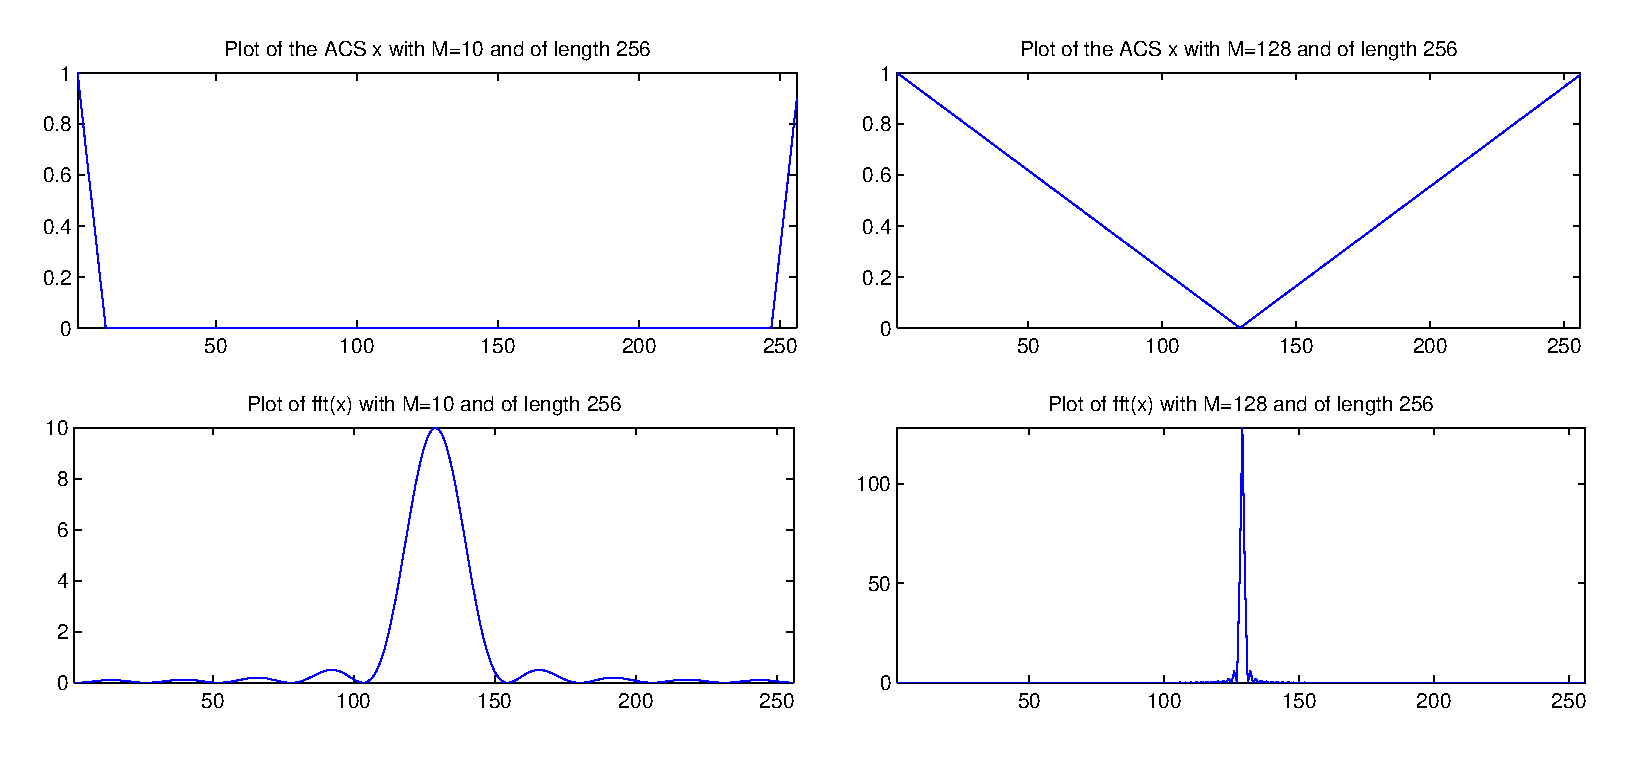
\includegraphics[width=\textwidth]{cw1im/1a.eps}
\caption{Plot of the vector $\boldsymbol{\mathrm{x}}$, note that \texttt{fftshift} has been used for the fft plots to center them}
\label{fig:ex1b}
\end{figure}

We have $\boldsymbol{\mathrm{x}} = [r(0), r(1), \dots ,r(M - 1),0, \dots, 0, r(-M + 1), \dots, r(-1)]^{T}$ with zero padding in the middle.  This firstly serves to have the length of $\boldsymbol{\mathrm{x}}$ be a power of two as $256 = 2^8$, which creates a more computationally effective FFT, as well as increasing the resolution of the PSD\footnote{as seen in Slide 10 of Lecture 1}. Additionally the zero padding occurring in the middle which creates a circular sequence (that is on which wraps by the vectors length), meaning negative indices can in fact be accessed. \latinabbrev{i.e} negative lags($-k$) must be placed at $M-1+k$. This is due to the way matlab calculates its FFT, which is explained in section \ref{sec:nonnegim}.


\subsection{Imaginary part due to round-off error}
Removing the imaginary part via \texttt{real(xf)} introduces very little error as the imaginary part is negligible. This is demonstrated by \texttt{sum(real(xf)-abs(xf))} which returns \texttt{0}. \texttt{max(imag(xf))} and \texttt{min(imag(xf))} both return values in the order of \texttt{10e-14} which shows that these are negligible values. These values are only due to matlab computational error.

Due to the circular way the indices are accessed it is not expected that an imaginary part appears. If we imagine that the data is spread across a unit circle and that frequency is accessed in a normalised way  (that is $0 \to 2\pi$) we can see imaginary parts will cancel out. This is the case for autocorrelation sequences if correctly generated as they will be symmetric, non-negative and real. This can be seen in simulations of figure \ref{fig:ex1b} where only positive real values appear.

\subsection{Non-negligible Imaginary part}
\label{sec:nonnegim}
\begin{figure}[h!]
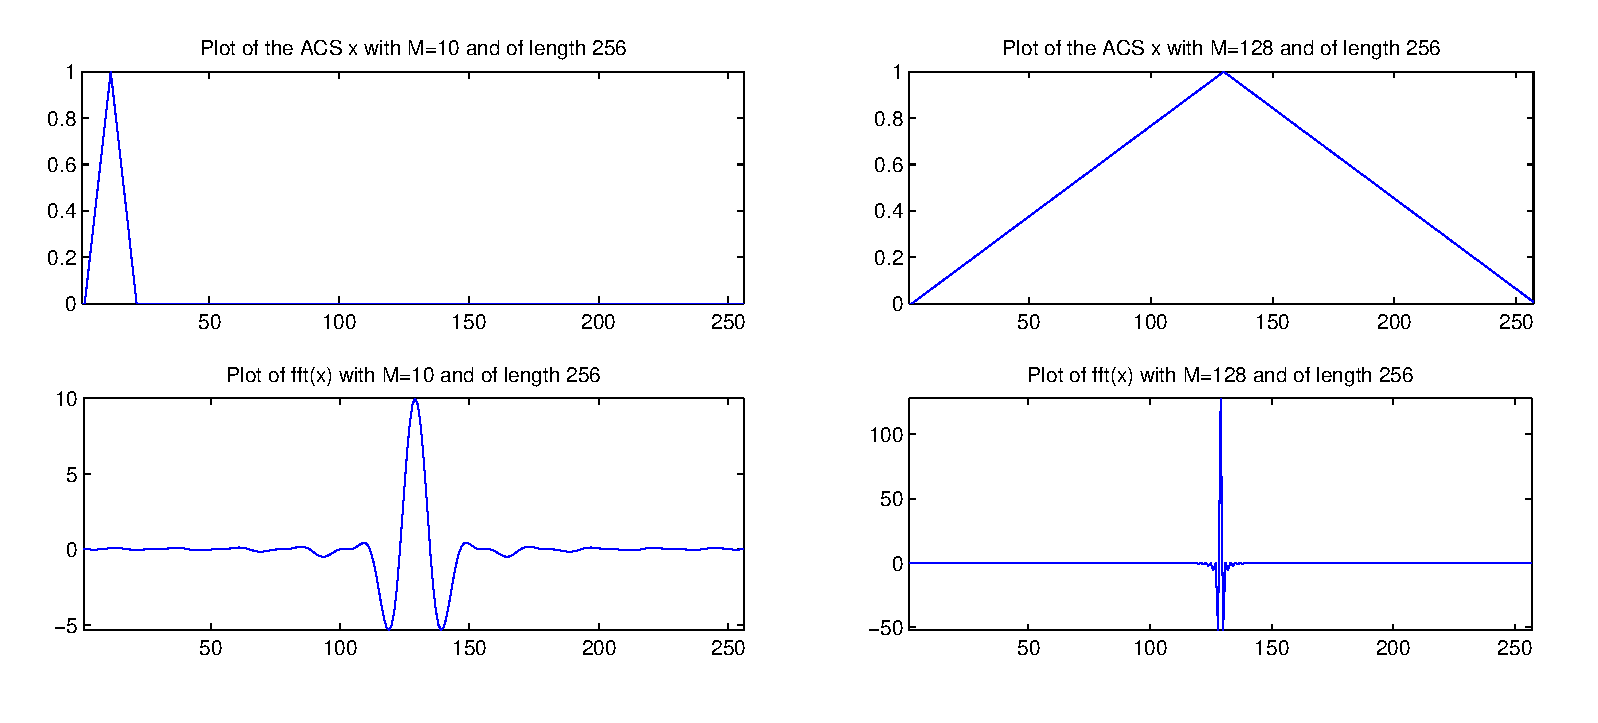
\includegraphics[width=\textwidth]{cw1im/1c.eps}
\caption{Plot of the vector $\boldsymbol{\mathrm{x}}$ with padding at the end, again \texttt{fftshift} has been used to center the frequency}
\label{fig:acsfft2}
\end{figure}
This time we have set up $\boldsymbol{\mathrm{x}} = [r(-M-1), \dots ,r(-1),r(0),r(1), \dots ,r(M - 1),0, \dots,0]^{T}$. Thus a vector of length L is made with padding at the end (for \texttt{M=10}). We notice that not only the FFT is erronous (from simple comparison to the previous graph, Figure \ref{fig:ex1b}, as well as the fact that it is negative) but that it contains large, non-negligible, imaginary values.  On the other hand for \texttt{M=128} the imaginary values are, again negligible, but the FFT is still slightly off.

The first issue of large imaginary values relies in the way matlab does its FFT. It assumes the array effectively has its negative index reflection in the second half of the array. Equation \ref{eq:fftmat} shows the way matlab calculates its FFT.
\begin{align}
X(k) &= \sum_{n=1}^{N} x(n) e^{-i2\pi\frac{(n-1)(k-1)}{N}} & \text{\hfill\textit{Note:}Matlab starts all its indexing at \texttt{1}}
\label{eq:fftmat}
\end{align}
To illustrate this, let us look at the matrix of values of $\frac{(n-1)(k-1)}{N}$ across $n$ and $k$:
\begin{equation}
\exp(-i2\pi \begin{bmatrix}
0 & 0 & 0 & 0 & 0 & 0 & 0 & 0\\ 
0 & \nicefrac{1}{8} & \nicefrac{2}{8}  & \nicefrac{3}{8}  & \nicefrac{4}{8}  & \nicefrac{5}{8}  & \nicefrac{6}{8}  & \nicefrac{7}{8} \\ 
0 & \nicefrac{2}{8} & \nicefrac{4}{8}  & \nicefrac{6}{8}  & \nicefrac{8}{8}  & \nicefrac{10}{8} & \nicefrac{12}{8} & \nicefrac{14}{8}\\ 
0 & \nicefrac{3}{8} & \nicefrac{6}{8}  & \nicefrac{9}{8}  & \nicefrac{12}{8} & \nicefrac{15}{8} & \nicefrac{18}{8} & \nicefrac{21}{8}\\ 
0 & \nicefrac{4}{8} & \nicefrac{8}{8}  & \nicefrac{12}{8} & \nicefrac{16}{8} & \nicefrac{20}{8} & \nicefrac{24}{8} & \nicefrac{28}{8}\\ 
0 & \nicefrac{5}{8} & \nicefrac{10}{8} & \nicefrac{15}{8} & \nicefrac{20}{8} & \nicefrac{25}{8} & \nicefrac{30}{8} & \nicefrac{35}{8}\\ 
0 & \nicefrac{6}{8} & \nicefrac{12}{8} & \nicefrac{18}{8} & \nicefrac{24}{8} & \nicefrac{30}{8} & \nicefrac{36}{8} & \nicefrac{42}{8}\\ 
0 & \nicefrac{7}{8} & \nicefrac{14}{8} & \nicefrac{21}{8} & \nicefrac{28}{8} & \nicefrac{35}{8} & \nicefrac{42}{8} & \nicefrac{49}{8}
\end{bmatrix})
\end{equation}
From this we can see that the values wrap around and are not correctly cancelled out. This is due to the sequence not being symmetric.

For the second issue of erroneous FFT, this is due to the ordering, which is in reverse, again due to the way the indices are perceived.  This is because the function is increasing, i.e. $r(0) \geq |R(k)| , \forall k$ is violated, giving rise to real negative imaginary values.
\subsection{\texttt{fftshift} use}
To get the correct $\boldsymbol{\mathrm{w}}$ vector to annotate the FFT (when correctly \texttt{fftshift}ed) we use the following commands:
\begin{lstlisting}
%L is the length
%even
w = 2*pi*((0:(L-1)) - L/2)/L;
%odd
w = 2*pi*(-((L-1)/2):((L-1)/2))/L;
\end{lstlisting}
These will placed the axis in the range of $[-\pi,\pi]$.

To get the correct $\boldsymbol{\mathrm{t}}$ (time) vector to annotate the IFFT (when correctly \texttt{fftshift}ed) we use the following commands:
\begin{lstlisting}
%even
t = -L/2:L/2-1;
%odd
t = -((L-1)/2):((L-1)/2);
\end{lstlisting}
\section{Properties of Window Functions in Spectral Estimation}
\subsection{Negative Spectral Estimates}
\label{sec:neg_est}
Negative spectral estimates are impossible if calculating the PSD from the second definition(\ref{eq:second_def}) due to the presence of the absolute value function. However the first definition, which involves taking the Fourier transform of the auto-covariance sequence, can lead to negative spectral estimates.



One way is to apply a window to a biased ACS:


While applying a window to the original signal will not lead to negative spectral estimates(due to the way a spectogram is calculated), applying a rect window to the ACS will. The typical PSD of a $\sin$ function is $\frac{A^2}{4}\delta(|f-f_{0}|)$, with A being the amplitude. The FFT of a rect function is $\frac{1}{\sqrt{2\pi}} \sinc(\frac{\omega}{2})$, which contains negative values. Thus applying a rect window will make negative values appear when convolved with the delta function arising from the sine wave.

\begin{figure}[h!]
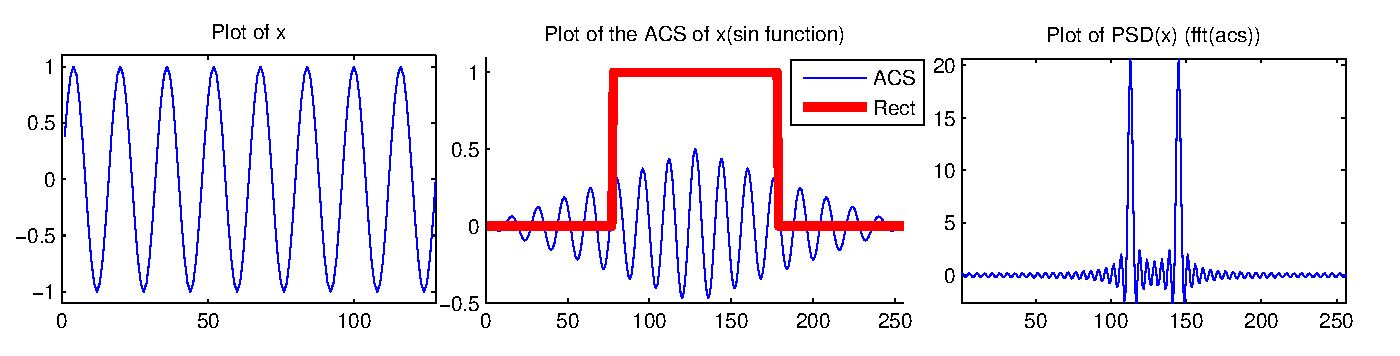
\includegraphics[width=\textwidth]{cw1im/2a.eps}
\textit{Note}: ACS and PSD were appropriately \texttt{fftshift}ed for processing purposes.
\caption{Plot of the vector $\boldsymbol{\mathrm{x}}$, with its ACS and PSD functions}
\label{fig:ex2}
\end{figure}


The unbiased ACS ($r(k) =\frac{1}{N} \sum_{n=0}^{N-1-k}x(n+k)x(n)$) is also liable to creating negative estimates, as it does not guaranteed the creation of a positive definite sequence.  If the ACS is not positive definite this corresponds to a non-positive semi-definite autocorrelation matrix, which will not be able to guarantee a purely positive PSD.

Thus there are two, related, ways of creating negative spectral estimates.


\subsection{Bartlett Window}
The Bochner theorem states that any  positive-definite function in $R^n$ is the Fourier transform of a positive measure $g$ on the real line with $g(y) \geq 0, \; \forall y$ .\cite{lofi} 
\begin{equation}
    w_B(k)= 
\begin{dcases}
    1-\frac{|k|}{N},& \text{if } |k|\leq N\\
    0,              & \text{otherwise.}
\end{dcases}
\label{eq:bart}
\end{equation}
Thus to prove that the Bartlett window (\ref{eq:bart}) is positive we must prove its Fourier transform is positive for all values.
\begin{align*}
w_B(k) = \Pi(k) \star \Pi(k) &
\hfill \text{\hfill where $\Pi$ is the rect function of width $N$ and height 1} \\
\mathfrak{F}(w_B(k)) &= \mathfrak{F}(\Pi(k)) \times \mathfrak{F}(\Pi(k)) = \frac{1}{\sqrt{2\pi}} \sinc(\frac{\omega}{2}) \times \frac{1}{\sqrt{2\pi}} \sinc(\frac{\omega}{2}) = \frac{1}{2\pi} \sinc^2 (\frac{\omega}{2})
\end{align*}
As can be seen above $\frac{1}{2\pi} \sinc^2 (\frac{\omega}{2})$ is both real and always positive(due to the square), which allows to conclude that the Bartlett window is positive definite.


As seen previously it is desirable to have a positive definite window which leasts distorts the out. Thus we want a window which distorts the ACF the least. To show the Bartlett window satisfies this we minimise the following criterion:


$$ \min_{\{w(k)\}} \sum_{k=0}^{M-1} |1-w(k)|$$

We can replace $\displaystyle w(k)$ by $\sum_{j=0}^{M-1} s_j s_{j+k}$ as a positive definite window can be replaced by a convolution of an arbitrary sequence.

We define $w(0)=1$ as this is a window.

As $w(0) \geq w(k) \forall k$ we can rewrite as:

$$ \sum_{k=0}^{M-1} 1- \left( \sum_{j=0}^{M-1} s_j s_{j+k} \right) $$


We can rewrite the convolution as a vector sum $w(k) = s^T T_k s$ where $T_k = \begin{bmatrix} 0_{k \times (M-k)} & 0_{k\times k} \\ I_{(M-k)\times (M-k)} & 0_{(M-k) \times k} \end{bmatrix}$. While this is practical we will slightly tweak it to get a symmetric matrix which is nicer for our proof. We get $w(k) = \frac{1}{2} s^T (T_k +T_k^T) s$. Let $T_k +T_k^T = P_k$. From this:


$$ \sum_{k=0}^{M-1} 1-  \frac{1}{2} s^T P_k s  = M - \frac{1}{2} s^T  \sum_{k=0}^{M-1} \left( P_k \right) s $$

To minimise this function is simply to maximise $s^T \sum_{k=0}^{M-1} (P_k) \; s$. Note that:
$$\sum_{k=0}^{M-1} (P_k) = \begin{bmatrix} 2 & 1 & 1\\ 1 & \ddots & 1\\ 1 & 1 & 2\end{bmatrix} = P_{sum}$$

$P_{sum}$ has, ordered by magnitude, eigenvalues of $\left[ (M+1),1, \dots, 1\right]$. As we know that the maximising $s$ is given by the eigenvector associated with the largest eigenvalue\cite{rayleigh} we get the maximising $s$:

$$s_{max} = \left[1, \dots, 1\right]/\sqrt{M}$$

This vector corresponds to the triangular Bartlett window (because we defined $w(k)$ as the convolution of $s$ on itself \latinabbrev{i.e} $rect \star rect = w_B$), which concludes our proof.
\section{Resolution and Leakage of Periodogram-based Methods}
\subsection{Bartlett window lobes}
\begin{figure}[h!]
\centering
\underline{Linear}:\\
%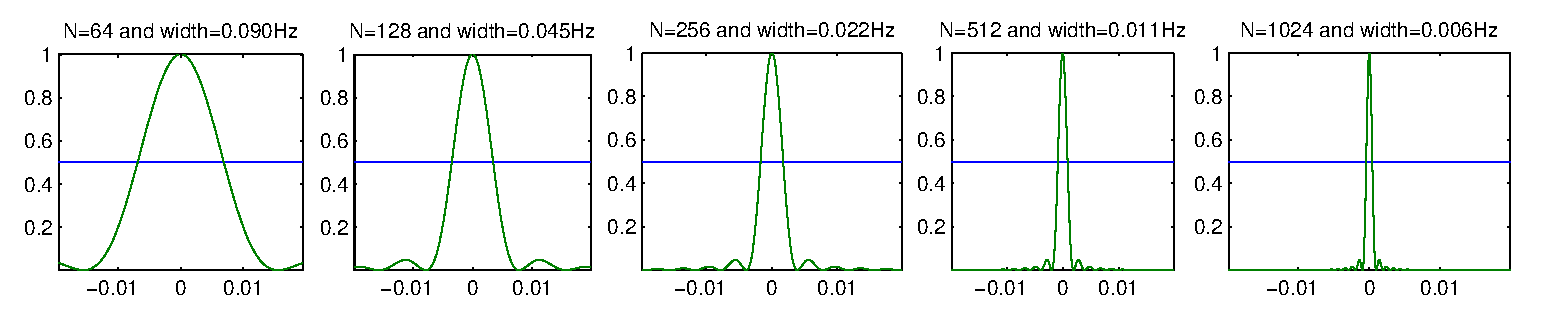
\includegraphics[width=\textwidth]{cw1im/3alin.eps}
\resizebox{\textwidth}{!}{% This file was created by matlab2tikz v0.4.7 running on MATLAB 8.1.
% Copyright (c) 2008--2014, Nico Schlömer <nico.schloemer@gmail.com>
% All rights reserved.
% Minimal pgfplots version: 1.3
% 
% The latest updates can be retrieved from
%   http://www.mathworks.com/matlabcentral/fileexchange/22022-matlab2tikz
% where you can also make suggestions and rate matlab2tikz.
% 
\begin{tikzpicture}

\begin{axis}[%
width=1.5in,
height=1.5in,
unbounded coords=jump,
scale only axis,
xmin=-0.0197389431373737,
xmax=0.0197389431373737,
ymin=2.16053419706292e-05,
ymax=1,
xticklabel style={/pgf/number format/fixed},
scaled x ticks=false,
name=plot2,
title={N=128 and width=0.045Hz}
]
\addplot [color=blue,solid,forget plot]
  table[row sep=crcr]{-0.0197389431373737	0.5\\
-0.0195835183882606	0.5\\
-0.0194280936391474	0.5\\
-0.0192726688900342	0.5\\
-0.019117244140921	0.5\\
-0.0189618193918078	0.5\\
-0.0188063946426947	0.5\\
-0.0186509698935815	0.5\\
-0.0184955451444683	0.5\\
-0.0183401203953551	0.5\\
-0.018184695646242	0.5\\
-0.0180292708971288	0.5\\
-0.0178738461480156	0.5\\
-0.0177184213989024	0.5\\
-0.0175629966497892	0.5\\
-0.0174075719006761	0.5\\
-0.0172521471515629	0.5\\
-0.0170967224024497	0.5\\
-0.0169412976533365	0.5\\
-0.0167858729042233	0.5\\
-0.0166304481551102	0.5\\
-0.016475023405997	0.5\\
-0.0163195986568838	0.5\\
-0.0161641739077706	0.5\\
-0.0160087491586574	0.5\\
-0.0158533244095443	0.5\\
-0.0156978996604311	0.5\\
-0.0155424749113179	0.5\\
-0.0153870501622047	0.5\\
-0.0152316254130915	0.5\\
-0.0150762006639784	0.5\\
-0.0149207759148652	0.5\\
-0.014765351165752	0.5\\
-0.0146099264166388	0.5\\
-0.0144545016675257	0.5\\
-0.0142990769184125	0.5\\
-0.0141436521692993	0.5\\
-0.0139882274201861	0.5\\
-0.0138328026710729	0.5\\
-0.0136773779219598	0.5\\
-0.0135219531728466	0.5\\
-0.0133665284237334	0.5\\
-0.0132111036746202	0.5\\
-0.013055678925507	0.5\\
-0.0129002541763939	0.5\\
-0.0127448294272807	0.5\\
-0.0125894046781675	0.5\\
-0.0124339799290543	0.5\\
-0.0122785551799411	0.5\\
-0.012123130430828	0.5\\
-0.0119677056817148	0.5\\
-0.0118122809326016	0.5\\
-0.0116568561834884	0.5\\
-0.0115014314343752	0.5\\
-0.0113460066852621	0.5\\
-0.0111905819361489	0.5\\
-0.0110351571870357	0.5\\
-0.0108797324379225	0.5\\
-0.0107243076888094	0.5\\
-0.0105688829396962	0.5\\
-0.010413458190583	0.5\\
-0.0102580334414698	0.5\\
-0.0101026086923566	0.5\\
-0.00994718394324346	0.5\\
-0.00979175919413028	0.5\\
-0.0096363344450171	0.5\\
-0.00948090969590392	0.5\\
-0.00932548494679074	0.5\\
-0.00917006019767756	0.5\\
-0.00901463544856439	0.5\\
-0.00885921069945121	0.5\\
-0.00870378595033803	0.5\\
-0.00854836120122485	0.5\\
-0.00839293645211167	0.5\\
-0.00823751170299849	0.5\\
-0.00808208695388531	0.5\\
-0.00792666220477213	0.5\\
-0.00777123745565895	0.5\\
-0.00761581270654577	0.5\\
-0.00746038795743259	0.5\\
-0.00730496320831941	0.5\\
-0.00714953845920624	0.5\\
-0.00699411371009306	0.5\\
-0.00683868896097988	0.5\\
-0.0066832642118667	0.5\\
-0.00652783946275352	0.5\\
-0.00637241471364034	0.5\\
-0.00621698996452716	0.5\\
-0.00606156521541398	0.5\\
-0.0059061404663008	0.5\\
-0.00575071571718762	0.5\\
-0.00559529096807445	0.5\\
-0.00543986621896127	0.5\\
-0.00528444146984809	0.5\\
-0.00512901672073491	0.5\\
-0.00497359197162173	0.5\\
-0.00481816722250855	0.5\\
-0.00466274247339537	0.5\\
-0.00450731772428219	0.5\\
-0.00435189297516901	0.5\\
-0.00419646822605583	0.5\\
-0.00404104347694266	0.5\\
-0.00388561872782948	0.5\\
-0.0037301939787163	0.5\\
-0.00357476922960312	0.5\\
-0.00341934448048994	0.5\\
-0.00326391973137676	0.5\\
-0.00310849498226358	0.5\\
-0.0029530702331504	0.5\\
-0.00279764548403722	0.5\\
-0.00264222073492404	0.5\\
-0.00248679598581086	0.5\\
-0.00233137123669769	0.5\\
-0.00217594648758451	0.5\\
-0.00202052173847133	0.5\\
-0.00186509698935815	0.5\\
-0.00170967224024497	0.5\\
-0.00155424749113179	0.5\\
-0.00139882274201861	0.5\\
-0.00124339799290543	0.5\\
-0.00108797324379226	0.5\\
-0.000932548494679074	0.5\\
-0.000777123745565895	0.5\\
-0.000621698996452717	0.5\\
-0.000466274247339538	0.5\\
-0.00031084949822636	0.5\\
-0.000155424749113179	0.5\\
0	0.5\\
0.000155424749113179	0.5\\
0.00031084949822636	0.5\\
0.000466274247339538	0.5\\
0.000621698996452717	0.5\\
0.000777123745565895	0.5\\
0.000932548494679074	0.5\\
0.00108797324379226	0.5\\
0.00124339799290543	0.5\\
0.00139882274201861	0.5\\
0.00155424749113179	0.5\\
0.00170967224024497	0.5\\
0.00186509698935815	0.5\\
0.00202052173847133	0.5\\
0.00217594648758451	0.5\\
0.00233137123669769	0.5\\
0.00248679598581086	0.5\\
0.00264222073492404	0.5\\
0.00279764548403722	0.5\\
0.0029530702331504	0.5\\
0.00310849498226358	0.5\\
0.00326391973137676	0.5\\
0.00341934448048994	0.5\\
0.00357476922960312	0.5\\
0.0037301939787163	0.5\\
0.00388561872782948	0.5\\
0.00404104347694266	0.5\\
0.00419646822605583	0.5\\
0.00435189297516901	0.5\\
0.00450731772428219	0.5\\
0.00466274247339537	0.5\\
0.00481816722250855	0.5\\
0.00497359197162173	0.5\\
0.00512901672073491	0.5\\
0.00528444146984809	0.5\\
0.00543986621896127	0.5\\
0.00559529096807445	0.5\\
0.00575071571718762	0.5\\
0.0059061404663008	0.5\\
0.00606156521541398	0.5\\
0.00621698996452716	0.5\\
0.00637241471364034	0.5\\
0.00652783946275352	0.5\\
0.0066832642118667	0.5\\
0.00683868896097988	0.5\\
0.00699411371009306	0.5\\
0.00714953845920624	0.5\\
0.00730496320831941	0.5\\
0.00746038795743259	0.5\\
0.00761581270654577	0.5\\
0.00777123745565895	0.5\\
0.00792666220477213	0.5\\
0.00808208695388531	0.5\\
0.00823751170299849	0.5\\
0.00839293645211167	0.5\\
0.00854836120122485	0.5\\
0.00870378595033803	0.5\\
0.00885921069945121	0.5\\
0.00901463544856439	0.5\\
0.00917006019767756	0.5\\
0.00932548494679074	0.5\\
0.00948090969590392	0.5\\
0.0096363344450171	0.5\\
0.00979175919413028	0.5\\
0.00994718394324346	0.5\\
0.0101026086923566	0.5\\
0.0102580334414698	0.5\\
0.010413458190583	0.5\\
0.0105688829396962	0.5\\
0.0107243076888094	0.5\\
0.0108797324379225	0.5\\
0.0110351571870357	0.5\\
0.0111905819361489	0.5\\
0.0113460066852621	0.5\\
0.0115014314343752	0.5\\
0.0116568561834884	0.5\\
0.0118122809326016	0.5\\
0.0119677056817148	0.5\\
0.012123130430828	0.5\\
0.0122785551799411	0.5\\
0.0124339799290543	0.5\\
0.0125894046781675	0.5\\
0.0127448294272807	0.5\\
0.0129002541763939	0.5\\
0.013055678925507	0.5\\
0.0132111036746202	0.5\\
0.0133665284237334	0.5\\
0.0135219531728466	0.5\\
0.0136773779219598	0.5\\
0.0138328026710729	0.5\\
0.0139882274201861	0.5\\
0.0141436521692993	0.5\\
0.0142990769184125	0.5\\
0.0144545016675257	0.5\\
0.0146099264166388	0.5\\
0.014765351165752	0.5\\
0.0149207759148652	0.5\\
0.0150762006639784	0.5\\
0.0152316254130915	0.5\\
0.0153870501622047	0.5\\
0.0155424749113179	0.5\\
0.0156978996604311	0.5\\
0.0158533244095443	0.5\\
0.0160087491586574	0.5\\
0.0161641739077706	0.5\\
0.0163195986568838	0.5\\
0.016475023405997	0.5\\
0.0166304481551102	0.5\\
0.0167858729042233	0.5\\
0.0169412976533365	0.5\\
0.0170967224024497	0.5\\
0.0172521471515629	0.5\\
0.0174075719006761	0.5\\
0.0175629966497892	0.5\\
0.0177184213989024	0.5\\
0.0178738461480156	0.5\\
0.0180292708971288	0.5\\
0.018184695646242	0.5\\
0.0183401203953551	0.5\\
0.0184955451444683	0.5\\
0.0186509698935815	0.5\\
0.0188063946426947	0.5\\
0.0189618193918078	0.5\\
0.019117244140921	0.5\\
0.0192726688900342	0.5\\
0.0194280936391474	0.5\\
0.0195835183882606	0.5\\
0.0197389431373737	0.5\\
};
\addplot [color=black!50!green,solid,forget plot]
  table[row sep=crcr]{-0.0197389431373737	0.0158023595001197\\
-0.0195835183882606	0.0161592258902174\\
-0.0194280936391474	0.0163974874742202\\
-0.0192726688900342	0.016511583572702\\
-0.019117244140921	0.0164977425469797\\
-0.0189618193918078	0.0163540982991509\\
-0.0188063946426947	0.0160807821326463\\
-0.0186509698935815	0.0156799878812906\\
-0.0184955451444683	0.0151560085372745\\
-0.0183401203953551	0.0145152429646825\\
-0.018184695646242	0.0137661716712119\\
-0.0180292708971288	0.0129193010218726\\
-0.0178738461480156	0.0119870757097367\\
-0.0177184213989024	0.010983759744774\\
-0.0175629966497892	0.00992528667670699\\
-0.0174075719006761	0.00882908022562399\\
-0.0172521471515629	0.00771384694859872\\
-0.0170967224024497	0.0065993430154817\\
-0.0169412976533365	0.00550611759602354\\
-0.0167858729042233	0.00445523576731254\\
-0.0166304481551102	0.00346798422905151\\
-0.016475023405997	0.00256556345859249\\
-0.0163195986568838	0.00176877024234781\\
-0.0161641739077706	0.00109767478005081\\
-0.0160087491586574	0.000571296768683386\\
-0.0158533244095443	0.000207285029601506\\
-0.0156978996604311	2.16053419706292e-05\\
-0.0155424749113179	2.82411852485566e-05\\
-0.0153870501622047	0.000238912071023751\\
-0.0152316254130915	0.000662814058708189\\
-0.0150762006639784	0.0013063868998735\\
-0.0149207759148652	0.00217311204271491\\
-0.014765351165752	0.00326334545237758\\
-0.0146099264166388	0.00457418886667792\\
-0.0144545016675257	0.00609940271292667\\
-0.0142990769184125	0.00782936346375558\\
-0.0141436521692993	0.00975106771249492\\
-0.0139882274201861	0.0118481847069206\\
-0.0138328026710729	0.0141011584999513\\
-0.0136773779219598	0.0164873602636241\\
-0.0135219531728466	0.0189812906754724\\
-0.0133665284237334	0.0215548316317994\\
-0.0132111036746202	0.0241775458782214\\
-0.013055678925507	0.0268170224824667\\
-0.0129002541763939	0.0294392654161909\\
-0.0127448294272807	0.032009121870027\\
-0.0125894046781675	0.0344907463077348\\
-0.0124339799290543	0.0368480956795574\\
-0.0122785551799411	0.0390454506698739\\
-0.012123130430828	0.0410479573578065\\
-0.0119677056817148	0.0428221832289718\\
-0.0118122809326016	0.0443366810989091\\
-0.0116568561834884	0.0455625542000805\\
-0.0115014314343752	0.0464740154501957\\
-0.0113460066852621	0.0470489337646337\\
-0.0111905819361489	0.0472693602037027\\
-0.0110351571870357	0.0471220267592284\\
-0.0108797324379225	0.0465988106863335\\
-0.0107243076888094	0.0456971574760585\\
-0.0105688829396962	0.0444204558424068\\
-0.010413458190583	0.0427783584621189\\
-0.0102580334414698	0.0407870426545517\\
-0.0101026086923566	0.0384694057189378\\
-0.00994718394324346	0.035855190252462\\
-0.00979175919413028	0.032981035449447\\
-0.0096363344450171	0.0298904511229295\\
-0.00948090969590392	0.0266337119876222\\
-0.00932548494679074	0.0232676705894201\\
-0.00917006019767756	0.019855488152245\\
-0.00901463544856439	0.0164662835285047\\
-0.00885921069945121	0.0131747013746148\\
-0.00870378595033803	0.0100604016173372\\
-0.00854836120122485	0.00720747321925817\\
-0.00839293645211167	0.00470377618154058\\
-0.00823751170299849	0.00264021662808341\\
-0.00808208695388531	0.00110996068642754\\
-0.00792666220477213	0.000207593706437565\\
-0.00777123745565895	2.82321275820364e-05\\
-0.00761581270654577	0.000666596009644034\\
-0.00746038795743259	0.00221605087065213\\
-0.00730496320831941	0.00476762802118899\\
-0.00714953845920624	0.00840903303832003\\
-0.00699411371009306	0.013223652378442\\
-0.00683868896097988	0.019289568380676\\
-0.0066832642118667	0.0266785930564368\\
-0.00652783946275352	0.0354553310931043\\
-0.00637241471364034	0.0456762824181474\\
-0.00621698996452716	0.0573889944737432\\
-0.00606156521541398	0.0706312740413277\\
-0.0059061404663008	0.0854304680323709\\
-0.00575071571718762	0.101802822129059\\
-0.00559529096807445	0.119752925520869\\
-0.00543986621896127	0.139273249245815\\
-0.00528444146984809	0.160343784815319\\
-0.00512901672073491	0.182931788887105\\
-0.00497359197162173	0.206991638760284\\
-0.00481816722250855	0.232464802410877\\
-0.00466274247339537	0.259279925675159\\
-0.00450731772428219	0.287353038034127\\
-0.00435189297516901	0.316587877267035\\
-0.00419646822605583	0.346876332038217\\
-0.00404104347694266	0.378099000272064\\
-0.00388561872782948	0.410125859969385\\
-0.0037301939787163	0.442817047937544\\
-0.00357476922960312	0.476023740759863\\
-0.00341934448048994	0.50958913122961\\
-0.00326391973137676	0.543349492432848\\
-0.00310849498226358	0.577135320694323\\
-0.0029530702331504	0.610772547712551\\
-0.00279764548403722	0.644083811414666\\
-0.00264222073492404	0.676889774367624\\
-0.00248679598581086	0.709010477998429\\
-0.00233137123669769	0.740266720409197\\
-0.00217594648758451	0.770481445228825\\
-0.00202052173847133	0.799481128726536\\
-0.00186509698935815	0.827097152326478\\
-0.00170967224024497	0.853167147708707\\
-0.00155424749113179	0.877536301860479\\
-0.00139882274201861	0.900058609751525\\
-0.00124339799290543	0.920598062745254\\
-0.00108797324379226	0.939029761420439\\
-0.000932548494679074	0.955240942159399\\
-0.000777123745565895	0.969131907652178\\
-0.000621698996452717	0.980616852363543\\
-0.000466274247339538	0.989624575001611\\
-0.00031084949822636	0.996099071103171\\
-0.000155424749113179	1\\
0	nan\\
0.000155424749113179	1\\
0.00031084949822636	0.996099071103171\\
0.000466274247339538	0.989624575001611\\
0.000621698996452717	0.980616852363543\\
0.000777123745565895	0.969131907652178\\
0.000932548494679074	0.955240942159399\\
0.00108797324379226	0.939029761420439\\
0.00124339799290543	0.920598062745254\\
0.00139882274201861	0.900058609751525\\
0.00155424749113179	0.877536301860479\\
0.00170967224024497	0.853167147708707\\
0.00186509698935815	0.827097152326478\\
0.00202052173847133	0.799481128726536\\
0.00217594648758451	0.770481445228825\\
0.00233137123669769	0.740266720409197\\
0.00248679598581086	0.709010477998429\\
0.00264222073492404	0.676889774367624\\
0.00279764548403722	0.644083811414666\\
0.0029530702331504	0.610772547712551\\
0.00310849498226358	0.577135320694323\\
0.00326391973137676	0.543349492432848\\
0.00341934448048994	0.50958913122961\\
0.00357476922960312	0.476023740759863\\
0.0037301939787163	0.442817047937544\\
0.00388561872782948	0.410125859969385\\
0.00404104347694266	0.378099000272064\\
0.00419646822605583	0.346876332038217\\
0.00435189297516901	0.316587877267035\\
0.00450731772428219	0.287353038034127\\
0.00466274247339537	0.259279925675159\\
0.00481816722250855	0.232464802410877\\
0.00497359197162173	0.206991638760284\\
0.00512901672073491	0.182931788887105\\
0.00528444146984809	0.160343784815319\\
0.00543986621896127	0.139273249245815\\
0.00559529096807445	0.119752925520869\\
0.00575071571718762	0.101802822129059\\
0.0059061404663008	0.0854304680323709\\
0.00606156521541398	0.0706312740413277\\
0.00621698996452716	0.0573889944737432\\
0.00637241471364034	0.0456762824181474\\
0.00652783946275352	0.0354553310931043\\
0.0066832642118667	0.0266785930564368\\
0.00683868896097988	0.019289568380676\\
0.00699411371009306	0.013223652378442\\
0.00714953845920624	0.00840903303832003\\
0.00730496320831941	0.00476762802118899\\
0.00746038795743259	0.00221605087065213\\
0.00761581270654577	0.000666596009644034\\
0.00777123745565895	2.82321275820364e-05\\
0.00792666220477213	0.000207593706437565\\
0.00808208695388531	0.00110996068642754\\
0.00823751170299849	0.00264021662808341\\
0.00839293645211167	0.00470377618154058\\
0.00854836120122485	0.00720747321925817\\
0.00870378595033803	0.0100604016173372\\
0.00885921069945121	0.0131747013746148\\
0.00901463544856439	0.0164662835285047\\
0.00917006019767756	0.019855488152245\\
0.00932548494679074	0.0232676705894201\\
0.00948090969590392	0.0266337119876222\\
0.0096363344450171	0.0298904511229295\\
0.00979175919413028	0.032981035449447\\
0.00994718394324346	0.035855190252462\\
0.0101026086923566	0.0384694057189378\\
0.0102580334414698	0.0407870426545517\\
0.010413458190583	0.0427783584621189\\
0.0105688829396962	0.0444204558424068\\
0.0107243076888094	0.0456971574760585\\
0.0108797324379225	0.0465988106863335\\
0.0110351571870357	0.0471220267592284\\
0.0111905819361489	0.0472693602037027\\
0.0113460066852621	0.0470489337646337\\
0.0115014314343752	0.0464740154501957\\
0.0116568561834884	0.0455625542000805\\
0.0118122809326016	0.0443366810989091\\
0.0119677056817148	0.0428221832289718\\
0.012123130430828	0.0410479573578065\\
0.0122785551799411	0.0390454506698739\\
0.0124339799290543	0.0368480956795574\\
0.0125894046781675	0.0344907463077348\\
0.0127448294272807	0.032009121870027\\
0.0129002541763939	0.0294392654161909\\
0.013055678925507	0.0268170224824667\\
0.0132111036746202	0.0241775458782214\\
0.0133665284237334	0.0215548316317994\\
0.0135219531728466	0.0189812906754724\\
0.0136773779219598	0.0164873602636241\\
0.0138328026710729	0.0141011584999513\\
0.0139882274201861	0.0118481847069206\\
0.0141436521692993	0.00975106771249492\\
0.0142990769184125	0.00782936346375558\\
0.0144545016675257	0.00609940271292667\\
0.0146099264166388	0.00457418886667792\\
0.014765351165752	0.00326334545237758\\
0.0149207759148652	0.00217311204271491\\
0.0150762006639784	0.0013063868998735\\
0.0152316254130915	0.000662814058708189\\
0.0153870501622047	0.000238912071023751\\
0.0155424749113179	2.82411852485566e-05\\
0.0156978996604311	2.16053419706292e-05\\
0.0158533244095443	0.000207285029601506\\
0.0160087491586574	0.000571296768683386\\
0.0161641739077706	0.00109767478005081\\
0.0163195986568838	0.00176877024234781\\
0.016475023405997	0.00256556345859249\\
0.0166304481551102	0.00346798422905151\\
0.0167858729042233	0.00445523576731254\\
0.0169412976533365	0.00550611759602354\\
0.0170967224024497	0.0065993430154817\\
0.0172521471515629	0.00771384694859872\\
0.0174075719006761	0.00882908022562399\\
0.0175629966497892	0.00992528667670699\\
0.0177184213989024	0.010983759744774\\
0.0178738461480156	0.0119870757097367\\
0.0180292708971288	0.0129193010218726\\
0.018184695646242	0.0137661716712119\\
0.0183401203953551	0.0145152429646825\\
0.0184955451444683	0.0151560085372745\\
0.0186509698935815	0.0156799878812906\\
0.0188063946426947	0.0160807821326463\\
0.0189618193918078	0.0163540982991509\\
0.019117244140921	0.0164977425469797\\
0.0192726688900342	0.016511583572702\\
0.0194280936391474	0.0163974874742202\\
0.0195835183882606	0.0161592258902174\\
0.0197389431373737	0.0158023595001197\\
};
\end{axis}

\begin{axis}[%
width=1.5in,
height=1.5in,
unbounded coords=jump,
scale only axis,
xmin=-0.0195835183882606,
xmax=0.0195835183882606,
ymin=2.82489551952876e-05,
ymax=1,
xticklabel style={/pgf/number format/fixed},
scaled x ticks=false,
at=(plot2.left of south west),
anchor=right of south east,
title={N=64 and width=0.090Hz}
]
\addplot [color=blue,solid,forget plot]
  table[row sep=crcr]{-0.0195835183882606	0.5\\
-0.0192726688900342	0.5\\
-0.0189618193918078	0.5\\
-0.0186509698935815	0.5\\
-0.0183401203953551	0.5\\
-0.0180292708971288	0.5\\
-0.0177184213989024	0.5\\
-0.0174075719006761	0.5\\
-0.0170967224024497	0.5\\
-0.0167858729042233	0.5\\
-0.016475023405997	0.5\\
-0.0161641739077706	0.5\\
-0.0158533244095443	0.5\\
-0.0155424749113179	0.5\\
-0.0152316254130915	0.5\\
-0.0149207759148652	0.5\\
-0.0146099264166388	0.5\\
-0.0142990769184125	0.5\\
-0.0139882274201861	0.5\\
-0.0136773779219598	0.5\\
-0.0133665284237334	0.5\\
-0.013055678925507	0.5\\
-0.0127448294272807	0.5\\
-0.0124339799290543	0.5\\
-0.012123130430828	0.5\\
-0.0118122809326016	0.5\\
-0.0115014314343752	0.5\\
-0.0111905819361489	0.5\\
-0.0108797324379225	0.5\\
-0.0105688829396962	0.5\\
-0.0102580334414698	0.5\\
-0.00994718394324346	0.5\\
-0.0096363344450171	0.5\\
-0.00932548494679074	0.5\\
-0.00901463544856439	0.5\\
-0.00870378595033803	0.5\\
-0.00839293645211167	0.5\\
-0.00808208695388531	0.5\\
-0.00777123745565895	0.5\\
-0.0074603879574326	0.5\\
-0.00714953845920624	0.5\\
-0.00683868896097988	0.5\\
-0.00652783946275352	0.5\\
-0.00621698996452716	0.5\\
-0.00590614046630081	0.5\\
-0.00559529096807445	0.5\\
-0.00528444146984809	0.5\\
-0.00497359197162173	0.5\\
-0.00466274247339537	0.5\\
-0.00435189297516902	0.5\\
-0.00404104347694266	0.5\\
-0.0037301939787163	0.5\\
-0.00341934448048994	0.5\\
-0.00310849498226358	0.5\\
-0.00279764548403722	0.5\\
-0.00248679598581086	0.5\\
-0.00217594648758451	0.5\\
-0.00186509698935815	0.5\\
-0.00155424749113179	0.5\\
-0.00124339799290543	0.5\\
-0.000932548494679077	0.5\\
-0.000621698996452717	0.5\\
-0.00031084949822636	0.5\\
0	0.5\\
0.00031084949822636	0.5\\
0.000621698996452717	0.5\\
0.000932548494679077	0.5\\
0.00124339799290543	0.5\\
0.00155424749113179	0.5\\
0.00186509698935815	0.5\\
0.00217594648758451	0.5\\
0.00248679598581086	0.5\\
0.00279764548403722	0.5\\
0.00310849498226358	0.5\\
0.00341934448048994	0.5\\
0.0037301939787163	0.5\\
0.00404104347694266	0.5\\
0.00435189297516902	0.5\\
0.00466274247339537	0.5\\
0.00497359197162173	0.5\\
0.00528444146984809	0.5\\
0.00559529096807445	0.5\\
0.00590614046630081	0.5\\
0.00621698996452716	0.5\\
0.00652783946275352	0.5\\
0.00683868896097988	0.5\\
0.00714953845920624	0.5\\
0.0074603879574326	0.5\\
0.00777123745565895	0.5\\
0.00808208695388531	0.5\\
0.00839293645211167	0.5\\
0.00870378595033803	0.5\\
0.00901463544856439	0.5\\
0.00932548494679074	0.5\\
0.0096363344450171	0.5\\
0.00994718394324346	0.5\\
0.0102580334414698	0.5\\
0.0105688829396962	0.5\\
0.0108797324379225	0.5\\
0.0111905819361489	0.5\\
0.0115014314343752	0.5\\
0.0118122809326016	0.5\\
0.012123130430828	0.5\\
0.0124339799290543	0.5\\
0.0127448294272807	0.5\\
0.013055678925507	0.5\\
0.0133665284237334	0.5\\
0.0136773779219598	0.5\\
0.0139882274201861	0.5\\
0.0142990769184125	0.5\\
0.0146099264166388	0.5\\
0.0149207759148652	0.5\\
0.0152316254130915	0.5\\
0.0155424749113179	0.5\\
0.0158533244095443	0.5\\
0.0161641739077706	0.5\\
0.016475023405997	0.5\\
0.0167858729042233	0.5\\
0.0170967224024497	0.5\\
0.0174075719006761	0.5\\
0.0177184213989024	0.5\\
0.0180292708971288	0.5\\
0.0183401203953551	0.5\\
0.0186509698935815	0.5\\
0.0189618193918078	0.5\\
0.0192726688900342	0.5\\
0.0195835183882606	0.5\\
};
\addplot [color=black!50!green,solid,forget plot]
  table[row sep=crcr]{-0.0195835183882606	0.0330122566822962\\
-0.0192726688900342	0.0299178547671345\\
-0.0189618193918078	0.0266573478586114\\
-0.0186509698935815	0.0232876472720157\\
-0.0183401203953551	0.0198719713022502\\
-0.0180292708971288	0.0164794932838792\\
-0.0177184213989024	0.0131849089166734\\
-0.0174075719006761	0.0100679249356609\\
-0.0170967224024497	0.00721267214642929\\
-0.0167858729042233	0.00470704677520077\\
-0.016475023405997	0.0026419849879899\\
-0.0161641739077706	0.00111067630299513\\
-0.0158533244095443	0.000207722444557619\\
-0.0155424749113179	2.82489551952876e-05\\
-0.0152316254130915	0.000666977584521584\\
-0.0149207759148652	0.00221726810104665\\
-0.0146099264166388	0.00477013871642151\\
-0.0142990769184125	0.00841327476396069\\
-0.0139882274201861	0.0132300356275477\\
-0.0136773779219598	0.0192984701676135\\
-0.0133665284237334	0.0266903510332255\\
-0.013055678925507	0.0354702382800568\\
-0.0127448294272807	0.0456945826310027\\
-0.0124339799290543	0.0574108785186195\\
-0.012123130430828	0.0706568767368412\\
-0.0118122809326016	0.085459866105363\\
-0.0115014314343752	0.10183603301675\\
-0.0111905819361489	0.119789907098103\\
-0.0108797324379225	0.13931390048165\\
-0.0105688829396962	0.160387947348697\\
-0.0102580334414698	0.182979249497017\\
-0.00994718394324346	0.207042132691889\\
-0.0096363344450171	0.232518017505666\\
-0.00932548494679074	0.259335507240749\\
-0.00901463544856439	0.287410594377692\\
-0.00870378595033803	0.316646985806064\\
-0.00839293645211167	0.346936545893264\\
-0.00808208695388531	0.378159855238648\\
-0.00777123745565895	0.410186881760282\\
-0.0074603879574326	0.442877759582499\\
-0.00714953845920624	0.476083670047282\\
-0.00683868896097988	0.509647818074171\\
-0.00652783946275352	0.543406496054083\\
-0.00621698996452716	0.577190226494204\\
-0.00590614046630081	0.610824973744806\\
-0.00559529096807445	0.644133414344903\\
-0.00528444146984809	0.676936254831295\\
-0.00497359197162173	0.709053585273069\\
-0.00466274247339537	0.740306256328041\\
-0.00435189297516902	0.770517267274772\\
-0.00404104347694266	0.799513152258193\\
-0.0037301939787163	0.827125351901552\\
-0.00341934448048994	0.853191557484116\\
-0.00310849498226358	0.877557015062921\\
-0.00279764548403722	0.900075777226772\\
-0.00248679598581086	0.920611890608788\\
-0.00217594648758451	0.939040507846071\\
-0.00186509698935815	0.955248913355961\\
-0.00155424749113179	0.96913745309103\\
-0.00124339799290543	0.980620359331331\\
-0.000932548494679077	0.989626462563241\\
-0.000621698996452717	0.996099783569143\\
-0.00031084949822636	1\\
0	nan\\
0.00031084949822636	1\\
0.000621698996452717	0.996099783569143\\
0.000932548494679077	0.989626462563241\\
0.00124339799290543	0.980620359331331\\
0.00155424749113179	0.96913745309103\\
0.00186509698935815	0.955248913355961\\
0.00217594648758451	0.939040507846071\\
0.00248679598581086	0.920611890608788\\
0.00279764548403722	0.900075777226772\\
0.00310849498226358	0.877557015062921\\
0.00341934448048994	0.853191557484116\\
0.0037301939787163	0.827125351901552\\
0.00404104347694266	0.799513152258193\\
0.00435189297516902	0.770517267274772\\
0.00466274247339537	0.740306256328041\\
0.00497359197162173	0.709053585273069\\
0.00528444146984809	0.676936254831295\\
0.00559529096807445	0.644133414344903\\
0.00590614046630081	0.610824973744806\\
0.00621698996452716	0.577190226494204\\
0.00652783946275352	0.543406496054083\\
0.00683868896097988	0.509647818074171\\
0.00714953845920624	0.476083670047282\\
0.0074603879574326	0.442877759582499\\
0.00777123745565895	0.410186881760282\\
0.00808208695388531	0.378159855238648\\
0.00839293645211167	0.346936545893264\\
0.00870378595033803	0.316646985806064\\
0.00901463544856439	0.287410594377692\\
0.00932548494679074	0.259335507240749\\
0.0096363344450171	0.232518017505666\\
0.00994718394324346	0.207042132691889\\
0.0102580334414698	0.182979249497017\\
0.0105688829396962	0.160387947348697\\
0.0108797324379225	0.13931390048165\\
0.0111905819361489	0.119789907098103\\
0.0115014314343752	0.10183603301675\\
0.0118122809326016	0.085459866105363\\
0.012123130430828	0.0706568767368412\\
0.0124339799290543	0.0574108785186195\\
0.0127448294272807	0.0456945826310027\\
0.013055678925507	0.0354702382800568\\
0.0133665284237334	0.0266903510332255\\
0.0136773779219598	0.0192984701676135\\
0.0139882274201861	0.0132300356275477\\
0.0142990769184125	0.00841327476396069\\
0.0146099264166388	0.00477013871642151\\
0.0149207759148652	0.00221726810104665\\
0.0152316254130915	0.000666977584521584\\
0.0155424749113179	2.82489551952876e-05\\
0.0158533244095443	0.000207722444557619\\
0.0161641739077706	0.00111067630299513\\
0.016475023405997	0.0026419849879899\\
0.0167858729042233	0.00470704677520077\\
0.0170967224024497	0.00721267214642929\\
0.0174075719006761	0.0100679249356609\\
0.0177184213989024	0.0131849089166734\\
0.0180292708971288	0.0164794932838792\\
0.0183401203953551	0.0198719713022502\\
0.0186509698935815	0.0232876472720157\\
0.0189618193918078	0.0266573478586114\\
0.0192726688900342	0.0299178547671345\\
0.0195835183882606	0.0330122566822962\\
};
\end{axis}

\begin{axis}[%
width=1.5in,
height=1.5in,
unbounded coords=jump,
scale only axis,
xmin=-0.0198166555119303,
xmax=0.0198166555119303,
ymin=9.51304772346588e-08,
ymax=1,
xticklabel style={/pgf/number format/fixed},
scaled x ticks=false,
name=plot3,
at=(plot2.right of south east),
anchor=left of south west,
title={N=256 and width=0.022Hz}
]
\addplot [color=blue,solid,forget plot]
  table[row sep=crcr]{-0.0198166555119303	0.5\\
-0.0197389431373737	0.5\\
-0.0196612307628171	0.5\\
-0.0195835183882606	0.5\\
-0.019505806013704	0.5\\
-0.0194280936391474	0.5\\
-0.0193503812645908	0.5\\
-0.0192726688900342	0.5\\
-0.0191949565154776	0.5\\
-0.019117244140921	0.5\\
-0.0190395317663644	0.5\\
-0.0189618193918078	0.5\\
-0.0188841070172513	0.5\\
-0.0188063946426947	0.5\\
-0.0187286822681381	0.5\\
-0.0186509698935815	0.5\\
-0.0185732575190249	0.5\\
-0.0184955451444683	0.5\\
-0.0184178327699117	0.5\\
-0.0183401203953551	0.5\\
-0.0182624080207985	0.5\\
-0.018184695646242	0.5\\
-0.0181069832716854	0.5\\
-0.0180292708971288	0.5\\
-0.0179515585225722	0.5\\
-0.0178738461480156	0.5\\
-0.017796133773459	0.5\\
-0.0177184213989024	0.5\\
-0.0176407090243458	0.5\\
-0.0175629966497892	0.5\\
-0.0174852842752326	0.5\\
-0.0174075719006761	0.5\\
-0.0173298595261195	0.5\\
-0.0172521471515629	0.5\\
-0.0171744347770063	0.5\\
-0.0170967224024497	0.5\\
-0.0170190100278931	0.5\\
-0.0169412976533365	0.5\\
-0.0168635852787799	0.5\\
-0.0167858729042233	0.5\\
-0.0167081605296667	0.5\\
-0.0166304481551102	0.5\\
-0.0165527357805536	0.5\\
-0.016475023405997	0.5\\
-0.0163973110314404	0.5\\
-0.0163195986568838	0.5\\
-0.0162418862823272	0.5\\
-0.0161641739077706	0.5\\
-0.016086461533214	0.5\\
-0.0160087491586574	0.5\\
-0.0159310367841009	0.5\\
-0.0158533244095443	0.5\\
-0.0157756120349877	0.5\\
-0.0156978996604311	0.5\\
-0.0156201872858745	0.5\\
-0.0155424749113179	0.5\\
-0.0154647625367613	0.5\\
-0.0153870501622047	0.5\\
-0.0153093377876481	0.5\\
-0.0152316254130915	0.5\\
-0.015153913038535	0.5\\
-0.0150762006639784	0.5\\
-0.0149984882894218	0.5\\
-0.0149207759148652	0.5\\
-0.0148430635403086	0.5\\
-0.014765351165752	0.5\\
-0.0146876387911954	0.5\\
-0.0146099264166388	0.5\\
-0.0145322140420822	0.5\\
-0.0144545016675257	0.5\\
-0.0143767892929691	0.5\\
-0.0142990769184125	0.5\\
-0.0142213645438559	0.5\\
-0.0141436521692993	0.5\\
-0.0140659397947427	0.5\\
-0.0139882274201861	0.5\\
-0.0139105150456295	0.5\\
-0.0138328026710729	0.5\\
-0.0137550902965163	0.5\\
-0.0136773779219598	0.5\\
-0.0135996655474032	0.5\\
-0.0135219531728466	0.5\\
-0.01344424079829	0.5\\
-0.0133665284237334	0.5\\
-0.0132888160491768	0.5\\
-0.0132111036746202	0.5\\
-0.0131333913000636	0.5\\
-0.013055678925507	0.5\\
-0.0129779665509505	0.5\\
-0.0129002541763939	0.5\\
-0.0128225418018373	0.5\\
-0.0127448294272807	0.5\\
-0.0126671170527241	0.5\\
-0.0125894046781675	0.5\\
-0.0125116923036109	0.5\\
-0.0124339799290543	0.5\\
-0.0123562675544977	0.5\\
-0.0122785551799411	0.5\\
-0.0122008428053846	0.5\\
-0.012123130430828	0.5\\
-0.0120454180562714	0.5\\
-0.0119677056817148	0.5\\
-0.0118899933071582	0.5\\
-0.0118122809326016	0.5\\
-0.011734568558045	0.5\\
-0.0116568561834884	0.5\\
-0.0115791438089318	0.5\\
-0.0115014314343752	0.5\\
-0.0114237190598187	0.5\\
-0.0113460066852621	0.5\\
-0.0112682943107055	0.5\\
-0.0111905819361489	0.5\\
-0.0111128695615923	0.5\\
-0.0110351571870357	0.5\\
-0.0109574448124791	0.5\\
-0.0108797324379225	0.5\\
-0.0108020200633659	0.5\\
-0.0107243076888094	0.5\\
-0.0106465953142528	0.5\\
-0.0105688829396962	0.5\\
-0.0104911705651396	0.5\\
-0.010413458190583	0.5\\
-0.0103357458160264	0.5\\
-0.0102580334414698	0.5\\
-0.0101803210669132	0.5\\
-0.0101026086923566	0.5\\
-0.0100248963178	0.5\\
-0.00994718394324346	0.5\\
-0.00986947156868687	0.5\\
-0.00979175919413028	0.5\\
-0.00971404681957369	0.5\\
-0.0096363344450171	0.5\\
-0.00955862207046051	0.5\\
-0.00948090969590392	0.5\\
-0.00940319732134733	0.5\\
-0.00932548494679074	0.5\\
-0.00924777257223415	0.5\\
-0.00917006019767756	0.5\\
-0.00909234782312097	0.5\\
-0.00901463544856439	0.5\\
-0.0089369230740078	0.5\\
-0.00885921069945121	0.5\\
-0.00878149832489462	0.5\\
-0.00870378595033803	0.5\\
-0.00862607357578144	0.5\\
-0.00854836120122485	0.5\\
-0.00847064882666826	0.5\\
-0.00839293645211167	0.5\\
-0.00831522407755508	0.5\\
-0.00823751170299849	0.5\\
-0.0081597993284419	0.5\\
-0.00808208695388531	0.5\\
-0.00800437457932872	0.5\\
-0.00792666220477213	0.5\\
-0.00784894983021554	0.5\\
-0.00777123745565895	0.5\\
-0.00769352508110236	0.5\\
-0.00761581270654577	0.5\\
-0.00753810033198918	0.5\\
-0.00746038795743259	0.5\\
-0.007382675582876	0.5\\
-0.00730496320831941	0.5\\
-0.00722725083376283	0.5\\
-0.00714953845920624	0.5\\
-0.00707182608464965	0.5\\
-0.00699411371009306	0.5\\
-0.00691640133553647	0.5\\
-0.00683868896097988	0.5\\
-0.00676097658642329	0.5\\
-0.0066832642118667	0.5\\
-0.00660555183731011	0.5\\
-0.00652783946275352	0.5\\
-0.00645012708819693	0.5\\
-0.00637241471364034	0.5\\
-0.00629470233908375	0.5\\
-0.00621698996452716	0.5\\
-0.00613927758997057	0.5\\
-0.00606156521541398	0.5\\
-0.00598385284085739	0.5\\
-0.0059061404663008	0.5\\
-0.00582842809174421	0.5\\
-0.00575071571718762	0.5\\
-0.00567300334263103	0.5\\
-0.00559529096807445	0.5\\
-0.00551757859351786	0.5\\
-0.00543986621896127	0.5\\
-0.00536215384440468	0.5\\
-0.00528444146984809	0.5\\
-0.0052067290952915	0.5\\
-0.00512901672073491	0.5\\
-0.00505130434617832	0.5\\
-0.00497359197162173	0.5\\
-0.00489587959706514	0.5\\
-0.00481816722250855	0.5\\
-0.00474045484795196	0.5\\
-0.00466274247339537	0.5\\
-0.00458503009883878	0.5\\
-0.00450731772428219	0.5\\
-0.0044296053497256	0.5\\
-0.00435189297516901	0.5\\
-0.00427418060061242	0.5\\
-0.00419646822605583	0.5\\
-0.00411875585149924	0.5\\
-0.00404104347694266	0.5\\
-0.00396333110238607	0.5\\
-0.00388561872782948	0.5\\
-0.00380790635327289	0.5\\
-0.0037301939787163	0.5\\
-0.00365248160415971	0.5\\
-0.00357476922960312	0.5\\
-0.00349705685504653	0.5\\
-0.00341934448048994	0.5\\
-0.00334163210593335	0.5\\
-0.00326391973137676	0.5\\
-0.00318620735682017	0.5\\
-0.00310849498226358	0.5\\
-0.00303078260770699	0.5\\
-0.0029530702331504	0.5\\
-0.00287535785859381	0.5\\
-0.00279764548403722	0.5\\
-0.00271993310948063	0.5\\
-0.00264222073492404	0.5\\
-0.00256450836036745	0.5\\
-0.00248679598581086	0.5\\
-0.00240908361125428	0.5\\
-0.00233137123669769	0.5\\
-0.0022536588621411	0.5\\
-0.00217594648758451	0.5\\
-0.00209823411302792	0.5\\
-0.00202052173847133	0.5\\
-0.00194280936391474	0.5\\
-0.00186509698935815	0.5\\
-0.00178738461480156	0.5\\
-0.00170967224024497	0.5\\
-0.00163195986568838	0.5\\
-0.00155424749113179	0.5\\
-0.0014765351165752	0.5\\
-0.00139882274201861	0.5\\
-0.00132111036746202	0.5\\
-0.00124339799290543	0.5\\
-0.00116568561834884	0.5\\
-0.00108797324379225	0.5\\
-0.00101026086923566	0.5\\
-0.000932548494679074	0.5\\
-0.000854836120122485	0.5\\
-0.000777123745565895	0.5\\
-0.000699411371009306	0.5\\
-0.000621698996452717	0.5\\
-0.000543986621896128	0.5\\
-0.000466274247339538	0.5\\
-0.000388561872782949	0.5\\
-0.000310849498226357	0.5\\
-0.000233137123669768	0.5\\
-0.000155424749113179	0.5\\
-7.77123745565893e-05	0.5\\
0	0.5\\
7.77123745565893e-05	0.5\\
0.000155424749113179	0.5\\
0.000233137123669768	0.5\\
0.000310849498226357	0.5\\
0.000388561872782949	0.5\\
0.000466274247339538	0.5\\
0.000543986621896128	0.5\\
0.000621698996452717	0.5\\
0.000699411371009306	0.5\\
0.000777123745565895	0.5\\
0.000854836120122485	0.5\\
0.000932548494679074	0.5\\
0.00101026086923566	0.5\\
0.00108797324379225	0.5\\
0.00116568561834884	0.5\\
0.00124339799290543	0.5\\
0.00132111036746202	0.5\\
0.00139882274201861	0.5\\
0.0014765351165752	0.5\\
0.00155424749113179	0.5\\
0.00163195986568838	0.5\\
0.00170967224024497	0.5\\
0.00178738461480156	0.5\\
0.00186509698935815	0.5\\
0.00194280936391474	0.5\\
0.00202052173847133	0.5\\
0.00209823411302792	0.5\\
0.00217594648758451	0.5\\
0.0022536588621411	0.5\\
0.00233137123669769	0.5\\
0.00240908361125428	0.5\\
0.00248679598581086	0.5\\
0.00256450836036745	0.5\\
0.00264222073492404	0.5\\
0.00271993310948063	0.5\\
0.00279764548403722	0.5\\
0.00287535785859381	0.5\\
0.0029530702331504	0.5\\
0.00303078260770699	0.5\\
0.00310849498226358	0.5\\
0.00318620735682017	0.5\\
0.00326391973137676	0.5\\
0.00334163210593335	0.5\\
0.00341934448048994	0.5\\
0.00349705685504653	0.5\\
0.00357476922960312	0.5\\
0.00365248160415971	0.5\\
0.0037301939787163	0.5\\
0.00380790635327289	0.5\\
0.00388561872782948	0.5\\
0.00396333110238607	0.5\\
0.00404104347694266	0.5\\
0.00411875585149924	0.5\\
0.00419646822605583	0.5\\
0.00427418060061242	0.5\\
0.00435189297516901	0.5\\
0.0044296053497256	0.5\\
0.00450731772428219	0.5\\
0.00458503009883878	0.5\\
0.00466274247339537	0.5\\
0.00474045484795196	0.5\\
0.00481816722250855	0.5\\
0.00489587959706514	0.5\\
0.00497359197162173	0.5\\
0.00505130434617832	0.5\\
0.00512901672073491	0.5\\
0.0052067290952915	0.5\\
0.00528444146984809	0.5\\
0.00536215384440468	0.5\\
0.00543986621896127	0.5\\
0.00551757859351786	0.5\\
0.00559529096807445	0.5\\
0.00567300334263103	0.5\\
0.00575071571718762	0.5\\
0.00582842809174421	0.5\\
0.0059061404663008	0.5\\
0.00598385284085739	0.5\\
0.00606156521541398	0.5\\
0.00613927758997057	0.5\\
0.00621698996452716	0.5\\
0.00629470233908375	0.5\\
0.00637241471364034	0.5\\
0.00645012708819693	0.5\\
0.00652783946275352	0.5\\
0.00660555183731011	0.5\\
0.0066832642118667	0.5\\
0.00676097658642329	0.5\\
0.00683868896097988	0.5\\
0.00691640133553647	0.5\\
0.00699411371009306	0.5\\
0.00707182608464965	0.5\\
0.00714953845920624	0.5\\
0.00722725083376283	0.5\\
0.00730496320831941	0.5\\
0.007382675582876	0.5\\
0.00746038795743259	0.5\\
0.00753810033198918	0.5\\
0.00761581270654577	0.5\\
0.00769352508110236	0.5\\
0.00777123745565895	0.5\\
0.00784894983021554	0.5\\
0.00792666220477213	0.5\\
0.00800437457932872	0.5\\
0.00808208695388531	0.5\\
0.0081597993284419	0.5\\
0.00823751170299849	0.5\\
0.00831522407755508	0.5\\
0.00839293645211167	0.5\\
0.00847064882666826	0.5\\
0.00854836120122485	0.5\\
0.00862607357578144	0.5\\
0.00870378595033803	0.5\\
0.00878149832489462	0.5\\
0.00885921069945121	0.5\\
0.0089369230740078	0.5\\
0.00901463544856439	0.5\\
0.00909234782312097	0.5\\
0.00917006019767756	0.5\\
0.00924777257223415	0.5\\
0.00932548494679074	0.5\\
0.00940319732134733	0.5\\
0.00948090969590392	0.5\\
0.00955862207046051	0.5\\
0.0096363344450171	0.5\\
0.00971404681957369	0.5\\
0.00979175919413028	0.5\\
0.00986947156868687	0.5\\
0.00994718394324346	0.5\\
0.0100248963178	0.5\\
0.0101026086923566	0.5\\
0.0101803210669132	0.5\\
0.0102580334414698	0.5\\
0.0103357458160264	0.5\\
0.010413458190583	0.5\\
0.0104911705651396	0.5\\
0.0105688829396962	0.5\\
0.0106465953142528	0.5\\
0.0107243076888094	0.5\\
0.0108020200633659	0.5\\
0.0108797324379225	0.5\\
0.0109574448124791	0.5\\
0.0110351571870357	0.5\\
0.0111128695615923	0.5\\
0.0111905819361489	0.5\\
0.0112682943107055	0.5\\
0.0113460066852621	0.5\\
0.0114237190598187	0.5\\
0.0115014314343752	0.5\\
0.0115791438089318	0.5\\
0.0116568561834884	0.5\\
0.011734568558045	0.5\\
0.0118122809326016	0.5\\
0.0118899933071582	0.5\\
0.0119677056817148	0.5\\
0.0120454180562714	0.5\\
0.012123130430828	0.5\\
0.0122008428053846	0.5\\
0.0122785551799411	0.5\\
0.0123562675544977	0.5\\
0.0124339799290543	0.5\\
0.0125116923036109	0.5\\
0.0125894046781675	0.5\\
0.0126671170527241	0.5\\
0.0127448294272807	0.5\\
0.0128225418018373	0.5\\
0.0129002541763939	0.5\\
0.0129779665509505	0.5\\
0.013055678925507	0.5\\
0.0131333913000636	0.5\\
0.0132111036746202	0.5\\
0.0132888160491768	0.5\\
0.0133665284237334	0.5\\
0.01344424079829	0.5\\
0.0135219531728466	0.5\\
0.0135996655474032	0.5\\
0.0136773779219598	0.5\\
0.0137550902965163	0.5\\
0.0138328026710729	0.5\\
0.0139105150456295	0.5\\
0.0139882274201861	0.5\\
0.0140659397947427	0.5\\
0.0141436521692993	0.5\\
0.0142213645438559	0.5\\
0.0142990769184125	0.5\\
0.0143767892929691	0.5\\
0.0144545016675257	0.5\\
0.0145322140420822	0.5\\
0.0146099264166388	0.5\\
0.0146876387911954	0.5\\
0.014765351165752	0.5\\
0.0148430635403086	0.5\\
0.0149207759148652	0.5\\
0.0149984882894218	0.5\\
0.0150762006639784	0.5\\
0.015153913038535	0.5\\
0.0152316254130915	0.5\\
0.0153093377876481	0.5\\
0.0153870501622047	0.5\\
0.0154647625367613	0.5\\
0.0155424749113179	0.5\\
0.0156201872858745	0.5\\
0.0156978996604311	0.5\\
0.0157756120349877	0.5\\
0.0158533244095443	0.5\\
0.0159310367841009	0.5\\
0.0160087491586574	0.5\\
0.016086461533214	0.5\\
0.0161641739077706	0.5\\
0.0162418862823272	0.5\\
0.0163195986568838	0.5\\
0.0163973110314404	0.5\\
0.016475023405997	0.5\\
0.0165527357805536	0.5\\
0.0166304481551102	0.5\\
0.0167081605296667	0.5\\
0.0167858729042233	0.5\\
0.0168635852787799	0.5\\
0.0169412976533365	0.5\\
0.0170190100278931	0.5\\
0.0170967224024497	0.5\\
0.0171744347770063	0.5\\
0.0172521471515629	0.5\\
0.0173298595261195	0.5\\
0.0174075719006761	0.5\\
0.0174852842752326	0.5\\
0.0175629966497892	0.5\\
0.0176407090243458	0.5\\
0.0177184213989024	0.5\\
0.017796133773459	0.5\\
0.0178738461480156	0.5\\
0.0179515585225722	0.5\\
0.0180292708971288	0.5\\
0.0181069832716854	0.5\\
0.018184695646242	0.5\\
0.0182624080207985	0.5\\
0.0183401203953551	0.5\\
0.0184178327699117	0.5\\
0.0184955451444683	0.5\\
0.0185732575190249	0.5\\
0.0186509698935815	0.5\\
0.0187286822681381	0.5\\
0.0188063946426947	0.5\\
0.0188841070172513	0.5\\
0.0189618193918078	0.5\\
0.0190395317663644	0.5\\
0.019117244140921	0.5\\
0.0191949565154776	0.5\\
0.0192726688900342	0.5\\
0.0193503812645908	0.5\\
0.0194280936391474	0.5\\
0.019505806013704	0.5\\
0.0195835183882606	0.5\\
0.0196612307628171	0.5\\
0.0197389431373737	0.5\\
0.0198166555119303	0.5\\
};
\addplot [color=black!50!green,solid,forget plot]
  table[row sep=crcr]{-0.0198166555119303	0.000204338412765279\\
-0.0197389431373737	0.000109970430764966\\
-0.0196612307628171	4.36588347192751e-05\\
-0.0195835183882606	7.13763812373888e-06\\
-0.019505806013704	1.7056547127975e-06\\
-0.0194280936391474	2.81994039614007e-05\\
-0.0193503812645908	8.69727558319108e-05\\
-0.0192726688900342	0.000177883735286859\\
-0.0191949565154776	0.000300288803592105\\
-0.019117244140921	0.000453044823482878\\
-0.0190395317663644	0.000634518800434894\\
-0.0189618193918078	0.000842605374249359\\
-0.0188841070172513	0.00107475191567377\\
-0.0188063946426947	0.00132799096363789\\
-0.0187286822681381	0.00159897962170601\\
-0.0186509698935815	0.00188404541934851\\
-0.0185732575190249	0.00217923803639858\\
-0.0184955451444683	0.0024803861893093\\
-0.0184178327699117	0.00278315888719429\\
-0.0183401203953551	0.00308313018564849\\
-0.0182624080207985	0.0033758464983864\\
-0.018184695646242	0.00365689547203105\\
-0.0181069832716854	0.00392197538897909\\
-0.0180292708971288	0.00416696403800136\\
-0.0179515585225722	0.00438798598273934\\
-0.0178738461480156	0.00458147716492793\\
-0.017796133773459	0.00474424580217241\\
-0.0177184213989024	0.00487352857935044\\
-0.0176407090243458	0.00496704118786886\\
-0.0175629966497892	0.0050230223375016\\
-0.0174852842752326	0.00504027045055644\\
-0.0174075719006761	0.00501817234661118\\
-0.0173298595261195	0.00495672333675774\\
-0.0172521471515629	0.00485653826771981\\
-0.0171744347770063	0.00471885318670576\\
-0.0170967224024497	0.00454551743559994\\
-0.0170190100278931	0.00433897612611806\\
-0.0169412976533365	0.00410224309378069\\
-0.0168635852787799	0.00383886457583526\\
-0.0167858729042233	0.00355287400436983\\
-0.0167081605296667	0.0032487384485845\\
-0.0166304481551102	0.00293129737729889\\
-0.0165527357805536	0.00260569454211238\\
-0.016475023405997	0.00227730390110483\\
-0.0163973110314404	0.0019516506105968\\
-0.0163195986568838	0.00163432820644594\\
-0.0162418862823272	0.00133091317498431\\
-0.0161641739077706	0.00104687817554228\\
-0.016086461533214	0.00078750522033105\\
-0.0160087491586574	0.00055780014228511\\
-0.0159310367841009	0.000362409686587527\\
-0.0158533244095443	0.000205542546584588\\
-0.0157756120349877	9.08956295046674e-05\\
-0.0156978996604311	2.15867819982195e-05\\
-0.0156201872858745	9.51304772346588e-08\\
-0.0155424749113179	2.82100973272178e-05\\
-0.0154647625367613	0.000106990042358703\\
-0.0153870501622047	0.000236731350711045\\
-0.0153093377876481	0.000416948645440718\\
-0.0152316254130915	0.00064636664709198\\
-0.015153913038535	0.00092292403575936\\
-0.0150762006639784	0.00124378949580823\\
-0.0149984882894218	0.00160538994199015\\
-0.0149207759148652	0.00200345074077954\\
-0.0148430635403086	0.00243304755506919\\
-0.014765351165752	0.00288866925666229\\
-0.0146876387911954	0.00336429117207217\\
-0.0146099264166388	0.00385345775575704\\
-0.0145322140420822	0.00434937362378191\\
-0.0144545016675257	0.00484500173261783\\
-0.0143767892929691	0.00533316735482528\\
-0.0142990769184125	0.00580666638800208\\
-0.0142213645438559	0.00625837643767739\\
-0.0141436521692993	0.00668136904060708\\
-0.0140659397947427	0.00706902134370792\\
-0.0139882274201861	0.00741512552687142\\
-0.0139105150456295	0.00771399425600829\\
-0.0138328026710729	0.00796056047641909\\
-0.0137550902965163	0.00815046990612637\\
-0.0136773779219598	0.00828016466392181\\
-0.0135996655474032	0.00834695656697904\\
-0.0135219531728466	0.00834908875698156\\
-0.01344424079829	0.00828578446046311\\
-0.0133665284237334	0.00815728185674483\\
-0.0132888160491768	0.00796485421342563\\
-0.0132111036746202	0.00771081465246854\\
-0.0131333913000636	0.00739850512686505\\
-0.013055678925507	0.00703226941573341\\
-0.0129779665509505	0.00661741018137943\\
-0.0129002541763939	0.00616013037200419\\
-0.0128225418018373	0.00566745949493604\\
-0.0127448294272807	0.00514716552396139\\
-0.0126671170527241	0.00460765343696111\\
-0.0125894046781675	0.00405785160307746\\
-0.0125116923036109	0.0035070874485495\\
-0.0124339799290543	0.00296495402380291\\
-0.0123562675544977	0.00244116926816164\\
-0.0122785551799411	0.00194542991969028\\
-0.0122008428053846	0.00148726214346662\\
-0.012123130430828	0.00107587104962651\\
-0.0120454180562714	0.000719991340770805\\
-0.0119677056817148	0.00042774136512101\\
-0.0118899933071582	0.00020648285591884\\
-0.0118122809326016	6.26886081958791e-05\\
-0.011734568558045	1.82028086948881e-06\\
-0.0116568561834884	2.82184153088866e-05\\
-0.0115791438089318	0.000145006631707515\\
-0.0115014314343752	0.000354011802931074\\
-0.0114237190598187	0.0006557018136044\\
-0.0113460066852621	0.00104914229214441\\
-0.0112682943107055	0.00153197345777994\\
-0.0111905819361489	0.00210040795628503\\
-0.0111128695615923	0.00274925027054202\\
-0.0110351571870357	0.00347193798884666\\
-0.0109574448124791	0.00426060489907632\\
-0.0108797324379225	0.00510616555472544\\
-0.0108020200633659	0.00599842063382978\\
-0.0107243076888094	0.00692618208855438\\
-0.0106465953142528	0.00787741676638827\\
-0.0105688829396962	0.00883940687816583\\
-0.0104911705651396	0.00979892539816158\\
-0.010413458190583	0.010742424211807\\
-0.0103357458160264	0.0116562325814933\\
-0.0102580334414698	0.0125267632845446\\
-0.0101803210669132	0.013340723593551\\
-0.0101026086923566	0.014085328121252\\
-0.0100248963178	0.0147485104430316\\
-0.00994718394324346	0.0153191303423485\\
-0.00986947156868687	0.0157871735000441\\
-0.00979175919413028	0.0161439404688794\\
-0.00971404681957369	0.0163822218406874\\
-0.0096363344450171	0.0164964566253792\\
-0.00955862207046051	0.0164828710183232\\
-0.00948090969590392	0.0163395949342386\\
-0.00940319732134733	0.0160667539300219\\
-0.00932548494679074	0.0156665344235304\\
-0.00924777257223415	0.0151432204373222\\
-0.00917006019767756	0.0145032004521921\\
-0.00909234782312097	0.013754943340952\\
-0.00901463544856439	0.0129089427637169\\
-0.0089369230740078	0.0119776298369315\\
-0.00885921069945121	0.0109752543340785\\
-0.00878149832489462	0.00991773513069761\\
-0.00870378595033803	0.00882248106398424\\
-0.00862607357578144	0.00770818383164625\\
-0.00854836120122485	0.00659458499955795\\
-0.00847064882666826	0.00550221961675475\\
-0.00839293645211167	0.004452139343195\\
-0.00831522407755508	0.00346561837437639\\
-0.00823751170299849	0.00256384579145958\\
-0.0081597993284419	0.00176760827047367\\
-0.00808208695388531	0.00109696734430298\\
-0.00800437457932872	0.000570935621812192\\
-0.00792666220477213	0.000207156525531389\\
-0.00784894983021554	2.15922092890251e-05\\
-0.00777123745565895	2.8224357216874e-05\\
-0.00769352508110236	0.000238772543553904\\
-0.00761581270654577	0.000662434747312451\\
-0.00753810033198918	0.00130565446661223\\
-0.00746038795743259	0.00217191866463543\\
-0.007382675582876	0.0032615905038513\\
-0.00730496320831941	0.00457178048938685\\
-0.00722725083376283	0.00609625924900415\\
-0.00714953845920624	0.00782541472972203\\
-0.00707182608464965	0.009746256094114\\
-0.00699411371009306	0.0118424660578962\\
-0.00691640133553647	0.0140945028304463\\
-0.00683868896097988	0.0164797522078625\\
-0.00676097658642329	0.018972729731134\\
-0.0066832642118667	0.0215453321674759\\
-0.00660555183731011	0.0241671369088229\\
-0.00652783946275352	0.0268057472160891\\
-0.00645012708819693	0.0294271805795201\\
-0.00637241471364034	0.0319962968228098\\
-0.00629470233908375	0.0344772619601414\\
-0.00621698996452716	0.0368340432293312\\
-0.00613927758997057	0.03903093017898\\
-0.00606156521541398	0.0410330761907921\\
-0.00598385284085739	0.0428070543774091\\
-0.0059061404663008	0.0443214214180703\\
-0.00582842809174421	0.0455472825853618\\
-0.00575071571718762	0.0464588509817473\\
-0.00567300334263103	0.0470339938491493\\
-0.00559529096807445	0.0472547587423645\\
-0.00551757859351786	0.0471078723703964\\
-0.00543986621896127	0.0465852050107123\\
-0.00536215384440468	0.0456841935907884\\
-0.00528444146984809	0.044408216808824\\
-0.0052067290952915	0.0427669160298465\\
-0.00512901672073491	0.0407764561421409\\
-0.00505130434617832	0.0384597210885236\\
-0.00497359197162173	0.0358464393928739\\
-0.00489587959706514	0.0329732356789559\\
-0.00481816722250855	0.0298836049193902\\
-0.00474045484795196	0.0266278069502197\\
-0.00466274247339537	0.0232626796326145\\
-0.00458503009883878	0.0198513699288875\\
-0.00450731772428219	0.0164629830755184\\
-0.0044296053497256	0.0131721509711645\\
-0.00435189297516901	0.0100585218420957\\
-0.00427418060061242	0.00720617419026671\\
-0.00419646822605583	0.00470295895931809\\
-0.00411875585149924	0.00263977476008596\\
-0.00404104347694266	0.00110978186875749\\
-0.00396333110238607	0.000207561536871035\\
-0.00388561872782948	2.82279225586647e-05\\
-0.00380790635327289	0.000666500656864964\\
-0.0037301939787163	0.00221574668837659\\
-0.00365248160415971	0.00476700059521549\\
-0.00357476922960312	0.00840797300798557\\
-0.00349705685504653	0.0132220571437698\\
-0.00341934448048994	0.0192873437040307\\
-0.00334163210593335	0.026675654533694\\
-0.00326391973137676	0.0354516054713749\\
-0.00318620735682017	0.0456717087394944\\
-0.00310849498226358	0.0573835250270415\\
-0.00303078260770699	0.070624875107411\\
-0.0029530702331504	0.0854231204108372\\
-0.00287535785859381	0.101794521438511\\
-0.00279764548403722	0.119743682267903\\
-0.00271993310948063	0.13926308866167\\
-0.00264222073492404	0.160332746462751\\
-0.00256450836036745	0.182919926043594\\
-0.00248679598581086	0.206979017587213\\
-0.00240908361125428	0.232451500921629\\
-0.00233137123669769	0.259266032518246\\
-0.0022536588621411	0.287338651110315\\
-0.00217594648758451	0.31657310220206\\
-0.00209823411302792	0.346861280534903\\
-0.00202052173847133	0.378083788367564\\
-0.00194280936391474	0.41011060622473\\
-0.00186509698935815	0.442801871587737\\
-0.00178738461480156	0.476008759853409\\
-0.00170967224024497	0.509574460786473\\
-0.00163195986568838	0.543335242649604\\
-0.00155424749113179	0.577121595224493\\
-0.0014765351165752	0.610759442048962\\
-0.00139882274201861	0.644071411399065\\
-0.00132111036746202	0.676878154850808\\
-0.00124339799290543	0.708999701671803\\
-0.00116568561834884	0.740256836825968\\
-0.00108797324379225	0.770472490030137\\
-0.00101026086923566	0.7994731230846\\
-0.000932548494679074	0.827090102613397\\
-0.000854836120122485	0.853161045396162\\
-0.000777123745565895	0.877531123651846\\
-0.000699411371009306	0.900054317944364\\
-0.000621698996452717	0.92059460581852\\
-0.000543986621896128	0.93902707483725\\
-0.000466274247339538	0.955238949372849\\
-0.000388561872782949	0.969130521298497\\
-0.000310849498226357	0.980615975624\\
-0.000233137123669768	0.989624103111906\\
-0.000155424749113179	0.996098892986784\\
-7.77123745565893e-05	1\\
0	nan\\
7.77123745565893e-05	1\\
0.000155424749113179	0.996098892986784\\
0.000233137123669768	0.989624103111906\\
0.000310849498226357	0.980615975624\\
0.000388561872782949	0.969130521298497\\
0.000466274247339538	0.955238949372849\\
0.000543986621896128	0.93902707483725\\
0.000621698996452717	0.92059460581852\\
0.000699411371009306	0.900054317944364\\
0.000777123745565895	0.877531123651846\\
0.000854836120122485	0.853161045396162\\
0.000932548494679074	0.827090102613397\\
0.00101026086923566	0.7994731230846\\
0.00108797324379225	0.770472490030137\\
0.00116568561834884	0.740256836825968\\
0.00124339799290543	0.708999701671803\\
0.00132111036746202	0.676878154850808\\
0.00139882274201861	0.644071411399065\\
0.0014765351165752	0.610759442048962\\
0.00155424749113179	0.577121595224493\\
0.00163195986568838	0.543335242649604\\
0.00170967224024497	0.509574460786473\\
0.00178738461480156	0.476008759853409\\
0.00186509698935815	0.442801871587737\\
0.00194280936391474	0.41011060622473\\
0.00202052173847133	0.378083788367564\\
0.00209823411302792	0.346861280534903\\
0.00217594648758451	0.31657310220206\\
0.0022536588621411	0.287338651110315\\
0.00233137123669769	0.259266032518246\\
0.00240908361125428	0.232451500921629\\
0.00248679598581086	0.206979017587213\\
0.00256450836036745	0.182919926043594\\
0.00264222073492404	0.160332746462751\\
0.00271993310948063	0.13926308866167\\
0.00279764548403722	0.119743682267903\\
0.00287535785859381	0.101794521438511\\
0.0029530702331504	0.0854231204108372\\
0.00303078260770699	0.070624875107411\\
0.00310849498226358	0.0573835250270415\\
0.00318620735682017	0.0456717087394944\\
0.00326391973137676	0.0354516054713749\\
0.00334163210593335	0.026675654533694\\
0.00341934448048994	0.0192873437040307\\
0.00349705685504653	0.0132220571437698\\
0.00357476922960312	0.00840797300798557\\
0.00365248160415971	0.00476700059521549\\
0.0037301939787163	0.00221574668837659\\
0.00380790635327289	0.000666500656864964\\
0.00388561872782948	2.82279225586647e-05\\
0.00396333110238607	0.000207561536871035\\
0.00404104347694266	0.00110978186875749\\
0.00411875585149924	0.00263977476008596\\
0.00419646822605583	0.00470295895931809\\
0.00427418060061242	0.00720617419026671\\
0.00435189297516901	0.0100585218420957\\
0.0044296053497256	0.0131721509711645\\
0.00450731772428219	0.0164629830755184\\
0.00458503009883878	0.0198513699288875\\
0.00466274247339537	0.0232626796326145\\
0.00474045484795196	0.0266278069502197\\
0.00481816722250855	0.0298836049193902\\
0.00489587959706514	0.0329732356789559\\
0.00497359197162173	0.0358464393928739\\
0.00505130434617832	0.0384597210885236\\
0.00512901672073491	0.0407764561421409\\
0.0052067290952915	0.0427669160298465\\
0.00528444146984809	0.044408216808824\\
0.00536215384440468	0.0456841935907884\\
0.00543986621896127	0.0465852050107123\\
0.00551757859351786	0.0471078723703964\\
0.00559529096807445	0.0472547587423645\\
0.00567300334263103	0.0470339938491493\\
0.00575071571718762	0.0464588509817473\\
0.00582842809174421	0.0455472825853618\\
0.0059061404663008	0.0443214214180703\\
0.00598385284085739	0.0428070543774091\\
0.00606156521541398	0.0410330761907921\\
0.00613927758997057	0.03903093017898\\
0.00621698996452716	0.0368340432293312\\
0.00629470233908375	0.0344772619601414\\
0.00637241471364034	0.0319962968228098\\
0.00645012708819693	0.0294271805795201\\
0.00652783946275352	0.0268057472160891\\
0.00660555183731011	0.0241671369088229\\
0.0066832642118667	0.0215453321674759\\
0.00676097658642329	0.018972729731134\\
0.00683868896097988	0.0164797522078625\\
0.00691640133553647	0.0140945028304463\\
0.00699411371009306	0.0118424660578962\\
0.00707182608464965	0.009746256094114\\
0.00714953845920624	0.00782541472972203\\
0.00722725083376283	0.00609625924900415\\
0.00730496320831941	0.00457178048938685\\
0.007382675582876	0.0032615905038513\\
0.00746038795743259	0.00217191866463543\\
0.00753810033198918	0.00130565446661223\\
0.00761581270654577	0.000662434747312451\\
0.00769352508110236	0.000238772543553904\\
0.00777123745565895	2.8224357216874e-05\\
0.00784894983021554	2.15922092890251e-05\\
0.00792666220477213	0.000207156525531389\\
0.00800437457932872	0.000570935621812192\\
0.00808208695388531	0.00109696734430298\\
0.0081597993284419	0.00176760827047367\\
0.00823751170299849	0.00256384579145958\\
0.00831522407755508	0.00346561837437639\\
0.00839293645211167	0.004452139343195\\
0.00847064882666826	0.00550221961675475\\
0.00854836120122485	0.00659458499955795\\
0.00862607357578144	0.00770818383164625\\
0.00870378595033803	0.00882248106398424\\
0.00878149832489462	0.00991773513069761\\
0.00885921069945121	0.0109752543340785\\
0.0089369230740078	0.0119776298369315\\
0.00901463544856439	0.0129089427637169\\
0.00909234782312097	0.013754943340952\\
0.00917006019767756	0.0145032004521921\\
0.00924777257223415	0.0151432204373222\\
0.00932548494679074	0.0156665344235304\\
0.00940319732134733	0.0160667539300219\\
0.00948090969590392	0.0163395949342386\\
0.00955862207046051	0.0164828710183232\\
0.0096363344450171	0.0164964566253792\\
0.00971404681957369	0.0163822218406874\\
0.00979175919413028	0.0161439404688794\\
0.00986947156868687	0.0157871735000441\\
0.00994718394324346	0.0153191303423485\\
0.0100248963178	0.0147485104430316\\
0.0101026086923566	0.014085328121252\\
0.0101803210669132	0.013340723593551\\
0.0102580334414698	0.0125267632845446\\
0.0103357458160264	0.0116562325814933\\
0.010413458190583	0.010742424211807\\
0.0104911705651396	0.00979892539816158\\
0.0105688829396962	0.00883940687816583\\
0.0106465953142528	0.00787741676638827\\
0.0107243076888094	0.00692618208855438\\
0.0108020200633659	0.00599842063382978\\
0.0108797324379225	0.00510616555472544\\
0.0109574448124791	0.00426060489907632\\
0.0110351571870357	0.00347193798884666\\
0.0111128695615923	0.00274925027054202\\
0.0111905819361489	0.00210040795628503\\
0.0112682943107055	0.00153197345777994\\
0.0113460066852621	0.00104914229214441\\
0.0114237190598187	0.0006557018136044\\
0.0115014314343752	0.000354011802931074\\
0.0115791438089318	0.000145006631707515\\
0.0116568561834884	2.82184153088866e-05\\
0.011734568558045	1.82028086948881e-06\\
0.0118122809326016	6.26886081958791e-05\\
0.0118899933071582	0.00020648285591884\\
0.0119677056817148	0.00042774136512101\\
0.0120454180562714	0.000719991340770805\\
0.012123130430828	0.00107587104962651\\
0.0122008428053846	0.00148726214346662\\
0.0122785551799411	0.00194542991969028\\
0.0123562675544977	0.00244116926816164\\
0.0124339799290543	0.00296495402380291\\
0.0125116923036109	0.0035070874485495\\
0.0125894046781675	0.00405785160307746\\
0.0126671170527241	0.00460765343696111\\
0.0127448294272807	0.00514716552396139\\
0.0128225418018373	0.00566745949493604\\
0.0129002541763939	0.00616013037200419\\
0.0129779665509505	0.00661741018137943\\
0.013055678925507	0.00703226941573341\\
0.0131333913000636	0.00739850512686505\\
0.0132111036746202	0.00771081465246854\\
0.0132888160491768	0.00796485421342563\\
0.0133665284237334	0.00815728185674483\\
0.01344424079829	0.00828578446046311\\
0.0135219531728466	0.00834908875698156\\
0.0135996655474032	0.00834695656697904\\
0.0136773779219598	0.00828016466392181\\
0.0137550902965163	0.00815046990612637\\
0.0138328026710729	0.00796056047641909\\
0.0139105150456295	0.00771399425600829\\
0.0139882274201861	0.00741512552687142\\
0.0140659397947427	0.00706902134370792\\
0.0141436521692993	0.00668136904060708\\
0.0142213645438559	0.00625837643767739\\
0.0142990769184125	0.00580666638800208\\
0.0143767892929691	0.00533316735482528\\
0.0144545016675257	0.00484500173261783\\
0.0145322140420822	0.00434937362378191\\
0.0146099264166388	0.00385345775575704\\
0.0146876387911954	0.00336429117207217\\
0.014765351165752	0.00288866925666229\\
0.0148430635403086	0.00243304755506919\\
0.0149207759148652	0.00200345074077954\\
0.0149984882894218	0.00160538994199015\\
0.0150762006639784	0.00124378949580823\\
0.015153913038535	0.00092292403575936\\
0.0152316254130915	0.00064636664709198\\
0.0153093377876481	0.000416948645440718\\
0.0153870501622047	0.000236731350711045\\
0.0154647625367613	0.000106990042358703\\
0.0155424749113179	2.82100973272178e-05\\
0.0156201872858745	9.51304772346588e-08\\
0.0156978996604311	2.15867819982195e-05\\
0.0157756120349877	9.08956295046674e-05\\
0.0158533244095443	0.000205542546584588\\
0.0159310367841009	0.000362409686587527\\
0.0160087491586574	0.00055780014228511\\
0.016086461533214	0.00078750522033105\\
0.0161641739077706	0.00104687817554228\\
0.0162418862823272	0.00133091317498431\\
0.0163195986568838	0.00163432820644594\\
0.0163973110314404	0.0019516506105968\\
0.016475023405997	0.00227730390110483\\
0.0165527357805536	0.00260569454211238\\
0.0166304481551102	0.00293129737729889\\
0.0167081605296667	0.0032487384485845\\
0.0167858729042233	0.00355287400436983\\
0.0168635852787799	0.00383886457583526\\
0.0169412976533365	0.00410224309378069\\
0.0170190100278931	0.00433897612611806\\
0.0170967224024497	0.00454551743559994\\
0.0171744347770063	0.00471885318670576\\
0.0172521471515629	0.00485653826771981\\
0.0173298595261195	0.00495672333675774\\
0.0174075719006761	0.00501817234661118\\
0.0174852842752326	0.00504027045055644\\
0.0175629966497892	0.0050230223375016\\
0.0176407090243458	0.00496704118786886\\
0.0177184213989024	0.00487352857935044\\
0.017796133773459	0.00474424580217241\\
0.0178738461480156	0.00458147716492793\\
0.0179515585225722	0.00438798598273934\\
0.0180292708971288	0.00416696403800136\\
0.0181069832716854	0.00392197538897909\\
0.018184695646242	0.00365689547203105\\
0.0182624080207985	0.0033758464983864\\
0.0183401203953551	0.00308313018564849\\
0.0184178327699117	0.00278315888719429\\
0.0184955451444683	0.0024803861893093\\
0.0185732575190249	0.00217923803639858\\
0.0186509698935815	0.00188404541934851\\
0.0187286822681381	0.00159897962170601\\
0.0188063946426947	0.00132799096363789\\
0.0188841070172513	0.00107475191567377\\
0.0189618193918078	0.000842605374249359\\
0.0190395317663644	0.000634518800434894\\
0.019117244140921	0.000453044823482878\\
0.0191949565154776	0.000300288803592105\\
0.0192726688900342	0.000177883735286859\\
0.0193503812645908	8.69727558319108e-05\\
0.0194280936391474	2.81994039614007e-05\\
0.019505806013704	1.7056547127975e-06\\
0.0195835183882606	7.13763812373888e-06\\
0.0196612307628171	4.36588347192751e-05\\
0.0197389431373737	0.000109970430764966\\
0.0198166555119303	0.000204338412765279\\
};
\end{axis}

\begin{axis}[%
width=1.5in,
height=1.5in,
unbounded coords=jump,
scale only axis,
xmin=-0.0198555116992086,
xmax=0.0198555116992086,
ymin=9.50732195208327e-08,
ymax=1,
xticklabel style={/pgf/number format/fixed},
scaled x ticks=false,
name=plot4,
at=(plot3.right of south east),
anchor=left of south west,
title={N=512 and width=0.012Hz}
]
\addplot [color=blue,solid,forget plot]
  table[row sep=crcr]{-0.0198555116992086	0.5\\
-0.0198166555119303	0.5\\
-0.019777799324652	0.5\\
-0.0197389431373737	0.5\\
-0.0197000869500954	0.5\\
-0.0196612307628171	0.5\\
-0.0196223745755389	0.5\\
-0.0195835183882606	0.5\\
-0.0195446622009823	0.5\\
-0.019505806013704	0.5\\
-0.0194669498264257	0.5\\
-0.0194280936391474	0.5\\
-0.0193892374518691	0.5\\
-0.0193503812645908	0.5\\
-0.0193115250773125	0.5\\
-0.0192726688900342	0.5\\
-0.0192338127027559	0.5\\
-0.0191949565154776	0.5\\
-0.0191561003281993	0.5\\
-0.019117244140921	0.5\\
-0.0190783879536427	0.5\\
-0.0190395317663644	0.5\\
-0.0190006755790861	0.5\\
-0.0189618193918078	0.5\\
-0.0189229632045295	0.5\\
-0.0188841070172513	0.5\\
-0.018845250829973	0.5\\
-0.0188063946426947	0.5\\
-0.0187675384554164	0.5\\
-0.0187286822681381	0.5\\
-0.0186898260808598	0.5\\
-0.0186509698935815	0.5\\
-0.0186121137063032	0.5\\
-0.0185732575190249	0.5\\
-0.0185344013317466	0.5\\
-0.0184955451444683	0.5\\
-0.01845668895719	0.5\\
-0.0184178327699117	0.5\\
-0.0183789765826334	0.5\\
-0.0183401203953551	0.5\\
-0.0183012642080768	0.5\\
-0.0182624080207985	0.5\\
-0.0182235518335202	0.5\\
-0.018184695646242	0.5\\
-0.0181458394589637	0.5\\
-0.0181069832716854	0.5\\
-0.0180681270844071	0.5\\
-0.0180292708971288	0.5\\
-0.0179904147098505	0.5\\
-0.0179515585225722	0.5\\
-0.0179127023352939	0.5\\
-0.0178738461480156	0.5\\
-0.0178349899607373	0.5\\
-0.017796133773459	0.5\\
-0.0177572775861807	0.5\\
-0.0177184213989024	0.5\\
-0.0176795652116241	0.5\\
-0.0176407090243458	0.5\\
-0.0176018528370675	0.5\\
-0.0175629966497892	0.5\\
-0.0175241404625109	0.5\\
-0.0174852842752326	0.5\\
-0.0174464280879543	0.5\\
-0.0174075719006761	0.5\\
-0.0173687157133978	0.5\\
-0.0173298595261195	0.5\\
-0.0172910033388412	0.5\\
-0.0172521471515629	0.5\\
-0.0172132909642846	0.5\\
-0.0171744347770063	0.5\\
-0.017135578589728	0.5\\
-0.0170967224024497	0.5\\
-0.0170578662151714	0.5\\
-0.0170190100278931	0.5\\
-0.0169801538406148	0.5\\
-0.0169412976533365	0.5\\
-0.0169024414660582	0.5\\
-0.0168635852787799	0.5\\
-0.0168247290915016	0.5\\
-0.0167858729042233	0.5\\
-0.016747016716945	0.5\\
-0.0167081605296667	0.5\\
-0.0166693043423885	0.5\\
-0.0166304481551102	0.5\\
-0.0165915919678319	0.5\\
-0.0165527357805536	0.5\\
-0.0165138795932753	0.5\\
-0.016475023405997	0.5\\
-0.0164361672187187	0.5\\
-0.0163973110314404	0.5\\
-0.0163584548441621	0.5\\
-0.0163195986568838	0.5\\
-0.0162807424696055	0.5\\
-0.0162418862823272	0.5\\
-0.0162030300950489	0.5\\
-0.0161641739077706	0.5\\
-0.0161253177204923	0.5\\
-0.016086461533214	0.5\\
-0.0160476053459357	0.5\\
-0.0160087491586574	0.5\\
-0.0159698929713791	0.5\\
-0.0159310367841009	0.5\\
-0.0158921805968226	0.5\\
-0.0158533244095443	0.5\\
-0.015814468222266	0.5\\
-0.0157756120349877	0.5\\
-0.0157367558477094	0.5\\
-0.0156978996604311	0.5\\
-0.0156590434731528	0.5\\
-0.0156201872858745	0.5\\
-0.0155813310985962	0.5\\
-0.0155424749113179	0.5\\
-0.0155036187240396	0.5\\
-0.0154647625367613	0.5\\
-0.015425906349483	0.5\\
-0.0153870501622047	0.5\\
-0.0153481939749264	0.5\\
-0.0153093377876481	0.5\\
-0.0152704816003698	0.5\\
-0.0152316254130915	0.5\\
-0.0151927692258133	0.5\\
-0.015153913038535	0.5\\
-0.0151150568512567	0.5\\
-0.0150762006639784	0.5\\
-0.0150373444767001	0.5\\
-0.0149984882894218	0.5\\
-0.0149596321021435	0.5\\
-0.0149207759148652	0.5\\
-0.0148819197275869	0.5\\
-0.0148430635403086	0.5\\
-0.0148042073530303	0.5\\
-0.014765351165752	0.5\\
-0.0147264949784737	0.5\\
-0.0146876387911954	0.5\\
-0.0146487826039171	0.5\\
-0.0146099264166388	0.5\\
-0.0145710702293605	0.5\\
-0.0145322140420822	0.5\\
-0.0144933578548039	0.5\\
-0.0144545016675256	0.5\\
-0.0144156454802474	0.5\\
-0.0143767892929691	0.5\\
-0.0143379331056908	0.5\\
-0.0142990769184125	0.5\\
-0.0142602207311342	0.5\\
-0.0142213645438559	0.5\\
-0.0141825083565776	0.5\\
-0.0141436521692993	0.5\\
-0.014104795982021	0.5\\
-0.0140659397947427	0.5\\
-0.0140270836074644	0.5\\
-0.0139882274201861	0.5\\
-0.0139493712329078	0.5\\
-0.0139105150456295	0.5\\
-0.0138716588583512	0.5\\
-0.0138328026710729	0.5\\
-0.0137939464837946	0.5\\
-0.0137550902965163	0.5\\
-0.013716234109238	0.5\\
-0.0136773779219598	0.5\\
-0.0136385217346815	0.5\\
-0.0135996655474032	0.5\\
-0.0135608093601249	0.5\\
-0.0135219531728466	0.5\\
-0.0134830969855683	0.5\\
-0.01344424079829	0.5\\
-0.0134053846110117	0.5\\
-0.0133665284237334	0.5\\
-0.0133276722364551	0.5\\
-0.0132888160491768	0.5\\
-0.0132499598618985	0.5\\
-0.0132111036746202	0.5\\
-0.0131722474873419	0.5\\
-0.0131333913000636	0.5\\
-0.0130945351127853	0.5\\
-0.013055678925507	0.5\\
-0.0130168227382287	0.5\\
-0.0129779665509504	0.5\\
-0.0129391103636722	0.5\\
-0.0129002541763939	0.5\\
-0.0128613979891156	0.5\\
-0.0128225418018373	0.5\\
-0.012783685614559	0.5\\
-0.0127448294272807	0.5\\
-0.0127059732400024	0.5\\
-0.0126671170527241	0.5\\
-0.0126282608654458	0.5\\
-0.0125894046781675	0.5\\
-0.0125505484908892	0.5\\
-0.0125116923036109	0.5\\
-0.0124728361163326	0.5\\
-0.0124339799290543	0.5\\
-0.012395123741776	0.5\\
-0.0123562675544977	0.5\\
-0.0123174113672194	0.5\\
-0.0122785551799411	0.5\\
-0.0122396989926629	0.5\\
-0.0122008428053846	0.5\\
-0.0121619866181063	0.5\\
-0.012123130430828	0.5\\
-0.0120842742435497	0.5\\
-0.0120454180562714	0.5\\
-0.0120065618689931	0.5\\
-0.0119677056817148	0.5\\
-0.0119288494944365	0.5\\
-0.0118899933071582	0.5\\
-0.0118511371198799	0.5\\
-0.0118122809326016	0.5\\
-0.0117734247453233	0.5\\
-0.011734568558045	0.5\\
-0.0116957123707667	0.5\\
-0.0116568561834884	0.5\\
-0.0116179999962101	0.5\\
-0.0115791438089318	0.5\\
-0.0115402876216535	0.5\\
-0.0115014314343752	0.5\\
-0.011462575247097	0.5\\
-0.0114237190598187	0.5\\
-0.0113848628725404	0.5\\
-0.0113460066852621	0.5\\
-0.0113071504979838	0.5\\
-0.0112682943107055	0.5\\
-0.0112294381234272	0.5\\
-0.0111905819361489	0.5\\
-0.0111517257488706	0.5\\
-0.0111128695615923	0.5\\
-0.011074013374314	0.5\\
-0.0110351571870357	0.5\\
-0.0109963009997574	0.5\\
-0.0109574448124791	0.5\\
-0.0109185886252008	0.5\\
-0.0108797324379225	0.5\\
-0.0108408762506442	0.5\\
-0.0108020200633659	0.5\\
-0.0107631638760876	0.5\\
-0.0107243076888094	0.5\\
-0.0106854515015311	0.5\\
-0.0106465953142528	0.5\\
-0.0106077391269745	0.5\\
-0.0105688829396962	0.5\\
-0.0105300267524179	0.5\\
-0.0104911705651396	0.5\\
-0.0104523143778613	0.5\\
-0.010413458190583	0.5\\
-0.0103746020033047	0.5\\
-0.0103357458160264	0.5\\
-0.0102968896287481	0.5\\
-0.0102580334414698	0.5\\
-0.0102191772541915	0.5\\
-0.0101803210669132	0.5\\
-0.0101414648796349	0.5\\
-0.0101026086923566	0.5\\
-0.0100637525050783	0.5\\
-0.0100248963178	0.5\\
-0.00998604013052175	0.5\\
-0.00994718394324346	0.5\\
-0.00990832775596516	0.5\\
-0.00986947156868687	0.5\\
-0.00983061538140857	0.5\\
-0.00979175919413028	0.5\\
-0.00975290300685198	0.5\\
-0.00971404681957369	0.5\\
-0.00967519063229539	0.5\\
-0.0096363344450171	0.5\\
-0.00959747825773881	0.5\\
-0.00955862207046051	0.5\\
-0.00951976588318222	0.5\\
-0.00948090969590392	0.5\\
-0.00944205350862563	0.5\\
-0.00940319732134733	0.5\\
-0.00936434113406904	0.5\\
-0.00932548494679074	0.5\\
-0.00928662875951245	0.5\\
-0.00924777257223415	0.5\\
-0.00920891638495586	0.5\\
-0.00917006019767756	0.5\\
-0.00913120401039927	0.5\\
-0.00909234782312097	0.5\\
-0.00905349163584268	0.5\\
-0.00901463544856438	0.5\\
-0.00897577926128609	0.5\\
-0.00893692307400779	0.5\\
-0.0088980668867295	0.5\\
-0.0088592106994512	0.5\\
-0.00882035451217291	0.5\\
-0.00878149832489461	0.5\\
-0.00874264213761632	0.5\\
-0.00870378595033803	0.5\\
-0.00866492976305973	0.5\\
-0.00862607357578144	0.5\\
-0.00858721738850314	0.5\\
-0.00854836120122485	0.5\\
-0.00850950501394655	0.5\\
-0.00847064882666826	0.5\\
-0.00843179263938996	0.5\\
-0.00839293645211167	0.5\\
-0.00835408026483337	0.5\\
-0.00831522407755508	0.5\\
-0.00827636789027678	0.5\\
-0.00823751170299849	0.5\\
-0.00819865551572019	0.5\\
-0.0081597993284419	0.5\\
-0.0081209431411636	0.5\\
-0.00808208695388531	0.5\\
-0.00804323076660701	0.5\\
-0.00800437457932872	0.5\\
-0.00796551839205042	0.5\\
-0.00792666220477213	0.5\\
-0.00788780601749384	0.5\\
-0.00784894983021554	0.5\\
-0.00781009364293725	0.5\\
-0.00777123745565895	0.5\\
-0.00773238126838066	0.5\\
-0.00769352508110236	0.5\\
-0.00765466889382407	0.5\\
-0.00761581270654577	0.5\\
-0.00757695651926748	0.5\\
-0.00753810033198918	0.5\\
-0.00749924414471089	0.5\\
-0.00746038795743259	0.5\\
-0.0074215317701543	0.5\\
-0.007382675582876	0.5\\
-0.00734381939559771	0.5\\
-0.00730496320831941	0.5\\
-0.00726610702104112	0.5\\
-0.00722725083376282	0.5\\
-0.00718839464648453	0.5\\
-0.00714953845920623	0.5\\
-0.00711068227192794	0.5\\
-0.00707182608464965	0.5\\
-0.00703296989737135	0.5\\
-0.00699411371009306	0.5\\
-0.00695525752281476	0.5\\
-0.00691640133553647	0.5\\
-0.00687754514825817	0.5\\
-0.00683868896097988	0.5\\
-0.00679983277370158	0.5\\
-0.00676097658642329	0.5\\
-0.00672212039914499	0.5\\
-0.0066832642118667	0.5\\
-0.0066444080245884	0.5\\
-0.00660555183731011	0.5\\
-0.00656669565003181	0.5\\
-0.00652783946275352	0.5\\
-0.00648898327547522	0.5\\
-0.00645012708819693	0.5\\
-0.00641127090091863	0.5\\
-0.00637241471364034	0.5\\
-0.00633355852636205	0.5\\
-0.00629470233908375	0.5\\
-0.00625584615180546	0.5\\
-0.00621698996452716	0.5\\
-0.00617813377724887	0.5\\
-0.00613927758997057	0.5\\
-0.00610042140269228	0.5\\
-0.00606156521541398	0.5\\
-0.00602270902813569	0.5\\
-0.00598385284085739	0.5\\
-0.0059449966535791	0.5\\
-0.0059061404663008	0.5\\
-0.00586728427902251	0.5\\
-0.00582842809174421	0.5\\
-0.00578957190446592	0.5\\
-0.00575071571718762	0.5\\
-0.00571185952990933	0.5\\
-0.00567300334263103	0.5\\
-0.00563414715535274	0.5\\
-0.00559529096807444	0.5\\
-0.00555643478079615	0.5\\
-0.00551757859351785	0.5\\
-0.00547872240623956	0.5\\
-0.00543986621896127	0.5\\
-0.00540101003168297	0.5\\
-0.00536215384440468	0.5\\
-0.00532329765712638	0.5\\
-0.00528444146984809	0.5\\
-0.00524558528256979	0.5\\
-0.0052067290952915	0.5\\
-0.0051678729080132	0.5\\
-0.00512901672073491	0.5\\
-0.00509016053345661	0.5\\
-0.00505130434617832	0.5\\
-0.00501244815890002	0.5\\
-0.00497359197162173	0.5\\
-0.00493473578434343	0.5\\
-0.00489587959706514	0.5\\
-0.00485702340978684	0.5\\
-0.00481816722250855	0.5\\
-0.00477931103523026	0.5\\
-0.00474045484795196	0.5\\
-0.00470159866067367	0.5\\
-0.00466274247339537	0.5\\
-0.00462388628611708	0.5\\
-0.00458503009883878	0.5\\
-0.00454617391156049	0.5\\
-0.00450731772428219	0.5\\
-0.00446846153700389	0.5\\
-0.0044296053497256	0.5\\
-0.00439074916244731	0.5\\
-0.00435189297516901	0.5\\
-0.00431303678789072	0.5\\
-0.00427418060061242	0.5\\
-0.00423532441333413	0.5\\
-0.00419646822605583	0.5\\
-0.00415761203877754	0.5\\
-0.00411875585149924	0.5\\
-0.00407989966422095	0.5\\
-0.00404104347694265	0.5\\
-0.00400218728966436	0.5\\
-0.00396333110238606	0.5\\
-0.00392447491510777	0.5\\
-0.00388561872782947	0.5\\
-0.00384676254055118	0.5\\
-0.00380790635327289	0.5\\
-0.00376905016599459	0.5\\
-0.0037301939787163	0.5\\
-0.003691337791438	0.5\\
-0.00365248160415971	0.5\\
-0.00361362541688141	0.5\\
-0.00357476922960312	0.5\\
-0.00353591304232482	0.5\\
-0.00349705685504653	0.5\\
-0.00345820066776823	0.5\\
-0.00341934448048994	0.5\\
-0.00338048829321164	0.5\\
-0.00334163210593335	0.5\\
-0.00330277591865505	0.5\\
-0.00326391973137676	0.5\\
-0.00322506354409846	0.5\\
-0.00318620735682017	0.5\\
-0.00314735116954187	0.5\\
-0.00310849498226358	0.5\\
-0.00306963879498529	0.5\\
-0.00303078260770699	0.5\\
-0.0029919264204287	0.5\\
-0.0029530702331504	0.5\\
-0.00291421404587211	0.5\\
-0.00287535785859381	0.5\\
-0.00283650167131551	0.5\\
-0.00279764548403722	0.5\\
-0.00275878929675893	0.5\\
-0.00271993310948063	0.5\\
-0.00268107692220234	0.5\\
-0.00264222073492404	0.5\\
-0.00260336454764575	0.5\\
-0.00256450836036745	0.5\\
-0.00252565217308916	0.5\\
-0.00248679598581086	0.5\\
-0.00244793979853257	0.5\\
-0.00240908361125427	0.5\\
-0.00237022742397598	0.5\\
-0.00233137123669768	0.5\\
-0.00229251504941939	0.5\\
-0.00225365886214109	0.5\\
-0.0022148026748628	0.5\\
-0.00217594648758451	0.5\\
-0.00213709030030621	0.5\\
-0.00209823411302792	0.5\\
-0.00205937792574962	0.5\\
-0.00202052173847133	0.5\\
-0.00198166555119303	0.5\\
-0.00194280936391474	0.5\\
-0.00190395317663644	0.5\\
-0.00186509698935815	0.5\\
-0.00182624080207985	0.5\\
-0.00178738461480156	0.5\\
-0.00174852842752326	0.5\\
-0.00170967224024497	0.5\\
-0.00167081605296667	0.5\\
-0.00163195986568838	0.5\\
-0.00159310367841008	0.5\\
-0.00155424749113179	0.5\\
-0.00151539130385349	0.5\\
-0.0014765351165752	0.5\\
-0.00143767892929691	0.5\\
-0.00139882274201861	0.5\\
-0.00135996655474032	0.5\\
-0.00132111036746202	0.5\\
-0.00128225418018373	0.5\\
-0.00124339799290543	0.5\\
-0.00120454180562714	0.5\\
-0.00116568561834884	0.5\\
-0.00112682943107055	0.5\\
-0.00108797324379225	0.5\\
-0.00104911705651396	0.5\\
-0.00101026086923566	0.5\\
-0.000971404681957367	0.5\\
-0.000932548494679074	0.5\\
-0.000893692307400778	0.5\\
-0.000854836120122485	0.5\\
-0.000815979932844189	0.5\\
-0.000777123745565893	0.5\\
-0.000738267558287599	0.5\\
-0.000699411371009303	0.5\\
-0.00066055518373101	0.5\\
-0.000621698996452714	0.5\\
-0.000582842809174421	0.5\\
-0.000543986621896125	0.5\\
-0.000505130434617832	0.5\\
-0.000466274247339536	0.5\\
-0.000427418060061242	0.5\\
-0.000388561872782946	0.5\\
-0.00034970568550465	0.5\\
-0.000310849498226357	0.5\\
-0.000271993310948061	0.5\\
-0.000233137123669768	0.5\\
-0.000194280936391472	0.5\\
-0.000155424749113179	0.5\\
-0.000116568561834882	0.5\\
-7.77123745565893e-05	0.5\\
-3.88561872782932e-05	0.5\\
0	0.5\\
3.88561872782932e-05	0.5\\
7.77123745565893e-05	0.5\\
0.000116568561834882	0.5\\
0.000155424749113179	0.5\\
0.000194280936391472	0.5\\
0.000233137123669768	0.5\\
0.000271993310948061	0.5\\
0.000310849498226357	0.5\\
0.00034970568550465	0.5\\
0.000388561872782946	0.5\\
0.000427418060061242	0.5\\
0.000466274247339536	0.5\\
0.000505130434617832	0.5\\
0.000543986621896125	0.5\\
0.000582842809174421	0.5\\
0.000621698996452714	0.5\\
0.00066055518373101	0.5\\
0.000699411371009303	0.5\\
0.000738267558287599	0.5\\
0.000777123745565893	0.5\\
0.000815979932844189	0.5\\
0.000854836120122485	0.5\\
0.000893692307400778	0.5\\
0.000932548494679074	0.5\\
0.000971404681957367	0.5\\
0.00101026086923566	0.5\\
0.00104911705651396	0.5\\
0.00108797324379225	0.5\\
0.00112682943107055	0.5\\
0.00116568561834884	0.5\\
0.00120454180562714	0.5\\
0.00124339799290543	0.5\\
0.00128225418018373	0.5\\
0.00132111036746202	0.5\\
0.00135996655474032	0.5\\
0.00139882274201861	0.5\\
0.00143767892929691	0.5\\
0.0014765351165752	0.5\\
0.00151539130385349	0.5\\
0.00155424749113179	0.5\\
0.00159310367841008	0.5\\
0.00163195986568838	0.5\\
0.00167081605296667	0.5\\
0.00170967224024497	0.5\\
0.00174852842752326	0.5\\
0.00178738461480156	0.5\\
0.00182624080207985	0.5\\
0.00186509698935815	0.5\\
0.00190395317663644	0.5\\
0.00194280936391474	0.5\\
0.00198166555119303	0.5\\
0.00202052173847133	0.5\\
0.00205937792574962	0.5\\
0.00209823411302792	0.5\\
0.00213709030030621	0.5\\
0.00217594648758451	0.5\\
0.0022148026748628	0.5\\
0.00225365886214109	0.5\\
0.00229251504941939	0.5\\
0.00233137123669768	0.5\\
0.00237022742397598	0.5\\
0.00240908361125427	0.5\\
0.00244793979853257	0.5\\
0.00248679598581086	0.5\\
0.00252565217308916	0.5\\
0.00256450836036745	0.5\\
0.00260336454764575	0.5\\
0.00264222073492404	0.5\\
0.00268107692220234	0.5\\
0.00271993310948063	0.5\\
0.00275878929675893	0.5\\
0.00279764548403722	0.5\\
0.00283650167131551	0.5\\
0.00287535785859381	0.5\\
0.00291421404587211	0.5\\
0.0029530702331504	0.5\\
0.0029919264204287	0.5\\
0.00303078260770699	0.5\\
0.00306963879498529	0.5\\
0.00310849498226358	0.5\\
0.00314735116954187	0.5\\
0.00318620735682017	0.5\\
0.00322506354409846	0.5\\
0.00326391973137676	0.5\\
0.00330277591865505	0.5\\
0.00334163210593335	0.5\\
0.00338048829321164	0.5\\
0.00341934448048994	0.5\\
0.00345820066776823	0.5\\
0.00349705685504653	0.5\\
0.00353591304232482	0.5\\
0.00357476922960312	0.5\\
0.00361362541688141	0.5\\
0.00365248160415971	0.5\\
0.003691337791438	0.5\\
0.0037301939787163	0.5\\
0.00376905016599459	0.5\\
0.00380790635327289	0.5\\
0.00384676254055118	0.5\\
0.00388561872782947	0.5\\
0.00392447491510777	0.5\\
0.00396333110238606	0.5\\
0.00400218728966436	0.5\\
0.00404104347694265	0.5\\
0.00407989966422095	0.5\\
0.00411875585149924	0.5\\
0.00415761203877754	0.5\\
0.00419646822605583	0.5\\
0.00423532441333413	0.5\\
0.00427418060061242	0.5\\
0.00431303678789072	0.5\\
0.00435189297516901	0.5\\
0.00439074916244731	0.5\\
0.0044296053497256	0.5\\
0.00446846153700389	0.5\\
0.00450731772428219	0.5\\
0.00454617391156049	0.5\\
0.00458503009883878	0.5\\
0.00462388628611708	0.5\\
0.00466274247339537	0.5\\
0.00470159866067367	0.5\\
0.00474045484795196	0.5\\
0.00477931103523026	0.5\\
0.00481816722250855	0.5\\
0.00485702340978684	0.5\\
0.00489587959706514	0.5\\
0.00493473578434343	0.5\\
0.00497359197162173	0.5\\
0.00501244815890002	0.5\\
0.00505130434617832	0.5\\
0.00509016053345661	0.5\\
0.00512901672073491	0.5\\
0.0051678729080132	0.5\\
0.0052067290952915	0.5\\
0.00524558528256979	0.5\\
0.00528444146984809	0.5\\
0.00532329765712638	0.5\\
0.00536215384440468	0.5\\
0.00540101003168297	0.5\\
0.00543986621896127	0.5\\
0.00547872240623956	0.5\\
0.00551757859351785	0.5\\
0.00555643478079615	0.5\\
0.00559529096807444	0.5\\
0.00563414715535274	0.5\\
0.00567300334263103	0.5\\
0.00571185952990933	0.5\\
0.00575071571718762	0.5\\
0.00578957190446592	0.5\\
0.00582842809174421	0.5\\
0.00586728427902251	0.5\\
0.0059061404663008	0.5\\
0.0059449966535791	0.5\\
0.00598385284085739	0.5\\
0.00602270902813569	0.5\\
0.00606156521541398	0.5\\
0.00610042140269228	0.5\\
0.00613927758997057	0.5\\
0.00617813377724887	0.5\\
0.00621698996452716	0.5\\
0.00625584615180546	0.5\\
0.00629470233908375	0.5\\
0.00633355852636205	0.5\\
0.00637241471364034	0.5\\
0.00641127090091863	0.5\\
0.00645012708819693	0.5\\
0.00648898327547522	0.5\\
0.00652783946275352	0.5\\
0.00656669565003181	0.5\\
0.00660555183731011	0.5\\
0.0066444080245884	0.5\\
0.0066832642118667	0.5\\
0.00672212039914499	0.5\\
0.00676097658642329	0.5\\
0.00679983277370158	0.5\\
0.00683868896097988	0.5\\
0.00687754514825817	0.5\\
0.00691640133553647	0.5\\
0.00695525752281476	0.5\\
0.00699411371009306	0.5\\
0.00703296989737135	0.5\\
0.00707182608464965	0.5\\
0.00711068227192794	0.5\\
0.00714953845920623	0.5\\
0.00718839464648453	0.5\\
0.00722725083376282	0.5\\
0.00726610702104112	0.5\\
0.00730496320831941	0.5\\
0.00734381939559771	0.5\\
0.007382675582876	0.5\\
0.0074215317701543	0.5\\
0.00746038795743259	0.5\\
0.00749924414471089	0.5\\
0.00753810033198918	0.5\\
0.00757695651926748	0.5\\
0.00761581270654577	0.5\\
0.00765466889382407	0.5\\
0.00769352508110236	0.5\\
0.00773238126838066	0.5\\
0.00777123745565895	0.5\\
0.00781009364293725	0.5\\
0.00784894983021554	0.5\\
0.00788780601749384	0.5\\
0.00792666220477213	0.5\\
0.00796551839205042	0.5\\
0.00800437457932872	0.5\\
0.00804323076660701	0.5\\
0.00808208695388531	0.5\\
0.0081209431411636	0.5\\
0.0081597993284419	0.5\\
0.00819865551572019	0.5\\
0.00823751170299849	0.5\\
0.00827636789027678	0.5\\
0.00831522407755508	0.5\\
0.00835408026483337	0.5\\
0.00839293645211167	0.5\\
0.00843179263938996	0.5\\
0.00847064882666826	0.5\\
0.00850950501394655	0.5\\
0.00854836120122485	0.5\\
0.00858721738850314	0.5\\
0.00862607357578144	0.5\\
0.00866492976305973	0.5\\
0.00870378595033803	0.5\\
0.00874264213761632	0.5\\
0.00878149832489461	0.5\\
0.00882035451217291	0.5\\
0.0088592106994512	0.5\\
0.0088980668867295	0.5\\
0.00893692307400779	0.5\\
0.00897577926128609	0.5\\
0.00901463544856438	0.5\\
0.00905349163584268	0.5\\
0.00909234782312097	0.5\\
0.00913120401039927	0.5\\
0.00917006019767756	0.5\\
0.00920891638495586	0.5\\
0.00924777257223415	0.5\\
0.00928662875951245	0.5\\
0.00932548494679074	0.5\\
0.00936434113406904	0.5\\
0.00940319732134733	0.5\\
0.00944205350862563	0.5\\
0.00948090969590392	0.5\\
0.00951976588318222	0.5\\
0.00955862207046051	0.5\\
0.00959747825773881	0.5\\
0.0096363344450171	0.5\\
0.00967519063229539	0.5\\
0.00971404681957369	0.5\\
0.00975290300685198	0.5\\
0.00979175919413028	0.5\\
0.00983061538140857	0.5\\
0.00986947156868687	0.5\\
0.00990832775596516	0.5\\
0.00994718394324346	0.5\\
0.00998604013052175	0.5\\
0.0100248963178	0.5\\
0.0100637525050783	0.5\\
0.0101026086923566	0.5\\
0.0101414648796349	0.5\\
0.0101803210669132	0.5\\
0.0102191772541915	0.5\\
0.0102580334414698	0.5\\
0.0102968896287481	0.5\\
0.0103357458160264	0.5\\
0.0103746020033047	0.5\\
0.010413458190583	0.5\\
0.0104523143778613	0.5\\
0.0104911705651396	0.5\\
0.0105300267524179	0.5\\
0.0105688829396962	0.5\\
0.0106077391269745	0.5\\
0.0106465953142528	0.5\\
0.0106854515015311	0.5\\
0.0107243076888094	0.5\\
0.0107631638760876	0.5\\
0.0108020200633659	0.5\\
0.0108408762506442	0.5\\
0.0108797324379225	0.5\\
0.0109185886252008	0.5\\
0.0109574448124791	0.5\\
0.0109963009997574	0.5\\
0.0110351571870357	0.5\\
0.011074013374314	0.5\\
0.0111128695615923	0.5\\
0.0111517257488706	0.5\\
0.0111905819361489	0.5\\
0.0112294381234272	0.5\\
0.0112682943107055	0.5\\
0.0113071504979838	0.5\\
0.0113460066852621	0.5\\
0.0113848628725404	0.5\\
0.0114237190598187	0.5\\
0.011462575247097	0.5\\
0.0115014314343752	0.5\\
0.0115402876216535	0.5\\
0.0115791438089318	0.5\\
0.0116179999962101	0.5\\
0.0116568561834884	0.5\\
0.0116957123707667	0.5\\
0.011734568558045	0.5\\
0.0117734247453233	0.5\\
0.0118122809326016	0.5\\
0.0118511371198799	0.5\\
0.0118899933071582	0.5\\
0.0119288494944365	0.5\\
0.0119677056817148	0.5\\
0.0120065618689931	0.5\\
0.0120454180562714	0.5\\
0.0120842742435497	0.5\\
0.012123130430828	0.5\\
0.0121619866181063	0.5\\
0.0122008428053846	0.5\\
0.0122396989926629	0.5\\
0.0122785551799411	0.5\\
0.0123174113672194	0.5\\
0.0123562675544977	0.5\\
0.012395123741776	0.5\\
0.0124339799290543	0.5\\
0.0124728361163326	0.5\\
0.0125116923036109	0.5\\
0.0125505484908892	0.5\\
0.0125894046781675	0.5\\
0.0126282608654458	0.5\\
0.0126671170527241	0.5\\
0.0127059732400024	0.5\\
0.0127448294272807	0.5\\
0.012783685614559	0.5\\
0.0128225418018373	0.5\\
0.0128613979891156	0.5\\
0.0129002541763939	0.5\\
0.0129391103636722	0.5\\
0.0129779665509504	0.5\\
0.0130168227382287	0.5\\
0.013055678925507	0.5\\
0.0130945351127853	0.5\\
0.0131333913000636	0.5\\
0.0131722474873419	0.5\\
0.0132111036746202	0.5\\
0.0132499598618985	0.5\\
0.0132888160491768	0.5\\
0.0133276722364551	0.5\\
0.0133665284237334	0.5\\
0.0134053846110117	0.5\\
0.01344424079829	0.5\\
0.0134830969855683	0.5\\
0.0135219531728466	0.5\\
0.0135608093601249	0.5\\
0.0135996655474032	0.5\\
0.0136385217346815	0.5\\
0.0136773779219598	0.5\\
0.013716234109238	0.5\\
0.0137550902965163	0.5\\
0.0137939464837946	0.5\\
0.0138328026710729	0.5\\
0.0138716588583512	0.5\\
0.0139105150456295	0.5\\
0.0139493712329078	0.5\\
0.0139882274201861	0.5\\
0.0140270836074644	0.5\\
0.0140659397947427	0.5\\
0.014104795982021	0.5\\
0.0141436521692993	0.5\\
0.0141825083565776	0.5\\
0.0142213645438559	0.5\\
0.0142602207311342	0.5\\
0.0142990769184125	0.5\\
0.0143379331056908	0.5\\
0.0143767892929691	0.5\\
0.0144156454802474	0.5\\
0.0144545016675256	0.5\\
0.0144933578548039	0.5\\
0.0145322140420822	0.5\\
0.0145710702293605	0.5\\
0.0146099264166388	0.5\\
0.0146487826039171	0.5\\
0.0146876387911954	0.5\\
0.0147264949784737	0.5\\
0.014765351165752	0.5\\
0.0148042073530303	0.5\\
0.0148430635403086	0.5\\
0.0148819197275869	0.5\\
0.0149207759148652	0.5\\
0.0149596321021435	0.5\\
0.0149984882894218	0.5\\
0.0150373444767001	0.5\\
0.0150762006639784	0.5\\
0.0151150568512567	0.5\\
0.015153913038535	0.5\\
0.0151927692258133	0.5\\
0.0152316254130915	0.5\\
0.0152704816003698	0.5\\
0.0153093377876481	0.5\\
0.0153481939749264	0.5\\
0.0153870501622047	0.5\\
0.015425906349483	0.5\\
0.0154647625367613	0.5\\
0.0155036187240396	0.5\\
0.0155424749113179	0.5\\
0.0155813310985962	0.5\\
0.0156201872858745	0.5\\
0.0156590434731528	0.5\\
0.0156978996604311	0.5\\
0.0157367558477094	0.5\\
0.0157756120349877	0.5\\
0.015814468222266	0.5\\
0.0158533244095443	0.5\\
0.0158921805968226	0.5\\
0.0159310367841009	0.5\\
0.0159698929713791	0.5\\
0.0160087491586574	0.5\\
0.0160476053459357	0.5\\
0.016086461533214	0.5\\
0.0161253177204923	0.5\\
0.0161641739077706	0.5\\
0.0162030300950489	0.5\\
0.0162418862823272	0.5\\
0.0162807424696055	0.5\\
0.0163195986568838	0.5\\
0.0163584548441621	0.5\\
0.0163973110314404	0.5\\
0.0164361672187187	0.5\\
0.016475023405997	0.5\\
0.0165138795932753	0.5\\
0.0165527357805536	0.5\\
0.0165915919678319	0.5\\
0.0166304481551102	0.5\\
0.0166693043423885	0.5\\
0.0167081605296667	0.5\\
0.016747016716945	0.5\\
0.0167858729042233	0.5\\
0.0168247290915016	0.5\\
0.0168635852787799	0.5\\
0.0169024414660582	0.5\\
0.0169412976533365	0.5\\
0.0169801538406148	0.5\\
0.0170190100278931	0.5\\
0.0170578662151714	0.5\\
0.0170967224024497	0.5\\
0.017135578589728	0.5\\
0.0171744347770063	0.5\\
0.0172132909642846	0.5\\
0.0172521471515629	0.5\\
0.0172910033388412	0.5\\
0.0173298595261195	0.5\\
0.0173687157133978	0.5\\
0.0174075719006761	0.5\\
0.0174464280879543	0.5\\
0.0174852842752326	0.5\\
0.0175241404625109	0.5\\
0.0175629966497892	0.5\\
0.0176018528370675	0.5\\
0.0176407090243458	0.5\\
0.0176795652116241	0.5\\
0.0177184213989024	0.5\\
0.0177572775861807	0.5\\
0.017796133773459	0.5\\
0.0178349899607373	0.5\\
0.0178738461480156	0.5\\
0.0179127023352939	0.5\\
0.0179515585225722	0.5\\
0.0179904147098505	0.5\\
0.0180292708971288	0.5\\
0.0180681270844071	0.5\\
0.0181069832716854	0.5\\
0.0181458394589637	0.5\\
0.018184695646242	0.5\\
0.0182235518335202	0.5\\
0.0182624080207985	0.5\\
0.0183012642080768	0.5\\
0.0183401203953551	0.5\\
0.0183789765826334	0.5\\
0.0184178327699117	0.5\\
0.01845668895719	0.5\\
0.0184955451444683	0.5\\
0.0185344013317466	0.5\\
0.0185732575190249	0.5\\
0.0186121137063032	0.5\\
0.0186509698935815	0.5\\
0.0186898260808598	0.5\\
0.0187286822681381	0.5\\
0.0187675384554164	0.5\\
0.0188063946426947	0.5\\
0.018845250829973	0.5\\
0.0188841070172513	0.5\\
0.0189229632045295	0.5\\
0.0189618193918078	0.5\\
0.0190006755790861	0.5\\
0.0190395317663644	0.5\\
0.0190783879536427	0.5\\
0.019117244140921	0.5\\
0.0191561003281993	0.5\\
0.0191949565154776	0.5\\
0.0192338127027559	0.5\\
0.0192726688900342	0.5\\
0.0193115250773125	0.5\\
0.0193503812645908	0.5\\
0.0193892374518691	0.5\\
0.0194280936391474	0.5\\
0.0194669498264257	0.5\\
0.019505806013704	0.5\\
0.0195446622009823	0.5\\
0.0195835183882606	0.5\\
0.0196223745755389	0.5\\
0.0196612307628171	0.5\\
0.0197000869500954	0.5\\
0.0197389431373737	0.5\\
0.019777799324652	0.5\\
0.0198166555119303	0.5\\
0.0198555116992086	0.5\\
};
\addplot [color=black!50!green,solid,forget plot]
  table[row sep=crcr]{-0.0198555116992086	0.000244013011163428\\
-0.0198166555119303	0.000193760168171098\\
-0.019777799324652	0.000147804758193141\\
-0.0197389431373737	0.000106930548368975\\
-0.0197000869500954	7.18481763701486e-05\\
-0.0196612307628171	4.31834701220589e-05\\
-0.0196223745755389	2.14669995258969e-05\\
-0.0195835183882606	7.12503283107113e-06\\
-0.0195446622009823	4.72049781482051e-07\\
-0.019505806013704	1.70494060293795e-06\\
-0.0194669498264257	1.08989946530915e-05\\
-0.0194280936391474	2.80057554943772e-05\\
-0.0193892374518691	5.28527906813159e-05\\
-0.0193503812645908	8.51453951076613e-05\\
-0.0193115250773125	0.000124470216786234\\
-0.0192726688900342	0.000170300763896798\\
-0.0192338127027559	0.000222004722301573\\
-0.0191949565154776	0.000278852983957374\\
-0.0191561003281993	0.000340030259202952\\
-0.019117244140921	0.0004046471202059\\
-0.0190783879536427	0.00047175329933039\\
-0.0190395317663644	0.000540352045216465\\
-0.0190006755790861	0.000609415321291679\\
-0.0189618193918078	0.000677899616569127\\
-0.0189229632045295	0.000744762127180798\\
-0.0188841070172513	0.000808977059355399\\
-0.018845250829973	0.000869551800626413\\
-0.0188063946426947	0.000925542706040625\\
-0.0187675384554164	0.0009760702500611\\
-0.0187286822681381	0.00102033330269401\\
-0.0186898260808598	0.00105762230002412\\
-0.0186509698935815	0.00108733109467104\\
-0.0186121137063032	0.00110896729046754\\
-0.0185732575190249	0.00112216088765061\\
-0.0185344013317466	0.00112667108972821\\
-0.0184955451444683	0.0011223911505784\\
-0.01845668895719	0.00110935116984759\\
-0.0184178327699117	0.00108771877589913\\
-0.0183789765826334	0.00105779766795321\\
-0.0183401203953551	0.00102002402215897\\
-0.0183012642080768	0.000974960799643407\\
-0.0182624080207985	0.000923290027571703\\
-0.0182235518335202	0.000865803156415537\\
-0.018184695646242	0.000803389627453848\\
-0.0181458394589637	0.000737023813532542\\
-0.0181069832716854	0.000667750522822018\\
-0.0180681270844071	0.00059666927929797\\
-0.0180292708971288	0.000524917614537459\\
-0.0179904147098505	0.000453653622817676\\
-0.0179515585225722	0.000384038045129173\\
-0.0179127023352939	0.00031721615732612\\
-0.0178738461480156	0.000254299743048295\\
-0.0178349899607373	0.000196349433145077\\
-0.017796133773459	0.000144357690054827\\
-0.0177572775861807	9.92327079590343e-05\\
-0.0177184213989024	6.17834876191083e-05\\
-0.0176795652116241	3.27063287640515e-05\\
-0.0176407090243458	1.25729629422147e-05\\
-0.0176018528370675	1.82052615650525e-06\\
-0.0175629966497892	7.43543704429334e-07\\
-0.0175241404625109	9.48806983118223e-06\\
-0.0174852842752326	2.80480925135279e-05\\
-0.0174464280879543	5.62642794039378e-05\\
-0.0174075719006761	9.38251051934762e-05\\
-0.0173687157133978	0.000140270363940733\\
-0.0173298595261195	0.000194997032824164\\
-0.0172910033388412	0.00025726741687935\\
-0.0172521471515629	0.00032621946815511\\
-0.0172132909642846	0.00040087913793096\\
-0.0171744347770063	0.000480174587734965\\
-0.017135578589728	0.000562952054412668\\
-0.0170967224024497	0.000647993136920247\\
-0.0170578662151714	0.000734033248300647\\
-0.0170190100278931	0.000819780955858057\\
-0.0169801538406148	0.000903937916222493\\
-0.0169412976533365	0.000985219100085017\\
-0.0169024414660582	0.00106237299410742\\
-0.0168635852787799	0.00113420146502469\\
-0.0168247290915016	0.00119957897334455\\
-0.0167858729042233	0.00125747083131368\\
-0.016747016716945	0.00130695021189599\\
-0.0167081605296667	0.00134721363225074\\
-0.0166693043423885	0.00137759465639062\\
-0.0166304481551102	0.0013975755870528\\
-0.0165915919678319	0.00140679694597551\\
-0.0165527357805536	0.00140506457431997\\
-0.0165138795932753	0.00139235422043985\\
-0.016475023405997	0.00136881352005334\\
-0.0164361672187187	0.00133476131355272\\
-0.0163973110314404	0.00129068428609262\\
-0.0163584548441621	0.0012372309576094\\
-0.0163195986568838	0.00117520309140075\\
-0.0162807424696055	0.00110554463069429\\
-0.0162418862823272	0.0010293283121157\\
-0.0162030300950489	0.000947740142508781\\
-0.0161641739077706	0.000862061960558081\\
-0.0161253177204923	0.000773652336556243\\
-0.016086461533214	0.000683926091915808\\
-0.0160476053459357	0.000594332744179388\\
-0.0160087491586574	0.000506334202917178\\
-0.0159698929713791	0.00042138205667111\\
-0.0159310367841009	0.000340894800734141\\
-0.0158921805968226	0.000266235359843715\\
-0.0158533244095443	0.000198689258702744\\
-0.015814468222266	0.000139443786584583\\
-0.0157756120349877	8.95684901825372e-05\\
-0.0157367558477094	4.99973114626908e-05\\
-0.0156978996604311	2.1512664791814e-05\\
-0.0156590434731528	4.73172033751848e-06\\
-0.0156201872858745	9.51290534472704e-08\\
-0.0155813310985962	7.85838891535739e-06\\
-0.0155424749113179	2.80860129789649e-05\\
-0.0155036187240396	6.06486178593776e-05\\
-0.0154647625367613	0.000105223007007185\\
-0.015425906349483	0.000161295277340861\\
-0.0153870501622047	0.000228166931083779\\
-0.0153481939749264	0.000304963927760959\\
-0.0153093377876481	0.000390648564961611\\
-0.0152704816003698	0.000484034031390499\\
-0.0152316254130915	0.000583801432626912\\
-0.0151927692258133	0.00068851904957019\\
-0.015153913038535	0.000796663552429725\\
-0.0151150568512567	0.000906642859922614\\
-0.0150762006639784	0.00101682030462703\\
-0.0150373444767001	0.00112553974169431\\
-0.0149984882894218	0.00123115121976436\\
-0.0149596321021435	0.00133203682029774\\
-0.0149207759148652	0.00142663626488452\\
-0.0148819197275869	0.00151347188958177\\
-0.0148430635403086	0.00159117259103506\\
-0.0148042073530303	0.00165849636103317\\
-0.014765351165752	0.00171435104410499\\
-0.0147264949784737	0.00175781297658047\\
-0.0146876387911954	0.00178814319489299\\
-0.0146487826039171	0.00180480093540172\\
-0.0146099264166388	0.00180745418717908\\
-0.0145710702293605	0.00179598710248184\\
-0.0145322140420822	0.00177050411637737\\
-0.0144933578548039	0.00173133067654233\\
-0.0144545016675256	0.00167901053585175\\
-0.0144156454802474	0.00161429961325471\\
-0.0143767892929691	0.00153815648178413\\
-0.0143379331056908	0.00145172959555257\\
-0.0142990769184125	0.00135634141941832\\
-0.0142602207311342	0.00125346967485361\\
-0.0142213645438559	0.00114472596261679\\
-0.0141825083565776	0.00103183206636449\\
-0.0141436521692993	0.000916594280628889\\
-0.014104795982021	0.000800876140974139\\
-0.0140659397947427	0.000686569963052193\\
-0.0140270836074644	0.000575567620195007\\
-0.0139882274201861	0.000469731005688898\\
-0.0139493712329078	0.000370862635652911\\
-0.0139105150456295	0.000280676851263424\\
-0.0138716588583512	0.000200772074811715\\
-0.0138328026710729	0.000132604562739256\\
-0.0137939464837946	7.74640804658355e-05\\
-0.0137550902965163	3.64518987135576e-05\\
-0.013716234109238	1.04614794512503e-05\\
-0.0136773779219598	1.62181953858611e-07\\
-0.0136385217346815	5.9862763065399e-06\\
-0.0135996655474032	2.81195035881237e-05\\
-0.0135608093601249	6.64953696326309e-05\\
-0.0135219531728466	0.000120793303451938\\
-0.0134830969855683	0.000190440752931018\\
-0.01344424079829	0.000274619230153177\\
-0.0134053846110117	0.000372274257587317\\
-0.0133665284237334	0.000482129105306437\\
-0.0133276722364551	0.000602702149350868\\
-0.0132888160491768	0.000732327623238937\\
-0.0132499598618985	0.000869179479382838\\
-0.0132111036746202	0.00101129802567204\\
-0.0131722474873419	0.00115661895558046\\
-0.0131333913000636	0.0013030043486116\\
-0.0130945351127853	0.00144827518242202\\
-0.013055678925507	0.0015902448691745\\
-0.0130168227382287	0.00172675330708839\\
-0.0129779665509504	0.00185570092419521\\
-0.0129391103636722	0.00197508218527189\\
-0.0129002541763939	0.00208301803500153\\
-0.0128613979891156	0.00217778676066108\\
-0.0128225418018373	0.0022578527759971\\
-0.012783685614559	0.0023218928542335\\
-0.0127448294272807	0.00236881937204911\\
-0.0127059732400024	0.00239780016743307\\
-0.0126671170527241	0.00240827466202428\\
-0.0126282608654458	0.00239996595221045\\
-0.0125894046781675	0.00237288863214564\\
-0.0125505484908892	0.00232735217509704\\
-0.0125116923036109	0.0022639597662286\\
-0.0124728361163326	0.00218360254908479\\
-0.0124339799290543	0.00208744931861457\\
-0.012395123741776	0.00197693176450439\\
-0.0123562675544977	0.00185372543877929\\
-0.0123174113672194	0.00171972668999331\\
-0.0122785551799411	0.00157702587178881\\
-0.0122396989926629	0.00142787719511411\\
-0.0122008428053846	0.00127466564995558\\
-0.0121619866181063	0.00111987147313051\\
-0.012123130430828	0.000966032682649361\\
-0.0120842742435497	0.000815706235628106\\
-0.0120454180562714	0.000671428395061851\\
-0.0120065618689931	0.000535674910419589\\
-0.0119677056817148	0.000410821627578457\\
-0.0119288494944365	0.000299106144807075\\
-0.0118899933071582	0.000202591123196169\\
-0.0118511371198799	0.000123129842129411\\
-0.0118122809326016	6.23345632422771e-05\\
-0.0117734247453233	2.15482301320569e-05\\
-0.011734568558045	1.81998629952989e-06\\
-0.0116957123707667	3.88494100219129e-06\\
-0.0116568561834884	2.81485525903355e-05\\
-0.0116179999962101	7.46759323114978e-05\\
-0.0115791438089318	0.000143186299446983\\
-0.0115402876216535	0.000233052742024008\\
-0.0115014314343752	0.000343307357348438\\
-0.011462575247097	0.000472651764412304\\
-0.0114237190598187	0.000619472897081956\\
-0.0113848628725404	0.000781863904132839\\
-0.0113460066852621	0.000957649900941708\\
-0.0113071504979838	0.00114441823924672\\
-0.0112682943107055	0.00133955288708211\\
-0.0112294381234272	0.00154027244198184\\
-0.0111905819361489	0.00174367123795716\\
-0.0111517257488706	0.00194676295163162\\
-0.0111128695615923	0.00214652606621007\\
-0.011074013374314	0.00233995051449554\\
-0.0110351571870357	0.00252408479464838\\
-0.0109963009997574	0.00269608283536085\\
-0.0109574448124791	0.00285324988100269\\
-0.0109185886252008	0.0029930866723178\\
-0.0108797324379225	0.00311333121449526\\
-0.0108408762506442	0.00321199745180257\\
-0.0108020200633659	0.00328741020618676\\
-0.0107631638760876	0.00333823578588465\\
-0.0107243076888094	0.00336350772853181\\
-0.0106854515015311	0.00336264721076304\\
-0.0106465953142528	0.00333547773194376\\
-0.0106077391269745	0.00328223376241684\\
-0.0105688829396962	0.00320356313532355\\
-0.0105300267524179	0.00310052305438459\\
-0.0104911705651396	0.00297456968664398\\
-0.0104523143778613	0.00282754140765056\\
-0.010413458190583	0.00266163586539772\\
-0.0103746020033047	0.00247938112705363\\
-0.0103357458160264	0.00228360126757948\\
-0.0102968896287481	0.0020773768502591\\
-0.0102580334414698	0.0018640008344995\\
-0.0102191772541915	0.00164693052462187\\
-0.0101803210669132	0.00142973624344759\\
-0.0101414648796349	0.00121604747510063\\
-0.0101026086923566	0.00100949727153488\\
-0.0100637525050783	0.000813665755929339\\
-0.0100248963178	0.000632023582521026\\
-0.00998604013052175	0.000467876226080023\\
-0.00994718394324346	0.000324309974677014\\
-0.00990832775596516	0.000204140486449622\\
-0.00986947156868687	0.000109864744738734\\
-0.00983061538140857	4.36172064426242e-05\\
-0.00979175919413028	7.13088613215245e-06\\
-0.00975290300685198	1.70405399093268e-06\\
-0.00971404681957369	2.81731497917315e-05\\
-0.00967519063229539	8.68924288800055e-05\\
-0.0096363344450171	0.00017772076066595\\
-0.00959747825773881	0.000300015896743654\\
-0.00955862207046051	0.00045263641591571\\
-0.00951976588318222	0.000633951438679804\\
-0.00948090969590392	0.000841858085804217\\
-0.00944205350862563	0.0010738065362293\\
-0.00940319732134733	0.00132683242047851\\
-0.00936434113406904	0.0015975961688643\\
-0.00932548494679074	0.00188242882084424\\
-0.00928662875951245	0.00217738369470419\\
-0.00924777257223415	0.00247829321703761\\
-0.00920891638495586	0.00278083012089098\\
-0.00917006019767756	0.00308057214147465\\
-0.00913120401039927	0.0033730692703838\\
-0.00909234782312097	0.00365391257455823\\
-0.00905349163584268	0.003918803545778\\
-0.00901463544856438	0.00416362292118649\\
-0.00897577926128609	0.00438449790578319\\
-0.00893692307400779	0.00457786673443411\\
-0.0088980668867295	0.00474053953387072\\
-0.0088592106994512	0.00486975448430683\\
-0.00882035451217291	0.00496322833536719\\
-0.00878149832489461	0.00501920040141884\\
-0.00874264213761632	0.00503646924630982\\
-0.00870378595033803	0.00501442136590307\\
-0.00866492976305973	0.00495305128737836\\
-0.00862607357578144	0.00485297262558866\\
-0.00858721738850314	0.00471541976714175\\
-0.00854836120122485	0.00454223999050999\\
-0.00850950501394655	0.00433587597338936\\
-0.00847064882666826	0.00409933878465937\\
-0.00843179263938996	0.00383617160548113\\
-0.00839293645211167	0.00355040457010345\\
-0.00835408026483337	0.00324650125959801\\
-0.00831522407755508	0.00292929751879952\\
-0.00827636789027678	0.00260393339601777\\
-0.00823751170299849	0.0022757791245269\\
-0.00819865551572019	0.00195035617244918\\
-0.0081597993284419	0.00163325448160293\\
-0.0081209431411636	0.00133004709452138\\
-0.00808208695388531	0.00104620343071298\\
-0.00804323076660701	0.000787002517096666\\
-0.00800437457932872	0.000557447502424674\\
-0.00796551839205042	0.000362182790689102\\
-0.00792666220477213	0.000205415113564842\\
-0.00788780601749384	9.08398267344341e-05\\
-0.00784894983021554	2.15736596337677e-05\\
-0.00781009364293725	9.50732195208327e-08\\
-0.00777123745565895	2.81932865595105e-05\\
-0.00773238126838066	0.000106926921451099\\
-0.00769352508110236	0.000236593086231078\\
-0.00765466889382407	0.000416707577073196\\
-0.00761581270654577	0.000645996719247546\\
-0.00757695651926748	0.000922401204136987\\
-0.00753810033198918	0.0012430921025678\\
-0.00749924414471089	0.0016044990536813\\
-0.00746038795743259	0.00200235044375387\\
-0.0074215317701543	0.00243172520376685\\
-0.007382675582876	0.00288711567089895\\
-0.00734381939559771	0.00336250078024861\\
-0.00730496320831941	0.00385142868175724\\
-0.00726610702104112	0.00434710771620433\\
-0.00722725083376282	0.00484250453588446\\
-0.00718839464648453	0.00533044802261975\\
-0.00714953845920623	0.00580373754038875\\
-0.00711068227192794	0.00625525396413089\\
-0.00707182608464965	0.00667807185202739\\
-0.00703296989737135	0.00706557107729033\\
-0.00699411371009306	0.00741154620843803\\
-0.00695525752281476	0.00771031192507002\\
-0.00691640133553647	0.00795680277981964\\
-0.00687754514825817	0.00814666566660934\\
-0.00683868896097988	0.00827634343035333\\
-0.00679983277370158	0.00834314815324489\\
-0.00676097658642329	0.00834532277675387\\
-0.00672212039914499	0.00828208986509649\\
-0.0066832642118667	0.00815368648351269\\
-0.0066444080245884	0.00796138435114604\\
-0.00660555183731011	0.00770749463129772\\
-0.00656669565003181	0.00739535693865893\\
-0.00652783946275352	0.00702931237090137\\
-0.00648898327547522	0.00661466060758404\\
-0.00645012708819693	0.00615760135940822\\
-0.00641127090091863	0.00566516069197175\\
-0.00637241471364034	0.00514510298680788\\
-0.00633355852636205	0.00460582953507883\\
-0.00629470233908375	0.00405626498227228\\
-0.00625584615180546	0.00350573305214326\\
-0.00621698996452716	0.00296382317157845\\
-0.00617813377724887	0.00244024979185071\\
-0.00613927758997057	0.00194470635288873\\
-0.00610042140269228	0.0014867159630135\\
-0.00606156521541398	0.00107548096467953\\
-0.00602270902813569	0.00071973362506692\\
-0.00598385284085739	0.000427590227237118\\
-0.0059449966535791	0.000206410841754298\\
-0.0059061404663008	6.26670293962057e-05\\
-0.00586728427902251	1.81966250550967e-06\\
-0.00582842809174421	2.82089558255394e-05\\
-0.00578957190446592	0.000144958667964836\\
-0.00575071571718762	0.000353896273080671\\
-0.00571185952990933	0.000655490710578496\\
-0.00567300334263103	0.0010488091006812\\
-0.00563414715535274	0.00153149356816568\\
-0.00559529096807444	0.00209975904835724\\
-0.00555643478079615	0.00274841266196141\\
-0.00551757859351785	0.00347089494220418\\
-0.00547872240623956	0.0042593428830428\\
-0.00543986621896127	0.00510467445516995\\
-0.00540101003168297	0.00599669391161184\\
-0.00536215384440468	0.00692421688152928\\
-0.00532329765712638	0.00787521393403349\\
-0.00528444146984809	0.00883697098813301\\
-0.00524558528256979	0.00979626465496478\\
-0.0052067290952915	0.0107395503287598\\
-0.0051678729080132	0.0116531605978944\\
-0.00512901672073491	0.0125235113309644\\
-0.00509016053345661	0.0133373126088834\\
-0.00505130434617832	0.0140817815259449\\
-0.00501244815890002	0.0147448537735988\\
-0.00497359197162173	0.0153153908528633\\
-0.00493473578434343	0.0157833797368354\\
-0.00489587959706514	0.0161401218250671\\
-0.00485702340978684	0.0163784080975072\\
-0.00481816722250855	0.0164926774874563\\
-0.00477931103523026	0.0164791556501448\\
-0.00474045484795196	0.0163359715050596\\
-0.00470159866067367	0.0160632491743051\\
-0.00466274247339537	0.0156631732237795\\
-0.00462388628611708	0.0151400254358182\\
-0.00458503009883878	0.01450019169769\\
-0.00454617391156049	0.0137521379758527\\
-0.00450731772428219	0.0129063547565936\\
-0.00446846153700389	0.0119752697645847\\
-0.0044296053497256	0.0109731292165214\\
-0.00439074916244731	0.00991584832164334\\
-0.00435189297516901	0.00882083219854715\\
-0.00431303678789072	0.00770676883206978\\
-0.00427418060061242	0.00659339613888138\\
-0.00423532441333413	0.0055012456394231\\
-0.00419646822605583	0.00445136564073125\\
-0.00415761203877754	0.00346502721337265\\
-0.00411875585149924	0.00256341659033053\\
-0.00407989966422095	0.00176731792065195\\
-0.00404104347694265	0.0010967905708651\\
-0.00400218728966436	0.000570845377906484\\
-0.00396333110238606	0.000207124414452994\\
-0.00392447491510777	2.15889276155654e-05\\
-0.00388561872782947	2.82201520893264e-05\\
-0.00384676254055118	0.000238737676967025\\
-0.00380790635327289	0.000662339960169494\\
-0.00376905016599459	0.00130547143530238\\
-0.0037301939787163	0.00217162044300962\\
-0.003691337791438	0.00326115194369891\\
-0.00365248160415971	0.00457117863285256\\
-0.00361362541688141	0.00609547368682168\\
-0.00357476922960312	0.00782442791967381\\
-0.00353591304232482	0.00974505363474915\\
-0.00349705685504653	0.0118410369132341\\
-0.00345820066776823	0.0140928395021611\\
-0.00341934448048994	0.0164778508522612\\
-0.00338048829321164	0.018970590219103\\
-0.00334163210593335	0.0215429580864613\\
-0.00330277591865505	0.0241645355068146\\
-0.00326391973137676	0.0268029292884817\\
-0.00322506354409846	0.0294241603006173\\
-0.00318620735682017	0.0319930915246039\\
-0.00314735116954187	0.0344738918618165\\
-0.00310849498226358	0.0368305311217158\\
-0.00306963879498529	0.0390273010688697\\
-0.00303078260770699	0.0410293569106966\\
-0.0029919264204287	0.0428032731668106\\
-0.0029530702331504	0.0443176074827307\\
-0.00291421404587211	0.0455434656415536\\
-0.00287535785859381	0.0464550607925231\\
-0.00283650167131551	0.0470302597598847\\
-0.00279764548403722	0.0472511092228238\\
-0.00275878929675893	0.0471043345704668\\
-0.00271993310948063	0.0465818043367403\\
-0.00268107692220234	0.0456809533091282\\
-0.00264222073492404	0.0444051576827874\\
-0.00260336454764575	0.0427640559957171\\
-0.00256450836036745	0.0407738100293106\\
-0.00252565217308916	0.038457300388118\\
-0.00248679598581086	0.035844252078478\\
-0.00244793979853257	0.032971286082236\\
-0.00240908361125427	0.0298818936625562\\
-0.00237022742397598	0.0266263309363793\\
-0.00233137123669768	0.0232614320941704\\
-0.00229251504941939	0.0198503405332239\\
-0.00225365886214109	0.0164621580863254\\
-0.0022148026748628	0.0131715134628862\\
-0.00217594648758451	0.0100580519641506\\
-0.00213709030030621	0.00720584947692414\\
-0.00209823411302792	0.00470275468038785\\
-0.00205937792574962	0.00263966430695449\\
-0.00202052173847133	0.00110973716974225\\
-0.00198166555119303	0.000207553495414218\\
-0.00194280936391474	2.82268714202845e-05\\
-0.00190395317663644	0.00066647682122813\\
-0.00186509698935815	0.00221567065063781\\
-0.00182624080207985	0.00476684375420677\\
-0.00178738461480156	0.00840770802546126\\
-0.00174852842752326	0.0132216583711912\\
-0.00170967224024497	0.0192867875829861\\
-0.00167081605296667	0.0266749199637077\\
-0.00163195986568838	0.0354506741393613\\
-0.00159310367841008	0.0456705654057201\\
-0.00155424749113179	0.0573821577631259\\
-0.00151539130385349	0.0706232754826553\\
-0.0014765351165752	0.0854212836239741\\
-0.00143767892929691	0.10179244639281\\
-0.00139882274201861	0.11974137158847\\
-0.00135996655474032	0.13926054865466\\
-0.00132111036746202	0.160329987017134\\
-0.00128225418018373	0.182916960477004\\
-0.00124339799290543	0.206975862438289\\
-0.00120454180562714	0.232448175692075\\
-0.00116568561834884	0.259262559368655\\
-0.00112682943107055	0.287335054514477\\
-0.00108797324379225	0.316569408565164\\
-0.00104911705651396	0.346857517781592\\
-0.00101026086923566	0.378079985506251\\
-0.000971404681957367	0.410106792894999\\
-0.000932548494679074	0.442798077597867\\
-0.000893692307400778	0.476005014715252\\
-0.000854836120122485	0.509570793254933\\
-0.000815979932844189	0.543331680273919\\
-0.000777123745565893	0.577118163918293\\
-0.000738267558287599	0.610756165685843\\
-0.000699411371009303	0.644068311439975\\
-0.00066055518373101	0.676875250009049\\
-0.000621698996452714	0.7089970076209\\
-0.000582842809174421	0.740254365954941\\
-0.000543986621896125	0.770470251250016\\
-0.000505130434617832	0.799471121689177\\
-0.000466274247339536	0.827088340196421\\
-0.000427418060061242	0.853159519826233\\
-0.000388561872782946	0.877529829105437\\
-0.00034970568550465	0.900053244996428\\
-0.000310849498226357	0.920593741589285\\
-0.000271993310948061	0.939026403192906\\
-0.000233137123669768	0.955238451176999\\
-0.000194280936391472	0.969130174710455\\
-0.000155424749113179	0.980615756439264\\
-0.000116568561834882	0.989623985139525\\
-7.77123745565893e-05	0.996098848457694\\
-3.88561872782932e-05	1\\
0	nan\\
3.88561872782932e-05	1\\
7.77123745565893e-05	0.996098848457694\\
0.000116568561834882	0.989623985139525\\
0.000155424749113179	0.980615756439264\\
0.000194280936391472	0.969130174710455\\
0.000233137123669768	0.955238451176999\\
0.000271993310948061	0.939026403192906\\
0.000310849498226357	0.920593741589285\\
0.00034970568550465	0.900053244996428\\
0.000388561872782946	0.877529829105437\\
0.000427418060061242	0.853159519826233\\
0.000466274247339536	0.827088340196421\\
0.000505130434617832	0.799471121689177\\
0.000543986621896125	0.770470251250016\\
0.000582842809174421	0.740254365954941\\
0.000621698996452714	0.7089970076209\\
0.00066055518373101	0.676875250009049\\
0.000699411371009303	0.644068311439975\\
0.000738267558287599	0.610756165685843\\
0.000777123745565893	0.577118163918293\\
0.000815979932844189	0.543331680273919\\
0.000854836120122485	0.509570793254933\\
0.000893692307400778	0.476005014715252\\
0.000932548494679074	0.442798077597867\\
0.000971404681957367	0.410106792894999\\
0.00101026086923566	0.378079985506251\\
0.00104911705651396	0.346857517781592\\
0.00108797324379225	0.316569408565164\\
0.00112682943107055	0.287335054514477\\
0.00116568561834884	0.259262559368655\\
0.00120454180562714	0.232448175692075\\
0.00124339799290543	0.206975862438289\\
0.00128225418018373	0.182916960477004\\
0.00132111036746202	0.160329987017134\\
0.00135996655474032	0.13926054865466\\
0.00139882274201861	0.11974137158847\\
0.00143767892929691	0.10179244639281\\
0.0014765351165752	0.0854212836239741\\
0.00151539130385349	0.0706232754826553\\
0.00155424749113179	0.0573821577631259\\
0.00159310367841008	0.0456705654057201\\
0.00163195986568838	0.0354506741393613\\
0.00167081605296667	0.0266749199637077\\
0.00170967224024497	0.0192867875829861\\
0.00174852842752326	0.0132216583711912\\
0.00178738461480156	0.00840770802546126\\
0.00182624080207985	0.00476684375420677\\
0.00186509698935815	0.00221567065063781\\
0.00190395317663644	0.00066647682122813\\
0.00194280936391474	2.82268714202845e-05\\
0.00198166555119303	0.000207553495414218\\
0.00202052173847133	0.00110973716974225\\
0.00205937792574962	0.00263966430695449\\
0.00209823411302792	0.00470275468038785\\
0.00213709030030621	0.00720584947692414\\
0.00217594648758451	0.0100580519641506\\
0.0022148026748628	0.0131715134628862\\
0.00225365886214109	0.0164621580863254\\
0.00229251504941939	0.0198503405332239\\
0.00233137123669768	0.0232614320941704\\
0.00237022742397598	0.0266263309363793\\
0.00240908361125427	0.0298818936625562\\
0.00244793979853257	0.032971286082236\\
0.00248679598581086	0.035844252078478\\
0.00252565217308916	0.038457300388118\\
0.00256450836036745	0.0407738100293106\\
0.00260336454764575	0.0427640559957171\\
0.00264222073492404	0.0444051576827874\\
0.00268107692220234	0.0456809533091282\\
0.00271993310948063	0.0465818043367403\\
0.00275878929675893	0.0471043345704668\\
0.00279764548403722	0.0472511092228238\\
0.00283650167131551	0.0470302597598847\\
0.00287535785859381	0.0464550607925231\\
0.00291421404587211	0.0455434656415536\\
0.0029530702331504	0.0443176074827307\\
0.0029919264204287	0.0428032731668106\\
0.00303078260770699	0.0410293569106966\\
0.00306963879498529	0.0390273010688697\\
0.00310849498226358	0.0368305311217158\\
0.00314735116954187	0.0344738918618165\\
0.00318620735682017	0.0319930915246039\\
0.00322506354409846	0.0294241603006173\\
0.00326391973137676	0.0268029292884817\\
0.00330277591865505	0.0241645355068146\\
0.00334163210593335	0.0215429580864613\\
0.00338048829321164	0.018970590219103\\
0.00341934448048994	0.0164778508522612\\
0.00345820066776823	0.0140928395021611\\
0.00349705685504653	0.0118410369132341\\
0.00353591304232482	0.00974505363474915\\
0.00357476922960312	0.00782442791967381\\
0.00361362541688141	0.00609547368682168\\
0.00365248160415971	0.00457117863285256\\
0.003691337791438	0.00326115194369891\\
0.0037301939787163	0.00217162044300962\\
0.00376905016599459	0.00130547143530238\\
0.00380790635327289	0.000662339960169494\\
0.00384676254055118	0.000238737676967025\\
0.00388561872782947	2.82201520893264e-05\\
0.00392447491510777	2.15889276155654e-05\\
0.00396333110238606	0.000207124414452994\\
0.00400218728966436	0.000570845377906484\\
0.00404104347694265	0.0010967905708651\\
0.00407989966422095	0.00176731792065195\\
0.00411875585149924	0.00256341659033053\\
0.00415761203877754	0.00346502721337265\\
0.00419646822605583	0.00445136564073125\\
0.00423532441333413	0.0055012456394231\\
0.00427418060061242	0.00659339613888138\\
0.00431303678789072	0.00770676883206978\\
0.00435189297516901	0.00882083219854715\\
0.00439074916244731	0.00991584832164334\\
0.0044296053497256	0.0109731292165214\\
0.00446846153700389	0.0119752697645847\\
0.00450731772428219	0.0129063547565936\\
0.00454617391156049	0.0137521379758527\\
0.00458503009883878	0.01450019169769\\
0.00462388628611708	0.0151400254358182\\
0.00466274247339537	0.0156631732237795\\
0.00470159866067367	0.0160632491743051\\
0.00474045484795196	0.0163359715050596\\
0.00477931103523026	0.0164791556501448\\
0.00481816722250855	0.0164926774874563\\
0.00485702340978684	0.0163784080975072\\
0.00489587959706514	0.0161401218250671\\
0.00493473578434343	0.0157833797368354\\
0.00497359197162173	0.0153153908528633\\
0.00501244815890002	0.0147448537735988\\
0.00505130434617832	0.0140817815259449\\
0.00509016053345661	0.0133373126088834\\
0.00512901672073491	0.0125235113309644\\
0.0051678729080132	0.0116531605978944\\
0.0052067290952915	0.0107395503287598\\
0.00524558528256979	0.00979626465496478\\
0.00528444146984809	0.00883697098813301\\
0.00532329765712638	0.00787521393403349\\
0.00536215384440468	0.00692421688152928\\
0.00540101003168297	0.00599669391161184\\
0.00543986621896127	0.00510467445516995\\
0.00547872240623956	0.0042593428830428\\
0.00551757859351785	0.00347089494220418\\
0.00555643478079615	0.00274841266196141\\
0.00559529096807444	0.00209975904835724\\
0.00563414715535274	0.00153149356816568\\
0.00567300334263103	0.0010488091006812\\
0.00571185952990933	0.000655490710578496\\
0.00575071571718762	0.000353896273080671\\
0.00578957190446592	0.000144958667964836\\
0.00582842809174421	2.82089558255394e-05\\
0.00586728427902251	1.81966250550967e-06\\
0.0059061404663008	6.26670293962057e-05\\
0.0059449966535791	0.000206410841754298\\
0.00598385284085739	0.000427590227237118\\
0.00602270902813569	0.00071973362506692\\
0.00606156521541398	0.00107548096467953\\
0.00610042140269228	0.0014867159630135\\
0.00613927758997057	0.00194470635288873\\
0.00617813377724887	0.00244024979185071\\
0.00621698996452716	0.00296382317157845\\
0.00625584615180546	0.00350573305214326\\
0.00629470233908375	0.00405626498227228\\
0.00633355852636205	0.00460582953507883\\
0.00637241471364034	0.00514510298680788\\
0.00641127090091863	0.00566516069197175\\
0.00645012708819693	0.00615760135940822\\
0.00648898327547522	0.00661466060758404\\
0.00652783946275352	0.00702931237090137\\
0.00656669565003181	0.00739535693865893\\
0.00660555183731011	0.00770749463129772\\
0.0066444080245884	0.00796138435114604\\
0.0066832642118667	0.00815368648351269\\
0.00672212039914499	0.00828208986509649\\
0.00676097658642329	0.00834532277675387\\
0.00679983277370158	0.00834314815324489\\
0.00683868896097988	0.00827634343035333\\
0.00687754514825817	0.00814666566660934\\
0.00691640133553647	0.00795680277981964\\
0.00695525752281476	0.00771031192507002\\
0.00699411371009306	0.00741154620843803\\
0.00703296989737135	0.00706557107729033\\
0.00707182608464965	0.00667807185202739\\
0.00711068227192794	0.00625525396413089\\
0.00714953845920623	0.00580373754038875\\
0.00718839464648453	0.00533044802261975\\
0.00722725083376282	0.00484250453588446\\
0.00726610702104112	0.00434710771620433\\
0.00730496320831941	0.00385142868175724\\
0.00734381939559771	0.00336250078024861\\
0.007382675582876	0.00288711567089895\\
0.0074215317701543	0.00243172520376685\\
0.00746038795743259	0.00200235044375387\\
0.00749924414471089	0.0016044990536813\\
0.00753810033198918	0.0012430921025678\\
0.00757695651926748	0.000922401204136987\\
0.00761581270654577	0.000645996719247546\\
0.00765466889382407	0.000416707577073196\\
0.00769352508110236	0.000236593086231078\\
0.00773238126838066	0.000106926921451099\\
0.00777123745565895	2.81932865595105e-05\\
0.00781009364293725	9.50732195208327e-08\\
0.00784894983021554	2.15736596337677e-05\\
0.00788780601749384	9.08398267344341e-05\\
0.00792666220477213	0.000205415113564842\\
0.00796551839205042	0.000362182790689102\\
0.00800437457932872	0.000557447502424674\\
0.00804323076660701	0.000787002517096666\\
0.00808208695388531	0.00104620343071298\\
0.0081209431411636	0.00133004709452138\\
0.0081597993284419	0.00163325448160293\\
0.00819865551572019	0.00195035617244918\\
0.00823751170299849	0.0022757791245269\\
0.00827636789027678	0.00260393339601777\\
0.00831522407755508	0.00292929751879952\\
0.00835408026483337	0.00324650125959801\\
0.00839293645211167	0.00355040457010345\\
0.00843179263938996	0.00383617160548113\\
0.00847064882666826	0.00409933878465937\\
0.00850950501394655	0.00433587597338936\\
0.00854836120122485	0.00454223999050999\\
0.00858721738850314	0.00471541976714175\\
0.00862607357578144	0.00485297262558866\\
0.00866492976305973	0.00495305128737836\\
0.00870378595033803	0.00501442136590307\\
0.00874264213761632	0.00503646924630982\\
0.00878149832489461	0.00501920040141884\\
0.00882035451217291	0.00496322833536719\\
0.0088592106994512	0.00486975448430683\\
0.0088980668867295	0.00474053953387072\\
0.00893692307400779	0.00457786673443411\\
0.00897577926128609	0.00438449790578319\\
0.00901463544856438	0.00416362292118649\\
0.00905349163584268	0.003918803545778\\
0.00909234782312097	0.00365391257455823\\
0.00913120401039927	0.0033730692703838\\
0.00917006019767756	0.00308057214147465\\
0.00920891638495586	0.00278083012089098\\
0.00924777257223415	0.00247829321703761\\
0.00928662875951245	0.00217738369470419\\
0.00932548494679074	0.00188242882084424\\
0.00936434113406904	0.0015975961688643\\
0.00940319732134733	0.00132683242047851\\
0.00944205350862563	0.0010738065362293\\
0.00948090969590392	0.000841858085804217\\
0.00951976588318222	0.000633951438679804\\
0.00955862207046051	0.00045263641591571\\
0.00959747825773881	0.000300015896743654\\
0.0096363344450171	0.00017772076066595\\
0.00967519063229539	8.68924288800055e-05\\
0.00971404681957369	2.81731497917315e-05\\
0.00975290300685198	1.70405399093268e-06\\
0.00979175919413028	7.13088613215245e-06\\
0.00983061538140857	4.36172064426242e-05\\
0.00986947156868687	0.000109864744738734\\
0.00990832775596516	0.000204140486449622\\
0.00994718394324346	0.000324309974677014\\
0.00998604013052175	0.000467876226080023\\
0.0100248963178	0.000632023582521026\\
0.0100637525050783	0.000813665755929339\\
0.0101026086923566	0.00100949727153488\\
0.0101414648796349	0.00121604747510063\\
0.0101803210669132	0.00142973624344759\\
0.0102191772541915	0.00164693052462187\\
0.0102580334414698	0.0018640008344995\\
0.0102968896287481	0.0020773768502591\\
0.0103357458160264	0.00228360126757948\\
0.0103746020033047	0.00247938112705363\\
0.010413458190583	0.00266163586539772\\
0.0104523143778613	0.00282754140765056\\
0.0104911705651396	0.00297456968664398\\
0.0105300267524179	0.00310052305438459\\
0.0105688829396962	0.00320356313532355\\
0.0106077391269745	0.00328223376241684\\
0.0106465953142528	0.00333547773194376\\
0.0106854515015311	0.00336264721076304\\
0.0107243076888094	0.00336350772853181\\
0.0107631638760876	0.00333823578588465\\
0.0108020200633659	0.00328741020618676\\
0.0108408762506442	0.00321199745180257\\
0.0108797324379225	0.00311333121449526\\
0.0109185886252008	0.0029930866723178\\
0.0109574448124791	0.00285324988100269\\
0.0109963009997574	0.00269608283536085\\
0.0110351571870357	0.00252408479464838\\
0.011074013374314	0.00233995051449554\\
0.0111128695615923	0.00214652606621007\\
0.0111517257488706	0.00194676295163162\\
0.0111905819361489	0.00174367123795716\\
0.0112294381234272	0.00154027244198184\\
0.0112682943107055	0.00133955288708211\\
0.0113071504979838	0.00114441823924672\\
0.0113460066852621	0.000957649900941708\\
0.0113848628725404	0.000781863904132839\\
0.0114237190598187	0.000619472897081956\\
0.011462575247097	0.000472651764412304\\
0.0115014314343752	0.000343307357348438\\
0.0115402876216535	0.000233052742024008\\
0.0115791438089318	0.000143186299446983\\
0.0116179999962101	7.46759323114978e-05\\
0.0116568561834884	2.81485525903355e-05\\
0.0116957123707667	3.88494100219129e-06\\
0.011734568558045	1.81998629952989e-06\\
0.0117734247453233	2.15482301320569e-05\\
0.0118122809326016	6.23345632422771e-05\\
0.0118511371198799	0.000123129842129411\\
0.0118899933071582	0.000202591123196169\\
0.0119288494944365	0.000299106144807075\\
0.0119677056817148	0.000410821627578457\\
0.0120065618689931	0.000535674910419589\\
0.0120454180562714	0.000671428395061851\\
0.0120842742435497	0.000815706235628106\\
0.012123130430828	0.000966032682649361\\
0.0121619866181063	0.00111987147313051\\
0.0122008428053846	0.00127466564995558\\
0.0122396989926629	0.00142787719511411\\
0.0122785551799411	0.00157702587178881\\
0.0123174113672194	0.00171972668999331\\
0.0123562675544977	0.00185372543877929\\
0.012395123741776	0.00197693176450439\\
0.0124339799290543	0.00208744931861457\\
0.0124728361163326	0.00218360254908479\\
0.0125116923036109	0.0022639597662286\\
0.0125505484908892	0.00232735217509704\\
0.0125894046781675	0.00237288863214564\\
0.0126282608654458	0.00239996595221045\\
0.0126671170527241	0.00240827466202428\\
0.0127059732400024	0.00239780016743307\\
0.0127448294272807	0.00236881937204911\\
0.012783685614559	0.0023218928542335\\
0.0128225418018373	0.0022578527759971\\
0.0128613979891156	0.00217778676066108\\
0.0129002541763939	0.00208301803500153\\
0.0129391103636722	0.00197508218527189\\
0.0129779665509504	0.00185570092419521\\
0.0130168227382287	0.00172675330708839\\
0.013055678925507	0.0015902448691745\\
0.0130945351127853	0.00144827518242202\\
0.0131333913000636	0.0013030043486116\\
0.0131722474873419	0.00115661895558046\\
0.0132111036746202	0.00101129802567204\\
0.0132499598618985	0.000869179479382838\\
0.0132888160491768	0.000732327623238937\\
0.0133276722364551	0.000602702149350868\\
0.0133665284237334	0.000482129105306437\\
0.0134053846110117	0.000372274257587317\\
0.01344424079829	0.000274619230153177\\
0.0134830969855683	0.000190440752931018\\
0.0135219531728466	0.000120793303451938\\
0.0135608093601249	6.64953696326309e-05\\
0.0135996655474032	2.81195035881237e-05\\
0.0136385217346815	5.9862763065399e-06\\
0.0136773779219598	1.62181953858611e-07\\
0.013716234109238	1.04614794512503e-05\\
0.0137550902965163	3.64518987135576e-05\\
0.0137939464837946	7.74640804658355e-05\\
0.0138328026710729	0.000132604562739256\\
0.0138716588583512	0.000200772074811715\\
0.0139105150456295	0.000280676851263424\\
0.0139493712329078	0.000370862635652911\\
0.0139882274201861	0.000469731005688898\\
0.0140270836074644	0.000575567620195007\\
0.0140659397947427	0.000686569963052193\\
0.014104795982021	0.000800876140974139\\
0.0141436521692993	0.000916594280628889\\
0.0141825083565776	0.00103183206636449\\
0.0142213645438559	0.00114472596261679\\
0.0142602207311342	0.00125346967485361\\
0.0142990769184125	0.00135634141941832\\
0.0143379331056908	0.00145172959555257\\
0.0143767892929691	0.00153815648178413\\
0.0144156454802474	0.00161429961325471\\
0.0144545016675256	0.00167901053585175\\
0.0144933578548039	0.00173133067654233\\
0.0145322140420822	0.00177050411637737\\
0.0145710702293605	0.00179598710248184\\
0.0146099264166388	0.00180745418717908\\
0.0146487826039171	0.00180480093540172\\
0.0146876387911954	0.00178814319489299\\
0.0147264949784737	0.00175781297658047\\
0.014765351165752	0.00171435104410499\\
0.0148042073530303	0.00165849636103317\\
0.0148430635403086	0.00159117259103506\\
0.0148819197275869	0.00151347188958177\\
0.0149207759148652	0.00142663626488452\\
0.0149596321021435	0.00133203682029774\\
0.0149984882894218	0.00123115121976436\\
0.0150373444767001	0.00112553974169431\\
0.0150762006639784	0.00101682030462703\\
0.0151150568512567	0.000906642859922614\\
0.015153913038535	0.000796663552429725\\
0.0151927692258133	0.00068851904957019\\
0.0152316254130915	0.000583801432626912\\
0.0152704816003698	0.000484034031390499\\
0.0153093377876481	0.000390648564961611\\
0.0153481939749264	0.000304963927760959\\
0.0153870501622047	0.000228166931083779\\
0.015425906349483	0.000161295277340861\\
0.0154647625367613	0.000105223007007185\\
0.0155036187240396	6.06486178593776e-05\\
0.0155424749113179	2.80860129789649e-05\\
0.0155813310985962	7.85838891535739e-06\\
0.0156201872858745	9.51290534472704e-08\\
0.0156590434731528	4.73172033751848e-06\\
0.0156978996604311	2.1512664791814e-05\\
0.0157367558477094	4.99973114626908e-05\\
0.0157756120349877	8.95684901825372e-05\\
0.015814468222266	0.000139443786584583\\
0.0158533244095443	0.000198689258702744\\
0.0158921805968226	0.000266235359843715\\
0.0159310367841009	0.000340894800734141\\
0.0159698929713791	0.00042138205667111\\
0.0160087491586574	0.000506334202917178\\
0.0160476053459357	0.000594332744179388\\
0.016086461533214	0.000683926091915808\\
0.0161253177204923	0.000773652336556243\\
0.0161641739077706	0.000862061960558081\\
0.0162030300950489	0.000947740142508781\\
0.0162418862823272	0.0010293283121157\\
0.0162807424696055	0.00110554463069429\\
0.0163195986568838	0.00117520309140075\\
0.0163584548441621	0.0012372309576094\\
0.0163973110314404	0.00129068428609262\\
0.0164361672187187	0.00133476131355272\\
0.016475023405997	0.00136881352005334\\
0.0165138795932753	0.00139235422043985\\
0.0165527357805536	0.00140506457431997\\
0.0165915919678319	0.00140679694597551\\
0.0166304481551102	0.0013975755870528\\
0.0166693043423885	0.00137759465639062\\
0.0167081605296667	0.00134721363225074\\
0.016747016716945	0.00130695021189599\\
0.0167858729042233	0.00125747083131368\\
0.0168247290915016	0.00119957897334455\\
0.0168635852787799	0.00113420146502469\\
0.0169024414660582	0.00106237299410742\\
0.0169412976533365	0.000985219100085017\\
0.0169801538406148	0.000903937916222493\\
0.0170190100278931	0.000819780955858057\\
0.0170578662151714	0.000734033248300647\\
0.0170967224024497	0.000647993136920247\\
0.017135578589728	0.000562952054412668\\
0.0171744347770063	0.000480174587734965\\
0.0172132909642846	0.00040087913793096\\
0.0172521471515629	0.00032621946815511\\
0.0172910033388412	0.00025726741687935\\
0.0173298595261195	0.000194997032824164\\
0.0173687157133978	0.000140270363940733\\
0.0174075719006761	9.38251051934762e-05\\
0.0174464280879543	5.62642794039378e-05\\
0.0174852842752326	2.80480925135279e-05\\
0.0175241404625109	9.48806983118223e-06\\
0.0175629966497892	7.43543704429334e-07\\
0.0176018528370675	1.82052615650525e-06\\
0.0176407090243458	1.25729629422147e-05\\
0.0176795652116241	3.27063287640515e-05\\
0.0177184213989024	6.17834876191083e-05\\
0.0177572775861807	9.92327079590343e-05\\
0.017796133773459	0.000144357690054827\\
0.0178349899607373	0.000196349433145077\\
0.0178738461480156	0.000254299743048295\\
0.0179127023352939	0.00031721615732612\\
0.0179515585225722	0.000384038045129173\\
0.0179904147098505	0.000453653622817676\\
0.0180292708971288	0.000524917614537459\\
0.0180681270844071	0.00059666927929797\\
0.0181069832716854	0.000667750522822018\\
0.0181458394589637	0.000737023813532542\\
0.018184695646242	0.000803389627453848\\
0.0182235518335202	0.000865803156415537\\
0.0182624080207985	0.000923290027571703\\
0.0183012642080768	0.000974960799643407\\
0.0183401203953551	0.00102002402215897\\
0.0183789765826334	0.00105779766795321\\
0.0184178327699117	0.00108771877589913\\
0.01845668895719	0.00110935116984759\\
0.0184955451444683	0.0011223911505784\\
0.0185344013317466	0.00112667108972821\\
0.0185732575190249	0.00112216088765061\\
0.0186121137063032	0.00110896729046754\\
0.0186509698935815	0.00108733109467104\\
0.0186898260808598	0.00105762230002412\\
0.0187286822681381	0.00102033330269401\\
0.0187675384554164	0.0009760702500611\\
0.0188063946426947	0.000925542706040625\\
0.018845250829973	0.000869551800626413\\
0.0188841070172513	0.000808977059355399\\
0.0189229632045295	0.000744762127180798\\
0.0189618193918078	0.000677899616569127\\
0.0190006755790861	0.000609415321291679\\
0.0190395317663644	0.000540352045216465\\
0.0190783879536427	0.00047175329933039\\
0.019117244140921	0.0004046471202059\\
0.0191561003281993	0.000340030259202952\\
0.0191949565154776	0.000278852983957374\\
0.0192338127027559	0.000222004722301573\\
0.0192726688900342	0.000170300763896798\\
0.0193115250773125	0.000124470216786234\\
0.0193503812645908	8.51453951076613e-05\\
0.0193892374518691	5.28527906813159e-05\\
0.0194280936391474	2.80057554943772e-05\\
0.0194669498264257	1.08989946530915e-05\\
0.019505806013704	1.70494060293795e-06\\
0.0195446622009823	4.72049781482051e-07\\
0.0195835183882606	7.12503283107113e-06\\
0.0196223745755389	2.14669995258969e-05\\
0.0196612307628171	4.31834701220589e-05\\
0.0197000869500954	7.18481763701486e-05\\
0.0197389431373737	0.000106930548368975\\
0.019777799324652	0.000147804758193141\\
0.0198166555119303	0.000193760168171098\\
0.0198555116992086	0.000244013011163428\\
};
\end{axis}

\begin{axis}[%
width=1.5in,
height=1.5in,
unbounded coords=jump,
scale only axis,
xmin=-0.0198749397928478,
xmax=0.0198749397928478,
ymin=5.56120250041405e-10,
ymax=1,
xticklabel style={/pgf/number format/fixed},
scaled x ticks=false,
at=(plot4.right of south east),
anchor=left of south west,
title={N=1024 and width=0.006Hz}
]
\addplot [color=blue,solid,forget plot]
  table[row sep=crcr]{-0.0198749397928478	0.5\\
-0.0198555116992086	0.5\\
-0.0198360836055695	0.5\\
-0.0198166555119303	0.5\\
-0.0197972274182912	0.5\\
-0.019777799324652	0.5\\
-0.0197583712310129	0.5\\
-0.0197389431373737	0.5\\
-0.0197195150437346	0.5\\
-0.0197000869500954	0.5\\
-0.0196806588564563	0.5\\
-0.0196612307628171	0.5\\
-0.019641802669178	0.5\\
-0.0196223745755389	0.5\\
-0.0196029464818997	0.5\\
-0.0195835183882606	0.5\\
-0.0195640902946214	0.5\\
-0.0195446622009823	0.5\\
-0.0195252341073431	0.5\\
-0.019505806013704	0.5\\
-0.0194863779200648	0.5\\
-0.0194669498264257	0.5\\
-0.0194475217327865	0.5\\
-0.0194280936391474	0.5\\
-0.0194086655455082	0.5\\
-0.0193892374518691	0.5\\
-0.0193698093582299	0.5\\
-0.0193503812645908	0.5\\
-0.0193309531709516	0.5\\
-0.0193115250773125	0.5\\
-0.0192920969836734	0.5\\
-0.0192726688900342	0.5\\
-0.0192532407963951	0.5\\
-0.0192338127027559	0.5\\
-0.0192143846091168	0.5\\
-0.0191949565154776	0.5\\
-0.0191755284218385	0.5\\
-0.0191561003281993	0.5\\
-0.0191366722345602	0.5\\
-0.019117244140921	0.5\\
-0.0190978160472819	0.5\\
-0.0190783879536427	0.5\\
-0.0190589598600036	0.5\\
-0.0190395317663644	0.5\\
-0.0190201036727253	0.5\\
-0.0190006755790861	0.5\\
-0.018981247485447	0.5\\
-0.0189618193918078	0.5\\
-0.0189423912981687	0.5\\
-0.0189229632045296	0.5\\
-0.0189035351108904	0.5\\
-0.0188841070172513	0.5\\
-0.0188646789236121	0.5\\
-0.018845250829973	0.5\\
-0.0188258227363338	0.5\\
-0.0188063946426947	0.5\\
-0.0187869665490555	0.5\\
-0.0187675384554164	0.5\\
-0.0187481103617772	0.5\\
-0.0187286822681381	0.5\\
-0.0187092541744989	0.5\\
-0.0186898260808598	0.5\\
-0.0186703979872206	0.5\\
-0.0186509698935815	0.5\\
-0.0186315417999423	0.5\\
-0.0186121137063032	0.5\\
-0.018592685612664	0.5\\
-0.0185732575190249	0.5\\
-0.0185538294253857	0.5\\
-0.0185344013317466	0.5\\
-0.0185149732381075	0.5\\
-0.0184955451444683	0.5\\
-0.0184761170508292	0.5\\
-0.01845668895719	0.5\\
-0.0184372608635509	0.5\\
-0.0184178327699117	0.5\\
-0.0183984046762726	0.5\\
-0.0183789765826334	0.5\\
-0.0183595484889943	0.5\\
-0.0183401203953551	0.5\\
-0.018320692301716	0.5\\
-0.0183012642080768	0.5\\
-0.0182818361144377	0.5\\
-0.0182624080207985	0.5\\
-0.0182429799271594	0.5\\
-0.0182235518335202	0.5\\
-0.0182041237398811	0.5\\
-0.018184695646242	0.5\\
-0.0181652675526028	0.5\\
-0.0181458394589637	0.5\\
-0.0181264113653245	0.5\\
-0.0181069832716854	0.5\\
-0.0180875551780462	0.5\\
-0.0180681270844071	0.5\\
-0.0180486989907679	0.5\\
-0.0180292708971288	0.5\\
-0.0180098428034896	0.5\\
-0.0179904147098505	0.5\\
-0.0179709866162113	0.5\\
-0.0179515585225722	0.5\\
-0.017932130428933	0.5\\
-0.0179127023352939	0.5\\
-0.0178932742416547	0.5\\
-0.0178738461480156	0.5\\
-0.0178544180543764	0.5\\
-0.0178349899607373	0.5\\
-0.0178155618670981	0.5\\
-0.017796133773459	0.5\\
-0.0177767056798199	0.5\\
-0.0177572775861807	0.5\\
-0.0177378494925416	0.5\\
-0.0177184213989024	0.5\\
-0.0176989933052633	0.5\\
-0.0176795652116241	0.5\\
-0.017660137117985	0.5\\
-0.0176407090243458	0.5\\
-0.0176212809307067	0.5\\
-0.0176018528370675	0.5\\
-0.0175824247434284	0.5\\
-0.0175629966497892	0.5\\
-0.0175435685561501	0.5\\
-0.0175241404625109	0.5\\
-0.0175047123688718	0.5\\
-0.0174852842752326	0.5\\
-0.0174658561815935	0.5\\
-0.0174464280879543	0.5\\
-0.0174269999943152	0.5\\
-0.0174075719006761	0.5\\
-0.0173881438070369	0.5\\
-0.0173687157133978	0.5\\
-0.0173492876197586	0.5\\
-0.0173298595261195	0.5\\
-0.0173104314324803	0.5\\
-0.0172910033388412	0.5\\
-0.017271575245202	0.5\\
-0.0172521471515629	0.5\\
-0.0172327190579237	0.5\\
-0.0172132909642846	0.5\\
-0.0171938628706454	0.5\\
-0.0171744347770063	0.5\\
-0.0171550066833671	0.5\\
-0.017135578589728	0.5\\
-0.0171161504960888	0.5\\
-0.0170967224024497	0.5\\
-0.0170772943088106	0.5\\
-0.0170578662151714	0.5\\
-0.0170384381215323	0.5\\
-0.0170190100278931	0.5\\
-0.016999581934254	0.5\\
-0.0169801538406148	0.5\\
-0.0169607257469757	0.5\\
-0.0169412976533365	0.5\\
-0.0169218695596974	0.5\\
-0.0169024414660582	0.5\\
-0.0168830133724191	0.5\\
-0.0168635852787799	0.5\\
-0.0168441571851408	0.5\\
-0.0168247290915016	0.5\\
-0.0168053009978625	0.5\\
-0.0167858729042233	0.5\\
-0.0167664448105842	0.5\\
-0.016747016716945	0.5\\
-0.0167275886233059	0.5\\
-0.0167081605296668	0.5\\
-0.0166887324360276	0.5\\
-0.0166693043423885	0.5\\
-0.0166498762487493	0.5\\
-0.0166304481551102	0.5\\
-0.016611020061471	0.5\\
-0.0165915919678319	0.5\\
-0.0165721638741927	0.5\\
-0.0165527357805536	0.5\\
-0.0165333076869144	0.5\\
-0.0165138795932753	0.5\\
-0.0164944514996361	0.5\\
-0.016475023405997	0.5\\
-0.0164555953123578	0.5\\
-0.0164361672187187	0.5\\
-0.0164167391250795	0.5\\
-0.0163973110314404	0.5\\
-0.0163778829378012	0.5\\
-0.0163584548441621	0.5\\
-0.0163390267505229	0.5\\
-0.0163195986568838	0.5\\
-0.0163001705632447	0.5\\
-0.0162807424696055	0.5\\
-0.0162613143759664	0.5\\
-0.0162418862823272	0.5\\
-0.0162224581886881	0.5\\
-0.0162030300950489	0.5\\
-0.0161836020014098	0.5\\
-0.0161641739077706	0.5\\
-0.0161447458141315	0.5\\
-0.0161253177204923	0.5\\
-0.0161058896268532	0.5\\
-0.016086461533214	0.5\\
-0.0160670334395749	0.5\\
-0.0160476053459357	0.5\\
-0.0160281772522966	0.5\\
-0.0160087491586574	0.5\\
-0.0159893210650183	0.5\\
-0.0159698929713791	0.5\\
-0.01595046487774	0.5\\
-0.0159310367841009	0.5\\
-0.0159116086904617	0.5\\
-0.0158921805968226	0.5\\
-0.0158727525031834	0.5\\
-0.0158533244095443	0.5\\
-0.0158338963159051	0.5\\
-0.015814468222266	0.5\\
-0.0157950401286268	0.5\\
-0.0157756120349877	0.5\\
-0.0157561839413485	0.5\\
-0.0157367558477094	0.5\\
-0.0157173277540702	0.5\\
-0.0156978996604311	0.5\\
-0.0156784715667919	0.5\\
-0.0156590434731528	0.5\\
-0.0156396153795136	0.5\\
-0.0156201872858745	0.5\\
-0.0156007591922354	0.5\\
-0.0155813310985962	0.5\\
-0.0155619030049571	0.5\\
-0.0155424749113179	0.5\\
-0.0155230468176788	0.5\\
-0.0155036187240396	0.5\\
-0.0154841906304005	0.5\\
-0.0154647625367613	0.5\\
-0.0154453344431222	0.5\\
-0.015425906349483	0.5\\
-0.0154064782558439	0.5\\
-0.0153870501622047	0.5\\
-0.0153676220685656	0.5\\
-0.0153481939749264	0.5\\
-0.0153287658812873	0.5\\
-0.0153093377876481	0.5\\
-0.015289909694009	0.5\\
-0.0152704816003698	0.5\\
-0.0152510535067307	0.5\\
-0.0152316254130915	0.5\\
-0.0152121973194524	0.5\\
-0.0151927692258133	0.5\\
-0.0151733411321741	0.5\\
-0.015153913038535	0.5\\
-0.0151344849448958	0.5\\
-0.0151150568512567	0.5\\
-0.0150956287576175	0.5\\
-0.0150762006639784	0.5\\
-0.0150567725703392	0.5\\
-0.0150373444767001	0.5\\
-0.0150179163830609	0.5\\
-0.0149984882894218	0.5\\
-0.0149790601957826	0.5\\
-0.0149596321021435	0.5\\
-0.0149402040085043	0.5\\
-0.0149207759148652	0.5\\
-0.014901347821226	0.5\\
-0.0148819197275869	0.5\\
-0.0148624916339477	0.5\\
-0.0148430635403086	0.5\\
-0.0148236354466695	0.5\\
-0.0148042073530303	0.5\\
-0.0147847792593912	0.5\\
-0.014765351165752	0.5\\
-0.0147459230721129	0.5\\
-0.0147264949784737	0.5\\
-0.0147070668848346	0.5\\
-0.0146876387911954	0.5\\
-0.0146682106975563	0.5\\
-0.0146487826039171	0.5\\
-0.014629354510278	0.5\\
-0.0146099264166388	0.5\\
-0.0145904983229997	0.5\\
-0.0145710702293605	0.5\\
-0.0145516421357214	0.5\\
-0.0145322140420822	0.5\\
-0.0145127859484431	0.5\\
-0.0144933578548039	0.5\\
-0.0144739297611648	0.5\\
-0.0144545016675257	0.5\\
-0.0144350735738865	0.5\\
-0.0144156454802474	0.5\\
-0.0143962173866082	0.5\\
-0.0143767892929691	0.5\\
-0.0143573611993299	0.5\\
-0.0143379331056908	0.5\\
-0.0143185050120516	0.5\\
-0.0142990769184125	0.5\\
-0.0142796488247733	0.5\\
-0.0142602207311342	0.5\\
-0.014240792637495	0.5\\
-0.0142213645438559	0.5\\
-0.0142019364502167	0.5\\
-0.0141825083565776	0.5\\
-0.0141630802629384	0.5\\
-0.0141436521692993	0.5\\
-0.0141242240756601	0.5\\
-0.014104795982021	0.5\\
-0.0140853678883819	0.5\\
-0.0140659397947427	0.5\\
-0.0140465117011036	0.5\\
-0.0140270836074644	0.5\\
-0.0140076555138253	0.5\\
-0.0139882274201861	0.5\\
-0.013968799326547	0.5\\
-0.0139493712329078	0.5\\
-0.0139299431392687	0.5\\
-0.0139105150456295	0.5\\
-0.0138910869519904	0.5\\
-0.0138716588583512	0.5\\
-0.0138522307647121	0.5\\
-0.0138328026710729	0.5\\
-0.0138133745774338	0.5\\
-0.0137939464837946	0.5\\
-0.0137745183901555	0.5\\
-0.0137550902965163	0.5\\
-0.0137356622028772	0.5\\
-0.0137162341092381	0.5\\
-0.0136968060155989	0.5\\
-0.0136773779219598	0.5\\
-0.0136579498283206	0.5\\
-0.0136385217346815	0.5\\
-0.0136190936410423	0.5\\
-0.0135996655474032	0.5\\
-0.013580237453764	0.5\\
-0.0135608093601249	0.5\\
-0.0135413812664857	0.5\\
-0.0135219531728466	0.5\\
-0.0135025250792074	0.5\\
-0.0134830969855683	0.5\\
-0.0134636688919291	0.5\\
-0.01344424079829	0.5\\
-0.0134248127046508	0.5\\
-0.0134053846110117	0.5\\
-0.0133859565173725	0.5\\
-0.0133665284237334	0.5\\
-0.0133471003300943	0.5\\
-0.0133276722364551	0.5\\
-0.013308244142816	0.5\\
-0.0132888160491768	0.5\\
-0.0132693879555377	0.5\\
-0.0132499598618985	0.5\\
-0.0132305317682594	0.5\\
-0.0132111036746202	0.5\\
-0.0131916755809811	0.5\\
-0.0131722474873419	0.5\\
-0.0131528193937028	0.5\\
-0.0131333913000636	0.5\\
-0.0131139632064245	0.5\\
-0.0130945351127853	0.5\\
-0.0130751070191462	0.5\\
-0.013055678925507	0.5\\
-0.0130362508318679	0.5\\
-0.0130168227382287	0.5\\
-0.0129973946445896	0.5\\
-0.0129779665509505	0.5\\
-0.0129585384573113	0.5\\
-0.0129391103636722	0.5\\
-0.012919682270033	0.5\\
-0.0129002541763939	0.5\\
-0.0128808260827547	0.5\\
-0.0128613979891156	0.5\\
-0.0128419698954764	0.5\\
-0.0128225418018373	0.5\\
-0.0128031137081981	0.5\\
-0.012783685614559	0.5\\
-0.0127642575209198	0.5\\
-0.0127448294272807	0.5\\
-0.0127254013336415	0.5\\
-0.0127059732400024	0.5\\
-0.0126865451463632	0.5\\
-0.0126671170527241	0.5\\
-0.0126476889590849	0.5\\
-0.0126282608654458	0.5\\
-0.0126088327718067	0.5\\
-0.0125894046781675	0.5\\
-0.0125699765845284	0.5\\
-0.0125505484908892	0.5\\
-0.0125311203972501	0.5\\
-0.0125116923036109	0.5\\
-0.0124922642099718	0.5\\
-0.0124728361163326	0.5\\
-0.0124534080226935	0.5\\
-0.0124339799290543	0.5\\
-0.0124145518354152	0.5\\
-0.012395123741776	0.5\\
-0.0123756956481369	0.5\\
-0.0123562675544977	0.5\\
-0.0123368394608586	0.5\\
-0.0123174113672194	0.5\\
-0.0122979832735803	0.5\\
-0.0122785551799411	0.5\\
-0.012259127086302	0.5\\
-0.0122396989926629	0.5\\
-0.0122202708990237	0.5\\
-0.0122008428053846	0.5\\
-0.0121814147117454	0.5\\
-0.0121619866181063	0.5\\
-0.0121425585244671	0.5\\
-0.012123130430828	0.5\\
-0.0121037023371888	0.5\\
-0.0120842742435497	0.5\\
-0.0120648461499105	0.5\\
-0.0120454180562714	0.5\\
-0.0120259899626322	0.5\\
-0.0120065618689931	0.5\\
-0.0119871337753539	0.5\\
-0.0119677056817148	0.5\\
-0.0119482775880756	0.5\\
-0.0119288494944365	0.5\\
-0.0119094214007973	0.5\\
-0.0118899933071582	0.5\\
-0.0118705652135191	0.5\\
-0.0118511371198799	0.5\\
-0.0118317090262408	0.5\\
-0.0118122809326016	0.5\\
-0.0117928528389625	0.5\\
-0.0117734247453233	0.5\\
-0.0117539966516842	0.5\\
-0.011734568558045	0.5\\
-0.0117151404644059	0.5\\
-0.0116957123707667	0.5\\
-0.0116762842771276	0.5\\
-0.0116568561834884	0.5\\
-0.0116374280898493	0.5\\
-0.0116179999962101	0.5\\
-0.011598571902571	0.5\\
-0.0115791438089318	0.5\\
-0.0115597157152927	0.5\\
-0.0115402876216535	0.5\\
-0.0115208595280144	0.5\\
-0.0115014314343752	0.5\\
-0.0114820033407361	0.5\\
-0.011462575247097	0.5\\
-0.0114431471534578	0.5\\
-0.0114237190598187	0.5\\
-0.0114042909661795	0.5\\
-0.0113848628725404	0.5\\
-0.0113654347789012	0.5\\
-0.0113460066852621	0.5\\
-0.0113265785916229	0.5\\
-0.0113071504979838	0.5\\
-0.0112877224043446	0.5\\
-0.0112682943107055	0.5\\
-0.0112488662170663	0.5\\
-0.0112294381234272	0.5\\
-0.011210010029788	0.5\\
-0.0111905819361489	0.5\\
-0.0111711538425097	0.5\\
-0.0111517257488706	0.5\\
-0.0111322976552314	0.5\\
-0.0111128695615923	0.5\\
-0.0110934414679532	0.5\\
-0.011074013374314	0.5\\
-0.0110545852806749	0.5\\
-0.0110351571870357	0.5\\
-0.0110157290933966	0.5\\
-0.0109963009997574	0.5\\
-0.0109768729061183	0.5\\
-0.0109574448124791	0.5\\
-0.01093801671884	0.5\\
-0.0109185886252008	0.5\\
-0.0108991605315617	0.5\\
-0.0108797324379225	0.5\\
-0.0108603043442834	0.5\\
-0.0108408762506442	0.5\\
-0.0108214481570051	0.5\\
-0.0108020200633659	0.5\\
-0.0107825919697268	0.5\\
-0.0107631638760877	0.5\\
-0.0107437357824485	0.5\\
-0.0107243076888094	0.5\\
-0.0107048795951702	0.5\\
-0.0106854515015311	0.5\\
-0.0106660234078919	0.5\\
-0.0106465953142528	0.5\\
-0.0106271672206136	0.5\\
-0.0106077391269745	0.5\\
-0.0105883110333353	0.5\\
-0.0105688829396962	0.5\\
-0.010549454846057	0.5\\
-0.0105300267524179	0.5\\
-0.0105105986587787	0.5\\
-0.0104911705651396	0.5\\
-0.0104717424715004	0.5\\
-0.0104523143778613	0.5\\
-0.0104328862842221	0.5\\
-0.010413458190583	0.5\\
-0.0103940300969438	0.5\\
-0.0103746020033047	0.5\\
-0.0103551739096656	0.5\\
-0.0103357458160264	0.5\\
-0.0103163177223873	0.5\\
-0.0102968896287481	0.5\\
-0.010277461535109	0.5\\
-0.0102580334414698	0.5\\
-0.0102386053478307	0.5\\
-0.0102191772541915	0.5\\
-0.0101997491605524	0.5\\
-0.0101803210669132	0.5\\
-0.0101608929732741	0.5\\
-0.0101414648796349	0.5\\
-0.0101220367859958	0.5\\
-0.0101026086923566	0.5\\
-0.0100831805987175	0.5\\
-0.0100637525050783	0.5\\
-0.0100443244114392	0.5\\
-0.0100248963178001	0.5\\
-0.0100054682241609	0.5\\
-0.00998604013052176	0.5\\
-0.00996661203688261	0.5\\
-0.00994718394324346	0.5\\
-0.00992775584960431	0.5\\
-0.00990832775596516	0.5\\
-0.00988889966232602	0.5\\
-0.00986947156868687	0.5\\
-0.00985004347504772	0.5\\
-0.00983061538140857	0.5\\
-0.00981118728776943	0.5\\
-0.00979175919413028	0.5\\
-0.00977233110049113	0.5\\
-0.00975290300685199	0.5\\
-0.00973347491321284	0.5\\
-0.00971404681957369	0.5\\
-0.00969461872593454	0.5\\
-0.0096751906322954	0.5\\
-0.00965576253865625	0.5\\
-0.0096363344450171	0.5\\
-0.00961690635137795	0.5\\
-0.00959747825773881	0.5\\
-0.00957805016409966	0.5\\
-0.00955862207046051	0.5\\
-0.00953919397682136	0.5\\
-0.00951976588318222	0.5\\
-0.00950033778954307	0.5\\
-0.00948090969590392	0.5\\
-0.00946148160226478	0.5\\
-0.00944205350862563	0.5\\
-0.00942262541498648	0.5\\
-0.00940319732134733	0.5\\
-0.00938376922770819	0.5\\
-0.00936434113406904	0.5\\
-0.00934491304042989	0.5\\
-0.00932548494679074	0.5\\
-0.00930605685315159	0.5\\
-0.00928662875951245	0.5\\
-0.0092672006658733	0.5\\
-0.00924777257223415	0.5\\
-0.00922834447859501	0.5\\
-0.00920891638495586	0.5\\
-0.00918948829131671	0.5\\
-0.00917006019767756	0.5\\
-0.00915063210403842	0.5\\
-0.00913120401039927	0.5\\
-0.00911177591676012	0.5\\
-0.00909234782312097	0.5\\
-0.00907291972948183	0.5\\
-0.00905349163584268	0.5\\
-0.00903406354220353	0.5\\
-0.00901463544856439	0.5\\
-0.00899520735492524	0.5\\
-0.00897577926128609	0.5\\
-0.00895635116764694	0.5\\
-0.0089369230740078	0.5\\
-0.00891749498036865	0.5\\
-0.0088980668867295	0.5\\
-0.00887863879309035	0.5\\
-0.00885921069945121	0.5\\
-0.00883978260581206	0.5\\
-0.00882035451217291	0.5\\
-0.00880092641853376	0.5\\
-0.00878149832489462	0.5\\
-0.00876207023125547	0.5\\
-0.00874264213761632	0.5\\
-0.00872321404397717	0.5\\
-0.00870378595033803	0.5\\
-0.00868435785669888	0.5\\
-0.00866492976305973	0.5\\
-0.00864550166942058	0.5\\
-0.00862607357578144	0.5\\
-0.00860664548214229	0.5\\
-0.00858721738850314	0.5\\
-0.008567789294864	0.5\\
-0.00854836120122485	0.5\\
-0.0085289331075857	0.5\\
-0.00850950501394655	0.5\\
-0.00849007692030741	0.5\\
-0.00847064882666826	0.5\\
-0.00845122073302911	0.5\\
-0.00843179263938997	0.5\\
-0.00841236454575082	0.5\\
-0.00839293645211167	0.5\\
-0.00837350835847252	0.5\\
-0.00835408026483338	0.5\\
-0.00833465217119423	0.5\\
-0.00831522407755508	0.5\\
-0.00829579598391593	0.5\\
-0.00827636789027679	0.5\\
-0.00825693979663764	0.5\\
-0.00823751170299849	0.5\\
-0.00821808360935934	0.5\\
-0.00819865551572019	0.5\\
-0.00817922742208105	0.5\\
-0.0081597993284419	0.5\\
-0.00814037123480275	0.5\\
-0.00812094314116361	0.5\\
-0.00810151504752446	0.5\\
-0.00808208695388531	0.5\\
-0.00806265886024616	0.5\\
-0.00804323076660702	0.5\\
-0.00802380267296787	0.5\\
-0.00800437457932872	0.5\\
-0.00798494648568957	0.5\\
-0.00796551839205043	0.5\\
-0.00794609029841128	0.5\\
-0.00792666220477213	0.5\\
-0.00790723411113299	0.5\\
-0.00788780601749384	0.5\\
-0.00786837792385469	0.5\\
-0.00784894983021554	0.5\\
-0.0078295217365764	0.5\\
-0.00781009364293725	0.5\\
-0.0077906655492981	0.5\\
-0.00777123745565895	0.5\\
-0.00775180936201981	0.5\\
-0.00773238126838066	0.5\\
-0.00771295317474151	0.5\\
-0.00769352508110236	0.5\\
-0.00767409698746322	0.5\\
-0.00765466889382407	0.5\\
-0.00763524080018492	0.5\\
-0.00761581270654577	0.5\\
-0.00759638461290663	0.5\\
-0.00757695651926748	0.5\\
-0.00755752842562833	0.5\\
-0.00753810033198919	0.5\\
-0.00751867223835004	0.5\\
-0.00749924414471089	0.5\\
-0.00747981605107174	0.5\\
-0.0074603879574326	0.5\\
-0.00744095986379345	0.5\\
-0.0074215317701543	0.5\\
-0.00740210367651515	0.5\\
-0.007382675582876	0.5\\
-0.00736324748923686	0.5\\
-0.00734381939559771	0.5\\
-0.00732439130195856	0.5\\
-0.00730496320831941	0.5\\
-0.00728553511468027	0.5\\
-0.00726610702104112	0.5\\
-0.00724667892740197	0.5\\
-0.00722725083376283	0.5\\
-0.00720782274012368	0.5\\
-0.00718839464648453	0.5\\
-0.00716896655284538	0.5\\
-0.00714953845920624	0.5\\
-0.00713011036556709	0.5\\
-0.00711068227192794	0.5\\
-0.00709125417828879	0.5\\
-0.00707182608464965	0.5\\
-0.0070523979910105	0.5\\
-0.00703296989737135	0.5\\
-0.00701354180373221	0.5\\
-0.00699411371009306	0.5\\
-0.00697468561645391	0.5\\
-0.00695525752281476	0.5\\
-0.00693582942917562	0.5\\
-0.00691640133553647	0.5\\
-0.00689697324189732	0.5\\
-0.00687754514825817	0.5\\
-0.00685811705461903	0.5\\
-0.00683868896097988	0.5\\
-0.00681926086734073	0.5\\
-0.00679983277370158	0.5\\
-0.00678040468006244	0.5\\
-0.00676097658642329	0.5\\
-0.00674154849278414	0.5\\
-0.00672212039914499	0.5\\
-0.00670269230550585	0.5\\
-0.0066832642118667	0.5\\
-0.00666383611822755	0.5\\
-0.00664440802458841	0.5\\
-0.00662497993094926	0.5\\
-0.00660555183731011	0.5\\
-0.00658612374367096	0.5\\
-0.00656669565003182	0.5\\
-0.00654726755639267	0.5\\
-0.00652783946275352	0.5\\
-0.00650841136911437	0.5\\
-0.00648898327547523	0.5\\
-0.00646955518183608	0.5\\
-0.00645012708819693	0.5\\
-0.00643069899455778	0.5\\
-0.00641127090091864	0.5\\
-0.00639184280727949	0.5\\
-0.00637241471364034	0.5\\
-0.00635298662000119	0.5\\
-0.00633355852636205	0.5\\
-0.0063141304327229	0.5\\
-0.00629470233908375	0.5\\
-0.00627527424544461	0.5\\
-0.00625584615180546	0.5\\
-0.00623641805816631	0.5\\
-0.00621698996452716	0.5\\
-0.00619756187088802	0.5\\
-0.00617813377724887	0.5\\
-0.00615870568360972	0.5\\
-0.00613927758997057	0.5\\
-0.00611984949633142	0.5\\
-0.00610042140269228	0.5\\
-0.00608099330905313	0.5\\
-0.00606156521541398	0.5\\
-0.00604213712177484	0.5\\
-0.00602270902813569	0.5\\
-0.00600328093449654	0.5\\
-0.00598385284085739	0.5\\
-0.00596442474721825	0.5\\
-0.0059449966535791	0.5\\
-0.00592556855993995	0.5\\
-0.0059061404663008	0.5\\
-0.00588671237266166	0.5\\
-0.00586728427902251	0.5\\
-0.00584785618538336	0.5\\
-0.00582842809174421	0.5\\
-0.00580899999810507	0.5\\
-0.00578957190446592	0.5\\
-0.00577014381082677	0.5\\
-0.00575071571718762	0.5\\
-0.00573128762354848	0.5\\
-0.00571185952990933	0.5\\
-0.00569243143627018	0.5\\
-0.00567300334263103	0.5\\
-0.00565357524899189	0.5\\
-0.00563414715535274	0.5\\
-0.00561471906171359	0.5\\
-0.00559529096807445	0.5\\
-0.0055758628744353	0.5\\
-0.00555643478079615	0.5\\
-0.005537006687157	0.5\\
-0.00551757859351786	0.5\\
-0.00549815049987871	0.5\\
-0.00547872240623956	0.5\\
-0.00545929431260041	0.5\\
-0.00543986621896127	0.5\\
-0.00542043812532212	0.5\\
-0.00540101003168297	0.5\\
-0.00538158193804383	0.5\\
-0.00536215384440468	0.5\\
-0.00534272575076553	0.5\\
-0.00532329765712638	0.5\\
-0.00530386956348724	0.5\\
-0.00528444146984809	0.5\\
-0.00526501337620894	0.5\\
-0.00524558528256979	0.5\\
-0.00522615718893065	0.5\\
-0.0052067290952915	0.5\\
-0.00518730100165235	0.5\\
-0.0051678729080132	0.5\\
-0.00514844481437406	0.5\\
-0.00512901672073491	0.5\\
-0.00510958862709576	0.5\\
-0.00509016053345661	0.5\\
-0.00507073243981747	0.5\\
-0.00505130434617832	0.5\\
-0.00503187625253917	0.5\\
-0.00501244815890003	0.5\\
-0.00499302006526088	0.5\\
-0.00497359197162173	0.5\\
-0.00495416387798258	0.5\\
-0.00493473578434344	0.5\\
-0.00491530769070429	0.5\\
-0.00489587959706514	0.5\\
-0.00487645150342599	0.5\\
-0.00485702340978685	0.5\\
-0.0048375953161477	0.5\\
-0.00481816722250855	0.5\\
-0.0047987391288694	0.5\\
-0.00477931103523026	0.5\\
-0.00475988294159111	0.5\\
-0.00474045484795196	0.5\\
-0.00472102675431282	0.5\\
-0.00470159866067367	0.5\\
-0.00468217056703452	0.5\\
-0.00466274247339537	0.5\\
-0.00464331437975623	0.5\\
-0.00462388628611708	0.5\\
-0.00460445819247793	0.5\\
-0.00458503009883878	0.5\\
-0.00456560200519964	0.5\\
-0.00454617391156049	0.5\\
-0.00452674581792134	0.5\\
-0.00450731772428219	0.5\\
-0.00448788963064304	0.5\\
-0.0044684615370039	0.5\\
-0.00444903344336475	0.5\\
-0.0044296053497256	0.5\\
-0.00441017725608646	0.5\\
-0.00439074916244731	0.5\\
-0.00437132106880816	0.5\\
-0.00435189297516902	0.5\\
-0.00433246488152987	0.5\\
-0.00431303678789072	0.5\\
-0.00429360869425157	0.5\\
-0.00427418060061242	0.5\\
-0.00425475250697328	0.5\\
-0.00423532441333413	0.5\\
-0.00421589631969498	0.5\\
-0.00419646822605583	0.5\\
-0.00417704013241669	0.5\\
-0.00415761203877754	0.5\\
-0.00413818394513839	0.5\\
-0.00411875585149924	0.5\\
-0.0040993277578601	0.5\\
-0.00407989966422095	0.5\\
-0.0040604715705818	0.5\\
-0.00404104347694266	0.5\\
-0.00402161538330351	0.5\\
-0.00400218728966436	0.5\\
-0.00398275919602521	0.5\\
-0.00396333110238607	0.5\\
-0.00394390300874692	0.5\\
-0.00392447491510777	0.5\\
-0.00390504682146862	0.5\\
-0.00388561872782948	0.5\\
-0.00386619063419033	0.5\\
-0.00384676254055118	0.5\\
-0.00382733444691203	0.5\\
-0.00380790635327289	0.5\\
-0.00378847825963374	0.5\\
-0.00376905016599459	0.5\\
-0.00374962207235545	0.5\\
-0.0037301939787163	0.5\\
-0.00371076588507715	0.5\\
-0.003691337791438	0.5\\
-0.00367190969779886	0.5\\
-0.00365248160415971	0.5\\
-0.00363305351052056	0.5\\
-0.00361362541688141	0.5\\
-0.00359419732324227	0.5\\
-0.00357476922960312	0.5\\
-0.00355534113596397	0.5\\
-0.00353591304232482	0.5\\
-0.00351648494868568	0.5\\
-0.00349705685504653	0.5\\
-0.00347762876140738	0.5\\
-0.00345820066776824	0.5\\
-0.00343877257412909	0.5\\
-0.00341934448048994	0.5\\
-0.00339991638685079	0.5\\
-0.00338048829321165	0.5\\
-0.0033610601995725	0.5\\
-0.00334163210593335	0.5\\
-0.0033222040122942	0.5\\
-0.00330277591865506	0.5\\
-0.00328334782501591	0.5\\
-0.00326391973137676	0.5\\
-0.00324449163773761	0.5\\
-0.00322506354409847	0.5\\
-0.00320563545045932	0.5\\
-0.00318620735682017	0.5\\
-0.00316677926318102	0.5\\
-0.00314735116954188	0.5\\
-0.00312792307590273	0.5\\
-0.00310849498226358	0.5\\
-0.00308906688862444	0.5\\
-0.00306963879498529	0.5\\
-0.00305021070134614	0.5\\
-0.00303078260770699	0.5\\
-0.00301135451406785	0.5\\
-0.0029919264204287	0.5\\
-0.00297249832678955	0.5\\
-0.0029530702331504	0.5\\
-0.00293364213951126	0.5\\
-0.00291421404587211	0.5\\
-0.00289478595223296	0.5\\
-0.00287535785859381	0.5\\
-0.00285592976495466	0.5\\
-0.00283650167131552	0.5\\
-0.00281707357767637	0.5\\
-0.00279764548403722	0.5\\
-0.00277821739039807	0.5\\
-0.00275878929675893	0.5\\
-0.00273936120311978	0.5\\
-0.00271993310948064	0.5\\
-0.00270050501584149	0.5\\
-0.00268107692220234	0.5\\
-0.00266164882856319	0.5\\
-0.00264222073492404	0.5\\
-0.0026227926412849	0.5\\
-0.00260336454764575	0.5\\
-0.0025839364540066	0.5\\
-0.00256450836036745	0.5\\
-0.00254508026672831	0.5\\
-0.00252565217308916	0.5\\
-0.00250622407945001	0.5\\
-0.00248679598581086	0.5\\
-0.00246736789217172	0.5\\
-0.00244793979853257	0.5\\
-0.00242851170489342	0.5\\
-0.00240908361125428	0.5\\
-0.00238965551761513	0.5\\
-0.00237022742397598	0.5\\
-0.00235079933033683	0.5\\
-0.00233137123669769	0.5\\
-0.00231194314305854	0.5\\
-0.00229251504941939	0.5\\
-0.00227308695578024	0.5\\
-0.0022536588621411	0.5\\
-0.00223423076850195	0.5\\
-0.0022148026748628	0.5\\
-0.00219537458122365	0.5\\
-0.00217594648758451	0.5\\
-0.00215651839394536	0.5\\
-0.00213709030030621	0.5\\
-0.00211766220666707	0.5\\
-0.00209823411302792	0.5\\
-0.00207880601938877	0.5\\
-0.00205937792574962	0.5\\
-0.00203994983211048	0.5\\
-0.00202052173847133	0.5\\
-0.00200109364483218	0.5\\
-0.00198166555119303	0.5\\
-0.00196223745755389	0.5\\
-0.00194280936391474	0.5\\
-0.00192338127027559	0.5\\
-0.00190395317663644	0.5\\
-0.0018845250829973	0.5\\
-0.00186509698935815	0.5\\
-0.001845668895719	0.5\\
-0.00182624080207985	0.5\\
-0.00180681270844071	0.5\\
-0.00178738461480156	0.5\\
-0.00176795652116241	0.5\\
-0.00174852842752327	0.5\\
-0.00172910033388412	0.5\\
-0.00170967224024497	0.5\\
-0.00169024414660582	0.5\\
-0.00167081605296668	0.5\\
-0.00165138795932753	0.5\\
-0.00163195986568838	0.5\\
-0.00161253177204923	0.5\\
-0.00159310367841009	0.5\\
-0.00157367558477094	0.5\\
-0.00155424749113179	0.5\\
-0.00153481939749264	0.5\\
-0.0015153913038535	0.5\\
-0.00149596321021435	0.5\\
-0.0014765351165752	0.5\\
-0.00145710702293606	0.5\\
-0.00143767892929691	0.5\\
-0.00141825083565776	0.5\\
-0.00139882274201861	0.5\\
-0.00137939464837947	0.5\\
-0.00135996655474032	0.5\\
-0.00134053846110117	0.5\\
-0.00132111036746202	0.5\\
-0.00130168227382288	0.5\\
-0.00128225418018373	0.5\\
-0.00126282608654458	0.5\\
-0.00124339799290543	0.5\\
-0.00122396989926629	0.5\\
-0.00120454180562714	0.5\\
-0.00118511371198799	0.5\\
-0.00116568561834884	0.5\\
-0.0011462575247097	0.5\\
-0.00112682943107055	0.5\\
-0.0011074013374314	0.5\\
-0.00108797324379226	0.5\\
-0.00106854515015311	0.5\\
-0.00104911705651396	0.5\\
-0.00102968896287481	0.5\\
-0.00101026086923566	0.5\\
-0.000990832775596517	0.5\\
-0.00097140468195737	0.5\\
-0.000951976588318223	0.5\\
-0.000932548494679074	0.5\\
-0.000913120401039927	0.5\\
-0.000893692307400781	0.5\\
-0.000874264213761634	0.5\\
-0.000854836120122485	0.5\\
-0.000835408026483338	0.5\\
-0.000815979932844192	0.5\\
-0.000796551839205042	0.5\\
-0.000777123745565895	0.5\\
-0.000757695651926749	0.5\\
-0.000738267558287602	0.5\\
-0.000718839464648453	0.5\\
-0.000699411371009306	0.5\\
-0.00067998327737016	0.5\\
-0.000660555183731013	0.5\\
-0.000641127090091864	0.5\\
-0.000621698996452717	0.5\\
-0.00060227090281357	0.5\\
-0.000582842809174421	0.5\\
-0.000563414715535274	0.5\\
-0.000543986621896128	0.5\\
-0.000524558528256981	0.5\\
-0.000505130434617832	0.5\\
-0.000485702340978685	0.5\\
-0.000466274247339538	0.5\\
-0.000446846153700392	0.5\\
-0.000427418060061242	0.5\\
-0.000407989966422096	0.5\\
-0.000388561872782949	0.5\\
-0.0003691337791438	0.5\\
-0.000349705685504653	0.5\\
-0.000330277591865506	0.5\\
-0.00031084949822636	0.5\\
-0.00029142140458721	0.5\\
-0.000271993310948064	0.5\\
-0.000252565217308917	0.5\\
-0.000233137123669771	0.5\\
-0.000213709030030621	0.5\\
-0.000194280936391475	0.5\\
-0.000174852842752328	0.5\\
-0.000155424749113179	0.5\\
-0.000135996655474032	0.5\\
-0.000116568561834885	0.5\\
-9.71404681957387e-05	0.5\\
-7.77123745565893e-05	0.5\\
-5.82842809174426e-05	0.5\\
-3.8856187278296e-05	0.5\\
-1.94280936391494e-05	0.5\\
0	0.5\\
1.94280936391494e-05	0.5\\
3.8856187278296e-05	0.5\\
5.82842809174426e-05	0.5\\
7.77123745565893e-05	0.5\\
9.71404681957387e-05	0.5\\
0.000116568561834885	0.5\\
0.000135996655474032	0.5\\
0.000155424749113179	0.5\\
0.000174852842752328	0.5\\
0.000194280936391475	0.5\\
0.000213709030030621	0.5\\
0.000233137123669771	0.5\\
0.000252565217308917	0.5\\
0.000271993310948064	0.5\\
0.00029142140458721	0.5\\
0.00031084949822636	0.5\\
0.000330277591865506	0.5\\
0.000349705685504653	0.5\\
0.0003691337791438	0.5\\
0.000388561872782949	0.5\\
0.000407989966422096	0.5\\
0.000427418060061242	0.5\\
0.000446846153700392	0.5\\
0.000466274247339538	0.5\\
0.000485702340978685	0.5\\
0.000505130434617832	0.5\\
0.000524558528256981	0.5\\
0.000543986621896128	0.5\\
0.000563414715535274	0.5\\
0.000582842809174421	0.5\\
0.00060227090281357	0.5\\
0.000621698996452717	0.5\\
0.000641127090091864	0.5\\
0.000660555183731013	0.5\\
0.00067998327737016	0.5\\
0.000699411371009306	0.5\\
0.000718839464648453	0.5\\
0.000738267558287602	0.5\\
0.000757695651926749	0.5\\
0.000777123745565895	0.5\\
0.000796551839205042	0.5\\
0.000815979932844192	0.5\\
0.000835408026483338	0.5\\
0.000854836120122485	0.5\\
0.000874264213761634	0.5\\
0.000893692307400781	0.5\\
0.000913120401039927	0.5\\
0.000932548494679074	0.5\\
0.000951976588318223	0.5\\
0.00097140468195737	0.5\\
0.000990832775596517	0.5\\
0.00101026086923566	0.5\\
0.00102968896287481	0.5\\
0.00104911705651396	0.5\\
0.00106854515015311	0.5\\
0.00108797324379226	0.5\\
0.0011074013374314	0.5\\
0.00112682943107055	0.5\\
0.0011462575247097	0.5\\
0.00116568561834884	0.5\\
0.00118511371198799	0.5\\
0.00120454180562714	0.5\\
0.00122396989926629	0.5\\
0.00124339799290543	0.5\\
0.00126282608654458	0.5\\
0.00128225418018373	0.5\\
0.00130168227382288	0.5\\
0.00132111036746202	0.5\\
0.00134053846110117	0.5\\
0.00135996655474032	0.5\\
0.00137939464837947	0.5\\
0.00139882274201861	0.5\\
0.00141825083565776	0.5\\
0.00143767892929691	0.5\\
0.00145710702293606	0.5\\
0.0014765351165752	0.5\\
0.00149596321021435	0.5\\
0.0015153913038535	0.5\\
0.00153481939749264	0.5\\
0.00155424749113179	0.5\\
0.00157367558477094	0.5\\
0.00159310367841009	0.5\\
0.00161253177204923	0.5\\
0.00163195986568838	0.5\\
0.00165138795932753	0.5\\
0.00167081605296668	0.5\\
0.00169024414660582	0.5\\
0.00170967224024497	0.5\\
0.00172910033388412	0.5\\
0.00174852842752327	0.5\\
0.00176795652116241	0.5\\
0.00178738461480156	0.5\\
0.00180681270844071	0.5\\
0.00182624080207985	0.5\\
0.001845668895719	0.5\\
0.00186509698935815	0.5\\
0.0018845250829973	0.5\\
0.00190395317663644	0.5\\
0.00192338127027559	0.5\\
0.00194280936391474	0.5\\
0.00196223745755389	0.5\\
0.00198166555119303	0.5\\
0.00200109364483218	0.5\\
0.00202052173847133	0.5\\
0.00203994983211048	0.5\\
0.00205937792574962	0.5\\
0.00207880601938877	0.5\\
0.00209823411302792	0.5\\
0.00211766220666707	0.5\\
0.00213709030030621	0.5\\
0.00215651839394536	0.5\\
0.00217594648758451	0.5\\
0.00219537458122365	0.5\\
0.0022148026748628	0.5\\
0.00223423076850195	0.5\\
0.0022536588621411	0.5\\
0.00227308695578024	0.5\\
0.00229251504941939	0.5\\
0.00231194314305854	0.5\\
0.00233137123669769	0.5\\
0.00235079933033683	0.5\\
0.00237022742397598	0.5\\
0.00238965551761513	0.5\\
0.00240908361125428	0.5\\
0.00242851170489342	0.5\\
0.00244793979853257	0.5\\
0.00246736789217172	0.5\\
0.00248679598581086	0.5\\
0.00250622407945001	0.5\\
0.00252565217308916	0.5\\
0.00254508026672831	0.5\\
0.00256450836036745	0.5\\
0.0025839364540066	0.5\\
0.00260336454764575	0.5\\
0.0026227926412849	0.5\\
0.00264222073492404	0.5\\
0.00266164882856319	0.5\\
0.00268107692220234	0.5\\
0.00270050501584149	0.5\\
0.00271993310948064	0.5\\
0.00273936120311978	0.5\\
0.00275878929675893	0.5\\
0.00277821739039807	0.5\\
0.00279764548403722	0.5\\
0.00281707357767637	0.5\\
0.00283650167131552	0.5\\
0.00285592976495466	0.5\\
0.00287535785859381	0.5\\
0.00289478595223296	0.5\\
0.00291421404587211	0.5\\
0.00293364213951126	0.5\\
0.0029530702331504	0.5\\
0.00297249832678955	0.5\\
0.0029919264204287	0.5\\
0.00301135451406785	0.5\\
0.00303078260770699	0.5\\
0.00305021070134614	0.5\\
0.00306963879498529	0.5\\
0.00308906688862444	0.5\\
0.00310849498226358	0.5\\
0.00312792307590273	0.5\\
0.00314735116954188	0.5\\
0.00316677926318102	0.5\\
0.00318620735682017	0.5\\
0.00320563545045932	0.5\\
0.00322506354409847	0.5\\
0.00324449163773761	0.5\\
0.00326391973137676	0.5\\
0.00328334782501591	0.5\\
0.00330277591865506	0.5\\
0.0033222040122942	0.5\\
0.00334163210593335	0.5\\
0.0033610601995725	0.5\\
0.00338048829321165	0.5\\
0.00339991638685079	0.5\\
0.00341934448048994	0.5\\
0.00343877257412909	0.5\\
0.00345820066776824	0.5\\
0.00347762876140738	0.5\\
0.00349705685504653	0.5\\
0.00351648494868568	0.5\\
0.00353591304232482	0.5\\
0.00355534113596397	0.5\\
0.00357476922960312	0.5\\
0.00359419732324227	0.5\\
0.00361362541688141	0.5\\
0.00363305351052056	0.5\\
0.00365248160415971	0.5\\
0.00367190969779886	0.5\\
0.003691337791438	0.5\\
0.00371076588507715	0.5\\
0.0037301939787163	0.5\\
0.00374962207235545	0.5\\
0.00376905016599459	0.5\\
0.00378847825963374	0.5\\
0.00380790635327289	0.5\\
0.00382733444691203	0.5\\
0.00384676254055118	0.5\\
0.00386619063419033	0.5\\
0.00388561872782948	0.5\\
0.00390504682146862	0.5\\
0.00392447491510777	0.5\\
0.00394390300874692	0.5\\
0.00396333110238607	0.5\\
0.00398275919602521	0.5\\
0.00400218728966436	0.5\\
0.00402161538330351	0.5\\
0.00404104347694266	0.5\\
0.0040604715705818	0.5\\
0.00407989966422095	0.5\\
0.0040993277578601	0.5\\
0.00411875585149924	0.5\\
0.00413818394513839	0.5\\
0.00415761203877754	0.5\\
0.00417704013241669	0.5\\
0.00419646822605583	0.5\\
0.00421589631969498	0.5\\
0.00423532441333413	0.5\\
0.00425475250697328	0.5\\
0.00427418060061242	0.5\\
0.00429360869425157	0.5\\
0.00431303678789072	0.5\\
0.00433246488152987	0.5\\
0.00435189297516902	0.5\\
0.00437132106880816	0.5\\
0.00439074916244731	0.5\\
0.00441017725608646	0.5\\
0.0044296053497256	0.5\\
0.00444903344336475	0.5\\
0.0044684615370039	0.5\\
0.00448788963064304	0.5\\
0.00450731772428219	0.5\\
0.00452674581792134	0.5\\
0.00454617391156049	0.5\\
0.00456560200519964	0.5\\
0.00458503009883878	0.5\\
0.00460445819247793	0.5\\
0.00462388628611708	0.5\\
0.00464331437975623	0.5\\
0.00466274247339537	0.5\\
0.00468217056703452	0.5\\
0.00470159866067367	0.5\\
0.00472102675431282	0.5\\
0.00474045484795196	0.5\\
0.00475988294159111	0.5\\
0.00477931103523026	0.5\\
0.0047987391288694	0.5\\
0.00481816722250855	0.5\\
0.0048375953161477	0.5\\
0.00485702340978685	0.5\\
0.00487645150342599	0.5\\
0.00489587959706514	0.5\\
0.00491530769070429	0.5\\
0.00493473578434344	0.5\\
0.00495416387798258	0.5\\
0.00497359197162173	0.5\\
0.00499302006526088	0.5\\
0.00501244815890003	0.5\\
0.00503187625253917	0.5\\
0.00505130434617832	0.5\\
0.00507073243981747	0.5\\
0.00509016053345661	0.5\\
0.00510958862709576	0.5\\
0.00512901672073491	0.5\\
0.00514844481437406	0.5\\
0.0051678729080132	0.5\\
0.00518730100165235	0.5\\
0.0052067290952915	0.5\\
0.00522615718893065	0.5\\
0.00524558528256979	0.5\\
0.00526501337620894	0.5\\
0.00528444146984809	0.5\\
0.00530386956348724	0.5\\
0.00532329765712638	0.5\\
0.00534272575076553	0.5\\
0.00536215384440468	0.5\\
0.00538158193804383	0.5\\
0.00540101003168297	0.5\\
0.00542043812532212	0.5\\
0.00543986621896127	0.5\\
0.00545929431260041	0.5\\
0.00547872240623956	0.5\\
0.00549815049987871	0.5\\
0.00551757859351786	0.5\\
0.005537006687157	0.5\\
0.00555643478079615	0.5\\
0.0055758628744353	0.5\\
0.00559529096807445	0.5\\
0.00561471906171359	0.5\\
0.00563414715535274	0.5\\
0.00565357524899189	0.5\\
0.00567300334263103	0.5\\
0.00569243143627018	0.5\\
0.00571185952990933	0.5\\
0.00573128762354848	0.5\\
0.00575071571718762	0.5\\
0.00577014381082677	0.5\\
0.00578957190446592	0.5\\
0.00580899999810507	0.5\\
0.00582842809174421	0.5\\
0.00584785618538336	0.5\\
0.00586728427902251	0.5\\
0.00588671237266166	0.5\\
0.0059061404663008	0.5\\
0.00592556855993995	0.5\\
0.0059449966535791	0.5\\
0.00596442474721825	0.5\\
0.00598385284085739	0.5\\
0.00600328093449654	0.5\\
0.00602270902813569	0.5\\
0.00604213712177484	0.5\\
0.00606156521541398	0.5\\
0.00608099330905313	0.5\\
0.00610042140269228	0.5\\
0.00611984949633142	0.5\\
0.00613927758997057	0.5\\
0.00615870568360972	0.5\\
0.00617813377724887	0.5\\
0.00619756187088802	0.5\\
0.00621698996452716	0.5\\
0.00623641805816631	0.5\\
0.00625584615180546	0.5\\
0.00627527424544461	0.5\\
0.00629470233908375	0.5\\
0.0063141304327229	0.5\\
0.00633355852636205	0.5\\
0.00635298662000119	0.5\\
0.00637241471364034	0.5\\
0.00639184280727949	0.5\\
0.00641127090091864	0.5\\
0.00643069899455778	0.5\\
0.00645012708819693	0.5\\
0.00646955518183608	0.5\\
0.00648898327547523	0.5\\
0.00650841136911437	0.5\\
0.00652783946275352	0.5\\
0.00654726755639267	0.5\\
0.00656669565003182	0.5\\
0.00658612374367096	0.5\\
0.00660555183731011	0.5\\
0.00662497993094926	0.5\\
0.00664440802458841	0.5\\
0.00666383611822755	0.5\\
0.0066832642118667	0.5\\
0.00670269230550585	0.5\\
0.00672212039914499	0.5\\
0.00674154849278414	0.5\\
0.00676097658642329	0.5\\
0.00678040468006244	0.5\\
0.00679983277370158	0.5\\
0.00681926086734073	0.5\\
0.00683868896097988	0.5\\
0.00685811705461903	0.5\\
0.00687754514825817	0.5\\
0.00689697324189732	0.5\\
0.00691640133553647	0.5\\
0.00693582942917562	0.5\\
0.00695525752281476	0.5\\
0.00697468561645391	0.5\\
0.00699411371009306	0.5\\
0.00701354180373221	0.5\\
0.00703296989737135	0.5\\
0.0070523979910105	0.5\\
0.00707182608464965	0.5\\
0.00709125417828879	0.5\\
0.00711068227192794	0.5\\
0.00713011036556709	0.5\\
0.00714953845920624	0.5\\
0.00716896655284538	0.5\\
0.00718839464648453	0.5\\
0.00720782274012368	0.5\\
0.00722725083376283	0.5\\
0.00724667892740197	0.5\\
0.00726610702104112	0.5\\
0.00728553511468027	0.5\\
0.00730496320831941	0.5\\
0.00732439130195856	0.5\\
0.00734381939559771	0.5\\
0.00736324748923686	0.5\\
0.007382675582876	0.5\\
0.00740210367651515	0.5\\
0.0074215317701543	0.5\\
0.00744095986379345	0.5\\
0.0074603879574326	0.5\\
0.00747981605107174	0.5\\
0.00749924414471089	0.5\\
0.00751867223835004	0.5\\
0.00753810033198919	0.5\\
0.00755752842562833	0.5\\
0.00757695651926748	0.5\\
0.00759638461290663	0.5\\
0.00761581270654577	0.5\\
0.00763524080018492	0.5\\
0.00765466889382407	0.5\\
0.00767409698746322	0.5\\
0.00769352508110236	0.5\\
0.00771295317474151	0.5\\
0.00773238126838066	0.5\\
0.00775180936201981	0.5\\
0.00777123745565895	0.5\\
0.0077906655492981	0.5\\
0.00781009364293725	0.5\\
0.0078295217365764	0.5\\
0.00784894983021554	0.5\\
0.00786837792385469	0.5\\
0.00788780601749384	0.5\\
0.00790723411113299	0.5\\
0.00792666220477213	0.5\\
0.00794609029841128	0.5\\
0.00796551839205043	0.5\\
0.00798494648568957	0.5\\
0.00800437457932872	0.5\\
0.00802380267296787	0.5\\
0.00804323076660702	0.5\\
0.00806265886024616	0.5\\
0.00808208695388531	0.5\\
0.00810151504752446	0.5\\
0.00812094314116361	0.5\\
0.00814037123480275	0.5\\
0.0081597993284419	0.5\\
0.00817922742208105	0.5\\
0.00819865551572019	0.5\\
0.00821808360935934	0.5\\
0.00823751170299849	0.5\\
0.00825693979663764	0.5\\
0.00827636789027679	0.5\\
0.00829579598391593	0.5\\
0.00831522407755508	0.5\\
0.00833465217119423	0.5\\
0.00835408026483338	0.5\\
0.00837350835847252	0.5\\
0.00839293645211167	0.5\\
0.00841236454575082	0.5\\
0.00843179263938997	0.5\\
0.00845122073302911	0.5\\
0.00847064882666826	0.5\\
0.00849007692030741	0.5\\
0.00850950501394655	0.5\\
0.0085289331075857	0.5\\
0.00854836120122485	0.5\\
0.008567789294864	0.5\\
0.00858721738850314	0.5\\
0.00860664548214229	0.5\\
0.00862607357578144	0.5\\
0.00864550166942058	0.5\\
0.00866492976305973	0.5\\
0.00868435785669888	0.5\\
0.00870378595033803	0.5\\
0.00872321404397717	0.5\\
0.00874264213761632	0.5\\
0.00876207023125547	0.5\\
0.00878149832489462	0.5\\
0.00880092641853376	0.5\\
0.00882035451217291	0.5\\
0.00883978260581206	0.5\\
0.00885921069945121	0.5\\
0.00887863879309035	0.5\\
0.0088980668867295	0.5\\
0.00891749498036865	0.5\\
0.0089369230740078	0.5\\
0.00895635116764694	0.5\\
0.00897577926128609	0.5\\
0.00899520735492524	0.5\\
0.00901463544856439	0.5\\
0.00903406354220353	0.5\\
0.00905349163584268	0.5\\
0.00907291972948183	0.5\\
0.00909234782312097	0.5\\
0.00911177591676012	0.5\\
0.00913120401039927	0.5\\
0.00915063210403842	0.5\\
0.00917006019767756	0.5\\
0.00918948829131671	0.5\\
0.00920891638495586	0.5\\
0.00922834447859501	0.5\\
0.00924777257223415	0.5\\
0.0092672006658733	0.5\\
0.00928662875951245	0.5\\
0.00930605685315159	0.5\\
0.00932548494679074	0.5\\
0.00934491304042989	0.5\\
0.00936434113406904	0.5\\
0.00938376922770819	0.5\\
0.00940319732134733	0.5\\
0.00942262541498648	0.5\\
0.00944205350862563	0.5\\
0.00946148160226478	0.5\\
0.00948090969590392	0.5\\
0.00950033778954307	0.5\\
0.00951976588318222	0.5\\
0.00953919397682136	0.5\\
0.00955862207046051	0.5\\
0.00957805016409966	0.5\\
0.00959747825773881	0.5\\
0.00961690635137795	0.5\\
0.0096363344450171	0.5\\
0.00965576253865625	0.5\\
0.0096751906322954	0.5\\
0.00969461872593454	0.5\\
0.00971404681957369	0.5\\
0.00973347491321284	0.5\\
0.00975290300685199	0.5\\
0.00977233110049113	0.5\\
0.00979175919413028	0.5\\
0.00981118728776943	0.5\\
0.00983061538140857	0.5\\
0.00985004347504772	0.5\\
0.00986947156868687	0.5\\
0.00988889966232602	0.5\\
0.00990832775596516	0.5\\
0.00992775584960431	0.5\\
0.00994718394324346	0.5\\
0.00996661203688261	0.5\\
0.00998604013052176	0.5\\
0.0100054682241609	0.5\\
0.0100248963178001	0.5\\
0.0100443244114392	0.5\\
0.0100637525050783	0.5\\
0.0100831805987175	0.5\\
0.0101026086923566	0.5\\
0.0101220367859958	0.5\\
0.0101414648796349	0.5\\
0.0101608929732741	0.5\\
0.0101803210669132	0.5\\
0.0101997491605524	0.5\\
0.0102191772541915	0.5\\
0.0102386053478307	0.5\\
0.0102580334414698	0.5\\
0.010277461535109	0.5\\
0.0102968896287481	0.5\\
0.0103163177223873	0.5\\
0.0103357458160264	0.5\\
0.0103551739096656	0.5\\
0.0103746020033047	0.5\\
0.0103940300969438	0.5\\
0.010413458190583	0.5\\
0.0104328862842221	0.5\\
0.0104523143778613	0.5\\
0.0104717424715004	0.5\\
0.0104911705651396	0.5\\
0.0105105986587787	0.5\\
0.0105300267524179	0.5\\
0.010549454846057	0.5\\
0.0105688829396962	0.5\\
0.0105883110333353	0.5\\
0.0106077391269745	0.5\\
0.0106271672206136	0.5\\
0.0106465953142528	0.5\\
0.0106660234078919	0.5\\
0.0106854515015311	0.5\\
0.0107048795951702	0.5\\
0.0107243076888094	0.5\\
0.0107437357824485	0.5\\
0.0107631638760877	0.5\\
0.0107825919697268	0.5\\
0.0108020200633659	0.5\\
0.0108214481570051	0.5\\
0.0108408762506442	0.5\\
0.0108603043442834	0.5\\
0.0108797324379225	0.5\\
0.0108991605315617	0.5\\
0.0109185886252008	0.5\\
0.01093801671884	0.5\\
0.0109574448124791	0.5\\
0.0109768729061183	0.5\\
0.0109963009997574	0.5\\
0.0110157290933966	0.5\\
0.0110351571870357	0.5\\
0.0110545852806749	0.5\\
0.011074013374314	0.5\\
0.0110934414679532	0.5\\
0.0111128695615923	0.5\\
0.0111322976552314	0.5\\
0.0111517257488706	0.5\\
0.0111711538425097	0.5\\
0.0111905819361489	0.5\\
0.011210010029788	0.5\\
0.0112294381234272	0.5\\
0.0112488662170663	0.5\\
0.0112682943107055	0.5\\
0.0112877224043446	0.5\\
0.0113071504979838	0.5\\
0.0113265785916229	0.5\\
0.0113460066852621	0.5\\
0.0113654347789012	0.5\\
0.0113848628725404	0.5\\
0.0114042909661795	0.5\\
0.0114237190598187	0.5\\
0.0114431471534578	0.5\\
0.011462575247097	0.5\\
0.0114820033407361	0.5\\
0.0115014314343752	0.5\\
0.0115208595280144	0.5\\
0.0115402876216535	0.5\\
0.0115597157152927	0.5\\
0.0115791438089318	0.5\\
0.011598571902571	0.5\\
0.0116179999962101	0.5\\
0.0116374280898493	0.5\\
0.0116568561834884	0.5\\
0.0116762842771276	0.5\\
0.0116957123707667	0.5\\
0.0117151404644059	0.5\\
0.011734568558045	0.5\\
0.0117539966516842	0.5\\
0.0117734247453233	0.5\\
0.0117928528389625	0.5\\
0.0118122809326016	0.5\\
0.0118317090262408	0.5\\
0.0118511371198799	0.5\\
0.0118705652135191	0.5\\
0.0118899933071582	0.5\\
0.0119094214007973	0.5\\
0.0119288494944365	0.5\\
0.0119482775880756	0.5\\
0.0119677056817148	0.5\\
0.0119871337753539	0.5\\
0.0120065618689931	0.5\\
0.0120259899626322	0.5\\
0.0120454180562714	0.5\\
0.0120648461499105	0.5\\
0.0120842742435497	0.5\\
0.0121037023371888	0.5\\
0.012123130430828	0.5\\
0.0121425585244671	0.5\\
0.0121619866181063	0.5\\
0.0121814147117454	0.5\\
0.0122008428053846	0.5\\
0.0122202708990237	0.5\\
0.0122396989926629	0.5\\
0.012259127086302	0.5\\
0.0122785551799411	0.5\\
0.0122979832735803	0.5\\
0.0123174113672194	0.5\\
0.0123368394608586	0.5\\
0.0123562675544977	0.5\\
0.0123756956481369	0.5\\
0.012395123741776	0.5\\
0.0124145518354152	0.5\\
0.0124339799290543	0.5\\
0.0124534080226935	0.5\\
0.0124728361163326	0.5\\
0.0124922642099718	0.5\\
0.0125116923036109	0.5\\
0.0125311203972501	0.5\\
0.0125505484908892	0.5\\
0.0125699765845284	0.5\\
0.0125894046781675	0.5\\
0.0126088327718067	0.5\\
0.0126282608654458	0.5\\
0.0126476889590849	0.5\\
0.0126671170527241	0.5\\
0.0126865451463632	0.5\\
0.0127059732400024	0.5\\
0.0127254013336415	0.5\\
0.0127448294272807	0.5\\
0.0127642575209198	0.5\\
0.012783685614559	0.5\\
0.0128031137081981	0.5\\
0.0128225418018373	0.5\\
0.0128419698954764	0.5\\
0.0128613979891156	0.5\\
0.0128808260827547	0.5\\
0.0129002541763939	0.5\\
0.012919682270033	0.5\\
0.0129391103636722	0.5\\
0.0129585384573113	0.5\\
0.0129779665509505	0.5\\
0.0129973946445896	0.5\\
0.0130168227382287	0.5\\
0.0130362508318679	0.5\\
0.013055678925507	0.5\\
0.0130751070191462	0.5\\
0.0130945351127853	0.5\\
0.0131139632064245	0.5\\
0.0131333913000636	0.5\\
0.0131528193937028	0.5\\
0.0131722474873419	0.5\\
0.0131916755809811	0.5\\
0.0132111036746202	0.5\\
0.0132305317682594	0.5\\
0.0132499598618985	0.5\\
0.0132693879555377	0.5\\
0.0132888160491768	0.5\\
0.013308244142816	0.5\\
0.0133276722364551	0.5\\
0.0133471003300943	0.5\\
0.0133665284237334	0.5\\
0.0133859565173725	0.5\\
0.0134053846110117	0.5\\
0.0134248127046508	0.5\\
0.01344424079829	0.5\\
0.0134636688919291	0.5\\
0.0134830969855683	0.5\\
0.0135025250792074	0.5\\
0.0135219531728466	0.5\\
0.0135413812664857	0.5\\
0.0135608093601249	0.5\\
0.013580237453764	0.5\\
0.0135996655474032	0.5\\
0.0136190936410423	0.5\\
0.0136385217346815	0.5\\
0.0136579498283206	0.5\\
0.0136773779219598	0.5\\
0.0136968060155989	0.5\\
0.0137162341092381	0.5\\
0.0137356622028772	0.5\\
0.0137550902965163	0.5\\
0.0137745183901555	0.5\\
0.0137939464837946	0.5\\
0.0138133745774338	0.5\\
0.0138328026710729	0.5\\
0.0138522307647121	0.5\\
0.0138716588583512	0.5\\
0.0138910869519904	0.5\\
0.0139105150456295	0.5\\
0.0139299431392687	0.5\\
0.0139493712329078	0.5\\
0.013968799326547	0.5\\
0.0139882274201861	0.5\\
0.0140076555138253	0.5\\
0.0140270836074644	0.5\\
0.0140465117011036	0.5\\
0.0140659397947427	0.5\\
0.0140853678883819	0.5\\
0.014104795982021	0.5\\
0.0141242240756601	0.5\\
0.0141436521692993	0.5\\
0.0141630802629384	0.5\\
0.0141825083565776	0.5\\
0.0142019364502167	0.5\\
0.0142213645438559	0.5\\
0.014240792637495	0.5\\
0.0142602207311342	0.5\\
0.0142796488247733	0.5\\
0.0142990769184125	0.5\\
0.0143185050120516	0.5\\
0.0143379331056908	0.5\\
0.0143573611993299	0.5\\
0.0143767892929691	0.5\\
0.0143962173866082	0.5\\
0.0144156454802474	0.5\\
0.0144350735738865	0.5\\
0.0144545016675257	0.5\\
0.0144739297611648	0.5\\
0.0144933578548039	0.5\\
0.0145127859484431	0.5\\
0.0145322140420822	0.5\\
0.0145516421357214	0.5\\
0.0145710702293605	0.5\\
0.0145904983229997	0.5\\
0.0146099264166388	0.5\\
0.014629354510278	0.5\\
0.0146487826039171	0.5\\
0.0146682106975563	0.5\\
0.0146876387911954	0.5\\
0.0147070668848346	0.5\\
0.0147264949784737	0.5\\
0.0147459230721129	0.5\\
0.014765351165752	0.5\\
0.0147847792593912	0.5\\
0.0148042073530303	0.5\\
0.0148236354466695	0.5\\
0.0148430635403086	0.5\\
0.0148624916339477	0.5\\
0.0148819197275869	0.5\\
0.014901347821226	0.5\\
0.0149207759148652	0.5\\
0.0149402040085043	0.5\\
0.0149596321021435	0.5\\
0.0149790601957826	0.5\\
0.0149984882894218	0.5\\
0.0150179163830609	0.5\\
0.0150373444767001	0.5\\
0.0150567725703392	0.5\\
0.0150762006639784	0.5\\
0.0150956287576175	0.5\\
0.0151150568512567	0.5\\
0.0151344849448958	0.5\\
0.015153913038535	0.5\\
0.0151733411321741	0.5\\
0.0151927692258133	0.5\\
0.0152121973194524	0.5\\
0.0152316254130915	0.5\\
0.0152510535067307	0.5\\
0.0152704816003698	0.5\\
0.015289909694009	0.5\\
0.0153093377876481	0.5\\
0.0153287658812873	0.5\\
0.0153481939749264	0.5\\
0.0153676220685656	0.5\\
0.0153870501622047	0.5\\
0.0154064782558439	0.5\\
0.015425906349483	0.5\\
0.0154453344431222	0.5\\
0.0154647625367613	0.5\\
0.0154841906304005	0.5\\
0.0155036187240396	0.5\\
0.0155230468176788	0.5\\
0.0155424749113179	0.5\\
0.0155619030049571	0.5\\
0.0155813310985962	0.5\\
0.0156007591922354	0.5\\
0.0156201872858745	0.5\\
0.0156396153795136	0.5\\
0.0156590434731528	0.5\\
0.0156784715667919	0.5\\
0.0156978996604311	0.5\\
0.0157173277540702	0.5\\
0.0157367558477094	0.5\\
0.0157561839413485	0.5\\
0.0157756120349877	0.5\\
0.0157950401286268	0.5\\
0.015814468222266	0.5\\
0.0158338963159051	0.5\\
0.0158533244095443	0.5\\
0.0158727525031834	0.5\\
0.0158921805968226	0.5\\
0.0159116086904617	0.5\\
0.0159310367841009	0.5\\
0.01595046487774	0.5\\
0.0159698929713791	0.5\\
0.0159893210650183	0.5\\
0.0160087491586574	0.5\\
0.0160281772522966	0.5\\
0.0160476053459357	0.5\\
0.0160670334395749	0.5\\
0.016086461533214	0.5\\
0.0161058896268532	0.5\\
0.0161253177204923	0.5\\
0.0161447458141315	0.5\\
0.0161641739077706	0.5\\
0.0161836020014098	0.5\\
0.0162030300950489	0.5\\
0.0162224581886881	0.5\\
0.0162418862823272	0.5\\
0.0162613143759664	0.5\\
0.0162807424696055	0.5\\
0.0163001705632447	0.5\\
0.0163195986568838	0.5\\
0.0163390267505229	0.5\\
0.0163584548441621	0.5\\
0.0163778829378012	0.5\\
0.0163973110314404	0.5\\
0.0164167391250795	0.5\\
0.0164361672187187	0.5\\
0.0164555953123578	0.5\\
0.016475023405997	0.5\\
0.0164944514996361	0.5\\
0.0165138795932753	0.5\\
0.0165333076869144	0.5\\
0.0165527357805536	0.5\\
0.0165721638741927	0.5\\
0.0165915919678319	0.5\\
0.016611020061471	0.5\\
0.0166304481551102	0.5\\
0.0166498762487493	0.5\\
0.0166693043423885	0.5\\
0.0166887324360276	0.5\\
0.0167081605296668	0.5\\
0.0167275886233059	0.5\\
0.016747016716945	0.5\\
0.0167664448105842	0.5\\
0.0167858729042233	0.5\\
0.0168053009978625	0.5\\
0.0168247290915016	0.5\\
0.0168441571851408	0.5\\
0.0168635852787799	0.5\\
0.0168830133724191	0.5\\
0.0169024414660582	0.5\\
0.0169218695596974	0.5\\
0.0169412976533365	0.5\\
0.0169607257469757	0.5\\
0.0169801538406148	0.5\\
0.016999581934254	0.5\\
0.0170190100278931	0.5\\
0.0170384381215323	0.5\\
0.0170578662151714	0.5\\
0.0170772943088106	0.5\\
0.0170967224024497	0.5\\
0.0171161504960888	0.5\\
0.017135578589728	0.5\\
0.0171550066833671	0.5\\
0.0171744347770063	0.5\\
0.0171938628706454	0.5\\
0.0172132909642846	0.5\\
0.0172327190579237	0.5\\
0.0172521471515629	0.5\\
0.017271575245202	0.5\\
0.0172910033388412	0.5\\
0.0173104314324803	0.5\\
0.0173298595261195	0.5\\
0.0173492876197586	0.5\\
0.0173687157133978	0.5\\
0.0173881438070369	0.5\\
0.0174075719006761	0.5\\
0.0174269999943152	0.5\\
0.0174464280879543	0.5\\
0.0174658561815935	0.5\\
0.0174852842752326	0.5\\
0.0175047123688718	0.5\\
0.0175241404625109	0.5\\
0.0175435685561501	0.5\\
0.0175629966497892	0.5\\
0.0175824247434284	0.5\\
0.0176018528370675	0.5\\
0.0176212809307067	0.5\\
0.0176407090243458	0.5\\
0.017660137117985	0.5\\
0.0176795652116241	0.5\\
0.0176989933052633	0.5\\
0.0177184213989024	0.5\\
0.0177378494925416	0.5\\
0.0177572775861807	0.5\\
0.0177767056798199	0.5\\
0.017796133773459	0.5\\
0.0178155618670981	0.5\\
0.0178349899607373	0.5\\
0.0178544180543764	0.5\\
0.0178738461480156	0.5\\
0.0178932742416547	0.5\\
0.0179127023352939	0.5\\
0.017932130428933	0.5\\
0.0179515585225722	0.5\\
0.0179709866162113	0.5\\
0.0179904147098505	0.5\\
0.0180098428034896	0.5\\
0.0180292708971288	0.5\\
0.0180486989907679	0.5\\
0.0180681270844071	0.5\\
0.0180875551780462	0.5\\
0.0181069832716854	0.5\\
0.0181264113653245	0.5\\
0.0181458394589637	0.5\\
0.0181652675526028	0.5\\
0.018184695646242	0.5\\
0.0182041237398811	0.5\\
0.0182235518335202	0.5\\
0.0182429799271594	0.5\\
0.0182624080207985	0.5\\
0.0182818361144377	0.5\\
0.0183012642080768	0.5\\
0.018320692301716	0.5\\
0.0183401203953551	0.5\\
0.0183595484889943	0.5\\
0.0183789765826334	0.5\\
0.0183984046762726	0.5\\
0.0184178327699117	0.5\\
0.0184372608635509	0.5\\
0.01845668895719	0.5\\
0.0184761170508292	0.5\\
0.0184955451444683	0.5\\
0.0185149732381075	0.5\\
0.0185344013317466	0.5\\
0.0185538294253857	0.5\\
0.0185732575190249	0.5\\
0.018592685612664	0.5\\
0.0186121137063032	0.5\\
0.0186315417999423	0.5\\
0.0186509698935815	0.5\\
0.0186703979872206	0.5\\
0.0186898260808598	0.5\\
0.0187092541744989	0.5\\
0.0187286822681381	0.5\\
0.0187481103617772	0.5\\
0.0187675384554164	0.5\\
0.0187869665490555	0.5\\
0.0188063946426947	0.5\\
0.0188258227363338	0.5\\
0.018845250829973	0.5\\
0.0188646789236121	0.5\\
0.0188841070172513	0.5\\
0.0189035351108904	0.5\\
0.0189229632045296	0.5\\
0.0189423912981687	0.5\\
0.0189618193918078	0.5\\
0.018981247485447	0.5\\
0.0190006755790861	0.5\\
0.0190201036727253	0.5\\
0.0190395317663644	0.5\\
0.0190589598600036	0.5\\
0.0190783879536427	0.5\\
0.0190978160472819	0.5\\
0.019117244140921	0.5\\
0.0191366722345602	0.5\\
0.0191561003281993	0.5\\
0.0191755284218385	0.5\\
0.0191949565154776	0.5\\
0.0192143846091168	0.5\\
0.0192338127027559	0.5\\
0.0192532407963951	0.5\\
0.0192726688900342	0.5\\
0.0192920969836734	0.5\\
0.0193115250773125	0.5\\
0.0193309531709516	0.5\\
0.0193503812645908	0.5\\
0.0193698093582299	0.5\\
0.0193892374518691	0.5\\
0.0194086655455082	0.5\\
0.0194280936391474	0.5\\
0.0194475217327865	0.5\\
0.0194669498264257	0.5\\
0.0194863779200648	0.5\\
0.019505806013704	0.5\\
0.0195252341073431	0.5\\
0.0195446622009823	0.5\\
0.0195640902946214	0.5\\
0.0195835183882606	0.5\\
0.0196029464818997	0.5\\
0.0196223745755389	0.5\\
0.019641802669178	0.5\\
0.0196612307628171	0.5\\
0.0196806588564563	0.5\\
0.0197000869500954	0.5\\
0.0197195150437346	0.5\\
0.0197389431373737	0.5\\
0.0197583712310129	0.5\\
0.019777799324652	0.5\\
0.0197972274182912	0.5\\
0.0198166555119303	0.5\\
0.0198360836055695	0.5\\
0.0198555116992086	0.5\\
0.0198749397928478	0.5\\
};
\addplot [color=black!50!green,solid,forget plot]
  table[row sep=crcr]{-0.0198749397928478	0.000195909392866114\\
-0.0198555116992086	0.000183437249224924\\
-0.0198360836055695	0.000169968888856735\\
-0.0198166555119303	0.000155714722508571\\
-0.0197972274182912	0.000140898278607265\\
-0.019777799324652	0.000125752761969492\\
-0.0197583712310129	0.000110517447851789\\
-0.0197389431373737	9.54339670122455e-05\\
-0.0197195150437346	8.07425393755015e-05\\
-0.0197000869500954	6.66782149214636e-05\\
-0.0196806588564563	5.34671805356417e-05\\
-0.0196612307628171	4.13231907601677e-05\\
-0.019641802669178	3.04441786781229e-05\\
-0.0196223745755389	2.10091005728603e-05\\
-0.0196029464818997	1.31750645654764e-05\\
-0.0195835183882606	7.07478919780003e-06\\
-0.0195640902946214	2.81443295829766e-06\\
-0.0195446622009823	4.71830118577486e-07\\
-0.0195252341073431	9.51620442029689e-08\\
-0.019505806013704	1.70208645966445e-06\\
-0.0194863779200648	5.2793400861491e-06\\
-0.0194669498264257	1.07828227407812e-05\\
-0.0194475217327865	1.81381635006949e-05\\
-0.0194280936391474	2.72417620108003e-05\\
-0.0194086655455082	3.79622905676814e-05\\
-0.0193892374518691	5.01426353602446e-05\\
-0.0193698093582299	6.36022483045397e-05\\
-0.0193503812645908	7.81398743849825e-05\\
-0.0193309531709516	9.35366134108155e-05\\
-0.0193115250773125	0.000109559269710498\\
-0.0192920969836734	0.000125963938604691\\
-0.0192726688900342	0.000142499774596086\\
-0.0192532407963951	0.000158912883155916\\
-0.0192338127027559	0.000174950275823475\\
-0.0192143846091168	0.000190363827103765\\
-0.0191949565154776	0.000204914171372435\\
-0.0191755284218385	0.000218374478684695\\
-0.0191561003281993	0.000230534050028974\\
-0.0191366722345602	0.000241201675144859\\
-0.019117244140921	0.000250208699502066\\
-0.0190978160472819	0.000257411751361917\\
-0.0190783879536427	0.000262695084951291\\
-0.0190589598600036	0.000265972501594376\\
-0.0190395317663644	0.000267188817082236\\
-0.0190201036727253	0.000266320850516104\\
-0.0190006755790861	0.000263377917230978\\
-0.018981247485447	0.000258401816078353\\
-0.0189618193918078	0.000251466309202139\\
-0.0189423912981687	0.000242676100358137\\
-0.0189229632045296	0.000232165325681718\\
-0.0189035351108904	0.000220095578477646\\
-0.0188841070172513	0.000206653496969842\\
-0.0188646789236121	0.000192047950891281\\
-0.018845250829973	0.000176506869204933\\
-0.0188258227363338	0.000160273757023619\\
-0.0188063946426947	0.000143603954846918\\
-0.0187869665490555	0.00012676069747529\\
-0.0187675384554164	0.000110011033325672\\
-0.0187481103617772	9.36216673028686e-05\\
-0.0187286822681381	7.78547918353619e-05\\
-0.0187092541744989	6.29639711360912e-05\\
-0.0186898260808598	4.91901431868811e-05\\
-0.0186703979872206	3.67578023742932e-05\\
-0.0186509698935815	2.58714231450399e-05\\
-0.0186315417999423	1.67121815365631e-05\\
-0.0186121137063032	9.43502702378262e-06\\
-0.018592685612664	4.16615187154292e-06\\
-0.0185732575190249	1.00089917242489e-06\\
-0.0185538294253857	2.1440719173093e-09\\
-0.0185344013317466	1.19917543890069e-06\\
-0.0185149732381075	4.58709753968426e-06\\
-0.0184955451444683	1.01267632367044e-05\\
-0.0184761170508292	1.77452419824e-05\\
-0.01845668895719	2.73368175426484e-05\\
-0.0184372608635509	3.87645020921558e-05\\
-0.0184178327699117	5.18620452059085e-05\\
-0.0183984046762726	6.64364084536591e-05\\
-0.0183789765826334	8.22706689116784e-05\\
-0.0183595484889943	9.91273080547576e-05\\
-0.0183401203953551	0.000116751836290891\\
-0.018320692301716	0.000134876697950719\\
-0.0183012642080768	0.000153225396931958\\
-0.0182818361144377	0.000171516779500892\\
-0.0182624080207985	0.000189469408030506\\
-0.0182429799271594	0.000206805957754377\\
-0.0182235518335202	0.000223257567967847\\
-0.0182041237398811	0.000238568079527956\\
-0.018184695646242	0.000252498091989028\\
-0.0181652675526028	0.0002648287762431\\
-0.0181458394589637	0.000275365382078294\\
-0.0181264113653245	0.000283940384573036\\
-0.0181069832716854	0.000290416218643297\\
-0.0180875551780462	0.000294687557273519\\
-0.0180681270844071	0.000296683095895888\\
-0.0180486989907679	0.000296366812932261\\
-0.0180292708971288	0.000293738684563016\\
-0.0180098428034896	0.000288834840213913\\
-0.0179904147098505	0.000281727153925941\\
-0.0179709866162113	0.000272522275559739\\
-0.0179515585225722	0.000261360114548875\\
-0.017932130428933	0.000248411797518298\\
-0.0179127023352939	0.000233877129390651\\
-0.0178932742416547	0.000217981595483059\\
-0.0178738461480156	0.000200972949425495\\
-0.0178544180543764	0.000183117438392493\\
-0.0178349899607373	0.000164695723025653\\
-0.0178155618670981	0.000145998554440008\\
-0.017796133773459	0.000127322274771081\\
-0.0177767056798199	0.000108964210763356\\
-0.0177572775861807	9.12180318735424e-05\\
-0.0177378494925416	7.43691452274447e-05\\
-0.0177184213989024	5.86901995096426e-05\\
-0.0176989933052633	4.44367684793288e-05\\
-0.0176795652116241	3.18432823104298e-05\\
-0.017660137117985	2.11192713835207e-05\\
-0.0176407090243458	1.24459825622766e-05\\
-0.0176212809307067	5.97342243518406e-06\\
-0.0176018528370675	1.81787557659793e-06\\
-0.0175824247434284	5.99386764445529e-08\\
-0.0175629966497892	7.43103513738448e-07\\
-0.0175435685561501	3.87291332572726e-06\\
-0.0175241404625109	9.41670828077547e-06\\
-0.0175047123688718	1.73039666352582e-05\\
-0.0174852842752326	2.74272388838661e-05\\
-0.0174658561815935	3.96436629428612e-05\\
-0.0174464280879543	5.37770392816709e-05\\
-0.0174269999943152	6.96204360826073e-05\\
-0.0174075719006761	8.69392861007403e-05\\
-0.0173881438070369	0.00010547492904912\\
-0.0173687157133978	0.000124948546173306\\
-0.0173492876197586	0.000145065427318695\\
-0.0173298595261195	0.000165519505336839\\
-0.0173104314324803	0.000185998088212314\\
-0.0172910033388412	0.000206186715893574\\
-0.017271575245202	0.000225774066537493\\
-0.0172521471515629	0.000244456835768456\\
-0.0172327190579237	0.000261944512631487\\
-0.0172132909642846	0.000277963977188791\\
-0.0171938628706454	0.000292263847156203\\
-0.0171744347770063	0.000304618504567194\\
-0.0171550066833671	0.000314831738136326\\
-0.017135578589728	0.000322739942703601\\
-0.0171161504960888	0.000328214823791016\\
-0.0170967224024497	0.000331165562793836\\
-0.0170772943088106	0.000331540406548104\\
-0.0170578662151714	0.000329327653838104\\
-0.0170384381215323	0.000324556020697805\\
-0.0170190100278931	0.000317294375975939\\
-0.016999581934254	0.000307650848426818\\
-0.0169801538406148	0.000295771316406259\\
-0.0169607257469757	0.000281837300940985\\
-0.0169412976533365	0.000266063292348946\\
-0.0169218695596974	0.000248693549569023\\
-0.0169024414660582	0.000229998419769472\\
-0.0168830133724191	0.000210270233511461\\
-0.0168635852787799	0.000189818837623638\\
-0.0168441571851408	0.000168966833884814\\
-0.0168247290915016	0.000148044596517498\\
-0.0168053009978625	0.000127385145283778\\
-0.0167858729042233	0.000107318953583117\\
-0.0167664448105842	8.81687723322796e-05\\
-0.016747016716945	7.02445505340956e-05\\
-0.0167275886233059	5.38385323063136e-05\\
-0.0167081605296668	3.92206077559692e-05\\
-0.0166887324360276	2.66339914803923e-05\\
-0.0166693043423885	1.62912977033857e-05\\
-0.0166498762487493	8.37107518358435e-06\\
-0.0166304481551102	3.01485814788889e-06\\
-0.016611020061471	3.24781708880464e-07\\
-0.0165915919678319	3.61801638649407e-07\\
-0.0165721638741927	3.14454912283179e-06\\
-0.0165527357805536	8.64884134889322e-06\\
-0.0165333076869144	1.68078586419773e-05\\
-0.0165138795932753	2.7512988506286e-05\\
-0.0164944514996361	4.06153265206093e-05\\
-0.016475023405997	5.59278137353177e-05\\
-0.0164555953123578	7.3227980186186e-05\\
-0.0164361672187187	9.22612545355136e-05\\
-0.0164167391250795	0.000112744790824911\\
-0.0163973110314404	0.000134371755020631\\
-0.0163778829378012	0.000156816006584035\\
-0.0163584548441621	0.00017973710382708\\
-0.0163390267505229	0.000202785556421204\\
-0.0163195986568838	0.000225608244206889\\
-0.0163001705632447	0.000247853918471556\\
-0.0162807424696055	0.000269178700178249\\
-0.0162613143759664	0.000289251489268566\\
-0.0162418862823272	0.000307759200142918\\
-0.0162224581886881	0.000324411740730134\\
-0.0162030300950489	0.000338946656167167\\
-0.0161836020014098	0.000351133362968143\\
-0.0161641739077706	0.000360776905600221\\
-0.0161447458141315	0.000367721174513204\\
-0.0161253177204923	0.000371851532784692\\
-0.0161058896268532	0.000373096807520738\\
-0.016086461533214	0.0003714306118576\\
-0.0160670334395749	0.000366871973695466\\
-0.0160476053459357	0.000359485258002174\\
-0.0160281772522966	0.00034937938048903\\
-0.0160087491586574	0.000336706321512066\\
-0.0159893210650183	0.000321658960018497\\
-0.0159698929713791	0.000304468258068244\\
-0.01595046487774	0.000285399836745909\\
-0.0159310367841009	0.000264749993977056\\
-0.0159116086904617	0.000242841223719943\\
-0.0158921805968226	0.000220017304076463\\
-0.0158727525031834	0.000196638028924269\\
-0.0158533244095443	0.000173073663600155\\
-0.0158338963159051	0.000149699209865507\\
-0.015814468222266	0.000126888568778098\\
-0.0157950401286268	0.000105008692121795\\
-0.0157756120349877	8.4413813668537e-05\\
-0.0157561839413485	6.54398507482589e-05\\
-0.0157367558477094	4.8399064388385e-05\\
-0.0157173277540702	3.35750626822575e-05\\
-0.0156978996604311	2.12182271049072e-05\\
-0.0156784715667919	1.15416352853798e-05\\
-0.0156590434731528	4.71754635819777e-06\\
-0.0156396153795136	8.7450656152167e-07\\
-0.0156201872858745	9.51233531526737e-08\\
-0.0156007591922354	2.41454611933823e-06\\
-0.0155813310985962	7.8196807106579e-06\\
-0.0155619030049571	1.62491537198472e-05\\
-0.0155424749113179	2.75940307925216e-05\\
-0.0155230468176788	4.16992815131602e-05\\
-0.0155036187240396	5.83659717179832e-05\\
-0.0154841906304005	7.7354152636162e-05\\
-0.0154647625367613	9.83864052310277e-05\\
-0.0154453344431222	0.000121151987677402\\
-0.015425906349483	0.000145311524236043\\
-0.0154064782558439	0.000170502165025719\\
-0.0153870501622047	0.000196343138489171\\
-0.0153676220685656	0.000222441611826468\\
-0.0153481939749264	0.000248398769435494\\
-0.0153287658812873	0.000273816015543209\\
-0.0153093377876481	0.00029830120479918\\
-0.015289909694009	0.000321474803680224\\
-0.0152704816003698	0.000342975886143336\\
-0.0152510535067307	0.000362467869062215\\
-0.0152316254130915	0.00037964389656499\\
-0.0152121973194524	0.000394231787409544\\
-0.0151927692258133	0.000405998465916481\\
-0.0151733411321741	0.000414753804636144\\
-0.015153913038535	0.000420353815741873\\
-0.0151344849448958	0.000422703137985527\\
-0.0151150568512567	0.000421756776774817\\
-0.0150956287576175	0.000417521066372426\\
-0.0150762006639784	0.000410053835199509\\
-0.0150567725703392	0.000399463767566912\\
-0.0150373444767001	0.000385908967665562\\
-0.0150179163830609	0.000369594744128919\\
-0.0149984882894218	0.000350770645740242\\
-0.0149790601957826	0.000329726790703456\\
-0.0149596321021435	0.000306789543141598\\
-0.0149402040085043	0.000282316600952985\\
-0.0149207759148652	0.000256691568674858\\
-0.014901347821226	0.00023031809742407\\
-0.0148819197275869	0.000203613681167557\\
-0.0148624916339477	0.000177003204403217\\
-0.0148430635403086	0.000150912340706684\\
-0.0148236354466695	0.000125760904445319\\
-0.0148042073530303	0.000101956259225713\\
-0.0147847792593912	7.98868862964435e-05\\
-0.014765351165752	5.99162141714683e-05\\
-0.0147459230721129	4.23768071928026e-05\\
-0.0147264949784737	2.75650056616534e-05\\
-0.0147070668848346	1.57361036056925e-05\\
-0.0146876387911954	7.10014231160294e-06\\
-0.0146682106975563	1.81838855291558e-06\\
-0.0146487826039171	5.56120250041405e-10\\
-0.014629354510278	1.7028179694484e-06\\
-0.0146099264166388	6.92664421376231e-06\\
-0.0145904983229997	1.56184884835211e-05\\
-0.0145710702293605	2.76703320553552e-05\\
-0.0145516421357214	4.29210818155374e-05\\
-0.0145322140420822	6.1158804775117e-05\\
-0.0145127859484431	8.21237687063592e-05\\
-0.0144933578548039	0.000105512245726567\\
-0.0144739297611648	0.000130981023517654\\
-0.0144545016675257	0.000158152557530199\\
-0.0144350735738865	0.000186620687160204\\
-0.0144156454802474	0.000215956829672343\\
-0.0143962173866082	0.00024571655772482\\
-0.0143767892929691	0.000275446459858252\\
-0.0143573611993299	0.000304691178353606\\
-0.0143379331056908	0.000333000515527213\\
-0.0143185050120516	0.000359936497875235\\
-0.0142990769184125	0.000385080287540537\\
-0.0142796488247733	0.000408038832359818\\
-0.0142602207311342	0.000428451149239888\\
-0.014240792637495	0.000445994140763542\\
-0.0142213645438559	0.000460387851666527\\
-0.0142019364502167	0.000471400080060962\\
-0.0141825083565776	0.000478850267887147\\
-0.0141630802629384	0.000482612605912338\\
-0.0141436521692993	0.000482618300499903\\
-0.0141242240756601	0.000478856962165208\\
-0.014104795982021	0.000471377089421133\\
-0.0140853678883819	0.000460285635389747\\
-0.0140659397947427	0.000445746658902299\\
-0.0140465117011036	0.00042797907610646\\
-0.0140270836074644	0.000407253542725331\\
-0.0140076555138253	0.000383888510845773\\
-0.0139882274201861	0.000358245517237945\\
-0.013968799326547	0.000330723772515405\\
-0.0139493712329078	0.000301754131739757\\
-0.0139299431392687	0.000271792537173484\\
-0.0139105150456295	0.000241313032625414\\
-0.0138910869519904	0.000210800456071685\\
-0.0138716588583512	0.000180742922849401\\
-0.0138522307647121	0.000151624215614432\\
-0.0138328026710729	0.00012391619935824\\
-0.0138133745774338	9.80713800488512e-05\\
-0.0137939464837946	7.45157238834873e-05\\
-0.0137745183901555	5.36418507292673e-05\\
-0.0137550902965163	3.58027101265782e-05\\
-0.0137356622028772	2.13058413086961e-05\\
-0.0137162341092381	1.04083101486824e-05\\
-0.0136968060155989	3.3124059049387e-06\\
-0.0136773779219598	1.62169248208164e-07\\
-0.0136579498283206	1.04081048486641e-06\\
-0.0136385217346815	5.96906333369743e-06\\
-0.0136190936410423	1.49045052714995e-05\\
-0.0135996655474032	2.77418605561062e-05\\
-0.013580237453764	4.43142867928025e-05\\
-0.0135608093601249	6.43956305674111e-05\\
-0.0135413812664857	8.77036224652195e-05\\
-0.0135219531728466	0.000113903966966938\\
-0.0135025250792074	0.000142615268494564\\
-0.0134830969855683	0.000173414721496515\\
-0.0134636688919291	0.00020584448012552\\
-0.01344424079829	0.000239418611973873\\
-0.0134248127046508	0.000273630530667299\\
-0.0134053846110117	0.00030796079404119\\
-0.0133859565173725	0.000341885148265087\\
-0.0133665284237334	0.000374882693752686\\
-0.0133471003300943	0.000406444046076251\\
-0.0133276722364551	0.000436079364448149\\
-0.013308244142816	0.000463326121659231\\
-0.0132888160491768	0.000487756492665594\\
-0.0132693879555377	0.000508984244251341\\
-0.0132499598618985	0.000526671015294667\\
-0.0132305317682594	0.000540531886029003\\
-0.0132111036746202	0.000550340145190974\\
-0.0131916755809811	0.000555931175929524\\
-0.0131722474873419	0.000557205394636845\\
-0.0131528193937028	0.000554130191252611\\
-0.0131333913000636	0.000546740834870669\\
-0.0131139632064245	0.000535140324408585\\
-0.0130945351127853	0.000519498180441118\\
-0.0130751070191462	0.000500048190796378\\
-0.013055678925507	0.000477085138911844\\
-0.0130362508318679	0.000450960559990764\\
-0.0130168227382287	0.00042207758543498\\
-0.0129973946445896	0.000390884950614605\\
-0.0129779665509505	0.000357870254535011\\
-0.0129585384573113	0.000323552572161112\\
-0.0129391103636722	0.000288474530859877\\
-0.012919682270033	0.000253193971448602\\
-0.0129002541763939	0.00021827532153809\\
-0.0128808260827547	0.000184280814113812\\
-0.0128613979891156	0.000151761687510239\\
-0.0128419698954764	0.00012124950404186\\
-0.0128225418018373	9.32477235294909e-05\\
-0.0128031137081981	6.82236648044694e-05\\
-0.012783685614559	4.66009830238072e-05\\
-0.0127642575209198	2.87527833547612e-05\\
-0.0127448294272807	1.49954823887126e-05\\
-0.0127254013336415	5.58351765424409e-06\\
-0.0127059732400024	7.04992977271506e-07\\
-0.0126865451463632	4.78333369526919e-07\\
-0.0126671170527241	4.95000782588914e-06\\
-0.0126476889590849	1.40933621067385e-05\\
-0.0126282608654458	2.78085865219337e-05\\
-0.0126088327718067	4.59238261791234e-05\\
-0.0125894046781675	6.81974233817079e-05\\
-0.0125699765845284	9.43212641361474e-05\\
-0.0125505484908892	0.000123925183331359\\
-0.0125311203972501	0.000156582366357439\\
-0.0125116923036109	0.000191815669002432\\
-0.0124922642099718	0.000229104762657867\\
-0.0124728361163326	0.000267893998413674\\
-0.0124534080226935	0.000307600871749423\\
-0.0124339799290543	0.000347624959425217\\
-0.0124145518354152	0.000387357192011955\\
-0.012395123741776	0.000426189319414397\\
-0.0123756956481369	0.000463523422841187\\
-0.0123562675544977	0.000498781325036136\\
-0.0123368394608586	0.000531413751245918\\
-0.0123174113672194	0.000560909096363662\\
-0.0122979832735803	0.000586801658924706\\
-0.0122785551799411	0.000608679210072206\\
-0.012259127086302	0.000626189775154396\\
-0.0122396989926629	0.000639047517126655\\
-0.0122202708990237	0.00064703762424275\\
-0.0122008428053846	0.000650020119435343\\
-0.0121814147117454	0.000647932525082965\\
-0.0121619866181063	0.000640791334294784\\
-0.0121425585244671	0.000628692258150615\\
-0.012123130430828	0.000611809237232435\\
-0.0121037023371888	0.000590392224984378\\
-0.0120842742435497	0.000564763769643626\\
-0.0120648461499105	0.000535314440395607\\
-0.0120454180562714	0.000502497161727155\\
-0.0120259899626322	0.000466820537391209\\
-0.0120065618689931	0.000428841261679735\\
-0.0119871337753539	0.000389155730565587\\
-0.0119677056817148	0.00034839097847994\\
-0.0119482775880756	0.000307195077821557\\
-0.0119288494944365	0.000266227147560783\\
-0.0119094214007973	0.00022614712434565\\
-0.0118899933071582	0.000187605454216748\\
-0.0118705652135191	0.000151232865302792\\
-0.0118511371198799	0.000117630381649143\\
-0.0118317090262408	8.73597356143831e-05\\
-0.0118122809326016	6.09343310810857e-05\\
-0.0117928528389625	3.88109021317737e-05\\
-0.0117734247453233	2.13820019410786e-05\\
-0.0117539966516842	8.96944457089375e-06\\
-0.011734568558045	1.81880829936863e-06\\
-0.0117151404644059	9.50932736449647e-08\\
-0.0116957123707667	3.87960888488367e-06\\
-0.0116762842771276	1.31681475832014e-05\\
-0.0116568561834884	2.78704821620558e-05\\
-0.0116374280898493	4.78112031463977e-05\\
-0.0116179999962101	7.27318921294218e-05\\
-0.011598571902571	0.00010229460604042\\
-0.0115791438089318	0.000136086626714941\\
-0.0115597157152927	0.000173626410101683\\
-0.0115402876216535	0.000214370650293114\\
-0.0115208595280144	0.000257722355613783\\
-0.0115014314343752	0.000303039817528488\\
-0.0114820033407361	0.000349646338408682\\
-0.011462575247097	0.000396840571460538\\
-0.0114431471534578	0.000443907315583482\\
-0.0114237190598187	0.000490128599773104\\
-0.0114042909661795	0.000534794886048852\\
-0.0113848628725404	0.000577216216881504\\
-0.0113654347789012	0.000616733132780165\\
-0.0113460066852621	0.000652727188099003\\
-0.0113265785916229	0.000684630898218892\\
-0.0113071504979838	0.000711936958989198\\
-0.0112877224043446	0.000734206589576598\\
-0.0112682943107055	0.000751076862518919\\
-0.0112488662170663	0.000762266899641791\\
-0.0112294381234272	0.00076758282934795\\
-0.011210010029788	0.000766921419384838\\
-0.0111905819361489	0.00076027231925772\\
-0.0111711538425097	0.000747718867681004\\
-0.0111517257488706	0.000729437442527073\\
-0.0111322976552314	0.000705695353301988\\
-0.0111128695615923	0.000676847298903138\\
-0.0110934414679532	0.000643330435942376\\
-0.011074013374314	0.000605658124897428\\
-0.0110545852806749	0.000564412442438396\\
-0.0110351571870357	0.000520235568130511\\
-0.0110157290933966	0.000473820172021521\\
-0.0109963009997574	0.000425898946085823\\
-0.0109768729061183	0.000377233436849853\\
-0.0109574448124791	0.000328602348524105\\
-0.01093801671884	0.000280789495415798\\
-0.0109185886252008	0.000234571589124854\\
-0.0108991605315617	0.000190706049913369\\
-0.0108797324379225	0.000149919032602402\\
-0.0108603043442834	0.000112893855355623\\
-0.0108408762506442	8.02600147664958e-05\\
-0.0108214481570051	5.25829628305752e-05\\
-0.0108020200633659	3.03548107587704e-05\\
-0.0107825919697268	1.39861113161425e-05\\
-0.0107631638760877	3.79885564262082e-06\\
-0.0107437357824485	2.08025530502342e-08\\
-0.0107243076888094	2.7812383890555e-06\\
-0.0107048795951702	1.2108243899319e-05\\
-0.0106854515015311	2.79275216829363e-05\\
-0.0106660234078919	5.00628137894386e-05\\
-0.0106465953142528	7.82379144945242e-05\\
-0.0106271672206136	0.0001120802584403\\
-0.0106077391269745	0.000151126039627523\\
-0.0105883110333353	0.000194826792560111\\
-0.0105688829396962	0.000242557343549704\\
-0.010549454846057	0.000293625018158151\\
-0.0105300267524179	0.000347279970342189\\
-0.0105105986587787	0.000402726480394401\\
-0.0104911705651396	0.000459135052552001\\
-0.0104717424715004	0.000515655129436221\\
-0.0104523143778613	0.000571428229524114\\
-0.0104328862842221	0.000625601305830517\\
-0.010413458190583	0.000677340119037947\\
-0.0103940300969438	0.000725842416555634\\
-0.0103746020033047	0.000770350710466373\\
-0.0103551739096656	0.000810164452032899\\
-0.0103357458160264	0.000844651408333364\\
-0.0103163177223873	0.000873258057580836\\
-0.0102968896287481	0.000895518833604416\\
-0.010277461535109	0.000911064066636743\\
-0.0102580334414698	0.000919626486724013\\
-0.0102386053478307	0.000921046177471597\\
-0.0102191772541915	0.000915273891144041\\
-0.0101997491605524	0.000902372661004844\\
-0.0101803210669132	0.000882517672833467\\
-0.0101608929732741	0.000855994384398583\\
-0.0101414648796349	0.00082319490888546\\
-0.0101220367859958	0.000784612705451883\\
-0.0101026086923566	0.000740835646796981\\
-0.0100831805987175	0.00069253755945304\\
-0.0100637525050783	0.0006404683570422\\
-0.0100443244114392	0.000585442909587381\\
-0.0100248963178001	0.000528328812761123\\
-0.0100054682241609	0.000470033239358404\\
-0.00998604013052176	0.000411489070985475\\
-0.00996661203688261	0.000353640520700815\\
-0.00994718394324346	0.000297428466906944\\
-0.00992775584960431	0.000243775724997528\\
-0.00990832775596516	0.000193572485993574\\
-0.00988889966232602	0.000147662150583107\\
-0.00986947156868687	0.000106827782598632\\
-0.00985004347504772	7.17793980645562e-05\\
-0.00983061538140857	4.3142294618804e-05\\
-0.00981118728776943	2.14466115089737e-05\\
-0.00979175919413028	7.11829268416157e-06\\
-0.00977233110049113	4.71605000993961e-07\\
-0.00975290300685199	1.70334053221304e-06\\
-0.00973347491321284	1.08888067473851e-05\\
-0.00971404681957369	2.79796813023311e-05\\
-0.00969461872593454	5.28037797331015e-05\\
-0.0096751906322954	8.5066754932615e-05\\
-0.00965576253865625	0.000124355717343264\\
-0.0096363344450171	0.000170144734787998\\
-0.00961690635137795	0.000221802141252127\\
-0.00959747825773881	0.000278599555181137\\
-0.00957805016409966	0.000339722480430906\\
-0.00955862207046051	0.00040428233733164\\
-0.00953919397682136	0.000471329747819997\\
-0.00951976588318222	0.000539868877636705\\
-0.00950033778954307	0.000608872620527017\\
-0.00948090969590392	0.000677298394521494\\
-0.00946148160226478	0.000744104308972415\\
-0.00944205350862563	0.00080826545328135\\
-0.00942262541498648	0.000868790054325908\\
-0.00940319732134733	0.000924735249570981\\
-0.00938376922770819	0.000975222226762855\\
-0.00936434113406904	0.00101945048892607\\
-0.00934491304042989	0.00105671101502151\\
-0.00932548494679074	0.00108639810193196\\
-0.00930605685315159	0.00110801969220863\\
-0.00928662875951245	0.00112120601397738\\
-0.0092672006658733	0.0011257163842502\\
-0.00924777257223415	0.00112144405425395\\
-0.00922834447859501	0.00110841900487082\\
-0.00920891638495586	0.00108680863144105\\
-0.00918948829131671	0.00105691628953979\\
-0.00917006019767756	0.0010191777064125\\
-0.00915063210403842	0.000974155296029509\\
-0.00913120401039927	0.00092253044868517\\
-0.00911177591676012	0.000865093898204937\\
-0.00909234782312097	0.00080273430062958\\
-0.00907291972948183	0.000736425187228742\\
-0.00905349163584268	0.000667210481391209\\
-0.00903406354220353	0.000596188792912706\\
-0.00901463544856439	0.000524496724057514\\
-0.00899520735492524	0.000453291439158874\\
-0.00897577926128609	0.000383732763143578\\
-0.00895635116764694	0.000316965083976909\\
-0.0089369230740078	0.000254099339439549\\
-0.00891749498036865	0.000196195369750533\\
-0.0088980668867295	0.000144244914283702\\
-0.00887863879309035	9.91555230044747e-05\\
-0.00885921069945121	6.17356413588303e-05\\
-0.00883978260581206	3.26811113257835e-05\\
-0.00882035451217291	1.25633114114961e-05\\
-0.00880092641853376	1.81913479282355e-06\\
-0.00878149832489462	7.42977945802057e-07\\
-0.00876207023125547	9.48088230816609e-06\\
-0.00874264213761632	2.80269392622955e-05\\
-0.00872321404397717	5.62220344649661e-05\\
-0.00870378595033803	9.37549718076058e-05\\
-0.00868435785669888	0.000140165980607441\\
-0.00866492976305973	0.000194852572567113\\
-0.00864550166942058	0.00025707767817023\\
-0.00862607357578144	0.000325979956077071\\
-0.00860664548214229	0.000400586134315103\\
-0.00858721738850314	0.000479825209175569\\
-0.008567789294864	0.00056254429725591\\
-0.00854836120122485	0.000647525908524487\\
-0.0085289331075857	0.000733506384080552\\
-0.00850950501394655	0.000819195221846695\\
-0.00849007692030741	0.000903294997111542\\
-0.00847064882666826	0.000984521572929749\\
-0.00845122073302911	0.00106162428810695\\
-0.00843179263938997	0.0011334058080051\\
-0.00841236454575082	0.00119874132578022\\
-0.00839293645211167	0.00125659680891632\\
-0.00837350835847252	0.00130604599797952\\
-0.00835408026483338	0.00134628588123955\\
-0.00833465217119423	0.00137665038997696\\
-0.00831522407755508	0.00139662208462381\\
-0.00829579598391593	0.00140584163101974\\
-0.00827636789027679	0.00140411489858599\\
-0.00825693979663764	0.00139141754765457\\
-0.00823751170299849	0.00136789701101471\\
-0.00821808360935934	0.00133387181438972\\
-0.00819865551572019	0.00128982822143622\\
-0.00817922742208105	0.00123641423034153\\
-0.0081597993284419	0.00117443099054558\\
-0.00814037123480275	0.00110482174888904\\
-0.00812094314116361	0.00102865847394881\\
-0.00810151504752446	0.0009471263448436\\
-0.00808208695388531	0.000861506325773229\\
-0.00806265886024616	0.000773156079432189\\
-0.00804323076660702	0.000683489500684372\\
-0.00802380267296787	0.000593955176031714\\
-0.00800437457932872	0.000506014094040279\\
-0.00798494648568957	0.000421116946656136\\
-0.00796551839205043	0.000340681370975552\\
-0.00794609029841128	0.000266069485329981\\
-0.00792666220477213	0.000198566072390342\\
-0.00790723411113299	0.00013935775535069\\
-0.00788780601749384	8.95135011711208e-05\\
-0.00786837792385469	4.99667674765859e-05\\
-0.00784894983021554	2.14995872421129e-05\\
-0.0078295217365764	4.72885814381894e-06\\
-0.00781009364293725	9.50717955278047e-08\\
-0.0077906655492981	7.85368247060329e-06\\
-0.00777123745565895	2.80692758410496e-05\\
-0.00775180936201981	6.06126563230948e-05\\
-0.00773238126838066	0.00010516092742203\\
-0.00771295317474151	0.000161200593681715\\
-0.00769352508110236	0.000228033666160122\\
-0.00767409698746322	0.000304786706485355\\
-0.00765466889382407	0.000390422698222035\\
-0.00763524080018492	0.000483755589217871\\
-0.00761581270654577	0.000583467305516035\\
-0.00759638461290663	0.000688126996997396\\
-0.00757695651926748	0.000796212237810097\\
-0.00755752842562833	0.000906131871461495\\
-0.00753810033198919	0.00101625016174039\\
-0.00751867223835004	0.00112491188689795\\
-0.00749924414471089	0.00123046799615864\\
-0.00747981605107174	0.00133130143499912\\
-0.0074603879574326	0.0014258527389748\\
-0.00744095986379345	0.00151264499535592\\
-0.0074215317701543	0.00159030777752725\\
-0.00740210367651515	0.00165759966898279\\
-0.007382675582876	0.00171342901169\\
-0.00736324748923686	0.00175687253738893\\
-0.00734381939559771	0.00178719156972496\\
-0.00732439130195856	0.00180384551958998\\
-0.00730496320831941	0.001806502435187\\
-0.00728553511468027	0.00179504641157915\\
-0.00726610702104112	0.0017695817112091\\
-0.00724667892740197	0.00173043349639216\\
-0.00722725083376283	0.00167814512635893\\
-0.00720782274012368	0.00161347202427419\\
-0.00718839464648453	0.00153737217298386\\
-0.00716896655284538	0.00145099335122087\\
-0.00714953845920624	0.00135565727381076\\
-0.00713011036556709	0.00125284084924428\\
-0.00711068227192794	0.00114415481503607\\
-0.00709125417828879	0.00103132005480774\\
-0.00707182608464965	0.000916141940309969\\
-0.0070523979910105	0.000800483075978613\\
-0.00703296989737135	0.000686234852520493\\
-0.00701354180373221	0.000575288238939003\\
-0.00699411371009306	0.000469504258919843\\
-0.00697468561645391	0.000370684607279085\\
-0.00695525752281476	0.000280542865003583\\
-0.00693582942917562	0.000200676767170559\\
-0.00691640133553647	0.000132541966706272\\
-0.00689697324189732	7.74277186312149e-05\\
-0.00687754514825817	3.64348843482601e-05\\
-0.00685811705461903	1.04566239736762e-05\\
-0.00683868896097988	1.62107106298292e-07\\
-0.00681926086734073	5.98352929080757e-06\\
-0.00679983277370158	2.8106673363748e-05\\
-0.00678040468006244	6.64652025628287e-05\\
-0.00676097658642329	0.000120738816492749\\
-0.00674154849278414	0.00019035534259733\\
-0.00672212039914499	0.000274496775561361\\
-0.00670269230550585	0.000372109215966501\\
-0.0066832642118667	0.000481916598488124\\
-0.00666383611822755	0.000602438039887124\\
-0.00664440802458841	0.000732008578961748\\
-0.00662497993094926	0.000868803025396916\\
-0.00660555183731011	0.00101086258297011\\
-0.00658612374367096	0.0011561238656782\\
-0.00656669565003182	0.00130244988381833\\
-0.00654726755639267	0.00144766254158658\\
-0.00652783946275352	0.00158957615897277\\
-0.00650841136911437	0.00172603150914489\\
-0.00648898327547523	0.0018549298485515\\
-0.00646955518183608	0.00197426641092819\\
-0.00645012708819693	0.00208216283845922\\
-0.00643069899455778	0.00217689803358162\\
-0.00641127090091864	0.00225693693326179\\
-0.00639184280727949	0.00232095673383923\\
-0.00637241471364034	0.00236787012840201\\
-0.00635298662000119	0.00239684515970529\\
-0.00633355852636205	0.00240732133931607\\
-0.0063141304327229	0.00239902173730943\\
-0.00629470233908375	0.00237196080569735\\
-0.00627527424544461	0.00232644776199407\\
-0.00625584615180546	0.00226308542599121\\
-0.00623641805816631	0.00218276447194356\\
-0.00621698996452716	0.00208665312891665\\
-0.00619756187088802	0.00197618243295057\\
-0.00617813377724887	0.00185302720486131\\
-0.00615870568360972	0.00171908299584196\\
-0.00613927758997057	0.00157643930846461\\
-0.00611984949633142	0.00142734946217893\\
-0.00610042140269228	0.00127419752895599\\
-0.00608099330905313	0.00111946281540643\\
-0.00606156521541398	0.000965682411658199\\
-0.00604213712177484	0.00081541236374818\\
-0.00602270902813569	0.000671188054612801\\
-0.00600328093449654	0.000535484398415419\\
-0.00598385284085739	0.000410676463515078\\
-0.00596442474721825	0.000299001140582423\\
-0.0059449966535791	0.000202520464071691\\
-0.00592556855993995	0.00012308717746961\\
-0.0059061404663008	6.23131056162715e-05\\
-0.00588671237266166	2.15408612307204e-05\\
-0.00586728427902251	1.81936801528701e-06\\
-0.00584785618538336	3.8836299382049e-06\\
-0.00582842809174421	2.81391162121505e-05\\
-0.00580899999810507	7.46510649286237e-05\\
-0.00578957190446592	0.000143138936214623\\
-0.00577014381082677	0.000232976169185953\\
-0.00575071571718762	0.000343195317000834\\
-0.00573128762354848	0.000472498552153599\\
-0.00571185952990933	0.000619273451025221\\
-0.00569243143627018	0.000781613883891518\\
-0.00567300334263103	0.000957345755356196\\
-0.00565357524899189	0.00114405726179525\\
-0.00563414715535274	0.00133913325811103\\
-0.00561471906171359	0.00153979325709659\\
-0.00559529096807445	0.00174313252213074\\
-0.0055758628744353	0.00194616565881079\\
-0.00555643478079615	0.00214587206442515\\
-0.005537006687157	0.00233924255670644\\
-0.00551757859351786	0.00252332647578182\\
-0.00549815049987871	0.00269527853620918\\
-0.00547872240623956	0.00285240469985992\\
-0.00545929431260041	0.0029922063454195\\
-0.00543986621896127	0.00311242202650412\\
-0.00542043812532212	0.00321106613773627\\
-0.00540101003168297	0.00328646384631878\\
-0.00538158193804383	0.0033372816952578\\
-0.00536215384440468	0.00336255334280893\\
-0.00534272575076553	0.00336169997019584\\
-0.00532329765712638	0.00333454496527062\\
-0.00530386956348724	0.00328132257250122\\
-0.00528444146984809	0.00320268028831752\\
-0.00526501337620894	0.00309967487414715\\
-0.00524558528256979	0.00297376195606161\\
-0.00522615718893065	0.0028267792783998\\
-0.0052067290952915	0.00266092377755794\\
-0.00518730100165235	0.00247872273982428\\
-0.0051678729080132	0.00228299940218307\\
-0.00514844481437406	0.00207683344592047\\
-0.00512901672073491	0.0018635169181887\\
-0.00510958862709576	0.00164650619503249\\
-0.00509016053345661	0.00142937066946041\\
-0.00507073243981747	0.00121573890875673\\
-0.00505130434617832	0.00100924307531555\\
-0.00503187625253917	0.0008134624439172\\
-0.00501244815890003	0.000631866874799751\\
-0.00499302006526088	0.000467761115523939\\
-0.00497359197162173	0.00032423080508821\\
-0.00495416387798258	0.000204091040823347\\
-0.00493473578434344	0.000109838342279436\\
-0.00491530769070429	4.36068068169635e-05\\
-0.00489587959706514	7.1291993320483e-06\\
-0.00487645150342599	1.70365409218185e-06\\
-0.00485702340978685	2.81665908331297e-05\\
-0.0048375953161477	8.68723610546726e-05\\
-0.00481816722250855	0.00017768004501172\\
-0.0047987391288694	0.000299947716542902\\
-0.00477931103523026	0.000452534383066205\\
-0.00475988294159111	0.00063380969337684\\
-0.00474045484795196	0.000841671387978348\\
-0.00472102675431282	0.00107357034731316\\
-0.00470159866067367	0.00132654297422664\\
-0.00468217056703452	0.00159725053012069\\
-0.00466274247339537	0.00188202493134122\\
-0.00464331437975623	0.00217692040517734\\
-0.00462388628611708	0.00247777030515612\\
-0.00460445819247793	0.00278024829472329\\
-0.00458503009883878	0.00307993302843582\\
-0.00456560200519964	0.00337237539183674\\
-0.00454617391156049	0.00365316730646544\\
-0.00452674581792134	0.00391801106601755\\
-0.00450731772428219	0.00416278814435492\\
-0.00448788963064304	0.00438362640650234\\
-0.0044684615370039	0.00457696466035866\\
-0.00444903344336475	0.00473961350975439\\
-0.0044296053497256	0.00486881150862379\\
-0.00441017725608646	0.00496227567110218\\
-0.00439074916244731	0.00501824546273007\\
-0.00437132106880816	0.00503551948283336\\
-0.00435189297516902	0.00501348414650399\\
-0.00433246488152987	0.00495213378516269\\
-0.00431303678789072	0.0048520817059706\\
-0.00429360869425157	0.00471456188071259\\
-0.00427418060061242	0.0045414210723806\\
-0.00425475250697328	0.00433510135057702\\
-0.00423532441333413	0.00409861309296383\\
-0.00421589631969498	0.00383549871714723\\
-0.00419646822605583	0.00354978753339897\\
-0.00417704013241669	0.00324594225124962\\
-0.00415761203877754	0.00292879781002886\\
-0.00413818394513839	0.00260349333270777\\
-0.00411875585149924	0.0022753981218276\\
-0.0040993277578601	0.00195003272390756\\
-0.00407989966422095	0.00163298618267364\\
-0.0040604715705818	0.00132983068009189\\
-0.00404104347694266	0.0010460348260576\\
-0.00402161538330351	0.00078687690146374\\
-0.00400218728966436	0.000557359384265217\\
-0.00398275919602521	0.000362126093352625\\
-0.00396333110238607	0.000205383270125262\\
-0.00394390300874692	9.08258824660676e-05\\
-0.00392447491510777	2.15703805385015e-05\\
-0.00390504682146862	9.50589115547105e-08\\
-0.00388561872782948	2.81890857461105e-05\\
-0.00386619063419033	0.000106911148207326\\
-0.00384676254055118	0.000236558535254111\\
-0.00382733444691203	0.000416647336117639\\
-0.00380790635327289	0.000645904276987417\\
-0.00378847825963374	0.000922270551771084\\
-0.00376905016599459	0.00124291782758305\\
-0.00374962207235545	0.0016042764243108\\
-0.0037301939787163	0.00200207548281209\\
-0.00371076588507715	0.00243139475070954\\
-0.003691337791438	0.00288672743113929\\
-0.00367190969779886	0.00336205336096054\\
-0.00365248160415971	0.00385092161360692\\
-0.00363305351052056	0.00434654146067077\\
-0.00361362541688141	0.004841880478055\\
-0.00359419732324227	0.00532976844957336\\
-0.00357476922960312	0.00580300560550381\\
-0.00355534113596397	0.00625447363787522\\
-0.00353591304232482	0.00667724785999738\\
-0.00351648494868568	0.00706470882646763\\
-0.00349705685504653	0.00741065170281315\\
-0.00347762876140738	0.00770939167195021\\
-0.00345820066776824	0.0079558636882832\\
-0.00343877257412909	0.00814571493969058\\
-0.00341934448048994	0.00827538845264092\\
-0.00339991638685079	0.00834219637564739\\
-0.00338048829321165	0.00834438160023088\\
-0.0033610601995725	0.00828116652516951\\
-0.00334163210593335	0.00815278793735796\\
-0.0033222040122942	0.00796051716903135\\
-0.00330277591865506	0.00770666489405694\\
-0.00328334782501591	0.00739457014280446\\
-0.00326391973137676	0.00702857334285506\\
-0.00324449163773761	0.00661397342836472\\
-0.00322506354409847	0.0061569693009514\\
-0.00320563545045932	0.00566458616607479\\
-0.00318620735682017	0.00514458750749794\\
-0.00316677926318102	0.00460537369498954\\
-0.00314735116954188	0.00405586844339934\\
-0.00312792307590273	0.00350539455112155\\
-0.00310849498226358	0.00296354053939998\\
-0.00308906688862444	0.0024400199877138\\
-0.00306963879498529	0.00194452551165165\\
-0.00305021070134614	0.00148657945551157\\
-0.00303078260770699	0.00107538346996393\\
-0.00301135451406785	0.000719669213438673\\
-0.0029919264204287	0.000427552452779935\\
-0.00297249832678955	0.000206392842922786\\
-0.0029530702331504	6.26616360891242e-05\\
-0.00293364213951126	1.8195079539072e-06\\
-0.00291421404587211	2.82065915493153e-05\\
-0.00289478595223296	0.000144946680004039\\
-0.00287535785859381	0.00035386739768775\\
-0.00285592976495466	0.000655437947566253\\
-0.00283650167131552	0.00104872582265732\\
-0.00281707357767637	0.00153137362394994\\
-0.00279764548403722	0.00209959685896699\\
-0.00277821739039807	0.00274820330766806\\
-0.00275878929675893	0.0034706342393013\\
-0.00273936120311978	0.00425902744912961\\
-0.00271993310948064	0.00510430176192944\\
-0.00270050501584149	0.00599626232426201\\
-0.00268107692220234	0.00692372568432972\\
-0.00266164882856319	0.00787466334145165\\
-0.00264222073492404	0.00883636214149452\\
-0.0026227926412849	0.00979559960463963\\
-0.00260336454764575	0.0107388320021645\\
-0.0025839364540066	0.0116523927538072\\
-0.00256450836036745	0.0125226985008683\\
-0.00254508026672831	0.0133364600262505\\
-0.00252565217308916	0.0140808950445678\\
-0.00250622407945001	0.0147439397762414\\
-0.00248679598581086	0.0153144561516583\\
-0.00246736789217172	0.015782431466981\\
-0.00244793979853257	0.0161391673334838\\
-0.00242851170489342	0.0163774548281904\\
-0.00240908361125428	0.0164917328653142\\
-0.00238965551761513	0.0164782269651358\\
-0.00237022742397598	0.0163350657984344\\
-0.00235079933033683	0.0160623731287314\\
-0.00233137123669769	0.0156623330590624\\
-0.00231194314305854	0.0151392268118433\\
-0.00229251504941939	0.0144994396261052\\
-0.00227308695578024	0.0137514367418648\\
-0.0022536588621411	0.0129057078521025\\
-0.00223423076850195	0.0119746798336962\\
-0.0022148026748628	0.0109725980142896\\
-0.00219537458122365	0.00991537668668835\\
-0.00217594648758451	0.00882042003997175\\
-0.00215651839394536	0.00770641513088236\\
-0.00213709030030621	0.00659309896390064\\
-0.00211766220666707	0.00550100217741882\\
-0.00209823411302792	0.00445117224032729\\
-0.00207880601938877	0.00346487944203037\\
-0.00205937792574962	0.00256330930352102\\
-0.00203994983211048	0.00176724534213958\\
-0.00202052173847133	0.00109674638284727\\
-0.00200109364483218	0.000570822819604762\\
-0.00198166555119303	0.000207116387616754\\
-0.00196223745755389	2.15881072907307e-05\\
-0.00194280936391474	2.82191009249004e-05\\
-0.00192338127027559	0.00023872896127499\\
-0.00190395317663644	0.000662316265926921\\
-0.0018845250829973	0.00130542568228602\\
-0.00186509698935815	0.00217154589528124\\
-0.001845668895719	0.00326104231471818\\
-0.00182624080207985	0.00457102818357576\\
-0.00180681270844071	0.00609527731525707\\
-0.00178738461480156	0.00782418124049563\\
-0.00176795652116241	0.00974475304772608\\
-0.00174852842752327	0.0118406796594082\\
-0.00172910033388412	0.0140924237068968\\
-0.00170967224024497	0.0164773755544952\\
-0.00169024414660582	0.0189700553863357\\
-0.00167081605296668	0.0215423646152606\\
-0.00165138795932753	0.0241638852088194\\
-0.00163195986568838	0.0268022248621266\\
-0.00161253177204923	0.029423405289018\\
-0.00159310367841009	0.0319922902602619\\
-0.00157367558477094	0.034473049399006\\
-0.00155424749113179	0.0368296531576056\\
-0.00153481939749264	0.0390263938546156\\
-0.0015153913038535	0.0410284271538867\\
-0.00149596321021435	0.0428023279267905\\
-0.0014765351165752	0.0443166540604369\\
-0.00145710702293606	0.0455425114655809\\
-0.00143767892929691	0.0464541133031982\\
-0.00141825083565776	0.0470293262931579\\
-0.00139882274201861	0.0472501968957905\\
-0.00137939464837947	0.047103450170305\\
-0.00135996655474032	0.0465809542147971\\
-0.00134053846110117	0.0456801432818092\\
-0.00132111036746202	0.044404392940794\\
-0.00130168227382288	0.0427633410230501\\
-0.00128225418018373	0.0407731485333023\\
-0.00126282608654458	0.0384566952415872\\
-0.00124339799290543	0.0358437052749067\\
-0.00122396989926629	0.0329707987046722\\
-0.00120454180562714	0.0298814658667235\\
-0.00118511371198799	0.0266259619482617\\
-0.00116568561834884	0.0232611202221056\\
-0.0011462575247097	0.0198500831943177\\
-0.00112682943107055	0.0164619518467799\\
-0.0011074013374314	0.0131713540916026\\
-0.00108797324379226	0.0100579344987809\\
-0.00106854515015311	0.00720576830133227\\
-0.00104911705651396	0.00470270361231939\\
-0.00102968896287481	0.00263963669453841\\
-0.00101026086923566	0.00110972599532606\\
-0.000990832775596517	0.000207551485108486\\
-0.00097140468195737	2.82266086430105e-05\\
-0.000951976588318223	0.000666470862478601\\
-0.000932548494679074	0.00221565164169242\\
-0.000913120401039927	0.00476680454492206\\
-0.000893692307400781	0.00840764178139594\\
-0.000874264213761634	0.0132215586803012\\
-0.000854836120122485	0.019286648555732\\
-0.000835408026483338	0.0266747363250039\\
-0.000815979932844192	0.0354504413109455\\
-0.000796551839205042	0.0456702795776441\\
-0.000777123745565895	0.0573818159532555\\
-0.000757695651926749	0.0706228755832601\\
-0.000738267558287602	0.0854208244346629\\
-0.000718839464648453	0.101791927639318\\
-0.000699411371009306	0.119740793926973\\
-0.00067998327737016	0.139259913661594\\
-0.000660555183731013	0.160329297164634\\
-0.000641127090091864	0.182916219094374\\
-0.000621698996452717	0.206975073660077\\
-0.00060227090281357	0.232447344393607\\
-0.000582842809174421	0.259261691089984\\
-0.000563414715535274	0.28733415537396\\
-0.000543986621896128	0.316568485164021\\
-0.000524558528256981	0.346856577100916\\
-0.000505130434617832	0.378079034798098\\
-0.000485702340978685	0.410105839569215\\
-0.000466274247339538	0.442797129106496\\
-0.000446846153700392	0.476004078436236\\
-0.000427418060061242	0.509569876377001\\
-0.000407989966422096	0.543330789684378\\
-0.000388561872782949	0.577117306095566\\
-0.0003691337791438	0.610755346598361\\
-0.000349705685504653	0.644067536453\\
-0.000330277591865506	0.676874523800946\\
-0.00031084949822636	0.708996334110091\\
-0.00029142140458721	0.740253748238733\\
-0.000271993310948064	0.770469691556205\\
-0.000252565217308917	0.799470621341261\\
-0.000233137123669771	0.827087899592879\\
-0.000213709030030621	0.853159138434263\\
-0.000194280936391475	0.877529505469192\\
-0.000174852842752328	0.900052976759682\\
-0.000155424749113179	0.920593525532129\\
-0.000135996655474032	0.939026235281909\\
-0.000116568561834885	0.955238326628085\\
-9.71404681957387e-05	0.969130088063466\\
-7.77123745565893e-05	0.98061570164309\\
-5.82842809174426e-05	0.989623955646431\\
-3.8856187278296e-05	0.996098837325422\\
-1.94280936391494e-05	1\\
0	nan\\
1.94280936391494e-05	1\\
3.8856187278296e-05	0.996098837325422\\
5.82842809174426e-05	0.989623955646431\\
7.77123745565893e-05	0.98061570164309\\
9.71404681957387e-05	0.969130088063466\\
0.000116568561834885	0.955238326628085\\
0.000135996655474032	0.939026235281909\\
0.000155424749113179	0.920593525532129\\
0.000174852842752328	0.900052976759682\\
0.000194280936391475	0.877529505469192\\
0.000213709030030621	0.853159138434263\\
0.000233137123669771	0.827087899592879\\
0.000252565217308917	0.799470621341261\\
0.000271993310948064	0.770469691556205\\
0.00029142140458721	0.740253748238733\\
0.00031084949822636	0.708996334110091\\
0.000330277591865506	0.676874523800946\\
0.000349705685504653	0.644067536453\\
0.0003691337791438	0.610755346598361\\
0.000388561872782949	0.577117306095566\\
0.000407989966422096	0.543330789684378\\
0.000427418060061242	0.509569876377001\\
0.000446846153700392	0.476004078436236\\
0.000466274247339538	0.442797129106496\\
0.000485702340978685	0.410105839569215\\
0.000505130434617832	0.378079034798098\\
0.000524558528256981	0.346856577100916\\
0.000543986621896128	0.316568485164021\\
0.000563414715535274	0.28733415537396\\
0.000582842809174421	0.259261691089984\\
0.00060227090281357	0.232447344393607\\
0.000621698996452717	0.206975073660077\\
0.000641127090091864	0.182916219094374\\
0.000660555183731013	0.160329297164634\\
0.00067998327737016	0.139259913661594\\
0.000699411371009306	0.119740793926973\\
0.000718839464648453	0.101791927639318\\
0.000738267558287602	0.0854208244346629\\
0.000757695651926749	0.0706228755832601\\
0.000777123745565895	0.0573818159532555\\
0.000796551839205042	0.0456702795776441\\
0.000815979932844192	0.0354504413109455\\
0.000835408026483338	0.0266747363250039\\
0.000854836120122485	0.019286648555732\\
0.000874264213761634	0.0132215586803012\\
0.000893692307400781	0.00840764178139594\\
0.000913120401039927	0.00476680454492206\\
0.000932548494679074	0.00221565164169242\\
0.000951976588318223	0.000666470862478601\\
0.00097140468195737	2.82266086430105e-05\\
0.000990832775596517	0.000207551485108486\\
0.00101026086923566	0.00110972599532606\\
0.00102968896287481	0.00263963669453841\\
0.00104911705651396	0.00470270361231939\\
0.00106854515015311	0.00720576830133227\\
0.00108797324379226	0.0100579344987809\\
0.0011074013374314	0.0131713540916026\\
0.00112682943107055	0.0164619518467799\\
0.0011462575247097	0.0198500831943177\\
0.00116568561834884	0.0232611202221056\\
0.00118511371198799	0.0266259619482617\\
0.00120454180562714	0.0298814658667235\\
0.00122396989926629	0.0329707987046722\\
0.00124339799290543	0.0358437052749067\\
0.00126282608654458	0.0384566952415872\\
0.00128225418018373	0.0407731485333023\\
0.00130168227382288	0.0427633410230501\\
0.00132111036746202	0.044404392940794\\
0.00134053846110117	0.0456801432818092\\
0.00135996655474032	0.0465809542147971\\
0.00137939464837947	0.047103450170305\\
0.00139882274201861	0.0472501968957905\\
0.00141825083565776	0.0470293262931579\\
0.00143767892929691	0.0464541133031982\\
0.00145710702293606	0.0455425114655809\\
0.0014765351165752	0.0443166540604369\\
0.00149596321021435	0.0428023279267905\\
0.0015153913038535	0.0410284271538867\\
0.00153481939749264	0.0390263938546156\\
0.00155424749113179	0.0368296531576056\\
0.00157367558477094	0.034473049399006\\
0.00159310367841009	0.0319922902602619\\
0.00161253177204923	0.029423405289018\\
0.00163195986568838	0.0268022248621266\\
0.00165138795932753	0.0241638852088194\\
0.00167081605296668	0.0215423646152606\\
0.00169024414660582	0.0189700553863357\\
0.00170967224024497	0.0164773755544952\\
0.00172910033388412	0.0140924237068968\\
0.00174852842752327	0.0118406796594082\\
0.00176795652116241	0.00974475304772608\\
0.00178738461480156	0.00782418124049563\\
0.00180681270844071	0.00609527731525707\\
0.00182624080207985	0.00457102818357576\\
0.001845668895719	0.00326104231471818\\
0.00186509698935815	0.00217154589528124\\
0.0018845250829973	0.00130542568228602\\
0.00190395317663644	0.000662316265926921\\
0.00192338127027559	0.00023872896127499\\
0.00194280936391474	2.82191009249004e-05\\
0.00196223745755389	2.15881072907307e-05\\
0.00198166555119303	0.000207116387616754\\
0.00200109364483218	0.000570822819604762\\
0.00202052173847133	0.00109674638284727\\
0.00203994983211048	0.00176724534213958\\
0.00205937792574962	0.00256330930352102\\
0.00207880601938877	0.00346487944203037\\
0.00209823411302792	0.00445117224032729\\
0.00211766220666707	0.00550100217741882\\
0.00213709030030621	0.00659309896390064\\
0.00215651839394536	0.00770641513088236\\
0.00217594648758451	0.00882042003997175\\
0.00219537458122365	0.00991537668668835\\
0.0022148026748628	0.0109725980142896\\
0.00223423076850195	0.0119746798336962\\
0.0022536588621411	0.0129057078521025\\
0.00227308695578024	0.0137514367418648\\
0.00229251504941939	0.0144994396261052\\
0.00231194314305854	0.0151392268118433\\
0.00233137123669769	0.0156623330590624\\
0.00235079933033683	0.0160623731287314\\
0.00237022742397598	0.0163350657984344\\
0.00238965551761513	0.0164782269651358\\
0.00240908361125428	0.0164917328653142\\
0.00242851170489342	0.0163774548281904\\
0.00244793979853257	0.0161391673334838\\
0.00246736789217172	0.015782431466981\\
0.00248679598581086	0.0153144561516583\\
0.00250622407945001	0.0147439397762414\\
0.00252565217308916	0.0140808950445678\\
0.00254508026672831	0.0133364600262505\\
0.00256450836036745	0.0125226985008683\\
0.0025839364540066	0.0116523927538072\\
0.00260336454764575	0.0107388320021645\\
0.0026227926412849	0.00979559960463963\\
0.00264222073492404	0.00883636214149452\\
0.00266164882856319	0.00787466334145165\\
0.00268107692220234	0.00692372568432972\\
0.00270050501584149	0.00599626232426201\\
0.00271993310948064	0.00510430176192944\\
0.00273936120311978	0.00425902744912961\\
0.00275878929675893	0.0034706342393013\\
0.00277821739039807	0.00274820330766806\\
0.00279764548403722	0.00209959685896699\\
0.00281707357767637	0.00153137362394994\\
0.00283650167131552	0.00104872582265732\\
0.00285592976495466	0.000655437947566253\\
0.00287535785859381	0.00035386739768775\\
0.00289478595223296	0.000144946680004039\\
0.00291421404587211	2.82065915493153e-05\\
0.00293364213951126	1.8195079539072e-06\\
0.0029530702331504	6.26616360891242e-05\\
0.00297249832678955	0.000206392842922786\\
0.0029919264204287	0.000427552452779935\\
0.00301135451406785	0.000719669213438673\\
0.00303078260770699	0.00107538346996393\\
0.00305021070134614	0.00148657945551157\\
0.00306963879498529	0.00194452551165165\\
0.00308906688862444	0.0024400199877138\\
0.00310849498226358	0.00296354053939998\\
0.00312792307590273	0.00350539455112155\\
0.00314735116954188	0.00405586844339934\\
0.00316677926318102	0.00460537369498954\\
0.00318620735682017	0.00514458750749794\\
0.00320563545045932	0.00566458616607479\\
0.00322506354409847	0.0061569693009514\\
0.00324449163773761	0.00661397342836472\\
0.00326391973137676	0.00702857334285506\\
0.00328334782501591	0.00739457014280446\\
0.00330277591865506	0.00770666489405694\\
0.0033222040122942	0.00796051716903135\\
0.00334163210593335	0.00815278793735796\\
0.0033610601995725	0.00828116652516951\\
0.00338048829321165	0.00834438160023088\\
0.00339991638685079	0.00834219637564739\\
0.00341934448048994	0.00827538845264092\\
0.00343877257412909	0.00814571493969058\\
0.00345820066776824	0.0079558636882832\\
0.00347762876140738	0.00770939167195021\\
0.00349705685504653	0.00741065170281315\\
0.00351648494868568	0.00706470882646763\\
0.00353591304232482	0.00667724785999738\\
0.00355534113596397	0.00625447363787522\\
0.00357476922960312	0.00580300560550381\\
0.00359419732324227	0.00532976844957336\\
0.00361362541688141	0.004841880478055\\
0.00363305351052056	0.00434654146067077\\
0.00365248160415971	0.00385092161360692\\
0.00367190969779886	0.00336205336096054\\
0.003691337791438	0.00288672743113929\\
0.00371076588507715	0.00243139475070954\\
0.0037301939787163	0.00200207548281209\\
0.00374962207235545	0.0016042764243108\\
0.00376905016599459	0.00124291782758305\\
0.00378847825963374	0.000922270551771084\\
0.00380790635327289	0.000645904276987417\\
0.00382733444691203	0.000416647336117639\\
0.00384676254055118	0.000236558535254111\\
0.00386619063419033	0.000106911148207326\\
0.00388561872782948	2.81890857461105e-05\\
0.00390504682146862	9.50589115547105e-08\\
0.00392447491510777	2.15703805385015e-05\\
0.00394390300874692	9.08258824660676e-05\\
0.00396333110238607	0.000205383270125262\\
0.00398275919602521	0.000362126093352625\\
0.00400218728966436	0.000557359384265217\\
0.00402161538330351	0.00078687690146374\\
0.00404104347694266	0.0010460348260576\\
0.0040604715705818	0.00132983068009189\\
0.00407989966422095	0.00163298618267364\\
0.0040993277578601	0.00195003272390756\\
0.00411875585149924	0.0022753981218276\\
0.00413818394513839	0.00260349333270777\\
0.00415761203877754	0.00292879781002886\\
0.00417704013241669	0.00324594225124962\\
0.00419646822605583	0.00354978753339897\\
0.00421589631969498	0.00383549871714723\\
0.00423532441333413	0.00409861309296383\\
0.00425475250697328	0.00433510135057702\\
0.00427418060061242	0.0045414210723806\\
0.00429360869425157	0.00471456188071259\\
0.00431303678789072	0.0048520817059706\\
0.00433246488152987	0.00495213378516269\\
0.00435189297516902	0.00501348414650399\\
0.00437132106880816	0.00503551948283336\\
0.00439074916244731	0.00501824546273007\\
0.00441017725608646	0.00496227567110218\\
0.0044296053497256	0.00486881150862379\\
0.00444903344336475	0.00473961350975439\\
0.0044684615370039	0.00457696466035866\\
0.00448788963064304	0.00438362640650234\\
0.00450731772428219	0.00416278814435492\\
0.00452674581792134	0.00391801106601755\\
0.00454617391156049	0.00365316730646544\\
0.00456560200519964	0.00337237539183674\\
0.00458503009883878	0.00307993302843582\\
0.00460445819247793	0.00278024829472329\\
0.00462388628611708	0.00247777030515612\\
0.00464331437975623	0.00217692040517734\\
0.00466274247339537	0.00188202493134122\\
0.00468217056703452	0.00159725053012069\\
0.00470159866067367	0.00132654297422664\\
0.00472102675431282	0.00107357034731316\\
0.00474045484795196	0.000841671387978348\\
0.00475988294159111	0.00063380969337684\\
0.00477931103523026	0.000452534383066205\\
0.0047987391288694	0.000299947716542902\\
0.00481816722250855	0.00017768004501172\\
0.0048375953161477	8.68723610546726e-05\\
0.00485702340978685	2.81665908331297e-05\\
0.00487645150342599	1.70365409218185e-06\\
0.00489587959706514	7.1291993320483e-06\\
0.00491530769070429	4.36068068169635e-05\\
0.00493473578434344	0.000109838342279436\\
0.00495416387798258	0.000204091040823347\\
0.00497359197162173	0.00032423080508821\\
0.00499302006526088	0.000467761115523939\\
0.00501244815890003	0.000631866874799751\\
0.00503187625253917	0.0008134624439172\\
0.00505130434617832	0.00100924307531555\\
0.00507073243981747	0.00121573890875673\\
0.00509016053345661	0.00142937066946041\\
0.00510958862709576	0.00164650619503249\\
0.00512901672073491	0.0018635169181887\\
0.00514844481437406	0.00207683344592047\\
0.0051678729080132	0.00228299940218307\\
0.00518730100165235	0.00247872273982428\\
0.0052067290952915	0.00266092377755794\\
0.00522615718893065	0.0028267792783998\\
0.00524558528256979	0.00297376195606161\\
0.00526501337620894	0.00309967487414715\\
0.00528444146984809	0.00320268028831752\\
0.00530386956348724	0.00328132257250122\\
0.00532329765712638	0.00333454496527062\\
0.00534272575076553	0.00336169997019584\\
0.00536215384440468	0.00336255334280893\\
0.00538158193804383	0.0033372816952578\\
0.00540101003168297	0.00328646384631878\\
0.00542043812532212	0.00321106613773627\\
0.00543986621896127	0.00311242202650412\\
0.00545929431260041	0.0029922063454195\\
0.00547872240623956	0.00285240469985992\\
0.00549815049987871	0.00269527853620918\\
0.00551757859351786	0.00252332647578182\\
0.005537006687157	0.00233924255670644\\
0.00555643478079615	0.00214587206442515\\
0.0055758628744353	0.00194616565881079\\
0.00559529096807445	0.00174313252213074\\
0.00561471906171359	0.00153979325709659\\
0.00563414715535274	0.00133913325811103\\
0.00565357524899189	0.00114405726179525\\
0.00567300334263103	0.000957345755356196\\
0.00569243143627018	0.000781613883891518\\
0.00571185952990933	0.000619273451025221\\
0.00573128762354848	0.000472498552153599\\
0.00575071571718762	0.000343195317000834\\
0.00577014381082677	0.000232976169185953\\
0.00578957190446592	0.000143138936214623\\
0.00580899999810507	7.46510649286237e-05\\
0.00582842809174421	2.81391162121505e-05\\
0.00584785618538336	3.8836299382049e-06\\
0.00586728427902251	1.81936801528701e-06\\
0.00588671237266166	2.15408612307204e-05\\
0.0059061404663008	6.23131056162715e-05\\
0.00592556855993995	0.00012308717746961\\
0.0059449966535791	0.000202520464071691\\
0.00596442474721825	0.000299001140582423\\
0.00598385284085739	0.000410676463515078\\
0.00600328093449654	0.000535484398415419\\
0.00602270902813569	0.000671188054612801\\
0.00604213712177484	0.00081541236374818\\
0.00606156521541398	0.000965682411658199\\
0.00608099330905313	0.00111946281540643\\
0.00610042140269228	0.00127419752895599\\
0.00611984949633142	0.00142734946217893\\
0.00613927758997057	0.00157643930846461\\
0.00615870568360972	0.00171908299584196\\
0.00617813377724887	0.00185302720486131\\
0.00619756187088802	0.00197618243295057\\
0.00621698996452716	0.00208665312891665\\
0.00623641805816631	0.00218276447194356\\
0.00625584615180546	0.00226308542599121\\
0.00627527424544461	0.00232644776199407\\
0.00629470233908375	0.00237196080569735\\
0.0063141304327229	0.00239902173730943\\
0.00633355852636205	0.00240732133931607\\
0.00635298662000119	0.00239684515970529\\
0.00637241471364034	0.00236787012840201\\
0.00639184280727949	0.00232095673383923\\
0.00641127090091864	0.00225693693326179\\
0.00643069899455778	0.00217689803358162\\
0.00645012708819693	0.00208216283845922\\
0.00646955518183608	0.00197426641092819\\
0.00648898327547523	0.0018549298485515\\
0.00650841136911437	0.00172603150914489\\
0.00652783946275352	0.00158957615897277\\
0.00654726755639267	0.00144766254158658\\
0.00656669565003182	0.00130244988381833\\
0.00658612374367096	0.0011561238656782\\
0.00660555183731011	0.00101086258297011\\
0.00662497993094926	0.000868803025396916\\
0.00664440802458841	0.000732008578961748\\
0.00666383611822755	0.000602438039887124\\
0.0066832642118667	0.000481916598488124\\
0.00670269230550585	0.000372109215966501\\
0.00672212039914499	0.000274496775561361\\
0.00674154849278414	0.00019035534259733\\
0.00676097658642329	0.000120738816492749\\
0.00678040468006244	6.64652025628287e-05\\
0.00679983277370158	2.8106673363748e-05\\
0.00681926086734073	5.98352929080757e-06\\
0.00683868896097988	1.62107106298292e-07\\
0.00685811705461903	1.04566239736762e-05\\
0.00687754514825817	3.64348843482601e-05\\
0.00689697324189732	7.74277186312149e-05\\
0.00691640133553647	0.000132541966706272\\
0.00693582942917562	0.000200676767170559\\
0.00695525752281476	0.000280542865003583\\
0.00697468561645391	0.000370684607279085\\
0.00699411371009306	0.000469504258919843\\
0.00701354180373221	0.000575288238939003\\
0.00703296989737135	0.000686234852520493\\
0.0070523979910105	0.000800483075978613\\
0.00707182608464965	0.000916141940309969\\
0.00709125417828879	0.00103132005480774\\
0.00711068227192794	0.00114415481503607\\
0.00713011036556709	0.00125284084924428\\
0.00714953845920624	0.00135565727381076\\
0.00716896655284538	0.00145099335122087\\
0.00718839464648453	0.00153737217298386\\
0.00720782274012368	0.00161347202427419\\
0.00722725083376283	0.00167814512635893\\
0.00724667892740197	0.00173043349639216\\
0.00726610702104112	0.0017695817112091\\
0.00728553511468027	0.00179504641157915\\
0.00730496320831941	0.001806502435187\\
0.00732439130195856	0.00180384551958998\\
0.00734381939559771	0.00178719156972496\\
0.00736324748923686	0.00175687253738893\\
0.007382675582876	0.00171342901169\\
0.00740210367651515	0.00165759966898279\\
0.0074215317701543	0.00159030777752725\\
0.00744095986379345	0.00151264499535592\\
0.0074603879574326	0.0014258527389748\\
0.00747981605107174	0.00133130143499912\\
0.00749924414471089	0.00123046799615864\\
0.00751867223835004	0.00112491188689795\\
0.00753810033198919	0.00101625016174039\\
0.00755752842562833	0.000906131871461495\\
0.00757695651926748	0.000796212237810097\\
0.00759638461290663	0.000688126996997396\\
0.00761581270654577	0.000583467305516035\\
0.00763524080018492	0.000483755589217871\\
0.00765466889382407	0.000390422698222035\\
0.00767409698746322	0.000304786706485355\\
0.00769352508110236	0.000228033666160122\\
0.00771295317474151	0.000161200593681715\\
0.00773238126838066	0.00010516092742203\\
0.00775180936201981	6.06126563230948e-05\\
0.00777123745565895	2.80692758410496e-05\\
0.0077906655492981	7.85368247060329e-06\\
0.00781009364293725	9.50717955278047e-08\\
0.0078295217365764	4.72885814381894e-06\\
0.00784894983021554	2.14995872421129e-05\\
0.00786837792385469	4.99667674765859e-05\\
0.00788780601749384	8.95135011711208e-05\\
0.00790723411113299	0.00013935775535069\\
0.00792666220477213	0.000198566072390342\\
0.00794609029841128	0.000266069485329981\\
0.00796551839205043	0.000340681370975552\\
0.00798494648568957	0.000421116946656136\\
0.00800437457932872	0.000506014094040279\\
0.00802380267296787	0.000593955176031714\\
0.00804323076660702	0.000683489500684372\\
0.00806265886024616	0.000773156079432189\\
0.00808208695388531	0.000861506325773229\\
0.00810151504752446	0.0009471263448436\\
0.00812094314116361	0.00102865847394881\\
0.00814037123480275	0.00110482174888904\\
0.0081597993284419	0.00117443099054558\\
0.00817922742208105	0.00123641423034153\\
0.00819865551572019	0.00128982822143622\\
0.00821808360935934	0.00133387181438972\\
0.00823751170299849	0.00136789701101471\\
0.00825693979663764	0.00139141754765457\\
0.00827636789027679	0.00140411489858599\\
0.00829579598391593	0.00140584163101974\\
0.00831522407755508	0.00139662208462381\\
0.00833465217119423	0.00137665038997696\\
0.00835408026483338	0.00134628588123955\\
0.00837350835847252	0.00130604599797952\\
0.00839293645211167	0.00125659680891632\\
0.00841236454575082	0.00119874132578022\\
0.00843179263938997	0.0011334058080051\\
0.00845122073302911	0.00106162428810695\\
0.00847064882666826	0.000984521572929749\\
0.00849007692030741	0.000903294997111542\\
0.00850950501394655	0.000819195221846695\\
0.0085289331075857	0.000733506384080552\\
0.00854836120122485	0.000647525908524487\\
0.008567789294864	0.00056254429725591\\
0.00858721738850314	0.000479825209175569\\
0.00860664548214229	0.000400586134315103\\
0.00862607357578144	0.000325979956077071\\
0.00864550166942058	0.00025707767817023\\
0.00866492976305973	0.000194852572567113\\
0.00868435785669888	0.000140165980607441\\
0.00870378595033803	9.37549718076058e-05\\
0.00872321404397717	5.62220344649661e-05\\
0.00874264213761632	2.80269392622955e-05\\
0.00876207023125547	9.48088230816609e-06\\
0.00878149832489462	7.42977945802057e-07\\
0.00880092641853376	1.81913479282355e-06\\
0.00882035451217291	1.25633114114961e-05\\
0.00883978260581206	3.26811113257835e-05\\
0.00885921069945121	6.17356413588303e-05\\
0.00887863879309035	9.91555230044747e-05\\
0.0088980668867295	0.000144244914283702\\
0.00891749498036865	0.000196195369750533\\
0.0089369230740078	0.000254099339439549\\
0.00895635116764694	0.000316965083976909\\
0.00897577926128609	0.000383732763143578\\
0.00899520735492524	0.000453291439158874\\
0.00901463544856439	0.000524496724057514\\
0.00903406354220353	0.000596188792912706\\
0.00905349163584268	0.000667210481391209\\
0.00907291972948183	0.000736425187228742\\
0.00909234782312097	0.00080273430062958\\
0.00911177591676012	0.000865093898204937\\
0.00913120401039927	0.00092253044868517\\
0.00915063210403842	0.000974155296029509\\
0.00917006019767756	0.0010191777064125\\
0.00918948829131671	0.00105691628953979\\
0.00920891638495586	0.00108680863144105\\
0.00922834447859501	0.00110841900487082\\
0.00924777257223415	0.00112144405425395\\
0.0092672006658733	0.0011257163842502\\
0.00928662875951245	0.00112120601397738\\
0.00930605685315159	0.00110801969220863\\
0.00932548494679074	0.00108639810193196\\
0.00934491304042989	0.00105671101502151\\
0.00936434113406904	0.00101945048892607\\
0.00938376922770819	0.000975222226762855\\
0.00940319732134733	0.000924735249570981\\
0.00942262541498648	0.000868790054325908\\
0.00944205350862563	0.00080826545328135\\
0.00946148160226478	0.000744104308972415\\
0.00948090969590392	0.000677298394521494\\
0.00950033778954307	0.000608872620527017\\
0.00951976588318222	0.000539868877636705\\
0.00953919397682136	0.000471329747819997\\
0.00955862207046051	0.00040428233733164\\
0.00957805016409966	0.000339722480430906\\
0.00959747825773881	0.000278599555181137\\
0.00961690635137795	0.000221802141252127\\
0.0096363344450171	0.000170144734787998\\
0.00965576253865625	0.000124355717343264\\
0.0096751906322954	8.5066754932615e-05\\
0.00969461872593454	5.28037797331015e-05\\
0.00971404681957369	2.79796813023311e-05\\
0.00973347491321284	1.08888067473851e-05\\
0.00975290300685199	1.70334053221304e-06\\
0.00977233110049113	4.71605000993961e-07\\
0.00979175919413028	7.11829268416157e-06\\
0.00981118728776943	2.14466115089737e-05\\
0.00983061538140857	4.3142294618804e-05\\
0.00985004347504772	7.17793980645562e-05\\
0.00986947156868687	0.000106827782598632\\
0.00988889966232602	0.000147662150583107\\
0.00990832775596516	0.000193572485993574\\
0.00992775584960431	0.000243775724997528\\
0.00994718394324346	0.000297428466906944\\
0.00996661203688261	0.000353640520700815\\
0.00998604013052176	0.000411489070985475\\
0.0100054682241609	0.000470033239358404\\
0.0100248963178001	0.000528328812761123\\
0.0100443244114392	0.000585442909587381\\
0.0100637525050783	0.0006404683570422\\
0.0100831805987175	0.00069253755945304\\
0.0101026086923566	0.000740835646796981\\
0.0101220367859958	0.000784612705451883\\
0.0101414648796349	0.00082319490888546\\
0.0101608929732741	0.000855994384398583\\
0.0101803210669132	0.000882517672833467\\
0.0101997491605524	0.000902372661004844\\
0.0102191772541915	0.000915273891144041\\
0.0102386053478307	0.000921046177471597\\
0.0102580334414698	0.000919626486724013\\
0.010277461535109	0.000911064066636743\\
0.0102968896287481	0.000895518833604416\\
0.0103163177223873	0.000873258057580836\\
0.0103357458160264	0.000844651408333364\\
0.0103551739096656	0.000810164452032899\\
0.0103746020033047	0.000770350710466373\\
0.0103940300969438	0.000725842416555634\\
0.010413458190583	0.000677340119037947\\
0.0104328862842221	0.000625601305830517\\
0.0104523143778613	0.000571428229524114\\
0.0104717424715004	0.000515655129436221\\
0.0104911705651396	0.000459135052552001\\
0.0105105986587787	0.000402726480394401\\
0.0105300267524179	0.000347279970342189\\
0.010549454846057	0.000293625018158151\\
0.0105688829396962	0.000242557343549704\\
0.0105883110333353	0.000194826792560111\\
0.0106077391269745	0.000151126039627523\\
0.0106271672206136	0.0001120802584403\\
0.0106465953142528	7.82379144945242e-05\\
0.0106660234078919	5.00628137894386e-05\\
0.0106854515015311	2.79275216829363e-05\\
0.0107048795951702	1.2108243899319e-05\\
0.0107243076888094	2.7812383890555e-06\\
0.0107437357824485	2.08025530502342e-08\\
0.0107631638760877	3.79885564262082e-06\\
0.0107825919697268	1.39861113161425e-05\\
0.0108020200633659	3.03548107587704e-05\\
0.0108214481570051	5.25829628305752e-05\\
0.0108408762506442	8.02600147664958e-05\\
0.0108603043442834	0.000112893855355623\\
0.0108797324379225	0.000149919032602402\\
0.0108991605315617	0.000190706049913369\\
0.0109185886252008	0.000234571589124854\\
0.01093801671884	0.000280789495415798\\
0.0109574448124791	0.000328602348524105\\
0.0109768729061183	0.000377233436849853\\
0.0109963009997574	0.000425898946085823\\
0.0110157290933966	0.000473820172021521\\
0.0110351571870357	0.000520235568130511\\
0.0110545852806749	0.000564412442438396\\
0.011074013374314	0.000605658124897428\\
0.0110934414679532	0.000643330435942376\\
0.0111128695615923	0.000676847298903138\\
0.0111322976552314	0.000705695353301988\\
0.0111517257488706	0.000729437442527073\\
0.0111711538425097	0.000747718867681004\\
0.0111905819361489	0.00076027231925772\\
0.011210010029788	0.000766921419384838\\
0.0112294381234272	0.00076758282934795\\
0.0112488662170663	0.000762266899641791\\
0.0112682943107055	0.000751076862518919\\
0.0112877224043446	0.000734206589576598\\
0.0113071504979838	0.000711936958989198\\
0.0113265785916229	0.000684630898218892\\
0.0113460066852621	0.000652727188099003\\
0.0113654347789012	0.000616733132780165\\
0.0113848628725404	0.000577216216881504\\
0.0114042909661795	0.000534794886048852\\
0.0114237190598187	0.000490128599773104\\
0.0114431471534578	0.000443907315583482\\
0.011462575247097	0.000396840571460538\\
0.0114820033407361	0.000349646338408682\\
0.0115014314343752	0.000303039817528488\\
0.0115208595280144	0.000257722355613783\\
0.0115402876216535	0.000214370650293114\\
0.0115597157152927	0.000173626410101683\\
0.0115791438089318	0.000136086626714941\\
0.011598571902571	0.00010229460604042\\
0.0116179999962101	7.27318921294218e-05\\
0.0116374280898493	4.78112031463977e-05\\
0.0116568561834884	2.78704821620558e-05\\
0.0116762842771276	1.31681475832014e-05\\
0.0116957123707667	3.87960888488367e-06\\
0.0117151404644059	9.50932736449647e-08\\
0.011734568558045	1.81880829936863e-06\\
0.0117539966516842	8.96944457089375e-06\\
0.0117734247453233	2.13820019410786e-05\\
0.0117928528389625	3.88109021317737e-05\\
0.0118122809326016	6.09343310810857e-05\\
0.0118317090262408	8.73597356143831e-05\\
0.0118511371198799	0.000117630381649143\\
0.0118705652135191	0.000151232865302792\\
0.0118899933071582	0.000187605454216748\\
0.0119094214007973	0.00022614712434565\\
0.0119288494944365	0.000266227147560783\\
0.0119482775880756	0.000307195077821557\\
0.0119677056817148	0.00034839097847994\\
0.0119871337753539	0.000389155730565587\\
0.0120065618689931	0.000428841261679735\\
0.0120259899626322	0.000466820537391209\\
0.0120454180562714	0.000502497161727155\\
0.0120648461499105	0.000535314440395607\\
0.0120842742435497	0.000564763769643626\\
0.0121037023371888	0.000590392224984378\\
0.012123130430828	0.000611809237232435\\
0.0121425585244671	0.000628692258150615\\
0.0121619866181063	0.000640791334294784\\
0.0121814147117454	0.000647932525082965\\
0.0122008428053846	0.000650020119435343\\
0.0122202708990237	0.00064703762424275\\
0.0122396989926629	0.000639047517126655\\
0.012259127086302	0.000626189775154396\\
0.0122785551799411	0.000608679210072206\\
0.0122979832735803	0.000586801658924706\\
0.0123174113672194	0.000560909096363662\\
0.0123368394608586	0.000531413751245918\\
0.0123562675544977	0.000498781325036136\\
0.0123756956481369	0.000463523422841187\\
0.012395123741776	0.000426189319414397\\
0.0124145518354152	0.000387357192011955\\
0.0124339799290543	0.000347624959425217\\
0.0124534080226935	0.000307600871749423\\
0.0124728361163326	0.000267893998413674\\
0.0124922642099718	0.000229104762657867\\
0.0125116923036109	0.000191815669002432\\
0.0125311203972501	0.000156582366357439\\
0.0125505484908892	0.000123925183331359\\
0.0125699765845284	9.43212641361474e-05\\
0.0125894046781675	6.81974233817079e-05\\
0.0126088327718067	4.59238261791234e-05\\
0.0126282608654458	2.78085865219337e-05\\
0.0126476889590849	1.40933621067385e-05\\
0.0126671170527241	4.95000782588914e-06\\
0.0126865451463632	4.78333369526919e-07\\
0.0127059732400024	7.04992977271506e-07\\
0.0127254013336415	5.58351765424409e-06\\
0.0127448294272807	1.49954823887126e-05\\
0.0127642575209198	2.87527833547612e-05\\
0.012783685614559	4.66009830238072e-05\\
0.0128031137081981	6.82236648044694e-05\\
0.0128225418018373	9.32477235294909e-05\\
0.0128419698954764	0.00012124950404186\\
0.0128613979891156	0.000151761687510239\\
0.0128808260827547	0.000184280814113812\\
0.0129002541763939	0.00021827532153809\\
0.012919682270033	0.000253193971448602\\
0.0129391103636722	0.000288474530859877\\
0.0129585384573113	0.000323552572161112\\
0.0129779665509505	0.000357870254535011\\
0.0129973946445896	0.000390884950614605\\
0.0130168227382287	0.00042207758543498\\
0.0130362508318679	0.000450960559990764\\
0.013055678925507	0.000477085138911844\\
0.0130751070191462	0.000500048190796378\\
0.0130945351127853	0.000519498180441118\\
0.0131139632064245	0.000535140324408585\\
0.0131333913000636	0.000546740834870669\\
0.0131528193937028	0.000554130191252611\\
0.0131722474873419	0.000557205394636845\\
0.0131916755809811	0.000555931175929524\\
0.0132111036746202	0.000550340145190974\\
0.0132305317682594	0.000540531886029003\\
0.0132499598618985	0.000526671015294667\\
0.0132693879555377	0.000508984244251341\\
0.0132888160491768	0.000487756492665594\\
0.013308244142816	0.000463326121659231\\
0.0133276722364551	0.000436079364448149\\
0.0133471003300943	0.000406444046076251\\
0.0133665284237334	0.000374882693752686\\
0.0133859565173725	0.000341885148265087\\
0.0134053846110117	0.00030796079404119\\
0.0134248127046508	0.000273630530667299\\
0.01344424079829	0.000239418611973873\\
0.0134636688919291	0.00020584448012552\\
0.0134830969855683	0.000173414721496515\\
0.0135025250792074	0.000142615268494564\\
0.0135219531728466	0.000113903966966938\\
0.0135413812664857	8.77036224652195e-05\\
0.0135608093601249	6.43956305674111e-05\\
0.013580237453764	4.43142867928025e-05\\
0.0135996655474032	2.77418605561062e-05\\
0.0136190936410423	1.49045052714995e-05\\
0.0136385217346815	5.96906333369743e-06\\
0.0136579498283206	1.04081048486641e-06\\
0.0136773779219598	1.62169248208164e-07\\
0.0136968060155989	3.3124059049387e-06\\
0.0137162341092381	1.04083101486824e-05\\
0.0137356622028772	2.13058413086961e-05\\
0.0137550902965163	3.58027101265782e-05\\
0.0137745183901555	5.36418507292673e-05\\
0.0137939464837946	7.45157238834873e-05\\
0.0138133745774338	9.80713800488512e-05\\
0.0138328026710729	0.00012391619935824\\
0.0138522307647121	0.000151624215614432\\
0.0138716588583512	0.000180742922849401\\
0.0138910869519904	0.000210800456071685\\
0.0139105150456295	0.000241313032625414\\
0.0139299431392687	0.000271792537173484\\
0.0139493712329078	0.000301754131739757\\
0.013968799326547	0.000330723772515405\\
0.0139882274201861	0.000358245517237945\\
0.0140076555138253	0.000383888510845773\\
0.0140270836074644	0.000407253542725331\\
0.0140465117011036	0.00042797907610646\\
0.0140659397947427	0.000445746658902299\\
0.0140853678883819	0.000460285635389747\\
0.014104795982021	0.000471377089421133\\
0.0141242240756601	0.000478856962165208\\
0.0141436521692993	0.000482618300499903\\
0.0141630802629384	0.000482612605912338\\
0.0141825083565776	0.000478850267887147\\
0.0142019364502167	0.000471400080060962\\
0.0142213645438559	0.000460387851666527\\
0.014240792637495	0.000445994140763542\\
0.0142602207311342	0.000428451149239888\\
0.0142796488247733	0.000408038832359818\\
0.0142990769184125	0.000385080287540537\\
0.0143185050120516	0.000359936497875235\\
0.0143379331056908	0.000333000515527213\\
0.0143573611993299	0.000304691178353606\\
0.0143767892929691	0.000275446459858252\\
0.0143962173866082	0.00024571655772482\\
0.0144156454802474	0.000215956829672343\\
0.0144350735738865	0.000186620687160204\\
0.0144545016675257	0.000158152557530199\\
0.0144739297611648	0.000130981023517654\\
0.0144933578548039	0.000105512245726567\\
0.0145127859484431	8.21237687063592e-05\\
0.0145322140420822	6.1158804775117e-05\\
0.0145516421357214	4.29210818155374e-05\\
0.0145710702293605	2.76703320553552e-05\\
0.0145904983229997	1.56184884835211e-05\\
0.0146099264166388	6.92664421376231e-06\\
0.014629354510278	1.7028179694484e-06\\
0.0146487826039171	5.56120250041405e-10\\
0.0146682106975563	1.81838855291558e-06\\
0.0146876387911954	7.10014231160294e-06\\
0.0147070668848346	1.57361036056925e-05\\
0.0147264949784737	2.75650056616534e-05\\
0.0147459230721129	4.23768071928026e-05\\
0.014765351165752	5.99162141714683e-05\\
0.0147847792593912	7.98868862964435e-05\\
0.0148042073530303	0.000101956259225713\\
0.0148236354466695	0.000125760904445319\\
0.0148430635403086	0.000150912340706684\\
0.0148624916339477	0.000177003204403217\\
0.0148819197275869	0.000203613681167557\\
0.014901347821226	0.00023031809742407\\
0.0149207759148652	0.000256691568674858\\
0.0149402040085043	0.000282316600952985\\
0.0149596321021435	0.000306789543141598\\
0.0149790601957826	0.000329726790703456\\
0.0149984882894218	0.000350770645740242\\
0.0150179163830609	0.000369594744128919\\
0.0150373444767001	0.000385908967665562\\
0.0150567725703392	0.000399463767566912\\
0.0150762006639784	0.000410053835199509\\
0.0150956287576175	0.000417521066372426\\
0.0151150568512567	0.000421756776774817\\
0.0151344849448958	0.000422703137985527\\
0.015153913038535	0.000420353815741873\\
0.0151733411321741	0.000414753804636144\\
0.0151927692258133	0.000405998465916481\\
0.0152121973194524	0.000394231787409544\\
0.0152316254130915	0.00037964389656499\\
0.0152510535067307	0.000362467869062215\\
0.0152704816003698	0.000342975886143336\\
0.015289909694009	0.000321474803680224\\
0.0153093377876481	0.00029830120479918\\
0.0153287658812873	0.000273816015543209\\
0.0153481939749264	0.000248398769435494\\
0.0153676220685656	0.000222441611826468\\
0.0153870501622047	0.000196343138489171\\
0.0154064782558439	0.000170502165025719\\
0.015425906349483	0.000145311524236043\\
0.0154453344431222	0.000121151987677402\\
0.0154647625367613	9.83864052310277e-05\\
0.0154841906304005	7.7354152636162e-05\\
0.0155036187240396	5.83659717179832e-05\\
0.0155230468176788	4.16992815131602e-05\\
0.0155424749113179	2.75940307925216e-05\\
0.0155619030049571	1.62491537198472e-05\\
0.0155813310985962	7.8196807106579e-06\\
0.0156007591922354	2.41454611933823e-06\\
0.0156201872858745	9.51233531526737e-08\\
0.0156396153795136	8.7450656152167e-07\\
0.0156590434731528	4.71754635819777e-06\\
0.0156784715667919	1.15416352853798e-05\\
0.0156978996604311	2.12182271049072e-05\\
0.0157173277540702	3.35750626822575e-05\\
0.0157367558477094	4.8399064388385e-05\\
0.0157561839413485	6.54398507482589e-05\\
0.0157756120349877	8.4413813668537e-05\\
0.0157950401286268	0.000105008692121795\\
0.015814468222266	0.000126888568778098\\
0.0158338963159051	0.000149699209865507\\
0.0158533244095443	0.000173073663600155\\
0.0158727525031834	0.000196638028924269\\
0.0158921805968226	0.000220017304076463\\
0.0159116086904617	0.000242841223719943\\
0.0159310367841009	0.000264749993977056\\
0.01595046487774	0.000285399836745909\\
0.0159698929713791	0.000304468258068244\\
0.0159893210650183	0.000321658960018497\\
0.0160087491586574	0.000336706321512066\\
0.0160281772522966	0.00034937938048903\\
0.0160476053459357	0.000359485258002174\\
0.0160670334395749	0.000366871973695466\\
0.016086461533214	0.0003714306118576\\
0.0161058896268532	0.000373096807520738\\
0.0161253177204923	0.000371851532784692\\
0.0161447458141315	0.000367721174513204\\
0.0161641739077706	0.000360776905600221\\
0.0161836020014098	0.000351133362968143\\
0.0162030300950489	0.000338946656167167\\
0.0162224581886881	0.000324411740730134\\
0.0162418862823272	0.000307759200142918\\
0.0162613143759664	0.000289251489268566\\
0.0162807424696055	0.000269178700178249\\
0.0163001705632447	0.000247853918471556\\
0.0163195986568838	0.000225608244206889\\
0.0163390267505229	0.000202785556421204\\
0.0163584548441621	0.00017973710382708\\
0.0163778829378012	0.000156816006584035\\
0.0163973110314404	0.000134371755020631\\
0.0164167391250795	0.000112744790824911\\
0.0164361672187187	9.22612545355136e-05\\
0.0164555953123578	7.3227980186186e-05\\
0.016475023405997	5.59278137353177e-05\\
0.0164944514996361	4.06153265206093e-05\\
0.0165138795932753	2.7512988506286e-05\\
0.0165333076869144	1.68078586419773e-05\\
0.0165527357805536	8.64884134889322e-06\\
0.0165721638741927	3.14454912283179e-06\\
0.0165915919678319	3.61801638649407e-07\\
0.016611020061471	3.24781708880464e-07\\
0.0166304481551102	3.01485814788889e-06\\
0.0166498762487493	8.37107518358435e-06\\
0.0166693043423885	1.62912977033857e-05\\
0.0166887324360276	2.66339914803923e-05\\
0.0167081605296668	3.92206077559692e-05\\
0.0167275886233059	5.38385323063136e-05\\
0.016747016716945	7.02445505340956e-05\\
0.0167664448105842	8.81687723322796e-05\\
0.0167858729042233	0.000107318953583117\\
0.0168053009978625	0.000127385145283778\\
0.0168247290915016	0.000148044596517498\\
0.0168441571851408	0.000168966833884814\\
0.0168635852787799	0.000189818837623638\\
0.0168830133724191	0.000210270233511461\\
0.0169024414660582	0.000229998419769472\\
0.0169218695596974	0.000248693549569023\\
0.0169412976533365	0.000266063292348946\\
0.0169607257469757	0.000281837300940985\\
0.0169801538406148	0.000295771316406259\\
0.016999581934254	0.000307650848426818\\
0.0170190100278931	0.000317294375975939\\
0.0170384381215323	0.000324556020697805\\
0.0170578662151714	0.000329327653838104\\
0.0170772943088106	0.000331540406548104\\
0.0170967224024497	0.000331165562793836\\
0.0171161504960888	0.000328214823791016\\
0.017135578589728	0.000322739942703601\\
0.0171550066833671	0.000314831738136326\\
0.0171744347770063	0.000304618504567194\\
0.0171938628706454	0.000292263847156203\\
0.0172132909642846	0.000277963977188791\\
0.0172327190579237	0.000261944512631487\\
0.0172521471515629	0.000244456835768456\\
0.017271575245202	0.000225774066537493\\
0.0172910033388412	0.000206186715893574\\
0.0173104314324803	0.000185998088212314\\
0.0173298595261195	0.000165519505336839\\
0.0173492876197586	0.000145065427318695\\
0.0173687157133978	0.000124948546173306\\
0.0173881438070369	0.00010547492904912\\
0.0174075719006761	8.69392861007403e-05\\
0.0174269999943152	6.96204360826073e-05\\
0.0174464280879543	5.37770392816709e-05\\
0.0174658561815935	3.96436629428612e-05\\
0.0174852842752326	2.74272388838661e-05\\
0.0175047123688718	1.73039666352582e-05\\
0.0175241404625109	9.41670828077547e-06\\
0.0175435685561501	3.87291332572726e-06\\
0.0175629966497892	7.43103513738448e-07\\
0.0175824247434284	5.99386764445529e-08\\
0.0176018528370675	1.81787557659793e-06\\
0.0176212809307067	5.97342243518406e-06\\
0.0176407090243458	1.24459825622766e-05\\
0.017660137117985	2.11192713835207e-05\\
0.0176795652116241	3.18432823104298e-05\\
0.0176989933052633	4.44367684793288e-05\\
0.0177184213989024	5.86901995096426e-05\\
0.0177378494925416	7.43691452274447e-05\\
0.0177572775861807	9.12180318735424e-05\\
0.0177767056798199	0.000108964210763356\\
0.017796133773459	0.000127322274771081\\
0.0178155618670981	0.000145998554440008\\
0.0178349899607373	0.000164695723025653\\
0.0178544180543764	0.000183117438392493\\
0.0178738461480156	0.000200972949425495\\
0.0178932742416547	0.000217981595483059\\
0.0179127023352939	0.000233877129390651\\
0.017932130428933	0.000248411797518298\\
0.0179515585225722	0.000261360114548875\\
0.0179709866162113	0.000272522275559739\\
0.0179904147098505	0.000281727153925941\\
0.0180098428034896	0.000288834840213913\\
0.0180292708971288	0.000293738684563016\\
0.0180486989907679	0.000296366812932261\\
0.0180681270844071	0.000296683095895888\\
0.0180875551780462	0.000294687557273519\\
0.0181069832716854	0.000290416218643297\\
0.0181264113653245	0.000283940384573036\\
0.0181458394589637	0.000275365382078294\\
0.0181652675526028	0.0002648287762431\\
0.018184695646242	0.000252498091989028\\
0.0182041237398811	0.000238568079527956\\
0.0182235518335202	0.000223257567967847\\
0.0182429799271594	0.000206805957754377\\
0.0182624080207985	0.000189469408030506\\
0.0182818361144377	0.000171516779500892\\
0.0183012642080768	0.000153225396931958\\
0.018320692301716	0.000134876697950719\\
0.0183401203953551	0.000116751836290891\\
0.0183595484889943	9.91273080547576e-05\\
0.0183789765826334	8.22706689116784e-05\\
0.0183984046762726	6.64364084536591e-05\\
0.0184178327699117	5.18620452059085e-05\\
0.0184372608635509	3.87645020921558e-05\\
0.01845668895719	2.73368175426484e-05\\
0.0184761170508292	1.77452419824e-05\\
0.0184955451444683	1.01267632367044e-05\\
0.0185149732381075	4.58709753968426e-06\\
0.0185344013317466	1.19917543890069e-06\\
0.0185538294253857	2.1440719173093e-09\\
0.0185732575190249	1.00089917242489e-06\\
0.018592685612664	4.16615187154292e-06\\
0.0186121137063032	9.43502702378262e-06\\
0.0186315417999423	1.67121815365631e-05\\
0.0186509698935815	2.58714231450399e-05\\
0.0186703979872206	3.67578023742932e-05\\
0.0186898260808598	4.91901431868811e-05\\
0.0187092541744989	6.29639711360912e-05\\
0.0187286822681381	7.78547918353619e-05\\
0.0187481103617772	9.36216673028686e-05\\
0.0187675384554164	0.000110011033325672\\
0.0187869665490555	0.00012676069747529\\
0.0188063946426947	0.000143603954846918\\
0.0188258227363338	0.000160273757023619\\
0.018845250829973	0.000176506869204933\\
0.0188646789236121	0.000192047950891281\\
0.0188841070172513	0.000206653496969842\\
0.0189035351108904	0.000220095578477646\\
0.0189229632045296	0.000232165325681718\\
0.0189423912981687	0.000242676100358137\\
0.0189618193918078	0.000251466309202139\\
0.018981247485447	0.000258401816078353\\
0.0190006755790861	0.000263377917230978\\
0.0190201036727253	0.000266320850516104\\
0.0190395317663644	0.000267188817082236\\
0.0190589598600036	0.000265972501594376\\
0.0190783879536427	0.000262695084951291\\
0.0190978160472819	0.000257411751361917\\
0.019117244140921	0.000250208699502066\\
0.0191366722345602	0.000241201675144859\\
0.0191561003281993	0.000230534050028974\\
0.0191755284218385	0.000218374478684695\\
0.0191949565154776	0.000204914171372435\\
0.0192143846091168	0.000190363827103765\\
0.0192338127027559	0.000174950275823475\\
0.0192532407963951	0.000158912883155916\\
0.0192726688900342	0.000142499774596086\\
0.0192920969836734	0.000125963938604691\\
0.0193115250773125	0.000109559269710498\\
0.0193309531709516	9.35366134108155e-05\\
0.0193503812645908	7.81398743849825e-05\\
0.0193698093582299	6.36022483045397e-05\\
0.0193892374518691	5.01426353602446e-05\\
0.0194086655455082	3.79622905676814e-05\\
0.0194280936391474	2.72417620108003e-05\\
0.0194475217327865	1.81381635006949e-05\\
0.0194669498264257	1.07828227407812e-05\\
0.0194863779200648	5.2793400861491e-06\\
0.019505806013704	1.70208645966445e-06\\
0.0195252341073431	9.51620442029689e-08\\
0.0195446622009823	4.71830118577486e-07\\
0.0195640902946214	2.81443295829766e-06\\
0.0195835183882606	7.07478919780003e-06\\
0.0196029464818997	1.31750645654764e-05\\
0.0196223745755389	2.10091005728603e-05\\
0.019641802669178	3.04441786781229e-05\\
0.0196612307628171	4.13231907601677e-05\\
0.0196806588564563	5.34671805356417e-05\\
0.0197000869500954	6.66782149214636e-05\\
0.0197195150437346	8.07425393755015e-05\\
0.0197389431373737	9.54339670122455e-05\\
0.0197583712310129	0.000110517447851789\\
0.019777799324652	0.000125752761969492\\
0.0197972274182912	0.000140898278607265\\
0.0198166555119303	0.000155714722508571\\
0.0198360836055695	0.000169968888856735\\
0.0198555116992086	0.000183437249224924\\
0.0198749397928478	0.000195909392866114\\
};
\addplot [color=blue,solid,forget plot]
  table[row sep=crcr]{-0.0198749397928478	0.5\\
-0.0198555116992086	0.5\\
-0.0198360836055695	0.5\\
-0.0198166555119303	0.5\\
-0.0197972274182912	0.5\\
-0.019777799324652	0.5\\
-0.0197583712310129	0.5\\
-0.0197389431373737	0.5\\
-0.0197195150437346	0.5\\
-0.0197000869500954	0.5\\
-0.0196806588564563	0.5\\
-0.0196612307628171	0.5\\
-0.019641802669178	0.5\\
-0.0196223745755389	0.5\\
-0.0196029464818997	0.5\\
-0.0195835183882606	0.5\\
-0.0195640902946214	0.5\\
-0.0195446622009823	0.5\\
-0.0195252341073431	0.5\\
-0.019505806013704	0.5\\
-0.0194863779200648	0.5\\
-0.0194669498264257	0.5\\
-0.0194475217327865	0.5\\
-0.0194280936391474	0.5\\
-0.0194086655455082	0.5\\
-0.0193892374518691	0.5\\
-0.0193698093582299	0.5\\
-0.0193503812645908	0.5\\
-0.0193309531709516	0.5\\
-0.0193115250773125	0.5\\
-0.0192920969836734	0.5\\
-0.0192726688900342	0.5\\
-0.0192532407963951	0.5\\
-0.0192338127027559	0.5\\
-0.0192143846091168	0.5\\
-0.0191949565154776	0.5\\
-0.0191755284218385	0.5\\
-0.0191561003281993	0.5\\
-0.0191366722345602	0.5\\
-0.019117244140921	0.5\\
-0.0190978160472819	0.5\\
-0.0190783879536427	0.5\\
-0.0190589598600036	0.5\\
-0.0190395317663644	0.5\\
-0.0190201036727253	0.5\\
-0.0190006755790861	0.5\\
-0.018981247485447	0.5\\
-0.0189618193918078	0.5\\
-0.0189423912981687	0.5\\
-0.0189229632045296	0.5\\
-0.0189035351108904	0.5\\
-0.0188841070172513	0.5\\
-0.0188646789236121	0.5\\
-0.018845250829973	0.5\\
-0.0188258227363338	0.5\\
-0.0188063946426947	0.5\\
-0.0187869665490555	0.5\\
-0.0187675384554164	0.5\\
-0.0187481103617772	0.5\\
-0.0187286822681381	0.5\\
-0.0187092541744989	0.5\\
-0.0186898260808598	0.5\\
-0.0186703979872206	0.5\\
-0.0186509698935815	0.5\\
-0.0186315417999423	0.5\\
-0.0186121137063032	0.5\\
-0.018592685612664	0.5\\
-0.0185732575190249	0.5\\
-0.0185538294253857	0.5\\
-0.0185344013317466	0.5\\
-0.0185149732381075	0.5\\
-0.0184955451444683	0.5\\
-0.0184761170508292	0.5\\
-0.01845668895719	0.5\\
-0.0184372608635509	0.5\\
-0.0184178327699117	0.5\\
-0.0183984046762726	0.5\\
-0.0183789765826334	0.5\\
-0.0183595484889943	0.5\\
-0.0183401203953551	0.5\\
-0.018320692301716	0.5\\
-0.0183012642080768	0.5\\
-0.0182818361144377	0.5\\
-0.0182624080207985	0.5\\
-0.0182429799271594	0.5\\
-0.0182235518335202	0.5\\
-0.0182041237398811	0.5\\
-0.018184695646242	0.5\\
-0.0181652675526028	0.5\\
-0.0181458394589637	0.5\\
-0.0181264113653245	0.5\\
-0.0181069832716854	0.5\\
-0.0180875551780462	0.5\\
-0.0180681270844071	0.5\\
-0.0180486989907679	0.5\\
-0.0180292708971288	0.5\\
-0.0180098428034896	0.5\\
-0.0179904147098505	0.5\\
-0.0179709866162113	0.5\\
-0.0179515585225722	0.5\\
-0.017932130428933	0.5\\
-0.0179127023352939	0.5\\
-0.0178932742416547	0.5\\
-0.0178738461480156	0.5\\
-0.0178544180543764	0.5\\
-0.0178349899607373	0.5\\
-0.0178155618670981	0.5\\
-0.017796133773459	0.5\\
-0.0177767056798199	0.5\\
-0.0177572775861807	0.5\\
-0.0177378494925416	0.5\\
-0.0177184213989024	0.5\\
-0.0176989933052633	0.5\\
-0.0176795652116241	0.5\\
-0.017660137117985	0.5\\
-0.0176407090243458	0.5\\
-0.0176212809307067	0.5\\
-0.0176018528370675	0.5\\
-0.0175824247434284	0.5\\
-0.0175629966497892	0.5\\
-0.0175435685561501	0.5\\
-0.0175241404625109	0.5\\
-0.0175047123688718	0.5\\
-0.0174852842752326	0.5\\
-0.0174658561815935	0.5\\
-0.0174464280879543	0.5\\
-0.0174269999943152	0.5\\
-0.0174075719006761	0.5\\
-0.0173881438070369	0.5\\
-0.0173687157133978	0.5\\
-0.0173492876197586	0.5\\
-0.0173298595261195	0.5\\
-0.0173104314324803	0.5\\
-0.0172910033388412	0.5\\
-0.017271575245202	0.5\\
-0.0172521471515629	0.5\\
-0.0172327190579237	0.5\\
-0.0172132909642846	0.5\\
-0.0171938628706454	0.5\\
-0.0171744347770063	0.5\\
-0.0171550066833671	0.5\\
-0.017135578589728	0.5\\
-0.0171161504960888	0.5\\
-0.0170967224024497	0.5\\
-0.0170772943088106	0.5\\
-0.0170578662151714	0.5\\
-0.0170384381215323	0.5\\
-0.0170190100278931	0.5\\
-0.016999581934254	0.5\\
-0.0169801538406148	0.5\\
-0.0169607257469757	0.5\\
-0.0169412976533365	0.5\\
-0.0169218695596974	0.5\\
-0.0169024414660582	0.5\\
-0.0168830133724191	0.5\\
-0.0168635852787799	0.5\\
-0.0168441571851408	0.5\\
-0.0168247290915016	0.5\\
-0.0168053009978625	0.5\\
-0.0167858729042233	0.5\\
-0.0167664448105842	0.5\\
-0.016747016716945	0.5\\
-0.0167275886233059	0.5\\
-0.0167081605296668	0.5\\
-0.0166887324360276	0.5\\
-0.0166693043423885	0.5\\
-0.0166498762487493	0.5\\
-0.0166304481551102	0.5\\
-0.016611020061471	0.5\\
-0.0165915919678319	0.5\\
-0.0165721638741927	0.5\\
-0.0165527357805536	0.5\\
-0.0165333076869144	0.5\\
-0.0165138795932753	0.5\\
-0.0164944514996361	0.5\\
-0.016475023405997	0.5\\
-0.0164555953123578	0.5\\
-0.0164361672187187	0.5\\
-0.0164167391250795	0.5\\
-0.0163973110314404	0.5\\
-0.0163778829378012	0.5\\
-0.0163584548441621	0.5\\
-0.0163390267505229	0.5\\
-0.0163195986568838	0.5\\
-0.0163001705632447	0.5\\
-0.0162807424696055	0.5\\
-0.0162613143759664	0.5\\
-0.0162418862823272	0.5\\
-0.0162224581886881	0.5\\
-0.0162030300950489	0.5\\
-0.0161836020014098	0.5\\
-0.0161641739077706	0.5\\
-0.0161447458141315	0.5\\
-0.0161253177204923	0.5\\
-0.0161058896268532	0.5\\
-0.016086461533214	0.5\\
-0.0160670334395749	0.5\\
-0.0160476053459357	0.5\\
-0.0160281772522966	0.5\\
-0.0160087491586574	0.5\\
-0.0159893210650183	0.5\\
-0.0159698929713791	0.5\\
-0.01595046487774	0.5\\
-0.0159310367841009	0.5\\
-0.0159116086904617	0.5\\
-0.0158921805968226	0.5\\
-0.0158727525031834	0.5\\
-0.0158533244095443	0.5\\
-0.0158338963159051	0.5\\
-0.015814468222266	0.5\\
-0.0157950401286268	0.5\\
-0.0157756120349877	0.5\\
-0.0157561839413485	0.5\\
-0.0157367558477094	0.5\\
-0.0157173277540702	0.5\\
-0.0156978996604311	0.5\\
-0.0156784715667919	0.5\\
-0.0156590434731528	0.5\\
-0.0156396153795136	0.5\\
-0.0156201872858745	0.5\\
-0.0156007591922354	0.5\\
-0.0155813310985962	0.5\\
-0.0155619030049571	0.5\\
-0.0155424749113179	0.5\\
-0.0155230468176788	0.5\\
-0.0155036187240396	0.5\\
-0.0154841906304005	0.5\\
-0.0154647625367613	0.5\\
-0.0154453344431222	0.5\\
-0.015425906349483	0.5\\
-0.0154064782558439	0.5\\
-0.0153870501622047	0.5\\
-0.0153676220685656	0.5\\
-0.0153481939749264	0.5\\
-0.0153287658812873	0.5\\
-0.0153093377876481	0.5\\
-0.015289909694009	0.5\\
-0.0152704816003698	0.5\\
-0.0152510535067307	0.5\\
-0.0152316254130915	0.5\\
-0.0152121973194524	0.5\\
-0.0151927692258133	0.5\\
-0.0151733411321741	0.5\\
-0.015153913038535	0.5\\
-0.0151344849448958	0.5\\
-0.0151150568512567	0.5\\
-0.0150956287576175	0.5\\
-0.0150762006639784	0.5\\
-0.0150567725703392	0.5\\
-0.0150373444767001	0.5\\
-0.0150179163830609	0.5\\
-0.0149984882894218	0.5\\
-0.0149790601957826	0.5\\
-0.0149596321021435	0.5\\
-0.0149402040085043	0.5\\
-0.0149207759148652	0.5\\
-0.014901347821226	0.5\\
-0.0148819197275869	0.5\\
-0.0148624916339477	0.5\\
-0.0148430635403086	0.5\\
-0.0148236354466695	0.5\\
-0.0148042073530303	0.5\\
-0.0147847792593912	0.5\\
-0.014765351165752	0.5\\
-0.0147459230721129	0.5\\
-0.0147264949784737	0.5\\
-0.0147070668848346	0.5\\
-0.0146876387911954	0.5\\
-0.0146682106975563	0.5\\
-0.0146487826039171	0.5\\
-0.014629354510278	0.5\\
-0.0146099264166388	0.5\\
-0.0145904983229997	0.5\\
-0.0145710702293605	0.5\\
-0.0145516421357214	0.5\\
-0.0145322140420822	0.5\\
-0.0145127859484431	0.5\\
-0.0144933578548039	0.5\\
-0.0144739297611648	0.5\\
-0.0144545016675257	0.5\\
-0.0144350735738865	0.5\\
-0.0144156454802474	0.5\\
-0.0143962173866082	0.5\\
-0.0143767892929691	0.5\\
-0.0143573611993299	0.5\\
-0.0143379331056908	0.5\\
-0.0143185050120516	0.5\\
-0.0142990769184125	0.5\\
-0.0142796488247733	0.5\\
-0.0142602207311342	0.5\\
-0.014240792637495	0.5\\
-0.0142213645438559	0.5\\
-0.0142019364502167	0.5\\
-0.0141825083565776	0.5\\
-0.0141630802629384	0.5\\
-0.0141436521692993	0.5\\
-0.0141242240756601	0.5\\
-0.014104795982021	0.5\\
-0.0140853678883819	0.5\\
-0.0140659397947427	0.5\\
-0.0140465117011036	0.5\\
-0.0140270836074644	0.5\\
-0.0140076555138253	0.5\\
-0.0139882274201861	0.5\\
-0.013968799326547	0.5\\
-0.0139493712329078	0.5\\
-0.0139299431392687	0.5\\
-0.0139105150456295	0.5\\
-0.0138910869519904	0.5\\
-0.0138716588583512	0.5\\
-0.0138522307647121	0.5\\
-0.0138328026710729	0.5\\
-0.0138133745774338	0.5\\
-0.0137939464837946	0.5\\
-0.0137745183901555	0.5\\
-0.0137550902965163	0.5\\
-0.0137356622028772	0.5\\
-0.0137162341092381	0.5\\
-0.0136968060155989	0.5\\
-0.0136773779219598	0.5\\
-0.0136579498283206	0.5\\
-0.0136385217346815	0.5\\
-0.0136190936410423	0.5\\
-0.0135996655474032	0.5\\
-0.013580237453764	0.5\\
-0.0135608093601249	0.5\\
-0.0135413812664857	0.5\\
-0.0135219531728466	0.5\\
-0.0135025250792074	0.5\\
-0.0134830969855683	0.5\\
-0.0134636688919291	0.5\\
-0.01344424079829	0.5\\
-0.0134248127046508	0.5\\
-0.0134053846110117	0.5\\
-0.0133859565173725	0.5\\
-0.0133665284237334	0.5\\
-0.0133471003300943	0.5\\
-0.0133276722364551	0.5\\
-0.013308244142816	0.5\\
-0.0132888160491768	0.5\\
-0.0132693879555377	0.5\\
-0.0132499598618985	0.5\\
-0.0132305317682594	0.5\\
-0.0132111036746202	0.5\\
-0.0131916755809811	0.5\\
-0.0131722474873419	0.5\\
-0.0131528193937028	0.5\\
-0.0131333913000636	0.5\\
-0.0131139632064245	0.5\\
-0.0130945351127853	0.5\\
-0.0130751070191462	0.5\\
-0.013055678925507	0.5\\
-0.0130362508318679	0.5\\
-0.0130168227382287	0.5\\
-0.0129973946445896	0.5\\
-0.0129779665509505	0.5\\
-0.0129585384573113	0.5\\
-0.0129391103636722	0.5\\
-0.012919682270033	0.5\\
-0.0129002541763939	0.5\\
-0.0128808260827547	0.5\\
-0.0128613979891156	0.5\\
-0.0128419698954764	0.5\\
-0.0128225418018373	0.5\\
-0.0128031137081981	0.5\\
-0.012783685614559	0.5\\
-0.0127642575209198	0.5\\
-0.0127448294272807	0.5\\
-0.0127254013336415	0.5\\
-0.0127059732400024	0.5\\
-0.0126865451463632	0.5\\
-0.0126671170527241	0.5\\
-0.0126476889590849	0.5\\
-0.0126282608654458	0.5\\
-0.0126088327718067	0.5\\
-0.0125894046781675	0.5\\
-0.0125699765845284	0.5\\
-0.0125505484908892	0.5\\
-0.0125311203972501	0.5\\
-0.0125116923036109	0.5\\
-0.0124922642099718	0.5\\
-0.0124728361163326	0.5\\
-0.0124534080226935	0.5\\
-0.0124339799290543	0.5\\
-0.0124145518354152	0.5\\
-0.012395123741776	0.5\\
-0.0123756956481369	0.5\\
-0.0123562675544977	0.5\\
-0.0123368394608586	0.5\\
-0.0123174113672194	0.5\\
-0.0122979832735803	0.5\\
-0.0122785551799411	0.5\\
-0.012259127086302	0.5\\
-0.0122396989926629	0.5\\
-0.0122202708990237	0.5\\
-0.0122008428053846	0.5\\
-0.0121814147117454	0.5\\
-0.0121619866181063	0.5\\
-0.0121425585244671	0.5\\
-0.012123130430828	0.5\\
-0.0121037023371888	0.5\\
-0.0120842742435497	0.5\\
-0.0120648461499105	0.5\\
-0.0120454180562714	0.5\\
-0.0120259899626322	0.5\\
-0.0120065618689931	0.5\\
-0.0119871337753539	0.5\\
-0.0119677056817148	0.5\\
-0.0119482775880756	0.5\\
-0.0119288494944365	0.5\\
-0.0119094214007973	0.5\\
-0.0118899933071582	0.5\\
-0.0118705652135191	0.5\\
-0.0118511371198799	0.5\\
-0.0118317090262408	0.5\\
-0.0118122809326016	0.5\\
-0.0117928528389625	0.5\\
-0.0117734247453233	0.5\\
-0.0117539966516842	0.5\\
-0.011734568558045	0.5\\
-0.0117151404644059	0.5\\
-0.0116957123707667	0.5\\
-0.0116762842771276	0.5\\
-0.0116568561834884	0.5\\
-0.0116374280898493	0.5\\
-0.0116179999962101	0.5\\
-0.011598571902571	0.5\\
-0.0115791438089318	0.5\\
-0.0115597157152927	0.5\\
-0.0115402876216535	0.5\\
-0.0115208595280144	0.5\\
-0.0115014314343752	0.5\\
-0.0114820033407361	0.5\\
-0.011462575247097	0.5\\
-0.0114431471534578	0.5\\
-0.0114237190598187	0.5\\
-0.0114042909661795	0.5\\
-0.0113848628725404	0.5\\
-0.0113654347789012	0.5\\
-0.0113460066852621	0.5\\
-0.0113265785916229	0.5\\
-0.0113071504979838	0.5\\
-0.0112877224043446	0.5\\
-0.0112682943107055	0.5\\
-0.0112488662170663	0.5\\
-0.0112294381234272	0.5\\
-0.011210010029788	0.5\\
-0.0111905819361489	0.5\\
-0.0111711538425097	0.5\\
-0.0111517257488706	0.5\\
-0.0111322976552314	0.5\\
-0.0111128695615923	0.5\\
-0.0110934414679532	0.5\\
-0.011074013374314	0.5\\
-0.0110545852806749	0.5\\
-0.0110351571870357	0.5\\
-0.0110157290933966	0.5\\
-0.0109963009997574	0.5\\
-0.0109768729061183	0.5\\
-0.0109574448124791	0.5\\
-0.01093801671884	0.5\\
-0.0109185886252008	0.5\\
-0.0108991605315617	0.5\\
-0.0108797324379225	0.5\\
-0.0108603043442834	0.5\\
-0.0108408762506442	0.5\\
-0.0108214481570051	0.5\\
-0.0108020200633659	0.5\\
-0.0107825919697268	0.5\\
-0.0107631638760877	0.5\\
-0.0107437357824485	0.5\\
-0.0107243076888094	0.5\\
-0.0107048795951702	0.5\\
-0.0106854515015311	0.5\\
-0.0106660234078919	0.5\\
-0.0106465953142528	0.5\\
-0.0106271672206136	0.5\\
-0.0106077391269745	0.5\\
-0.0105883110333353	0.5\\
-0.0105688829396962	0.5\\
-0.010549454846057	0.5\\
-0.0105300267524179	0.5\\
-0.0105105986587787	0.5\\
-0.0104911705651396	0.5\\
-0.0104717424715004	0.5\\
-0.0104523143778613	0.5\\
-0.0104328862842221	0.5\\
-0.010413458190583	0.5\\
-0.0103940300969438	0.5\\
-0.0103746020033047	0.5\\
-0.0103551739096656	0.5\\
-0.0103357458160264	0.5\\
-0.0103163177223873	0.5\\
-0.0102968896287481	0.5\\
-0.010277461535109	0.5\\
-0.0102580334414698	0.5\\
-0.0102386053478307	0.5\\
-0.0102191772541915	0.5\\
-0.0101997491605524	0.5\\
-0.0101803210669132	0.5\\
-0.0101608929732741	0.5\\
-0.0101414648796349	0.5\\
-0.0101220367859958	0.5\\
-0.0101026086923566	0.5\\
-0.0100831805987175	0.5\\
-0.0100637525050783	0.5\\
-0.0100443244114392	0.5\\
-0.0100248963178001	0.5\\
-0.0100054682241609	0.5\\
-0.00998604013052176	0.5\\
-0.00996661203688261	0.5\\
-0.00994718394324346	0.5\\
-0.00992775584960431	0.5\\
-0.00990832775596516	0.5\\
-0.00988889966232602	0.5\\
-0.00986947156868687	0.5\\
-0.00985004347504772	0.5\\
-0.00983061538140857	0.5\\
-0.00981118728776943	0.5\\
-0.00979175919413028	0.5\\
-0.00977233110049113	0.5\\
-0.00975290300685199	0.5\\
-0.00973347491321284	0.5\\
-0.00971404681957369	0.5\\
-0.00969461872593454	0.5\\
-0.0096751906322954	0.5\\
-0.00965576253865625	0.5\\
-0.0096363344450171	0.5\\
-0.00961690635137795	0.5\\
-0.00959747825773881	0.5\\
-0.00957805016409966	0.5\\
-0.00955862207046051	0.5\\
-0.00953919397682136	0.5\\
-0.00951976588318222	0.5\\
-0.00950033778954307	0.5\\
-0.00948090969590392	0.5\\
-0.00946148160226478	0.5\\
-0.00944205350862563	0.5\\
-0.00942262541498648	0.5\\
-0.00940319732134733	0.5\\
-0.00938376922770819	0.5\\
-0.00936434113406904	0.5\\
-0.00934491304042989	0.5\\
-0.00932548494679074	0.5\\
-0.00930605685315159	0.5\\
-0.00928662875951245	0.5\\
-0.0092672006658733	0.5\\
-0.00924777257223415	0.5\\
-0.00922834447859501	0.5\\
-0.00920891638495586	0.5\\
-0.00918948829131671	0.5\\
-0.00917006019767756	0.5\\
-0.00915063210403842	0.5\\
-0.00913120401039927	0.5\\
-0.00911177591676012	0.5\\
-0.00909234782312097	0.5\\
-0.00907291972948183	0.5\\
-0.00905349163584268	0.5\\
-0.00903406354220353	0.5\\
-0.00901463544856439	0.5\\
-0.00899520735492524	0.5\\
-0.00897577926128609	0.5\\
-0.00895635116764694	0.5\\
-0.0089369230740078	0.5\\
-0.00891749498036865	0.5\\
-0.0088980668867295	0.5\\
-0.00887863879309035	0.5\\
-0.00885921069945121	0.5\\
-0.00883978260581206	0.5\\
-0.00882035451217291	0.5\\
-0.00880092641853376	0.5\\
-0.00878149832489462	0.5\\
-0.00876207023125547	0.5\\
-0.00874264213761632	0.5\\
-0.00872321404397717	0.5\\
-0.00870378595033803	0.5\\
-0.00868435785669888	0.5\\
-0.00866492976305973	0.5\\
-0.00864550166942058	0.5\\
-0.00862607357578144	0.5\\
-0.00860664548214229	0.5\\
-0.00858721738850314	0.5\\
-0.008567789294864	0.5\\
-0.00854836120122485	0.5\\
-0.0085289331075857	0.5\\
-0.00850950501394655	0.5\\
-0.00849007692030741	0.5\\
-0.00847064882666826	0.5\\
-0.00845122073302911	0.5\\
-0.00843179263938997	0.5\\
-0.00841236454575082	0.5\\
-0.00839293645211167	0.5\\
-0.00837350835847252	0.5\\
-0.00835408026483338	0.5\\
-0.00833465217119423	0.5\\
-0.00831522407755508	0.5\\
-0.00829579598391593	0.5\\
-0.00827636789027679	0.5\\
-0.00825693979663764	0.5\\
-0.00823751170299849	0.5\\
-0.00821808360935934	0.5\\
-0.00819865551572019	0.5\\
-0.00817922742208105	0.5\\
-0.0081597993284419	0.5\\
-0.00814037123480275	0.5\\
-0.00812094314116361	0.5\\
-0.00810151504752446	0.5\\
-0.00808208695388531	0.5\\
-0.00806265886024616	0.5\\
-0.00804323076660702	0.5\\
-0.00802380267296787	0.5\\
-0.00800437457932872	0.5\\
-0.00798494648568957	0.5\\
-0.00796551839205043	0.5\\
-0.00794609029841128	0.5\\
-0.00792666220477213	0.5\\
-0.00790723411113299	0.5\\
-0.00788780601749384	0.5\\
-0.00786837792385469	0.5\\
-0.00784894983021554	0.5\\
-0.0078295217365764	0.5\\
-0.00781009364293725	0.5\\
-0.0077906655492981	0.5\\
-0.00777123745565895	0.5\\
-0.00775180936201981	0.5\\
-0.00773238126838066	0.5\\
-0.00771295317474151	0.5\\
-0.00769352508110236	0.5\\
-0.00767409698746322	0.5\\
-0.00765466889382407	0.5\\
-0.00763524080018492	0.5\\
-0.00761581270654577	0.5\\
-0.00759638461290663	0.5\\
-0.00757695651926748	0.5\\
-0.00755752842562833	0.5\\
-0.00753810033198919	0.5\\
-0.00751867223835004	0.5\\
-0.00749924414471089	0.5\\
-0.00747981605107174	0.5\\
-0.0074603879574326	0.5\\
-0.00744095986379345	0.5\\
-0.0074215317701543	0.5\\
-0.00740210367651515	0.5\\
-0.007382675582876	0.5\\
-0.00736324748923686	0.5\\
-0.00734381939559771	0.5\\
-0.00732439130195856	0.5\\
-0.00730496320831941	0.5\\
-0.00728553511468027	0.5\\
-0.00726610702104112	0.5\\
-0.00724667892740197	0.5\\
-0.00722725083376283	0.5\\
-0.00720782274012368	0.5\\
-0.00718839464648453	0.5\\
-0.00716896655284538	0.5\\
-0.00714953845920624	0.5\\
-0.00713011036556709	0.5\\
-0.00711068227192794	0.5\\
-0.00709125417828879	0.5\\
-0.00707182608464965	0.5\\
-0.0070523979910105	0.5\\
-0.00703296989737135	0.5\\
-0.00701354180373221	0.5\\
-0.00699411371009306	0.5\\
-0.00697468561645391	0.5\\
-0.00695525752281476	0.5\\
-0.00693582942917562	0.5\\
-0.00691640133553647	0.5\\
-0.00689697324189732	0.5\\
-0.00687754514825817	0.5\\
-0.00685811705461903	0.5\\
-0.00683868896097988	0.5\\
-0.00681926086734073	0.5\\
-0.00679983277370158	0.5\\
-0.00678040468006244	0.5\\
-0.00676097658642329	0.5\\
-0.00674154849278414	0.5\\
-0.00672212039914499	0.5\\
-0.00670269230550585	0.5\\
-0.0066832642118667	0.5\\
-0.00666383611822755	0.5\\
-0.00664440802458841	0.5\\
-0.00662497993094926	0.5\\
-0.00660555183731011	0.5\\
-0.00658612374367096	0.5\\
-0.00656669565003182	0.5\\
-0.00654726755639267	0.5\\
-0.00652783946275352	0.5\\
-0.00650841136911437	0.5\\
-0.00648898327547523	0.5\\
-0.00646955518183608	0.5\\
-0.00645012708819693	0.5\\
-0.00643069899455778	0.5\\
-0.00641127090091864	0.5\\
-0.00639184280727949	0.5\\
-0.00637241471364034	0.5\\
-0.00635298662000119	0.5\\
-0.00633355852636205	0.5\\
-0.0063141304327229	0.5\\
-0.00629470233908375	0.5\\
-0.00627527424544461	0.5\\
-0.00625584615180546	0.5\\
-0.00623641805816631	0.5\\
-0.00621698996452716	0.5\\
-0.00619756187088802	0.5\\
-0.00617813377724887	0.5\\
-0.00615870568360972	0.5\\
-0.00613927758997057	0.5\\
-0.00611984949633142	0.5\\
-0.00610042140269228	0.5\\
-0.00608099330905313	0.5\\
-0.00606156521541398	0.5\\
-0.00604213712177484	0.5\\
-0.00602270902813569	0.5\\
-0.00600328093449654	0.5\\
-0.00598385284085739	0.5\\
-0.00596442474721825	0.5\\
-0.0059449966535791	0.5\\
-0.00592556855993995	0.5\\
-0.0059061404663008	0.5\\
-0.00588671237266166	0.5\\
-0.00586728427902251	0.5\\
-0.00584785618538336	0.5\\
-0.00582842809174421	0.5\\
-0.00580899999810507	0.5\\
-0.00578957190446592	0.5\\
-0.00577014381082677	0.5\\
-0.00575071571718762	0.5\\
-0.00573128762354848	0.5\\
-0.00571185952990933	0.5\\
-0.00569243143627018	0.5\\
-0.00567300334263103	0.5\\
-0.00565357524899189	0.5\\
-0.00563414715535274	0.5\\
-0.00561471906171359	0.5\\
-0.00559529096807445	0.5\\
-0.0055758628744353	0.5\\
-0.00555643478079615	0.5\\
-0.005537006687157	0.5\\
-0.00551757859351786	0.5\\
-0.00549815049987871	0.5\\
-0.00547872240623956	0.5\\
-0.00545929431260041	0.5\\
-0.00543986621896127	0.5\\
-0.00542043812532212	0.5\\
-0.00540101003168297	0.5\\
-0.00538158193804383	0.5\\
-0.00536215384440468	0.5\\
-0.00534272575076553	0.5\\
-0.00532329765712638	0.5\\
-0.00530386956348724	0.5\\
-0.00528444146984809	0.5\\
-0.00526501337620894	0.5\\
-0.00524558528256979	0.5\\
-0.00522615718893065	0.5\\
-0.0052067290952915	0.5\\
-0.00518730100165235	0.5\\
-0.0051678729080132	0.5\\
-0.00514844481437406	0.5\\
-0.00512901672073491	0.5\\
-0.00510958862709576	0.5\\
-0.00509016053345661	0.5\\
-0.00507073243981747	0.5\\
-0.00505130434617832	0.5\\
-0.00503187625253917	0.5\\
-0.00501244815890003	0.5\\
-0.00499302006526088	0.5\\
-0.00497359197162173	0.5\\
-0.00495416387798258	0.5\\
-0.00493473578434344	0.5\\
-0.00491530769070429	0.5\\
-0.00489587959706514	0.5\\
-0.00487645150342599	0.5\\
-0.00485702340978685	0.5\\
-0.0048375953161477	0.5\\
-0.00481816722250855	0.5\\
-0.0047987391288694	0.5\\
-0.00477931103523026	0.5\\
-0.00475988294159111	0.5\\
-0.00474045484795196	0.5\\
-0.00472102675431282	0.5\\
-0.00470159866067367	0.5\\
-0.00468217056703452	0.5\\
-0.00466274247339537	0.5\\
-0.00464331437975623	0.5\\
-0.00462388628611708	0.5\\
-0.00460445819247793	0.5\\
-0.00458503009883878	0.5\\
-0.00456560200519964	0.5\\
-0.00454617391156049	0.5\\
-0.00452674581792134	0.5\\
-0.00450731772428219	0.5\\
-0.00448788963064304	0.5\\
-0.0044684615370039	0.5\\
-0.00444903344336475	0.5\\
-0.0044296053497256	0.5\\
-0.00441017725608646	0.5\\
-0.00439074916244731	0.5\\
-0.00437132106880816	0.5\\
-0.00435189297516902	0.5\\
-0.00433246488152987	0.5\\
-0.00431303678789072	0.5\\
-0.00429360869425157	0.5\\
-0.00427418060061242	0.5\\
-0.00425475250697328	0.5\\
-0.00423532441333413	0.5\\
-0.00421589631969498	0.5\\
-0.00419646822605583	0.5\\
-0.00417704013241669	0.5\\
-0.00415761203877754	0.5\\
-0.00413818394513839	0.5\\
-0.00411875585149924	0.5\\
-0.0040993277578601	0.5\\
-0.00407989966422095	0.5\\
-0.0040604715705818	0.5\\
-0.00404104347694266	0.5\\
-0.00402161538330351	0.5\\
-0.00400218728966436	0.5\\
-0.00398275919602521	0.5\\
-0.00396333110238607	0.5\\
-0.00394390300874692	0.5\\
-0.00392447491510777	0.5\\
-0.00390504682146862	0.5\\
-0.00388561872782948	0.5\\
-0.00386619063419033	0.5\\
-0.00384676254055118	0.5\\
-0.00382733444691203	0.5\\
-0.00380790635327289	0.5\\
-0.00378847825963374	0.5\\
-0.00376905016599459	0.5\\
-0.00374962207235545	0.5\\
-0.0037301939787163	0.5\\
-0.00371076588507715	0.5\\
-0.003691337791438	0.5\\
-0.00367190969779886	0.5\\
-0.00365248160415971	0.5\\
-0.00363305351052056	0.5\\
-0.00361362541688141	0.5\\
-0.00359419732324227	0.5\\
-0.00357476922960312	0.5\\
-0.00355534113596397	0.5\\
-0.00353591304232482	0.5\\
-0.00351648494868568	0.5\\
-0.00349705685504653	0.5\\
-0.00347762876140738	0.5\\
-0.00345820066776824	0.5\\
-0.00343877257412909	0.5\\
-0.00341934448048994	0.5\\
-0.00339991638685079	0.5\\
-0.00338048829321165	0.5\\
-0.0033610601995725	0.5\\
-0.00334163210593335	0.5\\
-0.0033222040122942	0.5\\
-0.00330277591865506	0.5\\
-0.00328334782501591	0.5\\
-0.00326391973137676	0.5\\
-0.00324449163773761	0.5\\
-0.00322506354409847	0.5\\
-0.00320563545045932	0.5\\
-0.00318620735682017	0.5\\
-0.00316677926318102	0.5\\
-0.00314735116954188	0.5\\
-0.00312792307590273	0.5\\
-0.00310849498226358	0.5\\
-0.00308906688862444	0.5\\
-0.00306963879498529	0.5\\
-0.00305021070134614	0.5\\
-0.00303078260770699	0.5\\
-0.00301135451406785	0.5\\
-0.0029919264204287	0.5\\
-0.00297249832678955	0.5\\
-0.0029530702331504	0.5\\
-0.00293364213951126	0.5\\
-0.00291421404587211	0.5\\
-0.00289478595223296	0.5\\
-0.00287535785859381	0.5\\
-0.00285592976495466	0.5\\
-0.00283650167131552	0.5\\
-0.00281707357767637	0.5\\
-0.00279764548403722	0.5\\
-0.00277821739039807	0.5\\
-0.00275878929675893	0.5\\
-0.00273936120311978	0.5\\
-0.00271993310948064	0.5\\
-0.00270050501584149	0.5\\
-0.00268107692220234	0.5\\
-0.00266164882856319	0.5\\
-0.00264222073492404	0.5\\
-0.0026227926412849	0.5\\
-0.00260336454764575	0.5\\
-0.0025839364540066	0.5\\
-0.00256450836036745	0.5\\
-0.00254508026672831	0.5\\
-0.00252565217308916	0.5\\
-0.00250622407945001	0.5\\
-0.00248679598581086	0.5\\
-0.00246736789217172	0.5\\
-0.00244793979853257	0.5\\
-0.00242851170489342	0.5\\
-0.00240908361125428	0.5\\
-0.00238965551761513	0.5\\
-0.00237022742397598	0.5\\
-0.00235079933033683	0.5\\
-0.00233137123669769	0.5\\
-0.00231194314305854	0.5\\
-0.00229251504941939	0.5\\
-0.00227308695578024	0.5\\
-0.0022536588621411	0.5\\
-0.00223423076850195	0.5\\
-0.0022148026748628	0.5\\
-0.00219537458122365	0.5\\
-0.00217594648758451	0.5\\
-0.00215651839394536	0.5\\
-0.00213709030030621	0.5\\
-0.00211766220666707	0.5\\
-0.00209823411302792	0.5\\
-0.00207880601938877	0.5\\
-0.00205937792574962	0.5\\
-0.00203994983211048	0.5\\
-0.00202052173847133	0.5\\
-0.00200109364483218	0.5\\
-0.00198166555119303	0.5\\
-0.00196223745755389	0.5\\
-0.00194280936391474	0.5\\
-0.00192338127027559	0.5\\
-0.00190395317663644	0.5\\
-0.0018845250829973	0.5\\
-0.00186509698935815	0.5\\
-0.001845668895719	0.5\\
-0.00182624080207985	0.5\\
-0.00180681270844071	0.5\\
-0.00178738461480156	0.5\\
-0.00176795652116241	0.5\\
-0.00174852842752327	0.5\\
-0.00172910033388412	0.5\\
-0.00170967224024497	0.5\\
-0.00169024414660582	0.5\\
-0.00167081605296668	0.5\\
-0.00165138795932753	0.5\\
-0.00163195986568838	0.5\\
-0.00161253177204923	0.5\\
-0.00159310367841009	0.5\\
-0.00157367558477094	0.5\\
-0.00155424749113179	0.5\\
-0.00153481939749264	0.5\\
-0.0015153913038535	0.5\\
-0.00149596321021435	0.5\\
-0.0014765351165752	0.5\\
-0.00145710702293606	0.5\\
-0.00143767892929691	0.5\\
-0.00141825083565776	0.5\\
-0.00139882274201861	0.5\\
-0.00137939464837947	0.5\\
-0.00135996655474032	0.5\\
-0.00134053846110117	0.5\\
-0.00132111036746202	0.5\\
-0.00130168227382288	0.5\\
-0.00128225418018373	0.5\\
-0.00126282608654458	0.5\\
-0.00124339799290543	0.5\\
-0.00122396989926629	0.5\\
-0.00120454180562714	0.5\\
-0.00118511371198799	0.5\\
-0.00116568561834884	0.5\\
-0.0011462575247097	0.5\\
-0.00112682943107055	0.5\\
-0.0011074013374314	0.5\\
-0.00108797324379226	0.5\\
-0.00106854515015311	0.5\\
-0.00104911705651396	0.5\\
-0.00102968896287481	0.5\\
-0.00101026086923566	0.5\\
-0.000990832775596517	0.5\\
-0.00097140468195737	0.5\\
-0.000951976588318223	0.5\\
-0.000932548494679074	0.5\\
-0.000913120401039927	0.5\\
-0.000893692307400781	0.5\\
-0.000874264213761634	0.5\\
-0.000854836120122485	0.5\\
-0.000835408026483338	0.5\\
-0.000815979932844192	0.5\\
-0.000796551839205042	0.5\\
-0.000777123745565895	0.5\\
-0.000757695651926749	0.5\\
-0.000738267558287602	0.5\\
-0.000718839464648453	0.5\\
-0.000699411371009306	0.5\\
-0.00067998327737016	0.5\\
-0.000660555183731013	0.5\\
-0.000641127090091864	0.5\\
-0.000621698996452717	0.5\\
-0.00060227090281357	0.5\\
-0.000582842809174421	0.5\\
-0.000563414715535274	0.5\\
-0.000543986621896128	0.5\\
-0.000524558528256981	0.5\\
-0.000505130434617832	0.5\\
-0.000485702340978685	0.5\\
-0.000466274247339538	0.5\\
-0.000446846153700392	0.5\\
-0.000427418060061242	0.5\\
-0.000407989966422096	0.5\\
-0.000388561872782949	0.5\\
-0.0003691337791438	0.5\\
-0.000349705685504653	0.5\\
-0.000330277591865506	0.5\\
-0.00031084949822636	0.5\\
-0.00029142140458721	0.5\\
-0.000271993310948064	0.5\\
-0.000252565217308917	0.5\\
-0.000233137123669771	0.5\\
-0.000213709030030621	0.5\\
-0.000194280936391475	0.5\\
-0.000174852842752328	0.5\\
-0.000155424749113179	0.5\\
-0.000135996655474032	0.5\\
-0.000116568561834885	0.5\\
-9.71404681957387e-05	0.5\\
-7.77123745565893e-05	0.5\\
-5.82842809174426e-05	0.5\\
-3.8856187278296e-05	0.5\\
-1.94280936391494e-05	0.5\\
0	0.5\\
1.94280936391494e-05	0.5\\
3.8856187278296e-05	0.5\\
5.82842809174426e-05	0.5\\
7.77123745565893e-05	0.5\\
9.71404681957387e-05	0.5\\
0.000116568561834885	0.5\\
0.000135996655474032	0.5\\
0.000155424749113179	0.5\\
0.000174852842752328	0.5\\
0.000194280936391475	0.5\\
0.000213709030030621	0.5\\
0.000233137123669771	0.5\\
0.000252565217308917	0.5\\
0.000271993310948064	0.5\\
0.00029142140458721	0.5\\
0.00031084949822636	0.5\\
0.000330277591865506	0.5\\
0.000349705685504653	0.5\\
0.0003691337791438	0.5\\
0.000388561872782949	0.5\\
0.000407989966422096	0.5\\
0.000427418060061242	0.5\\
0.000446846153700392	0.5\\
0.000466274247339538	0.5\\
0.000485702340978685	0.5\\
0.000505130434617832	0.5\\
0.000524558528256981	0.5\\
0.000543986621896128	0.5\\
0.000563414715535274	0.5\\
0.000582842809174421	0.5\\
0.00060227090281357	0.5\\
0.000621698996452717	0.5\\
0.000641127090091864	0.5\\
0.000660555183731013	0.5\\
0.00067998327737016	0.5\\
0.000699411371009306	0.5\\
0.000718839464648453	0.5\\
0.000738267558287602	0.5\\
0.000757695651926749	0.5\\
0.000777123745565895	0.5\\
0.000796551839205042	0.5\\
0.000815979932844192	0.5\\
0.000835408026483338	0.5\\
0.000854836120122485	0.5\\
0.000874264213761634	0.5\\
0.000893692307400781	0.5\\
0.000913120401039927	0.5\\
0.000932548494679074	0.5\\
0.000951976588318223	0.5\\
0.00097140468195737	0.5\\
0.000990832775596517	0.5\\
0.00101026086923566	0.5\\
0.00102968896287481	0.5\\
0.00104911705651396	0.5\\
0.00106854515015311	0.5\\
0.00108797324379226	0.5\\
0.0011074013374314	0.5\\
0.00112682943107055	0.5\\
0.0011462575247097	0.5\\
0.00116568561834884	0.5\\
0.00118511371198799	0.5\\
0.00120454180562714	0.5\\
0.00122396989926629	0.5\\
0.00124339799290543	0.5\\
0.00126282608654458	0.5\\
0.00128225418018373	0.5\\
0.00130168227382288	0.5\\
0.00132111036746202	0.5\\
0.00134053846110117	0.5\\
0.00135996655474032	0.5\\
0.00137939464837947	0.5\\
0.00139882274201861	0.5\\
0.00141825083565776	0.5\\
0.00143767892929691	0.5\\
0.00145710702293606	0.5\\
0.0014765351165752	0.5\\
0.00149596321021435	0.5\\
0.0015153913038535	0.5\\
0.00153481939749264	0.5\\
0.00155424749113179	0.5\\
0.00157367558477094	0.5\\
0.00159310367841009	0.5\\
0.00161253177204923	0.5\\
0.00163195986568838	0.5\\
0.00165138795932753	0.5\\
0.00167081605296668	0.5\\
0.00169024414660582	0.5\\
0.00170967224024497	0.5\\
0.00172910033388412	0.5\\
0.00174852842752327	0.5\\
0.00176795652116241	0.5\\
0.00178738461480156	0.5\\
0.00180681270844071	0.5\\
0.00182624080207985	0.5\\
0.001845668895719	0.5\\
0.00186509698935815	0.5\\
0.0018845250829973	0.5\\
0.00190395317663644	0.5\\
0.00192338127027559	0.5\\
0.00194280936391474	0.5\\
0.00196223745755389	0.5\\
0.00198166555119303	0.5\\
0.00200109364483218	0.5\\
0.00202052173847133	0.5\\
0.00203994983211048	0.5\\
0.00205937792574962	0.5\\
0.00207880601938877	0.5\\
0.00209823411302792	0.5\\
0.00211766220666707	0.5\\
0.00213709030030621	0.5\\
0.00215651839394536	0.5\\
0.00217594648758451	0.5\\
0.00219537458122365	0.5\\
0.0022148026748628	0.5\\
0.00223423076850195	0.5\\
0.0022536588621411	0.5\\
0.00227308695578024	0.5\\
0.00229251504941939	0.5\\
0.00231194314305854	0.5\\
0.00233137123669769	0.5\\
0.00235079933033683	0.5\\
0.00237022742397598	0.5\\
0.00238965551761513	0.5\\
0.00240908361125428	0.5\\
0.00242851170489342	0.5\\
0.00244793979853257	0.5\\
0.00246736789217172	0.5\\
0.00248679598581086	0.5\\
0.00250622407945001	0.5\\
0.00252565217308916	0.5\\
0.00254508026672831	0.5\\
0.00256450836036745	0.5\\
0.0025839364540066	0.5\\
0.00260336454764575	0.5\\
0.0026227926412849	0.5\\
0.00264222073492404	0.5\\
0.00266164882856319	0.5\\
0.00268107692220234	0.5\\
0.00270050501584149	0.5\\
0.00271993310948064	0.5\\
0.00273936120311978	0.5\\
0.00275878929675893	0.5\\
0.00277821739039807	0.5\\
0.00279764548403722	0.5\\
0.00281707357767637	0.5\\
0.00283650167131552	0.5\\
0.00285592976495466	0.5\\
0.00287535785859381	0.5\\
0.00289478595223296	0.5\\
0.00291421404587211	0.5\\
0.00293364213951126	0.5\\
0.0029530702331504	0.5\\
0.00297249832678955	0.5\\
0.0029919264204287	0.5\\
0.00301135451406785	0.5\\
0.00303078260770699	0.5\\
0.00305021070134614	0.5\\
0.00306963879498529	0.5\\
0.00308906688862444	0.5\\
0.00310849498226358	0.5\\
0.00312792307590273	0.5\\
0.00314735116954188	0.5\\
0.00316677926318102	0.5\\
0.00318620735682017	0.5\\
0.00320563545045932	0.5\\
0.00322506354409847	0.5\\
0.00324449163773761	0.5\\
0.00326391973137676	0.5\\
0.00328334782501591	0.5\\
0.00330277591865506	0.5\\
0.0033222040122942	0.5\\
0.00334163210593335	0.5\\
0.0033610601995725	0.5\\
0.00338048829321165	0.5\\
0.00339991638685079	0.5\\
0.00341934448048994	0.5\\
0.00343877257412909	0.5\\
0.00345820066776824	0.5\\
0.00347762876140738	0.5\\
0.00349705685504653	0.5\\
0.00351648494868568	0.5\\
0.00353591304232482	0.5\\
0.00355534113596397	0.5\\
0.00357476922960312	0.5\\
0.00359419732324227	0.5\\
0.00361362541688141	0.5\\
0.00363305351052056	0.5\\
0.00365248160415971	0.5\\
0.00367190969779886	0.5\\
0.003691337791438	0.5\\
0.00371076588507715	0.5\\
0.0037301939787163	0.5\\
0.00374962207235545	0.5\\
0.00376905016599459	0.5\\
0.00378847825963374	0.5\\
0.00380790635327289	0.5\\
0.00382733444691203	0.5\\
0.00384676254055118	0.5\\
0.00386619063419033	0.5\\
0.00388561872782948	0.5\\
0.00390504682146862	0.5\\
0.00392447491510777	0.5\\
0.00394390300874692	0.5\\
0.00396333110238607	0.5\\
0.00398275919602521	0.5\\
0.00400218728966436	0.5\\
0.00402161538330351	0.5\\
0.00404104347694266	0.5\\
0.0040604715705818	0.5\\
0.00407989966422095	0.5\\
0.0040993277578601	0.5\\
0.00411875585149924	0.5\\
0.00413818394513839	0.5\\
0.00415761203877754	0.5\\
0.00417704013241669	0.5\\
0.00419646822605583	0.5\\
0.00421589631969498	0.5\\
0.00423532441333413	0.5\\
0.00425475250697328	0.5\\
0.00427418060061242	0.5\\
0.00429360869425157	0.5\\
0.00431303678789072	0.5\\
0.00433246488152987	0.5\\
0.00435189297516902	0.5\\
0.00437132106880816	0.5\\
0.00439074916244731	0.5\\
0.00441017725608646	0.5\\
0.0044296053497256	0.5\\
0.00444903344336475	0.5\\
0.0044684615370039	0.5\\
0.00448788963064304	0.5\\
0.00450731772428219	0.5\\
0.00452674581792134	0.5\\
0.00454617391156049	0.5\\
0.00456560200519964	0.5\\
0.00458503009883878	0.5\\
0.00460445819247793	0.5\\
0.00462388628611708	0.5\\
0.00464331437975623	0.5\\
0.00466274247339537	0.5\\
0.00468217056703452	0.5\\
0.00470159866067367	0.5\\
0.00472102675431282	0.5\\
0.00474045484795196	0.5\\
0.00475988294159111	0.5\\
0.00477931103523026	0.5\\
0.0047987391288694	0.5\\
0.00481816722250855	0.5\\
0.0048375953161477	0.5\\
0.00485702340978685	0.5\\
0.00487645150342599	0.5\\
0.00489587959706514	0.5\\
0.00491530769070429	0.5\\
0.00493473578434344	0.5\\
0.00495416387798258	0.5\\
0.00497359197162173	0.5\\
0.00499302006526088	0.5\\
0.00501244815890003	0.5\\
0.00503187625253917	0.5\\
0.00505130434617832	0.5\\
0.00507073243981747	0.5\\
0.00509016053345661	0.5\\
0.00510958862709576	0.5\\
0.00512901672073491	0.5\\
0.00514844481437406	0.5\\
0.0051678729080132	0.5\\
0.00518730100165235	0.5\\
0.0052067290952915	0.5\\
0.00522615718893065	0.5\\
0.00524558528256979	0.5\\
0.00526501337620894	0.5\\
0.00528444146984809	0.5\\
0.00530386956348724	0.5\\
0.00532329765712638	0.5\\
0.00534272575076553	0.5\\
0.00536215384440468	0.5\\
0.00538158193804383	0.5\\
0.00540101003168297	0.5\\
0.00542043812532212	0.5\\
0.00543986621896127	0.5\\
0.00545929431260041	0.5\\
0.00547872240623956	0.5\\
0.00549815049987871	0.5\\
0.00551757859351786	0.5\\
0.005537006687157	0.5\\
0.00555643478079615	0.5\\
0.0055758628744353	0.5\\
0.00559529096807445	0.5\\
0.00561471906171359	0.5\\
0.00563414715535274	0.5\\
0.00565357524899189	0.5\\
0.00567300334263103	0.5\\
0.00569243143627018	0.5\\
0.00571185952990933	0.5\\
0.00573128762354848	0.5\\
0.00575071571718762	0.5\\
0.00577014381082677	0.5\\
0.00578957190446592	0.5\\
0.00580899999810507	0.5\\
0.00582842809174421	0.5\\
0.00584785618538336	0.5\\
0.00586728427902251	0.5\\
0.00588671237266166	0.5\\
0.0059061404663008	0.5\\
0.00592556855993995	0.5\\
0.0059449966535791	0.5\\
0.00596442474721825	0.5\\
0.00598385284085739	0.5\\
0.00600328093449654	0.5\\
0.00602270902813569	0.5\\
0.00604213712177484	0.5\\
0.00606156521541398	0.5\\
0.00608099330905313	0.5\\
0.00610042140269228	0.5\\
0.00611984949633142	0.5\\
0.00613927758997057	0.5\\
0.00615870568360972	0.5\\
0.00617813377724887	0.5\\
0.00619756187088802	0.5\\
0.00621698996452716	0.5\\
0.00623641805816631	0.5\\
0.00625584615180546	0.5\\
0.00627527424544461	0.5\\
0.00629470233908375	0.5\\
0.0063141304327229	0.5\\
0.00633355852636205	0.5\\
0.00635298662000119	0.5\\
0.00637241471364034	0.5\\
0.00639184280727949	0.5\\
0.00641127090091864	0.5\\
0.00643069899455778	0.5\\
0.00645012708819693	0.5\\
0.00646955518183608	0.5\\
0.00648898327547523	0.5\\
0.00650841136911437	0.5\\
0.00652783946275352	0.5\\
0.00654726755639267	0.5\\
0.00656669565003182	0.5\\
0.00658612374367096	0.5\\
0.00660555183731011	0.5\\
0.00662497993094926	0.5\\
0.00664440802458841	0.5\\
0.00666383611822755	0.5\\
0.0066832642118667	0.5\\
0.00670269230550585	0.5\\
0.00672212039914499	0.5\\
0.00674154849278414	0.5\\
0.00676097658642329	0.5\\
0.00678040468006244	0.5\\
0.00679983277370158	0.5\\
0.00681926086734073	0.5\\
0.00683868896097988	0.5\\
0.00685811705461903	0.5\\
0.00687754514825817	0.5\\
0.00689697324189732	0.5\\
0.00691640133553647	0.5\\
0.00693582942917562	0.5\\
0.00695525752281476	0.5\\
0.00697468561645391	0.5\\
0.00699411371009306	0.5\\
0.00701354180373221	0.5\\
0.00703296989737135	0.5\\
0.0070523979910105	0.5\\
0.00707182608464965	0.5\\
0.00709125417828879	0.5\\
0.00711068227192794	0.5\\
0.00713011036556709	0.5\\
0.00714953845920624	0.5\\
0.00716896655284538	0.5\\
0.00718839464648453	0.5\\
0.00720782274012368	0.5\\
0.00722725083376283	0.5\\
0.00724667892740197	0.5\\
0.00726610702104112	0.5\\
0.00728553511468027	0.5\\
0.00730496320831941	0.5\\
0.00732439130195856	0.5\\
0.00734381939559771	0.5\\
0.00736324748923686	0.5\\
0.007382675582876	0.5\\
0.00740210367651515	0.5\\
0.0074215317701543	0.5\\
0.00744095986379345	0.5\\
0.0074603879574326	0.5\\
0.00747981605107174	0.5\\
0.00749924414471089	0.5\\
0.00751867223835004	0.5\\
0.00753810033198919	0.5\\
0.00755752842562833	0.5\\
0.00757695651926748	0.5\\
0.00759638461290663	0.5\\
0.00761581270654577	0.5\\
0.00763524080018492	0.5\\
0.00765466889382407	0.5\\
0.00767409698746322	0.5\\
0.00769352508110236	0.5\\
0.00771295317474151	0.5\\
0.00773238126838066	0.5\\
0.00775180936201981	0.5\\
0.00777123745565895	0.5\\
0.0077906655492981	0.5\\
0.00781009364293725	0.5\\
0.0078295217365764	0.5\\
0.00784894983021554	0.5\\
0.00786837792385469	0.5\\
0.00788780601749384	0.5\\
0.00790723411113299	0.5\\
0.00792666220477213	0.5\\
0.00794609029841128	0.5\\
0.00796551839205043	0.5\\
0.00798494648568957	0.5\\
0.00800437457932872	0.5\\
0.00802380267296787	0.5\\
0.00804323076660702	0.5\\
0.00806265886024616	0.5\\
0.00808208695388531	0.5\\
0.00810151504752446	0.5\\
0.00812094314116361	0.5\\
0.00814037123480275	0.5\\
0.0081597993284419	0.5\\
0.00817922742208105	0.5\\
0.00819865551572019	0.5\\
0.00821808360935934	0.5\\
0.00823751170299849	0.5\\
0.00825693979663764	0.5\\
0.00827636789027679	0.5\\
0.00829579598391593	0.5\\
0.00831522407755508	0.5\\
0.00833465217119423	0.5\\
0.00835408026483338	0.5\\
0.00837350835847252	0.5\\
0.00839293645211167	0.5\\
0.00841236454575082	0.5\\
0.00843179263938997	0.5\\
0.00845122073302911	0.5\\
0.00847064882666826	0.5\\
0.00849007692030741	0.5\\
0.00850950501394655	0.5\\
0.0085289331075857	0.5\\
0.00854836120122485	0.5\\
0.008567789294864	0.5\\
0.00858721738850314	0.5\\
0.00860664548214229	0.5\\
0.00862607357578144	0.5\\
0.00864550166942058	0.5\\
0.00866492976305973	0.5\\
0.00868435785669888	0.5\\
0.00870378595033803	0.5\\
0.00872321404397717	0.5\\
0.00874264213761632	0.5\\
0.00876207023125547	0.5\\
0.00878149832489462	0.5\\
0.00880092641853376	0.5\\
0.00882035451217291	0.5\\
0.00883978260581206	0.5\\
0.00885921069945121	0.5\\
0.00887863879309035	0.5\\
0.0088980668867295	0.5\\
0.00891749498036865	0.5\\
0.0089369230740078	0.5\\
0.00895635116764694	0.5\\
0.00897577926128609	0.5\\
0.00899520735492524	0.5\\
0.00901463544856439	0.5\\
0.00903406354220353	0.5\\
0.00905349163584268	0.5\\
0.00907291972948183	0.5\\
0.00909234782312097	0.5\\
0.00911177591676012	0.5\\
0.00913120401039927	0.5\\
0.00915063210403842	0.5\\
0.00917006019767756	0.5\\
0.00918948829131671	0.5\\
0.00920891638495586	0.5\\
0.00922834447859501	0.5\\
0.00924777257223415	0.5\\
0.0092672006658733	0.5\\
0.00928662875951245	0.5\\
0.00930605685315159	0.5\\
0.00932548494679074	0.5\\
0.00934491304042989	0.5\\
0.00936434113406904	0.5\\
0.00938376922770819	0.5\\
0.00940319732134733	0.5\\
0.00942262541498648	0.5\\
0.00944205350862563	0.5\\
0.00946148160226478	0.5\\
0.00948090969590392	0.5\\
0.00950033778954307	0.5\\
0.00951976588318222	0.5\\
0.00953919397682136	0.5\\
0.00955862207046051	0.5\\
0.00957805016409966	0.5\\
0.00959747825773881	0.5\\
0.00961690635137795	0.5\\
0.0096363344450171	0.5\\
0.00965576253865625	0.5\\
0.0096751906322954	0.5\\
0.00969461872593454	0.5\\
0.00971404681957369	0.5\\
0.00973347491321284	0.5\\
0.00975290300685199	0.5\\
0.00977233110049113	0.5\\
0.00979175919413028	0.5\\
0.00981118728776943	0.5\\
0.00983061538140857	0.5\\
0.00985004347504772	0.5\\
0.00986947156868687	0.5\\
0.00988889966232602	0.5\\
0.00990832775596516	0.5\\
0.00992775584960431	0.5\\
0.00994718394324346	0.5\\
0.00996661203688261	0.5\\
0.00998604013052176	0.5\\
0.0100054682241609	0.5\\
0.0100248963178001	0.5\\
0.0100443244114392	0.5\\
0.0100637525050783	0.5\\
0.0100831805987175	0.5\\
0.0101026086923566	0.5\\
0.0101220367859958	0.5\\
0.0101414648796349	0.5\\
0.0101608929732741	0.5\\
0.0101803210669132	0.5\\
0.0101997491605524	0.5\\
0.0102191772541915	0.5\\
0.0102386053478307	0.5\\
0.0102580334414698	0.5\\
0.010277461535109	0.5\\
0.0102968896287481	0.5\\
0.0103163177223873	0.5\\
0.0103357458160264	0.5\\
0.0103551739096656	0.5\\
0.0103746020033047	0.5\\
0.0103940300969438	0.5\\
0.010413458190583	0.5\\
0.0104328862842221	0.5\\
0.0104523143778613	0.5\\
0.0104717424715004	0.5\\
0.0104911705651396	0.5\\
0.0105105986587787	0.5\\
0.0105300267524179	0.5\\
0.010549454846057	0.5\\
0.0105688829396962	0.5\\
0.0105883110333353	0.5\\
0.0106077391269745	0.5\\
0.0106271672206136	0.5\\
0.0106465953142528	0.5\\
0.0106660234078919	0.5\\
0.0106854515015311	0.5\\
0.0107048795951702	0.5\\
0.0107243076888094	0.5\\
0.0107437357824485	0.5\\
0.0107631638760877	0.5\\
0.0107825919697268	0.5\\
0.0108020200633659	0.5\\
0.0108214481570051	0.5\\
0.0108408762506442	0.5\\
0.0108603043442834	0.5\\
0.0108797324379225	0.5\\
0.0108991605315617	0.5\\
0.0109185886252008	0.5\\
0.01093801671884	0.5\\
0.0109574448124791	0.5\\
0.0109768729061183	0.5\\
0.0109963009997574	0.5\\
0.0110157290933966	0.5\\
0.0110351571870357	0.5\\
0.0110545852806749	0.5\\
0.011074013374314	0.5\\
0.0110934414679532	0.5\\
0.0111128695615923	0.5\\
0.0111322976552314	0.5\\
0.0111517257488706	0.5\\
0.0111711538425097	0.5\\
0.0111905819361489	0.5\\
0.011210010029788	0.5\\
0.0112294381234272	0.5\\
0.0112488662170663	0.5\\
0.0112682943107055	0.5\\
0.0112877224043446	0.5\\
0.0113071504979838	0.5\\
0.0113265785916229	0.5\\
0.0113460066852621	0.5\\
0.0113654347789012	0.5\\
0.0113848628725404	0.5\\
0.0114042909661795	0.5\\
0.0114237190598187	0.5\\
0.0114431471534578	0.5\\
0.011462575247097	0.5\\
0.0114820033407361	0.5\\
0.0115014314343752	0.5\\
0.0115208595280144	0.5\\
0.0115402876216535	0.5\\
0.0115597157152927	0.5\\
0.0115791438089318	0.5\\
0.011598571902571	0.5\\
0.0116179999962101	0.5\\
0.0116374280898493	0.5\\
0.0116568561834884	0.5\\
0.0116762842771276	0.5\\
0.0116957123707667	0.5\\
0.0117151404644059	0.5\\
0.011734568558045	0.5\\
0.0117539966516842	0.5\\
0.0117734247453233	0.5\\
0.0117928528389625	0.5\\
0.0118122809326016	0.5\\
0.0118317090262408	0.5\\
0.0118511371198799	0.5\\
0.0118705652135191	0.5\\
0.0118899933071582	0.5\\
0.0119094214007973	0.5\\
0.0119288494944365	0.5\\
0.0119482775880756	0.5\\
0.0119677056817148	0.5\\
0.0119871337753539	0.5\\
0.0120065618689931	0.5\\
0.0120259899626322	0.5\\
0.0120454180562714	0.5\\
0.0120648461499105	0.5\\
0.0120842742435497	0.5\\
0.0121037023371888	0.5\\
0.012123130430828	0.5\\
0.0121425585244671	0.5\\
0.0121619866181063	0.5\\
0.0121814147117454	0.5\\
0.0122008428053846	0.5\\
0.0122202708990237	0.5\\
0.0122396989926629	0.5\\
0.012259127086302	0.5\\
0.0122785551799411	0.5\\
0.0122979832735803	0.5\\
0.0123174113672194	0.5\\
0.0123368394608586	0.5\\
0.0123562675544977	0.5\\
0.0123756956481369	0.5\\
0.012395123741776	0.5\\
0.0124145518354152	0.5\\
0.0124339799290543	0.5\\
0.0124534080226935	0.5\\
0.0124728361163326	0.5\\
0.0124922642099718	0.5\\
0.0125116923036109	0.5\\
0.0125311203972501	0.5\\
0.0125505484908892	0.5\\
0.0125699765845284	0.5\\
0.0125894046781675	0.5\\
0.0126088327718067	0.5\\
0.0126282608654458	0.5\\
0.0126476889590849	0.5\\
0.0126671170527241	0.5\\
0.0126865451463632	0.5\\
0.0127059732400024	0.5\\
0.0127254013336415	0.5\\
0.0127448294272807	0.5\\
0.0127642575209198	0.5\\
0.012783685614559	0.5\\
0.0128031137081981	0.5\\
0.0128225418018373	0.5\\
0.0128419698954764	0.5\\
0.0128613979891156	0.5\\
0.0128808260827547	0.5\\
0.0129002541763939	0.5\\
0.012919682270033	0.5\\
0.0129391103636722	0.5\\
0.0129585384573113	0.5\\
0.0129779665509505	0.5\\
0.0129973946445896	0.5\\
0.0130168227382287	0.5\\
0.0130362508318679	0.5\\
0.013055678925507	0.5\\
0.0130751070191462	0.5\\
0.0130945351127853	0.5\\
0.0131139632064245	0.5\\
0.0131333913000636	0.5\\
0.0131528193937028	0.5\\
0.0131722474873419	0.5\\
0.0131916755809811	0.5\\
0.0132111036746202	0.5\\
0.0132305317682594	0.5\\
0.0132499598618985	0.5\\
0.0132693879555377	0.5\\
0.0132888160491768	0.5\\
0.013308244142816	0.5\\
0.0133276722364551	0.5\\
0.0133471003300943	0.5\\
0.0133665284237334	0.5\\
0.0133859565173725	0.5\\
0.0134053846110117	0.5\\
0.0134248127046508	0.5\\
0.01344424079829	0.5\\
0.0134636688919291	0.5\\
0.0134830969855683	0.5\\
0.0135025250792074	0.5\\
0.0135219531728466	0.5\\
0.0135413812664857	0.5\\
0.0135608093601249	0.5\\
0.013580237453764	0.5\\
0.0135996655474032	0.5\\
0.0136190936410423	0.5\\
0.0136385217346815	0.5\\
0.0136579498283206	0.5\\
0.0136773779219598	0.5\\
0.0136968060155989	0.5\\
0.0137162341092381	0.5\\
0.0137356622028772	0.5\\
0.0137550902965163	0.5\\
0.0137745183901555	0.5\\
0.0137939464837946	0.5\\
0.0138133745774338	0.5\\
0.0138328026710729	0.5\\
0.0138522307647121	0.5\\
0.0138716588583512	0.5\\
0.0138910869519904	0.5\\
0.0139105150456295	0.5\\
0.0139299431392687	0.5\\
0.0139493712329078	0.5\\
0.013968799326547	0.5\\
0.0139882274201861	0.5\\
0.0140076555138253	0.5\\
0.0140270836074644	0.5\\
0.0140465117011036	0.5\\
0.0140659397947427	0.5\\
0.0140853678883819	0.5\\
0.014104795982021	0.5\\
0.0141242240756601	0.5\\
0.0141436521692993	0.5\\
0.0141630802629384	0.5\\
0.0141825083565776	0.5\\
0.0142019364502167	0.5\\
0.0142213645438559	0.5\\
0.014240792637495	0.5\\
0.0142602207311342	0.5\\
0.0142796488247733	0.5\\
0.0142990769184125	0.5\\
0.0143185050120516	0.5\\
0.0143379331056908	0.5\\
0.0143573611993299	0.5\\
0.0143767892929691	0.5\\
0.0143962173866082	0.5\\
0.0144156454802474	0.5\\
0.0144350735738865	0.5\\
0.0144545016675257	0.5\\
0.0144739297611648	0.5\\
0.0144933578548039	0.5\\
0.0145127859484431	0.5\\
0.0145322140420822	0.5\\
0.0145516421357214	0.5\\
0.0145710702293605	0.5\\
0.0145904983229997	0.5\\
0.0146099264166388	0.5\\
0.014629354510278	0.5\\
0.0146487826039171	0.5\\
0.0146682106975563	0.5\\
0.0146876387911954	0.5\\
0.0147070668848346	0.5\\
0.0147264949784737	0.5\\
0.0147459230721129	0.5\\
0.014765351165752	0.5\\
0.0147847792593912	0.5\\
0.0148042073530303	0.5\\
0.0148236354466695	0.5\\
0.0148430635403086	0.5\\
0.0148624916339477	0.5\\
0.0148819197275869	0.5\\
0.014901347821226	0.5\\
0.0149207759148652	0.5\\
0.0149402040085043	0.5\\
0.0149596321021435	0.5\\
0.0149790601957826	0.5\\
0.0149984882894218	0.5\\
0.0150179163830609	0.5\\
0.0150373444767001	0.5\\
0.0150567725703392	0.5\\
0.0150762006639784	0.5\\
0.0150956287576175	0.5\\
0.0151150568512567	0.5\\
0.0151344849448958	0.5\\
0.015153913038535	0.5\\
0.0151733411321741	0.5\\
0.0151927692258133	0.5\\
0.0152121973194524	0.5\\
0.0152316254130915	0.5\\
0.0152510535067307	0.5\\
0.0152704816003698	0.5\\
0.015289909694009	0.5\\
0.0153093377876481	0.5\\
0.0153287658812873	0.5\\
0.0153481939749264	0.5\\
0.0153676220685656	0.5\\
0.0153870501622047	0.5\\
0.0154064782558439	0.5\\
0.015425906349483	0.5\\
0.0154453344431222	0.5\\
0.0154647625367613	0.5\\
0.0154841906304005	0.5\\
0.0155036187240396	0.5\\
0.0155230468176788	0.5\\
0.0155424749113179	0.5\\
0.0155619030049571	0.5\\
0.0155813310985962	0.5\\
0.0156007591922354	0.5\\
0.0156201872858745	0.5\\
0.0156396153795136	0.5\\
0.0156590434731528	0.5\\
0.0156784715667919	0.5\\
0.0156978996604311	0.5\\
0.0157173277540702	0.5\\
0.0157367558477094	0.5\\
0.0157561839413485	0.5\\
0.0157756120349877	0.5\\
0.0157950401286268	0.5\\
0.015814468222266	0.5\\
0.0158338963159051	0.5\\
0.0158533244095443	0.5\\
0.0158727525031834	0.5\\
0.0158921805968226	0.5\\
0.0159116086904617	0.5\\
0.0159310367841009	0.5\\
0.01595046487774	0.5\\
0.0159698929713791	0.5\\
0.0159893210650183	0.5\\
0.0160087491586574	0.5\\
0.0160281772522966	0.5\\
0.0160476053459357	0.5\\
0.0160670334395749	0.5\\
0.016086461533214	0.5\\
0.0161058896268532	0.5\\
0.0161253177204923	0.5\\
0.0161447458141315	0.5\\
0.0161641739077706	0.5\\
0.0161836020014098	0.5\\
0.0162030300950489	0.5\\
0.0162224581886881	0.5\\
0.0162418862823272	0.5\\
0.0162613143759664	0.5\\
0.0162807424696055	0.5\\
0.0163001705632447	0.5\\
0.0163195986568838	0.5\\
0.0163390267505229	0.5\\
0.0163584548441621	0.5\\
0.0163778829378012	0.5\\
0.0163973110314404	0.5\\
0.0164167391250795	0.5\\
0.0164361672187187	0.5\\
0.0164555953123578	0.5\\
0.016475023405997	0.5\\
0.0164944514996361	0.5\\
0.0165138795932753	0.5\\
0.0165333076869144	0.5\\
0.0165527357805536	0.5\\
0.0165721638741927	0.5\\
0.0165915919678319	0.5\\
0.016611020061471	0.5\\
0.0166304481551102	0.5\\
0.0166498762487493	0.5\\
0.0166693043423885	0.5\\
0.0166887324360276	0.5\\
0.0167081605296668	0.5\\
0.0167275886233059	0.5\\
0.016747016716945	0.5\\
0.0167664448105842	0.5\\
0.0167858729042233	0.5\\
0.0168053009978625	0.5\\
0.0168247290915016	0.5\\
0.0168441571851408	0.5\\
0.0168635852787799	0.5\\
0.0168830133724191	0.5\\
0.0169024414660582	0.5\\
0.0169218695596974	0.5\\
0.0169412976533365	0.5\\
0.0169607257469757	0.5\\
0.0169801538406148	0.5\\
0.016999581934254	0.5\\
0.0170190100278931	0.5\\
0.0170384381215323	0.5\\
0.0170578662151714	0.5\\
0.0170772943088106	0.5\\
0.0170967224024497	0.5\\
0.0171161504960888	0.5\\
0.017135578589728	0.5\\
0.0171550066833671	0.5\\
0.0171744347770063	0.5\\
0.0171938628706454	0.5\\
0.0172132909642846	0.5\\
0.0172327190579237	0.5\\
0.0172521471515629	0.5\\
0.017271575245202	0.5\\
0.0172910033388412	0.5\\
0.0173104314324803	0.5\\
0.0173298595261195	0.5\\
0.0173492876197586	0.5\\
0.0173687157133978	0.5\\
0.0173881438070369	0.5\\
0.0174075719006761	0.5\\
0.0174269999943152	0.5\\
0.0174464280879543	0.5\\
0.0174658561815935	0.5\\
0.0174852842752326	0.5\\
0.0175047123688718	0.5\\
0.0175241404625109	0.5\\
0.0175435685561501	0.5\\
0.0175629966497892	0.5\\
0.0175824247434284	0.5\\
0.0176018528370675	0.5\\
0.0176212809307067	0.5\\
0.0176407090243458	0.5\\
0.017660137117985	0.5\\
0.0176795652116241	0.5\\
0.0176989933052633	0.5\\
0.0177184213989024	0.5\\
0.0177378494925416	0.5\\
0.0177572775861807	0.5\\
0.0177767056798199	0.5\\
0.017796133773459	0.5\\
0.0178155618670981	0.5\\
0.0178349899607373	0.5\\
0.0178544180543764	0.5\\
0.0178738461480156	0.5\\
0.0178932742416547	0.5\\
0.0179127023352939	0.5\\
0.017932130428933	0.5\\
0.0179515585225722	0.5\\
0.0179709866162113	0.5\\
0.0179904147098505	0.5\\
0.0180098428034896	0.5\\
0.0180292708971288	0.5\\
0.0180486989907679	0.5\\
0.0180681270844071	0.5\\
0.0180875551780462	0.5\\
0.0181069832716854	0.5\\
0.0181264113653245	0.5\\
0.0181458394589637	0.5\\
0.0181652675526028	0.5\\
0.018184695646242	0.5\\
0.0182041237398811	0.5\\
0.0182235518335202	0.5\\
0.0182429799271594	0.5\\
0.0182624080207985	0.5\\
0.0182818361144377	0.5\\
0.0183012642080768	0.5\\
0.018320692301716	0.5\\
0.0183401203953551	0.5\\
0.0183595484889943	0.5\\
0.0183789765826334	0.5\\
0.0183984046762726	0.5\\
0.0184178327699117	0.5\\
0.0184372608635509	0.5\\
0.01845668895719	0.5\\
0.0184761170508292	0.5\\
0.0184955451444683	0.5\\
0.0185149732381075	0.5\\
0.0185344013317466	0.5\\
0.0185538294253857	0.5\\
0.0185732575190249	0.5\\
0.018592685612664	0.5\\
0.0186121137063032	0.5\\
0.0186315417999423	0.5\\
0.0186509698935815	0.5\\
0.0186703979872206	0.5\\
0.0186898260808598	0.5\\
0.0187092541744989	0.5\\
0.0187286822681381	0.5\\
0.0187481103617772	0.5\\
0.0187675384554164	0.5\\
0.0187869665490555	0.5\\
0.0188063946426947	0.5\\
0.0188258227363338	0.5\\
0.018845250829973	0.5\\
0.0188646789236121	0.5\\
0.0188841070172513	0.5\\
0.0189035351108904	0.5\\
0.0189229632045296	0.5\\
0.0189423912981687	0.5\\
0.0189618193918078	0.5\\
0.018981247485447	0.5\\
0.0190006755790861	0.5\\
0.0190201036727253	0.5\\
0.0190395317663644	0.5\\
0.0190589598600036	0.5\\
0.0190783879536427	0.5\\
0.0190978160472819	0.5\\
0.019117244140921	0.5\\
0.0191366722345602	0.5\\
0.0191561003281993	0.5\\
0.0191755284218385	0.5\\
0.0191949565154776	0.5\\
0.0192143846091168	0.5\\
0.0192338127027559	0.5\\
0.0192532407963951	0.5\\
0.0192726688900342	0.5\\
0.0192920969836734	0.5\\
0.0193115250773125	0.5\\
0.0193309531709516	0.5\\
0.0193503812645908	0.5\\
0.0193698093582299	0.5\\
0.0193892374518691	0.5\\
0.0194086655455082	0.5\\
0.0194280936391474	0.5\\
0.0194475217327865	0.5\\
0.0194669498264257	0.5\\
0.0194863779200648	0.5\\
0.019505806013704	0.5\\
0.0195252341073431	0.5\\
0.0195446622009823	0.5\\
0.0195640902946214	0.5\\
0.0195835183882606	0.5\\
0.0196029464818997	0.5\\
0.0196223745755389	0.5\\
0.019641802669178	0.5\\
0.0196612307628171	0.5\\
0.0196806588564563	0.5\\
0.0197000869500954	0.5\\
0.0197195150437346	0.5\\
0.0197389431373737	0.5\\
0.0197583712310129	0.5\\
0.019777799324652	0.5\\
0.0197972274182912	0.5\\
0.0198166555119303	0.5\\
0.0198360836055695	0.5\\
0.0198555116992086	0.5\\
0.0198749397928478	0.5\\
};
\addplot [color=black!50!green,solid,forget plot]
  table[row sep=crcr]{-0.0198749397928478	0.000195909392866114\\
-0.0198555116992086	0.000183437249224924\\
-0.0198360836055695	0.000169968888856735\\
-0.0198166555119303	0.000155714722508571\\
-0.0197972274182912	0.000140898278607265\\
-0.019777799324652	0.000125752761969492\\
-0.0197583712310129	0.000110517447851789\\
-0.0197389431373737	9.54339670122455e-05\\
-0.0197195150437346	8.07425393755015e-05\\
-0.0197000869500954	6.66782149214636e-05\\
-0.0196806588564563	5.34671805356417e-05\\
-0.0196612307628171	4.13231907601677e-05\\
-0.019641802669178	3.04441786781229e-05\\
-0.0196223745755389	2.10091005728603e-05\\
-0.0196029464818997	1.31750645654764e-05\\
-0.0195835183882606	7.07478919780003e-06\\
-0.0195640902946214	2.81443295829766e-06\\
-0.0195446622009823	4.71830118577486e-07\\
-0.0195252341073431	9.51620442029689e-08\\
-0.019505806013704	1.70208645966445e-06\\
-0.0194863779200648	5.2793400861491e-06\\
-0.0194669498264257	1.07828227407812e-05\\
-0.0194475217327865	1.81381635006949e-05\\
-0.0194280936391474	2.72417620108003e-05\\
-0.0194086655455082	3.79622905676814e-05\\
-0.0193892374518691	5.01426353602446e-05\\
-0.0193698093582299	6.36022483045397e-05\\
-0.0193503812645908	7.81398743849825e-05\\
-0.0193309531709516	9.35366134108155e-05\\
-0.0193115250773125	0.000109559269710498\\
-0.0192920969836734	0.000125963938604691\\
-0.0192726688900342	0.000142499774596086\\
-0.0192532407963951	0.000158912883155916\\
-0.0192338127027559	0.000174950275823475\\
-0.0192143846091168	0.000190363827103765\\
-0.0191949565154776	0.000204914171372435\\
-0.0191755284218385	0.000218374478684695\\
-0.0191561003281993	0.000230534050028974\\
-0.0191366722345602	0.000241201675144859\\
-0.019117244140921	0.000250208699502066\\
-0.0190978160472819	0.000257411751361917\\
-0.0190783879536427	0.000262695084951291\\
-0.0190589598600036	0.000265972501594376\\
-0.0190395317663644	0.000267188817082236\\
-0.0190201036727253	0.000266320850516104\\
-0.0190006755790861	0.000263377917230978\\
-0.018981247485447	0.000258401816078353\\
-0.0189618193918078	0.000251466309202139\\
-0.0189423912981687	0.000242676100358137\\
-0.0189229632045296	0.000232165325681718\\
-0.0189035351108904	0.000220095578477646\\
-0.0188841070172513	0.000206653496969842\\
-0.0188646789236121	0.000192047950891281\\
-0.018845250829973	0.000176506869204933\\
-0.0188258227363338	0.000160273757023619\\
-0.0188063946426947	0.000143603954846918\\
-0.0187869665490555	0.00012676069747529\\
-0.0187675384554164	0.000110011033325672\\
-0.0187481103617772	9.36216673028686e-05\\
-0.0187286822681381	7.78547918353619e-05\\
-0.0187092541744989	6.29639711360912e-05\\
-0.0186898260808598	4.91901431868811e-05\\
-0.0186703979872206	3.67578023742932e-05\\
-0.0186509698935815	2.58714231450399e-05\\
-0.0186315417999423	1.67121815365631e-05\\
-0.0186121137063032	9.43502702378262e-06\\
-0.018592685612664	4.16615187154292e-06\\
-0.0185732575190249	1.00089917242489e-06\\
-0.0185538294253857	2.1440719173093e-09\\
-0.0185344013317466	1.19917543890069e-06\\
-0.0185149732381075	4.58709753968426e-06\\
-0.0184955451444683	1.01267632367044e-05\\
-0.0184761170508292	1.77452419824e-05\\
-0.01845668895719	2.73368175426484e-05\\
-0.0184372608635509	3.87645020921558e-05\\
-0.0184178327699117	5.18620452059085e-05\\
-0.0183984046762726	6.64364084536591e-05\\
-0.0183789765826334	8.22706689116784e-05\\
-0.0183595484889943	9.91273080547576e-05\\
-0.0183401203953551	0.000116751836290891\\
-0.018320692301716	0.000134876697950719\\
-0.0183012642080768	0.000153225396931958\\
-0.0182818361144377	0.000171516779500892\\
-0.0182624080207985	0.000189469408030506\\
-0.0182429799271594	0.000206805957754377\\
-0.0182235518335202	0.000223257567967847\\
-0.0182041237398811	0.000238568079527956\\
-0.018184695646242	0.000252498091989028\\
-0.0181652675526028	0.0002648287762431\\
-0.0181458394589637	0.000275365382078294\\
-0.0181264113653245	0.000283940384573036\\
-0.0181069832716854	0.000290416218643297\\
-0.0180875551780462	0.000294687557273519\\
-0.0180681270844071	0.000296683095895888\\
-0.0180486989907679	0.000296366812932261\\
-0.0180292708971288	0.000293738684563016\\
-0.0180098428034896	0.000288834840213913\\
-0.0179904147098505	0.000281727153925941\\
-0.0179709866162113	0.000272522275559739\\
-0.0179515585225722	0.000261360114548875\\
-0.017932130428933	0.000248411797518298\\
-0.0179127023352939	0.000233877129390651\\
-0.0178932742416547	0.000217981595483059\\
-0.0178738461480156	0.000200972949425495\\
-0.0178544180543764	0.000183117438392493\\
-0.0178349899607373	0.000164695723025653\\
-0.0178155618670981	0.000145998554440008\\
-0.017796133773459	0.000127322274771081\\
-0.0177767056798199	0.000108964210763356\\
-0.0177572775861807	9.12180318735424e-05\\
-0.0177378494925416	7.43691452274447e-05\\
-0.0177184213989024	5.86901995096426e-05\\
-0.0176989933052633	4.44367684793288e-05\\
-0.0176795652116241	3.18432823104298e-05\\
-0.017660137117985	2.11192713835207e-05\\
-0.0176407090243458	1.24459825622766e-05\\
-0.0176212809307067	5.97342243518406e-06\\
-0.0176018528370675	1.81787557659793e-06\\
-0.0175824247434284	5.99386764445529e-08\\
-0.0175629966497892	7.43103513738448e-07\\
-0.0175435685561501	3.87291332572726e-06\\
-0.0175241404625109	9.41670828077547e-06\\
-0.0175047123688718	1.73039666352582e-05\\
-0.0174852842752326	2.74272388838661e-05\\
-0.0174658561815935	3.96436629428612e-05\\
-0.0174464280879543	5.37770392816709e-05\\
-0.0174269999943152	6.96204360826073e-05\\
-0.0174075719006761	8.69392861007403e-05\\
-0.0173881438070369	0.00010547492904912\\
-0.0173687157133978	0.000124948546173306\\
-0.0173492876197586	0.000145065427318695\\
-0.0173298595261195	0.000165519505336839\\
-0.0173104314324803	0.000185998088212314\\
-0.0172910033388412	0.000206186715893574\\
-0.017271575245202	0.000225774066537493\\
-0.0172521471515629	0.000244456835768456\\
-0.0172327190579237	0.000261944512631487\\
-0.0172132909642846	0.000277963977188791\\
-0.0171938628706454	0.000292263847156203\\
-0.0171744347770063	0.000304618504567194\\
-0.0171550066833671	0.000314831738136326\\
-0.017135578589728	0.000322739942703601\\
-0.0171161504960888	0.000328214823791016\\
-0.0170967224024497	0.000331165562793836\\
-0.0170772943088106	0.000331540406548104\\
-0.0170578662151714	0.000329327653838104\\
-0.0170384381215323	0.000324556020697805\\
-0.0170190100278931	0.000317294375975939\\
-0.016999581934254	0.000307650848426818\\
-0.0169801538406148	0.000295771316406259\\
-0.0169607257469757	0.000281837300940985\\
-0.0169412976533365	0.000266063292348946\\
-0.0169218695596974	0.000248693549569023\\
-0.0169024414660582	0.000229998419769472\\
-0.0168830133724191	0.000210270233511461\\
-0.0168635852787799	0.000189818837623638\\
-0.0168441571851408	0.000168966833884814\\
-0.0168247290915016	0.000148044596517498\\
-0.0168053009978625	0.000127385145283778\\
-0.0167858729042233	0.000107318953583117\\
-0.0167664448105842	8.81687723322796e-05\\
-0.016747016716945	7.02445505340956e-05\\
-0.0167275886233059	5.38385323063136e-05\\
-0.0167081605296668	3.92206077559692e-05\\
-0.0166887324360276	2.66339914803923e-05\\
-0.0166693043423885	1.62912977033857e-05\\
-0.0166498762487493	8.37107518358435e-06\\
-0.0166304481551102	3.01485814788889e-06\\
-0.016611020061471	3.24781708880464e-07\\
-0.0165915919678319	3.61801638649407e-07\\
-0.0165721638741927	3.14454912283179e-06\\
-0.0165527357805536	8.64884134889322e-06\\
-0.0165333076869144	1.68078586419773e-05\\
-0.0165138795932753	2.7512988506286e-05\\
-0.0164944514996361	4.06153265206093e-05\\
-0.016475023405997	5.59278137353177e-05\\
-0.0164555953123578	7.3227980186186e-05\\
-0.0164361672187187	9.22612545355136e-05\\
-0.0164167391250795	0.000112744790824911\\
-0.0163973110314404	0.000134371755020631\\
-0.0163778829378012	0.000156816006584035\\
-0.0163584548441621	0.00017973710382708\\
-0.0163390267505229	0.000202785556421204\\
-0.0163195986568838	0.000225608244206889\\
-0.0163001705632447	0.000247853918471556\\
-0.0162807424696055	0.000269178700178249\\
-0.0162613143759664	0.000289251489268566\\
-0.0162418862823272	0.000307759200142918\\
-0.0162224581886881	0.000324411740730134\\
-0.0162030300950489	0.000338946656167167\\
-0.0161836020014098	0.000351133362968143\\
-0.0161641739077706	0.000360776905600221\\
-0.0161447458141315	0.000367721174513204\\
-0.0161253177204923	0.000371851532784692\\
-0.0161058896268532	0.000373096807520738\\
-0.016086461533214	0.0003714306118576\\
-0.0160670334395749	0.000366871973695466\\
-0.0160476053459357	0.000359485258002174\\
-0.0160281772522966	0.00034937938048903\\
-0.0160087491586574	0.000336706321512066\\
-0.0159893210650183	0.000321658960018497\\
-0.0159698929713791	0.000304468258068244\\
-0.01595046487774	0.000285399836745909\\
-0.0159310367841009	0.000264749993977056\\
-0.0159116086904617	0.000242841223719943\\
-0.0158921805968226	0.000220017304076463\\
-0.0158727525031834	0.000196638028924269\\
-0.0158533244095443	0.000173073663600155\\
-0.0158338963159051	0.000149699209865507\\
-0.015814468222266	0.000126888568778098\\
-0.0157950401286268	0.000105008692121795\\
-0.0157756120349877	8.4413813668537e-05\\
-0.0157561839413485	6.54398507482589e-05\\
-0.0157367558477094	4.8399064388385e-05\\
-0.0157173277540702	3.35750626822575e-05\\
-0.0156978996604311	2.12182271049072e-05\\
-0.0156784715667919	1.15416352853798e-05\\
-0.0156590434731528	4.71754635819777e-06\\
-0.0156396153795136	8.7450656152167e-07\\
-0.0156201872858745	9.51233531526737e-08\\
-0.0156007591922354	2.41454611933823e-06\\
-0.0155813310985962	7.8196807106579e-06\\
-0.0155619030049571	1.62491537198472e-05\\
-0.0155424749113179	2.75940307925216e-05\\
-0.0155230468176788	4.16992815131602e-05\\
-0.0155036187240396	5.83659717179832e-05\\
-0.0154841906304005	7.7354152636162e-05\\
-0.0154647625367613	9.83864052310277e-05\\
-0.0154453344431222	0.000121151987677402\\
-0.015425906349483	0.000145311524236043\\
-0.0154064782558439	0.000170502165025719\\
-0.0153870501622047	0.000196343138489171\\
-0.0153676220685656	0.000222441611826468\\
-0.0153481939749264	0.000248398769435494\\
-0.0153287658812873	0.000273816015543209\\
-0.0153093377876481	0.00029830120479918\\
-0.015289909694009	0.000321474803680224\\
-0.0152704816003698	0.000342975886143336\\
-0.0152510535067307	0.000362467869062215\\
-0.0152316254130915	0.00037964389656499\\
-0.0152121973194524	0.000394231787409544\\
-0.0151927692258133	0.000405998465916481\\
-0.0151733411321741	0.000414753804636144\\
-0.015153913038535	0.000420353815741873\\
-0.0151344849448958	0.000422703137985527\\
-0.0151150568512567	0.000421756776774817\\
-0.0150956287576175	0.000417521066372426\\
-0.0150762006639784	0.000410053835199509\\
-0.0150567725703392	0.000399463767566912\\
-0.0150373444767001	0.000385908967665562\\
-0.0150179163830609	0.000369594744128919\\
-0.0149984882894218	0.000350770645740242\\
-0.0149790601957826	0.000329726790703456\\
-0.0149596321021435	0.000306789543141598\\
-0.0149402040085043	0.000282316600952985\\
-0.0149207759148652	0.000256691568674858\\
-0.014901347821226	0.00023031809742407\\
-0.0148819197275869	0.000203613681167557\\
-0.0148624916339477	0.000177003204403217\\
-0.0148430635403086	0.000150912340706684\\
-0.0148236354466695	0.000125760904445319\\
-0.0148042073530303	0.000101956259225713\\
-0.0147847792593912	7.98868862964435e-05\\
-0.014765351165752	5.99162141714683e-05\\
-0.0147459230721129	4.23768071928026e-05\\
-0.0147264949784737	2.75650056616534e-05\\
-0.0147070668848346	1.57361036056925e-05\\
-0.0146876387911954	7.10014231160294e-06\\
-0.0146682106975563	1.81838855291558e-06\\
-0.0146487826039171	5.56120250041405e-10\\
-0.014629354510278	1.7028179694484e-06\\
-0.0146099264166388	6.92664421376231e-06\\
-0.0145904983229997	1.56184884835211e-05\\
-0.0145710702293605	2.76703320553552e-05\\
-0.0145516421357214	4.29210818155374e-05\\
-0.0145322140420822	6.1158804775117e-05\\
-0.0145127859484431	8.21237687063592e-05\\
-0.0144933578548039	0.000105512245726567\\
-0.0144739297611648	0.000130981023517654\\
-0.0144545016675257	0.000158152557530199\\
-0.0144350735738865	0.000186620687160204\\
-0.0144156454802474	0.000215956829672343\\
-0.0143962173866082	0.00024571655772482\\
-0.0143767892929691	0.000275446459858252\\
-0.0143573611993299	0.000304691178353606\\
-0.0143379331056908	0.000333000515527213\\
-0.0143185050120516	0.000359936497875235\\
-0.0142990769184125	0.000385080287540537\\
-0.0142796488247733	0.000408038832359818\\
-0.0142602207311342	0.000428451149239888\\
-0.014240792637495	0.000445994140763542\\
-0.0142213645438559	0.000460387851666527\\
-0.0142019364502167	0.000471400080060962\\
-0.0141825083565776	0.000478850267887147\\
-0.0141630802629384	0.000482612605912338\\
-0.0141436521692993	0.000482618300499903\\
-0.0141242240756601	0.000478856962165208\\
-0.014104795982021	0.000471377089421133\\
-0.0140853678883819	0.000460285635389747\\
-0.0140659397947427	0.000445746658902299\\
-0.0140465117011036	0.00042797907610646\\
-0.0140270836074644	0.000407253542725331\\
-0.0140076555138253	0.000383888510845773\\
-0.0139882274201861	0.000358245517237945\\
-0.013968799326547	0.000330723772515405\\
-0.0139493712329078	0.000301754131739757\\
-0.0139299431392687	0.000271792537173484\\
-0.0139105150456295	0.000241313032625414\\
-0.0138910869519904	0.000210800456071685\\
-0.0138716588583512	0.000180742922849401\\
-0.0138522307647121	0.000151624215614432\\
-0.0138328026710729	0.00012391619935824\\
-0.0138133745774338	9.80713800488512e-05\\
-0.0137939464837946	7.45157238834873e-05\\
-0.0137745183901555	5.36418507292673e-05\\
-0.0137550902965163	3.58027101265782e-05\\
-0.0137356622028772	2.13058413086961e-05\\
-0.0137162341092381	1.04083101486824e-05\\
-0.0136968060155989	3.3124059049387e-06\\
-0.0136773779219598	1.62169248208164e-07\\
-0.0136579498283206	1.04081048486641e-06\\
-0.0136385217346815	5.96906333369743e-06\\
-0.0136190936410423	1.49045052714995e-05\\
-0.0135996655474032	2.77418605561062e-05\\
-0.013580237453764	4.43142867928025e-05\\
-0.0135608093601249	6.43956305674111e-05\\
-0.0135413812664857	8.77036224652195e-05\\
-0.0135219531728466	0.000113903966966938\\
-0.0135025250792074	0.000142615268494564\\
-0.0134830969855683	0.000173414721496515\\
-0.0134636688919291	0.00020584448012552\\
-0.01344424079829	0.000239418611973873\\
-0.0134248127046508	0.000273630530667299\\
-0.0134053846110117	0.00030796079404119\\
-0.0133859565173725	0.000341885148265087\\
-0.0133665284237334	0.000374882693752686\\
-0.0133471003300943	0.000406444046076251\\
-0.0133276722364551	0.000436079364448149\\
-0.013308244142816	0.000463326121659231\\
-0.0132888160491768	0.000487756492665594\\
-0.0132693879555377	0.000508984244251341\\
-0.0132499598618985	0.000526671015294667\\
-0.0132305317682594	0.000540531886029003\\
-0.0132111036746202	0.000550340145190974\\
-0.0131916755809811	0.000555931175929524\\
-0.0131722474873419	0.000557205394636845\\
-0.0131528193937028	0.000554130191252611\\
-0.0131333913000636	0.000546740834870669\\
-0.0131139632064245	0.000535140324408585\\
-0.0130945351127853	0.000519498180441118\\
-0.0130751070191462	0.000500048190796378\\
-0.013055678925507	0.000477085138911844\\
-0.0130362508318679	0.000450960559990764\\
-0.0130168227382287	0.00042207758543498\\
-0.0129973946445896	0.000390884950614605\\
-0.0129779665509505	0.000357870254535011\\
-0.0129585384573113	0.000323552572161112\\
-0.0129391103636722	0.000288474530859877\\
-0.012919682270033	0.000253193971448602\\
-0.0129002541763939	0.00021827532153809\\
-0.0128808260827547	0.000184280814113812\\
-0.0128613979891156	0.000151761687510239\\
-0.0128419698954764	0.00012124950404186\\
-0.0128225418018373	9.32477235294909e-05\\
-0.0128031137081981	6.82236648044694e-05\\
-0.012783685614559	4.66009830238072e-05\\
-0.0127642575209198	2.87527833547612e-05\\
-0.0127448294272807	1.49954823887126e-05\\
-0.0127254013336415	5.58351765424409e-06\\
-0.0127059732400024	7.04992977271506e-07\\
-0.0126865451463632	4.78333369526919e-07\\
-0.0126671170527241	4.95000782588914e-06\\
-0.0126476889590849	1.40933621067385e-05\\
-0.0126282608654458	2.78085865219337e-05\\
-0.0126088327718067	4.59238261791234e-05\\
-0.0125894046781675	6.81974233817079e-05\\
-0.0125699765845284	9.43212641361474e-05\\
-0.0125505484908892	0.000123925183331359\\
-0.0125311203972501	0.000156582366357439\\
-0.0125116923036109	0.000191815669002432\\
-0.0124922642099718	0.000229104762657867\\
-0.0124728361163326	0.000267893998413674\\
-0.0124534080226935	0.000307600871749423\\
-0.0124339799290543	0.000347624959425217\\
-0.0124145518354152	0.000387357192011955\\
-0.012395123741776	0.000426189319414397\\
-0.0123756956481369	0.000463523422841187\\
-0.0123562675544977	0.000498781325036136\\
-0.0123368394608586	0.000531413751245918\\
-0.0123174113672194	0.000560909096363662\\
-0.0122979832735803	0.000586801658924706\\
-0.0122785551799411	0.000608679210072206\\
-0.012259127086302	0.000626189775154396\\
-0.0122396989926629	0.000639047517126655\\
-0.0122202708990237	0.00064703762424275\\
-0.0122008428053846	0.000650020119435343\\
-0.0121814147117454	0.000647932525082965\\
-0.0121619866181063	0.000640791334294784\\
-0.0121425585244671	0.000628692258150615\\
-0.012123130430828	0.000611809237232435\\
-0.0121037023371888	0.000590392224984378\\
-0.0120842742435497	0.000564763769643626\\
-0.0120648461499105	0.000535314440395607\\
-0.0120454180562714	0.000502497161727155\\
-0.0120259899626322	0.000466820537391209\\
-0.0120065618689931	0.000428841261679735\\
-0.0119871337753539	0.000389155730565587\\
-0.0119677056817148	0.00034839097847994\\
-0.0119482775880756	0.000307195077821557\\
-0.0119288494944365	0.000266227147560783\\
-0.0119094214007973	0.00022614712434565\\
-0.0118899933071582	0.000187605454216748\\
-0.0118705652135191	0.000151232865302792\\
-0.0118511371198799	0.000117630381649143\\
-0.0118317090262408	8.73597356143831e-05\\
-0.0118122809326016	6.09343310810857e-05\\
-0.0117928528389625	3.88109021317737e-05\\
-0.0117734247453233	2.13820019410786e-05\\
-0.0117539966516842	8.96944457089375e-06\\
-0.011734568558045	1.81880829936863e-06\\
-0.0117151404644059	9.50932736449647e-08\\
-0.0116957123707667	3.87960888488367e-06\\
-0.0116762842771276	1.31681475832014e-05\\
-0.0116568561834884	2.78704821620558e-05\\
-0.0116374280898493	4.78112031463977e-05\\
-0.0116179999962101	7.27318921294218e-05\\
-0.011598571902571	0.00010229460604042\\
-0.0115791438089318	0.000136086626714941\\
-0.0115597157152927	0.000173626410101683\\
-0.0115402876216535	0.000214370650293114\\
-0.0115208595280144	0.000257722355613783\\
-0.0115014314343752	0.000303039817528488\\
-0.0114820033407361	0.000349646338408682\\
-0.011462575247097	0.000396840571460538\\
-0.0114431471534578	0.000443907315583482\\
-0.0114237190598187	0.000490128599773104\\
-0.0114042909661795	0.000534794886048852\\
-0.0113848628725404	0.000577216216881504\\
-0.0113654347789012	0.000616733132780165\\
-0.0113460066852621	0.000652727188099003\\
-0.0113265785916229	0.000684630898218892\\
-0.0113071504979838	0.000711936958989198\\
-0.0112877224043446	0.000734206589576598\\
-0.0112682943107055	0.000751076862518919\\
-0.0112488662170663	0.000762266899641791\\
-0.0112294381234272	0.00076758282934795\\
-0.011210010029788	0.000766921419384838\\
-0.0111905819361489	0.00076027231925772\\
-0.0111711538425097	0.000747718867681004\\
-0.0111517257488706	0.000729437442527073\\
-0.0111322976552314	0.000705695353301988\\
-0.0111128695615923	0.000676847298903138\\
-0.0110934414679532	0.000643330435942376\\
-0.011074013374314	0.000605658124897428\\
-0.0110545852806749	0.000564412442438396\\
-0.0110351571870357	0.000520235568130511\\
-0.0110157290933966	0.000473820172021521\\
-0.0109963009997574	0.000425898946085823\\
-0.0109768729061183	0.000377233436849853\\
-0.0109574448124791	0.000328602348524105\\
-0.01093801671884	0.000280789495415798\\
-0.0109185886252008	0.000234571589124854\\
-0.0108991605315617	0.000190706049913369\\
-0.0108797324379225	0.000149919032602402\\
-0.0108603043442834	0.000112893855355623\\
-0.0108408762506442	8.02600147664958e-05\\
-0.0108214481570051	5.25829628305752e-05\\
-0.0108020200633659	3.03548107587704e-05\\
-0.0107825919697268	1.39861113161425e-05\\
-0.0107631638760877	3.79885564262082e-06\\
-0.0107437357824485	2.08025530502342e-08\\
-0.0107243076888094	2.7812383890555e-06\\
-0.0107048795951702	1.2108243899319e-05\\
-0.0106854515015311	2.79275216829363e-05\\
-0.0106660234078919	5.00628137894386e-05\\
-0.0106465953142528	7.82379144945242e-05\\
-0.0106271672206136	0.0001120802584403\\
-0.0106077391269745	0.000151126039627523\\
-0.0105883110333353	0.000194826792560111\\
-0.0105688829396962	0.000242557343549704\\
-0.010549454846057	0.000293625018158151\\
-0.0105300267524179	0.000347279970342189\\
-0.0105105986587787	0.000402726480394401\\
-0.0104911705651396	0.000459135052552001\\
-0.0104717424715004	0.000515655129436221\\
-0.0104523143778613	0.000571428229524114\\
-0.0104328862842221	0.000625601305830517\\
-0.010413458190583	0.000677340119037947\\
-0.0103940300969438	0.000725842416555634\\
-0.0103746020033047	0.000770350710466373\\
-0.0103551739096656	0.000810164452032899\\
-0.0103357458160264	0.000844651408333364\\
-0.0103163177223873	0.000873258057580836\\
-0.0102968896287481	0.000895518833604416\\
-0.010277461535109	0.000911064066636743\\
-0.0102580334414698	0.000919626486724013\\
-0.0102386053478307	0.000921046177471597\\
-0.0102191772541915	0.000915273891144041\\
-0.0101997491605524	0.000902372661004844\\
-0.0101803210669132	0.000882517672833467\\
-0.0101608929732741	0.000855994384398583\\
-0.0101414648796349	0.00082319490888546\\
-0.0101220367859958	0.000784612705451883\\
-0.0101026086923566	0.000740835646796981\\
-0.0100831805987175	0.00069253755945304\\
-0.0100637525050783	0.0006404683570422\\
-0.0100443244114392	0.000585442909587381\\
-0.0100248963178001	0.000528328812761123\\
-0.0100054682241609	0.000470033239358404\\
-0.00998604013052176	0.000411489070985475\\
-0.00996661203688261	0.000353640520700815\\
-0.00994718394324346	0.000297428466906944\\
-0.00992775584960431	0.000243775724997528\\
-0.00990832775596516	0.000193572485993574\\
-0.00988889966232602	0.000147662150583107\\
-0.00986947156868687	0.000106827782598632\\
-0.00985004347504772	7.17793980645562e-05\\
-0.00983061538140857	4.3142294618804e-05\\
-0.00981118728776943	2.14466115089737e-05\\
-0.00979175919413028	7.11829268416157e-06\\
-0.00977233110049113	4.71605000993961e-07\\
-0.00975290300685199	1.70334053221304e-06\\
-0.00973347491321284	1.08888067473851e-05\\
-0.00971404681957369	2.79796813023311e-05\\
-0.00969461872593454	5.28037797331015e-05\\
-0.0096751906322954	8.5066754932615e-05\\
-0.00965576253865625	0.000124355717343264\\
-0.0096363344450171	0.000170144734787998\\
-0.00961690635137795	0.000221802141252127\\
-0.00959747825773881	0.000278599555181137\\
-0.00957805016409966	0.000339722480430906\\
-0.00955862207046051	0.00040428233733164\\
-0.00953919397682136	0.000471329747819997\\
-0.00951976588318222	0.000539868877636705\\
-0.00950033778954307	0.000608872620527017\\
-0.00948090969590392	0.000677298394521494\\
-0.00946148160226478	0.000744104308972415\\
-0.00944205350862563	0.00080826545328135\\
-0.00942262541498648	0.000868790054325908\\
-0.00940319732134733	0.000924735249570981\\
-0.00938376922770819	0.000975222226762855\\
-0.00936434113406904	0.00101945048892607\\
-0.00934491304042989	0.00105671101502151\\
-0.00932548494679074	0.00108639810193196\\
-0.00930605685315159	0.00110801969220863\\
-0.00928662875951245	0.00112120601397738\\
-0.0092672006658733	0.0011257163842502\\
-0.00924777257223415	0.00112144405425395\\
-0.00922834447859501	0.00110841900487082\\
-0.00920891638495586	0.00108680863144105\\
-0.00918948829131671	0.00105691628953979\\
-0.00917006019767756	0.0010191777064125\\
-0.00915063210403842	0.000974155296029509\\
-0.00913120401039927	0.00092253044868517\\
-0.00911177591676012	0.000865093898204937\\
-0.00909234782312097	0.00080273430062958\\
-0.00907291972948183	0.000736425187228742\\
-0.00905349163584268	0.000667210481391209\\
-0.00903406354220353	0.000596188792912706\\
-0.00901463544856439	0.000524496724057514\\
-0.00899520735492524	0.000453291439158874\\
-0.00897577926128609	0.000383732763143578\\
-0.00895635116764694	0.000316965083976909\\
-0.0089369230740078	0.000254099339439549\\
-0.00891749498036865	0.000196195369750533\\
-0.0088980668867295	0.000144244914283702\\
-0.00887863879309035	9.91555230044747e-05\\
-0.00885921069945121	6.17356413588303e-05\\
-0.00883978260581206	3.26811113257835e-05\\
-0.00882035451217291	1.25633114114961e-05\\
-0.00880092641853376	1.81913479282355e-06\\
-0.00878149832489462	7.42977945802057e-07\\
-0.00876207023125547	9.48088230816609e-06\\
-0.00874264213761632	2.80269392622955e-05\\
-0.00872321404397717	5.62220344649661e-05\\
-0.00870378595033803	9.37549718076058e-05\\
-0.00868435785669888	0.000140165980607441\\
-0.00866492976305973	0.000194852572567113\\
-0.00864550166942058	0.00025707767817023\\
-0.00862607357578144	0.000325979956077071\\
-0.00860664548214229	0.000400586134315103\\
-0.00858721738850314	0.000479825209175569\\
-0.008567789294864	0.00056254429725591\\
-0.00854836120122485	0.000647525908524487\\
-0.0085289331075857	0.000733506384080552\\
-0.00850950501394655	0.000819195221846695\\
-0.00849007692030741	0.000903294997111542\\
-0.00847064882666826	0.000984521572929749\\
-0.00845122073302911	0.00106162428810695\\
-0.00843179263938997	0.0011334058080051\\
-0.00841236454575082	0.00119874132578022\\
-0.00839293645211167	0.00125659680891632\\
-0.00837350835847252	0.00130604599797952\\
-0.00835408026483338	0.00134628588123955\\
-0.00833465217119423	0.00137665038997696\\
-0.00831522407755508	0.00139662208462381\\
-0.00829579598391593	0.00140584163101974\\
-0.00827636789027679	0.00140411489858599\\
-0.00825693979663764	0.00139141754765457\\
-0.00823751170299849	0.00136789701101471\\
-0.00821808360935934	0.00133387181438972\\
-0.00819865551572019	0.00128982822143622\\
-0.00817922742208105	0.00123641423034153\\
-0.0081597993284419	0.00117443099054558\\
-0.00814037123480275	0.00110482174888904\\
-0.00812094314116361	0.00102865847394881\\
-0.00810151504752446	0.0009471263448436\\
-0.00808208695388531	0.000861506325773229\\
-0.00806265886024616	0.000773156079432189\\
-0.00804323076660702	0.000683489500684372\\
-0.00802380267296787	0.000593955176031714\\
-0.00800437457932872	0.000506014094040279\\
-0.00798494648568957	0.000421116946656136\\
-0.00796551839205043	0.000340681370975552\\
-0.00794609029841128	0.000266069485329981\\
-0.00792666220477213	0.000198566072390342\\
-0.00790723411113299	0.00013935775535069\\
-0.00788780601749384	8.95135011711208e-05\\
-0.00786837792385469	4.99667674765859e-05\\
-0.00784894983021554	2.14995872421129e-05\\
-0.0078295217365764	4.72885814381894e-06\\
-0.00781009364293725	9.50717955278047e-08\\
-0.0077906655492981	7.85368247060329e-06\\
-0.00777123745565895	2.80692758410496e-05\\
-0.00775180936201981	6.06126563230948e-05\\
-0.00773238126838066	0.00010516092742203\\
-0.00771295317474151	0.000161200593681715\\
-0.00769352508110236	0.000228033666160122\\
-0.00767409698746322	0.000304786706485355\\
-0.00765466889382407	0.000390422698222035\\
-0.00763524080018492	0.000483755589217871\\
-0.00761581270654577	0.000583467305516035\\
-0.00759638461290663	0.000688126996997396\\
-0.00757695651926748	0.000796212237810097\\
-0.00755752842562833	0.000906131871461495\\
-0.00753810033198919	0.00101625016174039\\
-0.00751867223835004	0.00112491188689795\\
-0.00749924414471089	0.00123046799615864\\
-0.00747981605107174	0.00133130143499912\\
-0.0074603879574326	0.0014258527389748\\
-0.00744095986379345	0.00151264499535592\\
-0.0074215317701543	0.00159030777752725\\
-0.00740210367651515	0.00165759966898279\\
-0.007382675582876	0.00171342901169\\
-0.00736324748923686	0.00175687253738893\\
-0.00734381939559771	0.00178719156972496\\
-0.00732439130195856	0.00180384551958998\\
-0.00730496320831941	0.001806502435187\\
-0.00728553511468027	0.00179504641157915\\
-0.00726610702104112	0.0017695817112091\\
-0.00724667892740197	0.00173043349639216\\
-0.00722725083376283	0.00167814512635893\\
-0.00720782274012368	0.00161347202427419\\
-0.00718839464648453	0.00153737217298386\\
-0.00716896655284538	0.00145099335122087\\
-0.00714953845920624	0.00135565727381076\\
-0.00713011036556709	0.00125284084924428\\
-0.00711068227192794	0.00114415481503607\\
-0.00709125417828879	0.00103132005480774\\
-0.00707182608464965	0.000916141940309969\\
-0.0070523979910105	0.000800483075978613\\
-0.00703296989737135	0.000686234852520493\\
-0.00701354180373221	0.000575288238939003\\
-0.00699411371009306	0.000469504258919843\\
-0.00697468561645391	0.000370684607279085\\
-0.00695525752281476	0.000280542865003583\\
-0.00693582942917562	0.000200676767170559\\
-0.00691640133553647	0.000132541966706272\\
-0.00689697324189732	7.74277186312149e-05\\
-0.00687754514825817	3.64348843482601e-05\\
-0.00685811705461903	1.04566239736762e-05\\
-0.00683868896097988	1.62107106298292e-07\\
-0.00681926086734073	5.98352929080757e-06\\
-0.00679983277370158	2.8106673363748e-05\\
-0.00678040468006244	6.64652025628287e-05\\
-0.00676097658642329	0.000120738816492749\\
-0.00674154849278414	0.00019035534259733\\
-0.00672212039914499	0.000274496775561361\\
-0.00670269230550585	0.000372109215966501\\
-0.0066832642118667	0.000481916598488124\\
-0.00666383611822755	0.000602438039887124\\
-0.00664440802458841	0.000732008578961748\\
-0.00662497993094926	0.000868803025396916\\
-0.00660555183731011	0.00101086258297011\\
-0.00658612374367096	0.0011561238656782\\
-0.00656669565003182	0.00130244988381833\\
-0.00654726755639267	0.00144766254158658\\
-0.00652783946275352	0.00158957615897277\\
-0.00650841136911437	0.00172603150914489\\
-0.00648898327547523	0.0018549298485515\\
-0.00646955518183608	0.00197426641092819\\
-0.00645012708819693	0.00208216283845922\\
-0.00643069899455778	0.00217689803358162\\
-0.00641127090091864	0.00225693693326179\\
-0.00639184280727949	0.00232095673383923\\
-0.00637241471364034	0.00236787012840201\\
-0.00635298662000119	0.00239684515970529\\
-0.00633355852636205	0.00240732133931607\\
-0.0063141304327229	0.00239902173730943\\
-0.00629470233908375	0.00237196080569735\\
-0.00627527424544461	0.00232644776199407\\
-0.00625584615180546	0.00226308542599121\\
-0.00623641805816631	0.00218276447194356\\
-0.00621698996452716	0.00208665312891665\\
-0.00619756187088802	0.00197618243295057\\
-0.00617813377724887	0.00185302720486131\\
-0.00615870568360972	0.00171908299584196\\
-0.00613927758997057	0.00157643930846461\\
-0.00611984949633142	0.00142734946217893\\
-0.00610042140269228	0.00127419752895599\\
-0.00608099330905313	0.00111946281540643\\
-0.00606156521541398	0.000965682411658199\\
-0.00604213712177484	0.00081541236374818\\
-0.00602270902813569	0.000671188054612801\\
-0.00600328093449654	0.000535484398415419\\
-0.00598385284085739	0.000410676463515078\\
-0.00596442474721825	0.000299001140582423\\
-0.0059449966535791	0.000202520464071691\\
-0.00592556855993995	0.00012308717746961\\
-0.0059061404663008	6.23131056162715e-05\\
-0.00588671237266166	2.15408612307204e-05\\
-0.00586728427902251	1.81936801528701e-06\\
-0.00584785618538336	3.8836299382049e-06\\
-0.00582842809174421	2.81391162121505e-05\\
-0.00580899999810507	7.46510649286237e-05\\
-0.00578957190446592	0.000143138936214623\\
-0.00577014381082677	0.000232976169185953\\
-0.00575071571718762	0.000343195317000834\\
-0.00573128762354848	0.000472498552153599\\
-0.00571185952990933	0.000619273451025221\\
-0.00569243143627018	0.000781613883891518\\
-0.00567300334263103	0.000957345755356196\\
-0.00565357524899189	0.00114405726179525\\
-0.00563414715535274	0.00133913325811103\\
-0.00561471906171359	0.00153979325709659\\
-0.00559529096807445	0.00174313252213074\\
-0.0055758628744353	0.00194616565881079\\
-0.00555643478079615	0.00214587206442515\\
-0.005537006687157	0.00233924255670644\\
-0.00551757859351786	0.00252332647578182\\
-0.00549815049987871	0.00269527853620918\\
-0.00547872240623956	0.00285240469985992\\
-0.00545929431260041	0.0029922063454195\\
-0.00543986621896127	0.00311242202650412\\
-0.00542043812532212	0.00321106613773627\\
-0.00540101003168297	0.00328646384631878\\
-0.00538158193804383	0.0033372816952578\\
-0.00536215384440468	0.00336255334280893\\
-0.00534272575076553	0.00336169997019584\\
-0.00532329765712638	0.00333454496527062\\
-0.00530386956348724	0.00328132257250122\\
-0.00528444146984809	0.00320268028831752\\
-0.00526501337620894	0.00309967487414715\\
-0.00524558528256979	0.00297376195606161\\
-0.00522615718893065	0.0028267792783998\\
-0.0052067290952915	0.00266092377755794\\
-0.00518730100165235	0.00247872273982428\\
-0.0051678729080132	0.00228299940218307\\
-0.00514844481437406	0.00207683344592047\\
-0.00512901672073491	0.0018635169181887\\
-0.00510958862709576	0.00164650619503249\\
-0.00509016053345661	0.00142937066946041\\
-0.00507073243981747	0.00121573890875673\\
-0.00505130434617832	0.00100924307531555\\
-0.00503187625253917	0.0008134624439172\\
-0.00501244815890003	0.000631866874799751\\
-0.00499302006526088	0.000467761115523939\\
-0.00497359197162173	0.00032423080508821\\
-0.00495416387798258	0.000204091040823347\\
-0.00493473578434344	0.000109838342279436\\
-0.00491530769070429	4.36068068169635e-05\\
-0.00489587959706514	7.1291993320483e-06\\
-0.00487645150342599	1.70365409218185e-06\\
-0.00485702340978685	2.81665908331297e-05\\
-0.0048375953161477	8.68723610546726e-05\\
-0.00481816722250855	0.00017768004501172\\
-0.0047987391288694	0.000299947716542902\\
-0.00477931103523026	0.000452534383066205\\
-0.00475988294159111	0.00063380969337684\\
-0.00474045484795196	0.000841671387978348\\
-0.00472102675431282	0.00107357034731316\\
-0.00470159866067367	0.00132654297422664\\
-0.00468217056703452	0.00159725053012069\\
-0.00466274247339537	0.00188202493134122\\
-0.00464331437975623	0.00217692040517734\\
-0.00462388628611708	0.00247777030515612\\
-0.00460445819247793	0.00278024829472329\\
-0.00458503009883878	0.00307993302843582\\
-0.00456560200519964	0.00337237539183674\\
-0.00454617391156049	0.00365316730646544\\
-0.00452674581792134	0.00391801106601755\\
-0.00450731772428219	0.00416278814435492\\
-0.00448788963064304	0.00438362640650234\\
-0.0044684615370039	0.00457696466035866\\
-0.00444903344336475	0.00473961350975439\\
-0.0044296053497256	0.00486881150862379\\
-0.00441017725608646	0.00496227567110218\\
-0.00439074916244731	0.00501824546273007\\
-0.00437132106880816	0.00503551948283336\\
-0.00435189297516902	0.00501348414650399\\
-0.00433246488152987	0.00495213378516269\\
-0.00431303678789072	0.0048520817059706\\
-0.00429360869425157	0.00471456188071259\\
-0.00427418060061242	0.0045414210723806\\
-0.00425475250697328	0.00433510135057702\\
-0.00423532441333413	0.00409861309296383\\
-0.00421589631969498	0.00383549871714723\\
-0.00419646822605583	0.00354978753339897\\
-0.00417704013241669	0.00324594225124962\\
-0.00415761203877754	0.00292879781002886\\
-0.00413818394513839	0.00260349333270777\\
-0.00411875585149924	0.0022753981218276\\
-0.0040993277578601	0.00195003272390756\\
-0.00407989966422095	0.00163298618267364\\
-0.0040604715705818	0.00132983068009189\\
-0.00404104347694266	0.0010460348260576\\
-0.00402161538330351	0.00078687690146374\\
-0.00400218728966436	0.000557359384265217\\
-0.00398275919602521	0.000362126093352625\\
-0.00396333110238607	0.000205383270125262\\
-0.00394390300874692	9.08258824660676e-05\\
-0.00392447491510777	2.15703805385015e-05\\
-0.00390504682146862	9.50589115547105e-08\\
-0.00388561872782948	2.81890857461105e-05\\
-0.00386619063419033	0.000106911148207326\\
-0.00384676254055118	0.000236558535254111\\
-0.00382733444691203	0.000416647336117639\\
-0.00380790635327289	0.000645904276987417\\
-0.00378847825963374	0.000922270551771084\\
-0.00376905016599459	0.00124291782758305\\
-0.00374962207235545	0.0016042764243108\\
-0.0037301939787163	0.00200207548281209\\
-0.00371076588507715	0.00243139475070954\\
-0.003691337791438	0.00288672743113929\\
-0.00367190969779886	0.00336205336096054\\
-0.00365248160415971	0.00385092161360692\\
-0.00363305351052056	0.00434654146067077\\
-0.00361362541688141	0.004841880478055\\
-0.00359419732324227	0.00532976844957336\\
-0.00357476922960312	0.00580300560550381\\
-0.00355534113596397	0.00625447363787522\\
-0.00353591304232482	0.00667724785999738\\
-0.00351648494868568	0.00706470882646763\\
-0.00349705685504653	0.00741065170281315\\
-0.00347762876140738	0.00770939167195021\\
-0.00345820066776824	0.0079558636882832\\
-0.00343877257412909	0.00814571493969058\\
-0.00341934448048994	0.00827538845264092\\
-0.00339991638685079	0.00834219637564739\\
-0.00338048829321165	0.00834438160023088\\
-0.0033610601995725	0.00828116652516951\\
-0.00334163210593335	0.00815278793735796\\
-0.0033222040122942	0.00796051716903135\\
-0.00330277591865506	0.00770666489405694\\
-0.00328334782501591	0.00739457014280446\\
-0.00326391973137676	0.00702857334285506\\
-0.00324449163773761	0.00661397342836472\\
-0.00322506354409847	0.0061569693009514\\
-0.00320563545045932	0.00566458616607479\\
-0.00318620735682017	0.00514458750749794\\
-0.00316677926318102	0.00460537369498954\\
-0.00314735116954188	0.00405586844339934\\
-0.00312792307590273	0.00350539455112155\\
-0.00310849498226358	0.00296354053939998\\
-0.00308906688862444	0.0024400199877138\\
-0.00306963879498529	0.00194452551165165\\
-0.00305021070134614	0.00148657945551157\\
-0.00303078260770699	0.00107538346996393\\
-0.00301135451406785	0.000719669213438673\\
-0.0029919264204287	0.000427552452779935\\
-0.00297249832678955	0.000206392842922786\\
-0.0029530702331504	6.26616360891242e-05\\
-0.00293364213951126	1.8195079539072e-06\\
-0.00291421404587211	2.82065915493153e-05\\
-0.00289478595223296	0.000144946680004039\\
-0.00287535785859381	0.00035386739768775\\
-0.00285592976495466	0.000655437947566253\\
-0.00283650167131552	0.00104872582265732\\
-0.00281707357767637	0.00153137362394994\\
-0.00279764548403722	0.00209959685896699\\
-0.00277821739039807	0.00274820330766806\\
-0.00275878929675893	0.0034706342393013\\
-0.00273936120311978	0.00425902744912961\\
-0.00271993310948064	0.00510430176192944\\
-0.00270050501584149	0.00599626232426201\\
-0.00268107692220234	0.00692372568432972\\
-0.00266164882856319	0.00787466334145165\\
-0.00264222073492404	0.00883636214149452\\
-0.0026227926412849	0.00979559960463963\\
-0.00260336454764575	0.0107388320021645\\
-0.0025839364540066	0.0116523927538072\\
-0.00256450836036745	0.0125226985008683\\
-0.00254508026672831	0.0133364600262505\\
-0.00252565217308916	0.0140808950445678\\
-0.00250622407945001	0.0147439397762414\\
-0.00248679598581086	0.0153144561516583\\
-0.00246736789217172	0.015782431466981\\
-0.00244793979853257	0.0161391673334838\\
-0.00242851170489342	0.0163774548281904\\
-0.00240908361125428	0.0164917328653142\\
-0.00238965551761513	0.0164782269651358\\
-0.00237022742397598	0.0163350657984344\\
-0.00235079933033683	0.0160623731287314\\
-0.00233137123669769	0.0156623330590624\\
-0.00231194314305854	0.0151392268118433\\
-0.00229251504941939	0.0144994396261052\\
-0.00227308695578024	0.0137514367418648\\
-0.0022536588621411	0.0129057078521025\\
-0.00223423076850195	0.0119746798336962\\
-0.0022148026748628	0.0109725980142896\\
-0.00219537458122365	0.00991537668668835\\
-0.00217594648758451	0.00882042003997175\\
-0.00215651839394536	0.00770641513088236\\
-0.00213709030030621	0.00659309896390064\\
-0.00211766220666707	0.00550100217741882\\
-0.00209823411302792	0.00445117224032729\\
-0.00207880601938877	0.00346487944203037\\
-0.00205937792574962	0.00256330930352102\\
-0.00203994983211048	0.00176724534213958\\
-0.00202052173847133	0.00109674638284727\\
-0.00200109364483218	0.000570822819604762\\
-0.00198166555119303	0.000207116387616754\\
-0.00196223745755389	2.15881072907307e-05\\
-0.00194280936391474	2.82191009249004e-05\\
-0.00192338127027559	0.00023872896127499\\
-0.00190395317663644	0.000662316265926921\\
-0.0018845250829973	0.00130542568228602\\
-0.00186509698935815	0.00217154589528124\\
-0.001845668895719	0.00326104231471818\\
-0.00182624080207985	0.00457102818357576\\
-0.00180681270844071	0.00609527731525707\\
-0.00178738461480156	0.00782418124049563\\
-0.00176795652116241	0.00974475304772608\\
-0.00174852842752327	0.0118406796594082\\
-0.00172910033388412	0.0140924237068968\\
-0.00170967224024497	0.0164773755544952\\
-0.00169024414660582	0.0189700553863357\\
-0.00167081605296668	0.0215423646152606\\
-0.00165138795932753	0.0241638852088194\\
-0.00163195986568838	0.0268022248621266\\
-0.00161253177204923	0.029423405289018\\
-0.00159310367841009	0.0319922902602619\\
-0.00157367558477094	0.034473049399006\\
-0.00155424749113179	0.0368296531576056\\
-0.00153481939749264	0.0390263938546156\\
-0.0015153913038535	0.0410284271538867\\
-0.00149596321021435	0.0428023279267905\\
-0.0014765351165752	0.0443166540604369\\
-0.00145710702293606	0.0455425114655809\\
-0.00143767892929691	0.0464541133031982\\
-0.00141825083565776	0.0470293262931579\\
-0.00139882274201861	0.0472501968957905\\
-0.00137939464837947	0.047103450170305\\
-0.00135996655474032	0.0465809542147971\\
-0.00134053846110117	0.0456801432818092\\
-0.00132111036746202	0.044404392940794\\
-0.00130168227382288	0.0427633410230501\\
-0.00128225418018373	0.0407731485333023\\
-0.00126282608654458	0.0384566952415872\\
-0.00124339799290543	0.0358437052749067\\
-0.00122396989926629	0.0329707987046722\\
-0.00120454180562714	0.0298814658667235\\
-0.00118511371198799	0.0266259619482617\\
-0.00116568561834884	0.0232611202221056\\
-0.0011462575247097	0.0198500831943177\\
-0.00112682943107055	0.0164619518467799\\
-0.0011074013374314	0.0131713540916026\\
-0.00108797324379226	0.0100579344987809\\
-0.00106854515015311	0.00720576830133227\\
-0.00104911705651396	0.00470270361231939\\
-0.00102968896287481	0.00263963669453841\\
-0.00101026086923566	0.00110972599532606\\
-0.000990832775596517	0.000207551485108486\\
-0.00097140468195737	2.82266086430105e-05\\
-0.000951976588318223	0.000666470862478601\\
-0.000932548494679074	0.00221565164169242\\
-0.000913120401039927	0.00476680454492206\\
-0.000893692307400781	0.00840764178139594\\
-0.000874264213761634	0.0132215586803012\\
-0.000854836120122485	0.019286648555732\\
-0.000835408026483338	0.0266747363250039\\
-0.000815979932844192	0.0354504413109455\\
-0.000796551839205042	0.0456702795776441\\
-0.000777123745565895	0.0573818159532555\\
-0.000757695651926749	0.0706228755832601\\
-0.000738267558287602	0.0854208244346629\\
-0.000718839464648453	0.101791927639318\\
-0.000699411371009306	0.119740793926973\\
-0.00067998327737016	0.139259913661594\\
-0.000660555183731013	0.160329297164634\\
-0.000641127090091864	0.182916219094374\\
-0.000621698996452717	0.206975073660077\\
-0.00060227090281357	0.232447344393607\\
-0.000582842809174421	0.259261691089984\\
-0.000563414715535274	0.28733415537396\\
-0.000543986621896128	0.316568485164021\\
-0.000524558528256981	0.346856577100916\\
-0.000505130434617832	0.378079034798098\\
-0.000485702340978685	0.410105839569215\\
-0.000466274247339538	0.442797129106496\\
-0.000446846153700392	0.476004078436236\\
-0.000427418060061242	0.509569876377001\\
-0.000407989966422096	0.543330789684378\\
-0.000388561872782949	0.577117306095566\\
-0.0003691337791438	0.610755346598361\\
-0.000349705685504653	0.644067536453\\
-0.000330277591865506	0.676874523800946\\
-0.00031084949822636	0.708996334110091\\
-0.00029142140458721	0.740253748238733\\
-0.000271993310948064	0.770469691556205\\
-0.000252565217308917	0.799470621341261\\
-0.000233137123669771	0.827087899592879\\
-0.000213709030030621	0.853159138434263\\
-0.000194280936391475	0.877529505469192\\
-0.000174852842752328	0.900052976759682\\
-0.000155424749113179	0.920593525532129\\
-0.000135996655474032	0.939026235281909\\
-0.000116568561834885	0.955238326628085\\
-9.71404681957387e-05	0.969130088063466\\
-7.77123745565893e-05	0.98061570164309\\
-5.82842809174426e-05	0.989623955646431\\
-3.8856187278296e-05	0.996098837325422\\
-1.94280936391494e-05	1\\
0	nan\\
1.94280936391494e-05	1\\
3.8856187278296e-05	0.996098837325422\\
5.82842809174426e-05	0.989623955646431\\
7.77123745565893e-05	0.98061570164309\\
9.71404681957387e-05	0.969130088063466\\
0.000116568561834885	0.955238326628085\\
0.000135996655474032	0.939026235281909\\
0.000155424749113179	0.920593525532129\\
0.000174852842752328	0.900052976759682\\
0.000194280936391475	0.877529505469192\\
0.000213709030030621	0.853159138434263\\
0.000233137123669771	0.827087899592879\\
0.000252565217308917	0.799470621341261\\
0.000271993310948064	0.770469691556205\\
0.00029142140458721	0.740253748238733\\
0.00031084949822636	0.708996334110091\\
0.000330277591865506	0.676874523800946\\
0.000349705685504653	0.644067536453\\
0.0003691337791438	0.610755346598361\\
0.000388561872782949	0.577117306095566\\
0.000407989966422096	0.543330789684378\\
0.000427418060061242	0.509569876377001\\
0.000446846153700392	0.476004078436236\\
0.000466274247339538	0.442797129106496\\
0.000485702340978685	0.410105839569215\\
0.000505130434617832	0.378079034798098\\
0.000524558528256981	0.346856577100916\\
0.000543986621896128	0.316568485164021\\
0.000563414715535274	0.28733415537396\\
0.000582842809174421	0.259261691089984\\
0.00060227090281357	0.232447344393607\\
0.000621698996452717	0.206975073660077\\
0.000641127090091864	0.182916219094374\\
0.000660555183731013	0.160329297164634\\
0.00067998327737016	0.139259913661594\\
0.000699411371009306	0.119740793926973\\
0.000718839464648453	0.101791927639318\\
0.000738267558287602	0.0854208244346629\\
0.000757695651926749	0.0706228755832601\\
0.000777123745565895	0.0573818159532555\\
0.000796551839205042	0.0456702795776441\\
0.000815979932844192	0.0354504413109455\\
0.000835408026483338	0.0266747363250039\\
0.000854836120122485	0.019286648555732\\
0.000874264213761634	0.0132215586803012\\
0.000893692307400781	0.00840764178139594\\
0.000913120401039927	0.00476680454492206\\
0.000932548494679074	0.00221565164169242\\
0.000951976588318223	0.000666470862478601\\
0.00097140468195737	2.82266086430105e-05\\
0.000990832775596517	0.000207551485108486\\
0.00101026086923566	0.00110972599532606\\
0.00102968896287481	0.00263963669453841\\
0.00104911705651396	0.00470270361231939\\
0.00106854515015311	0.00720576830133227\\
0.00108797324379226	0.0100579344987809\\
0.0011074013374314	0.0131713540916026\\
0.00112682943107055	0.0164619518467799\\
0.0011462575247097	0.0198500831943177\\
0.00116568561834884	0.0232611202221056\\
0.00118511371198799	0.0266259619482617\\
0.00120454180562714	0.0298814658667235\\
0.00122396989926629	0.0329707987046722\\
0.00124339799290543	0.0358437052749067\\
0.00126282608654458	0.0384566952415872\\
0.00128225418018373	0.0407731485333023\\
0.00130168227382288	0.0427633410230501\\
0.00132111036746202	0.044404392940794\\
0.00134053846110117	0.0456801432818092\\
0.00135996655474032	0.0465809542147971\\
0.00137939464837947	0.047103450170305\\
0.00139882274201861	0.0472501968957905\\
0.00141825083565776	0.0470293262931579\\
0.00143767892929691	0.0464541133031982\\
0.00145710702293606	0.0455425114655809\\
0.0014765351165752	0.0443166540604369\\
0.00149596321021435	0.0428023279267905\\
0.0015153913038535	0.0410284271538867\\
0.00153481939749264	0.0390263938546156\\
0.00155424749113179	0.0368296531576056\\
0.00157367558477094	0.034473049399006\\
0.00159310367841009	0.0319922902602619\\
0.00161253177204923	0.029423405289018\\
0.00163195986568838	0.0268022248621266\\
0.00165138795932753	0.0241638852088194\\
0.00167081605296668	0.0215423646152606\\
0.00169024414660582	0.0189700553863357\\
0.00170967224024497	0.0164773755544952\\
0.00172910033388412	0.0140924237068968\\
0.00174852842752327	0.0118406796594082\\
0.00176795652116241	0.00974475304772608\\
0.00178738461480156	0.00782418124049563\\
0.00180681270844071	0.00609527731525707\\
0.00182624080207985	0.00457102818357576\\
0.001845668895719	0.00326104231471818\\
0.00186509698935815	0.00217154589528124\\
0.0018845250829973	0.00130542568228602\\
0.00190395317663644	0.000662316265926921\\
0.00192338127027559	0.00023872896127499\\
0.00194280936391474	2.82191009249004e-05\\
0.00196223745755389	2.15881072907307e-05\\
0.00198166555119303	0.000207116387616754\\
0.00200109364483218	0.000570822819604762\\
0.00202052173847133	0.00109674638284727\\
0.00203994983211048	0.00176724534213958\\
0.00205937792574962	0.00256330930352102\\
0.00207880601938877	0.00346487944203037\\
0.00209823411302792	0.00445117224032729\\
0.00211766220666707	0.00550100217741882\\
0.00213709030030621	0.00659309896390064\\
0.00215651839394536	0.00770641513088236\\
0.00217594648758451	0.00882042003997175\\
0.00219537458122365	0.00991537668668835\\
0.0022148026748628	0.0109725980142896\\
0.00223423076850195	0.0119746798336962\\
0.0022536588621411	0.0129057078521025\\
0.00227308695578024	0.0137514367418648\\
0.00229251504941939	0.0144994396261052\\
0.00231194314305854	0.0151392268118433\\
0.00233137123669769	0.0156623330590624\\
0.00235079933033683	0.0160623731287314\\
0.00237022742397598	0.0163350657984344\\
0.00238965551761513	0.0164782269651358\\
0.00240908361125428	0.0164917328653142\\
0.00242851170489342	0.0163774548281904\\
0.00244793979853257	0.0161391673334838\\
0.00246736789217172	0.015782431466981\\
0.00248679598581086	0.0153144561516583\\
0.00250622407945001	0.0147439397762414\\
0.00252565217308916	0.0140808950445678\\
0.00254508026672831	0.0133364600262505\\
0.00256450836036745	0.0125226985008683\\
0.0025839364540066	0.0116523927538072\\
0.00260336454764575	0.0107388320021645\\
0.0026227926412849	0.00979559960463963\\
0.00264222073492404	0.00883636214149452\\
0.00266164882856319	0.00787466334145165\\
0.00268107692220234	0.00692372568432972\\
0.00270050501584149	0.00599626232426201\\
0.00271993310948064	0.00510430176192944\\
0.00273936120311978	0.00425902744912961\\
0.00275878929675893	0.0034706342393013\\
0.00277821739039807	0.00274820330766806\\
0.00279764548403722	0.00209959685896699\\
0.00281707357767637	0.00153137362394994\\
0.00283650167131552	0.00104872582265732\\
0.00285592976495466	0.000655437947566253\\
0.00287535785859381	0.00035386739768775\\
0.00289478595223296	0.000144946680004039\\
0.00291421404587211	2.82065915493153e-05\\
0.00293364213951126	1.8195079539072e-06\\
0.0029530702331504	6.26616360891242e-05\\
0.00297249832678955	0.000206392842922786\\
0.0029919264204287	0.000427552452779935\\
0.00301135451406785	0.000719669213438673\\
0.00303078260770699	0.00107538346996393\\
0.00305021070134614	0.00148657945551157\\
0.00306963879498529	0.00194452551165165\\
0.00308906688862444	0.0024400199877138\\
0.00310849498226358	0.00296354053939998\\
0.00312792307590273	0.00350539455112155\\
0.00314735116954188	0.00405586844339934\\
0.00316677926318102	0.00460537369498954\\
0.00318620735682017	0.00514458750749794\\
0.00320563545045932	0.00566458616607479\\
0.00322506354409847	0.0061569693009514\\
0.00324449163773761	0.00661397342836472\\
0.00326391973137676	0.00702857334285506\\
0.00328334782501591	0.00739457014280446\\
0.00330277591865506	0.00770666489405694\\
0.0033222040122942	0.00796051716903135\\
0.00334163210593335	0.00815278793735796\\
0.0033610601995725	0.00828116652516951\\
0.00338048829321165	0.00834438160023088\\
0.00339991638685079	0.00834219637564739\\
0.00341934448048994	0.00827538845264092\\
0.00343877257412909	0.00814571493969058\\
0.00345820066776824	0.0079558636882832\\
0.00347762876140738	0.00770939167195021\\
0.00349705685504653	0.00741065170281315\\
0.00351648494868568	0.00706470882646763\\
0.00353591304232482	0.00667724785999738\\
0.00355534113596397	0.00625447363787522\\
0.00357476922960312	0.00580300560550381\\
0.00359419732324227	0.00532976844957336\\
0.00361362541688141	0.004841880478055\\
0.00363305351052056	0.00434654146067077\\
0.00365248160415971	0.00385092161360692\\
0.00367190969779886	0.00336205336096054\\
0.003691337791438	0.00288672743113929\\
0.00371076588507715	0.00243139475070954\\
0.0037301939787163	0.00200207548281209\\
0.00374962207235545	0.0016042764243108\\
0.00376905016599459	0.00124291782758305\\
0.00378847825963374	0.000922270551771084\\
0.00380790635327289	0.000645904276987417\\
0.00382733444691203	0.000416647336117639\\
0.00384676254055118	0.000236558535254111\\
0.00386619063419033	0.000106911148207326\\
0.00388561872782948	2.81890857461105e-05\\
0.00390504682146862	9.50589115547105e-08\\
0.00392447491510777	2.15703805385015e-05\\
0.00394390300874692	9.08258824660676e-05\\
0.00396333110238607	0.000205383270125262\\
0.00398275919602521	0.000362126093352625\\
0.00400218728966436	0.000557359384265217\\
0.00402161538330351	0.00078687690146374\\
0.00404104347694266	0.0010460348260576\\
0.0040604715705818	0.00132983068009189\\
0.00407989966422095	0.00163298618267364\\
0.0040993277578601	0.00195003272390756\\
0.00411875585149924	0.0022753981218276\\
0.00413818394513839	0.00260349333270777\\
0.00415761203877754	0.00292879781002886\\
0.00417704013241669	0.00324594225124962\\
0.00419646822605583	0.00354978753339897\\
0.00421589631969498	0.00383549871714723\\
0.00423532441333413	0.00409861309296383\\
0.00425475250697328	0.00433510135057702\\
0.00427418060061242	0.0045414210723806\\
0.00429360869425157	0.00471456188071259\\
0.00431303678789072	0.0048520817059706\\
0.00433246488152987	0.00495213378516269\\
0.00435189297516902	0.00501348414650399\\
0.00437132106880816	0.00503551948283336\\
0.00439074916244731	0.00501824546273007\\
0.00441017725608646	0.00496227567110218\\
0.0044296053497256	0.00486881150862379\\
0.00444903344336475	0.00473961350975439\\
0.0044684615370039	0.00457696466035866\\
0.00448788963064304	0.00438362640650234\\
0.00450731772428219	0.00416278814435492\\
0.00452674581792134	0.00391801106601755\\
0.00454617391156049	0.00365316730646544\\
0.00456560200519964	0.00337237539183674\\
0.00458503009883878	0.00307993302843582\\
0.00460445819247793	0.00278024829472329\\
0.00462388628611708	0.00247777030515612\\
0.00464331437975623	0.00217692040517734\\
0.00466274247339537	0.00188202493134122\\
0.00468217056703452	0.00159725053012069\\
0.00470159866067367	0.00132654297422664\\
0.00472102675431282	0.00107357034731316\\
0.00474045484795196	0.000841671387978348\\
0.00475988294159111	0.00063380969337684\\
0.00477931103523026	0.000452534383066205\\
0.0047987391288694	0.000299947716542902\\
0.00481816722250855	0.00017768004501172\\
0.0048375953161477	8.68723610546726e-05\\
0.00485702340978685	2.81665908331297e-05\\
0.00487645150342599	1.70365409218185e-06\\
0.00489587959706514	7.1291993320483e-06\\
0.00491530769070429	4.36068068169635e-05\\
0.00493473578434344	0.000109838342279436\\
0.00495416387798258	0.000204091040823347\\
0.00497359197162173	0.00032423080508821\\
0.00499302006526088	0.000467761115523939\\
0.00501244815890003	0.000631866874799751\\
0.00503187625253917	0.0008134624439172\\
0.00505130434617832	0.00100924307531555\\
0.00507073243981747	0.00121573890875673\\
0.00509016053345661	0.00142937066946041\\
0.00510958862709576	0.00164650619503249\\
0.00512901672073491	0.0018635169181887\\
0.00514844481437406	0.00207683344592047\\
0.0051678729080132	0.00228299940218307\\
0.00518730100165235	0.00247872273982428\\
0.0052067290952915	0.00266092377755794\\
0.00522615718893065	0.0028267792783998\\
0.00524558528256979	0.00297376195606161\\
0.00526501337620894	0.00309967487414715\\
0.00528444146984809	0.00320268028831752\\
0.00530386956348724	0.00328132257250122\\
0.00532329765712638	0.00333454496527062\\
0.00534272575076553	0.00336169997019584\\
0.00536215384440468	0.00336255334280893\\
0.00538158193804383	0.0033372816952578\\
0.00540101003168297	0.00328646384631878\\
0.00542043812532212	0.00321106613773627\\
0.00543986621896127	0.00311242202650412\\
0.00545929431260041	0.0029922063454195\\
0.00547872240623956	0.00285240469985992\\
0.00549815049987871	0.00269527853620918\\
0.00551757859351786	0.00252332647578182\\
0.005537006687157	0.00233924255670644\\
0.00555643478079615	0.00214587206442515\\
0.0055758628744353	0.00194616565881079\\
0.00559529096807445	0.00174313252213074\\
0.00561471906171359	0.00153979325709659\\
0.00563414715535274	0.00133913325811103\\
0.00565357524899189	0.00114405726179525\\
0.00567300334263103	0.000957345755356196\\
0.00569243143627018	0.000781613883891518\\
0.00571185952990933	0.000619273451025221\\
0.00573128762354848	0.000472498552153599\\
0.00575071571718762	0.000343195317000834\\
0.00577014381082677	0.000232976169185953\\
0.00578957190446592	0.000143138936214623\\
0.00580899999810507	7.46510649286237e-05\\
0.00582842809174421	2.81391162121505e-05\\
0.00584785618538336	3.8836299382049e-06\\
0.00586728427902251	1.81936801528701e-06\\
0.00588671237266166	2.15408612307204e-05\\
0.0059061404663008	6.23131056162715e-05\\
0.00592556855993995	0.00012308717746961\\
0.0059449966535791	0.000202520464071691\\
0.00596442474721825	0.000299001140582423\\
0.00598385284085739	0.000410676463515078\\
0.00600328093449654	0.000535484398415419\\
0.00602270902813569	0.000671188054612801\\
0.00604213712177484	0.00081541236374818\\
0.00606156521541398	0.000965682411658199\\
0.00608099330905313	0.00111946281540643\\
0.00610042140269228	0.00127419752895599\\
0.00611984949633142	0.00142734946217893\\
0.00613927758997057	0.00157643930846461\\
0.00615870568360972	0.00171908299584196\\
0.00617813377724887	0.00185302720486131\\
0.00619756187088802	0.00197618243295057\\
0.00621698996452716	0.00208665312891665\\
0.00623641805816631	0.00218276447194356\\
0.00625584615180546	0.00226308542599121\\
0.00627527424544461	0.00232644776199407\\
0.00629470233908375	0.00237196080569735\\
0.0063141304327229	0.00239902173730943\\
0.00633355852636205	0.00240732133931607\\
0.00635298662000119	0.00239684515970529\\
0.00637241471364034	0.00236787012840201\\
0.00639184280727949	0.00232095673383923\\
0.00641127090091864	0.00225693693326179\\
0.00643069899455778	0.00217689803358162\\
0.00645012708819693	0.00208216283845922\\
0.00646955518183608	0.00197426641092819\\
0.00648898327547523	0.0018549298485515\\
0.00650841136911437	0.00172603150914489\\
0.00652783946275352	0.00158957615897277\\
0.00654726755639267	0.00144766254158658\\
0.00656669565003182	0.00130244988381833\\
0.00658612374367096	0.0011561238656782\\
0.00660555183731011	0.00101086258297011\\
0.00662497993094926	0.000868803025396916\\
0.00664440802458841	0.000732008578961748\\
0.00666383611822755	0.000602438039887124\\
0.0066832642118667	0.000481916598488124\\
0.00670269230550585	0.000372109215966501\\
0.00672212039914499	0.000274496775561361\\
0.00674154849278414	0.00019035534259733\\
0.00676097658642329	0.000120738816492749\\
0.00678040468006244	6.64652025628287e-05\\
0.00679983277370158	2.8106673363748e-05\\
0.00681926086734073	5.98352929080757e-06\\
0.00683868896097988	1.62107106298292e-07\\
0.00685811705461903	1.04566239736762e-05\\
0.00687754514825817	3.64348843482601e-05\\
0.00689697324189732	7.74277186312149e-05\\
0.00691640133553647	0.000132541966706272\\
0.00693582942917562	0.000200676767170559\\
0.00695525752281476	0.000280542865003583\\
0.00697468561645391	0.000370684607279085\\
0.00699411371009306	0.000469504258919843\\
0.00701354180373221	0.000575288238939003\\
0.00703296989737135	0.000686234852520493\\
0.0070523979910105	0.000800483075978613\\
0.00707182608464965	0.000916141940309969\\
0.00709125417828879	0.00103132005480774\\
0.00711068227192794	0.00114415481503607\\
0.00713011036556709	0.00125284084924428\\
0.00714953845920624	0.00135565727381076\\
0.00716896655284538	0.00145099335122087\\
0.00718839464648453	0.00153737217298386\\
0.00720782274012368	0.00161347202427419\\
0.00722725083376283	0.00167814512635893\\
0.00724667892740197	0.00173043349639216\\
0.00726610702104112	0.0017695817112091\\
0.00728553511468027	0.00179504641157915\\
0.00730496320831941	0.001806502435187\\
0.00732439130195856	0.00180384551958998\\
0.00734381939559771	0.00178719156972496\\
0.00736324748923686	0.00175687253738893\\
0.007382675582876	0.00171342901169\\
0.00740210367651515	0.00165759966898279\\
0.0074215317701543	0.00159030777752725\\
0.00744095986379345	0.00151264499535592\\
0.0074603879574326	0.0014258527389748\\
0.00747981605107174	0.00133130143499912\\
0.00749924414471089	0.00123046799615864\\
0.00751867223835004	0.00112491188689795\\
0.00753810033198919	0.00101625016174039\\
0.00755752842562833	0.000906131871461495\\
0.00757695651926748	0.000796212237810097\\
0.00759638461290663	0.000688126996997396\\
0.00761581270654577	0.000583467305516035\\
0.00763524080018492	0.000483755589217871\\
0.00765466889382407	0.000390422698222035\\
0.00767409698746322	0.000304786706485355\\
0.00769352508110236	0.000228033666160122\\
0.00771295317474151	0.000161200593681715\\
0.00773238126838066	0.00010516092742203\\
0.00775180936201981	6.06126563230948e-05\\
0.00777123745565895	2.80692758410496e-05\\
0.0077906655492981	7.85368247060329e-06\\
0.00781009364293725	9.50717955278047e-08\\
0.0078295217365764	4.72885814381894e-06\\
0.00784894983021554	2.14995872421129e-05\\
0.00786837792385469	4.99667674765859e-05\\
0.00788780601749384	8.95135011711208e-05\\
0.00790723411113299	0.00013935775535069\\
0.00792666220477213	0.000198566072390342\\
0.00794609029841128	0.000266069485329981\\
0.00796551839205043	0.000340681370975552\\
0.00798494648568957	0.000421116946656136\\
0.00800437457932872	0.000506014094040279\\
0.00802380267296787	0.000593955176031714\\
0.00804323076660702	0.000683489500684372\\
0.00806265886024616	0.000773156079432189\\
0.00808208695388531	0.000861506325773229\\
0.00810151504752446	0.0009471263448436\\
0.00812094314116361	0.00102865847394881\\
0.00814037123480275	0.00110482174888904\\
0.0081597993284419	0.00117443099054558\\
0.00817922742208105	0.00123641423034153\\
0.00819865551572019	0.00128982822143622\\
0.00821808360935934	0.00133387181438972\\
0.00823751170299849	0.00136789701101471\\
0.00825693979663764	0.00139141754765457\\
0.00827636789027679	0.00140411489858599\\
0.00829579598391593	0.00140584163101974\\
0.00831522407755508	0.00139662208462381\\
0.00833465217119423	0.00137665038997696\\
0.00835408026483338	0.00134628588123955\\
0.00837350835847252	0.00130604599797952\\
0.00839293645211167	0.00125659680891632\\
0.00841236454575082	0.00119874132578022\\
0.00843179263938997	0.0011334058080051\\
0.00845122073302911	0.00106162428810695\\
0.00847064882666826	0.000984521572929749\\
0.00849007692030741	0.000903294997111542\\
0.00850950501394655	0.000819195221846695\\
0.0085289331075857	0.000733506384080552\\
0.00854836120122485	0.000647525908524487\\
0.008567789294864	0.00056254429725591\\
0.00858721738850314	0.000479825209175569\\
0.00860664548214229	0.000400586134315103\\
0.00862607357578144	0.000325979956077071\\
0.00864550166942058	0.00025707767817023\\
0.00866492976305973	0.000194852572567113\\
0.00868435785669888	0.000140165980607441\\
0.00870378595033803	9.37549718076058e-05\\
0.00872321404397717	5.62220344649661e-05\\
0.00874264213761632	2.80269392622955e-05\\
0.00876207023125547	9.48088230816609e-06\\
0.00878149832489462	7.42977945802057e-07\\
0.00880092641853376	1.81913479282355e-06\\
0.00882035451217291	1.25633114114961e-05\\
0.00883978260581206	3.26811113257835e-05\\
0.00885921069945121	6.17356413588303e-05\\
0.00887863879309035	9.91555230044747e-05\\
0.0088980668867295	0.000144244914283702\\
0.00891749498036865	0.000196195369750533\\
0.0089369230740078	0.000254099339439549\\
0.00895635116764694	0.000316965083976909\\
0.00897577926128609	0.000383732763143578\\
0.00899520735492524	0.000453291439158874\\
0.00901463544856439	0.000524496724057514\\
0.00903406354220353	0.000596188792912706\\
0.00905349163584268	0.000667210481391209\\
0.00907291972948183	0.000736425187228742\\
0.00909234782312097	0.00080273430062958\\
0.00911177591676012	0.000865093898204937\\
0.00913120401039927	0.00092253044868517\\
0.00915063210403842	0.000974155296029509\\
0.00917006019767756	0.0010191777064125\\
0.00918948829131671	0.00105691628953979\\
0.00920891638495586	0.00108680863144105\\
0.00922834447859501	0.00110841900487082\\
0.00924777257223415	0.00112144405425395\\
0.0092672006658733	0.0011257163842502\\
0.00928662875951245	0.00112120601397738\\
0.00930605685315159	0.00110801969220863\\
0.00932548494679074	0.00108639810193196\\
0.00934491304042989	0.00105671101502151\\
0.00936434113406904	0.00101945048892607\\
0.00938376922770819	0.000975222226762855\\
0.00940319732134733	0.000924735249570981\\
0.00942262541498648	0.000868790054325908\\
0.00944205350862563	0.00080826545328135\\
0.00946148160226478	0.000744104308972415\\
0.00948090969590392	0.000677298394521494\\
0.00950033778954307	0.000608872620527017\\
0.00951976588318222	0.000539868877636705\\
0.00953919397682136	0.000471329747819997\\
0.00955862207046051	0.00040428233733164\\
0.00957805016409966	0.000339722480430906\\
0.00959747825773881	0.000278599555181137\\
0.00961690635137795	0.000221802141252127\\
0.0096363344450171	0.000170144734787998\\
0.00965576253865625	0.000124355717343264\\
0.0096751906322954	8.5066754932615e-05\\
0.00969461872593454	5.28037797331015e-05\\
0.00971404681957369	2.79796813023311e-05\\
0.00973347491321284	1.08888067473851e-05\\
0.00975290300685199	1.70334053221304e-06\\
0.00977233110049113	4.71605000993961e-07\\
0.00979175919413028	7.11829268416157e-06\\
0.00981118728776943	2.14466115089737e-05\\
0.00983061538140857	4.3142294618804e-05\\
0.00985004347504772	7.17793980645562e-05\\
0.00986947156868687	0.000106827782598632\\
0.00988889966232602	0.000147662150583107\\
0.00990832775596516	0.000193572485993574\\
0.00992775584960431	0.000243775724997528\\
0.00994718394324346	0.000297428466906944\\
0.00996661203688261	0.000353640520700815\\
0.00998604013052176	0.000411489070985475\\
0.0100054682241609	0.000470033239358404\\
0.0100248963178001	0.000528328812761123\\
0.0100443244114392	0.000585442909587381\\
0.0100637525050783	0.0006404683570422\\
0.0100831805987175	0.00069253755945304\\
0.0101026086923566	0.000740835646796981\\
0.0101220367859958	0.000784612705451883\\
0.0101414648796349	0.00082319490888546\\
0.0101608929732741	0.000855994384398583\\
0.0101803210669132	0.000882517672833467\\
0.0101997491605524	0.000902372661004844\\
0.0102191772541915	0.000915273891144041\\
0.0102386053478307	0.000921046177471597\\
0.0102580334414698	0.000919626486724013\\
0.010277461535109	0.000911064066636743\\
0.0102968896287481	0.000895518833604416\\
0.0103163177223873	0.000873258057580836\\
0.0103357458160264	0.000844651408333364\\
0.0103551739096656	0.000810164452032899\\
0.0103746020033047	0.000770350710466373\\
0.0103940300969438	0.000725842416555634\\
0.010413458190583	0.000677340119037947\\
0.0104328862842221	0.000625601305830517\\
0.0104523143778613	0.000571428229524114\\
0.0104717424715004	0.000515655129436221\\
0.0104911705651396	0.000459135052552001\\
0.0105105986587787	0.000402726480394401\\
0.0105300267524179	0.000347279970342189\\
0.010549454846057	0.000293625018158151\\
0.0105688829396962	0.000242557343549704\\
0.0105883110333353	0.000194826792560111\\
0.0106077391269745	0.000151126039627523\\
0.0106271672206136	0.0001120802584403\\
0.0106465953142528	7.82379144945242e-05\\
0.0106660234078919	5.00628137894386e-05\\
0.0106854515015311	2.79275216829363e-05\\
0.0107048795951702	1.2108243899319e-05\\
0.0107243076888094	2.7812383890555e-06\\
0.0107437357824485	2.08025530502342e-08\\
0.0107631638760877	3.79885564262082e-06\\
0.0107825919697268	1.39861113161425e-05\\
0.0108020200633659	3.03548107587704e-05\\
0.0108214481570051	5.25829628305752e-05\\
0.0108408762506442	8.02600147664958e-05\\
0.0108603043442834	0.000112893855355623\\
0.0108797324379225	0.000149919032602402\\
0.0108991605315617	0.000190706049913369\\
0.0109185886252008	0.000234571589124854\\
0.01093801671884	0.000280789495415798\\
0.0109574448124791	0.000328602348524105\\
0.0109768729061183	0.000377233436849853\\
0.0109963009997574	0.000425898946085823\\
0.0110157290933966	0.000473820172021521\\
0.0110351571870357	0.000520235568130511\\
0.0110545852806749	0.000564412442438396\\
0.011074013374314	0.000605658124897428\\
0.0110934414679532	0.000643330435942376\\
0.0111128695615923	0.000676847298903138\\
0.0111322976552314	0.000705695353301988\\
0.0111517257488706	0.000729437442527073\\
0.0111711538425097	0.000747718867681004\\
0.0111905819361489	0.00076027231925772\\
0.011210010029788	0.000766921419384838\\
0.0112294381234272	0.00076758282934795\\
0.0112488662170663	0.000762266899641791\\
0.0112682943107055	0.000751076862518919\\
0.0112877224043446	0.000734206589576598\\
0.0113071504979838	0.000711936958989198\\
0.0113265785916229	0.000684630898218892\\
0.0113460066852621	0.000652727188099003\\
0.0113654347789012	0.000616733132780165\\
0.0113848628725404	0.000577216216881504\\
0.0114042909661795	0.000534794886048852\\
0.0114237190598187	0.000490128599773104\\
0.0114431471534578	0.000443907315583482\\
0.011462575247097	0.000396840571460538\\
0.0114820033407361	0.000349646338408682\\
0.0115014314343752	0.000303039817528488\\
0.0115208595280144	0.000257722355613783\\
0.0115402876216535	0.000214370650293114\\
0.0115597157152927	0.000173626410101683\\
0.0115791438089318	0.000136086626714941\\
0.011598571902571	0.00010229460604042\\
0.0116179999962101	7.27318921294218e-05\\
0.0116374280898493	4.78112031463977e-05\\
0.0116568561834884	2.78704821620558e-05\\
0.0116762842771276	1.31681475832014e-05\\
0.0116957123707667	3.87960888488367e-06\\
0.0117151404644059	9.50932736449647e-08\\
0.011734568558045	1.81880829936863e-06\\
0.0117539966516842	8.96944457089375e-06\\
0.0117734247453233	2.13820019410786e-05\\
0.0117928528389625	3.88109021317737e-05\\
0.0118122809326016	6.09343310810857e-05\\
0.0118317090262408	8.73597356143831e-05\\
0.0118511371198799	0.000117630381649143\\
0.0118705652135191	0.000151232865302792\\
0.0118899933071582	0.000187605454216748\\
0.0119094214007973	0.00022614712434565\\
0.0119288494944365	0.000266227147560783\\
0.0119482775880756	0.000307195077821557\\
0.0119677056817148	0.00034839097847994\\
0.0119871337753539	0.000389155730565587\\
0.0120065618689931	0.000428841261679735\\
0.0120259899626322	0.000466820537391209\\
0.0120454180562714	0.000502497161727155\\
0.0120648461499105	0.000535314440395607\\
0.0120842742435497	0.000564763769643626\\
0.0121037023371888	0.000590392224984378\\
0.012123130430828	0.000611809237232435\\
0.0121425585244671	0.000628692258150615\\
0.0121619866181063	0.000640791334294784\\
0.0121814147117454	0.000647932525082965\\
0.0122008428053846	0.000650020119435343\\
0.0122202708990237	0.00064703762424275\\
0.0122396989926629	0.000639047517126655\\
0.012259127086302	0.000626189775154396\\
0.0122785551799411	0.000608679210072206\\
0.0122979832735803	0.000586801658924706\\
0.0123174113672194	0.000560909096363662\\
0.0123368394608586	0.000531413751245918\\
0.0123562675544977	0.000498781325036136\\
0.0123756956481369	0.000463523422841187\\
0.012395123741776	0.000426189319414397\\
0.0124145518354152	0.000387357192011955\\
0.0124339799290543	0.000347624959425217\\
0.0124534080226935	0.000307600871749423\\
0.0124728361163326	0.000267893998413674\\
0.0124922642099718	0.000229104762657867\\
0.0125116923036109	0.000191815669002432\\
0.0125311203972501	0.000156582366357439\\
0.0125505484908892	0.000123925183331359\\
0.0125699765845284	9.43212641361474e-05\\
0.0125894046781675	6.81974233817079e-05\\
0.0126088327718067	4.59238261791234e-05\\
0.0126282608654458	2.78085865219337e-05\\
0.0126476889590849	1.40933621067385e-05\\
0.0126671170527241	4.95000782588914e-06\\
0.0126865451463632	4.78333369526919e-07\\
0.0127059732400024	7.04992977271506e-07\\
0.0127254013336415	5.58351765424409e-06\\
0.0127448294272807	1.49954823887126e-05\\
0.0127642575209198	2.87527833547612e-05\\
0.012783685614559	4.66009830238072e-05\\
0.0128031137081981	6.82236648044694e-05\\
0.0128225418018373	9.32477235294909e-05\\
0.0128419698954764	0.00012124950404186\\
0.0128613979891156	0.000151761687510239\\
0.0128808260827547	0.000184280814113812\\
0.0129002541763939	0.00021827532153809\\
0.012919682270033	0.000253193971448602\\
0.0129391103636722	0.000288474530859877\\
0.0129585384573113	0.000323552572161112\\
0.0129779665509505	0.000357870254535011\\
0.0129973946445896	0.000390884950614605\\
0.0130168227382287	0.00042207758543498\\
0.0130362508318679	0.000450960559990764\\
0.013055678925507	0.000477085138911844\\
0.0130751070191462	0.000500048190796378\\
0.0130945351127853	0.000519498180441118\\
0.0131139632064245	0.000535140324408585\\
0.0131333913000636	0.000546740834870669\\
0.0131528193937028	0.000554130191252611\\
0.0131722474873419	0.000557205394636845\\
0.0131916755809811	0.000555931175929524\\
0.0132111036746202	0.000550340145190974\\
0.0132305317682594	0.000540531886029003\\
0.0132499598618985	0.000526671015294667\\
0.0132693879555377	0.000508984244251341\\
0.0132888160491768	0.000487756492665594\\
0.013308244142816	0.000463326121659231\\
0.0133276722364551	0.000436079364448149\\
0.0133471003300943	0.000406444046076251\\
0.0133665284237334	0.000374882693752686\\
0.0133859565173725	0.000341885148265087\\
0.0134053846110117	0.00030796079404119\\
0.0134248127046508	0.000273630530667299\\
0.01344424079829	0.000239418611973873\\
0.0134636688919291	0.00020584448012552\\
0.0134830969855683	0.000173414721496515\\
0.0135025250792074	0.000142615268494564\\
0.0135219531728466	0.000113903966966938\\
0.0135413812664857	8.77036224652195e-05\\
0.0135608093601249	6.43956305674111e-05\\
0.013580237453764	4.43142867928025e-05\\
0.0135996655474032	2.77418605561062e-05\\
0.0136190936410423	1.49045052714995e-05\\
0.0136385217346815	5.96906333369743e-06\\
0.0136579498283206	1.04081048486641e-06\\
0.0136773779219598	1.62169248208164e-07\\
0.0136968060155989	3.3124059049387e-06\\
0.0137162341092381	1.04083101486824e-05\\
0.0137356622028772	2.13058413086961e-05\\
0.0137550902965163	3.58027101265782e-05\\
0.0137745183901555	5.36418507292673e-05\\
0.0137939464837946	7.45157238834873e-05\\
0.0138133745774338	9.80713800488512e-05\\
0.0138328026710729	0.00012391619935824\\
0.0138522307647121	0.000151624215614432\\
0.0138716588583512	0.000180742922849401\\
0.0138910869519904	0.000210800456071685\\
0.0139105150456295	0.000241313032625414\\
0.0139299431392687	0.000271792537173484\\
0.0139493712329078	0.000301754131739757\\
0.013968799326547	0.000330723772515405\\
0.0139882274201861	0.000358245517237945\\
0.0140076555138253	0.000383888510845773\\
0.0140270836074644	0.000407253542725331\\
0.0140465117011036	0.00042797907610646\\
0.0140659397947427	0.000445746658902299\\
0.0140853678883819	0.000460285635389747\\
0.014104795982021	0.000471377089421133\\
0.0141242240756601	0.000478856962165208\\
0.0141436521692993	0.000482618300499903\\
0.0141630802629384	0.000482612605912338\\
0.0141825083565776	0.000478850267887147\\
0.0142019364502167	0.000471400080060962\\
0.0142213645438559	0.000460387851666527\\
0.014240792637495	0.000445994140763542\\
0.0142602207311342	0.000428451149239888\\
0.0142796488247733	0.000408038832359818\\
0.0142990769184125	0.000385080287540537\\
0.0143185050120516	0.000359936497875235\\
0.0143379331056908	0.000333000515527213\\
0.0143573611993299	0.000304691178353606\\
0.0143767892929691	0.000275446459858252\\
0.0143962173866082	0.00024571655772482\\
0.0144156454802474	0.000215956829672343\\
0.0144350735738865	0.000186620687160204\\
0.0144545016675257	0.000158152557530199\\
0.0144739297611648	0.000130981023517654\\
0.0144933578548039	0.000105512245726567\\
0.0145127859484431	8.21237687063592e-05\\
0.0145322140420822	6.1158804775117e-05\\
0.0145516421357214	4.29210818155374e-05\\
0.0145710702293605	2.76703320553552e-05\\
0.0145904983229997	1.56184884835211e-05\\
0.0146099264166388	6.92664421376231e-06\\
0.014629354510278	1.7028179694484e-06\\
0.0146487826039171	5.56120250041405e-10\\
0.0146682106975563	1.81838855291558e-06\\
0.0146876387911954	7.10014231160294e-06\\
0.0147070668848346	1.57361036056925e-05\\
0.0147264949784737	2.75650056616534e-05\\
0.0147459230721129	4.23768071928026e-05\\
0.014765351165752	5.99162141714683e-05\\
0.0147847792593912	7.98868862964435e-05\\
0.0148042073530303	0.000101956259225713\\
0.0148236354466695	0.000125760904445319\\
0.0148430635403086	0.000150912340706684\\
0.0148624916339477	0.000177003204403217\\
0.0148819197275869	0.000203613681167557\\
0.014901347821226	0.00023031809742407\\
0.0149207759148652	0.000256691568674858\\
0.0149402040085043	0.000282316600952985\\
0.0149596321021435	0.000306789543141598\\
0.0149790601957826	0.000329726790703456\\
0.0149984882894218	0.000350770645740242\\
0.0150179163830609	0.000369594744128919\\
0.0150373444767001	0.000385908967665562\\
0.0150567725703392	0.000399463767566912\\
0.0150762006639784	0.000410053835199509\\
0.0150956287576175	0.000417521066372426\\
0.0151150568512567	0.000421756776774817\\
0.0151344849448958	0.000422703137985527\\
0.015153913038535	0.000420353815741873\\
0.0151733411321741	0.000414753804636144\\
0.0151927692258133	0.000405998465916481\\
0.0152121973194524	0.000394231787409544\\
0.0152316254130915	0.00037964389656499\\
0.0152510535067307	0.000362467869062215\\
0.0152704816003698	0.000342975886143336\\
0.015289909694009	0.000321474803680224\\
0.0153093377876481	0.00029830120479918\\
0.0153287658812873	0.000273816015543209\\
0.0153481939749264	0.000248398769435494\\
0.0153676220685656	0.000222441611826468\\
0.0153870501622047	0.000196343138489171\\
0.0154064782558439	0.000170502165025719\\
0.015425906349483	0.000145311524236043\\
0.0154453344431222	0.000121151987677402\\
0.0154647625367613	9.83864052310277e-05\\
0.0154841906304005	7.7354152636162e-05\\
0.0155036187240396	5.83659717179832e-05\\
0.0155230468176788	4.16992815131602e-05\\
0.0155424749113179	2.75940307925216e-05\\
0.0155619030049571	1.62491537198472e-05\\
0.0155813310985962	7.8196807106579e-06\\
0.0156007591922354	2.41454611933823e-06\\
0.0156201872858745	9.51233531526737e-08\\
0.0156396153795136	8.7450656152167e-07\\
0.0156590434731528	4.71754635819777e-06\\
0.0156784715667919	1.15416352853798e-05\\
0.0156978996604311	2.12182271049072e-05\\
0.0157173277540702	3.35750626822575e-05\\
0.0157367558477094	4.8399064388385e-05\\
0.0157561839413485	6.54398507482589e-05\\
0.0157756120349877	8.4413813668537e-05\\
0.0157950401286268	0.000105008692121795\\
0.015814468222266	0.000126888568778098\\
0.0158338963159051	0.000149699209865507\\
0.0158533244095443	0.000173073663600155\\
0.0158727525031834	0.000196638028924269\\
0.0158921805968226	0.000220017304076463\\
0.0159116086904617	0.000242841223719943\\
0.0159310367841009	0.000264749993977056\\
0.01595046487774	0.000285399836745909\\
0.0159698929713791	0.000304468258068244\\
0.0159893210650183	0.000321658960018497\\
0.0160087491586574	0.000336706321512066\\
0.0160281772522966	0.00034937938048903\\
0.0160476053459357	0.000359485258002174\\
0.0160670334395749	0.000366871973695466\\
0.016086461533214	0.0003714306118576\\
0.0161058896268532	0.000373096807520738\\
0.0161253177204923	0.000371851532784692\\
0.0161447458141315	0.000367721174513204\\
0.0161641739077706	0.000360776905600221\\
0.0161836020014098	0.000351133362968143\\
0.0162030300950489	0.000338946656167167\\
0.0162224581886881	0.000324411740730134\\
0.0162418862823272	0.000307759200142918\\
0.0162613143759664	0.000289251489268566\\
0.0162807424696055	0.000269178700178249\\
0.0163001705632447	0.000247853918471556\\
0.0163195986568838	0.000225608244206889\\
0.0163390267505229	0.000202785556421204\\
0.0163584548441621	0.00017973710382708\\
0.0163778829378012	0.000156816006584035\\
0.0163973110314404	0.000134371755020631\\
0.0164167391250795	0.000112744790824911\\
0.0164361672187187	9.22612545355136e-05\\
0.0164555953123578	7.3227980186186e-05\\
0.016475023405997	5.59278137353177e-05\\
0.0164944514996361	4.06153265206093e-05\\
0.0165138795932753	2.7512988506286e-05\\
0.0165333076869144	1.68078586419773e-05\\
0.0165527357805536	8.64884134889322e-06\\
0.0165721638741927	3.14454912283179e-06\\
0.0165915919678319	3.61801638649407e-07\\
0.016611020061471	3.24781708880464e-07\\
0.0166304481551102	3.01485814788889e-06\\
0.0166498762487493	8.37107518358435e-06\\
0.0166693043423885	1.62912977033857e-05\\
0.0166887324360276	2.66339914803923e-05\\
0.0167081605296668	3.92206077559692e-05\\
0.0167275886233059	5.38385323063136e-05\\
0.016747016716945	7.02445505340956e-05\\
0.0167664448105842	8.81687723322796e-05\\
0.0167858729042233	0.000107318953583117\\
0.0168053009978625	0.000127385145283778\\
0.0168247290915016	0.000148044596517498\\
0.0168441571851408	0.000168966833884814\\
0.0168635852787799	0.000189818837623638\\
0.0168830133724191	0.000210270233511461\\
0.0169024414660582	0.000229998419769472\\
0.0169218695596974	0.000248693549569023\\
0.0169412976533365	0.000266063292348946\\
0.0169607257469757	0.000281837300940985\\
0.0169801538406148	0.000295771316406259\\
0.016999581934254	0.000307650848426818\\
0.0170190100278931	0.000317294375975939\\
0.0170384381215323	0.000324556020697805\\
0.0170578662151714	0.000329327653838104\\
0.0170772943088106	0.000331540406548104\\
0.0170967224024497	0.000331165562793836\\
0.0171161504960888	0.000328214823791016\\
0.017135578589728	0.000322739942703601\\
0.0171550066833671	0.000314831738136326\\
0.0171744347770063	0.000304618504567194\\
0.0171938628706454	0.000292263847156203\\
0.0172132909642846	0.000277963977188791\\
0.0172327190579237	0.000261944512631487\\
0.0172521471515629	0.000244456835768456\\
0.017271575245202	0.000225774066537493\\
0.0172910033388412	0.000206186715893574\\
0.0173104314324803	0.000185998088212314\\
0.0173298595261195	0.000165519505336839\\
0.0173492876197586	0.000145065427318695\\
0.0173687157133978	0.000124948546173306\\
0.0173881438070369	0.00010547492904912\\
0.0174075719006761	8.69392861007403e-05\\
0.0174269999943152	6.96204360826073e-05\\
0.0174464280879543	5.37770392816709e-05\\
0.0174658561815935	3.96436629428612e-05\\
0.0174852842752326	2.74272388838661e-05\\
0.0175047123688718	1.73039666352582e-05\\
0.0175241404625109	9.41670828077547e-06\\
0.0175435685561501	3.87291332572726e-06\\
0.0175629966497892	7.43103513738448e-07\\
0.0175824247434284	5.99386764445529e-08\\
0.0176018528370675	1.81787557659793e-06\\
0.0176212809307067	5.97342243518406e-06\\
0.0176407090243458	1.24459825622766e-05\\
0.017660137117985	2.11192713835207e-05\\
0.0176795652116241	3.18432823104298e-05\\
0.0176989933052633	4.44367684793288e-05\\
0.0177184213989024	5.86901995096426e-05\\
0.0177378494925416	7.43691452274447e-05\\
0.0177572775861807	9.12180318735424e-05\\
0.0177767056798199	0.000108964210763356\\
0.017796133773459	0.000127322274771081\\
0.0178155618670981	0.000145998554440008\\
0.0178349899607373	0.000164695723025653\\
0.0178544180543764	0.000183117438392493\\
0.0178738461480156	0.000200972949425495\\
0.0178932742416547	0.000217981595483059\\
0.0179127023352939	0.000233877129390651\\
0.017932130428933	0.000248411797518298\\
0.0179515585225722	0.000261360114548875\\
0.0179709866162113	0.000272522275559739\\
0.0179904147098505	0.000281727153925941\\
0.0180098428034896	0.000288834840213913\\
0.0180292708971288	0.000293738684563016\\
0.0180486989907679	0.000296366812932261\\
0.0180681270844071	0.000296683095895888\\
0.0180875551780462	0.000294687557273519\\
0.0181069832716854	0.000290416218643297\\
0.0181264113653245	0.000283940384573036\\
0.0181458394589637	0.000275365382078294\\
0.0181652675526028	0.0002648287762431\\
0.018184695646242	0.000252498091989028\\
0.0182041237398811	0.000238568079527956\\
0.0182235518335202	0.000223257567967847\\
0.0182429799271594	0.000206805957754377\\
0.0182624080207985	0.000189469408030506\\
0.0182818361144377	0.000171516779500892\\
0.0183012642080768	0.000153225396931958\\
0.018320692301716	0.000134876697950719\\
0.0183401203953551	0.000116751836290891\\
0.0183595484889943	9.91273080547576e-05\\
0.0183789765826334	8.22706689116784e-05\\
0.0183984046762726	6.64364084536591e-05\\
0.0184178327699117	5.18620452059085e-05\\
0.0184372608635509	3.87645020921558e-05\\
0.01845668895719	2.73368175426484e-05\\
0.0184761170508292	1.77452419824e-05\\
0.0184955451444683	1.01267632367044e-05\\
0.0185149732381075	4.58709753968426e-06\\
0.0185344013317466	1.19917543890069e-06\\
0.0185538294253857	2.1440719173093e-09\\
0.0185732575190249	1.00089917242489e-06\\
0.018592685612664	4.16615187154292e-06\\
0.0186121137063032	9.43502702378262e-06\\
0.0186315417999423	1.67121815365631e-05\\
0.0186509698935815	2.58714231450399e-05\\
0.0186703979872206	3.67578023742932e-05\\
0.0186898260808598	4.91901431868811e-05\\
0.0187092541744989	6.29639711360912e-05\\
0.0187286822681381	7.78547918353619e-05\\
0.0187481103617772	9.36216673028686e-05\\
0.0187675384554164	0.000110011033325672\\
0.0187869665490555	0.00012676069747529\\
0.0188063946426947	0.000143603954846918\\
0.0188258227363338	0.000160273757023619\\
0.018845250829973	0.000176506869204933\\
0.0188646789236121	0.000192047950891281\\
0.0188841070172513	0.000206653496969842\\
0.0189035351108904	0.000220095578477646\\
0.0189229632045296	0.000232165325681718\\
0.0189423912981687	0.000242676100358137\\
0.0189618193918078	0.000251466309202139\\
0.018981247485447	0.000258401816078353\\
0.0190006755790861	0.000263377917230978\\
0.0190201036727253	0.000266320850516104\\
0.0190395317663644	0.000267188817082236\\
0.0190589598600036	0.000265972501594376\\
0.0190783879536427	0.000262695084951291\\
0.0190978160472819	0.000257411751361917\\
0.019117244140921	0.000250208699502066\\
0.0191366722345602	0.000241201675144859\\
0.0191561003281993	0.000230534050028974\\
0.0191755284218385	0.000218374478684695\\
0.0191949565154776	0.000204914171372435\\
0.0192143846091168	0.000190363827103765\\
0.0192338127027559	0.000174950275823475\\
0.0192532407963951	0.000158912883155916\\
0.0192726688900342	0.000142499774596086\\
0.0192920969836734	0.000125963938604691\\
0.0193115250773125	0.000109559269710498\\
0.0193309531709516	9.35366134108155e-05\\
0.0193503812645908	7.81398743849825e-05\\
0.0193698093582299	6.36022483045397e-05\\
0.0193892374518691	5.01426353602446e-05\\
0.0194086655455082	3.79622905676814e-05\\
0.0194280936391474	2.72417620108003e-05\\
0.0194475217327865	1.81381635006949e-05\\
0.0194669498264257	1.07828227407812e-05\\
0.0194863779200648	5.2793400861491e-06\\
0.019505806013704	1.70208645966445e-06\\
0.0195252341073431	9.51620442029689e-08\\
0.0195446622009823	4.71830118577486e-07\\
0.0195640902946214	2.81443295829766e-06\\
0.0195835183882606	7.07478919780003e-06\\
0.0196029464818997	1.31750645654764e-05\\
0.0196223745755389	2.10091005728603e-05\\
0.019641802669178	3.04441786781229e-05\\
0.0196612307628171	4.13231907601677e-05\\
0.0196806588564563	5.34671805356417e-05\\
0.0197000869500954	6.66782149214636e-05\\
0.0197195150437346	8.07425393755015e-05\\
0.0197389431373737	9.54339670122455e-05\\
0.0197583712310129	0.000110517447851789\\
0.019777799324652	0.000125752761969492\\
0.0197972274182912	0.000140898278607265\\
0.0198166555119303	0.000155714722508571\\
0.0198360836055695	0.000169968888856735\\
0.0198555116992086	0.000183437249224924\\
0.0198749397928478	0.000195909392866114\\
};
\end{axis}
\end{tikzpicture}%}
\underline{dB scale}:\\
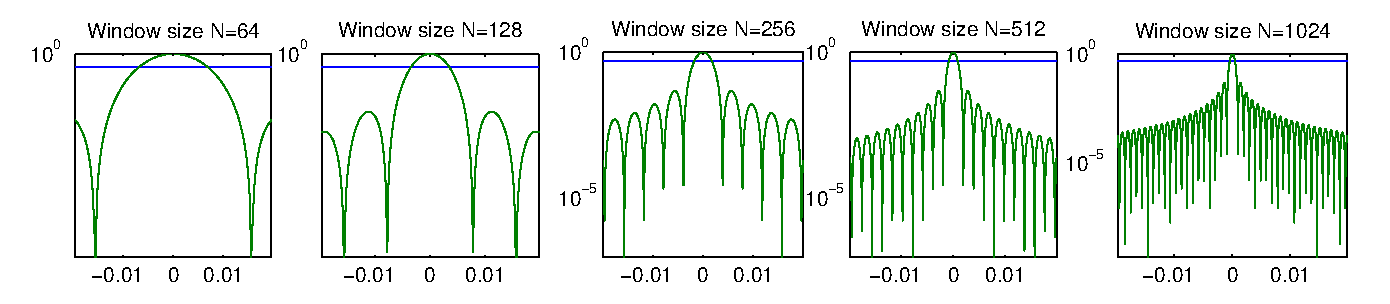
\includegraphics[width=\textwidth]{cw1im/3adb.eps}
\textit{Note}: The \textcolor{NavyBlue}{blue} line denotes the 3db line and the \textcolor{ForestGreen}{green} line is $W_B(\omega)$. Additionally the window has been normalised to 1 for practicality. Frequency axis is in Hz.
\label{fig:bartlettwid}
\caption{Plot of the Bartlett window and the 3db width of the main lobe}
\end{figure}
From figure \ref{fig:bartlettwid} we can see that the 3db width is just under $0.9 \cdot 2\pi/N$. From observation the side lobe height  is at $-6.54 dB$ which is independent of N (this is expected from the $W_B(\omega)$ function).

\begin{figure}[h!]
\centering

\resizebox{\textwidth}{!}{% This file was created by matlab2tikz v0.4.7 running on MATLAB 8.1.
% Copyright (c) 2008--2014, Nico Schlömer <nico.schloemer@gmail.com>
% All rights reserved.
% Minimal pgfplots version: 1.3
% 
% The latest updates can be retrieved from
%   http://www.mathworks.com/matlabcentral/fileexchange/22022-matlab2tikz
% where you can also make suggestions and rate matlab2tikz.
% 
%
% defining custom colors
\definecolor{mycolor1}{rgb}{1.00000,1.00000,0.86275}%
%
\begin{tikzpicture}

\begin{axis}[%
width=2.5in,
height=1.19791666666667in,
view={0}{90},
scale only axis,
xmin=0.19,
xmax=0.22,
xlabel={freq(Hz)},
ymin=-46.8397981049049,
ymax=0,
zmin=-1,
zmax=1,
name=plot2,
title={N=1024 and width=0.0012Hz}
]
\addplot [color=blue,solid,forget plot]
  table[row sep=crcr]{
0.185148998534441	-54.1569215052289\\
0.185637518319492	-54.9605579801191\\
0.186126038104543	-73.6192090196571\\
0.186614557889595	-65.0021841582178\\
0.187103077674646	-51.8667440554447\\
0.187591597459697	-52.5556671893773\\
0.188080117244748	-70.9782928726595\\
0.1885686370298	-62.47462306736\\
0.189057156814851	-49.1928583123809\\
0.189545676599902	-49.7349849842458\\
0.190034196384954	-67.8940679495199\\
0.190522716170005	-59.4563759763951\\
0.191011235955056	-45.9783034743653\\
0.191499755740107	-46.3193007074377\\
0.191988275525159	-64.1601293640323\\
0.19247679531021	-55.7099992619178\\
0.192965315095261	-41.9464348410445\\
0.193453834880313	-41.9839127490021\\
0.193942354665364	-59.3915997597022\\
0.194430874450415	-50.77571724484\\
0.194919394235467	-36.5406879946671\\
0.195407914020518	-36.046279806078\\
0.195896433805569	-52.7385072273319\\
0.19638495359062	-43.5741636834692\\
0.196873473375672	-28.3606892648713\\
0.197361993160723	-26.6381095851594\\
0.197850512945774	-41.6181041179205\\
0.198339032730826	-30.3468858850471\\
0.198827552515877	-11.5348627225651\\
0.199316072300928	-3.34652835046145\\
0.199804592085979	0\\
0.200293111871031	-0.357796010764786\\
0.200781631656082	-4.51701592074894\\
0.201270151441133	-14.0100897630925\\
0.201758671226185	-37.9049289890228\\
0.202247191011236	-35.3978898517545\\
0.202735710796287	-25.681438184766\\
0.203224230581339	-29.2939365539161\\
0.20371275036639	-49.6327165450919\\
0.204201270151441	-44.4290976056919\\
0.204689789936492	-32.5804426489599\\
0.205178309721544	-34.264038725701\\
0.205666829506595	-52.8438730483032\\
0.206155349291646	-45.3062493179674\\
0.206643869076698	-31.4166231346943\\
0.207132388861749	-30.7646635552679\\
0.2076209086468	-46.755176050988\\
0.208109428431851	-35.5000138875336\\
0.208597948216903	-17.1807525477733\\
0.209086468001954	-9.23442695531149\\
0.209574987787005	-6.00074045936602\\
0.210063507572057	-6.38991283786086\\
0.210552027357108	-10.5386409507078\\
0.211040547142159	-20.027097793754\\
0.211529066927211	-44.1425191473996\\
0.212017586712262	-41.042484821528\\
0.212506106497313	-31.539998032206\\
0.212994626282364	-35.3630866095068\\
0.213483146067416	-56.1311826690265\\
0.213971665852467	-51.139258204215\\
0.214460185637518	-40.0407005272997\\
0.21494870542257	-42.6994062843274\\
0.215437225207621	-62.5045598887206\\
0.215925744992672	-57.0393013368605\\
0.216414264777723	-45.2961126060334\\
0.216902784562775	-47.4571869604421\\
0.217391304347826	-66.799926653534\\
0.217879824132877	-61.1954291436032\\
0.218368343917929	-49.089297786477\\
0.21885686370298	-50.9738109682743\\
};
\addplot [color=black!50!green,solid,forget plot]
  table[row sep=crcr]{
0.181729360039082	-3.01029995663981\\
0.182217879824133	-3.01029995663981\\
0.182706399609184	-3.01029995663981\\
0.183194919394235	-3.01029995663981\\
0.183683439179287	-3.01029995663981\\
0.184171958964338	-3.01029995663981\\
0.184660478749389	-3.01029995663981\\
0.185148998534441	-3.01029995663981\\
0.185637518319492	-3.01029995663981\\
0.186126038104543	-3.01029995663981\\
0.186614557889595	-3.01029995663981\\
0.187103077674646	-3.01029995663981\\
0.187591597459697	-3.01029995663981\\
0.188080117244748	-3.01029995663981\\
0.1885686370298	-3.01029995663981\\
0.189057156814851	-3.01029995663981\\
0.189545676599902	-3.01029995663981\\
0.190034196384954	-3.01029995663981\\
0.190522716170005	-3.01029995663981\\
0.191011235955056	-3.01029995663981\\
0.191499755740107	-3.01029995663981\\
0.191988275525159	-3.01029995663981\\
0.19247679531021	-3.01029995663981\\
0.192965315095261	-3.01029995663981\\
0.193453834880313	-3.01029995663981\\
0.193942354665364	-3.01029995663981\\
0.194430874450415	-3.01029995663981\\
0.194919394235467	-3.01029995663981\\
0.195407914020518	-3.01029995663981\\
0.195896433805569	-3.01029995663981\\
0.19638495359062	-3.01029995663981\\
0.196873473375672	-3.01029995663981\\
0.197361993160723	-3.01029995663981\\
0.197850512945774	-3.01029995663981\\
0.198339032730826	-3.01029995663981\\
0.198827552515877	-3.01029995663981\\
0.199316072300928	-3.01029995663981\\
0.199804592085979	-3.01029995663981\\
0.200293111871031	-3.01029995663981\\
0.200781631656082	-3.01029995663981\\
0.201270151441133	-3.01029995663981\\
0.201758671226185	-3.01029995663981\\
0.202247191011236	-3.01029995663981\\
0.202735710796287	-3.01029995663981\\
0.203224230581339	-3.01029995663981\\
0.20371275036639	-3.01029995663981\\
0.204201270151441	-3.01029995663981\\
0.204689789936492	-3.01029995663981\\
0.205178309721544	-3.01029995663981\\
0.205666829506595	-3.01029995663981\\
0.206155349291646	-3.01029995663981\\
0.206643869076698	-3.01029995663981\\
0.207132388861749	-3.01029995663981\\
0.2076209086468	-3.01029995663981\\
0.208109428431851	-3.01029995663981\\
0.208597948216903	-3.01029995663981\\
0.209086468001954	-3.01029995663981\\
0.209574987787005	-3.01029995663981\\
0.210063507572057	-3.01029995663981\\
0.210552027357108	-3.01029995663981\\
0.211040547142159	-3.01029995663981\\
0.211529066927211	-3.01029995663981\\
0.212017586712262	-3.01029995663981\\
0.212506106497313	-3.01029995663981\\
0.212994626282364	-3.01029995663981\\
0.213483146067416	-3.01029995663981\\
0.213971665852467	-3.01029995663981\\
0.214460185637518	-3.01029995663981\\
0.21494870542257	-3.01029995663981\\
0.215437225207621	-3.01029995663981\\
0.215925744992672	-3.01029995663981\\
0.216414264777723	-3.01029995663981\\
0.216902784562775	-3.01029995663981\\
0.217391304347826	-3.01029995663981\\
0.217879824132877	-3.01029995663981\\
0.218368343917929	-3.01029995663981\\
0.21885686370298	-3.01029995663981\\
0.219345383488031	-3.01029995663981\\
0.219833903273083	-3.01029995663981\\
0.220322423058134	-3.01029995663981\\
0.220810942843185	-3.01029995663981\\
0.221299462628236	-3.01029995663981\\
0.221787982413288	-3.01029995663981\\
0.222276502198339	-3.01029995663981\\
0.22276502198339	-3.01029995663981\\
0.223253541768442	-3.01029995663981\\
0.223742061553493	-3.01029995663981\\
0.224230581338544	-3.01029995663981\\
0.224719101123596	-3.01029995663981\\
0.225207620908647	-3.01029995663981\\
0.225696140693698	-3.01029995663981\\
0.226184660478749	-3.01029995663981\\
0.226673180263801	-3.01029995663981\\
0.227161700048852	-3.01029995663981\\
0.227650219833903	-3.01029995663981\\
0.228138739618955	-3.01029995663981\\
0.228627259404006	-3.01029995663981\\
0.229115779189057	-3.01029995663981\\
0.229604298974108	-3.01029995663981\\
0.23009281875916	-3.01029995663981\\
0.230581338544211	-3.01029995663981\\
0.231069858329262	-3.01029995663981\\
0.231558378114314	-3.01029995663981\\
0.232046897899365	-3.01029995663981\\
0.232535417684416	-3.01029995663981\\
0.233023937469468	-3.01029995663981\\
0.233512457254519	-3.01029995663981\\
0.23400097703957	-3.01029995663981\\
0.234489496824621	-3.01029995663981\\
0.234978016609673	-3.01029995663981\\
0.235466536394724	-3.01029995663981\\
0.235955056179775	-3.01029995663981\\
0.236443575964827	-3.01029995663981\\
0.236932095749878	-3.01029995663981\\
0.237420615534929	-3.01029995663981\\
0.23790913531998	-3.01029995663981\\
0.238397655105032	-3.01029995663981\\
0.238886174890083	-3.01029995663981\\
0.239374694675134	-3.01029995663981\\
0.239863214460186	-3.01029995663981\\
0.240351734245237	-3.01029995663981\\
0.240840254030288	-3.01029995663981\\
0.24132877381534	-3.01029995663981\\
0.241817293600391	-3.01029995663981\\
};
%\addplot3 [color=white,line width=2.0pt,mark size=3.5pt,only marks,mark=square*,mark options={solid,fill=black,draw=mycolor1}]
% table[row sep=crcr] {0.200781631656082	-3.01029995663981	1\\
%};
 \end{axis}

\begin{axis}[%
width=2.5in,
height=1.19791666666667in,
scale only axis,
xmin=0.185,
xmax=0.24,
xlabel={freq(Hz)},
ymin=-70,
ymax=1,
ylabel={dB},
at=(plot2.left of south west),
anchor=right of south east,
title={N=512 and width=0.0025Hz}
]
\addplot [color=blue,solid,forget plot]
  table[row sep=crcr]{
0.185728250244379	-43.2045736466296\\
0.186705767350929	-41.1052516713283\\
0.187683284457478	-53.0599311471129\\
0.188660801564027	-57.3325592271797\\
0.189638318670577	-37.9183027386074\\
0.190615835777126	-35.2709369479833\\
0.191593352883675	-46.5091240621517\\
0.192570869990225	-50.4391460869492\\
0.193548387096774	-29.9697982447903\\
0.194525904203324	-26.1251033538023\\
0.195503421309873	-35.7251628509132\\
0.196480938416422	-37.8877367100598\\
0.197458455522972	-14.0291095118782\\
0.198435972629521	-4.52281692774132\\
0.19941348973607	-0.359385456540031\\
0.20039100684262	0\\
0.201368523949169	-3.3365568729049\\
0.202346041055718	-11.4936715138257\\
0.203323558162268	-30.2349111324103\\
0.204301075268817	-41.4175020152655\\
0.205278592375367	-26.2453783464334\\
0.206256109481916	-27.6984226932714\\
0.207233626588465	-42.5768689370055\\
0.208211143695015	-50.8398000329933\\
0.209188660801564	-33.5296479721008\\
0.210166177908113	-33.0564694082197\\
0.211143695014663	-46.2132189939198\\
0.212121212121212	-51.8277111262656\\
0.213098729227761	-32.7487818378419\\
0.214076246334311	-30.0567559738053\\
0.21505376344086	-40.7667918739333\\
0.21603128054741	-42.4837613901168\\
0.217008797653959	-19.4828838484991\\
0.217986314760508	-10.312923007291\\
0.218963831867058	-6.32414335258032\\
0.219941348973607	-6.04544445780594\\
0.220918866080156	-9.41595623628466\\
0.221896383186706	-17.6180824847311\\
0.222873900293255	-36.6394503484734\\
0.223851417399804	-46.6566815748468\\
0.224828934506354	-32.0517710299716\\
0.225806451612903	-33.767118798996\\
0.226783968719453	-49.0917797127883\\
0.227761485826002	-57.3003594853026\\
0.228739002932551	-40.8340649860466\\
0.229716520039101	-41.2872529585107\\
0.23069403714565	-55.5730610449231\\
0.231671554252199	-63.517385191543\\
0.232649071358749	-46.2130712201935\\
0.233626588465298	-46.1196698782304\\
0.234604105571848	-59.9009365704768\\
0.235581622678397	-67.9207560817118\\
0.236559139784946	-50.0784482103374\\
0.237536656891496	-49.6740408354182\\
0.238514173998045	-63.1518020666642\\
0.239491691104594	-71.3587350839527\\
0.240469208211144	-53.1040287562215\\
0.241446725317693	-52.4939033084168\\
0.242424242424242	-65.7671096764066\\
0.243401759530792	-74.2059003504159\\
};
\addplot [color=black!50!green,solid,forget plot]
  table[row sep=crcr]{
0.170087976539589	-3.01029995663981\\
0.171065493646139	-3.01029995663981\\
0.172043010752688	-3.01029995663981\\
0.173020527859238	-3.01029995663981\\
0.173998044965787	-3.01029995663981\\
0.174975562072336	-3.01029995663981\\
0.175953079178886	-3.01029995663981\\
0.176930596285435	-3.01029995663981\\
0.177908113391984	-3.01029995663981\\
0.178885630498534	-3.01029995663981\\
0.179863147605083	-3.01029995663981\\
0.180840664711632	-3.01029995663981\\
0.181818181818182	-3.01029995663981\\
0.182795698924731	-3.01029995663981\\
0.183773216031281	-3.01029995663981\\
0.18475073313783	-3.01029995663981\\
0.185728250244379	-3.01029995663981\\
0.186705767350929	-3.01029995663981\\
0.187683284457478	-3.01029995663981\\
0.188660801564027	-3.01029995663981\\
0.189638318670577	-3.01029995663981\\
0.190615835777126	-3.01029995663981\\
0.191593352883675	-3.01029995663981\\
0.192570869990225	-3.01029995663981\\
0.193548387096774	-3.01029995663981\\
0.194525904203324	-3.01029995663981\\
0.195503421309873	-3.01029995663981\\
0.196480938416422	-3.01029995663981\\
0.197458455522972	-3.01029995663981\\
0.198435972629521	-3.01029995663981\\
0.19941348973607	-3.01029995663981\\
0.20039100684262	-3.01029995663981\\
0.201368523949169	-3.01029995663981\\
0.202346041055718	-3.01029995663981\\
0.203323558162268	-3.01029995663981\\
0.204301075268817	-3.01029995663981\\
0.205278592375367	-3.01029995663981\\
0.206256109481916	-3.01029995663981\\
0.207233626588465	-3.01029995663981\\
0.208211143695015	-3.01029995663981\\
0.209188660801564	-3.01029995663981\\
0.210166177908113	-3.01029995663981\\
0.211143695014663	-3.01029995663981\\
0.212121212121212	-3.01029995663981\\
0.213098729227761	-3.01029995663981\\
0.214076246334311	-3.01029995663981\\
0.21505376344086	-3.01029995663981\\
0.21603128054741	-3.01029995663981\\
0.217008797653959	-3.01029995663981\\
0.217986314760508	-3.01029995663981\\
0.218963831867058	-3.01029995663981\\
0.219941348973607	-3.01029995663981\\
0.220918866080156	-3.01029995663981\\
0.221896383186706	-3.01029995663981\\
0.222873900293255	-3.01029995663981\\
0.223851417399804	-3.01029995663981\\
0.224828934506354	-3.01029995663981\\
0.225806451612903	-3.01029995663981\\
0.226783968719453	-3.01029995663981\\
0.227761485826002	-3.01029995663981\\
0.228739002932551	-3.01029995663981\\
0.229716520039101	-3.01029995663981\\
0.23069403714565	-3.01029995663981\\
0.231671554252199	-3.01029995663981\\
0.232649071358749	-3.01029995663981\\
0.233626588465298	-3.01029995663981\\
0.234604105571848	-3.01029995663981\\
0.235581622678397	-3.01029995663981\\
0.236559139784946	-3.01029995663981\\
0.237536656891496	-3.01029995663981\\
0.238514173998045	-3.01029995663981\\
0.239491691104594	-3.01029995663981\\
};
\end{axis}

\begin{axis}[%
width=2.5in,
height=1.19791666666667in,
unbounded coords=jump,
scale only axis,
xmin=0.195,
xmax=0.215,
xlabel={freq(Hz)},
ymin=-34.6841610817224,
ymax=0,
at=(plot2.right of south east),
anchor=left of south west,
title={N=2048 and width=0.0006Hz}
]
\addplot [color=blue,solid,forget plot]
  table[row sep=crcr]{
0.173870573870574	-80.0052524611572\\
0.174114774114774	-74.1739625411206\\
0.174358974358974	-80.4436111699685\\
0.174603174603175	-119.011422967507\\
0.174847374847375	-79.3818762611828\\
0.175091575091575	-73.5342174429905\\
0.175335775335775	-79.7824498620395\\
0.175579975579976	-119.055694731303\\
0.175824175824176	-78.7341672870587\\
0.176068376068376	-72.8695290376065\\
0.176312576312576	-79.0959096439689\\
0.176556776556777	-119.100014998915\\
0.176800976800977	-78.0601378062111\\
0.177045177045177	-72.1778470784526\\
0.177289377289377	-78.3818740497561\\
0.177533577533578	-119.144299209006\\
0.177777777777778	-77.3575442211487\\
0.178021978021978	-71.4568544253778\\
0.178266178266178	-77.6379481371322\\
0.178510378510379	-119.188780582304\\
0.178754578754579	-76.6238407518428\\
0.178998778998779	-70.7039182024887\\
0.179242979242979	-76.8614069223385\\
0.179487179487179	-119.233266379074\\
0.17973137973138	-75.8561221551028\\
0.17997557997558	-69.9160291678146\\
0.18021978021978	-76.0491312160907\\
0.18046398046398	-119.27787718445\\
0.180708180708181	-75.0510520249095\\
0.180952380952381	-69.0897257368593\\
0.181196581196581	-75.1975270031446\\
0.181440781440781	-119.322634991585\\
0.181684981684982	-74.2047722758949\\
0.181929181929182	-68.2209976904153\\
0.182173382173382	-74.3024229898836\\
0.182417582417582	-119.367581518051\\
0.182661782661783	-73.3127873549359\\
0.182905982905983	-67.3051626917984\\
0.183150183150183	-73.3589387794885\\
0.183394383394383	-119.412736608408\\
0.183638583638584	-72.3698143206805\\
0.183882783882784	-66.3367058270474\\
0.184126984126984	-72.3613130022406\\
0.184371184371184	-119.458099271046\\
0.184615384615385	-71.3695858822815\\
0.184859584859585	-65.3090680095551\\
0.185103785103785	-71.3026757877589\\
0.185347985347985	-119.503921746999\\
0.185592185592186	-70.3045874923581\\
0.185836385836386	-64.2143623599029\\
0.186080586080586	-70.1747424590163\\
0.186324786324786	-119.55005871272\\
0.186568986568987	-69.1657001253489\\
0.186813186813187	-63.0429870008907\\
0.187057387057387	-68.9673933234471\\
0.187301587301587	-119.596744948123\\
0.187545787545788	-67.9417050183362\\
0.187789987789988	-61.7830853460309\\
0.188034188034188	-67.6680846988693\\
0.188278388278388	-119.643983213818\\
0.188522588522589	-66.6185811563493\\
0.188766788766789	-60.4197758249809\\
0.189010989010989	-66.2610029886173\\
0.189255189255189	-119.692059127161\\
0.189499389499389	-65.178482271407\\
0.18974358974359	-58.9340222544088\\
0.18998778998779	-64.7258149627032\\
0.19023199023199	-119.741022854884\\
0.19047619047619	-63.5982011794316\\
0.190720390720391	-57.3009240460005\\
0.190964590964591	-63.0357598667709\\
0.191208791208791	-119.791162395135\\
0.191452991452991	-61.8467808443528\\
0.191697191697192	-55.4870302558872\\
0.191941391941392	-61.1546214540603\\
0.192185592185592	-119.842880833032\\
0.192429792429792	-59.8816369002066\\
0.192673992673993	-53.4459283388728\\
0.192918192918193	-59.0316930441782\\
0.193162393162393	-119.896643780603\\
0.193406593406593	-57.6419315147118\\
0.193650793650794	-51.1105956471203\\
0.193894993894994	-56.5929124791557\\
0.194139194139194	-119.952979601874\\
0.194383394383394	-55.0365018600787\\
0.194627594627595	-48.3792065342249\\
0.194871794871795	-53.7240853782949\\
0.195115995115995	-120.012758410677\\
0.195360195360195	-51.9199858620382\\
0.195604395604396	-45.0863731560548\\
0.195848595848596	-50.2359871134049\\
0.196092796092796	-120.077644711139\\
0.196336996336996	-48.040100932966\\
0.196581196581197	-40.9374505831939\\
0.196825396825397	-45.7816202852684\\
0.197069597069597	-120.149724994591\\
0.197313797313797	-42.9012375965507\\
0.197557997557998	-35.3295778267658\\
0.197802197802198	-39.6172592144192\\
0.198046398046398	-120.23219968821\\
0.198290598290598	-35.3092461291893\\
0.198534798534799	-26.6970670787791\\
0.198778998778999	-29.6260046626602\\
0.199023199023199	-120.332052242335\\
0.199267399267399	-20.8201206634198\\
0.1995115995116	-7.80471651099085\\
0.1997557997558	-1.81358619476289\\
0.2	0\\
0.2002442002442	-1.81107291596508\\
0.200488400488401	-7.78707237349105\\
0.200732600732601	-20.7625883110702\\
0.200976800976801	-120.644256691421\\
0.201221001221001	-29.3186142345918\\
0.201465201465201	-26.1618116263392\\
0.201709401709402	-34.4408512906018\\
0.201953601953602	-120.944112022301\\
0.202197802197802	-37.47693826583\\
0.202442002442002	-32.2749507550951\\
0.202686202686203	-38.6468540839138\\
0.202930402930403	-121.506265456176\\
0.203174603174603	-37.623800985773\\
0.203418803418803	-30.2183835971563\\
0.203663003663004	-34.1019035166501\\
0.203907203907204	-120.452686736002\\
0.204151404151404	-26.3055256856198\\
0.204395604395604	-13.6080105486859\\
0.204639804639805	-7.7774861706238\\
0.204884004884005	-6.02064804767963\\
0.205128205128205	-7.82305109205145\\
0.205372405372405	-13.7605325633612\\
0.205616605616606	-26.7144927006465\\
0.205860805860806	-121.871938464603\\
0.206105006105006	-35.1068480213351\\
0.206349206349206	-32.0797494993777\\
0.206593406593407	-40.587245822363\\
0.206837606837607	-120.505497536436\\
0.207081807081807	-44.473623747664\\
0.207326007326007	-40.0838942735768\\
0.207570207570208	-47.5549423297697\\
0.207814407814408	-120.27305229602\\
0.208058608058608	-50.0647642142719\\
0.208302808302808	-45.1332351998797\\
0.208547008547009	-52.1519205433607\\
0.208791208791209	-120.25256626315\\
0.209035409035409	-54.0341303657847\\
0.209279609279609	-48.81397626351\\
0.20952380952381	-55.5806075335218\\
0.20976800976801	-120.281165938529\\
0.21001221001221	-57.120080710344\\
0.21025641025641	-51.7193027062311\\
0.210500610500611	-58.3239837509479\\
0.210744810744811	-120.323801839412\\
0.210989010989011	-59.6554288318856\\
0.211233211233211	-54.1290168281497\\
0.211477411477411	-60.619224139937\\
0.211721611721612	-120.370579756834\\
0.211965811965812	-61.8156659108071\\
0.212210012210012	-56.1950777822551\\
0.212454212454212	-62.5986657711928\\
0.212698412698413	-120.418163055042\\
0.212942612942613	-63.7037093721999\\
0.213186813186813	-58.0085117136842\\
0.213431013431013	-64.3431608072351\\
0.213675213675214	-120.46539621714\\
0.213919413919414	-65.3848078139759\\
0.214163614163614	-59.6279626982613\\
0.214407814407814	-65.905591455028\\
0.214652014652015	-120.512023850935\\
0.214896214896215	-66.9028719709536\\
0.215140415140415	-61.0933967403267\\
0.215384615384615	-67.3224290339485\\
0.215628815628816	-120.55772753306\\
0.215873015873016	-68.2888750202418\\
0.216117216117216	-62.4332907816431\\
0.216361416361416	-68.6199113406743\\
0.216605616605617	-120.602835627996\\
0.216849816849817	-69.5655062479105\\
0.217094017094017	-63.6686784712634\\
0.217338217338217	-69.817571521548\\
0.217582417582418	-120.64720508782\\
0.217826617826618	-70.7499085426456\\
0.218070818070818	-64.8155610408913\\
0.218315018315018	-70.930367109106\\
0.218559218559219	-120.690850662905\\
0.218803418803419	-71.8553706688783\\
0.219047619047619	-65.8864139024656\\
0.219291819291819	-71.9700244193762\\
0.21953601953602	-120.733949644122\\
0.21978021978022	-72.892417999963\\
0.22002442002442	-66.8911666965808\\
0.22026862026862	-72.9459208975097\\
0.220512820512821	-120.776621915315\\
0.220757020757021	-73.8695409876775\\
0.221001221001221	-67.8378630546018\\
0.221245421245421	-73.865683663911\\
0.221489621489621	-120.818788810018\\
0.221733821733822	-74.793696827291\\
0.221978021978022	-68.7331180812945\\
0.222222222222222	-74.7356073538557\\
0.222466422466422	-120.860602524344\\
0.222710622710623	-75.670664231785\\
0.222954822954823	-69.5824438474781\\
0.223199023199023	-75.5609531343756\\
0.223443223443223	-120.901900058839\\
0.223687423687424	-76.505300230526\\
0.223931623931624	-70.3904862551359\\
0.224175824175824	-76.3461674276375\\
0.224420024420024	-120.943045660397\\
0.224664224664225	-77.301729914805\\
0.224908424908425	-71.1612008784683\\
0.225152625152625	-77.0950450512098\\
0.225396825396825	-120.983829927291\\
0.225641025641026	-78.0634891973142\\
0.225885225885226	-71.897985819583\\
0.226129426129426	-77.8108529777999\\
0.226373626373626	-121.024344437696\\
0.226617826617827	-78.7936339664786\\
0.226862026862027	-72.6037836925984\\
0.227106227106227	-78.496425686905\\
0.227350427350427	-121.064617183651\\
0.227594627594628	-79.4948247899728\\
0.227838827838828	-73.281161013656\\
0.228083028083028	-79.1542396483465\\
0.228327228327228	-121.104657496835\\
0.228571428571429	-80.1693935029828\\
0.228815628815629	-73.9323708086838\\
0.229059829059829	-79.7864722249793\\
0.229304029304029	-121.144472735375\\
0.22954822954823	-80.8193961223354\\
0.22979242979243	-74.5594025363576\\
0.23003663003663	-80.3950487890887\\
0.23028083028083	-121.18411625237\\
0.230525030525031	-81.4466554510051\\
0.230769230769231	-75.1640223436098\\
0.231013431013431	-80.9816807989421\\
0.231257631257631	-121.223469649201\\
0.231501831501832	-82.0527956194492\\
0.231746031746032	-75.7478058163836\\
0.231990231990232	-81.5478968216545\\
0.232234432234432	-121.262824311009\\
0.232478632478632	-82.6392704683659\\
0.232722832722833	-76.3121648531078\\
0.232967032967033	-82.0950681655012\\
0.233211233211233	-121.30194439224\\
0.233455433455433	-83.207386777884\\
0.233699633699634	-76.858369935383\\
0.233943833943834	-82.6244299488251\\
0.234188034188034	-121.34098214728\\
0.234432234432234	-83.7583238509676\\
0.234676434676435	-77.387568653407\\
0.234920634920635	-83.1370988550765\\
0.235164835164835	-121.379771729176\\
0.235409035409035	-84.2931497920959\\
0.235653235653236	-77.900801292391\\
0.235897435897436	-83.634088012594\\
0.236141636141636	-121.418453562534\\
0.236385836385836	-84.812835200116\\
0.236630036630037	-78.399013964565\\
0.236874236874237	-84.116319559109\\
0.237118437118437	-121.457112202295\\
0.237362637362637	-85.3182649252367\\
0.237606837606838	-78.8830698063664\\
0.237851037851038	-84.5846352928401\\
0.238095238095238	-121.495563133827\\
0.238339438339438	-85.8102478530895\\
0.238583638583639	-79.3537585037748\\
0.238827838827839	-85.0398060302933\\
0.239072039072039	-121.533851167085\\
0.239316239316239	-86.2895257659622\\
0.23956043956044	-79.8118045044169\\
0.23980463980464	-85.4825392032735\\
0.24004884004884	-121.572118967436\\
0.24029304029304	-86.75678027193\\
0.240537240537241	-80.2578740773108\\
0.240781440781441	-85.9134858564356\\
0.241025641025641	-121.610267548481\\
0.241269841269841	-87.2126394606192\\
0.241514041514042	-80.6925814638628\\
0.241758241758242	-86.3332464950014\\
0.242002442002442	-121.648300970515\\
0.242246642246642	-87.6576834402911\\
0.242490842490842	-81.1164941994678\\
0.242735042735043	-86.7423762918886\\
0.242979242979243	-121.686246492243\\
0.243223443223443	-88.0924490083677\\
0.243467643467643	-81.5301377708369\\
0.243711843711844	-87.1413894675819\\
0.243956043956044	-121.724094062218\\
0.244200244200244	-88.517433977367\\
0.244444444444444	-81.9339997304812\\
0.244688644688645	-87.5307633026311\\
0.244932844932845	-121.76188485659\\
0.245177045177045	-88.9331009088697\\
0.245421245421245	-82.3285332668994\\
0.245665445665446	-87.9109416752773\\
0.245909645909646	-121.799565769498\\
0.246153846153846	-89.3398804636598\\
0.246398046398046	-82.71416040754\\
0.246642246642247	-88.2823380285174\\
0.246886446886447	-121.837203275157\\
0.247130647130647	-89.7381740847745\\
0.247374847374847	-83.0912748323991\\
0.247619047619048	-88.6453381819838\\
0.247863247863248	-121.874693635299\\
0.248107448107448	-90.1283568546721\\
0.248351648351648	-83.4602443619766\\
0.248595848595849	-89.0003027279883\\
0.248840048840049	-121.912158950137\\
0.249084249084249	-90.5107796250017\\
0.249328449328449	-83.8214132023057\\
0.24957264957265	-89.3475692150639\\
0.24981684981685	-121.949453507588\\
0.25006105006105	-90.8857711417094\\
0.25030525030525	-84.1751039301044\\
0.250549450549451	-89.6874540910274\\
0.250793650793651	-121.986908634986\\
0.251037851037851	-91.2536398857524\\
0.251282051282051	-84.5216192969325\\
0.251526251526252	-90.0202541828612\\
0.251770451770452	-122.024028472993\\
0.252014652014652	-91.6146754464443\\
0.252258852258852	-84.861243815661\\
0.252503052503052	-90.3462488583499\\
0.252747252747253	-122.06123041841\\
0.252991452991453	-91.9691507429136\\
0.253235653235653	-85.1942452122807\\
0.253479853479853	-90.6657007675984\\
0.253724053724054	-122.098382600477\\
0.253968253968254	-92.3173224088524\\
0.254212454212454	-85.5208757011725\\
};
\addplot [color=black!50!green,solid,forget plot]
  table[row sep=crcr]{
0.178021978021978	-3.01029995663981\\
0.178266178266178	-3.01029995663981\\
0.178510378510379	-3.01029995663981\\
0.178754578754579	-3.01029995663981\\
0.178998778998779	-3.01029995663981\\
0.179242979242979	-3.01029995663981\\
0.179487179487179	-3.01029995663981\\
0.17973137973138	-3.01029995663981\\
0.17997557997558	-3.01029995663981\\
0.18021978021978	-3.01029995663981\\
0.18046398046398	-3.01029995663981\\
0.180708180708181	-3.01029995663981\\
0.180952380952381	-3.01029995663981\\
0.181196581196581	-3.01029995663981\\
0.181440781440781	-3.01029995663981\\
0.181684981684982	-3.01029995663981\\
0.181929181929182	-3.01029995663981\\
0.182173382173382	-3.01029995663981\\
0.182417582417582	-3.01029995663981\\
0.182661782661783	-3.01029995663981\\
0.182905982905983	-3.01029995663981\\
0.183150183150183	-3.01029995663981\\
0.183394383394383	-3.01029995663981\\
0.183638583638584	-3.01029995663981\\
0.183882783882784	-3.01029995663981\\
0.184126984126984	-3.01029995663981\\
0.184371184371184	-3.01029995663981\\
0.184615384615385	-3.01029995663981\\
0.184859584859585	-3.01029995663981\\
0.185103785103785	-3.01029995663981\\
0.185347985347985	-3.01029995663981\\
0.185592185592186	-3.01029995663981\\
0.185836385836386	-3.01029995663981\\
0.186080586080586	-3.01029995663981\\
0.186324786324786	-3.01029995663981\\
0.186568986568987	-3.01029995663981\\
0.186813186813187	-3.01029995663981\\
0.187057387057387	-3.01029995663981\\
0.187301587301587	-3.01029995663981\\
0.187545787545788	-3.01029995663981\\
0.187789987789988	-3.01029995663981\\
0.188034188034188	-3.01029995663981\\
0.188278388278388	-3.01029995663981\\
0.188522588522589	-3.01029995663981\\
0.188766788766789	-3.01029995663981\\
0.189010989010989	-3.01029995663981\\
0.189255189255189	-3.01029995663981\\
0.189499389499389	-3.01029995663981\\
0.18974358974359	-3.01029995663981\\
0.18998778998779	-3.01029995663981\\
0.19023199023199	-3.01029995663981\\
0.19047619047619	-3.01029995663981\\
0.190720390720391	-3.01029995663981\\
0.190964590964591	-3.01029995663981\\
0.191208791208791	-3.01029995663981\\
0.191452991452991	-3.01029995663981\\
0.191697191697192	-3.01029995663981\\
0.191941391941392	-3.01029995663981\\
0.192185592185592	-3.01029995663981\\
0.192429792429792	-3.01029995663981\\
0.192673992673993	-3.01029995663981\\
0.192918192918193	-3.01029995663981\\
0.193162393162393	-3.01029995663981\\
0.193406593406593	-3.01029995663981\\
0.193650793650794	-3.01029995663981\\
0.193894993894994	-3.01029995663981\\
0.194139194139194	-3.01029995663981\\
0.194383394383394	-3.01029995663981\\
0.194627594627595	-3.01029995663981\\
0.194871794871795	-3.01029995663981\\
0.195115995115995	-3.01029995663981\\
0.195360195360195	-3.01029995663981\\
0.195604395604396	-3.01029995663981\\
0.195848595848596	-3.01029995663981\\
0.196092796092796	-3.01029995663981\\
0.196336996336996	-3.01029995663981\\
0.196581196581197	-3.01029995663981\\
0.196825396825397	-3.01029995663981\\
0.197069597069597	-3.01029995663981\\
0.197313797313797	-3.01029995663981\\
0.197557997557998	-3.01029995663981\\
0.197802197802198	-3.01029995663981\\
0.198046398046398	-3.01029995663981\\
0.198290598290598	-3.01029995663981\\
0.198534798534799	-3.01029995663981\\
0.198778998778999	-3.01029995663981\\
0.199023199023199	-3.01029995663981\\
0.199267399267399	-3.01029995663981\\
0.1995115995116	-3.01029995663981\\
0.1997557997558	-3.01029995663981\\
0.2	-3.01029995663981\\
0.2002442002442	-3.01029995663981\\
0.200488400488401	-3.01029995663981\\
0.200732600732601	-3.01029995663981\\
0.200976800976801	-3.01029995663981\\
0.201221001221001	-3.01029995663981\\
0.201465201465201	-3.01029995663981\\
0.201709401709402	-3.01029995663981\\
0.201953601953602	-3.01029995663981\\
0.202197802197802	-3.01029995663981\\
0.202442002442002	-3.01029995663981\\
0.202686202686203	-3.01029995663981\\
0.202930402930403	-3.01029995663981\\
0.203174603174603	-3.01029995663981\\
0.203418803418803	-3.01029995663981\\
0.203663003663004	-3.01029995663981\\
0.203907203907204	-3.01029995663981\\
0.204151404151404	-3.01029995663981\\
0.204395604395604	-3.01029995663981\\
0.204639804639805	-3.01029995663981\\
0.204884004884005	-3.01029995663981\\
0.205128205128205	-3.01029995663981\\
0.205372405372405	-3.01029995663981\\
0.205616605616606	-3.01029995663981\\
0.205860805860806	-3.01029995663981\\
0.206105006105006	-3.01029995663981\\
0.206349206349206	-3.01029995663981\\
0.206593406593407	-3.01029995663981\\
0.206837606837607	-3.01029995663981\\
0.207081807081807	-3.01029995663981\\
0.207326007326007	-3.01029995663981\\
0.207570207570208	-3.01029995663981\\
0.207814407814408	-3.01029995663981\\
0.208058608058608	-3.01029995663981\\
0.208302808302808	-3.01029995663981\\
0.208547008547009	-3.01029995663981\\
0.208791208791209	-3.01029995663981\\
0.209035409035409	-3.01029995663981\\
0.209279609279609	-3.01029995663981\\
0.20952380952381	-3.01029995663981\\
0.20976800976801	-3.01029995663981\\
0.21001221001221	-3.01029995663981\\
0.21025641025641	-3.01029995663981\\
0.210500610500611	-3.01029995663981\\
0.210744810744811	-3.01029995663981\\
0.210989010989011	-3.01029995663981\\
0.211233211233211	-3.01029995663981\\
0.211477411477411	-3.01029995663981\\
0.211721611721612	-3.01029995663981\\
0.211965811965812	-3.01029995663981\\
0.212210012210012	-3.01029995663981\\
0.212454212454212	-3.01029995663981\\
0.212698412698413	-3.01029995663981\\
0.212942612942613	-3.01029995663981\\
0.213186813186813	-3.01029995663981\\
0.213431013431013	-3.01029995663981\\
0.213675213675214	-3.01029995663981\\
0.213919413919414	-3.01029995663981\\
0.214163614163614	-3.01029995663981\\
0.214407814407814	-3.01029995663981\\
0.214652014652015	-3.01029995663981\\
0.214896214896215	-3.01029995663981\\
0.215140415140415	-3.01029995663981\\
0.215384615384615	-3.01029995663981\\
0.215628815628816	-3.01029995663981\\
0.215873015873016	-3.01029995663981\\
0.216117216117216	-3.01029995663981\\
0.216361416361416	-3.01029995663981\\
0.216605616605617	-3.01029995663981\\
0.216849816849817	-3.01029995663981\\
0.217094017094017	-3.01029995663981\\
0.217338217338217	-3.01029995663981\\
0.217582417582418	-3.01029995663981\\
0.217826617826618	-3.01029995663981\\
0.218070818070818	-3.01029995663981\\
0.218315018315018	-3.01029995663981\\
0.218559218559219	-3.01029995663981\\
0.218803418803419	-3.01029995663981\\
0.219047619047619	-3.01029995663981\\
0.219291819291819	-3.01029995663981\\
0.21953601953602	-3.01029995663981\\
0.21978021978022	-3.01029995663981\\
0.22002442002442	-3.01029995663981\\
0.22026862026862	-3.01029995663981\\
0.220512820512821	-3.01029995663981\\
0.220757020757021	-3.01029995663981\\
0.221001221001221	-3.01029995663981\\
0.221245421245421	-3.01029995663981\\
0.221489621489621	-3.01029995663981\\
0.221733821733822	-3.01029995663981\\
0.221978021978022	-3.01029995663981\\
0.222222222222222	-3.01029995663981\\
0.222466422466422	-3.01029995663981\\
0.222710622710623	-3.01029995663981\\
0.222954822954823	-3.01029995663981\\
0.223199023199023	-3.01029995663981\\
0.223443223443223	-3.01029995663981\\
0.223687423687424	-3.01029995663981\\
0.223931623931624	-3.01029995663981\\
0.224175824175824	-3.01029995663981\\
0.224420024420024	-3.01029995663981\\
0.224664224664225	-3.01029995663981\\
0.224908424908425	-3.01029995663981\\
0.225152625152625	-3.01029995663981\\
0.225396825396825	-3.01029995663981\\
0.225641025641026	-3.01029995663981\\
0.225885225885226	-3.01029995663981\\
0.226129426129426	-3.01029995663981\\
0.226373626373626	-3.01029995663981\\
0.226617826617827	-3.01029995663981\\
0.226862026862027	-3.01029995663981\\
0.227106227106227	-3.01029995663981\\
0.227350427350427	-3.01029995663981\\
0.227594627594628	-3.01029995663981\\
0.227838827838828	-3.01029995663981\\
0.228083028083028	-3.01029995663981\\
0.228327228327228	-3.01029995663981\\
0.228571428571429	-3.01029995663981\\
0.228815628815629	-3.01029995663981\\
0.229059829059829	-3.01029995663981\\
0.229304029304029	-3.01029995663981\\
0.22954822954823	-3.01029995663981\\
0.22979242979243	-3.01029995663981\\
0.23003663003663	-3.01029995663981\\
0.23028083028083	-3.01029995663981\\
0.230525030525031	-3.01029995663981\\
0.230769230769231	-3.01029995663981\\
0.231013431013431	-3.01029995663981\\
0.231257631257631	-3.01029995663981\\
0.231501831501832	-3.01029995663981\\
0.231746031746032	-3.01029995663981\\
0.231990231990232	-3.01029995663981\\
0.232234432234432	-3.01029995663981\\
0.232478632478632	-3.01029995663981\\
0.232722832722833	-3.01029995663981\\
0.232967032967033	-3.01029995663981\\
0.233211233211233	-3.01029995663981\\
0.233455433455433	-3.01029995663981\\
0.233699633699634	-3.01029995663981\\
0.233943833943834	-3.01029995663981\\
0.234188034188034	-3.01029995663981\\
0.234432234432234	-3.01029995663981\\
0.234676434676435	-3.01029995663981\\
0.234920634920635	-3.01029995663981\\
0.235164835164835	-3.01029995663981\\
0.235409035409035	-3.01029995663981\\
0.235653235653236	-3.01029995663981\\
0.235897435897436	-3.01029995663981\\
0.236141636141636	-3.01029995663981\\
0.236385836385836	-3.01029995663981\\
0.236630036630037	-3.01029995663981\\
0.236874236874237	-3.01029995663981\\
0.237118437118437	-3.01029995663981\\
0.237362637362637	-3.01029995663981\\
0.237606837606838	-3.01029995663981\\
0.237851037851038	-3.01029995663981\\
0.238095238095238	-3.01029995663981\\
0.238339438339438	-3.01029995663981\\
0.238583638583639	-3.01029995663981\\
0.238827838827839	-3.01029995663981\\
0.239072039072039	-3.01029995663981\\
0.239316239316239	-3.01029995663981\\
0.23956043956044	-3.01029995663981\\
0.23980463980464	-3.01029995663981\\
0.24004884004884	-3.01029995663981\\
0.24029304029304	-3.01029995663981\\
0.240537240537241	-3.01029995663981\\
0.240781440781441	-3.01029995663981\\
0.241025641025641	-3.01029995663981\\
0.241269841269841	-3.01029995663981\\
0.241514041514042	-3.01029995663981\\
0.241758241758242	-3.01029995663981\\
0.242002442002442	-3.01029995663981\\
0.242246642246642	-3.01029995663981\\
0.242490842490842	-3.01029995663981\\
0.242735042735043	-3.01029995663981\\
0.242979242979243	-3.01029995663981\\
0.243223443223443	-3.01029995663981\\
0.243467643467643	-3.01029995663981\\
0.243711843711844	-3.01029995663981\\
0.243956043956044	-3.01029995663981\\
0.244200244200244	-3.01029995663981\\
0.244444444444444	-3.01029995663981\\
0.244688644688645	-3.01029995663981\\
0.244932844932845	-3.01029995663981\\
0.245177045177045	-3.01029995663981\\
0.245421245421245	-3.01029995663981\\
0.245665445665446	-3.01029995663981\\
0.245909645909646	-3.01029995663981\\
0.246153846153846	-3.01029995663981\\
0.246398046398046	-3.01029995663981\\
0.246642246642247	-3.01029995663981\\
0.246886446886447	-3.01029995663981\\
0.247130647130647	-3.01029995663981\\
0.247374847374847	-3.01029995663981\\
0.247619047619048	-3.01029995663981\\
0.247863247863248	-3.01029995663981\\
0.248107448107448	-3.01029995663981\\
0.248351648351648	-3.01029995663981\\
0.248595848595849	-3.01029995663981\\
};
\addplot [color=black!50!green,solid,forget plot]
  table[row sep=crcr]{0.977045177045177	-3.01029995663981\\
0.977289377289377	-3.01029995663981\\
0.977533577533578	-3.01029995663981\\
0.977777777777778	-3.01029995663981\\
0.978021978021978	-3.01029995663981\\
0.978266178266178	-3.01029995663981\\
0.978510378510378	-3.01029995663981\\
0.978754578754579	-3.01029995663981\\
0.978998778998779	-3.01029995663981\\
0.979242979242979	-3.01029995663981\\
0.979487179487179	-3.01029995663981\\
0.97973137973138	-3.01029995663981\\
0.97997557997558	-3.01029995663981\\
0.98021978021978	-3.01029995663981\\
0.98046398046398	-3.01029995663981\\
0.980708180708181	-3.01029995663981\\
0.980952380952381	-3.01029995663981\\
0.981196581196581	-3.01029995663981\\
0.981440781440781	-3.01029995663981\\
0.981684981684982	-3.01029995663981\\
0.981929181929182	-3.01029995663981\\
0.982173382173382	-3.01029995663981\\
0.982417582417582	-3.01029995663981\\
0.982661782661783	-3.01029995663981\\
0.982905982905983	-3.01029995663981\\
0.983150183150183	-3.01029995663981\\
0.983394383394383	-3.01029995663981\\
0.983638583638584	-3.01029995663981\\
0.983882783882784	-3.01029995663981\\
0.984126984126984	-3.01029995663981\\
0.984371184371184	-3.01029995663981\\
0.984615384615385	-3.01029995663981\\
0.984859584859585	-3.01029995663981\\
0.985103785103785	-3.01029995663981\\
0.985347985347985	-3.01029995663981\\
0.985592185592186	-3.01029995663981\\
0.985836385836386	-3.01029995663981\\
0.986080586080586	-3.01029995663981\\
0.986324786324786	-3.01029995663981\\
0.986568986568987	-3.01029995663981\\
0.986813186813187	-3.01029995663981\\
0.987057387057387	-3.01029995663981\\
0.987301587301587	-3.01029995663981\\
0.987545787545788	-3.01029995663981\\
0.987789987789988	-3.01029995663981\\
0.988034188034188	-3.01029995663981\\
0.988278388278388	-3.01029995663981\\
0.988522588522589	-3.01029995663981\\
0.988766788766789	-3.01029995663981\\
0.989010989010989	-3.01029995663981\\
0.989255189255189	-3.01029995663981\\
0.98949938949939	-3.01029995663981\\
0.98974358974359	-3.01029995663981\\
0.98998778998779	-3.01029995663981\\
0.99023199023199	-3.01029995663981\\
0.990476190476191	-3.01029995663981\\
0.990720390720391	-3.01029995663981\\
0.990964590964591	-3.01029995663981\\
0.991208791208791	-3.01029995663981\\
0.991452991452991	-3.01029995663981\\
0.991697191697192	-3.01029995663981\\
0.991941391941392	-3.01029995663981\\
0.992185592185592	-3.01029995663981\\
0.992429792429792	-3.01029995663981\\
0.992673992673993	-3.01029995663981\\
0.992918192918193	-3.01029995663981\\
0.993162393162393	-3.01029995663981\\
0.993406593406593	-3.01029995663981\\
0.993650793650794	-3.01029995663981\\
0.993894993894994	-3.01029995663981\\
0.994139194139194	-3.01029995663981\\
0.994383394383394	-3.01029995663981\\
0.994627594627595	-3.01029995663981\\
0.994871794871795	-3.01029995663981\\
0.995115995115995	-3.01029995663981\\
0.995360195360195	-3.01029995663981\\
0.995604395604396	-3.01029995663981\\
0.995848595848596	-3.01029995663981\\
0.996092796092796	-3.01029995663981\\
0.996336996336996	-3.01029995663981\\
0.996581196581197	-3.01029995663981\\
0.996825396825397	-3.01029995663981\\
0.997069597069597	-3.01029995663981\\
0.997313797313797	-3.01029995663981\\
0.997557997557998	-3.01029995663981\\
0.997802197802198	-3.01029995663981\\
0.998046398046398	-3.01029995663981\\
0.998290598290598	-3.01029995663981\\
0.998534798534799	-3.01029995663981\\
0.998778998778999	-3.01029995663981\\
0.999023199023199	-3.01029995663981\\
0.999267399267399	-3.01029995663981\\
0.9995115995116	-3.01029995663981\\
0.9997557997558	-3.01029995663981\\
1	-3.01029995663981\\
};
\end{axis}
\end{tikzpicture}%}
\caption{Plot of the lobe width for a Bartlett windowed signal with $\alpha = 10$}
\label{fig:3d2}
\end{figure}
\subsection{$\alpha$ value}
\begin{figure}[h!]
\centering
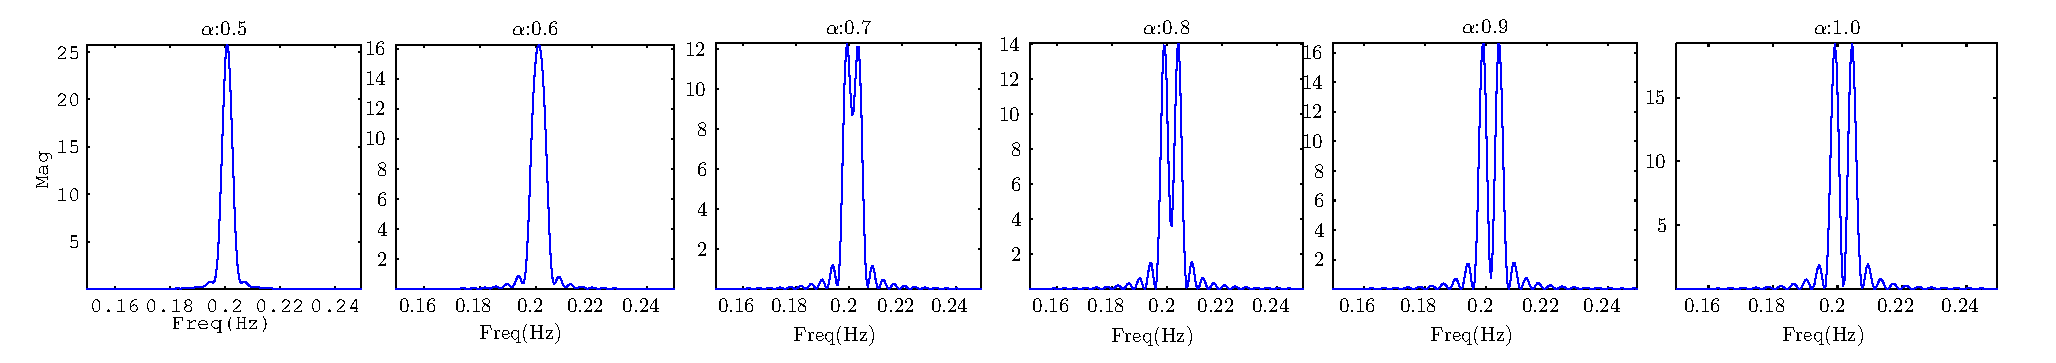
\includegraphics[width=\textwidth]{cw1im/3b.eps}
\caption{Plot of multiple $\boldsymbol{\mathrm{x}}$ for different $\alpha$ values}
\end{figure}
For the function $\boldsymbol{\mathrm{x}} = \sin(0.2\times 2\pi n)+\sin((0.2+\alpha / N)\times 2\pi n)$ we investigate the resolution of the periodogram for $N=256$, that is the increase in $\alpha$ needed to distinguish the two sine waves. From this we find that an $\alpha \geq 0.7$ allows the distinction between two frequencies. This is consistent with the FFT covering $0 \to 2\pi$ and being f length $N$, implying a resolution of $0.7 \cdot 2\pi / N$.

\subsection{$\alpha$ value with Hamming windows}
\begin{figure}[h!]
\centering
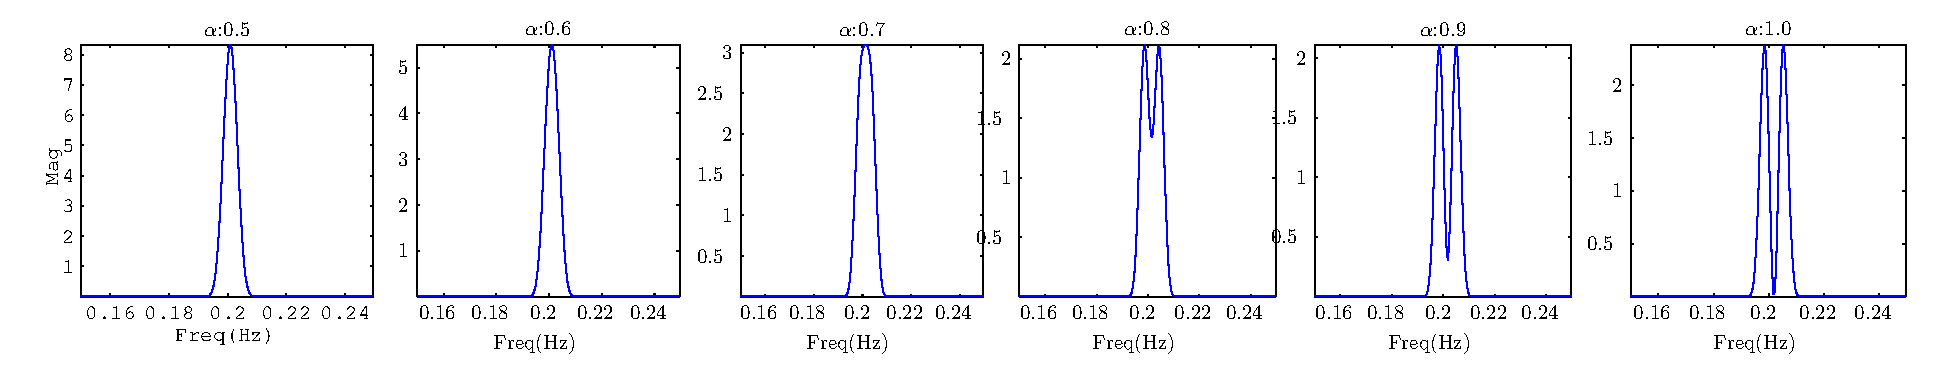
\includegraphics[width=\textwidth]{cw1im/3c.eps}
\caption{Plot of multiple $\boldsymbol{\mathrm{x}}$ for different $\alpha$ values}
\label{fig:3c}
\end{figure}
From Figure \ref{fig:3c} we see that a value of 0.8 instead of 0.7 works when data is windowed through a Hamming window. This is due to the Hamming window's lobe causing more smearing and a loss in spectral resolution.

\subsection{Amplitude Identification}
We define:
$\boldsymbol{\mathrm{x}} = a_1 \sin \left( 0.2\times 2\pi n \right) +a_2 \sin \left( \left( 0.2+\frac{\alpha}{N} \right) \times 2\pi n \right) $


\begin{figure}[h!]
\centering
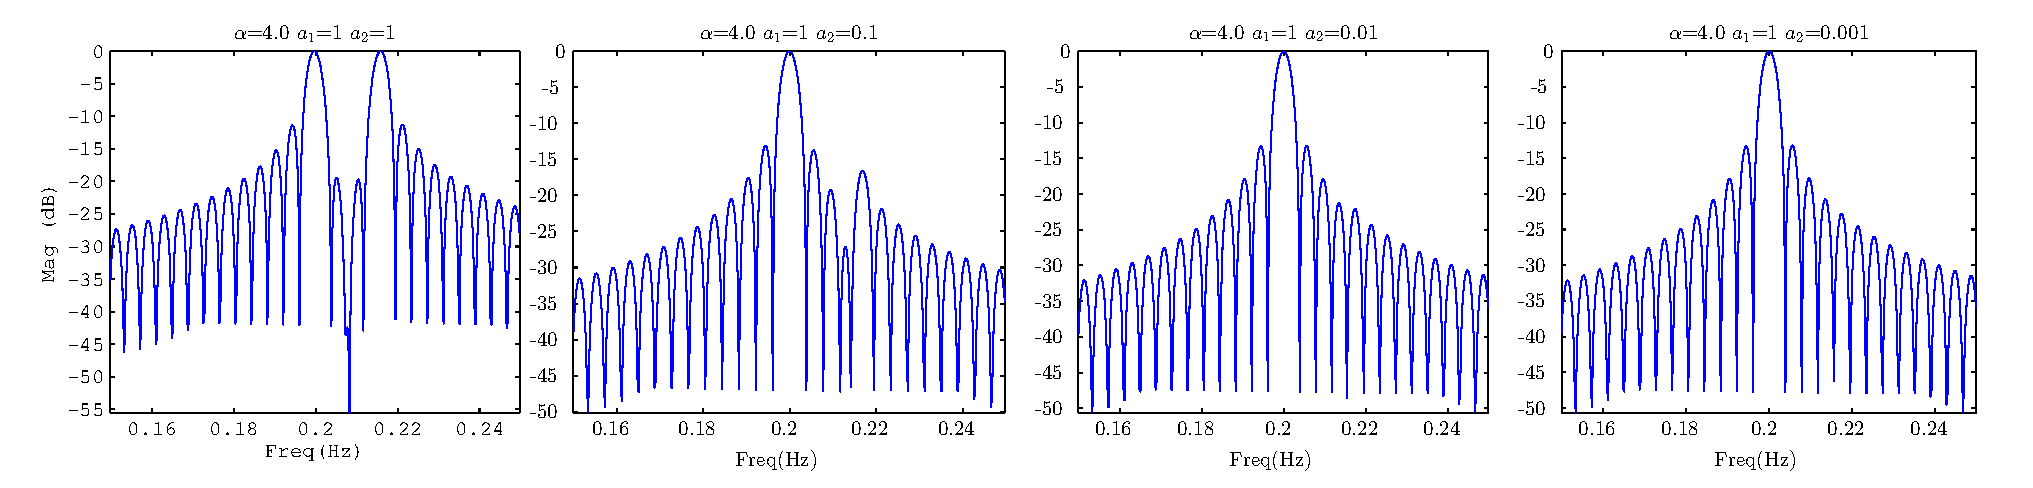
\includegraphics[width=\textwidth]{cw1im/3d.eps}
\caption{Plot of multiple $\boldsymbol{\mathrm{x}}$ for different $a_2$ values. Decreasing $a_2$ leads to a smaller magnitude for the second sinewave.}
\label{fig:3d}
\end{figure}
Figure \ref{fig:3d} shows us that the amplitude is no longer identifiable when $a_2 \leq 0.01$. \latinabbrev{i.e} the magnitude difference is now more than two magnitudes in difference with the largest signal.
\begin{figure}[h!]
\centering
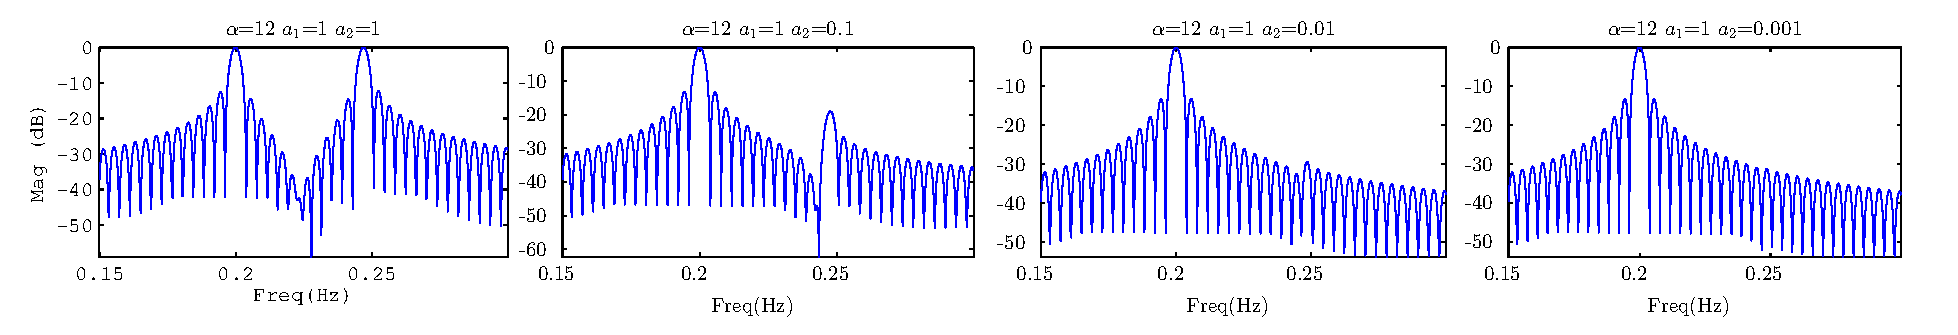
\includegraphics[width=\textwidth]{cw1im/3d12.eps}
\caption{Plot of multiple $\boldsymbol{\mathrm{x}}$ for different $a_2$ values}
\label{fig:3d12}
\end{figure}

In Figure \ref{fig:3d12} we now have $\alpha=12$, increasing the frequency distance between the two signals. This leads to see that increased the distance between the frequency of the two sine waves increases the identification threshold to $a=0.01$ .

These findings highlight the effects of different amplitudes and frequencies in signals causing interference.

\subsection{Effect of Bartlett window}
We know that $\mathbb{E} \left\{ \hat{P}_{per} = W_B(f) \ast P_{xx}(f) \right\}$ \latinabbrev{i.e}the expected value of the periodogram is the convolution of the power spectrum with the Fourier transform of the Bartlett window.

From the shape of the Bartlett window in frequency we can see that a too big difference in frequencies as well as magnitudes can cause issues in the quality of the periodogram.

Looking at \ref{fig:3e}  we see that the height of the sidelobes at $f=\frac{4}{N}$ and $\frac{12}{N}$ (and for another integer by N) are effectively troughs, at about $-100dB$. From this we can see why the lower amplitude sinusoid would be obscured. Further on the amplitude has been reduced enough such that $12/N$ offset is not present when the $\sinc^2$ convolutes over the first frequency, enough for it to effectively act like a delta function.

%\noindent\makebox[\linewidth]{\rule{\paperwidth}{0.4pt}}
\begin{figure}[h!]
\centering
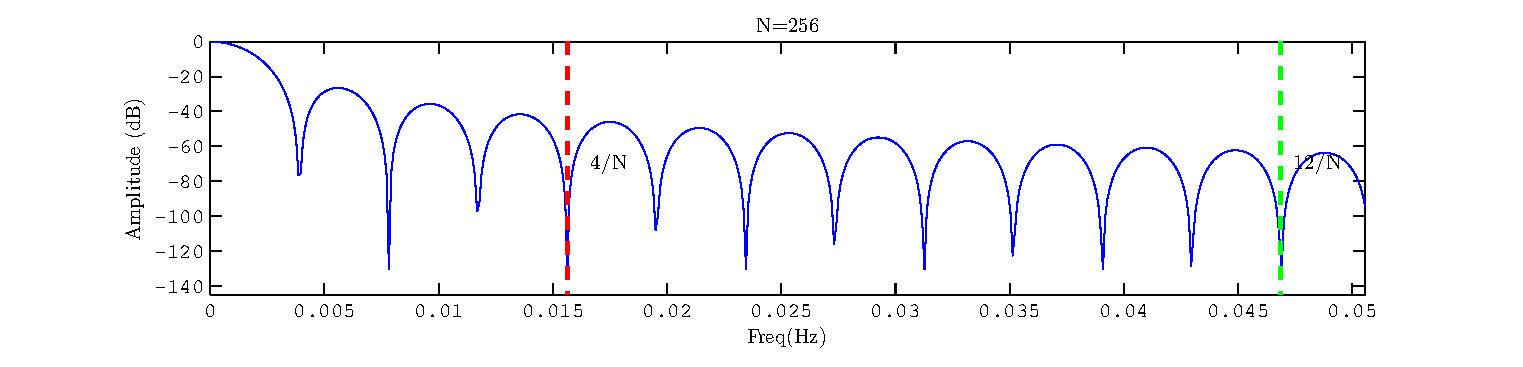
\includegraphics[width=\textwidth]{cw1im/3e2.eps}
\caption{Plot of Bartlett window $0$ to $0.05Hz$}
\label{fig:3e}
\end{figure}


%The mean of the estimated spectrum will be the true spectrum convolved with the Bartlett window. Thus, sidelobes of the stronger sinusoid peak, after convolution, may be larger than the main lobe level of the weaker sinusoid peak, if the weaker sinusoid is sufficiently weak. The sidelobe level for the Bartlett window is about -35 dB at α = 4 (4 Fourier resolution bins), and about -50 dB for α = 12. For α = 4 we could detect a weaker sinusoid whose power is 20 dB below a stronger sinusoid power, but not when the weaker sinusoid power is 40 dB below; this is consistent with the -35 dB sidelobe level. Similar comments apply for α = 12.
\subsection{Chebyshev and Blackman-Tukey windowing}
\begin{figure}[h!]
\centering
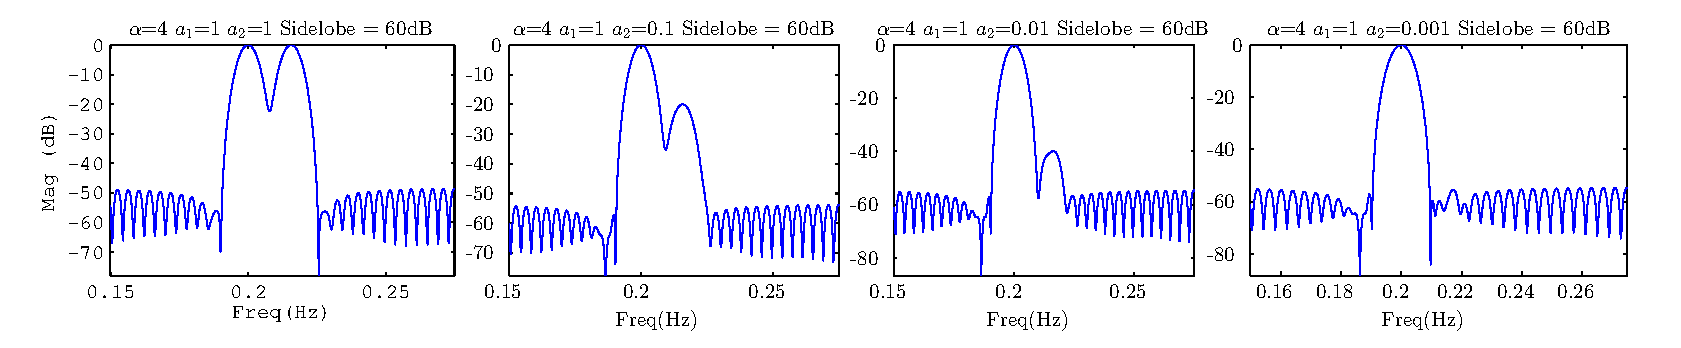
\includegraphics[width=\textwidth]{cw1im/3f_chebwin.eps}
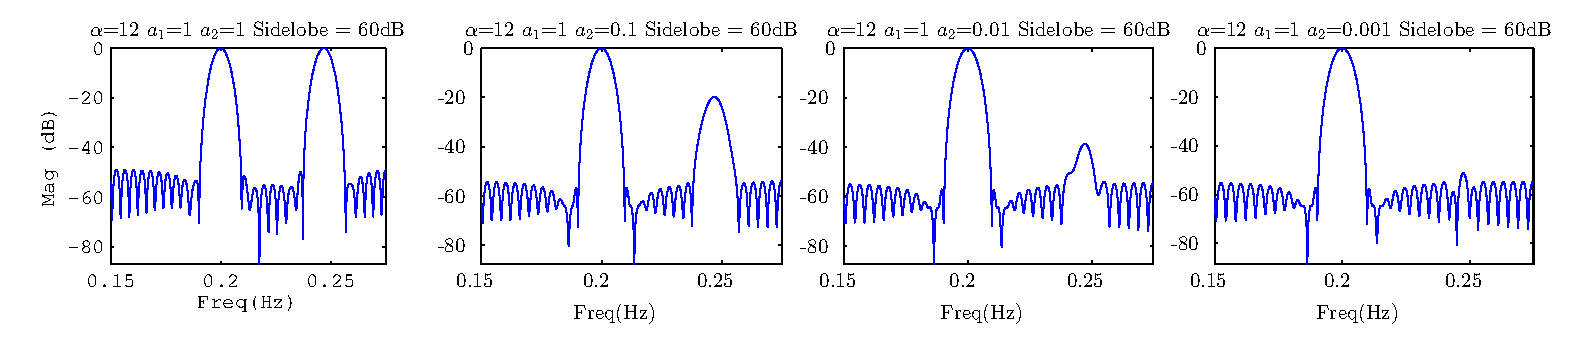
\includegraphics[width=\textwidth]{cw1im/3f_chebwin12.eps}
\caption{Plot of Chebyshev windowed data}
\label{fig:3fcheb}
\end{figure}

\begin{figure}[h!]
\centering
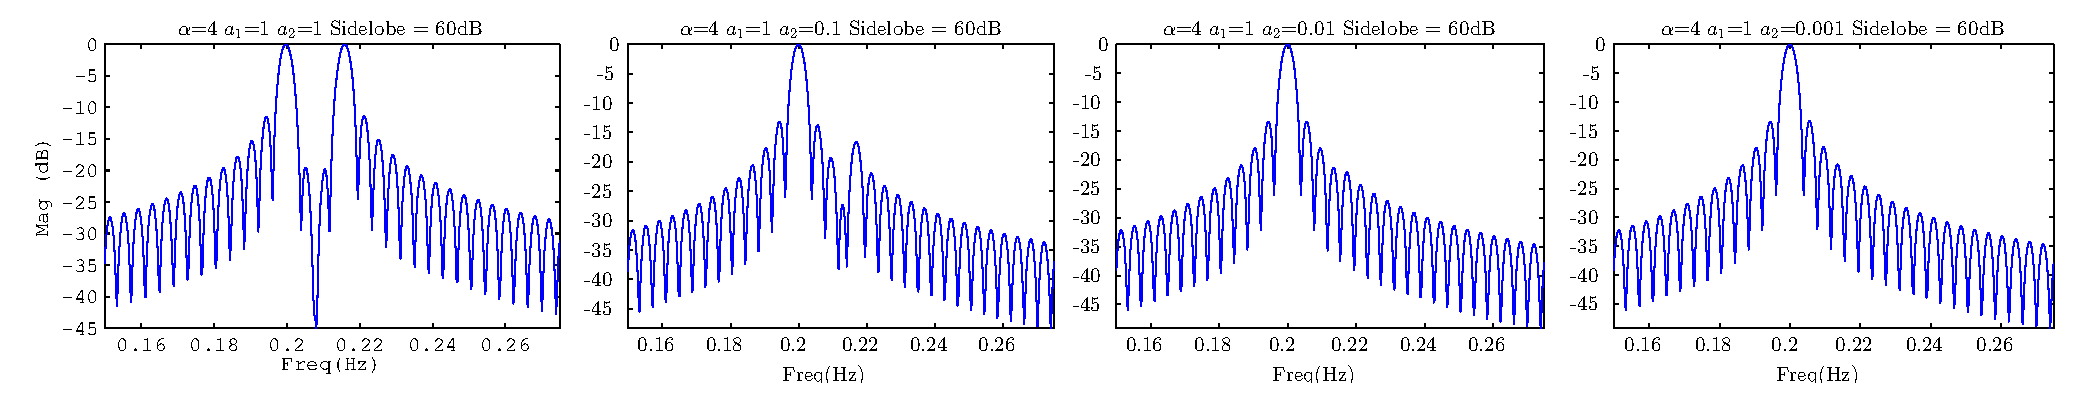
\includegraphics[width=\textwidth]{cw1im/3f_bt.eps}
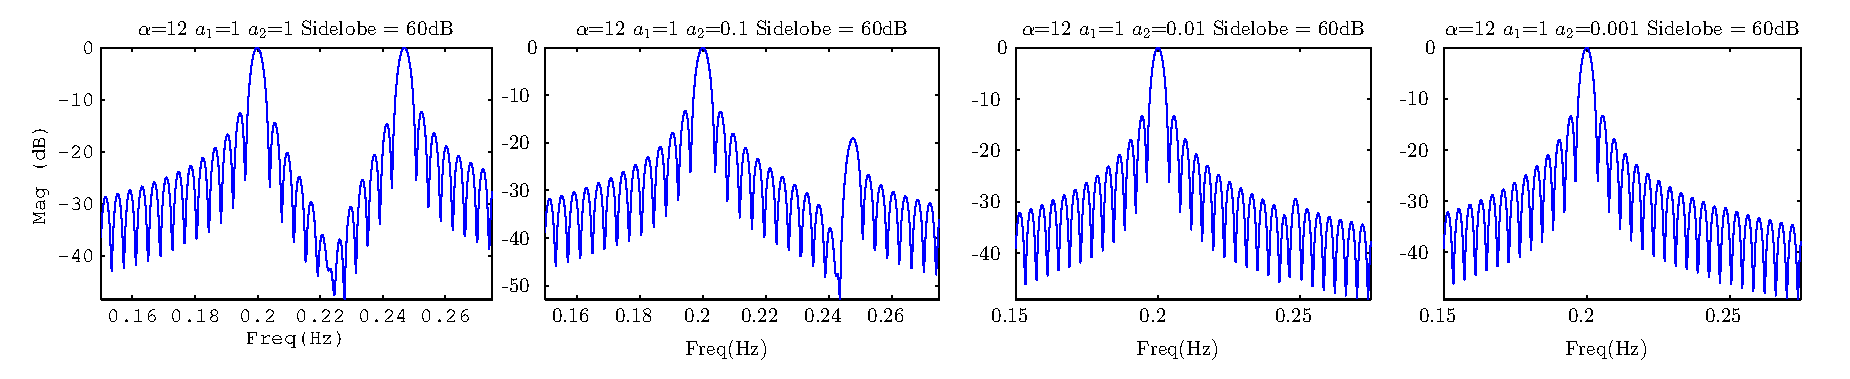
\includegraphics[width=\textwidth]{cw1im/3f_bt12.eps}
\caption{Plot of Blackman-Tukey method with a Chebyshev window data}
\label{fig:3fbt}
\end{figure}
Here we have windowed the sample data in figure \ref{fig:3fcheb} and in figure \ref{fig:3fbt} the autocovariance function has been windowed (Blackman-Tukey method). In both the Chebyshev window was used. This is done using the \texttt{chebwin(L,r)} function in matlab where \texttt{L} is the window length and \texttt{r} is the depth in dB of the sidelobes, which are constant. Figure \ref{fig:3fcheb} shows us that the combination of the Chebyshev's window width and second lobe amplitude allows it to detect the weaker sinusoid up until $a_2 = 0.001$. For this case a sidelobe of $60$dB was found to work best. This is because the Chebyshev window can sacrifice the width of its central lobe for constant low amplitude sidelobes, leading to less spectral leakage.



The Blackman Tukey method aims to reduce the variance of the estimator. While giving us a more precise spectrum, it is not as accurate due to trying to reduce the contribution of unreliable estimates to the periodogram. So despite the low amplitude sidelobes (the Bartlett window sidelobes are not as low) the weak amplitude sinusoid is not able to be detected.
% From the Chebyshev window we see the main lobe width is about 4.9/N; when we set the second frequency at -50 dB and using α = 4.9/N, we obtain the windowed periodogram result above, and we see that we can indeed detect the weaker sinusoid. Note that a plot of 20 log10 |V (ω)/V (0)| is the same as the top figure above, since W(ω) = |V (ω)| 2. The Blackman–Tukey method fails because its mean spectrum is, from equations (2.5.3) and (2.4.8), the convolution of the true spectrum, the Bartlett window, and the Chebyshev window. Even though the Chebyshev window has low sidelobes, the Bartlett window does not, and the weak sinusoid cannot be detected.

\section{Periodogram-based Methods Applied to Measured Data}
\subsection{Sunspot Data Investigation}
\begin{figure}[h!]
\centering
%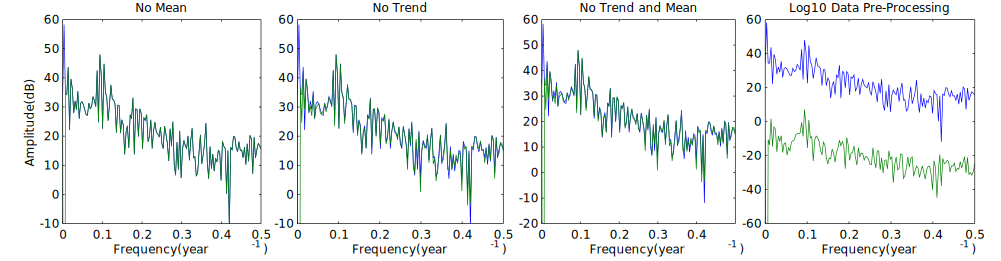
\includegraphics[width=\textwidth]{cw1im/4a.svg}
%% This file was created by matlab2tikz v0.4.7 running on MATLAB 8.1.
% Copyright (c) 2008--2014, Nico Schlömer <nico.schloemer@gmail.com>
% All rights reserved.
% Minimal pgfplots version: 1.3
% 
% The latest updates can be retrieved from
%   http://www.mathworks.com/matlabcentral/fileexchange/22022-matlab2tikz
% where you can also make suggestions and rate matlab2tikz.
% 
\begin{tikzpicture}

\begin{axis}[%
width=2.5in,
height=1.75in,
scale only axis,
xmin=0,
xmax=0.5,
xlabel={Frequency($year^{-1}$)},
ymin=-10,
ymax=60,
name=plot2,
title={No Trend}
]
\addplot [color=blue,solid,forget plot]
  table[row sep=crcr]{0	34.375461876336\\
0.00347222222222222	58.2969366078634\\
0.00694444444444444	34.375461876336\\
0.0104166666666667	34.3684803719121\\
0.0138888888888889	43.6948801481999\\
0.0173611111111111	22.1082899441454\\
0.0208333333333333	39.6314273804426\\
0.0243055555555556	36.4233132191968\\
0.0277777777777778	27.8812096441415\\
0.03125	32.0923109292413\\
0.0347222222222222	29.0622787664382\\
0.0381944444444444	35.4322045648322\\
0.0416666666666667	25.9723486294958\\
0.0451388888888889	31.2657339362639\\
0.0486111111111111	31.8014929272802\\
0.0520833333333333	30.8907954365247\\
0.0555555555555556	29.0746561111669\\
0.0590277777777778	27.407374316164\\
0.0625	27.142060971415\\
0.0659722222222222	31.3736730376102\\
0.0694444444444444	29.4546231263779\\
0.0729166666666667	30.1032961754004\\
0.0763888888888889	33.5789989838183\\
0.0798611111111111	32.3019020790326\\
0.0833333333333333	30.1362469505229\\
0.0868055555555556	42.5527641117993\\
0.0902777777777778	24.7568299282092\\
0.09375	48.0201531618919\\
0.0972222222222222	41.0146365526965\\
0.100694444444444	22.5390953948984\\
0.104166666666667	44.8320266532513\\
0.107638888888889	35.1281483396535\\
0.111111111111111	33.3569046489344\\
0.114583333333333	25.2945554375867\\
0.118055555555556	30.9011319200594\\
0.121527777777778	37.578690008479\\
0.125	32.7959648134229\\
0.128472222222222	32.4219928228637\\
0.131944444444444	31.082566256303\\
0.135416666666667	21.1390531064111\\
0.138888888888889	30.6298634745278\\
0.142361111111111	30.4290788389394\\
0.145833333333333	21.06853065674\\
0.149305555555556	25.6105921129283\\
0.152777777777778	23.8513001571226\\
0.15625	13.7422297449367\\
0.159722222222222	21.3089788496573\\
0.163194444444444	23.569964857195\\
0.166666666666667	15.9423847464137\\
0.170138888888889	27.3798421114373\\
0.173611111111111	26.0051905164427\\
0.177083333333333	33.1686048002384\\
0.180555555555556	13.758005688851\\
0.184027777777778	29.3217039309664\\
0.1875	29.1082293617857\\
0.190972222222222	19.8807412962208\\
0.194444444444444	29.3951175153929\\
0.197916666666667	27.9251039391241\\
0.201388888888889	15.6551174729803\\
0.204861111111111	26.2183786261246\\
0.208333333333333	25.4552463509402\\
0.211805555555556	27.3953739899113\\
0.215277777777778	18.0315828147974\\
0.21875	19.8932615256145\\
0.222222222222222	25.61618788539\\
0.225694444444444	15.7733750760932\\
0.229166666666667	21.8681612517873\\
0.232638888888889	24.831864308874\\
0.236111111111111	21.3221366883844\\
0.239583333333333	20.7436416104729\\
0.243055555555556	19.807957145444\\
0.246527777777778	23.0970089246501\\
0.25	17.5549706099219\\
0.253472222222222	15.7255295755483\\
0.256944444444444	23.4611725540786\\
0.260416666666667	20.6700246232681\\
0.263888888888889	17.5296178620887\\
0.267361111111111	11.4739863612246\\
0.270833333333333	22.5862659873735\\
0.274305555555556	16.5821260108386\\
0.277777777777778	24.9918638490749\\
0.28125	9.96954616266194\\
0.284722222222222	6.5900804999303\\
0.288194444444444	17.9899985383009\\
0.291666666666667	8.51962860354485\\
0.295138888888889	21.818656607418\\
0.298611111111111	5.59270530460508\\
0.302083333333333	15.4428786272398\\
0.305555555555556	18.5290039946418\\
0.309027777777778	16.7567139956182\\
0.3125	15.7861813778032\\
0.315972222222222	20.086716073201\\
0.319444444444444	11.7256410757813\\
0.322916666666667	18.561535698187\\
0.326388888888889	22.7067588643075\\
0.329861111111111	12.5788093715714\\
0.333333333333333	12.9512811436246\\
0.336805555555556	6.26472249895134\\
0.340277777777778	7.36047887860197\\
0.34375	14.3711982947736\\
0.347222222222222	20.4811494733786\\
0.350694444444444	10.47554823377\\
0.354166666666667	13.5434094395188\\
0.357638888888889	17.389122716609\\
0.361111111111111	24.4871665349974\\
0.364583333333333	10.979739362859\\
0.368055555555556	5.34974671385102\\
0.371527777777778	16.4576350037354\\
0.375	8.86392945222743\\
0.378472222222222	13.9014555536488\\
0.381944444444444	7.98768572011374\\
0.385416666666667	12.4085210511543\\
0.388888888888889	11.1507640625701\\
0.392361111111111	15.1284535984147\\
0.395833333333333	14.6011704478275\\
0.399305555555556	4.79921119598378\\
0.402777777777778	18.2355306454086\\
0.40625	16.5423346943921\\
0.409722222222222	15.793512940573\\
0.413194444444444	0.229460576125035\\
0.416666666666667	15.1028778461634\\
0.420138888888889	-11.9328993051282\\
0.423611111111111	16.2309653030882\\
0.427083333333333	15.3112601738493\\
0.430555555555556	19.8767580106878\\
0.434027777777778	19.7290328030369\\
0.4375	16.0874940412484\\
0.440972222222222	14.6269648474286\\
0.444444444444444	18.1400109960649\\
0.447916666666667	15.0488053734431\\
0.451388888888889	15.2147030460893\\
0.454861111111111	12.5656759578178\\
0.458333333333333	16.1872930047005\\
0.461805555555556	10.235641922418\\
0.465277777777778	17.4223390131987\\
0.46875	11.3595669932546\\
0.472222222222222	20.3041238056257\\
0.475694444444444	18.9922734089749\\
0.479166666666667	7.08815815321358\\
0.482638888888889	19.7153523290218\\
0.486111111111111	12.4935361319041\\
0.489583333333333	15.3958294405089\\
0.493055555555556	17.4921746532211\\
0.496527777777778	16.7080052554762\\
0.5	15.6304255620658\\
};
\addplot [color=black!50!green,solid,forget plot]
  table[row sep=crcr]{0	36.7131495744874\\
0.00347222222222222	-247.808795503209\\
0.00694444444444444	36.7131495744874\\
0.0104166666666667	24.6278226456189\\
0.0138888888888889	42.3776214692246\\
0.0173611111111111	29.1451459266798\\
0.0208333333333333	39.7117758294165\\
0.0243055555555556	34.6678610660255\\
0.0277777777777778	28.3698919043499\\
0.03125	30.239748276581\\
0.0347222222222222	26.9550901334374\\
0.0381944444444444	34.442535802002\\
0.0416666666666667	25.9387106001545\\
0.0451388888888889	29.6984197909916\\
0.0486111111111111	30.4417336100689\\
0.0520833333333333	31.2009278952787\\
0.0555555555555556	27.7942897295819\\
0.0590277777777778	27.7034053911466\\
0.0625	28.6330791511246\\
0.0659722222222222	31.2277799372964\\
0.0694444444444444	28.2804476670233\\
0.0729166666666667	30.7457135085699\\
0.0763888888888889	33.0482887526323\\
0.0798611111111111	31.7525819809702\\
0.0833333333333333	30.3656167604871\\
0.0868055555555556	42.6430446673256\\
0.0902777777777778	23.3831813748193\\
0.09375	48.0401328603522\\
0.0972222222222222	41.2014109773871\\
0.100694444444444	22.6854762888484\\
0.104166666666667	44.844328674144\\
0.107638888888889	35.2382689808259\\
0.111111111111111	32.9405366959018\\
0.114583333333333	24.2121304130089\\
0.118055555555556	31.1860991510222\\
0.121527777777778	37.8030570500769\\
0.125	32.5879264789159\\
0.128472222222222	32.6918373856373\\
0.131944444444444	31.2083083125483\\
0.135416666666667	22.1982200280651\\
0.138888888888889	30.2022507410034\\
0.142361111111111	30.3084200232981\\
0.145833333333333	20.0810491917721\\
0.149305555555556	25.1856818937609\\
0.152777777777778	23.0231940716234\\
0.15625	14.1867275361844\\
0.159722222222222	21.1587225006991\\
0.163194444444444	22.6782049286146\\
0.166666666666667	15.6826407511947\\
0.170138888888889	26.8410224215738\\
0.173611111111111	25.9467390026938\\
0.177083333333333	32.8737769755607\\
0.180555555555556	16.0349839504242\\
0.184027777777778	28.9164696905022\\
0.1875	29.4185367063787\\
0.190972222222222	20.2122410994511\\
0.194444444444444	29.8022855816558\\
0.197916666666667	28.3958119108529\\
0.201388888888889	17.1591078353465\\
0.204861111111111	25.6796555647548\\
0.208333333333333	25.1027600013659\\
0.211805555555556	27.5652859508665\\
0.215277777777778	17.3153688276077\\
0.21875	19.4310428736793\\
0.222222222222222	26.0368995111683\\
0.225694444444444	17.3666644777471\\
0.229166666666667	21.4178313814863\\
0.232638888888889	25.0461812454209\\
0.236111111111111	22.0957692926138\\
0.239583333333333	21.2191520442783\\
0.243055555555556	18.7107082969962\\
0.246527777777778	23.2787140213106\\
0.25	16.8650629387802\\
0.253472222222222	17.0673239551049\\
0.256944444444444	22.8979201932676\\
0.260416666666667	20.48134955102\\
0.263888888888889	17.1067416113273\\
0.267361111111111	8.50299537091923\\
0.270833333333333	22.551289304279\\
0.274305555555556	17.4538124435195\\
0.277777777777778	24.4905663789534\\
0.28125	12.1514470187728\\
0.284722222222222	7.17890451485926\\
0.288194444444444	19.0402208034024\\
0.291666666666667	11.3112811317529\\
0.295138888888889	21.2797355714713\\
0.298611111111111	0.812140181286416\\
0.302083333333333	15.0469795363057\\
0.305555555555556	17.9776925724516\\
0.309027777777778	16.0354860771297\\
0.3125	16.8737781115565\\
0.315972222222222	20.6361422304434\\
0.319444444444444	10.8349219117987\\
0.322916666666667	17.8303401315653\\
0.326388888888889	22.8866031262167\\
0.329861111111111	10.4233099167734\\
0.333333333333333	12.347489536072\\
0.336805555555556	4.56242567568251\\
0.340277777777778	9.56845669667009\\
0.34375	12.7339262870329\\
0.347222222222222	20.3615537786481\\
0.350694444444444	11.2572895388631\\
0.354166666666667	11.9649229895695\\
0.357638888888889	16.291900287536\\
0.361111111111111	24.305788390022\\
0.364583333333333	8.48621294711523\\
0.368055555555556	8.48382155982512\\
0.371527777777778	15.2692655757074\\
0.375	8.23373182625567\\
0.378472222222222	12.4502923807529\\
0.381944444444444	9.84080661479433\\
0.385416666666667	13.6159329851129\\
0.388888888888889	10.5948973372983\\
0.392361111111111	14.4670166702039\\
0.395833333333333	13.4417460701251\\
0.399305555555556	1.18685361706209\\
0.402777777777778	17.4366672254557\\
0.40625	15.6066655923633\\
0.409722222222222	16.5619607924983\\
0.413194444444444	-3.73643655529414\\
0.416666666666667	14.2663340741124\\
0.420138888888889	-3.33783416095845\\
0.423611111111111	16.5154110480819\\
0.427083333333333	16.149946265308\\
0.430555555555556	19.4990715106634\\
0.434027777777778	19.6924623618826\\
0.4375	17.1330356973402\\
0.440972222222222	15.5469498304325\\
0.444444444444444	18.4065863596608\\
0.447916666666667	15.5099809226311\\
0.451388888888889	15.5312285476702\\
0.454861111111111	10.8066862242503\\
0.458333333333333	15.484002221424\\
0.461805555555556	11.4977185937818\\
0.465277777777778	17.0299949915658\\
0.46875	11.7650938366562\\
0.472222222222222	20.0742465147248\\
0.475694444444444	18.2126027349231\\
0.479166666666667	5.43765777588412\\
0.482638888888889	19.494774657143\\
0.486111111111111	13.2925982921812\\
0.489583333333333	14.1465759022906\\
0.493055555555556	17.7721311257569\\
0.496527777777778	17.6268582749847\\
0.5	14.7849411777198\\
};
\end{axis}

\begin{axis}[%
width=2.5in,
height=1.75in,
scale only axis,
xmin=0,
xmax=0.5,
xlabel={Frequency($year^{-1}$)},
ymin=-10,
ymax=60,
ylabel={Amplitude(dB)},
at=(plot2.left of south west),
anchor=right of south east,
title={No Mean}
]
\addplot [color=blue,solid,forget plot]
  table[row sep=crcr]{0	34.375461876336\\
0.00347222222222222	58.2969366078634\\
0.00694444444444444	34.375461876336\\
0.0104166666666667	34.3684803719121\\
0.0138888888888889	43.6948801481999\\
0.0173611111111111	22.1082899441454\\
0.0208333333333333	39.6314273804426\\
0.0243055555555556	36.4233132191968\\
0.0277777777777778	27.8812096441415\\
0.03125	32.0923109292413\\
0.0347222222222222	29.0622787664382\\
0.0381944444444444	35.4322045648322\\
0.0416666666666667	25.9723486294958\\
0.0451388888888889	31.2657339362639\\
0.0486111111111111	31.8014929272802\\
0.0520833333333333	30.8907954365247\\
0.0555555555555556	29.0746561111669\\
0.0590277777777778	27.407374316164\\
0.0625	27.142060971415\\
0.0659722222222222	31.3736730376102\\
0.0694444444444444	29.4546231263779\\
0.0729166666666667	30.1032961754004\\
0.0763888888888889	33.5789989838183\\
0.0798611111111111	32.3019020790326\\
0.0833333333333333	30.1362469505229\\
0.0868055555555556	42.5527641117993\\
0.0902777777777778	24.7568299282092\\
0.09375	48.0201531618919\\
0.0972222222222222	41.0146365526965\\
0.100694444444444	22.5390953948984\\
0.104166666666667	44.8320266532513\\
0.107638888888889	35.1281483396535\\
0.111111111111111	33.3569046489344\\
0.114583333333333	25.2945554375867\\
0.118055555555556	30.9011319200594\\
0.121527777777778	37.578690008479\\
0.125	32.7959648134229\\
0.128472222222222	32.4219928228637\\
0.131944444444444	31.082566256303\\
0.135416666666667	21.1390531064111\\
0.138888888888889	30.6298634745278\\
0.142361111111111	30.4290788389394\\
0.145833333333333	21.06853065674\\
0.149305555555556	25.6105921129283\\
0.152777777777778	23.8513001571226\\
0.15625	13.7422297449367\\
0.159722222222222	21.3089788496573\\
0.163194444444444	23.569964857195\\
0.166666666666667	15.9423847464137\\
0.170138888888889	27.3798421114373\\
0.173611111111111	26.0051905164427\\
0.177083333333333	33.1686048002384\\
0.180555555555556	13.758005688851\\
0.184027777777778	29.3217039309664\\
0.1875	29.1082293617857\\
0.190972222222222	19.8807412962208\\
0.194444444444444	29.3951175153929\\
0.197916666666667	27.9251039391241\\
0.201388888888889	15.6551174729803\\
0.204861111111111	26.2183786261246\\
0.208333333333333	25.4552463509402\\
0.211805555555556	27.3953739899113\\
0.215277777777778	18.0315828147974\\
0.21875	19.8932615256145\\
0.222222222222222	25.61618788539\\
0.225694444444444	15.7733750760932\\
0.229166666666667	21.8681612517873\\
0.232638888888889	24.831864308874\\
0.236111111111111	21.3221366883844\\
0.239583333333333	20.7436416104729\\
0.243055555555556	19.807957145444\\
0.246527777777778	23.0970089246501\\
0.25	17.5549706099219\\
0.253472222222222	15.7255295755483\\
0.256944444444444	23.4611725540786\\
0.260416666666667	20.6700246232681\\
0.263888888888889	17.5296178620887\\
0.267361111111111	11.4739863612246\\
0.270833333333333	22.5862659873735\\
0.274305555555556	16.5821260108386\\
0.277777777777778	24.9918638490749\\
0.28125	9.96954616266194\\
0.284722222222222	6.5900804999303\\
0.288194444444444	17.9899985383009\\
0.291666666666667	8.51962860354485\\
0.295138888888889	21.818656607418\\
0.298611111111111	5.59270530460508\\
0.302083333333333	15.4428786272398\\
0.305555555555556	18.5290039946418\\
0.309027777777778	16.7567139956182\\
0.3125	15.7861813778032\\
0.315972222222222	20.086716073201\\
0.319444444444444	11.7256410757813\\
0.322916666666667	18.561535698187\\
0.326388888888889	22.7067588643075\\
0.329861111111111	12.5788093715714\\
0.333333333333333	12.9512811436246\\
0.336805555555556	6.26472249895134\\
0.340277777777778	7.36047887860197\\
0.34375	14.3711982947736\\
0.347222222222222	20.4811494733786\\
0.350694444444444	10.47554823377\\
0.354166666666667	13.5434094395188\\
0.357638888888889	17.389122716609\\
0.361111111111111	24.4871665349974\\
0.364583333333333	10.979739362859\\
0.368055555555556	5.34974671385102\\
0.371527777777778	16.4576350037354\\
0.375	8.86392945222743\\
0.378472222222222	13.9014555536488\\
0.381944444444444	7.98768572011374\\
0.385416666666667	12.4085210511543\\
0.388888888888889	11.1507640625701\\
0.392361111111111	15.1284535984147\\
0.395833333333333	14.6011704478275\\
0.399305555555556	4.79921119598378\\
0.402777777777778	18.2355306454086\\
0.40625	16.5423346943921\\
0.409722222222222	15.793512940573\\
0.413194444444444	0.229460576125035\\
0.416666666666667	15.1028778461634\\
0.420138888888889	-11.9328993051282\\
0.423611111111111	16.2309653030882\\
0.427083333333333	15.3112601738493\\
0.430555555555556	19.8767580106878\\
0.434027777777778	19.7290328030369\\
0.4375	16.0874940412484\\
0.440972222222222	14.6269648474286\\
0.444444444444444	18.1400109960649\\
0.447916666666667	15.0488053734431\\
0.451388888888889	15.2147030460893\\
0.454861111111111	12.5656759578178\\
0.458333333333333	16.1872930047005\\
0.461805555555556	10.235641922418\\
0.465277777777778	17.4223390131987\\
0.46875	11.3595669932546\\
0.472222222222222	20.3041238056257\\
0.475694444444444	18.9922734089749\\
0.479166666666667	7.08815815321358\\
0.482638888888889	19.7153523290218\\
0.486111111111111	12.4935361319041\\
0.489583333333333	15.3958294405089\\
0.493055555555556	17.4921746532211\\
0.496527777777778	16.7080052554762\\
0.5	15.6304255620658\\
};
\addplot [color=black!50!green,solid,forget plot]
  table[row sep=crcr]{0	34.375461876336\\
0.00347222222222222	-248.515960608492\\
0.00694444444444444	34.375461876336\\
0.0104166666666667	34.3684803719121\\
0.0138888888888889	43.6948801481999\\
0.0173611111111111	22.1082899441454\\
0.0208333333333333	39.6314273804426\\
0.0243055555555556	36.4233132191968\\
0.0277777777777778	27.8812096441415\\
0.03125	32.0923109292413\\
0.0347222222222222	29.0622787664382\\
0.0381944444444444	35.4322045648322\\
0.0416666666666667	25.9723486294958\\
0.0451388888888889	31.2657339362639\\
0.0486111111111111	31.8014929272802\\
0.0520833333333333	30.8907954365247\\
0.0555555555555556	29.0746561111669\\
0.0590277777777778	27.407374316164\\
0.0625	27.142060971415\\
0.0659722222222222	31.3736730376102\\
0.0694444444444444	29.4546231263779\\
0.0729166666666667	30.1032961754004\\
0.0763888888888889	33.5789989838183\\
0.0798611111111111	32.3019020790326\\
0.0833333333333333	30.1362469505229\\
0.0868055555555556	42.5527641117993\\
0.0902777777777778	24.7568299282092\\
0.09375	48.0201531618919\\
0.0972222222222222	41.0146365526965\\
0.100694444444444	22.5390953948984\\
0.104166666666667	44.8320266532513\\
0.107638888888889	35.1281483396535\\
0.111111111111111	33.3569046489344\\
0.114583333333333	25.2945554375867\\
0.118055555555556	30.9011319200594\\
0.121527777777778	37.578690008479\\
0.125	32.7959648134229\\
0.128472222222222	32.4219928228637\\
0.131944444444444	31.082566256303\\
0.135416666666667	21.1390531064111\\
0.138888888888889	30.6298634745278\\
0.142361111111111	30.4290788389394\\
0.145833333333333	21.06853065674\\
0.149305555555556	25.6105921129283\\
0.152777777777778	23.8513001571226\\
0.15625	13.7422297449367\\
0.159722222222222	21.3089788496573\\
0.163194444444444	23.569964857195\\
0.166666666666667	15.9423847464137\\
0.170138888888889	27.3798421114373\\
0.173611111111111	26.0051905164427\\
0.177083333333333	33.1686048002384\\
0.180555555555556	13.758005688851\\
0.184027777777778	29.3217039309664\\
0.1875	29.1082293617857\\
0.190972222222222	19.8807412962208\\
0.194444444444444	29.3951175153929\\
0.197916666666667	27.9251039391241\\
0.201388888888889	15.6551174729803\\
0.204861111111111	26.2183786261246\\
0.208333333333333	25.4552463509402\\
0.211805555555556	27.3953739899113\\
0.215277777777778	18.0315828147974\\
0.21875	19.8932615256145\\
0.222222222222222	25.61618788539\\
0.225694444444444	15.7733750760932\\
0.229166666666667	21.8681612517873\\
0.232638888888889	24.8318643088739\\
0.236111111111111	21.3221366883844\\
0.239583333333333	20.7436416104729\\
0.243055555555556	19.807957145444\\
0.246527777777778	23.0970089246501\\
0.25	17.5549706099219\\
0.253472222222222	15.7255295755482\\
0.256944444444444	23.4611725540786\\
0.260416666666667	20.6700246232681\\
0.263888888888889	17.5296178620887\\
0.267361111111111	11.4739863612246\\
0.270833333333333	22.5862659873735\\
0.274305555555556	16.5821260108386\\
0.277777777777778	24.9918638490749\\
0.28125	9.96954616266193\\
0.284722222222222	6.5900804999303\\
0.288194444444444	17.9899985383009\\
0.291666666666667	8.51962860354485\\
0.295138888888889	21.818656607418\\
0.298611111111111	5.59270530460507\\
0.302083333333333	15.4428786272398\\
0.305555555555556	18.5290039946418\\
0.309027777777778	16.7567139956182\\
0.3125	15.7861813778032\\
0.315972222222222	20.086716073201\\
0.319444444444444	11.7256410757813\\
0.322916666666667	18.561535698187\\
0.326388888888889	22.7067588643075\\
0.329861111111111	12.5788093715714\\
0.333333333333333	12.9512811436246\\
0.336805555555556	6.26472249895133\\
0.340277777777778	7.36047887860199\\
0.34375	14.3711982947736\\
0.347222222222222	20.4811494733786\\
0.350694444444444	10.47554823377\\
0.354166666666667	13.5434094395188\\
0.357638888888889	17.389122716609\\
0.361111111111111	24.4871665349974\\
0.364583333333333	10.979739362859\\
0.368055555555556	5.34974671385104\\
0.371527777777778	16.4576350037354\\
0.375	8.86392945222743\\
0.378472222222222	13.9014555536488\\
0.381944444444444	7.98768572011371\\
0.385416666666667	12.4085210511543\\
0.388888888888889	11.1507640625701\\
0.392361111111111	15.1284535984147\\
0.395833333333333	14.6011704478275\\
0.399305555555556	4.79921119598378\\
0.402777777777778	18.2355306454086\\
0.40625	16.5423346943921\\
0.409722222222222	15.793512940573\\
0.413194444444444	0.229460576124994\\
0.416666666666667	15.1028778461634\\
0.420138888888889	-11.9328993051282\\
0.423611111111111	16.2309653030882\\
0.427083333333333	15.3112601738493\\
0.430555555555556	19.8767580106878\\
0.434027777777778	19.729032803037\\
0.4375	16.0874940412484\\
0.440972222222222	14.6269648474286\\
0.444444444444444	18.1400109960649\\
0.447916666666667	15.0488053734431\\
0.451388888888889	15.2147030460893\\
0.454861111111111	12.5656759578178\\
0.458333333333333	16.1872930047005\\
0.461805555555556	10.235641922418\\
0.465277777777778	17.4223390131987\\
0.46875	11.3595669932546\\
0.472222222222222	20.3041238056257\\
0.475694444444444	18.9922734089749\\
0.479166666666667	7.08815815321356\\
0.482638888888889	19.7153523290218\\
0.486111111111111	12.4935361319041\\
0.489583333333333	15.3958294405089\\
0.493055555555556	17.4921746532211\\
0.496527777777778	16.7080052554762\\
0.5	15.6304255620658\\
};
\end{axis}

\begin{axis}[%
width=2.5in,
height=1.75in,
scale only axis,
xmin=0,
xmax=0.5,
xlabel={Frequency($year^{-1}$)},
ymin=-20,
ymax=60,
name=plot3,
at=(plot2.right of south east),
anchor=left of south west,
title={No Trend and Mean}
]
\addplot [color=blue,solid,forget plot]
  table[row sep=crcr]{0	34.375461876336\\
0.00347222222222222	58.2969366078634\\
0.00694444444444444	34.375461876336\\
0.0104166666666667	34.3684803719121\\
0.0138888888888889	43.6948801481999\\
0.0173611111111111	22.1082899441454\\
0.0208333333333333	39.6314273804426\\
0.0243055555555556	36.4233132191968\\
0.0277777777777778	27.8812096441415\\
0.03125	32.0923109292413\\
0.0347222222222222	29.0622787664382\\
0.0381944444444444	35.4322045648322\\
0.0416666666666667	25.9723486294958\\
0.0451388888888889	31.2657339362639\\
0.0486111111111111	31.8014929272802\\
0.0520833333333333	30.8907954365247\\
0.0555555555555556	29.0746561111669\\
0.0590277777777778	27.407374316164\\
0.0625	27.142060971415\\
0.0659722222222222	31.3736730376102\\
0.0694444444444444	29.4546231263779\\
0.0729166666666667	30.1032961754004\\
0.0763888888888889	33.5789989838183\\
0.0798611111111111	32.3019020790326\\
0.0833333333333333	30.1362469505229\\
0.0868055555555556	42.5527641117993\\
0.0902777777777778	24.7568299282092\\
0.09375	48.0201531618919\\
0.0972222222222222	41.0146365526965\\
0.100694444444444	22.5390953948984\\
0.104166666666667	44.8320266532513\\
0.107638888888889	35.1281483396535\\
0.111111111111111	33.3569046489344\\
0.114583333333333	25.2945554375867\\
0.118055555555556	30.9011319200594\\
0.121527777777778	37.578690008479\\
0.125	32.7959648134229\\
0.128472222222222	32.4219928228637\\
0.131944444444444	31.082566256303\\
0.135416666666667	21.1390531064111\\
0.138888888888889	30.6298634745278\\
0.142361111111111	30.4290788389394\\
0.145833333333333	21.06853065674\\
0.149305555555556	25.6105921129283\\
0.152777777777778	23.8513001571226\\
0.15625	13.7422297449367\\
0.159722222222222	21.3089788496573\\
0.163194444444444	23.569964857195\\
0.166666666666667	15.9423847464137\\
0.170138888888889	27.3798421114373\\
0.173611111111111	26.0051905164427\\
0.177083333333333	33.1686048002384\\
0.180555555555556	13.758005688851\\
0.184027777777778	29.3217039309664\\
0.1875	29.1082293617857\\
0.190972222222222	19.8807412962208\\
0.194444444444444	29.3951175153929\\
0.197916666666667	27.9251039391241\\
0.201388888888889	15.6551174729803\\
0.204861111111111	26.2183786261246\\
0.208333333333333	25.4552463509402\\
0.211805555555556	27.3953739899113\\
0.215277777777778	18.0315828147974\\
0.21875	19.8932615256145\\
0.222222222222222	25.61618788539\\
0.225694444444444	15.7733750760932\\
0.229166666666667	21.8681612517873\\
0.232638888888889	24.831864308874\\
0.236111111111111	21.3221366883844\\
0.239583333333333	20.7436416104729\\
0.243055555555556	19.807957145444\\
0.246527777777778	23.0970089246501\\
0.25	17.5549706099219\\
0.253472222222222	15.7255295755483\\
0.256944444444444	23.4611725540786\\
0.260416666666667	20.6700246232681\\
0.263888888888889	17.5296178620887\\
0.267361111111111	11.4739863612246\\
0.270833333333333	22.5862659873735\\
0.274305555555556	16.5821260108386\\
0.277777777777778	24.9918638490749\\
0.28125	9.96954616266194\\
0.284722222222222	6.5900804999303\\
0.288194444444444	17.9899985383009\\
0.291666666666667	8.51962860354485\\
0.295138888888889	21.818656607418\\
0.298611111111111	5.59270530460508\\
0.302083333333333	15.4428786272398\\
0.305555555555556	18.5290039946418\\
0.309027777777778	16.7567139956182\\
0.3125	15.7861813778032\\
0.315972222222222	20.086716073201\\
0.319444444444444	11.7256410757813\\
0.322916666666667	18.561535698187\\
0.326388888888889	22.7067588643075\\
0.329861111111111	12.5788093715714\\
0.333333333333333	12.9512811436246\\
0.336805555555556	6.26472249895134\\
0.340277777777778	7.36047887860197\\
0.34375	14.3711982947736\\
0.347222222222222	20.4811494733786\\
0.350694444444444	10.47554823377\\
0.354166666666667	13.5434094395188\\
0.357638888888889	17.389122716609\\
0.361111111111111	24.4871665349974\\
0.364583333333333	10.979739362859\\
0.368055555555556	5.34974671385102\\
0.371527777777778	16.4576350037354\\
0.375	8.86392945222743\\
0.378472222222222	13.9014555536488\\
0.381944444444444	7.98768572011374\\
0.385416666666667	12.4085210511543\\
0.388888888888889	11.1507640625701\\
0.392361111111111	15.1284535984147\\
0.395833333333333	14.6011704478275\\
0.399305555555556	4.79921119598378\\
0.402777777777778	18.2355306454086\\
0.40625	16.5423346943921\\
0.409722222222222	15.793512940573\\
0.413194444444444	0.229460576125035\\
0.416666666666667	15.1028778461634\\
0.420138888888889	-11.9328993051282\\
0.423611111111111	16.2309653030882\\
0.427083333333333	15.3112601738493\\
0.430555555555556	19.8767580106878\\
0.434027777777778	19.7290328030369\\
0.4375	16.0874940412484\\
0.440972222222222	14.6269648474286\\
0.444444444444444	18.1400109960649\\
0.447916666666667	15.0488053734431\\
0.451388888888889	15.2147030460893\\
0.454861111111111	12.5656759578178\\
0.458333333333333	16.1872930047005\\
0.461805555555556	10.235641922418\\
0.465277777777778	17.4223390131987\\
0.46875	11.3595669932546\\
0.472222222222222	20.3041238056257\\
0.475694444444444	18.9922734089749\\
0.479166666666667	7.08815815321358\\
0.482638888888889	19.7153523290218\\
0.486111111111111	12.4935361319041\\
0.489583333333333	15.3958294405089\\
0.493055555555556	17.4921746532211\\
0.496527777777778	16.7080052554762\\
0.5	15.6304255620658\\
};
\addplot [color=black!50!green,solid,forget plot]
  table[row sep=crcr]{0	36.7131495744874\\
0.00347222222222222	-269.945848956119\\
0.00694444444444444	36.7131495744874\\
0.0104166666666667	24.6278226456189\\
0.0138888888888889	42.3776214692246\\
0.0173611111111111	29.1451459266798\\
0.0208333333333333	39.7117758294165\\
0.0243055555555556	34.6678610660255\\
0.0277777777777778	28.3698919043499\\
0.03125	30.239748276581\\
0.0347222222222222	26.9550901334374\\
0.0381944444444444	34.442535802002\\
0.0416666666666667	25.9387106001545\\
0.0451388888888889	29.6984197909916\\
0.0486111111111111	30.4417336100689\\
0.0520833333333333	31.2009278952787\\
0.0555555555555556	27.7942897295819\\
0.0590277777777778	27.7034053911466\\
0.0625	28.6330791511246\\
0.0659722222222222	31.2277799372964\\
0.0694444444444444	28.2804476670233\\
0.0729166666666667	30.7457135085699\\
0.0763888888888889	33.0482887526324\\
0.0798611111111111	31.7525819809702\\
0.0833333333333333	30.3656167604871\\
0.0868055555555556	42.6430446673256\\
0.0902777777777778	23.3831813748193\\
0.09375	48.0401328603522\\
0.0972222222222222	41.2014109773871\\
0.100694444444444	22.6854762888484\\
0.104166666666667	44.844328674144\\
0.107638888888889	35.2382689808259\\
0.111111111111111	32.9405366959018\\
0.114583333333333	24.2121304130089\\
0.118055555555556	31.1860991510222\\
0.121527777777778	37.8030570500769\\
0.125	32.5879264789159\\
0.128472222222222	32.6918373856373\\
0.131944444444444	31.2083083125483\\
0.135416666666667	22.1982200280651\\
0.138888888888889	30.2022507410034\\
0.142361111111111	30.3084200232981\\
0.145833333333333	20.0810491917721\\
0.149305555555556	25.1856818937609\\
0.152777777777778	23.0231940716234\\
0.15625	14.1867275361844\\
0.159722222222222	21.1587225006991\\
0.163194444444444	22.6782049286146\\
0.166666666666667	15.6826407511947\\
0.170138888888889	26.8410224215738\\
0.173611111111111	25.9467390026938\\
0.177083333333333	32.8737769755607\\
0.180555555555556	16.0349839504242\\
0.184027777777778	28.9164696905022\\
0.1875	29.4185367063787\\
0.190972222222222	20.2122410994511\\
0.194444444444444	29.8022855816558\\
0.197916666666667	28.3958119108529\\
0.201388888888889	17.1591078353465\\
0.204861111111111	25.6796555647548\\
0.208333333333333	25.1027600013659\\
0.211805555555556	27.5652859508665\\
0.215277777777778	17.3153688276077\\
0.21875	19.4310428736793\\
0.222222222222222	26.0368995111683\\
0.225694444444444	17.3666644777471\\
0.229166666666667	21.4178313814863\\
0.232638888888889	25.0461812454209\\
0.236111111111111	22.0957692926138\\
0.239583333333333	21.2191520442783\\
0.243055555555556	18.7107082969962\\
0.246527777777778	23.2787140213106\\
0.25	16.8650629387802\\
0.253472222222222	17.0673239551049\\
0.256944444444444	22.8979201932676\\
0.260416666666667	20.48134955102\\
0.263888888888889	17.1067416113272\\
0.267361111111111	8.50299537091924\\
0.270833333333333	22.551289304279\\
0.274305555555556	17.4538124435195\\
0.277777777777778	24.4905663789534\\
0.28125	12.1514470187728\\
0.284722222222222	7.17890451485928\\
0.288194444444444	19.0402208034024\\
0.291666666666667	11.3112811317529\\
0.295138888888889	21.2797355714713\\
0.298611111111111	0.812140181286408\\
0.302083333333333	15.0469795363057\\
0.305555555555556	17.9776925724516\\
0.309027777777778	16.0354860771297\\
0.3125	16.8737781115565\\
0.315972222222222	20.6361422304434\\
0.319444444444444	10.8349219117986\\
0.322916666666667	17.8303401315653\\
0.326388888888889	22.8866031262167\\
0.329861111111111	10.4233099167734\\
0.333333333333333	12.347489536072\\
0.336805555555556	4.56242567568253\\
0.340277777777778	9.5684566966701\\
0.34375	12.7339262870329\\
0.347222222222222	20.3615537786481\\
0.350694444444444	11.2572895388631\\
0.354166666666667	11.9649229895695\\
0.357638888888889	16.291900287536\\
0.361111111111111	24.305788390022\\
0.364583333333333	8.48621294711524\\
0.368055555555556	8.48382155982513\\
0.371527777777778	15.2692655757074\\
0.375	8.23373182625568\\
0.378472222222222	12.4502923807529\\
0.381944444444444	9.84080661479431\\
0.385416666666667	13.6159329851129\\
0.388888888888889	10.5948973372983\\
0.392361111111111	14.4670166702039\\
0.395833333333333	13.4417460701251\\
0.399305555555556	1.18685361706205\\
0.402777777777778	17.4366672254557\\
0.40625	15.6066655923633\\
0.409722222222222	16.5619607924983\\
0.413194444444444	-3.7364365552942\\
0.416666666666667	14.2663340741124\\
0.420138888888889	-3.33783416095846\\
0.423611111111111	16.5154110480819\\
0.427083333333333	16.149946265308\\
0.430555555555556	19.4990715106633\\
0.434027777777778	19.6924623618826\\
0.4375	17.1330356973402\\
0.440972222222222	15.5469498304325\\
0.444444444444444	18.4065863596608\\
0.447916666666667	15.5099809226311\\
0.451388888888889	15.5312285476703\\
0.454861111111111	10.8066862242503\\
0.458333333333333	15.484002221424\\
0.461805555555556	11.4977185937818\\
0.465277777777778	17.0299949915658\\
0.46875	11.7650938366562\\
0.472222222222222	20.0742465147248\\
0.475694444444444	18.2126027349231\\
0.479166666666667	5.43765777588413\\
0.482638888888889	19.494774657143\\
0.486111111111111	13.2925982921812\\
0.489583333333333	14.1465759022906\\
0.493055555555556	17.7721311257568\\
0.496527777777778	17.6268582749847\\
0.5	14.7849411777198\\
};
\end{axis}

\begin{axis}[%
width=2.5in,
height=1.75in,
scale only axis,
xmin=0,
xmax=0.5,
xlabel={Frequency($year^{-1}$)},
ymin=-60,
ymax=60,
at=(plot3.right of south east),
anchor=left of south west,
title={Log10 Data with no mean}
]
\addplot [color=blue,solid,forget plot]
  table[row sep=crcr]{0	34.375461876336\\
0.00347222222222222	58.2969366078634\\
0.00694444444444444	34.375461876336\\
0.0104166666666667	34.3684803719121\\
0.0138888888888889	43.6948801481999\\
0.0173611111111111	22.1082899441454\\
0.0208333333333333	39.6314273804426\\
0.0243055555555556	36.4233132191968\\
0.0277777777777778	27.8812096441415\\
0.03125	32.0923109292413\\
0.0347222222222222	29.0622787664382\\
0.0381944444444444	35.4322045648322\\
0.0416666666666667	25.9723486294958\\
0.0451388888888889	31.2657339362639\\
0.0486111111111111	31.8014929272802\\
0.0520833333333333	30.8907954365247\\
0.0555555555555556	29.0746561111669\\
0.0590277777777778	27.407374316164\\
0.0625	27.142060971415\\
0.0659722222222222	31.3736730376102\\
0.0694444444444444	29.4546231263779\\
0.0729166666666667	30.1032961754004\\
0.0763888888888889	33.5789989838183\\
0.0798611111111111	32.3019020790326\\
0.0833333333333333	30.1362469505229\\
0.0868055555555556	42.5527641117993\\
0.0902777777777778	24.7568299282092\\
0.09375	48.0201531618919\\
0.0972222222222222	41.0146365526965\\
0.100694444444444	22.5390953948984\\
0.104166666666667	44.8320266532513\\
0.107638888888889	35.1281483396535\\
0.111111111111111	33.3569046489344\\
0.114583333333333	25.2945554375867\\
0.118055555555556	30.9011319200594\\
0.121527777777778	37.578690008479\\
0.125	32.7959648134229\\
0.128472222222222	32.4219928228637\\
0.131944444444444	31.082566256303\\
0.135416666666667	21.1390531064111\\
0.138888888888889	30.6298634745278\\
0.142361111111111	30.4290788389394\\
0.145833333333333	21.06853065674\\
0.149305555555556	25.6105921129283\\
0.152777777777778	23.8513001571226\\
0.15625	13.7422297449367\\
0.159722222222222	21.3089788496573\\
0.163194444444444	23.569964857195\\
0.166666666666667	15.9423847464137\\
0.170138888888889	27.3798421114373\\
0.173611111111111	26.0051905164427\\
0.177083333333333	33.1686048002384\\
0.180555555555556	13.758005688851\\
0.184027777777778	29.3217039309664\\
0.1875	29.1082293617857\\
0.190972222222222	19.8807412962208\\
0.194444444444444	29.3951175153929\\
0.197916666666667	27.9251039391241\\
0.201388888888889	15.6551174729803\\
0.204861111111111	26.2183786261246\\
0.208333333333333	25.4552463509402\\
0.211805555555556	27.3953739899113\\
0.215277777777778	18.0315828147974\\
0.21875	19.8932615256145\\
0.222222222222222	25.61618788539\\
0.225694444444444	15.7733750760932\\
0.229166666666667	21.8681612517873\\
0.232638888888889	24.831864308874\\
0.236111111111111	21.3221366883844\\
0.239583333333333	20.7436416104729\\
0.243055555555556	19.807957145444\\
0.246527777777778	23.0970089246501\\
0.25	17.5549706099219\\
0.253472222222222	15.7255295755483\\
0.256944444444444	23.4611725540786\\
0.260416666666667	20.6700246232681\\
0.263888888888889	17.5296178620887\\
0.267361111111111	11.4739863612246\\
0.270833333333333	22.5862659873735\\
0.274305555555556	16.5821260108386\\
0.277777777777778	24.9918638490749\\
0.28125	9.96954616266194\\
0.284722222222222	6.5900804999303\\
0.288194444444444	17.9899985383009\\
0.291666666666667	8.51962860354485\\
0.295138888888889	21.818656607418\\
0.298611111111111	5.59270530460508\\
0.302083333333333	15.4428786272398\\
0.305555555555556	18.5290039946418\\
0.309027777777778	16.7567139956182\\
0.3125	15.7861813778032\\
0.315972222222222	20.086716073201\\
0.319444444444444	11.7256410757813\\
0.322916666666667	18.561535698187\\
0.326388888888889	22.7067588643075\\
0.329861111111111	12.5788093715714\\
0.333333333333333	12.9512811436246\\
0.336805555555556	6.26472249895134\\
0.340277777777778	7.36047887860197\\
0.34375	14.3711982947736\\
0.347222222222222	20.4811494733786\\
0.350694444444444	10.47554823377\\
0.354166666666667	13.5434094395188\\
0.357638888888889	17.389122716609\\
0.361111111111111	24.4871665349974\\
0.364583333333333	10.979739362859\\
0.368055555555556	5.34974671385102\\
0.371527777777778	16.4576350037354\\
0.375	8.86392945222743\\
0.378472222222222	13.9014555536488\\
0.381944444444444	7.98768572011374\\
0.385416666666667	12.4085210511543\\
0.388888888888889	11.1507640625701\\
0.392361111111111	15.1284535984147\\
0.395833333333333	14.6011704478275\\
0.399305555555556	4.79921119598378\\
0.402777777777778	18.2355306454086\\
0.40625	16.5423346943921\\
0.409722222222222	15.793512940573\\
0.413194444444444	0.229460576125035\\
0.416666666666667	15.1028778461634\\
0.420138888888889	-11.9328993051282\\
0.423611111111111	16.2309653030882\\
0.427083333333333	15.3112601738493\\
0.430555555555556	19.8767580106878\\
0.434027777777778	19.7290328030369\\
0.4375	16.0874940412484\\
0.440972222222222	14.6269648474286\\
0.444444444444444	18.1400109960649\\
0.447916666666667	15.0488053734431\\
0.451388888888889	15.2147030460893\\
0.454861111111111	12.5656759578178\\
0.458333333333333	16.1872930047005\\
0.461805555555556	10.235641922418\\
0.465277777777778	17.4223390131987\\
0.46875	11.3595669932546\\
0.472222222222222	20.3041238056257\\
0.475694444444444	18.9922734089749\\
0.479166666666667	7.08815815321358\\
0.482638888888889	19.7153523290218\\
0.486111111111111	12.4935361319041\\
0.489583333333333	15.3958294405089\\
0.493055555555556	17.4921746532211\\
0.496527777777778	16.7080052554762\\
0.5	15.6304255620658\\
};
\addplot [color=black!50!green,solid,forget plot]
  table[row sep=crcr]{0	-10.5709222267998\\
0.00347222222222222	-274.994342200728\\
0.00694444444444444	-10.5709222267998\\
0.0104166666666667	-13.7331314271832\\
0.0138888888888889	1.71583802383702\\
0.0173611111111111	-14.762347100194\\
0.0208333333333333	-3.11837787235992\\
0.0243055555555556	-4.53373180472734\\
0.0277777777777778	-17.8294100806585\\
0.03125	-8.41600845335716\\
0.0347222222222222	-11.5152031111142\\
0.0381944444444444	-8.3277915738009\\
0.0416666666666667	-18.2027318575612\\
0.0451388888888889	-12.9094041815466\\
0.0486111111111111	-12.4750773267596\\
0.0520833333333333	-19.7436420717781\\
0.0555555555555556	-15.370665110408\\
0.0590277777777778	-17.114714126371\\
0.0625	-12.1296130466792\\
0.0659722222222222	-11.2889003532573\\
0.0694444444444444	-10.6919784340954\\
0.0729166666666667	-7.6742604267909\\
0.0763888888888889	-7.09520439170227\\
0.0798611111111111	-7.12271270619992\\
0.0833333333333333	-6.60948845352338\\
0.0868055555555556	-0.498362584930465\\
0.0902777777777778	-8.76387985155109\\
0.09375	7.07216473787088\\
0.0972222222222222	-2.40967235204523\\
0.100694444444444	-15.528323418497\\
0.104166666666667	1.00967883848657\\
0.107638888888889	-9.53601169165757\\
0.111111111111111	-8.88109616297191\\
0.114583333333333	-23.1976846137462\\
0.118055555555556	-10.9903759802536\\
0.121527777777778	-8.48605912589951\\
0.125	-9.4048189864559\\
0.128472222222222	-11.6727547208148\\
0.131944444444444	-16.8245744630701\\
0.135416666666667	-19.5710097730268\\
0.138888888888889	-12.0810429329704\\
0.142361111111111	-13.9275347456957\\
0.145833333333333	-21.1420302325093\\
0.149305555555556	-25.0462050583432\\
0.152777777777778	-21.3774598171867\\
0.15625	-21.8825933430646\\
0.159722222222222	-16.1788492821294\\
0.163194444444444	-18.5706744424291\\
0.166666666666667	-23.9053797989327\\
0.170138888888889	-17.9001954498986\\
0.173611111111111	-15.3843296017296\\
0.177083333333333	-10.9604517900248\\
0.180555555555556	-14.2150174773096\\
0.184027777777778	-11.7642468846032\\
0.1875	-14.2835223847743\\
0.190972222222222	-27.7639248007619\\
0.194444444444444	-9.40181760596981\\
0.197916666666667	-13.5291513253641\\
0.201388888888889	-22.8139161112067\\
0.204861111111111	-18.5929404021248\\
0.208333333333333	-18.1751965387143\\
0.211805555555556	-14.3536126551493\\
0.215277777777778	-21.053820116383\\
0.21875	-25.5963912565946\\
0.222222222222222	-15.3097507170426\\
0.225694444444444	-20.7544062267508\\
0.229166666666667	-18.5630685200922\\
0.232638888888889	-18.7448759120341\\
0.236111111111111	-22.5885815112904\\
0.239583333333333	-20.5268453430882\\
0.243055555555556	-20.8681310800709\\
0.246527777777778	-22.255111721276\\
0.25	-25.1598421279841\\
0.253472222222222	-25.3644135283212\\
0.256944444444444	-15.3498925847233\\
0.260416666666667	-22.8146708594997\\
0.263888888888889	-27.3310574497242\\
0.267361111111111	-17.2382690125665\\
0.270833333333333	-17.2602355916106\\
0.274305555555556	-28.3534392806351\\
0.277777777777778	-21.232411160414\\
0.28125	-30.2669702301973\\
0.284722222222222	-22.8721237327832\\
0.288194444444444	-22.5373161637603\\
0.291666666666667	-27.7888730018165\\
0.295138888888889	-17.1636272371944\\
0.298611111111111	-22.0890450522335\\
0.302083333333333	-20.8200320197116\\
0.305555555555556	-35.9658697975614\\
0.309027777777778	-25.1572588778089\\
0.3125	-20.6959825325151\\
0.315972222222222	-28.3305492278504\\
0.319444444444444	-27.777636584715\\
0.322916666666667	-19.0333190303043\\
0.326388888888889	-19.3289860200529\\
0.329861111111111	-33.429329908133\\
0.333333333333333	-31.6878557087602\\
0.336805555555556	-27.4725436665852\\
0.340277777777778	-20.6919104743426\\
0.34375	-26.8566149238586\\
0.347222222222222	-21.7924354072776\\
0.350694444444444	-20.8286979470229\\
0.354166666666667	-32.1939689412368\\
0.357638888888889	-28.8649726677178\\
0.361111111111111	-26.1135497065568\\
0.364583333333333	-27.267585108315\\
0.368055555555556	-32.8624645153005\\
0.371527777777778	-29.0877510099752\\
0.375	-26.0668448159511\\
0.378472222222222	-29.9698175584451\\
0.381944444444444	-33.8523161361859\\
0.385416666666667	-28.1200633732775\\
0.388888888888889	-26.2251587222177\\
0.392361111111111	-26.2582032157065\\
0.395833333333333	-31.0477689277248\\
0.399305555555556	-40.1262674688114\\
0.402777777777778	-22.9771827298653\\
0.40625	-27.2525067991111\\
0.409722222222222	-44.7751476695274\\
0.413194444444444	-28.5042652870631\\
0.416666666666667	-19.3186964257346\\
0.420138888888889	-37.7692376840799\\
0.423611111111111	-21.6022230222307\\
0.427083333333333	-24.7794178078713\\
0.430555555555556	-24.2151742371809\\
0.434027777777778	-22.8673437053374\\
0.4375	-23.4468630593794\\
0.440972222222222	-29.7112872365672\\
0.444444444444444	-26.0984497694607\\
0.447916666666667	-26.1758050844391\\
0.451388888888889	-24.3782997900593\\
0.454861111111111	-29.31164186808\\
0.458333333333333	-27.5042602541367\\
0.461805555555556	-28.090815602942\\
0.465277777777778	-23.6094438928639\\
0.46875	-27.3544701236727\\
0.472222222222222	-24.009379178713\\
0.475694444444444	-20.6342264131661\\
0.479166666666667	-30.1962781523986\\
0.482638888888889	-21.0444573518067\\
0.486111111111111	-31.0723762572797\\
0.489583333333333	-29.919008443588\\
0.493055555555556	-31.5076943982625\\
0.496527777777778	-29.3831606701834\\
0.5	-24.7311905066494\\
};
\end{axis}
\end{tikzpicture}%
\resizebox{\textwidth}{!}{% This file was created by matlab2tikz v0.4.7 running on MATLAB 8.1.
% Copyright (c) 2008--2014, Nico Schlömer <nico.schloemer@gmail.com>
% All rights reserved.
% Minimal pgfplots version: 1.3
% 
% The latest updates can be retrieved from
%   http://www.mathworks.com/matlabcentral/fileexchange/22022-matlab2tikz
% where you can also make suggestions and rate matlab2tikz.
% 
\begin{tikzpicture}

\begin{axis}[%
width=2.5in,
height=1.75in,
scale only axis,
xmin=0,
xmax=0.5,
xlabel={Frequency($year^{-1}$)},
ymin=-10,
ymax=60,
name=plot2,
title={No Trend}
]
\addplot [color=blue,solid,forget plot]
  table[row sep=crcr]{0	34.375461876336\\
0.00347222222222222	58.2969366078634\\
0.00694444444444444	34.375461876336\\
0.0104166666666667	34.3684803719121\\
0.0138888888888889	43.6948801481999\\
0.0173611111111111	22.1082899441454\\
0.0208333333333333	39.6314273804426\\
0.0243055555555556	36.4233132191968\\
0.0277777777777778	27.8812096441415\\
0.03125	32.0923109292413\\
0.0347222222222222	29.0622787664382\\
0.0381944444444444	35.4322045648322\\
0.0416666666666667	25.9723486294958\\
0.0451388888888889	31.2657339362639\\
0.0486111111111111	31.8014929272802\\
0.0520833333333333	30.8907954365247\\
0.0555555555555556	29.0746561111669\\
0.0590277777777778	27.407374316164\\
0.0625	27.142060971415\\
0.0659722222222222	31.3736730376102\\
0.0694444444444444	29.4546231263779\\
0.0729166666666667	30.1032961754004\\
0.0763888888888889	33.5789989838183\\
0.0798611111111111	32.3019020790326\\
0.0833333333333333	30.1362469505229\\
0.0868055555555556	42.5527641117993\\
0.0902777777777778	24.7568299282092\\
0.09375	48.0201531618919\\
0.0972222222222222	41.0146365526965\\
0.100694444444444	22.5390953948984\\
0.104166666666667	44.8320266532513\\
0.107638888888889	35.1281483396535\\
0.111111111111111	33.3569046489344\\
0.114583333333333	25.2945554375867\\
0.118055555555556	30.9011319200594\\
0.121527777777778	37.578690008479\\
0.125	32.7959648134229\\
0.128472222222222	32.4219928228637\\
0.131944444444444	31.082566256303\\
0.135416666666667	21.1390531064111\\
0.138888888888889	30.6298634745278\\
0.142361111111111	30.4290788389394\\
0.145833333333333	21.06853065674\\
0.149305555555556	25.6105921129283\\
0.152777777777778	23.8513001571226\\
0.15625	13.7422297449367\\
0.159722222222222	21.3089788496573\\
0.163194444444444	23.569964857195\\
0.166666666666667	15.9423847464137\\
0.170138888888889	27.3798421114373\\
0.173611111111111	26.0051905164427\\
0.177083333333333	33.1686048002384\\
0.180555555555556	13.758005688851\\
0.184027777777778	29.3217039309664\\
0.1875	29.1082293617857\\
0.190972222222222	19.8807412962208\\
0.194444444444444	29.3951175153929\\
0.197916666666667	27.9251039391241\\
0.201388888888889	15.6551174729803\\
0.204861111111111	26.2183786261246\\
0.208333333333333	25.4552463509402\\
0.211805555555556	27.3953739899113\\
0.215277777777778	18.0315828147974\\
0.21875	19.8932615256145\\
0.222222222222222	25.61618788539\\
0.225694444444444	15.7733750760932\\
0.229166666666667	21.8681612517873\\
0.232638888888889	24.831864308874\\
0.236111111111111	21.3221366883844\\
0.239583333333333	20.7436416104729\\
0.243055555555556	19.807957145444\\
0.246527777777778	23.0970089246501\\
0.25	17.5549706099219\\
0.253472222222222	15.7255295755483\\
0.256944444444444	23.4611725540786\\
0.260416666666667	20.6700246232681\\
0.263888888888889	17.5296178620887\\
0.267361111111111	11.4739863612246\\
0.270833333333333	22.5862659873735\\
0.274305555555556	16.5821260108386\\
0.277777777777778	24.9918638490749\\
0.28125	9.96954616266194\\
0.284722222222222	6.5900804999303\\
0.288194444444444	17.9899985383009\\
0.291666666666667	8.51962860354485\\
0.295138888888889	21.818656607418\\
0.298611111111111	5.59270530460508\\
0.302083333333333	15.4428786272398\\
0.305555555555556	18.5290039946418\\
0.309027777777778	16.7567139956182\\
0.3125	15.7861813778032\\
0.315972222222222	20.086716073201\\
0.319444444444444	11.7256410757813\\
0.322916666666667	18.561535698187\\
0.326388888888889	22.7067588643075\\
0.329861111111111	12.5788093715714\\
0.333333333333333	12.9512811436246\\
0.336805555555556	6.26472249895134\\
0.340277777777778	7.36047887860197\\
0.34375	14.3711982947736\\
0.347222222222222	20.4811494733786\\
0.350694444444444	10.47554823377\\
0.354166666666667	13.5434094395188\\
0.357638888888889	17.389122716609\\
0.361111111111111	24.4871665349974\\
0.364583333333333	10.979739362859\\
0.368055555555556	5.34974671385102\\
0.371527777777778	16.4576350037354\\
0.375	8.86392945222743\\
0.378472222222222	13.9014555536488\\
0.381944444444444	7.98768572011374\\
0.385416666666667	12.4085210511543\\
0.388888888888889	11.1507640625701\\
0.392361111111111	15.1284535984147\\
0.395833333333333	14.6011704478275\\
0.399305555555556	4.79921119598378\\
0.402777777777778	18.2355306454086\\
0.40625	16.5423346943921\\
0.409722222222222	15.793512940573\\
0.413194444444444	0.229460576125035\\
0.416666666666667	15.1028778461634\\
0.420138888888889	-11.9328993051282\\
0.423611111111111	16.2309653030882\\
0.427083333333333	15.3112601738493\\
0.430555555555556	19.8767580106878\\
0.434027777777778	19.7290328030369\\
0.4375	16.0874940412484\\
0.440972222222222	14.6269648474286\\
0.444444444444444	18.1400109960649\\
0.447916666666667	15.0488053734431\\
0.451388888888889	15.2147030460893\\
0.454861111111111	12.5656759578178\\
0.458333333333333	16.1872930047005\\
0.461805555555556	10.235641922418\\
0.465277777777778	17.4223390131987\\
0.46875	11.3595669932546\\
0.472222222222222	20.3041238056257\\
0.475694444444444	18.9922734089749\\
0.479166666666667	7.08815815321358\\
0.482638888888889	19.7153523290218\\
0.486111111111111	12.4935361319041\\
0.489583333333333	15.3958294405089\\
0.493055555555556	17.4921746532211\\
0.496527777777778	16.7080052554762\\
0.5	15.6304255620658\\
};
\addplot [color=black!50!green,solid,forget plot]
  table[row sep=crcr]{0	36.7131495744874\\
0.00347222222222222	-247.808795503209\\
0.00694444444444444	36.7131495744874\\
0.0104166666666667	24.6278226456189\\
0.0138888888888889	42.3776214692246\\
0.0173611111111111	29.1451459266798\\
0.0208333333333333	39.7117758294165\\
0.0243055555555556	34.6678610660255\\
0.0277777777777778	28.3698919043499\\
0.03125	30.239748276581\\
0.0347222222222222	26.9550901334374\\
0.0381944444444444	34.442535802002\\
0.0416666666666667	25.9387106001545\\
0.0451388888888889	29.6984197909916\\
0.0486111111111111	30.4417336100689\\
0.0520833333333333	31.2009278952787\\
0.0555555555555556	27.7942897295819\\
0.0590277777777778	27.7034053911466\\
0.0625	28.6330791511246\\
0.0659722222222222	31.2277799372964\\
0.0694444444444444	28.2804476670233\\
0.0729166666666667	30.7457135085699\\
0.0763888888888889	33.0482887526323\\
0.0798611111111111	31.7525819809702\\
0.0833333333333333	30.3656167604871\\
0.0868055555555556	42.6430446673256\\
0.0902777777777778	23.3831813748193\\
0.09375	48.0401328603522\\
0.0972222222222222	41.2014109773871\\
0.100694444444444	22.6854762888484\\
0.104166666666667	44.844328674144\\
0.107638888888889	35.2382689808259\\
0.111111111111111	32.9405366959018\\
0.114583333333333	24.2121304130089\\
0.118055555555556	31.1860991510222\\
0.121527777777778	37.8030570500769\\
0.125	32.5879264789159\\
0.128472222222222	32.6918373856373\\
0.131944444444444	31.2083083125483\\
0.135416666666667	22.1982200280651\\
0.138888888888889	30.2022507410034\\
0.142361111111111	30.3084200232981\\
0.145833333333333	20.0810491917721\\
0.149305555555556	25.1856818937609\\
0.152777777777778	23.0231940716234\\
0.15625	14.1867275361844\\
0.159722222222222	21.1587225006991\\
0.163194444444444	22.6782049286146\\
0.166666666666667	15.6826407511947\\
0.170138888888889	26.8410224215738\\
0.173611111111111	25.9467390026938\\
0.177083333333333	32.8737769755607\\
0.180555555555556	16.0349839504242\\
0.184027777777778	28.9164696905022\\
0.1875	29.4185367063787\\
0.190972222222222	20.2122410994511\\
0.194444444444444	29.8022855816558\\
0.197916666666667	28.3958119108529\\
0.201388888888889	17.1591078353465\\
0.204861111111111	25.6796555647548\\
0.208333333333333	25.1027600013659\\
0.211805555555556	27.5652859508665\\
0.215277777777778	17.3153688276077\\
0.21875	19.4310428736793\\
0.222222222222222	26.0368995111683\\
0.225694444444444	17.3666644777471\\
0.229166666666667	21.4178313814863\\
0.232638888888889	25.0461812454209\\
0.236111111111111	22.0957692926138\\
0.239583333333333	21.2191520442783\\
0.243055555555556	18.7107082969962\\
0.246527777777778	23.2787140213106\\
0.25	16.8650629387802\\
0.253472222222222	17.0673239551049\\
0.256944444444444	22.8979201932676\\
0.260416666666667	20.48134955102\\
0.263888888888889	17.1067416113273\\
0.267361111111111	8.50299537091923\\
0.270833333333333	22.551289304279\\
0.274305555555556	17.4538124435195\\
0.277777777777778	24.4905663789534\\
0.28125	12.1514470187728\\
0.284722222222222	7.17890451485926\\
0.288194444444444	19.0402208034024\\
0.291666666666667	11.3112811317529\\
0.295138888888889	21.2797355714713\\
0.298611111111111	0.812140181286416\\
0.302083333333333	15.0469795363057\\
0.305555555555556	17.9776925724516\\
0.309027777777778	16.0354860771297\\
0.3125	16.8737781115565\\
0.315972222222222	20.6361422304434\\
0.319444444444444	10.8349219117987\\
0.322916666666667	17.8303401315653\\
0.326388888888889	22.8866031262167\\
0.329861111111111	10.4233099167734\\
0.333333333333333	12.347489536072\\
0.336805555555556	4.56242567568251\\
0.340277777777778	9.56845669667009\\
0.34375	12.7339262870329\\
0.347222222222222	20.3615537786481\\
0.350694444444444	11.2572895388631\\
0.354166666666667	11.9649229895695\\
0.357638888888889	16.291900287536\\
0.361111111111111	24.305788390022\\
0.364583333333333	8.48621294711523\\
0.368055555555556	8.48382155982512\\
0.371527777777778	15.2692655757074\\
0.375	8.23373182625567\\
0.378472222222222	12.4502923807529\\
0.381944444444444	9.84080661479433\\
0.385416666666667	13.6159329851129\\
0.388888888888889	10.5948973372983\\
0.392361111111111	14.4670166702039\\
0.395833333333333	13.4417460701251\\
0.399305555555556	1.18685361706209\\
0.402777777777778	17.4366672254557\\
0.40625	15.6066655923633\\
0.409722222222222	16.5619607924983\\
0.413194444444444	-3.73643655529414\\
0.416666666666667	14.2663340741124\\
0.420138888888889	-3.33783416095845\\
0.423611111111111	16.5154110480819\\
0.427083333333333	16.149946265308\\
0.430555555555556	19.4990715106634\\
0.434027777777778	19.6924623618826\\
0.4375	17.1330356973402\\
0.440972222222222	15.5469498304325\\
0.444444444444444	18.4065863596608\\
0.447916666666667	15.5099809226311\\
0.451388888888889	15.5312285476702\\
0.454861111111111	10.8066862242503\\
0.458333333333333	15.484002221424\\
0.461805555555556	11.4977185937818\\
0.465277777777778	17.0299949915658\\
0.46875	11.7650938366562\\
0.472222222222222	20.0742465147248\\
0.475694444444444	18.2126027349231\\
0.479166666666667	5.43765777588412\\
0.482638888888889	19.494774657143\\
0.486111111111111	13.2925982921812\\
0.489583333333333	14.1465759022906\\
0.493055555555556	17.7721311257569\\
0.496527777777778	17.6268582749847\\
0.5	14.7849411777198\\
};
\end{axis}

\begin{axis}[%
width=2.5in,
height=1.75in,
scale only axis,
xmin=0,
xmax=0.5,
xlabel={Frequency($year^{-1}$)},
ymin=-10,
ymax=60,
ylabel={Amplitude(dB)},
at=(plot2.left of south west),
anchor=right of south east,
title={No Mean}
]
\addplot [color=blue,solid,forget plot]
  table[row sep=crcr]{0	34.375461876336\\
0.00347222222222222	58.2969366078634\\
0.00694444444444444	34.375461876336\\
0.0104166666666667	34.3684803719121\\
0.0138888888888889	43.6948801481999\\
0.0173611111111111	22.1082899441454\\
0.0208333333333333	39.6314273804426\\
0.0243055555555556	36.4233132191968\\
0.0277777777777778	27.8812096441415\\
0.03125	32.0923109292413\\
0.0347222222222222	29.0622787664382\\
0.0381944444444444	35.4322045648322\\
0.0416666666666667	25.9723486294958\\
0.0451388888888889	31.2657339362639\\
0.0486111111111111	31.8014929272802\\
0.0520833333333333	30.8907954365247\\
0.0555555555555556	29.0746561111669\\
0.0590277777777778	27.407374316164\\
0.0625	27.142060971415\\
0.0659722222222222	31.3736730376102\\
0.0694444444444444	29.4546231263779\\
0.0729166666666667	30.1032961754004\\
0.0763888888888889	33.5789989838183\\
0.0798611111111111	32.3019020790326\\
0.0833333333333333	30.1362469505229\\
0.0868055555555556	42.5527641117993\\
0.0902777777777778	24.7568299282092\\
0.09375	48.0201531618919\\
0.0972222222222222	41.0146365526965\\
0.100694444444444	22.5390953948984\\
0.104166666666667	44.8320266532513\\
0.107638888888889	35.1281483396535\\
0.111111111111111	33.3569046489344\\
0.114583333333333	25.2945554375867\\
0.118055555555556	30.9011319200594\\
0.121527777777778	37.578690008479\\
0.125	32.7959648134229\\
0.128472222222222	32.4219928228637\\
0.131944444444444	31.082566256303\\
0.135416666666667	21.1390531064111\\
0.138888888888889	30.6298634745278\\
0.142361111111111	30.4290788389394\\
0.145833333333333	21.06853065674\\
0.149305555555556	25.6105921129283\\
0.152777777777778	23.8513001571226\\
0.15625	13.7422297449367\\
0.159722222222222	21.3089788496573\\
0.163194444444444	23.569964857195\\
0.166666666666667	15.9423847464137\\
0.170138888888889	27.3798421114373\\
0.173611111111111	26.0051905164427\\
0.177083333333333	33.1686048002384\\
0.180555555555556	13.758005688851\\
0.184027777777778	29.3217039309664\\
0.1875	29.1082293617857\\
0.190972222222222	19.8807412962208\\
0.194444444444444	29.3951175153929\\
0.197916666666667	27.9251039391241\\
0.201388888888889	15.6551174729803\\
0.204861111111111	26.2183786261246\\
0.208333333333333	25.4552463509402\\
0.211805555555556	27.3953739899113\\
0.215277777777778	18.0315828147974\\
0.21875	19.8932615256145\\
0.222222222222222	25.61618788539\\
0.225694444444444	15.7733750760932\\
0.229166666666667	21.8681612517873\\
0.232638888888889	24.831864308874\\
0.236111111111111	21.3221366883844\\
0.239583333333333	20.7436416104729\\
0.243055555555556	19.807957145444\\
0.246527777777778	23.0970089246501\\
0.25	17.5549706099219\\
0.253472222222222	15.7255295755483\\
0.256944444444444	23.4611725540786\\
0.260416666666667	20.6700246232681\\
0.263888888888889	17.5296178620887\\
0.267361111111111	11.4739863612246\\
0.270833333333333	22.5862659873735\\
0.274305555555556	16.5821260108386\\
0.277777777777778	24.9918638490749\\
0.28125	9.96954616266194\\
0.284722222222222	6.5900804999303\\
0.288194444444444	17.9899985383009\\
0.291666666666667	8.51962860354485\\
0.295138888888889	21.818656607418\\
0.298611111111111	5.59270530460508\\
0.302083333333333	15.4428786272398\\
0.305555555555556	18.5290039946418\\
0.309027777777778	16.7567139956182\\
0.3125	15.7861813778032\\
0.315972222222222	20.086716073201\\
0.319444444444444	11.7256410757813\\
0.322916666666667	18.561535698187\\
0.326388888888889	22.7067588643075\\
0.329861111111111	12.5788093715714\\
0.333333333333333	12.9512811436246\\
0.336805555555556	6.26472249895134\\
0.340277777777778	7.36047887860197\\
0.34375	14.3711982947736\\
0.347222222222222	20.4811494733786\\
0.350694444444444	10.47554823377\\
0.354166666666667	13.5434094395188\\
0.357638888888889	17.389122716609\\
0.361111111111111	24.4871665349974\\
0.364583333333333	10.979739362859\\
0.368055555555556	5.34974671385102\\
0.371527777777778	16.4576350037354\\
0.375	8.86392945222743\\
0.378472222222222	13.9014555536488\\
0.381944444444444	7.98768572011374\\
0.385416666666667	12.4085210511543\\
0.388888888888889	11.1507640625701\\
0.392361111111111	15.1284535984147\\
0.395833333333333	14.6011704478275\\
0.399305555555556	4.79921119598378\\
0.402777777777778	18.2355306454086\\
0.40625	16.5423346943921\\
0.409722222222222	15.793512940573\\
0.413194444444444	0.229460576125035\\
0.416666666666667	15.1028778461634\\
0.420138888888889	-11.9328993051282\\
0.423611111111111	16.2309653030882\\
0.427083333333333	15.3112601738493\\
0.430555555555556	19.8767580106878\\
0.434027777777778	19.7290328030369\\
0.4375	16.0874940412484\\
0.440972222222222	14.6269648474286\\
0.444444444444444	18.1400109960649\\
0.447916666666667	15.0488053734431\\
0.451388888888889	15.2147030460893\\
0.454861111111111	12.5656759578178\\
0.458333333333333	16.1872930047005\\
0.461805555555556	10.235641922418\\
0.465277777777778	17.4223390131987\\
0.46875	11.3595669932546\\
0.472222222222222	20.3041238056257\\
0.475694444444444	18.9922734089749\\
0.479166666666667	7.08815815321358\\
0.482638888888889	19.7153523290218\\
0.486111111111111	12.4935361319041\\
0.489583333333333	15.3958294405089\\
0.493055555555556	17.4921746532211\\
0.496527777777778	16.7080052554762\\
0.5	15.6304255620658\\
};
\addplot [color=black!50!green,solid,forget plot]
  table[row sep=crcr]{0	34.375461876336\\
0.00347222222222222	-248.515960608492\\
0.00694444444444444	34.375461876336\\
0.0104166666666667	34.3684803719121\\
0.0138888888888889	43.6948801481999\\
0.0173611111111111	22.1082899441454\\
0.0208333333333333	39.6314273804426\\
0.0243055555555556	36.4233132191968\\
0.0277777777777778	27.8812096441415\\
0.03125	32.0923109292413\\
0.0347222222222222	29.0622787664382\\
0.0381944444444444	35.4322045648322\\
0.0416666666666667	25.9723486294958\\
0.0451388888888889	31.2657339362639\\
0.0486111111111111	31.8014929272802\\
0.0520833333333333	30.8907954365247\\
0.0555555555555556	29.0746561111669\\
0.0590277777777778	27.407374316164\\
0.0625	27.142060971415\\
0.0659722222222222	31.3736730376102\\
0.0694444444444444	29.4546231263779\\
0.0729166666666667	30.1032961754004\\
0.0763888888888889	33.5789989838183\\
0.0798611111111111	32.3019020790326\\
0.0833333333333333	30.1362469505229\\
0.0868055555555556	42.5527641117993\\
0.0902777777777778	24.7568299282092\\
0.09375	48.0201531618919\\
0.0972222222222222	41.0146365526965\\
0.100694444444444	22.5390953948984\\
0.104166666666667	44.8320266532513\\
0.107638888888889	35.1281483396535\\
0.111111111111111	33.3569046489344\\
0.114583333333333	25.2945554375867\\
0.118055555555556	30.9011319200594\\
0.121527777777778	37.578690008479\\
0.125	32.7959648134229\\
0.128472222222222	32.4219928228637\\
0.131944444444444	31.082566256303\\
0.135416666666667	21.1390531064111\\
0.138888888888889	30.6298634745278\\
0.142361111111111	30.4290788389394\\
0.145833333333333	21.06853065674\\
0.149305555555556	25.6105921129283\\
0.152777777777778	23.8513001571226\\
0.15625	13.7422297449367\\
0.159722222222222	21.3089788496573\\
0.163194444444444	23.569964857195\\
0.166666666666667	15.9423847464137\\
0.170138888888889	27.3798421114373\\
0.173611111111111	26.0051905164427\\
0.177083333333333	33.1686048002384\\
0.180555555555556	13.758005688851\\
0.184027777777778	29.3217039309664\\
0.1875	29.1082293617857\\
0.190972222222222	19.8807412962208\\
0.194444444444444	29.3951175153929\\
0.197916666666667	27.9251039391241\\
0.201388888888889	15.6551174729803\\
0.204861111111111	26.2183786261246\\
0.208333333333333	25.4552463509402\\
0.211805555555556	27.3953739899113\\
0.215277777777778	18.0315828147974\\
0.21875	19.8932615256145\\
0.222222222222222	25.61618788539\\
0.225694444444444	15.7733750760932\\
0.229166666666667	21.8681612517873\\
0.232638888888889	24.8318643088739\\
0.236111111111111	21.3221366883844\\
0.239583333333333	20.7436416104729\\
0.243055555555556	19.807957145444\\
0.246527777777778	23.0970089246501\\
0.25	17.5549706099219\\
0.253472222222222	15.7255295755482\\
0.256944444444444	23.4611725540786\\
0.260416666666667	20.6700246232681\\
0.263888888888889	17.5296178620887\\
0.267361111111111	11.4739863612246\\
0.270833333333333	22.5862659873735\\
0.274305555555556	16.5821260108386\\
0.277777777777778	24.9918638490749\\
0.28125	9.96954616266193\\
0.284722222222222	6.5900804999303\\
0.288194444444444	17.9899985383009\\
0.291666666666667	8.51962860354485\\
0.295138888888889	21.818656607418\\
0.298611111111111	5.59270530460507\\
0.302083333333333	15.4428786272398\\
0.305555555555556	18.5290039946418\\
0.309027777777778	16.7567139956182\\
0.3125	15.7861813778032\\
0.315972222222222	20.086716073201\\
0.319444444444444	11.7256410757813\\
0.322916666666667	18.561535698187\\
0.326388888888889	22.7067588643075\\
0.329861111111111	12.5788093715714\\
0.333333333333333	12.9512811436246\\
0.336805555555556	6.26472249895133\\
0.340277777777778	7.36047887860199\\
0.34375	14.3711982947736\\
0.347222222222222	20.4811494733786\\
0.350694444444444	10.47554823377\\
0.354166666666667	13.5434094395188\\
0.357638888888889	17.389122716609\\
0.361111111111111	24.4871665349974\\
0.364583333333333	10.979739362859\\
0.368055555555556	5.34974671385104\\
0.371527777777778	16.4576350037354\\
0.375	8.86392945222743\\
0.378472222222222	13.9014555536488\\
0.381944444444444	7.98768572011371\\
0.385416666666667	12.4085210511543\\
0.388888888888889	11.1507640625701\\
0.392361111111111	15.1284535984147\\
0.395833333333333	14.6011704478275\\
0.399305555555556	4.79921119598378\\
0.402777777777778	18.2355306454086\\
0.40625	16.5423346943921\\
0.409722222222222	15.793512940573\\
0.413194444444444	0.229460576124994\\
0.416666666666667	15.1028778461634\\
0.420138888888889	-11.9328993051282\\
0.423611111111111	16.2309653030882\\
0.427083333333333	15.3112601738493\\
0.430555555555556	19.8767580106878\\
0.434027777777778	19.729032803037\\
0.4375	16.0874940412484\\
0.440972222222222	14.6269648474286\\
0.444444444444444	18.1400109960649\\
0.447916666666667	15.0488053734431\\
0.451388888888889	15.2147030460893\\
0.454861111111111	12.5656759578178\\
0.458333333333333	16.1872930047005\\
0.461805555555556	10.235641922418\\
0.465277777777778	17.4223390131987\\
0.46875	11.3595669932546\\
0.472222222222222	20.3041238056257\\
0.475694444444444	18.9922734089749\\
0.479166666666667	7.08815815321356\\
0.482638888888889	19.7153523290218\\
0.486111111111111	12.4935361319041\\
0.489583333333333	15.3958294405089\\
0.493055555555556	17.4921746532211\\
0.496527777777778	16.7080052554762\\
0.5	15.6304255620658\\
};
\end{axis}

\begin{axis}[%
width=2.5in,
height=1.75in,
scale only axis,
xmin=0,
xmax=0.5,
xlabel={Frequency($year^{-1}$)},
ymin=-20,
ymax=60,
name=plot3,
at=(plot2.right of south east),
anchor=left of south west,
title={No Trend and Mean}
]
\addplot [color=blue,solid,forget plot]
  table[row sep=crcr]{0	34.375461876336\\
0.00347222222222222	58.2969366078634\\
0.00694444444444444	34.375461876336\\
0.0104166666666667	34.3684803719121\\
0.0138888888888889	43.6948801481999\\
0.0173611111111111	22.1082899441454\\
0.0208333333333333	39.6314273804426\\
0.0243055555555556	36.4233132191968\\
0.0277777777777778	27.8812096441415\\
0.03125	32.0923109292413\\
0.0347222222222222	29.0622787664382\\
0.0381944444444444	35.4322045648322\\
0.0416666666666667	25.9723486294958\\
0.0451388888888889	31.2657339362639\\
0.0486111111111111	31.8014929272802\\
0.0520833333333333	30.8907954365247\\
0.0555555555555556	29.0746561111669\\
0.0590277777777778	27.407374316164\\
0.0625	27.142060971415\\
0.0659722222222222	31.3736730376102\\
0.0694444444444444	29.4546231263779\\
0.0729166666666667	30.1032961754004\\
0.0763888888888889	33.5789989838183\\
0.0798611111111111	32.3019020790326\\
0.0833333333333333	30.1362469505229\\
0.0868055555555556	42.5527641117993\\
0.0902777777777778	24.7568299282092\\
0.09375	48.0201531618919\\
0.0972222222222222	41.0146365526965\\
0.100694444444444	22.5390953948984\\
0.104166666666667	44.8320266532513\\
0.107638888888889	35.1281483396535\\
0.111111111111111	33.3569046489344\\
0.114583333333333	25.2945554375867\\
0.118055555555556	30.9011319200594\\
0.121527777777778	37.578690008479\\
0.125	32.7959648134229\\
0.128472222222222	32.4219928228637\\
0.131944444444444	31.082566256303\\
0.135416666666667	21.1390531064111\\
0.138888888888889	30.6298634745278\\
0.142361111111111	30.4290788389394\\
0.145833333333333	21.06853065674\\
0.149305555555556	25.6105921129283\\
0.152777777777778	23.8513001571226\\
0.15625	13.7422297449367\\
0.159722222222222	21.3089788496573\\
0.163194444444444	23.569964857195\\
0.166666666666667	15.9423847464137\\
0.170138888888889	27.3798421114373\\
0.173611111111111	26.0051905164427\\
0.177083333333333	33.1686048002384\\
0.180555555555556	13.758005688851\\
0.184027777777778	29.3217039309664\\
0.1875	29.1082293617857\\
0.190972222222222	19.8807412962208\\
0.194444444444444	29.3951175153929\\
0.197916666666667	27.9251039391241\\
0.201388888888889	15.6551174729803\\
0.204861111111111	26.2183786261246\\
0.208333333333333	25.4552463509402\\
0.211805555555556	27.3953739899113\\
0.215277777777778	18.0315828147974\\
0.21875	19.8932615256145\\
0.222222222222222	25.61618788539\\
0.225694444444444	15.7733750760932\\
0.229166666666667	21.8681612517873\\
0.232638888888889	24.831864308874\\
0.236111111111111	21.3221366883844\\
0.239583333333333	20.7436416104729\\
0.243055555555556	19.807957145444\\
0.246527777777778	23.0970089246501\\
0.25	17.5549706099219\\
0.253472222222222	15.7255295755483\\
0.256944444444444	23.4611725540786\\
0.260416666666667	20.6700246232681\\
0.263888888888889	17.5296178620887\\
0.267361111111111	11.4739863612246\\
0.270833333333333	22.5862659873735\\
0.274305555555556	16.5821260108386\\
0.277777777777778	24.9918638490749\\
0.28125	9.96954616266194\\
0.284722222222222	6.5900804999303\\
0.288194444444444	17.9899985383009\\
0.291666666666667	8.51962860354485\\
0.295138888888889	21.818656607418\\
0.298611111111111	5.59270530460508\\
0.302083333333333	15.4428786272398\\
0.305555555555556	18.5290039946418\\
0.309027777777778	16.7567139956182\\
0.3125	15.7861813778032\\
0.315972222222222	20.086716073201\\
0.319444444444444	11.7256410757813\\
0.322916666666667	18.561535698187\\
0.326388888888889	22.7067588643075\\
0.329861111111111	12.5788093715714\\
0.333333333333333	12.9512811436246\\
0.336805555555556	6.26472249895134\\
0.340277777777778	7.36047887860197\\
0.34375	14.3711982947736\\
0.347222222222222	20.4811494733786\\
0.350694444444444	10.47554823377\\
0.354166666666667	13.5434094395188\\
0.357638888888889	17.389122716609\\
0.361111111111111	24.4871665349974\\
0.364583333333333	10.979739362859\\
0.368055555555556	5.34974671385102\\
0.371527777777778	16.4576350037354\\
0.375	8.86392945222743\\
0.378472222222222	13.9014555536488\\
0.381944444444444	7.98768572011374\\
0.385416666666667	12.4085210511543\\
0.388888888888889	11.1507640625701\\
0.392361111111111	15.1284535984147\\
0.395833333333333	14.6011704478275\\
0.399305555555556	4.79921119598378\\
0.402777777777778	18.2355306454086\\
0.40625	16.5423346943921\\
0.409722222222222	15.793512940573\\
0.413194444444444	0.229460576125035\\
0.416666666666667	15.1028778461634\\
0.420138888888889	-11.9328993051282\\
0.423611111111111	16.2309653030882\\
0.427083333333333	15.3112601738493\\
0.430555555555556	19.8767580106878\\
0.434027777777778	19.7290328030369\\
0.4375	16.0874940412484\\
0.440972222222222	14.6269648474286\\
0.444444444444444	18.1400109960649\\
0.447916666666667	15.0488053734431\\
0.451388888888889	15.2147030460893\\
0.454861111111111	12.5656759578178\\
0.458333333333333	16.1872930047005\\
0.461805555555556	10.235641922418\\
0.465277777777778	17.4223390131987\\
0.46875	11.3595669932546\\
0.472222222222222	20.3041238056257\\
0.475694444444444	18.9922734089749\\
0.479166666666667	7.08815815321358\\
0.482638888888889	19.7153523290218\\
0.486111111111111	12.4935361319041\\
0.489583333333333	15.3958294405089\\
0.493055555555556	17.4921746532211\\
0.496527777777778	16.7080052554762\\
0.5	15.6304255620658\\
};
\addplot [color=black!50!green,solid,forget plot]
  table[row sep=crcr]{0	36.7131495744874\\
0.00347222222222222	-269.945848956119\\
0.00694444444444444	36.7131495744874\\
0.0104166666666667	24.6278226456189\\
0.0138888888888889	42.3776214692246\\
0.0173611111111111	29.1451459266798\\
0.0208333333333333	39.7117758294165\\
0.0243055555555556	34.6678610660255\\
0.0277777777777778	28.3698919043499\\
0.03125	30.239748276581\\
0.0347222222222222	26.9550901334374\\
0.0381944444444444	34.442535802002\\
0.0416666666666667	25.9387106001545\\
0.0451388888888889	29.6984197909916\\
0.0486111111111111	30.4417336100689\\
0.0520833333333333	31.2009278952787\\
0.0555555555555556	27.7942897295819\\
0.0590277777777778	27.7034053911466\\
0.0625	28.6330791511246\\
0.0659722222222222	31.2277799372964\\
0.0694444444444444	28.2804476670233\\
0.0729166666666667	30.7457135085699\\
0.0763888888888889	33.0482887526324\\
0.0798611111111111	31.7525819809702\\
0.0833333333333333	30.3656167604871\\
0.0868055555555556	42.6430446673256\\
0.0902777777777778	23.3831813748193\\
0.09375	48.0401328603522\\
0.0972222222222222	41.2014109773871\\
0.100694444444444	22.6854762888484\\
0.104166666666667	44.844328674144\\
0.107638888888889	35.2382689808259\\
0.111111111111111	32.9405366959018\\
0.114583333333333	24.2121304130089\\
0.118055555555556	31.1860991510222\\
0.121527777777778	37.8030570500769\\
0.125	32.5879264789159\\
0.128472222222222	32.6918373856373\\
0.131944444444444	31.2083083125483\\
0.135416666666667	22.1982200280651\\
0.138888888888889	30.2022507410034\\
0.142361111111111	30.3084200232981\\
0.145833333333333	20.0810491917721\\
0.149305555555556	25.1856818937609\\
0.152777777777778	23.0231940716234\\
0.15625	14.1867275361844\\
0.159722222222222	21.1587225006991\\
0.163194444444444	22.6782049286146\\
0.166666666666667	15.6826407511947\\
0.170138888888889	26.8410224215738\\
0.173611111111111	25.9467390026938\\
0.177083333333333	32.8737769755607\\
0.180555555555556	16.0349839504242\\
0.184027777777778	28.9164696905022\\
0.1875	29.4185367063787\\
0.190972222222222	20.2122410994511\\
0.194444444444444	29.8022855816558\\
0.197916666666667	28.3958119108529\\
0.201388888888889	17.1591078353465\\
0.204861111111111	25.6796555647548\\
0.208333333333333	25.1027600013659\\
0.211805555555556	27.5652859508665\\
0.215277777777778	17.3153688276077\\
0.21875	19.4310428736793\\
0.222222222222222	26.0368995111683\\
0.225694444444444	17.3666644777471\\
0.229166666666667	21.4178313814863\\
0.232638888888889	25.0461812454209\\
0.236111111111111	22.0957692926138\\
0.239583333333333	21.2191520442783\\
0.243055555555556	18.7107082969962\\
0.246527777777778	23.2787140213106\\
0.25	16.8650629387802\\
0.253472222222222	17.0673239551049\\
0.256944444444444	22.8979201932676\\
0.260416666666667	20.48134955102\\
0.263888888888889	17.1067416113272\\
0.267361111111111	8.50299537091924\\
0.270833333333333	22.551289304279\\
0.274305555555556	17.4538124435195\\
0.277777777777778	24.4905663789534\\
0.28125	12.1514470187728\\
0.284722222222222	7.17890451485928\\
0.288194444444444	19.0402208034024\\
0.291666666666667	11.3112811317529\\
0.295138888888889	21.2797355714713\\
0.298611111111111	0.812140181286408\\
0.302083333333333	15.0469795363057\\
0.305555555555556	17.9776925724516\\
0.309027777777778	16.0354860771297\\
0.3125	16.8737781115565\\
0.315972222222222	20.6361422304434\\
0.319444444444444	10.8349219117986\\
0.322916666666667	17.8303401315653\\
0.326388888888889	22.8866031262167\\
0.329861111111111	10.4233099167734\\
0.333333333333333	12.347489536072\\
0.336805555555556	4.56242567568253\\
0.340277777777778	9.5684566966701\\
0.34375	12.7339262870329\\
0.347222222222222	20.3615537786481\\
0.350694444444444	11.2572895388631\\
0.354166666666667	11.9649229895695\\
0.357638888888889	16.291900287536\\
0.361111111111111	24.305788390022\\
0.364583333333333	8.48621294711524\\
0.368055555555556	8.48382155982513\\
0.371527777777778	15.2692655757074\\
0.375	8.23373182625568\\
0.378472222222222	12.4502923807529\\
0.381944444444444	9.84080661479431\\
0.385416666666667	13.6159329851129\\
0.388888888888889	10.5948973372983\\
0.392361111111111	14.4670166702039\\
0.395833333333333	13.4417460701251\\
0.399305555555556	1.18685361706205\\
0.402777777777778	17.4366672254557\\
0.40625	15.6066655923633\\
0.409722222222222	16.5619607924983\\
0.413194444444444	-3.7364365552942\\
0.416666666666667	14.2663340741124\\
0.420138888888889	-3.33783416095846\\
0.423611111111111	16.5154110480819\\
0.427083333333333	16.149946265308\\
0.430555555555556	19.4990715106633\\
0.434027777777778	19.6924623618826\\
0.4375	17.1330356973402\\
0.440972222222222	15.5469498304325\\
0.444444444444444	18.4065863596608\\
0.447916666666667	15.5099809226311\\
0.451388888888889	15.5312285476703\\
0.454861111111111	10.8066862242503\\
0.458333333333333	15.484002221424\\
0.461805555555556	11.4977185937818\\
0.465277777777778	17.0299949915658\\
0.46875	11.7650938366562\\
0.472222222222222	20.0742465147248\\
0.475694444444444	18.2126027349231\\
0.479166666666667	5.43765777588413\\
0.482638888888889	19.494774657143\\
0.486111111111111	13.2925982921812\\
0.489583333333333	14.1465759022906\\
0.493055555555556	17.7721311257568\\
0.496527777777778	17.6268582749847\\
0.5	14.7849411777198\\
};
\end{axis}

\begin{axis}[%
width=2.5in,
height=1.75in,
scale only axis,
xmin=0,
xmax=0.5,
xlabel={Frequency($year^{-1}$)},
ymin=-60,
ymax=60,
at=(plot3.right of south east),
anchor=left of south west,
title={Log10 Data with no mean}
]
\addplot [color=blue,solid,forget plot]
  table[row sep=crcr]{0	34.375461876336\\
0.00347222222222222	58.2969366078634\\
0.00694444444444444	34.375461876336\\
0.0104166666666667	34.3684803719121\\
0.0138888888888889	43.6948801481999\\
0.0173611111111111	22.1082899441454\\
0.0208333333333333	39.6314273804426\\
0.0243055555555556	36.4233132191968\\
0.0277777777777778	27.8812096441415\\
0.03125	32.0923109292413\\
0.0347222222222222	29.0622787664382\\
0.0381944444444444	35.4322045648322\\
0.0416666666666667	25.9723486294958\\
0.0451388888888889	31.2657339362639\\
0.0486111111111111	31.8014929272802\\
0.0520833333333333	30.8907954365247\\
0.0555555555555556	29.0746561111669\\
0.0590277777777778	27.407374316164\\
0.0625	27.142060971415\\
0.0659722222222222	31.3736730376102\\
0.0694444444444444	29.4546231263779\\
0.0729166666666667	30.1032961754004\\
0.0763888888888889	33.5789989838183\\
0.0798611111111111	32.3019020790326\\
0.0833333333333333	30.1362469505229\\
0.0868055555555556	42.5527641117993\\
0.0902777777777778	24.7568299282092\\
0.09375	48.0201531618919\\
0.0972222222222222	41.0146365526965\\
0.100694444444444	22.5390953948984\\
0.104166666666667	44.8320266532513\\
0.107638888888889	35.1281483396535\\
0.111111111111111	33.3569046489344\\
0.114583333333333	25.2945554375867\\
0.118055555555556	30.9011319200594\\
0.121527777777778	37.578690008479\\
0.125	32.7959648134229\\
0.128472222222222	32.4219928228637\\
0.131944444444444	31.082566256303\\
0.135416666666667	21.1390531064111\\
0.138888888888889	30.6298634745278\\
0.142361111111111	30.4290788389394\\
0.145833333333333	21.06853065674\\
0.149305555555556	25.6105921129283\\
0.152777777777778	23.8513001571226\\
0.15625	13.7422297449367\\
0.159722222222222	21.3089788496573\\
0.163194444444444	23.569964857195\\
0.166666666666667	15.9423847464137\\
0.170138888888889	27.3798421114373\\
0.173611111111111	26.0051905164427\\
0.177083333333333	33.1686048002384\\
0.180555555555556	13.758005688851\\
0.184027777777778	29.3217039309664\\
0.1875	29.1082293617857\\
0.190972222222222	19.8807412962208\\
0.194444444444444	29.3951175153929\\
0.197916666666667	27.9251039391241\\
0.201388888888889	15.6551174729803\\
0.204861111111111	26.2183786261246\\
0.208333333333333	25.4552463509402\\
0.211805555555556	27.3953739899113\\
0.215277777777778	18.0315828147974\\
0.21875	19.8932615256145\\
0.222222222222222	25.61618788539\\
0.225694444444444	15.7733750760932\\
0.229166666666667	21.8681612517873\\
0.232638888888889	24.831864308874\\
0.236111111111111	21.3221366883844\\
0.239583333333333	20.7436416104729\\
0.243055555555556	19.807957145444\\
0.246527777777778	23.0970089246501\\
0.25	17.5549706099219\\
0.253472222222222	15.7255295755483\\
0.256944444444444	23.4611725540786\\
0.260416666666667	20.6700246232681\\
0.263888888888889	17.5296178620887\\
0.267361111111111	11.4739863612246\\
0.270833333333333	22.5862659873735\\
0.274305555555556	16.5821260108386\\
0.277777777777778	24.9918638490749\\
0.28125	9.96954616266194\\
0.284722222222222	6.5900804999303\\
0.288194444444444	17.9899985383009\\
0.291666666666667	8.51962860354485\\
0.295138888888889	21.818656607418\\
0.298611111111111	5.59270530460508\\
0.302083333333333	15.4428786272398\\
0.305555555555556	18.5290039946418\\
0.309027777777778	16.7567139956182\\
0.3125	15.7861813778032\\
0.315972222222222	20.086716073201\\
0.319444444444444	11.7256410757813\\
0.322916666666667	18.561535698187\\
0.326388888888889	22.7067588643075\\
0.329861111111111	12.5788093715714\\
0.333333333333333	12.9512811436246\\
0.336805555555556	6.26472249895134\\
0.340277777777778	7.36047887860197\\
0.34375	14.3711982947736\\
0.347222222222222	20.4811494733786\\
0.350694444444444	10.47554823377\\
0.354166666666667	13.5434094395188\\
0.357638888888889	17.389122716609\\
0.361111111111111	24.4871665349974\\
0.364583333333333	10.979739362859\\
0.368055555555556	5.34974671385102\\
0.371527777777778	16.4576350037354\\
0.375	8.86392945222743\\
0.378472222222222	13.9014555536488\\
0.381944444444444	7.98768572011374\\
0.385416666666667	12.4085210511543\\
0.388888888888889	11.1507640625701\\
0.392361111111111	15.1284535984147\\
0.395833333333333	14.6011704478275\\
0.399305555555556	4.79921119598378\\
0.402777777777778	18.2355306454086\\
0.40625	16.5423346943921\\
0.409722222222222	15.793512940573\\
0.413194444444444	0.229460576125035\\
0.416666666666667	15.1028778461634\\
0.420138888888889	-11.9328993051282\\
0.423611111111111	16.2309653030882\\
0.427083333333333	15.3112601738493\\
0.430555555555556	19.8767580106878\\
0.434027777777778	19.7290328030369\\
0.4375	16.0874940412484\\
0.440972222222222	14.6269648474286\\
0.444444444444444	18.1400109960649\\
0.447916666666667	15.0488053734431\\
0.451388888888889	15.2147030460893\\
0.454861111111111	12.5656759578178\\
0.458333333333333	16.1872930047005\\
0.461805555555556	10.235641922418\\
0.465277777777778	17.4223390131987\\
0.46875	11.3595669932546\\
0.472222222222222	20.3041238056257\\
0.475694444444444	18.9922734089749\\
0.479166666666667	7.08815815321358\\
0.482638888888889	19.7153523290218\\
0.486111111111111	12.4935361319041\\
0.489583333333333	15.3958294405089\\
0.493055555555556	17.4921746532211\\
0.496527777777778	16.7080052554762\\
0.5	15.6304255620658\\
};
\addplot [color=black!50!green,solid,forget plot]
  table[row sep=crcr]{0	-10.5709222267998\\
0.00347222222222222	-274.994342200728\\
0.00694444444444444	-10.5709222267998\\
0.0104166666666667	-13.7331314271832\\
0.0138888888888889	1.71583802383702\\
0.0173611111111111	-14.762347100194\\
0.0208333333333333	-3.11837787235992\\
0.0243055555555556	-4.53373180472734\\
0.0277777777777778	-17.8294100806585\\
0.03125	-8.41600845335716\\
0.0347222222222222	-11.5152031111142\\
0.0381944444444444	-8.3277915738009\\
0.0416666666666667	-18.2027318575612\\
0.0451388888888889	-12.9094041815466\\
0.0486111111111111	-12.4750773267596\\
0.0520833333333333	-19.7436420717781\\
0.0555555555555556	-15.370665110408\\
0.0590277777777778	-17.114714126371\\
0.0625	-12.1296130466792\\
0.0659722222222222	-11.2889003532573\\
0.0694444444444444	-10.6919784340954\\
0.0729166666666667	-7.6742604267909\\
0.0763888888888889	-7.09520439170227\\
0.0798611111111111	-7.12271270619992\\
0.0833333333333333	-6.60948845352338\\
0.0868055555555556	-0.498362584930465\\
0.0902777777777778	-8.76387985155109\\
0.09375	7.07216473787088\\
0.0972222222222222	-2.40967235204523\\
0.100694444444444	-15.528323418497\\
0.104166666666667	1.00967883848657\\
0.107638888888889	-9.53601169165757\\
0.111111111111111	-8.88109616297191\\
0.114583333333333	-23.1976846137462\\
0.118055555555556	-10.9903759802536\\
0.121527777777778	-8.48605912589951\\
0.125	-9.4048189864559\\
0.128472222222222	-11.6727547208148\\
0.131944444444444	-16.8245744630701\\
0.135416666666667	-19.5710097730268\\
0.138888888888889	-12.0810429329704\\
0.142361111111111	-13.9275347456957\\
0.145833333333333	-21.1420302325093\\
0.149305555555556	-25.0462050583432\\
0.152777777777778	-21.3774598171867\\
0.15625	-21.8825933430646\\
0.159722222222222	-16.1788492821294\\
0.163194444444444	-18.5706744424291\\
0.166666666666667	-23.9053797989327\\
0.170138888888889	-17.9001954498986\\
0.173611111111111	-15.3843296017296\\
0.177083333333333	-10.9604517900248\\
0.180555555555556	-14.2150174773096\\
0.184027777777778	-11.7642468846032\\
0.1875	-14.2835223847743\\
0.190972222222222	-27.7639248007619\\
0.194444444444444	-9.40181760596981\\
0.197916666666667	-13.5291513253641\\
0.201388888888889	-22.8139161112067\\
0.204861111111111	-18.5929404021248\\
0.208333333333333	-18.1751965387143\\
0.211805555555556	-14.3536126551493\\
0.215277777777778	-21.053820116383\\
0.21875	-25.5963912565946\\
0.222222222222222	-15.3097507170426\\
0.225694444444444	-20.7544062267508\\
0.229166666666667	-18.5630685200922\\
0.232638888888889	-18.7448759120341\\
0.236111111111111	-22.5885815112904\\
0.239583333333333	-20.5268453430882\\
0.243055555555556	-20.8681310800709\\
0.246527777777778	-22.255111721276\\
0.25	-25.1598421279841\\
0.253472222222222	-25.3644135283212\\
0.256944444444444	-15.3498925847233\\
0.260416666666667	-22.8146708594997\\
0.263888888888889	-27.3310574497242\\
0.267361111111111	-17.2382690125665\\
0.270833333333333	-17.2602355916106\\
0.274305555555556	-28.3534392806351\\
0.277777777777778	-21.232411160414\\
0.28125	-30.2669702301973\\
0.284722222222222	-22.8721237327832\\
0.288194444444444	-22.5373161637603\\
0.291666666666667	-27.7888730018165\\
0.295138888888889	-17.1636272371944\\
0.298611111111111	-22.0890450522335\\
0.302083333333333	-20.8200320197116\\
0.305555555555556	-35.9658697975614\\
0.309027777777778	-25.1572588778089\\
0.3125	-20.6959825325151\\
0.315972222222222	-28.3305492278504\\
0.319444444444444	-27.777636584715\\
0.322916666666667	-19.0333190303043\\
0.326388888888889	-19.3289860200529\\
0.329861111111111	-33.429329908133\\
0.333333333333333	-31.6878557087602\\
0.336805555555556	-27.4725436665852\\
0.340277777777778	-20.6919104743426\\
0.34375	-26.8566149238586\\
0.347222222222222	-21.7924354072776\\
0.350694444444444	-20.8286979470229\\
0.354166666666667	-32.1939689412368\\
0.357638888888889	-28.8649726677178\\
0.361111111111111	-26.1135497065568\\
0.364583333333333	-27.267585108315\\
0.368055555555556	-32.8624645153005\\
0.371527777777778	-29.0877510099752\\
0.375	-26.0668448159511\\
0.378472222222222	-29.9698175584451\\
0.381944444444444	-33.8523161361859\\
0.385416666666667	-28.1200633732775\\
0.388888888888889	-26.2251587222177\\
0.392361111111111	-26.2582032157065\\
0.395833333333333	-31.0477689277248\\
0.399305555555556	-40.1262674688114\\
0.402777777777778	-22.9771827298653\\
0.40625	-27.2525067991111\\
0.409722222222222	-44.7751476695274\\
0.413194444444444	-28.5042652870631\\
0.416666666666667	-19.3186964257346\\
0.420138888888889	-37.7692376840799\\
0.423611111111111	-21.6022230222307\\
0.427083333333333	-24.7794178078713\\
0.430555555555556	-24.2151742371809\\
0.434027777777778	-22.8673437053374\\
0.4375	-23.4468630593794\\
0.440972222222222	-29.7112872365672\\
0.444444444444444	-26.0984497694607\\
0.447916666666667	-26.1758050844391\\
0.451388888888889	-24.3782997900593\\
0.454861111111111	-29.31164186808\\
0.458333333333333	-27.5042602541367\\
0.461805555555556	-28.090815602942\\
0.465277777777778	-23.6094438928639\\
0.46875	-27.3544701236727\\
0.472222222222222	-24.009379178713\\
0.475694444444444	-20.6342264131661\\
0.479166666666667	-30.1962781523986\\
0.482638888888889	-21.0444573518067\\
0.486111111111111	-31.0723762572797\\
0.489583333333333	-29.919008443588\\
0.493055555555556	-31.5076943982625\\
0.496527777777778	-29.3831606701834\\
0.5	-24.7311905066494\\
};
\end{axis}
\end{tikzpicture}%}
%\includestandalone[width=\textwidth]{cw1im/4a.tikz}
\textit{Note:} The \textcolor{NavyBlue}{blue} line denotes the non preprocessed PSD and the \textcolor{ForestGreen}{green} one is the pre-processed line.
\caption{Plot PSD estimates for various pre-processing methods}
\label{fig:4a}
\end{figure}
From figure \ref{fig:4a} we view little difference to applying pre-processing methods. However removing the mean and the trend does make the amplitude at 0$year^{-1}$ be, 0. Logging the data causes the PSD to be slightly "spikier". In all cases, the trends of the data can be seen at about 0.1$year^{-1}$ and 0.013$year^{-1}$, which fits with the trends we see for the unprocessed data.

The removal of the mean essentially causes the amplitude at $0Hz$ to be 0. This is because it causes the sum of all values to equal zero. During the calculation of the exponent for $0Hz$ with $P(\omega) =  \frac{1}{N} \left| \sum_{n=0}^{N-1} x(n) e^{-j n \omega} \right|^{2}$ leads to $e^{-j n \omega} = 0$ being 1, essentially summing up all values which are now zero. This is advantageous as it removes the zero bias making it easier to see spectral components near to $0Hz$.

Taking the log of the data causes the PSD estimate to be slightly more "spikier", allowing a greater distinction of amplitudes at lower frequencies.


\subsection{Investigation on EEG data}
\begin{figure}[h!]
\centering
%\resizebox{\textwidth}{!}{\input{cw1im/1b4a.tikz}}
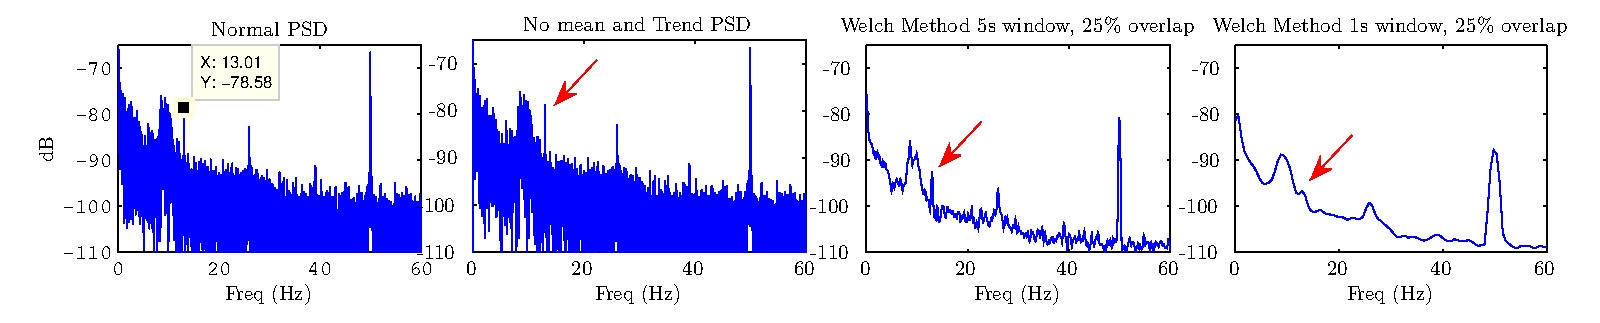
\includegraphics[width=\textwidth]{cw1im/4b1.eps}
\textit{Note:} For the Welch method, the Hamming window was used.
%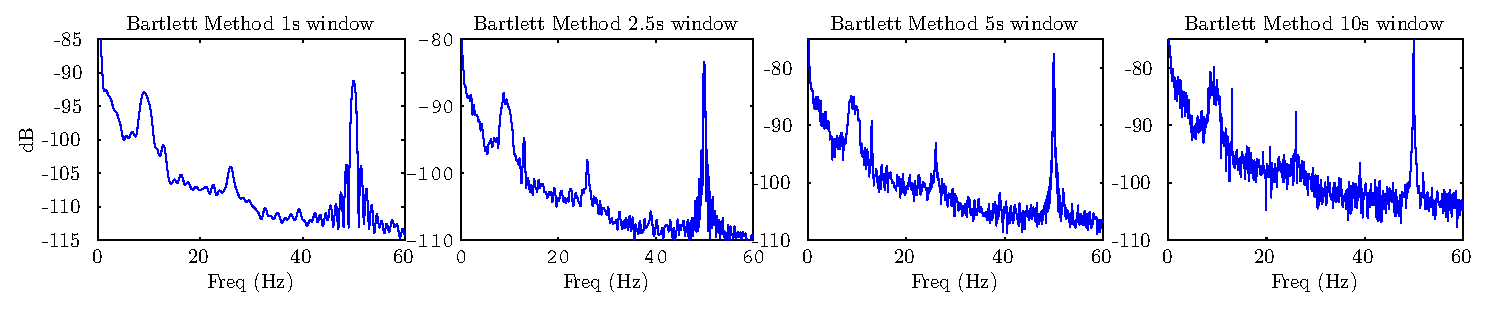
\includegraphics[width=\textwidth]{cw1im/4b2.eps}
\resizebox{\textwidth}{!}{% This file was created by matlab2tikz v0.4.7 running on MATLAB 8.1.
% Copyright (c) 2008--2014, Nico Schlömer <nico.schloemer@gmail.com>
% All rights reserved.
% Minimal pgfplots version: 1.3
% 
% The latest updates can be retrieved from
%   http://www.mathworks.com/matlabcentral/fileexchange/22022-matlab2tikz
% where you can also make suggestions and rate matlab2tikz.
% 
\begin{tikzpicture}

\begin{axis}[%
width=2.5in,
height=1.75in,
scale only axis,
xmin=0,
xmax=60,
xlabel={Freq (Hz)},
ymin=-110,
ymax=-80,
name=plot2,
title={Bartlett Method 2.5s window}
]
\addplot [color=blue,solid,forget plot]
  table[row sep=crcr]{0	-75.5347750217177\\
0.200016668055671	-77.9936180272017\\
0.400033336111343	-83.2799946957471\\
0.600050004167014	-84.7395562768905\\
0.800066672222685	-86.887755074949\\
1.00008334027836	-87.1340956968651\\
1.20010000833403	-88.0792416751893\\
1.4001166763897	-88.7354611766964\\
1.60013334444537	-88.5817669200063\\
1.80015001250104	-88.8302954244186\\
2.00016668055671	-88.9148413851959\\
2.20018334861238	-88.5006032014402\\
2.40020001666806	-91.2469970109248\\
2.60021668472373	-90.001663557355\\
2.8002333527794	-90.3660469829883\\
3.00025002083507	-91.3776158609283\\
3.20026668889074	-91.3755773904647\\
3.40028335694641	-91.4085014185179\\
3.60030002500208	-92.2553515602044\\
3.80031669305775	-92.1153955421629\\
4.00033336111343	-93.2092765243601\\
4.2003500291691	-93.0971801601147\\
4.40036669722477	-92.9030064198344\\
4.60038336528044	-94.5469153774938\\
4.80040003333611	-95.224205415888\\
5.00041670139178	-96.685257505425\\
5.20043336944745	-96.1345984102874\\
5.40045003750313	-97.0865492643459\\
5.6004667055588	-96.3684692595218\\
5.80048337361447	-95.5286555844617\\
6.00050004167014	-95.4774969752984\\
6.20051670972581	-94.8884265301567\\
6.40053337778148	-95.6071944680421\\
6.60055004583715	-95.9441394721308\\
6.80056671389282	-94.9078523791444\\
7.0005833819485	-94.8870793814806\\
7.20060005000417	-95.4153791218631\\
7.40061671805984	-94.8051444091953\\
7.60063338611551	-95.7553507272871\\
7.80065005417118	-95.4456573696246\\
8.00066672222685	-92.6150938700767\\
8.20068339028252	-90.9517490200238\\
8.4007000583382	-90.2547796120513\\
8.60071672639387	-89.2616646425111\\
8.80073339444954	-88.0486141653376\\
9.00075006250521	-89.1221808633984\\
9.20076673056088	-89.5828333982052\\
9.40078339861655	-88.980713184186\\
9.60080006667222	-89.6701657783508\\
9.80081673472789	-90.1172934688724\\
10.0008334027836	-90.4394238761144\\
10.2008500708392	-91.173899771614\\
10.4008667388949	-92.2530006599901\\
10.6008834069506	-93.2709985196975\\
10.8009000750063	-95.4660575427834\\
11.0009167430619	-97.1645695150429\\
11.2009334111176	-97.2440072962345\\
11.4009500791733	-98.0839561994758\\
11.6009667472289	-98.0604257918798\\
11.8009834152846	-98.7047258185243\\
12.0010000833403	-98.1631376457597\\
12.2010167513959	-98.299898956171\\
12.4010334194516	-101.171339425877\\
12.6010500875073	-100.604767261164\\
12.801066755563	-96.8398808978138\\
13.0010834236186	-94.7362497497706\\
13.2011000916743	-97.1748621758558\\
13.40111675973	-102.148133773205\\
13.6011334277856	-101.193735688782\\
13.8011500958413	-100.757687095699\\
14.001166763897	-101.560296213036\\
14.2011834319527	-102.876914104379\\
14.4012001000083	-102.15358763438\\
14.601216768064	-102.125711538694\\
14.8012334361197	-103.18149672233\\
15.0012501041753	-101.151329698875\\
15.201266772231	-101.387966777532\\
15.4012834402867	-102.230879276924\\
15.6013001083424	-102.586252404651\\
15.801316776398	-102.220795525962\\
16.0013334444537	-101.023232301642\\
16.2013501125094	-102.028212918906\\
16.401366780565	-101.90808312733\\
16.6013834486207	-101.575061189576\\
16.8014001166764	-101.559604113325\\
17.0014167847321	-102.104708368374\\
17.2014334527877	-102.874075477856\\
17.4014501208434	-102.811212334496\\
17.6014667888991	-103.139530181614\\
17.8014834569547	-103.717224047094\\
18.0015001250104	-103.009930336594\\
18.2015167930661	-102.969119589206\\
18.4015334611218	-103.146318303981\\
18.6015501291774	-102.90243605453\\
18.8015667972331	-104.359228216206\\
19.0015834652888	-103.139123110662\\
19.2016001333444	-102.254970694262\\
19.4016168014001	-102.87539137471\\
19.6016334694558	-104.597401786948\\
19.8016501375115	-104.495507907165\\
20.0016668055671	-103.745957865904\\
20.2016834736228	-104.125740234906\\
20.4017001416785	-103.162323277532\\
20.6017168097341	-102.605465956645\\
20.8017334777898	-102.81863119798\\
21.0017501458455	-104.014523801467\\
21.2017668139012	-104.056107701501\\
21.4017834819568	-103.672638224025\\
21.6018001500125	-104.398053708807\\
21.8018168180682	-103.878692626564\\
22.0018334861238	-104.080289645744\\
22.2018501541795	-103.745283766331\\
22.4018668222352	-102.452607256378\\
22.6018834902909	-102.426731250329\\
22.8019001583465	-102.87228308524\\
23.0019168264022	-104.615327647048\\
23.2019334944579	-104.578081688482\\
23.4019501625135	-103.570499212681\\
23.6019668305692	-102.943644648327\\
23.8019834986249	-103.477446947869\\
24.0020001666806	-103.727599912451\\
24.2020168347362	-104.337595484694\\
24.4020335027919	-104.488267820261\\
24.6020501708476	-104.915167766872\\
24.8020668389032	-103.163612598963\\
25.0020835069589	-102.619709965062\\
25.2021001750146	-103.023940742019\\
25.4021168430703	-102.383953504447\\
25.6021335111259	-102.357829827626\\
25.8021501791816	-100.14414860397\\
26.0021668472373	-98.0493372008293\\
26.2021835152929	-99.8600170466992\\
26.4022001833486	-101.805881904189\\
26.6022168514043	-102.267218882109\\
26.80223351946	-103.787520116926\\
27.0022501875156	-104.641663061448\\
27.2022668555713	-104.252404789251\\
27.402283523627	-103.540782952991\\
27.6023001916826	-104.520392684072\\
27.8023168597383	-103.713697791371\\
28.002333527794	-104.40061461857\\
28.2023501958497	-105.337050708412\\
28.4023668639053	-105.911341583681\\
28.602383531961	-104.189302834004\\
28.8024002000167	-105.784352411294\\
29.0024168680723	-105.721369217059\\
29.202433536128	-105.261583725185\\
29.4024502041837	-105.237255161561\\
29.6024668722394	-105.588685479265\\
29.802483540295	-105.707445123768\\
30.0025002083507	-106.30534819858\\
30.2025168764064	-105.17275322093\\
30.402533544462	-105.725839531684\\
30.6025502125177	-107.22981641141\\
30.8025668805734	-107.237882670329\\
31.0025835486291	-106.702281694147\\
31.2026002166847	-107.365631897725\\
31.4026168847404	-107.415537835759\\
31.6026335527961	-107.338685781685\\
31.8026502208517	-107.247804839023\\
32.0026668889074	-107.16178492156\\
32.2026835569631	-108.449552932153\\
32.4027002250188	-106.625672760066\\
32.6027168930744	-105.823583746656\\
32.8027335611301	-106.880326500261\\
33.0027502291858	-107.744639878896\\
33.2027668972414	-108.086154995536\\
33.4027835652971	-107.187701217734\\
33.6028002333528	-108.200470785331\\
33.8028169014084	-106.999255499723\\
34.0028335694641	-106.863473075612\\
34.2028502375198	-107.840960169221\\
34.4028669055755	-108.505941306166\\
34.6028835736311	-106.572387151245\\
34.8029002416868	-107.065492784742\\
35.0029169097425	-108.627523088532\\
35.2029335777981	-107.160063992767\\
35.4029502458538	-107.05384063156\\
35.6029669139095	-109.979399714496\\
35.8029835819652	-108.178839980166\\
36.0030002500208	-107.926247921804\\
36.2030169180765	-108.475649407684\\
36.4030335861322	-109.024322843801\\
36.6030502541878	-108.136633468838\\
36.8030669222435	-107.118591297005\\
37.0030835902992	-108.519149570318\\
37.2031002583549	-108.807473046729\\
37.4031169264105	-108.830454614097\\
37.6031335944662	-107.724092701572\\
37.8031502625219	-106.865527086698\\
38.0031669305775	-108.191983539864\\
38.2031835986332	-107.827509131773\\
38.4032002666889	-107.811676465292\\
38.6032169347446	-107.42642094566\\
38.8032336028002	-106.794704794456\\
39.0032502708559	-105.720452201904\\
39.2032669389116	-106.630038614793\\
39.4032836069673	-107.93721689151\\
39.6033002750229	-109.298620331461\\
39.8033169430786	-108.952742127662\\
40.0033336111343	-108.153245807303\\
40.2033502791899	-106.955035307248\\
40.4033669472456	-107.847161815985\\
40.6033836153013	-109.174761820329\\
40.8034002833569	-109.040866922159\\
41.0034169514126	-109.118688477276\\
41.2034336194683	-108.608698485322\\
41.403450287524	-108.51118144603\\
41.6034669555796	-109.822357885868\\
41.8034836236353	-108.210496342357\\
42.003500291691	-107.826398544391\\
42.2035169597466	-107.766717593822\\
42.4035336278023	-107.832450078112\\
42.603550295858	-108.281929862382\\
42.8035669639137	-108.434993702978\\
43.0035836319693	-107.049804508546\\
43.203600300025	-108.022721015459\\
43.4036169680807	-109.456483330353\\
43.6036336361363	-109.060686073839\\
43.803650304192	-108.117383235746\\
44.0036669722477	-109.92773564772\\
44.2036836403034	-109.013098922179\\
44.403700308359	-107.699925103285\\
44.6037169764147	-107.054699590996\\
44.8037336444704	-109.170600490034\\
45.003750312526	-107.794642835526\\
45.2037669805817	-108.46808430531\\
45.4037836486374	-107.707728474423\\
45.6038003166931	-107.801457604825\\
45.8038169847487	-107.102262879225\\
46.0038336528044	-109.309319993712\\
46.2038503208601	-107.977598305946\\
46.4038669889157	-108.714254835336\\
46.6038836569714	-106.933918347828\\
46.8039003250271	-109.964317567812\\
47.0039169930828	-107.406282107748\\
47.2039336611384	-109.742846030434\\
47.4039503291941	-106.704834970003\\
47.6039669972498	-109.43270840846\\
47.8039836653054	-106.670649494731\\
48.0040003333611	-108.515753897439\\
48.2040170014168	-104.10749291157\\
48.4040336694725	-108.77811265399\\
48.6040503375281	-103.516833764763\\
48.8040670055838	-108.613635514305\\
49.0040836736395	-100.822709742409\\
49.2041003416951	-106.906272903227\\
49.4041170097508	-96.5863206876366\\
49.6041336778065	-103.058943661369\\
49.8041503458622	-86.0846778436567\\
50.0041670139178	-83.3505419846383\\
50.2041836819735	-88.5175961221408\\
50.4042003500292	-104.109829616304\\
50.6042170180848	-96.705855834111\\
50.8042336861405	-108.577347932366\\
51.0042503541962	-100.539619246197\\
51.2042670222519	-109.780504820837\\
51.4042836903075	-104.023011159923\\
51.6043003583632	-108.210245841751\\
51.8043170264189	-103.57500218203\\
52.0043336944745	-107.754454713856\\
52.2043503625302	-105.637915259254\\
52.4043670305859	-109.604637704276\\
52.6043836986416	-106.467400196891\\
52.8044003666972	-108.858799616089\\
53.0044170347529	-106.996096310511\\
53.2044337028086	-109.617581594141\\
53.4044503708642	-107.33692241538\\
53.6044670389199	-109.097970296281\\
53.8044837069756	-106.63192611816\\
54.0045003750313	-109.512142689006\\
54.2045170430869	-108.783427464369\\
54.4045337111426	-110.697511319652\\
54.6045503791983	-109.361928149192\\
54.8045670472539	-108.456079007241\\
55.0045837153096	-108.091161652255\\
55.2046003833653	-110.020541692102\\
55.4046170514209	-107.939997769431\\
55.6046337194766	-109.291397891398\\
55.8046503875323	-109.08722554334\\
56.004667055588	-109.432455707723\\
56.2046837236436	-107.967692755872\\
56.4047003916993	-109.769055269241\\
56.604717059755	-108.862739521377\\
56.8047337278107	-109.456758307658\\
57.0047503958663	-108.771552062551\\
57.204767063922	-109.517752703998\\
57.4047837319777	-108.848418108466\\
57.6048004000333	-109.890806725244\\
57.804817068089	-108.982802355966\\
58.0048337361447	-108.956258099113\\
58.2048504042004	-109.349682508539\\
58.404867072256	-109.095828975353\\
58.6048837403117	-109.446529471423\\
58.8049004083674	-110.376955280951\\
59.004917076423	-110.066960884919\\
59.2049337444787	-110.396006210588\\
59.4049504125344	-110.370503214668\\
59.6049670805901	-109.926737649\\
59.8049837486457	-109.255796768981\\
60.0050004167014	-109.378927760043\\
60.2050170847571	-108.922421052939\\
60.4050337528127	-109.851211665858\\
60.6050504208684	-108.803045894005\\
60.8050670889241	-109.586757199128\\
61.0050837569798	-108.304141885755\\
61.2051004250354	-108.701838345642\\
61.4051170930911	-109.038786609562\\
61.6051337611468	-109.595919388722\\
61.8051504292024	-109.715599080299\\
62.0051670972581	-110.705696771698\\
62.2051837653138	-109.997910167709\\
62.4052004333694	-110.395222742982\\
62.6052171014251	-109.466779838421\\
62.8052337694808	-110.520238276219\\
63.0052504375365	-110.096207790966\\
63.2052671055921	-109.656814566272\\
63.4052837736478	-109.988870247868\\
63.6053004417035	-109.898278158006\\
63.8053171097591	-109.380580865457\\
64.0053337778148	-110.403072188415\\
64.2053504458705	-109.976945583059\\
64.4053671139262	-110.328259798412\\
64.6053837819818	-109.767223746514\\
64.8054004500375	-110.100241627701\\
65.0054171180932	-109.574139127604\\
65.2054337861488	-109.923486069856\\
65.4054504542045	-110.147235689186\\
65.6054671222602	-110.243326456221\\
65.8054837903159	-110.403830140956\\
66.0055004583715	-110.148480766143\\
66.2055171264272	-110.837448928029\\
66.4055337944829	-110.059383157001\\
66.6055504625385	-109.773932926054\\
66.8055671305942	-110.021268577742\\
67.0055837986499	-111.28093398764\\
67.2056004667056	-110.894698512259\\
67.4056171347612	-109.487246112846\\
67.6056338028169	-110.169656486144\\
67.8056504708726	-110.721262305484\\
68.0056671389282	-109.672220982238\\
68.2056838069839	-109.586621853604\\
68.4057004750396	-109.940458617768\\
68.6057171430953	-110.272935306707\\
68.8057338111509	-110.365675398891\\
69.0057504792066	-109.95813752739\\
69.2057671472623	-111.433055839304\\
69.4057838153179	-110.352809952419\\
69.6058004833736	-109.990470939116\\
69.8058171514293	-111.217544189558\\
70.005833819485	-111.063975553555\\
70.2058504875406	-110.656147825489\\
70.4058671555963	-110.48083444628\\
70.605883823652	-109.706188364717\\
70.8059004917076	-108.895176706365\\
71.0059171597633	-108.694033847871\\
71.205933827819	-109.78679294532\\
71.4059504958747	-110.18335392438\\
71.6059671639303	-110.694355770884\\
71.805983831986	-110.541506440369\\
72.0060005000417	-110.235339965045\\
72.2060171680973	-109.779186632456\\
72.406033836153	-111.154212453325\\
72.6060505042087	-110.811901765881\\
72.8060671722643	-111.253152743623\\
73.00608384032	-110.32679447331\\
73.2061005083757	-110.809762153448\\
73.4061171764314	-110.113684743865\\
73.606133844487	-110.826331859479\\
73.8061505125427	-111.226399248596\\
74.0061671805984	-110.492009515128\\
74.206183848654	-110.055204315633\\
74.4062005167097	-110.868773206234\\
74.6062171847654	-110.789102818253\\
74.8062338528211	-111.668440780771\\
75.0062505208767	-111.006275791055\\
75.2062671889324	-109.607191091405\\
75.4062838569881	-110.222818792805\\
75.6063005250438	-110.974212118215\\
75.8063171930994	-110.511375769429\\
76.0063338611551	-110.356050260993\\
76.2063505292108	-109.563552420849\\
76.4063671972664	-110.557899153613\\
76.6063838653221	-110.400730460809\\
76.8064005333778	-109.557576708687\\
77.0064172014335	-110.547469831283\\
77.2064338694891	-110.600735782252\\
77.4064505375448	-109.22188567698\\
77.6064672056005	-110.300517996054\\
77.8064838736561	-110.400616115733\\
78.0065005417118	-109.34965741349\\
78.2065172097675	-111.319805586376\\
78.4065338778232	-111.282230565875\\
78.6065505458788	-110.758521612008\\
78.8065672139345	-110.86958330205\\
79.0065838819902	-110.911344340097\\
79.2066005500458	-110.648042628798\\
79.4066172181015	-111.200141319303\\
79.6066338861572	-111.070889968396\\
79.8066505542129	-110.1573685135\\
80.0066672222685	-111.986262485064\\
80.2066838903242	-113.001592472818\\
80.4067005583799	-109.454097765524\\
80.6067172264355	-108.498224042909\\
80.8067338944912	-109.148057456919\\
81.0067505625469	-109.229539128414\\
81.2067672306026	-110.745745696508\\
81.4067838986582	-109.998992423151\\
81.6068005667139	-109.981798840137\\
81.8068172347696	-110.623093699807\\
82.0068339028252	-111.534666219967\\
82.2068505708809	-110.979647420388\\
82.4068672389366	-110.757292347987\\
82.6068839069923	-110.761811160583\\
82.8069005750479	-111.798046352592\\
83.0069172431036	-110.335344485269\\
83.2069339111593	-109.703622940165\\
83.4069505792149	-110.24139555122\\
83.6069672472706	-111.639332246879\\
83.8069839153263	-110.326745086871\\
84.007000583382	-110.650276897123\\
84.2070172514376	-111.595913744253\\
84.4070339194933	-110.298720507551\\
84.607050587549	-109.819366617277\\
84.8070672556046	-111.402280260752\\
85.0070839236603	-111.175138951984\\
85.207100591716	-110.893885335065\\
85.4071172597717	-110.718766902066\\
85.6071339278273	-110.145349042407\\
85.807150595883	-109.673228226966\\
86.0071672639387	-109.111725741803\\
86.2071839319943	-109.583417671201\\
86.40720060005	-111.301818959936\\
86.6072172681057	-110.193176515563\\
86.8072339361614	-110.266738581241\\
87.007250604217	-109.565391688668\\
87.2072672722727	-109.351118711566\\
87.4072839403284	-110.330949982955\\
87.607300608384	-111.915768259761\\
87.8073172764397	-111.273326731865\\
88.0073339444954	-109.903220211019\\
88.207350612551	-110.332467313408\\
88.4073672806067	-110.202329596186\\
88.6073839486624	-111.358486643041\\
88.8074006167181	-111.16099511426\\
89.0074172847737	-109.935177359206\\
89.2074339528294	-109.680719230126\\
89.4074506208851	-110.307239469805\\
89.6074672889407	-111.472862219274\\
89.8074839569964	-111.954040578164\\
90.0075006250521	-111.02205454307\\
90.2075172931078	-111.69329218973\\
90.4075339611634	-111.580523280917\\
90.6075506292191	-111.237136313877\\
90.8075672972748	-110.951853939549\\
91.0075839653304	-110.53094268084\\
91.2076006333861	-110.013429465648\\
91.4076173014418	-111.701958352001\\
91.6076339694975	-112.053187277428\\
91.8076506375531	-109.181341083757\\
92.0076673056088	-110.119945974475\\
92.2076839736645	-111.636472656421\\
92.4077006417201	-110.435740253073\\
92.6077173097758	-111.050947579778\\
92.8077339778315	-112.031802600985\\
93.0077506458872	-109.604588925972\\
93.2077673139428	-109.128642286429\\
93.4077839819985	-110.630645274897\\
93.6078006500542	-110.284462750492\\
93.8078173181098	-108.652182842761\\
94.0078339861655	-109.44197119759\\
94.2078506542212	-111.480717406054\\
94.4078673222769	-110.745608107501\\
94.6078839903325	-109.516538874478\\
94.8079006583882	-109.201993346569\\
95.0079173264439	-109.522033555764\\
95.2079339944995	-110.284932103639\\
95.4079506625552	-109.750974132723\\
95.6079673306109	-110.681667597561\\
95.8079839986666	-111.128594106975\\
96.0080006667222	-110.153285580071\\
96.2080173347779	-110.132351983549\\
96.4080340028336	-110.374714670473\\
96.6080506708892	-111.682022589546\\
96.8080673389449	-111.688999161634\\
97.0080840070006	-110.349539427107\\
97.2081006750563	-110.994359644422\\
97.4081173431119	-110.862615272929\\
97.6081340111676	-110.426147463031\\
97.8081506792233	-110.764731544252\\
98.0081673472789	-109.748667630177\\
98.2081840153346	-110.992409863896\\
98.4082006833903	-110.982573072356\\
98.608217351446	-111.377579498915\\
98.8082340195016	-111.054253670606\\
99.0082506875573	-110.696321373564\\
99.208267355613	-110.760408728833\\
99.4082840236686	-110.52476426814\\
99.6083006917243	-110.417512095295\\
99.80831735978	-110.505417040559\\
100.008334027836	-111.237212268438\\
100.208350695891	-110.16592915737\\
100.408367363947	-110.467178771828\\
100.608384032003	-109.977325413564\\
100.808400700058	-109.509544718899\\
101.008417368114	-110.054428605909\\
101.20843403617	-109.979174499016\\
101.408450704225	-108.989489623909\\
101.608467372281	-110.226625164058\\
101.808484040337	-111.723437032625\\
102.008500708392	-111.222330032134\\
102.208517376448	-111.58951403229\\
102.408534044504	-111.924640956099\\
102.608550712559	-110.635400117416\\
102.808567380615	-110.337293287856\\
103.008584048671	-110.620203224096\\
103.208600716726	-110.097054848996\\
103.408617384782	-110.107157174717\\
103.608634052838	-110.123038691965\\
103.808650720893	-109.946406701728\\
104.008667388949	-110.454571367901\\
104.208684057005	-110.919102544573\\
104.40870072506	-110.719451598013\\
104.608717393116	-110.911184568828\\
104.808734061172	-111.067877168452\\
105.008750729227	-111.345384677664\\
105.208767397283	-110.724545879448\\
105.408784065339	-110.724657085214\\
105.608800733394	-112.424999004415\\
105.80881740145	-111.470480386865\\
106.008834069506	-112.346646640251\\
106.208850737561	-112.107888855786\\
106.408867405617	-109.788799957697\\
106.608884073673	-110.295817653389\\
106.808900741728	-110.286658360407\\
107.008917409784	-109.587281935283\\
107.20893407784	-110.883862915417\\
107.408950745896	-110.387087886621\\
107.608967413951	-109.74366849565\\
107.808984082007	-109.777250601098\\
108.009000750063	-108.885661913449\\
108.209017418118	-110.567870556726\\
108.409034086174	-110.765555261821\\
108.60905075423	-110.34457077193\\
108.809067422285	-110.319293049698\\
109.009084090341	-110.66815817441\\
109.209100758397	-110.756006272853\\
109.409117426452	-110.657817986032\\
109.609134094508	-111.42987575335\\
109.809150762564	-111.475925683876\\
110.009167430619	-111.647635739805\\
110.209184098675	-110.931122624105\\
110.409200766731	-109.739427281898\\
110.609217434786	-109.345594316816\\
110.809234102842	-110.13326673123\\
111.009250770898	-110.045887209186\\
111.209267438953	-109.515091842876\\
111.409284107009	-109.741030368351\\
111.609300775065	-110.60188483285\\
111.80931744312	-110.089587645212\\
112.009334111176	-110.295914917822\\
112.209350779232	-110.568262465235\\
112.409367447287	-111.051335199422\\
112.609384115343	-111.116849144291\\
112.809400783399	-110.538254356002\\
113.009417451454	-111.419489417525\\
113.20943411951	-111.069669595048\\
113.409450787566	-110.933576739365\\
113.609467455621	-110.237682695888\\
113.809484123677	-110.756818696387\\
114.009500791733	-110.267310252122\\
114.209517459788	-109.732629027351\\
114.409534127844	-110.309236703639\\
114.6095507959	-110.565806095043\\
114.809567463955	-109.977244055243\\
115.009584132011	-109.963414339073\\
115.209600800067	-110.985138633907\\
115.409617468122	-111.394008284713\\
115.609634136178	-113.015529802381\\
115.809650804234	-111.568883459107\\
116.009667472289	-109.744345278155\\
116.209684140345	-110.964305148665\\
116.409700808401	-111.443431237709\\
116.609717476456	-110.382305082843\\
116.809734144512	-110.349486099462\\
117.009750812568	-110.827279724048\\
117.209767480623	-110.937232187152\\
117.409784148679	-111.445059208137\\
117.609800816735	-109.431978564956\\
117.80981748479	-109.448457789278\\
118.009834152846	-112.364534346568\\
118.209850820902	-111.721509490517\\
118.409867488957	-111.624066810394\\
118.609884157013	-110.526645283496\\
118.809900825069	-111.593622304629\\
119.009917493124	-110.89801081728\\
119.20993416118	-110.291366464003\\
119.409950829236	-111.48662467414\\
119.609967497291	-110.690930624324\\
119.809984165347	-110.138525875755\\
};
\end{axis}

\begin{axis}[%
width=2.5in,
height=1.75in,
scale only axis,
xmin=0,
xmax=60,
xlabel={Freq (Hz)},
ymin=-115,
ymax=-85,
ylabel={dB},
at=(plot2.left of south west),
anchor=right of south east,
title={Bartlett Method 1s window}
]
\addplot [color=blue,solid,forget plot]
  table[row sep=crcr]{0	-82.3483070182069\\
0.200016668055671	-82.7461461073527\\
0.400033336111343	-83.9517261379944\\
0.600050004167014	-85.9786957302692\\
0.800066672222685	-88.7086310174124\\
1.00008334027836	-91.4248325482691\\
1.20010000833403	-92.682205191354\\
1.4001166763897	-92.6143336373124\\
1.60013334444537	-92.5551682312523\\
1.80015001250104	-92.871163049602\\
2.00016668055671	-93.2798395380676\\
2.20018334861238	-93.5126831028345\\
2.40020001666806	-93.6755920344078\\
2.60021668472373	-94.0262492973635\\
2.8002333527794	-94.6169025971595\\
3.00025002083507	-95.2270428426243\\
3.20026668889074	-95.5931211072619\\
3.40028335694641	-95.7385589819396\\
3.60030002500208	-95.9051539458892\\
3.80031669305775	-96.2310386277039\\
4.00033336111343	-96.6689297767358\\
4.2003500291691	-97.1427965301528\\
4.40036669722477	-97.7052417126605\\
4.60038336528044	-98.4691621794861\\
4.80040003333611	-99.3599576582167\\
5.00041670139178	-99.9672759936319\\
5.20043336944745	-99.944346844775\\
5.40045003750313	-99.589872931872\\
5.6004667055588	-99.4164789206873\\
5.80048337361447	-99.5693162623447\\
6.00050004167014	-99.7839731748119\\
6.20051670972581	-99.6778204215496\\
6.40053337778148	-99.2486979778577\\
6.60055004583715	-98.8642729445175\\
6.80056671389282	-98.8054497615713\\
7.0005833819485	-99.0810156834349\\
7.20060005000417	-99.4478088592358\\
7.40061671805984	-99.5137380164386\\
7.60063338611551	-99.0085748608308\\
7.80065005417118	-97.9961807961062\\
8.00066672222685	-96.7348547082084\\
8.20068339028252	-95.4719881714722\\
8.4007000583382	-94.3830366048447\\
8.60071672639387	-93.5721179821412\\
8.80073339444954	-93.0814002766725\\
9.00075006250521	-92.9018568204458\\
9.20076673056088	-92.9828815198414\\
9.40078339861655	-93.2442969766725\\
9.60080006667222	-93.6012942816133\\
9.80081673472789	-94.0061732363915\\
10.0008334027836	-94.4840723343847\\
10.2008500708392	-95.1278495839418\\
10.4008667388949	-96.0504507148588\\
10.6008834069506	-97.3157827677553\\
10.8009000750063	-98.8377616271876\\
11.0009167430619	-100.25230150758\\
11.2009334111176	-101.059283814564\\
11.4009500791733	-101.269294110051\\
11.6009667472289	-101.416405204319\\
11.8009834152846	-101.833756093154\\
12.0010000833403	-102.344905756051\\
12.2010167513959	-102.410890424706\\
12.4010334194516	-101.843452205172\\
12.6010500875073	-101.143437840503\\
12.801066755563	-100.831119467999\\
13.0010834236186	-101.121324747603\\
13.2011000916743	-102.008375565415\\
13.40111675973	-103.309071747137\\
13.6011334277856	-104.650639760023\\
13.8011500958413	-105.636839889186\\
14.001166763897	-106.194892558497\\
14.2011834319527	-106.49296182236\\
14.4012001000083	-106.569845600946\\
14.601216768064	-106.386236213908\\
14.8012334361197	-106.089326166521\\
15.0012501041753	-105.947090358583\\
15.201266772231	-106.089044063812\\
15.4012834402867	-106.369822000277\\
15.6013001083424	-106.428415102178\\
15.801316776398	-106.064316820281\\
16.0013334444537	-105.528022871758\\
16.2013501125094	-105.209849581841\\
16.401366780565	-105.309779807027\\
16.6013834486207	-105.787212668116\\
16.8014001166764	-106.377162128017\\
17.0014167847321	-106.70872012866\\
17.2014334527877	-106.64852129375\\
17.4014501208434	-106.435781886225\\
17.6014667888991	-106.358965220519\\
17.8014834569547	-106.522722462727\\
18.0015001250104	-106.858798737623\\
18.2015167930661	-107.209998942348\\
18.4015334611218	-107.425606396857\\
18.6015501291774	-107.440072793879\\
18.8015667972331	-107.297771334559\\
19.0015834652888	-107.121420947999\\
19.2016001333444	-107.044641289937\\
19.4016168014001	-107.1358022473\\
19.6016334694558	-107.346533884607\\
19.8016501375115	-107.529172172021\\
20.0016668055671	-107.56195608658\\
20.2016834736228	-107.47481053826\\
20.4017001416785	-107.383551702866\\
20.6017168097341	-107.326640797255\\
20.8017334777898	-107.240603508274\\
21.0017501458455	-107.103402436815\\
21.2017668139012	-107.041661720512\\
21.4017834819568	-107.225942932764\\
21.6018001500125	-107.660673335305\\
21.8018168180682	-108.033167415428\\
22.0018334861238	-107.900394284684\\
22.2018501541795	-107.31328005388\\
22.4018668222352	-106.802351638369\\
22.6018834902909	-106.763968575294\\
22.8019001583465	-107.250587088059\\
23.0019168264022	-107.957319700907\\
23.2019334944579	-108.317842038161\\
23.4019501625135	-108.098708101659\\
23.6019668305692	-107.711882556418\\
23.8019834986249	-107.570995190681\\
24.0020001666806	-107.711580064849\\
24.2020168347362	-107.888073170154\\
24.4020335027919	-107.858700081989\\
24.6020501708476	-107.635989942427\\
24.8020668389032	-107.348219658658\\
25.0020835069589	-106.96366152972\\
25.2021001750146	-106.333721816283\\
25.4021168430703	-105.481302771866\\
25.6021335111259	-104.663419155696\\
25.8021501791816	-104.146574700694\\
26.0021668472373	-104.069722756192\\
26.2021835152929	-104.445438850672\\
26.4022001833486	-105.175144153171\\
26.6022168514043	-106.05029483904\\
26.80223351946	-106.8128513507\\
27.0022501875156	-107.331050748518\\
27.2022668555713	-107.697645782914\\
27.402283523627	-108.06797576774\\
27.6023001916826	-108.460172185156\\
27.8023168597383	-108.738388831571\\
28.002333527794	-108.79145027799\\
28.2023501958497	-108.711323512421\\
28.4023668639053	-108.707163367952\\
28.602383531961	-108.88838789569\\
28.8024002000167	-109.163492982678\\
29.0024168680723	-109.313758755261\\
29.202433536128	-109.235313688398\\
29.4024502041837	-109.08018568682\\
29.6024668722394	-109.071615144555\\
29.802483540295	-109.28716208087\\
30.0025002083507	-109.622624275637\\
30.2025168764064	-109.905938328643\\
30.402533544462	-110.074914505094\\
30.6025502125177	-110.210408534289\\
30.8025668805734	-110.384349284147\\
31.0025835486291	-110.572018445707\\
31.2026002166847	-110.744768078744\\
31.4026168847404	-110.977798672821\\
31.6026335527961	-111.363485441747\\
31.8026502208517	-111.78587724724\\
32.0026668889074	-111.852442279053\\
32.2026835569631	-111.350546657616\\
32.4027002250188	-110.652187404959\\
32.6027168930744	-110.247257428542\\
32.8027335611301	-110.32960063412\\
33.0027502291858	-110.780064003464\\
33.2027668972414	-111.244581153972\\
33.4027835652971	-111.408811070053\\
33.6028002333528	-111.349169341534\\
33.8028169014084	-111.36487524262\\
34.0028335694641	-111.574356109151\\
34.2028502375198	-111.811975987041\\
34.4028669055755	-111.81572934692\\
34.6028835736311	-111.539399322647\\
34.8029002416868	-111.18667215466\\
35.0029169097425	-110.968560841432\\
35.2029335777981	-110.986630919699\\
35.4029502458538	-111.258870376829\\
35.6029669139095	-111.72672335686\\
35.8029835819652	-112.205114345359\\
36.0030002500208	-112.410474553768\\
36.2030169180765	-112.23113123429\\
36.4030335861322	-111.903145862464\\
36.6030502541878	-111.731444213824\\
36.8030669222435	-111.797949872213\\
37.0030835902992	-111.923663310041\\
37.2031002583549	-111.849521395724\\
37.4031169264105	-111.546610146648\\
37.6031335944662	-111.248516702012\\
37.8031502625219	-111.176978224191\\
38.0031669305775	-111.382634064569\\
38.2031835986332	-111.746041271632\\
38.4032002666889	-112.022164953883\\
38.6032169347446	-111.953960154874\\
38.8032336028002	-111.490954119589\\
39.0032502708559	-110.878603790834\\
39.2032669389116	-110.457214529019\\
39.4032836069673	-110.449614549453\\
39.6033002750229	-110.877464147425\\
39.8033169430786	-111.51381249418\\
40.0033336111343	-111.960294705243\\
40.2033502791899	-112.065623625022\\
40.4033669472456	-112.134574067158\\
40.6033836153013	-112.442846216184\\
40.8034002833569	-112.817773433179\\
41.0034169514126	-112.790738060526\\
41.2034336194683	-112.345670609794\\
41.403450287524	-112.00661106406\\
41.6034669555796	-112.066038198943\\
41.8034836236353	-112.237675474608\\
42.003500291691	-111.963360109189\\
42.2035169597466	-111.314473421482\\
42.4035336278023	-110.950054472715\\
42.603550295858	-111.259596090145\\
42.8035669639137	-112.012815222946\\
43.0035836319693	-112.313964749768\\
43.203600300025	-111.743433124288\\
43.4036169680807	-111.204643300032\\
43.6036336361363	-111.45933281363\\
43.803650304192	-112.420384209783\\
44.0036669722477	-112.931506179153\\
44.2036836403034	-112.107147747057\\
44.403700308359	-111.161223008367\\
44.6037169764147	-111.108599476134\\
44.8037336444704	-111.793518942903\\
45.003750312526	-111.928709125393\\
45.2037669805817	-110.827591565514\\
45.4037836486374	-109.882908194808\\
45.6038003166931	-110.148818187874\\
45.8038169847487	-111.738395560007\\
46.0038336528044	-113.019354452101\\
46.2038503208601	-111.564755129907\\
46.4038669889157	-109.887821378351\\
46.6038836569714	-109.888804286764\\
46.8039003250271	-111.815234630302\\
47.0039169930828	-113.381090127342\\
47.2039336611384	-110.643263397256\\
47.4039503291941	-108.23606501418\\
47.6039669972498	-108.132994192957\\
47.8039836653054	-110.756843820008\\
48.0040003333611	-113.013675382459\\
48.2040170014168	-107.871828209695\\
48.4040336694725	-104.428083310298\\
48.6040503375281	-103.824834461565\\
48.8040670055838	-106.745490585143\\
49.0040836736395	-113.111930708113\\
49.2041003416951	-102.530609497757\\
49.4041170097508	-96.6066560427904\\
49.6041336778065	-93.3490413842497\\
49.8041503458622	-91.669858585665\\
50.0041670139178	-91.2178514280805\\
50.2041836819735	-91.9145367964371\\
50.4042003500292	-93.8793659069692\\
50.6042170180848	-97.5461784632038\\
50.8042336861405	-104.281159339309\\
51.0042503541962	-113.027494080391\\
51.2042670222519	-105.930048283496\\
51.4042836903075	-103.927675273018\\
51.6043003583632	-105.166833028574\\
51.8043170264189	-109.199544654932\\
52.0043336944745	-112.563504855705\\
52.2043503625302	-109.189528034019\\
52.4043670305859	-107.348558104058\\
52.6043836986416	-107.998350422394\\
52.8044003666972	-110.775793221024\\
53.0044170347529	-113.300885645041\\
53.2044337028086	-111.507579429149\\
53.4044503708642	-109.857859148875\\
53.6044670389199	-110.164994885996\\
53.8044837069756	-112.179947105942\\
54.0045003750313	-113.962915694577\\
54.2045170430869	-112.796306767223\\
54.4045337111426	-111.347751867074\\
54.6045503791983	-111.278790662423\\
54.8045670472539	-112.320519614621\\
55.0045837153096	-113.145167215056\\
55.2046003833653	-112.684858821508\\
55.4046170514209	-112.104245715765\\
55.6046337194766	-112.435887068332\\
55.8046503875323	-113.496773585345\\
56.004667055588	-113.980710723706\\
56.2046837236436	-113.234674944721\\
56.4047003916993	-112.560952779903\\
56.604717059755	-112.770229553415\\
56.8047337278107	-113.551670455546\\
57.0047503958663	-113.714787331154\\
57.204767063922	-112.856608101565\\
57.4047837319777	-112.094722286749\\
57.6048004000333	-112.096882785035\\
57.804817068089	-112.681419582744\\
58.0048337361447	-113.083415153532\\
58.2048504042004	-112.849386368466\\
58.404867072256	-112.589898281876\\
58.6048837403117	-112.959330980925\\
58.8049004083674	-113.927345901814\\
59.004917076423	-114.621143086642\\
59.2049337444787	-114.245183925897\\
59.4049504125344	-113.549218465835\\
59.6049670805901	-113.413601190884\\
59.8049837486457	-113.859729128309\\
60.0050004167014	-114.190547113105\\
60.2050170847571	-113.756402021402\\
60.4050337528127	-112.9842693135\\
60.6050504208684	-112.560209110325\\
60.8050670889241	-112.628666915188\\
61.0050837569798	-112.90381820267\\
61.2051004250354	-113.025858624274\\
61.4051170930911	-112.989627144824\\
61.6051337611468	-113.073211177285\\
61.8051504292024	-113.395616801679\\
62.0051670972581	-113.754066423891\\
62.2051837653138	-113.863395710437\\
62.4052004333694	-113.749927034016\\
62.6052171014251	-113.671216930144\\
62.8052337694808	-113.72757273122\\
63.0052504375365	-113.782090505348\\
63.2052671055921	-113.70726760696\\
63.4052837736478	-113.603540077656\\
63.6053004417035	-113.665600644041\\
63.8053171097591	-113.933432954565\\
64.0053337778148	-114.229145894023\\
64.2053504458705	-114.320894651564\\
64.4053671139262	-114.171692718857\\
64.6053837819818	-113.927622048736\\
64.8054004500375	-113.712440703188\\
65.0054171180932	-113.573373065503\\
65.2054337861488	-113.548184264953\\
65.4054504542045	-113.671364006279\\
65.6054671222602	-113.899901311728\\
65.8054837903159	-114.087271289937\\
66.0055004583715	-114.116218834907\\
66.2055171264272	-114.051245856658\\
66.4055337944829	-114.037645201705\\
66.6055504625385	-114.079094469455\\
66.8055671305942	-114.019112098911\\
67.0055837986499	-113.794593171687\\
67.2056004667056	-113.612034725678\\
67.4056171347612	-113.744270527566\\
67.6056338028169	-114.241326288119\\
67.8056504708726	-114.768220102279\\
68.0056671389282	-114.786269093847\\
68.2056838069839	-114.285559610485\\
68.4057004750396	-113.822903851442\\
68.6057171430953	-113.786478447746\\
68.8057338111509	-114.162952196189\\
69.0057504792066	-114.630208981499\\
69.2057671472623	-114.834030357214\\
69.4057838153179	-114.778183099032\\
69.6058004833736	-114.713824402986\\
69.8058171514293	-114.712114516755\\
70.005833819485	-114.597023245841\\
70.2058504875406	-114.252715575178\\
70.4058671555963	-113.840223366004\\
70.605883823652	-113.590525581749\\
70.8059004917076	-113.555412735856\\
71.0059171597633	-113.594615843386\\
71.205933827819	-113.550015138611\\
71.4059504958747	-113.444471510798\\
71.6059671639303	-113.449833084846\\
71.805983831986	-113.683728895045\\
72.0060005000417	-114.083489629744\\
72.2060171680973	-114.42934275657\\
72.406033836153	-114.536929604057\\
72.6060505042087	-114.461905679718\\
72.8060671722643	-114.413394068949\\
73.00608384032	-114.518668660387\\
73.2061005083757	-114.720205037091\\
73.4061171764314	-114.826114174127\\
73.606133844487	-114.700234028125\\
73.8061505125427	-114.439741312434\\
74.0061671805984	-114.288712649825\\
74.206183848654	-114.416190260048\\
74.4062005167097	-114.779513190138\\
74.6062171847654	-115.092138575837\\
74.8062338528211	-115.03356854604\\
75.0062505208767	-114.662274763297\\
75.2062671889324	-114.355093833074\\
75.4062838569881	-114.369902846545\\
75.6063005250438	-114.649128081009\\
75.8063171930994	-114.85885657034\\
76.0063338611551	-114.708143682296\\
76.2063505292108	-114.333521445245\\
76.4063671972664	-114.095155573141\\
76.6063838653221	-114.164934875008\\
76.8064005333778	-114.424891617611\\
77.0064172014335	-114.593069438551\\
77.2064338694891	-114.517991968805\\
77.4064505375448	-114.33357159443\\
77.6064672056005	-114.228997352533\\
77.8064838736561	-114.227854506169\\
78.0065005417118	-114.227760298724\\
78.2065172097675	-114.177844547545\\
78.4065338778232	-114.15824063761\\
78.6065505458788	-114.265457677454\\
78.8065672139345	-114.483987719071\\
79.0065838819902	-114.702762452285\\
79.2066005500458	-114.857415021052\\
79.4066172181015	-115.009324283278\\
79.6066338861572	-115.221417805708\\
79.8066505542129	-115.391791067992\\
80.0066672222685	-115.292986041791\\
80.2066838903242	-114.851976219437\\
80.4067005583799	-114.260426489284\\
80.6067172264355	-113.730559657995\\
80.8067338944912	-113.333184919704\\
81.0067505625469	-113.066569474668\\
81.2067672306026	-112.979688104591\\
81.4067838986582	-113.200374672705\\
81.6068005667139	-113.851405024082\\
81.8068172347696	-114.894724644925\\
82.0068339028252	-115.885210966297\\
82.2068505708809	-116.019136703397\\
82.4068672389366	-115.229670398249\\
82.6068839069923	-114.330488840503\\
82.8069005750479	-113.867626631169\\
83.0069172431036	-113.935809868757\\
83.2069339111593	-114.365976734696\\
83.4069505792149	-114.811312584608\\
83.6069672472706	-114.934518102643\\
83.8069839153263	-114.720104801537\\
84.007000583382	-114.444076923016\\
84.2070172514376	-114.350905805065\\
84.4070339194933	-114.503014210723\\
84.607050587549	-114.791796266748\\
84.8070672556046	-115.003106746615\\
85.0070839236603	-114.963468039635\\
85.207100591716	-114.686278888182\\
85.4071172597717	-114.32465044745\\
85.6071339278273	-114.014021508203\\
85.807150595883	-113.809554548147\\
86.0071672639387	-113.717503521921\\
86.2071839319943	-113.734124337155\\
86.40720060005	-113.847382854778\\
86.6072172681057	-114.013733230841\\
86.8072339361614	-114.157864082009\\
87.007250604217	-114.225676999368\\
87.2072672722727	-114.241019572311\\
87.4072839403284	-114.280834470514\\
87.607300608384	-114.388955007432\\
87.8073172764397	-114.528931193629\\
88.0073339444954	-114.628058343376\\
88.207350612551	-114.669080547055\\
88.4073672806067	-114.710425339578\\
88.6073839486624	-114.797911075864\\
88.8074006167181	-114.884254899467\\
89.0074172847737	-114.871199148058\\
89.2074339528294	-114.752651566513\\
89.4074506208851	-114.669548594111\\
89.6074672889407	-114.786319646431\\
89.8074839569964	-115.139045014346\\
90.0075006250521	-115.561659613287\\
90.2075172931078	-115.758666129472\\
90.4075339611634	-115.592734326196\\
90.6075506292191	-115.244053861545\\
90.8075672972748	-114.956519713586\\
91.0075839653304	-114.798676334868\\
91.2076006333861	-114.675582497825\\
91.4076173014418	-114.481356071484\\
91.6076339694975	-114.23645473437\\
91.8076506375531	-114.06128189801\\
92.0076673056088	-114.045961148867\\
92.2076839736645	-114.176782595365\\
92.4077006417201	-114.358602533096\\
92.6077173097758	-114.495694413662\\
92.8077339778315	-114.552300435736\\
93.0077506458872	-114.526997721608\\
93.2077673139428	-114.404761205813\\
93.4077839819985	-114.188474931887\\
93.6078006500542	-113.96029772435\\
93.8078173181098	-113.84585095708\\
94.0078339861655	-113.896429338093\\
94.2078506542212	-114.004842412324\\
94.4078673222769	-113.964140832018\\
94.6078839903325	-113.705782842211\\
94.8079006583882	-113.430153364165\\
95.0079173264439	-113.408303400991\\
95.2079339944995	-113.750349752231\\
95.4079506625552	-114.304321121846\\
95.6079673306109	-114.691292113587\\
95.8079839986666	-114.66235232959\\
96.0080006667222	-114.439894441795\\
96.2080173347779	-114.400545237344\\
96.4080340028336	-114.667164065456\\
96.6080506708892	-115.037901472702\\
96.8080673389449	-115.166461906905\\
97.0080840070006	-114.950719974434\\
97.2081006750563	-114.618128823536\\
97.4081173431119	-114.373093178194\\
97.6081340111676	-114.228868052364\\
97.8081506792233	-114.137408347687\\
98.0081673472789	-114.143747373067\\
98.2081840153346	-114.350289372417\\
98.4082006833903	-114.729165884134\\
98.608217351446	-114.992019214401\\
98.8082340195016	-114.813379632581\\
99.0082506875573	-114.321256625234\\
99.208267355613	-113.980143063596\\
99.4082840236686	-114.098214564548\\
99.6083006917243	-114.645903013229\\
99.80831735978	-115.215249334772\\
100.008334027836	-115.242618770399\\
100.208350695891	-114.700684042404\\
100.408367363947	-114.083475194588\\
100.608384032003	-113.725210333955\\
100.808400700058	-113.651033028258\\
101.008417368114	-113.749544863412\\
101.20843403617	-113.939607276643\\
101.408450704225	-114.229131313707\\
101.608467372281	-114.637356536622\\
101.808484040337	-115.088903125622\\
102.008500708392	-115.414875850598\\
102.208517376448	-115.486854919714\\
102.408534044504	-115.31610136594\\
102.608550712559	-114.98419753242\\
102.808567380615	-114.570694461081\\
103.008584048671	-114.178447317392\\
103.208600716726	-113.935535427318\\
103.408617384782	-113.924331704067\\
103.608634052838	-114.112327035901\\
103.808650720893	-114.353446141662\\
104.008667388949	-114.50031095653\\
104.208684057005	-114.547493337372\\
104.40870072506	-114.602784773647\\
104.608717393116	-114.723266078178\\
104.808734061172	-114.854288108113\\
105.008750729227	-114.940699178985\\
105.208767397283	-115.046602650108\\
105.408784065339	-115.283127939794\\
105.608800733394	-115.61170702279\\
105.80881740145	-115.762245958554\\
106.008834069506	-115.493279938061\\
106.208850737561	-114.953795013706\\
106.408867405617	-114.495546649939\\
106.608884073673	-114.297143046451\\
106.808900741728	-114.300048848511\\
107.008917409784	-114.338657857861\\
107.20893407784	-114.31675246215\\
107.408950745896	-114.258485242347\\
107.608967413951	-114.180032386481\\
107.808984082007	-114.012630217674\\
108.009000750063	-113.730259135756\\
108.209017418118	-113.484657131946\\
108.409034086174	-113.508599320105\\
108.60905075423	-113.918480348586\\
108.809067422285	-114.576125135393\\
109.009084090341	-115.076503338429\\
109.209100758397	-115.126162835931\\
109.409117426452	-114.979433104007\\
109.609134094508	-115.069740799677\\
109.809150762564	-115.469821004367\\
110.009167430619	-115.732983231746\\
110.209184098675	-115.306982444741\\
110.409200766731	-114.399892201747\\
110.609217434786	-113.659806488549\\
110.809234102842	-113.42967845147\\
111.009250770898	-113.69916254327\\
111.209267438953	-114.211086540209\\
111.409284107009	-114.588771387639\\
111.609300775065	-114.642912321106\\
111.80931744312	-114.537207220579\\
112.009334111176	-114.51623708657\\
112.209350779232	-114.660188134104\\
112.409367447287	-114.888162043116\\
112.609384115343	-115.058567870384\\
112.809400783399	-115.06248438029\\
113.009417451454	-114.870367195918\\
113.20943411951	-114.541990371836\\
113.409450787566	-114.20648624511\\
113.609467455621	-113.999685928402\\
113.809484123677	-113.988671494017\\
114.009500791733	-114.128197445594\\
114.209517459788	-114.279866181877\\
114.409534127844	-114.321749202187\\
114.6095507959	-114.27617383881\\
114.809567463955	-114.289167833914\\
115.009584132011	-114.484918867505\\
115.209600800067	-114.853167877355\\
115.409617468122	-115.218143924223\\
115.609634136178	-115.328030907448\\
115.809650804234	-115.088079628513\\
116.009667472289	-114.673528842607\\
116.209684140345	-114.34846376979\\
116.409700808401	-114.280640698804\\
116.609717476456	-114.492785498633\\
116.809734144512	-114.854584079577\\
117.009750812568	-115.107789398137\\
117.209767480623	-115.041173251856\\
117.409784148679	-114.722960566668\\
117.609800816735	-114.427473132807\\
117.80981748479	-114.370858633415\\
118.009834152846	-114.585595144717\\
118.209850820902	-114.91773410329\\
118.409867488957	-115.116781161612\\
118.609884157013	-115.057833870098\\
118.809900825069	-114.873714137511\\
119.009917493124	-114.78265984678\\
119.20993416118	-114.8742694971\\
119.409950829236	-115.054702220674\\
119.609967497291	-115.128507723602\\
119.809984165347	-114.986393094665\\
};
\end{axis}

\begin{axis}[%
width=2.5in,
height=1.75in,
scale only axis,
xmin=0,
xmax=60,
xlabel={Freq (Hz)},
ymin=-110,
ymax=-75,
name=plot3,
at=(plot2.right of south east),
anchor=left of south west,
title={Bartlett Method 5s window}
]
\addplot [color=blue,solid,forget plot]
  table[row sep=crcr]{0	-70.3629515286231\\
0.200016668055671	-77.0036517407517\\
0.400033336111343	-80.5785151217206\\
0.600050004167014	-83.7075958742156\\
0.800066672222685	-83.8521856153786\\
1.00008334027836	-84.2126677125405\\
1.20010000833403	-86.8317329675801\\
1.4001166763897	-87.1145649908261\\
1.60013334444537	-85.0194549781442\\
1.80015001250104	-87.1627891203335\\
2.00016668055671	-86.2017087086424\\
2.20018334861238	-85.6071310784325\\
2.40020001666806	-87.7414170165425\\
2.60021668472373	-85.6822449752962\\
2.8002333527794	-90.1393800192631\\
3.00025002083507	-88.0609843236818\\
3.20026668889074	-88.0376274042196\\
3.40028335694641	-90.5499346355275\\
3.60030002500208	-87.642381757344\\
3.80031669305775	-89.8307512765268\\
4.00033336111343	-90.5683710890719\\
4.2003500291691	-89.2480085899295\\
4.40036669722477	-90.4569263261602\\
4.60038336528044	-91.9382334667763\\
4.80040003333611	-91.8491868051131\\
5.00041670139178	-95.9887323113819\\
5.20043336944745	-93.7334276375955\\
5.40045003750313	-93.8262790579582\\
5.6004667055588	-94.7085185793937\\
5.80048337361447	-92.413955727392\\
6.00050004167014	-91.8493504668857\\
6.20051670972581	-94.1511036960578\\
6.40053337778148	-92.2774120467003\\
6.60055004583715	-91.9582017199488\\
6.80056671389282	-91.5401941364654\\
7.0005833819485	-91.3540708844969\\
7.20060005000417	-96.019853374104\\
7.40061671805984	-92.3298719234848\\
7.60063338611551	-92.4733061325733\\
7.80065005417118	-92.8799793941744\\
8.00066672222685	-90.8402969699931\\
8.20068339028252	-87.9560326562091\\
8.4007000583382	-86.8375601950012\\
8.60071672639387	-85.8335866612208\\
8.80073339444954	-84.8121592141778\\
9.00075006250521	-86.4624948752755\\
9.20076673056088	-86.283516157336\\
9.40078339861655	-85.3768593460958\\
9.60080006667222	-87.9558541194285\\
9.80081673472789	-87.229037292718\\
10.0008334027836	-86.7291939974844\\
10.2008500708392	-88.0311267379279\\
10.4008667388949	-89.2712360000778\\
10.6008834069506	-90.2320679668193\\
10.8009000750063	-94.8532537641095\\
11.0009167430619	-94.0357572149363\\
11.2009334111176	-94.5199709313687\\
11.4009500791733	-96.880995434217\\
11.6009667472289	-93.9983560169228\\
11.8009834152846	-97.5663683738397\\
12.0010000833403	-94.8291883452438\\
12.2010167513959	-95.4659155589552\\
12.4010334194516	-97.2103885422656\\
12.6010500875073	-97.5125601370421\\
12.801066755563	-96.9283944651999\\
13.0010834236186	-89.290584879647\\
13.2011000916743	-97.1874506968437\\
13.40111675973	-100.482765214507\\
13.6011334277856	-98.6954215907287\\
13.8011500958413	-98.788705179954\\
14.001166763897	-98.1965407129804\\
14.2011834319527	-99.5284275867974\\
14.4012001000083	-101.641663078139\\
14.601216768064	-98.851792863729\\
14.8012334361197	-101.058753080162\\
15.0012501041753	-96.8730366417512\\
15.201266772231	-99.4921966482977\\
15.4012834402867	-98.4669578651463\\
15.6013001083424	-100.987923150885\\
15.801316776398	-99.7983971180332\\
16.0013334444537	-97.4211952091448\\
16.2013501125094	-98.8827931451896\\
16.401366780565	-98.9014791264803\\
16.6013834486207	-99.1390167593224\\
16.8014001166764	-98.1877768154286\\
17.0014167847321	-99.4970592527864\\
17.2014334527877	-99.7119902896334\\
17.4014501208434	-99.8682465926301\\
17.6014667888991	-100.890130831985\\
17.8014834569547	-100.553489637485\\
18.0015001250104	-101.352759388286\\
18.2015167930661	-100.102090210516\\
18.4015334611218	-99.514868371065\\
18.6015501291774	-99.0398605837817\\
18.8015667972331	-102.591322988347\\
19.0015834652888	-99.3028420636785\\
19.2016001333444	-100.289739409074\\
19.4016168014001	-99.3782041385257\\
19.6016334694558	-101.446622984057\\
19.8016501375115	-101.720234845205\\
20.0016668055671	-100.85481753498\\
20.2016834736228	-101.094521950512\\
20.4017001416785	-100.937056325749\\
20.6017168097341	-99.8074175941002\\
20.8017334777898	-99.3032107654199\\
21.0017501458455	-100.738651737188\\
21.2017668139012	-99.9680870166387\\
21.4017834819568	-101.261763762111\\
21.6018001500125	-103.181425544466\\
21.8018168180682	-99.7971109504319\\
22.0018334861238	-101.603093043924\\
22.2018501541795	-101.701453108638\\
22.4018668222352	-99.4353394704279\\
22.6018834902909	-100.124065637334\\
22.8019001583465	-99.3530829340376\\
23.0019168264022	-101.898922044572\\
23.2019334944579	-101.398382876265\\
23.4019501625135	-100.182998887393\\
23.6019668305692	-100.197593110683\\
23.8019834986249	-100.175121986166\\
24.0020001666806	-101.241868897079\\
24.2020168347362	-102.150876885626\\
24.4020335027919	-102.111867227564\\
24.6020501708476	-100.849811333529\\
24.8020668389032	-100.260937773682\\
25.0020835069589	-99.6192286496181\\
25.2021001750146	-100.686372157876\\
25.4021168430703	-99.5398994907076\\
25.6021335111259	-99.7228215703244\\
25.8021501791816	-97.8552911296384\\
26.0021668472373	-93.1372344106926\\
26.2021835152929	-98.2910911005121\\
26.4022001833486	-98.3430931527367\\
26.6022168514043	-100.119652823309\\
26.80223351946	-101.669745026107\\
27.0022501875156	-101.024173025462\\
27.2022668555713	-101.284907679916\\
27.402283523627	-100.903344619363\\
27.6023001916826	-101.543299001286\\
27.8023168597383	-102.129290972649\\
28.002333527794	-100.630733291577\\
28.2023501958497	-102.970905193631\\
28.4023668639053	-104.182612607271\\
28.602383531961	-101.835928284419\\
28.8024002000167	-102.19022380989\\
29.0024168680723	-102.73507731128\\
29.202433536128	-104.123709110466\\
29.4024502041837	-101.019364543416\\
29.6024668722394	-101.785701066877\\
29.802483540295	-105.823201397189\\
30.0025002083507	-102.259006321566\\
30.2025168764064	-102.818606657555\\
30.402533544462	-103.345673612602\\
30.6025502125177	-104.853068272276\\
30.8025668805734	-104.052340781096\\
31.0025835486291	-103.554662395666\\
31.2026002166847	-104.513880282465\\
31.4026168847404	-104.073743539997\\
31.6026335527961	-105.680494594826\\
31.8026502208517	-104.074625160042\\
32.0026668889074	-103.648911446223\\
32.2026835569631	-105.452748600673\\
32.4027002250188	-103.736573084473\\
32.6027168930744	-102.661905828337\\
32.8027335611301	-102.611784156646\\
33.0027502291858	-105.178477376978\\
33.2027668972414	-105.616616582048\\
33.4027835652971	-104.590633568284\\
33.6028002333528	-106.709976938175\\
33.8028169014084	-103.284338356873\\
34.0028335694641	-104.386147286038\\
34.2028502375198	-105.564254770414\\
34.4028669055755	-105.547903876428\\
34.6028835736311	-103.341136742335\\
34.8029002416868	-104.657339995869\\
35.0029169097425	-104.716373549078\\
35.2029335777981	-104.247741873944\\
35.4029502458538	-104.527372560393\\
35.6029669139095	-105.833483891234\\
35.8029835819652	-105.453191198451\\
36.0030002500208	-105.212242029559\\
36.2030169180765	-106.039822566128\\
36.4030335861322	-105.633166477699\\
36.6030502541878	-105.491260535986\\
36.8030669222435	-103.64961758681\\
37.0030835902992	-107.007441015384\\
37.2031002583549	-104.850799792696\\
37.4031169264105	-105.419391509878\\
37.6031335944662	-104.821502308556\\
37.8031502625219	-104.30940551841\\
38.0031669305775	-105.339843896252\\
38.2031835986332	-105.011055389762\\
38.4032002666889	-105.878073357639\\
38.6032169347446	-104.128841101606\\
38.8032336028002	-105.187664101467\\
39.0032502708559	-101.855516513554\\
39.2032669389116	-103.236721021154\\
39.4032836069673	-104.842170654307\\
39.6033002750229	-108.542466229746\\
39.8033169430786	-104.955287390163\\
40.0033336111343	-105.245327083247\\
40.2033502791899	-104.010488637717\\
40.4033669472456	-105.139972019476\\
40.6033836153013	-106.692460820926\\
40.8034002833569	-106.989548299777\\
41.0034169514126	-107.006950629041\\
41.2034336194683	-104.09179650628\\
41.403450287524	-105.856109809422\\
41.6034669555796	-107.063560805802\\
41.8034836236353	-105.72965523565\\
42.003500291691	-103.817080289465\\
42.2035169597466	-104.548185181314\\
42.4035336278023	-105.373786969626\\
42.603550295858	-106.185177190057\\
42.8035669639137	-107.544568075207\\
43.0035836319693	-103.604124096449\\
43.203600300025	-105.278422397568\\
43.4036169680807	-106.902712379487\\
43.6036336361363	-106.347943503481\\
43.803650304192	-104.969835614404\\
44.0036669722477	-108.152291620836\\
44.2036836403034	-105.946209104079\\
44.403700308359	-105.054607171505\\
44.6037169764147	-104.799449026752\\
44.8037336444704	-105.770192296162\\
45.003750312526	-106.208172711318\\
45.2037669805817	-106.094966591216\\
45.4037836486374	-104.022153463069\\
45.6038003166931	-105.482145214451\\
45.8038169847487	-104.2996433149\\
46.0038336528044	-105.580870758855\\
46.2038503208601	-106.764736563015\\
46.4038669889157	-105.084586514679\\
46.6038836569714	-107.612819141074\\
46.8039003250271	-105.960496749124\\
47.0039169930828	-107.213437475922\\
47.2039336611384	-106.310159164357\\
47.4039503291941	-106.691791666835\\
47.6039669972498	-107.219355296512\\
47.8039836653054	-106.53529597274\\
48.0040003333611	-105.474576463368\\
48.2040170014168	-104.414322992609\\
48.4040336694725	-106.950797911953\\
48.6040503375281	-104.289967945568\\
48.8040670055838	-104.856662621042\\
49.0040836736395	-104.360005595104\\
49.2041003416951	-103.513986858656\\
49.4041170097508	-101.150799902084\\
49.6041336778065	-98.1649352234398\\
49.8041503458622	-91.8867200513086\\
50.0041670139178	-77.5799851050474\\
50.2041836819735	-95.5867922122027\\
50.4042003500292	-99.0788247073215\\
50.6042170180848	-101.798542662869\\
50.8042336861405	-104.869888930788\\
51.0042503541962	-105.139817902436\\
51.2042670222519	-105.963077724777\\
51.4042836903075	-106.731334751205\\
51.6043003583632	-105.390828790014\\
51.8043170264189	-103.949479325273\\
52.0043336944745	-104.012238466174\\
52.2043503625302	-105.68465930081\\
52.4043670305859	-106.275869994797\\
52.6043836986416	-106.173235832923\\
52.8044003666972	-104.981120722656\\
53.0044170347529	-106.528891014252\\
53.2044337028086	-107.65885097543\\
53.4044503708642	-105.20835686378\\
53.6044670389199	-107.159509196792\\
53.8044837069756	-105.93429852413\\
54.0045003750313	-107.030099191996\\
54.2045170430869	-107.660746769411\\
54.4045337111426	-107.792974166614\\
54.6045503791983	-106.418975497519\\
54.8045670472539	-104.903566514471\\
55.0045837153096	-106.530577207763\\
55.2046003833653	-106.766463420391\\
55.4046170514209	-105.452939457054\\
55.6046337194766	-106.379464334885\\
55.8046503875323	-106.637517898559\\
56.004667055588	-107.405768322649\\
56.2046837236436	-104.923205100927\\
56.4047003916993	-107.200328935877\\
56.604717059755	-107.801746335776\\
56.8047337278107	-105.87586705563\\
57.0047503958663	-106.601303591428\\
57.204767063922	-107.109962044233\\
57.4047837319777	-106.254487918181\\
57.6048004000333	-106.488904431161\\
57.804817068089	-107.688439058262\\
58.0048337361447	-105.329350930131\\
58.2048504042004	-105.985518389671\\
58.404867072256	-106.27231310647\\
58.6048837403117	-105.935150891814\\
58.8049004083674	-108.947222208481\\
59.004917076423	-107.16470414521\\
59.2049337444787	-107.343565178531\\
59.4049504125344	-108.628940820932\\
59.6049670805901	-106.613384797847\\
59.8049837486457	-106.590889962497\\
60.0050004167014	-106.795245241919\\
60.2050170847571	-106.044331276441\\
60.4050337528127	-107.52143361254\\
60.6050504208684	-105.951856331271\\
60.8050670889241	-107.168518180256\\
61.0050837569798	-105.579790188012\\
61.2051004250354	-105.091168679162\\
61.4051170930911	-107.194695875725\\
61.6051337611468	-107.59222870943\\
61.8051504292024	-106.964386622321\\
62.0051670972581	-108.86844232525\\
62.2051837653138	-105.891973505981\\
62.4052004333694	-107.388400153528\\
62.6052171014251	-107.749085655395\\
62.8052337694808	-106.852297216845\\
63.0052504375365	-107.226541673754\\
63.2052671055921	-108.067242007517\\
63.4052837736478	-105.261737392025\\
63.6053004417035	-106.304532079961\\
63.8053171097591	-108.210980849034\\
64.0053337778148	-106.955928503935\\
64.2053504458705	-107.659740666158\\
64.4053671139262	-107.009022269718\\
64.6053837819818	-108.582340104431\\
64.8054004500375	-105.594562618347\\
65.0054171180932	-108.547494996794\\
65.2054337861488	-106.624677057037\\
65.4054504542045	-107.410535304314\\
65.6054671222602	-107.443840497383\\
65.8054837903159	-107.355913581394\\
66.0055004583715	-107.282618303781\\
66.2055171264272	-107.081800586517\\
66.4055337944829	-106.866838478001\\
66.6055504625385	-106.852845864605\\
66.8055671305942	-108.003200711613\\
67.0055837986499	-108.900494311905\\
67.2056004667056	-108.620789259922\\
67.4056171347612	-105.46845489389\\
67.6056338028169	-106.924640267608\\
67.8056504708726	-107.83858657968\\
68.0056671389282	-107.27711300418\\
68.2056838069839	-106.641604992148\\
68.4057004750396	-107.233910225098\\
68.6057171430953	-108.048186141389\\
68.8057338111509	-106.325761251905\\
69.0057504792066	-107.269248911417\\
69.2057671472623	-108.84681915604\\
69.4057838153179	-106.858309932746\\
69.6058004833736	-107.374487760111\\
69.8058171514293	-108.594803842541\\
70.005833819485	-107.967262726032\\
70.2058504875406	-108.615394507088\\
70.4058671555963	-106.281031589664\\
70.605883823652	-107.910509048164\\
70.8059004917076	-107.319902307821\\
71.0059171597633	-104.768228758029\\
71.205933827819	-107.273361284272\\
71.4059504958747	-107.377455155724\\
71.6059671639303	-106.33383409499\\
71.805983831986	-109.691306019362\\
72.0060005000417	-107.758074605974\\
72.2060171680973	-106.810519308877\\
72.406033836153	-107.46317044285\\
72.6060505042087	-108.688924034584\\
72.8060671722643	-107.982420938656\\
73.00608384032	-106.753474021327\\
73.2061005083757	-108.412446936361\\
73.4061171764314	-107.12798102418\\
73.606133844487	-108.184572681446\\
73.8061505125427	-107.819228618908\\
74.0061671805984	-106.999524801568\\
74.206183848654	-107.384345341827\\
74.4062005167097	-108.263394294267\\
74.6062171847654	-107.794554576369\\
74.8062338528211	-109.046288635733\\
75.0062505208767	-107.166815853192\\
75.2062671889324	-107.451461427234\\
75.4062838569881	-108.247267447958\\
75.6063005250438	-106.645270095747\\
75.8063171930994	-108.49908382614\\
76.0063338611551	-108.435499668999\\
76.2063505292108	-106.935225242889\\
76.4063671972664	-106.385806916936\\
76.6063838653221	-107.687258576106\\
76.8064005333778	-105.966241356643\\
77.0064172014335	-107.110476565198\\
77.2064338694891	-107.619694990105\\
77.4064505375448	-107.592324527191\\
77.6064672056005	-107.516956493932\\
77.8064838736561	-106.58165567643\\
78.0065005417118	-106.925761683\\
78.2065172097675	-108.115241322507\\
78.4065338778232	-108.133916350349\\
78.6065505458788	-108.325379612219\\
78.8065672139345	-108.302699170026\\
79.0065838819902	-107.696305875329\\
79.2066005500458	-107.433734326178\\
79.4066172181015	-108.451646572128\\
79.6066338861572	-107.088580461885\\
79.8066505542129	-107.975920968088\\
80.0066672222685	-109.471892898139\\
80.2066838903242	-110.239247974292\\
80.4067005583799	-105.947902862261\\
80.6067172264355	-106.01746428643\\
80.8067338944912	-105.86865492662\\
81.0067505625469	-107.4506195102\\
81.2067672306026	-106.641831558207\\
81.4067838986582	-106.000879447816\\
81.6068005667139	-107.452274864424\\
81.8068172347696	-108.362518136553\\
82.0068339028252	-107.789435644611\\
82.2068505708809	-108.833553267198\\
82.4068672389366	-108.588334116264\\
82.6068839069923	-107.779151743049\\
82.8069005750479	-108.163127510435\\
83.0069172431036	-108.646647694753\\
83.2069339111593	-106.075263263321\\
83.4069505792149	-109.526051777568\\
83.6069672472706	-107.326926773815\\
83.8069839153263	-107.396736284988\\
84.007000583382	-107.937666496257\\
84.2070172514376	-110.279334793632\\
84.4070339194933	-107.313814927502\\
84.607050587549	-106.464771062819\\
84.8070672556046	-107.932306133289\\
85.0070839236603	-110.069350717273\\
85.207100591716	-107.517875051628\\
85.4071172597717	-107.120340825081\\
85.6071339278273	-107.350366377997\\
85.807150595883	-106.887160438089\\
86.0071672639387	-106.694822256738\\
86.2071839319943	-106.676754703204\\
86.40720060005	-107.508693528343\\
86.6072172681057	-106.992892781915\\
86.8072339361614	-107.013725310571\\
87.007250604217	-107.205178786399\\
87.2072672722727	-106.514123561495\\
87.4072839403284	-107.818064527682\\
87.607300608384	-107.913132759432\\
87.8073172764397	-108.247385858644\\
88.0073339444954	-107.303336998588\\
88.207350612551	-106.553557971093\\
88.4073672806067	-108.190912855123\\
88.6073839486624	-108.451876020102\\
88.8074006167181	-107.761393215345\\
89.0074172847737	-107.333297417485\\
89.2074339528294	-107.525489216049\\
89.4074506208851	-107.214970819137\\
89.6074672889407	-108.082153777359\\
89.8074839569964	-109.728805221645\\
90.0075006250521	-108.355495692886\\
90.2075172931078	-108.348931671082\\
90.4075339611634	-108.865304097117\\
90.6075506292191	-108.952155536991\\
90.8075672972748	-107.876960430082\\
91.0075839653304	-107.456073437553\\
91.2076006333861	-106.96973353772\\
91.4076173014418	-108.570025728179\\
91.6076339694975	-108.376025948513\\
91.8076506375531	-106.508021085768\\
92.0076673056088	-106.573500316226\\
92.2076839736645	-110.886094934361\\
92.4077006417201	-106.819452781887\\
92.6077173097758	-108.973326971233\\
92.8077339778315	-108.832648345861\\
93.0077506458872	-106.348194014317\\
93.2077673139428	-106.525120045411\\
93.4077839819985	-106.804768337846\\
93.6078006500542	-107.864018118234\\
93.8078173181098	-105.631682629609\\
94.0078339861655	-105.771207490707\\
94.2078506542212	-108.201779740719\\
94.4078673222769	-108.766627871688\\
94.6078839903325	-106.314826592038\\
94.8079006583882	-106.627983910844\\
95.0079173264439	-105.927422697793\\
95.2079339944995	-107.186592501431\\
95.4079506625552	-107.149401690502\\
95.6079673306109	-107.810466809162\\
95.8079839986666	-107.423338722417\\
96.0080006667222	-107.568958228221\\
96.2080173347779	-107.825789831398\\
96.4080340028336	-107.832123052094\\
96.6080506708892	-107.200472146109\\
96.8080673389449	-110.043178848031\\
97.0080840070006	-106.532003950281\\
97.2081006750563	-108.808299646716\\
97.4081173431119	-107.602946341238\\
97.6081340111676	-106.840694899007\\
97.8081506792233	-107.933342959795\\
98.0081673472789	-106.124866565705\\
98.2081840153346	-108.740180888955\\
98.4082006833903	-108.191296040558\\
98.608217351446	-107.76398121673\\
98.8082340195016	-108.471991234362\\
99.0082506875573	-107.20179270325\\
99.208267355613	-109.508990981987\\
99.4082840236686	-107.630448518479\\
99.6083006917243	-107.111177687239\\
99.80831735978	-107.31067255256\\
100.008334027836	-108.330552638044\\
100.208350695891	-106.718448734363\\
100.408367363947	-107.621838263189\\
100.608384032003	-107.049085726862\\
100.808400700058	-105.970268221871\\
101.008417368114	-108.608879290719\\
101.20843403617	-106.163546716916\\
101.408450704225	-106.686874618706\\
101.608467372281	-106.236803236124\\
101.808484040337	-110.943483985398\\
102.008500708392	-107.902316958991\\
102.208517376448	-109.644380005595\\
102.408534044504	-109.157979955579\\
102.608550712559	-107.384117441664\\
102.808567380615	-107.209338439624\\
103.008584048671	-107.28545670197\\
103.208600716726	-107.324897801255\\
103.408617384782	-107.085028773138\\
103.608634052838	-106.566133203905\\
103.808650720893	-108.519688504779\\
104.008667388949	-107.319413898328\\
104.208684057005	-106.598499621026\\
104.40870072506	-109.307807424354\\
104.608717393116	-107.496218760495\\
104.808734061172	-109.562025344132\\
105.008750729227	-107.970879841504\\
105.208767397283	-106.586479973028\\
105.408784065339	-109.30070520564\\
105.608800733394	-109.072810809445\\
105.80881740145	-107.615858570847\\
106.008834069506	-109.973521887992\\
106.208850737561	-108.734200359872\\
106.408867405617	-107.217980340693\\
106.608884073673	-106.912566585045\\
106.808900741728	-108.362278103713\\
107.008917409784	-105.656109574124\\
107.20893407784	-109.471461532954\\
107.408950745896	-106.833290114762\\
107.608967413951	-106.347489423374\\
107.808984082007	-107.331950006215\\
108.009000750063	-104.896698243845\\
108.209017418118	-108.025885988397\\
108.409034086174	-108.715432424129\\
108.60905075423	-106.623936755968\\
108.809067422285	-107.264470274809\\
109.009084090341	-108.212286066139\\
109.209100758397	-108.810417767053\\
109.409117426452	-107.423729811894\\
109.609134094508	-108.842038749924\\
109.809150762564	-108.775621173026\\
110.009167430619	-107.889700492356\\
110.209184098675	-108.709503278772\\
110.409200766731	-105.808338527248\\
110.609217434786	-106.829999210758\\
110.809234102842	-105.642434064132\\
111.009250770898	-108.594643152672\\
111.209267438953	-106.580233287072\\
111.409284107009	-106.806190270854\\
111.609300775065	-107.896509889876\\
111.80931744312	-105.92971068546\\
112.009334111176	-108.884264265165\\
112.209350779232	-108.206026638979\\
112.409367447287	-107.733517757596\\
112.609384115343	-108.086326572609\\
112.809400783399	-107.073811665909\\
113.009417451454	-108.585052071966\\
113.20943411951	-106.991162892181\\
113.409450787566	-107.682922786055\\
113.609467455621	-107.274948253469\\
113.809484123677	-108.38812213643\\
114.009500791733	-106.296720921115\\
114.209517459788	-107.106981057143\\
114.409534127844	-108.474385881169\\
114.6095507959	-106.92465463239\\
114.809567463955	-106.932371409256\\
115.009584132011	-108.280770816717\\
115.209600800067	-107.323492303671\\
115.409617468122	-108.463056053596\\
115.609634136178	-110.201369363925\\
115.809650804234	-108.535709386511\\
116.009667472289	-105.775458847078\\
116.209684140345	-109.202654743708\\
116.409700808401	-107.767578986861\\
116.609717476456	-108.651438923709\\
116.809734144512	-106.789673087302\\
117.009750812568	-107.622924288729\\
117.209767480623	-108.955032999636\\
117.409784148679	-108.534872784628\\
117.609800816735	-106.53608488412\\
117.80981748479	-107.132046345833\\
118.009834152846	-108.145421668681\\
118.209850820902	-108.444942927678\\
118.409867488957	-108.64609697671\\
118.609884157013	-108.227511963064\\
118.809900825069	-107.84748447732\\
119.009917493124	-107.479757244682\\
119.20993416118	-106.535882404922\\
119.409950829236	-108.882179438528\\
119.609967497291	-108.948045858857\\
119.809984165347	-107.573327546826\\
};
\end{axis}

\begin{axis}[%
width=2.5in,
height=1.75in,
scale only axis,
xmin=0,
xmax=60,
xlabel={Freq (Hz)},
ymin=-110,
ymax=-75,
at=(plot3.right of south east),
anchor=left of south west,
title={Bartlett Method 10s window}
]
\addplot [color=blue,solid,forget plot]
  table[row sep=crcr]{0	-67.1289846989812\\
0.200016668055671	-75.215435954472\\
0.400033336111343	-76.469857653763\\
0.600050004167014	-80.9454640498409\\
0.800066672222685	-82.2142416778261\\
1.00008334027836	-80.2499479488317\\
1.20010000833403	-83.2849692895252\\
1.4001166763897	-85.462907429709\\
1.60013334444537	-82.2685576248769\\
1.80015001250104	-85.7987687943674\\
2.00016668055671	-81.5977435464754\\
2.20018334861238	-82.1372377683221\\
2.40020001666806	-85.7970755749646\\
2.60021668472373	-82.1882637190864\\
2.8002333527794	-88.5532541093793\\
3.00025002083507	-85.303124649937\\
3.20026668889074	-84.1494471834415\\
3.40028335694641	-88.3389288317433\\
3.60030002500208	-87.6089520239248\\
3.80031669305775	-85.4675801920962\\
4.00033336111343	-87.1183753273211\\
4.2003500291691	-85.6401525004556\\
4.40036669722477	-88.8025671770326\\
4.60038336528044	-88.3190289497825\\
4.80040003333611	-88.2827639530952\\
5.00041670139178	-91.879707751736\\
5.20043336944745	-91.6663951612248\\
5.40045003750313	-90.1938400625539\\
5.6004667055588	-92.3515788106368\\
5.80048337361447	-89.310913475549\\
6.00050004167014	-88.4246811505224\\
6.20051670972581	-91.25453635767\\
6.40053337778148	-89.8239275465664\\
6.60055004583715	-90.8965930196326\\
6.80056671389282	-87.5038503676213\\
7.0005833819485	-89.1208738164446\\
7.20060005000417	-93.0032804424981\\
7.40061671805984	-89.7315275074493\\
7.60063338611551	-90.2402438782837\\
7.80065005417118	-89.8625664311598\\
8.00066672222685	-89.3375254745129\\
8.20068339028252	-83.6056745933785\\
8.4007000583382	-84.4319595900806\\
8.60071672639387	-85.1944988651566\\
8.80073339444954	-82.4145279943707\\
9.00075006250521	-84.7762082719852\\
9.20076673056088	-84.5643889703997\\
9.40078339861655	-86.2884807502602\\
9.60080006667222	-84.1266027680996\\
9.80081673472789	-86.478890367078\\
10.0008334027836	-85.4623983703262\\
10.2008500708392	-84.9540422647954\\
10.4008667388949	-86.2739830928502\\
10.6008834069506	-89.2174080350657\\
10.8009000750063	-95.7119281924781\\
11.0009167430619	-91.9161388325585\\
11.2009334111176	-91.1897485437832\\
11.4009500791733	-92.3311858669641\\
11.6009667472289	-92.4914883303484\\
11.8009834152846	-97.9148131750944\\
12.0010000833403	-92.5070512044715\\
12.2010167513959	-92.3899195318738\\
12.4010334194516	-93.278932609459\\
12.6010500875073	-93.1906985893869\\
12.801066755563	-94.5294736180672\\
13.0010834236186	-83.6610920019374\\
13.2011000916743	-94.7125211153601\\
13.40111675973	-96.9952432203896\\
13.6011334277856	-95.7810015591655\\
13.8011500958413	-95.8022412891018\\
14.001166763897	-94.3653740766101\\
14.2011834319527	-97.0533619818624\\
14.4012001000083	-96.8349393384698\\
14.601216768064	-96.1228691299584\\
14.8012334361197	-99.0153658552468\\
15.0012501041753	-94.902268624259\\
15.201266772231	-96.5342791347797\\
15.4012834402867	-97.3976548011332\\
15.6013001083424	-99.3195940010125\\
15.801316776398	-95.8263024645086\\
16.0013334444537	-93.6735227739128\\
16.2013501125094	-95.1318092992533\\
16.401366780565	-93.9481080857541\\
16.6013834486207	-94.9457937442399\\
16.8014001166764	-98.3386728339647\\
17.0014167847321	-97.3568697701236\\
17.2014334527877	-96.2401655637191\\
17.4014501208434	-99.5342995046441\\
17.6014667888991	-97.8706431967225\\
17.8014834569547	-97.201030213971\\
18.0015001250104	-98.7215740848772\\
18.2015167930661	-96.2969366973844\\
18.4015334611218	-96.0834224116132\\
18.6015501291774	-97.4363177426313\\
18.8015667972331	-98.6136556135057\\
19.0015834652888	-98.6797727102971\\
19.2016001333444	-97.7471858008153\\
19.4016168014001	-97.3517457745176\\
19.6016334694558	-97.6017202017968\\
19.8016501375115	-98.5598790284484\\
20.0016668055671	-97.9808901596751\\
20.2016834736228	-98.92243174819\\
20.4017001416785	-97.0109887509817\\
20.6017168097341	-98.6856244009183\\
20.8017334777898	-95.6042296534324\\
21.0017501458455	-102.560670794154\\
21.2017668139012	-97.1667763652817\\
21.4017834819568	-98.1313230383775\\
21.6018001500125	-99.882628822622\\
21.8018168180682	-96.7608129121019\\
22.0018334861238	-98.8498150719634\\
22.2018501541795	-98.2763182333066\\
22.4018668222352	-97.1018505911555\\
22.6018834902909	-95.8945998479677\\
22.8019001583465	-97.5857213209133\\
23.0019168264022	-98.1030098878137\\
23.2019334944579	-96.7627139603705\\
23.4019501625135	-97.8500711704123\\
23.6019668305692	-99.8305142157467\\
23.8019834986249	-99.106657999979\\
24.0020001666806	-99.0389962735205\\
24.2020168347362	-101.07541295221\\
24.4020335027919	-100.216238576853\\
24.6020501708476	-97.9478276419645\\
24.8020668389032	-96.9984989332727\\
25.0020835069589	-97.2067414729781\\
25.2021001750146	-98.0112684170057\\
25.4021168430703	-95.3187659951186\\
25.6021335111259	-96.8244688285513\\
25.8021501791816	-94.2260462162428\\
26.0021668472373	-87.588093380573\\
26.2021835152929	-100.025986625988\\
26.4022001833486	-95.1066650665978\\
26.6022168514043	-96.9163188414327\\
26.80223351946	-99.6584454536144\\
27.0022501875156	-98.1861655726125\\
27.2022668555713	-97.525331614194\\
27.402283523627	-98.8540205589363\\
27.6023001916826	-100.149153710489\\
27.8023168597383	-98.9119236205731\\
28.002333527794	-98.1004738137352\\
28.2023501958497	-99.5035868343651\\
28.4023668639053	-102.114950143299\\
28.602383531961	-98.7591416625903\\
28.8024002000167	-99.4210727701949\\
29.0024168680723	-99.0698454548541\\
29.202433536128	-101.512172325271\\
29.4024502041837	-97.4334966340123\\
29.6024668722394	-98.8987858379413\\
29.802483540295	-102.531694880961\\
30.0025002083507	-98.6985545729211\\
30.2025168764064	-99.3129288307794\\
30.402533544462	-104.513467904047\\
30.6025502125177	-103.961464140862\\
30.8025668805734	-100.350758870994\\
31.0025835486291	-101.402808119979\\
31.2026002166847	-103.319876846933\\
31.4026168847404	-100.867545664983\\
31.6026335527961	-101.163094040305\\
31.8026502208517	-101.527415230846\\
32.0026668889074	-99.9486843665898\\
32.2026835569631	-103.886416261978\\
32.4027002250188	-101.894029655951\\
32.6027168930744	-98.9711209423097\\
32.8027335611301	-101.638522503089\\
33.0027502291858	-101.931764420771\\
33.2027668972414	-102.24857257095\\
33.4027835652971	-102.478103630843\\
33.6028002333528	-104.353199031626\\
33.8028169014084	-100.003917905609\\
34.0028335694641	-99.9599651325091\\
34.2028502375198	-103.379479268591\\
34.4028669055755	-101.093245524455\\
34.6028835736311	-103.231068875679\\
34.8029002416868	-103.351597312892\\
35.0029169097425	-100.812479960673\\
35.2029335777981	-99.3570028047049\\
35.4029502458538	-102.337141911758\\
35.6029669139095	-104.172433016894\\
35.8029835819652	-102.905322641467\\
36.0030002500208	-102.730984741658\\
36.2030169180765	-104.509666287267\\
36.4030335861322	-101.749240611517\\
36.6030502541878	-106.510894987622\\
36.8030669222435	-99.8661266898302\\
37.0030835902992	-102.451518311347\\
37.2031002583549	-100.649183194212\\
37.4031169264105	-104.675996605594\\
37.6031335944662	-101.976536881266\\
37.8031502625219	-102.547031186405\\
38.0031669305775	-104.243154211875\\
38.2031835986332	-100.228858231601\\
38.4032002666889	-103.162036188542\\
38.6032169347446	-100.693774889447\\
38.8032336028002	-101.424283109461\\
39.0032502708559	-96.4931174033979\\
39.2032669389116	-99.2674988509243\\
39.4032836069673	-101.126375045632\\
39.6033002750229	-106.071250830415\\
39.8033169430786	-101.829812480218\\
40.0033336111343	-101.953376827367\\
40.2033502791899	-100.130919578883\\
40.4033669472456	-102.722461629298\\
40.6033836153013	-106.105870160101\\
40.8034002833569	-102.865946967876\\
41.0034169514126	-104.293568236498\\
41.2034336194683	-100.217919091811\\
41.403450287524	-103.432091486443\\
41.6034669555796	-101.847300114142\\
41.8034836236353	-102.470524331104\\
42.003500291691	-101.779830529249\\
42.2035169597466	-100.876468852495\\
42.4035336278023	-100.775284729763\\
42.603550295858	-102.164450208092\\
42.8035669639137	-106.659432328179\\
43.0035836319693	-99.8934807520565\\
43.203600300025	-103.549885970315\\
43.4036169680807	-106.870485769573\\
43.6036336361363	-102.678011318966\\
43.803650304192	-104.239816908744\\
44.0036669722477	-104.549120385846\\
44.2036836403034	-103.017269024224\\
44.403700308359	-101.90050427663\\
44.6037169764147	-100.761558116794\\
44.8037336444704	-102.559133452248\\
45.003750312526	-104.400126427845\\
45.2037669805817	-103.24470964798\\
45.4037836486374	-101.372958568364\\
45.6038003166931	-103.385729446411\\
45.8038169847487	-101.215890443564\\
46.0038336528044	-102.134385210045\\
46.2038503208601	-102.418223768434\\
46.4038669889157	-101.286492258356\\
46.6038836569714	-103.062218238027\\
46.8039003250271	-103.163990392853\\
47.0039169930828	-105.87024229551\\
47.2039336611384	-103.717677242148\\
47.4039503291941	-107.001651310217\\
47.6039669972498	-104.035614742473\\
47.8039836653054	-102.010572179021\\
48.0040003333611	-102.431229979351\\
48.2040170014168	-100.375461135507\\
48.4040336694725	-104.484290402396\\
48.6040503375281	-101.343154060283\\
48.8040670055838	-101.618605687813\\
49.0040836736395	-100.928182638488\\
49.2041003416951	-100.491509617698\\
49.4041170097508	-97.0994529424176\\
49.6041336778065	-93.4294234561237\\
49.8041503458622	-87.7376785532592\\
50.0041670139178	-72.5978812650384\\
50.2041836819735	-91.4186660391854\\
50.4042003500292	-94.9067955254788\\
50.6042170180848	-97.500769975834\\
50.8042336861405	-101.846840213889\\
51.0042503541962	-101.291965710467\\
51.2042670222519	-103.179240600038\\
51.4042836903075	-103.77818072822\\
51.6043003583632	-101.704823821414\\
51.8043170264189	-102.07164282602\\
52.0043336944745	-100.307206968863\\
52.2043503625302	-103.630070119067\\
52.4043670305859	-103.541658245612\\
52.6043836986416	-104.531086635774\\
52.8044003666972	-101.663098921261\\
53.0044170347529	-103.750939045847\\
53.2044337028086	-103.953374638071\\
53.4044503708642	-102.483297189494\\
53.6044670389199	-104.29003670122\\
53.8044837069756	-103.755837017313\\
54.0045003750313	-103.047532527211\\
54.2045170430869	-104.772572871139\\
54.4045337111426	-103.789787805546\\
54.6045503791983	-102.680410748606\\
54.8045670472539	-101.525560454623\\
55.0045837153096	-103.125633328832\\
55.2046003833653	-103.305382793426\\
55.4046170514209	-104.299137847369\\
55.6046337194766	-103.139067018338\\
55.8046503875323	-101.976920896738\\
56.004667055588	-105.296179738152\\
56.2046837236436	-101.265753339119\\
56.4047003916993	-104.976287298904\\
56.604717059755	-106.040530844142\\
56.8047337278107	-101.927039234239\\
57.0047503958663	-104.496069072734\\
57.204767063922	-104.816808801112\\
57.4047837319777	-104.107237287025\\
57.6048004000333	-104.496809130922\\
57.804817068089	-102.838801470034\\
58.0048337361447	-103.859192114788\\
58.2048504042004	-101.721753206205\\
58.404867072256	-102.340024070514\\
58.6048837403117	-101.481924828262\\
58.8049004083674	-107.643419699397\\
59.004917076423	-106.191397341743\\
59.2049337444787	-104.543806445085\\
59.4049504125344	-104.86194576226\\
59.6049670805901	-104.480244969909\\
59.8049837486457	-104.487217427772\\
60.0050004167014	-103.130329274293\\
60.2050170847571	-101.975872387684\\
60.4050337528127	-105.746492255057\\
60.6050504208684	-102.191017773425\\
60.8050670889241	-105.980988677134\\
61.0050837569798	-102.655693579976\\
61.2051004250354	-101.113589889306\\
61.4051170930911	-102.928845806446\\
61.6051337611468	-104.176742873034\\
61.8051504292024	-104.236505565792\\
62.0051670972581	-106.03277648959\\
62.2051837653138	-101.276854887309\\
62.4052004333694	-105.351457060638\\
62.6052171014251	-104.700140005837\\
62.8052337694808	-104.77376457103\\
63.0052504375365	-106.814835774452\\
63.2052671055921	-105.414163229496\\
63.4052837736478	-101.486778947238\\
63.6053004417035	-102.767224371298\\
63.8053171097591	-106.304941730697\\
64.0053337778148	-103.20951491595\\
64.2053504458705	-104.18714542308\\
64.4053671139262	-104.41190106114\\
64.6053837819818	-103.997073987596\\
64.8054004500375	-103.010618632267\\
65.0054171180932	-105.144240470397\\
65.2054337861488	-103.170510803315\\
65.4054504542045	-106.450456866488\\
65.6054671222602	-103.431475965232\\
65.8054837903159	-103.428039241771\\
66.0055004583715	-104.046621191467\\
66.2055171264272	-105.568243582245\\
66.4055337944829	-103.756312801619\\
66.6055504625385	-103.900952499799\\
66.8055671305942	-105.577639748481\\
67.0055837986499	-105.603895629436\\
67.2056004667056	-106.019991444167\\
67.4056171347612	-103.387695341222\\
67.6056338028169	-104.008532254578\\
67.8056504708726	-107.313637857403\\
68.0056671389282	-104.579765948802\\
68.2056838069839	-104.457133060963\\
68.4057004750396	-103.624429928942\\
68.6057171430953	-104.991180431105\\
68.8057338111509	-105.421010249756\\
69.0057504792066	-104.100902612329\\
69.2057671472623	-108.00801151246\\
69.4057838153179	-103.110471047427\\
69.6058004833736	-104.750916467925\\
69.8058171514293	-105.519588576407\\
70.005833819485	-103.895442203575\\
70.2058504875406	-104.411436819841\\
70.4058671555963	-101.99188249811\\
70.605883823652	-104.825860143416\\
70.8059004917076	-103.955426959215\\
71.0059171597633	-104.01182540421\\
71.205933827819	-105.421180350248\\
71.4059504958747	-103.821934534211\\
71.6059671639303	-102.807185696107\\
71.805983831986	-105.862783219437\\
72.0060005000417	-104.064837119429\\
72.2060171680973	-102.721181214348\\
72.406033836153	-103.371166598887\\
72.6060505042087	-105.267193705683\\
72.8060671722643	-104.985221331605\\
73.00608384032	-104.136245021051\\
73.2061005083757	-108.022962953524\\
73.4061171764314	-102.938514292696\\
73.606133844487	-104.265723843934\\
73.8061505125427	-105.688628609821\\
74.0061671805984	-105.645117599113\\
74.206183848654	-104.626961783673\\
74.4062005167097	-105.547174014127\\
74.6062171847654	-105.428663921038\\
74.8062338528211	-108.961316687814\\
75.0062505208767	-103.806360760221\\
75.2062671889324	-104.265587686957\\
75.4062838569881	-105.961444666467\\
75.6063005250438	-102.22855663642\\
75.8063171930994	-107.32148321696\\
76.0063338611551	-105.920850976932\\
76.2063505292108	-103.782957822686\\
76.4063671972664	-102.621337430422\\
76.6063838653221	-104.477771707409\\
76.8064005333778	-104.161814980936\\
77.0064172014335	-104.347094674008\\
77.2064338694891	-106.041085624442\\
77.4064505375448	-104.755953401361\\
77.6064672056005	-106.681060368167\\
77.8064838736561	-103.228886428726\\
78.0065005417118	-104.72938124471\\
78.2065172097675	-106.476608072971\\
78.4065338778232	-106.247050473388\\
78.6065505458788	-106.864341619192\\
78.8065672139345	-105.506455245356\\
79.0065838819902	-105.746393035078\\
79.2066005500458	-103.04222393456\\
79.4066172181015	-104.402029987805\\
79.6066338861572	-104.577853652007\\
79.8066505542129	-105.946303961051\\
80.0066672222685	-106.011780549406\\
80.2066838903242	-106.996871746053\\
80.4067005583799	-103.778983308656\\
80.6067172264355	-102.695106294782\\
80.8067338944912	-101.218626059458\\
81.0067505625469	-103.849112911032\\
81.2067672306026	-103.244490343844\\
81.4067838986582	-102.53724837363\\
81.6068005667139	-104.562059552047\\
81.8068172347696	-105.228018810817\\
82.0068339028252	-105.060137401184\\
82.2068505708809	-107.73459609788\\
82.4068672389366	-108.422541553531\\
82.6068839069923	-105.589409428277\\
82.8069005750479	-104.307055380201\\
83.0069172431036	-104.829714254225\\
83.2069339111593	-101.725319969928\\
83.4069505792149	-105.952803760287\\
83.6069672472706	-105.197907452904\\
83.8069839153263	-105.573938087946\\
84.007000583382	-105.504464475816\\
84.2070172514376	-107.760485161534\\
84.4070339194933	-104.415277693049\\
84.607050587549	-102.318491216165\\
84.8070672556046	-107.397660272888\\
85.0070839236603	-107.931665863133\\
85.207100591716	-103.632733223814\\
85.4071172597717	-102.96249883598\\
85.6071339278273	-103.824684687322\\
85.807150595883	-104.847323453104\\
86.0071672639387	-102.986350066074\\
86.2071839319943	-103.842729989574\\
86.40720060005	-104.865530654384\\
86.6072172681057	-103.31123036845\\
86.8072339361614	-103.541881971577\\
87.007250604217	-103.371795492154\\
87.2072672722727	-104.095848142723\\
87.4072839403284	-104.161528686722\\
87.607300608384	-108.148270277413\\
87.8073172764397	-105.089370217129\\
88.0073339444954	-104.304004615478\\
88.207350612551	-104.81938282565\\
88.4073672806067	-106.126474291578\\
88.6073839486624	-108.832063715257\\
88.8074006167181	-105.427288817182\\
89.0074172847737	-105.090547776362\\
89.2074339528294	-103.314873698562\\
89.4074506208851	-102.579889693854\\
89.6074672889407	-105.874399193895\\
89.8074839569964	-107.15106633972\\
90.0075006250521	-104.874914803445\\
90.2075172931078	-106.146887028367\\
90.4075339611634	-105.843597799661\\
90.6075506292191	-105.710385084559\\
90.8075672972748	-104.34752901649\\
91.0075839653304	-103.493378957095\\
91.2076006333861	-103.146758922061\\
91.4076173014418	-104.52265174986\\
91.6076339694975	-104.628750172492\\
91.8076506375531	-103.119078632067\\
92.0076673056088	-103.372118848704\\
92.2076839736645	-107.8876333103\\
92.4077006417201	-103.213255743663\\
92.6077173097758	-106.759831830353\\
92.8077339778315	-105.446209617131\\
93.0077506458872	-102.691237290778\\
93.2077673139428	-102.369118950368\\
93.4077839819985	-102.477490711303\\
93.6078006500542	-104.117386832992\\
93.8078173181098	-103.235704876306\\
94.0078339861655	-101.782428860336\\
94.2078506542212	-106.130003610668\\
94.4078673222769	-105.292489249506\\
94.6078839903325	-101.791792777571\\
94.8079006583882	-101.779703451132\\
95.0079173264439	-103.913764754065\\
95.2079339944995	-103.767234601005\\
95.4079506625552	-105.723372974274\\
95.6079673306109	-105.050584971865\\
95.8079839986666	-104.277228637475\\
96.0080006667222	-102.987400798841\\
96.2080173347779	-105.575953374773\\
96.4080340028336	-104.53877128456\\
96.6080506708892	-104.169595872263\\
96.8080673389449	-106.562919107257\\
97.0080840070006	-103.269952690144\\
97.2081006750563	-105.185776317913\\
97.4081173431119	-105.763808237449\\
97.6081340111676	-104.490405081686\\
97.8081506792233	-105.532948607729\\
98.0081673472789	-101.754734023157\\
98.2081840153346	-107.115644433847\\
98.4082006833903	-105.64038959279\\
98.608217351446	-104.585998747364\\
98.8082340195016	-105.136101069788\\
99.0082506875573	-106.306312153767\\
99.208267355613	-107.517000938829\\
99.4082840236686	-105.566900948317\\
99.6083006917243	-103.563047263041\\
99.80831735978	-103.291808678422\\
100.008334027836	-105.565369642621\\
100.208350695891	-104.662433437084\\
100.408367363947	-105.706410638372\\
100.608384032003	-104.344381265104\\
100.808400700058	-101.277089377032\\
101.008417368114	-105.325414586187\\
101.20843403617	-102.919558031463\\
101.408450704225	-104.733527835195\\
101.608467372281	-104.488280192382\\
101.808484040337	-107.402698828199\\
102.008500708392	-104.520124546707\\
102.208517376448	-105.678807301167\\
102.408534044504	-105.008743025154\\
102.608550712559	-104.894249013348\\
102.808567380615	-102.584305819726\\
103.008584048671	-104.205374478962\\
103.208600716726	-106.32454589931\\
103.408617384782	-104.377905050896\\
103.608634052838	-105.565475154504\\
103.808650720893	-104.313793878594\\
104.008667388949	-104.398181602245\\
104.208684057005	-103.234577518157\\
104.40870072506	-104.714506674663\\
104.608717393116	-104.874167190586\\
104.808734061172	-106.41284493729\\
105.008750729227	-105.421738818626\\
105.208767397283	-103.857013086617\\
105.408784065339	-106.306190432546\\
105.608800733394	-106.829950143855\\
105.80881740145	-104.554898956088\\
106.008834069506	-108.62501178332\\
106.208850737561	-106.049986841053\\
106.408867405617	-106.360207404243\\
106.608884073673	-105.853553898288\\
106.808900741728	-104.831332998761\\
107.008917409784	-103.370622855082\\
107.20893407784	-106.071248914797\\
107.408950745896	-103.811745435601\\
107.608967413951	-108.523648047646\\
107.808984082007	-106.917422434468\\
108.009000750063	-100.544550727657\\
108.209017418118	-105.082763497195\\
108.409034086174	-105.789003907624\\
108.60905075423	-104.325501130256\\
108.809067422285	-103.11241867283\\
109.009084090341	-103.977328447835\\
109.209100758397	-103.71724104803\\
109.409117426452	-106.514790285583\\
109.609134094508	-104.899439926849\\
109.809150762564	-104.794773918169\\
110.009167430619	-103.925589623127\\
110.209184098675	-107.550604937951\\
110.409200766731	-105.105622858305\\
110.609217434786	-101.676142963531\\
110.809234102842	-101.333906645833\\
111.009250770898	-105.543125936958\\
111.209267438953	-103.390398013459\\
111.409284107009	-104.348981518366\\
111.609300775065	-104.402806194598\\
111.80931744312	-101.205398387553\\
112.009334111176	-107.313489712087\\
112.209350779232	-105.63428994937\\
112.409367447287	-103.634085862915\\
112.609384115343	-105.081221595743\\
112.809400783399	-103.633780237102\\
113.009417451454	-106.117229054642\\
113.20943411951	-103.622135057014\\
113.409450787566	-105.777328404368\\
113.609467455621	-104.007261379413\\
113.809484123677	-105.28853461866\\
114.009500791733	-102.985452989706\\
114.209517459788	-105.310489814671\\
114.409534127844	-104.662466890398\\
114.6095507959	-103.821492895379\\
114.809567463955	-105.162750440785\\
115.009584132011	-106.116008167647\\
115.209600800067	-103.614753347669\\
115.409617468122	-104.502688962065\\
115.609634136178	-107.789747802161\\
115.809650804234	-105.637343088078\\
116.009667472289	-104.989017924571\\
116.209684140345	-106.588637251072\\
116.409700808401	-104.332761564925\\
116.609717476456	-106.57006857401\\
116.809734144512	-103.362525608904\\
117.009750812568	-103.584415699301\\
117.209767480623	-107.950823798679\\
117.409784148679	-104.974603378793\\
117.609800816735	-102.051034889876\\
117.80981748479	-103.442532709497\\
118.009834152846	-103.157384744665\\
118.209850820902	-105.655085942686\\
118.409867488957	-105.701948308782\\
118.609884157013	-103.992368589098\\
118.809900825069	-105.283616157759\\
119.009917493124	-103.816779871884\\
119.20993416118	-102.979585714534\\
119.409950829236	-104.217343604159\\
119.609967497291	-107.329848328521\\
119.809984165347	-104.09473201071\\
};
\end{axis}
\end{tikzpicture}%}
\resizebox{\textwidth}{!}{% This file was created by matlab2tikz v0.4.7 running on MATLAB 8.1.
% Copyright (c) 2008--2014, Nico Schlömer <nico.schloemer@gmail.com>
% All rights reserved.
% Minimal pgfplots version: 1.3
% 
% The latest updates can be retrieved from
%   http://www.mathworks.com/matlabcentral/fileexchange/22022-matlab2tikz
% where you can also make suggestions and rate matlab2tikz.
% 
\begin{tikzpicture}

\begin{axis}[%
width=2.5in,
height=1.65in,
scale only axis,
xmin=0,
xmax=60,
xlabel={Freq (Hz)},
ymin=-120,
ymax=-65,
name=plot2,
title={Hanning Window}
]
\addplot [color=blue,solid,forget plot]
  table[row sep=crcr]{0	-76.5820708462142\\
0.0375003906290691	-94.2499010656266\\
0.0750007812581381	-72.6609365043776\\
0.112501171887207	-68.3939107765306\\
0.150001562516276	-73.5194653627514\\
0.187501953145345	-77.7547103708821\\
0.225002343774414	-82.3016719325634\\
0.262502734403483	-97.4069285743233\\
0.300003125032552	-96.0447211429452\\
0.337503515661621	-85.6553665192445\\
0.375003906290691	-79.7612436067502\\
0.41250429691976	-81.890157847065\\
0.450004687548829	-89.8986575145837\\
0.487505078177898	-79.088103204824\\
0.525005468806967	-82.7901781478345\\
0.562505859436036	-92.3509171417975\\
0.600006250065105	-93.5353536505049\\
0.637506640694174	-84.1366645065649\\
0.675007031323243	-85.1002234197117\\
0.712507421952312	-87.4071651572543\\
0.750007812581381	-85.3594883956236\\
0.78750820321045	-85.7755922621345\\
0.825008593839519	-86.1526877273807\\
0.862508984468588	-88.4064830714275\\
0.900009375097657	-86.2678975540744\\
0.937509765726726	-85.4979530183872\\
0.975010156355795	-92.0241734982548\\
1.01251054698486	-78.9528913759468\\
1.05001093761393	-90.1916392728073\\
1.087511328243	-90.4012133732338\\
1.12501171887207	-84.4705553442587\\
1.16251210950114	-84.9923139112328\\
1.20001250013021	-84.3359864153505\\
1.23751289075928	-86.0223135906051\\
1.27501328138835	-87.0819551565066\\
1.31251367201742	-95.3200433560444\\
1.35001406264649	-89.2532698824005\\
1.38751445327556	-95.52106955734\\
1.42501484390462	-94.6775646629767\\
1.46251523453369	-86.3243322754901\\
1.50001562516276	-85.4498502862585\\
1.53751601579183	-82.8954657496695\\
1.5750164064209	-85.5486761460462\\
1.61251679704997	-99.9673402004783\\
1.65001718767904	-90.9971332447146\\
1.68751757830811	-87.4244330744419\\
1.72501796893718	-92.8441636951265\\
1.76251835956625	-93.6076703259185\\
1.80001875019531	-94.2683594823295\\
1.83751914082438	-90.7188344421462\\
1.87501953145345	-92.2819205099056\\
1.91251992208252	-88.3459149643867\\
1.95002031271159	-86.3925467947117\\
1.98752070334066	-92.311055440893\\
2.02502109396973	-92.9719171315524\\
2.0625214845988	-88.3954954326662\\
2.10002187522787	-89.6807776147732\\
2.13752226585694	-99.9461309667465\\
2.175022656486	-94.6539658327328\\
2.21252304711507	-88.2840872141722\\
2.25002343774414	-89.069610429983\\
2.28752382837321	-90.0923526033204\\
2.32502421900228	-90.4158125047313\\
2.36252460963135	-99.8460916660943\\
2.40002500026042	-102.442525569039\\
2.43752539088949	-91.651225270188\\
2.47502578151856	-86.7050982473362\\
2.51252617214763	-96.0296979262049\\
2.5500265627767	-95.8964332740823\\
2.58752695340576	-88.5455379644782\\
2.62502734403483	-95.2054975769094\\
2.6625277346639	-86.2292086994076\\
2.70002812529297	-93.0960724063242\\
2.73752851592204	-105.740726678677\\
2.77502890655111	-98.6464586463067\\
2.81252929718018	-109.427081203151\\
2.85002968780925	-93.0747695541573\\
2.88753007843832	-89.3171881348377\\
2.92503046906739	-95.6850137218067\\
2.96253085969646	-89.6144972026566\\
3.00003125032552	-92.9142294472992\\
3.03753164095459	-95.9999129378373\\
3.07503203158366	-89.6222520408558\\
3.11253242221273	-105.930039390987\\
3.1500328128418	-85.6383517147272\\
3.18753320347087	-102.380790042347\\
3.22503359409994	-95.5708853146101\\
3.26253398472901	-94.431072072485\\
3.30003437535808	-89.9058157378502\\
3.33753476598715	-87.2721313101791\\
3.37503515661621	-94.0641568041256\\
3.41253554724528	-92.2355239205095\\
3.45003593787435	-112.558376650128\\
3.48753632850342	-96.4539871964946\\
3.52503671913249	-105.740935146854\\
3.56253710976156	-89.1362193974567\\
3.60003750039063	-88.3641654246248\\
3.6375378910197	-93.5287334862741\\
3.67503828164877	-92.1625067112628\\
3.71253867227784	-90.2922961762464\\
3.75003906290691	-87.4972059306466\\
3.78753945353597	-91.2162904162878\\
3.82503984416504	-98.0057137486063\\
3.86254023479411	-99.3768184351185\\
3.90004062542318	-96.6908616347067\\
3.93754101605225	-93.3890701699034\\
3.97504140668132	-102.921886718291\\
4.01254179731039	-89.9944583764494\\
4.05004218793946	-92.8728527127925\\
4.08754257856853	-100.274836444102\\
4.1250429691976	-92.4007843550152\\
4.16254335982666	-93.8914512406004\\
4.20004375045573	-84.8310256094978\\
4.2375441410848	-111.642493721156\\
4.27504453171387	-90.1004053900376\\
4.31254492234294	-90.4013764322217\\
4.35004531297201	-88.2665762837446\\
4.38754570360108	-98.6781036568246\\
4.42504609423015	-90.3456097743364\\
4.46254648485922	-99.1737093305882\\
4.50004687548829	-97.5037304556641\\
4.53754726611736	-109.714817026128\\
4.57504765674642	-106.920735037943\\
4.61254804737549	-98.6186924228751\\
4.65004843800456	-89.1752230868469\\
4.68754882863363	-98.2781109151972\\
4.7250492192627	-91.5315328235016\\
4.76254960989177	-94.5116146870087\\
4.80005000052084	-94.0281453337039\\
4.83755039114991	-94.7870238002986\\
4.87505078177898	-92.7198026814537\\
4.91255117240805	-102.888578327222\\
4.95005156303711	-114.128650318987\\
4.98755195366618	-94.8417536090356\\
5.02505234429525	-97.3432476990825\\
5.06255273492432	-95.8404646032534\\
5.10005312555339	-93.756422256391\\
5.13755351618246	-93.6146062241213\\
5.17505390681153	-104.269612959584\\
5.2125542974406	-94.4650089416065\\
5.25005468806967	-98.9717511442679\\
5.28755507869874	-93.8747527489393\\
5.32505546932781	-100.375982467796\\
5.36255585995687	-87.7271151492563\\
5.40005625058594	-96.8807048895536\\
5.43755664121501	-97.6544349380969\\
5.47505703184408	-94.5246729087937\\
5.51255742247315	-93.5353576142157\\
5.55005781310222	-101.941818832528\\
5.58755820373129	-93.0177254494703\\
5.62505859436036	-92.2717761054034\\
5.66255898498943	-93.2411816580435\\
5.7000593756185	-115.028973370998\\
5.73755976624757	-90.9114807948292\\
5.77506015687663	-94.2516203704605\\
5.8125605475057	-94.2211490302402\\
5.85006093813477	-92.8211409986452\\
5.88756132876384	-103.359396871276\\
5.92506171939291	-87.099736929651\\
5.96256211002198	-104.217332299481\\
6.00006250065105	-97.4921739774631\\
6.03756289128012	-93.5783624160999\\
6.07506328190919	-95.8330548990593\\
6.11256367253826	-96.0752222415732\\
6.15006406316732	-93.7180361785256\\
6.18756445379639	-112.873738787709\\
6.22506484442546	-97.4970117473535\\
6.26256523505453	-94.482154497782\\
6.3000656256836	-98.1411894108042\\
6.33756601631267	-93.1877567074317\\
6.37506640694174	-98.7052647358416\\
6.41256679757081	-96.5856441126067\\
6.45006718819988	-99.7472751556263\\
6.48756757882895	-96.9830318783191\\
6.52506796945802	-95.2357052083518\\
6.56256836008708	-97.0874258840324\\
6.60006875071615	-94.1297778871711\\
6.63756914134522	-99.8548425269671\\
6.67506953197429	-89.6087199927367\\
6.71256992260336	-99.1125792160362\\
6.75007031323243	-93.5848693804526\\
6.7875707038615	-91.9355691402208\\
6.82507109449057	-92.1858133588527\\
6.86257148511964	-97.6952594610252\\
6.90007187574871	-95.8375890622733\\
6.93757226637777	-93.8203896001361\\
6.97507265700684	-99.4252613705584\\
7.01257304763591	-95.7812683862789\\
7.05007343826498	-100.779439841693\\
7.08757382889405	-94.3384508769935\\
7.12507421952312	-98.4281743204915\\
7.16257461015219	-95.3568948363662\\
7.20007500078126	-98.0941543651802\\
7.23757539141033	-111.209353816355\\
7.2750757820394	-97.2351680969045\\
7.31257617266847	-89.627162086887\\
7.35007656329753	-93.1051206750204\\
7.3875769539266	-102.52799378325\\
7.42507734455567	-95.1235750884626\\
7.46257773518474	-99.1375009340906\\
7.50007812581381	-109.657509430113\\
7.53757851644288	-93.9726563113875\\
7.57507890707195	-95.5089292021409\\
7.61257929770102	-96.3423756937123\\
7.65007968833009	-92.6293235337871\\
7.68758007895916	-91.4938538704236\\
7.72508046958822	-92.7405580821001\\
7.76258086021729	-111.598667313329\\
7.80008125084636	-93.5079067071615\\
7.83758164147543	-100.230482189227\\
7.8750820321045	-94.5126043211914\\
7.91258242273357	-98.0475632754216\\
7.95008281336264	-91.3399980897955\\
7.98758320399171	-92.1412624051292\\
8.02508359462078	-93.515967029609\\
8.06258398524985	-100.719848752633\\
8.10008437587892	-100.208623678178\\
8.13758476650798	-92.5941792538735\\
8.17508515713705	-89.1654389697096\\
8.21258554776612	-86.3810154625689\\
8.25008593839519	-90.5831049881414\\
8.28758632902426	-91.4135139649107\\
8.32508671965333	-93.980487382729\\
8.3625871102824	-93.9477385481182\\
8.40008750091147	-94.8121128258342\\
8.43758789154054	-94.127889884062\\
8.47508828216961	-83.2392836822854\\
8.51258867279867	-92.5837931409094\\
8.55008906342774	-84.0443806451712\\
8.58758945405681	-90.6561670690611\\
8.62508984468588	-94.7782041903873\\
8.66259023531495	-94.9901015159226\\
8.70009062594402	-83.7581713128773\\
8.73759101657309	-86.5521230467695\\
8.77509140720216	-83.0552054675509\\
8.81259179783123	-94.5715003076525\\
8.8500921884603	-97.6139039208532\\
8.88759257908937	-97.5213439864309\\
8.92509296971843	-90.6484761077085\\
8.9625933603475	-88.9014905128839\\
9.00009375097657	-90.6123856513357\\
9.03759414160564	-95.4769281274112\\
9.07509453223471	-90.3090839759248\\
9.11259492286378	-95.3902199509528\\
9.15009531349285	-92.5252420354004\\
9.18759570412192	-88.5723093180757\\
9.22509609475099	-96.7000240525775\\
9.26259648538006	-88.4572896449754\\
9.30009687600912	-90.445245373468\\
9.33759726663819	-88.3492926705912\\
9.37509765726726	-101.476527673694\\
9.41259804789633	-101.906426041885\\
9.4500984385254	-90.7568405383139\\
9.48759882915447	-94.7140306297063\\
9.52509921978354	-86.1878703581404\\
9.56259961041261	-95.5657364097797\\
9.60010000104168	-100.646242185332\\
9.63760039167075	-84.2684682408902\\
9.67510078229981	-90.9745607111448\\
9.71260117292888	-89.8477178959234\\
9.75010156355795	-91.9081855719525\\
9.78760195418702	-96.5528445513684\\
9.82510234481609	-88.3687829396425\\
9.86260273544516	-89.6118714975128\\
9.90010312607423	-85.5023700830766\\
9.9376035167033	-90.6969705307447\\
9.97510390733237	-96.9119363126161\\
10.0126042979614	-92.3032281206035\\
10.0501046885905	-90.8515205785698\\
10.0876050792196	-90.7598667627607\\
10.1251054698486	-89.6010592003111\\
10.1626058604777	-92.3733978770752\\
10.2001062511068	-89.1001067473697\\
10.2376066417359	-91.1738584750853\\
10.2751070323649	-92.6452858575899\\
10.312607422994	-92.9900596314161\\
10.3501078136231	-92.0710850358985\\
10.3876082042521	-96.9680956749672\\
10.4251085948812	-92.4631573608693\\
10.4626089855103	-92.0642023787401\\
10.5001093761393	-91.5699769265649\\
10.5376097667684	-95.432516537638\\
10.5751101573975	-96.5062805358964\\
10.6126105480265	-93.3370520427622\\
10.6501109386556	-92.4614108416223\\
10.6876113292847	-93.4678924599852\\
10.7251117199137	-97.8752799742001\\
10.7626121105428	-114.937509460222\\
10.8001125011719	-110.514838740125\\
10.837612891801	-99.0762184309046\\
10.87511328243	-93.0406659129441\\
10.9126136730591	-90.3360842255184\\
10.9501140636882	-109.493538386466\\
10.9876144543172	-98.7775418054931\\
11.0251148449463	-104.808724917521\\
11.0626152355754	-95.8467397357506\\
11.1001156262044	-100.029103461842\\
11.1376160168335	-95.2739973181966\\
11.1751164074626	-98.5660649854811\\
11.2126167980916	-92.1919406533708\\
11.2501171887207	-100.350246652811\\
11.2876175793498	-111.261129239629\\
11.3251179699789	-111.284019319503\\
11.3626183606079	-96.0679790511565\\
11.400118751237	-94.6595682049584\\
11.4376191418661	-96.8142940621586\\
11.4751195324951	-96.1249113690558\\
11.5126199231242	-99.5040365197438\\
11.5501203137533	-99.7179489214528\\
11.5876207043823	-96.7455226174503\\
11.6251210950114	-90.9114955628781\\
11.6626214856405	-101.423530215367\\
11.7001218762695	-97.4901075083567\\
11.7376222668986	-100.623192301898\\
11.7751226575277	-101.412934374513\\
11.8126230481568	-98.7864062415036\\
11.8501234387858	-104.511866902877\\
11.8876238294149	-100.385495243042\\
11.925124220044	-99.7497767765402\\
11.962624610673	-95.4143926337523\\
12.0001250013021	-98.6705635447522\\
12.0376253919312	-98.2867795145847\\
12.0751257825602	-105.886984509337\\
12.1126261731893	-103.08691900471\\
12.1501265638184	-97.2816373534382\\
12.1876269544474	-98.6310598027645\\
12.2251273450765	-93.6482213623802\\
12.2626277357056	-98.3954140192161\\
12.3001281263346	-101.198379196437\\
12.3376285169637	-93.8627895166116\\
12.3751289075928	-96.0169523205035\\
12.4126292982219	-105.294574160726\\
12.4501296888509	-99.6808165247703\\
12.48763007948	-101.869871084881\\
12.5251304701091	-109.13812874275\\
12.5626308607381	-98.4591241695722\\
12.6001312513672	-106.448852708003\\
12.6376316419963	-107.823913964396\\
12.6751320326253	-114.521521320488\\
12.7126324232544	-96.1369623644446\\
12.7501328138835	-105.005992255212\\
12.7876332045125	-109.034219532565\\
12.8251335951416	-100.70762067033\\
12.8626339857707	-101.440634148957\\
12.9001343763998	-96.6780250601497\\
12.9376347670288	-95.7865856313777\\
12.9751351576579	-94.0015523019428\\
13.012635548287	-88.6933158983509\\
13.050135938916	-94.7506912653787\\
13.0876363295451	-107.278949298604\\
13.1251367201742	-93.2331983831297\\
13.1626371108032	-93.0847858691986\\
13.2001375014323	-105.362767026131\\
13.2376378920614	-103.83892972542\\
13.2751382826904	-96.8084370291504\\
13.3126386733195	-115.19978922448\\
13.3501390639486	-101.533627813061\\
13.3876394545777	-100.828490219991\\
13.4251398452067	-101.268809902953\\
13.4626402358358	-97.4550106244541\\
13.5001406264649	-106.116929312108\\
13.5376410170939	-100.095606622702\\
13.575141407723	-104.370248799541\\
13.6126417983521	-97.8255308542323\\
13.6501421889811	-96.6729832557793\\
13.6876425796102	-98.3515606346128\\
13.7251429702393	-108.979894447231\\
13.7626433608683	-103.803628360502\\
13.8001437514974	-110.548921823274\\
13.8376441421265	-96.5323131936746\\
13.8751445327555	-99.0569765852513\\
13.9126449233846	-96.4219871376538\\
13.9501453140137	-99.8815899365614\\
13.9876457046428	-116.409894809393\\
14.0251460952718	-96.5129155571895\\
14.0626464859009	-101.542670351902\\
14.10014687653	-111.391503590554\\
14.137647267159	-96.3396284761758\\
14.1751476577881	-112.76003565963\\
14.2126480484172	-97.9433808181433\\
14.2501484390462	-103.05731875815\\
14.2876488296753	-104.310202881197\\
14.3251492203044	-105.561737391288\\
14.3626496109334	-111.11617354495\\
14.4001500015625	-110.292661939394\\
14.4376503921916	-129.124098361872\\
14.4751507828207	-107.460526793245\\
14.5126511734497	-105.924682641201\\
14.5501515640788	-94.2011467697547\\
14.5876519547079	-100.022856158545\\
14.6251523453369	-101.028095123656\\
14.662652735966	-96.160512237237\\
14.7001531265951	-106.254531860338\\
14.7376535172241	-101.489082570947\\
14.7751539078532	-106.43717132273\\
14.8126542984823	-97.5871959736862\\
14.8501546891113	-118.695661933637\\
14.8876550797404	-100.982543724211\\
14.9251554703695	-96.650468785719\\
14.9626558609986	-103.411082920463\\
15.0001562516276	-100.056778366782\\
15.0376566422567	-100.317876605117\\
15.0751570328858	-102.627454023648\\
15.1126574235148	-96.4993943126416\\
15.1501578141439	-100.698436957207\\
15.187658204773	-108.988796141112\\
15.225158595402	-100.104829490093\\
15.2626589860311	-97.5298924980883\\
15.3001593766602	-96.6838716245987\\
15.3376597672892	-97.4669680009049\\
15.3751601579183	-105.038042992891\\
15.4126605485474	-108.54183881995\\
15.4501609391764	-97.8699891288289\\
15.4876613298055	-98.8754931017123\\
15.5251617204346	-108.08686131787\\
15.5626621110637	-114.30341270665\\
15.6001625016927	-117.417241872273\\
15.6376628923218	-109.773822463782\\
15.6751632829509	-103.794628170634\\
15.7126636735799	-103.579340930707\\
15.750164064209	-100.354191161142\\
15.7876644548381	-98.9627470323016\\
15.8251648454671	-108.832867795576\\
15.8626652360962	-102.595818841821\\
15.9001656267253	-102.225640093313\\
15.9376660173543	-96.2792259837358\\
15.9751664079834	-96.7232646391032\\
16.0126667986125	-104.508168735193\\
16.0501671892416	-99.6674206818737\\
16.0876675798706	-94.6900926880388\\
16.1251679704997	-98.4678384630482\\
16.1626683611288	-113.18295616758\\
16.2001687517578	-98.2721870691948\\
16.2376691423869	-103.914435189579\\
16.275169533016	-104.28079696178\\
16.312669923645	-100.976080748175\\
16.3501703142741	-103.208452073239\\
16.3876707049032	-115.520458552333\\
16.4251710955322	-98.3783174082036\\
16.4626714861613	-99.2594235169564\\
16.5001718767904	-103.607057145652\\
16.5376722674195	-99.4523194535222\\
16.5751726580485	-106.453833931472\\
16.6126730486776	-99.0797155172282\\
16.6501734393067	-114.285980064866\\
16.6876738299357	-100.398178180766\\
16.7251742205648	-104.887313755742\\
16.7626746111939	-99.9344377675081\\
16.8001750018229	-99.7301216605766\\
16.837675392452	-101.484900919654\\
16.8751757830811	-105.874983703515\\
16.9126761737101	-102.556922395153\\
16.9501765643392	-100.30445614398\\
16.9876769549683	-103.429542437688\\
17.0251773455973	-108.790623870151\\
17.0626777362264	-100.767651316579\\
17.1001781268555	-109.417831280526\\
17.1376785174846	-111.582551925855\\
17.1751789081136	-108.326931366315\\
17.2126792987427	-116.153728387001\\
17.2501796893718	-103.840780453214\\
17.2876800800008	-105.440820012998\\
17.3251804706299	-109.985665909179\\
17.362680861259	-105.001015185254\\
17.400181251888	-105.535090705624\\
17.4376816425171	-109.428319013584\\
17.4751820331462	-115.417423996262\\
17.5126824237752	-96.4293840207634\\
17.5501828144043	-100.62015671227\\
17.5876832050334	-108.657973149323\\
17.6251835956625	-102.068091025792\\
17.6626839862915	-126.497907353027\\
17.7001843769206	-110.175433349384\\
17.7376847675497	-104.931300811714\\
17.7751851581787	-113.196260770695\\
17.8126855488078	-109.20076858834\\
17.8501859394369	-107.695811318215\\
17.8876863300659	-116.152508610959\\
17.925186720695	-102.385333620065\\
17.9626871113241	-98.2249259497346\\
18.0001875019531	-101.962622127242\\
18.0376878925822	-103.008802482172\\
18.0751882832113	-107.729110874797\\
18.1126886738404	-97.2682530953833\\
18.1501890644694	-102.537555245301\\
18.1876894550985	-105.610400351815\\
18.2251898457276	-104.459942085921\\
18.2626902363566	-108.916255585975\\
18.3001906269857	-100.765921872849\\
18.3376910176148	-99.8076398400424\\
18.3751914082438	-101.013904502902\\
18.4126917988729	-100.558351830491\\
18.450192189502	-100.046537230204\\
18.487692580131	-100.282595554134\\
18.5251929707601	-103.704056072762\\
18.5626933613892	-102.007445875577\\
18.6001937520182	-107.782491390231\\
18.6376941426473	-109.685070325666\\
18.6751945332764	-99.6287423415792\\
18.7126949239055	-104.642468047511\\
18.7501953145345	-105.540288139624\\
18.7876957051636	-111.787234015717\\
18.8251960957927	-109.556513945832\\
18.8626964864217	-97.4884592327944\\
18.9001968770508	-106.50644670215\\
18.9376972676799	-97.4466320525016\\
18.9751976583089	-101.690948320319\\
19.012698048938	-117.411367132019\\
19.0501984395671	-100.887647431587\\
19.0876988301961	-107.038147138739\\
19.1251992208252	-110.611603937125\\
19.1626996114543	-107.247172398588\\
19.2002000020834	-98.901424671521\\
19.2377003927124	-103.13014165282\\
19.2752007833415	-98.2715057749768\\
19.3127011739706	-104.086041888424\\
19.3502015645996	-109.704104065421\\
19.3877019552287	-110.029121805936\\
19.4252023458578	-96.6382981513078\\
19.4627027364868	-99.7563828777986\\
19.5002031271159	-106.169106303356\\
19.537703517745	-106.875609343916\\
19.575203908374	-104.693434747722\\
19.6127042990031	-116.589692052249\\
19.6502046896322	-103.237695947006\\
19.6877050802613	-99.4832535187169\\
19.7252054708903	-99.8615060304421\\
19.7627058615194	-112.6572242293\\
19.8002062521485	-102.016235990054\\
19.8377066427775	-102.56284044066\\
19.8752070334066	-101.559605627007\\
19.9127074240357	-103.577770442328\\
19.9502078146647	-109.490050153768\\
19.9877082052938	-110.568836120642\\
20.0252085959229	-103.935788380276\\
20.0627089865519	-98.8960571836621\\
20.100209377181	-101.441095801534\\
20.1377097678101	-100.976629920073\\
20.1752101584392	-97.5737887653672\\
20.2127105490682	-99.95236957423\\
20.2502109396973	-115.201722896007\\
20.2877113303264	-109.286440705561\\
20.3252117209554	-111.372666457389\\
20.3627121115845	-107.902424844279\\
20.4002125022136	-103.78489322667\\
20.4377128928426	-97.746190904647\\
20.4752132834717	-98.0241056726799\\
20.5127136741008	-112.557585533739\\
20.5502140647298	-110.499836017638\\
20.5877144553589	-111.250191670037\\
20.625214845988	-101.007742292462\\
20.662715236617	-107.587818404993\\
20.7002156272461	-96.0336321417555\\
20.7377160178752	-98.4909309716696\\
20.7752164085043	-101.933831621847\\
20.8127167991333	-99.2396242094019\\
20.8502171897624	-104.745418474272\\
20.8877175803915	-117.351109534489\\
20.9252179710205	-108.218594248129\\
20.9627183616496	-109.191288841879\\
21.0002187522787	-105.04111333859\\
21.0377191429077	-104.862851379018\\
21.0752195335368	-105.000919310943\\
21.1127199241659	-106.019494751568\\
21.1502203147949	-99.7415016275902\\
21.187720705424	-100.464617221163\\
21.2252210960531	-103.477727560724\\
21.2627214866822	-100.476331594148\\
21.3002218773112	-103.880232136106\\
21.3377222679403	-106.016835319693\\
21.3752226585694	-103.865925970476\\
21.4127230491984	-109.056663006241\\
21.4502234398275	-96.253755806488\\
21.4877238304566	-101.447435857484\\
21.5252242210856	-99.9410842415642\\
21.5627246117147	-101.350374744436\\
21.6002250023438	-105.465822677729\\
21.6377253929728	-109.921962059325\\
21.6752257836019	-105.804323213913\\
21.712726174231	-104.446611567644\\
21.7502265648601	-102.979908930433\\
21.7877269554891	-101.18345721416\\
21.8252273461182	-106.46288191037\\
21.8627277367473	-98.151958312815\\
21.9002281273763	-105.672437596263\\
21.9377285180054	-108.9705640324\\
21.9752289086345	-122.092794485706\\
22.0127292992635	-100.58876887992\\
22.0502296898926	-119.443696323588\\
22.0877300805217	-104.251780024621\\
22.1252304711507	-105.55805378781\\
22.1627308617798	-105.987104187234\\
22.2002312524089	-106.512509518341\\
22.2377316430379	-98.4591987698921\\
22.275232033667	-106.823008801855\\
22.3127324242961	-106.335584344889\\
22.3502328149252	-98.2940433726791\\
22.3877332055542	-104.808279576273\\
22.4252335961833	-110.57080983382\\
22.4627339868124	-111.254582388804\\
22.5002343774414	-100.786413331936\\
22.5377347680705	-115.241472974504\\
22.5752351586996	-106.664890223088\\
22.6127355493286	-101.316935384775\\
22.6502359399577	-99.4689893809672\\
22.6877363305868	-104.184252520086\\
22.7252367212158	-106.814579229111\\
22.7627371118449	-100.555488218224\\
22.800237502474	-105.068347650262\\
22.8377378931031	-105.959088499359\\
22.8752382837321	-100.195790473068\\
22.9127386743612	-100.675619086073\\
22.9502390649903	-100.3088963262\\
22.9877394556193	-100.89741918529\\
23.0252398462484	-106.334467523468\\
23.0627402368775	-104.769350182905\\
23.1002406275065	-101.066345338429\\
23.1377410181356	-107.396236856827\\
23.1752414087647	-104.288792016493\\
23.2127417993937	-111.655636096498\\
23.2502421900228	-106.229620089922\\
23.2877425806519	-108.476400333078\\
23.325242971281	-103.155998337801\\
23.36274336191	-105.722009550718\\
23.4002437525391	-105.589550163571\\
23.4377441431682	-117.284770458773\\
23.4752445337972	-98.4061865886343\\
23.5127449244263	-109.549734809504\\
23.5502453150554	-104.956715788623\\
23.5877457056844	-107.6588834564\\
23.6252460963135	-104.405761818453\\
23.6627464869426	-97.8008483629618\\
23.7002468775716	-98.5101270711066\\
23.7377472682007	-121.403519752242\\
23.7752476588298	-98.9609036546957\\
23.8127480494588	-108.363385773023\\
23.8502484400879	-112.057935492938\\
23.887748830717	-102.912401746432\\
23.9252492213461	-107.568036543749\\
23.9627496119751	-110.99636203743\\
24.0002500026042	-116.659318565599\\
24.0377503932333	-107.662816053041\\
24.0752507838623	-103.465521248197\\
24.1127511744914	-99.847594283127\\
24.1502515651205	-112.809886123556\\
24.1877519557495	-107.373661582802\\
24.2252523463786	-100.480513606705\\
24.2627527370077	-101.012075480618\\
24.3002531276367	-116.036637568551\\
24.3377535182658	-117.57625342905\\
24.3752539088949	-102.347597442965\\
24.412754299524	-108.574820798575\\
24.450254690153	-101.11916021003\\
24.4877550807821	-106.164282055364\\
24.5252554714112	-104.366099228805\\
24.5627558620402	-98.1849761207334\\
24.6002562526693	-113.615127904449\\
24.6377566432984	-99.5047429208969\\
24.6752570339274	-105.861800668453\\
24.7127574245565	-102.58044428421\\
24.7502578151856	-110.606467044102\\
24.7877582058146	-100.474903495665\\
24.8252585964437	-104.532977732735\\
24.8627589870728	-106.977050942782\\
24.9002593777019	-99.2257342925819\\
24.9377597683309	-100.583048099844\\
24.97526015896	-98.8692329666746\\
25.0127605495891	-103.752947466825\\
25.0502609402181	-101.221143802832\\
25.0877613308472	-105.147247945912\\
25.1252617214763	-100.046606198518\\
25.1627621121053	-102.22404615929\\
25.2002625027344	-115.932047466849\\
25.2377628933635	-96.4965385225239\\
25.2752632839925	-98.3761428928565\\
25.3127636746216	-104.205482885089\\
25.3502640652507	-106.909145887226\\
25.3877644558797	-105.201779994767\\
25.4252648465088	-101.673607605429\\
25.4627652371379	-98.7053550178638\\
25.500265627767	-108.248232073302\\
25.537766018396	-100.072282352085\\
25.5752664090251	-99.4786088961845\\
25.6127667996542	-110.423794629889\\
25.6502671902832	-98.6719235910551\\
25.6877675809123	-97.2591479688796\\
25.7252679715414	-111.77707691567\\
25.7627683621704	-98.1405862227781\\
25.8002687527995	-125.63695521102\\
25.8377691434286	-97.9680821850224\\
25.8752695340576	-101.749784231944\\
25.9127699246867	-100.426266155363\\
25.9502703153158	-95.4862017707712\\
25.9877707059449	-92.9959892785301\\
26.0252710965739	-93.7480063895304\\
26.062771487203	-107.25033112624\\
26.1002718778321	-96.7303807177228\\
26.1377722684611	-98.8858145173802\\
26.1752726590902	-109.324694711534\\
26.2127730497193	-100.664240056651\\
26.2502734403483	-98.906590055434\\
26.2877738309774	-116.34946988771\\
26.3252742216065	-104.40691683185\\
26.3627746122355	-97.2436604274922\\
26.4002750028646	-115.120236108206\\
26.4377753934937	-95.380805297445\\
26.4752757841228	-97.9606179079548\\
26.5127761747518	-101.455417609638\\
26.5502765653809	-103.577258064091\\
26.58777695601	-99.9210042843704\\
26.625277346639	-104.643952875804\\
26.6627777372681	-99.87254833668\\
26.7002781278972	-101.818763853839\\
26.7377785185262	-100.945143530173\\
26.7752789091553	-108.469422445743\\
26.8127792997844	-104.833608701067\\
26.8502796904134	-105.944634534339\\
26.8877800810425	-114.39628960896\\
26.9252804716716	-108.460341925458\\
26.9627808623006	-104.813733398371\\
27.0002812529297	-97.930131299693\\
27.0377816435588	-119.314713080101\\
27.0752820341879	-108.143224020425\\
27.1127824248169	-111.407661745395\\
27.150282815446	-104.266754563793\\
27.1877832060751	-111.322073878619\\
27.2252835967041	-114.536170028975\\
27.2627839873332	-104.20689005617\\
27.3002843779623	-112.371279441525\\
27.3377847685913	-98.9926904447097\\
27.3752851592204	-98.9871056606646\\
27.4127855498495	-106.705682136726\\
27.4502859404785	-105.214610119083\\
27.4877863311076	-98.3675968236249\\
27.5252867217367	-108.146134268682\\
27.5627871123658	-98.7288517363993\\
27.6002875029948	-111.489301810114\\
27.6377878936239	-109.507058723589\\
27.675288284253	-100.41903484567\\
27.712788674882	-101.819757537782\\
27.7502890655111	-102.760347897245\\
27.7877894561402	-100.516698346021\\
27.8252898467692	-105.498070395117\\
27.8627902373983	-101.873821625347\\
27.9002906280274	-103.214446263444\\
27.9377910186564	-103.722047750651\\
27.9752914092855	-103.648706307851\\
28.0127917999146	-114.983199510272\\
28.0502921905437	-104.359823780314\\
28.0877925811727	-120.343558078358\\
28.1252929718018	-103.543435431477\\
28.1627933624309	-103.426972359215\\
28.2002937530599	-103.070234193543\\
28.237794143689	-108.277129977521\\
28.2752945343181	-104.975450774501\\
28.3127949249471	-98.0148399045663\\
28.3502953155762	-110.586277683331\\
28.3877957062053	-112.675038270384\\
28.4252960968343	-113.595767515291\\
28.4627964874634	-99.2026859756982\\
28.5002968780925	-107.320817893497\\
28.5377972687215	-104.069285167887\\
28.5752976593506	-102.229852670631\\
28.6127980499797	-102.565294236754\\
28.6502984406088	-102.171410548453\\
28.6877988312378	-101.636190269762\\
28.7252992218669	-126.583019936566\\
28.762799612496	-101.542890977992\\
28.800300003125	-103.998472098927\\
28.8378003937541	-102.355230735874\\
28.8753007843832	-107.991514157194\\
28.9128011750122	-103.899539608758\\
28.9503015656413	-112.500262071752\\
28.9878019562704	-97.7756651814862\\
29.0253023468994	-113.218677758228\\
29.0628027375285	-103.911419176088\\
29.1003031281576	-108.320315632355\\
29.1378035187867	-104.796790134452\\
29.1753039094157	-102.783974392634\\
29.2128043000448	-109.93827031616\\
29.2503046906739	-99.8708317955576\\
29.2878050813029	-107.836316683331\\
29.325305471932	-106.080667251392\\
29.3628058625611	-97.7659876715265\\
29.4003062531901	-101.221459519843\\
29.4378066438192	-103.754508577403\\
29.4753070344483	-106.142204977342\\
29.5128074250773	-109.450931244476\\
29.5503078157064	-122.243496873427\\
29.5878082063355	-102.767633685358\\
29.6253085969646	-102.384883242707\\
29.6628089875936	-98.3328310298946\\
29.7003093782227	-110.531181409336\\
29.7378097688518	-105.233347096517\\
29.7753101594808	-102.30621707368\\
29.8128105501099	-110.021444173229\\
29.850310940739	-103.256064743254\\
29.887811331368	-105.733053801932\\
29.9253117219971	-112.591711253851\\
29.9628121126262	-101.905056287953\\
30.0003125032552	-102.459680670203\\
30.0378128938843	-101.408947248043\\
30.0753132845134	-111.058476680887\\
30.1128136751424	-97.9694269065308\\
30.1503140657715	-101.75364182365\\
30.1878144564006	-100.256561348834\\
30.2253148470297	-103.041129621809\\
30.2628152376587	-102.538202631293\\
30.3003156282878	-119.576739282897\\
30.3378160189169	-101.874529116486\\
30.3753164095459	-128.741283533578\\
30.412816800175	-107.701301434057\\
30.4503171908041	-107.785632161529\\
30.4878175814331	-112.008875412099\\
30.5253179720622	-104.817540296545\\
30.5628183626913	-114.075173003732\\
30.6003187533203	-118.468956931151\\
30.6378191439494	-111.685834417981\\
30.6753195345785	-101.499624330656\\
30.7128199252076	-109.915716557059\\
30.7503203158366	-106.31999591077\\
30.7878207064657	-117.3208017519\\
30.8253210970948	-104.575714950292\\
30.8628214877238	-112.245227199198\\
30.9003218783529	-101.354151503393\\
30.937822268982	-110.567649281847\\
30.975322659611	-103.853016628625\\
31.0128230502401	-105.503363571768\\
31.0503234408692	-103.413651019197\\
31.0878238314982	-105.126329150329\\
31.1253242221273	-100.33228692884\\
31.1628246127564	-108.652496837529\\
31.2003250033855	-102.369072007003\\
31.2378253940145	-105.629721004911\\
31.2753257846436	-107.544404786134\\
31.3128261752727	-111.20033269692\\
31.3503265659017	-107.790280474825\\
31.3878269565308	-106.889597549649\\
31.4253273471599	-108.463101471355\\
31.4628277377889	-107.185373895081\\
31.500328128418	-108.639985722647\\
31.5378285190471	-110.850028441231\\
31.5753289096761	-100.088605001379\\
31.6128293003052	-108.398775754306\\
31.6503296909343	-103.007321858926\\
31.6878300815633	-105.88334150486\\
31.7253304721924	-105.342784619272\\
31.7628308628215	-106.641434850567\\
31.8003312534506	-114.02936036831\\
31.8378316440796	-115.875817417591\\
31.8753320347087	-106.566532087908\\
31.9128324253378	-111.017812948417\\
31.9503328159668	-105.90855529501\\
31.9878332065959	-99.5308415610126\\
32.025333597225	-113.693580117024\\
32.062833987854	-107.75644640739\\
32.1003343784831	-114.378200839046\\
32.1378347691122	-108.764621116687\\
32.1753351597412	-114.090831490523\\
32.2128355503703	-116.907688473198\\
32.2503359409994	-108.100807340459\\
32.2878363316285	-105.504173720785\\
32.3253367222575	-104.990931561849\\
32.3628371128866	-108.51169192511\\
32.4003375035157	-107.331796912005\\
32.4378378941447	-116.074624217079\\
32.4753382847738	-106.697339241016\\
32.5128386754029	-108.82493283415\\
32.5503390660319	-105.218665085172\\
32.587839456661	-106.307832359645\\
32.6253398472901	-103.776643771076\\
32.6628402379191	-103.779568707784\\
32.7003406285482	-105.886277473458\\
32.7378410191773	-104.817274456013\\
32.7753414098064	-106.87551174453\\
32.8128418004354	-108.348939527832\\
32.8503421910645	-102.423256352427\\
32.8878425816936	-102.182653710701\\
32.9253429723226	-114.303035620142\\
32.9628433629517	-108.050267404886\\
33.0003437535808	-108.288975459791\\
33.0378441442098	-111.836304748122\\
33.0753445348389	-101.653876482395\\
33.112844925468	-119.935575710315\\
33.150345316097	-102.590607538472\\
33.1878457067261	-113.460076591661\\
33.2253460973552	-108.592767877981\\
33.2628464879842	-105.700702845718\\
33.3003468786133	-102.987780565476\\
33.3378472692424	-106.322863841846\\
33.3753476598715	-108.216876343568\\
33.4128480505005	-107.578162469275\\
33.4503484411296	-106.434273204998\\
33.4878488317587	-100.612464995846\\
33.5253492223877	-112.220824650846\\
33.5628496130168	-111.011427653007\\
33.6003500036459	-104.715467251299\\
33.6378503942749	-127.19057665195\\
33.675350784904	-104.170582976723\\
33.7128511755331	-108.21030337923\\
33.7503515661621	-102.736682324036\\
33.7878519567912	-104.467681992253\\
33.8253523474203	-105.720014181918\\
33.8628527380494	-105.826455482259\\
33.9003531286784	-118.468391903385\\
33.9378535193075	-108.459038510267\\
33.9753539099366	-101.106014594496\\
34.0128543005656	-104.281475726368\\
34.0503546911947	-102.472187413015\\
34.0878550818238	-118.398573094293\\
34.1253554724528	-112.507753828063\\
34.1628558630819	-106.335299947241\\
34.200356253711	-108.139108375255\\
34.23785664434	-105.137289953768\\
34.2753570349691	-105.121877584942\\
34.3128574255982	-105.575058819847\\
34.3503578162273	-115.196706090142\\
34.3878582068563	-112.695611318231\\
34.4253585974854	-107.193908200779\\
34.4628589881145	-108.316277106996\\
34.5003593787435	-101.341867645353\\
34.5378597693726	-103.244068746149\\
34.5753601600017	-111.178865270092\\
34.6128605506307	-131.743614983877\\
34.6503609412598	-103.709925634211\\
34.6878613318889	-101.267518954482\\
34.7253617225179	-112.438394088343\\
34.762862113147	-103.937689920003\\
34.8003625037761	-111.50780329805\\
34.8378628944051	-114.16942384376\\
34.8753632850342	-110.560942612942\\
34.9128636756633	-102.089529251788\\
34.9503640662924	-105.188456497222\\
34.9878644569214	-116.389089936276\\
35.0253648475505	-104.924912906436\\
35.0628652381796	-111.523258529009\\
35.1003656288086	-109.748421104599\\
35.1378660194377	-105.772648229279\\
35.1753664100668	-103.414746685898\\
35.2128668006958	-102.309819392008\\
35.2503671913249	-106.945232991099\\
35.287867581954	-111.300514812176\\
35.325367972583	-104.582685675976\\
35.3628683632121	-105.207391616166\\
35.4003687538412	-109.480850951509\\
35.4378691444703	-102.602028280784\\
35.4753695350993	-116.106013611605\\
35.5128699257284	-103.141762178933\\
35.5503703163575	-107.444403019582\\
35.5878707069865	-105.356290630481\\
35.6253710976156	-109.545870781249\\
35.6628714882447	-107.773809255158\\
35.7003718788737	-109.081949961677\\
35.7378722695028	-110.122311281087\\
35.7753726601319	-104.203097214176\\
35.8128730507609	-113.443303452359\\
35.85037344139	-116.650756270262\\
35.8878738320191	-104.966571087461\\
35.9253742226482	-104.181391849828\\
35.9628746132772	-109.711173101583\\
36.0003750039063	-110.324590595418\\
36.0378753945354	-120.256821208975\\
36.0753757851644	-108.108490710902\\
36.1128761757935	-113.730759041644\\
36.1503765664226	-105.387272507705\\
36.1878769570516	-104.60342795137\\
36.2253773476807	-115.833079436796\\
36.2628777383098	-104.992473973512\\
36.3003781289388	-116.219236045182\\
36.3378785195679	-116.593710655749\\
36.375378910197	-102.153853991178\\
36.412879300826	-110.441909026783\\
36.4503796914551	-120.108695676403\\
36.4878800820842	-107.634374278394\\
36.5253804727133	-101.957770286725\\
36.5628808633423	-104.934900917806\\
36.6003812539714	-119.366020132956\\
36.6378816446005	-106.09213492977\\
36.6753820352295	-100.869503740168\\
36.7128824258586	-107.293942850946\\
36.7503828164877	-104.123726318188\\
36.7878832071167	-102.064856536868\\
36.8253835977458	-103.363047546935\\
36.8628839883749	-114.646982901232\\
36.9003843790039	-115.738794444243\\
36.937884769633	-113.853401845374\\
36.9753851602621	-104.49606081521\\
37.0128855508912	-109.447999444744\\
37.0503859415202	-116.41620915976\\
37.0878863321493	-108.187493675697\\
37.1253867227784	-102.154459525676\\
37.1628871134074	-106.318576220394\\
37.2003875040365	-108.534999927958\\
37.2378878946656	-105.582031610053\\
37.2753882852946	-113.6766935999\\
37.3128886759237	-109.733206766418\\
37.3503890665528	-105.467338281261\\
37.3878894571818	-104.115640349618\\
37.4253898478109	-113.56621600119\\
37.46289023844	-110.621840508038\\
37.5003906290691	-110.617415995415\\
37.5378910196981	-105.285269034456\\
37.5753914103272	-103.726611970016\\
37.6128918009563	-105.564866624455\\
37.6503921915853	-103.153432797884\\
37.6878925822144	-106.63657847608\\
37.7253929728435	-103.66376066143\\
37.7628933634725	-115.333843495943\\
37.8003937541016	-130.187431080797\\
37.8378941447307	-103.943738229342\\
37.8753945353597	-114.31120588512\\
37.9128949259888	-102.443493189863\\
37.9503953166179	-106.325973060567\\
37.9878957072469	-112.526296579506\\
38.025396097876	-114.927150830851\\
38.0628964885051	-108.379074689276\\
38.1003968791342	-105.460648352073\\
38.1378972697632	-110.792636349784\\
38.1753976603923	-112.13918315928\\
38.2128980510214	-106.043508104024\\
38.2503984416504	-104.99273930916\\
38.2878988322795	-138.790584420069\\
38.3253992229086	-110.551531781418\\
38.3628996135376	-108.100489874255\\
38.4004000041667	-110.254942603653\\
38.4379003947958	-105.796883982345\\
38.4754007854248	-109.041658880614\\
38.5129011760539	-106.30575209952\\
38.550401566683	-103.265525621627\\
38.5879019573121	-109.791472186451\\
38.6254023479411	-118.96922224232\\
38.6629027385702	-123.322501578778\\
38.7004031291993	-101.722087929305\\
38.7379035198283	-116.011474687913\\
38.7754039104574	-110.273601754392\\
38.8129043010865	-102.231450085259\\
38.8504046917155	-113.10224236091\\
38.8879050823446	-111.801577306971\\
38.9254054729737	-105.733841777636\\
38.9629058636027	-112.491813229986\\
39.0004062542318	-94.0368664785487\\
39.0379066448609	-112.347339485613\\
39.07540703549	-105.266274799373\\
39.112907426119	-107.435362074372\\
39.1504078167481	-101.995795020478\\
39.1879082073772	-107.403393102865\\
39.2254085980062	-111.684107081236\\
39.2629089886353	-108.869559242775\\
39.3004093792644	-109.298455817424\\
39.3379097698934	-114.27546536547\\
39.3754101605225	-115.526015066601\\
39.4129105511516	-99.4933435900477\\
39.4504109417806	-101.165110615509\\
39.4879113324097	-104.933008842184\\
39.5254117230388	-109.248668907383\\
39.5629121136678	-114.016687160095\\
39.6004125042969	-104.733179337514\\
39.637912894926	-121.463457395563\\
39.6754132855551	-114.170113645577\\
39.7129136761841	-107.941048182199\\
39.7504140668132	-108.020751162568\\
39.7879144574423	-111.031379571708\\
39.8254148480713	-112.515014733314\\
39.8629152387004	-98.9844273463531\\
39.9004156293295	-108.696134085145\\
39.9379160199585	-110.858877850729\\
39.9754164105876	-113.236059524394\\
40.0129168012167	-109.634071441121\\
40.0504171918457	-105.571721432947\\
40.0879175824748	-102.833441910292\\
40.1254179731039	-107.177847986919\\
40.162918363733	-106.05671548422\\
40.200418754362	-101.457983494825\\
40.2379191449911	-104.209369298048\\
40.2754195356202	-124.673965585557\\
40.3129199262492	-100.772055280255\\
40.3504203168783	-101.205249836785\\
40.3879207075074	-124.725391139127\\
40.4254210981364	-105.632245574548\\
40.4629214887655	-110.579897802918\\
40.5004218793946	-106.900011665714\\
40.5379222700236	-109.666382293923\\
40.5754226606527	-103.834577127222\\
40.6129230512818	-108.938657503853\\
40.6504234419109	-104.716798314591\\
40.6879238325399	-107.444534423929\\
40.725424223169	-115.805370275617\\
40.7629246137981	-105.158040102008\\
40.8004250044271	-114.004517279255\\
40.8379253950562	-106.315815564026\\
40.8754257856853	-103.599094232808\\
40.9129261763143	-112.434103769082\\
40.9504265669434	-114.228108086969\\
40.9879269575725	-111.662837829833\\
41.0254273482015	-103.595116628626\\
41.0629277388306	-109.178824790342\\
41.1004281294597	-110.490539956681\\
41.1379285200887	-105.401144595837\\
41.1754289107178	-110.678923621063\\
41.2129293013469	-103.927323548244\\
41.250429691976	-113.371691803106\\
41.287930082605	-111.790532415361\\
41.3254304732341	-109.832289366772\\
41.3629308638632	-110.940982823493\\
41.4004312544922	-103.893366729378\\
41.4379316451213	-128.693700155167\\
41.4754320357504	-107.76981835445\\
41.5129324263794	-106.588011807637\\
41.5504328170085	-108.085916301761\\
41.5879332076376	-104.476790867939\\
41.6254335982666	-106.202101237476\\
41.6629339888957	-107.232123668822\\
41.7004343795248	-109.565871737396\\
41.7379347701539	-114.948815665471\\
41.7754351607829	-105.903140503957\\
41.812935551412	-106.653184650579\\
41.8504359420411	-104.358671301059\\
41.8879363326701	-104.613006767647\\
41.9254367232992	-110.378490289239\\
41.9629371139283	-100.501110433357\\
42.0004375045573	-105.451695175643\\
42.0379378951864	-107.521315904207\\
42.0754382858155	-127.854042522413\\
42.1129386764445	-105.560154638268\\
42.1504390670736	-112.422426190243\\
42.1879394577027	-100.355812415533\\
42.2254398483318	-120.917493078429\\
42.2629402389608	-109.341929953548\\
42.3004406295899	-108.363434769169\\
42.337941020219	-105.090137730675\\
42.375441410848	-100.022083891681\\
42.4129418014771	-110.653189518633\\
42.4504421921062	-110.495266570378\\
42.4879425827352	-119.259137809942\\
42.5254429733643	-109.413734922805\\
42.5629433639934	-104.930091576597\\
42.6004437546224	-101.826035078852\\
42.6379441452515	-103.171094116357\\
42.6754445358806	-108.964903416577\\
42.7129449265097	-109.280509876266\\
42.7504453171387	-107.813033760715\\
42.7879457077678	-108.82636734358\\
42.8254460983969	-119.659495326019\\
42.8629464890259	-103.580839377477\\
42.900446879655	-104.122083330319\\
42.9379472702841	-103.501797819715\\
42.9754476609131	-99.2216216911917\\
43.0129480515422	-106.486250325949\\
43.0504484421713	-108.586061056448\\
43.0879488328003	-106.418451541079\\
43.1254492234294	-104.842641638455\\
43.1629496140585	-101.753686132639\\
43.2004500046875	-116.198275458552\\
43.2379503953166	-100.329329204749\\
43.2754507859457	-104.205774023461\\
43.3129511765748	-103.49408785594\\
43.3504515672038	-113.829328840967\\
43.3879519578329	-111.478495621785\\
43.425452348462	-111.848904493788\\
43.462952739091	-110.464459250515\\
43.5004531297201	-116.737103859717\\
43.5379535203492	-113.096173881977\\
43.5754539109782	-109.293115138232\\
43.6129543016073	-111.738046921404\\
43.6504546922364	-103.474930400129\\
43.6879550828654	-106.270467055158\\
43.7254554734945	-103.677960038165\\
43.7629558641236	-104.232713657852\\
43.8004562547527	-119.586115679784\\
43.8379566453817	-122.459495983957\\
43.8754570360108	-112.142214640159\\
43.9129574266399	-115.700197470545\\
43.9504578172689	-109.550564718692\\
43.987958207898	-117.763549963877\\
44.0254585985271	-102.2409681987\\
44.0629589891561	-106.847494671359\\
44.1004593797852	-102.21888513961\\
44.1379597704143	-111.529485876147\\
44.1754601610433	-109.077252489651\\
44.2129605516724	-110.630052191739\\
44.2504609423015	-110.090596425575\\
44.2879613329306	-107.363151635267\\
44.3254617235596	-112.092201259598\\
44.3629621141887	-116.531364154243\\
44.4004625048178	-100.495552044316\\
44.4379628954468	-110.489534182506\\
44.4754632860759	-106.039380358361\\
44.512963676705	-101.191122544496\\
44.550464067334	-104.075725449367\\
44.5879644579631	-99.8813220207339\\
44.6254648485922	-108.826184595636\\
44.6629652392212	-104.901349761123\\
44.7004656298503	-102.219543606654\\
44.7379660204794	-109.423147639827\\
44.7754664111084	-116.184122249937\\
44.8129668017375	-111.377625861196\\
44.8504671923666	-106.235389048187\\
44.8879675829957	-108.065426030454\\
44.9254679736247	-110.65840603638\\
44.9629683642538	-121.43680688963\\
45.0004687548829	-111.482587043553\\
45.0379691455119	-112.884073471186\\
45.075469536141	-105.811687977187\\
45.1129699267701	-109.5413788473\\
45.1504703173991	-116.929838341556\\
45.1879707080282	-108.593054268375\\
45.2254710986573	-101.560788667526\\
45.2629714892863	-114.300720042757\\
45.3004718799154	-106.474065044779\\
45.3379722705445	-112.525440479921\\
45.3754726611736	-111.215112597579\\
45.4129730518026	-102.45638594743\\
45.4504734424317	-99.9150815481127\\
45.4879738330608	-113.362411053578\\
45.5254742236898	-109.467628548707\\
45.5629746143189	-102.51298888322\\
45.600475004948	-107.470556821463\\
45.637975395577	-109.916284526899\\
45.6754757862061	-101.483588972919\\
45.7129761768352	-104.077706136549\\
45.7504765674642	-120.770912523021\\
45.7879769580933	-106.369774265235\\
45.8254773487224	-109.979946128207\\
45.8629777393515	-109.852556525989\\
45.9004781299805	-105.072307322399\\
45.9379785206096	-115.269435496014\\
45.9754789112387	-115.97638143848\\
46.0129793018677	-105.080603875755\\
46.0504796924968	-108.111133098638\\
46.0879800831259	-113.534533801201\\
46.1254804737549	-104.543628689525\\
46.162980864384	-113.344292477956\\
46.2004812550131	-106.681402184428\\
46.2379816456421	-112.448733295718\\
46.2754820362712	-118.97607481593\\
46.3129824269003	-110.444707034718\\
46.3504828175293	-104.208633631979\\
46.3879832081584	-105.62901729711\\
46.4254835987875	-101.060760094696\\
46.4629839894166	-108.389361839683\\
46.5004843800456	-113.819534851717\\
46.5379847706747	-105.981429927167\\
46.5754851613038	-108.35335551453\\
46.6129855519328	-103.671574880526\\
46.6504859425619	-109.028543855154\\
46.687986333191	-110.216438482641\\
46.72548672382	-108.765722717042\\
46.7629871144491	-113.751890036975\\
46.8004875050782	-116.397468239188\\
46.8379878957072	-115.483253421823\\
46.8754882863363	-108.175432804132\\
46.9129886769654	-106.045851401867\\
46.9504890675945	-105.881325107011\\
46.9879894582235	-112.534148040791\\
47.0254898488526	-120.936193982061\\
47.0629902394817	-104.243424249515\\
47.1004906301107	-105.445122310002\\
47.1379910207398	-116.774254335579\\
47.1754914113689	-107.528311594008\\
47.2129918019979	-109.996998797591\\
47.250492192627	-107.649864814846\\
47.2879925832561	-113.505373108463\\
47.3254929738851	-105.878907702708\\
47.3629933645142	-109.519789865963\\
47.4004937551433	-111.358159540222\\
47.4379941457724	-102.999067221342\\
47.4754945364014	-108.908164141568\\
47.5129949270305	-116.13373582068\\
47.5504953176596	-106.098096232536\\
47.5879957082886	-114.179028205399\\
47.6254960989177	-109.864670203193\\
47.6629964895468	-102.361800285481\\
47.7004968801758	-105.895298665255\\
47.7379972708049	-118.567450720371\\
47.775497661434	-109.186053812771\\
47.812998052063	-99.9090145300229\\
47.8504984426921	-111.38552172766\\
47.8879988333212	-110.053576214728\\
47.9254992239502	-106.829334510668\\
47.9629996145793	-126.427616855302\\
48.0005000052084	-104.37391241624\\
48.0380003958375	-106.657755945497\\
48.0755007864665	-109.892643276934\\
48.1130011770956	-109.024463837785\\
48.1505015677247	-100.82193246562\\
48.1880019583537	-117.516331272924\\
48.2255023489828	-102.254831014176\\
48.2630027396119	-107.662053134158\\
48.3005031302409	-106.219033148123\\
48.33800352087	-107.901494094746\\
48.3755039114991	-105.06359467648\\
48.4130043021281	-103.960207277645\\
48.4505046927572	-110.520767021044\\
48.4880050833863	-111.488850446356\\
48.5255054740154	-113.887592224254\\
48.5630058646444	-101.16742315958\\
48.6005062552735	-107.923929502221\\
48.6380066459026	-105.336795804999\\
48.6755070365316	-110.597262699902\\
48.7130074271607	-106.275896527121\\
48.7505078177898	-104.926007625714\\
48.7880082084188	-106.197356999687\\
48.8255085990479	-106.502018023653\\
48.863008989677	-113.319377653993\\
48.900509380306	-123.835438687324\\
48.9380097709351	-104.580171414903\\
48.9755101615642	-101.435139510833\\
49.0130105521933	-106.382834547037\\
49.0505109428223	-106.2092221799\\
49.0880113334514	-102.215936085651\\
49.1255117240805	-103.751802300573\\
49.1630121147095	-114.848123785134\\
49.2005125053386	-102.578680540438\\
49.2380128959677	-111.057100635685\\
49.2755132865967	-111.556756033666\\
49.3130136772258	-104.80265332059\\
49.3505140678549	-117.503018006803\\
49.3880144584839	-105.211434500033\\
49.425514849113	-104.921745652388\\
49.4630152397421	-111.634900701365\\
49.5005156303711	-109.466763209385\\
49.5380160210002	-109.625039173973\\
49.5755164116293	-117.106444157742\\
49.6130168022584	-114.039379172712\\
49.6505171928874	-118.399486011133\\
49.6880175835165	-109.123295075906\\
49.7255179741456	-105.668801777452\\
49.7630183647746	-112.482913813808\\
49.8005187554037	-105.393151254841\\
49.8380191460328	-135.881083812681\\
49.8755195366618	-110.317312822528\\
49.9130199272909	-101.284930056114\\
49.95052031792	-76.9741932383334\\
49.988020708549	-78.3262709004164\\
50.0255210991781	-98.9650786344484\\
50.0630214898072	-111.26603265517\\
50.1005218804363	-119.526041889281\\
50.1380222710653	-106.625816408641\\
50.1755226616944	-102.822614339871\\
50.2130230523235	-106.4177863094\\
50.2505234429525	-104.440005790237\\
50.2880238335816	-107.993190844549\\
50.3255242242107	-107.230341176878\\
50.3630246148397	-109.067088808813\\
50.4005250054688	-115.634010420565\\
50.4380253960979	-113.547593593854\\
50.4755257867269	-111.420484953363\\
50.513026177356	-107.634509722762\\
50.5505265679851	-109.62041174894\\
50.5880269586142	-134.818474601615\\
50.6255273492432	-107.070164511139\\
50.6630277398723	-120.376942691856\\
50.7005281305014	-113.828206701984\\
50.7380285211304	-110.091526227282\\
50.7755289117595	-106.147234037658\\
50.8130293023886	-125.591110955948\\
50.8505296930176	-116.443157051531\\
50.8880300836467	-106.040317705566\\
50.9255304742758	-109.576822935702\\
50.9630308649048	-108.567752485057\\
51.0005312555339	-108.881366665723\\
51.038031646163	-105.161279013632\\
51.075532036792	-113.827031225695\\
51.1130324274211	-126.021808525339\\
51.1505328180502	-112.037768898443\\
51.1880332086793	-105.647293698362\\
51.2255335993083	-108.201274841217\\
51.2630339899374	-116.173338081974\\
51.3005343805665	-115.965717576099\\
51.3380347711955	-112.202474475826\\
51.3755351618246	-110.19318381261\\
51.4130355524537	-129.220355264529\\
51.4505359430827	-112.511148550717\\
51.4880363337118	-108.533057324289\\
51.5255367243409	-106.955033136864\\
51.5630371149699	-104.369371091117\\
51.600537505599	-106.534800950235\\
51.6380378962281	-109.021770557657\\
51.6755382868572	-115.08925544694\\
51.7130386774862	-103.055414580222\\
51.7505390681153	-109.099085768873\\
51.7880394587444	-103.351569638453\\
51.8255398493734	-105.07369096698\\
51.8630402400025	-102.701142892481\\
51.9005406306316	-100.800376485488\\
51.9380410212606	-116.331367575309\\
51.9755414118897	-110.211391513045\\
52.0130418025188	-101.015833540628\\
52.0505421931478	-109.286212817256\\
52.0880425837769	-101.354463678395\\
52.125542974406	-105.686061327488\\
52.1630433650351	-121.525447905416\\
52.2005437556641	-106.257376588318\\
52.2380441462932	-109.309709005489\\
52.2755445369223	-104.899755256808\\
52.3130449275513	-120.289783367363\\
52.3505453181804	-109.891202931713\\
52.3880457088095	-104.301664752961\\
52.4255460994385	-103.026738325462\\
52.4630464900676	-107.942314195945\\
52.5005468806967	-109.637213333684\\
52.5380472713257	-102.941686548857\\
52.5755476619548	-110.523140667918\\
52.6130480525839	-108.178600254657\\
52.6505484432129	-108.200646459527\\
52.688048833842	-107.436128848675\\
52.7255492244711	-115.778099048055\\
52.7630496151002	-102.264969835613\\
52.8005500057292	-109.669705086297\\
52.8380503963583	-112.914447074131\\
52.8755507869874	-107.366118143214\\
52.9130511776164	-104.941465824709\\
52.9505515682455	-108.550543060103\\
52.9880519588746	-103.107219781044\\
53.0255523495036	-106.480336639238\\
53.0630527401327	-114.378779334725\\
53.1005531307618	-111.566215752636\\
53.1380535213908	-114.231486887859\\
53.1755539120199	-113.266900191489\\
53.213054302649	-122.732542489966\\
53.2505546932781	-112.198580292148\\
53.2880550839071	-101.168921154575\\
53.3255554745362	-106.664587363876\\
53.3630558651653	-104.417756075567\\
53.4005562557943	-108.907331906656\\
53.4380566464234	-107.718264131262\\
53.4755570370525	-110.814803437799\\
53.5130574276815	-110.49696293077\\
53.5505578183106	-113.969251588075\\
53.5880582089397	-124.794290860322\\
53.6255585995687	-110.317588460385\\
53.6630589901978	-102.526543833919\\
53.7005593808269	-102.870976562374\\
53.738059771456	-102.517102073742\\
53.775560162085	-118.079275111752\\
53.8130605527141	-107.849608798999\\
53.8505609433432	-107.648725730154\\
53.8880613339722	-112.760787739255\\
53.9255617246013	-104.346111510798\\
53.9630621152304	-110.865717317874\\
54.0005625058594	-105.113073563448\\
54.0380628964885	-106.166897760676\\
54.0755632871176	-102.785571606519\\
54.1130636777466	-127.812111044854\\
54.1505640683757	-112.481831566743\\
54.1880644590048	-114.146606813325\\
54.2255648496338	-112.657304551397\\
54.2630652402629	-107.298549257754\\
54.300565630892	-115.356009509554\\
54.3380660215211	-104.229063068703\\
54.3755664121501	-107.129233015088\\
54.4130668027792	-121.738906649695\\
54.4505671934083	-108.268258571257\\
54.4880675840373	-113.953285478955\\
54.5255679746664	-110.689539245231\\
54.5630683652955	-124.826838040734\\
54.6005687559245	-101.812040376993\\
54.6380691465536	-106.500213769492\\
54.6755695371827	-104.688268913021\\
54.7130699278117	-117.778082963652\\
54.7505703184408	-106.718627104579\\
54.7880707090699	-115.932192847358\\
54.825571099699	-105.689632681369\\
54.863071490328	-98.3373242838903\\
54.9005718809571	-105.834873297257\\
54.9380722715862	-105.413357863582\\
54.9755726622152	-110.250210696756\\
55.0130730528443	-107.916743446329\\
55.0505734434734	-112.423373570958\\
55.0880738341024	-103.882966858741\\
55.1255742247315	-112.656676796814\\
55.1630746153606	-106.226700015828\\
55.2005750059896	-108.198080982099\\
55.2380753966187	-101.007160576294\\
55.2755757872478	-104.501009677028\\
55.3130761778769	-107.309940136007\\
55.3505765685059	-107.531212496091\\
55.388076959135	-109.410156300885\\
55.4255773497641	-108.876398500274\\
55.4630777403931	-120.101814760105\\
55.5005781310222	-106.504640145134\\
55.5380785216513	-109.177317352206\\
55.5755789122803	-120.527855017727\\
55.6130793029094	-132.795771872531\\
55.6505796935385	-101.733598071745\\
55.6880800841675	-110.20797095705\\
55.7255804747966	-114.029222516154\\
55.7630808654257	-103.780323971675\\
55.8005812560547	-118.069616110336\\
55.8380816466838	-112.177024938406\\
55.8755820373129	-107.455163712596\\
55.913082427942	-110.870686383684\\
55.950582818571	-112.9190563529\\
55.9880832092001	-111.383669901889\\
56.0255835998292	-108.923403512001\\
56.0630839904582	-114.55389019554\\
56.1005843810873	-106.513507710996\\
56.1380847717164	-110.943582954442\\
56.1755851623454	-102.637463733198\\
56.2130855529745	-109.552846486042\\
56.2505859436036	-111.482016895486\\
56.2880863342326	-101.409292736082\\
56.3255867248617	-105.195308945171\\
56.3630871154908	-109.271187655796\\
56.4005875061199	-108.396469791083\\
56.4380878967489	-107.182408554054\\
56.475588287378	-111.915728118587\\
56.5130886780071	-108.901876936074\\
56.5505890686361	-114.436334157627\\
56.5880894592652	-113.413973220582\\
56.6255898498943	-112.812038233792\\
56.6630902405233	-108.704037687194\\
56.7005906311524	-108.43779770579\\
56.7380910217815	-109.564400024827\\
56.7755914124105	-117.65719228911\\
56.8130918030396	-107.477634473794\\
56.8505921936687	-107.344938117849\\
56.8880925842978	-110.96073477744\\
56.9255929749268	-111.037067198738\\
56.9630933655559	-116.422550351938\\
57.000593756185	-110.961283640388\\
57.038094146814	-103.034762307588\\
57.0755945374431	-120.225023438557\\
57.1130949280722	-104.094534854987\\
57.1505953187012	-107.713714461183\\
57.1880957093303	-102.90893979558\\
57.2255960999594	-108.45720319107\\
57.2630964905884	-110.135191481245\\
57.3005968812175	-105.525499927\\
57.3380972718466	-103.806450853224\\
57.3755976624756	-111.655252872296\\
57.4130980531047	-103.284661414245\\
57.4505984437338	-107.936567650765\\
57.4880988343629	-107.495325706105\\
57.5255992249919	-110.404765603688\\
57.563099615621	-113.680221627784\\
57.6006000062501	-109.212182235463\\
57.6381003968791	-109.332189228821\\
57.6756007875082	-106.008513409071\\
57.7131011781373	-107.798717485172\\
57.7506015687663	-116.371444748758\\
57.7881019593954	-101.636099614295\\
57.8256023500245	-107.680048724083\\
57.8631027406535	-111.20942951142\\
57.9006031312826	-104.263756612014\\
57.9381035219117	-101.062213002727\\
57.9756039125408	-120.378646698508\\
58.0131043031698	-120.17327454271\\
58.0506046937989	-104.392845804937\\
58.088105084428	-108.689010387558\\
58.125605475057	-111.554623633467\\
58.1631058656861	-106.661249202185\\
58.2006062563152	-110.733330370875\\
58.2381066469442	-108.119303976914\\
58.2756070375733	-106.95360974866\\
58.3131074282024	-111.869365474379\\
58.3506078188314	-113.584644963323\\
58.3881082094605	-101.23837079099\\
58.4256086000896	-105.333617818267\\
58.4631089907187	-114.523953145859\\
58.5006093813477	-116.974273249292\\
58.5381097719768	-110.64270990694\\
58.5756101626059	-105.804579665988\\
58.6131105532349	-105.913384210289\\
58.650610943864	-112.319553747683\\
58.6881113344931	-110.647748143195\\
58.7256117251221	-105.527137076165\\
58.7631121157512	-118.234194436806\\
58.8006125063803	-110.963235156595\\
58.8381128970093	-113.127255299781\\
58.8756132876384	-114.68932416091\\
58.9131136782675	-106.751679374007\\
58.9506140688965	-120.832350278218\\
58.9881144595256	-110.023197293656\\
59.0256148501547	-109.299356353326\\
59.0631152407838	-110.839918766113\\
59.1006156314128	-108.961343468759\\
59.1381160220419	-111.294346647888\\
59.175616412671	-116.313845250581\\
59.2131168033	-108.543940439919\\
59.2506171939291	-108.795349860633\\
59.2881175845582	-113.832504350024\\
59.3256179751872	-105.915820476702\\
59.3631183658163	-103.504571167969\\
59.4006187564454	-117.479154376307\\
59.4381191470744	-106.044113344946\\
59.4756195377035	-113.165774329345\\
59.5131199283326	-110.734522246026\\
59.5506203189617	-106.106439974247\\
59.5881207095907	-114.882408297555\\
59.6256211002198	-110.929677356355\\
59.6631214908489	-111.790360092393\\
59.7006218814779	-105.862289017418\\
59.738122272107	-99.8703668918088\\
59.7756226627361	-109.852947420491\\
59.8131230533651	-107.373570081752\\
59.8506234439942	-109.329822419236\\
59.8881238346233	-115.318732656468\\
59.9256242252523	-113.791263089814\\
59.9631246158814	-104.749870227266\\
};
\end{axis}

\begin{axis}[%
width=2.5in,
height=1.65in,
scale only axis,
xmin=0,
xmax=60,
xlabel={Freq (Hz)},
ymin=-120,
ymax=-65,
ylabel={dB},
at=(plot2.left of south west),
anchor=right of south east,
title={Bartlett Window}
]
\addplot [color=blue,solid,forget plot]
  table[row sep=crcr]{0	-75.7372937812178\\
0.0375003906290691	-98.2255544693877\\
0.0750007812581381	-72.7736066287717\\
0.112501171887207	-69.434002619956\\
0.150001562516276	-73.9484341607613\\
0.187501953145345	-78.3359205003979\\
0.225002343774414	-82.6541065493688\\
0.262502734403483	-94.1860070560182\\
0.300003125032552	-98.0800107859598\\
0.337503515661621	-86.4566421827703\\
0.375003906290691	-80.2184847429866\\
0.41250429691976	-82.3536244942271\\
0.450004687548829	-93.9265923607464\\
0.487505078177898	-79.6338243291574\\
0.525005468806967	-83.6658360199691\\
0.562505859436036	-90.4628243156311\\
0.600006250065105	-97.483274845058\\
0.637506640694174	-84.1108210792987\\
0.675007031323243	-85.1145561812858\\
0.712507421952312	-88.1419482558115\\
0.750007812581381	-85.5319861941143\\
0.78750820321045	-87.0190328748906\\
0.825008593839519	-86.5727246090763\\
0.862508984468588	-87.973153777106\\
0.900009375097657	-87.723697080151\\
0.937509765726726	-86.5114078236787\\
0.975010156355795	-90.1083378699952\\
1.01251054698486	-79.3678277069188\\
1.05001093761393	-91.5965131844288\\
1.087511328243	-92.0231235829351\\
1.12501171887207	-85.8649542147045\\
1.16251210950114	-84.8617235937429\\
1.20001250013021	-85.1503041612421\\
1.23751289075928	-86.4326294034732\\
1.27501328138835	-87.9066946377247\\
1.31251367201742	-97.7167270258646\\
1.35001406264649	-89.6078694681245\\
1.38751445327556	-96.4875239554226\\
1.42501484390462	-93.9411352950534\\
1.46251523453369	-86.9292264323269\\
1.50001562516276	-86.7089380954143\\
1.53751601579183	-83.8040834720535\\
1.5750164064209	-86.501195399026\\
1.61251679704997	-95.7555439356378\\
1.65001718767904	-91.474177601516\\
1.68751757830811	-87.2635883149848\\
1.72501796893718	-92.9482010747979\\
1.76251835956625	-94.2648666994122\\
1.80001875019531	-95.5505529100966\\
1.83751914082438	-92.5689241908398\\
1.87501953145345	-91.8293626198337\\
1.91251992208252	-89.2283737712169\\
1.95002031271159	-86.9447138039695\\
1.98752070334066	-91.7146343224162\\
2.02502109396973	-94.5743452045274\\
2.0625214845988	-89.3914983628867\\
2.10002187522787	-90.9231786200125\\
2.13752226585694	-97.9797922779034\\
2.175022656486	-95.7596277907926\\
2.21252304711507	-88.4807687954241\\
2.25002343774414	-89.2062544604783\\
2.28752382837321	-89.948762085983\\
2.32502421900228	-90.3594598457282\\
2.36252460963135	-98.1872311947134\\
2.40002500026042	-104.152546660779\\
2.43752539088949	-92.4099557817527\\
2.47502578151856	-86.8874382816001\\
2.51252617214763	-98.1041772122818\\
2.5500265627767	-94.0498087728976\\
2.58752695340576	-88.1970556458151\\
2.62502734403483	-95.6550557800817\\
2.6625277346639	-87.5889653877725\\
2.70002812529297	-94.6584796849731\\
2.73752851592204	-99.6689375354648\\
2.77502890655111	-95.9743767085741\\
2.81252929718018	-109.731518678994\\
2.85002968780925	-93.8808969778455\\
2.88753007843832	-90.1839519736932\\
2.92503046906739	-97.780462243681\\
2.96253085969646	-90.7980508775228\\
3.00003125032552	-92.7959923375237\\
3.03753164095459	-94.703225852662\\
3.07503203158366	-90.3791063581764\\
3.11253242221273	-103.596061577151\\
3.1500328128418	-86.7350147473694\\
3.18753320347087	-99.19250411842\\
3.22503359409994	-97.133168372697\\
3.26253398472901	-95.5923768753859\\
3.30003437535808	-91.341038729138\\
3.33753476598715	-87.6671029477634\\
3.37503515661621	-95.7635589604764\\
3.41253554724528	-92.0938086932198\\
3.45003593787435	-108.106599710886\\
3.48753632850342	-97.426810757062\\
3.52503671913249	-103.711527956473\\
3.56253710976156	-89.6550669005988\\
3.60003750039063	-88.8020353624616\\
3.6375378910197	-94.1385071470809\\
3.67503828164877	-94.1203834236591\\
3.71253867227784	-89.9166392675444\\
3.75003906290691	-88.2655533618978\\
3.78753945353597	-93.078912218994\\
3.82503984416504	-97.1685675810166\\
3.86254023479411	-100.553323967335\\
3.90004062542318	-96.8882321008988\\
3.93754101605225	-94.3379731345283\\
3.97504140668132	-99.8653722234704\\
4.01254179731039	-89.8756405543161\\
4.05004218793946	-94.109317319346\\
4.08754257856853	-102.287052211473\\
4.1250429691976	-93.7000125752033\\
4.16254335982666	-93.2035824903145\\
4.20004375045573	-85.4396290893194\\
4.2375441410848	-113.495221788884\\
4.27504453171387	-90.1608719807779\\
4.31254492234294	-92.1534796474745\\
4.35004531297201	-88.7265955740311\\
4.38754570360108	-96.887519304038\\
4.42504609423015	-90.6528386275045\\
4.46254648485922	-100.671988558891\\
4.50004687548829	-96.6962615167552\\
4.53754726611736	-111.935867841516\\
4.57504765674642	-110.516606369064\\
4.61254804737549	-99.6162480568754\\
4.65004843800456	-89.6939343039229\\
4.68754882863363	-99.5562742065695\\
4.7250492192627	-92.2317279676296\\
4.76254960989177	-94.9658326189607\\
4.80005000052084	-96.0969701171789\\
4.83755039114991	-94.6778344196091\\
4.87505078177898	-92.8007178774006\\
4.91255117240805	-102.530569310291\\
4.95005156303711	-116.30428616369\\
4.98755195366618	-95.6656115410415\\
5.02505234429525	-97.4418369631428\\
5.06255273492432	-95.6921392359087\\
5.10005312555339	-94.394871166473\\
5.13755351618246	-94.6154737353698\\
5.17505390681153	-102.829432858595\\
5.2125542974406	-94.2176400490257\\
5.25005468806967	-97.3329747264775\\
5.28755507869874	-93.9781487207839\\
5.32505546932781	-100.150761675657\\
5.36255585995687	-88.6071055984437\\
5.40005625058594	-98.882248937363\\
5.43755664121501	-98.0901611258837\\
5.47505703184408	-96.0693945476609\\
5.51255742247315	-93.8146934792036\\
5.55005781310222	-105.63395829268\\
5.58755820373129	-93.8151287203296\\
5.62505859436036	-93.0771357814413\\
5.66255898498943	-94.3693746709801\\
5.7000593756185	-130.042842648267\\
5.73755976624757	-92.1257185750424\\
5.77506015687663	-95.8215751536082\\
5.8125605475057	-96.3377700836363\\
5.85006093813477	-93.5232265382995\\
5.88756132876384	-105.833019759645\\
5.92506171939291	-87.2974088019765\\
5.96256211002198	-100.962812241974\\
6.00006250065105	-98.615750670184\\
6.03756289128012	-93.3742080149164\\
6.07506328190919	-96.981092939807\\
6.11256367253826	-96.3121719731272\\
6.15006406316732	-94.8309020813087\\
6.18756445379639	-138.19210401399\\
6.22506484442546	-97.2573022559305\\
6.26256523505453	-96.6690010381655\\
6.3000656256836	-97.5480410323623\\
6.33756601631267	-93.3860383491533\\
6.37506640694174	-97.6411361904802\\
6.41256679757081	-98.0350719531473\\
6.45006718819988	-103.119999623922\\
6.48756757882895	-96.3644475206445\\
6.52506796945802	-95.2405501361621\\
6.56256836008708	-96.8474556217942\\
6.60006875071615	-94.3870650207495\\
6.63756914134522	-100.244750360811\\
6.67506953197429	-90.4608719495332\\
6.71256992260336	-102.866962126278\\
6.75007031323243	-94.1882629884355\\
6.7875707038615	-92.5617089403355\\
6.82507109449057	-93.2264485375752\\
6.86257148511964	-98.5324675772389\\
6.90007187574871	-94.9504300731713\\
6.93757226637777	-95.828198207835\\
6.97507265700684	-97.697326336346\\
7.01257304763591	-95.8347392380763\\
7.05007343826498	-102.155208504207\\
7.08757382889405	-94.5680733924119\\
7.12507421952312	-99.3343100832848\\
7.16257461015219	-97.0766550234018\\
7.20007500078126	-100.291320110748\\
7.23757539141033	-112.099861192971\\
7.2750757820394	-98.6432764135194\\
7.31257617266847	-90.1536679509203\\
7.35007656329753	-94.0856821788022\\
7.3875769539266	-109.38772610758\\
7.42507734455567	-96.0881424801491\\
7.46257773518474	-98.6569056862177\\
7.50007812581381	-113.761197342705\\
7.53757851644288	-94.051922760977\\
7.57507890707195	-95.3888127466449\\
7.61257929770102	-97.9561504169867\\
7.65007968833009	-93.7159034616144\\
7.68758007895916	-92.3598421613102\\
7.72508046958822	-93.4430489706141\\
7.76258086021729	-109.171397016291\\
7.80008125084636	-94.1150071179767\\
7.83758164147543	-102.325575978029\\
7.8750820321045	-96.4019111586042\\
7.91258242273357	-96.2271897229781\\
7.95008281336264	-92.0018490543228\\
7.98758320399171	-92.1720084680922\\
8.02508359462078	-93.0138480073732\\
8.06258398524985	-101.473934488043\\
8.10008437587892	-100.426156668324\\
8.13758476650798	-92.9602933061344\\
8.17508515713705	-90.0472279360973\\
8.21258554776612	-87.355205972319\\
8.25008593839519	-90.437631275737\\
8.28758632902426	-91.8231356218437\\
8.32508671965333	-93.8079091213873\\
8.3625871102824	-94.7102874455487\\
8.40008750091147	-94.7931575965763\\
8.43758789154054	-96.1153580208616\\
8.47508828216961	-83.2733107340306\\
8.51258867279867	-91.2647383303323\\
8.55008906342774	-85.6514882560461\\
8.58758945405681	-90.7261375731437\\
8.62508984468588	-96.3626475715654\\
8.66259023531495	-98.2795396660734\\
8.70009062594402	-84.6589317870037\\
8.73759101657309	-87.1694118173085\\
8.77509140720216	-83.8828197637467\\
8.81259179783123	-94.1444558023514\\
8.8500921884603	-96.8176228900325\\
8.88759257908937	-97.2039507346123\\
8.92509296971843	-89.6911198399175\\
8.9625933603475	-88.6391750364853\\
9.00009375097657	-91.7111011776528\\
9.03759414160564	-96.0587776676424\\
9.07509453223471	-92.4895378185508\\
9.11259492286378	-96.631970218599\\
9.15009531349285	-91.9091964752601\\
9.18759570412192	-88.2074780041572\\
9.22509609475099	-97.077347700849\\
9.26259648538006	-90.0575696346273\\
9.30009687600912	-91.9757817897813\\
9.33759726663819	-88.2990465291339\\
9.37509765726726	-100.827109644537\\
9.41259804789633	-98.8792101933554\\
9.4500984385254	-90.151309293198\\
9.48759882915447	-95.4540347511346\\
9.52509921978354	-85.9957999412333\\
9.56259961041261	-95.5048193466377\\
9.60010000104168	-102.672298058927\\
9.63760039167075	-84.6413331678984\\
9.67510078229981	-93.534120107162\\
9.71260117292888	-90.6269297732334\\
9.75010156355795	-91.5612620607638\\
9.78760195418702	-97.1213433750569\\
9.82510234481609	-89.7449767107672\\
9.86260273544516	-91.1600564000513\\
9.90010312607423	-85.8018500125837\\
9.9376035167033	-91.6123542680502\\
9.97510390733237	-95.8472664599409\\
10.0126042979614	-92.5598450850048\\
10.0501046885905	-92.9765365848116\\
10.0876050792196	-90.2913902943265\\
10.1251054698486	-89.1020664275309\\
10.1626058604777	-92.7098101116999\\
10.2001062511068	-88.9443862091477\\
10.2376066417359	-91.5541018027491\\
10.2751070323649	-93.7135606809952\\
10.312607422994	-93.3334983689284\\
10.3501078136231	-93.0604614789751\\
10.3876082042521	-97.8516233153135\\
10.4251085948812	-92.0433963222304\\
10.4626089855103	-92.6661028566993\\
10.5001093761393	-92.7240890508838\\
10.5376097667684	-98.0165389622409\\
10.5751101573975	-96.1641577333495\\
10.6126105480265	-93.1664416620463\\
10.6501109386556	-93.2582172908478\\
10.6876113292847	-92.9374237649604\\
10.7251117199137	-99.2745698080093\\
10.7626121105428	-114.614522688885\\
10.8001125011719	-111.22102854966\\
10.837612891801	-100.368467719953\\
10.87511328243	-93.2788938489812\\
10.9126136730591	-90.9123764166644\\
10.9501140636882	-108.013472023894\\
10.9876144543172	-98.8897125670386\\
11.0251148449463	-104.36525064161\\
11.0626152355754	-97.6887090129975\\
11.1001156262044	-100.373863637865\\
11.1376160168335	-95.1246587095746\\
11.1751164074626	-99.2518355388548\\
11.2126167980916	-92.6274050881652\\
11.2501171887207	-100.268050521462\\
11.2876175793498	-112.92705592167\\
11.3251179699789	-107.232227395532\\
11.3626183606079	-96.7910540230837\\
11.400118751237	-95.2381821386091\\
11.4376191418661	-97.2146102511339\\
11.4751195324951	-95.7894499031897\\
11.5126199231242	-100.027337213943\\
11.5501203137533	-101.20004246191\\
11.5876207043823	-97.2650179352484\\
11.6251210950114	-91.4141795356076\\
11.6626214856405	-103.401464012802\\
11.7001218762695	-97.2904022056639\\
11.7376222668986	-101.440103919134\\
11.7751226575277	-100.933304351734\\
11.8126230481568	-99.5467280463168\\
11.8501234387858	-105.230468266598\\
11.8876238294149	-100.448708451963\\
11.925124220044	-100.979836184844\\
11.962624610673	-95.5293421337134\\
12.0001250013021	-99.0483818794381\\
12.0376253919312	-99.6806406100967\\
12.0751257825602	-107.085611378202\\
12.1126261731893	-102.943298309443\\
12.1501265638184	-97.9999513729141\\
12.1876269544474	-97.9814345048827\\
12.2251273450765	-93.8336240564899\\
12.2626277357056	-99.8183723855383\\
12.3001281263346	-102.653576015366\\
12.3376285169637	-94.2008377555939\\
12.3751289075928	-95.502079642284\\
12.4126292982219	-103.253364187004\\
12.4501296888509	-100.929479895433\\
12.48763007948	-102.542061898208\\
12.5251304701091	-111.377184106079\\
12.5626308607381	-100.106364618808\\
12.6001312513672	-108.238188892765\\
12.6376316419963	-106.083772669918\\
12.6751320326253	-109.501250032429\\
12.7126324232544	-96.3102967067466\\
12.7501328138835	-103.968352552793\\
12.7876332045125	-113.310841582237\\
12.8251335951416	-100.484113790806\\
12.8626339857707	-99.7458758338583\\
12.9001343763998	-97.4106191475839\\
12.9376347670288	-96.7289171649408\\
12.9751351576579	-96.2990429926559\\
13.012635548287	-87.8367806615524\\
13.050135938916	-94.759496466387\\
13.0876363295451	-108.548674155777\\
13.1251367201742	-94.011018945069\\
13.1626371108032	-93.7317663969932\\
13.2001375014323	-104.85338359974\\
13.2376378920614	-104.257097385807\\
13.2751382826904	-97.3668022634824\\
13.3126386733195	-119.129356873975\\
13.3501390639486	-101.765357364497\\
13.3876394545777	-101.300615064604\\
13.4251398452067	-101.849280322512\\
13.4626402358358	-97.8376017166353\\
13.5001406264649	-109.148851085994\\
13.5376410170939	-101.287010085138\\
13.575141407723	-104.434792033645\\
13.6126417983521	-99.2621736663663\\
13.6501421889811	-97.3022292021449\\
13.6876425796102	-99.2961307453501\\
13.7251429702393	-113.206779080959\\
13.7626433608683	-103.487879923183\\
13.8001437514974	-110.394958097824\\
13.8376441421265	-97.1842692864496\\
13.8751445327555	-100.808973337595\\
13.9126449233846	-97.1116203213594\\
13.9501453140137	-100.405242950738\\
13.9876457046428	-117.072921646937\\
14.0251460952718	-97.0942489562259\\
14.0626464859009	-102.517773655413\\
14.10014687653	-110.314486243488\\
14.137647267159	-96.7126577291072\\
14.1751476577881	-114.477665702987\\
14.2126480484172	-98.1942230846385\\
14.2501484390462	-103.677467412758\\
14.2876488296753	-106.030048708519\\
14.3251492203044	-106.19447227673\\
14.3626496109334	-113.787365610845\\
14.4001500015625	-110.666233391681\\
14.4376503921916	-123.699004219468\\
14.4751507828207	-105.587617158571\\
14.5126511734497	-104.60544086252\\
14.5501515640788	-94.8046321644805\\
14.5876519547079	-101.508112301963\\
14.6251523453369	-101.03534428022\\
14.662652735966	-96.6942307781988\\
14.7001531265951	-106.519877804417\\
14.7376535172241	-102.04924984443\\
14.7751539078532	-106.837589090772\\
14.8126542984823	-97.9962706384353\\
14.8501546891113	-117.666147218227\\
14.8876550797404	-100.873505943811\\
14.9251554703695	-97.2725259264198\\
14.9626558609986	-102.002036218915\\
15.0001562516276	-99.2517666888317\\
15.0376566422567	-98.9639645083197\\
15.0751570328858	-104.157066197099\\
15.1126574235148	-96.8563173875625\\
15.1501578141439	-102.267025802118\\
15.187658204773	-110.679282365705\\
15.225158595402	-102.171030214064\\
15.2626589860311	-97.2417537042628\\
15.3001593766602	-96.7204184359271\\
15.3376597672892	-97.6821517962628\\
15.3751601579183	-104.371462345008\\
15.4126605485474	-109.101453676543\\
15.4501609391764	-97.8312410539064\\
15.4876613298055	-100.618004815685\\
15.5251617204346	-107.886728338331\\
15.5626621110637	-113.576443507168\\
15.6001625016927	-118.917204250361\\
15.6376628923218	-109.995228178268\\
15.6751632829509	-103.931221190151\\
15.7126636735799	-103.518204305652\\
15.750164064209	-100.67357166514\\
15.7876644548381	-99.9668541265851\\
15.8251648454671	-109.908788801467\\
15.8626652360962	-103.86604007288\\
15.9001656267253	-102.577872999436\\
15.9376660173543	-96.9610961307944\\
15.9751664079834	-96.4724290167866\\
16.0126667986125	-102.888066636813\\
16.0501671892416	-99.8904153921925\\
16.0876675798706	-95.5496191110242\\
16.1251679704997	-99.6477147315816\\
16.1626683611288	-118.14603166353\\
16.2001687517578	-99.8850381321481\\
16.2376691423869	-104.263355989245\\
16.275169533016	-105.713542784853\\
16.312669923645	-101.720856213437\\
16.3501703142741	-104.868923021969\\
16.3876707049032	-114.338111016111\\
16.4251710955322	-99.0270034752008\\
16.4626714861613	-100.29965933762\\
16.5001718767904	-104.052640074522\\
16.5376722674195	-100.166173946576\\
16.5751726580485	-107.322136340529\\
16.6126730486776	-100.019013272924\\
16.6501734393067	-113.794854970181\\
16.6876738299357	-101.933882899216\\
16.7251742205648	-104.183383345761\\
16.7626746111939	-100.285923710291\\
16.8001750018229	-100.608255518188\\
16.837675392452	-103.255190961669\\
16.8751757830811	-106.238363465618\\
16.9126761737101	-102.058807670402\\
16.9501765643392	-100.136803955573\\
16.9876769549683	-105.601606010332\\
17.0251773455973	-109.246837398766\\
17.0626777362264	-100.252588541554\\
17.1001781268555	-108.14152844007\\
17.1376785174846	-112.785173521824\\
17.1751789081136	-108.861568628454\\
17.2126792987427	-114.160231080211\\
17.2501796893718	-105.348796647693\\
17.2876800800008	-106.335513352984\\
17.3251804706299	-108.800028615089\\
17.362680861259	-105.156149779566\\
17.400181251888	-105.054259778832\\
17.4376816425171	-110.803037001723\\
17.4751820331462	-112.702599437576\\
17.5126824237752	-96.4465625876694\\
17.5501828144043	-101.361600750602\\
17.5876832050334	-110.384394524954\\
17.6251835956625	-102.467364608587\\
17.6626839862915	-119.002950094672\\
17.7001843769206	-111.908036007106\\
17.7376847675497	-104.906130955333\\
17.7751851581787	-114.738150532621\\
17.8126855488078	-108.209622873823\\
17.8501859394369	-107.006601937421\\
17.8876863300659	-116.331663612663\\
17.925186720695	-101.745835036185\\
17.9626871113241	-98.1861450443176\\
18.0001875019531	-103.042149126147\\
18.0376878925822	-102.686185605385\\
18.0751882832113	-107.068780605335\\
18.1126886738404	-98.0934995571865\\
18.1501890644694	-102.362868035512\\
18.1876894550985	-106.919001220978\\
18.2251898457276	-104.97734455743\\
18.2626902363566	-109.428842322639\\
18.3001906269857	-101.514141220388\\
18.3376910176148	-100.704272819614\\
18.3751914082438	-101.630158979094\\
18.4126917988729	-101.058224747913\\
18.450192189502	-100.753455289195\\
18.487692580131	-101.377349640501\\
18.5251929707601	-104.898645019854\\
18.5626933613892	-102.608305255166\\
18.6001937520182	-106.308523228451\\
18.6376941426473	-108.928333766893\\
18.6751945332764	-99.9141294232614\\
18.7126949239055	-107.673234747118\\
18.7501953145345	-105.646083067562\\
18.7876957051636	-111.343838336963\\
18.8251960957927	-111.150603360841\\
18.8626964864217	-97.486300454235\\
18.9001968770508	-109.767809758289\\
18.9376972676799	-97.7257761397963\\
18.9751976583089	-100.967076382907\\
19.012698048938	-120.550154240096\\
19.0501984395671	-101.331925370648\\
19.0876988301961	-106.664370296481\\
19.1251992208252	-110.778303759976\\
19.1626996114543	-110.192286528715\\
19.2002000020834	-99.2357245880178\\
19.2377003927124	-103.573609712777\\
19.2752007833415	-98.1323051879759\\
19.3127011739706	-103.96695708584\\
19.3502015645996	-109.607863589855\\
19.3877019552287	-110.94290630831\\
19.4252023458578	-97.1472782092079\\
19.4627027364868	-100.87441692883\\
19.5002031271159	-105.479850829859\\
19.537703517745	-106.506909790216\\
19.575203908374	-104.418784700479\\
19.6127042990031	-112.047274088557\\
19.6502046896322	-103.492270560431\\
19.6877050802613	-100.621974684641\\
19.7252054708903	-100.936215780803\\
19.7627058615194	-111.703391528458\\
19.8002062521485	-102.184985480158\\
19.8377066427775	-103.238467258703\\
19.8752070334066	-102.460588791239\\
19.9127074240357	-103.090338037679\\
19.9502078146647	-107.776630946327\\
19.9877082052938	-110.135044321986\\
20.0252085959229	-106.41984626928\\
20.0627089865519	-99.7982334725715\\
20.100209377181	-102.420167816342\\
20.1377097678101	-100.771979504823\\
20.1752101584392	-97.5060525457271\\
20.2127105490682	-99.362879496879\\
20.2502109396973	-112.077331449728\\
20.2877113303264	-109.675396761414\\
20.3252117209554	-114.383182686333\\
20.3627121115845	-108.496819030933\\
20.4002125022136	-104.534682887964\\
20.4377128928426	-98.3474647988265\\
20.4752132834717	-99.1741599961766\\
20.5127136741008	-114.437532911008\\
20.5502140647298	-110.58273224125\\
20.5877144553589	-108.628218830565\\
20.625214845988	-101.378295848773\\
20.662715236617	-107.11629994926\\
20.7002156272461	-96.3504089620887\\
20.7377160178752	-98.6445070306688\\
20.7752164085043	-101.36457079163\\
20.8127167991333	-99.1783382402144\\
20.8502171897624	-104.171768803299\\
20.8877175803915	-112.891438419305\\
20.9252179710205	-108.831928503534\\
20.9627183616496	-109.707903456333\\
21.0002187522787	-106.178296596455\\
21.0377191429077	-105.622500381918\\
21.0752195335368	-105.552725539332\\
21.1127199241659	-105.830575236133\\
21.1502203147949	-99.4864304460667\\
21.187720705424	-100.195750630018\\
21.2252210960531	-103.57670243418\\
21.2627214866822	-101.374303680315\\
21.3002218773112	-103.900706398632\\
21.3377222679403	-108.051191326947\\
21.3752226585694	-104.698277545624\\
21.4127230491984	-107.715238894013\\
21.4502234398275	-96.8158353514587\\
21.4877238304566	-102.324541498531\\
21.5252242210856	-100.471646418798\\
21.5627246117147	-101.223403500191\\
21.6002250023438	-107.195517722946\\
21.6377253929728	-110.403941156385\\
21.6752257836019	-105.069930483547\\
21.712726174231	-104.324815593871\\
21.7502265648601	-105.01212987516\\
21.7877269554891	-101.775023813519\\
21.8252273461182	-107.322360092186\\
21.8627277367473	-99.2558167395048\\
21.9002281273763	-105.109176638791\\
21.9377285180054	-107.968323241373\\
21.9752289086345	-124.480599427972\\
22.0127292992635	-101.317113965588\\
22.0502296898926	-117.420244267948\\
22.0877300805217	-104.956180359091\\
22.1252304711507	-104.779047833888\\
22.1627308617798	-106.836418290537\\
22.2002312524089	-106.45560342146\\
22.2377316430379	-99.4945783807432\\
22.275232033667	-106.453454490638\\
22.3127324242961	-106.649952761797\\
22.3502328149252	-98.2516781845727\\
22.3877332055542	-108.114970709134\\
22.4252335961833	-113.655888317278\\
22.4627339868124	-108.112200543714\\
22.5002343774414	-100.157093322469\\
22.5377347680705	-115.68194533839\\
22.5752351586996	-107.276072915635\\
22.6127355493286	-103.785242280789\\
22.6502359399577	-99.4674880743004\\
22.6877363305868	-104.012512871188\\
22.7252367212158	-108.519033776277\\
22.7627371118449	-100.922341253608\\
22.800237502474	-105.210612515166\\
22.8377378931031	-107.486130644047\\
22.8752382837321	-100.527331249282\\
22.9127386743612	-101.374353876832\\
22.9502390649903	-101.085793638089\\
22.9877394556193	-100.788639136559\\
23.0252398462484	-105.354954138888\\
23.0627402368775	-104.064564204058\\
23.1002406275065	-100.57772071975\\
23.1377410181356	-108.542343494688\\
23.1752414087647	-103.51516341613\\
23.2127417993937	-108.871322501928\\
23.2502421900228	-107.027570653898\\
23.2877425806519	-108.133223477826\\
23.325242971281	-102.837919376007\\
23.36274336191	-105.316783520918\\
23.4002437525391	-105.816711125705\\
23.4377441431682	-113.151261290064\\
23.4752445337972	-98.1874790524904\\
23.5127449244263	-108.620957057093\\
23.5502453150554	-103.345908613265\\
23.5877457056844	-105.986464496684\\
23.6252460963135	-103.716172420719\\
23.6627464869426	-98.3943018882798\\
23.7002468775716	-98.4351444929409\\
23.7377472682007	-117.330158737391\\
23.7752476588298	-99.4249072672292\\
23.8127480494588	-108.392452345875\\
23.8502484400879	-112.662044583161\\
23.887748830717	-102.994322114246\\
23.9252492213461	-109.614544520021\\
23.9627496119751	-113.687322922095\\
24.0002500026042	-114.524350156453\\
24.0377503932333	-111.679599602714\\
24.0752507838623	-104.007739141139\\
24.1127511744914	-100.374484850642\\
24.1502515651205	-113.56039999524\\
24.1877519557495	-109.806368023307\\
24.2252523463786	-101.24414820331\\
24.2627527370077	-101.51439172913\\
24.3002531276367	-113.275898305638\\
24.3377535182658	-121.367081546849\\
24.3752539088949	-101.540127242278\\
24.412754299524	-107.141306771642\\
24.450254690153	-101.055591412513\\
24.4877550807821	-107.335615302676\\
24.5252554714112	-105.558279398591\\
24.5627558620402	-99.0310511246529\\
24.6002562526693	-113.434268540845\\
24.6377566432984	-100.107633991059\\
24.6752570339274	-106.871940143993\\
24.7127574245565	-104.244486773539\\
24.7502578151856	-108.118149483246\\
24.7877582058146	-99.5416702370502\\
24.8252585964437	-103.260445212375\\
24.8627589870728	-108.302405104551\\
24.9002593777019	-100.09598167756\\
24.9377597683309	-100.723952141046\\
24.97526015896	-98.837367482532\\
25.0127605495891	-104.187794394619\\
25.0502609402181	-102.546059454182\\
25.0877613308472	-106.82121529737\\
25.1252617214763	-100.911273414939\\
25.1627621121053	-101.300098983932\\
25.2002625027344	-116.671312751767\\
25.2377628933635	-96.7092016484069\\
25.2752632839925	-98.0685078244328\\
25.3127636746216	-105.745059071033\\
25.3502640652507	-108.346332609622\\
25.3877644558797	-104.187567832423\\
25.4252648465088	-101.303555931886\\
25.4627652371379	-100.113723179375\\
25.500265627767	-111.87432077174\\
25.537766018396	-100.791715870117\\
25.5752664090251	-100.542432215215\\
25.6127667996542	-110.710285710104\\
25.6502671902832	-99.9432516904478\\
25.6877675809123	-97.8403359471278\\
25.7252679715414	-110.601931492333\\
25.7627683621704	-98.7598907898795\\
25.8002687527995	-115.861024674911\\
25.8377691434286	-98.2139048954208\\
25.8752695340576	-103.760075952248\\
25.9127699246867	-101.554051595535\\
25.9502703153158	-94.6716858081366\\
25.9877707059449	-92.4759834138339\\
26.0252710965739	-94.4334694071003\\
26.062771487203	-107.304349919286\\
26.1002718778321	-98.0368822334277\\
26.1377722684611	-98.3599920408327\\
26.1752726590902	-108.074822663255\\
26.2127730497193	-101.020307796704\\
26.2502734403483	-99.4673250372694\\
26.2877738309774	-116.358455877386\\
26.3252742216065	-105.179206133248\\
26.3627746122355	-98.2982669186607\\
26.4002750028646	-111.778706796704\\
26.4377753934937	-95.8519630849912\\
26.4752757841228	-99.3944143827356\\
26.5127761747518	-101.821920796678\\
26.5502765653809	-103.407271097374\\
26.58777695601	-101.264869827452\\
26.625277346639	-105.680968416917\\
26.6627777372681	-100.838408397386\\
26.7002781278972	-101.80139163649\\
26.7377785185262	-103.361107397685\\
26.7752789091553	-109.202886491313\\
26.8127792997844	-103.612961034225\\
26.8502796904134	-105.536253537939\\
26.8877800810425	-114.199239789\\
26.9252804716716	-108.119628849498\\
26.9627808623006	-103.93609858196\\
27.0002812529297	-98.3420948417201\\
27.0377816435588	-118.788054929457\\
27.0752820341879	-109.16736505704\\
27.1127824248169	-111.772404582596\\
27.150282815446	-106.575190343636\\
27.1877832060751	-111.429564868455\\
27.2252835967041	-114.013329362834\\
27.2627839873332	-104.157496506667\\
27.3002843779623	-113.444810324868\\
27.3377847685913	-99.3850833010048\\
27.3752851592204	-99.6660788612157\\
27.4127855498495	-108.759702344115\\
27.4502859404785	-106.964718896078\\
27.4877863311076	-99.4789500950095\\
27.5252867217367	-109.508886603101\\
27.5627871123658	-99.247031354492\\
27.6002875029948	-113.245825822442\\
27.6377878936239	-110.707104047206\\
27.675288284253	-101.008177799587\\
27.712788674882	-101.744130944309\\
27.7502890655111	-104.472673655285\\
27.7877894561402	-100.259598313716\\
27.8252898467692	-107.197599260008\\
27.8627902373983	-102.457015969884\\
27.9002906280274	-103.973782250849\\
27.9377910186564	-103.738271592995\\
27.9752914092855	-102.521016808933\\
28.0127917999146	-110.308891496816\\
28.0502921905437	-104.911296316438\\
28.0877925811727	-120.53732845134\\
28.1252929718018	-104.633379759121\\
28.1627933624309	-104.326203941491\\
28.2002937530599	-104.159002847858\\
28.237794143689	-108.795120545882\\
28.2752945343181	-107.071256476793\\
28.3127949249471	-98.4260611624308\\
28.3502953155762	-109.373813721436\\
28.3877957062053	-110.609375617852\\
28.4252960968343	-113.278213461363\\
28.4627964874634	-99.9614399935123\\
28.5002968780925	-109.853313464186\\
28.5377972687215	-105.109453078121\\
28.5752976593506	-102.490796915547\\
28.6127980499797	-102.795743070393\\
28.6502984406088	-102.090184702524\\
28.6877988312378	-101.94000916206\\
28.7252992218669	-136.221686839056\\
28.762799612496	-102.263805489146\\
28.800300003125	-104.501979990707\\
28.8378003937541	-101.972219639074\\
28.8753007843832	-108.58685363608\\
28.9128011750122	-104.407650231947\\
28.9503015656413	-111.432754948561\\
28.9878019562704	-98.5136679284137\\
29.0253023468994	-114.970209888564\\
29.0628027375285	-105.207560652541\\
29.1003031281576	-109.170466937758\\
29.1378035187867	-104.653575469977\\
29.1753039094157	-104.027262916343\\
29.2128043000448	-110.642168611632\\
29.2503046906739	-100.388392643034\\
29.2878050813029	-109.482916678592\\
29.325305471932	-107.312791208876\\
29.3628058625611	-98.0980995057353\\
29.4003062531901	-101.234738367282\\
29.4378066438192	-103.838804914577\\
29.4753070344483	-106.163356898572\\
29.5128074250773	-110.065832214368\\
29.5503078157064	-121.659615824131\\
29.5878082063355	-103.147130859667\\
29.6253085969646	-103.353823035306\\
29.6628089875936	-99.0682686405665\\
29.7003093782227	-110.298233984603\\
29.7378097688518	-105.02557981858\\
29.7753101594808	-101.894943174108\\
29.8128105501099	-111.168448151025\\
29.850310940739	-103.692889442846\\
29.887811331368	-105.629927712649\\
29.9253117219971	-112.821964935833\\
29.9628121126262	-102.052571769458\\
30.0003125032552	-103.700933402049\\
30.0378128938843	-102.121638989135\\
30.0753132845134	-110.52658522526\\
30.1128136751424	-98.5801605216765\\
30.1503140657715	-103.098066300775\\
30.1878144564006	-101.114309268442\\
30.2253148470297	-103.275916071728\\
30.2628152376587	-102.99845847099\\
30.3003156282878	-117.439419638293\\
30.3378160189169	-101.917926397986\\
30.3753164095459	-128.19394496891\\
30.412816800175	-107.368536139924\\
30.4503171908041	-105.837465112996\\
30.4878175814331	-111.086130828134\\
30.5253179720622	-105.350150009752\\
30.5628183626913	-114.39599923758\\
30.6003187533203	-121.672854843265\\
30.6378191439494	-112.640779078631\\
30.6753195345785	-101.924791965817\\
30.7128199252076	-111.66353006518\\
30.7503203158366	-106.302195944639\\
30.7878207064657	-114.81063638682\\
30.8253210970948	-104.187516249328\\
30.8628214877238	-116.113567606795\\
30.9003218783529	-101.412000480398\\
30.937822268982	-109.914479613634\\
30.975322659611	-104.942643443457\\
31.0128230502401	-106.115517062176\\
31.0503234408692	-104.853783774078\\
31.0878238314982	-105.943636952487\\
31.1253242221273	-100.934137017512\\
31.1628246127564	-108.68852277898\\
31.2003250033855	-103.155311000905\\
31.2378253940145	-106.923716397906\\
31.2753257846436	-108.311849604539\\
31.3128261752727	-109.626792291755\\
31.3503265659017	-106.78532452706\\
31.3878269565308	-108.319585745909\\
31.4253273471599	-109.003300286098\\
31.4628277377889	-107.537430530133\\
31.500328128418	-110.121186447738\\
31.5378285190471	-111.999644045087\\
31.5753289096761	-100.877913239841\\
31.6128293003052	-109.15994109227\\
31.6503296909343	-103.739897859959\\
31.6878300815633	-105.769387129345\\
31.7253304721924	-106.805026832579\\
31.7628308628215	-106.96793440764\\
31.8003312534506	-118.186532029297\\
31.8378316440796	-116.793347422248\\
31.8753320347087	-107.0180390215\\
31.9128324253378	-110.583418648019\\
31.9503328159668	-106.856591015677\\
31.9878332065959	-99.494063029137\\
32.025333597225	-115.518945051462\\
32.062833987854	-108.798684137336\\
32.1003343784831	-115.228335477171\\
32.1378347691122	-109.502010998557\\
32.1753351597412	-115.555123489341\\
32.2128355503703	-119.775790016456\\
32.2503359409994	-107.766940748829\\
32.2878363316285	-106.055159266596\\
32.3253367222575	-106.348643259\\
32.3628371128866	-109.020746922543\\
32.4003375035157	-106.987803342825\\
32.4378378941447	-118.880668984542\\
32.4753382847738	-106.768519124563\\
32.5128386754029	-108.994158707793\\
32.5503390660319	-105.887299180912\\
32.587839456661	-107.270283663375\\
32.6253398472901	-105.11737572249\\
32.6628402379191	-104.823984213234\\
32.7003406285482	-106.916302440909\\
32.7378410191773	-106.122550978085\\
32.7753414098064	-107.414607068725\\
32.8128418004354	-109.445028353245\\
32.8503421910645	-102.186585045911\\
32.8878425816936	-104.138604640947\\
32.9253429723226	-115.224618525746\\
32.9628433629517	-108.257106317461\\
33.0003437535808	-110.475599367889\\
33.0378441442098	-112.368616666244\\
33.0753445348389	-102.032057376318\\
33.112844925468	-115.759002566418\\
33.150345316097	-102.961349098863\\
33.1878457067261	-113.219024922072\\
33.2253460973552	-109.01486274491\\
33.2628464879842	-106.042496136567\\
33.3003468786133	-103.254934122509\\
33.3378472692424	-106.535669502495\\
33.3753476598715	-110.253809273154\\
33.4128480505005	-107.470654741979\\
33.4503484411296	-106.490755865585\\
33.4878488317587	-100.77521610809\\
33.5253492223877	-112.822283066611\\
33.5628496130168	-110.725839692618\\
33.6003500036459	-104.653501961142\\
33.6378503942749	-120.960476881377\\
33.675350784904	-104.653882638827\\
33.7128511755331	-107.453875918882\\
33.7503515661621	-103.437067676548\\
33.7878519567912	-105.113724213956\\
33.8253523474203	-105.469553084786\\
33.8628527380494	-106.438947655417\\
33.9003531286784	-118.7660020697\\
33.9378535193075	-106.833212423883\\
33.9753539099366	-101.87977718291\\
34.0128543005656	-105.902255115006\\
34.0503546911947	-103.35799622674\\
34.0878550818238	-117.705502448274\\
34.1253554724528	-114.198877528552\\
34.1628558630819	-106.779491857503\\
34.200356253711	-108.945992755509\\
34.23785664434	-105.936660785957\\
34.2753570349691	-106.173415817833\\
34.3128574255982	-107.179182217849\\
34.3503578162273	-111.86332844043\\
34.3878582068563	-112.354590159956\\
34.4253585974854	-107.012471677989\\
34.4628589881145	-108.078220929444\\
34.5003593787435	-101.82217714842\\
34.5378597693726	-103.502982051609\\
34.5753601600017	-113.270289591397\\
34.6128605506307	-127.390354994519\\
34.6503609412598	-104.467813634999\\
34.6878613318889	-101.032366294348\\
34.7253617225179	-109.164145360094\\
34.762862113147	-103.459595408703\\
34.8003625037761	-111.857334528372\\
34.8378628944051	-113.458964319837\\
34.8753632850342	-111.36442789784\\
34.9128636756633	-102.978266731648\\
34.9503640662924	-105.29748775494\\
34.9878644569214	-115.651430428483\\
35.0253648475505	-105.72622593342\\
35.0628652381796	-111.421567110798\\
35.1003656288086	-110.577915382812\\
35.1378660194377	-105.702373874905\\
35.1753664100668	-104.846338140652\\
35.2128668006958	-102.65118967117\\
35.2503671913249	-107.515581312746\\
35.287867581954	-114.906979168524\\
35.325367972583	-104.202631458632\\
35.3628683632121	-106.589817592765\\
35.4003687538412	-110.965155142891\\
35.4378691444703	-103.522947409568\\
35.4753695350993	-116.921474557393\\
35.5128699257284	-103.640186026291\\
35.5503703163575	-108.15768225997\\
35.5878707069865	-106.61479543677\\
35.6253710976156	-109.439964772712\\
35.6628714882447	-108.158579688685\\
35.7003718788737	-111.505395155889\\
35.7378722695028	-110.491348189952\\
35.7753726601319	-104.528870210801\\
35.8128730507609	-114.059225262539\\
35.85037344139	-117.981659378676\\
35.8878738320191	-105.835990025249\\
35.9253742226482	-105.365766311745\\
35.9628746132772	-112.219395501242\\
36.0003750039063	-109.345263847207\\
36.0378753945354	-118.102199730641\\
36.0753757851644	-108.207484857933\\
36.1128761757935	-114.395363735307\\
36.1503765664226	-107.17819245459\\
36.1878769570516	-105.274744004674\\
36.2253773476807	-115.346540580485\\
36.2628777383098	-104.823247698807\\
36.3003781289388	-115.666899393474\\
36.3378785195679	-115.665724154249\\
36.375378910197	-102.680759155126\\
36.412879300826	-111.407536907946\\
36.4503796914551	-117.49055362706\\
36.4878800820842	-108.457023525836\\
36.5253804727133	-101.879247494151\\
36.5628808633423	-105.053449093675\\
36.6003812539714	-118.406704300069\\
36.6378816446005	-107.309065752697\\
36.6753820352295	-101.135171532989\\
36.7128824258586	-107.654225310518\\
36.7503828164877	-104.484988428502\\
36.7878832071167	-101.913137706853\\
36.8253835977458	-103.654902137705\\
36.8628839883749	-112.945715965499\\
36.9003843790039	-114.639022583056\\
36.937884769633	-115.059392914265\\
36.9753851602621	-105.846037849935\\
37.0128855508912	-109.41516312496\\
37.0503859415202	-117.472747253863\\
37.0878863321493	-108.934761697848\\
37.1253867227784	-102.655572208112\\
37.1628871134074	-107.155642898983\\
37.2003875040365	-108.331693953666\\
37.2378878946656	-106.98913134965\\
37.2753882852946	-112.679820307162\\
37.3128886759237	-110.424394847179\\
37.3503890665528	-105.666761828389\\
37.3878894571818	-104.961563668903\\
37.4253898478109	-113.078235764674\\
37.46289023844	-114.151960128996\\
37.5003906290691	-109.363746282125\\
37.5378910196981	-105.976138605442\\
37.5753914103272	-104.635478322537\\
37.6128918009563	-106.304982778429\\
37.6503921915853	-103.47756044797\\
37.6878925822144	-106.949815431411\\
37.7253929728435	-104.06645059402\\
37.7628933634725	-116.97250538585\\
37.8003937541016	-131.259977516762\\
37.8378941447307	-104.311251754491\\
37.8753945353597	-110.906146619847\\
37.9128949259888	-102.794266528075\\
37.9503953166179	-107.5632167659\\
37.9878957072469	-112.319624078842\\
38.025396097876	-113.984191282886\\
38.0628964885051	-108.011712365173\\
38.1003968791342	-105.778343595872\\
38.1378972697632	-111.85523584447\\
38.1753976603923	-110.174552811862\\
38.2128980510214	-105.962298125971\\
38.2503984416504	-105.857964793543\\
38.2878988322795	-121.823812180854\\
38.3253992229086	-110.37886149712\\
38.3628996135376	-107.818406602511\\
38.4004000041667	-112.543986196678\\
38.4379003947958	-106.787844522794\\
38.4754007854248	-110.599595332595\\
38.5129011760539	-107.307382094828\\
38.550401566683	-103.224390283308\\
38.5879019573121	-112.148651340854\\
38.6254023479411	-127.852703372569\\
38.6629027385702	-120.562318894059\\
38.7004031291993	-102.616286193337\\
38.7379035198283	-116.566274811597\\
38.7754039104574	-111.313409262901\\
38.8129043010865	-102.310804632089\\
38.8504046917155	-112.863941102691\\
38.8879050823446	-116.088589790132\\
38.9254054729737	-107.1197646555\\
38.9629058636027	-118.423849595666\\
39.0004062542318	-94.5564460077186\\
39.0379066448609	-113.237575184784\\
39.07540703549	-106.505752637137\\
39.112907426119	-107.792845578278\\
39.1504078167481	-103.752979197462\\
39.1879082073772	-107.87873975995\\
39.2254085980062	-111.451650967193\\
39.2629089886353	-109.044521404143\\
39.3004093792644	-109.445416008316\\
39.3379097698934	-114.56421589445\\
39.3754101605225	-117.598937649211\\
39.4129105511516	-100.010375090614\\
39.4504109417806	-101.463959240443\\
39.4879113324097	-104.984839888059\\
39.5254117230388	-110.821294326721\\
39.5629121136678	-114.244404175951\\
39.6004125042969	-105.855723932133\\
39.637912894926	-122.171168097442\\
39.6754132855551	-116.352845178902\\
39.7129136761841	-107.898292612263\\
39.7504140668132	-107.764500719074\\
39.7879144574423	-111.240000573855\\
39.8254148480713	-115.222289856396\\
39.8629152387004	-99.774590382897\\
39.9004156293295	-108.562820014636\\
39.9379160199585	-113.525974649491\\
39.9754164105876	-113.125048530125\\
40.0129168012167	-110.181888971647\\
40.0504171918457	-106.506767706649\\
40.0879175824748	-104.042592272219\\
40.1254179731039	-108.303904444228\\
40.162918363733	-106.268476927661\\
40.200418754362	-101.761911017477\\
40.2379191449911	-104.662261049089\\
40.2754195356202	-130.237973129134\\
40.3129199262492	-101.212125898647\\
40.3504203168783	-101.636032560715\\
40.3879207075074	-129.135697392842\\
40.4254210981364	-105.832103282174\\
40.4629214887655	-109.819029668861\\
40.5004218793946	-107.660012760732\\
40.5379222700236	-110.183894918807\\
40.5754226606527	-104.51312965631\\
40.6129230512818	-110.365378105008\\
40.6504234419109	-105.041365270436\\
40.6879238325399	-106.760227741492\\
40.725424223169	-113.855538312507\\
40.7629246137981	-105.927408359595\\
40.8004250044271	-116.417199589127\\
40.8379253950562	-107.232746329818\\
40.8754257856853	-104.270759350327\\
40.9129261763143	-113.068765896075\\
40.9504265669434	-112.048670260733\\
40.9879269575725	-113.574967032147\\
41.0254273482015	-103.955652732767\\
41.0629277388306	-110.877777913066\\
41.1004281294597	-111.491801914401\\
41.1379285200887	-106.094236412868\\
41.1754289107178	-111.667135294385\\
41.2129293013469	-103.874141670072\\
41.250429691976	-114.907388073698\\
41.287930082605	-113.470941703007\\
41.3254304732341	-109.492851156269\\
41.3629308638632	-110.02076326663\\
41.4004312544922	-104.850487399412\\
41.4379316451213	-134.147129476316\\
41.4754320357504	-108.318666597009\\
41.5129324263794	-107.631461063588\\
41.5504328170085	-107.954219041415\\
41.5879332076376	-105.679148597064\\
41.6254335982666	-106.125615242066\\
41.6629339888957	-106.784292113406\\
41.7004343795248	-109.96613982485\\
41.7379347701539	-116.794213416174\\
41.7754351607829	-106.513871739477\\
41.812935551412	-107.608791696732\\
41.8504359420411	-104.339313439694\\
41.8879363326701	-104.959158269894\\
41.9254367232992	-110.634316028451\\
41.9629371139283	-100.82923587255\\
42.0004375045573	-106.470073196787\\
42.0379378951864	-109.891355038885\\
42.0754382858155	-117.311738384058\\
42.1129386764445	-106.345823958338\\
42.1504390670736	-110.024381353827\\
42.1879394577027	-100.921188598965\\
42.2254398483318	-122.366659618641\\
42.2629402389608	-110.382943800365\\
42.3004406295899	-108.098152177365\\
42.337941020219	-105.144815460167\\
42.375441410848	-100.882798461756\\
42.4129418014771	-111.599920882316\\
42.4504421921062	-111.868303434678\\
42.4879425827352	-119.355980870465\\
42.5254429733643	-109.815281491586\\
42.5629433639934	-105.183333872742\\
42.6004437546224	-102.899407224567\\
42.6379441452515	-103.49237132343\\
42.6754445358806	-108.468554464498\\
42.7129449265097	-109.251430010295\\
42.7504453171387	-108.108064032743\\
42.7879457077678	-109.244748138143\\
42.8254460983969	-119.220579899961\\
42.8629464890259	-104.103630992557\\
42.900446879655	-103.762188419085\\
42.9379472702841	-103.925010515262\\
42.9754476609131	-99.8933387388463\\
43.0129480515422	-106.504234186553\\
43.0504484421713	-109.472098999721\\
43.0879488328003	-106.966986816515\\
43.1254492234294	-105.704924204978\\
43.1629496140585	-103.029567229168\\
43.2004500046875	-117.739688551232\\
43.2379503953166	-100.961825577533\\
43.2754507859457	-105.404229941171\\
43.3129511765748	-104.412824101446\\
43.3504515672038	-114.409318273435\\
43.3879519578329	-112.826135201492\\
43.425452348462	-113.836286747759\\
43.462952739091	-112.131302106052\\
43.5004531297201	-114.515194775054\\
43.5379535203492	-115.513481303678\\
43.5754539109782	-109.233393007093\\
43.6129543016073	-112.495900193513\\
43.6504546922364	-104.405150207308\\
43.6879550828654	-107.95571909123\\
43.7254554734945	-104.48813478777\\
43.7629558641236	-104.570266674377\\
43.8004562547527	-118.195757953699\\
43.8379566453817	-119.541976402228\\
43.8754570360108	-111.499830226492\\
43.9129574266399	-115.420216237489\\
43.9504578172689	-109.967028002372\\
43.987958207898	-118.352741414922\\
44.0254585985271	-102.480818112211\\
44.0629589891561	-106.316077221646\\
44.1004593797852	-102.907672314573\\
44.1379597704143	-111.368963016851\\
44.1754601610433	-109.571429929663\\
44.2129605516724	-111.297283313892\\
44.2504609423015	-111.692945178809\\
44.2879613329306	-107.670842754784\\
44.3254617235596	-113.016974171977\\
44.3629621141887	-118.385743992014\\
44.4004625048178	-101.385992124816\\
44.4379628954468	-111.042398487492\\
44.4754632860759	-106.20712684164\\
44.512963676705	-102.040419443418\\
44.550464067334	-104.432676307313\\
44.5879644579631	-100.538653437232\\
44.6254648485922	-110.936501317196\\
44.6629652392212	-105.484304839823\\
44.7004656298503	-103.271073458294\\
44.7379660204794	-109.14784172426\\
44.7754664111084	-118.144182864765\\
44.8129668017375	-112.021086634769\\
44.8504671923666	-106.813825352036\\
44.8879675829957	-108.932446326036\\
44.9254679736247	-111.709848393427\\
44.9629683642538	-127.384995987113\\
45.0004687548829	-112.122829212666\\
45.0379691455119	-113.803669753206\\
45.075469536141	-107.433753294197\\
45.1129699267701	-109.82506166286\\
45.1504703173991	-119.330775586238\\
45.1879707080282	-108.760652311829\\
45.2254710986573	-102.140144274015\\
45.2629714892863	-113.974277864831\\
45.3004718799154	-106.5893539816\\
45.3379722705445	-111.991082219221\\
45.3754726611736	-111.564636918636\\
45.4129730518026	-103.321864601045\\
45.4504734424317	-100.554101730877\\
45.4879738330608	-112.796297206698\\
45.5254742236898	-110.851466075433\\
45.5629746143189	-102.841071432673\\
45.600475004948	-107.557465420804\\
45.637975395577	-109.749232825907\\
45.6754757862061	-101.798176776624\\
45.7129761768352	-103.941786994168\\
45.7504765674642	-133.420336419511\\
45.7879769580933	-106.689580620891\\
45.8254773487224	-108.550263698469\\
45.8629777393515	-111.408809040686\\
45.9004781299805	-105.589759857301\\
45.9379785206096	-114.536059466209\\
45.9754789112387	-112.633868391143\\
46.0129793018677	-105.078497153816\\
46.0504796924968	-109.420606957624\\
46.0879800831259	-113.763598116565\\
46.1254804737549	-105.307253722538\\
46.162980864384	-115.002783724233\\
46.2004812550131	-106.990843077243\\
46.2379816456421	-113.518196624057\\
46.2754820362712	-119.276556188675\\
46.3129824269003	-109.500836997053\\
46.3504828175293	-105.206553129442\\
46.3879832081584	-105.680807045937\\
46.4254835987875	-101.567872133736\\
46.4629839894166	-108.921137174293\\
46.5004843800456	-112.632936370145\\
46.5379847706747	-107.106944235644\\
46.5754851613038	-108.362682537362\\
46.6129855519328	-103.92131402262\\
46.6504859425619	-108.507752578461\\
46.687986333191	-110.491937183859\\
46.72548672382	-111.220811840833\\
46.7629871144491	-111.73688160137\\
46.8004875050782	-115.639098428324\\
46.8379878957072	-115.6029641747\\
46.8754882863363	-109.902960867723\\
46.9129886769654	-106.283028010822\\
46.9504890675945	-106.296669548063\\
46.9879894582235	-112.750075841499\\
47.0254898488526	-121.764919792305\\
47.0629902394817	-104.87163125806\\
47.1004906301107	-106.143785674105\\
47.1379910207398	-115.405728815014\\
47.1754914113689	-108.442667853641\\
47.2129918019979	-111.429238941419\\
47.250492192627	-108.823952053779\\
47.2879925832561	-114.34891555445\\
47.3254929738851	-107.237489962777\\
47.3629933645142	-109.412312932076\\
47.4004937551433	-113.084153423167\\
47.4379941457724	-103.316482767136\\
47.4754945364014	-109.500045882458\\
47.5129949270305	-119.277284058455\\
47.5504953176596	-107.540680134105\\
47.5879957082886	-119.156929605282\\
47.6254960989177	-110.371005637124\\
47.6629964895468	-102.925875880725\\
47.7004968801758	-106.104306336205\\
47.7379972708049	-124.206642022735\\
47.775497661434	-108.93863582003\\
47.812998052063	-100.236004982721\\
47.8504984426921	-111.319853741183\\
47.8879988333212	-110.008850013347\\
47.9254992239502	-106.940114784415\\
47.9629996145793	-122.502697363223\\
48.0005000052084	-104.863928446871\\
48.0380003958375	-108.006762551991\\
48.0755007864665	-110.69535707271\\
48.1130011770956	-108.323033782674\\
48.1505015677247	-101.165451895618\\
48.1880019583537	-114.195399190642\\
48.2255023489828	-103.158207646944\\
48.2630027396119	-108.300037032013\\
48.3005031302409	-106.226624060919\\
48.33800352087	-107.681491975062\\
48.3755039114991	-106.261733232882\\
48.4130043021281	-104.156696826982\\
48.4505046927572	-109.584725458938\\
48.4880050833863	-113.043724686929\\
48.5255054740154	-112.866721780347\\
48.5630058646444	-101.874728146847\\
48.6005062552735	-107.850170608691\\
48.6380066459026	-106.507459356677\\
48.6755070365316	-111.01855274734\\
48.7130074271607	-107.038956360647\\
48.7505078177898	-105.000608081953\\
48.7880082084188	-106.314624778976\\
48.8255085990479	-107.180577630891\\
48.863008989677	-114.289243935428\\
48.900509380306	-119.79046646096\\
48.9380097709351	-104.920293014327\\
48.9755101615642	-101.822865514501\\
49.0130105521933	-106.910646618656\\
49.0505109428223	-107.097626803744\\
49.0880113334514	-103.302659681424\\
49.1255117240805	-104.313790371046\\
49.1630121147095	-117.617537008129\\
49.2005125053386	-103.338401997151\\
49.2380128959677	-111.831105329889\\
49.2755132865967	-112.289372992535\\
49.3130136772258	-105.845992850506\\
49.3505140678549	-119.765670583344\\
49.3880144584839	-106.300549407962\\
49.425514849113	-106.747273960101\\
49.4630152397421	-110.424513555278\\
49.5005156303711	-109.102817381045\\
49.5380160210002	-109.479804911156\\
49.5755164116293	-119.190342167461\\
49.6130168022584	-115.127205153305\\
49.6505171928874	-114.953652345155\\
49.6880175835165	-109.255132864582\\
49.7255179741456	-105.681317716549\\
49.7630183647746	-115.715183173422\\
49.8005187554037	-108.014318827015\\
49.8380191460328	-127.336477930101\\
49.8755195366618	-112.231772758036\\
49.9130199272909	-98.3521036654133\\
49.95052031792	-77.40894310256\\
49.988020708549	-77.8588372134822\\
50.0255210991781	-100.253525188379\\
50.0630214898072	-107.019393875044\\
50.1005218804363	-123.977151264358\\
50.1380222710653	-107.351272556089\\
50.1755226616944	-103.209176013268\\
50.2130230523235	-106.150063774774\\
50.2505234429525	-103.896703327344\\
50.2880238335816	-108.142172138481\\
50.3255242242107	-105.441270194455\\
50.3630246148397	-109.004911750317\\
50.4005250054688	-115.757569793173\\
50.4380253960979	-116.338252018482\\
50.4755257867269	-111.319985341351\\
50.513026177356	-107.581532612814\\
50.5505265679851	-109.358818663349\\
50.5880269586142	-132.074898520958\\
50.6255273492432	-106.6034904069\\
50.6630277398723	-119.329916847209\\
50.7005281305014	-114.252542385596\\
50.7380285211304	-112.708296121611\\
50.7755289117595	-107.377963022975\\
50.8130293023886	-126.114746236903\\
50.8505296930176	-114.872401065547\\
50.8880300836467	-106.178949070037\\
50.9255304742758	-111.061513119605\\
50.9630308649048	-109.031287925056\\
51.0005312555339	-107.948723985005\\
51.038031646163	-105.179306805533\\
51.075532036792	-114.422114918692\\
51.1130324274211	-128.753324713068\\
51.1505328180502	-114.606190596038\\
51.1880332086793	-105.250665152212\\
51.2255335993083	-108.79810321147\\
51.2630339899374	-117.613641147861\\
51.3005343805665	-116.548370179448\\
51.3380347711955	-112.94359054732\\
51.3755351618246	-110.9027063562\\
51.4130355524537	-123.502158496345\\
51.4505359430827	-111.567392103838\\
51.4880363337118	-108.376317421731\\
51.5255367243409	-108.761511679458\\
51.5630371149699	-105.244849875346\\
51.600537505599	-107.268740185841\\
51.6380378962281	-109.445759153364\\
51.6755382868572	-117.480736733965\\
51.7130386774862	-103.337885161212\\
51.7505390681153	-110.21846374143\\
51.7880394587444	-104.348003562565\\
51.8255398493734	-105.29171397568\\
51.8630402400025	-104.2150985349\\
51.9005406306316	-101.47598006088\\
51.9380410212606	-114.067741794873\\
51.9755414118897	-111.770227941809\\
52.0130418025188	-101.051490105816\\
52.0505421931478	-109.282084224356\\
52.0880425837769	-102.199043833627\\
52.125542974406	-105.712168819929\\
52.1630433650351	-120.669296098257\\
52.2005437556641	-106.662967366138\\
52.2380441462932	-110.345291902723\\
52.2755445369223	-105.761234282079\\
52.3130449275513	-122.649207273791\\
52.3505453181804	-110.743912881929\\
52.3880457088095	-104.618052216268\\
52.4255460994385	-103.425518777794\\
52.4630464900676	-108.677129287756\\
52.5005468806967	-109.855904067252\\
52.5380472713257	-103.57701532269\\
52.5755476619548	-111.204703396579\\
52.6130480525839	-109.196048282701\\
52.6505484432129	-107.344623727831\\
52.688048833842	-107.861851865027\\
52.7255492244711	-117.1661595647\\
52.7630496151002	-102.412336786016\\
52.8005500057292	-108.269214751038\\
52.8380503963583	-112.472660728503\\
52.8755507869874	-108.405675449047\\
52.9130511776164	-105.974999191702\\
52.9505515682455	-108.66109511884\\
52.9880519588746	-104.420917107073\\
53.0255523495036	-106.818478439632\\
53.0630527401327	-115.980347879554\\
53.1005531307618	-111.772722191191\\
53.1380535213908	-114.864050658894\\
53.1755539120199	-117.461245110543\\
53.213054302649	-124.952298603009\\
53.2505546932781	-112.175887814305\\
53.2880550839071	-101.595217795564\\
53.3255554745362	-107.34870617179\\
53.3630558651653	-105.194108146104\\
53.4005562557943	-109.015321856138\\
53.4380566464234	-108.276531827601\\
53.4755570370525	-112.615317947303\\
53.5130574276815	-112.624163795225\\
53.5505578183106	-115.34948315991\\
53.5880582089397	-124.950587679573\\
53.6255585995687	-113.302352571938\\
53.6630589901978	-103.272643364913\\
53.7005593808269	-103.247125010252\\
53.738059771456	-103.171357777429\\
53.775560162085	-120.139246254977\\
53.8130605527141	-108.203402747394\\
53.8505609433432	-107.645187667474\\
53.8880613339722	-115.128548042619\\
53.9255617246013	-104.777430563518\\
53.9630621152304	-110.922390036008\\
54.0005625058594	-106.19203732277\\
54.0380628964885	-106.277789353445\\
54.0755632871176	-103.373486837111\\
54.1130636777466	-126.202748321613\\
54.1505640683757	-112.99687431135\\
54.1880644590048	-113.043323157557\\
54.2255648496338	-113.664580366267\\
54.2630652402629	-107.968291234299\\
54.300565630892	-116.148132213924\\
54.3380660215211	-105.116534743397\\
54.3755664121501	-108.982832521848\\
54.4130668027792	-121.891022312751\\
54.4505671934083	-108.362689472103\\
54.4880675840373	-116.188042903721\\
54.5255679746664	-111.807762578664\\
54.5630683652955	-121.102768925686\\
54.6005687559245	-102.232938117664\\
54.6380691465536	-106.247977459097\\
54.6755695371827	-104.905189587225\\
54.7130699278117	-118.010351862992\\
54.7505703184408	-107.677312761873\\
54.7880707090699	-115.761275390901\\
54.825571099699	-105.160172833405\\
54.863071490328	-98.513948912254\\
54.9005718809571	-106.402585220038\\
54.9380722715862	-106.339361902877\\
54.9755726622152	-109.445379582078\\
55.0130730528443	-107.589250917795\\
55.0505734434734	-113.281304995186\\
55.0880738341024	-103.996237967595\\
55.1255742247315	-114.493177821385\\
55.1630746153606	-106.738785383433\\
55.2005750059896	-107.393103456418\\
55.2380753966187	-101.290590881671\\
55.2755757872478	-104.967715228772\\
55.3130761778769	-107.863743127057\\
55.3505765685059	-107.866635139925\\
55.388076959135	-109.995959701749\\
55.4255773497641	-109.5807859283\\
55.4630777403931	-123.35125890646\\
55.5005781310222	-106.74257561925\\
55.5380785216513	-108.652808392449\\
55.5755789122803	-120.830724143457\\
55.6130793029094	-124.970915933501\\
55.6505796935385	-102.070484362459\\
55.6880800841675	-112.625473704442\\
55.7255804747966	-115.503186451719\\
55.7630808654257	-104.305035273615\\
55.8005812560547	-118.058738445393\\
55.8380816466838	-112.489112305589\\
55.8755820373129	-107.889628693748\\
55.913082427942	-111.750951456062\\
55.950582818571	-114.033981362015\\
55.9880832092001	-111.215747349524\\
56.0255835998292	-109.819351965808\\
56.0630839904582	-115.512402320218\\
56.1005843810873	-108.022776972088\\
56.1380847717164	-111.481321375544\\
56.1755851623454	-103.730198182495\\
56.2130855529745	-110.077472641225\\
56.2505859436036	-115.284143905127\\
56.2880863342326	-101.779157128035\\
56.3255867248617	-105.734363402857\\
56.3630871154908	-108.876240532862\\
56.4005875061199	-109.588939260194\\
56.4380878967489	-108.247220515613\\
56.475588287378	-111.61529828271\\
56.5130886780071	-110.349098552494\\
56.5505890686361	-117.292357616546\\
56.5880894592652	-114.417960859597\\
56.6255898498943	-112.787622505328\\
56.6630902405233	-110.713953036768\\
56.7005906311524	-109.149081734017\\
56.7380910217815	-108.581156439657\\
56.7755914124105	-121.449977785199\\
56.8130918030396	-108.856826946683\\
56.8505921936687	-107.99482765504\\
56.8880925842978	-110.72971907477\\
56.9255929749268	-111.001403682254\\
56.9630933655559	-116.320788122887\\
57.000593756185	-111.452968545847\\
57.038094146814	-104.179575577266\\
57.0755945374431	-122.63581854863\\
57.1130949280722	-105.952210741663\\
57.1505953187012	-108.165933701589\\
57.1880957093303	-103.502857562921\\
57.2255960999594	-109.860373533365\\
57.2630964905884	-111.052042803462\\
57.3005968812175	-106.843878126308\\
57.3380972718466	-105.360605823373\\
57.3755976624756	-111.975968647199\\
57.4130980531047	-104.279096404675\\
57.4505984437338	-109.490076006705\\
57.4880988343629	-109.017017120486\\
57.5255992249919	-112.636791959267\\
57.563099615621	-112.256961634749\\
57.6006000062501	-109.355689230398\\
57.6381003968791	-110.555544600271\\
57.6756007875082	-106.559365256463\\
57.7131011781373	-108.532810609904\\
57.7506015687663	-116.125705098799\\
57.7881019593954	-102.754322815739\\
57.8256023500245	-109.18347552628\\
57.8631027406535	-113.064580430552\\
57.9006031312826	-105.08833992665\\
57.9381035219117	-101.586069942255\\
57.9756039125408	-119.922479953917\\
58.0131043031698	-124.601227865138\\
58.0506046937989	-104.000309745471\\
58.088105084428	-108.126959669972\\
58.125605475057	-114.591379551745\\
58.1631058656861	-106.81682366126\\
58.2006062563152	-110.909615230995\\
58.2381066469442	-109.002045116623\\
58.2756070375733	-107.779592085259\\
58.3131074282024	-113.485265212963\\
58.3506078188314	-115.080027897585\\
58.3881082094605	-101.935887140578\\
58.4256086000896	-106.516137545582\\
58.4631089907187	-112.953411606061\\
58.5006093813477	-119.587005699046\\
58.5381097719768	-110.923945989835\\
58.5756101626059	-106.107856174482\\
58.6131105532349	-107.155749021091\\
58.650610943864	-115.219167876396\\
58.6881113344931	-111.283106225717\\
58.7256117251221	-105.567840062802\\
58.7631121157512	-116.394526208496\\
58.8006125063803	-112.246371845192\\
58.8381128970093	-112.3001067514\\
58.8756132876384	-114.718915773269\\
58.9131136782675	-107.534003471869\\
58.9506140688965	-119.413077678574\\
58.9881144595256	-110.895280207711\\
59.0256148501547	-108.205405856766\\
59.0631152407838	-110.71448793071\\
59.1006156314128	-108.454359867551\\
59.1381160220419	-110.903943249931\\
59.175616412671	-117.385928429199\\
59.2131168033	-109.284475280345\\
59.2506171939291	-108.622912516221\\
59.2881175845582	-112.354385111251\\
59.3256179751872	-105.870924135502\\
59.3631183658163	-104.380538727859\\
59.4006187564454	-117.279555248012\\
59.4381191470744	-107.075829150094\\
59.4756195377035	-114.916501660459\\
59.5131199283326	-114.526526981498\\
59.5506203189617	-106.284473736346\\
59.5881207095907	-117.662554331081\\
59.6256211002198	-111.952883899773\\
59.6631214908489	-112.483006777606\\
59.7006218814779	-106.530809601405\\
59.738122272107	-100.508034949201\\
59.7756226627361	-112.032177412689\\
59.8131230533651	-108.487570821951\\
59.8506234439942	-108.858633674923\\
59.8881238346233	-116.24821001417\\
59.9256242252523	-113.673088972421\\
59.9631246158814	-104.985920699915\\
};
\end{axis}

\begin{axis}[%
width=5in,
height=1.65in,
scale only axis,
xmin=0,
xmax=400,
xlabel={Freq (Hz)},
ymin=-130,
ymax=-65,
at=(plot2.right of south east),
anchor=left of south west,
title={Periodogram over full spectrum}
]
\addplot [color=blue,solid,forget plot]
  table[row sep=crcr]{0	-76.5820708462142\\
0.125001302096897	-70.1239401893072\\
0.250002604193794	-85.8154786219465\\
0.375003906290691	-79.7612436067502\\
0.500005208387587	-87.5862090600913\\
0.625006510484484	-87.6279559406841\\
0.750007812581381	-85.3594883956236\\
0.875009114678278	-84.4732497566823\\
1.00001041677517	-84.9526674777884\\
1.12501171887207	-84.4705553442587\\
1.25001302096897	-93.0257984324568\\
1.37501432306587	-96.4633302138585\\
1.50001562516276	-85.4498502862585\\
1.62501692725966	-89.7217195094047\\
1.75001822935656	-94.7998236702143\\
1.87501953145345	-92.2819205099056\\
2.00002083355035	-86.657848199706\\
2.12502213564725	-95.7191614433306\\
2.25002343774414	-89.069610429983\\
2.37502473984104	-91.7695630173369\\
2.50002604193794	-94.6127934655554\\
2.62502734403483	-95.2054975769094\\
2.75002864613173	-88.3282651654988\\
2.87502994822863	-87.9441026009771\\
3.00003125032552	-92.9142294472992\\
3.12503255242242	-94.6453152778441\\
3.25003385451932	-89.904490594414\\
3.37503515661621	-94.0641568041256\\
3.50003645871311	-99.520852440746\\
3.62503776081001	-93.9852088981886\\
3.75003906290691	-87.4972059306466\\
3.8750403650038	-94.8169323580776\\
4.0000416671007	-95.325193588881\\
4.1250429691976	-92.4007843550152\\
4.25004427129449	-104.483788477339\\
4.37504557339139	-91.9581015689889\\
4.50004687548829	-97.5037304556641\\
4.62504817758518	-99.6561194623478\\
4.75004947968208	-91.6727551240618\\
4.87505078177898	-92.7198026814537\\
5.00005208387587	-94.4024995985025\\
5.12505338597277	-94.6654338188585\\
5.25005468806967	-98.9717511442679\\
5.37505599016656	-90.6739304633134\\
5.50005729226346	-100.948491758979\\
5.62505859436036	-92.2717761054034\\
5.75005989645725	-99.9159410385982\\
5.87506119855415	-98.7261652942229\\
6.00006250065105	-97.4921739774631\\
6.12506380274795	-102.173281337787\\
6.25006510484484	-89.5821692190538\\
6.37506640694174	-98.7052647358416\\
6.50006770903864	-100.5787873889\\
6.62506901113553	-90.4765360572142\\
6.75007031323243	-93.5848693804526\\
6.87507161532933	-96.101973235572\\
7.00007291742622	-91.507084300652\\
7.12507421952312	-98.4281743204915\\
7.25007552162002	-101.038844750715\\
7.37507682371691	-97.1923767337537\\
7.50007812581381	-109.657509430113\\
7.62507942791071	-90.1194964481924\\
7.7500807300076	-92.8522662018192\\
7.8750820321045	-94.5126043211914\\
8.0000833342014	-97.2059288407791\\
8.1250846362983	-99.0782371098911\\
8.25008593839519	-90.5831049881414\\
8.37508724049209	-84.3383406868528\\
8.50008854258899	-91.9086134377474\\
8.62508984468588	-94.7782041903873\\
8.75009114678278	-84.2173182873479\\
8.87509244887968	-95.6254294174207\\
9.00009375097657	-90.6123856513357\\
9.12509505307347	-86.6864570475904\\
9.25009635517037	-90.1799366709186\\
9.37509765726726	-101.476527673694\\
9.50009895936416	-93.6211504886736\\
9.62510026146106	-90.2610844941091\\
9.75010156355795	-91.9081855719525\\
9.87510286565485	-85.6560104159388\\
10.0001041677517	-91.0995866759372\\
10.1251054698486	-89.6010592003111\\
10.2501067719455	-88.6736186981504\\
10.3751080740424	-95.0114847773525\\
10.5001093761393	-91.5699769265649\\
10.6251106782362	-93.9566912076365\\
10.7501119803331	-94.2544062755474\\
10.87511328243	-93.0406659129441\\
11.0001145845269	-110.134046693763\\
11.1251158866238	-96.9868138547811\\
11.2501171887207	-100.350246652811\\
11.3751184908176	-110.363829213415\\
11.5001197929145	-101.575888124044\\
11.6251210950114	-90.9114955628781\\
11.7501223971083	-104.549089201171\\
11.8751236992052	-122.7625329383\\
12.0001250013021	-98.6705635447522\\
12.125126303399	-98.423267751498\\
12.2501276054959	-94.7446430040103\\
12.3751289075928	-96.0169523205035\\
12.5001302096897	-100.791687910025\\
12.6251315117866	-103.923714943183\\
12.7501328138835	-105.005992255212\\
12.8751341159804	-101.482508966685\\
13.0001354180773	-87.1913755242139\\
13.1251367201742	-93.2331983831297\\
13.2501380222711	-101.878134202317\\
13.375139324368	-104.827140722676\\
13.5001406264649	-106.116929312108\\
13.6251419285618	-96.3948838519744\\
13.7501432306587	-108.809570083938\\
13.8751445327555	-99.0569765852513\\
14.0001458348524	-101.467966062049\\
14.1251471369493	-94.8963275679564\\
14.2501484390462	-103.05731875815\\
14.3751497411431	-98.9681295771872\\
14.50015104324	-105.442105856216\\
14.6251523453369	-101.028095123656\\
14.7501536474338	-111.215617406477\\
14.8751549495307	-100.565592054363\\
15.0001562516276	-100.056778366782\\
15.1251575537245	-101.386244830198\\
15.2501588558214	-103.886282187917\\
15.3751601579183	-105.038042992891\\
15.5001614600152	-104.37673409714\\
15.6251627621121	-106.087428008572\\
15.750164064209	-100.354191161142\\
15.8751653663059	-100.795192671297\\
16.0001666684028	-97.8761814951698\\
16.1251679704997	-98.4678384630482\\
16.2501692725966	-100.096459267191\\
16.3751705746935	-113.787445613578\\
16.5001718767904	-103.607057145652\\
16.6251731788873	-111.169439581942\\
16.7501744809842	-97.1763978844843\\
16.8751757830811	-105.874983703515\\
17.000177085178	-102.806441164967\\
17.1251783872749	-100.146203714301\\
17.2501796893718	-103.840780453214\\
17.3751809914687	-106.250672878326\\
17.5001822935656	-106.135764500962\\
17.6251835956625	-102.068091025792\\
17.7501848977594	-110.496963247597\\
17.8751861998562	-105.969586799457\\
18.0001875019531	-101.962622127242\\
18.12518880405	-97.5087885275855\\
18.2501901061469	-106.497503350862\\
18.3751914082438	-101.013904502902\\
18.5001927103407	-105.023981296371\\
18.6251940124376	-108.879170770628\\
18.7501953145345	-105.540288139624\\
18.8751966166314	-99.5525348450956\\
19.0001979187283	-102.425283650186\\
19.1251992208252	-110.611603937125\\
19.2502005229221	-99.7254763591271\\
19.375201825019	-106.462568954762\\
19.5002031271159	-106.169106303356\\
19.6252044292128	-119.860210305632\\
19.7502057313097	-127.20447893447\\
19.8752070334066	-101.559605627007\\
20.0002083355035	-99.0020966389582\\
20.1252096376004	-107.7645703984\\
20.2502109396973	-115.201722896007\\
20.3752122417942	-99.4892486928827\\
20.5002135438911	-100.287697871808\\
20.625214845988	-101.007742292462\\
20.7502161480849	-103.180151672699\\
20.8752174501818	-108.372984230577\\
21.0002187522787	-105.04111333859\\
21.1252200543756	-98.6167681780576\\
21.2502213564725	-99.6626953913893\\
21.3752226585694	-103.865925970476\\
21.5002239606663	-100.058491795463\\
21.6252252627632	-109.259813647304\\
21.7502265648601	-102.979908930433\\
21.8752278669569	-96.6842756226454\\
22.0002291690538	-97.4430886374612\\
22.1252304711507	-105.55805378781\\
22.2502317732476	-98.1146870889042\\
22.3752330753445	-100.610605457735\\
22.5002343774414	-100.786413331936\\
22.6252356795383	-96.1666489343788\\
22.7502369816352	-103.21085681029\\
22.8752382837321	-100.195790473068\\
23.000239585829	-109.624506467757\\
23.1252408879259	-110.379748539507\\
23.2502421900228	-106.229620089922\\
23.3752434921197	-104.489272441442\\
23.5002447942166	-106.959806680565\\
23.6252460963135	-104.405761818453\\
23.7502473984104	-108.225913598272\\
23.8752487005073	-106.762328723975\\
24.0002500026042	-116.659318565599\\
24.1252513047011	-103.286346714536\\
24.250252606798	-111.005963102927\\
24.3752539088949	-102.347597442965\\
24.5002552109918	-101.505231536941\\
24.6252565130887	-99.486897372263\\
24.7502578151856	-110.606467044102\\
24.8752591172825	-106.789063581059\\
25.0002604193794	-95.8105773874879\\
25.1252617214763	-100.046606198518\\
25.2502630235732	-96.4720853673805\\
25.3752643256701	-104.961439457271\\
25.500265627767	-108.248232073302\\
25.6252669298639	-103.825202839413\\
25.7502682319607	-125.491530252221\\
25.8752695340576	-101.749784231944\\
26.0002708361545	-91.8222037593821\\
26.1252721382514	-97.0600455413354\\
26.2502734403483	-98.906590055434\\
26.3752747424452	-101.05380420212\\
26.5002760445421	-100.509661874117\\
26.625277346639	-104.643952875804\\
26.7502786487359	-104.650478886088\\
26.8752799508328	-111.142239733577\\
27.0002812529297	-97.930131299693\\
27.1252825550266	-107.941742245892\\
27.2502838571235	-110.944575251061\\
27.3752851592204	-98.9871056606646\\
27.5002864613173	-98.2727453815219\\
27.6252877634142	-103.745555526747\\
27.7502890655111	-102.760347897245\\
27.875290367608	-103.495204861891\\
28.0002916697049	-101.341630420907\\
28.1252929718018	-103.543435431477\\
28.2502942738987	-104.603469094804\\
28.3752955759956	-110.004793942788\\
28.5002968780925	-107.320817893497\\
28.6252981801894	-103.422499698239\\
28.7502994822863	-106.332595988068\\
28.8753007843832	-107.991514157194\\
29.0003020864801	-96.571750479319\\
29.125303388577	-113.735861944016\\
29.2503046906739	-99.8708317955576\\
29.3753059927708	-99.7697201505645\\
29.5003072948677	-107.962258267475\\
29.6253085969646	-102.384883242707\\
29.7503098990614	-109.086467910388\\
29.8753112011583	-113.438788564917\\
30.0003125032552	-102.459680670203\\
30.1253138053521	-102.680707739211\\
30.250315107449	-112.690081629507\\
30.3753164095459	-128.741283533578\\
30.5003177116428	-104.612864224631\\
30.6253190137397	-114.474890061469\\
30.7503203158366	-106.31999591077\\
30.8753216179335	-108.105368175233\\
31.0003229200304	-103.921251810124\\
31.1253242221273	-100.33228692884\\
31.2503255242242	-111.915435023763\\
31.3753268263211	-126.576703346411\\
31.500328128418	-108.639985722647\\
31.6253294305149	-110.714076751359\\
31.7503307326118	-107.285258468154\\
31.8753320347087	-106.566532087908\\
32.0003333368056	-101.884309717464\\
32.1253346389025	-107.897568513571\\
32.2503359409994	-108.100807340459\\
32.3753372430963	-102.668063131514\\
32.5003385451932	-110.627546052987\\
32.6253398472901	-103.776643771076\\
32.750341149387	-102.099371809412\\
32.8753424514839	-102.712525945964\\
33.0003437535808	-108.288975459791\\
33.1253450556777	-110.708583667507\\
33.2503463577746	-111.140416672335\\
33.3753476598715	-108.216876343568\\
33.5003489619684	-102.181179223536\\
33.6253502640653	-114.077671735381\\
33.7503515661621	-102.736682324036\\
33.875352868259	-104.894701451741\\
34.0003541703559	-105.136872183976\\
34.1253554724528	-112.507753828063\\
34.2503567745497	-108.43991286442\\
34.3753580766466	-107.846292773185\\
34.5003593787435	-101.341867645353\\
34.6253606808404	-114.275202420565\\
34.7503619829373	-118.264940860528\\
34.8753632850342	-110.560942612942\\
35.0003645871311	-113.314601000826\\
35.125365889228	-112.224907566484\\
35.2503671913249	-106.945232991099\\
35.3753684934218	-104.442532049632\\
35.5003697955187	-105.947075243717\\
35.6253710976156	-109.545870781249\\
35.7503723997125	-122.981869078429\\
35.8753737018094	-102.25449958908\\
36.0003750039063	-110.324590595418\\
36.1253763060032	-105.993105401482\\
36.2503776081001	-103.550194263442\\
36.375378910197	-102.153853991178\\
36.5003802122939	-108.242529767962\\
36.6253815143908	-104.668716715684\\
36.7503828164877	-104.123726318188\\
36.8753841185846	-110.905080794096\\
37.0003854206815	-117.143466577108\\
37.1253867227784	-102.154459525676\\
37.2503880248753	-105.083476185684\\
37.3753893269722	-121.617760979181\\
37.5003906290691	-110.617415995415\\
37.625391931166	-106.767656774261\\
37.7503932332628	-103.693969827572\\
37.8753945353597	-114.31120588512\\
38.0003958374566	-114.205693333322\\
38.1253971395535	-104.372529047872\\
38.2503984416504	-104.99273930916\\
38.3753997437473	-109.962043328698\\
38.5004010458442	-106.819364247275\\
38.6254023479411	-118.96922224232\\
38.750403650038	-109.99140483823\\
38.8754049521349	-101.20415064317\\
39.0004062542318	-94.0368664785487\\
39.1254075563287	-105.029261611825\\
39.2504088584256	-111.139626377573\\
39.3754101605225	-115.526015066601\\
39.5004114626194	-100.113994804747\\
39.6254127647163	-117.744989864386\\
39.7504140668132	-108.020751162568\\
39.8754153689101	-99.3612369125741\\
40.000416671007	-106.497567540557\\
40.1254179731039	-107.177847986919\\
40.2504192752008	-112.208023890643\\
40.3754205772977	-103.945131095825\\
40.5004218793946	-106.900011665714\\
40.6254231814915	-115.533239274645\\
40.7504244835884	-112.269022984107\\
40.8754257856853	-103.599094232808\\
41.0004270877822	-108.701903681\\
41.1254283898791	-110.777089961992\\
41.250429691976	-113.371691803106\\
41.3754309940729	-110.905046382598\\
41.5004322961697	-104.098385135166\\
41.6254335982666	-106.202101237476\\
41.7504349003635	-107.013691779922\\
41.8754362024604	-110.383058038048\\
42.0004375045573	-105.451695175643\\
42.1254388066542	-106.166447957554\\
42.2504401087511	-107.751576275306\\
42.375441410848	-100.022083891681\\
42.5004427129449	-108.34635178897\\
42.6254440150418	-103.114107020957\\
42.7504453171387	-107.813033760715\\
42.8754466192356	-104.540591706878\\
43.0004479213325	-102.1235507103\\
43.1254492234294	-104.842641638455\\
43.2504505255263	-106.951886809458\\
43.3754518276232	-105.900488409433\\
43.5004531297201	-116.737103859717\\
43.625454431817	-110.836304409038\\
43.7504557339139	-105.608576944757\\
43.8754570360108	-112.142214640159\\
44.0004583381077	-117.007822272151\\
44.1254596402046	-127.900644785177\\
44.2504609423015	-110.090596425575\\
44.3754622443984	-105.96725725822\\
44.5004635464953	-103.861292584622\\
44.6254648485922	-108.826184595636\\
44.7504661506891	-110.722107915672\\
44.875467452786	-107.352671164495\\
45.0004687548829	-111.482587043553\\
45.1254700569798	-111.664528488709\\
45.2504713590767	-115.12868103328\\
45.3754726611736	-111.215112597579\\
45.5004739632705	-112.510494670202\\
45.6254752653673	-113.619505185783\\
45.7504765674642	-120.770912523021\\
45.8754778695611	-107.714126978828\\
46.000479171658	-129.481923807956\\
46.1254804737549	-104.543628689525\\
46.2504817758518	-106.511483749589\\
46.3754830779487	-110.843437145141\\
46.5004843800456	-113.819534851717\\
46.6254856821425	-108.81606683019\\
46.7504869842394	-106.243528699146\\
46.8754882863363	-108.175432804132\\
47.0004895884332	-108.505053941331\\
47.1254908905301	-116.184271449737\\
47.250492192627	-107.649864814846\\
47.3754934947239	-111.058113085516\\
47.5004947968208	-109.347205174687\\
47.6254960989177	-109.864670203193\\
47.7504974010146	-105.986123464533\\
47.8754987031115	-109.430060456666\\
48.0005000052084	-104.37391241624\\
48.1255013073053	-104.13127591571\\
48.2505026094022	-110.886125256226\\
48.3755039114991	-105.06359467648\\
48.500505213596	-105.22594373407\\
48.6255065156929	-107.54106550178\\
48.7505078177898	-104.926007625714\\
48.8755091198867	-113.320498923978\\
49.0005104219836	-113.107288713603\\
49.1255117240805	-103.751802300573\\
49.2505130261774	-103.628408079292\\
49.3755143282742	-115.877254544328\\
49.5005156303711	-109.466763209385\\
49.625516932468	-102.42628521841\\
49.7505182345649	-110.038980593876\\
49.8755195366618	-110.317312822528\\
50.0005208387587	-88.7077718928121\\
50.1255221408556	-109.299461365811\\
50.2505234429525	-104.440005790237\\
50.3755247450494	-124.350435634171\\
50.5005260471463	-120.843297577399\\
50.6255273492432	-107.070164511139\\
50.7505286513401	-127.765223057647\\
50.875529953437	-111.589525488809\\
51.0005312555339	-108.881366665723\\
51.1255325576308	-113.530503266636\\
51.2505338597277	-128.089507195931\\
51.3755351618246	-110.19318381261\\
51.5005364639215	-108.655629728162\\
51.6255377660184	-115.632867737256\\
51.7505390681153	-109.099085768873\\
51.8755403702122	-105.190096801278\\
52.0005416723091	-101.113432545152\\
52.125542974406	-105.686061327488\\
52.2505442765029	-110.203168805467\\
52.3755455785998	-114.103271066737\\
52.5005468806967	-109.637213333684\\
52.6255481827936	-105.068342455944\\
52.7505494848905	-104.775268892373\\
52.8755507869874	-107.366118143214\\
53.0005520890843	-105.598047860029\\
53.1255533911812	-111.211054244136\\
53.2505546932781	-112.198580292148\\
53.375555995375	-109.418966418102\\
53.5005572974719	-106.999581784958\\
53.6255585995687	-110.317588460385\\
53.7505599016656	-104.00636805434\\
53.8755612037625	-115.018522282902\\
54.0005625058594	-105.113073563448\\
54.1255638079563	-113.568572950597\\
54.2505651100532	-113.287606985541\\
54.3755664121501	-107.129233015088\\
54.500567714247	-111.463321011653\\
54.6255690163439	-106.559983042992\\
54.7505703184408	-106.718627104579\\
54.8755716205377	-102.096771437612\\
55.0005729226346	-109.60426175444\\
55.1255742247315	-112.656676796814\\
55.2505755268284	-103.392162911153\\
55.3755768289253	-109.385814919723\\
55.5005781310222	-106.504640145134\\
55.6255794331191	-117.967760226977\\
55.750580735216	-109.869249706734\\
55.8755820373129	-107.455163712596\\
56.0005833394098	-114.888157482328\\
56.1255846415067	-107.851120356181\\
56.2505859436036	-111.482016895486\\
56.3755872457005	-108.856093704356\\
56.5005885477974	-110.982477239446\\
56.6255898498943	-112.812038233792\\
56.7505911519912	-109.333204180179\\
56.8755924540881	-106.181810313903\\
57.000593756185	-110.961283640388\\
57.1255950582819	-104.956737817861\\
57.2505963603788	-112.24211475169\\
57.3755976624756	-111.655252872296\\
57.5005989645725	-111.85952553481\\
57.6256002666694	-102.774217195813\\
57.7506015687663	-116.371444748758\\
57.8756028708632	-105.823182331922\\
58.0006041729601	-107.350848329385\\
58.125605475057	-111.554623633467\\
58.2506067771539	-104.179093349538\\
58.3756080792508	-101.591335582417\\
58.5006093813477	-116.974273249292\\
58.6256106834446	-104.786889700746\\
58.7506119855415	-117.92164103029\\
58.8756132876384	-114.68932416091\\
59.0006145897353	-103.481467871617\\
59.1256158918322	-120.971823053024\\
59.2506171939291	-108.795349860633\\
59.375618496026	-106.99643681369\\
59.5006197981229	-107.189996456822\\
59.6256211002198	-110.929677356355\\
59.7506224023167	-103.240730288192\\
59.8756237044136	-111.736764587328\\
60.0006250065105	-108.608432453418\\
60.1256263086074	-107.712743092465\\
60.2506276107043	-103.52175232529\\
60.3756289128012	-111.959775729072\\
60.5006302148981	-100.031182737659\\
60.625631516995	-112.838343262788\\
60.7506328190919	-104.87773987444\\
60.8756341211888	-108.084296894836\\
61.0006354232857	-107.103621003082\\
61.1256367253826	-104.647770022664\\
61.2506380274795	-114.073174098181\\
61.3756393295764	-104.211473407768\\
61.5006406316732	-105.155841775748\\
61.6256419337701	-106.487020820584\\
61.750643235867	-106.857804385832\\
61.8756445379639	-105.351221131654\\
62.0006458400608	-105.598044804445\\
62.1256471421577	-103.167083438825\\
62.2506484442546	-108.207044059972\\
62.3756497463515	-113.0966550475\\
62.5006510484484	-106.020004315765\\
62.6256523505453	-108.31271229837\\
62.7506536526422	-106.340106974094\\
62.8756549547391	-107.040826897239\\
63.000656256836	-112.792582895192\\
63.1256575589329	-107.292807021055\\
63.2506588610298	-106.251049756853\\
63.3756601631267	-100.604941823837\\
63.5006614652236	-106.178557876935\\
63.6256627673205	-102.753677683821\\
63.7506640694174	-110.945394318299\\
63.8756653715143	-121.449625846796\\
64.0006666736112	-105.991949751936\\
64.1256679757081	-107.133923797927\\
64.250669277805	-115.416383728694\\
64.3756705799019	-104.164953619482\\
64.5006718819988	-102.757611883177\\
64.6256731840957	-107.141421003331\\
64.7506744861926	-116.872874319606\\
64.8756757882895	-102.430188980826\\
65.0006770903864	-106.021358190799\\
65.1256783924833	-113.507484353469\\
65.2506796945802	-107.944484339802\\
65.375680996677	-112.846422028688\\
65.500682298774	-108.988955084177\\
65.6256836008708	-103.69369515377\\
65.7506849029677	-103.37706399974\\
65.8756862050646	-114.20781014446\\
66.0006875071615	-124.908181852374\\
66.1256888092584	-114.795802752562\\
66.2506901113553	-106.647888154336\\
66.3756914134522	-121.707072566484\\
66.5006927155491	-108.647651168176\\
66.625694017646	-116.688867454383\\
66.7506953197429	-108.079238432383\\
66.8756966218398	-116.383688797227\\
67.0006979239367	-107.358519176425\\
67.1256992260336	-111.159027444085\\
67.2507005281305	-118.519508849829\\
67.3757018302274	-111.340255620272\\
67.5007031323243	-103.005667719489\\
67.6257044344212	-115.68363789366\\
67.7507057365181	-109.093062116363\\
67.875707038615	-117.830499525142\\
68.0007083407119	-116.597909228837\\
68.1257096428088	-103.603497655228\\
68.2507109449057	-107.391615485635\\
68.3757122470026	-105.136191209681\\
68.5007135490995	-107.04590188197\\
68.6257148511964	-107.406367654294\\
68.7507161532933	-108.78771237269\\
68.8757174553902	-109.073898068447\\
69.0007187574871	-105.756322590759\\
69.125720059584	-110.810061276034\\
69.2507213616808	-109.154462890253\\
69.3757226637778	-111.216842307366\\
69.5007239658746	-106.20103841664\\
69.6257252679715	-107.624383121824\\
69.7507265700684	-105.744452733783\\
69.8757278721653	-110.185412217813\\
70.0007291742622	-108.359250624565\\
70.1257304763591	-109.869149067373\\
70.250731778456	-110.452114170454\\
70.3757330805529	-108.228253790773\\
70.5007343826498	-108.648191591189\\
70.6257356847467	-112.268869045142\\
70.7507369868436	-107.189716850185\\
70.8757382889405	-110.911875419695\\
71.0007395910374	-115.204060075425\\
71.1257408931343	-109.755995356112\\
71.2507421952312	-111.789683286645\\
71.3757434973281	-109.390216851582\\
71.500744799425	-105.820802535291\\
71.6257461015219	-103.86091436781\\
71.7507474036188	-117.468012613148\\
71.8757487057157	-111.298649810048\\
72.0007500078126	-105.365721986675\\
72.1257513099095	-106.970461382537\\
72.2507526120064	-120.345222568414\\
72.3757539141033	-115.10543568692\\
72.5007552162002	-118.397546587614\\
72.6257565182971	-105.075861945882\\
72.750757820394	-115.821025497107\\
72.8757591224909	-114.638794299208\\
73.0007604245878	-106.812997708642\\
73.1257617266847	-109.174884444787\\
73.2507630287815	-118.007970707183\\
73.3757643308785	-104.038107151942\\
73.5007656329753	-106.049762614465\\
73.6257669350722	-102.077741497055\\
73.7507682371691	-115.690495309864\\
73.875769539266	-109.268590232767\\
74.0007708413629	-114.046098853652\\
74.1257721434598	-103.323039544962\\
74.2507734455567	-107.357980731466\\
74.3757747476536	-104.894581527753\\
74.5007760497505	-106.355303105867\\
74.6257773518474	-107.426176457087\\
74.7507786539443	-115.111636448461\\
74.8757799560412	-111.184225895081\\
75.0007812581381	-113.284047154292\\
75.125782560235	-113.549015006602\\
75.2507838623319	-107.931463200495\\
75.3757851644288	-121.881016301991\\
75.5007864665257	-108.739485769895\\
75.6257877686226	-115.08945343853\\
75.7507890707195	-114.332991068695\\
75.8757903728164	-110.256951230621\\
76.0007916749133	-120.169731871499\\
76.1257929770102	-107.895202081486\\
76.2507942791071	-119.01895077072\\
76.375795581204	-109.740176295974\\
76.5007968833009	-115.030157926037\\
76.6257981853978	-105.139064585289\\
76.7507994874947	-105.587817615501\\
76.8758007895916	-106.478679803409\\
77.0008020916885	-109.780473143734\\
77.1258033937853	-106.713630451609\\
77.2508046958823	-108.144473836734\\
77.3758059979791	-105.044030059633\\
77.500807300076	-112.720158595848\\
77.6258086021729	-108.605122836099\\
77.7508099042698	-104.620804694228\\
77.8758112063667	-119.318989184137\\
78.0008125084636	-110.212994357493\\
78.1258138105605	-110.096588546289\\
78.2508151126574	-110.122016603383\\
78.3758164147543	-110.998845834479\\
78.5008177168512	-113.069488285538\\
78.6258190189481	-115.004567303409\\
78.750820321045	-111.562841402578\\
78.8758216231419	-107.547030128687\\
79.0008229252388	-108.32230257271\\
79.1258242273357	-117.063466653316\\
79.2508255294326	-111.254337767062\\
79.3758268315295	-110.988733397654\\
79.5008281336264	-114.25985850077\\
79.6258294357233	-109.248316321046\\
79.7508307378202	-117.661081858737\\
79.8758320399171	-113.066617442708\\
80.000833342014	-116.253027875148\\
80.1258346441109	-116.21769974789\\
80.2508359462078	-113.526520309422\\
80.3758372483047	-104.171434742512\\
80.5008385504016	-108.723367887134\\
80.6258398524985	-107.993434351743\\
80.7508411545954	-107.359359140148\\
80.8758424566923	-110.088592897415\\
81.0008437587892	-102.081429864054\\
81.1258450608861	-131.308439414655\\
81.2508463629829	-111.312461242758\\
81.3758476650798	-102.639127683736\\
81.5008489671767	-111.531968541507\\
81.6258502692736	-110.432517610401\\
81.7508515713705	-112.174596097938\\
81.8758528734674	-118.355676525169\\
82.0008541755643	-109.849644601709\\
82.1258554776612	-110.821446378995\\
82.2508567797581	-110.273939686447\\
82.375858081855	-107.250481256437\\
82.5008593839519	-111.233296360633\\
82.6258606860488	-109.127316032398\\
82.7508619881457	-117.132231114551\\
82.8758632902426	-113.503827556625\\
83.0008645923395	-118.375734978519\\
83.1258658944364	-115.604760741291\\
83.2508671965333	-109.919968439088\\
83.3758684986302	-117.82489853193\\
83.5008698007271	-108.24803964995\\
83.625871102824	-104.437533067845\\
83.7508724049209	-107.098312695951\\
83.8758737070178	-107.735083976415\\
84.0008750091147	-104.695817702006\\
84.1258763112116	-117.074490746316\\
84.2508776133085	-115.903479830694\\
84.3758789154054	-111.120929363632\\
84.5008802175023	-102.605451729724\\
84.6258815195992	-142.127282788944\\
84.7508828216961	-106.002529922966\\
84.875884123793	-117.062312594598\\
85.0008854258898	-114.904485027347\\
85.1258867279868	-108.698730332834\\
85.2508880300836	-110.527091921125\\
85.3758893321805	-101.993569345091\\
85.5008906342774	-115.589746269296\\
85.6258919363743	-113.014988243767\\
85.7508932384712	-111.075735357051\\
85.8758945405681	-104.041188443603\\
86.000895842665	-112.689041036758\\
86.1258971447619	-102.284511218911\\
86.2508984468588	-106.387415185395\\
86.3758997489557	-110.322087596547\\
86.5009010510526	-105.575157799046\\
86.6259023531495	-108.998216248496\\
86.7509036552464	-113.945327413328\\
86.8759049573433	-111.685233800571\\
87.0009062594402	-109.195599845451\\
87.1259075615371	-117.792974722571\\
87.250908863634	-106.068081782781\\
87.3759101657309	-109.143881818428\\
87.5009114678278	-107.939031865833\\
87.6259127699247	-114.973610782789\\
87.7509140720216	-114.390108037151\\
87.8759153741185	-109.827297889112\\
88.0009166762154	-106.610621083416\\
88.1259179783123	-103.364663818649\\
88.2509192804092	-107.153863739031\\
88.3759205825061	-107.900915912127\\
88.500921884603	-109.719594711098\\
88.6259231866999	-106.590126830181\\
88.7509244887968	-104.988885249362\\
88.8759257908937	-106.697481907483\\
89.0009270929906	-110.904889635172\\
89.1259283950874	-107.010380624279\\
89.2509296971843	-104.227380200959\\
89.3759309992812	-109.390662348312\\
89.5009323013781	-112.39908368195\\
89.625933603475	-105.546990472252\\
89.7509349055719	-111.004950278841\\
89.8759362076688	-109.171472819925\\
90.0009375097657	-109.617559709549\\
90.1259388118626	-107.433343626604\\
90.2509401139595	-114.646770393523\\
90.3759414160564	-117.31141094464\\
90.5009427181533	-108.056735778374\\
90.6259440202502	-110.59025661018\\
90.7509453223471	-110.775780053047\\
90.875946624444	-121.475271635022\\
91.0009479265409	-107.438950196339\\
91.1259492286378	-113.255056161217\\
91.2509505307347	-113.910826783793\\
91.3759518328316	-109.241684138712\\
91.5009531349285	-107.498882621994\\
91.6259544370254	-106.99690618474\\
91.7509557391223	-108.401076265563\\
91.8759570412192	-101.907298086034\\
92.0009583433161	-108.260951632033\\
92.125959645413	-107.604333025494\\
92.2509609475099	-118.536637569468\\
92.3759622496068	-105.408947803365\\
92.5009635517037	-107.48908616995\\
92.6259648538006	-112.832641938515\\
92.7509661558975	-115.188726014464\\
92.8759674579943	-102.221747268849\\
93.0009687600913	-113.074316072313\\
93.1259700621881	-120.539180058005\\
93.2509713642851	-106.902294375623\\
93.3759726663819	-106.917296024115\\
93.5009739684788	-110.674720711194\\
93.6259752705757	-112.527927619472\\
93.7509765726726	-110.267678846158\\
93.8759778747695	-111.503275489651\\
94.0009791768664	-101.539775482564\\
94.1259804789633	-115.309403231809\\
94.2509817810602	-111.51646169571\\
94.3759830831571	-110.210710580155\\
94.500984385254	-112.440599368673\\
94.6259856873509	-109.5319405581\\
94.7509869894478	-109.701658202237\\
94.8759882915447	-112.730053325648\\
95.0009895936416	-109.659816790867\\
95.1259908957385	-104.954118299917\\
95.2509921978354	-106.114291510935\\
95.3759934999323	-108.15763244345\\
95.5009948020292	-111.041335079081\\
95.6259961041261	-116.789742867122\\
95.750997406223	-109.921661728672\\
95.8759987083199	-109.929914681842\\
96.0010000104168	-106.63232846367\\
96.1260013125137	-110.889010513377\\
96.2510026146106	-110.972561514857\\
96.3760039167075	-103.168515150649\\
96.5010052188044	-111.18366206889\\
96.6260065209013	-105.065984247853\\
96.7510078229982	-113.153107760024\\
96.8760091250951	-107.451297856255\\
97.0010104271919	-111.624409972069\\
97.1260117292888	-111.223465210847\\
97.2510130313857	-119.863805702952\\
97.3760143334826	-121.977766159767\\
97.5010156355795	-109.866665030647\\
97.6260169376764	-116.231182757897\\
97.7510182397733	-103.265919476469\\
97.8760195418702	-113.808747784784\\
98.0010208439671	-102.360507072757\\
98.126022146064	-107.407722855349\\
98.2510234481609	-112.550295763753\\
98.3760247502578	-117.827872326443\\
98.5010260523547	-107.89897525713\\
98.6260273544516	-107.463377823193\\
98.7510286565485	-109.863922794027\\
98.8760299586454	-116.487907737774\\
99.0010312607423	-107.895409609428\\
99.1260325628392	-111.412986909199\\
99.2510338649361	-112.045167679705\\
99.376035167033	-106.31777857808\\
99.5010364691299	-110.204108978479\\
99.6260377712268	-108.002408247206\\
99.7510390733237	-116.344686063741\\
99.8760403754206	-108.45556815389\\
100.001041677517	-105.624965393653\\
100.126042979614	-112.775522714795\\
100.251044281711	-105.289054896982\\
100.376045583808	-113.014481108833\\
100.501046885905	-111.382063408476\\
100.626048188002	-104.937669912661\\
100.751049490099	-109.63900440935\\
100.876050792196	-111.545323379149\\
101.001052094293	-108.857020312766\\
101.12605339639	-111.563751413912\\
101.251054698486	-111.103171268842\\
101.376056000583	-107.524497930853\\
101.50105730268	-121.96290973213\\
101.626058604777	-102.379977072458\\
101.751059906874	-114.883309215242\\
101.876061208971	-106.356430843755\\
102.001062511068	-110.265460046112\\
102.126063813165	-109.193438993032\\
102.251065115262	-110.191055417887\\
102.376066417359	-114.691236442848\\
102.501067719455	-117.22261612861\\
102.626069021552	-117.222039672043\\
102.751070323649	-112.543307396585\\
102.876071625746	-109.959286374716\\
103.001072927843	-110.883551546876\\
103.12607422994	-103.677487251614\\
103.251075532037	-112.359360452153\\
103.376076834134	-115.266182032472\\
103.501078136231	-109.023813431685\\
103.626079438327	-106.411732909303\\
103.751080740424	-109.880102385977\\
103.876082042521	-118.330322980951\\
104.001083344618	-113.554529749608\\
104.126084646715	-111.654331328132\\
104.251085948812	-100.460044462175\\
104.376087250909	-115.606256135651\\
104.501088553006	-121.404650733865\\
104.626089855103	-109.799798951704\\
104.7510911572	-113.444934156526\\
104.876092459296	-105.872972293321\\
105.001093761393	-105.721543612074\\
105.12609506349	-113.350375394826\\
105.251096365587	-120.433134988362\\
105.376097667684	-105.451955737371\\
105.501098969781	-106.558721402872\\
105.626100271878	-125.63589274789\\
105.751101573975	-123.563490837226\\
105.876102876072	-105.471239794711\\
106.001104178169	-113.944085487226\\
106.126105480265	-120.510957569823\\
106.251106782362	-113.030666349627\\
106.376108084459	-107.581754838403\\
106.501109386556	-106.550742218279\\
106.626110688653	-105.370271993841\\
106.75111199075	-106.050144044292\\
106.876113292847	-110.858055792933\\
107.001114594944	-105.08814318469\\
107.126115897041	-107.807031419102\\
107.251117199138	-109.141917274889\\
107.376118501234	-108.62700803472\\
107.501119803331	-106.795527899658\\
107.626121105428	-109.911634403767\\
107.751122407525	-112.466286180815\\
107.876123709622	-113.959125825176\\
108.001125011719	-109.942773416192\\
108.126126313816	-109.314668729394\\
108.251127615913	-106.570911465491\\
108.37612891801	-110.280634997072\\
108.501130220106	-107.949475547677\\
108.626131522203	-108.58728865385\\
108.7511328243	-108.380595105345\\
108.876134126397	-109.917433689086\\
109.001135428494	-105.300946572999\\
109.126136730591	-108.396020909526\\
109.251138032688	-125.829914002523\\
109.376139334785	-112.385242704823\\
109.501140636882	-110.089794461658\\
109.626141938979	-111.465557749601\\
109.751143241075	-108.986030042929\\
109.876144543172	-109.422549762065\\
110.001145845269	-109.982208002581\\
110.126147147366	-106.055789246727\\
110.251148449463	-117.422698319042\\
110.37614975156	-115.142432330844\\
110.501151053657	-114.598669313602\\
110.626152355754	-107.98878752976\\
110.751153657851	-114.22645269193\\
110.876154959948	-117.396838705895\\
111.001156262044	-112.520266202023\\
111.126157564141	-113.089555830405\\
111.251158866238	-115.421281361858\\
111.376160168335	-103.209506363865\\
111.501161470432	-107.66418631237\\
111.626162772529	-113.2255176166\\
111.751164074626	-102.302205356388\\
111.876165376723	-108.861222883258\\
112.00116667882	-112.20470937464\\
112.126167980916	-108.483638035722\\
112.251169283013	-108.267907255124\\
112.37617058511	-110.392880125909\\
112.501171887207	-109.928315194583\\
112.626173189304	-119.007427252616\\
112.751174491401	-106.41981866577\\
112.876175793498	-115.17661007252\\
113.001177095595	-116.111601827798\\
113.126178397692	-112.378767907493\\
113.251179699789	-110.460602621439\\
113.376181001885	-103.023319908221\\
113.501182303982	-107.177856035966\\
113.626183606079	-101.120470690642\\
113.751184908176	-111.230606605314\\
113.876186210273	-106.907594722729\\
114.00118751237	-108.409841921165\\
114.126188814467	-111.797723213095\\
114.251190116564	-110.199240488795\\
114.376191418661	-105.601445763736\\
114.501192720758	-113.144030893182\\
114.626194022854	-112.440450380079\\
114.751195324951	-104.887638416364\\
114.876196627048	-100.266481273977\\
115.001197929145	-108.167946738118\\
115.126199231242	-112.246349356821\\
115.251200533339	-108.597142367946\\
115.376201835436	-106.415525171712\\
115.501203137533	-112.211996903055\\
115.62620443963	-107.576699283377\\
115.751205741726	-111.982111177145\\
115.876207043823	-119.447813850684\\
116.00120834592	-110.098923672733\\
116.126209648017	-105.1757271257\\
116.251210950114	-120.086513822534\\
116.376212252211	-112.887101183739\\
116.501213554308	-103.420695213001\\
116.626214856405	-107.56632503439\\
116.751216158502	-103.481013144353\\
116.876217460599	-112.634806469422\\
117.001218762695	-115.449274311024\\
117.126220064792	-106.633544548702\\
117.251221366889	-107.825042240197\\
117.376222668986	-120.8120674562\\
117.501223971083	-116.369251244551\\
117.62622527318	-102.0309599433\\
117.751226575277	-107.053900772422\\
117.876227877374	-111.331127643699\\
118.001229179471	-104.205591898359\\
118.126230481568	-116.600667925728\\
118.251231783664	-104.727516665812\\
118.376233085761	-116.852299933888\\
118.501234387858	-128.653526920072\\
118.626235689955	-107.151195920102\\
118.751236992052	-107.448883191997\\
118.876238294149	-110.133323139735\\
119.001239596246	-110.429311294735\\
119.126240898343	-111.23368981052\\
119.25124220044	-108.048391211007\\
119.376243502536	-107.748817775915\\
119.501244804633	-109.569817443918\\
119.62624610673	-107.56879040585\\
119.751247408827	-105.922042250902\\
119.876248710924	-107.104107291209\\
120.001250013021	-111.983014543313\\
120.126251315118	-106.107022328382\\
120.251252617215	-111.350526607394\\
120.376253919312	-105.40367363608\\
120.501255221409	-108.045825951675\\
120.626256523505	-110.439951859641\\
120.751257825602	-114.717768981478\\
120.876259127699	-117.906762833869\\
121.001260429796	-110.964015734615\\
121.126261731893	-116.44126893014\\
121.25126303399	-106.43334592146\\
121.376264336087	-114.544886259947\\
121.501265638184	-106.122367949952\\
121.626266940281	-107.934428341696\\
121.751268242378	-109.999763687654\\
121.876269544474	-105.811764760249\\
122.001270846571	-108.808429660164\\
122.126272148668	-103.029051281053\\
122.251273450765	-107.112688773945\\
122.376274752862	-115.061039390564\\
122.501276054959	-108.749639377198\\
122.626277357056	-112.487666174832\\
122.751278659153	-110.065583663506\\
122.87627996125	-112.319579266857\\
123.001281263347	-105.452088431399\\
123.126282565443	-114.82168230818\\
123.25128386754	-110.767666876954\\
123.376285169637	-112.741335791863\\
123.501286471734	-106.518117995408\\
123.626287773831	-109.562038469709\\
123.751289075928	-103.334748403116\\
123.876290378025	-107.345303939332\\
124.001291680122	-103.705675549376\\
124.126292982219	-128.615262800083\\
124.251294284315	-107.184785793242\\
124.376295586412	-114.704772406418\\
124.501296888509	-110.970962049911\\
124.626298190606	-106.044116141234\\
124.751299492703	-111.633180389402\\
124.8763007948	-121.99805453375\\
125.001302096897	-109.39167729918\\
125.126303398994	-114.482750256663\\
125.251304701091	-122.186893564148\\
125.376306003188	-111.697448233284\\
125.501307305284	-113.377619391616\\
125.626308607381	-104.196893652526\\
125.751309909478	-107.677548846557\\
125.876311211575	-103.375933118656\\
126.001312513672	-105.667314561042\\
126.126313815769	-108.756456345768\\
126.251315117866	-106.582240815039\\
126.376316419963	-106.427929712445\\
126.50131772206	-108.722565491924\\
126.626319024157	-110.940872724976\\
126.751320326253	-123.935378541475\\
126.87632162835	-108.400277154111\\
127.001322930447	-113.402273484952\\
127.126324232544	-111.483845724275\\
127.251325534641	-110.94646234243\\
127.376326836738	-112.557751418039\\
127.501328138835	-108.652816312532\\
127.626329440932	-109.839318953848\\
127.751330743029	-108.279281080093\\
127.876332045125	-107.535316168757\\
128.001333347222	-106.768326777506\\
128.126334649319	-113.143088067526\\
128.251335951416	-112.137958640005\\
128.376337253513	-121.995096958561\\
128.50133855561	-109.287908160985\\
128.626339857707	-109.881260897028\\
128.751341159804	-110.184803269242\\
128.876342461901	-108.548348628147\\
129.001343763998	-118.515100867066\\
129.126345066094	-106.212957612391\\
129.251346368191	-103.544358826651\\
129.376347670288	-108.787054827653\\
129.501348972385	-118.355594100545\\
129.626350274482	-106.962293056091\\
129.751351576579	-117.729350221681\\
129.876352878676	-105.859899781455\\
130.001354180773	-105.815280293812\\
130.12635548287	-118.580320222143\\
130.251356784967	-112.870133255413\\
130.376358087063	-108.112148131451\\
130.50135938916	-121.748665811795\\
130.626360691257	-107.664188613735\\
130.751361993354	-110.896359204717\\
130.876363295451	-111.726911957608\\
131.001364597548	-109.994507581832\\
131.126365899645	-123.543528516217\\
131.251367201742	-109.410174595614\\
131.376368503839	-107.038623247511\\
131.501369805935	-107.030982780755\\
131.626371108032	-112.411424457217\\
131.751372410129	-115.535135412228\\
131.876373712226	-107.03522401141\\
132.001375014323	-116.825146504445\\
132.12637631642	-140.356117620946\\
132.251377618517	-111.530630847561\\
132.376378920614	-109.176855148757\\
132.501380222711	-105.985569361718\\
132.626381524808	-119.535703998068\\
132.751382826904	-116.813305633627\\
132.876384129001	-112.036938828582\\
133.001385431098	-105.556450750003\\
133.126386733195	-108.482362630844\\
133.251388035292	-111.932107383474\\
133.376389337389	-113.912757316298\\
133.501390639486	-102.900330400227\\
133.626391941583	-114.584078760079\\
133.75139324368	-105.64583676573\\
133.876394545777	-109.550904355735\\
134.001395847873	-108.999388705815\\
134.12639714997	-112.466972995621\\
134.251398452067	-112.440119856236\\
134.376399754164	-106.332421357722\\
134.501401056261	-105.485152990596\\
134.626402358358	-117.675436314897\\
134.751403660455	-122.325472131059\\
134.876404962552	-117.231135321752\\
135.001406264649	-105.436851563733\\
135.126407566745	-111.054710138259\\
135.251408868842	-119.9017103619\\
135.376410170939	-106.64130063267\\
135.501411473036	-104.94274556291\\
135.626412775133	-110.085349422811\\
135.75141407723	-109.563746465434\\
135.876415379327	-108.35366241619\\
136.001416681424	-104.974589615122\\
136.126417983521	-114.382492622599\\
136.251419285618	-109.609805412105\\
136.376420587714	-108.412736666311\\
136.501421889811	-111.943510990103\\
136.626423191908	-108.136981780997\\
136.751424494005	-108.588378981619\\
136.876425796102	-113.879026686519\\
137.001427098199	-122.995805558278\\
137.126428400296	-110.494975527494\\
137.251429702393	-116.295197344159\\
137.37643100449	-109.908164257058\\
137.501432306587	-104.751438400001\\
137.626433608683	-117.579000927739\\
137.75143491078	-117.39009586253\\
137.876436212877	-106.712415592724\\
138.001437514974	-118.736353300741\\
138.126438817071	-102.906683760018\\
138.251440119168	-109.095992793472\\
138.376441421265	-106.245830830934\\
138.501442723362	-123.287443256831\\
138.626444025459	-104.480942015521\\
138.751445327556	-109.650495891111\\
138.876446629652	-116.577711216375\\
139.001447931749	-112.163532917\\
139.126449233846	-121.770145755327\\
139.251450535943	-107.303628898046\\
139.37645183804	-103.596354753329\\
139.501453140137	-120.949679600092\\
139.626454442234	-107.469990734601\\
139.751455744331	-115.265205422828\\
139.876457046428	-106.169447635276\\
140.001458348524	-112.393383874548\\
140.126459650621	-107.631049870622\\
140.251460952718	-110.948996137946\\
140.376462254815	-112.600382201109\\
140.501463556912	-108.216098644882\\
140.626464859009	-112.238979392875\\
140.751466161106	-108.336807778968\\
140.876467463203	-120.689165085385\\
141.0014687653	-106.340333402625\\
141.126470067397	-109.144529634967\\
141.251471369493	-109.674682551218\\
141.37647267159	-110.414938632735\\
141.501473973687	-107.252790133304\\
141.626475275784	-107.984789618917\\
141.751476577881	-106.084659055126\\
141.876477879978	-111.055990060974\\
142.001479182075	-109.793804328979\\
142.126480484172	-106.550919277331\\
142.251481786269	-109.474132556397\\
142.376483088366	-106.999478403829\\
142.501484390462	-118.11473285861\\
142.626485692559	-110.691939993673\\
142.751486994656	-103.018714432696\\
142.876488296753	-110.931421350969\\
143.00148959885	-104.609594389621\\
143.126490900947	-113.539768077928\\
143.251492203044	-107.548899995087\\
143.376493505141	-108.387758427802\\
143.501494807238	-110.630926398168\\
143.626496109334	-117.522489496147\\
143.751497411431	-107.044316173506\\
143.876498713528	-118.860921329061\\
144.001500015625	-108.524417144786\\
144.126501317722	-117.927037687766\\
144.251502619819	-111.165077839043\\
144.376503921916	-108.888399255104\\
144.501505224013	-116.903577768399\\
144.62650652611	-108.961432049769\\
144.751507828207	-120.062009626561\\
144.876509130303	-107.798812582122\\
145.0015104324	-118.707397113486\\
145.126511734497	-108.598222496386\\
145.251513036594	-107.641820708154\\
145.376514338691	-107.217569387325\\
145.501515640788	-113.159206052522\\
145.626516942885	-116.771836607035\\
145.751518244982	-107.525706199242\\
145.876519547079	-110.192590394714\\
146.001520849176	-112.359805512211\\
146.126522151272	-105.953508699477\\
146.251523453369	-127.194251775677\\
146.376524755466	-102.236151949459\\
146.501526057563	-110.672831535825\\
146.62652735966	-112.113918281651\\
146.751528661757	-112.462437031282\\
146.876529963854	-107.056789540814\\
147.001531265951	-110.947090576761\\
147.126532568048	-112.864778212186\\
147.251533870144	-107.272452986746\\
147.376535172241	-113.208273093241\\
147.501536474338	-106.502869015779\\
147.626537776435	-105.876677901075\\
147.751539078532	-112.989922517488\\
147.876540380629	-110.532931051321\\
148.001541682726	-111.399851737618\\
148.126542984823	-110.632658149974\\
148.25154428692	-104.653448744929\\
148.376545589017	-114.660488692524\\
148.501546891113	-117.897820309684\\
148.62654819321	-117.362134538169\\
148.751549495307	-113.358990856883\\
148.876550797404	-113.785000599288\\
149.001552099501	-106.101226410715\\
149.126553401598	-107.679294148285\\
149.251554703695	-107.472252229859\\
149.376556005792	-107.362892747387\\
149.501557307889	-106.090270034911\\
149.626558609986	-111.080398587696\\
149.751559912082	-104.360163840375\\
149.876561214179	-107.237513635193\\
150.001562516276	-116.266210353269\\
150.126563818373	-106.71571215512\\
150.25156512047	-111.528808181739\\
150.376566422567	-112.845945065484\\
150.501567724664	-114.575087676736\\
150.626569026761	-107.308894159206\\
150.751570328858	-105.432227865309\\
150.876571630954	-103.594366084503\\
151.001572933051	-105.313996453154\\
151.126574235148	-105.98918831411\\
151.251575537245	-112.448307719682\\
151.376576839342	-107.90953478826\\
151.501578141439	-124.398739988862\\
151.626579443536	-107.543515385081\\
151.751580745633	-115.704293439162\\
151.87658204773	-113.144854340574\\
152.001583349827	-116.434876280842\\
152.126584651923	-113.217031131109\\
152.25158595402	-113.948759971105\\
152.376587256117	-119.07097295068\\
152.501588558214	-110.25522756337\\
152.626589860311	-107.484524875419\\
152.751591162408	-107.430895598231\\
152.876592464505	-112.746208697371\\
153.001593766602	-108.327097695126\\
153.126595068699	-112.100281232864\\
153.251596370796	-114.310551510929\\
153.376597672892	-134.651438123795\\
153.501598974989	-121.388132085088\\
153.626600277086	-113.970362441188\\
153.751601579183	-113.292601886096\\
153.87660288128	-119.50312298112\\
154.001604183377	-106.189190468067\\
154.126605485474	-111.966554228444\\
154.251606787571	-107.04476607592\\
154.376608089668	-113.939520927414\\
154.501609391765	-107.333335168981\\
154.626610693861	-120.411154324855\\
154.751611995958	-101.449633817852\\
154.876613298055	-106.460940649848\\
155.001614600152	-104.355491585758\\
155.126615902249	-109.731844312423\\
155.251617204346	-110.014773834696\\
155.376618506443	-113.080147957995\\
155.50161980854	-109.212004416304\\
155.626621110637	-111.350343613709\\
155.751622412733	-111.752389117279\\
155.87662371483	-114.013027123971\\
156.001625016927	-112.003999933413\\
156.126626319024	-113.225318028506\\
156.251627621121	-111.15507082471\\
156.376628923218	-104.573200354285\\
156.501630225315	-112.997564580167\\
156.626631527412	-110.377128953619\\
156.751632829509	-115.372464478599\\
156.876634131606	-122.480800243135\\
157.001635433702	-106.040412440945\\
157.126636735799	-105.197542329441\\
157.251638037896	-105.59483430816\\
157.376639339993	-105.963778576615\\
157.50164064209	-115.22412196681\\
157.626641944187	-112.880885704098\\
157.751643246284	-107.185782822755\\
157.876644548381	-115.526307112956\\
158.001645850478	-115.704732782109\\
158.126647152574	-109.747671911445\\
158.251648454671	-127.521266365824\\
158.376649756768	-118.743648222367\\
158.501651058865	-113.115036679254\\
158.626652360962	-111.125098183202\\
158.751653663059	-103.457663686081\\
158.876654965156	-126.218854553141\\
159.001656267253	-114.121666341132\\
159.12665756935	-111.336625547463\\
159.251658871447	-112.507564793054\\
159.376660173543	-114.58488572944\\
159.50166147564	-112.79379060563\\
159.626662777737	-102.406015358483\\
159.751664079834	-104.94417039007\\
159.876665381931	-106.323181572795\\
160.001666684028	-108.940415604995\\
160.126667986125	-111.917672599798\\
160.251669288222	-107.638702726761\\
160.376670590319	-102.599597644381\\
160.501671892416	-107.457257096583\\
160.626673194512	-112.945911943979\\
160.751674496609	-111.395535965449\\
160.876675798706	-110.427897158349\\
161.001677100803	-107.834418426091\\
161.1266784029	-109.029664134354\\
161.251679704997	-112.064200342525\\
161.376681007094	-108.365029631122\\
161.501682309191	-103.660192344938\\
161.626683611288	-113.700262250233\\
161.751684913385	-105.980554554672\\
161.876686215481	-112.294789774399\\
162.001687517578	-105.358301583208\\
162.126688819675	-112.588300838485\\
162.251690121772	-105.760973006278\\
162.376691423869	-116.094472895821\\
162.501692725966	-125.095598580744\\
162.626694028063	-111.898771613962\\
162.75169533016	-109.735647900457\\
162.876696632257	-108.722681864481\\
163.001697934353	-116.847852549346\\
163.12669923645	-111.112069382437\\
163.251700538547	-111.596010593279\\
163.376701840644	-105.449668447445\\
163.501703142741	-109.967893556118\\
163.626704444838	-109.404514382746\\
163.751705746935	-110.697937642808\\
163.876707049032	-106.456442573856\\
164.001708351129	-112.34558229885\\
164.126709653226	-107.565656337703\\
164.251710955322	-112.553185504395\\
164.376712257419	-108.415409841942\\
164.501713559516	-110.828065102123\\
164.626714861613	-106.077084691017\\
164.75171616371	-113.581791167888\\
164.876717465807	-107.784029101086\\
165.001718767904	-114.081418912765\\
165.126720070001	-106.239167506751\\
165.251721372098	-114.334327581187\\
165.376722674195	-108.388392816245\\
165.501723976291	-110.559453167369\\
165.626725278388	-113.34527333352\\
165.751726580485	-127.884447055775\\
165.876727882582	-111.746487946245\\
166.001729184679	-115.076073681019\\
166.126730486776	-119.853185505724\\
166.251731788873	-111.594271418447\\
166.37673309097	-108.607758680308\\
166.501734393067	-119.090580192036\\
166.626735695163	-114.496578622344\\
166.75173699726	-112.097218346105\\
166.876738299357	-110.195410636269\\
167.001739601454	-102.973111370781\\
167.126740903551	-133.976405586508\\
167.251742205648	-111.254264180898\\
167.376743507745	-110.080480996564\\
167.501744809842	-109.996305155195\\
167.626746111939	-108.847335676338\\
167.751747414036	-105.311918535206\\
167.876748716132	-111.121709235918\\
168.001750018229	-115.509157835808\\
168.126751320326	-122.565596209475\\
168.251752622423	-115.52058685997\\
168.37675392452	-110.352126249491\\
168.501755226617	-106.00881415494\\
168.626756528714	-105.895238765943\\
168.751757830811	-108.190399323364\\
168.876759132908	-106.192046160345\\
169.001760435005	-107.851334242328\\
169.126761737101	-116.866340240631\\
169.251763039198	-108.629486541155\\
169.376764341295	-121.017817609809\\
169.501765643392	-104.674638044943\\
169.626766945489	-128.030737708149\\
169.751768247586	-107.994832310925\\
169.876769549683	-112.826518341332\\
170.00177085178	-115.44039086822\\
170.126772153877	-113.239426907893\\
170.251773455974	-110.280130491926\\
170.37677475807	-106.792914162177\\
170.501776060167	-103.820777048508\\
170.626777362264	-110.503575966729\\
170.751778664361	-115.050633784368\\
170.876779966458	-111.355395424474\\
171.001781268555	-112.695651316421\\
171.126782570652	-128.584983355953\\
171.251783872749	-105.202394644291\\
171.376785174846	-128.203506470208\\
171.501786476942	-109.137206180269\\
171.626787779039	-106.899654304014\\
171.751789081136	-104.75915864459\\
171.876790383233	-118.875804108615\\
172.00179168533	-109.685417848273\\
172.126792987427	-123.901820331881\\
172.251794289524	-110.284262772091\\
172.376795591621	-117.733862091794\\
172.501796893718	-113.231094033863\\
172.626798195815	-115.549458083949\\
172.751799497911	-105.394272568269\\
172.876800800008	-107.278536380415\\
173.001802102105	-113.811587977649\\
173.126803404202	-112.965722065663\\
173.251804706299	-114.273417265502\\
173.376806008396	-111.889255136077\\
173.501807310493	-111.471446498121\\
173.62680861259	-110.278884038325\\
173.751809914687	-105.997635067987\\
173.876811216783	-108.953495800546\\
174.00181251888	-117.728233682007\\
174.126813820977	-109.896732302578\\
174.251815123074	-110.420748080839\\
174.376816425171	-120.295069438164\\
174.501817727268	-106.380077712753\\
174.626819029365	-109.202063098884\\
174.751820331462	-104.929891501565\\
174.876821633559	-114.400399622345\\
175.001822935656	-109.168339764923\\
175.126824237752	-114.175098900501\\
175.251825539849	-110.305386441569\\
175.376826841946	-109.572981119551\\
175.501828144043	-124.560815374155\\
175.62682944614	-106.855390023036\\
175.751830748237	-110.765995629827\\
175.876832050334	-112.304698835152\\
176.001833352431	-109.292066236655\\
176.126834654528	-108.002012561854\\
176.251835956625	-108.053163377998\\
176.376837258721	-124.038847078862\\
176.501838560818	-108.378936419364\\
176.626839862915	-105.981070435975\\
176.751841165012	-108.633583717319\\
176.876842467109	-116.162098329056\\
177.001843769206	-117.115265635853\\
177.126845071303	-106.32896273943\\
177.2518463734	-118.419676668354\\
177.376847675497	-108.77718071424\\
177.501848977594	-104.286947499487\\
177.62685027969	-106.619047800853\\
177.751851581787	-110.220966351403\\
177.876852883884	-117.559401083815\\
178.001854185981	-113.785114290802\\
178.126855488078	-121.80054168078\\
178.251856790175	-110.842106415053\\
178.376858092272	-107.010576656386\\
178.501859394369	-128.03227535775\\
178.626860696466	-119.615316975226\\
178.751861998562	-111.763834515191\\
178.876863300659	-141.126667294845\\
179.001864602756	-106.926869796196\\
179.126865904853	-107.358955589227\\
179.25186720695	-108.377918716675\\
179.376868509047	-109.016884696654\\
179.501869811144	-111.651588145277\\
179.626871113241	-112.063319429127\\
179.751872415338	-110.488060530276\\
179.876873717435	-110.52843239767\\
180.001875019531	-107.29524378614\\
180.126876321628	-113.519249377806\\
180.251877623725	-111.778015387854\\
180.376878925822	-109.435039965824\\
180.501880227919	-112.83055933672\\
180.626881530016	-113.476447310835\\
180.751882832113	-114.512446610655\\
180.87688413421	-112.784739858305\\
181.001885436307	-115.432553782884\\
181.126886738404	-114.088312883469\\
181.2518880405	-111.478223938911\\
181.376889342597	-108.23213391445\\
181.501890644694	-105.909188002799\\
181.626891946791	-108.944418236468\\
181.751893248888	-111.108052608974\\
181.876894550985	-111.619076218479\\
182.001895853082	-119.279399648217\\
182.126897155179	-114.710034453865\\
182.251898457276	-111.604766908075\\
182.376899759372	-109.879531011809\\
182.501901061469	-111.339097402738\\
182.626902363566	-107.717573744886\\
182.751903665663	-103.512411847881\\
182.87690496776	-108.870909962931\\
183.001906269857	-108.576424901105\\
183.126907571954	-112.611069871136\\
183.251908874051	-124.118247490201\\
183.376910176148	-122.599253975748\\
183.501911478245	-110.17636177276\\
183.626912780341	-111.190454640473\\
183.751914082438	-111.76022841435\\
183.876915384535	-104.438557771129\\
184.001916686632	-118.126630552936\\
184.126917988729	-110.939054262861\\
184.251919290826	-109.877143719487\\
184.376920592923	-107.676830020428\\
184.50192189502	-111.203739519194\\
184.626923197117	-119.861315761579\\
184.751924499214	-110.630475259524\\
184.87692580131	-109.057484790555\\
185.001927103407	-112.558682367873\\
185.126928405504	-116.916808505419\\
185.251929707601	-115.824052165019\\
185.376931009698	-105.973767296495\\
185.501932311795	-128.636037209462\\
185.626933613892	-111.057378754637\\
185.751934915989	-118.28081372012\\
185.876936218086	-107.824034797809\\
186.001937520183	-102.802830487029\\
186.126938822279	-109.183335973893\\
186.251940124376	-105.819313006422\\
186.376941426473	-112.299059858517\\
186.50194272857	-111.330164339163\\
186.626944030667	-106.204108171237\\
186.751945332764	-109.266244824216\\
186.876946634861	-118.424727578587\\
187.001947936958	-109.811611782404\\
187.126949239055	-113.701294996574\\
187.251950541151	-113.264397081095\\
187.376951843248	-114.048620010986\\
187.501953145345	-117.979251073713\\
187.626954447442	-104.521566277807\\
187.751955749539	-113.647775181251\\
187.876957051636	-103.717510628674\\
188.001958353733	-108.020171886152\\
188.12695965583	-110.668380808364\\
188.251960957927	-107.051671423133\\
188.376962260024	-107.431893217335\\
188.50196356212	-118.307676164798\\
188.626964864217	-109.392735308474\\
188.751966166314	-114.195260388073\\
188.876967468411	-109.599668960081\\
189.001968770508	-124.259939156512\\
189.126970072605	-112.876771444331\\
189.251971374702	-115.941011651541\\
189.376972676799	-106.003568622557\\
189.501973978896	-131.016347878104\\
189.626975280993	-134.55519535606\\
189.751976583089	-109.568830797341\\
189.876977885186	-118.984158304\\
190.001979187283	-114.065461581779\\
190.12698048938	-107.090693733434\\
190.251981791477	-109.738346743012\\
190.376983093574	-121.407551988362\\
190.501984395671	-118.92768016203\\
190.626985697768	-107.918918620685\\
190.751986999865	-110.799736566645\\
190.876988301961	-119.708553960871\\
191.001989604058	-108.920982221886\\
191.126990906155	-113.613212366281\\
191.251992208252	-111.774217506346\\
191.376993510349	-117.334890263696\\
191.501994812446	-110.203405742146\\
191.626996114543	-116.517675116653\\
191.75199741664	-106.630299661952\\
191.876998718737	-108.577933033823\\
192.002000020834	-114.608153352925\\
192.12700132293	-110.264567132548\\
192.252002625027	-106.382795010201\\
192.377003927124	-107.914291643451\\
192.502005229221	-105.853470708328\\
192.627006531318	-113.842657361686\\
192.752007833415	-120.967379359515\\
192.877009135512	-132.738649970532\\
193.002010437609	-114.927618192518\\
193.127011739706	-117.30061578158\\
193.252013041803	-118.278664345566\\
193.377014343899	-106.015210169015\\
193.502015645996	-112.546661838858\\
193.627016948093	-116.925593758379\\
193.75201825019	-105.300649153096\\
193.877019552287	-107.963877175818\\
194.002020854384	-111.176864557437\\
194.127022156481	-112.521097900209\\
194.252023458578	-107.019571698441\\
194.377024760675	-113.703058385772\\
194.502026062771	-107.676183732453\\
194.627027364868	-112.990479622647\\
194.752028666965	-117.060845774737\\
194.877029969062	-107.513413696812\\
195.002031271159	-115.894516767574\\
195.127032573256	-105.299622974721\\
195.252033875353	-113.523396796876\\
195.37703517745	-122.164120565892\\
195.502036479547	-112.303741856373\\
195.627037781644	-115.493985359306\\
195.75203908374	-108.662217597763\\
195.877040385837	-118.550419250786\\
196.002041687934	-108.770313299682\\
196.127042990031	-114.871951227111\\
196.252044292128	-108.710611102014\\
196.377045594225	-106.522938279472\\
196.502046896322	-107.45044351203\\
196.627048198419	-111.832009283368\\
196.752049500516	-109.518555137632\\
196.877050802613	-103.554615618032\\
197.002052104709	-114.635751586859\\
197.127053406806	-115.31869119115\\
197.252054708903	-115.592141065934\\
197.377056011	-108.010462012692\\
197.502057313097	-105.887038368657\\
197.627058615194	-111.598919445589\\
197.752059917291	-105.916603549355\\
197.877061219388	-119.291987629438\\
198.002062521485	-109.315208558882\\
198.127063823581	-118.902235083693\\
198.252065125678	-112.555017865393\\
198.377066427775	-115.170226022155\\
198.502067729872	-112.204392636546\\
198.627069031969	-117.315657936469\\
198.752070334066	-114.668631929446\\
198.877071636163	-114.077750258956\\
199.00207293826	-121.37393661703\\
199.127074240357	-103.114052979997\\
199.252075542454	-107.210784586212\\
199.37707684455	-117.683540537608\\
199.502078146647	-109.371123552982\\
199.627079448744	-126.354375154173\\
199.752080750841	-114.617189956201\\
199.877082052938	-113.705045462626\\
200.002083355035	-109.701922707115\\
200.127084657132	-123.864936067994\\
200.252085959229	-118.32692042685\\
200.377087261326	-114.00065084696\\
200.502088563423	-108.866485691497\\
200.627089865519	-107.529105370144\\
200.752091167616	-116.167830264419\\
200.877092469713	-106.407021725415\\
201.00209377181	-103.537588894563\\
201.127095073907	-109.746912869238\\
201.252096376004	-119.410783549417\\
201.377097678101	-107.539680028551\\
201.502098980198	-109.635402367157\\
201.627100282295	-106.42815411203\\
201.752101584392	-112.056905415336\\
201.877102886488	-107.15435442468\\
202.002104188585	-109.141042075159\\
202.127105490682	-119.258703446123\\
202.252106792779	-111.977619018125\\
202.377108094876	-108.483497656587\\
202.502109396973	-111.438961286566\\
202.62711069907	-114.330095923151\\
202.752112001167	-119.633323391175\\
202.877113303264	-112.871935646177\\
203.00211460536	-112.96276079961\\
203.127115907457	-107.432796471985\\
203.252117209554	-115.228074960654\\
203.377118511651	-104.700345914091\\
203.502119813748	-121.746976838365\\
203.627121115845	-111.045016727681\\
203.752122417942	-112.355262697271\\
203.877123720039	-115.097672698769\\
204.002125022136	-106.373600092667\\
204.127126324233	-109.61743268224\\
204.252127626329	-116.206981265677\\
204.377128928426	-115.169421789532\\
204.502130230523	-110.676335339909\\
204.62713153262	-117.814400378552\\
204.752132834717	-113.258235898334\\
204.877134136814	-107.341598256212\\
205.002135438911	-120.424699482938\\
205.127136741008	-104.718651222149\\
205.252138043105	-112.224765511266\\
205.377139345202	-114.171045739084\\
205.502140647298	-112.503172946452\\
205.627141949395	-102.837563130341\\
205.752143251492	-109.111608020963\\
205.877144553589	-114.215673693325\\
206.002145855686	-118.11118656907\\
206.127147157783	-117.710697723931\\
206.25214845988	-106.571642855211\\
206.377149761977	-113.11011000936\\
206.502151064074	-111.723746696299\\
206.62715236617	-109.228021608191\\
206.752153668267	-107.825946373693\\
206.877154970364	-108.967938698692\\
207.002156272461	-106.305234819622\\
207.127157574558	-106.814568929886\\
207.252158876655	-112.267870216184\\
207.377160178752	-116.886541167143\\
207.502161480849	-119.632221593305\\
207.627162782946	-106.180274368979\\
207.752164085043	-112.450733306243\\
207.877165387139	-106.555650369743\\
208.002166689236	-107.871287670574\\
208.127167991333	-117.628950709639\\
208.25216929343	-110.764257333286\\
208.377170595527	-106.219914381257\\
208.502171897624	-114.084602759086\\
208.627173199721	-109.77502251857\\
208.752174501818	-117.926519724626\\
208.877175803915	-106.244137713425\\
209.002177106012	-115.266225639696\\
209.127178408108	-110.93151968621\\
209.252179710205	-113.215537471594\\
209.377181012302	-115.808058597831\\
209.502182314399	-109.423411682301\\
209.627183616496	-107.378022153906\\
209.752184918593	-107.667261223572\\
209.87718622069	-124.789211793157\\
210.002187522787	-108.026869265057\\
210.127188824884	-107.815718530554\\
210.25219012698	-108.876742395606\\
210.377191429077	-106.682657796156\\
210.502192731174	-118.040707207837\\
210.627194033271	-105.162894577695\\
210.752195335368	-114.473516419216\\
210.877196637465	-105.248210116787\\
211.002197939562	-103.746602207878\\
211.127199241659	-116.07231940294\\
211.252200543756	-111.864272274349\\
211.377201845853	-106.062701918327\\
211.502203147949	-108.659448311592\\
211.627204450046	-113.978697829159\\
211.752205752143	-117.04063866423\\
211.87720705424	-107.51120982439\\
212.002208356337	-113.781884042753\\
212.127209658434	-110.548894363721\\
212.252210960531	-110.803634972761\\
212.377212262628	-106.70928824346\\
212.502213564725	-107.70381230657\\
212.627214866822	-111.747563670382\\
212.752216168918	-106.919623686892\\
212.877217471015	-106.687277986365\\
213.002218773112	-108.196041258343\\
213.127220075209	-127.362212778698\\
213.252221377306	-109.127964913285\\
213.377222679403	-110.13896500686\\
213.5022239815	-120.308188909325\\
213.627225283597	-113.414734282618\\
213.752226585694	-115.245456551488\\
213.877227887791	-105.201759381794\\
214.002229189887	-111.335002873845\\
214.127230491984	-121.416863260126\\
214.252231794081	-111.5228211428\\
214.377233096178	-113.028536668464\\
214.502234398275	-107.537670686349\\
214.627235700372	-112.08146063568\\
214.752237002469	-114.896480593298\\
214.877238304566	-116.739254370074\\
215.002239606663	-113.063948520651\\
215.127240908759	-110.138417468586\\
215.252242210856	-114.837546250369\\
215.377243512953	-107.714340893104\\
215.50224481505	-111.761809225523\\
215.627246117147	-106.699970971007\\
215.752247419244	-117.880602673669\\
215.877248721341	-117.984076047267\\
216.002250023438	-107.993056243342\\
216.127251325535	-105.31865115697\\
216.252252627632	-118.195739201534\\
216.377253929728	-109.088465857538\\
216.502255231825	-115.121277195858\\
216.627256533922	-129.713456748988\\
216.752257836019	-117.209729331717\\
216.877259138116	-121.012860495816\\
217.002260440213	-110.91536178032\\
217.12726174231	-127.066290615968\\
217.252263044407	-108.072740346921\\
217.377264346504	-121.591420150548\\
217.502265648601	-115.177175676553\\
217.627266950697	-105.43082088396\\
217.752268252794	-113.905019120103\\
217.877269554891	-115.077631779795\\
218.002270856988	-110.237385420411\\
218.127272159085	-107.931061085407\\
218.252273461182	-113.717930308525\\
218.377274763279	-107.957586435724\\
218.502276065376	-111.106427682061\\
218.627277367473	-119.801526824817\\
218.752278669569	-114.037309328412\\
218.877279971666	-107.457810618121\\
219.002281273763	-113.091479513194\\
219.12728257586	-111.488993963396\\
219.252283877957	-110.051549150716\\
219.377285180054	-110.793680456201\\
219.502286482151	-115.505541075344\\
219.627287784248	-110.697518170099\\
219.752289086345	-124.474918737794\\
219.877290388442	-112.403753277866\\
220.002291690538	-128.589694914302\\
220.127292992635	-119.580463935741\\
220.252294294732	-111.681533988061\\
220.377295596829	-113.874140329629\\
220.502296898926	-114.524716564848\\
220.627298201023	-111.494831064169\\
220.75229950312	-123.536060353965\\
220.877300805217	-110.193326555246\\
221.002302107314	-117.402009115608\\
221.127303409411	-113.694497859113\\
221.252304711507	-108.649193205014\\
221.377306013604	-108.52655800822\\
221.502307315701	-111.464873835332\\
221.627308617798	-117.271709120858\\
221.752309919895	-112.62824281019\\
221.877311221992	-110.204938897304\\
222.002312524089	-107.09939369567\\
222.127313826186	-115.321762086706\\
222.252315128283	-137.271693906633\\
222.377316430379	-112.260266225646\\
222.502317732476	-116.499147753083\\
222.627319034573	-113.983581505557\\
222.75232033667	-111.95443246142\\
222.877321638767	-118.999312586378\\
223.002322940864	-108.743966664339\\
223.127324242961	-106.74729028981\\
223.252325545058	-113.813307634778\\
223.377326847155	-111.177415655543\\
223.502328149252	-115.639989237364\\
223.627329451348	-109.469501178375\\
223.752330753445	-108.939552078145\\
223.877332055542	-111.520961243776\\
224.002333357639	-111.129469476839\\
224.127334659736	-106.954666953235\\
224.252335961833	-115.825464083904\\
224.37733726393	-111.87138175155\\
224.502338566027	-116.917217720619\\
224.627339868124	-109.685668584198\\
224.752341170221	-115.735760230578\\
224.877342472317	-110.229030499416\\
225.002343774414	-112.743906688228\\
225.127345076511	-111.878851222671\\
225.252346378608	-115.281844065274\\
225.377347680705	-118.550395855708\\
225.502348982802	-113.279145966174\\
225.627350284899	-112.077466458884\\
225.752351586996	-110.899068408224\\
225.877352889093	-124.936301322354\\
226.002354191189	-110.832558374695\\
226.127355493286	-117.652829719649\\
226.252356795383	-108.661566746097\\
226.37735809748	-110.256060819351\\
226.502359399577	-104.401352518812\\
226.627360701674	-108.529725335707\\
226.752362003771	-107.589644880159\\
226.877363305868	-119.269793907707\\
227.002364607965	-111.432887274329\\
227.127365910062	-113.314861115088\\
227.252367212158	-105.42794505814\\
227.377368514255	-109.845167362562\\
227.502369816352	-109.085530272816\\
227.627371118449	-110.340972958279\\
227.752372420546	-107.96549653405\\
227.877373722643	-110.629682014725\\
228.00237502474	-113.185991968627\\
228.127376326837	-117.061686360248\\
228.252377628934	-111.143392073486\\
228.377378931031	-119.662038181384\\
228.502380233127	-123.36328323365\\
228.627381535224	-114.437988183994\\
228.752382837321	-109.356404737984\\
228.877384139418	-110.713867831601\\
229.002385441515	-110.044570147272\\
229.127386743612	-121.3701693702\\
229.252388045709	-112.250112637238\\
229.377389347806	-115.378041070214\\
229.502390649903	-108.595442429421\\
229.627391952	-112.650012580167\\
229.752393254096	-114.26119198571\\
229.877394556193	-109.471414268352\\
230.00239585829	-114.545804139567\\
230.127397160387	-118.472660951509\\
230.252398462484	-119.312124538177\\
230.377399764581	-112.101970868325\\
230.502401066678	-113.606998240644\\
230.627402368775	-133.483508124767\\
230.752403670872	-109.852592434274\\
230.877404972968	-108.616967723725\\
231.002406275065	-116.045704579361\\
231.127407577162	-107.82514744746\\
231.252408879259	-123.568494852198\\
231.377410181356	-113.614950047298\\
231.502411483453	-111.400919163411\\
231.62741278555	-109.83569424793\\
231.752414087647	-114.447178072842\\
231.877415389744	-112.317393666417\\
232.002416691841	-118.958238050096\\
232.127417993937	-108.722494889519\\
232.252419296034	-110.833130762662\\
232.377420598131	-120.340164694573\\
232.502421900228	-111.626452203285\\
232.627423202325	-112.22941415796\\
232.752424504422	-108.154978531232\\
232.877425806519	-109.797128201521\\
233.002427108616	-114.660001727203\\
233.127428410713	-117.954555767873\\
233.25242971281	-108.854582322874\\
233.377431014906	-114.720657950314\\
233.502432317003	-131.960432880536\\
233.6274336191	-119.416061885078\\
233.752434921197	-111.393660586206\\
233.877436223294	-127.89145145866\\
234.002437525391	-110.192773770159\\
234.127438827488	-115.301738743216\\
234.252440129585	-111.415132647827\\
234.377441431682	-110.520716622157\\
234.502442733778	-110.494175934447\\
234.627444035875	-114.411489178711\\
234.752445337972	-112.841617354252\\
234.877446640069	-109.704128108496\\
235.002447942166	-112.232186517629\\
235.127449244263	-113.689401946208\\
235.25245054636	-109.146358663779\\
235.377451848457	-114.268272865791\\
235.502453150554	-114.18702601794\\
235.627454452651	-103.894213607309\\
235.752455754747	-106.374309333997\\
235.877457056844	-110.354595860351\\
236.002458358941	-111.860451144082\\
236.127459661038	-114.356573755694\\
236.252460963135	-120.214386312477\\
236.377462265232	-117.855619772781\\
236.502463567329	-124.085445573237\\
236.627464869426	-111.047216328999\\
236.752466171523	-112.740308644899\\
236.87746747362	-115.569472001326\\
237.002468775716	-132.694052981116\\
237.127470077813	-127.751323670563\\
237.25247137991	-108.128855540502\\
237.377472682007	-115.800843221696\\
237.502473984104	-110.20782016475\\
237.627475286201	-109.7212486518\\
237.752476588298	-113.751095967241\\
237.877477890395	-133.773626290768\\
238.002479192492	-112.737504867707\\
238.127480494589	-112.376080124182\\
238.252481796685	-117.514423018716\\
238.377483098782	-107.409593928675\\
238.502484400879	-117.05031015822\\
238.627485702976	-115.719766303511\\
238.752487005073	-109.929561345495\\
238.87748830717	-111.417644705329\\
239.002489609267	-121.13551550269\\
239.127490911364	-116.183415007296\\
239.252492213461	-107.208022083054\\
239.377493515557	-105.444271884436\\
239.502494817654	-113.650983423603\\
239.627496119751	-116.071771214661\\
239.752497421848	-111.635626419434\\
239.877498723945	-113.212785408847\\
240.002500026042	-107.091474040612\\
240.127501328139	-109.19614953443\\
240.252502630236	-106.739922759088\\
240.377503932333	-115.720821935972\\
240.50250523443	-113.324520316811\\
240.627506536526	-113.961688997362\\
240.752507838623	-105.707684515229\\
240.87750914072	-116.840617435507\\
241.002510442817	-118.98464958913\\
241.127511744914	-115.690114266011\\
241.252513047011	-114.920817174495\\
241.377514349108	-112.664085114565\\
241.502515651205	-110.436020720544\\
241.627516953302	-104.26813453413\\
241.752518255398	-119.364407089432\\
241.877519557495	-110.984502289336\\
242.002520859592	-111.212987632118\\
242.127522161689	-106.764319516218\\
242.252523463786	-110.76774322984\\
242.377524765883	-112.979219272957\\
242.50252606798	-114.359202230737\\
242.627527370077	-112.130485280292\\
242.752528672174	-113.85386677651\\
242.877529974271	-111.87631900031\\
243.002531276367	-109.147749447212\\
243.127532578464	-110.673139261862\\
243.252533880561	-116.300044314253\\
243.377535182658	-116.037138925878\\
243.502536484755	-109.739476963333\\
243.627537786852	-115.211812902545\\
243.752539088949	-113.254796405419\\
243.877540391046	-114.63221807997\\
244.002541693143	-132.480492522396\\
244.12754299524	-111.848827152683\\
244.252544297336	-106.162469224249\\
244.377545599433	-109.454035213591\\
244.50254690153	-108.722077093161\\
244.627548203627	-116.490813234644\\
244.752549505724	-111.089334405488\\
244.877550807821	-105.413728736445\\
245.002552109918	-118.451541971189\\
245.127553412015	-109.546596043255\\
245.252554714112	-109.404865670205\\
245.377556016209	-111.915962298968\\
245.502557318305	-116.519630596071\\
245.627558620402	-118.616232907724\\
245.752559922499	-105.795050782861\\
245.877561224596	-110.893977179221\\
246.002562526693	-113.316280429769\\
246.12756382879	-116.33655243092\\
246.252565130887	-109.560557974668\\
246.377566432984	-115.511410189969\\
246.502567735081	-117.253009956722\\
246.627569037177	-104.847643046467\\
246.752570339274	-122.681694064815\\
246.877571641371	-128.316779276571\\
247.002572943468	-119.750019339816\\
247.127574245565	-109.087436489904\\
247.252575547662	-108.836438311449\\
247.377576849759	-105.04185794264\\
247.502578151856	-112.397172740787\\
247.627579453953	-116.249632015187\\
247.75258075605	-113.283064270544\\
247.877582058146	-115.294457325323\\
248.002583360243	-116.696647082544\\
248.12758466234	-122.008304419047\\
248.252585964437	-113.182143647765\\
248.377587266534	-116.055043812803\\
248.502588568631	-106.609557584989\\
248.627589870728	-116.05940259793\\
248.752591172825	-117.529926932711\\
248.877592474922	-116.991840598804\\
249.002593777019	-118.157887747035\\
249.127595079115	-107.485555731725\\
249.252596381212	-122.290131111618\\
249.377597683309	-121.553335660383\\
249.502598985406	-109.675756822394\\
249.627600287503	-118.232869119046\\
249.7526015896	-127.592416305081\\
249.877602891697	-99.9651253946575\\
250.002604193794	-114.343014988624\\
250.127605495891	-105.839895999072\\
250.252606797987	-118.677078376271\\
250.377608100084	-119.285431573048\\
250.502609402181	-115.842824599269\\
250.627610704278	-108.028270096629\\
250.752612006375	-108.709857965282\\
250.877613308472	-110.134151153073\\
251.002614610569	-123.7996884533\\
251.127615912666	-113.505965879989\\
251.252617214763	-115.213361135083\\
251.37761851686	-117.343242075921\\
251.502619818956	-116.781560544902\\
251.627621121053	-106.513027795515\\
251.75262242315	-118.749407127729\\
251.877623725247	-116.867829778737\\
252.002625027344	-111.500082475497\\
252.127626329441	-107.827701574092\\
252.252627631538	-115.930983286774\\
252.377628933635	-111.048613356027\\
252.502630235732	-107.553521362978\\
252.627631537829	-111.060222081605\\
252.752632839925	-115.209661909645\\
252.877634142022	-111.782568013654\\
253.002635444119	-118.931402641989\\
253.127636746216	-114.7978534019\\
253.252638048313	-112.133820469575\\
253.37763935041	-125.301417658194\\
253.502640652507	-120.588213265907\\
253.627641954604	-110.87581120561\\
253.752643256701	-112.613989357488\\
253.877644558798	-110.617938064536\\
254.002645860894	-110.070769406051\\
254.127647162991	-128.795636579314\\
254.252648465088	-112.969589723291\\
254.377649767185	-114.083981759223\\
254.502651069282	-117.75415978752\\
254.627652371379	-112.026022944607\\
254.752653673476	-112.55076472166\\
254.877654975573	-117.258749870928\\
255.00265627767	-115.159061293676\\
255.127657579766	-112.441702205532\\
255.252658881863	-110.147413650494\\
255.37766018396	-111.865222994949\\
255.502661486057	-117.138819126267\\
255.627662788154	-116.103994000792\\
255.752664090251	-114.424218277756\\
255.877665392348	-108.009595992004\\
256.002666694445	-113.608320053149\\
256.127667996542	-117.150629149005\\
256.252669298639	-109.921774766819\\
256.377670600735	-105.170035577087\\
256.502671902832	-118.900553370098\\
256.627673204929	-110.132986909763\\
256.752674507026	-116.397626519253\\
256.877675809123	-107.166743414496\\
257.00267711122	-116.690868373973\\
257.127678413317	-112.08652115246\\
257.252679715414	-117.722275714708\\
257.377681017511	-112.339315688562\\
257.502682319608	-123.415832514316\\
257.627683621704	-116.876588299688\\
257.752684923801	-117.145904309013\\
257.877686225898	-111.256666398413\\
258.002687527995	-109.90000636616\\
258.127688830092	-130.151366586199\\
258.252690132189	-107.632325239338\\
258.377691434286	-111.384158036542\\
258.502692736383	-113.055486710829\\
258.62769403848	-109.036683475238\\
258.752695340576	-110.693227017005\\
258.877696642673	-113.123315699441\\
259.00269794477	-116.524414267801\\
259.127699246867	-115.53074784681\\
259.252700548964	-109.361037221871\\
259.377701851061	-119.116399013189\\
259.502703153158	-111.126481515349\\
259.627704455255	-122.754795010824\\
259.752705757352	-116.943028546444\\
259.877707059449	-109.932576080198\\
260.002708361545	-112.574252415942\\
260.127709663642	-110.835700239613\\
260.252710965739	-113.338975895291\\
260.377712267836	-115.666742438701\\
260.502713569933	-123.299509079407\\
260.62771487203	-109.774013423569\\
260.752716174127	-105.991634872557\\
260.877717476224	-113.271949285022\\
261.002718778321	-113.345652141026\\
261.127720080418	-122.182071740235\\
261.252721382514	-117.34801987203\\
261.377722684611	-111.971641307842\\
261.502723986708	-108.065156745528\\
261.627725288805	-115.999421914748\\
261.752726590902	-119.24635974762\\
261.877727892999	-115.731258798233\\
262.002729195096	-110.988761161178\\
262.127730497193	-111.314768399402\\
262.25273179929	-129.031298050865\\
262.377733101386	-112.836879903644\\
262.502734403483	-110.198117789082\\
262.62773570558	-108.9360769452\\
262.752737007677	-114.029566643656\\
262.877738309774	-114.338011579108\\
263.002739611871	-113.312185048389\\
263.127740913968	-109.51051968804\\
263.252742216065	-116.766803750568\\
263.377743518162	-110.831605556483\\
263.502744820259	-109.757453349802\\
263.627746122355	-112.84372919603\\
263.752747424452	-115.399575112569\\
263.877748726549	-109.15483936083\\
264.002750028646	-109.878609653863\\
264.127751330743	-112.790850829421\\
264.25275263284	-109.910517683303\\
264.377753934937	-109.603744419784\\
264.502755237034	-103.701744629109\\
264.627756539131	-116.040792320116\\
264.752757841227	-113.151930549605\\
264.877759143324	-106.264939352423\\
265.002760445421	-112.32877678307\\
265.127761747518	-126.926648078825\\
265.252763049615	-115.565711806292\\
265.377764351712	-110.605465842849\\
265.502765653809	-111.072737935608\\
265.627766955906	-109.253659459618\\
265.752768258003	-112.509798859589\\
265.8777695601	-115.223361480142\\
266.002770862196	-113.309846792262\\
266.127772164293	-117.744935357534\\
266.25277346639	-112.04995399362\\
266.377774768487	-116.701428721325\\
266.502776070584	-117.298741649253\\
266.627777372681	-124.627211013973\\
266.752778674778	-118.733414232277\\
266.877779976875	-120.104832566541\\
267.002781278972	-121.278386638724\\
267.127782581069	-107.285894652571\\
267.252783883165	-124.326447449487\\
267.377785185262	-108.051299961152\\
267.502786487359	-120.09734113929\\
267.627787789456	-135.188118184666\\
267.752789091553	-112.571467332701\\
267.87779039365	-108.697537456476\\
268.002791695747	-116.635703361726\\
268.127792997844	-119.014244144311\\
268.252794299941	-121.664817680554\\
268.377795602038	-109.200282076849\\
268.502796904134	-116.153981909133\\
268.627798206231	-112.744313559822\\
268.752799508328	-115.906556545881\\
268.877800810425	-114.164004454051\\
269.002802112522	-122.976270666064\\
269.127803414619	-114.537120153734\\
269.252804716716	-109.49497955432\\
269.377806018813	-119.066129513659\\
269.50280732091	-113.520944055589\\
269.627808623007	-104.648353464863\\
269.752809925103	-113.8403900232\\
269.8778112272	-115.677543736566\\
270.002812529297	-107.942450043037\\
270.127813831394	-109.857411730612\\
270.252815133491	-116.032159600915\\
270.377816435588	-112.609169855258\\
270.502817737685	-116.422916322207\\
270.627819039782	-114.750348502682\\
270.752820341879	-111.258819357969\\
270.877821643975	-112.882699883002\\
271.002822946072	-109.138696959734\\
271.127824248169	-121.182343444007\\
271.252825550266	-110.751273237622\\
271.377826852363	-118.801200861749\\
271.50282815446	-107.231115680204\\
271.627829456557	-110.689908324261\\
271.752830758654	-117.675258774526\\
271.877832060751	-109.026098489556\\
272.002833362848	-112.528395555567\\
272.127834664944	-113.421015164388\\
272.252835967041	-124.484237799984\\
272.377837269138	-116.230517291276\\
272.502838571235	-111.173623004308\\
272.627839873332	-107.709755234311\\
272.752841175429	-111.277829254143\\
272.877842477526	-114.06082141108\\
273.002843779623	-109.568928183352\\
273.12784508172	-114.110355466972\\
273.252846383817	-115.641275087926\\
273.377847685913	-109.825336883271\\
273.50284898801	-109.908725154955\\
273.627850290107	-109.439225684552\\
273.752851592204	-110.00034304365\\
273.877852894301	-116.841748484216\\
274.002854196398	-114.941916336529\\
274.127855498495	-111.314251415786\\
274.252856800592	-112.845094659405\\
274.377858102689	-112.264708674996\\
274.502859404785	-113.404146538861\\
274.627860706882	-113.576812693443\\
274.752862008979	-108.187786807682\\
274.877863311076	-107.556644715137\\
275.002864613173	-109.40194123225\\
275.12786591527	-113.878171313496\\
275.252867217367	-108.379212903139\\
275.377868519464	-107.936557831206\\
275.502869821561	-121.374832922286\\
275.627871123658	-114.537125407623\\
275.752872425754	-111.093611003675\\
275.877873727851	-114.605569991179\\
276.002875029948	-120.589704925284\\
276.127876332045	-115.058323567437\\
276.252877634142	-118.327795255506\\
276.377878936239	-109.19678556914\\
276.502880238336	-113.113159907005\\
276.627881540433	-116.976500461872\\
276.75288284253	-115.379973482561\\
276.877884144627	-112.601460924726\\
277.002885446723	-118.080709582527\\
277.12788674882	-117.870346278195\\
277.252888050917	-117.261606375061\\
277.377889353014	-120.552780168984\\
277.502890655111	-115.890533247239\\
277.627891957208	-112.886798744599\\
277.752893259305	-112.293159422209\\
277.877894561402	-117.05869887876\\
278.002895863499	-111.549351078665\\
278.127897165595	-119.086154215694\\
278.252898467692	-113.636627522681\\
278.377899769789	-118.775912107101\\
278.502901071886	-117.456043662879\\
278.627902373983	-113.986905474072\\
278.75290367608	-112.763994610587\\
278.877904978177	-108.972173983745\\
279.002906280274	-110.625140091636\\
279.127907582371	-121.825317723122\\
279.252908884468	-110.442626277282\\
279.377910186564	-116.696561100465\\
279.502911488661	-111.22555890117\\
279.627912790758	-120.407146921478\\
279.752914092855	-117.31443553178\\
279.877915394952	-112.08689275287\\
280.002916697049	-117.589725365855\\
280.127917999146	-129.329859662474\\
280.252919301243	-118.885118143435\\
280.37792060334	-118.317652199069\\
280.502921905436	-116.097024151585\\
280.627923207533	-117.326814933632\\
280.75292450963	-110.489260081667\\
280.877925811727	-115.712171350447\\
281.002927113824	-109.735671336251\\
281.127928415921	-113.972804454166\\
281.252929718018	-127.976770668932\\
281.377931020115	-114.200625458453\\
281.502932322212	-115.40781679439\\
281.627933624309	-114.952092889633\\
281.752934926405	-119.134221124389\\
281.877936228502	-106.356975667559\\
282.002937530599	-105.677299193278\\
282.127938832696	-120.559566403072\\
282.252940134793	-115.872476902154\\
282.37794143689	-111.048894916277\\
282.502942738987	-112.305651760586\\
282.627944041084	-117.547978164432\\
282.752945343181	-111.655187535927\\
282.877946645278	-111.563434124994\\
283.002947947374	-119.45069787894\\
283.127949249471	-113.691816675748\\
283.252950551568	-112.247228545307\\
283.377951853665	-111.949941145089\\
283.502953155762	-120.30054390711\\
283.627954457859	-117.832503059927\\
283.752955759956	-107.522435745795\\
283.877957062053	-109.149821268253\\
284.00295836415	-106.684828497679\\
284.127959666247	-116.352934464429\\
284.252960968343	-119.388556712876\\
284.37796227044	-113.26872343995\\
284.502963572537	-111.812672957879\\
284.627964874634	-112.239858924016\\
284.752966176731	-107.659587977868\\
284.877967478828	-104.804648162769\\
285.002968780925	-106.193281767199\\
285.127970083022	-122.120115148588\\
285.252971385119	-120.5276867164\\
285.377972687216	-111.264970455965\\
285.502973989312	-114.825263494327\\
285.627975291409	-116.759050060903\\
285.752976593506	-117.021906465252\\
285.877977895603	-120.243730910197\\
286.0029791977	-116.447252804085\\
286.127980499797	-118.295026572922\\
286.252981801894	-105.814709598965\\
286.377983103991	-111.651369777684\\
286.502984406088	-107.921792105478\\
286.627985708184	-127.577371413542\\
286.752987010281	-112.01617433689\\
286.877988312378	-122.66669102706\\
287.002989614475	-121.869992121959\\
287.127990916572	-118.513135798826\\
287.252992218669	-108.222136341909\\
287.377993520766	-112.846877377916\\
287.502994822863	-117.035109798469\\
287.62799612496	-112.501850798423\\
287.752997427057	-118.877421212656\\
287.877998729153	-113.774267850742\\
288.00300003125	-135.856950253678\\
288.128001333347	-111.213700382068\\
288.253002635444	-125.10667711082\\
288.378003937541	-119.400206910482\\
288.503005239638	-114.085438359559\\
288.628006541735	-116.689721108244\\
288.753007843832	-122.980947578071\\
288.878009145929	-117.387209695435\\
289.003010448026	-115.900273460356\\
289.128011750122	-106.450278604672\\
289.253013052219	-111.963571613152\\
289.378014354316	-115.172860326242\\
289.503015656413	-114.435588829525\\
289.62801695851	-114.619826911353\\
289.753018260607	-105.715692769722\\
289.878019562704	-112.767129375654\\
290.003020864801	-114.640931649463\\
290.128022166898	-112.227287079228\\
290.253023468994	-112.220326160681\\
290.378024771091	-106.677846117665\\
290.503026073188	-112.43810358132\\
290.628027375285	-107.851463516556\\
290.753028677382	-117.662053261952\\
290.878029979479	-108.254760533802\\
291.003031281576	-112.182714738954\\
291.128032583673	-109.733119255856\\
291.25303388577	-107.820457179096\\
291.378035187867	-114.586402631219\\
291.503036489963	-118.096462301334\\
291.62803779206	-113.055463438751\\
291.753039094157	-116.05046283755\\
291.878040396254	-114.02209127501\\
292.003041698351	-109.983309899291\\
292.128043000448	-119.086977439544\\
292.253044302545	-114.429088068968\\
292.378045604642	-110.603745864855\\
292.503046906739	-110.987691436866\\
292.628048208836	-112.469911356435\\
292.753049510932	-110.847545113829\\
292.878050813029	-113.774216931926\\
293.003052115126	-120.260870738885\\
293.128053417223	-113.784997371\\
293.25305471932	-116.38598365343\\
293.378056021417	-125.004247216154\\
293.503057323514	-111.251063939107\\
293.628058625611	-113.644722907762\\
293.753059927708	-111.769193847128\\
293.878061229804	-111.773200245953\\
294.003062531901	-134.174204548373\\
294.128063833998	-108.862536288269\\
294.253065136095	-125.095425864326\\
294.378066438192	-115.338834891215\\
294.503067740289	-115.629046775634\\
294.628069042386	-118.518955941877\\
294.753070344483	-113.752487646215\\
294.87807164658	-112.099684795806\\
295.003072948677	-119.350562627122\\
295.128074250773	-127.274026746296\\
295.25307555287	-109.176840901045\\
295.378076854967	-112.813345465464\\
295.503078157064	-115.527249603039\\
295.628079459161	-112.572551126536\\
295.753080761258	-113.359616462899\\
295.878082063355	-114.06942259657\\
296.003083365452	-108.903496417192\\
296.128084667549	-113.836045482161\\
296.253085969646	-113.548911684421\\
296.378087271742	-114.355011172533\\
296.503088573839	-123.5234274015\\
296.628089875936	-115.075006163656\\
296.753091178033	-119.314233514138\\
296.87809248013	-111.760579657551\\
297.003093782227	-122.659592804545\\
297.128095084324	-117.820175350505\\
297.253096386421	-111.814119792997\\
297.378097688518	-110.574320516227\\
297.503098990614	-108.816142060819\\
297.628100292711	-120.202481672493\\
297.753101594808	-119.521745037127\\
297.878102896905	-114.263131349171\\
298.003104199002	-112.081681276314\\
298.128105501099	-113.825377696223\\
298.253106803196	-108.998108021926\\
298.378108105293	-130.368664167195\\
298.50310940739	-106.919949197852\\
298.628110709487	-113.408873455396\\
298.753112011583	-119.301383088164\\
298.87811331368	-118.345915907127\\
299.003114615777	-123.999062368651\\
299.128115917874	-108.256027574537\\
299.253117219971	-114.406187098601\\
299.378118522068	-109.789386720146\\
299.503119824165	-112.931058753612\\
299.628121126262	-111.862465469762\\
299.753122428359	-113.815878200384\\
299.878123730456	-113.214402558339\\
300.003125032552	-125.015189230577\\
300.128126334649	-117.285090785289\\
300.253127636746	-108.961923904941\\
300.378128938843	-116.887514980286\\
300.50313024094	-116.799487418179\\
300.628131543037	-110.93342462946\\
300.753132845134	-120.11785985181\\
300.878134147231	-117.291239089981\\
301.003135449328	-110.985639591209\\
301.128136751425	-116.487973832282\\
301.253138053521	-118.970258619086\\
301.378139355618	-108.842386831367\\
301.503140657715	-117.793988699664\\
301.628141959812	-125.021970347386\\
301.753143261909	-130.908342762625\\
301.878144564006	-107.599702048961\\
302.003145866103	-120.013223092895\\
302.1281471682	-112.538424017091\\
302.253148470297	-108.518517415541\\
302.378149772393	-120.791661126286\\
302.50315107449	-121.290444391294\\
302.628152376587	-115.872303013821\\
302.753153678684	-113.966301912553\\
302.878154980781	-122.105421660746\\
303.003156282878	-116.10117992591\\
303.128157584975	-110.480947644831\\
303.253158887072	-113.529517704982\\
303.378160189169	-113.651971509555\\
303.503161491266	-109.008964568152\\
303.628162793362	-126.814447098464\\
303.753164095459	-116.388065296798\\
303.878165397556	-112.67603310366\\
304.003166699653	-130.543023839128\\
304.12816800175	-117.98131878321\\
304.253169303847	-112.389175923328\\
304.378170605944	-107.261325738309\\
304.503171908041	-107.722800463574\\
304.628173210138	-112.68651470014\\
304.753174512235	-108.559884659641\\
304.878175814331	-108.337889929265\\
305.003177116428	-112.852734996146\\
305.128178418525	-123.747955425432\\
305.253179720622	-107.067898674235\\
305.378181022719	-112.828836829714\\
305.503182324816	-113.688806467967\\
305.628183626913	-108.412861977418\\
305.75318492901	-110.9391057975\\
305.878186231107	-110.049982106369\\
306.003187533203	-115.800616727932\\
306.1281888353	-121.525642696668\\
306.253190137397	-117.18723191067\\
306.378191439494	-122.409576133321\\
306.503192741591	-111.772633866561\\
306.628194043688	-116.096201617634\\
306.753195345785	-115.559499329758\\
306.878196647882	-111.956968958237\\
307.003197949979	-115.679706457351\\
307.128199252076	-109.723980657883\\
307.253200554172	-121.580374894884\\
307.378201856269	-113.287080312696\\
307.503203158366	-116.829193174944\\
307.628204460463	-110.517263597091\\
307.75320576256	-111.686294230211\\
307.878207064657	-120.365376476671\\
308.003208366754	-120.034370240627\\
308.128209668851	-109.701036039617\\
308.253210970948	-115.20173791678\\
308.378212273044	-122.959019064969\\
308.503213575141	-119.661992348781\\
308.628214877238	-123.90216688309\\
308.753216179335	-115.185762921547\\
308.878217481432	-109.359169879495\\
309.003218783529	-121.050024822674\\
309.128220085626	-107.722451348944\\
309.253221387723	-110.425276438662\\
309.37822268982	-109.763671189863\\
309.503223991917	-116.03409719141\\
309.628225294013	-119.310448437327\\
309.75322659611	-125.467009507587\\
309.878227898207	-147.051970898813\\
310.003229200304	-115.675922693056\\
310.128230502401	-112.797398692499\\
310.253231804498	-116.784495077114\\
310.378233106595	-112.968670837531\\
310.503234408692	-106.514944388102\\
310.628235710789	-110.426689897909\\
310.753237012886	-117.294154138688\\
310.878238314982	-111.339575487747\\
311.003239617079	-107.680790126825\\
311.128240919176	-110.588062057143\\
311.253242221273	-118.561327995791\\
311.37824352337	-115.637580331679\\
311.503244825467	-116.326692559392\\
311.628246127564	-127.32060577773\\
311.753247429661	-119.100622244984\\
311.878248731758	-120.435419773757\\
312.003250033855	-140.457618987642\\
312.128251335951	-118.51109430054\\
312.253252638048	-110.798886060038\\
312.378253940145	-113.506358397373\\
312.503255242242	-120.665275131377\\
312.628256544339	-107.098022442766\\
312.753257846436	-107.50513474696\\
312.878259148533	-114.907652092648\\
313.00326045063	-126.759117826145\\
313.128261752727	-111.250307906741\\
313.253263054823	-115.861267273831\\
313.37826435692	-112.583461087687\\
313.503265659017	-114.338226218636\\
313.628266961114	-112.166468994795\\
313.753268263211	-121.945772043017\\
313.878269565308	-113.849425180988\\
314.003270867405	-116.742705179741\\
314.128272169502	-122.176499354791\\
314.253273471599	-113.841991983601\\
314.378274773696	-106.904279989273\\
314.503276075792	-110.166776859754\\
314.628277377889	-124.134731086279\\
314.753278679986	-119.685393485486\\
314.878279982083	-122.805737600858\\
315.00328128418	-114.137875547252\\
315.128282586277	-115.152815708701\\
315.253283888374	-118.383687233607\\
315.378285190471	-116.716142679591\\
315.503286492568	-109.046399906218\\
315.628287794665	-119.47284018495\\
315.753289096761	-112.674675774253\\
315.878290398858	-111.789863177521\\
316.003291700955	-117.248300979891\\
316.128293003052	-110.335077817902\\
316.253294305149	-115.798341354441\\
316.378295607246	-111.98783520189\\
316.503296909343	-114.80173441258\\
316.62829821144	-114.934471457584\\
316.753299513537	-115.450094032369\\
316.878300815634	-123.573755473141\\
317.00330211773	-121.078697349653\\
317.128303419827	-113.402303022727\\
317.253304721924	-110.009302357332\\
317.378306024021	-124.686037090566\\
317.503307326118	-112.416213859152\\
317.628308628215	-132.994305532927\\
317.753309930312	-125.221221199595\\
317.878311232409	-113.475181880013\\
318.003312534506	-126.897775524585\\
318.128313836602	-120.599721914406\\
318.253315138699	-115.292874569941\\
318.378316440796	-115.789991073962\\
318.503317742893	-109.607094310692\\
318.62831904499	-117.96800484096\\
318.753320347087	-116.256279750374\\
318.878321649184	-117.251120984177\\
319.003322951281	-109.731490123817\\
319.128324253378	-110.931139342811\\
319.253325555475	-115.830880325161\\
319.378326857571	-116.065795829825\\
319.503328159668	-115.769350635456\\
319.628329461765	-115.097714232211\\
319.753330763862	-114.901164859265\\
319.878332065959	-106.292054105765\\
320.003333368056	-108.757432668734\\
320.128334670153	-106.102962480681\\
320.25333597225	-108.616098603078\\
320.378337274347	-116.841500688898\\
320.503338576444	-111.539969487711\\
320.62833987854	-110.643358099296\\
320.753341180637	-135.194604440941\\
320.878342482734	-109.873568816913\\
321.003343784831	-107.563275323222\\
321.128345086928	-112.735030753321\\
321.253346389025	-112.711082261625\\
321.378347691122	-110.391616059\\
321.503348993219	-109.824846490288\\
321.628350295316	-110.454555674428\\
321.753351597412	-113.137039650064\\
321.878352899509	-109.999827583582\\
322.003354201606	-116.6780560019\\
322.128355503703	-111.075731223057\\
322.2533568058	-121.120872750051\\
322.378358107897	-112.177410167028\\
322.503359409994	-113.432999680921\\
322.628360712091	-116.275401360614\\
322.753362014188	-117.696607100725\\
322.878363316285	-125.137811311228\\
323.003364618381	-122.649026626747\\
323.128365920478	-111.819223182663\\
323.253367222575	-118.014880418454\\
323.378368524672	-110.201073861636\\
323.503369826769	-117.088589683938\\
323.628371128866	-113.988358159824\\
323.753372430963	-113.108000516781\\
323.87837373306	-112.878194155689\\
324.003375035157	-112.562518850404\\
324.128376337253	-116.722069172611\\
324.25337763935	-116.140929449157\\
324.378378941447	-108.306004769317\\
324.503380243544	-114.468274078497\\
324.628381545641	-119.397493245352\\
324.753382847738	-113.212639993143\\
324.878384149835	-109.92548624847\\
325.003385451932	-106.358945084575\\
325.128386754029	-109.159471051033\\
325.253388056126	-129.161446833808\\
325.378389358222	-115.233875880509\\
325.503390660319	-110.241509763723\\
325.628391962416	-114.717511224441\\
325.753393264513	-109.994652693611\\
325.87839456661	-109.505391425307\\
326.003395868707	-110.166017646231\\
326.128397170804	-112.746881866128\\
326.253398472901	-125.510059152985\\
326.378399774998	-111.130777858586\\
326.503401077095	-110.230018829791\\
326.628402379191	-125.187431492297\\
326.753403681288	-114.722910403013\\
326.878404983385	-118.293821277848\\
327.003406285482	-108.915331413921\\
327.128407587579	-120.114950725493\\
327.253408889676	-113.83173542343\\
327.378410191773	-112.616173415533\\
327.50341149387	-115.490611992432\\
327.628412795967	-115.427113984875\\
327.753414098064	-116.493826873055\\
327.87841540016	-131.287561687638\\
328.003416702257	-113.648819304534\\
328.128418004354	-114.550119685606\\
328.253419306451	-123.848095206896\\
328.378420608548	-114.353965080643\\
328.503421910645	-118.801913488911\\
328.628423212742	-111.852701148636\\
328.753424514839	-117.248758207555\\
328.878425816936	-120.556571642277\\
329.003427119032	-119.666019794442\\
329.128428421129	-109.009273332773\\
329.253429723226	-113.839942990307\\
329.378431025323	-115.558139128456\\
329.50343232742	-110.945351557848\\
329.628433629517	-127.430585413547\\
329.753434931614	-120.808384172785\\
329.878436233711	-109.148876724455\\
330.003437535808	-110.762117783499\\
330.128438837905	-111.352708087719\\
330.253440140001	-111.370496247389\\
330.378441442098	-122.8823119978\\
330.503442744195	-115.997107601355\\
330.628444046292	-120.240527280486\\
330.753445348389	-119.002093585823\\
330.878446650486	-128.048074310918\\
331.003447952583	-114.388565670993\\
331.12844925468	-122.110814749005\\
331.253450556777	-121.108136485317\\
331.378451858874	-113.710520834753\\
331.50345316097	-110.864644435753\\
331.628454463067	-115.06206206614\\
331.753455765164	-123.320889297536\\
331.878457067261	-121.237951620103\\
332.003458369358	-113.147992703668\\
332.128459671455	-113.281633170998\\
332.253460973552	-120.51795675611\\
332.378462275649	-109.370744970543\\
332.503463577746	-112.699924189634\\
332.628464879843	-112.84252102219\\
332.753466181939	-115.55389563197\\
332.878467484036	-112.978639781683\\
333.003468786133	-124.15469035727\\
333.12847008823	-120.851885853096\\
333.253471390327	-112.147408390989\\
333.378472692424	-109.212496316389\\
333.503473994521	-115.738314654653\\
333.628475296618	-112.629329460147\\
333.753476598715	-127.306158908878\\
333.878477900811	-108.172577263382\\
334.003479202908	-114.908475864382\\
334.128480505005	-113.827498002905\\
334.253481807102	-115.758524231808\\
334.378483109199	-110.017415178492\\
334.503484411296	-122.559776179466\\
334.628485713393	-115.360651183965\\
334.75348701549	-120.931023108268\\
334.878488317587	-118.55934370596\\
335.003489619684	-120.968403691147\\
335.12849092178	-112.203210208307\\
335.253492223877	-113.362668869987\\
335.378493525974	-112.105110960677\\
335.503494828071	-111.496037659599\\
335.628496130168	-131.080033903204\\
335.753497432265	-116.376994367196\\
335.878498734362	-114.166239085965\\
336.003500036459	-117.24916491716\\
336.128501338556	-109.272550382073\\
336.253502640653	-121.550627293473\\
336.378503942749	-116.457455672166\\
336.503505244846	-120.497542854098\\
336.628506546943	-114.343039910572\\
336.75350784904	-117.52097746365\\
336.878509151137	-123.214390153599\\
337.003510453234	-111.088300457124\\
337.128511755331	-108.127926347775\\
337.253513057428	-114.720868946019\\
337.378514359525	-115.402369047485\\
337.503515661621	-110.604453892302\\
337.628516963718	-116.251064103243\\
337.753518265815	-109.574713875755\\
337.878519567912	-122.088502846532\\
338.003520870009	-117.271469666362\\
338.128522172106	-120.114905506672\\
338.253523474203	-112.473545133058\\
338.3785247763	-114.984469803872\\
338.503526078397	-117.156502863344\\
338.628527380494	-115.711179318798\\
338.75352868259	-125.992702406048\\
338.878529984687	-113.472252040383\\
339.003531286784	-111.887462979329\\
339.128532588881	-116.437173543682\\
339.253533890978	-119.17051817987\\
339.378535193075	-110.893110746224\\
339.503536495172	-123.525336741442\\
339.628537797269	-127.311591881799\\
339.753539099366	-113.903039927142\\
339.878540401462	-131.138376709666\\
340.003541703559	-109.197508427681\\
340.128543005656	-122.211126652322\\
340.253544307753	-115.008177170144\\
340.37854560985	-119.729746698416\\
340.503546911947	-117.253380693571\\
340.628548214044	-107.15207845691\\
340.753549516141	-126.054386810525\\
340.878550818238	-111.847638156918\\
341.003552120335	-113.133328701463\\
341.128553422431	-126.462204372803\\
341.253554724528	-118.323385692702\\
341.378556026625	-116.747462696931\\
341.503557328722	-118.052845442355\\
341.628558630819	-111.427897767135\\
341.753559932916	-115.869394648662\\
341.878561235013	-115.154470935493\\
342.00356253711	-108.088888789175\\
342.128563839207	-106.131738619623\\
342.253565141304	-111.85690044459\\
342.3785664434	-116.302512241191\\
342.503567745497	-107.594667649703\\
342.628569047594	-114.073848857716\\
342.753570349691	-108.755657373834\\
342.878571651788	-114.100668041208\\
343.003572953885	-124.760353044511\\
343.128574255982	-112.882335975587\\
343.253575558079	-108.960137010169\\
343.378576860176	-117.320875253007\\
343.503578162273	-118.465241115672\\
343.628579464369	-112.847106818653\\
343.753580766466	-121.910084403938\\
343.878582068563	-109.069135398875\\
344.00358337066	-113.737592076926\\
344.128584672757	-117.39699689129\\
344.253585974854	-127.626331536101\\
344.378587276951	-116.946085140514\\
344.503588579048	-117.917832719772\\
344.628589881145	-110.282939604905\\
344.753591183242	-114.430163125751\\
344.878592485338	-112.181233260969\\
345.003593787435	-116.639624776853\\
345.128595089532	-119.323195123902\\
345.253596391629	-125.642831438294\\
345.378597693726	-126.764150754427\\
345.503598995823	-120.92348751995\\
345.62860029792	-113.83075791722\\
345.753601600017	-108.12084569295\\
345.878602902114	-113.757488330366\\
346.00360420421	-113.460908949581\\
346.128605506307	-116.992668426291\\
346.253606808404	-116.79408603444\\
346.378608110501	-111.107348808907\\
346.503609412598	-108.567288951204\\
346.628610714695	-116.761977689649\\
346.753612016792	-116.257475110054\\
346.878613318889	-118.251855789579\\
347.003614620986	-115.402401143664\\
347.128615923083	-113.842364929914\\
347.253617225179	-118.517383157316\\
347.378618527276	-116.912883464166\\
347.503619829373	-134.639532548036\\
347.62862113147	-115.552549617041\\
347.753622433567	-110.579559724053\\
347.878623735664	-117.383132515814\\
348.003625037761	-110.974716087332\\
348.128626339858	-114.56941535542\\
348.253627641955	-113.215391202724\\
348.378628944052	-109.10606262597\\
348.503630246148	-117.705519983059\\
348.628631548245	-112.910475015846\\
348.753632850342	-116.669888219774\\
348.878634152439	-111.794548484309\\
349.003635454536	-112.741827065831\\
349.128636756633	-132.584841413487\\
349.25363805873	-117.072589718409\\
349.378639360827	-118.601563786415\\
349.503640662924	-111.929061881557\\
349.62864196502	-111.507086583815\\
349.753643267117	-108.307060231353\\
349.878644569214	-110.672454552372\\
350.003645871311	-113.953352523062\\
350.128647173408	-118.267929303895\\
350.253648475505	-116.305634077495\\
350.378649777602	-113.554963099316\\
350.503651079699	-120.211709969727\\
350.628652381796	-115.257215320571\\
350.753653683893	-114.077364958494\\
350.878654985989	-121.031299316267\\
351.003656288086	-113.840484258664\\
351.128657590183	-116.483978860392\\
351.25365889228	-112.836955353814\\
351.378660194377	-118.849984575688\\
351.503661496474	-121.811800583674\\
351.628662798571	-114.742335129506\\
351.753664100668	-113.301920981533\\
351.878665402765	-121.284448961493\\
352.003666704862	-116.773980822143\\
352.128668006958	-111.785827343716\\
352.253669309055	-111.303783081835\\
352.378670611152	-121.47589576641\\
352.503671913249	-117.338028124204\\
352.628673215346	-112.702431121352\\
352.753674517443	-115.16369420788\\
352.87867581954	-116.748977813868\\
353.003677121637	-120.175204405135\\
353.128678423734	-112.876333186693\\
353.25367972583	-121.577584560788\\
353.378681027927	-113.76474043796\\
353.503682330024	-124.303076729234\\
353.628683632121	-126.438002878655\\
353.753684934218	-113.093290684977\\
353.878686236315	-109.323700601311\\
354.003687538412	-111.415097344605\\
354.128688840509	-115.656957991988\\
354.253690142606	-113.996691211563\\
354.378691444703	-111.608405113878\\
354.503692746799	-117.781483454318\\
354.628694048896	-110.993082536464\\
354.753695350993	-130.034272092873\\
354.87869665309	-112.894918231505\\
355.003697955187	-111.033216959238\\
355.128699257284	-115.82026196271\\
355.253700559381	-122.05291007492\\
355.378701861478	-112.443167455252\\
355.503703163575	-118.26104507939\\
355.628704465671	-113.500267701639\\
355.753705767768	-113.514910451179\\
355.878707069865	-119.351979475142\\
356.003708371962	-143.872405409535\\
356.128709674059	-117.00874458432\\
356.253710976156	-129.776335605479\\
356.378712278253	-118.658514826287\\
356.50371358035	-110.990548117834\\
356.628714882447	-116.732542694593\\
356.753716184544	-113.56693792692\\
356.87871748664	-113.34134221759\\
357.003718788737	-113.453648135466\\
357.128720090834	-134.926158298905\\
357.253721392931	-118.593237881292\\
357.378722695028	-117.868267079161\\
357.503723997125	-123.521788959751\\
357.628725299222	-132.076916927594\\
357.753726601319	-124.293950015286\\
357.878727903416	-116.672751010106\\
358.003729205513	-118.181704731246\\
358.128730507609	-114.272224681061\\
358.253731809706	-118.536510279834\\
358.378733111803	-113.879997819392\\
358.5037344139	-116.810774683303\\
358.628735715997	-116.176159964501\\
358.753737018094	-113.886636303463\\
358.878738320191	-120.890043820052\\
359.003739622288	-111.615100564374\\
359.128740924385	-120.526866148065\\
359.253742226482	-113.612684005937\\
359.378743528578	-111.976727940574\\
359.503744830675	-125.878583381356\\
359.628746132772	-118.11247170492\\
359.753747434869	-113.606546938755\\
359.878748736966	-117.024700437163\\
360.003750039063	-111.155864675819\\
360.12875134116	-110.026462543413\\
360.253752643257	-115.531139832517\\
360.378753945354	-114.028292772619\\
360.503755247451	-118.062478257775\\
360.628756549547	-116.590499499931\\
360.753757851644	-117.331852148399\\
360.878759153741	-112.247119319885\\
361.003760455838	-112.380743306927\\
361.128761757935	-114.623760678027\\
361.253763060032	-118.033231325571\\
361.378764362129	-117.904013808786\\
361.503765664226	-117.400856892476\\
361.628766966323	-112.661980276853\\
361.753768268419	-116.914999465023\\
361.878769570516	-112.941633312909\\
362.003770872613	-114.797262776717\\
362.12877217471	-112.028555250352\\
362.253773476807	-118.310337212835\\
362.378774778904	-113.076810111907\\
362.503776081001	-111.949039409847\\
362.628777383098	-123.410508378051\\
362.753778685195	-113.894237367284\\
362.878779987292	-137.799511065817\\
363.003781289388	-119.872264575145\\
363.128782591485	-115.153924026057\\
363.253783893582	-113.364992030186\\
363.378785195679	-118.544818026218\\
363.503786497776	-117.3145362899\\
363.628787799873	-117.322838329809\\
363.75378910197	-115.161623263949\\
363.878790404067	-121.932839099905\\
364.003791706164	-114.314754791958\\
364.128793008261	-118.600620809889\\
364.253794310357	-124.002197569327\\
364.378795612454	-114.673393065184\\
364.503796914551	-125.979013854365\\
364.628798216648	-112.968427971327\\
364.753799518745	-121.439226812816\\
364.878800820842	-150.753451625748\\
365.003802122939	-112.737640661738\\
365.128803425036	-112.01878244551\\
365.253804727133	-119.249696693036\\
365.378806029229	-109.956170063896\\
365.503807331326	-117.714363212709\\
365.628808633423	-120.979619579907\\
365.75380993552	-117.409614973403\\
365.878811237617	-111.173081828894\\
366.003812539714	-115.53305805722\\
366.128813841811	-117.974366237869\\
366.253815143908	-115.535072604224\\
366.378816446005	-112.376108401682\\
366.503817748102	-114.695120187191\\
366.628819050198	-117.95226373703\\
366.753820352295	-111.887781096677\\
366.878821654392	-115.317870847545\\
367.003822956489	-119.874473494266\\
367.128824258586	-127.713432906602\\
367.253825560683	-126.204117827757\\
367.37882686278	-111.954857668001\\
367.503828164877	-114.83776581232\\
367.628829466974	-110.484961984144\\
367.753830769071	-123.316009216634\\
367.878832071167	-129.84449521275\\
368.003833373264	-114.375164759508\\
368.128834675361	-110.92089334193\\
368.253835977458	-115.652662516426\\
368.378837279555	-108.688405239397\\
368.503838581652	-124.027847360305\\
368.628839883749	-113.352734448729\\
368.753841185846	-113.12305824159\\
368.878842487943	-120.264590212936\\
369.003843790039	-114.45059930369\\
369.128845092136	-113.001686561688\\
369.253846394233	-107.109054434641\\
369.37884769633	-109.306147182682\\
369.503848998427	-121.445791901622\\
369.628850300524	-140.298667375283\\
369.753851602621	-117.611406387911\\
369.878852904718	-115.594261569345\\
370.003854206815	-130.10799172549\\
370.128855508912	-123.644721509768\\
370.253856811008	-113.903566467643\\
370.378858113105	-117.797602843083\\
370.503859415202	-113.744537123944\\
370.628860717299	-129.501067429282\\
370.753862019396	-122.740523815532\\
370.878863321493	-120.775308295741\\
371.00386462359	-116.132781277266\\
371.128865925687	-120.036632924528\\
371.253867227784	-127.954575236709\\
371.37886852988	-120.769503467783\\
371.503869831977	-113.84358642435\\
371.628871134074	-132.962037308717\\
371.753872436171	-135.3435084385\\
371.878873738268	-109.976726168149\\
372.003875040365	-117.257535043892\\
372.128876342462	-125.651734366591\\
372.253877644559	-115.287943951605\\
372.378878946656	-126.298742508001\\
372.503880248753	-115.186143979812\\
372.628881550849	-117.930612660047\\
372.753882852946	-116.412673498855\\
372.878884155043	-136.676522920972\\
373.00388545714	-117.930285274192\\
373.128886759237	-113.729530250105\\
373.253888061334	-115.467645775987\\
373.378889363431	-136.145533447958\\
373.503890665528	-120.026536748814\\
373.628891967625	-116.128592175631\\
373.753893269722	-110.841380823698\\
373.878894571818	-115.16290260618\\
374.003895873915	-111.775366773888\\
374.128897176012	-116.098117756251\\
374.253898478109	-118.033468637188\\
374.378899780206	-108.476560956641\\
374.503901082303	-118.395238640299\\
374.6289023844	-109.6781839102\\
374.753903686497	-112.162784098953\\
374.878904988594	-113.600157492232\\
375.003906290691	-111.108212703611\\
375.128907592787	-119.193746277003\\
375.253908894884	-112.234969674879\\
375.378910196981	-124.787543728673\\
375.503911499078	-119.464155837757\\
375.628912801175	-117.051060205626\\
375.753914103272	-117.425983184352\\
375.878915405369	-117.587758625479\\
376.003916707466	-110.260782565662\\
376.128918009563	-112.66916484262\\
376.25391931166	-127.590536338443\\
376.378920613756	-122.904630351564\\
376.503921915853	-112.087118180886\\
376.62892321795	-116.087657701848\\
376.753924520047	-111.319743639631\\
376.878925822144	-113.649180135811\\
377.003927124241	-129.979351650886\\
377.128928426338	-114.950234806566\\
377.253929728435	-127.042970771046\\
377.378931030532	-120.612886486021\\
377.503932332628	-111.874002573233\\
377.628933634725	-121.229747426562\\
377.753934936822	-113.907147729025\\
377.878936238919	-109.560742064268\\
378.003937541016	-120.852282478269\\
378.128938843113	-123.81727968056\\
378.25394014521	-114.912714350828\\
378.378941447307	-115.786167476206\\
378.503942749404	-117.784984101219\\
378.628944051501	-116.686821207234\\
378.753945353597	-119.958939619346\\
378.878946655694	-119.373250398556\\
379.003947957791	-118.792778230712\\
379.128949259888	-120.824874198402\\
379.253950561985	-119.615430626107\\
379.378951864082	-115.260592640351\\
379.503953166179	-121.622705201021\\
379.628954468276	-113.427299453327\\
379.753955770373	-124.39678535095\\
379.87895707247	-114.327188543696\\
380.003958374566	-111.395839799371\\
380.128959676663	-120.532823736317\\
380.25396097876	-128.069542897902\\
380.378962280857	-118.1682155067\\
380.503963582954	-114.223525772955\\
380.628964885051	-119.466202002906\\
380.753966187148	-113.847767706704\\
380.878967489245	-122.077539283953\\
381.003968791342	-125.894126818514\\
381.128970093438	-116.356889735035\\
381.253971395535	-115.318439300543\\
381.378972697632	-114.525881946557\\
381.503973999729	-113.778076178945\\
381.628975301826	-114.983549448551\\
381.753976603923	-119.841122798117\\
381.87897790602	-118.32424271179\\
382.003979208117	-119.069131658604\\
382.128980510214	-113.623515924078\\
382.253981812311	-123.07366222609\\
382.378983114407	-120.615783580575\\
382.503984416504	-109.321155804923\\
382.628985718601	-112.049040511395\\
382.753987020698	-114.002125376212\\
382.878988322795	-107.265476031852\\
383.003989624892	-115.727052072247\\
383.128990926989	-117.742372206643\\
383.253992229086	-112.129924088765\\
383.378993531183	-117.423231271867\\
383.50399483328	-122.020098583681\\
383.628996135376	-126.462111018802\\
383.753997437473	-117.027995171067\\
383.87899873957	-111.399209969027\\
384.004000041667	-116.651129253828\\
384.129001343764	-126.385097206256\\
384.254002645861	-121.151524946467\\
384.379003947958	-115.975838389741\\
384.504005250055	-113.035609715416\\
384.629006552152	-115.1032122487\\
384.754007854248	-119.832207103391\\
384.879009156345	-114.080965086144\\
385.004010458442	-117.668978910528\\
385.129011760539	-116.371887475021\\
385.254013062636	-115.356401920293\\
385.379014364733	-113.31081472389\\
385.50401566683	-109.434156950121\\
385.629016968927	-113.878763952654\\
385.754018271024	-113.166537711675\\
385.879019573121	-117.034643235175\\
386.004020875217	-116.521370790287\\
386.129022177314	-140.578573886683\\
386.254023479411	-114.507979884911\\
386.379024781508	-116.032402644476\\
386.504026083605	-111.771038894474\\
386.629027385702	-120.652464200053\\
386.754028687799	-113.833429208205\\
386.879029989896	-120.008123619626\\
387.004031291993	-111.859392353916\\
387.129032594089	-114.333742553032\\
387.254033896186	-115.123794317238\\
387.379035198283	-112.062209784031\\
387.50403650038	-112.487318148201\\
387.629037802477	-120.004878998132\\
387.754039104574	-115.763315085336\\
387.879040406671	-111.039029706143\\
388.004041708768	-114.917362059063\\
388.129043010865	-116.05462505182\\
388.254044312962	-111.653106351913\\
388.379045615058	-118.427161837253\\
388.504046917155	-117.526468032489\\
388.629048219252	-121.698372789804\\
388.754049521349	-114.087794751647\\
388.879050823446	-113.623957965272\\
389.004052125543	-127.232693753975\\
389.12905342764	-110.61277966148\\
389.254054729737	-114.622195669186\\
389.379056031834	-115.130620812967\\
389.504057333931	-116.848223683833\\
389.629058636027	-120.135871329651\\
389.754059938124	-121.971094526029\\
389.879061240221	-117.941316138162\\
390.004062542318	-118.635076516816\\
390.129063844415	-114.999982514719\\
390.254065146512	-109.141434338875\\
390.379066448609	-114.731535056866\\
390.504067750706	-115.819242935426\\
390.629069052803	-113.437029767671\\
390.7540703549	-114.859388950754\\
390.879071656996	-112.363460537474\\
391.004072959093	-117.967036394901\\
391.12907426119	-124.363660003227\\
391.254075563287	-110.541607300165\\
391.379076865384	-118.445179127654\\
391.504078167481	-109.730402525711\\
391.629079469578	-115.694572447517\\
391.754080771675	-124.630601215363\\
391.879082073772	-117.077452111125\\
392.004083375869	-121.882792384014\\
392.129084677965	-116.731992941454\\
392.254085980062	-123.910982995354\\
392.379087282159	-112.747283914953\\
392.504088584256	-122.352096671274\\
392.629089886353	-116.861330007785\\
392.75409118845	-110.016303602667\\
392.879092490547	-121.586462876733\\
393.004093792644	-119.851885158964\\
393.129095094741	-111.301256010909\\
393.254096396837	-114.663499655846\\
393.379097698934	-122.097238089281\\
393.504099001031	-112.389779901407\\
393.629100303128	-121.640395048079\\
393.754101605225	-115.419522694454\\
393.879102907322	-114.224554732368\\
394.004104209419	-111.066823676522\\
394.129105511516	-118.031092320424\\
394.254106813613	-115.916293191732\\
394.37910811571	-117.727724062674\\
394.504109417806	-120.330514474495\\
394.629110719903	-120.665280152727\\
394.754112022	-117.035972801264\\
394.879113324097	-114.095964158032\\
395.004114626194	-126.840389054958\\
395.129115928291	-117.336615949757\\
395.254117230388	-126.410696235529\\
395.379118532485	-112.172254750916\\
395.504119834582	-143.797134978736\\
395.629121136679	-117.894675451932\\
395.754122438775	-120.432839004127\\
395.879123740872	-112.359859268717\\
396.004125042969	-126.935507257064\\
396.129126345066	-111.925578588914\\
396.254127647163	-113.318831292406\\
396.37912894926	-114.343209840743\\
396.504130251357	-113.046892045865\\
396.629131553454	-129.928406830099\\
396.754132855551	-119.4758178817\\
396.879134157647	-117.055302960529\\
397.004135459744	-121.994968829917\\
397.129136761841	-115.12983040369\\
397.254138063938	-116.215886085386\\
397.379139366035	-116.115268440789\\
397.504140668132	-112.076070788893\\
397.629141970229	-114.53780842067\\
397.754143272326	-111.28914871469\\
397.879144574423	-120.825937622134\\
398.00414587652	-107.849451833883\\
398.129147178616	-119.225314873927\\
398.254148480713	-112.374510925583\\
398.37914978281	-115.817831812962\\
398.504151084907	-120.927932071793\\
398.629152387004	-116.552388192743\\
398.754153689101	-115.508642051783\\
398.879154991198	-117.62648767461\\
399.004156293295	-112.798533017123\\
399.129157595392	-117.419122558049\\
399.254158897489	-126.777282462953\\
399.379160199585	-110.867089316809\\
399.504161501682	-114.910033162147\\
399.629162803779	-124.155217929997\\
399.754164105876	-112.729682204965\\
399.879165407973	-117.783638116729\\
};
\end{axis}
\end{tikzpicture}%}
\caption{Periodograms of EEG data, where the unmodified PSD is used, with other methods}
\label{fig:1_4b1}
\end{figure}

From figure \ref{fig:1_4b1} we attempt to look for the SSVEP peak (and its harmonics). The first observation is that a usual PSD is very noisy and identifying a single peak, while possible, is potentially just noise. Next we tried windowing but this had little useful effect - mainly as leakage is not a concern for this dataset. The Welch and Bartlett methods were then tried out. For both it was found that a small time window (such as 1 second) produced PSDs of too low quality. However past a time window of 2 seconds the 13Hz peak become easily viewable. The Welch method with a Hamming window was found to be slightly worse than the Bartlett window, for the same window lengths, due to the more prominent peaks, which the Welch method slightly removes. The lower peaks are due to the windowing the Wlech method applies, rather than the window overlapping. 

The use of windowing functions must be carefully weighted against their disadvantages as, due to their wider lobes, the spectral resolution is lower.  Additionally time windowing and taking an average (Bartlett and Welch method) can also lead to decreased quality of signal due to the shorter time segments. This means larger frequency ranges are contained in each bin, decreasing the resolution.

Now that we now that the SSVEP peak is at $13Hz$ we can see from figure \ref{fig:1_4b1} that the harmonics are present at $26$, $39$ and $52Hz$, quickly decaying in amplitude.

\chapter{Parametric and Line Spectra}
\section{Coherency Spectrum}
\subsection{Bivariate correlated white Gaussian signal}
\begin{figure}[h!]
\centering
%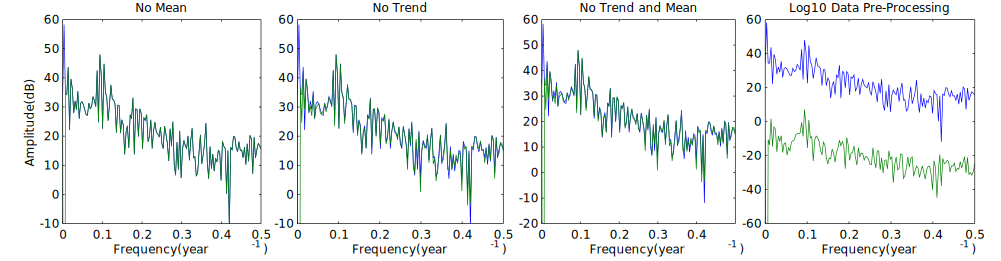
\includegraphics[width=\textwidth]{cw1im/4a.svg}
\resizebox{\textwidth}{!}{% This file was created by matlab2tikz v0.4.7 running on MATLAB 8.1.
% Copyright (c) 2008--2014, Nico Schlömer <nico.schloemer@gmail.com>
% All rights reserved.
% Minimal pgfplots version: 1.3
% 
% The latest updates can be retrieved from
%   http://www.mathworks.com/matlabcentral/fileexchange/22022-matlab2tikz
% where you can also make suggestions and rate matlab2tikz.
% 
\begin{tikzpicture}

\begin{axis}[%
width=1.14583333333333in,
height=1.26452464788732in,
scale only axis,
xmin=0,
xmax=1,
xlabel={Freq},
ymin=0,
ymax=1,
name=plot2,
title={$\rho$ = 0.2},
axis x line*=bottom,
axis y line*=left
]
\addplot [color=blue,solid,forget plot]
  table[row sep=crcr]{0.00775193798449612	0.220502234896843\\
0.0155038759689922	0.306515165135207\\
0.0232558139534884	0.44104728120272\\
0.0310077519379845	0.564184979689995\\
0.0387596899224806	0.629017802604363\\
0.0465116279069767	0.590362848628859\\
0.0542635658914729	0.446895778615477\\
0.062015503875969	0.269803965389123\\
0.0697674418604651	0.257415131406812\\
0.0775193798449612	0.27206714743036\\
0.0852713178294574	0.186681476227938\\
0.0930232558139535	0.156988669712712\\
0.10077519379845	0.21734492284425\\
0.108527131782946	0.219758408396436\\
0.116279069767442	0.176718957963265\\
0.124031007751938	0.172174196335156\\
0.131782945736434	0.252091680222149\\
0.13953488372093	0.345781827646836\\
0.147286821705426	0.310239276271002\\
0.155038759689922	0.142095500387021\\
0.162790697674419	0.0661154959980519\\
0.170542635658915	0.0754132809357778\\
0.178294573643411	0.0691904987889799\\
0.186046511627907	0.057173093052767\\
0.193798449612403	0.140495859742674\\
0.201550387596899	0.46154657598069\\
0.209302325581395	0.430398218281127\\
0.217054263565891	0.22365368352203\\
0.224806201550388	0.078561399795915\\
0.232558139534884	0.0953056420432593\\
0.24031007751938	0.147884551823197\\
0.248062015503876	0.170423127583456\\
0.255813953488372	0.160187390399693\\
0.263565891472868	0.137708569743277\\
0.271317829457364	0.172851281418621\\
0.27906976744186	0.251008982410362\\
0.286821705426357	0.21812954864151\\
0.294573643410853	0.110748424714198\\
0.302325581395349	0.0950799198780726\\
0.310077519379845	0.101996678884959\\
0.317829457364341	0.0867327132150931\\
0.325581395348837	0.102663384357734\\
0.333333333333333	0.20203574138765\\
0.341085271317829	0.426219995287023\\
0.348837209302326	0.612511901283248\\
0.356589147286822	0.59728869406329\\
0.364341085271318	0.45636193984555\\
0.372093023255814	0.322984439917522\\
0.37984496124031	0.362447516890196\\
0.387596899224806	0.355400087044547\\
0.395348837209302	0.192016027792446\\
0.403100775193798	0.0429256932596605\\
0.410852713178295	0.0630485625537198\\
0.418604651162791	0.192389458474258\\
0.426356589147287	0.240227716807469\\
0.434108527131783	0.0995719435184929\\
0.441860465116279	0.0263780372052649\\
0.449612403100775	0.0351151068203807\\
0.457364341085271	0.0713552485167407\\
0.465116279069767	0.231415990723553\\
0.472868217054264	0.301409308525454\\
0.48062015503876	0.367779382739422\\
0.488372093023256	0.213657674947212\\
0.496124031007752	0.0652701704240951\\
0.503875968992248	0.0542478364187367\\
0.511627906976744	0.0653959972999108\\
0.51937984496124	0.0133791698954541\\
0.527131782945736	0.0251633704745024\\
0.534883720930233	0.076295394154768\\
0.542635658914729	0.0966530198986727\\
0.550387596899225	0.102279675821332\\
0.558139534883721	0.212580942141339\\
0.565891472868217	0.274522021422916\\
0.573643410852713	0.212275116302694\\
0.581395348837209	0.134939069415704\\
0.589147286821705	0.196826436685055\\
0.596899224806202	0.360541231365205\\
0.604651162790698	0.392141773064441\\
0.612403100775194	0.27128682608335\\
0.62015503875969	0.183766229071669\\
0.627906976744186	0.133690186394755\\
0.635658914728682	0.151972438328803\\
0.643410852713178	0.141283065022664\\
0.651162790697674	0.0991827935334993\\
0.65891472868217	0.0675056470377667\\
0.666666666666667	0.0516825328594492\\
0.674418604651163	0.0970925421649653\\
0.682170542635659	0.144032810181311\\
0.689922480620155	0.124955748440713\\
0.697674418604651	0.109824315350903\\
0.705426356589147	0.0774196304628554\\
0.713178294573643	0.0264161799478387\\
0.720930232558139	0.0315677198031761\\
0.728682170542636	0.073603672516936\\
0.736434108527132	0.1761274511699\\
0.744186046511628	0.38369891423613\\
0.751937984496124	0.406752800092147\\
0.75968992248062	0.259967685730681\\
0.767441860465116	0.116017032979312\\
0.775193798449612	0.0558914439161718\\
0.782945736434108	0.086787287073962\\
0.790697674418605	0.215637676442742\\
0.798449612403101	0.413480409502265\\
0.806201550387597	0.499358546955602\\
0.813953488372093	0.490817920253037\\
0.821705426356589	0.444862425025123\\
0.829457364341085	0.278807252214366\\
0.837209302325581	0.143208547345232\\
0.844961240310077	0.135035147964434\\
0.852713178294574	0.0934286748046095\\
0.86046511627907	0.0528316247209236\\
0.868217054263566	0.0702706794702705\\
0.875968992248062	0.107383907218243\\
0.883720930232558	0.146078841951471\\
0.891472868217054	0.185706837278458\\
0.89922480620155	0.165988388222965\\
0.906976744186046	0.0649073834169883\\
0.914728682170543	0.00889773852000111\\
0.922480620155039	0.028024401805455\\
0.930232558139535	0.0500200678501728\\
0.937984496124031	0.142237897455433\\
0.945736434108527	0.203593183895101\\
0.953488372093023	0.0724550332352811\\
0.961240310077519	0.00329382604710641\\
0.968992248062015	0.00701717375558731\\
0.976744186046512	0.0862785171065198\\
0.984496124031008	0.182103469546186\\
0.992248062015504	0.164413964264768\\
1	0.14611165032704\\
};
\addplot [color=red,dashed,line width=3.0pt,forget plot]
  table[row sep=crcr]{0.00775193798449612	0.195339406229459\\
0.0155038759689922	0.195339406229459\\
0.0232558139534884	0.195339406229459\\
0.0310077519379845	0.195339406229459\\
0.0387596899224806	0.195339406229459\\
0.0465116279069767	0.195339406229459\\
0.0542635658914729	0.195339406229459\\
0.062015503875969	0.195339406229459\\
0.0697674418604651	0.195339406229459\\
0.0775193798449612	0.195339406229459\\
0.0852713178294574	0.195339406229459\\
0.0930232558139535	0.195339406229459\\
0.10077519379845	0.195339406229459\\
0.108527131782946	0.195339406229459\\
0.116279069767442	0.195339406229459\\
0.124031007751938	0.195339406229459\\
0.131782945736434	0.195339406229459\\
0.13953488372093	0.195339406229459\\
0.147286821705426	0.195339406229459\\
0.155038759689922	0.195339406229459\\
0.162790697674419	0.195339406229459\\
0.170542635658915	0.195339406229459\\
0.178294573643411	0.195339406229459\\
0.186046511627907	0.195339406229459\\
0.193798449612403	0.195339406229459\\
0.201550387596899	0.195339406229459\\
0.209302325581395	0.195339406229459\\
0.217054263565891	0.195339406229459\\
0.224806201550388	0.195339406229459\\
0.232558139534884	0.195339406229459\\
0.24031007751938	0.195339406229459\\
0.248062015503876	0.195339406229459\\
0.255813953488372	0.195339406229459\\
0.263565891472868	0.195339406229459\\
0.271317829457364	0.195339406229459\\
0.27906976744186	0.195339406229459\\
0.286821705426357	0.195339406229459\\
0.294573643410853	0.195339406229459\\
0.302325581395349	0.195339406229459\\
0.310077519379845	0.195339406229459\\
0.317829457364341	0.195339406229459\\
0.325581395348837	0.195339406229459\\
0.333333333333333	0.195339406229459\\
0.341085271317829	0.195339406229459\\
0.348837209302326	0.195339406229459\\
0.356589147286822	0.195339406229459\\
0.364341085271318	0.195339406229459\\
0.372093023255814	0.195339406229459\\
0.37984496124031	0.195339406229459\\
0.387596899224806	0.195339406229459\\
0.395348837209302	0.195339406229459\\
0.403100775193798	0.195339406229459\\
0.410852713178295	0.195339406229459\\
0.418604651162791	0.195339406229459\\
0.426356589147287	0.195339406229459\\
0.434108527131783	0.195339406229459\\
0.441860465116279	0.195339406229459\\
0.449612403100775	0.195339406229459\\
0.457364341085271	0.195339406229459\\
0.465116279069767	0.195339406229459\\
0.472868217054264	0.195339406229459\\
0.48062015503876	0.195339406229459\\
0.488372093023256	0.195339406229459\\
0.496124031007752	0.195339406229459\\
0.503875968992248	0.195339406229459\\
0.511627906976744	0.195339406229459\\
0.51937984496124	0.195339406229459\\
0.527131782945736	0.195339406229459\\
0.534883720930233	0.195339406229459\\
0.542635658914729	0.195339406229459\\
0.550387596899225	0.195339406229459\\
0.558139534883721	0.195339406229459\\
0.565891472868217	0.195339406229459\\
0.573643410852713	0.195339406229459\\
0.581395348837209	0.195339406229459\\
0.589147286821705	0.195339406229459\\
0.596899224806202	0.195339406229459\\
0.604651162790698	0.195339406229459\\
0.612403100775194	0.195339406229459\\
0.62015503875969	0.195339406229459\\
0.627906976744186	0.195339406229459\\
0.635658914728682	0.195339406229459\\
0.643410852713178	0.195339406229459\\
0.651162790697674	0.195339406229459\\
0.65891472868217	0.195339406229459\\
0.666666666666667	0.195339406229459\\
0.674418604651163	0.195339406229459\\
0.682170542635659	0.195339406229459\\
0.689922480620155	0.195339406229459\\
0.697674418604651	0.195339406229459\\
0.705426356589147	0.195339406229459\\
0.713178294573643	0.195339406229459\\
0.720930232558139	0.195339406229459\\
0.728682170542636	0.195339406229459\\
0.736434108527132	0.195339406229459\\
0.744186046511628	0.195339406229459\\
0.751937984496124	0.195339406229459\\
0.75968992248062	0.195339406229459\\
0.767441860465116	0.195339406229459\\
0.775193798449612	0.195339406229459\\
0.782945736434108	0.195339406229459\\
0.790697674418605	0.195339406229459\\
0.798449612403101	0.195339406229459\\
0.806201550387597	0.195339406229459\\
0.813953488372093	0.195339406229459\\
0.821705426356589	0.195339406229459\\
0.829457364341085	0.195339406229459\\
0.837209302325581	0.195339406229459\\
0.844961240310077	0.195339406229459\\
0.852713178294574	0.195339406229459\\
0.86046511627907	0.195339406229459\\
0.868217054263566	0.195339406229459\\
0.875968992248062	0.195339406229459\\
0.883720930232558	0.195339406229459\\
0.891472868217054	0.195339406229459\\
0.89922480620155	0.195339406229459\\
0.906976744186046	0.195339406229459\\
0.914728682170543	0.195339406229459\\
0.922480620155039	0.195339406229459\\
0.930232558139535	0.195339406229459\\
0.937984496124031	0.195339406229459\\
0.945736434108527	0.195339406229459\\
0.953488372093023	0.195339406229459\\
0.961240310077519	0.195339406229459\\
0.968992248062015	0.195339406229459\\
0.976744186046512	0.195339406229459\\
0.984496124031008	0.195339406229459\\
0.992248062015504	0.195339406229459\\
1	0.195339406229459\\
};
\end{axis}

\begin{axis}[%
width=1.27757233796296in,
height=1.26452464788732in,
scale only axis,
xmin=0,
xmax=1,
xlabel={Freq},
ymin=0,
ymax=1,
ylabel={$C_{xy}(f)$},
at=(plot2.left of south west),
anchor=right of south east,
title={$\rho$ = 0},
axis x line*=bottom,
axis y line*=left
]
\addplot [color=blue,solid,forget plot]
  table[row sep=crcr]{0.00775193798449612	0.0925000698194741\\
0.0155038759689922	0.163925923615314\\
0.0232558139534884	0.287530987820103\\
0.0310077519379845	0.430289450951476\\
0.0387596899224806	0.525876901840942\\
0.0465116279069767	0.502196863371448\\
0.0542635658914729	0.341651522664875\\
0.062015503875969	0.14258865937264\\
0.0697674418604651	0.166083278883205\\
0.0775193798449612	0.199096199780006\\
0.0852713178294574	0.0945794776442949\\
0.0930232558139535	0.0327152604609571\\
0.10077519379845	0.0609958572245206\\
0.108527131782946	0.0754648777747539\\
0.116279069767442	0.080996831611494\\
0.124031007751938	0.0893731734032046\\
0.131782945736434	0.147217276847787\\
0.13953488372093	0.22987814199664\\
0.147286821705426	0.194913223879794\\
0.155038759689922	0.0490891216198838\\
0.162790697674419	0.00247332361951944\\
0.170542635658915	0.00528207612609258\\
0.178294573643411	0.0268450360456923\\
0.186046511627907	0.0327317187580083\\
0.193798449612403	0.00473875674358233\\
0.201550387596899	0.144038258614864\\
0.209302325581395	0.144541236048832\\
0.217054263565891	0.0407194593120671\\
0.224806201550388	0.0496804843878\\
0.232558139534884	0.176782870465188\\
0.24031007751938	0.259380945561801\\
0.248062015503876	0.290531772244494\\
0.255813953488372	0.286909999443971\\
0.263565891472868	0.256927258842424\\
0.271317829457364	0.289347112438101\\
0.27906976744186	0.36202982802211\\
0.286821705426357	0.31168843606022\\
0.294573643410853	0.15808773644328\\
0.302325581395349	0.0940760852128444\\
0.310077519379845	0.083838246247955\\
0.317829457364341	0.0610305704293348\\
0.325581395348837	0.0497855006792153\\
0.333333333333333	0.09935857715812\\
0.341085271317829	0.280974934579951\\
0.348837209302326	0.470742115308331\\
0.356589147286822	0.456457895618123\\
0.364341085271318	0.321612286606809\\
0.372093023255814	0.215574352297941\\
0.37984496124031	0.276387361694534\\
0.387596899224806	0.27847056553008\\
0.395348837209302	0.126502647125689\\
0.403100775193798	0.00486233565922284\\
0.410852713178295	0.0172652576056506\\
0.418604651162791	0.0570507694439571\\
0.426356589147287	0.0666568201861999\\
0.434108527131783	0.0152820164175307\\
0.441860465116279	0.105529602847802\\
0.449612403100775	0.149473423493993\\
0.457364341085271	0.045662719010933\\
0.465116279069767	0.105367000647872\\
0.472868217054264	0.158736758982735\\
0.48062015503876	0.246954131802286\\
0.488372093023256	0.125219359251048\\
0.496124031007752	0.0463573913807768\\
0.503875968992248	0.0337423422385065\\
0.511627906976744	0.0128525724842974\\
0.51937984496124	0.00423376587271142\\
0.527131782945736	0.0306071354431855\\
0.534883720930233	0.0628966045547819\\
0.542635658914729	0.0626868897392506\\
0.550387596899225	0.0231140307397277\\
0.558139534883721	0.0722943212859907\\
0.565891472868217	0.116961547939764\\
0.573643410852713	0.0833750274971154\\
0.581395348837209	0.0585064824090255\\
0.589147286821705	0.133609645180041\\
0.596899224806202	0.281457906774645\\
0.604651162790698	0.291991036700334\\
0.612403100775194	0.139791212311724\\
0.62015503875969	0.0601977457647076\\
0.627906976744186	0.0451584870971304\\
0.635658914728682	0.0792649122437955\\
0.643410852713178	0.0621892890156916\\
0.651162790697674	0.0174744950137591\\
0.65891472868217	0.00197843907717584\\
0.666666666666667	0.0249876007258009\\
0.674418604651163	0.119280259584126\\
0.682170542635659	0.185654175203157\\
0.689922480620155	0.124379767718787\\
0.697674418604651	0.0333363100146991\\
0.705426356589147	0.00844391168334763\\
0.713178294573643	0.00141066041236137\\
0.720930232558139	0.014257150243928\\
0.728682170542636	0.027145063131311\\
0.736434108527132	0.0708627815668805\\
0.744186046511628	0.26527040734096\\
0.751937984496124	0.290931481385357\\
0.75968992248062	0.144995229775215\\
0.767441860465116	0.0300753661935758\\
0.775193798449612	0.00357245896469274\\
0.782945736434108	0.0181584533802267\\
0.790697674418605	0.057963199692706\\
0.798449612403101	0.20974040337527\\
0.806201550387597	0.32469481613325\\
0.813953488372093	0.346785184170626\\
0.821705426356589	0.313542716382111\\
0.829457364341085	0.159425721600931\\
0.837209302325581	0.0716488193537531\\
0.844961240310077	0.0801071442913215\\
0.852713178294574	0.0259524460277181\\
0.86046511627907	0.0290911937238422\\
0.868217054263566	0.0562457942952181\\
0.875968992248062	0.0860508304584929\\
0.883720930232558	0.126660224724533\\
0.891472868217054	0.178432778009931\\
0.89922480620155	0.19113531438789\\
0.906976744186046	0.136164747167026\\
0.914728682170543	0.0528646194188603\\
0.922480620155039	0.00851107227888956\\
0.930232558139535	0.00696224492653346\\
0.937984496124031	0.123136686606645\\
0.945736434108527	0.216026270337076\\
0.953488372093023	0.0955088026914915\\
0.961240310077519	0.0102627808015247\\
0.968992248062015	0.00431917571020606\\
0.976744186046512	0.0699122720909229\\
0.984496124031008	0.141255166193067\\
0.992248062015504	0.0824760254197566\\
1	0.0434864657338938\\
};
\addplot [color=red,dashed,line width=3.0pt,forget plot]
  table[row sep=crcr]{0.00775193798449612	0.131739814090628\\
0.0155038759689922	0.131739814090628\\
0.0232558139534884	0.131739814090628\\
0.0310077519379845	0.131739814090628\\
0.0387596899224806	0.131739814090628\\
0.0465116279069767	0.131739814090628\\
0.0542635658914729	0.131739814090628\\
0.062015503875969	0.131739814090628\\
0.0697674418604651	0.131739814090628\\
0.0775193798449612	0.131739814090628\\
0.0852713178294574	0.131739814090628\\
0.0930232558139535	0.131739814090628\\
0.10077519379845	0.131739814090628\\
0.108527131782946	0.131739814090628\\
0.116279069767442	0.131739814090628\\
0.124031007751938	0.131739814090628\\
0.131782945736434	0.131739814090628\\
0.13953488372093	0.131739814090628\\
0.147286821705426	0.131739814090628\\
0.155038759689922	0.131739814090628\\
0.162790697674419	0.131739814090628\\
0.170542635658915	0.131739814090628\\
0.178294573643411	0.131739814090628\\
0.186046511627907	0.131739814090628\\
0.193798449612403	0.131739814090628\\
0.201550387596899	0.131739814090628\\
0.209302325581395	0.131739814090628\\
0.217054263565891	0.131739814090628\\
0.224806201550388	0.131739814090628\\
0.232558139534884	0.131739814090628\\
0.24031007751938	0.131739814090628\\
0.248062015503876	0.131739814090628\\
0.255813953488372	0.131739814090628\\
0.263565891472868	0.131739814090628\\
0.271317829457364	0.131739814090628\\
0.27906976744186	0.131739814090628\\
0.286821705426357	0.131739814090628\\
0.294573643410853	0.131739814090628\\
0.302325581395349	0.131739814090628\\
0.310077519379845	0.131739814090628\\
0.317829457364341	0.131739814090628\\
0.325581395348837	0.131739814090628\\
0.333333333333333	0.131739814090628\\
0.341085271317829	0.131739814090628\\
0.348837209302326	0.131739814090628\\
0.356589147286822	0.131739814090628\\
0.364341085271318	0.131739814090628\\
0.372093023255814	0.131739814090628\\
0.37984496124031	0.131739814090628\\
0.387596899224806	0.131739814090628\\
0.395348837209302	0.131739814090628\\
0.403100775193798	0.131739814090628\\
0.410852713178295	0.131739814090628\\
0.418604651162791	0.131739814090628\\
0.426356589147287	0.131739814090628\\
0.434108527131783	0.131739814090628\\
0.441860465116279	0.131739814090628\\
0.449612403100775	0.131739814090628\\
0.457364341085271	0.131739814090628\\
0.465116279069767	0.131739814090628\\
0.472868217054264	0.131739814090628\\
0.48062015503876	0.131739814090628\\
0.488372093023256	0.131739814090628\\
0.496124031007752	0.131739814090628\\
0.503875968992248	0.131739814090628\\
0.511627906976744	0.131739814090628\\
0.51937984496124	0.131739814090628\\
0.527131782945736	0.131739814090628\\
0.534883720930233	0.131739814090628\\
0.542635658914729	0.131739814090628\\
0.550387596899225	0.131739814090628\\
0.558139534883721	0.131739814090628\\
0.565891472868217	0.131739814090628\\
0.573643410852713	0.131739814090628\\
0.581395348837209	0.131739814090628\\
0.589147286821705	0.131739814090628\\
0.596899224806202	0.131739814090628\\
0.604651162790698	0.131739814090628\\
0.612403100775194	0.131739814090628\\
0.62015503875969	0.131739814090628\\
0.627906976744186	0.131739814090628\\
0.635658914728682	0.131739814090628\\
0.643410852713178	0.131739814090628\\
0.651162790697674	0.131739814090628\\
0.65891472868217	0.131739814090628\\
0.666666666666667	0.131739814090628\\
0.674418604651163	0.131739814090628\\
0.682170542635659	0.131739814090628\\
0.689922480620155	0.131739814090628\\
0.697674418604651	0.131739814090628\\
0.705426356589147	0.131739814090628\\
0.713178294573643	0.131739814090628\\
0.720930232558139	0.131739814090628\\
0.728682170542636	0.131739814090628\\
0.736434108527132	0.131739814090628\\
0.744186046511628	0.131739814090628\\
0.751937984496124	0.131739814090628\\
0.75968992248062	0.131739814090628\\
0.767441860465116	0.131739814090628\\
0.775193798449612	0.131739814090628\\
0.782945736434108	0.131739814090628\\
0.790697674418605	0.131739814090628\\
0.798449612403101	0.131739814090628\\
0.806201550387597	0.131739814090628\\
0.813953488372093	0.131739814090628\\
0.821705426356589	0.131739814090628\\
0.829457364341085	0.131739814090628\\
0.837209302325581	0.131739814090628\\
0.844961240310077	0.131739814090628\\
0.852713178294574	0.131739814090628\\
0.86046511627907	0.131739814090628\\
0.868217054263566	0.131739814090628\\
0.875968992248062	0.131739814090628\\
0.883720930232558	0.131739814090628\\
0.891472868217054	0.131739814090628\\
0.89922480620155	0.131739814090628\\
0.906976744186046	0.131739814090628\\
0.914728682170543	0.131739814090628\\
0.922480620155039	0.131739814090628\\
0.930232558139535	0.131739814090628\\
0.937984496124031	0.131739814090628\\
0.945736434108527	0.131739814090628\\
0.953488372093023	0.131739814090628\\
0.961240310077519	0.131739814090628\\
0.968992248062015	0.131739814090628\\
0.976744186046512	0.131739814090628\\
0.984496124031008	0.131739814090628\\
0.992248062015504	0.131739814090628\\
1	0.131739814090628\\
};
\end{axis}

\begin{axis}[%
width=1.10416666666667in,
height=1.26452464788732in,
scale only axis,
xmin=0,
xmax=1,
xlabel={Freq},
ymin=0,
ymax=1,
name=plot3,
at=(plot2.right of south east),
anchor=left of south west,
title={$\rho$ = 0.4},
axis x line*=bottom,
axis y line*=left
]
\addplot [color=blue,solid,forget plot]
  table[row sep=crcr]{0.00775193798449612	0.374529732192725\\
0.0155038759689922	0.460222576359991\\
0.0232558139534884	0.58149056993628\\
0.0310077519379845	0.675797964302615\\
0.0387596899224806	0.715403665113431\\
0.0465116279069767	0.66970684996518\\
0.0542635658914729	0.548827472364842\\
0.062015503875969	0.413423252790044\\
0.0697674418604651	0.402961586618873\\
0.0775193798449612	0.417466983505987\\
0.0852713178294574	0.352870245744107\\
0.0930232558139535	0.34194009981035\\
0.10077519379845	0.411773986745396\\
0.108527131782946	0.400490023251441\\
0.116279069767442	0.31953395626774\\
0.124031007751938	0.300170435656643\\
0.131782945736434	0.38614351626945\\
0.13953488372093	0.474670801468604\\
0.147286821705426	0.441481661325485\\
0.155038759689922	0.282330235371023\\
0.162790697674419	0.213978428283994\\
0.170542635658915	0.244812698836862\\
0.178294573643411	0.230890593365675\\
0.186046511627907	0.224299388142457\\
0.193798449612403	0.392503283886024\\
0.201550387596899	0.695877258681635\\
0.209302325581395	0.659387532402255\\
0.217054263565891	0.457505928352099\\
0.224806201550388	0.228526063735623\\
0.232558139534884	0.0998403871639013\\
0.24031007751938	0.0675809118752301\\
0.248062015503876	0.0576882709615414\\
0.255813953488372	0.0430885670598963\\
0.263565891472868	0.0332906522297416\\
0.271317829457364	0.0700848313478138\\
0.27906976744186	0.161416521278844\\
0.286821705426357	0.167893014644678\\
0.294573643410853	0.126126755918244\\
0.302325581395349	0.16024509384081\\
0.310077519379845	0.191181850426807\\
0.317829457364341	0.197198802192785\\
0.325581395348837	0.23409399697254\\
0.333333333333333	0.352671881483284\\
0.341085271317829	0.573213685800912\\
0.348837209302326	0.728509999134825\\
0.356589147286822	0.711239902718528\\
0.364341085271318	0.580906024027075\\
0.372093023255814	0.44036231557364\\
0.37984496124031	0.462264900713918\\
0.387596899224806	0.44948188574095\\
0.395348837209302	0.28850963900088\\
0.403100775193798	0.136267306373807\\
0.410852713178295	0.195327879432264\\
0.418604651162791	0.392298758700489\\
0.426356589147287	0.457843117807988\\
0.434108527131783	0.29507368705991\\
0.441860465116279	0.0690612449184627\\
0.449612403100775	0.00680190953753917\\
0.457364341085271	0.198652124679671\\
0.465116279069767	0.400633551864224\\
0.472868217054264	0.457718925144942\\
0.48062015503876	0.490673121436774\\
0.488372093023256	0.326377813176922\\
0.496124031007752	0.170685949749794\\
0.503875968992248	0.192317206715063\\
0.511627906976744	0.20870541880385\\
0.51937984496124	0.0941553513089528\\
0.527131782945736	0.0748257027438665\\
0.534883720930233	0.136865169544461\\
0.542635658914729	0.1787919917363\\
0.550387596899225	0.237184475239463\\
0.558139534883721	0.388776886496129\\
0.565891472868217	0.452557541731314\\
0.573643410852713	0.377661852564062\\
0.581395348837209	0.263976363650189\\
0.589147286821705	0.300938608610624\\
0.596899224806202	0.461010218652605\\
0.604651162790698	0.506905694941661\\
0.612403100775194	0.425855628976346\\
0.62015503875969	0.345491730671539\\
0.627906976744186	0.262451090649468\\
0.635658914728682	0.261225606570581\\
0.643410852713178	0.263718412504803\\
0.651162790697674	0.247138889824465\\
0.65891472868217	0.229428010792794\\
0.666666666666667	0.188330236245216\\
0.674418604651163	0.184327205313639\\
0.682170542635659	0.215865710971967\\
0.689922480620155	0.239420852175253\\
0.697674418604651	0.266196107452205\\
0.705426356589147	0.212364516758072\\
0.713178294573643	0.111541945206997\\
0.720930232558139	0.100765889787239\\
0.728682170542636	0.170501815647609\\
0.736434108527132	0.313643435571025\\
0.744186046511628	0.509831416964613\\
0.751937984496124	0.531081916588674\\
0.75968992248062	0.405380957377049\\
0.767441860465116	0.262044501754759\\
0.775193798449612	0.181991074676749\\
0.782945736434108	0.238136442420553\\
0.790697674418605	0.416937337385178\\
0.798449612403101	0.594100946723911\\
0.806201550387597	0.644774379063397\\
0.813953488372093	0.617396768085779\\
0.821705426356589	0.567243130087268\\
0.829457364341085	0.410125377509193\\
0.837209302325581	0.255002463333177\\
0.844961240310077	0.257011270667929\\
0.852713178294574	0.277005242991804\\
0.86046511627907	0.195830085268076\\
0.868217054263566	0.14443010306096\\
0.875968992248062	0.161901826885859\\
0.883720930232558	0.198226788225751\\
0.891472868217054	0.240652975235233\\
0.89922480620155	0.207435387425503\\
0.906976744186046	0.0536229916977106\\
0.914728682170543	0.0215354773796879\\
0.922480620155039	0.107908501599987\\
0.930232558139535	0.153225004448469\\
0.937984496124031	0.221240500700303\\
0.945736434108527	0.250361604602292\\
0.953488372093023	0.114533175980107\\
0.961240310077519	0.0471007425700049\\
0.968992248062015	0.0533058469185717\\
0.976744186046512	0.156769451617784\\
0.984496124031008	0.288159819074336\\
0.992248062015504	0.303037466205536\\
1	0.29172104707605\\
};
\addplot [color=red,dashed,line width=3.0pt,forget plot]
  table[row sep=crcr]{0.00775193798449612	0.305467625272841\\
0.0155038759689922	0.305467625272841\\
0.0232558139534884	0.305467625272841\\
0.0310077519379845	0.305467625272841\\
0.0387596899224806	0.305467625272841\\
0.0465116279069767	0.305467625272841\\
0.0542635658914729	0.305467625272841\\
0.062015503875969	0.305467625272841\\
0.0697674418604651	0.305467625272841\\
0.0775193798449612	0.305467625272841\\
0.0852713178294574	0.305467625272841\\
0.0930232558139535	0.305467625272841\\
0.10077519379845	0.305467625272841\\
0.108527131782946	0.305467625272841\\
0.116279069767442	0.305467625272841\\
0.124031007751938	0.305467625272841\\
0.131782945736434	0.305467625272841\\
0.13953488372093	0.305467625272841\\
0.147286821705426	0.305467625272841\\
0.155038759689922	0.305467625272841\\
0.162790697674419	0.305467625272841\\
0.170542635658915	0.305467625272841\\
0.178294573643411	0.305467625272841\\
0.186046511627907	0.305467625272841\\
0.193798449612403	0.305467625272841\\
0.201550387596899	0.305467625272841\\
0.209302325581395	0.305467625272841\\
0.217054263565891	0.305467625272841\\
0.224806201550388	0.305467625272841\\
0.232558139534884	0.305467625272841\\
0.24031007751938	0.305467625272841\\
0.248062015503876	0.305467625272841\\
0.255813953488372	0.305467625272841\\
0.263565891472868	0.305467625272841\\
0.271317829457364	0.305467625272841\\
0.27906976744186	0.305467625272841\\
0.286821705426357	0.305467625272841\\
0.294573643410853	0.305467625272841\\
0.302325581395349	0.305467625272841\\
0.310077519379845	0.305467625272841\\
0.317829457364341	0.305467625272841\\
0.325581395348837	0.305467625272841\\
0.333333333333333	0.305467625272841\\
0.341085271317829	0.305467625272841\\
0.348837209302326	0.305467625272841\\
0.356589147286822	0.305467625272841\\
0.364341085271318	0.305467625272841\\
0.372093023255814	0.305467625272841\\
0.37984496124031	0.305467625272841\\
0.387596899224806	0.305467625272841\\
0.395348837209302	0.305467625272841\\
0.403100775193798	0.305467625272841\\
0.410852713178295	0.305467625272841\\
0.418604651162791	0.305467625272841\\
0.426356589147287	0.305467625272841\\
0.434108527131783	0.305467625272841\\
0.441860465116279	0.305467625272841\\
0.449612403100775	0.305467625272841\\
0.457364341085271	0.305467625272841\\
0.465116279069767	0.305467625272841\\
0.472868217054264	0.305467625272841\\
0.48062015503876	0.305467625272841\\
0.488372093023256	0.305467625272841\\
0.496124031007752	0.305467625272841\\
0.503875968992248	0.305467625272841\\
0.511627906976744	0.305467625272841\\
0.51937984496124	0.305467625272841\\
0.527131782945736	0.305467625272841\\
0.534883720930233	0.305467625272841\\
0.542635658914729	0.305467625272841\\
0.550387596899225	0.305467625272841\\
0.558139534883721	0.305467625272841\\
0.565891472868217	0.305467625272841\\
0.573643410852713	0.305467625272841\\
0.581395348837209	0.305467625272841\\
0.589147286821705	0.305467625272841\\
0.596899224806202	0.305467625272841\\
0.604651162790698	0.305467625272841\\
0.612403100775194	0.305467625272841\\
0.62015503875969	0.305467625272841\\
0.627906976744186	0.305467625272841\\
0.635658914728682	0.305467625272841\\
0.643410852713178	0.305467625272841\\
0.651162790697674	0.305467625272841\\
0.65891472868217	0.305467625272841\\
0.666666666666667	0.305467625272841\\
0.674418604651163	0.305467625272841\\
0.682170542635659	0.305467625272841\\
0.689922480620155	0.305467625272841\\
0.697674418604651	0.305467625272841\\
0.705426356589147	0.305467625272841\\
0.713178294573643	0.305467625272841\\
0.720930232558139	0.305467625272841\\
0.728682170542636	0.305467625272841\\
0.736434108527132	0.305467625272841\\
0.744186046511628	0.305467625272841\\
0.751937984496124	0.305467625272841\\
0.75968992248062	0.305467625272841\\
0.767441860465116	0.305467625272841\\
0.775193798449612	0.305467625272841\\
0.782945736434108	0.305467625272841\\
0.790697674418605	0.305467625272841\\
0.798449612403101	0.305467625272841\\
0.806201550387597	0.305467625272841\\
0.813953488372093	0.305467625272841\\
0.821705426356589	0.305467625272841\\
0.829457364341085	0.305467625272841\\
0.837209302325581	0.305467625272841\\
0.844961240310077	0.305467625272841\\
0.852713178294574	0.305467625272841\\
0.86046511627907	0.305467625272841\\
0.868217054263566	0.305467625272841\\
0.875968992248062	0.305467625272841\\
0.883720930232558	0.305467625272841\\
0.891472868217054	0.305467625272841\\
0.89922480620155	0.305467625272841\\
0.906976744186046	0.305467625272841\\
0.914728682170543	0.305467625272841\\
0.922480620155039	0.305467625272841\\
0.930232558139535	0.305467625272841\\
0.937984496124031	0.305467625272841\\
0.945736434108527	0.305467625272841\\
0.953488372093023	0.305467625272841\\
0.961240310077519	0.305467625272841\\
0.968992248062015	0.305467625272841\\
0.976744186046512	0.305467625272841\\
0.984496124031008	0.305467625272841\\
0.992248062015504	0.305467625272841\\
1	0.305467625272841\\
};
\end{axis}

\begin{axis}[%
width=1.15674985532406in,
height=1.26452464788732in,
scale only axis,
xmin=0,
xmax=1,
xlabel={Freq},
ymin=0,
ymax=1,
name=plot4,
at=(plot3.right of south east),
anchor=left of south west,
title={$\rho$ = 0.6},
axis x line*=bottom,
axis y line*=left
]
\addplot [color=blue,solid,forget plot]
  table[row sep=crcr]{0.00775193798449612	0.547693132681463\\
0.0155038759689922	0.619420021437795\\
0.0232558139534884	0.712038745777417\\
0.0310077519379845	0.775189877291358\\
0.0387596899224806	0.794777810856919\\
0.0465116279069767	0.748646441405835\\
0.0542635658914729	0.655416064055037\\
0.062015503875969	0.571380110687973\\
0.0697674418604651	0.581395199758789\\
0.0775193798449612	0.602834713386185\\
0.0852713178294574	0.558349681153211\\
0.0930232558139535	0.553501148121054\\
0.10077519379845	0.611542590135521\\
0.108527131782946	0.593082402893397\\
0.116279069767442	0.50024174430619\\
0.124031007751938	0.470641341341189\\
0.131782945736434	0.545486499495733\\
0.13953488372093	0.615516333707273\\
0.147286821705426	0.587865429589414\\
0.155038759689922	0.46418137732923\\
0.162790697674419	0.429523261754292\\
0.170542635658915	0.477727479577079\\
0.178294573643411	0.472734603198312\\
0.186046511627907	0.482373075364533\\
0.193798449612403	0.643801604595085\\
0.201550387596899	0.841566873310014\\
0.209302325581395	0.814621923016286\\
0.217054263565891	0.673013547020633\\
0.224806201550388	0.466309127061369\\
0.232558139534884	0.25263113535241\\
0.24031007751938	0.09492132557447\\
0.248062015503876	0.014968248317991\\
0.255813953488372	0.00884486880242935\\
0.263565891472868	0.0112515601936704\\
0.271317829457364	0.0478521742343906\\
0.27906976744186	0.170504568086849\\
0.286821705426357	0.231483196372728\\
0.294573643410853	0.245817897656387\\
0.302325581395349	0.309863477146343\\
0.310077519379845	0.361837545776193\\
0.317829457364341	0.3923851189779\\
0.325581395348837	0.434215089627187\\
0.333333333333333	0.53623261508574\\
0.341085271317829	0.713488513863697\\
0.348837209302326	0.824715447239097\\
0.356589147286822	0.807835462441442\\
0.364341085271318	0.701025556347823\\
0.372093023255814	0.572546584862873\\
0.37984496124031	0.580845374287848\\
0.387596899224806	0.565991264814658\\
0.395348837209302	0.424321931884107\\
0.403100775193798	0.297758414897631\\
0.410852713178295	0.404841277539716\\
0.418604651162791	0.6065363572919\\
0.426356589147287	0.664335887461481\\
0.434108527131783	0.539520648833334\\
0.441860465116279	0.281544363781333\\
0.449612403100775	0.155997631925321\\
0.457364341085271	0.415843964491347\\
0.465116279069767	0.588843894804326\\
0.472868217054264	0.61993412478779\\
0.48062015503876	0.620523139584373\\
0.488372093023256	0.469207146218077\\
0.496124031007752	0.366358306291287\\
0.503875968992248	0.426642495069243\\
0.511627906976744	0.426285269708372\\
0.51937984496124	0.265048138173543\\
0.527131782945736	0.205864031791392\\
0.534883720930233	0.26450205322582\\
0.542635658914729	0.32296119733496\\
0.550387596899225	0.423953823343127\\
0.558139534883721	0.579701303025015\\
0.565891472868217	0.631807678109702\\
0.573643410852713	0.563080471324918\\
0.581395348837209	0.442595932758299\\
0.589147286821705	0.450328779586911\\
0.596899224806202	0.585096707404925\\
0.604651162790698	0.635582278912377\\
0.612403100775194	0.593665281074037\\
0.62015503875969	0.532281042254948\\
0.627906976744186	0.432598867480573\\
0.635658914728682	0.413304694905854\\
0.643410852713178	0.43109711409725\\
0.651162790697674	0.448630628452678\\
0.65891472868217	0.458595266495163\\
0.666666666666667	0.417210521084315\\
0.674418604651163	0.390033694288409\\
0.682170542635659	0.416960161988191\\
0.689922480620155	0.45529005630425\\
0.697674418604651	0.478958625489596\\
0.705426356589147	0.407907068474101\\
0.713178294573643	0.272781868231143\\
0.720930232558139	0.24162959915073\\
0.728682170542636	0.328671101499219\\
0.736434108527132	0.4822839607825\\
0.744186046511628	0.643628106051467\\
0.751937984496124	0.662312294899964\\
0.75968992248062	0.57201755133936\\
0.767441860465116	0.457278145984116\\
0.775193798449612	0.379524350014844\\
0.782945736434108	0.452468348112872\\
0.790697674418605	0.621539026801791\\
0.798449612403101	0.745158187045207\\
0.806201550387597	0.767796801940282\\
0.813953488372093	0.733726728539083\\
0.821705426356589	0.687133226055137\\
0.829457364341085	0.556478172295114\\
0.837209302325581	0.41228470658187\\
0.844961240310077	0.441304576283654\\
0.852713178294574	0.520887461309229\\
0.86046511627907	0.4331922687597\\
0.868217054263566	0.296433916045576\\
0.875968992248062	0.26703849957471\\
0.883720930232558	0.300014246100945\\
0.891472868217054	0.36142659802107\\
0.89922480620155	0.34376206586157\\
0.906976744186046	0.157834459748431\\
0.914728682170543	0.131636336404035\\
0.922480620155039	0.265754649757203\\
0.930232558139535	0.325700445613272\\
0.937984496124031	0.372882714661095\\
0.945736434108527	0.378967704482429\\
0.953488372093023	0.252498060172379\\
0.961240310077519	0.168832112477918\\
0.968992248062015	0.16712203429406\\
0.976744186046512	0.299159494338934\\
0.984496124031008	0.458425774875651\\
0.992248062015504	0.487859865210352\\
1	0.474204217919578\\
};
\addplot [color=red,dashed,line width=3.0pt,forget plot]
  table[row sep=crcr]{0.00775193798449612	0.463312628950056\\
0.0155038759689922	0.463312628950056\\
0.0232558139534884	0.463312628950056\\
0.0310077519379845	0.463312628950056\\
0.0387596899224806	0.463312628950056\\
0.0465116279069767	0.463312628950056\\
0.0542635658914729	0.463312628950056\\
0.062015503875969	0.463312628950056\\
0.0697674418604651	0.463312628950056\\
0.0775193798449612	0.463312628950056\\
0.0852713178294574	0.463312628950056\\
0.0930232558139535	0.463312628950056\\
0.10077519379845	0.463312628950056\\
0.108527131782946	0.463312628950056\\
0.116279069767442	0.463312628950056\\
0.124031007751938	0.463312628950056\\
0.131782945736434	0.463312628950056\\
0.13953488372093	0.463312628950056\\
0.147286821705426	0.463312628950056\\
0.155038759689922	0.463312628950056\\
0.162790697674419	0.463312628950056\\
0.170542635658915	0.463312628950056\\
0.178294573643411	0.463312628950056\\
0.186046511627907	0.463312628950056\\
0.193798449612403	0.463312628950056\\
0.201550387596899	0.463312628950056\\
0.209302325581395	0.463312628950056\\
0.217054263565891	0.463312628950056\\
0.224806201550388	0.463312628950056\\
0.232558139534884	0.463312628950056\\
0.24031007751938	0.463312628950056\\
0.248062015503876	0.463312628950056\\
0.255813953488372	0.463312628950056\\
0.263565891472868	0.463312628950056\\
0.271317829457364	0.463312628950056\\
0.27906976744186	0.463312628950056\\
0.286821705426357	0.463312628950056\\
0.294573643410853	0.463312628950056\\
0.302325581395349	0.463312628950056\\
0.310077519379845	0.463312628950056\\
0.317829457364341	0.463312628950056\\
0.325581395348837	0.463312628950056\\
0.333333333333333	0.463312628950056\\
0.341085271317829	0.463312628950056\\
0.348837209302326	0.463312628950056\\
0.356589147286822	0.463312628950056\\
0.364341085271318	0.463312628950056\\
0.372093023255814	0.463312628950056\\
0.37984496124031	0.463312628950056\\
0.387596899224806	0.463312628950056\\
0.395348837209302	0.463312628950056\\
0.403100775193798	0.463312628950056\\
0.410852713178295	0.463312628950056\\
0.418604651162791	0.463312628950056\\
0.426356589147287	0.463312628950056\\
0.434108527131783	0.463312628950056\\
0.441860465116279	0.463312628950056\\
0.449612403100775	0.463312628950056\\
0.457364341085271	0.463312628950056\\
0.465116279069767	0.463312628950056\\
0.472868217054264	0.463312628950056\\
0.48062015503876	0.463312628950056\\
0.488372093023256	0.463312628950056\\
0.496124031007752	0.463312628950056\\
0.503875968992248	0.463312628950056\\
0.511627906976744	0.463312628950056\\
0.51937984496124	0.463312628950056\\
0.527131782945736	0.463312628950056\\
0.534883720930233	0.463312628950056\\
0.542635658914729	0.463312628950056\\
0.550387596899225	0.463312628950056\\
0.558139534883721	0.463312628950056\\
0.565891472868217	0.463312628950056\\
0.573643410852713	0.463312628950056\\
0.581395348837209	0.463312628950056\\
0.589147286821705	0.463312628950056\\
0.596899224806202	0.463312628950056\\
0.604651162790698	0.463312628950056\\
0.612403100775194	0.463312628950056\\
0.62015503875969	0.463312628950056\\
0.627906976744186	0.463312628950056\\
0.635658914728682	0.463312628950056\\
0.643410852713178	0.463312628950056\\
0.651162790697674	0.463312628950056\\
0.65891472868217	0.463312628950056\\
0.666666666666667	0.463312628950056\\
0.674418604651163	0.463312628950056\\
0.682170542635659	0.463312628950056\\
0.689922480620155	0.463312628950056\\
0.697674418604651	0.463312628950056\\
0.705426356589147	0.463312628950056\\
0.713178294573643	0.463312628950056\\
0.720930232558139	0.463312628950056\\
0.728682170542636	0.463312628950056\\
0.736434108527132	0.463312628950056\\
0.744186046511628	0.463312628950056\\
0.751937984496124	0.463312628950056\\
0.75968992248062	0.463312628950056\\
0.767441860465116	0.463312628950056\\
0.775193798449612	0.463312628950056\\
0.782945736434108	0.463312628950056\\
0.790697674418605	0.463312628950056\\
0.798449612403101	0.463312628950056\\
0.806201550387597	0.463312628950056\\
0.813953488372093	0.463312628950056\\
0.821705426356589	0.463312628950056\\
0.829457364341085	0.463312628950056\\
0.837209302325581	0.463312628950056\\
0.844961240310077	0.463312628950056\\
0.852713178294574	0.463312628950056\\
0.86046511627907	0.463312628950056\\
0.868217054263566	0.463312628950056\\
0.875968992248062	0.463312628950056\\
0.883720930232558	0.463312628950056\\
0.891472868217054	0.463312628950056\\
0.89922480620155	0.463312628950056\\
0.906976744186046	0.463312628950056\\
0.914728682170543	0.463312628950056\\
0.922480620155039	0.463312628950056\\
0.930232558139535	0.463312628950056\\
0.937984496124031	0.463312628950056\\
0.945736434108527	0.463312628950056\\
0.953488372093023	0.463312628950056\\
0.961240310077519	0.463312628950056\\
0.968992248062015	0.463312628950056\\
0.976744186046512	0.463312628950056\\
0.984496124031008	0.463312628950056\\
0.992248062015504	0.463312628950056\\
1	0.463312628950056\\
};
\end{axis}

\begin{axis}[%
width=1.12689236111111in,
height=1.26452464788732in,
scale only axis,
xmin=0,
xmax=1,
xlabel={Freq},
ymin=0,
ymax=1,
name=plot5,
at=(plot4.right of south east),
anchor=left of south west,
title={$\rho$ = 0.8},
axis x line*=bottom,
axis y line*=left
]
\addplot [color=blue,solid,forget plot]
  table[row sep=crcr]{0.00775193798449612	0.74471046447493\\
0.0155038759689922	0.789201547180812\\
0.0232558139534884	0.841823576945946\\
0.0310077519379845	0.873327589785995\\
0.0387596899224806	0.877740797505284\\
0.0465116279069767	0.839596978079015\\
0.0542635658914729	0.782035717575398\\
0.062015503875969	0.752402417734204\\
0.0697674418604651	0.779975589691726\\
0.0775193798449612	0.801692034680706\\
0.0852713178294574	0.777607956486473\\
0.0930232558139535	0.772959750914387\\
0.10077519379845	0.805090309890276\\
0.108527131782946	0.78926175468522\\
0.116279069767442	0.719259363299296\\
0.124031007751938	0.691371579914721\\
0.131782945736434	0.737093708378712\\
0.13953488372093	0.77690248850751\\
0.147286821705426	0.758906202149109\\
0.155038759689922	0.692482762642718\\
0.162790697674419	0.69562247756749\\
0.170542635658915	0.738041418071894\\
0.178294573643411	0.743394586541276\\
0.186046511627907	0.759001244341963\\
0.193798449612403	0.846775642509841\\
0.201550387596899	0.934534594825792\\
0.209302325581395	0.920718008604468\\
0.217054263565891	0.851653758853181\\
0.224806201550388	0.73978913217894\\
0.232558139534884	0.588774421499549\\
0.24031007751938	0.405171313895865\\
0.248062015503876	0.277392238456229\\
0.255813953488372	0.301950010372053\\
0.263565891472868	0.29318842812793\\
0.271317829457364	0.323412936802764\\
0.27906976744186	0.461870223835435\\
0.286821705426357	0.525776549188916\\
0.294573643410853	0.532109941288712\\
0.302325581395349	0.577091530511224\\
0.310077519379845	0.627710236900453\\
0.317829457364341	0.665734811071315\\
0.325581395348837	0.692231025706484\\
0.333333333333333	0.747445007211271\\
0.341085271317829	0.849721678347397\\
0.348837209302326	0.909877940557279\\
0.356589147286822	0.897123883770214\\
0.364341085271318	0.827681742570313\\
0.372093023255814	0.735326206502794\\
0.37984496124031	0.734843943675586\\
0.387596899224806	0.722834070994576\\
0.395348837209302	0.626160450660319\\
0.403100775193798	0.558942060908505\\
0.410852713178295	0.678191768841783\\
0.418604651162791	0.810122189260666\\
0.426356589147287	0.843229263762513\\
0.434108527131783	0.782782448472682\\
0.441860465116279	0.637635153938171\\
0.449612403100775	0.541673259097602\\
0.457364341085271	0.695814339894484\\
0.465116279069767	0.785954985394457\\
0.472868217054264	0.791612872110374\\
0.48062015503876	0.7708522724988\\
0.488372093023256	0.663317619733626\\
0.496124031007752	0.648879220460923\\
0.503875968992248	0.713169404088977\\
0.511627906976744	0.696980397957555\\
0.51937984496124	0.555532555969765\\
0.527131782945736	0.47616589789298\\
0.534883720930233	0.508544327256513\\
0.542635658914729	0.56430442220627\\
0.550387596899225	0.668116197829178\\
0.558139534883721	0.778914357280591\\
0.565891472868217	0.809129314126834\\
0.573643410852713	0.76469424451684\\
0.581395348837209	0.677277140528736\\
0.589147286821705	0.662829313566499\\
0.596899224806202	0.745926073420339\\
0.604651162790698	0.786571801792896\\
0.612403100775194	0.776466522265835\\
0.62015503875969	0.742881962945585\\
0.627906976744186	0.658719007393403\\
0.635658914728682	0.63102384017668\\
0.643410852713178	0.657957758503123\\
0.651162790697674	0.696995135706542\\
0.65891472868217	0.723624757545448\\
0.666666666666667	0.702607043578473\\
0.674418604651163	0.68589775207536\\
0.682170542635659	0.708994081973521\\
0.689922480620155	0.728868780616722\\
0.697674418604651	0.727351840234366\\
0.705426356589147	0.664928457200481\\
0.713178294573643	0.544656478644791\\
0.720930232558139	0.501601653049438\\
0.728682170542636	0.577333231216829\\
0.736434108527132	0.693419203052451\\
0.744186046511628	0.793795476122192\\
0.751937984496124	0.807408001734679\\
0.75968992248062	0.761494480128217\\
0.767441860465116	0.698420944468424\\
0.775193798449612	0.649323293931427\\
0.782945736434108	0.710585750825897\\
0.790697674418605	0.81430929797987\\
0.798449612403101	0.874596499605564\\
0.806201550387597	0.879030265192358\\
0.813953488372093	0.85051002359095\\
0.821705426356589	0.816461395276981\\
0.829457364341085	0.732026409344869\\
0.837209302325581	0.635725156731528\\
0.844961240310077	0.686500716556714\\
0.852713178294574	0.772389956643258\\
0.86046511627907	0.718325738572896\\
0.868217054263566	0.561079153798253\\
0.875968992248062	0.47512209630047\\
0.883720930232558	0.501525277470724\\
0.891472868217054	0.587464716044152\\
0.89922480620155	0.608446350128936\\
0.906976744186046	0.468912997348772\\
0.914728682170543	0.423621651771687\\
0.922480620155039	0.538476909265472\\
0.930232558139535	0.589989463031039\\
0.937984496124031	0.620261272156489\\
0.945736434108527	0.62197284679852\\
0.953488372093023	0.535167313007416\\
0.961240310077519	0.434566257711944\\
0.968992248062015	0.414265768739417\\
0.976744186046512	0.552392759481054\\
0.984496124031008	0.693865846453609\\
0.992248062015504	0.715626524595468\\
1	0.698605526907846\\
};
\addplot [color=red,dashed,line width=3.0pt,forget plot]
  table[row sep=crcr]{0.00775193798449612	0.685574872811385\\
0.0155038759689922	0.685574872811385\\
0.0232558139534884	0.685574872811385\\
0.0310077519379845	0.685574872811385\\
0.0387596899224806	0.685574872811385\\
0.0465116279069767	0.685574872811385\\
0.0542635658914729	0.685574872811385\\
0.062015503875969	0.685574872811385\\
0.0697674418604651	0.685574872811385\\
0.0775193798449612	0.685574872811385\\
0.0852713178294574	0.685574872811385\\
0.0930232558139535	0.685574872811385\\
0.10077519379845	0.685574872811385\\
0.108527131782946	0.685574872811385\\
0.116279069767442	0.685574872811385\\
0.124031007751938	0.685574872811385\\
0.131782945736434	0.685574872811385\\
0.13953488372093	0.685574872811385\\
0.147286821705426	0.685574872811385\\
0.155038759689922	0.685574872811385\\
0.162790697674419	0.685574872811385\\
0.170542635658915	0.685574872811385\\
0.178294573643411	0.685574872811385\\
0.186046511627907	0.685574872811385\\
0.193798449612403	0.685574872811385\\
0.201550387596899	0.685574872811385\\
0.209302325581395	0.685574872811385\\
0.217054263565891	0.685574872811385\\
0.224806201550388	0.685574872811385\\
0.232558139534884	0.685574872811385\\
0.24031007751938	0.685574872811385\\
0.248062015503876	0.685574872811385\\
0.255813953488372	0.685574872811385\\
0.263565891472868	0.685574872811385\\
0.271317829457364	0.685574872811385\\
0.27906976744186	0.685574872811385\\
0.286821705426357	0.685574872811385\\
0.294573643410853	0.685574872811385\\
0.302325581395349	0.685574872811385\\
0.310077519379845	0.685574872811385\\
0.317829457364341	0.685574872811385\\
0.325581395348837	0.685574872811385\\
0.333333333333333	0.685574872811385\\
0.341085271317829	0.685574872811385\\
0.348837209302326	0.685574872811385\\
0.356589147286822	0.685574872811385\\
0.364341085271318	0.685574872811385\\
0.372093023255814	0.685574872811385\\
0.37984496124031	0.685574872811385\\
0.387596899224806	0.685574872811385\\
0.395348837209302	0.685574872811385\\
0.403100775193798	0.685574872811385\\
0.410852713178295	0.685574872811385\\
0.418604651162791	0.685574872811385\\
0.426356589147287	0.685574872811385\\
0.434108527131783	0.685574872811385\\
0.441860465116279	0.685574872811385\\
0.449612403100775	0.685574872811385\\
0.457364341085271	0.685574872811385\\
0.465116279069767	0.685574872811385\\
0.472868217054264	0.685574872811385\\
0.48062015503876	0.685574872811385\\
0.488372093023256	0.685574872811385\\
0.496124031007752	0.685574872811385\\
0.503875968992248	0.685574872811385\\
0.511627906976744	0.685574872811385\\
0.51937984496124	0.685574872811385\\
0.527131782945736	0.685574872811385\\
0.534883720930233	0.685574872811385\\
0.542635658914729	0.685574872811385\\
0.550387596899225	0.685574872811385\\
0.558139534883721	0.685574872811385\\
0.565891472868217	0.685574872811385\\
0.573643410852713	0.685574872811385\\
0.581395348837209	0.685574872811385\\
0.589147286821705	0.685574872811385\\
0.596899224806202	0.685574872811385\\
0.604651162790698	0.685574872811385\\
0.612403100775194	0.685574872811385\\
0.62015503875969	0.685574872811385\\
0.627906976744186	0.685574872811385\\
0.635658914728682	0.685574872811385\\
0.643410852713178	0.685574872811385\\
0.651162790697674	0.685574872811385\\
0.65891472868217	0.685574872811385\\
0.666666666666667	0.685574872811385\\
0.674418604651163	0.685574872811385\\
0.682170542635659	0.685574872811385\\
0.689922480620155	0.685574872811385\\
0.697674418604651	0.685574872811385\\
0.705426356589147	0.685574872811385\\
0.713178294573643	0.685574872811385\\
0.720930232558139	0.685574872811385\\
0.728682170542636	0.685574872811385\\
0.736434108527132	0.685574872811385\\
0.744186046511628	0.685574872811385\\
0.751937984496124	0.685574872811385\\
0.75968992248062	0.685574872811385\\
0.767441860465116	0.685574872811385\\
0.775193798449612	0.685574872811385\\
0.782945736434108	0.685574872811385\\
0.790697674418605	0.685574872811385\\
0.798449612403101	0.685574872811385\\
0.806201550387597	0.685574872811385\\
0.813953488372093	0.685574872811385\\
0.821705426356589	0.685574872811385\\
0.829457364341085	0.685574872811385\\
0.837209302325581	0.685574872811385\\
0.844961240310077	0.685574872811385\\
0.852713178294574	0.685574872811385\\
0.86046511627907	0.685574872811385\\
0.868217054263566	0.685574872811385\\
0.875968992248062	0.685574872811385\\
0.883720930232558	0.685574872811385\\
0.891472868217054	0.685574872811385\\
0.89922480620155	0.685574872811385\\
0.906976744186046	0.685574872811385\\
0.914728682170543	0.685574872811385\\
0.922480620155039	0.685574872811385\\
0.930232558139535	0.685574872811385\\
0.937984496124031	0.685574872811385\\
0.945736434108527	0.685574872811385\\
0.953488372093023	0.685574872811385\\
0.961240310077519	0.685574872811385\\
0.968992248062015	0.685574872811385\\
0.976744186046512	0.685574872811385\\
0.984496124031008	0.685574872811385\\
0.992248062015504	0.685574872811385\\
1	0.685574872811385\\
};
\end{axis}

\begin{axis}[%
width=0.92847583912037in,
height=1.26452464788732in,
scale only axis,
xmin=0,
xmax=1,
xlabel={Freq},
ymin=0,
ymax=1.1,
at=(plot5.right of south east),
anchor=left of south west,
title={$\rho$ = 1},
axis x line*=bottom,
axis y line*=left
]
\addplot [color=blue,solid,forget plot]
  table[row sep=crcr]{0.00775193798449612	1\\
0.0155038759689922	1\\
0.0232558139534884	1\\
0.0310077519379845	1\\
0.0387596899224806	1\\
0.0465116279069767	1\\
0.0542635658914729	1\\
0.062015503875969	1\\
0.0697674418604651	1\\
0.0775193798449612	1\\
0.0852713178294574	1\\
0.0930232558139535	1\\
0.10077519379845	1\\
0.108527131782946	1\\
0.116279069767442	1\\
0.124031007751938	1\\
0.131782945736434	1\\
0.13953488372093	1\\
0.147286821705426	1\\
0.155038759689922	1\\
0.162790697674419	1\\
0.170542635658915	1\\
0.178294573643411	1\\
0.186046511627907	1\\
0.193798449612403	1\\
0.201550387596899	1\\
0.209302325581395	1\\
0.217054263565891	1\\
0.224806201550388	1\\
0.232558139534884	1\\
0.24031007751938	1\\
0.248062015503876	1\\
0.255813953488372	1\\
0.263565891472868	1\\
0.271317829457364	1\\
0.27906976744186	1\\
0.286821705426357	1\\
0.294573643410853	1\\
0.302325581395349	1\\
0.310077519379845	1\\
0.317829457364341	1\\
0.325581395348837	1\\
0.333333333333333	1\\
0.341085271317829	1\\
0.348837209302326	1\\
0.356589147286822	1\\
0.364341085271318	1\\
0.372093023255814	1\\
0.37984496124031	1\\
0.387596899224806	1\\
0.395348837209302	1\\
0.403100775193798	1\\
0.410852713178295	1\\
0.418604651162791	1\\
0.426356589147287	1\\
0.434108527131783	1\\
0.441860465116279	1\\
0.449612403100775	1\\
0.457364341085271	1\\
0.465116279069767	1\\
0.472868217054264	1\\
0.48062015503876	1\\
0.488372093023256	1\\
0.496124031007752	1\\
0.503875968992248	1\\
0.511627906976744	1\\
0.51937984496124	1\\
0.527131782945736	1\\
0.534883720930233	1\\
0.542635658914729	1\\
0.550387596899225	1\\
0.558139534883721	1\\
0.565891472868217	1\\
0.573643410852713	1\\
0.581395348837209	1\\
0.589147286821705	1\\
0.596899224806202	1\\
0.604651162790698	1\\
0.612403100775194	1\\
0.62015503875969	1\\
0.627906976744186	1\\
0.635658914728682	1\\
0.643410852713178	1\\
0.651162790697674	1\\
0.65891472868217	1\\
0.666666666666667	1\\
0.674418604651163	1\\
0.682170542635659	1\\
0.689922480620155	1\\
0.697674418604651	1\\
0.705426356589147	1\\
0.713178294573643	1\\
0.720930232558139	1\\
0.728682170542636	1\\
0.736434108527132	1\\
0.744186046511628	1\\
0.751937984496124	1\\
0.75968992248062	1\\
0.767441860465116	1\\
0.775193798449612	1\\
0.782945736434108	1\\
0.790697674418605	1\\
0.798449612403101	1\\
0.806201550387597	1\\
0.813953488372093	1\\
0.821705426356589	1\\
0.829457364341085	1\\
0.837209302325581	1\\
0.844961240310077	1\\
0.852713178294574	1\\
0.86046511627907	1\\
0.868217054263566	1\\
0.875968992248062	1\\
0.883720930232558	1\\
0.891472868217054	1\\
0.89922480620155	1\\
0.906976744186046	1\\
0.914728682170543	1\\
0.922480620155039	1\\
0.930232558139535	1\\
0.937984496124031	1\\
0.945736434108527	1\\
0.953488372093023	1\\
0.961240310077519	1\\
0.968992248062015	1\\
0.976744186046512	1\\
0.984496124031008	1\\
0.992248062015504	1\\
1	1\\
};
\end{axis}
\end{tikzpicture}%}
%\includestandalone[width=\textwidth]{cw1im/4a.tikz}
\textit{Note:} The \textcolor{red}{red} line represents the average coherency across the whole spectrum.
\caption{Plot of the coherence between two signals $x$ and $y$ for different $\rho$}
\label{fig:2_1a}
\end{figure}

The coherency spectrum is calculated by:
\begin{equation}
C_{xy} = \frac{P_{xy}^2(\omega)}{P_x(\omega)P_y(\omega)}
\end{equation}

Its values vary between 0 and 1 and are useful in providing information on how much two signals tend to agree for various frequencies, where 1 would imply a perfect agreement between both signals.

Here we have two signals $x(n)=x_1(n)$ and $y(n)=\rho x_1(n)+ \sqrt{1-\rho^2}x_2(n)$ where $x_1 , x_2 \sim \mathcal{N}(0,1)$. We notice that the more $\rho$ is increased, the more each value of the coherency spectrum is expected to be near 1, being fully 1 for two identical signals. A low $\rho$ (under 0.2) will not cause much change, as seen by the similar averages.

\subsection{Noise and coherence}

\textit{Note:} In all situations an average time windowing was used, as it was found to produce workable results.

In this case:

$x = \sin (2\pi f_0n) + w_1$ and $y = sin(2\pi f_0n + \alpha) + w_2$

\begin{figure}[h!]
\centering

\resizebox{\textwidth}{!}{% This file was created by matlab2tikz v0.4.7 running on MATLAB 8.1.
% Copyright (c) 2008--2014, Nico Schlömer <nico.schloemer@gmail.com>
% All rights reserved.
% Minimal pgfplots version: 1.3
% 
% The latest updates can be retrieved from
%   http://www.mathworks.com/matlabcentral/fileexchange/22022-matlab2tikz
% where you can also make suggestions and rate matlab2tikz.
% 
\begin{tikzpicture}

\begin{axis}[%
width=9in,
height=2in,
unbounded coords=jump,
scale only axis,
xmin=0,
xmax=500,
xlabel={Sample Iteration},
ymin=-8,
ymax=1,
ylabel={Error(dB)},
title={Error of AR(2) process with N=500 $\sigma$ = 0.25 $a_1=0.1$ $a_2=0.8$},
axis x line*=bottom,
axis y line*=left,
legend style={draw=black,fill=white,legend cell align=left}
]
\addplot [color=blue,solid]
  table[row sep=crcr]{1	-0.229788243070588\\
2	-inf\\
3	-0.218203636981443\\
4	-1.73808742773869\\
5	-1.79551957929071\\
6	-2.28746110407662\\
7	-2.18118745503997\\
8	-3.58013564479554\\
9	-2.98421748558152\\
10	-4.95298378293035\\
11	-3.79989131129509\\
12	-3.37688035412364\\
13	-3.21703164703744\\
14	-3.74216406123553\\
15	-4.07612684545115\\
16	-4.51547590247142\\
17	-3.36339464349582\\
18	-5.15952580210771\\
19	-4.29835309759022\\
20	-4.18716594014725\\
21	-3.26543284232784\\
22	-4.38715286577999\\
23	-4.60228298234429\\
24	-4.32788858111614\\
25	-3.65523010416274\\
26	-4.29208467544006\\
27	-3.33244401253353\\
28	-4.4759496857724\\
29	-4.08508839524273\\
30	-5.59916633714001\\
31	-5.43488190635726\\
32	-5.84064586870389\\
33	-5.29902625543258\\
34	-5.19872287726752\\
35	-5.85065424191173\\
36	-5.43189223343866\\
37	-5.21286694318922\\
38	-6.50104170449159\\
39	-5.47199837421075\\
40	-5.56836889004279\\
41	-5.42208991556051\\
42	-4.65634877812563\\
43	-5.30089103520803\\
44	-5.92120128591003\\
45	-4.47841733179181\\
46	-5.06150149619086\\
47	-4.23750050152691\\
48	-5.46306911970808\\
49	-5.34698113665804\\
50	-6.54284243843051\\
51	-5.87436500441393\\
52	-5.03143044393694\\
53	-5.70107507828992\\
54	-5.15485445127537\\
55	-4.52318164217418\\
56	-5.4310396473444\\
57	-6.58639745940084\\
58	-5.61610823250922\\
59	-4.69090621631237\\
60	-5.74263025521253\\
61	-4.92601261569513\\
62	-4.74362922938526\\
63	-6.12081739329051\\
64	-5.56928546537914\\
65	-4.57624503262193\\
66	-5.29274313356007\\
67	-5.2487286072732\\
68	-6.53234022999071\\
69	-4.52407723284959\\
70	-5.8574049962793\\
71	-5.94247110304346\\
72	-5.38260345667883\\
73	-5.03397223868244\\
74	-6.17589516544435\\
75	-5.16874106382361\\
76	-5.80861259965988\\
77	-6.1648810044687\\
78	-5.77578464530208\\
79	-6.10521671305368\\
80	-6.75112545301969\\
81	-5.66740728176653\\
82	-5.16205603458247\\
83	-5.42906754063412\\
84	-5.10279107936781\\
85	-6.43628752918267\\
86	-6.175581479519\\
87	-5.65630168016819\\
88	-5.59496465567838\\
89	-5.46852332372649\\
90	-5.10582787621478\\
91	-4.90253703911878\\
92	-5.64337701134287\\
93	-5.42050203440295\\
94	-5.12157439111371\\
95	-5.36497667018451\\
96	-6.21586650946576\\
97	-5.15772273977455\\
98	-5.02804090079822\\
99	-5.01219915041109\\
100	-6.10551614749028\\
101	-6.14396345965409\\
102	-6.74737175105734\\
103	-6.01870209584417\\
104	-5.37769363066534\\
105	-4.84531105579311\\
106	-4.92229594277616\\
107	-5.56900549465387\\
108	-4.61151702211142\\
109	-5.42983115400914\\
110	-5.51182693918047\\
111	-5.27353666423673\\
112	-5.79837625038555\\
113	-5.8525743109092\\
114	-6.22004732634093\\
115	-6.78068213982206\\
116	-5.89709621306732\\
117	-6.59798955176555\\
118	-5.14061673875949\\
119	-6.98037386577991\\
120	-5.81755872344052\\
121	-5.86220102128863\\
122	-6.71932147476341\\
123	-6.53315503074471\\
124	-6.79160184963389\\
125	-5.63402997311076\\
126	-6.23935979392109\\
127	-5.15720607829311\\
128	-5.29829046008492\\
129	-5.49188695692767\\
130	-4.59733843202342\\
131	-5.16183807925268\\
132	-6.23154541757428\\
133	-6.6578049639367\\
134	-6.04058792520572\\
135	-5.22531321554492\\
136	-5.66318478434299\\
137	-5.53089932044527\\
138	-6.38878512769612\\
139	-5.5085642763215\\
140	-6.00032151756013\\
141	-5.73205860516742\\
142	-6.1659385786026\\
143	-6.0443300919105\\
144	-5.37349099691587\\
145	-5.94168669935386\\
146	-6.18671413553706\\
147	-5.19120816452886\\
148	-6.21421410880243\\
149	-6.01773740820446\\
150	-5.16066218834992\\
151	-5.59703009030996\\
152	-5.80245393677338\\
153	-5.50993171388241\\
154	-6.22525816247206\\
155	-5.99861874153744\\
156	-5.25722097475742\\
157	-7.50073689551816\\
158	-6.69273683660566\\
159	-5.73019477159794\\
160	-5.50666894698094\\
161	-6.43896780327472\\
162	-5.1715178822144\\
163	-5.49897959717483\\
164	-7.32770605193442\\
165	-6.20321915820244\\
166	-5.59195353304034\\
167	-5.30370460144668\\
168	-5.40574708086581\\
169	-5.98610910432874\\
170	-5.62417150719287\\
171	-5.43730613149863\\
172	-5.37040112235928\\
173	-5.58692118842649\\
174	-6.09804445394345\\
175	-5.1538125370193\\
176	-5.90052677502464\\
177	-6.19253349410607\\
178	-5.84780562519807\\
179	-4.75898155661522\\
180	-5.2452627824264\\
181	-4.76798974175807\\
182	-5.99807385455702\\
183	-5.79004545640885\\
184	-5.5894980383355\\
185	-5.90846648574785\\
186	-6.38473480582917\\
187	-4.55123329836067\\
188	-5.27795997805817\\
189	-5.86791918508474\\
190	-5.38818841942052\\
191	-5.78969506783587\\
192	-5.22538030339074\\
193	-6.64407330208905\\
194	-6.13636926523854\\
195	-5.77039060606247\\
196	-5.73470626065611\\
197	-5.20771574795184\\
198	-4.62972777979257\\
199	-4.61634184672718\\
200	-4.34810384832094\\
201	-4.96881071702656\\
202	-5.73260549802331\\
203	-5.70822133848988\\
204	-5.29678634325097\\
205	-4.61423011029444\\
206	-6.54397044398361\\
207	-6.27887787658762\\
208	-6.1697681981093\\
209	-5.15014239888381\\
210	-4.90852660601818\\
211	-6.24280867856958\\
212	-5.82439529801948\\
213	-6.46339465092116\\
214	-5.58926366178015\\
215	-6.55001355628265\\
216	-6.00295030450426\\
217	-5.58332028253455\\
218	-5.6646014387897\\
219	-6.24969131867989\\
220	-6.82708368719022\\
221	-5.86097450469113\\
222	-6.09895577600069\\
223	-4.53132513630901\\
224	-5.68791215244656\\
225	-5.54162849940635\\
226	-7.39763063698513\\
227	-5.5263357618908\\
228	-6.35940751326998\\
229	-6.79737100957956\\
230	-5.22152480049811\\
231	-4.07971896268717\\
232	-6.5145771580454\\
233	-6.16165585263209\\
234	-6.22004181249517\\
235	-6.02956891643305\\
236	-4.85255523334567\\
237	-5.84018984505244\\
238	-5.28545455578964\\
239	-5.84196472037425\\
240	-5.45420982419747\\
241	-5.33455178570608\\
242	-5.97491703591222\\
243	-6.09984289564845\\
244	-5.17447360483718\\
245	-5.91058899893254\\
246	-6.75875571638209\\
247	-5.45158398050944\\
248	-5.31836372075767\\
249	-5.92919069312543\\
250	-5.47308552878484\\
251	-6.65900553314768\\
252	-6.54067824505954\\
253	-5.57831528716302\\
254	-6.52706928157977\\
255	-4.816496891527\\
256	-6.28218076361067\\
257	-6.13139272168441\\
258	-6.49155969911562\\
259	-6.23194047768359\\
260	-5.21286619495297\\
261	-6.18525595940449\\
262	-6.60283481182297\\
263	-6.3270746681846\\
264	-6.75605623071768\\
265	-5.65783911273338\\
266	-6.10852281383835\\
267	-6.45385641524964\\
268	-6.125276666638\\
269	-6.87610861722742\\
270	-4.42026042212565\\
271	-5.92679314811075\\
272	-6.18357440680863\\
273	-5.19068148820777\\
274	-4.43540050148727\\
275	-5.97557432034599\\
276	-7.31633277707819\\
277	-4.89202920396066\\
278	-7.07014079095837\\
279	-5.89046269815394\\
280	-5.72172339703819\\
281	-5.12626033960445\\
282	-5.68959825432008\\
283	-5.35310689622004\\
284	-7.49047162570408\\
285	-6.48053985517056\\
286	-4.96091363696748\\
287	-5.24115750260128\\
288	-5.88220318716849\\
289	-6.58133319759685\\
290	-5.90888097078184\\
291	-5.36421041825948\\
292	-5.47758755122839\\
293	-6.09577125936425\\
294	-6.23442742818584\\
295	-5.37477459324413\\
296	-6.07567855447041\\
297	-6.17554252080335\\
298	-5.31048711398318\\
299	-5.92124321928878\\
300	-5.61213356136938\\
301	-5.32100655589412\\
302	-5.8574994252531\\
303	-5.90153478666188\\
304	-5.77655695982206\\
305	-6.37779990400114\\
306	-7.0008544227321\\
307	-5.41688843380852\\
308	-5.31696110328115\\
309	-5.6122351660368\\
310	-5.53338413326015\\
311	-5.77787725698007\\
312	-5.9662351223825\\
313	-6.34321828360199\\
314	-6.53611812928666\\
315	-5.34817176065266\\
316	-6.59485294958415\\
317	-6.04201823240622\\
318	-5.01456564494496\\
319	-5.03109196319889\\
320	-5.79624747992805\\
321	-5.36127278332435\\
322	-4.88977786297926\\
323	-5.54273515379944\\
324	-6.916512199563\\
325	-5.05527396828071\\
326	-6.00338262460889\\
327	-6.42480889739445\\
328	-5.87518229328505\\
329	-5.85438879903416\\
330	-4.74894667484783\\
331	-4.98945134948161\\
332	-6.18594564925984\\
333	-5.90288084755922\\
334	-6.31061523996004\\
335	-5.60841784288212\\
336	-5.67662143290465\\
337	-5.53680635233187\\
338	-5.34798468410129\\
339	-5.73570143372959\\
340	-5.24877757046847\\
341	-4.64500744046386\\
342	-5.97651503194191\\
343	-4.97405423901893\\
344	-4.89742498352531\\
345	-6.07907798186201\\
346	-5.325243500859\\
347	-5.065472737502\\
348	-5.70872690340672\\
349	-5.11538410044954\\
350	-5.89464318710674\\
351	-6.67855242878746\\
352	-6.27144359479701\\
353	-5.40796626999858\\
354	-5.75744280851982\\
355	-5.09005854163943\\
356	-5.57899640810071\\
357	-5.48220932259701\\
358	-6.22967936518648\\
359	-5.98541554873426\\
360	-6.35084329948506\\
361	-5.46890159418377\\
362	-5.6652740750065\\
363	-5.9551472442877\\
364	-5.84713111043308\\
365	-5.52444642629407\\
366	-6.95803808464547\\
367	-5.66853771501352\\
368	-5.85726537143959\\
369	-6.04619344597585\\
370	-6.16696924540945\\
371	-6.77423326338395\\
372	-5.95488104670501\\
373	-5.68817810969405\\
374	-5.83170179379665\\
375	-6.55233815813854\\
376	-4.91528742552698\\
377	-5.32470878547333\\
378	-5.72676118696556\\
379	-5.78127437010925\\
380	-5.9269649954569\\
381	-5.97500377631815\\
382	-5.31390682250549\\
383	-6.06264106619104\\
384	-5.42893131449347\\
385	-5.65545273627387\\
386	-5.44791639498981\\
387	-5.27097358493136\\
388	-6.09720544796168\\
389	-5.40733562450943\\
390	-6.34876033768787\\
391	-6.12779965788523\\
392	-6.20609841546047\\
393	-4.81217216027754\\
394	-5.65273602023547\\
395	-5.9720079483978\\
396	-5.80118997654346\\
397	-6.04726636756597\\
398	-5.95462085984802\\
399	-6.27495945633844\\
400	-6.20588938127144\\
401	-6.53726012531118\\
402	-5.42692511513224\\
403	-5.5060010413534\\
404	-4.72657881545002\\
405	-5.16454070314347\\
406	-5.84647660636429\\
407	-4.93223490708524\\
408	-4.89666112724137\\
409	-6.05702369251575\\
410	-6.81628758430124\\
411	-5.46332045838871\\
412	-6.08903571323949\\
413	-6.24766655033977\\
414	-5.28180461849417\\
415	-6.91476150787389\\
416	-6.27913538107551\\
417	-5.0374497080677\\
418	-5.73681147949017\\
419	-5.09648996918608\\
420	-5.92565019994917\\
421	-6.00792999368353\\
422	-5.06451503070626\\
423	-5.42288635308205\\
424	-4.80701634493005\\
425	-5.43314311321427\\
426	-5.11898220594836\\
427	-5.10978583819449\\
428	-5.09383204092813\\
429	-6.71611466466493\\
430	-4.98393616326159\\
431	-6.71083402579349\\
432	-5.77883016506813\\
433	-5.52942925882109\\
434	-4.88723444293461\\
435	-5.47629980163681\\
436	-6.42090188924682\\
437	-5.24290170351227\\
438	-4.42277791571427\\
439	-5.81435217950424\\
440	-5.98389900374645\\
441	-6.73784365325178\\
442	-5.91153635611154\\
443	-7.34256711726857\\
444	-5.8011735381461\\
445	-5.94325212365385\\
446	-5.57070538116492\\
447	-6.31952274215173\\
448	-5.573486894642\\
449	-4.80760067400412\\
450	-5.99569369561893\\
451	-5.7349331969918\\
452	-5.96389858177334\\
453	-6.40018404891549\\
454	-5.41992239640187\\
455	-6.07211507886066\\
456	-5.47827658484694\\
457	-5.78415057041042\\
458	-5.63208614880714\\
459	-5.83942083478156\\
460	-5.56033723018114\\
461	-5.75671186533159\\
462	-4.81716916320498\\
463	-5.58659589842412\\
464	-5.22169539575116\\
465	-5.70907161749598\\
466	-5.41631469241396\\
467	-6.19153667880597\\
468	-6.5832969583161\\
469	-5.6426807464211\\
470	-6.03884636393531\\
471	-5.61577022702524\\
472	-6.57725701975202\\
473	-6.61015439462763\\
474	-6.35289093241573\\
475	-5.76794734623316\\
476	-5.85751286740099\\
477	-5.76667950881399\\
478	-5.9038746339343\\
479	-6.33604267276987\\
480	-4.88478522729542\\
481	-5.7806487452813\\
482	-5.14265703635032\\
483	-6.6700164196176\\
484	-5.89490376850381\\
485	-5.41742823864795\\
486	-7.02095441315774\\
487	-6.2374540751595\\
488	-6.57685940222582\\
489	-5.52606956376956\\
490	-5.4890262212922\\
491	-6.15191892510352\\
492	-6.44331499449174\\
493	-6.26630378510544\\
494	-5.30233912473161\\
495	-5.01528970028261\\
496	-6.3788530181044\\
497	-6.21195847353363\\
498	-5.99450341812563\\
499	-5.57928553595309\\
500	-6.29530666063422\\
};
\addlegendentry{$\mu = 0.05$};

\addplot [color=red,solid]
  table[row sep=crcr]{1	0.239867219163377\\
2	-inf\\
3	-0.136817166163276\\
4	-0.53479702042941\\
5	-1.36704371344684\\
6	-1.61095173840487\\
7	-0.702547728678975\\
8	-1.87890886483772\\
9	-0.733243697039139\\
10	-1.87438434195662\\
11	-0.997020835942035\\
12	-1.30488508339394\\
13	-1.23857426222341\\
14	-1.9624858576123\\
15	-2.33367312631497\\
16	-1.76267263358362\\
17	-2.49134367693499\\
18	-2.0773334129832\\
19	-1.72255473112448\\
20	-1.17235411888693\\
21	-1.84600367812748\\
22	-2.229755817253\\
23	-2.30818788018455\\
24	-1.99660921376525\\
25	-1.79143435025107\\
26	-1.59129814851171\\
27	-1.52129858125753\\
28	-1.72044706684545\\
29	-1.10261780125816\\
30	-3.01690484472666\\
31	-1.91361254489451\\
32	-2.20848165110484\\
33	-2.74773559325964\\
34	-1.81409273079906\\
35	-3.77844276544056\\
36	-1.75953200713234\\
37	-3.12135757433164\\
38	-2.52656712277453\\
39	-3.88408191333951\\
40	-3.60609671468107\\
41	-3.53191841472304\\
42	-3.71407914352619\\
43	-3.72013710929094\\
44	-3.08056426045667\\
45	-4.03449261536694\\
46	-4.50122572366154\\
47	-3.95274500863518\\
48	-4.15301408824723\\
49	-3.51463670297543\\
50	-3.69030259344381\\
51	-4.2950240279612\\
52	-4.29364177627072\\
53	-4.88200601131738\\
54	-3.30958171213217\\
55	-3.164122588413\\
56	-3.45119230038019\\
57	-3.53623431843914\\
58	-3.69121091544556\\
59	-3.70795758881022\\
60	-3.02681989776703\\
61	-4.07988587424577\\
62	-2.86068019757288\\
63	-4.23856896161224\\
64	-2.46110768351752\\
65	-4.32923464265606\\
66	-3.1867215183672\\
67	-3.21495889336628\\
68	-3.90618389910417\\
69	-3.55395824215338\\
70	-3.70932030949747\\
71	-4.56888407471684\\
72	-3.56299918925327\\
73	-4.08163958620998\\
74	-4.44324418151967\\
75	-4.35728810393583\\
76	-4.10734883116877\\
77	-4.47255861989405\\
78	-2.93001465268669\\
79	-4.30222138800123\\
80	-3.97458273058344\\
81	-4.12346451987317\\
82	-4.11274637133153\\
83	-3.77430254179982\\
84	-4.34089031779035\\
85	-3.30617955674343\\
86	-4.34451185408386\\
87	-3.43844676803395\\
88	-4.53679526178751\\
89	-3.45785576672603\\
90	-5.03696673349925\\
91	-3.82279100122824\\
92	-3.77848511480895\\
93	-4.80749403312712\\
94	-4.17266723905709\\
95	-4.59569395900588\\
96	-3.96328041283094\\
97	-3.51822716531805\\
98	-5.91827177293634\\
99	-5.29300342805972\\
100	-5.0775821394625\\
101	-4.08882111394913\\
102	-4.23793913698347\\
103	-4.59851865635429\\
104	-4.69380700334\\
105	-4.11810457062593\\
106	-4.75533835700714\\
107	-4.97578826274818\\
108	-3.6489262141135\\
109	-5.05333462368184\\
110	-4.02604790721967\\
111	-5.05673163362715\\
112	-3.96547017378345\\
113	-4.57115833093393\\
114	-3.60008437392771\\
115	-4.56997040453946\\
116	-3.86879341166522\\
117	-6.17989178957949\\
118	-4.08936614167059\\
119	-4.46476515131358\\
120	-4.37255920471621\\
121	-4.82753501375735\\
122	-5.27360415114152\\
123	-4.52253928395061\\
124	-5.70185115412166\\
125	-4.70440526894857\\
126	-4.67485416504118\\
127	-4.25934095445106\\
128	-4.77649074358074\\
129	-5.36016257064891\\
130	-3.78713416224082\\
131	-5.28378481869119\\
132	-4.99947174438969\\
133	-5.34860956081313\\
134	-4.77662587079642\\
135	-5.45027850718559\\
136	-4.75248835537801\\
137	-7.00361772892377\\
138	-4.77969470171313\\
139	-6.01046788506133\\
140	-5.61690725780614\\
141	-4.92920931501247\\
142	-5.64668771534571\\
143	-5.37742323067691\\
144	-5.16120623443163\\
145	-4.30304966769503\\
146	-5.68000048183947\\
147	-4.96268956522863\\
148	-6.2897395560052\\
149	-4.89426558999908\\
150	-5.32864382017678\\
151	-5.6204196627061\\
152	-5.07596848278847\\
153	-5.36228347016414\\
154	-5.59991969369589\\
155	-5.04958307457341\\
156	-5.85437794021568\\
157	-4.99832974955514\\
158	-5.69142051727565\\
159	-4.21365116785242\\
160	-6.28497566882644\\
161	-5.56126976644333\\
162	-5.47712129931178\\
163	-5.67362453490562\\
164	-5.38008737965602\\
165	-5.54668305098062\\
166	-4.64233548641945\\
167	-5.13957993935667\\
168	-4.79594147869521\\
169	-6.28920494393421\\
170	-5.23757834666078\\
171	-5.69445643967045\\
172	-5.7022893595187\\
173	-5.45824133572193\\
174	-5.64583817608454\\
175	-3.78639842131258\\
176	-5.5254689500231\\
177	-4.98115564671484\\
178	-5.39573382837007\\
179	-5.52050987397022\\
180	-4.48939179821701\\
181	-5.10672114611057\\
182	-4.90704015287781\\
183	-4.3437469181639\\
184	-6.33207661965549\\
185	-6.07148214357611\\
186	-6.14912995747169\\
187	-5.42280194567736\\
188	-6.62536544295707\\
189	-5.36414746330982\\
190	-6.36491964489899\\
191	-4.75178287826294\\
192	-6.00047657875805\\
193	-5.48391218741435\\
194	-5.52454899886709\\
195	-5.84596071029402\\
196	-6.05191639721115\\
197	-6.49016373648903\\
198	-5.567798710307\\
199	-5.36699181146966\\
200	-5.22350552852686\\
201	-5.5399375650092\\
202	-4.77535302579686\\
203	-5.43120764125078\\
204	-5.88971112513903\\
205	-4.34738897563124\\
206	-6.29625611556054\\
207	-5.39897604892467\\
208	-5.58248234384482\\
209	-4.95353742007771\\
210	-5.96491775580821\\
211	-6.11177747183748\\
212	-5.62756969490204\\
213	-7.27922358758946\\
214	-6.07071763038443\\
215	-6.8559599429311\\
216	-5.22794695592819\\
217	-4.88331505994604\\
218	-5.09800566965161\\
219	-4.41882946851145\\
220	-5.36633007783295\\
221	-5.29278183593473\\
222	-6.06658748054179\\
223	-7.52767713126511\\
224	-4.41491541228114\\
225	-5.203548027425\\
226	-5.95480582868669\\
227	-5.66227043847732\\
228	-4.174392897905\\
229	-6.74053155971216\\
230	-5.85480487557086\\
231	-6.01281636063875\\
232	-4.6125313391989\\
233	-6.31441848099755\\
234	-5.56920453333565\\
235	-5.83569247329743\\
236	-4.75688000450699\\
237	-5.89478914112542\\
238	-5.46338438215209\\
239	-6.13503330465739\\
240	-5.8429571269254\\
241	-6.12769108761218\\
242	-5.46174050521072\\
243	-5.99306382905729\\
244	-5.76727734907696\\
245	-5.64810944067\\
246	-5.8953785761505\\
247	-7.10597980034809\\
248	-6.09345620739889\\
249	-5.58928027575863\\
250	-5.84727474379189\\
251	-5.75481321057305\\
252	-5.09864055125514\\
253	-6.10866915462029\\
254	-4.91211875925654\\
255	-6.01908294766615\\
256	-7.5897757800617\\
257	-5.76992521362538\\
258	-5.67931521327206\\
259	-5.8984986562939\\
260	-6.17412666923055\\
261	-5.26613057979618\\
262	-5.44493932676755\\
263	-6.76000288432309\\
264	-5.95383704255669\\
265	-5.06686971812229\\
266	-6.40783386109657\\
267	-4.81713671040025\\
268	-5.93647547801917\\
269	-5.92062458171705\\
270	-5.48219865922666\\
271	-6.57908782990359\\
272	-6.12786675174806\\
273	-5.85316207385492\\
274	-6.25445273768572\\
275	-5.56110311888801\\
276	-5.38948502267894\\
277	-5.86276212584018\\
278	-5.65826523426908\\
279	-5.17738274947051\\
280	-6.46964605585268\\
281	-4.23728562936972\\
282	-5.71523962947078\\
283	-4.52105455234137\\
284	-6.27905193875185\\
285	-6.55097796925785\\
286	-5.01592860022436\\
287	-5.60945809109059\\
288	-5.75176815280264\\
289	-6.01175461712101\\
290	-5.19489082374621\\
291	-5.25095376655537\\
292	-7.26489659230748\\
293	-6.24850124071954\\
294	-6.03975444070031\\
295	-6.46946516027979\\
296	-5.93385895112799\\
297	-5.33570185694488\\
298	-5.59290171981613\\
299	-5.16506717978825\\
300	-5.63396312768729\\
301	-5.30347012628937\\
302	-5.72402992077923\\
303	-5.23063451923239\\
304	-6.44045861841825\\
305	-5.54405738255733\\
306	-5.67844866070906\\
307	-5.00330928282241\\
308	-5.84870903583403\\
309	-6.20218201924873\\
310	-5.48189648386678\\
311	-5.1274975050235\\
312	-6.19304531084414\\
313	-5.712858865171\\
314	-5.21364617145121\\
315	-6.32665084774398\\
316	-6.27001583761304\\
317	-5.87798570456194\\
318	-5.5530095452379\\
319	-5.39021378436429\\
320	-5.18954264069515\\
321	-6.01867093108662\\
322	-5.9703349007945\\
323	-6.61421444560049\\
324	-6.83161561174491\\
325	-5.96292892109102\\
326	-5.44412907435885\\
327	-5.0907226861683\\
328	-6.09332888120996\\
329	-6.97815023961496\\
330	-6.2616874874844\\
331	-5.93239969003365\\
332	-6.74384906109466\\
333	-6.04264637995414\\
334	-5.73944276163831\\
335	-5.90275005156886\\
336	-5.3852294766252\\
337	-6.04281676290199\\
338	-6.07443693254382\\
339	-3.93862790941867\\
340	-6.8040793624167\\
341	-4.77652700160456\\
342	-6.27236050849926\\
343	-4.564194221761\\
344	-5.31594603420301\\
345	-5.91669141188043\\
346	-6.34097045064726\\
347	-6.53834452846343\\
348	-4.94911059912997\\
349	-5.94326490300823\\
350	-7.29464653592376\\
351	-6.63333052076231\\
352	-5.97230466734001\\
353	-6.52738704642026\\
354	-4.85118094362295\\
355	-5.04289098292696\\
356	-6.83815915440258\\
357	-6.2225703812461\\
358	-6.0912933590355\\
359	-5.18878457716532\\
360	-4.90154492171184\\
361	-5.22657569403415\\
362	-6.18990599548292\\
363	-4.61493217019859\\
364	-5.53935487540941\\
365	-6.40432118828676\\
366	-6.29382722147848\\
367	-6.24009359834568\\
368	-6.62102149817432\\
369	-6.87472279953865\\
370	-6.36667646160047\\
371	-5.76318837458457\\
372	-6.34629289775504\\
373	-6.28338156061629\\
374	-6.01217060426414\\
375	-5.33400905042032\\
376	-7.22800960879543\\
377	-5.8863849075152\\
378	-6.51189318566321\\
379	-6.70106525643205\\
380	-5.72800127882243\\
381	-5.79524678366512\\
382	-5.98280556193488\\
383	-6.84353160854253\\
384	-5.43124326138149\\
385	-5.42143240219709\\
386	-5.75764430819515\\
387	-5.4540005884005\\
388	-7.07020436012048\\
389	-5.77800984191368\\
390	-5.74853133396768\\
391	-6.17285118691665\\
392	-5.01777857838409\\
393	-6.02799240664749\\
394	-6.09415702117286\\
395	-6.50858560156009\\
396	-6.70359475860112\\
397	-7.15805583058095\\
398	-6.20959904836787\\
399	-6.04524139812596\\
400	-5.67297375149025\\
401	-6.30821227181905\\
402	-5.63146087609836\\
403	-6.80812567125969\\
404	-4.94144971940602\\
405	-5.9725606805954\\
406	-6.23308830686746\\
407	-6.11640906839115\\
408	-6.7231814819728\\
409	-5.03267236425398\\
410	-5.91778002025918\\
411	-7.44385009675043\\
412	-6.09472915643058\\
413	-6.23593803301464\\
414	-6.26928011070537\\
415	-5.34982759147844\\
416	-5.78965871852682\\
417	-4.89225101783455\\
418	-5.83147753782608\\
419	-5.21334112656999\\
420	-6.23622035884429\\
421	-6.05344967258154\\
422	-5.94791644370468\\
423	-5.94708365162295\\
424	-5.88559015179134\\
425	-6.67402112460689\\
426	-5.41395380533136\\
427	-5.13861747406598\\
428	-6.26119852659676\\
429	-5.66052338101043\\
430	-5.84265801798589\\
431	-5.9091751314334\\
432	-5.97292333666067\\
433	-4.9529736654248\\
434	-5.29164841858967\\
435	-6.27925705324482\\
436	-5.92757924408286\\
437	-5.58954845799373\\
438	-5.91059671338535\\
439	-5.8701034259859\\
440	-6.49651231719305\\
441	-4.95432853430049\\
442	-5.787700009606\\
443	-5.63409341923611\\
444	-6.59659395202474\\
445	-6.20626689187122\\
446	-5.99352914970808\\
447	-7.12098391142387\\
448	-6.72843846420565\\
449	-6.36522123397258\\
450	-6.71682843219805\\
451	-6.21760157772516\\
452	-5.57576981125371\\
453	-5.98798849243118\\
454	-6.17156422279381\\
455	-5.21885581354273\\
456	-5.69169095887554\\
457	-6.2035159558015\\
458	-6.2523427674741\\
459	-6.63885092993258\\
460	-5.7894881554731\\
461	-5.58180578922436\\
462	-5.36876122372263\\
463	-6.58302036254319\\
464	-5.19688970176316\\
465	-5.75058956107062\\
466	-6.40048957899504\\
467	-6.03983131034195\\
468	-5.43989787488522\\
469	-6.76532840051718\\
470	-6.01124725168041\\
471	-5.89656661862967\\
472	-5.40244465299072\\
473	-5.63167211968751\\
474	-5.40205310956715\\
475	-5.6449091246016\\
476	-6.36166357075991\\
477	-6.35108508313977\\
478	-5.55020347413113\\
479	-6.22642779517253\\
480	-6.93454632915112\\
481	-7.01106624747657\\
482	-5.86701503749128\\
483	-6.24494289194155\\
484	-5.97810455642793\\
485	-7.07330454975633\\
486	-5.73729668985005\\
487	-6.81981138422658\\
488	-5.45044447303642\\
489	-6.71318916964817\\
490	-5.39917274562679\\
491	-5.46847140632588\\
492	-6.09063560495087\\
493	-6.49495681487413\\
494	-7.73428366683879\\
495	-7.8446282138018\\
496	-6.30921580051409\\
497	-5.33121823175904\\
498	-5.90487908185136\\
499	-6.64907286042326\\
500	-6.63639432377932\\
};
\addlegendentry{$\mu = 0.01$};

\end{axis}
\end{tikzpicture}%}
\textit{Note:} In both cases there is no noise \latinabbrev{i.e} $\sigma_1 , \sigma_2 = 0$. $f_0=0.25$
\caption{Plot of the coherence between two signals $x$ and $y$ for different $\alpha$}
\label{fig:2_1b}
\end{figure}
In figure \ref{fig:2_1b} we see that, as expected, having $\alpha = \frac{\pi}{10}$ leads to $C_{xy}(\omega)$ being near 1. This is due to the relation between the two signals. A shift of $\frac{\alpha}{2}$ changes the spectral contributors - this shift is still present in $r_{xx}(k)$ and as $P_{xx}$ if the Fourier transform of $r_{xx}$ this change is still reflected. Remember that $\sin(x+\frac{\pi}{2}) = \cos(x)$. However for $\frac{\pi}{10}$, this does not hold and all spectral components are essentially the same. The seemingly random samples not near to 0.1 freq for $\pi/2$ are due to roundoff errors on matlab's part. 

\begin{figure}[h!]
\centering
$\alpha = \frac{\pi}{2}$
\resizebox{\textwidth}{!}{% This file was created by matlab2tikz v0.4.7 running on MATLAB 8.1.
% Copyright (c) 2008--2014, Nico Schlömer <nico.schloemer@gmail.com>
% All rights reserved.
% Minimal pgfplots version: 1.3
% 
% The latest updates can be retrieved from
%   http://www.mathworks.com/matlabcentral/fileexchange/22022-matlab2tikz
% where you can also make suggestions and rate matlab2tikz.
% 
\begin{tikzpicture}

\begin{axis}[%
width=2.7in,
height=1.75in,
scale only axis,
xmin=0,
xmax=.5,
ymin=0,
ymax=1,
name=plot2,
title={$\sigma_1 =$0.01 $\sigma_2 =$0.2 $SNR_X$ = 0.002dB $SNR_Y$ = 0.330dB}
]
\addplot [color=blue,solid,forget plot]
  table[row sep=crcr]{0.00387596899224806	0.286548582956481\\
0.00775193798449612	0.235664965843863\\
0.0116279069767442	0.013305567488549\\
0.0155038759689922	0.169454364454617\\
0.0193798449612403	0.0624836865885095\\
0.0232558139534884	0.0314923228698906\\
0.0271317829457364	0.113820361185386\\
0.0310077519379845	0.274340653325358\\
0.0348837209302326	0.0945745611525327\\
0.0387596899224806	0.0388961563708071\\
0.0426356589147287	0.106920807784223\\
0.0465116279069767	0.209785055126194\\
0.0503875968992248	0.0932305949590745\\
0.0542635658914729	0.132303295445594\\
0.0581395348837209	0.0678553180776526\\
0.062015503875969	0.142613740736843\\
0.0658914728682171	0.155777137399667\\
0.0697674418604651	0.136632805903819\\
0.0736434108527132	0.103707113451946\\
0.0775193798449612	0.0247499854241717\\
0.0813953488372093	0.171574951745188\\
0.0852713178294574	0.158897879985097\\
0.0891472868217054	0.0806118146512231\\
0.0930232558139535	0.0329083265120751\\
0.0968992248062016	0.289968337204455\\
0.10077519379845	0.0670255483519877\\
0.104651162790698	0.204736265179399\\
0.108527131782946	0.0480814495522744\\
0.112403100775194	0.0708052426172158\\
0.116279069767442	0.0165529277752234\\
0.12015503875969	0.0623889902248399\\
0.124031007751938	0.320289766604321\\
0.127906976744186	0.413815911311313\\
0.131782945736434	0.277209726407156\\
0.135658914728682	0.163301190493633\\
0.13953488372093	0.0393674192239669\\
0.143410852713178	0.0956257455857081\\
0.147286821705426	0.0145516648260515\\
0.151162790697674	0.0982024584905342\\
0.155038759689922	0.0325720550232406\\
0.158914728682171	0.143049939604434\\
0.162790697674419	0.229352783420452\\
0.166666666666667	0.0742328073317279\\
0.170542635658915	0.041105623288867\\
0.174418604651163	0.130394361171294\\
0.178294573643411	0.44465024640577\\
0.182170542635659	0.0425085658817148\\
0.186046511627907	0.108163177455604\\
0.189922480620155	0.126773621238337\\
0.193798449612403	0.00933457419759105\\
0.197674418604651	0.0627022399491424\\
0.201550387596899	0.23667921418136\\
0.205426356589147	0.0873220522961012\\
0.209302325581395	0.153336729482259\\
0.213178294573643	0.0313813898229715\\
0.217054263565891	0.0673328171747244\\
0.22093023255814	0.155085081978731\\
0.224806201550388	0.0333783457901041\\
0.228682170542636	0.0882185910529213\\
0.232558139534884	0.241593010973862\\
0.236434108527132	0.415398353489386\\
0.24031007751938	0.941126810995569\\
0.244186046511628	0.989513741902061\\
0.248062015503876	0.996190727968452\\
0.251937984496124	0.997630408015279\\
0.255813953488372	0.997025026783945\\
0.25968992248062	0.991058477752823\\
0.263565891472868	0.944267091367372\\
0.267441860465116	0.399829205869964\\
0.271317829457364	0.00567893986269764\\
0.275193798449612	0.100270331919212\\
0.27906976744186	0.029557744127809\\
0.282945736434109	0.0309810026883403\\
0.286821705426357	0.132630766763459\\
0.290697674418605	0.129051409650673\\
0.294573643410853	0.0538269708807598\\
0.298449612403101	0.0417476985729176\\
0.302325581395349	0.076369952416665\\
0.306201550387597	0.118015843891537\\
0.310077519379845	0.16454746037547\\
0.313953488372093	0.534893325050323\\
0.317829457364341	0.0554531378838946\\
0.321705426356589	0.129692442165958\\
0.325581395348837	0.0982311165452338\\
0.329457364341085	0.247114484261724\\
0.333333333333333	0.130800619695684\\
0.337209302325581	0.266029663801234\\
0.341085271317829	0.0786311692632855\\
0.344961240310078	0.125895313578902\\
0.348837209302326	0.20940810959508\\
0.352713178294574	0.0694039886750471\\
0.356589147286822	0.100587612471308\\
0.36046511627907	0.0222907545491886\\
0.364341085271318	0.212218376553382\\
0.368217054263566	0.176487463157626\\
0.372093023255814	0.141482777576867\\
0.375968992248062	0.141838505790874\\
0.37984496124031	0.113026272138217\\
0.383720930232558	0.0229923000459906\\
0.387596899224806	0.319749432188134\\
0.391472868217054	0.0398835172619902\\
0.395348837209302	0.1664727021078\\
0.39922480620155	0.0364953741492941\\
0.403100775193798	0.531429191772636\\
0.406976744186047	0.625986436391289\\
0.410852713178295	0.0196068490802641\\
0.414728682170543	0.175702560810521\\
0.418604651162791	0.327133794460472\\
0.422480620155039	0.00846818069473682\\
0.426356589147287	0.0157660202852178\\
0.430232558139535	0.16418148646918\\
0.434108527131783	0.184574211665053\\
0.437984496124031	0.249311551210771\\
0.441860465116279	0.257311698416894\\
0.445736434108527	0.11688673853794\\
0.449612403100775	0.166913779281616\\
0.453488372093023	0.0106958301287768\\
0.457364341085271	0.0438428568695015\\
0.461240310077519	0.209630409477054\\
0.465116279069767	0.581993434985628\\
0.468992248062016	0.0812286612855015\\
0.472868217054264	0.106272487572792\\
0.476744186046512	0.276125456891806\\
0.48062015503876	0.0824839773222053\\
0.484496124031008	0.0299101421250599\\
0.488372093023256	0.0245072001749967\\
0.492248062015504	0.233496816183459\\
0.496124031007752	0.0473270303279602\\
0.5	0.0596457232123192\\
};
\end{axis}

\begin{axis}[%
width=2.7in,
height=1.75in,
scale only axis,
xmin=0,
xmax=0.5,
ymin=0,
ymax=1,
ylabel={$C_{xy}(\omega)$},
at=(plot2.left of south west),
anchor=right of south east,
title={$\sigma_1 =$0.01 $\sigma_2 =$0.01 $SNR_X$ = 0.001dB $SNR_Y$ = -0.001dB}
]
\addplot [color=blue,solid,forget plot]
  table[row sep=crcr]{0.00387596899224806	0.0692309347670972\\
0.00775193798449612	0.0468338064311038\\
0.0116279069767442	0.138940739092921\\
0.0155038759689922	0.092561404245633\\
0.0193798449612403	0.0997872661588223\\
0.0232558139534884	0.269945224464438\\
0.0271317829457364	0.443799494867235\\
0.0310077519379845	0.086009985960182\\
0.0348837209302326	0.106224740295849\\
0.0387596899224806	0.106112981814006\\
0.0426356589147287	0.0201359431934308\\
0.0465116279069767	0.268939610591137\\
0.0503875968992248	0.189394967017357\\
0.0542635658914729	0.302745588067626\\
0.0581395348837209	0.129735765749583\\
0.062015503875969	0.263177891558401\\
0.0658914728682171	0.384007881304415\\
0.0697674418604651	0.517744995325764\\
0.0736434108527132	0.177973771598569\\
0.0775193798449612	0.0469072809775768\\
0.0813953488372093	0.444867976325021\\
0.0852713178294574	0.00705213422892243\\
0.0891472868217054	0.288119765522419\\
0.0930232558139535	0.146937813718134\\
0.0968992248062016	0.201328863798902\\
0.10077519379845	0.151950558638627\\
0.104651162790698	0.000723736167597874\\
0.108527131782946	0.335954849110257\\
0.112403100775194	0.0683751705639128\\
0.116279069767442	0.588874210185776\\
0.12015503875969	0.212176041358542\\
0.124031007751938	0.497184794000264\\
0.127906976744186	0.00293473895996596\\
0.131782945736434	0.450860255637253\\
0.135658914728682	0.141974221213192\\
0.13953488372093	0.113277909993585\\
0.143410852713178	0.689734183470948\\
0.147286821705426	0.0884243235543165\\
0.151162790697674	0.674787155260501\\
0.155038759689922	0.248296438169989\\
0.158914728682171	0.510010575064217\\
0.162790697674419	0.255123296423934\\
0.166666666666667	0.411202280855318\\
0.170542635658915	0.509125783564413\\
0.174418604651163	0.446043248940195\\
0.178294573643411	0.713152248821878\\
0.182170542635659	0.175439395666938\\
0.186046511627907	0.743034157406735\\
0.189922480620155	0.113001631659218\\
0.193798449612403	0.893649402212213\\
0.197674418604651	0.488917994758533\\
0.201550387596899	0.702282925586927\\
0.205426356589147	0.751574113163101\\
0.209302325581395	0.260191827649175\\
0.213178294573643	0.881951843824598\\
0.217054263565891	0.0636195437554308\\
0.22093023255814	0.810632120296912\\
0.224806201550388	0.136531688055264\\
0.228682170542636	0.196157629011313\\
0.232558139534884	0.449557085840376\\
0.236434108527132	0.989462398152995\\
0.24031007751938	0.999631525542855\\
0.244186046511628	0.999925689730375\\
0.248062015503876	0.999985239397398\\
0.251937984496124	0.999985428766656\\
0.255813953488372	0.999991072740535\\
0.25968992248062	0.999954952167765\\
0.263565891472868	0.999800187274301\\
0.267441860465116	0.991219942661144\\
0.271317829457364	0.622830596217426\\
0.275193798449612	0.0551136109610616\\
0.27906976744186	0.271121099845271\\
0.282945736434109	0.874343193724168\\
0.286821705426357	0.342637110707041\\
0.290697674418605	0.738231315230113\\
0.294573643410853	0.113885895989608\\
0.298449612403101	0.688228007775929\\
0.302325581395349	0.553920902108675\\
0.306201550387597	0.312687321986527\\
0.310077519379845	0.854177001768389\\
0.313953488372093	0.192839407822619\\
0.317829457364341	0.766281674354545\\
0.321705426356589	0.0116876723892328\\
0.325581395348837	0.776038679061386\\
0.329457364341085	0.310663105314751\\
0.333333333333333	0.498035621553302\\
0.337209302325581	0.605275336959711\\
0.341085271317829	0.25707021240862\\
0.344961240310078	0.721966399933732\\
0.348837209302326	0.000737250883523894\\
0.352713178294574	0.656542598118818\\
0.356589147286822	0.0411168399079776\\
0.36046511627907	0.599303801526161\\
0.364341085271318	0.315878346381451\\
0.368217054263566	0.603186324802651\\
0.372093023255814	0.684119944174766\\
0.375968992248062	0.0791729020310736\\
0.37984496124031	0.337590904329829\\
0.383720930232558	0.184610570248499\\
0.387596899224806	0.797530648307562\\
0.391472868217054	0.494593384206716\\
0.395348837209302	0.466983787897227\\
0.39922480620155	0.0758805323213577\\
0.403100775193798	0.0561642079919772\\
0.406976744186047	0.166508503101622\\
0.410852713178295	0.325879523107308\\
0.414728682170543	0.615091971504141\\
0.418604651162791	0.000825180751387698\\
0.422480620155039	0.313827320470786\\
0.426356589147287	0.0976190501009078\\
0.430232558139535	0.215157964424916\\
0.434108527131783	0.095812350794061\\
0.437984496124031	0.0858341696610233\\
0.441860465116279	0.0356579965607842\\
0.445736434108527	0.158338518807911\\
0.449612403100775	0.236359405607413\\
0.453488372093023	0.415286101914873\\
0.457364341085271	0.227128715133214\\
0.461240310077519	0.0529335571067177\\
0.465116279069767	0.201620761115965\\
0.468992248062016	0.0343350430826869\\
0.472868217054264	0.0880410868907372\\
0.476744186046512	0.177286835269876\\
0.48062015503876	0.295516001215466\\
0.484496124031008	0.157335201296979\\
0.488372093023256	0.439243144103486\\
0.492248062015504	0.0449372797261558\\
0.496124031007752	0.13088227076948\\
0.5	0.434126097512412\\
};
\end{axis}

\begin{axis}[%
width=2.7in,
height=1.75in,
scale only axis,
xmin=0,
xmax=0.5,
ymin=0,
ymax=1,
name=plot3,
at=(plot2.right of south east),
anchor=left of south west,
title={$\sigma_1 =$0.2 $\sigma_2 =$3 $SNR_X$ = 0.399dB $SNR_Y$ = 12.4dB}
]
\addplot [color=blue,solid,forget plot]
  table[row sep=crcr]{0.00387596899224806	0.229800727389524\\
0.00775193798449612	0.12791577750537\\
0.0116279069767442	0.0470494502697161\\
0.0155038759689922	0.0320325267198919\\
0.0193798449612403	0.0694534014587497\\
0.0232558139534884	0.0608459675084053\\
0.0271317829457364	0.0584995629920472\\
0.0310077519379845	0.0646761066799025\\
0.0348837209302326	0.00752715342906251\\
0.0387596899224806	0.0296078245757631\\
0.0426356589147287	0.131646715788502\\
0.0465116279069767	0.217846429251083\\
0.0503875968992248	0.110164663499743\\
0.0542635658914729	0.066157789771594\\
0.0581395348837209	0.212702187195081\\
0.062015503875969	0.258123114665576\\
0.0658914728682171	0.110158501008967\\
0.0697674418604651	0.0046043337465487\\
0.0736434108527132	0.197952073504027\\
0.0775193798449612	0.119307338842204\\
0.0813953488372093	0.0325096763733299\\
0.0852713178294574	0.0177745663809781\\
0.0891472868217054	0.00149364486360696\\
0.0930232558139535	0.0813805000171274\\
0.0968992248062016	0.259486185267035\\
0.10077519379845	0.313541977055547\\
0.104651162790698	0.133459063486027\\
0.108527131782946	0.036141203386682\\
0.112403100775194	0.0535439572094119\\
0.116279069767442	0.0349910794243606\\
0.12015503875969	0.0542927006527262\\
0.124031007751938	0.23370384039179\\
0.127906976744186	0.244929087001853\\
0.131782945736434	0.0858695416772651\\
0.135658914728682	0.0264689732060146\\
0.13953488372093	0.100772021568687\\
0.143410852713178	0.165771768097216\\
0.147286821705426	0.260791725128396\\
0.151162790697674	0.272227097299979\\
0.155038759689922	0.0887427079891047\\
0.158914728682171	0.0207251116748425\\
0.162790697674419	0.00563950798292108\\
0.166666666666667	0.0108879000926388\\
0.170542635658915	0.0546599007940987\\
0.174418604651163	0.0280285227390596\\
0.178294573643411	0.0307246641821012\\
0.182170542635659	0.100161209387542\\
0.186046511627907	0.138505122543629\\
0.189922480620155	0.257665292034174\\
0.193798449612403	0.312190792324004\\
0.197674418604651	0.348315749073954\\
0.201550387596899	0.43051702005506\\
0.205426356589147	0.36136006911415\\
0.209302325581395	0.121640114657075\\
0.213178294573643	0.0397636193724665\\
0.217054263565891	0.0242092548732002\\
0.22093023255814	0.00363524299051773\\
0.224806201550388	0.00138588371288687\\
0.228682170542636	0.014466473128238\\
0.232558139534884	0.0780931486636314\\
0.236434108527132	0.124653275894343\\
0.24031007751938	0.167731619230895\\
0.244186046511628	0.511551810336062\\
0.248062015503876	0.788717865269938\\
0.251937984496124	0.881355277189992\\
0.255813953488372	0.863654812870602\\
0.25968992248062	0.696948653257179\\
0.263565891472868	0.425040822857237\\
0.267441860465116	0.2095820127629\\
0.271317829457364	0.125875244547394\\
0.275193798449612	0.0984935023469404\\
0.27906976744186	0.0283372880191111\\
0.282945736434109	0.0332809689011795\\
0.286821705426357	0.0608916201713055\\
0.290697674418605	0.021525120190961\\
0.294573643410853	0.0125854425837137\\
0.298449612403101	0.113543901899179\\
0.302325581395349	0.159678439929756\\
0.306201550387597	0.0510904592329728\\
0.310077519379845	0.00935554227466199\\
0.313953488372093	0.174600200475741\\
0.317829457364341	0.421836070790434\\
0.321705426356589	0.469297423919624\\
0.325581395348837	0.354782603882857\\
0.329457364341085	0.211014040663526\\
0.333333333333333	0.194885324360572\\
0.337209302325581	0.227035344185406\\
0.341085271317829	0.116809489844528\\
0.344961240310078	0.0101266111531697\\
0.348837209302326	0.0928875123121353\\
0.352713178294574	0.053753881346063\\
0.356589147286822	0.0138580458899446\\
0.36046511627907	0.168415217864355\\
0.364341085271318	0.24511189174607\\
0.368217054263566	0.180992262948776\\
0.372093023255814	0.080442104915393\\
0.375968992248062	0.117283297539034\\
0.37984496124031	0.157666759341415\\
0.383720930232558	0.0913942391163225\\
0.387596899224806	0.0590149387073326\\
0.391472868217054	0.0502544344328233\\
0.395348837209302	0.0134414631010562\\
0.39922480620155	0.000912768945736904\\
0.403100775193798	0.039769519079969\\
0.406976744186047	0.117000831829796\\
0.410852713178295	0.0993838950932759\\
0.414728682170543	0.0445601161534025\\
0.418604651162791	0.092034971057126\\
0.422480620155039	0.266493556895537\\
0.426356589147287	0.342448020889526\\
0.430232558139535	0.236362979278724\\
0.434108527131783	0.0665372590951176\\
0.437984496124031	0.0168103225074397\\
0.441860465116279	0.113465935195945\\
0.445736434108527	0.149165324135009\\
0.449612403100775	0.035176006667195\\
0.453488372093023	0.0162512401790713\\
0.457364341085271	0.0617460440255839\\
0.461240310077519	0.0644624774247365\\
0.465116279069767	0.108922293686685\\
0.468992248062016	0.220827404469033\\
0.472868217054264	0.223543611489256\\
0.476744186046512	0.0587334082364262\\
0.48062015503876	0.130895584817455\\
0.484496124031008	0.183345600143778\\
0.488372093023256	0.00898460877330844\\
0.492248062015504	0.0940053587114118\\
0.496124031007752	0.256655392668464\\
0.5	0.358145192898895\\
};
\end{axis}

\begin{axis}[%
width=2.7in,
height=1.75in,
scale only axis,
xmin=0,
xmax=0.5,
ymin=0,
ymax=1,
at=(plot3.right of south east),
anchor=left of south west,
title={$\sigma_1 =$3 $\sigma_2 =$3 $SNR_X$ = 12.6dB $SNR_Y$ = 12.0dB}
]
\addplot [color=blue,solid,forget plot]
  table[row sep=crcr]{0.00387596899224806	0.161903706798609\\
0.00775193798449612	0.114917965701018\\
0.0116279069767442	0.0422035774525901\\
0.0155038759689922	0.0272518669347701\\
0.0193798449612403	0.0641530546481547\\
0.0232558139534884	0.164346207892262\\
0.0271317829457364	0.147521073601135\\
0.0310077519379845	0.0227447491823081\\
0.0348837209302326	0.099390746028154\\
0.0387596899224806	0.210126897094989\\
0.0426356589147287	0.208040726024099\\
0.0465116279069767	0.227050086146083\\
0.0503875968992248	0.300213852167912\\
0.0542635658914729	0.24175291369783\\
0.0581395348837209	0.0834334397747197\\
0.062015503875969	0.0306913861201654\\
0.0658914728682171	0.100470198205998\\
0.0697674418604651	0.201050323612581\\
0.0736434108527132	0.208623189041958\\
0.0775193798449612	0.301797299794132\\
0.0813953488372093	0.411967633892488\\
0.0852713178294574	0.367638078902827\\
0.0891472868217054	0.336638262296189\\
0.0930232558139535	0.249274437528919\\
0.0968992248062016	0.109507798031843\\
0.10077519379845	0.161204254609255\\
0.104651162790698	0.249563298135361\\
0.108527131782946	0.0825634950073907\\
0.112403100775194	0.00164552398951067\\
0.116279069767442	0.0283608383148279\\
0.12015503875969	0.0693867211535371\\
0.124031007751938	0.13434315098533\\
0.127906976744186	0.126717882118355\\
0.131782945736434	0.0385089478612061\\
0.135658914728682	0.0755842982029703\\
0.13953488372093	0.193831224525882\\
0.143410852713178	0.197225649625118\\
0.147286821705426	0.0427236745867422\\
0.151162790697674	0.01473585637895\\
0.155038759689922	0.0410427565857217\\
0.158914728682171	0.0610418834718024\\
0.162790697674419	0.092232250827483\\
0.166666666666667	0.071663559980556\\
0.170542635658915	0.129028773111453\\
0.174418604651163	0.191318466373143\\
0.178294573643411	0.194630849405552\\
0.182170542635659	0.180661516017334\\
0.186046511627907	0.278016443012059\\
0.189922480620155	0.308970194596367\\
0.193798449612403	0.156582532254123\\
0.197674418604651	0.0612748356344158\\
0.201550387596899	0.0487840382703033\\
0.205426356589147	0.0264818453230255\\
0.209302325581395	0.136021525301716\\
0.213178294573643	0.283335545187694\\
0.217054263565891	0.272119516189957\\
0.22093023255814	0.189194112341072\\
0.224806201550388	0.068904267036517\\
0.228682170542636	0.00957341708342668\\
0.232558139534884	0.062605282966238\\
0.236434108527132	0.0302107639949821\\
0.24031007751938	0.0252868443688172\\
0.244186046511628	0.057586306780363\\
0.248062015503876	0.368726306930204\\
0.251937984496124	0.442276940326404\\
0.255813953488372	0.216338826686707\\
0.25968992248062	0.00475280418256237\\
0.263565891472868	0.0917012831278338\\
0.267441860465116	0.0331944388706654\\
0.271317829457364	0.0255986287687244\\
0.275193798449612	0.00195063965631591\\
0.27906976744186	0.0416872904792068\\
0.282945736434109	0.12222194267839\\
0.286821705426357	0.0668217830284178\\
0.290697674418605	0.0142585104886194\\
0.294573643410853	0.153789480875985\\
0.298449612403101	0.161634673690705\\
0.302325581395349	0.02223345663762\\
0.306201550387597	0.0325609843608573\\
0.310077519379845	0.0674141908357028\\
0.313953488372093	0.0086095096315352\\
0.317829457364341	0.00194670021606393\\
0.321705426356589	0.0234788216990358\\
0.325581395348837	0.18065523245276\\
0.329457364341085	0.189891785804938\\
0.333333333333333	0.0931964819425542\\
0.337209302325581	0.0622175792346822\\
0.341085271317829	0.0513131710976631\\
0.344961240310078	0.0113726946103475\\
0.348837209302326	0.0368251026681998\\
0.352713178294574	0.0273209489166811\\
0.356589147286822	0.00748932638221767\\
0.36046511627907	0.0128686122749084\\
0.364341085271318	0.0384291783900203\\
0.368217054263566	0.129026597935742\\
0.372093023255814	0.19588217090313\\
0.375968992248062	0.146629350824331\\
0.37984496124031	0.0887108880081243\\
0.383720930232558	0.0999583393354154\\
0.387596899224806	0.0771990490946572\\
0.391472868217054	0.0646567988337639\\
0.395348837209302	0.0633434672450146\\
0.39922480620155	0.0139090411129931\\
0.403100775193798	0.0159844539377239\\
0.406976744186047	0.0917692388564929\\
0.410852713178295	0.110158870545753\\
0.414728682170543	0.0726412227430677\\
0.418604651162791	0.0267185567424142\\
0.422480620155039	0.0063161647140109\\
0.426356589147287	0.0189875974885243\\
0.430232558139535	0.0310662332678034\\
0.434108527131783	0.0584183916640638\\
0.437984496124031	0.0718408843034865\\
0.441860465116279	0.0193326863664238\\
0.445736434108527	0.0358863090071328\\
0.449612403100775	0.118372207071569\\
0.453488372093023	0.133050519859499\\
0.457364341085271	0.203193420361076\\
0.461240310077519	0.236751437111744\\
0.465116279069767	0.129602903749899\\
0.468992248062016	0.0214830288285865\\
0.472868217054264	0.0269612495103058\\
0.476744186046512	0.0877933544757259\\
0.48062015503876	0.0945515477288601\\
0.484496124031008	0.124383623321947\\
0.488372093023256	0.159915011094882\\
0.492248062015504	0.0587396144841147\\
0.496124031007752	0.00722825872750277\\
0.5	0.0267099378589105\\
};
\end{axis}
\end{tikzpicture}%}
$\alpha = \frac{\pi}{10}$
\resizebox{\textwidth}{!}{% This file was created by matlab2tikz v0.4.7 running on MATLAB 8.1.
% Copyright (c) 2008--2014, Nico Schlömer <nico.schloemer@gmail.com>
% All rights reserved.
% Minimal pgfplots version: 1.3
% 
% The latest updates can be retrieved from
%   http://www.mathworks.com/matlabcentral/fileexchange/22022-matlab2tikz
% where you can also make suggestions and rate matlab2tikz.
% 
\begin{tikzpicture}

\begin{axis}[%
width=2.75in,
height=1.75in,
scale only axis,
xmin=0,
xmax=0.5,
ymin=0,
ymax=1,
name=plot2,
title={$\sigma_1 =$0.01 $\sigma_2 =$0.2}
]
\addplot [color=blue,solid,forget plot]
  table[row sep=crcr]{0.00387596899224806	0.226652789699299\\
0.00775193798449612	0.210003418661846\\
0.0116279069767442	0.0421643601903812\\
0.0155038759689922	0.0585269457194801\\
0.0193798449612403	0.145342013815302\\
0.0232558139534884	0.0160442889635639\\
0.0271317829457364	0.10408020403973\\
0.0310077519379845	0.1902172791816\\
0.0348837209302326	0.174028618276771\\
0.0387596899224806	0.0847871719029539\\
0.0426356589147287	0.214876433013755\\
0.0465116279069767	0.10982966672474\\
0.0503875968992248	0.0173390724318237\\
0.0542635658914729	0.0122630126962319\\
0.0581395348837209	0.0179860290485317\\
0.062015503875969	0.0997148544858226\\
0.0658914728682171	0.0277567696207282\\
0.0697674418604651	0.00485911563077871\\
0.0736434108527132	0.02247033765987\\
0.0775193798449612	0.205723312584865\\
0.0813953488372093	0.256874566210023\\
0.0852713178294574	0.000979876176970307\\
0.0891472868217054	0.0778697927747156\\
0.0930232558139535	0.150286788665721\\
0.0968992248062016	0.125685594502592\\
0.10077519379845	0.0409953015386434\\
0.104651162790698	0.0675563763093022\\
0.108527131782946	0.0542781649559477\\
0.112403100775194	0.156131498581947\\
0.116279069767442	0.0319877185639706\\
0.12015503875969	0.133863643159855\\
0.124031007751938	0.178209260331258\\
0.127906976744186	0.0604615055515295\\
0.131782945736434	0.275056787849617\\
0.135658914728682	0.199185523398877\\
0.13953488372093	0.0903909993115706\\
0.143410852713178	0.262658179788447\\
0.147286821705426	0.534397656718595\\
0.151162790697674	0.530061133522413\\
0.155038759689922	0.101355200756297\\
0.158914728682171	0.0376810654403281\\
0.162790697674419	0.0425795221454372\\
0.166666666666667	0.114401910313822\\
0.170542635658915	0.0179435958490015\\
0.174418604651163	0.038954770081522\\
0.178294573643411	0.00190648180515612\\
0.182170542635659	0.0384783082726159\\
0.186046511627907	0.104809854108255\\
0.189922480620155	0.0710152386613708\\
0.193798449612403	0.127577711842694\\
0.197674418604651	0.124307479513363\\
0.201550387596899	0.13615719222686\\
0.205426356589147	0.100632583465165\\
0.209302325581395	0.0253708136981603\\
0.213178294573643	0.0152304178810716\\
0.217054263565891	0.0841976375149191\\
0.22093023255814	0.213802998142364\\
0.224806201550388	0.0252949837408263\\
0.228682170542636	0.086572195769454\\
0.232558139534884	0.310222957238226\\
0.236434108527132	0.681738945761619\\
0.24031007751938	0.984215899709579\\
0.244186046511628	0.997329623974118\\
0.248062015503876	0.998266676364092\\
0.251937984496124	0.997600054217708\\
0.255813953488372	0.995899488424616\\
0.25968992248062	0.991307794663816\\
0.263565891472868	0.965072519609178\\
0.267441860465116	0.649686056004274\\
0.271317829457364	0.165952356775196\\
0.275193798449612	0.193860003483066\\
0.27906976744186	0.203514084445318\\
0.282945736434109	0.286199516084983\\
0.286821705426357	0.377461188760406\\
0.290697674418605	0.149505720232763\\
0.294573643410853	0.153812393066036\\
0.298449612403101	0.0502597859055658\\
0.302325581395349	0.0579022765012153\\
0.306201550387597	0.16744112860836\\
0.310077519379845	0.0894203975828076\\
0.313953488372093	0.0565629225392657\\
0.317829457364341	0.108613061558207\\
0.321705426356589	0.0466183191060633\\
0.325581395348837	0.0488971585769598\\
0.329457364341085	0.306485308140231\\
0.333333333333333	0.0847994551952796\\
0.337209302325581	0.0342181130064721\\
0.341085271317829	0.324926392355224\\
0.344961240310078	0.13933216557865\\
0.348837209302326	0.0952965474863151\\
0.352713178294574	0.218996611242471\\
0.356589147286822	0.0701883418604307\\
0.36046511627907	0.0375688388225252\\
0.364341085271318	0.105186276057659\\
0.368217054263566	0.0600621063844405\\
0.372093023255814	0.079028604851141\\
0.375968992248062	0.347162390953175\\
0.37984496124031	0.252748711016861\\
0.383720930232558	0.512369513611107\\
0.387596899224806	0.392339063251099\\
0.391472868217054	0.3893960589781\\
0.395348837209302	0.0449179212273626\\
0.39922480620155	0.164045396781646\\
0.403100775193798	0.347262799965754\\
0.406976744186047	0.254776188005061\\
0.410852713178295	0.110701443300616\\
0.414728682170543	0.152596253962152\\
0.418604651162791	0.472724235110375\\
0.422480620155039	0.288837101673885\\
0.426356589147287	0.331540297787723\\
0.430232558139535	0.126994559350947\\
0.434108527131783	0.0823246023213862\\
0.437984496124031	0.163078580100073\\
0.441860465116279	0.0271509230019421\\
0.445736434108527	0.118263548371908\\
0.449612403100775	0.0869383946518275\\
0.453488372093023	0.019180251251669\\
0.457364341085271	0.017322322079377\\
0.461240310077519	0.0334276728637321\\
0.465116279069767	0.0635232601106152\\
0.468992248062016	0.0738131225790893\\
0.472868217054264	0.00615954396564955\\
0.476744186046512	0.165336651413946\\
0.48062015503876	0.136209905787854\\
0.484496124031008	0.0778662622965237\\
0.488372093023256	0.126302884071104\\
0.492248062015504	0.116961285232526\\
0.496124031007752	0.0997044035767652\\
0.5	0.445158804965715\\
};
\end{axis}

\begin{axis}[%
width=2.75in,
height=1.75in,
scale only axis,
xmin=0,
xmax=0.5,
ymin=0,
ymax=1,
ylabel={$C_{xy}(\omega)$},
at=(plot2.left of south west),
anchor=right of south east,
title={$\sigma_1 =$0.01 $\sigma_2 =$0.01}
]
\addplot [color=blue,solid,forget plot]
  table[row sep=crcr]{0.00387596899224806	0.235278698612975\\
0.00775193798449612	0.111673375671004\\
0.0116279069767442	0.305171565376337\\
0.0155038759689922	0.367185472814844\\
0.0193798449612403	0.173732554770978\\
0.0232558139534884	0.313274515622704\\
0.0271317829457364	0.562745782680478\\
0.0310077519379845	0.456973488228154\\
0.0348837209302326	0.310719145053303\\
0.0387596899224806	0.534095031785391\\
0.0426356589147287	0.445257281650349\\
0.0465116279069767	0.330019306756721\\
0.0503875968992248	0.296454846821409\\
0.0542635658914729	0.431229454889448\\
0.0581395348837209	0.395315197719706\\
0.062015503875969	0.132894181135928\\
0.0658914728682171	0.0378647048724426\\
0.0697674418604651	0.0897607554736061\\
0.0736434108527132	0.0975702679132325\\
0.0775193798449612	0.224043910245713\\
0.0813953488372093	0.106944984017427\\
0.0852713178294574	0.116836711868333\\
0.0891472868217054	0.480387740409354\\
0.0930232558139535	0.209796079586717\\
0.0968992248062016	0.533396722254181\\
0.10077519379845	0.434830115938235\\
0.104651162790698	0.45936829054082\\
0.108527131782946	0.501537412992937\\
0.112403100775194	0.634356539845914\\
0.116279069767442	0.769367167944636\\
0.12015503875969	0.496731893118303\\
0.124031007751938	0.598105803733669\\
0.127906976744186	0.17082765212115\\
0.131782945736434	0.318003101995031\\
0.135658914728682	0.225982752332849\\
0.13953488372093	0.241631200813673\\
0.143410852713178	0.502366507074486\\
0.147286821705426	0.200211912412926\\
0.151162790697674	0.654697607477161\\
0.155038759689922	0.118411819986787\\
0.158914728682171	0.633676943264525\\
0.162790697674419	0.238555106580107\\
0.166666666666667	0.627258083026324\\
0.170542635658915	0.550876891568134\\
0.174418604651163	0.269506610813852\\
0.178294573643411	0.730902920939677\\
0.182170542635659	0.0983462445674677\\
0.186046511627907	0.855383746732097\\
0.189922480620155	0.445856841521184\\
0.193798449612403	0.872761950273357\\
0.197674418604651	0.808352644058853\\
0.201550387596899	0.862782763753452\\
0.205426356589147	0.823251138471575\\
0.209302325581395	0.431569260511623\\
0.213178294573643	0.906117267788244\\
0.217054263565891	0.512820412956161\\
0.22093023255814	0.929253282838998\\
0.224806201550388	0.583508386049666\\
0.228682170542636	0.0326560939054646\\
0.232558139534884	0.774595347278206\\
0.236434108527132	0.99246121237966\\
0.24031007751938	0.999745437124025\\
0.244186046511628	0.999958658812294\\
0.248062015503876	0.999987697041091\\
0.251937984496124	0.999990708401841\\
0.255813953488372	0.999988502352595\\
0.25968992248062	0.999973490361885\\
0.263565891472868	0.999895791686903\\
0.267441860465116	0.997725000277765\\
0.271317829457364	0.881850996933115\\
0.275193798449612	0.00448867806436661\\
0.27906976744186	0.352121699341878\\
0.282945736434109	0.898243987645748\\
0.286821705426357	0.501531769052901\\
0.290697674418605	0.886512803289789\\
0.294573643410853	0.505420906456418\\
0.298449612403101	0.728307909223584\\
0.302325581395349	0.682198448540648\\
0.306201550387597	0.762606232281667\\
0.310077519379845	0.854923653048414\\
0.313953488372093	0.230417357915454\\
0.317829457364341	0.918030356245828\\
0.321705426356589	0.379657901890926\\
0.325581395348837	0.69764656379503\\
0.329457364341085	0.285840312931275\\
0.333333333333333	0.509131514856865\\
0.337209302325581	0.57236363777126\\
0.341085271317829	0.333118141300115\\
0.344961240310078	0.553443039038107\\
0.348837209302326	0.284338347187366\\
0.352713178294574	0.703541094336198\\
0.356589147286822	0.325703401333395\\
0.36046511627907	0.606528627552734\\
0.364341085271318	0.347289395885765\\
0.368217054263566	0.53893674518146\\
0.372093023255814	0.608992974980526\\
0.375968992248062	0.0928659614186599\\
0.37984496124031	0.444242744259371\\
0.383720930232558	0.195670379167963\\
0.387596899224806	0.53604203645905\\
0.391472868217054	0.0999448473241874\\
0.395348837209302	0.388219601026466\\
0.39922480620155	0.498014626637812\\
0.403100775193798	0.361876877584869\\
0.406976744186047	0.449135007546898\\
0.410852713178295	0.305701328748914\\
0.414728682170543	0.51773352791321\\
0.418604651162791	0.118003176393857\\
0.422480620155039	0.2728122551351\\
0.426356589147287	0.0266197588109503\\
0.430232558139535	0.39636186886561\\
0.434108527131783	0.59788270734657\\
0.437984496124031	0.523549353765707\\
0.441860465116279	0.558310250597362\\
0.445736434108527	0.44192053480045\\
0.449612403100775	0.361908463672127\\
0.453488372093023	0.0454622779371318\\
0.457364341085271	0.195643134831958\\
0.461240310077519	0.0716901424604445\\
0.465116279069767	0.0979385446679157\\
0.468992248062016	0.47185810641176\\
0.472868217054264	0.407442905203571\\
0.476744186046512	0.166195997134097\\
0.48062015503876	0.00567402329853545\\
0.484496124031008	0.0811494379437892\\
0.488372093023256	0.0384114422720061\\
0.492248062015504	0.0267217941492353\\
0.496124031007752	0.0853304644670032\\
0.5	0.130156679606394\\
};
\end{axis}

\begin{axis}[%
width=2.75in,
height=1.75in,
scale only axis,
xmin=0,
xmax=0.5,
ymin=0,
ymax=0.8,
name=plot3,
at=(plot2.right of south east),
anchor=left of south west,
title={$\sigma_1 =$0.2 $\sigma_2 =$3}
]
\addplot [color=blue,solid,forget plot]
  table[row sep=crcr]{0.00387596899224806	0.00355695294676083\\
0.00775193798449612	0.0191864065564524\\
0.0116279069767442	0.0396862080098822\\
0.0155038759689922	0.0336282468469098\\
0.0193798449612403	0.173018051290873\\
0.0232558139534884	0.150951324915327\\
0.0271317829457364	0.200103297887445\\
0.0310077519379845	0.121345153060062\\
0.0348837209302326	0.0688809485489451\\
0.0387596899224806	0.0351636441232166\\
0.0426356589147287	0.00568497653488156\\
0.0465116279069767	0.0499083656668183\\
0.0503875968992248	0.219449986003098\\
0.0542635658914729	0.2278983458464\\
0.0581395348837209	0.118028423889517\\
0.062015503875969	0.0360113197377923\\
0.0658914728682171	0.0143033294428194\\
0.0697674418604651	0.0303311455479532\\
0.0736434108527132	0.03682092397285\\
0.0775193798449612	0.0170151929008739\\
0.0813953488372093	0.0392033664472898\\
0.0852713178294574	0.100135085992564\\
0.0891472868217054	0.170232189654132\\
0.0930232558139535	0.170788601008046\\
0.0968992248062016	0.112298319885359\\
0.10077519379845	0.0991319503282797\\
0.104651162790698	0.102132680991508\\
0.108527131782946	0.0901764686798609\\
0.112403100775194	0.0844827546792292\\
0.116279069767442	0.159412498322171\\
0.12015503875969	0.219556050233939\\
0.124031007751938	0.271627588512699\\
0.127906976744186	0.315650627233735\\
0.131782945736434	0.357602208533946\\
0.135658914728682	0.389656443378226\\
0.13953488372093	0.40633315139163\\
0.143410852713178	0.385373031495902\\
0.147286821705426	0.370946642569062\\
0.151162790697674	0.435798249554433\\
0.155038759689922	0.34237015824128\\
0.158914728682171	0.169432297492215\\
0.162790697674419	0.113905237766244\\
0.166666666666667	0.162958804924752\\
0.170542635658915	0.133648190770126\\
0.174418604651163	0.0242680915882733\\
0.178294573643411	0.0166939622430927\\
0.182170542635659	0.10865594674969\\
0.186046511627907	0.249198531080777\\
0.189922480620155	0.11627380438994\\
0.193798449612403	0.079647102377877\\
0.197674418604651	0.0325224420053488\\
0.201550387596899	0.0502891871295346\\
0.205426356589147	0.133684778177547\\
0.209302325581395	0.243163853975977\\
0.213178294573643	0.25152663481298\\
0.217054263565891	0.168462370591088\\
0.22093023255814	0.0541271494435008\\
0.224806201550388	0.0421759373764845\\
0.228682170542636	0.00899019281770426\\
0.232558139534884	0.038785958984454\\
0.236434108527132	0.109554900188486\\
0.24031007751938	0.0704608861265471\\
0.244186046511628	0.424574813210428\\
0.248062015503876	0.72648237913229\\
0.251937984496124	0.76166340422165\\
0.255813953488372	0.641750169910507\\
0.25968992248062	0.436279681747117\\
0.263565891472868	0.240730075548625\\
0.267441860465116	0.1354152959318\\
0.271317829457364	0.131253884689514\\
0.275193798449612	0.150070647128556\\
0.27906976744186	0.0873701892433538\\
0.282945736434109	0.00792289501832264\\
0.286821705426357	0.0814022847609176\\
0.290697674418605	0.193171736808443\\
0.294573643410853	0.196182979008959\\
0.298449612403101	0.110748013308865\\
0.302325581395349	0.0473290257954175\\
0.306201550387597	0.0142377430614123\\
0.310077519379845	0.012453524176985\\
0.313953488372093	0.0828487042526641\\
0.317829457364341	0.14413951265535\\
0.321705426356589	0.153886615166162\\
0.325581395348837	0.113317837001048\\
0.329457364341085	0.139426943772427\\
0.333333333333333	0.180995048491191\\
0.337209302325581	0.0389105405003507\\
0.341085271317829	0.0167472811915284\\
0.344961240310078	0.00266918650977422\\
0.348837209302326	0.0627062857649123\\
0.352713178294574	0.151084072211144\\
0.356589147286822	0.126527380280905\\
0.36046511627907	0.119805886704324\\
0.364341085271318	0.0835234482915926\\
0.368217054263566	0.150066984918636\\
0.372093023255814	0.255289854553167\\
0.375968992248062	0.226600765052157\\
0.37984496124031	0.20725769717626\\
0.383720930232558	0.187877289556608\\
0.387596899224806	0.115674080884758\\
0.391472868217054	0.109404684323132\\
0.395348837209302	0.164984185832859\\
0.39922480620155	0.113934275757894\\
0.403100775193798	0.0132194799248179\\
0.406976744186047	0.0146702763920198\\
0.410852713178295	0.0664112776035652\\
0.414728682170543	0.102996191771784\\
0.418604651162791	0.159602664342024\\
0.422480620155039	0.282526739572305\\
0.426356589147287	0.34207678549414\\
0.430232558139535	0.310097936990025\\
0.434108527131783	0.264652567599889\\
0.437984496124031	0.175637130659379\\
0.441860465116279	0.097569906244925\\
0.445736434108527	0.0534324703259025\\
0.449612403100775	0.120889339375529\\
0.453488372093023	0.221373898523949\\
0.457364341085271	0.236885756075749\\
0.461240310077519	0.249977424859496\\
0.465116279069767	0.26641316329932\\
0.468992248062016	0.082968278626104\\
0.472868217054264	0.0673571164507609\\
0.476744186046512	0.271862772992893\\
0.48062015503876	0.224825688129243\\
0.484496124031008	0.0612720849682893\\
0.488372093023256	0.00335885263253963\\
0.492248062015504	0.0408392707798007\\
0.496124031007752	0.018195069505934\\
0.5	0.00107044545499792\\
};
\end{axis}

\begin{axis}[%
width=2.75in,
height=1.75in,
scale only axis,
xmin=0,
xmax=0.5,
ymin=0,
ymax=0.7,
at=(plot3.right of south east),
anchor=left of south west,
title={$\sigma_1 =$3 $\sigma_2 =$3}
]
\addplot [color=blue,solid,forget plot]
  table[row sep=crcr]{0.00387596899224806	0.000249783159979427\\
0.00775193798449612	0.0163473760532419\\
0.0116279069767442	0.0139567094407648\\
0.0155038759689922	0.0720595695023388\\
0.0193798449612403	0.1628690038794\\
0.0232558139534884	0.143784951741803\\
0.0271317829457364	0.0937325858353566\\
0.0310077519379845	0.138221174410668\\
0.0348837209302326	0.144235204756483\\
0.0387596899224806	0.01828711156503\\
0.0426356589147287	0.0139574255048958\\
0.0465116279069767	0.031162795477925\\
0.0503875968992248	0.0362935120343944\\
0.0542635658914729	0.0389018849690011\\
0.0581395348837209	0.0519592636282715\\
0.062015503875969	0.0158826476136745\\
0.0658914728682171	0.126656144978189\\
0.0697674418604651	0.381838451505652\\
0.0736434108527132	0.446343633539489\\
0.0775193798449612	0.302499249591998\\
0.0813953488372093	0.253831635292524\\
0.0852713178294574	0.301618293156266\\
0.0891472868217054	0.328739304584463\\
0.0930232558139535	0.316117367297702\\
0.0968992248062016	0.236717700352221\\
0.10077519379845	0.0849775772095762\\
0.104651162790698	0.132196946248564\\
0.108527131782946	0.265735157274799\\
0.112403100775194	0.207010258499894\\
0.116279069767442	0.110744593785929\\
0.12015503875969	0.121499872349127\\
0.124031007751938	0.277424902961308\\
0.127906976744186	0.479767298230529\\
0.131782945736434	0.512161404387277\\
0.135658914728682	0.250446860965387\\
0.13953488372093	0.0275787165670503\\
0.143410852713178	0.0274551526107927\\
0.147286821705426	0.063298239059735\\
0.151162790697674	0.0601018594016325\\
0.155038759689922	0.0945488607998492\\
0.158914728682171	0.217790150789919\\
0.162790697674419	0.361867993578062\\
0.166666666666667	0.375299409184729\\
0.170542635658915	0.211780038422072\\
0.174418604651163	0.0352823822485002\\
0.178294573643411	0.0135784045755974\\
0.182170542635659	0.0307127876181958\\
0.186046511627907	0.0143128139796574\\
0.189922480620155	0.0158319070266\\
0.193798449612403	0.076733108572448\\
0.197674418604651	0.123618400739523\\
0.201550387596899	0.158495924409888\\
0.205426356589147	0.210383319059648\\
0.209302325581395	0.170845679447243\\
0.213178294573643	0.0431682494113974\\
0.217054263565891	0.051362328455105\\
0.22093023255814	0.126907871986853\\
0.224806201550388	0.19560244920613\\
0.228682170542636	0.385720171400425\\
0.232558139534884	0.411799443850871\\
0.236434108527132	0.143768080510095\\
0.24031007751938	0.0412101160642135\\
0.244186046511628	0.00117658654369031\\
0.248062015503876	0.120624901466966\\
0.251937984496124	0.329633616112887\\
0.255813953488372	0.415689019877143\\
0.25968992248062	0.38056591500825\\
0.263565891472868	0.329146612482302\\
0.267441860465116	0.268795815574001\\
0.271317829457364	0.129469480887311\\
0.275193798449612	0.0907199936589412\\
0.27906976744186	0.028085625260188\\
0.282945736434109	0.164256005105673\\
0.286821705426357	0.141700752110621\\
0.290697674418605	0.0193296572753878\\
0.294573643410853	0.0145479762912073\\
0.298449612403101	0.0918121915285639\\
0.302325581395349	0.0697045116349787\\
0.306201550387597	0.0542530468212245\\
0.310077519379845	0.0996993668221506\\
0.313953488372093	0.110758710535908\\
0.317829457364341	0.113262195620604\\
0.321705426356589	0.151623714610256\\
0.325581395348837	0.141171415165828\\
0.329457364341085	0.0359010429041259\\
0.333333333333333	0.0433408241462634\\
0.337209302325581	0.052532497672534\\
0.341085271317829	0.0600530026606707\\
0.344961240310078	0.119592962729665\\
0.348837209302326	0.223602736301005\\
0.352713178294574	0.297598177643861\\
0.356589147286822	0.243185885251987\\
0.36046511627907	0.0991810977795813\\
0.364341085271318	0.0211372639256186\\
0.368217054263566	0.0232302273163749\\
0.372093023255814	0.0439611787401078\\
0.375968992248062	0.0816549317492448\\
0.37984496124031	0.107627378216163\\
0.383720930232558	0.167090271298438\\
0.387596899224806	0.174321201684791\\
0.391472868217054	0.110553275204402\\
0.395348837209302	0.180167913667159\\
0.39922480620155	0.183443481227532\\
0.403100775193798	0.0735911813999491\\
0.406976744186047	0.0350354561306942\\
0.410852713178295	0.050249701985116\\
0.414728682170543	0.0506734942777169\\
0.418604651162791	0.0158011113106637\\
0.422480620155039	0.0050075809045997\\
0.426356589147287	0.030775129808808\\
0.430232558139535	0.0196035854589529\\
0.434108527131783	0.0538996472843947\\
0.437984496124031	0.207138128971941\\
0.441860465116279	0.411118961844765\\
0.445736434108527	0.54764591784267\\
0.449612403100775	0.246250990391005\\
0.453488372093023	0.0576278688168201\\
0.457364341085271	0.102575107598277\\
0.461240310077519	0.0321694716758586\\
0.465116279069767	0.0410684166584667\\
0.468992248062016	0.143636942337632\\
0.472868217054264	0.220826205728928\\
0.476744186046512	0.330715053994814\\
0.48062015503876	0.231103147599126\\
0.484496124031008	0.0979247964935999\\
0.488372093023256	0.0134792989774253\\
0.492248062015504	0.0631884904180537\\
0.496124031007752	0.0673790215135479\\
0.5	0.00504858910280421\\
};
\end{axis}
\end{tikzpicture}%}
\textit{Note:} $f_0=0.25$
\caption{Plot of the coherence between two signals $x$ and $y$ for different $\alpha$}
\label{fig:2_1b2}
\end{figure}

In figure \ref{fig:2_1b2} we see that the coherence is similar for $\alpha = \frac{\pi}{2}, \frac{\pi}{10}$, meaning that the phase shift is no longer relevant. Additionally adding noise actually increases the quality of the coherence spectrum with noise of standard deviation $\sigma \approx \{0.01, \quad 0.2 \}$. With values around this range the peak is clearly detected. For excessive amounts of noise, such as $\sigma = 3$ very little information is present as the original signal is too corrupted by the noise. In effect an SNR higher than 10dB seems to be enough to start decreasing the coherence quality. This is consistent with a high SNR signifying a loss of information in the signal.

\subsection{EEG Coherency Spectrum}
\begin{figure}[h!]
\centering
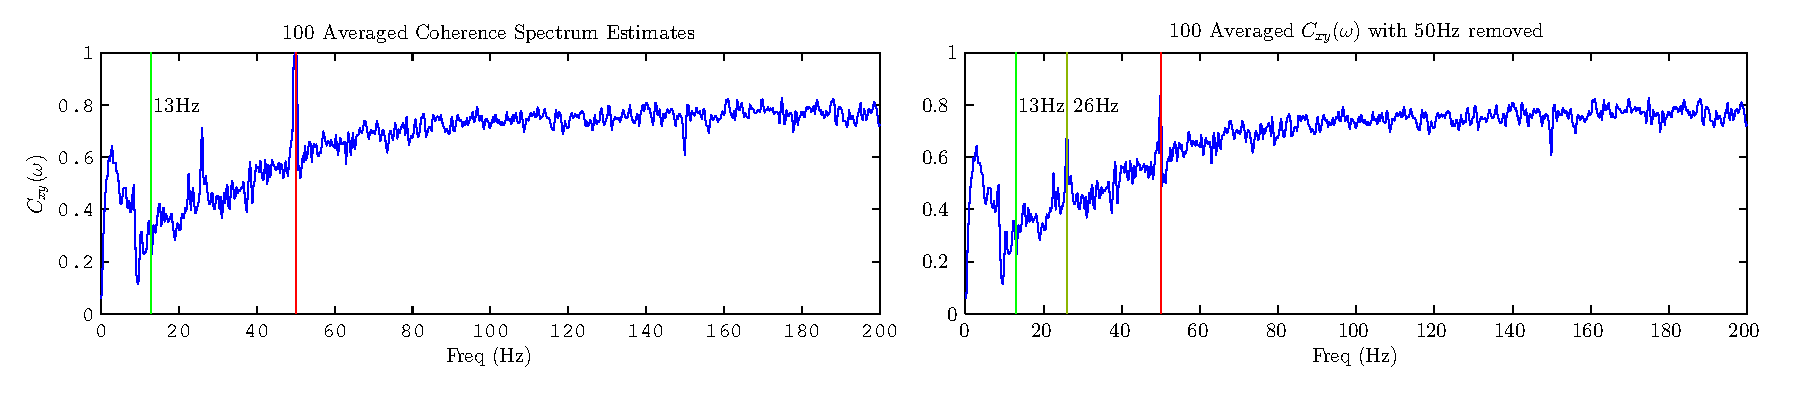
\includegraphics[width=\textwidth]{cw2im/1c1.eps}
{\footnotesize \textit{Note}: The \textcolor{LimeGreen}{green} line denotes the $13Hz$ line, the \textcolor{ForestGreen}{dark green} is $26Hz$ and the \textcolor{WildStrawberry}{red} line denotes $50Hz$ (power-line interference).}
\caption{Plot of the coherence between two-channel EEG data}
\label{fig:2_1c1}
\end{figure}
This time a two channel data is taken and we notice that in the coherency spectrum the expected $13Hz$ signal is present. Upon further investigation and with the help of figure \ref{fig:2_1c2} it was noticed that the \texttt{Cz} channel did not have any clear peaks at $13Hz$. However the first harmonic of the $13Hz$ is noticeable at $26Hz$.In figure \ref{fig:2_1c1} this is highlighted by the dark green line on the right graph (with the $50Hz$ power-line interference removed). While the $39$ and $52Hz$ harmonics would be expected their amplitude has decayed too much to be noticeable.
\begin{figure}[h!]
\centering
\resizebox{\textwidth}{!}{% This file was created by matlab2tikz v0.4.7 running on MATLAB 8.1.
% Copyright (c) 2008--2014, Nico Schlömer <nico.schloemer@gmail.com>
% All rights reserved.
% Minimal pgfplots version: 1.3
% 
% The latest updates can be retrieved from
%   http://www.mathworks.com/matlabcentral/fileexchange/22022-matlab2tikz
% where you can also make suggestions and rate matlab2tikz.
% 
\begin{tikzpicture}

\begin{axis}[%
width=4.2in,
height=1.4in,
scale only axis,
xmin=10,
xmax=30,
xtick={10, 11, 12, 13, 14, 15, 16, 17, 18, 19, 20, 21, 22, 23, 24, 25, 26, 27, 28, 29, 30},
xlabel={Freq (Hz)},
xmajorgrids,
ymin=-110,
ymax=-85,
ytick={-110, -105, -100,  -95,  -90,  -85},
ylabel={Amplitude (dB)},
ymajorgrids,
name=plot1,
title={POz data}
]
\addplot [color=blue,solid,forget plot]
  table[row sep=crcr]{9.99755859375	-88.6783483291956\\
10.0341796875	-89.2931426864257\\
10.07080078125	-87.8977237834536\\
10.107421875	-88.2892414845353\\
10.14404296875	-88.8401125508819\\
10.1806640625	-87.8945298696374\\
10.21728515625	-86.9729658882069\\
10.25390625	-87.6801067392057\\
10.29052734375	-88.6419098165882\\
10.3271484375	-89.2541947061321\\
10.36376953125	-89.4520434005418\\
10.400390625	-89.275917871641\\
10.43701171875	-89.4309866616519\\
10.4736328125	-89.944370862213\\
10.51025390625	-89.4804009424896\\
10.546875	-89.8178588439939\\
10.58349609375	-90.3023263719561\\
10.6201171875	-90.8689137853503\\
10.65673828125	-93.9689511028955\\
10.693359375	-92.2211693854919\\
10.72998046875	-91.8684723429788\\
10.7666015625	-93.2588327462791\\
10.80322265625	-93.5455353736482\\
10.83984375	-93.336329743574\\
10.87646484375	-92.0173099497116\\
10.9130859375	-91.8776277789436\\
10.94970703125	-93.9720736565885\\
10.986328125	-97.6886449583409\\
11.02294921875	-98.682417219687\\
11.0595703125	-97.0387709646102\\
11.09619140625	-96.7010045382304\\
11.1328125	-96.5841347267633\\
11.16943359375	-94.6771573625371\\
11.2060546875	-94.454685079134\\
11.24267578125	-95.9623870618678\\
11.279296875	-97.008388851633\\
11.31591796875	-97.6107675359633\\
11.3525390625	-96.7984948888122\\
11.38916015625	-97.4708605833123\\
11.42578125	-97.7280298515046\\
11.46240234375	-96.0607092727017\\
11.4990234375	-96.042033155686\\
11.53564453125	-97.8012966155608\\
11.572265625	-97.6960578702188\\
11.60888671875	-96.9170765850713\\
11.6455078125	-97.5401392278532\\
11.68212890625	-96.7270055297438\\
11.71875	-96.7994433842758\\
11.75537109375	-97.1748674460597\\
11.7919921875	-97.6403904506739\\
11.82861328125	-97.9370070107964\\
11.865234375	-100.04385920841\\
11.90185546875	-99.5725258815139\\
11.9384765625	-98.4623092255172\\
11.97509765625	-98.4221151404303\\
12.01171875	-98.3270094358265\\
12.04833984375	-97.5900248704592\\
12.0849609375	-96.8202553794339\\
12.12158203125	-98.295384405512\\
12.158203125	-98.6863157793125\\
12.19482421875	-96.4682008921691\\
12.2314453125	-96.5047042561751\\
12.26806640625	-98.2504919786624\\
12.3046875	-99.2436344276454\\
12.34130859375	-99.6812828125606\\
12.3779296875	-98.384933750891\\
12.41455078125	-97.4681344576244\\
12.451171875	-97.8806569287176\\
12.48779296875	-98.5581901134928\\
12.5244140625	-99.1930509260549\\
12.56103515625	-98.5120130183711\\
12.59765625	-98.5834004974654\\
12.63427734375	-98.7764086540701\\
12.6708984375	-98.5549798865333\\
12.70751953125	-98.4163193037139\\
12.744140625	-98.2254624582935\\
12.78076171875	-97.9007382709087\\
12.8173828125	-98.0685765387178\\
12.85400390625	-97.8643900867716\\
12.890625	-98.469482176384\\
12.92724609375	-97.4951641594839\\
12.9638671875	-90.3185367060525\\
13.00048828125	-87.4136448858721\\
13.037109375	-90.7177175786107\\
13.07373046875	-96.881075606598\\
13.1103515625	-98.4726661698014\\
13.14697265625	-98.766468981248\\
13.18359375	-99.629466804281\\
13.22021484375	-99.8623762275636\\
13.2568359375	-99.2003219966118\\
13.29345703125	-99.980292973193\\
13.330078125	-100.247434663221\\
13.36669921875	-98.8404744088619\\
13.4033203125	-99.1946481320442\\
13.43994140625	-99.1433534633641\\
13.4765625	-100.234097431919\\
13.51318359375	-99.9585728325319\\
13.5498046875	-99.6529726056442\\
13.58642578125	-100.209486586616\\
13.623046875	-99.1986165747324\\
13.65966796875	-99.5047623052237\\
13.6962890625	-99.5109815054149\\
13.73291015625	-99.3053926988409\\
13.76953125	-99.633821349042\\
13.80615234375	-100.333761577665\\
13.8427734375	-100.629414918785\\
13.87939453125	-100.601582170613\\
13.916015625	-100.723649135339\\
13.95263671875	-101.553607217651\\
13.9892578125	-99.6389345775918\\
14.02587890625	-98.8112671518745\\
14.0625	-100.828348681982\\
14.09912109375	-100.649692252086\\
14.1357421875	-101.641885982113\\
14.17236328125	-101.044306250617\\
14.208984375	-100.040068566423\\
14.24560546875	-101.578287182973\\
14.2822265625	-101.274730853645\\
14.31884765625	-100.493617373843\\
14.35546875	-100.981740355998\\
14.39208984375	-101.74488591805\\
14.4287109375	-103.429365696457\\
14.46533203125	-102.96063500754\\
14.501953125	-101.744108463784\\
14.53857421875	-101.222096623139\\
14.5751953125	-101.507710368506\\
14.61181640625	-101.454782401006\\
14.6484375	-100.826758442507\\
14.68505859375	-99.5465828121463\\
14.7216796875	-99.0915206360001\\
14.75830078125	-99.0658973635345\\
14.794921875	-99.4927170464975\\
14.83154296875	-101.429609663932\\
14.8681640625	-102.561132656707\\
14.90478515625	-100.87204558606\\
14.94140625	-100.23561816151\\
14.97802734375	-100.304338705461\\
15.0146484375	-100.758075040058\\
15.05126953125	-100.055401524922\\
15.087890625	-99.2447967809668\\
15.12451171875	-98.7561027698453\\
15.1611328125	-99.561422937975\\
15.19775390625	-100.794473276069\\
15.234375	-101.905800728253\\
15.27099609375	-103.105758488377\\
15.3076171875	-101.662416590181\\
15.34423828125	-100.862537787444\\
15.380859375	-101.471717541123\\
15.41748046875	-101.654542812815\\
15.4541015625	-101.067698770026\\
15.49072265625	-100.57662504819\\
15.52734375	-100.694197582012\\
15.56396484375	-100.765630148457\\
15.6005859375	-103.160192873429\\
15.63720703125	-103.250693367543\\
15.673828125	-101.799411003352\\
15.71044921875	-101.189487333755\\
15.7470703125	-100.967315615401\\
15.78369140625	-100.602354540567\\
15.8203125	-101.097385523489\\
15.85693359375	-101.030001425974\\
15.8935546875	-101.212222009273\\
15.93017578125	-101.264785352778\\
15.966796875	-99.1956632014001\\
16.00341796875	-98.3620165058938\\
16.0400390625	-101.206874572403\\
16.07666015625	-100.630983109427\\
16.11328125	-99.4539285288045\\
16.14990234375	-99.6362060888982\\
16.1865234375	-100.494934785225\\
16.22314453125	-101.173287352818\\
16.259765625	-101.72186189656\\
16.29638671875	-101.572395758742\\
16.3330078125	-101.056317054403\\
16.36962890625	-101.714565511349\\
16.40625	-101.238834738163\\
16.44287109375	-101.269904074826\\
16.4794921875	-101.702986304937\\
16.51611328125	-100.301441896449\\
16.552734375	-99.3093270162203\\
16.58935546875	-99.5886713264796\\
16.6259765625	-99.7031255290727\\
16.66259765625	-99.4255197464193\\
16.69921875	-100.355897676076\\
16.73583984375	-101.423486930028\\
16.7724609375	-101.802174920129\\
16.80908203125	-101.189093430163\\
16.845703125	-101.470844031851\\
16.88232421875	-100.917040077815\\
16.9189453125	-101.812489232611\\
16.95556640625	-102.082429943902\\
16.9921875	-100.948425785338\\
17.02880859375	-101.460144624343\\
17.0654296875	-101.744417333817\\
17.10205078125	-102.185765227706\\
17.138671875	-102.771166241036\\
17.17529296875	-101.408263168482\\
17.2119140625	-100.452808801065\\
17.24853515625	-99.9146983090842\\
17.28515625	-102.112981429798\\
17.32177734375	-102.701410930624\\
17.3583984375	-100.679840908031\\
17.39501953125	-100.720300664112\\
17.431640625	-101.173681940866\\
17.46826171875	-101.38827120724\\
17.5048828125	-100.579354687425\\
17.54150390625	-101.131555566865\\
17.578125	-102.150232143238\\
17.61474609375	-100.108889232241\\
17.6513671875	-100.317120548521\\
17.68798828125	-101.846122425032\\
17.724609375	-101.125941295127\\
17.76123046875	-99.929400216122\\
17.7978515625	-101.074491984368\\
17.83447265625	-101.959692135807\\
17.87109375	-100.929240707682\\
17.90771484375	-100.583277454296\\
17.9443359375	-100.565896812509\\
17.98095703125	-100.437939638606\\
18.017578125	-100.739049986556\\
18.05419921875	-101.946454673362\\
18.0908203125	-101.134406672509\\
18.12744140625	-99.3265857707436\\
18.1640625	-98.8715151699969\\
18.20068359375	-99.3130867642103\\
18.2373046875	-100.581003778275\\
18.27392578125	-99.9181442341715\\
18.310546875	-100.944052946018\\
18.34716796875	-102.024240632723\\
18.3837890625	-100.806607932465\\
18.42041015625	-99.9463082483334\\
18.45703125	-99.7095110661096\\
18.49365234375	-100.009286588795\\
18.5302734375	-99.5807577730358\\
18.56689453125	-100.733673680866\\
18.603515625	-100.469546017087\\
18.64013671875	-101.112707209287\\
18.6767578125	-101.234171442623\\
18.71337890625	-100.701636552378\\
18.75	-101.097353170047\\
18.78662109375	-100.787759708449\\
18.8232421875	-100.323997127208\\
18.85986328125	-100.088934802921\\
18.896484375	-100.780504556131\\
18.93310546875	-101.694355335754\\
18.9697265625	-101.762311181794\\
19.00634765625	-101.158872790723\\
19.04296875	-100.865317367757\\
19.07958984375	-101.305501203191\\
19.1162109375	-102.573895527429\\
19.15283203125	-101.669083452069\\
19.189453125	-100.941625301845\\
19.22607421875	-100.827036505374\\
19.2626953125	-100.837462719115\\
19.29931640625	-101.079974513765\\
19.3359375	-102.148204921686\\
19.37255859375	-103.292476166292\\
19.4091796875	-101.385591752125\\
19.44580078125	-100.608393849275\\
19.482421875	-101.690568616518\\
19.51904296875	-101.606255625628\\
19.5556640625	-101.733627237932\\
19.59228515625	-101.588135413245\\
19.62890625	-101.842600515281\\
19.66552734375	-102.06808090938\\
19.7021484375	-100.053983512\\
19.73876953125	-99.8278981597374\\
19.775390625	-100.73960299731\\
19.81201171875	-100.514355403068\\
19.8486328125	-100.311421256651\\
19.88525390625	-100.343493450204\\
19.921875	-100.053712167025\\
19.95849609375	-99.8777407302667\\
19.9951171875	-100.302111449626\\
20.03173828125	-99.656716858752\\
20.068359375	-99.6014954512128\\
20.10498046875	-101.751049736559\\
20.1416015625	-103.608544673162\\
20.17822265625	-100.794870512212\\
20.21484375	-99.526690403789\\
20.25146484375	-100.327722825857\\
20.2880859375	-101.289137202445\\
20.32470703125	-102.798384655673\\
20.361328125	-102.228801393131\\
20.39794921875	-101.333804366733\\
20.4345703125	-102.955614589275\\
20.47119140625	-102.191944935833\\
20.5078125	-102.059746020765\\
20.54443359375	-102.276874502855\\
20.5810546875	-101.871331695495\\
20.61767578125	-101.373873132818\\
20.654296875	-101.487607757195\\
20.69091796875	-100.531969293578\\
20.7275390625	-100.676230875833\\
20.76416015625	-100.854424150562\\
20.80078125	-100.769942761821\\
20.83740234375	-102.746600537625\\
20.8740234375	-103.820756597823\\
20.91064453125	-102.332818353471\\
20.947265625	-101.756171189513\\
20.98388671875	-101.888642211237\\
21.0205078125	-101.894446142807\\
21.05712890625	-101.793711870915\\
21.09375	-100.996209481432\\
21.13037109375	-100.964709151712\\
21.1669921875	-101.764580910931\\
21.20361328125	-101.218235092403\\
21.240234375	-100.889497650566\\
21.27685546875	-101.195927725613\\
21.3134765625	-101.835732265051\\
21.35009765625	-102.941590366823\\
21.38671875	-103.223375123472\\
21.42333984375	-101.917967967255\\
21.4599609375	-100.740540044114\\
21.49658203125	-101.178346863872\\
21.533203125	-101.630426990111\\
21.56982421875	-102.23731072561\\
21.6064453125	-103.461606955873\\
21.64306640625	-103.401473148243\\
21.6796875	-101.728629015324\\
21.71630859375	-102.008340592301\\
21.7529296875	-102.201423541077\\
21.78955078125	-102.702633823359\\
21.826171875	-103.40878017834\\
21.86279296875	-103.534795881823\\
21.8994140625	-102.859352117109\\
21.93603515625	-101.964535691642\\
21.97265625	-102.738170043869\\
22.00927734375	-103.439246152839\\
22.0458984375	-103.661040868934\\
22.08251953125	-103.476908707528\\
22.119140625	-102.671961907372\\
22.15576171875	-102.384596759604\\
22.1923828125	-102.803559535626\\
22.22900390625	-103.337007666097\\
22.265625	-102.770945976529\\
22.30224609375	-102.297988346684\\
22.3388671875	-102.114868533348\\
22.37548828125	-101.297522707691\\
22.412109375	-101.614092249909\\
22.44873046875	-102.233350670376\\
22.4853515625	-101.413759288336\\
22.52197265625	-101.347428045738\\
22.55859375	-102.094212615435\\
22.59521484375	-101.328042092697\\
22.6318359375	-101.229463400182\\
22.66845703125	-102.76940059255\\
22.705078125	-101.586814197591\\
22.74169921875	-100.858825353489\\
22.7783203125	-101.303441273141\\
22.81494140625	-102.383668503425\\
22.8515625	-102.088025299169\\
22.88818359375	-102.808551239451\\
22.9248046875	-103.810755533986\\
22.96142578125	-103.620260978931\\
22.998046875	-103.732578211916\\
23.03466796875	-103.72341683933\\
23.0712890625	-103.092575254556\\
23.10791015625	-103.386628341835\\
23.14453125	-102.070819597716\\
23.18115234375	-101.456202487262\\
23.2177734375	-102.928032600781\\
23.25439453125	-103.38687514658\\
23.291015625	-102.89021420028\\
23.32763671875	-102.631829114351\\
23.3642578125	-103.087099350687\\
23.40087890625	-102.562819033118\\
23.4375	-101.298558843681\\
23.47412109375	-101.947819904488\\
23.5107421875	-103.046660229028\\
23.54736328125	-102.859802213518\\
23.583984375	-103.298611036624\\
23.62060546875	-102.531131840359\\
23.6572265625	-102.165999370767\\
23.69384765625	-102.259319968856\\
23.73046875	-103.11666737001\\
23.76708984375	-103.841723016283\\
23.8037109375	-104.059838762119\\
23.84033203125	-103.807950911339\\
23.876953125	-102.373770557014\\
23.91357421875	-102.798127789172\\
23.9501953125	-104.534639634462\\
23.98681640625	-103.765542706743\\
24.0234375	-102.922137771756\\
24.06005859375	-103.273751807949\\
24.0966796875	-105.87450974052\\
24.13330078125	-105.226720741633\\
24.169921875	-104.402768257123\\
24.20654296875	-103.735580950427\\
24.2431640625	-103.10298836902\\
24.27978515625	-102.778826788858\\
24.31640625	-102.951129715018\\
24.35302734375	-102.639842237734\\
24.3896484375	-101.64704617631\\
24.42626953125	-102.735039621368\\
24.462890625	-103.545161546874\\
24.49951171875	-103.463622717793\\
24.5361328125	-105.578682556744\\
24.57275390625	-104.114740934649\\
24.609375	-103.177327905313\\
24.64599609375	-103.081721045675\\
24.6826171875	-103.232963941949\\
24.71923828125	-103.22335763145\\
24.755859375	-102.477035977639\\
24.79248046875	-101.137433937577\\
24.8291015625	-100.637906154376\\
24.86572265625	-101.952424523399\\
24.90234375	-103.251997302533\\
24.93896484375	-103.375713741874\\
24.9755859375	-101.467952435195\\
25.01220703125	-102.172524994388\\
25.048828125	-103.654588303274\\
25.08544921875	-103.046880207544\\
25.1220703125	-102.574193495976\\
25.15869140625	-101.361253520265\\
25.1953125	-101.719856549004\\
25.23193359375	-101.805340838487\\
25.2685546875	-100.848641992595\\
25.30517578125	-102.822695737988\\
25.341796875	-103.845845362061\\
25.37841796875	-102.714940260842\\
25.4150390625	-102.376886953507\\
25.45166015625	-103.398757799077\\
25.48828125	-103.015155881827\\
25.52490234375	-100.785442297128\\
25.5615234375	-100.522706473225\\
25.59814453125	-101.053902196801\\
25.634765625	-101.15966648594\\
25.67138671875	-100.703592208286\\
25.7080078125	-100.433635791583\\
25.74462890625	-100.992993093629\\
25.78125	-101.390771872225\\
25.81787109375	-100.222132972241\\
25.8544921875	-99.8390618122773\\
25.89111328125	-100.144280999337\\
25.927734375	-97.8161388267733\\
25.96435546875	-92.9816808436021\\
26.0009765625	-90.9940877605368\\
26.03759765625	-94.813665068339\\
26.07421875	-99.6585730925571\\
26.11083984375	-100.710096205923\\
26.1474609375	-101.449964802729\\
26.18408203125	-101.471983464827\\
26.220703125	-101.295931774589\\
26.25732421875	-101.822211935818\\
26.2939453125	-101.6470482909\\
26.33056640625	-101.546248682045\\
26.3671875	-102.503604978139\\
26.40380859375	-102.97471756101\\
26.4404296875	-101.936342550378\\
26.47705078125	-101.741507366647\\
26.513671875	-102.317888033747\\
26.55029296875	-103.7675539\\
26.5869140625	-103.725087218865\\
26.62353515625	-102.854525246971\\
26.66015625	-103.511408788759\\
26.69677734375	-103.401664746429\\
26.7333984375	-102.802282959899\\
26.77001953125	-102.422376903398\\
26.806640625	-102.620801983374\\
26.84326171875	-103.488539464947\\
26.8798828125	-103.226277149631\\
26.91650390625	-104.215088213146\\
26.953125	-104.453225651856\\
26.98974609375	-102.612426543214\\
27.0263671875	-102.380514967229\\
27.06298828125	-103.485800626537\\
27.099609375	-105.276187650125\\
27.13623046875	-104.100736736273\\
27.1728515625	-103.137429817511\\
27.20947265625	-103.976643090218\\
27.24609375	-103.259124731067\\
27.28271484375	-103.085478455619\\
27.3193359375	-102.685762669442\\
27.35595703125	-102.937268732766\\
27.392578125	-104.429774498693\\
27.42919921875	-103.377567670482\\
27.4658203125	-102.856063211068\\
27.50244140625	-102.869471933338\\
27.5390625	-103.30377209275\\
27.57568359375	-104.155237115016\\
27.6123046875	-105.020814905443\\
27.64892578125	-104.72630967174\\
27.685546875	-103.741739156113\\
27.72216796875	-103.727057009571\\
27.7587890625	-103.428935188581\\
27.79541015625	-103.539314209105\\
27.83203125	-104.418874129753\\
27.86865234375	-104.607964687775\\
27.9052734375	-104.98921963925\\
27.94189453125	-105.119155880035\\
27.978515625	-102.053805602445\\
28.01513671875	-101.334383254716\\
28.0517578125	-103.667428901043\\
28.08837890625	-105.203263061412\\
28.125	-103.988690806238\\
28.16162109375	-103.21045265256\\
28.1982421875	-103.801704204494\\
28.23486328125	-105.91809212726\\
28.271484375	-105.685382895983\\
28.30810546875	-104.142502947308\\
28.3447265625	-105.269861634947\\
28.38134765625	-104.917623561606\\
28.41796875	-104.983505549928\\
28.45458984375	-105.570706062839\\
28.4912109375	-104.24935629536\\
28.52783203125	-104.474819790318\\
28.564453125	-103.90895204382\\
28.60107421875	-103.520209507384\\
28.6376953125	-104.410336428277\\
28.67431640625	-104.512892315161\\
28.7109375	-104.607118664793\\
28.74755859375	-104.929396753068\\
28.7841796875	-106.46325793555\\
28.82080078125	-105.339459948492\\
28.857421875	-104.807997080418\\
28.89404296875	-104.854874584009\\
28.9306640625	-105.488205862529\\
28.96728515625	-105.418758163723\\
29.00390625	-104.230782989794\\
29.04052734375	-104.556118069819\\
29.0771484375	-104.768184055114\\
29.11376953125	-105.305593667185\\
29.150390625	-106.5155479499\\
29.18701171875	-106.901482932774\\
29.2236328125	-106.4466997781\\
29.26025390625	-105.838151178822\\
29.296875	-105.789063279315\\
29.33349609375	-106.298077259095\\
29.3701171875	-105.495069537417\\
29.40673828125	-104.094795851284\\
29.443359375	-103.535365810222\\
29.47998046875	-103.501364057325\\
29.5166015625	-104.573131011008\\
29.55322265625	-106.151530685601\\
29.58984375	-106.303909710203\\
29.62646484375	-104.596955354414\\
29.6630859375	-104.272711968581\\
29.69970703125	-105.595311152087\\
29.736328125	-107.152876126045\\
29.77294921875	-105.929165199232\\
29.8095703125	-104.849406386619\\
29.84619140625	-105.596714210061\\
29.8828125	-105.64933214264\\
29.91943359375	-106.598298791076\\
29.9560546875	-104.918853740003\\
29.99267578125	-103.140660800907\\
};
\end{axis}

\begin{axis}[%
width=4.2in,
height=1.4in,
scale only axis,
xmin=10,
xmax=30,
xtick={10, 11, 12, 13, 14, 15, 16, 17, 18, 19, 20, 21, 22, 23, 24, 25, 26, 27, 28, 29, 30},
xlabel={Freq (Hz)},
xmajorgrids,
ymin=-110,
ymax=-85,
ytick={-110, -105, -100,  -95,  -90,  -85},
ymajorgrids,
at=(plot1.right of south east),
anchor=left of south west,
title={Cz data}
]
\addplot [color=blue,solid,forget plot]
  table[row sep=crcr]{9.99755859375	-91.016277474563\\
10.0341796875	-92.766067424989\\
10.07080078125	-91.3068727759685\\
10.107421875	-91.1164592140995\\
10.14404296875	-90.7207417074515\\
10.1806640625	-88.5465832555033\\
10.21728515625	-88.0701773956895\\
10.25390625	-89.1158015215999\\
10.29052734375	-89.3086074700142\\
10.3271484375	-89.7520960030159\\
10.36376953125	-90.9572907140208\\
10.400390625	-91.3906908380155\\
10.43701171875	-91.1177633911488\\
10.4736328125	-91.3786489643776\\
10.51025390625	-92.3410839433668\\
10.546875	-93.7002820069912\\
10.58349609375	-93.9470737620371\\
10.6201171875	-93.4848603657769\\
10.65673828125	-95.2200437663706\\
10.693359375	-93.0494021429124\\
10.72998046875	-93.4434968346008\\
10.7666015625	-97.2613660029577\\
10.80322265625	-96.0776850368716\\
10.83984375	-94.9162200154525\\
10.87646484375	-94.1802170726216\\
10.9130859375	-93.9585042081939\\
10.94970703125	-93.9098268671693\\
10.986328125	-93.7445521850556\\
11.02294921875	-95.5742633815971\\
11.0595703125	-96.7824236791571\\
11.09619140625	-94.6712079431534\\
11.1328125	-95.4103763069365\\
11.16943359375	-96.2430455835742\\
11.2060546875	-95.0766646844419\\
11.24267578125	-94.7151615012468\\
11.279296875	-95.6340932931912\\
11.31591796875	-97.0511191495358\\
11.3525390625	-98.5570765791995\\
11.38916015625	-96.5476121047395\\
11.42578125	-94.8332957623541\\
11.46240234375	-95.850447252411\\
11.4990234375	-96.4655083708859\\
11.53564453125	-96.4633710708633\\
11.572265625	-97.4474466733938\\
11.60888671875	-97.8595476012845\\
11.6455078125	-97.0585482984592\\
11.68212890625	-96.7267835381602\\
11.71875	-96.3360973284819\\
11.75537109375	-96.7641167937432\\
11.7919921875	-97.8413056849235\\
11.82861328125	-98.6183899659065\\
11.865234375	-99.6329353751521\\
11.90185546875	-99.4108959870115\\
11.9384765625	-97.3185262557488\\
11.97509765625	-95.8164530128576\\
12.01171875	-96.0832942688402\\
12.04833984375	-96.8067487881222\\
12.0849609375	-97.8351466851302\\
12.12158203125	-97.5917845474923\\
12.158203125	-97.666204724885\\
12.19482421875	-97.3363948142896\\
12.2314453125	-97.6776202411516\\
12.26806640625	-98.5988257492053\\
12.3046875	-97.8000073630435\\
12.34130859375	-97.9869929500676\\
12.3779296875	-98.5713902847783\\
12.41455078125	-97.9645613968465\\
12.451171875	-98.1550922748697\\
12.48779296875	-98.8710090234495\\
12.5244140625	-99.5498661074475\\
12.56103515625	-99.4882088060612\\
12.59765625	-98.7324030840855\\
12.63427734375	-100.906784694563\\
12.6708984375	-99.3550992546202\\
12.70751953125	-97.641063853535\\
12.744140625	-97.4160556638574\\
12.78076171875	-97.8859335405938\\
12.8173828125	-98.413832313301\\
12.85400390625	-98.2904773742347\\
12.890625	-98.8584460294252\\
12.92724609375	-98.7313288693119\\
12.9638671875	-96.6992988878509\\
13.00048828125	-95.7441575062522\\
13.037109375	-96.6883480591335\\
13.07373046875	-98.5441002088246\\
13.1103515625	-99.2206147250286\\
13.14697265625	-99.4926137385228\\
13.18359375	-99.0372471819819\\
13.22021484375	-98.560188459389\\
13.2568359375	-99.7258877074487\\
13.29345703125	-100.64095529172\\
13.330078125	-101.567608505462\\
13.36669921875	-101.248769584807\\
13.4033203125	-101.031506131982\\
13.43994140625	-100.088393578782\\
13.4765625	-98.920453744605\\
13.51318359375	-99.3547484455581\\
13.5498046875	-99.6478388053102\\
13.58642578125	-98.9025537870889\\
13.623046875	-98.9893425225774\\
13.65966796875	-100.853499115103\\
13.6962890625	-100.97213333972\\
13.73291015625	-100.656714426565\\
13.76953125	-100.723052387753\\
13.80615234375	-100.854409887876\\
13.8427734375	-100.271613462021\\
13.87939453125	-98.3544513640212\\
13.916015625	-98.8514891093382\\
13.95263671875	-99.73722691703\\
13.9892578125	-99.7280859129221\\
14.02587890625	-99.6522990524948\\
14.0625	-99.7633946302711\\
14.09912109375	-100.413383188018\\
14.1357421875	-99.8932865232987\\
14.17236328125	-100.127450815689\\
14.208984375	-101.213413968969\\
14.24560546875	-101.481186950867\\
14.2822265625	-99.8142299127297\\
14.31884765625	-100.182604086117\\
14.35546875	-101.539087446203\\
14.39208984375	-100.592847962464\\
14.4287109375	-101.009434450174\\
14.46533203125	-101.574748659898\\
14.501953125	-100.586607811403\\
14.53857421875	-100.406868994659\\
14.5751953125	-100.929002791253\\
14.61181640625	-100.570011872722\\
14.6484375	-98.9319699331187\\
14.68505859375	-98.3477597950262\\
14.7216796875	-98.5088076843813\\
14.75830078125	-99.3849193927213\\
14.794921875	-99.4623853099829\\
14.83154296875	-100.169438556292\\
14.8681640625	-101.532501863746\\
14.90478515625	-101.184008636468\\
14.94140625	-100.074408323002\\
14.97802734375	-100.670359172282\\
15.0146484375	-102.314046012157\\
15.05126953125	-102.141765891444\\
15.087890625	-99.8931787614053\\
15.12451171875	-99.7541234723829\\
15.1611328125	-100.385058436612\\
15.19775390625	-101.583427069185\\
15.234375	-102.471294838786\\
15.27099609375	-101.828431936058\\
15.3076171875	-100.969377720128\\
15.34423828125	-100.428443895805\\
15.380859375	-100.421130527818\\
15.41748046875	-100.944042589697\\
15.4541015625	-101.138234140473\\
15.49072265625	-100.712142473519\\
15.52734375	-101.47511337315\\
15.56396484375	-100.410730695311\\
15.6005859375	-100.593043984281\\
15.63720703125	-100.925124072545\\
15.673828125	-100.335552781903\\
15.71044921875	-100.90007722722\\
15.7470703125	-102.002765380052\\
15.78369140625	-100.420799203364\\
15.8203125	-99.1844966589237\\
15.85693359375	-98.8263856697817\\
15.8935546875	-99.6531253760999\\
15.93017578125	-100.785602998166\\
15.966796875	-99.8777041781819\\
16.00341796875	-100.091375252137\\
16.0400390625	-102.340963882058\\
16.07666015625	-102.338835437977\\
16.11328125	-102.569940849017\\
16.14990234375	-101.839145165473\\
16.1865234375	-100.911789389798\\
16.22314453125	-101.091924393852\\
16.259765625	-100.955797071123\\
16.29638671875	-100.98363728052\\
16.3330078125	-101.385456767823\\
16.36962890625	-102.209723499263\\
16.40625	-100.667386334009\\
16.44287109375	-99.7455675251529\\
16.4794921875	-100.690624024104\\
16.51611328125	-102.077859536524\\
16.552734375	-101.962883442791\\
16.58935546875	-101.320737499616\\
16.6259765625	-100.711301155159\\
16.66259765625	-99.205984266507\\
16.69921875	-99.1607616658619\\
16.73583984375	-100.02783637645\\
16.7724609375	-101.10184955472\\
16.80908203125	-100.170602474619\\
16.845703125	-101.206420250735\\
16.88232421875	-102.003558371102\\
16.9189453125	-102.333211263127\\
16.95556640625	-99.9927539998462\\
16.9921875	-99.1718922652766\\
17.02880859375	-100.399652377652\\
17.0654296875	-101.71502662215\\
17.10205078125	-101.579914370087\\
17.138671875	-101.266279579886\\
17.17529296875	-101.271774694001\\
17.2119140625	-101.11406757743\\
17.24853515625	-101.429966547288\\
17.28515625	-103.255771209872\\
17.32177734375	-102.480493290127\\
17.3583984375	-100.542922357844\\
17.39501953125	-100.88913340491\\
17.431640625	-101.728389252579\\
17.46826171875	-101.333066688841\\
17.5048828125	-100.291252932116\\
17.54150390625	-100.602491312051\\
17.578125	-101.323484001941\\
17.61474609375	-99.0171017649444\\
17.6513671875	-99.7657968470994\\
17.68798828125	-102.244811926392\\
17.724609375	-100.369132778063\\
17.76123046875	-99.1199857215989\\
17.7978515625	-100.634182349405\\
17.83447265625	-102.613472087228\\
17.87109375	-101.179331216007\\
17.90771484375	-100.907418309976\\
17.9443359375	-100.370363479893\\
17.98095703125	-99.9261048453413\\
18.017578125	-100.649785977983\\
18.05419921875	-102.273173513593\\
18.0908203125	-103.024414037433\\
18.12744140625	-100.353662330751\\
18.1640625	-98.8628621266814\\
18.20068359375	-99.1274464379028\\
18.2373046875	-101.201253048128\\
18.27392578125	-102.124346270878\\
18.310546875	-101.545051561709\\
18.34716796875	-99.8318108237086\\
18.3837890625	-98.9056771569773\\
18.42041015625	-99.8729596342066\\
18.45703125	-99.3674743541295\\
18.49365234375	-99.8803909878057\\
18.5302734375	-100.38203561312\\
18.56689453125	-100.382052057232\\
18.603515625	-99.5511410004711\\
18.64013671875	-99.1371704283006\\
18.6767578125	-99.4459043064603\\
18.71337890625	-100.570556795903\\
18.75	-100.867338115066\\
18.78662109375	-100.654915729906\\
18.8232421875	-100.285121370138\\
18.85986328125	-100.273493182835\\
18.896484375	-99.2815339037955\\
18.93310546875	-98.4281665053284\\
18.9697265625	-99.1821676556068\\
19.00634765625	-99.2038172128122\\
19.04296875	-98.7351504122602\\
19.07958984375	-99.4565862180079\\
19.1162109375	-100.372186360806\\
19.15283203125	-100.521598986915\\
19.189453125	-100.565148141182\\
19.22607421875	-101.900039653949\\
19.2626953125	-101.712614168216\\
19.29931640625	-100.227893768779\\
19.3359375	-100.35138830926\\
19.37255859375	-100.159283788803\\
19.4091796875	-99.945382479744\\
19.44580078125	-100.831712187399\\
19.482421875	-100.77486613105\\
19.51904296875	-100.219329054959\\
19.5556640625	-100.295000930329\\
19.59228515625	-100.262481103501\\
19.62890625	-99.721313838671\\
19.66552734375	-99.9002771491103\\
19.7021484375	-100.811997176796\\
19.73876953125	-101.190261017378\\
19.775390625	-101.578515089568\\
19.81201171875	-101.660598146572\\
19.8486328125	-101.435511058917\\
19.88525390625	-101.697543428685\\
19.921875	-101.755221887762\\
19.95849609375	-101.40708697318\\
19.9951171875	-102.006526166567\\
20.03173828125	-101.877968788826\\
20.068359375	-102.204824995878\\
20.10498046875	-102.660841165494\\
20.1416015625	-102.082671391352\\
20.17822265625	-100.628953013553\\
20.21484375	-100.235817446625\\
20.25146484375	-99.973995422128\\
20.2880859375	-100.962246033796\\
20.32470703125	-103.479677609089\\
20.361328125	-103.604687343839\\
20.39794921875	-102.502224979666\\
20.4345703125	-103.864849127231\\
20.47119140625	-103.166298105237\\
20.5078125	-102.898927957918\\
20.54443359375	-103.331978086882\\
20.5810546875	-102.432243372656\\
20.61767578125	-101.008146057945\\
20.654296875	-100.68086922181\\
20.69091796875	-101.113224251752\\
20.7275390625	-101.429085471184\\
20.76416015625	-100.496051224354\\
20.80078125	-101.154470295581\\
20.83740234375	-102.991578879026\\
20.8740234375	-103.349454369688\\
20.91064453125	-103.37055557615\\
20.947265625	-102.750134886118\\
20.98388671875	-102.168735150916\\
21.0205078125	-101.348886794747\\
21.05712890625	-102.20383120111\\
21.09375	-103.118329198371\\
21.13037109375	-102.407226268242\\
21.1669921875	-101.262043397747\\
21.20361328125	-100.525714347581\\
21.240234375	-100.113139832602\\
21.27685546875	-101.286943081265\\
21.3134765625	-101.455514916831\\
21.35009765625	-100.977500316202\\
21.38671875	-102.637451283463\\
21.42333984375	-102.454848974971\\
21.4599609375	-101.393709123086\\
21.49658203125	-101.602753196126\\
21.533203125	-102.911714342222\\
21.56982421875	-103.235913675358\\
21.6064453125	-102.765364350977\\
21.64306640625	-102.413473491556\\
21.6796875	-100.747923987597\\
21.71630859375	-100.611686727034\\
21.7529296875	-101.628822340903\\
21.78955078125	-104.352985788939\\
21.826171875	-104.655180113128\\
21.86279296875	-103.430134280546\\
21.8994140625	-102.509147334633\\
21.93603515625	-102.257953751996\\
21.97265625	-102.183622244939\\
22.00927734375	-102.599484685204\\
22.0458984375	-102.951701836647\\
22.08251953125	-102.770024990826\\
22.119140625	-102.218696205077\\
22.15576171875	-102.737805528433\\
22.1923828125	-102.50971519695\\
22.22900390625	-102.989330119544\\
22.265625	-103.136283922079\\
22.30224609375	-103.431501704766\\
22.3388671875	-102.542711363295\\
22.37548828125	-101.930528376621\\
22.412109375	-103.717626719642\\
22.44873046875	-104.028679891705\\
22.4853515625	-101.517488874239\\
22.52197265625	-101.041959709144\\
22.55859375	-101.870574064798\\
22.59521484375	-101.796352800062\\
22.6318359375	-102.373891115795\\
22.66845703125	-101.783639333668\\
22.705078125	-100.428054067205\\
22.74169921875	-100.823393767343\\
22.7783203125	-102.345259488095\\
22.81494140625	-103.089305649873\\
22.8515625	-102.858756802975\\
22.88818359375	-104.389174669571\\
22.9248046875	-103.876898781471\\
22.96142578125	-102.166776027645\\
22.998046875	-103.60927105958\\
23.03466796875	-103.849646024249\\
23.0712890625	-103.57155436141\\
23.10791015625	-102.853445936265\\
23.14453125	-101.800883711736\\
23.18115234375	-102.093889020642\\
23.2177734375	-103.200380284826\\
23.25439453125	-104.112738357073\\
23.291015625	-103.478197468575\\
23.32763671875	-102.499232263875\\
23.3642578125	-101.9393976859\\
23.40087890625	-101.566481193812\\
23.4375	-101.48860394195\\
23.47412109375	-101.769793772035\\
23.5107421875	-102.518566711304\\
23.54736328125	-102.98614579804\\
23.583984375	-102.949493445368\\
23.62060546875	-102.571762368215\\
23.6572265625	-102.321132782872\\
23.69384765625	-102.983613790012\\
23.73046875	-103.469597807546\\
23.76708984375	-103.100620566367\\
23.8037109375	-103.038989114903\\
23.84033203125	-102.257970446304\\
23.876953125	-102.085851536456\\
23.91357421875	-102.796876525694\\
23.9501953125	-103.547942809504\\
23.98681640625	-103.982512819522\\
24.0234375	-105.038605247226\\
24.06005859375	-104.779952680029\\
24.0966796875	-103.840165762186\\
24.13330078125	-104.308587762038\\
24.169921875	-105.14864248805\\
24.20654296875	-104.45726339456\\
24.2431640625	-102.998058520542\\
24.27978515625	-102.449776584511\\
24.31640625	-103.290033764382\\
24.35302734375	-104.164271732227\\
24.3896484375	-104.583660418859\\
24.42626953125	-105.292237663989\\
24.462890625	-103.7231600221\\
24.49951171875	-102.82609989822\\
24.5361328125	-104.307465054658\\
24.57275390625	-105.65084561782\\
24.609375	-104.988182982407\\
24.64599609375	-103.232190366625\\
24.6826171875	-102.327937195256\\
24.71923828125	-102.185419534376\\
24.755859375	-102.763874558629\\
24.79248046875	-102.970698293924\\
24.8291015625	-103.680093131169\\
24.86572265625	-104.607959796092\\
24.90234375	-103.779333467554\\
24.93896484375	-102.328098717331\\
24.9755859375	-102.215228685354\\
25.01220703125	-103.537718105036\\
25.048828125	-103.86705955601\\
25.08544921875	-103.1503038824\\
25.1220703125	-103.358109928146\\
25.15869140625	-103.783744627467\\
25.1953125	-103.111980592295\\
25.23193359375	-102.004099404057\\
25.2685546875	-100.71809846777\\
25.30517578125	-100.871332723902\\
25.341796875	-102.857572597377\\
25.37841796875	-103.980798352102\\
25.4150390625	-102.986142251406\\
25.45166015625	-103.756010650442\\
25.48828125	-102.817730567092\\
25.52490234375	-101.389191331981\\
25.5615234375	-102.659861383873\\
25.59814453125	-102.884896985901\\
25.634765625	-102.965350140927\\
25.67138671875	-102.418401243863\\
25.7080078125	-102.567962786104\\
25.74462890625	-102.435060767431\\
25.78125	-102.023324549077\\
25.81787109375	-101.915649794142\\
25.8544921875	-103.175681300107\\
25.89111328125	-103.748279315085\\
25.927734375	-101.006064964961\\
25.96435546875	-94.5849670809366\\
26.0009765625	-92.5088375140421\\
26.03759765625	-96.7919363086618\\
26.07421875	-101.993822466674\\
26.11083984375	-102.474329203339\\
26.1474609375	-102.148172603816\\
26.18408203125	-102.993146011267\\
26.220703125	-103.459760987213\\
26.25732421875	-103.250630876356\\
26.2939453125	-103.061286358064\\
26.33056640625	-103.689074650378\\
26.3671875	-104.453932073615\\
26.40380859375	-102.692009304482\\
26.4404296875	-102.26142003706\\
26.47705078125	-102.395112194695\\
26.513671875	-102.245490683885\\
26.55029296875	-104.272666606339\\
26.5869140625	-104.567726513132\\
26.62353515625	-104.189009488575\\
26.66015625	-105.018265411873\\
26.69677734375	-102.209611332293\\
26.7333984375	-102.499349086974\\
26.77001953125	-103.007156016417\\
26.806640625	-103.137259119579\\
26.84326171875	-104.550918276907\\
26.8798828125	-103.722735273122\\
26.91650390625	-103.617827975657\\
26.953125	-104.050889914827\\
26.98974609375	-102.52672339324\\
27.0263671875	-102.672538509062\\
27.06298828125	-103.462920244038\\
27.099609375	-104.554532293407\\
27.13623046875	-104.146811769764\\
27.1728515625	-103.383820209562\\
27.20947265625	-104.694334797383\\
27.24609375	-104.539306971532\\
27.28271484375	-104.403991551098\\
27.3193359375	-104.714424991421\\
27.35595703125	-105.157460384188\\
27.392578125	-105.234701063954\\
27.42919921875	-104.082801730832\\
27.4658203125	-103.931254996772\\
27.50244140625	-103.358000952015\\
27.5390625	-103.995775455812\\
27.57568359375	-105.15706210654\\
27.6123046875	-104.980213616092\\
27.64892578125	-103.954625901481\\
27.685546875	-103.38371869929\\
27.72216796875	-103.883904375274\\
27.7587890625	-104.866955795295\\
27.79541015625	-104.943925146811\\
27.83203125	-105.068277580675\\
27.86865234375	-104.323620887551\\
27.9052734375	-104.349920686683\\
27.94189453125	-105.285050767476\\
27.978515625	-104.134957106507\\
28.01513671875	-102.908188011928\\
28.0517578125	-103.886290992993\\
28.08837890625	-105.778925743424\\
28.125	-103.184202569044\\
28.16162109375	-102.814604460946\\
28.1982421875	-105.477308660265\\
28.23486328125	-106.04007316651\\
28.271484375	-105.076617202488\\
28.30810546875	-104.376702534956\\
28.3447265625	-104.866887440232\\
28.38134765625	-105.233905395931\\
28.41796875	-105.861409343536\\
28.45458984375	-105.517873026637\\
28.4912109375	-104.804494663491\\
28.52783203125	-105.736887984475\\
28.564453125	-104.973491462931\\
28.60107421875	-103.631317495967\\
28.6376953125	-104.925328549581\\
28.67431640625	-104.714664004182\\
28.7109375	-104.720156359167\\
28.74755859375	-105.030571320012\\
28.7841796875	-105.725626494027\\
28.82080078125	-105.175013904723\\
28.857421875	-104.737908507045\\
28.89404296875	-104.641491812757\\
28.9306640625	-105.291652798026\\
28.96728515625	-105.794703445505\\
29.00390625	-104.358807049148\\
29.04052734375	-104.139681948976\\
29.0771484375	-104.849668391021\\
29.11376953125	-105.749934162305\\
29.150390625	-105.857514630757\\
29.18701171875	-106.639221213272\\
29.2236328125	-106.977580627267\\
29.26025390625	-106.45511134677\\
29.296875	-107.804257835424\\
29.33349609375	-106.782526138111\\
29.3701171875	-104.573221459137\\
29.40673828125	-104.147047259635\\
29.443359375	-104.489154741594\\
29.47998046875	-103.958170519397\\
29.5166015625	-104.049361390821\\
29.55322265625	-104.430440417303\\
29.58984375	-104.99439404107\\
29.62646484375	-105.000052307495\\
29.6630859375	-104.672818737802\\
29.69970703125	-105.708353748779\\
29.736328125	-105.969131939255\\
29.77294921875	-105.361429544969\\
29.8095703125	-106.3338635232\\
29.84619140625	-107.684790592717\\
29.8828125	-106.676791038944\\
29.91943359375	-106.877980964504\\
29.9560546875	-104.346200388048\\
29.99267578125	-102.183752899962\\
};
\end{axis}
\end{tikzpicture}%}
\caption{Plot of the left and right PSD of the EEG data. This uses the Welch method with a Hamming time window of 20 seconds and a 25 \% overlap.}
\label{fig:2_1c2}
\end{figure}

\section{Correlation Estimation}
\subsection{Biased and unbiased effects on spectral estimation}

\label{sec:bia_un_effect}
\textit{Note:} The graphs in dB may not be entirely accurate due to the negative values created by unbiased ACS estimates.

\begin{figure}[h!]
\centering
\resizebox{\textwidth}{!}{% This file was created by matlab2tikz v0.4.7 running on MATLAB 8.1.
% Copyright (c) 2008--2014, Nico Schlömer <nico.schloemer@gmail.com>
% All rights reserved.
% Minimal pgfplots version: 1.3
% 
% The latest updates can be retrieved from
%   http://www.mathworks.com/matlabcentral/fileexchange/22022-matlab2tikz
% where you can also make suggestions and rate matlab2tikz.
% 
%
% defining custom colors
\definecolor{mycolor1}{rgb}{0.04310,0.51760,0.78040}%
%
\begin{tikzpicture}

\begin{axis}[%
width=3in,
height=1.5in,
scale only axis,
xmin=0.146655376972872,
xmax=0.261359893416765,
xlabel={Freq (Hz)},
ymin=-33.5795291263439,
ymax=125.445799257969,
ylabel={amplitude},
name=plot2,
title={PSD for sine signal f=0.2},
axis x line*=bottom,
axis y line*=left,
legend style={draw=black,fill=white,legend cell align=left}
]
\addplot [color=black!50!green,solid,line width=1.5pt]
  table[row sep=crcr]{-0.498043052837573	0.00187657673070182\\
-0.496086105675147	0.00183104061484365\\
-0.49412915851272	0.00192346983659424\\
-0.492172211350294	0.00178678828939068\\
-0.490215264187867	0.00197179744155246\\
-0.48825831702544	0.00174375053634897\\
-0.486301369863014	0.00202164172190455\\
-0.484344422700587	0.00170186181882936\\
-0.48238747553816	0.00207308991257182\\
-0.480430528375734	0.00166106000517978\\
-0.478473581213307	0.00212623473536552\\
-0.476516634050881	0.00162128611549266\\
-0.474559686888454	0.00218117486860067\\
-0.472602739726027	0.00158248408850378\\
-0.470645792563601	0.00223801546248351\\
-0.468688845401174	0.00154460056703553\\
-0.466731898238748	0.00229686870578469\\
-0.464774951076321	0.00150758470045457\\
-0.462818003913894	0.00235785444967773\\
-0.460861056751468	0.00147138796270362\\
-0.458904109589041	0.00242110089560611\\
-0.456947162426614	0.00143596398471568\\
-0.454990215264188	0.00248674535494657\\
-0.453033268101761	0.00140126840016448\\
-0.451076320939335	0.0025549350892587\\
-0.449119373776908	0.00136725870360773\\
-0.447162426614481	0.00262582824123649\\
-0.445205479452055	0.00133389412030615\\
-0.443248532289628	0.00269959486786391\\
-0.441291585127202	0.00130113548705953\\
-0.439334637964775	0.0027764180889507\\
-0.437377690802348	0.00126894514364042\\
-0.435420743639922	0.00285649536626936\\
-0.433463796477495	0.00123728683444698\\
-0.431506849315069	0.00294003993064473\\
-0.429549902152642	0.00120612562021652\\
-0.427592954990215	0.00302728237716415\\
-0.425636007827789	0.0011754277997959\\
-0.423679060665362	0.00311847245173213\\
-0.421722113502935	0.00114516084209518\\
-0.419765166340509	0.00321388105588187\\
-0.417808219178082	0.00111529332860962\\
-0.415851272015656	0.00331380250119234\\
-0.413894324853229	0.00108579490708919\\
-0.411937377690802	0.00341855704966061\\
-0.409980430528376	0.00105663625713584\\
-0.408023483365949	0.00352849378266813\\
-0.406066536203523	0.00102778906894889\\
-0.404109589041096	0.00364399384834923\\
-0.402152641878669	0.000999226036637248\\
-0.400195694716243	0.0037654741458962\\
-0.398238747553816	0.000970920868046397\\
-0.396281800391389	0.00389339151577096\\
-0.394324853228963	0.000942848313557114\\
-0.392367906066536	0.00402824751731454\\
-0.39041095890411	0.000914984216867258\\
-0.388454011741683	0.00417059389034893\\
-0.386497064579256	0.000887305591620068\\
-0.38454011741683	0.00432103881575499\\
-0.382583170254403	0.000859790728692101\\
-0.380626223091977	0.00448025411211608\\
-0.37866927592955	0.000832419340023736\\
-0.376712328767123	0.0046489835329174\\
-0.374755381604697	0.000805172746487767\\
-0.37279843444227	0.00482805236181161\\
-0.370841487279843	0.000778034118996906\\
-0.368884540117417	0.00501837854473086\\
-0.36692759295499	0.000750988784479281\\
-0.364970645792564	0.00522098564810219\\
-0.363013698630137	0.000724024611114246\\
-0.36105675146771	0.00543701799543754\\
-0.359099804305284	0.000697132491124061\\
-0.357142857142857	0.00566775841320582\\
-0.355185909980431	0.000670306943927376\\
-0.353228962818004	0.00591464911543399\\
-0.351272015655577	0.000643546868715414\\
-0.349315068493151	0.00617931638089886\\
-0.347358121330724	0.000616856483231509\\
-0.345401174168297	0.0064635998345562\\
-0.343444227005871	0.00059024649570949\\
-0.341487279843444	0.00676958734629363\\
-0.339530332681018	0.000563735570186963\\
-0.337573385518591	0.00709965681856961\\
-0.335616438356164	0.000537352162844146\\
-0.333659491193738	0.00745652646891672\\
-0.331702544031311	0.0005111368298664\\
-0.329745596868885	0.00784331564792824\\
-0.327788649706458	0.00048514513807929\\
-0.325831702544031	0.00826361880399781\\
-0.323874755381605	0.00045945135045671\\
-0.321917808219178	0.00872159595889673\\
-0.319960861056751	0.000434153113975448\\
-0.318003913894325	0.00922208406182397\\
-0.316046966731898	0.00040937745260107\\
-0.314090019569472	0.00977073493677118\\
-0.312133072407045	0.000385288471646017\\
-0.310176125244618	0.0103741873652075\\
-0.308219178082192	0.000362097323030927\\
-0.306262230919765	0.0110402833465809\\
-0.304305283757339	0.000340075181638261\\
-0.302348336594912	0.0117783420381871\\
-0.300391389432485	0.000319570266645232\\
-0.298434442270059	0.0125995097136258\\
-0.296477495107632	0.000301030347586709\\
-0.294520547945205	0.0135172109259216\\
-0.292563600782779	0.000285032762354902\\
-0.290606653620352	0.0145477358758579\\
-0.288649706457926	0.000272324836276954\\
-0.286692759295499	0.015711013249575\\
-0.284735812133072	0.000263878873070433\\
-0.282778864970646	0.0170316388276627\\
-0.280821917808219	0.000260967824839154\\
-0.278864970645793	0.0185402617007226\\
-0.276908023483366	0.000265270721152922\\
-0.274951076320939	0.0202754780218055\\
-0.272994129158513	0.000279021585800805\\
-0.271037181996086	0.0222864569926194\\
-0.26908023483366	0.000305222982910678\\
-0.267123287671233	0.0246366424590545\\
-0.265166340508806	0.000347957415438069\\
-0.26320939334638	0.0274090662476078\\
-0.261252446183953	0.000412849966520695\\
-0.259295499021526	0.0307141304983195\\
-0.2573385518591	0.000507770147847581\\
-0.255381604696673	0.0347012665597248\\
-0.253424657534247	0.00064392197910176\\
-0.25146771037182	0.0395768513838936\\
-0.249510763209393	0.00083758282532491\\
-0.247553816046967	0.0456325465569596\\
-0.24559686888454	0.00111296299881119\\
-0.243639921722113	0.0532916309313357\\
-0.241682974559687	0.00150707698204644\\
-0.23972602739726	0.0631877091143313\\
-0.237769080234834	0.00207838924090074\\
-0.235812133072407	0.0763045568304906\\
-0.23385518590998	0.0029229228567649\\
-0.231898238747554	0.094238212827734\\
-0.229941291585127	0.00420607490131297\\
-0.227984344422701	0.119720962377715\\
-0.226027397260274	0.00623010612209951\\
-0.224070450097847	0.157756110523574\\
-0.222113502935421	0.00959074281587502\\
-0.220156555772994	0.21833898837585\\
-0.218199608610568	0.0155854196104279\\
-0.216242661448141	0.323923030845027\\
-0.214285714285714	0.0274598693570179\\
-0.212328767123288	0.534156759427218\\
-0.210371819960861	0.0551992581924196\\
-0.208414872798434	1.0551874132761\\
-0.206457925636008	0.142351384418214\\
-0.204500978473581	3.05114325310629\\
-0.202544031311155	0.699574260132524\\
-0.200587084148728	36.7621618717891\\
-0.198630136986301	62.253127139926\\
-0.196673189823875	16.063905699196\\
-0.194716242661448	0.563244348976083\\
-0.192759295499022	2.2200913280396\\
-0.190802348336595	0.168628211782317\\
-0.188845401174168	0.825923557198964\\
-0.186888454011742	0.0841749168164116\\
-0.184931506849315	0.423028564332042\\
-0.182974559686888	0.0521925094326284\\
-0.181017612524462	0.254303984735067\\
-0.179060665362035	0.0364851239609776\\
-0.177103718199609	0.168339584126962\\
-0.175146771037182	0.0275144505822867\\
-0.173189823874755	0.118839378622901\\
-0.171232876712329	0.0218585472550107\\
-0.169275929549902	0.0878400061574547\\
-0.167318982387476	0.0180344633644167\\
-0.165362035225049	0.0672004176175509\\
-0.163405088062622	0.015311012109987\\
-0.161448140900196	0.0528014973986831\\
-0.159491193737769	0.0132920447039362\\
-0.157534246575342	0.0423798653794824\\
-0.155577299412916	0.0117469010962399\\
-0.153620352250489	0.0346092977899123\\
-0.151663405088063	0.0105334099230963\\
-0.149706457925636	0.0286716016870885\\
-0.147749510763209	0.00955980087111563\\
-0.145792563600783	0.024040205013782\\
-0.143835616438356	0.0087645299059147\\
-0.14187866927593	0.0203640266013322\\
-0.139921722113503	0.00810497518411548\\
-0.137964774951076	0.0174018646155123\\
-0.13600782778865	0.00755079850374518\\
-0.134050880626223	0.0149836810291517\\
-0.132093933463796	0.00707988789758064\\
-0.13013698630137	0.0129868915646143\\
-0.128180039138943	0.00667579113087633\\
-0.126223091976517	0.0113213704113786\\
-0.12426614481409	0.00632604302895161\\
-0.122309197651663	0.0099196958987922\\
-0.120352250489237	0.00602104636587715\\
-0.11839530332681	0.0087306458984655\\
-0.116438356164384	0.005753305526455\\
-0.114481409001957	0.00771476351284073\\
-0.11252446183953	0.00551689076196243\\
-0.110567514677104	0.00684127383671492\\
-0.108610567514677	0.00530705663339253\\
-0.10665362035225	0.00608590169342002\\
-0.104696673189824	0.00511996567696956\\
-0.102739726027397	0.00542930202089767\\
-0.100782778864971	0.00495248521302957\\
-0.098825831702544	0.00485591428078258\\
-0.0968688845401174	0.00480203585837573\\
-0.0949119373776908	0.00435311510446601\\
-0.0929549902152642	0.00466647715018878\\
-0.0909980430528376	0.00391058381906007\\
-0.089041095890411	0.00454402018398919\\
-0.0870841487279843	0.00351982199780032\\
-0.0851272015655577	0.00443316017110362\\
-0.0831702544031311	0.00317378585200245\\
-0.0812133072407045	0.00433262386042949\\
-0.0792563600782779	0.00286660225456004\\
-0.0772994129158513	0.00424132817579309\\
-0.0753424657534247	0.00259334741530404\\
-0.073385518590998	0.00415834740322428\\
-0.0714285714285714	0.00234987296406214\\
-0.0694716242661448	0.0040828869593004\\
-0.0675146771037182	0.00213266824378513\\
-0.0655577299412916	0.00401426227080126\\
-0.063600782778865	0.00193875050562467\\
-0.0616438356164384	0.00395188165841187\\
-0.0596868884540117	0.00176557678349348\\
-0.0577299412915851	0.00389523238225209\\
-0.0557729941291585	0.00161097274669331\\
-0.0538160469667319	0.00384386920367508\\
-0.0518590998043053	0.00147307494935905\\
-0.0499021526418787	0.00379740496448866\\
-0.0479452054794521	0.00135028372823099\\
-0.0459882583170254	0.00375550279532538\\
-0.0440313111545988	0.00124122462401692\\
-0.0420743639921722	0.00371786964912704\\
-0.0401174168297456	0.00114471667406875\\
-0.038160469667319	0.00368425092011296\\
-0.0362035225048924	0.00105974628330631\\
-0.0342465753424658	0.00365442595846963\\
-0.0322896281800391	0.000985445656863565\\
-0.0303326810176125	0.00362820432985728\\
-0.0283757338551859	0.000921074991817386\\
-0.0264187866927593	0.00360542269922213\\
-0.0244618395303327	0.00086600779237523\\
-0.0225048923679061	0.00358594224269099\\
-0.0205479452054795	0.000819718804396837\\
-0.0185909980430528	0.00356964651047121\\
-0.0166340508806262	0.000781774169643016\\
-0.0146771037181996	0.00355643967936148\\
-0.012720156555773	0.000751823484067232\\
-0.0107632093933464	0.00354624514621373\\
-0.00880626223091976	0.000729593512853726\\
-0.00684931506849315	0.00353900442412275\\
-0.00489236790606654	0.000714883371214918\\
-0.00293542074363992	0.00353467631217962\\
-0.000978473581213307	0.000707561027716742\\
0.000978473581213307	0.00353323631713834\\
0.00293542074363992	0.000707561027716742\\
0.00489236790606654	0.00353467631217962\\
0.00684931506849315	0.000714883371214918\\
0.00880626223091976	0.00353900442412275\\
0.0107632093933464	0.000729593512853726\\
0.012720156555773	0.00354624514621373\\
0.0146771037181996	0.000751823484067232\\
0.0166340508806262	0.00355643967936148\\
0.0185909980430528	0.000781774169643016\\
0.0205479452054795	0.00356964651047121\\
0.0225048923679061	0.000819718804396837\\
0.0244618395303327	0.00358594224269099\\
0.0264187866927593	0.00086600779237523\\
0.0283757338551859	0.00360542269922213\\
0.0303326810176125	0.000921074991817386\\
0.0322896281800391	0.00362820432985728\\
0.0342465753424658	0.000985445656863565\\
0.0362035225048924	0.00365442595846963\\
0.038160469667319	0.00105974628330631\\
0.0401174168297456	0.00368425092011296\\
0.0420743639921722	0.00114471667406875\\
0.0440313111545988	0.00371786964912704\\
0.0459882583170254	0.00124122462401692\\
0.0479452054794521	0.00375550279532538\\
0.0499021526418787	0.00135028372823099\\
0.0518590998043053	0.00379740496448866\\
0.0538160469667319	0.00147307494935905\\
0.0557729941291585	0.00384386920367508\\
0.0577299412915851	0.00161097274669331\\
0.0596868884540117	0.00389523238225209\\
0.0616438356164384	0.00176557678349348\\
0.063600782778865	0.00395188165841187\\
0.0655577299412916	0.00193875050562467\\
0.0675146771037182	0.00401426227080126\\
0.0694716242661448	0.00213266824378513\\
0.0714285714285714	0.0040828869593004\\
0.073385518590998	0.00234987296406214\\
0.0753424657534247	0.00415834740322428\\
0.0772994129158513	0.00259334741530404\\
0.0792563600782779	0.00424132817579309\\
0.0812133072407045	0.00286660225456004\\
0.0831702544031311	0.00433262386042949\\
0.0851272015655577	0.00317378585200245\\
0.0870841487279843	0.00443316017110362\\
0.089041095890411	0.00351982199780032\\
0.0909980430528376	0.00454402018398919\\
0.0929549902152642	0.00391058381906007\\
0.0949119373776908	0.00466647715018878\\
0.0968688845401174	0.00435311510446601\\
0.098825831702544	0.00480203585837573\\
0.100782778864971	0.00485591428078258\\
0.102739726027397	0.00495248521302957\\
0.104696673189824	0.00542930202089767\\
0.10665362035225	0.00511996567696956\\
0.108610567514677	0.00608590169342002\\
0.110567514677104	0.00530705663339253\\
0.11252446183953	0.00684127383671492\\
0.114481409001957	0.00551689076196243\\
0.116438356164384	0.00771476351284073\\
0.11839530332681	0.005753305526455\\
0.120352250489237	0.0087306458984655\\
0.122309197651663	0.00602104636587715\\
0.12426614481409	0.0099196958987922\\
0.126223091976517	0.00632604302895161\\
0.128180039138943	0.0113213704113786\\
0.13013698630137	0.00667579113087633\\
0.132093933463796	0.0129868915646143\\
0.134050880626223	0.00707988789758064\\
0.13600782778865	0.0149836810291517\\
0.137964774951076	0.00755079850374518\\
0.139921722113503	0.0174018646155123\\
0.14187866927593	0.00810497518411548\\
0.143835616438356	0.0203640266013322\\
0.145792563600783	0.0087645299059147\\
0.147749510763209	0.024040205013782\\
0.149706457925636	0.00955980087111563\\
0.151663405088063	0.0286716016870885\\
0.153620352250489	0.0105334099230963\\
0.155577299412916	0.0346092977899123\\
0.157534246575342	0.0117469010962399\\
0.159491193737769	0.0423798653794824\\
0.161448140900196	0.0132920447039362\\
0.163405088062622	0.0528014973986831\\
0.165362035225049	0.015311012109987\\
0.167318982387476	0.0672004176175509\\
0.169275929549902	0.0180344633644167\\
0.171232876712329	0.0878400061574547\\
0.173189823874755	0.0218585472550107\\
0.175146771037182	0.118839378622901\\
0.177103718199609	0.0275144505822867\\
0.179060665362035	0.168339584126962\\
0.181017612524462	0.0364851239609776\\
0.182974559686888	0.254303984735067\\
0.184931506849315	0.0521925094326284\\
0.186888454011742	0.423028564332042\\
0.188845401174168	0.0841749168164116\\
0.190802348336595	0.825923557198964\\
0.192759295499022	0.168628211782317\\
0.194716242661448	2.2200913280396\\
0.196673189823875	0.563244348976083\\
0.198630136986301	16.063905699196\\
0.200587084148728	62.253127139926\\
0.202544031311155	36.7621618717891\\
0.204500978473581	0.699574260132524\\
0.206457925636008	3.05114325310629\\
0.208414872798434	0.142351384418214\\
0.210371819960861	1.0551874132761\\
0.212328767123288	0.0551992581924196\\
0.214285714285714	0.534156759427218\\
0.216242661448141	0.0274598693570179\\
0.218199608610568	0.323923030845027\\
0.220156555772994	0.0155854196104279\\
0.222113502935421	0.21833898837585\\
0.224070450097847	0.00959074281587502\\
0.226027397260274	0.157756110523574\\
0.227984344422701	0.00623010612209951\\
0.229941291585127	0.119720962377715\\
0.231898238747554	0.00420607490131297\\
0.23385518590998	0.094238212827734\\
0.235812133072407	0.0029229228567649\\
0.237769080234834	0.0763045568304906\\
0.23972602739726	0.00207838924090074\\
0.241682974559687	0.0631877091143313\\
0.243639921722113	0.00150707698204644\\
0.24559686888454	0.0532916309313357\\
0.247553816046967	0.00111296299881119\\
0.249510763209393	0.0456325465569596\\
0.25146771037182	0.00083758282532491\\
0.253424657534247	0.0395768513838936\\
0.255381604696673	0.00064392197910176\\
0.2573385518591	0.0347012665597248\\
0.259295499021526	0.000507770147847581\\
0.261252446183953	0.0307141304983195\\
0.26320939334638	0.000412849966520695\\
0.265166340508806	0.0274090662476078\\
0.267123287671233	0.000347957415438069\\
0.26908023483366	0.0246366424590545\\
0.271037181996086	0.000305222982910678\\
0.272994129158513	0.0222864569926194\\
0.274951076320939	0.000279021585800805\\
0.276908023483366	0.0202754780218055\\
0.278864970645793	0.000265270721152922\\
0.280821917808219	0.0185402617007226\\
0.282778864970646	0.000260967824839154\\
0.284735812133072	0.0170316388276627\\
0.286692759295499	0.000263878873070433\\
0.288649706457926	0.015711013249575\\
0.290606653620352	0.000272324836276954\\
0.292563600782779	0.0145477358758579\\
0.294520547945205	0.000285032762354902\\
0.296477495107632	0.0135172109259216\\
0.298434442270059	0.000301030347586709\\
0.300391389432485	0.0125995097136258\\
0.302348336594912	0.000319570266645232\\
0.304305283757339	0.0117783420381871\\
0.306262230919765	0.000340075181638261\\
0.308219178082192	0.0110402833465809\\
0.310176125244618	0.000362097323030927\\
0.312133072407045	0.0103741873652075\\
0.314090019569472	0.000385288471646017\\
0.316046966731898	0.00977073493677118\\
0.318003913894325	0.00040937745260107\\
0.319960861056751	0.00922208406182397\\
0.321917808219178	0.000434153113975448\\
0.323874755381605	0.00872159595889673\\
0.325831702544031	0.00045945135045671\\
0.327788649706458	0.00826361880399781\\
0.329745596868885	0.00048514513807929\\
0.331702544031311	0.00784331564792824\\
0.333659491193738	0.0005111368298664\\
0.335616438356164	0.00745652646891672\\
0.337573385518591	0.000537352162844146\\
0.339530332681018	0.00709965681856961\\
0.341487279843444	0.000563735570186963\\
0.343444227005871	0.00676958734629363\\
0.345401174168297	0.00059024649570949\\
0.347358121330724	0.0064635998345562\\
0.349315068493151	0.000616856483231509\\
0.351272015655577	0.00617931638089886\\
0.353228962818004	0.000643546868715414\\
0.355185909980431	0.00591464911543399\\
0.357142857142857	0.000670306943927376\\
0.359099804305284	0.00566775841320582\\
0.36105675146771	0.000697132491124061\\
0.363013698630137	0.00543701799543754\\
0.364970645792564	0.000724024611114246\\
0.36692759295499	0.00522098564810219\\
0.368884540117417	0.000750988784479281\\
0.370841487279843	0.00501837854473086\\
0.37279843444227	0.000778034118996906\\
0.374755381604697	0.00482805236181161\\
0.376712328767123	0.000805172746487767\\
0.37866927592955	0.0046489835329174\\
0.380626223091977	0.000832419340023736\\
0.382583170254403	0.00448025411211608\\
0.38454011741683	0.000859790728692101\\
0.386497064579256	0.00432103881575499\\
0.388454011741683	0.000887305591620068\\
0.39041095890411	0.00417059389034893\\
0.392367906066536	0.000914984216867258\\
0.394324853228963	0.00402824751731454\\
0.396281800391389	0.000942848313557114\\
0.398238747553816	0.00389339151577096\\
0.400195694716243	0.000970920868046397\\
0.402152641878669	0.0037654741458962\\
0.404109589041096	0.000999226036637248\\
0.406066536203523	0.00364399384834923\\
0.408023483365949	0.00102778906894889\\
0.409980430528376	0.00352849378266813\\
0.411937377690802	0.00105663625713584\\
0.413894324853229	0.00341855704966061\\
0.415851272015656	0.00108579490708919\\
0.417808219178082	0.00331380250119234\\
0.419765166340509	0.00111529332860962\\
0.421722113502935	0.00321388105588187\\
0.423679060665362	0.00114516084209518\\
0.425636007827789	0.00311847245173213\\
0.427592954990215	0.0011754277997959\\
0.429549902152642	0.00302728237716415\\
0.431506849315069	0.00120612562021652\\
0.433463796477495	0.00294003993064473\\
0.435420743639922	0.00123728683444698\\
0.437377690802348	0.00285649536626936\\
0.439334637964775	0.00126894514364042\\
0.441291585127202	0.0027764180889507\\
0.443248532289628	0.00130113548705953\\
0.445205479452055	0.00269959486786391\\
0.447162426614481	0.00133389412030615\\
0.449119373776908	0.00262582824123649\\
0.451076320939335	0.00136725870360773\\
0.453033268101761	0.0025549350892587\\
0.454990215264188	0.00140126840016448\\
0.456947162426614	0.00248674535494657\\
0.458904109589041	0.00143596398471568\\
0.460861056751468	0.00242110089560611\\
0.462818003913894	0.00147138796270362\\
0.464774951076321	0.00235785444967773\\
0.466731898238748	0.00150758470045457\\
0.468688845401174	0.00229686870578469\\
0.470645792563601	0.00154460056703553\\
0.472602739726027	0.00223801546248351\\
0.474559686888454	0.00158248408850378\\
0.476516634050881	0.00218117486860067\\
0.478473581213307	0.00162128611549266\\
0.480430528375734	0.00212623473536552\\
0.48238747553816	0.00166106000517978\\
0.484344422700587	0.00207308991257182\\
0.486301369863014	0.00170186181882936\\
0.48825831702544	0.00202164172190455\\
0.490215264187867	0.00174375053634897\\
0.492172211350294	0.00197179744155246\\
0.49412915851272	0.00178678828939068\\
0.496086105675147	0.00192346983659424\\
0.498043052837573	0.00183104061484365\\
0.5	0.00187657673070182\\
};
\addlegendentry{biased};

\addplot [color=mycolor1,solid]
  table[row sep=crcr]{-0.498043052837573	0.000922781964781572\\
-0.496086105675147	-0.00129529021029551\\
-0.49412915851272	0.00314176047184211\\
-0.492172211350294	-0.0035154072720337\\
-0.490215264187867	0.00536459965350611\\
-0.48825831702544	-0.00574052836924399\\
-0.486301369863014	0.00759426805325081\\
-0.484344422700587	-0.00797363169587051\\
-0.48238747553816	0.00983375959879118\\
-0.480430528375734	-0.0102177257511462\\
-0.478473581213307	0.0120861049772111\\
-0.476516634050881	-0.0124758608309327\\
-0.474559686888454	0.0143543832893927\\
-0.472602739726027	-0.0147511408397112\\
-0.470645792563601	0.0166417340750178\\
-0.468688845401174	-0.0170467355162401\\
-0.466731898238748	0.0189513698041316\\
-0.464774951076321	-0.0193658931717284\\
-0.462818003913894	0.0212865889374045\\
-0.460861056751468	-0.0217119540459942\\
-0.458904109589041	0.0236507896647913\\
-0.456947162426614	-0.0240883643953798\\
-0.454990215264188	0.0260474844414206\\
-0.453033268101761	-0.0264986914360198\\
-0.451076320939335	0.0284803154503414\\
-0.449119373776908	-0.0289466392780804\\
-0.447162426614481	0.030953071134867\\
-0.445205479452055	-0.0314360660003183\\
-0.443248532289628	0.0334697039582254\\
-0.441291585127202	-0.0339710020308359\\
-0.439334637964775	0.0360343495660872\\
-0.437377690802348	-0.0365556700188838\\
-0.435420743639922	0.03865134754846\\
-0.433463796477495	-0.0391945064051951\\
-0.431506849315069	0.041325264021478\\
-0.429549902152642	-0.0418921849242043\\
-0.427592954990215	0.0440609162782024\\
-0.425636007827789	-0.0446536423021727\\
-0.423679060665362	0.046863399790477\\
-0.421722113502935	-0.0474841064508364\\
-0.419765166340509	0.0497381178826154\\
-0.417808219178082	-0.0503891274978161\\
-0.415851272015656	0.0526908144429994\\
-0.413894324853229	-0.0533746120437892\\
-0.411937377690802	0.0557276100924953\\
-0.409980430528376	-0.0564468610937903\\
-0.408023483365949	0.0588550422910789\\
-0.406066536203523	-0.0596126121770111\\
-0.404109589041096	0.0620801099371649\\
-0.402152641878669	-0.0628790862489472\\
-0.400195694716243	0.0654103231005471\\
-0.398238747553816	-0.0662540400631241\\
-0.396281800391389	0.0688537586320132\\
-0.394324853228963	-0.0697458248105149\\
-0.392367906066536	0.0724191225139033\\
-0.39041095890411	-0.0733634519563633\\
-0.388454011741683	0.0761158199598925\\
-0.386497064579256	-0.0771166673609444\\
-0.38454011741683	0.0799540344443584\\
-0.382583170254403	-0.0810160349579077\\
-0.380626223091977	0.0839448170472368\\
-0.37866927592955	-0.0850730314889218\\
-0.376712328767123	0.0881001877479487\\
-0.374755381604697	-0.0893001540633289\\
-0.37279843444227	0.09243325059953\\
-0.370841487279843	-0.0937110426384056\\
-0.368884540117417	0.0969583250753976\\
-0.36692759295499	-0.0983206199117703\\
-0.364970645792564	0.101691096319279\\
-0.363013698630137	-0.10314525159987\\
-0.36105675146771	0.10664878756383\\
-0.359099804305284	-0.108202930666302\\
-0.357142857142857	0.111850358639252\\
-0.355185909980431	-0.113513489788269\\
-0.353228962818004	0.11731673530042\\
-0.351272015655577	-0.119098847243842\\
-0.349315068493151	0.12307107509993\\
-0.347358121330724	-0.124983292511872\\
-0.345401174168297	0.129139076776396\\
-0.343444227005871	-0.131193819259502\\
-0.341487279843444	0.135549341680282\\
-0.339530332681018	-0.13776051512598\\
-0.337573385518591	0.142333797711359\\
-0.335616438356164	-0.14471701989731\\
-0.333659491193738	0.149528198710507\\
-0.331702544031311	-0.152101066439482\\
-0.329745596868885	0.157172715389174\\
-0.327788649706458	-0.159955122297163\\
-0.325831702544031	0.165312637902941\\
-0.323874755381605	-0.168327154414128\\
-0.321917808219178	0.173999215362991\\
-0.319960861056751	-0.177271545319392\\
-0.318003913894325	0.183290664319383\\
-0.316046966731898	-0.186850196801426\\
-0.314090019569472	0.193253387072725\\
-0.312133072407045	-0.197133867186251\\
-0.310176125244618	0.203963452318691\\
-0.308219178082192	-0.208203801717063\\
-0.306262230919765	0.215508406138907\\
-0.304305283757339	-0.220153733434409\\
-0.302348336594912	0.227989502198462\\
-0.300391389432485	-0.233092356136808\\
-0.298434442270059	0.241524468311116\\
-0.296477495107632	-0.247146404002268\\
-0.294520547945205	0.256250965366347\\
-0.292563600782779	-0.262464517989805\\
-0.290606653620352	0.272330948510459\\
-0.288649706457926	-0.279222142731103\\
-0.286692759295499	0.28995621621181\\
-0.284735812133072	-0.297627787568653\\
-0.282778864970646	0.309355540691994\\
-0.280821917808219	-0.317931114393017\\
-0.278864970645793	0.330803929017437\\
-0.276908023483366	-0.340433502734839\\
-0.274951076320939	0.354634792804198\\
-0.272994129158513	-0.365502020492871\\
-0.271037181996086	0.381256145828875\\
-0.26908023483366	-0.393588147392762\\
-0.267123287671233	0.411172468015662\\
-0.265166340508806	-0.425253241588991\\
-0.26320939334638	0.445014680358768\\
-0.261252446183953	-0.461203749839425\\
-0.259295499021526	0.483581955705491\\
-0.2573385518591	-0.50234078591385\\
-0.255381604696673	0.527901176131871\\
-0.253424657534247	-0.549831384665881\\
-0.25146771037182	0.579313343135206\\
-0.249510763209393	-0.605213305445422\\
-0.247553816046967	0.639602294652711\\
-0.24559686888454	-0.67055329913622\\
-0.243639921722113	0.711191932735398\\
-0.241682974559687	-0.748693471305753\\
-0.23972602739726	0.797458456411651\\
-0.237769080234834	-0.843648546835759\\
-0.235812133072407	0.903243914074839\\
-0.23385518590998	-0.961273655559736\\
-0.231898238747554	1.03574008627577\\
-0.229941291585127	-1.11044412749718\\
-0.227984344422701	1.20609545884635\\
-0.226027397260274	-1.30527038944822\\
-0.224070450097847	1.43254134859407\\
-0.222113502935421	-1.56958422340984\\
-0.220156555772994	1.74701850352783\\
-0.218199608610568	-1.94696156745005\\
-0.216242661448141	2.21090479889868\\
-0.214285714285714	-2.52627824926285\\
-0.212328767123288	2.95868033629647\\
-0.210371819960861	-3.52050424888751\\
-0.208414872798434	4.35141158090872\\
-0.206457925636008	-5.59596616039075\\
-0.204500978473581	7.79165980963008\\
-0.202544031311155	-12.4117531626397\\
-0.200587084148728	28.8305810291959\\
-0.198630136986301	121.647620455877\\
-0.196673189823875	-21.9809141220574\\
-0.194716242661448	12.6911007733322\\
-0.192759295499022	-9.24129725598395\\
-0.190802348336595	7.36294987299591\\
-0.188845401174168	-6.23423660669113\\
-0.186888454011742	5.42926171928702\\
-0.184931506849315	-4.86899755212686\\
-0.182974559686888	4.41754726967914\\
-0.181017612524462	-4.08138736257105\\
-0.179060665362035	3.78996991157882\\
-0.177103718199609	-3.56503268057903\\
-0.175146771037182	3.35990286367594\\
-0.173189823874755	-3.19833964557816\\
-0.171232876712329	3.04523240160687\\
-0.169275929549902	-2.92328370469205\\
-0.167318982387476	2.80407829699521\\
-0.165362035225049	-2.70859858269842\\
-0.163405088062622	2.61279177608648\\
-0.161448140900196	-2.53591063267794\\
-0.159491193737769	2.45698245255957\\
-0.157534246575342	-2.3936950656024\\
-0.155577299412916	2.32737668646596\\
-0.153620352250489	-2.27434541814069\\
-0.151663405088063	2.2177201792212\\
-0.149706457925636	-2.17263176305918\\
-0.147749510763209	2.12363608769579\\
-0.145792563600783	-2.08483533515215\\
-0.143835616438356	2.04196610204051\\
-0.14187866927593	-2.00823655062148\\
-0.139921722113503	1.97037156892482\\
-0.137964774951076	-1.94079855741159\\
-0.13600782778865	1.90708214637832\\
-0.134050880626223	-1.88096427666462\\
-0.132093933463796	1.85073192207315\\
-0.13013698630137	-1.82752204654315\\
-0.128180039138943	1.8002493690798\\
-0.126223091976517	-1.77951420679984\\
-0.12426614481409	1.75478153495069\\
-0.122309197651663	-1.73617338919812\\
-0.120352250489237	1.71364062505934\\
-0.11839530332681	-1.69687716626405\\
-0.116438356164384	1.67626560651049\\
-0.114481409001957	-1.66111515451837\\
-0.11252446183953	1.64219411321338\\
-0.110567514677104	-1.62846474628779\\
-0.108610567514677	1.61104155735946\\
-0.10665362035225	-1.59857293321371\\
-0.104696673189824	1.58248537330731\\
-0.102739726027397	-1.57114250423601\\
-0.100782778864971	1.55625297644731\\
-0.098825831702544	-1.54592143378006\\
-0.0968688845401174	1.53211245097862\\
-0.0949119373776908	-1.522694629469\\
-0.0929549902152642	1.50986526943645\\
-0.0909980430528376	-1.50127744762895\\
-0.089041095890411	1.48934054372573\\
-0.0870841487279843	-1.48151054905688\\
-0.0851272015655577	1.47039044381351\\
-0.0831702544031311	-1.4632557821126\\
-0.0812133072407045	1.4528865161114\\
-0.0792563600782779	-1.44639286130845\\
-0.0772994129158513	1.43671670190552\\
-0.0753424657534247	-1.43081666774303\\
-0.073385518590998	1.42178290549803\\
-0.0714285714285714	-1.41643503995675\\
-0.0694716242661448	1.40799899772922\\
-0.0675146771037182	-1.40316695479496\\
-0.0655577299412916	1.39528916712649\\
-0.063600782778865	-1.39094102087395\\
-0.0616438356164384	1.38358655075067\\
-0.0596868884540117	-1.37969422448927\\
-0.0577299412915851	1.37283209173541\\
-0.0557729941291585	-1.3693708808505\\
-0.0538160469667319	1.36297358185901\\
-0.0518590998043053	-1.35992175348202\\
-0.0499021526418787	1.35396485618064\\
-0.0479452054794521	-1.35130331229072\\
-0.0459882583170254	1.34576511349056\\
-0.0440313111545988	-1.34347710674556\\
-0.0420743639921722	1.33833834155626\\
-0.0401174168297456	-1.33640923526101\\
-0.038160469667319	1.33165283025232\\
-0.0362035225048924	-1.33006989553748\\
-0.0342465753424658	1.32568075890958\\
-0.0322896281800391	-1.32443300351801\\
-0.0303326810176125	1.32039784680655\\
-0.0283757338551859	-1.31947587094511\\
-0.0264187866927593	1.31578305780408\\
-0.0244618395303327	-1.31517893337623\\
-0.0225048923679061	1.31181835180712\\
-0.0205479452054795	-1.31152552204043\\
-0.0185909980430528	1.3084884771122\\
-0.0166340508806262	-1.30850167417092\\
-0.0146771037181996	1.30578079883387\\
-0.012720156555773	-1.30609597748647\\
-0.0107632093933464	1.30368515955099\\
-0.00880626223091976	-1.30429944536811\\
-0.00684931506849315	1.30219376911582\\
-0.00489236790606654	-1.30310542002238\\
-0.00293542074363992	1.30130112125917\\
-0.000978473581213307	-1.30250950156947\\
0.000978473581213307	1.30100393523085\\
0.00293542074363992	-1.30250950156947\\
0.00489236790606654	1.30130112125917\\
0.00684931506849315	-1.30310542002238\\
0.00880626223091976	1.30219376911582\\
0.0107632093933464	-1.30429944536811\\
0.012720156555773	1.30368515955099\\
0.0146771037181996	-1.30609597748647\\
0.0166340508806262	1.30578079883387\\
0.0185909980430528	-1.30850167417092\\
0.0205479452054795	1.3084884771122\\
0.0225048923679061	-1.31152552204043\\
0.0244618395303327	1.31181835180712\\
0.0264187866927593	-1.31517893337623\\
0.0283757338551859	1.31578305780408\\
0.0303326810176125	-1.31947587094511\\
0.0322896281800391	1.32039784680655\\
0.0342465753424658	-1.32443300351801\\
0.0362035225048924	1.32568075890958\\
0.038160469667319	-1.33006989553748\\
0.0401174168297456	1.33165283025232\\
0.0420743639921722	-1.33640923526101\\
0.0440313111545988	1.33833834155626\\
0.0459882583170254	-1.34347710674556\\
0.0479452054794521	1.34576511349056\\
0.0499021526418787	-1.35130331229072\\
0.0518590998043053	1.35396485618064\\
0.0538160469667319	-1.35992175348202\\
0.0557729941291585	1.36297358185901\\
0.0577299412915851	-1.3693708808505\\
0.0596868884540117	1.37283209173541\\
0.0616438356164384	-1.37969422448927\\
0.063600782778865	1.38358655075067\\
0.0655577299412916	-1.39094102087395\\
0.0675146771037182	1.39528916712649\\
0.0694716242661448	-1.40316695479496\\
0.0714285714285714	1.40799899772922\\
0.073385518590998	-1.41643503995675\\
0.0753424657534247	1.42178290549803\\
0.0772994129158513	-1.43081666774303\\
0.0792563600782779	1.43671670190552\\
0.0812133072407045	-1.44639286130845\\
0.0831702544031311	1.4528865161114\\
0.0851272015655577	-1.4632557821126\\
0.0870841487279843	1.47039044381351\\
0.089041095890411	-1.48151054905688\\
0.0909980430528376	1.48934054372573\\
0.0929549902152642	-1.50127744762895\\
0.0949119373776908	1.50986526943645\\
0.0968688845401174	-1.522694629469\\
0.098825831702544	1.53211245097862\\
0.100782778864971	-1.54592143378006\\
0.102739726027397	1.55625297644731\\
0.104696673189824	-1.57114250423601\\
0.10665362035225	1.58248537330731\\
0.108610567514677	-1.59857293321371\\
0.110567514677104	1.61104155735946\\
0.11252446183953	-1.62846474628779\\
0.114481409001957	1.64219411321338\\
0.116438356164384	-1.66111515451837\\
0.11839530332681	1.67626560651049\\
0.120352250489237	-1.69687716626405\\
0.122309197651663	1.71364062505934\\
0.12426614481409	-1.73617338919812\\
0.126223091976517	1.75478153495069\\
0.128180039138943	-1.77951420679984\\
0.13013698630137	1.8002493690798\\
0.132093933463796	-1.82752204654315\\
0.134050880626223	1.85073192207315\\
0.13600782778865	-1.88096427666462\\
0.137964774951076	1.90708214637832\\
0.139921722113503	-1.94079855741159\\
0.14187866927593	1.97037156892482\\
0.143835616438356	-2.00823655062148\\
0.145792563600783	2.04196610204051\\
0.147749510763209	-2.08483533515215\\
0.149706457925636	2.12363608769579\\
0.151663405088063	-2.17263176305918\\
0.153620352250489	2.2177201792212\\
0.155577299412916	-2.27434541814069\\
0.157534246575342	2.32737668646596\\
0.159491193737769	-2.3936950656024\\
0.161448140900196	2.45698245255957\\
0.163405088062622	-2.53591063267794\\
0.165362035225049	2.61279177608648\\
0.167318982387476	-2.70859858269842\\
0.169275929549902	2.80407829699521\\
0.171232876712329	-2.92328370469205\\
0.173189823874755	3.04523240160687\\
0.175146771037182	-3.19833964557816\\
0.177103718199609	3.35990286367594\\
0.179060665362035	-3.56503268057903\\
0.181017612524462	3.78996991157882\\
0.182974559686888	-4.08138736257105\\
0.184931506849315	4.41754726967914\\
0.186888454011742	-4.86899755212686\\
0.188845401174168	5.42926171928702\\
0.190802348336595	-6.23423660669113\\
0.192759295499022	7.36294987299591\\
0.194716242661448	-9.24129725598395\\
0.196673189823875	12.6911007733322\\
0.198630136986301	-21.9809141220574\\
0.200587084148728	121.647620455877\\
0.202544031311155	28.8305810291959\\
0.204500978473581	-12.4117531626397\\
0.206457925636008	7.79165980963008\\
0.208414872798434	-5.59596616039075\\
0.210371819960861	4.35141158090872\\
0.212328767123288	-3.52050424888751\\
0.214285714285714	2.95868033629647\\
0.216242661448141	-2.52627824926285\\
0.218199608610568	2.21090479889868\\
0.220156555772994	-1.94696156745005\\
0.222113502935421	1.74701850352783\\
0.224070450097847	-1.56958422340984\\
0.226027397260274	1.43254134859407\\
0.227984344422701	-1.30527038944822\\
0.229941291585127	1.20609545884635\\
0.231898238747554	-1.11044412749718\\
0.23385518590998	1.03574008627577\\
0.235812133072407	-0.961273655559736\\
0.237769080234834	0.903243914074839\\
0.23972602739726	-0.843648546835759\\
0.241682974559687	0.797458456411651\\
0.243639921722113	-0.748693471305753\\
0.24559686888454	0.711191932735398\\
0.247553816046967	-0.67055329913622\\
0.249510763209393	0.639602294652711\\
0.25146771037182	-0.605213305445422\\
0.253424657534247	0.579313343135206\\
0.255381604696673	-0.549831384665881\\
0.2573385518591	0.527901176131871\\
0.259295499021526	-0.50234078591385\\
0.261252446183953	0.483581955705491\\
0.26320939334638	-0.461203749839425\\
0.265166340508806	0.445014680358768\\
0.267123287671233	-0.425253241588991\\
0.26908023483366	0.411172468015662\\
0.271037181996086	-0.393588147392762\\
0.272994129158513	0.381256145828875\\
0.274951076320939	-0.365502020492871\\
0.276908023483366	0.354634792804198\\
0.278864970645793	-0.340433502734839\\
0.280821917808219	0.330803929017437\\
0.282778864970646	-0.317931114393017\\
0.284735812133072	0.309355540691994\\
0.286692759295499	-0.297627787568653\\
0.288649706457926	0.28995621621181\\
0.290606653620352	-0.279222142731103\\
0.292563600782779	0.272330948510459\\
0.294520547945205	-0.262464517989805\\
0.296477495107632	0.256250965366347\\
0.298434442270059	-0.247146404002268\\
0.300391389432485	0.241524468311116\\
0.302348336594912	-0.233092356136808\\
0.304305283757339	0.227989502198462\\
0.306262230919765	-0.220153733434409\\
0.308219178082192	0.215508406138907\\
0.310176125244618	-0.208203801717063\\
0.312133072407045	0.203963452318691\\
0.314090019569472	-0.197133867186251\\
0.316046966731898	0.193253387072725\\
0.318003913894325	-0.186850196801426\\
0.319960861056751	0.183290664319383\\
0.321917808219178	-0.177271545319392\\
0.323874755381605	0.173999215362991\\
0.325831702544031	-0.168327154414128\\
0.327788649706458	0.165312637902941\\
0.329745596868885	-0.159955122297163\\
0.331702544031311	0.157172715389174\\
0.333659491193738	-0.152101066439482\\
0.335616438356164	0.149528198710507\\
0.337573385518591	-0.14471701989731\\
0.339530332681018	0.142333797711359\\
0.341487279843444	-0.13776051512598\\
0.343444227005871	0.135549341680282\\
0.345401174168297	-0.131193819259502\\
0.347358121330724	0.129139076776396\\
0.349315068493151	-0.124983292511872\\
0.351272015655577	0.12307107509993\\
0.353228962818004	-0.119098847243842\\
0.355185909980431	0.11731673530042\\
0.357142857142857	-0.113513489788269\\
0.359099804305284	0.111850358639252\\
0.36105675146771	-0.108202930666302\\
0.363013698630137	0.10664878756383\\
0.364970645792564	-0.10314525159987\\
0.36692759295499	0.101691096319279\\
0.368884540117417	-0.0983206199117703\\
0.370841487279843	0.0969583250753976\\
0.37279843444227	-0.0937110426384056\\
0.374755381604697	0.09243325059953\\
0.376712328767123	-0.0893001540633289\\
0.37866927592955	0.0881001877479487\\
0.380626223091977	-0.0850730314889218\\
0.382583170254403	0.0839448170472368\\
0.38454011741683	-0.0810160349579077\\
0.386497064579256	0.0799540344443584\\
0.388454011741683	-0.0771166673609444\\
0.39041095890411	0.0761158199598925\\
0.392367906066536	-0.0733634519563633\\
0.394324853228963	0.0724191225139033\\
0.396281800391389	-0.0697458248105149\\
0.398238747553816	0.0688537586320132\\
0.400195694716243	-0.0662540400631241\\
0.402152641878669	0.0654103231005471\\
0.404109589041096	-0.0628790862489472\\
0.406066536203523	0.0620801099371649\\
0.408023483365949	-0.0596126121770111\\
0.409980430528376	0.0588550422910789\\
0.411937377690802	-0.0564468610937903\\
0.413894324853229	0.0557276100924953\\
0.415851272015656	-0.0533746120437892\\
0.417808219178082	0.0526908144429994\\
0.419765166340509	-0.0503891274978161\\
0.421722113502935	0.0497381178826154\\
0.423679060665362	-0.0474841064508364\\
0.425636007827789	0.046863399790477\\
0.427592954990215	-0.0446536423021727\\
0.429549902152642	0.0440609162782024\\
0.431506849315069	-0.0418921849242043\\
0.433463796477495	0.041325264021478\\
0.435420743639922	-0.0391945064051951\\
0.437377690802348	0.03865134754846\\
0.439334637964775	-0.0365556700188838\\
0.441291585127202	0.0360343495660872\\
0.443248532289628	-0.0339710020308359\\
0.445205479452055	0.0334697039582254\\
0.447162426614481	-0.0314360660003183\\
0.449119373776908	0.030953071134867\\
0.451076320939335	-0.0289466392780804\\
0.453033268101761	0.0284803154503414\\
0.454990215264188	-0.0264986914360198\\
0.456947162426614	0.0260474844414206\\
0.458904109589041	-0.0240883643953798\\
0.460861056751468	0.0236507896647913\\
0.462818003913894	-0.0217119540459942\\
0.464774951076321	0.0212865889374045\\
0.466731898238748	-0.0193658931717284\\
0.468688845401174	0.0189513698041316\\
0.470645792563601	-0.0170467355162401\\
0.472602739726027	0.0166417340750178\\
0.474559686888454	-0.0147511408397112\\
0.476516634050881	0.0143543832893927\\
0.478473581213307	-0.0124758608309327\\
0.480430528375734	0.0120861049772111\\
0.48238747553816	-0.0102177257511462\\
0.484344422700587	0.00983375959879118\\
0.486301369863014	-0.00797363169587051\\
0.48825831702544	0.00759426805325081\\
0.490215264187867	-0.00574052836924399\\
0.492172211350294	0.00536459965350611\\
0.49412915851272	-0.0035154072720337\\
0.496086105675147	0.00314176047184211\\
0.498043052837573	-0.00129529021029551\\
0.5	0.000922781964781572\\
};
\addlegendentry{unbiased};

\end{axis}

\begin{axis}[%
width=3in,
height=1.5in,
scale only axis,
xmin=-254.5,
xmax=255.5,
xlabel={Lags},
ymin=-0.50563562148435,
ymax=0.904508497187475,
ylabel={amplitude},
at=(plot2.left of south west),
anchor=right of south east,
title={ACS for sine signal N=256},
axis x line*=bottom,
axis y line*=left,
legend style={draw=black,fill=white,legend cell align=left}
]
\addplot [color=blue,solid]
  table[row sep=crcr]{-254.5	0.904508497187475\\
-253.5	0.279508497187493\\
-252.5	-0.487841830520798\\
-251.5	-0.50563562148435\\
-250.5	0.154508497187459\\
-249.5	0.567418082864577\\
-248.5	0.190222782901768\\
-247.5	-0.435758497187464\\
-246.5	-0.449453885763864\\
-245.5	0.154508497187468\\
-244.5	0.536773499744316\\
-243.5	0.175341830520814\\
-242.5	-0.42373926641824\\
-241.5	-0.433401961272298\\
-240.5	0.154508497187467\\
-239.5	0.525281781074217\\
-238.5	0.169214379540417\\
-237.5	-0.41839738607636\\
-236.5	-0.425798418092079\\
-235.5	0.154508497187472\\
-234.5	0.519262309389881\\
-233.5	0.165872133551113\\
-232.5	-0.415378062404865\\
-231.5	-0.42136301790362\\
-230.5	0.154508497187472\\
-229.5	0.515558019122596\\
-228.5	0.163767756446735\\
-227.5	-0.413437068616045\\
-226.5	-0.418457066056009\\
-225.5	0.154508497187472\\
-224.5	0.513048661199596\\
-223.5	0.162320997187476\\
-222.5	-0.412084254763231\\
-221.5	-0.416405805928283\\
-220.5	0.154508497187473\\
-219.5	0.511236347144097\\
-218.5	0.161265253944232\\
-217.5	-0.411087444555894\\
-216.5	-0.414880509935872\\
-215.5	0.154508497187471\\
-214.5	0.509866060907012\\
-213.5	0.160460878139856\\
-212.5	-0.410322450675846\\
-211.5	-0.413701872123554\\
-210.5	0.154508497187472\\
-209.5	0.508793662982337\\
-208.5	0.159827646123646\\
-207.5	-0.409716830520806\\
-206.5	-0.412763772640281\\
-205.5	0.154508497187472\\
-204.5	0.507931539160539\\
-203.5	0.159316189495167\\
-202.5	-0.409225478319549\\
-201.5	-0.411999395283539\\
-200.5	0.154508497187473\\
-199.5	0.507223366021205\\
-198.5	0.158894462099756\\
-197.5	-0.408818842015059\\
-196.5	-0.411364573410992\\
-195.5	0.154508497187472\\
-194.5	0.50663128683914\\
-193.5	0.158540755251991\\
-192.5	-0.408476751155728\\
-191.5	-0.410828942456029\\
-190.5	0.154508497187473\\
-189.5	0.506128916624054\\
-188.5	0.158239840471057\\
-187.5	-0.408184967775709\\
-186.5	-0.410370939175699\\
-185.5	0.154508497187473\\
-184.5	0.505697302777289\\
-183.5	0.157980719409697\\
-182.5	-0.40793315472172\\
-181.5	-0.409974828230549\\
-180.5	0.154508497187473\\
-179.5	0.505322480226152\\
-178.5	0.157755250434228\\
-177.5	-0.407713625392602\\
-176.5	-0.409628857911367\\
-175.5	0.154508497187473\\
-174.5	0.504993932064043\\
-173.5	0.15755727767528\\
-172.5	-0.407520545380245\\
-171.5	-0.409324074534945\\
-170.5	0.154508497187473\\
-169.5	0.504703587176599\\
-168.5	0.157382060405866\\
-167.5	-0.407349406278383\\
-166.5	-0.409053536481716\\
-165.5	0.154508497187473\\
-164.5	0.504445148320742\\
-163.5	0.157225888491823\\
-162.5	-0.407196669230485\\
-161.5	-0.408811779072448\\
-160.5	0.154508497187473\\
-159.5	0.504213630179037\\
-158.5	0.157085816775103\\
-157.5	-0.407059517595637\\
-156.5	-0.408594441603509\\
-155.5	0.154508497187473\\
-154.5	0.504005034625619\\
-153.5	0.156959477579631\\
-152.5	-0.406935681653493\\
-151.5	-0.408398001968123\\
-150.5	0.154508497187473\\
-149.5	0.503816117897995\\
-148.5	0.156844945785605\\
-147.5	-0.406823312002288\\
-146.5	-0.408219584317635\\
-145.5	0.154508497187473\\
-144.5	0.503644220695383\\
-143.5	0.156740640044618\\
-142.5	-0.406720886568005\\
-141.5	-0.408056817338242\\
-140.5	0.154508497187473\\
-139.5	0.503487142217134\\
-138.5	0.156645249324227\\
-137.5	-0.40662714125527\\
-136.5	-0.407907728256277\\
-135.5	0.154508497187473\\
-134.5	0.503343045431302\\
-133.5	0.156557677515343\\
-132.5	-0.406541017512677\\
-131.5	-0.407770662487374\\
-130.5	0.154508497187473\\
-129.5	0.503210384898314\\
-128.5	0.156477001124482\\
-127.5	-0.406461622187474\\
-126.5	-0.407644221971873\\
-125.5	0.154508497187473\\
-124.5	0.503087851123569\\
-123.5	0.156402436581414\\
-122.5	-0.406388196435594\\
-121.5	-0.407527217315739\\
-120.5	0.154508497187473\\
-119.5	0.502974327185202\\
-118.5	0.156333314705723\\
-117.5	-0.406320091390372\\
-116.5	-0.407418630260766\\
-115.5	0.154508497187473\\
-114.5	0.502868854589983\\
-113.5	0.156269060567756\\
-112.5	-0.406256748935725\\
-111.5	-0.407317583973499\\
-110.5	0.154508497187473\\
-109.5	0.50277060614512\\
-108.5	0.156209177459583\\
-107.5	-0.406197686376663\\
-106.5	-0.407223319316249\\
-105.5	0.154508497187474\\
-104.5	0.502678864219785\\
-103.5	0.15615323402958\\
-102.5	-0.406142484115578\\
-101.5	-0.40713517574064\\
-100.5	0.154508497187474\\
-99.5	0.5025930031871\\
-98.5	0.156100853875372\\
-97.5	-0.406090775668486\\
-96.5	-0.407052575786138\\
-95.5	0.154508497187473\\
-94.5	0.502512475137811\\
-93.5	0.156051707064017\\
-92.5	-0.406042239518762\\
-91.5	-0.406975012414227\\
-90.5	0.154508497187473\\
-89.5	0.502436798175828\\
-88.5	0.156005503175498\\
-87.5	-0.405996592425569\\
-86.5	-0.40690203859095\\
-85.5	0.154508497187473\\
-84.5	0.502365546767179\\
-83.5	0.155961985559567\\
-82.5	-0.405953583892676\\
-81.5	-0.406833258665563\\
-80.5	0.154508497187473\\
-79.5	0.50229834373402\\
-78.5	0.155920926566005\\
-77.5	-0.405912991569496\\
-76.5	-0.406768321194108\\
-75.5	0.154508497187474\\
-74.5	0.502234853575622\\
-73.5	0.1558821235611\\
-72.5	-0.405874617406053\\
-71.5	-0.406706912933058\\
-70.5	0.154508497187473\\
-69.5	0.5021747768666\\
-68.5	0.155845395583196\\
-67.5	-0.405838284421516\\
-66.5	-0.40664875378635\\
-65.5	0.154508497187473\\
-64.5	0.502117845535013\\
-63.5	0.155810580520807\\
-62.5	-0.405803833975038\\
-61.5	-0.406593592533801\\
-60.5	0.154508497187473\\
-59.5	0.502063818863202\\
-58.5	0.155777532720469\\
-57.5	-0.4057711234501\\
-56.5	-0.406541203203492\\
-55.5	0.154508497187474\\
-54.5	0.50201248008551\\
-53.5	0.15574612094985\\
-52.5	-0.40574002428107\\
-51.5	-0.406491381977609\\
-50.5	0.154508497187473\\
-49.5	0.501963633481493\\
-48.5	0.155716226656073\\
-47.5	-0.405710420264397\\
-46.5	-0.406443944542438\\
-45.5	0.154508497187474\\
-44.5	0.501917101882406\\
-43.5	0.155687742470493\\
-42.5	-0.405682206107662\\
-41.5	-0.406398723809846\\
-40.5	0.154508497187474\\
-39.5	0.501872724524017\\
-38.5	0.155660570920193\\
-37.5	-0.4056552861783\\
-36.5	-0.406355567950887\\
-35.5	0.154508497187474\\
-34.5	0.501830355190894\\
-33.5	0.1556346233136\\
-32.5	-0.405629573420658\\
-31.5	-0.406314338692775\\
-30.5	0.154508497187474\\
-29.5	0.501789860607025\\
-28.5	0.155609818773377\\
-27.5	-0.405604988415544\\
-26.5	-0.406274909838948\\
-25.5	0.154508497187474\\
-24.5	0.501751119035444\\
-23.5	0.155586083394371\\
-22.5	-0.405581458560865\\
-21.5	-0.406237165978874\\
-20.5	0.154508497187474\\
-19.5	0.501714019055879\\
-18.5	0.155563349508149\\
-17.5	-0.405558917355541\\
-16.5	-0.406201001359807\\
-15.5	0.154508497187474\\
-14.5	0.501678458494554\\
-13.5	0.155541555038714\\
-12.5	-0.405537303771836\\
-11.5	-0.406166318897259\\
-10.5	0.154508497187474\\
-9.5	0.501644343484502\\
-8.5	0.155520642936462\\
-7.5	-0.405516561703603\\
-6.5	-0.406133029304693\\
-5.5	0.154508497187474\\
-4.5	0.501611587638198\\
-3.5	0.155500560679538\\
-2.5	-0.405496639479964\\
-1.5	-0.406101050326008\\
-0.5	0.154508497187474\\
0.5	0.501580111317139\\
1.5	0.154508497187474\\
2.5	-0.406101050326008\\
3.5	-0.405496639479964\\
4.5	0.155500560679538\\
5.5	0.501611587638198\\
6.5	0.154508497187474\\
7.5	-0.406133029304693\\
8.5	-0.405516561703603\\
9.5	0.155520642936462\\
10.5	0.501644343484502\\
11.5	0.154508497187474\\
12.5	-0.406166318897259\\
13.5	-0.405537303771836\\
14.5	0.155541555038714\\
15.5	0.501678458494554\\
16.5	0.154508497187474\\
17.5	-0.406201001359807\\
18.5	-0.405558917355541\\
19.5	0.155563349508149\\
20.5	0.50171401905588\\
21.5	0.154508497187474\\
22.5	-0.406237165978874\\
23.5	-0.405581458560864\\
24.5	0.155586083394371\\
25.5	0.501751119035444\\
26.5	0.154508497187474\\
27.5	-0.406274909838948\\
28.5	-0.405604988415544\\
29.5	0.155609818773377\\
30.5	0.501789860607025\\
31.5	0.154508497187474\\
32.5	-0.406314338692775\\
33.5	-0.405629573420658\\
34.5	0.1556346233136\\
35.5	0.501830355190894\\
36.5	0.154508497187474\\
37.5	-0.406355567950887\\
38.5	-0.4056552861783\\
39.5	0.155660570920193\\
40.5	0.501872724524017\\
41.5	0.154508497187474\\
42.5	-0.406398723809846\\
43.5	-0.405682206107662\\
44.5	0.155687742470493\\
45.5	0.501917101882406\\
46.5	0.154508497187474\\
47.5	-0.406443944542438\\
48.5	-0.405710420264397\\
49.5	0.155716226656073\\
50.5	0.501963633481493\\
51.5	0.154508497187473\\
52.5	-0.406491381977609\\
53.5	-0.40574002428107\\
54.5	0.15574612094985\\
55.5	0.50201248008551\\
56.5	0.154508497187474\\
57.5	-0.406541203203492\\
58.5	-0.4057711234501\\
59.5	0.155777532720469\\
60.5	0.502063818863202\\
61.5	0.154508497187473\\
62.5	-0.406593592533801\\
63.5	-0.405803833975039\\
64.5	0.155810580520807\\
65.5	0.502117845535013\\
66.5	0.154508497187473\\
67.5	-0.40664875378635\\
68.5	-0.405838284421516\\
69.5	0.155845395583196\\
70.5	0.5021747768666\\
71.5	0.154508497187473\\
72.5	-0.406706912933058\\
73.5	-0.405874617406053\\
74.5	0.1558821235611\\
75.5	0.502234853575622\\
76.5	0.154508497187473\\
77.5	-0.406768321194108\\
78.5	-0.405912991569496\\
79.5	0.155920926566005\\
80.5	0.50229834373402\\
81.5	0.154508497187473\\
82.5	-0.406833258665563\\
83.5	-0.405953583892676\\
84.5	0.155961985559567\\
85.5	0.502365546767178\\
86.5	0.154508497187473\\
87.5	-0.40690203859095\\
88.5	-0.405996592425569\\
89.5	0.156005503175498\\
90.5	0.502436798175829\\
91.5	0.154508497187473\\
92.5	-0.406975012414227\\
93.5	-0.406042239518762\\
94.5	0.156051707064018\\
95.5	0.502512475137811\\
96.5	0.154508497187473\\
97.5	-0.407052575786138\\
98.5	-0.406090775668486\\
99.5	0.156100853875372\\
100.5	0.5025930031871\\
101.5	0.154508497187474\\
102.5	-0.40713517574064\\
103.5	-0.406142484115578\\
104.5	0.15615323402958\\
105.5	0.502678864219785\\
106.5	0.154508497187474\\
107.5	-0.407223319316249\\
108.5	-0.406197686376663\\
109.5	0.156209177459583\\
110.5	0.50277060614512\\
111.5	0.154508497187473\\
112.5	-0.407317583973499\\
113.5	-0.406256748935726\\
114.5	0.156269060567756\\
115.5	0.502868854589983\\
116.5	0.154508497187473\\
117.5	-0.407418630260766\\
118.5	-0.406320091390372\\
119.5	0.156333314705723\\
120.5	0.502974327185202\\
121.5	0.154508497187473\\
122.5	-0.407527217315739\\
123.5	-0.406388196435594\\
124.5	0.156402436581414\\
125.5	0.503087851123569\\
126.5	0.154508497187473\\
127.5	-0.407644221971873\\
128.5	-0.406461622187474\\
129.5	0.156477001124482\\
130.5	0.503210384898314\\
131.5	0.154508497187473\\
132.5	-0.407770662487373\\
133.5	-0.406541017512677\\
134.5	0.156557677515343\\
135.5	0.503343045431302\\
136.5	0.154508497187473\\
137.5	-0.407907728256277\\
138.5	-0.40662714125527\\
139.5	0.156645249324227\\
140.5	0.503487142217134\\
141.5	0.154508497187473\\
142.5	-0.408056817338242\\
143.5	-0.406720886568005\\
144.5	0.156740640044618\\
145.5	0.503644220695383\\
146.5	0.154508497187473\\
147.5	-0.408219584317635\\
148.5	-0.406823312002288\\
149.5	0.156844945785605\\
150.5	0.503816117897995\\
151.5	0.154508497187473\\
152.5	-0.408398001968123\\
153.5	-0.406935681653493\\
154.5	0.156959477579631\\
155.5	0.504005034625619\\
156.5	0.154508497187473\\
157.5	-0.40859444160351\\
158.5	-0.407059517595637\\
159.5	0.157085816775103\\
160.5	0.504213630179037\\
161.5	0.154508497187473\\
162.5	-0.408811779072448\\
163.5	-0.407196669230485\\
164.5	0.157225888491823\\
165.5	0.504445148320742\\
166.5	0.154508497187473\\
167.5	-0.409053536481716\\
168.5	-0.407349406278383\\
169.5	0.157382060405866\\
170.5	0.504703587176599\\
171.5	0.154508497187473\\
172.5	-0.409324074534945\\
173.5	-0.407520545380245\\
174.5	0.15755727767528\\
175.5	0.504993932064044\\
176.5	0.154508497187473\\
177.5	-0.409628857911367\\
178.5	-0.407713625392602\\
179.5	0.157755250434228\\
180.5	0.505322480226152\\
181.5	0.154508497187473\\
182.5	-0.409974828230549\\
183.5	-0.40793315472172\\
184.5	0.157980719409697\\
185.5	0.505697302777289\\
186.5	0.154508497187473\\
187.5	-0.410370939175699\\
188.5	-0.408184967775709\\
189.5	0.158239840471057\\
190.5	0.506128916624054\\
191.5	0.154508497187473\\
192.5	-0.410828942456029\\
193.5	-0.408476751155728\\
194.5	0.158540755251991\\
195.5	0.50663128683914\\
196.5	0.154508497187472\\
197.5	-0.411364573410992\\
198.5	-0.408818842015059\\
199.5	0.158894462099756\\
200.5	0.507223366021205\\
201.5	0.154508497187473\\
202.5	-0.411999395283539\\
203.5	-0.409225478319549\\
204.5	0.159316189495167\\
205.5	0.50793153916054\\
206.5	0.154508497187472\\
207.5	-0.412763772640281\\
208.5	-0.409716830520806\\
209.5	0.159827646123645\\
210.5	0.508793662982337\\
211.5	0.154508497187473\\
212.5	-0.413701872123554\\
213.5	-0.410322450675846\\
214.5	0.160460878139856\\
215.5	0.509866060907012\\
216.5	0.154508497187471\\
217.5	-0.414880509935872\\
218.5	-0.411087444555894\\
219.5	0.161265253944232\\
220.5	0.511236347144097\\
221.5	0.154508497187472\\
222.5	-0.416405805928283\\
223.5	-0.412084254763231\\
224.5	0.162320997187476\\
225.5	0.513048661199597\\
226.5	0.154508497187472\\
227.5	-0.418457066056009\\
228.5	-0.413437068616045\\
229.5	0.163767756446736\\
230.5	0.515558019122596\\
231.5	0.154508497187473\\
232.5	-0.42136301790362\\
233.5	-0.415378062404864\\
234.5	0.165872133551113\\
235.5	0.519262309389881\\
236.5	0.154508497187472\\
237.5	-0.425798418092079\\
238.5	-0.418397386076361\\
239.5	0.169214379540419\\
240.5	0.525281781074217\\
241.5	0.154508497187471\\
242.5	-0.433401961272298\\
243.5	-0.423739266418241\\
244.5	0.175341830520814\\
245.5	0.536773499744317\\
246.5	0.154508497187468\\
247.5	-0.449453885763863\\
248.5	-0.435758497187464\\
249.5	0.19022278290177\\
250.5	0.567418082864579\\
251.5	0.154508497187462\\
252.5	-0.50563562148435\\
253.5	-0.487841830520795\\
254.5	0.279508497187496\\
255.5	0.904508497187461\\
};
\addlegendentry{unbiased};

\addplot [color=black!50!green,dashed,line width=2.0pt]
  table[row sep=crcr]{-254.5	0.00353323631713857\\
-253.5	0.00218366013427729\\
-252.5	-0.0057168964514156\\
-251.5	-0.00790055658569297\\
-250.5	0.00301774408569255\\
-249.5	0.0132988613171385\\
-248.5	0.00520140421997023\\
-247.5	-0.0136174530371083\\
-246.5	-0.0158011131713858\\
-245.5	0.00603548817138547\\
-244.5	0.0230644863171386\\
-243.5	0.00821914830566314\\
-242.5	-0.0215180096228012\\
-241.5	-0.0237016697570788\\
-240.5	0.00905323225707817\\
-239.5	0.0328301113171386\\
-238.5	0.0112368923913558\\
-237.5	-0.0294185662084941\\
-236.5	-0.0316022263427715\\
-235.5	0.0120709763427712\\
-234.5	0.0425957363171387\\
-233.5	0.0142546364770487\\
-232.5	-0.0373191227941871\\
-231.5	-0.0395027829284644\\
-230.5	0.0150887204284641\\
-229.5	0.0523613613171386\\
-228.5	0.0172723805627416\\
-227.5	-0.0452196793798799\\
-226.5	-0.0474033395141572\\
-225.5	0.0181064645141569\\
-224.5	0.0621269863171386\\
-223.5	0.0202901246484345\\
-222.5	-0.0531202359655728\\
-221.5	-0.05530389609985\\
-220.5	0.0211242085998498\\
-219.5	0.0718926113171386\\
-218.5	0.0233078687341273\\
-217.5	-0.0610207925512655\\
-216.5	-0.063204452685543\\
-215.5	0.0241419526855424\\
-214.5	0.0816582363171386\\
-213.5	0.0263256128198201\\
-212.5	-0.0689213491369584\\
-211.5	-0.0711050092712358\\
-210.5	0.0271596967712353\\
-209.5	0.0914238613171386\\
-208.5	0.0293433569055131\\
-207.5	-0.0768219057226512\\
-206.5	-0.0790055658569288\\
-205.5	0.0301774408569282\\
-204.5	0.101189486317139\\
-203.5	0.0323611009912058\\
-202.5	-0.0847224623083442\\
-201.5	-0.0869061224426215\\
-200.5	0.0331951849426211\\
-199.5	0.110955111317139\\
-198.5	0.0353788450768988\\
-197.5	-0.0926230188940369\\
-196.5	-0.0948066790283146\\
-195.5	0.0362129290283138\\
-194.5	0.120720736317139\\
-193.5	0.0383965891625917\\
-192.5	-0.10052357547973\\
-191.5	-0.102707235614007\\
-190.5	0.0392306731140069\\
-189.5	0.130486361317139\\
-188.5	0.0414143332482844\\
-187.5	-0.108424132065423\\
-186.5	-0.1106077921997\\
-185.5	0.0422484171996996\\
-184.5	0.140251986317139\\
-183.5	0.0444320773339774\\
-182.5	-0.116324688651116\\
-181.5	-0.118508348785393\\
-180.5	0.0452661612853926\\
-179.5	0.150017611317139\\
-178.5	0.0474498214196702\\
-177.5	-0.124225245236808\\
-176.5	-0.126408905371086\\
-175.5	0.0482839053710852\\
-174.5	0.159783236317139\\
-173.5	0.050467565505363\\
-172.5	-0.132125801822501\\
-171.5	-0.134309461956779\\
-170.5	0.0513016494567783\\
-169.5	0.169548861317139\\
-168.5	0.0534853095910559\\
-167.5	-0.140026358408194\\
-166.5	-0.142210018542472\\
-165.5	0.0543193935424709\\
-164.5	0.179314486317139\\
-163.5	0.0565030536767488\\
-162.5	-0.147926914993887\\
-161.5	-0.150110575128164\\
-160.5	0.0573371376281639\\
-159.5	0.189080111317139\\
-158.5	0.0595207977624415\\
-157.5	-0.15582747157958\\
-156.5	-0.158011131713857\\
-155.5	0.0603548817138568\\
-154.5	0.198845736317139\\
-153.5	0.0625385418481344\\
-152.5	-0.163728028165273\\
-151.5	-0.16591168829955\\
-150.5	0.0633726257995495\\
-149.5	0.208611361317139\\
-148.5	0.0655562859338272\\
-147.5	-0.171628584750965\\
-146.5	-0.173812244885243\\
-145.5	0.0663903698852422\\
-144.5	0.218376986317139\\
-143.5	0.0685740300195202\\
-142.5	-0.179529141336658\\
-141.5	-0.181712801470936\\
-140.5	0.0694081139709352\\
-139.5	0.228142611317139\\
-138.5	0.071591774105213\\
-137.5	-0.187429697922351\\
-136.5	-0.189613358056629\\
-135.5	0.0724258580566279\\
-134.5	0.237908236317139\\
-133.5	0.0746095181909059\\
-132.5	-0.195330254508044\\
-131.5	-0.197513914642322\\
-130.5	0.0754436021423209\\
-129.5	0.247673861317139\\
-128.5	0.0776272622765987\\
-127.5	-0.203230811093737\\
-126.5	-0.205414471228014\\
-125.5	0.0784613462280137\\
-124.5	0.257439486317139\\
-123.5	0.0806450063622915\\
-122.5	-0.21113136767943\\
-121.5	-0.213315027813707\\
-120.5	0.0814790903137065\\
-119.5	0.267205111317139\\
-118.5	0.0836627504479845\\
-117.5	-0.219031924265123\\
-116.5	-0.2212155843994\\
-115.5	0.0844968343993994\\
-114.5	0.276970736317139\\
-113.5	0.0866804945336774\\
-112.5	-0.226932480850815\\
-111.5	-0.229116140985093\\
-110.5	0.0875145784850923\\
-109.5	0.286736361317139\\
-108.5	0.08969823861937\\
-107.5	-0.234833037436508\\
-106.5	-0.237016697570786\\
-105.5	0.0905323225707853\\
-104.5	0.296501986317139\\
-103.5	0.092715982705063\\
-102.5	-0.242733594022201\\
-101.5	-0.244917254156479\\
-100.5	0.0935500666564781\\
-99.5	0.306267611317139\\
-98.5	0.0957337267907558\\
-97.5	-0.250634150607894\\
-96.5	-0.252817810742171\\
-95.5	0.0965678107421708\\
-94.5	0.316033236317139\\
-93.5	0.0987514708764485\\
-92.5	-0.258534707193587\\
-91.5	-0.260718367327864\\
-90.5	0.0995855548278636\\
-89.5	0.325798861317139\\
-88.5	0.101769214962141\\
-87.5	-0.26643526377928\\
-86.5	-0.268618923913557\\
-85.5	0.102603298913557\\
-84.5	0.335564486317139\\
-83.5	0.104786959047834\\
-82.5	-0.274335820364973\\
-81.5	-0.27651948049925\\
-80.5	0.105621042999249\\
-79.5	0.345330111317139\\
-78.5	0.107804703133527\\
-77.5	-0.282236376950665\\
-76.5	-0.284420037084943\\
-75.5	0.108638787084942\\
-74.5	0.355095736317139\\
-73.5	0.11082244721922\\
-72.5	-0.290136933536358\\
-71.5	-0.292320593670636\\
-70.5	0.111656531170635\\
-69.5	0.364861361317139\\
-68.5	0.113840191304913\\
-67.5	-0.298037490122051\\
-66.5	-0.300221150256328\\
-65.5	0.114674275256328\\
-64.5	0.374626986317139\\
-63.5	0.116857935390606\\
-62.5	-0.305938046707744\\
-61.5	-0.308121706842021\\
-60.5	0.117692019342021\\
-59.5	0.384392611317139\\
-58.5	0.119875679476299\\
-57.5	-0.313838603293437\\
-56.5	-0.316022263427714\\
-55.5	0.120709763427714\\
-54.5	0.394158236317139\\
-53.5	0.122893423561991\\
-52.5	-0.32173915987913\\
-51.5	-0.323922820013407\\
-50.5	0.123727507513406\\
-49.5	0.403923861317139\\
-48.5	0.125911167647684\\
-47.5	-0.329639716464823\\
-46.5	-0.3318233765991\\
-45.5	0.126745251599099\\
-44.5	0.413689486317139\\
-43.5	0.128928911733377\\
-42.5	-0.337540273050515\\
-41.5	-0.339723933184793\\
-40.5	0.129762995684792\\
-39.5	0.423455111317139\\
-38.5	0.13194665581907\\
-37.5	-0.345440829636208\\
-36.5	-0.347624489770486\\
-35.5	0.132780739770485\\
-34.5	0.433220736317139\\
-33.5	0.134964399904763\\
-32.5	-0.353341386221901\\
-31.5	-0.355525046356178\\
-30.5	0.135798483856178\\
-29.5	0.442986361317139\\
-28.5	0.137982143990455\\
-27.5	-0.361241942807594\\
-26.5	-0.363425602941871\\
-25.5	0.138816227941871\\
-24.5	0.452751986317139\\
-23.5	0.140999888076148\\
-22.5	-0.369142499393287\\
-21.5	-0.371326159527564\\
-20.5	0.141833972027564\\
-19.5	0.462517611317139\\
-18.5	0.144017632161841\\
-17.5	-0.37704305597898\\
-16.5	-0.379226716113257\\
-15.5	0.144851716113256\\
-14.5	0.472283236317139\\
-13.5	0.147035376247534\\
-12.5	-0.384943612564673\\
-11.5	-0.38712727269895\\
-10.5	0.147869460198949\\
-9.5	0.482048861317139\\
-8.5	0.150053120333227\\
-7.5	-0.392844169150365\\
-6.5	-0.395027829284643\\
-5.5	0.150887204284642\\
-4.5	0.491814486317139\\
-3.5	0.15307086441892\\
-2.5	-0.400744725736058\\
-1.5	-0.402928385870336\\
-0.5	0.153904948370335\\
0.5	0.501580111317139\\
1.5	0.153904948370335\\
2.5	-0.402928385870336\\
3.5	-0.400744725736058\\
4.5	0.15307086441892\\
5.5	0.491814486317139\\
6.5	0.150887204284642\\
7.5	-0.395027829284643\\
8.5	-0.392844169150365\\
9.5	0.150053120333227\\
10.5	0.482048861317139\\
11.5	0.147869460198949\\
12.5	-0.38712727269895\\
13.5	-0.384943612564673\\
14.5	0.147035376247534\\
15.5	0.472283236317139\\
16.5	0.144851716113256\\
17.5	-0.379226716113257\\
18.5	-0.37704305597898\\
19.5	0.144017632161841\\
20.5	0.462517611317139\\
21.5	0.141833972027564\\
22.5	-0.371326159527564\\
23.5	-0.369142499393287\\
24.5	0.140999888076148\\
25.5	0.452751986317139\\
26.5	0.138816227941871\\
27.5	-0.363425602941871\\
28.5	-0.361241942807594\\
29.5	0.137982143990455\\
30.5	0.442986361317139\\
31.5	0.135798483856178\\
32.5	-0.355525046356178\\
33.5	-0.353341386221901\\
34.5	0.134964399904763\\
35.5	0.433220736317139\\
36.5	0.132780739770485\\
37.5	-0.347624489770486\\
38.5	-0.345440829636208\\
39.5	0.13194665581907\\
40.5	0.423455111317139\\
41.5	0.129762995684792\\
42.5	-0.339723933184793\\
43.5	-0.337540273050515\\
44.5	0.128928911733377\\
45.5	0.413689486317139\\
46.5	0.126745251599099\\
47.5	-0.3318233765991\\
48.5	-0.329639716464823\\
49.5	0.125911167647684\\
50.5	0.403923861317139\\
51.5	0.123727507513406\\
52.5	-0.323922820013407\\
53.5	-0.32173915987913\\
54.5	0.122893423561991\\
55.5	0.394158236317139\\
56.5	0.120709763427714\\
57.5	-0.316022263427714\\
58.5	-0.313838603293437\\
59.5	0.119875679476299\\
60.5	0.384392611317139\\
61.5	0.117692019342021\\
62.5	-0.308121706842021\\
63.5	-0.305938046707744\\
64.5	0.116857935390606\\
65.5	0.374626986317139\\
66.5	0.114674275256328\\
67.5	-0.300221150256328\\
68.5	-0.298037490122051\\
69.5	0.113840191304913\\
70.5	0.364861361317139\\
71.5	0.111656531170635\\
72.5	-0.292320593670636\\
73.5	-0.290136933536358\\
74.5	0.11082244721922\\
75.5	0.355095736317139\\
76.5	0.108638787084942\\
77.5	-0.284420037084943\\
78.5	-0.282236376950665\\
79.5	0.107804703133527\\
80.5	0.345330111317139\\
81.5	0.105621042999249\\
82.5	-0.27651948049925\\
83.5	-0.274335820364973\\
84.5	0.104786959047834\\
85.5	0.335564486317139\\
86.5	0.102603298913557\\
87.5	-0.268618923913557\\
88.5	-0.26643526377928\\
89.5	0.101769214962142\\
90.5	0.325798861317139\\
91.5	0.0995855548278636\\
92.5	-0.260718367327864\\
93.5	-0.258534707193587\\
94.5	0.0987514708764486\\
95.5	0.316033236317139\\
96.5	0.0965678107421708\\
97.5	-0.252817810742171\\
98.5	-0.250634150607894\\
99.5	0.0957337267907557\\
100.5	0.306267611317139\\
101.5	0.0935500666564781\\
102.5	-0.244917254156479\\
103.5	-0.242733594022201\\
104.5	0.092715982705063\\
105.5	0.296501986317139\\
106.5	0.0905323225707853\\
107.5	-0.237016697570786\\
108.5	-0.234833037436508\\
109.5	0.0896982386193702\\
110.5	0.286736361317139\\
111.5	0.0875145784850923\\
112.5	-0.229116140985093\\
113.5	-0.226932480850815\\
114.5	0.0866804945336773\\
115.5	0.276970736317139\\
116.5	0.0844968343993994\\
117.5	-0.2212155843994\\
118.5	-0.219031924265123\\
119.5	0.0836627504479844\\
120.5	0.267205111317139\\
121.5	0.0814790903137065\\
122.5	-0.213315027813707\\
123.5	-0.21113136767943\\
124.5	0.0806450063622915\\
125.5	0.257439486317139\\
126.5	0.0784613462280137\\
127.5	-0.205414471228014\\
128.5	-0.203230811093737\\
129.5	0.0776272622765986\\
130.5	0.247673861317139\\
131.5	0.0754436021423209\\
132.5	-0.197513914642322\\
133.5	-0.195330254508044\\
134.5	0.0746095181909058\\
135.5	0.237908236317139\\
136.5	0.0724258580566279\\
137.5	-0.189613358056629\\
138.5	-0.187429697922351\\
139.5	0.071591774105213\\
140.5	0.228142611317139\\
141.5	0.0694081139709351\\
142.5	-0.181712801470936\\
143.5	-0.179529141336658\\
144.5	0.0685740300195202\\
145.5	0.218376986317139\\
146.5	0.0663903698852423\\
147.5	-0.173812244885243\\
148.5	-0.171628584750965\\
149.5	0.0655562859338272\\
150.5	0.208611361317139\\
151.5	0.0633726257995495\\
152.5	-0.16591168829955\\
153.5	-0.163728028165273\\
154.5	0.0625385418481344\\
155.5	0.198845736317139\\
156.5	0.0603548817138568\\
157.5	-0.158011131713857\\
158.5	-0.15582747157958\\
159.5	0.0595207977624415\\
160.5	0.189080111317139\\
161.5	0.0573371376281639\\
162.5	-0.150110575128164\\
163.5	-0.147926914993887\\
164.5	0.0565030536767487\\
165.5	0.179314486317139\\
166.5	0.0543193935424709\\
167.5	-0.142210018542472\\
168.5	-0.140026358408194\\
169.5	0.0534853095910559\\
170.5	0.169548861317139\\
171.5	0.0513016494567782\\
172.5	-0.134309461956779\\
173.5	-0.132125801822501\\
174.5	0.0504675655053631\\
175.5	0.159783236317139\\
176.5	0.0482839053710852\\
177.5	-0.126408905371086\\
178.5	-0.124225245236808\\
179.5	0.0474498214196702\\
180.5	0.150017611317139\\
181.5	0.0452661612853926\\
182.5	-0.118508348785393\\
183.5	-0.116324688651116\\
184.5	0.0444320773339774\\
185.5	0.140251986317139\\
186.5	0.0422484171996996\\
187.5	-0.1106077921997\\
188.5	-0.108424132065423\\
189.5	0.0414143332482845\\
190.5	0.130486361317139\\
191.5	0.0392306731140068\\
192.5	-0.102707235614007\\
193.5	-0.10052357547973\\
194.5	0.0383965891625917\\
195.5	0.120720736317139\\
196.5	0.0362129290283138\\
197.5	-0.0948066790283146\\
198.5	-0.0926230188940369\\
199.5	0.0353788450768988\\
200.5	0.110955111317139\\
201.5	0.0331951849426211\\
202.5	-0.0869061224426216\\
203.5	-0.0847224623083442\\
204.5	0.0323611009912059\\
205.5	0.101189486317139\\
206.5	0.0301774408569281\\
207.5	-0.0790055658569289\\
208.5	-0.0768219057226512\\
209.5	0.029343356905513\\
210.5	0.0914238613171387\\
211.5	0.0271596967712355\\
212.5	-0.0711050092712358\\
213.5	-0.0689213491369585\\
214.5	0.0263256128198201\\
215.5	0.0816582363171386\\
216.5	0.0241419526855424\\
217.5	-0.063204452685543\\
218.5	-0.0610207925512655\\
219.5	0.0233078687341273\\
220.5	0.0718926113171386\\
221.5	0.0211242085998497\\
222.5	-0.0553038960998501\\
223.5	-0.0531202359655727\\
224.5	0.0202901246484345\\
225.5	0.0621269863171387\\
226.5	0.0181064645141569\\
227.5	-0.0474033395141573\\
228.5	-0.04521967937988\\
229.5	0.0172723805627416\\
230.5	0.0523613613171387\\
231.5	0.0150887204284641\\
232.5	-0.0395027829284644\\
233.5	-0.037319122794187\\
234.5	0.0142546364770487\\
235.5	0.0425957363171387\\
236.5	0.0120709763427713\\
237.5	-0.0316022263427715\\
238.5	-0.0294185662084941\\
239.5	0.011236892391356\\
240.5	0.0328301113171386\\
241.5	0.00905323225707836\\
242.5	-0.0237016697570788\\
243.5	-0.0215180096228013\\
244.5	0.00821914830566315\\
245.5	0.0230644863171386\\
246.5	0.00603548817138546\\
247.5	-0.0158011131713858\\
248.5	-0.0136174530371083\\
249.5	0.00520140421997028\\
250.5	0.0132988613171386\\
251.5	0.00301774408569261\\
252.5	-0.00790055658569297\\
253.5	-0.00571689645141557\\
254.5	0.00218366013427732\\
255.5	0.00353323631713852\\
};
\addlegendentry{biased};

\end{axis}

\begin{axis}[%
width=3in,
height=1.5in,
scale only axis,
xmin=0,
xmax=0.5,
xlabel={Freq (Hz)},
ymin=-40,
ymax=17.9416117208107,
ylabel={amplitude(dB)},
at=(plot2.right of south east),
anchor=left of south west,
title={Log10(PSD)},
legend style={draw=black,fill=white,legend cell align=left}
]
\addplot [color=blue,solid]
  table[row sep=crcr]{-0.498043052837573	-30.3490090209241\\
-0.496086105675147	-28.8763291682629\\
-0.49412915851272	-25.0282692869216\\
-0.492172211350294	-24.5402435321866\\
-0.490215264187867	-22.7046268278669\\
-0.48825831702544	-22.4104813246502\\
-0.486301369863014	-21.1951407772649\\
-0.484344422700587	-20.9834382838583\\
-0.48238747553816	-20.0728041290518\\
-0.480430528375734	-19.9064575817776\\
-0.478473581213307	-19.1771363788621\\
-0.476516634050881	-19.0392947847205\\
-0.474559686888454	-18.4301546145846\\
-0.472602739726027	-18.3117439044978\\
-0.470645792563601	-17.7880142203727\\
-0.468688845401174	-17.6835877696622\\
-0.466731898238748	-17.2235939377636\\
-0.464774951076321	-17.1296246817918\\
-0.462818003913894	-16.7189392636581\\
-0.460861056751468	-16.6330108888074\\
-0.458904109589041	-16.2615435423542\\
-0.456947162426614	-16.1819268768022\\
-0.454990215264188	-15.8423421270851\\
-0.453033268101761	-15.7677557195555\\
-0.451076320939335	-15.4545520472676\\
-0.449119373776908	-15.3840185085566\\
-0.447162426614481	-15.0929625421234\\
-0.445205479452055	-15.0257180809234\\
-0.443248532289628	-14.7534812898903\\
-0.441291585127202	-14.688916427077\\
-0.439334637964775	-14.4328331271675\\
-0.437377690802348	-14.3704525162179\\
-0.435420743639922	-14.1283536015036\\
-0.433463796477495	-14.0677480045669\\
-0.431506849315069	-13.8378436309941\\
-0.429549902152642	-13.7786698803268\\
-0.427592954990215	-13.5594647562761\\
-0.425636007827789	-13.5014311085785\\
-0.423679060665362	-13.2916620791395\\
-0.421722113502935	-13.2345173007505\\
-0.419765166340509	-13.0331065269414\\
-0.417808219178082	-12.9766316151255\\
-0.415851272015656	-12.7826508847662\\
-0.413894324853229	-12.7266526864802\\
-0.411937377690802	-12.5392958148888\\
-0.409980430528376	-12.4836020338557\\
-0.408023483365949	-12.3021632389304\\
-0.406066536203523	-12.2466184731654\\
-0.404109589041096	-12.070475226606\\
-0.402152641878669	-12.0149377803613\\
-0.400195694716243	-11.8435370562361\\
-0.398238747553816	-11.7878763401569\\
-0.396281800391389	-11.6207234722132\\
-0.394324853228963	-11.5648178541676\\
-0.392367906066536	-11.4014674173495\\
-0.39041095890411	-11.3452024208272\\
-0.388454011741683	-11.185250698096\\
-0.386497064579256	-11.1285174697381\\
-0.38454011741683	-10.9715961706202\\
-0.382583170254403	-10.9142901563329\\
-0.380626223091977	-10.7600611307295\\
-0.37866927592955	-10.7020809128757\\
-0.376712328767123	-10.5502316607364\\
-0.374755381604697	-10.4914779185282\\
-0.37279843444227	-10.3417177386359\\
-0.370841487279843	-10.2820923009029\\
-0.368884540117417	-10.1341489541371\\
-0.36692759295499	-10.0735539188511\\
-0.364970645792564	-9.92717070564797\\
-0.363013698630137	-9.86550760433841\\
-0.36105675146771	-9.72044077460979\\
-0.359099804305284	-9.65760976244543\\
-0.357142857142857	-9.51362619034508\\
-0.355185909980431	-9.44952524440173\\
-0.353228962818004	-9.30640031105229\\
-0.351272015655577	-9.24092442027393\\
-0.349315068493151	-9.09844005562296\\
-0.347358121330724	-9.03148038630823\\
-0.345401174168297	-8.88942322718395\\
-0.343444227005871	-8.8208662475244\\
-0.341487279843444	-8.67902587307511\\
-0.339530332681018	-8.60875241936062\\
-0.337573385518591	-8.46691962763831\\
-0.335616438356164	-8.39480389317671\\
-0.333659491193738	-8.25276898379399\\
-0.331702544031311	-8.17867740929521\\
-0.329745596868885	-8.03622843693448\\
-0.327788649706458	-7.96001847797611\\
-0.325831702544031	-7.81693943998376\\
-0.323874755381605	-7.73845818302584\\
-0.321917808219178	-7.59452710132869\\
-0.319960861056751	-7.51360969433013\\
-0.318003913894325	-7.36859654720429\\
-0.316046966731898	-7.28506440390056\\
-0.314090019569472	-7.13872885641961\\
-0.312133072407045	-7.05238758426778\\
-0.310176125244618	-6.90447645703052\\
-0.308219178082192	-6.81511344711803\\
-0.306262230919765	-6.66535785045988\\
-0.304305283757339	-6.57273945243229\\
-0.302348336594912	-6.42085149676045\\
-0.300391389432485	-6.32471968186999\\
-0.298434442270059	-6.17038865267708\\
-0.296477495107632	-6.07045704172792\\
-0.294520547945205	-5.91334489828921\\
-0.292563600782779	-5.80929399621017\\
-0.290606653620352	-5.64903001320477\\
-0.288649706457926	-5.54050144485043\\
-0.286692759295499	-5.37667576215476\\
-0.284735812133072	-5.26326523985167\\
-0.282778864970646	-5.09542101171668\\
-0.280821917808219	-4.97666967687754\\
-0.278864970645793	-4.80429340895613\\
-0.276908023483366	-4.67967706704677\\
-0.274951076320939	-4.50218658521844\\
-0.272994129158513	-4.3711021792232\\
-0.271037181996086	-4.18783146784688\\
-0.26908023483366	-4.04957988491269\\
-0.267123287671233	-3.8597597326663\\
-0.265166340508806	-3.71352367194886\\
-0.26320939334638	-3.51625662067061\\
-0.261252446183953	-3.36107170310665\\
-0.259295499021526	-3.15529912699063\\
-0.2573385518591	-2.99001559291722\\
-0.255381604696673	-2.77447370416142\\
-0.253424657534247	-2.59770474026578\\
-0.25146771037182	-2.3708646842265\\
-0.249510763209393	-2.18091532701054\\
-0.247553816046967	-1.94089986837587\\
-0.24559686888454	-1.73566696409277\\
-0.243639921722113	-1.48013178343202\\
-0.241682974559687	-1.256959539539\\
-0.23972602739726	-0.982919322471112\\
-0.237769080234834	-0.738384372110539\\
-0.235812133072407	-0.441949559626735\\
-0.23385518590998	-0.171529596975077\\
-0.231898238747554	0.1525078508273\\
-0.229941291585127	0.454967117092479\\
-0.227984344422701	0.813816822730916\\
-0.226027397260274	1.15700485989773\\
-0.224070450097847	1.56107166211556\\
-0.222113502935421	1.95784624770528\\
-0.220156555772994	2.42297504832658\\
-0.218199608610568	2.89357378736721\\
-0.216242661448141	3.4457004235116\\
-0.214285714285714	4.02481182903521\\
-0.212328767123288	4.71098045362755\\
-0.210371819960861	5.46604872803482\\
-0.208414872798434	6.38630163243023\\
-0.206457925636008	7.47875079586766\\
-0.204500978473581	8.91629982624962\\
-0.202544031311155	10.9383313001481\\
-0.200587084148728	14.5985339491096\\
-0.198630136986301	20.8510361813335\\
-0.196673189823875	13.4204574950286\\
-0.194716242661448	11.0349929262669\\
-0.192759295499022	9.65732940004772\\
-0.190802348336595	8.67051843807494\\
-0.188845401174168	7.94783280942162\\
-0.186888454011742	7.34740777463846\\
-0.184931506849315	6.8743955620577\\
-0.182974559686888	6.45181205343708\\
-0.181017612524462	6.10807815416144\\
-0.179060665362035	5.78635762135049\\
-0.177103718199609	5.52063515374443\\
-0.175146771037182	5.26326721919806\\
-0.173189823874755	5.04924581476494\\
-0.171232876712329	4.83620442086795\\
-0.169275929549902	4.65870965683547\\
-0.167318982387476	4.47790136070023\\
-0.165362035225049	4.32744646880132\\
-0.163405088062622	4.17104800427696\\
-0.161448140900196	4.04133944628187\\
-0.159491193737769	3.90402054817988\\
-0.157534246575342	3.79068824532748\\
-0.155577299412916	3.66866679640012\\
-0.153620352250489	3.56856424204039\\
-0.151663405088063	3.459067481763\\
-0.149706457925636	3.36986124469041\\
-0.147749510763209	3.27080096850876\\
-0.145792563600783	3.19071759137671\\
-0.143835616438356	3.10048528241123\\
-0.14187866927593	3.02814867127818\\
-0.139921722113503	2.94548132312499\\
-0.137964774951076	2.87980460713131\\
-0.13600782778865	2.80369400413833\\
-0.134050880626223	2.74380547493625\\
-0.132093933463796	2.67343515891755\\
-0.13013698630137	2.61862624827865\\
-0.128180039138943	2.55332667388963\\
-0.126223091976517	2.50301459555457\\
-0.12426614481409	2.44223055804018\\
-0.122309197651663	2.39593095386376\\
-0.120352250489237	2.33919749373613\\
-0.11839530332681	2.29650405697477\\
-0.116438356164384	2.24342834283867\\
-0.114481409001957	2.20399740361317\\
-0.11252446183953	2.15424490977589\\
-0.110567514677104	2.11778361207061\\
-0.108610567514677	2.0710674333611\\
-0.10665362035225	2.03732455290029\\
-0.104696673189824	1.99339704584319\\
-0.102739726027397	1.96215577781269\\
-0.100782778864971	1.92080195060474\\
-0.098825831702544	1.89187418597307\\
-0.0968688845401174	1.85290641959276\\
-0.0949119373776908	1.82612815986109\\
-0.0929549902152642	1.7893819540518\\
-0.0909980430528376	1.76460960624001\\
-0.089041095890411	1.72994012292878\\
-0.0870841487279843	1.7070474820951\\
-0.0851272015655577	1.67432671536225\\
-0.0831702544031311	1.65320248921285\\
-0.0812133072407045	1.62231693202787\\
-0.0792563600782779	1.60286269670284\\
-0.0772994129158513	1.57371140487293\\
-0.0753424657534247	1.55583990651282\\
-0.073385518590998	1.52833288277009\\
-0.0714285714285714	1.51196661853112\\
-0.0694716242661448	1.48602345657781\\
-0.0675146771037182	1.47109348314447\\
-0.0655577299412916	1.44664222429093\\
-0.063600782778865	1.4330871528893\\
-0.0616438356164384	1.41006331773114\\
-0.0596868884540117	1.39782846305956\\
-0.0577299412915851	1.37617422821575\\
-0.0557729941291585	1.36521088522971\\
-0.0538160469667319	1.34487438106102\\
-0.0518590998043053	1.33513920863903\\
-0.0499021526418787	1.31607391849198\\
-0.0479452054794521	1.30752841301381\\
-0.0459882583170254	1.28969265819099\\
-0.0440313111545988	1.28230270323495\\
-0.0420743639921722	1.26565920080226\\
-0.0401174168297456	1.25939468170103\\
-0.038160469667319	1.24391016457542\\
-0.0362035225048924	1.23874463860798\\
-0.0342465753424658	1.2243895292521\\
-0.0322896281800391	1.22029994389883\\
-0.0303326810176125	1.20704807448038\\
-0.0283757338551859	1.20401452751441\\
-0.0264187866927593	1.19184290064228\\
-0.0244618395303327	1.18984843693746\\
-0.0225048923679061	1.17873702212315\\
-0.0205479452054795	1.17776746297687\\
-0.0185909980430528	1.16769902483258\\
-0.0166340508806262	1.16774282637135\\
-0.0146771037181996	1.15870278128294\\
-0.012720156555773	1.15975091917019\\
-0.0107632093933464	1.15172721780143\\
-0.00880626223091976	1.1537730960257\\
-0.00684931506849315	1.14675612954442\\
-0.00489236790606654	1.14979551155436\\
-0.00293542074363992	1.1437780399384\\
-0.000978473581213307	1.14780900082225\\
0.000978473581213307	1.14278610202216\\
0.00293542074363992	1.14780900082225\\
0.00489236790606654	1.1437780399384\\
0.00684931506849315	1.14979551155436\\
0.00880626223091976	1.14675612954442\\
0.0107632093933464	1.1537730960257\\
0.012720156555773	1.15172721780143\\
0.0146771037181996	1.15975091917019\\
0.0166340508806262	1.15870278128294\\
0.0185909980430528	1.16774282637135\\
0.0205479452054795	1.16769902483258\\
0.0225048923679061	1.17776746297687\\
0.0244618395303327	1.17873702212315\\
0.0264187866927593	1.18984843693746\\
0.0283757338551859	1.19184290064228\\
0.0303326810176125	1.20401452751441\\
0.0322896281800391	1.20704807448038\\
0.0342465753424658	1.22029994389883\\
0.0362035225048924	1.2243895292521\\
0.038160469667319	1.23874463860798\\
0.0401174168297456	1.24391016457542\\
0.0420743639921722	1.25939468170103\\
0.0440313111545988	1.26565920080226\\
0.0459882583170254	1.28230270323495\\
0.0479452054794521	1.28969265819099\\
0.0499021526418787	1.30752841301381\\
0.0518590998043053	1.31607391849198\\
0.0538160469667319	1.33513920863903\\
0.0557729941291585	1.34487438106102\\
0.0577299412915851	1.36521088522971\\
0.0596868884540117	1.37617422821575\\
0.0616438356164384	1.39782846305956\\
0.063600782778865	1.41006331773114\\
0.0655577299412916	1.4330871528893\\
0.0675146771037182	1.44664222429093\\
0.0694716242661448	1.47109348314447\\
0.0714285714285714	1.48602345657781\\
0.073385518590998	1.51196661853112\\
0.0753424657534247	1.52833288277009\\
0.0772994129158513	1.55583990651282\\
0.0792563600782779	1.57371140487293\\
0.0812133072407045	1.60286269670284\\
0.0831702544031311	1.62231693202787\\
0.0851272015655577	1.65320248921285\\
0.0870841487279843	1.67432671536225\\
0.089041095890411	1.7070474820951\\
0.0909980430528376	1.72994012292878\\
0.0929549902152642	1.76460960624001\\
0.0949119373776908	1.7893819540518\\
0.0968688845401174	1.82612815986109\\
0.098825831702544	1.85290641959276\\
0.100782778864971	1.89187418597307\\
0.102739726027397	1.92080195060474\\
0.104696673189824	1.96215577781269\\
0.10665362035225	1.99339704584319\\
0.108610567514677	2.03732455290029\\
0.110567514677104	2.0710674333611\\
0.11252446183953	2.11778361207061\\
0.114481409001957	2.15424490977589\\
0.116438356164384	2.20399740361317\\
0.11839530332681	2.24342834283867\\
0.120352250489237	2.29650405697477\\
0.122309197651663	2.33919749373613\\
0.12426614481409	2.39593095386376\\
0.126223091976517	2.44223055804018\\
0.128180039138943	2.50301459555457\\
0.13013698630137	2.55332667388963\\
0.132093933463796	2.61862624827865\\
0.134050880626223	2.67343515891755\\
0.13600782778865	2.74380547493625\\
0.137964774951076	2.80369400413833\\
0.139921722113503	2.87980460713131\\
0.14187866927593	2.94548132312499\\
0.143835616438356	3.02814867127818\\
0.145792563600783	3.10048528241123\\
0.147749510763209	3.19071759137671\\
0.149706457925636	3.27080096850876\\
0.151663405088063	3.36986124469041\\
0.153620352250489	3.459067481763\\
0.155577299412916	3.56856424204039\\
0.157534246575342	3.66866679640012\\
0.159491193737769	3.79068824532748\\
0.161448140900196	3.90402054817988\\
0.163405088062622	4.04133944628187\\
0.165362035225049	4.17104800427696\\
0.167318982387476	4.32744646880132\\
0.169275929549902	4.47790136070023\\
0.171232876712329	4.65870965683547\\
0.173189823874755	4.83620442086795\\
0.175146771037182	5.04924581476494\\
0.177103718199609	5.26326721919806\\
0.179060665362035	5.52063515374443\\
0.181017612524462	5.78635762135049\\
0.182974559686888	6.10807815416144\\
0.184931506849315	6.45181205343708\\
0.186888454011742	6.8743955620577\\
0.188845401174168	7.34740777463846\\
0.190802348336595	7.94783280942162\\
0.192759295499022	8.67051843807494\\
0.194716242661448	9.65732940004772\\
0.196673189823875	11.0349929262669\\
0.198630136986301	13.4204574950286\\
0.200587084148728	20.8510361813335\\
0.202544031311155	14.5985339491096\\
0.204500978473581	10.9383313001481\\
0.206457925636008	8.91629982624962\\
0.208414872798434	7.47875079586766\\
0.210371819960861	6.38630163243023\\
0.212328767123288	5.46604872803482\\
0.214285714285714	4.71098045362755\\
0.216242661448141	4.02481182903521\\
0.218199608610568	3.4457004235116\\
0.220156555772994	2.89357378736721\\
0.222113502935421	2.42297504832658\\
0.224070450097847	1.95784624770528\\
0.226027397260274	1.56107166211556\\
0.227984344422701	1.15700485989773\\
0.229941291585127	0.813816822730916\\
0.231898238747554	0.454967117092479\\
0.23385518590998	0.1525078508273\\
0.235812133072407	-0.171529596975077\\
0.237769080234834	-0.441949559626735\\
0.23972602739726	-0.738384372110539\\
0.241682974559687	-0.982919322471112\\
0.243639921722113	-1.256959539539\\
0.24559686888454	-1.48013178343202\\
0.247553816046967	-1.73566696409277\\
0.249510763209393	-1.94089986837587\\
0.25146771037182	-2.18091532701054\\
0.253424657534247	-2.3708646842265\\
0.255381604696673	-2.59770474026578\\
0.2573385518591	-2.77447370416142\\
0.259295499021526	-2.99001559291722\\
0.261252446183953	-3.15529912699063\\
0.26320939334638	-3.36107170310665\\
0.265166340508806	-3.51625662067061\\
0.267123287671233	-3.71352367194886\\
0.26908023483366	-3.8597597326663\\
0.271037181996086	-4.04957988491269\\
0.272994129158513	-4.18783146784688\\
0.274951076320939	-4.3711021792232\\
0.276908023483366	-4.50218658521844\\
0.278864970645793	-4.67967706704677\\
0.280821917808219	-4.80429340895613\\
0.282778864970646	-4.97666967687754\\
0.284735812133072	-5.09542101171668\\
0.286692759295499	-5.26326523985167\\
0.288649706457926	-5.37667576215476\\
0.290606653620352	-5.54050144485043\\
0.292563600782779	-5.64903001320477\\
0.294520547945205	-5.80929399621017\\
0.296477495107632	-5.91334489828921\\
0.298434442270059	-6.07045704172792\\
0.300391389432485	-6.17038865267708\\
0.302348336594912	-6.32471968186999\\
0.304305283757339	-6.42085149676045\\
0.306262230919765	-6.57273945243229\\
0.308219178082192	-6.66535785045988\\
0.310176125244618	-6.81511344711803\\
0.312133072407045	-6.90447645703052\\
0.314090019569472	-7.05238758426778\\
0.316046966731898	-7.13872885641961\\
0.318003913894325	-7.28506440390056\\
0.319960861056751	-7.36859654720429\\
0.321917808219178	-7.51360969433013\\
0.323874755381605	-7.59452710132869\\
0.325831702544031	-7.73845818302584\\
0.327788649706458	-7.81693943998376\\
0.329745596868885	-7.96001847797611\\
0.331702544031311	-8.03622843693448\\
0.333659491193738	-8.17867740929521\\
0.335616438356164	-8.25276898379399\\
0.337573385518591	-8.39480389317671\\
0.339530332681018	-8.46691962763831\\
0.341487279843444	-8.60875241936062\\
0.343444227005871	-8.67902587307511\\
0.345401174168297	-8.8208662475244\\
0.347358121330724	-8.88942322718395\\
0.349315068493151	-9.03148038630823\\
0.351272015655577	-9.09844005562296\\
0.353228962818004	-9.24092442027393\\
0.355185909980431	-9.30640031105229\\
0.357142857142857	-9.44952524440173\\
0.359099804305284	-9.51362619034508\\
0.36105675146771	-9.65760976244543\\
0.363013698630137	-9.72044077460979\\
0.364970645792564	-9.86550760433841\\
0.36692759295499	-9.92717070564797\\
0.368884540117417	-10.0735539188511\\
0.370841487279843	-10.1341489541371\\
0.37279843444227	-10.2820923009029\\
0.374755381604697	-10.3417177386359\\
0.376712328767123	-10.4914779185282\\
0.37866927592955	-10.5502316607364\\
0.380626223091977	-10.7020809128757\\
0.382583170254403	-10.7600611307295\\
0.38454011741683	-10.9142901563329\\
0.386497064579256	-10.9715961706202\\
0.388454011741683	-11.1285174697381\\
0.39041095890411	-11.185250698096\\
0.392367906066536	-11.3452024208272\\
0.394324853228963	-11.4014674173495\\
0.396281800391389	-11.5648178541676\\
0.398238747553816	-11.6207234722132\\
0.400195694716243	-11.7878763401569\\
0.402152641878669	-11.8435370562361\\
0.404109589041096	-12.0149377803613\\
0.406066536203523	-12.070475226606\\
0.408023483365949	-12.2466184731654\\
0.409980430528376	-12.3021632389304\\
0.411937377690802	-12.4836020338557\\
0.413894324853229	-12.5392958148888\\
0.415851272015656	-12.7266526864802\\
0.417808219178082	-12.7826508847662\\
0.419765166340509	-12.9766316151255\\
0.421722113502935	-13.0331065269414\\
0.423679060665362	-13.2345173007505\\
0.425636007827789	-13.2916620791395\\
0.427592954990215	-13.5014311085785\\
0.429549902152642	-13.5594647562761\\
0.431506849315069	-13.7786698803268\\
0.433463796477495	-13.8378436309941\\
0.435420743639922	-14.0677480045669\\
0.437377690802348	-14.1283536015036\\
0.439334637964775	-14.3704525162179\\
0.441291585127202	-14.4328331271675\\
0.443248532289628	-14.688916427077\\
0.445205479452055	-14.7534812898903\\
0.447162426614481	-15.0257180809234\\
0.449119373776908	-15.0929625421234\\
0.451076320939335	-15.3840185085566\\
0.453033268101761	-15.4545520472676\\
0.454990215264188	-15.7677557195555\\
0.456947162426614	-15.8423421270851\\
0.458904109589041	-16.1819268768022\\
0.460861056751468	-16.2615435423542\\
0.462818003913894	-16.6330108888074\\
0.464774951076321	-16.7189392636581\\
0.466731898238748	-17.1296246817918\\
0.468688845401174	-17.2235939377636\\
0.470645792563601	-17.6835877696622\\
0.472602739726027	-17.7880142203727\\
0.474559686888454	-18.3117439044978\\
0.476516634050881	-18.4301546145846\\
0.478473581213307	-19.0392947847205\\
0.480430528375734	-19.1771363788621\\
0.48238747553816	-19.9064575817776\\
0.484344422700587	-20.0728041290518\\
0.486301369863014	-20.9834382838583\\
0.48825831702544	-21.1951407772649\\
0.490215264187867	-22.4104813246502\\
0.492172211350294	-22.7046268278669\\
0.49412915851272	-24.5402435321866\\
0.496086105675147	-25.0282692869216\\
0.498043052837573	-28.8763291682629\\
0.5	-30.3490090209241\\
};
\addlegendentry{unbiased};

\addplot [color=black!50!green,solid]
  table[row sep=crcr]{-0.498043052837573	-27.2663367316984\\
-0.496086105675147	-27.3730202237943\\
-0.49412915851272	-27.1591461980863\\
-0.492172211350294	-27.4792690255663\\
-0.490215264187867	-27.0513770122765\\
-0.48825831702544	-27.5851564580047\\
-0.486301369863014	-26.9429580818453\\
-0.484344422700587	-27.6907570497771\\
-0.48238747553816	-26.8338186158825\\
-0.480430528375734	-27.7961467853731\\
-0.478473581213307	-26.7238879124901\\
-0.476516634050881	-27.9014033653039\\
-0.474559686888454	-26.6130951487799\\
-0.472602739726027	-28.0066064801503\\
-0.470645792563601	-26.5013691725\\
-0.468688845401174	-28.1118381006455\\
-0.466731898238748	-26.3886382935129\\
-0.464774951076321	-28.2171827858637\\
-0.462818003913894	-26.2748300740581\\
-0.460861056751468	-28.322728012042\\
-0.458904109589041	-26.1598711163553\\
-0.456947162426614	-28.428564524582\\
-0.454990215264188	-26.0436868461493\\
-0.453033268101761	-28.5347867160487\\
-0.451076320939335	-25.9262012908499\\
-0.449119373776908	-28.6414930334058\\
-0.447162426614481	-25.8073368507167\\
-0.445205479452055	-28.7487864177758\\
-0.443248532289628	-25.6870140615685\\
-0.441291585127202	-28.8567747805898\\
-0.439334637964775	-25.5651513474011\\
-0.437377690802348	-28.9655715200238\\
-0.435420743639922	-25.4416647610379\\
-0.433463796477495	-29.0752960823093\\
-0.431506849315069	-25.3164677110454\\
-0.429549902152642	-29.1860745726578\\
-0.427592954990215	-25.1894706727451\\
-0.425636007827789	-29.2980404209262\\
-0.423679060665362	-25.060580881091\\
-0.421722113502935	-29.4113351076635\\
-0.419765166340509	-24.9297020029515\\
-0.417808219178082	-29.5261089562677\\
-0.415851272015656	-24.796733785957\\
-0.413894324853229	-29.6425219972975\\
-0.411937377690802	-24.6615716809799\\
-0.409980430528376	-29.7607449112791\\
-0.408023483365949	-24.5241064347154\\
-0.406066536203523	-29.8809600556544\\
-0.404109589041096	-24.3842236485772\\
-0.402152641878669	-30.0033625816018\\
-0.400195694716243	-24.2418032995964\\
-0.398238747553816	-30.1281616450108\\
-0.396281800391389	-24.0967192184325\\
-0.394324853228963	-30.2555817140264\\
-0.392367906066536	-23.9488385189666\\
-0.39041095890411	-30.38586397285\\
-0.388454011741683	-23.7980209731966\\
-0.386497064579256	-30.519267816366\\
-0.38454011741683	-23.6441183241765\\
-0.382583170254403	-30.6560724228434\\
-0.380626223091977	-23.4869735288577\\
-0.37866927592955	-30.7965783815765\\
-0.376712328767123	-23.3264199212102\\
-0.374755381604697	-30.9411093354777\\
-0.37279843444227	-23.1622802848303\\
-0.370841487279843	-31.0900135755121\\
-0.368884540117417	-22.9943658222286\\
-0.36692759295499	-31.243665488482\\
-0.364970645792564	-22.8224750061395\\
-0.363013698630137	-31.4024667097213\\
-0.36105675146771	-22.646392295684\\
-0.359099804305284	-31.5668467570983\\
-0.357142857142857	-22.4658866972445\\
-0.355185909980431	-31.7372628158535\\
-0.353228962818004	-22.2807101464567\\
-0.351272015655577	-31.9141981848259\\
-0.349315068493151	-22.0905956834571\\
-0.347358121330724	-32.0981586642167\\
-0.345401174168297	-21.8952553883986\\
-0.343444227005871	-32.2896658264576\\
-0.341487279843444	-21.6943780379486\\
-0.339530332681018	-32.4892456151022\\
-0.337573385518591	-21.4876264359129\\
-0.335616438356164	-32.6974099874681\\
-0.333659491193738	-21.2746343615923\\
-0.331702544031311	-32.9146282491157\\
-0.329745596868885	-21.0550030680618\\
-0.327788649706458	-33.1412831657825\\
-0.325831702544031	-20.8282972478207\\
-0.323874755381605	-33.3776046762227\\
-0.321917808219178	-20.5940403654428\\
-0.319960861056751	-33.6235707964072\\
-0.318003913894325	-20.3517092338533\\
-0.316046966731898	-33.8787608077609\\
-0.314090019569472	-20.1007276821777\\
-0.312133072407045	-34.1421398547291\\
-0.310176125244618	-19.8404591260415\\
-0.308219178082192	-34.4117468589051\\
-0.306262230919765	-19.5701978038604\\
-0.304305283757339	-34.6842506130705\\
-0.302348336594912	-19.2891583810088\\
-0.300391389432485	-34.9543363496697\\
-0.298434442270059	-18.9964635431178\\
-0.296477495107632	-35.2138971993745\\
-0.294520547945205	-18.6911290931435\\
-0.292563600782779	-35.4510521826452\\
-0.290606653620352	-18.3720459246052\\
-0.288649706457926	-35.6491274879533\\
-0.286692759295499	-18.0379580512496\\
-0.284735812133072	-35.7859537929955\\
-0.282778864970646	-17.6874356110568\\
-0.280821917808219	-35.8341303425629\\
-0.278864970645793	-17.3188413996619\\
-0.276908023483366	-35.7631068195673\\
-0.274951076320939	-16.9302889791656\\
-0.272994129158513	-35.5436219733018\\
-0.271037181996086	-16.5195896834601\\
-0.26908023483366	-35.15382767652\\
-0.267123287671233	-16.0841847917246\\
-0.265166340508806	-34.5847390367387\\
-0.26320939334638	-15.6210575944112\\
-0.261252446183953	-33.8420774628638\\
-0.259295499021526	-15.1266177483007\\
-0.2573385518591	-32.9433283517982\\
-0.255381604696673	-14.5965467362812\\
-0.253424657534247	-31.9116675080522\\
-0.25146771037182	-14.0255875992733\\
-0.249510763209393	-30.7697223646662\\
-0.247553816046967	-13.4072529443629\\
-0.24559686888454	-29.5351927383172\\
-0.243639921722113	-12.7334098845414\\
-0.241682974559687	-28.2186456319693\\
-0.23972602739726	-11.9936738980202\\
-0.237769080234834	-26.8227311445693\\
-0.235812133072407	-11.1744952564612\\
-0.23385518590998	-25.3418264660747\\
-0.231898238747554	-10.2577295861823\\
-0.229941291585127	-23.7612299771311\\
-0.227984344422701	-9.21829800738868\\
-0.226027397260274	-22.0550455561215\\
-0.224070450097847	-8.02013809800002\\
-0.222113502935421	-20.1814775483743\\
-0.220156555772994	-6.60868706230378\\
-0.218199608610568	-18.0728150060304\\
-0.216242661448141	-4.89558172664955\\
-0.214285714285714	-15.6130153329232\\
-0.212328767123288	-2.72331271504142\\
-0.210371819960861	-12.5806675859514\\
-0.208414872798434	0.233296021200594\\
-0.206457925636008	-8.46638304827056\\
-0.204500978473581	4.8446259852181\\
-0.202544031311155	-1.55166178164286\\
-0.200587084148728	15.6540104301281\\
-0.198630136986301	17.9416117208107\\
-0.196673189823875	12.0585114601031\\
-0.194716242661448	-2.49303156853694\\
-0.192759295499022	3.46370840418122\\
-0.190802348336595	-7.73069765438326\\
-0.188845401174168	-0.830601466541514\\
-0.186888454011742	-10.7481730411946\\
-0.184931506849315	-3.73630306589614\\
-0.182974559686888	-12.8239182162427\\
-0.181017612524462	-5.946468347323\\
-0.179060665362035	-14.3788417386035\\
-0.177103718199609	-7.73813750057761\\
-0.175146771037182	-15.604391549031\\
-0.173189823874755	-9.25039627663987\\
-0.171232876712329	-16.6037870515383\\
-0.169275929549902	-10.5630764245058\\
-0.167318982387476	-17.4389677607032\\
-0.165362035225049	-11.7262802801114\\
-0.163405088062622	-18.1499610001016\\
-0.161448140900196	-12.7735376112596\\
-0.159491193737769	-18.7640820676737\\
-0.157534246575342	-13.7284042716842\\
-0.155577299412916	-19.3007668780138\\
-0.153620352250489	-14.6080721229385\\
-0.151663405088063	-19.7743101427938\\
-0.149706457925636	-15.4254804530135\\
-0.147749510763209	-20.1955115390343\\
-0.145792563600783	-16.1906183300979\\
-0.143835616438356	-20.5727137275242\\
-0.14187866927593	-16.9113634431962\\
-0.139921722113503	-20.9124831054011\\
-0.137964774951076	-17.5940421442766\\
-0.13600782778865	-21.2200711890946\\
-0.134050880626223	-18.2438148074452\\
-0.132093933463796	-21.4997361884237\\
-0.13013698630137	-18.8649478563845\\
-0.128180039138943	-21.7549725978891\\
-0.126223091976517	-19.4610100017274\\
-0.12426614481409	-21.9886785839363\\
-0.122309197651663	-20.0350164150518\\
-0.120352250489237	-22.2032802843692\\
-0.11839530332681	-20.5895362573738\\
-0.116438356164384	-22.4008256236764\\
-0.114481409001957	-21.1267738219221\\
-0.11252446183953	-22.583056152713\\
-0.110567514677104	-21.6486302565584\\
-0.108610567514677	-22.7514627784289\\
-0.10665362035225	-22.1567506715203\\
-0.104696673189824	-22.9073295042118\\
-0.102739726027397	-22.6525599876411\\
-0.100782778864971	-23.0517681248992\\
-0.098825831702544	-23.1372898826552\\
-0.0968688845401174	-23.1857460124764\\
-0.0949119373776908	-23.611998491363\\
-0.0929549902152642	-23.3101085639111\\
-0.0909980430528376	-24.0775840105201\\
-0.089041095890411	-23.4255974820908\\
-0.0870841487279843	-24.534792988309\\
-0.0851272015655577	-23.5328657725699\\
-0.0831702544031311	-24.984223801745\\
-0.0812133072407045	-23.6324901288822\\
-0.0792563600782779	-25.4263256189589\\
-0.0772994129158513	-23.7249812239483\\
-0.0753424657534247	-25.8613929948875\\
-0.073385518590998	-23.8107923097358\\
-0.0714285714285714	-26.2895561538702\\
-0.0694716242661448	-23.8903264398875\\
-0.0675146771037182	-26.7107669780859\\
-0.0655577299412916	-23.963942564024\\
-0.063600782778865	-27.1247807591465\\
-0.0616438356164384	-24.0319606911179\\
-0.0596868884540117	-27.5311339057758\\
-0.0577299412915851	-24.0946662802497\\
-0.0557729941291585	-27.9291180660799\\
-0.0538160469667319	-24.1523139860198\\
-0.0518590998043053	-28.3177515589669\\
-0.0499021526418787	-24.2051308617212\\
-0.0479452054794521	-28.6957496583225\\
-0.0459882583170254	-24.2533191042617\\
-0.0440313111545988	-29.0614961725755\\
-0.0420743639921722	-24.2970584093777\\
-0.0401174168297456	-29.4130199115359\\
-0.038160469667319	-24.3365079934666\\
-0.0362035225048924	-29.7479809789481\\
-0.0342465753424658	-24.3718083283701\\
-0.0322896281800391	-30.0636732021763\\
-0.0303326810176125	-24.4030826272807\\
-0.0283757338551859	-30.3570500910107\\
-0.0264187866927593	-24.4304381133899\\
-0.0244618395303327	-30.6247820016471\\
-0.0225048923679061	-24.4539670972158\\
-0.0205479452054795	-30.8633510205854\\
-0.0185909980430528	-24.4737478841238\\
-0.0166340508806262	-31.0691868305551\\
-0.0146771037181996	-24.489845529559\\
-0.012720156555773	-31.23884112725\\
-0.0107632093933464	-24.5023124561951\\
-0.00880626223091976	-31.3691903617135\\
-0.00684931506849315	-24.5111889444898\\
-0.00489236790606654	-31.4576480486925\\
-0.00293542074363992	-24.5165035054337\\
-0.000978473581213307	-31.5023609593428\\
0.000978473581213307	-24.5182731422185\\
0.00293542074363992	-31.5023609593428\\
0.00489236790606654	-24.5165035054337\\
0.00684931506849315	-31.4576480486925\\
0.00880626223091976	-24.5111889444898\\
0.0107632093933464	-31.3691903617135\\
0.012720156555773	-24.5023124561951\\
0.0146771037181996	-31.23884112725\\
0.0166340508806262	-24.489845529559\\
0.0185909980430528	-31.0691868305551\\
0.0205479452054795	-24.4737478841238\\
0.0225048923679061	-30.8633510205854\\
0.0244618395303327	-24.4539670972158\\
0.0264187866927593	-30.6247820016471\\
0.0283757338551859	-24.4304381133899\\
0.0303326810176125	-30.3570500910107\\
0.0322896281800391	-24.4030826272807\\
0.0342465753424658	-30.0636732021763\\
0.0362035225048924	-24.3718083283701\\
0.038160469667319	-29.7479809789481\\
0.0401174168297456	-24.3365079934666\\
0.0420743639921722	-29.4130199115359\\
0.0440313111545988	-24.2970584093777\\
0.0459882583170254	-29.0614961725755\\
0.0479452054794521	-24.2533191042617\\
0.0499021526418787	-28.6957496583225\\
0.0518590998043053	-24.2051308617212\\
0.0538160469667319	-28.3177515589669\\
0.0557729941291585	-24.1523139860198\\
0.0577299412915851	-27.9291180660799\\
0.0596868884540117	-24.0946662802497\\
0.0616438356164384	-27.5311339057758\\
0.063600782778865	-24.0319606911179\\
0.0655577299412916	-27.1247807591465\\
0.0675146771037182	-23.963942564024\\
0.0694716242661448	-26.7107669780859\\
0.0714285714285714	-23.8903264398875\\
0.073385518590998	-26.2895561538702\\
0.0753424657534247	-23.8107923097358\\
0.0772994129158513	-25.8613929948875\\
0.0792563600782779	-23.7249812239483\\
0.0812133072407045	-25.4263256189589\\
0.0831702544031311	-23.6324901288822\\
0.0851272015655577	-24.984223801745\\
0.0870841487279843	-23.5328657725699\\
0.089041095890411	-24.534792988309\\
0.0909980430528376	-23.4255974820908\\
0.0929549902152642	-24.0775840105201\\
0.0949119373776908	-23.3101085639111\\
0.0968688845401174	-23.611998491363\\
0.098825831702544	-23.1857460124764\\
0.100782778864971	-23.1372898826552\\
0.102739726027397	-23.0517681248992\\
0.104696673189824	-22.6525599876411\\
0.10665362035225	-22.9073295042118\\
0.108610567514677	-22.1567506715203\\
0.110567514677104	-22.7514627784289\\
0.11252446183953	-21.6486302565584\\
0.114481409001957	-22.583056152713\\
0.116438356164384	-21.1267738219221\\
0.11839530332681	-22.4008256236764\\
0.120352250489237	-20.5895362573738\\
0.122309197651663	-22.2032802843692\\
0.12426614481409	-20.0350164150518\\
0.126223091976517	-21.9886785839363\\
0.128180039138943	-19.4610100017274\\
0.13013698630137	-21.7549725978891\\
0.132093933463796	-18.8649478563845\\
0.134050880626223	-21.4997361884237\\
0.13600782778865	-18.2438148074452\\
0.137964774951076	-21.2200711890946\\
0.139921722113503	-17.5940421442766\\
0.14187866927593	-20.9124831054011\\
0.143835616438356	-16.9113634431962\\
0.145792563600783	-20.5727137275242\\
0.147749510763209	-16.1906183300979\\
0.149706457925636	-20.1955115390343\\
0.151663405088063	-15.4254804530135\\
0.153620352250489	-19.7743101427938\\
0.155577299412916	-14.6080721229385\\
0.157534246575342	-19.3007668780138\\
0.159491193737769	-13.7284042716842\\
0.161448140900196	-18.7640820676737\\
0.163405088062622	-12.7735376112596\\
0.165362035225049	-18.1499610001016\\
0.167318982387476	-11.7262802801114\\
0.169275929549902	-17.4389677607032\\
0.171232876712329	-10.5630764245058\\
0.173189823874755	-16.6037870515383\\
0.175146771037182	-9.25039627663987\\
0.177103718199609	-15.604391549031\\
0.179060665362035	-7.73813750057761\\
0.181017612524462	-14.3788417386035\\
0.182974559686888	-5.946468347323\\
0.184931506849315	-12.8239182162427\\
0.186888454011742	-3.73630306589614\\
0.188845401174168	-10.7481730411946\\
0.190802348336595	-0.830601466541514\\
0.192759295499022	-7.73069765438326\\
0.194716242661448	3.46370840418122\\
0.196673189823875	-2.49303156853694\\
0.198630136986301	12.0585114601031\\
0.200587084148728	17.9416117208107\\
0.202544031311155	15.6540104301281\\
0.204500978473581	-1.55166178164286\\
0.206457925636008	4.8446259852181\\
0.208414872798434	-8.46638304827056\\
0.210371819960861	0.233296021200594\\
0.212328767123288	-12.5806675859514\\
0.214285714285714	-2.72331271504142\\
0.216242661448141	-15.6130153329232\\
0.218199608610568	-4.89558172664955\\
0.220156555772994	-18.0728150060304\\
0.222113502935421	-6.60868706230378\\
0.224070450097847	-20.1814775483743\\
0.226027397260274	-8.02013809800002\\
0.227984344422701	-22.0550455561215\\
0.229941291585127	-9.21829800738868\\
0.231898238747554	-23.7612299771311\\
0.23385518590998	-10.2577295861823\\
0.235812133072407	-25.3418264660747\\
0.237769080234834	-11.1744952564612\\
0.23972602739726	-26.8227311445693\\
0.241682974559687	-11.9936738980202\\
0.243639921722113	-28.2186456319693\\
0.24559686888454	-12.7334098845414\\
0.247553816046967	-29.5351927383172\\
0.249510763209393	-13.4072529443629\\
0.25146771037182	-30.7697223646662\\
0.253424657534247	-14.0255875992733\\
0.255381604696673	-31.9116675080522\\
0.2573385518591	-14.5965467362812\\
0.259295499021526	-32.9433283517982\\
0.261252446183953	-15.1266177483007\\
0.26320939334638	-33.8420774628638\\
0.265166340508806	-15.6210575944112\\
0.267123287671233	-34.5847390367387\\
0.26908023483366	-16.0841847917246\\
0.271037181996086	-35.15382767652\\
0.272994129158513	-16.5195896834601\\
0.274951076320939	-35.5436219733018\\
0.276908023483366	-16.9302889791656\\
0.278864970645793	-35.7631068195673\\
0.280821917808219	-17.3188413996619\\
0.282778864970646	-35.8341303425629\\
0.284735812133072	-17.6874356110568\\
0.286692759295499	-35.7859537929955\\
0.288649706457926	-18.0379580512496\\
0.290606653620352	-35.6491274879533\\
0.292563600782779	-18.3720459246052\\
0.294520547945205	-35.4510521826452\\
0.296477495107632	-18.6911290931435\\
0.298434442270059	-35.2138971993745\\
0.300391389432485	-18.9964635431178\\
0.302348336594912	-34.9543363496697\\
0.304305283757339	-19.2891583810088\\
0.306262230919765	-34.6842506130705\\
0.308219178082192	-19.5701978038604\\
0.310176125244618	-34.4117468589051\\
0.312133072407045	-19.8404591260415\\
0.314090019569472	-34.1421398547291\\
0.316046966731898	-20.1007276821777\\
0.318003913894325	-33.8787608077609\\
0.319960861056751	-20.3517092338533\\
0.321917808219178	-33.6235707964072\\
0.323874755381605	-20.5940403654428\\
0.325831702544031	-33.3776046762227\\
0.327788649706458	-20.8282972478207\\
0.329745596868885	-33.1412831657825\\
0.331702544031311	-21.0550030680618\\
0.333659491193738	-32.9146282491157\\
0.335616438356164	-21.2746343615923\\
0.337573385518591	-32.6974099874681\\
0.339530332681018	-21.4876264359129\\
0.341487279843444	-32.4892456151022\\
0.343444227005871	-21.6943780379486\\
0.345401174168297	-32.2896658264576\\
0.347358121330724	-21.8952553883986\\
0.349315068493151	-32.0981586642167\\
0.351272015655577	-22.0905956834571\\
0.353228962818004	-31.9141981848259\\
0.355185909980431	-22.2807101464567\\
0.357142857142857	-31.7372628158535\\
0.359099804305284	-22.4658866972445\\
0.36105675146771	-31.5668467570983\\
0.363013698630137	-22.646392295684\\
0.364970645792564	-31.4024667097213\\
0.36692759295499	-22.8224750061395\\
0.368884540117417	-31.243665488482\\
0.370841487279843	-22.9943658222286\\
0.37279843444227	-31.0900135755121\\
0.374755381604697	-23.1622802848303\\
0.376712328767123	-30.9411093354777\\
0.37866927592955	-23.3264199212102\\
0.380626223091977	-30.7965783815765\\
0.382583170254403	-23.4869735288577\\
0.38454011741683	-30.6560724228434\\
0.386497064579256	-23.6441183241765\\
0.388454011741683	-30.519267816366\\
0.39041095890411	-23.7980209731966\\
0.392367906066536	-30.38586397285\\
0.394324853228963	-23.9488385189666\\
0.396281800391389	-30.2555817140264\\
0.398238747553816	-24.0967192184325\\
0.400195694716243	-30.1281616450108\\
0.402152641878669	-24.2418032995964\\
0.404109589041096	-30.0033625816018\\
0.406066536203523	-24.3842236485772\\
0.408023483365949	-29.8809600556544\\
0.409980430528376	-24.5241064347154\\
0.411937377690802	-29.7607449112791\\
0.413894324853229	-24.6615716809799\\
0.415851272015656	-29.6425219972975\\
0.417808219178082	-24.796733785957\\
0.419765166340509	-29.5261089562677\\
0.421722113502935	-24.9297020029515\\
0.423679060665362	-29.4113351076635\\
0.425636007827789	-25.060580881091\\
0.427592954990215	-29.2980404209262\\
0.429549902152642	-25.1894706727451\\
0.431506849315069	-29.1860745726578\\
0.433463796477495	-25.3164677110454\\
0.435420743639922	-29.0752960823093\\
0.437377690802348	-25.4416647610379\\
0.439334637964775	-28.9655715200238\\
0.441291585127202	-25.5651513474011\\
0.443248532289628	-28.8567747805898\\
0.445205479452055	-25.6870140615685\\
0.447162426614481	-28.7487864177758\\
0.449119373776908	-25.8073368507167\\
0.451076320939335	-28.6414930334058\\
0.453033268101761	-25.9262012908499\\
0.454990215264188	-28.5347867160487\\
0.456947162426614	-26.0436868461493\\
0.458904109589041	-28.428564524582\\
0.460861056751468	-26.1598711163553\\
0.462818003913894	-28.322728012042\\
0.464774951076321	-26.2748300740581\\
0.466731898238748	-28.2171827858637\\
0.468688845401174	-26.3886382935129\\
0.470645792563601	-28.1118381006455\\
0.472602739726027	-26.5013691725\\
0.474559686888454	-28.0066064801503\\
0.476516634050881	-26.6130951487799\\
0.478473581213307	-27.9014033653039\\
0.480430528375734	-26.7238879124901\\
0.48238747553816	-27.7961467853731\\
0.484344422700587	-26.8338186158825\\
0.486301369863014	-27.6907570497771\\
0.48825831702544	-26.9429580818453\\
0.490215264187867	-27.5851564580047\\
0.492172211350294	-27.0513770122765\\
0.49412915851272	-27.4792690255663\\
0.496086105675147	-27.1591461980863\\
0.498043052837573	-27.3730202237943\\
0.5	-27.2663367316984\\
};
\addlegendentry{biased};

\end{axis}
\end{tikzpicture}%}
\caption{Plot of the ACS and PSD for a sine wave.}
\label{fig:2_2a1}
\end{figure}
\begin{figure}[h!]
\centering
\resizebox{\textwidth}{!}{% This file was created by matlab2tikz v0.4.7 running on MATLAB 8.1.
% Copyright (c) 2008--2014, Nico Schlömer <nico.schloemer@gmail.com>
% All rights reserved.
% Minimal pgfplots version: 1.3
% 
% The latest updates can be retrieved from
%   http://www.mathworks.com/matlabcentral/fileexchange/22022-matlab2tikz
% where you can also make suggestions and rate matlab2tikz.
% 
%
% defining custom colors
\definecolor{mycolor1}{rgb}{0.04310,0.51760,0.78040}%
%
\begin{tikzpicture}

\begin{axis}[%
width=3in,
height=1.5in,
scale only axis,
xmin=0.103803262220119,
xmax=0.307048343238637,
xlabel={Freq (Hz)},
ymin=-21.6863765707209,
ymax=127.708246074235,
ylabel={PSD(x)},
name=plot2,
title={Sine signal with AWGN f=0.2Hz $\sigma$ = 1 $\mu$ = 0},
axis x line*=bottom,
axis y line*=left,
legend style={draw=black,fill=white,legend cell align=left}
]
\addplot [color=black!50!green,solid,line width=1.5pt]
  table[row sep=crcr]{-0.498043052837573	0.87736705248441\\
-0.496086105675147	2.15586612688554\\
-0.49412915851272	0.449392587387275\\
-0.492172211350294	2.0295817645021\\
-0.490215264187867	0.930090297857961\\
-0.48825831702544	0.587310252460412\\
-0.486301369863014	3.81798547087127\\
-0.484344422700587	3.08202703693756\\
-0.48238747553816	3.75966629114714\\
-0.480430528375734	3.13752527039687\\
-0.478473581213307	0.615657549237572\\
-0.476516634050881	0.908679894838971\\
-0.474559686888454	0.0386887914588346\\
-0.472602739726027	0.758628672704227\\
-0.470645792563601	0.5285285725254\\
-0.468688845401174	2.10442114794447\\
-0.466731898238748	0.347442525806962\\
-0.464774951076321	0.27809985734845\\
-0.462818003913894	0.000416824921418424\\
-0.460861056751468	0.71651054910482\\
-0.458904109589041	1.15851577727026\\
-0.456947162426614	3.43230645982572\\
-0.454990215264188	1.35918623961257\\
-0.453033268101761	0.347424352861665\\
-0.451076320939335	1.43922564982978\\
-0.449119373776908	0.64471591819549\\
-0.447162426614481	0.155862593485905\\
-0.445205479452055	0.00990774507034436\\
-0.443248532289628	0.138031021269083\\
-0.441291585127202	0.709295906253533\\
-0.439334637964775	0.946311579234532\\
-0.437377690802348	1.8051151126098\\
-0.435420743639922	0.269475516041903\\
-0.433463796477495	4.86406054344903\\
-0.431506849315069	7.61813298507569\\
-0.429549902152642	1.34493480683143\\
-0.427592954990215	0.285215963865158\\
-0.425636007827789	1.04127954973164\\
-0.423679060665362	0.957873010880181\\
-0.421722113502935	0.321220173735226\\
-0.419765166340509	0.203218100964616\\
-0.417808219178082	0.40190154803233\\
-0.415851272015656	0.204826961009345\\
-0.413894324853229	0.513067341724969\\
-0.411937377690802	1.29744230876251\\
-0.409980430528376	0.266628031081425\\
-0.408023483365949	1.29885739218087\\
-0.406066536203523	3.80628263816057\\
-0.404109589041096	2.1814344957909\\
-0.402152641878669	0.450939615038293\\
-0.400195694716243	0.343876658428106\\
-0.398238747553816	0.205248369234459\\
-0.396281800391389	0.403596866928386\\
-0.394324853228963	1.06299035542306\\
-0.392367906066536	0.850787780930627\\
-0.39041095890411	1.27251210802404\\
-0.388454011741683	0.485290612760367\\
-0.386497064579256	0.807418837995806\\
-0.38454011741683	1.40072335324945\\
-0.382583170254403	1.15735003433959\\
-0.380626223091977	1.51415247988463\\
-0.37866927592955	1.47616211840375\\
-0.376712328767123	1.95647891506121\\
-0.374755381604697	0.210812705933658\\
-0.37279843444227	0.288219465041017\\
-0.370841487279843	0.0737406193446493\\
-0.368884540117417	1.04473006514391\\
-0.36692759295499	0.0705317077142893\\
-0.364970645792564	1.37573754757983\\
-0.363013698630137	0.73427710994855\\
-0.36105675146771	0.161610313819204\\
-0.359099804305284	0.399861743627897\\
-0.357142857142857	0.0459459110325936\\
-0.355185909980431	0.445583441388536\\
-0.353228962818004	0.478306286898643\\
-0.351272015655577	0.458077005902339\\
-0.349315068493151	0.438697605587385\\
-0.347358121330724	0.803178125581633\\
-0.345401174168297	1.34808262903665\\
-0.343444227005871	1.81691947864304\\
-0.341487279843444	1.79027027811026\\
-0.339530332681018	3.50045419112351\\
-0.337573385518591	2.83275136783687\\
-0.335616438356164	0.0229149039459643\\
-0.333659491193738	1.32526137293272\\
-0.331702544031311	0.748950550691911\\
-0.329745596868885	0.384272960110889\\
-0.327788649706458	0.979231968703982\\
-0.325831702544031	1.24019555144007\\
-0.323874755381605	0.429451498562375\\
-0.321917808219178	0.432249771283469\\
-0.319960861056751	0.185581177834114\\
-0.318003913894325	0.03784016038703\\
-0.316046966731898	0.29500733944125\\
-0.314090019569472	2.48344400292804\\
-0.312133072407045	2.34219485482927\\
-0.310176125244618	0.231158034172943\\
-0.308219178082192	0.58750153781201\\
-0.306262230919765	0.18955043407337\\
-0.304305283757339	0.161711989568413\\
-0.302348336594912	0.367528192719278\\
-0.300391389432485	0.0899819637241572\\
-0.298434442270059	0.654069555171732\\
-0.296477495107632	0.487654823154663\\
-0.294520547945205	0.0340172795014242\\
-0.292563600782779	0.206568405146283\\
-0.290606653620352	0.112507092757506\\
-0.288649706457926	0.549953783480361\\
-0.286692759295499	0.187030133916234\\
-0.284735812133072	0.335380279781855\\
-0.282778864970646	1.72905086263422\\
-0.280821917808219	1.60206363769198\\
-0.278864970645793	0.455975848475082\\
-0.276908023483366	0.355017028907476\\
-0.274951076320939	1.39824238985112\\
-0.272994129158513	1.60683885630023\\
-0.271037181996086	0.891087838247944\\
-0.26908023483366	0.456631210191988\\
-0.267123287671233	0.00445987966044267\\
-0.265166340508806	0.0283271508789554\\
-0.26320939334638	0.537565070894688\\
-0.261252446183953	1.3937962491811\\
-0.259295499021526	0.557038114832224\\
-0.2573385518591	0.510035875321971\\
-0.255381604696673	0.244605726231556\\
-0.253424657534247	0.294574066380094\\
-0.25146771037182	0.153931212411337\\
-0.249510763209393	0.14813415090574\\
-0.247553816046967	1.11618396338159\\
-0.24559686888454	1.1846696792006\\
-0.243639921722113	0.0279822890343553\\
-0.241682974559687	1.02108613383042\\
-0.23972602739726	0.0905010271713065\\
-0.237769080234834	0.658253756503981\\
-0.235812133072407	0.383633417296852\\
-0.23385518590998	0.085263278089542\\
-0.231898238747554	0.00676677591343711\\
-0.229941291585127	1.2480984597528\\
-0.227984344422701	2.18947697553962\\
-0.226027397260274	0.589052304724596\\
-0.224070450097847	0.227774358534075\\
-0.222113502935421	0.406184816189995\\
-0.220156555772994	0.166951672733396\\
-0.218199608610568	0.0173452863370694\\
-0.216242661448141	0.387409196982669\\
-0.214285714285714	0.409862814566719\\
-0.212328767123288	0.0548453614925404\\
-0.210371819960861	0.0629419011045772\\
-0.208414872798434	0.169539744180564\\
-0.206457925636008	1.03411834585872\\
-0.204500978473581	2.84734089608008\\
-0.202544031311155	2.23105962824845\\
-0.200587084148728	33.5641388299709\\
-0.198630136986301	57.9102525897171\\
-0.196673189823875	19.5895793775183\\
-0.194716242661448	1.55073448878456\\
-0.192759295499022	1.93277861400307\\
-0.190802348336595	0.779686131283623\\
-0.188845401174168	0.502992557475373\\
-0.186888454011742	1.03314991383399\\
-0.184931506849315	2.27000773762943\\
-0.182974559686888	0.289681124568391\\
-0.181017612524462	0.282491157383193\\
-0.179060665362035	0.0827291275432439\\
-0.177103718199609	0.499074253019097\\
-0.175146771037182	2.27041986161386\\
-0.173189823874755	3.3813893974195\\
-0.171232876712329	0.326801149459267\\
-0.169275929549902	0.264612932742762\\
-0.167318982387476	0.154627672926071\\
-0.165362035225049	2.11311606463839\\
-0.163405088062622	1.98813157364055\\
-0.161448140900196	0.240964649710429\\
-0.159491193737769	1.43938519016744\\
-0.157534246575342	2.27451975669234\\
-0.155577299412916	0.435482996631249\\
-0.153620352250489	0.934042454258869\\
-0.151663405088063	2.41627120870344\\
-0.149706457925636	0.736295063454317\\
-0.147749510763209	1.52933769083057\\
-0.145792563600783	1.83762577778599\\
-0.143835616438356	0.453112581799702\\
-0.14187866927593	0.0863635986722908\\
-0.139921722113503	0.630676058708259\\
-0.137964774951076	0.229728669010915\\
-0.13600782778865	1.29524253055684\\
-0.134050880626223	1.56704634967832\\
-0.132093933463796	3.25066701744874\\
-0.13013698630137	3.18955465553829\\
-0.128180039138943	0.062446197305606\\
-0.126223091976517	1.36662674297381\\
-0.12426614481409	1.06012419668739\\
-0.122309197651663	0.75405829333616\\
-0.120352250489237	0.239697768440861\\
-0.11839530332681	0.236726460554288\\
-0.116438356164384	1.13989148444213\\
-0.114481409001957	1.29775838452322\\
-0.11252446183953	1.44510206820905\\
-0.110567514677104	1.04987769888371\\
-0.108610567514677	0.553640884807721\\
-0.10665362035225	0.366709276470386\\
-0.104696673189824	0.317173638197436\\
-0.102739726027397	0.893007181562807\\
-0.100782778864971	0.508864392134613\\
-0.098825831702544	0.0335945327843918\\
-0.0968688845401174	0.306426582491324\\
-0.0949119373776908	2.56923413183081\\
-0.0929549902152642	3.15968068766765\\
-0.0909980430528376	0.0458130045346486\\
-0.089041095890411	2.03171328410646\\
-0.0870841487279843	0.691596264896104\\
-0.0851272015655577	0.827628615805111\\
-0.0831702544031311	1.21515049460011\\
-0.0812133072407045	0.140874961245054\\
-0.0792563600782779	1.24038495698722\\
-0.0772994129158513	1.88814352053895\\
-0.0753424657534247	2.18811891751524\\
-0.073385518590998	0.758447212770737\\
-0.0714285714285714	0.633086916309261\\
-0.0694716242661448	0.0468651511804193\\
-0.0675146771037182	1.10546308329666\\
-0.0655577299412916	2.56812317945717\\
-0.063600782778865	3.46564997973415\\
-0.0616438356164384	0.485660758285128\\
-0.0596868884540117	0.45947270594294\\
-0.0577299412915851	0.498753989816455\\
-0.0557729941291585	0.910702792046987\\
-0.0538160469667319	0.0895278248738816\\
-0.0518590998043053	1.27535824622115\\
-0.0499021526418787	3.06379345286196\\
-0.0479452054794521	2.52214539492575\\
-0.0459882583170254	1.22415694029763\\
-0.0440313111545988	0.395505646441463\\
-0.0420743639921722	1.13639652977474\\
-0.0401174168297456	2.01458516169323\\
-0.038160469667319	0.632145951082357\\
-0.0362035225048924	1.00268731166927\\
-0.0342465753424658	0.106824740665755\\
-0.0322896281800391	1.18076389342597\\
-0.0303326810176125	2.20762192728539\\
-0.0283757338551859	1.30377129709189\\
-0.0264187866927593	1.18727095196624\\
-0.0244618395303327	0.485042573488108\\
-0.0225048923679061	0.226042296186077\\
-0.0205479452054795	0.159737852924835\\
-0.0185909980430528	0.182400291286068\\
-0.0166340508806262	0.257700086633223\\
-0.0146771037181996	0.254263926653195\\
-0.012720156555773	0.561467971327684\\
-0.0107632093933464	0.138577605435206\\
-0.00880626223091976	0.28054110495185\\
-0.00684931506849315	0.396584548354008\\
-0.00489236790606654	0.142711367136299\\
-0.00293542074363992	0.431890673556564\\
-0.000978473581213307	0.405376802014338\\
0.000978473581213307	0.275516743841455\\
0.00293542074363992	0.405376802014338\\
0.00489236790606654	0.431890673556564\\
0.00684931506849315	0.142711367136299\\
0.00880626223091976	0.396584548354008\\
0.0107632093933464	0.28054110495185\\
0.012720156555773	0.138577605435206\\
0.0146771037181996	0.561467971327684\\
0.0166340508806262	0.254263926653195\\
0.0185909980430528	0.257700086633223\\
0.0205479452054795	0.182400291286068\\
0.0225048923679061	0.159737852924835\\
0.0244618395303327	0.226042296186077\\
0.0264187866927593	0.485042573488108\\
0.0283757338551859	1.18727095196624\\
0.0303326810176125	1.30377129709189\\
0.0322896281800391	2.20762192728539\\
0.0342465753424658	1.18076389342597\\
0.0362035225048924	0.106824740665755\\
0.038160469667319	1.00268731166927\\
0.0401174168297456	0.632145951082357\\
0.0420743639921722	2.01458516169323\\
0.0440313111545988	1.13639652977474\\
0.0459882583170254	0.395505646441463\\
0.0479452054794521	1.22415694029763\\
0.0499021526418787	2.52214539492575\\
0.0518590998043053	3.06379345286196\\
0.0538160469667319	1.27535824622115\\
0.0557729941291585	0.0895278248738816\\
0.0577299412915851	0.910702792046987\\
0.0596868884540117	0.498753989816455\\
0.0616438356164384	0.45947270594294\\
0.063600782778865	0.485660758285128\\
0.0655577299412916	3.46564997973415\\
0.0675146771037182	2.56812317945717\\
0.0694716242661448	1.10546308329666\\
0.0714285714285714	0.0468651511804193\\
0.073385518590998	0.633086916309261\\
0.0753424657534247	0.758447212770737\\
0.0772994129158513	2.18811891751524\\
0.0792563600782779	1.88814352053895\\
0.0812133072407045	1.24038495698722\\
0.0831702544031311	0.140874961245054\\
0.0851272015655577	1.21515049460011\\
0.0870841487279843	0.827628615805111\\
0.089041095890411	0.691596264896104\\
0.0909980430528376	2.03171328410646\\
0.0929549902152642	0.0458130045346486\\
0.0949119373776908	3.15968068766765\\
0.0968688845401174	2.56923413183081\\
0.098825831702544	0.306426582491324\\
0.100782778864971	0.0335945327843918\\
0.102739726027397	0.508864392134613\\
0.104696673189824	0.893007181562807\\
0.10665362035225	0.317173638197436\\
0.108610567514677	0.366709276470386\\
0.110567514677104	0.553640884807721\\
0.11252446183953	1.04987769888371\\
0.114481409001957	1.44510206820905\\
0.116438356164384	1.29775838452322\\
0.11839530332681	1.13989148444213\\
0.120352250489237	0.236726460554288\\
0.122309197651663	0.239697768440861\\
0.12426614481409	0.75405829333616\\
0.126223091976517	1.06012419668739\\
0.128180039138943	1.36662674297381\\
0.13013698630137	0.062446197305606\\
0.132093933463796	3.18955465553829\\
0.134050880626223	3.25066701744874\\
0.13600782778865	1.56704634967832\\
0.137964774951076	1.29524253055684\\
0.139921722113503	0.229728669010915\\
0.14187866927593	0.630676058708259\\
0.143835616438356	0.0863635986722908\\
0.145792563600783	0.453112581799702\\
0.147749510763209	1.83762577778599\\
0.149706457925636	1.52933769083057\\
0.151663405088063	0.736295063454317\\
0.153620352250489	2.41627120870344\\
0.155577299412916	0.934042454258869\\
0.157534246575342	0.435482996631249\\
0.159491193737769	2.27451975669234\\
0.161448140900196	1.43938519016744\\
0.163405088062622	0.240964649710429\\
0.165362035225049	1.98813157364055\\
0.167318982387476	2.11311606463839\\
0.169275929549902	0.154627672926071\\
0.171232876712329	0.264612932742762\\
0.173189823874755	0.326801149459267\\
0.175146771037182	3.3813893974195\\
0.177103718199609	2.27041986161386\\
0.179060665362035	0.499074253019097\\
0.181017612524462	0.0827291275432439\\
0.182974559686888	0.282491157383193\\
0.184931506849315	0.289681124568391\\
0.186888454011742	2.27000773762943\\
0.188845401174168	1.03314991383399\\
0.190802348336595	0.502992557475373\\
0.192759295499022	0.779686131283623\\
0.194716242661448	1.93277861400307\\
0.196673189823875	1.55073448878456\\
0.198630136986301	19.5895793775183\\
0.200587084148728	57.9102525897171\\
0.202544031311155	33.5641388299709\\
0.204500978473581	2.23105962824845\\
0.206457925636008	2.84734089608008\\
0.208414872798434	1.03411834585872\\
0.210371819960861	0.169539744180564\\
0.212328767123288	0.0629419011045772\\
0.214285714285714	0.0548453614925404\\
0.216242661448141	0.409862814566719\\
0.218199608610568	0.387409196982669\\
0.220156555772994	0.0173452863370694\\
0.222113502935421	0.166951672733396\\
0.224070450097847	0.406184816189995\\
0.226027397260274	0.227774358534075\\
0.227984344422701	0.589052304724596\\
0.229941291585127	2.18947697553962\\
0.231898238747554	1.2480984597528\\
0.23385518590998	0.00676677591343711\\
0.235812133072407	0.085263278089542\\
0.237769080234834	0.383633417296852\\
0.23972602739726	0.658253756503981\\
0.241682974559687	0.0905010271713065\\
0.243639921722113	1.02108613383042\\
0.24559686888454	0.0279822890343553\\
0.247553816046967	1.1846696792006\\
0.249510763209393	1.11618396338159\\
0.25146771037182	0.14813415090574\\
0.253424657534247	0.153931212411337\\
0.255381604696673	0.294574066380094\\
0.2573385518591	0.244605726231556\\
0.259295499021526	0.510035875321971\\
0.261252446183953	0.557038114832224\\
0.26320939334638	1.3937962491811\\
0.265166340508806	0.537565070894688\\
0.267123287671233	0.0283271508789554\\
0.26908023483366	0.00445987966044267\\
0.271037181996086	0.456631210191988\\
0.272994129158513	0.891087838247944\\
0.274951076320939	1.60683885630023\\
0.276908023483366	1.39824238985112\\
0.278864970645793	0.355017028907476\\
0.280821917808219	0.455975848475082\\
0.282778864970646	1.60206363769198\\
0.284735812133072	1.72905086263422\\
0.286692759295499	0.335380279781855\\
0.288649706457926	0.187030133916234\\
0.290606653620352	0.549953783480361\\
0.292563600782779	0.112507092757506\\
0.294520547945205	0.206568405146283\\
0.296477495107632	0.0340172795014242\\
0.298434442270059	0.487654823154663\\
0.300391389432485	0.654069555171732\\
0.302348336594912	0.0899819637241572\\
0.304305283757339	0.367528192719278\\
0.306262230919765	0.161711989568413\\
0.308219178082192	0.18955043407337\\
0.310176125244618	0.58750153781201\\
0.312133072407045	0.231158034172943\\
0.314090019569472	2.34219485482927\\
0.316046966731898	2.48344400292804\\
0.318003913894325	0.29500733944125\\
0.319960861056751	0.03784016038703\\
0.321917808219178	0.185581177834114\\
0.323874755381605	0.432249771283469\\
0.325831702544031	0.429451498562375\\
0.327788649706458	1.24019555144007\\
0.329745596868885	0.979231968703982\\
0.331702544031311	0.384272960110889\\
0.333659491193738	0.748950550691911\\
0.335616438356164	1.32526137293272\\
0.337573385518591	0.0229149039459643\\
0.339530332681018	2.83275136783687\\
0.341487279843444	3.50045419112351\\
0.343444227005871	1.79027027811026\\
0.345401174168297	1.81691947864304\\
0.347358121330724	1.34808262903665\\
0.349315068493151	0.803178125581633\\
0.351272015655577	0.438697605587385\\
0.353228962818004	0.458077005902339\\
0.355185909980431	0.478306286898643\\
0.357142857142857	0.445583441388536\\
0.359099804305284	0.0459459110325936\\
0.36105675146771	0.399861743627897\\
0.363013698630137	0.161610313819204\\
0.364970645792564	0.73427710994855\\
0.36692759295499	1.37573754757983\\
0.368884540117417	0.0705317077142893\\
0.370841487279843	1.04473006514391\\
0.37279843444227	0.0737406193446493\\
0.374755381604697	0.288219465041017\\
0.376712328767123	0.210812705933658\\
0.37866927592955	1.95647891506121\\
0.380626223091977	1.47616211840375\\
0.382583170254403	1.51415247988463\\
0.38454011741683	1.15735003433959\\
0.386497064579256	1.40072335324945\\
0.388454011741683	0.807418837995806\\
0.39041095890411	0.485290612760367\\
0.392367906066536	1.27251210802404\\
0.394324853228963	0.850787780930627\\
0.396281800391389	1.06299035542306\\
0.398238747553816	0.403596866928386\\
0.400195694716243	0.205248369234459\\
0.402152641878669	0.343876658428106\\
0.404109589041096	0.450939615038293\\
0.406066536203523	2.1814344957909\\
0.408023483365949	3.80628263816057\\
0.409980430528376	1.29885739218087\\
0.411937377690802	0.266628031081425\\
0.413894324853229	1.29744230876251\\
0.415851272015656	0.513067341724969\\
0.417808219178082	0.204826961009345\\
0.419765166340509	0.40190154803233\\
0.421722113502935	0.203218100964616\\
0.423679060665362	0.321220173735226\\
0.425636007827789	0.957873010880181\\
0.427592954990215	1.04127954973164\\
0.429549902152642	0.285215963865158\\
0.431506849315069	1.34493480683143\\
0.433463796477495	7.61813298507569\\
0.435420743639922	4.86406054344903\\
0.437377690802348	0.269475516041903\\
0.439334637964775	1.8051151126098\\
0.441291585127202	0.946311579234532\\
0.443248532289628	0.709295906253533\\
0.445205479452055	0.138031021269083\\
0.447162426614481	0.00990774507034436\\
0.449119373776908	0.155862593485905\\
0.451076320939335	0.64471591819549\\
0.453033268101761	1.43922564982978\\
0.454990215264188	0.347424352861665\\
0.456947162426614	1.35918623961257\\
0.458904109589041	3.43230645982572\\
0.460861056751468	1.15851577727026\\
0.462818003913894	0.71651054910482\\
0.464774951076321	0.000416824921418424\\
0.466731898238748	0.27809985734845\\
0.468688845401174	0.347442525806962\\
0.470645792563601	2.10442114794447\\
0.472602739726027	0.5285285725254\\
0.474559686888454	0.758628672704227\\
0.476516634050881	0.0386887914588346\\
0.478473581213307	0.908679894838971\\
0.480430528375734	0.615657549237572\\
0.48238747553816	3.13752527039687\\
0.484344422700587	3.75966629114714\\
0.486301369863014	3.08202703693756\\
0.48825831702544	3.81798547087127\\
0.490215264187867	0.587310252460412\\
0.492172211350294	0.930090297857961\\
0.49412915851272	2.0295817645021\\
0.496086105675147	0.449392587387275\\
0.498043052837573	2.15586612688554\\
0.5	0.87736705248441\\
};
\addlegendentry{biased};

\addplot [color=mycolor1,solid]
  table[row sep=crcr]{-0.498043052837573	-0.56700063998045\\
-0.496086105675147	5.73966727902183\\
-0.49412915851272	-3.99484778696648\\
-0.492172211350294	5.93124012343423\\
-0.490215264187867	-1.34544107920221\\
-0.48825831702544	0.10337780581701\\
-0.486301369863014	4.6728177986146\\
-0.484344422700587	4.47076055777485\\
-0.48238747553816	1.09724229430431\\
-0.480430528375734	9.16018524218395\\
-0.478473581213307	-7.128087877403\\
-0.476516634050881	8.81491917237743\\
-0.474559686888454	-8.87059610951894\\
-0.472602739726027	9.81265645712714\\
-0.470645792563601	-9.46519647357046\\
-0.468688845401174	12.9494818996286\\
-0.466731898238748	-9.64600539972011\\
-0.464774951076321	9.15032394463237\\
-0.462818003913894	-9.0610738018455\\
-0.460861056751468	9.23632315175033\\
-0.458904109589041	-7.88563109840249\\
-0.456947162426614	13.1474475834802\\
-0.454990215264188	-5.62631805305373\\
-0.453033268101761	4.70066834379523\\
-0.451076320939335	-2.14174055897951\\
-0.449119373776908	4.52747130103401\\
-0.447162426614481	-4.0810387563683\\
-0.445205479452055	3.81766977378327\\
-0.443248532289628	-4.20546912007129\\
-0.441291585127202	4.94570957622611\\
-0.439334637964775	-3.66725207999421\\
-0.437377690802348	7.01013072139378\\
-0.435420743639922	-5.4592051463769\\
-0.433463796477495	6.9514236655726\\
-0.431506849315069	12.8545890868859\\
-0.429549902152642	-2.55776128093476\\
-0.427592954990215	0.799006694960066\\
-0.425636007827789	0.588395414228466\\
-0.423679060665362	1.68755304342051\\
-0.421722113502935	-0.462185656409637\\
-0.419765166340509	0.394945473368222\\
-0.417808219178082	0.110854587193339\\
-0.415851272015656	0.478684247633745\\
-0.413894324853229	-0.569296888940082\\
-0.411937377690802	2.97093887577468\\
-0.409980430528376	-1.16972170159771\\
-0.408023483365949	0.62051198474783\\
-0.406066536203523	6.12753440336438\\
-0.404109589041096	2.2274392154498\\
-0.402152641878669	-0.671589939560373\\
-0.400195694716243	0.976403970087611\\
-0.398238747553816	-0.69287962770026\\
-0.396281800391389	0.761273856516752\\
-0.394324853228963	0.826884413758496\\
-0.392367906066536	1.31994812698723\\
-0.39041095890411	0.669377438259613\\
-0.388454011741683	1.7716579756069\\
-0.386497064579256	-1.97092840700107\\
-0.38454011741683	5.31154372504277\\
-0.382583170254403	-3.38459951006191\\
-0.380626223091977	6.75605650346975\\
-0.37866927592955	-4.42834526908572\\
-0.376712328767123	9.29365971411772\\
-0.374755381604697	-7.29037640845104\\
-0.37279843444227	7.21425013845268\\
-0.370841487279843	-7.45428158270787\\
-0.368884540117417	8.86008661189822\\
-0.36692759295499	-7.65419453091323\\
-0.364970645792564	8.26621277445034\\
-0.363013698630137	-4.36339370977893\\
-0.36105675146771	3.90115385562443\\
-0.359099804305284	-2.80528217685013\\
-0.357142857142857	2.66960718624149\\
-0.355185909980431	-2.22046668624737\\
-0.353228962818004	3.12778514676258\\
-0.351272015655577	-2.15101756272565\\
-0.349315068493151	2.70904580055311\\
-0.347358121330724	-1.68162318396108\\
-0.345401174168297	3.66346558516238\\
-0.343444227005871	-0.0593848147530283\\
-0.341487279843444	3.43376207058889\\
-0.339530332681018	1.7155637739488\\
-0.337573385518591	7.80403208594006\\
-0.335616438356164	-6.36333526274706\\
-0.333659491193738	6.64148381698425\\
-0.331702544031311	-3.31204260100132\\
-0.329745596868885	3.31051066533462\\
-0.327788649706458	-1.98209094995166\\
-0.325831702544031	4.69838628905534\\
-0.323874755381605	-2.76519891688086\\
-0.321917808219178	3.00875947371114\\
-0.319960861056751	-2.12292321195893\\
-0.318003913894325	1.78113563503484\\
-0.316046966731898	-2.17946151916421\\
-0.314090019569472	4.52003003253081\\
-0.312133072407045	3.30774486902236\\
-0.310176125244618	-1.57381794140343\\
-0.308219178082192	1.8631653515483\\
-0.306262230919765	-0.852284302237818\\
-0.304305283757339	0.647148249864651\\
-0.302348336594912	0.0287055242150696\\
-0.300391389432485	0.274428303034062\\
-0.298434442270059	0.095115229289362\\
-0.296477495107632	1.88620354688442\\
-0.294520547945205	-1.98379763900823\\
-0.292563600782779	2.3090667272194\\
-0.290606653620352	-2.38159747167103\\
-0.288649706457926	3.12360074194387\\
-0.286692759295499	-2.20074382970032\\
-0.284735812133072	1.82226823955474\\
-0.282778864970646	0.264357987908568\\
-0.280821917808219	4.58159161991615\\
-0.278864970645793	-2.76091902435214\\
-0.276908023483366	2.78687298349652\\
-0.274951076320939	-1.41629924906269\\
-0.272994129158513	5.66457564542307\\
-0.271037181996086	-3.23297677060438\\
-0.26908023483366	4.76367895152653\\
-0.267123287671233	-4.88401290159975\\
-0.265166340508806	4.75494869069465\\
-0.26320939334638	-5.0525274408548\\
-0.261252446183953	7.94268911540461\\
-0.259295499021526	-5.75599999511339\\
-0.2573385518591	6.56359124574962\\
-0.255381604696673	-5.87335792674764\\
-0.253424657534247	6.24454608308206\\
-0.25146771037182	-5.8797262519377\\
-0.249510763209393	5.79485058083506\\
-0.247553816046967	-5.0684336622196\\
-0.24559686888454	8.99482386264054\\
-0.243639921722113	-8.78747986767257\\
-0.241682974559687	9.9039120300404\\
-0.23972602739726	-8.47136362122577\\
-0.237769080234834	8.38159272665371\\
-0.235812133072407	-6.549306676687\\
-0.23385518590998	6.33682613816014\\
-0.231898238747554	-6.55935547002025\\
-0.229941291585127	6.7318679662602\\
-0.227984344422701	-1.5580476377752\\
-0.226027397260274	4.79420939501631\\
-0.224070450097847	-5.07203863608782\\
-0.222113502935421	5.68088435488062\\
-0.220156555772994	-5.29512207396842\\
-0.218199608610568	4.97643671205257\\
-0.216242661448141	-5.10536055128817\\
-0.214285714285714	5.9984667401905\\
-0.212328767123288	-6.15142621745545\\
-0.210371819960861	5.34028391157509\\
-0.208414872798434	-6.08010325389873\\
-0.206457925636008	4.68463829755839\\
-0.204500978473581	-0.928676736784622\\
-0.202544031311155	-2.72073614976647\\
-0.200587084148728	21.6584613652818\\
-0.198630136986301	112.165831031787\\
-0.196673189823875	-11.19696738312\\
-0.194716242661448	10.8999742023891\\
-0.192759295499022	-9.40880480554896\\
-0.190802348336595	8.48018063583798\\
-0.188845401174168	-7.14464721143864\\
-0.186888454011742	5.48114684853311\\
-0.184931506849315	-0.043868551957953\\
-0.182974559686888	1.76630907860119\\
-0.181017612524462	-1.85554820837177\\
-0.179060665362035	1.27753107106299\\
-0.177103718199609	-1.20703164928724\\
-0.175146771037182	2.61033677011962\\
-0.173189823874755	6.14135591641655\\
-0.171232876712329	-2.43514130391028\\
-0.169275929549902	1.53132231605271\\
-0.167318982387476	-1.77317686103986\\
-0.165362035225049	3.24465923406302\\
-0.163405088062622	3.25333117391169\\
-0.161448140900196	-2.06542217724132\\
-0.159491193737769	2.43265787300914\\
-0.157534246575342	2.81934294505049\\
-0.155577299412916	0.301260198075629\\
-0.153620352250489	-1.2166210470272\\
-0.151663405088063	6.18509315738622\\
-0.149706457925636	-2.74012132182521\\
-0.147749510763209	3.61931600072144\\
-0.145792563600783	1.29064818372214\\
-0.143835616438356	1.01802097850096\\
-0.14187866927593	-1.54283250580646\\
-0.139921722113503	2.18158156727261\\
-0.137964774951076	-1.54439806576662\\
-0.13600782778865	2.24491641758635\\
-0.134050880626223	1.22853076940457\\
-0.132093933463796	2.66965639962742\\
-0.13013698630137	7.43528004795523\\
-0.128180039138943	-5.49739675062594\\
-0.126223091976517	5.70864080735834\\
-0.12426614481409	-2.15654539490657\\
-0.122309197651663	3.45555310945611\\
-0.120352250489237	-2.24575461269169\\
-0.11839530332681	1.62168776793049\\
-0.116438356164384	-0.166818199906481\\
-0.114481409001957	2.92167114784847\\
-0.11252446183953	0.0136558642797271\\
-0.110567514677104	2.94696083127448\\
-0.108610567514677	-1.61982735411018\\
-0.10665362035225	2.41627591334647\\
-0.104696673189824	-2.23853805316648\\
-0.102739726027397	3.44422027937421\\
-0.100782778864971	-1.5070602185792\\
-0.098825831702544	1.43107022397351\\
-0.0968688845401174	-1.94943639489892\\
-0.0949119373776908	3.90854674958226\\
-0.0929549902152642	5.36542416581009\\
-0.0909980430528376	-3.12689795961538\\
-0.089041095890411	3.90218606318043\\
-0.0870841487279843	1.05279673670898\\
-0.0851272015655577	-2.09419464720616\\
-0.0831702544031311	6.19969202054658\\
-0.0812133072407045	-6.39611967855128\\
-0.0792563600782779	7.79093208194868\\
-0.0772994129158513	-4.94184080355398\\
-0.0753424657534247	10.6882643895909\\
-0.073385518590998	-8.10832416954446\\
-0.0714285714285714	9.46781584539082\\
-0.0694716242661448	-9.70976773799014\\
-0.0675146771037182	10.2677483801907\\
-0.0655577299412916	-6.96275456262197\\
-0.063600782778865	15.6457759118421\\
-0.0616438356164384	-11.2814491127093\\
-0.0596868884540117	10.5468874486408\\
-0.0577299412915851	-9.49562688695941\\
-0.0557729941291585	10.7680671216021\\
-0.0538160469667319	-9.68369659166619\\
-0.0518590998043053	9.22628230668911\\
-0.0499021526418787	-3.53067579067226\\
-0.0479452054794521	10.5055231339884\\
-0.0459882583170254	-6.56300762866738\\
-0.0440313111545988	7.47975557587702\\
-0.0420743639921722	-7.10055322458305\\
-0.0401174168297456	11.6075341392176\\
-0.038160469667319	-8.88238834118866\\
-0.0362035225048924	9.99131068952918\\
-0.0342465753424658	-8.57838026250414\\
-0.0322896281800391	8.10410626755308\\
-0.0303326810176125	-2.93408381104697\\
-0.0283757338551859	6.5510170241426\\
-0.0264187866927593	-3.90483954392007\\
-0.0244618395303327	5.66744606817576\\
-0.0225048923679061	-5.37312216196665\\
-0.0205479452054795	5.63549517282657\\
-0.0185909980430528	-5.52661627430626\\
-0.0166340508806262	5.99594920155875\\
-0.0146771037181996	-5.71414914584977\\
-0.012720156555773	6.67049024403778\\
-0.0107632093933464	-5.78543972504029\\
-0.00880626223091976	5.66970755768144\\
-0.00684931506849315	-4.59301074914702\\
-0.00489236790606654	4.86200863397065\\
-0.00293542074363992	-4.39457841021008\\
-0.000978473581213307	5.44431825834578\\
0.000978473581213307	-4.88579355608861\\
0.00293542074363992	5.44431825834578\\
0.00489236790606654	-4.39457841021008\\
0.00684931506849315	4.86200863397065\\
0.00880626223091976	-4.59301074914702\\
0.0107632093933464	5.66970755768144\\
0.012720156555773	-5.78543972504029\\
0.0146771037181996	6.67049024403778\\
0.0166340508806262	-5.71414914584977\\
0.0185909980430528	5.99594920155875\\
0.0205479452054795	-5.52661627430626\\
0.0225048923679061	5.63549517282657\\
0.0244618395303327	-5.37312216196665\\
0.0264187866927593	5.66744606817576\\
0.0283757338551859	-3.90483954392007\\
0.0303326810176125	6.5510170241426\\
0.0322896281800391	-2.93408381104697\\
0.0342465753424658	8.10410626755308\\
0.0362035225048924	-8.57838026250414\\
0.038160469667319	9.99131068952918\\
0.0401174168297456	-8.88238834118866\\
0.0420743639921722	11.6075341392176\\
0.0440313111545988	-7.10055322458305\\
0.0459882583170254	7.47975557587702\\
0.0479452054794521	-6.56300762866738\\
0.0499021526418787	10.5055231339884\\
0.0518590998043053	-3.53067579067226\\
0.0538160469667319	9.22628230668911\\
0.0557729941291585	-9.68369659166619\\
0.0577299412915851	10.7680671216021\\
0.0596868884540117	-9.49562688695941\\
0.0616438356164384	10.5468874486408\\
0.063600782778865	-11.2814491127093\\
0.0655577299412916	15.6457759118421\\
0.0675146771037182	-6.96275456262197\\
0.0694716242661448	10.2677483801907\\
0.0714285714285714	-9.70976773799014\\
0.073385518590998	9.46781584539082\\
0.0753424657534247	-8.10832416954446\\
0.0772994129158513	10.6882643895909\\
0.0792563600782779	-4.94184080355398\\
0.0812133072407045	7.79093208194868\\
0.0831702544031311	-6.39611967855128\\
0.0851272015655577	6.19969202054658\\
0.0870841487279843	-2.09419464720616\\
0.089041095890411	1.05279673670898\\
0.0909980430528376	3.90218606318043\\
0.0929549902152642	-3.12689795961538\\
0.0949119373776908	5.36542416581009\\
0.0968688845401174	3.90854674958226\\
0.098825831702544	-1.94943639489892\\
0.100782778864971	1.43107022397351\\
0.102739726027397	-1.5070602185792\\
0.104696673189824	3.44422027937421\\
0.10665362035225	-2.23853805316648\\
0.108610567514677	2.41627591334647\\
0.110567514677104	-1.61982735411018\\
0.11252446183953	2.94696083127448\\
0.114481409001957	0.0136558642797271\\
0.116438356164384	2.92167114784847\\
0.11839530332681	-0.166818199906481\\
0.120352250489237	1.62168776793049\\
0.122309197651663	-2.24575461269169\\
0.12426614481409	3.45555310945611\\
0.126223091976517	-2.15654539490657\\
0.128180039138943	5.70864080735834\\
0.13013698630137	-5.49739675062594\\
0.132093933463796	7.43528004795523\\
0.134050880626223	2.66965639962742\\
0.13600782778865	1.22853076940457\\
0.137964774951076	2.24491641758635\\
0.139921722113503	-1.54439806576662\\
0.14187866927593	2.18158156727261\\
0.143835616438356	-1.54283250580646\\
0.145792563600783	1.01802097850096\\
0.147749510763209	1.29064818372214\\
0.149706457925636	3.61931600072144\\
0.151663405088063	-2.74012132182521\\
0.153620352250489	6.18509315738622\\
0.155577299412916	-1.2166210470272\\
0.157534246575342	0.301260198075629\\
0.159491193737769	2.81934294505049\\
0.161448140900196	2.43265787300914\\
0.163405088062622	-2.06542217724132\\
0.165362035225049	3.25333117391169\\
0.167318982387476	3.24465923406302\\
0.169275929549902	-1.77317686103986\\
0.171232876712329	1.53132231605271\\
0.173189823874755	-2.43514130391028\\
0.175146771037182	6.14135591641655\\
0.177103718199609	2.61033677011962\\
0.179060665362035	-1.20703164928724\\
0.181017612524462	1.27753107106299\\
0.182974559686888	-1.85554820837177\\
0.184931506849315	1.76630907860119\\
0.186888454011742	-0.043868551957953\\
0.188845401174168	5.48114684853311\\
0.190802348336595	-7.14464721143864\\
0.192759295499022	8.48018063583798\\
0.194716242661448	-9.40880480554896\\
0.196673189823875	10.8999742023891\\
0.198630136986301	-11.19696738312\\
0.200587084148728	112.165831031787\\
0.202544031311155	21.6584613652818\\
0.204500978473581	-2.72073614976647\\
0.206457925636008	-0.928676736784622\\
0.208414872798434	4.68463829755839\\
0.210371819960861	-6.08010325389873\\
0.212328767123288	5.34028391157509\\
0.214285714285714	-6.15142621745545\\
0.216242661448141	5.9984667401905\\
0.218199608610568	-5.10536055128817\\
0.220156555772994	4.97643671205257\\
0.222113502935421	-5.29512207396842\\
0.224070450097847	5.68088435488062\\
0.226027397260274	-5.07203863608782\\
0.227984344422701	4.79420939501631\\
0.229941291585127	-1.5580476377752\\
0.231898238747554	6.7318679662602\\
0.23385518590998	-6.55935547002025\\
0.235812133072407	6.33682613816014\\
0.237769080234834	-6.549306676687\\
0.23972602739726	8.38159272665371\\
0.241682974559687	-8.47136362122577\\
0.243639921722113	9.9039120300404\\
0.24559686888454	-8.78747986767257\\
0.247553816046967	8.99482386264054\\
0.249510763209393	-5.0684336622196\\
0.25146771037182	5.79485058083506\\
0.253424657534247	-5.8797262519377\\
0.255381604696673	6.24454608308206\\
0.2573385518591	-5.87335792674764\\
0.259295499021526	6.56359124574962\\
0.261252446183953	-5.75599999511339\\
0.26320939334638	7.94268911540461\\
0.265166340508806	-5.0525274408548\\
0.267123287671233	4.75494869069465\\
0.26908023483366	-4.88401290159975\\
0.271037181996086	4.76367895152653\\
0.272994129158513	-3.23297677060438\\
0.274951076320939	5.66457564542307\\
0.276908023483366	-1.41629924906269\\
0.278864970645793	2.78687298349652\\
0.280821917808219	-2.76091902435214\\
0.282778864970646	4.58159161991615\\
0.284735812133072	0.264357987908568\\
0.286692759295499	1.82226823955474\\
0.288649706457926	-2.20074382970032\\
0.290606653620352	3.12360074194387\\
0.292563600782779	-2.38159747167103\\
0.294520547945205	2.3090667272194\\
0.296477495107632	-1.98379763900823\\
0.298434442270059	1.88620354688442\\
0.300391389432485	0.095115229289362\\
0.302348336594912	0.274428303034062\\
0.304305283757339	0.0287055242150696\\
0.306262230919765	0.647148249864651\\
0.308219178082192	-0.852284302237818\\
0.310176125244618	1.8631653515483\\
0.312133072407045	-1.57381794140343\\
0.314090019569472	3.30774486902236\\
0.316046966731898	4.52003003253081\\
0.318003913894325	-2.17946151916421\\
0.319960861056751	1.78113563503484\\
0.321917808219178	-2.12292321195893\\
0.323874755381605	3.00875947371114\\
0.325831702544031	-2.76519891688086\\
0.327788649706458	4.69838628905534\\
0.329745596868885	-1.98209094995166\\
0.331702544031311	3.31051066533462\\
0.333659491193738	-3.31204260100132\\
0.335616438356164	6.64148381698425\\
0.337573385518591	-6.36333526274706\\
0.339530332681018	7.80403208594006\\
0.341487279843444	1.7155637739488\\
0.343444227005871	3.43376207058889\\
0.345401174168297	-0.0593848147530283\\
0.347358121330724	3.66346558516238\\
0.349315068493151	-1.68162318396108\\
0.351272015655577	2.70904580055311\\
0.353228962818004	-2.15101756272565\\
0.355185909980431	3.12778514676258\\
0.357142857142857	-2.22046668624737\\
0.359099804305284	2.66960718624149\\
0.36105675146771	-2.80528217685013\\
0.363013698630137	3.90115385562443\\
0.364970645792564	-4.36339370977893\\
0.36692759295499	8.26621277445034\\
0.368884540117417	-7.65419453091323\\
0.370841487279843	8.86008661189822\\
0.37279843444227	-7.45428158270787\\
0.374755381604697	7.21425013845268\\
0.376712328767123	-7.29037640845104\\
0.37866927592955	9.29365971411772\\
0.380626223091977	-4.42834526908572\\
0.382583170254403	6.75605650346975\\
0.38454011741683	-3.38459951006191\\
0.386497064579256	5.31154372504277\\
0.388454011741683	-1.97092840700107\\
0.39041095890411	1.7716579756069\\
0.392367906066536	0.669377438259613\\
0.394324853228963	1.31994812698723\\
0.396281800391389	0.826884413758496\\
0.398238747553816	0.761273856516752\\
0.400195694716243	-0.69287962770026\\
0.402152641878669	0.976403970087611\\
0.404109589041096	-0.671589939560373\\
0.406066536203523	2.2274392154498\\
0.408023483365949	6.12753440336438\\
0.409980430528376	0.62051198474783\\
0.411937377690802	-1.16972170159771\\
0.413894324853229	2.97093887577468\\
0.415851272015656	-0.569296888940082\\
0.417808219178082	0.478684247633745\\
0.419765166340509	0.110854587193339\\
0.421722113502935	0.394945473368222\\
0.423679060665362	-0.462185656409637\\
0.425636007827789	1.68755304342051\\
0.427592954990215	0.588395414228466\\
0.429549902152642	0.799006694960066\\
0.431506849315069	-2.55776128093476\\
0.433463796477495	12.8545890868859\\
0.435420743639922	6.9514236655726\\
0.437377690802348	-5.4592051463769\\
0.439334637964775	7.01013072139378\\
0.441291585127202	-3.66725207999421\\
0.443248532289628	4.94570957622611\\
0.445205479452055	-4.20546912007129\\
0.447162426614481	3.81766977378327\\
0.449119373776908	-4.0810387563683\\
0.451076320939335	4.52747130103401\\
0.453033268101761	-2.14174055897951\\
0.454990215264188	4.70066834379523\\
0.456947162426614	-5.62631805305373\\
0.458904109589041	13.1474475834802\\
0.460861056751468	-7.88563109840249\\
0.462818003913894	9.23632315175033\\
0.464774951076321	-9.0610738018455\\
0.466731898238748	9.15032394463237\\
0.468688845401174	-9.64600539972011\\
0.470645792563601	12.9494818996286\\
0.472602739726027	-9.46519647357046\\
0.474559686888454	9.81265645712714\\
0.476516634050881	-8.87059610951894\\
0.478473581213307	8.81491917237743\\
0.480430528375734	-7.128087877403\\
0.48238747553816	9.16018524218395\\
0.484344422700587	1.09724229430431\\
0.486301369863014	4.47076055777485\\
0.48825831702544	4.6728177986146\\
0.490215264187867	0.10337780581701\\
0.492172211350294	-1.34544107920221\\
0.49412915851272	5.93124012343423\\
0.496086105675147	-3.99484778696648\\
0.498043052837573	5.73966727902183\\
0.5	-0.56700063998045\\
};
\addlegendentry{unbiased};

\end{axis}

\begin{axis}[%
width=3in,
height=1.5in,
scale only axis,
xmin=-254.5,
xmax=255.5,
xlabel={Lags},
ymin=-2.22440829443589,
ymax=1.78462469238169,
ylabel={amplitude},
at=(plot2.left of south west),
anchor=right of south east,
title={ACS for sine signal with AWGN N=256},
axis x line*=bottom,
axis y line*=left,
legend style={draw=black,fill=white,legend cell align=left}
]
\addplot [color=blue,solid]
  table[row sep=crcr]{-254.5	-0.423267705066088\\
-253.5	-1.57776908088035\\
-252.5	-2.22440829443589\\
-251.5	-0.579456548794242\\
-250.5	1.78462469238169\\
-249.5	-0.784204728278594\\
-248.5	0.596496324945229\\
-247.5	-0.399852142719051\\
-246.5	0.698737435006921\\
-245.5	0.306456789037222\\
-244.5	0.784124758841233\\
-243.5	-0.156396617616637\\
-242.5	-0.0170799207738677\\
-241.5	-0.418549556139977\\
-240.5	0.240407456642423\\
-239.5	0.137655931711288\\
-238.5	-0.479326752033149\\
-237.5	-0.42656230572977\\
-236.5	-0.703172789330288\\
-235.5	0.724293787880146\\
-234.5	0.71323686023792\\
-233.5	0.053179158657012\\
-232.5	-0.231420212052534\\
-231.5	-0.292094674516987\\
-230.5	-0.0296011595743113\\
-229.5	0.622358612980431\\
-228.5	-0.18540198206232\\
-227.5	-0.3394726857346\\
-226.5	-0.377413451719615\\
-225.5	0.0586964027076442\\
-224.5	0.19453024785015\\
-223.5	0.143598861376317\\
-222.5	-0.278538506178689\\
-221.5	-0.0554246219533072\\
-220.5	0.275609243166909\\
-219.5	0.310275517745789\\
-218.5	0.266338092806735\\
-217.5	-0.379210170700176\\
-216.5	-0.168151649995798\\
-215.5	-0.123013539294953\\
-214.5	0.451249668398809\\
-213.5	0.221060520022739\\
-212.5	-0.0801708824676126\\
-211.5	-0.162464088970866\\
-210.5	0.251032387407386\\
-209.5	0.450985067914291\\
-208.5	-0.0049106898131354\\
-207.5	-0.526117295644565\\
-206.5	-0.407876896881817\\
-205.5	0.00512144696818641\\
-204.5	0.395015421507736\\
-203.5	-0.0634479788432982\\
-202.5	-0.176047456260944\\
-201.5	-0.550544500194368\\
-200.5	0.366260645105508\\
-199.5	0.214418217519481\\
-198.5	0.214963684171741\\
-197.5	-0.379170363193404\\
-196.5	-0.106416474993783\\
-195.5	-0.0435978939481848\\
-194.5	0.348200299467359\\
-193.5	0.213269092552271\\
-192.5	-0.491073906022476\\
-191.5	-0.335777846201626\\
-190.5	0.226202272544457\\
-189.5	0.382320085815252\\
-188.5	0.395980699927781\\
-187.5	-0.316920350588646\\
-186.5	-0.231540191879297\\
-185.5	-0.08309628647466\\
-184.5	0.340581583134665\\
-183.5	-0.0069245061559156\\
-182.5	-0.224770626182655\\
-181.5	-0.220045748002682\\
-180.5	0.140595508421722\\
-179.5	0.323301367968203\\
-178.5	0.0222108054592555\\
-177.5	-0.358653711752739\\
-176.5	-0.186529265451602\\
-175.5	0.107500929329257\\
-174.5	0.405539837358218\\
-173.5	-0.0104125137511529\\
-172.5	-0.446869823001367\\
-171.5	-0.447651951759383\\
-170.5	0.213409724847216\\
-169.5	0.43675875638118\\
-168.5	0.135507919815581\\
-167.5	-0.304480731878958\\
-166.5	-0.342706571909527\\
-165.5	0.254789463213714\\
-164.5	0.38413713368909\\
-163.5	0.182930386732403\\
-162.5	-0.604377971033553\\
-161.5	-0.170967829754941\\
-160.5	0.0174170991757732\\
-159.5	0.379127730901196\\
-158.5	0.157070626773689\\
-157.5	-0.414887255408708\\
-156.5	-0.162293835611094\\
-155.5	0.232235537148427\\
-154.5	0.513214198032028\\
-153.5	-0.097629064562461\\
-152.5	-0.275244074898331\\
-151.5	-0.320825705953845\\
-150.5	0.0810114562126807\\
-149.5	0.580571433414137\\
-148.5	0.00658833537407572\\
-147.5	-0.35449515957762\\
-146.5	-0.489884007555186\\
-145.5	0.114177870282019\\
-144.5	0.504801494120964\\
-143.5	0.150418775969237\\
-142.5	-0.289696631508434\\
-141.5	-0.450610566432892\\
-140.5	0.159349799506239\\
-139.5	0.408674656787869\\
-138.5	0.0870149446790223\\
-137.5	-0.224174320017056\\
-136.5	-0.279594286038827\\
-135.5	0.223338565266424\\
-134.5	0.440738094656258\\
-133.5	0.127555472032468\\
-132.5	-0.479855755939723\\
-131.5	-0.387891562660742\\
-130.5	0.114522817426197\\
-129.5	0.416322774268335\\
-128.5	0.0564256316993945\\
-127.5	-0.461990996541518\\
-126.5	-0.202605958365899\\
-125.5	0.162201951628719\\
-124.5	0.496296426753789\\
-123.5	0.106200927124793\\
-122.5	-0.410622164938187\\
-121.5	-0.319871061524\\
-120.5	0.224392950163244\\
-119.5	0.606085150286455\\
-118.5	0.00240821440524348\\
-117.5	-0.259491199431623\\
-116.5	-0.393636446390905\\
-115.5	0.133510292438383\\
-114.5	0.460060208416375\\
-113.5	0.105467268884802\\
-112.5	-0.287850340857298\\
-111.5	-0.549866222427523\\
-110.5	0.135864641661013\\
-109.5	0.24898374355764\\
-108.5	0.144424137591613\\
-107.5	-0.388032314957936\\
-106.5	-0.382729881005223\\
-105.5	0.272134616257183\\
-104.5	0.449976116703494\\
-103.5	0.19539108926859\\
-102.5	-0.3359181759221\\
-101.5	-0.290042970564819\\
-100.5	0.147400416387388\\
-99.5	0.348177175665344\\
-98.5	0.117020675967343\\
-97.5	-0.406022293375832\\
-96.5	-0.27081477410568\\
-95.5	0.243428063622681\\
-94.5	0.507139876075936\\
-93.5	0.0342541799549349\\
-92.5	-0.403433080048338\\
-91.5	-0.275671214812167\\
-90.5	0.223599816602587\\
-89.5	0.41827184424432\\
-88.5	0.0798164983889664\\
-87.5	-0.411474681755736\\
-86.5	-0.390747612362776\\
-85.5	0.109670761646982\\
-84.5	0.476192921426944\\
-83.5	0.00879327425381841\\
-82.5	-0.378166067216964\\
-81.5	-0.484942925476849\\
-80.5	0.233149124439216\\
-79.5	0.444906363010624\\
-78.5	0.232102894811271\\
-77.5	-0.439377681528315\\
-76.5	-0.363794604606098\\
-75.5	0.320767269873875\\
-74.5	0.390528315305868\\
-73.5	0.329106506752445\\
-72.5	-0.39895996302017\\
-71.5	-0.461998478004152\\
-70.5	0.0589183338527607\\
-69.5	0.469683520098959\\
-68.5	0.108953850199455\\
-67.5	-0.394070929522947\\
-66.5	-0.391369994972617\\
-65.5	0.181307077271101\\
-64.5	0.435585660681354\\
-63.5	0.241501662733042\\
-62.5	-0.422102181824486\\
-61.5	-0.26181737670982\\
-60.5	0.232845380165317\\
-59.5	0.560188475153471\\
-58.5	0.0679883070022792\\
-57.5	-0.365477841537255\\
-56.5	-0.431424237883972\\
-55.5	0.0968358911086183\\
-54.5	0.441530728273202\\
-53.5	0.121451031639327\\
-52.5	-0.324427903890416\\
-51.5	-0.391659775224475\\
-50.5	0.140735593463357\\
-49.5	0.407570653200334\\
-48.5	0.0671845503085558\\
-47.5	-0.462978854581561\\
-46.5	-0.406680150178786\\
-45.5	0.217560090549576\\
-44.5	0.44543625051206\\
-43.5	0.300612080034945\\
-42.5	-0.466565360705997\\
-41.5	-0.378763016950411\\
-40.5	0.196349747406623\\
-39.5	0.406106814336415\\
-38.5	0.283021771479455\\
-37.5	-0.495334286588515\\
-36.5	-0.305395180605307\\
-35.5	0.0428815434583999\\
-34.5	0.600731383465827\\
-33.5	0.0544642644034568\\
-32.5	-0.401636555642406\\
-31.5	-0.303284101705306\\
-30.5	0.135961435043276\\
-29.5	0.512582108861955\\
-28.5	0.194053833243608\\
-27.5	-0.45166806642311\\
-26.5	-0.408188983224799\\
-25.5	0.164129174054021\\
-24.5	0.521651309133731\\
-23.5	0.119017900087152\\
-22.5	-0.31179533110139\\
-21.5	-0.41926142124578\\
-20.5	0.234824043897059\\
-19.5	0.437894789250247\\
-18.5	0.0919710187996586\\
-17.5	-0.333860344821114\\
-16.5	-0.426468494290677\\
-15.5	0.153837111948846\\
-14.5	0.463040798303843\\
-13.5	0.164303747039554\\
-12.5	-0.446932267808724\\
-11.5	-0.31396820613064\\
-10.5	0.0885327063383734\\
-9.5	0.400554003338572\\
-8.5	0.0725523691342458\\
-7.5	-0.428384204798701\\
-6.5	-0.393343977320778\\
-5.5	0.158105439463113\\
-4.5	0.396250115096779\\
-3.5	0.0677758489045931\\
-2.5	-0.460583356902001\\
-1.5	-0.238007385913399\\
-0.5	0.0932161104056379\\
0.5	1.39817428874289\\
1.5	0.0932161104056379\\
2.5	-0.238007385913399\\
3.5	-0.460583356902\\
4.5	0.0677758489045931\\
5.5	0.396250115096779\\
6.5	0.158105439463113\\
7.5	-0.393343977320778\\
8.5	-0.428384204798701\\
9.5	0.0725523691342458\\
10.5	0.400554003338572\\
11.5	0.0885327063383734\\
12.5	-0.31396820613064\\
13.5	-0.446932267808724\\
14.5	0.164303747039554\\
15.5	0.463040798303843\\
16.5	0.153837111948846\\
17.5	-0.426468494290677\\
18.5	-0.333860344821114\\
19.5	0.0919710187996586\\
20.5	0.437894789250247\\
21.5	0.234824043897059\\
22.5	-0.41926142124578\\
23.5	-0.31179533110139\\
24.5	0.119017900087152\\
25.5	0.521651309133731\\
26.5	0.164129174054021\\
27.5	-0.408188983224799\\
28.5	-0.45166806642311\\
29.5	0.194053833243608\\
30.5	0.512582108861955\\
31.5	0.135961435043276\\
32.5	-0.303284101705306\\
33.5	-0.401636555642406\\
34.5	0.0544642644034568\\
35.5	0.600731383465827\\
36.5	0.0428815434583999\\
37.5	-0.305395180605307\\
38.5	-0.495334286588516\\
39.5	0.283021771479455\\
40.5	0.406106814336415\\
41.5	0.196349747406623\\
42.5	-0.378763016950411\\
43.5	-0.466565360705997\\
44.5	0.300612080034945\\
45.5	0.44543625051206\\
46.5	0.217560090549576\\
47.5	-0.406680150178786\\
48.5	-0.462978854581561\\
49.5	0.0671845503085558\\
50.5	0.407570653200334\\
51.5	0.140735593463357\\
52.5	-0.391659775224474\\
53.5	-0.324427903890416\\
54.5	0.121451031639327\\
55.5	0.441530728273202\\
56.5	0.0968358911086183\\
57.5	-0.431424237883972\\
58.5	-0.365477841537255\\
59.5	0.0679883070022792\\
60.5	0.560188475153471\\
61.5	0.232845380165317\\
62.5	-0.26181737670982\\
63.5	-0.422102181824486\\
64.5	0.241501662733042\\
65.5	0.435585660681354\\
66.5	0.181307077271101\\
67.5	-0.391369994972617\\
68.5	-0.394070929522947\\
69.5	0.108953850199455\\
70.5	0.469683520098959\\
71.5	0.0589183338527608\\
72.5	-0.461998478004152\\
73.5	-0.39895996302017\\
74.5	0.329106506752445\\
75.5	0.390528315305868\\
76.5	0.320767269873875\\
77.5	-0.363794604606098\\
78.5	-0.439377681528315\\
79.5	0.232102894811271\\
80.5	0.444906363010624\\
81.5	0.233149124439216\\
82.5	-0.484942925476849\\
83.5	-0.378166067216964\\
84.5	0.00879327425381837\\
85.5	0.476192921426944\\
86.5	0.109670761646982\\
87.5	-0.390747612362776\\
88.5	-0.411474681755736\\
89.5	0.0798164983889664\\
90.5	0.41827184424432\\
91.5	0.223599816602587\\
92.5	-0.275671214812167\\
93.5	-0.403433080048338\\
94.5	0.0342541799549349\\
95.5	0.507139876075936\\
96.5	0.243428063622681\\
97.5	-0.270814774105679\\
98.5	-0.406022293375832\\
99.5	0.117020675967343\\
100.5	0.348177175665344\\
101.5	0.147400416387388\\
102.5	-0.290042970564819\\
103.5	-0.3359181759221\\
104.5	0.19539108926859\\
105.5	0.449976116703494\\
106.5	0.272134616257183\\
107.5	-0.382729881005223\\
108.5	-0.388032314957937\\
109.5	0.144424137591613\\
110.5	0.24898374355764\\
111.5	0.135864641661013\\
112.5	-0.549866222427523\\
113.5	-0.287850340857298\\
114.5	0.105467268884802\\
115.5	0.460060208416375\\
116.5	0.133510292438383\\
117.5	-0.393636446390905\\
118.5	-0.259491199431623\\
119.5	0.00240821440524348\\
120.5	0.606085150286455\\
121.5	0.224392950163244\\
122.5	-0.319871061524001\\
123.5	-0.410622164938188\\
124.5	0.106200927124793\\
125.5	0.496296426753789\\
126.5	0.162201951628719\\
127.5	-0.202605958365899\\
128.5	-0.461990996541518\\
129.5	0.0564256316993945\\
130.5	0.416322774268335\\
131.5	0.114522817426197\\
132.5	-0.387891562660742\\
133.5	-0.479855755939723\\
134.5	0.127555472032468\\
135.5	0.440738094656258\\
136.5	0.223338565266424\\
137.5	-0.279594286038827\\
138.5	-0.224174320017056\\
139.5	0.0870149446790222\\
140.5	0.408674656787869\\
141.5	0.159349799506239\\
142.5	-0.450610566432892\\
143.5	-0.289696631508434\\
144.5	0.150418775969237\\
145.5	0.504801494120963\\
146.5	0.114177870282019\\
147.5	-0.489884007555186\\
148.5	-0.35449515957762\\
149.5	0.00658833537407581\\
150.5	0.580571433414137\\
151.5	0.0810114562126808\\
152.5	-0.320825705953845\\
153.5	-0.275244074898331\\
154.5	-0.0976290645624611\\
155.5	0.513214198032028\\
156.5	0.232235537148427\\
157.5	-0.162293835611094\\
158.5	-0.414887255408707\\
159.5	0.157070626773689\\
160.5	0.379127730901196\\
161.5	0.0174170991757734\\
162.5	-0.170967829754941\\
163.5	-0.604377971033553\\
164.5	0.182930386732403\\
165.5	0.38413713368909\\
166.5	0.254789463213714\\
167.5	-0.342706571909527\\
168.5	-0.304480731878958\\
169.5	0.135507919815581\\
170.5	0.43675875638118\\
171.5	0.213409724847216\\
172.5	-0.447651951759383\\
173.5	-0.446869823001367\\
174.5	-0.0104125137511528\\
175.5	0.405539837358219\\
176.5	0.107500929329257\\
177.5	-0.186529265451602\\
178.5	-0.358653711752739\\
179.5	0.0222108054592554\\
180.5	0.323301367968203\\
181.5	0.140595508421721\\
182.5	-0.220045748002682\\
183.5	-0.224770626182656\\
184.5	-0.0069245061559156\\
185.5	0.340581583134665\\
186.5	-0.0830962864746601\\
187.5	-0.231540191879297\\
188.5	-0.316920350588645\\
189.5	0.395980699927781\\
190.5	0.382320085815252\\
191.5	0.226202272544457\\
192.5	-0.335777846201626\\
193.5	-0.491073906022476\\
194.5	0.213269092552271\\
195.5	0.348200299467359\\
196.5	-0.0435978939481849\\
197.5	-0.106416474993783\\
198.5	-0.379170363193404\\
199.5	0.214963684171741\\
200.5	0.214418217519481\\
201.5	0.366260645105508\\
202.5	-0.550544500194368\\
203.5	-0.176047456260945\\
204.5	-0.0634479788432985\\
205.5	0.395015421507736\\
206.5	0.00512144696818622\\
207.5	-0.407876896881817\\
208.5	-0.526117295644565\\
209.5	-0.00491068981313491\\
210.5	0.450985067914291\\
211.5	0.251032387407386\\
212.5	-0.162464088970866\\
213.5	-0.0801708824676122\\
214.5	0.221060520022738\\
215.5	0.45124966839881\\
216.5	-0.123013539294953\\
217.5	-0.168151649995799\\
218.5	-0.379210170700176\\
219.5	0.266338092806735\\
220.5	0.310275517745789\\
221.5	0.275609243166908\\
222.5	-0.0554246219533072\\
223.5	-0.278538506178689\\
224.5	0.143598861376317\\
225.5	0.19453024785015\\
226.5	0.0586964027076443\\
227.5	-0.377413451719616\\
228.5	-0.339472685734599\\
229.5	-0.185401982062319\\
230.5	0.622358612980431\\
231.5	-0.0296011595743107\\
232.5	-0.292094674516987\\
233.5	-0.231420212052533\\
234.5	0.0531791586570118\\
235.5	0.71323686023792\\
236.5	0.724293787880146\\
237.5	-0.703172789330289\\
238.5	-0.42656230572977\\
239.5	-0.47932675203315\\
240.5	0.137655931711288\\
241.5	0.240407456642423\\
242.5	-0.418549556139977\\
243.5	-0.0170799207738679\\
244.5	-0.156396617616636\\
245.5	0.784124758841232\\
246.5	0.306456789037222\\
247.5	0.69873743500692\\
248.5	-0.399852142719051\\
249.5	0.59649632494523\\
250.5	-0.784204728278595\\
251.5	1.78462469238169\\
252.5	-0.579456548794241\\
253.5	-2.22440829443589\\
254.5	-1.57776908088035\\
255.5	-0.423267705066088\\
};
\addlegendentry{unbiased};

\addplot [color=black!50!green,dashed,line width=2.0pt]
  table[row sep=crcr]{-254.5	-0.00165338947291441\\
-253.5	-0.0123263209443777\\
-252.5	-0.0260672847004206\\
-251.5	-0.00905400857491003\\
-250.5	0.0348559510230798\\
-249.5	-0.0183797983190296\\
-248.5	0.0163104463852211\\
-247.5	-0.0124953794599703\\
-246.5	0.0245649879494621\\
-245.5	0.0119709683217665\\
-244.5	0.0336928607314592\\
-243.5	-0.00733109145077984\\
-242.5	-0.000867339726797971\\
-241.5	-0.022889428851405\\
-240.5	0.014086374412642\\
-239.5	0.00860349573195547\\
-238.5	-0.0318302921272013\\
-237.5	-0.0299926621216244\\
-236.5	-0.0521886054581073\\
-235.5	0.0565854521781364\\
-234.5	0.0585077111913919\\
-233.5	0.00457008394708697\\
-232.5	-0.0207916596765948\\
-231.5	-0.0273838757359676\\
-230.5	-0.00289073823967884\\
-229.5	0.063208296630825\\
-228.5	-0.0195541152956353\\
-227.5	-0.0371298250022219\\
-226.5	-0.0427538675776127\\
-225.5	0.00687848469230205\\
-224.5	0.0235563972006041\\
-223.5	0.0179498576720397\\
-222.5	-0.0359053543120966\\
-221.5	-0.00736108260317361\\
-220.5	0.0376809512142258\\
-219.5	0.0436324946830016\\
-218.5	0.0384941774759734\\
-217.5	-0.0562890097133074\\
-216.5	-0.0256168529290474\\
-215.5	-0.0192208655148364\\
-214.5	0.0722704547044968\\
-213.5	0.0362677415662306\\
-212.5	-0.0134662029144818\\
-211.5	-0.0279235152918676\\
-210.5	0.0441267868489546\\
-209.5	0.0810363793908491\\
-208.5	-0.000901571957880327\\
-207.5	-0.0986469929333559\\
-206.5	-0.0780701872937853\\
-205.5	0.00100028261097391\\
-204.5	0.0786944785034943\\
-203.5	-0.0128878707025449\\
-202.5	-0.0364473249290236\\
-201.5	-0.116130480509749\\
-200.5	0.0786888104718865\\
-199.5	0.0469039850823864\\
-198.5	0.0478630078038642\\
-197.5	-0.0859057854110056\\
-196.5	-0.0245256719712235\\
-195.5	-0.0102182563941058\\
-194.5	0.0829696026074566\\
-193.5	0.0516511083525031\\
-192.5	-0.120850219060219\\
-191.5	-0.0839444615504064\\
-190.5	0.057434170763241\\
-189.5	0.0985668971242447\\
-188.5	0.103635573809224\\
-187.5	-0.084181968125109\\
-186.5	-0.0624073173424668\\
-185.5	-0.0227216408329148\\
-184.5	0.0944581734475047\\
-183.5	-0.00194751735635126\\
-182.5	-0.0640947488723978\\
-181.5	-0.0636069740320253\\
-180.5	0.0411900903579263\\
-179.5	0.0959800936155602\\
-178.5	0.0066805938295417\\
-177.5	-0.109277302799663\\
-176.5	-0.0575617655104552\\
-175.5	0.033594040415393\\
-174.5	0.128315339164124\\
-173.5	-0.00333525831091617\\
-172.5	-0.144883575426225\\
-171.5	-0.146885796671048\\
-170.5	0.0708586977031771\\
-169.5	0.146723644721803\\
-168.5	0.0460515196248264\\
-167.5	-0.104665251583392\\
-166.5	-0.119144081640421\\
-165.5	0.0895744206610713\\
-164.5	0.136548746741044\\
-163.5	0.0657406077319575\\
-162.5	-0.219559184789533\\
-161.5	-0.0627772499881424\\
-160.5	0.00646337664725959\\
-159.5	0.142172899087948\\
-158.5	0.059515042175968\\
-157.5	-0.158824027461146\\
-156.5	-0.0627620692402278\\
-155.5	0.0907170066986043\\
-154.5	0.202479039067323\\
-153.5	-0.0388990804116055\\
-152.5	-0.110742733259875\\
-151.5	-0.13033544304375\\
-150.5	0.0332273550872323\\
-149.5	0.240392859148041\\
-148.5	0.00275371830088321\\
-147.5	-0.149552645446808\\
-146.5	-0.208583425091856\\
-145.5	0.0490608036368051\\
-144.5	0.218878772841512\\
-143.5	0.0658082144865412\\
-142.5	-0.12787390375177\\
-141.5	-0.200662517864647\\
-140.5	0.0715829177469435\\
-139.5	0.185180703857003\\
-138.5	0.0397685489353344\\
-137.5	-0.103330350632862\\
-136.5	-0.129967656400861\\
-135.5	0.104689952468636\\
-134.5	0.208317615052372\\
-133.5	0.0607881546404729\\
-132.5	-0.230555695236664\\
-131.5	-0.187884975663797\\
-130.5	0.0559193444463851\\
-129.5	0.204908865460196\\
-128.5	0.0279924032258715\\
-127.5	-0.230995498270759\\
-126.5	-0.102094408707816\\
-125.5	0.0823681785614587\\
-124.5	0.253964187127916\\
-123.5	0.0547598530487213\\
-122.5	-0.213331046628043\\
-121.5	-0.167432508766469\\
-120.5	0.118332219812648\\
-119.5	0.321982736089679\\
-118.5	0.00128877099030608\\
-117.5	-0.139881974693609\\
-116.5	-0.213732289251312\\
-115.5	0.0730134411772409\\
-114.5	0.253392536666832\\
-113.5	0.0585013757095384\\
-112.5	-0.160791401338256\\
-111.5	-0.309299750115482\\
-110.5	0.0769545821908079\\
-109.5	0.141998541247716\\
-108.5	0.0829310477576842\\
-107.5	-0.224331182085057\\
-106.5	-0.222760751053821\\
-105.5	0.159453876713193\\
-104.5	0.265415600086827\\
-103.5	0.116013459253225\\
-102.5	-0.200763597328443\\
-101.5	-0.174478974480399\\
-100.5	0.0892463458595515\\
-99.5	0.212170466421069\\
-98.5	0.0717665864330972\\
-97.5	-0.250591884192896\\
-96.5	-0.168201363604699\\
-95.5	0.152142539764176\\
-94.5	0.318943437688382\\
-93.5	0.0216764732527322\\
-92.5	-0.256873406437028\\
-91.5	-0.176601871989045\\
-90.5	0.144117069294636\\
-89.5	0.271223149002176\\
-88.5	0.0520677938709273\\
-87.5	-0.270030259902202\\
-86.5	-0.257954478473864\\
-85.5	0.072828240156199\\
-84.5	0.318081990484404\\
-83.5	0.00590798113928424\\
-82.5	-0.255557537611464\\
-81.5	-0.329609644660046\\
-80.5	0.159379284284621\\
-79.5	0.305873124569804\\
-78.5	0.160477392115605\\
-77.5	-0.305504794187656\\
-76.5	-0.25437200868942\\
-75.5	0.225539486630068\\
-74.5	0.276115722931102\\
-73.5	0.233974157144317\\
-72.5	-0.285194036065199\\
-71.5	-0.332061406065484\\
-70.5	0.0425777021982841\\
-69.5	0.3412544325719\\
-68.5	0.079587382762883\\
-67.5	-0.289395838868414\\
-66.5	-0.288941129100877\\
-65.5	0.134563846412145\\
-64.5	0.324987739023979\\
-63.5	0.181126247049782\\
-62.5	-0.318225473016116\\
-61.5	-0.198408480787911\\
-60.5	0.1773626919228\\
-59.5	0.428894301289376\\
-58.5	0.0523191268728477\\
-57.5	-0.282674268063971\\
-56.5	-0.335364934917619\\
-55.5	0.0756530399286081\\
-54.5	0.346670610870756\\
-53.5	0.0958324546529067\\
-52.5	-0.257261189413103\\
-51.5	-0.312103883382003\\
-50.5	0.112698424453079\\
-49.5	0.327967009997143\\
-48.5	0.0543250074760588\\
-47.5	-0.376170319347518\\
-46.5	-0.332016216356899\\
-45.5	0.178467261778949\\
-44.5	0.367136909601737\\
-43.5	0.248944378778938\\
-42.5	-0.388196960274911\\
-41.5	-0.316622209481984\\
-40.5	0.164903108173531\\
-39.5	0.34265262459635\\
-38.5	0.239905173480632\\
-37.5	-0.421808103423033\\
-36.5	-0.261256033408446\\
-35.5	0.0368513264095624\\
-34.5	0.518600139632609\\
-33.5	0.0472307292873727\\
-32.5	-0.349863093391627\\
-31.5	-0.265373588992143\\
-30.5	0.119497355018504\\
-29.5	0.452513892979694\\
-28.5	0.17207117244648\\
-27.5	-0.402266871658082\\
-26.5	-0.365137801400308\\
-25.5	0.14745980481416\\
-24.5	0.47070879847614\\
-23.5	0.107859971953982\\
-22.5	-0.283782469322749\\
-21.5	-0.383231142857471\\
-20.5	0.215561134046128\\
-19.5	0.403684258840071\\
-18.5	0.0851450447481214\\
-17.5	-0.31038578932588\\
-16.5	-0.398148320841687\\
-15.5	0.144222292452043\\
-14.5	0.435909501528227\\
-13.5	0.155318385873328\\
-12.5	-0.424236488584062\\
-11.5	-0.299250946468266\\
-10.5	0.0847285666128964\\
-9.5	0.384907362583159\\
-8.5	0.07000169990687\\
-7.5	-0.414997198398742\\
-6.5	-0.382588477940913\\
-5.5	0.154399843225696\\
-4.5	0.388510855036295\\
-3.5	0.0667168512654589\\
-2.5	-0.455185895688305\\
-1.5	-0.236147953210951\\
-0.5	0.0928519849743658\\
0.5	1.39817428874289\\
1.5	0.0928519849743659\\
2.5	-0.236147953210951\\
3.5	-0.455185895688305\\
4.5	0.0667168512654588\\
5.5	0.388510855036295\\
6.5	0.154399843225696\\
7.5	-0.382588477940913\\
8.5	-0.414997198398742\\
9.5	0.0700016999068699\\
10.5	0.384907362583159\\
11.5	0.0847285666128965\\
12.5	-0.299250946468266\\
13.5	-0.424236488584062\\
14.5	0.155318385873328\\
15.5	0.435909501528227\\
16.5	0.144222292452043\\
17.5	-0.398148320841687\\
18.5	-0.31038578932588\\
19.5	0.0851450447481215\\
20.5	0.403684258840071\\
21.5	0.215561134046129\\
22.5	-0.383231142857471\\
23.5	-0.283782469322749\\
24.5	0.107859971953982\\
25.5	0.47070879847614\\
26.5	0.14745980481416\\
27.5	-0.365137801400308\\
28.5	-0.402266871658082\\
29.5	0.17207117244648\\
30.5	0.452513892979694\\
31.5	0.119497355018504\\
32.5	-0.265373588992143\\
33.5	-0.349863093391627\\
34.5	0.0472307292873727\\
35.5	0.518600139632609\\
36.5	0.0368513264095624\\
37.5	-0.261256033408447\\
38.5	-0.421808103423033\\
39.5	0.239905173480632\\
40.5	0.34265262459635\\
41.5	0.164903108173531\\
42.5	-0.316622209481984\\
43.5	-0.388196960274911\\
44.5	0.248944378778938\\
45.5	0.367136909601737\\
46.5	0.178467261778949\\
47.5	-0.332016216356899\\
48.5	-0.376170319347518\\
49.5	0.0543250074760588\\
50.5	0.327967009997143\\
51.5	0.112698424453079\\
52.5	-0.312103883382003\\
53.5	-0.257261189413103\\
54.5	0.0958324546529066\\
55.5	0.346670610870756\\
56.5	0.0756530399286081\\
57.5	-0.335364934917619\\
58.5	-0.282674268063971\\
59.5	0.0523191268728477\\
60.5	0.428894301289376\\
61.5	0.1773626919228\\
62.5	-0.19840848078791\\
63.5	-0.318225473016116\\
64.5	0.181126247049782\\
65.5	0.324987739023979\\
66.5	0.134563846412145\\
67.5	-0.288941129100877\\
68.5	-0.289395838868414\\
69.5	0.0795873827628831\\
70.5	0.3412544325719\\
71.5	0.0425777021982842\\
72.5	-0.332061406065484\\
73.5	-0.285194036065199\\
74.5	0.233974157144316\\
75.5	0.276115722931102\\
76.5	0.225539486630068\\
77.5	-0.25437200868942\\
78.5	-0.305504794187656\\
79.5	0.160477392115605\\
80.5	0.305873124569804\\
81.5	0.159379284284621\\
82.5	-0.329609644660046\\
83.5	-0.255557537611464\\
84.5	0.00590798113928422\\
85.5	0.318081990484404\\
86.5	0.072828240156199\\
87.5	-0.257954478473864\\
88.5	-0.270030259902202\\
89.5	0.0520677938709273\\
90.5	0.271223149002176\\
91.5	0.144117069294636\\
92.5	-0.176601871989045\\
93.5	-0.256873406437028\\
94.5	0.0216764732527322\\
95.5	0.318943437688382\\
96.5	0.152142539764176\\
97.5	-0.168201363604699\\
98.5	-0.250591884192896\\
99.5	0.0717665864330973\\
100.5	0.212170466421069\\
101.5	0.0892463458595514\\
102.5	-0.174478974480399\\
103.5	-0.200763597328443\\
104.5	0.116013459253225\\
105.5	0.265415600086827\\
106.5	0.159453876713193\\
107.5	-0.222760751053821\\
108.5	-0.224331182085057\\
109.5	0.0829310477576842\\
110.5	0.141998541247716\\
111.5	0.0769545821908079\\
112.5	-0.309299750115482\\
113.5	-0.160791401338256\\
114.5	0.0585013757095384\\
115.5	0.253392536666832\\
116.5	0.0730134411772409\\
117.5	-0.213732289251312\\
118.5	-0.139881974693609\\
119.5	0.00128877099030608\\
120.5	0.321982736089679\\
121.5	0.118332219812648\\
122.5	-0.167432508766469\\
123.5	-0.213331046628043\\
124.5	0.0547598530487213\\
125.5	0.253964187127916\\
126.5	0.0823681785614587\\
127.5	-0.102094408707816\\
128.5	-0.230995498270759\\
129.5	0.0279924032258715\\
130.5	0.204908865460196\\
131.5	0.055919344446385\\
132.5	-0.187884975663797\\
133.5	-0.230555695236664\\
134.5	0.0607881546404729\\
135.5	0.208317615052372\\
136.5	0.104689952468636\\
137.5	-0.129967656400861\\
138.5	-0.103330350632862\\
139.5	0.0397685489353344\\
140.5	0.185180703857003\\
141.5	0.0715829177469434\\
142.5	-0.200662517864647\\
143.5	-0.12787390375177\\
144.5	0.0658082144865412\\
145.5	0.218878772841512\\
146.5	0.0490608036368051\\
147.5	-0.208583425091856\\
148.5	-0.149552645446808\\
149.5	0.00275371830088325\\
150.5	0.240392859148041\\
151.5	0.0332273550872324\\
152.5	-0.13033544304375\\
153.5	-0.110742733259875\\
154.5	-0.0388990804116056\\
155.5	0.202479039067323\\
156.5	0.0907170066986044\\
157.5	-0.0627620692402278\\
158.5	-0.158824027461146\\
159.5	0.059515042175968\\
160.5	0.142172899087948\\
161.5	0.00646337664725965\\
162.5	-0.0627772499881425\\
163.5	-0.219559184789533\\
164.5	0.0657406077319574\\
165.5	0.136548746741044\\
166.5	0.0895744206610714\\
167.5	-0.119144081640421\\
168.5	-0.104665251583392\\
169.5	0.0460515196248264\\
170.5	0.146723644721803\\
171.5	0.0708586977031772\\
172.5	-0.146885796671048\\
173.5	-0.144883575426225\\
174.5	-0.00333525831091614\\
175.5	0.128315339164124\\
176.5	0.033594040415393\\
177.5	-0.0575617655104552\\
178.5	-0.109277302799663\\
179.5	0.00668059382954167\\
180.5	0.0959800936155602\\
181.5	0.0411900903579262\\
182.5	-0.0636069740320252\\
183.5	-0.0640947488723979\\
184.5	-0.00194751735635126\\
185.5	0.0944581734475047\\
186.5	-0.0227216408329149\\
187.5	-0.0624073173424667\\
188.5	-0.0841819681251089\\
189.5	0.103635573809224\\
190.5	0.0985668971242447\\
191.5	0.057434170763241\\
192.5	-0.0839444615504064\\
193.5	-0.120850219060219\\
194.5	0.0516511083525032\\
195.5	0.0829696026074566\\
196.5	-0.0102182563941058\\
197.5	-0.0245256719712235\\
198.5	-0.0859057854110056\\
199.5	0.0478630078038642\\
200.5	0.0469039850823864\\
201.5	0.0786888104718865\\
202.5	-0.116130480509749\\
203.5	-0.0364473249290237\\
204.5	-0.012887870702545\\
205.5	0.0786944785034943\\
206.5	0.00100028261097387\\
207.5	-0.0780701872937853\\
208.5	-0.0986469929333559\\
209.5	-0.000901571957880237\\
210.5	0.0810363793908492\\
211.5	0.0441267868489546\\
212.5	-0.0279235152918676\\
213.5	-0.0134662029144817\\
214.5	0.0362677415662305\\
215.5	0.0722704547044969\\
216.5	-0.0192208655148364\\
217.5	-0.0256168529290475\\
218.5	-0.0562890097133074\\
219.5	0.0384941774759734\\
220.5	0.0436324946830016\\
221.5	0.0376809512142258\\
222.5	-0.00736108260317361\\
223.5	-0.0359053543120966\\
224.5	0.0179498576720397\\
225.5	0.0235563972006041\\
226.5	0.00687848469230207\\
227.5	-0.0427538675776127\\
228.5	-0.0371298250022218\\
229.5	-0.0195541152956352\\
230.5	0.0632082966308251\\
231.5	-0.00289073823967878\\
232.5	-0.0273838757359676\\
233.5	-0.0207916596765948\\
234.5	0.00457008394708695\\
235.5	0.0585077111913919\\
236.5	0.0565854521781364\\
237.5	-0.0521886054581074\\
238.5	-0.0299926621216245\\
239.5	-0.0318302921272014\\
240.5	0.00860349573195547\\
241.5	0.0140863744126419\\
242.5	-0.022889428851405\\
243.5	-0.000867339726797978\\
244.5	-0.00733109145077982\\
245.5	0.0336928607314592\\
246.5	0.0119709683217665\\
247.5	0.024564987949462\\
248.5	-0.0124953794599703\\
249.5	0.0163104463852211\\
250.5	-0.0183797983190296\\
251.5	0.0348559510230799\\
252.5	-0.00905400857491001\\
253.5	-0.0260672847004206\\
254.5	-0.0123263209443777\\
255.5	-0.00165338947291441\\
};
\addlegendentry{biased};

\end{axis}

\begin{axis}[%
width=3in,
height=1.5in,
scale only axis,
xmin=0.0563973063973062,
xmax=0.381313131313131,
xlabel={Freq (Hz)},
ymin=-28.6552026673912,
ymax=21.7438084916322,
ylabel={amplitude(dB)},
at=(plot2.right of south east),
anchor=left of south west,
title={Log10(PSD)},
legend style={draw=black,fill=white,legend cell align=left}
]
\addplot [color=blue,solid]
  table[row sep=crcr]{-0.498043052837573	-2.46416450913405\\
-0.496086105675147	7.58886717646587\\
-0.49412915851272	6.01500236330887\\
-0.492172211350294	7.73145506594704\\
-0.490215264187867	1.28864683491338\\
-0.48825831702544	-9.85572689924932\\
-0.486301369863014	6.69578847448677\\
-0.484344422700587	6.50381410815976\\
-0.48238747553816	0.40302539571358\\
-0.480430528375734	9.61904256292834\\
-0.478473581213307	8.529730451865\\
-0.476516634050881	9.45218334428715\\
-0.474559686888454	9.47952805668909\\
-0.472602739726027	9.91786594382636\\
-0.470645792563601	9.76129633249831\\
-0.468688845401174	11.1225239292434\\
-0.466731898238748	9.84347500698863\\
-0.464774951076321	9.61436469462722\\
-0.462818003913894	9.5717966771902\\
-0.460861056751468	9.65499119196077\\
-0.458904109589041	8.96836456268071\\
-0.456947162426614	11.188414480346\\
-0.454990215264188	7.50224278981322\\
-0.453033268101761	6.72159610571202\\
-0.451076320939335	3.30766861160773\\
-0.449119373776908	6.55855706066809\\
-0.447162426614481	6.10770719153807\\
-0.445205479452055	5.81798359461996\\
-0.443248532289628	6.23814448384704\\
-0.441291585127202	6.94228609973994\\
-0.439334637964775	5.64340763570577\\
-0.437377690802348	8.45726116547351\\
-0.435420743639922	7.37129414559755\\
-0.433463796477495	8.42073758084273\\
-0.431506849315069	11.0905819843121\\
-0.429549902152642	4.07860008785858\\
-0.427592954990215	-0.974495816722016\\
-0.425636007827789	-2.30330720687936\\
-0.423679060665362	2.27257432526935\\
-0.421722113502935	-3.35183536656144\\
-0.419765166340509	-4.03462859436602\\
-0.417808219178082	-9.55246330952422\\
-0.415851272015656	-3.19950863886974\\
-0.413894324853229	-2.44661189488728\\
-0.411937377690802	4.72893716702068\\
-0.409980430528376	0.680825473554579\\
-0.408023483365949	-2.07249825995091\\
-0.406066536203523	7.87285758300185\\
-0.404109589041096	3.47805861416017\\
-0.402152641878669	-1.72895818231041\\
-0.400195694716243	-0.103704633969661\\
-0.398238747553816	-1.59342207763761\\
-0.396281800391389	-1.18459084386996\\
-0.394324853228963	-0.82555194165964\\
-0.392367906066536	1.20556864080191\\
-0.39041095890411	-1.74328929869609\\
-0.388454011741683	2.48379883666338\\
-0.386497064579256	2.94670849033841\\
-0.38454011741683	7.25220760974601\\
-0.382583170254403	5.29507287242695\\
-0.380626223091977	8.29693273084067\\
-0.37866927592955	6.46241474585402\\
-0.376712328767123	9.68186766810113\\
-0.374755381604697	8.62749951897268\\
-0.37279843444227	8.58191196461187\\
-0.370841487279843	8.72405794039832\\
-0.368884540117417	9.47437967359467\\
-0.36692759295499	8.83899495597991\\
-0.364970645792564	9.17306579941622\\
-0.363013698630137	6.39824401222021\\
-0.36105675146771	5.91193078568923\\
-0.359099804305284	4.47976552467519\\
-0.357142857142857	4.26447362713571\\
-0.355185909980431	3.46444261820675\\
-0.353228962818004	4.95236912936353\\
-0.351272015655577	3.32643956349201\\
-0.349315068493151	4.32816347506162\\
-0.347358121330724	2.25728686194252\\
-0.345401174168297	5.63892116103146\\
-0.343444227005871	-12.2632459394269\\
-0.341487279843444	5.35770199092159\\
-0.339530332681018	2.34406867049289\\
-0.337573385518591	8.92319046309112\\
-0.335616438356164	8.03684805355556\\
-0.333659491193738	8.22265118756082\\
-0.331702544031311	5.20095914242314\\
-0.329745596868885	5.19894991368072\\
-0.327788649706458	2.97123578583109\\
-0.325831702544031	6.71948720468074\\
-0.323874755381605	4.41726378098737\\
-0.321917808219178	4.78387470752631\\
-0.319960861056751	3.26934285628254\\
-0.318003913894325	2.50696992626788\\
-0.316046966731898	3.38349205465575\\
-0.314090019569472	6.55141320412948\\
-0.312133072407045	5.19532004432868\\
-0.310176125244618	1.96954491925892\\
-0.308219178082192	2.70251399221721\\
-0.306262230919765	-0.694155105181866\\
-0.304305283757339	-1.88996218986653\\
-0.302348336594912	-15.4203451771699\\
-0.300391389432485	-5.61571099898102\\
-0.298434442270059	-10.2174994082486\\
-0.296477495107632	2.75588557181161\\
-0.294520547945205	2.97497369055898\\
-0.292563600782779	3.63436483304553\\
-0.290606653620352	3.76868360587315\\
-0.288649706457926	4.94655517314144\\
-0.286692759295499	3.42569492883941\\
-0.284735812133072	2.60612305888324\\
-0.282778864970646	-5.77807562307477\\
-0.280821917808219	6.61016375747952\\
-0.278864970645793	4.41053669300348\\
-0.276908023483366	4.45117175450435\\
-0.274951076320939	1.51155024883307\\
-0.272994129158513	7.53167380791813\\
-0.271037181996086	5.09602584155454\\
-0.26908023483366	6.77942484490257\\
-0.267123287671233	6.88776802505887\\
-0.265166340508806	6.77145834949897\\
-0.26320939334638	7.03508680896784\\
-0.261252446183953	8.99967564172635\\
-0.259295499021526	7.60120784895869\\
-0.2573385518591	8.17141527097251\\
-0.255381604696673	7.6888646787426\\
-0.253424657534247	7.95500874931553\\
-0.25146771037182	7.69357106681509\\
-0.249510763209393	7.63042242240006\\
-0.247553816046967	7.04873766639888\\
-0.24559686888454	9.53992663375596\\
-0.243639921722113	9.43864343049931\\
-0.241682974559687	9.95806774139926\\
-0.23972602739726	9.27953323613755\\
-0.237769080234834	9.2332655403252\\
-0.235812133072407	8.16195327102267\\
-0.23385518590998	8.01871791664692\\
-0.231898238747554	8.16861167185782\\
-0.229941291585127	8.28135589465559\\
-0.227984344422701	1.92580732223972\\
-0.226027397260274	6.80716998640926\\
-0.224070450097847	7.05182553110237\\
-0.222113502935421	7.54415948483665\\
-0.220156555772994	7.23875976802285\\
-0.218199608610568	6.96918485290559\\
-0.216242661448141	7.08026418294735\\
-0.214285714285714	7.78040255155231\\
-0.212328767123288	7.8897581928129\\
-0.210371819960861	7.27564346532817\\
-0.208414872798434	7.83910954637486\\
-0.206457925636008	6.70676064500503\\
-0.204500978473581	-0.321354333284709\\
-0.202544031311155	4.34686427021745\\
-0.200587084148728	13.3562760075178\\
-0.198630136986301	20.4986057836067\\
-0.196673189823875	10.4910041310615\\
-0.194716242661448	10.3742547007151\\
-0.192759295499022	9.73534458780942\\
-0.190802348336595	9.28405103236919\\
-0.188845401174168	8.53980789053074\\
-0.186888454011742	7.3887143765937\\
-0.184931506849315	-13.5784670083667\\
-0.182974559686888	2.47066701158893\\
-0.181017612524462	2.68472242089742\\
-0.179060665362035	1.06371471489418\\
-0.177103718199609	0.817186577780449\\
-0.175146771037182	4.16696541043103\\
-0.173189823874755	7.88264267233428\\
-0.171232876712329	3.86524167081654\\
-0.169275929549902	1.85066611567255\\
-0.167318982387476	2.48752055365694\\
-0.165362035225049	5.11169092342198\\
-0.163405088062622	5.12328274681083\\
-0.161448140900196	3.15008835898717\\
-0.159491193737769	3.86081034408785\\
-0.157534246575342	4.50147906692522\\
-0.155577299412916	-5.21058242697548\\
-0.153620352250489	0.851553253019059\\
-0.151663405088063	7.91346245183264\\
-0.149706457925636	4.37769792102419\\
-0.147749510763209	5.58626502803795\\
-0.145792563600783	1.10807874574008\\
-0.143835616438356	0.0775672766019961\\
-0.14187866927593	1.88318780403792\\
-0.139921722113503	3.38771455486557\\
-0.137964774951076	1.8875924903372\\
-0.13600782778865	3.51200176049021\\
-0.134050880626223	0.8938603815861\\
-0.132093933463796	4.26455368724739\\
-0.13013698630137	8.71297330758597\\
-0.128180039138943	7.4015708140627\\
-0.126223091976517	7.56532717680042\\
-0.12426614481409	3.33758604401716\\
-0.122309197651663	5.38517572161442\\
-0.120352250489237	3.51362300377782\\
-0.11839530332681	2.09967240924472\\
-0.116438356164384	-7.77756569479038\\
-0.114481409001957	4.65631331820033\\
-0.11252446183953	-18.646808081542\\
-0.110567514677104	4.69374363581719\\
-0.108610567514677	2.09468728645794\\
-0.10665362035225	3.83146524651937\\
-0.104696673189824	3.49964481404189\\
-0.102739726027397	5.37090919511411\\
-0.100782778864971	1.78130606046649\\
-0.098825831702544	1.55660945524907\\
-0.0968688845401174	2.89909069842007\\
-0.0949119373776908	5.92015310859897\\
-0.0929549902152642	7.29604060987716\\
-0.0909980430528376	4.95113709097414\\
-0.089041095890411	5.91307973486491\\
-0.0870841487279843	0.223445301153615\\
-0.0851272015655577	3.21017045193286\\
-0.0831702544031311	7.92370115772557\\
-0.0812133072407045	8.05916581285604\\
-0.0792563600782779	8.91589418369825\\
-0.0772994129158513	6.93888750930156\\
-0.0753424657534247	10.2890718816293\\
-0.073385518590998	9.08931103394188\\
-0.0714285714285714	9.76249802055061\\
-0.0694716242661448	9.87208841512983\\
-0.0675146771037182	10.1147521737829\\
-0.0655577299412916	8.4278108654746\\
-0.063600782778865	11.943971057293\\
-0.0616438356164384	10.5236488876362\\
-0.0596868884540117	10.2312431145137\\
-0.0577299412915851	9.77523641485903\\
-0.0557729941291585	10.3213775401684\\
-0.0538160469667319	9.86041173724115\\
-0.0518590998043053	9.65026739060622\\
-0.0499021526418787	5.47857839685298\\
-0.0479452054794521	10.2141768344808\\
-0.0459882583170254	8.17102909069695\\
-0.0440313111545988	8.73887406182341\\
-0.0420743639921722	8.51292187173112\\
-0.0401174168297456	10.6473996965477\\
-0.038160469667319	9.48529756762501\\
-0.0362035225048924	9.99622463990953\\
-0.0342465753424658	9.33405293738782\\
-0.0322896281800391	9.08705127207767\\
-0.0303326810176125	4.67472515149854\\
-0.0283757338551859	8.16308728035448\\
-0.0264187866927593	5.91603192727578\\
-0.0244618395303327	7.53387396040706\\
-0.0225048923679061	7.30226714692069\\
-0.0205479452054795	7.50932082117348\\
-0.0185909980430528	7.42459311562657\\
-0.0166340508806262	7.77857944793958\\
-0.0146771037181996	7.56951571778999\\
-0.012720156555773	8.24157753325295\\
-0.0107632093933464	7.62336373296581\\
-0.00880626223091976	7.53560658652934\\
-0.00684931506849315	6.6209746181021\\
-0.00489236790606654	6.86815725729547\\
-0.00293542074363992	6.42917217771204\\
-0.000978473581213307	7.35943504812601\\
0.000978473581213307	6.88935112382465\\
0.00293542074363992	7.35943504812601\\
0.00489236790606654	6.42917217771204\\
0.00684931506849315	6.86815725729547\\
0.00880626223091976	6.6209746181021\\
0.0107632093933464	7.53560658652934\\
0.012720156555773	7.62336373296581\\
0.0146771037181996	8.24157753325295\\
0.0166340508806262	7.56951571778999\\
0.0185909980430528	7.77857944793958\\
0.0205479452054795	7.42459311562657\\
0.0225048923679061	7.50932082117348\\
0.0244618395303327	7.30226714692069\\
0.0264187866927593	7.53387396040706\\
0.0283757338551859	5.91603192727578\\
0.0303326810176125	8.16308728035448\\
0.0322896281800391	4.67472515149854\\
0.0342465753424658	9.08705127207767\\
0.0362035225048924	9.33405293738782\\
0.038160469667319	9.99622463990953\\
0.0401174168297456	9.48529756762501\\
0.0420743639921722	10.6473996965477\\
0.0440313111545988	8.51292187173112\\
0.0459882583170254	8.73887406182341\\
0.0479452054794521	8.17102909069695\\
0.0499021526418787	10.2141768344808\\
0.0518590998043053	5.47857839685298\\
0.0538160469667319	9.65026739060622\\
0.0557729941291585	9.86041173724115\\
0.0577299412915851	10.3213775401684\\
0.0596868884540117	9.77523641485903\\
0.0616438356164384	10.2312431145137\\
0.063600782778865	10.5236488876362\\
0.0655577299412916	11.943971057293\\
0.0675146771037182	8.4278108654746\\
0.0694716242661448	10.1147521737829\\
0.0714285714285714	9.87208841512983\\
0.073385518590998	9.76249802055061\\
0.0753424657534247	9.08931103394188\\
0.0772994129158513	10.2890718816293\\
0.0792563600782779	6.93888750930156\\
0.0812133072407045	8.91589418369825\\
0.0831702544031311	8.05916581285604\\
0.0851272015655577	7.92370115772557\\
0.0870841487279843	3.21017045193286\\
0.089041095890411	0.223445301153615\\
0.0909980430528376	5.91307973486491\\
0.0929549902152642	4.95113709097414\\
0.0949119373776908	7.29604060987716\\
0.0968688845401174	5.92015310859897\\
0.098825831702544	2.89909069842007\\
0.100782778864971	1.55660945524907\\
0.102739726027397	1.78130606046649\\
0.104696673189824	5.37090919511411\\
0.10665362035225	3.49964481404189\\
0.108610567514677	3.83146524651937\\
0.110567514677104	2.09468728645794\\
0.11252446183953	4.69374363581719\\
0.114481409001957	-18.646808081542\\
0.116438356164384	4.65631331820033\\
0.11839530332681	-7.77756569479038\\
0.120352250489237	2.09967240924472\\
0.122309197651663	3.51362300377782\\
0.12426614481409	5.38517572161442\\
0.126223091976517	3.33758604401716\\
0.128180039138943	7.56532717680042\\
0.13013698630137	7.4015708140627\\
0.132093933463796	8.71297330758597\\
0.134050880626223	4.26455368724739\\
0.13600782778865	0.8938603815861\\
0.137964774951076	3.51200176049021\\
0.139921722113503	1.8875924903372\\
0.14187866927593	3.38771455486557\\
0.143835616438356	1.88318780403792\\
0.145792563600783	0.0775672766019961\\
0.147749510763209	1.10807874574008\\
0.149706457925636	5.58626502803795\\
0.151663405088063	4.37769792102419\\
0.153620352250489	7.91346245183264\\
0.155577299412916	0.851553253019059\\
0.157534246575342	-5.21058242697548\\
0.159491193737769	4.50147906692522\\
0.161448140900196	3.86081034408785\\
0.163405088062622	3.15008835898717\\
0.165362035225049	5.12328274681083\\
0.167318982387476	5.11169092342198\\
0.169275929549902	2.48752055365694\\
0.171232876712329	1.85066611567255\\
0.173189823874755	3.86524167081654\\
0.175146771037182	7.88264267233428\\
0.177103718199609	4.16696541043103\\
0.179060665362035	0.817186577780449\\
0.181017612524462	1.06371471489418\\
0.182974559686888	2.68472242089742\\
0.184931506849315	2.47066701158893\\
0.186888454011742	-13.5784670083667\\
0.188845401174168	7.3887143765937\\
0.190802348336595	8.53980789053074\\
0.192759295499022	9.28405103236919\\
0.194716242661448	9.73534458780942\\
0.196673189823875	10.3742547007151\\
0.198630136986301	10.4910041310615\\
0.200587084148728	20.4986057836067\\
0.202544031311155	13.3562760075178\\
0.204500978473581	4.34686427021745\\
0.206457925636008	-0.321354333284709\\
0.208414872798434	6.70676064500503\\
0.210371819960861	7.83910954637486\\
0.212328767123288	7.27564346532817\\
0.214285714285714	7.8897581928129\\
0.216242661448141	7.78040255155231\\
0.218199608610568	7.08026418294735\\
0.220156555772994	6.96918485290559\\
0.222113502935421	7.23875976802285\\
0.224070450097847	7.54415948483665\\
0.226027397260274	7.05182553110237\\
0.227984344422701	6.80716998640926\\
0.229941291585127	1.92580732223972\\
0.231898238747554	8.28135589465559\\
0.23385518590998	8.16861167185782\\
0.235812133072407	8.01871791664692\\
0.237769080234834	8.16195327102267\\
0.23972602739726	9.2332655403252\\
0.241682974559687	9.27953323613755\\
0.243639921722113	9.95806774139926\\
0.24559686888454	9.43864343049931\\
0.247553816046967	9.53992663375596\\
0.249510763209393	7.04873766639888\\
0.25146771037182	7.63042242240006\\
0.253424657534247	7.69357106681509\\
0.255381604696673	7.95500874931553\\
0.2573385518591	7.6888646787426\\
0.259295499021526	8.17141527097251\\
0.261252446183953	7.60120784895869\\
0.26320939334638	8.99967564172635\\
0.265166340508806	7.03508680896784\\
0.267123287671233	6.77145834949897\\
0.26908023483366	6.88776802505887\\
0.271037181996086	6.77942484490257\\
0.272994129158513	5.09602584155454\\
0.274951076320939	7.53167380791813\\
0.276908023483366	1.51155024883307\\
0.278864970645793	4.45117175450435\\
0.280821917808219	4.41053669300348\\
0.282778864970646	6.61016375747952\\
0.284735812133072	-5.77807562307477\\
0.286692759295499	2.60612305888324\\
0.288649706457926	3.42569492883941\\
0.290606653620352	4.94655517314144\\
0.292563600782779	3.76868360587315\\
0.294520547945205	3.63436483304553\\
0.296477495107632	2.97497369055898\\
0.298434442270059	2.75588557181161\\
0.300391389432485	-10.2174994082486\\
0.302348336594912	-5.61571099898102\\
0.304305283757339	-15.4203451771699\\
0.306262230919765	-1.88996218986653\\
0.308219178082192	-0.694155105181866\\
0.310176125244618	2.70251399221721\\
0.312133072407045	1.96954491925892\\
0.314090019569472	5.19532004432868\\
0.316046966731898	6.55141320412948\\
0.318003913894325	3.38349205465575\\
0.319960861056751	2.50696992626788\\
0.321917808219178	3.26934285628254\\
0.323874755381605	4.78387470752631\\
0.325831702544031	4.41726378098737\\
0.327788649706458	6.71948720468074\\
0.329745596868885	2.97123578583109\\
0.331702544031311	5.19894991368072\\
0.333659491193738	5.20095914242314\\
0.335616438356164	8.22265118756082\\
0.337573385518591	8.03684805355556\\
0.339530332681018	8.92319046309112\\
0.341487279843444	2.34406867049289\\
0.343444227005871	5.35770199092159\\
0.345401174168297	-12.2632459394269\\
0.347358121330724	5.63892116103146\\
0.349315068493151	2.25728686194252\\
0.351272015655577	4.32816347506162\\
0.353228962818004	3.32643956349201\\
0.355185909980431	4.95236912936353\\
0.357142857142857	3.46444261820675\\
0.359099804305284	4.26447362713571\\
0.36105675146771	4.47976552467519\\
0.363013698630137	5.91193078568923\\
0.364970645792564	6.39824401222021\\
0.36692759295499	9.17306579941622\\
0.368884540117417	8.83899495597991\\
0.370841487279843	9.47437967359467\\
0.37279843444227	8.72405794039832\\
0.374755381604697	8.58191196461187\\
0.376712328767123	8.62749951897268\\
0.37866927592955	9.68186766810113\\
0.380626223091977	6.46241474585402\\
0.382583170254403	8.29693273084067\\
0.38454011741683	5.29507287242695\\
0.386497064579256	7.25220760974601\\
0.388454011741683	2.94670849033841\\
0.39041095890411	2.48379883666338\\
0.392367906066536	-1.74328929869609\\
0.394324853228963	1.20556864080191\\
0.396281800391389	-0.82555194165964\\
0.398238747553816	-1.18459084386996\\
0.400195694716243	-1.59342207763761\\
0.402152641878669	-0.103704633969661\\
0.404109589041096	-1.72895818231041\\
0.406066536203523	3.47805861416017\\
0.408023483365949	7.87285758300185\\
0.409980430528376	-2.07249825995091\\
0.411937377690802	0.680825473554579\\
0.413894324853229	4.72893716702068\\
0.415851272015656	-2.44661189488728\\
0.417808219178082	-3.19950863886974\\
0.419765166340509	-9.55246330952422\\
0.421722113502935	-4.03462859436602\\
0.423679060665362	-3.35183536656144\\
0.425636007827789	2.27257432526935\\
0.427592954990215	-2.30330720687936\\
0.429549902152642	-0.974495816722016\\
0.431506849315069	4.07860008785858\\
0.433463796477495	11.0905819843121\\
0.435420743639922	8.42073758084273\\
0.437377690802348	7.37129414559755\\
0.439334637964775	8.45726116547351\\
0.441291585127202	5.64340763570577\\
0.443248532289628	6.94228609973994\\
0.445205479452055	6.23814448384704\\
0.447162426614481	5.81798359461996\\
0.449119373776908	6.10770719153807\\
0.451076320939335	6.55855706066809\\
0.453033268101761	3.30766861160773\\
0.454990215264188	6.72159610571202\\
0.456947162426614	7.50224278981322\\
0.458904109589041	11.188414480346\\
0.460861056751468	8.96836456268071\\
0.462818003913894	9.65499119196077\\
0.464774951076321	9.5717966771902\\
0.466731898238748	9.61436469462722\\
0.468688845401174	9.84347500698863\\
0.470645792563601	11.1225239292434\\
0.472602739726027	9.76129633249831\\
0.474559686888454	9.91786594382636\\
0.476516634050881	9.47952805668909\\
0.478473581213307	9.45218334428715\\
0.480430528375734	8.529730451865\\
0.48238747553816	9.61904256292834\\
0.484344422700587	0.40302539571358\\
0.486301369863014	6.50381410815976\\
0.48825831702544	6.69578847448677\\
0.490215264187867	-9.85572689924932\\
0.492172211350294	1.28864683491338\\
0.49412915851272	7.73145506594704\\
0.496086105675147	6.01500236330887\\
0.498043052837573	7.58886717646587\\
0.5	-2.46416450913405\\
};
\addlegendentry{unbiased};

\addplot [color=black!50!green,solid]
  table[row sep=crcr]{-0.498043052837573	-0.568186785621192\\
-0.496086105675147	3.33621788908012\\
-0.49412915851272	-3.47374095431249\\
-0.492172211350294	3.07406552158249\\
-0.490215264187867	-0.314748859001059\\
-0.48825831702544	-2.31132417770837\\
-0.486301369863014	5.81834271377595\\
-0.484344422700587	4.88836444227075\\
-0.48238747553816	5.75149298559286\\
-0.480430528375734	4.96587232417293\\
-0.478473581213307	-2.10660790809141\\
-0.476516634050881	-0.415890809021288\\
-0.474559686888454	-14.1241483634122\\
-0.472602739726027	-1.19970746972139\\
-0.470645792563601	-2.76931529539727\\
-0.468688845401174	3.23132657499498\\
-0.466731898238748	-4.59117026438717\\
-0.464774951076321	-5.55799233907494\\
-0.462818003913894	-33.8004632303161\\
-0.460861056751468	-1.44777411150396\\
-0.458904109589041	0.639019526143478\\
-0.456947162426614	5.35586057693362\\
-0.454990215264188	1.33278969090405\\
-0.453033268101761	-4.59139742760667\\
-0.451076320939335	1.58128890387709\\
-0.449119373776908	-1.90631606818337\\
-0.447162426614481	-8.07258101565034\\
-0.445205479452055	-20.040251764874\\
-0.443248532289628	-8.60023298729397\\
-0.441291585127202	-1.49172546702479\\
-0.439334637964775	-0.239658457728759\\
-0.437377690802348	2.56504902184709\\
-0.435420743639922	-5.694806877349\\
-0.433463796477495	6.8699897200526\\
-0.431506849315069	8.81848549603537\\
-0.429549902152642	1.28701233245812\\
-0.427592954990215	-5.44826170178798\\
-0.425636007827789	0.175673391238931\\
-0.423679060665362	-0.186920632905704\\
-0.421722113502935	-4.93197187344911\\
-0.419765166340509	-6.9203761135398\\
-0.417808219178082	-3.95880321002282\\
-0.415851272015656	-6.88612878521732\\
-0.413894324853229	-2.89825628611093\\
-0.411937377690802	1.13088055889954\\
-0.409980430528376	-5.74094194366876\\
-0.408023483365949	1.13561470404204\\
-0.406066536203523	5.8050103398674\\
-0.404109589041096	3.38742176505205\\
-0.402152641878669	-3.4588161025387\\
-0.400195694716243	-4.63597302107347\\
-0.398238747553816	-6.87720284806764\\
-0.396281800391389	-3.94052213795372\\
-0.394324853228963	0.265293241606011\\
-0.392367906066536	-0.70178756090077\\
-0.39041095890411	1.04661923364798\\
-0.388454011741683	-3.13998109397269\\
-0.386497064579256	-0.929011222254454\\
-0.38454011741683	1.4635236938926\\
-0.382583170254403	0.634647288664667\\
-0.380626223091977	1.80169612177295\\
-0.37866927592955	1.69134056173889\\
-0.376712328767123	2.9147517187794\\
-0.374755381604697	-6.76103217223343\\
-0.37279843444227	-5.40276692243613\\
-0.370841487279843	-11.322932190918\\
-0.368884540117417	0.190040929713515\\
-0.36692759295499	-11.5161560088652\\
-0.364970645792564	1.38535590506025\\
-0.363013698630137	-1.3414001009803\\
-0.36105675146771	-7.91530926408992\\
-0.359099804305284	-3.98090144568819\\
-0.357142857142857	-13.3775313270004\\
-0.355185909980431	-3.51070956629673\\
-0.353228962818004	-3.20293910686796\\
-0.351272015655577	-3.39061507962762\\
-0.349315068493151	-3.57834735968941\\
-0.347358121330724	-0.951881279736513\\
-0.345401174168297	1.29716512551577\\
-0.343444227005871	2.59335680882121\\
-0.341487279843444	2.52918601611702\\
-0.339530332681018	5.44124398607745\\
-0.337573385518591	4.5220845792494\\
-0.335616438356164	-16.3988195887851\\
-0.333659491193738	1.22301539878829\\
-0.331702544031311	-1.25546855558987\\
-0.329745596868885	-4.15360174181991\\
-0.327788649706458	-0.0911441668023402\\
-0.325831702544031	0.934901692069531\\
-0.323874755381605	-3.67085877458208\\
-0.321917808219178	-3.64265227852429\\
-0.319960861056751	-7.31466073253479\\
-0.318003913894325	-14.2204703149185\\
-0.316046966731898	-5.30167179143245\\
-0.314090019569472	3.95054371903809\\
-0.312133072407045	3.69623022613772\\
-0.310176125244618	-6.36091007541324\\
-0.308219178082192	-2.30990992269169\\
-0.306262230919765	-7.22275216695454\\
-0.304305283757339	-7.91257779658412\\
-0.302348336594912	-4.34709341007569\\
-0.300391389432485	-10.4584453322803\\
-0.298434442270059	-1.8437606540501\\
-0.296477495107632	-3.11887476033249\\
-0.294520547945205	-14.6830042161007\\
-0.292563600782779	-6.84936103532414\\
-0.290606653620352	-9.48820097567306\\
-0.288649706457926	-2.59673805819951\\
-0.286692759295499	-7.28088415178971\\
-0.284735812133072	-4.74462477310458\\
-0.282778864970646	2.37807768887849\\
-0.280821917808219	2.04679763277276\\
-0.278864970645793	-3.41058159861392\\
-0.276908023483366	-4.49750814879618\\
-0.274951076320939	1.45582464292322\\
-0.272994129158513	2.05972325220911\\
-0.271037181996086	-0.500794836330097\\
-0.26908023483366	-3.40434408327748\\
-0.267123287671233	-23.5067685956382\\
-0.265166340508806	-15.4779710425726\\
-0.26320939334638	-2.69568957979743\\
-0.261252446183953	1.44199291463732\\
-0.259295499021526	-2.54115087600083\\
-0.2573385518591	-2.92399275065984\\
-0.255381604696673	-6.1153338032648\\
-0.253424657534247	-5.30805490092788\\
-0.25146771037182	-8.12673309969592\\
-0.249510763209393	-8.29344807514255\\
-0.247553816046967	0.477357785596823\\
-0.24559686888454	0.735972731321751\\
-0.243639921722113	-15.5311676181247\\
-0.241682974559687	0.0906237858980874\\
-0.23972602739726	-10.4334649159812\\
-0.237769080234834	-1.81606653795316\\
-0.235812133072407	-4.16083569604835\\
-0.23385518590998	-10.692379741891\\
-0.231898238747554	-21.6961820524686\\
-0.229941291585127	0.962488472379456\\
-0.227984344422701	3.40340382527154\\
-0.226027397260274	-2.29846140451057\\
-0.224070450097847	-6.4249516776326\\
-0.222113502935421	-3.91276315220107\\
-0.220156555772994	-7.77409225275414\\
-0.218199608610568	-17.6081852640233\\
-0.216242661448141	-4.11830073468709\\
-0.214285714285714	-3.87361481930021\\
-0.212328767123288	-12.6086009668322\\
-0.210371819960861	-12.0106014374313\\
-0.208414872798434	-7.70728476487506\\
-0.206457925636008	0.145702428317325\\
-0.204500978473581	4.54439465890747\\
-0.202544031311155	3.48511177577969\\
-0.200587084148728	15.2587550877732\\
-0.198630136986301	17.6275545921901\\
-0.196673189823875	12.9202511103384\\
-0.194716242661448	1.90537445829935\\
-0.192759295499022	2.8618211154377\\
-0.190802348336595	-1.08080190751188\\
-0.188845401174168	-2.98438440930733\\
-0.186888454011742	0.141633438110255\\
-0.184931506849315	3.56027337547325\\
-0.182974559686888	-5.38079802217216\\
-0.181017612524462	-5.48995142038487\\
-0.179060665362035	-10.8234155569381\\
-0.177103718199609	-3.018348345822\\
-0.175146771037182	3.56106177334492\\
-0.173189823874755	5.29095186563678\\
-0.171232876712329	-4.85716424590849\\
-0.169275929549902	-5.77388933838762\\
-0.167318982387476	-8.10712779993317\\
-0.165362035225049	3.24923351689166\\
-0.163405088062622	2.98445122423068\\
-0.161448140900196	-6.18046665150299\\
-0.159491193737769	1.58177029919039\\
-0.157534246575342	3.56889713505037\\
-0.155577299412916	-3.61028797288656\\
-0.153620352250489	-0.296333836935277\\
-0.151663405088063	3.83145679052107\\
-0.149706457925636	-1.32948111273586\\
-0.147749510763209	1.8450339193392\\
-0.145792563600783	2.64257074411441\\
-0.143835616438356	-3.43793878385108\\
-0.14187866927593	-10.6366926940687\\
-0.139921722113503	-2.00193655082854\\
-0.137964774951076	-6.38784803602054\\
-0.13600782778865	1.1235109646404\\
-0.134050880626223	1.95081842104734\\
-0.132093933463796	5.1197248475573\\
-0.13013698630137	5.03730048529217\\
-0.128180039138943	-12.0449400307807\\
-0.126223091976517	1.3564991500537\\
-0.12426614481409	0.253567471292841\\
-0.122309197651663	-1.2259507920232\\
-0.120352250489237	-6.20336009180078\\
-0.11839530332681	-6.25753195258752\\
-0.116438356164384	0.568635092740635\\
-0.114481409001957	1.13193843438309\\
-0.11252446183953	1.59898522590485\\
-0.110567514677104	0.211387106951723\\
-0.108610567514677	-2.56771845952394\\
-0.10665362035225	-4.35678103759214\\
-0.104696673189824	-4.98702916124783\\
-0.102739726027397	-0.491450485016469\\
-0.100782778864971	-2.9339793788775\\
-0.098825831702544	-14.7373139447814\\
-0.0968688845401174	-5.13673562379726\\
-0.0949119373776908	4.0980368290742\\
-0.0929549902152642	4.99643195722557\\
-0.0909980430528376	-13.3901122514097\\
-0.089041095890411	3.07862420188599\\
-0.0870841487279843	-1.60147360885957\\
-0.0851272015655577	-0.821645017286271\\
-0.0831702544031311	0.84630067997633\\
-0.0812133072407045	-8.51166190420984\\
-0.0792563600782779	0.935564906053924\\
-0.0772994129158513	2.76035002572823\\
-0.0753424657534247	3.40070920868554\\
-0.073385518590998	-1.20074640322408\\
-0.0714285714285714	-1.98536661732684\\
-0.0694716242661448	-13.2914997766223\\
-0.0675146771037182	0.435442439855149\\
-0.0655577299412916	4.09615850734645\\
-0.063600782778865	5.39784698151087\\
-0.0616438356164384	-3.13666986394643\\
-0.0596868884540117	-3.37740281906671\\
-0.0577299412915851	-3.02113617123061\\
-0.0557729941291585	-0.40623331955242\\
-0.0538160469667319	-10.4804196679432\\
-0.0518590998043053	1.0563219457645\\
-0.0499021526418787	4.86259483771957\\
-0.0479452054794521	4.01770118872221\\
-0.0459882583170254	0.878370991298196\\
-0.0440313111545988	-4.02847311911272\\
-0.0420743639921722	0.555298988435917\\
-0.0401174168297456	3.04185630856537\\
-0.038160469667319	-1.99182639388786\\
-0.0362035225048924	0.0116551927281895\\
-0.0342465753424658	-9.71328152829215\\
-0.0322896281800391	0.721630643929141\\
-0.0303326810176125	3.43924699060446\\
-0.0283757338551859	1.15201415688812\\
-0.0264187866927593	0.745498423880065\\
-0.0244618395303327	-3.14220140532781\\
-0.0225048923679061	-6.45810289695333\\
-0.0205479452054795	-7.96592157321621\\
-0.0185909980430528	-7.38974472455897\\
-0.0166340508806262	-5.88885435448613\\
-0.0146771037181996	-5.94715250389518\\
-0.012720156555773	-2.50675012817275\\
-0.0107632093933464	-8.58306947370205\\
-0.00880626223091976	-5.52003496811066\\
-0.00684931506849315	-4.01664210693794\\
-0.00489236790606654	-8.45541433416831\\
-0.00293542074363992	-3.64626174203608\\
-0.000978473581213307	-3.92141107753091\\
0.000978473581213307	-5.59852002848552\\
0.00293542074363992	-3.92141107753091\\
0.00489236790606654	-3.64626174203608\\
0.00684931506849315	-8.45541433416831\\
0.00880626223091976	-4.01664210693794\\
0.0107632093933464	-5.52003496811066\\
0.012720156555773	-8.58306947370205\\
0.0146771037181996	-2.50675012817275\\
0.0166340508806262	-5.94715250389518\\
0.0185909980430528	-5.88885435448613\\
0.0205479452054795	-7.38974472455897\\
0.0225048923679061	-7.96592157321621\\
0.0244618395303327	-6.45810289695333\\
0.0264187866927593	-3.14220140532781\\
0.0283757338551859	0.745498423880065\\
0.0303326810176125	1.15201415688812\\
0.0322896281800391	3.43924699060446\\
0.0342465753424658	0.721630643929141\\
0.0362035225048924	-9.71328152829215\\
0.038160469667319	0.0116551927281895\\
0.0401174168297456	-1.99182639388786\\
0.0420743639921722	3.04185630856537\\
0.0440313111545988	0.555298988435917\\
0.0459882583170254	-4.02847311911272\\
0.0479452054794521	0.878370991298196\\
0.0499021526418787	4.01770118872221\\
0.0518590998043053	4.86259483771957\\
0.0538160469667319	1.0563219457645\\
0.0557729941291585	-10.4804196679432\\
0.0577299412915851	-0.40623331955242\\
0.0596868884540117	-3.02113617123061\\
0.0616438356164384	-3.37740281906671\\
0.063600782778865	-3.13666986394643\\
0.0655577299412916	5.39784698151087\\
0.0675146771037182	4.09615850734645\\
0.0694716242661448	0.435442439855149\\
0.0714285714285714	-13.2914997766223\\
0.073385518590998	-1.98536661732684\\
0.0753424657534247	-1.20074640322408\\
0.0772994129158513	3.40070920868554\\
0.0792563600782779	2.76035002572823\\
0.0812133072407045	0.935564906053924\\
0.0831702544031311	-8.51166190420984\\
0.0851272015655577	0.84630067997633\\
0.0870841487279843	-0.821645017286271\\
0.089041095890411	-1.60147360885957\\
0.0909980430528376	3.07862420188599\\
0.0929549902152642	-13.3901122514097\\
0.0949119373776908	4.99643195722557\\
0.0968688845401174	4.0980368290742\\
0.098825831702544	-5.13673562379726\\
0.100782778864971	-14.7373139447814\\
0.102739726027397	-2.9339793788775\\
0.104696673189824	-0.491450485016469\\
0.10665362035225	-4.98702916124783\\
0.108610567514677	-4.35678103759214\\
0.110567514677104	-2.56771845952394\\
0.11252446183953	0.211387106951723\\
0.114481409001957	1.59898522590485\\
0.116438356164384	1.13193843438309\\
0.11839530332681	0.568635092740635\\
0.120352250489237	-6.25753195258752\\
0.122309197651663	-6.20336009180078\\
0.12426614481409	-1.2259507920232\\
0.126223091976517	0.253567471292841\\
0.128180039138943	1.3564991500537\\
0.13013698630137	-12.0449400307807\\
0.132093933463796	5.03730048529217\\
0.134050880626223	5.1197248475573\\
0.13600782778865	1.95081842104734\\
0.137964774951076	1.1235109646404\\
0.139921722113503	-6.38784803602054\\
0.14187866927593	-2.00193655082854\\
0.143835616438356	-10.6366926940687\\
0.145792563600783	-3.43793878385108\\
0.147749510763209	2.64257074411441\\
0.149706457925636	1.8450339193392\\
0.151663405088063	-1.32948111273586\\
0.153620352250489	3.83145679052107\\
0.155577299412916	-0.296333836935277\\
0.157534246575342	-3.61028797288656\\
0.159491193737769	3.56889713505037\\
0.161448140900196	1.58177029919039\\
0.163405088062622	-6.18046665150299\\
0.165362035225049	2.98445122423068\\
0.167318982387476	3.24923351689166\\
0.169275929549902	-8.10712779993317\\
0.171232876712329	-5.77388933838762\\
0.173189823874755	-4.85716424590849\\
0.175146771037182	5.29095186563678\\
0.177103718199609	3.56106177334492\\
0.179060665362035	-3.018348345822\\
0.181017612524462	-10.8234155569381\\
0.182974559686888	-5.48995142038487\\
0.184931506849315	-5.38079802217216\\
0.186888454011742	3.56027337547325\\
0.188845401174168	0.141633438110255\\
0.190802348336595	-2.98438440930733\\
0.192759295499022	-1.08080190751188\\
0.194716242661448	2.8618211154377\\
0.196673189823875	1.90537445829935\\
0.198630136986301	12.9202511103384\\
0.200587084148728	17.6275545921901\\
0.202544031311155	15.2587550877732\\
0.204500978473581	3.48511177577969\\
0.206457925636008	4.54439465890747\\
0.208414872798434	0.145702428317325\\
0.210371819960861	-7.70728476487506\\
0.212328767123288	-12.0106014374313\\
0.214285714285714	-12.6086009668322\\
0.216242661448141	-3.87361481930021\\
0.218199608610568	-4.11830073468709\\
0.220156555772994	-17.6081852640233\\
0.222113502935421	-7.77409225275414\\
0.224070450097847	-3.91276315220107\\
0.226027397260274	-6.4249516776326\\
0.227984344422701	-2.29846140451057\\
0.229941291585127	3.40340382527154\\
0.231898238747554	0.962488472379456\\
0.23385518590998	-21.6961820524686\\
0.235812133072407	-10.692379741891\\
0.237769080234834	-4.16083569604835\\
0.23972602739726	-1.81606653795316\\
0.241682974559687	-10.4334649159812\\
0.243639921722113	0.0906237858980874\\
0.24559686888454	-15.5311676181247\\
0.247553816046967	0.735972731321751\\
0.249510763209393	0.477357785596823\\
0.25146771037182	-8.29344807514255\\
0.253424657534247	-8.12673309969592\\
0.255381604696673	-5.30805490092788\\
0.2573385518591	-6.1153338032648\\
0.259295499021526	-2.92399275065984\\
0.261252446183953	-2.54115087600083\\
0.26320939334638	1.44199291463732\\
0.265166340508806	-2.69568957979743\\
0.267123287671233	-15.4779710425726\\
0.26908023483366	-23.5067685956382\\
0.271037181996086	-3.40434408327748\\
0.272994129158513	-0.500794836330097\\
0.274951076320939	2.05972325220911\\
0.276908023483366	1.45582464292322\\
0.278864970645793	-4.49750814879618\\
0.280821917808219	-3.41058159861392\\
0.282778864970646	2.04679763277276\\
0.284735812133072	2.37807768887849\\
0.286692759295499	-4.74462477310458\\
0.288649706457926	-7.28088415178971\\
0.290606653620352	-2.59673805819951\\
0.292563600782779	-9.48820097567306\\
0.294520547945205	-6.84936103532414\\
0.296477495107632	-14.6830042161007\\
0.298434442270059	-3.11887476033249\\
0.300391389432485	-1.8437606540501\\
0.302348336594912	-10.4584453322803\\
0.304305283757339	-4.34709341007569\\
0.306262230919765	-7.91257779658412\\
0.308219178082192	-7.22275216695454\\
0.310176125244618	-2.30990992269169\\
0.312133072407045	-6.36091007541324\\
0.314090019569472	3.69623022613772\\
0.316046966731898	3.95054371903809\\
0.318003913894325	-5.30167179143245\\
0.319960861056751	-14.2204703149185\\
0.321917808219178	-7.31466073253479\\
0.323874755381605	-3.64265227852429\\
0.325831702544031	-3.67085877458208\\
0.327788649706458	0.934901692069531\\
0.329745596868885	-0.0911441668023402\\
0.331702544031311	-4.15360174181991\\
0.333659491193738	-1.25546855558987\\
0.335616438356164	1.22301539878829\\
0.337573385518591	-16.3988195887851\\
0.339530332681018	4.5220845792494\\
0.341487279843444	5.44124398607745\\
0.343444227005871	2.52918601611702\\
0.345401174168297	2.59335680882121\\
0.347358121330724	1.29716512551577\\
0.349315068493151	-0.951881279736513\\
0.351272015655577	-3.57834735968941\\
0.353228962818004	-3.39061507962762\\
0.355185909980431	-3.20293910686796\\
0.357142857142857	-3.51070956629673\\
0.359099804305284	-13.3775313270004\\
0.36105675146771	-3.98090144568819\\
0.363013698630137	-7.91530926408992\\
0.364970645792564	-1.3414001009803\\
0.36692759295499	1.38535590506025\\
0.368884540117417	-11.5161560088652\\
0.370841487279843	0.190040929713515\\
0.37279843444227	-11.322932190918\\
0.374755381604697	-5.40276692243613\\
0.376712328767123	-6.76103217223343\\
0.37866927592955	2.9147517187794\\
0.380626223091977	1.69134056173889\\
0.382583170254403	1.80169612177295\\
0.38454011741683	0.634647288664667\\
0.386497064579256	1.4635236938926\\
0.388454011741683	-0.929011222254454\\
0.39041095890411	-3.13998109397269\\
0.392367906066536	1.04661923364798\\
0.394324853228963	-0.70178756090077\\
0.396281800391389	0.265293241606011\\
0.398238747553816	-3.94052213795372\\
0.400195694716243	-6.87720284806764\\
0.402152641878669	-4.63597302107347\\
0.404109589041096	-3.4588161025387\\
0.406066536203523	3.38742176505205\\
0.408023483365949	5.8050103398674\\
0.409980430528376	1.13561470404204\\
0.411937377690802	-5.74094194366876\\
0.413894324853229	1.13088055889954\\
0.415851272015656	-2.89825628611093\\
0.417808219178082	-6.88612878521732\\
0.419765166340509	-3.95880321002282\\
0.421722113502935	-6.9203761135398\\
0.423679060665362	-4.93197187344911\\
0.425636007827789	-0.186920632905704\\
0.427592954990215	0.175673391238931\\
0.429549902152642	-5.44826170178798\\
0.431506849315069	1.28701233245812\\
0.433463796477495	8.81848549603537\\
0.435420743639922	6.8699897200526\\
0.437377690802348	-5.694806877349\\
0.439334637964775	2.56504902184709\\
0.441291585127202	-0.239658457728759\\
0.443248532289628	-1.49172546702479\\
0.445205479452055	-8.60023298729397\\
0.447162426614481	-20.040251764874\\
0.449119373776908	-8.07258101565034\\
0.451076320939335	-1.90631606818337\\
0.453033268101761	1.58128890387709\\
0.454990215264188	-4.59139742760667\\
0.456947162426614	1.33278969090405\\
0.458904109589041	5.35586057693362\\
0.460861056751468	0.639019526143478\\
0.462818003913894	-1.44777411150396\\
0.464774951076321	-33.8004632303161\\
0.466731898238748	-5.55799233907494\\
0.468688845401174	-4.59117026438717\\
0.470645792563601	3.23132657499498\\
0.472602739726027	-2.76931529539727\\
0.474559686888454	-1.19970746972139\\
0.476516634050881	-14.1241483634122\\
0.478473581213307	-0.415890809021288\\
0.480430528375734	-2.10660790809141\\
0.48238747553816	4.96587232417293\\
0.484344422700587	5.75149298559286\\
0.486301369863014	4.88836444227075\\
0.48825831702544	5.81834271377595\\
0.490215264187867	-2.31132417770837\\
0.492172211350294	-0.314748859001059\\
0.49412915851272	3.07406552158249\\
0.496086105675147	-3.47374095431249\\
0.498043052837573	3.33621788908012\\
0.5	-0.568186785621192\\
};
\addlegendentry{biased};

\end{axis}
\end{tikzpicture}%}
\caption{Plot of ACS and PSD for sinewave with AWGN}
\label{fig:2_2a2}
\end{figure}
\begin{figure}[h!]
\centering
\resizebox{\textwidth}{!}{% This file was created by matlab2tikz v0.4.7 running on MATLAB 8.1.
% Copyright (c) 2008--2014, Nico Schlömer <nico.schloemer@gmail.com>
% All rights reserved.
% Minimal pgfplots version: 1.3
% 
% The latest updates can be retrieved from
%   http://www.mathworks.com/matlabcentral/fileexchange/22022-matlab2tikz
% where you can also make suggestions and rate matlab2tikz.
% 
%
% defining custom colors
\definecolor{mycolor1}{rgb}{0.04310,0.51760,0.78040}%
%
\begin{tikzpicture}

\begin{axis}[%
width=3in,
height=1.5in,
scale only axis,
xmin=-0.00382850602771726,
xmax=0.496171493972283,
xlabel={Freq (Hz)},
ymin=-8.81287698293462,
ymax=11.1036119497975,
ylabel={amplitude},
name=plot2,
title={PSD for AWGN $\sigma$ = 1 $\mu$ = 0},
axis x line*=bottom,
axis y line*=left,
legend style={draw=black,fill=white,legend cell align=left}
]
\addplot [color=black!50!green,solid,line width=1.5pt]
  table[row sep=crcr]{-0.498043052837573	2.66532915267671\\
-0.496086105675147	0.730214732831093\\
-0.49412915851272	0.0675680381198803\\
-0.492172211350294	0.258501152571785\\
-0.490215264187867	0.6023966469385\\
-0.48825831702544	1.21680910659723\\
-0.486301369863014	0.848800673431136\\
-0.484344422700587	0.0663847918724625\\
-0.48238747553816	0.391362530377405\\
-0.480430528375734	0.0565558916592308\\
-0.478473581213307	0.680941357463811\\
-0.476516634050881	1.39617208347782\\
-0.474559686888454	1.10019203841874\\
-0.472602739726027	0.90181227989137\\
-0.470645792563601	1.11323534905322\\
-0.468688845401174	1.29587784542862\\
-0.466731898238748	0.844947262743934\\
-0.464774951076321	0.309844857666637\\
-0.462818003913894	0.748583503910216\\
-0.460861056751468	0.920223576298679\\
-0.458904109589041	0.119158976315904\\
-0.456947162426614	0.60799432391873\\
-0.454990215264188	0.191678060374825\\
-0.453033268101761	0.099728557956851\\
-0.451076320939335	0.413696888450712\\
-0.449119373776908	2.3999192788\\
-0.447162426614481	2.00195733778827\\
-0.445205479452055	0.205645051650828\\
-0.443248532289628	0.747632814534189\\
-0.441291585127202	0.100151904390324\\
-0.439334637964775	0.112123214404754\\
-0.437377690802348	0.530446109151702\\
-0.435420743639922	2.74845939065186\\
-0.433463796477495	0.988665895618103\\
-0.431506849315069	0.541263505491342\\
-0.429549902152642	1.01463375225241\\
-0.427592954990215	3.72845204003178\\
-0.425636007827789	2.13580063967479\\
-0.423679060665362	0.569008011313729\\
-0.421722113502935	1.42420034309264\\
-0.419765166340509	0.0661200379169209\\
-0.417808219178082	0.694746314461886\\
-0.415851272015656	2.27906104047398\\
-0.413894324853229	5.94007778205213\\
-0.411937377690802	1.89045425020273\\
-0.409980430528376	0.189883440925963\\
-0.408023483365949	0.7617467599034\\
-0.406066536203523	2.22617699166793\\
-0.404109589041096	1.03880303919842\\
-0.402152641878669	0.651086370005688\\
-0.400195694716243	0.582449849876332\\
-0.398238747553816	0.168513043543026\\
-0.396281800391389	1.2033740840777\\
-0.394324853228963	2.54187521627703\\
-0.392367906066536	0.101004662127813\\
-0.39041095890411	2.44546033373569\\
-0.388454011741683	2.93416560158854\\
-0.386497064579256	0.109575181847629\\
-0.38454011741683	0.422065503289084\\
-0.382583170254403	0.217877511333952\\
-0.380626223091977	0.703744072389586\\
-0.37866927592955	2.00631342761384\\
-0.376712328767123	0.569687924553296\\
-0.374755381604697	0.275715983084765\\
-0.37279843444227	0.327848411946462\\
-0.370841487279843	0.292725413889025\\
-0.368884540117417	0.324361375236723\\
-0.36692759295499	0.371459030715146\\
-0.364970645792564	0.309318925963126\\
-0.363013698630137	0.481443274763089\\
-0.36105675146771	0.780683898284216\\
-0.359099804305284	0.555840425547177\\
-0.357142857142857	2.72535046693083\\
-0.355185909980431	0.274906793389546\\
-0.353228962818004	3.58801866191638\\
-0.351272015655577	4.57884724640679\\
-0.349315068493151	1.232146049076\\
-0.347358121330724	1.25969043756162\\
-0.345401174168297	1.47656014186841\\
-0.343444227005871	2.49471995049647\\
-0.341487279843444	2.3069954530709\\
-0.339530332681018	0.890825151745586\\
-0.337573385518591	0.293574186767684\\
-0.335616438356164	0.198731023598806\\
-0.333659491193738	0.260853217193513\\
-0.331702544031311	0.0609243329308949\\
-0.329745596868885	1.80990989380177\\
-0.327788649706458	2.01924560970147\\
-0.325831702544031	0.224046226845469\\
-0.323874755381605	1.79158662030628\\
-0.321917808219178	1.80846995231219\\
-0.319960861056751	0.28840426810105\\
-0.318003913894325	0.00596603631389447\\
-0.316046966731898	0.314627245083699\\
-0.314090019569472	0.605093909574831\\
-0.312133072407045	0.269949061489176\\
-0.310176125244618	0.492957165482994\\
-0.308219178082192	0.136272195171118\\
-0.306262230919765	1.25666873276856\\
-0.304305283757339	4.79428262785276\\
-0.302348336594912	2.2222372449677\\
-0.300391389432485	1.11637683039529\\
-0.298434442270059	0.91035178428843\\
-0.296477495107632	0.0384969719610766\\
-0.294520547945205	0.245204074603205\\
-0.292563600782779	0.157180916152687\\
-0.290606653620352	0.19973210580808\\
-0.288649706457926	1.21398442570261\\
-0.286692759295499	4.14049499730501\\
-0.284735812133072	1.15874315134652\\
-0.282778864970646	0.547075115537419\\
-0.280821917808219	1.30289643876655\\
-0.278864970645793	0.722506134365191\\
-0.276908023483366	0.987741539291994\\
-0.274951076320939	1.68101453402898\\
-0.272994129158513	0.705611537664323\\
-0.271037181996086	0.33641835467454\\
-0.26908023483366	1.35064618093671\\
-0.267123287671233	1.90909279268084\\
-0.265166340508806	1.9105837891245\\
-0.26320939334638	1.26398168948066\\
-0.261252446183953	0.416614585514026\\
-0.259295499021526	0.545809106593032\\
-0.2573385518591	1.71769256560046\\
-0.255381604696673	2.82434465923347\\
-0.253424657534247	1.23271869525374\\
-0.25146771037182	0.0890510687351198\\
-0.249510763209393	1.00971736557957\\
-0.247553816046967	0.45091752214637\\
-0.24559686888454	0.917940895809521\\
-0.243639921722113	0.00622912493660532\\
-0.241682974559687	1.18458832490266\\
-0.23972602739726	0.219057316777815\\
-0.237769080234834	1.72216634296429\\
-0.235812133072407	2.63223417032262\\
-0.23385518590998	0.218066399101127\\
-0.231898238747554	0.684417375576052\\
-0.229941291585127	1.843364593368\\
-0.227984344422701	3.30523894860558\\
-0.226027397260274	0.541671863212645\\
-0.224070450097847	0.206403171869405\\
-0.222113502935421	0.0106559218335439\\
-0.220156555772994	0.778836687028814\\
-0.218199608610568	0.29977812460927\\
-0.216242661448141	0.647162397328472\\
-0.214285714285714	0.679578737870164\\
-0.212328767123288	0.17902318988461\\
-0.210371819960861	0.142306111665084\\
-0.208414872798434	0.795491335786029\\
-0.206457925636008	1.47948084497974\\
-0.204500978473581	1.58526864247612\\
-0.202544031311155	0.316589608144829\\
-0.200587084148728	0.405124183135905\\
-0.198630136986301	1.27968045756321\\
-0.196673189823875	0.796190142512265\\
-0.194716242661448	0.227613892006587\\
-0.192759295499022	0.777597558620161\\
-0.190802348336595	2.10475954199296\\
-0.188845401174168	2.99223410218456\\
-0.186888454011742	2.43477067498145\\
-0.184931506849315	0.908064514309654\\
-0.182974559686888	1.10514181440227\\
-0.181017612524462	2.79450999733521\\
-0.179060665362035	1.38372529739906\\
-0.177103718199609	0.193129717765673\\
-0.175146771037182	2.60608677149769\\
-0.173189823874755	4.53701231822416\\
-0.171232876712329	0.534144485340997\\
-0.169275929549902	1.08007223965264\\
-0.167318982387476	1.6533272668682\\
-0.165362035225049	0.914404159414697\\
-0.163405088062622	0.344768021027311\\
-0.161448140900196	0.472522434659368\\
-0.159491193737769	0.554094694126482\\
-0.157534246575342	0.89628897310956\\
-0.155577299412916	0.294977470708894\\
-0.153620352250489	1.46944698914176\\
-0.151663405088063	0.832808835089978\\
-0.149706457925636	1.32940289315454\\
-0.147749510763209	1.34836481813424\\
-0.145792563600783	0.344248376843846\\
-0.143835616438356	1.74915549723336\\
-0.14187866927593	0.101989687596818\\
-0.139921722113503	3.23302621260843\\
-0.137964774951076	0.958702431428464\\
-0.13600782778865	0.910026308871536\\
-0.134050880626223	2.80030979711269\\
-0.132093933463796	3.02683330125312\\
-0.13013698630137	3.99117838258808\\
-0.128180039138943	2.40715303987667\\
-0.126223091976517	0.282364169037998\\
-0.12426614481409	1.97526832306619\\
-0.122309197651663	2.03734675089935\\
-0.120352250489237	4.49679183638085e-05\\
-0.11839530332681	1.98118853962104\\
-0.116438356164384	2.77073965749951\\
-0.114481409001957	1.52740368866538\\
-0.11252446183953	0.476803851924743\\
-0.110567514677104	0.249212885814981\\
-0.108610567514677	0.737942561389317\\
-0.10665362035225	0.391116457046776\\
-0.104696673189824	0.0658445944021424\\
-0.102739726027397	0.40883002536155\\
-0.100782778864971	1.03620682758767\\
-0.098825831702544	0.509346094688527\\
-0.0968688845401174	0.269847617880382\\
-0.0949119373776908	1.29759579128896\\
-0.0929549902152642	2.2528932809388\\
-0.0909980430528376	0.588405392026028\\
-0.089041095890411	0.89432277175032\\
-0.0870841487279843	2.0307143585567\\
-0.0851272015655577	0.0289697585767583\\
-0.0831702544031311	1.0387219752866\\
-0.0812133072407045	0.110641267535138\\
-0.0792563600782779	0.697963935955586\\
-0.0772994129158513	0.124309880318646\\
-0.0753424657534247	1.51502945113616\\
-0.073385518590998	1.02013542461277\\
-0.0714285714285714	1.86770800819301\\
-0.0694716242661448	3.88286229096931\\
-0.0675146771037182	0.0891532493972006\\
-0.0655577299412916	2.30953584622783\\
-0.063600782778865	0.862919750816564\\
-0.0616438356164384	0.551868137423889\\
-0.0596868884540117	1.1532365903226\\
-0.0577299412915851	0.0239966945751217\\
-0.0557729941291585	0.275176733277758\\
-0.0538160469667319	0.214152694706722\\
-0.0518590998043053	0.713954911387712\\
-0.0499021526418787	0.312558255353232\\
-0.0479452054794521	0.8212749402442\\
-0.0459882583170254	1.34915626975199\\
-0.0440313111545988	0.556709162313829\\
-0.0420743639921722	0.0439737011074467\\
-0.0401174168297456	0.552355280323995\\
-0.038160469667319	0.469945547488728\\
-0.0362035225048924	0.593707996150211\\
-0.0342465753424658	0.462891613584224\\
-0.0322896281800391	0.430429362251969\\
-0.0303326810176125	0.293721584081136\\
-0.0283757338551859	0.0669739698193643\\
-0.0264187866927593	0.352691109880457\\
-0.0244618395303327	0.579535332885921\\
-0.0225048923679061	1.91694094187663\\
-0.0205479452054795	3.88862658512398\\
-0.0185909980430528	1.85298940688506\\
-0.0166340508806262	0.0354572420579279\\
-0.0146771037181996	0.558072983776545\\
-0.012720156555773	0.66937775099571\\
-0.0107632093933464	0.466047351281985\\
-0.00880626223091976	5.64663896854791\\
-0.00684931506849315	3.45610463207307\\
-0.00489236790606654	0.910759984901886\\
-0.00293542074363992	2.37337384710541\\
-0.000978473581213307	1.06780679052461\\
0.000978473581213307	5.53131689890606\\
0.00293542074363992	1.06780679052461\\
0.00489236790606654	2.37337384710541\\
0.00684931506849315	0.910759984901886\\
0.00880626223091976	3.45610463207307\\
0.0107632093933464	5.64663896854791\\
0.012720156555773	0.466047351281985\\
0.0146771037181996	0.66937775099571\\
0.0166340508806262	0.558072983776545\\
0.0185909980430528	0.0354572420579279\\
0.0205479452054795	1.85298940688506\\
0.0225048923679061	3.88862658512398\\
0.0244618395303327	1.91694094187663\\
0.0264187866927593	0.579535332885921\\
0.0283757338551859	0.352691109880457\\
0.0303326810176125	0.0669739698193643\\
0.0322896281800391	0.293721584081136\\
0.0342465753424658	0.430429362251969\\
0.0362035225048924	0.462891613584224\\
0.038160469667319	0.593707996150211\\
0.0401174168297456	0.469945547488728\\
0.0420743639921722	0.552355280323995\\
0.0440313111545988	0.0439737011074467\\
0.0459882583170254	0.556709162313829\\
0.0479452054794521	1.34915626975199\\
0.0499021526418787	0.8212749402442\\
0.0518590998043053	0.312558255353232\\
0.0538160469667319	0.713954911387712\\
0.0557729941291585	0.214152694706722\\
0.0577299412915851	0.275176733277758\\
0.0596868884540117	0.0239966945751217\\
0.0616438356164384	1.1532365903226\\
0.063600782778865	0.551868137423889\\
0.0655577299412916	0.862919750816564\\
0.0675146771037182	2.30953584622783\\
0.0694716242661448	0.0891532493972006\\
0.0714285714285714	3.88286229096931\\
0.073385518590998	1.86770800819301\\
0.0753424657534247	1.02013542461277\\
0.0772994129158513	1.51502945113616\\
0.0792563600782779	0.124309880318646\\
0.0812133072407045	0.697963935955586\\
0.0831702544031311	0.110641267535138\\
0.0851272015655577	1.0387219752866\\
0.0870841487279843	0.0289697585767583\\
0.089041095890411	2.0307143585567\\
0.0909980430528376	0.89432277175032\\
0.0929549902152642	0.588405392026028\\
0.0949119373776908	2.2528932809388\\
0.0968688845401174	1.29759579128896\\
0.098825831702544	0.269847617880382\\
0.100782778864971	0.509346094688527\\
0.102739726027397	1.03620682758767\\
0.104696673189824	0.40883002536155\\
0.10665362035225	0.0658445944021424\\
0.108610567514677	0.391116457046776\\
0.110567514677104	0.737942561389317\\
0.11252446183953	0.249212885814981\\
0.114481409001957	0.476803851924743\\
0.116438356164384	1.52740368866538\\
0.11839530332681	2.77073965749951\\
0.120352250489237	1.98118853962104\\
0.122309197651663	4.49679183638085e-05\\
0.12426614481409	2.03734675089935\\
0.126223091976517	1.97526832306619\\
0.128180039138943	0.282364169037998\\
0.13013698630137	2.40715303987667\\
0.132093933463796	3.99117838258808\\
0.134050880626223	3.02683330125312\\
0.13600782778865	2.80030979711269\\
0.137964774951076	0.910026308871536\\
0.139921722113503	0.958702431428464\\
0.14187866927593	3.23302621260843\\
0.143835616438356	0.101989687596818\\
0.145792563600783	1.74915549723336\\
0.147749510763209	0.344248376843846\\
0.149706457925636	1.34836481813424\\
0.151663405088063	1.32940289315454\\
0.153620352250489	0.832808835089978\\
0.155577299412916	1.46944698914176\\
0.157534246575342	0.294977470708894\\
0.159491193737769	0.89628897310956\\
0.161448140900196	0.554094694126482\\
0.163405088062622	0.472522434659368\\
0.165362035225049	0.344768021027311\\
0.167318982387476	0.914404159414697\\
0.169275929549902	1.6533272668682\\
0.171232876712329	1.08007223965264\\
0.173189823874755	0.534144485340997\\
0.175146771037182	4.53701231822416\\
0.177103718199609	2.60608677149769\\
0.179060665362035	0.193129717765673\\
0.181017612524462	1.38372529739906\\
0.182974559686888	2.79450999733521\\
0.184931506849315	1.10514181440227\\
0.186888454011742	0.908064514309654\\
0.188845401174168	2.43477067498145\\
0.190802348336595	2.99223410218456\\
0.192759295499022	2.10475954199296\\
0.194716242661448	0.777597558620161\\
0.196673189823875	0.227613892006587\\
0.198630136986301	0.796190142512265\\
0.200587084148728	1.27968045756321\\
0.202544031311155	0.405124183135905\\
0.204500978473581	0.316589608144829\\
0.206457925636008	1.58526864247612\\
0.208414872798434	1.47948084497974\\
0.210371819960861	0.795491335786029\\
0.212328767123288	0.142306111665084\\
0.214285714285714	0.17902318988461\\
0.216242661448141	0.679578737870164\\
0.218199608610568	0.647162397328472\\
0.220156555772994	0.29977812460927\\
0.222113502935421	0.778836687028814\\
0.224070450097847	0.0106559218335439\\
0.226027397260274	0.206403171869405\\
0.227984344422701	0.541671863212645\\
0.229941291585127	3.30523894860558\\
0.231898238747554	1.843364593368\\
0.23385518590998	0.684417375576052\\
0.235812133072407	0.218066399101127\\
0.237769080234834	2.63223417032262\\
0.23972602739726	1.72216634296429\\
0.241682974559687	0.219057316777815\\
0.243639921722113	1.18458832490266\\
0.24559686888454	0.00622912493660532\\
0.247553816046967	0.917940895809521\\
0.249510763209393	0.45091752214637\\
0.25146771037182	1.00971736557957\\
0.253424657534247	0.0890510687351198\\
0.255381604696673	1.23271869525374\\
0.2573385518591	2.82434465923347\\
0.259295499021526	1.71769256560046\\
0.261252446183953	0.545809106593032\\
0.26320939334638	0.416614585514026\\
0.265166340508806	1.26398168948066\\
0.267123287671233	1.9105837891245\\
0.26908023483366	1.90909279268084\\
0.271037181996086	1.35064618093671\\
0.272994129158513	0.33641835467454\\
0.274951076320939	0.705611537664323\\
0.276908023483366	1.68101453402898\\
0.278864970645793	0.987741539291994\\
0.280821917808219	0.722506134365191\\
0.282778864970646	1.30289643876655\\
0.284735812133072	0.547075115537419\\
0.286692759295499	1.15874315134652\\
0.288649706457926	4.14049499730501\\
0.290606653620352	1.21398442570261\\
0.292563600782779	0.19973210580808\\
0.294520547945205	0.157180916152687\\
0.296477495107632	0.245204074603205\\
0.298434442270059	0.0384969719610766\\
0.300391389432485	0.91035178428843\\
0.302348336594912	1.11637683039529\\
0.304305283757339	2.2222372449677\\
0.306262230919765	4.79428262785276\\
0.308219178082192	1.25666873276856\\
0.310176125244618	0.136272195171118\\
0.312133072407045	0.492957165482994\\
0.314090019569472	0.269949061489176\\
0.316046966731898	0.605093909574831\\
0.318003913894325	0.314627245083699\\
0.319960861056751	0.00596603631389447\\
0.321917808219178	0.28840426810105\\
0.323874755381605	1.80846995231219\\
0.325831702544031	1.79158662030628\\
0.327788649706458	0.224046226845469\\
0.329745596868885	2.01924560970147\\
0.331702544031311	1.80990989380177\\
0.333659491193738	0.0609243329308949\\
0.335616438356164	0.260853217193513\\
0.337573385518591	0.198731023598806\\
0.339530332681018	0.293574186767684\\
0.341487279843444	0.890825151745586\\
0.343444227005871	2.3069954530709\\
0.345401174168297	2.49471995049647\\
0.347358121330724	1.47656014186841\\
0.349315068493151	1.25969043756162\\
0.351272015655577	1.232146049076\\
0.353228962818004	4.57884724640679\\
0.355185909980431	3.58801866191638\\
0.357142857142857	0.274906793389546\\
0.359099804305284	2.72535046693083\\
0.36105675146771	0.555840425547177\\
0.363013698630137	0.780683898284216\\
0.364970645792564	0.481443274763089\\
0.36692759295499	0.309318925963126\\
0.368884540117417	0.371459030715146\\
0.370841487279843	0.324361375236723\\
0.37279843444227	0.292725413889025\\
0.374755381604697	0.327848411946462\\
0.376712328767123	0.275715983084765\\
0.37866927592955	0.569687924553296\\
0.380626223091977	2.00631342761384\\
0.382583170254403	0.703744072389586\\
0.38454011741683	0.217877511333952\\
0.386497064579256	0.422065503289084\\
0.388454011741683	0.109575181847629\\
0.39041095890411	2.93416560158854\\
0.392367906066536	2.44546033373569\\
0.394324853228963	0.101004662127813\\
0.396281800391389	2.54187521627703\\
0.398238747553816	1.2033740840777\\
0.400195694716243	0.168513043543026\\
0.402152641878669	0.582449849876332\\
0.404109589041096	0.651086370005688\\
0.406066536203523	1.03880303919842\\
0.408023483365949	2.22617699166793\\
0.409980430528376	0.7617467599034\\
0.411937377690802	0.189883440925963\\
0.413894324853229	1.89045425020273\\
0.415851272015656	5.94007778205213\\
0.417808219178082	2.27906104047398\\
0.419765166340509	0.694746314461886\\
0.421722113502935	0.0661200379169209\\
0.423679060665362	1.42420034309264\\
0.425636007827789	0.569008011313729\\
0.427592954990215	2.13580063967479\\
0.429549902152642	3.72845204003178\\
0.431506849315069	1.01463375225241\\
0.433463796477495	0.541263505491342\\
0.435420743639922	0.988665895618103\\
0.437377690802348	2.74845939065186\\
0.439334637964775	0.530446109151702\\
0.441291585127202	0.112123214404754\\
0.443248532289628	0.100151904390324\\
0.445205479452055	0.747632814534189\\
0.447162426614481	0.205645051650828\\
0.449119373776908	2.00195733778827\\
0.451076320939335	2.3999192788\\
0.453033268101761	0.413696888450712\\
0.454990215264188	0.099728557956851\\
0.456947162426614	0.191678060374825\\
0.458904109589041	0.60799432391873\\
0.460861056751468	0.119158976315904\\
0.462818003913894	0.920223576298679\\
0.464774951076321	0.748583503910216\\
0.466731898238748	0.309844857666637\\
0.468688845401174	0.844947262743934\\
0.470645792563601	1.29587784542862\\
0.472602739726027	1.11323534905322\\
0.474559686888454	0.90181227989137\\
0.476516634050881	1.10019203841874\\
0.478473581213307	1.39617208347782\\
0.480430528375734	0.680941357463811\\
0.48238747553816	0.0565558916592308\\
0.484344422700587	0.391362530377405\\
0.486301369863014	0.0663847918724625\\
0.48825831702544	0.848800673431136\\
0.490215264187867	1.21680910659723\\
0.492172211350294	0.6023966469385\\
0.49412915851272	0.258501152571785\\
0.496086105675147	0.0675680381198803\\
0.498043052837573	0.730214732831093\\
0.5	2.66532915267671\\
};
\addlegendentry{biased};

\addplot [color=mycolor1,solid]
  table[row sep=crcr]{-0.498043052837573	3.76657876279776\\
-0.496086105675147	-0.11070164888953\\
-0.49412915851272	-0.120572063102502\\
-0.492172211350294	0.0623671242327029\\
-0.490215264187867	0.514968703554046\\
-0.48825831702544	1.47565482290217\\
-0.486301369863014	1.45258562076319\\
-0.484344422700587	-1.10790107688688\\
-0.48238747553816	1.31555253708777\\
-0.480430528375734	-0.874608121269443\\
-0.478473581213307	0.754354981659689\\
-0.476516634050881	2.03202018088182\\
-0.474559686888454	0.76886496042844\\
-0.472602739726027	1.13534762293284\\
-0.470645792563601	0.663057812884663\\
-0.468688845401174	2.17265454804146\\
-0.466731898238748	0.2523600005017\\
-0.464774951076321	0.622678918725632\\
-0.462818003913894	-0.206719129591303\\
-0.460861056751468	2.77736006973657\\
-0.458904109589041	-2.16724520755286\\
-0.456947162426614	2.63556603490064\\
-0.454990215264188	-1.50412228272539\\
-0.453033268101761	1.19381340606039\\
-0.451076320939335	-1.33786584805714\\
-0.449119373776908	3.89515305019788\\
-0.447162426614481	3.25020499093577\\
-0.445205479452055	-2.25822057132348\\
-0.443248532289628	3.12219662023176\\
-0.441291585127202	-2.35828463988415\\
-0.439334637964775	2.2157039133699\\
-0.437377690802348	-2.89783370392825\\
-0.435420743639922	7.12573165431739\\
-0.433463796477495	-1.69225259412201\\
-0.431506849315069	1.55360316675291\\
-0.429549902152642	-0.59715448437338\\
-0.427592954990215	5.19486345100365\\
-0.425636007827789	4.50136878241762\\
-0.423679060665362	-4.81046041083643\\
-0.421722113502935	8.23552852833426\\
-0.419765166340509	-7.91604304852971\\
-0.417808219178082	8.35187650168608\\
-0.415851272015656	-7.69881502219998\\
-0.413894324853229	19.2467694581956\\
-0.411937377690802	-8.44717484508249\\
-0.409980430528376	7.83105085750723\\
-0.408023483365949	-7.79465979546157\\
-0.406066536203523	11.1854474946177\\
-0.404109589041096	-6.62161792578425\\
-0.402152641878669	7.12452101141996\\
-0.400195694716243	-5.53098547655738\\
-0.398238747553816	5.67566445235171\\
-0.396281800391389	-5.51922971092562\\
-0.394324853228963	11.12054322888\\
-0.392367906066536	-8.37834861590222\\
-0.39041095890411	8.34948816564544\\
-0.388454011741683	1.09436535865279\\
-0.386497064579256	1.00956175701365\\
-0.38454011741683	-1.43052041501914\\
-0.382583170254403	2.13513329492705\\
-0.380626223091977	-2.2475791737269\\
-0.37866927592955	5.8412306244981\\
-0.376712328767123	-2.11450906507747\\
-0.374755381604697	1.54290138285197\\
-0.37279843444227	-0.381347022922656\\
-0.370841487279843	0.252722347130177\\
-0.368884540117417	0.847681133752283\\
-0.36692759295499	-0.881482299571351\\
-0.364970645792564	2.18908191307529\\
-0.363013698630137	-2.63552877717899\\
-0.36105675146771	5.13072454014356\\
-0.359099804305284	-5.79206756965424\\
-0.357142857142857	10.649922015907\\
-0.355185909980431	-7.57410335769944\\
-0.353228962818004	8.53079529385986\\
-0.351272015655577	4.6592995682323\\
-0.349315068493151	0.659092676359391\\
-0.347358121330724	0.635921194678891\\
-0.345401174168297	1.83803629749444\\
-0.343444227005871	2.11455312869573\\
-0.341487279843444	4.16270793982231\\
-0.339530332681018	-0.923171299035864\\
-0.337573385518591	1.49542439937225\\
-0.335616438356164	-1.47977869529956\\
-0.333659491193738	1.8745534262211\\
-0.331702544031311	-2.24526757015053\\
-0.329745596868885	3.33241890832377\\
-0.327788649706458	2.88582701906735\\
-0.325831702544031	-1.5649199530237\\
-0.323874755381605	2.58570392409441\\
-0.321917808219178	3.01258832464543\\
-0.319960861056751	-1.18555173245474\\
-0.318003913894325	0.71428383935411\\
-0.316046966731898	-0.807981753805032\\
-0.314090019569472	1.92572392598105\\
-0.312133072407045	-1.07399926983184\\
-0.310176125244618	1.37660996443067\\
-0.308219178082192	-0.518999234057678\\
-0.306262230919765	-0.537217508984301\\
-0.304305283757339	8.6483294103198\\
-0.302348336594912	1.4397280392864\\
-0.300391389432485	-0.264422653132206\\
-0.298434442270059	3.40421239872585\\
-0.296477495107632	-3.62387442854459\\
-0.294520547945205	4.02315455339776\\
-0.292563600782779	-4.3649821210597\\
-0.290606653620352	4.96796177828646\\
-0.288649706457926	-5.74955498705506\\
-0.286692759295499	13.4538840719977\\
-0.284735812133072	-5.97833382857891\\
-0.282778864970646	5.12323519651638\\
-0.280821917808219	-2.52738875585684\\
-0.278864970645793	4.46757854464488\\
-0.276908023483366	-3.38971544041849\\
-0.274951076320939	6.54904619569675\\
-0.272994129158513	-3.43257933016111\\
-0.271037181996086	3.17887457872168\\
-0.26908023483366	-1.69842444393058\\
-0.267123287671233	5.400874205393\\
-0.265166340508806	-0.97371791671272\\
-0.26320939334638	4.56423335783794\\
-0.261252446183953	-3.2140205320969\\
-0.259295499021526	3.20237842914179\\
-0.2573385518591	-1.32272053385286\\
-0.255381604696673	6.99065465758347\\
-0.253424657534247	-1.27233310291154\\
-0.25146771037182	0.742571184481895\\
-0.249510763209393	0.596993730581679\\
-0.247553816046967	0.741237331993109\\
-0.24559686888454	0.718409273252488\\
-0.243639921722113	0.0297283807658308\\
-0.241682974559687	0.473464819671627\\
-0.23972602739726	1.95869054358032\\
-0.237769080234834	-2.49042015434498\\
-0.235812133072407	10.2866853903966\\
-0.23385518590998	-8.33479442398735\\
-0.231898238747554	8.41880960721288\\
-0.229941291585127	-6.9378724289619\\
-0.227984344422701	14.5223524698026\\
-0.226027397260274	-9.90984424035965\\
-0.224070450097847	9.24109483348864\\
-0.222113502935421	-9.26694550278527\\
-0.220156555772994	9.74340870911704\\
-0.218199608610568	-8.13167826432449\\
-0.216242661448141	8.28431225665871\\
-0.214285714285714	-6.19677547371595\\
-0.212328767123288	6.73632714595503\\
-0.210371819960861	-6.8652625765068\\
-0.208414872798434	7.36607206383084\\
-0.206457925636008	-4.80765667481731\\
-0.204500978473581	8.7335201371272\\
-0.202544031311155	-6.59502454625865\\
-0.200587084148728	5.9605372355548\\
-0.198630136986301	-3.84053440210984\\
-0.196673189823875	6.46574434009015\\
-0.194716242661448	-6.04927710127866\\
-0.192759295499022	6.18825557033303\\
-0.190802348336595	-3.45741586649989\\
-0.188845401174168	9.58882103088041\\
-0.186888454011742	-3.0454526316583\\
-0.184931506849315	6.46017532070839\\
-0.182974559686888	-6.34542835785583\\
-0.181017612524462	11.2406614888271\\
-0.179060665362035	-5.71227640827192\\
-0.177103718199609	5.73447621410758\\
-0.175146771037182	-4.95597915569764\\
-0.173189823874755	15.8779713792657\\
-0.171232876712329	-9.98679743862438\\
-0.169275929549902	8.71649547517135\\
-0.167318982387476	-4.36784778032714\\
-0.165362035225049	6.69612229868532\\
-0.163405088062622	-5.49760835232858\\
-0.161448140900196	5.60413306002554\\
-0.159491193737769	-4.50326537016842\\
-0.157534246575342	5.88021502012815\\
-0.155577299412916	-4.66316115628814\\
-0.153620352250489	5.57482928184386\\
-0.151663405088063	-1.70708381316144\\
-0.149706457925636	1.92256687594197\\
-0.147749510763209	3.23684274303836\\
-0.145792563600783	-3.95265288527708\\
-0.143835616438356	7.65666274190497\\
-0.14187866927593	-7.26540142666785\\
-0.139921722113503	10.5089601259497\\
-0.137964774951076	-3.59240090774301\\
-0.13600782778865	1.99155721216167\\
-0.134050880626223	2.96352739812597\\
-0.132093933463796	2.8164128142287\\
-0.13013698630137	5.3079512285562\\
-0.128180039138943	2.93491257939595\\
-0.126223091976517	-1.69088362498639\\
-0.12426614481409	2.36103702726303\\
-0.122309197651663	4.2230778395876\\
-0.120352250489237	-3.60184480024728\\
-0.11839530332681	4.17030754799827\\
-0.116438356164384	2.59902370043598\\
-0.114481409001957	2.26674540860441\\
-0.11252446183953	-0.53906266975019\\
-0.110567514677104	0.386748080454222\\
-0.108610567514677	0.608660131856175\\
-0.10665362035225	0.820775829070811\\
-0.104696673189824	-0.82596666089201\\
-0.102739726027397	0.767210807546313\\
-0.100782778864971	0.955883449059651\\
-0.098825831702544	1.08693627079658\\
-0.0968688845401174	-1.18102080969362\\
-0.0949119373776908	2.24095414480192\\
-0.0929549902152642	2.41438315262395\\
-0.0909980430528376	1.45057643256989\\
-0.089041095890411	-2.31227960610216\\
-0.0870841487279843	7.38911351558832\\
-0.0851272015655577	-5.84110799526513\\
-0.0831702544031311	6.32641217688982\\
-0.0812133072407045	-4.62083277547228\\
-0.0792563600782779	4.48365111249224\\
-0.0772994129158513	-3.19047902276787\\
-0.0753424657534247	3.40677545620421\\
-0.073385518590998	1.28755948863178\\
-0.0714285714285714	-1.59969518148926\\
-0.0694716242661448	11.4382861137397\\
-0.0675146771037182	-8.14234486255291\\
-0.0655577299412916	9.03640613128799\\
-0.063600782778865	-3.29346203074446\\
-0.0616438356164384	2.2242278617219\\
-0.0596868884540117	1.02144886261132\\
-0.0577299412915851	-0.481339789556635\\
-0.0557729941291585	0.562990004470958\\
-0.0538160469667319	-0.458280619461412\\
-0.0518590998043053	1.51945726626232\\
-0.0499021526418787	-0.416792964206652\\
-0.0479452054794521	0.896873952518777\\
-0.0459882583170254	2.01678266459518\\
-0.0440313111545988	0.428519130387612\\
-0.0420743639921722	-0.616566195417836\\
-0.0401174168297456	1.04267212053808\\
-0.038160469667319	0.166127315926193\\
-0.0362035225048924	0.723782432887158\\
-0.0342465753424658	0.524914792380417\\
-0.0322896281800391	0.11670729989124\\
-0.0303326810176125	0.762143265132081\\
-0.0283757338551859	-0.837846450387549\\
-0.0264187866927593	0.907939365417826\\
-0.0244618395303327	-0.261710222997142\\
-0.0225048923679061	1.73054310552467\\
-0.0205479452054795	5.79859180502407\\
-0.0185909980430528	2.18052104833148\\
-0.0166340508806262	-1.911413203798\\
-0.0146771037181996	1.52018841789175\\
-0.012720156555773	0.223425405211046\\
-0.0107632093933464	-1.34457836393188\\
-0.00880626223091976	7.15708195496571\\
-0.00684931506849315	8.30480347143127\\
-0.00489236790606654	-8.59381207298078\\
-0.00293542074363992	14.1811704415317\\
-0.000978473581213307	-13.97641115068\\
0.000978473581213307	22.8138398382723\\
0.00293542074363992	-13.97641115068\\
0.00489236790606654	14.1811704415317\\
0.00684931506849315	-8.59381207298078\\
0.00880626223091976	8.30480347143127\\
0.0107632093933464	7.15708195496571\\
0.012720156555773	-1.34457836393188\\
0.0146771037181996	0.223425405211046\\
0.0166340508806262	1.52018841789175\\
0.0185909980430528	-1.911413203798\\
0.0205479452054795	2.18052104833148\\
0.0225048923679061	5.79859180502407\\
0.0244618395303327	1.73054310552467\\
0.0264187866927593	-0.261710222997142\\
0.0283757338551859	0.907939365417826\\
0.0303326810176125	-0.837846450387549\\
0.0322896281800391	0.762143265132081\\
0.0342465753424658	0.11670729989124\\
0.0362035225048924	0.524914792380417\\
0.038160469667319	0.723782432887158\\
0.0401174168297456	0.166127315926193\\
0.0420743639921722	1.04267212053808\\
0.0440313111545988	-0.616566195417836\\
0.0459882583170254	0.428519130387612\\
0.0479452054794521	2.01678266459518\\
0.0499021526418787	0.896873952518777\\
0.0518590998043053	-0.416792964206652\\
0.0538160469667319	1.51945726626232\\
0.0557729941291585	-0.458280619461412\\
0.0577299412915851	0.562990004470958\\
0.0596868884540117	-0.481339789556635\\
0.0616438356164384	1.02144886261132\\
0.063600782778865	2.2242278617219\\
0.0655577299412916	-3.29346203074446\\
0.0675146771037182	9.03640613128799\\
0.0694716242661448	-8.14234486255291\\
0.0714285714285714	11.4382861137397\\
0.073385518590998	-1.59969518148926\\
0.0753424657534247	1.28755948863178\\
0.0772994129158513	3.40677545620421\\
0.0792563600782779	-3.19047902276787\\
0.0812133072407045	4.48365111249224\\
0.0831702544031311	-4.62083277547228\\
0.0851272015655577	6.32641217688982\\
0.0870841487279843	-5.84110799526513\\
0.089041095890411	7.38911351558832\\
0.0909980430528376	-2.31227960610216\\
0.0929549902152642	1.45057643256989\\
0.0949119373776908	2.41438315262395\\
0.0968688845401174	2.24095414480192\\
0.098825831702544	-1.18102080969362\\
0.100782778864971	1.08693627079658\\
0.102739726027397	0.955883449059651\\
0.104696673189824	0.767210807546313\\
0.10665362035225	-0.82596666089201\\
0.108610567514677	0.820775829070811\\
0.110567514677104	0.608660131856175\\
0.11252446183953	0.386748080454222\\
0.114481409001957	-0.53906266975019\\
0.116438356164384	2.26674540860441\\
0.11839530332681	2.59902370043598\\
0.120352250489237	4.17030754799827\\
0.122309197651663	-3.60184480024728\\
0.12426614481409	4.2230778395876\\
0.126223091976517	2.36103702726303\\
0.128180039138943	-1.69088362498639\\
0.13013698630137	2.93491257939595\\
0.132093933463796	5.3079512285562\\
0.134050880626223	2.8164128142287\\
0.13600782778865	2.96352739812597\\
0.137964774951076	1.99155721216167\\
0.139921722113503	-3.59240090774301\\
0.14187866927593	10.5089601259497\\
0.143835616438356	-7.26540142666785\\
0.145792563600783	7.65666274190497\\
0.147749510763209	-3.95265288527708\\
0.149706457925636	3.23684274303836\\
0.151663405088063	1.92256687594197\\
0.153620352250489	-1.70708381316144\\
0.155577299412916	5.57482928184386\\
0.157534246575342	-4.66316115628814\\
0.159491193737769	5.88021502012815\\
0.161448140900196	-4.50326537016842\\
0.163405088062622	5.60413306002554\\
0.165362035225049	-5.49760835232858\\
0.167318982387476	6.69612229868532\\
0.169275929549902	-4.36784778032714\\
0.171232876712329	8.71649547517135\\
0.173189823874755	-9.98679743862438\\
0.175146771037182	15.8779713792657\\
0.177103718199609	-4.95597915569764\\
0.179060665362035	5.73447621410758\\
0.181017612524462	-5.71227640827192\\
0.182974559686888	11.2406614888271\\
0.184931506849315	-6.34542835785583\\
0.186888454011742	6.46017532070839\\
0.188845401174168	-3.0454526316583\\
0.190802348336595	9.58882103088041\\
0.192759295499022	-3.45741586649989\\
0.194716242661448	6.18825557033303\\
0.196673189823875	-6.04927710127866\\
0.198630136986301	6.46574434009015\\
0.200587084148728	-3.84053440210984\\
0.202544031311155	5.9605372355548\\
0.204500978473581	-6.59502454625865\\
0.206457925636008	8.7335201371272\\
0.208414872798434	-4.80765667481731\\
0.210371819960861	7.36607206383084\\
0.212328767123288	-6.8652625765068\\
0.214285714285714	6.73632714595503\\
0.216242661448141	-6.19677547371595\\
0.218199608610568	8.28431225665871\\
0.220156555772994	-8.13167826432449\\
0.222113502935421	9.74340870911704\\
0.224070450097847	-9.26694550278527\\
0.226027397260274	9.24109483348864\\
0.227984344422701	-9.90984424035965\\
0.229941291585127	14.5223524698026\\
0.231898238747554	-6.9378724289619\\
0.23385518590998	8.41880960721288\\
0.235812133072407	-8.33479442398735\\
0.237769080234834	10.2866853903966\\
0.23972602739726	-2.49042015434498\\
0.241682974559687	1.95869054358032\\
0.243639921722113	0.473464819671627\\
0.24559686888454	0.0297283807658308\\
0.247553816046967	0.718409273252488\\
0.249510763209393	0.741237331993109\\
0.25146771037182	0.596993730581679\\
0.253424657534247	0.742571184481895\\
0.255381604696673	-1.27233310291154\\
0.2573385518591	6.99065465758347\\
0.259295499021526	-1.32272053385286\\
0.261252446183953	3.20237842914179\\
0.26320939334638	-3.2140205320969\\
0.265166340508806	4.56423335783794\\
0.267123287671233	-0.97371791671272\\
0.26908023483366	5.400874205393\\
0.271037181996086	-1.69842444393058\\
0.272994129158513	3.17887457872168\\
0.274951076320939	-3.43257933016111\\
0.276908023483366	6.54904619569675\\
0.278864970645793	-3.38971544041849\\
0.280821917808219	4.46757854464488\\
0.282778864970646	-2.52738875585684\\
0.284735812133072	5.12323519651638\\
0.286692759295499	-5.97833382857891\\
0.288649706457926	13.4538840719977\\
0.290606653620352	-5.74955498705506\\
0.292563600782779	4.96796177828646\\
0.294520547945205	-4.3649821210597\\
0.296477495107632	4.02315455339776\\
0.298434442270059	-3.62387442854459\\
0.300391389432485	3.40421239872585\\
0.302348336594912	-0.264422653132206\\
0.304305283757339	1.4397280392864\\
0.306262230919765	8.6483294103198\\
0.308219178082192	-0.537217508984301\\
0.310176125244618	-0.518999234057678\\
0.312133072407045	1.37660996443067\\
0.314090019569472	-1.07399926983184\\
0.316046966731898	1.92572392598105\\
0.318003913894325	-0.807981753805032\\
0.319960861056751	0.71428383935411\\
0.321917808219178	-1.18555173245474\\
0.323874755381605	3.01258832464543\\
0.325831702544031	2.58570392409441\\
0.327788649706458	-1.5649199530237\\
0.329745596868885	2.88582701906735\\
0.331702544031311	3.33241890832377\\
0.333659491193738	-2.24526757015053\\
0.335616438356164	1.8745534262211\\
0.337573385518591	-1.47977869529956\\
0.339530332681018	1.49542439937225\\
0.341487279843444	-0.923171299035864\\
0.343444227005871	4.16270793982231\\
0.345401174168297	2.11455312869573\\
0.347358121330724	1.83803629749444\\
0.349315068493151	0.635921194678891\\
0.351272015655577	0.659092676359391\\
0.353228962818004	4.6592995682323\\
0.355185909980431	8.53079529385986\\
0.357142857142857	-7.57410335769944\\
0.359099804305284	10.649922015907\\
0.36105675146771	-5.79206756965424\\
0.363013698630137	5.13072454014356\\
0.364970645792564	-2.63552877717899\\
0.36692759295499	2.18908191307529\\
0.368884540117417	-0.881482299571351\\
0.370841487279843	0.847681133752283\\
0.37279843444227	0.252722347130177\\
0.374755381604697	-0.381347022922656\\
0.376712328767123	1.54290138285197\\
0.37866927592955	-2.11450906507747\\
0.380626223091977	5.8412306244981\\
0.382583170254403	-2.2475791737269\\
0.38454011741683	2.13513329492705\\
0.386497064579256	-1.43052041501914\\
0.388454011741683	1.00956175701365\\
0.39041095890411	1.09436535865279\\
0.392367906066536	8.34948816564544\\
0.394324853228963	-8.37834861590222\\
0.396281800391389	11.12054322888\\
0.398238747553816	-5.51922971092562\\
0.400195694716243	5.67566445235171\\
0.402152641878669	-5.53098547655738\\
0.404109589041096	7.12452101141996\\
0.406066536203523	-6.62161792578425\\
0.408023483365949	11.1854474946177\\
0.409980430528376	-7.79465979546157\\
0.411937377690802	7.83105085750723\\
0.413894324853229	-8.44717484508249\\
0.415851272015656	19.2467694581956\\
0.417808219178082	-7.69881502219998\\
0.419765166340509	8.35187650168608\\
0.421722113502935	-7.91604304852971\\
0.423679060665362	8.23552852833426\\
0.425636007827789	-4.81046041083643\\
0.427592954990215	4.50136878241762\\
0.429549902152642	5.19486345100365\\
0.431506849315069	-0.59715448437338\\
0.433463796477495	1.55360316675291\\
0.435420743639922	-1.69225259412201\\
0.437377690802348	7.12573165431739\\
0.439334637964775	-2.89783370392825\\
0.441291585127202	2.2157039133699\\
0.443248532289628	-2.35828463988415\\
0.445205479452055	3.12219662023176\\
0.447162426614481	-2.25822057132348\\
0.449119373776908	3.25020499093577\\
0.451076320939335	3.89515305019788\\
0.453033268101761	-1.33786584805714\\
0.454990215264188	1.19381340606039\\
0.456947162426614	-1.50412228272539\\
0.458904109589041	2.63556603490064\\
0.460861056751468	-2.16724520755286\\
0.462818003913894	2.77736006973657\\
0.464774951076321	-0.206719129591303\\
0.466731898238748	0.622678918725632\\
0.468688845401174	0.2523600005017\\
0.470645792563601	2.17265454804146\\
0.472602739726027	0.663057812884663\\
0.474559686888454	1.13534762293284\\
0.476516634050881	0.76886496042844\\
0.478473581213307	2.03202018088182\\
0.480430528375734	0.754354981659689\\
0.48238747553816	-0.874608121269443\\
0.484344422700587	1.31555253708777\\
0.486301369863014	-1.10790107688688\\
0.48825831702544	1.45258562076319\\
0.490215264187867	1.47565482290217\\
0.492172211350294	0.514968703554046\\
0.49412915851272	0.0623671242327029\\
0.496086105675147	-0.120572063102502\\
0.498043052837573	-0.11070164888953\\
0.5	3.76657876279776\\
};
\addlegendentry{unbiased};

\end{axis}

\begin{axis}[%
width=3in,
height=1.5in,
scale only axis,
xmin=-254.5,
xmax=255.5,
xlabel={Lags},
ymin=-0.920592580870102,
ymax=1.85645440516288,
ylabel={amplitude},
at=(plot2.left of south west),
anchor=right of south east,
title={ACS for AWGN N=256},
axis x line*=bottom,
axis y line*=left,
legend style={draw=black,fill=white,legend cell align=left}
]
\addplot [color=blue,solid]
  table[row sep=crcr]{-254.5	-0.920592580870102\\
-253.5	0.64250817184657\\
-252.5	1.85645440516288\\
-251.5	-0.392339536813523\\
-250.5	-0.131634939497913\\
-249.5	-0.103523442472297\\
-248.5	0.0991319291144553\\
-247.5	1.1179725983163\\
-246.5	-0.196497344494476\\
-245.5	0.272239444519182\\
-244.5	-0.310809458019611\\
-243.5	-0.388305461006878\\
-242.5	0.843284345170278\\
-241.5	-0.282609488831301\\
-240.5	0.671371253474271\\
-239.5	0.803096506404453\\
-238.5	0.148895625326204\\
-237.5	-0.069470773200454\\
-236.5	-0.262666390812382\\
-235.5	0.764505993468446\\
-234.5	0.185338965131702\\
-233.5	0.248662882235796\\
-232.5	-0.330268977873304\\
-231.5	-0.0303686872971527\\
-230.5	-0.0986106304796861\\
-229.5	-0.164227893782584\\
-228.5	0.507437130268188\\
-227.5	0.0990235053794252\\
-226.5	0.775996753926176\\
-225.5	0.507329523329793\\
-224.5	0.0432790905039835\\
-223.5	0.161623387525506\\
-222.5	0.286337768265885\\
-221.5	0.170289077707539\\
-220.5	-0.149424594426769\\
-219.5	0.0795412923311401\\
-218.5	0.077749304626816\\
-217.5	0.0587131416314846\\
-216.5	-0.25711994557361\\
-215.5	0.00154953525402384\\
-214.5	0.46125159963067\\
-213.5	0.15793618422908\\
-212.5	0.475759336470432\\
-211.5	0.370873571055298\\
-210.5	-0.0696593550566681\\
-209.5	0.274176251882981\\
-208.5	0.0632338637707366\\
-207.5	-0.0747593616863561\\
-206.5	0.266604075795045\\
-205.5	0.0712200860903289\\
-204.5	-0.0727378598867128\\
-203.5	-0.181110338374031\\
-202.5	0.0137688494974052\\
-201.5	0.0144936935912976\\
-200.5	0.21017788682731\\
-199.5	0.287876756765275\\
-198.5	0.141777076593234\\
-197.5	0.149241213138557\\
-196.5	-0.0268299627518634\\
-195.5	-0.0327374334882971\\
-194.5	0.226976242930836\\
-193.5	0.167801884528048\\
-192.5	0.133732049390173\\
-191.5	0.166645612934853\\
-190.5	-0.0841249940968767\\
-189.5	0.096028735348455\\
-188.5	-0.10190360433648\\
-187.5	-0.106502428438574\\
-186.5	0.169685272034821\\
-185.5	-0.0631164352333606\\
-184.5	0.102426432438667\\
-183.5	0.268833848815481\\
-182.5	-0.081217086981943\\
-181.5	0.108234354798128\\
-180.5	0.0134561772286109\\
-179.5	-0.0300912132616927\\
-178.5	0.0213116685086604\\
-177.5	0.0136941792801269\\
-176.5	0.0696387172538394\\
-175.5	0.0111322246117189\\
-174.5	-0.3002301529408\\
-173.5	-0.105759119601458\\
-172.5	-0.100192466015604\\
-171.5	-0.109200560049324\\
-170.5	0.0677807064712425\\
-169.5	0.186901928846662\\
-168.5	-0.00417575174792605\\
-167.5	-0.129142227089178\\
-166.5	0.131068178266655\\
-165.5	-0.0616931398079269\\
-164.5	-0.224167858968175\\
-163.5	0.0744542269742024\\
-162.5	-0.250400882480505\\
-161.5	-0.199604538735527\\
-160.5	0.0278426409004434\\
-159.5	0.0113088138165927\\
-158.5	-0.0445981837741896\\
-157.5	-0.207768205938268\\
-156.5	-0.0810541599235599\\
-155.5	0.0740172801660224\\
-154.5	-0.105467212531744\\
-153.5	0.101498752649447\\
-152.5	-0.0497976739898231\\
-151.5	-0.0233428412599572\\
-150.5	-0.0616673701476557\\
-149.5	-0.134649139292057\\
-148.5	0.147488292806851\\
-147.5	0.00610890962023725\\
-146.5	0.0818123685471517\\
-145.5	-0.180860073688006\\
-144.5	0.0942178941400889\\
-143.5	0.0814399340045383\\
-142.5	0.00227114226252218\\
-141.5	0.11964989510699\\
-140.5	-0.230096653143143\\
-139.5	0.0217856415134855\\
-138.5	-0.00170088155893257\\
-137.5	0.0747929229871378\\
-136.5	0.0881139204152176\\
-135.5	0.172677371260924\\
-134.5	0.0439904357614744\\
-133.5	-0.108742505927299\\
-132.5	-0.0304422012229474\\
-131.5	-0.0715767852704573\\
-130.5	0.154409078083004\\
-129.5	0.0593930470827594\\
-128.5	-0.102072100841894\\
-127.5	0.175466436244148\\
-126.5	0.0714970387337751\\
-125.5	0.139150909487061\\
-124.5	0.0716572160587528\\
-123.5	-0.0948196650536621\\
-122.5	-0.130304169594316\\
-121.5	0.0190743866372104\\
-120.5	0.188043495356133\\
-119.5	0.0137421705058722\\
-118.5	-0.0403661911847344\\
-117.5	0.0361915846731004\\
-116.5	-0.103130637920581\\
-115.5	0.0241851174673435\\
-114.5	0.0331229121853712\\
-113.5	0.060146572428556\\
-112.5	0.0782526426658824\\
-111.5	-0.0458123367024766\\
-110.5	0.0773811018707296\\
-109.5	0.000310418888948458\\
-108.5	0.000646773937764238\\
-107.5	0.158280924855481\\
-106.5	-0.140505218279682\\
-105.5	0.038705967415865\\
-104.5	0.214464739474491\\
-103.5	0.0274761494031875\\
-102.5	-0.0669649249848838\\
-101.5	0.0328885441633391\\
-100.5	0.128362086562632\\
-99.5	0.0494522223403303\\
-98.5	0.0107662206904805\\
-97.5	0.110486143496586\\
-96.5	0.0375919601077364\\
-95.5	0.162120827607157\\
-94.5	-0.100666521043487\\
-93.5	0.128645291366407\\
-92.5	0.0188400979906593\\
-91.5	0.0784115387495028\\
-90.5	0.0819763314891412\\
-89.5	0.0165411873085342\\
-88.5	0.0467186601526042\\
-87.5	-0.0592907542401285\\
-86.5	0.10038957455535\\
-85.5	0.0490150858109821\\
-84.5	0.0538757643748538\\
-83.5	0.117063888209374\\
-82.5	-0.0363332899119852\\
-81.5	0.183395966746372\\
-80.5	-0.154674787089916\\
-79.5	-0.00808218557283827\\
-78.5	0.0719145958114981\\
-77.5	-0.0311939489512326\\
-76.5	-0.0480131263447694\\
-75.5	0.023103237800102\\
-74.5	-0.043780254354157\\
-73.5	-0.00332315984636789\\
-72.5	-0.0491163099280828\\
-71.5	-0.0869075412593708\\
-70.5	-0.128866963818357\\
-69.5	0.00648169616402184\\
-68.5	0.0156157220858138\\
-67.5	-0.0260434946303011\\
-66.5	-0.0319019249766592\\
-65.5	-0.059752121522285\\
-64.5	-0.0683999077307003\\
-63.5	-0.112744636925804\\
-62.5	-0.0038824932214236\\
-61.5	-0.0119319339252005\\
-60.5	-0.0974153578144858\\
-59.5	-0.0254313158806521\\
-58.5	0.0348356916200927\\
-57.5	0.0562699354422074\\
-56.5	-0.125603288624197\\
-55.5	0.0524506655478627\\
-54.5	-0.0431014133207467\\
-53.5	-0.0798470082482083\\
-52.5	0.100790881628601\\
-51.5	0.0377769415858603\\
-50.5	0.0125136004546929\\
-49.5	-0.133306104767112\\
-48.5	0.00650974236553229\\
-47.5	-0.0356811890930301\\
-46.5	-0.063805171255554\\
-45.5	0.13473089344046\\
-44.5	0.000315247214446646\\
-43.5	0.00830899339587649\\
-42.5	0.116311586728652\\
-41.5	0.0855869032080425\\
-40.5	-0.0612172123344316\\
-39.5	0.0479309797154492\\
-38.5	0.0424671147824754\\
-37.5	-0.0163745194467874\\
-36.5	-0.0639366995839561\\
-35.5	-0.0139338862156678\\
-34.5	-0.0785957977215186\\
-33.5	0.0665589069103813\\
-32.5	-0.0316663601636554\\
-31.5	-0.0225103875943347\\
-30.5	0.0647343654545212\\
-29.5	0.00977751330682654\\
-28.5	0.0291959336173344\\
-27.5	0.0245971260060817\\
-26.5	-0.0640730791260174\\
-25.5	0.055832695581334\\
-24.5	-0.0420376893590204\\
-23.5	-0.0458744313983454\\
-22.5	0.0920638839916373\\
-21.5	0.0482443421596276\\
-20.5	-0.00253530709637648\\
-19.5	-0.0218240795205954\\
-18.5	-0.103291573800305\\
-17.5	-0.0590600257172047\\
-16.5	0.138459631404485\\
-15.5	0.0735715172669058\\
-14.5	0.0951665442632538\\
-13.5	0.104082599568203\\
-12.5	-0.0493245046844797\\
-11.5	0.104767880935235\\
-10.5	0.0393135779928556\\
-9.5	0.0351034892222843\\
-8.5	0.038292789692975\\
-7.5	0.0435115399136891\\
-6.5	0.12615723232052\\
-5.5	0.0475292712273917\\
-4.5	0.0653373024202031\\
-3.5	-0.0520605721343528\\
-2.5	0.0146281872733841\\
-1.5	-0.0211299018548859\\
-0.5	0.038524482265132\\
0.5	1.12396430010971\\
1.5	0.038524482265132\\
2.5	-0.021129901854886\\
3.5	0.0146281872733841\\
4.5	-0.0520605721343528\\
5.5	0.0653373024202031\\
6.5	0.0475292712273917\\
7.5	0.12615723232052\\
8.5	0.0435115399136891\\
9.5	0.038292789692975\\
10.5	0.0351034892222843\\
11.5	0.0393135779928556\\
12.5	0.104767880935235\\
13.5	-0.0493245046844797\\
14.5	0.104082599568203\\
15.5	0.0951665442632538\\
16.5	0.0735715172669058\\
17.5	0.138459631404485\\
18.5	-0.0590600257172047\\
19.5	-0.103291573800305\\
20.5	-0.0218240795205954\\
21.5	-0.00253530709637648\\
22.5	0.0482443421596276\\
23.5	0.0920638839916373\\
24.5	-0.0458744313983454\\
25.5	-0.0420376893590203\\
26.5	0.055832695581334\\
27.5	-0.0640730791260174\\
28.5	0.0245971260060818\\
29.5	0.0291959336173344\\
30.5	0.00977751330682655\\
31.5	0.0647343654545212\\
32.5	-0.0225103875943347\\
33.5	-0.0316663601636554\\
34.5	0.0665589069103813\\
35.5	-0.0785957977215186\\
36.5	-0.0139338862156678\\
37.5	-0.0639366995839561\\
38.5	-0.0163745194467874\\
39.5	0.0424671147824754\\
40.5	0.0479309797154492\\
41.5	-0.0612172123344316\\
42.5	0.0855869032080425\\
43.5	0.116311586728652\\
44.5	0.00830899339587646\\
45.5	0.000315247214446656\\
46.5	0.13473089344046\\
47.5	-0.063805171255554\\
48.5	-0.0356811890930301\\
49.5	0.0065097423655323\\
50.5	-0.133306104767112\\
51.5	0.0125136004546929\\
52.5	0.0377769415858603\\
53.5	0.100790881628601\\
54.5	-0.0798470082482083\\
55.5	-0.0431014133207467\\
56.5	0.0524506655478627\\
57.5	-0.125603288624197\\
58.5	0.0562699354422074\\
59.5	0.0348356916200927\\
60.5	-0.0254313158806521\\
61.5	-0.0974153578144858\\
62.5	-0.0119319339252006\\
63.5	-0.00388249322142355\\
64.5	-0.112744636925804\\
65.5	-0.0683999077307003\\
66.5	-0.059752121522285\\
67.5	-0.0319019249766592\\
68.5	-0.0260434946303011\\
69.5	0.0156157220858138\\
70.5	0.00648169616402184\\
71.5	-0.128866963818357\\
72.5	-0.0869075412593708\\
73.5	-0.0491163099280828\\
74.5	-0.00332315984636789\\
75.5	-0.043780254354157\\
76.5	0.023103237800102\\
77.5	-0.0480131263447694\\
78.5	-0.0311939489512326\\
79.5	0.0719145958114981\\
80.5	-0.00808218557283827\\
81.5	-0.154674787089916\\
82.5	0.183395966746372\\
83.5	-0.0363332899119852\\
84.5	0.117063888209374\\
85.5	0.0538757643748538\\
86.5	0.0490150858109821\\
87.5	0.10038957455535\\
88.5	-0.0592907542401285\\
89.5	0.0467186601526042\\
90.5	0.0165411873085341\\
91.5	0.0819763314891412\\
92.5	0.0784115387495028\\
93.5	0.0188400979906593\\
94.5	0.128645291366407\\
95.5	-0.100666521043487\\
96.5	0.162120827607157\\
97.5	0.0375919601077363\\
98.5	0.110486143496586\\
99.5	0.0107662206904805\\
100.5	0.0494522223403303\\
101.5	0.128362086562632\\
102.5	0.0328885441633391\\
103.5	-0.0669649249848838\\
104.5	0.0274761494031875\\
105.5	0.214464739474491\\
106.5	0.038705967415865\\
107.5	-0.140505218279682\\
108.5	0.158280924855481\\
109.5	0.000646773937764243\\
110.5	0.000310418888948471\\
111.5	0.0773811018707296\\
112.5	-0.0458123367024766\\
113.5	0.0782526426658823\\
114.5	0.060146572428556\\
115.5	0.0331229121853712\\
116.5	0.0241851174673435\\
117.5	-0.103130637920581\\
118.5	0.0361915846731004\\
119.5	-0.0403661911847344\\
120.5	0.0137421705058722\\
121.5	0.188043495356133\\
122.5	0.0190743866372104\\
123.5	-0.130304169594316\\
124.5	-0.0948196650536622\\
125.5	0.0716572160587528\\
126.5	0.139150909487061\\
127.5	0.0714970387337752\\
128.5	0.175466436244148\\
129.5	-0.102072100841893\\
130.5	0.0593930470827594\\
131.5	0.154409078083004\\
132.5	-0.0715767852704573\\
133.5	-0.0304422012229474\\
134.5	-0.108742505927299\\
135.5	0.0439904357614744\\
136.5	0.172677371260924\\
137.5	0.0881139204152176\\
138.5	0.0747929229871378\\
139.5	-0.00170088155893257\\
140.5	0.0217856415134855\\
141.5	-0.230096653143143\\
142.5	0.11964989510699\\
143.5	0.00227114226252219\\
144.5	0.0814399340045383\\
145.5	0.0942178941400889\\
146.5	-0.180860073688006\\
147.5	0.0818123685471517\\
148.5	0.00610890962023726\\
149.5	0.147488292806851\\
150.5	-0.134649139292057\\
151.5	-0.0616673701476557\\
152.5	-0.0233428412599572\\
153.5	-0.0497976739898231\\
154.5	0.101498752649447\\
155.5	-0.105467212531744\\
156.5	0.0740172801660225\\
157.5	-0.0810541599235599\\
158.5	-0.207768205938268\\
159.5	-0.0445981837741896\\
160.5	0.0113088138165927\\
161.5	0.0278426409004434\\
162.5	-0.199604538735527\\
163.5	-0.250400882480505\\
164.5	0.0744542269742024\\
165.5	-0.224167858968175\\
166.5	-0.0616931398079269\\
167.5	0.131068178266655\\
168.5	-0.129142227089178\\
169.5	-0.00417575174792604\\
170.5	0.186901928846661\\
171.5	0.0677807064712424\\
172.5	-0.109200560049324\\
173.5	-0.100192466015604\\
174.5	-0.105759119601458\\
175.5	-0.3002301529408\\
176.5	0.0111322246117189\\
177.5	0.0696387172538394\\
178.5	0.0136941792801269\\
179.5	0.0213116685086604\\
180.5	-0.0300912132616927\\
181.5	0.0134561772286109\\
182.5	0.108234354798128\\
183.5	-0.081217086981943\\
184.5	0.268833848815481\\
185.5	0.102426432438667\\
186.5	-0.0631164352333606\\
187.5	0.169685272034821\\
188.5	-0.106502428438574\\
189.5	-0.10190360433648\\
190.5	0.096028735348455\\
191.5	-0.0841249940968767\\
192.5	0.166645612934853\\
193.5	0.133732049390173\\
194.5	0.167801884528048\\
195.5	0.226976242930836\\
196.5	-0.0327374334882971\\
197.5	-0.0268299627518634\\
198.5	0.149241213138557\\
199.5	0.141777076593234\\
200.5	0.287876756765275\\
201.5	0.21017788682731\\
202.5	0.0144936935912976\\
203.5	0.0137688494974053\\
204.5	-0.181110338374031\\
205.5	-0.0727378598867128\\
206.5	0.071220086090329\\
207.5	0.266604075795045\\
208.5	-0.0747593616863561\\
209.5	0.0632338637707365\\
210.5	0.274176251882981\\
211.5	-0.0696593550566682\\
212.5	0.370873571055298\\
213.5	0.475759336470432\\
214.5	0.15793618422908\\
215.5	0.46125159963067\\
216.5	0.00154953525402384\\
217.5	-0.25711994557361\\
218.5	0.0587131416314846\\
219.5	0.077749304626816\\
220.5	0.0795412923311402\\
221.5	-0.149424594426769\\
222.5	0.17028907770754\\
223.5	0.286337768265885\\
224.5	0.161623387525506\\
225.5	0.0432790905039835\\
226.5	0.507329523329793\\
227.5	0.775996753926176\\
228.5	0.0990235053794251\\
229.5	0.507437130268188\\
230.5	-0.164227893782584\\
231.5	-0.0986106304796858\\
232.5	-0.0303686872971527\\
233.5	-0.330268977873304\\
234.5	0.248662882235796\\
235.5	0.185338965131702\\
236.5	0.764505993468446\\
237.5	-0.262666390812382\\
238.5	-0.0694707732004542\\
239.5	0.148895625326204\\
240.5	0.803096506404453\\
241.5	0.671371253474271\\
242.5	-0.282609488831301\\
243.5	0.843284345170278\\
244.5	-0.388305461006878\\
245.5	-0.310809458019611\\
246.5	0.272239444519182\\
247.5	-0.196497344494476\\
248.5	1.1179725983163\\
249.5	0.0991319291144551\\
250.5	-0.103523442472297\\
251.5	-0.131634939497914\\
252.5	-0.392339536813522\\
253.5	1.85645440516288\\
254.5	0.64250817184657\\
255.5	-0.920592580870102\\
};
\addlegendentry{unbiased};

\addplot [color=black!50!green,dashed,line width=2.0pt]
  table[row sep=crcr]{-254.5	-0.00359606476902384\\
-253.5	0.00501959509255133\\
-252.5	0.0217553250605025\\
-251.5	-0.00613030526271129\\
-250.5	-0.00257099491206862\\
-249.5	-0.00242633068294446\\
-248.5	0.00271063868672339\\
-247.5	0.0349366436973842\\
-246.5	-0.00690810976738392\\
-245.5	0.0106343533015305\\
-244.5	-0.0133550938992802\\
-243.5	-0.0182018184846974\\
-242.5	0.0428230331531782\\
-241.5	-0.0154552064204618\\
-240.5	0.0393381593832581\\
-239.5	0.0501935316502783\\
-238.5	0.00988760011931824\\
-237.5	-0.00488466374065692\\
-236.5	-0.0194947711931065\\
-235.5	0.0597270307397223\\
-234.5	0.0152035869834599\\
-233.5	0.0213694664421387\\
-232.5	-0.0296726034808047\\
-231.5	-0.00284706443410807\\
-230.5	-0.00962994438278185\\
-229.5	-0.0166793954622937\\
-228.5	0.0535187598329729\\
-227.5	0.0108306959008746\\
-226.5	0.0879058822806996\\
-225.5	0.0594526785152101\\
-224.5	0.00524082736571675\\
-223.5	0.0202029234406882\\
-222.5	0.0369107279405242\\
-221.5	0.0226165181330326\\
-220.5	-0.0204291437692848\\
-219.5	0.0111854942340666\\
-218.5	0.0112372041843445\\
-217.5	0.0087152319609235\\
-216.5	-0.0391706167084797\\
-215.5	0.000242114883441225\\
-214.5	0.0738723265033495\\
-213.5	0.0259114052250834\\
-212.5	0.0799127010477679\\
-211.5	0.0637438950251294\\
-210.5	-0.0122448085060549\\
-209.5	0.0492660452602231\\
-208.5	0.0116093421766587\\
-207.5	-0.0140173803161918\\
-206.5	0.0510296863826454\\
-205.5	0.0139101730645174\\
-204.5	-0.0144907455243061\\
-203.5	-0.0367880374822251\\
-202.5	0.00285058212250968\\
-201.5	0.00305726349191433\\
-200.5	0.0451554053730549\\
-199.5	0.0629730405424039\\
-198.5	0.0315675522102122\\
-197.5	0.0338124623517044\\
-196.5	-0.00618346797796851\\
-195.5	-0.00767283597381964\\
-194.5	0.0540841828858633\\
-193.5	0.0406395189091367\\
-192.5	0.0329106215296129\\
-191.5	0.0416614032337134\\
-190.5	-0.0213598617824101\\
-189.5	0.0247574083320236\\
-188.5	-0.026670083947438\\
-187.5	-0.0282897075539963\\
-186.5	0.0457354834781355\\
-185.5	-0.017258400259122\\
-184.5	0.0284073308716616\\
-183.5	0.075609519979354\\
-182.5	-0.0231595599596947\\
-181.5	0.0312864931838339\\
-180.5	0.00394223942244459\\
-179.5	-0.00893332893706502\\
-178.5	0.00641015029362051\\
-177.5	0.00417244524941366\\
-176.5	0.021490072902552\\
-175.5	0.00347882019116216\\
-174.5	-0.0949946968289249\\
-173.5	-0.033875967997342\\
-172.5	-0.0324842760909966\\
-171.5	-0.0358314337661843\\
-170.5	0.0225053126955297\\
-169.5	0.0627873667219254\\
-168.5	-0.00141910313308424\\
-167.5	-0.0443926405619048\\
-166.5	0.0455666713505167\\
-165.5	-0.0216889944637243\\
-164.5	-0.0796846686175935\\
-163.5	0.026756987818854\\
-162.5	-0.090965945588621\\
-161.5	-0.0732922915669515\\
-160.5	0.0103322300216489\\
-159.5	0.00424080518122227\\
-158.5	-0.016898530570689\\
-157.5	-0.0795362663357432\\
-156.5	-0.0313451634079392\\
-155.5	0.0289130000648525\\
-154.5	-0.0416101111941648\\
-153.5	0.040440909258764\\
-152.5	-0.0200357828943429\\
-151.5	-0.00948302926185761\\
-150.5	-0.0252932572871244\\
-149.5	-0.0557531592381172\\
-148.5	0.0616454973841136\\
-147.5	0.00257719624603759\\
-146.5	0.0348341725454669\\
-145.5	-0.0777133129128149\\
-144.5	0.0408522900373042\\
-143.5	0.0356299711269855\\
-142.5	0.00100249638931643\\
-141.5	0.0532815939148315\\
-140.5	-0.103363730904146\\
-139.5	0.00987161881079812\\
-138.5	-0.000777356024980899\\
-137.5	0.0344748629393838\\
-136.5	0.0409592051930113\\
-135.5	0.080942517778558\\
-134.5	0.0207923544028844\\
-133.5	-0.0518226004809785\\
-132.5	-0.014626526368838\\
-131.5	-0.0346700053653778\\
-130.5	0.0753950576577167\\
-129.5	0.0292325153610456\\
-128.5	-0.0506373312770331\\
-127.5	0.0877332181220738\\
-126.5	0.0360278046744414\\
-125.5	0.0706625712238982\\
-124.5	0.0366683410300649\\
-123.5	-0.0488913897932945\\
-122.5	-0.0676970881095469\\
-121.5	0.00998424925541483\\
-120.5	0.0991635620042109\\
-119.5	0.00730052808124462\\
-118.5	-0.0216022195012055\\
-117.5	0.0195095261128432\\
-116.5	-0.0559967135584403\\
-115.5	0.0132262361149535\\
-114.5	0.018243478977099\\
-113.5	0.0333625518939647\\
-112.5	0.0437114371141452\\
-111.5	-0.0257694393951431\\
-110.5	0.043829139731468\\
-109.5	0.000177035772603418\\
-108.5	0.000371389722075559\\
-107.5	0.091506159682075\\
-106.5	-0.0817784278268462\\
-105.5	0.0226792777827334\\
-104.5	0.126500686174407\\
-103.5	0.0163139637081426\\
-102.5	-0.0400220059479969\\
-101.5	0.0197845148482587\\
-100.5	0.0777192320984684\\
-99.5	0.0301349479886388\\
-98.5	0.00660272128283374\\
-97.5	0.0681906666892992\\
-96.5	0.0233481314731644\\
-95.5	0.101325517254473\\
-94.5	-0.0633098042500052\\
-93.5	0.0814083484428044\\
-92.5	0.0119958436424901\\
-91.5	0.0502323920114002\\
-90.5	0.0528363074051105\\
-89.5	0.0107259261453776\\
-88.5	0.0304766259589254\\
-87.5	-0.0389095574700843\\
-86.5	0.0662728050775553\\
-85.5	0.0325490804213553\\
-84.5	0.0359873269847656\\
-83.5	0.0786522998906729\\
-82.5	-0.0245533560733338\\
-81.5	0.124651946147925\\
-80.5	-0.105734717737247\\
-79.5	-0.00555650258132631\\
-78.5	0.0497222010102936\\
-77.5	-0.0216895426301539\\
-76.5	-0.0335716781863817\\
-75.5	0.0162444640781967\\
-74.5	-0.0309540079613376\\
-73.5	-0.00236255895327717\\
-72.5	-0.0351104871751529\\
-71.5	-0.0624647952801728\\
-70.5	-0.0931265168218593\\
-69.5	0.00470935736917211\\
-68.5	0.0114067969923718\\
-67.5	-0.0191256913691274\\
-66.5	-0.0235525930491742\\
-65.5	-0.0443472776923209\\
-64.5	-0.0510327436584522\\
-63.5	-0.0845584776943527\\
-62.5	-0.00292703590521389\\
-61.5	-0.00904216867769103\\
-60.5	-0.0742031045852529\\
-59.5	-0.0194708512211242\\
-58.5	0.0268071533170244\\
-57.5	0.0435212781935823\\
-56.5	-0.097636931391466\\
-55.5	0.0409770824592677\\
-54.5	-0.0338413440526175\\
-53.5	-0.0630042799458519\\
-52.5	0.0799240194164296\\
-51.5	0.0301035003262324\\
-50.5	0.0100206566141095\\
-49.5	-0.107269756179786\\
-48.5	0.00526373699087962\\
-47.5	-0.028990966138087\\
-46.5	-0.0520909405953546\\
-45.5	0.110521436025378\\
-44.5	0.000259832665032197\\
-43.5	0.00688088515596022\\
-42.5	0.0967748748953238\\
-41.5	0.0715453019004731\\
-40.5	-0.0514128931714953\\
-39.5	0.0404417641349103\\
-38.5	0.0359975152648327\\
-37.5	-0.0139439267164049\\
-36.5	-0.0546958484722125\\
-35.5	-0.0119744334665895\\
-34.5	-0.0678502785017797\\
-33.5	0.0577190520863463\\
-32.5	-0.0275843684238092\\
-31.5	-0.0196965891450429\\
-30.5	0.0568954383877628\\
-29.5	0.00863171096618281\\
-28.5	0.0258885817622457\\
-27.5	0.0219068153491665\\
-26.5	-0.0573153715619452\\
-25.5	0.0501621874363547\\
-24.5	-0.0379324462575535\\
-23.5	-0.0415737034547505\\
-22.5	0.0837925194142636\\
-21.5	0.0440983440052846\\
-20.5	-0.00232733268612685\\
-19.5	-0.0201190733080489\\
-18.5	-0.0956254023073132\\
-17.5	-0.0549073676589637\\
-16.5	0.129265046506531\\
-15.5	0.0689732974377242\\
-14.5	0.0895903795603288\\
-13.5	0.0983905824043168\\
-12.5	-0.046819744680971\\
-11.5	0.0998568865163963\\
-10.5	0.0376243226884751\\
-9.5	0.0337322591745388\\
-8.5	0.0369465588053313\\
-7.5	0.0421518042913863\\
-6.5	0.122707620499255\\
-5.5	0.0464153039329997\\
-4.5	0.0640611832323085\\
-3.5	-0.0512471256947535\\
-2.5	0.0144567632037741\\
-1.5	-0.0209648244966446\\
-0.5	0.0383739960062839\\
0.5	1.12396430010971\\
1.5	0.0383739960062839\\
2.5	-0.0209648244966447\\
3.5	0.0144567632037741\\
4.5	-0.0512471256947535\\
5.5	0.0640611832323085\\
6.5	0.0464153039329997\\
7.5	0.122707620499255\\
8.5	0.0421518042913863\\
9.5	0.0369465588053313\\
10.5	0.0337322591745388\\
11.5	0.0376243226884751\\
12.5	0.0998568865163963\\
13.5	-0.046819744680971\\
14.5	0.0983905824043168\\
15.5	0.0895903795603288\\
16.5	0.0689732974377242\\
17.5	0.129265046506531\\
18.5	-0.0549073676589637\\
19.5	-0.0956254023073131\\
20.5	-0.0201190733080489\\
21.5	-0.00232733268612685\\
22.5	0.0440983440052846\\
23.5	0.0837925194142636\\
24.5	-0.0415737034547505\\
25.5	-0.0379324462575535\\
26.5	0.0501621874363548\\
27.5	-0.0573153715619452\\
28.5	0.0219068153491666\\
29.5	0.0258885817622457\\
30.5	0.00863171096618282\\
31.5	0.0568954383877628\\
32.5	-0.0196965891450429\\
33.5	-0.0275843684238092\\
34.5	0.0577190520863463\\
35.5	-0.0678502785017797\\
36.5	-0.0119744334665895\\
37.5	-0.0546958484722125\\
38.5	-0.0139439267164049\\
39.5	0.0359975152648327\\
40.5	0.0404417641349103\\
41.5	-0.0514128931714953\\
42.5	0.0715453019004731\\
43.5	0.0967748748953238\\
44.5	0.0068808851559602\\
45.5	0.000259832665032204\\
46.5	0.110521436025378\\
47.5	-0.0520909405953546\\
48.5	-0.028990966138087\\
49.5	0.00526373699087963\\
50.5	-0.107269756179786\\
51.5	0.0100206566141095\\
52.5	0.0301035003262324\\
53.5	0.0799240194164296\\
54.5	-0.0630042799458519\\
55.5	-0.0338413440526175\\
56.5	0.0409770824592677\\
57.5	-0.097636931391466\\
58.5	0.0435212781935823\\
59.5	0.0268071533170245\\
60.5	-0.0194708512211242\\
61.5	-0.0742031045852529\\
62.5	-0.00904216867769105\\
63.5	-0.00292703590521385\\
64.5	-0.0845584776943527\\
65.5	-0.0510327436584522\\
66.5	-0.0443472776923209\\
67.5	-0.0235525930491742\\
68.5	-0.0191256913691274\\
69.5	0.0114067969923718\\
70.5	0.00470935736917212\\
71.5	-0.0931265168218593\\
72.5	-0.0624647952801728\\
73.5	-0.0351104871751529\\
74.5	-0.00236255895327717\\
75.5	-0.0309540079613376\\
76.5	0.0162444640781967\\
77.5	-0.0335716781863817\\
78.5	-0.0216895426301539\\
79.5	0.0497222010102936\\
80.5	-0.00555650258132631\\
81.5	-0.105734717737247\\
82.5	0.124651946147925\\
83.5	-0.0245533560733337\\
84.5	0.0786522998906729\\
85.5	0.0359873269847656\\
86.5	0.0325490804213553\\
87.5	0.0662728050775553\\
88.5	-0.0389095574700843\\
89.5	0.0304766259589254\\
90.5	0.0107259261453776\\
91.5	0.0528363074051106\\
92.5	0.0502323920114002\\
93.5	0.0119958436424901\\
94.5	0.0814083484428044\\
95.5	-0.0633098042500053\\
96.5	0.101325517254473\\
97.5	0.0233481314731644\\
98.5	0.0681906666892992\\
99.5	0.00660272128283375\\
100.5	0.0301349479886388\\
101.5	0.0777192320984684\\
102.5	0.0197845148482587\\
103.5	-0.0400220059479969\\
104.5	0.0163139637081426\\
105.5	0.126500686174407\\
106.5	0.0226792777827334\\
107.5	-0.0817784278268462\\
108.5	0.091506159682075\\
109.5	0.000371389722075561\\
110.5	0.000177035772603425\\
111.5	0.0438291397314679\\
112.5	-0.0257694393951431\\
113.5	0.0437114371141452\\
114.5	0.0333625518939647\\
115.5	0.018243478977099\\
116.5	0.0132262361149535\\
117.5	-0.0559967135584403\\
118.5	0.0195095261128432\\
119.5	-0.0216022195012055\\
120.5	0.00730052808124462\\
121.5	0.0991635620042109\\
122.5	0.00998424925541483\\
123.5	-0.0676970881095469\\
124.5	-0.0488913897932945\\
125.5	0.0366683410300649\\
126.5	0.0706625712238982\\
127.5	0.0360278046744414\\
128.5	0.0877332181220738\\
129.5	-0.050637331277033\\
130.5	0.0292325153610456\\
131.5	0.0753950576577167\\
132.5	-0.0346700053653778\\
133.5	-0.014626526368838\\
134.5	-0.0518226004809785\\
135.5	0.0207923544028844\\
136.5	0.080942517778558\\
137.5	0.0409592051930113\\
138.5	0.0344748629393838\\
139.5	-0.000777356024980903\\
140.5	0.0098716188107981\\
141.5	-0.103363730904146\\
142.5	0.0532815939148315\\
143.5	0.00100249638931644\\
144.5	0.0356299711269855\\
145.5	0.0408522900373042\\
146.5	-0.0777133129128149\\
147.5	0.0348341725454669\\
148.5	0.00257719624603759\\
149.5	0.0616454973841136\\
150.5	-0.0557531592381172\\
151.5	-0.0252932572871244\\
152.5	-0.00948302926185761\\
153.5	-0.0200357828943429\\
154.5	0.040440909258764\\
155.5	-0.0416101111941648\\
156.5	0.0289130000648525\\
157.5	-0.0313451634079392\\
158.5	-0.0795362663357432\\
159.5	-0.016898530570689\\
160.5	0.00424080518122227\\
161.5	0.0103322300216489\\
162.5	-0.0732922915669515\\
163.5	-0.0909659455886211\\
164.5	0.026756987818854\\
165.5	-0.0796846686175935\\
166.5	-0.0216889944637243\\
167.5	0.0455666713505167\\
168.5	-0.0443926405619048\\
169.5	-0.00141910313308424\\
170.5	0.0627873667219253\\
171.5	0.0225053126955297\\
172.5	-0.0358314337661843\\
173.5	-0.0324842760909966\\
174.5	-0.033875967997342\\
175.5	-0.0949946968289249\\
176.5	0.00347882019116216\\
177.5	0.021490072902552\\
178.5	0.00417244524941366\\
179.5	0.0064101502936205\\
180.5	-0.00893332893706501\\
181.5	0.00394223942244459\\
182.5	0.0312864931838339\\
183.5	-0.0231595599596947\\
184.5	0.075609519979354\\
185.5	0.0284073308716616\\
186.5	-0.017258400259122\\
187.5	0.0457354834781355\\
188.5	-0.0282897075539963\\
189.5	-0.026670083947438\\
190.5	0.0247574083320236\\
191.5	-0.0213598617824101\\
192.5	0.0416614032337134\\
193.5	0.0329106215296129\\
194.5	0.0406395189091367\\
195.5	0.0540841828858633\\
196.5	-0.00767283597381963\\
197.5	-0.00618346797796852\\
198.5	0.0338124623517044\\
199.5	0.0315675522102122\\
200.5	0.0629730405424039\\
201.5	0.0451554053730549\\
202.5	0.00305726349191433\\
203.5	0.00285058212250968\\
204.5	-0.0367880374822251\\
205.5	-0.0144907455243061\\
206.5	0.0139101730645174\\
207.5	0.0510296863826454\\
208.5	-0.0140173803161918\\
209.5	0.0116093421766587\\
210.5	0.0492660452602231\\
211.5	-0.012244808506055\\
212.5	0.0637438950251294\\
213.5	0.0799127010477678\\
214.5	0.0259114052250834\\
215.5	0.0738723265033495\\
216.5	0.000242114883441225\\
217.5	-0.0391706167084797\\
218.5	0.0087152319609235\\
219.5	0.0112372041843445\\
220.5	0.0111854942340666\\
221.5	-0.0204291437692848\\
222.5	0.0226165181330326\\
223.5	0.0369107279405243\\
224.5	0.0202029234406882\\
225.5	0.00524082736571676\\
226.5	0.0594526785152101\\
227.5	0.0879058822806996\\
228.5	0.0108306959008746\\
229.5	0.053518759832973\\
230.5	-0.0166793954622937\\
231.5	-0.00962994438278182\\
232.5	-0.00284706443410807\\
233.5	-0.0296726034808047\\
234.5	0.0213694664421387\\
235.5	0.0152035869834599\\
236.5	0.0597270307397223\\
237.5	-0.0194947711931065\\
238.5	-0.00488466374065694\\
239.5	0.00988760011931825\\
240.5	0.0501935316502783\\
241.5	0.0393381593832581\\
242.5	-0.0154552064204618\\
243.5	0.0428230331531782\\
244.5	-0.0182018184846974\\
245.5	-0.0133550938992801\\
246.5	0.0106343533015305\\
247.5	-0.00690810976738393\\
248.5	0.0349366436973842\\
249.5	0.00271063868672338\\
250.5	-0.00242633068294447\\
251.5	-0.00257099491206863\\
252.5	-0.00613030526271128\\
253.5	0.0217553250605025\\
254.5	0.00501959509255133\\
255.5	-0.00359606476902384\\
};
\addlegendentry{biased};

\end{axis}

\begin{axis}[%
width=3in,
height=1.5in,
scale only axis,
xmin=5.20417042793042e-18,
xmax=0.5,
xlabel={Freq (Hz)},
ymin=-23.5992417555529,
ymax=24.1386795631056,
ylabel={amplitude(dB)},
at=(plot2.right of south east),
anchor=left of south west,
title={Log10(PSD)},
legend style={draw=black,fill=white,legend cell align=left}
]
\addplot [color=blue,solid]
  table[row sep=crcr]{-0.498043052837573	5.75947053380392\\
-0.496086105675147	-9.55845910302026\\
-0.49412915851272	-9.18753307833709\\
-0.492172211350294	-12.0504428093944\\
-0.490215264187867	-2.88219163748684\\
-0.48825831702544	1.68984781578902\\
-0.486301369863014	1.62141740738146\\
-0.484344422700587	0.445009845078386\\
-0.48238747553816	1.19108196482319\\
-0.480430528375734	-0.581864942834902\\
-0.478473581213307	-1.22424237291086\\
-0.476516634050881	3.07928016801887\\
-0.474559686888454	-1.14149930797649\\
-0.472602739726027	0.551288550154001\\
-0.470645792563601	-1.78448603235998\\
-0.468688845401174	3.36990679009923\\
-0.466731898238748	-5.97979480402662\\
-0.464774951076321	-2.05735837403878\\
-0.462818003913894	-6.84619332315477\\
-0.460861056751468	4.43632187334911\\
-0.458904109589041	3.35908051265594\\
-0.456947162426614	4.20873902066318\\
-0.454990215264188	1.77283145134657\\
-0.453033268101761	0.769364515412162\\
-0.451076320939335	1.2641256756525\\
-0.449119373776908	5.90524526848253\\
-0.447162426614481	5.11910752863406\\
-0.445205479452055	3.53766359302953\\
-0.443248532289628	4.94460249268639\\
-0.441291585127202	3.72596222332662\\
-0.439334637964775	3.45511724747296\\
-0.437377690802348	4.62073459279204\\
-0.435420743639922	8.52829463363921\\
-0.433463796477495	2.28465188517272\\
-0.431506849315069	1.91340097799455\\
-0.429549902152642	-2.23913301983178\\
-0.427592954990215	7.15574136444686\\
-0.425636007827789	6.53344594722108\\
-0.423679060665362	6.82186644838808\\
-0.421722113502935	9.15691475949427\\
-0.419765166340509	8.98508147293842\\
-0.417808219178082	9.21784063839125\\
-0.415851272015656	8.86423885052641\\
-0.413894324853229	12.8435784427471\\
-0.411937377690802	9.26711483583455\\
-0.409980430528376	8.9382004443267\\
-0.408023483365949	8.91797164787461\\
-0.406066536203523	10.4865336353819\\
-0.404109589041096	8.20964117897365\\
-0.402152641878669	8.5275567161531\\
-0.400195694716243	7.42802518086004\\
-0.398238747553816	7.54016711873582\\
-0.396281800391389	7.41878469823797\\
-0.394324853228963	10.4612600267254\\
-0.392367906066536	9.23158427022186\\
-0.39041095890411	9.21659853489718\\
-0.388454011741683	0.391623373145927\\
-0.386497064579256	0.0413289079812482\\
-0.38454011741683	1.55494060020971\\
-0.382583170254403	3.2942499291807\\
-0.380626223091977	3.51714999229328\\
-0.37866927592955	7.6650435346956\\
-0.376712328767123	3.2520955134373\\
-0.374755381604697	1.88338168284845\\
-0.37279843444227	-4.18679639686462\\
-0.370841487279843	-5.97356353623362\\
-0.368884540117417	-0.717674825244837\\
-0.36692759295499	-0.547864040404045\\
-0.364970645792564	3.40262012701329\\
-0.363013698630137	4.20867762611993\\
-0.36105675146771	7.10178698750695\\
-0.359099804305284	7.62833619652628\\
-0.357142857142857	10.2734642766347\\
-0.355185909980431	8.79331227292895\\
-0.353228962818004	9.30989520690916\\
-0.351272015655577	6.68320634176007\\
-0.349315068493151	-1.81053514083352\\
-0.347358121330724	-1.96596700132452\\
-0.345401174168297	2.64354083571252\\
-0.343444227005871	3.25218601381486\\
-0.341487279843444	6.19375941376071\\
-0.339530332681018	-0.347177059908868\\
-0.337573385518591	1.74764462325294\\
-0.335616438356164	1.70196770397177\\
-0.333659491193738	2.72897822662271\\
-0.331702544031311	3.51268103609075\\
-0.329745596868885	5.22759590015077\\
-0.327788649706458	4.60270295255042\\
-0.325831702544031	1.94492127921325\\
-0.323874755381605	4.1257879452214\\
-0.321917808219178	4.7893978864311\\
-0.319960861056751	0.739205094988854\\
-0.318003913894325	-1.46129175661164\\
-0.316046966731898	-0.925984465413345\\
-0.314090019569472	2.84594026289589\\
-0.312133072407045	0.310039861045866\\
-0.310176125244618	1.38810908819046\\
-0.308219178082192	-2.84833283085587\\
-0.306262230919765	-2.69849841253977\\
-0.304305283757339	9.36932223308757\\
-0.302348336594912	1.58280462795295\\
-0.300391389432485	-5.77701341512851\\
-0.298434442270059	5.3201664915546\\
-0.296477495107632	5.59173140457588\\
-0.294520547945205	6.04566716736938\\
-0.292563600782779	6.39982469177667\\
-0.290606653620352	6.96178245875622\\
-0.288649706457926	7.59634231794753\\
-0.286692759295499	11.2884768118024\\
-0.284735812133072	7.76580162269308\\
-0.282778864970646	7.09544293843269\\
-0.280821917808219	4.02672049018427\\
-0.278864970645793	6.50072196590327\\
-0.276908023483366	5.30163241612188\\
-0.274951076320939	8.16178053868323\\
-0.272994129158513	5.356205829818\\
-0.271037181996086	5.02273393330434\\
-0.26908023483366	2.30046231621777\\
-0.267123287671233	7.32464062017372\\
-0.265166340508806	-0.115668387665426\\
-0.26320939334638	6.59367840704656\\
-0.261252446183953	5.0704864683551\\
-0.259295499021526	5.05472651748485\\
-0.2573385518591	1.21468095565921\\
-0.255381604696673	8.44517848258265\\
-0.253424657534247	1.04600826577937\\
-0.25146771037182	-1.2926190760557\\
-0.249510763209393	-2.24030229654682\\
-0.247553816046967	-1.30042715809808\\
-0.24559686888454	-1.4362807041593\\
-0.243639921722113	-15.2682874513801\\
-0.241682974559687	-3.24712285277606\\
-0.23972602739726	2.91965826586086\\
-0.237769080234834	3.96272622324874\\
-0.235812133072407	10.12275457507\\
-0.23385518590998	9.20894892510882\\
-0.231898238747554	9.25250687988158\\
-0.229941291585127	8.41226309932783\\
-0.227984344422701	11.6203697324425\\
-0.226027397260274	9.96066828442499\\
-0.224070450097847	9.65723427061609\\
-0.222113502935421	9.6693660902206\\
-0.220156555772994	9.88710920387378\\
-0.218199608610568	9.10180187133649\\
-0.216242661448141	9.18256460186168\\
-0.214285714285714	7.92165760746625\\
-0.212328767123288	8.28423170272031\\
-0.210371819960861	8.36657152402663\\
-0.208414872798434	8.67235963333853\\
-0.206457925636008	6.81933446191825\\
-0.204500978473581	9.41189325949995\\
-0.202544031311155	8.19216416301618\\
-0.200587084148728	7.75285405364713\\
-0.198630136986301	5.84391659716335\\
-0.196673189823875	8.10618528317109\\
-0.194716242661448	7.81703478836976\\
-0.192759295499022	7.91568241435439\\
-0.190802348336595	5.38751620694752\\
-0.188845401174168	9.81765212878826\\
-0.186888454011742	4.83651848963231\\
-0.184931506849315	8.10244304339206\\
-0.182974559686888	8.0246094513422\\
-0.181017612524462	10.5079186928414\\
-0.179060665362035	7.56809214118759\\
-0.177103718199609	7.58493755679078\\
-0.175146771037182	6.9512947111312\\
-0.173189823874755	12.0079501477437\\
-0.171232876712329	9.99426241207077\\
-0.169275929549902	9.40341909047472\\
-0.167318982387476	6.40267494780041\\
-0.165362035225049	8.25823377057954\\
-0.163405088062622	7.40173797624402\\
-0.161448140900196	7.4850843827484\\
-0.159491193737769	6.53527539990698\\
-0.157534246575342	7.69393207087669\\
-0.155577299412916	6.68680424692591\\
-0.153620352250489	7.46231572511519\\
-0.151663405088063	2.32254844313298\\
-0.149706457925636	2.8388145554625\\
-0.147749510763209	5.10121600394332\\
-0.145792563600783	5.96888677073087\\
-0.143835616438356	8.84039517858544\\
-0.14187866927593	8.61259614858461\\
-0.139921722113503	10.2155974420094\\
-0.137964774951076	5.55384797456522\\
-0.13600782778865	2.99192787054267\\
-0.134050880626223	4.7180894669227\\
-0.132093933463796	4.49696311621276\\
-0.13013698630137	7.24926923750381\\
-0.128180039138943	4.67595169688786\\
-0.126223091976517	2.28113718321903\\
-0.12426614481409	3.731027980105\\
-0.122309197651663	6.25629086395738\\
-0.120352250489237	5.56524995588365\\
-0.11839530332681	6.20168084104065\\
-0.116438356164384	4.14810239840233\\
-0.114481409001957	3.55402744719698\\
-0.11252446183953	-2.68360742151779\\
-0.110567514677104	-4.12571833155959\\
-0.108610567514677	-2.15625144249813\\
-0.10665362035225	-0.857754415301813\\
-0.104696673189824	-0.830374820777303\\
-0.102739726027397	-1.15085287974167\\
-0.100782778864971	-0.195950580544671\\
-0.098825831702544	0.362040812962768\\
-0.0968688845401174	0.722575499890336\\
-0.0949119373776908	3.50432969938345\\
-0.0929549902152642	3.82806191969297\\
-0.0909980430528376	1.61540617226103\\
-0.089041095890411	3.64040348799141\\
-0.0870841487279843	8.68592338478502\\
-0.0851272015655577	7.66495235911692\\
-0.0831702544031311	8.01157483551473\\
-0.0812133072407045	6.64720252006321\\
-0.0792563600782779	6.5163181136843\\
-0.0772994129158513	5.03855893504372\\
-0.0753424657534247	5.32343509750694\\
-0.073385518590998	1.09767303723073\\
-0.0714285714285714	2.04037236650392\\
-0.0694716242661448	10.5836095565393\\
-0.0675146771037182	9.10749492630947\\
-0.0655577299412916	9.55995741572542\\
-0.063600782778865	5.17652660966172\\
-0.0616438356164384	3.4717927662375\\
-0.0596868884540117	0.0921662917537912\\
-0.0577299412915851	-3.17548236243626\\
-0.0557729941291585	-2.49499315702193\\
-0.0538160469667319	-3.38868508539494\\
-0.0518590998043053	1.81688490340646\\
-0.0499021526418787	-3.80079620879398\\
-0.0479452054794521	-0.47268588808861\\
-0.0459882583170254	3.04659099674036\\
-0.0440313111545988	-3.68029785091258\\
-0.0420743639921722	-2.10020290095972\\
-0.0401174168297456	0.181477613242214\\
-0.038160469667319	-7.79558951650684\\
-0.0362035225048924	-1.40391961974926\\
-0.0342465753424658	-2.79911188407952\\
-0.0322896281800391	-9.32901978544752\\
-0.0303326810176125	-1.1796338376793\\
-0.0283757338551859	-0.768355659277919\\
-0.0264187866927593	-0.419431538398546\\
-0.0244618395303327	-5.82179312497559\\
-0.0225048923679061	2.38182421462191\\
-0.0205479452054795	7.63322537431577\\
-0.0185909980430528	3.38560283226871\\
-0.0166340508806262	2.81354581733848\\
-0.0146771037181996	1.81897419378576\\
-0.012720156555773	-6.50867445742986\\
-0.0107632093933464	1.28586118594597\\
-0.00880626223091976	8.54735990301212\\
-0.00684931506849315	9.19329359570939\\
-0.00489236790606654	9.34185852424471\\
-0.00293542074363992	11.5171207677943\\
-0.000978473581213307	11.4539566800844\\
0.000978473581213307	13.5819838831151\\
0.00293542074363992	11.4539566800844\\
0.00489236790606654	11.5171207677943\\
0.00684931506849315	9.34185852424471\\
0.00880626223091976	9.19329359570939\\
0.0107632093933464	8.54735990301212\\
0.012720156555773	1.28586118594597\\
0.0146771037181996	-6.50867445742986\\
0.0166340508806262	1.81897419378576\\
0.0185909980430528	2.81354581733848\\
0.0205479452054795	3.38560283226871\\
0.0225048923679061	7.63322537431577\\
0.0244618395303327	2.38182421462191\\
0.0264187866927593	-5.82179312497559\\
0.0283757338551859	-0.419431538398546\\
0.0303326810176125	-0.768355659277919\\
0.0322896281800391	-1.1796338376793\\
0.0342465753424658	-9.32901978544752\\
0.0362035225048924	-2.79911188407952\\
0.038160469667319	-1.40391961974926\\
0.0401174168297456	-7.79558951650684\\
0.0420743639921722	0.181477613242214\\
0.0440313111545988	-2.10020290095972\\
0.0459882583170254	-3.68029785091258\\
0.0479452054794521	3.04659099674036\\
0.0499021526418787	-0.47268588808861\\
0.0518590998043053	-3.80079620879398\\
0.0538160469667319	1.81688490340646\\
0.0557729941291585	-3.38868508539494\\
0.0577299412915851	-2.49499315702193\\
0.0596868884540117	-3.17548236243626\\
0.0616438356164384	0.0921662917537912\\
0.063600782778865	3.4717927662375\\
0.0655577299412916	5.17652660966172\\
0.0675146771037182	9.55995741572542\\
0.0694716242661448	9.10749492630947\\
0.0714285714285714	10.5836095565393\\
0.073385518590998	2.04037236650392\\
0.0753424657534247	1.09767303723073\\
0.0772994129158513	5.32343509750694\\
0.0792563600782779	5.03855893504372\\
0.0812133072407045	6.5163181136843\\
0.0831702544031311	6.64720252006321\\
0.0851272015655577	8.01157483551473\\
0.0870841487279843	7.66495235911692\\
0.089041095890411	8.68592338478502\\
0.0909980430528376	3.64040348799141\\
0.0929549902152642	1.61540617226103\\
0.0949119373776908	3.82806191969297\\
0.0968688845401174	3.50432969938345\\
0.098825831702544	0.722575499890336\\
0.100782778864971	0.362040812962768\\
0.102739726027397	-0.195950580544671\\
0.104696673189824	-1.15085287974167\\
0.10665362035225	-0.830374820777303\\
0.108610567514677	-0.857754415301813\\
0.110567514677104	-2.15625144249813\\
0.11252446183953	-4.12571833155959\\
0.114481409001957	-2.68360742151779\\
0.116438356164384	3.55402744719698\\
0.11839530332681	4.14810239840233\\
0.120352250489237	6.20168084104065\\
0.122309197651663	5.56524995588365\\
0.12426614481409	6.25629086395738\\
0.126223091976517	3.731027980105\\
0.128180039138943	2.28113718321903\\
0.13013698630137	4.67595169688786\\
0.132093933463796	7.24926923750381\\
0.134050880626223	4.49696311621276\\
0.13600782778865	4.7180894669227\\
0.137964774951076	2.99192787054267\\
0.139921722113503	5.55384797456522\\
0.14187866927593	10.2155974420094\\
0.143835616438356	8.61259614858461\\
0.145792563600783	8.84039517858544\\
0.147749510763209	5.96888677073087\\
0.149706457925636	5.10121600394332\\
0.151663405088063	2.8388145554625\\
0.153620352250489	2.32254844313298\\
0.155577299412916	7.46231572511519\\
0.157534246575342	6.68680424692591\\
0.159491193737769	7.69393207087669\\
0.161448140900196	6.53527539990698\\
0.163405088062622	7.4850843827484\\
0.165362035225049	7.40173797624402\\
0.167318982387476	8.25823377057954\\
0.169275929549902	6.40267494780041\\
0.171232876712329	9.40341909047472\\
0.173189823874755	9.99426241207077\\
0.175146771037182	12.0079501477437\\
0.177103718199609	6.9512947111312\\
0.179060665362035	7.58493755679078\\
0.181017612524462	7.56809214118759\\
0.182974559686888	10.5079186928414\\
0.184931506849315	8.0246094513422\\
0.186888454011742	8.10244304339206\\
0.188845401174168	4.83651848963231\\
0.190802348336595	9.81765212878826\\
0.192759295499022	5.38751620694752\\
0.194716242661448	7.91568241435439\\
0.196673189823875	7.81703478836976\\
0.198630136986301	8.10618528317109\\
0.200587084148728	5.84391659716335\\
0.202544031311155	7.75285405364713\\
0.204500978473581	8.19216416301618\\
0.206457925636008	9.41189325949995\\
0.208414872798434	6.81933446191825\\
0.210371819960861	8.67235963333853\\
0.212328767123288	8.36657152402663\\
0.214285714285714	8.28423170272031\\
0.216242661448141	7.92165760746625\\
0.218199608610568	9.18256460186168\\
0.220156555772994	9.10180187133649\\
0.222113502935421	9.88710920387378\\
0.224070450097847	9.6693660902206\\
0.226027397260274	9.65723427061609\\
0.227984344422701	9.96066828442499\\
0.229941291585127	11.6203697324425\\
0.231898238747554	8.41226309932783\\
0.23385518590998	9.25250687988158\\
0.235812133072407	9.20894892510882\\
0.237769080234834	10.12275457507\\
0.23972602739726	3.96272622324874\\
0.241682974559687	2.91965826586086\\
0.243639921722113	-3.24712285277606\\
0.24559686888454	-15.2682874513801\\
0.247553816046967	-1.4362807041593\\
0.249510763209393	-1.30042715809808\\
0.25146771037182	-2.24030229654682\\
0.253424657534247	-1.2926190760557\\
0.255381604696673	1.04600826577937\\
0.2573385518591	8.44517848258265\\
0.259295499021526	1.21468095565921\\
0.261252446183953	5.05472651748485\\
0.26320939334638	5.0704864683551\\
0.265166340508806	6.59367840704656\\
0.267123287671233	-0.115668387665426\\
0.26908023483366	7.32464062017372\\
0.271037181996086	2.30046231621777\\
0.272994129158513	5.02273393330434\\
0.274951076320939	5.356205829818\\
0.276908023483366	8.16178053868323\\
0.278864970645793	5.30163241612188\\
0.280821917808219	6.50072196590327\\
0.282778864970646	4.02672049018427\\
0.284735812133072	7.09544293843269\\
0.286692759295499	7.76580162269308\\
0.288649706457926	11.2884768118024\\
0.290606653620352	7.59634231794753\\
0.292563600782779	6.96178245875622\\
0.294520547945205	6.39982469177667\\
0.296477495107632	6.04566716736938\\
0.298434442270059	5.59173140457588\\
0.300391389432485	5.3201664915546\\
0.302348336594912	-5.77701341512851\\
0.304305283757339	1.58280462795295\\
0.306262230919765	9.36932223308757\\
0.308219178082192	-2.69849841253977\\
0.310176125244618	-2.84833283085587\\
0.312133072407045	1.38810908819046\\
0.314090019569472	0.310039861045866\\
0.316046966731898	2.84594026289589\\
0.318003913894325	-0.925984465413345\\
0.319960861056751	-1.46129175661164\\
0.321917808219178	0.739205094988854\\
0.323874755381605	4.7893978864311\\
0.325831702544031	4.1257879452214\\
0.327788649706458	1.94492127921325\\
0.329745596868885	4.60270295255042\\
0.331702544031311	5.22759590015077\\
0.333659491193738	3.51268103609075\\
0.335616438356164	2.72897822662271\\
0.337573385518591	1.70196770397177\\
0.339530332681018	1.74764462325294\\
0.341487279843444	-0.347177059908868\\
0.343444227005871	6.19375941376071\\
0.345401174168297	3.25218601381486\\
0.347358121330724	2.64354083571252\\
0.349315068493151	-1.96596700132452\\
0.351272015655577	-1.81053514083352\\
0.353228962818004	6.68320634176007\\
0.355185909980431	9.30989520690916\\
0.357142857142857	8.79331227292895\\
0.359099804305284	10.2734642766347\\
0.36105675146771	7.62833619652628\\
0.363013698630137	7.10178698750695\\
0.364970645792564	4.20867762611993\\
0.36692759295499	3.40262012701329\\
0.368884540117417	-0.547864040404045\\
0.370841487279843	-0.717674825244837\\
0.37279843444227	-5.97356353623362\\
0.374755381604697	-4.18679639686462\\
0.376712328767123	1.88338168284845\\
0.37866927592955	3.2520955134373\\
0.380626223091977	7.6650435346956\\
0.382583170254403	3.51714999229328\\
0.38454011741683	3.2942499291807\\
0.386497064579256	1.55494060020971\\
0.388454011741683	0.0413289079812482\\
0.39041095890411	0.391623373145927\\
0.392367906066536	9.21659853489718\\
0.394324853228963	9.23158427022186\\
0.396281800391389	10.4612600267254\\
0.398238747553816	7.41878469823797\\
0.400195694716243	7.54016711873582\\
0.402152641878669	7.42802518086004\\
0.404109589041096	8.5275567161531\\
0.406066536203523	8.20964117897365\\
0.408023483365949	10.4865336353819\\
0.409980430528376	8.91797164787461\\
0.411937377690802	8.9382004443267\\
0.413894324853229	9.26711483583455\\
0.415851272015656	12.8435784427471\\
0.417808219178082	8.86423885052641\\
0.419765166340509	9.21784063839125\\
0.421722113502935	8.98508147293842\\
0.423679060665362	9.15691475949427\\
0.425636007827789	6.82186644838808\\
0.427592954990215	6.53344594722108\\
0.429549902152642	7.15574136444686\\
0.431506849315069	-2.23913301983178\\
0.433463796477495	1.91340097799455\\
0.435420743639922	2.28465188517272\\
0.437377690802348	8.52829463363921\\
0.439334637964775	4.62073459279204\\
0.441291585127202	3.45511724747296\\
0.443248532289628	3.72596222332662\\
0.445205479452055	4.94460249268639\\
0.447162426614481	3.53766359302953\\
0.449119373776908	5.11910752863406\\
0.451076320939335	5.90524526848253\\
0.453033268101761	1.2641256756525\\
0.454990215264188	0.769364515412162\\
0.456947162426614	1.77283145134657\\
0.458904109589041	4.20873902066318\\
0.460861056751468	3.35908051265594\\
0.462818003913894	4.43632187334911\\
0.464774951076321	-6.84619332315477\\
0.466731898238748	-2.05735837403878\\
0.468688845401174	-5.97979480402662\\
0.470645792563601	3.36990679009923\\
0.472602739726027	-1.78448603235998\\
0.474559686888454	0.551288550154001\\
0.476516634050881	-1.14149930797649\\
0.478473581213307	3.07928016801887\\
0.480430528375734	-1.22424237291086\\
0.48238747553816	-0.581864942834902\\
0.484344422700587	1.19108196482319\\
0.486301369863014	0.445009845078386\\
0.48825831702544	1.62141740738146\\
0.490215264187867	1.68984781578902\\
0.492172211350294	-2.88219163748684\\
0.49412915851272	-12.0504428093944\\
0.496086105675147	-9.18753307833709\\
0.498043052837573	-9.55845910302026\\
0.5	5.75947053380392\\
};
\addlegendentry{unbiased};

\addplot [color=black!50!green,solid]
  table[row sep=crcr]{-0.498043052837573	4.25750849521742\\
-0.496086105675147	-1.36549408961341\\
-0.49412915851272	-11.7025869090305\\
-0.492172211350294	-5.87537516189186\\
-0.490215264187867	-2.20117454171498\\
-0.48825831702544	0.852224513162499\\
-0.486301369863014	-0.711942845410815\\
-0.484344422700587	-11.7793140199284\\
-0.48238747553816	-4.07420756678274\\
-0.480430528375734	-12.4752214614414\\
-0.478473581213307	-1.66890287832436\\
-0.476516634050881	1.44938950019933\\
-0.474559686888454	0.414684978366902\\
-0.472602739726027	-0.448838552428548\\
-0.470645792563601	0.465869882252594\\
-0.468688845401174	1.125640651483\\
-0.466731898238748	-0.731703966290586\\
-0.464774951076321	-5.08855707213305\\
-0.462818003913894	-1.25759747405543\\
-0.460861056751468	-0.361066442235202\\
-0.458904109589041	-9.23873236425975\\
-0.456947162426614	-2.16100475171806\\
-0.454990215264188	-7.17427593973443\\
-0.453033268101761	-10.0118046067404\\
-0.451076320939335	-3.83317745562713\\
-0.449119373776908	3.80196634477735\\
-0.447162426614481	3.01454818317847\\
-0.445205479452055	-6.86881736271974\\
-0.443248532289628	-1.26311645149854\\
-0.441291585127202	-9.99340788174243\\
-0.439334637964775	-9.50304460160444\\
-0.437377690802348	-2.75358731813337\\
-0.435420743639922	4.3908932451219\\
-0.433463796477495	-0.0495044672817625\\
-0.431506849315069	-2.66591254080262\\
-0.429549902152642	0.063093052247923\\
-0.427592954990215	5.71528561029055\\
-0.425636007827789	3.29560712247034\\
-0.423679060665362	-2.44881618939108\\
-0.421722113502935	1.5357108605618\\
-0.419765166340509	-11.7966690605182\\
-0.417808219178082	-1.58173748419768\\
-0.415851272015656	3.57755957118075\\
-0.413894324853229	7.73792131865851\\
-0.411937377690802	2.76566171714466\\
-0.409980430528376	-7.21512906921983\\
-0.408023483365949	-1.18189384376791\\
-0.406066536203523	3.4755968985\\
-0.404109589041096	0.16533211562937\\
-0.402152641878669	-1.86361396180176\\
-0.400195694716243	-2.34741462335586\\
-0.398238747553816	-7.7336647746612\\
-0.396281800391389	0.804006542694452\\
-0.394324853228963	4.0515422670088\\
-0.392367906066536	-9.95658579785138\\
-0.39041095890411	3.88360622798513\\
-0.388454011741683	4.67484621377241\\
-0.386497064579256	-9.60287799931532\\
-0.38454011741683	-3.7462014261799\\
-0.382583170254403	-6.6178759401991\\
-0.380626223091977	-1.52585250171624\\
-0.37866927592955	3.02398779756305\\
-0.376712328767123	-2.44362986011901\\
-0.374755381604697	-5.59538057382365\\
-0.37279843444227	-4.84326915656331\\
-0.370841487279843	-5.33539571270881\\
-0.368884540117417	-4.88970866915464\\
-0.36692759295499	-4.30089078849596\\
-0.364970645792564	-5.09593506476329\\
-0.363013698630137	-3.1745487553557\\
-0.36105675146771	-1.07524777928034\\
-0.359099804305284	-2.55049870740336\\
-0.357142857142857	4.35422358380462\\
-0.355185909980431	-5.60814527907936\\
-0.353228962818004	5.54854693219944\\
-0.351272015655577	6.60756155397279\\
-0.349315068493151	0.906621887930921\\
-0.347358121330724	1.00263832596482\\
-0.345401174168297	1.69251140938512\\
-0.343444227005871	3.97021800147644\\
-0.341487279843444	3.63046738557434\\
-0.339530332681018	-0.502075295027146\\
-0.337573385518591	-5.32282133487568\\
-0.335616438356164	-7.01734330544633\\
-0.333659491193738	-5.83603802603582\\
-0.331702544031311	-12.1520921726868\\
-0.329745596868885	2.57656954096384\\
-0.327788649706458	3.0518914729956\\
-0.325831702544031	-6.49662365627261\\
-0.323874755381605	2.53237810443308\\
-0.321917808219178	2.57311297364478\\
-0.319960861056751	-5.39998316771547\\
-0.318003913894325	-22.2431410751502\\
-0.316046966731898	-5.02203672440059\\
-0.314090019569472	-2.1817721833076\\
-0.312133072407045	-5.68718178067829\\
-0.310176125244618	-3.07190816224947\\
-0.308219178082192	-8.65592748094923\\
-0.306262230919765	0.992208095147083\\
-0.304305283757339	6.8072363255514\\
-0.302348336594912	3.46790422147691\\
-0.300391389432485	0.478108144379722\\
-0.298434442270059	-0.40790752236342\\
-0.296477495107632	-14.1457342925288\\
-0.294520547945205	-6.10472317338838\\
-0.292563600782779	-8.03600184204361\\
-0.290606653620352	-6.99552119132469\\
-0.288649706457926	0.842131151784464\\
-0.286692759295499	6.17052264248308\\
-0.284735812133072	0.639871802993006\\
-0.282778864970646	-2.61953039253915\\
-0.280821917808219	1.14909897017537\\
-0.278864970645793	-1.41158461222428\\
-0.276908023483366	-0.0535668167135753\\
-0.274951076320939	2.25571468359935\\
-0.272994129158513	-1.51434326539809\\
-0.271037181996086	-4.73120317522129\\
-0.26908023483366	1.30541594920002\\
-0.267123287671233	2.80827038068809\\
-0.265166340508806	2.81166088533966\\
-0.26320939334638	1.01740782636946\\
-0.261252446183953	-3.80265529641817\\
-0.259295499021526	-2.62959222586772\\
-0.2573385518591	2.34945435973067\\
-0.255381604696673	4.5091769325434\\
-0.253424657534247	0.908639824859311\\
-0.25146771037182	-10.5036086403926\\
-0.249510763209393	0.041998255184317\\
-0.247553816046967	-3.45902888171752\\
-0.24559686888454	-0.371852811627422\\
-0.243639921722113	-22.0557295846056\\
-0.241682974559687	0.735674479948321\\
-0.23972602739726	-6.59442236285571\\
-0.237769080234834	2.36075097374597\\
-0.235812133072407	4.20324522614831\\
-0.23385518590998	-6.61411247805854\\
-0.231898238747554	-1.64678973384283\\
-0.229941291585127	2.65611241474067\\
-0.227984344422701	5.19202861797349\\
-0.226027397260274	-2.66263722967075\\
-0.224070450097847	-6.85283633039036\\
-0.222113502935421	-19.7240897392688\\
-0.220156555772994	-1.08553599269488\\
-0.218199608610568	-5.23200061641525\\
-0.216242661448141	-1.88986724874117\\
-0.214285714285714	-1.67760217457662\\
-0.212328767123288	-7.47090708759762\\
-0.210371819960861	-8.46776447734241\\
-0.208414872798434	-0.993645461755507\\
-0.206457925636008	1.7010934666904\\
-0.204500978473581	2.00102869114576\\
-0.202544031311155	-4.99503344683476\\
-0.200587084148728	-3.92411831639898\\
-0.198630136986301	1.07101537740017\\
-0.196673189823875	-0.989832036409311\\
-0.194716242661448	-6.42801235081509\\
-0.192759295499022	-1.0924511160989\\
-0.190802348336595	3.232024870835\\
-0.188845401174168	4.75995568239791\\
-0.186888454011742	3.86458062355476\\
-0.184931506849315	-0.418832955170508\\
-0.182974559686888	0.434180112886017\\
-0.181017612524462	4.46305667639435\\
-0.179060665362035	1.41049880825145\\
-0.177103718199609	-7.14150894171811\\
-0.175146771037182	4.15988871758477\\
-0.173189823874755	6.56769958399699\\
-0.171232876712329	-2.72341251026197\\
-0.169275929549902	0.334528038511201\\
-0.167318982387476	2.18358828239991\\
-0.165362035225049	-0.388618071023391\\
-0.163405088062622	-4.6247302398265\\
-0.161448140900196	-3.25577567011933\\
-0.159491193737769	-2.5641600851655\\
-0.157534246575342	-0.475519465950738\\
-0.155577299412916	-5.30211152565719\\
-0.153620352250489	1.67153923352844\\
-0.151663405088063	-0.794546761362434\\
-0.149706457925636	1.23656619586071\\
-0.147749510763209	1.29807412278557\\
-0.145792563600783	-4.63128098796305\\
-0.143835616438356	2.4282841930634\\
-0.14187866927593	-9.91443738495054\\
-0.139921722113503	5.0960922578231\\
-0.137964774951076	-0.183161711844399\\
-0.13600782778865	-0.409460520387177\\
-0.134050880626223	4.47206079818665\\
-0.132093933463796	4.8098850343446\\
-0.13013698630137	6.01101138669115\\
-0.128180039138943	3.81503702348605\\
-0.126223091976517	-5.49190414477052\\
-0.12426614481409	2.95626099107682\\
-0.122309197651663	3.09064951035648\\
-0.120352250489237	-43.4709721614644\\
-0.11839530332681	2.9692580709876\\
-0.116438356164384	4.42595720793748\\
-0.114481409001957	1.83953835084888\\
-0.11252446183953	-3.21660244746631\\
-0.110567514677104	-6.03429505778281\\
-0.108610567514677	-1.31977440673523\\
-0.10665362035225	-4.07693909810502\\
-0.104696673189824	-11.8147987321068\\
-0.102739726027397	-3.88457216175718\\
-0.100782778864971	0.154464495356229\\
-0.098825831702544	-2.9298701936079\\
-0.0968688845401174	-5.68881411380393\\
-0.0949119373776908	1.13139428248904\\
-0.0929549902152642	3.52740619776601\\
-0.0909980430528376	-2.30323356140937\\
-0.089041095890411	-0.485057108561175\\
-0.0870841487279843	3.07648839590494\\
-0.0851272015655577	-15.3805512403057\\
-0.0831702544031311	0.164993196874062\\
-0.0812133072407045	-9.56082857479703\\
-0.0792563600782779	-1.56167016947209\\
-0.0772994129158513	-9.05494351669403\\
-0.0753424657534247	1.80421075308026\\
-0.073385518590998	0.0865782887763441\\
-0.0714285714285714	2.71308980918378\\
-0.0694716242661448	5.89151988194087\\
-0.0675146771037182	-10.4986282332927\\
-0.0655577299412916	3.63524707304856\\
-0.063600782778865	-0.640295906093019\\
-0.0616438356164384	-2.58164679572068\\
-0.0596868884540117	0.619184133928042\\
-0.0577299412915851	-16.1984857606543\\
-0.0557729941291585	-5.60388289318255\\
-0.0538160469667319	-6.69276456458181\\
-0.0518590998043053	-1.46329214489689\\
-0.0499021526418787	-5.05069025934087\\
-0.0479452054794521	-0.855114287003893\\
-0.0459882583170254	1.30062255943497\\
-0.0440313111545988	-2.54371631020001\\
-0.0420743639921722	-13.5680697984548\\
-0.0401174168297456	-2.57781489931749\\
-0.038160469667319	-3.27952460777448\\
-0.0362035225048924	-2.26427101889963\\
-0.0342465753424658	-3.34520687454579\\
-0.0322896281800391	-3.66098110415425\\
-0.0303326810176125	-5.32064138247686\\
-0.0283757338551859	-11.7409395790201\\
-0.0264187866927593	-4.52605487252048\\
-0.0244618395303327	-2.36920080995286\\
-0.0225048923679061	2.82608733111665\\
-0.0205479452054795	5.89796240960175\\
-0.0185909980430528	2.67872936564168\\
-0.0166340508806262	-14.5029504779896\\
-0.0146771037181996	-2.53309001100541\\
-0.012720156555773	-1.74328726965356\\
-0.0107632093933464	-3.31569955937143\\
-0.00880626223091976	7.51790020961631\\
-0.00684931506849315	5.38586882083505\\
-0.00489236790606654	-0.40596058775016\\
-0.00293542074363992	3.75366152438604\\
-0.000978473581213307	0.284926783480656\\
0.000978473581213307	7.42828540679198\\
0.00293542074363992	0.284926783480656\\
0.00489236790606654	3.75366152438604\\
0.00684931506849315	-0.40596058775016\\
0.00880626223091976	5.38586882083505\\
0.0107632093933464	7.51790020961631\\
0.012720156555773	-3.31569955937143\\
0.0146771037181996	-1.74328726965356\\
0.0166340508806262	-2.53309001100541\\
0.0185909980430528	-14.5029504779896\\
0.0205479452054795	2.67872936564168\\
0.0225048923679061	5.89796240960175\\
0.0244618395303327	2.82608733111665\\
0.0264187866927593	-2.36920080995286\\
0.0283757338551859	-4.52605487252048\\
0.0303326810176125	-11.7409395790201\\
0.0322896281800391	-5.32064138247686\\
0.0342465753424658	-3.66098110415425\\
0.0362035225048924	-3.34520687454579\\
0.038160469667319	-2.26427101889963\\
0.0401174168297456	-3.27952460777448\\
0.0420743639921722	-2.57781489931749\\
0.0440313111545988	-13.5680697984548\\
0.0459882583170254	-2.54371631020001\\
0.0479452054794521	1.30062255943497\\
0.0499021526418787	-0.855114287003893\\
0.0518590998043053	-5.05069025934087\\
0.0538160469667319	-1.46329214489689\\
0.0557729941291585	-6.69276456458181\\
0.0577299412915851	-5.60388289318255\\
0.0596868884540117	-16.1984857606543\\
0.0616438356164384	0.619184133928042\\
0.063600782778865	-2.58164679572068\\
0.0655577299412916	-0.640295906093019\\
0.0675146771037182	3.63524707304856\\
0.0694716242661448	-10.4986282332927\\
0.0714285714285714	5.89151988194087\\
0.073385518590998	2.71308980918378\\
0.0753424657534247	0.0865782887763441\\
0.0772994129158513	1.80421075308026\\
0.0792563600782779	-9.05494351669403\\
0.0812133072407045	-1.56167016947209\\
0.0831702544031311	-9.56082857479703\\
0.0851272015655577	0.164993196874062\\
0.0870841487279843	-15.3805512403057\\
0.089041095890411	3.07648839590494\\
0.0909980430528376	-0.485057108561175\\
0.0929549902152642	-2.30323356140937\\
0.0949119373776908	3.52740619776601\\
0.0968688845401174	1.13139428248904\\
0.098825831702544	-5.68881411380393\\
0.100782778864971	-2.9298701936079\\
0.102739726027397	0.154464495356229\\
0.104696673189824	-3.88457216175718\\
0.10665362035225	-11.8147987321068\\
0.108610567514677	-4.07693909810502\\
0.110567514677104	-1.31977440673523\\
0.11252446183953	-6.03429505778281\\
0.114481409001957	-3.21660244746631\\
0.116438356164384	1.83953835084888\\
0.11839530332681	4.42595720793748\\
0.120352250489237	2.9692580709876\\
0.122309197651663	-43.4709721614644\\
0.12426614481409	3.09064951035648\\
0.126223091976517	2.95626099107682\\
0.128180039138943	-5.49190414477052\\
0.13013698630137	3.81503702348605\\
0.132093933463796	6.01101138669115\\
0.134050880626223	4.8098850343446\\
0.13600782778865	4.47206079818665\\
0.137964774951076	-0.409460520387177\\
0.139921722113503	-0.183161711844399\\
0.14187866927593	5.0960922578231\\
0.143835616438356	-9.91443738495054\\
0.145792563600783	2.4282841930634\\
0.147749510763209	-4.63128098796305\\
0.149706457925636	1.29807412278557\\
0.151663405088063	1.23656619586071\\
0.153620352250489	-0.794546761362434\\
0.155577299412916	1.67153923352844\\
0.157534246575342	-5.30211152565719\\
0.159491193737769	-0.475519465950738\\
0.161448140900196	-2.5641600851655\\
0.163405088062622	-3.25577567011933\\
0.165362035225049	-4.6247302398265\\
0.167318982387476	-0.388618071023391\\
0.169275929549902	2.18358828239991\\
0.171232876712329	0.334528038511201\\
0.173189823874755	-2.72341251026197\\
0.175146771037182	6.56769958399699\\
0.177103718199609	4.15988871758477\\
0.179060665362035	-7.14150894171811\\
0.181017612524462	1.41049880825145\\
0.182974559686888	4.46305667639435\\
0.184931506849315	0.434180112886017\\
0.186888454011742	-0.418832955170508\\
0.188845401174168	3.86458062355476\\
0.190802348336595	4.75995568239791\\
0.192759295499022	3.232024870835\\
0.194716242661448	-1.0924511160989\\
0.196673189823875	-6.42801235081509\\
0.198630136986301	-0.989832036409311\\
0.200587084148728	1.07101537740017\\
0.202544031311155	-3.92411831639898\\
0.204500978473581	-4.99503344683476\\
0.206457925636008	2.00102869114576\\
0.208414872798434	1.7010934666904\\
0.210371819960861	-0.993645461755507\\
0.212328767123288	-8.46776447734241\\
0.214285714285714	-7.47090708759762\\
0.216242661448141	-1.67760217457662\\
0.218199608610568	-1.88986724874117\\
0.220156555772994	-5.23200061641525\\
0.222113502935421	-1.08553599269488\\
0.224070450097847	-19.7240897392688\\
0.226027397260274	-6.85283633039036\\
0.227984344422701	-2.66263722967075\\
0.229941291585127	5.19202861797349\\
0.231898238747554	2.65611241474067\\
0.23385518590998	-1.64678973384283\\
0.235812133072407	-6.61411247805854\\
0.237769080234834	4.20324522614831\\
0.23972602739726	2.36075097374597\\
0.241682974559687	-6.59442236285571\\
0.243639921722113	0.735674479948321\\
0.24559686888454	-22.0557295846056\\
0.247553816046967	-0.371852811627422\\
0.249510763209393	-3.45902888171752\\
0.25146771037182	0.041998255184317\\
0.253424657534247	-10.5036086403926\\
0.255381604696673	0.908639824859311\\
0.2573385518591	4.5091769325434\\
0.259295499021526	2.34945435973067\\
0.261252446183953	-2.62959222586772\\
0.26320939334638	-3.80265529641817\\
0.265166340508806	1.01740782636946\\
0.267123287671233	2.81166088533966\\
0.26908023483366	2.80827038068809\\
0.271037181996086	1.30541594920002\\
0.272994129158513	-4.73120317522129\\
0.274951076320939	-1.51434326539809\\
0.276908023483366	2.25571468359935\\
0.278864970645793	-0.0535668167135753\\
0.280821917808219	-1.41158461222428\\
0.282778864970646	1.14909897017537\\
0.284735812133072	-2.61953039253915\\
0.286692759295499	0.639871802993006\\
0.288649706457926	6.17052264248308\\
0.290606653620352	0.842131151784464\\
0.292563600782779	-6.99552119132469\\
0.294520547945205	-8.03600184204361\\
0.296477495107632	-6.10472317338838\\
0.298434442270059	-14.1457342925288\\
0.300391389432485	-0.40790752236342\\
0.302348336594912	0.478108144379722\\
0.304305283757339	3.46790422147691\\
0.306262230919765	6.8072363255514\\
0.308219178082192	0.992208095147083\\
0.310176125244618	-8.65592748094923\\
0.312133072407045	-3.07190816224947\\
0.314090019569472	-5.68718178067829\\
0.316046966731898	-2.1817721833076\\
0.318003913894325	-5.02203672440059\\
0.319960861056751	-22.2431410751502\\
0.321917808219178	-5.39998316771547\\
0.323874755381605	2.57311297364478\\
0.325831702544031	2.53237810443308\\
0.327788649706458	-6.49662365627261\\
0.329745596868885	3.0518914729956\\
0.331702544031311	2.57656954096384\\
0.333659491193738	-12.1520921726868\\
0.335616438356164	-5.83603802603582\\
0.337573385518591	-7.01734330544633\\
0.339530332681018	-5.32282133487568\\
0.341487279843444	-0.502075295027146\\
0.343444227005871	3.63046738557434\\
0.345401174168297	3.97021800147644\\
0.347358121330724	1.69251140938512\\
0.349315068493151	1.00263832596482\\
0.351272015655577	0.906621887930921\\
0.353228962818004	6.60756155397279\\
0.355185909980431	5.54854693219944\\
0.357142857142857	-5.60814527907936\\
0.359099804305284	4.35422358380462\\
0.36105675146771	-2.55049870740336\\
0.363013698630137	-1.07524777928034\\
0.364970645792564	-3.1745487553557\\
0.36692759295499	-5.09593506476329\\
0.368884540117417	-4.30089078849596\\
0.370841487279843	-4.88970866915464\\
0.37279843444227	-5.33539571270881\\
0.374755381604697	-4.84326915656331\\
0.376712328767123	-5.59538057382365\\
0.37866927592955	-2.44362986011901\\
0.380626223091977	3.02398779756305\\
0.382583170254403	-1.52585250171624\\
0.38454011741683	-6.6178759401991\\
0.386497064579256	-3.7462014261799\\
0.388454011741683	-9.60287799931532\\
0.39041095890411	4.67484621377241\\
0.392367906066536	3.88360622798513\\
0.394324853228963	-9.95658579785138\\
0.396281800391389	4.0515422670088\\
0.398238747553816	0.804006542694452\\
0.400195694716243	-7.7336647746612\\
0.402152641878669	-2.34741462335586\\
0.404109589041096	-1.86361396180176\\
0.406066536203523	0.16533211562937\\
0.408023483365949	3.4755968985\\
0.409980430528376	-1.18189384376791\\
0.411937377690802	-7.21512906921983\\
0.413894324853229	2.76566171714466\\
0.415851272015656	7.73792131865851\\
0.417808219178082	3.57755957118075\\
0.419765166340509	-1.58173748419768\\
0.421722113502935	-11.7966690605182\\
0.423679060665362	1.5357108605618\\
0.425636007827789	-2.44881618939108\\
0.427592954990215	3.29560712247034\\
0.429549902152642	5.71528561029055\\
0.431506849315069	0.063093052247923\\
0.433463796477495	-2.66591254080262\\
0.435420743639922	-0.0495044672817625\\
0.437377690802348	4.3908932451219\\
0.439334637964775	-2.75358731813337\\
0.441291585127202	-9.50304460160444\\
0.443248532289628	-9.99340788174243\\
0.445205479452055	-1.26311645149854\\
0.447162426614481	-6.86881736271974\\
0.449119373776908	3.01454818317847\\
0.451076320939335	3.80196634477735\\
0.453033268101761	-3.83317745562713\\
0.454990215264188	-10.0118046067404\\
0.456947162426614	-7.17427593973443\\
0.458904109589041	-2.16100475171806\\
0.460861056751468	-9.23873236425975\\
0.462818003913894	-0.361066442235202\\
0.464774951076321	-1.25759747405543\\
0.466731898238748	-5.08855707213305\\
0.468688845401174	-0.731703966290586\\
0.470645792563601	1.125640651483\\
0.472602739726027	0.465869882252594\\
0.474559686888454	-0.448838552428548\\
0.476516634050881	0.414684978366902\\
0.478473581213307	1.44938950019933\\
0.480430528375734	-1.66890287832436\\
0.48238747553816	-12.4752214614414\\
0.484344422700587	-4.07420756678274\\
0.486301369863014	-11.7793140199284\\
0.48825831702544	-0.711942845410815\\
0.490215264187867	0.852224513162499\\
0.492172211350294	-2.20117454171498\\
0.49412915851272	-5.87537516189186\\
0.496086105675147	-11.7025869090305\\
0.498043052837573	-1.36549408961341\\
0.5	4.25750849521742\\
};
\addlegendentry{biased};

\end{axis}
\end{tikzpicture}%}
\caption{White Gaussian noise}
\label{fig:2_2a3}
\end{figure}
\begin{figure}[h!]
\centering
\resizebox{\textwidth}{!}{% This file was created by matlab2tikz v0.4.7 running on MATLAB 8.1.
% Copyright (c) 2008--2014, Nico Schlömer <nico.schloemer@gmail.com>
% All rights reserved.
% Minimal pgfplots version: 1.3
% 
% The latest updates can be retrieved from
%   http://www.mathworks.com/matlabcentral/fileexchange/22022-matlab2tikz
% where you can also make suggestions and rate matlab2tikz.
% 
%
% defining custom colors
\definecolor{mycolor1}{rgb}{0.04310,0.51760,0.78040}%
%
\begin{tikzpicture}

\begin{axis}[%
width=3in,
height=1.5in,
scale only axis,
xmin=0.000724549790371357,
xmax=0.488989832318548,
xlabel={Freq (Hz)},
ymin=-2.72323362712334,
ymax=4.47535940263046,
ylabel={amplitude},
name=plot2,
title={PSD for filtered AWGN $\sigma$ = 1 $\mu$ = 0},
axis x line*=bottom,
axis y line*=left,
legend style={draw=black,fill=white,legend cell align=left}
]
\addplot [color=black!50!green,solid,line width=1.5pt]
  table[row sep=crcr]{-0.498043052837573	0.0111528022074192\\
-0.496086105675147	0.0509575463367346\\
-0.49412915851272	0.144363049194022\\
-0.492172211350294	0.0888193816835025\\
-0.490215264187867	0.103495163500191\\
-0.48825831702544	0.077792610397569\\
-0.486301369863014	0.00636541711258377\\
-0.484344422700587	0.0117787647779711\\
-0.48238747553816	0.00338245708822928\\
-0.480430528375734	0.000512582767328018\\
-0.478473581213307	0.0143672134303804\\
-0.476516634050881	0.041365110929756\\
-0.474559686888454	0.00971981835045892\\
-0.472602739726027	0.014686404043997\\
-0.470645792563601	0.0356677446264346\\
-0.468688845401174	0.00190893892341773\\
-0.466731898238748	0.00769249452498291\\
-0.464774951076321	0.00019567364114681\\
-0.462818003913894	0.0283311953588236\\
-0.460861056751468	0.0353199196164217\\
-0.458904109589041	0.0146170357573728\\
-0.456947162426614	0.0232497267911336\\
-0.454990215264188	0.0335999824752211\\
-0.453033268101761	0.0179188681138088\\
-0.451076320939335	0.00440628214230748\\
-0.449119373776908	0.00458558687781487\\
-0.447162426614481	0.000483648776071641\\
-0.445205479452055	0.00041225226713347\\
-0.443248532289628	0.00895251425317078\\
-0.441291585127202	0.0165962384681699\\
-0.439334637964775	0.00633492573796904\\
-0.437377690802348	0.0138847968206215\\
-0.435420743639922	0.00197099295133708\\
-0.433463796477495	0.00486130730795119\\
-0.431506849315069	0.00308780102850821\\
-0.429549902152642	0.0167896902390189\\
-0.427592954990215	0.0157981385130023\\
-0.425636007827789	0.00489635808765205\\
-0.423679060665362	0.00597015538400429\\
-0.421722113502935	0.000423931592086106\\
-0.419765166340509	0.00315439014694428\\
-0.417808219178082	0.00672816251351227\\
-0.415851272015656	0.00387846995421279\\
-0.413894324853229	0.000711936021592988\\
-0.411937377690802	0.00207860378825454\\
-0.409980430528376	0.00084713121362924\\
-0.408023483365949	0.000250241479651817\\
-0.406066536203523	0.000254962588689158\\
-0.404109589041096	0.000101225565248997\\
-0.402152641878669	0.000102932610326817\\
-0.400195694716243	1.48595265193618e-05\\
-0.398238747553816	4.34269814150595e-05\\
-0.396281800391389	4.33418647890239e-05\\
-0.394324853228963	1.88777984745231e-05\\
-0.392367906066536	0.000281330822174797\\
-0.39041095890411	0.000250332658188246\\
-0.388454011741683	2.93951321157782e-05\\
-0.386497064579256	0.000304671235970638\\
-0.38454011741683	0.00148739842914415\\
-0.382583170254403	0.00379654051446968\\
-0.380626223091977	0.00389758077162364\\
-0.37866927592955	0.000399110247965268\\
-0.376712328767123	0.00294126978820858\\
-0.374755381604697	0.00372447236454782\\
-0.37279843444227	0.00310221939767662\\
-0.370841487279843	0.00934525674464492\\
-0.368884540117417	0.00280942363224863\\
-0.36692759295499	0.0014762767639642\\
-0.364970645792564	0.0141742736725054\\
-0.363013698630137	0.0230733507048465\\
-0.36105675146771	0.00896435301861445\\
-0.359099804305284	0.00153998133535924\\
-0.357142857142857	0.00278212024416999\\
-0.355185909980431	0.0178708406048717\\
-0.353228962818004	0.0949746743659654\\
-0.351272015655577	0.155162075076234\\
-0.349315068493151	0.0567561614939994\\
-0.347358121330724	0.00124988760887228\\
-0.345401174168297	7.58466998050655e-05\\
-0.343444227005871	0.00801212000284555\\
-0.341487279843444	0.00213172549255327\\
-0.339530332681018	0.08190319679225\\
-0.337573385518591	0.0984640189454019\\
-0.335616438356164	0.0236326074430779\\
-0.333659491193738	0.0457064750986671\\
-0.331702544031311	0.00669317641421891\\
-0.329745596868885	0.00650080222980482\\
-0.327788649706458	0.0154694290976056\\
-0.325831702544031	0.0484872229608146\\
-0.323874755381605	0.00340050113231645\\
-0.321917808219178	0.0467030751796227\\
-0.319960861056751	0.0257958347596953\\
-0.318003913894325	0.0952709710346883\\
-0.316046966731898	0.11566749680671\\
-0.314090019569472	0.0176384228900413\\
-0.312133072407045	0.0716054254617458\\
-0.310176125244618	0.0270815300995562\\
-0.308219178082192	0.00836572379564141\\
-0.306262230919765	0.0579638915607007\\
-0.304305283757339	0.153367058902053\\
-0.302348336594912	0.0649312565831597\\
-0.300391389432485	0.0130061721958941\\
-0.298434442270059	0.0137874152189563\\
-0.296477495107632	0.00943535538124377\\
-0.294520547945205	0.0383022555280047\\
-0.292563600782779	0.0409353989880012\\
-0.290606653620352	0.00559580524123934\\
-0.288649706457926	0.117753337433542\\
-0.286692759295499	0.0507766450628223\\
-0.284735812133072	0.0182608338978083\\
-0.282778864970646	0.0268327186852296\\
-0.280821917808219	0.0434464997418062\\
-0.278864970645793	0.125399010223488\\
-0.276908023483366	0.0698102897265667\\
-0.274951076320939	0.0480563407708563\\
-0.272994129158513	0.0476249451831404\\
-0.271037181996086	0.0649656993220388\\
-0.26908023483366	0.00883673370394635\\
-0.267123287671233	0.0149568847381914\\
-0.265166340508806	0.0148462519173044\\
-0.26320939334638	0.00633678379872416\\
-0.261252446183953	0.00473124471033023\\
-0.259295499021526	0.00712018858349593\\
-0.2573385518591	0.0549668998535277\\
-0.255381604696673	0.171394060983345\\
-0.253424657534247	0.191623449384592\\
-0.25146771037182	0.0824710298522753\\
-0.249510763209393	0.0156840847900261\\
-0.247553816046967	0.00875298214269238\\
-0.24559686888454	0.0252598373279109\\
-0.243639921722113	0.0174202640517423\\
-0.241682974559687	0.00105471831622326\\
-0.23972602739726	0.0127305655514802\\
-0.237769080234834	0.00833971561273874\\
-0.235812133072407	0.0028444213743448\\
-0.23385518590998	0.0239294368814656\\
-0.231898238747554	0.0457921798261266\\
-0.229941291585127	0.0463976157492723\\
-0.227984344422701	0.0143386692072535\\
-0.226027397260274	0.0048389352320345\\
-0.224070450097847	0.0194081865896352\\
-0.222113502935421	0.00668566404186331\\
-0.220156555772994	0.00467070165222763\\
-0.218199608610568	0.00959233409984034\\
-0.216242661448141	0.0197179524486542\\
-0.214285714285714	0.0189832131284844\\
-0.212328767123288	0.00455767773254645\\
-0.210371819960861	0.000712089826787887\\
-0.208414872798434	0.0030295631881726\\
-0.206457925636008	0.000598610525807231\\
-0.204500978473581	0.000306443713137816\\
-0.202544031311155	0.00102782126134428\\
-0.200587084148728	0.000708733547068602\\
-0.198630136986301	0.000608786093847485\\
-0.196673189823875	0.00028012284106152\\
-0.194716242661448	0.000753196342227425\\
-0.192759295499022	0.000314115928089775\\
-0.190802348336595	0.002046400325565\\
-0.188845401174168	0.000390176094267378\\
-0.186888454011742	0.00899503078517051\\
-0.184931506849315	0.0182928690107798\\
-0.182974559686888	0.0239348904860872\\
-0.181017612524462	0.0189313536174249\\
-0.179060665362035	0.00247823437231021\\
-0.177103718199609	0.00288494482885954\\
-0.175146771037182	0.00956810612438166\\
-0.173189823874755	0.00782787488986786\\
-0.171232876712329	0.00224444699473753\\
-0.169275929549902	0.0133898617537302\\
-0.167318982387476	0.0667785838645826\\
-0.165362035225049	0.144286676791227\\
-0.163405088062622	0.0639148452899413\\
-0.161448140900196	0.00584562721673706\\
-0.159491193737769	0.0614311405562128\\
-0.157534246575342	0.0305296106352989\\
-0.155577299412916	0.0015790108955662\\
-0.153620352250489	0.0297676616136678\\
-0.151663405088063	0.0861146366529534\\
-0.149706457925636	0.0742177283064033\\
-0.147749510763209	0.0163764201991174\\
-0.145792563600783	0.0123987530309733\\
-0.143835616438356	0.0455627460702017\\
-0.14187866927593	0.0665791226413187\\
-0.139921722113503	0.119753157957209\\
-0.137964774951076	0.191817257048956\\
-0.13600782778865	0.112914881043961\\
-0.134050880626223	0.226359831166952\\
-0.132093933463796	0.557982326007482\\
-0.13013698630137	0.517629469429484\\
-0.128180039138943	0.245091221611758\\
-0.126223091976517	0.127023840522366\\
-0.12426614481409	0.290002383886723\\
-0.122309197651663	0.151786847559577\\
-0.120352250489237	0.00189969538192872\\
-0.11839530332681	0.0611916078523281\\
-0.116438356164384	0.669293583517687\\
-0.114481409001957	1.30191866576237\\
-0.11252446183953	0.585083885458785\\
-0.110567514677104	0.172549664381447\\
-0.108610567514677	0.131473232893762\\
-0.10665362035225	0.106643669749182\\
-0.104696673189824	0.734951041877442\\
-0.102739726027397	0.625927055738398\\
-0.100782778864971	0.305321894852459\\
-0.098825831702544	0.0305520525233122\\
-0.0968688845401174	0.106956462478311\\
-0.0949119373776908	0.181594550558013\\
-0.0929549902152642	0.470031818080199\\
-0.0909980430528376	0.800317760130774\\
-0.089041095890411	0.649657877541825\\
-0.0870841487279843	0.389181497070272\\
-0.0851272015655577	0.132806169746154\\
-0.0831702544031311	0.320619885125733\\
-0.0812133072407045	0.205731622852393\\
-0.0792563600782779	0.600773681864645\\
-0.0772994129158513	1.11570145653253\\
-0.0753424657534247	0.797560641898108\\
-0.073385518590998	0.603249913304819\\
-0.0714285714285714	1.13232758346156\\
-0.0694716242661448	0.939018100227778\\
-0.0675146771037182	0.262410392749946\\
-0.0655577299412916	0.2928606960814\\
-0.063600782778865	0.502246443591065\\
-0.0616438356164384	0.168742518274002\\
-0.0596868884540117	0.103663449047685\\
-0.0577299412915851	0.0314739238577906\\
-0.0557729941291585	0.746306812723698\\
-0.0538160469667319	1.18280590780825\\
-0.0518590998043053	0.333296295630549\\
-0.0499021526418787	0.13950474776936\\
-0.0479452054794521	0.0524249834291247\\
-0.0459882583170254	0.126491124277585\\
-0.0440313111545988	0.107600757359697\\
-0.0420743639921722	0.37887196862439\\
-0.0401174168297456	1.46163144758419\\
-0.038160469667319	0.239518795853409\\
-0.0362035225048924	0.538520032627713\\
-0.0342465753424658	1.34177234320394\\
-0.0322896281800391	0.787318561445907\\
-0.0303326810176125	0.132147083600436\\
-0.0283757338551859	0.33260365133946\\
-0.0264187866927593	0.408461219554838\\
-0.0244618395303327	0.695621446888509\\
-0.0225048923679061	1.75857967679547\\
-0.0205479452054795	1.80328176589171\\
-0.0185909980430528	1.4662887962488\\
-0.0166340508806262	1.15496473013931\\
-0.0146771037181996	0.342538875579741\\
-0.012720156555773	0.196918344352446\\
-0.0107632093933464	0.77847023131717\\
-0.00880626223091976	0.329548036135704\\
-0.00684931506849315	1.32249945455911\\
-0.00489236790606654	1.06996161657498\\
-0.00293542074363992	0.148185574875938\\
-0.000978473581213307	1.28506067426816\\
0.000978473581213307	2.49489490062425\\
0.00293542074363992	1.28506067426816\\
0.00489236790606654	0.148185574875938\\
0.00684931506849315	1.06996161657498\\
0.00880626223091976	1.32249945455911\\
0.0107632093933464	0.329548036135704\\
0.012720156555773	0.77847023131717\\
0.0146771037181996	0.196918344352446\\
0.0166340508806262	0.342538875579741\\
0.0185909980430528	1.15496473013931\\
0.0205479452054795	1.4662887962488\\
0.0225048923679061	1.80328176589171\\
0.0244618395303327	1.75857967679547\\
0.0264187866927593	0.695621446888509\\
0.0283757338551859	0.408461219554838\\
0.0303326810176125	0.33260365133946\\
0.0322896281800391	0.132147083600436\\
0.0342465753424658	0.787318561445907\\
0.0362035225048924	1.34177234320394\\
0.038160469667319	0.538520032627713\\
0.0401174168297456	0.239518795853409\\
0.0420743639921722	1.46163144758419\\
0.0440313111545988	0.37887196862439\\
0.0459882583170254	0.107600757359697\\
0.0479452054794521	0.126491124277585\\
0.0499021526418787	0.0524249834291247\\
0.0518590998043053	0.13950474776936\\
0.0538160469667319	0.333296295630549\\
0.0557729941291585	1.18280590780825\\
0.0577299412915851	0.746306812723698\\
0.0596868884540117	0.0314739238577906\\
0.0616438356164384	0.103663449047685\\
0.063600782778865	0.168742518274002\\
0.0655577299412916	0.502246443591065\\
0.0675146771037182	0.2928606960814\\
0.0694716242661448	0.262410392749946\\
0.0714285714285714	0.939018100227778\\
0.073385518590998	1.13232758346156\\
0.0753424657534247	0.603249913304819\\
0.0772994129158513	0.797560641898108\\
0.0792563600782779	1.11570145653253\\
0.0812133072407045	0.600773681864645\\
0.0831702544031311	0.205731622852393\\
0.0851272015655577	0.320619885125733\\
0.0870841487279843	0.132806169746154\\
0.089041095890411	0.389181497070272\\
0.0909980430528376	0.649657877541825\\
0.0929549902152642	0.800317760130774\\
0.0949119373776908	0.470031818080199\\
0.0968688845401174	0.181594550558013\\
0.098825831702544	0.106956462478311\\
0.100782778864971	0.0305520525233122\\
0.102739726027397	0.305321894852459\\
0.104696673189824	0.625927055738398\\
0.10665362035225	0.734951041877442\\
0.108610567514677	0.106643669749182\\
0.110567514677104	0.131473232893762\\
0.11252446183953	0.172549664381447\\
0.114481409001957	0.585083885458785\\
0.116438356164384	1.30191866576237\\
0.11839530332681	0.669293583517687\\
0.120352250489237	0.0611916078523281\\
0.122309197651663	0.00189969538192872\\
0.12426614481409	0.151786847559577\\
0.126223091976517	0.290002383886723\\
0.128180039138943	0.127023840522366\\
0.13013698630137	0.245091221611758\\
0.132093933463796	0.517629469429484\\
0.134050880626223	0.557982326007482\\
0.13600782778865	0.226359831166952\\
0.137964774951076	0.112914881043961\\
0.139921722113503	0.191817257048956\\
0.14187866927593	0.119753157957209\\
0.143835616438356	0.0665791226413187\\
0.145792563600783	0.0455627460702017\\
0.147749510763209	0.0123987530309733\\
0.149706457925636	0.0163764201991174\\
0.151663405088063	0.0742177283064033\\
0.153620352250489	0.0861146366529534\\
0.155577299412916	0.0297676616136678\\
0.157534246575342	0.0015790108955662\\
0.159491193737769	0.0305296106352989\\
0.161448140900196	0.0614311405562128\\
0.163405088062622	0.00584562721673706\\
0.165362035225049	0.0639148452899413\\
0.167318982387476	0.144286676791227\\
0.169275929549902	0.0667785838645826\\
0.171232876712329	0.0133898617537302\\
0.173189823874755	0.00224444699473753\\
0.175146771037182	0.00782787488986786\\
0.177103718199609	0.00956810612438166\\
0.179060665362035	0.00288494482885954\\
0.181017612524462	0.00247823437231021\\
0.182974559686888	0.0189313536174249\\
0.184931506849315	0.0239348904860872\\
0.186888454011742	0.0182928690107798\\
0.188845401174168	0.00899503078517051\\
0.190802348336595	0.000390176094267378\\
0.192759295499022	0.002046400325565\\
0.194716242661448	0.000314115928089775\\
0.196673189823875	0.000753196342227425\\
0.198630136986301	0.00028012284106152\\
0.200587084148728	0.000608786093847485\\
0.202544031311155	0.000708733547068602\\
0.204500978473581	0.00102782126134428\\
0.206457925636008	0.000306443713137816\\
0.208414872798434	0.000598610525807231\\
0.210371819960861	0.0030295631881726\\
0.212328767123288	0.000712089826787887\\
0.214285714285714	0.00455767773254645\\
0.216242661448141	0.0189832131284844\\
0.218199608610568	0.0197179524486542\\
0.220156555772994	0.00959233409984034\\
0.222113502935421	0.00467070165222763\\
0.224070450097847	0.00668566404186331\\
0.226027397260274	0.0194081865896352\\
0.227984344422701	0.0048389352320345\\
0.229941291585127	0.0143386692072535\\
0.231898238747554	0.0463976157492723\\
0.23385518590998	0.0457921798261266\\
0.235812133072407	0.0239294368814656\\
0.237769080234834	0.0028444213743448\\
0.23972602739726	0.00833971561273874\\
0.241682974559687	0.0127305655514802\\
0.243639921722113	0.00105471831622326\\
0.24559686888454	0.0174202640517423\\
0.247553816046967	0.0252598373279109\\
0.249510763209393	0.00875298214269238\\
0.25146771037182	0.0156840847900261\\
0.253424657534247	0.0824710298522753\\
0.255381604696673	0.191623449384592\\
0.2573385518591	0.171394060983345\\
0.259295499021526	0.0549668998535277\\
0.261252446183953	0.00712018858349593\\
0.26320939334638	0.00473124471033023\\
0.265166340508806	0.00633678379872416\\
0.267123287671233	0.0148462519173044\\
0.26908023483366	0.0149568847381914\\
0.271037181996086	0.00883673370394635\\
0.272994129158513	0.0649656993220388\\
0.274951076320939	0.0476249451831404\\
0.276908023483366	0.0480563407708563\\
0.278864970645793	0.0698102897265667\\
0.280821917808219	0.125399010223488\\
0.282778864970646	0.0434464997418062\\
0.284735812133072	0.0268327186852296\\
0.286692759295499	0.0182608338978083\\
0.288649706457926	0.0507766450628223\\
0.290606653620352	0.117753337433542\\
0.292563600782779	0.00559580524123934\\
0.294520547945205	0.0409353989880012\\
0.296477495107632	0.0383022555280047\\
0.298434442270059	0.00943535538124377\\
0.300391389432485	0.0137874152189563\\
0.302348336594912	0.0130061721958941\\
0.304305283757339	0.0649312565831597\\
0.306262230919765	0.153367058902053\\
0.308219178082192	0.0579638915607007\\
0.310176125244618	0.00836572379564141\\
0.312133072407045	0.0270815300995562\\
0.314090019569472	0.0716054254617458\\
0.316046966731898	0.0176384228900413\\
0.318003913894325	0.11566749680671\\
0.319960861056751	0.0952709710346883\\
0.321917808219178	0.0257958347596953\\
0.323874755381605	0.0467030751796227\\
0.325831702544031	0.00340050113231645\\
0.327788649706458	0.0484872229608146\\
0.329745596868885	0.0154694290976056\\
0.331702544031311	0.00650080222980482\\
0.333659491193738	0.00669317641421891\\
0.335616438356164	0.0457064750986671\\
0.337573385518591	0.0236326074430779\\
0.339530332681018	0.0984640189454019\\
0.341487279843444	0.08190319679225\\
0.343444227005871	0.00213172549255327\\
0.345401174168297	0.00801212000284555\\
0.347358121330724	7.58466998050655e-05\\
0.349315068493151	0.00124988760887228\\
0.351272015655577	0.0567561614939994\\
0.353228962818004	0.155162075076234\\
0.355185909980431	0.0949746743659654\\
0.357142857142857	0.0178708406048717\\
0.359099804305284	0.00278212024416999\\
0.36105675146771	0.00153998133535924\\
0.363013698630137	0.00896435301861445\\
0.364970645792564	0.0230733507048465\\
0.36692759295499	0.0141742736725054\\
0.368884540117417	0.0014762767639642\\
0.370841487279843	0.00280942363224863\\
0.37279843444227	0.00934525674464492\\
0.374755381604697	0.00310221939767662\\
0.376712328767123	0.00372447236454782\\
0.37866927592955	0.00294126978820858\\
0.380626223091977	0.000399110247965268\\
0.382583170254403	0.00389758077162364\\
0.38454011741683	0.00379654051446968\\
0.386497064579256	0.00148739842914415\\
0.388454011741683	0.000304671235970638\\
0.39041095890411	2.93951321157782e-05\\
0.392367906066536	0.000250332658188246\\
0.394324853228963	0.000281330822174797\\
0.396281800391389	1.88777984745231e-05\\
0.398238747553816	4.33418647890239e-05\\
0.400195694716243	4.34269814150595e-05\\
0.402152641878669	1.48595265193618e-05\\
0.404109589041096	0.000102932610326817\\
0.406066536203523	0.000101225565248997\\
0.408023483365949	0.000254962588689158\\
0.409980430528376	0.000250241479651817\\
0.411937377690802	0.00084713121362924\\
0.413894324853229	0.00207860378825454\\
0.415851272015656	0.000711936021592988\\
0.417808219178082	0.00387846995421279\\
0.419765166340509	0.00672816251351227\\
0.421722113502935	0.00315439014694428\\
0.423679060665362	0.000423931592086106\\
0.425636007827789	0.00597015538400429\\
0.427592954990215	0.00489635808765205\\
0.429549902152642	0.0157981385130023\\
0.431506849315069	0.0167896902390189\\
0.433463796477495	0.00308780102850821\\
0.435420743639922	0.00486130730795119\\
0.437377690802348	0.00197099295133708\\
0.439334637964775	0.0138847968206215\\
0.441291585127202	0.00633492573796904\\
0.443248532289628	0.0165962384681699\\
0.445205479452055	0.00895251425317078\\
0.447162426614481	0.00041225226713347\\
0.449119373776908	0.000483648776071641\\
0.451076320939335	0.00458558687781487\\
0.453033268101761	0.00440628214230748\\
0.454990215264188	0.0179188681138088\\
0.456947162426614	0.0335999824752211\\
0.458904109589041	0.0232497267911336\\
0.460861056751468	0.0146170357573728\\
0.462818003913894	0.0353199196164217\\
0.464774951076321	0.0283311953588236\\
0.466731898238748	0.00019567364114681\\
0.468688845401174	0.00769249452498291\\
0.470645792563601	0.00190893892341773\\
0.472602739726027	0.0356677446264346\\
0.474559686888454	0.014686404043997\\
0.476516634050881	0.00971981835045892\\
0.478473581213307	0.041365110929756\\
0.480430528375734	0.0143672134303804\\
0.48238747553816	0.000512582767328018\\
0.484344422700587	0.00338245708822928\\
0.486301369863014	0.0117787647779711\\
0.48825831702544	0.00636541711258377\\
0.490215264187867	0.077792610397569\\
0.492172211350294	0.103495163500191\\
0.49412915851272	0.0888193816835025\\
0.496086105675147	0.144363049194022\\
0.498043052837573	0.0509575463367346\\
0.5	0.0111528022074192\\
};
\addlegendentry{biased};

\addplot [color=mycolor1,solid]
  table[row sep=crcr]{-0.498043052837573	0.0107871649832749\\
-0.496086105675147	-0.0269866668669082\\
-0.49412915851272	0.289370440015546\\
-0.492172211350294	-0.00661960738629458\\
-0.490215264187867	0.167145429083785\\
-0.48825831702544	0.0911530091601823\\
-0.486301369863014	-0.0421322544620067\\
-0.484344422700587	0.0352665506472977\\
-0.48238747553816	-0.0206289833507853\\
-0.480430528375734	0.00902622487815918\\
-0.478473581213307	-0.0133508154996039\\
-0.476516634050881	0.0858156903229294\\
-0.474559686888454	-0.0132326921793846\\
-0.472602739726027	-0.00697820688106254\\
-0.470645792563601	0.0918420078900712\\
-0.468688845401174	-0.057724717285712\\
-0.466731898238748	0.0522755952216126\\
-0.464774951076321	-0.0490247786911533\\
-0.462818003913894	0.0571038280813508\\
-0.460861056751468	0.0419416955204023\\
-0.458904109589041	-0.000433353804026156\\
-0.456947162426614	0.0275993323485645\\
-0.454990215264188	0.0393503817517596\\
-0.453033268101761	0.0278954957225511\\
-0.451076320939335	-0.0202349606074337\\
-0.449119373776908	0.0284666496029281\\
-0.447162426614481	-0.0297869187497903\\
-0.445205479452055	0.0271863967573603\\
-0.443248532289628	-0.0295460159882224\\
-0.441291585127202	0.0699039263033514\\
-0.439334637964775	-0.0530427118223721\\
-0.437377690802348	0.0752114730281529\\
-0.435420743639922	-0.0571893629322016\\
-0.433463796477495	0.0547891766543594\\
-0.431506849315069	-0.0478740366195541\\
-0.429549902152642	0.0597245998327997\\
-0.427592954990215	-0.00811352160460932\\
-0.425636007827789	0.0207469594645872\\
-0.423679060665362	-0.00951880024421096\\
-0.421722113502935	0.0130596285541268\\
-0.419765166340509	-0.015464165361483\\
-0.417808219178082	0.026898986237078\\
-0.415851272015656	-0.013695845979004\\
-0.413894324853229	0.014189681825144\\
-0.411937377690802	-0.0131301702735801\\
-0.409980430528376	0.0158197972757589\\
-0.408023483365949	-0.0172304361502609\\
-0.406066536203523	0.0165001487138894\\
-0.404109589041096	-0.017870997361263\\
-0.402152641878669	0.0168087638715192\\
-0.400195694716243	-0.0183448922378148\\
-0.398238747553816	0.0171107241721391\\
-0.396281800391389	-0.018684070643402\\
-0.394324853228963	0.0174396019724021\\
-0.392367906066536	-0.0190412224478136\\
-0.39041095890411	0.0187060000664512\\
-0.388454011741683	-0.0206828851788408\\
-0.386497064579256	0.0193570850250371\\
-0.38454011741683	-0.0205044942840018\\
-0.382583170254403	0.0250928050502713\\
-0.380626223091977	-0.0166208093906786\\
-0.37866927592955	0.0194351116828837\\
-0.376712328767123	-0.0224286700655406\\
-0.374755381604697	0.0323627103749193\\
-0.37279843444227	-0.0331917313821627\\
-0.370841487279843	0.0479414989726603\\
-0.368884540117417	-0.034317580251009\\
-0.36692759295499	0.028057102764706\\
-0.364970645792564	-0.0209866675317061\\
-0.363013698630137	0.0709790772268635\\
-0.36105675146771	-0.0350597776444677\\
-0.359099804305284	0.0331517971873321\\
-0.357142857142857	-0.0427490263410172\\
-0.355185909980431	0.0364669865041841\\
-0.353228962818004	0.0454136414874719\\
-0.351272015655577	0.304065246614114\\
-0.349315068493151	-0.0271119738651766\\
-0.347358121330724	0.0268628008628517\\
-0.345401174168297	-0.0459448764405584\\
-0.343444227005871	0.0420263921509653\\
-0.341487279843444	-0.0518112763848958\\
-0.339530332681018	0.0926088753604924\\
-0.337573385518591	0.203629868325524\\
-0.335616438356164	-0.113083632422949\\
-0.333659491193738	0.179928487578225\\
-0.331702544031311	-0.119232754063117\\
-0.329745596868885	0.103945048686099\\
-0.327788649706458	-0.103083525022203\\
-0.325831702544031	0.188379177847137\\
-0.323874755381605	-0.13503340122238\\
-0.321917808219178	0.145251841269224\\
-0.319960861056751	-0.0368440566202217\\
-0.318003913894325	0.0759934943588964\\
-0.316046966731898	0.284532761865609\\
-0.314090019569472	-0.212252786836989\\
-0.312133072407045	0.295455031583728\\
-0.310176125244618	-0.164962075804102\\
-0.308219178082192	0.157164271667377\\
-0.306262230919765	-0.152155967863563\\
-0.304305283757339	0.433966062290085\\
-0.302348336594912	-0.128892705639335\\
-0.300391389432485	0.141624897656697\\
-0.298434442270059	-0.12161704387107\\
-0.296477495107632	0.124203479423654\\
-0.294520547945205	-0.0981950400481529\\
-0.292563600782779	0.225168797562898\\
-0.290606653620352	-0.241421180601367\\
-0.288649706457926	0.363130073317866\\
-0.286692759295499	-0.0812167899356148\\
-0.284735812133072	0.0539862400500231\\
-0.282778864970646	0.0258335243654101\\
-0.280821917808219	-0.0373812815829456\\
-0.278864970645793	0.271919362822626\\
-0.276908023483366	-0.03726085487636\\
-0.274951076320939	0.137193418837132\\
-0.272994129158513	-0.0637772952801828\\
-0.271037181996086	0.206784487491438\\
-0.26908023483366	-0.12724409449135\\
-0.267123287671233	0.108207811328344\\
-0.265166340508806	-0.0631940889442033\\
-0.26320939334638	0.0659669242353072\\
-0.261252446183953	-0.0629740899688575\\
-0.259295499021526	0.0475071424688687\\
-0.2573385518591	-0.034463606386371\\
-0.255381604696673	0.271390140087376\\
-0.253424657534247	0.223443343206364\\
-0.25146771037182	0.0942853934663516\\
-0.249510763209393	-0.0406862978298439\\
-0.247553816046967	0.0288401355961757\\
-0.24559686888454	-0.00323269756598113\\
-0.243639921722113	0.0603541712655477\\
-0.241682974559687	-0.0606062222109583\\
-0.23972602739726	0.0633689361115283\\
-0.237769080234834	-0.035109038059114\\
-0.235812133072407	0.0273345827718111\\
-0.23385518590998	-0.0142822896721403\\
-0.231898238747554	0.0930236822023698\\
-0.229941291585127	0.0229957256167621\\
-0.227984344422701	0.0469301058579733\\
-0.226027397260274	-0.058433719044388\\
-0.224070450097847	0.0867095011442812\\
-0.222113502935421	-0.056902922642119\\
-0.220156555772994	0.0543940455783678\\
-0.218199608610568	-0.0455843676045984\\
-0.216242661448141	0.0723406549623359\\
-0.214285714285714	-0.021849505181067\\
-0.212328767123288	0.0435943552676978\\
-0.210371819960861	-0.0498879685328069\\
-0.208414872798434	0.0504400990348174\\
-0.206457925636008	-0.0494504441492517\\
-0.204500978473581	0.0442719415443392\\
-0.202544031311155	-0.0460680438344053\\
-0.200587084148728	0.0438154441855498\\
-0.198630136986301	-0.0461245570439925\\
-0.196673189823875	0.042300225287402\\
-0.194716242661448	-0.0451150605474326\\
-0.192759295499022	0.0407791457664856\\
-0.190802348336595	-0.042732383142092\\
-0.188845401174168	0.038900653933451\\
-0.186888454011742	-0.0409796272254582\\
-0.184931506849315	0.0696458375624693\\
-0.182974559686888	-0.0275812203840346\\
-0.181017612524462	0.0807065096446865\\
-0.179060665362035	-0.0682997685264802\\
-0.177103718199609	0.0577224008298128\\
-0.175146771037182	-0.0523111209800268\\
-0.173189823874755	0.0693632917276239\\
-0.171232876712329	-0.0766892062755883\\
-0.169275929549902	0.0680565247347589\\
-0.167318982387476	-0.0275368256523564\\
-0.165362035225049	0.296860221678583\\
-0.163405088062622	-0.000460858416188065\\
-0.161448140900196	-0.0230784448732802\\
-0.159491193737769	0.0862980567567926\\
-0.157534246575342	0.0397500833255099\\
-0.155577299412916	-0.0515928292993705\\
-0.153620352250489	0.0385927929893012\\
-0.151663405088063	0.0833834232909134\\
-0.149706457925636	0.12859476561048\\
-0.147749510763209	-0.056943256509988\\
-0.145792563600783	0.027266733131514\\
-0.143835616438356	0.00387556945907589\\
-0.14187866927593	0.0912473638973812\\
-0.139921722113503	0.0466703731217191\\
-0.137964774951076	0.307974163102852\\
-0.13600782778865	0.0164102535317541\\
-0.134050880626223	0.0906215534232164\\
-0.132093933463796	0.810020037731017\\
-0.13013698630137	0.573819061282643\\
-0.128180039138943	0.249651161671359\\
-0.126223091976517	-0.0926469485780013\\
-0.12426614481409	0.493064408062974\\
-0.122309197651663	0.108480225876197\\
-0.120352250489237	-0.152820104979387\\
-0.11839530332681	-0.0340265631212851\\
-0.116438356164384	0.388138879417707\\
-0.114481409001957	2.31513952488617\\
-0.11252446183953	0.198370694357537\\
-0.110567514677104	0.0572895173356272\\
-0.108610567514677	0.283476758226903\\
-0.10665362035225	-0.499526394349193\\
-0.104696673189824	1.38746693933198\\
-0.102739726027397	0.502817090084537\\
-0.100782778864971	0.406627167464555\\
-0.098825831702544	-0.183052489628673\\
-0.0968688845401174	0.020225957942401\\
-0.0949119373776908	0.282533275092693\\
-0.0929549902152642	0.0874964814927339\\
-0.0909980430528376	1.54470288828948\\
-0.089041095890411	0.0952017160505084\\
-0.0870841487279843	1.09934050440945\\
-0.0851272015655577	-0.884712779288354\\
-0.0831702544031311	1.26489767178772\\
-0.0812133072407045	-0.791918847263125\\
-0.0792563600782779	1.19212383479039\\
-0.0772994129158513	0.928408325187322\\
-0.0753424657534247	1.4373529330758\\
-0.073385518590998	-0.462738900032044\\
-0.0714285714285714	2.25507430447035\\
-0.0694716242661448	0.499849900394075\\
-0.0675146771037182	0.592904389762289\\
-0.0655577299412916	-0.533972454737792\\
-0.063600782778865	1.57907930377754\\
-0.0616438356164384	-0.878791751479415\\
-0.0596868884540117	0.953121870416706\\
-0.0577299412915851	-1.071727938045\\
-0.0557729941291585	1.40083766672187\\
-0.0538160469667319	1.47132259038469\\
-0.0518590998043053	0.322762934677157\\
-0.0499021526418787	-0.344236010048318\\
-0.0479452054794521	0.581477637497495\\
-0.0459882583170254	-0.772734133234633\\
-0.0440313111545988	1.21981465934333\\
-0.0420743639921722	-1.62286370614242\\
-0.0401174168297456	4.29673403234498\\
-0.038160469667319	-1.95840958875868\\
-0.0362035225048924	1.3505715187988\\
-0.0342465753424658	1.36892980879564\\
-0.0322896281800391	1.24636599221476\\
-0.0303326810176125	-0.586363908855231\\
-0.0283757338551859	0.451693042027054\\
-0.0264187866927593	0.522868115727345\\
-0.0244618395303327	-0.177146325830265\\
-0.0225048923679061	2.97079536384368\\
-0.0205479452054795	1.3323781391321\\
-0.0185909980430528	2.21953446002408\\
-0.0166340508806262	0.577940139761055\\
-0.0146771037181996	1.13157202095282\\
-0.012720156555773	-1.67724533734448\\
-0.0107632093933464	3.06030761295824\\
-0.00880626223091976	-2.25073316916637\\
-0.00684931506849315	3.54078356316939\\
-0.00489236790606654	0.100438430781082\\
-0.00293542074363992	0.331882229703333\\
-0.000978473581213307	0.0720696278298343\\
0.000978473581213307	4.97132923053236\\
0.00293542074363992	0.0720696278298343\\
0.00489236790606654	0.331882229703333\\
0.00684931506849315	0.100438430781082\\
0.00880626223091976	3.54078356316939\\
0.0107632093933464	-2.25073316916637\\
0.012720156555773	3.06030761295824\\
0.0146771037181996	-1.67724533734448\\
0.0166340508806262	1.13157202095282\\
0.0185909980430528	0.577940139761055\\
0.0205479452054795	2.21953446002408\\
0.0225048923679061	1.3323781391321\\
0.0244618395303327	2.97079536384368\\
0.0264187866927593	-0.177146325830265\\
0.0283757338551859	0.522868115727345\\
0.0303326810176125	0.451693042027054\\
0.0322896281800391	-0.586363908855231\\
0.0342465753424658	1.24636599221476\\
0.0362035225048924	1.36892980879564\\
0.038160469667319	1.3505715187988\\
0.0401174168297456	-1.95840958875868\\
0.0420743639921722	4.29673403234498\\
0.0440313111545988	-1.62286370614242\\
0.0459882583170254	1.21981465934333\\
0.0479452054794521	-0.772734133234633\\
0.0499021526418787	0.581477637497495\\
0.0518590998043053	-0.344236010048318\\
0.0538160469667319	0.322762934677157\\
0.0557729941291585	1.47132259038469\\
0.0577299412915851	1.40083766672187\\
0.0596868884540117	-1.071727938045\\
0.0616438356164384	0.953121870416706\\
0.063600782778865	-0.878791751479415\\
0.0655577299412916	1.57907930377754\\
0.0675146771037182	-0.533972454737792\\
0.0694716242661448	0.592904389762289\\
0.0714285714285714	0.499849900394075\\
0.073385518590998	2.25507430447035\\
0.0753424657534247	-0.462738900032044\\
0.0772994129158513	1.4373529330758\\
0.0792563600782779	0.928408325187322\\
0.0812133072407045	1.19212383479039\\
0.0831702544031311	-0.791918847263125\\
0.0851272015655577	1.26489767178772\\
0.0870841487279843	-0.884712779288354\\
0.089041095890411	1.09934050440945\\
0.0909980430528376	0.0952017160505084\\
0.0929549902152642	1.54470288828948\\
0.0949119373776908	0.0874964814927339\\
0.0968688845401174	0.282533275092693\\
0.098825831702544	0.020225957942401\\
0.100782778864971	-0.183052489628673\\
0.102739726027397	0.406627167464555\\
0.104696673189824	0.502817090084537\\
0.10665362035225	1.38746693933198\\
0.108610567514677	-0.499526394349193\\
0.110567514677104	0.283476758226903\\
0.11252446183953	0.0572895173356272\\
0.114481409001957	0.198370694357537\\
0.116438356164384	2.31513952488617\\
0.11839530332681	0.388138879417707\\
0.120352250489237	-0.0340265631212851\\
0.122309197651663	-0.152820104979387\\
0.12426614481409	0.108480225876197\\
0.126223091976517	0.493064408062974\\
0.128180039138943	-0.0926469485780013\\
0.13013698630137	0.249651161671359\\
0.132093933463796	0.573819061282643\\
0.134050880626223	0.810020037731017\\
0.13600782778865	0.0906215534232164\\
0.137964774951076	0.0164102535317541\\
0.139921722113503	0.307974163102852\\
0.14187866927593	0.0466703731217191\\
0.143835616438356	0.0912473638973812\\
0.145792563600783	0.00387556945907589\\
0.147749510763209	0.027266733131514\\
0.149706457925636	-0.056943256509988\\
0.151663405088063	0.12859476561048\\
0.153620352250489	0.0833834232909134\\
0.155577299412916	0.0385927929893012\\
0.157534246575342	-0.0515928292993705\\
0.159491193737769	0.0397500833255099\\
0.161448140900196	0.0862980567567926\\
0.163405088062622	-0.0230784448732802\\
0.165362035225049	-0.000460858416188065\\
0.167318982387476	0.296860221678583\\
0.169275929549902	-0.0275368256523564\\
0.171232876712329	0.0680565247347589\\
0.173189823874755	-0.0766892062755883\\
0.175146771037182	0.0693632917276239\\
0.177103718199609	-0.0523111209800268\\
0.179060665362035	0.0577224008298128\\
0.181017612524462	-0.0682997685264802\\
0.182974559686888	0.0807065096446865\\
0.184931506849315	-0.0275812203840346\\
0.186888454011742	0.0696458375624693\\
0.188845401174168	-0.0409796272254582\\
0.190802348336595	0.038900653933451\\
0.192759295499022	-0.042732383142092\\
0.194716242661448	0.0407791457664856\\
0.196673189823875	-0.0451150605474326\\
0.198630136986301	0.042300225287402\\
0.200587084148728	-0.0461245570439925\\
0.202544031311155	0.0438154441855498\\
0.204500978473581	-0.0460680438344053\\
0.206457925636008	0.0442719415443392\\
0.208414872798434	-0.0494504441492517\\
0.210371819960861	0.0504400990348174\\
0.212328767123288	-0.0498879685328069\\
0.214285714285714	0.0435943552676978\\
0.216242661448141	-0.021849505181067\\
0.218199608610568	0.0723406549623359\\
0.220156555772994	-0.0455843676045984\\
0.222113502935421	0.0543940455783678\\
0.224070450097847	-0.056902922642119\\
0.226027397260274	0.0867095011442812\\
0.227984344422701	-0.058433719044388\\
0.229941291585127	0.0469301058579733\\
0.231898238747554	0.0229957256167621\\
0.23385518590998	0.0930236822023698\\
0.235812133072407	-0.0142822896721403\\
0.237769080234834	0.0273345827718111\\
0.23972602739726	-0.035109038059114\\
0.241682974559687	0.0633689361115283\\
0.243639921722113	-0.0606062222109583\\
0.24559686888454	0.0603541712655477\\
0.247553816046967	-0.00323269756598113\\
0.249510763209393	0.0288401355961757\\
0.25146771037182	-0.0406862978298439\\
0.253424657534247	0.0942853934663516\\
0.255381604696673	0.223443343206364\\
0.2573385518591	0.271390140087376\\
0.259295499021526	-0.034463606386371\\
0.261252446183953	0.0475071424688687\\
0.26320939334638	-0.0629740899688575\\
0.265166340508806	0.0659669242353072\\
0.267123287671233	-0.0631940889442033\\
0.26908023483366	0.108207811328344\\
0.271037181996086	-0.12724409449135\\
0.272994129158513	0.206784487491438\\
0.274951076320939	-0.0637772952801828\\
0.276908023483366	0.137193418837132\\
0.278864970645793	-0.03726085487636\\
0.280821917808219	0.271919362822626\\
0.282778864970646	-0.0373812815829456\\
0.284735812133072	0.0258335243654101\\
0.286692759295499	0.0539862400500231\\
0.288649706457926	-0.0812167899356148\\
0.290606653620352	0.363130073317866\\
0.292563600782779	-0.241421180601367\\
0.294520547945205	0.225168797562898\\
0.296477495107632	-0.0981950400481529\\
0.298434442270059	0.124203479423654\\
0.300391389432485	-0.12161704387107\\
0.302348336594912	0.141624897656697\\
0.304305283757339	-0.128892705639335\\
0.306262230919765	0.433966062290085\\
0.308219178082192	-0.152155967863563\\
0.310176125244618	0.157164271667377\\
0.312133072407045	-0.164962075804102\\
0.314090019569472	0.295455031583728\\
0.316046966731898	-0.212252786836989\\
0.318003913894325	0.284532761865609\\
0.319960861056751	0.0759934943588964\\
0.321917808219178	-0.0368440566202217\\
0.323874755381605	0.145251841269224\\
0.325831702544031	-0.13503340122238\\
0.327788649706458	0.188379177847137\\
0.329745596868885	-0.103083525022203\\
0.331702544031311	0.103945048686099\\
0.333659491193738	-0.119232754063117\\
0.335616438356164	0.179928487578225\\
0.337573385518591	-0.113083632422949\\
0.339530332681018	0.203629868325524\\
0.341487279843444	0.0926088753604924\\
0.343444227005871	-0.0518112763848958\\
0.345401174168297	0.0420263921509653\\
0.347358121330724	-0.0459448764405584\\
0.349315068493151	0.0268628008628517\\
0.351272015655577	-0.0271119738651766\\
0.353228962818004	0.304065246614114\\
0.355185909980431	0.0454136414874719\\
0.357142857142857	0.0364669865041841\\
0.359099804305284	-0.0427490263410172\\
0.36105675146771	0.0331517971873321\\
0.363013698630137	-0.0350597776444677\\
0.364970645792564	0.0709790772268635\\
0.36692759295499	-0.0209866675317061\\
0.368884540117417	0.028057102764706\\
0.370841487279843	-0.034317580251009\\
0.37279843444227	0.0479414989726603\\
0.374755381604697	-0.0331917313821627\\
0.376712328767123	0.0323627103749193\\
0.37866927592955	-0.0224286700655406\\
0.380626223091977	0.0194351116828837\\
0.382583170254403	-0.0166208093906786\\
0.38454011741683	0.0250928050502713\\
0.386497064579256	-0.0205044942840018\\
0.388454011741683	0.0193570850250371\\
0.39041095890411	-0.0206828851788408\\
0.392367906066536	0.0187060000664512\\
0.394324853228963	-0.0190412224478136\\
0.396281800391389	0.0174396019724021\\
0.398238747553816	-0.018684070643402\\
0.400195694716243	0.0171107241721391\\
0.402152641878669	-0.0183448922378148\\
0.404109589041096	0.0168087638715192\\
0.406066536203523	-0.017870997361263\\
0.408023483365949	0.0165001487138894\\
0.409980430528376	-0.0172304361502609\\
0.411937377690802	0.0158197972757589\\
0.413894324853229	-0.0131301702735801\\
0.415851272015656	0.014189681825144\\
0.417808219178082	-0.013695845979004\\
0.419765166340509	0.026898986237078\\
0.421722113502935	-0.015464165361483\\
0.423679060665362	0.0130596285541268\\
0.425636007827789	-0.00951880024421096\\
0.427592954990215	0.0207469594645872\\
0.429549902152642	-0.00811352160460932\\
0.431506849315069	0.0597245998327997\\
0.433463796477495	-0.0478740366195541\\
0.435420743639922	0.0547891766543594\\
0.437377690802348	-0.0571893629322016\\
0.439334637964775	0.0752114730281529\\
0.441291585127202	-0.0530427118223721\\
0.443248532289628	0.0699039263033514\\
0.445205479452055	-0.0295460159882224\\
0.447162426614481	0.0271863967573603\\
0.449119373776908	-0.0297869187497903\\
0.451076320939335	0.0284666496029281\\
0.453033268101761	-0.0202349606074337\\
0.454990215264188	0.0278954957225511\\
0.456947162426614	0.0393503817517596\\
0.458904109589041	0.0275993323485645\\
0.460861056751468	-0.000433353804026156\\
0.462818003913894	0.0419416955204023\\
0.464774951076321	0.0571038280813508\\
0.466731898238748	-0.0490247786911533\\
0.468688845401174	0.0522755952216126\\
0.470645792563601	-0.057724717285712\\
0.472602739726027	0.0918420078900712\\
0.474559686888454	-0.00697820688106254\\
0.476516634050881	-0.0132326921793846\\
0.478473581213307	0.0858156903229294\\
0.480430528375734	-0.0133508154996039\\
0.48238747553816	0.00902622487815918\\
0.484344422700587	-0.0206289833507853\\
0.486301369863014	0.0352665506472977\\
0.48825831702544	-0.0421322544620067\\
0.490215264187867	0.0911530091601823\\
0.492172211350294	0.167145429083785\\
0.49412915851272	-0.00661960738629458\\
0.496086105675147	0.289370440015546\\
0.498043052837573	-0.0269866668669082\\
0.5	0.0107871649832749\\
};
\addlegendentry{unbiased};

\end{axis}

\begin{axis}[%
width=3in,
height=1.5in,
scale only axis,
xmin=-254.5,
xmax=255.5,
xlabel={Lags},
ymin=-0.0582888480854437,
ymax=0.17123255440246,
ylabel={amplitude},
at=(plot2.left of south west),
anchor=right of south east,
title={ACS for filtered AWGN N=256},
axis x line*=bottom,
axis y line*=left,
legend style={draw=black,fill=white,legend cell align=left}
]
\addplot [color=blue,solid]
  table[row sep=crcr]{-254.5	-0.039059152270049\\
-253.5	-0.025312362529764\\
-252.5	0.0220523011257795\\
-251.5	0.0427022547799456\\
-250.5	0.0626570948056739\\
-249.5	0.0947645817048612\\
-248.5	0.124344629368838\\
-247.5	0.124095351275076\\
-246.5	0.108637417427821\\
-245.5	0.110257614480748\\
-244.5	0.0866574601157316\\
-243.5	0.0514669592649004\\
-242.5	0.0434716208528302\\
-241.5	0.0531162068603368\\
-240.5	0.0219957094710659\\
-239.5	0.0239405980196491\\
-238.5	0.0464304906188473\\
-237.5	0.0249367268535152\\
-236.5	0.0122294328541129\\
-235.5	0.0244855626527549\\
-234.5	0.00645815159524238\\
-233.5	-0.0282530556434417\\
-232.5	-0.0282151305511834\\
-231.5	-0.043311609067536\\
-230.5	-0.0582888480854437\\
-229.5	-0.0496522549908403\\
-228.5	-0.0435542525973434\\
-227.5	-0.0321538596130946\\
-226.5	-0.0164533609121921\\
-225.5	-0.00743691636006374\\
-224.5	-0.00833775294109715\\
-223.5	0.000448263045107129\\
-222.5	-0.0162944301997443\\
-221.5	-0.0195782881603638\\
-220.5	-0.00854580640819324\\
-219.5	0.00400987771191301\\
-218.5	0.0119673850392536\\
-217.5	0.0422529992594646\\
-216.5	0.0443959396653454\\
-215.5	0.0344913006672339\\
-214.5	0.0154067712523227\\
-213.5	0.00353402247356596\\
-212.5	-0.02777571654569\\
-211.5	-0.0349074576054737\\
-210.5	-0.0396538862683133\\
-209.5	-0.0350661205627924\\
-208.5	-0.0424077441774917\\
-207.5	-0.0323880108030277\\
-206.5	-0.0352037215462098\\
-205.5	-0.0426948534983279\\
-204.5	-0.0450673538240931\\
-203.5	-0.0348300980423133\\
-202.5	-0.0337036327970474\\
-201.5	-0.0222178496036719\\
-200.5	-0.00322297797064134\\
-199.5	0.0103389072268428\\
-198.5	0.0123402423875073\\
-197.5	0.014346594338069\\
-196.5	0.00748184211377801\\
-195.5	0.00246126532269817\\
-194.5	-0.00315203101098635\\
-193.5	-0.0016041283040523\\
-192.5	-0.00103049434510492\\
-191.5	0.00145996969833334\\
-190.5	-0.0037539708139056\\
-189.5	-0.00606437610308815\\
-188.5	-0.0172373502992073\\
-187.5	-0.0258259429339815\\
-186.5	-0.0323039814533022\\
-185.5	-0.0283455609806098\\
-184.5	-0.0315426156318097\\
-183.5	-0.0147740356449284\\
-182.5	0.0035110996887394\\
-181.5	0.0164085304408563\\
-180.5	0.0178949197287362\\
-179.5	0.0284550491532815\\
-178.5	0.0182210040840613\\
-177.5	0.00692506122972886\\
-176.5	0.0102014887346875\\
-175.5	0.0190127868266168\\
-174.5	0.0176708592016017\\
-173.5	0.0308528654747239\\
-172.5	0.0412255550428555\\
-171.5	0.0377314920901304\\
-170.5	0.0385845056376471\\
-169.5	0.041991950246501\\
-168.5	0.0404696261844314\\
-167.5	0.0439892283889862\\
-166.5	0.0497105009576814\\
-165.5	0.0464827244340793\\
-164.5	0.0481272845542821\\
-163.5	0.0394271576782361\\
-162.5	0.0246100700395741\\
-161.5	0.00929961686668916\\
-160.5	-0.00431872115940286\\
-159.5	-0.0161547389232242\\
-158.5	-0.0182688256642986\\
-157.5	-0.0170685337107168\\
-156.5	-0.0066649042757615\\
-155.5	-4.67373407724825e-05\\
-154.5	0.00446448085471566\\
-153.5	0.0115802433293343\\
-152.5	0.0174674857884736\\
-151.5	0.0103886222052308\\
-150.5	0.0145619035211816\\
-149.5	0.010230176662209\\
-148.5	0.00589874853524078\\
-147.5	0.00920325604348761\\
-146.5	0.0204215077876813\\
-145.5	0.0274697137524193\\
-144.5	0.0434255441088126\\
-143.5	0.048134197943879\\
-142.5	0.0451948674895133\\
-141.5	0.044276242901771\\
-140.5	0.0386826535898\\
-139.5	0.0301776850409233\\
-138.5	0.0296238723774742\\
-137.5	0.0260931637645386\\
-136.5	0.0120199733707203\\
-135.5	-0.00140876944594169\\
-134.5	-0.0140768580874607\\
-133.5	-0.0218505736352649\\
-132.5	-0.0209462240093309\\
-131.5	-0.0123958233905666\\
-130.5	-0.000950296596867794\\
-129.5	0.010097078590656\\
-128.5	0.0205631668484503\\
-127.5	0.023177645241928\\
-126.5	0.0188856338871921\\
-125.5	0.017431126750696\\
-124.5	0.0233739208943555\\
-123.5	0.0185725032840308\\
-122.5	0.0193071679711522\\
-121.5	0.0271960793801121\\
-120.5	0.0281632112005324\\
-119.5	0.0128037699963143\\
-118.5	0.00439965890394231\\
-117.5	-0.00358307186378112\\
-116.5	-0.00656070494823156\\
-115.5	-0.00230651634018309\\
-114.5	0.0142163203308035\\
-113.5	0.0296086005020491\\
-112.5	0.0335246337507202\\
-111.5	0.0268781037901749\\
-110.5	0.0191331932588912\\
-109.5	0.00720461405232193\\
-108.5	-0.00256098625120851\\
-107.5	-0.000630874125424504\\
-106.5	0.0051773717019954\\
-105.5	0.00936088495159742\\
-104.5	0.0131392322098338\\
-103.5	0.00792665418841877\\
-102.5	0.000637333646129744\\
-101.5	-0.00515482878792987\\
-100.5	-0.0108893911183459\\
-99.5	-0.0104698994125161\\
-98.5	0.00118012154908969\\
-97.5	0.0148137800123282\\
-96.5	0.0265845770496101\\
-95.5	0.028901171399613\\
-94.5	0.0305842245703121\\
-93.5	0.0271013073445417\\
-92.5	0.0177064244320474\\
-91.5	0.010901196781447\\
-90.5	0.0165063243938932\\
-89.5	0.0179146921299611\\
-88.5	0.0257993369733342\\
-87.5	0.0317668742743104\\
-86.5	0.0321992200805281\\
-85.5	0.0311957818898254\\
-84.5	0.0189133411877176\\
-83.5	-0.00683051647169774\\
-82.5	-0.0158485403722456\\
-81.5	-0.0218977468359014\\
-80.5	-0.0281536215060212\\
-79.5	-0.0164803721104124\\
-78.5	0.00713898135168446\\
-77.5	0.0134805804203427\\
-76.5	0.0181815805536108\\
-75.5	0.0112379839197528\\
-74.5	0.000648497646658211\\
-73.5	-0.0131967668056292\\
-72.5	-0.0223045627016082\\
-71.5	-0.025607857000853\\
-70.5	-0.0165348365443883\\
-69.5	-0.0129529776047125\\
-68.5	-0.00444105119421241\\
-67.5	-0.00378035438030397\\
-66.5	-0.00869929455528095\\
-65.5	-0.0164229167616096\\
-64.5	-0.0225722134233099\\
-63.5	-0.0366859542250297\\
-62.5	-0.0273305877266538\\
-61.5	-0.0218589470770342\\
-60.5	-0.0161434760542523\\
-59.5	-0.00810336857387245\\
-58.5	0.00328789156500251\\
-57.5	-0.00213922753088739\\
-56.5	0.00705015990569748\\
-55.5	0.0176122711059107\\
-54.5	0.0327706538414641\\
-53.5	0.0424290933782311\\
-52.5	0.0464314234041088\\
-51.5	0.0406646952914299\\
-50.5	0.0352103426873117\\
-49.5	0.0179085367731506\\
-48.5	0.00494431458561606\\
-47.5	0.00398077732849531\\
-46.5	0.00773607061900491\\
-45.5	0.00998807527487799\\
-44.5	0.015784749354182\\
-43.5	0.0213450644236085\\
-42.5	0.0235734202972151\\
-41.5	0.0163067701098277\\
-40.5	0.00895146261030103\\
-39.5	0.00990581461736503\\
-38.5	0.0130740665236277\\
-37.5	0.0109060633019976\\
-36.5	0.0114114195709678\\
-35.5	0.0115137899791349\\
-34.5	0.00654540941445952\\
-33.5	-0.00347104015344205\\
-32.5	-0.00816742922676054\\
-31.5	-0.00279304260700845\\
-30.5	-0.00110403446334293\\
-29.5	-2.30540597612186e-05\\
-28.5	0.00490581457507992\\
-27.5	0.0104421482117952\\
-26.5	0.00698872712336903\\
-25.5	0.00966023358919884\\
-24.5	0.00584240509208298\\
-23.5	0.00253925377938173\\
-22.5	-0.00482709572713139\\
-21.5	-0.0128528796754394\\
-20.5	-0.0222992542280598\\
-19.5	-0.0193591622494666\\
-18.5	-0.0182166489300562\\
-17.5	-0.0103389833558055\\
-16.5	-0.0029851047534674\\
-15.5	0.00416339493569857\\
-14.5	0.00403700516640215\\
-13.5	0.00617897820690373\\
-12.5	0.00413608303385091\\
-11.5	0.0116170625270243\\
-10.5	0.0143620486302915\\
-9.5	0.020548022718908\\
-8.5	0.0234131360547781\\
-7.5	0.0230133842167246\\
-6.5	0.0128118217522533\\
-5.5	0.00642033085658573\\
-4.5	-0.00313106627603461\\
-3.5	0.0268515341149927\\
-2.5	0.0609966744818023\\
-1.5	0.0971517182406036\\
-0.5	0.134431316765971\\
0.5	0.17123255440246\\
1.5	0.134431316765971\\
2.5	0.0971517182406036\\
3.5	0.0609966744818023\\
4.5	0.0268515341149927\\
5.5	-0.00313106627603461\\
6.5	0.00642033085658573\\
7.5	0.0128118217522533\\
8.5	0.0230133842167246\\
9.5	0.0234131360547781\\
10.5	0.020548022718908\\
11.5	0.0143620486302915\\
12.5	0.0116170625270243\\
13.5	0.00413608303385091\\
14.5	0.00617897820690371\\
15.5	0.00403700516640216\\
16.5	0.00416339493569857\\
17.5	-0.0029851047534674\\
18.5	-0.0103389833558055\\
19.5	-0.0182166489300562\\
20.5	-0.0193591622494666\\
21.5	-0.0222992542280598\\
22.5	-0.0128528796754394\\
23.5	-0.0048270957271314\\
24.5	0.00253925377938173\\
25.5	0.00584240509208298\\
26.5	0.00966023358919885\\
27.5	0.00698872712336903\\
28.5	0.0104421482117952\\
29.5	0.00490581457507991\\
30.5	-2.30540597612213e-05\\
31.5	-0.00110403446334293\\
32.5	-0.00279304260700845\\
33.5	-0.00816742922676053\\
34.5	-0.00347104015344204\\
35.5	0.00654540941445952\\
36.5	0.0115137899791349\\
37.5	0.0114114195709678\\
38.5	0.0109060633019976\\
39.5	0.0130740665236277\\
40.5	0.00990581461736503\\
41.5	0.00895146261030103\\
42.5	0.0163067701098277\\
43.5	0.0235734202972151\\
44.5	0.0213450644236085\\
45.5	0.015784749354182\\
46.5	0.00998807527487799\\
47.5	0.00773607061900492\\
48.5	0.00398077732849531\\
49.5	0.00494431458561606\\
50.5	0.0179085367731506\\
51.5	0.0352103426873117\\
52.5	0.0406646952914299\\
53.5	0.0464314234041089\\
54.5	0.0424290933782311\\
55.5	0.0327706538414641\\
56.5	0.0176122711059107\\
57.5	0.00705015990569748\\
58.5	-0.00213922753088739\\
59.5	0.00328789156500251\\
60.5	-0.00810336857387245\\
61.5	-0.0161434760542523\\
62.5	-0.0218589470770342\\
63.5	-0.0273305877266538\\
64.5	-0.0366859542250297\\
65.5	-0.0225722134233099\\
66.5	-0.0164229167616096\\
67.5	-0.00869929455528095\\
68.5	-0.00378035438030397\\
69.5	-0.00444105119421241\\
70.5	-0.0129529776047125\\
71.5	-0.0165348365443883\\
72.5	-0.025607857000853\\
73.5	-0.0223045627016082\\
74.5	-0.0131967668056292\\
75.5	0.000648497646658208\\
76.5	0.0112379839197528\\
77.5	0.0181815805536108\\
78.5	0.0134805804203427\\
79.5	0.00713898135168446\\
80.5	-0.0164803721104124\\
81.5	-0.0281536215060212\\
82.5	-0.0218977468359014\\
83.5	-0.0158485403722456\\
84.5	-0.00683051647169774\\
85.5	0.0189133411877176\\
86.5	0.0311957818898254\\
87.5	0.0321992200805281\\
88.5	0.0317668742743104\\
89.5	0.0257993369733342\\
90.5	0.0179146921299611\\
91.5	0.0165063243938932\\
92.5	0.010901196781447\\
93.5	0.0177064244320474\\
94.5	0.0271013073445417\\
95.5	0.0305842245703121\\
96.5	0.028901171399613\\
97.5	0.0265845770496101\\
98.5	0.0148137800123282\\
99.5	0.0011801215490897\\
100.5	-0.0104698994125161\\
101.5	-0.0108893911183459\\
102.5	-0.00515482878792987\\
103.5	0.000637333646129751\\
104.5	0.00792665418841877\\
105.5	0.0131392322098338\\
106.5	0.00936088495159742\\
107.5	0.00517737170199541\\
108.5	-0.000630874125424507\\
109.5	-0.0025609862512085\\
110.5	0.00720461405232193\\
111.5	0.0191331932588912\\
112.5	0.0268781037901749\\
113.5	0.0335246337507202\\
114.5	0.0296086005020491\\
115.5	0.0142163203308035\\
116.5	-0.0023065163401831\\
117.5	-0.00656070494823156\\
118.5	-0.00358307186378111\\
119.5	0.0043996589039423\\
120.5	0.0128037699963143\\
121.5	0.0281632112005324\\
122.5	0.0271960793801121\\
123.5	0.0193071679711522\\
124.5	0.0185725032840308\\
125.5	0.0233739208943555\\
126.5	0.017431126750696\\
127.5	0.0188856338871921\\
128.5	0.023177645241928\\
129.5	0.0205631668484503\\
130.5	0.010097078590656\\
131.5	-0.000950296596867801\\
132.5	-0.0123958233905666\\
133.5	-0.0209462240093309\\
134.5	-0.0218505736352649\\
135.5	-0.0140768580874607\\
136.5	-0.00140876944594169\\
137.5	0.0120199733707203\\
138.5	0.0260931637645386\\
139.5	0.0296238723774742\\
140.5	0.0301776850409233\\
141.5	0.0386826535898\\
142.5	0.0442762429017709\\
143.5	0.0451948674895133\\
144.5	0.048134197943879\\
145.5	0.0434255441088127\\
146.5	0.0274697137524193\\
147.5	0.0204215077876813\\
148.5	0.00920325604348762\\
149.5	0.00589874853524077\\
150.5	0.010230176662209\\
151.5	0.0145619035211816\\
152.5	0.0103886222052308\\
153.5	0.0174674857884736\\
154.5	0.0115802433293343\\
155.5	0.00446448085471567\\
156.5	-4.6737340772483e-05\\
157.5	-0.00666490427576148\\
158.5	-0.0170685337107168\\
159.5	-0.0182688256642986\\
160.5	-0.0161547389232242\\
161.5	-0.00431872115940287\\
162.5	0.00929961686668916\\
163.5	0.0246100700395741\\
164.5	0.0394271576782361\\
165.5	0.0481272845542821\\
166.5	0.0464827244340793\\
167.5	0.0497105009576814\\
168.5	0.0439892283889862\\
169.5	0.0404696261844314\\
170.5	0.041991950246501\\
171.5	0.0385845056376471\\
172.5	0.0377314920901304\\
173.5	0.0412255550428555\\
174.5	0.0308528654747239\\
175.5	0.0176708592016017\\
176.5	0.0190127868266168\\
177.5	0.0102014887346875\\
178.5	0.00692506122972888\\
179.5	0.0182210040840612\\
180.5	0.0284550491532815\\
181.5	0.0178949197287362\\
182.5	0.0164085304408563\\
183.5	0.00351109968873941\\
184.5	-0.0147740356449284\\
185.5	-0.0315426156318097\\
186.5	-0.0283455609806098\\
187.5	-0.0323039814533022\\
188.5	-0.0258259429339815\\
189.5	-0.0172373502992073\\
190.5	-0.00606437610308816\\
191.5	-0.00375397081390562\\
192.5	0.00145996969833334\\
193.5	-0.00103049434510493\\
194.5	-0.00160412830405229\\
195.5	-0.00315203101098636\\
196.5	0.00246126532269816\\
197.5	0.00748184211377801\\
198.5	0.014346594338069\\
199.5	0.0123402423875073\\
200.5	0.0103389072268428\\
201.5	-0.00322297797064131\\
202.5	-0.0222178496036719\\
203.5	-0.0337036327970474\\
204.5	-0.0348300980423134\\
205.5	-0.0450673538240931\\
206.5	-0.0426948534983279\\
207.5	-0.0352037215462098\\
208.5	-0.0323880108030277\\
209.5	-0.0424077441774918\\
210.5	-0.0350661205627924\\
211.5	-0.0396538862683134\\
212.5	-0.0349074576054737\\
213.5	-0.02777571654569\\
214.5	0.003534022473566\\
215.5	0.0154067712523227\\
216.5	0.0344913006672339\\
217.5	0.0443959396653454\\
218.5	0.0422529992594646\\
219.5	0.0119673850392536\\
220.5	0.00400987771191297\\
221.5	-0.00854580640819327\\
222.5	-0.0195782881603638\\
223.5	-0.0162944301997443\\
224.5	0.000448263045107129\\
225.5	-0.00833775294109713\\
226.5	-0.00743691636006372\\
227.5	-0.0164533609121922\\
228.5	-0.0321538596130946\\
229.5	-0.0435542525973434\\
230.5	-0.0496522549908404\\
231.5	-0.0582888480854437\\
232.5	-0.043311609067536\\
233.5	-0.0282151305511834\\
234.5	-0.0282530556434417\\
235.5	0.00645815159524234\\
236.5	0.0244855626527549\\
237.5	0.0122294328541129\\
238.5	0.0249367268535152\\
239.5	0.0464304906188474\\
240.5	0.0239405980196491\\
241.5	0.0219957094710657\\
242.5	0.0531162068603367\\
243.5	0.0434716208528301\\
244.5	0.0514669592649005\\
245.5	0.0866574601157317\\
246.5	0.110257614480748\\
247.5	0.108637417427822\\
248.5	0.124095351275076\\
249.5	0.124344629368837\\
250.5	0.094764581704861\\
251.5	0.062657094805674\\
252.5	0.0427022547799456\\
253.5	0.0220523011257795\\
254.5	-0.0253123625297662\\
255.5	-0.0390591522700472\\
};
\addlegendentry{unbiased};

\addplot [color=black!50!green,dashed,line width=2.0pt]
  table[row sep=crcr]{-254.5	-0.000152574813554879\\
-253.5	-0.000197752832263781\\
-252.5	0.000258425403817729\\
-251.5	0.00066722273093665\\
-250.5	0.00122377138292332\\
-249.5	0.00222104488370768\\
-248.5	0.00340004845930415\\
-247.5	0.00387797972734611\\
-246.5	0.00381928420644684\\
-245.5	0.00430693806565423\\
-244.5	0.00372356273934784\\
-243.5	0.00241251371554221\\
-242.5	0.00220754324643278\\
-241.5	0.00290479256267467\\
-240.5	0.00128881110182027\\
-239.5	0.00149628737622807\\
-238.5	0.00308327476765783\\
-237.5	0.00175336360688779\\
-236.5	0.000907653219641192\\
-235.5	0.00191293458224647\\
-234.5	0.000529770248047227\\
-233.5	-0.00242799696935827\\
-232.5	-0.00253495313545788\\
-231.5	-0.0040604633500815\\
-230.5	-0.00569227032084411\\
-229.5	-0.00504280714750722\\
-228.5	-0.00459361257862606\\
-227.5	-0.00351682839518222\\
-226.5	-0.00186385729083427\\
-225.5	-0.00087151363594497\\
-224.5	-0.00100964977021098\\
-223.5	5.60328806383911e-05\\
-222.5	-0.00210045389293579\\
-221.5	-0.00260024139629831\\
-220.5	-0.00116837196987017\\
-219.5	0.000563889053237766\\
-218.5	0.00172966111895462\\
-217.5	0.00627192957757677\\
-216.5	0.00676344393339246\\
-215.5	0.00538926572925529\\
-214.5	0.0024674907083798\\
-213.5	0.000579800562069415\\
-212.5	-0.00466545238853386\\
-211.5	-0.0059997192759408\\
-210.5	-0.00697040969560195\\
-209.5	-0.00630094353862676\\
-208.5	-0.00778579678258637\\
-207.5	-0.00607275202556769\\
-206.5	-0.00673821232720421\\
-205.5	-0.00833883857389217\\
-204.5	-0.00897826189464356\\
-203.5	-0.0070748636648449\\
-202.5	-0.00697770522751372\\
-201.5	-0.00468657765077455\\
-200.5	-0.000692436673379975\\
-199.5	0.00226163595587186\\
-198.5	0.00274763209409343\\
-197.5	0.00325040027971875\\
-196.5	0.00172433079965978\\
-195.5	0.000576859060007383\\
-194.5	-0.000751069889336591\\
-193.5	-0.000388499823637666\\
-192.5	-0.000253598217740664\\
-191.5	0.000364992424583335\\
-190.5	-0.00095315665196822\\
-189.5	-0.00156347196407741\\
-188.5	-0.00451133777362066\\
-187.5	-0.00686001609183884\\
-186.5	-0.00870693250108537\\
-185.5	-0.00775073933063549\\
-184.5	-0.00874814730413472\\
-183.5	-0.00415519752513612\\
-182.5	0.00100121202061709\\
-181.5	0.00474309083056001\\
-180.5	0.00524265226427817\\
-179.5	0.00844759271738046\\
-178.5	0.00548053638465905\\
-177.5	0.00210997959343301\\
-176.5	0.00314811566421998\\
-175.5	0.00594149588331776\\
-174.5	0.0055911702942568\\
-173.5	0.0098825584723725\\
-172.5	0.0133660979240508\\
-171.5	0.012380645842074\\
-170.5	0.0128112616375\\
-169.5	0.0141066707859339\\
-168.5	0.0137533495236154\\
-167.5	0.015121297258714\\
-166.5	0.0172821663485689\\
-165.5	0.016341582808856\\
-164.5	0.017107745681405\\
-163.5	0.0141691347906161\\
-162.5	0.00894037700656402\\
-161.5	0.00341470306823743\\
-160.5	-0.00160265043024715\\
-159.5	-0.00605802709620907\\
-158.5	-0.00692217222436314\\
-157.5	-0.00653404806113379\\
-156.5	-0.00257744345039214\\
-155.5	-1.8256773739251e-05\\
-154.5	0.00176137721221204\\
-153.5	0.00461400320153164\\
-152.5	0.00702793373520618\\
-151.5	0.00422037777087503\\
-150.5	0.00597265574110964\\
-149.5	0.00423593252419589\\
-148.5	0.00246549255183892\\
-147.5	0.00388262364334634\\
-146.5	0.00869509511272369\\
-145.5	0.0118033926279927\\
-144.5	0.0188290445159305\\
-143.5	0.0210587116004471\\
-142.5	0.019949296977793\\
-141.5	0.0197167644171949\\
-140.5	0.017376973292293\\
-139.5	0.0136742635341684\\
-138.5	0.0135390354225175\\
-137.5	0.012027317672717\\
-136.5	0.00558740949654576\\
-135.5	-0.000660360677785168\\
-134.5	-0.00665351495540133\\
-133.5	-0.0104131639980559\\
-132.5	-0.0100640060669832\\
-131.5	-0.00600422695480569\\
-130.5	-0.000464012010189353\\
-129.5	0.00496965586883849\\
-128.5	0.0102012585537234\\
-127.5	0.011588822620964\\
-126.5	0.0095165889509679\\
-125.5	0.00885174405308782\\
-124.5	0.0119608735826585\\
-123.5	0.00957644700582839\\
-122.5	0.0100306771100127\\
-121.5	0.0142354478005274\\
-120.5	0.0148516934065307\\
-119.5	0.00680200281054198\\
-118.5	0.00235450496031288\\
-117.5	-0.00193149967656951\\
-116.5	-0.0035622577648601\\
-115.5	-0.00126137612353763\\
-114.5	0.00783008268220038\\
-113.5	0.0164235205909803\\
-112.5	0.0187266508841913\\
-111.5	0.0151189333819734\\
-110.5	0.0108371602442938\\
-109.5	0.00410888145171485\\
-108.5	-0.00147056632393614\\
-107.5	-0.000364724103761041\\
-106.5	0.00301339212342701\\
-105.5	0.00548489352632661\\
-104.5	0.00775009399876916\\
-103.5	0.00470645092437364\\
-102.5	0.00038090643694473\\
-101.5	-0.00310095169273906\\
-100.5	-0.00659318602868597\\
-99.5	-0.00638009495450201\\
-98.5	0.000723746418777664\\
-97.5	0.00914287985135881\\
-96.5	0.0165115146519062\\
-95.5	0.0180632321247581\\
-94.5	0.0192346099836728\\
-93.5	0.0171500460539678\\
-92.5	0.0112740124313427\\
-91.5	0.0069835791881145\\
-90.5	0.0106388418945015\\
-89.5	0.0116165581780216\\
-88.5	0.0168300362286985\\
-87.5	0.0208470112425162\\
-86.5	0.0212565163812861\\
-85.5	0.0207159489112122\\
-84.5	0.0126335208714832\\
-83.5	-0.00458925325442192\\
-82.5	-0.0107101464234316\\
-81.5	-0.0148836248025267\\
-80.5	-0.0192456397013817\\
-79.5	-0.0113302558259086\\
-78.5	0.00493593632518808\\
-77.5	0.00937321607351952\\
-76.5	0.01271290202772\\
-75.5	0.00790170744357618\\
-74.5	0.000458508101738813\\
-73.5	-0.00938207640087699\\
-72.5	-0.0159442772437278\\
-71.5	-0.0184056472193631\\
-70.5	-0.0119490029715306\\
-69.5	-0.00941114779092392\\
-68.5	-0.00324404911452235\\
-67.5	-0.00277619774803572\\
-66.5	-0.00642252605839102\\
-65.5	-0.0121888835340071\\
-64.5	-0.0168409873587976\\
-63.5	-0.0275144656687723\\
-62.5	-0.0206047009032976\\
-61.5	-0.016564983331815\\
-60.5	-0.0122967884007\\
-59.5	-0.00620414156437109\\
-58.5	0.00253013530588084\\
-57.5	-0.00165455879342071\\
-56.5	0.00548039773919452\\
-55.5	0.0137595868014927\\
-54.5	0.0257300836802121\\
-53.5	0.0334792064937604\\
-52.5	0.0368186677774769\\
-51.5	0.0324046790603582\\
-50.5	0.0281957822300738\\
-49.5	0.0144107756846446\\
-48.5	0.00399794187196298\\
-47.5	0.00323438157940244\\
-46.5	0.00631577640379698\\
-45.5	0.00819334299892335\\
-44.5	0.0130100863817672\\
-43.5	0.0176763814758008\\
-42.5	0.0196138223566673\\
-41.5	0.0136314406386841\\
-40.5	0.00751782992662001\\
-39.5	0.00835803108340175\\
-38.5	0.0110823142016688\\
-37.5	0.00928719453060731\\
-36.5	0.00976211283610133\\
-35.5	0.00989466326331909\\
-34.5	0.00565052922107638\\
-33.5	-0.00301004263306302\\
-32.5	-0.00711459655299844\\
-31.5	-0.00244391228113239\\
-30.5	-0.000970342790047498\\
-29.5	-2.03524121329508e-05\\
-28.5	0.00435007776774665\\
-27.5	0.0093000382511301\\
-26.5	0.0062516348095762\\
-25.5	0.00867911611529584\\
-24.5	0.00527185771980925\\
-23.5	0.00230119873756469\\
-22.5	-0.00439341134539693\\
-21.5	-0.0117483353283313\\
-20.5	-0.0204700185296642\\
-19.5	-0.0178467276987271\\
-18.5	-0.0168646320172786\\
-17.5	-0.00961202358860038\\
-16.5	-0.00278687514093245\\
-15.5	0.00390318275221741\\
-14.5	0.00380046189493328\\
-13.5	0.00584106533621368\\
-12.5	0.00392604756728817\\
-11.5	0.0110725127210701\\
-10.5	0.0137449293532087\\
-9.5	0.0197453655814506\\
-8.5	0.0225900179903523\\
-7.5	0.022294215959952\\
-6.5	0.0124614985012151\\
-5.5	0.0062698543521345\\
-4.5	-0.00306991263783081\\
-3.5	0.0264319788944459\\
-2.5	0.0602818697027187\\
-1.5	0.0963927204418489\\
-0.5	0.133906194434854\\
0.5	0.17123255440246\\
1.5	0.133906194434854\\
2.5	0.0963927204418489\\
3.5	0.0602818697027187\\
4.5	0.0264319788944459\\
5.5	-0.00306991263783081\\
6.5	0.0062698543521345\\
7.5	0.0124614985012151\\
8.5	0.022294215959952\\
9.5	0.0225900179903523\\
10.5	0.0197453655814506\\
11.5	0.0137449293532087\\
12.5	0.0110725127210701\\
13.5	0.00392604756728817\\
14.5	0.00584106533621367\\
15.5	0.00380046189493329\\
16.5	0.00390318275221741\\
17.5	-0.00278687514093246\\
18.5	-0.00961202358860038\\
19.5	-0.0168646320172786\\
20.5	-0.0178467276987271\\
21.5	-0.0204700185296642\\
22.5	-0.0117483353283313\\
23.5	-0.00439341134539694\\
24.5	0.00230119873756469\\
25.5	0.00527185771980925\\
26.5	0.00867911611529584\\
27.5	0.0062516348095762\\
28.5	0.0093000382511301\\
29.5	0.00435007776774664\\
30.5	-2.03524121329532e-05\\
31.5	-0.000970342790047501\\
32.5	-0.00244391228113239\\
33.5	-0.00711459655299843\\
34.5	-0.00301004263306302\\
35.5	0.00565052922107638\\
36.5	0.00989466326331909\\
37.5	0.00976211283610132\\
38.5	0.00928719453060731\\
39.5	0.0110823142016688\\
40.5	0.00835803108340175\\
41.5	0.00751782992662\\
42.5	0.0136314406386841\\
43.5	0.0196138223566673\\
44.5	0.0176763814758008\\
45.5	0.0130100863817672\\
46.5	0.00819334299892335\\
47.5	0.00631577640379698\\
48.5	0.00323438157940244\\
49.5	0.00399794187196299\\
50.5	0.0144107756846446\\
51.5	0.0281957822300738\\
52.5	0.0324046790603582\\
53.5	0.0368186677774769\\
54.5	0.0334792064937604\\
55.5	0.0257300836802121\\
56.5	0.0137595868014927\\
57.5	0.00548039773919452\\
58.5	-0.00165455879342072\\
59.5	0.00253013530588084\\
60.5	-0.00620414156437109\\
61.5	-0.0122967884007\\
62.5	-0.016564983331815\\
63.5	-0.0206047009032976\\
64.5	-0.0275144656687723\\
65.5	-0.0168409873587976\\
66.5	-0.0121888835340071\\
67.5	-0.00642252605839102\\
68.5	-0.00277619774803573\\
69.5	-0.00324404911452234\\
70.5	-0.00941114779092392\\
71.5	-0.0119490029715306\\
72.5	-0.0184056472193631\\
73.5	-0.0159442772437278\\
74.5	-0.00938207640087699\\
75.5	0.000458508101738811\\
76.5	0.00790170744357618\\
77.5	0.01271290202772\\
78.5	0.00937321607351953\\
79.5	0.00493593632518808\\
80.5	-0.0113302558259086\\
81.5	-0.0192456397013817\\
82.5	-0.0148836248025267\\
83.5	-0.0107101464234316\\
84.5	-0.00458925325442192\\
85.5	0.0126335208714832\\
86.5	0.0207159489112122\\
87.5	0.0212565163812861\\
88.5	0.0208470112425162\\
89.5	0.0168300362286985\\
90.5	0.0116165581780216\\
91.5	0.0106388418945015\\
92.5	0.0069835791881145\\
93.5	0.0112740124313427\\
94.5	0.0171500460539678\\
95.5	0.0192346099836728\\
96.5	0.0180632321247581\\
97.5	0.0165115146519062\\
98.5	0.00914287985135881\\
99.5	0.000723746418777665\\
100.5	-0.00638009495450201\\
101.5	-0.00659318602868597\\
102.5	-0.00310095169273906\\
103.5	0.000380906436944734\\
104.5	0.00470645092437364\\
105.5	0.00775009399876916\\
106.5	0.00548489352632661\\
107.5	0.00301339212342702\\
108.5	-0.000364724103761043\\
109.5	-0.00147056632393613\\
110.5	0.00410888145171485\\
111.5	0.0108371602442938\\
112.5	0.0151189333819734\\
113.5	0.0187266508841913\\
114.5	0.0164235205909803\\
115.5	0.00783008268220038\\
116.5	-0.00126137612353763\\
117.5	-0.0035622577648601\\
118.5	-0.00193149967656951\\
119.5	0.00235450496031287\\
120.5	0.00680200281054198\\
121.5	0.0148516934065307\\
122.5	0.0142354478005274\\
123.5	0.0100306771100127\\
124.5	0.00957644700582838\\
125.5	0.0119608735826585\\
126.5	0.00885174405308782\\
127.5	0.00951658895096791\\
128.5	0.011588822620964\\
129.5	0.0102012585537234\\
130.5	0.0049696558688385\\
131.5	-0.000464012010189356\\
132.5	-0.00600422695480569\\
133.5	-0.0100640060669832\\
134.5	-0.0104131639980559\\
135.5	-0.00665351495540133\\
136.5	-0.000660360677785168\\
137.5	0.00558740949654576\\
138.5	0.012027317672717\\
139.5	0.0135390354225175\\
140.5	0.0136742635341684\\
141.5	0.017376973292293\\
142.5	0.0197167644171949\\
143.5	0.019949296977793\\
144.5	0.0210587116004471\\
145.5	0.0188290445159305\\
146.5	0.0118033926279927\\
147.5	0.00869509511272369\\
148.5	0.00388262364334634\\
149.5	0.00246549255183892\\
150.5	0.0042359325241959\\
151.5	0.00597265574110964\\
152.5	0.00422037777087503\\
153.5	0.00702793373520618\\
154.5	0.00461400320153163\\
155.5	0.00176137721221204\\
156.5	-1.82567737392512e-05\\
157.5	-0.00257744345039214\\
158.5	-0.00653404806113378\\
159.5	-0.00692217222436315\\
160.5	-0.00605802709620907\\
161.5	-0.00160265043024716\\
162.5	0.00341470306823743\\
163.5	0.00894037700656402\\
164.5	0.0141691347906161\\
165.5	0.017107745681405\\
166.5	0.016341582808856\\
167.5	0.0172821663485689\\
168.5	0.015121297258714\\
169.5	0.0137533495236154\\
170.5	0.0141066707859339\\
171.5	0.0128112616375\\
172.5	0.012380645842074\\
173.5	0.0133660979240508\\
174.5	0.0098825584723725\\
175.5	0.0055911702942568\\
176.5	0.00594149588331776\\
177.5	0.00314811566421998\\
178.5	0.00210997959343302\\
179.5	0.00548053638465905\\
180.5	0.00844759271738046\\
181.5	0.00524265226427817\\
182.5	0.00474309083056001\\
183.5	0.0010012120206171\\
184.5	-0.00415519752513612\\
185.5	-0.00874814730413472\\
186.5	-0.00775073933063549\\
187.5	-0.00870693250108537\\
188.5	-0.00686001609183884\\
189.5	-0.00451133777362067\\
190.5	-0.00156347196407742\\
191.5	-0.000953156651968223\\
192.5	0.000364992424583335\\
193.5	-0.000253598217740666\\
194.5	-0.000388499823637663\\
195.5	-0.000751069889336594\\
196.5	0.000576859060007382\\
197.5	0.00172433079965977\\
198.5	0.00325040027971875\\
199.5	0.00274763209409343\\
200.5	0.00226163595587186\\
201.5	-0.000692436673379969\\
202.5	-0.00468657765077455\\
203.5	-0.00697770522751371\\
204.5	-0.0070748636648449\\
205.5	-0.00897826189464355\\
206.5	-0.00833883857389217\\
207.5	-0.00673821232720422\\
208.5	-0.00607275202556769\\
209.5	-0.00778579678258638\\
210.5	-0.00630094353862677\\
211.5	-0.00697040969560196\\
212.5	-0.0059997192759408\\
213.5	-0.00466545238853386\\
214.5	0.000579800562069421\\
215.5	0.00246749070837981\\
216.5	0.00538926572925529\\
217.5	0.00676344393339246\\
218.5	0.00627192957757678\\
219.5	0.00172966111895462\\
220.5	0.000563889053237762\\
221.5	-0.00116837196987017\\
222.5	-0.00260024139629832\\
223.5	-0.00210045389293579\\
224.5	5.60328806383911e-05\\
225.5	-0.00100964977021098\\
226.5	-0.000871513635944967\\
227.5	-0.00186385729083427\\
228.5	-0.00351682839518222\\
229.5	-0.00459361257862606\\
230.5	-0.00504280714750723\\
231.5	-0.00569227032084411\\
232.5	-0.0040604633500815\\
233.5	-0.00253495313545788\\
234.5	-0.00242799696935827\\
235.5	0.000529770248047224\\
236.5	0.00191293458224647\\
237.5	0.000907653219641191\\
238.5	0.00175336360688779\\
239.5	0.00308327476765783\\
240.5	0.00149628737622807\\
241.5	0.00128881110182026\\
242.5	0.00290479256267467\\
243.5	0.00220754324643278\\
244.5	0.00241251371554221\\
245.5	0.00372356273934785\\
246.5	0.00430693806565423\\
247.5	0.00381928420644685\\
248.5	0.00387797972734611\\
249.5	0.00340004845930415\\
250.5	0.00222104488370768\\
251.5	0.00122377138292332\\
252.5	0.00066722273093665\\
253.5	0.000258425403817729\\
254.5	-0.000197752832263799\\
255.5	-0.000152574813554872\\
};
\addlegendentry{biased};

\end{axis}

\begin{axis}[%
width=3in,
height=1.5in,
scale only axis,
xmin=-0.00310530703723333,
xmax=0.496894692962767,
xlabel={Freq (Hz)},
ymin=-32.3159897378085,
ymax=11.6545328157322,
ylabel={amplitude(dB)},
at=(plot2.right of south east),
anchor=left of south west,
title={Log10(PSD)},
legend style={draw=black,fill=white,legend cell align=left}
]
\addplot [color=blue,solid]
  table[row sep=crcr]{-0.498043052837573	-19.6709267894064\\
-0.496086105675147	-15.6885075200147\\
-0.49412915851272	-5.38545835324155\\
-0.492172211350294	-21.7916776811653\\
-0.490215264187867	-7.76905495534665\\
-0.48825831702544	-10.4022898976171\\
-0.486301369863014	-13.7538530151371\\
-0.484344422700587	-14.5263701575361\\
-0.48238747553816	-16.8552217464554\\
-0.480430528375734	-20.4449385072646\\
-0.478473581213307	-18.7449220574802\\
-0.476516634050881	-10.664332995909\\
-0.474559686888454	-18.7835178999944\\
-0.472602739726027	-21.5625615928286\\
-0.470645792563601	-10.3695863010675\\
-0.468688845401174	-12.3863818541912\\
-0.466731898238748	-12.8170101350809\\
-0.464774951076321	-13.0958435815845\\
-0.462818003913894	-12.4333477688759\\
-0.460861056751468	-13.7735401687805\\
-0.458904109589041	-33.6315738679986\\
-0.456947162426614	-15.5910142376237\\
-0.454990215264188	-14.0505105004244\\
-0.453033268101761	-15.5446591646707\\
-0.451076320939335	-16.9389763673774\\
-0.449119373776908	-15.4566364435934\\
-0.447162426614481	-15.259744192144\\
-0.445205479452055	-15.6564834931185\\
-0.443248532289628	-15.2950107149944\\
-0.441291585127202	-11.5549843049192\\
-0.439334637964775	-12.7537428061788\\
-0.437377690802348	-11.2371590551526\\
-0.435420743639922	-12.4268474130209\\
-0.433463796477495	-12.6130522588679\\
-0.431506849315069	-13.1989995234491\\
-0.429549902152642	-12.238467514314\\
-0.427592954990215	-20.9079060306544\\
-0.425636007827789	-16.8304554157878\\
-0.423679060665362	-20.2141778692582\\
-0.421722113502935	-18.8406917521923\\
-0.419765166340509	-18.1067351495495\\
-0.417808219178082	-15.7026408728158\\
-0.415851272015656	-18.6341113663631\\
-0.413894324853229	-18.480273426069\\
-0.411937377690802	-18.8172964189249\\
-0.409980430528376	-18.007990861091\\
-0.408023483365949	-17.6370372921162\\
-0.406066536203523	-17.8251214152364\\
-0.404109589041096	-17.4785120930712\\
-0.402152641878669	-17.7446422371208\\
-0.400195694716243	-17.3648483504784\\
-0.398238747553816	-17.667316095525\\
-0.396281800391389	-17.2852849933856\\
-0.394324853228963	-17.5846343128201\\
-0.392367906066536	-17.2030517332037\\
-0.39041095890411	-17.2801906844781\\
-0.388454011741683	-16.8438887902827\\
-0.386497064579256	-17.131600423198\\
-0.38454011741683	-16.8815093753845\\
-0.382583170254403	-16.0045078747928\\
-0.380626223091977	-17.7934783101242\\
-0.37866927592955	-17.1141295937433\\
-0.376712328767123	-16.4919647765738\\
-0.374755381604697	-14.8995511340158\\
-0.37279843444227	-14.7897009287288\\
-0.370841487279843	-13.1928839113304\\
-0.368884540117417	-14.6448334205535\\
-0.36692759295499	-15.519571771517\\
-0.364970645792564	-16.7805651746768\\
-0.363013698630137	-11.4886965105614\\
-0.36105675146771	-14.5519084260865\\
-0.359099804305284	-14.7949292314503\\
-0.357142857142857	-13.6907377238701\\
-0.355185909980431	-14.3810012368039\\
-0.353228962818004	-13.4281367285111\\
-0.351272015655577	-5.17033215062148\\
-0.349315068493151	-15.6683886281243\\
-0.347358121330724	-15.7084870738344\\
-0.345401174168297	-13.3776291208324\\
-0.343444227005871	-13.7647789136932\\
-0.341487279843444	-12.8557570861832\\
-0.339530332681018	-10.3334738982586\\
-0.337573385518591	-6.91158519569195\\
-0.335616438356164	-9.46600249741187\\
-0.333659491193738	-7.44900070570168\\
-0.331702544031311	-9.2360442450474\\
-0.329745596868885	-9.83196193004171\\
-0.327788649706458	-9.8681073882587\\
-0.325831702544031	-7.24967102848048\\
-0.323874755381605	-8.69558793191239\\
-0.321917808219178	-8.37878353615805\\
-0.319960861056751	-14.3363255896416\\
-0.318003913894325	-11.1922358515297\\
-0.316046966731898	-5.45867720557917\\
-0.314090019569472	-6.73146598846173\\
-0.312133072407045	-5.29508609609035\\
-0.310176125244618	-7.82615887071501\\
-0.308219178082192	-8.03646175734762\\
-0.306262230919765	-8.17711009067329\\
-0.304305283757339	-3.62544232553041\\
-0.302348336594912	-8.89771659762375\\
-0.300391389432485	-8.48860390965425\\
-0.298434442270059	-9.15005557131907\\
-0.296477495107632	-9.0586623770753\\
-0.294520547945205	-10.0791044840571\\
-0.292563600782779	-6.47491791374511\\
-0.290606653620352	-6.17224630614916\\
-0.288649706457926	-4.39937782661979\\
-0.286692759295499	-10.9035417983982\\
-0.284735812133072	-12.6771691854449\\
-0.282778864970646	-15.878163407087\\
-0.280821917808219	-14.2734581331405\\
-0.278864970645793	-5.65559866088066\\
-0.276908023483366	-14.2874718530057\\
-0.274951076320939	-8.62666721218699\\
-0.272994129158513	-11.9533390261891\\
-0.271037181996086	-6.84482044154302\\
-0.26908023483366	-8.95362364506599\\
-0.267123287671233	-9.65741387156001\\
-0.265166340508806	-11.9932354290391\\
-0.26320939334638	-11.8067376480198\\
-0.261252446183953	-12.0083809972281\\
-0.259295499021526	-13.2324109139356\\
-0.2573385518591	-14.6263927849131\\
-0.255381604696673	-5.66405934802407\\
-0.253424657534247	-6.50832579252927\\
-0.25146771037182	-10.2555558221816\\
-0.249510763209393	-13.9055182612652\\
-0.247553816046967	-15.4000270204788\\
-0.24559686888454	-24.9043492377364\\
-0.243639921722113	-12.1929270907935\\
-0.241682974559687	-12.1748278617755\\
-0.23972602739726	-11.9812358409728\\
-0.237769080234834	-14.5458106946207\\
-0.235812133072407	-15.6328755068345\\
-0.23385518590998	-18.4520216284952\\
-0.231898238747554	-10.3140647359122\\
-0.229941291585127	-16.3835288196366\\
-0.227984344422701	-13.2854846616931\\
-0.226027397260274	-12.3333647191229\\
-0.224070450097847	-10.6193331234551\\
-0.222113502935421	-12.448654268431\\
-0.220156555772994	-12.64448639162\\
-0.218199608610568	-13.4118406582299\\
-0.216242661448141	-11.4061756351412\\
-0.214285714285714	-16.6055839391395\\
-0.212328767123288	-13.6056974088729\\
-0.210371819960861	-13.0200418042552\\
-0.208414872798434	-12.9722406939807\\
-0.206457925636008	-13.058298033448\\
-0.204500978473581	-13.5387143163526\\
-0.202544031311155	-13.3660022859734\\
-0.200587084148728	-13.5837278122387\\
-0.198630136986301	-13.3606779154884\\
-0.196673189823875	-13.7365731960333\\
-0.194716242661448	-13.4567845544365\\
-0.192759295499022	-13.8956187597787\\
-0.190802348336595	-13.6924288634031\\
-0.188845401174168	-14.1004309797244\\
-0.186888454011742	-13.8743199651225\\
-0.184931506849315	-11.5710483441116\\
-0.182974559686888	-15.593865215421\\
-0.181017612524462	-10.9309143443841\\
-0.179060665362035	-11.6558076817561\\
-0.177103718199609	-12.3865561372796\\
-0.175146771037182	-12.8140597333476\\
-0.173189823874755	-11.5887030501828\\
-0.171232876712329	-11.1526575710475\\
-0.169275929549902	-11.6713023165884\\
-0.167318982387476	-15.6008612512203\\
-0.165362035225049	-5.27447992578662\\
-0.163405088062622	-33.3643247702368\\
-0.161448140900196	-16.3679345919515\\
-0.159491193737769	-10.6399898353512\\
-0.157534246575342	-14.0066195662333\\
-0.155577299412916	-12.8741065519682\\
-0.153620352250489	-14.1349379007467\\
-0.151663405088063	-10.7892027896464\\
-0.149706457925636	-8.90776708804878\\
-0.147749510763209	-12.4455769974831\\
-0.145792563600783	-15.6436689241944\\
-0.143835616438356	-24.1166447515408\\
-0.14187866927593	-10.3977967329733\\
-0.139921722113503	-13.3095872699023\\
-0.137964774951076	-5.11485716267486\\
-0.13600782778865	-17.8488470922167\\
-0.134050880626223	-10.427684974719\\
-0.132093933463796	-0.915042377036046\\
-0.13013698630137	-2.41225029334401\\
-0.128180039138943	-6.02666408754526\\
-0.126223091976517	-10.3316888004243\\
-0.12426614481409	-3.07096345957473\\
-0.122309197651663	-9.64649419193424\\
-0.120352250489237	-8.15819506315136\\
-0.11839530332681	-14.6818191493122\\
-0.116438356164384	-4.1101285231059\\
-0.114481409001957	3.64577169462913\\
-0.11252446183953	-7.0252248651085\\
-0.110567514677104	-12.4192483666742\\
-0.108610567514677	-5.47482542371004\\
-0.10665362035225	-3.01441559255097\\
-0.104696673189824	1.42222643515975\\
-0.102739726027397	-2.98589969643053\\
-0.100782778864971	-3.90803608762935\\
-0.098825831702544	-7.3742436006493\\
-0.0968688845401174	-16.9409090016085\\
-0.0949119373776908	-5.48930396205179\\
-0.0929549902152642	-10.5800941096642\\
-0.0909980430528376	1.88844958592608\\
-0.089041095890411	-10.2135522320639\\
-0.0870841487279843	0.411322295318011\\
-0.0851272015655577	-0.531976994897793\\
-0.0831702544031311	1.0205539319921\\
-0.0812133072407045	-1.0131932092515\\
-0.0792563600782779	0.763213711531544\\
-0.0772994129158513	-0.322609738099329\\
-0.0753424657534247	1.57563419538309\\
-0.073385518590998	-3.34663990106447\\
-0.0714285714285714	3.53160856409013\\
-0.0694716242661448	-3.01160390098292\\
-0.0675146771037182	-2.27015334201366\\
-0.0655577299412916	-2.7248114571288\\
-0.063600782778865	1.98403941489055\\
-0.0616438356164384	-0.561140281099545\\
-0.0596868884540117	-0.208515649801881\\
-0.0577299412915851	0.300845521463439\\
-0.0557729941291585	1.46387810852039\\
-0.0538160469667319	1.67707903090784\\
-0.0518590998043053	-4.9111634442528\\
-0.0499021526418787	-4.63143700692759\\
-0.0479452054794521	-2.35466982738091\\
-0.0459882583170254	-1.11969903662768\\
-0.0440313111545988	0.862938482655441\\
-0.0420743639921722	2.10282047764767\\
-0.0401174168297456	6.33138471705815\\
-0.038160469667319	2.91903526861908\\
-0.0362035225048924	1.30517586966466\\
-0.0342465753424658	1.36381180468368\\
-0.0322896281800391	0.956455905250835\\
-0.0303326810176125	-2.31832768700128\\
-0.0283757338551859	-3.45156599349011\\
-0.0264187866927593	-2.816078404535\\
-0.0244618395303327	-7.51667850884793\\
-0.0225048923679061	4.72872737493903\\
-0.0205479452054795	1.2462749843209\\
-0.0185909980430528	3.46261892178293\\
-0.0166340508806262	-2.38117141367936\\
-0.0146771037181996	0.536822006301077\\
-0.012720156555773	2.24596593233327\\
-0.0107632093933464	4.8576508265669\\
-0.00880626223091976	3.52324011203312\\
-0.00684931506849315	5.49099380529917\\
-0.00489236790606654	-9.98100081188512\\
-0.00293542074363992	-4.79016000825486\\
-0.000978473581213307	-11.4224772064719\\
0.000978473581213307	6.96472525615118\\
0.00293542074363992	-11.4224772064719\\
0.00489236790606654	-4.79016000825486\\
0.00684931506849315	-9.98100081188512\\
0.00880626223091976	5.49099380529917\\
0.0107632093933464	3.52324011203312\\
0.012720156555773	4.8576508265669\\
0.0146771037181996	2.24596593233327\\
0.0166340508806262	0.536822006301077\\
0.0185909980430528	-2.38117141367936\\
0.0205479452054795	3.46261892178293\\
0.0225048923679061	1.2462749843209\\
0.0244618395303327	4.72872737493903\\
0.0264187866927593	-7.51667850884793\\
0.0283757338551859	-2.816078404535\\
0.0303326810176125	-3.45156599349011\\
0.0322896281800391	-2.31832768700128\\
0.0342465753424658	0.956455905250835\\
0.0362035225048924	1.36381180468368\\
0.038160469667319	1.30517586966466\\
0.0401174168297456	2.91903526861908\\
0.0420743639921722	6.33138471705815\\
0.0440313111545988	2.10282047764767\\
0.0459882583170254	0.862938482655441\\
0.0479452054794521	-1.11969903662768\\
0.0499021526418787	-2.35466982738091\\
0.0518590998043053	-4.63143700692759\\
0.0538160469667319	-4.9111634442528\\
0.0557729941291585	1.67707903090784\\
0.0577299412915851	1.46387810852039\\
0.0596868884540117	0.300845521463439\\
0.0616438356164384	-0.208515649801881\\
0.063600782778865	-0.561140281099545\\
0.0655577299412916	1.98403941489055\\
0.0675146771037182	-2.7248114571288\\
0.0694716242661448	-2.27015334201366\\
0.0714285714285714	-3.01160390098292\\
0.073385518590998	3.53160856409013\\
0.0753424657534247	-3.34663990106447\\
0.0772994129158513	1.57563419538309\\
0.0792563600782779	-0.322609738099329\\
0.0812133072407045	0.763213711531544\\
0.0831702544031311	-1.0131932092515\\
0.0851272015655577	1.0205539319921\\
0.0870841487279843	-0.531976994897793\\
0.089041095890411	0.411322295318011\\
0.0909980430528376	-10.2135522320639\\
0.0929549902152642	1.88844958592608\\
0.0949119373776908	-10.5800941096642\\
0.0968688845401174	-5.48930396205179\\
0.098825831702544	-16.9409090016085\\
0.100782778864971	-7.3742436006493\\
0.102739726027397	-3.90803608762935\\
0.104696673189824	-2.98589969643053\\
0.10665362035225	1.42222643515975\\
0.108610567514677	-3.01441559255097\\
0.110567514677104	-5.47482542371004\\
0.11252446183953	-12.4192483666742\\
0.114481409001957	-7.0252248651085\\
0.116438356164384	3.64577169462913\\
0.11839530332681	-4.1101285231059\\
0.120352250489237	-14.6818191493122\\
0.122309197651663	-8.15819506315136\\
0.12426614481409	-9.64649419193424\\
0.126223091976517	-3.07096345957473\\
0.128180039138943	-10.3316888004243\\
0.13013698630137	-6.02666408754526\\
0.132093933463796	-2.41225029334401\\
0.134050880626223	-0.915042377036046\\
0.13600782778865	-10.427684974719\\
0.137964774951076	-17.8488470922167\\
0.139921722113503	-5.11485716267486\\
0.14187866927593	-13.3095872699023\\
0.143835616438356	-10.3977967329733\\
0.145792563600783	-24.1166447515408\\
0.147749510763209	-15.6436689241944\\
0.149706457925636	-12.4455769974831\\
0.151663405088063	-8.90776708804878\\
0.153620352250489	-10.7892027896464\\
0.155577299412916	-14.1349379007467\\
0.157534246575342	-12.8741065519682\\
0.159491193737769	-14.0066195662333\\
0.161448140900196	-10.6399898353512\\
0.163405088062622	-16.3679345919515\\
0.165362035225049	-33.3643247702368\\
0.167318982387476	-5.27447992578662\\
0.169275929549902	-15.6008612512203\\
0.171232876712329	-11.6713023165884\\
0.173189823874755	-11.1526575710475\\
0.175146771037182	-11.5887030501828\\
0.177103718199609	-12.8140597333476\\
0.179060665362035	-12.3865561372796\\
0.181017612524462	-11.6558076817561\\
0.182974559686888	-10.9309143443841\\
0.184931506849315	-15.593865215421\\
0.186888454011742	-11.5710483441116\\
0.188845401174168	-13.8743199651225\\
0.190802348336595	-14.1004309797244\\
0.192759295499022	-13.6924288634031\\
0.194716242661448	-13.8956187597787\\
0.196673189823875	-13.4567845544365\\
0.198630136986301	-13.7365731960333\\
0.200587084148728	-13.3606779154884\\
0.202544031311155	-13.5837278122387\\
0.204500978473581	-13.3660022859734\\
0.206457925636008	-13.5387143163526\\
0.208414872798434	-13.058298033448\\
0.210371819960861	-12.9722406939807\\
0.212328767123288	-13.0200418042552\\
0.214285714285714	-13.6056974088729\\
0.216242661448141	-16.6055839391395\\
0.218199608610568	-11.4061756351412\\
0.220156555772994	-13.4118406582299\\
0.222113502935421	-12.64448639162\\
0.224070450097847	-12.448654268431\\
0.226027397260274	-10.6193331234551\\
0.227984344422701	-12.3333647191229\\
0.229941291585127	-13.2854846616931\\
0.231898238747554	-16.3835288196366\\
0.23385518590998	-10.3140647359122\\
0.235812133072407	-18.4520216284952\\
0.237769080234834	-15.6328755068345\\
0.23972602739726	-14.5458106946207\\
0.241682974559687	-11.9812358409728\\
0.243639921722113	-12.1748278617755\\
0.24559686888454	-12.1929270907935\\
0.247553816046967	-24.9043492377364\\
0.249510763209393	-15.4000270204788\\
0.25146771037182	-13.9055182612652\\
0.253424657534247	-10.2555558221816\\
0.255381604696673	-6.50832579252927\\
0.2573385518591	-5.66405934802407\\
0.259295499021526	-14.6263927849131\\
0.261252446183953	-13.2324109139356\\
0.26320939334638	-12.0083809972281\\
0.265166340508806	-11.8067376480198\\
0.267123287671233	-11.9932354290391\\
0.26908023483366	-9.65741387156001\\
0.271037181996086	-8.95362364506599\\
0.272994129158513	-6.84482044154302\\
0.274951076320939	-11.9533390261891\\
0.276908023483366	-8.62666721218699\\
0.278864970645793	-14.2874718530057\\
0.280821917808219	-5.65559866088066\\
0.282778864970646	-14.2734581331405\\
0.284735812133072	-15.878163407087\\
0.286692759295499	-12.6771691854449\\
0.288649706457926	-10.9035417983982\\
0.290606653620352	-4.39937782661979\\
0.292563600782779	-6.17224630614916\\
0.294520547945205	-6.47491791374511\\
0.296477495107632	-10.0791044840571\\
0.298434442270059	-9.0586623770753\\
0.300391389432485	-9.15005557131907\\
0.302348336594912	-8.48860390965425\\
0.304305283757339	-8.89771659762375\\
0.306262230919765	-3.62544232553041\\
0.308219178082192	-8.17711009067329\\
0.310176125244618	-8.03646175734762\\
0.312133072407045	-7.82615887071501\\
0.314090019569472	-5.29508609609035\\
0.316046966731898	-6.73146598846173\\
0.318003913894325	-5.45867720557917\\
0.319960861056751	-11.1922358515297\\
0.321917808219178	-14.3363255896416\\
0.323874755381605	-8.37878353615805\\
0.325831702544031	-8.69558793191239\\
0.327788649706458	-7.24967102848048\\
0.329745596868885	-9.8681073882587\\
0.331702544031311	-9.83196193004171\\
0.333659491193738	-9.2360442450474\\
0.335616438356164	-7.44900070570168\\
0.337573385518591	-9.46600249741187\\
0.339530332681018	-6.91158519569195\\
0.341487279843444	-10.3334738982586\\
0.343444227005871	-12.8557570861832\\
0.345401174168297	-13.7647789136932\\
0.347358121330724	-13.3776291208324\\
0.349315068493151	-15.7084870738344\\
0.351272015655577	-15.6683886281243\\
0.353228962818004	-5.17033215062148\\
0.355185909980431	-13.4281367285111\\
0.357142857142857	-14.3810012368039\\
0.359099804305284	-13.6907377238701\\
0.36105675146771	-14.7949292314503\\
0.363013698630137	-14.5519084260865\\
0.364970645792564	-11.4886965105614\\
0.36692759295499	-16.7805651746768\\
0.368884540117417	-15.519571771517\\
0.370841487279843	-14.6448334205535\\
0.37279843444227	-13.1928839113304\\
0.374755381604697	-14.7897009287288\\
0.376712328767123	-14.8995511340158\\
0.37866927592955	-16.4919647765738\\
0.380626223091977	-17.1141295937433\\
0.382583170254403	-17.7934783101242\\
0.38454011741683	-16.0045078747928\\
0.386497064579256	-16.8815093753845\\
0.388454011741683	-17.131600423198\\
0.39041095890411	-16.8438887902827\\
0.392367906066536	-17.2801906844781\\
0.394324853228963	-17.2030517332037\\
0.396281800391389	-17.5846343128201\\
0.398238747553816	-17.2852849933856\\
0.400195694716243	-17.667316095525\\
0.402152641878669	-17.3648483504784\\
0.404109589041096	-17.7446422371208\\
0.406066536203523	-17.4785120930712\\
0.408023483365949	-17.8251214152364\\
0.409980430528376	-17.6370372921162\\
0.411937377690802	-18.007990861091\\
0.413894324853229	-18.8172964189249\\
0.415851272015656	-18.480273426069\\
0.417808219178082	-18.6341113663631\\
0.419765166340509	-15.7026408728158\\
0.421722113502935	-18.1067351495495\\
0.423679060665362	-18.8406917521923\\
0.425636007827789	-20.2141778692582\\
0.427592954990215	-16.8304554157878\\
0.429549902152642	-20.9079060306544\\
0.431506849315069	-12.238467514314\\
0.433463796477495	-13.1989995234491\\
0.435420743639922	-12.6130522588679\\
0.437377690802348	-12.4268474130209\\
0.439334637964775	-11.2371590551526\\
0.441291585127202	-12.7537428061788\\
0.443248532289628	-11.5549843049192\\
0.445205479452055	-15.2950107149944\\
0.447162426614481	-15.6564834931185\\
0.449119373776908	-15.259744192144\\
0.451076320939335	-15.4566364435934\\
0.453033268101761	-16.9389763673774\\
0.454990215264188	-15.5446591646707\\
0.456947162426614	-14.0505105004244\\
0.458904109589041	-15.5910142376237\\
0.460861056751468	-33.6315738679986\\
0.462818003913894	-13.7735401687805\\
0.464774951076321	-12.4333477688759\\
0.466731898238748	-13.0958435815845\\
0.468688845401174	-12.8170101350809\\
0.470645792563601	-12.3863818541912\\
0.472602739726027	-10.3695863010675\\
0.474559686888454	-21.5625615928286\\
0.476516634050881	-18.7835178999944\\
0.478473581213307	-10.664332995909\\
0.480430528375734	-18.7449220574802\\
0.48238747553816	-20.4449385072646\\
0.484344422700587	-16.8552217464554\\
0.486301369863014	-14.5263701575361\\
0.48825831702544	-13.7538530151371\\
0.490215264187867	-10.4022898976171\\
0.492172211350294	-7.76905495534665\\
0.49412915851272	-21.7916776811653\\
0.496086105675147	-5.38545835324155\\
0.498043052837573	-15.6885075200147\\
0.5	-19.6709267894064\\
};
\addlegendentry{unbiased};

\addplot [color=black!50!green,solid]
  table[row sep=crcr]{-0.498043052837573	-19.5261599985175\\
-0.496086105675147	-12.9279149193784\\
-0.49412915851272	-8.40543953474869\\
-0.492172211350294	-10.5149225449467\\
-0.490215264187867	-9.85079945030803\\
-0.48825831702544	-11.0906165514373\\
-0.486301369863014	-21.9617313266105\\
-0.484344422700587	-19.2890025099531\\
-0.48238747553816	-24.7076770440172\\
-0.480430528375734	-32.9023599858126\\
-0.478473581213307	-18.426274565813\\
-0.476516634050881	-13.8336580667768\\
-0.474559686888454	-20.1234185134229\\
-0.472602739726027	-18.3308452790101\\
-0.470645792563601	-14.4772435147638\\
-0.468688845401174	-27.1920796665452\\
-0.466731898238748	-21.1393280418295\\
-0.464774951076321	-37.0846767345029\\
-0.462818003913894	-15.477351012018\\
-0.460861056751468	-14.5198029349153\\
-0.458904109589041	-18.3514069062993\\
-0.456947162426614	-16.3358214616328\\
-0.454990215264188	-14.7366094912554\\
-0.453033268101761	-17.466894270094\\
-0.451076320939335	-23.5592769762461\\
-0.449119373776908	-23.3860507406466\\
-0.447162426614481	-33.1546990692094\\
-0.445205479452055	-33.8483694732481\\
-0.443248532289628	-20.4805497888143\\
-0.441291585127202	-17.7999033350405\\
-0.439334637964775	-21.98258471827\\
-0.437377690802348	-18.574604709968\\
-0.435420743639922	-27.0531492884125\\
-0.433463796477495	-23.1324692409539\\
-0.431506849315069	-25.1035069247004\\
-0.429549902152642	-17.749573162935\\
-0.427592954990215	-18.0139408273912\\
-0.425636007827789	-23.1012682823903\\
-0.423679060665362	-22.2401436543052\\
-0.421722113502935	-33.7270421787994\\
-0.419765166340509	-25.0108459249532\\
-0.417808219178082	-21.7210352703933\\
-0.415851272015656	-24.1133956860555\\
-0.413894324853229	-31.4755903265186\\
-0.411937377690802	-26.8222828554753\\
-0.409980430528376	-30.7204931583031\\
-0.408023483365949	-36.016407006746\\
-0.406066536203523	-35.9352354002809\\
-0.404109589041096	-39.9470978942905\\
-0.402152641878669	-39.8744701356286\\
-0.400195694716243	-48.2799502861747\\
-0.398238747553816	-43.6224035715271\\
-0.396281800391389	-43.6309240704111\\
-0.394324853228963	-47.2404865442963\\
-0.392367906066536	-35.5078268458866\\
-0.39041095890411	-36.014824890025\\
-0.388454011741683	-45.3172458354347\\
-0.386497064579256	-35.1616854560962\\
-0.38454011741683	-28.2757268151089\\
-0.382583170254403	-24.2061196122351\\
-0.380626223091977	-24.0920487593207\\
-0.37866927592955	-33.9890712068096\\
-0.376712328767123	-25.3146513796947\\
-0.374755381604697	-24.2893524382737\\
-0.37279843444227	-25.0832749090963\\
-0.370841487279843	-20.2940876263712\\
-0.368884540117417	-25.5138276871013\\
-0.36692759295499	-28.3083221582273\\
-0.364970645792564	-18.4849918626961\\
-0.363013698630137	-16.3688933278888\\
-0.36105675146771	-20.474810491676\\
-0.359099804305284	-28.1248454279965\\
-0.357142857142857	-25.5562410358517\\
-0.355185909980431	-17.4785501876066\\
-0.353228962818004	-10.2239218681043\\
-0.351272015655577	-8.09214420950481\\
-0.349315068493151	-12.4598698422136\\
-0.347358121330724	-29.0312903742481\\
-0.345401174168297	-41.2006331122043\\
-0.343444227005871	-20.9625255461269\\
-0.341487279843444	-26.7126872119564\\
-0.339530332681018	-10.8669914680931\\
-0.337573385518591	-10.0672244187029\\
-0.335616438356164	-16.2648835895721\\
-0.333659491193738	-13.4002227038046\\
-0.331702544031311	-21.743677280053\\
-0.329745596868885	-21.8703304605265\\
-0.327788649706458	-18.1052571373015\\
-0.325831702544031	-13.1437268879293\\
-0.323874755381605	-24.6845707620416\\
-0.321917808219178	-13.3065452222681\\
-0.319960861056751	-15.884504136847\\
-0.318003913894325	-10.2103940828028\\
-0.316046966731898	-9.36788663007064\\
-0.314090019569472	-17.5354024917996\\
-0.312133072407045	-11.4505407044591\\
-0.310176125244618	-15.6732680176602\\
-0.308219178082192	-20.7749647826949\\
-0.306262230919765	-12.3684246470185\\
-0.304305283757339	-8.14267910747764\\
-0.302348336594912	-11.8754619235516\\
-0.300391389432485	-18.8585050042565\\
-0.298434442270059	-18.6051714509048\\
-0.296477495107632	-20.2524173755453\\
-0.294520547945205	-14.1677565071745\\
-0.292563600782779	-13.8790097228449\\
-0.290606653620352	-22.521374092851\\
-0.288649706457926	-9.29026774997958\\
-0.286692759295499	-12.943359974134\\
-0.284735812133072	-17.3847939389113\\
-0.282778864970646	-15.7133532247616\\
-0.280821917808219	-13.6204520665035\\
-0.278864970645793	-9.01705891385478\\
-0.276908023483366	-11.5608055958152\\
-0.274951076320939	-13.1824930143739\\
-0.272994129158513	-13.2216551119398\\
-0.271037181996086	-11.873158822346\\
-0.26908023483366	-20.5370823232679\\
-0.267123287671233	-18.2515885312266\\
-0.265166340508806	-18.2838317443354\\
-0.26320939334638	-21.9813111007893\\
-0.261252446183953	-23.250245887095\\
-0.259295499021526	-21.4750850359811\\
-0.2573385518591	-12.5989875665758\\
-0.255381604696673	-7.660042309942\\
-0.253424657534247	-7.17551346430798\\
-0.25146771037182	-10.8369858217547\\
-0.249510763209393	-18.0454081851791\\
-0.247553816046967	-20.5784395755308\\
-0.24559686888454	-15.9756945060643\\
-0.243639921722113	-17.5894526635789\\
-0.241682974559687	-29.7686351197223\\
-0.23972602739726	-18.9515230251828\\
-0.237769080234834	-20.7884875870568\\
-0.235812133072407	-25.4600606652273\\
-0.23385518590998	-16.2106752128417\\
-0.231898238747554	-13.392086824403\\
-0.229941291585127	-13.3350433611622\\
-0.227984344422701	-18.4349115430044\\
-0.226027397260274	-23.1525019077798\\
-0.224070450097847	-17.1201504116529\\
-0.222113502935421	-21.7485545072143\\
-0.220156555772994	-23.3061787300967\\
-0.218199608610568	-20.1807570322133\\
-0.216242661448141	-17.0513818505503\\
-0.214285714285714	-17.2163027632041\\
-0.212328767123288	-23.4125638646692\\
-0.210371819960861	-31.4746521869789\\
-0.208414872798434	-25.1861998491081\\
-0.206457925636008	-32.2285565091078\\
-0.204500978473581	-35.1364928401186\\
-0.202544031311155	-29.8808240281256\\
-0.200587084148728	-31.4951700993361\\
-0.198630136986301	-32.1553527646462\\
-0.196673189823875	-35.5265147760077\\
-0.194716242661448	-31.2309179772906\\
-0.192759295499022	-35.0291004097778\\
-0.190802348336595	-26.8900940377283\\
-0.188845401174168	-34.0873934295229\\
-0.186888454011742	-20.4599734595859\\
-0.184931506849315	-17.3771817545111\\
-0.182974559686888	-16.2096855528865\\
-0.181017612524462	-17.2281833228232\\
-0.179060665362035	-26.0585762379216\\
-0.177103718199609	-25.3986248779455\\
-0.175146771037182	-20.1917401636384\\
-0.173189823874755	-21.0635612413236\\
-0.171232876712329	-26.4889064651754\\
-0.169275929549902	-18.7322390692392\\
-0.167318982387476	-11.7536279501987\\
-0.165362035225049	-8.40773769136495\\
-0.163405088062622	-11.9439825798076\\
-0.161448140900196	-22.3316888362041\\
-0.159491193737769	-12.1161142131284\\
-0.157534246575342	-15.1527873451626\\
-0.155577299412916	-28.016148732419\\
-0.153620352250489	-15.2625527983657\\
-0.151663405088063	-10.649230265095\\
-0.149706457925636	-11.2949234288797\\
-0.147749510763209	-17.8578102673193\\
-0.145792563600783	-19.0662199056349\\
-0.143835616438356	-13.4139010884237\\
-0.14187866927593	-11.7666193213736\\
-0.139921722113503	-9.21713025175977\\
-0.137964774951076	-7.17112323630457\\
-0.13600782778865	-9.47248818664976\\
-0.134050880626223	-6.45200638660055\\
-0.132093933463796	-2.53379557046267\\
-0.13013698630137	-2.85981006593053\\
-0.128180039138943	-6.10672243516779\\
-0.126223091976517	-8.96114760653342\\
-0.12426614481409	-5.37598432085202\\
-0.122309197651663	-8.1876585874204\\
-0.120352250489237	-27.2131603302276\\
-0.11839530332681	-12.1330813526193\\
-0.116438356164384	-1.74383338534852\\
-0.114481409001957	1.14583853576312\\
-0.11252446183953	-2.32781863182572\\
-0.110567514677104	-7.6308588109824\\
-0.108610567514677	-8.81162657743223\\
-0.10665362035225	-9.7206491869174\\
-0.104696673189824	-1.33741590100347\\
-0.102739726027397	-2.03476275633258\\
-0.100782778864971	-5.15242051015275\\
-0.098825831702544	-15.1495960802028\\
-0.0968688845401174	-9.70792969541465\\
-0.0949119373776908	-7.40897188293427\\
-0.0929549902152642	-3.27872742172929\\
-0.0909980430528376	-0.967375454186617\\
-0.089041095890411	-1.87315291067777\\
-0.0870841487279843	-4.09847815657794\\
-0.0851272015655577	-8.76781748578931\\
-0.0831702544031311	-4.94009545822903\\
-0.0812133072407045	-6.86698948097452\\
-0.0792563600782779	-2.21289100756399\\
-0.0772994129158513	0.47548000044331\\
-0.0753424657534247	-0.982362857749072\\
-0.073385518590998	-2.1950273183317\\
-0.0714285714285714	0.539720868422216\\
-0.0694716242661448	-0.273260363246417\\
-0.0675146771037182	-5.81018968745411\\
-0.0655577299412916	-5.3333890971251\\
-0.063600782778865	-2.99083129809667\\
-0.0616438356164384	-7.72775473870853\\
-0.0596868884540117	-9.84374345588534\\
-0.0577299412915851	-15.020491101673\\
-0.0557729941291585	-1.27082593868277\\
-0.0538160469667319	0.729134850476167\\
-0.0518590998043053	-4.77169513210612\\
-0.0499021526418787	-8.55411011781444\\
-0.0479452054794521	-12.804616981376\\
-0.0459882583170254	-8.97939947314279\\
-0.0440313111545988	-9.68184671829671\\
-0.0420743639921722	-4.21507525424629\\
-0.0401174168297456	1.64837878464185\\
-0.038160469667319	-6.20660400349113\\
-0.0362035225048924	-2.6879813656683\\
-0.0342465753424658	1.27678835894519\\
-0.0322896281800391	-1.03849509718262\\
-0.0303326810176125	-8.78942417021214\\
-0.0283757338551859	-4.78072987383864\\
-0.0264187866927593	-3.88849170301294\\
-0.0244618395303327	-1.5762703661506\\
-0.0225048923679061	2.45162049882819\\
-0.0205479452054795	2.56063591287707\\
-0.0185909980430528	1.66219516188458\\
-0.0166340508806262	0.625687221158237\\
-0.0146771037181996	-4.65290132225121\\
-0.012720156555773	-7.0571382433956\\
-0.0107632093933464	-1.08757990188827\\
-0.00880626223091976	-4.82081272092291\\
-0.00684931506849315	1.21395501590387\\
-0.00489236790606654	0.293681982378425\\
-0.00293542074363992	-8.29194070693345\\
-0.000978473581213307	1.08923633408774\\
0.000978473581213307	3.97052255354069\\
0.00293542074363992	1.08923633408774\\
0.00489236790606654	-8.29194070693345\\
0.00684931506849315	0.293681982378425\\
0.00880626223091976	1.21395501590387\\
0.0107632093933464	-4.82081272092291\\
0.012720156555773	-1.08757990188827\\
0.0146771037181996	-7.0571382433956\\
0.0166340508806262	-4.65290132225121\\
0.0185909980430528	0.625687221158237\\
0.0205479452054795	1.66219516188458\\
0.0225048923679061	2.56063591287707\\
0.0244618395303327	2.45162049882819\\
0.0264187866927593	-1.5762703661506\\
0.0283757338551859	-3.88849170301294\\
0.0303326810176125	-4.78072987383864\\
0.0322896281800391	-8.78942417021214\\
0.0342465753424658	-1.03849509718262\\
0.0362035225048924	1.27678835894519\\
0.038160469667319	-2.6879813656683\\
0.0401174168297456	-6.20660400349113\\
0.0420743639921722	1.64837878464185\\
0.0440313111545988	-4.21507525424629\\
0.0459882583170254	-9.68184671829671\\
0.0479452054794521	-8.97939947314279\\
0.0499021526418787	-12.804616981376\\
0.0518590998043053	-8.55411011781444\\
0.0538160469667319	-4.77169513210612\\
0.0557729941291585	0.729134850476167\\
0.0577299412915851	-1.27082593868277\\
0.0596868884540117	-15.020491101673\\
0.0616438356164384	-9.84374345588534\\
0.063600782778865	-7.72775473870853\\
0.0655577299412916	-2.99083129809667\\
0.0675146771037182	-5.3333890971251\\
0.0694716242661448	-5.81018968745411\\
0.0714285714285714	-0.273260363246417\\
0.073385518590998	0.539720868422216\\
0.0753424657534247	-2.1950273183317\\
0.0772994129158513	-0.982362857749072\\
0.0792563600782779	0.47548000044331\\
0.0812133072407045	-2.21289100756399\\
0.0831702544031311	-6.86698948097452\\
0.0851272015655577	-4.94009545822903\\
0.0870841487279843	-8.76781748578931\\
0.089041095890411	-4.09847815657794\\
0.0909980430528376	-1.87315291067777\\
0.0929549902152642	-0.967375454186617\\
0.0949119373776908	-3.27872742172929\\
0.0968688845401174	-7.40897188293427\\
0.098825831702544	-9.70792969541465\\
0.100782778864971	-15.1495960802028\\
0.102739726027397	-5.15242051015275\\
0.104696673189824	-2.03476275633258\\
0.10665362035225	-1.33741590100347\\
0.108610567514677	-9.7206491869174\\
0.110567514677104	-8.81162657743223\\
0.11252446183953	-7.6308588109824\\
0.114481409001957	-2.32781863182572\\
0.116438356164384	1.14583853576312\\
0.11839530332681	-1.74383338534852\\
0.120352250489237	-12.1330813526193\\
0.122309197651663	-27.2131603302276\\
0.12426614481409	-8.1876585874204\\
0.126223091976517	-5.37598432085202\\
0.128180039138943	-8.96114760653342\\
0.13013698630137	-6.10672243516779\\
0.132093933463796	-2.85981006593053\\
0.134050880626223	-2.53379557046267\\
0.13600782778865	-6.45200638660055\\
0.137964774951076	-9.47248818664976\\
0.139921722113503	-7.17112323630457\\
0.14187866927593	-9.21713025175977\\
0.143835616438356	-11.7666193213736\\
0.145792563600783	-13.4139010884237\\
0.147749510763209	-19.0662199056349\\
0.149706457925636	-17.8578102673193\\
0.151663405088063	-11.2949234288797\\
0.153620352250489	-10.649230265095\\
0.155577299412916	-15.2625527983657\\
0.157534246575342	-28.016148732419\\
0.159491193737769	-15.1527873451626\\
0.161448140900196	-12.1161142131284\\
0.163405088062622	-22.3316888362041\\
0.165362035225049	-11.9439825798076\\
0.167318982387476	-8.40773769136495\\
0.169275929549902	-11.7536279501987\\
0.171232876712329	-18.7322390692392\\
0.173189823874755	-26.4889064651754\\
0.175146771037182	-21.0635612413236\\
0.177103718199609	-20.1917401636384\\
0.179060665362035	-25.3986248779455\\
0.181017612524462	-26.0585762379216\\
0.182974559686888	-17.2281833228232\\
0.184931506849315	-16.2096855528865\\
0.186888454011742	-17.3771817545111\\
0.188845401174168	-20.4599734595859\\
0.190802348336595	-34.0873934295229\\
0.192759295499022	-26.8900940377283\\
0.194716242661448	-35.0291004097778\\
0.196673189823875	-31.2309179772906\\
0.198630136986301	-35.5265147760077\\
0.200587084148728	-32.1553527646462\\
0.202544031311155	-31.4951700993361\\
0.204500978473581	-29.8808240281256\\
0.206457925636008	-35.1364928401186\\
0.208414872798434	-32.2285565091078\\
0.210371819960861	-25.1861998491081\\
0.212328767123288	-31.4746521869789\\
0.214285714285714	-23.4125638646692\\
0.216242661448141	-17.2163027632041\\
0.218199608610568	-17.0513818505503\\
0.220156555772994	-20.1807570322133\\
0.222113502935421	-23.3061787300967\\
0.224070450097847	-21.7485545072143\\
0.226027397260274	-17.1201504116529\\
0.227984344422701	-23.1525019077798\\
0.229941291585127	-18.4349115430044\\
0.231898238747554	-13.3350433611622\\
0.23385518590998	-13.392086824403\\
0.235812133072407	-16.2106752128417\\
0.237769080234834	-25.4600606652273\\
0.23972602739726	-20.7884875870568\\
0.241682974559687	-18.9515230251828\\
0.243639921722113	-29.7686351197223\\
0.24559686888454	-17.5894526635789\\
0.247553816046967	-15.9756945060643\\
0.249510763209393	-20.5784395755308\\
0.25146771037182	-18.0454081851791\\
0.253424657534247	-10.8369858217547\\
0.255381604696673	-7.17551346430798\\
0.2573385518591	-7.660042309942\\
0.259295499021526	-12.5989875665758\\
0.261252446183953	-21.4750850359811\\
0.26320939334638	-23.250245887095\\
0.265166340508806	-21.9813111007893\\
0.267123287671233	-18.2838317443354\\
0.26908023483366	-18.2515885312266\\
0.271037181996086	-20.5370823232679\\
0.272994129158513	-11.873158822346\\
0.274951076320939	-13.2216551119398\\
0.276908023483366	-13.1824930143739\\
0.278864970645793	-11.5608055958152\\
0.280821917808219	-9.01705891385478\\
0.282778864970646	-13.6204520665035\\
0.284735812133072	-15.7133532247616\\
0.286692759295499	-17.3847939389113\\
0.288649706457926	-12.943359974134\\
0.290606653620352	-9.29026774997958\\
0.292563600782779	-22.521374092851\\
0.294520547945205	-13.8790097228449\\
0.296477495107632	-14.1677565071745\\
0.298434442270059	-20.2524173755453\\
0.300391389432485	-18.6051714509048\\
0.302348336594912	-18.8585050042565\\
0.304305283757339	-11.8754619235516\\
0.306262230919765	-8.14267910747764\\
0.308219178082192	-12.3684246470185\\
0.310176125244618	-20.7749647826949\\
0.312133072407045	-15.6732680176602\\
0.314090019569472	-11.4505407044591\\
0.316046966731898	-17.5354024917996\\
0.318003913894325	-9.36788663007064\\
0.319960861056751	-10.2103940828028\\
0.321917808219178	-15.884504136847\\
0.323874755381605	-13.3065452222681\\
0.325831702544031	-24.6845707620416\\
0.327788649706458	-13.1437268879293\\
0.329745596868885	-18.1052571373015\\
0.331702544031311	-21.8703304605265\\
0.333659491193738	-21.743677280053\\
0.335616438356164	-13.4002227038046\\
0.337573385518591	-16.2648835895721\\
0.339530332681018	-10.0672244187029\\
0.341487279843444	-10.8669914680931\\
0.343444227005871	-26.7126872119564\\
0.345401174168297	-20.9625255461269\\
0.347358121330724	-41.2006331122043\\
0.349315068493151	-29.0312903742481\\
0.351272015655577	-12.4598698422136\\
0.353228962818004	-8.09214420950481\\
0.355185909980431	-10.2239218681043\\
0.357142857142857	-17.4785501876066\\
0.359099804305284	-25.5562410358517\\
0.36105675146771	-28.1248454279965\\
0.363013698630137	-20.474810491676\\
0.364970645792564	-16.3688933278888\\
0.36692759295499	-18.4849918626961\\
0.368884540117417	-28.3083221582273\\
0.370841487279843	-25.5138276871013\\
0.37279843444227	-20.2940876263712\\
0.374755381604697	-25.0832749090963\\
0.376712328767123	-24.2893524382737\\
0.37866927592955	-25.3146513796947\\
0.380626223091977	-33.9890712068096\\
0.382583170254403	-24.0920487593207\\
0.38454011741683	-24.2061196122351\\
0.386497064579256	-28.2757268151089\\
0.388454011741683	-35.1616854560962\\
0.39041095890411	-45.3172458354347\\
0.392367906066536	-36.014824890025\\
0.394324853228963	-35.5078268458866\\
0.396281800391389	-47.2404865442963\\
0.398238747553816	-43.6309240704111\\
0.400195694716243	-43.6224035715271\\
0.402152641878669	-48.2799502861747\\
0.404109589041096	-39.8744701356286\\
0.406066536203523	-39.9470978942905\\
0.408023483365949	-35.9352354002809\\
0.409980430528376	-36.016407006746\\
0.411937377690802	-30.7204931583031\\
0.413894324853229	-26.8222828554753\\
0.415851272015656	-31.4755903265186\\
0.417808219178082	-24.1133956860555\\
0.419765166340509	-21.7210352703933\\
0.421722113502935	-25.0108459249532\\
0.423679060665362	-33.7270421787994\\
0.425636007827789	-22.2401436543052\\
0.427592954990215	-23.1012682823903\\
0.429549902152642	-18.0139408273912\\
0.431506849315069	-17.749573162935\\
0.433463796477495	-25.1035069247004\\
0.435420743639922	-23.1324692409539\\
0.437377690802348	-27.0531492884125\\
0.439334637964775	-18.574604709968\\
0.441291585127202	-21.98258471827\\
0.443248532289628	-17.7999033350405\\
0.445205479452055	-20.4805497888143\\
0.447162426614481	-33.8483694732481\\
0.449119373776908	-33.1546990692094\\
0.451076320939335	-23.3860507406466\\
0.453033268101761	-23.5592769762461\\
0.454990215264188	-17.466894270094\\
0.456947162426614	-14.7366094912554\\
0.458904109589041	-16.3358214616328\\
0.460861056751468	-18.3514069062993\\
0.462818003913894	-14.5198029349153\\
0.464774951076321	-15.477351012018\\
0.466731898238748	-37.0846767345029\\
0.468688845401174	-21.1393280418295\\
0.470645792563601	-27.1920796665452\\
0.472602739726027	-14.4772435147638\\
0.474559686888454	-18.3308452790101\\
0.476516634050881	-20.1234185134229\\
0.478473581213307	-13.8336580667768\\
0.480430528375734	-18.426274565813\\
0.48238747553816	-32.9023599858126\\
0.484344422700587	-24.7076770440172\\
0.486301369863014	-19.2890025099531\\
0.48825831702544	-21.9617313266105\\
0.490215264187867	-11.0906165514373\\
0.492172211350294	-9.85079945030803\\
0.49412915851272	-10.5149225449467\\
0.496086105675147	-8.40543953474869\\
0.498043052837573	-12.9279149193784\\
0.5	-19.5261599985175\\
};
\addlegendentry{biased};

\end{axis}
\end{tikzpicture}%}
\caption{Low-pass filtered White Gaussian Noise}
\label{fig:2_2a4}
\end{figure}
\FloatBarrier
From figure \ref{fig:2_2a1} - \ref{fig:2_2a4} we see the differences in spectral estimates from biased and unbiased ACS. For the ACS the first difference is the final value as $|k| \to N$, where $k$ is the lag. For a biased ACS we have $\lim\limits_{|k|\to N} r(k) \approx 0$, whereas for an unbiased ACS the estimates become inaccurate or divergent as $|k|\to N$ due to the $\frac{1}{N-k}$ factor being used instead of $\frac{1}{N}$ that is used in the biased one. This leads to an over representation of small segments of data which may not be representative overall, whereas a biased estimate removes these.

The PSD is the result of taking the Fourier Transform of the ACS, i.e. $P(\omega) = \mathscr{F}\left\{r(k)\right\}$. The first noted difference is the negative spectral estimates resulting from the unbiased ACS. This is due to it not being a semi-definite positive sequence which, as we have seen in section \ref{sec:neg_est}, can lead to negative values. The second effect on the PSD is that in general $|P_{biased}| \leq |P_{biased}|$ (This was tested in matlab and found to be true for about 75\% of samples). This is due to the unbiased ACS that the FFT is being taken of to not penalise unnecessarily high values. This leads to "spikier" estimates, caused by the higher data variance.
\FloatBarrier
\subsection{Different random realisations}

\begin{figure}[h!]
\centering
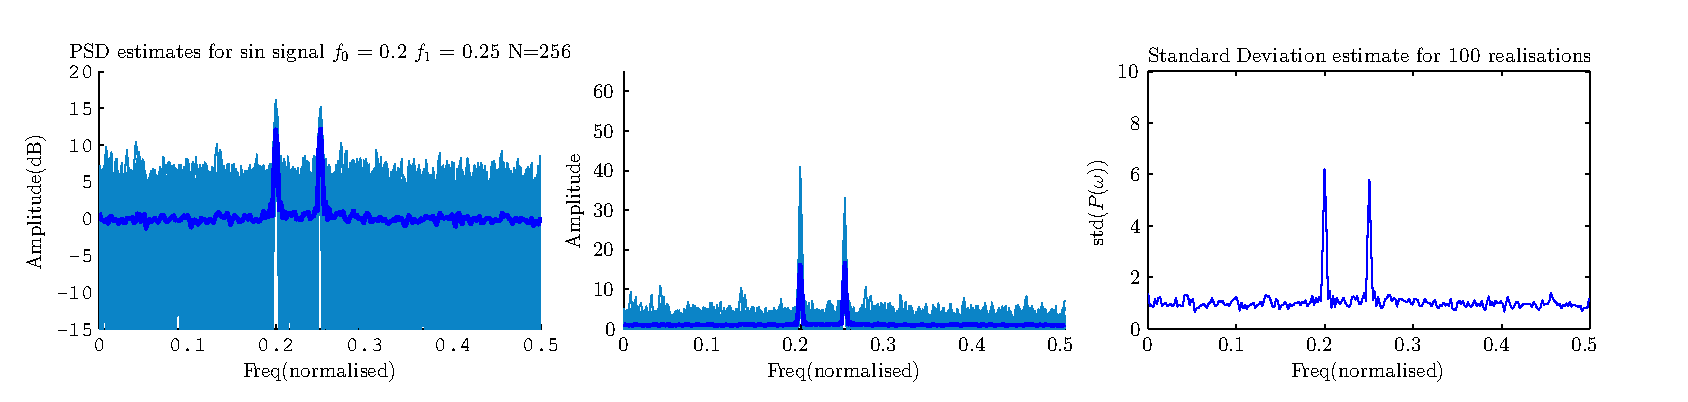
\includegraphics[width=\textwidth]{cw2im/2b.eps}
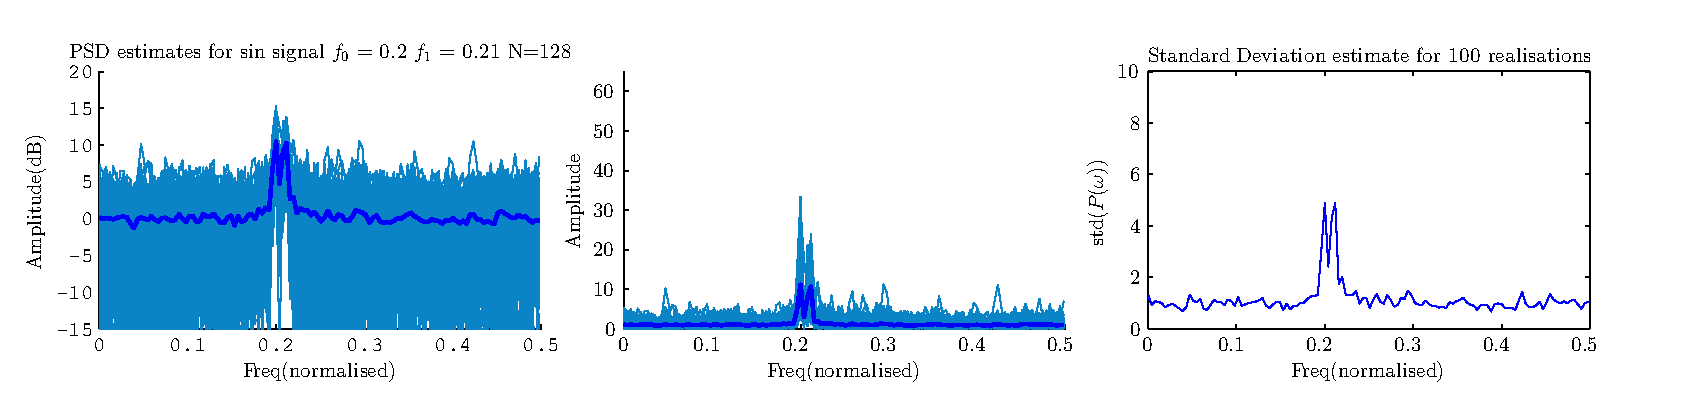
\includegraphics[width=\textwidth]{cw2im/2b2.eps}
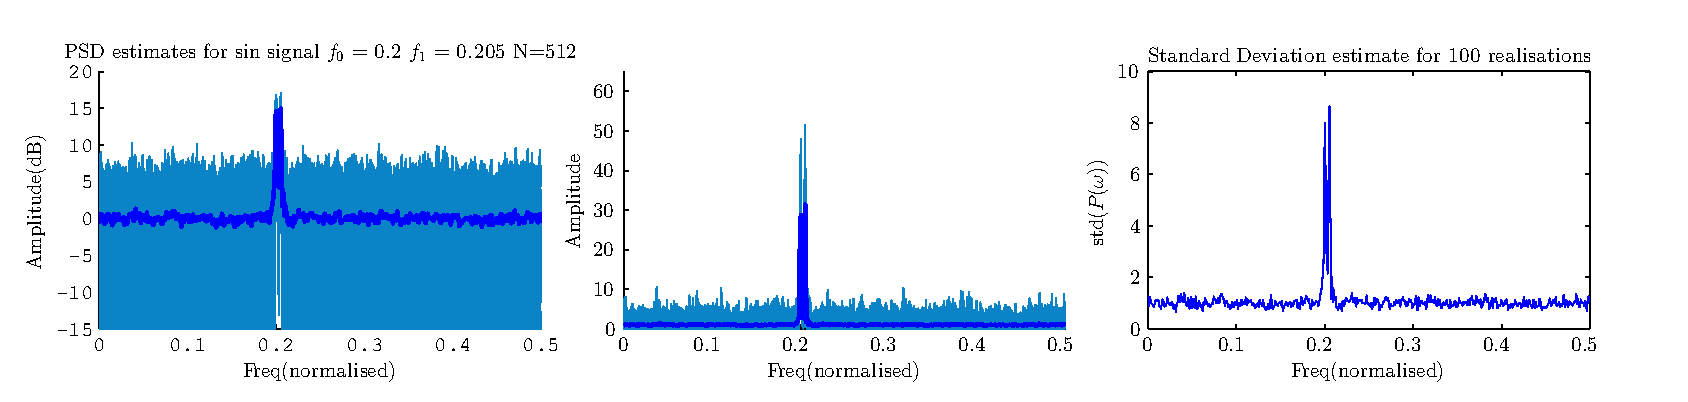
\includegraphics[width=\textwidth]{cw2im/2b3.eps}
The \textcolor{NavyBlue}{blue} line represents the mean.
\caption{PSD estimate and deviation for different realisations with AWGN of $\sigma = 1$ $ \mu = 0$}
\label{fig:2_2b}
\end{figure}


In figure \ref{fig:2_2b} 100 different realisations of a 2 sine signals with Gaussian noise were done. From this we see that at the frequency peaks the standard deviation is greatly increased. For the tested data points we find that the peaks of the variance are roughly equal to $\frac{\sqrt{N}}{2.7}$, that is the variance increases for greater sample lengths. However the standard deviation for frequencies outside of the peaks is $1$ and is not related to N. Essentially the standard deviation is also influenced by the PSD value, which is problematic for spectral estimation with only few realisations.


\subsection{Plotting in decibel}
In \ref{fig:2_2b} the left most graph for each case was plotted in decibels and figure \ref{fig:2_2b4} is the dB plot of the standard deviation. Here we observe that the main advantage this has is to compare the full frequency spectrum with a smaller range, due to the contraction property of the log function. This is practical for the high variance that arises for large PSD values as they are essentially negated. For the standard deviation estimation taking the log doesn't achieve much except making the resolution for lower std estimates slightly better - which we are not interested in.
\begin{figure}[h!]
\centering
\resizebox{\textwidth}{!}{% This file was created by matlab2tikz v0.4.7 running on MATLAB 8.1.
% Copyright (c) 2008--2014, Nico Schlömer <nico.schloemer@gmail.com>
% All rights reserved.
% Minimal pgfplots version: 1.3
% 
% The latest updates can be retrieved from
%   http://www.mathworks.com/matlabcentral/fileexchange/22022-matlab2tikz
% where you can also make suggestions and rate matlab2tikz.
% 
\begin{tikzpicture}

\begin{axis}[%
width=3.17222222222222in,
height=1.946875in,
scale only axis,
xmin=0,
xmax=0.5,
xlabel={Freq(normalised)},
ymin=-1,
ymax=10,
ylabel={std($P(\omega)$)  (dB)},
name=plot2,
title={STD estimate $f_0 = 0.2$ $f_1 = 0.21$ \& N=128}
]
\addplot [color=blue,solid,forget plot]
  table[row sep=crcr]{-0.498039215686275	0.0420327877351033\\
-0.494117647058824	0.013726887990248\\
-0.490196078431373	0.154459022359503\\
-0.486274509803922	0.284900339310612\\
-0.482352941176471	0.0900381564350992\\
-0.47843137254902	-0.0253243607355488\\
-0.474509803921569	0.0132887381896504\\
-0.470588235294118	0.00258173257866915\\
-0.466666666666667	-0.0374101380384793\\
-0.462745098039216	0.206301934023799\\
-0.458823529411765	0.0764268371736059\\
-0.454901960784314	-0.0800522206020468\\
-0.450980392156863	0.690822355735442\\
-0.447058823529412	0.491572579281703\\
-0.443137254901961	0.0440778878763541\\
-0.43921568627451	-0.0291641751687837\\
-0.435294117647059	0.24454591904771\\
-0.431372549019608	0.16623110223151\\
-0.427450980392157	0.246899607363641\\
-0.423529411764706	-0.278947712194729\\
-0.419607843137255	0.381238450224133\\
-0.415686274509804	0.484747591960436\\
-0.411764705882353	0.323133238833098\\
-0.407843137254902	-0.0102499522705823\\
-0.403921568627451	0.0392562565998476\\
-0.4	-0.0881720438944495\\
-0.396078431372549	-0.281596980691753\\
-0.392156862745098	-0.0143897296683322\\
-0.388235294117647	-0.585520784541491\\
-0.384313725490196	0.0644398682738647\\
-0.380392156862745	0.26230645120732\\
-0.376470588235294	-0.198519042370547\\
-0.372549019607843	0.211207310524762\\
-0.368627450980392	0.335362016718485\\
-0.364705882352941	0.260214918922788\\
-0.36078431372549	0.0402145691140834\\
-0.356862745098039	-0.0443591725403777\\
-0.352941176470588	0.298695264841218\\
-0.349019607843137	0.467022532061626\\
-0.345098039215686	-0.0086248590240598\\
-0.341176470588235	0.125550892053953\\
-0.337254901960784	0.607489941296209\\
-0.333333333333333	0.109683065469627\\
-0.329411764705882	0.174952688513759\\
-0.325490196078431	-0.186023891032157\\
-0.32156862745098	0.247950649963621\\
-0.317647058823529	-0.00487583439286969\\
-0.313725490196078	0.0591333949270932\\
-0.309803921568627	0.0985722622191102\\
-0.305882352941176	0.100770278581939\\
-0.301960784313725	-0.157261018859866\\
-0.298039215686275	0.175732991699188\\
-0.294117647058824	0.244552487063918\\
-0.290196078431373	-0.0119161004741039\\
-0.286274509803922	-0.322827024017615\\
-0.282352941176471	-0.107249739267906\\
-0.27843137254902	0.386045199133887\\
-0.274509803921569	0.122019421466491\\
-0.270588235294118	-0.195072532017512\\
-0.266666666666667	0.126439554810088\\
-0.262745098039216	-0.217407190290872\\
-0.258823529411765	-0.000751606850461018\\
-0.254901960784314	0.0330397282906077\\
-0.250980392156863	-0.0986610515596444\\
-0.247058823529412	0.277260050786851\\
-0.243137254901961	0.230912010528693\\
-0.23921568627451	0.432452586182996\\
-0.235294117647059	1.0082638942139\\
-0.231372549019608	0.132466236986348\\
-0.227450980392157	1.17240413561499\\
-0.223529411764706	0.025961038697263\\
-0.219607843137255	1.67837323081553\\
-0.215686274509804	2.17026594064652\\
-0.211764705882353	6.60979475872339\\
-0.207843137254902	5.66262805801264\\
-0.203921568627451	3.79762006914623\\
-0.2	6.75060401280595\\
-0.196078431372549	4.79513443846016\\
-0.192156862745098	0.235463462504773\\
-0.188235294117647	1.31754144087474\\
-0.184313725490196	0.427029723817634\\
-0.180392156862745	0.559473828713951\\
-0.176470588235294	-0.0698846502183853\\
-0.172549019607843	-0.0545322173573705\\
-0.168627450980392	0.354447170069384\\
-0.164705882352941	0.69212722024102\\
-0.16078431372549	0.199975533573434\\
-0.156862745098039	0.119191556272997\\
-0.152941176470588	-0.259068101221073\\
-0.149019607843137	0.114193165599219\\
-0.145098039215686	-0.421959552392499\\
-0.141176470588235	-0.515635545971985\\
-0.137254901960784	-0.298934084701736\\
-0.133333333333333	-0.0983336880528822\\
-0.129411764705882	0.0892840553384973\\
-0.125490196078431	-0.235519275517856\\
-0.12156862745098	-0.42522248847589\\
-0.117647058823529	0.149839558135281\\
-0.113725490196078	0.506175158549347\\
-0.109803921568627	-0.226092937026604\\
-0.105882352941176	0.0482236162480726\\
-0.101960784313725	0.3228035941146\\
-0.0980392156862745	0.230734456621758\\
-0.0941176470588235	-0.653347158291618\\
-0.0901960784313725	-0.152946798744932\\
-0.0862745098039216	0.0293012676222127\\
-0.0823529411764706	-0.0258421666673596\\
-0.0784313725490196	-0.16677962307113\\
-0.0745098039215686	0.402731959446102\\
-0.0705882352941176	-0.190248441169376\\
-0.0666666666666667	-0.00348557223059223\\
-0.0627450980392157	-0.173708474297952\\
-0.0588235294117647	0.0130759464396332\\
-0.0549019607843137	0.351577738192534\\
-0.0509803921568627	0.108595651068649\\
-0.0470588235294118	-0.216330407100885\\
-0.0431372549019608	0.00305212691354704\\
-0.0392156862745098	-0.453328269971772\\
-0.0352941176470588	-0.204082511383649\\
-0.0313725490196078	-0.0631789328573903\\
-0.0274509803921569	-0.0506547315736135\\
-0.0235294117647059	-0.118434902630048\\
-0.0196078431372549	-0.0574186196898749\\
-0.0156862745098039	-0.419226530826881\\
-0.0117647058823529	0.172127145475371\\
-0.00784313725490196	0.474728810104506\\
-0.00392156862745098	0.303055031359324\\
0	1.60909020834221\\
0.00392156862745098	0.303055031359324\\
0.00784313725490196	0.474728810104506\\
0.0117647058823529	0.172127145475371\\
0.0156862745098039	-0.419226530826881\\
0.0196078431372549	-0.0574186196898749\\
0.0235294117647059	-0.118434902630048\\
0.0274509803921569	-0.0506547315736135\\
0.0313725490196078	-0.0631789328573903\\
0.0352941176470588	-0.204082511383649\\
0.0392156862745098	-0.453328269971772\\
0.0431372549019608	0.00305212691354704\\
0.0470588235294118	-0.216330407100885\\
0.0509803921568627	0.108595651068649\\
0.0549019607843137	0.351577738192534\\
0.0588235294117647	0.0130759464396332\\
0.0627450980392157	-0.173708474297952\\
0.0666666666666667	-0.00348557223059223\\
0.0705882352941176	-0.190248441169376\\
0.0745098039215686	0.402731959446102\\
0.0784313725490196	-0.16677962307113\\
0.0823529411764706	-0.0258421666673596\\
0.0862745098039216	0.0293012676222127\\
0.0901960784313725	-0.152946798744932\\
0.0941176470588235	-0.653347158291618\\
0.0980392156862745	0.230734456621758\\
0.101960784313725	0.3228035941146\\
0.105882352941176	0.0482236162480726\\
0.109803921568627	-0.226092937026604\\
0.113725490196078	0.506175158549347\\
0.117647058823529	0.149839558135281\\
0.12156862745098	-0.42522248847589\\
0.125490196078431	-0.235519275517856\\
0.129411764705882	0.0892840553384973\\
0.133333333333333	-0.0983336880528822\\
0.137254901960784	-0.298934084701736\\
0.141176470588235	-0.515635545971985\\
0.145098039215686	-0.421959552392499\\
0.149019607843137	0.114193165599219\\
0.152941176470588	-0.259068101221073\\
0.156862745098039	0.119191556272997\\
0.16078431372549	0.199975533573434\\
0.164705882352941	0.69212722024102\\
0.168627450980392	0.354447170069384\\
0.172549019607843	-0.0545322173573705\\
0.176470588235294	-0.0698846502183853\\
0.180392156862745	0.559473828713951\\
0.184313725490196	0.427029723817634\\
0.188235294117647	1.31754144087474\\
0.192156862745098	0.235463462504773\\
0.196078431372549	4.79513443846016\\
0.2	6.75060401280595\\
0.203921568627451	3.79762006914623\\
0.207843137254902	5.66262805801264\\
0.211764705882353	6.60979475872339\\
0.215686274509804	2.17026594064652\\
0.219607843137255	1.67837323081553\\
0.223529411764706	0.025961038697263\\
0.227450980392157	1.17240413561499\\
0.231372549019608	0.132466236986348\\
0.235294117647059	1.0082638942139\\
0.23921568627451	0.432452586182996\\
0.243137254901961	0.230912010528693\\
0.247058823529412	0.277260050786851\\
0.250980392156863	-0.0986610515596444\\
0.254901960784314	0.0330397282906077\\
0.258823529411765	-0.000751606850461018\\
0.262745098039216	-0.217407190290872\\
0.266666666666667	0.126439554810088\\
0.270588235294118	-0.195072532017512\\
0.274509803921569	0.122019421466491\\
0.27843137254902	0.386045199133887\\
0.282352941176471	-0.107249739267906\\
0.286274509803922	-0.322827024017615\\
0.290196078431373	-0.0119161004741039\\
0.294117647058824	0.244552487063918\\
0.298039215686275	0.175732991699188\\
0.301960784313725	-0.157261018859866\\
0.305882352941176	0.100770278581939\\
0.309803921568627	0.0985722622191102\\
0.313725490196078	0.0591333949270932\\
0.317647058823529	-0.00487583439286969\\
0.32156862745098	0.247950649963621\\
0.325490196078431	-0.186023891032157\\
0.329411764705882	0.174952688513759\\
0.333333333333333	0.109683065469627\\
0.337254901960784	0.607489941296209\\
0.341176470588235	0.125550892053953\\
0.345098039215686	-0.0086248590240598\\
0.349019607843137	0.467022532061626\\
0.352941176470588	0.298695264841218\\
0.356862745098039	-0.0443591725403777\\
0.36078431372549	0.0402145691140834\\
0.364705882352941	0.260214918922788\\
0.368627450980392	0.335362016718485\\
0.372549019607843	0.211207310524762\\
0.376470588235294	-0.198519042370547\\
0.380392156862745	0.26230645120732\\
0.384313725490196	0.0644398682738647\\
0.388235294117647	-0.585520784541491\\
0.392156862745098	-0.0143897296683322\\
0.396078431372549	-0.281596980691753\\
0.4	-0.0881720438944495\\
0.403921568627451	0.0392562565998476\\
0.407843137254902	-0.0102499522705823\\
0.411764705882353	0.323133238833098\\
0.415686274509804	0.484747591960436\\
0.419607843137255	0.381238450224133\\
0.423529411764706	-0.278947712194729\\
0.427450980392157	0.246899607363641\\
0.431372549019608	0.16623110223151\\
0.435294117647059	0.24454591904771\\
0.43921568627451	-0.0291641751687837\\
0.443137254901961	0.0440778878763541\\
0.447058823529412	0.491572579281703\\
0.450980392156863	0.690822355735442\\
0.454901960784314	-0.0800522206020468\\
0.458823529411765	0.0764268371736059\\
0.462745098039216	0.206301934023799\\
0.466666666666667	-0.0374101380384793\\
0.470588235294118	0.00258173257866915\\
0.474509803921569	0.0132887381896504\\
0.47843137254902	-0.0253243607355488\\
0.482352941176471	0.0900381564350992\\
0.486274509803922	0.284900339310612\\
0.490196078431373	0.154459022359503\\
0.494117647058824	0.013726887990248\\
0.498039215686275	0.0420327877351033\\
};
\end{axis}

\begin{axis}[%
width=3.17222222222222in,
height=1.946875in,
scale only axis,
xmin=0,
xmax=0.5,
xlabel={Freq(normalised)},
ymin=-1,
ymax=10,
ylabel={std($P(\omega)$)  (dB)},
at=(plot2.left of south west),
anchor=right of south east,
title={STD estimate $f_0 = 0.2$ $f_1 = 0.25$ \& N=256}
]
\addplot [color=blue,solid,forget plot]
  table[row sep=crcr]{-0.499021526418787	0.951648207202922\\
-0.49706457925636	-0.242695435330685\\
-0.495107632093933	-0.296600716343955\\
-0.493150684931507	0.377133944960574\\
-0.49119373776908	0.0695109207620621\\
-0.489236790606654	0.182318353274616\\
-0.487279843444227	-0.469021666138395\\
-0.4853228962818	0.315555475264821\\
-0.483365949119374	0.468759343427728\\
-0.481409001956947	-0.346644670918488\\
-0.479452054794521	0.0219007964383311\\
-0.477495107632094	0.0762744472241041\\
-0.475538160469667	-0.0524591671612787\\
-0.473581213307241	0.141059433429022\\
-0.471624266144814	0.0820009329089378\\
-0.469667318982387	-0.172685277006494\\
-0.467710371819961	0.687223715252093\\
-0.465753424657534	0.401641855263835\\
-0.463796477495108	-0.403021064432445\\
-0.461839530332681	0.108675635685684\\
-0.459882583170254	0.341560475183047\\
-0.457925636007828	-0.0227098278865801\\
-0.455968688845401	0.00630980389602954\\
-0.454011741682975	0.404377724999663\\
-0.452054794520548	0.12000653411879\\
-0.450097847358121	0.299510978343959\\
-0.448140900195695	0.112025203716223\\
-0.446183953033268	0.141539570163576\\
-0.444227005870841	-0.114509523255069\\
-0.442270058708415	-0.383660851057007\\
-0.440313111545988	-0.189717700851389\\
-0.438356164383562	-0.0339956643703016\\
-0.436399217221135	-0.346012327600311\\
-0.434442270058708	0.400166683762\\
-0.432485322896282	0.143737713049879\\
-0.430528375733855	0.166446107487573\\
-0.428571428571429	0.201142526889323\\
-0.426614481409002	-0.125538284448699\\
-0.424657534246575	-0.302691253350981\\
-0.422700587084149	-0.510727670787659\\
-0.420743639921722	-0.135762661828172\\
-0.418786692759295	-0.179885911311302\\
-0.416829745596869	-0.0715548777765326\\
-0.414872798434442	0.115203062781679\\
-0.412915851272016	0.540447727152677\\
-0.410958904109589	-0.188851840600517\\
-0.409001956947162	-0.0993676701167568\\
-0.407045009784736	-0.016727781736549\\
-0.405088062622309	0.166735194115806\\
-0.403131115459883	0.357382138643343\\
-0.401174168297456	0.436932087322736\\
-0.399217221135029	0.283175732788846\\
-0.397260273972603	0.0959867932660743\\
-0.395303326810176	0.424523553161907\\
-0.393346379647749	0.045472955280183\\
-0.391389432485323	-0.0791125440881025\\
-0.389432485322896	0.270365538576035\\
-0.38747553816047	-0.0747155321243692\\
-0.385518590998043	0.27366165149268\\
-0.383561643835616	-0.393007726498027\\
-0.38160469667319	0.121714876023037\\
-0.379647749510763	0.0722966114409513\\
-0.377690802348337	-0.168888841928062\\
-0.37573385518591	0.424772275581841\\
-0.373776908023483	0.243662716695928\\
-0.371819960861057	0.229942468056964\\
-0.36986301369863	0.136945294265157\\
-0.367906066536204	-0.262903176612551\\
-0.365949119373777	-0.00396207433260989\\
-0.36399217221135	-0.0999620618590749\\
-0.362035225048924	-0.00986538533990614\\
-0.360078277886497	-0.126300948926909\\
-0.35812133072407	-0.0436186393126364\\
-0.356164383561644	-0.201523500934029\\
-0.354207436399217	-0.22100054218767\\
-0.352250489236791	0.0179444178762561\\
-0.350293542074364	0.0745856345231524\\
-0.348336594911937	0.207215484608268\\
-0.346379647749511	0.188463530608305\\
-0.344422700587084	0.367645530174612\\
-0.342465753424658	0.294493230884745\\
-0.340508806262231	0.0926566368664032\\
-0.338551859099804	0.182955922500818\\
-0.336594911937378	-0.104525127533965\\
-0.334637964774951	-0.182287526398956\\
-0.332681017612524	-0.0300934161598265\\
-0.330724070450098	0.0328167722050151\\
-0.328767123287671	-0.267892391076038\\
-0.326810176125245	0.184741600672552\\
-0.324853228962818	-0.16709145909417\\
-0.322896281800391	0.116168681239381\\
-0.320939334637965	0.189835246276704\\
-0.318982387475538	-0.0460628416467294\\
-0.317025440313112	0.121058308618459\\
-0.315068493150685	0.203766241165256\\
-0.313111545988258	-0.0597770556865978\\
-0.311154598825832	0.306056674395175\\
-0.309197651663405	0.0119132556808497\\
-0.307240704500978	0.260936189709568\\
-0.305283757338552	0.0233974235686213\\
-0.303326810176125	-0.0114598361204015\\
-0.301369863013699	-0.0595337922583307\\
-0.299412915851272	0.121336239860244\\
-0.297455968688845	0.297302398660992\\
-0.295499021526419	0.216370250405131\\
-0.293542074363992	-0.285412918059657\\
-0.291585127201566	0.138445725291935\\
-0.289628180039139	0.160753480995155\\
-0.287671232876712	-0.22774461972917\\
-0.285714285714286	0.415818707387643\\
-0.283757338551859	0.514414727192383\\
-0.281800391389432	0.0817188098986508\\
-0.279843444227006	0.582489113759206\\
-0.277886497064579	0.260035617164767\\
-0.275929549902153	0.542282474845802\\
-0.273972602739726	0.432211861544624\\
-0.272015655577299	0.226393358893071\\
-0.270058708414873	-0.0137827365063195\\
-0.268101761252446	0.667289543487472\\
-0.26614481409002	-0.155386494460344\\
-0.264187866927593	0.341178254044073\\
-0.262230919765166	-0.278875442027782\\
-0.26027397260274	0.656544520684212\\
-0.258317025440313	-0.241881431613585\\
-0.256360078277886	2.13942296292483\\
-0.25440313111546	0.625070544414464\\
-0.252446183953033	4.54525937373922\\
-0.250489236790607	7.32995977352581\\
-0.24853228962818	6.21548276404784\\
-0.246575342465753	1.05897041316157\\
-0.244618395303327	1.37287017150769\\
-0.2426614481409	-0.0114871803332554\\
-0.240704500978474	0.534784534020317\\
-0.238747553816047	-0.410454316454402\\
-0.23679060665362	0.263784051329998\\
-0.234833659491194	0.465746565899838\\
-0.232876712328767	0.632008895016885\\
-0.230919765166341	0.124217685020585\\
-0.228962818003914	0.164665863581803\\
-0.227005870841487	0.188178851498259\\
-0.225048923679061	0.149138365691954\\
-0.223091976516634	0.188236133929654\\
-0.221135029354207	0.35259673635316\\
-0.219178082191781	0.113571641939598\\
-0.217221135029354	0.0758205477883521\\
-0.215264187866928	0.015363999706665\\
-0.213307240704501	-0.136368157996866\\
-0.211350293542074	-0.13578359792003\\
-0.209393346379648	0.963229724772562\\
-0.207436399217221	0.458900629777197\\
-0.205479452054795	1.76617389535738\\
-0.203522504892368	0.785970609338663\\
-0.201565557729941	6.49188669855256\\
-0.199608610567515	7.56862167142979\\
-0.197651663405088	5.05932407290392\\
-0.195694716242661	0.478803914714159\\
-0.193737769080235	1.43160190310454\\
-0.191780821917808	-0.0394976361498569\\
-0.189823874755382	0.779881809249757\\
-0.187866927592955	-0.340582102489615\\
-0.185909980430528	0.206510058457495\\
-0.183953033268102	-0.125858181061265\\
-0.181996086105675	0.390292210074423\\
-0.180039138943249	0.0408548505773939\\
-0.178082191780822	0.23913363560622\\
-0.176125244618395	0.182917347124209\\
-0.174168297455969	0.713287873171476\\
-0.172211350293542	0.501621158145826\\
-0.170254403131115	-0.0883235805764676\\
-0.168297455968689	-0.45775791684053\\
-0.166340508806262	-0.204683802246765\\
-0.164383561643836	-0.153857948831296\\
-0.162426614481409	-0.168738931845336\\
-0.160469667318982	-0.469970339608962\\
-0.158512720156556	-0.0226240010771929\\
-0.156555772994129	-0.0550146443032973\\
-0.154598825831703	-0.188380344483438\\
-0.152641878669276	-0.0988808816667237\\
-0.150684931506849	0.0721275927535678\\
-0.148727984344423	-0.338107582212156\\
-0.146771037181996	0.234527906991212\\
-0.144814090019569	0.0763893614166259\\
-0.142857142857143	0.225563055835619\\
-0.140900195694716	0.163354651347849\\
-0.13894324853229	-0.210435898285946\\
-0.136986301369863	0.122149846393943\\
-0.135029354207436	-0.111660480211314\\
-0.13307240704501	-0.2092451649098\\
-0.131115459882583	0.163764070180196\\
-0.129158512720157	-0.275423862891582\\
-0.12720156555773	-0.065400014600905\\
-0.125244618395303	0.320534135609021\\
-0.123287671232877	0.413535568640355\\
-0.12133072407045	-0.0988851822707308\\
-0.119373776908023	0.183131115814498\\
-0.117416829745597	0.482137001983635\\
-0.11545988258317	0.153159271541127\\
-0.113502935420744	-0.0490048135993442\\
-0.111545988258317	-0.38753356497337\\
-0.10958904109589	0.308263375772382\\
-0.107632093933464	0.404446183495473\\
-0.105675146771037	0.244273807215756\\
-0.103718199608611	-0.35515242830454\\
-0.101761252446184	-0.201403405790663\\
-0.0998043052837573	-0.218954610490638\\
-0.0978473581213307	0.250130073099551\\
-0.0958904109589041	0.272267351128249\\
-0.0939334637964775	-0.498370763789429\\
-0.0919765166340509	-0.18956132799015\\
-0.0900195694716243	0.233716931723561\\
-0.0880626223091976	-0.376623118524346\\
-0.086105675146771	-0.322791251763422\\
-0.0841487279843444	0.248084047200512\\
-0.0821917808219178	-0.0441514022365422\\
-0.0802348336594912	0.277980796450896\\
-0.0782778864970646	0.442323863747708\\
-0.076320939334638	-0.339221399312668\\
-0.0743639921722113	-0.146647328461534\\
-0.0724070450097847	0.169904008531008\\
-0.0704500978473581	0.000469839205859648\\
-0.0684931506849315	-0.185244967116238\\
-0.0665362035225049	0.119795926253533\\
-0.0645792563600783	0.0442995844671034\\
-0.0626223091976517	-0.249140997055431\\
-0.060665362035225	0.115174703536995\\
-0.0587084148727984	0.00111477825989023\\
-0.0567514677103718	-0.583163458334804\\
-0.0547945205479452	-0.318894768494282\\
-0.0528375733855186	0.438873322547064\\
-0.050880626223092	0.124816962323505\\
-0.0489236790606654	0.0264432535649971\\
-0.0469667318982387	0.277213481584519\\
-0.0450097847358121	-0.0378868807429959\\
-0.0430528375733855	-0.118384525789676\\
-0.0410958904109589	0.171783504039682\\
-0.0391389432485323	-0.284185143455547\\
-0.0371819960861057	0.25643777461086\\
-0.0352250489236791	0.660495183563557\\
-0.0332681017612524	0.329480544017072\\
-0.0313111545988258	-0.0440549554273378\\
-0.0293542074363992	-0.353049310365388\\
-0.0273972602739726	-0.27827940618196\\
-0.025440313111546	-0.316249186965113\\
-0.0234833659491194	-0.0699864279827349\\
-0.0215264187866928	0.00498965523137349\\
-0.0195694716242661	0.411491114996198\\
-0.0176125244618395	-0.120711326079732\\
-0.0156555772994129	-0.292826448762453\\
-0.0136986301369863	0.176126465253071\\
-0.0117416829745597	0.0581601480373225\\
-0.00978473581213307	0.0845269316156448\\
-0.00782778864970646	-0.06110447038394\\
-0.00587084148727984	-0.248796453381432\\
-0.00391389432485323	-0.162802735171879\\
-0.00195694716242661	0.00790563007895998\\
0	0.986350276026684\\
0.00195694716242661	0.00790563007895998\\
0.00391389432485323	-0.162802735171879\\
0.00587084148727984	-0.248796453381432\\
0.00782778864970646	-0.06110447038394\\
0.00978473581213307	0.0845269316156448\\
0.0117416829745597	0.0581601480373225\\
0.0136986301369863	0.176126465253071\\
0.0156555772994129	-0.292826448762453\\
0.0176125244618395	-0.120711326079732\\
0.0195694716242661	0.411491114996198\\
0.0215264187866928	0.00498965523137349\\
0.0234833659491194	-0.0699864279827349\\
0.025440313111546	-0.316249186965113\\
0.0273972602739726	-0.27827940618196\\
0.0293542074363992	-0.353049310365388\\
0.0313111545988258	-0.0440549554273378\\
0.0332681017612524	0.329480544017072\\
0.0352250489236791	0.660495183563557\\
0.0371819960861057	0.25643777461086\\
0.0391389432485323	-0.284185143455547\\
0.0410958904109589	0.171783504039682\\
0.0430528375733855	-0.118384525789676\\
0.0450097847358121	-0.0378868807429959\\
0.0469667318982387	0.277213481584519\\
0.0489236790606654	0.0264432535649971\\
0.050880626223092	0.124816962323505\\
0.0528375733855186	0.438873322547064\\
0.0547945205479452	-0.318894768494282\\
0.0567514677103718	-0.583163458334804\\
0.0587084148727984	0.00111477825989023\\
0.060665362035225	0.115174703536995\\
0.0626223091976517	-0.249140997055431\\
0.0645792563600783	0.0442995844671034\\
0.0665362035225049	0.119795926253533\\
0.0684931506849315	-0.185244967116238\\
0.0704500978473581	0.000469839205859648\\
0.0724070450097847	0.169904008531008\\
0.0743639921722113	-0.146647328461534\\
0.076320939334638	-0.339221399312668\\
0.0782778864970646	0.442323863747708\\
0.0802348336594912	0.277980796450896\\
0.0821917808219178	-0.0441514022365422\\
0.0841487279843444	0.248084047200512\\
0.086105675146771	-0.322791251763422\\
0.0880626223091976	-0.376623118524346\\
0.0900195694716243	0.233716931723561\\
0.0919765166340509	-0.18956132799015\\
0.0939334637964775	-0.498370763789429\\
0.0958904109589041	0.272267351128249\\
0.0978473581213307	0.250130073099551\\
0.0998043052837573	-0.218954610490638\\
0.101761252446184	-0.201403405790663\\
0.103718199608611	-0.35515242830454\\
0.105675146771037	0.244273807215756\\
0.107632093933464	0.404446183495473\\
0.10958904109589	0.308263375772382\\
0.111545988258317	-0.38753356497337\\
0.113502935420744	-0.0490048135993442\\
0.11545988258317	0.153159271541127\\
0.117416829745597	0.482137001983635\\
0.119373776908023	0.183131115814498\\
0.12133072407045	-0.0988851822707308\\
0.123287671232877	0.413535568640355\\
0.125244618395303	0.320534135609021\\
0.12720156555773	-0.065400014600905\\
0.129158512720157	-0.275423862891582\\
0.131115459882583	0.163764070180196\\
0.13307240704501	-0.2092451649098\\
0.135029354207436	-0.111660480211314\\
0.136986301369863	0.122149846393943\\
0.13894324853229	-0.210435898285946\\
0.140900195694716	0.163354651347849\\
0.142857142857143	0.225563055835619\\
0.144814090019569	0.0763893614166259\\
0.146771037181996	0.234527906991212\\
0.148727984344423	-0.338107582212156\\
0.150684931506849	0.0721275927535678\\
0.152641878669276	-0.0988808816667237\\
0.154598825831703	-0.188380344483438\\
0.156555772994129	-0.0550146443032973\\
0.158512720156556	-0.0226240010771929\\
0.160469667318982	-0.469970339608962\\
0.162426614481409	-0.168738931845336\\
0.164383561643836	-0.153857948831296\\
0.166340508806262	-0.204683802246765\\
0.168297455968689	-0.45775791684053\\
0.170254403131115	-0.0883235805764676\\
0.172211350293542	0.501621158145826\\
0.174168297455969	0.713287873171476\\
0.176125244618395	0.182917347124209\\
0.178082191780822	0.23913363560622\\
0.180039138943249	0.0408548505773939\\
0.181996086105675	0.390292210074423\\
0.183953033268102	-0.125858181061265\\
0.185909980430528	0.206510058457495\\
0.187866927592955	-0.340582102489615\\
0.189823874755382	0.779881809249757\\
0.191780821917808	-0.0394976361498569\\
0.193737769080235	1.43160190310454\\
0.195694716242661	0.478803914714159\\
0.197651663405088	5.05932407290392\\
0.199608610567515	7.56862167142979\\
0.201565557729941	6.49188669855256\\
0.203522504892368	0.785970609338663\\
0.205479452054795	1.76617389535738\\
0.207436399217221	0.458900629777197\\
0.209393346379648	0.963229724772562\\
0.211350293542074	-0.13578359792003\\
0.213307240704501	-0.136368157996866\\
0.215264187866928	0.015363999706665\\
0.217221135029354	0.0758205477883521\\
0.219178082191781	0.113571641939598\\
0.221135029354207	0.35259673635316\\
0.223091976516634	0.188236133929654\\
0.225048923679061	0.149138365691954\\
0.227005870841487	0.188178851498259\\
0.228962818003914	0.164665863581803\\
0.230919765166341	0.124217685020585\\
0.232876712328767	0.632008895016885\\
0.234833659491194	0.465746565899838\\
0.23679060665362	0.263784051329998\\
0.238747553816047	-0.410454316454402\\
0.240704500978474	0.534784534020317\\
0.2426614481409	-0.0114871803332554\\
0.244618395303327	1.37287017150769\\
0.246575342465753	1.05897041316157\\
0.24853228962818	6.21548276404784\\
0.250489236790607	7.32995977352581\\
0.252446183953033	4.54525937373922\\
0.25440313111546	0.625070544414464\\
0.256360078277886	2.13942296292483\\
0.258317025440313	-0.241881431613585\\
0.26027397260274	0.656544520684212\\
0.262230919765166	-0.278875442027782\\
0.264187866927593	0.341178254044073\\
0.26614481409002	-0.155386494460344\\
0.268101761252446	0.667289543487472\\
0.270058708414873	-0.0137827365063195\\
0.272015655577299	0.226393358893071\\
0.273972602739726	0.432211861544624\\
0.275929549902153	0.542282474845802\\
0.277886497064579	0.260035617164767\\
0.279843444227006	0.582489113759206\\
0.281800391389432	0.0817188098986508\\
0.283757338551859	0.514414727192383\\
0.285714285714286	0.415818707387643\\
0.287671232876712	-0.22774461972917\\
0.289628180039139	0.160753480995155\\
0.291585127201566	0.138445725291935\\
0.293542074363992	-0.285412918059657\\
0.295499021526419	0.216370250405131\\
0.297455968688845	0.297302398660992\\
0.299412915851272	0.121336239860244\\
0.301369863013699	-0.0595337922583307\\
0.303326810176125	-0.0114598361204015\\
0.305283757338552	0.0233974235686213\\
0.307240704500978	0.260936189709568\\
0.309197651663405	0.0119132556808497\\
0.311154598825832	0.306056674395175\\
0.313111545988258	-0.0597770556865978\\
0.315068493150685	0.203766241165256\\
0.317025440313112	0.121058308618459\\
0.318982387475538	-0.0460628416467294\\
0.320939334637965	0.189835246276704\\
0.322896281800391	0.116168681239381\\
0.324853228962818	-0.16709145909417\\
0.326810176125245	0.184741600672552\\
0.328767123287671	-0.267892391076038\\
0.330724070450098	0.0328167722050151\\
0.332681017612524	-0.0300934161598265\\
0.334637964774951	-0.182287526398956\\
0.336594911937378	-0.104525127533965\\
0.338551859099804	0.182955922500818\\
0.340508806262231	0.0926566368664032\\
0.342465753424658	0.294493230884745\\
0.344422700587084	0.367645530174612\\
0.346379647749511	0.188463530608305\\
0.348336594911937	0.207215484608268\\
0.350293542074364	0.0745856345231524\\
0.352250489236791	0.0179444178762561\\
0.354207436399217	-0.22100054218767\\
0.356164383561644	-0.201523500934029\\
0.35812133072407	-0.0436186393126364\\
0.360078277886497	-0.126300948926909\\
0.362035225048924	-0.00986538533990614\\
0.36399217221135	-0.0999620618590749\\
0.365949119373777	-0.00396207433260989\\
0.367906066536204	-0.262903176612551\\
0.36986301369863	0.136945294265157\\
0.371819960861057	0.229942468056964\\
0.373776908023483	0.243662716695928\\
0.37573385518591	0.424772275581841\\
0.377690802348337	-0.168888841928062\\
0.379647749510763	0.0722966114409513\\
0.38160469667319	0.121714876023037\\
0.383561643835616	-0.393007726498027\\
0.385518590998043	0.27366165149268\\
0.38747553816047	-0.0747155321243692\\
0.389432485322896	0.270365538576035\\
0.391389432485323	-0.0791125440881025\\
0.393346379647749	0.045472955280183\\
0.395303326810176	0.424523553161907\\
0.397260273972603	0.0959867932660743\\
0.399217221135029	0.283175732788846\\
0.401174168297456	0.436932087322736\\
0.403131115459883	0.357382138643343\\
0.405088062622309	0.166735194115806\\
0.407045009784736	-0.016727781736549\\
0.409001956947162	-0.0993676701167568\\
0.410958904109589	-0.188851840600517\\
0.412915851272016	0.540447727152677\\
0.414872798434442	0.115203062781679\\
0.416829745596869	-0.0715548777765326\\
0.418786692759295	-0.179885911311302\\
0.420743639921722	-0.135762661828172\\
0.422700587084149	-0.510727670787659\\
0.424657534246575	-0.302691253350981\\
0.426614481409002	-0.125538284448699\\
0.428571428571429	0.201142526889323\\
0.430528375733855	0.166446107487573\\
0.432485322896282	0.143737713049879\\
0.434442270058708	0.400166683762\\
0.436399217221135	-0.346012327600311\\
0.438356164383562	-0.0339956643703016\\
0.440313111545988	-0.189717700851389\\
0.442270058708415	-0.383660851057007\\
0.444227005870841	-0.114509523255069\\
0.446183953033268	0.141539570163576\\
0.448140900195695	0.112025203716223\\
0.450097847358121	0.299510978343959\\
0.452054794520548	0.12000653411879\\
0.454011741682975	0.404377724999663\\
0.455968688845401	0.00630980389602954\\
0.457925636007828	-0.0227098278865801\\
0.459882583170254	0.341560475183047\\
0.461839530332681	0.108675635685684\\
0.463796477495108	-0.403021064432445\\
0.465753424657534	0.401641855263835\\
0.467710371819961	0.687223715252093\\
0.469667318982387	-0.172685277006494\\
0.471624266144814	0.0820009329089378\\
0.473581213307241	0.141059433429022\\
0.475538160469667	-0.0524591671612787\\
0.477495107632094	0.0762744472241041\\
0.479452054794521	0.0219007964383311\\
0.481409001956947	-0.346644670918488\\
0.483365949119374	0.468759343427728\\
0.4853228962818	0.315555475264821\\
0.487279843444227	-0.469021666138395\\
0.489236790606654	0.182318353274616\\
0.49119373776908	0.0695109207620621\\
0.493150684931507	0.377133944960574\\
0.495107632093933	-0.296600716343955\\
0.49706457925636	-0.242695435330685\\
0.499021526418787	0.951648207202922\\
};
\end{axis}

\begin{axis}[%
width=3.17222222222222in,
height=1.946875in,
scale only axis,
xmin=0,
xmax=0.5,
xlabel={Freq(normalised)},
ymin=-1,
ymax=10,
ylabel={std($P(\omega)$)  (dB)},
at=(plot2.right of south east),
anchor=left of south west,
title={STD estimate $f_0 = 0.2$ $f_1 = 0.205$ \& N=512}
]
\addplot [color=blue,solid,forget plot]
  table[row sep=crcr]{-0.499511241446725	-0.0551540220064213\\
-0.498533724340176	0.429148534340236\\
-0.497556207233627	0.0275773931459929\\
-0.496578690127077	0.397809229765223\\
-0.495601173020528	0.128595695376722\\
-0.494623655913979	0.0077088808006038\\
-0.493646138807429	0.389046750747357\\
-0.49266862170088	-0.400387717694869\\
-0.49169110459433	-0.293696744578715\\
-0.490713587487781	-0.260276795713933\\
-0.489736070381232	-0.205143169567811\\
-0.488758553274682	-0.246511148184088\\
-0.487781036168133	0.157814517253375\\
-0.486803519061584	0.059457755704424\\
-0.485826001955034	0.025822368252883\\
-0.484848484848485	0.366730734721506\\
-0.483870967741936	0.416665688680585\\
-0.482893450635386	0.063278222080478\\
-0.481915933528837	0.0784994231192695\\
-0.480938416422287	-0.297197323833617\\
-0.479960899315738	-0.481423665369691\\
-0.478983382209189	-0.167284043940984\\
-0.478005865102639	-0.216740622925631\\
-0.47702834799609	-0.107406183641016\\
-0.476050830889541	-0.235444353199577\\
-0.475073313782991	-0.235139305998195\\
-0.474095796676442	-0.0595235184295361\\
-0.473118279569893	0.246177349865828\\
-0.472140762463343	-0.208681484164268\\
-0.471163245356794	-0.037621532737267\\
-0.470185728250244	0.285415317552934\\
-0.469208211143695	0.108451941829977\\
-0.468230694037146	-0.245968203617075\\
-0.467253176930596	-0.056232201028576\\
-0.466275659824047	-0.113539980683223\\
-0.465298142717498	0.155012538814083\\
-0.464320625610948	-0.266227099082549\\
-0.463343108504399	-0.174262132971097\\
-0.462365591397849	0.177967245036222\\
-0.4613880742913	0.44068126281123\\
-0.460410557184751	0.338986846901381\\
-0.459433040078201	0.272063857728538\\
-0.458455522971652	0.109887341546223\\
-0.457478005865103	-0.128711902940315\\
-0.456500488758553	-0.0782618078840429\\
-0.455522971652004	-0.208900566567858\\
-0.454545454545455	0.231549170055644\\
-0.453567937438905	-0.0672581554530787\\
-0.452590420332356	-0.295622438450739\\
-0.451612903225806	0.546626865630088\\
-0.450635386119257	-0.180108953906497\\
-0.449657869012708	-0.104664352217361\\
-0.448680351906158	0.0830683454956319\\
-0.447702834799609	0.273646227962462\\
-0.44672531769306	0.129794377105586\\
-0.44574780058651	0.149356336168053\\
-0.444770283479961	-0.349530155946909\\
-0.443792766373412	-0.19561199560799\\
-0.442815249266862	0.185196352761176\\
-0.441837732160313	-0.225720237937096\\
-0.440860215053763	-0.546926580444406\\
-0.439882697947214	-0.0884931246980249\\
-0.438905180840665	0.313207372512489\\
-0.437927663734115	0.950142249249247\\
-0.436950146627566	0.573612133440474\\
-0.435972629521017	0.444429947511505\\
-0.434995112414467	-0.335213936368355\\
-0.434017595307918	-0.110957634409478\\
-0.433040078201369	0.376415294529472\\
-0.432062561094819	-0.0189283723986736\\
-0.43108504398827	-0.516935641708457\\
-0.43010752688172	-0.417408058752314\\
-0.429130009775171	0.02159787198738\\
-0.428152492668622	0.228272936362547\\
-0.427174975562072	-0.187453757133037\\
-0.426197458455523	0.354036515331278\\
-0.425219941348974	-0.0989799229071727\\
-0.424242424242424	-0.0234246782438804\\
-0.423264907135875	-0.0948689450145277\\
-0.422287390029326	0.254736052216987\\
-0.421309872922776	-0.542679414156882\\
-0.420332355816227	-0.495204749136854\\
-0.419354838709677	-0.455838739528668\\
-0.418377321603128	0.240925875415156\\
-0.417399804496579	0.214394836795348\\
-0.416422287390029	-0.122731371012947\\
-0.41544477028348	0.296515042845685\\
-0.414467253176931	0.0941710181864972\\
-0.413489736070381	-0.38364584500792\\
-0.412512218963832	0.2392384480074\\
-0.411534701857283	-0.0823254162290503\\
-0.410557184750733	0.0137746735581565\\
-0.409579667644184	-0.0988617697760092\\
-0.408602150537634	0.221086714532704\\
-0.407624633431085	0.310259524793866\\
-0.406647116324536	-0.0175003938696528\\
-0.405669599217986	-0.321191161612015\\
-0.404692082111437	-0.408824873764518\\
-0.403714565004888	0.100411190231375\\
-0.402737047898338	0.202643556480597\\
-0.401759530791789	-0.173699959856682\\
-0.400782013685239	-0.169407602932573\\
-0.39980449657869	-0.617053658666996\\
-0.398826979472141	-0.211698817757921\\
-0.397849462365591	0.256756934031244\\
-0.396871945259042	-0.0507992119888878\\
-0.395894428152493	0.0831203827466793\\
-0.394916911045943	-0.143317222140007\\
-0.393939393939394	0.228278647778023\\
-0.392961876832845	0.201736405334241\\
-0.391984359726295	0.260960083114828\\
-0.391006842619746	-0.0637747605526691\\
-0.390029325513196	-0.281061185321242\\
-0.389051808406647	-0.240265541953362\\
-0.388074291300098	-0.355254737869091\\
-0.387096774193548	-0.459044776024704\\
-0.386119257086999	-0.0688475222689428\\
-0.38514173998045	0.0679177792663099\\
-0.3841642228739	0.304076230712629\\
-0.383186705767351	0.234032355334712\\
-0.382209188660802	0.390251718992816\\
-0.381231671554252	0.501067672666486\\
-0.380254154447703	-0.0141328942558709\\
-0.379276637341153	0.103037157234093\\
-0.378299120234604	0.00014072050363936\\
-0.377321603128055	-0.12034694652277\\
-0.376344086021505	0.27423974361342\\
-0.375366568914956	-0.188747427699034\\
-0.374389051808407	0.114434332022664\\
-0.373411534701857	-0.291835889967384\\
-0.372434017595308	-0.235596949528974\\
-0.371456500488759	0.0460923343023535\\
-0.370478983382209	0.0835779050910088\\
-0.36950146627566	-0.155967578132616\\
-0.36852394916911	-0.305088916977175\\
-0.367546432062561	-0.042449074614653\\
-0.366568914956012	-0.229295094301111\\
-0.365591397849462	-0.264722172002391\\
-0.364613880742913	-0.0343559096239374\\
-0.363636363636364	0.0641007775658421\\
-0.362658846529814	0.370977221113144\\
-0.361681329423265	-0.0523583360853936\\
-0.360703812316716	-0.224503811866592\\
-0.359726295210166	-0.030548946377539\\
-0.358748778103617	0.755181291534577\\
-0.357771260997067	0.372464260369451\\
-0.356793743890518	0.283921222587387\\
-0.355816226783969	-0.126053460351362\\
-0.354838709677419	0.0708937719300788\\
-0.35386119257087	0.108911348301857\\
-0.352883675464321	0.17559776527972\\
-0.351906158357771	0.0250673511432887\\
-0.350928641251222	0.335198032458224\\
-0.349951124144673	0.0239571260114355\\
-0.348973607038123	-0.249779130214557\\
-0.347996089931574	-0.231854439824545\\
-0.347018572825024	-0.571520014687663\\
-0.346041055718475	-0.106155522537398\\
-0.345063538611926	-0.198900099779327\\
-0.344086021505376	-0.0106240517151091\\
-0.343108504398827	0.119009851690197\\
-0.342130987292278	-0.197908589191726\\
-0.341153470185728	-0.0702360582298513\\
-0.340175953079179	0.2060672395384\\
-0.33919843597263	-0.2420498095044\\
-0.33822091886608	-0.237370791213729\\
-0.337243401759531	-0.119524135578568\\
-0.336265884652981	0.00999967625848705\\
-0.335288367546432	0.243489470426056\\
-0.334310850439883	-0.593791642581539\\
-0.333333333333333	-0.456503237155268\\
-0.332355816226784	-0.137976735973825\\
-0.331378299120235	-0.575839087036473\\
-0.330400782013685	0.261507044276395\\
-0.329423264907136	0.0406545173792044\\
-0.328445747800587	-0.00267670061264492\\
-0.327468230694037	-0.0168006482277041\\
-0.326490713587488	0.0831697866434236\\
-0.325513196480938	-0.550398585636667\\
-0.324535679374389	-0.172324113402228\\
-0.32355816226784	-0.447330859701133\\
-0.32258064516129	-0.508461417343675\\
-0.321603128054741	-0.0796057621258892\\
-0.320625610948192	-0.370578969498038\\
-0.319648093841642	-0.38565090174924\\
-0.318670576735093	0.413544792032679\\
-0.317693059628543	-0.0701663845060023\\
-0.316715542521994	0.0574274383709575\\
-0.315738025415445	0.225127541272754\\
-0.314760508308895	-0.302573877150596\\
-0.313782991202346	-0.00693148382727549\\
-0.312805474095797	0.467962743045126\\
-0.311827956989247	0.776988585172719\\
-0.310850439882698	0.307272075620441\\
-0.309872922776149	-0.0425162747260693\\
-0.308895405669599	0.198687980305621\\
-0.30791788856305	0.345774327153862\\
-0.3069403714565	-0.0715337907027062\\
-0.305962854349951	-0.259115916838696\\
-0.304985337243402	0.0624733338686862\\
-0.304007820136852	-0.0569760512030296\\
-0.303030303030303	-0.0406147101046061\\
-0.302052785923754	-0.417324329415043\\
-0.301075268817204	0.480115036549591\\
-0.300097751710655	0.304595005016179\\
-0.299120234604106	-0.141872427572854\\
-0.298142717497556	0.316033818090447\\
-0.297165200391007	0.300674276695869\\
-0.296187683284457	-0.45321838479594\\
-0.295210166177908	-0.110653185006372\\
-0.294232649071359	0.264794589767046\\
-0.293255131964809	0.592829435787367\\
-0.29227761485826	-0.135206749408232\\
-0.291300097751711	-0.050077328424471\\
-0.290322580645161	-0.216250435563815\\
-0.289345063538612	-0.455719046502532\\
-0.288367546432063	-0.164975657899329\\
-0.287390029325513	-0.324460559806153\\
-0.286412512218964	-0.234107034588158\\
-0.285434995112414	0.0951629063406185\\
-0.284457478005865	-0.478072035402457\\
-0.283479960899316	-0.168972717339023\\
-0.282502443792766	-0.592219269085809\\
-0.281524926686217	-0.007524719114684\\
-0.280547409579668	0.244228441208008\\
-0.279569892473118	0.0914575872568773\\
-0.278592375366569	-0.360901982337878\\
-0.27761485826002	-0.495583901148916\\
-0.27663734115347	-0.010780819877266\\
-0.275659824046921	0.177708542015088\\
-0.274682306940371	-0.1142555451252\\
-0.273704789833822	-0.0151883616583672\\
-0.272727272727273	0.0633313299900161\\
-0.271749755620723	-0.148748155048895\\
-0.270772238514174	-0.498165835398128\\
-0.269794721407625	-0.674386846092086\\
-0.268817204301075	-0.475863663514769\\
-0.267839687194526	-0.0685705270098435\\
-0.266862170087977	0.0272727496075357\\
-0.265884652981427	-0.21607134858771\\
-0.264907135874878	-0.642539903739503\\
-0.263929618768328	-0.0102440305234027\\
-0.262952101661779	0.358550483491493\\
-0.26197458455523	0.559152614949133\\
-0.26099706744868	0.153644804502568\\
-0.260019550342131	-0.0830590593058559\\
-0.259042033235582	-0.255926237853456\\
-0.258064516129032	-0.259157163332123\\
-0.257086999022483	-0.32614193529947\\
-0.256109481915934	-0.100466379356834\\
-0.255131964809384	0.306274266106298\\
-0.254154447702835	-0.0795122292907205\\
-0.253176930596285	0.0220502177944499\\
-0.252199413489736	0.124993321379035\\
-0.251221896383187	0.0907833407603278\\
-0.250244379276637	0.0390073285997361\\
-0.249266862170088	0.51197759822188\\
-0.248289345063539	-0.118319985777301\\
-0.247311827956989	-0.150796390619844\\
-0.24633431085044	-0.0971070441680803\\
-0.245356793743891	0.0706220527411859\\
-0.244379276637341	-0.612495917591147\\
-0.243401759530792	-0.395133858184667\\
-0.242424242424242	-0.0416273741410311\\
-0.241446725317693	0.192988908077299\\
-0.240469208211144	0.136216452422904\\
-0.239491691104594	0.155242667140597\\
-0.238514173998045	0.172382653913774\\
-0.237536656891496	-0.00730554643567066\\
-0.236559139784946	0.156402155090386\\
-0.235581622678397	0.11937643668963\\
-0.234604105571848	0.283612425262401\\
-0.233626588465298	-0.245780148703005\\
-0.232649071358749	0.74697911758797\\
-0.231671554252199	0.986455471373056\\
-0.23069403714565	0.187526872230604\\
-0.229716520039101	0.28390089713958\\
-0.228739002932551	0.67939815468538\\
-0.227761485826002	-0.18331311904981\\
-0.226783968719453	-0.0141571698259717\\
-0.225806451612903	0.391049834304138\\
-0.224828934506354	-0.11937517121246\\
-0.223851417399804	0.014540707457329\\
-0.222873900293255	0.0913759326276208\\
-0.221896383186706	0.0970507802229263\\
-0.220918866080156	-0.206011872596784\\
-0.219941348973607	0.607780128803314\\
-0.218963831867058	0.342327167851973\\
-0.217986314760508	0.431893860553543\\
-0.217008797653959	0.499953107895532\\
-0.21603128054741	0.419991214496666\\
-0.21505376344086	0.146767286261917\\
-0.214076246334311	0.622504431052935\\
-0.213098729227761	0.650372672434914\\
-0.212121212121212	1.1191693554452\\
-0.211143695014663	0.572911818812052\\
-0.210166177908113	1.6819372954134\\
-0.209188660801564	0.870781633156936\\
-0.208211143695015	2.48160640932558\\
-0.207233626588465	1.21168592133927\\
-0.206256109481916	6.04182483875759\\
-0.205278592375367	8.90771729784485\\
-0.204301075268817	8.11078466803294\\
-0.203323558162268	3.09312565019239\\
-0.202346041055718	3.56316479866699\\
-0.201368523949169	4.85221021829338\\
-0.20039100684262	8.51186313344622\\
-0.19941348973607	8.37369008608092\\
-0.198435972629521	3.77674377158521\\
-0.197458455522972	2.56536683373411\\
-0.196480938416422	1.48351136778847\\
-0.195503421309873	1.51693517064196\\
-0.194525904203324	1.0153051180899\\
-0.193548387096774	0.671482834141078\\
-0.192570869990225	0.49407520161679\\
-0.191593352883675	0.700325020488372\\
-0.190615835777126	0.367868882070958\\
-0.189638318670577	0.492948598237848\\
-0.188660801564027	0.422844618016695\\
-0.187683284457478	0.816045182777526\\
-0.186705767350929	0.874815687046637\\
-0.185728250244379	0.54891954930572\\
-0.18475073313783	0.649615368717055\\
-0.183773216031281	0.0358138524689869\\
-0.182795698924731	-0.0139418719418022\\
-0.181818181818182	0.187300193113037\\
-0.180840664711632	-0.0334507592105183\\
-0.179863147605083	0.150097790793491\\
-0.178885630498534	-0.174010311672258\\
-0.177908113391984	-0.153290996664299\\
-0.176930596285435	0.353676853439506\\
-0.175953079178886	0.107331415194075\\
-0.174975562072336	0.511711609961546\\
-0.173998044965787	0.806063350915865\\
-0.173020527859238	0.602149114716164\\
-0.172043010752688	0.278388122637896\\
-0.171065493646139	0.714335231145702\\
-0.170087976539589	0.313798716344546\\
-0.16911045943304	0.301641785763563\\
-0.168132942326491	0.352733757757584\\
-0.167155425219941	0.589992541334474\\
-0.166177908113392	0.266194923263764\\
-0.165200391006843	-0.151863600115563\\
-0.164222873900293	0.179320862676948\\
-0.163245356793744	-0.223743070708471\\
-0.162267839687195	-0.00180256731436114\\
-0.161290322580645	-0.554360016924883\\
-0.160312805474096	0.204102353940165\\
-0.159335288367546	0.30640554387124\\
-0.158357771260997	-0.406342672679589\\
-0.157380254154448	-0.372899684468294\\
-0.156402737047898	-0.356424636413042\\
-0.155425219941349	-0.0907544956055557\\
-0.1544477028348	0.0797126294798747\\
-0.15347018572825	0.12525715586901\\
-0.152492668621701	0.198541470139609\\
-0.151515151515152	-0.299443901275405\\
-0.150537634408602	0.139739977073417\\
-0.149560117302053	0.257580741332326\\
-0.148582600195503	0.0497793470198569\\
-0.147605083088954	-0.00863628657754096\\
-0.146627565982405	0.145826298219831\\
-0.145650048875855	0.21347290700749\\
-0.144672531769306	0.0667294333330022\\
-0.143695014662757	0.20124976477231\\
-0.142717497556207	0.242612418177123\\
-0.141739980449658	0.496349397077854\\
-0.140762463343109	-0.220797876227273\\
-0.139784946236559	-0.250269381133414\\
-0.13880742913001	0.117910005608875\\
-0.13782991202346	-0.303896179816703\\
-0.136852394916911	0.128065420555861\\
-0.135874877810362	-0.43101235578015\\
-0.134897360703812	-0.0135938222826716\\
-0.133919843597263	0.0709085909983447\\
-0.132942326490714	-0.112908030716089\\
-0.131964809384164	-0.122803949028427\\
-0.130987292277615	0.139474959546328\\
-0.130009775171065	0.444926490924007\\
-0.129032258064516	-0.0354304642222913\\
-0.128054740957967	0.217364980448162\\
-0.127077223851417	-0.011629344614409\\
-0.126099706744868	-0.0541907805107309\\
-0.125122189638319	0.243182728746694\\
-0.124144672531769	-0.128643623393106\\
-0.12316715542522	0.192080571757361\\
-0.122189638318671	0.582200848507255\\
-0.121212121212121	0.200199765779795\\
-0.120234604105572	0.0254741128102659\\
-0.119257086999022	0.220230466519873\\
-0.118279569892473	-0.174052756080719\\
-0.117302052785924	-0.141598234935573\\
-0.116324535679374	-0.222412393105034\\
-0.115347018572825	-0.322596339023133\\
-0.114369501466276	0.000787320504121336\\
-0.113391984359726	0.333871293842618\\
-0.112414467253177	-0.261400879072948\\
-0.111436950146628	0.129004289066467\\
-0.110459433040078	0.382896708005325\\
-0.109481915933529	0.301961564059927\\
-0.108504398826979	-0.404279971213486\\
-0.10752688172043	-0.109368419008789\\
-0.106549364613881	0.104200567983183\\
-0.105571847507331	-0.0203912236992561\\
-0.104594330400782	-0.316414356025855\\
-0.103616813294233	0.0395609002745621\\
-0.102639296187683	-0.0268359944314451\\
-0.101661779081134	0.164656659696105\\
-0.100684261974585	0.192604794633764\\
-0.0997067448680352	0.0262905789668945\\
-0.0987292277614858	-0.217006185354012\\
-0.0977517106549365	-0.0413108600526561\\
-0.0967741935483871	0.0688728327356469\\
-0.0957966764418377	0.00768433026454425\\
-0.0948191593352884	0.392123572540192\\
-0.093841642228739	0.34956742847146\\
-0.0928641251221896	-0.0635303666259246\\
-0.0918866080156403	-0.18886314869517\\
-0.0909090909090909	-0.332563167149389\\
-0.0899315738025415	0.0185590946269565\\
-0.0889540566959922	-0.01857864582133\\
-0.0879765395894428	0.430868698658442\\
-0.0869990224828935	0.735411408564174\\
-0.0860215053763441	0.24043391314082\\
-0.0850439882697947	-0.311991846304729\\
-0.0840664711632454	-0.255212359365307\\
-0.083088954056696	0.0604765171457391\\
-0.0821114369501466	-0.183620814362306\\
-0.0811339198435973	0.0872059451193809\\
-0.0801564027370479	-0.187610730079931\\
-0.0791788856304985	0.191194162918317\\
-0.0782013685239492	-0.296250066410061\\
-0.0772238514173998	-0.622289395689839\\
-0.0762463343108504	0.100967015598454\\
-0.0752688172043011	0.134453051170809\\
-0.0742913000977517	-0.131845937960152\\
-0.0733137829912024	-0.1498443622574\\
-0.072336265884653	0.674535972104851\\
-0.0713587487781036	-0.180098639733168\\
-0.0703812316715543	0.181358230807623\\
-0.0694037145650049	-0.0132580319293816\\
-0.0684261974584555	0.0850954423836107\\
-0.0674486803519062	-0.394376057630535\\
-0.0664711632453568	-0.248134898735724\\
-0.0654936461388074	-0.0736803354879763\\
-0.0645161290322581	0.131228675355439\\
-0.0635386119257087	-0.385753046051659\\
-0.0625610948191593	-0.2801543043755\\
-0.06158357771261	-0.335276391880909\\
-0.0606060606060606	-0.163599522719451\\
-0.0596285434995112	-0.228265876136353\\
-0.0586510263929619	-0.0210612985890707\\
-0.0576735092864125	-0.656900925665381\\
-0.0566959921798631	-0.408675411134161\\
-0.0557184750733138	0.371390727571733\\
-0.0547409579667644	0.824929125733306\\
-0.0537634408602151	0.140980070841884\\
-0.0527859237536657	-0.1503482239124\\
-0.0518084066471163	-0.154022895590138\\
-0.050830889540567	-0.185800905715215\\
-0.0498533724340176	-0.0484317182733782\\
-0.0488758553274682	-0.0130787597204324\\
-0.0478983382209189	-0.0534322925886978\\
-0.0469208211143695	0.0547672777109497\\
-0.0459433040078201	0.115167211981027\\
-0.0449657869012708	0.140565229387979\\
-0.0439882697947214	-0.815548105697787\\
-0.043010752688172	-0.762667269765132\\
-0.0420332355816227	-0.611093250759472\\
-0.0410557184750733	-0.264134756330516\\
-0.0400782013685239	0.19529540064207\\
-0.0391006842619746	0.160958939631696\\
-0.0381231671554252	-0.390456841654821\\
-0.0371456500488759	-0.0975270278242874\\
-0.0361681329423265	-0.0685218598375879\\
-0.0351906158357771	-0.500953483277583\\
-0.0342130987292278	-0.217970602866898\\
-0.0332355816226784	0.0715430091104938\\
-0.032258064516129	-0.158570490458763\\
-0.0312805474095797	0.255934623020514\\
-0.0303030303030303	0.284549196496129\\
-0.0293255131964809	0.342333135324218\\
-0.0283479960899316	-0.000643070354694767\\
-0.0273704789833822	-0.362866406685377\\
-0.0263929618768328	-0.125825676492388\\
-0.0254154447702835	0.0803712388935206\\
-0.0244379276637341	0.113050685033252\\
-0.0234604105571848	0.027657762806678\\
-0.0224828934506354	0.336110151293675\\
-0.021505376344086	0.336027023754276\\
-0.0205278592375367	0.13384793933514\\
-0.0195503421309873	0.0700522701608133\\
-0.0185728250244379	-0.0662466792154162\\
-0.0175953079178886	-0.300879852182258\\
-0.0166177908113392	-0.058803797301612\\
-0.0156402737047898	-0.226199189808272\\
-0.0146627565982405	-0.0850993238353964\\
-0.0136852394916911	-0.00345566589689443\\
-0.0127077223851417	0.558249912807699\\
-0.0117302052785924	-0.162324383124353\\
-0.010752688172043	0.273270431004234\\
-0.00977517106549365	0.0590544721586787\\
-0.00879765395894428	0.29469724148732\\
-0.00782013685239492	0.222319809158512\\
-0.00684261974584555	-0.0275718327797446\\
-0.00586510263929619	-0.1123550470278\\
-0.00488758553274682	-0.0364287414664997\\
-0.00391006842619746	-0.0147159752216522\\
-0.00293255131964809	0.396106858238411\\
-0.00195503421309873	-0.152599684692655\\
-0.000977517106549365	0.0927269865602303\\
0	1.33677267484451\\
0.000977517106549365	0.0927269865602303\\
0.00195503421309873	-0.152599684692655\\
0.00293255131964809	0.396106858238411\\
0.00391006842619746	-0.0147159752216522\\
0.00488758553274682	-0.0364287414664997\\
0.00586510263929619	-0.1123550470278\\
0.00684261974584555	-0.0275718327797446\\
0.00782013685239492	0.222319809158512\\
0.00879765395894428	0.29469724148732\\
0.00977517106549365	0.0590544721586787\\
0.010752688172043	0.273270431004234\\
0.0117302052785924	-0.162324383124353\\
0.0127077223851417	0.558249912807699\\
0.0136852394916911	-0.00345566589689443\\
0.0146627565982405	-0.0850993238353964\\
0.0156402737047898	-0.226199189808272\\
0.0166177908113392	-0.058803797301612\\
0.0175953079178886	-0.300879852182258\\
0.0185728250244379	-0.0662466792154162\\
0.0195503421309873	0.0700522701608133\\
0.0205278592375367	0.13384793933514\\
0.021505376344086	0.336027023754276\\
0.0224828934506354	0.336110151293675\\
0.0234604105571848	0.027657762806678\\
0.0244379276637341	0.113050685033252\\
0.0254154447702835	0.0803712388935206\\
0.0263929618768328	-0.125825676492388\\
0.0273704789833822	-0.362866406685377\\
0.0283479960899316	-0.000643070354694767\\
0.0293255131964809	0.342333135324218\\
0.0303030303030303	0.284549196496129\\
0.0312805474095797	0.255934623020514\\
0.032258064516129	-0.158570490458763\\
0.0332355816226784	0.0715430091104938\\
0.0342130987292278	-0.217970602866898\\
0.0351906158357771	-0.500953483277583\\
0.0361681329423265	-0.0685218598375879\\
0.0371456500488759	-0.0975270278242874\\
0.0381231671554252	-0.390456841654821\\
0.0391006842619746	0.160958939631696\\
0.0400782013685239	0.19529540064207\\
0.0410557184750733	-0.264134756330516\\
0.0420332355816227	-0.611093250759472\\
0.043010752688172	-0.762667269765132\\
0.0439882697947214	-0.815548105697787\\
0.0449657869012708	0.140565229387979\\
0.0459433040078201	0.115167211981027\\
0.0469208211143695	0.0547672777109497\\
0.0478983382209189	-0.0534322925886978\\
0.0488758553274682	-0.0130787597204324\\
0.0498533724340176	-0.0484317182733782\\
0.050830889540567	-0.185800905715215\\
0.0518084066471163	-0.154022895590138\\
0.0527859237536657	-0.1503482239124\\
0.0537634408602151	0.140980070841884\\
0.0547409579667644	0.824929125733306\\
0.0557184750733138	0.371390727571733\\
0.0566959921798631	-0.408675411134161\\
0.0576735092864125	-0.656900925665381\\
0.0586510263929619	-0.0210612985890707\\
0.0596285434995112	-0.228265876136353\\
0.0606060606060606	-0.163599522719451\\
0.06158357771261	-0.335276391880909\\
0.0625610948191593	-0.2801543043755\\
0.0635386119257087	-0.385753046051659\\
0.0645161290322581	0.131228675355439\\
0.0654936461388074	-0.0736803354879763\\
0.0664711632453568	-0.248134898735724\\
0.0674486803519062	-0.394376057630535\\
0.0684261974584555	0.0850954423836107\\
0.0694037145650049	-0.0132580319293816\\
0.0703812316715543	0.181358230807623\\
0.0713587487781036	-0.180098639733168\\
0.072336265884653	0.674535972104851\\
0.0733137829912024	-0.1498443622574\\
0.0742913000977517	-0.131845937960152\\
0.0752688172043011	0.134453051170809\\
0.0762463343108504	0.100967015598454\\
0.0772238514173998	-0.622289395689839\\
0.0782013685239492	-0.296250066410061\\
0.0791788856304985	0.191194162918317\\
0.0801564027370479	-0.187610730079931\\
0.0811339198435973	0.0872059451193809\\
0.0821114369501466	-0.183620814362306\\
0.083088954056696	0.0604765171457391\\
0.0840664711632454	-0.255212359365307\\
0.0850439882697947	-0.311991846304729\\
0.0860215053763441	0.24043391314082\\
0.0869990224828935	0.735411408564174\\
0.0879765395894428	0.430868698658442\\
0.0889540566959922	-0.01857864582133\\
0.0899315738025415	0.0185590946269565\\
0.0909090909090909	-0.332563167149389\\
0.0918866080156403	-0.18886314869517\\
0.0928641251221896	-0.0635303666259246\\
0.093841642228739	0.34956742847146\\
0.0948191593352884	0.392123572540192\\
0.0957966764418377	0.00768433026454425\\
0.0967741935483871	0.0688728327356469\\
0.0977517106549365	-0.0413108600526561\\
0.0987292277614858	-0.217006185354012\\
0.0997067448680352	0.0262905789668945\\
0.100684261974585	0.192604794633764\\
0.101661779081134	0.164656659696105\\
0.102639296187683	-0.0268359944314451\\
0.103616813294233	0.0395609002745621\\
0.104594330400782	-0.316414356025855\\
0.105571847507331	-0.0203912236992561\\
0.106549364613881	0.104200567983183\\
0.10752688172043	-0.109368419008789\\
0.108504398826979	-0.404279971213486\\
0.109481915933529	0.301961564059927\\
0.110459433040078	0.382896708005325\\
0.111436950146628	0.129004289066467\\
0.112414467253177	-0.261400879072948\\
0.113391984359726	0.333871293842618\\
0.114369501466276	0.000787320504121336\\
0.115347018572825	-0.322596339023133\\
0.116324535679374	-0.222412393105034\\
0.117302052785924	-0.141598234935573\\
0.118279569892473	-0.174052756080719\\
0.119257086999022	0.220230466519873\\
0.120234604105572	0.0254741128102659\\
0.121212121212121	0.200199765779795\\
0.122189638318671	0.582200848507255\\
0.12316715542522	0.192080571757361\\
0.124144672531769	-0.128643623393106\\
0.125122189638319	0.243182728746694\\
0.126099706744868	-0.0541907805107309\\
0.127077223851417	-0.011629344614409\\
0.128054740957967	0.217364980448162\\
0.129032258064516	-0.0354304642222913\\
0.130009775171065	0.444926490924007\\
0.130987292277615	0.139474959546328\\
0.131964809384164	-0.122803949028427\\
0.132942326490714	-0.112908030716089\\
0.133919843597263	0.0709085909983447\\
0.134897360703812	-0.0135938222826716\\
0.135874877810362	-0.43101235578015\\
0.136852394916911	0.128065420555861\\
0.13782991202346	-0.303896179816703\\
0.13880742913001	0.117910005608875\\
0.139784946236559	-0.250269381133414\\
0.140762463343109	-0.220797876227273\\
0.141739980449658	0.496349397077854\\
0.142717497556207	0.242612418177123\\
0.143695014662757	0.20124976477231\\
0.144672531769306	0.0667294333330022\\
0.145650048875855	0.21347290700749\\
0.146627565982405	0.145826298219831\\
0.147605083088954	-0.00863628657754096\\
0.148582600195503	0.0497793470198569\\
0.149560117302053	0.257580741332326\\
0.150537634408602	0.139739977073417\\
0.151515151515152	-0.299443901275405\\
0.152492668621701	0.198541470139609\\
0.15347018572825	0.12525715586901\\
0.1544477028348	0.0797126294798747\\
0.155425219941349	-0.0907544956055557\\
0.156402737047898	-0.356424636413042\\
0.157380254154448	-0.372899684468294\\
0.158357771260997	-0.406342672679589\\
0.159335288367546	0.30640554387124\\
0.160312805474096	0.204102353940165\\
0.161290322580645	-0.554360016924883\\
0.162267839687195	-0.00180256731436114\\
0.163245356793744	-0.223743070708471\\
0.164222873900293	0.179320862676948\\
0.165200391006843	-0.151863600115563\\
0.166177908113392	0.266194923263764\\
0.167155425219941	0.589992541334474\\
0.168132942326491	0.352733757757584\\
0.16911045943304	0.301641785763563\\
0.170087976539589	0.313798716344546\\
0.171065493646139	0.714335231145702\\
0.172043010752688	0.278388122637896\\
0.173020527859238	0.602149114716164\\
0.173998044965787	0.806063350915865\\
0.174975562072336	0.511711609961546\\
0.175953079178886	0.107331415194075\\
0.176930596285435	0.353676853439506\\
0.177908113391984	-0.153290996664299\\
0.178885630498534	-0.174010311672258\\
0.179863147605083	0.150097790793491\\
0.180840664711632	-0.0334507592105183\\
0.181818181818182	0.187300193113037\\
0.182795698924731	-0.0139418719418022\\
0.183773216031281	0.0358138524689869\\
0.18475073313783	0.649615368717055\\
0.185728250244379	0.54891954930572\\
0.186705767350929	0.874815687046637\\
0.187683284457478	0.816045182777526\\
0.188660801564027	0.422844618016695\\
0.189638318670577	0.492948598237848\\
0.190615835777126	0.367868882070958\\
0.191593352883675	0.700325020488372\\
0.192570869990225	0.49407520161679\\
0.193548387096774	0.671482834141078\\
0.194525904203324	1.0153051180899\\
0.195503421309873	1.51693517064196\\
0.196480938416422	1.48351136778847\\
0.197458455522972	2.56536683373411\\
0.198435972629521	3.77674377158521\\
0.19941348973607	8.37369008608092\\
0.20039100684262	8.51186313344622\\
0.201368523949169	4.85221021829338\\
0.202346041055718	3.56316479866699\\
0.203323558162268	3.09312565019239\\
0.204301075268817	8.11078466803294\\
0.205278592375367	8.90771729784485\\
0.206256109481916	6.04182483875759\\
0.207233626588465	1.21168592133927\\
0.208211143695015	2.48160640932558\\
0.209188660801564	0.870781633156936\\
0.210166177908113	1.6819372954134\\
0.211143695014663	0.572911818812052\\
0.212121212121212	1.1191693554452\\
0.213098729227761	0.650372672434914\\
0.214076246334311	0.622504431052935\\
0.21505376344086	0.146767286261917\\
0.21603128054741	0.419991214496666\\
0.217008797653959	0.499953107895532\\
0.217986314760508	0.431893860553543\\
0.218963831867058	0.342327167851973\\
0.219941348973607	0.607780128803314\\
0.220918866080156	-0.206011872596784\\
0.221896383186706	0.0970507802229263\\
0.222873900293255	0.0913759326276208\\
0.223851417399804	0.014540707457329\\
0.224828934506354	-0.11937517121246\\
0.225806451612903	0.391049834304138\\
0.226783968719453	-0.0141571698259717\\
0.227761485826002	-0.18331311904981\\
0.228739002932551	0.67939815468538\\
0.229716520039101	0.28390089713958\\
0.23069403714565	0.187526872230604\\
0.231671554252199	0.986455471373056\\
0.232649071358749	0.74697911758797\\
0.233626588465298	-0.245780148703005\\
0.234604105571848	0.283612425262401\\
0.235581622678397	0.11937643668963\\
0.236559139784946	0.156402155090386\\
0.237536656891496	-0.00730554643567066\\
0.238514173998045	0.172382653913774\\
0.239491691104594	0.155242667140597\\
0.240469208211144	0.136216452422904\\
0.241446725317693	0.192988908077299\\
0.242424242424242	-0.0416273741410311\\
0.243401759530792	-0.395133858184667\\
0.244379276637341	-0.612495917591147\\
0.245356793743891	0.0706220527411859\\
0.24633431085044	-0.0971070441680803\\
0.247311827956989	-0.150796390619844\\
0.248289345063539	-0.118319985777301\\
0.249266862170088	0.51197759822188\\
0.250244379276637	0.0390073285997361\\
0.251221896383187	0.0907833407603278\\
0.252199413489736	0.124993321379035\\
0.253176930596285	0.0220502177944499\\
0.254154447702835	-0.0795122292907205\\
0.255131964809384	0.306274266106298\\
0.256109481915934	-0.100466379356834\\
0.257086999022483	-0.32614193529947\\
0.258064516129032	-0.259157163332123\\
0.259042033235582	-0.255926237853456\\
0.260019550342131	-0.0830590593058559\\
0.26099706744868	0.153644804502568\\
0.26197458455523	0.559152614949133\\
0.262952101661779	0.358550483491493\\
0.263929618768328	-0.0102440305234027\\
0.264907135874878	-0.642539903739503\\
0.265884652981427	-0.21607134858771\\
0.266862170087977	0.0272727496075357\\
0.267839687194526	-0.0685705270098435\\
0.268817204301075	-0.475863663514769\\
0.269794721407625	-0.674386846092086\\
0.270772238514174	-0.498165835398128\\
0.271749755620723	-0.148748155048895\\
0.272727272727273	0.0633313299900161\\
0.273704789833822	-0.0151883616583672\\
0.274682306940371	-0.1142555451252\\
0.275659824046921	0.177708542015088\\
0.27663734115347	-0.010780819877266\\
0.27761485826002	-0.495583901148916\\
0.278592375366569	-0.360901982337878\\
0.279569892473118	0.0914575872568773\\
0.280547409579668	0.244228441208008\\
0.281524926686217	-0.007524719114684\\
0.282502443792766	-0.592219269085809\\
0.283479960899316	-0.168972717339023\\
0.284457478005865	-0.478072035402457\\
0.285434995112414	0.0951629063406185\\
0.286412512218964	-0.234107034588158\\
0.287390029325513	-0.324460559806153\\
0.288367546432063	-0.164975657899329\\
0.289345063538612	-0.455719046502532\\
0.290322580645161	-0.216250435563815\\
0.291300097751711	-0.050077328424471\\
0.29227761485826	-0.135206749408232\\
0.293255131964809	0.592829435787367\\
0.294232649071359	0.264794589767046\\
0.295210166177908	-0.110653185006372\\
0.296187683284457	-0.45321838479594\\
0.297165200391007	0.300674276695869\\
0.298142717497556	0.316033818090447\\
0.299120234604106	-0.141872427572854\\
0.300097751710655	0.304595005016179\\
0.301075268817204	0.480115036549591\\
0.302052785923754	-0.417324329415043\\
0.303030303030303	-0.0406147101046061\\
0.304007820136852	-0.0569760512030296\\
0.304985337243402	0.0624733338686862\\
0.305962854349951	-0.259115916838696\\
0.3069403714565	-0.0715337907027062\\
0.30791788856305	0.345774327153862\\
0.308895405669599	0.198687980305621\\
0.309872922776149	-0.0425162747260693\\
0.310850439882698	0.307272075620441\\
0.311827956989247	0.776988585172719\\
0.312805474095797	0.467962743045126\\
0.313782991202346	-0.00693148382727549\\
0.314760508308895	-0.302573877150596\\
0.315738025415445	0.225127541272754\\
0.316715542521994	0.0574274383709575\\
0.317693059628543	-0.0701663845060023\\
0.318670576735093	0.413544792032679\\
0.319648093841642	-0.38565090174924\\
0.320625610948192	-0.370578969498038\\
0.321603128054741	-0.0796057621258892\\
0.32258064516129	-0.508461417343675\\
0.32355816226784	-0.447330859701133\\
0.324535679374389	-0.172324113402228\\
0.325513196480938	-0.550398585636667\\
0.326490713587488	0.0831697866434236\\
0.327468230694037	-0.0168006482277041\\
0.328445747800587	-0.00267670061264492\\
0.329423264907136	0.0406545173792044\\
0.330400782013685	0.261507044276395\\
0.331378299120235	-0.575839087036473\\
0.332355816226784	-0.137976735973825\\
0.333333333333333	-0.456503237155268\\
0.334310850439883	-0.593791642581539\\
0.335288367546432	0.243489470426056\\
0.336265884652981	0.00999967625848705\\
0.337243401759531	-0.119524135578568\\
0.33822091886608	-0.237370791213729\\
0.33919843597263	-0.2420498095044\\
0.340175953079179	0.2060672395384\\
0.341153470185728	-0.0702360582298513\\
0.342130987292278	-0.197908589191726\\
0.343108504398827	0.119009851690197\\
0.344086021505376	-0.0106240517151091\\
0.345063538611926	-0.198900099779327\\
0.346041055718475	-0.106155522537398\\
0.347018572825024	-0.571520014687663\\
0.347996089931574	-0.231854439824545\\
0.348973607038123	-0.249779130214557\\
0.349951124144673	0.0239571260114355\\
0.350928641251222	0.335198032458224\\
0.351906158357771	0.0250673511432887\\
0.352883675464321	0.17559776527972\\
0.35386119257087	0.108911348301857\\
0.354838709677419	0.0708937719300788\\
0.355816226783969	-0.126053460351362\\
0.356793743890518	0.283921222587387\\
0.357771260997067	0.372464260369451\\
0.358748778103617	0.755181291534577\\
0.359726295210166	-0.030548946377539\\
0.360703812316716	-0.224503811866592\\
0.361681329423265	-0.0523583360853936\\
0.362658846529814	0.370977221113144\\
0.363636363636364	0.0641007775658421\\
0.364613880742913	-0.0343559096239374\\
0.365591397849462	-0.264722172002391\\
0.366568914956012	-0.229295094301111\\
0.367546432062561	-0.042449074614653\\
0.36852394916911	-0.305088916977175\\
0.36950146627566	-0.155967578132616\\
0.370478983382209	0.0835779050910088\\
0.371456500488759	0.0460923343023535\\
0.372434017595308	-0.235596949528974\\
0.373411534701857	-0.291835889967384\\
0.374389051808407	0.114434332022664\\
0.375366568914956	-0.188747427699034\\
0.376344086021505	0.27423974361342\\
0.377321603128055	-0.12034694652277\\
0.378299120234604	0.00014072050363936\\
0.379276637341153	0.103037157234093\\
0.380254154447703	-0.0141328942558709\\
0.381231671554252	0.501067672666486\\
0.382209188660802	0.390251718992816\\
0.383186705767351	0.234032355334712\\
0.3841642228739	0.304076230712629\\
0.38514173998045	0.0679177792663099\\
0.386119257086999	-0.0688475222689428\\
0.387096774193548	-0.459044776024704\\
0.388074291300098	-0.355254737869091\\
0.389051808406647	-0.240265541953362\\
0.390029325513196	-0.281061185321242\\
0.391006842619746	-0.0637747605526691\\
0.391984359726295	0.260960083114828\\
0.392961876832845	0.201736405334241\\
0.393939393939394	0.228278647778023\\
0.394916911045943	-0.143317222140007\\
0.395894428152493	0.0831203827466793\\
0.396871945259042	-0.0507992119888878\\
0.397849462365591	0.256756934031244\\
0.398826979472141	-0.211698817757921\\
0.39980449657869	-0.617053658666996\\
0.400782013685239	-0.169407602932573\\
0.401759530791789	-0.173699959856682\\
0.402737047898338	0.202643556480597\\
0.403714565004888	0.100411190231375\\
0.404692082111437	-0.408824873764518\\
0.405669599217986	-0.321191161612015\\
0.406647116324536	-0.0175003938696528\\
0.407624633431085	0.310259524793866\\
0.408602150537634	0.221086714532704\\
0.409579667644184	-0.0988617697760092\\
0.410557184750733	0.0137746735581565\\
0.411534701857283	-0.0823254162290503\\
0.412512218963832	0.2392384480074\\
0.413489736070381	-0.38364584500792\\
0.414467253176931	0.0941710181864972\\
0.41544477028348	0.296515042845685\\
0.416422287390029	-0.122731371012947\\
0.417399804496579	0.214394836795348\\
0.418377321603128	0.240925875415156\\
0.419354838709677	-0.455838739528668\\
0.420332355816227	-0.495204749136854\\
0.421309872922776	-0.542679414156882\\
0.422287390029326	0.254736052216987\\
0.423264907135875	-0.0948689450145277\\
0.424242424242424	-0.0234246782438804\\
0.425219941348974	-0.0989799229071727\\
0.426197458455523	0.354036515331278\\
0.427174975562072	-0.187453757133037\\
0.428152492668622	0.228272936362547\\
0.429130009775171	0.02159787198738\\
0.43010752688172	-0.417408058752314\\
0.43108504398827	-0.516935641708457\\
0.432062561094819	-0.0189283723986736\\
0.433040078201369	0.376415294529472\\
0.434017595307918	-0.110957634409478\\
0.434995112414467	-0.335213936368355\\
0.435972629521017	0.444429947511505\\
0.436950146627566	0.573612133440474\\
0.437927663734115	0.950142249249247\\
0.438905180840665	0.313207372512489\\
0.439882697947214	-0.0884931246980249\\
0.440860215053763	-0.546926580444406\\
0.441837732160313	-0.225720237937096\\
0.442815249266862	0.185196352761176\\
0.443792766373412	-0.19561199560799\\
0.444770283479961	-0.349530155946909\\
0.44574780058651	0.149356336168053\\
0.44672531769306	0.129794377105586\\
0.447702834799609	0.273646227962462\\
0.448680351906158	0.0830683454956319\\
0.449657869012708	-0.104664352217361\\
0.450635386119257	-0.180108953906497\\
0.451612903225806	0.546626865630088\\
0.452590420332356	-0.295622438450739\\
0.453567937438905	-0.0672581554530787\\
0.454545454545455	0.231549170055644\\
0.455522971652004	-0.208900566567858\\
0.456500488758553	-0.0782618078840429\\
0.457478005865103	-0.128711902940315\\
0.458455522971652	0.109887341546223\\
0.459433040078201	0.272063857728538\\
0.460410557184751	0.338986846901381\\
0.4613880742913	0.44068126281123\\
0.462365591397849	0.177967245036222\\
0.463343108504399	-0.174262132971097\\
0.464320625610948	-0.266227099082549\\
0.465298142717498	0.155012538814083\\
0.466275659824047	-0.113539980683223\\
0.467253176930596	-0.056232201028576\\
0.468230694037146	-0.245968203617075\\
0.469208211143695	0.108451941829977\\
0.470185728250244	0.285415317552934\\
0.471163245356794	-0.037621532737267\\
0.472140762463343	-0.208681484164268\\
0.473118279569893	0.246177349865828\\
0.474095796676442	-0.0595235184295361\\
0.475073313782991	-0.235139305998195\\
0.476050830889541	-0.235444353199577\\
0.47702834799609	-0.107406183641016\\
0.478005865102639	-0.216740622925631\\
0.478983382209189	-0.167284043940984\\
0.479960899315738	-0.481423665369691\\
0.480938416422287	-0.297197323833617\\
0.481915933528837	0.0784994231192695\\
0.482893450635386	0.063278222080478\\
0.483870967741936	0.416665688680585\\
0.484848484848485	0.366730734721506\\
0.485826001955034	0.025822368252883\\
0.486803519061584	0.059457755704424\\
0.487781036168133	0.157814517253375\\
0.488758553274682	-0.246511148184088\\
0.489736070381232	-0.205143169567811\\
0.490713587487781	-0.260276795713933\\
0.49169110459433	-0.293696744578715\\
0.49266862170088	-0.400387717694869\\
0.493646138807429	0.389046750747357\\
0.494623655913979	0.0077088808006038\\
0.495601173020528	0.128595695376722\\
0.496578690127077	0.397809229765223\\
0.497556207233627	0.0275773931459929\\
0.498533724340176	0.429148534340236\\
0.499511241446725	-0.0551540220064213\\
};
\end{axis}
\end{tikzpicture}%}
\caption{STD estimates in decibel}
\label{fig:2_2b4}
\end{figure}

\subsection{Complex signals}

\begin{figure}[h!]
\centering
\resizebox{\textwidth}{!}{% This file was created by matlab2tikz v0.4.7 running on MATLAB 8.1.
% Copyright (c) 2008--2014, Nico Schlömer <nico.schloemer@gmail.com>
% All rights reserved.
% Minimal pgfplots version: 1.3
% 
% The latest updates can be retrieved from
%   http://www.mathworks.com/matlabcentral/fileexchange/22022-matlab2tikz
% where you can also make suggestions and rate matlab2tikz.
% 
\begin{tikzpicture}

\begin{axis}[%
width=4in,
height=1.75in,
scale only axis,
xmin=1,
xmax=1001,
xlabel={n},
xmajorgrids,
ymin=0,
ymax=1.49991209207176,
ylabel={$\mathcal{R}e(\mathbf{w})$},
ymajorgrids,
name=plot1
]
\addplot [color=blue,solid,forget plot]
  table[row sep=crcr]{1	0\\
2	0.0278529418125365\\
3	0.0370264374726023\\
4	0.0474854434541754\\
5	0.0469849244351434\\
6	0.0517085014541308\\
7	0.0561625544266479\\
8	0.0510612199916996\\
9	0.101828809319156\\
10	0.117660554339044\\
11	0.118505860946359\\
12	0.122977283901452\\
13	0.156190922798478\\
14	0.161635832779169\\
15	0.164193276529228\\
16	0.160567979472326\\
17	0.183267893563813\\
18	0.173125430165338\\
19	0.192982852972131\\
20	0.217964129272188\\
21	0.210090544708944\\
22	0.244790420974967\\
23	0.266681773963798\\
24	0.275075843107388\\
25	0.288485225680476\\
26	0.287161631264352\\
27	0.297896247927578\\
28	0.297446269992353\\
29	0.299649354946526\\
30	0.3239440600201\\
31	0.346808858669459\\
32	0.341883033530633\\
33	0.354160779945582\\
34	0.35047103499084\\
35	0.375244141309193\\
36	0.369245182179223\\
37	0.378134081662692\\
38	0.376609317420743\\
39	0.385085596120986\\
40	0.426569512256273\\
41	0.460987619013247\\
42	0.457202501143072\\
43	0.456684282992277\\
44	0.473274780543588\\
45	0.476951261738181\\
46	0.483701883322757\\
47	0.494047969997\\
48	0.506481518486183\\
49	0.509951972565001\\
50	0.507432451816612\\
51	0.507173194191142\\
52	0.506867477110514\\
53	0.508821906057855\\
54	0.508304454352884\\
55	0.519803238610366\\
56	0.515682466008469\\
57	0.520579901436311\\
58	0.527122908151617\\
59	0.529363399722123\\
60	0.529180354704852\\
61	0.529496344030866\\
62	0.524824675967336\\
63	0.539713015956714\\
64	0.53954493712848\\
65	0.54013639813806\\
66	0.538098582661568\\
67	0.541089864253207\\
68	0.548234101564759\\
69	0.541642694117386\\
70	0.541320338627763\\
71	0.544392523564285\\
72	0.548146201841164\\
73	0.550806196323013\\
74	0.551156668435641\\
75	0.552274548869149\\
76	0.553148807378316\\
77	0.555187478443053\\
78	0.556173097316662\\
79	0.553819137790057\\
80	0.557524031668235\\
81	0.561100157448895\\
82	0.560243684717911\\
83	0.561877429676377\\
84	0.562081444584101\\
85	0.567606872133073\\
86	0.569863948471535\\
87	0.569297474897797\\
88	0.587735919118101\\
89	0.590427176251937\\
90	0.58957867072821\\
91	0.5964418286953\\
92	0.60551505857587\\
93	0.607641015950015\\
94	0.609028040148843\\
95	0.622179739591813\\
96	0.663355880814555\\
97	0.660924022680496\\
98	0.662066131129892\\
99	0.662732193688907\\
100	0.685876339470114\\
101	0.690852245425435\\
102	0.694392265492661\\
103	0.702769068169897\\
104	0.705916550222001\\
105	0.707278989089331\\
106	0.70658947736238\\
107	0.707610544513908\\
108	0.714283828494511\\
109	0.714969827875136\\
110	0.715845405893893\\
111	0.714732573688874\\
112	0.71798080421392\\
113	0.715315344315976\\
114	0.71534819406079\\
115	0.715380222301513\\
116	0.713457605463588\\
117	0.716034845293048\\
118	0.718727690066816\\
119	0.715095670467376\\
120	0.713823705949521\\
121	0.723890376265095\\
122	0.72410157487148\\
123	0.72260358048845\\
124	0.726942405946562\\
125	0.725646189157288\\
126	0.73271370063964\\
127	0.724714469735158\\
128	0.728835265135252\\
129	0.734703520166972\\
130	0.72869848243609\\
131	0.726510836513335\\
132	0.729593899981947\\
133	0.733249941611292\\
134	0.739538230845412\\
135	0.743053266621014\\
136	0.752681221928454\\
137	0.750853077591234\\
138	0.751447251995648\\
139	0.757549872331125\\
140	0.766602608918367\\
141	0.766664159922629\\
142	0.770620217859278\\
143	0.771898591366927\\
144	0.775984900616412\\
145	0.776911272406989\\
146	0.781900942887808\\
147	0.780320078606998\\
148	0.779359082281494\\
149	0.784982143155465\\
150	0.78306246048223\\
151	0.785109284531451\\
152	0.78499912438158\\
153	0.787196503321267\\
154	0.795991545829052\\
155	0.798971007976802\\
156	0.80013712225792\\
157	0.803116733064645\\
158	0.805484458765102\\
159	0.808961025786563\\
160	0.810279858017957\\
161	0.813412049518742\\
162	0.820583499916097\\
163	0.821234139944438\\
164	0.823745325264799\\
165	0.83514641600082\\
166	0.839553808437375\\
167	0.842089358074361\\
168	0.841760027225507\\
169	0.842120505989414\\
170	0.842776793995635\\
171	0.84385149403967\\
172	0.846129980537432\\
173	0.845827968876306\\
174	0.848545654608882\\
175	0.849911709149887\\
176	0.851713557228778\\
177	0.851146408085966\\
178	0.852132224358538\\
179	0.853213458911924\\
180	0.859389881999388\\
181	0.863593291913299\\
182	0.865461351801578\\
183	0.871866205819988\\
184	0.869750098224567\\
185	0.868671090181075\\
186	0.867648887876638\\
187	0.867235465988451\\
188	0.86849753176339\\
189	0.868567412529421\\
190	0.870758197770785\\
191	0.872176675677627\\
192	0.873017078586431\\
193	0.872791213522276\\
194	0.874842911021725\\
195	0.873719405303773\\
196	0.873711161328908\\
197	0.874354381493626\\
198	0.877215711735177\\
199	0.879516424819988\\
200	0.879916041816625\\
201	0.8801623561644\\
202	0.884236223012666\\
203	0.885376492625685\\
204	0.887839791229488\\
205	0.887818022650066\\
206	0.888222262364063\\
207	0.887995340546054\\
208	0.888248686355873\\
209	0.890387295131441\\
210	0.890644133636832\\
211	0.890419812533685\\
212	0.89022731257266\\
213	0.890439501218256\\
214	0.891407486961063\\
215	0.891303530469778\\
216	0.895135134877255\\
217	0.89723278258811\\
218	0.896748642541743\\
219	0.895515548377742\\
220	0.895184464254588\\
221	0.895216178767576\\
222	0.896875816400962\\
223	0.899141713255669\\
224	0.898931079103741\\
225	0.899200691327525\\
226	0.898561548711708\\
227	0.899539058282701\\
228	0.899458399422706\\
229	0.899640887241643\\
230	0.899923205786367\\
231	0.899956511204994\\
232	0.900508553575695\\
233	0.900691280675885\\
234	0.901287202765613\\
235	0.902185861379428\\
236	0.90478586005516\\
237	0.904515298417335\\
238	0.90492065038846\\
239	0.904031418660636\\
240	0.904487069562272\\
241	0.905350363231625\\
242	0.90540597210692\\
243	0.906375075956683\\
244	0.90691322255192\\
245	0.907666913307679\\
246	0.908518038914816\\
247	0.909061453012939\\
248	0.909052678556191\\
249	0.911126058656077\\
250	0.915699755841371\\
251	0.9152963291632\\
252	0.916046981095169\\
253	0.915721264257764\\
254	0.915836461656622\\
255	0.915757649569165\\
256	0.916230984598443\\
257	0.918488412283019\\
258	0.917755093204083\\
259	0.918392789083338\\
260	0.918518196291988\\
261	0.918964849073636\\
262	0.918844699393564\\
263	0.919150855421622\\
264	0.919763220560033\\
265	0.920361034550805\\
266	0.919942574885689\\
267	0.922352458827461\\
268	0.921573875613736\\
269	0.921346478252446\\
270	0.920709220801324\\
271	0.920652138090921\\
272	0.920552602202617\\
273	0.92069549460668\\
274	0.923126854723159\\
275	0.925224488072251\\
276	0.926338254403563\\
277	0.928477718305966\\
278	0.928435077262239\\
279	0.929356783628356\\
280	0.929724461643594\\
281	0.931542627398809\\
282	0.931076163520994\\
283	0.932412518475609\\
284	0.931845178682238\\
285	0.931907472873425\\
286	0.932734639535388\\
287	0.935983092801857\\
288	0.937743127019592\\
289	0.938074767939425\\
290	0.93946470924826\\
291	0.942076092015754\\
292	0.942195387152663\\
293	0.942295253567937\\
294	0.943069556132579\\
295	0.944075476722072\\
296	0.944053672305218\\
297	0.944176565207492\\
298	0.945019542079717\\
299	0.946880508264494\\
300	0.948108797388308\\
301	0.947357577616993\\
302	0.947308031785488\\
303	0.947775067573908\\
304	0.949225139108739\\
305	0.95157779316249\\
306	0.952929810745405\\
307	0.952476938647756\\
308	0.953962384257863\\
309	0.953578131670633\\
310	0.953402072109625\\
311	0.95404497716921\\
312	0.953556548017008\\
313	0.953857604113214\\
314	0.954288293628441\\
315	0.954889864996205\\
316	0.954938495468448\\
317	0.955767387994576\\
318	0.955349291791727\\
319	0.955653657048692\\
320	0.956716854907663\\
321	0.956648056979885\\
322	0.956993251923905\\
323	0.957299278960082\\
324	0.957468030427676\\
325	0.957956414497479\\
326	0.958154089915225\\
327	0.958147911356087\\
328	0.958917082002569\\
329	0.959213723477172\\
330	0.958901943515137\\
331	0.958681696347241\\
332	0.95868879640602\\
333	0.959339977369994\\
334	0.959273048713755\\
335	0.959605282262544\\
336	0.9595683478439\\
337	0.960173852135762\\
338	0.959766259651642\\
339	0.959327978540985\\
340	0.959275946814953\\
341	0.959384511982724\\
342	0.959414043948597\\
343	0.959032115716007\\
344	0.961235000383703\\
345	0.961738945168091\\
346	0.96139658569077\\
347	0.962037085512213\\
348	0.963223586931741\\
349	0.964332817412667\\
350	0.965111588069206\\
351	0.96498338770497\\
352	0.965301533859506\\
353	0.965175519419197\\
354	0.965377316876036\\
355	0.966282516352231\\
356	0.969444681367898\\
357	0.968427819415043\\
358	0.968967691590254\\
359	0.968766024581431\\
360	0.969406049260608\\
361	0.970740198998538\\
362	0.971281674275185\\
363	0.971622405086651\\
364	0.971570455908636\\
365	0.971602481653364\\
366	0.971682672721007\\
367	0.973030351184877\\
368	0.97291700003359\\
369	0.973001527417711\\
370	0.972958556479796\\
371	0.97328580179129\\
372	0.973298031681849\\
373	0.973354320861418\\
374	0.97338854452656\\
375	0.973127751699273\\
376	0.972956927350932\\
377	0.973146493299937\\
378	0.973552396255486\\
379	0.975805937063859\\
380	0.975592143100858\\
381	0.97599126696016\\
382	0.976393329353161\\
383	0.97706203943618\\
384	0.977187081657935\\
385	0.977378949909935\\
386	0.977684700089017\\
387	0.977935987298935\\
388	0.978083447573029\\
389	0.978261062593485\\
390	0.978409338638303\\
391	0.978985702583978\\
392	0.978941205906257\\
393	0.979239245159879\\
394	0.979289904625394\\
395	0.979357125887894\\
396	0.98002607562444\\
397	0.980451602589403\\
398	0.98030690461662\\
399	0.980198342533552\\
400	0.980099457317841\\
401	0.980059176892987\\
402	0.980154414521911\\
403	0.980247537306134\\
404	0.980695244156868\\
405	0.980286986676391\\
406	0.980717347745864\\
407	0.98093198971167\\
408	0.980958617924465\\
409	0.980956024242783\\
410	0.981090711408692\\
411	0.982121707477126\\
412	0.981648413381557\\
413	0.981570386936531\\
414	0.981678428176448\\
415	0.982470354388797\\
416	0.982923891705443\\
417	0.983003771328027\\
418	0.983304746457038\\
419	0.983083873979941\\
420	0.98330533079772\\
421	0.983357651582437\\
422	0.983524875102195\\
423	0.983629465609491\\
424	0.984141682250113\\
425	0.984014706972199\\
426	0.984788503967905\\
427	0.984951101586133\\
428	0.98503394485012\\
429	0.985217433827531\\
430	0.985248644522845\\
431	0.985412629891291\\
432	0.985251251777795\\
433	0.985223050256911\\
434	0.985567844027281\\
435	0.985568859057889\\
436	0.986150780603914\\
437	0.986377925005647\\
438	0.986686280916326\\
439	0.986684840924939\\
440	0.986824400978241\\
441	0.986725793856745\\
442	0.98673690021244\\
443	0.987006020916525\\
444	0.987199090191071\\
445	0.98713680079667\\
446	0.987349827352633\\
447	0.987784379708851\\
448	0.987748048347616\\
449	0.987727275206116\\
450	0.987830183740675\\
451	0.988141362706945\\
452	0.988048504483917\\
453	0.98819675264905\\
454	0.988125276540999\\
455	0.988392672323076\\
456	0.988339936050849\\
457	0.988487662420766\\
458	0.988856913996653\\
459	0.989780850861557\\
460	0.98948230875412\\
461	0.989424719520754\\
462	0.989492214939025\\
463	0.9895569794981\\
464	0.989567062965678\\
465	0.989603902979032\\
466	0.989651491162501\\
467	0.990236510035195\\
468	0.991414603357611\\
469	0.991854203573565\\
470	0.99177487513207\\
471	0.991777694354844\\
472	0.991844372237216\\
473	0.9919046156663\\
474	0.992095364242856\\
475	0.992287103881604\\
476	0.992519793724503\\
477	0.992447727339234\\
478	0.992493331223168\\
479	0.992976191055223\\
480	0.99306536049544\\
481	0.99304936779445\\
482	0.993053587226876\\
483	0.993101241756554\\
484	0.993318111195462\\
485	0.993781526035666\\
486	0.993604422470688\\
487	0.99358598055868\\
488	0.993673446912087\\
489	0.993602886674224\\
490	0.993769205380461\\
491	0.993603482331172\\
492	0.993431809577148\\
493	0.993455256880769\\
494	0.993549849290437\\
495	0.993416096795625\\
496	0.993635917577563\\
497	0.993675631114702\\
498	0.993681299225423\\
499	0.993703314242551\\
500	0.993689791203608\\
501	0.993834752236845\\
502	0.99433225544352\\
503	0.994286296128743\\
504	0.994302690265371\\
505	0.994329206290664\\
506	0.994567526718875\\
507	0.99492300949868\\
508	0.995003809527293\\
509	0.995059793142703\\
510	0.995076125743748\\
511	0.995080125043615\\
512	0.995101784934442\\
513	0.995128517500479\\
514	0.995208623447724\\
515	0.995545943334522\\
516	0.995593084163212\\
517	0.99560175715059\\
518	0.99566922886724\\
519	0.995642104217426\\
520	0.995750266414238\\
521	0.99562517539683\\
522	0.995622384151863\\
523	0.995608210819217\\
524	0.995582879559178\\
525	0.995572841929229\\
526	0.995606094766589\\
527	0.995597137208548\\
528	0.99562684572899\\
529	0.995607169013747\\
530	0.995631722636691\\
531	0.995569453959789\\
532	0.995546524959627\\
533	0.995540553109055\\
534	0.995538727132756\\
535	0.995555085386258\\
536	0.995543354877796\\
537	0.995688376585024\\
538	0.995674719901358\\
539	0.995650739629813\\
540	0.995965217471913\\
541	0.996052707014526\\
542	0.996037580333226\\
543	0.996088798557552\\
544	0.996016979757957\\
545	0.996061111148788\\
546	0.996103206790938\\
547	0.99629772762286\\
548	0.996276686319631\\
549	0.996239850221921\\
550	0.996475863396822\\
551	0.996416350727045\\
552	0.996542745466717\\
553	0.996485462819501\\
554	0.996475234791174\\
555	0.996511036829052\\
556	0.996517839399153\\
557	0.996648244336186\\
558	0.996609909151306\\
559	0.996557773826135\\
560	0.996657007634714\\
561	0.996697289040179\\
562	0.996736592863371\\
563	0.996744843811036\\
564	0.996771137249912\\
565	0.99680160901711\\
566	0.996807416690791\\
567	0.996820284750454\\
568	0.99681519001809\\
569	0.996816832913888\\
570	0.996835499718158\\
571	0.996878577052357\\
572	0.996872615930545\\
573	0.996923186253397\\
574	0.996870331404363\\
575	0.996889225514647\\
576	0.996990747159364\\
577	0.997006058475504\\
578	0.997057200322476\\
579	0.99717767832033\\
580	0.997212471208392\\
581	0.997217161706231\\
582	0.997222761127268\\
583	0.997214764482624\\
584	0.99719517223694\\
585	0.997210044931799\\
586	0.99721340828104\\
587	0.997287592637287\\
588	0.997377112776747\\
589	0.997338942854778\\
590	0.997352155971386\\
591	0.997363349034468\\
592	0.997358173538627\\
593	0.997346332891242\\
594	0.997375381657791\\
595	0.997389753751383\\
596	0.997403358540837\\
597	0.997385251068758\\
598	0.997391221600024\\
599	0.997429942114684\\
600	0.997445147023694\\
601	0.997483060631327\\
602	0.997485576516984\\
603	0.997565386662743\\
604	0.997586827730026\\
605	0.997685899774446\\
606	0.997710620260936\\
607	0.997708319222739\\
608	0.997739677716296\\
609	0.997737131006912\\
610	0.997776645928586\\
611	0.997770108334131\\
612	0.997823541471286\\
613	0.99782161284666\\
614	0.997787919896215\\
615	0.997808379625446\\
616	0.997936614291335\\
617	0.99798086840995\\
618	0.99806515433939\\
619	0.998059765812131\\
620	0.998065016598653\\
621	0.998065698578012\\
622	0.998112705661754\\
623	0.998153837218514\\
624	0.998145539307617\\
625	0.998150444774121\\
626	0.99814717397276\\
627	0.998147184957848\\
628	0.9981534061288\\
629	0.998171872343654\\
630	0.998199500668015\\
631	0.998192142455096\\
632	0.998209054840001\\
633	0.998236822696953\\
634	0.998258922607571\\
635	0.998293593912575\\
636	0.998314914064332\\
637	0.998310807229667\\
638	0.998336260747859\\
639	0.998359029974507\\
640	0.998371305089732\\
641	0.998362059371048\\
642	0.998353320345594\\
643	0.998409547005484\\
644	0.998508340397832\\
645	0.998596308450943\\
646	0.998576284963091\\
647	0.998554109851284\\
648	0.998553088494417\\
649	0.998588086372728\\
650	0.998592544795588\\
651	0.998603060889323\\
652	0.998623728481156\\
653	0.99862622645691\\
654	0.998669567070744\\
655	0.998688902849667\\
656	0.998776931989825\\
657	0.998893104702625\\
658	0.998896611020924\\
659	0.998928318095072\\
660	0.998917757376105\\
661	0.998925682509433\\
662	0.998940144018538\\
663	0.999000104930619\\
664	0.999001197936638\\
665	0.999003248014009\\
666	0.999042196087725\\
667	0.999019030014386\\
668	0.999053782162009\\
669	0.999115267899682\\
670	0.999088380698336\\
671	0.999090028143047\\
672	0.999156040922025\\
673	0.999171503846597\\
674	0.999160201388014\\
675	0.999157221519498\\
676	0.999152348950267\\
677	0.999151535443356\\
678	0.999185878147428\\
679	0.999244546410038\\
680	0.999263616593513\\
681	0.999258398136093\\
682	0.999262567327064\\
683	0.999276283021534\\
684	0.999269749978112\\
685	0.999282680996769\\
686	0.999288071229849\\
687	0.999288469796493\\
688	0.999280944248649\\
689	0.999281456043496\\
690	0.999292090787067\\
691	0.999294040540901\\
692	0.99929491369947\\
693	0.999290600304842\\
694	0.999292894471339\\
695	0.999299589009333\\
696	0.999297363200368\\
697	0.999312458624714\\
698	0.999345653864472\\
699	0.999338999799652\\
700	0.999334952961194\\
701	0.999343644991061\\
702	0.99934054301252\\
703	0.999337323859958\\
704	0.999338003277887\\
705	0.999340349748726\\
706	0.999362260607753\\
707	0.999378951108609\\
708	0.999376071637907\\
709	0.999378609462136\\
710	0.999375991916754\\
711	0.999377558990922\\
712	0.999382660985755\\
713	0.999380971404179\\
714	0.999380126047069\\
715	0.999381012584405\\
716	0.999386109984552\\
717	0.999387228663438\\
718	0.999386534406644\\
719	0.999388422780258\\
720	0.999399591830987\\
721	0.999410619382762\\
722	0.999405381282119\\
723	0.999432064061545\\
724	0.999435731000942\\
725	0.999414801668814\\
726	0.999420311285597\\
727	0.999424621490859\\
728	0.999428457568195\\
729	0.999443348246808\\
730	0.999444211728435\\
731	0.999465162916118\\
732	0.999477017529042\\
733	0.999486559347385\\
734	0.999480876127658\\
735	0.999485020666771\\
736	0.999485080529366\\
737	0.999492424589829\\
738	0.999494559569535\\
739	0.999494620472871\\
740	0.999493222154068\\
741	0.999492143578518\\
742	0.999492394102181\\
743	0.99949080910753\\
744	0.999490983477627\\
745	0.999497601817988\\
746	0.999494034065418\\
747	0.999496872120428\\
748	0.999504607066559\\
749	0.999507884127621\\
750	0.999507806288005\\
751	0.999526000082378\\
752	0.999524186852134\\
753	0.999539768233171\\
754	0.999564148983112\\
755	0.999562245057693\\
756	0.99956400684894\\
757	0.99956602417446\\
758	0.999563282807679\\
759	0.999564884472354\\
760	0.999568660558961\\
761	0.999575355301748\\
762	0.999581566059894\\
763	0.999591115722553\\
764	0.999603310560458\\
765	0.999614272997461\\
766	0.999626644067978\\
767	0.999620814754135\\
768	0.999609687941574\\
769	0.999620745583019\\
770	0.999649098239914\\
771	0.999643049127507\\
772	0.999656764903713\\
773	0.999657951045309\\
774	0.999656093371652\\
775	0.999657366748977\\
776	0.999658257606623\\
777	0.999658844139136\\
778	0.999663420682026\\
779	0.999685722240254\\
780	0.999689697362134\\
781	0.999707568919366\\
782	0.999709869028609\\
783	0.999726182385313\\
784	0.999753739577669\\
785	0.999754669187456\\
786	0.999754043887414\\
787	0.999756529376473\\
788	0.999757449648062\\
789	0.999760733319176\\
790	0.999762243155313\\
791	0.999762938392991\\
792	0.999763454299968\\
793	0.999757634026775\\
794	0.999756581096783\\
795	0.999757813313932\\
796	0.999759452746879\\
797	0.999759832428211\\
798	0.999759507750148\\
799	0.999759450779113\\
800	0.99975918192185\\
801	0.999757591597222\\
802	0.999762125075692\\
803	0.999761652122669\\
804	0.999762179263162\\
805	0.999760703614546\\
806	0.999768942488695\\
807	0.999774030197733\\
808	0.999771511207446\\
809	0.999781071752085\\
810	0.999776447510671\\
811	0.999780518680579\\
812	0.999784323703501\\
813	0.999780988828807\\
814	0.999777470170719\\
815	0.999786300796102\\
816	0.999784059253407\\
817	0.999785650135046\\
818	0.999786153744454\\
819	0.999796248203587\\
820	0.999792352879772\\
821	0.999793855315946\\
822	0.999791512215366\\
823	0.999794966038111\\
824	0.999808080404652\\
825	0.999808280602189\\
826	0.999817268953781\\
827	0.999810430101798\\
828	0.999808885567183\\
829	0.999809138509126\\
830	0.99981113500397\\
831	0.999815580149671\\
832	0.99981837871527\\
833	0.999817887633099\\
834	0.999820350673906\\
835	0.99982258004417\\
836	0.999822947247531\\
837	0.999824227282265\\
838	0.999827171462108\\
839	0.99982952394802\\
840	0.999833868556111\\
841	0.999843115210552\\
842	0.999838927011804\\
843	0.999839167930004\\
844	0.999841017854738\\
845	0.999840087530482\\
846	0.999839673266114\\
847	0.999841983612934\\
848	0.999844779328323\\
849	0.999844525109015\\
850	0.999844316378224\\
851	0.999842208779258\\
852	0.99984420434652\\
853	0.999845334838941\\
854	0.999847462227415\\
855	0.999845892391182\\
856	0.999842752263178\\
857	0.999843111208992\\
858	0.999841990616706\\
859	0.999842118211003\\
860	0.999843025722172\\
861	0.999843411642491\\
862	0.99984269949587\\
863	0.999844314609302\\
864	0.999844846636984\\
865	0.999847780593001\\
866	0.999846887640856\\
867	0.999850285389303\\
868	0.999848972680558\\
869	0.999848912445108\\
870	0.999849281667348\\
871	0.999852005410854\\
872	0.999852246318393\\
873	0.999853041344634\\
874	0.999852634382636\\
875	0.999848060411511\\
876	0.999846885035012\\
877	0.999846137212278\\
878	0.999847525109339\\
879	0.999848218602717\\
880	0.999849619608887\\
881	0.999855094446735\\
882	0.999856153849067\\
883	0.999855722047697\\
884	0.999857807267489\\
885	0.999858628252009\\
886	0.999859315096512\\
887	0.999858457632362\\
888	0.999857893753132\\
889	0.999858281909514\\
890	0.999858929226426\\
891	0.999859809431017\\
892	0.999857989289688\\
893	0.999857579058577\\
894	0.999857664019575\\
895	0.999859981153834\\
896	0.99985915090712\\
897	0.999866561071819\\
898	0.999872157836849\\
899	0.99987363219739\\
900	0.999874567337253\\
901	0.999874341779804\\
902	0.999875103530044\\
903	0.999875655822446\\
904	0.999879784772166\\
905	0.999882293743487\\
906	0.999883366492739\\
907	0.999882754993645\\
908	0.999883319128649\\
909	0.999882576400438\\
910	0.999882646171042\\
911	0.999883775383175\\
912	0.999891139176302\\
913	0.999893059161334\\
914	0.999895801084408\\
915	0.999898526968334\\
916	0.99990070525418\\
917	0.999900984249896\\
918	0.999902828439462\\
919	0.999902176995335\\
920	0.999905529644066\\
921	0.999903722365075\\
922	0.99990714195175\\
923	0.999909021950386\\
924	0.999911960846021\\
925	0.999911992673354\\
926	0.999911776223761\\
927	0.999912201084737\\
928	0.999912127546504\\
929	0.999912138852545\\
930	0.999914856061995\\
931	0.999913203761917\\
932	0.999913274702304\\
933	0.999913397713354\\
934	0.999914106312434\\
935	0.999914660684109\\
936	0.999914588650041\\
937	0.999916775977332\\
938	0.999915483913176\\
939	0.99991514751485\\
940	0.999915774551643\\
941	0.999915347440279\\
942	0.999914686439715\\
943	0.99991453031971\\
944	0.999916436095811\\
945	0.999916023607065\\
946	0.999916836962364\\
947	0.999916860865435\\
948	0.999918553674615\\
949	0.999918622659733\\
950	0.999919790193161\\
951	0.999920032846638\\
952	0.999922361584135\\
953	0.999922411255413\\
954	0.999921015330859\\
955	0.999922392750884\\
956	0.99992482565134\\
957	0.999926843321291\\
958	0.999927587699302\\
959	0.99992750072749\\
960	0.999929238799415\\
961	0.999928791239977\\
962	0.999929651571675\\
963	0.999930239755202\\
964	0.999931439840223\\
965	0.999930337037319\\
966	0.999931491391589\\
967	0.999934647014102\\
968	0.999935870296714\\
969	0.999935159512601\\
970	0.999935220502979\\
971	0.999935022124021\\
972	0.99993560720626\\
973	0.999936883566174\\
974	0.999937775827162\\
975	0.999939764246813\\
976	0.999941191862457\\
977	0.999940780925335\\
978	0.999940760978172\\
979	0.999940745485409\\
980	0.999941525798922\\
981	0.999942244363907\\
982	0.999942182511327\\
983	0.999943597064031\\
984	0.999942193341947\\
985	0.999941786394306\\
986	0.999941674864487\\
987	0.999942807197827\\
988	0.999943191284317\\
989	0.999944659909793\\
990	0.999944932808493\\
991	0.999944971939949\\
992	0.999945679494515\\
993	0.99994587009006\\
994	0.999946155775894\\
995	0.999946207186779\\
996	0.999946388178277\\
997	0.999947055949406\\
998	0.999946893181175\\
999	0.999949355672038\\
1000	0.999948413642841\\
1001	0.999949810558178\\
};
\addplot [color=black!50!green,solid,forget plot]
  table[row sep=crcr]{1	0\\
2	0\\
3	0.0432578223862649\\
4	0.0405607840065818\\
5	0.0700872775504108\\
6	0.0718618823978806\\
7	0.0705021052925038\\
8	0.0831388551414514\\
9	0.102193578086467\\
10	0.149327128532454\\
11	0.152033562797375\\
12	0.151017479494528\\
13	0.1653166500222\\
14	0.189054176622729\\
15	0.192211606955053\\
16	0.19436132256348\\
17	0.220105806961297\\
18	0.24838991147712\\
19	0.252183898615433\\
20	0.27291403476505\\
21	0.281054066930187\\
22	0.310496401654342\\
23	0.34296843440406\\
24	0.372403117683483\\
25	0.375467992817301\\
26	0.386577307744597\\
27	0.39125143800547\\
28	0.400581564697532\\
29	0.4039559042595\\
30	0.413936245215708\\
31	0.436769127585609\\
32	0.445070328126509\\
33	0.451587216843296\\
34	0.461055523503081\\
35	0.471512802796679\\
36	0.490261277877137\\
37	0.494152788372494\\
38	0.498347717917299\\
39	0.504803407250449\\
40	0.522298607118041\\
41	0.567347983749525\\
42	0.578156703165409\\
43	0.578513090575914\\
44	0.584026915493436\\
45	0.601695117621369\\
46	0.604967875027306\\
47	0.613372015770631\\
48	0.624001124882227\\
49	0.63421405846266\\
50	0.637743213701631\\
51	0.642602360392926\\
52	0.643061005888929\\
53	0.643565438811353\\
54	0.644001383927601\\
55	0.651367381923096\\
56	0.658861286695779\\
57	0.666922809117239\\
58	0.669952262086677\\
59	0.672173436859686\\
60	0.694306920075108\\
61	0.695811135799645\\
62	0.701498899086744\\
63	0.713929022033426\\
64	0.725522701992804\\
65	0.725329475896445\\
66	0.728096647406441\\
67	0.731575766484828\\
68	0.737651731793871\\
69	0.749871313773336\\
70	0.753230921178409\\
71	0.756280420175278\\
72	0.762725116749815\\
73	0.763589972499567\\
74	0.767458430592496\\
75	0.770204334864819\\
76	0.770241156777419\\
77	0.770999500872366\\
78	0.773056307577946\\
79	0.77571992982404\\
80	0.778906446635805\\
81	0.778118040474168\\
82	0.796425323265587\\
83	0.799325628308893\\
84	0.800169354120246\\
85	0.803119311626461\\
86	0.805897327316978\\
87	0.808307551760493\\
88	0.811486756364407\\
89	0.838958451121807\\
90	0.840755098797209\\
91	0.843954256679858\\
92	0.852724244353208\\
93	0.856977516640495\\
94	0.859797070462704\\
95	0.870990605584359\\
96	0.899113347654619\\
97	0.923089219889072\\
98	0.923603936801495\\
99	0.924334105658078\\
100	0.932315415411884\\
101	0.957295971270602\\
102	0.964311008540298\\
103	0.969503320946161\\
104	0.976302749983954\\
105	0.977685849243427\\
106	0.978592788697167\\
107	0.978311756030098\\
108	0.984785495679909\\
109	0.989127905301361\\
110	0.989097034345447\\
111	0.992663516711618\\
112	0.992659901522166\\
113	0.998962870727716\\
114	0.999089989480001\\
115	1.00467583611629\\
116	1.00597497233168\\
117	1.00961153842539\\
118	1.00991071072377\\
119	1.01336652858658\\
120	1.01706681864097\\
121	1.02214775362956\\
122	1.03039679495995\\
123	1.03200243870487\\
124	1.04085592892828\\
125	1.04601871305314\\
126	1.04559840941367\\
127	1.0559649448212\\
128	1.06281192051336\\
129	1.06135056433963\\
130	1.07476697725298\\
131	1.08029641566929\\
132	1.08198557834852\\
133	1.08463710371253\\
134	1.08913252740428\\
135	1.09525759738409\\
136	1.09886843444315\\
137	1.10587443975421\\
138	1.10784455497574\\
139	1.11083047104102\\
140	1.1203871454115\\
141	1.1269831040824\\
142	1.12804860676808\\
143	1.1325612046106\\
144	1.13250758184239\\
145	1.13809732342541\\
146	1.14942593608571\\
147	1.1512168977235\\
148	1.15234673477455\\
149	1.15563349665646\\
150	1.16015015772192\\
151	1.16665957923619\\
152	1.16693839298528\\
153	1.16725622821347\\
154	1.17285937241044\\
155	1.18059181706048\\
156	1.1811149356574\\
157	1.18027414637855\\
158	1.18995837222713\\
159	1.19354408922724\\
160	1.19579177251499\\
161	1.19695228044493\\
162	1.19746697112746\\
163	1.21141037447353\\
164	1.21164215619664\\
165	1.2180698417432\\
166	1.2283961468518\\
167	1.23034732198475\\
168	1.23352880862176\\
169	1.23385736396951\\
170	1.23422201026439\\
171	1.23509309253609\\
172	1.23661436071422\\
173	1.23682079212285\\
174	1.24176781712813\\
175	1.2425265537326\\
176	1.24472668267042\\
177	1.2462783055135\\
178	1.24729547553881\\
179	1.24816999759079\\
180	1.2500288126468\\
181	1.25777494067913\\
182	1.2598832337642\\
183	1.26581553967102\\
184	1.26891159140197\\
185	1.27082912966931\\
186	1.27231038866937\\
187	1.27291101111227\\
188	1.27321407159377\\
189	1.27473822633391\\
190	1.27615294843583\\
191	1.2783670038519\\
192	1.27908267979743\\
193	1.28134990865374\\
194	1.28401783879869\\
195	1.28893927586493\\
196	1.28956449847142\\
197	1.28953419043059\\
198	1.29170873002109\\
199	1.295071072305\\
200	1.29650740121879\\
201	1.29636930904621\\
202	1.2993050306824\\
203	1.30116899151672\\
204	1.30420234325488\\
205	1.30526250004555\\
206	1.30528027416977\\
207	1.30533896413894\\
208	1.30641128935159\\
209	1.30787341900356\\
210	1.30941458743468\\
211	1.30969970651514\\
212	1.31013149784132\\
213	1.3100562957645\\
214	1.31135695410113\\
215	1.31203385715208\\
216	1.31483724570676\\
217	1.31774071051923\\
218	1.31788836871723\\
219	1.31946119009903\\
220	1.32030088544216\\
221	1.32046717353256\\
222	1.32057095947198\\
223	1.32395581795022\\
224	1.32499437751396\\
225	1.3272804300669\\
226	1.32975909962515\\
227	1.33075934631724\\
228	1.33106831306328\\
229	1.33237728693149\\
230	1.33237433648156\\
231	1.33327563490864\\
232	1.33380465656078\\
233	1.33432188857103\\
234	1.33448172001226\\
235	1.33564107555091\\
236	1.33496738677142\\
237	1.34216883218969\\
238	1.3419960148397\\
239	1.34360808232773\\
240	1.34420110143763\\
241	1.34496548311714\\
242	1.34547500119382\\
243	1.34603882653021\\
244	1.34704111539393\\
245	1.34789352840584\\
246	1.34891503428384\\
247	1.34965248371109\\
248	1.34961067445834\\
249	1.34882688454469\\
250	1.35903011328275\\
251	1.36013562588131\\
252	1.36037442936916\\
253	1.36063451277877\\
254	1.36121164071065\\
255	1.36323054592476\\
256	1.36321416295826\\
257	1.36471372865149\\
258	1.36593508748895\\
259	1.36643248200063\\
260	1.36664257726716\\
261	1.36740836249389\\
262	1.36748569014803\\
263	1.36780716641877\\
264	1.36814649539958\\
265	1.36833092863309\\
266	1.36874556782628\\
267	1.37130014646757\\
268	1.37291917860982\\
269	1.37297414964575\\
270	1.37340063959593\\
271	1.37448736284168\\
272	1.37451228435211\\
273	1.3750361711297\\
274	1.37515506022848\\
275	1.3790978220058\\
276	1.37970565833633\\
277	1.38143141334119\\
278	1.38249494194409\\
279	1.38273432561997\\
280	1.38311505402417\\
281	1.38575668703683\\
282	1.3869769365935\\
283	1.38750311476007\\
284	1.38869943280579\\
285	1.38926119125626\\
286	1.38965190619727\\
287	1.39120014972215\\
288	1.39478406402126\\
289	1.39536026955112\\
290	1.3956829294574\\
291	1.39855071640785\\
292	1.39987006719757\\
293	1.39995709402117\\
294	1.40026515849512\\
295	1.40177555733066\\
296	1.40251134212545\\
297	1.40245621418811\\
298	1.4033524437859\\
299	1.40389217236011\\
300	1.40560672754093\\
301	1.40699014506561\\
302	1.4071382333511\\
303	1.40822337139069\\
304	1.40901397612799\\
305	1.41149758770419\\
306	1.41326435211383\\
307	1.41368855303166\\
308	1.41494071726969\\
309	1.41563447303419\\
310	1.41601688841596\\
311	1.41619067849819\\
312	1.41678017552119\\
313	1.41736332532155\\
314	1.41753921764163\\
315	1.41793400638384\\
316	1.41853515710533\\
317	1.41847267118019\\
318	1.41995075360404\\
319	1.41990547610792\\
320	1.42232927010148\\
321	1.42315499335958\\
322	1.42322254195456\\
323	1.42372862909675\\
324	1.42388077109817\\
325	1.42404832929173\\
326	1.42446350719944\\
327	1.42467818223525\\
328	1.42513223423606\\
329	1.42578635260309\\
330	1.42602278371099\\
331	1.42658669384007\\
332	1.42680266120635\\
333	1.42706151351315\\
334	1.42758424955415\\
335	1.42759786498027\\
336	1.42807894895985\\
337	1.42811500900329\\
338	1.42822055075822\\
339	1.43014523594931\\
340	1.43105066054142\\
341	1.43133878702164\\
342	1.43136261354352\\
343	1.4323781881105\\
344	1.43374257172412\\
345	1.43552522018189\\
346	1.43694451807936\\
347	1.43715796683112\\
348	1.43840836523542\\
349	1.43912662204753\\
350	1.440523857067\\
351	1.44068585507235\\
352	1.44086039464436\\
353	1.44131754917783\\
354	1.44128204246823\\
355	1.44179991491279\\
356	1.44354891613689\\
357	1.4462986176139\\
358	1.4465182249694\\
359	1.446856953172\\
360	1.44770592677754\\
361	1.44902960224946\\
362	1.45006101036635\\
363	1.45019460184426\\
364	1.45069718547675\\
365	1.45109341984274\\
366	1.45111135256204\\
367	1.45144933384564\\
368	1.45288189298657\\
369	1.4529188327631\\
370	1.45289376118012\\
371	1.45382937446671\\
372	1.45391406687426\\
373	1.45394622633311\\
374	1.45394124152618\\
375	1.45416818612827\\
376	1.45431598208506\\
377	1.45470452225999\\
378	1.45505479022001\\
379	1.45582121723093\\
380	1.45785504519777\\
381	1.45842156314981\\
382	1.45867999724173\\
383	1.45918283322183\\
384	1.45951298947391\\
385	1.46002951714286\\
386	1.46013489183648\\
387	1.46059351867713\\
388	1.4607156125759\\
389	1.46107017731217\\
390	1.46120276866167\\
391	1.46131659924457\\
392	1.46206063383883\\
393	1.46226104125993\\
394	1.46241626403121\\
395	1.46249857994935\\
396	1.46309849189612\\
397	1.46357975078577\\
398	1.46384162531058\\
399	1.46395726001911\\
400	1.4640119224535\\
401	1.46414991962404\\
402	1.46420412152215\\
403	1.46434752667075\\
404	1.46424381294166\\
405	1.46541438827848\\
406	1.46560850466338\\
407	1.4661735732718\\
408	1.46625567292506\\
409	1.46626455959268\\
410	1.46628103854081\\
411	1.46678758367518\\
412	1.46751578912899\\
413	1.4677213350363\\
414	1.4676792724161\\
415	1.46846611007716\\
416	1.46888705072252\\
417	1.46937766468768\\
418	1.46942574433251\\
419	1.46996402125177\\
420	1.47044922079289\\
421	1.4704415278972\\
422	1.47081739637861\\
423	1.47080516648149\\
424	1.47135106757273\\
425	1.47136321392053\\
426	1.47232524184981\\
427	1.47273406528989\\
428	1.47309427815277\\
429	1.47315865549196\\
430	1.47345839457494\\
431	1.47347292884211\\
432	1.47360242968311\\
433	1.47372852340464\\
434	1.47394350991949\\
435	1.47421830589213\\
436	1.47415414501644\\
437	1.47548047315794\\
438	1.47565763810034\\
439	1.47571753457931\\
440	1.47625507476614\\
441	1.47645862288056\\
442	1.47655488277038\\
443	1.47654160386014\\
444	1.47703754997015\\
445	1.47715926393577\\
446	1.47709747010645\\
447	1.47800677292312\\
448	1.47808385286988\\
449	1.47811140931591\\
450	1.47808997788575\\
451	1.47849519625011\\
452	1.47855182813685\\
453	1.47872431138894\\
454	1.47878993693745\\
455	1.47893785177561\\
456	1.479144635009\\
457	1.47939027531456\\
458	1.47955066130726\\
459	1.48027660439179\\
460	1.48101768591198\\
461	1.48106754801439\\
462	1.4811462339445\\
463	1.48116129249473\\
464	1.48120693738913\\
465	1.48170288189161\\
466	1.48175468065736\\
467	1.48185257981166\\
468	1.48290260537831\\
469	1.48345810726001\\
470	1.48408056241002\\
471	1.48409007296877\\
472	1.48411542127065\\
473	1.48421838506338\\
474	1.48446019964969\\
475	1.48470019971576\\
476	1.48509862300546\\
477	1.48521015797835\\
478	1.48539508535922\\
479	1.48563057618964\\
480	1.4860847147683\\
481	1.48617761844969\\
482	1.4861833549889\\
483	1.48619609283739\\
484	1.48631970730715\\
485	1.48661749484138\\
486	1.48689857131127\\
487	1.48700752004867\\
488	1.48699106883081\\
489	1.48728906271112\\
490	1.4873255700435\\
491	1.48743374524407\\
492	1.48759589950505\\
493	1.48774156874671\\
494	1.48773531544578\\
495	1.4877667473613\\
496	1.48828123084957\\
497	1.48837046356513\\
498	1.48839129546774\\
499	1.48839236136246\\
500	1.48841173206131\\
501	1.48849097487637\\
502	1.48896646518713\\
503	1.4892835435601\\
504	1.48929386575657\\
505	1.48934709623125\\
506	1.48935720807629\\
507	1.48986956563302\\
508	1.49003105505261\\
509	1.49013845147157\\
510	1.49016090495588\\
511	1.49021495759416\\
512	1.49023498959807\\
513	1.49033114573367\\
514	1.49037494131013\\
515	1.49053183539487\\
516	1.49082929504086\\
517	1.49082526353787\\
518	1.49091531255163\\
519	1.49092142185327\\
520	1.49096971145483\\
521	1.49135762573003\\
522	1.4913953043883\\
523	1.49140139514771\\
524	1.49141612601436\\
525	1.4914378312193\\
526	1.4915562776576\\
527	1.49156537672871\\
528	1.49157625088727\\
529	1.49157850391731\\
530	1.49172107518192\\
531	1.49185421406068\\
532	1.49190003477661\\
533	1.4919080763826\\
534	1.49195815577215\\
535	1.49195808057144\\
536	1.49197958664191\\
537	1.49209637471913\\
538	1.49222904318696\\
539	1.49227572025648\\
540	1.49233816225249\\
541	1.49275340027195\\
542	1.49277929731961\\
543	1.49276880621121\\
544	1.49291778748951\\
545	1.49302771501912\\
546	1.49309062418991\\
547	1.49321904510437\\
548	1.49334212961942\\
549	1.49344309009623\\
550	1.49353749186513\\
551	1.49371544179775\\
552	1.49376660873172\\
553	1.4938527667479\\
554	1.49387743806069\\
555	1.49390310608362\\
556	1.49389326832262\\
557	1.4940802653681\\
558	1.49410347145282\\
559	1.49413245751489\\
560	1.49424786425873\\
561	1.49432460943246\\
562	1.49434678297149\\
563	1.49438787988014\\
564	1.49438700395215\\
565	1.49445451683642\\
566	1.49446291941146\\
567	1.49446302564084\\
568	1.49450890810934\\
569	1.49452012971413\\
570	1.49454231128001\\
571	1.49455135889021\\
572	1.49463801396057\\
573	1.49464012850065\\
574	1.49471243618142\\
575	1.49474457066836\\
576	1.49477101685966\\
577	1.49489044439281\\
578	1.49489884216268\\
579	1.49498603868304\\
580	1.49526120205143\\
581	1.49526537934202\\
582	1.49526579945971\\
583	1.49527752162893\\
584	1.49530836625216\\
585	1.49532293157844\\
586	1.49531836415747\\
587	1.49536378249915\\
588	1.49547064348522\\
589	1.49553952622299\\
590	1.49555909003189\\
591	1.49557060317108\\
592	1.49557293323199\\
593	1.49557358481493\\
594	1.49563767828074\\
595	1.49566802764319\\
596	1.49567030915708\\
597	1.49569135808851\\
598	1.49568611287335\\
599	1.49576304809303\\
600	1.49577383092698\\
601	1.49582430402552\\
602	1.49583786604226\\
603	1.49588726560243\\
604	1.49601481410006\\
605	1.49613923662996\\
606	1.49621449512836\\
607	1.49622636476747\\
608	1.49622835560657\\
609	1.49627965152861\\
610	1.4962768189163\\
611	1.49632972905683\\
612	1.49638642664279\\
613	1.49639032120888\\
614	1.49640865070857\\
615	1.49645411473914\\
616	1.49657885659327\\
617	1.49665045951571\\
618	1.49676781637307\\
619	1.49679878934718\\
620	1.49679799941523\\
621	1.49682000617019\\
622	1.49682564105631\\
623	1.49688312943195\\
624	1.49692675667751\\
625	1.49692978957669\\
626	1.49693192825304\\
627	1.49693084753075\\
628	1.49694443582694\\
629	1.49694907322293\\
630	1.49703667940042\\
631	1.49708298208155\\
632	1.49708221211531\\
633	1.49712488347998\\
634	1.49714196878477\\
635	1.49719717824386\\
636	1.49722479767363\\
637	1.49723006451752\\
638	1.49723818200277\\
639	1.49726995338239\\
640	1.49728481271971\\
641	1.49728988533194\\
642	1.49729588038924\\
643	1.49731768651532\\
644	1.4973758532302\\
645	1.49750374958681\\
646	1.49751722358811\\
647	1.49753292603358\\
648	1.49755592461002\\
649	1.49757541932518\\
650	1.49760011624399\\
651	1.49760699298446\\
652	1.49762171730728\\
653	1.49762004462968\\
654	1.49768260045304\\
655	1.49770845690906\\
656	1.49772165256641\\
657	1.49794379117429\\
658	1.49797985941044\\
659	1.49798542842182\\
660	1.49802112133293\\
661	1.49802639187359\\
662	1.49802514623073\\
663	1.49809179565213\\
664	1.49813031814592\\
665	1.49813007906457\\
666	1.49814309750532\\
667	1.49816605240595\\
668	1.49821075479007\\
669	1.49824336205172\\
670	1.49827597098153\\
671	1.49829278784588\\
672	1.49830414672041\\
673	1.49839674592415\\
674	1.49841571920167\\
675	1.49841724374115\\
676	1.49842752085624\\
677	1.49842925737987\\
678	1.49843518132374\\
679	1.49849936687815\\
680	1.49853290774933\\
681	1.49853784090528\\
682	1.49854392349494\\
683	1.49855216149787\\
684	1.49855426900077\\
685	1.49858522905616\\
686	1.4985895313298\\
687	1.49859162945068\\
688	1.49860159524658\\
689	1.49861049410418\\
690	1.4986225059733\\
691	1.49862737376687\\
692	1.49862642132829\\
693	1.49863805425001\\
694	1.49864028223074\\
695	1.49864746732352\\
696	1.49864883323851\\
697	1.49865281939866\\
698	1.49869955374303\\
699	1.4987090293284\\
700	1.49871109807302\\
701	1.49872327056882\\
702	1.49872519297907\\
703	1.49872617469903\\
704	1.49873447162537\\
705	1.4987343481192\\
706	1.49874556154821\\
707	1.49876565597857\\
708	1.49880844529369\\
709	1.49881085019451\\
710	1.4988122891424\\
711	1.49881669984221\\
712	1.49881803910039\\
713	1.49882189282638\\
714	1.49882376237279\\
715	1.49883376277087\\
716	1.49884187021039\\
717	1.49884362523386\\
718	1.49884578909241\\
719	1.49884810680814\\
720	1.49885991749632\\
721	1.49886706755954\\
722	1.49887245966678\\
723	1.49890277865257\\
724	1.49890953404464\\
725	1.49893106150273\\
726	1.4989522747804\\
727	1.49896697906725\\
728	1.49896609653571\\
729	1.49898606573619\\
730	1.49899125021062\\
731	1.49900301300752\\
732	1.4990218110449\\
733	1.49902890260337\\
734	1.49903101497751\\
735	1.49904252034411\\
736	1.49904326440997\\
737	1.49904739159255\\
738	1.49905759783879\\
739	1.49905754292059\\
740	1.49905993758674\\
741	1.49906083323255\\
742	1.49906240136572\\
743	1.4990681736993\\
744	1.4990680650846\\
745	1.49907037806395\\
746	1.49908008946399\\
747	1.49908049386139\\
748	1.49908693612398\\
749	1.49909670049444\\
750	1.4990965223026\\
751	1.4991103055953\\
752	1.49912712550938\\
753	1.49912777274934\\
754	1.49916271415918\\
755	1.49917047366589\\
756	1.49916990413683\\
757	1.49917630161523\\
758	1.499184410967\\
759	1.49918889923636\\
760	1.49918976087035\\
761	1.49919530527223\\
762	1.49920634138403\\
763	1.49921994576165\\
764	1.49922714364815\\
765	1.49924244797139\\
766	1.49925024657208\\
767	1.49925229874858\\
768	1.49926173401343\\
769	1.49927275552252\\
770	1.4992915368118\\
771	1.4993072082072\\
772	1.49931228059573\\
773	1.49932553503048\\
774	1.49933030848932\\
775	1.49932996760884\\
776	1.49933567215068\\
777	1.49933630302069\\
778	1.49933703119308\\
779	1.49934923397197\\
780	1.49937233759907\\
781	1.49937577048987\\
782	1.49939975175304\\
783	1.49939990919112\\
784	1.49944208450493\\
785	1.49945592487613\\
786	1.49945584475924\\
787	1.49946340826328\\
788	1.49946343738443\\
789	1.49946953755121\\
790	1.49947830354721\\
791	1.49947863076147\\
792	1.4994784494199\\
793	1.49948076204947\\
794	1.49948847650279\\
795	1.49949457321403\\
796	1.49949454756435\\
797	1.49949927833146\\
798	1.49949946515154\\
799	1.49949984112709\\
800	1.49949987643371\\
801	1.49950106596809\\
802	1.49950576229817\\
803	1.49950834146395\\
804	1.49950867338178\\
805	1.4995095533589\\
806	1.49951469245429\\
807	1.49952231343178\\
808	1.49952408677537\\
809	1.49952993145276\\
810	1.49953467211543\\
811	1.49953917981749\\
812	1.49954327161049\\
813	1.49954514025443\\
814	1.49954733725168\\
815	1.4995534353166\\
816	1.49955837355587\\
817	1.49955989397712\\
818	1.49956600882995\\
819	1.49956779148026\\
820	1.49957959630784\\
821	1.49957969956498\\
822	1.49958894654357\\
823	1.49959001114391\\
824	1.49960636502868\\
825	1.49961100721664\\
826	1.49961321146518\\
827	1.49962273153379\\
828	1.49962569646673\\
829	1.49962598109302\\
830	1.49963195042834\\
831	1.49963300472037\\
832	1.49963976447677\\
833	1.49964039861114\\
834	1.49964268604855\\
835	1.49964473868182\\
836	1.49964674353911\\
837	1.49964665775908\\
838	1.49965063933692\\
839	1.49965575719387\\
840	1.49965913818262\\
841	1.49966433254665\\
842	1.49966991814992\\
843	1.49967226591673\\
844	1.49967237733235\\
845	1.49967448172142\\
846	1.49967804241872\\
847	1.49967847477334\\
848	1.49968255178075\\
849	1.49968465751308\\
850	1.49968951872621\\
851	1.4996912850897\\
852	1.49969345031694\\
853	1.49969515668415\\
854	1.49969608605018\\
855	1.49969616509132\\
856	1.49970138376252\\
857	1.49970138342236\\
858	1.49970767701565\\
859	1.49970774170887\\
860	1.49970868979471\\
861	1.49970884002367\\
862	1.4997100374919\\
863	1.49971071151659\\
864	1.49971238100575\\
865	1.49971309010058\\
866	1.4997160305122\\
867	1.49971798177719\\
868	1.49972080910176\\
869	1.49972100835261\\
870	1.499721203464\\
871	1.49972302940362\\
872	1.49972514111045\\
873	1.49972515301395\\
874	1.49972489684985\\
875	1.49973105713047\\
876	1.49973269929864\\
877	1.49973335246757\\
878	1.49973716911807\\
879	1.49973933996374\\
880	1.49974018249876\\
881	1.49974334480304\\
882	1.49974822145904\\
883	1.4997480856761\\
884	1.49975277734537\\
885	1.49975374080776\\
886	1.49975387160116\\
887	1.49975476881275\\
888	1.4997553687388\\
889	1.49975584063257\\
890	1.49975793087475\\
891	1.49975770163819\\
892	1.49975904515486\\
893	1.49976067144606\\
894	1.49976058261396\\
895	1.49976225877097\\
896	1.49976314187991\\
897	1.49976772254329\\
898	1.49977482714307\\
899	1.49977731845466\\
900	1.49977852992366\\
901	1.49977864326895\\
902	1.49977901022728\\
903	1.49978172030196\\
904	1.49978268610622\\
905	1.49978963104486\\
906	1.49979048046309\\
907	1.49979167847269\\
908	1.49979183113151\\
909	1.49979279415369\\
910	1.49979329551703\\
911	1.49979343728198\\
912	1.499796202439\\
913	1.4998028519303\\
914	1.49980578516904\\
915	1.49980782096488\\
916	1.49981141438894\\
917	1.4998122064041\\
918	1.49981240434598\\
919	1.49981467014345\\
920	1.4998177505631\\
921	1.49982163045347\\
922	1.49982302547511\\
923	1.49982645092957\\
924	1.49982697071898\\
925	1.49983277805029\\
926	1.49983320091673\\
927	1.49983372605916\\
928	1.4998338721367\\
929	1.49983392426499\\
930	1.49983397757881\\
931	1.49983833880659\\
932	1.49983902975861\\
933	1.49983902075649\\
934	1.49983952188915\\
935	1.49984059774511\\
936	1.49984056218834\\
937	1.49984247106475\\
938	1.49984397779843\\
939	1.49984457277976\\
940	1.49984485778185\\
941	1.49984500164512\\
942	1.49984550909509\\
943	1.49984588657102\\
944	1.49984774634828\\
945	1.49984831036248\\
946	1.49984943761016\\
947	1.49984978733942\\
948	1.49985000282744\\
949	1.49985252157571\\
950	1.49985487236217\\
951	1.49985488250737\\
952	1.49985746237869\\
953	1.49985771316276\\
954	1.49985961496515\\
955	1.49986001980744\\
956	1.49986363466302\\
957	1.49986640206983\\
958	1.49986776187687\\
959	1.4998677160498\\
960	1.49986918870803\\
961	1.49987005179881\\
962	1.49987082591213\\
963	1.49987373791227\\
964	1.49987345487217\\
965	1.49987600057814\\
966	1.49987779918404\\
967	1.49987883854244\\
968	1.49988187085487\\
969	1.49988198408572\\
970	1.49988463715894\\
971	1.49988591530452\\
972	1.49988745917485\\
973	1.49988787725878\\
974	1.49988948612732\\
975	1.49989043795251\\
976	1.49989222971808\\
977	1.49989528481148\\
978	1.49989527682109\\
979	1.49989531043059\\
980	1.49989518655812\\
981	1.49989808428374\\
982	1.49989821015173\\
983	1.49989850803776\\
984	1.49989980063826\\
985	1.49990053868704\\
986	1.49990048280573\\
987	1.49990232266646\\
988	1.49990284094621\\
989	1.49990374122123\\
990	1.49990451252099\\
991	1.49990573434931\\
992	1.49990573556787\\
993	1.4999070851125\\
994	1.49990732250137\\
995	1.49990756171887\\
996	1.49990755665594\\
997	1.49990778758217\\
998	1.49990877198121\\
999	1.49991013731017\\
1000	1.49991129233393\\
1001	1.49991209207176\\
};
\end{axis}

\begin{axis}[%
width=4in,
height=1.75in,
scale only axis,
xmin=1,
xmax=1001,
xlabel={n},
xmajorgrids,
ymin=-0.0781040930771709,
ymax=0.999931574491989,
ylabel={$\mathcal{I}m(\mathbf{w})$},
ymajorgrids,
at=(plot1.right of south east),
anchor=left of south west,
legend style={draw=black,fill=white,legend cell align=left}
]
\addplot [color=blue,solid]
  table[row sep=crcr]{1	0\\
2	2.16840434497101e-19\\
3	-0.00700521865267494\\
4	-0.00927724199450515\\
5	-0.00398624239263952\\
6	-0.00338976288036068\\
7	-0.00291862900895145\\
8	-0.0210535553352013\\
9	-0.0414177999402915\\
10	-0.0438978398717002\\
11	-0.0457556045129667\\
12	-0.048027740789102\\
13	-0.0571564769108212\\
14	-0.0671798159513207\\
15	-0.0612511104634187\\
16	-0.0665724671133643\\
17	-0.0358068849707502\\
18	-0.0411529373771436\\
19	-0.0486291852821694\\
20	-0.0659906536204557\\
21	-0.0595358834595951\\
22	-0.0781040930771709\\
23	-0.0503188875620722\\
24	-0.0416228239586747\\
25	-0.047785410347974\\
26	-0.0532317227845226\\
27	-0.0476310799723511\\
28	-0.0542007963053489\\
29	-0.049091885091868\\
30	-0.0551939580430198\\
31	-0.0635720940573799\\
32	-0.0651177910504965\\
33	-0.0608904455490115\\
34	-0.0552876664424702\\
35	-0.0528461614735784\\
36	-0.0474479997401961\\
37	-0.0505496112532406\\
38	-0.0549333259617895\\
39	-0.0492281648026253\\
40	-0.0443129642865705\\
41	-0.0430638574145559\\
42	-0.0458275459541131\\
43	-0.0469194748415041\\
44	-0.0470988484055842\\
45	-0.0421856891955975\\
46	-0.039576663675109\\
47	-0.0424025905560119\\
48	-0.0328489724686657\\
49	-0.0419380226356402\\
50	-0.0395100780115062\\
51	-0.0376065647141722\\
52	-0.037326187099369\\
53	-0.0381219997924144\\
54	-0.0398870098762341\\
55	-0.0359389279535883\\
56	-0.0307907050084968\\
57	-0.0313570765051152\\
58	-0.0312029349694655\\
59	-0.0241392400556768\\
60	-0.03353163414239\\
61	-0.0303029465831599\\
62	-0.0274128911416521\\
63	-0.0207448703269876\\
64	-0.0164530803552407\\
65	-0.0181852024168186\\
66	-0.0200160171935952\\
67	-0.0162470606846713\\
68	-0.00643700049061182\\
69	-0.00570633082448229\\
70	-0.00301799403485106\\
71	0.00105485475537255\\
72	-0.000379412748840647\\
73	-0.00285146953960166\\
74	0.000253026126831692\\
75	0.00112394219624057\\
76	2.91466899040923e-05\\
77	-0.0032865254131429\\
78	-0.00804385329048047\\
79	-0.00828988767800473\\
80	-0.0088115606826986\\
81	-0.0080073010134707\\
82	0.000169211213767265\\
83	-0.00153405917439321\\
84	-0.000261828624382546\\
85	-0.00170350351414105\\
86	-0.00599069383244904\\
87	-0.00749682061821579\\
88	-0.003432089983038\\
89	0.00577122401134092\\
90	0.00740912860354139\\
91	0.00461440789132934\\
92	0.00763296046316597\\
93	0.00298823618661668\\
94	0.00736556329472443\\
95	0.0204434735194296\\
96	0.0157165784289679\\
97	0.0179049444610927\\
98	0.0176677856246312\\
99	0.0192002939546773\\
100	0.0186662215435339\\
101	0.0313845708206278\\
102	0.035986238746496\\
103	0.0346691542998146\\
104	0.0352098290886852\\
105	0.0362495145488309\\
106	0.0367572521476646\\
107	0.0344659259597604\\
108	0.0308882905439867\\
109	0.0322513134076798\\
110	0.0326352767752007\\
111	0.0331393167882099\\
112	0.0339247940433063\\
113	0.0305640364972516\\
114	0.0277753237704046\\
115	0.0322537600398851\\
116	0.0310348453249302\\
117	0.0285967345570035\\
118	0.0245005430769959\\
119	0.0225776675516937\\
120	0.0253776628434822\\
121	0.025143744076096\\
122	0.0309534806821939\\
123	0.0326604734468527\\
124	0.0398505931763686\\
125	0.0401081650461306\\
126	0.0399074878331537\\
127	0.039708582473336\\
128	0.0392437096162081\\
129	0.0339359722076171\\
130	0.0421200304113255\\
131	0.0386236966193511\\
132	0.0356013158519454\\
133	0.0312569353471057\\
134	0.027329954351948\\
135	0.0315176809515436\\
136	0.0251953151724221\\
137	0.0212956366904788\\
138	0.0229733089703564\\
139	0.0250513814998257\\
140	0.0314716851709568\\
141	0.0286301983029318\\
142	0.0270025987715389\\
143	0.0274798649033188\\
144	0.0254565341530135\\
145	0.033136016247817\\
146	0.0255443871482575\\
147	0.024067602676041\\
148	0.0246851431990645\\
149	0.0275944516557664\\
150	0.0316906843370387\\
151	0.0314323826833643\\
152	0.0313167971866137\\
153	0.0314145433320377\\
154	0.0330513194847757\\
155	0.0345093850528864\\
156	0.0327837369184245\\
157	0.0277900413860671\\
158	0.0211479823513224\\
159	0.02093688868337\\
160	0.021890507376437\\
161	0.0207874142513637\\
162	0.0126791248662243\\
163	0.0148929922372846\\
164	0.0137429680484952\\
165	0.0154098196817178\\
166	0.0164239296309982\\
167	0.0184642639124176\\
168	0.0193783465876877\\
169	0.0193389894336028\\
170	0.0194023638742624\\
171	0.0198445437730424\\
172	0.020538211706731\\
173	0.018298471782927\\
174	0.0177956129524385\\
175	0.0164521960750656\\
176	0.0181351104537635\\
177	0.0189775389278037\\
178	0.0196055396906211\\
179	0.0187877927422342\\
180	0.0179908500125879\\
181	0.0197908685138949\\
182	0.0224333717692952\\
183	0.0259846752865046\\
184	0.0230008020617441\\
185	0.0244677763086905\\
186	0.0249395596646825\\
187	0.0249114436412792\\
188	0.0241712943717269\\
189	0.0253243872852993\\
190	0.0256666874000529\\
191	0.0267410555470038\\
192	0.028149119951215\\
193	0.0245569466781191\\
194	0.0283411211375381\\
195	0.0262999377831702\\
196	0.0262078806715563\\
197	0.026110899213857\\
198	0.0279095464942028\\
199	0.0259811318223698\\
200	0.0266177805026506\\
201	0.0263229968386903\\
202	0.025111809954184\\
203	0.0219586606706953\\
204	0.0221795715516089\\
205	0.0222721797873385\\
206	0.0221500486982432\\
207	0.0215067066700075\\
208	0.0200279421417944\\
209	0.0198794326057409\\
210	0.0209256896790442\\
211	0.0204244442612122\\
212	0.0205367850021796\\
213	0.0202395935941268\\
214	0.0211762246175752\\
215	0.0220809329355182\\
216	0.0223152149642791\\
217	0.0212922985806744\\
218	0.0210223476915499\\
219	0.0213268414922349\\
220	0.0216466043702624\\
221	0.0214335635564385\\
222	0.0205238231826552\\
223	0.0229237534619662\\
224	0.020334448190585\\
225	0.0228165389053973\\
226	0.0240081331665673\\
227	0.0246733101645751\\
228	0.0235307295588701\\
229	0.0238480851534885\\
230	0.0239136497031603\\
231	0.0246104695448558\\
232	0.0240736919046868\\
233	0.0242547690336881\\
234	0.0244678407517085\\
235	0.0238969591528359\\
236	0.0216209125832426\\
237	0.0199430227212366\\
238	0.0196127559717242\\
239	0.0197250480204147\\
240	0.0201842834157986\\
241	0.0202533281293412\\
242	0.0206511053875453\\
243	0.0208113275545448\\
244	0.0215401856244162\\
245	0.0223042393141568\\
246	0.0215137205396679\\
247	0.0215061320253459\\
248	0.0212685237137199\\
249	0.0187502204432461\\
250	0.0203478196353759\\
251	0.0205512196089177\\
252	0.0201868484479119\\
253	0.0204127380822843\\
254	0.0182877721230322\\
255	0.0183769280454513\\
256	0.0181970377369973\\
257	0.0186118976542494\\
258	0.0188448965662551\\
259	0.0183375469430665\\
260	0.017600084394933\\
261	0.0172515226837036\\
262	0.0172532681741737\\
263	0.0170721983008638\\
264	0.0171106553726069\\
265	0.0160084383533556\\
266	0.0147025793134933\\
267	0.0166299366267898\\
268	0.0157533234838906\\
269	0.0153663196775871\\
270	0.0149503342556607\\
271	0.0154992450700459\\
272	0.0154140406951996\\
273	0.015220630088507\\
274	0.0143853943332027\\
275	0.0136306561821286\\
276	0.0125165757330006\\
277	0.012079456535289\\
278	0.011724710536633\\
279	0.0117979021438543\\
280	0.0100832175329889\\
281	0.0117080272334918\\
282	0.0120075934213955\\
283	0.0123753838829371\\
284	0.012932072885958\\
285	0.0133534211114378\\
286	0.0129217132292391\\
287	0.0135196910990528\\
288	0.01369167134475\\
289	0.0135519026141224\\
290	0.0138386000500347\\
291	0.0140685864163236\\
292	0.01465658047305\\
293	0.0142744782643434\\
294	0.0133262171772886\\
295	0.0141557017074191\\
296	0.0144125265767336\\
297	0.0142309718521328\\
298	0.0141163010387892\\
299	0.0129563108451099\\
300	0.0103563087246891\\
301	0.0103648266656931\\
302	0.0106142798728293\\
303	0.0116699365143242\\
304	0.00967570711839242\\
305	0.00843577311319099\\
306	0.00910767524413642\\
307	0.00938365376027816\\
308	0.00876257918079475\\
309	0.00922603525899477\\
310	0.00891241980733887\\
311	0.00834830206115791\\
312	0.00853263553698714\\
313	0.00854739331235503\\
314	0.00848473469259786\\
315	0.00793527629972366\\
316	0.00801913244620278\\
317	0.00782184856896017\\
318	0.00724176787303115\\
319	0.00730440860695044\\
320	0.00877233523769307\\
321	0.00849941925939442\\
322	0.00828582437530886\\
323	0.00813572688628438\\
324	0.00806460303130383\\
325	0.00789308711974523\\
326	0.00747442819481149\\
327	0.00771095271447851\\
328	0.00759287222777179\\
329	0.00825085441177573\\
330	0.00769207802867211\\
331	0.00719011473047266\\
332	0.00693126809549309\\
333	0.00675634521525331\\
334	0.00669550513797007\\
335	0.00657181184609366\\
336	0.00651365570495231\\
337	0.00651714475753334\\
338	0.00548867387408132\\
339	0.00379156752807562\\
340	0.00429942265736421\\
341	0.00458868834830754\\
342	0.00467987207105683\\
343	0.00541967849890599\\
344	0.00570175613342663\\
345	0.00744592007802468\\
346	0.00765552313336475\\
347	0.00783909285682319\\
348	0.00833684545780524\\
349	0.00715847526449356\\
350	0.00719113511792056\\
351	0.00723019748342594\\
352	0.00746225662623296\\
353	0.00746900068322191\\
354	0.00730264344920775\\
355	0.00647966703953449\\
356	0.00780450127691125\\
357	0.00784917921213879\\
358	0.00723261499557368\\
359	0.00655743470032228\\
360	0.00733319304458513\\
361	0.00779539366663958\\
362	0.00799643993403232\\
363	0.00751623793696438\\
364	0.00795199564098856\\
365	0.00800586294639415\\
366	0.00801843916235273\\
367	0.00775015260152086\\
368	0.00812320181505682\\
369	0.00794099255631357\\
370	0.00779359985608796\\
371	0.00801514638050451\\
372	0.00792863514899245\\
373	0.00784485881004122\\
374	0.00785259231569796\\
375	0.00767188153379818\\
376	0.00774134754740214\\
377	0.008018755129704\\
378	0.00824913305300745\\
379	0.00746574781453512\\
380	0.00854596898613798\\
381	0.00830008721104935\\
382	0.00808470295882614\\
383	0.00823978276302673\\
384	0.00757745142108213\\
385	0.00753134616517069\\
386	0.00757466773009033\\
387	0.00767879152762178\\
388	0.00782969234880283\\
389	0.00795988513777593\\
390	0.00794487662063683\\
391	0.00753388924229434\\
392	0.00786977859696717\\
393	0.0078295363194165\\
394	0.0076009533901797\\
395	0.00775603938175335\\
396	0.00726866984847244\\
397	0.00677458478783613\\
398	0.00694075090641814\\
399	0.00699756043344644\\
400	0.00694139266105617\\
401	0.00702069506666661\\
402	0.0069151797465308\\
403	0.00697031921901583\\
404	0.00658814639726932\\
405	0.00652096535976318\\
406	0.00666642016858331\\
407	0.00649084398855681\\
408	0.00652500189541019\\
409	0.00653776163520879\\
410	0.00637964559792285\\
411	0.0065724185613951\\
412	0.00665688812777275\\
413	0.00672160490339839\\
414	0.006616285850969\\
415	0.00679553103058965\\
416	0.00607556107320048\\
417	0.00570901619933292\\
418	0.00521927658232313\\
419	0.00563965783165533\\
420	0.00547578575986633\\
421	0.00526395326722774\\
422	0.00513165061642735\\
423	0.00491031960378585\\
424	0.0049181977422658\\
425	0.0047208126117281\\
426	0.00517231789243538\\
427	0.00461513468488741\\
428	0.00480457594204448\\
429	0.00455592660789253\\
430	0.00454513668297543\\
431	0.00452266297026101\\
432	0.00440283440815642\\
433	0.00422161047737067\\
434	0.00427924711144885\\
435	0.00435182901337723\\
436	0.00407726854272381\\
437	0.00361476033510861\\
438	0.00355466080775189\\
439	0.00318121240300331\\
440	0.00357423960097575\\
441	0.00367812829014871\\
442	0.00366637551315485\\
443	0.00355807131108354\\
444	0.00316626461031325\\
445	0.00309017019716497\\
446	0.00288404050449055\\
447	0.00287300078164012\\
448	0.00280847356399491\\
449	0.00282537279834698\\
450	0.0026898037654531\\
451	0.0025600990256775\\
452	0.00254463421928611\\
453	0.0023731643972753\\
454	0.00233078057399358\\
455	0.0024699802354162\\
456	0.0021898294160787\\
457	0.00227786819925968\\
458	0.00240975604630049\\
459	0.00294455638095459\\
460	0.00300610607119493\\
461	0.0029964804869781\\
462	0.00298588057469328\\
463	0.0028915635225662\\
464	0.00298860636680088\\
465	0.00314791772382672\\
466	0.00313950731505615\\
467	0.00307132167577405\\
468	0.00257489567524196\\
469	0.00166888519764605\\
470	0.00174673392398893\\
471	0.00173052410821567\\
472	0.00175383691588121\\
473	0.00188509720090509\\
474	0.00206749252639899\\
475	0.00235197465250919\\
476	0.00206418396687271\\
477	0.00216599910905456\\
478	0.00232379704811718\\
479	0.00231671477707056\\
480	0.00255253920687156\\
481	0.0025705126754562\\
482	0.0025750979847891\\
483	0.00258051682104979\\
484	0.0025802087555344\\
485	0.00269261258520422\\
486	0.00251295753082281\\
487	0.00247257900208278\\
488	0.00242551228724643\\
489	0.00249050816597336\\
490	0.00238264059168413\\
491	0.00240374743887607\\
492	0.00236913895415162\\
493	0.00235974903782366\\
494	0.00229543658855026\\
495	0.00212918684794927\\
496	0.00196731391247145\\
497	0.00199817569981756\\
498	0.00200372792668309\\
499	0.00198668665349607\\
500	0.00201184314074805\\
501	0.00215300918646787\\
502	0.0017159919461697\\
503	0.00166407788475698\\
504	0.00168139886908638\\
505	0.00169135475352355\\
506	0.0015601182743118\\
507	0.00157970718561581\\
508	0.00169361866630394\\
509	0.00172325747144696\\
510	0.00175752062900891\\
511	0.00170456461688515\\
512	0.00174187309816654\\
513	0.00167908498780575\\
514	0.00170505908478774\\
515	0.00162943184582358\\
516	0.00160915579963404\\
517	0.00159590613503648\\
518	0.00163046653002866\\
519	0.00161946121203616\\
520	0.00125257875807342\\
521	0.00112576877548535\\
522	0.00108759969976352\\
523	0.00108013199485629\\
524	0.00108273357090199\\
525	0.000996923250470256\\
526	0.0010397894460511\\
527	0.00102995138328695\\
528	0.00100035523380419\\
529	0.000977659651706783\\
530	0.00114308722414947\\
531	0.00104661578917133\\
532	0.00106745100573802\\
533	0.00107934132927135\\
534	0.00107262758814016\\
535	0.00107238428367463\\
536	0.00110018885430923\\
537	0.0011820096860889\\
538	0.00127499568505425\\
539	0.00129217027301015\\
540	0.00128302182313042\\
541	0.00114348250864512\\
542	0.00114953052917009\\
543	0.00113009010120711\\
544	0.00122366029052374\\
545	0.00129846786241757\\
546	0.00136018884156039\\
547	0.00139465731166234\\
548	0.00151931094863983\\
549	0.00142974030220891\\
550	0.00136179963332006\\
551	0.00142233955894958\\
552	0.00134717628220788\\
553	0.00137144418527913\\
554	0.00134306997205552\\
555	0.00132971505714092\\
556	0.00129858177310262\\
557	0.00136316676333465\\
558	0.00130661554225223\\
559	0.00127921885083364\\
560	0.00132814553295297\\
561	0.00132166107698455\\
562	0.00133282811099864\\
563	0.00133102453048597\\
564	0.0013250474258826\\
565	0.00131944037683584\\
566	0.00132890173377073\\
567	0.00128673755332556\\
568	0.00125240649529695\\
569	0.00126490845222743\\
570	0.00126528858107665\\
571	0.00127795258648051\\
572	0.00129907814870713\\
573	0.00129710086772365\\
574	0.00129004724191388\\
575	0.00127633978190052\\
576	0.0012604451866704\\
577	0.00128014699057241\\
578	0.00128026083634594\\
579	0.00139606644294556\\
580	0.00140549091092504\\
581	0.00140778458703651\\
582	0.00140940496011479\\
583	0.00142358457307944\\
584	0.0014134771791836\\
585	0.00141671433271461\\
586	0.00140453587942612\\
587	0.00127870930633614\\
588	0.00113205644411184\\
589	0.00114357361032767\\
590	0.00112895531270634\\
591	0.00113808760034416\\
592	0.00112162071820946\\
593	0.00110821121480854\\
594	0.00114548866802151\\
595	0.0011432038465378\\
596	0.00114716548056698\\
597	0.00115037594717247\\
598	0.00111515899727625\\
599	0.00110099372783135\\
600	0.00111616871452545\\
601	0.00115219549062905\\
602	0.00108256632729872\\
603	0.000936608144697455\\
604	0.00104579614062275\\
605	0.00111273322727359\\
606	0.00107306734336983\\
607	0.00107677433774413\\
608	0.00107178347891563\\
609	0.00106728090766396\\
610	0.00104532124337621\\
611	0.000972406423762262\\
612	0.000969146493673439\\
613	0.000924420672715453\\
614	0.000903176343723719\\
615	0.000957272474710272\\
616	0.00101381967178838\\
617	0.000876761457811549\\
618	0.000893319401153797\\
619	0.000901893419615174\\
620	0.000901005733127729\\
621	0.000908222721567207\\
622	0.000882560805398668\\
623	0.00079831147423994\\
624	0.000790834713848934\\
625	0.000792684686096958\\
626	0.000791368995433483\\
627	0.000783773217028736\\
628	0.000800529037481633\\
629	0.000730425164715881\\
630	0.000799637758396516\\
631	0.000791771496718833\\
632	0.000775207429667688\\
633	0.000793522732449965\\
634	0.000815385573795256\\
635	0.000777499857977957\\
636	0.00077830017117911\\
637	0.000775412090768163\\
638	0.000772405659318943\\
639	0.000754879989074143\\
640	0.000766220565253415\\
641	0.000764062441102386\\
642	0.000760720099005445\\
643	0.000740302408599778\\
644	0.000634288957301369\\
645	0.000624042688569466\\
646	0.000627624115103547\\
647	0.000622066129582386\\
648	0.000637805467055659\\
649	0.000635541162857879\\
650	0.000619852764843383\\
651	0.000612144040679915\\
652	0.000613373415607333\\
653	0.000579653608195567\\
654	0.000552622984638533\\
655	0.000566549224952026\\
656	0.000583145838377776\\
657	0.00051416415920875\\
658	0.00050470048092202\\
659	0.000492410605669123\\
660	0.000498919966742019\\
661	0.000498204169952836\\
662	0.000469659728711388\\
663	0.000498463384365947\\
664	0.000497024824910508\\
665	0.000495675528316308\\
666	0.000484174564236362\\
667	0.000499740773206111\\
668	0.000469285467638868\\
669	0.000435945201096904\\
670	0.000416761526086622\\
671	0.000406265691185492\\
672	0.000380243744607235\\
673	0.000436737632517237\\
674	0.000426095492406464\\
675	0.000415921334480181\\
676	0.000419512401635967\\
677	0.000416856252024481\\
678	0.000400825103703929\\
679	0.000400119311545221\\
680	0.000410903252872276\\
681	0.000405964790926925\\
682	0.000411012422972059\\
683	0.000401210837722003\\
684	0.00038276188326141\\
685	0.000383354351630594\\
686	0.000386941416978834\\
687	0.000371135896623847\\
688	0.000355304996220365\\
689	0.000340372624615341\\
690	0.000336881096142885\\
691	0.000332808192701148\\
692	0.000329783863259736\\
693	0.000325060097705899\\
694	0.00032784791881962\\
695	0.000327278159230492\\
696	0.000327783412080688\\
697	0.000334287713905648\\
698	0.000313508801630612\\
699	0.000304213200259607\\
700	0.000296877132212393\\
701	0.000290378158363341\\
702	0.000288066507459016\\
703	0.000286314662899767\\
704	0.00028679335145729\\
705	0.000285973517795211\\
706	0.000286197920293889\\
707	0.000312439459428581\\
708	0.000323030178871807\\
709	0.000325329949461287\\
710	0.000322669291063206\\
711	0.000321566199307667\\
712	0.00032086000807439\\
713	0.000314123571132452\\
714	0.000317121335111058\\
715	0.000304235972886999\\
716	0.000303347358952382\\
717	0.000305440749588528\\
718	0.000307949877211621\\
719	0.000298875804129916\\
720	0.000301096098173432\\
721	0.000288742364227276\\
722	0.000295047582578211\\
723	0.000290717925090063\\
724	0.000302660570913933\\
725	0.000280476124816719\\
726	0.000297659899523955\\
727	0.00029945898215907\\
728	0.000297272854167894\\
729	0.000297296592160874\\
730	0.000302764074638233\\
731	0.000295683605836628\\
732	0.000287270000532047\\
733	0.000279934662185774\\
734	0.000277748177412228\\
735	0.000273638525387671\\
736	0.000274847791877562\\
737	0.000264980578440842\\
738	0.000268350191197461\\
739	0.000265633937689092\\
740	0.00026220163157671\\
741	0.000259544372224657\\
742	0.000262013000417236\\
743	0.000262068517807857\\
744	0.00026112732694493\\
745	0.000263519244251093\\
746	0.000262101115558648\\
747	0.000257486028343386\\
748	0.000246620852098894\\
749	0.000251368732461654\\
750	0.000245618726536303\\
751	0.000254569746390273\\
752	0.000252194380888449\\
753	0.000241428509635085\\
754	0.000241852348620174\\
755	0.000242597869265663\\
756	0.000239877942875822\\
757	0.000247321801252459\\
758	0.000252655670952468\\
759	0.000252102954274983\\
760	0.000249722977016944\\
761	0.000255760757072022\\
762	0.000237510469079884\\
763	0.000232456071499958\\
764	0.00023505211483958\\
765	0.000236161108541092\\
766	0.000234464404440782\\
767	0.000222176779148219\\
768	0.000223121198601528\\
769	0.000207570185853451\\
770	0.000200805903116172\\
771	0.000206161588199632\\
772	0.000195233227667854\\
773	0.000181416232311249\\
774	0.00018063640057096\\
775	0.000177661688816171\\
776	0.000175561031457046\\
777	0.000175344256410429\\
778	0.000172490232124842\\
779	0.000177167094085207\\
780	0.000181680701907955\\
781	0.000173489528923202\\
782	0.000166178670187169\\
783	0.000147764027520863\\
784	0.0001236825063771\\
785	0.000129178614884469\\
786	0.000125686623572848\\
787	0.000124662493556788\\
788	0.000124870592634971\\
789	0.000131741277826846\\
790	0.000132170646739028\\
791	0.000132129468919712\\
792	0.000131730799906294\\
793	0.000129923792059596\\
794	0.000119320905960727\\
795	0.000118867237690044\\
796	0.000118636888113603\\
797	0.000116752671276791\\
798	0.00011673026682342\\
799	0.000117159172657299\\
800	0.000117076945507559\\
801	0.000117925322265249\\
802	0.000119941427620302\\
803	0.000118043304694117\\
804	0.000115995692039341\\
805	0.000113712778931494\\
806	0.000112714640100855\\
807	0.000116782261070589\\
808	0.000114194223826366\\
809	0.000113819403423892\\
810	0.000114047987062065\\
811	0.000116377611222299\\
812	0.000119605517955647\\
813	0.000116838784466298\\
814	0.000115130521521729\\
815	0.000111390597473065\\
816	0.000113772576867451\\
817	0.000116173176473962\\
818	0.00011842879580388\\
819	0.000112737806947264\\
820	0.000109049300033955\\
821	0.000109560421745993\\
822	0.000113593785742291\\
823	0.00011561571817136\\
824	0.000113935783527538\\
825	0.000109899258707011\\
826	0.0001012008540968\\
827	0.000103787245837107\\
828	0.000101577907580933\\
829	0.000102239267416991\\
830	0.000100755793522023\\
831	9.76463616915687e-05\\
832	9.96662073543739e-05\\
833	0.000100345214535772\\
834	0.000100509654919075\\
835	0.000101597641879706\\
836	0.000102121371919505\\
837	0.000100408550428093\\
838	0.00010405309544307\\
839	0.000107378696143991\\
840	0.000104088097643533\\
841	9.76983074339351e-05\\
842	9.50059786488694e-05\\
843	9.46715370655868e-05\\
844	9.4116041210192e-05\\
845	8.89535681095296e-05\\
846	8.77438637506195e-05\\
847	8.58812720834496e-05\\
848	8.94871872907594e-05\\
849	8.22370343411489e-05\\
850	7.60997214796826e-05\\
851	7.58724087426836e-05\\
852	7.39648896262303e-05\\
853	7.34599788102828e-05\\
854	7.37149602312702e-05\\
855	7.11498853413302e-05\\
856	7.26370527533535e-05\\
857	6.78964844774929e-05\\
858	6.78900525753034e-05\\
859	6.80310653344301e-05\\
860	6.82176318251163e-05\\
861	6.68166635100636e-05\\
862	6.66464218134093e-05\\
863	6.67335536070003e-05\\
864	6.59111123975964e-05\\
865	6.46829842745671e-05\\
866	6.63777779337253e-05\\
867	6.75294442973409e-05\\
868	6.73911355220599e-05\\
869	6.68199940576845e-05\\
870	6.55408128281246e-05\\
871	6.34779647173969e-05\\
872	6.26148918301417e-05\\
873	6.14544606909277e-05\\
874	6.03510015065407e-05\\
875	5.87787104013776e-05\\
876	5.98438902399741e-05\\
877	6.05230416766265e-05\\
878	6.32258974531394e-05\\
879	6.44435651518651e-05\\
880	6.54687519814805e-05\\
881	6.02394880586137e-05\\
882	5.69188184365679e-05\\
883	5.56240142585065e-05\\
884	5.65678463938613e-05\\
885	5.67499667839376e-05\\
886	5.53619049955103e-05\\
887	5.43321285306295e-05\\
888	5.45597023883589e-05\\
889	5.53260845198254e-05\\
890	5.52621521662306e-05\\
891	5.45305599429944e-05\\
892	5.4056670315527e-05\\
893	5.35064006441813e-05\\
894	5.31590528787393e-05\\
895	5.42622372516361e-05\\
896	5.17826543713472e-05\\
897	5.15156473864735e-05\\
898	5.20760965626675e-05\\
899	5.02915720382656e-05\\
900	5.01013871563778e-05\\
901	4.97947186997213e-05\\
902	5.04753318690735e-05\\
903	5.15519915856596e-05\\
904	5.18764747344052e-05\\
905	5.29841601170378e-05\\
906	5.38743164378336e-05\\
907	5.31257233024974e-05\\
908	5.17901488580889e-05\\
909	5.1229008510446e-05\\
910	5.10813188052748e-05\\
911	5.0656383708876e-05\\
912	4.64240229989914e-05\\
913	4.09983862327492e-05\\
914	4.04129094696157e-05\\
915	4.19350904962382e-05\\
916	4.15782970879809e-05\\
917	4.15493911553204e-05\\
918	4.06786754875776e-05\\
919	4.2802177690568e-05\\
920	4.58435404114405e-05\\
921	4.63083746574697e-05\\
922	4.55699132411857e-05\\
923	4.33947097705243e-05\\
924	3.85524209191057e-05\\
925	3.57473633664493e-05\\
926	3.517450432302e-05\\
927	3.51951970311935e-05\\
928	3.52494674783296e-05\\
929	3.52647799810944e-05\\
930	3.43820334145321e-05\\
931	3.55097598000447e-05\\
932	3.55539751194764e-05\\
933	3.55187137506568e-05\\
934	3.59416368973286e-05\\
935	3.64377400032041e-05\\
936	3.57754604097133e-05\\
937	3.72210376824292e-05\\
938	3.67836181836125e-05\\
939	3.67553877870349e-05\\
940	3.67534727856345e-05\\
941	3.65489034679066e-05\\
942	3.62626925747483e-05\\
943	3.67621022160265e-05\\
944	3.71256983896664e-05\\
945	3.60908927515296e-05\\
946	3.62488858515936e-05\\
947	3.64085232870532e-05\\
948	3.61952959370252e-05\\
949	3.84746207994422e-05\\
950	3.82611192727747e-05\\
951	3.83481163080227e-05\\
952	3.72988991350734e-05\\
953	3.4872339608722e-05\\
954	3.46080319892624e-05\\
955	3.21959988444384e-05\\
956	3.44253818016089e-05\\
957	3.53813146529282e-05\\
958	3.57415691754042e-05\\
959	3.51628366919531e-05\\
960	3.38661405164287e-05\\
961	3.45634951954449e-05\\
962	3.56999676995154e-05\\
963	3.61755528825942e-05\\
964	3.48417511196945e-05\\
965	3.22308093429524e-05\\
966	3.24823433094509e-05\\
967	3.12687431750175e-05\\
968	2.85248226478354e-05\\
969	2.81708936013356e-05\\
970	2.49877710023078e-05\\
971	2.6252401310508e-05\\
972	2.58390850810169e-05\\
973	2.54831219117861e-05\\
974	2.60967299340811e-05\\
975	2.57876928167973e-05\\
976	2.79332953757273e-05\\
977	2.81884399975065e-05\\
978	2.81314435817359e-05\\
979	2.77981558311073e-05\\
980	2.59994671736618e-05\\
981	2.48459249396235e-05\\
982	2.44039152357306e-05\\
983	2.26490936202929e-05\\
984	2.20747491185176e-05\\
985	2.13371329936598e-05\\
986	2.06429160675774e-05\\
987	2.02115017890809e-05\\
988	2.0640842061611e-05\\
989	2.09695503457501e-05\\
990	1.91650361403561e-05\\
991	1.88112040267764e-05\\
992	1.82357192455872e-05\\
993	1.87275377302679e-05\\
994	1.88570641277306e-05\\
995	1.87746707817969e-05\\
996	1.86002073586922e-05\\
997	1.75904555340338e-05\\
998	1.84723776374637e-05\\
999	1.7409751821514e-05\\
1000	1.68968295420227e-05\\
1001	1.5805503259598e-05\\
};
\addlegendentry{$\mathbf{w}[0]$};

\addplot [color=black!50!green,solid]
  table[row sep=crcr]{1	0\\
2	0\\
3	0.0333786167276152\\
4	0.0331412041372443\\
5	0.0492457134314665\\
6	0.0500412784357691\\
7	0.0488345280795566\\
8	0.0692061381939848\\
9	0.0961172289359973\\
10	0.128658516442034\\
11	0.13164555696873\\
12	0.132628628196468\\
13	0.148940163601405\\
14	0.17064647457282\\
15	0.16898356858361\\
16	0.173580658771108\\
17	0.171253303038971\\
18	0.192695294858307\\
19	0.200734551099495\\
20	0.226214830846224\\
21	0.226810707086172\\
22	0.259213776844825\\
23	0.263233088275851\\
24	0.276829864242407\\
25	0.283252345887178\\
26	0.29372288705416\\
27	0.293615380962956\\
28	0.303700487654103\\
29	0.302681471924511\\
30	0.314018370057423\\
31	0.334817356415881\\
32	0.34066585578333\\
33	0.342859574696262\\
34	0.345128568742283\\
35	0.351511963284969\\
36	0.359746005174268\\
37	0.364568710235597\\
38	0.369852411341458\\
39	0.370827922459876\\
40	0.380903560565569\\
41	0.410256900197588\\
42	0.418514029462083\\
43	0.419356018425756\\
44	0.423780870391813\\
45	0.432259317357782\\
46	0.433125626398838\\
47	0.440536060229767\\
48	0.442385929046874\\
49	0.454137645687003\\
50	0.454866416813045\\
51	0.456839183983193\\
52	0.456955167144071\\
53	0.45781791489946\\
54	0.45908312496476\\
55	0.462005782076925\\
56	0.46366895324488\\
57	0.469314566530481\\
58	0.471401957222753\\
59	0.468876510959442\\
60	0.488411519140959\\
61	0.487493062132986\\
62	0.489250946691637\\
63	0.493744775210551\\
64	0.498693971055813\\
65	0.499611274020091\\
66	0.502437673565435\\
67	0.502502533722898\\
68	0.500728662217673\\
69	0.508242769286292\\
70	0.508800077607134\\
71	0.508316732209279\\
72	0.513450727586052\\
73	0.515537889995532\\
74	0.516190516244315\\
75	0.517470043365391\\
76	0.51816469379434\\
77	0.520695597790129\\
78	0.524955121319485\\
79	0.526819917583573\\
80	0.529265477009662\\
81	0.528300991442176\\
82	0.535282741174905\\
83	0.538262622828792\\
84	0.538023567125807\\
85	0.54087510521977\\
86	0.545370928942316\\
87	0.547878056529156\\
88	0.547624949999129\\
89	0.560177432062571\\
90	0.560365411019536\\
91	0.564161607889472\\
92	0.568067232174109\\
93	0.573711154528805\\
94	0.572902965013306\\
95	0.572232489786298\\
96	0.592858777489222\\
97	0.60794163185231\\
98	0.608395366741075\\
99	0.607972538016497\\
100	0.612948764092131\\
101	0.622779468283387\\
102	0.624829423162854\\
103	0.628654524006672\\
104	0.632905467489128\\
105	0.63319953557828\\
106	0.633599744561132\\
107	0.63461967128836\\
108	0.640718024313519\\
109	0.64294917750491\\
110	0.642658102326654\\
111	0.644943361870911\\
112	0.64428699509395\\
113	0.650752621296604\\
114	0.652423746136953\\
115	0.653752973079646\\
116	0.655486708221403\\
117	0.659274943855255\\
118	0.661697726345852\\
119	0.665368382230514\\
120	0.666332601268868\\
121	0.669452734363181\\
122	0.6717908285175\\
123	0.672008881816199\\
124	0.67364915659368\\
125	0.67727808727434\\
126	0.676476182958475\\
127	0.684676451331821\\
128	0.689458403736508\\
129	0.6911857317842\\
130	0.696145876538498\\
131	0.702544361355391\\
132	0.705427253206794\\
133	0.709794696317849\\
134	0.71498429215471\\
135	0.716344664408579\\
136	0.722139198396551\\
137	0.729511389706021\\
138	0.729770833728725\\
139	0.730153777764141\\
140	0.732197733968875\\
141	0.738592857730715\\
142	0.740054037100471\\
143	0.742820627041627\\
144	0.743733548329339\\
145	0.742886078005648\\
146	0.755157369138203\\
147	0.75744211108515\\
148	0.757905202654229\\
149	0.757948318604863\\
150	0.758719226405318\\
151	0.763314692210194\\
152	0.763597562088031\\
153	0.763553446061618\\
154	0.765657888769239\\
155	0.769986622123859\\
156	0.771323430999239\\
157	0.773543988982336\\
158	0.784287449992103\\
159	0.786677525105827\\
160	0.787557556365486\\
161	0.788830549100926\\
162	0.793689586281819\\
163	0.801858001613682\\
164	0.802599926044016\\
165	0.805437894220341\\
166	0.811730271365797\\
167	0.811724158267755\\
168	0.813432780439122\\
169	0.81365997216651\\
170	0.813829996518752\\
171	0.814100134489915\\
172	0.814588127854975\\
173	0.816065453802201\\
174	0.81962852429896\\
175	0.820852271793828\\
176	0.821286949629376\\
177	0.821924148392085\\
178	0.822195882674281\\
179	0.823205812581245\\
180	0.824514500204281\\
181	0.828637413044651\\
182	0.828488199991358\\
183	0.830137357709986\\
184	0.834250461084622\\
185	0.834906382701126\\
186	0.835812251015415\\
187	0.836306988535693\\
188	0.836819715180386\\
189	0.837240324750248\\
190	0.837816498967827\\
191	0.838637695195267\\
192	0.838245273419991\\
193	0.841998883785224\\
194	0.84149475536098\\
195	0.846436754082442\\
196	0.846947758942027\\
197	0.846903809726417\\
198	0.847056849649635\\
199	0.85035422445405\\
200	0.850978110718811\\
201	0.851018720016293\\
202	0.85335273441817\\
203	0.856390832474244\\
204	0.858182327686629\\
205	0.858899623436668\\
206	0.858936624749234\\
207	0.859374262233284\\
208	0.860971789987907\\
209	0.861886313725615\\
210	0.862370721354994\\
211	0.862888856152212\\
212	0.863155932923212\\
213	0.863250603016982\\
214	0.863543610059757\\
215	0.863524126716954\\
216	0.864973982886081\\
217	0.867417788716237\\
218	0.867733972361551\\
219	0.868846004420802\\
220	0.869310060481776\\
221	0.86955143983473\\
222	0.869959681891644\\
223	0.870774334612787\\
224	0.873047570597682\\
225	0.873241137403978\\
226	0.874449248787372\\
227	0.874652719393151\\
228	0.875571547007779\\
229	0.876321389057991\\
230	0.876239791140697\\
231	0.876484460904879\\
232	0.877116986813001\\
233	0.8773645538368\\
234	0.8772679035802\\
235	0.878335188833703\\
236	0.878813004411017\\
237	0.885104670909399\\
238	0.885127452038121\\
239	0.886342269054067\\
240	0.886433970091702\\
241	0.886836977855178\\
242	0.886958775684278\\
243	0.887143641438555\\
244	0.88736237090217\\
245	0.887418960266939\\
246	0.888530086712621\\
247	0.889001389575212\\
248	0.889115496483673\\
249	0.889767305030735\\
250	0.895700811336572\\
251	0.896455343069668\\
252	0.896742504025821\\
253	0.896846114283195\\
254	0.898541447494098\\
255	0.899973648445883\\
256	0.900008869835739\\
257	0.900550682982934\\
258	0.901409008439403\\
259	0.901996397236484\\
260	0.902583910543248\\
261	0.903297332492211\\
262	0.903368295559355\\
263	0.90367375229054\\
264	0.903818409504649\\
265	0.904546099198794\\
266	0.905687408054134\\
267	0.906077476096588\\
268	0.907888497813331\\
269	0.908195365026753\\
270	0.908838263886392\\
271	0.909283743365868\\
272	0.909367912597515\\
273	0.909851181991486\\
274	0.910170865195876\\
275	0.91323081053715\\
276	0.914230511598905\\
277	0.915506027329115\\
278	0.916482247792305\\
279	0.916515847149915\\
280	0.917782865787777\\
281	0.918507254698457\\
282	0.919245988036784\\
283	0.919255676867839\\
284	0.919842286272541\\
285	0.91998160961479\\
286	0.920429645467393\\
287	0.920801156258873\\
288	0.923090103399376\\
289	0.923550839246101\\
290	0.923436895188607\\
291	0.925061811405418\\
292	0.925684117729201\\
293	0.925954676637105\\
294	0.926619162873192\\
295	0.927122560597291\\
296	0.927525392714833\\
297	0.927570431259658\\
298	0.928178552641223\\
299	0.92896771817745\\
300	0.931506381970483\\
301	0.93258795406265\\
302	0.932559619937875\\
303	0.932695308149463\\
304	0.9342255197408\\
305	0.93646270010083\\
306	0.937234601576062\\
307	0.937439354651178\\
308	0.938527421925833\\
309	0.938817544126315\\
310	0.939286693796376\\
311	0.93965710456304\\
312	0.940029121203533\\
313	0.940410253971107\\
314	0.940527530287905\\
315	0.941054951536338\\
316	0.941435940039758\\
317	0.941418551924365\\
318	0.942835463038431\\
319	0.942740654366098\\
320	0.943563702502634\\
321	0.944323537563987\\
322	0.94445479740689\\
323	0.944871980161823\\
324	0.945003765013628\\
325	0.945168918495216\\
326	0.945679852703086\\
327	0.945703811678579\\
328	0.946017985846943\\
329	0.946098480275515\\
330	0.946611955310276\\
331	0.947320686135607\\
332	0.947620646285214\\
333	0.947842939632011\\
334	0.948256854544785\\
335	0.948305430775679\\
336	0.948684720088539\\
337	0.948653648748644\\
338	0.949335787760414\\
339	0.951679065382947\\
340	0.952012510780968\\
341	0.952035420752999\\
342	0.951996153236851\\
343	0.952295015286388\\
344	0.952910095653354\\
345	0.953113225488036\\
346	0.954060508254553\\
347	0.954025871264184\\
348	0.954491940573273\\
349	0.955576101106188\\
350	0.956485052336758\\
351	0.956596162718851\\
352	0.956548105086396\\
353	0.956895935855354\\
354	0.956942893598185\\
355	0.957695327661466\\
356	0.957847064046936\\
357	0.960016711354506\\
358	0.960463801290551\\
359	0.961133244451189\\
360	0.96121923712137\\
361	0.961743369633414\\
362	0.962319284549962\\
363	0.962641673658783\\
364	0.962778212877132\\
365	0.963041128084522\\
366	0.963034250503962\\
367	0.963224163960874\\
368	0.964120156662295\\
369	0.964238445237459\\
370	0.964311170938356\\
371	0.964838693118768\\
372	0.964951122818279\\
373	0.965014436057405\\
374	0.96500034512498\\
375	0.965321670751565\\
376	0.965421364668577\\
377	0.965519117447962\\
378	0.965577318774203\\
379	0.96621167730133\\
380	0.967211723606128\\
381	0.96771393542128\\
382	0.967958720233755\\
383	0.968129201056512\\
384	0.968733960155115\\
385	0.969122916947753\\
386	0.969122190747817\\
387	0.969371391657363\\
388	0.969353064009025\\
389	0.969521636695517\\
390	0.969603506481463\\
391	0.96980337639951\\
392	0.970210374918896\\
393	0.97032824754799\\
394	0.970565526105018\\
395	0.970530940250726\\
396	0.971132281437101\\
397	0.971692384529382\\
398	0.971833652939778\\
399	0.971913627615065\\
400	0.972006279831625\\
401	0.97207753941782\\
402	0.972159795254211\\
403	0.972222768783247\\
404	0.972266168703651\\
405	0.973285603813642\\
406	0.973271493315843\\
407	0.973767491550406\\
408	0.973806795641383\\
409	0.973806995111896\\
410	0.973882946056444\\
411	0.973972120732673\\
412	0.974590990456405\\
413	0.974731196285644\\
414	0.97473590238991\\
415	0.975087227396958\\
416	0.975722277177404\\
417	0.976290684760265\\
418	0.97654361746478\\
419	0.976764733308345\\
420	0.977190785037331\\
421	0.977294826526382\\
422	0.977628258141432\\
423	0.977725443782279\\
424	0.978051377745608\\
425	0.978191741832614\\
426	0.978544775814363\\
427	0.979137589744332\\
428	0.979294624282669\\
429	0.979449709135649\\
430	0.979679840471975\\
431	0.979675376553573\\
432	0.97986800612063\\
433	0.98007012740374\\
434	0.980145394403107\\
435	0.980314415969197\\
436	0.980320883871227\\
437	0.981542751534626\\
438	0.98166404363517\\
439	0.981913623568455\\
440	0.982080203207781\\
441	0.982191013858441\\
442	0.982268725931866\\
443	0.982277866422867\\
444	0.982840283263206\\
445	0.982982248932968\\
446	0.983023473829428\\
447	0.983648871588281\\
448	0.983746763731088\\
449	0.983760414563179\\
450	0.983807243019649\\
451	0.984140564225612\\
452	0.984201911799948\\
453	0.98440691710821\\
454	0.984486500709641\\
455	0.984487371916732\\
456	0.984800246521563\\
457	0.984914540311078\\
458	0.984917454109713\\
459	0.985052582260184\\
460	0.985626892277076\\
461	0.985679100434183\\
462	0.98573385835169\\
463	0.98578756175928\\
464	0.985766655221177\\
465	0.986047969850372\\
466	0.986084059122838\\
467	0.986096736758089\\
468	0.986968889847443\\
469	0.987781021820474\\
470	0.988210477880446\\
471	0.988225586973857\\
472	0.988225045718252\\
473	0.98822732634389\\
474	0.988291366959864\\
475	0.988301980020717\\
476	0.988715918930723\\
477	0.988759252488945\\
478	0.988812546564845\\
479	0.988919746007553\\
480	0.989140284071005\\
481	0.989206764207362\\
482	0.98920815318053\\
483	0.989206496363911\\
484	0.989262764727221\\
485	0.989354183670158\\
486	0.989696895291408\\
487	0.989805822190601\\
488	0.989799504129291\\
489	0.990014712447014\\
490	0.990065091046004\\
491	0.990170662405635\\
492	0.990347954744814\\
493	0.990461798626633\\
494	0.990473060171102\\
495	0.990609941491869\\
496	0.991053711144753\\
497	0.991098405744462\\
498	0.991110357805787\\
499	0.991116649810541\\
500	0.991120142359596\\
501	0.99107882806054\\
502	0.991588438678624\\
503	0.991863982797758\\
504	0.991860038720943\\
505	0.991891047881016\\
506	0.99193076729349\\
507	0.992257121596089\\
508	0.992310863126654\\
509	0.992369333682589\\
510	0.992366689339642\\
511	0.992434411063014\\
512	0.99242736767616\\
513	0.992528661986179\\
514	0.992535506075577\\
515	0.992635073591496\\
516	0.992867881784559\\
517	0.992869591665423\\
518	0.99291127163118\\
519	0.992926153213811\\
520	0.993120596025316\\
521	0.993493143810809\\
522	0.993541197147284\\
523	0.993551359583454\\
524	0.993564260466203\\
525	0.99362595657751\\
526	0.993688097000589\\
527	0.993701121344536\\
528	0.993721063486997\\
529	0.993736861870552\\
530	0.99375375234577\\
531	0.993913701971219\\
532	0.993939551533428\\
533	0.993939817847846\\
534	0.993981266663023\\
535	0.993979163478863\\
536	0.993981460841479\\
537	0.994003740982323\\
538	0.994055709060759\\
539	0.994085789258901\\
540	0.994086142067842\\
541	0.994465479055455\\
542	0.994484350187331\\
543	0.994478850575974\\
544	0.994553214196928\\
545	0.994588060624313\\
546	0.99459418325176\\
547	0.99463692493684\\
548	0.99467054191075\\
549	0.994809855186108\\
550	0.994872077848961\\
551	0.99499280601657\\
552	0.995047827441554\\
553	0.995115196687465\\
554	0.995153305524103\\
555	0.995173459401455\\
556	0.995182003924182\\
557	0.995264980264935\\
558	0.995324389075707\\
559	0.995374677248681\\
560	0.995415313507241\\
561	0.995470950316574\\
562	0.995472993742636\\
563	0.995504999357175\\
564	0.995501528636741\\
565	0.995551668104016\\
566	0.995551569545379\\
567	0.995572877674101\\
568	0.995630462530409\\
569	0.995631766331579\\
570	0.995644918549973\\
571	0.995634808514165\\
572	0.995693528144473\\
573	0.995684127732641\\
574	0.995759191375044\\
575	0.995788467943038\\
576	0.995794413674178\\
577	0.995875438226158\\
578	0.995869337341688\\
579	0.995842900882008\\
580	0.99605604758672\\
581	0.996056783827229\\
582	0.996054516401645\\
583	0.996058348086537\\
584	0.996095960002442\\
585	0.996101664144099\\
586	0.996104103084574\\
587	0.996194536832106\\
588	0.996343358067144\\
589	0.996401839174679\\
590	0.996422954349742\\
591	0.996423937410231\\
592	0.996436950475937\\
593	0.99644847682539\\
594	0.996470281221226\\
595	0.996492438786579\\
596	0.996488308719051\\
597	0.996508253141945\\
598	0.996523780114104\\
599	0.996584332987084\\
600	0.996579869747038\\
601	0.996588923684953\\
602	0.996641277751372\\
603	0.996748559331409\\
604	0.996779877654099\\
605	0.99681388256359\\
606	0.996892640547187\\
607	0.99690079419841\\
608	0.996896512240874\\
609	0.996942143013918\\
610	0.996941835676747\\
611	0.997030672948987\\
612	0.997064366439945\\
613	0.997094986001869\\
614	0.997131186532173\\
615	0.997129038065213\\
616	0.997160467060088\\
617	0.997289446488411\\
618	0.997352371752927\\
619	0.997374099848483\\
620	0.997372510570822\\
621	0.997386015657637\\
622	0.997392831546175\\
623	0.997478702132996\\
624	0.997520546961823\\
625	0.997520615234026\\
626	0.997523979419806\\
627	0.997527691546825\\
628	0.997526933368844\\
629	0.997568215182199\\
630	0.997589955950548\\
631	0.997634378617789\\
632	0.997639429420045\\
633	0.997655332295092\\
634	0.997649758439353\\
635	0.997708346689117\\
636	0.997724527555166\\
637	0.997731751378726\\
638	0.997733106627341\\
639	0.997763374152563\\
640	0.997765337120321\\
641	0.997773415665781\\
642	0.997782824942812\\
643	0.997797320101904\\
644	0.99788067914239\\
645	0.997968532535078\\
646	0.99798248958366\\
647	0.998004042257319\\
648	0.998013682092026\\
649	0.998021733034964\\
650	0.998049850989964\\
651	0.998057243815862\\
652	0.998063193177499\\
653	0.998080699828574\\
654	0.998136194488874\\
655	0.998144383875415\\
656	0.998123809730719\\
657	0.998314034425692\\
658	0.998347825877909\\
659	0.99835117164199\\
660	0.998379503089817\\
661	0.998382212479476\\
662	0.998393078781952\\
663	0.99841759270685\\
664	0.998450006352805\\
665	0.998449983978039\\
666	0.998456581472772\\
667	0.99847367233598\\
668	0.998517697127817\\
669	0.998546215650091\\
670	0.998589537104791\\
671	0.998608446982143\\
672	0.998615866673873\\
673	0.998659863070779\\
674	0.998684300851173\\
675	0.998691761515692\\
676	0.998699624412314\\
677	0.998702709284503\\
678	0.998707147292072\\
679	0.998745516821469\\
680	0.9987630423195\\
681	0.998771142006273\\
682	0.99877253635581\\
683	0.998780573390574\\
684	0.998793380685372\\
685	0.9988154974206\\
686	0.998815820168803\\
687	0.998825450113398\\
688	0.998843742521736\\
689	0.99885864860312\\
690	0.998867715714489\\
691	0.998873333261046\\
692	0.998873895233974\\
693	0.998886892697666\\
694	0.998886713953529\\
695	0.998891278984217\\
696	0.998892675617882\\
697	0.998888897979668\\
698	0.998929810256392\\
699	0.998943889517954\\
700	0.998950291729236\\
701	0.998961556533512\\
702	0.998965014059219\\
703	0.99896744475067\\
704	0.998973768453015\\
705	0.998973565398724\\
706	0.998977591702495\\
707	0.99897682057058\\
708	0.999007689965226\\
709	0.99900780051098\\
710	0.999011107577252\\
711	0.999014933760242\\
712	0.999015033643028\\
713	0.999022222184508\\
714	0.999022424072739\\
715	0.999037286978438\\
716	0.999043121439716\\
717	0.999043168830284\\
718	0.999043813067919\\
719	0.999050052202076\\
720	0.99905571548492\\
721	0.999065231133048\\
722	0.99906773495583\\
723	0.999088104192983\\
724	0.999086565315641\\
725	0.999121886368539\\
726	0.999128459652279\\
727	0.999138471338467\\
728	0.999137840932104\\
729	0.999150198435406\\
730	0.999151288822298\\
731	0.999158798307655\\
732	0.999175656736515\\
733	0.999182752557448\\
734	0.999187324593933\\
735	0.999197987719287\\
736	0.999197943459338\\
737	0.999204604187095\\
738	0.999210736764487\\
739	0.999212130241776\\
740	0.999216366767019\\
741	0.99921884671115\\
742	0.999218746858482\\
743	0.999223969521798\\
744	0.999224344334773\\
745	0.999223108540944\\
746	0.99923300217633\\
747	0.999235069107173\\
748	0.999244207510763\\
749	0.999248828852157\\
750	0.999251834923836\\
751	0.999253426336596\\
752	0.999269324853449\\
753	0.999271233407911\\
754	0.999293455666921\\
755	0.999300165404656\\
756	0.999300605026953\\
757	0.999301502490852\\
758	0.999306392134138\\
759	0.999310008919093\\
760	0.999310844970877\\
761	0.999310283147437\\
762	0.999327399218483\\
763	0.999338735454837\\
764	0.999339842380077\\
765	0.999349011736708\\
766	0.999352720652092\\
767	0.999362434186686\\
768	0.999373306994173\\
769	0.999387542590063\\
770	0.999398794593875\\
771	0.999411155300738\\
772	0.999417015749373\\
773	0.999434810841554\\
774	0.999439706069804\\
775	0.999440605008376\\
776	0.999446205597196\\
777	0.999446688011488\\
778	0.999447553019367\\
779	0.999449544745641\\
780	0.999465825136945\\
781	0.999467623220581\\
782	0.999490861380376\\
783	0.999495379317846\\
784	0.999535047511761\\
785	0.999543949692471\\
786	0.9995456055872\\
787	0.999551810272983\\
788	0.999551526374532\\
789	0.999552755015558\\
790	0.999559577188047\\
791	0.999559696055872\\
792	0.999559593436068\\
793	0.99956383587488\\
794	0.99957552867823\\
795	0.999580516291233\\
796	0.999580219815276\\
797	0.999584956326762\\
798	0.999585197631173\\
799	0.999585316418628\\
800	0.999585448216444\\
801	0.999586398000697\\
802	0.999588240085351\\
803	0.999591417179255\\
804	0.999592559099117\\
805	0.999594742232678\\
806	0.999597565463476\\
807	0.999600766796087\\
808	0.999604088993938\\
809	0.999606837090281\\
810	0.999611815380631\\
811	0.999613458777942\\
812	0.999614392682268\\
813	0.999618150169348\\
814	0.99962172086877\\
815	0.99962640943849\\
816	0.999629959963911\\
817	0.999629650269506\\
818	0.999633564409293\\
819	0.999635119161052\\
820	0.999647839978241\\
821	0.999647284299182\\
822	0.999653676890884\\
823	0.999652593855802\\
824	0.999663593317701\\
825	0.999669470695893\\
826	0.999673091350345\\
827	0.999681705039911\\
828	0.999685741556\\
829	0.999685574198489\\
830	0.999690803695919\\
831	0.999692068123001\\
832	0.999695980367035\\
833	0.999696309072651\\
834	0.999697470283407\\
835	0.999698034082282\\
836	0.999699371608742\\
837	0.999699787037646\\
838	0.999700520289534\\
839	0.999702561595971\\
840	0.999705757264171\\
841	0.999710531874301\\
842	0.99971782605623\\
843	0.99971992692744\\
844	0.999719760362052\\
845	0.99972433279511\\
846	0.999728055672302\\
847	0.999728718743715\\
848	0.99972963973648\\
849	0.999735049845036\\
850	0.999742214571372\\
851	0.999744311700542\\
852	0.999746589544993\\
853	0.999747983959921\\
854	0.999748110255922\\
855	0.999749843973239\\
856	0.999754121684424\\
857	0.999756530418901\\
858	0.999761919911693\\
859	0.999761866746001\\
860	0.999762327216638\\
861	0.999763114332057\\
862	0.999764343567595\\
863	0.999764472863097\\
864	0.999766151975862\\
865	0.999766718657241\\
866	0.999768411598114\\
867	0.999768587747305\\
868	0.999771295483264\\
869	0.99977178219995\\
870	0.999772546111098\\
871	0.999774510661089\\
872	0.999776635815096\\
873	0.999777088179248\\
874	0.999777561426206\\
875	0.999784388063496\\
876	0.999785359701783\\
877	0.999785662584442\\
878	0.999786855853786\\
879	0.999787743088021\\
880	0.999787485832481\\
881	0.999791719505765\\
882	0.999797303175812\\
883	0.999798031226145\\
884	0.999800791721129\\
885	0.999801275463861\\
886	0.999802019582987\\
887	0.99980352276254\\
888	0.999803996997613\\
889	0.999803843326367\\
890	0.999805413046254\\
891	0.999805454182592\\
892	0.999807216735704\\
893	0.999808934242734\\
894	0.999809051031415\\
895	0.99980921752292\\
896	0.999811576058249\\
897	0.999813758784109\\
898	0.999817892041828\\
899	0.999820579071732\\
900	0.99982145191678\\
901	0.999821768007189\\
902	0.999821505751489\\
903	0.999822960047767\\
904	0.999822583387762\\
905	0.999827041594423\\
906	0.999826971709282\\
907	0.999828535022648\\
908	0.999829268480184\\
909	0.999830557619107\\
910	0.999831034054382\\
911	0.999831112134769\\
912	0.999833948478335\\
913	0.999841827198764\\
914	0.99984392793221\\
915	0.999844180026001\\
916	0.999846806668074\\
917	0.99984740375223\\
918	0.999847615659351\\
919	0.99984849749169\\
920	0.999848636030606\\
921	0.999852072061079\\
922	0.99985273980115\\
923	0.999856247350492\\
924	0.999858481476995\\
925	0.999864651373884\\
926	0.999865341401041\\
927	0.999865664814573\\
928	0.99986576974178\\
929	0.999865801362691\\
930	0.999865734477393\\
931	0.999869025315426\\
932	0.99986954578927\\
933	0.999869530321548\\
934	0.999869552609998\\
935	0.999870037445284\\
936	0.999870379486854\\
937	0.999870666170367\\
938	0.999872439605934\\
939	0.999873020650955\\
940	0.999873106253024\\
941	0.999873436163986\\
942	0.999874162701665\\
943	0.999874231025871\\
944	0.999875092504943\\
945	0.999876223748299\\
946	0.999876862579567\\
947	0.999877054675117\\
948	0.999876938760118\\
949	0.999877750913519\\
950	0.999879512766342\\
951	0.999879409134513\\
952	0.999881515766346\\
953	0.999883032948337\\
954	0.999885082573417\\
955	0.999886431486977\\
956	0.999887568703835\\
957	0.999888814052911\\
958	0.999889551334818\\
959	0.999889853474022\\
960	0.999891328348166\\
961	0.99989178400422\\
962	0.999891577064654\\
963	0.999893599705608\\
964	0.999893754281286\\
965	0.999897609827041\\
966	0.999898653631868\\
967	0.999899357188885\\
968	0.999903040318374\\
969	0.999903497031936\\
970	0.99990740079788\\
971	0.999907759580602\\
972	0.999909108612067\\
973	0.999909356892799\\
974	0.999910109340495\\
975	0.999910588000065\\
976	0.999910534591453\\
977	0.999913038059217\\
978	0.99991306902602\\
979	0.999913289618838\\
980	0.999913997885361\\
981	0.999916840847861\\
982	0.999917209116982\\
983	0.999918109020106\\
984	0.999919784424415\\
985	0.99992089047335\\
986	0.999921276270117\\
987	0.999922749667094\\
988	0.999922828694082\\
989	0.999923039567248\\
990	0.999924634216391\\
991	0.999925794773091\\
992	0.999925990478329\\
993	0.999926729756919\\
994	0.999926783915046\\
995	0.999927010307816\\
996	0.999927071075725\\
997	0.999927704492394\\
998	0.999928000962956\\
999	0.999929198478666\\
1000	0.999930580081404\\
1001	0.999931574491989\\
};
\addlegendentry{$\mathbf{w}[1]$};

\end{axis}
\end{tikzpicture}%}
\caption{PSD estimates of complex signals}
\label{fig:2_2d}
\end{figure}

In figure \ref{fig:2_2d} generation of complex signals was experimented. This was achieved with the following code:
 
\begin{lstlisting}
%% Complex Signal Generation
%define values
N = 32;
P = 128*8; % amount of extra padding wanted
f0 = 0.3;
f1 = 0.32;
n = 0:(N-1);
%generate sequence  
x = exp(1j*2*pi*f0*n) + exp(1j*2*pi*f1*n) + 0.2/(sqrt(2))*(randn(1,N)+1j*randn(1,N));
x = [x zeros(1,P)]; %pad
\end{lstlisting}
Here we observe again that increasing the number of samples, from 128 to 1024 in this case, increases the resolution and allows the distinction of two, very close, frequencies.

Now since we have a complex signal, we have a complex autocorrelation, meaning that we are not guaranteed a symmetric PSD.

\subsection{MUSIC algorithm}
\begin{figure}[h!]
\centering
\resizebox{\textwidth}{!}{% This file was created by matlab2tikz v0.4.7 running on MATLAB 8.1.
% Copyright (c) 2008--2014, Nico Schlömer <nico.schloemer@gmail.com>
% All rights reserved.
% Minimal pgfplots version: 1.3
% 
% The latest updates can be retrieved from
%   http://www.mathworks.com/matlabcentral/fileexchange/22022-matlab2tikz
% where you can also make suggestions and rate matlab2tikz.
% 
\begin{tikzpicture}

\begin{axis}[%
width=9in,
height=2in,
scale only axis,
xmin=0,
xmax=0.5,
xtick={   0, 0.05,  0.1, 0.15,  0.2, 0.25,  0.3, 0.35,  0.4, 0.45,  0.5},
xticklabel style={/pgf/number format/fixed},
xlabel={Freq},
xmajorgrids,
ymin=-40,
ymax=10,
ylabel={$P(\omega)$  (dB)},
ymajorgrids,
title={$P(\omega)$ estimate $f_0 = 0.3$ $f_1 = 0.32$ \& N=32},
axis x line*=bottom,
axis y line*=left,
legend style={draw=black,fill=white,legend cell align=left}
]
\addplot [color=blue,solid]
  table[row sep=crcr]{0	-29.787519201906\\
0.00390625	-29.7926565921746\\
0.0078125	-29.7953105517649\\
0.01171875	-29.7948783715735\\
0.015625	-29.7911314122527\\
0.01953125	-29.7842595984103\\
0.0234375	-29.7748664974679\\
0.02734375	-29.7639129364994\\
0.03125	-29.7526121594707\\
0.03515625	-29.742285356265\\
0.0390625	-29.7341926786142\\
0.04296875	-29.7293605654477\\
0.046875	-29.7284297077643\\
0.05078125	-29.7315476144632\\
0.0546875	-29.7383245765184\\
0.05859375	-29.7478623815276\\
0.0625	-29.7588534347805\\
0.06640625	-29.7697368607402\\
0.0703125	-29.7788902446175\\
0.07421875	-29.7848321952926\\
0.078125	-29.7864115556783\\
0.08203125	-29.7829624254893\\
0.0859375	-29.7744085207297\\
0.08984375	-29.7613046629705\\
0.09375	-29.7448072400175\\
0.09765625	-29.7265700974974\\
0.1015625	-29.7085687264752\\
0.10546875	-29.6928646537944\\
0.109375	-29.6813332091999\\
0.11328125	-29.6753890857488\\
0.1171875	-29.6757514865503\\
0.12109375	-29.6822901284796\\
0.125	-29.6939828905032\\
0.12890625	-29.7089970764416\\
0.1328125	-29.7248843347425\\
0.13671875	-29.7388608432951\\
0.140625	-29.7481342782444\\
0.14453125	-29.7502383626726\\
0.1484375	-29.7433417148462\\
0.15234375	-29.7265056801582\\
0.15625	-29.6998716260744\\
0.16015625	-29.6647596258601\\
0.1640625	-29.623658122908\\
0.16796875	-29.5800814189786\\
0.171875	-29.5382743102189\\
0.17578125	-29.5027572865386\\
0.1796875	-29.4777353053599\\
0.18359375	-29.4664350592992\\
0.1875	-29.4704763675958\\
0.19140625	-29.4894017670258\\
0.1953125	-29.520467030645\\
0.19921875	-29.5587341695055\\
0.203125	-29.5974297728507\\
0.20703125	-29.6284684364509\\
0.2109375	-29.6430171722929\\
0.21484375	-29.6319936856934\\
0.21875	-29.5864325185546\\
0.22265625	-29.4976969037365\\
0.2265625	-29.3575462187229\\
0.23046875	-29.1580847333005\\
0.234375	-28.8916195387576\\
0.23828125	-28.550449192122\\
0.2421875	-28.1265940391482\\
0.24609375	-27.6114667351474\\
0.25	-26.995467411019\\
0.25390625	-26.2674705187561\\
0.2578125	-25.4141456347328\\
0.26171875	-24.4190146573213\\
0.265625	-23.2610775799149\\
0.26953125	-21.91270596106\\
0.2734375	-20.3362336138211\\
0.27734375	-18.4780857304562\\
0.28125	-16.257886522177\\
0.28515625	-13.5462786600556\\
0.2890625	-10.1141264085924\\
0.29296875	-5.50001390811344\\
0.296875	1.27145624244283\\
0.30078125	6.57240995669735\\
0.3046875	2.22468195673106\\
0.30859375	0.30305663139913\\
0.3125	1.00039947868707\\
0.31640625	4.83643793120249\\
0.3203125	6.31239290868762\\
0.32421875	-2.27192354961165\\
0.328125	-7.93403989826714\\
0.33203125	-11.9089007167417\\
0.3359375	-14.95478771251\\
0.33984375	-17.4054319443046\\
0.34375	-19.4347384227918\\
0.34765625	-21.1451684836937\\
0.3515625	-22.6025099518643\\
0.35546875	-23.8517447224211\\
0.359375	-24.9251525540134\\
0.36328125	-25.8468251117126\\
0.3671875	-26.6353619889385\\
0.37109375	-27.3055786090029\\
0.375	-27.869646746664\\
0.37890625	-28.337895100278\\
0.3828125	-28.7193991805192\\
0.38671875	-29.0224363490088\\
0.390625	-29.2548503219737\\
0.39453125	-29.4243487500659\\
0.3984375	-29.5387419138197\\
0.40234375	-29.6061173640284\\
0.40625	-29.6349338038955\\
0.41015625	-29.6340090065575\\
0.4140625	-29.6123745299082\\
0.41796875	-29.5789793076691\\
0.421875	-29.5422489001863\\
0.42578125	-29.5095463841715\\
0.4296875	-29.4866245978907\\
0.43359375	-29.4771887803337\\
0.4375	-29.4826835456484\\
0.44140625	-29.5023712170157\\
0.4453125	-29.5336941796844\\
0.44921875	-29.5728427378142\\
0.453125	-29.6154105439573\\
0.45703125	-29.6570218747701\\
0.4609375	-29.6938478435091\\
0.46484375	-29.7229713244953\\
0.46875	-29.7425956248101\\
0.47265625	-29.7521123073618\\
0.4765625	-29.7520503229291\\
0.48046875	-29.7439274186917\\
0.484375	-29.7300218347244\\
0.48828125	-29.7130820579577\\
0.4921875	-29.6959967383877\\
0.49609375	-29.6814547845905\\
0.5	-29.6716336104701\\
0.50390625	-29.6679566411541\\
0.5078125	-29.6709554628941\\
0.51171875	-29.6802565367363\\
0.515625	-29.6946905614133\\
0.51953125	-29.7125008136396\\
0.5234375	-29.731611612921\\
0.52734375	-29.7499129958434\\
0.53125	-29.7655221674679\\
0.53515625	-29.7769927315482\\
0.5390625	-29.7834547341829\\
0.54296875	-29.784679005958\\
0.546875	-29.7810669280307\\
0.55078125	-29.7735720086044\\
0.5546875	-29.7635637753215\\
0.55859375	-29.7526486009953\\
0.5625	-29.7424665450835\\
0.56640625	-29.7344874168717\\
0.5703125	-29.7298314996538\\
0.57421875	-29.7291389881157\\
0.578125	-29.7325062027594\\
0.58203125	-29.7394965695983\\
0.5859375	-29.7492222894661\\
0.58984375	-29.7604815287463\\
0.59375	-29.7719284691357\\
0.59765625	-29.7822509504508\\
0.6015625	-29.790332395683\\
0.60546875	-29.7953797347932\\
0.609375	-29.7970053445946\\
0.61328125	-29.7952572152357\\
0.6171875	-29.790596998567\\
0.62109375	-29.7838302925586\\
0.625	-29.7759977586485\\
0.62890625	-29.7682396235539\\
0.6328125	-29.7616495424658\\
0.63671875	-29.7571359974457\\
0.640625	-29.755309448564\\
0.64453125	-29.7564106397363\\
0.6484375	-29.7602897599658\\
0.65234375	-29.7664384507025\\
0.65625	-29.7740685281319\\
0.66015625	-29.7822245302908\\
0.6640625	-29.7899131217311\\
0.66796875	-29.7962314516354\\
0.671875	-29.8004783636158\\
0.67578125	-29.8022359757013\\
0.6796875	-29.8014135995735\\
0.68359375	-29.7982505330703\\
0.6875	-29.7932786026641\\
0.69140625	-29.7872493877997\\
0.6953125	-29.7810348094457\\
0.69921875	-29.7755130273056\\
0.703125	-29.7714539163473\\
0.70703125	-29.7694191542404\\
0.7109375	-29.7696905847392\\
0.71484375	-29.7722368488411\\
0.71875	-29.7767227198379\\
0.72265625	-29.7825591495776\\
0.7265625	-29.7889860399935\\
0.73046875	-29.7951753721262\\
0.734375	-29.8003402286933\\
0.73828125	-29.8038354723349\\
0.7421875	-29.8052379176293\\
0.74609375	-29.8043970674943\\
0.75	-29.8014512446658\\
0.75390625	-29.7968078308437\\
0.7578125	-29.7910901421188\\
0.76171875	-29.7850571211836\\
0.765625	-29.7795053393952\\
0.76953125	-29.7751654123328\\
0.7734375	-29.772606307159\\
0.77734375	-29.7721606155547\\
0.78125	-29.7738813832671\\
0.78515625	-29.7775366981846\\
0.7890625	-29.7826426520537\\
0.79296875	-29.7885295909754\\
0.796875	-29.7944318813219\\
0.80078125	-29.7995885503548\\
0.8046875	-29.8033414004497\\
0.80859375	-29.8052183215921\\
0.8125	-29.8049920105212\\
0.81640625	-29.8027075680737\\
0.8203125	-29.7986760490059\\
0.82421875	-29.793434733107\\
0.828125	-29.7876785418321\\
0.83203125	-29.7821704838361\\
0.8359375	-29.7776419663322\\
0.83984375	-29.7746957652915\\
0.84375	-29.7737248385732\\
0.84765625	-29.7748585709185\\
0.8515625	-29.7779444277256\\
0.85546875	-29.7825678611184\\
0.859375	-29.7881076069812\\
0.86328125	-29.7938183650399\\
0.8671875	-29.7989292160416\\
0.87109375	-29.8027444976402\\
0.875	-29.8047342071743\\
0.87890625	-29.8046029122284\\
0.8828125	-29.8023290748779\\
0.88671875	-29.79817015989\\
0.890625	-29.7926326125517\\
0.89453125	-29.7864096171006\\
0.8984375	-29.7802933518418\\
0.90234375	-29.7750719692228\\
0.90625	-29.7714242535032\\
0.91015625	-29.7698261904331\\
0.9140625	-29.7704829210646\\
0.91796875	-29.7732964871068\\
0.921875	-29.777874716954\\
0.92578125	-29.7835804427547\\
0.9296875	-29.7896142179947\\
0.93359375	-29.7951190040495\\
0.9375	-29.7992926659066\\
0.94140625	-29.8014937163739\\
0.9453125	-29.8013272208205\\
0.94921875	-29.7987005247639\\
0.953125	-29.7938419437463\\
0.95703125	-29.7872794273709\\
0.9609375	-29.779780365061\\
0.96484375	-29.77225809743\\
0.96875	-29.7656551439275\\
0.97265625	-29.7608171481658\\
0.9765625	-29.7583742459132\\
0.98046875	-29.7586470345315\\
0.984375	-29.7615919021465\\
0.98828125	-29.7667951716981\\
0.9921875	-29.773518194538\\
0.99609375	-29.7807877159377\\
};
\addlegendentry{MUSIC estimate};

\addplot [color=green,solid]
  table[row sep=crcr]{-0.5	-14.4040531840473\\
-0.497150997150997	-15.1575777205198\\
-0.494301994301994	-16.4437501598468\\
-0.491452991452991	-18.2729915004823\\
-0.488603988603989	-20.4801996461411\\
-0.485754985754986	-22.2150751971598\\
-0.482905982905983	-22.1038688830287\\
-0.48005698005698	-20.6568958728557\\
-0.477207977207977	-19.2561471544188\\
-0.474358974358974	-18.4139284028285\\
-0.471509971509972	-18.2300824463532\\
-0.468660968660969	-18.7607812080864\\
-0.465811965811966	-20.1516853906612\\
-0.462962962962963	-22.7986923047483\\
-0.46011396011396	-27.9988961517738\\
-0.457264957264957	-43.1675612915372\\
-0.454415954415954	-28.3100057060418\\
-0.451566951566952	-22.2930851068499\\
-0.448717948717949	-19.025229965304\\
-0.445868945868946	-17.006804971687\\
-0.443019943019943	-15.7714891452435\\
-0.44017094017094	-15.1212663872812\\
-0.437321937321937	-14.9630021808109\\
-0.434472934472934	-15.2570492937605\\
-0.431623931623932	-15.9982020551244\\
-0.428774928774929	-17.2081048487696\\
-0.425925925925926	-18.9280865926146\\
-0.423076923076923	-21.1874208661382\\
-0.42022792022792	-23.8461030266834\\
-0.417378917378917	-26.0864651765034\\
-0.414529914529915	-26.5177931981345\\
-0.411680911680912	-25.6269399215438\\
-0.408831908831909	-24.8548402631771\\
-0.405982905982906	-24.7724948134073\\
-0.403133903133903	-25.5326225064241\\
-0.4002849002849	-27.1874912521034\\
-0.397435897435897	-29.3253480833469\\
-0.394586894586895	-29.5742519653405\\
-0.391737891737892	-26.8354830195165\\
-0.388888888888889	-23.8697768310198\\
-0.386039886039886	-21.6416603587354\\
-0.383190883190883	-20.1299204835254\\
-0.38034188034188	-19.2244177242071\\
-0.377492877492878	-18.8504786955117\\
-0.374643874643875	-18.9691098526695\\
-0.371794871794872	-19.561887467953\\
-0.368945868945869	-20.5991918887828\\
-0.366096866096866	-21.948059238844\\
-0.363247863247863	-23.1490523837922\\
-0.36039886039886	-23.3528934593096\\
-0.357549857549858	-22.3071700127482\\
-0.354700854700855	-20.781486752002\\
-0.351851851851852	-19.4168390567484\\
-0.349002849002849	-18.4289789817389\\
-0.346153846153846	-17.8513888418694\\
-0.343304843304843	-17.6693835624038\\
-0.34045584045584	-17.8586384491078\\
-0.337606837606838	-18.38746151089\\
-0.334757834757835	-19.2001876019067\\
-0.331908831908832	-20.1819833285796\\
-0.329059829059829	-21.118402199199\\
-0.326210826210826	-21.729224630612\\
-0.323361823361823	-21.8693697080347\\
-0.32051282051282	-21.6935060143549\\
-0.317663817663818	-21.5124513519941\\
-0.314814814814815	-21.5906267422097\\
-0.311965811965812	-22.1148410852589\\
-0.309116809116809	-23.2587011233652\\
-0.306267806267806	-25.2805269142638\\
-0.303418803418803	-28.7056814576358\\
-0.300569800569801	-34.4024338087977\\
-0.297720797720798	-34.5002483173873\\
-0.294871794871795	-28.5556284922853\\
-0.292022792022792	-24.8886952203429\\
-0.289173789173789	-22.6623554619468\\
-0.286324786324786	-21.3571105474216\\
-0.283475783475784	-20.7502766026242\\
-0.280626780626781	-20.7534784469289\\
-0.277777777777778	-21.3576148357397\\
-0.274928774928775	-22.619752411344\\
-0.272079772079772	-24.6599520838918\\
-0.269230769230769	-27.5425711689405\\
-0.266381766381766	-30.1702445347817\\
-0.263532763532764	-29.1350067646206\\
-0.260683760683761	-26.1788995852504\\
-0.257834757834758	-23.8477216502464\\
-0.254985754985755	-22.3670854131135\\
-0.252136752136752	-21.6103920210543\\
-0.249287749287749	-21.4896070519319\\
-0.246438746438746	-21.971191275547\\
-0.243589743589744	-23.0446220450139\\
-0.240740740740741	-24.6109880612086\\
-0.237891737891738	-26.0830466286521\\
-0.235042735042735	-26.0302903281169\\
-0.232193732193732	-24.197165426818\\
-0.229344729344729	-22.0042346966875\\
-0.226495726495726	-20.1912668895767\\
-0.223646723646724	-18.8749781459857\\
-0.220797720797721	-18.0210387773371\\
-0.217948717948718	-17.5805071718206\\
-0.215099715099715	-17.5131399935785\\
-0.212250712250712	-17.7845607541048\\
-0.209401709401709	-18.3541988922848\\
-0.206552706552707	-19.1533811319328\\
-0.203703703703704	-20.0524619276447\\
-0.200854700854701	-20.8397950483564\\
-0.198005698005698	-21.2872508852761\\
-0.195156695156695	-21.3270521106154\\
-0.192307692307692	-21.1296332400856\\
-0.189458689458689	-20.9588381569233\\
-0.186609686609687	-21.0311215792806\\
-0.183760683760684	-21.5031100140984\\
-0.180911680911681	-22.5237898785555\\
-0.178062678062678	-24.3165531211175\\
-0.175213675213675	-27.364513828209\\
-0.172364672364672	-33.2176486565714\\
-0.169515669515669	-46.6969239646979\\
-0.166666666666667	-31.793932952464\\
-0.163817663817664	-26.3154591436052\\
-0.160968660968661	-23.236874123285\\
-0.158119658119658	-21.2869306222075\\
-0.155270655270655	-20.0406770109813\\
-0.152421652421652	-19.3042836670995\\
-0.14957264957265	-18.9730447037413\\
-0.146723646723647	-18.9835635392923\\
-0.143874643874644	-19.29381020895\\
-0.141025641025641	-19.8740038871656\\
-0.138176638176638	-20.7035034475055\\
-0.135327635327635	-21.7733834683007\\
-0.132478632478632	-23.096970292664\\
-0.12962962962963	-24.7332986188504\\
-0.126780626780627	-26.8360187606333\\
-0.123931623931624	-29.7770079756167\\
-0.121082621082621	-34.6233614770254\\
-0.118233618233618	-46.955839191909\\
-0.115384615384615	-37.764829590426\\
-0.112535612535613	-30.6778646742341\\
-0.10968660968661	-26.8004516870704\\
-0.106837606837607	-24.2329111687579\\
-0.103988603988604	-22.4367194237226\\
-0.101139601139601	-21.1890780456872\\
-0.0982905982905983	-20.3797376977329\\
-0.0954415954415954	-19.9491736123584\\
-0.0925925925925926	-19.8647094600973\\
-0.0897435897435897	-20.1096600743648\\
-0.0868945868945869	-20.6774333824299\\
-0.084045584045584	-21.567043327533\\
-0.0811965811965812	-22.7772762995034\\
-0.0783475783475783	-24.2952584239234\\
-0.0754985754985755	-26.0705334265565\\
-0.0726495726495726	-27.9578613712696\\
-0.0698005698005698	-29.6214016047836\\
-0.066951566951567	-30.5170588848451\\
-0.0641025641025641	-30.2485295770185\\
-0.0612535612535612	-28.9903091943836\\
-0.0584045584045584	-27.2261979510607\\
-0.0555555555555555	-25.3454450686112\\
-0.0527065527065527	-23.5735540156533\\
-0.0498575498575498	-22.0265246696534\\
-0.047008547008547	-20.7594984733711\\
-0.0441595441595442	-19.7972250649376\\
-0.0413105413105413	-19.1516797285712\\
-0.0384615384615384	-18.831777749288\\
-0.0356125356125356	-18.8484366682138\\
-0.0327635327635327	-19.2163117307547\\
-0.0299145299145299	-19.9507564357597\\
-0.0270655270655271	-21.0522876734612\\
-0.0242165242165242	-22.4548346959477\\
-0.0213675213675213	-23.8940211134511\\
-0.0185185185185185	-24.7782603750474\\
-0.0156695156695156	-24.6226610513551\\
-0.0128205128205128	-23.7811542928932\\
-0.00997150997150997	-22.9384032346289\\
-0.00712250712250712	-22.4927464349373\\
-0.00427350427350426	-22.6284722242191\\
-0.0014245014245014	-23.4938845394394\\
0.0014245014245014	-25.3127819401589\\
0.00427350427350426	-28.3629027866347\\
0.00712250712250712	-31.0749035328049\\
0.00997150997150997	-27.9075128326842\\
0.0128205128205128	-23.576963270133\\
0.0156695156695156	-20.4406243017819\\
0.0185185185185185	-18.2446760544529\\
0.0213675213675213	-16.7333409415212\\
0.0242165242165242	-15.76196350929\\
0.0270655270655271	-15.2520538821953\\
0.0299145299145299	-15.1632072759547\\
0.0327635327635327	-15.476576117501\\
0.0356125356125356	-16.1785457067268\\
0.0384615384615384	-17.2277186633953\\
0.0413105413105413	-18.4715996571673\\
0.0441595441595442	-19.4982448754596\\
0.047008547008547	-19.6966172478339\\
0.0498575498575498	-18.9399904546748\\
0.0527065527065527	-17.7864114132896\\
0.0555555555555555	-16.7551950382016\\
0.0584045584045584	-16.0778035266202\\
0.0612535612535612	-15.8382686869446\\
0.0641025641025641	-16.0860310850162\\
0.066951566951567	-16.892234572354\\
0.0698005698005698	-18.3985351615111\\
0.0726495726495726	-20.9207126412256\\
0.0754985754985755	-25.3326217941691\\
0.0783475783475783	-36.134253745799\\
0.0811965811965812	-32.1479870674794\\
0.084045584045584	-24.2694277911671\\
0.0868945868945869	-20.671753007618\\
0.0897435897435897	-18.6837372226577\\
0.0925925925925926	-17.669947998971\\
0.0954415954415954	-17.4136811937394\\
0.0982905982905983	-17.8664259213513\\
0.101139601139601	-19.1027884457191\\
0.103988603988604	-21.3662741266697\\
0.106837606837607	-25.2293875706348\\
0.10968660968661	-30.7187876458206\\
0.112535612535613	-27.8203958171453\\
0.115384615384615	-22.7643360964129\\
0.118233618233618	-19.6984123785482\\
0.121082621082621	-17.8891708625056\\
0.123931623931624	-16.964990975513\\
0.126780626780627	-16.7887407590085\\
0.12962962962963	-17.365111535034\\
0.132478632478632	-18.8530837351348\\
0.135327635327635	-21.7357551487883\\
0.138176638176638	-27.7643057731324\\
0.141025641025641	-39.2087799229972\\
0.143874643874644	-24.5706958386426\\
0.146723646723647	-19.2083152480515\\
0.14957264957265	-16.1126562431627\\
0.152421652421652	-14.1340974592873\\
0.155270655270655	-12.883610901908\\
0.158119658119658	-12.1894667769188\\
0.160968660968661	-11.9681338264209\\
0.163817663817664	-12.1795821759536\\
0.166666666666667	-12.8049858421095\\
0.169515669515669	-13.8236687329833\\
0.172364672364672	-15.1639881077113\\
0.175213675213675	-16.5893337631041\\
0.178062678062678	-17.5710606775836\\
0.180911680911681	-17.5967082863283\\
0.183760683760684	-16.8700894231707\\
0.186609686609687	-16.0116850621902\\
0.189458689458689	-15.4133165033319\\
0.192307692307692	-15.2109743064244\\
0.195156695156695	-15.4118903382669\\
0.198005698005698	-15.9247837132204\\
0.200854700854701	-16.497624221563\\
0.203703703703704	-16.6772884702957\\
0.206552706552707	-16.1065972253572\\
0.209401709401709	-14.9665270700723\\
0.212250712250712	-13.7297741285787\\
0.215099715099715	-12.7252503324711\\
0.217948717948718	-12.1009041485429\\
0.220797720797721	-11.9217094253296\\
0.223646723646724	-12.2310390292568\\
0.226495726495726	-13.0667999710463\\
0.229344729344729	-14.4102869302426\\
0.232193732193732	-15.9166438403708\\
0.235042735042735	-16.3655110542882\\
0.237891737891738	-14.8229966330636\\
0.240740740740741	-12.4832407263007\\
0.243589743589744	-10.4100470862278\\
0.246438746438746	-8.85997911687137\\
0.249287749287749	-7.84226458214982\\
0.252136752136752	-7.34115057217305\\
0.254985754985755	-7.36914001922698\\
0.257834757834758	-7.98794126216999\\
0.260683760683761	-9.33410693320484\\
0.263532763532764	-11.6343403962367\\
0.266381766381766	-14.7565623298498\\
0.269230769230769	-14.9359431930157\\
0.272079772079772	-10.7404650320352\\
0.274928774928775	-6.89900870058994\\
0.277777777777778	-4.01542392000202\\
0.280626780626781	-1.83302254450555\\
0.283475783475784	-0.156779788862849\\
0.286324786324786	1.13478718669704\\
0.289173789173789	2.12065877668892\\
0.292022792022792	2.85645381781779\\
0.294871794871795	3.38520486309086\\
0.297720797720798	3.74366892433176\\
0.300569800569801	3.96604172852505\\
0.303418803418803	4.0856976953575\\
0.306267806267806	4.13493420316907\\
0.309116809116809	4.14261183576963\\
0.311965811965812	4.13014945856725\\
0.314814814814815	4.10733527322127\\
0.317663817663818	4.06999449866041\\
0.32051282051282	4.00080830065799\\
0.323361823361823	3.87278607799596\\
0.326210826210826	3.65351083300426\\
0.329059829059829	3.30828245954353\\
0.331908831908832	2.80121447913936\\
0.334757834757835	2.09417237047025\\
0.337606837606838	1.14365704975407\\
0.34045584045584	-0.104610984502426\\
0.343304843304843	-1.7242685140244\\
0.346153846153846	-3.82064839600747\\
0.349002849002849	-6.53723786852675\\
0.351851851851852	-9.94902335732908\\
0.354700854700855	-13.1051433072359\\
0.357549857549858	-12.8671412782484\\
0.36039886039886	-10.485273105557\\
0.363247863247863	-8.53588579828941\\
0.366096866096866	-7.35132923276164\\
0.368945868945869	-6.82838999239231\\
0.371794871794872	-6.88295365839944\\
0.374643874643875	-7.48775035452785\\
0.377492877492878	-8.67241767769491\\
0.38034188034188	-10.5319305601026\\
0.383190883190883	-13.2327791340031\\
0.386039886039886	-16.8031054391399\\
0.388888888888889	-19.22604733195\\
0.391737891737892	-17.1841471500392\\
0.394586894586895	-14.3307141718504\\
0.397435897435897	-12.3825067387903\\
0.4002849002849	-11.274679550527\\
0.403133903133903	-10.8507567575925\\
0.405982905982906	-11.0273595108178\\
0.408831908831909	-11.7841297550433\\
0.411680911680912	-13.149660683571\\
0.414529914529915	-15.1721049727783\\
0.417378917378917	-17.7420696209597\\
0.42022792022792	-19.8014200622514\\
0.423076923076923	-19.3260314913002\\
0.425925925925926	-17.3275996169307\\
0.428774928774929	-15.6041252110614\\
0.431623931623932	-14.5595809162224\\
0.434472934472934	-14.1902456658465\\
0.437321937321937	-14.474569244177\\
0.44017094017094	-15.4432477105962\\
0.443019943019943	-17.1928578166384\\
0.445868945868946	-19.816816013089\\
0.448717948717949	-22.6154748685492\\
0.451566951566952	-22.2551947197121\\
0.454415954415954	-19.2416198190403\\
0.457264957264957	-16.626779485342\\
0.46011396011396	-14.8559963455739\\
0.462962962962963	-13.8029864960716\\
0.465811965811966	-13.3580626013017\\
0.468660968660969	-13.4705226247277\\
0.471509971509972	-14.1413916402365\\
0.474358974358974	-15.4193576252433\\
0.477207977207977	-17.3861259252906\\
0.48005698005698	-20.0020190911354\\
0.482905982905983	-22.1876301271159\\
0.485754985754986	-21.4113024301794\\
0.488603988603989	-18.8899829437461\\
0.491452991452991	-16.725543083243\\
0.494301994301994	-15.2638668150096\\
0.497150997150997	-14.4352980604655\\
0.5	-14.161922362904\\
};
\addlegendentry{Periodogram};

\end{axis}
\end{tikzpicture}%}
\textit{Note:} PSDs have been scaled for comparison purposes
\caption{PSD estimates of complex signal using MUSIC and periodogram approach}
\label{fig:2_2e}
\end{figure}
We notice that in figure \ref{fig:2_2d} for $f_0 = 0.3$ and $f_1 = 0.32$ with $N=32$ the two expected spectral peaks are not present but instead merged into one. We thus try out the MUSIC algorithm to give us better estimates. Figure \ref{fig:2_2e} shows how the MUSIC algorithm performs better by separating out the two peaks. Additionally the lack of peaks makes for a nicely smoothed spectrum. The code used is as follows.
\begin{lstlisting}
[X,R] = corrmtx(x,14,'mod');
[S,F] = pmusic(R,2,[ ],1,'corr');
plot(F,S,'linewidth',2); set(gca,'xlim',[0.25 0.40]);
\end{lstlisting}

The MUltiple SIgnal Classification method works by assuming a signal is structured as such:
\begin{equation}
x(n) = \sum_{i=1}^{p} A_i e^{\jmath n \omega_i} + w(n), \; \qquad w(n) \sim \mathcal{N}(0,\sigma_w^2)
\end{equation}


That is we split the signal into multiple space and assume the signal is part of $ p $ subspaces. These correspond to the $ p $ largest eigenvalues of the $ \mathbf{R}_{xx} $ matrix (the autocorrelation matrix). Thus for an $ \mathbf{R}_{xx} $ of size $ M $ we would assumed that the remaining eigenvalues are related to the noise. We can represent the eigenvalue and eigenvector decomposition of the matrix into signal and noise as:

\begin{equation}
\mathbf{R}_{xx} = \underbrace{ \sum_{i=1}^{p} \lambda_i v_i v_i^H}_\text{signal} + \underbrace{\sum_{i=p+1}^{M} \lambda_i v_i v_i^H}_\text{noise}
\end{equation}






The first line \mcode{[X,R] = corrmtx(x,14,'mod');} serves to make $ \mathbf{X} \in \mathbb{R}^{2(n-m) \times (m+1)} $, where $m=14$ (the second input argument) and $n=32$, the length of the input vector $x$. $\mathbf{X}$ is a Toepliz matrix that allows us to calculate a $(m+1)\times (m+1)$ autocorrelation matrix. The \mcode{'mod'} ensures the size of the matrix $\mathbf{X}$. After this we have an autocorrelation matrix $\mathbf{R}_{xx} = \mathbf{X}^T \mathbf{X}$.


The second line \mcode{[S,F] = pmusic(R,2,[ ],1,'corr');} simply returns the estimated PSD in $\mathbf{S}$ with $\mathbf{F}$ containing the frequency array. The first argument is simply the autocorrelation matrix, generated previously. After this with the second argument we set $p=2$, as we know our signal has 2 peaks we can use this information to our advantage. The two subsequent arguments simply keep the default FFT length as well as set the frequency sampling to 1. \mcode{'corr'} tells the function the input argument is a correlation matrix and to treat it as such. After eigenvector and eigenvalue analysis 

The final line \mcode{plot(F,S,'linewidth',2); set(gca,'xlim',[0.25 0.40])} simply serves as plotting the spectrum with a practical x limit (within the range of the expected peaks at 0.3 and 0.32).

The advantages of the MUSIC algorithm to a traditional PSD are the better resolution, the ability to search for a few dominant peaks which can nicely eliminate noise and the clear PSD estimate output that can be easier to analyse. The disadvantages are the assumption that the signal is complex and the fact that it is parametric - prior signal knowledge is desirable to correctly apply it.

Overall a spectrum generated using MUSIC would only be a faithful representation if enough knowledge is know about the signal - which would be the case in digital communications. However for more complex uses such as voice analysis the MUSIC method seems to less appropriate for analysis.


For different realisations the signal represented smaller variance for MUSIC estimate.


\section{Spectrum of autoregressive processes}

\subsection{AR process estimation via unbiased ACF}
Using an unbiased ACF estimate $\mathbf{R}_{xx}$ is not guaranteed to be positive definite, as seen in section 1. This means it can be singular and thus non-invertible. This is needed for the AR process coefficients as $\mathbf{a} = \mathbf{R}_{xx}^{-1} \mathbf{R}_{xx}$. Additionally in cases where it is invertible we would be dealing with estimates of high variance - as has been seen in \ref{sec:bia_un_effect}.

This is due to the estimates at high lags being inaccurate (when $k\to N$) due to little values being able to represent it fully.

\subsection{Order of AR process spectrum}

 \begin{figure}[h!]
 \centering
 \resizebox{\textwidth}{!}{% This file was created by matlab2tikz v0.4.7 running on MATLAB 8.1.
% Copyright (c) 2008--2014, Nico Schlömer <nico.schloemer@gmail.com>
% All rights reserved.
% Minimal pgfplots version: 1.3
% 
% The latest updates can be retrieved from
%   http://www.mathworks.com/matlabcentral/fileexchange/22022-matlab2tikz
% where you can also make suggestions and rate matlab2tikz.
% 
\begin{tikzpicture}

\begin{axis}[%
width=2.00265957446809in,
height=1.69791666666667in,
scale only axis,
xmin=0,
xmax=30,
xlabel={$\Delta$},
ymin=0.3,
ymax=0.5,
ymajorgrids,
name=plot2,
title={$\mu$ = 0.02, M = 2}
]
\addplot [color=blue,solid,forget plot]
  table[row sep=crcr]{1	0.470701897444304\\
2	0.467465392787036\\
3	0.337610119233005\\
4	0.336900812871558\\
5	0.340303540742397\\
6	0.338722498011735\\
7	0.342973913468161\\
8	0.347435300614276\\
9	0.347632757729387\\
10	0.355774487203036\\
11	0.355919833828936\\
12	0.360372647206744\\
13	0.368711035521533\\
14	0.373833706514621\\
15	0.377273441115448\\
16	0.383602149935718\\
17	0.388434841251541\\
18	0.401196030095708\\
19	0.401080763443601\\
20	0.410194462844496\\
21	0.415310947123524\\
22	0.420255009824187\\
23	0.423033146374311\\
24	0.433894661756221\\
25	0.441497692805378\\
};
\end{axis}

\begin{axis}[%
width=2.00265957446809in,
height=1.69791666666667in,
scale only axis,
xmin=0,
xmax=30,
xlabel={$\Delta$},
ymin=0.3,
ymax=0.5,
ylabel={MPSE[$\Delta$]},
ymajorgrids,
at=(plot2.left of south west),
anchor=right of south east,
title={$\mu$ = 0.01, M = 4}
]
\addplot [color=blue,solid,forget plot]
  table[row sep=crcr]{1	0.475896085908119\\
2	0.479334309487624\\
3	0.306821342913885\\
4	0.304522856020935\\
5	0.30418505873172\\
6	0.310063673229544\\
7	0.30705018938683\\
8	0.3164236148036\\
9	0.321230322823174\\
10	0.324754206697345\\
11	0.328284219035939\\
12	0.335043603962648\\
13	0.343218620935836\\
14	0.352246388080384\\
15	0.352394454822554\\
16	0.365141224081687\\
17	0.371433351915342\\
18	0.373437888844394\\
19	0.380795158083191\\
20	0.390084886574897\\
21	0.404973568516823\\
22	0.408936471389335\\
23	0.414850615657201\\
24	0.428815619657898\\
25	0.429010954131711\\
};
\end{axis}

\begin{axis}[%
width=2.00265957446809in,
height=1.69791666666667in,
scale only axis,
xmin=0,
xmax=30,
xlabel={M},
ymin=0.3,
ymax=0.7,
ylabel={MPSE[$M$]},
ymajorgrids,
name=plot3,
at=(plot2.right of south east),
anchor=left of south west,
title={$\mu$ = 0.01  $\Delta$ = 3}
]
\addplot [color=blue,solid,forget plot]
  table[row sep=crcr]{1	0.366319776141724\\
2	0.311924532751295\\
3	0.301388280383464\\
4	0.310664713607385\\
5	0.302336211183706\\
6	0.30821842608105\\
7	0.315558108466262\\
8	0.315237369701427\\
9	0.33296547010514\\
10	0.342800343434774\\
11	0.355709634934481\\
12	0.369571142582574\\
13	0.390669359545409\\
14	0.404662452639138\\
15	0.422598077202671\\
16	0.437036276240606\\
17	0.449859881211009\\
18	0.476623882398913\\
19	0.501865505761741\\
20	0.517087087381162\\
21	0.523495639053315\\
22	0.55658841958494\\
23	0.587956488484063\\
24	0.598278490787446\\
25	0.619218493663841\\
};
\end{axis}

\begin{axis}[%
width=2.00265957446809in,
height=1.69791666666667in,
scale only axis,
xmin=0,
xmax=30,
xlabel={M},
ymin=0.25,
ymax=0.45,
ymajorgrids,
at=(plot3.right of south east),
anchor=left of south west,
title={$\mu$ = 0.005  $\Delta$ = 5}
]
\addplot [color=blue,solid,forget plot]
  table[row sep=crcr]{1	0.365316025013463\\
2	0.299006671755862\\
3	0.284747421701559\\
4	0.27495637193566\\
5	0.265866300521862\\
6	0.261588579649054\\
7	0.259371225358768\\
8	0.257723576392157\\
9	0.25847739081499\\
10	0.265247903366203\\
11	0.268750981056939\\
12	0.266346865621553\\
13	0.280724977559136\\
14	0.289450410554755\\
15	0.295985413924966\\
16	0.295649085798704\\
17	0.308123978862856\\
18	0.316970401593372\\
19	0.326696073306776\\
20	0.331446778358617\\
21	0.34551740336156\\
22	0.349205213869187\\
23	0.362640883045492\\
24	0.368017967916113\\
25	0.375074438664279\\
};
\end{axis}
\end{tikzpicture}%}
 The \textcolor{NavyBlue}{blue} line represents a AR spectrogram estimate and the \textcolor{ForestGreen}{green} line represents a traditional periodogram.
 \caption{PSD estimates from AR coefficients}
 \label{fig:2_3b}
 \end{figure}

Here in figure \ref{fig:2_3b} we have created an AR process from $x(n) = 2.76 x(n-1) - 3.81 x(n-2) + 2.65 x(n-3) - 0.92 x(n-4) + w(n)$ with $w(n) \sim \mathcal{N}(0,\sigma_w^2)$. From this we have used Yule-Walker equations to generate AR coefficients estimates to be used to estimate a spectrum for different assumed orders. The figure uses orders 4,5,7 and 9. We can see that for any order above 5 for this AR4 process the two frequencies becoming increasingly distinguished. Additionally this has the effect of smoothing the spectrum for more legible interpretation.

%Note that figure \ref{fig:2_3b} will change for various

\subsection{Effect of sample length and model order}
\textit{Over and under-modelling}
\begin{figure}[h!]
 \centering
 \resizebox{\textwidth}{!}{% This file was created by matlab2tikz v0.4.7 running on MATLAB 8.1.
% Copyright (c) 2008--2014, Nico Schlömer <nico.schloemer@gmail.com>
% All rights reserved.
% Minimal pgfplots version: 1.3
% 
% The latest updates can be retrieved from
%   http://www.mathworks.com/matlabcentral/fileexchange/22022-matlab2tikz
% where you can also make suggestions and rate matlab2tikz.
% 
\begin{tikzpicture}

\begin{axis}[%
width=4in,
height=2in,
scale only axis,
xmin=0,
xmax=0.5,
xtick={   0, 0.05,  0.1, 0.15,  0.2, 0.25,  0.3, 0.35,  0.4, 0.45,  0.5},
xlabel={Freq (Normalised)},
xmajorgrids,
ymin=0,
ymax=10675.8427412995,
ytick={   0, 1100, 2200, 3300, 4400, 5500, 6600, 7700, 8800, 9900},
ymajorgrids,
xticklabel style={/pgf/number format/fixed},
name=plot2,
title={AR Spectrum estimate order 4},
axis x line*=bottom,
axis y line*=left
]
\addplot [color=red,solid,forget plot]
  table[row sep=crcr]{0.000974658869395711	9.52678983355403\\
0.00487329434697856	19.1071962079765\\
0.0087719298245614	19.2691256474839\\
0.0126705653021442	19.5426503463931\\
0.0165692007797271	19.9333867678364\\
0.0204678362573099	20.4495144535963\\
0.0243664717348928	21.1021180226193\\
0.0282651072124756	21.9056662671854\\
0.0321637426900585	22.8786635199669\\
0.0360623781676413	24.0445236002597\\
0.0399610136452242	25.4327379132569\\
0.043859649122807	27.0804398734443\\
0.0477582846003899	29.0345127672903\\
0.0516569200779727	31.354455493904\\
0.0555555555555556	34.1163234738309\\
0.0594541910331384	37.4182224128073\\
0.0633528265107212	41.388088320557\\
0.0672514619883041	46.1949047398141\\
0.0711500974658869	52.0652081294065\\
0.0750487329434698	59.3079404313243\\
0.0789473684210526	68.3528615262226\\
0.0828460038986355	79.8117159900948\\
0.0867446393762183	94.5790197103028\\
0.0906432748538012	114.004824155779\\
0.094541910331384	140.204853455929\\
0.0984405458089669	176.648489230379\\
0.10233918128655	229.349052912492\\
0.106237816764133	309.474363067317\\
0.110136452241715	439.674123468808\\
0.114035087719298	671.498149786019\\
0.117933723196881	1141.88597071859\\
0.121832358674464	2296.39041121336\\
0.125730994152047	5804.98901131658\\
0.12962962962963	10675.8427412995\\
0.133528265107212	4714.2772758712\\
0.137426900584795	1830.30673571301\\
0.141325536062378	890.592747949511\\
0.145224171539961	505.735252030933\\
0.149122807017544	316.82624809193\\
0.153021442495127	211.921243543785\\
0.15692007797271	148.422117681107\\
0.160818713450292	107.512444650568\\
0.164717348927875	79.9006093737119\\
0.168615984405458	60.5883791898517\\
0.172514619883041	46.6993842038228\\
0.176413255360624	36.4859752366066\\
0.180311890838207	28.8381586427767\\
0.184210526315789	23.0246824286902\\
0.188109161793372	18.5489578777164\\
0.192007797270955	15.0651032101596\\
0.195906432748538	12.3270327237198\\
0.199805068226121	10.1564946125422\\
0.203703703703704	8.42238744014716\\
0.207602339181287	7.02701634377173\\
0.211500974658869	5.89674742988057\\
0.215399610136452	4.97552405981606\\
0.219298245614035	4.22028947831528\\
0.223196881091618	3.59770586177168\\
0.227095516569201	3.08177124957422\\
0.230994152046784	2.65206840235188\\
0.234892787524366	2.29246473019393\\
0.238791423001949	1.9901382232362\\
0.242690058479532	1.73484159992002\\
0.246588693957115	1.51834223862302\\
0.250487329434698	1.33399296495347\\
0.254385964912281	1.17640102572019\\
0.258284600389864	1.04117127155618\\
0.262183235867446	0.924705800303136\\
0.266081871345029	0.824046823842659\\
0.269980506822612	0.736752815972086\\
0.273879142300195	0.660800425342421\\
0.277777777777778	0.594506437541492\\
0.281676413255361	0.536465414873196\\
0.285575048732943	0.485499652872816\\
0.289473684210526	0.440618856515992\\
0.293372319688109	0.400987519760022\\
0.297270955165692	0.365898435737154\\
0.301169590643275	0.334751105587281\\
0.305068226120858	0.307034076713228\\
0.308966861598441	0.282310444873655\\
0.312865497076023	0.260205912994645\\
0.316764132553606	0.24039892340956\\
0.320662768031189	0.222612477385669\\
0.324561403508772	0.206607332308272\\
0.328460038986355	0.192176327378111\\
0.332358674463938	0.179139636666884\\
0.33625730994152	0.167340786584798\\
0.340155945419103	0.156643305340925\\
0.344054580896686	0.146927896447895\\
0.347953216374269	0.13809004800237\\
0.351851851851852	0.130038005350146\\
0.355750487329435	0.122691047593859\\
0.359649122807018	0.115978018831205\\
0.3635477582846	0.109836073502684\\
0.367446393762183	0.104209602160515\\
0.371345029239766	0.0990493096464477\\
0.375243664717349	0.0943114223262086\\
0.379142300194932	0.0899570048645345\\
0.383040935672515	0.0859513701909038\\
0.386939571150097	0.0822635689260884\\
0.39083820662768	0.0788659467130573\\
0.394736842105263	0.0757337597031797\\
0.398635477582846	0.0728448399553467\\
0.402534113060429	0.0701793037645548\\
0.406432748538012	0.0677192969908715\\
0.410331384015595	0.0654487723447652\\
0.414230019493177	0.0633532943294025\\
0.41812865497076	0.0614198681683599\\
0.422027290448343	0.059636789577752\\
0.425925925925926	0.0579935126910944\\
0.429824561403509	0.0564805338265641\\
0.433723196881092	0.0550892891106985\\
0.437621832358674	0.0538120642490886\\
0.441520467836257	0.0526419149708889\\
0.44541910331384	0.0515725968763063\\
0.449317738791423	0.0505985035899376\\
0.453216374269006	0.049714612272346\\
0.457115009746589	0.0489164356713214\\
0.461013645224172	0.0481999800060024\\
0.464912280701754	0.0475617080741038\\
0.468810916179337	0.0469985070571379\\
0.47270955165692	0.0465076605726611\\
0.476608187134503	0.0460868245878475\\
0.480506822612086	0.0457340068664932\\
0.484405458089669	0.0454475496731059\\
0.488304093567251	0.0452261155040807\\
0.492202729044834	0.0450686756580312\\
0.496101364522417	0.0449745014959587\\
0.5	0.0224715791389141\\
};
\addplot [color=blue,solid,line width=1.5pt,forget plot]
  table[row sep=crcr]{6.10277065787868e-05	2.04779490810416\\
0.00158672037104846	4.09822536057478\\
0.00311241303551813	4.106144571411\\
0.00463810569998779	4.11938530174869\\
0.00616379836445746	4.13801104124824\\
0.00768949102892713	4.16211152469323\\
0.0092151836933968	4.19180359720662\\
0.0107408763578665	4.22723234988162\\
0.0122665690223361	4.26857254397399\\
0.0137922616868058	4.31603034668591\\
0.0153179543512755	4.369845407009\\
0.0168436470157451	4.43029330622255\\
0.0183693396802148	4.49768842463851\\
0.0198950323446845	4.57238727422756\\
0.0214207250091542	4.6547923560972\\
0.0229464176736238	4.74535661269507\\
0.0244721103380935	4.84458855741761\\
0.0259978030025632	4.9530581794292\\
0.0275234956670328	5.07140373944093\\
0.0290491883315025	5.20033959357947\\
0.0305748809959722	5.34066520805484\\
0.0321005736604418	5.49327555805734\\
0.0336262663249115	5.65917314135103\\
0.0351519589893812	5.83948188184609\\
0.0366776516538508	6.03546325286843\\
0.0382033443183205	6.24853501621362\\
0.0397290369827902	6.48029305429882\\
0.0412547296472599	6.73253687253384\\
0.0427804223117295	7.00729947216344\\
0.0443061149761992	7.30688244637218\\
0.0458318076406689	7.63389734222618\\
0.0473575003051385	7.99131456821087\\
0.0488831929696082	8.38252142490703\\
0.0504088856340779	8.81139121203379\\
0.0519345782985475	9.2823658414186\\
0.0534602709630172	9.80055499256506\\
0.0549859636274869	10.3718556255061\\
0.0565116562919566	11.0030966683583\\
0.0580373489564262	11.7022149970391\\
0.0595630416208959	12.478470520689\\
0.0610887342853656	13.3427104135663\\
0.0626144269498352	14.307695479035\\
0.0641401196143049	15.3885055530802\\
0.0656658122787746	16.6030461173611\\
0.0671915049432442	17.9726854100422\\
0.0687171976077139	19.5230610320582\\
0.0702428902721836	21.2851084082266\\
0.0717685829366532	23.2963820235788\\
0.0732942756011229	25.602766395061\\
0.0748199682655926	28.2607106557269\\
0.0763456609300622	31.3401735508297\\
0.0778713535945319	34.9285424108154\\
0.0793970462590016	39.1359024180307\\
0.0809227389234713	44.1022003037986\\
0.0824484315879409	50.0070999390212\\
0.0839741242524106	57.0837154372494\\
0.0854998169168803	65.6380116170115\\
0.0870255095813499	76.076618077528\\
0.0885512022458196	88.9473437277455\\
0.0900768949102893	104.999205682295\\
0.0916025875747589	125.273009144436\\
0.0931282802392286	151.240700954767\\
0.0946539729036983	185.024155824952\\
0.096179665568168	229.745860122509\\
0.0977053582326376	290.102368920713\\
0.0992310508971073	373.318094428214\\
0.100756743561577	490.745736989089\\
0.102282436226047	660.521953936932\\
0.103808128890516	911.703665314427\\
0.105333821554986	1289.34504951039\\
0.106859514219456	1854.59854710142\\
0.108385206883925	2655.03654807651\\
0.109910899548395	3611.34449286077\\
0.111436592212865	4364.52735883643\\
0.112962284877334	4490.86557951235\\
0.114487977541804	4043.1751481328\\
0.116013670206274	3408.89863326898\\
0.117539362870743	2843.94970455114\\
0.119065055535213	2416.58489419912\\
0.120590748199683	2116.58002699362\\
0.122116440864152	1918.67503563083\\
0.123642133528622	1802.40383099946\\
0.125167826193092	1755.96186256439\\
0.126693518857561	1776.54445265591\\
0.128219211522031	1871.35388013094\\
0.129744904186501	2061.30874404511\\
0.13127059685097	2390.24692134777\\
0.13279628951544	2945.66279746352\\
0.13432198217991	3902.66416956173\\
0.135847674844379	5588.70834457624\\
0.137373367508849	8291.28087006279\\
0.138899060173319	10286.483440424\\
0.140424752837788	7824.42484353338\\
0.141950445502258	4260.29534546962\\
0.143476138166728	2253.22339440489\\
0.145001830831197	1274.59304888732\\
0.146527523495667	774.96924599365\\
0.148053216160137	500.328742661175\\
0.149578908824606	338.844031136638\\
0.151104601489076	238.429414907384\\
0.152630294153546	173.063902337017\\
0.154155986818015	128.879766350097\\
0.155681679482485	98.0614673797514\\
0.157207372146955	75.9896432902174\\
0.158733064811424	59.8210462908644\\
0.160258757475894	47.7437538742819\\
0.161784450140364	38.5678951179276\\
0.163310142804833	31.4914031052801\\
0.164835835469303	25.961076749541\\
0.166361528133773	21.5875454181131\\
0.167887220798242	18.0917575852982\\
0.169412913462712	15.2704634488639\\
0.170938606127182	12.9734507828832\\
0.172464298791651	11.0882296422733\\
0.173989991456121	9.52954096420076\\
0.175515684120591	8.23205089053561\\
0.17704137678506	7.14518678522183\\
0.17856706944953	6.2294367191715\\
0.180092762114	5.45366403685517\\
0.181618454778469	4.79313575657648\\
0.183144147442939	4.22805938254382\\
0.184669840107409	3.74248611352173\\
0.186195532771878	3.32348100909812\\
0.187721225436348	2.96048965642758\\
0.189246918100818	2.64485086056634\\
0.190772610765287	2.3694188203057\\
0.192298303429757	2.128268083955\\
0.193823996094227	1.91646158797466\\
0.195349688758696	1.72986712587969\\
0.196875381423166	1.56501125929393\\
0.198401074087636	1.41896236816321\\
0.199926766752105	1.28923652083207\\
0.201452459416575	1.17372132158667\\
0.202978152081045	1.07061400094255\\
0.204503844745514	0.978370850522862\\
0.206029537409984	0.895665740381477\\
0.207555230074454	0.821355943213031\\
0.209080922738923	0.754453864403315\\
0.210606615403393	0.694103566778292\\
0.212132308067863	0.6395612045517\\
0.213658000732332	0.590178657515506\\
0.215183693396802	0.545389795339929\\
0.216709386061272	0.504698911534727\\
0.218235078725741	0.467670953685682\\
0.219760771390211	0.433923245991109\\
0.221286464054681	0.403118455696422\\
0.222812156719151	0.374958599700612\\
0.22433784938362	0.349179923664707\\
0.22586354204809	0.325548515162122\\
0.22738923471256	0.303856536160354\\
0.228914927377029	0.283918979501333\\
0.230440620041499	0.265570869912275\\
0.231966312705969	0.248664843109472\\
0.233492005370438	0.233069047294376\\
0.235017698034908	0.218665320215211\\
0.236543390699378	0.205347602323267\\
0.238069083363847	0.193020552668059\\
0.239594776028317	0.181598339273115\\
0.241120468692787	0.17100357999504\\
0.242646161357256	0.161166413439206\\
0.244171854021726	0.152023682505446\\
0.245697546686196	0.143518215663715\\
0.247223239350665	0.135598193192742\\
0.248748932015135	0.128216587419613\\
0.250274624679605	0.121330667528931\\
0.251800317344074	0.114901560811249\\
0.253326010008544	0.108893863328537\\
0.254851702673014	0.103275293920289\\
0.256377395337483	0.0980163862827193\\
0.257903088001953	0.093090214546604\\
0.259428780666423	0.088472148374418\\
0.260954473330892	0.0841396341092501\\
0.262480165995362	0.0800719989490396\\
0.264005858659832	0.0762502755004175\\
0.265531551324301	0.0726570443956609\\
0.267057243988771	0.069276292941447\\
0.268582936653241	0.0660932880155076\\
0.27010862931771	0.0630944616422938\\
0.27163432198218	0.0602673078658924\\
0.27316001464665	0.0576002897015646\\
0.274685707311119	0.0550827550896817\\
0.276211399975589	0.0527048609003453\\
0.277737092640059	0.0504575041459864\\
0.279262785304528	0.0483322596548176\\
0.280788477968998	0.046321323541926\\
0.282314170633468	0.0444174618885687\\
0.283839863297937	0.0426139641051751\\
0.285365555962407	0.0409046005108057\\
0.286891248626877	0.0392835837123345\\
0.288416941291346	0.0377455334112682\\
0.289942633955816	0.036285444305605\\
0.291468326620286	0.0348986567891255\\
0.292994019284755	0.0335808301815244\\
0.294519711949225	0.032327918250338\\
0.296045404613695	0.0311361468101004\\
0.297571097278164	0.0300019932059393\\
0.299096789942634	0.0289221675082275\\
0.300622482607104	0.0278935952621995\\
0.302148175271573	0.0269134016518877\\
0.303673867936043	0.0259788969515246\\
0.305199560600513	0.0250875631498999\\
0.306725253264982	0.024237041644205\\
0.308250945929452	0.0234251219097992\\
0.309776638593922	0.022649731061207\\
0.311302331258391	0.0219089242276333\\
0.312828023922861	0.0212008756734416\\
0.314353716587331	0.0205238706004862\\
0.3158794092518	0.0198762975749899\\
0.31740510191627	0.0192566415268829\\
0.31893079458074	0.0186634772742333\\
0.320456487245209	0.0180954635296523\\
0.321982179909679	0.0175513373493975\\
0.323507872574149	0.0170299089893748\\
0.325033565238618	0.0165300571353776\\
0.326559257903088	0.0160507244777485\\
0.328084950567558	0.0155909136032291\\
0.329610643232027	0.0151496831790974\\
0.331136335896497	0.0147261444068164\\
0.332662028560967	0.0143194577243447\\
0.334187721225436	0.0139288297380098\\
0.335713413889906	0.0135535103664369\\
0.337239106554376	0.0131927901804788\\
0.338764799218845	0.0128459979244078\\
0.340290491883315	0.0125124982048388\\
0.341816184547785	0.0121916893349458\\
0.343341877212254	0.0118830013225385\\
0.344867569876724	0.0115858939914782\\
0.346393262541194	0.0112998552267487\\
0.347918955205663	0.0110243993342622\\
0.349444647870133	0.010759065507179\\
0.350970340534603	0.0105034163911587\\
0.352496033199072	0.01025703674155\\
0.354021725863542	0.0100195321660595\\
0.355547418528012	0.00979052794693628\\
0.357073111192481	0.00956966793715989\\
0.358598803856951	0.00935661352553407\\
0.360124496521421	0.00915104266597176\\
0.36165018918589	0.00895264896660637\\
0.36317588185036	0.00876114083468763\\
0.36470157451483	0.00857624067351704\\
0.366227267179299	0.00839768412795136\\
0.367752959843769	0.00822521937525447\\
0.369278652508239	0.00805860645831002\\
0.370804345172708	0.00789761665842171\\
0.372330037837178	0.00774203190512503\\
0.373855730501648	0.00759164422061725\\
0.375381423166117	0.00744625519658058\\
0.376907115830587	0.00730567550132916\\
0.378432808495057	0.00716972441535449\\
0.379958501159526	0.00703822939347703\\
0.381484193823996	0.00691102565193477\\
0.383009886488466	0.00678795577885396\\
0.384535579152935	0.00666886936665247\\
0.386061271817405	0.00655362266502435\\
0.387586964481875	0.00644207825324504\\
0.389112657146344	0.00633410473062068\\
0.390638349810814	0.00622957642398319\\
0.392164042475284	0.00612837311120559\\
0.393689735139753	0.00603037975977877\\
0.395215427804223	0.00593548627955441\\
0.396741120468693	0.00584358728881616\\
0.398266813133162	0.00575458189289579\\
0.399792505797632	0.00566837347460125\\
0.401318198462102	0.00558486949577039\\
0.402843891126571	0.00550398130930784\\
0.404369583791041	0.00542562398110313\\
0.405895276455511	0.00534971612126611\\
0.40742096911998	0.00527617972415095\\
0.40894666178445	0.005204940016673\\
0.41047235444892	0.00513592531445355\\
0.41199804711339	0.00506906688535623\\
0.413523739777859	0.00500429882000547\\
0.415049432442329	0.00494155790890258\\
0.416575125106799	0.00488078352577845\\
0.418100817771268	0.00482191751684354\\
0.419626510435738	0.00476490409561645\\
0.421152203100208	0.00470968974303141\\
0.422677895764677	0.00465622311254297\\
0.424203588429147	0.00460445493996292\\
0.425729281093617	0.00455433795778021\\
0.427254973758086	0.00450582681372915\\
0.428780666422556	0.00445887799338544\\
0.430306359087026	0.00441344974658187\\
0.431832051751495	0.00436950201744818\\
0.433357744415965	0.00432699637789087\\
0.434883437080435	0.00428589596433896\\
0.436409129744904	0.00424616541759269\\
0.437934822409374	0.00420777082562042\\
0.439460515073844	0.00417067966915903\\
0.440986207738313	0.0041348607699804\\
0.442511900402783	0.00410028424169522\\
0.444037593067253	0.00406692144297235\\
0.445563285731722	0.00403474493305893\\
0.447088978396192	0.00400372842949307\\
0.448614671060662	0.00397384676790723\\
0.450140363725131	0.00394507586382602\\
0.451666056389601	0.00391739267636767\\
0.453191749054071	0.00389077517376381\\
0.45471744171854	0.00386520230061701\\
0.45624313438301	0.00384065394681986\\
0.45776882704748	0.00381711091806434\\
0.459294519711949	0.00379455490787389\\
0.460820212376419	0.0037729684710946\\
0.462345905040889	0.00375233499878605\\
0.463871597705358	0.00373263869445518\\
0.465397290369828	0.00371386455158062\\
0.466922983034298	0.00369599833237756\\
0.468448675698767	0.00367902654775662\\
0.469974368363237	0.00366293643843287\\
0.471500061027707	0.00364771595714396\\
0.473025753692176	0.00363335375193893\\
0.474551446356646	0.00361983915050184\\
0.476077139021116	0.00360716214547657\\
0.477602831685585	0.00359531338076172\\
0.479128524350055	0.00358428413874642\\
0.480654217014525	0.00357406632846024\\
0.482179909678994	0.00356465247461223\\
0.483705602343464	0.0035560357074962\\
0.485231295007934	0.00354820975374118\\
0.486756987672403	0.00354116892788785\\
0.488282680336873	0.00353490812477344\\
0.489808373001343	0.00352942281270949\\
0.491334065665812	0.00352470902743824\\
0.492859758330282	0.00352076336685543\\
0.494385450994752	0.00351758298648852\\
0.495911143659221	0.00351516559572117\\
0.497436836323691	0.00351350945475624\\
0.498962528988161	0.00351261337231107\\
};
\end{axis}

\begin{axis}[%
width=4in,
height=2in,
scale only axis,
xmin=0,
xmax=0.5,
xtick={   0, 0.05,  0.1, 0.15,  0.2, 0.25,  0.3, 0.35,  0.4, 0.45,  0.5},
xlabel={Freq (Normalised)},
xmajorgrids,
ymin=0,
ymax=38731.181458373,
ytick={    0,  3900,  7800, 11700, 15600, 19500, 23400, 27300, 31200, 35100},
ylabel={Amplitude},
ymajorgrids,
xticklabel style={/pgf/number format/fixed},
at=(plot2.left of south west),
anchor=right of south east,
title={AR Spectrum estimate order 3},
axis x line*=bottom,
axis y line*=left
]
\addplot [color=red,solid,forget plot]
  table[row sep=crcr]{0.000974658869395711	22.2550669250104\\
0.00487329434697856	44.5034072383833\\
0.0087719298245614	44.4848633717406\\
0.0126705653021442	44.4593619726717\\
0.0165692007797271	44.434850955769\\
0.0204678362573099	44.4221691532197\\
0.0243664717348928	44.4348262066128\\
0.0282651072124756	44.488807076396\\
0.0321637426900585	44.6024527417003\\
0.0360623781676413	44.7964698316382\\
0.0399610136452242	45.0941226646483\\
0.043859649122807	45.5216646742142\\
0.0477582846003899	46.1090761807439\\
0.0516569200779727	46.8911963677603\\
0.0555555555555556	47.9093750631596\\
0.0594541910331384	49.2138335087497\\
0.0633528265107212	50.8670276838487\\
0.0672514619883041	52.9484791650453\\
0.0711500974658869	55.5618245422703\\
0.0750487329434698	58.8453240147058\\
0.0789473684210526	62.9879347337786\\
0.0828460038986355	68.2546393501526\\
0.0867446393762183	75.0277476163889\\
0.0906432748538012	83.8769533522012\\
0.094541910331384	95.6837648873135\\
0.0984405458089669	111.874910656008\\
0.10233918128655	134.890031075333\\
0.106237816764133	169.198560165515\\
0.110136452241715	223.752926611932\\
0.114035087719298	318.778963047221\\
0.117933723196881	508.5399099624\\
0.121832358674464	983.193006826606\\
0.125730994152047	2814.24159174657\\
0.12962962962963	18393.2701733467\\
0.133528265107212	5143.71556122828\\
0.137426900584795	1159.1204248187\\
0.141325536062378	464.341583654755\\
0.145224171539961	239.907594800159\\
0.149122807017544	142.553102508391\\
0.153021442495127	92.5201703756948\\
0.15692007797271	63.8150675815767\\
0.160818713450292	46.0232592986926\\
0.164717348927875	34.3456335440037\\
0.168615984405458	26.3347834062726\\
0.172514619883041	20.6427181215683\\
0.176413255360624	16.4806597937539\\
0.180311890838207	13.3639369219633\\
0.184210526315789	10.9824899925552\\
0.188109161793372	9.13114067808705\\
0.192007797270955	7.67014827238609\\
0.195906432748538	6.50194839517395\\
0.199805068226121	5.55693524291061\\
0.203703703703704	4.78449733721167\\
0.207602339181287	4.14720968269521\\
0.211500974658869	3.6169793571665\\
0.215399610136452	3.17243217069125\\
0.219298245614035	2.79710648083151\\
0.223196881091618	2.47818310659449\\
0.227095516569201	2.20557812913761\\
0.230994152046784	1.9712855969335\\
0.234892787524366	1.76889505146705\\
0.238791423001949	1.59323311805277\\
0.242690058479532	1.44009431200351\\
0.246588693957115	1.30603678525684\\
0.250487329434698	1.18822587881209\\
0.254385964912281	1.08431323686664\\
0.258284600389864	0.992342632853099\\
0.262183235867446	0.910676042615661\\
0.266081871345029	0.837935195169678\\
0.269980506822612	0.77295504937388\\
0.273879142300195	0.714746528639522\\
0.277777777777778	0.662466493223853\\
0.281676413255361	0.615393408145326\\
0.285575048732943	0.572907521358428\\
0.289473684210526	0.534474634688129\\
0.293372319688109	0.499632752733277\\
0.297270955165692	0.467981049437024\\
0.301169590643275	0.43917071055064\\
0.305068226120858	0.412897301734199\\
0.308966861598441	0.388894383126654\\
0.312865497076023	0.366928146756509\\
0.316764132553606	0.346792896792496\\
0.320662768031189	0.328307227084887\\
0.324561403508772	0.311310777788814\\
0.328460038986355	0.29566147466255\\
0.332358674463938	0.281233172097867\\
0.33625730994152	0.267913634990637\\
0.340155945419103	0.255602805912445\\
0.344054580896686	0.244211313253265\\
0.347953216374269	0.233659183505026\\
0.351851851851852	0.223874726986087\\
0.355750487329435	0.21479357133554\\
0.359649122807018	0.206357821245854\\
0.3635477582846	0.198515326321329\\
0.367446393762183	0.191219041782751\\
0.371345029239766	0.184426469093131\\
0.375243664717349	0.178099165542294\\
0.379142300194932	0.172202313469177\\
0.383040935672515	0.166704341176575\\
0.386939571150097	0.161576588749851\\
0.39083820662768	0.15679301296616\\
0.394736842105263	0.15232992630476\\
0.398635477582846	0.148165765767098\\
0.402534113060429	0.144280887808253\\
0.406432748538012	0.140657386186042\\
0.410331384015595	0.137278929964789\\
0.414230019493177	0.134130619279061\\
0.41812865497076	0.1311988567784\\
0.422027290448343	0.128471232945324\\
0.425925925925926	0.12593642371233\\
0.429824561403509	0.12358409900519\\
0.433723196881092	0.121404841014015\\
0.437621832358674	0.119390071144662\\
0.441520467836257	0.117531984734207\\
0.44541910331384	0.115823492728534\\
0.449317738791423	0.11425816961982\\
0.453216374269006	0.112830207029046\\
0.457115009746589	0.111534372395353\\
0.461013645224172	0.110365972301591\\
0.464912280701754	0.109320820025113\\
0.468810916179337	0.108395206955827\\
0.47270955165692	0.107585877570765\\
0.476608187134503	0.106890007696687\\
0.480506822612086	0.106305185830406\\
0.484405458089669	0.105829397321063\\
0.488304093567251	0.105461011250212\\
0.492202729044834	0.105198769874718\\
0.496101364522417	0.105041780524623\\
0.5	0.0524947549368406\\
};
\addplot [color=blue,solid,line width=1.5pt,forget plot]
  table[row sep=crcr]{6.10277065787868e-05	40.8262497667303\\
0.00158672037104846	81.6013462509462\\
0.00311241303551813	81.4485147713325\\
0.00463810569998779	81.1958732351922\\
0.00616379836445746	80.8464795361415\\
0.00768949102892713	80.4045007841344\\
0.0092151836933968	79.8751062561515\\
0.0107408763578665	79.2643389904696\\
0.0122665690223361	78.5789719448336\\
0.0137922616868058	77.826354982993\\
0.0153179543512755	77.0142588877225\\
0.0168436470157451	76.1507221676285\\
0.0183693396802148	75.2439057034327\\
0.0198950323446845	74.3019593562073\\
0.0214207250091542	73.3329036291382\\
0.0229464176736238	72.3445284234709\\
0.0244721103380935	71.3443099327514\\
0.0259978030025632	70.3393458334585\\
0.0275234956670328	69.3363081913664\\
0.0290491883315025	68.3414129292165\\
0.0305748809959722	67.3604042944168\\
0.0321005736604418	66.398552514937\\
0.0336262663249115	65.4606627182034\\
0.0351519589893812	64.5510931879226\\
0.0366776516538508	63.6737811220144\\
0.0382033443183205	62.832274206614\\
0.0397290369827902	62.0297665144263\\
0.0412547296472599	61.2691374519464\\
0.0427804223117295	60.5529927043464\\
0.0443061149761992	59.8837063481714\\
0.0458318076406689	59.2634635128973\\
0.0473575003051385	58.6943031682433\\
0.0488831929696082	58.1781607930201\\
0.0504088856340779	57.7169108430788\\
0.0519345782985475	57.312409082199\\
0.0534602709630172	56.9665349731004\\
0.0549859636274869	56.6812344497642\\
0.0565116562919566	56.4585635110889\\
0.0580373489564262	56.3007331944189\\
0.0595630416208959	56.2101566110765\\
0.0610887342853656	56.1894988608348\\
0.0626144269498352	56.2417307952813\\
0.0641401196143049	56.3701877794967\\
0.0656658122787746	56.5786348172307\\
0.0671915049432442	56.8713396689227\\
0.0687171976077139	57.2531559196356\\
0.0702428902721836	57.729618364532\\
0.0717685829366532	58.3070535979317\\
0.0732942756011229	58.9927093508964\\
0.0748199682655926	59.7949069649861\\
0.0763456609300622	60.723222474126\\
0.0778713535945319	61.7887031703707\\
0.0793970462590016	63.0041283589061\\
0.0809227389234713	64.3843254084579\\
0.0824484315879409	65.9465553773105\\
0.0839741242524106	67.7109867245437\\
0.0854998169168803	69.7012812997765\\
0.0870255095813499	71.9453245119487\\
0.0885512022458196	74.4761421304846\\
0.0900768949102893	77.333060771344\\
0.0916025875747589	80.5631895425315\\
0.0931282802392286	84.2233292326099\\
0.0946539729036983	88.382456874778\\
0.096179665568168	93.1249937713162\\
0.0977053582326376	98.5551539604165\\
0.0992310508971073	104.802803397399\\
0.100756743561577	112.031463502381\\
0.102282436226047	120.449409035273\\
0.103808128890516	130.325312596345\\
0.105333821554986	142.01070438777\\
0.106859514219456	155.972876649745\\
0.108385206883925	172.844195538943\\
0.109910899548395	193.497912770624\\
0.111436592212865	219.168142676831\\
0.112962284877334	251.646132087004\\
0.114487977541804	293.613874355063\\
0.116013670206274	349.237151377979\\
0.117539362870743	425.277217242481\\
0.119065055535213	533.312327565639\\
0.120590748199683	694.540075747634\\
0.122116440864152	951.238476954172\\
0.123642133528622	1397.86732086205\\
0.125167826193092	2281.41912585008\\
0.126693518857561	4414.20654566986\\
0.128219211522031	11531.0909823585\\
0.129744904186501	38731.181458373\\
0.13127059685097	19590.5249456909\\
0.13279628951544	5886.71602809417\\
0.13432198217991	2563.83729845111\\
0.135847674844379	1389.77723147644\\
0.137373367508849	857.170711220996\\
0.138899060173319	574.770735487129\\
0.140424752837788	408.513012776538\\
0.141950445502258	303.039593944353\\
0.143476138166728	232.282324837771\\
0.145001830831197	182.712743437192\\
0.146527523495667	146.765299700596\\
0.148053216160137	119.950915798376\\
0.149578908824606	99.4747039121817\\
0.151104601489076	83.5258495480108\\
0.152630294153546	70.89110567131\\
0.154155986818015	60.7339925706969\\
0.155681679482485	52.4633638780169\\
0.157207372146955	45.6523491530937\\
0.158733064811424	39.9868007603462\\
0.160258757475894	35.2316068364547\\
0.161784450140364	31.2081454186941\\
0.163310142804833	27.7788695912461\\
0.164835835469303	24.836564467187\\
0.166361528133773	22.2967296526631\\
0.167887220798242	20.092092627786\\
0.169412913462712	18.1686001568773\\
0.170938606127182	16.4824510882359\\
0.172464298791651	14.9978735187314\\
0.173989991456121	13.6854410952466\\
0.175515684120591	12.5207846000125\\
0.17704137678506	11.4835966402212\\
0.17856706944953	10.5568559650868\\
0.180092762114	9.72621796625241\\
0.181618454778469	8.97953207231564\\
0.183144147442939	8.3064568654513\\
0.184669840107409	7.69815105747199\\
0.186195532771878	7.14702379685387\\
0.187721225436348	6.64653170795899\\
0.189246918100818	6.19101298454565\\
0.190772610765287	5.77555104892993\\
0.192298303429757	5.39586194210963\\
0.193823996094227	5.04820086906341\\
0.195349688758696	4.72928428845777\\
0.196875381423166	4.43622468072264\\
0.198401074087636	4.1664757068571\\
0.199926766752105	3.91778592228025\\
0.201452459416575	3.68815956523751\\
0.202978152081045	3.47582321996496\\
0.204503844745514	3.27919737779965\\
0.206029537409984	3.09687209745672\\
0.207555230074454	2.92758610852118\\
0.209080922738923	2.77020881731258\\
0.210606615403393	2.62372476746235\\
0.212132308067863	2.48722018329347\\
0.213658000732332	2.35987128592061\\
0.215183693396802	2.2409341226516\\
0.216709386061272	2.12973569194065\\
0.218235078725741	2.02566618053882\\
0.219760771390211	1.92817215797795\\
0.221286464054681	1.83675059720185\\
0.222812156719151	1.75094360990027\\
0.22433784938362	1.6703338016122\\
0.22586354204809	1.5945401655159\\
0.22738923471256	1.52321444547516\\
0.228914927377029	1.45603790874283\\
0.230440620041499	1.39271847703836\\
0.231966312705969	1.3329881717701\\
0.233492005370438	1.27660083517119\\
0.235017698034908	1.22333009423004\\
0.236543390699378	1.17296753866556\\
0.238069083363847	1.125321087938\\
0.239594776028317	1.08021352549802\\
0.241120468692787	1.0374811812388\\
0.242646161357256	0.996972745497051\\
0.244171854021726	0.958548200006227\\
0.245697546686196	0.922077852984855\\
0.247223239350665	0.887441467087278\\
0.248748932015135	0.854527470285139\\
0.250274624679605	0.823232240915551\\
0.251800317344074	0.793459459149933\\
0.253326010008544	0.765119518026725\\
0.254851702673014	0.738128987969262\\
0.256377395337483	0.712410129391978\\
0.257903088001953	0.687890448596684\\
0.259428780666423	0.664502292686919\\
0.260954473330892	0.642182479691782\\
0.262480165995362	0.620871960499253\\
0.264005858659832	0.600515509559913\\
0.265531551324301	0.58106144164111\\
0.267057243988771	0.562461352194264\\
0.268582936653241	0.54466987914863\\
0.27010862931771	0.527644484167428\\
0.27163432198218	0.511345251600114\\
0.27316001464665	0.495734703540738\\
0.274685707311119	0.480777629559372\\
0.276211399975589	0.466440929813701\\
0.277737092640059	0.452693470373085\\
0.279262785304528	0.439505949699401\\
0.280788477968998	0.426850775329241\\
0.282314170633468	0.414701949891986\\
0.283839863297937	0.403034965678951\\
0.285365555962407	0.391826707051293\\
0.286891248626877	0.381055360039588\\
0.288416941291346	0.370700328546679\\
0.289942633955816	0.360742156618285\\
0.291468326620286	0.351162456293605\\
0.292994019284755	0.341943840591204\\
0.294519711949225	0.33306986122444\\
0.296045404613695	0.324524950675896\\
0.297571097278164	0.316294368292189\\
0.299096789942634	0.308364150089411\\
0.300622482607104	0.300721061985715\\
0.302148175271573	0.293352556201297\\
0.303673867936043	0.28624673058771\\
0.305199560600513	0.279392290668074\\
0.306725253264982	0.272778514187632\\
0.308250945929452	0.266395217990435\\
0.309776638593922	0.260232727052754\\
0.311302331258391	0.254281845517393\\
0.312828023922861	0.248533829585434\\
0.314353716587331	0.242980362133253\\
0.3158794092518	0.237613528932966\\
0.31740510191627	0.232425796363922\\
0.31893079458074	0.227409990511516\\
0.320456487245209	0.222559277557517\\
0.321982179909679	0.217867145373367\\
0.323507872574149	0.213327386234591\\
0.325033565238618	0.208934080580562\\
0.326559257903088	0.204681581749496\\
0.328084950567558	0.200564501623711\\
0.329610643232027	0.19657769712496\\
0.331136335896497	0.192716257503973\\
0.332662028560967	0.188975492372445\\
0.334187721225436	0.185350920429339\\
0.335713413889906	0.181838258836854\\
0.337239106554376	0.17843341320454\\
0.338764799218845	0.175132468142958\\
0.340290491883315	0.171931678350975\\
0.341816184547785	0.168827460203279\\
0.343341877212254	0.165816383806985\\
0.344867569876724	0.162895165498335\\
0.346393262541194	0.160060660752483\\
0.347918955205663	0.157309857481135\\
0.349444647870133	0.154639869694558\\
0.350970340534603	0.152047931505989\\
0.352496033199072	0.149531391457972\\
0.354021725863542	0.147087707151449\\
0.355547418528012	0.144714440159735\\
0.357073111192481	0.142409251210636\\
0.358598803856951	0.140169895621046\\
0.360124496521421	0.137994218969398\\
0.36165018918589	0.135880152992232\\
0.36317588185036	0.133825711692052\\
0.36470157451483	0.131828987644428\\
0.366227267179299	0.12988814849307\\
0.367752959843769	0.128001433622284\\
0.369278652508239	0.126167150996895\\
0.370804345172708	0.124383674160328\\
0.372330037837178	0.122649439382086\\
0.373855730501648	0.120962942946439\\
0.375381423166117	0.11932273857459\\
0.376907115830587	0.117727434973075\\
0.378432808495057	0.116175693501587\\
0.379958501159526	0.114666225953797\\
0.381484193823996	0.113197792445164\\
0.383009886488466	0.111769199402036\\
0.384535579152935	0.110379297646706\\
0.386061271817405	0.109026980573398\\
0.387586964481875	0.107711182410425\\
0.389112657146344	0.106430876564067\\
0.390638349810814	0.105185074039946\\
0.392164042475284	0.10397282193793\\
0.393689735139753	0.102793202016818\\
0.395215427804223	0.101645329325269\\
0.396741120468693	0.100528350895645\\
0.398266813133162	0.0994414444976065\\
0.399792505797632	0.0983838174484984\\
0.401318198462102	0.0973547054777007\\
0.402843891126571	0.0963533716423016\\
0.404369583791041	0.095379105291575\\
0.405895276455511	0.0944312210778922\\
0.40742096911998	0.0935090580118213\\
0.40894666178445	0.0926119785592937\\
0.41047235444892	0.0917393677788268\\
0.41199804711339	0.0908906324969037\\
0.413523739777859	0.0900652005197087\\
0.415049432442329	0.0892625198795161\\
0.416575125106799	0.0884820581141177\\
0.418100817771268	0.0877233015777613\\
0.419626510435738	0.0869857547821511\\
0.421152203100208	0.0862689397661387\\
0.422677895764677	0.085572395492803\\
0.424203588429147	0.0848956772726869\\
0.425729281093617	0.0842383562120206\\
0.427254973758086	0.0836000186848237\\
0.428780666422556	0.0829802658278343\\
0.430306359087026	0.0823787130572677\\
0.431832051751495	0.0817949896064579\\
0.433357744415965	0.0812287380834847\\
0.434883437080435	0.0806796140479347\\
0.436409129744904	0.0801472856059863\\
0.437934822409374	0.0796314330230537\\
0.439460515073844	0.0791317483532585\\
0.440986207738313	0.0786479350850417\\
0.442511900402783	0.078179707802256\\
0.444037593067253	0.0777267918601197\\
0.445563285731722	0.077288923075437\\
0.447088978396192	0.0768658474305285\\
0.448614671060662	0.0764573207903359\\
0.450140363725131	0.0760631086321988\\
0.451666056389601	0.0756829857878218\\
0.453191749054071	0.0753167361969811\\
0.45471744171854	0.0749641526725366\\
0.45624313438301	0.0746250366763427\\
0.45776882704748	0.0742991981056711\\
0.459294519711949	0.0739864550897782\\
0.460820212376419	0.0736866337962704\\
0.462345905040889	0.0733995682469386\\
0.463871597705358	0.0731251001427526\\
0.465397290369828	0.0728630786977191\\
0.466922983034298	0.0726133604813299\\
0.468448675698767	0.0723758092693347\\
0.469974368363237	0.0721502959025955\\
0.471500061027707	0.0719366981537887\\
0.473025753692176	0.0717349006017369\\
0.474551446356646	0.0715447945131664\\
0.476077139021116	0.0713662777316984\\
0.477602831685585	0.0711992545738938\\
0.479128524350055	0.0710436357321853\\
0.480654217014525	0.070899338184541\\
0.482179909678994	0.0707662851107138\\
0.483705602343464	0.0706444058149456\\
0.485231295007934	0.0705336356550011\\
0.486756987672403	0.0704339159774202\\
0.488282680336873	0.070345194058887\\
0.489808373001343	0.0702674230536213\\
0.491334065665812	0.0702005619467121\\
0.492859758330282	0.0701445755133178\\
0.494385450994752	0.070099434283671\\
0.495911143659221	0.0700651145138317\\
0.497436836323691	0.0700415981621436\\
0.498962528988161	0.0700288728713581\\
};
\end{axis}

\begin{axis}[%
width=4in,
height=2in,
scale only axis,
xmin=0,
xmax=0.5,
xtick={   0, 0.05,  0.1, 0.15,  0.2, 0.25,  0.3, 0.35,  0.4, 0.45,  0.5},
xlabel={Freq (Normalised)},
xmajorgrids,
ymin=0,
ymax=14777.9469058043,
ytick={    0,  1500,  3000,  4500,  6000,  7500,  9000, 10500, 12000, 13500},
ymajorgrids,
xticklabel style={/pgf/number format/fixed},
at=(plot2.right of south east),
anchor=left of south west,
title={AR Spectrum estimate order 8},
axis x line*=bottom,
axis y line*=left,
legend style={draw=black,fill=white,legend cell align=left}
]
\addplot [color=red,solid]
  table[row sep=crcr]{0.000974658869395711	1.19461792687943\\
0.00487329434697856	2.4004682665793\\
0.0087719298245614	2.43454737117143\\
0.0126705653021442	2.49264438498845\\
0.0165692007797271	2.57679954028618\\
0.0204678362573099	2.6900646661338\\
0.0243664717348928	2.83672509944065\\
0.0282651072124756	3.02262769357532\\
0.0321637426900585	3.25565690830732\\
0.0360623781676413	3.54642431937576\\
0.0399610136452242	3.90927390850918\\
0.043859649122807	4.36376580426348\\
0.0477582846003899	4.93690197109302\\
0.0516569200779727	5.66653047046016\\
0.0555555555555556	6.60667082277384\\
0.0594541910331384	7.83606076448927\\
0.0633528265107212	9.47227782378995\\
0.0672514619883041	11.6958570612917\\
0.0711500974658869	14.7930711589522\\
0.0750487329434698	19.2352054263874\\
0.0789473684210526	25.8331446601342\\
0.0828460038986355	36.0575026460247\\
0.0867446393762183	52.7509305433455\\
0.0906432748538012	81.8566884110851\\
0.094541910331384	137.079307878702\\
0.0984405458089669	254.123780071532\\
0.10233918128655	540.017349415159\\
0.106237816764133	1336.54094793873\\
0.110136452241715	3019.82848922825\\
0.114035087719298	3052.62294605959\\
0.117933723196881	1996.54197355799\\
0.121832358674464	1500.76869069692\\
0.125730994152047	1416.8192904124\\
0.12962962962963	1722.62167495643\\
0.133528265107212	2925.91678552222\\
0.137426900584795	7176.39231730329\\
0.141325536062378	4408.32491032068\\
0.145224171539961	1037.24148846427\\
0.149122807017544	355.086088181401\\
0.153021442495127	157.496998772562\\
0.15692007797271	81.8136464781609\\
0.160818713450292	47.2167983391675\\
0.164717348927875	29.3876501672957\\
0.168615984405458	19.3676716856607\\
0.172514619883041	13.3532567949894\\
0.176413255360624	9.55084629912902\\
0.180311890838207	7.04351892994101\\
0.184210526315789	5.33137897856069\\
0.188109161793372	4.12719212170564\\
0.192007797270955	3.25852901637545\\
0.195906432748538	2.61796241511412\\
0.199805068226121	2.13639032757325\\
0.203703703703704	1.76810997023727\\
0.207602339181287	1.4821461213811\\
0.211500974658869	1.25704479675582\\
0.215399610136452	1.07765555727611\\
0.219298245614035	0.933090969882474\\
0.223196881091618	0.815402375235283\\
0.227095516569201	0.718702453809304\\
0.230994152046784	0.638572774794235\\
0.234892787524366	0.571656834973307\\
0.238791423001949	0.515376079425033\\
0.242690058479532	0.467728851132936\\
0.246588693957115	0.427146137728076\\
0.250487329434698	0.392386780796934\\
0.254385964912281	0.36246047131626\\
0.258284600389864	0.336570553762247\\
0.262183235867446	0.314071116519938\\
0.266081871345029	0.294434498824881\\
0.269980506822612	0.277226471641359\\
0.273879142300195	0.262087128205173\\
0.277777777777778	0.248716063623385\\
0.281676413255361	0.236860806764014\\
0.285575048732943	0.226307741339126\\
0.289473684210526	0.216874949909177\\
0.293372319688109	0.208406557118206\\
0.297270955165692	0.200768252297932\\
0.301169590643275	0.193843747383278\\
0.305068226120858	0.187531981392124\\
0.308966861598441	0.181744922918335\\
0.312865497076023	0.17640585111491\\
0.316764132553606	0.171448016501282\\
0.320662768031189	0.166813597987933\\
0.324561403508772	0.162452883718914\\
0.328460038986355	0.158323612307355\\
0.332358674463938	0.154390419096113\\
0.33625730994152	0.150624340199226\\
0.340155945419103	0.147002335873622\\
0.344054580896686	0.143506804422586\\
0.347953216374269	0.140125068120586\\
0.351851851851852	0.136848823009237\\
0.355750487329435	0.133673554068706\\
0.359649122807018	0.130597925397049\\
0.3635477582846	0.127623160944077\\
0.367446393762183	0.124752434633987\\
0.371345029239766	0.121990289311304\\
0.375243664717349	0.119342102146225\\
0.379142300194932	0.116813610501707\\
0.383040935672515	0.114410507514953\\
0.386939571150097	0.112138111522845\\
0.39083820662768	0.110001108616217\\
0.394736842105263	0.108003363526727\\
0.398635477582846	0.106147791019988\\
0.402534113060429	0.104436278088921\\
0.406432748538012	0.102869646459693\\
0.410331384015595	0.101447645085239\\
0.414230019493177	0.100168963202812\\
0.41812865497076	0.0990312559564226\\
0.422027290448343	0.0980311763350594\\
0.425925925925926	0.0971644090891465\\
0.429824561403509	0.0964257042336955\\
0.433723196881092	0.0958089096319963\\
0.437621832358674	0.0953070039053841\\
0.441520467836257	0.0949121324694845\\
0.44541910331384	0.0946156507907909\\
0.449317738791423	0.0944081799150732\\
0.453216374269006	0.0942796798533699\\
0.457115009746589	0.0942195464248492\\
0.461013645224172	0.0942167365527988\\
0.464912280701754	0.094259925715358\\
0.468810916179337	0.0943376992377763\\
0.47270955165692	0.0944387764243521\\
0.476608187134503	0.0945522633119871\\
0.480506822612086	0.0946679263430362\\
0.484405458089669	0.0947764758691727\\
0.488304093567251	0.0948698455510953\\
0.492202729044834	0.0949414518670732\\
0.496101364522417	0.0949864174785591\\
0.5	0.0475008716835044\\
};
\addlegendentry{1000 samples};

\addplot [color=blue,solid,line width=1.5pt]
  table[row sep=crcr]{6.10277065787868e-05	1.75251686444418\\
0.00158672037104846	3.50706270893994\\
0.00311241303551813	3.5131591939036\\
0.00463810569998779	3.52335190835788\\
0.00616379836445746	3.5376890285168\\
0.00768949102892713	3.55623864007617\\
0.0092151836933968	3.57908938926023\\
0.0107408763578665	3.60635133741072\\
0.0122665690223361	3.63815703282819\\
0.0137922616868058	3.67466281726684\\
0.0153179543512755	3.71605038860068\\
0.0168436470157451	3.76252864581915\\
0.0183693396802148	3.81433584781219\\
0.0198950323446845	3.87174212350462\\
0.0214207250091542	3.93505237798942\\
0.0229464176736238	4.00460964759122\\
0.0244721103380935	4.08079896653438\\
0.0259978030025632	4.16405181940583\\
0.0275234956670328	4.25485126728\\
0.0290491883315025	4.35373785169049\\
0.0305748809959722	4.46131640017742\\
0.0321005736604418	4.57826388064355\\
0.0336262663249115	4.70533848012875\\
0.0351519589893812	4.84339011799912\\
0.0366776516538508	4.99337264538145\\
0.0382033443183205	5.15635803376389\\
0.0397290369827902	5.3335529183258\\
0.0412547296472599	5.52631793867381\\
0.0427804223117295	5.73619041499534\\
0.0443061149761992	5.96491101599427\\
0.0458318076406689	6.21445522257457\\
0.0473575003051385	6.48707057615381\\
0.0488831929696082	6.78532093327653\\
0.0504088856340779	7.11213924271438\\
0.0519345782985475	7.4708907358076\\
0.0534602709630172	7.86544889977193\\
0.0549859636274869	8.30028721967678\\
0.0565116562919566	8.78059047170783\\
0.0580373489564262	9.31239038778063\\
0.0595630416208959	9.9027318710621\\
0.0610887342853656	10.5598777357714\\
0.0626144269498352	11.2935623287674\\
0.0641401196143049	12.115307583479\\
0.0656658122787746	13.0388193677849\\
0.0671915049432442	14.0804878578357\\
0.0687171976077139	15.2600237360061\\
0.0702428902721836	16.601273201143\\
0.0717685829366532	18.1332704613459\\
0.0732942756011229	19.8916085959687\\
0.0748199682655926	21.9202415120036\\
0.0763456609300622	24.2738759129613\\
0.0778713535945319	27.0211801062594\\
0.0793970462590016	30.2491377259921\\
0.0809227389234713	34.0690277220911\\
0.0824484315879409	38.6247478174344\\
0.0839741242524106	44.1045680071583\\
0.0854998169168803	50.7579902996174\\
0.0870255095813499	58.9203517620355\\
0.0885512022458196	69.0494092828914\\
0.0900768949102893	81.7808790255051\\
0.0916025875747589	98.0146984192266\\
0.0931282802392286	119.052430514025\\
0.0946539729036983	146.822332161195\\
0.096179665568168	184.259574774258\\
0.0977053582326376	235.970727531953\\
0.0992310508971073	309.438365541889\\
0.100756743561577	417.289534968199\\
0.102282436226047	581.721868253006\\
0.103808128890516	843.326852298245\\
0.105333821554986	1278.18178577991\\
0.106859514219456	2024.03488878089\\
0.108385206883925	3269.14349900703\\
0.109910899548395	4932.58968905741\\
0.111436592212865	5898.66036499657\\
0.112962284877334	5223.27415965814\\
0.114487977541804	3935.665865309\\
0.116013670206274	2909.94310685389\\
0.117539362870743	2236.23241798888\\
0.119065055535213	1809.07075733189\\
0.120590748199683	1538.98401991728\\
0.122116440864152	1371.59798696592\\
0.123642133528622	1276.69183514959\\
0.125167826193092	1239.19636328839\\
0.126693518857561	1254.67678910052\\
0.128219211522031	1328.48492657554\\
0.129744904186501	1478.82496878261\\
0.13127059685097	1746.63295909309\\
0.13279628951544	2222.0242229085\\
0.13432198217991	3119.00551711987\\
0.135847674844379	5002.33160277969\\
0.137373367508849	9293.58581131322\\
0.138899060173319	14777.9469058043\\
0.140424752837788	9207.2418746305\\
0.141950445502258	3792.19662364675\\
0.143476138166728	1750.65600136109\\
0.145001830831197	930.522839118925\\
0.146527523495667	548.544163223051\\
0.148053216160137	348.32836746162\\
0.149578908824606	233.717574506165\\
0.151104601489076	163.587228881734\\
0.152630294153546	118.393749853161\\
0.154155986818015	88.0431284639726\\
0.155681679482485	66.9633027735125\\
0.157207372146955	51.9074813840894\\
0.158733064811424	40.8972853854677\\
0.160258757475894	32.6811163256755\\
0.161784450140364	26.4414658876248\\
0.163310142804833	21.6294685365883\\
0.164835835469303	17.8676935500469\\
0.166361528133773	14.8910821638032\\
0.167887220798242	12.5099914087398\\
0.169412913462712	10.5864626115448\\
0.170938606127182	9.01862647235665\\
0.172464298791651	7.73024114246306\\
0.173989991456121	6.66354202431107\\
0.175515684120591	5.77427196643705\\
0.17704137678506	5.02817361797054\\
0.17856706944953	4.39847884681056\\
0.180092762114	3.86408855850662\\
0.181618454778469	3.40823734347386\\
0.183144147442939	3.0175030342681\\
0.184669840107409	2.68106459454355\\
0.186195532771878	2.39014080480381\\
0.187721225436348	2.13756194628936\\
0.189246918100818	1.91744027079372\\
0.190772610765287	1.7249145106994\\
0.192298303429757	1.55595035419328\\
0.193823996094227	1.40718356105393\\
0.195349688758696	1.27579581103889\\
0.196875381423166	1.15941585722307\\
0.198401074087636	1.0560403731087\\
0.199926766752105	0.963970223682392\\
0.201452459416575	0.881758888889933\\
0.202978152081045	0.808170516502881\\
0.204503844745514	0.742145646523695\\
0.206029537409984	0.682773078881053\\
0.207555230074454	0.629266684802737\\
0.209080922738923	0.58094621517574\\
0.210606615403393	0.537221354981492\\
0.212132308067863	0.497578425275553\\
0.213658000732332	0.461569253411163\\
0.215183693396802	0.428801825967668\\
0.216709386061272	0.39893241293482\\
0.218235078725741	0.37165891052057\\
0.219760771390211	0.346715196849588\\
0.221286464054681	0.323866332376306\\
0.222812156719151	0.302904467034745\\
0.22433784938362	0.283645340524993\\
0.22586354204809	0.265925281889907\\
0.22738923471256	0.249598630601025\\
0.228914927377029	0.234535514484578\\
0.230440620041499	0.220619930556387\\
0.231966312705969	0.207748083657047\\
0.233492005370438	0.195826945050805\\
0.235017698034908	0.184772999163891\\
0.236543390699378	0.174511151623767\\
0.238069083363847	0.164973775906924\\
0.239594776028317	0.156099879360637\\
0.241120468692787	0.147834372255341\\
0.242646161357256	0.140127425948417\\
0.244171854021726	0.13293390827757\\
0.245697546686196	0.12621288601877\\
0.247223239350665	0.119927185693671\\
0.248748932015135	0.114043005238949\\
0.250274624679605	0.108529570091528\\
0.251800317344074	0.103358828129299\\
0.253326010008544	0.0985051786617235\\
0.254851702673014	0.0939452313091692\\
0.256377395337483	0.0896575911613512\\
0.257903088001953	0.0856226670780534\\
0.259428780666423	0.0818225004014822\\
0.260954473330892	0.0782406116991524\\
0.262480165995362	0.0748618634575915\\
0.264005858659832	0.0716723369074622\\
0.265531551324301	0.0686592213859363\\
0.267057243988771	0.0658107148373637\\
0.268582936653241	0.0631159342227481\\
0.27010862931771	0.060564834755901\\
0.27163432198218	0.0581481370124848\\
0.27316001464665	0.0558572610700982\\
0.274685707311119	0.0536842669353486\\
0.276211399975589	0.0516218005994095\\
0.277737092640059	0.0496630451385164\\
0.279262785304528	0.0478016763416157\\
0.280788477968998	0.046031822405158\\
0.282314170633468	0.0443480272858558\\
0.283839863297937	0.0427452173469983\\
0.285365555962407	0.0412186709734115\\
0.286891248626877	0.0397639908650284\\
0.288416941291346	0.0383770787498757\\
0.289942633955816	0.0370541122845879\\
0.291468326620286	0.0357915239347579\\
0.292994019284755	0.0345859816489134\\
0.294519711949225	0.033434371158982\\
0.296045404613695	0.0323337797570805\\
0.297571097278164	0.0312814814135688\\
0.299096789942634	0.0302749231147762\\
0.300622482607104	0.0293117123108218\\
0.302148175271573	0.028389605374682\\
0.303673867936043	0.0275064969832525\\
0.305199560600513	0.0266604103397391\\
0.306725253264982	0.0258494881644037\\
0.308250945929452	0.0250719843875891\\
0.309776638593922	0.0243262564851387\\
0.311302331258391	0.0236107584018896\\
0.312828023922861	0.0229240340139168\\
0.314353716587331	0.0222647110847136\\
0.3158794092518	0.0216314956745436\\
0.31740510191627	0.0210231669658627\\
0.31893079458074	0.0204385724710058\\
0.320456487245209	0.0198766235913187\\
0.321982179909679	0.0193362914996093\\
0.323507872574149	0.0188166033202341\\
0.325033565238618	0.0183166385833444\\
0.326559257903088	0.0178355259318205\\
0.328084950567558	0.0173724400612415\\
0.329610643232027	0.0169265988748855\\
0.331136335896497	0.0164972608372594\\
0.332662028560967	0.0160837225110198\\
0.334187721225436	0.0156853162633889\\
0.335713413889906	0.0153014081293034\\
0.337239106554376	0.0149313958195653\\
0.338764799218845	0.0145747068632062\\
0.340290491883315	0.0142307968741379\\
0.341816184547785	0.0138991479329495\\
0.343341877212254	0.0135792670754289\\
0.344867569876724	0.0132706848800489\\
0.346393262541194	0.0129729541472594\\
0.347918955205663	0.0126856486639822\\
0.349444647870133	0.0124083620472132\\
0.350970340534603	0.012140706661102\\
0.352496033199072	0.0118823126023089\\
0.354021725863542	0.0116328267488325\\
0.355547418528012	0.0113919118678644\\
0.357073111192481	0.0111592457785597\\
0.358598803856951	0.0109345205659208\\
0.360124496521421	0.0107174418422737\\
0.36165018918589	0.0105077280530788\\
0.36317588185036	0.0103051098240567\\
0.36470157451483	0.0101093293468331\\
0.366227267179299	0.00992013980051173\\
0.367752959843769	0.00973730480677307\\
0.369278652508239	0.00956059791627159\\
0.370804345172708	0.00938980212426665\\
0.372330037837178	0.00922470941357047\\
0.373855730501648	0.00906512032303564\\
0.375381423166117	0.00891084353993196\\
0.376907115830587	0.00876169551468077\\
0.378432808495057	0.00861750009652465\\
0.379958501159526	0.0084780881888111\\
0.381484193823996	0.00834329742266332\\
0.383009886488466	0.00821297184789752\\
0.384535579152935	0.00808696164012719\\
0.386061271817405	0.00796512282306893\\
0.387586964481875	0.00784731700513394\\
0.389112657146344	0.00773341112945333\\
0.390638349810814	0.00762327723654454\\
0.392164042475284	0.007516792238882\\
0.393689735139753	0.00741383770668548\\
0.395215427804223	0.00731429966428793\\
0.396741120468693	0.00721806839648797\\
0.398266813133162	0.00712503826433375\\
0.399792505797632	0.00703510752982241\\
0.401318198462102	0.00694817818903502\\
0.402843891126571	0.00686415581325967\\
0.404369583791041	0.00678294939768559\\
0.405895276455511	0.00670447121728002\\
0.40742096911998	0.00662863668948537\\
0.40894666178445	0.00655536424339906\\
0.41047235444892	0.00648457519512115\\
0.41199804711339	0.00641619362897583\\
0.413523739777859	0.00635014628433261\\
0.415049432442329	0.0062863624477716\\
0.416575125106799	0.00622477385035351\\
0.418100817771268	0.00616531456977157\\
0.419626510435738	0.00610792093717656\\
0.421152203100208	0.00605253144847986\\
0.422677895764677	0.00599908667995186\\
0.424203588429147	0.00594752920794478\\
0.425729281093617	0.00589780353257928\\
0.427254973758086	0.00584985600524417\\
0.428780666422556	0.0058036347597676\\
0.430306359087026	0.00575908964712607\\
0.431832051751495	0.00571617217356512\\
0.433357744415965	0.00567483544201251\\
0.434883437080435	0.00563503409667038\\
0.436409129744904	0.00559672427067874\\
0.437934822409374	0.00555986353674728\\
0.439460515073844	0.00552441086065662\\
0.440986207738313	0.00549032655753422\\
0.442511900402783	0.00545757225081298\\
0.444037593067253	0.0054261108337834\\
0.445563285731722	0.00539590643365247\\
0.447088978396192	0.00536692437802429\\
0.448614671060662	0.00533913116371845\\
0.450140363725131	0.00531249442784385\\
0.451666056389601	0.00528698292104572\\
0.453191749054071	0.00526256648284436\\
0.45471744171854	0.00523921601898401\\
0.45624313438301	0.00521690348071034\\
0.45776882704748	0.00519560184589453\\
0.459294519711949	0.0051752851019215\\
0.460820212376419	0.00515592823025939\\
0.462345905040889	0.00513750719262657\\
0.463871597705358	0.00511999891867184\\
0.465397290369828	0.00510338129508291\\
0.466922983034298	0.00508763315603751\\
0.468448675698767	0.00507273427491104\\
0.469974368363237	0.00505866535715449\\
0.471500061027707	0.00504540803425592\\
0.473025753692176	0.00503294485869911\\
0.474551446356646	0.00502125929983331\\
0.476077139021116	0.00501033574056857\\
0.477602831685585	0.00500015947481223\\
0.479128524350055	0.00499071670556357\\
0.480654217014525	0.00498199454358512\\
0.482179909678994	0.00497398100657173\\
0.483705602343464	0.00496666501874058\\
0.485231295007934	0.00496003641076878\\
0.486756987672403	0.00495408592000835\\
0.488282680336873	0.00494880519091246\\
0.489808373001343	0.00494418677561099\\
0.491334065665812	0.00494022413457828\\
0.492859758330282	0.00493691163734102\\
0.494385450994752	0.0049342445631797\\
0.495911143659221	0.00493221910178282\\
0.497436836323691	0.00493083235381927\\
0.498962528988161	0.00493008233140046\\
};
\addlegendentry{10000 samples};

\end{axis}
\end{tikzpicture}%}
 The \textcolor{NavyBlue}{blue} line represents a AR spectrogram estimate and the \textcolor{ForestGreen}{green} line represents a traditional periodogram.
 \caption{PSD estimates from AR coefficients for 10000 and 1000 length samples}
 \label{fig:2_3c}
\end{figure}
 
From figure \ref{fig:2_3c} we see the effects of having a large number of samples and what high model orders can do. For high model we see a better definition of the spectrum as seen when passing from 4 to 5 AR coefficients in figure \ref{fig:2_3b}. Past this the effect of increasing the order only marginally increases the quality of the PSD estimate - at the expense of greater computational power. Additionally a higher model order may start picking up erroneous frequencies that would make interpretation of the data harder.

Increasing the number of samples leads to an even worse estimate of the magnitude of frequencies but does guarantee a sharper distinction between frequencies.

\section{Time Frequency Estimation}

\subsection{Matlab \texttt{spectogram} function}



\begin{figure}[h!]
 \centering
 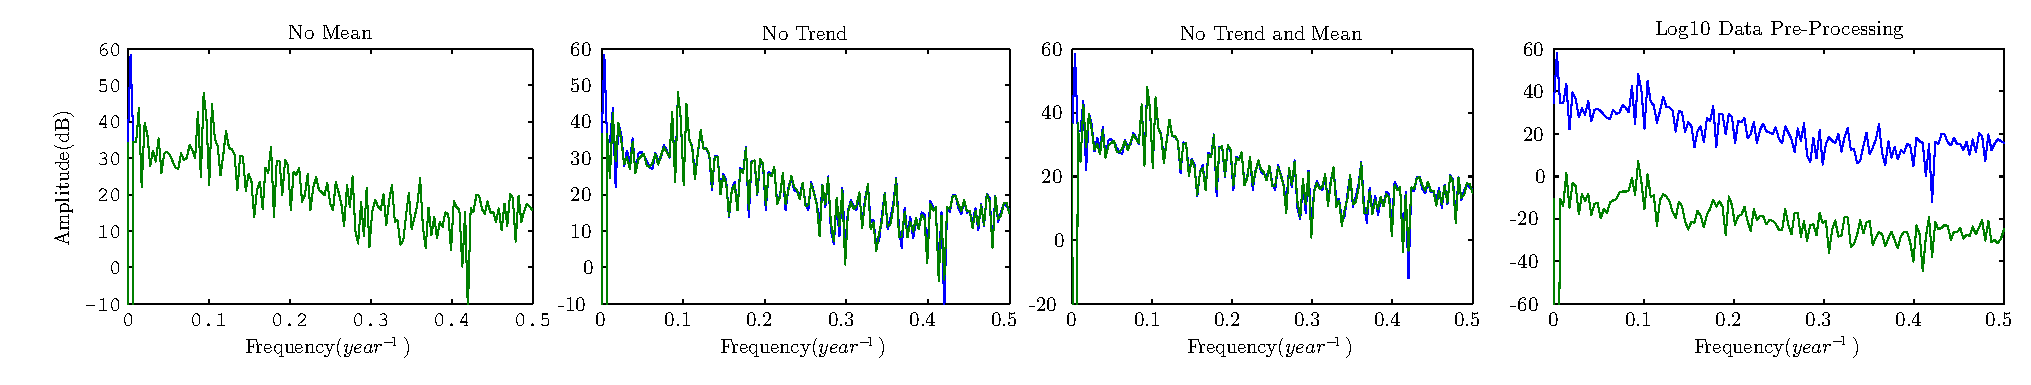
\includegraphics[width=\textwidth]{cw2im/4a.eps}
 \caption{Spectogram for various nfft, overlap and window settings for chirp signal}
 \label{fig:2_4a}
\end{figure}


We find that the best values for creating a spectrogram of a self generated 'chirp' signal are a FFT length of 128 with a very close overlap (120) to ensure a smooth spectrum. Indeed making the overlap closer to the nfft makes it smoother.

Hanning window was preferred for this example due to the higher contrast it offers to other window types.

For the spectrogram we have the choice of increasing the FFT and window size. The overlap allows more time resolution while being able to maintain a high frequency resolution (nfft). However as this takes larges sample lengths it can lead to some distortion as seen in the accompanying figure. 

\subsection{\texttt{spectogram} on SSVEP data}

\begin{figure}[h!]
 \centering
 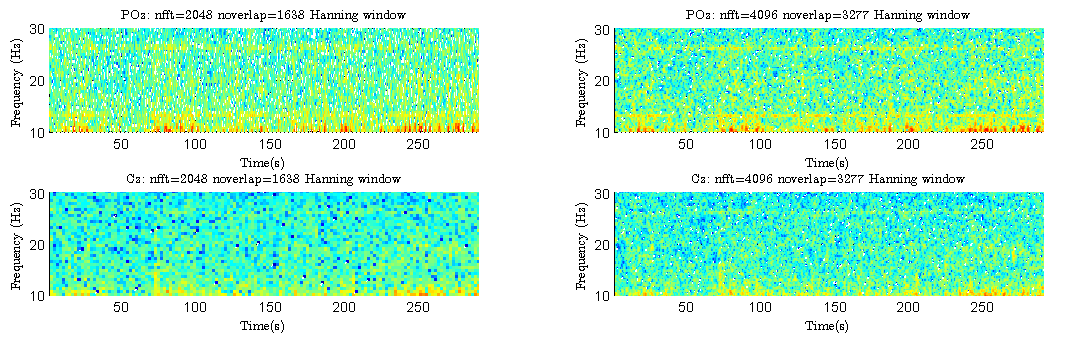
\includegraphics[width=\textwidth]{cw2im/4b.png}
 \caption{Spectogram for various nfft, overlap and window settings for EEG data}
 \label{fig:2_4b}
\end{figure}

In figure \ref{fig:2_4b} the SSEVP stimulus was sought in both the right and left channel of the EEG data. From previous tests it is know that this is 13Hz. In the case for the POz data the 13Hz peak can be seen (the yellow line at 13Hz), however this is absent from the Cz data, as earlier noticed. Increasing frequency bins did not help resolve.

It was found that the Hanning window also provides the best contrast here, allowing even the SSVEPs harmonics to be identified.

In choosing \texttt{nfft} the compromise was involved between time and frequency resolution - as increasing frequency bins decreases time resolution. Due to sampling frequency being 1200Hz and that we wanted to separate out one specific frequency a starting point was to have more than 1200 frequency bins. However exactly 1200 leads to a range of possible frequencies for one sample - between 13 and 14Hz for example. To pin it more to a specific frequency the \texttt{nfft} used was a higher 2048 and 4096.
\FloatBarrier
\chapter{Adaptive signal processing}
\section{The least mean square (LMS) algorithm}
\subsection{Correlation Matrix for $AR(2)$ process}


Here we have a system defined by $x[n] = a_1 x[n-1] + a_2 x[n-2] + \eta [n]$ with $a_1 = 0.1$, $a_2 = 0.8$ and $\sigma_\eta^2=0.25$. With the input vector $ \left[ x[n-1]  x[n-2]\right]^T$ we can form the correlation matrix $\mathbf{R} = \mathbb{E}\left\{ \mathbf{x}(n)^T \mathbf{x}(n) \right\}$.
\begin{equation}
\mathbf{R} = \mathbb{E} \left\{ \left[
 \begin{array}{cc}
x[n-1]^2 & x[n-1]x[n-2]  \\
x[n-2]x[n-1] & x[n-2]^2  \end{array}
\right]
\right\}
   =
\left[
    \begin{array}{cc}
  \mathbb{E} \left\{ x[n-1]^2 \right\} & \mathbb{E} \left\{x[n-1]x[n-2] \right\} \\
   \mathbb{E} \left\{ x[n-2]x[n-1]\right\} & \mathbb{E} \left\{x[n-2]^2 \right\} \end{array}
\right]
\end{equation}

Thus we are interested in $\mathbb{E} \left\{ x[n-1]^2 \right\}$ and $\mathbb{E} \left\{x[n-1]x[n-2] \right\}$. Note that $\mathbb{E} \left\{ x[n-1]^2 \right\} = \mathbb{E} \left\{ x[n]^2 \right\} = \mathbb{E} \left\{ x[n-2]^2 \right\}$ as this sample is taken from the same time series. Thus $\mathbf{R}$ is symmetric.

To find $\mathbb{E} \left\{ x[n]^2 \right\}$ and $\mathbb{E} \left\{x[n]x[n-1] \right\}$ we carry out the following:

\begin{align}
x[n] &= a_1 x[n-1] + a_2 x[n-2] + \eta [n] & \text{AR(2) definition} \notag \\
x[n]x[n-k] &= a_1 x[n-1]x[n-k] + a_2 x[n-2]x[n-k] + \eta [n] x[n-k] & \text{Multiply by } x[n-k] \notag \\
\mathbb{E} \left\{x[n]x[n-k] \right\}&= \mathbb{E} \left\{a_1 x[n-1]x[n-k] + a_2 x[n-2]x[n-k] + \eta [n] x[n-k] \right\} = \phi(k)& \text{Take expectation} \notag \\
\phi(k)&= a_1 \phi(k-1) + a_2 \phi(k-2)& \text{For } k \geq 1 \notag
\end{align}

Thus $\mathbb{E} \left\{ x[n]^2 \right\} = \phi(0)$ and $\mathbb{E} \left\{x[n]x[n-1] \right\} = \phi(1)$. We can calculate $\phi(0)$,$\phi(1)$ and $\phi(2)$ as such:

\begin{align}
\phi(0) &= \mathbb{E} \left\{ x[n]^2 \right\} = a_1 \phi(-1) + a_2 \phi(-2) + \mathbb{E} \left\{\eta [n] ^2 \right\} & \notag \\
\phi(0) & = a_1 \phi(-1) + a_2 \phi(-2) + \sigma_\eta ^ 2 & \notag \\
\phi(0) & = a_1 \phi(1) + a_2 \phi(2) + \sigma_\eta ^ 2 &\text{Using symmetry property} \label{eq:ph0} \\ 
\phi(1) & = a_1 \phi(0) + a_2 \phi(1) \label{eq:ph1} \\
\phi(2) & = a_1 \phi(1) + a_2 \phi(0) \label{eq:ph2}
\end{align}

We solve the simultaneous equations \ref{eq:ph0}, \ref{eq:ph1} and \ref{eq:ph2} for $a1=0.1$ and $a2=0.8$ and get:
\begin{align}
\mathbf{R} = \left[
    \begin{array}{cc}
 \frac{25}{27} & \frac{25}{54} \\[4pt]
 \frac{25}{54} &  \frac{25}{27} \end{array}
\right]
\end{align}
 
 Note that these are only expected values.
 
 For the convergence of the LMS in the mean we have:$ 0 < \mu <	\frac{2}{p \phi(0)}$ with $p=\text{trace}(\mathbf{R} _{xx})$. Thus $ 0 < \mu <(	\frac{=759}{625} = 1.1664)$. This is only an estimate and the formal way is that it is bounded by $0<\mu <\frac{2}{\lambda_{max}}$ where $\lambda$ is the largest eigenvalue of $\mathbf{R} _{xx}$. This is seen to be $\lambda_{max}=1.389$ making the bound max at $1.44$.
 
  For the convergence of the LMS in the mean square we have: $0 < \mu < (\frac{1}{3 p \mathbf{r}_{xx}(0)} = \frac{6561}{15625} = 0.419904)$.
    \FloatBarrier
  \subsection{LMS Filter error}
  \FloatBarrier
\begin{figure}[h!]
\centering
\resizebox{\textwidth}{!}{% This file was created by matlab2tikz v0.4.7 running on MATLAB 8.1.
% Copyright (c) 2008--2014, Nico Schlömer <nico.schloemer@gmail.com>
% All rights reserved.
% Minimal pgfplots version: 1.3
% 
% The latest updates can be retrieved from
%   http://www.mathworks.com/matlabcentral/fileexchange/22022-matlab2tikz
% where you can also make suggestions and rate matlab2tikz.
% 
\begin{tikzpicture}

\begin{axis}[%
width=9in,
height=2in,
unbounded coords=jump,
scale only axis,
xmin=0,
xmax=500,
xlabel={Sample Iteration},
ymin=-8,
ymax=1,
ylabel={Error(dB)},
title={Error of AR(2) process with N=500 $\sigma$ = 0.25 $a_1=0.1$ $a_2=0.8$},
axis x line*=bottom,
axis y line*=left,
legend style={draw=black,fill=white,legend cell align=left}
]
\addplot [color=blue,solid]
  table[row sep=crcr]{1	-0.229788243070588\\
2	-inf\\
3	-0.218203636981443\\
4	-1.73808742773869\\
5	-1.79551957929071\\
6	-2.28746110407662\\
7	-2.18118745503997\\
8	-3.58013564479554\\
9	-2.98421748558152\\
10	-4.95298378293035\\
11	-3.79989131129509\\
12	-3.37688035412364\\
13	-3.21703164703744\\
14	-3.74216406123553\\
15	-4.07612684545115\\
16	-4.51547590247142\\
17	-3.36339464349582\\
18	-5.15952580210771\\
19	-4.29835309759022\\
20	-4.18716594014725\\
21	-3.26543284232784\\
22	-4.38715286577999\\
23	-4.60228298234429\\
24	-4.32788858111614\\
25	-3.65523010416274\\
26	-4.29208467544006\\
27	-3.33244401253353\\
28	-4.4759496857724\\
29	-4.08508839524273\\
30	-5.59916633714001\\
31	-5.43488190635726\\
32	-5.84064586870389\\
33	-5.29902625543258\\
34	-5.19872287726752\\
35	-5.85065424191173\\
36	-5.43189223343866\\
37	-5.21286694318922\\
38	-6.50104170449159\\
39	-5.47199837421075\\
40	-5.56836889004279\\
41	-5.42208991556051\\
42	-4.65634877812563\\
43	-5.30089103520803\\
44	-5.92120128591003\\
45	-4.47841733179181\\
46	-5.06150149619086\\
47	-4.23750050152691\\
48	-5.46306911970808\\
49	-5.34698113665804\\
50	-6.54284243843051\\
51	-5.87436500441393\\
52	-5.03143044393694\\
53	-5.70107507828992\\
54	-5.15485445127537\\
55	-4.52318164217418\\
56	-5.4310396473444\\
57	-6.58639745940084\\
58	-5.61610823250922\\
59	-4.69090621631237\\
60	-5.74263025521253\\
61	-4.92601261569513\\
62	-4.74362922938526\\
63	-6.12081739329051\\
64	-5.56928546537914\\
65	-4.57624503262193\\
66	-5.29274313356007\\
67	-5.2487286072732\\
68	-6.53234022999071\\
69	-4.52407723284959\\
70	-5.8574049962793\\
71	-5.94247110304346\\
72	-5.38260345667883\\
73	-5.03397223868244\\
74	-6.17589516544435\\
75	-5.16874106382361\\
76	-5.80861259965988\\
77	-6.1648810044687\\
78	-5.77578464530208\\
79	-6.10521671305368\\
80	-6.75112545301969\\
81	-5.66740728176653\\
82	-5.16205603458247\\
83	-5.42906754063412\\
84	-5.10279107936781\\
85	-6.43628752918267\\
86	-6.175581479519\\
87	-5.65630168016819\\
88	-5.59496465567838\\
89	-5.46852332372649\\
90	-5.10582787621478\\
91	-4.90253703911878\\
92	-5.64337701134287\\
93	-5.42050203440295\\
94	-5.12157439111371\\
95	-5.36497667018451\\
96	-6.21586650946576\\
97	-5.15772273977455\\
98	-5.02804090079822\\
99	-5.01219915041109\\
100	-6.10551614749028\\
101	-6.14396345965409\\
102	-6.74737175105734\\
103	-6.01870209584417\\
104	-5.37769363066534\\
105	-4.84531105579311\\
106	-4.92229594277616\\
107	-5.56900549465387\\
108	-4.61151702211142\\
109	-5.42983115400914\\
110	-5.51182693918047\\
111	-5.27353666423673\\
112	-5.79837625038555\\
113	-5.8525743109092\\
114	-6.22004732634093\\
115	-6.78068213982206\\
116	-5.89709621306732\\
117	-6.59798955176555\\
118	-5.14061673875949\\
119	-6.98037386577991\\
120	-5.81755872344052\\
121	-5.86220102128863\\
122	-6.71932147476341\\
123	-6.53315503074471\\
124	-6.79160184963389\\
125	-5.63402997311076\\
126	-6.23935979392109\\
127	-5.15720607829311\\
128	-5.29829046008492\\
129	-5.49188695692767\\
130	-4.59733843202342\\
131	-5.16183807925268\\
132	-6.23154541757428\\
133	-6.6578049639367\\
134	-6.04058792520572\\
135	-5.22531321554492\\
136	-5.66318478434299\\
137	-5.53089932044527\\
138	-6.38878512769612\\
139	-5.5085642763215\\
140	-6.00032151756013\\
141	-5.73205860516742\\
142	-6.1659385786026\\
143	-6.0443300919105\\
144	-5.37349099691587\\
145	-5.94168669935386\\
146	-6.18671413553706\\
147	-5.19120816452886\\
148	-6.21421410880243\\
149	-6.01773740820446\\
150	-5.16066218834992\\
151	-5.59703009030996\\
152	-5.80245393677338\\
153	-5.50993171388241\\
154	-6.22525816247206\\
155	-5.99861874153744\\
156	-5.25722097475742\\
157	-7.50073689551816\\
158	-6.69273683660566\\
159	-5.73019477159794\\
160	-5.50666894698094\\
161	-6.43896780327472\\
162	-5.1715178822144\\
163	-5.49897959717483\\
164	-7.32770605193442\\
165	-6.20321915820244\\
166	-5.59195353304034\\
167	-5.30370460144668\\
168	-5.40574708086581\\
169	-5.98610910432874\\
170	-5.62417150719287\\
171	-5.43730613149863\\
172	-5.37040112235928\\
173	-5.58692118842649\\
174	-6.09804445394345\\
175	-5.1538125370193\\
176	-5.90052677502464\\
177	-6.19253349410607\\
178	-5.84780562519807\\
179	-4.75898155661522\\
180	-5.2452627824264\\
181	-4.76798974175807\\
182	-5.99807385455702\\
183	-5.79004545640885\\
184	-5.5894980383355\\
185	-5.90846648574785\\
186	-6.38473480582917\\
187	-4.55123329836067\\
188	-5.27795997805817\\
189	-5.86791918508474\\
190	-5.38818841942052\\
191	-5.78969506783587\\
192	-5.22538030339074\\
193	-6.64407330208905\\
194	-6.13636926523854\\
195	-5.77039060606247\\
196	-5.73470626065611\\
197	-5.20771574795184\\
198	-4.62972777979257\\
199	-4.61634184672718\\
200	-4.34810384832094\\
201	-4.96881071702656\\
202	-5.73260549802331\\
203	-5.70822133848988\\
204	-5.29678634325097\\
205	-4.61423011029444\\
206	-6.54397044398361\\
207	-6.27887787658762\\
208	-6.1697681981093\\
209	-5.15014239888381\\
210	-4.90852660601818\\
211	-6.24280867856958\\
212	-5.82439529801948\\
213	-6.46339465092116\\
214	-5.58926366178015\\
215	-6.55001355628265\\
216	-6.00295030450426\\
217	-5.58332028253455\\
218	-5.6646014387897\\
219	-6.24969131867989\\
220	-6.82708368719022\\
221	-5.86097450469113\\
222	-6.09895577600069\\
223	-4.53132513630901\\
224	-5.68791215244656\\
225	-5.54162849940635\\
226	-7.39763063698513\\
227	-5.5263357618908\\
228	-6.35940751326998\\
229	-6.79737100957956\\
230	-5.22152480049811\\
231	-4.07971896268717\\
232	-6.5145771580454\\
233	-6.16165585263209\\
234	-6.22004181249517\\
235	-6.02956891643305\\
236	-4.85255523334567\\
237	-5.84018984505244\\
238	-5.28545455578964\\
239	-5.84196472037425\\
240	-5.45420982419747\\
241	-5.33455178570608\\
242	-5.97491703591222\\
243	-6.09984289564845\\
244	-5.17447360483718\\
245	-5.91058899893254\\
246	-6.75875571638209\\
247	-5.45158398050944\\
248	-5.31836372075767\\
249	-5.92919069312543\\
250	-5.47308552878484\\
251	-6.65900553314768\\
252	-6.54067824505954\\
253	-5.57831528716302\\
254	-6.52706928157977\\
255	-4.816496891527\\
256	-6.28218076361067\\
257	-6.13139272168441\\
258	-6.49155969911562\\
259	-6.23194047768359\\
260	-5.21286619495297\\
261	-6.18525595940449\\
262	-6.60283481182297\\
263	-6.3270746681846\\
264	-6.75605623071768\\
265	-5.65783911273338\\
266	-6.10852281383835\\
267	-6.45385641524964\\
268	-6.125276666638\\
269	-6.87610861722742\\
270	-4.42026042212565\\
271	-5.92679314811075\\
272	-6.18357440680863\\
273	-5.19068148820777\\
274	-4.43540050148727\\
275	-5.97557432034599\\
276	-7.31633277707819\\
277	-4.89202920396066\\
278	-7.07014079095837\\
279	-5.89046269815394\\
280	-5.72172339703819\\
281	-5.12626033960445\\
282	-5.68959825432008\\
283	-5.35310689622004\\
284	-7.49047162570408\\
285	-6.48053985517056\\
286	-4.96091363696748\\
287	-5.24115750260128\\
288	-5.88220318716849\\
289	-6.58133319759685\\
290	-5.90888097078184\\
291	-5.36421041825948\\
292	-5.47758755122839\\
293	-6.09577125936425\\
294	-6.23442742818584\\
295	-5.37477459324413\\
296	-6.07567855447041\\
297	-6.17554252080335\\
298	-5.31048711398318\\
299	-5.92124321928878\\
300	-5.61213356136938\\
301	-5.32100655589412\\
302	-5.8574994252531\\
303	-5.90153478666188\\
304	-5.77655695982206\\
305	-6.37779990400114\\
306	-7.0008544227321\\
307	-5.41688843380852\\
308	-5.31696110328115\\
309	-5.6122351660368\\
310	-5.53338413326015\\
311	-5.77787725698007\\
312	-5.9662351223825\\
313	-6.34321828360199\\
314	-6.53611812928666\\
315	-5.34817176065266\\
316	-6.59485294958415\\
317	-6.04201823240622\\
318	-5.01456564494496\\
319	-5.03109196319889\\
320	-5.79624747992805\\
321	-5.36127278332435\\
322	-4.88977786297926\\
323	-5.54273515379944\\
324	-6.916512199563\\
325	-5.05527396828071\\
326	-6.00338262460889\\
327	-6.42480889739445\\
328	-5.87518229328505\\
329	-5.85438879903416\\
330	-4.74894667484783\\
331	-4.98945134948161\\
332	-6.18594564925984\\
333	-5.90288084755922\\
334	-6.31061523996004\\
335	-5.60841784288212\\
336	-5.67662143290465\\
337	-5.53680635233187\\
338	-5.34798468410129\\
339	-5.73570143372959\\
340	-5.24877757046847\\
341	-4.64500744046386\\
342	-5.97651503194191\\
343	-4.97405423901893\\
344	-4.89742498352531\\
345	-6.07907798186201\\
346	-5.325243500859\\
347	-5.065472737502\\
348	-5.70872690340672\\
349	-5.11538410044954\\
350	-5.89464318710674\\
351	-6.67855242878746\\
352	-6.27144359479701\\
353	-5.40796626999858\\
354	-5.75744280851982\\
355	-5.09005854163943\\
356	-5.57899640810071\\
357	-5.48220932259701\\
358	-6.22967936518648\\
359	-5.98541554873426\\
360	-6.35084329948506\\
361	-5.46890159418377\\
362	-5.6652740750065\\
363	-5.9551472442877\\
364	-5.84713111043308\\
365	-5.52444642629407\\
366	-6.95803808464547\\
367	-5.66853771501352\\
368	-5.85726537143959\\
369	-6.04619344597585\\
370	-6.16696924540945\\
371	-6.77423326338395\\
372	-5.95488104670501\\
373	-5.68817810969405\\
374	-5.83170179379665\\
375	-6.55233815813854\\
376	-4.91528742552698\\
377	-5.32470878547333\\
378	-5.72676118696556\\
379	-5.78127437010925\\
380	-5.9269649954569\\
381	-5.97500377631815\\
382	-5.31390682250549\\
383	-6.06264106619104\\
384	-5.42893131449347\\
385	-5.65545273627387\\
386	-5.44791639498981\\
387	-5.27097358493136\\
388	-6.09720544796168\\
389	-5.40733562450943\\
390	-6.34876033768787\\
391	-6.12779965788523\\
392	-6.20609841546047\\
393	-4.81217216027754\\
394	-5.65273602023547\\
395	-5.9720079483978\\
396	-5.80118997654346\\
397	-6.04726636756597\\
398	-5.95462085984802\\
399	-6.27495945633844\\
400	-6.20588938127144\\
401	-6.53726012531118\\
402	-5.42692511513224\\
403	-5.5060010413534\\
404	-4.72657881545002\\
405	-5.16454070314347\\
406	-5.84647660636429\\
407	-4.93223490708524\\
408	-4.89666112724137\\
409	-6.05702369251575\\
410	-6.81628758430124\\
411	-5.46332045838871\\
412	-6.08903571323949\\
413	-6.24766655033977\\
414	-5.28180461849417\\
415	-6.91476150787389\\
416	-6.27913538107551\\
417	-5.0374497080677\\
418	-5.73681147949017\\
419	-5.09648996918608\\
420	-5.92565019994917\\
421	-6.00792999368353\\
422	-5.06451503070626\\
423	-5.42288635308205\\
424	-4.80701634493005\\
425	-5.43314311321427\\
426	-5.11898220594836\\
427	-5.10978583819449\\
428	-5.09383204092813\\
429	-6.71611466466493\\
430	-4.98393616326159\\
431	-6.71083402579349\\
432	-5.77883016506813\\
433	-5.52942925882109\\
434	-4.88723444293461\\
435	-5.47629980163681\\
436	-6.42090188924682\\
437	-5.24290170351227\\
438	-4.42277791571427\\
439	-5.81435217950424\\
440	-5.98389900374645\\
441	-6.73784365325178\\
442	-5.91153635611154\\
443	-7.34256711726857\\
444	-5.8011735381461\\
445	-5.94325212365385\\
446	-5.57070538116492\\
447	-6.31952274215173\\
448	-5.573486894642\\
449	-4.80760067400412\\
450	-5.99569369561893\\
451	-5.7349331969918\\
452	-5.96389858177334\\
453	-6.40018404891549\\
454	-5.41992239640187\\
455	-6.07211507886066\\
456	-5.47827658484694\\
457	-5.78415057041042\\
458	-5.63208614880714\\
459	-5.83942083478156\\
460	-5.56033723018114\\
461	-5.75671186533159\\
462	-4.81716916320498\\
463	-5.58659589842412\\
464	-5.22169539575116\\
465	-5.70907161749598\\
466	-5.41631469241396\\
467	-6.19153667880597\\
468	-6.5832969583161\\
469	-5.6426807464211\\
470	-6.03884636393531\\
471	-5.61577022702524\\
472	-6.57725701975202\\
473	-6.61015439462763\\
474	-6.35289093241573\\
475	-5.76794734623316\\
476	-5.85751286740099\\
477	-5.76667950881399\\
478	-5.9038746339343\\
479	-6.33604267276987\\
480	-4.88478522729542\\
481	-5.7806487452813\\
482	-5.14265703635032\\
483	-6.6700164196176\\
484	-5.89490376850381\\
485	-5.41742823864795\\
486	-7.02095441315774\\
487	-6.2374540751595\\
488	-6.57685940222582\\
489	-5.52606956376956\\
490	-5.4890262212922\\
491	-6.15191892510352\\
492	-6.44331499449174\\
493	-6.26630378510544\\
494	-5.30233912473161\\
495	-5.01528970028261\\
496	-6.3788530181044\\
497	-6.21195847353363\\
498	-5.99450341812563\\
499	-5.57928553595309\\
500	-6.29530666063422\\
};
\addlegendentry{$\mu = 0.05$};

\addplot [color=red,solid]
  table[row sep=crcr]{1	0.239867219163377\\
2	-inf\\
3	-0.136817166163276\\
4	-0.53479702042941\\
5	-1.36704371344684\\
6	-1.61095173840487\\
7	-0.702547728678975\\
8	-1.87890886483772\\
9	-0.733243697039139\\
10	-1.87438434195662\\
11	-0.997020835942035\\
12	-1.30488508339394\\
13	-1.23857426222341\\
14	-1.9624858576123\\
15	-2.33367312631497\\
16	-1.76267263358362\\
17	-2.49134367693499\\
18	-2.0773334129832\\
19	-1.72255473112448\\
20	-1.17235411888693\\
21	-1.84600367812748\\
22	-2.229755817253\\
23	-2.30818788018455\\
24	-1.99660921376525\\
25	-1.79143435025107\\
26	-1.59129814851171\\
27	-1.52129858125753\\
28	-1.72044706684545\\
29	-1.10261780125816\\
30	-3.01690484472666\\
31	-1.91361254489451\\
32	-2.20848165110484\\
33	-2.74773559325964\\
34	-1.81409273079906\\
35	-3.77844276544056\\
36	-1.75953200713234\\
37	-3.12135757433164\\
38	-2.52656712277453\\
39	-3.88408191333951\\
40	-3.60609671468107\\
41	-3.53191841472304\\
42	-3.71407914352619\\
43	-3.72013710929094\\
44	-3.08056426045667\\
45	-4.03449261536694\\
46	-4.50122572366154\\
47	-3.95274500863518\\
48	-4.15301408824723\\
49	-3.51463670297543\\
50	-3.69030259344381\\
51	-4.2950240279612\\
52	-4.29364177627072\\
53	-4.88200601131738\\
54	-3.30958171213217\\
55	-3.164122588413\\
56	-3.45119230038019\\
57	-3.53623431843914\\
58	-3.69121091544556\\
59	-3.70795758881022\\
60	-3.02681989776703\\
61	-4.07988587424577\\
62	-2.86068019757288\\
63	-4.23856896161224\\
64	-2.46110768351752\\
65	-4.32923464265606\\
66	-3.1867215183672\\
67	-3.21495889336628\\
68	-3.90618389910417\\
69	-3.55395824215338\\
70	-3.70932030949747\\
71	-4.56888407471684\\
72	-3.56299918925327\\
73	-4.08163958620998\\
74	-4.44324418151967\\
75	-4.35728810393583\\
76	-4.10734883116877\\
77	-4.47255861989405\\
78	-2.93001465268669\\
79	-4.30222138800123\\
80	-3.97458273058344\\
81	-4.12346451987317\\
82	-4.11274637133153\\
83	-3.77430254179982\\
84	-4.34089031779035\\
85	-3.30617955674343\\
86	-4.34451185408386\\
87	-3.43844676803395\\
88	-4.53679526178751\\
89	-3.45785576672603\\
90	-5.03696673349925\\
91	-3.82279100122824\\
92	-3.77848511480895\\
93	-4.80749403312712\\
94	-4.17266723905709\\
95	-4.59569395900588\\
96	-3.96328041283094\\
97	-3.51822716531805\\
98	-5.91827177293634\\
99	-5.29300342805972\\
100	-5.0775821394625\\
101	-4.08882111394913\\
102	-4.23793913698347\\
103	-4.59851865635429\\
104	-4.69380700334\\
105	-4.11810457062593\\
106	-4.75533835700714\\
107	-4.97578826274818\\
108	-3.6489262141135\\
109	-5.05333462368184\\
110	-4.02604790721967\\
111	-5.05673163362715\\
112	-3.96547017378345\\
113	-4.57115833093393\\
114	-3.60008437392771\\
115	-4.56997040453946\\
116	-3.86879341166522\\
117	-6.17989178957949\\
118	-4.08936614167059\\
119	-4.46476515131358\\
120	-4.37255920471621\\
121	-4.82753501375735\\
122	-5.27360415114152\\
123	-4.52253928395061\\
124	-5.70185115412166\\
125	-4.70440526894857\\
126	-4.67485416504118\\
127	-4.25934095445106\\
128	-4.77649074358074\\
129	-5.36016257064891\\
130	-3.78713416224082\\
131	-5.28378481869119\\
132	-4.99947174438969\\
133	-5.34860956081313\\
134	-4.77662587079642\\
135	-5.45027850718559\\
136	-4.75248835537801\\
137	-7.00361772892377\\
138	-4.77969470171313\\
139	-6.01046788506133\\
140	-5.61690725780614\\
141	-4.92920931501247\\
142	-5.64668771534571\\
143	-5.37742323067691\\
144	-5.16120623443163\\
145	-4.30304966769503\\
146	-5.68000048183947\\
147	-4.96268956522863\\
148	-6.2897395560052\\
149	-4.89426558999908\\
150	-5.32864382017678\\
151	-5.6204196627061\\
152	-5.07596848278847\\
153	-5.36228347016414\\
154	-5.59991969369589\\
155	-5.04958307457341\\
156	-5.85437794021568\\
157	-4.99832974955514\\
158	-5.69142051727565\\
159	-4.21365116785242\\
160	-6.28497566882644\\
161	-5.56126976644333\\
162	-5.47712129931178\\
163	-5.67362453490562\\
164	-5.38008737965602\\
165	-5.54668305098062\\
166	-4.64233548641945\\
167	-5.13957993935667\\
168	-4.79594147869521\\
169	-6.28920494393421\\
170	-5.23757834666078\\
171	-5.69445643967045\\
172	-5.7022893595187\\
173	-5.45824133572193\\
174	-5.64583817608454\\
175	-3.78639842131258\\
176	-5.5254689500231\\
177	-4.98115564671484\\
178	-5.39573382837007\\
179	-5.52050987397022\\
180	-4.48939179821701\\
181	-5.10672114611057\\
182	-4.90704015287781\\
183	-4.3437469181639\\
184	-6.33207661965549\\
185	-6.07148214357611\\
186	-6.14912995747169\\
187	-5.42280194567736\\
188	-6.62536544295707\\
189	-5.36414746330982\\
190	-6.36491964489899\\
191	-4.75178287826294\\
192	-6.00047657875805\\
193	-5.48391218741435\\
194	-5.52454899886709\\
195	-5.84596071029402\\
196	-6.05191639721115\\
197	-6.49016373648903\\
198	-5.567798710307\\
199	-5.36699181146966\\
200	-5.22350552852686\\
201	-5.5399375650092\\
202	-4.77535302579686\\
203	-5.43120764125078\\
204	-5.88971112513903\\
205	-4.34738897563124\\
206	-6.29625611556054\\
207	-5.39897604892467\\
208	-5.58248234384482\\
209	-4.95353742007771\\
210	-5.96491775580821\\
211	-6.11177747183748\\
212	-5.62756969490204\\
213	-7.27922358758946\\
214	-6.07071763038443\\
215	-6.8559599429311\\
216	-5.22794695592819\\
217	-4.88331505994604\\
218	-5.09800566965161\\
219	-4.41882946851145\\
220	-5.36633007783295\\
221	-5.29278183593473\\
222	-6.06658748054179\\
223	-7.52767713126511\\
224	-4.41491541228114\\
225	-5.203548027425\\
226	-5.95480582868669\\
227	-5.66227043847732\\
228	-4.174392897905\\
229	-6.74053155971216\\
230	-5.85480487557086\\
231	-6.01281636063875\\
232	-4.6125313391989\\
233	-6.31441848099755\\
234	-5.56920453333565\\
235	-5.83569247329743\\
236	-4.75688000450699\\
237	-5.89478914112542\\
238	-5.46338438215209\\
239	-6.13503330465739\\
240	-5.8429571269254\\
241	-6.12769108761218\\
242	-5.46174050521072\\
243	-5.99306382905729\\
244	-5.76727734907696\\
245	-5.64810944067\\
246	-5.8953785761505\\
247	-7.10597980034809\\
248	-6.09345620739889\\
249	-5.58928027575863\\
250	-5.84727474379189\\
251	-5.75481321057305\\
252	-5.09864055125514\\
253	-6.10866915462029\\
254	-4.91211875925654\\
255	-6.01908294766615\\
256	-7.5897757800617\\
257	-5.76992521362538\\
258	-5.67931521327206\\
259	-5.8984986562939\\
260	-6.17412666923055\\
261	-5.26613057979618\\
262	-5.44493932676755\\
263	-6.76000288432309\\
264	-5.95383704255669\\
265	-5.06686971812229\\
266	-6.40783386109657\\
267	-4.81713671040025\\
268	-5.93647547801917\\
269	-5.92062458171705\\
270	-5.48219865922666\\
271	-6.57908782990359\\
272	-6.12786675174806\\
273	-5.85316207385492\\
274	-6.25445273768572\\
275	-5.56110311888801\\
276	-5.38948502267894\\
277	-5.86276212584018\\
278	-5.65826523426908\\
279	-5.17738274947051\\
280	-6.46964605585268\\
281	-4.23728562936972\\
282	-5.71523962947078\\
283	-4.52105455234137\\
284	-6.27905193875185\\
285	-6.55097796925785\\
286	-5.01592860022436\\
287	-5.60945809109059\\
288	-5.75176815280264\\
289	-6.01175461712101\\
290	-5.19489082374621\\
291	-5.25095376655537\\
292	-7.26489659230748\\
293	-6.24850124071954\\
294	-6.03975444070031\\
295	-6.46946516027979\\
296	-5.93385895112799\\
297	-5.33570185694488\\
298	-5.59290171981613\\
299	-5.16506717978825\\
300	-5.63396312768729\\
301	-5.30347012628937\\
302	-5.72402992077923\\
303	-5.23063451923239\\
304	-6.44045861841825\\
305	-5.54405738255733\\
306	-5.67844866070906\\
307	-5.00330928282241\\
308	-5.84870903583403\\
309	-6.20218201924873\\
310	-5.48189648386678\\
311	-5.1274975050235\\
312	-6.19304531084414\\
313	-5.712858865171\\
314	-5.21364617145121\\
315	-6.32665084774398\\
316	-6.27001583761304\\
317	-5.87798570456194\\
318	-5.5530095452379\\
319	-5.39021378436429\\
320	-5.18954264069515\\
321	-6.01867093108662\\
322	-5.9703349007945\\
323	-6.61421444560049\\
324	-6.83161561174491\\
325	-5.96292892109102\\
326	-5.44412907435885\\
327	-5.0907226861683\\
328	-6.09332888120996\\
329	-6.97815023961496\\
330	-6.2616874874844\\
331	-5.93239969003365\\
332	-6.74384906109466\\
333	-6.04264637995414\\
334	-5.73944276163831\\
335	-5.90275005156886\\
336	-5.3852294766252\\
337	-6.04281676290199\\
338	-6.07443693254382\\
339	-3.93862790941867\\
340	-6.8040793624167\\
341	-4.77652700160456\\
342	-6.27236050849926\\
343	-4.564194221761\\
344	-5.31594603420301\\
345	-5.91669141188043\\
346	-6.34097045064726\\
347	-6.53834452846343\\
348	-4.94911059912997\\
349	-5.94326490300823\\
350	-7.29464653592376\\
351	-6.63333052076231\\
352	-5.97230466734001\\
353	-6.52738704642026\\
354	-4.85118094362295\\
355	-5.04289098292696\\
356	-6.83815915440258\\
357	-6.2225703812461\\
358	-6.0912933590355\\
359	-5.18878457716532\\
360	-4.90154492171184\\
361	-5.22657569403415\\
362	-6.18990599548292\\
363	-4.61493217019859\\
364	-5.53935487540941\\
365	-6.40432118828676\\
366	-6.29382722147848\\
367	-6.24009359834568\\
368	-6.62102149817432\\
369	-6.87472279953865\\
370	-6.36667646160047\\
371	-5.76318837458457\\
372	-6.34629289775504\\
373	-6.28338156061629\\
374	-6.01217060426414\\
375	-5.33400905042032\\
376	-7.22800960879543\\
377	-5.8863849075152\\
378	-6.51189318566321\\
379	-6.70106525643205\\
380	-5.72800127882243\\
381	-5.79524678366512\\
382	-5.98280556193488\\
383	-6.84353160854253\\
384	-5.43124326138149\\
385	-5.42143240219709\\
386	-5.75764430819515\\
387	-5.4540005884005\\
388	-7.07020436012048\\
389	-5.77800984191368\\
390	-5.74853133396768\\
391	-6.17285118691665\\
392	-5.01777857838409\\
393	-6.02799240664749\\
394	-6.09415702117286\\
395	-6.50858560156009\\
396	-6.70359475860112\\
397	-7.15805583058095\\
398	-6.20959904836787\\
399	-6.04524139812596\\
400	-5.67297375149025\\
401	-6.30821227181905\\
402	-5.63146087609836\\
403	-6.80812567125969\\
404	-4.94144971940602\\
405	-5.9725606805954\\
406	-6.23308830686746\\
407	-6.11640906839115\\
408	-6.7231814819728\\
409	-5.03267236425398\\
410	-5.91778002025918\\
411	-7.44385009675043\\
412	-6.09472915643058\\
413	-6.23593803301464\\
414	-6.26928011070537\\
415	-5.34982759147844\\
416	-5.78965871852682\\
417	-4.89225101783455\\
418	-5.83147753782608\\
419	-5.21334112656999\\
420	-6.23622035884429\\
421	-6.05344967258154\\
422	-5.94791644370468\\
423	-5.94708365162295\\
424	-5.88559015179134\\
425	-6.67402112460689\\
426	-5.41395380533136\\
427	-5.13861747406598\\
428	-6.26119852659676\\
429	-5.66052338101043\\
430	-5.84265801798589\\
431	-5.9091751314334\\
432	-5.97292333666067\\
433	-4.9529736654248\\
434	-5.29164841858967\\
435	-6.27925705324482\\
436	-5.92757924408286\\
437	-5.58954845799373\\
438	-5.91059671338535\\
439	-5.8701034259859\\
440	-6.49651231719305\\
441	-4.95432853430049\\
442	-5.787700009606\\
443	-5.63409341923611\\
444	-6.59659395202474\\
445	-6.20626689187122\\
446	-5.99352914970808\\
447	-7.12098391142387\\
448	-6.72843846420565\\
449	-6.36522123397258\\
450	-6.71682843219805\\
451	-6.21760157772516\\
452	-5.57576981125371\\
453	-5.98798849243118\\
454	-6.17156422279381\\
455	-5.21885581354273\\
456	-5.69169095887554\\
457	-6.2035159558015\\
458	-6.2523427674741\\
459	-6.63885092993258\\
460	-5.7894881554731\\
461	-5.58180578922436\\
462	-5.36876122372263\\
463	-6.58302036254319\\
464	-5.19688970176316\\
465	-5.75058956107062\\
466	-6.40048957899504\\
467	-6.03983131034195\\
468	-5.43989787488522\\
469	-6.76532840051718\\
470	-6.01124725168041\\
471	-5.89656661862967\\
472	-5.40244465299072\\
473	-5.63167211968751\\
474	-5.40205310956715\\
475	-5.6449091246016\\
476	-6.36166357075991\\
477	-6.35108508313977\\
478	-5.55020347413113\\
479	-6.22642779517253\\
480	-6.93454632915112\\
481	-7.01106624747657\\
482	-5.86701503749128\\
483	-6.24494289194155\\
484	-5.97810455642793\\
485	-7.07330454975633\\
486	-5.73729668985005\\
487	-6.81981138422658\\
488	-5.45044447303642\\
489	-6.71318916964817\\
490	-5.39917274562679\\
491	-5.46847140632588\\
492	-6.09063560495087\\
493	-6.49495681487413\\
494	-7.73428366683879\\
495	-7.8446282138018\\
496	-6.30921580051409\\
497	-5.33121823175904\\
498	-5.90487908185136\\
499	-6.64907286042326\\
500	-6.63639432377932\\
};
\addlegendentry{$\mu = 0.01$};

\end{axis}
\end{tikzpicture}%}
\caption{PSD estimates from AR coefficients}
\label{fig:3_1b}
\end{figure}
 
Here we have created a LMS filter that learns the ideal $\mathbf{w}$ vector other 500 iterations. We see that changing $\mu$, the learning rate, leads to a slower decrease rate in error over each iteration. This shows the compromise between wanting a fast convergence (low error) and that of a convergence that is not too fast to avoid overshoot and be stable.
%http://econweb.ucsd.edu/muendler/teach/00s/ps1-prt1.pdf

An important observation is the error converging to values near -6.02dB. This is because the filtered AWGN has $\sigma^2 = 0.25$, which is essentially the minimum theoretical error.


\subsection{Excess Mean Square Error}

The theoretical excess error is: $\mathcal{M}=\frac{\mu}{2}\mathbf{Tr}\{\mathbf{R} \}$. Thus for each $\mu$ we have $\mathcal{M}_{\mu=0.05}= \frac{5}{54}$ and $\mathcal{M}_{\mu=0.01}= \frac{1}{54}$.


\begin{table}[h]
\begin{tabular}{|l|l|l|l|l|}
\hline
  & \textbf{MSE} & \textbf{EMSE} & \textbf{$\mathcal{M}$} & \textbf{$\mathcal{M}_{LMS}$} \\ \hline
\textbf{$\mu = $0.01} & 0.2517       & 0.0017        & 0.0069         & 0.009259             \\ \hline
\textbf{$\mu = $0.05} & 0.2616       & 0.0116        & 0.0462         & 0.046296             \\ \hline
\end{tabular}
\end{table}


Here we see that the $\mathcal{M}$ and the $\mathcal{M}_{LMS}$ are not too disimilar, within the correct order of magnitude. It can be seen how larger $\mu$ values cause a larger EMSE due to the the larger oscillations this produces for converged values.

\subsection{Steady State values}
\begin{figure}[h!]
\centering
\resizebox{\textwidth}{!}{% This file was created by matlab2tikz v0.4.7 running on MATLAB 8.1.
% Copyright (c) 2008--2014, Nico Schlömer <nico.schloemer@gmail.com>
% All rights reserved.
% Minimal pgfplots version: 1.3
% 
% The latest updates can be retrieved from
%   http://www.mathworks.com/matlabcentral/fileexchange/22022-matlab2tikz
% where you can also make suggestions and rate matlab2tikz.
% 
\begin{tikzpicture}

\begin{axis}[%
width=3.5in,
height=1.25in,
scale only axis,
xmin=0,
xmax=500,
xlabel={N},
ymin=0,
ymax=0.8,
ytick={  0, 0.1, 0.2, 0.3, 0.4, 0.5, 0.6, 0.7, 0.8},
ylabel={$\mathbf{w}$ values},
ymajorgrids,
name=plot1,
title={$\mu$ = 0.05 $\mathbf{w}[end]$=[0.10595 0.74072]},
legend style={draw=black,fill=white,legend cell align=left}
]
\addplot [color=blue,solid]
  table[row sep=crcr]{1	0\\
2	0\\
3	0.00574152083018405\\
4	0.0110200846081192\\
5	0.0151748475508237\\
6	0.0195544698108526\\
7	0.024000631262801\\
8	0.028368347549891\\
9	0.0330622038657145\\
10	0.0373239580166373\\
11	0.0412018644370496\\
12	0.0445533299546722\\
13	0.0481526804958367\\
14	0.0508053087195389\\
15	0.053478993131461\\
16	0.0566890247319005\\
17	0.0601333969279939\\
18	0.0638501926696671\\
19	0.067459299632472\\
20	0.0710359778083566\\
21	0.0737363172681726\\
22	0.0760216346123486\\
23	0.0797850129364954\\
24	0.0835707321072498\\
25	0.0861413851954362\\
26	0.0876415415990771\\
27	0.090015820817525\\
28	0.0924135691267506\\
29	0.093617558399917\\
30	0.0958991507090308\\
31	0.0970576966636875\\
32	0.0988515184288983\\
33	0.0994947899869222\\
34	0.10122485970496\\
35	0.102845530939472\\
36	0.105172290955887\\
37	0.107267445405143\\
38	0.108796657299708\\
39	0.110446254229347\\
40	0.11117151404193\\
41	0.112256668389425\\
42	0.113711722914549\\
43	0.115025294486596\\
44	0.116715670530833\\
45	0.118564054597888\\
46	0.120102504072558\\
47	0.122261329434535\\
48	0.124084870653287\\
49	0.12564950095328\\
50	0.127377548135056\\
51	0.128850091808458\\
52	0.129025162865453\\
53	0.129350756775331\\
54	0.130654882568761\\
55	0.131502648172869\\
56	0.132339648176688\\
57	0.132462938272408\\
58	0.133382116925555\\
59	0.134525827330687\\
60	0.135842384993518\\
61	0.137835649110837\\
62	0.139307317270853\\
63	0.140306689708426\\
64	0.141056159711856\\
65	0.142452348633286\\
66	0.143059123200278\\
67	0.144591343038652\\
68	0.146612979116135\\
69	0.146897039367823\\
70	0.147312481983119\\
71	0.147971630263883\\
72	0.147823450200061\\
73	0.148357452913331\\
74	0.1476898183143\\
75	0.148793284962287\\
76	0.149334899761339\\
77	0.150834451233576\\
78	0.152004949018794\\
79	0.154159319198654\\
80	0.155206513213187\\
81	0.15619146127467\\
82	0.156554550173465\\
83	0.157273843268589\\
84	0.157880285950375\\
85	0.158371552901389\\
86	0.159048124979654\\
87	0.159747131491444\\
88	0.160059529259872\\
89	0.160654780445007\\
90	0.161582345946383\\
91	0.162270220140578\\
92	0.162573110769907\\
93	0.163245901528852\\
94	0.164394708828936\\
95	0.164789457949881\\
96	0.165891111041527\\
97	0.165788288409785\\
98	0.166124088444697\\
99	0.165520908153341\\
100	0.167267919939585\\
101	0.168254919747824\\
102	0.16931699555179\\
103	0.169011584906305\\
104	0.170129960210529\\
105	0.170277326112513\\
106	0.171187151686253\\
107	0.171015695314912\\
108	0.170943923665169\\
109	0.171286961947875\\
110	0.171480252367465\\
111	0.170763523453186\\
112	0.170225250907453\\
113	0.170137821778667\\
114	0.169872181663699\\
115	0.169057922535768\\
116	0.167923819746846\\
117	0.167341449273404\\
118	0.167971584821392\\
119	0.167500871437077\\
120	0.167599010361039\\
121	0.167810363384568\\
122	0.168736881970892\\
123	0.168622604732212\\
124	0.168406570060242\\
125	0.168756066726883\\
126	0.169149874283566\\
127	0.16884855681797\\
128	0.168633543767326\\
129	0.169178175872034\\
130	0.16993837685601\\
131	0.169628180021788\\
132	0.170042928029194\\
133	0.170636635312429\\
134	0.170344515255431\\
135	0.170720867527561\\
136	0.170309033102455\\
137	0.170644590399005\\
138	0.17047982830436\\
139	0.169727374840309\\
140	0.169367188013593\\
141	0.169299390851552\\
142	0.169022197759531\\
143	0.169405184969988\\
144	0.170056598647782\\
145	0.170438567678429\\
146	0.170761826463729\\
147	0.170378495115934\\
148	0.170732802464328\\
149	0.171038841871352\\
150	0.170128068562791\\
151	0.169554911954592\\
152	0.168702267743757\\
153	0.16849668092298\\
154	0.168069935731913\\
155	0.168290368645964\\
156	0.167824736308897\\
157	0.167022231124349\\
158	0.167608632690896\\
159	0.167761603382671\\
160	0.167355304376234\\
161	0.167590725655798\\
162	0.167301449124866\\
163	0.167119167784839\\
164	0.168197082528991\\
165	0.168271754779112\\
166	0.167857099186574\\
167	0.168751704350245\\
168	0.168301824460363\\
169	0.168227174551621\\
170	0.167062714112766\\
171	0.167805829289989\\
172	0.168309846844989\\
173	0.16838697039387\\
174	0.167811335527316\\
175	0.166836508891887\\
176	0.168055008103588\\
177	0.167624978138015\\
178	0.167349425732476\\
179	0.167392230826441\\
180	0.168029862734466\\
181	0.167985532076241\\
182	0.1674907053904\\
183	0.166184246025093\\
184	0.165788249028818\\
185	0.164302232746832\\
186	0.163858861289797\\
187	0.16354914045273\\
188	0.163377112701757\\
189	0.162577485535825\\
190	0.163070334328913\\
191	0.162629126958529\\
192	0.16297806871497\\
193	0.162857111522702\\
194	0.162973535486476\\
195	0.162755179867099\\
196	0.163093964049586\\
197	0.163282627337911\\
198	0.162307623699796\\
199	0.162410015367416\\
200	0.162708285321001\\
201	0.163441894630248\\
202	0.162103008802637\\
203	0.160822919677808\\
204	0.160567197936467\\
205	0.159559183675035\\
206	0.159245273698116\\
207	0.159551173666461\\
208	0.159049603808392\\
209	0.159050655664685\\
210	0.15998635982058\\
211	0.160508213786168\\
212	0.160392646950996\\
213	0.161121522538922\\
214	0.160266620725577\\
215	0.160113709978048\\
216	0.158138526801665\\
217	0.158225190911531\\
218	0.15738827984174\\
219	0.157352206197636\\
220	0.157909200924432\\
221	0.157521204550535\\
222	0.157917103757198\\
223	0.158044162314165\\
224	0.157349439103506\\
225	0.157198041289786\\
226	0.156766029538983\\
227	0.157373587760716\\
228	0.156623399240794\\
229	0.157112036925797\\
230	0.157243711466906\\
231	0.157208568843757\\
232	0.157489363755146\\
233	0.156778968184149\\
234	0.156521984268438\\
235	0.156694344561697\\
236	0.157691559729386\\
237	0.157408918993021\\
238	0.158036885202202\\
239	0.157232008969316\\
240	0.155579383390077\\
241	0.15539552623362\\
242	0.155124409026954\\
243	0.153576073371218\\
244	0.15307218525074\\
245	0.151894128589291\\
246	0.150744100514957\\
247	0.150074218668634\\
248	0.151151778181953\\
249	0.151275083560094\\
250	0.150880002562388\\
251	0.151328443039517\\
252	0.149908410505426\\
253	0.149954825928627\\
254	0.150859480717997\\
255	0.150213330139672\\
256	0.149831978974107\\
257	0.150287746704281\\
258	0.149752423755286\\
259	0.14978663918203\\
260	0.149094163996663\\
261	0.148914987717681\\
262	0.148876941774076\\
263	0.149022858256246\\
264	0.14885716924145\\
265	0.148638029534952\\
266	0.147762457793013\\
267	0.147949896161961\\
268	0.147628081479198\\
269	0.147187555854265\\
270	0.145619656491667\\
271	0.1461290713016\\
272	0.146038615483631\\
273	0.145454721008957\\
274	0.144760701807538\\
275	0.144602373907919\\
276	0.144270175695187\\
277	0.143362430485594\\
278	0.143530878889278\\
279	0.143268070369704\\
280	0.143949386558429\\
281	0.142774390235512\\
282	0.142555173059175\\
283	0.143092871233361\\
284	0.143331001227509\\
285	0.143317638655831\\
286	0.142387176155638\\
287	0.141908378563113\\
288	0.14210052953682\\
289	0.1412493625447\\
290	0.141396355699505\\
291	0.140506598645997\\
292	0.140668846286284\\
293	0.140009798714785\\
294	0.139826746142182\\
295	0.139595082267369\\
296	0.138842443453351\\
297	0.140699026494522\\
298	0.140108256317361\\
299	0.141431952883308\\
300	0.140775020216177\\
301	0.141165595945789\\
302	0.141625564641405\\
303	0.141564350946987\\
304	0.142563086146952\\
305	0.142141978431396\\
306	0.141606518710503\\
307	0.141004901873045\\
308	0.14047759810222\\
309	0.139898595685867\\
310	0.139466508413035\\
311	0.138403565393707\\
312	0.137495315288815\\
313	0.137278421785366\\
314	0.13740187114486\\
315	0.137404348305601\\
316	0.137463654629381\\
317	0.136260378159359\\
318	0.135853102054831\\
319	0.135573828044799\\
320	0.135674260232259\\
321	0.134962750418332\\
322	0.135425604467631\\
323	0.13505790899965\\
324	0.134565187174771\\
325	0.133859146074739\\
326	0.134704321161249\\
327	0.134631904320802\\
328	0.134858606111651\\
329	0.135297723107366\\
330	0.135705945770647\\
331	0.135225693937535\\
332	0.13515707211252\\
333	0.134070037039573\\
334	0.134223027259611\\
335	0.133020062179804\\
336	0.133432312927955\\
337	0.133042879021523\\
338	0.132533230645216\\
339	0.132576097142822\\
340	0.132704885762453\\
341	0.132214802674436\\
342	0.131980875630171\\
343	0.132665930289072\\
344	0.132514191679644\\
345	0.132163525482196\\
346	0.131793258626806\\
347	0.131720981955236\\
348	0.132506070567285\\
349	0.13288862137186\\
350	0.132631883264371\\
351	0.133270256562757\\
352	0.133424424008826\\
353	0.131796088134868\\
354	0.131632171141067\\
355	0.130537513471956\\
356	0.130880727315827\\
357	0.130442681272353\\
358	0.129615230014372\\
359	0.128991433417066\\
360	0.129008975087999\\
361	0.128604501733279\\
362	0.129013543861383\\
363	0.130074625725887\\
364	0.128907148585903\\
365	0.129053393515287\\
366	0.129356321196314\\
367	0.129190683401757\\
368	0.128149031436248\\
369	0.127970765705829\\
370	0.128507309231693\\
371	0.12851737042206\\
372	0.127076872395017\\
373	0.12695933067309\\
374	0.126400269133493\\
375	0.126149869266692\\
376	0.124959334135746\\
377	0.124496817230781\\
378	0.123835164611882\\
379	0.123422545611034\\
380	0.123287934537106\\
381	0.123138169683254\\
382	0.123537122888441\\
383	0.123238395537541\\
384	0.122407316290027\\
385	0.123070791148872\\
386	0.123635324446473\\
387	0.124138031135215\\
388	0.123187070835158\\
389	0.122997972436672\\
390	0.122524259841712\\
391	0.122389592098577\\
392	0.122537010826317\\
393	0.122389776803633\\
394	0.121766165541636\\
395	0.121346546624561\\
396	0.120474125283829\\
397	0.120086306223472\\
398	0.121381711192899\\
399	0.120909838245452\\
400	0.12012204223853\\
401	0.120908330334372\\
402	0.120353540662371\\
403	0.119909092951431\\
404	0.12005845269098\\
405	0.119985423476048\\
406	0.1186880223266\\
407	0.118952204196514\\
408	0.118538795167853\\
409	0.118671163745132\\
410	0.118039476447114\\
411	0.117150111073052\\
412	0.117087224555216\\
413	0.115958206373168\\
414	0.115493716266321\\
415	0.115815977160255\\
416	0.116182488972275\\
417	0.117193942266208\\
418	0.117149837445187\\
419	0.117236104474723\\
420	0.116927388582876\\
421	0.11674349949293\\
422	0.116134418738046\\
423	0.116136024232535\\
424	0.116679381276999\\
425	0.117112243503391\\
426	0.117200746643405\\
427	0.117359942953762\\
428	0.117576587201126\\
429	0.118124643618555\\
430	0.119316130783896\\
431	0.118638461076033\\
432	0.118313250904741\\
433	0.117691196120092\\
434	0.117446030980624\\
435	0.117229841318577\\
436	0.11791789852747\\
437	0.117386210304479\\
438	0.117297173557553\\
439	0.115747530681368\\
440	0.115454883141986\\
441	0.114472247514424\\
442	0.114757024862924\\
443	0.114160996806392\\
444	0.11436014063927\\
445	0.114736880251652\\
446	0.114329768341642\\
447	0.114632134696241\\
448	0.114440285841223\\
449	0.113807673497275\\
450	0.114140651819552\\
451	0.113947016993141\\
452	0.112577416090819\\
453	0.111517214018812\\
454	0.112068138064131\\
455	0.11174173228397\\
456	0.111039182120389\\
457	0.110661917020459\\
458	0.110236798529059\\
459	0.108991166945933\\
460	0.10836387020073\\
461	0.108360885151873\\
462	0.108519169301727\\
463	0.108390613991739\\
464	0.10777735464075\\
465	0.108245855047896\\
466	0.108581752947077\\
467	0.107889565355124\\
468	0.107978192957417\\
469	0.108228167719151\\
470	0.108552444830828\\
471	0.107900507773238\\
472	0.10824714654146\\
473	0.107696959843504\\
474	0.107726560245937\\
475	0.106866997394189\\
476	0.106801856927722\\
477	0.108258305968017\\
478	0.108624554745571\\
479	0.108354550847575\\
480	0.108149511608952\\
481	0.107159323902317\\
482	0.107084450709124\\
483	0.107239054251859\\
484	0.106553065261006\\
485	0.106884975763759\\
486	0.106972814040645\\
487	0.107365857032198\\
488	0.107123022951457\\
489	0.106512621807697\\
490	0.105780658256191\\
491	0.105873009921257\\
492	0.106143429570006\\
493	0.106074959832494\\
494	0.105676518598152\\
495	0.105221558605591\\
496	0.104775342644743\\
497	0.105966937295087\\
498	0.106557380495127\\
499	0.10663803364817\\
500	0.10594926161545\\
};
\addlegendentry{w[1]};

\addplot [color=black!50!green,solid]
  table[row sep=crcr]{1	0\\
2	0\\
3	0\\
4	0.00954919788778241\\
5	0.018247956501638\\
6	0.0274975013172511\\
7	0.0348628937176213\\
8	0.043161106757741\\
9	0.050757684386983\\
10	0.0582833622906616\\
11	0.065018465061584\\
12	0.0715225577747553\\
13	0.0785113699698027\\
14	0.0841974430523171\\
15	0.091121744124367\\
16	0.0972671039095152\\
17	0.103680349250337\\
18	0.111079298437382\\
19	0.117122111092482\\
20	0.123944583587584\\
21	0.130561842833123\\
22	0.136259944027502\\
23	0.144052604714777\\
24	0.149800060074799\\
25	0.156934749440624\\
26	0.162296738856381\\
27	0.168166432859729\\
28	0.174268472463877\\
29	0.179277822073309\\
30	0.184789345656032\\
31	0.189558348043413\\
32	0.194997235259565\\
33	0.199933908720136\\
34	0.205346921813708\\
35	0.210887807279194\\
36	0.217625191640828\\
37	0.223891136475464\\
38	0.22968120558867\\
39	0.235686123302485\\
40	0.240810932655279\\
41	0.246165255311586\\
42	0.251866478733999\\
43	0.257153139818474\\
44	0.262697185558408\\
45	0.267167018329378\\
46	0.272535694088907\\
47	0.277643375635814\\
48	0.282109217764115\\
49	0.287232378673339\\
50	0.291279544117031\\
51	0.296450706467075\\
52	0.300109642054666\\
53	0.304461818181881\\
54	0.30874376284025\\
55	0.313064843906739\\
56	0.317682833899919\\
57	0.322731317642209\\
58	0.326623621093763\\
59	0.331747102531313\\
60	0.336205403559295\\
61	0.339734460516533\\
62	0.342733404263693\\
63	0.345883067501601\\
64	0.348452085154534\\
65	0.352255087078106\\
66	0.355685335096497\\
67	0.360015162620169\\
68	0.363464277292874\\
69	0.366707623350616\\
70	0.369836830955064\\
71	0.373846966779497\\
72	0.375424119505092\\
73	0.38051839923643\\
74	0.38361411962616\\
75	0.38767510286093\\
76	0.390193810338211\\
77	0.394148328626957\\
78	0.396161026822671\\
79	0.400184265654551\\
80	0.402926785310039\\
81	0.406754160495874\\
82	0.410193829884322\\
83	0.413452194211588\\
84	0.417028883917804\\
85	0.420446510460755\\
86	0.422917453814986\\
87	0.426061035380776\\
88	0.428047849655964\\
89	0.430599936383701\\
90	0.433415943635203\\
91	0.437394017574954\\
92	0.440331696503191\\
93	0.443881152612311\\
94	0.446272908750257\\
95	0.44915066211979\\
96	0.451623725068036\\
97	0.454718638763288\\
98	0.458008457319221\\
99	0.459958892087788\\
100	0.464272667387847\\
101	0.467711677780131\\
102	0.471501608601897\\
103	0.474243158043212\\
104	0.47721882982769\\
105	0.480015886070513\\
106	0.482504072161727\\
107	0.48423584632444\\
108	0.486623998458427\\
109	0.489974787439936\\
110	0.491954135785785\\
111	0.494098490592474\\
112	0.495658668837436\\
113	0.497651126905171\\
114	0.498998195891133\\
115	0.500731750650934\\
116	0.501557026677121\\
117	0.505628479988529\\
118	0.508042531574304\\
119	0.510437800800971\\
120	0.512465398849808\\
121	0.515227639885161\\
122	0.517452102197251\\
123	0.519944788448027\\
124	0.522495662990749\\
125	0.525317137987448\\
126	0.527941173035022\\
127	0.530391362390118\\
128	0.532235681767753\\
129	0.535486716160899\\
130	0.537493678964877\\
131	0.54056341290976\\
132	0.5419760144906\\
133	0.54438472526593\\
134	0.54544025639675\\
135	0.547794876228109\\
136	0.549609062397504\\
137	0.551715393279899\\
138	0.553911625510525\\
139	0.554613873747832\\
140	0.555948983138954\\
141	0.557972269046096\\
142	0.560159391912228\\
143	0.561560622144879\\
144	0.563564568916317\\
145	0.56483412089247\\
146	0.566481573811464\\
147	0.568145215078753\\
148	0.570478094155606\\
149	0.572221798823367\\
150	0.573440036439215\\
151	0.575913716512486\\
152	0.577719107290002\\
153	0.579105461649608\\
154	0.580389535753056\\
155	0.582328113112417\\
156	0.583050941663727\\
157	0.583521727263103\\
158	0.585080274336919\\
159	0.585883140957999\\
160	0.587022694554374\\
161	0.588709910716674\\
162	0.589392123902856\\
163	0.591356385942258\\
164	0.592986613105918\\
165	0.594614174051614\\
166	0.595564910843571\\
167	0.598222511439246\\
168	0.598843463897634\\
169	0.600799739288348\\
170	0.601233720031473\\
171	0.605105262539791\\
172	0.605718093380139\\
173	0.608015883081795\\
174	0.608713042165772\\
175	0.609597870149241\\
176	0.611015378708909\\
177	0.612476847503375\\
178	0.613725411444671\\
179	0.615547000949448\\
180	0.61721489820628\\
181	0.61866488253642\\
182	0.619836479322531\\
183	0.619553337069748\\
184	0.62066345721537\\
185	0.622007083880758\\
186	0.622463632599559\\
187	0.623060914729431\\
188	0.624030971030593\\
189	0.625023798585178\\
190	0.626644582325464\\
191	0.627840112340503\\
192	0.629258433843052\\
193	0.62972415613656\\
194	0.629920896159119\\
195	0.630943634501964\\
196	0.631691297099317\\
197	0.633088028937458\\
198	0.633626317797129\\
199	0.634590376873623\\
200	0.636901564022381\\
201	0.636843028047392\\
202	0.637115798849279\\
203	0.637977379587278\\
204	0.638771681178633\\
205	0.639716424009017\\
206	0.640357502609207\\
207	0.64243858398733\\
208	0.643140757477449\\
209	0.643948600383679\\
210	0.644374942562419\\
211	0.644811145189118\\
212	0.646092442990574\\
213	0.647190738629351\\
214	0.647478895959945\\
215	0.6484010358442\\
216	0.648103349539714\\
217	0.648629033942952\\
218	0.649050747630871\\
219	0.649726471184401\\
220	0.6504200186962\\
221	0.651085231215771\\
222	0.65226036058514\\
223	0.653821954167307\\
224	0.654455218786142\\
225	0.65602027155437\\
226	0.657004161554957\\
227	0.658343813959346\\
228	0.65896497055511\\
229	0.660526368085289\\
230	0.660751453225411\\
231	0.660492943131004\\
232	0.662084582943806\\
233	0.662775735603891\\
234	0.663282495739442\\
235	0.664922509734032\\
236	0.665969200286917\\
237	0.665883078019769\\
238	0.667568995449738\\
239	0.667375563372497\\
240	0.66693988256491\\
241	0.667930050694241\\
242	0.668898570762387\\
243	0.670049241590811\\
244	0.671570794797741\\
245	0.671766630019389\\
246	0.672543529740337\\
247	0.673152964166941\\
248	0.674976737771668\\
249	0.676554613993767\\
250	0.676566830681575\\
251	0.678190806220841\\
252	0.677270075632695\\
253	0.67695773917971\\
254	0.678175162977814\\
255	0.678628877161636\\
256	0.67859699037925\\
257	0.679539990970517\\
258	0.679579148700638\\
259	0.680468978306609\\
260	0.680770907061757\\
261	0.681308805952254\\
262	0.68193729424012\\
263	0.682899038723612\\
264	0.682016197727616\\
265	0.682843358121649\\
266	0.683067669355594\\
267	0.683954547187852\\
268	0.684685966361589\\
269	0.685897523877902\\
270	0.685204496205777\\
271	0.68668389482451\\
272	0.687352118844773\\
273	0.687140030257322\\
274	0.686835055542832\\
275	0.687146714105408\\
276	0.687816857916443\\
277	0.687197306477346\\
278	0.687358919745205\\
279	0.687737279514001\\
280	0.689061182410515\\
281	0.688565851907937\\
282	0.689348957574765\\
283	0.690054297566591\\
284	0.69096325289217\\
285	0.692010368517736\\
286	0.692722223855665\\
287	0.693188456785079\\
288	0.694046132169614\\
289	0.694482306830257\\
290	0.695186880782859\\
291	0.696350109274753\\
292	0.696634592167142\\
293	0.696228168417586\\
294	0.697200798688611\\
295	0.697742406903575\\
296	0.698166168260144\\
297	0.699055869561943\\
298	0.698944083447103\\
299	0.700241657006243\\
300	0.70081485818717\\
301	0.701633454106832\\
302	0.703138289498066\\
303	0.705143515922361\\
304	0.706464696557997\\
305	0.707153747998597\\
306	0.70778678692838\\
307	0.708457242900337\\
308	0.707913798289295\\
309	0.708563625232201\\
310	0.708249844590736\\
311	0.708605749984787\\
312	0.709111412922322\\
313	0.710143839226718\\
314	0.709713160668527\\
315	0.709844372301215\\
316	0.710258168250778\\
317	0.710804984964122\\
318	0.71101356049699\\
319	0.710714216653272\\
320	0.710816821876217\\
321	0.710681734973631\\
322	0.712034565423054\\
323	0.713090463815232\\
324	0.71341224622274\\
325	0.714482102369088\\
326	0.71444591811215\\
327	0.714262240731603\\
328	0.714433400443739\\
329	0.714954771407275\\
330	0.71578608965616\\
331	0.715945253915314\\
332	0.715924144194105\\
333	0.714640333552583\\
334	0.71494464290589\\
335	0.714043551495193\\
336	0.71415787987673\\
337	0.713600449207869\\
338	0.714072210947118\\
339	0.714303432782274\\
340	0.71521214520469\\
341	0.715645211871828\\
342	0.716655263356897\\
343	0.716689260409352\\
344	0.716707654458563\\
345	0.716842292597248\\
346	0.717631935858232\\
347	0.717242597306567\\
348	0.717982625405952\\
349	0.717842271052557\\
350	0.717969475004107\\
351	0.718277450478438\\
352	0.71921719989932\\
353	0.719540583153138\\
354	0.720543551935648\\
355	0.72004672021539\\
356	0.720567129317682\\
357	0.720554180041917\\
358	0.721503686479058\\
359	0.722905442496923\\
360	0.723068156061882\\
361	0.723530502090065\\
362	0.723977132414656\\
363	0.724687574927183\\
364	0.725157175767513\\
365	0.724620709141357\\
366	0.72534848670719\\
367	0.725908567408597\\
368	0.725869748334277\\
369	0.726004948402427\\
370	0.726780909657086\\
371	0.727198102840156\\
372	0.72719534731793\\
373	0.726976090512251\\
374	0.72645444739005\\
375	0.726500167057186\\
376	0.726705733208676\\
377	0.726313161948475\\
378	0.727321911235375\\
379	0.727261952814075\\
380	0.727360830255854\\
381	0.727873627574875\\
382	0.728247034522848\\
383	0.729994355495331\\
384	0.729829419384066\\
385	0.729989651441435\\
386	0.730086863597701\\
387	0.730989140741268\\
388	0.730030265791956\\
389	0.729663124805659\\
390	0.729622770382215\\
391	0.730254896656069\\
392	0.730127337455411\\
393	0.730375056051044\\
394	0.730454576431473\\
395	0.731094519616675\\
396	0.73041098807079\\
397	0.73171265026931\\
398	0.731509769723279\\
399	0.731714494432402\\
400	0.731404977448407\\
401	0.732378782941074\\
402	0.73261954881199\\
403	0.731953016277439\\
404	0.73215373689254\\
405	0.732606572435155\\
406	0.732481362322543\\
407	0.732008290568429\\
408	0.731753282907438\\
409	0.732411088939135\\
410	0.732280190390798\\
411	0.731931886780014\\
412	0.732351821419129\\
413	0.732443203095342\\
414	0.732376357918406\\
415	0.73219382728715\\
416	0.732606075855841\\
417	0.733305443105017\\
418	0.733716471257276\\
419	0.734205208109864\\
420	0.734865369592079\\
421	0.73514695565558\\
422	0.733937217203045\\
423	0.734595614244677\\
424	0.734763586026251\\
425	0.734504883039355\\
426	0.734440425023294\\
427	0.734605810029463\\
428	0.734738292580822\\
429	0.734995707141571\\
430	0.735944565709161\\
431	0.735180639649901\\
432	0.735681668390925\\
433	0.735243885727622\\
434	0.734395296743424\\
435	0.734125902796458\\
436	0.734350980101106\\
437	0.734513984030022\\
438	0.734746194421483\\
439	0.734285168760724\\
440	0.734081160666207\\
441	0.733887584595248\\
442	0.735268426914042\\
443	0.734518945723051\\
444	0.73551002662226\\
445	0.735625319435787\\
446	0.735076040706145\\
447	0.735057913567456\\
448	0.734137102033966\\
449	0.734565865042289\\
450	0.735047533119697\\
451	0.735099205071835\\
452	0.733907890849096\\
453	0.7341511843109\\
454	0.734250464561271\\
455	0.734316010936986\\
456	0.734664858975777\\
457	0.735320804168116\\
458	0.735374781392896\\
459	0.735124075535498\\
460	0.736089450538989\\
461	0.736074072419\\
462	0.736399672014662\\
463	0.735328134565279\\
464	0.734888360333651\\
465	0.735169724242769\\
466	0.736202195893006\\
467	0.736562850981134\\
468	0.736740870420593\\
469	0.736585955696529\\
470	0.736513441536605\\
471	0.73620560790867\\
472	0.736881027488213\\
473	0.736223516287597\\
474	0.735773953558372\\
475	0.736091134438981\\
476	0.736446111657288\\
477	0.736828115511635\\
478	0.737141787741659\\
479	0.738053134495078\\
480	0.738064746628386\\
481	0.735715480355142\\
482	0.736895802551018\\
483	0.736684277781681\\
484	0.736882583232745\\
485	0.737830020985399\\
486	0.737755145566919\\
487	0.737795012091434\\
488	0.7379353644568\\
489	0.737232029819286\\
490	0.737259140728472\\
491	0.737615009593593\\
492	0.738003717689608\\
493	0.739104025100115\\
494	0.738959018788655\\
495	0.739949132008025\\
496	0.740904290561599\\
497	0.74067735826565\\
498	0.741927557293298\\
499	0.741681894251351\\
500	0.740723422363608\\
};
\addlegendentry{w[2]};

\end{axis}

\begin{axis}[%
width=3.5in,
height=1.25in,
scale only axis,
xmin=0,
xmax=500,
xlabel={N},
ymin=0,
ymax=0.8,
ytick={  0, 0.1, 0.2, 0.3, 0.4, 0.5, 0.6, 0.7, 0.8},
ymajorgrids,
at=(plot1.right of south east),
anchor=left of south west,
title={$\mu$ = 0.01 $\mathbf{w}[end]$=[0.20275 0.50692]},
legend style={draw=black,fill=white,legend cell align=left}
]
\addplot [color=blue,solid]
  table[row sep=crcr]{1	0\\
2	0\\
3	0.0010107907045723\\
4	0.00180900996314434\\
5	0.00261560808378139\\
6	0.00338819001977615\\
7	0.00426013271796982\\
8	0.00509849081868181\\
9	0.00590878645506321\\
10	0.00686892901484698\\
11	0.00780381096299748\\
12	0.00863197823395868\\
13	0.00945629017712251\\
14	0.010277803034519\\
15	0.0111508202400468\\
16	0.0121477445403095\\
17	0.0129965245805431\\
18	0.0139593333580739\\
19	0.0147428241594603\\
20	0.0156521473045889\\
21	0.0166273376609514\\
22	0.0175051858289788\\
23	0.0184037044853506\\
24	0.0191923978845409\\
25	0.0199853795656173\\
26	0.0208656781593558\\
27	0.0218342355433777\\
28	0.02288475193375\\
29	0.0239744374246202\\
30	0.0249455856878827\\
31	0.0260351240394376\\
32	0.026852721452603\\
33	0.0277728382551099\\
34	0.0285981451803841\\
35	0.0295774140760272\\
36	0.0303650384286997\\
37	0.0311033058357742\\
38	0.031755237133557\\
39	0.0323815218420277\\
40	0.0331538972015985\\
41	0.0339233301485242\\
42	0.0347334534936024\\
43	0.0356696557166854\\
44	0.0366026978404006\\
45	0.0375064121503311\\
46	0.0384662938328223\\
47	0.0394171007123615\\
48	0.0403827666522037\\
49	0.0413871062861583\\
50	0.0422626487341571\\
51	0.0432715251494985\\
52	0.0440760536905015\\
53	0.0449262786016038\\
54	0.045834225840604\\
55	0.0466892422838446\\
56	0.0474411601855785\\
57	0.0483282411766097\\
58	0.0492249874970122\\
59	0.0501203091984498\\
60	0.051049943702946\\
61	0.0520232075790778\\
62	0.052989714059193\\
63	0.0540594899034628\\
64	0.0550586112854904\\
65	0.0559505301366126\\
66	0.0567069503258181\\
67	0.0577971091796103\\
68	0.0585631807477399\\
69	0.0594301247709841\\
70	0.0601859546432471\\
71	0.0608270067858811\\
72	0.0614273395231747\\
73	0.0619479585367405\\
74	0.0626183702096012\\
75	0.0632577406340544\\
76	0.0640239678108411\\
77	0.0644491421640809\\
78	0.0649213458607411\\
79	0.065247912192992\\
80	0.0656750235209678\\
81	0.0662344330199392\\
82	0.0665594358226051\\
83	0.0671589441132773\\
84	0.0677471365244263\\
85	0.0680697761119775\\
86	0.0685212024036497\\
87	0.0691222248681198\\
88	0.0697755624245763\\
89	0.0705423467188854\\
90	0.071296909178899\\
91	0.0721179733098423\\
92	0.0728873061819509\\
93	0.0734671461508846\\
94	0.074081615659059\\
95	0.0748128548036611\\
96	0.0755800725680824\\
97	0.0761516181547544\\
98	0.0770106910183261\\
99	0.0779027909492891\\
100	0.0789881995639714\\
101	0.0799215980422838\\
102	0.0811377132098561\\
103	0.0822172922507352\\
104	0.0831509956301402\\
105	0.0842926710699261\\
106	0.0851267757146584\\
107	0.0861276921202229\\
108	0.086984510033451\\
109	0.0878649749070355\\
110	0.0886463337432883\\
111	0.089462232548062\\
112	0.0900760772119909\\
113	0.0910913711852322\\
114	0.0922655321825838\\
115	0.0935138106701153\\
116	0.0948099749621613\\
117	0.0960352654762329\\
118	0.0971127158658813\\
119	0.0979863291118594\\
120	0.0988423152030534\\
121	0.0997357852131127\\
122	0.100681509340493\\
123	0.101406134667881\\
124	0.102041277256119\\
125	0.10301583977614\\
126	0.103735002646933\\
127	0.104530202346176\\
128	0.105182973686077\\
129	0.105908605538588\\
130	0.107022523733823\\
131	0.107921510672493\\
132	0.10885562960357\\
133	0.109758084653928\\
134	0.110643662144246\\
135	0.111446345193217\\
136	0.112178627645024\\
137	0.112770854758236\\
138	0.1133633895273\\
139	0.114123263540503\\
140	0.115032736551813\\
141	0.115879625194636\\
142	0.116565436213405\\
143	0.117144056495588\\
144	0.117788104641006\\
145	0.118653555136247\\
146	0.119369475114878\\
147	0.119993739499902\\
148	0.12044057793715\\
149	0.120951889730949\\
150	0.121607039670916\\
151	0.121834396538386\\
152	0.122335336032525\\
153	0.122705732090593\\
154	0.123226930891784\\
155	0.123809933826496\\
156	0.124260069489729\\
157	0.124647021014412\\
158	0.124984031234575\\
159	0.125343515628818\\
160	0.125640420597409\\
161	0.12582199173879\\
162	0.125935042045898\\
163	0.126227613826356\\
164	0.12643626069373\\
165	0.126725844362228\\
166	0.127111903809464\\
167	0.127422881017355\\
168	0.127863334566662\\
169	0.128348406636518\\
170	0.128605659412286\\
171	0.129066739978907\\
172	0.129570047602272\\
173	0.129937511547984\\
174	0.130468344313486\\
175	0.130912332532441\\
176	0.131235195357799\\
177	0.13160138272945\\
178	0.132007916186932\\
179	0.132467517824486\\
180	0.133010079397386\\
181	0.133606193338751\\
182	0.134087441914858\\
183	0.134485461926832\\
184	0.134827721574194\\
185	0.135413376793867\\
186	0.135894802912483\\
187	0.136524575243258\\
188	0.13711509888201\\
189	0.137575369892597\\
190	0.137996832708538\\
191	0.138150250243278\\
192	0.138376983274837\\
193	0.138854728879427\\
194	0.139461534137099\\
195	0.139996926012068\\
196	0.140515763522148\\
197	0.141248263877695\\
198	0.141915150152187\\
199	0.142685332544134\\
200	0.143581236557\\
201	0.144363973657723\\
202	0.145123611872151\\
203	0.14555961207765\\
204	0.146270623441689\\
205	0.147014479103929\\
206	0.147723117025748\\
207	0.148152806696412\\
208	0.148791663483039\\
209	0.149256711907151\\
210	0.149747289030033\\
211	0.150375837978064\\
212	0.150881247788042\\
213	0.151462788359049\\
214	0.151864108257627\\
215	0.152293594055945\\
216	0.15266334351893\\
217	0.152681363645494\\
218	0.152749412552522\\
219	0.152872800590862\\
220	0.153118064473473\\
221	0.1534318479917\\
222	0.153771854876501\\
223	0.154066310612482\\
224	0.154439961043462\\
225	0.154793507256517\\
226	0.155200426296173\\
227	0.155646605226437\\
228	0.156184412897039\\
229	0.156558925471227\\
230	0.156856668509626\\
231	0.157116867284906\\
232	0.157317767376564\\
233	0.157719046814051\\
234	0.158116662536568\\
235	0.158597948367139\\
236	0.159035451893115\\
237	0.159708292308684\\
238	0.160016396883296\\
239	0.160442836613647\\
240	0.160939683025918\\
241	0.161465360068332\\
242	0.162011672274719\\
243	0.162547993263123\\
244	0.162819618349195\\
245	0.163330283166435\\
246	0.163739920046463\\
247	0.164046082215652\\
248	0.164594838002114\\
249	0.16508014540947\\
250	0.165623207190667\\
251	0.166197152826579\\
252	0.166670360351832\\
253	0.166971436511033\\
254	0.167329913000679\\
255	0.168038533199183\\
256	0.16850520821679\\
257	0.16912851534497\\
258	0.169401749391898\\
259	0.169776900141071\\
260	0.169998269756654\\
261	0.170502756575603\\
262	0.170785370090093\\
263	0.171117612871862\\
264	0.171511698740175\\
265	0.171954922574779\\
266	0.172357101690837\\
267	0.172831776965981\\
268	0.173197057928022\\
269	0.17360574619584\\
270	0.174003422756114\\
271	0.174353387742349\\
272	0.174713229140501\\
273	0.175110779891825\\
274	0.175376057450242\\
275	0.175454557429736\\
276	0.17569347289541\\
277	0.175908852130788\\
278	0.176106992543179\\
279	0.176368693763933\\
280	0.176717004934495\\
281	0.177267827863209\\
282	0.177758979426645\\
283	0.178015802239512\\
284	0.178238027688541\\
285	0.178486099874352\\
286	0.178751385988314\\
287	0.17907766297515\\
288	0.179280106707113\\
289	0.17939291865508\\
290	0.179630836011044\\
291	0.179806884822037\\
292	0.18012591486253\\
293	0.180334712673552\\
294	0.180696073381735\\
295	0.180765688130544\\
296	0.180887760036716\\
297	0.18099998097376\\
298	0.181196737280906\\
299	0.181069697513894\\
300	0.181083476230257\\
301	0.181032988779546\\
302	0.181178970965666\\
303	0.181259067959367\\
304	0.181462603648542\\
305	0.181628624174299\\
306	0.181876349381272\\
307	0.181837753789194\\
308	0.181924225272039\\
309	0.181786281829199\\
310	0.181865006705032\\
311	0.182100948196476\\
312	0.182202995734755\\
313	0.182261780708017\\
314	0.182411810185165\\
315	0.182538122137648\\
316	0.182671891992029\\
317	0.182799778441207\\
318	0.182791507218367\\
319	0.18279356073054\\
320	0.182841573256947\\
321	0.182862180030355\\
322	0.182865461870131\\
323	0.183009331992936\\
324	0.183138135887815\\
325	0.183370543096764\\
326	0.183530413595364\\
327	0.183699538406008\\
328	0.183757722413998\\
329	0.183980780678844\\
330	0.184365706218785\\
331	0.184447409414235\\
332	0.18462229960549\\
333	0.184780536062095\\
334	0.185095717970513\\
335	0.185394497567061\\
336	0.18597318349729\\
337	0.186308926075781\\
338	0.186770938446802\\
339	0.186921748006676\\
340	0.187278712119766\\
341	0.187529111267802\\
342	0.188037473154626\\
343	0.188262455882137\\
344	0.188434057540259\\
345	0.188758351283303\\
346	0.189018541910039\\
347	0.189509062909251\\
348	0.19014036899137\\
349	0.190480145735203\\
350	0.190853311587242\\
351	0.191223737346496\\
352	0.191676818077193\\
353	0.19197593582164\\
354	0.19235473762923\\
355	0.1925814429077\\
356	0.19262180977127\\
357	0.192635170314778\\
358	0.192699231547547\\
359	0.192817064113643\\
360	0.193019464947338\\
361	0.192912957743139\\
362	0.193053307586259\\
363	0.193071659999913\\
364	0.193191897271564\\
365	0.193256703600782\\
366	0.193346719577048\\
367	0.193500075269577\\
368	0.193498128223608\\
369	0.193686196184816\\
370	0.193842257183365\\
371	0.193901781946896\\
372	0.194003496350126\\
373	0.194006518353194\\
374	0.194102807830529\\
375	0.194181855999281\\
376	0.19420029997598\\
377	0.194346583746313\\
378	0.1945358046543\\
379	0.194527074201866\\
380	0.1945805012749\\
381	0.194619036181554\\
382	0.194748527468608\\
383	0.19485678716711\\
384	0.194991838039099\\
385	0.195062456940341\\
386	0.195299544396543\\
387	0.195372365426423\\
388	0.195265640956876\\
389	0.195199509944295\\
390	0.195126226571086\\
391	0.195176510672756\\
392	0.195273499990999\\
393	0.195443873744973\\
394	0.195375560919845\\
395	0.19553527240865\\
396	0.195306501042282\\
397	0.195556675359633\\
398	0.195412592851804\\
399	0.195448737471256\\
400	0.195361301842125\\
401	0.195436134185666\\
402	0.195342023968376\\
403	0.195446736931418\\
404	0.195447936943554\\
405	0.195427660019782\\
406	0.195099355602119\\
407	0.195086805074713\\
408	0.195253155970182\\
409	0.195411202235565\\
410	0.19544248122779\\
411	0.195384531016864\\
412	0.195659384975903\\
413	0.195668311073418\\
414	0.195877502813463\\
415	0.196029195251265\\
416	0.196165778049874\\
417	0.19622149971339\\
418	0.196086680591521\\
419	0.196295283910074\\
420	0.19647700161983\\
421	0.196547525347478\\
422	0.196635849444273\\
423	0.196816348506193\\
424	0.197163262802485\\
425	0.197244410409709\\
426	0.197580923380303\\
427	0.197668396384198\\
428	0.197620823580792\\
429	0.19736174339079\\
430	0.197389124701703\\
431	0.197452176759372\\
432	0.197456479255463\\
433	0.197430278973112\\
434	0.197482663689994\\
435	0.197769214425297\\
436	0.197670808471627\\
437	0.197832843035378\\
438	0.197833954162024\\
439	0.197888394861162\\
440	0.198030383319841\\
441	0.198080415512845\\
442	0.198204539884761\\
443	0.198065553532216\\
444	0.19802128394672\\
445	0.198026780553551\\
446	0.198089880277779\\
447	0.198151767286054\\
448	0.198287747830742\\
449	0.198273790831939\\
450	0.198328683059122\\
451	0.198437445149034\\
452	0.19865947772428\\
453	0.198552081075637\\
454	0.198633839335526\\
455	0.198575367819589\\
456	0.198707432221816\\
457	0.198714487558001\\
458	0.198865081784702\\
459	0.198776169065539\\
460	0.198899964556292\\
461	0.199304325017526\\
462	0.19926859956757\\
463	0.199326293272223\\
464	0.199511325160233\\
465	0.199628978210912\\
466	0.199698628646714\\
467	0.199749556632889\\
468	0.200003566022765\\
469	0.20040477410502\\
470	0.200702208565122\\
471	0.200953617055315\\
472	0.201096022306147\\
473	0.201293656140931\\
474	0.201437730966115\\
475	0.201505257834811\\
476	0.201431798126287\\
477	0.20151270290412\\
478	0.201551982844005\\
479	0.201337752332937\\
480	0.201319219079653\\
481	0.201284880204936\\
482	0.201335522728053\\
483	0.201236346728792\\
484	0.201268748393735\\
485	0.201218664095455\\
486	0.201304116789631\\
487	0.201316185094095\\
488	0.201409491983242\\
489	0.201702654949066\\
490	0.201884658692166\\
491	0.202012111145952\\
492	0.20218270755175\\
493	0.202388883908243\\
494	0.202476168917684\\
495	0.202626818700121\\
496	0.202493275684465\\
497	0.202770499227806\\
498	0.202609365973426\\
499	0.202628075308666\\
500	0.202747540247023\\
};
\addlegendentry{w[1]};

\addplot [color=black!50!green,solid]
  table[row sep=crcr]{1	0\\
2	0\\
3	0\\
4	0.0016793402730207\\
5	0.00317614639027683\\
6	0.00503118340235548\\
7	0.00640083264223569\\
8	0.00836522137989016\\
9	0.00973564761391117\\
10	0.0115017171840004\\
11	0.0131009895027776\\
12	0.0151540932895884\\
13	0.0168152045325164\\
14	0.018842991691015\\
15	0.0205594331641964\\
16	0.0224106467734868\\
17	0.0240274521766223\\
18	0.0258272006109821\\
19	0.0274958839109786\\
20	0.0293951917541017\\
21	0.0310954730259651\\
22	0.032958660568967\\
23	0.0345764586268694\\
24	0.0361574150010463\\
25	0.0376712602850896\\
26	0.0393766442372068\\
27	0.0407730300208612\\
28	0.0426502261802458\\
29	0.0442373845457883\\
30	0.0460974847691673\\
31	0.048003933214378\\
32	0.0495865846043102\\
33	0.0514170478270156\\
34	0.0530281988843695\\
35	0.0546184205609453\\
36	0.056192189383355\\
37	0.057640038089497\\
38	0.0589849017217387\\
39	0.0605457458733637\\
40	0.0619667258403337\\
41	0.0635553247588135\\
42	0.0650968977007719\\
43	0.0666424264688218\\
44	0.0684148017100491\\
45	0.0699567490977527\\
46	0.0716987228729895\\
47	0.0732459929263075\\
48	0.0749259656443481\\
49	0.0765424542945582\\
50	0.0782109953447147\\
51	0.0798825977360182\\
52	0.0813719265856862\\
53	0.0830933072401212\\
54	0.0844634352009953\\
55	0.0859229270003807\\
56	0.0870640058153472\\
57	0.0885544312892176\\
58	0.089693306311372\\
59	0.0913975757613098\\
60	0.0928175299603844\\
61	0.0946502577286729\\
62	0.0960968623172566\\
63	0.0980779213602036\\
64	0.0995136610333292\\
65	0.101548933848089\\
66	0.10282683646623\\
67	0.104904350844381\\
68	0.105955159738591\\
69	0.107916017303884\\
70	0.108987469575528\\
71	0.110805333280178\\
72	0.11196682833821\\
73	0.113681561202454\\
74	0.114887028106923\\
75	0.116263874535748\\
76	0.117964145891291\\
77	0.119132358797119\\
78	0.120875974709939\\
79	0.122051892946658\\
80	0.123787957584662\\
81	0.124960333777454\\
82	0.126526629020017\\
83	0.127796392303963\\
84	0.129149858499229\\
85	0.130431171795232\\
86	0.131949365561605\\
87	0.133215686941921\\
88	0.13488138236327\\
89	0.136367684557763\\
90	0.137902647490189\\
91	0.139203834837106\\
92	0.140805700385113\\
93	0.141913290186572\\
94	0.143676693642064\\
95	0.144978954937332\\
96	0.146656889471244\\
97	0.148140719695918\\
98	0.149684249829223\\
99	0.151129305602904\\
100	0.152940495409227\\
101	0.1544018177689\\
102	0.156387636970232\\
103	0.15805227679774\\
104	0.159916175963508\\
105	0.161744367582464\\
106	0.163311419458042\\
107	0.165244185575604\\
108	0.166729433456439\\
109	0.168804687292017\\
110	0.170209248026065\\
111	0.172272927487129\\
112	0.173579611554358\\
113	0.175699282920353\\
114	0.177216147829492\\
115	0.1792516488782\\
116	0.180806913717648\\
117	0.182555147380885\\
118	0.184014875400383\\
119	0.185450671208776\\
120	0.186867599442886\\
121	0.188314306041754\\
122	0.189795228902841\\
123	0.191337503556119\\
124	0.192700355090523\\
125	0.194229107840753\\
126	0.195600567744198\\
127	0.197067345770453\\
128	0.198405914433451\\
129	0.199937300611776\\
130	0.201452112372609\\
131	0.203000884128592\\
132	0.204405496436542\\
133	0.206006600791751\\
134	0.207250636244808\\
135	0.208579533937933\\
136	0.209874301623531\\
137	0.211206729459302\\
138	0.212400834596559\\
139	0.213748619028415\\
140	0.215345503703083\\
141	0.216867616080997\\
142	0.21818540933835\\
143	0.219445522246156\\
144	0.220842160295894\\
145	0.222183437460089\\
146	0.223543438482249\\
147	0.224767660070022\\
148	0.225979506034686\\
149	0.226982958623396\\
150	0.228309486524059\\
151	0.22895663948474\\
152	0.230291548010142\\
153	0.231053253403083\\
154	0.232245736794801\\
155	0.233178046493858\\
156	0.234281371441321\\
157	0.235206781141227\\
158	0.236101006204166\\
159	0.237111191900449\\
160	0.238083497377056\\
161	0.238851867738143\\
162	0.23989913506634\\
163	0.240457396761298\\
164	0.241603653512644\\
165	0.242382900834289\\
166	0.24362317831473\\
167	0.244397461381394\\
168	0.24562198610473\\
169	0.246371280888831\\
170	0.247601632705826\\
171	0.248526116785123\\
172	0.249998591833626\\
173	0.250812495992156\\
174	0.252306129194\\
175	0.253263775266778\\
176	0.25460825619301\\
177	0.255521075353549\\
178	0.256809744149839\\
179	0.2579228946564\\
180	0.25930022495106\\
181	0.260562752326424\\
182	0.261843101142939\\
183	0.263211500933458\\
184	0.264346741198473\\
185	0.265798156992403\\
186	0.266969347313929\\
187	0.268323135830795\\
188	0.269334595719593\\
189	0.270354799266736\\
190	0.271419735571413\\
191	0.272214169584689\\
192	0.273249165844585\\
193	0.274446580891832\\
194	0.275432280262104\\
195	0.276680113664347\\
196	0.277675453442565\\
197	0.27911884815004\\
198	0.280143998157696\\
199	0.28129046012992\\
200	0.282425930459599\\
201	0.283576042045645\\
202	0.284705021819199\\
203	0.28565304978322\\
204	0.286930920374336\\
205	0.287939847714926\\
206	0.289139377006755\\
207	0.290015072158496\\
208	0.291385842555156\\
209	0.292207980357978\\
210	0.293373706900586\\
211	0.294311399135149\\
212	0.295387045854059\\
213	0.296451129842906\\
214	0.297659074525783\\
215	0.298610807968413\\
216	0.299854756882021\\
217	0.300721891846166\\
218	0.301721346336194\\
219	0.302561234251434\\
220	0.303569915429689\\
221	0.304406673524445\\
222	0.305249410255729\\
223	0.306028400842503\\
224	0.306789164516223\\
225	0.307772887160435\\
226	0.30858565653633\\
227	0.309658805876185\\
228	0.310553623220374\\
229	0.311571129063867\\
230	0.312570439473469\\
231	0.313531758509418\\
232	0.314563722046166\\
233	0.315592604632332\\
234	0.316568627210915\\
235	0.317632911782694\\
236	0.318716245129139\\
237	0.319796172715044\\
238	0.320748973769854\\
239	0.321951408750478\\
240	0.32296076354132\\
241	0.324157211631758\\
242	0.325208155615746\\
243	0.326325845835514\\
244	0.327140725105836\\
245	0.328287096450807\\
246	0.329144116719935\\
247	0.330148488132716\\
248	0.33107909539079\\
249	0.332107326528584\\
250	0.333157493945526\\
251	0.334075197720612\\
252	0.335051485039713\\
253	0.33604682385756\\
254	0.337058634447723\\
255	0.338145588579748\\
256	0.338986466622395\\
257	0.340057948718464\\
258	0.34083193300665\\
259	0.341753231361026\\
260	0.342581140965748\\
261	0.343698217210913\\
262	0.344507378451443\\
263	0.345509563374341\\
264	0.346567817420324\\
265	0.347657629794944\\
266	0.34879593503437\\
267	0.34983911221882\\
268	0.350972508226685\\
269	0.351739817472456\\
270	0.352745485895507\\
271	0.353717565008537\\
272	0.354488105225796\\
273	0.355461569346377\\
274	0.356201745073825\\
275	0.357086470005839\\
276	0.358004712866997\\
277	0.358911832017709\\
278	0.359822892054755\\
279	0.360728311500695\\
280	0.361654596320029\\
281	0.362572628230077\\
282	0.36348815962121\\
283	0.364316323978729\\
284	0.365277093244921\\
285	0.366250203250123\\
286	0.367206634927855\\
287	0.368089057816875\\
288	0.368997324990729\\
289	0.369863035066245\\
290	0.370883821931826\\
291	0.371522406259144\\
292	0.372430643304569\\
293	0.372933132299705\\
294	0.373906787625101\\
295	0.374502565562963\\
296	0.375331461909328\\
297	0.376112180153375\\
298	0.377047395151446\\
299	0.377726861878475\\
300	0.378534089311406\\
301	0.379273611331617\\
302	0.380020313207092\\
303	0.380833740731949\\
304	0.381780187982593\\
305	0.382611880207587\\
306	0.383636518726162\\
307	0.384439446464037\\
308	0.385438608710654\\
309	0.386209716946678\\
310	0.387101255830644\\
311	0.387886938984416\\
312	0.388714367060534\\
313	0.389469192009848\\
314	0.390371737788559\\
315	0.390752943758554\\
316	0.391374420976635\\
317	0.391815304358271\\
318	0.392360612258894\\
319	0.392711856329222\\
320	0.393408024945614\\
321	0.393905396603473\\
322	0.394573459769372\\
323	0.395213342363535\\
324	0.395930359809414\\
325	0.39671790679961\\
326	0.397483813022905\\
327	0.398255672771936\\
328	0.399098887961116\\
329	0.399950070469918\\
330	0.400848495674471\\
331	0.40153383920753\\
332	0.40222500723815\\
333	0.402818155317736\\
334	0.403566164534393\\
335	0.404199238738777\\
336	0.405166833360039\\
337	0.405606002753509\\
338	0.406617848908315\\
339	0.407101175693933\\
340	0.408197225636691\\
341	0.4086763350997\\
342	0.409784490679433\\
343	0.410270431240674\\
344	0.411216816886536\\
345	0.411938327045167\\
346	0.412860699289625\\
347	0.413767405125317\\
348	0.41466999943214\\
349	0.415566497178207\\
350	0.416385973031429\\
351	0.417265603234586\\
352	0.418247721057366\\
353	0.418888528843531\\
354	0.4196224818741\\
355	0.420356220103699\\
356	0.421145728760826\\
357	0.421894729212558\\
358	0.422738539425068\\
359	0.423332227527984\\
360	0.424233315959365\\
361	0.424767685308923\\
362	0.425793670010054\\
363	0.426295232579549\\
364	0.427387575940231\\
365	0.428119558896036\\
366	0.429090007029567\\
367	0.429749371135056\\
368	0.430516577267866\\
369	0.431264192065196\\
370	0.431943559419848\\
371	0.432730191854833\\
372	0.433368324720593\\
373	0.434173384946424\\
374	0.434967887005024\\
375	0.435641658990414\\
376	0.43626591100642\\
377	0.436990451051122\\
378	0.437603438737299\\
379	0.43816105260113\\
380	0.438478605057237\\
381	0.438961071285511\\
382	0.439367524395919\\
383	0.439990075687636\\
384	0.440506727942122\\
385	0.441147919502099\\
386	0.441715350323204\\
387	0.442314731245541\\
388	0.442793493978443\\
389	0.443585152307552\\
390	0.443933009704021\\
391	0.44474971684333\\
392	0.445313133721684\\
393	0.446035178896563\\
394	0.446555501329395\\
395	0.447267745437149\\
396	0.447751693215092\\
397	0.448632208514378\\
398	0.449200129684048\\
399	0.449738155426428\\
400	0.4502509982007\\
401	0.450893474508725\\
402	0.451276972619959\\
403	0.451758490795812\\
404	0.452276017511031\\
405	0.452781744717055\\
406	0.453206397402182\\
407	0.453961590564355\\
408	0.454592994004757\\
409	0.45544824364503\\
410	0.456083991984286\\
411	0.456796631431269\\
412	0.457478730894618\\
413	0.457877114298543\\
414	0.45854596131355\\
415	0.45933774730812\\
416	0.460019451047003\\
417	0.460828962593239\\
418	0.461248764531654\\
419	0.461902919403073\\
420	0.462521548177792\\
421	0.463003485974925\\
422	0.463391397817305\\
423	0.463982215720727\\
424	0.464444379358568\\
425	0.4649644950917\\
426	0.465738445046572\\
427	0.466283829938332\\
428	0.46674208053021\\
429	0.467102254718058\\
430	0.467682870028312\\
431	0.468259373127388\\
432	0.46875863118973\\
433	0.469276106646921\\
434	0.46980809322508\\
435	0.470560648728711\\
436	0.470979172997248\\
437	0.471780332480522\\
438	0.472371867596847\\
439	0.47313618385103\\
440	0.473791984043901\\
441	0.47414248004255\\
442	0.474746861459222\\
443	0.475041716883858\\
444	0.475601137238374\\
445	0.476026974985467\\
446	0.476550519063698\\
447	0.476978474944321\\
448	0.477605195960005\\
449	0.477909979572035\\
450	0.478391979981986\\
451	0.478844599436881\\
452	0.479487495893294\\
453	0.480061273781864\\
454	0.48059090684285\\
455	0.481005243128475\\
456	0.481744792069483\\
457	0.482243283716866\\
458	0.483061593730241\\
459	0.483665003530062\\
460	0.484333378153368\\
461	0.485292203878899\\
462	0.485955194718565\\
463	0.486417389062124\\
464	0.487038373209282\\
465	0.487558750023936\\
466	0.488164597134964\\
467	0.488506976837164\\
468	0.489021911266384\\
469	0.489772041592213\\
470	0.490480352277516\\
471	0.491200396622899\\
472	0.491876345485579\\
473	0.492404126897426\\
474	0.493012958815485\\
475	0.493467087796126\\
476	0.49386518700179\\
477	0.494491695664535\\
478	0.494958546689988\\
479	0.495374998924238\\
480	0.495883344402301\\
481	0.496480267463706\\
482	0.496931911582735\\
483	0.497424001950999\\
484	0.497923861963397\\
485	0.498306474854648\\
486	0.499069509823695\\
487	0.499521094740524\\
488	0.500282017206077\\
489	0.500944410110622\\
490	0.501516654884827\\
491	0.502054795243643\\
492	0.502614976094315\\
493	0.503157344396879\\
494	0.503722542973433\\
495	0.504332843350667\\
496	0.504723347916094\\
497	0.505428957575105\\
498	0.505766936414097\\
499	0.5064267656383\\
500	0.506916029789544\\
};
\addlegendentry{w[2]};

\end{axis}
\end{tikzpicture}%}
\textit{Note:} Starting AR(2) coefficients are $a_1=0.8$, $a_2 = 0.1$ and $w=[a_1 a_2]$
\caption{AR(2) coefficient estimates average over 100 independent trials}
\label{fig:3_1d}
\end{figure}

Thus we have, after 500 iterations, $\mathbf{w}_{\mu=0.01}$=[$\mathcal{N}(0.20275, 0.0518)$ $\mathcal{N}(0.50692,0.0462)$] and $\mathbf{w}_{\mu=0.05}$=[$\mathcal{N}(0.10595  0.0495)$ $\mathcal{N}(0.74072,0.0500)$] which compared to the original coefficients is acceptable.  Indeed a high sampling frequency could mean a convergence in less than a few seconds. We see however that for $\mu = 0.01$ the convergence rate is a bit slow, especially considering $\mu = 0.05$ doesn't suffer from excessive overshoot and converges faster.


\subsection{Sign based optimisation}
\FloatBarrier


From figure \ref{fig:3_1e} we can see that increasing the learning rate also (expectedly) changes the variance of the final values $\mathbf{w}$ takes.

All of the above algorithms cause a change in the error function. For example the signed-error version causes the error to be $J[n] = |e[n]|$. This affects the complexity of the algorithm (time to run each step), as well as the rate of convergence.


The signed-error converges faster than the signed-regressor algorithm, as seen by comparing graphs. However note that this can negatively impact the stable values, having higher variance.


The sign-sign algorithm causes the step change of $\mathbf{w}$ to be $\mu$, meaning convergence takes at minimum $\frac{end value - start value}{\mu}$. Convergence will typically take longer however due to the rate of convergence slowing as ideal values approach. The variance and stabilisation of the algorithm is directly reliant on $\mu$. This is the least computationally intensive algorithm.

\begin{figure}[h!]
\centering
Signed-error
\resizebox{\textwidth}{!}{% This file was created by matlab2tikz v0.4.7 running on MATLAB 8.1.
% Copyright (c) 2008--2014, Nico Schlömer <nico.schloemer@gmail.com>
% All rights reserved.
% Minimal pgfplots version: 1.3
% 
% The latest updates can be retrieved from
%   http://www.mathworks.com/matlabcentral/fileexchange/22022-matlab2tikz
% where you can also make suggestions and rate matlab2tikz.
% 
\begin{tikzpicture}

\begin{axis}[%
width=2.7in,
height=1.75in,
unbounded coords=jump,
scale only axis,
xmin=0,
xmax=500,
xlabel={N},
ymin=-10,
ymax=2,
ylabel={Error (dB)},
name=plot2,
title={$\mathbf{w}[end]=[\mathcal{N}(0.096 , 0.055)$ $\mathcal{N}(0.755 , 0.059)]$}
]
\addplot [color=blue,solid,forget plot]
  table[row sep=crcr]{1	0.505494293867436\\
2	-0.150903484501782\\
3	0.0409329776759494\\
4	-0.222073034177182\\
5	0.0866813593028712\\
6	-0.551642833624666\\
7	-0.424266752340681\\
8	-0.735992959845592\\
9	-1.32070334084961\\
10	-0.677148733281539\\
11	-2.4178794988363\\
12	-0.911812589531438\\
13	-1.84647302828316\\
14	-1.0272807859439\\
15	-2.49772286599066\\
16	-1.23664522217076\\
17	-2.49417956650017\\
18	-1.03872906697926\\
19	-2.40789133417924\\
20	-1.02875177841948\\
21	-2.90555217532276\\
22	-2.04107651961093\\
23	-3.46043797537005\\
24	-2.499332618225\\
25	-2.70693043412814\\
26	-2.16868562522084\\
27	-2.53936971798018\\
28	-2.52997723591759\\
29	-1.61843155765447\\
30	-3.07383197243329\\
31	-2.45401634221823\\
32	-2.65029186643005\\
33	-2.43257352017023\\
34	-2.8234210519678\\
35	-1.62224457955341\\
36	-3.32243504253075\\
37	-2.30498023407112\\
38	-3.14929009153073\\
39	-1.90976837987254\\
40	-1.94128084421964\\
41	-2.39971055387087\\
42	-2.82659436144853\\
43	-2.24478602117776\\
44	-3.47956397125849\\
45	-2.02243054804846\\
46	-2.82842435602469\\
47	-3.16495244813947\\
48	-2.8972157298717\\
49	-3.81093714601637\\
50	-3.138001686752\\
51	-3.29272003869744\\
52	-3.69792809192839\\
53	-3.00800165786831\\
54	-3.48782415440841\\
55	-3.18934261042019\\
56	-4.00095896185119\\
57	-2.83352083903776\\
58	-4.70974602682188\\
59	-3.43549929519229\\
60	-4.69974831371503\\
61	-3.70632789414308\\
62	-4.6988942672292\\
63	-4.39396406013566\\
64	-3.57890337605067\\
65	-3.55217899377465\\
66	-3.48871246298184\\
67	-4.38964548940584\\
68	-3.37271554260182\\
69	-3.8193207017003\\
70	-4.26537331778833\\
71	-3.55012856091121\\
72	-4.91060665371119\\
73	-4.10502958280472\\
74	-4.28095006460068\\
75	-4.3266834051115\\
76	-4.53925119242034\\
77	-4.76094961290615\\
78	-4.94942960412486\\
79	-4.8961336165014\\
80	-4.28745860938215\\
81	-4.52075589985824\\
82	-4.92231664860631\\
83	-5.82402365529047\\
84	-4.63867693509341\\
85	-4.90288893621455\\
86	-4.83191078424097\\
87	-4.70616233541081\\
88	-5.55906173939012\\
89	-4.2386239206261\\
90	-4.42626665533026\\
91	-3.85817980690877\\
92	-4.05479821127286\\
93	-4.24922462913477\\
94	-4.55488367708833\\
95	-4.2478091450969\\
96	-4.67301613277101\\
97	-3.5866677086695\\
98	-3.43052506712668\\
99	-4.69527588772347\\
100	-3.81386033049354\\
101	-3.93142066439284\\
102	-4.6514049976452\\
103	-4.8972252110825\\
104	-5.09040537465757\\
105	-5.19883692506518\\
106	-5.09314217591528\\
107	-5.26764437408395\\
108	-3.94645352984215\\
109	-6.57239848860899\\
110	-4.90186890464707\\
111	-4.53189868750496\\
112	-5.65946222402671\\
113	-4.94524871006592\\
114	-5.95735907606992\\
115	-6.50936290314022\\
116	-5.71468303877722\\
117	-5.54108729405297\\
118	-5.74432354457325\\
119	-4.63982228472263\\
120	-3.52864541476227\\
121	-5.02204257411331\\
122	-5.45091216764616\\
123	-4.70205370439295\\
124	-5.37258053195593\\
125	-5.44235166095027\\
126	-4.26727783000996\\
127	-5.39297273542579\\
128	-4.91637293887368\\
129	-5.50764852872197\\
130	-5.28865007028786\\
131	-3.88108005129985\\
132	-5.10864319708579\\
133	-3.72732839836055\\
134	-5.27373507133505\\
135	-4.85823835340464\\
136	-5.55633321810354\\
137	-6.44042469720289\\
138	-4.97097728058084\\
139	-5.02441875929818\\
140	-5.20767023374285\\
141	-6.35687723180968\\
142	-4.90583650946583\\
143	-6.55711073191659\\
144	-5.98992497210456\\
145	-5.27595757251499\\
146	-4.7460643975353\\
147	-6.33005045066544\\
148	-6.33252323027701\\
149	-5.83743516875385\\
150	-5.59054948463835\\
151	-6.72878613155342\\
152	-5.23985738581775\\
153	-4.9878267593102\\
154	-5.65106883399981\\
155	-5.95133793751392\\
156	-4.44096052055159\\
157	-5.12187447742116\\
158	-6.52890248653271\\
159	-5.46192975769092\\
160	-5.32604875669279\\
161	-4.61054948694374\\
162	-5.80153325556696\\
163	-6.09510883262181\\
164	-5.56885620751861\\
165	-4.98421924617462\\
166	-6.41028253344974\\
167	-6.25679469583478\\
168	-6.38868074316221\\
169	-6.32270358367918\\
170	-6.1169415847038\\
171	-5.43411079824482\\
172	-6.20134818614678\\
173	-4.62188820864739\\
174	-5.2491860908812\\
175	-4.45140807740827\\
176	-5.51202771826844\\
177	-5.79167370784436\\
178	-5.47185573591533\\
179	-5.39605266042808\\
180	-5.15381497448535\\
181	-7.19009880184202\\
182	-5.43777607662493\\
183	-6.37111012002447\\
184	-4.50342940260375\\
185	-5.68105004272822\\
186	-6.11564394011593\\
187	-4.70930377622925\\
188	-5.32157861255375\\
189	-3.56511626588825\\
190	-5.89504755078883\\
191	-5.48111150714693\\
192	-5.80447634213393\\
193	-6.04974055811765\\
194	-5.69172511168863\\
195	-5.28830001629389\\
196	-5.78389840646723\\
197	-6.6124874264811\\
198	-4.52320948913499\\
199	-5.23152926262244\\
200	-5.32000136893028\\
201	-4.74194370061816\\
202	-6.33878839928606\\
203	-6.61732421975384\\
204	-5.43077050961354\\
205	-4.9571320188763\\
206	-5.90770972761479\\
207	-6.31640829698951\\
208	-8.25521696934105\\
209	-5.31093648637191\\
210	-6.57984620367843\\
211	-5.89092987224206\\
212	-6.53109905604299\\
213	-6.35951312147671\\
214	-6.01054877501696\\
215	-4.23612319429985\\
216	-5.33014891453999\\
217	-4.69016736430902\\
218	-6.60027196571654\\
219	-6.06500937045442\\
220	-4.84561841483572\\
221	-5.31024026804042\\
222	-5.91115122499822\\
223	-5.51128493099801\\
224	-6.24644320302527\\
225	-6.1896505036851\\
226	-5.1913841648785\\
227	-6.67014534135203\\
228	-5.54625098411034\\
229	-6.49479178343795\\
230	-5.75516125957634\\
231	-6.26457898973571\\
232	-5.76510451116326\\
233	-5.3054290425213\\
234	-5.45453112783284\\
235	-4.39921121012939\\
236	-5.59786230612472\\
237	-4.82500821345542\\
238	-5.80347327157347\\
239	-6.20366986799969\\
240	-6.24177944974208\\
241	-5.46131528514681\\
242	-6.38702920816082\\
243	-6.09180489383515\\
244	-5.70640673832832\\
245	-6.04310013003308\\
246	-6.94994265446112\\
247	-6.78889108358757\\
248	-5.74145728466506\\
249	-6.95316432006384\\
250	-5.35369353809118\\
251	-6.70864851449932\\
252	-6.16785121356179\\
253	-5.97349939217455\\
254	-6.7596349339905\\
255	-6.29348805877231\\
256	-5.70320771267665\\
257	-5.94785131991384\\
258	-6.28012709241251\\
259	-5.46318835092892\\
260	-6.368331091675\\
261	-5.80310943029193\\
262	-7.00549234306606\\
263	-6.06900777529875\\
264	-5.39318528877531\\
265	-5.39308333140945\\
266	-6.14712349674256\\
267	-5.81199130958789\\
268	-5.83970160296392\\
269	-6.60707092482364\\
270	-5.48521364337657\\
271	-5.9617326226507\\
272	-6.9023358425601\\
273	-6.21893782001129\\
274	-6.5633656979368\\
275	-5.4014080649892\\
276	-5.82453003741755\\
277	-4.59482506601138\\
278	-6.21285231473613\\
279	-6.02953791877715\\
280	-5.75269035027804\\
281	-5.82979487638004\\
282	-5.41983835080442\\
283	-6.63605575529184\\
284	-5.33189207373397\\
285	-6.44210978831383\\
286	-5.75515631766403\\
287	-5.97207755543037\\
288	-6.0009539494955\\
289	-6.25227316149035\\
290	-6.91303979388055\\
291	-5.31116345650384\\
292	-5.54160155786699\\
293	-5.8217904525547\\
294	-4.65178480526544\\
295	-5.96699456228845\\
296	-6.09525601416702\\
297	-6.61718961750094\\
298	-5.62987409276082\\
299	-5.48166310683703\\
300	-7.49623923705416\\
301	-5.59481055571132\\
302	-6.58258638709059\\
303	-5.48005586004976\\
304	-6.3341521244078\\
305	-6.7988714824576\\
306	-6.34059809562488\\
307	-6.0054264211432\\
308	-5.34982584021238\\
309	-5.39316793720802\\
310	-6.63297760647513\\
311	-6.13546830175187\\
312	-5.1970552636243\\
313	-6.80203120426004\\
314	-5.11821504231483\\
315	-5.28793942916901\\
316	-6.28255428258089\\
317	-5.94062807720285\\
318	-5.8849564972262\\
319	-5.60858926241686\\
320	-5.4486716592901\\
321	-6.11897453052232\\
322	-5.59219269634538\\
323	-6.36785378400266\\
324	-5.8827111230431\\
325	-5.02865910709629\\
326	-6.01394082345573\\
327	-5.66559548116386\\
328	-4.98223385872045\\
329	-6.15489727161183\\
330	-6.39420980294928\\
331	-5.40817271368404\\
332	-7.61878430493188\\
333	-6.36530852549341\\
334	-6.62005302048177\\
335	-5.8368863433386\\
336	-6.40107479704521\\
337	-5.60171431206643\\
338	-6.53718304615333\\
339	-5.30635443595527\\
340	-5.21548240567379\\
341	-6.11330091105461\\
342	-6.20456485257172\\
343	-6.21117202396502\\
344	-5.24530269769408\\
345	-6.26627436408856\\
346	-5.43558352343036\\
347	-6.60967255519751\\
348	-7.29801643308645\\
349	-6.41069208971779\\
350	-5.9065197177491\\
351	-7.02879872371707\\
352	-6.65449247681723\\
353	-6.66180675449617\\
354	-6.36163098543411\\
355	-5.92318278245487\\
356	-6.17491897550421\\
357	-5.95580786364109\\
358	-5.9456253034749\\
359	-6.43295656531435\\
360	-5.69172913759086\\
361	-6.75279287280327\\
362	-6.14907173588514\\
363	-4.9841722134431\\
364	-6.60940992031163\\
365	-6.03580872169769\\
366	-6.53590962461554\\
367	-5.59590383514774\\
368	-5.5496319777607\\
369	-6.04740563364212\\
370	-5.9862346182513\\
371	-5.92535207663786\\
372	-5.63364452653594\\
373	-4.93822812338829\\
374	-5.88895570702102\\
375	-4.98881174864602\\
376	-5.29718640370177\\
377	-5.12197921164549\\
378	-6.00612485556704\\
379	-6.12508478732819\\
380	-7.77783627301991\\
381	-6.15739675802701\\
382	-7.03241579626959\\
383	-4.96279853723571\\
384	-7.04938670634174\\
385	-3.9733297799701\\
386	-4.73162413038702\\
387	-5.55677195824729\\
388	-4.77386798163695\\
389	-6.37951250101015\\
390	-5.82370724047362\\
391	-5.54142306213837\\
392	-6.39556132300589\\
393	-6.50023681927344\\
394	-5.39389674838351\\
395	-5.2214432376651\\
396	-6.29175015041871\\
397	-6.29821237144918\\
398	-5.36223539179417\\
399	-5.71512001813766\\
400	-6.30464073029206\\
401	-5.85738641139246\\
402	-5.44350911958715\\
403	-6.75780882286602\\
404	-6.91663121017893\\
405	-6.19886543340537\\
406	-5.99303532295359\\
407	-6.76890545881912\\
408	-6.55534847243563\\
409	-5.76606721529554\\
410	-5.45764927054812\\
411	-5.21365730493781\\
412	-6.76434815314162\\
413	-6.14747529193506\\
414	-6.16641011702351\\
415	-5.58766287411315\\
416	-4.8631523737475\\
417	-6.08986950181257\\
418	-5.56948764236863\\
419	-5.54141983222745\\
420	-6.28102489703027\\
421	-6.16151330684791\\
422	-6.36651475619933\\
423	-7.31161122815833\\
424	-6.93265054312878\\
425	-5.90948150883805\\
426	-5.93669193748639\\
427	-6.71916521961057\\
428	-5.81060117308428\\
429	-5.5660940130377\\
430	-6.17329034053145\\
431	-5.53829353815508\\
432	-6.12922921122401\\
433	-5.50760729247543\\
434	-6.23492830823151\\
435	-5.60584130017237\\
436	-6.64666074748072\\
437	-6.62568739117216\\
438	-5.87350634809277\\
439	-5.35611081571074\\
440	-7.03025517051725\\
441	-6.4133496465488\\
442	-6.26502823414141\\
443	-5.80809135875608\\
444	-4.70818807955617\\
445	-5.62387065740619\\
446	-5.00943040835344\\
447	-6.04893793543252\\
448	-6.73967151598901\\
449	-6.1478011831735\\
450	-6.40882157324627\\
451	-5.71215545308814\\
452	-6.02655845922322\\
453	-6.83041314761977\\
454	-5.31593972342439\\
455	-6.3774538327366\\
456	-5.84641195123263\\
457	-6.2046158470141\\
458	-6.69453237874763\\
459	-6.9605981562988\\
460	-6.68972673718254\\
461	-5.54220393553668\\
462	-7.20599676277151\\
463	-6.46397739509046\\
464	-5.53215073342892\\
465	-5.93334809052782\\
466	-6.3035276430121\\
467	-5.8530699478799\\
468	-6.04292715483918\\
469	-6.51454349335157\\
470	-7.46196512645183\\
471	-5.3789132736827\\
472	-6.83480574052915\\
473	-6.58214598280592\\
474	-5.30043488247965\\
475	-5.56612521241603\\
476	-6.70690660358828\\
477	-5.90243674789428\\
478	-4.80965907334815\\
479	-5.5842269980838\\
480	-4.62720113422738\\
481	-4.96189775500512\\
482	-6.29239249626063\\
483	-5.76627505246299\\
484	-6.24218446894067\\
485	-6.88695044513048\\
486	-5.58058069942892\\
487	-5.84318690666242\\
488	-6.66526021075025\\
489	-5.42063605949308\\
490	-5.21453087842873\\
491	-7.12411041749257\\
492	-5.41776054103517\\
493	-6.53570222454385\\
494	-6.3951168394565\\
495	-5.77509996152485\\
496	-5.80650472035311\\
497	-5.69004739194066\\
498	-5.41986267115271\\
499	-6.0434211278212\\
500	-inf\\
};
\end{axis}

\begin{axis}[%
width=2.7in,
height=1.75in,
scale only axis,
xmin=0,
xmax=500,
xlabel={N},
ymin=0,
ymax=0.8,
ytick={  0, 0.1, 0.2, 0.3, 0.4, 0.5, 0.6, 0.7, 0.8},
ylabel={$\mathbf{w}$ values},
ymajorgrids,
at=(plot2.left of south west),
anchor=right of south east,
title={$\mu$ = 0.01},
legend style={at={(0.213772708069286,0.550282485875707)},anchor=south west,draw=black,fill=white,legend cell align=left}
]
\addplot [color=blue,solid]
  table[row sep=crcr]{1	0\\
2	0\\
3	0.00530741702593032\\
4	0.0103909330381216\\
5	0.0154382288632551\\
6	0.01962655794171\\
7	0.0246242161062529\\
8	0.0282358659250838\\
9	0.0318671073365032\\
10	0.034736908980139\\
11	0.0383224153871684\\
12	0.043039033428195\\
13	0.0465862793300296\\
14	0.0500676965626688\\
15	0.0525924192910353\\
16	0.0563811529857041\\
17	0.0570935417797302\\
18	0.0596902780318484\\
19	0.0604713818178074\\
20	0.0616177514111493\\
21	0.0630422443668626\\
22	0.0658612050031209\\
23	0.0675814056196739\\
24	0.0687832365453744\\
25	0.0699612545446213\\
26	0.0724345131871242\\
27	0.0749452505366521\\
28	0.0777274020330343\\
29	0.0806626617522055\\
30	0.0834577392449139\\
31	0.0871832746545879\\
32	0.0901304454912385\\
33	0.0931332770349815\\
34	0.0946393496107906\\
35	0.0975969716410409\\
36	0.100000160699701\\
37	0.104801071176243\\
38	0.107670085633572\\
39	0.110323398225209\\
40	0.11309017346398\\
41	0.116309072816248\\
42	0.119720070074236\\
43	0.122700387979502\\
44	0.125083563447652\\
45	0.12742047782267\\
46	0.130470966644369\\
47	0.132553844111479\\
48	0.133983358750606\\
49	0.134949025462116\\
50	0.136672589998484\\
51	0.138325090524279\\
52	0.139088654786324\\
53	0.140224705862199\\
54	0.141107960293843\\
55	0.143345611785955\\
56	0.144591511881693\\
57	0.145134007144372\\
58	0.145392150374555\\
59	0.14378245207522\\
60	0.144882969884661\\
61	0.145969236352086\\
62	0.147697090345232\\
63	0.150787542006924\\
64	0.153201283429009\\
65	0.152857982642952\\
66	0.153704647787099\\
67	0.153414355517149\\
68	0.154301077978652\\
69	0.156125137696555\\
70	0.157174324699337\\
71	0.156619582475014\\
72	0.156606774941988\\
73	0.157021036690502\\
74	0.157030570328103\\
75	0.156660744388418\\
76	0.158584738754146\\
77	0.159218712385385\\
78	0.159976983106419\\
79	0.160305956381931\\
80	0.161493327761803\\
81	0.1615493609456\\
82	0.163424518917549\\
83	0.164146160820218\\
84	0.16475417855259\\
85	0.164827640474324\\
86	0.166457899689744\\
87	0.167132392651234\\
88	0.168622487422373\\
89	0.169249121518595\\
90	0.17018662179467\\
91	0.16996772436124\\
92	0.17075233220497\\
93	0.171728252335146\\
94	0.171558377485806\\
95	0.171418321111006\\
96	0.171664677331392\\
97	0.171599558821835\\
98	0.171724819055854\\
99	0.172545363150949\\
100	0.172656160145562\\
101	0.172556755619918\\
102	0.174483762691116\\
103	0.176200247036744\\
104	0.174459186223469\\
105	0.175309141038188\\
106	0.175331052086991\\
107	0.175379305726797\\
108	0.175890629615929\\
109	0.175044272500688\\
110	0.17631832866196\\
111	0.177268798873408\\
112	0.178527571764584\\
113	0.17796860882439\\
114	0.177929232491829\\
115	0.17803560361591\\
116	0.177831367071375\\
117	0.177928024592987\\
118	0.179997531694578\\
119	0.180487513187481\\
120	0.180179020092169\\
121	0.18155565873968\\
122	0.180038502191908\\
123	0.181309359718876\\
124	0.179311221455057\\
125	0.179932297936863\\
126	0.177301434015071\\
127	0.176542438421135\\
128	0.175022989839255\\
129	0.173388120946347\\
130	0.172521704885824\\
131	0.171396762838915\\
132	0.170848509129406\\
133	0.170479230194545\\
134	0.16957098932851\\
135	0.167778309425794\\
136	0.166892677888092\\
137	0.168023271381036\\
138	0.168144474940613\\
139	0.168930807020099\\
140	0.16775463042795\\
141	0.166975794611659\\
142	0.166829794943385\\
143	0.168033744145081\\
144	0.16871406833119\\
145	0.168351123719179\\
146	0.168307597456809\\
147	0.167083961987352\\
148	0.166490225809144\\
149	0.166522442358134\\
150	0.166265021233654\\
151	0.1655720362267\\
152	0.164257228228284\\
153	0.164028997507643\\
154	0.164319649783168\\
155	0.164950359372389\\
156	0.163890590169157\\
157	0.163988916857753\\
158	0.160618563065682\\
159	0.159746905308798\\
160	0.160023392726495\\
161	0.159783246487966\\
162	0.159998381782512\\
163	0.158756099354558\\
164	0.158892682157427\\
165	0.157648559534976\\
166	0.159700938467384\\
167	0.157491244805969\\
168	0.156452093755855\\
169	0.158180291111848\\
170	0.157103619047365\\
171	0.155988311500372\\
172	0.153958414338328\\
173	0.152326733582793\\
174	0.151800664322394\\
175	0.151145022721147\\
176	0.150986327470886\\
177	0.151062516716465\\
178	0.149972062686449\\
179	0.15057604295928\\
180	0.150867755399029\\
181	0.153359112583263\\
182	0.154451309945094\\
183	0.154673381040486\\
184	0.155315936603172\\
185	0.154733723906444\\
186	0.155286220176867\\
187	0.155740138486446\\
188	0.154074663343327\\
189	0.156169988293422\\
190	0.155015140026614\\
191	0.154905487615742\\
192	0.15435431603863\\
193	0.151689045038423\\
194	0.15161741444371\\
195	0.15150160537568\\
196	0.151568800450864\\
197	0.152809599430251\\
198	0.151815842342384\\
199	0.153114670128555\\
200	0.152875710588881\\
201	0.152842824543974\\
202	0.152291230627458\\
203	0.150736160770892\\
204	0.149598553895419\\
205	0.149875578061287\\
206	0.149384074540925\\
207	0.148598964223446\\
208	0.148871723369952\\
209	0.149618930744294\\
210	0.149751081021031\\
211	0.148519092167322\\
212	0.148083625566767\\
213	0.146989402655447\\
214	0.146632740245062\\
215	0.146483063995388\\
216	0.145994258940215\\
217	0.147004451065475\\
218	0.146217582293069\\
219	0.145990066448998\\
220	0.145674583710728\\
221	0.144030363540429\\
222	0.143334334484739\\
223	0.142934300662647\\
224	0.142187821234548\\
225	0.141592233710267\\
226	0.141899098230863\\
227	0.141303314047551\\
228	0.140787374684691\\
229	0.139807038398287\\
230	0.139828858451878\\
231	0.139527637966373\\
232	0.138145821405035\\
233	0.136436783655951\\
234	0.137309387083255\\
235	0.137105364911896\\
236	0.137160268292626\\
237	0.138230289221843\\
238	0.138080315606862\\
239	0.138020869827636\\
240	0.138720655111852\\
241	0.137282325452589\\
242	0.137506167189154\\
243	0.137554624873991\\
244	0.138017178092525\\
245	0.137911392289267\\
246	0.136327891784421\\
247	0.136007898942395\\
248	0.134519084805053\\
249	0.13398518997566\\
250	0.132390434518681\\
251	0.132029675903112\\
252	0.13177073504722\\
253	0.132292471331843\\
254	0.131084211361789\\
255	0.13042123144575\\
256	0.130694637389257\\
257	0.130916569737142\\
258	0.130118869735996\\
259	0.129159845295991\\
260	0.129327049268523\\
261	0.128135680994878\\
262	0.127929554206113\\
263	0.126885448611717\\
264	0.126026008228871\\
265	0.123803960620952\\
266	0.122094414570614\\
267	0.122295687946825\\
268	0.122758414290416\\
269	0.123003547115797\\
270	0.121928463742344\\
271	0.121922194073278\\
272	0.122241664766973\\
273	0.12241515777964\\
274	0.122629250832655\\
275	0.122241831864348\\
276	0.1222828170368\\
277	0.124038759592993\\
278	0.123689062570308\\
279	0.124343821240953\\
280	0.125292958416252\\
281	0.124358349476393\\
282	0.122737133809093\\
283	0.123354122532815\\
284	0.12206638536444\\
285	0.121130010631693\\
286	0.12146482213858\\
287	0.12202533565365\\
288	0.118697425803652\\
289	0.119181164978134\\
290	0.1175422867652\\
291	0.118501340036172\\
292	0.118331016848127\\
293	0.119640202251945\\
294	0.119405010765977\\
295	0.119774972340926\\
296	0.120436102033173\\
297	0.119362589560091\\
298	0.117690895701169\\
299	0.118285118337349\\
300	0.116962429209753\\
301	0.117504843752311\\
302	0.115824533705278\\
303	0.117576162888933\\
304	0.116493214617791\\
305	0.114861417473165\\
306	0.115224205099371\\
307	0.114003646067883\\
308	0.114835996553971\\
309	0.114845904134104\\
310	0.113967534680597\\
311	0.114292233892141\\
312	0.114004599724271\\
313	0.114650103534258\\
314	0.116159377924577\\
315	0.116756730879714\\
316	0.114970863854078\\
317	0.114344745941099\\
318	0.112677689628089\\
319	0.112056086684863\\
320	0.113264954658455\\
321	0.114255375658097\\
322	0.113530675115047\\
323	0.112149462289004\\
324	0.114136219108893\\
325	0.113909658111507\\
326	0.113976637428509\\
327	0.114079947962837\\
328	0.113560283969358\\
329	0.113988269269776\\
330	0.113128021398974\\
331	0.113322631875381\\
332	0.113797619831991\\
333	0.113633318255932\\
334	0.11415721364957\\
335	0.114852025383255\\
336	0.115321976227344\\
337	0.115401017556708\\
338	0.113972137805803\\
339	0.114323556281172\\
340	0.113819798518128\\
341	0.113572793552987\\
342	0.113385282708004\\
343	0.114947496753384\\
344	0.114386061829613\\
345	0.115554207599027\\
346	0.113773191357277\\
347	0.112557901042686\\
348	0.111652376065998\\
349	0.112666430072307\\
350	0.110074019329587\\
351	0.110201852636995\\
352	0.110422373210225\\
353	0.110026346718807\\
354	0.109514953176123\\
355	0.111181155989526\\
356	0.111407971389214\\
357	0.109878806286893\\
358	0.107226855001196\\
359	0.107371142353461\\
360	0.108699364339461\\
361	0.107697142625234\\
362	0.10728547528804\\
363	0.106399387551861\\
364	0.10515716782947\\
365	0.105920421564622\\
366	0.105356505875803\\
367	0.10555069338042\\
368	0.10563317477854\\
369	0.105434750234568\\
370	0.106307775206378\\
371	0.104593331806503\\
372	0.103928494797962\\
373	0.10420400462638\\
374	0.105539352121716\\
375	0.105459647070438\\
376	0.106702278432613\\
377	0.10751388896504\\
378	0.107484859155538\\
379	0.108268305267385\\
380	0.1092190135637\\
381	0.108079608113025\\
382	0.105622419844358\\
383	0.105626389371939\\
384	0.105767767093971\\
385	0.105024888472625\\
386	0.10657984352375\\
387	0.103797996920714\\
388	0.103716920111296\\
389	0.10419758021339\\
390	0.10550408908951\\
391	0.105600615806177\\
392	0.105339703146565\\
393	0.104402566343141\\
394	0.104200199314438\\
395	0.101313027539941\\
396	0.102146126687255\\
397	0.101607093883133\\
398	0.101262043025499\\
399	0.101037976520864\\
400	0.100875505144081\\
401	0.100915805645579\\
402	0.100900037600501\\
403	0.101032909940245\\
404	0.101732694573599\\
405	0.101108306411144\\
406	0.0998214772987959\\
407	0.0997376737167273\\
408	0.101100517402346\\
409	0.10114673492102\\
410	0.102136094984543\\
411	0.103128520768034\\
412	0.104164053786734\\
413	0.104639085499349\\
414	0.105590777289597\\
415	0.104655447085525\\
416	0.104708828181153\\
417	0.102936045360949\\
418	0.101027260245837\\
419	0.0994383083420646\\
420	0.0979812937923422\\
421	0.0963629033611078\\
422	0.0964468401560795\\
423	0.0980764951776567\\
424	0.0985018939215934\\
425	0.0977704473324116\\
426	0.0970878571449536\\
427	0.096146426529213\\
428	0.094687454240121\\
429	0.0945157794157577\\
430	0.0945891264287334\\
431	0.095569015928483\\
432	0.095743818635248\\
433	0.0946966165133338\\
434	0.0961038889914643\\
435	0.0962022558755014\\
436	0.0962511272314553\\
437	0.0955503377988885\\
438	0.0963793845167291\\
439	0.0970941281037977\\
440	0.0978051343633561\\
441	0.0983285167072312\\
442	0.0994174208990037\\
443	0.0986453860913761\\
444	0.0998713863606056\\
445	0.100206170357267\\
446	0.101149319335412\\
447	0.10052674286883\\
448	0.102167703981574\\
449	0.100438940344658\\
450	0.0993833866911061\\
451	0.0980862219542957\\
452	0.0983661630441384\\
453	0.0976856381364794\\
454	0.0967594343754197\\
455	0.0954629452996188\\
456	0.0956227191750119\\
457	0.0941688105762901\\
458	0.0956820601683151\\
459	0.094797941582054\\
460	0.0949974314420702\\
461	0.0938659911218713\\
462	0.0957218970061058\\
463	0.0971102210957377\\
464	0.0984850329977247\\
465	0.0986368517340007\\
466	0.0968096681886114\\
467	0.0969337248841429\\
468	0.0970918897110659\\
469	0.0974324333679465\\
470	0.0980613159269727\\
471	0.0975080505361798\\
472	0.098074321485827\\
473	0.097656983105261\\
474	0.0978901483619008\\
475	0.0977577450202032\\
476	0.0976990398955988\\
477	0.097595248159413\\
478	0.0974900601409907\\
479	0.0991856600402367\\
480	0.0997814961050906\\
481	0.100050639810708\\
482	0.100623779902347\\
483	0.100721694267618\\
484	0.0989913012102942\\
485	0.100778137840468\\
486	0.101009004882405\\
487	0.101600567891926\\
488	0.101273594852489\\
489	0.101702850177698\\
490	0.100438782263025\\
491	0.101085660433392\\
492	0.100431620011401\\
493	0.100221622790647\\
494	0.100026511270294\\
495	0.0992681881216296\\
496	0.0993239974050316\\
497	0.0987861544624358\\
498	0.0978957813103623\\
499	0.0967608640372927\\
500	0.0956731517254841\\
};
\addlegendentry{w[1]};

\addplot [color=black!50!green,solid]
  table[row sep=crcr]{1	0\\
2	0\\
3	0\\
4	0.00742099020439763\\
5	0.0138431199510445\\
6	0.020985143145147\\
7	0.0273505823013266\\
8	0.0351152256827955\\
9	0.0419023570143607\\
10	0.0480432869499114\\
11	0.0550809684762956\\
12	0.0602744100973874\\
13	0.0674507039273834\\
14	0.0729745347977378\\
15	0.0799690182777651\\
16	0.085566611466022\\
17	0.0917126556082094\\
18	0.0976046656261669\\
19	0.104000876790967\\
20	0.109545809679776\\
21	0.116331148578879\\
22	0.121073597380065\\
23	0.127330799362627\\
24	0.13240286419854\\
25	0.13870936086631\\
26	0.143213387515845\\
27	0.148950698802377\\
28	0.153852477559376\\
29	0.159562820458056\\
30	0.164990085814134\\
31	0.170663735073962\\
32	0.176653389362543\\
33	0.182060548982585\\
34	0.187208937268978\\
35	0.192305675012822\\
36	0.197924134230388\\
37	0.203295069406108\\
38	0.209257595992736\\
39	0.214698711006279\\
40	0.219831414370019\\
41	0.225197944842633\\
42	0.232013204967336\\
43	0.238076167702137\\
44	0.243890911399852\\
45	0.24996120190906\\
46	0.254713440238394\\
47	0.259529264279964\\
48	0.264316233066768\\
49	0.269844911333768\\
50	0.27506892680489\\
51	0.280001225027607\\
52	0.284494410409369\\
53	0.289472047100859\\
54	0.294782481197336\\
55	0.298990613156537\\
56	0.304890032541872\\
57	0.310190633448664\\
58	0.314791365322407\\
59	0.318603837227065\\
60	0.322648277347487\\
61	0.32554659947115\\
62	0.330405782152286\\
63	0.33489058605905\\
64	0.340016759356369\\
65	0.343348075723327\\
66	0.347286721949438\\
67	0.349685142551144\\
68	0.353941405643778\\
69	0.358094183584995\\
70	0.362021178895817\\
71	0.36544008391485\\
72	0.369485345538935\\
73	0.372623170478627\\
74	0.376821290423276\\
75	0.379649770399733\\
76	0.38430092913367\\
77	0.38789759648491\\
78	0.391895478963816\\
79	0.395272100341086\\
80	0.398372329343595\\
81	0.40168254758639\\
82	0.405922265357978\\
83	0.408509032663398\\
84	0.41058164163713\\
85	0.414160224751671\\
86	0.416349942131967\\
87	0.419839179084308\\
88	0.421715536172609\\
89	0.425132250920924\\
90	0.428010847519794\\
91	0.430628208228586\\
92	0.433822499221976\\
93	0.436942977796645\\
94	0.440699151105101\\
95	0.443116866310162\\
96	0.446840252066521\\
97	0.450046471302533\\
98	0.454410866183197\\
99	0.45954336398719\\
100	0.463742441255005\\
101	0.469046569575014\\
102	0.473572412229224\\
103	0.47820633838261\\
104	0.48079857913443\\
105	0.484710274413739\\
106	0.486718236244528\\
107	0.489945500503628\\
108	0.493177713275968\\
109	0.49542631562006\\
110	0.498470376147565\\
111	0.501840479353478\\
112	0.504748442043939\\
113	0.506342712003786\\
114	0.507903856483066\\
115	0.508642612024966\\
116	0.510634292442212\\
117	0.512220728320237\\
118	0.51529805650275\\
119	0.517866786207071\\
120	0.519501835797876\\
121	0.522830321530433\\
122	0.523128078160814\\
123	0.526528481248786\\
124	0.527399900167126\\
125	0.530730110277745\\
126	0.531604275925897\\
127	0.534766893150615\\
128	0.536518956308307\\
129	0.538334803638036\\
130	0.540747233736378\\
131	0.542087827826067\\
132	0.545477411036828\\
133	0.546675476026915\\
134	0.549281717980566\\
135	0.551300803684475\\
136	0.554871615948248\\
137	0.556262725056015\\
138	0.556572664803373\\
139	0.559516189066696\\
140	0.559655778918678\\
141	0.561831337810223\\
142	0.563420765847678\\
143	0.564925019898072\\
144	0.566922820213294\\
145	0.568974938231794\\
146	0.571856197648501\\
147	0.572022867402793\\
148	0.573104746286607\\
149	0.574503770633956\\
150	0.577015344168913\\
151	0.578270175158872\\
152	0.578674693212981\\
153	0.578682639180835\\
154	0.580383408228096\\
155	0.581280508796204\\
156	0.583164489206973\\
157	0.584689945880171\\
158	0.584881609084143\\
159	0.58566056339774\\
160	0.587354638011447\\
161	0.588766294307783\\
162	0.590419118618569\\
163	0.592260261000331\\
164	0.59428121811628\\
165	0.594967467476133\\
166	0.598066986624228\\
167	0.599243823888926\\
168	0.601225433344097\\
169	0.60330988610089\\
170	0.605455621536948\\
171	0.606835023012529\\
172	0.608887352625906\\
173	0.610680761338262\\
174	0.612395717104625\\
175	0.614081930263346\\
176	0.61662632345196\\
177	0.617764688948596\\
178	0.618164069009737\\
179	0.61976643564362\\
180	0.621252460797276\\
181	0.622774179603204\\
182	0.62428354157756\\
183	0.625754186612252\\
184	0.627566047215423\\
185	0.627670289903638\\
186	0.62902912051514\\
187	0.631424395635212\\
188	0.632415817321992\\
189	0.635289618503062\\
190	0.636526062689201\\
191	0.63826279063324\\
192	0.639679470496997\\
193	0.640025242079814\\
194	0.642810255369401\\
195	0.645079224938913\\
196	0.648384142550101\\
197	0.64989378338853\\
198	0.651102049294115\\
199	0.652866309601242\\
200	0.653357205971964\\
201	0.655159129695307\\
202	0.656810353908753\\
203	0.656538070377956\\
204	0.656401283068863\\
205	0.657493338562446\\
206	0.659309498530899\\
207	0.660976729516639\\
208	0.661582008097454\\
209	0.663832442497374\\
210	0.665663029284557\\
211	0.665990477664914\\
212	0.666137433951516\\
213	0.665384046172088\\
214	0.666061910097912\\
215	0.666532348809285\\
216	0.666961529880403\\
217	0.667370542981833\\
218	0.667270672416801\\
219	0.667546744310669\\
220	0.668352545092572\\
221	0.668461776815566\\
222	0.668912666598283\\
223	0.669281704036322\\
224	0.66892723126665\\
225	0.67004141432341\\
226	0.670809362778676\\
227	0.672941191254718\\
228	0.674502383500499\\
229	0.674535797792055\\
230	0.674964042860426\\
231	0.675609907347389\\
232	0.676032337800216\\
233	0.675383353594333\\
234	0.677079092759994\\
235	0.677622089748654\\
236	0.678106113421143\\
237	0.681039174153227\\
238	0.682443042249513\\
239	0.683196876022838\\
240	0.684546697216539\\
241	0.684886393325975\\
242	0.68779871614751\\
243	0.688515958260282\\
244	0.690017910840913\\
245	0.690548329548797\\
246	0.689781086432923\\
247	0.690661860757858\\
248	0.690844000386005\\
249	0.692607501341725\\
250	0.692402507057775\\
251	0.693987513713655\\
252	0.694623006242242\\
253	0.69556661679503\\
254	0.694841595121679\\
255	0.693639682374092\\
256	0.695773097044207\\
257	0.697612704074276\\
258	0.698939026071428\\
259	0.699580584780424\\
260	0.702278577089448\\
261	0.704180470559903\\
262	0.704633788881453\\
263	0.705422494235687\\
264	0.706137852614764\\
265	0.70735035815173\\
266	0.706915774153783\\
267	0.707236115314853\\
268	0.706868316568592\\
269	0.708431625224448\\
270	0.708132966124257\\
271	0.709155743407851\\
272	0.709655961105674\\
273	0.711152048944982\\
274	0.711850278248562\\
275	0.71176243546243\\
276	0.712607853397215\\
277	0.714496001285012\\
278	0.713661309543076\\
279	0.71284524130768\\
280	0.713822465864267\\
281	0.713439901576849\\
282	0.711708033324204\\
283	0.712381733493776\\
284	0.711748122422571\\
285	0.712508932825332\\
286	0.713472479616913\\
287	0.714314834741943\\
288	0.712014211003923\\
289	0.713121132330252\\
290	0.711671002419224\\
291	0.712950121442958\\
292	0.713796463379169\\
293	0.716128657040757\\
294	0.716123026577738\\
295	0.71612807930825\\
296	0.717090355193884\\
297	0.717411293213032\\
298	0.717192042126096\\
299	0.718341287873935\\
300	0.71904705787507\\
301	0.719972191322279\\
302	0.720890515811906\\
303	0.721461908439003\\
304	0.721487896621581\\
305	0.721485472873644\\
306	0.72384636604948\\
307	0.72375559534894\\
308	0.725564169646506\\
309	0.72641458566893\\
310	0.726374708134161\\
311	0.727093444555928\\
312	0.727127956411623\\
313	0.72819598634935\\
314	0.728787423763864\\
315	0.729562947581821\\
316	0.727736119431975\\
317	0.729365043070752\\
318	0.72906952665906\\
319	0.727974601151688\\
320	0.729771530032711\\
321	0.730560446334041\\
322	0.729904442133372\\
323	0.729117517064946\\
324	0.728508716016035\\
325	0.73005135004621\\
326	0.731605905116798\\
327	0.731305134363459\\
328	0.730993510273595\\
329	0.731298176914215\\
330	0.731185639838226\\
331	0.730722393715157\\
332	0.731707462563605\\
333	0.731453162975806\\
334	0.732077452296079\\
335	0.73299526524308\\
336	0.733691987851852\\
337	0.734468075978032\\
338	0.732918364295933\\
339	0.733446287452691\\
340	0.734013469493154\\
341	0.733474821394843\\
342	0.733547264120582\\
343	0.735907204195385\\
344	0.735346396318385\\
345	0.7358491543541\\
346	0.734863983861053\\
347	0.733527254671743\\
348	0.734284980599014\\
349	0.735290246691548\\
350	0.734289044836631\\
351	0.735212187685022\\
352	0.735368462243779\\
353	0.736269361064749\\
354	0.736050903381237\\
355	0.737646017986524\\
356	0.737456922896382\\
357	0.737244101855034\\
358	0.736550464848896\\
359	0.736580319241764\\
360	0.736063302746913\\
361	0.735493845779266\\
362	0.73555751969665\\
363	0.734818077603004\\
364	0.735800684862633\\
365	0.73755840813112\\
366	0.737047769515496\\
367	0.736933309134068\\
368	0.737281221925143\\
369	0.73832152348745\\
370	0.737189274704847\\
371	0.735543150095982\\
372	0.735217301024755\\
373	0.735226262813144\\
374	0.737158670724923\\
375	0.736429409629064\\
376	0.737310279377772\\
377	0.739052597265429\\
378	0.738771119555748\\
379	0.73901537119576\\
380	0.740068985401117\\
381	0.738256962621085\\
382	0.737065058233987\\
383	0.737155129723515\\
384	0.736501318964977\\
385	0.736806996054626\\
386	0.739792234719091\\
387	0.739079275172863\\
388	0.739649309293177\\
389	0.740750092614732\\
390	0.740487924796617\\
391	0.741334124807486\\
392	0.741215280175176\\
393	0.740719059749771\\
394	0.742854042338861\\
395	0.741206269397584\\
396	0.741766273704188\\
397	0.740790584437754\\
398	0.737958007605651\\
399	0.738541629140192\\
400	0.737812698712768\\
401	0.73760741831071\\
402	0.737755858610424\\
403	0.737282602176965\\
404	0.737749384177434\\
405	0.739345497074159\\
406	0.739249366927518\\
407	0.738976912854732\\
408	0.739610171685865\\
409	0.740634841370718\\
410	0.740282821071175\\
411	0.740898742380158\\
412	0.741314088679051\\
413	0.742117341886605\\
414	0.743525875308882\\
415	0.743641809719329\\
416	0.744274934675468\\
417	0.74345475816888\\
418	0.741730264567619\\
419	0.742126809941327\\
420	0.738730780113804\\
421	0.737289093695478\\
422	0.737823013855452\\
423	0.739618297391268\\
424	0.739570725734897\\
425	0.738427056851347\\
426	0.737354956860548\\
427	0.736650811172184\\
428	0.737482487114733\\
429	0.736869757719791\\
430	0.737150138733558\\
431	0.736993189454472\\
432	0.738348109509167\\
433	0.739791816218792\\
434	0.740329776390855\\
435	0.739249982701205\\
436	0.738406954987416\\
437	0.740482603551486\\
438	0.742862169134669\\
439	0.743412674746204\\
440	0.742641465721628\\
441	0.743397842540551\\
442	0.74532552465176\\
443	0.743940673172715\\
444	0.744154164102839\\
445	0.74489562995121\\
446	0.746101988246125\\
447	0.747153970177325\\
448	0.746559042504509\\
449	0.746101937562882\\
450	0.74480490731445\\
451	0.744112070731237\\
452	0.74570834765463\\
453	0.745526706792383\\
454	0.746351617658318\\
455	0.746712992502327\\
456	0.746712484708117\\
457	0.74694415982171\\
458	0.746847755691797\\
459	0.746839389159517\\
460	0.748558638075914\\
461	0.748411456457488\\
462	0.7491537359159\\
463	0.749139172611255\\
464	0.75181554622774\\
465	0.752084474721336\\
466	0.749498651944984\\
467	0.74986875058208\\
468	0.750920652628293\\
469	0.750941611078861\\
470	0.753010261191382\\
471	0.752659620324208\\
472	0.751397290898311\\
473	0.751713289915548\\
474	0.751982476844848\\
475	0.752050067981457\\
476	0.751162814464383\\
477	0.751622198123847\\
478	0.751690131912325\\
479	0.752101888676316\\
480	0.751667543290268\\
481	0.751896713086286\\
482	0.752773172263996\\
483	0.753350601646223\\
484	0.752491160028061\\
485	0.754456298308488\\
486	0.754237941157576\\
487	0.753622613085364\\
488	0.754272986859682\\
489	0.753687094780367\\
490	0.752036443649736\\
491	0.752796551995757\\
492	0.753017902244546\\
493	0.754108024165819\\
494	0.75392104782359\\
495	0.754567079958429\\
496	0.755235490626706\\
497	0.755964489827225\\
498	0.754764997763567\\
499	0.755168546284253\\
500	0.754657641174104\\
};
\addlegendentry{w[2]};

\end{axis}

\begin{axis}[%
width=2.7in,
height=1.75in,
scale only axis,
xmin=0,
xmax=500,
xlabel={N},
ymin=0,
ymax=0.8,
ylabel={$\mathbf{w}$ values},
ymajorgrids,
name=plot3,
at=(plot2.right of south east),
anchor=left of south west,
title={$\mu$ = 0.05},
legend style={at={(0.626953950147866,0.543502824858757)},anchor=south west,draw=black,fill=white,legend cell align=left}
]
\addplot [color=blue,solid]
  table[row sep=crcr]{1	0\\
2	0\\
3	0.0228293194152442\\
4	0.0360865839445099\\
5	0.0541999028440138\\
6	0.0712732474724528\\
7	0.0931759276083005\\
8	0.104061025478348\\
9	0.112026248774488\\
10	0.12180342845564\\
11	0.127223193948616\\
12	0.130597752491167\\
13	0.130626508793388\\
14	0.131089850417607\\
15	0.128807284880966\\
16	0.130760617920929\\
17	0.133561526658204\\
18	0.138869547542845\\
19	0.14684944335139\\
20	0.14776282792495\\
21	0.147571319265479\\
22	0.151039750890178\\
23	0.149683971079318\\
24	0.14819588652712\\
25	0.149338170398723\\
26	0.154053482775543\\
27	0.15460289365617\\
28	0.151188122165942\\
29	0.150068991004093\\
30	0.148829214215088\\
31	0.148170591048691\\
32	0.1380745220239\\
33	0.139033680322372\\
34	0.141996790378522\\
35	0.135836056725835\\
36	0.135015359006288\\
37	0.138164132414865\\
38	0.138981084935566\\
39	0.138097825855645\\
40	0.132712684509159\\
41	0.136170457214495\\
42	0.125226982788574\\
43	0.12626511751525\\
44	0.130239609010568\\
45	0.126195296145535\\
46	0.125060536607442\\
47	0.123806546088205\\
48	0.122730712715955\\
49	0.12247682249999\\
50	0.122080371491875\\
51	0.118850693233018\\
52	0.122003519272348\\
53	0.120098741337424\\
54	0.11196341996027\\
55	0.116038412052817\\
56	0.112930538331496\\
57	0.110030832911127\\
58	0.114140048528121\\
59	0.116368466869402\\
60	0.118032796383482\\
61	0.113346056152382\\
62	0.105870954516519\\
63	0.107168422613166\\
64	0.107210848713732\\
65	0.101857405387624\\
66	0.104214697866359\\
67	0.0978641875754495\\
68	0.0958214002112144\\
69	0.0953037870813739\\
70	0.097192179855049\\
71	0.094061259223841\\
72	0.0931854890041025\\
73	0.095091458129487\\
74	0.0929342141079253\\
75	0.08799249927818\\
76	0.0857803906790985\\
77	0.0893162868778469\\
78	0.0902582851491457\\
79	0.0964323573472998\\
80	0.0871822995605698\\
81	0.0836748946168574\\
82	0.0839852882483308\\
83	0.0837691093205984\\
84	0.0827920363366647\\
85	0.0828176531103641\\
86	0.0803185472583697\\
87	0.0796861201327264\\
88	0.0859961885877479\\
89	0.0921825355839205\\
90	0.0876066533323049\\
91	0.0906892093525589\\
92	0.0878171819991897\\
93	0.0825910322254516\\
94	0.0827153224248289\\
95	0.0788462811128408\\
96	0.0785278760299963\\
97	0.0866616870115027\\
98	0.0806825875749305\\
99	0.0791583743970359\\
100	0.0832403148517304\\
101	0.0800009009420214\\
102	0.0791638047818392\\
103	0.0767271178391109\\
104	0.0771851811492541\\
105	0.0691717126474591\\
106	0.0670830924102118\\
107	0.0610048110557888\\
108	0.0705696966360061\\
109	0.0789915956946449\\
110	0.0801656628518428\\
111	0.0772596250488983\\
112	0.078326778124047\\
113	0.0796571373159855\\
114	0.0814022785364875\\
115	0.0775634296557848\\
116	0.0810349288471644\\
117	0.0826985857456655\\
118	0.0820700567762879\\
119	0.0772154059290205\\
120	0.0798515903562766\\
121	0.0788808550020397\\
122	0.0791608452959099\\
123	0.0672216633191725\\
124	0.0702078327998847\\
125	0.0676224778503725\\
126	0.0693147132976552\\
127	0.0577065707496326\\
128	0.0640409746631326\\
129	0.0706560347782543\\
130	0.0718038955215748\\
131	0.0724948863556334\\
132	0.0733072493233552\\
133	0.0704775235510411\\
134	0.0752588758856684\\
135	0.0689924383551916\\
136	0.0650773105063401\\
137	0.0718997520262902\\
138	0.077251217392879\\
139	0.0727438730619092\\
140	0.0763925447188951\\
141	0.0740821649634793\\
142	0.0671590178268102\\
143	0.0768460252552918\\
144	0.0830699007041532\\
145	0.0814899526663859\\
146	0.0777254777042424\\
147	0.0738868973041524\\
148	0.0780838756167995\\
149	0.0812860015460797\\
150	0.0873804902344099\\
151	0.0855286954680949\\
152	0.076041510362016\\
153	0.0719785509396013\\
154	0.0728976795992419\\
155	0.069375540479168\\
156	0.0724293534820041\\
157	0.0702463190858914\\
158	0.069234502286138\\
159	0.0719672838962503\\
160	0.0697743163809586\\
161	0.072583642926929\\
162	0.0726542248423607\\
163	0.0762383619302287\\
164	0.069279791119875\\
165	0.0711518370882876\\
166	0.0696096462729519\\
167	0.0717140448121128\\
168	0.0766950164465256\\
169	0.0740018482677076\\
170	0.0710835803910661\\
171	0.0692027583540514\\
172	0.0626682800788843\\
173	0.0656055419494451\\
174	0.0686672437448813\\
175	0.0681281748790185\\
176	0.0638243708040979\\
177	0.0712575724692227\\
178	0.0706331922838027\\
179	0.0777306075587886\\
180	0.0861531747258179\\
181	0.0801346785700223\\
182	0.081046200178526\\
183	0.0759161741752856\\
184	0.0750593325350878\\
185	0.0755138245075781\\
186	0.0739254558960899\\
187	0.0792961235781635\\
188	0.075012787361451\\
189	0.0838090462640135\\
190	0.0844471369045174\\
191	0.0771042421083263\\
192	0.0729614482220927\\
193	0.0690997717457744\\
194	0.0677936645681094\\
195	0.0662966754198793\\
196	0.0663445501448165\\
197	0.0697361237364598\\
198	0.0650807639854148\\
199	0.0607158552591493\\
200	0.0649146740696396\\
201	0.0688752183286813\\
202	0.0775491756959483\\
203	0.0798970963471933\\
204	0.0819538902001418\\
205	0.0673007316142547\\
206	0.0715164290158508\\
207	0.0692706496568007\\
208	0.0686536647091568\\
209	0.0705024792791513\\
210	0.0757560438441919\\
211	0.0656000512517818\\
212	0.0640974203983859\\
213	0.0705006768868906\\
214	0.0723719871991755\\
215	0.0685293958776716\\
216	0.0733703104251896\\
217	0.0693318829903262\\
218	0.0665942988831023\\
219	0.071934360448934\\
220	0.0753606635937215\\
221	0.0775210094633836\\
222	0.0758017938445702\\
223	0.0757441647083769\\
224	0.0797913020719403\\
225	0.079237847724409\\
226	0.0851410476978704\\
227	0.0899374486271954\\
228	0.0894091808317234\\
229	0.0937924492198464\\
230	0.0894611642144915\\
231	0.0859059384994601\\
232	0.0822809226047128\\
233	0.0786643492009473\\
234	0.0693813240691532\\
235	0.067981805005757\\
236	0.0729108190092236\\
237	0.073353712989986\\
238	0.0695609880941988\\
239	0.0618019451427078\\
240	0.0626035576763695\\
241	0.0685071043809315\\
242	0.076883243158926\\
243	0.0716819658909124\\
244	0.0781439977814705\\
245	0.079615615648159\\
246	0.0804567322501755\\
247	0.0772856522379364\\
248	0.071902747452404\\
249	0.0765168626253804\\
250	0.0787375482043767\\
251	0.0721394064836825\\
252	0.0749190344549957\\
253	0.0695322396310766\\
254	0.072768756643511\\
255	0.0822921369371244\\
256	0.074228719284309\\
257	0.0691714176954152\\
258	0.0674216315395048\\
259	0.0667338901457916\\
260	0.0758793598482844\\
261	0.0781674766625021\\
262	0.0751759935350491\\
263	0.0756817612681827\\
264	0.0774884377485048\\
265	0.0714335596010882\\
266	0.0725155373714527\\
267	0.0620311080312988\\
268	0.0603070866493942\\
269	0.0598001260301962\\
270	0.0667944045374223\\
271	0.0656095782758157\\
272	0.0660901865748597\\
273	0.0629802008908061\\
274	0.0668275284799479\\
275	0.0658026911365523\\
276	0.0635021737455067\\
277	0.0723803345813926\\
278	0.0776003281734323\\
279	0.0826496582210567\\
280	0.0713170294323362\\
281	0.0699519121456726\\
282	0.0720179219336146\\
283	0.0779113737651515\\
284	0.0759665981474214\\
285	0.0774278239451886\\
286	0.0723599698310263\\
287	0.0690328168393611\\
288	0.064522444258839\\
289	0.071613604356718\\
290	0.0771550826312893\\
291	0.0751148108044047\\
292	0.0712683248574428\\
293	0.0638607160797696\\
294	0.0715916858241765\\
295	0.0644706815958136\\
296	0.0609666490329879\\
297	0.0679772077229138\\
298	0.0696179823195433\\
299	0.0629616369420246\\
300	0.0677857758019057\\
301	0.0653839779579127\\
302	0.0576369585270781\\
303	0.0592078751312059\\
304	0.0566825091053203\\
305	0.0494770204768661\\
306	0.0618107182588189\\
307	0.0643491161559268\\
308	0.0608614922915068\\
309	0.0647432282862941\\
310	0.0682338172549208\\
311	0.0677610069178486\\
312	0.0705818641656566\\
313	0.0743681702949499\\
314	0.0709182801275834\\
315	0.0702183426814863\\
316	0.0740252743485859\\
317	0.077098723834683\\
318	0.0767962041004307\\
319	0.0825192673086755\\
320	0.078660640829863\\
321	0.0852250653010369\\
322	0.0839475235707476\\
323	0.0845483458453333\\
324	0.0812810096696238\\
325	0.0832455887174757\\
326	0.0836242827562122\\
327	0.0848087637084874\\
328	0.0910978129528429\\
329	0.093990618895943\\
330	0.0940940716815146\\
331	0.089624974468577\\
332	0.0911486611127349\\
333	0.0909510728781763\\
334	0.0771487564060005\\
335	0.0780754355162945\\
336	0.0828564888675803\\
337	0.0832292443306571\\
338	0.0744096561093738\\
339	0.0809962491701799\\
340	0.0819418640083105\\
341	0.0813521228292294\\
342	0.0834121149851596\\
343	0.0854773553831945\\
344	0.082607705401772\\
345	0.0705655120086076\\
346	0.07094194117027\\
347	0.0688631665975883\\
348	0.0641782179462857\\
349	0.0624016635182478\\
350	0.0599293939629905\\
351	0.0549951379876926\\
352	0.0577845120297263\\
353	0.0609364309248699\\
354	0.0630227431370448\\
355	0.0559743889399387\\
356	0.0588592667924226\\
357	0.0530559635510724\\
358	0.0570733983301893\\
359	0.0534899653498648\\
360	0.0605439480958444\\
361	0.0609432770385696\\
362	0.054662332959979\\
363	0.0578757478837271\\
364	0.0581163588672337\\
365	0.0499655690158539\\
366	0.0591590269742064\\
367	0.0555469597895066\\
368	0.0509640880194772\\
369	0.0489390447416707\\
370	0.0477849690502361\\
371	0.0504162152392419\\
372	0.0521828303227157\\
373	0.0506537693277385\\
374	0.0503648603150003\\
375	0.04626893234555\\
376	0.0456293756734842\\
377	0.0482463106963573\\
378	0.0518008655178566\\
379	0.0458244185694717\\
380	0.0435943118779917\\
381	0.041860463958132\\
382	0.0401672061255606\\
383	0.042011220190617\\
384	0.0379531544436304\\
385	0.0341984473075285\\
386	0.0358262328625293\\
387	0.0345763963699164\\
388	0.0360805346271991\\
389	0.0419956509807641\\
390	0.041717871388439\\
391	0.037379923289401\\
392	0.0403751889631315\\
393	0.0455406222752763\\
394	0.0427135395714533\\
395	0.0519926156658151\\
396	0.0423354520427499\\
397	0.0384784664654382\\
398	0.0346194979676334\\
399	0.0296928702187312\\
400	0.0258982364660158\\
401	0.0252495775311383\\
402	0.0271361054511482\\
403	0.0313440987325666\\
404	0.0343088167481581\\
405	0.033258924954635\\
406	0.0354842786287147\\
407	0.0341067937782735\\
408	0.0364394543975039\\
409	0.0376290563731483\\
410	0.0428969517686844\\
411	0.0437985138268782\\
412	0.0417196081532055\\
413	0.0398901595245377\\
414	0.0390864645009022\\
415	0.0403632938711476\\
416	0.0459700933380784\\
417	0.0430190174860077\\
418	0.0457205670812656\\
419	0.0453511458254413\\
420	0.0521411349921704\\
421	0.0538391435988968\\
422	0.0538821228010463\\
423	0.054433441348129\\
424	0.0473772984882179\\
425	0.049055648369516\\
426	0.0452007328786264\\
427	0.0508913131793198\\
428	0.0592417209093985\\
429	0.0530211401301732\\
430	0.0452888709922105\\
431	0.0555525703524178\\
432	0.0592068163297277\\
433	0.0611715800585367\\
434	0.0550088037378089\\
435	0.0651653761155197\\
436	0.0709175660931895\\
437	0.0750811781158523\\
438	0.0810481577360491\\
439	0.0823050232745406\\
440	0.0786454043396395\\
441	0.0818325326594004\\
442	0.0805985202018727\\
443	0.0803606819456181\\
444	0.080743821707359\\
445	0.0789791091772903\\
446	0.066943568190113\\
447	0.0660216634628472\\
448	0.0583073192800759\\
449	0.0587668576476126\\
450	0.0589523278376324\\
451	0.0623162001601737\\
452	0.0677012489104117\\
453	0.0608710533957145\\
454	0.0613121347253448\\
455	0.0651661573998879\\
456	0.0649629910693119\\
457	0.0675758063026692\\
458	0.0747172461561367\\
459	0.0773049161398276\\
460	0.0835457105515147\\
461	0.0808369141789384\\
462	0.0869847385494216\\
463	0.0926502147156578\\
464	0.0929922692418253\\
465	0.0904604274628704\\
466	0.0821256448514713\\
467	0.0731423410230854\\
468	0.0736937203429016\\
469	0.067433966791128\\
470	0.0680538385163987\\
471	0.0639547785533192\\
472	0.0693422955050421\\
473	0.0665394794183368\\
474	0.0697672309204933\\
475	0.0675130383030984\\
476	0.0624260152494343\\
477	0.0584623349183047\\
478	0.0530180198574173\\
479	0.0554921447254296\\
480	0.0601175881964822\\
481	0.0528191177853758\\
482	0.0552640181097807\\
483	0.0497305330247199\\
484	0.0463996997820373\\
485	0.052041106996183\\
486	0.0539562341339381\\
487	0.0565207170458451\\
488	0.059895130035103\\
489	0.0564393746024842\\
490	0.0598697872236147\\
491	0.0620135365250589\\
492	0.0625272486565094\\
493	0.065765568526769\\
494	0.0649205670103833\\
495	0.0623763333715023\\
496	0.06510171075607\\
497	0.0631125244244772\\
498	0.0650630748458739\\
499	0.0700718891656028\\
500	0.0664585026160694\\
};
\addlegendentry{w[1]};

\addplot [color=black!50!green,solid]
  table[row sep=crcr]{1	0\\
2	0\\
3	0\\
4	0.0360985040946328\\
5	0.0638137325101719\\
6	0.099256792534437\\
7	0.12560342309873\\
8	0.152903135587617\\
9	0.170903615323154\\
10	0.196795323882486\\
11	0.21539039229916\\
12	0.238820931342994\\
13	0.262388902435967\\
14	0.276735647580958\\
15	0.295971130299675\\
16	0.309055865571531\\
17	0.327851248683114\\
18	0.338367847559052\\
19	0.34924685844121\\
20	0.362062418857255\\
21	0.375954456390389\\
22	0.391578133658121\\
23	0.404665781799021\\
24	0.413378488425754\\
25	0.422654577132168\\
26	0.435706365590932\\
27	0.445576439236332\\
28	0.450774876322784\\
29	0.464526939331026\\
30	0.471198803736406\\
31	0.480741325345373\\
32	0.48843494139866\\
33	0.493126074127987\\
34	0.505159991992479\\
35	0.509526204621039\\
36	0.514583087713841\\
37	0.520553484745102\\
38	0.527867382060331\\
39	0.52836054599442\\
40	0.53339017472298\\
41	0.541833133741018\\
42	0.545415637893076\\
43	0.549833906760504\\
44	0.560364916106972\\
45	0.564153560164337\\
46	0.566932971989308\\
47	0.572288491227345\\
48	0.582310397965136\\
49	0.587791791100846\\
50	0.596707671458918\\
51	0.601806042106335\\
52	0.601044987371211\\
53	0.603023287304304\\
54	0.607119893850097\\
55	0.610637548375869\\
56	0.618204034562495\\
57	0.623982519249996\\
58	0.636430452871224\\
59	0.645370574947966\\
60	0.650898801782271\\
61	0.650141450619066\\
62	0.644853384930269\\
63	0.643413382521466\\
64	0.643960977043341\\
65	0.639403386217589\\
66	0.649707782037076\\
67	0.648224872612988\\
68	0.649455734471895\\
69	0.647314414593156\\
70	0.648333178462285\\
71	0.653807738693504\\
72	0.658477686226346\\
73	0.657664736381272\\
74	0.652634840157587\\
75	0.653687269953473\\
76	0.656098439719663\\
77	0.660420561707256\\
78	0.666098177539704\\
79	0.67601396028518\\
80	0.673101720779671\\
81	0.669394842422783\\
82	0.664903934701459\\
83	0.668671646033894\\
84	0.662886124670686\\
85	0.664955108131578\\
86	0.657980106981985\\
87	0.653835248647133\\
88	0.65609324810326\\
89	0.660391127144867\\
90	0.653702666021893\\
91	0.657099018284219\\
92	0.655695595592953\\
93	0.653934402734402\\
94	0.656860579418463\\
95	0.647716142570598\\
96	0.650930539716341\\
97	0.655302337242\\
98	0.652648619122639\\
99	0.656824999614218\\
100	0.657691978638494\\
101	0.655602438318966\\
102	0.64915772370991\\
103	0.650972281059578\\
104	0.652533016253643\\
105	0.65448253769616\\
106	0.647305119914198\\
107	0.647571158015058\\
108	0.651165486250928\\
109	0.65677667293055\\
110	0.665329865695735\\
111	0.659030595159368\\
112	0.659154701504677\\
113	0.660923987449464\\
114	0.662840092900423\\
115	0.656656077497172\\
116	0.668605853773859\\
117	0.671621911365825\\
118	0.671051619319071\\
119	0.673446401689332\\
120	0.66866637620113\\
121	0.669278651369459\\
122	0.672967701952521\\
123	0.660767956778336\\
124	0.673900046109736\\
125	0.667184621999734\\
126	0.668866150505183\\
127	0.664816307585296\\
128	0.668057092826276\\
129	0.673435441957701\\
130	0.675172775476072\\
131	0.674162582689365\\
132	0.675177931442812\\
133	0.674040481518978\\
134	0.679796763324853\\
135	0.67768633528778\\
136	0.682897379469317\\
137	0.689307635405899\\
138	0.69397010296762\\
139	0.68864927259916\\
140	0.683422004724614\\
141	0.677608952379738\\
142	0.66614662530501\\
143	0.677201927320508\\
144	0.681691379632858\\
145	0.686267623800852\\
146	0.68621580681853\\
147	0.684568829863263\\
148	0.684771139118111\\
149	0.694136826440931\\
150	0.700258220116428\\
151	0.699444905971055\\
152	0.69717698033727\\
153	0.694714092095822\\
154	0.697829035864054\\
155	0.691063716146519\\
156	0.693376265430283\\
157	0.689668317686665\\
158	0.688175065758098\\
159	0.687411197557913\\
160	0.693382659171489\\
161	0.702402908272\\
162	0.710567468662781\\
163	0.707298326251718\\
164	0.698543442314599\\
165	0.697028267227945\\
166	0.697102545914017\\
167	0.697264890871161\\
168	0.70549449090604\\
169	0.705140708656025\\
170	0.698917824798307\\
171	0.697023678208828\\
172	0.690237500116571\\
173	0.693540668999499\\
174	0.694075618436881\\
175	0.696634303205927\\
176	0.698452416195745\\
177	0.70128919511945\\
178	0.713736034105215\\
179	0.717048317190297\\
180	0.716631128430964\\
181	0.715831429590453\\
182	0.717794897261149\\
183	0.716693921894485\\
184	0.711501827253721\\
185	0.706536466880959\\
186	0.710002392955261\\
187	0.721213855544342\\
188	0.713374128170065\\
189	0.717132848425577\\
190	0.712011150903758\\
191	0.706784863536333\\
192	0.709560025090372\\
193	0.705429599566737\\
194	0.705884724436266\\
195	0.700836317655383\\
196	0.70738190354742\\
197	0.711847373666243\\
198	0.700564635093182\\
199	0.696408583351876\\
200	0.694306702786092\\
201	0.700694204864357\\
202	0.698320323346798\\
203	0.702603903680328\\
204	0.704394369845185\\
205	0.689609093776856\\
206	0.688823820107818\\
207	0.688355616780912\\
208	0.686736851899354\\
209	0.692649555429694\\
210	0.704530658894087\\
211	0.697781490343996\\
212	0.695518570021757\\
213	0.695830805192779\\
214	0.693378611424346\\
215	0.693551312557899\\
216	0.694475813487175\\
217	0.690921269063603\\
218	0.686540838716099\\
219	0.695184768994889\\
220	0.699710851755454\\
221	0.702264360835546\\
222	0.703610254019385\\
223	0.704760487376934\\
224	0.701800038101044\\
225	0.699854757349522\\
226	0.697671980008803\\
227	0.702157680325636\\
228	0.703499827194774\\
229	0.712058465964373\\
230	0.707390047852223\\
231	0.70365176708374\\
232	0.705192583174708\\
233	0.697269007861333\\
234	0.69652081131612\\
235	0.69845812353211\\
236	0.697839715757382\\
237	0.704481916810219\\
238	0.698482323854074\\
239	0.693180879241168\\
240	0.690796767529279\\
241	0.697451752014272\\
242	0.705473259177993\\
243	0.708174845933249\\
244	0.713080950676638\\
245	0.718268257914005\\
246	0.718801314281877\\
247	0.717039276716472\\
248	0.714734398761121\\
249	0.719387654541005\\
250	0.721892369431569\\
251	0.719738890110811\\
252	0.715325895582387\\
253	0.710181872030234\\
254	0.711026787309609\\
255	0.71379730745439\\
256	0.709791053721572\\
257	0.705670713179772\\
258	0.707571134692812\\
259	0.714387734040587\\
260	0.718113590253212\\
261	0.718916369134353\\
262	0.718801793885821\\
263	0.716380195569652\\
264	0.720750474442384\\
265	0.713917969953065\\
266	0.713949923231403\\
267	0.707753588029923\\
268	0.712483073294916\\
269	0.707677811744691\\
270	0.711153049677973\\
271	0.710663659606915\\
272	0.71853194405779\\
273	0.71362568002962\\
274	0.714349238315066\\
275	0.711155423346366\\
276	0.704293884246161\\
277	0.710094926337411\\
278	0.71302111253945\\
279	0.716088372822835\\
280	0.700823612116257\\
281	0.695427596309259\\
282	0.694515022373537\\
283	0.701621839414496\\
284	0.699321805696188\\
285	0.698880318765543\\
286	0.699880770964556\\
287	0.702274913649042\\
288	0.695628684713096\\
289	0.702127683295247\\
290	0.711681713433074\\
291	0.710278203438082\\
292	0.708461703595933\\
293	0.698322291681261\\
294	0.703225161797268\\
295	0.702471343707282\\
296	0.695411848123945\\
297	0.691079290717223\\
298	0.6861280782991\\
299	0.681981274258293\\
300	0.685511984197504\\
301	0.694092445229622\\
302	0.685824321087126\\
303	0.692733455291892\\
304	0.685206555340559\\
305	0.673591872533318\\
306	0.685899970719263\\
307	0.687012719989694\\
308	0.684608364254898\\
309	0.693645139062823\\
310	0.690773051328591\\
311	0.694745491289222\\
312	0.688772549758648\\
313	0.697208055280333\\
314	0.690346971283781\\
315	0.687584488930202\\
316	0.690233477244812\\
317	0.692867050113627\\
318	0.693781638687296\\
319	0.692193381847254\\
320	0.691125074207781\\
321	0.700499643929207\\
322	0.694074781296312\\
323	0.690691671270367\\
324	0.687409859131202\\
325	0.686939020210043\\
326	0.691451603637707\\
327	0.690874244071177\\
328	0.696779798547734\\
329	0.708729724756894\\
330	0.707958626820898\\
331	0.71167554235782\\
332	0.712110744347137\\
333	0.711070640529093\\
334	0.703180912281767\\
335	0.703858055649477\\
336	0.704950573929686\\
337	0.707025423240783\\
338	0.70127926214769\\
339	0.704450714712836\\
340	0.702993650333428\\
341	0.702841939060757\\
342	0.71226635039031\\
343	0.709499813485532\\
344	0.70390209993093\\
345	0.697617502189989\\
346	0.701118024379824\\
347	0.702294009605637\\
348	0.708044005217152\\
349	0.711020434570595\\
350	0.707583253583026\\
351	0.704224420174903\\
352	0.698893712508443\\
353	0.707572987956866\\
354	0.703891264533669\\
355	0.698778125671259\\
356	0.700517545866375\\
357	0.696821883793663\\
358	0.704414038269171\\
359	0.699820302251414\\
360	0.712039862577159\\
361	0.710477550651648\\
362	0.702582014725866\\
363	0.714157474847084\\
364	0.719742443822306\\
365	0.703749364202973\\
366	0.710522285796212\\
367	0.709393318631023\\
368	0.705337228430223\\
369	0.711316063614002\\
370	0.704875020628075\\
371	0.704165589921369\\
372	0.704492413048534\\
373	0.701467502798276\\
374	0.697871934034831\\
375	0.693139498312064\\
376	0.691457107294331\\
377	0.692603096062576\\
378	0.701262868973007\\
379	0.699012913953812\\
380	0.699684043849198\\
381	0.696753889206182\\
382	0.69439002319229\\
383	0.701649157329701\\
384	0.702776067601166\\
385	0.698659863308731\\
386	0.699623685358173\\
387	0.699432175379176\\
388	0.701957190221376\\
389	0.700599912772642\\
390	0.700014727382697\\
391	0.694702386757141\\
392	0.694495297049432\\
393	0.693605759156063\\
394	0.695520404257317\\
395	0.701638997049597\\
396	0.699308104159275\\
397	0.702198787317901\\
398	0.699671825530622\\
399	0.693699967397673\\
400	0.695145932900955\\
401	0.690396530445231\\
402	0.699093358115575\\
403	0.697610926770188\\
404	0.698139949602872\\
405	0.702256153081011\\
406	0.701507301876279\\
407	0.695613417174085\\
408	0.695881639284601\\
409	0.693953114564133\\
410	0.69454902052982\\
411	0.697069314642551\\
412	0.695464488636241\\
413	0.697687570719345\\
414	0.696373488372407\\
415	0.694846053335977\\
416	0.69453354663467\\
417	0.699461576496355\\
418	0.694292258679158\\
419	0.700038222602917\\
420	0.701005557756268\\
421	0.703422957466515\\
422	0.696826357878767\\
423	0.694979820500366\\
424	0.689713779664621\\
425	0.682650869617102\\
426	0.675826830785347\\
427	0.674648046171763\\
428	0.676622496914412\\
429	0.674392680818595\\
430	0.672874210579133\\
431	0.683407908171166\\
432	0.685482888505705\\
433	0.684591601443328\\
434	0.68534634945956\\
435	0.689259705917533\\
436	0.690430360519401\\
437	0.694860942162519\\
438	0.695607316918989\\
439	0.694804668055005\\
440	0.699519964012933\\
441	0.706603418044354\\
442	0.712662301343298\\
443	0.719163867372981\\
444	0.720254892043246\\
445	0.720352755209162\\
446	0.709398156667875\\
447	0.714649132014824\\
448	0.719313831559218\\
449	0.725819210382276\\
450	0.724947489846167\\
451	0.725076989403421\\
452	0.724551667105969\\
453	0.720995699489315\\
454	0.721110622293477\\
455	0.722766904529998\\
456	0.723365260881905\\
457	0.719906676686371\\
458	0.72949178019538\\
459	0.725029066468585\\
460	0.731930593830734\\
461	0.727579531701013\\
462	0.729574317638485\\
463	0.72556714221365\\
464	0.722133590265612\\
465	0.714798685310165\\
466	0.709730027485418\\
467	0.708633783746576\\
468	0.709327893977617\\
469	0.700224124790358\\
470	0.702568986236743\\
471	0.701698875169238\\
472	0.707716971306325\\
473	0.704657110166702\\
474	0.707493133441876\\
475	0.709124113050832\\
476	0.704175434967399\\
477	0.701655527040794\\
478	0.698962250732825\\
479	0.706249963995924\\
480	0.705250933524273\\
481	0.69762200369959\\
482	0.702065135230641\\
483	0.698824841118224\\
484	0.694658983794909\\
485	0.703166865623947\\
486	0.703269522153971\\
487	0.704562709345743\\
488	0.705222022031299\\
489	0.699901164505365\\
490	0.705272340862821\\
491	0.711110638261579\\
492	0.713731676470315\\
493	0.709879130925422\\
494	0.711935234287393\\
495	0.709615581956951\\
496	0.706779754259911\\
497	0.707307869936976\\
498	0.711968884940362\\
499	0.71020164020555\\
500	0.712186020157312\\
};
\addlegendentry{w[2]};

\end{axis}

\begin{axis}[%
width=2.7in,
height=1.75in,
unbounded coords=jump,
scale only axis,
xmin=0,
xmax=500,
xlabel={N},
ymin=-8,
ymax=2,
ylabel={Error (dB)},
at=(plot3.right of south east),
anchor=left of south west,
title={$\mathbf{w}[end]=[\mathcal{N}(0.066 , 0.135)$ $\mathcal{N}(0.712 , 0.124)]$}
]
\addplot [color=blue,solid,forget plot]
  table[row sep=crcr]{1	0.186259579404124\\
2	-1.65395201826387\\
3	-0.404893465374074\\
4	-1.82350735670515\\
5	-1.21796697771764\\
6	-3.98858661109346\\
7	-2.21156819184176\\
8	-3.2246514187984\\
9	-2.13185853626633\\
10	-2.08789406938053\\
11	-2.67911943064548\\
12	-2.76765854288147\\
13	-3.63820077108127\\
14	-3.7671245564449\\
15	-4.92769892976239\\
16	-4.26684799784457\\
17	-4.83415237655436\\
18	-4.20954337746281\\
19	-4.38831189936896\\
20	-4.63424431566508\\
21	-5.44341856558072\\
22	-4.59100855891032\\
23	-3.30802186433493\\
24	-3.63583897065385\\
25	-4.78798337014801\\
26	-3.83875031471136\\
27	-4.44273136459399\\
28	-3.88970495626231\\
29	-4.50128104189407\\
30	-4.96897029005993\\
31	-4.46832847469444\\
32	-5.48519826944597\\
33	-4.48809434463296\\
34	-4.73478573095358\\
35	-5.4706300150938\\
36	-6.28708596871196\\
37	-4.67212405314529\\
38	-5.46451224933886\\
39	-5.71297052530142\\
40	-5.85202802888989\\
41	-6.05628358625404\\
42	-5.57658793853686\\
43	-5.72614989269098\\
44	-6.17421956225411\\
45	-4.75519240783237\\
46	-5.52615380648919\\
47	-5.03081382665639\\
48	-6.14387197395864\\
49	-4.57851428741498\\
50	-4.77042767631976\\
51	-5.04823807638752\\
52	-6.07450171171199\\
53	-4.12263955234637\\
54	-4.65708442182938\\
55	-5.09212787054544\\
56	-4.95400404554647\\
57	-4.56025701484785\\
58	-6.21234470359394\\
59	-6.20128816413383\\
60	-4.89685491925285\\
61	-5.86518406308598\\
62	-5.99375589678582\\
63	-4.80807188121896\\
64	-5.85216058792839\\
65	-6.57552299086745\\
66	-5.97646502332058\\
67	-6.00439266823073\\
68	-5.00413848601997\\
69	-4.65410639548738\\
70	-5.30396056083244\\
71	-5.84229577618323\\
72	-4.90060342647987\\
73	-5.15930735169357\\
74	-5.50048279305235\\
75	-6.23008113918987\\
76	-6.53123402351999\\
77	-6.6187011566924\\
78	-4.86092707723747\\
79	-6.24408842168393\\
80	-6.48385560782373\\
81	-5.70288673162942\\
82	-6.102775835437\\
83	-5.37438168565185\\
84	-5.92750873823626\\
85	-5.37559207176011\\
86	-5.37036015110021\\
87	-5.66575372111718\\
88	-5.84769114481463\\
89	-5.00056883036447\\
90	-5.92238529321862\\
91	-4.14659362956422\\
92	-4.75371032904286\\
93	-6.28451913997038\\
94	-6.75061519506173\\
95	-6.95309837622644\\
96	-6.0027411014217\\
97	-4.90699412985925\\
98	-6.03260956821759\\
99	-6.36562867518297\\
100	-5.85324565128344\\
101	-6.05967103172726\\
102	-5.79633483199004\\
103	-5.2901252478612\\
104	-5.35764169292569\\
105	-5.3130028929022\\
106	-4.90989347068502\\
107	-5.12585683551422\\
108	-5.77320706365855\\
109	-4.56368442996633\\
110	-5.26085414102854\\
111	-5.12946662376297\\
112	-7.17921708177583\\
113	-5.75313372749539\\
114	-5.46034292668116\\
115	-5.9524601534574\\
116	-4.20562395601576\\
117	-5.5615742068486\\
118	-5.95132201085153\\
119	-5.2546930124662\\
120	-5.81142637134911\\
121	-5.42159283581283\\
122	-4.24607065795367\\
123	-5.23233215677926\\
124	-5.6417455949449\\
125	-5.66012376644901\\
126	-4.00940194713697\\
127	-4.8335620253032\\
128	-5.22491027561069\\
129	-4.68971647820506\\
130	-4.36374104678029\\
131	-5.77786948177926\\
132	-5.23410050906416\\
133	-5.46888166303781\\
134	-5.46888871219639\\
135	-5.25902033178073\\
136	-5.03212221163908\\
137	-5.0899396917269\\
138	-4.33791841200952\\
139	-4.29665542577612\\
140	-4.95740598697808\\
141	-6.58418913702472\\
142	-6.0493194429573\\
143	-5.81885789805135\\
144	-3.57005004646033\\
145	-4.64868719708574\\
146	-5.62760186212485\\
147	-5.38940563555989\\
148	-5.93519552658554\\
149	-5.1837614293685\\
150	-4.8228703554343\\
151	-5.63674540126165\\
152	-5.41066872963992\\
153	-5.88003362899415\\
154	-4.86651826314609\\
155	-5.0544719062762\\
156	-5.89189744577766\\
157	-6.33449196965545\\
158	-5.09287274200381\\
159	-4.54584263149191\\
160	-5.92991681073696\\
161	-5.30557129041084\\
162	-5.59686111036661\\
163	-4.93639216725462\\
164	-5.43562053331927\\
165	-6.38442070605287\\
166	-6.45917068106814\\
167	-5.65908929591196\\
168	-4.71815858161984\\
169	-4.65257459948225\\
170	-4.52361151660321\\
171	-4.94625926239288\\
172	-4.77223714317213\\
173	-5.47576797368812\\
174	-6.03714604110806\\
175	-6.9776073524073\\
176	-5.21478380652694\\
177	-5.52817884079934\\
178	-4.60877142193968\\
179	-4.8873261984148\\
180	-5.681572939828\\
181	-4.72787548288561\\
182	-5.42761900425587\\
183	-6.33637970852538\\
184	-4.97000065194086\\
185	-6.46057761059625\\
186	-6.33432322721913\\
187	-4.92581923089374\\
188	-5.43149155971949\\
189	-3.6045516188465\\
190	-5.72774326268581\\
191	-5.54657129906798\\
192	-5.40749665570686\\
193	-5.94522305116784\\
194	-5.93800189792116\\
195	-5.7233313847054\\
196	-6.01084273873844\\
197	-6.01185638572672\\
198	-5.46866872131767\\
199	-6.08572925880208\\
200	-5.03380336950538\\
201	-6.06339759456972\\
202	-5.58406157877157\\
203	-4.60730602989127\\
204	-4.55761829393061\\
205	-6.9509797318167\\
206	-5.9360070205001\\
207	-4.10906329254947\\
208	-4.86949556373861\\
209	-4.9350071700382\\
210	-4.91181369214886\\
211	-5.78073890122924\\
212	-5.74478741688927\\
213	-6.35321400619772\\
214	-5.82713362735174\\
215	-5.86259443491138\\
216	-4.38067464411677\\
217	-6.15829236989923\\
218	-6.31715416269067\\
219	-6.14483847169834\\
220	-4.72216501483304\\
221	-4.7829489285825\\
222	-5.54312569983718\\
223	-5.29958878724511\\
224	-6.17770706842139\\
225	-5.80141975657156\\
226	-5.15641389467046\\
227	-6.25775708440467\\
228	-5.3195781873168\\
229	-5.07843866735105\\
230	-5.86022408728772\\
231	-5.56966165151009\\
232	-3.80593700929279\\
233	-4.77019102298499\\
234	-5.19587809062747\\
235	-5.47828275819237\\
236	-4.80129315811373\\
237	-4.64999793148227\\
238	-5.41932638394569\\
239	-5.31802184716552\\
240	-5.42828859072295\\
241	-4.3771693201061\\
242	-5.63015523215288\\
243	-4.62506396501354\\
244	-6.01738506261189\\
245	-4.49429175972923\\
246	-3.63096846234426\\
247	-4.77377798519537\\
248	-5.83977583798099\\
249	-5.60051376567692\\
250	-5.20448077988628\\
251	-5.00110071500596\\
252	-4.97108499673213\\
253	-5.80859268482508\\
254	-6.33758607621232\\
255	-5.63973911693503\\
256	-5.04422329669486\\
257	-6.50657737925017\\
258	-6.10305017074072\\
259	-4.294056128557\\
260	-4.33617336913445\\
261	-5.47635495509131\\
262	-6.0233730033315\\
263	-5.38940326893638\\
264	-6.11860174671645\\
265	-5.17089685091193\\
266	-5.44504939573976\\
267	-5.77340506874361\\
268	-5.81677601182401\\
269	-5.23600618564836\\
270	-5.47368743022099\\
271	-5.81670498163118\\
272	-7.05647516232807\\
273	-5.93995277663024\\
274	-4.03577492425942\\
275	-4.90684699473067\\
276	-4.90918410432827\\
277	-6.03195950220542\\
278	-6.05545096566395\\
279	-6.39988266209311\\
280	-5.80806897566898\\
281	-6.91825345397401\\
282	-6.19532969410787\\
283	-5.32433082628519\\
284	-5.29737570583962\\
285	-6.47421421868243\\
286	-6.43025232109837\\
287	-5.37690425180734\\
288	-6.47160350381134\\
289	-5.54481467656376\\
290	-5.05397118751795\\
291	-5.35391254104534\\
292	-4.83968192555104\\
293	-7.21742966477035\\
294	-5.76464474415027\\
295	-6.07822285469148\\
296	-6.34337146612054\\
297	-6.10528585264317\\
298	-6.19034077290031\\
299	-5.67744489412514\\
300	-5.01236623363166\\
301	-5.88527876694146\\
302	-5.30220581494764\\
303	-5.02998753983835\\
304	-5.23315101653813\\
305	-4.53988190817837\\
306	-5.18606481466726\\
307	-4.76858312051433\\
308	-6.02629050281862\\
309	-5.61141763767789\\
310	-5.34613816428554\\
311	-4.97382889913897\\
312	-5.62719308922183\\
313	-5.22999733559165\\
314	-4.98680768082028\\
315	-6.46988538008347\\
316	-5.9314104603962\\
317	-5.27976446963466\\
318	-7.31719191986653\\
319	-6.21823165568225\\
320	-5.58902173442663\\
321	-6.26441341238892\\
322	-5.30920213196907\\
323	-5.0472108045695\\
324	-5.74108802044587\\
325	-5.9309777988256\\
326	-5.50969463264123\\
327	-4.0256976152195\\
328	-5.06516175725788\\
329	-5.57608748235249\\
330	-5.41788829198819\\
331	-6.51840203435926\\
332	-5.122787132962\\
333	-5.35322131680359\\
334	-6.46632782672064\\
335	-5.91523966701834\\
336	-5.41917776079457\\
337	-6.29276805847594\\
338	-5.05921960181253\\
339	-4.55714106582154\\
340	-6.47037455834276\\
341	-4.99408483512283\\
342	-4.9931111322881\\
343	-5.0098819150415\\
344	-6.21365982765352\\
345	-5.25806511900735\\
346	-5.86514729977891\\
347	-5.24812590218922\\
348	-5.96486001627857\\
349	-6.45160534426518\\
350	-4.53459381134957\\
351	-5.01352801709718\\
352	-5.42569260893905\\
353	-5.05163694139241\\
354	-4.84331335062748\\
355	-4.72952852607155\\
356	-5.3118664190514\\
357	-5.2183845688511\\
358	-4.99301044589387\\
359	-4.35274931031112\\
360	-6.65837039796561\\
361	-6.13270198087919\\
362	-6.48259827251088\\
363	-5.44658697796854\\
364	-4.70060672656471\\
365	-5.56616631164862\\
366	-6.84093818913994\\
367	-5.22977489868358\\
368	-6.22432824944568\\
369	-6.07771858702963\\
370	-5.83307728533819\\
371	-5.56519046065777\\
372	-5.76188656056499\\
373	-5.63443144751401\\
374	-5.77863919655653\\
375	-5.27130110437793\\
376	-6.00375337247277\\
377	-6.10167850443989\\
378	-6.59625228645543\\
379	-6.25892789216679\\
380	-5.82146114355401\\
381	-5.14099535493657\\
382	-5.55678552625717\\
383	-5.23275062601447\\
384	-5.57884890958653\\
385	-5.51118560508198\\
386	-4.51924867745207\\
387	-5.5661336888521\\
388	-6.321705168964\\
389	-5.19648974271081\\
390	-5.96195408448016\\
391	-5.36921276579536\\
392	-6.73236542809796\\
393	-5.4093518036993\\
394	-5.59008469687634\\
395	-6.62416101497174\\
396	-6.49988953998597\\
397	-6.12162514338286\\
398	-5.98751777157703\\
399	-6.30814111253276\\
400	-5.56380942623456\\
401	-5.8075411827685\\
402	-5.04738729412056\\
403	-4.80365883958778\\
404	-6.02638369356938\\
405	-5.53904930787985\\
406	-5.42586623037367\\
407	-5.25496154460483\\
408	-5.82307233632114\\
409	-5.84388540510425\\
410	-4.26100702517869\\
411	-5.54878588909891\\
412	-5.42160953249928\\
413	-6.74666729485777\\
414	-6.07922982096316\\
415	-5.13037693985515\\
416	-5.68396177946688\\
417	-4.66151038374313\\
418	-5.26396179245488\\
419	-5.36092450797393\\
420	-5.43250558885155\\
421	-5.68803140230527\\
422	-5.20933401769512\\
423	-5.49308139762051\\
424	-5.55089763655946\\
425	-5.79451595803599\\
426	-5.86175885190812\\
427	-6.01470465001865\\
428	-5.99202040795938\\
429	-5.04650161393443\\
430	-4.39547970355324\\
431	-5.18997472312924\\
432	-5.20985843704399\\
433	-6.22500278302046\\
434	-5.11387647423689\\
435	-5.43358253695597\\
436	-6.04996561570918\\
437	-6.17920866302513\\
438	-5.03574617771635\\
439	-5.11840601687329\\
440	-6.20408131298736\\
441	-5.51884235182156\\
442	-6.15317077431095\\
443	-5.15366257145602\\
444	-5.92619551626467\\
445	-5.12385199080522\\
446	-6.41296574769797\\
447	-4.70160874165145\\
448	-6.52539820704954\\
449	-6.23419273172687\\
450	-6.64841073649507\\
451	-4.35544509225853\\
452	-5.49553761742645\\
453	-5.94806672735229\\
454	-5.92719676694799\\
455	-4.8387882192756\\
456	-4.09083764694352\\
457	-6.12377267277207\\
458	-6.36435210286882\\
459	-5.089548214972\\
460	-4.34911303720658\\
461	-6.61309965343983\\
462	-5.70469257000806\\
463	-5.73360634289443\\
464	-4.89683280653437\\
465	-6.03549311428342\\
466	-5.61184275526351\\
467	-6.47997931339451\\
468	-5.76764298060168\\
469	-7.30403701271112\\
470	-5.39754702726301\\
471	-5.16062656844326\\
472	-4.96215154085132\\
473	-5.1659699602726\\
474	-4.91567809416442\\
475	-5.68212238971036\\
476	-6.06970465733456\\
477	-6.54483894348573\\
478	-5.88113446654728\\
479	-4.50374948004609\\
480	-6.42317701579462\\
481	-5.59517648216634\\
482	-4.81195949152242\\
483	-6.11772583451492\\
484	-5.72253807563028\\
485	-6.49344372084153\\
486	-5.58664882107242\\
487	-5.08038542548918\\
488	-6.50052031740336\\
489	-6.14164520915355\\
490	-5.41020792084873\\
491	-5.46994421907508\\
492	-6.23789491231471\\
493	-4.93568143711721\\
494	-5.0433961651693\\
495	-5.14483734640382\\
496	-6.68682818884828\\
497	-5.71359909542208\\
498	-4.63311950855909\\
499	-5.95194027127512\\
500	-inf\\
};
\end{axis}
\end{tikzpicture}%}

Signed-regressor
\resizebox{\textwidth}{!}{% This file was created by matlab2tikz v0.4.7 running on MATLAB 8.1.
% Copyright (c) 2008--2014, Nico Schlömer <nico.schloemer@gmail.com>
% All rights reserved.
% Minimal pgfplots version: 1.3
% 
% The latest updates can be retrieved from
%   http://www.mathworks.com/matlabcentral/fileexchange/22022-matlab2tikz
% where you can also make suggestions and rate matlab2tikz.
% 
\begin{tikzpicture}

\begin{axis}[%
width=2.7in,
height=1.75in,
unbounded coords=jump,
scale only axis,
xmin=0,
xmax=500,
xlabel={N},
ymin=-8,
ymax=0,
ylabel={Error (dB)},
name=plot2,
title={$\mathbf{w}[end]=[\mathcal{N}(0.154 , 0.058)$ $\mathcal{N}(0.725 , 0.042)]$}
]
\addplot [color=blue,solid,forget plot]
  table[row sep=crcr]{1	-0.76035739171398\\
2	-0.226009933849508\\
3	-0.241007907357744\\
4	-0.935119291097919\\
5	-1.3143424051667\\
6	-1.47019914215318\\
7	-1.97017118660933\\
8	-1.61897720242981\\
9	-1.74628406573605\\
10	-1.99581600378498\\
11	-0.379462059694349\\
12	-2.23663462366242\\
13	-1.57641950495028\\
14	-1.77557454943347\\
15	-1.58927246531046\\
16	-1.7621131926192\\
17	-1.87373912403799\\
18	-1.20672278714193\\
19	-1.70923454002709\\
20	-1.48443630563732\\
21	-1.67824843147272\\
22	-1.27378525823066\\
23	-1.27012091671273\\
24	-2.02323872251448\\
25	-1.75277770727376\\
26	-2.40196728972049\\
27	-3.19721043221083\\
28	-2.69632292026378\\
29	-2.85934909710063\\
30	-2.87587718357203\\
31	-2.99044401080754\\
32	-2.71928631274952\\
33	-2.06617784402647\\
34	-2.42326424088707\\
35	-2.73778532105869\\
36	-2.70607433839118\\
37	-3.62726636905825\\
38	-2.71167563127494\\
39	-3.56696019589181\\
40	-2.45460043846473\\
41	-2.6068825022152\\
42	-1.88084642116383\\
43	-3.16805151737081\\
44	-2.32281953917956\\
45	-4.36559691367994\\
46	-1.54574421361734\\
47	-3.85151028797584\\
48	-1.94974541431952\\
49	-3.57507416112299\\
50	-2.37586458454335\\
51	-3.55955532046503\\
52	-2.45446661379406\\
53	-3.8303251928565\\
54	-2.54468064929481\\
55	-3.65519263178044\\
56	-2.96723116167578\\
57	-3.71286385214052\\
58	-2.87868674918151\\
59	-4.74283304123801\\
60	-3.35192953115717\\
61	-3.61591356172366\\
62	-3.59842061177898\\
63	-2.87412732844865\\
64	-2.7641084268601\\
65	-3.3593444272973\\
66	-4.40416342414441\\
67	-3.44249986858817\\
68	-3.86473860171971\\
69	-3.51369170082811\\
70	-3.47397462478054\\
71	-3.283081460086\\
72	-4.4812105576755\\
73	-3.41784750189627\\
74	-3.7998512749205\\
75	-4.91123121544766\\
76	-3.54397747783724\\
77	-3.63079848829271\\
78	-3.7634762188157\\
79	-3.28264988877381\\
80	-3.96176772492612\\
81	-3.93667351806919\\
82	-4.25914961185149\\
83	-4.0776549409685\\
84	-3.78537798829827\\
85	-4.37922943481529\\
86	-4.19831119247065\\
87	-4.36359900487142\\
88	-4.68183731352848\\
89	-4.18902293544164\\
90	-3.88140892074038\\
91	-5.30319994617508\\
92	-4.00376691258452\\
93	-4.05111399494133\\
94	-4.94072283055589\\
95	-5.21821053498652\\
96	-3.91953329898158\\
97	-5.09436663091855\\
98	-5.6050281174989\\
99	-5.27273953995832\\
100	-4.89990181049317\\
101	-5.93402951030518\\
102	-5.0226969286358\\
103	-4.80640084003965\\
104	-4.27466665175135\\
105	-3.65311410378224\\
106	-5.13242406751474\\
107	-4.36342041242446\\
108	-4.71995274056147\\
109	-4.27692038423659\\
110	-4.23568795108914\\
111	-3.97440177964813\\
112	-4.75735937928446\\
113	-3.87476073260874\\
114	-5.22969256645371\\
115	-4.68163202178195\\
116	-5.46310229106908\\
117	-4.09333899339127\\
118	-5.22203945054124\\
119	-4.55302244457098\\
120	-4.88699336906739\\
121	-4.74114705458926\\
122	-4.64941050148552\\
123	-4.73840492071056\\
124	-4.17458613211475\\
125	-5.21941599349503\\
126	-4.0168443127215\\
127	-6.43565330702755\\
128	-3.7118838400915\\
129	-5.00385707523131\\
130	-4.34152715788543\\
131	-4.69692181456444\\
132	-4.98514695685307\\
133	-4.25461201024457\\
134	-3.70312736419247\\
135	-4.32194538443353\\
136	-4.5170447473784\\
137	-4.60165770694907\\
138	-5.05724038803317\\
139	-4.58196137867952\\
140	-5.50303080764218\\
141	-3.57992988096315\\
142	-5.22095016219478\\
143	-3.27674434792329\\
144	-5.24734539230244\\
145	-5.4015711348514\\
146	-4.7703167588576\\
147	-4.36996489294607\\
148	-5.30128855302395\\
149	-5.31826116186886\\
150	-5.54279254811527\\
151	-5.2713057604579\\
152	-5.26418294311821\\
153	-4.50591518671448\\
154	-4.9315895647733\\
155	-4.20629025777701\\
156	-4.72986038553031\\
157	-4.57954185434551\\
158	-4.91971441735509\\
159	-5.68140162956252\\
160	-4.54217805385182\\
161	-5.06668839931185\\
162	-3.96296702351091\\
163	-4.39903762367926\\
164	-5.55877453293631\\
165	-4.67483475897724\\
166	-5.30037715791224\\
167	-7.07208722151751\\
168	-5.27593379840994\\
169	-6.42254155798779\\
170	-5.67059892728226\\
171	-4.6052051586418\\
172	-4.5343392450018\\
173	-5.48407601431601\\
174	-5.87539334346899\\
175	-6.36526337580906\\
176	-6.40578732871078\\
177	-4.63681168116153\\
178	-5.04516460259135\\
179	-4.28047320530515\\
180	-5.13031060022365\\
181	-5.9327191891648\\
182	-4.80226507861361\\
183	-5.81840825411975\\
184	-5.11044744704104\\
185	-5.25504046906375\\
186	-6.65875802293753\\
187	-5.41512487443762\\
188	-5.11382837415251\\
189	-5.46451910960704\\
190	-5.1513934898073\\
191	-5.38456449606857\\
192	-4.84355466240684\\
193	-4.51789596218721\\
194	-5.84596614224447\\
195	-4.33283338337756\\
196	-5.52871840779388\\
197	-5.32167421142639\\
198	-5.51845963166336\\
199	-4.78461514297882\\
200	-5.13031125690551\\
201	-5.54720275556235\\
202	-5.90669903744412\\
203	-5.11935332976195\\
204	-5.30076672716732\\
205	-6.44198580377056\\
206	-4.61989989592918\\
207	-6.14527829935777\\
208	-5.77205175053636\\
209	-5.32048691328218\\
210	-6.08944810952664\\
211	-5.25164440262209\\
212	-6.48671487393242\\
213	-6.55464835677952\\
214	-5.7592244043996\\
215	-5.32037511759087\\
216	-5.70359033863989\\
217	-6.02307663531087\\
218	-5.03483703840748\\
219	-5.86868395120056\\
220	-5.50698345553584\\
221	-6.15812066340584\\
222	-6.71446374324514\\
223	-6.44174710471501\\
224	-5.97750698748462\\
225	-5.67090550433081\\
226	-5.44665400731998\\
227	-6.50610963254631\\
228	-5.11383505090163\\
229	-5.26596684430611\\
230	-5.2170489760523\\
231	-4.72991286453048\\
232	-6.48608940800709\\
233	-5.46858365937978\\
234	-4.91520024881884\\
235	-5.7009543867857\\
236	-4.53314461899837\\
237	-6.48058529097929\\
238	-4.50736066516559\\
239	-6.31445022215571\\
240	-6.45027519244607\\
241	-5.43295623444777\\
242	-4.80338423022288\\
243	-6.17569566389042\\
244	-5.74523320266851\\
245	-5.19923250964898\\
246	-4.97449531861982\\
247	-4.85939820700833\\
248	-5.55155089767914\\
249	-5.73552154877579\\
250	-5.90672280663756\\
251	-6.24439356395422\\
252	-5.21109348818558\\
253	-6.42070556973982\\
254	-4.56389367818332\\
255	-6.3045768971791\\
256	-5.16625427961305\\
257	-4.79141136783807\\
258	-5.45741292914733\\
259	-6.17349477645842\\
260	-4.73816975752252\\
261	-5.92504191051781\\
262	-4.59927581071216\\
263	-6.23943354059\\
264	-5.24014194613781\\
265	-6.8568340123817\\
266	-5.42315980909151\\
267	-5.5020601098613\\
268	-6.23271662641232\\
269	-5.59157107373899\\
270	-5.03893824749797\\
271	-5.55880019695545\\
272	-5.72233153651203\\
273	-5.03022631151089\\
274	-5.98206459580899\\
275	-5.33275787060788\\
276	-6.02818964564876\\
277	-5.28334282800474\\
278	-4.91682575775197\\
279	-4.59545718397602\\
280	-5.77167700097375\\
281	-6.59092874716102\\
282	-5.57583889277343\\
283	-6.4984452203623\\
284	-5.98075190497251\\
285	-6.27548968214447\\
286	-5.82224293590417\\
287	-5.77516247108556\\
288	-5.07094756581555\\
289	-5.63702350916478\\
290	-5.80275920362086\\
291	-5.67960605597709\\
292	-4.90381217681184\\
293	-5.62418094936462\\
294	-5.56818666181956\\
295	-5.19150802920203\\
296	-5.27301032371802\\
297	-6.47917259056112\\
298	-5.61325175560943\\
299	-5.3483953132006\\
300	-4.93975819207859\\
301	-5.93049108091315\\
302	-5.68944549102583\\
303	-6.05463685460167\\
304	-5.46008939913909\\
305	-6.4368708186273\\
306	-5.92476313746216\\
307	-4.73816295238982\\
308	-5.99970816827771\\
309	-5.86026731386307\\
310	-6.23068089780957\\
311	-6.55953576208056\\
312	-5.55394078733518\\
313	-6.65644278431068\\
314	-5.37992333890864\\
315	-5.61761682335986\\
316	-4.86226642595707\\
317	-6.27771906371777\\
318	-6.47984191015298\\
319	-6.13126771505199\\
320	-5.33373402850126\\
321	-6.78757078461224\\
322	-5.66943972778101\\
323	-5.83675251100269\\
324	-5.56631883994282\\
325	-5.90068162947225\\
326	-6.4496671223231\\
327	-6.43252029772493\\
328	-6.05970447893823\\
329	-5.43567081516319\\
330	-5.94840604501756\\
331	-5.388854850539\\
332	-4.57679898143131\\
333	-5.55860221632934\\
334	-4.64044923203509\\
335	-6.42245555017152\\
336	-5.53577312262741\\
337	-5.83494854990381\\
338	-7.40620713017182\\
339	-7.55075283910117\\
340	-5.49473508958816\\
341	-5.40715215006591\\
342	-5.48337833234513\\
343	-5.1886080582266\\
344	-5.48013349435595\\
345	-6.76594263271497\\
346	-6.29877431106335\\
347	-5.05921087626471\\
348	-5.22463283700083\\
349	-5.59916472025404\\
350	-5.85723203036005\\
351	-4.85485137333056\\
352	-6.22646557855697\\
353	-4.46124132115662\\
354	-6.73425737545339\\
355	-6.06142102184807\\
356	-6.13764381642159\\
357	-5.45173781300732\\
358	-5.41671526753891\\
359	-6.20368029951582\\
360	-5.54330725905481\\
361	-6.35178850829767\\
362	-6.9010722115859\\
363	-5.15922336534236\\
364	-6.18117650587931\\
365	-5.58566080908282\\
366	-5.98323340776049\\
367	-6.11295546146914\\
368	-6.92483935034315\\
369	-5.56544844617696\\
370	-4.63562219452409\\
371	-5.80894492823035\\
372	-6.0653183270072\\
373	-5.48778221272051\\
374	-5.82578186618069\\
375	-5.48606706361529\\
376	-6.11782905668742\\
377	-5.47192901010835\\
378	-5.23965489923558\\
379	-5.7247166194398\\
380	-6.53572269827249\\
381	-5.9399824014869\\
382	-5.16073843864424\\
383	-6.02290083322452\\
384	-5.55949281522786\\
385	-6.99531840430232\\
386	-6.027432470773\\
387	-6.22993348355466\\
388	-5.24496554015481\\
389	-4.85748939664673\\
390	-6.63024032905\\
391	-4.82889190544697\\
392	-5.4924720493532\\
393	-6.6722194116386\\
394	-5.58992366572416\\
395	-6.61857310126665\\
396	-4.82266648738652\\
397	-5.47084716237516\\
398	-6.46795896419539\\
399	-4.6228610789159\\
400	-6.16303790935413\\
401	-5.28178287951375\\
402	-5.69166730278399\\
403	-5.82370654024135\\
404	-6.91918060331783\\
405	-4.80122440295449\\
406	-6.54855469438036\\
407	-6.16349777344856\\
408	-5.52230342648832\\
409	-6.41703203666054\\
410	-5.59321753004793\\
411	-5.92759699939609\\
412	-4.95287326199971\\
413	-5.64963080018109\\
414	-5.42770128954068\\
415	-5.3194896014783\\
416	-5.77459513214903\\
417	-4.58328393908198\\
418	-5.69623501429288\\
419	-6.01699691684747\\
420	-5.35690903303348\\
421	-7.09257052006318\\
422	-6.06517128131008\\
423	-5.81553249812732\\
424	-5.97043212750048\\
425	-4.58285289661482\\
426	-5.00119338845538\\
427	-5.442959808523\\
428	-5.85826404007937\\
429	-6.06637451127217\\
430	-7.48301168678073\\
431	-6.47703123997741\\
432	-5.2018264537666\\
433	-6.19175765207484\\
434	-5.58055787094402\\
435	-5.28588945426884\\
436	-5.33639973380066\\
437	-7.09247967048674\\
438	-6.85071461985905\\
439	-7.16625092044124\\
440	-6.55422555404091\\
441	-5.57340031399857\\
442	-5.62447574506612\\
443	-4.86661891839395\\
444	-6.42027422622395\\
445	-5.54564574156803\\
446	-5.72598728175927\\
447	-5.4632072555734\\
448	-4.47029428523572\\
449	-6.88993186038846\\
450	-5.66113227182803\\
451	-5.47314077652652\\
452	-4.99584954290267\\
453	-7.24335838404664\\
454	-5.66257980190384\\
455	-5.1200739541204\\
456	-5.44976772649341\\
457	-5.59625725908037\\
458	-6.52878816876753\\
459	-5.35447435470517\\
460	-5.13875088903988\\
461	-6.41370084337491\\
462	-6.4889556628908\\
463	-5.50534277367329\\
464	-5.75150376800554\\
465	-6.37324179625642\\
466	-5.48946895468149\\
467	-6.57535161503545\\
468	-5.75354040614029\\
469	-5.63116278230225\\
470	-5.99395406853675\\
471	-5.48201983236867\\
472	-6.22523041670269\\
473	-4.37458248621806\\
474	-5.89777837119517\\
475	-5.70069313867207\\
476	-5.91182657781964\\
477	-6.45414230289537\\
478	-5.72311557284013\\
479	-6.4901332645383\\
480	-6.44944633232727\\
481	-5.7715447337675\\
482	-6.18383865799395\\
483	-6.38259702124121\\
484	-6.60697964224922\\
485	-6.64818218038053\\
486	-5.91103666898854\\
487	-6.64411997792214\\
488	-5.50131072029052\\
489	-6.13527445211378\\
490	-6.26640835665591\\
491	-4.99180567250361\\
492	-6.17728012844518\\
493	-5.93302649540858\\
494	-5.49390522002152\\
495	-6.31927454396773\\
496	-5.72262792312042\\
497	-6.9571169837394\\
498	-5.28824414503867\\
499	-6.27002385574717\\
500	-inf\\
};
\end{axis}

\begin{axis}[%
width=2.7in,
height=1.75in,
scale only axis,
xmin=0,
xmax=500,
xlabel={N},
ymin=0,
ymax=0.8,
ytick={  0, 0.1, 0.2, 0.3, 0.4, 0.5, 0.6, 0.7, 0.8},
ylabel={$\mathbf{w}$ values},
ymajorgrids,
at=(plot2.left of south west),
anchor=right of south east,
title={$\mu$ = 0.01},
legend style={at={(0.19539501478665,0.52316384180791)},anchor=south west,draw=black,fill=white,legend cell align=left}
]
\addplot [color=blue,solid]
  table[row sep=crcr]{1	0\\
2	0\\
3	0.00434247818436004\\
4	0.00803874906710841\\
5	0.0113490670875839\\
6	0.0155281769789028\\
7	0.019969330681502\\
8	0.0238381859233299\\
9	0.0269211035678727\\
10	0.0304804452428904\\
11	0.0332557092195893\\
12	0.0376157569068698\\
13	0.0405612308749254\\
14	0.0442540787440271\\
15	0.047785641393555\\
16	0.0507913611194487\\
17	0.0537339744909117\\
18	0.0564887874539464\\
19	0.0593225740668056\\
20	0.0615849704250554\\
21	0.0645372548940849\\
22	0.0669262843175756\\
23	0.0706557396809947\\
24	0.0734702459034175\\
25	0.0758527585915133\\
26	0.0781796034902359\\
27	0.0808158925548312\\
28	0.0823300550157012\\
29	0.0831832125004345\\
30	0.0848274741464507\\
31	0.0861268225493691\\
32	0.0875479190529073\\
33	0.0893594661799088\\
34	0.0906637060126689\\
35	0.0919460746374543\\
36	0.0939119752894303\\
37	0.0955053627744342\\
38	0.0977048598117363\\
39	0.0997493533113888\\
40	0.100751024839444\\
41	0.101949465155727\\
42	0.102401059492049\\
43	0.103148729414745\\
44	0.105179335686307\\
45	0.106024926254866\\
46	0.106637733216483\\
47	0.108096385398413\\
48	0.109754632117335\\
49	0.111878337546124\\
50	0.113496413205267\\
51	0.116712759995313\\
52	0.117357532612454\\
53	0.12025913485746\\
54	0.1211870276673\\
55	0.123802663964578\\
56	0.12600743531778\\
57	0.129362543560237\\
58	0.131254968177529\\
59	0.132616784055841\\
60	0.134224318263257\\
61	0.13625171424182\\
62	0.13783365728941\\
63	0.13884088994606\\
64	0.140280369377067\\
65	0.140549359555708\\
66	0.140857417401247\\
67	0.14166300129852\\
68	0.142719701076735\\
69	0.142876828413425\\
70	0.144243504031386\\
71	0.145106723935373\\
72	0.146076961894794\\
73	0.147456589892285\\
74	0.149869472886239\\
75	0.150370679311012\\
76	0.152161555144138\\
77	0.153399254946773\\
78	0.155349416243178\\
79	0.155675438949939\\
80	0.157717321176724\\
81	0.158491718226923\\
82	0.158848557187618\\
83	0.160206584354251\\
84	0.161819295662021\\
85	0.163169292811574\\
86	0.163750721165467\\
87	0.165945146070942\\
88	0.165945916381097\\
89	0.166995984783616\\
90	0.167648309006267\\
91	0.168701345356102\\
92	0.169104063328455\\
93	0.171197750757663\\
94	0.17197846548932\\
95	0.172807924647244\\
96	0.172804465727222\\
97	0.174442009010981\\
98	0.175658855060512\\
99	0.176213711739631\\
100	0.175951835680226\\
101	0.176845942178855\\
102	0.177389466803554\\
103	0.178374647445047\\
104	0.178583463918457\\
105	0.179037695932937\\
106	0.180266185999063\\
107	0.180428246509892\\
108	0.18171292817848\\
109	0.182428834069285\\
110	0.182685164182545\\
111	0.182678635070679\\
112	0.183154762059324\\
113	0.183790082478384\\
114	0.184020404452414\\
115	0.184072435098937\\
116	0.184534874777351\\
117	0.184872285468921\\
118	0.184767395206594\\
119	0.185169066873335\\
120	0.186321651658275\\
121	0.187173730229087\\
122	0.18743130711411\\
123	0.188229892148977\\
124	0.189314617293614\\
125	0.189467095249162\\
126	0.190123877173667\\
127	0.191103912671035\\
128	0.191367660024026\\
129	0.192171942627062\\
130	0.193521480703825\\
131	0.195096607745135\\
132	0.196118576045062\\
133	0.196889104254297\\
134	0.197701558305572\\
135	0.198246149504026\\
136	0.198360342941014\\
137	0.197706386138596\\
138	0.199319565335013\\
139	0.19973465017781\\
140	0.201034073612515\\
141	0.201561264163345\\
142	0.202050086989758\\
143	0.202869324877439\\
144	0.203386857137315\\
145	0.203555557215901\\
146	0.204372709806676\\
147	0.204131255165716\\
148	0.204301839935762\\
149	0.204090607725949\\
150	0.203997310693136\\
151	0.2032352311909\\
152	0.20313666144744\\
153	0.204322589504461\\
154	0.205105383267938\\
155	0.205936541497085\\
156	0.205968473422956\\
157	0.205294151426554\\
158	0.205546910972876\\
159	0.206548469684063\\
160	0.206734895694339\\
161	0.206523572199324\\
162	0.205338941338986\\
163	0.205531284574943\\
164	0.205284217898735\\
165	0.20455813855826\\
166	0.204565763095627\\
167	0.205091546447073\\
168	0.205550370522944\\
169	0.20646384929073\\
170	0.206965610956704\\
171	0.207246308395219\\
172	0.207686292663572\\
173	0.207735053137979\\
174	0.207545679767902\\
175	0.208064098016045\\
176	0.207518400312015\\
177	0.207648284294553\\
178	0.208055861143262\\
179	0.207780133267147\\
180	0.207621852476208\\
181	0.207275263881836\\
182	0.206885860809793\\
183	0.206088821281077\\
184	0.205671884201875\\
185	0.205106522342072\\
186	0.204532248561207\\
187	0.204934175337096\\
188	0.204506884412568\\
189	0.204505039070343\\
190	0.204463383443567\\
191	0.204582071656943\\
192	0.204735361908698\\
193	0.204838087480537\\
194	0.204462881984885\\
195	0.203827199222751\\
196	0.203531895219191\\
197	0.203469229269643\\
198	0.203500016464166\\
199	0.203816399412409\\
200	0.203744843187684\\
201	0.20348818290308\\
202	0.204217897461345\\
203	0.204737322265982\\
204	0.203831156116229\\
205	0.20452205693661\\
206	0.204947566683709\\
207	0.204700483891524\\
208	0.204095527116023\\
209	0.204288247774255\\
210	0.204145977601104\\
211	0.204280913848733\\
212	0.203968296419334\\
213	0.204084546887211\\
214	0.203483125964589\\
215	0.202650036498466\\
216	0.203784383999813\\
217	0.203257155778349\\
218	0.203395737743373\\
219	0.203179246370738\\
220	0.20351470852844\\
221	0.203453491808499\\
222	0.203580985040318\\
223	0.204470123783349\\
224	0.205102153114509\\
225	0.205532091662374\\
226	0.20544502472366\\
227	0.205827772941586\\
228	0.205693334679473\\
229	0.206381426865771\\
230	0.207003338410283\\
231	0.207645751616445\\
232	0.206821359711056\\
233	0.207331357539422\\
234	0.207458524554751\\
235	0.208369037584578\\
236	0.207819206330862\\
237	0.208195478448111\\
238	0.207643127407491\\
239	0.207226614000498\\
240	0.2074351123621\\
241	0.208182905437149\\
242	0.208263533157455\\
243	0.209567462521099\\
244	0.209378028744613\\
245	0.209235305115768\\
246	0.209240206263216\\
247	0.209136218402186\\
248	0.208947014960483\\
249	0.208345166572348\\
250	0.208344736754117\\
251	0.207836816047983\\
252	0.207348043241633\\
253	0.207561714787846\\
254	0.206990213967272\\
255	0.207756443980747\\
256	0.208272585424849\\
257	0.208850339786087\\
258	0.207242703348835\\
259	0.207577609533429\\
260	0.207852898151357\\
261	0.207881466766274\\
262	0.206886472692432\\
263	0.205839717742053\\
264	0.204831384245708\\
265	0.204727459046651\\
266	0.204373859480561\\
267	0.204465423433368\\
268	0.204969023237607\\
269	0.205702689785646\\
270	0.205166044035145\\
271	0.204939497643197\\
272	0.204902176042233\\
273	0.20541735064959\\
274	0.205137127866985\\
275	0.20546914544815\\
276	0.205817732082901\\
277	0.205247192261405\\
278	0.204347598097746\\
279	0.203136634331329\\
280	0.203142381260872\\
281	0.202219806550949\\
282	0.201918211069507\\
283	0.201942499412519\\
284	0.20161704781987\\
285	0.201547920711648\\
286	0.201639741403351\\
287	0.20198845672159\\
288	0.201716790777495\\
289	0.202357963671302\\
290	0.203345488231847\\
291	0.20356660359584\\
292	0.202988461095349\\
293	0.202784625408495\\
294	0.202217761048044\\
295	0.202568889616794\\
296	0.202978286458984\\
297	0.202408968288161\\
298	0.202206110173521\\
299	0.202413973564909\\
300	0.202752907745076\\
301	0.202900927902186\\
302	0.202592737231023\\
303	0.202063991846755\\
304	0.201633126428076\\
305	0.200870944306917\\
306	0.200757397193691\\
307	0.1996830481188\\
308	0.198883705179746\\
309	0.198126667725562\\
310	0.197736654819904\\
311	0.197581300813105\\
312	0.197850976271392\\
313	0.19674578792402\\
314	0.196346543969529\\
315	0.196586763147605\\
316	0.196459158587321\\
317	0.19642652602847\\
318	0.195546944595208\\
319	0.195737165605347\\
320	0.19556250881496\\
321	0.194787097872229\\
322	0.195172641357684\\
323	0.194055607606246\\
324	0.193510080838396\\
325	0.192829575943285\\
326	0.192179343313222\\
327	0.191323434079918\\
328	0.191619014903631\\
329	0.191460769217129\\
330	0.191596033204059\\
331	0.19187317986907\\
332	0.192454267705285\\
333	0.191738327108313\\
334	0.192481560874352\\
335	0.192268890781808\\
336	0.192264789929099\\
337	0.192223495128565\\
338	0.191587313977398\\
339	0.190905726651047\\
340	0.191029883288408\\
341	0.189996888075034\\
342	0.191120634598336\\
343	0.190048930128015\\
344	0.190495483036664\\
345	0.190121958332668\\
346	0.190797462154643\\
347	0.190535874288731\\
348	0.1907080551285\\
349	0.190866234231228\\
350	0.190720117660011\\
351	0.190553932951091\\
352	0.192066245689053\\
353	0.192023123975867\\
354	0.192101812119414\\
355	0.191779613498743\\
356	0.192140623519704\\
357	0.19191768827741\\
358	0.191523135553776\\
359	0.190953538071531\\
360	0.190476999368808\\
361	0.190986327617621\\
362	0.190822543715818\\
363	0.191310338851484\\
364	0.191354152164623\\
365	0.191024327582227\\
366	0.190907201104135\\
367	0.190530385899251\\
368	0.19136272039266\\
369	0.190425264012364\\
370	0.190278979948704\\
371	0.189277320354374\\
372	0.189523268639768\\
373	0.189835973448462\\
374	0.188593246835133\\
375	0.188482233641927\\
376	0.188649050555647\\
377	0.188513336684967\\
378	0.187880410667594\\
379	0.187149818144382\\
380	0.186061358314043\\
381	0.1851203885637\\
382	0.185216160545158\\
383	0.18511364862111\\
384	0.184588942793142\\
385	0.184152154427719\\
386	0.183047241661745\\
387	0.182775316853283\\
388	0.182833409168715\\
389	0.181569939690057\\
390	0.181481561289438\\
391	0.181252253396977\\
392	0.180739665885263\\
393	0.179458553315107\\
394	0.179636468240773\\
395	0.179301028491939\\
396	0.17962593261966\\
397	0.178793026523137\\
398	0.17871356417175\\
399	0.178384723446604\\
400	0.177867974387522\\
401	0.177050036500514\\
402	0.17623576738566\\
403	0.175622744816133\\
404	0.175037800055291\\
405	0.175371081359933\\
406	0.175628897511667\\
407	0.174732039388007\\
408	0.174575830402714\\
409	0.174794092460693\\
410	0.174584441421538\\
411	0.174592559886907\\
412	0.174393451998546\\
413	0.173634251239107\\
414	0.173114768815652\\
415	0.172230600302904\\
416	0.171719735530533\\
417	0.171376587543336\\
418	0.171514861179052\\
419	0.171798945455358\\
420	0.171512155439808\\
421	0.170762280287546\\
422	0.170855993520665\\
423	0.170466488155755\\
424	0.170065805710345\\
425	0.169971300634287\\
426	0.169487159431393\\
427	0.16956924027001\\
428	0.168092099223172\\
429	0.167822088880151\\
430	0.16735840198007\\
431	0.167915016662458\\
432	0.167763663639338\\
433	0.167255893708616\\
434	0.16725346676274\\
435	0.16706254976532\\
436	0.167177569188719\\
437	0.167167751225904\\
438	0.167232388514125\\
439	0.167656567099203\\
440	0.167271981345845\\
441	0.167524850590448\\
442	0.167108492282515\\
443	0.165840655251833\\
444	0.165491980930867\\
445	0.164892336240823\\
446	0.164407746322769\\
447	0.163205974051822\\
448	0.163172241672983\\
449	0.163411454854203\\
450	0.163879212722316\\
451	0.163860799693894\\
452	0.163787640318721\\
453	0.164747564169577\\
454	0.164483685797532\\
455	0.163691222224821\\
456	0.163065222647107\\
457	0.162676849221587\\
458	0.162356275111553\\
459	0.163022190307038\\
460	0.161654423795373\\
461	0.161889198655913\\
462	0.161626119169303\\
463	0.161365327288493\\
464	0.160518265013812\\
465	0.161801880291523\\
466	0.160793677163595\\
467	0.161423827327153\\
468	0.161388201836187\\
469	0.162263362474507\\
470	0.161985668823449\\
471	0.162103758874644\\
472	0.162125273565404\\
473	0.162053590019491\\
474	0.161079933371901\\
475	0.160485675357875\\
476	0.160564018124267\\
477	0.16053642516368\\
478	0.160744464354662\\
479	0.160553454631589\\
480	0.161042146087581\\
481	0.159775674620632\\
482	0.159288169530982\\
483	0.158800187521471\\
484	0.158907438615834\\
485	0.158614857471511\\
486	0.15843281270229\\
487	0.157594369232155\\
488	0.156888103443746\\
489	0.157383762424499\\
490	0.15713894114288\\
491	0.157024133607679\\
492	0.156320354811478\\
493	0.156103289366312\\
494	0.156438675827527\\
495	0.155524690629021\\
496	0.1548080477261\\
497	0.154321286275551\\
498	0.153980612745288\\
499	0.153599253534641\\
500	0.154236138756085\\
};
\addlegendentry{w[1]};

\addplot [color=black!50!green,solid]
  table[row sep=crcr]{1	0\\
2	0\\
3	0\\
4	0.00663399837355675\\
5	0.0123628618736764\\
6	0.0175676476162139\\
7	0.0235973554441477\\
8	0.0291309789894128\\
9	0.0350867087622888\\
10	0.0402811588082138\\
11	0.0460554608661187\\
12	0.0520796800480569\\
13	0.0573922489231732\\
14	0.063287043315083\\
15	0.0691370568587953\\
16	0.07539496589287\\
17	0.0810797619850512\\
18	0.0865292330250776\\
19	0.0928125597532692\\
20	0.0980481711238571\\
21	0.104035264387657\\
22	0.109639311867362\\
23	0.114677067880204\\
24	0.119816498811815\\
25	0.125317898306933\\
26	0.130773404772723\\
27	0.135639450673194\\
28	0.139273399154923\\
29	0.144179616948295\\
30	0.149113512223091\\
31	0.153304016011369\\
32	0.157175797494031\\
33	0.161324134079641\\
34	0.165646033813633\\
35	0.169082536006673\\
36	0.17354141628116\\
37	0.178069046820703\\
38	0.181732582971376\\
39	0.185712411412894\\
40	0.189221932695666\\
41	0.19319014370587\\
42	0.197620799478651\\
43	0.202782886483027\\
44	0.206596565804377\\
45	0.211540127665953\\
46	0.214671056134747\\
47	0.22034256312082\\
48	0.222557071341671\\
49	0.228005706885505\\
50	0.231386662433868\\
51	0.235653377942604\\
52	0.238612681717818\\
53	0.243819757696441\\
54	0.24691710742658\\
55	0.251435531251557\\
56	0.254896419104689\\
57	0.259565653236627\\
58	0.262891301769121\\
59	0.267571225137081\\
60	0.270083595744273\\
61	0.27352298151062\\
62	0.277165104139892\\
63	0.280533334631813\\
64	0.284382382914241\\
65	0.288128795438159\\
66	0.291945463852552\\
67	0.294952578253608\\
68	0.298137202709269\\
69	0.301890906942435\\
70	0.305521619754987\\
71	0.309619160135478\\
72	0.312970224720321\\
73	0.31618977961846\\
74	0.320253876458709\\
75	0.323065379445718\\
76	0.326035342907532\\
77	0.328783891771336\\
78	0.332406038516781\\
79	0.334954154454367\\
80	0.338291542525589\\
81	0.341260968144565\\
82	0.344197917213359\\
83	0.347583459955035\\
84	0.350353465231944\\
85	0.353009007502435\\
86	0.355432999902702\\
87	0.359167761706509\\
88	0.361245499367954\\
89	0.36365747287689\\
90	0.366517243538717\\
91	0.369457419623857\\
92	0.37194787972275\\
93	0.374974137932544\\
94	0.377476556019049\\
95	0.380146150022407\\
96	0.381794544004846\\
97	0.385247259945328\\
98	0.386919359524057\\
99	0.389412343546872\\
100	0.390943782845369\\
101	0.392968492441537\\
102	0.394580877469697\\
103	0.396414311954237\\
104	0.398057623540377\\
105	0.399912255551498\\
106	0.402271561061549\\
107	0.404724134068807\\
108	0.407684353157412\\
109	0.409977928114475\\
110	0.411788659137719\\
111	0.413721166332485\\
112	0.416601629504767\\
113	0.418687619259812\\
114	0.421195246409465\\
115	0.422880709238438\\
116	0.424500054866263\\
117	0.426680182799994\\
118	0.429054410448033\\
119	0.431179614271922\\
120	0.433761372794881\\
121	0.434852850633045\\
122	0.437290861046203\\
123	0.438689565587209\\
124	0.440999780732394\\
125	0.442931206755345\\
126	0.445239109820354\\
127	0.44789973176381\\
128	0.44918394973352\\
129	0.451252532522387\\
130	0.45314211087112\\
131	0.455572170684085\\
132	0.457921831320603\\
133	0.460184964499362\\
134	0.462870693193311\\
135	0.465000861074479\\
136	0.467387478454977\\
137	0.468932445015817\\
138	0.471331275513362\\
139	0.47400449555324\\
140	0.476360511256875\\
141	0.478421221696116\\
142	0.480737647494549\\
143	0.483021560641763\\
144	0.484820203770688\\
145	0.486327912237693\\
146	0.488410710497241\\
147	0.490000408455401\\
148	0.491587130387412\\
149	0.492708019455015\\
150	0.493457088631433\\
151	0.494845449638926\\
152	0.495243498411183\\
153	0.497235230326126\\
154	0.49836857678577\\
155	0.499825748000099\\
156	0.501269002829098\\
157	0.503143095566858\\
158	0.504998726507443\\
159	0.506731691364264\\
160	0.508686308991714\\
161	0.510380371423808\\
162	0.511622335944815\\
163	0.51419424353534\\
164	0.51610610273449\\
165	0.517257416303469\\
166	0.518835153997588\\
167	0.52088188899763\\
168	0.52226893838625\\
169	0.523923408543382\\
170	0.525071636517857\\
171	0.525736307055527\\
172	0.52734001368837\\
173	0.528509359704935\\
174	0.530012236129758\\
175	0.531586713119292\\
176	0.532483598186017\\
177	0.533498818276562\\
178	0.534423481845878\\
179	0.535961247355231\\
180	0.53714819812375\\
181	0.53789634626802\\
182	0.538359955946093\\
183	0.539626395668358\\
184	0.541010382914981\\
185	0.541317475119923\\
186	0.542471959812544\\
187	0.543321442374011\\
188	0.544539914686027\\
189	0.544989390887735\\
190	0.54689988385624\\
191	0.548061080988644\\
192	0.549252895734179\\
193	0.551296320323811\\
194	0.552812843107027\\
195	0.554961509898818\\
196	0.556811646377324\\
197	0.558096191157319\\
198	0.559487757223575\\
199	0.560873428232496\\
200	0.562339321616933\\
201	0.564036434909657\\
202	0.565029648079737\\
203	0.565810169439645\\
204	0.56676536704071\\
205	0.567732422289796\\
206	0.568861167313147\\
207	0.570176657287248\\
208	0.570285209862668\\
209	0.571566644467135\\
210	0.572175216745307\\
211	0.573459420591469\\
212	0.573858793958452\\
213	0.574810432084785\\
214	0.575660017184031\\
215	0.576321199583161\\
216	0.577764196997109\\
217	0.578347464326896\\
218	0.580131589093759\\
219	0.581209359430067\\
220	0.582024378355352\\
221	0.583891272595723\\
222	0.584669026120378\\
223	0.585387485677599\\
224	0.585966822569693\\
225	0.587178055656419\\
226	0.588071515621946\\
227	0.589555407065555\\
228	0.590400509999018\\
229	0.591637795800018\\
230	0.59285703419676\\
231	0.592694286878183\\
232	0.593422941752803\\
233	0.594161396823627\\
234	0.595301813166118\\
235	0.597196661518966\\
236	0.598566328042635\\
237	0.599404308674232\\
238	0.599386281695732\\
239	0.601035462989446\\
240	0.602166231963976\\
241	0.602864131701975\\
242	0.604127012653343\\
243	0.605336041601022\\
244	0.60650241865718\\
245	0.607200969991382\\
246	0.60870064956281\\
247	0.609542507108554\\
248	0.61026614371332\\
249	0.610726894822538\\
250	0.611340471017057\\
251	0.612197359808652\\
252	0.612838774726991\\
253	0.614566769187791\\
254	0.61563302770587\\
255	0.616945290795679\\
256	0.616725110446015\\
257	0.61743681811371\\
258	0.617939588426521\\
259	0.619653856876498\\
260	0.620370447850548\\
261	0.621095848999772\\
262	0.621562558625712\\
263	0.623055503566586\\
264	0.62381245304151\\
265	0.624899217776819\\
266	0.625718874008291\\
267	0.626077071287829\\
268	0.627118218695835\\
269	0.628276466824097\\
270	0.628851164814091\\
271	0.62991311269868\\
272	0.630846618993525\\
273	0.63175677482813\\
274	0.633325587681832\\
275	0.634718401212781\\
276	0.635302417356933\\
277	0.635567212854861\\
278	0.636434027315415\\
279	0.636922958793675\\
280	0.638069770960925\\
281	0.638580621522961\\
282	0.639369457121908\\
283	0.639642663477825\\
284	0.641068683923007\\
285	0.641515761055166\\
286	0.642596082219139\\
287	0.64251319257856\\
288	0.642760716252285\\
289	0.643181945412668\\
290	0.644383872060425\\
291	0.644892516231211\\
292	0.645199122905259\\
293	0.645659807996725\\
294	0.646735821615516\\
295	0.647196520392544\\
296	0.647506812953338\\
297	0.648474942239697\\
298	0.6496708903808\\
299	0.649636243749736\\
300	0.650169787835734\\
301	0.65061913289367\\
302	0.650083657058063\\
303	0.650427930004549\\
304	0.650802591386159\\
305	0.652069232784117\\
306	0.651496998824558\\
307	0.652007983238972\\
308	0.652247610465963\\
309	0.652405708012004\\
310	0.653119595492145\\
311	0.653010529956448\\
312	0.653651631953005\\
313	0.653943074567478\\
314	0.654169126484814\\
315	0.654713627987572\\
316	0.655446743470287\\
317	0.657218877155587\\
318	0.657833861939708\\
319	0.658939905398108\\
320	0.659526858621299\\
321	0.660248428684626\\
322	0.66115044140714\\
323	0.661487982710985\\
324	0.662352104905579\\
325	0.663145365755562\\
326	0.663611549916273\\
327	0.664077369034161\\
328	0.664913378810036\\
329	0.664436297386678\\
330	0.665607651055793\\
331	0.666087446024077\\
332	0.667495884646826\\
333	0.666853528254199\\
334	0.668164443071487\\
335	0.668653922028889\\
336	0.668671436958316\\
337	0.669179591053366\\
338	0.669685562036589\\
339	0.669800958676957\\
340	0.670186606558238\\
341	0.670080703002291\\
342	0.67113198339655\\
343	0.670947743469036\\
344	0.671812354839496\\
345	0.671579704266996\\
346	0.67238387576875\\
347	0.673638171784395\\
348	0.674332902054486\\
349	0.67479788763272\\
350	0.675589278646005\\
351	0.676076243380981\\
352	0.677425383514101\\
353	0.67770039976906\\
354	0.678612733904551\\
355	0.6790914921471\\
356	0.679894785194578\\
357	0.680146553965458\\
358	0.680271148334743\\
359	0.679834494253272\\
360	0.67994491174391\\
361	0.681167219202322\\
362	0.681901448979422\\
363	0.681428125078535\\
364	0.682439951809805\\
365	0.682698168361453\\
366	0.683710473177968\\
367	0.683191527671001\\
368	0.684496016055791\\
369	0.684090458613772\\
370	0.684644592518191\\
371	0.685088497886127\\
372	0.6848565031473\\
373	0.686281418460789\\
374	0.685783938008613\\
375	0.686480156246301\\
376	0.686187828847286\\
377	0.686067339556163\\
378	0.68622976670686\\
379	0.686732929736924\\
380	0.687251555104496\\
381	0.688404202894179\\
382	0.688719357117196\\
383	0.688960768955145\\
384	0.689822136374043\\
385	0.690209664876063\\
386	0.689855823131251\\
387	0.691321813582106\\
388	0.691779968872506\\
389	0.691709091119982\\
390	0.691797061121388\\
391	0.692280868815249\\
392	0.692561227282284\\
393	0.693576670180569\\
394	0.694118219038737\\
395	0.694336522748533\\
396	0.694138593526986\\
397	0.694661004415007\\
398	0.694755076050813\\
399	0.694920220956643\\
400	0.695696456403893\\
401	0.695604806786375\\
402	0.694997040435413\\
403	0.695397465048426\\
404	0.696566264246958\\
405	0.697398143890677\\
406	0.697841935693347\\
407	0.697640188972066\\
408	0.698076845956148\\
409	0.69899173028921\\
410	0.699451603158682\\
411	0.699665637402608\\
412	0.700565866330594\\
413	0.700548848136261\\
414	0.701276076382834\\
415	0.702057122124018\\
416	0.702184750794033\\
417	0.701501378917584\\
418	0.702124365737228\\
419	0.702346978717326\\
420	0.703048604655921\\
421	0.702841814926039\\
422	0.703102845216677\\
423	0.702619330979335\\
424	0.702389988787976\\
425	0.703157109006402\\
426	0.703119807499372\\
427	0.703475458544919\\
428	0.703124651558607\\
429	0.703437666333118\\
430	0.7031733537425\\
431	0.704848580637523\\
432	0.704072770386941\\
433	0.703908731036175\\
434	0.704032413131859\\
435	0.703593339530809\\
436	0.703369119687944\\
437	0.70324175852162\\
438	0.703775937242247\\
439	0.704727812764233\\
440	0.705109228297143\\
441	0.705591284589551\\
442	0.705526430828125\\
443	0.705956247985226\\
444	0.706078098435529\\
445	0.706464431403874\\
446	0.706102891802023\\
447	0.706454446928032\\
448	0.706652739399224\\
449	0.708134274191066\\
450	0.709153882642777\\
451	0.710244301587128\\
452	0.710888188759557\\
453	0.711402340776322\\
454	0.711418742153009\\
455	0.712603179711369\\
456	0.71255974299925\\
457	0.712956635097114\\
458	0.713194738531806\\
459	0.714353900425574\\
460	0.712979009122344\\
461	0.71393620960888\\
462	0.714941623220903\\
463	0.714918822662036\\
464	0.715417562075025\\
465	0.716689113726339\\
466	0.716313516046796\\
467	0.717722786047747\\
468	0.71774658252944\\
469	0.718203696033509\\
470	0.71852834478482\\
471	0.719098745551594\\
472	0.719677718184997\\
473	0.720144089276771\\
474	0.71990392204025\\
475	0.721337176487404\\
476	0.72081941297639\\
477	0.721148988643094\\
478	0.720934090400023\\
479	0.721756572423419\\
480	0.722298991820057\\
481	0.722693631109689\\
482	0.723737535897286\\
483	0.724340250468536\\
484	0.72496466122342\\
485	0.724574794077755\\
486	0.72427860751738\\
487	0.72479879546426\\
488	0.724214767471681\\
489	0.724958784980674\\
490	0.724481247935994\\
491	0.724093139510636\\
492	0.724338310452035\\
493	0.7237135745902\\
494	0.723201247429316\\
495	0.723176774231943\\
496	0.723803080380105\\
497	0.723967390894799\\
498	0.723967472283248\\
499	0.724159848567588\\
500	0.724541164263757\\
};
\addlegendentry{w[2]};

\end{axis}

\begin{axis}[%
width=2.7in,
height=1.75in,
scale only axis,
xmin=0,
xmax=500,
xlabel={N},
ymin=0,
ymax=0.8,
ylabel={$\mathbf{w}$ values},
ymajorgrids,
name=plot3,
at=(plot2.right of south east),
anchor=left of south west,
title={$\mu$ = 0.05},
legend style={at={(0.63582594000845,0.563841807909605)},anchor=south west,draw=black,fill=white,legend cell align=left}
]
\addplot [color=blue,solid]
  table[row sep=crcr]{1	0\\
2	0\\
3	0.0232284216914483\\
4	0.0395385697335892\\
5	0.0576965854723218\\
6	0.0681313303815954\\
7	0.0776434092560416\\
8	0.0864512474388659\\
9	0.0955212317803638\\
10	0.104228793444861\\
11	0.107795041430281\\
12	0.113977366339936\\
13	0.121967360580427\\
14	0.12150345904238\\
15	0.130182231709122\\
16	0.131025880301015\\
17	0.1340854388057\\
18	0.138616333761087\\
19	0.143576996726406\\
20	0.148818147756847\\
21	0.150538837079329\\
22	0.149411544757429\\
23	0.153034131328047\\
24	0.157350470852751\\
25	0.160900289201423\\
26	0.163086655750865\\
27	0.168319314809299\\
28	0.169141122730122\\
29	0.169852293510888\\
30	0.173042941780453\\
31	0.177846968655112\\
32	0.179206512022277\\
33	0.181588579792427\\
34	0.180675113492969\\
35	0.184011312770391\\
36	0.186967287585046\\
37	0.191040389136643\\
38	0.191467448348769\\
39	0.196847424020957\\
40	0.20194332189353\\
41	0.204120137353426\\
42	0.201705293063191\\
43	0.202600730066779\\
44	0.200838757078784\\
45	0.202229887024958\\
46	0.196579069363129\\
47	0.19834832184305\\
48	0.193939860865746\\
49	0.19512605512987\\
50	0.200559293279239\\
51	0.204264294812563\\
52	0.20220404286332\\
53	0.202183663523083\\
54	0.202556166115339\\
55	0.19957045808341\\
56	0.198664649444443\\
57	0.196956223553491\\
58	0.1970691307336\\
59	0.202123161920246\\
60	0.199207837633356\\
61	0.202011140922543\\
62	0.198161584205194\\
63	0.197517128592658\\
64	0.197185573647944\\
65	0.195507564084478\\
66	0.197497948732211\\
67	0.199166324469428\\
68	0.195471041123941\\
69	0.193723698083082\\
70	0.194405463767584\\
71	0.19290247548958\\
72	0.190725796641087\\
73	0.18862800149787\\
74	0.186864412774292\\
75	0.189834218397758\\
76	0.190685763669141\\
77	0.190518341866972\\
78	0.190679948527161\\
79	0.186230468645652\\
80	0.185967000199845\\
81	0.186430646059607\\
82	0.189834610844327\\
83	0.189814254254721\\
84	0.181823688173748\\
85	0.1826461676323\\
86	0.179759048167703\\
87	0.179845979692007\\
88	0.178674003696704\\
89	0.172251607131555\\
90	0.171298690061331\\
91	0.172498226711768\\
92	0.175793743286316\\
93	0.171870743543554\\
94	0.173368522095898\\
95	0.178242124048409\\
96	0.179129523916059\\
97	0.181036870200239\\
98	0.177678764046924\\
99	0.17404986092657\\
100	0.173460153200671\\
101	0.170826334238189\\
102	0.167585466055558\\
103	0.166851447322388\\
104	0.16392616002306\\
105	0.165597360943147\\
106	0.162457283801873\\
107	0.157446326504279\\
108	0.15739143112751\\
109	0.160813312338176\\
110	0.158880244895308\\
111	0.15438792006194\\
112	0.152735813136373\\
113	0.148763243232475\\
114	0.150004806224048\\
115	0.147325962349557\\
116	0.148091286081516\\
117	0.14572888341818\\
118	0.145947281141085\\
119	0.146024914736321\\
120	0.152078686560023\\
121	0.150302709092129\\
122	0.148231625870037\\
123	0.143367386559328\\
124	0.140858936832343\\
125	0.143647939699591\\
126	0.139203296476943\\
127	0.134621557110084\\
128	0.133690893672285\\
129	0.13188056135996\\
130	0.133609539162579\\
131	0.133529612640885\\
132	0.130208709663153\\
133	0.128322880518756\\
134	0.129584900246363\\
135	0.126784751966361\\
136	0.13054782391194\\
137	0.122145426527733\\
138	0.122670535400707\\
139	0.120309714176853\\
140	0.121386732880838\\
141	0.120636940991826\\
142	0.123651028870245\\
143	0.125851627199821\\
144	0.121254686535726\\
145	0.120771422087876\\
146	0.119268466945125\\
147	0.116384687250937\\
148	0.110813022699465\\
149	0.113640116483437\\
150	0.114215050076351\\
151	0.114473358668533\\
152	0.111504152548938\\
153	0.115237916012321\\
154	0.119140691992257\\
155	0.120200889836504\\
156	0.120386899695116\\
157	0.116533960621538\\
158	0.11880972087632\\
159	0.118117139553362\\
160	0.118530425311502\\
161	0.116378553812091\\
162	0.119823670081007\\
163	0.122187517357796\\
164	0.121479122001735\\
165	0.123016688661521\\
166	0.121806019664711\\
167	0.120797909968791\\
168	0.119244491503219\\
169	0.118167375990709\\
170	0.115085128401918\\
171	0.112665038048017\\
172	0.108916101952568\\
173	0.107008756693807\\
174	0.109016378210794\\
175	0.111950525976159\\
176	0.114117823631472\\
177	0.112763146988485\\
178	0.108144509543771\\
179	0.102520981999834\\
180	0.0977849028930633\\
181	0.103343423352053\\
182	0.105924957345532\\
183	0.110518026612735\\
184	0.111325074568564\\
185	0.109442977139482\\
186	0.105974342015338\\
187	0.105090537817516\\
188	0.101081293742516\\
189	0.100412581903598\\
190	0.0956684016908978\\
191	0.0984832195177509\\
192	0.0958185511683704\\
193	0.100346922477348\\
194	0.0968339218066674\\
195	0.0966689091523661\\
196	0.0957017167234468\\
197	0.0922729118024641\\
198	0.0889494279084166\\
199	0.0943364786511089\\
200	0.0921356072387825\\
201	0.0904904862745673\\
202	0.0915286346065891\\
203	0.0918605533386039\\
204	0.0914925724299972\\
205	0.0910125710623074\\
206	0.0894345760349403\\
207	0.0931890645546859\\
208	0.09457213637467\\
209	0.100771342021127\\
210	0.100721782950638\\
211	0.098509142256943\\
212	0.0968416959597425\\
213	0.0965886567341313\\
214	0.0997761534434652\\
215	0.100057968339608\\
216	0.100805702192125\\
217	0.0987583938679939\\
218	0.100460083636065\\
219	0.101047010050942\\
220	0.102193730189251\\
221	0.0994271209958703\\
222	0.0958449269034517\\
223	0.0954965921329101\\
224	0.0946088417900731\\
225	0.092879070751139\\
226	0.0905320814333774\\
227	0.0912389864490129\\
228	0.0947487463152227\\
229	0.0888832383590585\\
230	0.085996634640753\\
231	0.0899224052560895\\
232	0.0871192406139237\\
233	0.0900480331874581\\
234	0.0941409169672332\\
235	0.0924202757557165\\
236	0.0939558534340296\\
237	0.0968828908279466\\
238	0.0973845172302543\\
239	0.0970569584913194\\
240	0.0990882468956443\\
241	0.0969730711062591\\
242	0.0974983581206694\\
243	0.094492423211241\\
244	0.0896920387094703\\
245	0.0880901815327561\\
246	0.0931329432842406\\
247	0.0916530898632049\\
248	0.0881901658143417\\
249	0.0903394547641402\\
250	0.0887685505217362\\
251	0.0865310781940098\\
252	0.0915337099628146\\
253	0.0915836554199452\\
254	0.0946613003229436\\
255	0.0942978199632242\\
256	0.0973026222465099\\
257	0.0907233457042588\\
258	0.0950782289378691\\
259	0.0972681835171261\\
260	0.0987940216606163\\
261	0.100485903510252\\
262	0.0974802707226481\\
263	0.0986113156360987\\
264	0.0978902339330984\\
265	0.0928584597790553\\
266	0.0930910372567631\\
267	0.0926112875975476\\
268	0.0876946166880491\\
269	0.0923754859191145\\
270	0.0925594397518847\\
271	0.0913703478162847\\
272	0.0917661005368555\\
273	0.0903166260412376\\
274	0.0889643252862455\\
275	0.0907079644996027\\
276	0.0921156658596916\\
277	0.090870976133105\\
278	0.0936948831494092\\
279	0.0935630124998251\\
280	0.0980620368870008\\
281	0.0958529526092636\\
282	0.0958009367537894\\
283	0.0927193440321192\\
284	0.0928759540644461\\
285	0.0900929093568885\\
286	0.0879561847070603\\
287	0.0874891163828878\\
288	0.0900375966723813\\
289	0.0854465352632577\\
290	0.0878697322314026\\
291	0.0894192331817226\\
292	0.086401112952383\\
293	0.0886601904601043\\
294	0.0882018382914368\\
295	0.0866641778543294\\
296	0.0875780413845238\\
297	0.0873283649449232\\
298	0.0846039135854423\\
299	0.0816285584727014\\
300	0.083392566304012\\
301	0.0792281729044093\\
302	0.077087829001434\\
303	0.0786308323789262\\
304	0.0799327330351671\\
305	0.084061493794435\\
306	0.0885215877486061\\
307	0.0878596590438024\\
308	0.0920048441790941\\
309	0.0927855579790385\\
310	0.0956650175597262\\
311	0.0953271874319942\\
312	0.0953000649114328\\
313	0.099236187378356\\
314	0.0962712894330401\\
315	0.0960008627093119\\
316	0.0943333554787127\\
317	0.0884697514631525\\
318	0.0842973876069442\\
319	0.0842200432698779\\
320	0.085817472887267\\
321	0.0824447793323214\\
322	0.0809540005986557\\
323	0.0791632629631114\\
324	0.0774702234797172\\
325	0.0769415294576671\\
326	0.0798753224909558\\
327	0.077840861242234\\
328	0.0768140365073685\\
329	0.0782624796691775\\
330	0.0812525863825779\\
331	0.085852623796897\\
332	0.0880968308277237\\
333	0.082669730587248\\
334	0.0852010878820025\\
335	0.0850716246988023\\
336	0.085817987048423\\
337	0.0870210855157357\\
338	0.092611733053761\\
339	0.0939390075975231\\
340	0.0979103910527924\\
341	0.0955555692646309\\
342	0.0958348412220485\\
343	0.0965739099282225\\
344	0.0965981825004955\\
345	0.0986766544882515\\
346	0.0979108243701655\\
347	0.102935876659222\\
348	0.0989136269856864\\
349	0.098577464244638\\
350	0.100004345500008\\
351	0.102759506826672\\
352	0.100864302537475\\
353	0.100470046994603\\
354	0.0991606677960467\\
355	0.0958889782001122\\
356	0.0918609419858377\\
357	0.0921706958336867\\
358	0.0902779533467732\\
359	0.0882008341737164\\
360	0.0810081512086154\\
361	0.079024998496639\\
362	0.0796524593856141\\
363	0.0806639634072636\\
364	0.0830862844989583\\
365	0.0815460221761521\\
366	0.0819896889133886\\
367	0.0786134610998922\\
368	0.0818139452715194\\
369	0.0772193111052312\\
370	0.0744154071300323\\
371	0.0740429545814026\\
372	0.0759297626424892\\
373	0.0796581815931603\\
374	0.0783881565690202\\
375	0.080465793887596\\
376	0.0843612188618309\\
377	0.0857797726020224\\
378	0.0830618781750452\\
379	0.0856184869580185\\
380	0.0894958023292792\\
381	0.0875831705417139\\
382	0.0903226283448359\\
383	0.0913578203590651\\
384	0.0955625846335105\\
385	0.0911319134662305\\
386	0.0887231036218453\\
387	0.0899137480298442\\
388	0.0867817072166499\\
389	0.0887903673892145\\
390	0.0885174082757323\\
391	0.0881678223505166\\
392	0.0838136409447853\\
393	0.0816446037121568\\
394	0.080686619364772\\
395	0.0769299759874111\\
396	0.0774011507188401\\
397	0.0780737471433168\\
398	0.0753480683204832\\
399	0.076348919117553\\
400	0.0760229492235429\\
401	0.0753860907032043\\
402	0.0749418667107906\\
403	0.0716885626353676\\
404	0.0726115056336866\\
405	0.0783515671950042\\
406	0.079103718283001\\
407	0.0780079750333433\\
408	0.0776479725828458\\
409	0.0803116424408367\\
410	0.0827000466116188\\
411	0.0857871980638977\\
412	0.0857079633094178\\
413	0.0876365680004545\\
414	0.088219027771276\\
415	0.0895814946620786\\
416	0.0921101128918451\\
417	0.0890479272535143\\
418	0.0890929725818906\\
419	0.0871663676917158\\
420	0.0885781683472614\\
421	0.0861425538270648\\
422	0.0859871593203584\\
423	0.0839724298484899\\
424	0.0844852707599866\\
425	0.0850246116146982\\
426	0.086120354777391\\
427	0.0897451366304409\\
428	0.0891240879650097\\
429	0.0892574916195931\\
430	0.0877701217188881\\
431	0.0883088083046232\\
432	0.0918039869528012\\
433	0.0880685904618716\\
434	0.08491639040177\\
435	0.0840810213973719\\
436	0.0844025230062041\\
437	0.0884231854347177\\
438	0.0940141361181932\\
439	0.0929944806816028\\
440	0.0910436275770412\\
441	0.0916361568744167\\
442	0.0909490410647965\\
443	0.0887351625519431\\
444	0.0855122919806316\\
445	0.0820629789117832\\
446	0.0787794611272635\\
447	0.08217391903725\\
448	0.082626248168657\\
449	0.0805702973919611\\
450	0.0761338087099443\\
451	0.0779751705267366\\
452	0.077925678082989\\
453	0.0767476972574665\\
454	0.0780923052769857\\
455	0.0791964581192855\\
456	0.0808360157895268\\
457	0.0820230253999054\\
458	0.0817606657951544\\
459	0.0825364477354111\\
460	0.0850447403026523\\
461	0.0857324973388437\\
462	0.0862536178378479\\
463	0.0869524250225776\\
464	0.0818780103191196\\
465	0.0799429642165843\\
466	0.0790960963117177\\
467	0.0817351496963975\\
468	0.0809180198057664\\
469	0.0804884122864754\\
470	0.0807038194913836\\
471	0.0771694881985254\\
472	0.0790179335737138\\
473	0.0811862107797729\\
474	0.0807960853186428\\
475	0.0840856000682888\\
476	0.0824995617032891\\
477	0.0801145705241625\\
478	0.0757183697872314\\
479	0.0725088576522843\\
480	0.0690750802446935\\
481	0.0745015916554101\\
482	0.0786207960709426\\
483	0.0781290306964643\\
484	0.0786978293173774\\
485	0.0785120018894389\\
486	0.0814077348557775\\
487	0.0805432264660097\\
488	0.0778659823450834\\
489	0.0743330248817094\\
490	0.0754777385212251\\
491	0.0744394895128466\\
492	0.0769609283104187\\
493	0.0754117309903897\\
494	0.0750307487216946\\
495	0.0751466036726997\\
496	0.0798383602775365\\
497	0.0824561491533431\\
498	0.0787797033635803\\
499	0.0782128391042034\\
500	0.0778589306434582\\
};
\addlegendentry{w[1]};

\addplot [color=black!50!green,solid]
  table[row sep=crcr]{1	0\\
2	0\\
3	0\\
4	0.0251593798053106\\
5	0.0515072267560604\\
6	0.0779149060624802\\
7	0.101262991711537\\
8	0.121256999622706\\
9	0.141876530035401\\
10	0.160101743164927\\
11	0.176483591254661\\
12	0.190353139686447\\
13	0.208670901752791\\
14	0.223241494977793\\
15	0.242860922950694\\
16	0.256493742534605\\
17	0.269895100832583\\
18	0.283402993179679\\
19	0.294401285649236\\
20	0.308457673177316\\
21	0.311416519734335\\
22	0.320468723348269\\
23	0.330927143638994\\
24	0.341746155119578\\
25	0.351697623497381\\
26	0.358577792892046\\
27	0.366696479955544\\
28	0.371408333789786\\
29	0.378853436873014\\
30	0.389411755481022\\
31	0.399115536510264\\
32	0.406903351890907\\
33	0.414631879881218\\
34	0.42208868979007\\
35	0.427531568747343\\
36	0.429442638324427\\
37	0.439821199764021\\
38	0.446186986830689\\
39	0.456860048447318\\
40	0.463899536798136\\
41	0.470558200239343\\
42	0.480980243723926\\
43	0.489529506350658\\
44	0.49476955069899\\
45	0.50058104332017\\
46	0.502653018526786\\
47	0.515314223147586\\
48	0.518796900310121\\
49	0.529307099799075\\
50	0.530290658846137\\
51	0.535369638283263\\
52	0.540655563966311\\
53	0.543088257211201\\
54	0.54489504168362\\
55	0.546692576680351\\
56	0.550624956443019\\
57	0.554891035524261\\
58	0.561100564289054\\
59	0.565918810492983\\
60	0.571492341770797\\
61	0.576491884965459\\
62	0.577944574606519\\
63	0.58040059741226\\
64	0.58319865439269\\
65	0.581389577108333\\
66	0.580677312660486\\
67	0.580092363410436\\
68	0.582123834234445\\
69	0.586159789735915\\
70	0.591304979608249\\
71	0.595910999755182\\
72	0.601468713130899\\
73	0.605175396791794\\
74	0.607272624129967\\
75	0.612236669091026\\
76	0.611047277946676\\
77	0.612940598255389\\
78	0.62110581737426\\
79	0.619471871419289\\
80	0.620279601955777\\
81	0.621164499135082\\
82	0.626242952728984\\
83	0.626268786998831\\
84	0.621326380676118\\
85	0.625206867041887\\
86	0.627891869252416\\
87	0.629460403458328\\
88	0.630410224099509\\
89	0.629816374695015\\
90	0.628672796785441\\
91	0.630893159229622\\
92	0.632143099439223\\
93	0.631459484640844\\
94	0.633188440377059\\
95	0.637636065630345\\
96	0.63972421966093\\
97	0.640221680120518\\
98	0.642752173007835\\
99	0.644709040269745\\
100	0.647137474029729\\
101	0.648635083088447\\
102	0.649139991154398\\
103	0.651234326150431\\
104	0.653039908836836\\
105	0.657219349734682\\
106	0.654825098843032\\
107	0.654222960910353\\
108	0.656142383884701\\
109	0.660947325840628\\
110	0.663731651603548\\
111	0.66156479992983\\
112	0.662766894457416\\
113	0.660262811314549\\
114	0.659661922706576\\
115	0.66053742244303\\
116	0.658680593768335\\
117	0.660732017406574\\
118	0.663260765785341\\
119	0.669147065305081\\
120	0.666608137450016\\
121	0.667071118395468\\
122	0.669415743631216\\
123	0.669850773304325\\
124	0.670810933370582\\
125	0.672115537720165\\
126	0.673040038638815\\
127	0.676697179606495\\
128	0.675792709338868\\
129	0.675086608265737\\
130	0.679446482073248\\
131	0.679841652514599\\
132	0.67898734103643\\
133	0.677056801768416\\
134	0.677124856720673\\
135	0.67516887544213\\
136	0.674860518754558\\
137	0.671364252601513\\
138	0.672116445712444\\
139	0.673069712614269\\
140	0.677516342650602\\
141	0.683054642276341\\
142	0.684692353440843\\
143	0.688156423605679\\
144	0.683494585792819\\
145	0.682584739767434\\
146	0.683821873237953\\
147	0.684528207204135\\
148	0.684784315997026\\
149	0.690641052650278\\
150	0.693840577692816\\
151	0.699284070711055\\
152	0.695156874079036\\
153	0.693584333890855\\
154	0.698921267604131\\
155	0.69993746260156\\
156	0.697099558833191\\
157	0.699575029910634\\
158	0.699139758173474\\
159	0.695050720237263\\
160	0.692910996278426\\
161	0.69611128541653\\
162	0.702081179915418\\
163	0.701286548325069\\
164	0.697080893194684\\
165	0.6968032375234\\
166	0.697584054871708\\
167	0.695845608465357\\
168	0.697895927435402\\
169	0.701912377577797\\
170	0.704421482692505\\
171	0.705950120040772\\
172	0.707708560837867\\
173	0.708059191560462\\
174	0.710580987551933\\
175	0.710807392562776\\
176	0.71277796831956\\
177	0.711656492042191\\
178	0.705931620237602\\
179	0.705022104260112\\
180	0.707655064376308\\
181	0.708413125486052\\
182	0.711636592416965\\
183	0.713526163156339\\
184	0.71500107703206\\
185	0.711108348436116\\
186	0.711246032322864\\
187	0.713316709952061\\
188	0.714398317707487\\
189	0.713729604610648\\
190	0.713603272407141\\
191	0.713674157566774\\
192	0.713290599526466\\
193	0.718687359483623\\
194	0.715554658952194\\
195	0.720288730435397\\
196	0.71767097157177\\
197	0.720517666306689\\
198	0.71712359338754\\
199	0.720491042571162\\
200	0.717976788460211\\
201	0.718590728088322\\
202	0.717859746605806\\
203	0.71968556037168\\
204	0.717925158776076\\
205	0.716601478730021\\
206	0.714051024491193\\
207	0.714588452305567\\
208	0.714814672240323\\
209	0.714152168011914\\
210	0.717585595232081\\
211	0.717975112485414\\
212	0.713227670104637\\
213	0.713652288832545\\
214	0.714643445738567\\
215	0.717961464306431\\
216	0.720862930414155\\
217	0.71985971716769\\
218	0.722674428522358\\
219	0.718244738006641\\
220	0.718247706047798\\
221	0.716891999706493\\
222	0.713546269590831\\
223	0.713309604922548\\
224	0.714564129124712\\
225	0.716633570556896\\
226	0.715162624853805\\
227	0.716577087080774\\
228	0.7178069818417\\
229	0.715566966915186\\
230	0.719346988283012\\
231	0.718949349267751\\
232	0.721053163949576\\
233	0.721978400933842\\
234	0.724207305446017\\
235	0.726241706333221\\
236	0.724262787258497\\
237	0.724810806771805\\
238	0.727407435690096\\
239	0.727885643879287\\
240	0.726199257437565\\
241	0.724513088180948\\
242	0.728159395400451\\
243	0.727834810323384\\
244	0.725750594236496\\
245	0.722755158714766\\
246	0.726489225264741\\
247	0.726632215394446\\
248	0.727246679410259\\
249	0.73066583852294\\
250	0.727811406124852\\
251	0.730642319849414\\
252	0.732344048110954\\
253	0.733935518602446\\
254	0.733090762120252\\
255	0.73174492698418\\
256	0.734226358359906\\
257	0.732394421245881\\
258	0.731166725251388\\
259	0.7363163270626\\
260	0.736937860143912\\
261	0.740948706644169\\
262	0.736193738118403\\
263	0.735043897632855\\
264	0.739496875527176\\
265	0.73717661483321\\
266	0.740064430092746\\
267	0.736621972915214\\
268	0.737439229894154\\
269	0.7348079264676\\
270	0.737061018865646\\
271	0.738015628031161\\
272	0.736862933092579\\
273	0.740356926406483\\
274	0.73879788747587\\
275	0.734721365980287\\
276	0.73667565639247\\
277	0.737786929382408\\
278	0.73705175236801\\
279	0.735085303794443\\
280	0.736682766770337\\
281	0.74260714678311\\
282	0.741853665544416\\
283	0.741234605202637\\
284	0.740303755683278\\
285	0.739471971337887\\
286	0.736533562825064\\
287	0.735745373868729\\
288	0.738968673037533\\
289	0.735745130607351\\
290	0.732904720583309\\
291	0.731215881500361\\
292	0.732075248928847\\
293	0.7319869428816\\
294	0.730678390070086\\
295	0.733335161486855\\
296	0.735440253888825\\
297	0.733249360858786\\
298	0.733264003553504\\
299	0.73039980034137\\
300	0.729636717415317\\
301	0.731632200349427\\
302	0.72638884247665\\
303	0.720980864150562\\
304	0.723642048274476\\
305	0.725582764142611\\
306	0.724912934633147\\
307	0.726348307811659\\
308	0.722577496894278\\
309	0.723120587006195\\
310	0.726708668145871\\
311	0.725705024918497\\
312	0.725018395165005\\
313	0.727866147373498\\
314	0.726229875740255\\
315	0.726330221450671\\
316	0.726584361391473\\
317	0.72560139659764\\
318	0.720921304791847\\
319	0.718576843365378\\
320	0.716392684945189\\
321	0.71358507256318\\
322	0.716259635384101\\
323	0.718850571488199\\
324	0.71954038248307\\
325	0.720974593227209\\
326	0.721413459030824\\
327	0.720917076558496\\
328	0.720726035385894\\
329	0.721022161578961\\
330	0.719346719696101\\
331	0.719565139302187\\
332	0.716727191758688\\
333	0.715529151536776\\
334	0.714672385011253\\
335	0.71254554319576\\
336	0.712741175162557\\
337	0.717807721033119\\
338	0.718500694524204\\
339	0.719269840815296\\
340	0.723924270129963\\
341	0.725731611090775\\
342	0.724370466457591\\
343	0.720498702488498\\
344	0.71610317469711\\
345	0.718425893291026\\
346	0.720993226156326\\
347	0.722846205845301\\
348	0.723862496527231\\
349	0.724022601564185\\
350	0.72513074270037\\
351	0.729085368241623\\
352	0.728770203939036\\
353	0.726996237898206\\
354	0.72640312708511\\
355	0.724263906088168\\
356	0.724601415465086\\
357	0.727021831941324\\
358	0.727832695675002\\
359	0.727722661086893\\
360	0.724667178431319\\
361	0.726720540025367\\
362	0.724386524660869\\
363	0.728982154954172\\
364	0.724137872952281\\
365	0.724795432273564\\
366	0.724859376643884\\
367	0.722954368899638\\
368	0.722345672460495\\
369	0.720952385813677\\
370	0.72329419746785\\
371	0.729112265833519\\
372	0.731440676157018\\
373	0.732168763391432\\
374	0.731327707718245\\
375	0.734924828741537\\
376	0.734724734801409\\
377	0.738425985738798\\
378	0.738830874278599\\
379	0.741237195830649\\
380	0.744975530183773\\
381	0.743292159942723\\
382	0.74090142928643\\
383	0.741107510012645\\
384	0.740363286903188\\
385	0.737200559618478\\
386	0.738376055774623\\
387	0.738899937923333\\
388	0.737473669230883\\
389	0.737408217260574\\
390	0.736806617943536\\
391	0.739066747964836\\
392	0.738964640477347\\
393	0.7396017771108\\
394	0.739280149293926\\
395	0.738201329616734\\
396	0.740379900831916\\
397	0.739458291026233\\
398	0.737973523976479\\
399	0.73634125354952\\
400	0.734500333230712\\
401	0.735230819653401\\
402	0.736321409780658\\
403	0.736654186030149\\
404	0.741041920116188\\
405	0.742252289496449\\
406	0.740224346016028\\
407	0.742325240189699\\
408	0.739409724409608\\
409	0.743831112594198\\
410	0.744407629506835\\
411	0.747257188732806\\
412	0.747997591351966\\
413	0.750240023129275\\
414	0.752461932615967\\
415	0.749911705041905\\
416	0.750540509007649\\
417	0.749650268649936\\
418	0.746399529033411\\
419	0.745854888190736\\
420	0.74673419632181\\
421	0.744947860276255\\
422	0.744564872743804\\
423	0.743935482812071\\
424	0.745264915919909\\
425	0.74502443048661\\
426	0.742498365418531\\
427	0.742979005011595\\
428	0.74332668295072\\
429	0.742847917922012\\
430	0.743507382037909\\
431	0.741490472488003\\
432	0.741919890355811\\
433	0.738841265358195\\
434	0.735672490648974\\
435	0.73555668550332\\
436	0.738301144290202\\
437	0.737496222948671\\
438	0.74225942622521\\
439	0.742666158423759\\
440	0.742890898840162\\
441	0.744310727194304\\
442	0.746345291297105\\
443	0.740683853299976\\
444	0.738694537897518\\
445	0.740136605172554\\
446	0.741700295333887\\
447	0.73925626607413\\
448	0.73642964313138\\
449	0.736996672095515\\
450	0.735536487128463\\
451	0.736920656092173\\
452	0.734730738350384\\
453	0.729653768644359\\
454	0.726261987538473\\
455	0.72637522125204\\
456	0.724909241434927\\
457	0.726654018716733\\
458	0.728131885531822\\
459	0.728255902615762\\
460	0.735001695255399\\
461	0.737206981875964\\
462	0.738484455410923\\
463	0.739912238812945\\
464	0.730310789171422\\
465	0.727494380369156\\
466	0.729288573239187\\
467	0.727992224238236\\
468	0.723466333730317\\
469	0.724057600433627\\
470	0.720942319548288\\
471	0.718814417837384\\
472	0.717190590629295\\
473	0.721681459010823\\
474	0.723332451286043\\
475	0.722384016586018\\
476	0.722134726714044\\
477	0.719082824333246\\
478	0.718326850662917\\
479	0.714432854354008\\
480	0.715313316192308\\
481	0.716797442761775\\
482	0.719219481772863\\
483	0.718454033843601\\
484	0.722666724939756\\
485	0.723124230357551\\
486	0.71933469295035\\
487	0.719461253135262\\
488	0.722219337523495\\
489	0.722353182970467\\
490	0.723592815117517\\
491	0.724988872431867\\
492	0.725802878329115\\
493	0.725201548626682\\
494	0.724980914325852\\
495	0.724026126798669\\
496	0.727634020111444\\
497	0.730825607837493\\
498	0.726083325224245\\
499	0.727422429286454\\
500	0.727371309781389\\
};
\addlegendentry{w[2]};

\end{axis}

\begin{axis}[%
width=2.7in,
height=1.75in,
unbounded coords=jump,
scale only axis,
xmin=0,
xmax=500,
xlabel={N},
ymin=-8,
ymax=0,
ylabel={Error (dB)},
at=(plot3.right of south east),
anchor=left of south west,
title={$\mathbf{w}[end]=[\mathcal{N}(0.078 , 0.100)$ $\mathcal{N}(0.727 , 0.094)]$}
]
\addplot [color=blue,solid,forget plot]
  table[row sep=crcr]{1	-0.687105708054231\\
2	-0.391855725942657\\
3	-1.10402654688492\\
4	-1.31937883885147\\
5	-1.6522168629249\\
6	-1.99269442880204\\
7	-2.45121473080082\\
8	-2.67528849830734\\
9	-3.11549011966209\\
10	-2.94757296094653\\
11	-4.06265509260789\\
12	-3.00231801731014\\
13	-3.48806283219479\\
14	-3.14209163800489\\
15	-3.34148147255556\\
16	-3.92428708590756\\
17	-3.79919657343359\\
18	-3.81022712112718\\
19	-2.9266829019717\\
20	-3.85406314766107\\
21	-4.52994185942217\\
22	-4.70898181125387\\
23	-5.09441038867517\\
24	-3.84924480471735\\
25	-5.20244934519926\\
26	-3.83079394675024\\
27	-4.20646152618688\\
28	-4.70608351840327\\
29	-4.32777976535236\\
30	-3.84161403965414\\
31	-4.41500739379274\\
32	-5.16652627520404\\
33	-4.58836447565806\\
34	-4.32542936400747\\
35	-4.56091284678065\\
36	-4.27500444861774\\
37	-5.33020347370308\\
38	-4.38233464402683\\
39	-4.66533418961727\\
40	-5.64897821516036\\
41	-5.24062492920624\\
42	-5.39394323614965\\
43	-6.06520270278236\\
44	-4.49773125636512\\
45	-5.76969422023523\\
46	-4.4017483563067\\
47	-5.26562584750944\\
48	-4.26426556906493\\
49	-5.27787696508526\\
50	-5.75558918264636\\
51	-5.93647674094601\\
52	-5.24362786993788\\
53	-4.283470464017\\
54	-4.28327841635175\\
55	-5.38614620262525\\
56	-4.92997239667009\\
57	-4.42187802558409\\
58	-5.38720379007755\\
59	-7.19621836050684\\
60	-5.60236833808458\\
61	-5.76941596826932\\
62	-6.05423162445732\\
63	-5.91958840617042\\
64	-5.43000977417421\\
65	-5.89282106938246\\
66	-6.28071721688896\\
67	-5.29999889121687\\
68	-5.04794360217623\\
69	-4.80219442421496\\
70	-5.45465576780083\\
71	-6.56244653649896\\
72	-6.27038588332283\\
73	-5.35360033611954\\
74	-5.81469473349386\\
75	-7.07538468794596\\
76	-4.83072367693215\\
77	-5.37486067237693\\
78	-6.14925200316022\\
79	-6.47891103504607\\
80	-4.71845474607351\\
81	-5.11647883745848\\
82	-5.28944018850223\\
83	-4.90900890092805\\
84	-4.96295025464777\\
85	-5.26067401485701\\
86	-4.60137673351303\\
87	-5.03306133088498\\
88	-4.81707672641186\\
89	-5.24680372954892\\
90	-6.23942129436218\\
91	-5.2944803042214\\
92	-5.7470460903514\\
93	-6.88320466999014\\
94	-5.92526580925377\\
95	-4.56400895803331\\
96	-5.73753964762755\\
97	-6.24603914162026\\
98	-5.65054420238205\\
99	-4.62253046633884\\
100	-5.87727815403366\\
101	-5.34324654334474\\
102	-6.57722433719552\\
103	-5.52861725828964\\
104	-6.17623050076991\\
105	-4.89940124268815\\
106	-5.68059269645716\\
107	-5.31166515337555\\
108	-5.76211705815288\\
109	-6.29423581199961\\
110	-6.13558071123236\\
111	-5.43351791185015\\
112	-6.16285715178886\\
113	-6.07203272808625\\
114	-6.40395213168236\\
115	-5.11549046926528\\
116	-6.7736088396024\\
117	-5.72217265100609\\
118	-6.35636605336905\\
119	-4.50317755676676\\
120	-5.45252636313738\\
121	-5.48388598986943\\
122	-5.15849690727071\\
123	-5.41193322190356\\
124	-6.56274548675137\\
125	-4.95236143475947\\
126	-5.90474416765196\\
127	-5.1486708653571\\
128	-5.29371931962962\\
129	-5.36763141506457\\
130	-6.0746942812514\\
131	-5.96017084614278\\
132	-5.47703224611506\\
133	-4.68377777544058\\
134	-6.08695296670541\\
135	-4.97992338034357\\
136	-5.45792830016451\\
137	-6.21595607379119\\
138	-4.9264342124086\\
139	-4.88872111802466\\
140	-6.05909742294998\\
141	-5.99851362036443\\
142	-5.73311148488947\\
143	-5.78774480454621\\
144	-6.6636133904534\\
145	-5.54590713322015\\
146	-6.42978180416243\\
147	-5.39012863546377\\
148	-5.90649363994763\\
149	-4.15759682668329\\
150	-6.50197104663598\\
151	-5.7193768363318\\
152	-5.81651263379508\\
153	-6.10409971725431\\
154	-5.71073934272287\\
155	-6.70686048120637\\
156	-6.60973748854152\\
157	-5.17603452665217\\
158	-5.93015793922872\\
159	-6.0557608112785\\
160	-5.48203576946878\\
161	-5.58236412401658\\
162	-5.20158063771975\\
163	-5.7984519336173\\
164	-6.16747125649472\\
165	-5.61840786902611\\
166	-5.34849107648742\\
167	-6.06840225097535\\
168	-5.83086675920074\\
169	-4.94267657511908\\
170	-6.36153139727659\\
171	-5.70090654098623\\
172	-5.97674238942977\\
173	-5.07861581704113\\
174	-6.18420726459536\\
175	-6.2357095533878\\
176	-5.85324357395983\\
177	-5.24659834563406\\
178	-5.41635815824043\\
179	-5.73565139739678\\
180	-5.35990558110282\\
181	-6.94161164307077\\
182	-4.91474352166595\\
183	-5.2865275354052\\
184	-5.79918306523892\\
185	-5.02434491341403\\
186	-6.52708617846627\\
187	-5.06590468654437\\
188	-5.53581026845728\\
189	-6.82031231905123\\
190	-5.35789128699342\\
191	-5.41399562567163\\
192	-6.44221865290299\\
193	-5.24019688213906\\
194	-6.73978111347484\\
195	-5.95100535114072\\
196	-5.58635872138004\\
197	-5.02804513245371\\
198	-5.50340789801318\\
199	-6.51088400618167\\
200	-6.62703632224359\\
201	-6.1109797633635\\
202	-5.45049438647714\\
203	-5.95380604326228\\
204	-4.79782597226747\\
205	-5.63090319692663\\
206	-5.6340373439412\\
207	-5.63530296483528\\
208	-5.63734572541579\\
209	-5.57968141222343\\
210	-5.34822169304007\\
211	-5.21027963283611\\
212	-5.67175770976576\\
213	-5.37456982181805\\
214	-4.92516503532735\\
215	-5.00142246904229\\
216	-6.5593275995941\\
217	-4.81388507048406\\
218	-4.87706729351265\\
219	-5.14539090579686\\
220	-5.11014604467281\\
221	-5.37980086309984\\
222	-5.73361461184819\\
223	-6.48361591796415\\
224	-5.42680133080395\\
225	-6.15503989923648\\
226	-5.51961486500908\\
227	-5.49469966800189\\
228	-6.01758287931896\\
229	-6.92239103259618\\
230	-5.85714357123479\\
231	-4.92419644050893\\
232	-5.48014237009307\\
233	-5.64104777389266\\
234	-5.14070568967936\\
235	-5.35248161329446\\
236	-5.64674550952008\\
237	-5.89269334336388\\
238	-6.87357122235882\\
239	-5.1395547447593\\
240	-5.19879874404102\\
241	-6.2070411019348\\
242	-5.3229445299029\\
243	-5.43470978431015\\
244	-6.00844465627188\\
245	-5.40633419472615\\
246	-6.04426599197551\\
247	-5.65926107300508\\
248	-5.00080104218541\\
249	-6.59950030160896\\
250	-4.70045430566923\\
251	-7.05538744253527\\
252	-6.09393558954468\\
253	-5.61950730673886\\
254	-7.1027278408874\\
255	-4.643334412399\\
256	-5.64604632823744\\
257	-5.31420428891312\\
258	-5.98909363343349\\
259	-5.66394960436116\\
260	-6.14378801467005\\
261	-4.85389472101126\\
262	-5.91024479956179\\
263	-5.5246721527864\\
264	-6.02997235865926\\
265	-5.89774987951347\\
266	-5.81025171349435\\
267	-6.0531511742532\\
268	-4.74714172978758\\
269	-6.46353197371937\\
270	-4.97154245385733\\
271	-5.91607310275739\\
272	-6.56665755021588\\
273	-4.95464585243714\\
274	-5.66317147546879\\
275	-5.59766929439235\\
276	-6.12571871027547\\
277	-6.07953609884515\\
278	-6.03431003864463\\
279	-5.45800186558214\\
280	-5.39142215404333\\
281	-5.36480060692765\\
282	-5.22360048994017\\
283	-6.08375911377463\\
284	-5.99621810699383\\
285	-5.81844390626229\\
286	-5.90278352502454\\
287	-5.82558834737435\\
288	-6.24992988143434\\
289	-6.75007406194717\\
290	-5.7570591561762\\
291	-6.03362987578283\\
292	-5.89355297310471\\
293	-5.95554290649506\\
294	-6.02659743103966\\
295	-4.59964552817262\\
296	-5.89673899135991\\
297	-6.11608370162263\\
298	-4.78561862403084\\
299	-5.67753177882855\\
300	-4.75571426978999\\
301	-6.10171492799856\\
302	-5.70276024697934\\
303	-6.71607375358288\\
304	-5.27149615783351\\
305	-6.10914609698311\\
306	-5.23610855896325\\
307	-4.78542955502012\\
308	-5.70602210160209\\
309	-5.84135966259145\\
310	-5.11770897797923\\
311	-6.35715429509494\\
312	-6.56772549525829\\
313	-5.40318932849923\\
314	-7.47682138458221\\
315	-5.8770395930057\\
316	-5.35952486143586\\
317	-6.84002833111094\\
318	-5.15294200628322\\
319	-6.77251976923185\\
320	-5.47668163060023\\
321	-7.00350452513987\\
322	-5.91986645829171\\
323	-5.45120003764342\\
324	-5.03603894821289\\
325	-5.31851267978463\\
326	-5.49590818327907\\
327	-6.39576965358369\\
328	-6.13291839736474\\
329	-5.21887350149933\\
330	-4.86641282252097\\
331	-5.3875316600697\\
332	-5.16521373424665\\
333	-5.39109500781704\\
334	-5.76932671379902\\
335	-5.07567760060165\\
336	-5.02408169650082\\
337	-5.07354206886478\\
338	-6.14015409990866\\
339	-5.37325149519917\\
340	-5.60215022691248\\
341	-5.51948107072562\\
342	-4.52489358191021\\
343	-6.5431004754672\\
344	-5.76537030818042\\
345	-6.14868472630109\\
346	-4.75165343752999\\
347	-6.93888674644403\\
348	-6.23971612972463\\
349	-5.51577196583999\\
350	-5.67543116757616\\
351	-5.80028127573983\\
352	-5.89489919825336\\
353	-5.44609368073409\\
354	-5.92968132814034\\
355	-7.51403713171777\\
356	-5.40092135894818\\
357	-5.39331026582668\\
358	-5.18609292843941\\
359	-5.74582601150626\\
360	-5.92404727090846\\
361	-5.93656107569089\\
362	-6.3670990623589\\
363	-5.52833190666754\\
364	-6.99808941916116\\
365	-6.70392749787177\\
366	-6.16289347241977\\
367	-5.53628893505222\\
368	-4.94146257851629\\
369	-6.62832971994586\\
370	-6.53243876764765\\
371	-6.18119992336675\\
372	-5.63863807123071\\
373	-5.64552947663369\\
374	-5.25322130050765\\
375	-5.34430686350925\\
376	-5.06831107444616\\
377	-6.20408206890464\\
378	-5.21574066214408\\
379	-5.39672764281397\\
380	-5.52559178872958\\
381	-4.6789650739516\\
382	-6.47741853988609\\
383	-5.22420110863722\\
384	-5.45229477469206\\
385	-5.38483910088276\\
386	-5.80290917988564\\
387	-6.07028072745157\\
388	-7.25823062542222\\
389	-7.34827660532599\\
390	-5.9318941461286\\
391	-6.89001676149275\\
392	-5.44991744708931\\
393	-5.40931999012663\\
394	-5.84687854610349\\
395	-5.87816130507979\\
396	-6.2229525036385\\
397	-6.52647550535326\\
398	-6.4610293286459\\
399	-5.34021221035879\\
400	-5.91677855235763\\
401	-6.03583280268431\\
402	-6.68219744061567\\
403	-6.85666148699123\\
404	-5.26683637282618\\
405	-6.13609161384117\\
406	-5.43594110328299\\
407	-6.48368400971053\\
408	-6.15138192089845\\
409	-6.32792840165343\\
410	-5.02823688912226\\
411	-5.35989184348187\\
412	-5.43816665159536\\
413	-5.61672923749893\\
414	-4.73272050042021\\
415	-6.27921013402199\\
416	-5.82459187682973\\
417	-5.41398613682702\\
418	-6.46737172312619\\
419	-4.88378403866446\\
420	-5.8500611010327\\
421	-5.81021611972856\\
422	-5.06967064477221\\
423	-6.48495444794474\\
424	-5.31196361915398\\
425	-5.47741851029754\\
426	-4.82585951550965\\
427	-5.63014794257326\\
428	-6.26664713585408\\
429	-6.51045467237727\\
430	-6.08645824359284\\
431	-5.29201233709928\\
432	-5.55021846293809\\
433	-7.48550970665574\\
434	-4.91714570938445\\
435	-6.08611842750468\\
436	-6.22133988702771\\
437	-4.79227222288402\\
438	-5.73410598874388\\
439	-4.99120396354627\\
440	-5.91294425811268\\
441	-5.07389287615529\\
442	-4.79012613026062\\
443	-5.67198827869862\\
444	-4.30493589887672\\
445	-5.93009503314946\\
446	-5.49078617984829\\
447	-5.52719340777004\\
448	-6.25040753753275\\
449	-4.8210028472319\\
450	-6.21473768481107\\
451	-6.34884317302562\\
452	-5.98735190161044\\
453	-6.86479679543862\\
454	-5.43562605929325\\
455	-5.26779747069549\\
456	-6.41802684262561\\
457	-5.61405115186726\\
458	-5.2109920724523\\
459	-6.2470368990724\\
460	-5.46900718785468\\
461	-6.76022010395618\\
462	-6.46479266092118\\
463	-4.53283686976142\\
464	-5.46822092156718\\
465	-5.94997263310323\\
466	-5.23250996080753\\
467	-5.65524275499848\\
468	-5.90931706532162\\
469	-5.61700179462156\\
470	-5.69976241203076\\
471	-5.80904077010882\\
472	-6.26621592264389\\
473	-5.96098036275901\\
474	-6.41099600630724\\
475	-5.09927123077116\\
476	-6.09673243616908\\
477	-6.18733041793601\\
478	-6.64740691307034\\
479	-5.1396131355215\\
480	-5.83120491875682\\
481	-6.00542627157457\\
482	-5.7143353745949\\
483	-5.27259461772517\\
484	-5.6476430975863\\
485	-5.7337735536372\\
486	-7.02084788481541\\
487	-6.95552706650649\\
488	-6.33678053739689\\
489	-6.23854232428235\\
490	-5.5922635338208\\
491	-6.18109037582648\\
492	-6.76829189508874\\
493	-5.59145500524753\\
494	-6.08428366225635\\
495	-6.1999462820007\\
496	-5.88238501788003\\
497	-6.62119527350212\\
498	-6.41270536453827\\
499	-5.27630512034674\\
500	-inf\\
};
\end{axis}
\end{tikzpicture}%}



Sign-sign
\resizebox{\textwidth}{!}{% This file was created by matlab2tikz v0.4.7 running on MATLAB 8.1.
% Copyright (c) 2008--2014, Nico Schlömer <nico.schloemer@gmail.com>
% All rights reserved.
% Minimal pgfplots version: 1.3
% 
% The latest updates can be retrieved from
%   http://www.mathworks.com/matlabcentral/fileexchange/22022-matlab2tikz
% where you can also make suggestions and rate matlab2tikz.
% 
\begin{tikzpicture}

\begin{axis}[%
width=2.7in,
height=1.75in,
unbounded coords=jump,
scale only axis,
xmin=0,
xmax=500,
xlabel={N},
ymin=-8,
ymax=0,
ylabel={Error (dB)},
name=plot2,
title={$\mathbf{w}[end]=[\mathcal{N}(0.125 , 0.078)$ $\mathcal{N}(0.750 , 0.074)]$}
]
\addplot [color=blue,solid,forget plot]
  table[row sep=crcr]{1	-0.746593633414499\\
2	-0.0366418293217313\\
3	-0.757176614218398\\
4	-0.797984026809678\\
5	-0.598776483387955\\
6	-0.730980155134514\\
7	-0.695392460463991\\
8	-1.10168488389158\\
9	-1.15585178104905\\
10	-1.18413082646045\\
11	-1.38478445231309\\
12	-0.760938303364509\\
13	-1.53297581017216\\
14	-0.36945424830363\\
15	-1.4946526549571\\
16	-0.463060667940482\\
17	-1.34445702261533\\
18	-1.5960604038188\\
19	-1.17039859294026\\
20	-1.73299074327217\\
21	-1.69473827989983\\
22	-0.889380265417937\\
23	-2.29468145283502\\
24	-2.07736452332721\\
25	-1.31880067407327\\
26	-2.40007756331567\\
27	-1.32403365472447\\
28	-2.11159773816391\\
29	-1.45252927461101\\
30	-2.5388803337095\\
31	-2.63610473930347\\
32	-2.05012811676808\\
33	-2.04056448662561\\
34	-2.90130608556252\\
35	-1.74023958341058\\
36	-3.43431664969863\\
37	-2.07742106434997\\
38	-2.59802014243756\\
39	-2.00636492689161\\
40	-2.60173238502131\\
41	-2.30284076720634\\
42	-2.69024442177106\\
43	-3.55713897817735\\
44	-2.78692253343411\\
45	-3.50345413194183\\
46	-3.23943585830917\\
47	-2.52378810994274\\
48	-2.718297889917\\
49	-4.0634328617051\\
50	-2.969283474245\\
51	-3.1641812739338\\
52	-3.51368820426648\\
53	-2.97295918734118\\
54	-3.34413406845575\\
55	-4.95299863482011\\
56	-3.73250121348153\\
57	-2.96008336920411\\
58	-4.16571751704547\\
59	-3.93617573270866\\
60	-4.838687985266\\
61	-3.46809402932791\\
62	-4.92686442045501\\
63	-3.56860569957547\\
64	-3.38616756712672\\
65	-4.50209815760641\\
66	-4.52641896431807\\
67	-4.23141819118717\\
68	-4.40975506738388\\
69	-4.92211758922201\\
70	-3.56504924603166\\
71	-3.88632170247841\\
72	-4.00721264448823\\
73	-5.07334061372647\\
74	-3.62128783100239\\
75	-4.00185607206863\\
76	-2.97103599837542\\
77	-4.32386162694862\\
78	-3.53831714218254\\
79	-4.24012611765854\\
80	-4.05793506021366\\
81	-5.78193763296441\\
82	-4.06812893705585\\
83	-4.69211156727076\\
84	-4.92448790346997\\
85	-4.87178253037454\\
86	-4.378016716735\\
87	-4.95985974691852\\
88	-4.53322361221569\\
89	-4.63690216748638\\
90	-4.88955519867681\\
91	-4.21020423036714\\
92	-4.76661278031328\\
93	-4.78329648870449\\
94	-5.42525773580121\\
95	-4.72990409629239\\
96	-4.30056533665434\\
97	-3.79819065765332\\
98	-5.71659132985357\\
99	-4.5383789794465\\
100	-4.33325049268368\\
101	-4.35471375651489\\
102	-4.43805992630941\\
103	-4.7594543509709\\
104	-4.40368496662654\\
105	-5.45176901124414\\
106	-4.27074644882522\\
107	-4.57239301081293\\
108	-4.17525425657413\\
109	-4.05647346941221\\
110	-4.08122156552361\\
111	-5.27104038932514\\
112	-5.46422229277479\\
113	-5.46500616173266\\
114	-5.7004833025789\\
115	-4.5607407114023\\
116	-4.0079895984313\\
117	-4.87784890429451\\
118	-4.67918874397422\\
119	-4.51228690611755\\
120	-4.16236312879627\\
121	-5.55806892517805\\
122	-5.41396716337664\\
123	-4.56903576249947\\
124	-4.89158000062296\\
125	-4.95201885818724\\
126	-4.89056599437147\\
127	-5.20291471325502\\
128	-4.42146677242273\\
129	-4.24475011720433\\
130	-5.05211240347624\\
131	-5.60456013050886\\
132	-6.32505692601884\\
133	-4.5674774853482\\
134	-4.75295780441222\\
135	-5.74446728641908\\
136	-4.89157947205252\\
137	-5.03592614201674\\
138	-6.61670167063253\\
139	-6.6288500671554\\
140	-4.26080600477915\\
141	-5.9108015361662\\
142	-4.67780032742754\\
143	-5.36676599138848\\
144	-5.19218452622824\\
145	-5.42564368379682\\
146	-5.86829212990683\\
147	-5.10954370464415\\
148	-5.40397458431508\\
149	-4.8019451090979\\
150	-5.51772684052784\\
151	-6.06308155116619\\
152	-5.75997670228996\\
153	-4.83895348316873\\
154	-5.27514177442321\\
155	-5.28450215458284\\
156	-5.62656528057192\\
157	-5.0600502166916\\
158	-5.24452992404277\\
159	-5.80096017437293\\
160	-4.71333411384541\\
161	-5.83444254125693\\
162	-5.55247079442477\\
163	-6.0603625155555\\
164	-5.52088972176616\\
165	-5.574309806494\\
166	-5.47433799948812\\
167	-5.71287381192881\\
168	-5.10497176871817\\
169	-5.29327755114079\\
170	-6.47825794395725\\
171	-6.13600972362265\\
172	-6.81362449446091\\
173	-5.97287776691349\\
174	-5.31875082048326\\
175	-6.57408967555615\\
176	-6.13153182795908\\
177	-5.5034911316921\\
178	-5.1948626793886\\
179	-5.96005050804688\\
180	-6.52432312235218\\
181	-5.66744741265695\\
182	-6.11580626202197\\
183	-5.49323665292687\\
184	-6.49957621737112\\
185	-4.66763448297602\\
186	-5.18021570761751\\
187	-5.79104451561339\\
188	-6.14170026737756\\
189	-6.10266270410346\\
190	-6.16281300343569\\
191	-5.93063329576902\\
192	-7.17813035581089\\
193	-5.65096075691549\\
194	-5.20605999684484\\
195	-5.92784061435081\\
196	-5.63828484053109\\
197	-5.52374370446709\\
198	-5.77088033618486\\
199	-5.93944705862116\\
200	-6.05335770809674\\
201	-5.95417774707723\\
202	-5.2743763414512\\
203	-6.11456995712836\\
204	-5.1255467949518\\
205	-4.71801030486659\\
206	-5.02652478016474\\
207	-4.95460663780692\\
208	-5.63711755004584\\
209	-6.12368288727794\\
210	-5.76209644623743\\
211	-5.15793821289509\\
212	-5.55221820807335\\
213	-6.63759949592475\\
214	-6.03994817851283\\
215	-4.96906486989746\\
216	-6.01619034480527\\
217	-5.89082491527649\\
218	-6.1717072367205\\
219	-5.9426751254322\\
220	-6.16534312292075\\
221	-5.73181738860642\\
222	-5.45433000775864\\
223	-4.5147405479416\\
224	-6.08637764486184\\
225	-6.18868030445064\\
226	-5.82986765054697\\
227	-5.50620341433045\\
228	-5.7750972694771\\
229	-6.18677996041437\\
230	-4.558651439791\\
231	-5.94476952737556\\
232	-6.62587506921414\\
233	-5.1248634108063\\
234	-5.59809010053759\\
235	-4.79326509120655\\
236	-6.27953311981973\\
237	-6.00495633326361\\
238	-5.91416814902288\\
239	-6.39406172800774\\
240	-5.96345831252494\\
241	-5.51386818463982\\
242	-6.17813316450726\\
243	-6.07234552136467\\
244	-6.12776327854909\\
245	-5.5985917223423\\
246	-5.55747978563472\\
247	-6.04320929999873\\
248	-5.68965428585708\\
249	-6.68105655403273\\
250	-5.31269243217686\\
251	-5.38670919614875\\
252	-5.16521534649924\\
253	-5.94030840573722\\
254	-5.30218916180942\\
255	-5.72208163253215\\
256	-6.22799248234271\\
257	-7.2353339841915\\
258	-6.31317042171577\\
259	-5.47785197233705\\
260	-5.07791323528815\\
261	-6.4445282554333\\
262	-6.64894288212489\\
263	-6.34345690844699\\
264	-6.05637268946219\\
265	-5.88889936976778\\
266	-5.70510901793324\\
267	-5.72039642592066\\
268	-6.23940268616758\\
269	-5.02909909336589\\
270	-5.47088783064466\\
271	-5.99041758763159\\
272	-5.85434110697272\\
273	-5.53127701561874\\
274	-5.03694212165347\\
275	-5.72585434954151\\
276	-5.3283316099418\\
277	-5.52390825276116\\
278	-6.02657764738021\\
279	-6.01230193405761\\
280	-5.8550029370852\\
281	-6.27952545416354\\
282	-7.05077639781192\\
283	-4.20362177714213\\
284	-5.90765982170337\\
285	-4.22662481107368\\
286	-6.32503741181713\\
287	-6.0607088355911\\
288	-5.09940465401802\\
289	-6.45953762309607\\
290	-6.59237390519255\\
291	-5.29174930270969\\
292	-5.43695387383391\\
293	-5.51472498353858\\
294	-5.98423654718878\\
295	-4.98630389005504\\
296	-4.82241819949543\\
297	-5.53236158713438\\
298	-4.96246000255429\\
299	-4.96745926272464\\
300	-6.72363743636109\\
301	-6.06476524325068\\
302	-6.12347021593788\\
303	-5.8084829143366\\
304	-5.43895182983848\\
305	-5.938762411129\\
306	-5.49817096636007\\
307	-4.74866637798624\\
308	-4.96589883330827\\
309	-6.366773948662\\
310	-5.31916015003582\\
311	-5.80393019604201\\
312	-6.19356394549083\\
313	-7.20296181534736\\
314	-5.78152844847331\\
315	-5.54480751953879\\
316	-5.73916414496073\\
317	-6.52957273162523\\
318	-5.53154036767943\\
319	-6.42168791132521\\
320	-5.99093903174772\\
321	-6.46261983926012\\
322	-6.33612253602701\\
323	-5.74811278912807\\
324	-6.76676189284226\\
325	-6.31770551689996\\
326	-5.87914781025904\\
327	-5.94534037984834\\
328	-5.88738982635289\\
329	-6.15836640284063\\
330	-5.95765139296987\\
331	-5.42884449076137\\
332	-5.85994271693466\\
333	-6.51879085830917\\
334	-6.23601027589264\\
335	-6.38300364603402\\
336	-7.50555918788332\\
337	-5.30515714453751\\
338	-6.09330270113434\\
339	-5.28674732544982\\
340	-6.27583951435607\\
341	-5.81632586025445\\
342	-7.09077254041925\\
343	-6.25029878035092\\
344	-6.16392543188396\\
345	-6.58280083800075\\
346	-4.96209096262029\\
347	-6.03015146976856\\
348	-5.89368694055753\\
349	-5.20869364803628\\
350	-6.10095324176798\\
351	-6.04670076607356\\
352	-5.57881239735645\\
353	-5.58394595979133\\
354	-7.49271648299494\\
355	-5.84355693760171\\
356	-6.58327874538779\\
357	-6.13324251661708\\
358	-5.49914753011023\\
359	-5.78132817835478\\
360	-5.06605912680185\\
361	-5.97273509794641\\
362	-6.16842466678707\\
363	-6.75449862867359\\
364	-5.27189755199951\\
365	-6.92203287376028\\
366	-6.66401102067327\\
367	-5.85531213821358\\
368	-5.84004673891708\\
369	-5.70919247239071\\
370	-5.51499922616653\\
371	-5.7937719696919\\
372	-5.14350920364516\\
373	-6.82743867787056\\
374	-5.92916441215835\\
375	-6.1002937614364\\
376	-5.96083291126837\\
377	-6.04165290238777\\
378	-5.9301067913658\\
379	-5.61590524926428\\
380	-5.65169310488582\\
381	-5.2223477055469\\
382	-5.54832726778382\\
383	-5.57773363686354\\
384	-6.34197548430456\\
385	-6.40691808123551\\
386	-6.5815819181354\\
387	-6.59570873433853\\
388	-5.76819944195526\\
389	-6.36574364074804\\
390	-6.12062343129121\\
391	-4.37142323475675\\
392	-5.34164452180828\\
393	-6.23156291046488\\
394	-5.83559087210943\\
395	-5.84616963527897\\
396	-6.22134099408043\\
397	-5.27769868674454\\
398	-5.19090474387105\\
399	-5.54360962710231\\
400	-5.03635992567168\\
401	-4.71084769619403\\
402	-5.90054565252746\\
403	-5.78643287790225\\
404	-4.81243027679949\\
405	-5.41187190520649\\
406	-6.42755717050091\\
407	-5.73594223986076\\
408	-6.77951302709785\\
409	-5.96864780693803\\
410	-5.75311622538391\\
411	-4.86847908004779\\
412	-6.19496871756161\\
413	-6.77697419085123\\
414	-5.49118133737445\\
415	-5.56907385901312\\
416	-6.01963894599487\\
417	-5.21788582444949\\
418	-6.49746461997647\\
419	-5.18730193443676\\
420	-5.77554826395742\\
421	-5.62752869282639\\
422	-6.33917056067957\\
423	-6.29985522438313\\
424	-5.77250876804779\\
425	-6.61353296098989\\
426	-6.74752551911355\\
427	-5.65282650392119\\
428	-6.2732092127275\\
429	-6.47252085938378\\
430	-6.79568373477224\\
431	-4.98488830973175\\
432	-6.28137437317226\\
433	-5.8378829090307\\
434	-5.85878601301754\\
435	-4.99810900263084\\
436	-5.17514411794103\\
437	-5.3958617767761\\
438	-5.85805051688116\\
439	-5.34633866610086\\
440	-5.9601525136188\\
441	-5.06259966327569\\
442	-5.19968954943751\\
443	-5.32599314837278\\
444	-5.22679874864538\\
445	-5.9482519657574\\
446	-4.47536692620887\\
447	-5.82482939339537\\
448	-5.60332254050481\\
449	-5.60491416844831\\
450	-6.14948942462502\\
451	-5.70363623241392\\
452	-6.43907070958603\\
453	-6.87467529210669\\
454	-5.93267035901178\\
455	-5.69548293068571\\
456	-5.67713462536136\\
457	-5.49791851457292\\
458	-5.32877706126546\\
459	-5.66976495640883\\
460	-5.68296145678968\\
461	-6.01813144148344\\
462	-7.31297729865901\\
463	-5.64235691934823\\
464	-5.05470692368174\\
465	-6.1034887383679\\
466	-5.82571243926093\\
467	-6.51366646876811\\
468	-5.669215225799\\
469	-5.92767702672955\\
470	-6.56731692686602\\
471	-5.58296838421219\\
472	-6.08838044782384\\
473	-5.99859624124081\\
474	-6.4755246999895\\
475	-7.19262625648223\\
476	-5.75975309318275\\
477	-6.13358375620829\\
478	-5.55023365523109\\
479	-6.36462255056373\\
480	-4.72363381106913\\
481	-5.40782254160933\\
482	-5.14290112792769\\
483	-6.62779244009097\\
484	-6.63217825329048\\
485	-5.43332956847266\\
486	-7.00140042717758\\
487	-6.2364424351392\\
488	-5.95345743041777\\
489	-6.06798272581318\\
490	-5.6286981500749\\
491	-6.13716388675396\\
492	-5.9905163440689\\
493	-7.68182383445694\\
494	-6.32400482416932\\
495	-5.64818162711985\\
496	-5.31078823594874\\
497	-6.79788677744034\\
498	-6.8418815329035\\
499	-6.88635169039297\\
500	-inf\\
};
\end{axis}

\begin{axis}[%
width=2.7in,
height=1.75in,
scale only axis,
xmin=0,
xmax=500,
xlabel={N},
ymin=0,
ymax=0.8,
ytick={  0, 0.1, 0.2, 0.3, 0.4, 0.5, 0.6, 0.7, 0.8},
ylabel={$\mathbf{w}$ values},
ymajorgrids,
at=(plot2.left of south west),
anchor=right of south east,
title={$\mu$ = 0.01},
legend style={draw=black,fill=white,legend cell align=left}
]
\addplot [color=blue,solid]
  table[row sep=crcr]{1	0\\
2	0\\
3	0.0038\\
4	0.0076\\
5	0.0116\\
6	0.0134\\
7	0.0164\\
8	0.0198\\
9	0.022\\
10	0.0242\\
11	0.0266\\
12	0.03\\
13	0.0338\\
14	0.0374\\
15	0.0414\\
16	0.0454\\
17	0.0502\\
18	0.054\\
19	0.057\\
20	0.0594\\
21	0.0616\\
22	0.0632\\
23	0.064\\
24	0.0654\\
25	0.0658\\
26	0.0668\\
27	0.0682\\
28	0.0692\\
29	0.0712\\
30	0.074\\
31	0.078\\
32	0.0816\\
33	0.0846000000000001\\
34	0.0884\\
35	0.0928\\
36	0.0968\\
37	0.1002\\
38	0.1036\\
39	0.1062\\
40	0.1084\\
41	0.1088\\
42	0.1122\\
43	0.115\\
44	0.1186\\
45	0.1224\\
46	0.1238\\
47	0.1246\\
48	0.1264\\
49	0.1282\\
50	0.1292\\
51	0.1328\\
52	0.1346\\
53	0.135\\
54	0.1356\\
55	0.1372\\
56	0.1378\\
57	0.1392\\
58	0.1402\\
59	0.1408\\
60	0.142\\
61	0.144\\
62	0.1444\\
63	0.1444\\
64	0.1454\\
65	0.1478\\
66	0.1478\\
67	0.1482\\
68	0.1494\\
69	0.1524\\
70	0.1536\\
71	0.1546\\
72	0.1558\\
73	0.1572\\
74	0.1578\\
75	0.1582\\
76	0.1592\\
77	0.1616\\
78	0.1632\\
79	0.1626\\
80	0.164\\
81	0.1652\\
82	0.1654\\
83	0.166\\
84	0.1674\\
85	0.1672\\
86	0.1686\\
87	0.1702\\
88	0.171\\
89	0.1724\\
90	0.1736\\
91	0.1762\\
92	0.178\\
93	0.1792\\
94	0.1812\\
95	0.1808\\
96	0.1812\\
97	0.1828\\
98	0.1832\\
99	0.1842\\
100	0.1838\\
101	0.1854\\
102	0.1864\\
103	0.1874\\
104	0.1888\\
105	0.1894\\
106	0.1918\\
107	0.1904\\
108	0.1896\\
109	0.1914\\
110	0.1918\\
111	0.1926\\
112	0.1936\\
113	0.1954\\
114	0.194\\
115	0.1938\\
116	0.1944\\
117	0.195\\
118	0.1948\\
119	0.195\\
120	0.1954\\
121	0.1946\\
122	0.1942\\
123	0.1948\\
124	0.195\\
125	0.1948\\
126	0.1966\\
127	0.1986\\
128	0.2004\\
129	0.2016\\
130	0.2034\\
131	0.2034\\
132	0.204\\
133	0.205\\
134	0.2042\\
135	0.205\\
136	0.2054\\
137	0.2056\\
138	0.2058\\
139	0.2058\\
140	0.2058\\
141	0.2066\\
142	0.2074\\
143	0.2072\\
144	0.2074\\
145	0.2078\\
146	0.2074\\
147	0.2084\\
148	0.2078\\
149	0.2078\\
150	0.2074\\
151	0.2076\\
152	0.208\\
153	0.2074\\
154	0.2072\\
155	0.2072\\
156	0.207\\
157	0.206\\
158	0.2056\\
159	0.2058\\
160	0.2042\\
161	0.2024\\
162	0.2004\\
163	0.1996\\
164	0.1996\\
165	0.1996\\
166	0.2002\\
167	0.1996\\
168	0.2002\\
169	0.199\\
170	0.1972\\
171	0.1982\\
172	0.1974\\
173	0.1968\\
174	0.1962\\
175	0.1944\\
176	0.1934\\
177	0.1938\\
178	0.193\\
179	0.1912\\
180	0.1924\\
181	0.1912\\
182	0.1906\\
183	0.1896\\
184	0.1888\\
185	0.1894\\
186	0.188\\
187	0.188\\
188	0.1886\\
189	0.1882\\
190	0.189\\
191	0.1858\\
192	0.1848\\
193	0.184\\
194	0.182\\
195	0.1802\\
196	0.1812\\
197	0.1814\\
198	0.1806\\
199	0.18\\
200	0.1814\\
201	0.1814\\
202	0.1812\\
203	0.1806\\
204	0.1806\\
205	0.181\\
206	0.181\\
207	0.1802\\
208	0.1778\\
209	0.1764\\
210	0.176\\
211	0.1752\\
212	0.1768\\
213	0.1756\\
214	0.176\\
215	0.1778\\
216	0.177\\
217	0.1756\\
218	0.1746\\
219	0.1742\\
220	0.1732\\
221	0.1742\\
222	0.1744\\
223	0.173\\
224	0.1728\\
225	0.1718\\
226	0.1724\\
227	0.1736\\
228	0.1746\\
229	0.1738\\
230	0.174\\
231	0.1726\\
232	0.173\\
233	0.1732\\
234	0.1724\\
235	0.1716\\
236	0.171\\
237	0.1702\\
238	0.1708\\
239	0.1688\\
240	0.1702\\
241	0.1706\\
242	0.1716\\
243	0.1716\\
244	0.1728\\
245	0.1718\\
246	0.1714\\
247	0.1712\\
248	0.1722\\
249	0.1718\\
250	0.1716\\
251	0.1724\\
252	0.1724\\
253	0.1736\\
254	0.1728\\
255	0.1752\\
256	0.1738\\
257	0.1738\\
258	0.1728\\
259	0.1744\\
260	0.173\\
261	0.1736\\
262	0.1726\\
263	0.172\\
264	0.1712\\
265	0.1704\\
266	0.1704\\
267	0.171\\
268	0.1708\\
269	0.171\\
270	0.1712\\
271	0.1708\\
272	0.1714\\
273	0.172\\
274	0.171\\
275	0.1712\\
276	0.171\\
277	0.1718\\
278	0.1714\\
279	0.1704\\
280	0.1704\\
281	0.171\\
282	0.17\\
283	0.1676\\
284	0.1686\\
285	0.1698\\
286	0.1684\\
287	0.168\\
288	0.1676\\
289	0.1664\\
290	0.1662\\
291	0.1652\\
292	0.1644\\
293	0.1644\\
294	0.1658\\
295	0.1654\\
296	0.1644\\
297	0.164\\
298	0.1624\\
299	0.1622\\
300	0.1614\\
301	0.1628\\
302	0.1614\\
303	0.1604\\
304	0.1584\\
305	0.1576\\
306	0.1576\\
307	0.1564\\
308	0.1554\\
309	0.1542\\
310	0.154\\
311	0.1532\\
312	0.152\\
313	0.1526\\
314	0.1546\\
315	0.1534\\
316	0.1528\\
317	0.1542\\
318	0.152\\
319	0.1524\\
320	0.1528\\
321	0.1512\\
322	0.151\\
323	0.1516\\
324	0.151\\
325	0.1498\\
326	0.1498\\
327	0.1486\\
328	0.148\\
329	0.1488\\
330	0.1484\\
331	0.1484\\
332	0.1482\\
333	0.145\\
334	0.1444\\
335	0.1428\\
336	0.1418\\
337	0.1416\\
338	0.1422\\
339	0.142\\
340	0.142\\
341	0.1404\\
342	0.1408\\
343	0.142\\
344	0.1444\\
345	0.1442\\
346	0.144\\
347	0.143\\
348	0.1408\\
349	0.1404\\
350	0.1394\\
351	0.1384\\
352	0.1378\\
353	0.1398\\
354	0.1402\\
355	0.1396\\
356	0.1386\\
357	0.1376\\
358	0.1374\\
359	0.1364\\
360	0.1346\\
361	0.1358\\
362	0.1348\\
363	0.1346\\
364	0.1324\\
365	0.1318\\
366	0.1324\\
367	0.1332\\
368	0.1342\\
369	0.1334\\
370	0.1334\\
371	0.1316\\
372	0.1318\\
373	0.1316\\
374	0.1326\\
375	0.1322\\
376	0.13\\
377	0.1314\\
378	0.1326\\
379	0.1322\\
380	0.1332\\
381	0.1328\\
382	0.1328\\
383	0.1326\\
384	0.1326\\
385	0.1324\\
386	0.1318\\
387	0.1308\\
388	0.1312\\
389	0.1314\\
390	0.1314\\
391	0.1308\\
392	0.1296\\
393	0.1288\\
394	0.1284\\
395	0.1282\\
396	0.129\\
397	0.129\\
398	0.1304\\
399	0.1294\\
400	0.128\\
401	0.13\\
402	0.1302\\
403	0.1304\\
404	0.1302\\
405	0.129\\
406	0.1286\\
407	0.1282\\
408	0.127\\
409	0.127\\
410	0.126\\
411	0.1268\\
412	0.1266\\
413	0.1278\\
414	0.1304\\
415	0.131\\
416	0.1322\\
417	0.1326\\
418	0.1324\\
419	0.1332\\
420	0.135\\
421	0.1346\\
422	0.1348\\
423	0.1342\\
424	0.1344\\
425	0.133\\
426	0.1334\\
427	0.1346\\
428	0.1342\\
429	0.1342\\
430	0.1352\\
431	0.1356\\
432	0.1348\\
433	0.1332\\
434	0.1322\\
435	0.1338\\
436	0.1346\\
437	0.1336\\
438	0.1338\\
439	0.1326\\
440	0.1334\\
441	0.1342\\
442	0.1338\\
443	0.1328\\
444	0.1336\\
445	0.1338\\
446	0.133\\
447	0.1324\\
448	0.1328\\
449	0.1322\\
450	0.1322\\
451	0.1322\\
452	0.1316\\
453	0.1324\\
454	0.1324\\
455	0.1324\\
456	0.1314\\
457	0.1324\\
458	0.1332\\
459	0.1318\\
460	0.1312\\
461	0.1306\\
462	0.13\\
463	0.1288\\
464	0.1296\\
465	0.1284\\
466	0.1262\\
467	0.1274\\
468	0.128\\
469	0.1274\\
470	0.126\\
471	0.1268\\
472	0.126\\
473	0.1256\\
474	0.1262\\
475	0.1254\\
476	0.1246\\
477	0.1238\\
478	0.1252\\
479	0.124\\
480	0.1236\\
481	0.1238\\
482	0.1232\\
483	0.1222\\
484	0.1228\\
485	0.1252\\
486	0.124\\
487	0.1226\\
488	0.1238\\
489	0.1236\\
490	0.1242\\
491	0.1238\\
492	0.1234\\
493	0.1226\\
494	0.125\\
495	0.1254\\
496	0.125\\
497	0.1244\\
498	0.1256\\
499	0.1258\\
500	0.1246\\
};
\addlegendentry{w[1]};

\addplot [color=black!50!green,solid]
  table[row sep=crcr]{1	0\\
2	0\\
3	0\\
4	0.0076\\
5	0.0148\\
6	0.0212\\
7	0.0276\\
8	0.0345999999999999\\
9	0.0414\\
10	0.0482\\
11	0.0544\\
12	0.0612\\
13	0.0677999999999999\\
14	0.0732\\
15	0.0808\\
16	0.0874\\
17	0.0949999999999999\\
18	0.101\\
19	0.1068\\
20	0.1128\\
21	0.118\\
22	0.1242\\
23	0.1298\\
24	0.135\\
25	0.1402\\
26	0.145\\
27	0.15\\
28	0.1556\\
29	0.1616\\
30	0.1682\\
31	0.1716\\
32	0.1754\\
33	0.18\\
34	0.1862\\
35	0.1924\\
36	0.1976\\
37	0.2022\\
38	0.2088\\
39	0.2138\\
40	0.219\\
41	0.2238\\
42	0.2306\\
43	0.2354\\
44	0.2412\\
45	0.246\\
46	0.251\\
47	0.2568\\
48	0.2608\\
49	0.2658\\
50	0.2706\\
51	0.2744\\
52	0.2792\\
53	0.2822\\
54	0.2858\\
55	0.2908\\
56	0.2932\\
57	0.2962\\
58	0.299\\
59	0.3036\\
60	0.3068\\
61	0.31\\
62	0.3144\\
63	0.318\\
64	0.3232\\
65	0.3268\\
66	0.329\\
67	0.3322\\
68	0.336\\
69	0.3386\\
70	0.3414\\
71	0.3448\\
72	0.3486\\
73	0.3516\\
74	0.354\\
75	0.3564\\
76	0.36\\
77	0.3642\\
78	0.3676\\
79	0.3692\\
80	0.3744\\
81	0.3766\\
82	0.3798\\
83	0.3826\\
84	0.3864\\
85	0.388\\
86	0.3916\\
87	0.3958\\
88	0.3984\\
89	0.4022\\
90	0.4052\\
91	0.41\\
92	0.4136\\
93	0.4168\\
94	0.4182\\
95	0.4204\\
96	0.4246\\
97	0.4276\\
98	0.4304\\
99	0.4338\\
100	0.4376\\
101	0.4396\\
102	0.4426\\
103	0.4458\\
104	0.4484\\
105	0.4518\\
106	0.4556\\
107	0.4578\\
108	0.46\\
109	0.4616\\
110	0.4648\\
111	0.469\\
112	0.4724\\
113	0.475\\
114	0.4754\\
115	0.4772\\
116	0.4802\\
117	0.4832\\
118	0.4848\\
119	0.4886\\
120	0.491000000000001\\
121	0.4938\\
122	0.495800000000001\\
123	0.4982\\
124	0.4998\\
125	0.5012\\
126	0.5026\\
127	0.5058\\
128	0.5082\\
129	0.5112\\
130	0.513\\
131	0.5146\\
132	0.5152\\
133	0.5172\\
134	0.520200000000001\\
135	0.5226\\
136	0.526000000000001\\
137	0.5284\\
138	0.5306\\
139	0.533\\
140	0.5342\\
141	0.5358\\
142	0.5374\\
143	0.54\\
144	0.5426\\
145	0.5432\\
146	0.5454\\
147	0.5472\\
148	0.5486\\
149	0.551\\
150	0.552\\
151	0.553\\
152	0.555\\
153	0.5564\\
154	0.558\\
155	0.5592\\
156	0.5616\\
157	0.5634\\
158	0.566\\
159	0.5678\\
160	0.5684\\
161	0.5704\\
162	0.5732\\
163	0.576000000000001\\
164	0.5768\\
165	0.577600000000001\\
166	0.579\\
167	0.5808\\
168	0.5832\\
169	0.584600000000001\\
170	0.5862\\
171	0.587\\
172	0.5888\\
173	0.589600000000001\\
174	0.5894\\
175	0.5894\\
176	0.5914\\
177	0.5942\\
178	0.5932\\
179	0.5948\\
180	0.596000000000001\\
181	0.5974\\
182	0.5976\\
183	0.5994\\
184	0.6\\
185	0.6016\\
186	0.6026\\
187	0.604\\
188	0.607400000000001\\
189	0.6082\\
190	0.6104\\
191	0.610200000000001\\
192	0.6122\\
193	0.6136\\
194	0.6142\\
195	0.6146\\
196	0.615400000000001\\
197	0.616\\
198	0.6172\\
199	0.6182\\
200	0.621\\
201	0.6224\\
202	0.6236\\
203	0.6226\\
204	0.623000000000001\\
205	0.6246\\
206	0.6266\\
207	0.6282\\
208	0.630000000000001\\
209	0.6322\\
210	0.633200000000001\\
211	0.6342\\
212	0.634600000000001\\
213	0.6352\\
214	0.635400000000001\\
215	0.6352\\
216	0.636\\
217	0.6362\\
218	0.6368\\
219	0.6372\\
220	0.6382\\
221	0.639\\
222	0.640400000000001\\
223	0.6398\\
224	0.640800000000001\\
225	0.6406\\
226	0.641600000000001\\
227	0.6438\\
228	0.645200000000001\\
229	0.646\\
230	0.648400000000001\\
231	0.6492\\
232	0.652\\
233	0.6518\\
234	0.651600000000001\\
235	0.650800000000001\\
236	0.651400000000001\\
237	0.650800000000001\\
238	0.6528\\
239	0.6544\\
240	0.656400000000001\\
241	0.6592\\
242	0.659600000000001\\
243	0.6606\\
244	0.6624\\
245	0.6636\\
246	0.6632\\
247	0.6642\\
248	0.665\\
249	0.666000000000001\\
250	0.6664\\
251	0.668800000000001\\
252	0.6708\\
253	0.671400000000001\\
254	0.673\\
255	0.674800000000001\\
256	0.6742\\
257	0.674400000000001\\
258	0.6744\\
259	0.675200000000001\\
260	0.6752\\
261	0.677600000000001\\
262	0.679\\
263	0.6782\\
264	0.6764\\
265	0.675400000000001\\
266	0.6758\\
267	0.6766\\
268	0.677\\
269	0.679400000000001\\
270	0.6804\\
271	0.6832\\
272	0.6856\\
273	0.686200000000001\\
274	0.686400000000001\\
275	0.688000000000001\\
276	0.6884\\
277	0.691000000000001\\
278	0.6898\\
279	0.6914\\
280	0.6914\\
281	0.6938\\
282	0.6938\\
283	0.6934\\
284	0.6952\\
285	0.697000000000001\\
286	0.696600000000001\\
287	0.6972\\
288	0.6992\\
289	0.700000000000001\\
290	0.701200000000001\\
291	0.7002\\
292	0.7006\\
293	0.700600000000001\\
294	0.7012\\
295	0.7002\\
296	0.7014\\
297	0.702600000000001\\
298	0.7032\\
299	0.7052\\
300	0.7048\\
301	0.707200000000001\\
302	0.7072\\
303	0.708600000000001\\
304	0.708800000000001\\
305	0.7084\\
306	0.7104\\
307	0.7088\\
308	0.708000000000001\\
309	0.7086\\
310	0.709800000000001\\
311	0.7104\\
312	0.708\\
313	0.7078\\
314	0.709200000000001\\
315	0.709000000000001\\
316	0.7104\\
317	0.7114\\
318	0.711\\
319	0.7108\\
320	0.7124\\
321	0.712\\
322	0.712200000000001\\
323	0.7126\\
324	0.7126\\
325	0.7134\\
326	0.7148\\
327	0.715200000000001\\
328	0.714\\
329	0.713000000000001\\
330	0.7124\\
331	0.714000000000001\\
332	0.714800000000001\\
333	0.7138\\
334	0.714000000000001\\
335	0.713\\
336	0.713800000000001\\
337	0.7144\\
338	0.7136\\
339	0.7134\\
340	0.7138\\
341	0.713800000000001\\
342	0.7142\\
343	0.7144\\
344	0.715\\
345	0.716000000000001\\
346	0.717400000000001\\
347	0.7176\\
348	0.7158\\
349	0.7152\\
350	0.716600000000001\\
351	0.716400000000001\\
352	0.717\\
353	0.716600000000001\\
354	0.716400000000001\\
355	0.7154\\
356	0.7154\\
357	0.714\\
358	0.7148\\
359	0.716200000000001\\
360	0.717200000000001\\
361	0.7184\\
362	0.7182\\
363	0.7198\\
364	0.7196\\
365	0.718400000000001\\
366	0.7186\\
367	0.7192\\
368	0.7184\\
369	0.718\\
370	0.719200000000001\\
371	0.7196\\
372	0.7204\\
373	0.721000000000001\\
374	0.721600000000001\\
375	0.722200000000001\\
376	0.7224\\
377	0.7228\\
378	0.724400000000001\\
379	0.7254\\
380	0.726600000000001\\
381	0.726\\
382	0.726400000000001\\
383	0.728\\
384	0.728400000000001\\
385	0.7274\\
386	0.7278\\
387	0.7276\\
388	0.7276\\
389	0.728200000000001\\
390	0.729\\
391	0.7294\\
392	0.7294\\
393	0.7296\\
394	0.729200000000001\\
395	0.7286\\
396	0.7296\\
397	0.7294\\
398	0.7306\\
399	0.7308\\
400	0.731400000000001\\
401	0.732\\
402	0.7326\\
403	0.7338\\
404	0.7342\\
405	0.732800000000001\\
406	0.733000000000001\\
407	0.732400000000001\\
408	0.7328\\
409	0.732800000000001\\
410	0.7336\\
411	0.7342\\
412	0.735000000000001\\
413	0.7352\\
414	0.735800000000001\\
415	0.737000000000001\\
416	0.7378\\
417	0.739400000000001\\
418	0.7406\\
419	0.740400000000001\\
420	0.7418\\
421	0.7402\\
422	0.741600000000001\\
423	0.7416\\
424	0.744\\
425	0.741\\
426	0.7416\\
427	0.743\\
428	0.743\\
429	0.741\\
430	0.7418\\
431	0.7414\\
432	0.741800000000001\\
433	0.7414\\
434	0.741\\
435	0.740400000000001\\
436	0.74\\
437	0.742\\
438	0.742000000000001\\
439	0.742\\
440	0.7422\\
441	0.742\\
442	0.743400000000001\\
443	0.742400000000001\\
444	0.7432\\
445	0.743600000000001\\
446	0.7432\\
447	0.7428\\
448	0.7446\\
449	0.7452\\
450	0.7444\\
451	0.742800000000001\\
452	0.743200000000001\\
453	0.743800000000001\\
454	0.7432\\
455	0.743\\
456	0.742800000000001\\
457	0.743600000000001\\
458	0.742200000000001\\
459	0.7406\\
460	0.741\\
461	0.7428\\
462	0.744400000000001\\
463	0.743600000000001\\
464	0.7466\\
465	0.745400000000001\\
466	0.745400000000001\\
467	0.747\\
468	0.746800000000001\\
469	0.747\\
470	0.745200000000001\\
471	0.7452\\
472	0.7428\\
473	0.7422\\
474	0.743400000000001\\
475	0.7436\\
476	0.742400000000001\\
477	0.741\\
478	0.743\\
479	0.744000000000001\\
480	0.7446\\
481	0.745600000000001\\
482	0.745400000000001\\
483	0.744\\
484	0.744400000000001\\
485	0.7456\\
486	0.744600000000001\\
487	0.745200000000001\\
488	0.7446\\
489	0.7464\\
490	0.748200000000001\\
491	0.7474\\
492	0.7476\\
493	0.746800000000001\\
494	0.7482\\
495	0.7488\\
496	0.7484\\
497	0.7492\\
498	0.749800000000001\\
499	0.7498\\
500	0.749600000000001\\
};
\addlegendentry{w[2]};

\end{axis}

\begin{axis}[%
width=2.7in,
height=1.75in,
scale only axis,
xmin=0,
xmax=500,
xlabel={N},
ymin=-0.4,
ymax=1.2,
ylabel={$\mathbf{w}$ values},
ymajorgrids,
name=plot3,
at=(plot2.right of south east),
anchor=left of south west,
title={$\mu$ = 0.05},
legend style={draw=black,fill=white,legend cell align=left}
]
\addplot [color=blue,solid]
  table[row sep=crcr]{1	0\\
2	0\\
3	0.05\\
4	0.1\\
5	0.05\\
6	0.1\\
7	0.05\\
8	0\\
9	-0.05\\
10	-0.1\\
11	-0.15\\
12	-0.1\\
13	-0.05\\
14	-1.38777878078145e-17\\
15	0.05\\
16	0.1\\
17	0.15\\
18	0.2\\
19	0.25\\
20	0.3\\
21	0.25\\
22	0.2\\
23	0.25\\
24	0.2\\
25	0.25\\
26	0.2\\
27	0.15\\
28	0.2\\
29	0.25\\
30	0.2\\
31	0.25\\
32	0.3\\
33	0.25\\
34	0.2\\
35	0.25\\
36	0.2\\
37	0.25\\
38	0.3\\
39	0.35\\
40	0.3\\
41	0.25\\
42	0.2\\
43	0.25\\
44	0.2\\
45	0.25\\
46	0.2\\
47	0.15\\
48	0.1\\
49	0.05\\
50	1.38777878078145e-17\\
51	0.05\\
52	0.1\\
53	0.05\\
54	1.38777878078145e-17\\
55	0.05\\
56	1.38777878078145e-17\\
57	-0.05\\
58	1.38777878078145e-17\\
59	0.05\\
60	0.1\\
61	0.15\\
62	0.2\\
63	0.15\\
64	0.2\\
65	0.15\\
66	0.1\\
67	0.15\\
68	0.2\\
69	0.25\\
70	0.2\\
71	0.25\\
72	0.2\\
73	0.15\\
74	0.2\\
75	0.15\\
76	0.2\\
77	0.15\\
78	0.2\\
79	0.25\\
80	0.2\\
81	0.25\\
82	0.2\\
83	0.25\\
84	0.3\\
85	0.25\\
86	0.2\\
87	0.25\\
88	0.2\\
89	0.25\\
90	0.3\\
91	0.25\\
92	0.2\\
93	0.15\\
94	0.1\\
95	0.05\\
96	1.38777878078145e-17\\
97	-0.05\\
98	-0.1\\
99	-0.05\\
100	1.38777878078145e-17\\
101	0.05\\
102	0.1\\
103	0.05\\
104	1.38777878078145e-17\\
105	0.05\\
106	1.38777878078145e-17\\
107	0.05\\
108	1.38777878078145e-17\\
109	-0.05\\
110	1.38777878078145e-17\\
111	0.05\\
112	0.1\\
113	0.05\\
114	0.1\\
115	0.15\\
116	0.2\\
117	0.15\\
118	0.1\\
119	0.15\\
120	0.2\\
121	0.15\\
122	0.1\\
123	0.05\\
124	0.1\\
125	0.05\\
126	1.38777878078145e-17\\
127	-0.05\\
128	-0.1\\
129	-0.05\\
130	1.38777878078145e-17\\
131	-0.05\\
132	1.38777878078145e-17\\
133	0.05\\
134	1.38777878078145e-17\\
135	-0.05\\
136	-0.1\\
137	-0.15\\
138	-0.2\\
139	-0.15\\
140	-0.2\\
141	-0.25\\
142	-0.3\\
143	-0.25\\
144	-0.3\\
145	-0.25\\
146	-0.3\\
147	-0.25\\
148	-0.2\\
149	-0.15\\
150	-0.1\\
151	-0.05\\
152	-0.1\\
153	-0.15\\
154	-0.2\\
155	-0.15\\
156	-0.1\\
157	-0.15\\
158	-0.1\\
159	-0.05\\
160	-0.1\\
161	-0.15\\
162	-0.1\\
163	-0.15\\
164	-0.2\\
165	-0.15\\
166	-0.2\\
167	-0.25\\
168	-0.2\\
169	-0.25\\
170	-0.2\\
171	-0.25\\
172	-0.2\\
173	-0.25\\
174	-0.2\\
175	-0.15\\
176	-0.2\\
177	-0.25\\
178	-0.2\\
179	-0.25\\
180	-0.3\\
181	-0.25\\
182	-0.3\\
183	-0.25\\
184	-0.2\\
185	-0.25\\
186	-0.2\\
187	-0.25\\
188	-0.2\\
189	-0.15\\
190	-0.2\\
191	-0.15\\
192	-0.2\\
193	-0.25\\
194	-0.3\\
195	-0.35\\
196	-0.3\\
197	-0.25\\
198	-0.2\\
199	-0.25\\
200	-0.2\\
201	-0.15\\
202	-0.1\\
203	-0.05\\
204	-0.1\\
205	-0.05\\
206	-0.1\\
207	-0.05\\
208	-1.38777878078145e-17\\
209	-0.05\\
210	-0.1\\
211	-0.05\\
212	-1.38777878078145e-17\\
213	0.05\\
214	-1.38777878078145e-17\\
215	0.05\\
216	-1.38777878078145e-17\\
217	-0.05\\
218	-1.38777878078145e-17\\
219	0.05\\
220	-1.38777878078145e-17\\
221	-0.05\\
222	-1.38777878078145e-17\\
223	0.05\\
224	0.1\\
225	0.15\\
226	0.1\\
227	0.15\\
228	0.2\\
229	0.25\\
230	0.2\\
231	0.25\\
232	0.3\\
233	0.35\\
234	0.3\\
235	0.35\\
236	0.3\\
237	0.35\\
238	0.3\\
239	0.25\\
240	0.2\\
241	0.25\\
242	0.2\\
243	0.25\\
244	0.3\\
245	0.25\\
246	0.2\\
247	0.15\\
248	0.1\\
249	0.05\\
250	1.38777878078145e-17\\
251	0.05\\
252	0.1\\
253	0.15\\
254	0.2\\
255	0.15\\
256	0.2\\
257	0.15\\
258	0.1\\
259	0.15\\
260	0.1\\
261	0.15\\
262	0.2\\
263	0.25\\
264	0.3\\
265	0.25\\
266	0.3\\
267	0.35\\
268	0.3\\
269	0.25\\
270	0.2\\
271	0.15\\
272	0.1\\
273	0.05\\
274	1.38777878078145e-17\\
275	-0.05\\
276	1.38777878078145e-17\\
277	-0.05\\
278	-0.1\\
279	-0.05\\
280	1.38777878078145e-17\\
281	0.05\\
282	0.1\\
283	0.05\\
284	0.1\\
285	0.15\\
286	0.2\\
287	0.25\\
288	0.2\\
289	0.15\\
290	0.1\\
291	0.05\\
292	1.38777878078145e-17\\
293	-0.05\\
294	-0.1\\
295	-0.15\\
296	-0.1\\
297	-0.05\\
298	-0.1\\
299	-0.15\\
300	-0.1\\
301	-0.05\\
302	1.38777878078145e-17\\
303	0.05\\
304	0.1\\
305	0.05\\
306	1.38777878078145e-17\\
307	0.05\\
308	0.1\\
309	0.05\\
310	1.38777878078145e-17\\
311	0.05\\
312	1.38777878078145e-17\\
313	0.05\\
314	0.1\\
315	0.05\\
316	0.1\\
317	0.05\\
318	1.38777878078145e-17\\
319	0.05\\
320	0.1\\
321	0.15\\
322	0.2\\
323	0.15\\
324	0.1\\
325	0.05\\
326	1.38777878078145e-17\\
327	-0.05\\
328	-0.1\\
329	-0.05\\
330	-0.1\\
331	-0.15\\
332	-0.2\\
333	-0.15\\
334	-0.2\\
335	-0.15\\
336	-0.2\\
337	-0.15\\
338	-0.1\\
339	-0.05\\
340	-0.1\\
341	-0.15\\
342	-0.1\\
343	-0.05\\
344	-1.38777878078145e-17\\
345	-0.05\\
346	-1.38777878078145e-17\\
347	0.05\\
348	-1.38777878078145e-17\\
349	0.05\\
350	0.1\\
351	0.05\\
352	0.1\\
353	0.05\\
354	0.1\\
355	0.15\\
356	0.1\\
357	0.05\\
358	0.1\\
359	0.15\\
360	0.1\\
361	0.05\\
362	0.1\\
363	0.15\\
364	0.1\\
365	0.05\\
366	-1.38777878078145e-17\\
367	0.05\\
368	-1.38777878078145e-17\\
369	-0.05\\
370	-0.1\\
371	-0.05\\
372	-0.1\\
373	-0.05\\
374	-0.1\\
375	-0.15\\
376	-0.2\\
377	-0.15\\
378	-0.2\\
379	-0.15\\
380	-0.1\\
381	-0.05\\
382	-0.1\\
383	-0.15\\
384	-0.1\\
385	-0.15\\
386	-0.1\\
387	-0.05\\
388	-1.38777878078145e-17\\
389	0.05\\
390	0.1\\
391	0.05\\
392	-1.38777878078145e-17\\
393	-0.05\\
394	-0.1\\
395	-0.05\\
396	-0.1\\
397	-0.15\\
398	-0.1\\
399	-0.15\\
400	-0.1\\
401	-0.15\\
402	-0.1\\
403	-0.15\\
404	-0.1\\
405	-0.05\\
406	-0.1\\
407	-0.15\\
408	-0.1\\
409	-0.15\\
410	-0.2\\
411	-0.25\\
412	-0.2\\
413	-0.15\\
414	-0.2\\
415	-0.25\\
416	-0.3\\
417	-0.25\\
418	-0.2\\
419	-0.15\\
420	-0.2\\
421	-0.25\\
422	-0.2\\
423	-0.15\\
424	-0.1\\
425	-0.05\\
426	-0.1\\
427	-0.15\\
428	-0.1\\
429	-0.05\\
430	-0.1\\
431	-0.15\\
432	-0.2\\
433	-0.15\\
434	-0.2\\
435	-0.15\\
436	-0.1\\
437	-0.05\\
438	-0.1\\
439	-0.15\\
440	-0.2\\
441	-0.15\\
442	-0.2\\
443	-0.25\\
444	-0.2\\
445	-0.15\\
446	-0.2\\
447	-0.15\\
448	-0.1\\
449	-0.05\\
450	-0.1\\
451	-0.05\\
452	-1.38777878078145e-17\\
453	-0.05\\
454	-1.38777878078145e-17\\
455	-0.05\\
456	-1.38777878078145e-17\\
457	-0.05\\
458	-1.38777878078145e-17\\
459	-0.05\\
460	-1.38777878078145e-17\\
461	0.05\\
462	0.1\\
463	0.15\\
464	0.2\\
465	0.15\\
466	0.1\\
467	0.05\\
468	0.1\\
469	0.05\\
470	0.1\\
471	0.15\\
472	0.2\\
473	0.25\\
474	0.3\\
475	0.25\\
476	0.3\\
477	0.25\\
478	0.2\\
479	0.15\\
480	0.1\\
481	0.05\\
482	0.1\\
483	0.15\\
484	0.2\\
485	0.25\\
486	0.3\\
487	0.25\\
488	0.2\\
489	0.15\\
490	0.2\\
491	0.25\\
492	0.3\\
493	0.25\\
494	0.3\\
495	0.35\\
496	0.4\\
497	0.35\\
498	0.3\\
499	0.25\\
500	0.3\\
};
\addlegendentry{w[1]};

\addplot [color=black!50!green,solid]
  table[row sep=crcr]{1	0\\
2	0\\
3	0\\
4	0.05\\
5	0\\
6	0.05\\
7	0\\
8	0.05\\
9	0.1\\
10	0.15\\
11	0.2\\
12	0.15\\
13	0.2\\
14	0.25\\
15	0.3\\
16	0.35\\
17	0.4\\
18	0.45\\
19	0.5\\
20	0.55\\
21	0.5\\
22	0.45\\
23	0.5\\
24	0.45\\
25	0.5\\
26	0.45\\
27	0.4\\
28	0.45\\
29	0.5\\
30	0.45\\
31	0.5\\
32	0.55\\
33	0.5\\
34	0.45\\
35	0.4\\
36	0.35\\
37	0.4\\
38	0.45\\
39	0.5\\
40	0.45\\
41	0.5\\
42	0.55\\
43	0.5\\
44	0.45\\
45	0.5\\
46	0.45\\
47	0.5\\
48	0.55\\
49	0.6\\
50	0.65\\
51	0.6\\
52	0.65\\
53	0.6\\
54	0.55\\
55	0.6\\
56	0.55\\
57	0.5\\
58	0.55\\
59	0.6\\
60	0.65\\
61	0.7\\
62	0.75\\
63	0.7\\
64	0.75\\
65	0.7\\
66	0.65\\
67	0.7\\
68	0.75\\
69	0.8\\
70	0.75\\
71	0.8\\
72	0.75\\
73	0.8\\
74	0.75\\
75	0.7\\
76	0.75\\
77	0.7\\
78	0.65\\
79	0.7\\
80	0.65\\
81	0.6\\
82	0.65\\
83	0.6\\
84	0.65\\
85	0.6\\
86	0.55\\
87	0.6\\
88	0.55\\
89	0.5\\
90	0.45\\
91	0.4\\
92	0.45\\
93	0.5\\
94	0.55\\
95	0.6\\
96	0.65\\
97	0.7\\
98	0.75\\
99	0.7\\
100	0.75\\
101	0.8\\
102	0.85\\
103	0.8\\
104	0.75\\
105	0.8\\
106	0.75\\
107	0.8\\
108	0.75\\
109	0.8\\
110	0.75\\
111	0.8\\
112	0.85\\
113	0.8\\
114	0.85\\
115	0.9\\
116	0.95\\
117	0.9\\
118	0.85\\
119	0.9\\
120	0.95\\
121	0.9\\
122	0.85\\
123	0.8\\
124	0.85\\
125	0.8\\
126	0.75\\
127	0.8\\
128	0.85\\
129	0.8\\
130	0.85\\
131	0.8\\
132	0.85\\
133	0.9\\
134	0.85\\
135	0.8\\
136	0.85\\
137	0.9\\
138	0.95\\
139	0.9\\
140	0.85\\
141	0.8\\
142	0.85\\
143	0.8\\
144	0.85\\
145	0.8\\
146	0.75\\
147	0.8\\
148	0.85\\
149	0.9\\
150	0.95\\
151	1\\
152	0.95\\
153	0.9\\
154	0.85\\
155	0.9\\
156	0.95\\
157	0.9\\
158	0.95\\
159	1\\
160	0.95\\
161	0.9\\
162	0.95\\
163	0.9\\
164	0.85\\
165	0.9\\
166	0.85\\
167	0.8\\
168	0.75\\
169	0.8\\
170	0.75\\
171	0.7\\
172	0.75\\
173	0.7\\
174	0.65\\
175	0.6\\
176	0.65\\
177	0.7\\
178	0.65\\
179	0.6\\
180	0.65\\
181	0.6\\
182	0.55\\
183	0.5\\
184	0.55\\
185	0.5\\
186	0.55\\
187	0.5\\
188	0.45\\
189	0.4\\
190	0.45\\
191	0.4\\
192	0.35\\
193	0.4\\
194	0.45\\
195	0.5\\
196	0.45\\
197	0.5\\
198	0.55\\
199	0.5\\
200	0.55\\
201	0.6\\
202	0.65\\
203	0.7\\
204	0.65\\
205	0.6\\
206	0.65\\
207	0.6\\
208	0.55\\
209	0.5\\
210	0.45\\
211	0.4\\
212	0.45\\
213	0.5\\
214	0.45\\
215	0.5\\
216	0.45\\
217	0.5\\
218	0.45\\
219	0.5\\
220	0.45\\
221	0.5\\
222	0.45\\
223	0.5\\
224	0.55\\
225	0.6\\
226	0.55\\
227	0.6\\
228	0.65\\
229	0.7\\
230	0.65\\
231	0.7\\
232	0.75\\
233	0.8\\
234	0.75\\
235	0.8\\
236	0.75\\
237	0.8\\
238	0.75\\
239	0.7\\
240	0.65\\
241	0.7\\
242	0.65\\
243	0.6\\
244	0.55\\
245	0.5\\
246	0.45\\
247	0.5\\
248	0.55\\
249	0.6\\
250	0.65\\
251	0.6\\
252	0.65\\
253	0.7\\
254	0.75\\
255	0.7\\
256	0.75\\
257	0.7\\
258	0.65\\
259	0.7\\
260	0.65\\
261	0.7\\
262	0.75\\
263	0.8\\
264	0.85\\
265	0.8\\
266	0.85\\
267	0.9\\
268	0.85\\
269	0.8\\
270	0.75\\
271	0.7\\
272	0.65\\
273	0.6\\
274	0.65\\
275	0.7\\
276	0.65\\
277	0.6\\
278	0.55\\
279	0.6\\
280	0.65\\
281	0.7\\
282	0.75\\
283	0.7\\
284	0.75\\
285	0.8\\
286	0.85\\
287	0.9\\
288	0.85\\
289	0.8\\
290	0.75\\
291	0.7\\
292	0.75\\
293	0.8\\
294	0.85\\
295	0.9\\
296	0.85\\
297	0.8\\
298	0.85\\
299	0.9\\
300	0.85\\
301	0.8\\
302	0.85\\
303	0.9\\
304	0.95\\
305	0.9\\
306	0.95\\
307	0.9\\
308	0.95\\
309	0.9\\
310	0.85\\
311	0.9\\
312	0.85\\
313	0.9\\
314	0.95\\
315	0.9\\
316	0.95\\
317	0.9\\
318	0.85\\
319	0.9\\
320	0.95\\
321	1\\
322	1.05\\
323	1\\
324	0.95\\
325	0.9\\
326	0.85\\
327	0.9\\
328	0.95\\
329	0.9\\
330	0.85\\
331	0.8\\
332	0.85\\
333	0.8\\
334	0.85\\
335	0.8\\
336	0.75\\
337	0.8\\
338	0.85\\
339	0.9\\
340	0.85\\
341	0.9\\
342	0.85\\
343	0.9\\
344	0.95\\
345	0.9\\
346	0.95\\
347	1\\
348	0.95\\
349	1\\
350	1.05\\
351	1\\
352	1.05\\
353	1\\
354	1.05\\
355	1.1\\
356	1.05\\
357	1\\
358	1.05\\
359	1.1\\
360	1.05\\
361	1\\
362	1.05\\
363	1.1\\
364	1.05\\
365	1\\
366	0.95\\
367	1\\
368	0.95\\
369	0.9\\
370	0.85\\
371	0.8\\
372	0.75\\
373	0.7\\
374	0.75\\
375	0.8\\
376	0.85\\
377	0.8\\
378	0.85\\
379	0.8\\
380	0.85\\
381	0.9\\
382	0.85\\
383	0.8\\
384	0.85\\
385	0.8\\
386	0.85\\
387	0.9\\
388	0.95\\
389	1\\
390	1.05\\
391	1\\
392	0.95\\
393	0.9\\
394	0.85\\
395	0.9\\
396	0.85\\
397	0.9\\
398	0.85\\
399	0.9\\
400	0.85\\
401	0.8\\
402	0.85\\
403	0.8\\
404	0.85\\
405	0.9\\
406	0.85\\
407	0.9\\
408	0.85\\
409	0.8\\
410	0.75\\
411	0.8\\
412	0.75\\
413	0.8\\
414	0.75\\
415	0.7\\
416	0.75\\
417	0.7\\
418	0.75\\
419	0.8\\
420	0.75\\
421	0.7\\
422	0.65\\
423	0.7\\
424	0.75\\
425	0.8\\
426	0.75\\
427	0.7\\
428	0.75\\
429	0.8\\
430	0.75\\
431	0.7\\
432	0.65\\
433	0.6\\
434	0.55\\
435	0.5\\
436	0.55\\
437	0.6\\
438	0.55\\
439	0.5\\
440	0.55\\
441	0.5\\
442	0.55\\
443	0.6\\
444	0.55\\
445	0.5\\
446	0.55\\
447	0.5\\
448	0.55\\
449	0.6\\
450	0.55\\
451	0.5\\
452	0.55\\
453	0.5\\
454	0.45\\
455	0.4\\
456	0.35\\
457	0.3\\
458	0.35\\
459	0.3\\
460	0.25\\
461	0.3\\
462	0.35\\
463	0.4\\
464	0.45\\
465	0.4\\
466	0.45\\
467	0.5\\
468	0.45\\
469	0.4\\
470	0.45\\
471	0.5\\
472	0.55\\
473	0.6\\
474	0.65\\
475	0.6\\
476	0.65\\
477	0.6\\
478	0.55\\
479	0.5\\
480	0.45\\
481	0.5\\
482	0.45\\
483	0.5\\
484	0.55\\
485	0.6\\
486	0.65\\
487	0.6\\
488	0.55\\
489	0.6\\
490	0.55\\
491	0.6\\
492	0.65\\
493	0.6\\
494	0.65\\
495	0.7\\
496	0.75\\
497	0.7\\
498	0.65\\
499	0.6\\
500	0.65\\
};
\addlegendentry{w[2]};

\end{axis}

\begin{axis}[%
width=2.7in,
height=1.75in,
unbounded coords=jump,
scale only axis,
xmin=0,
xmax=500,
xlabel={N},
ymin=-8,
ymax=2,
ylabel={Error (dB)},
at=(plot3.right of south east),
anchor=left of south west,
title={$\mathbf{w}[end]=[\mathcal{N}(0.085 , 0.179)$ $\mathcal{N}(0.659 , 0.140)]$}
]
\addplot [color=blue,solid,forget plot]
  table[row sep=crcr]{1	-0.315578647015652\\
2	0.329078389552134\\
3	-0.382986530246801\\
4	-0.463725494693079\\
5	-1.31063477342782\\
6	-1.72981290039896\\
7	-2.49075227800301\\
8	-2.5336330706059\\
9	-4.50570082707533\\
10	-2.81461311473903\\
11	-3.91743946696761\\
12	-2.07460328225734\\
13	-3.30037865444505\\
14	-3.02483697667188\\
15	-3.77009351594524\\
16	-3.41813934384187\\
17	-2.95753583985933\\
18	-3.49881276030568\\
19	-3.63776437509625\\
20	-3.96878804987518\\
21	-4.16593776692342\\
22	-3.16485990214505\\
23	-4.27157223257383\\
24	-5.4460272141603\\
25	-4.32880956550579\\
26	-5.09834531500219\\
27	-4.57338826816848\\
28	-4.12544034406818\\
29	-5.80424350442896\\
30	-4.94105257764579\\
31	-5.48457538289296\\
32	-5.18299718765481\\
33	-4.71250663484031\\
34	-3.51104300550799\\
35	-4.16656738458906\\
36	-4.89101166265877\\
37	-5.1345961018673\\
38	-4.35825875948947\\
39	-5.55459244110376\\
40	-5.49554635581678\\
41	-4.65996266355596\\
42	-4.26476805279881\\
43	-4.98911501862945\\
44	-5.02148158083224\\
45	-4.96167674574247\\
46	-5.18543055675892\\
47	-4.59315660020581\\
48	-4.63707597850354\\
49	-6.03062001103618\\
50	-5.37423380732498\\
51	-3.95038647891702\\
52	-5.60955471916108\\
53	-4.59519872041717\\
54	-5.14927552089605\\
55	-4.39341289698444\\
56	-5.9787457846734\\
57	-5.03202639785561\\
58	-4.22016600787154\\
59	-4.54198513644543\\
60	-4.11254504549621\\
61	-4.78540446744615\\
62	-4.31690358942985\\
63	-4.14837666087601\\
64	-5.27591333498771\\
65	-6.02288774038734\\
66	-5.51498875289981\\
67	-5.61839460021182\\
68	-5.01407038171227\\
69	-4.35654049532191\\
70	-4.21690309414624\\
71	-4.72927183164392\\
72	-5.20943289595702\\
73	-4.43076237895049\\
74	-5.5727724474588\\
75	-5.13508777682685\\
76	-3.80436648045812\\
77	-4.66937490387446\\
78	-5.36600853563366\\
79	-4.78467205016378\\
80	-4.86185769287547\\
81	-5.04967272783298\\
82	-6.59499871316932\\
83	-5.88493987217184\\
84	-4.81319260962427\\
85	-5.44578068609716\\
86	-4.70722365632993\\
87	-5.54102164874769\\
88	-5.06672925221896\\
89	-5.7536273741036\\
90	-5.13741443407656\\
91	-5.29718192284443\\
92	-4.59264432906503\\
93	-4.89314636314742\\
94	-5.66579808206325\\
95	-5.59422698423682\\
96	-5.30763487513066\\
97	-4.76984921407048\\
98	-5.28462292841886\\
99	-4.41224014770807\\
100	-5.52581660596768\\
101	-4.00742224830227\\
102	-5.62638047330558\\
103	-6.1136304387584\\
104	-4.93275161695611\\
105	-5.4887961744421\\
106	-4.98311706007816\\
107	-5.68056435191458\\
108	-4.40602369714066\\
109	-4.91995453691224\\
110	-5.13896908696438\\
111	-4.8191652210313\\
112	-4.80019646180457\\
113	-4.72321443893769\\
114	-5.18508307253955\\
115	-4.3731331667\\
116	-4.65852479419882\\
117	-4.75952553613607\\
118	-6.29503022739758\\
119	-4.22754705954038\\
120	-5.72461059616457\\
121	-5.2160779425093\\
122	-6.33857926111474\\
123	-4.3188543196345\\
124	-5.44057995913001\\
125	-5.1205644246027\\
126	-5.80804008568364\\
127	-6.40026311765829\\
128	-5.15046536810494\\
129	-5.96647591833439\\
130	-5.21189818487709\\
131	-4.96664337607751\\
132	-6.03168295139507\\
133	-5.73705560624258\\
134	-5.8345163298505\\
135	-4.7098321217136\\
136	-5.67494815796309\\
137	-5.51659003224487\\
138	-4.99306309427196\\
139	-5.44087294507684\\
140	-4.8209921558789\\
141	-5.78302046773408\\
142	-5.05314374883839\\
143	-7.16144283302337\\
144	-6.29532243462732\\
145	-7.50813262155764\\
146	-6.22034641048084\\
147	-5.23439912291438\\
148	-4.38604442348111\\
149	-4.6851624477391\\
150	-5.72511605885352\\
151	-4.91338097363938\\
152	-5.42640925886018\\
153	-4.87302148562326\\
154	-5.75554195986597\\
155	-5.29964195987245\\
156	-5.6777082882241\\
157	-6.10107255655077\\
158	-4.98006073730807\\
159	-5.09140250786634\\
160	-5.82032471185075\\
161	-4.26834676505465\\
162	-5.90316532329205\\
163	-5.6230461679411\\
164	-4.15816669075024\\
165	-5.91763075653804\\
166	-5.61273459896677\\
167	-5.42563205268193\\
168	-4.9724554134685\\
169	-4.8125564601717\\
170	-4.96613680456982\\
171	-6.09707228536455\\
172	-6.30206806486829\\
173	-6.68606981539346\\
174	-5.55102655069231\\
175	-5.33321038643237\\
176	-5.58605112030266\\
177	-5.73902005617454\\
178	-5.76443383742891\\
179	-6.32472399128841\\
180	-4.91694401393084\\
181	-5.79983429259219\\
182	-5.42014701431123\\
183	-5.70439269901819\\
184	-5.60638136895042\\
185	-5.42107656714429\\
186	-5.52667216022299\\
187	-5.25568426993532\\
188	-5.04820507415351\\
189	-4.78072744317007\\
190	-5.35129416406022\\
191	-4.52002923029612\\
192	-5.11262961042697\\
193	-5.04279054163213\\
194	-4.00274715889182\\
195	-5.193875236845\\
196	-5.34872125266043\\
197	-5.54056637944715\\
198	-4.10109706054991\\
199	-4.75014165792253\\
200	-4.83640931891535\\
201	-4.81490951777856\\
202	-4.85495901333176\\
203	-4.9156683255914\\
204	-5.3116764422289\\
205	-6.05049956007477\\
206	-6.75863724396086\\
207	-4.79911445440296\\
208	-4.48206121646024\\
209	-4.40292453526634\\
210	-6.12481246456097\\
211	-5.91475871206212\\
212	-5.22587069847829\\
213	-5.64268253116918\\
214	-6.53891004368546\\
215	-4.96332448291286\\
216	-4.31960118199847\\
217	-4.83106721106713\\
218	-4.90034740252263\\
219	-5.5648160779618\\
220	-5.01789568521985\\
221	-6.09269889162995\\
222	-5.57808037127318\\
223	-5.20025814952915\\
224	-5.36492222141916\\
225	-3.74003679324896\\
226	-5.82731224397207\\
227	-6.37137412720487\\
228	-6.49965051797114\\
229	-4.83712360545479\\
230	-5.54152816664313\\
231	-5.65201125212117\\
232	-7.00222300466114\\
233	-4.57122850730595\\
234	-5.35765421335208\\
235	-4.97502961870618\\
236	-6.79748050016445\\
237	-6.10941535238494\\
238	-4.85381447567281\\
239	-4.61021765209512\\
240	-5.50570015527802\\
241	-4.91201434951936\\
242	-4.89038929484457\\
243	-5.2816152018658\\
244	-4.79067128938829\\
245	-5.35123955362138\\
246	-5.24477528416896\\
247	-4.17828221715061\\
248	-5.75622563897298\\
249	-5.71245994999826\\
250	-5.03591789171126\\
251	-4.40446165111119\\
252	-5.71334849398372\\
253	-5.18282915294369\\
254	-5.79426914211193\\
255	-3.83330114099173\\
256	-5.72707231353875\\
257	-5.46867242419228\\
258	-4.98926511192241\\
259	-5.85623055031785\\
260	-5.11114284113388\\
261	-5.83165499192612\\
262	-4.89927090332378\\
263	-4.97881619080246\\
264	-4.73057434884727\\
265	-5.96510767304665\\
266	-5.28823908992091\\
267	-5.17686714541207\\
268	-6.24758734219201\\
269	-6.13569171100822\\
270	-6.75117799536852\\
271	-5.02503027098421\\
272	-5.77606818367372\\
273	-5.52404226489231\\
274	-5.15079775155499\\
275	-5.22682570883532\\
276	-5.39554349993505\\
277	-4.73355200220461\\
278	-6.38291909908656\\
279	-4.2883290966242\\
280	-5.33016538580999\\
281	-6.25633624569579\\
282	-5.01351171519028\\
283	-5.19616389484466\\
284	-5.24047564366606\\
285	-5.50274955734508\\
286	-5.17532438536283\\
287	-4.69306520507898\\
288	-4.43264436173462\\
289	-4.8612743721427\\
290	-4.26548563848244\\
291	-5.07047069782529\\
292	-5.51939027130424\\
293	-6.24215103078308\\
294	-5.20324829797273\\
295	-4.84868043725528\\
296	-5.81057064717628\\
297	-5.98491427359884\\
298	-4.84577805476251\\
299	-5.66375250763778\\
300	-4.86532588325719\\
301	-6.2204909117665\\
302	-7.03912777947949\\
303	-3.99865553239528\\
304	-5.82856435980587\\
305	-3.9736096054615\\
306	-5.90939865233895\\
307	-4.42151178404069\\
308	-5.34237014217087\\
309	-4.7412058693609\\
310	-5.24722175736599\\
311	-5.0377331755621\\
312	-5.55744871430758\\
313	-4.8450265486907\\
314	-6.1169867268291\\
315	-6.68492241294738\\
316	-4.63980208976123\\
317	-5.08567912562423\\
318	-5.73508404937959\\
319	-5.80181691069424\\
320	-5.25508532273185\\
321	-5.40038977329979\\
322	-5.47222646990887\\
323	-4.90246710441961\\
324	-5.03739739384084\\
325	-5.92639241602819\\
326	-5.28482601004784\\
327	-5.92596709427759\\
328	-5.76647012016731\\
329	-5.10642534007431\\
330	-4.97380396034479\\
331	-5.59934469016649\\
332	-4.90149538271945\\
333	-5.17801227685456\\
334	-5.63894020786877\\
335	-7.1710533477975\\
336	-4.86902639142382\\
337	-4.80594010293651\\
338	-5.45666531182988\\
339	-5.33361600452573\\
340	-5.98530888151122\\
341	-5.14827765857663\\
342	-5.82413238737168\\
343	-6.40104474838666\\
344	-5.1225410515626\\
345	-5.4595159046954\\
346	-5.63093163085103\\
347	-4.97716652265882\\
348	-5.51103704348211\\
349	-5.94250988884552\\
350	-5.58619908778152\\
351	-6.00520964385646\\
352	-5.39674845180459\\
353	-4.28644724514191\\
354	-5.81070625319596\\
355	-4.59653076664906\\
356	-5.57714914225515\\
357	-4.82973685514072\\
358	-5.40518411161419\\
359	-5.26648829335509\\
360	-4.36836687191578\\
361	-5.02300242061851\\
362	-5.72028534945152\\
363	-5.36199438587766\\
364	-5.29566574869386\\
365	-5.32345511952669\\
366	-5.2624470692605\\
367	-5.6011796337927\\
368	-5.960017234635\\
369	-6.0067666031326\\
370	-4.48564267221581\\
371	-5.47909001886931\\
372	-4.58429319090839\\
373	-4.13825098409669\\
374	-6.08836303387713\\
375	-4.16141307879557\\
376	-4.31427968820401\\
377	-5.41427864081991\\
378	-5.20772955341746\\
379	-5.10743410643414\\
380	-5.73687301345116\\
381	-4.63200870426957\\
382	-5.52587711480266\\
383	-4.80318244433714\\
384	-5.00140415910468\\
385	-6.19959855647594\\
386	-5.63441689996976\\
387	-5.73819669572535\\
388	-7.27909494023896\\
389	-4.87796131468309\\
390	-4.64003768116598\\
391	-4.21279769094438\\
392	-4.99526949609261\\
393	-5.23069194664492\\
394	-4.91009963845751\\
395	-5.630618654652\\
396	-4.69387319358295\\
397	-5.46397251086236\\
398	-4.74250107270289\\
399	-4.68294143109802\\
400	-5.78295945872392\\
401	-6.22900481668426\\
402	-6.01726526452235\\
403	-6.09863476951763\\
404	-4.65419028703499\\
405	-4.75389193455039\\
406	-6.22014241042299\\
407	-4.99131336738787\\
408	-4.46532821649894\\
409	-4.79924413952825\\
410	-5.0806758896888\\
411	-5.56744032569533\\
412	-4.98983149832584\\
413	-4.96538693089813\\
414	-5.45159696167716\\
415	-4.79174154332057\\
416	-5.18057796352786\\
417	-4.704727021261\\
418	-5.88535916342324\\
419	-5.21272143844539\\
420	-4.99581479352425\\
421	-4.79469055301567\\
422	-4.68701852997914\\
423	-4.94373081803382\\
424	-5.55039693587687\\
425	-5.0875181264598\\
426	-5.43133978417311\\
427	-5.84762536864135\\
428	-5.45037879596565\\
429	-5.5076603959715\\
430	-6.66596685895773\\
431	-4.45838120821689\\
432	-4.97132906732884\\
433	-5.34826169348908\\
434	-5.73682951128636\\
435	-5.23606698906133\\
436	-5.01150666735498\\
437	-5.22524338742427\\
438	-5.54908384638555\\
439	-5.84325650909972\\
440	-6.41179136545169\\
441	-6.8412699308694\\
442	-5.0894707048881\\
443	-6.04283890844798\\
444	-5.70333859807898\\
445	-5.68590060176753\\
446	-5.5343416932072\\
447	-5.24877727323612\\
448	-4.74964705574551\\
449	-6.0328195349306\\
450	-5.13344111857684\\
451	-5.21372498940754\\
452	-5.90581152175202\\
453	-5.60430147528789\\
454	-5.67698083202169\\
455	-5.72674827108347\\
456	-6.27034424339794\\
457	-5.32828280117001\\
458	-5.94698511973882\\
459	-6.5458026990225\\
460	-5.01775536944002\\
461	-4.46202460193013\\
462	-5.19770948920947\\
463	-5.41694289684641\\
464	-5.37221410573054\\
465	-5.15851618407443\\
466	-4.94218442091695\\
467	-5.47893126428697\\
468	-5.54436360475473\\
469	-5.80406110788489\\
470	-4.83403428471129\\
471	-5.98888994311593\\
472	-5.40720611138392\\
473	-6.49378390660613\\
474	-5.60404176432669\\
475	-5.92399403521843\\
476	-5.62866755348125\\
477	-5.19852798595286\\
478	-6.11322019989804\\
479	-5.33532988468159\\
480	-6.63023708815013\\
481	-5.29632985769044\\
482	-5.87358936314507\\
483	-5.51050235042494\\
484	-5.99203508870952\\
485	-4.75661687351232\\
486	-5.43599438702046\\
487	-3.8789281628739\\
488	-5.58491200244114\\
489	-4.88535435095616\\
490	-4.9169716158097\\
491	-5.2548925722632\\
492	-6.23237109904657\\
493	-6.50191383563516\\
494	-6.06001806363866\\
495	-7.59919822732182\\
496	-6.21312824499712\\
497	-5.39644954786845\\
498	-5.26258689988547\\
499	-4.74840192892445\\
500	-inf\\
};
\end{axis}
\end{tikzpicture}%}



\textit{Note:} For the sign-sign regressor the graph for $\mu=0.01$ is for one instance whereas the $\mu=0.05$ is an averaging for 100 instances. For signed-regressor and signed error algorithms an average of 100 different trials was taken.
\caption{Error and $\mathbf{w}$ estimates for different LMS algorithms}
\label{fig:3_1e}
\end{figure}


\paragraph{Signed-Error} For the signed error we notice that the error is reasonably small and can lead to slightly faster convergence, though less accurate convergence. This is due to the learning curve only being associated with the sign of the error and not its magnitude, i.e. any correlation to errors magnitude has been removed.
\begin{table}[h!]
\centering
\begin{tabular}{|l|l|l|l|}
\hline
Signed-error              & \textbf{MSE} & \textbf{EMSE} & $\mathcal{M}$ \\ \hline
$\mu=$\textbf{0.01} & 0.25459 & 0.00459 & 0.01837        \\ \hline
$\mu=$\textbf{0.05} & 0.28333 & 0.03333 & 0.13331       \\ \hline
\end{tabular}
\end{table}

\paragraph{Signed-Regressor} For this mechanism only information concerning the current sample is partly ignored. However considering the current sample is taken into consideration while calculating error this is not as bad as the signed error. The variance for final $\mathbf{w}$ values is smaller for signed-regressor than for sign-sign.
\begin{table}[h!]
\centering
\begin{tabular}{|l|l|l|l|}
\hline
 Signed-regressor             & \textbf{MSE} & \textbf{EMSE} & $\mathcal{M}$ \\ \hline
$\mu=$\textbf{0.01} & 0.25876 & 0.00876 & 0.03503        \\ \hline
$\mu=$\textbf{0.05} & 0.26185 & 0.01185 & 0.04741       \\ \hline
\end{tabular}
\end{table}
\paragraph{Sign-Sign} Here only $\mu$ provides the amplitude of movement and both the error and the current sample combined provide a direction. This does not perofrma as well as other methods - this can be seen by the higher variance in final values.
\begin{table}[h!]
\centering
\begin{tabular}{|l|l|l|l|}
\hline
Sign-sign              & \textbf{MSE} & \textbf{EMSE} & $\mathcal{M}$ \\ \hline
$\mu=$\textbf{0.01} & 0.25740       & 0.00740        & 0.02961        \\ \hline
$\mu=$\textbf{0.05} & 0.28309       & 0.03309        & 0.13238        \\ \hline
\end{tabular}
\end{table}

\section{Recursive Least Squares Algorithm}
\subsection{Growing window RLS comparison to LMS}
\FloatBarrier
\begin{figure}[h!]
\centering
\resizebox{\textwidth}{!}{% This file was created by matlab2tikz v0.4.7 running on MATLAB 8.1.
% Copyright (c) 2008--2014, Nico Schlömer <nico.schloemer@gmail.com>
% All rights reserved.
% Minimal pgfplots version: 1.3
% 
% The latest updates can be retrieved from
%   http://www.mathworks.com/matlabcentral/fileexchange/22022-matlab2tikz
% where you can also make suggestions and rate matlab2tikz.
% 
\begin{tikzpicture}

\begin{axis}[%
width=4.5in,
height=2in,
scale only axis,
xmin=0,
xmax=500,
xlabel={N},
ymin=0,
ymax=1,
ytick={  0, 0.1, 0.2, 0.3, 0.4, 0.5, 0.6, 0.7, 0.8, 0.9},
ylabel={$\mathbf{w}$},
ymajorgrids,
name=plot1,
title={Single Instance},
axis x line*=bottom,
axis y line*=left,
legend style={at={(0.329759877869459,0.453968253968254)},anchor=south west,draw=black,fill=white,legend cell align=left}
]
\addplot [color=blue,solid,line width=1.5pt]
  table[row sep=crcr]{1	0\\
2	0\\
3	0\\
4	0.237751474821096\\
5	0.321168648065898\\
6	0.35684223241037\\
7	0.218244397429506\\
8	0.156704585586561\\
9	0.358099328387732\\
10	0.348381337629668\\
11	0.3535845965931\\
12	0.306514414953825\\
13	0.244445156373756\\
14	0.241013659697863\\
15	0.223214415483872\\
16	0.238614631931113\\
17	0.236674320274244\\
18	0.234718899187717\\
19	0.231946497540125\\
20	0.244211122880013\\
21	0.242482790875391\\
22	0.232913138404149\\
23	0.23540706000167\\
24	0.232864902292441\\
25	0.23383786615727\\
26	0.230192571199734\\
27	0.229419415934988\\
28	0.232467396508218\\
29	0.219262577016542\\
30	0.219070842332246\\
31	0.219306095866543\\
32	0.2183406791915\\
33	0.217466159122905\\
34	0.218677475041058\\
35	0.214764469020892\\
36	0.21113711280883\\
37	0.216583484405942\\
38	0.212254695122411\\
39	0.179157998261246\\
40	0.159520418112705\\
41	0.15315673561337\\
42	0.156674968039339\\
43	0.144841303328559\\
44	0.146924831459851\\
45	0.122445148137661\\
46	0.128929412884921\\
47	0.0966872438317393\\
48	0.100583038452112\\
49	0.0905699111141462\\
50	0.0707561225559005\\
51	0.0417356164514081\\
52	0.0539543438793328\\
53	0.058620258196906\\
54	0.035263646643651\\
55	0.0366938747455654\\
56	0.0542892723728553\\
57	0.065917853221066\\
58	0.0680992343559619\\
59	0.0652380345929382\\
60	0.069443815796856\\
61	0.0693079469686919\\
62	0.0674115480129072\\
63	0.0713347520672366\\
64	0.0717527949342474\\
65	0.0719516311079705\\
66	0.0720651312145111\\
67	0.0708896281637654\\
68	0.0679097256851996\\
69	0.0787086959048531\\
70	0.0786036414162251\\
71	0.0828618939770116\\
72	0.0826315163727814\\
73	0.0703389142616521\\
74	0.0765121930813395\\
75	0.0765723291706205\\
76	0.0745390361172651\\
77	0.0671006663860126\\
78	0.0731037792444382\\
79	0.0717056901463868\\
80	0.0707668728119264\\
81	0.0776842684143507\\
82	0.0777208311142117\\
83	0.0782724514956073\\
84	0.0773945617326797\\
85	0.0713708846938326\\
86	0.0765468148851382\\
87	0.0772353637926364\\
88	0.0767232261341601\\
89	0.0717821293080716\\
90	0.0760355447452513\\
91	0.0750414750114392\\
92	0.0740502805623621\\
93	0.0716127008392396\\
94	0.0737663776943207\\
95	0.0718101926098016\\
96	0.0668354966276948\\
97	0.0595232155282033\\
98	0.0500627923859999\\
99	0.0535806516493735\\
100	0.0602378943721513\\
101	0.0661437069527513\\
102	0.0650887655973426\\
103	0.0700882423200779\\
104	0.0702456895231933\\
105	0.0697378761817397\\
106	0.0696446939358188\\
107	0.0666551802630425\\
108	0.0640617144505088\\
109	0.0628839847865646\\
110	0.0640807361721293\\
111	0.0601804925816275\\
112	0.05792109849343\\
113	0.0719712940465548\\
114	0.0717650849623722\\
115	0.0697596141731488\\
116	0.0692378463885711\\
117	0.0727304641193422\\
118	0.0729295311581751\\
119	0.073694086197631\\
120	0.0737171435346233\\
121	0.075724662573831\\
122	0.0748524225143916\\
123	0.0746110525766178\\
124	0.0741136273689922\\
125	0.0737325212210718\\
126	0.0751953662507127\\
127	0.0735448065356357\\
128	0.0751578871988108\\
129	0.0757654200996136\\
130	0.0769558720949999\\
131	0.0805895705710347\\
132	0.0805098473147655\\
133	0.0808573316112256\\
134	0.0814537787423166\\
135	0.0799760961548962\\
136	0.0802696337729644\\
137	0.0803763659691581\\
138	0.0809917920280286\\
139	0.0831043090846179\\
140	0.0830204804318215\\
141	0.0824344668900549\\
142	0.0818281990803089\\
143	0.0816929338685179\\
144	0.0819107367263624\\
145	0.0809405658648367\\
146	0.0818327358435459\\
147	0.0818473120801935\\
148	0.0802873568519858\\
149	0.0802581511821218\\
150	0.079447210830007\\
151	0.0809874708411959\\
152	0.0831312632768422\\
153	0.0832859948141359\\
154	0.0832954381380305\\
155	0.0845418954122938\\
156	0.0848842079929715\\
157	0.0842096236682774\\
158	0.0830862559852234\\
159	0.0853529841423308\\
160	0.0858299606425095\\
161	0.0856713328281184\\
162	0.0854209983745839\\
163	0.085378926775705\\
164	0.0859430922093358\\
165	0.0885536811774583\\
166	0.0902189468578073\\
167	0.0912088083668349\\
168	0.093885786337513\\
169	0.0936980171834721\\
170	0.0936634567608588\\
171	0.0926790890918722\\
172	0.0925931075456531\\
173	0.0904783215060486\\
174	0.0900504468883472\\
175	0.0866513781643711\\
176	0.0898175681541991\\
177	0.0887036097352134\\
178	0.0913039715479016\\
179	0.0912158608892962\\
180	0.0903028230581268\\
181	0.0877085120282543\\
182	0.08565379573134\\
183	0.0901676634455893\\
184	0.0899431013903985\\
185	0.0889035490004668\\
186	0.0908457671907004\\
187	0.0915457511629223\\
188	0.0908491044360903\\
189	0.090757519391982\\
190	0.0901783297841822\\
191	0.0908789082958531\\
192	0.089862427329612\\
193	0.0873204824882409\\
194	0.0891498723898382\\
195	0.0907389561883439\\
196	0.0915274178436274\\
197	0.0909689301625017\\
198	0.0890825389468146\\
199	0.0901665024131021\\
200	0.0886992165849397\\
201	0.0932187331000307\\
202	0.0930755585379396\\
203	0.0943395429818189\\
204	0.094619740666754\\
205	0.095529175319116\\
206	0.0953950067617606\\
207	0.0956207862985082\\
208	0.0957387444954003\\
209	0.0954575497740416\\
210	0.0951224801496932\\
211	0.0962997540586984\\
212	0.0963186286233855\\
213	0.0936012768498601\\
214	0.0925367409989894\\
215	0.0913014337139491\\
216	0.0910854896608826\\
217	0.093349980459632\\
218	0.0919322110556285\\
219	0.0947166243080746\\
220	0.0949775167019105\\
221	0.0926311192114934\\
222	0.0904941738679633\\
223	0.0880762123137065\\
224	0.0867923984638014\\
225	0.0865166687169349\\
226	0.089168820716497\\
227	0.0876383063296152\\
228	0.0876922122364146\\
229	0.0866090482897263\\
230	0.0838650972284748\\
231	0.0844614273698726\\
232	0.0816095426512257\\
233	0.0860789144688157\\
234	0.0879274119175727\\
235	0.0891812301601425\\
236	0.0897269927156938\\
237	0.0902700697594963\\
238	0.0925520013036127\\
239	0.0922841349449124\\
240	0.0902109082700596\\
241	0.0903168467278394\\
242	0.0905373405017601\\
243	0.0905593472664162\\
244	0.0904592631984525\\
245	0.0915306779473308\\
246	0.0909332635862765\\
247	0.0894919227193389\\
248	0.0885416798100499\\
249	0.0886633568446389\\
250	0.0873495983501807\\
251	0.0902160620685459\\
252	0.0910021702460965\\
253	0.0908337171786519\\
254	0.0908749391377061\\
255	0.0908682530564838\\
256	0.0908759184645381\\
257	0.0909913230740295\\
258	0.0911178793867207\\
259	0.0924426903575552\\
260	0.0942951450537045\\
261	0.093212976295157\\
262	0.0933146900095114\\
263	0.0933628486342233\\
264	0.0934744414885035\\
265	0.0946068950078788\\
266	0.0946987431187026\\
267	0.0937688075047826\\
268	0.0940023485754338\\
269	0.0936192224475362\\
270	0.0942512545833837\\
271	0.0941249125064078\\
272	0.0949646843362652\\
273	0.0966836222517468\\
274	0.0977356148562843\\
275	0.0970340464629187\\
276	0.0985064044610195\\
277	0.0985250019640563\\
278	0.0986118433232059\\
279	0.0953909047881337\\
280	0.0940170341208648\\
281	0.0943679333419148\\
282	0.088999629767234\\
283	0.092028190110619\\
284	0.0931958011609754\\
285	0.0887450883061839\\
286	0.0943605662349002\\
287	0.0942127619849026\\
288	0.0930619657770116\\
289	0.0932026592794495\\
290	0.0921383566484328\\
291	0.0911290425068408\\
292	0.0907821817056025\\
293	0.0911908200811871\\
294	0.0889746348567046\\
295	0.0861382845259964\\
296	0.0863186204326854\\
297	0.0824176859669846\\
298	0.0863294615791726\\
299	0.0852304098446711\\
300	0.0881411400415555\\
301	0.0875390073955785\\
302	0.0886376552834545\\
303	0.0888567247108814\\
304	0.0902900606317428\\
305	0.0916233960301889\\
306	0.0908801317953588\\
307	0.090784347943066\\
308	0.0874279972853962\\
309	0.0868338440143427\\
310	0.083709173050104\\
311	0.0866347934260033\\
312	0.0868893806374836\\
313	0.0876305137353089\\
314	0.0881642657950406\\
315	0.0877420048071685\\
316	0.0883154576118005\\
317	0.0883720963646785\\
318	0.0883516846811806\\
319	0.0885099754825642\\
320	0.0891532036419741\\
321	0.0878300113233647\\
322	0.0880042281691479\\
323	0.0895043625810919\\
324	0.0894974516433971\\
325	0.0895633591672442\\
326	0.0894851193369779\\
327	0.0888995279228226\\
328	0.0893845701365157\\
329	0.0881950310872649\\
330	0.0892698973440968\\
331	0.0899349797051105\\
332	0.0898196807994654\\
333	0.089534171571491\\
334	0.0874221501658502\\
335	0.0875281038135801\\
336	0.086218488189605\\
337	0.0888676953522541\\
338	0.0887270057821666\\
339	0.0865752597998727\\
340	0.0876840866847969\\
341	0.0856558438328616\\
342	0.087018421457439\\
343	0.0858046360926717\\
344	0.0877742753095121\\
345	0.0877327096909287\\
346	0.0880324089764343\\
347	0.0884472357874061\\
348	0.0887105842838272\\
349	0.088436956420976\\
350	0.0885399449522414\\
351	0.0880810906025149\\
352	0.08823935610188\\
353	0.087991206392058\\
354	0.0874263543389232\\
355	0.086177020359978\\
356	0.0873213944426774\\
357	0.0882955697196571\\
358	0.0887747765145153\\
359	0.088211917347544\\
360	0.0877858932071069\\
361	0.0893017928792213\\
362	0.0893189988982886\\
363	0.0898686794079556\\
364	0.0889825246255344\\
365	0.089758953791456\\
366	0.0898596218167828\\
367	0.0900726311654631\\
368	0.0892231088506525\\
369	0.0889636963270098\\
370	0.0900892297910247\\
371	0.0900133470622551\\
372	0.0907383255488011\\
373	0.0907618142810021\\
374	0.0912228563983911\\
375	0.091685755400907\\
376	0.091162633766771\\
377	0.0912054364536706\\
378	0.0911542593600509\\
379	0.0912640291985196\\
380	0.0918379943338252\\
381	0.0914886737361406\\
382	0.0914869070713294\\
383	0.0901731346058488\\
384	0.0903538523793814\\
385	0.0907006641789358\\
386	0.0897895320681861\\
387	0.08929891506516\\
388	0.0906209358749014\\
389	0.0891495039796913\\
390	0.0912826681792869\\
391	0.0916894715460357\\
392	0.091274225149673\\
393	0.0921367477641921\\
394	0.0921754390984606\\
395	0.0921809381984434\\
396	0.0923427825087144\\
397	0.0915294021132433\\
398	0.0910522867448873\\
399	0.0896013932793587\\
400	0.0904906405372125\\
401	0.0909724687596518\\
402	0.0906974281874191\\
403	0.0895012387829403\\
404	0.0882407006076887\\
405	0.0898026498580204\\
406	0.0902896390144174\\
407	0.089383170285701\\
408	0.0925288186037657\\
409	0.0923827540298525\\
410	0.0923037463768183\\
411	0.0920184495961145\\
412	0.0919573216330223\\
413	0.0917370426692979\\
414	0.0924025632124477\\
415	0.0920809607197847\\
416	0.0928496780367188\\
417	0.0928475788555271\\
418	0.0935696943782089\\
419	0.0934044654894815\\
420	0.093355367228212\\
421	0.0943273609213903\\
422	0.0945420248329536\\
423	0.0953634564495509\\
424	0.0967620124577838\\
425	0.0969135818527563\\
426	0.098150965465836\\
427	0.0981928423993072\\
428	0.0982891574180416\\
429	0.0986982870639538\\
430	0.0975528794145385\\
431	0.0978135471702312\\
432	0.0972694173244349\\
433	0.0966434677220611\\
434	0.0995777775093656\\
435	0.0995169053239016\\
436	0.0979115675977861\\
437	0.0983905396459376\\
438	0.0985553786190425\\
439	0.098546748911068\\
440	0.0989459983477983\\
441	0.0990559657257402\\
442	0.0981043057086869\\
443	0.0988798391126543\\
444	0.0991846388831843\\
445	0.0989731622544164\\
446	0.0990124858568205\\
447	0.0986687306113394\\
448	0.0989470871841621\\
449	0.0982749254851529\\
450	0.0980177945249799\\
451	0.0982903098152756\\
452	0.0981160984384032\\
453	0.0977778627127912\\
454	0.096270437378194\\
455	0.0957624876091192\\
456	0.0967410614827261\\
457	0.0962129387078228\\
458	0.0962651793374959\\
459	0.0975012412673827\\
460	0.0975348468960479\\
461	0.0975125194900787\\
462	0.0975853646645541\\
463	0.0974731979502808\\
464	0.097912083379568\\
465	0.0979788603832275\\
466	0.0975182490424695\\
467	0.097273360097521\\
468	0.0981019642882479\\
469	0.0982162394083388\\
470	0.0980926441799502\\
471	0.0981510014549408\\
472	0.0975236607053401\\
473	0.095735708479306\\
474	0.0945071021937852\\
475	0.0915790806151847\\
476	0.0924189600260258\\
477	0.0939837392516127\\
478	0.093427561198981\\
479	0.0959569727635533\\
480	0.0962418518044681\\
481	0.091954856581786\\
482	0.0938268789128792\\
483	0.0923289953095954\\
484	0.0914775649511636\\
485	0.0932507099546188\\
486	0.0938102259776565\\
487	0.0940278495356595\\
488	0.0938366192581853\\
489	0.0929828982381353\\
490	0.0915508750278789\\
491	0.0880829223227979\\
492	0.0878020406210849\\
493	0.0932936283482566\\
494	0.0933214044686643\\
495	0.0929721579445254\\
496	0.0930623983988524\\
497	0.093069904973334\\
498	0.0929309199224058\\
499	0.0928984009651657\\
500	0.0925098769666476\\
};
\addlegendentry{$\mathbf{w}[1]$ RLS};

\addplot [color=black!50!green,solid,line width=1.5pt]
  table[row sep=crcr]{1	0\\
2	0\\
3	0\\
4	0.354409538492179\\
5	0.376781001513887\\
6	0.486896620791773\\
7	0.467808884897524\\
8	0.583122597389658\\
9	0.491520216966552\\
10	0.485439237363907\\
11	0.524686379070543\\
12	0.520613024965196\\
13	0.670884834793989\\
14	0.672620208404514\\
15	0.724317023855514\\
16	0.719282266288639\\
17	0.732393870931241\\
18	0.732549169068736\\
19	0.768725795819416\\
20	0.765710569878018\\
21	0.795776612494816\\
22	0.797819705516868\\
23	0.787237499695787\\
24	0.787251726576546\\
25	0.769696861755251\\
26	0.764149898014379\\
27	0.755153219464502\\
28	0.768430431289983\\
29	0.773702913080751\\
30	0.774089901789736\\
31	0.773993545622881\\
32	0.776978522511268\\
33	0.777217643352593\\
34	0.772292109370563\\
35	0.771112916652278\\
36	0.782987930345537\\
37	0.780115350160428\\
38	0.793509063672938\\
39	0.810376010693983\\
40	0.837348054222504\\
41	0.842055876757772\\
42	0.836918914915572\\
43	0.844462519519873\\
44	0.841347324445823\\
45	0.856509025119699\\
46	0.848232189373156\\
47	0.872459124108598\\
48	0.868119408362012\\
49	0.877122132850184\\
50	0.898871618932601\\
51	0.924578728206005\\
52	0.911548399786461\\
53	0.907031714063596\\
54	0.932260889633739\\
55	0.931015941003993\\
56	0.909851899514856\\
57	0.899633747793488\\
58	0.896262434177817\\
59	0.898008438130113\\
60	0.892560443150537\\
61	0.892676746597579\\
62	0.894875177876787\\
63	0.891852459871411\\
64	0.890684786012971\\
65	0.890681434391073\\
66	0.891051004973707\\
67	0.891160498102845\\
68	0.896126405004675\\
69	0.889039539684506\\
70	0.893834657524877\\
71	0.892473759731586\\
72	0.897955339506564\\
73	0.900908307569003\\
74	0.890075766453642\\
75	0.89004661559468\\
76	0.894604179112651\\
77	0.898254309635069\\
78	0.889077311789354\\
79	0.88993703595534\\
80	0.891371077369745\\
81	0.886874128751326\\
82	0.889165155778042\\
83	0.889030218021832\\
84	0.894446173339229\\
85	0.896706627815494\\
86	0.887149241925738\\
87	0.886870145896661\\
88	0.888569834114238\\
89	0.890327403615728\\
90	0.883820377417415\\
91	0.884417298842487\\
92	0.885816167956019\\
93	0.887525008152519\\
94	0.884930131648509\\
95	0.886704155828243\\
96	0.891477540513513\\
97	0.898004672404942\\
98	0.907422092163027\\
99	0.904156729920851\\
100	0.896350314869185\\
101	0.8907156095632\\
102	0.892456357828591\\
103	0.889400777703516\\
104	0.890078927852795\\
105	0.890046059443312\\
106	0.890991208723483\\
107	0.891502050109114\\
108	0.89619422355712\\
109	0.896874465910625\\
110	0.89481536994525\\
111	0.896994702153511\\
112	0.900129533838055\\
113	0.890184990397402\\
114	0.889378240781393\\
115	0.888088399419638\\
116	0.890035981014971\\
117	0.888849563443134\\
118	0.890209268023915\\
119	0.89021529685071\\
120	0.890379334395707\\
121	0.890783640549959\\
122	0.889798094845004\\
123	0.889137456549131\\
124	0.888738889484712\\
125	0.88758292338696\\
126	0.889898073245352\\
127	0.890222383507406\\
128	0.885152209309769\\
129	0.885223862547633\\
130	0.887774561746378\\
131	0.886912997335012\\
132	0.886520782077683\\
133	0.886657938219941\\
134	0.887941328259314\\
135	0.88762746207418\\
136	0.883641512736777\\
137	0.883745353380977\\
138	0.884379103000147\\
139	0.885226379968073\\
140	0.885200324387315\\
141	0.882797959102275\\
142	0.881182234794644\\
143	0.880186151074881\\
144	0.880494809674314\\
145	0.880188617494361\\
146	0.877565682633479\\
147	0.878846495157644\\
148	0.87967591094072\\
149	0.879722666795088\\
150	0.88021906301983\\
151	0.877818928326625\\
152	0.876545372188731\\
153	0.876618187656637\\
154	0.876629265981432\\
155	0.877870464097228\\
156	0.877748613854303\\
157	0.880113957185209\\
158	0.880523622688972\\
159	0.875033743531443\\
160	0.875057994874743\\
161	0.87470393814759\\
162	0.87431734030745\\
163	0.874094269702431\\
164	0.874520454637427\\
165	0.874280175504718\\
166	0.874334980957614\\
167	0.875435738854532\\
168	0.875953283177921\\
169	0.875840233501148\\
170	0.875758227679916\\
171	0.875155965261156\\
172	0.87429538261804\\
173	0.873276515612682\\
174	0.874470813858026\\
175	0.87575898513993\\
176	0.870623821760163\\
177	0.871173605356409\\
178	0.867418078735415\\
179	0.867512457912339\\
180	0.868197442069835\\
181	0.870615302038473\\
182	0.872467427976501\\
183	0.86770419501102\\
184	0.867997902544025\\
185	0.868789342992489\\
186	0.866591311791706\\
187	0.865666686586678\\
188	0.866119894634271\\
189	0.866206720516235\\
190	0.866832658095389\\
191	0.866214735817732\\
192	0.867682589845613\\
193	0.869449717824743\\
194	0.867320255254538\\
195	0.86580966661066\\
196	0.864465343298053\\
197	0.864990697144978\\
198	0.86650087913524\\
199	0.865421637086701\\
200	0.867115434325433\\
201	0.863446762718658\\
202	0.861338391468198\\
203	0.859620490679639\\
204	0.859369434464429\\
205	0.858882957212958\\
206	0.858915285304298\\
207	0.858225667161976\\
208	0.858339828884547\\
209	0.858382473958375\\
210	0.85904360705515\\
211	0.85836897305109\\
212	0.85901265033504\\
213	0.859728844345563\\
214	0.861065309557527\\
215	0.862038699509335\\
216	0.862304842861034\\
217	0.860446348490689\\
218	0.863063439665225\\
219	0.86139422838874\\
220	0.86048315207429\\
221	0.860698098356569\\
222	0.86387968085026\\
223	0.865506497397005\\
224	0.867264617888901\\
225	0.86746493590354\\
226	0.863604588743999\\
227	0.864660549131192\\
228	0.864596463237716\\
229	0.865532698822716\\
230	0.868481402805651\\
231	0.867979359505285\\
232	0.871718663300664\\
233	0.868429687980117\\
234	0.864336991343285\\
235	0.864323179480131\\
236	0.864308749390391\\
237	0.865991974789274\\
238	0.865488676973587\\
239	0.864420308625824\\
240	0.862255747244647\\
241	0.862052036325723\\
242	0.861944552722873\\
243	0.86188990001051\\
244	0.861925333511371\\
245	0.858847468494033\\
246	0.8597969699611\\
247	0.860730902396555\\
248	0.861908266590158\\
249	0.861812036247486\\
250	0.863617581070892\\
251	0.861574019256276\\
252	0.859291437260384\\
253	0.859137365920013\\
254	0.858946784312192\\
255	0.858944936952241\\
256	0.858990450699474\\
257	0.858992162352064\\
258	0.859111849664548\\
259	0.859081054278\\
260	0.858505283060141\\
261	0.855657864476482\\
262	0.855494193968768\\
263	0.855464872055388\\
264	0.855260467469557\\
265	0.854682721743089\\
266	0.854853881446079\\
267	0.854619117792436\\
268	0.854240039872545\\
269	0.854467075395395\\
270	0.853579261602377\\
271	0.853681350487427\\
272	0.852861207416988\\
273	0.852108038871838\\
274	0.851860102951448\\
275	0.850001968970787\\
276	0.847380835276595\\
277	0.847339354198419\\
278	0.847383463577406\\
279	0.849414642847466\\
280	0.850881270420505\\
281	0.850556525612104\\
282	0.8568675964358\\
283	0.854559027237814\\
284	0.852642848157136\\
285	0.85527414275825\\
286	0.848442546023108\\
287	0.848614064106611\\
288	0.849618198624311\\
289	0.849483731021649\\
290	0.850693016964508\\
291	0.851520835099746\\
292	0.851919977812699\\
293	0.851559745395415\\
294	0.854429949043091\\
295	0.856447400129159\\
296	0.856223277521566\\
297	0.859476217984372\\
298	0.855446249031806\\
299	0.856842449476146\\
300	0.854607868350518\\
301	0.856322581572623\\
302	0.855850585862824\\
303	0.854867361329839\\
304	0.854875042204876\\
305	0.855685071772691\\
306	0.855531423969787\\
307	0.857550842271083\\
308	0.858190057088331\\
309	0.859422042151885\\
310	0.86090740472534\\
311	0.856111037362313\\
312	0.855959187919512\\
313	0.854453604583192\\
314	0.854310205879858\\
315	0.854245099968053\\
316	0.853070491641672\\
317	0.852989326523067\\
318	0.852998459292012\\
319	0.852844149735503\\
320	0.852557414207086\\
321	0.852911655197908\\
322	0.852701788645211\\
323	0.851378965254542\\
324	0.851610817271002\\
325	0.851597903399482\\
326	0.852416909841013\\
327	0.852624753139992\\
328	0.851583630569545\\
329	0.85198621870926\\
330	0.850741472138995\\
331	0.849949437220459\\
332	0.849904054331315\\
333	0.850200341943587\\
334	0.851912865275324\\
335	0.851828731067843\\
336	0.853638654817207\\
337	0.851763914810112\\
338	0.852127981930891\\
339	0.85292303352601\\
340	0.851249428374839\\
341	0.852657482306111\\
342	0.851285616222049\\
343	0.852823037443672\\
344	0.851381032624542\\
345	0.851493161482526\\
346	0.851390699145076\\
347	0.849062918528575\\
348	0.848670592637899\\
349	0.84887930999691\\
350	0.848794890924223\\
351	0.849464324293996\\
352	0.849362160452632\\
353	0.849824932743379\\
354	0.850130126137178\\
355	0.852059250865926\\
356	0.851339683270945\\
357	0.849093078160582\\
358	0.8490223533367\\
359	0.848550597436932\\
360	0.849226036936662\\
361	0.848284559610272\\
362	0.848423163223726\\
363	0.848485540290869\\
364	0.847715162518074\\
365	0.846261890117675\\
366	0.846233143447494\\
367	0.846349532386208\\
368	0.846602877946213\\
369	0.846957428995983\\
370	0.846138767426739\\
371	0.846540688543315\\
372	0.846336591222716\\
373	0.846403486110649\\
374	0.846590746924102\\
375	0.846845447870988\\
376	0.846529471728773\\
377	0.845780357623972\\
378	0.845744818869945\\
379	0.846046273378875\\
380	0.846051549204804\\
381	0.845643257101997\\
382	0.845685820257353\\
383	0.845650332969809\\
384	0.845429369821608\\
385	0.845125950417045\\
386	0.846436964824925\\
387	0.846755456252374\\
388	0.844744958443957\\
389	0.845829312645595\\
390	0.844101449205519\\
391	0.843072215139262\\
392	0.843105963915836\\
393	0.841931952794416\\
394	0.841925318083469\\
395	0.841942600183961\\
396	0.841974660419832\\
397	0.842070847228212\\
398	0.842565577032415\\
399	0.843910833559315\\
400	0.843099885767136\\
401	0.842434652055164\\
402	0.842654780913178\\
403	0.844040034189911\\
404	0.844961535008356\\
405	0.843039637665534\\
406	0.842539817927532\\
407	0.843750294908034\\
408	0.841707417932517\\
409	0.841093402292391\\
410	0.840972162329406\\
411	0.840541778794359\\
412	0.84084024933916\\
413	0.840901268338741\\
414	0.839198767756398\\
415	0.839546932445236\\
416	0.838976757819389\\
417	0.839492296531944\\
418	0.839261480842573\\
419	0.838297494605108\\
420	0.83859489126892\\
421	0.838347541766685\\
422	0.838498883595629\\
423	0.83912788501969\\
424	0.839209333091973\\
425	0.839383336177916\\
426	0.840481269414006\\
427	0.840491355342347\\
428	0.840950867552431\\
429	0.841049678244655\\
430	0.837613510545166\\
431	0.836400966482586\\
432	0.836314948629717\\
433	0.838268421052796\\
434	0.836924195419892\\
435	0.836175106463495\\
436	0.835311818058456\\
437	0.83437231933803\\
438	0.834298870518368\\
439	0.834327764404856\\
440	0.834228712741151\\
441	0.834548768013615\\
442	0.834550719686459\\
443	0.833210359445738\\
444	0.833054746645679\\
445	0.833014720282374\\
446	0.832948947741114\\
447	0.833152346214632\\
448	0.83288286023688\\
449	0.833866259275559\\
450	0.834027881346104\\
451	0.833575677736502\\
452	0.833680078569531\\
453	0.834252171455133\\
454	0.83514221569592\\
455	0.835748331249943\\
456	0.834926495226263\\
457	0.835805090904592\\
458	0.835773804951453\\
459	0.833411715748035\\
460	0.833439929832934\\
461	0.833446087408299\\
462	0.833230608715651\\
463	0.833418829845395\\
464	0.833156721468823\\
465	0.832891110108175\\
466	0.83284945852496\\
467	0.83311360906163\\
468	0.832365759997055\\
469	0.831835332250788\\
470	0.831981432341457\\
471	0.831937176452848\\
472	0.832974248041029\\
473	0.834043813741497\\
474	0.835694817920437\\
475	0.837831104866458\\
476	0.836852302442895\\
477	0.83536950064276\\
478	0.836172429713063\\
479	0.834450527121904\\
480	0.835835489056922\\
481	0.836762572292961\\
482	0.834130298144182\\
483	0.83532117371425\\
484	0.836245592220023\\
485	0.834630936150235\\
486	0.83368323685868\\
487	0.833552473652477\\
488	0.834505018473976\\
489	0.83491070024015\\
490	0.837510114712034\\
491	0.839437164399169\\
492	0.839825740541763\\
493	0.835749514042658\\
494	0.83528788271019\\
495	0.835232533972602\\
496	0.834009551933856\\
497	0.834020201266311\\
498	0.833897788700906\\
499	0.832684596090822\\
500	0.833024354064961\\
};
\addlegendentry{$\mathbf{w}[2]$ RLS};

\addplot [color=red,dotted,line width=1.25pt]
  table[row sep=crcr]{1	0\\
2	0\\
3	0.00680695507826764\\
4	0.015281891257241\\
5	0.0259681847125767\\
6	0.0305626755485184\\
7	0.0351705519146266\\
8	0.0384625431190921\\
9	0.0425403948175966\\
10	0.0460914351755712\\
11	0.0505554944766177\\
12	0.0509022254271567\\
13	0.051900557745469\\
14	0.0545929943507366\\
15	0.0568312642422388\\
16	0.0589331937258431\\
17	0.0610986621043084\\
18	0.0628123231109385\\
19	0.0646964238994025\\
20	0.0659634828528521\\
21	0.06672799918486\\
22	0.0671519646517407\\
23	0.0675062888579234\\
24	0.0686670127116741\\
25	0.067577153835945\\
26	0.0669665131384406\\
27	0.0650295872495374\\
28	0.0642037816407791\\
29	0.0635056064129159\\
30	0.0628004558026137\\
31	0.0625375137679436\\
32	0.0619971779198403\\
33	0.0619124193861899\\
34	0.0618548302931023\\
35	0.0619399028668756\\
36	0.0619469541325081\\
37	0.0619116578308716\\
38	0.0618163107116939\\
39	0.0617404448598913\\
40	0.0615515536071566\\
41	0.061450683774243\\
42	0.0614183612551044\\
43	0.0613033838169956\\
44	0.0617726683858369\\
45	0.0609618094857949\\
46	0.0606103439944116\\
47	0.0597163175704144\\
48	0.0593894188798248\\
49	0.0586629586622907\\
50	0.0604340318407989\\
51	0.0608286211047441\\
52	0.061964055387208\\
53	0.0637611562220376\\
54	0.0652806595548817\\
55	0.0659434856941577\\
56	0.0675728889943468\\
57	0.0683463731460719\\
58	0.0687932344981757\\
59	0.0694748391994883\\
60	0.070645396874775\\
61	0.0728392411975159\\
62	0.0765323243775117\\
63	0.0787383109005378\\
64	0.0810079953895325\\
65	0.0832829824820855\\
66	0.0849021643263186\\
67	0.0869676516454519\\
68	0.0881869103713912\\
69	0.0880242310953126\\
70	0.0881468906958956\\
71	0.0881161787618244\\
72	0.088133448071588\\
73	0.0888656060200771\\
74	0.0906420146854042\\
75	0.0930374771081488\\
76	0.0958677958170876\\
77	0.0982588595111495\\
78	0.100240476404973\\
79	0.10115083223309\\
80	0.102054181660984\\
81	0.103127585339282\\
82	0.105385054179899\\
83	0.104416298895772\\
84	0.104439343517591\\
85	0.104613449857373\\
86	0.105753753656222\\
87	0.107479794193693\\
88	0.105985201911491\\
89	0.105908740775214\\
90	0.105877993792142\\
91	0.105756725026733\\
92	0.105744137263584\\
93	0.105720398662978\\
94	0.106700949225179\\
95	0.108584829821097\\
96	0.109461410356128\\
97	0.110716643214407\\
98	0.111285480888643\\
99	0.112031607589947\\
100	0.112782398298683\\
101	0.113963004024627\\
102	0.114242820287826\\
103	0.114671466038841\\
104	0.115012574799867\\
105	0.115864513636951\\
106	0.117147332803798\\
107	0.11822585276093\\
108	0.120096880548251\\
109	0.119060195227251\\
110	0.119011506801216\\
111	0.118639671789864\\
112	0.117974130417593\\
113	0.117126819855659\\
114	0.116049563619823\\
115	0.116022455416662\\
116	0.115979985785617\\
117	0.116261513969163\\
118	0.116060922995771\\
119	0.115954636780234\\
120	0.11579362875831\\
121	0.115635833197533\\
122	0.115978904159127\\
123	0.116232648219998\\
124	0.115956506615704\\
125	0.11580550638039\\
126	0.114911621816615\\
127	0.113422366298045\\
128	0.111720738479952\\
129	0.111173504630424\\
130	0.110554183392666\\
131	0.11011063782227\\
132	0.109995028867977\\
133	0.110376115821937\\
134	0.110797319333386\\
135	0.110638802740567\\
136	0.110637808237413\\
137	0.110590725288003\\
138	0.110446941635391\\
139	0.111255100965427\\
140	0.111717438338183\\
141	0.112277587836149\\
142	0.111852907916843\\
143	0.111648285706886\\
144	0.111883770783555\\
145	0.111989339281787\\
146	0.111780313172669\\
147	0.111746924815458\\
148	0.111808280975117\\
149	0.111748341203164\\
150	0.111952526811931\\
151	0.113663941112181\\
152	0.114384768309544\\
153	0.113768822556629\\
154	0.113266780769837\\
155	0.115280426384715\\
156	0.116225743593701\\
157	0.117230289231186\\
158	0.115251772536767\\
159	0.113681721703954\\
160	0.112780119431944\\
161	0.112723131306402\\
162	0.112452435733369\\
163	0.112455465331801\\
164	0.112493825083944\\
165	0.112688310276561\\
166	0.112617252974976\\
167	0.112581964356894\\
168	0.11355502064076\\
169	0.114004499959312\\
170	0.114350550797535\\
171	0.114621290685299\\
172	0.114644973801364\\
173	0.114617919047098\\
174	0.114654728684508\\
175	0.115106634702988\\
176	0.115597510291359\\
177	0.114846482114402\\
178	0.114371694021408\\
179	0.111592505643214\\
180	0.110528508689845\\
181	0.109189972768395\\
182	0.10695290964901\\
183	0.1047458749379\\
184	0.101332305453657\\
185	0.0998328176428438\\
186	0.0977798686355205\\
187	0.0949964781770493\\
188	0.0941213025336233\\
189	0.0926142780407186\\
190	0.0897340976959728\\
191	0.0884489977559196\\
192	0.0893190164828064\\
193	0.0892639872457616\\
194	0.0892832923373635\\
195	0.0893080761514222\\
196	0.0894039499622136\\
197	0.0898603827066441\\
198	0.0880221606777987\\
199	0.0898959820677407\\
200	0.0924776069016992\\
201	0.0942867437195316\\
202	0.0975546445240192\\
203	0.100081741829569\\
204	0.103156044579336\\
205	0.103739400329533\\
206	0.106338152982125\\
207	0.109149498989323\\
208	0.110315082136293\\
209	0.11282505799604\\
210	0.115731011942687\\
211	0.114176496830493\\
212	0.114208983372261\\
213	0.114640462558399\\
214	0.115174794546232\\
215	0.114992535417445\\
216	0.115069970979424\\
217	0.115399314015546\\
218	0.115208968961717\\
219	0.115145414605251\\
220	0.115438194400577\\
221	0.115481568678141\\
222	0.115598502428112\\
223	0.115902001620284\\
224	0.117545359558475\\
225	0.116505111377325\\
226	0.116516648953794\\
227	0.117645578735516\\
228	0.118666708758278\\
229	0.120858235491101\\
230	0.12316805931951\\
231	0.124226596089522\\
232	0.125657613013865\\
233	0.12671676533202\\
234	0.12646756373666\\
235	0.126677321602141\\
236	0.126891504710243\\
237	0.126948581011415\\
238	0.126972771826302\\
239	0.127094678446232\\
240	0.127249102525311\\
241	0.127405213940449\\
242	0.126955484584499\\
243	0.126302396034035\\
244	0.126177884543882\\
245	0.12623257893602\\
246	0.126275513608976\\
247	0.12640977156835\\
248	0.124935402128012\\
249	0.124388996176505\\
250	0.123691625640644\\
251	0.121124773662235\\
252	0.120105564352954\\
253	0.119006576676012\\
254	0.117298047210357\\
255	0.115138608220845\\
256	0.113561635533924\\
257	0.111845725314478\\
258	0.112591255091801\\
259	0.112631213300781\\
260	0.112631065957628\\
261	0.112577946610771\\
262	0.11222638279934\\
263	0.109812918483325\\
264	0.110827644857747\\
265	0.110872645276836\\
266	0.110715045351301\\
267	0.110646731217619\\
268	0.10963494343317\\
269	0.110899486060909\\
270	0.111653297165767\\
271	0.110912616839119\\
272	0.110755772956315\\
273	0.110875262965457\\
274	0.110834342031892\\
275	0.110892805850618\\
276	0.110247517966183\\
277	0.110287476078868\\
278	0.110206567988227\\
279	0.109123399057347\\
280	0.108248100510556\\
281	0.10482587965563\\
282	0.103399111041671\\
283	0.102934132203691\\
284	0.102133954527777\\
285	0.0993493429191408\\
286	0.0979242064426187\\
287	0.0979192080495969\\
288	0.0980588180070179\\
289	0.0980932258003639\\
290	0.0986513671382988\\
291	0.0995541779501418\\
292	0.0978886796552186\\
293	0.0971002711537702\\
294	0.0965141775506052\\
295	0.0955807843582359\\
296	0.0961041762776897\\
297	0.0965400368805787\\
298	0.0944635993549112\\
299	0.0934929314468644\\
300	0.0917894526801449\\
301	0.0919946742725359\\
302	0.0914330277012978\\
303	0.0911744438484637\\
304	0.0911761644017192\\
305	0.0912128687795885\\
306	0.0912547936488535\\
307	0.0911711151784878\\
308	0.0911908265696879\\
309	0.0913181117318884\\
310	0.0916804399505714\\
311	0.0920799748026033\\
312	0.0923420455269234\\
313	0.0927607305907423\\
314	0.0927636304157275\\
315	0.0928850334107451\\
316	0.0932116277851764\\
317	0.094000060659842\\
318	0.0956512194805252\\
319	0.0964154650892073\\
320	0.0981968797039535\\
321	0.100006057132834\\
322	0.100712741350097\\
323	0.100985749493834\\
324	0.099543084794914\\
325	0.0977262239914184\\
326	0.0935819927579772\\
327	0.0904121249546563\\
328	0.089049611912791\\
329	0.087969723839151\\
330	0.0876116403538832\\
331	0.0876116680904494\\
332	0.0873745740186365\\
333	0.0887644315857499\\
334	0.0892783057640285\\
335	0.0899564081596366\\
336	0.0909046741308173\\
337	0.089816494061145\\
338	0.0897875843066403\\
339	0.0900443640637029\\
340	0.0903617516628679\\
341	0.0902539473624601\\
342	0.0902572893539701\\
343	0.0899961682358343\\
344	0.0904010583232602\\
345	0.0903969977156934\\
346	0.0904455826821176\\
347	0.090320146469861\\
348	0.0903501060000757\\
349	0.0903342974123537\\
350	0.0901431548920027\\
351	0.0899247944546871\\
352	0.0905117446411961\\
353	0.0905761802785494\\
354	0.0910473473951012\\
355	0.0917789785816042\\
356	0.0920759386246768\\
357	0.0916752321794917\\
358	0.0916442469938712\\
359	0.0939169897123606\\
360	0.0936676915806718\\
361	0.0937089854920091\\
362	0.0933931085890053\\
363	0.0935097944015781\\
364	0.093559632292563\\
365	0.0935798922609874\\
366	0.0934277030105965\\
367	0.0940626640946236\\
368	0.0940969168608419\\
369	0.0941213963950548\\
370	0.095025239873406\\
371	0.0922960037561137\\
372	0.091791784897126\\
373	0.0916710748126991\\
374	0.0915986581832819\\
375	0.0910901737047083\\
376	0.0916263694472075\\
377	0.0917838125668982\\
378	0.0922832178082794\\
379	0.0933891115262392\\
380	0.0938185220060522\\
381	0.0943651445787365\\
382	0.0959440155911755\\
383	0.0974151198646472\\
384	0.0975918323909909\\
385	0.0992790250187857\\
386	0.0950250815041926\\
387	0.0939299365858192\\
388	0.0948676148397129\\
389	0.0954289715299636\\
390	0.0956040781529432\\
391	0.0963446948678059\\
392	0.0958615587940824\\
393	0.0961901180134939\\
394	0.0967968917871027\\
395	0.0969808971602143\\
396	0.0974418259027567\\
397	0.0981586304581011\\
398	0.0979951399824644\\
399	0.0981618884171357\\
400	0.0972963488313112\\
401	0.0973897563519419\\
402	0.0973937385762956\\
403	0.0974993353032972\\
404	0.097481524196905\\
405	0.0974573203607893\\
406	0.0974804723878659\\
407	0.0979178540682142\\
408	0.0975387794359871\\
409	0.097064087687046\\
410	0.098846620710695\\
411	0.100012803077835\\
412	0.102192300051972\\
413	0.102457964915186\\
414	0.103141652681913\\
415	0.105267462703608\\
416	0.108724683219038\\
417	0.111069533430824\\
418	0.111200005987322\\
419	0.113187953453921\\
420	0.113652192228532\\
421	0.115603335444399\\
422	0.114860851654952\\
423	0.115483452622826\\
424	0.113951930958234\\
425	0.11393253341402\\
426	0.112747556547492\\
427	0.111994078892312\\
428	0.111464152359999\\
429	0.111525313626381\\
430	0.111408127379225\\
431	0.111189744026001\\
432	0.111062990993065\\
433	0.111392764264061\\
434	0.111267329256739\\
435	0.111280587922921\\
436	0.111477080242586\\
437	0.111587884966396\\
438	0.111100848792073\\
439	0.111448390733829\\
440	0.11146116850968\\
441	0.111864279781892\\
442	0.111991005642992\\
443	0.112476187436926\\
444	0.113202251031968\\
445	0.113358031772599\\
446	0.11404878622697\\
447	0.113782127494066\\
448	0.113652748002329\\
449	0.113679023680778\\
450	0.113397766829507\\
451	0.113632229167631\\
452	0.113869019461752\\
453	0.115152282091917\\
454	0.116285689736447\\
455	0.115112146080216\\
456	0.115214911713281\\
457	0.115158167272866\\
458	0.115435701480015\\
459	0.116312107213245\\
460	0.116788394782799\\
461	0.117099235279544\\
462	0.116090017799597\\
463	0.11575726419278\\
464	0.11508194145883\\
465	0.113477683834932\\
466	0.113999353573503\\
467	0.114040927302686\\
468	0.113194853168241\\
469	0.113457603752562\\
470	0.113567218155519\\
471	0.113191389216825\\
472	0.113147449107861\\
473	0.113103000459729\\
474	0.113068181313226\\
475	0.11306384233198\\
476	0.113063004951917\\
477	0.113046234094807\\
478	0.113092013239313\\
479	0.112951614114442\\
480	0.11285061848697\\
481	0.112742185363112\\
482	0.112805580435857\\
483	0.112883693078024\\
484	0.112853403984823\\
485	0.112908542083968\\
486	0.112680484205406\\
487	0.112619848839208\\
488	0.111903320357814\\
489	0.111406160056707\\
490	0.110037794539847\\
491	0.11033902233316\\
492	0.110306438055781\\
493	0.110408052247783\\
494	0.110563382173792\\
495	0.109957335157097\\
496	0.10978857562901\\
497	0.109142357112895\\
498	0.108822379919762\\
499	0.108583249980728\\
500	0.10852825098908\\
};
\addlegendentry{$\mathbf{w}$ LMS $\mu=0.01$};
\addplot [color=black,dashed]
  table[row sep=crcr]{1	0\\
2	0\\
3	0\\
4	0.0245682209986189\\
5	0.0367317426804018\\
6	0.0480963323069015\\
7	0.0726178582864898\\
8	0.0672782968301153\\
9	0.0906769489681855\\
10	0.0918607436911342\\
11	0.109791620769882\\
12	0.10780371374795\\
13	0.131458424396581\\
14	0.137606873848571\\
15	0.154564157787151\\
16	0.164505731754826\\
17	0.169802357810801\\
18	0.18055544499937\\
19	0.179888201316546\\
20	0.187495311239508\\
21	0.188074325603096\\
22	0.192060851619993\\
23	0.191530876198169\\
24	0.194273385425216\\
25	0.194350206726712\\
26	0.193538326727692\\
27	0.193124743782015\\
28	0.193306576170652\\
29	0.193569926362396\\
30	0.2183054476463\\
31	0.219614029120941\\
32	0.250612433883057\\
33	0.24958978258228\\
34	0.280880100131566\\
35	0.284690075770435\\
36	0.281294058000261\\
37	0.298136721178444\\
38	0.303232249169803\\
39	0.30904379879002\\
40	0.320664003584217\\
41	0.317516496675849\\
42	0.339281249530689\\
43	0.337299342790015\\
44	0.348513954496973\\
45	0.348762872104265\\
46	0.346490848805116\\
47	0.347838969576702\\
48	0.352226943040957\\
49	0.356757276755756\\
50	0.364575329352246\\
51	0.365061971566424\\
52	0.388607671226953\\
53	0.394190896556846\\
54	0.407671678652834\\
55	0.412320958165655\\
56	0.439283705998587\\
57	0.430568246848113\\
58	0.470652463583018\\
59	0.472270540965164\\
60	0.477556933428268\\
61	0.475327402928937\\
62	0.476509177927127\\
63	0.471185275100075\\
64	0.466429084780521\\
65	0.468357644638045\\
66	0.473921816842219\\
67	0.469630038487394\\
68	0.468870345054288\\
69	0.469915257669936\\
70	0.464090666145859\\
71	0.472009427376\\
72	0.472957866364338\\
73	0.475707479046861\\
74	0.47817344160069\\
75	0.483195353078788\\
76	0.487517061843607\\
77	0.490079997850566\\
78	0.499521949215643\\
79	0.503533923165641\\
80	0.504023522199746\\
81	0.50791668476095\\
82	0.50927956826322\\
83	0.5137757376746\\
84	0.51559276966248\\
85	0.520879844970654\\
86	0.520376868877734\\
87	0.519022122948716\\
88	0.518897233461287\\
89	0.518639952387265\\
90	0.519300106115044\\
91	0.518550838358473\\
92	0.518606584238541\\
93	0.518578208046971\\
94	0.523593115855524\\
95	0.524683147093781\\
96	0.521795190372639\\
97	0.520970172812178\\
98	0.518039404428526\\
99	0.522494172967861\\
100	0.52247921093484\\
101	0.524815954824838\\
102	0.529912711628776\\
103	0.522592288021583\\
104	0.539687855677991\\
105	0.53877221632411\\
106	0.53032798908449\\
107	0.53034197856463\\
108	0.531741212611359\\
109	0.531561625230615\\
110	0.532585877881667\\
111	0.530723148630636\\
112	0.535046101391902\\
113	0.53910092641953\\
114	0.545445058767689\\
115	0.545330514801896\\
116	0.548587928403518\\
117	0.549993951324198\\
118	0.551156863178513\\
119	0.548234658405808\\
120	0.551177548421323\\
121	0.55269149334831\\
122	0.555875469227227\\
123	0.55867009727428\\
124	0.56134481074037\\
125	0.561431722501349\\
126	0.564801322315332\\
127	0.567244198803144\\
128	0.566308881680001\\
129	0.565786194952244\\
130	0.574163670559024\\
131	0.571631569004524\\
132	0.590531622479547\\
133	0.591283222582102\\
134	0.598486978736233\\
135	0.596783198399166\\
136	0.600901797248735\\
137	0.589300247625295\\
138	0.587140533511634\\
139	0.588455640085193\\
140	0.588844825538209\\
141	0.586412063412758\\
142	0.587429496354373\\
143	0.583308477077556\\
144	0.587014550473466\\
145	0.591508290938156\\
146	0.583825692339141\\
147	0.585401979214335\\
148	0.581916013449975\\
149	0.589972321849356\\
150	0.589991100157864\\
151	0.608363192400582\\
152	0.607286528285054\\
153	0.588069134535083\\
154	0.588085892436843\\
155	0.589708531243744\\
156	0.590526902680386\\
157	0.593681376756832\\
158	0.594394061093235\\
159	0.588769377143787\\
160	0.580828714598813\\
161	0.580854652285895\\
162	0.584308530161913\\
163	0.584394919679999\\
164	0.585539597129862\\
165	0.591220256718237\\
166	0.600135943647213\\
167	0.593875025925435\\
168	0.594717699472632\\
169	0.598436810005664\\
170	0.594781945659385\\
171	0.60164066589205\\
172	0.607791425994412\\
173	0.627344979580743\\
174	0.633356028952954\\
175	0.619150213764859\\
176	0.612661688658636\\
177	0.620102702457344\\
178	0.633969351483377\\
179	0.630465882196328\\
180	0.615184298120334\\
181	0.620167969245128\\
182	0.62304941754381\\
183	0.637865195831103\\
184	0.636614625207353\\
185	0.646219244049713\\
186	0.646685705291008\\
187	0.647364397825434\\
188	0.635365759112736\\
189	0.652673385297372\\
190	0.65020977011229\\
191	0.658196084707815\\
192	0.648920051409765\\
193	0.645185450627089\\
194	0.640171751858197\\
195	0.649216529605593\\
196	0.649561697764347\\
197	0.65495252548469\\
198	0.654928798973784\\
199	0.648050828855925\\
200	0.644193559298309\\
201	0.64576698070625\\
202	0.647901810907561\\
203	0.648736594905721\\
204	0.647298012507587\\
205	0.646524814296635\\
206	0.647814141178091\\
207	0.647882674009103\\
208	0.636609798148043\\
209	0.63708807778477\\
210	0.63675472656773\\
211	0.636179896513341\\
212	0.63729787276253\\
213	0.637108275998817\\
214	0.647039641599137\\
215	0.647072317181858\\
216	0.642991018096624\\
217	0.645120489687079\\
218	0.640436856675232\\
219	0.630116462557012\\
220	0.630700361861002\\
221	0.629566179848268\\
222	0.629808047945109\\
223	0.623939358561445\\
224	0.626497796788167\\
225	0.626097333762042\\
226	0.635056222990759\\
227	0.635989813956927\\
228	0.631587469246787\\
229	0.628091226073017\\
230	0.625675442392282\\
231	0.627247590913158\\
232	0.626073154504027\\
233	0.624062851701599\\
234	0.623392618437084\\
235	0.624452553221435\\
236	0.624677176559791\\
237	0.624655024681176\\
238	0.626960584772219\\
239	0.623315132577232\\
240	0.623375744976336\\
241	0.623848795444708\\
242	0.624771525863792\\
243	0.623266199874343\\
244	0.623970944188709\\
245	0.62458012757333\\
246	0.629361845783832\\
247	0.626354737792064\\
248	0.626752011011568\\
249	0.626926897933461\\
250	0.629827550676702\\
251	0.630158661997851\\
252	0.627052692550466\\
253	0.634252947627259\\
254	0.636866068942292\\
255	0.651573466096377\\
256	0.653326818829299\\
257	0.663022331249889\\
258	0.664448537447136\\
259	0.655408413315371\\
260	0.656025367371883\\
261	0.640381513872087\\
262	0.647134302714497\\
263	0.646823147060446\\
264	0.654744805805465\\
265	0.65093622607727\\
266	0.675050351887001\\
267	0.673050191342329\\
268	0.686784342406216\\
269	0.704901176589728\\
270	0.716932051770669\\
271	0.705823068039418\\
272	0.717987050660274\\
273	0.718619274332979\\
274	0.720184376001798\\
275	0.720217552042061\\
276	0.713350483545587\\
277	0.713074335110083\\
278	0.712828604041584\\
279	0.716191203790048\\
280	0.713981632162878\\
281	0.725112524265143\\
282	0.723291990342763\\
283	0.724314359435484\\
284	0.725637386157646\\
285	0.723982085680335\\
286	0.723181497158184\\
287	0.72089795109678\\
288	0.720330987455133\\
289	0.723911810185396\\
290	0.725298078716876\\
291	0.726065538925251\\
292	0.719561776724949\\
293	0.723346338955674\\
294	0.722266387868953\\
295	0.729356104194036\\
296	0.731195451499432\\
297	0.736616203317468\\
298	0.726656327316564\\
299	0.721582214856532\\
300	0.720147163342531\\
301	0.719236053468167\\
302	0.719704311480392\\
303	0.721634593371465\\
304	0.723421588800402\\
305	0.72746279988073\\
306	0.723197803365916\\
307	0.718846383502035\\
308	0.718841363285825\\
309	0.718088555604586\\
310	0.719539415209317\\
311	0.719943166744103\\
312	0.719761809168942\\
313	0.720491363722122\\
314	0.718057444207614\\
315	0.72273724731525\\
316	0.72251250870097\\
317	0.722242570930554\\
318	0.721828862379282\\
319	0.716370570024543\\
320	0.716224925110315\\
321	0.716165662459056\\
322	0.71624276509329\\
323	0.7158015635285\\
324	0.717309014195772\\
325	0.717502741797602\\
326	0.718879382137982\\
327	0.715008433408065\\
328	0.718377939830194\\
329	0.723529326831539\\
330	0.72951200478915\\
331	0.729733779296209\\
332	0.721689812144918\\
333	0.724032501812425\\
334	0.725383241419273\\
335	0.710323301066354\\
336	0.706166787748812\\
337	0.708589451663962\\
338	0.706659798385662\\
339	0.709479667535434\\
340	0.71771841185173\\
341	0.716927728953048\\
342	0.727255243823501\\
343	0.730600447055615\\
344	0.736247948428718\\
345	0.726843152680367\\
346	0.733054553582515\\
347	0.732541011716225\\
348	0.7306239090633\\
349	0.732798535837397\\
350	0.730400265225002\\
351	0.732968190214916\\
352	0.736412673965361\\
353	0.743554928087303\\
354	0.743626993312815\\
355	0.742490017155849\\
356	0.734807926517469\\
357	0.727396709828542\\
358	0.73199723898849\\
359	0.72556404052108\\
360	0.723553021934374\\
361	0.725609792306148\\
362	0.723431140966447\\
363	0.722146522144711\\
364	0.72246736463666\\
365	0.721896372973666\\
366	0.721608853470055\\
367	0.721383521559514\\
368	0.722241566402255\\
369	0.723157715080029\\
370	0.733921135434534\\
371	0.733650006557517\\
372	0.721635353427243\\
373	0.721454800903651\\
374	0.728963194570568\\
375	0.733543646845657\\
376	0.735335047503102\\
377	0.736429817715083\\
378	0.737855698998298\\
379	0.731706645678095\\
380	0.73858482307913\\
381	0.738645434597695\\
382	0.72162774118027\\
383	0.721078019634893\\
384	0.720730311209341\\
385	0.719184562501135\\
386	0.717988098642429\\
387	0.718179399279498\\
388	0.716737539042831\\
389	0.713430412508337\\
390	0.714442297917194\\
391	0.715597426968746\\
392	0.723103725731387\\
393	0.721177813651814\\
394	0.719687020888713\\
395	0.719825782371655\\
396	0.71007956351765\\
397	0.708836856708349\\
398	0.708127180893801\\
399	0.708116893046777\\
400	0.707942383513937\\
401	0.707974032272846\\
402	0.708392254491009\\
403	0.709950332509122\\
404	0.707983867603108\\
405	0.710226207689853\\
406	0.709919779126122\\
407	0.716628878258234\\
408	0.714561303722346\\
409	0.719030796285205\\
410	0.71718063855029\\
411	0.713283009859188\\
412	0.712929851379669\\
413	0.710999417857329\\
414	0.711402445480058\\
415	0.713745447261242\\
416	0.714684721627795\\
417	0.722449911940004\\
418	0.722635256851301\\
419	0.719264958420573\\
420	0.717488173936376\\
421	0.715828954344524\\
422	0.707231465251709\\
423	0.711534736111823\\
424	0.712824471899646\\
425	0.717033136298617\\
426	0.716280172173395\\
427	0.725104295037795\\
428	0.725147460485467\\
429	0.732097197663422\\
430	0.732122226700745\\
431	0.745515678395504\\
432	0.745961457192973\\
433	0.758897178347414\\
434	0.758267032448461\\
435	0.739357393152796\\
436	0.733507457249436\\
437	0.725236957792065\\
438	0.725775866256728\\
439	0.726113149334259\\
440	0.724101428126971\\
441	0.722841511642636\\
442	0.722608186609532\\
443	0.723752153168593\\
444	0.723620869635152\\
445	0.724098130436523\\
446	0.724840111789379\\
447	0.727121703465003\\
448	0.728771811124157\\
449	0.723112306914354\\
450	0.72764870991118\\
451	0.728758102020574\\
452	0.719290257377822\\
453	0.725210004789059\\
454	0.724887568285172\\
455	0.726567465596753\\
456	0.726570177112106\\
457	0.73081332821275\\
458	0.731108857495371\\
459	0.72564870543151\\
460	0.72526159956316\\
461	0.729588860181308\\
462	0.724994788640897\\
463	0.734973470954984\\
464	0.736192812645644\\
465	0.749279144071501\\
466	0.749807165142103\\
467	0.759694937014256\\
468	0.75971186621617\\
469	0.754680936389681\\
470	0.755899232745491\\
471	0.766829629530807\\
472	0.755028287992007\\
473	0.751479670967571\\
474	0.75097420992371\\
475	0.750823364621544\\
476	0.750056604437617\\
477	0.744356139323365\\
478	0.744559638010855\\
479	0.744589218416906\\
480	0.74564656279419\\
481	0.749735101693696\\
482	0.750486847241378\\
483	0.745850736173791\\
484	0.751178869930099\\
485	0.748016769685443\\
486	0.747610951721721\\
487	0.7481171111435\\
488	0.742336523420679\\
489	0.74245229502459\\
490	0.742510642893521\\
491	0.741104679333794\\
492	0.742111480737349\\
493	0.742492596390627\\
494	0.735242474016213\\
495	0.735934493063917\\
496	0.73740232497859\\
497	0.737779838368495\\
498	0.744565314158316\\
499	0.743989838595359\\
500	0.73740881823699\\
};
\addplot [color=red,dotted,line width=1.25pt]
  table[row sep=crcr]{1	0\\
2	0\\
3	0\\
4	0.00961180856208329\\
5	0.0171433928429278\\
6	0.0222118786652124\\
7	0.0312889772430892\\
8	0.0330444253971442\\
9	0.0428064858223877\\
10	0.0441144929923673\\
11	0.0563388930965621\\
12	0.0564522144207766\\
13	0.0671905250439657\\
14	0.0675016720829342\\
15	0.0739403542476353\\
16	0.074883042437151\\
17	0.0795482819023287\\
18	0.0804010829444406\\
19	0.0845755719578588\\
20	0.0851694522211388\\
21	0.0871606618412096\\
22	0.0874566756929535\\
23	0.0882675340745286\\
24	0.0889833941097926\\
25	0.0883810102222494\\
26	0.0900487718294603\\
27	0.090930555670258\\
28	0.0915639394980284\\
29	0.0936281309915452\\
30	0.0938921050053677\\
31	0.0947127567162318\\
32	0.095073607244464\\
33	0.0951465455772105\\
34	0.0955187561964963\\
35	0.0954993420245588\\
36	0.0955204141272401\\
37	0.0954579843874561\\
38	0.0954879334118004\\
39	0.0955743297808949\\
40	0.0957659037150333\\
41	0.0958072407643997\\
42	0.0959743873205233\\
43	0.0960247678259347\\
44	0.0956471990881993\\
45	0.0954028952010144\\
46	0.0962155319097989\\
47	0.0968672821147229\\
48	0.0970656280820995\\
49	0.100373254618672\\
50	0.10020528735401\\
51	0.101656152926632\\
52	0.102688315548373\\
53	0.103715695090271\\
54	0.105321534829259\\
55	0.106017058514671\\
56	0.108978224997874\\
57	0.109212698514631\\
58	0.111128677497521\\
59	0.111479090989984\\
60	0.113166354160347\\
61	0.114138684044841\\
62	0.118399663213368\\
63	0.119575520094333\\
64	0.124937074715091\\
65	0.126080327520319\\
66	0.128992172658671\\
67	0.130632776586508\\
68	0.131914741072049\\
69	0.131689645220947\\
70	0.132545012484735\\
71	0.132539600275523\\
72	0.132769227008194\\
73	0.132903341826055\\
74	0.13324195637701\\
75	0.137468442794897\\
76	0.138740170382551\\
77	0.142672871182444\\
78	0.144130194433874\\
79	0.145494192485801\\
80	0.146630524426511\\
81	0.147666703193587\\
82	0.149764741004475\\
83	0.149211932824594\\
84	0.148084787618467\\
85	0.148120830710615\\
86	0.14840389703225\\
87	0.149411695849552\\
88	0.147921936837842\\
89	0.14809525074557\\
90	0.148169759036903\\
91	0.148346550717027\\
92	0.148349916847354\\
93	0.147743517567396\\
94	0.147710002436686\\
95	0.14881785038869\\
96	0.149515487078035\\
97	0.15183872577841\\
98	0.152134548385903\\
99	0.154108325326051\\
100	0.154443125051814\\
101	0.156684753281162\\
102	0.156802967198022\\
103	0.158432106109762\\
104	0.158566093810339\\
105	0.16068383216481\\
106	0.161005545519118\\
107	0.163226704213073\\
108	0.164379280284317\\
109	0.163334272737091\\
110	0.163659831755136\\
111	0.163856856332195\\
112	0.164202079836816\\
113	0.165132844150829\\
114	0.165845034782295\\
115	0.165879009194512\\
116	0.166222463095372\\
117	0.166159748878007\\
118	0.165985703704062\\
119	0.166322656103121\\
120	0.166368964759838\\
121	0.166868029846414\\
122	0.16678591204777\\
123	0.167251514062675\\
124	0.167077914142077\\
125	0.167614775151818\\
126	0.167840936735394\\
127	0.169038860496639\\
128	0.170221081215109\\
129	0.170916627081156\\
130	0.172127896854042\\
131	0.172351505359645\\
132	0.172741198915898\\
133	0.172472800692656\\
134	0.172746300219751\\
135	0.172578644173573\\
136	0.172669695667447\\
137	0.172671180973769\\
138	0.172892694253935\\
139	0.172748960368326\\
140	0.173188562544667\\
141	0.173908323236959\\
142	0.17359137844007\\
143	0.174711955348044\\
144	0.174678195581579\\
145	0.175133728523188\\
146	0.175033099486024\\
147	0.175125927991648\\
148	0.175068117655811\\
149	0.175011923436929\\
150	0.174714130143823\\
151	0.174964919573301\\
152	0.175482894810617\\
153	0.174280190240588\\
154	0.175443543521115\\
155	0.174961704837273\\
156	0.175941892848771\\
157	0.177285786170993\\
158	0.175649235918913\\
159	0.177410442153332\\
160	0.17814022588397\\
161	0.178263054309391\\
162	0.178942136492676\\
163	0.178941405477719\\
164	0.179475977615772\\
165	0.179498304895537\\
166	0.179366961574384\\
167	0.179912246149943\\
168	0.179896810060563\\
169	0.180746967882251\\
170	0.181048883000563\\
171	0.181448529742043\\
172	0.181470595393308\\
173	0.181390123650623\\
174	0.181688008192496\\
175	0.181697253039667\\
176	0.183055538479866\\
177	0.182770957762944\\
178	0.184603781594538\\
179	0.185185981721664\\
180	0.186251264622739\\
181	0.189004457557039\\
182	0.189911149693696\\
183	0.193783417664146\\
184	0.195443575999837\\
185	0.197719174115697\\
186	0.200072053297676\\
187	0.202141906987151\\
188	0.203049589503288\\
189	0.206608002095078\\
190	0.207467623063353\\
191	0.21017960374556\\
192	0.20953571368989\\
193	0.209355208973427\\
194	0.209392086533501\\
195	0.209422561996333\\
196	0.20952081337282\\
197	0.209680433928097\\
198	0.208566780088404\\
199	0.2076216241524\\
200	0.212288001059389\\
201	0.212884523335713\\
202	0.222010234294562\\
203	0.222743925900094\\
204	0.231742877843224\\
205	0.231965164137972\\
206	0.242657657049146\\
207	0.243225796448585\\
208	0.246787584208541\\
209	0.248441284875798\\
210	0.251688534499341\\
211	0.250483146773535\\
212	0.251981854534516\\
213	0.25199944206033\\
214	0.253307987268253\\
215	0.253243810816771\\
216	0.253915934313666\\
217	0.253979674758292\\
218	0.25367209952376\\
219	0.254068583457528\\
220	0.254040385160863\\
221	0.25413234591434\\
222	0.25426116193656\\
223	0.254508816533188\\
224	0.255443826876125\\
225	0.255068986368066\\
226	0.25901351127672\\
227	0.259016689190797\\
228	0.262158809756832\\
229	0.262972354933125\\
230	0.266084580467342\\
231	0.266798831623232\\
232	0.269589502728404\\
233	0.270203657304657\\
234	0.269751188631318\\
235	0.270264246583844\\
236	0.270380896585145\\
237	0.270477334309178\\
238	0.270506633756595\\
239	0.270708149150573\\
240	0.270766527843531\\
241	0.271024829788015\\
242	0.270746006508057\\
243	0.271511084865149\\
244	0.271561287233832\\
245	0.270551105781547\\
246	0.270558578242224\\
247	0.270873587348513\\
248	0.270585308385119\\
249	0.270916805491954\\
250	0.273333760080824\\
251	0.273887368556981\\
252	0.275615876254792\\
253	0.276623474511415\\
254	0.278732849056749\\
255	0.279914357243368\\
256	0.282368599528744\\
257	0.283598873912165\\
258	0.282518040005362\\
259	0.282678249023279\\
260	0.282678163263593\\
261	0.28248609909239\\
262	0.282699325409723\\
263	0.283052408210792\\
264	0.281955193166963\\
265	0.282108667911616\\
266	0.281989717391154\\
267	0.282369413249499\\
268	0.282492775774217\\
269	0.281595228076189\\
270	0.282488148817077\\
271	0.281884296170243\\
272	0.28281324816278\\
273	0.28279092594625\\
274	0.282533244278215\\
275	0.282645310874861\\
276	0.282563045019179\\
277	0.282528090994976\\
278	0.28359549312186\\
279	0.283638543567205\\
280	0.286092678087433\\
281	0.287048521097598\\
282	0.288718421649598\\
283	0.289350803448043\\
284	0.290699807906056\\
285	0.292187894247841\\
286	0.293119104203213\\
287	0.293131167234431\\
288	0.292904556381192\\
289	0.293225064316193\\
290	0.293267337723975\\
291	0.294098739921609\\
292	0.2931151507785\\
293	0.29447683309574\\
294	0.294840465679207\\
295	0.297011292160822\\
296	0.296864093650228\\
297	0.299898924454302\\
298	0.299621141565742\\
299	0.302690613855026\\
300	0.303264162647082\\
301	0.302786458570914\\
302	0.304442250190298\\
303	0.304477478473952\\
304	0.304187058207065\\
305	0.30418615658303\\
306	0.304376660395585\\
307	0.304358816827411\\
308	0.304213587771055\\
309	0.304294090101508\\
310	0.30433059909225\\
311	0.305327911466688\\
312	0.305422666764311\\
313	0.306564628399622\\
314	0.306565636533883\\
315	0.307169715042845\\
316	0.307268352027542\\
317	0.308580087564094\\
318	0.309068561176004\\
319	0.310169688268431\\
320	0.311899544355326\\
321	0.313128538444472\\
322	0.313997095226319\\
323	0.314346217652949\\
324	0.312255290497952\\
325	0.313445044464786\\
326	0.316813777691346\\
327	0.31852439087819\\
328	0.321517810216966\\
329	0.322292943348973\\
330	0.323068366096939\\
331	0.323068341055386\\
332	0.324230370452804\\
333	0.324055495501159\\
334	0.324851778659818\\
335	0.325455888189495\\
336	0.326469633075652\\
337	0.325650002032211\\
338	0.325769236334856\\
339	0.325599751690075\\
340	0.325957280339993\\
341	0.325904579777942\\
342	0.325932258191043\\
343	0.32584702547097\\
344	0.325652943919588\\
345	0.325647508951884\\
346	0.325742464074058\\
347	0.325652525481121\\
348	0.325599256123307\\
349	0.325511732393419\\
350	0.325533130236271\\
351	0.325670766187725\\
352	0.32498792947407\\
353	0.325014559861801\\
354	0.326724079111046\\
355	0.326842874200068\\
356	0.327705520930827\\
357	0.327473463408153\\
358	0.328565412362358\\
359	0.328510304471019\\
360	0.328328132610603\\
361	0.328487742105699\\
362	0.328283812430405\\
363	0.327878600595286\\
364	0.327909780926472\\
365	0.327937128456207\\
366	0.327760924373491\\
367	0.327536142396835\\
368	0.327556269277395\\
369	0.327633094020309\\
370	0.32830352375909\\
371	0.327749914534849\\
372	0.328982729229048\\
373	0.32907286145381\\
374	0.329377171229696\\
375	0.329610178871904\\
376	0.329219708659087\\
377	0.329488479477772\\
378	0.329877928456397\\
379	0.330586167136134\\
380	0.330891800379072\\
381	0.331894146612506\\
382	0.33286400163984\\
383	0.333987874562929\\
384	0.3341842485612\\
385	0.337251334927394\\
386	0.335953442932525\\
387	0.338680414399117\\
388	0.338130547911173\\
389	0.341265049780678\\
390	0.341289104160889\\
391	0.345558113796918\\
392	0.345483141666931\\
393	0.349532296834708\\
394	0.349585233201633\\
395	0.350397239172544\\
396	0.350603971473447\\
397	0.351903725590652\\
398	0.351831178964259\\
399	0.352727533526569\\
400	0.352511236896945\\
401	0.352310795794133\\
402	0.352298908070041\\
403	0.352171862474005\\
404	0.352167815100193\\
405	0.351990308308486\\
406	0.351919941839969\\
407	0.351937015420837\\
408	0.351504609817133\\
409	0.352809304760392\\
410	0.352611997070353\\
411	0.355300885556955\\
412	0.3562832759695\\
413	0.356634536217905\\
414	0.357641447739304\\
415	0.359386965634004\\
416	0.361502747350563\\
417	0.363676325992417\\
418	0.36382408602795\\
419	0.367410663059507\\
420	0.367610595093169\\
421	0.373370520738025\\
422	0.373167921767813\\
423	0.377385640518678\\
424	0.377098381495788\\
425	0.377516355723165\\
426	0.37764268610176\\
427	0.37850247703269\\
428	0.378982151198945\\
429	0.378892718462635\\
430	0.37924692008574\\
431	0.379319917857604\\
432	0.379619538753646\\
433	0.379463072458677\\
434	0.379285234460457\\
435	0.379516566148778\\
436	0.379524187988224\\
437	0.379725352796978\\
438	0.379419056926898\\
439	0.379079082572221\\
440	0.379097949491339\\
441	0.379638091229916\\
442	0.379664086167867\\
443	0.381636125026993\\
444	0.381775334182778\\
445	0.382183653906882\\
446	0.382676135015384\\
447	0.382418890814341\\
448	0.381900172896209\\
449	0.381751179128307\\
450	0.38172263891366\\
451	0.381520502827046\\
452	0.381916850491556\\
453	0.38233717810957\\
454	0.383056026666818\\
455	0.381647070979794\\
456	0.380875290727583\\
457	0.380799865432047\\
458	0.380700618107281\\
459	0.38111465885036\\
460	0.381378975528657\\
461	0.381914924343662\\
462	0.381116246619368\\
463	0.381694447143505\\
464	0.382133959496393\\
465	0.383764285191499\\
466	0.383543421091594\\
467	0.384114915230373\\
468	0.383997727380345\\
469	0.383518754583697\\
470	0.384240366504208\\
471	0.384216868271516\\
472	0.385277728824377\\
473	0.38527980949609\\
474	0.384768295665678\\
475	0.38476468428834\\
476	0.384743028093808\\
477	0.384743438372553\\
478	0.384653131860556\\
479	0.384629090127637\\
480	0.384878896710484\\
481	0.384910739667163\\
482	0.384644191805328\\
483	0.384726351854659\\
484	0.384718516694455\\
485	0.385157783605568\\
486	0.385140527079736\\
487	0.385774376325796\\
488	0.385840599857638\\
489	0.386642241988267\\
490	0.387416260215611\\
491	0.387168301804872\\
492	0.387914540604672\\
493	0.387908935641722\\
494	0.388782359327546\\
495	0.388690393211503\\
496	0.389469458846092\\
497	0.389631983766214\\
498	0.390220999431067\\
499	0.390376335634007\\
500	0.390501801314665\\
};

\addplot [color=black,dashed]
  table[row sep=crcr]{1	0\\
2	0\\
3	0.0160183550006102\\
4	0.0278522543386816\\
5	0.0467029477340311\\
6	0.0587600418690983\\
7	0.0749286417746896\\
8	0.0647052847736212\\
9	0.0601502731894975\\
10	0.0555376184218857\\
11	0.0518748011618442\\
12	0.0617810986651525\\
13	0.0743096218144627\\
14	0.0897952535100411\\
15	0.099385650258354\\
16	0.111148550329265\\
17	0.116311690728782\\
18	0.123020961918044\\
19	0.121995534630558\\
20	0.123259799432457\\
21	0.125877814900463\\
22	0.127873945967891\\
23	0.127066652793945\\
24	0.127274714208756\\
25	0.128091056967157\\
26	0.127747918614562\\
27	0.127774425445257\\
28	0.129478191284141\\
29	0.131881387390072\\
30	0.139369261423352\\
31	0.147144085095759\\
32	0.157317289397943\\
33	0.154593143100955\\
34	0.16027794694231\\
35	0.182894677030963\\
36	0.180499665304715\\
37	0.188594531311795\\
38	0.200396385262419\\
39	0.204689203777428\\
40	0.215052080658409\\
41	0.210633538168175\\
42	0.216270786269158\\
43	0.206470908571707\\
44	0.206868490028694\\
45	0.211292307959936\\
46	0.2101333095309\\
47	0.210954874267816\\
48	0.216763481430344\\
49	0.228872558958196\\
50	0.236614356741641\\
51	0.237104664547344\\
52	0.251810531186456\\
53	0.267603424929934\\
54	0.27648156221562\\
55	0.282131862615159\\
56	0.302687725823089\\
57	0.287307787566431\\
58	0.300349608805447\\
59	0.305888435340965\\
60	0.308550311335284\\
61	0.305499612245793\\
62	0.306186629695257\\
63	0.299936777510356\\
64	0.298144459303801\\
65	0.299828590914693\\
66	0.309101320134905\\
67	0.299510216681046\\
68	0.299374509606959\\
69	0.302275849046324\\
70	0.297095342544166\\
71	0.296144646603075\\
72	0.281280165510816\\
73	0.279893131909945\\
74	0.277578019685799\\
75	0.273752119044008\\
76	0.26565554364678\\
77	0.263342034073983\\
78	0.257709707229959\\
79	0.246628918441311\\
80	0.246388283076814\\
81	0.243161010069148\\
82	0.241309111110568\\
83	0.239328343903355\\
84	0.234562908569972\\
85	0.231634052031503\\
86	0.232585989114947\\
87	0.232497959618531\\
88	0.231765693746171\\
89	0.231831122163722\\
90	0.231161856231855\\
91	0.237298751043955\\
92	0.237368380891637\\
93	0.237349643640454\\
94	0.242454352000567\\
95	0.244659376893452\\
96	0.242822665325332\\
97	0.242169047032645\\
98	0.239988050883842\\
99	0.239963925266992\\
100	0.246739100732374\\
101	0.248440962094859\\
102	0.254536359669841\\
103	0.245255869265555\\
104	0.247352239200225\\
105	0.235661748013711\\
106	0.235602397795813\\
107	0.236271780362185\\
108	0.236817133197376\\
109	0.236392536977782\\
110	0.236755994455676\\
111	0.23217201834451\\
112	0.227590301214134\\
113	0.22104229181592\\
114	0.215703408810308\\
115	0.215848765187728\\
116	0.215198071115907\\
117	0.20939791866916\\
118	0.208512138645656\\
119	0.210659400835333\\
120	0.212000650049003\\
121	0.218681127985953\\
122	0.222196477356574\\
123	0.225132079210107\\
124	0.227812165564042\\
125	0.227899997009123\\
126	0.230563976456029\\
127	0.233722414298662\\
128	0.232862761392507\\
129	0.232460398309674\\
130	0.240037563209747\\
131	0.23413143774154\\
132	0.239327934592135\\
133	0.242914506797213\\
134	0.246066889849777\\
135	0.242768110005668\\
136	0.244661410197567\\
137	0.223774991421834\\
138	0.224432057515157\\
139	0.22257354923277\\
140	0.222333842408302\\
141	0.224468088260578\\
142	0.225711658375082\\
143	0.220123411849671\\
144	0.216662195499852\\
145	0.209761895257389\\
146	0.218381538399695\\
147	0.219377079183761\\
148	0.21443548809718\\
149	0.214061508107105\\
150	0.213382494910318\\
151	0.216407335540276\\
152	0.206462402938777\\
153	0.205066435947685\\
154	0.205116543032114\\
155	0.205804752896316\\
156	0.208506297831343\\
157	0.21166145606162\\
158	0.212743140181239\\
159	0.208750736608916\\
160	0.206635292265727\\
161	0.206546260677304\\
162	0.20660332074388\\
163	0.213898598682102\\
164	0.21515026618972\\
165	0.220118615901186\\
166	0.233847512856961\\
167	0.225284871834395\\
168	0.22563714921261\\
169	0.231981269872482\\
170	0.228526543681959\\
171	0.23290922072408\\
172	0.244360677781508\\
173	0.265587515777514\\
174	0.275428337150224\\
175	0.264165181958458\\
176	0.258896812219703\\
177	0.265151752942755\\
178	0.283184399459977\\
179	0.278717228657833\\
180	0.268032925291223\\
181	0.271935342785873\\
182	0.275653584556038\\
183	0.288809950083998\\
184	0.28682762371063\\
185	0.293116376058555\\
186	0.293829518351943\\
187	0.294324210481769\\
188	0.279948211823214\\
189	0.28840720644058\\
190	0.282415746419827\\
191	0.286047468365257\\
192	0.267390185007382\\
193	0.266518217355131\\
194	0.252875568735826\\
195	0.251207501875505\\
196	0.249242880079051\\
197	0.249497447042968\\
198	0.249041189923208\\
199	0.247265083838411\\
200	0.2422243007477\\
201	0.239527822097002\\
202	0.238287136840975\\
203	0.237050613152642\\
204	0.237735415535858\\
205	0.238082578733447\\
206	0.238724589752624\\
207	0.2396997962365\\
208	0.235422068430411\\
209	0.234965981450916\\
210	0.235223413799419\\
211	0.235377542074591\\
212	0.235982311612233\\
213	0.228900022256693\\
214	0.228417220277924\\
215	0.227712147310333\\
216	0.227013676612302\\
217	0.233584341720634\\
218	0.227273243725016\\
219	0.224901001201293\\
220	0.224656325180238\\
221	0.228393503179301\\
222	0.229087581290053\\
223	0.226084276601996\\
224	0.227114933783757\\
225	0.225509097968401\\
226	0.227003288296466\\
227	0.237481683052791\\
228	0.234457862944342\\
229	0.231252728029095\\
230	0.229773565783455\\
231	0.231147740651686\\
232	0.229490268069495\\
233	0.228699059537766\\
234	0.22806158396504\\
235	0.228179014793478\\
236	0.232103485719385\\
237	0.232069466392188\\
238	0.23353163201293\\
239	0.227273959998788\\
240	0.227266276353043\\
241	0.225021565936768\\
242	0.224446361467\\
243	0.226328091652761\\
244	0.226833834567941\\
245	0.227816484345555\\
246	0.232601230055106\\
247	0.224380134930943\\
248	0.224392129644481\\
249	0.228180545979955\\
250	0.230267192770539\\
251	0.230795550363845\\
252	0.228701211400275\\
253	0.233995593054588\\
254	0.242075723177374\\
255	0.253254129006177\\
256	0.256495363689432\\
257	0.263000459315503\\
258	0.265169715313498\\
259	0.258472576296453\\
260	0.259044069491808\\
261	0.243565047125111\\
262	0.245411304328986\\
263	0.244284673300894\\
264	0.247262927215571\\
265	0.236348693396522\\
266	0.238125620582762\\
267	0.195872531718526\\
268	0.190759902363518\\
269	0.151391528244519\\
270	0.13888059780857\\
271	0.147714910303021\\
272	0.142088606231093\\
273	0.140652419235221\\
274	0.140310963561136\\
275	0.140199028811025\\
276	0.140744955767482\\
277	0.141853360492847\\
278	0.141710536634756\\
279	0.145520051404467\\
280	0.132988923633393\\
281	0.130435858561674\\
282	0.139394156253067\\
283	0.139664402851606\\
284	0.14362965960361\\
285	0.142670100674592\\
286	0.141667315199989\\
287	0.140238897502816\\
288	0.1396994824655\\
289	0.142397455962223\\
290	0.145681388931292\\
291	0.14623713557269\\
292	0.138195842031735\\
293	0.137779246325644\\
294	0.148584484716194\\
295	0.15567381885729\\
296	0.158403518175571\\
297	0.162492566899849\\
298	0.148449745330501\\
299	0.14744807063943\\
300	0.143233234984545\\
301	0.143271637167839\\
302	0.136383469794899\\
303	0.132993709462268\\
304	0.131977372666669\\
305	0.126281098736079\\
306	0.131200242787843\\
307	0.131214194670744\\
308	0.131651644728239\\
309	0.13112919255793\\
310	0.130768581920521\\
311	0.123267412580331\\
312	0.123423631320579\\
313	0.122923325457878\\
314	0.125621044847146\\
315	0.126897516374871\\
316	0.12513438375081\\
317	0.125106078715722\\
318	0.122272647055643\\
319	0.122955857536126\\
320	0.122980583741301\\
321	0.122815959276403\\
322	0.122387996115338\\
323	0.122611551720982\\
324	0.122200221525797\\
325	0.116840746940813\\
326	0.116383517588887\\
327	0.125576065303427\\
328	0.128928104566935\\
329	0.135519377087698\\
330	0.142776881298988\\
331	0.143025948446095\\
332	0.136566713546721\\
333	0.138028035019648\\
334	0.140111408057895\\
335	0.128717225590627\\
336	0.130072456639275\\
337	0.128968633109278\\
338	0.143778292424838\\
339	0.147899222940191\\
340	0.154597030255624\\
341	0.153429100129254\\
342	0.159666966606224\\
343	0.165937592849411\\
344	0.169893350144959\\
345	0.156675198325704\\
346	0.158919845865714\\
347	0.157584540706795\\
348	0.156812300607391\\
349	0.16081491362138\\
350	0.158989535698425\\
351	0.161455671256335\\
352	0.165446657972404\\
353	0.173176775761732\\
354	0.173272080708001\\
355	0.172432106841844\\
356	0.163785311371904\\
357	0.16088575899524\\
358	0.165836671844696\\
359	0.151293131793968\\
360	0.151954341105036\\
361	0.148434664315319\\
362	0.150387851069424\\
363	0.150681977109917\\
364	0.150114607884816\\
365	0.150698808027425\\
366	0.150642195766623\\
367	0.150206161973137\\
368	0.147333893272254\\
369	0.145189269681849\\
370	0.140116872567148\\
371	0.141388854372817\\
372	0.14113293359567\\
373	0.137900955740232\\
374	0.134326309924705\\
375	0.113320142782993\\
376	0.111670047886254\\
377	0.110831409827998\\
378	0.109519410652703\\
379	0.114576093441801\\
380	0.114364948981802\\
381	0.11089400504787\\
382	0.112028808281995\\
383	0.111260679166495\\
384	0.112532472305534\\
385	0.111845284116264\\
386	0.111506054933374\\
387	0.110309066622783\\
388	0.111471003833238\\
389	0.110085845082219\\
390	0.103680609681678\\
391	0.102590755068213\\
392	0.0963350645332867\\
393	0.100653590617914\\
394	0.10068651350521\\
395	0.0966117150669611\\
396	0.100331252012123\\
397	0.0989894673012436\\
398	0.0990816280405168\\
399	0.0990995634873876\\
400	0.0991127507603889\\
401	0.0997628254064275\\
402	0.101275460470082\\
403	0.102701245393817\\
404	0.0996083680482332\\
405	0.0994794792160188\\
406	0.105587022267763\\
407	0.112188598346138\\
408	0.108354721943164\\
409	0.109808023152624\\
410	0.104390823771525\\
411	0.104059845066191\\
412	0.101849644275887\\
413	0.102182965809029\\
414	0.101356449040985\\
415	0.0980534134227822\\
416	0.0954738087319365\\
417	0.0923332293295925\\
418	0.0916887232872601\\
419	0.0921810318239915\\
420	0.0988587198002586\\
421	0.0972752453398211\\
422	0.0923199254045777\\
423	0.0869635639417612\\
424	0.0840247204076398\\
425	0.0822747577795207\\
426	0.0839963610555852\\
427	0.0830446180339\\
428	0.0825083057290195\\
429	0.0825309999801719\\
430	0.0902184732625193\\
431	0.0954434475910136\\
432	0.0969278563774039\\
433	0.101510329142686\\
434	0.0995809783209345\\
435	0.0937040417646266\\
436	0.0859667975642493\\
437	0.0881421269794479\\
438	0.088691137400996\\
439	0.0892662155553887\\
440	0.087575481168498\\
441	0.0880845179453889\\
442	0.0878981615021282\\
443	0.0873907683062122\\
444	0.0902034592771166\\
445	0.0903436482420176\\
446	0.092341372959658\\
447	0.0937832556276921\\
448	0.0966414052336365\\
449	0.0918921335067028\\
450	0.0927849410294103\\
451	0.101099567954032\\
452	0.0934488974868282\\
453	0.0942292046390385\\
454	0.0907907720759516\\
455	0.0907304421516899\\
456	0.0906686481487048\\
457	0.0908957944445982\\
458	0.09694893331765\\
459	0.0938926980556201\\
460	0.0936197628866784\\
461	0.0979370016558758\\
462	0.0850122231226755\\
463	0.0810558161452637\\
464	0.0771401606535763\\
465	0.0733624102447254\\
466	0.071195491202385\\
467	0.0695663902021255\\
468	0.0694645105117663\\
469	0.0697629817562743\\
470	0.0569403285870992\\
471	0.0475471107090964\\
472	0.0672926930015569\\
473	0.066484054811365\\
474	0.065029855785255\\
475	0.0649969328411086\\
476	0.0623486891220003\\
477	0.0627381702020583\\
478	0.0627653492294253\\
479	0.0642106592680555\\
480	0.065311161918841\\
481	0.0712654702057428\\
482	0.0729972613279264\\
483	0.0707194106554509\\
484	0.0765001783817631\\
485	0.0705883470622616\\
486	0.0705262124396708\\
487	0.0729609896335609\\
488	0.0702277018161087\\
489	0.0702758004258111\\
490	0.0703915269991602\\
491	0.0696577391441103\\
492	0.069349335050762\\
493	0.0653821208743649\\
494	0.0723332599866165\\
495	0.0731046953155952\\
496	0.07441805590271\\
497	0.0748869113198476\\
498	0.079964636263435\\
499	0.07846199825645\\
500	0.0765020025294092\\
};

\addlegendentry{$\mathbf{w}$ LMS $\mu=0.05$};

\end{axis}

\begin{axis}[%
width=4.5in,
height=2in,
scale only axis,
xmin=0,
xmax=500,
xlabel={N},
ymin=0,
ymax=0.8,
ytick={  0, 0.1, 0.2, 0.3, 0.4, 0.5, 0.6, 0.7, 0.8, 0.9},
ylabel={$\mathbf{w}$},
ymajorgrids,
at=(plot1.right of south east),
anchor=left of south west,
title={500 Trials},
axis x line*=bottom,
axis y line*=left,
legend style={at={(0.75961340736171,0.487301587301587)},anchor=south west,draw=black,fill=white,legend cell align=left}
]
\addplot [color=blue,solid,line width=1.5pt]
  table[row sep=crcr]{1	0\\
2	0\\
3	0.0160183550006106\\
4	0.0715481062004669\\
5	0.0891638605825718\\
6	0.100068439405792\\
7	0.105813514594562\\
8	0.111179966895617\\
9	0.11616995519095\\
10	0.118492056673165\\
11	0.121551741818486\\
12	0.12263590703449\\
13	0.12412034759921\\
14	0.125188295969833\\
15	0.124885642452777\\
16	0.125077325852345\\
17	0.126371593927636\\
18	0.125990258441889\\
19	0.126821815817694\\
20	0.127815620937458\\
21	0.127548396232257\\
22	0.130050947491878\\
23	0.128749329599763\\
24	0.127541309693983\\
25	0.127171007714366\\
26	0.126540100522897\\
27	0.123956928130721\\
28	0.124642022079137\\
29	0.123517246892351\\
30	0.123691930917437\\
31	0.12298423695937\\
32	0.123003817890602\\
33	0.122342622425753\\
34	0.122147429324223\\
35	0.122574008183377\\
36	0.121664339099579\\
37	0.121838746248977\\
38	0.122142674070997\\
39	0.122377701420411\\
40	0.121922024211846\\
41	0.121749952186423\\
42	0.122386143697386\\
43	0.121896481936702\\
44	0.121838187523871\\
45	0.122021167003403\\
46	0.12203549376427\\
47	0.121694510373165\\
48	0.121146300143922\\
49	0.121538297693385\\
50	0.121488790812444\\
51	0.120911371925582\\
52	0.120974969274516\\
53	0.120780323213699\\
54	0.120911660559119\\
55	0.120782198603884\\
56	0.1200776400863\\
57	0.119258050732095\\
58	0.119105965690801\\
59	0.118180825036035\\
60	0.118360198313724\\
61	0.118179067593836\\
62	0.117892102124828\\
63	0.117411776481095\\
64	0.117462530452399\\
65	0.117112709526065\\
66	0.117007179019931\\
67	0.116578035680606\\
68	0.116361927227991\\
69	0.116552193091077\\
70	0.116307119234836\\
71	0.115265558445041\\
72	0.115347668830687\\
73	0.114981693431012\\
74	0.115091993188633\\
75	0.115196790975949\\
76	0.115235377789645\\
77	0.114683324090519\\
78	0.114317145428626\\
79	0.113977773924135\\
80	0.114326495412243\\
81	0.11411936766752\\
82	0.114601675502801\\
83	0.114494325249644\\
84	0.114389574021752\\
85	0.114122594995812\\
86	0.113851404775385\\
87	0.113810729171016\\
88	0.113780056204666\\
89	0.113300103603353\\
90	0.113015418797942\\
91	0.112861707864046\\
92	0.112978901824631\\
93	0.112971669575737\\
94	0.113182053468827\\
95	0.112987897522782\\
96	0.112439524610844\\
97	0.112273883488902\\
98	0.111798705143552\\
99	0.111845331913443\\
100	0.111930700175298\\
101	0.112247544964242\\
102	0.112012050881923\\
103	0.112051609781231\\
104	0.111807645250024\\
105	0.111836844188576\\
106	0.111782506539619\\
107	0.111561480967797\\
108	0.111050709369372\\
109	0.110750680331004\\
110	0.110417492618356\\
111	0.110422907162714\\
112	0.110511745360251\\
113	0.11070349269181\\
114	0.110891736796918\\
115	0.110645656310468\\
116	0.110531561417376\\
117	0.110512951719498\\
118	0.110693876076811\\
119	0.110623299888073\\
120	0.110473171501345\\
121	0.110443533151764\\
122	0.110319032369628\\
123	0.110494529901832\\
124	0.11009152853906\\
125	0.110185181011217\\
126	0.110288678314802\\
127	0.110105423279357\\
128	0.110358810541976\\
129	0.110546357140653\\
130	0.110299830883796\\
131	0.110144217108419\\
132	0.11020627936998\\
133	0.110244590338289\\
134	0.110425299191702\\
135	0.110444260957935\\
136	0.110265212410463\\
137	0.11036168042469\\
138	0.110280375668099\\
139	0.110333137167873\\
140	0.110318253634966\\
141	0.110645162810319\\
142	0.110519595372702\\
143	0.11032466670147\\
144	0.11015502236888\\
145	0.110002405211507\\
146	0.110178129693265\\
147	0.110185065865351\\
148	0.109946893824998\\
149	0.110099582150507\\
150	0.110062143033449\\
151	0.10983455629981\\
152	0.109841706273729\\
153	0.109769570073764\\
154	0.10959536982672\\
155	0.10976122262432\\
156	0.109633740710341\\
157	0.10939666932219\\
158	0.109154468827467\\
159	0.109188891543166\\
160	0.10913422731173\\
161	0.108865698648624\\
162	0.108670990590169\\
163	0.108658477315665\\
164	0.108564588376056\\
165	0.108515108565835\\
166	0.10832221403717\\
167	0.108192345090932\\
168	0.108264279116282\\
169	0.108198161267389\\
170	0.108210201316557\\
171	0.107880245237708\\
172	0.107657024953093\\
173	0.107646509256809\\
174	0.107576503786959\\
175	0.107547983165193\\
176	0.107601438479197\\
177	0.107478218711245\\
178	0.107235884611371\\
179	0.107229138976265\\
180	0.107206599807542\\
181	0.107239945218802\\
182	0.10725279710757\\
183	0.107169041139309\\
184	0.107150437559817\\
185	0.107145374839381\\
186	0.107117124099388\\
187	0.107111447251869\\
188	0.107016345511456\\
189	0.106944638998605\\
190	0.106950217332782\\
191	0.106804494026074\\
192	0.106678503365316\\
193	0.106539693317086\\
194	0.106534078816322\\
195	0.106297988713134\\
196	0.106204545238934\\
197	0.106108652010755\\
198	0.105999403302251\\
199	0.106056793959828\\
200	0.105990525630363\\
201	0.106129696581864\\
202	0.106174881304476\\
203	0.106243282173107\\
204	0.106235553035508\\
205	0.106366706631197\\
206	0.106261859946301\\
207	0.106205729113786\\
208	0.106236789650484\\
209	0.106178935724128\\
210	0.106122447844881\\
211	0.106139909050606\\
212	0.106367331376032\\
213	0.106445445548685\\
214	0.106453967287234\\
215	0.106334380973308\\
216	0.106420111245112\\
217	0.106419492292022\\
218	0.106409353359139\\
219	0.106432428424242\\
220	0.106441617745519\\
221	0.106594596418529\\
222	0.106574269326932\\
223	0.106474367175935\\
224	0.106407168920778\\
225	0.106383298787736\\
226	0.106302529540932\\
227	0.106201699983065\\
228	0.106021918130767\\
229	0.105978197261282\\
230	0.105870714184118\\
231	0.105865345869854\\
232	0.105949849546003\\
233	0.105921408321382\\
234	0.105916004130728\\
235	0.105981113023114\\
236	0.105850128241071\\
237	0.105749355417299\\
238	0.105622618212762\\
239	0.105654229855969\\
240	0.10562790359374\\
241	0.10559379469259\\
242	0.105483753714196\\
243	0.105514381595312\\
244	0.105650598765902\\
245	0.105595746858323\\
246	0.105699287860955\\
247	0.105665256074759\\
248	0.105633959121134\\
249	0.10547063863156\\
250	0.105356708044396\\
251	0.105280453086722\\
252	0.105245489394942\\
253	0.105239105195026\\
254	0.105281868116384\\
255	0.105165993328809\\
256	0.105120777303153\\
257	0.105013391369766\\
258	0.104989907020295\\
259	0.104934675757108\\
260	0.104930880299129\\
261	0.104901986724807\\
262	0.104934235533885\\
263	0.104989508833586\\
264	0.105069061865883\\
265	0.105023397618671\\
266	0.105024866505536\\
267	0.105016745092662\\
268	0.104974895912415\\
269	0.105063538026181\\
270	0.10510988153035\\
271	0.105095625720576\\
272	0.105034147978941\\
273	0.105126694631985\\
274	0.105239445832277\\
275	0.105259757517158\\
276	0.105224347257457\\
277	0.10519303461882\\
278	0.105209277930625\\
279	0.105178686062551\\
280	0.105155873643026\\
281	0.105159486992355\\
282	0.105219414841218\\
283	0.105183577249297\\
284	0.105112400996045\\
285	0.105111263585988\\
286	0.104967632364353\\
287	0.104905042755685\\
288	0.104936071720628\\
289	0.105039200878358\\
290	0.105056452016941\\
291	0.105015008849987\\
292	0.104922396453916\\
293	0.104877956414994\\
294	0.10488726896282\\
295	0.104771418412018\\
296	0.104716367961521\\
297	0.104680257462655\\
298	0.104686944829636\\
299	0.104674148426977\\
300	0.104583681821734\\
301	0.104540485245758\\
302	0.104549851646247\\
303	0.104657932370572\\
304	0.104474921319056\\
305	0.104375341573013\\
306	0.10424391633457\\
307	0.104281241525099\\
308	0.104355966481732\\
309	0.104265538537479\\
310	0.104223273338393\\
311	0.104285016459355\\
312	0.104187361930979\\
313	0.10422070966879\\
314	0.104321146255771\\
315	0.10435996242037\\
316	0.104350580220797\\
317	0.104277673243281\\
318	0.10432863533209\\
319	0.104254139778628\\
320	0.104256087393203\\
321	0.104283569389551\\
322	0.104198429863124\\
323	0.104208855818673\\
324	0.104206197824617\\
325	0.104216782508608\\
326	0.104203937205144\\
327	0.104176497166109\\
328	0.104218688266655\\
329	0.104120211012311\\
330	0.104249746390111\\
331	0.104179326301092\\
332	0.104178129958407\\
333	0.104065564338404\\
334	0.104156297094566\\
335	0.104076769659377\\
336	0.104106670572302\\
337	0.104149647505879\\
338	0.10420252616838\\
339	0.104126061838368\\
340	0.103817770103593\\
341	0.103806382318227\\
342	0.103823970136932\\
343	0.103871150765741\\
344	0.103854330795687\\
345	0.103779409251797\\
346	0.103777870615463\\
347	0.103805584578853\\
348	0.103825683210528\\
349	0.103856715024773\\
350	0.103942006256665\\
351	0.103974042921271\\
352	0.104005855004616\\
353	0.104042290132795\\
354	0.103931752523004\\
355	0.103961273780566\\
356	0.103905641573361\\
357	0.103949976958717\\
358	0.103888410191702\\
359	0.103874202102925\\
360	0.103881834485015\\
361	0.103875888534925\\
362	0.103867527235729\\
363	0.103870536982505\\
364	0.103778847034388\\
365	0.103790096850639\\
366	0.103791608718581\\
367	0.103850967452113\\
368	0.10380001176364\\
369	0.103819825866455\\
370	0.103844345811761\\
371	0.103771869282602\\
372	0.103761807555472\\
373	0.103798174587143\\
374	0.103841384778475\\
375	0.103819107354606\\
376	0.103856336737009\\
377	0.103870607025545\\
378	0.103866007817012\\
379	0.103865861362447\\
380	0.103871592114704\\
381	0.103854651631823\\
382	0.103876236666163\\
383	0.103886346733023\\
384	0.103884609332223\\
385	0.103863656278209\\
386	0.103771791231655\\
387	0.10372933387686\\
388	0.103756272826527\\
389	0.103783077495903\\
390	0.103662785480341\\
391	0.103626361499887\\
392	0.103558000533781\\
393	0.103584108055169\\
394	0.103533432185137\\
395	0.103465308088425\\
396	0.103486224233799\\
397	0.103462962792378\\
398	0.103592472174846\\
399	0.103552999912893\\
400	0.1035103350955\\
401	0.103514453382285\\
402	0.103451747553324\\
403	0.103407444854433\\
404	0.103368814732347\\
405	0.103405445769139\\
406	0.103362144144055\\
407	0.1033918762548\\
408	0.103450438707115\\
409	0.103357601841097\\
410	0.10336724636191\\
411	0.103341410925856\\
412	0.103324865488204\\
413	0.103325624939478\\
414	0.103303393739383\\
415	0.103352854212769\\
416	0.10326681618226\\
417	0.103210830678385\\
418	0.103247494278416\\
419	0.103224132962936\\
420	0.103271926342204\\
421	0.10322011255515\\
422	0.103216819682233\\
423	0.103176092220467\\
424	0.103185079116481\\
425	0.10315877353504\\
426	0.103077981969256\\
427	0.103075591686125\\
428	0.103041999105414\\
429	0.103109623599872\\
430	0.103136195771855\\
431	0.10309163725417\\
432	0.103177939514817\\
433	0.103176098852533\\
434	0.103218640336428\\
435	0.103240197209013\\
436	0.103240080438259\\
437	0.10321435666863\\
438	0.103265629115777\\
439	0.103286059690102\\
440	0.103236279993343\\
441	0.103196015814107\\
442	0.103172760286985\\
443	0.10313408701115\\
444	0.103107075304947\\
445	0.103128764738002\\
446	0.103118340393203\\
447	0.10314194812088\\
448	0.103137365553484\\
449	0.103131974603866\\
450	0.103088255074285\\
451	0.103054458086917\\
452	0.103100746742879\\
453	0.103059724763856\\
454	0.103054341411337\\
455	0.103044092980149\\
456	0.103010161175503\\
457	0.103060834327054\\
458	0.10298949045105\\
459	0.102955557385086\\
460	0.102934165574213\\
461	0.102925067253837\\
462	0.102928731537363\\
463	0.102991980498822\\
464	0.102991688559822\\
465	0.102930985455916\\
466	0.102881901560313\\
467	0.102856505262239\\
468	0.102821385689641\\
469	0.102797544175051\\
470	0.102711632797053\\
471	0.102686866024479\\
472	0.102669076569047\\
473	0.102705901359066\\
474	0.102679631299934\\
475	0.102620739574633\\
476	0.102660955684346\\
477	0.10263938936813\\
478	0.102590904065653\\
479	0.102569203265684\\
480	0.102547636556988\\
481	0.102514889563041\\
482	0.102503062517935\\
483	0.102496984981627\\
484	0.102464196817795\\
485	0.102465856080796\\
486	0.102370864951815\\
487	0.102399006927886\\
488	0.102362767900863\\
489	0.102353916255106\\
490	0.102294604700447\\
491	0.102300832023601\\
492	0.102276444942039\\
493	0.102286407503406\\
494	0.102325669874238\\
495	0.10235489711927\\
496	0.102354693016532\\
497	0.102364925448596\\
498	0.102352507632803\\
499	0.102371315395371\\
500	0.102415339393922\\
};
\addlegendentry{$\mathbf{w}[1]$ RLS};

\addplot [color=black!50!green,solid,line width=1.5pt]
  table[row sep=crcr]{1	0\\
2	0\\
3	0\\
4	0.109595208964839\\
5	0.17934459588782\\
6	0.221822244024643\\
7	0.257422757207219\\
8	0.287114735994053\\
9	0.310625612130694\\
10	0.33367073335909\\
11	0.353626686799828\\
12	0.372627951843845\\
13	0.388752925727252\\
14	0.404388869422475\\
15	0.419753466403608\\
16	0.434883605093693\\
17	0.450313701804524\\
18	0.463288847068378\\
19	0.476823087947098\\
20	0.487632824715053\\
21	0.498730227133038\\
22	0.508388169505005\\
23	0.518744558951069\\
24	0.528650911159009\\
25	0.537404250979171\\
26	0.546514582696442\\
27	0.55319851869132\\
28	0.561357587454332\\
29	0.566939501515646\\
30	0.571720874796766\\
31	0.577336716861506\\
32	0.5831235539887\\
33	0.587992093859355\\
34	0.593037718574651\\
35	0.596530442686374\\
36	0.601255600943147\\
37	0.605087422931917\\
38	0.610042431743343\\
39	0.613103625813255\\
40	0.616435828278306\\
41	0.620503057884934\\
42	0.624053695963332\\
43	0.628030661722773\\
44	0.631403571432909\\
45	0.634289535432287\\
46	0.637085140462185\\
47	0.640196463157663\\
48	0.643181348381148\\
49	0.645745891570814\\
50	0.64829932914511\\
51	0.65085712526177\\
52	0.652589109730788\\
53	0.654510237704664\\
54	0.656336632334163\\
55	0.658643914110917\\
56	0.661446889662225\\
57	0.66401398804703\\
58	0.666353739352564\\
59	0.668533602398258\\
60	0.670216433208725\\
61	0.671927498205873\\
62	0.674080488120014\\
63	0.676578656428336\\
64	0.678953113085798\\
65	0.680959997513411\\
66	0.682468609061284\\
67	0.68399406666604\\
68	0.685605913803779\\
69	0.687178591129936\\
70	0.688393478198532\\
71	0.690125390746855\\
72	0.691303576400437\\
73	0.692799624200824\\
74	0.693884265488557\\
75	0.695695986192644\\
76	0.696664235823156\\
77	0.69814172578067\\
78	0.699425177107695\\
79	0.700444190169344\\
80	0.701512423846668\\
81	0.702619738540408\\
82	0.703558536901642\\
83	0.704752523998593\\
84	0.706148188460166\\
85	0.706962224248634\\
86	0.708640230728064\\
87	0.709346513328498\\
88	0.709982215152046\\
89	0.710604408509144\\
90	0.711132572861351\\
91	0.712007324307939\\
92	0.712748603788778\\
93	0.713469570031092\\
94	0.714451209744684\\
95	0.715235858491957\\
96	0.716225070525661\\
97	0.71741418688162\\
98	0.718316709366432\\
99	0.719007729589035\\
100	0.719721976335659\\
101	0.720289055118567\\
102	0.721108291182791\\
103	0.722113028120849\\
104	0.723112284541573\\
105	0.723541245629358\\
106	0.724360658218712\\
107	0.725139390733718\\
108	0.725559229636987\\
109	0.726000803818709\\
110	0.726494643125211\\
111	0.72717600195002\\
112	0.727657181534085\\
113	0.728304115097535\\
114	0.728730333219356\\
115	0.729307912772258\\
116	0.729810377246137\\
117	0.730481760911322\\
118	0.730811850364174\\
119	0.731624241207757\\
120	0.732149581063042\\
121	0.732649048481645\\
122	0.733183859820226\\
123	0.733686753088826\\
124	0.734148709465067\\
125	0.734371080349229\\
126	0.734764500359609\\
127	0.735334888955885\\
128	0.735594479819437\\
129	0.735949750661163\\
130	0.736730413640668\\
131	0.736959408327603\\
132	0.737354581002036\\
133	0.737876077577775\\
134	0.738238653645392\\
135	0.738656237650896\\
136	0.73923081375221\\
137	0.739547513446682\\
138	0.740130728761038\\
139	0.740267746841477\\
140	0.740732466100328\\
141	0.741027975773678\\
142	0.741423420884327\\
143	0.741868269759467\\
144	0.742320466633808\\
145	0.742971604452087\\
146	0.74321516425464\\
147	0.743767211563941\\
148	0.744147630607468\\
149	0.74462054744258\\
150	0.74498329337992\\
151	0.745234794553714\\
152	0.745494121026524\\
153	0.745813461745446\\
154	0.746384338333137\\
155	0.746765268218801\\
156	0.746975936135375\\
157	0.74741228780728\\
158	0.747753598875995\\
159	0.74814692661504\\
160	0.748199435697413\\
161	0.748643676496046\\
162	0.749050536172776\\
163	0.749278125540124\\
164	0.749643310371497\\
165	0.749899147608166\\
166	0.750487834654439\\
167	0.750762064012259\\
168	0.751133418658872\\
169	0.751512753031995\\
170	0.751855168511657\\
171	0.752185015315777\\
172	0.752607604465257\\
173	0.752986116216\\
174	0.753380612685453\\
175	0.753715650977805\\
176	0.753866136266075\\
177	0.754233609807693\\
178	0.75467393823545\\
179	0.755067786832391\\
180	0.755419156913244\\
181	0.755477015948528\\
182	0.755727595499909\\
183	0.755971573983279\\
184	0.756239700233357\\
185	0.756598237334368\\
186	0.756818561873576\\
187	0.756993640580147\\
188	0.757306441906575\\
189	0.757558334757327\\
190	0.75783243778368\\
191	0.758157513027409\\
192	0.758379089574436\\
193	0.75878175339578\\
194	0.759148676585075\\
195	0.75949018665053\\
196	0.759712514432402\\
197	0.759927875819438\\
198	0.760246288918776\\
199	0.760350034293796\\
200	0.760616769446708\\
201	0.760753268874112\\
202	0.761113316765097\\
203	0.761358324116662\\
204	0.761364811548443\\
205	0.761405481658016\\
206	0.761682872487224\\
207	0.761722070748182\\
208	0.761899705047524\\
209	0.762167921662328\\
210	0.762323783844482\\
211	0.762574677814665\\
212	0.762680159456637\\
213	0.762850155217288\\
214	0.76304770558497\\
215	0.763216710775123\\
216	0.763251359158697\\
217	0.763477076023327\\
218	0.763560321433717\\
219	0.763796561075075\\
220	0.763888277811906\\
221	0.7639957728316\\
222	0.764180943703724\\
223	0.764427298160635\\
224	0.764593219898689\\
225	0.764665150450243\\
226	0.764813184199095\\
227	0.764986756946622\\
228	0.765188081004003\\
229	0.765347297039382\\
230	0.765436082164293\\
231	0.76555985133411\\
232	0.765579891754444\\
233	0.76567712963452\\
234	0.76568200904593\\
235	0.76582695579593\\
236	0.766036351888583\\
237	0.766147877868449\\
238	0.76634262076505\\
239	0.766623789334628\\
240	0.766867074399647\\
241	0.766999416886261\\
242	0.766975219042574\\
243	0.76732002540456\\
244	0.767314890865861\\
245	0.767655726765784\\
246	0.767619847113134\\
247	0.767717026522118\\
248	0.767841481036182\\
249	0.768095670360227\\
250	0.768248469089998\\
251	0.768469749116355\\
252	0.768590738303614\\
253	0.768640276627203\\
254	0.768806027484472\\
255	0.769061062958005\\
256	0.769356126401123\\
257	0.769456894232435\\
258	0.769741900738381\\
259	0.769793918790093\\
260	0.76995046745002\\
261	0.770004267738519\\
262	0.770078768661917\\
263	0.770038771630686\\
264	0.770101875736843\\
265	0.770200004231502\\
266	0.770239937510907\\
267	0.770471817550962\\
268	0.770552107598176\\
269	0.770595939871264\\
270	0.770721214804497\\
271	0.770852314729889\\
272	0.771057649666129\\
273	0.771213945221218\\
274	0.771196129361233\\
275	0.771285910979374\\
276	0.771422271533559\\
277	0.771576637576555\\
278	0.771640431128303\\
279	0.771712136387281\\
280	0.771794688068736\\
281	0.771995196136947\\
282	0.772116450148165\\
283	0.772208098986505\\
284	0.772389532541551\\
285	0.772428521237633\\
286	0.772544286389415\\
287	0.772681077508263\\
288	0.772826980413739\\
289	0.772745138708308\\
290	0.772925206570283\\
291	0.773021355049496\\
292	0.773162497383004\\
293	0.773331340936827\\
294	0.773380010841223\\
295	0.773489182871\\
296	0.773649956384933\\
297	0.77386885931388\\
298	0.773935644439322\\
299	0.773914789824669\\
300	0.774191916092365\\
301	0.774269111830103\\
302	0.774358647046608\\
303	0.774461715338163\\
304	0.774606293397289\\
305	0.774782067477514\\
306	0.77494070042426\\
307	0.774920024689608\\
308	0.774990505772646\\
309	0.775175358347486\\
310	0.775206996394471\\
311	0.77517259089492\\
312	0.775374779038045\\
313	0.775479719030639\\
314	0.775625106271581\\
315	0.775617892499479\\
316	0.775693046571594\\
317	0.775675968173962\\
318	0.775646115145642\\
319	0.775645757461164\\
320	0.775668108656826\\
321	0.775701536827496\\
322	0.775796279450536\\
323	0.775873175246166\\
324	0.775869072663065\\
325	0.775962301033473\\
326	0.776026430918723\\
327	0.77612227473657\\
328	0.776164485668928\\
329	0.776229478244814\\
330	0.776286891222809\\
331	0.776475525245877\\
332	0.776624039206298\\
333	0.776718815374602\\
334	0.776708885690965\\
335	0.77670718168761\\
336	0.776828851611382\\
337	0.776933873827626\\
338	0.776909610954957\\
339	0.777045385407073\\
340	0.777341062355239\\
341	0.77741197357703\\
342	0.777516659713794\\
343	0.777558256926111\\
344	0.777613078228685\\
345	0.777681945565449\\
346	0.777812278723556\\
347	0.777893610298319\\
348	0.777964044913315\\
349	0.778007828486744\\
350	0.77805206411993\\
351	0.778121067036856\\
352	0.778079619411563\\
353	0.778159700775407\\
354	0.778256545397137\\
355	0.778313503956388\\
356	0.77834661857625\\
357	0.778395960111097\\
358	0.778521531880225\\
359	0.778649262603694\\
360	0.778711841413398\\
361	0.778803544475108\\
362	0.778889487345051\\
363	0.778967325358112\\
364	0.778975495590363\\
365	0.779010584942101\\
366	0.779163994412333\\
367	0.779216681812518\\
368	0.779291520214543\\
369	0.779293960075864\\
370	0.779343098316403\\
371	0.77940358322394\\
372	0.779528715688788\\
373	0.77961956683624\\
374	0.779703245205789\\
375	0.779751052256282\\
376	0.779736079932449\\
377	0.779817619857618\\
378	0.779816330145613\\
379	0.77989034174605\\
380	0.779893725046451\\
381	0.779885523067074\\
382	0.779903540373132\\
383	0.779934530655405\\
384	0.780056715098498\\
385	0.78005651463323\\
386	0.780171200406466\\
387	0.780230343700165\\
388	0.780281990008233\\
389	0.780263223320265\\
390	0.780278854122335\\
391	0.780260862592582\\
392	0.780441027726567\\
393	0.780456805711992\\
394	0.780578300748911\\
395	0.7806400079731\\
396	0.780679944761828\\
397	0.780752955218734\\
398	0.780797838996399\\
399	0.780811729697746\\
400	0.7808501803518\\
401	0.780970130590716\\
402	0.781029099213244\\
403	0.781091815980348\\
404	0.781163494025736\\
405	0.781193769138866\\
406	0.781262831177155\\
407	0.78126877611927\\
408	0.781259222282725\\
409	0.781335741643934\\
410	0.781399074648083\\
411	0.781412450036711\\
412	0.781471022023777\\
413	0.781523709758101\\
414	0.781576080995058\\
415	0.781631904563263\\
416	0.781776013740349\\
417	0.781887919338947\\
418	0.781940876633883\\
419	0.782084837906336\\
420	0.782163810194829\\
421	0.782187695950753\\
422	0.782258614721109\\
423	0.782272687355012\\
424	0.782306034902738\\
425	0.7824088466194\\
426	0.782522398069284\\
427	0.782513903023348\\
428	0.782568245311394\\
429	0.782616305728247\\
430	0.78261531285087\\
431	0.782644548515508\\
432	0.782677755373208\\
433	0.782807472762139\\
434	0.782846178346371\\
435	0.782928748023821\\
436	0.782977193301465\\
437	0.783027928513829\\
438	0.783077080852511\\
439	0.783141057997142\\
440	0.783263322470622\\
441	0.783312299047148\\
442	0.783389505812516\\
443	0.783376531632395\\
444	0.783414550474121\\
445	0.783493973011545\\
446	0.783571868421029\\
447	0.783574522764901\\
448	0.783603996692547\\
449	0.783621047136257\\
450	0.783727782991098\\
451	0.783790581925239\\
452	0.783724097437098\\
453	0.783697818147402\\
454	0.78371160496431\\
455	0.783718028343802\\
456	0.783732215798103\\
457	0.783713991826959\\
458	0.783872666288348\\
459	0.783850734021321\\
460	0.783925677220498\\
461	0.783948871369206\\
462	0.783961140872029\\
463	0.783993631057625\\
464	0.783989172585627\\
465	0.784089315165049\\
466	0.78418610116551\\
467	0.784275243020306\\
468	0.784375127742649\\
469	0.784448091373345\\
470	0.784530556965225\\
471	0.784555244280455\\
472	0.784572166493937\\
473	0.78452888836622\\
474	0.784531976180628\\
475	0.784485800047979\\
476	0.784497752210184\\
477	0.784505174533706\\
478	0.784577317746597\\
479	0.784591373841604\\
480	0.784627002652361\\
481	0.784625924547573\\
482	0.784656188001337\\
483	0.784660524030838\\
484	0.784671265413262\\
485	0.784738670558901\\
486	0.784849943710729\\
487	0.784831035578955\\
488	0.784850985504032\\
489	0.784870569284749\\
490	0.784940276859479\\
491	0.784975182653234\\
492	0.785102067025698\\
493	0.78512343392149\\
494	0.785084263006577\\
495	0.785056858008968\\
496	0.785109909365758\\
497	0.785136397614664\\
498	0.785173889382591\\
499	0.785242246069458\\
500	0.785186579400189\\
};
\addlegendentry{$\mathbf{w}[2]$ RLS};

\addplot [color=red,dotted,line width=1.25pt]
  table[row sep=crcr]{1	0\\
2	0\\
3	0.00100667863151687\\
4	0.00208142096108865\\
5	0.00318736179752363\\
6	0.00428884191208101\\
7	0.00537712999656797\\
8	0.00642753141651346\\
9	0.00750969279860035\\
10	0.00858207364353753\\
11	0.00966343455901138\\
12	0.010665959461595\\
13	0.0116951929091646\\
14	0.012701183141889\\
15	0.0137765980325206\\
16	0.0147936285807701\\
17	0.0158347838047198\\
18	0.0168147550653119\\
19	0.017824910458291\\
20	0.0188453257790507\\
21	0.0198496456168784\\
22	0.0208110679066692\\
23	0.0216888875394338\\
24	0.0226448486214803\\
25	0.0236406088722758\\
26	0.0246322642167457\\
27	0.0256164900482055\\
28	0.0266513781384947\\
29	0.027669749230337\\
30	0.0286848615313626\\
31	0.0296528058244457\\
32	0.0305789682433965\\
33	0.0315073337582454\\
34	0.0323809417551561\\
35	0.033252474591787\\
36	0.0340594503749614\\
37	0.034929417040573\\
38	0.0358110466945574\\
39	0.0366862336739585\\
40	0.0374914797488506\\
41	0.038305048351277\\
42	0.0391110450770736\\
43	0.0399099635311374\\
44	0.0406344244040342\\
45	0.0414020392055166\\
46	0.0422219464938445\\
47	0.0430730581335226\\
48	0.0440077770672546\\
49	0.0449868696478405\\
50	0.0459861898508479\\
51	0.0468931540948784\\
52	0.0478181230079723\\
53	0.0486641830463742\\
54	0.0495554785802057\\
55	0.0504444772139052\\
56	0.0513371721931506\\
57	0.052238151036458\\
58	0.0532035982354019\\
59	0.0541560498308179\\
60	0.0551275961903138\\
61	0.0560547347769442\\
62	0.0569459583290771\\
63	0.0578070355520632\\
64	0.0586909144335641\\
65	0.0596074406793494\\
66	0.0605373753493178\\
67	0.0613962668195161\\
68	0.0622436415936998\\
69	0.0630086882885516\\
70	0.0637868278996577\\
71	0.0645430195389237\\
72	0.0653243524676804\\
73	0.0660955421877827\\
74	0.0669120033427202\\
75	0.0677378506858399\\
76	0.0685784713911214\\
77	0.0694856076235802\\
78	0.0702745792139177\\
79	0.071075850720784\\
80	0.0718983570241252\\
81	0.0726837570428493\\
82	0.0734582476343278\\
83	0.0742241150830793\\
84	0.0750180208844951\\
85	0.0757585781639074\\
86	0.0765114051711809\\
87	0.0772375196839773\\
88	0.0779811876638679\\
89	0.0786654679548275\\
90	0.0794022917943772\\
91	0.0801377411910961\\
92	0.0808860394981319\\
93	0.0816376683382548\\
94	0.0824175224380623\\
95	0.0831939002197343\\
96	0.0839742281631777\\
97	0.0847460926352452\\
98	0.0855860848237848\\
99	0.0863296980862507\\
100	0.0870735322823582\\
101	0.0877765218800599\\
102	0.0884299991007669\\
103	0.0890943318581903\\
104	0.089757615629283\\
105	0.0903829386021637\\
106	0.0909883579057229\\
107	0.0915941805060915\\
108	0.0922416427110146\\
109	0.0929251767598021\\
110	0.0936573396988526\\
111	0.0944030300995262\\
112	0.0950948501037131\\
113	0.0957082077890974\\
114	0.0963643822217734\\
115	0.0970301313720091\\
116	0.0977040830794844\\
117	0.0984151115157879\\
118	0.0990915178640957\\
119	0.0997472996856872\\
120	0.10039894534645\\
121	0.101036520522399\\
122	0.101646539330784\\
123	0.10224460331651\\
124	0.102835353104717\\
125	0.103484385609101\\
126	0.104100465055164\\
127	0.104704798112135\\
128	0.105342255715932\\
129	0.105962456504373\\
130	0.106550681880002\\
131	0.107167808487608\\
132	0.107777639065972\\
133	0.108417989612199\\
134	0.109082848946668\\
135	0.109691020939806\\
136	0.110331221287099\\
137	0.110914244910585\\
138	0.111470740322382\\
139	0.112078079032899\\
140	0.112582265754231\\
141	0.113110737406443\\
142	0.113610308938841\\
143	0.114117371447285\\
144	0.114656719792136\\
145	0.11518711869091\\
146	0.115716024377879\\
147	0.116189018416176\\
148	0.116680977798534\\
149	0.117096678885005\\
150	0.117589395305964\\
151	0.118025541702641\\
152	0.118474905107317\\
153	0.118935915844041\\
154	0.11942391469969\\
155	0.119852795372205\\
156	0.120336351854573\\
157	0.120818128509453\\
158	0.121324138215536\\
159	0.121852221616272\\
160	0.122367711673684\\
161	0.122836361178331\\
162	0.12334915277106\\
163	0.123761892811688\\
164	0.124221302708999\\
165	0.12465804694676\\
166	0.125089131294587\\
167	0.125524541783854\\
168	0.125926076400437\\
169	0.126317918329191\\
170	0.126738240211456\\
171	0.127172888126081\\
172	0.127592140597572\\
173	0.127970204538495\\
174	0.12836203715131\\
175	0.128750197199113\\
176	0.129172106266451\\
177	0.129534669598701\\
178	0.129986068364618\\
179	0.130488866053212\\
180	0.131030272749737\\
181	0.131548183861981\\
182	0.132025978524419\\
183	0.132580103792504\\
184	0.13300990362105\\
185	0.133496916182478\\
186	0.134016517754375\\
187	0.134562994507042\\
188	0.135057468694162\\
189	0.135546223547107\\
190	0.136028360480436\\
191	0.136493121376573\\
192	0.136906665760254\\
193	0.13733718598249\\
194	0.137748770730621\\
195	0.138198380599009\\
196	0.138654717409592\\
197	0.139111172749456\\
198	0.139577235739215\\
199	0.140000930636066\\
200	0.140471410224776\\
201	0.140956129255212\\
202	0.141384071551036\\
203	0.141809172887711\\
204	0.142237991321433\\
205	0.14261724620658\\
206	0.143039003345481\\
207	0.143479814977155\\
208	0.143940773675964\\
209	0.144311870055282\\
210	0.144638283935542\\
211	0.145041368555019\\
212	0.145378823587602\\
213	0.145735506091185\\
214	0.146113946346097\\
215	0.146497493701603\\
216	0.146818321689098\\
217	0.147164702327945\\
218	0.147501752190949\\
219	0.147856752208475\\
220	0.148264836638238\\
221	0.148621854534273\\
222	0.14900107075353\\
223	0.149392528931296\\
224	0.149807531802331\\
225	0.15015580685547\\
226	0.150553431567188\\
227	0.150911061296147\\
228	0.151300043792712\\
229	0.151751276610389\\
230	0.152172336507425\\
231	0.152555513897221\\
232	0.153022937749767\\
233	0.153441410400933\\
234	0.153851595669927\\
235	0.154222253934969\\
236	0.154662186777629\\
237	0.155026213993565\\
238	0.155480355470914\\
239	0.155906060185029\\
240	0.156318808897519\\
241	0.156681456713901\\
242	0.157000451861022\\
243	0.157339155427284\\
244	0.157702667428412\\
245	0.158080756735507\\
246	0.158456619756154\\
247	0.158814053317583\\
248	0.159050553441333\\
249	0.15940090953396\\
250	0.159781515864734\\
251	0.160198420803424\\
252	0.160550021326905\\
253	0.160878498487074\\
254	0.161148898466373\\
255	0.161486513910012\\
256	0.161820034145034\\
257	0.162155965171747\\
258	0.162505974735445\\
259	0.162882272316702\\
260	0.163265055347429\\
261	0.163636843407496\\
262	0.163990073696213\\
263	0.164305334815508\\
264	0.164625279235905\\
265	0.164874511389863\\
266	0.165098208613802\\
267	0.165371513650368\\
268	0.165681876195212\\
269	0.165997219252785\\
270	0.166343253592283\\
271	0.166686567520402\\
272	0.167055471222966\\
273	0.167459778989969\\
274	0.167805259901093\\
275	0.168099490697778\\
276	0.168462588880221\\
277	0.168784235701634\\
278	0.169161021836426\\
279	0.169533149964648\\
280	0.169872350244796\\
281	0.17025056243062\\
282	0.170678442818481\\
283	0.171006882069311\\
284	0.171357683349796\\
285	0.171692323196546\\
286	0.172036616079886\\
287	0.172365961883882\\
288	0.17268898618366\\
289	0.173042380655255\\
290	0.173397634769756\\
291	0.173710085293099\\
292	0.174039487448282\\
293	0.174310040196208\\
294	0.174582670230347\\
295	0.174895218678768\\
296	0.17514811786694\\
297	0.175442994767978\\
298	0.175729534534597\\
299	0.175990840152119\\
300	0.176274996952086\\
301	0.176494794335479\\
302	0.176734491989096\\
303	0.177019383822429\\
304	0.177221835145661\\
305	0.177413651264419\\
306	0.177696628129827\\
307	0.177912849481521\\
308	0.178104695923803\\
309	0.17834039395744\\
310	0.178534069981658\\
311	0.178766961507879\\
312	0.178996506794153\\
313	0.179224241497844\\
314	0.179464459854656\\
315	0.179749558422239\\
316	0.180057946264812\\
317	0.180329606929338\\
318	0.180551591435517\\
319	0.180837285812915\\
320	0.181068079065412\\
321	0.18125996012608\\
322	0.181437205371008\\
323	0.181641274106751\\
324	0.181878647364158\\
325	0.182122090549013\\
326	0.182341956908629\\
327	0.182541837262977\\
328	0.182717409789042\\
329	0.182972468612608\\
330	0.183268970423562\\
331	0.18352690862608\\
332	0.183807645893951\\
333	0.184083816254314\\
334	0.184349379011317\\
335	0.184572078022876\\
336	0.184834271665931\\
337	0.18504810820434\\
338	0.185250037378059\\
339	0.185437791420625\\
340	0.185624928390171\\
341	0.185830240622239\\
342	0.186042654271988\\
343	0.186304892267862\\
344	0.186489662113886\\
345	0.186695934869445\\
346	0.18693178939148\\
347	0.187081508661417\\
348	0.18731334499445\\
349	0.187463108586258\\
350	0.187675704663027\\
351	0.187794498669025\\
352	0.187947859854407\\
353	0.188075680976021\\
354	0.18825145357294\\
355	0.188460966132846\\
356	0.18861183517163\\
357	0.188848950199904\\
358	0.189053360573761\\
359	0.189172956623901\\
360	0.1893378446762\\
361	0.18948328299923\\
362	0.189700202498497\\
363	0.189832599990032\\
364	0.190003650719029\\
365	0.190184991914753\\
366	0.190362466294979\\
367	0.190529520428898\\
368	0.190689826100687\\
369	0.190958706723263\\
370	0.191105378122382\\
371	0.191279320374069\\
372	0.191532243004995\\
373	0.191730065924195\\
374	0.191907345950614\\
375	0.192094628451845\\
376	0.192244538351018\\
377	0.192399867427984\\
378	0.192491906048549\\
379	0.192752777637195\\
380	0.192969664888803\\
381	0.193211404352867\\
382	0.193388585270632\\
383	0.193614781527341\\
384	0.193754217042717\\
385	0.193954191498432\\
386	0.194074076701881\\
387	0.194237910657268\\
388	0.19434090211862\\
389	0.194558919796796\\
390	0.194686058556955\\
391	0.194845342374073\\
392	0.195021464972782\\
393	0.195173013996305\\
394	0.195287194674435\\
395	0.1953966095771\\
396	0.195553025067179\\
397	0.195722883912742\\
398	0.195886433366643\\
399	0.1960683163216\\
400	0.196140826790454\\
401	0.196242047941996\\
402	0.196286656272239\\
403	0.196470419067688\\
404	0.196660729297242\\
405	0.196849798702821\\
406	0.196976095904193\\
407	0.197106368017023\\
408	0.197231313940681\\
409	0.197381611244597\\
410	0.197587312378245\\
411	0.197735284417732\\
412	0.197855780239749\\
413	0.198026412898192\\
414	0.198177588469618\\
415	0.198309052778915\\
416	0.19851836525111\\
417	0.198692324904483\\
418	0.198887189854295\\
419	0.198987949817727\\
420	0.199069003151392\\
421	0.199128631683456\\
422	0.199201039621171\\
423	0.199261428377337\\
424	0.199365299157261\\
425	0.199458240364249\\
426	0.199590260251795\\
427	0.199664114367949\\
428	0.199753940521389\\
429	0.199904950401178\\
430	0.200084576012918\\
431	0.200163447415876\\
432	0.200256351670943\\
433	0.200362425939281\\
434	0.200475024017493\\
435	0.200587994902523\\
436	0.200693776810764\\
437	0.200823875608856\\
438	0.20089666077454\\
439	0.201000025333099\\
440	0.201067640976675\\
441	0.201148335990253\\
442	0.201224195907678\\
443	0.201400849174674\\
444	0.201503035956443\\
445	0.201672227943658\\
446	0.201773921967485\\
447	0.201896883109777\\
448	0.201993865225306\\
449	0.202177557173691\\
450	0.202236606729238\\
451	0.202382643456664\\
452	0.202526320032707\\
453	0.202647554287273\\
454	0.202757228848248\\
455	0.202803940136812\\
456	0.20292612387313\\
457	0.203048269106918\\
458	0.203167934130098\\
459	0.20322594902655\\
460	0.203297291771794\\
461	0.203427074701784\\
462	0.20361371445719\\
463	0.203715446555721\\
464	0.203902275871006\\
465	0.204068688086693\\
466	0.204198004342568\\
467	0.204290175469417\\
468	0.204385492472622\\
469	0.204449283154122\\
470	0.204541173376632\\
471	0.204640507256833\\
472	0.204744331924088\\
473	0.204904617963333\\
474	0.205021886133067\\
475	0.205142447568021\\
476	0.205274504449668\\
477	0.205327491249498\\
478	0.20539544670057\\
479	0.205481582830472\\
480	0.205549537215356\\
481	0.205642683050464\\
482	0.205682921661258\\
483	0.205841415677501\\
484	0.205953106525122\\
485	0.206035228968138\\
486	0.206161527987861\\
487	0.206223774430818\\
488	0.206357739610152\\
489	0.206420620144534\\
490	0.206555607413718\\
491	0.206639931812647\\
492	0.206665885094478\\
493	0.206735202447981\\
494	0.206781014711014\\
495	0.206841875528423\\
496	0.206881699918586\\
497	0.207019331330481\\
498	0.207159442717558\\
499	0.207231117833605\\
500	0.207284928049151\\
};
\addlegendentry{$\mathbf{w}$ LMS $\mu=0.01$};
\addplot [color=black,dashed]
  table[row sep=crcr]{1	0\\
2	0\\
3	0\\
4	0.0100740026201022\\
5	0.0197355768636952\\
6	0.0289507108526746\\
7	0.0376241150830434\\
8	0.0456155921676794\\
9	0.0541526497384551\\
10	0.0614738758134524\\
11	0.069796940849683\\
12	0.0770622904859924\\
13	0.0850121893012614\\
14	0.0918619703753461\\
15	0.099566858548962\\
16	0.106008661246262\\
17	0.113411562248557\\
18	0.120064858359007\\
19	0.126736921819944\\
20	0.133762960517872\\
21	0.140027116454818\\
22	0.146469481637125\\
23	0.152470934782951\\
24	0.158950290150549\\
25	0.164771108023569\\
26	0.171327841705671\\
27	0.177138726136166\\
28	0.183336263142732\\
29	0.188918216047749\\
30	0.194794037510272\\
31	0.20068020304946\\
32	0.206797814396796\\
33	0.212618950356467\\
34	0.218451414691231\\
35	0.223924036474645\\
36	0.230147666906492\\
37	0.235199461932035\\
38	0.241194231695852\\
39	0.246239422945798\\
40	0.251894605881226\\
41	0.257280004665795\\
42	0.262438713729856\\
43	0.267629204030956\\
44	0.272515097050313\\
45	0.277433240325827\\
46	0.282341867185097\\
47	0.287308438707167\\
48	0.291904735787632\\
49	0.2962712580269\\
50	0.30063211381288\\
51	0.304742262268599\\
52	0.309280089003538\\
53	0.313263115070996\\
54	0.317923713844752\\
55	0.322107997470122\\
56	0.326425416191825\\
57	0.330880303914435\\
58	0.335418195085664\\
59	0.339676760229519\\
60	0.343854985232093\\
61	0.34792971418804\\
62	0.352001336051572\\
63	0.356150105623432\\
64	0.360093897737828\\
65	0.363980178344341\\
66	0.36801831676641\\
67	0.371466650827591\\
68	0.375818441808138\\
69	0.379260911846284\\
70	0.383307888927139\\
71	0.38651924988877\\
72	0.390089566870759\\
73	0.393103101000324\\
74	0.396589877581561\\
75	0.399603370310573\\
76	0.402575283521312\\
77	0.405737477049382\\
78	0.409209681521243\\
79	0.411867581318287\\
80	0.414791991296767\\
81	0.417416535819217\\
82	0.42038870524749\\
83	0.423057962362471\\
84	0.426271436311601\\
85	0.429196223105025\\
86	0.43235334586605\\
87	0.435246433707955\\
88	0.438113677224194\\
89	0.440655956568056\\
90	0.443048316670429\\
91	0.445650915371544\\
92	0.448096938318786\\
93	0.450745008026529\\
94	0.453174244817491\\
95	0.455623463378312\\
96	0.458654441250857\\
97	0.460949090933295\\
98	0.463630567369582\\
99	0.465947206875666\\
100	0.468619417592187\\
101	0.471242112040238\\
102	0.473544945067197\\
103	0.475632312544406\\
104	0.477991397526443\\
105	0.480427507942292\\
106	0.482556867435645\\
107	0.485187829484656\\
108	0.487557681404348\\
109	0.490082545312755\\
110	0.492315577975476\\
111	0.49479692300395\\
112	0.497141861284745\\
113	0.499260603890763\\
114	0.501677575381151\\
115	0.503882662063952\\
116	0.50627840006236\\
117	0.508658873617317\\
118	0.510645259160564\\
119	0.512390585514901\\
120	0.514286368187679\\
121	0.516382317102357\\
122	0.518578623427594\\
123	0.520675587225705\\
124	0.522879623186919\\
125	0.524888811271441\\
126	0.526500218002108\\
127	0.528453284270695\\
128	0.530509286047169\\
129	0.532294703555082\\
130	0.534367097712163\\
131	0.536415169889022\\
132	0.538177921678575\\
133	0.540157925187891\\
134	0.541738216729938\\
135	0.543344840160237\\
136	0.545125513892899\\
137	0.547328703216596\\
138	0.549113311831693\\
139	0.550453834663307\\
140	0.552232946307238\\
141	0.553947009616849\\
142	0.555643461427713\\
143	0.557423117896178\\
144	0.559133315678173\\
145	0.560855393101789\\
146	0.56244630452351\\
147	0.564198763283262\\
148	0.565488487456608\\
149	0.567241881089742\\
150	0.568810094213667\\
151	0.570713976552254\\
152	0.572287673587483\\
153	0.574111418204344\\
154	0.575858493229673\\
155	0.577549955065529\\
156	0.579149209475052\\
157	0.580736191086363\\
158	0.582064472317157\\
159	0.583584646125063\\
160	0.585277988130983\\
161	0.586757243885608\\
162	0.588184010413212\\
163	0.589818598322324\\
164	0.591238125084699\\
165	0.592655128793205\\
166	0.593858206923185\\
167	0.59505202673189\\
168	0.596562516699427\\
169	0.598114773017008\\
170	0.599054447488459\\
171	0.600166102676913\\
172	0.601174457848906\\
173	0.602461268356969\\
174	0.603761989747185\\
175	0.6051791876288\\
176	0.606190468086855\\
177	0.607464742033045\\
178	0.608724083491049\\
179	0.610081755885803\\
180	0.611230597401029\\
181	0.61207780525597\\
182	0.613317845074\\
183	0.614283205201053\\
184	0.61538405837061\\
185	0.616436742116159\\
186	0.617417585663534\\
187	0.618378859827001\\
188	0.619532359182954\\
189	0.62067315070786\\
190	0.62139458584508\\
191	0.622583236389379\\
192	0.623452229892127\\
193	0.624521067025044\\
194	0.625569283355623\\
195	0.626426776144982\\
196	0.627536104228275\\
197	0.6285941189002\\
198	0.62945173536776\\
199	0.630507586103448\\
200	0.631995742834507\\
201	0.632864896000239\\
202	0.63378790108853\\
203	0.634458603169877\\
204	0.635555106102065\\
205	0.636623046412524\\
206	0.637703876390138\\
207	0.638541085224203\\
208	0.639905380555578\\
209	0.640594338388258\\
210	0.641567116102669\\
211	0.642400490235587\\
212	0.643437176881737\\
213	0.644143576843532\\
214	0.64501530856232\\
215	0.645623289374345\\
216	0.646912740777671\\
217	0.647741428251478\\
218	0.648484510263405\\
219	0.64936342850643\\
220	0.650331441742514\\
221	0.651142254173623\\
222	0.651886776169694\\
223	0.652378012465969\\
224	0.653588006751493\\
225	0.654540984723087\\
226	0.655369350483733\\
227	0.65624058800844\\
228	0.657314101514478\\
229	0.657798566635808\\
230	0.658307346871485\\
231	0.659559363038615\\
232	0.660051472583163\\
233	0.660839689115374\\
234	0.66142617152614\\
235	0.662063748786429\\
236	0.662917992019063\\
237	0.663491590673433\\
238	0.664005235843885\\
239	0.665014688251259\\
240	0.66554692151969\\
241	0.66643647444963\\
242	0.667133963425435\\
243	0.667971275733332\\
244	0.668237699712114\\
245	0.668916603316124\\
246	0.669511056844507\\
247	0.670123715772548\\
248	0.670676428669538\\
249	0.671312166809617\\
250	0.672171485432369\\
251	0.672869560450589\\
252	0.673814545235592\\
253	0.674545023881065\\
254	0.675274857847207\\
255	0.67611006018232\\
256	0.676872251774119\\
257	0.677314878422428\\
258	0.678045194527049\\
259	0.678631677329684\\
260	0.679273865324557\\
261	0.679601102399764\\
262	0.680107830170189\\
263	0.680865072977722\\
264	0.681521492368139\\
265	0.68197254683049\\
266	0.682309292748056\\
267	0.682916966128187\\
268	0.683204306848971\\
269	0.683806262245768\\
270	0.684446244179944\\
271	0.684909421141299\\
272	0.685463757906581\\
273	0.685786416705264\\
274	0.686416317929818\\
275	0.687018985766975\\
276	0.687347450458197\\
277	0.687878036146614\\
278	0.688446687727475\\
279	0.688929326838598\\
280	0.689571380975481\\
281	0.690552044104194\\
282	0.690878939408145\\
283	0.691332211239796\\
284	0.691666739944756\\
285	0.692293626964527\\
286	0.693156807921315\\
287	0.693420619057792\\
288	0.694025759907035\\
289	0.694691145087686\\
290	0.695377244071371\\
291	0.69546972084297\\
292	0.695975814611938\\
293	0.696306417114662\\
294	0.696967989553904\\
295	0.697480949269922\\
296	0.698054353732207\\
297	0.698368808542148\\
298	0.69912412943352\\
299	0.699863733507236\\
300	0.70034398038004\\
301	0.701152575491071\\
302	0.701715306793735\\
303	0.702184976151466\\
304	0.702578528542167\\
305	0.703034438525064\\
306	0.703269082366184\\
307	0.703417312693296\\
308	0.703620964276496\\
309	0.704454531817323\\
310	0.705041518021931\\
311	0.705556641515514\\
312	0.706016111989976\\
313	0.706018993623985\\
314	0.70647042758235\\
315	0.706820069824659\\
316	0.707512252506323\\
317	0.708032701846942\\
318	0.708283182014252\\
319	0.708239348129917\\
320	0.708542632962905\\
321	0.709194786877525\\
322	0.709637457852758\\
323	0.709679201536204\\
324	0.709942459880056\\
325	0.710137681939516\\
326	0.710459522530839\\
327	0.710619101734088\\
328	0.711097504020513\\
329	0.711328001763563\\
330	0.712044578968367\\
331	0.713013240700133\\
332	0.713364008235413\\
333	0.713937598786928\\
334	0.714360724712886\\
335	0.714951760094411\\
336	0.71543409468349\\
337	0.716036716643019\\
338	0.716388277108946\\
339	0.716751174134348\\
340	0.717316688080337\\
341	0.717567375657843\\
342	0.717878981481424\\
343	0.718217062976964\\
344	0.718078834123543\\
345	0.718354964759347\\
346	0.718717278528288\\
347	0.719065356519912\\
348	0.719307019103695\\
349	0.719482257076018\\
350	0.71970595327111\\
351	0.719943899431647\\
352	0.720063755430527\\
353	0.72058268103754\\
354	0.720975805587322\\
355	0.721249909526632\\
356	0.721535231178943\\
357	0.721838424349543\\
358	0.722068064796201\\
359	0.721995211192905\\
360	0.721983922890814\\
361	0.722070686667521\\
362	0.722473264831652\\
363	0.722580782926422\\
364	0.722911798869936\\
365	0.722839747894207\\
366	0.723137596713572\\
367	0.723468281955126\\
368	0.723279839099679\\
369	0.723343724806288\\
370	0.723687701104885\\
371	0.723899475242931\\
372	0.723985111956958\\
373	0.724303142702876\\
374	0.724433948392265\\
375	0.724776245229135\\
376	0.725135360738591\\
377	0.725134030070492\\
378	0.725397408959992\\
379	0.725624729107296\\
380	0.725955096429176\\
381	0.726259271913374\\
382	0.726325117519136\\
383	0.726532415268019\\
384	0.726642788922063\\
385	0.727145553982084\\
386	0.72767659354804\\
387	0.727889056610384\\
388	0.728487469664559\\
389	0.728821664383916\\
390	0.729146737393251\\
391	0.729155467659612\\
392	0.729330030792413\\
393	0.72915558900244\\
394	0.729464376070855\\
395	0.729550607325629\\
396	0.72990776960564\\
397	0.729995899655489\\
398	0.730383905966785\\
399	0.730521403317064\\
400	0.730891608163365\\
401	0.731123637707979\\
402	0.73150121124875\\
403	0.73150890109563\\
404	0.731582045163179\\
405	0.731690285388511\\
406	0.732096134546164\\
407	0.732431945381088\\
408	0.732578430814872\\
409	0.733018866946373\\
410	0.733065862061389\\
411	0.733380911621555\\
412	0.7332139991557\\
413	0.733536664246096\\
414	0.733929054256505\\
415	0.734268200276216\\
416	0.734350016436914\\
417	0.73453972475105\\
418	0.734774725343202\\
419	0.735235470773018\\
420	0.735265504582171\\
421	0.735611043756198\\
422	0.735809168252327\\
423	0.735927945981786\\
424	0.736036893342468\\
425	0.735996116734909\\
426	0.736143208237108\\
427	0.736261477633075\\
428	0.736633947575257\\
429	0.736771414288074\\
430	0.736900243311998\\
431	0.737248353446071\\
432	0.737630525752794\\
433	0.737971181015185\\
434	0.738237505760123\\
435	0.738473861990916\\
436	0.738288165557397\\
437	0.738280172262863\\
438	0.738483733073892\\
439	0.738403024066389\\
440	0.738542883714845\\
441	0.738545679193915\\
442	0.738801236479551\\
443	0.738862977610566\\
444	0.738974812449935\\
445	0.739167366283713\\
446	0.739584182203628\\
447	0.739750279888123\\
448	0.739830223388906\\
449	0.740288730426759\\
450	0.740426792501925\\
451	0.740637332318102\\
452	0.740807417006161\\
453	0.740585418853989\\
454	0.741018973897963\\
455	0.740979836210957\\
456	0.741391115195758\\
457	0.741519251253269\\
458	0.741872280836237\\
459	0.742033326823801\\
460	0.742557595665633\\
461	0.742868297997012\\
462	0.742892308435547\\
463	0.742824681326408\\
464	0.742978494506942\\
465	0.743206079832219\\
466	0.743186992955406\\
467	0.743871345765713\\
468	0.744235189721864\\
469	0.744267996436492\\
470	0.74430270931404\\
471	0.744759490234981\\
472	0.745187293996429\\
473	0.745186524464664\\
474	0.745336546031617\\
475	0.745324211887646\\
476	0.745503366172594\\
477	0.745817123942226\\
478	0.74592842463698\\
479	0.746129972773154\\
480	0.746430159994191\\
481	0.74642989612355\\
482	0.746385601362219\\
483	0.746591115169902\\
484	0.746777104108636\\
485	0.746612196603675\\
486	0.746765533181948\\
487	0.74675949425767\\
488	0.746778652980269\\
489	0.746816442760535\\
490	0.747088904182637\\
491	0.74730254262003\\
492	0.747352528059614\\
493	0.747305098228812\\
494	0.747493095137962\\
495	0.74760788969515\\
496	0.747638933548915\\
497	0.747984019950681\\
498	0.748008670132806\\
499	0.747883135789923\\
500	0.74802620997078\\
};
\addplot [color=red,dotted,line width=1.25pt]
  table[row sep=crcr]{1	0\\
2	0\\
3	0\\
4	0.00178202002908887\\
5	0.00373129796640842\\
6	0.00555233634703138\\
7	0.00751854702698485\\
8	0.00936821387060905\\
9	0.0112174075521197\\
10	0.0131054791159398\\
11	0.0149307263678587\\
12	0.0168085789473797\\
13	0.0186562883206549\\
14	0.0204713710297547\\
15	0.0223179629875889\\
16	0.0239926994543326\\
17	0.0258727063051239\\
18	0.0275327640036285\\
19	0.0294531357685129\\
20	0.0311405175758254\\
21	0.033070286888699\\
22	0.0347701203876387\\
23	0.0366442446695545\\
24	0.0384179944306362\\
25	0.0402859638494764\\
26	0.0420939195776909\\
27	0.044024322239081\\
28	0.0457522892341326\\
29	0.0476194987109293\\
30	0.0492743490100235\\
31	0.0511064566608193\\
32	0.0527310563884478\\
33	0.0544620794902293\\
34	0.0560566148148332\\
35	0.0577471233912222\\
36	0.0593227772310899\\
37	0.0609561991646211\\
38	0.0625211498651284\\
39	0.0641167396997764\\
40	0.0656769595409361\\
41	0.0672604482832546\\
42	0.0688454004939415\\
43	0.0704522951476037\\
44	0.0720678569176558\\
45	0.0737630963573714\\
46	0.0753760026012408\\
47	0.0770435706725496\\
48	0.078748694016813\\
49	0.0804516449491325\\
50	0.0821466626356339\\
51	0.0838482677708208\\
52	0.085512889619017\\
53	0.0870946763568336\\
54	0.088761596947731\\
55	0.0902648023024918\\
56	0.0918492742609369\\
57	0.0934089680701951\\
58	0.0950347186760774\\
59	0.0965810463276491\\
60	0.0982377466185194\\
61	0.0998437589494053\\
62	0.101454822115955\\
63	0.103114075661661\\
64	0.10475577127174\\
65	0.106437756098717\\
66	0.108060939753952\\
67	0.10965169900883\\
68	0.111327861880221\\
69	0.112924461956454\\
70	0.114479344313054\\
71	0.116101936251552\\
72	0.117630703294177\\
73	0.119262666716816\\
74	0.120754906922443\\
75	0.122424604867066\\
76	0.123937051263724\\
77	0.125611959038532\\
78	0.127130632352558\\
79	0.128786968294491\\
80	0.130322162939978\\
81	0.131908147048882\\
82	0.133500054974431\\
83	0.135024548891112\\
84	0.136557380740238\\
85	0.137979652858847\\
86	0.139539515967393\\
87	0.140928337881557\\
88	0.142460799470085\\
89	0.143788108634512\\
90	0.145318220109637\\
91	0.146647060575836\\
92	0.148175403370621\\
93	0.149533881342902\\
94	0.151072484677099\\
95	0.152544549282487\\
96	0.154073286142878\\
97	0.155520456525184\\
98	0.157058087387131\\
99	0.158393684607367\\
100	0.159888436916623\\
101	0.16120679151794\\
102	0.162652304762086\\
103	0.16399867916473\\
104	0.16537781469928\\
105	0.166696756496173\\
106	0.167997866959759\\
107	0.169292520961346\\
108	0.17059342544695\\
109	0.171925217081483\\
110	0.173260104539742\\
111	0.174618771988598\\
112	0.17598829869681\\
113	0.177322461426914\\
114	0.178747177943825\\
115	0.180122964889127\\
116	0.18155161595305\\
117	0.182916913196638\\
118	0.184330527120972\\
119	0.185668518460194\\
120	0.187045085526384\\
121	0.188425006048966\\
122	0.189819313469574\\
123	0.19114068826965\\
124	0.19249371222376\\
125	0.193852472519023\\
126	0.195222516828777\\
127	0.196530276961891\\
128	0.197938528890975\\
129	0.199196972058552\\
130	0.20053565125885\\
131	0.201849052546775\\
132	0.203094580407611\\
133	0.204457924942847\\
134	0.205684298652637\\
135	0.207088370970418\\
136	0.208345297274314\\
137	0.209720793383888\\
138	0.210952572968485\\
139	0.212298637134037\\
140	0.213433254696794\\
141	0.214679245833446\\
142	0.215810407543419\\
143	0.217014707041667\\
144	0.218167703049538\\
145	0.219407004846273\\
146	0.220562475448311\\
147	0.22175492192575\\
148	0.222870345689509\\
149	0.223986926129164\\
150	0.225169091195846\\
151	0.226312337611673\\
152	0.227498258723845\\
153	0.228626620724741\\
154	0.229840741272717\\
155	0.230944087126193\\
156	0.232180120895575\\
157	0.233298934838384\\
158	0.234478777806657\\
159	0.235649476231773\\
160	0.236838382115639\\
161	0.23799951492884\\
162	0.239221509921642\\
163	0.240375707828325\\
164	0.241468438213673\\
165	0.242578386701531\\
166	0.243625224706586\\
167	0.244698244506009\\
168	0.245745633645929\\
169	0.246808110366681\\
170	0.24789229750711\\
171	0.248924861246045\\
172	0.249993321824161\\
173	0.251027142423615\\
174	0.252057354183337\\
175	0.253056799700365\\
176	0.254069108010624\\
177	0.255030951604492\\
178	0.25610721917849\\
179	0.257129907780418\\
180	0.258226132613204\\
181	0.25935380633517\\
182	0.260451012929171\\
183	0.261656712174201\\
184	0.262684627906341\\
185	0.263900806407806\\
186	0.264958841991266\\
187	0.266131921362517\\
188	0.267229820013181\\
189	0.268496594740597\\
190	0.269605114255258\\
191	0.270818122828835\\
192	0.271883948998693\\
193	0.273047671059559\\
194	0.274087196500836\\
195	0.275159676552471\\
196	0.276224664652615\\
197	0.27733324536357\\
198	0.278403840866798\\
199	0.279492945483477\\
200	0.280587445425718\\
201	0.281691628106603\\
202	0.282771551099235\\
203	0.283858720272473\\
204	0.284881454551709\\
205	0.285923376445067\\
206	0.286959581988113\\
207	0.28799846868142\\
208	0.28906450920967\\
209	0.290073531800472\\
210	0.291086953117651\\
211	0.292064530031326\\
212	0.293095440216433\\
213	0.294116646823902\\
214	0.29517014563383\\
215	0.296156232742816\\
216	0.297159776906271\\
217	0.298177067828472\\
218	0.299206792452925\\
219	0.300204591247257\\
220	0.30121028359614\\
221	0.302173314901542\\
222	0.303227777722597\\
223	0.304171562128411\\
224	0.305190542543307\\
225	0.306162968704639\\
226	0.307211329974767\\
227	0.308221875635262\\
228	0.309253293448687\\
229	0.310318078257381\\
230	0.311345671459441\\
231	0.312392647429732\\
232	0.313457198728804\\
233	0.314556861529945\\
234	0.315549459739733\\
235	0.316530926304101\\
236	0.317534846694479\\
237	0.318471564918173\\
238	0.319490064726113\\
239	0.320439396642952\\
240	0.321396541937281\\
241	0.322333535136625\\
242	0.323217991907461\\
243	0.32421369206798\\
244	0.325140647634193\\
245	0.326135163528922\\
246	0.327078488377822\\
247	0.328046347857724\\
248	0.328929551297492\\
249	0.329931995092575\\
250	0.330861573996631\\
251	0.331868202727736\\
252	0.332775535599938\\
253	0.333826307997122\\
254	0.334731332458784\\
255	0.335720146942944\\
256	0.33662851404978\\
257	0.337626937623432\\
258	0.338522889636056\\
259	0.339558698212531\\
260	0.340401258740168\\
261	0.341342009482681\\
262	0.342204319409874\\
263	0.343165331477811\\
264	0.344062279497526\\
265	0.345078750113216\\
266	0.345953350679604\\
267	0.346966150910461\\
268	0.347855950504528\\
269	0.348844818292295\\
270	0.349744141987464\\
271	0.3507121415437\\
272	0.35167369202306\\
273	0.352627653428082\\
274	0.353547939363913\\
275	0.354471067540233\\
276	0.355466047886693\\
277	0.356350347399505\\
278	0.357268123034406\\
279	0.35809286823316\\
280	0.359052807710525\\
281	0.359936815991971\\
282	0.360905042829384\\
283	0.361804013518532\\
284	0.362774033589642\\
285	0.363707046029721\\
286	0.364566632354664\\
287	0.365469770934324\\
288	0.366280202059738\\
289	0.367238156918076\\
290	0.367998454144791\\
291	0.368937835091923\\
292	0.369707982852264\\
293	0.370589422368232\\
294	0.371373273975001\\
295	0.372278337573631\\
296	0.373089798759921\\
297	0.373935071065745\\
298	0.374721091271484\\
299	0.375547803612363\\
300	0.376374038214085\\
301	0.377178318384877\\
302	0.377945717586709\\
303	0.378780477305356\\
304	0.379603809465254\\
305	0.380440363547158\\
306	0.381313683000821\\
307	0.382076087629432\\
308	0.382894649769646\\
309	0.383750157561482\\
310	0.384603862552643\\
311	0.385471877419436\\
312	0.386325434743925\\
313	0.387219147302642\\
314	0.388033450108482\\
315	0.388915703761282\\
316	0.389725145231981\\
317	0.390531753242579\\
318	0.391298789543658\\
319	0.392101583223731\\
320	0.392826501215802\\
321	0.393611497869867\\
322	0.394369975314067\\
323	0.395119883160439\\
324	0.395848780910355\\
325	0.396686585317867\\
326	0.397439375022915\\
327	0.398221251521873\\
328	0.398913606699632\\
329	0.399724330414385\\
330	0.400478475592552\\
331	0.401271761145736\\
332	0.402109531224778\\
333	0.402821540515157\\
334	0.40368020822034\\
335	0.404371119036164\\
336	0.40525362262835\\
337	0.40601024812855\\
338	0.406854958945018\\
339	0.407636525047063\\
340	0.408430302060803\\
341	0.40920095274415\\
342	0.4099826605773\\
343	0.410705931566361\\
344	0.411448292401122\\
345	0.412162719487514\\
346	0.412951267444908\\
347	0.413625361051824\\
348	0.414388277991857\\
349	0.415064585224244\\
350	0.415822756343062\\
351	0.416493690819256\\
352	0.41725230685012\\
353	0.417907418995496\\
354	0.418613620164714\\
355	0.419288998085752\\
356	0.419941747634537\\
357	0.420686692105596\\
358	0.421375930743085\\
359	0.422076476884539\\
360	0.422788790835349\\
361	0.423454034991754\\
362	0.424190967603229\\
363	0.424851882824403\\
364	0.425636961052406\\
365	0.426302773927571\\
366	0.427012761099653\\
367	0.42768475765196\\
368	0.428325053929201\\
369	0.42903815405665\\
370	0.429718581116422\\
371	0.430400109089866\\
372	0.431085313774404\\
373	0.431740709800561\\
374	0.43246309692893\\
375	0.433163473984334\\
376	0.433845669182596\\
377	0.434540609900401\\
378	0.435130377063919\\
379	0.435877374916115\\
380	0.436544900934232\\
381	0.437306232160279\\
382	0.437957056458483\\
383	0.438720185414076\\
384	0.439320202627515\\
385	0.440067955993737\\
386	0.440695701146729\\
387	0.441465420270024\\
388	0.442176726509488\\
389	0.442894985113637\\
390	0.443578934325477\\
391	0.444361483657187\\
392	0.445055402971602\\
393	0.445791443741414\\
394	0.446449284249139\\
395	0.447165086822842\\
396	0.447892259752984\\
397	0.44858537605671\\
398	0.449271131535661\\
399	0.449992249489965\\
400	0.450604755336246\\
401	0.451329166877062\\
402	0.451945291147026\\
403	0.45273128516777\\
404	0.453351320276198\\
405	0.454096298913026\\
406	0.454726107686075\\
407	0.455498269346711\\
408	0.456089478838724\\
409	0.456859428930513\\
410	0.457539007241094\\
411	0.45820717199827\\
412	0.458834169338087\\
413	0.459523406479547\\
414	0.460126914986329\\
415	0.460776842616504\\
416	0.461504039491233\\
417	0.462164086557611\\
418	0.462849284982154\\
419	0.463422740859183\\
420	0.464060441963857\\
421	0.464704129694418\\
422	0.465300893646318\\
423	0.465900107042685\\
424	0.466545088281352\\
425	0.467164181436787\\
426	0.467771845344713\\
427	0.468300314432346\\
428	0.468814540671442\\
429	0.469388918923699\\
430	0.469984237306601\\
431	0.470488879932373\\
432	0.47106144388497\\
433	0.471608007272763\\
434	0.47219406565492\\
435	0.472780856859073\\
436	0.473358922372675\\
437	0.473903973078595\\
438	0.474442613103705\\
439	0.474968696250027\\
440	0.475512106127037\\
441	0.476063584114627\\
442	0.476653336549194\\
443	0.477258856793\\
444	0.47782505717354\\
445	0.478462005975547\\
446	0.479056839889698\\
447	0.479644887639232\\
448	0.480259364154739\\
449	0.480884064526621\\
450	0.481440248811284\\
451	0.481964068481799\\
452	0.48250285017577\\
453	0.483050474549016\\
454	0.483636415425547\\
455	0.484220977642498\\
456	0.484809776518309\\
457	0.485408015589687\\
458	0.486012076728516\\
459	0.486585361732262\\
460	0.487100770794372\\
461	0.487663376936315\\
462	0.488231703077118\\
463	0.4887820298684\\
464	0.489377424553955\\
465	0.489978599189822\\
466	0.490572422436029\\
467	0.491181140179512\\
468	0.491769603845178\\
469	0.492373941247418\\
470	0.492895961852768\\
471	0.493493668507403\\
472	0.49406664840926\\
473	0.494711539884394\\
474	0.495339058987471\\
475	0.495986115533313\\
476	0.496629508454254\\
477	0.49721143488289\\
478	0.497760921109163\\
479	0.498404138424358\\
480	0.498946142792211\\
481	0.499548235259368\\
482	0.500076394144295\\
483	0.500674806233855\\
484	0.501257692669805\\
485	0.501807367913863\\
486	0.502430788755263\\
487	0.502962519397025\\
488	0.50350925726632\\
489	0.50401426043954\\
490	0.504596718744421\\
491	0.505095812218485\\
492	0.505655035092547\\
493	0.506166481734339\\
494	0.50669416710773\\
495	0.507229044328787\\
496	0.507696516443173\\
497	0.508248450587104\\
498	0.508661402344132\\
499	0.50913152932306\\
500	0.509553395259339\\
};

\addplot [color=black,dashed]
  table[row sep=crcr]{1	0\\
2	0\\
3	0.00574888979495092\\
4	0.0112896327131079\\
5	0.0162757038364341\\
6	0.0210076164859357\\
7	0.025294727307303\\
8	0.0292843904372707\\
9	0.0334692199144683\\
10	0.0373188536955607\\
11	0.0411289248689139\\
12	0.0449430634894332\\
13	0.0484770420128299\\
14	0.0517632500326743\\
15	0.0553578110855872\\
16	0.0588632206002814\\
17	0.0625514360118723\\
18	0.0659787336971973\\
19	0.069269306040503\\
20	0.0725576872032976\\
21	0.0755438636927388\\
22	0.0779981524298703\\
23	0.0804493603766637\\
24	0.0832851004053709\\
25	0.0856384437060165\\
26	0.0885917848177914\\
27	0.0914115114310264\\
28	0.0942758718394819\\
29	0.097102514324227\\
30	0.0998832102732122\\
31	0.102807814591002\\
32	0.105406998766283\\
33	0.107719774206184\\
34	0.110303620409026\\
35	0.112880765111323\\
36	0.115720786117847\\
37	0.118308755576166\\
38	0.120824556156561\\
39	0.123228207055671\\
40	0.125609446678491\\
41	0.128143271359894\\
42	0.130104453771124\\
43	0.132470076453307\\
44	0.134344252244647\\
45	0.136355774729306\\
46	0.138363401694346\\
47	0.140349836548587\\
48	0.142131569084546\\
49	0.144066437912656\\
50	0.145687459360451\\
51	0.147143194603085\\
52	0.148600443836731\\
53	0.149771506177989\\
54	0.15148361467482\\
55	0.153075262519508\\
56	0.154450710128679\\
57	0.155821989663544\\
58	0.15718025482507\\
59	0.158241341771018\\
60	0.159710614220514\\
61	0.160919505899805\\
62	0.162119432781082\\
63	0.163246402625897\\
64	0.164346090332527\\
65	0.165452124735138\\
66	0.166642343611638\\
67	0.167597491131357\\
68	0.168939072554698\\
69	0.169842628853695\\
70	0.171126373539235\\
71	0.172015238495053\\
72	0.172844812912476\\
73	0.173619168615249\\
74	0.174395209857855\\
75	0.175123001180739\\
76	0.1757774520795\\
77	0.176730952428276\\
78	0.17744764175619\\
79	0.178004708525708\\
80	0.178430637175235\\
81	0.178636766336472\\
82	0.17913859858068\\
83	0.179412791928066\\
84	0.179795182042323\\
85	0.180341443633158\\
86	0.180794065672009\\
87	0.181504087148022\\
88	0.18225265980538\\
89	0.182799583545984\\
90	0.183367589516808\\
91	0.183556597382663\\
92	0.184130988464274\\
93	0.18470998481378\\
94	0.18515232206155\\
95	0.185454575929916\\
96	0.186147526030493\\
97	0.186665291071836\\
98	0.187223497093763\\
99	0.187282529515759\\
100	0.187791812468478\\
101	0.188020805781482\\
102	0.188406367211063\\
103	0.18875065765965\\
104	0.18909413239722\\
105	0.189497476792483\\
106	0.189624640007445\\
107	0.190228959740486\\
108	0.190536695396917\\
109	0.191131285789931\\
110	0.191218496811719\\
111	0.191405403601194\\
112	0.191674752351261\\
113	0.191787967091158\\
114	0.191532697432418\\
115	0.191472614380388\\
116	0.191658638745563\\
117	0.19166704231971\\
118	0.191643462939736\\
119	0.191352892310655\\
120	0.191231179371312\\
121	0.190940727674184\\
122	0.190876783855295\\
123	0.190805646333502\\
124	0.1910757842655\\
125	0.191332656092375\\
126	0.1913080766415\\
127	0.191537274983981\\
128	0.191722835143663\\
129	0.191695644064987\\
130	0.191704006679577\\
131	0.191638768105084\\
132	0.191697820753588\\
133	0.191642910696857\\
134	0.191555348210312\\
135	0.191013374973734\\
136	0.190893332414716\\
137	0.191041823081206\\
138	0.190935327584808\\
139	0.190691904242986\\
140	0.190567282734588\\
141	0.1905150691491\\
142	0.190469078431549\\
143	0.190252859235578\\
144	0.190250271304534\\
145	0.190145989195438\\
146	0.189763332451094\\
147	0.18955238395959\\
148	0.188992469111663\\
149	0.188575345523181\\
150	0.188499970922841\\
151	0.188442721300649\\
152	0.188058724733645\\
153	0.188034815817508\\
154	0.187913960679249\\
155	0.188035336653376\\
156	0.187966778116461\\
157	0.188007021174762\\
158	0.187936503447349\\
159	0.188090148977271\\
160	0.188346790838857\\
161	0.188407366685458\\
162	0.187871865509397\\
163	0.187894583427602\\
164	0.187777621568331\\
165	0.187739813922644\\
166	0.187422053539128\\
167	0.187266795259602\\
168	0.187083634530223\\
169	0.187434697528798\\
170	0.186887778727381\\
171	0.186552960946546\\
172	0.186093914594273\\
173	0.185985412630366\\
174	0.18574036732218\\
175	0.185264709207095\\
176	0.185111874726105\\
177	0.184721551792709\\
178	0.184479206531116\\
179	0.184242746150817\\
180	0.18408058828841\\
181	0.183749225498909\\
182	0.183830934509505\\
183	0.18353873492844\\
184	0.183732333975634\\
185	0.183711268319381\\
186	0.18347287165205\\
187	0.183037158195637\\
188	0.182654030705429\\
189	0.182489455009931\\
190	0.181864425922533\\
191	0.181358555443765\\
192	0.180401553069473\\
193	0.179910176146258\\
194	0.179685288734775\\
195	0.179674902205621\\
196	0.179521681478002\\
197	0.179314085916039\\
198	0.179050048123672\\
199	0.17901176593719\\
200	0.179014000543188\\
201	0.179008024911705\\
202	0.178941892858831\\
203	0.178724660084885\\
204	0.178820623106878\\
205	0.179036523702102\\
206	0.178810929805445\\
207	0.178626602556208\\
208	0.17890763691664\\
209	0.178507639509501\\
210	0.178132954255394\\
211	0.177792261314556\\
212	0.177365171698864\\
213	0.176634220232812\\
214	0.176221904615867\\
215	0.175540098027585\\
216	0.175225671506862\\
217	0.174864652858245\\
218	0.174139265849808\\
219	0.173741091911148\\
220	0.173344758031215\\
221	0.172720419239916\\
222	0.172258218121404\\
223	0.17161450264659\\
224	0.171453577314078\\
225	0.171444004553939\\
226	0.171131562945748\\
227	0.170839044227062\\
228	0.170494737099981\\
229	0.170054392607838\\
230	0.169670842254074\\
231	0.169598660747896\\
232	0.168764543992657\\
233	0.168589491482181\\
234	0.168215529683776\\
235	0.1676098059751\\
236	0.16724513320102\\
237	0.166853411867813\\
238	0.166375170388353\\
239	0.166388194382342\\
240	0.165930614450871\\
241	0.165757074227818\\
242	0.165452973518438\\
243	0.165306774114853\\
244	0.164910861724759\\
245	0.164434791323011\\
246	0.16399351387979\\
247	0.16360064797969\\
248	0.1631005771426\\
249	0.162492015915693\\
250	0.162175176138146\\
251	0.161954966496738\\
252	0.161810010782184\\
253	0.16165637707068\\
254	0.161246146249208\\
255	0.160693799937621\\
256	0.160626360692325\\
257	0.16017586006108\\
258	0.159912194080342\\
259	0.159312156785717\\
260	0.159082647369077\\
261	0.158469676682244\\
262	0.158332130805244\\
263	0.157753943896319\\
264	0.157749502376802\\
265	0.157399438821299\\
266	0.156792814406497\\
267	0.156524839670873\\
268	0.155824350579459\\
269	0.155621868954746\\
270	0.155200542221977\\
271	0.154685812400592\\
272	0.154775846351301\\
273	0.154402937737975\\
274	0.154141588101007\\
275	0.153796776543236\\
276	0.153174951750091\\
277	0.152811922097654\\
278	0.152210660415934\\
279	0.151909898303479\\
280	0.15172983156228\\
281	0.151687945321432\\
282	0.151150755825854\\
283	0.150653194505648\\
284	0.150178328504082\\
285	0.149960662492384\\
286	0.149755041603429\\
287	0.149434708360845\\
288	0.14948396327264\\
289	0.14925737468312\\
290	0.14936002289619\\
291	0.148793840494264\\
292	0.148708204224673\\
293	0.148250128170613\\
294	0.148219804188351\\
295	0.147672758637948\\
296	0.1473810186031\\
297	0.147081628615158\\
298	0.147182517966118\\
299	0.147061401402315\\
300	0.146535417680665\\
301	0.146448909284671\\
302	0.146195373022309\\
303	0.146054556609033\\
304	0.145847048087088\\
305	0.14550750976273\\
306	0.145233484337245\\
307	0.144971229942566\\
308	0.144533815193138\\
309	0.144556551751837\\
310	0.144510569712786\\
311	0.144146172631521\\
312	0.14379434304472\\
313	0.143263877725454\\
314	0.143284425164618\\
315	0.142829598231114\\
316	0.142777934797869\\
317	0.142333624092776\\
318	0.141934916050319\\
319	0.14143116538458\\
320	0.141135244288738\\
321	0.140741543221432\\
322	0.140322844087288\\
323	0.139974716546509\\
324	0.139846232821064\\
325	0.139416236401229\\
326	0.139335375288366\\
327	0.139012359378625\\
328	0.138720908433558\\
329	0.138251006866802\\
330	0.138090110227663\\
331	0.137888248473082\\
332	0.137253729248867\\
333	0.13710083369251\\
334	0.136605913380966\\
335	0.136411600998916\\
336	0.136375249719881\\
337	0.136271497724765\\
338	0.135810078386432\\
339	0.135595876857055\\
340	0.135536943062229\\
341	0.135336102411026\\
342	0.134746833309405\\
343	0.134519078079424\\
344	0.133915382967263\\
345	0.133385495243553\\
346	0.133152295621318\\
347	0.133013882087029\\
348	0.132479195096684\\
349	0.132205723783302\\
350	0.132075004527821\\
351	0.131935444497061\\
352	0.131597013605914\\
353	0.13158138686017\\
354	0.131650770498406\\
355	0.131331473739389\\
356	0.131067908649922\\
357	0.130737586545828\\
358	0.13045243350544\\
359	0.130127532026522\\
360	0.129853810732342\\
361	0.129436368337895\\
362	0.129213446253874\\
363	0.128828174717143\\
364	0.128631365105947\\
365	0.128489638153301\\
366	0.128225773287194\\
367	0.12810643126179\\
368	0.127951189447284\\
369	0.127780918956813\\
370	0.127481914241921\\
371	0.12735058018792\\
372	0.12716298095397\\
373	0.127350291684008\\
374	0.127005897113175\\
375	0.127085869200543\\
376	0.127101514001455\\
377	0.127099686993882\\
378	0.126871417510267\\
379	0.126640767903235\\
380	0.126582288168772\\
381	0.126587559085896\\
382	0.126444327280286\\
383	0.126187415085082\\
384	0.126097736596485\\
385	0.125971190460196\\
386	0.126117099190377\\
387	0.125808674839186\\
388	0.125825957028158\\
389	0.125404709373818\\
390	0.125320108602515\\
391	0.125118167237852\\
392	0.124795519971653\\
393	0.124227870799436\\
394	0.124037369950463\\
395	0.123816829866739\\
396	0.123790912730344\\
397	0.12373175058485\\
398	0.123291096885838\\
399	0.123204620507527\\
400	0.123369275385756\\
401	0.123094252038009\\
402	0.122895300708519\\
403	0.122425657158437\\
404	0.122004009619358\\
405	0.121736752185021\\
406	0.121503375271302\\
407	0.121367956786664\\
408	0.121041683489967\\
409	0.120878701526511\\
410	0.120607907696623\\
411	0.120524655618324\\
412	0.120436244802465\\
413	0.120134902354566\\
414	0.119853658003575\\
415	0.119899227894978\\
416	0.11975407655496\\
417	0.119536314634438\\
418	0.119364873514244\\
419	0.119205781540078\\
420	0.118650145542331\\
421	0.118210278384484\\
422	0.118120039005214\\
423	0.118118997393068\\
424	0.118279848481418\\
425	0.118122257015681\\
426	0.117818713899015\\
427	0.117405906059515\\
428	0.117387844638009\\
429	0.117180347599881\\
430	0.116829879348011\\
431	0.116546621589657\\
432	0.116307569984853\\
433	0.116260799967473\\
434	0.115956070218595\\
435	0.116053647727153\\
436	0.115863900722624\\
437	0.115313624244556\\
438	0.115140915897179\\
439	0.114963257473642\\
440	0.114751026953259\\
441	0.114541182345832\\
442	0.114466228214271\\
443	0.114511734453779\\
444	0.114305831864726\\
445	0.114536493373314\\
446	0.114586961764507\\
447	0.114634454060068\\
448	0.11451511912119\\
449	0.114722111819072\\
450	0.114691615126194\\
451	0.114425029391283\\
452	0.114418355027728\\
453	0.113958952833091\\
454	0.113810515521185\\
455	0.113638557920656\\
456	0.113726385174593\\
457	0.113287683059495\\
458	0.113010689674959\\
459	0.112660782100641\\
460	0.112710584318511\\
461	0.112602654205892\\
462	0.112443999669011\\
463	0.112113832198806\\
464	0.111718246396626\\
465	0.111811822557005\\
466	0.111529874820677\\
467	0.111830739005166\\
468	0.111859633291086\\
469	0.111604903174622\\
470	0.111332784374336\\
471	0.111319249369195\\
472	0.11120824933808\\
473	0.111290924421088\\
474	0.111421156250427\\
475	0.111276282569606\\
476	0.111467799944189\\
477	0.111497917208153\\
478	0.111531110916975\\
479	0.111339111916426\\
480	0.111229125939619\\
481	0.111119378263222\\
482	0.11083696804758\\
483	0.111002643714412\\
484	0.110854109098347\\
485	0.110701982773309\\
486	0.110667806563567\\
487	0.110383133179048\\
488	0.110135092345857\\
489	0.110076351332744\\
490	0.110068510177718\\
491	0.109715611702604\\
492	0.109623492252502\\
493	0.109456650712103\\
494	0.109405099811611\\
495	0.109198867406497\\
496	0.109086357683416\\
497	0.109196541173653\\
498	0.10893662954153\\
499	0.108159758933061\\
500	0.108167943895843\\
};


\addlegendentry{$\mathbf{w}$ LMS $\mu=0.05$};

\end{axis}
\end{tikzpicture}%}
\caption{Comparison of rate of convergence for RLS compared to LMS with different $\mu$}
\label{fig:3_2a}
\end{figure}

From figure \ref{fig:3_2a} it can be seen that the growing window RLS converges faster than LMS. However the overshoot could be seen as worse than LMS. The final values of the RLS algorithm are also closer to that of the initial filter ($\mathbf{w}_{RLS} = [0.0994$ $ 0.8085]$ vs $\mathbf{w}_{LMS \mu=0.05} = [0.1301$ $0.7953]$). 

This can be explained by the fact that LMS is an adaptive algorithm considering each incoming value as a seperate indicator and converging towards it. The RLS instead considers each incoming one as a whole with the previous ones. This means that once it has collected enough values it can converge quicker and explains its more erratic behaviour at the start - due to having less values to make an estimate from.

\subsection{Learning Curve}

\begin{figure}[h!]
\centering
\resizebox{\textwidth}{!}{% This file was created by matlab2tikz v0.4.7 running on MATLAB 8.1.
% Copyright (c) 2008--2014, Nico Schlömer <nico.schloemer@gmail.com>
% All rights reserved.
% Minimal pgfplots version: 1.3
% 
% The latest updates can be retrieved from
%   http://www.mathworks.com/matlabcentral/fileexchange/22022-matlab2tikz
% where you can also make suggestions and rate matlab2tikz.
% 
\begin{tikzpicture}

\begin{axis}[%
width=4in,
height=1.75in,
scale only axis,
xmin=0,
xmax=500,
xlabel={N},
ymin=0.2,
ymax=1,
ylabel={Mean-Square Error},
name=plot1,
title={MSE=0.25145 EMSE:0.0014491 $\mathcal{M}$ = 0.0057966},
legend style={draw=black,fill=white,legend cell align=left}
]
\addplot [color=blue,solid]
  table[row sep=crcr]{1	0.947277156941119\\
2	0.899369151051143\\
3	0.95393258739061\\
4	0.53255700339775\\
5	0.35858017184821\\
6	0.346999422911767\\
7	0.331946042218755\\
8	0.313856035045123\\
9	0.319299415839538\\
10	0.312559632178605\\
11	0.320478463511499\\
12	0.316265074241637\\
13	0.298015010525989\\
14	0.292675270833317\\
15	0.299896200006982\\
16	0.295613651705026\\
17	0.279946543274137\\
18	0.294146210531765\\
19	0.289183606489246\\
20	0.29218732302965\\
21	0.280617286605362\\
22	0.283807864778673\\
23	0.294554842558126\\
24	0.284193736978155\\
25	0.277584303252809\\
26	0.278668257936758\\
27	0.276168029512439\\
28	0.279157644171622\\
29	0.274562169482988\\
30	0.275466626802251\\
31	0.277077041421454\\
32	0.272504482923518\\
33	0.267707604131545\\
34	0.272329358540855\\
35	0.270665970940646\\
36	0.261478164345913\\
37	0.261396776632269\\
38	0.267193622398813\\
39	0.268405162730551\\
40	0.264868831611877\\
41	0.263344788087792\\
42	0.268531996472552\\
43	0.255304738875744\\
44	0.262284022749693\\
45	0.267274953292261\\
46	0.262507667577098\\
47	0.267908506219093\\
48	0.265020845239854\\
49	0.270855079144253\\
50	0.266594340914899\\
51	0.261425647812908\\
52	0.261420704810708\\
53	0.263788580117103\\
54	0.261847592847133\\
55	0.256140641024684\\
56	0.267643588052308\\
57	0.262561756166403\\
58	0.249172568891077\\
59	0.253716079008715\\
60	0.256550949522007\\
61	0.256512433736451\\
62	0.256082414064279\\
63	0.263426821593897\\
64	0.255680475022914\\
65	0.264268286727773\\
66	0.256422009059701\\
67	0.257864461951071\\
68	0.268002716486329\\
69	0.255834425536231\\
70	0.260743050329641\\
71	0.265446802999654\\
72	0.264096379477207\\
73	0.263819327389649\\
74	0.256068262298271\\
75	0.269106678648668\\
76	0.256598537697016\\
77	0.25564054589317\\
78	0.256857376652238\\
79	0.254779853011668\\
80	0.249083609487014\\
81	0.241536436236657\\
82	0.253766970359653\\
83	0.260184628473756\\
84	0.256654736743876\\
85	0.242599199066432\\
86	0.258259000210498\\
87	0.25609065820308\\
88	0.26408843478334\\
89	0.258567674136004\\
90	0.255850553920768\\
91	0.258877546513915\\
92	0.258482268140463\\
93	0.262379112358807\\
94	0.255172130217769\\
95	0.260052066252155\\
96	0.255118902483298\\
97	0.250452092171056\\
98	0.254673908993869\\
99	0.253827754674332\\
100	0.252047632310655\\
101	0.258427899580943\\
102	0.244899302236364\\
103	0.254331001911292\\
104	0.254070014241862\\
105	0.252301606780837\\
106	0.253901101096958\\
107	0.262244146609302\\
108	0.251641733162164\\
109	0.257921220912319\\
110	0.250602141054802\\
111	0.252089771382654\\
112	0.250809842880294\\
113	0.253927873292535\\
114	0.245027269490703\\
115	0.247873806685162\\
116	0.258159244616626\\
117	0.254903177749682\\
118	0.253264081242992\\
119	0.256041495556055\\
120	0.257373083014879\\
121	0.247286180536354\\
122	0.262544622821486\\
123	0.25514832113315\\
124	0.259871015123448\\
125	0.258946693951151\\
126	0.256472163187883\\
127	0.260584564310054\\
128	0.248436421191346\\
129	0.253149226347593\\
130	0.259686233465832\\
131	0.258932634310256\\
132	0.251077458526397\\
133	0.259423774147409\\
134	0.255351240024736\\
135	0.248692678738607\\
136	0.261481289580743\\
137	0.253772475641824\\
138	0.255601926683577\\
139	0.259439476706132\\
140	0.263279737263262\\
141	0.256400251081793\\
142	0.254956747065952\\
143	0.247662511049498\\
144	0.252119832415176\\
145	0.243926170497193\\
146	0.255979523357511\\
147	0.249136500777096\\
148	0.248600835197468\\
149	0.24798508431995\\
150	0.248205904454231\\
151	0.263104767542499\\
152	0.253790055018984\\
153	0.247973136575275\\
154	0.263418658022011\\
155	0.250815876412289\\
156	0.259475645712071\\
157	0.260902455224022\\
158	0.248360344017618\\
159	0.245605509837895\\
160	0.243943984331588\\
161	0.261351950718864\\
162	0.245736809456469\\
163	0.260667724567402\\
164	0.251595335711626\\
165	0.251162210686612\\
166	0.2595761501085\\
167	0.256241220375181\\
168	0.248224790910163\\
169	0.257119805531673\\
170	0.248860605296379\\
171	0.242192139756675\\
172	0.253093963535491\\
173	0.251986654557057\\
174	0.247357287973179\\
175	0.260540235130867\\
176	0.251943920460033\\
177	0.247630405994321\\
178	0.260146095698559\\
179	0.246443890060521\\
180	0.252013170810782\\
181	0.247704526869158\\
182	0.251650135680692\\
183	0.250766112814424\\
184	0.254893318110059\\
185	0.246557004860073\\
186	0.250510339253095\\
187	0.254118679631797\\
188	0.254633307876632\\
189	0.247122263817974\\
190	0.248678571687426\\
191	0.258812583715787\\
192	0.248321875023263\\
193	0.250589474069284\\
194	0.253775391214881\\
195	0.257663945764258\\
196	0.245635294974983\\
197	0.264919245248424\\
198	0.247637129937972\\
199	0.255678366112477\\
200	0.24172522835466\\
201	0.248941715520356\\
202	0.254141802321378\\
203	0.251292746801252\\
204	0.254068933163726\\
205	0.25346203696583\\
206	0.252921196642973\\
207	0.252864473501171\\
208	0.247388543450037\\
209	0.254608600067157\\
210	0.245567434021645\\
211	0.251245227718257\\
212	0.262166575287973\\
213	0.246072034943309\\
214	0.259346965018306\\
215	0.250300534610843\\
216	0.249665218760861\\
217	0.245624467839119\\
218	0.252449848052339\\
219	0.253264754024075\\
220	0.259828463533547\\
221	0.254231084920305\\
222	0.248792247098506\\
223	0.250569538229254\\
224	0.246084052900694\\
225	0.251912201205914\\
226	0.248408833869509\\
227	0.251322467891934\\
228	0.252882499816137\\
229	0.254023695687607\\
230	0.25241956995375\\
231	0.255712226942911\\
232	0.2464037568231\\
233	0.255774817132083\\
234	0.252962329026347\\
235	0.26219698784901\\
236	0.243838152547096\\
237	0.25311743608601\\
238	0.249812570947472\\
239	0.253389282873645\\
240	0.248463858519605\\
241	0.261203854709611\\
242	0.254681224387241\\
243	0.252983753758428\\
244	0.249175268587692\\
245	0.250620508627279\\
246	0.260908841414771\\
247	0.250894579153925\\
248	0.260402537170344\\
249	0.253197449884198\\
250	0.251463945822149\\
251	0.256203129777017\\
252	0.249000553657737\\
253	0.255984066138286\\
254	0.250509889125426\\
255	0.249211676904515\\
256	0.250095191955007\\
257	0.2493754974816\\
258	0.261400515358925\\
259	0.258890994116766\\
260	0.259594304584859\\
261	0.252147640454325\\
262	0.251560674319547\\
263	0.252361765035352\\
264	0.253251392296816\\
265	0.249498040539907\\
266	0.248602439221553\\
267	0.257542595344917\\
268	0.260293963380168\\
269	0.251993861610525\\
270	0.25710512325145\\
271	0.253072325426568\\
272	0.250047557127948\\
273	0.254119567881456\\
274	0.248864844806067\\
275	0.253419412264219\\
276	0.249763993000984\\
277	0.257274234393034\\
278	0.249537518382742\\
279	0.251141107182094\\
280	0.252315263667783\\
281	0.254408176501395\\
282	0.253520541681287\\
283	0.258871731786576\\
284	0.259661468357447\\
285	0.242607624753974\\
286	0.25114580695758\\
287	0.258233081279745\\
288	0.244532516588247\\
289	0.251185451260621\\
290	0.246873000224838\\
291	0.254170830131734\\
292	0.253861150556705\\
293	0.255755765373793\\
294	0.254440681607889\\
295	0.2528139370398\\
296	0.241279568925766\\
297	0.243384100913908\\
298	0.254751580795479\\
299	0.246292438794877\\
300	0.250350577232194\\
301	0.25659219998363\\
302	0.246462221460127\\
303	0.253292275581673\\
304	0.246308634927685\\
305	0.249464569637492\\
306	0.24392304202245\\
307	0.255278742572044\\
308	0.251748178224212\\
309	0.249374953949322\\
310	0.240245785342952\\
311	0.242588884270987\\
312	0.246209491826927\\
313	0.244655464568402\\
314	0.249515078746922\\
315	0.25002510314248\\
316	0.253295280211457\\
317	0.251036345710758\\
318	0.258196624744792\\
319	0.251317367630428\\
320	0.254530312087973\\
321	0.249415001564385\\
322	0.253254040262721\\
323	0.2579655225642\\
324	0.244164798181502\\
325	0.245244583072929\\
326	0.24856517572604\\
327	0.258788041280244\\
328	0.253475885565368\\
329	0.254158829445222\\
330	0.248880068732855\\
331	0.248747864656114\\
332	0.249577736777858\\
333	0.259994538365688\\
334	0.25335597164108\\
335	0.246467853006862\\
336	0.250759210892149\\
337	0.253813148374045\\
338	0.256414926656011\\
339	0.25361232246808\\
340	0.25001331467094\\
341	0.255514995531283\\
342	0.261406685446402\\
343	0.252457368667272\\
344	0.248564433261272\\
345	0.251911525524578\\
346	0.251899048059298\\
347	0.239978364995994\\
348	0.246179414518142\\
349	0.25494377105328\\
350	0.252035050212917\\
351	0.238592408046122\\
352	0.254520633773827\\
353	0.252321948859125\\
354	0.248523564151125\\
355	0.249579263811278\\
356	0.245028866727155\\
357	0.246162128234752\\
358	0.240449053114306\\
359	0.255003869365826\\
360	0.241648477497839\\
361	0.251854865641783\\
362	0.255777332387024\\
363	0.263796523684851\\
364	0.253666075065217\\
365	0.246356431149747\\
366	0.249621505719137\\
367	0.253878642449688\\
368	0.247612392430296\\
369	0.257630109553586\\
370	0.253541793051469\\
371	0.253127856888252\\
372	0.253073703515854\\
373	0.246279490822274\\
374	0.237590115570742\\
375	0.255859891429936\\
376	0.251653819485295\\
377	0.249389144624066\\
378	0.258830878777701\\
379	0.258632816295446\\
380	0.246624359003746\\
381	0.249243650820973\\
382	0.243996479284737\\
383	0.256522355982496\\
384	0.241068353449714\\
385	0.246219689060732\\
386	0.251256158260369\\
387	0.25123160039905\\
388	0.247563006252817\\
389	0.250087527231526\\
390	0.248512292441731\\
391	0.250894128700158\\
392	0.25952521674922\\
393	0.251831735808317\\
394	0.250610175837522\\
395	0.247001968769285\\
396	0.246916127638394\\
397	0.246159213298553\\
398	0.25473742362591\\
399	0.250353671283447\\
400	0.248382330417022\\
401	0.247677170922953\\
402	0.257471929594729\\
403	0.247478486715598\\
404	0.251649529107165\\
405	0.245206878029294\\
406	0.255022507776592\\
407	0.258704431425171\\
408	0.246039248257753\\
409	0.255220735798875\\
410	0.247913229996931\\
411	0.247607744179612\\
412	0.232620086727992\\
413	0.253995332987473\\
414	0.258760680562927\\
415	0.254511919603318\\
416	0.251521121654664\\
417	0.248255526161333\\
418	0.250618408146451\\
419	0.253650150541185\\
420	0.251113891971683\\
421	0.249736888786859\\
422	0.249306974480339\\
423	0.254479605720508\\
424	0.258074583411426\\
425	0.248312265203633\\
426	0.256575992075721\\
427	0.252293468503052\\
428	0.254563363494552\\
429	0.246863221442768\\
430	0.246233486863722\\
431	0.252308905296443\\
432	0.249426358946845\\
433	0.257157152519356\\
434	0.252225844737262\\
435	0.250874729292439\\
436	0.252328409754725\\
437	0.253962487964799\\
438	0.260062882067719\\
439	0.255861743857223\\
440	0.253011055870234\\
441	0.25112935318311\\
442	0.255496635080952\\
443	0.2495921193087\\
444	0.25732177142565\\
445	0.256860825091054\\
446	0.249389973537708\\
447	0.253038581323488\\
448	0.256527398358723\\
449	0.251418445962649\\
450	0.251295030962943\\
451	0.252333074173284\\
452	0.246949444349151\\
453	0.256497171281345\\
454	0.238850455452955\\
455	0.24686044618357\\
456	0.254334156051431\\
457	0.260746948578955\\
458	0.250534021164666\\
459	0.25332179301181\\
460	0.247921776176395\\
461	0.243329393096486\\
462	0.2401084102241\\
463	0.256285544380371\\
464	0.257391706153641\\
465	0.244676358593531\\
466	0.246257171602724\\
467	0.249576443069746\\
468	0.258198457946638\\
469	0.250469473563715\\
470	0.247950753618939\\
471	0.252281537556721\\
472	0.246820314847464\\
473	0.254494151919577\\
474	0.261443410333224\\
475	0.25002352973923\\
476	0.248671953153242\\
477	0.245074767441573\\
478	0.249201477183556\\
479	0.25312629001189\\
480	0.25040035075591\\
481	0.256898095465248\\
482	0.256304918901088\\
483	0.253121405481374\\
484	0.25713538234411\\
485	0.252504250381806\\
486	0.248537184619955\\
487	0.248281216161194\\
488	0.242575592338607\\
489	0.252009900978163\\
490	0.246673839860967\\
491	0.245785877817867\\
492	0.25149397542478\\
493	0.261719241747289\\
494	0.252956244907381\\
495	0.245021028911906\\
496	0.238416709763497\\
497	0.247199606988331\\
498	0.257727642164977\\
499	0.257727642164977\\
500	0.257727642164977\\
};
\addlegendentry{MSE RLS};

\addplot [color=black!50!green,solid]
  table[row sep=crcr]{1	0.959503207756157\\
2	0.942911456884385\\
3	0.926588396120051\\
4	0.871368757932725\\
5	0.835274194312256\\
6	0.790640814475394\\
7	0.776118379871765\\
8	0.751332402157488\\
9	0.734183656954703\\
10	0.711057429996685\\
11	0.691499537722361\\
12	0.67623222934448\\
13	0.667004329141522\\
14	0.653737039468922\\
15	0.662456148688457\\
16	0.630666077050718\\
17	0.648867211551416\\
18	0.61031930731408\\
19	0.622960846487526\\
20	0.588438883759311\\
21	0.593663260844344\\
22	0.572932938501002\\
23	0.578008406085903\\
24	0.57082858427629\\
25	0.585121031102448\\
26	0.551585673413432\\
27	0.57806814521269\\
28	0.543960201420463\\
29	0.571382431303474\\
30	0.550923361044513\\
31	0.550596858538722\\
32	0.5570194652127\\
33	0.539383142379001\\
34	0.515579713056395\\
35	0.539957386346648\\
36	0.516231310974394\\
37	0.537020781869855\\
38	0.525965352039881\\
39	0.519301011644498\\
40	0.501442123173928\\
41	0.506228949895787\\
42	0.501955647349166\\
43	0.480352324901336\\
44	0.494442451473144\\
45	0.482864438401232\\
46	0.484833442796098\\
47	0.466514031032904\\
48	0.506737706920918\\
49	0.466392862594817\\
50	0.47850874617388\\
51	0.462348722570369\\
52	0.464915683182169\\
53	0.453934724920686\\
54	0.463697921424\\
55	0.435032314290777\\
56	0.456025301073916\\
57	0.439126257731406\\
58	0.45579037614207\\
59	0.430694055877706\\
60	0.438319524855541\\
61	0.429764220171415\\
62	0.438628596454342\\
63	0.418863703944854\\
64	0.434371017538949\\
65	0.420181712882505\\
66	0.420560826075192\\
67	0.405152880183682\\
68	0.421917868687636\\
69	0.413966537753859\\
70	0.403753100180905\\
71	0.423337367623567\\
72	0.4042940498562\\
73	0.402101553295194\\
74	0.400997417791153\\
75	0.396418953215042\\
76	0.388561953173577\\
77	0.396436897092302\\
78	0.393617302274676\\
79	0.383466650004325\\
80	0.393148689200205\\
81	0.375838578481255\\
82	0.376059165617921\\
83	0.37308960518854\\
84	0.374449252539604\\
85	0.387606135684036\\
86	0.374352813479869\\
87	0.377239063106929\\
88	0.372734876933573\\
89	0.380153746870288\\
90	0.372910431260804\\
91	0.380224562641382\\
92	0.372433216693156\\
93	0.363121927182606\\
94	0.364763268049634\\
95	0.365833636504522\\
96	0.368509168816915\\
97	0.372616675818246\\
98	0.352293789087067\\
99	0.353886861948401\\
100	0.357829012767372\\
101	0.359016054637775\\
102	0.356714227731261\\
103	0.354223113111477\\
104	0.360998508101324\\
105	0.357440859898307\\
106	0.353855027765081\\
107	0.345566469816921\\
108	0.333885694457327\\
109	0.347520060750912\\
110	0.345720168138805\\
111	0.344528160771869\\
112	0.336211662843974\\
113	0.341136335851588\\
114	0.342592245588368\\
115	0.333225077737183\\
116	0.335173495250628\\
117	0.328549651087803\\
118	0.327157902491529\\
119	0.316054384006435\\
120	0.322641820997676\\
121	0.323385215356573\\
122	0.320100803453678\\
123	0.321641109447083\\
124	0.303859857507796\\
125	0.3184287629111\\
126	0.316144126355684\\
127	0.322662739813907\\
128	0.309690470239449\\
129	0.31415408105963\\
130	0.317592271327023\\
131	0.30927067275258\\
132	0.334526970161861\\
133	0.312749374514952\\
134	0.307976936363039\\
135	0.321587755990765\\
136	0.313580023868151\\
137	0.319461717496472\\
138	0.315319490532622\\
139	0.309047989824957\\
140	0.319447780763459\\
141	0.308376231231904\\
142	0.31244507601023\\
143	0.314090008425936\\
144	0.309228565982076\\
145	0.306502538065391\\
146	0.302861563404409\\
147	0.316264321665796\\
148	0.303861743427228\\
149	0.319854387071797\\
150	0.30430517796878\\
151	0.306346936896667\\
152	0.304598856400179\\
153	0.301808956709431\\
154	0.298762500377898\\
155	0.310207356804056\\
156	0.310307895996444\\
157	0.303196851232531\\
158	0.298630001511909\\
159	0.301351650298574\\
160	0.305576400516089\\
161	0.302331716731283\\
162	0.290521764200615\\
163	0.298193466791647\\
164	0.311960360995093\\
165	0.292028910420201\\
166	0.301191276588862\\
167	0.294540393721216\\
168	0.294972758710102\\
169	0.286148174457391\\
170	0.296613087563625\\
171	0.290724771814367\\
172	0.298104480478077\\
173	0.283971663682541\\
174	0.291997385717885\\
175	0.294799435701765\\
176	0.288377202586891\\
177	0.297869331448222\\
178	0.290147484641572\\
179	0.289812464043579\\
180	0.284108234045153\\
181	0.277939449725865\\
182	0.29050296780836\\
183	0.285821965061301\\
184	0.294626388477521\\
185	0.283845216722356\\
186	0.284074110626234\\
187	0.289571242124888\\
188	0.288063637136462\\
189	0.290194882315943\\
190	0.280322343976361\\
191	0.279389223967116\\
192	0.282493176718444\\
193	0.280456147015737\\
194	0.283952985863478\\
195	0.281659440802965\\
196	0.26347723099416\\
197	0.287938048115964\\
198	0.290090627135152\\
199	0.290459170710455\\
200	0.279485714940295\\
201	0.286097729538106\\
202	0.285028809133643\\
203	0.279117237864116\\
204	0.279542966865364\\
205	0.274778003004017\\
206	0.281266473307224\\
207	0.276807531273382\\
208	0.278195472767787\\
209	0.275311073521444\\
210	0.272925398120822\\
211	0.277496292217662\\
212	0.278236787094884\\
213	0.279864130190948\\
214	0.285496474061528\\
215	0.275232717731997\\
216	0.277407910356914\\
217	0.27698388806315\\
218	0.26681683041122\\
219	0.268295808338742\\
220	0.274371075908888\\
221	0.272231754061705\\
222	0.281083041166273\\
223	0.28291121492757\\
224	0.273725506602894\\
225	0.271533333862994\\
226	0.276429385083352\\
227	0.271303820287196\\
228	0.280816900341058\\
229	0.276179160366642\\
230	0.273258500413258\\
231	0.266566973495341\\
232	0.271388496360003\\
233	0.274163150672568\\
234	0.269583266844168\\
235	0.273807237694208\\
236	0.273571463325264\\
237	0.270269816826597\\
238	0.272635523038522\\
239	0.280249463239351\\
240	0.273691195969751\\
241	0.267629751490913\\
242	0.268218549128625\\
243	0.278344735524365\\
244	0.270380034366751\\
245	0.27050047274751\\
246	0.262228782446983\\
247	0.260665989489828\\
248	0.268359036251406\\
249	0.273259699927317\\
250	0.267914127156317\\
251	0.269199861069519\\
252	0.278131857452959\\
253	0.267243922241907\\
254	0.265703497668438\\
255	0.261271029757079\\
256	0.266717908722912\\
257	0.262314130242971\\
258	0.271195454013512\\
259	0.262386841433871\\
260	0.260861522683248\\
261	0.254727002253494\\
262	0.273573211129753\\
263	0.269341546624762\\
264	0.269234848500335\\
265	0.272490610999176\\
266	0.268927649850846\\
267	0.272290802234097\\
268	0.269310808478512\\
269	0.273785060716009\\
270	0.263224920728602\\
271	0.258765977980702\\
272	0.270996796763711\\
273	0.265609714224769\\
274	0.264706171064739\\
275	0.26421743129971\\
276	0.265548935065583\\
277	0.26106896981879\\
278	0.271789565382925\\
279	0.259497907855339\\
280	0.27549137853354\\
281	0.256787329627251\\
282	0.257924475658416\\
283	0.256322135839802\\
284	0.260017213547414\\
285	0.263585153853469\\
286	0.26028659579228\\
287	0.262952218561435\\
288	0.256799188304289\\
289	0.261254233489838\\
290	0.259515837732469\\
291	0.262455759110342\\
292	0.256744455406279\\
293	0.257264951272917\\
294	0.268303873462888\\
295	0.275424399397998\\
296	0.264661878126465\\
297	0.261221170396375\\
298	0.259587029603014\\
299	0.26679333048267\\
300	0.26634958801917\\
301	0.263669942144848\\
302	0.264110852933595\\
303	0.259885191878656\\
304	0.260957983297726\\
305	0.254289863775081\\
306	0.251865449622769\\
307	0.254294108430909\\
308	0.272373597987535\\
309	0.258443465799447\\
310	0.26022375443035\\
311	0.260144068301676\\
312	0.258382965100865\\
313	0.260724951934837\\
314	0.259502671871238\\
315	0.266831023523649\\
316	0.268357469305589\\
317	0.258118196525327\\
318	0.257821306005865\\
319	0.262983892284714\\
320	0.258327843564655\\
321	0.265851568831579\\
322	0.253482969028543\\
323	0.258855759043426\\
324	0.262756188314986\\
325	0.258694621451269\\
326	0.266409886375515\\
327	0.266300043218981\\
328	0.260733551916379\\
329	0.26757278234634\\
330	0.271903317643677\\
331	0.265636677530365\\
332	0.263846173858775\\
333	0.248296694140027\\
334	0.257048943231621\\
335	0.265717205725255\\
336	0.255007179430292\\
337	0.256447824365523\\
338	0.258154422760111\\
339	0.256687063469984\\
340	0.265927232908468\\
341	0.259136140285545\\
342	0.268542343693871\\
343	0.26562248463316\\
344	0.257850477309072\\
345	0.256986793976721\\
346	0.261347722619355\\
347	0.263552286990392\\
348	0.259734073983082\\
349	0.256650141057513\\
350	0.251353650936248\\
351	0.266590296094314\\
352	0.255020289525684\\
353	0.261266353988362\\
354	0.258276115888252\\
355	0.258674718376262\\
356	0.251645099545893\\
357	0.263566819673006\\
358	0.260500287248248\\
359	0.257342743357407\\
360	0.25828488685323\\
361	0.256101208773138\\
362	0.270723541348487\\
363	0.264223110639998\\
364	0.254168881186708\\
365	0.25396830340208\\
366	0.256643418828551\\
367	0.244671755182227\\
368	0.252090871222934\\
369	0.256212282509556\\
370	0.255327000945068\\
371	0.25701348253781\\
372	0.266001362070835\\
373	0.260538984797387\\
374	0.257389202713617\\
375	0.257594607433018\\
376	0.259773508674813\\
377	0.25789820226818\\
378	0.258252046717521\\
379	0.255715073629538\\
380	0.251662355359036\\
381	0.253859520244468\\
382	0.257780732840858\\
383	0.255357963630433\\
384	0.253819256146855\\
385	0.261161321129184\\
386	0.257247005943291\\
387	0.263130898319945\\
388	0.263336133258818\\
389	0.255894782657417\\
390	0.254056669796492\\
391	0.248736380533439\\
392	0.261078942450014\\
393	0.249243903192737\\
394	0.243663406389956\\
395	0.260603144936373\\
396	0.254471809510059\\
397	0.263956841139455\\
398	0.245508013132924\\
399	0.257926340061111\\
400	0.256483948095252\\
401	0.250299611081508\\
402	0.255923327392309\\
403	0.252898131019955\\
404	0.255058216542168\\
405	0.251820407731877\\
406	0.254999574576861\\
407	0.251404461666361\\
408	0.253949196148218\\
409	0.256302644433298\\
410	0.253433850053034\\
411	0.263567643580742\\
412	0.262620611628307\\
413	0.255421587450227\\
414	0.248027940295794\\
415	0.251255127126585\\
416	0.255171504491958\\
417	0.24681897513455\\
418	0.264990213102343\\
419	0.266995243610994\\
420	0.259378912320785\\
421	0.255527203276984\\
422	0.255354447575108\\
423	0.249948896134578\\
424	0.256218154108928\\
425	0.261128007228811\\
426	0.257554703850809\\
427	0.262401638169567\\
428	0.24523282475856\\
429	0.263386176133599\\
430	0.258200817865983\\
431	0.257279155002065\\
432	0.257517966296268\\
433	0.256469170399251\\
434	0.252691596104491\\
435	0.252721176195329\\
436	0.25949991422973\\
437	0.255945651123184\\
438	0.262124147206812\\
439	0.259362333446211\\
440	0.258724203987751\\
441	0.247823858601248\\
442	0.256732022018767\\
443	0.259126823639407\\
444	0.252681258001582\\
445	0.258720037885867\\
446	0.261597243226856\\
447	0.254448963917316\\
448	0.260779995790013\\
449	0.268557286224316\\
450	0.260604589203467\\
451	0.255205182091214\\
452	0.257814597606474\\
453	0.254331786777922\\
454	0.247568901571994\\
455	0.255493482416951\\
456	0.250684972299456\\
457	0.249038860569704\\
458	0.262781843832784\\
459	0.255987344167405\\
460	0.24884456328936\\
461	0.248711779608955\\
462	0.261196428927925\\
463	0.252628609845763\\
464	0.25815683560614\\
465	0.258185787431758\\
466	0.255362340785066\\
467	0.248545004738688\\
468	0.245437536737184\\
469	0.256770059906075\\
470	0.247984230197118\\
471	0.258089125366373\\
472	0.257349722365277\\
473	0.24845486686018\\
474	0.253607801693171\\
475	0.250826129959892\\
476	0.247426203514225\\
477	0.257047140200194\\
478	0.254105703435522\\
479	0.259956035813653\\
480	0.252028866173157\\
481	0.252317390994644\\
482	0.261468662790698\\
483	0.254844735117909\\
484	0.25139222991243\\
485	0.252718987982287\\
486	0.262574963648262\\
487	0.263870881235868\\
488	0.262163828127692\\
489	0.267558501397526\\
490	0.259860238661972\\
491	0.253701589413764\\
492	0.255174327305495\\
493	0.261768177165636\\
494	0.261299331036409\\
495	0.25234966797605\\
496	0.251702410571898\\
497	0.254217430798316\\
498	0.259925838071745\\
499	0.247233747060912\\
500	0.247233747060912\\
};
\addlegendentry{MSE LMS $\mu=0.01$};

\addplot [color=red,solid]
  table[row sep=crcr]{1	0.949800506525731\\
2	0.926504283879594\\
3	0.840911924315019\\
4	0.71124425555368\\
5	0.593258698522369\\
6	0.564785117218843\\
7	0.5102221301336\\
8	0.49844799104976\\
9	0.469863164242722\\
10	0.468942244667412\\
11	0.433122945331064\\
12	0.428057016184619\\
13	0.418657846217468\\
14	0.430805107749582\\
15	0.410228741408787\\
16	0.416190009274913\\
17	0.394761893342457\\
18	0.391739555891419\\
19	0.391469657283579\\
20	0.39170892827338\\
21	0.382488336420916\\
22	0.382835788663075\\
23	0.362807668916411\\
24	0.359076116016545\\
25	0.361730866441058\\
26	0.356056448279514\\
27	0.348896627407694\\
28	0.350517096598571\\
29	0.335870334501187\\
30	0.336986243524843\\
31	0.327361818548392\\
32	0.323209980119507\\
33	0.318309134337894\\
34	0.322014745266457\\
35	0.324222446316365\\
36	0.324737236143074\\
37	0.329889892169481\\
38	0.314239311374525\\
39	0.312154131170744\\
40	0.306320002429582\\
41	0.309253731191208\\
42	0.298075329950352\\
43	0.308402418025867\\
44	0.299533130906394\\
45	0.291152284060728\\
46	0.299689296779949\\
47	0.294563169160201\\
48	0.296136467227469\\
49	0.299108769076997\\
50	0.291293509465692\\
51	0.29570259812467\\
52	0.289722928376326\\
53	0.283050171517013\\
54	0.289721397692325\\
55	0.282804826091748\\
56	0.281812013551287\\
57	0.290923102595573\\
58	0.283173024561419\\
59	0.291442697815143\\
60	0.280263508728441\\
61	0.284100703179242\\
62	0.278628094406381\\
63	0.276327007474951\\
64	0.284723718573853\\
65	0.268077587879251\\
66	0.273012968327213\\
67	0.276823564123765\\
68	0.276881149962087\\
69	0.278952273751108\\
70	0.284855475553209\\
71	0.28181178369411\\
72	0.272005243646165\\
73	0.281692236640271\\
74	0.271121753734752\\
75	0.263484660974073\\
76	0.284049141826196\\
77	0.275482248190722\\
78	0.280825637722473\\
79	0.279104537556374\\
80	0.262196586327432\\
81	0.266875872501557\\
82	0.282236018255708\\
83	0.268647620606633\\
84	0.265419798099669\\
85	0.276077023057667\\
86	0.257568673453864\\
87	0.268573456100296\\
88	0.262846203952935\\
89	0.271723163494793\\
90	0.260392726608565\\
91	0.265569248282105\\
92	0.262314464867404\\
93	0.264193427614208\\
94	0.26549057315043\\
95	0.282958701976027\\
96	0.266162065016799\\
97	0.271053524528294\\
98	0.267011713273598\\
99	0.266516042582187\\
100	0.277768615355656\\
101	0.258919901851123\\
102	0.274219981248709\\
103	0.269205901389901\\
104	0.265838575537698\\
105	0.267586592215399\\
106	0.264560351900407\\
107	0.260650030182204\\
108	0.265682003432134\\
109	0.263967935412016\\
110	0.268786121618643\\
111	0.277155192218284\\
112	0.268598201844968\\
113	0.275519502717841\\
114	0.273668560679438\\
115	0.266723944234196\\
116	0.268171949292992\\
117	0.267181179194747\\
118	0.256754928198477\\
119	0.267677046597527\\
120	0.270098166537616\\
121	0.268800152187711\\
122	0.264105432357832\\
123	0.257830258607476\\
124	0.260107607947441\\
125	0.263591381572091\\
126	0.271431206217082\\
127	0.257810576008253\\
128	0.262700966001701\\
129	0.276573879184016\\
130	0.271428262923125\\
131	0.269279280631552\\
132	0.265893985354156\\
133	0.266302250659433\\
134	0.267581045039956\\
135	0.264535738163499\\
136	0.266755296615515\\
137	0.266287304972611\\
138	0.264712349324592\\
139	0.263982977827153\\
140	0.253509345867479\\
141	0.256715451669319\\
142	0.26587137202985\\
143	0.268362479300064\\
144	0.26386943865043\\
145	0.266838479899948\\
146	0.264017957634483\\
147	0.262450683625051\\
148	0.258500497136579\\
149	0.26141923994839\\
150	0.266064631154863\\
151	0.266915255318388\\
152	0.266309824246375\\
153	0.261745551233452\\
154	0.255305216290776\\
155	0.260593350098822\\
156	0.272058655776667\\
157	0.261772725795917\\
158	0.255421701956333\\
159	0.264445329338971\\
160	0.270058957091409\\
161	0.25950069948155\\
162	0.262204970771304\\
163	0.275547484574752\\
164	0.260005593446806\\
165	0.267260038869098\\
166	0.265008837523707\\
167	0.261240315210617\\
168	0.256683545841686\\
169	0.268279358626086\\
170	0.271730458546315\\
171	0.270362450425277\\
172	0.264257898369502\\
173	0.26293965981702\\
174	0.26522226268258\\
175	0.264184697123449\\
176	0.259421980748728\\
177	0.259811138928401\\
178	0.267827667130776\\
179	0.26410354625853\\
180	0.264313671876718\\
181	0.269415492895152\\
182	0.2651917329094\\
183	0.266261327024409\\
184	0.268220999049928\\
185	0.266966799341943\\
186	0.261911236823575\\
187	0.265492851711936\\
188	0.267344550160919\\
189	0.255441008363119\\
190	0.273453767063466\\
191	0.261299562682706\\
192	0.257293004371\\
193	0.269242973350025\\
194	0.253859144025088\\
195	0.259351936792099\\
196	0.26066501583359\\
197	0.264241226389145\\
198	0.261106448380171\\
199	0.252142024943439\\
200	0.256430050058173\\
201	0.26441461183095\\
202	0.267602607380889\\
203	0.257874536824726\\
204	0.270253167676931\\
205	0.264575753510786\\
206	0.263263396012804\\
207	0.273675114994409\\
208	0.262188959305738\\
209	0.256432238027537\\
210	0.265284871901133\\
211	0.273741703563573\\
212	0.265532143042055\\
213	0.260460106901323\\
214	0.265719664281829\\
215	0.265001184349053\\
216	0.26221636675549\\
217	0.271954347699787\\
218	0.260844754319032\\
219	0.266692326274479\\
220	0.263367892474375\\
221	0.260766970684598\\
222	0.261047376555958\\
223	0.262796239598412\\
224	0.26928090231836\\
225	0.258633972856447\\
226	0.257090104978172\\
227	0.266509561834317\\
228	0.261559413215775\\
229	0.254131567186959\\
230	0.262051422976371\\
231	0.260543035215346\\
232	0.261245235231281\\
233	0.267476614535786\\
234	0.262693909938886\\
235	0.263408780234701\\
236	0.264156120748561\\
237	0.259709764143483\\
238	0.265616061888738\\
239	0.272692295915394\\
240	0.265645665461216\\
241	0.261763680597704\\
242	0.273293318117549\\
243	0.262814265819731\\
244	0.258545402610204\\
245	0.265422792407922\\
246	0.276780711215206\\
247	0.268451244833137\\
248	0.255211409971712\\
249	0.260905818782332\\
250	0.267983363033389\\
251	0.269227948307622\\
252	0.253715452967834\\
253	0.268954725647724\\
254	0.265237986558028\\
255	0.262340289082433\\
256	0.266135258602134\\
257	0.265821646958569\\
258	0.256915132669339\\
259	0.255885156399284\\
260	0.264957733137784\\
261	0.263802504984708\\
262	0.271288936423511\\
263	0.260221252964672\\
264	0.267198274997277\\
265	0.27191395053271\\
266	0.264676158180547\\
267	0.256923436305451\\
268	0.25006137392055\\
269	0.259185135903743\\
270	0.271337117268011\\
271	0.268273014064724\\
272	0.263656546818477\\
273	0.264553206031615\\
274	0.262240275878202\\
275	0.26150826898137\\
276	0.270333921561487\\
277	0.269554205257882\\
278	0.260380026087017\\
279	0.266914846954795\\
280	0.267923000493419\\
281	0.256877542907303\\
282	0.26641318245165\\
283	0.264517740030376\\
284	0.255788878537466\\
285	0.259921576774294\\
286	0.258906314902097\\
287	0.262959800752563\\
288	0.262711677197468\\
289	0.25566705871423\\
290	0.252040452601726\\
291	0.264162332356744\\
292	0.262022484636544\\
293	0.25266774861463\\
294	0.262097125874794\\
295	0.259243346610667\\
296	0.267544336238416\\
297	0.262094524474771\\
298	0.257943373468441\\
299	0.256193140603512\\
300	0.265774309766388\\
301	0.270643124977012\\
302	0.264752338777813\\
303	0.264037828695376\\
304	0.263789495327839\\
305	0.264374351323758\\
306	0.262804361918752\\
307	0.26869087521027\\
308	0.26200269940911\\
309	0.264420615129106\\
310	0.259348032958423\\
311	0.260632434840164\\
312	0.264256157692984\\
313	0.263918678777832\\
314	0.259411391336199\\
315	0.260546037679783\\
316	0.267168615035181\\
317	0.268725025708269\\
318	0.275083986326331\\
319	0.270590802406673\\
320	0.266374780564224\\
321	0.26843214823755\\
322	0.271219483098094\\
323	0.259668221150451\\
324	0.269884214204174\\
325	0.263730799866963\\
326	0.272421514722418\\
327	0.262373868693433\\
328	0.263885541431913\\
329	0.269190737977798\\
330	0.259354922426127\\
331	0.272651661048843\\
332	0.269389614095229\\
333	0.261466417418168\\
334	0.258823714150001\\
335	0.264425091968875\\
336	0.2633910304184\\
337	0.26415505084111\\
338	0.249345775615974\\
339	0.26297616920383\\
340	0.269704386831337\\
341	0.26659674290902\\
342	0.270851150122766\\
343	0.260915924209403\\
344	0.260629327250676\\
345	0.261946458671881\\
346	0.258114034565471\\
347	0.26628111952728\\
348	0.264217928782612\\
349	0.264326821827836\\
350	0.27024543791653\\
351	0.257505509057084\\
352	0.259686249688577\\
353	0.267105637588815\\
354	0.267421973046682\\
355	0.25201880913384\\
356	0.253612967572191\\
357	0.263035713825811\\
358	0.254644037987946\\
359	0.265809530936488\\
360	0.261031665516288\\
361	0.256982739086526\\
362	0.267227845288377\\
363	0.25644506948241\\
364	0.267028861112618\\
365	0.261414022841982\\
366	0.26822471804701\\
367	0.259696704412079\\
368	0.264329112952622\\
369	0.266951166760991\\
370	0.265071004349092\\
371	0.261221307239519\\
372	0.260824269649136\\
373	0.265971417314725\\
374	0.263941867050864\\
375	0.266760794318967\\
376	0.262518321705307\\
377	0.261963819338096\\
378	0.265033473817965\\
379	0.264578451800417\\
380	0.257824861508285\\
381	0.260800988897289\\
382	0.264488426082281\\
383	0.264996727421838\\
384	0.275687278689728\\
385	0.258798340984579\\
386	0.263878300034647\\
387	0.267887443302661\\
388	0.269296164126821\\
389	0.260630021519845\\
390	0.266609351184298\\
391	0.261110208572759\\
392	0.265750592605536\\
393	0.265505787700416\\
394	0.270490730276932\\
395	0.261797683935344\\
396	0.255212411186252\\
397	0.2610987573574\\
398	0.264481461106564\\
399	0.257691593197801\\
400	0.273715368125549\\
401	0.260876221167399\\
402	0.250054162842675\\
403	0.263069491019895\\
404	0.269511982904205\\
405	0.248479086564332\\
406	0.264318642068665\\
407	0.259457001155454\\
408	0.251726894440571\\
409	0.267696563167721\\
410	0.259473225099381\\
411	0.268357951869338\\
412	0.2608334504069\\
413	0.269871735220905\\
414	0.273839189044573\\
415	0.255146899331866\\
416	0.257752334181869\\
417	0.258280019334531\\
418	0.263743494945741\\
419	0.258456074549348\\
420	0.261184858616076\\
421	0.261401104026308\\
422	0.268543559852625\\
423	0.26089025460004\\
424	0.254736708466896\\
425	0.273045125965559\\
426	0.260194450709006\\
427	0.261700125429349\\
428	0.266178743560548\\
429	0.257257541643597\\
430	0.259802825128613\\
431	0.258393912567133\\
432	0.272354403448373\\
433	0.260358672658224\\
434	0.266795750599157\\
435	0.271877943638837\\
436	0.269851093232899\\
437	0.262780472993091\\
438	0.266014619613398\\
439	0.261892528570817\\
440	0.275333592403133\\
441	0.266578483624726\\
442	0.257684481684972\\
443	0.266431306147366\\
444	0.263407183353644\\
445	0.268945153273159\\
446	0.263908673022721\\
447	0.265635191821041\\
448	0.270476948019341\\
449	0.266895500588574\\
450	0.268443410675596\\
451	0.260442850028256\\
452	0.257838039489531\\
453	0.26275759108317\\
454	0.263960928372496\\
455	0.262213381835275\\
456	0.272440486943808\\
457	0.256536217882743\\
458	0.267105706070415\\
459	0.265818477950961\\
460	0.269192173241918\\
461	0.265509437309094\\
462	0.264291881634341\\
463	0.265206884271798\\
464	0.253350064314135\\
465	0.256335639142967\\
466	0.257487699272098\\
467	0.260497660078383\\
468	0.27149282193879\\
469	0.270926592025215\\
470	0.274378963222231\\
471	0.258679536755114\\
472	0.255776064724835\\
473	0.265228330723489\\
474	0.265154469493793\\
475	0.259624252726942\\
476	0.262188222760227\\
477	0.255583295341989\\
478	0.255688967672445\\
479	0.25298739065848\\
480	0.266940069724612\\
481	0.265063541097011\\
482	0.267262532208463\\
483	0.264620287404667\\
484	0.260331373984615\\
485	0.270472052989811\\
486	0.267343952983205\\
487	0.262272495987005\\
488	0.267746041488781\\
489	0.269261360196128\\
490	0.269390854390468\\
491	0.263911978491639\\
492	0.269413283189868\\
493	0.263435699992336\\
494	0.25415109249535\\
495	0.271196870522268\\
496	0.265837122850052\\
497	0.263534488230809\\
498	0.267634702917971\\
499	0.268213887261882\\
500	0.268213887261882\\
};
\addlegendentry{MSE LMS $\mu=0.05$};

\end{axis}

\begin{axis}[%
width=4in,
height=1.75in,
scale only axis,
xmin=0,
xmax=500,
xlabel={N},
ymin=-7,
ymax=0,
ylabel={MSE (dB)},
at=(plot1.right of south east),
anchor=left of south west,
legend style={draw=black,fill=white,legend cell align=left}
]
\addplot [color=blue,solid]
  table[row sep=crcr]{1	-0.235229353370942\\
2	-0.460620130967742\\
3	-0.204823149800942\\
4	-2.73633899746267\\
5	-4.45413728981838\\
6	-4.59671247475534\\
7	-4.78932505064363\\
8	-5.03269516012487\\
9	-4.95801876004549\\
10	-5.05067112862413\\
11	-4.94201150208752\\
12	-4.99948765408406\\
13	-5.25761860673983\\
14	-5.33613971089744\\
15	-5.23029037162962\\
16	-5.29275513703262\\
17	-5.52924890720297\\
18	-5.31436742230621\\
19	-5.3882633037148\\
20	-5.34338630488312\\
21	-5.5188557904509\\
22	-5.46975573703589\\
23	-5.30833832955201\\
24	-5.46385497224167\\
25	-5.56605095866421\\
26	-5.5491249733622\\
27	-5.58826598784084\\
28	-5.54150475368271\\
29	-5.61359302192519\\
30	-5.59931009057433\\
31	-5.57399458328388\\
32	-5.64626348826118\\
33	-5.7233929267012\\
34	-5.64905536900972\\
35	-5.67566341797551\\
36	-5.82564572571191\\
37	-5.82699772147402\\
38	-5.7317391217725\\
39	-5.71209134837524\\
40	-5.76969144214579\\
41	-5.79475272435077\\
42	-5.71003959262131\\
43	-5.92941123901251\\
44	-5.81228164014994\\
45	-5.73041737676777\\
46	-5.80858006780729\\
47	-5.72013497122037\\
48	-5.76719965245826\\
49	-5.67263015998361\\
50	-5.74149073735052\\
51	-5.82651807125766\\
52	-5.82660018787065\\
53	-5.78744009773275\\
54	-5.81951414193324\\
55	-5.91521507933614\\
56	-5.72443156565462\\
57	-5.80768531466076\\
58	-6.03499770339383\\
59	-5.95652008917474\\
60	-5.90826373636134\\
61	-5.9089157880848\\
62	-5.9162024479233\\
63	-5.79340008124451\\
64	-5.92302435499555\\
65	-5.77954950850508\\
66	-5.91044701450559\\
67	-5.88608506803626\\
68	-5.7186080392254\\
69	-5.92041016485699\\
70	-5.83787258140972\\
71	-5.7602250086707\\
72	-5.78237552537296\\
73	-5.78693391233919\\
74	-5.91644245673993\\
75	-5.70075523848022\\
76	-5.90745822910141\\
77	-5.92370263732861\\
78	-5.90307957316094\\
79	-5.93834917277807\\
80	-6.03654849515057\\
81	-6.17017345811364\\
82	-5.95564905188629\\
83	-5.84718364831397\\
84	-5.90650716118807\\
85	-6.15110637276548\\
86	-5.87944534576414\\
87	-5.91606263643444\\
88	-5.78250617421458\\
89	-5.87425771110253\\
90	-5.92013638435962\\
91	-5.86905616030883\\
92	-5.87569244109241\\
93	-5.81070741508195\\
94	-5.93166760803504\\
95	-5.84939691174502\\
96	-5.93257362087741\\
97	-6.01275336046538\\
98	-5.94015545654376\\
99	-5.9546089192263\\
100	-5.98517377889575\\
101	-5.87660602209544\\
102	-6.11012452259232\\
103	-5.94600697872391\\
104	-5.95046588069434\\
105	-5.9807998367256\\
106	-5.95335415710382\\
107	-5.81294196646895\\
108	-5.99217332308474\\
109	-5.88512924066116\\
110	-6.01015222869747\\
111	-5.98444775593654\\
112	-6.00655423883119\\
113	-5.95289624637384\\
114	-6.10785579593429\\
115	-6.05769363563431\\
116	-5.88112318363801\\
117	-5.9362475036616\\
118	-5.96426398934626\\
119	-5.91689644724783\\
120	-5.89436875105959\\
121	-6.06800153288935\\
122	-5.80796872074586\\
123	-5.93207284964544\\
124	-5.85242157105077\\
125	-5.8678962937649\\
126	-5.90959765171841\\
127	-5.8405131323398\\
128	-6.04784735536795\\
129	-5.96623395527721\\
130	-5.85551072659083\\
131	-5.86813210253835\\
132	-6.00192276044698\\
133	-5.85990226756505\\
134	-5.92862028802792\\
135	-6.04336999732979\\
136	-5.82559381835155\\
137	-5.95555483601057\\
138	-5.92435876863825\\
139	-5.85963940313608\\
140	-5.79582564112241\\
141	-5.91081553867012\\
142	-5.9353349056162\\
143	-6.06139728079194\\
144	-5.98392990223197\\
145	-6.12741602339845\\
146	-5.91794773940171\\
147	-6.03562639686361\\
148	-6.04497416639497\\
149	-6.05574440110669\\
150	-6.05187891485997\\
151	-5.79871282288146\\
152	-5.95525400109713\\
153	-6.05595364613442\\
154	-5.79353467077256\\
155	-6.00644976533426\\
156	-5.85903398621751\\
157	-5.83521833949885\\
158	-6.04917747260385\\
159	-6.09761894593765\\
160	-6.12709887138962\\
161	-5.82774254000221\\
162	-6.09529784722741\\
163	-5.83912739104114\\
164	-5.99297414472713\\
165	-6.00045703011477\\
166	-5.85735213073901\\
167	-5.91351005967147\\
168	-6.05154846456047\\
169	-5.8986446905208\\
170	-6.04043846888793\\
171	-6.15839955807733\\
172	-5.96718212939295\\
173	-5.98622459241087\\
174	-6.06675289343027\\
175	-5.84125199251208\\
176	-5.98696116937171\\
177	-6.06196030311042\\
178	-5.8478268765876\\
179	-6.08281944585312\\
180	-5.98576761357457\\
181	-6.06066056489128\\
182	-5.99202831110831\\
183	-6.00731152099883\\
184	-5.93641549175556\\
185	-6.08082654342089\\
186	-6.01174344894933\\
187	-5.94963409869572\\
188	-5.94084788110122\\
189	-6.07088126238045\\
190	-6.04361635714573\\
191	-5.87014611676179\\
192	-6.04985021148459\\
193	-6.01037175359565\\
194	-5.95550494052789\\
195	-5.8894634687821\\
196	-6.09709229910501\\
197	-5.76886490922868\\
198	-6.06184238011275\\
199	-5.92306017673528\\
200	-6.16678020823458\\
201	-6.03902321943899\\
202	-5.94923894475969\\
203	-5.99820046503534\\
204	-5.95048436013865\\
205	-5.96087079213879\\
206	-5.97014772081774\\
207	-5.97112183096114\\
208	-6.06620416395002\\
209	-5.94126931009816\\
210	-6.09829227768896\\
211	-5.9990217870702\\
212	-5.81422679134556\\
213	-6.08937739242743\\
214	-5.86118829928019\\
215	-6.01538222791733\\
216	-6.02641955655678\\
217	-6.09728373205829\\
218	-5.97824886366992\\
219	-5.96425245258502\\
220	-5.85313274824029\\
221	-5.9477134920294\\
222	-6.04163157320444\\
223	-6.01071727368445\\
224	-6.08916529172581\\
225	-5.98750797217749\\
226	-6.04832963919916\\
227	-5.99768684326993\\
228	-5.97081224021577\\
229	-5.95125769890366\\
230	-5.97876977504567\\
231	-5.9224850557991\\
232	-6.08352674936574\\
233	-5.92142217163696\\
234	-5.96944148840415\\
235	-5.81372301845277\\
236	-6.12898340783576\\
237	-5.96677937279041\\
238	-6.02385711054949\\
239	-5.96211757594903\\
240	-6.04736774685253\\
241	-5.83020418259289\\
242	-5.94003070920084\\
243	-5.96907367676408\\
244	-6.03495064937836\\
245	-6.00983392961894\\
246	-5.83511203718533\\
247	-6.00508721981406\\
248	-5.84354788637978\\
249	-5.96540672694169\\
250	-5.99524274039249\\
251	-5.91415569218242\\
252	-6.03799687240678\\
253	-5.91787066733395\\
254	-6.01175125254494\\
255	-6.03431612508904\\
256	-6.01894657439753\\
257	-6.03146220590036\\
258	-5.82693560530085\\
259	-5.86883056839832\\
260	-5.85704840047713\\
261	-5.98345091524126\\
262	-5.99357249796305\\
263	-5.97976443770282\\
264	-5.96448158346113\\
265	-6.02932860806312\\
266	-6.04494614490578\\
267	-5.89150932085369\\
268	-5.84535903735107\\
269	-5.98610038191256\\
270	-5.89889269223862\\
271	-5.96755344259633\\
272	-6.01977383991877\\
273	-5.94961891833781\\
274	-6.04036448449902\\
275	-5.9616012064309\\
276	-6.02470171118494\\
277	-5.89603705516171\\
278	-6.02864148230505\\
279	-6.00082195446388\\
280	-5.98056476291061\\
281	-5.94468934877504\\
282	-5.95986845887247\\
283	-5.86915370960936\\
284	-5.8559249134597\\
285	-6.15095554102008\\
286	-6.00074068272446\\
287	-5.87988122654588\\
288	-6.11663382610354\\
289	-6.00005518677717\\
290	-6.07526404983228\\
291	-5.94874292648007\\
292	-5.95403755958835\\
293	-5.92174567423026\\
294	-5.94413449685081\\
295	-5.97198988092823\\
296	-6.17479451727628\\
297	-6.13707795501531\\
298	-5.93883112410355\\
299	-6.0854892084489\\
300	-6.01451402913095\\
301	-5.907565496585\\
302	-6.08249641371731\\
303	-5.9637805428133\\
304	-6.08520362680953\\
305	-6.02991126607992\\
306	-6.12747172418809\\
307	-5.9298534801608\\
308	-5.99033663535157\\
309	-6.03147167167901\\
310	-6.19344222466303\\
311	-6.15129102935118\\
312	-6.08695208234124\\
313	-6.11445079493665\\
314	-6.02903203873438\\
315	-6.02016384892214\\
316	-5.96372902579043\\
317	-6.00263395654861\\
318	-5.88049439313181\\
319	-5.99777497856172\\
320	-5.942604899927\\
321	-6.03077428561179\\
322	-5.96443617439316\\
323	-5.88438334194437\\
324	-6.12316949144307\\
325	-6.10400576476115\\
326	-6.04559716601099\\
327	-5.87055796496375\\
328	-5.960633509817\\
329	-5.9489479836446\\
330	-6.04009881960846\\
331	-6.0424063871107\\
332	-6.02794157874862\\
333	-5.85035775039018\\
334	-5.96268854861746\\
335	-6.08239718058877\\
336	-6.00743105501306\\
337	-5.95485883744917\\
338	-5.91056696876891\\
339	-5.95829648858611\\
340	-6.02036861991406\\
341	-5.92583607132456\\
342	-5.82683309581208\\
343	-5.97811948696632\\
344	-6.04561013841683\\
345	-5.9875196208816\\
346	-5.98773473722114\\
347	-6.1982790989833\\
348	-6.08748265519062\\
349	-5.93555594523085\\
350	-5.98539058204369\\
351	-6.22343379593308\\
352	-5.94277004011433\\
353	-5.98044969641776\\
354	-6.04632426666573\\
355	-6.02791500666061\\
356	-6.10782748607646\\
357	-6.08778761980726\\
358	-6.1897692883364\\
359	-5.93453229638683\\
360	-6.16815936781547\\
361	-5.98849654490744\\
362	-5.92137946391527\\
363	-5.78730931892133\\
364	-5.95737610811946\\
365	-6.08436095956999\\
366	-6.02718001470338\\
367	-5.95373832629176\\
368	-6.0622762366882\\
369	-5.89003381805949\\
370	-5.95950442659572\\
371	-5.96660057816361\\
372	-5.96752979343035\\
373	-6.08571752974439\\
374	-6.24171631209269\\
375	-5.91997788735243\\
376	-5.99196473696013\\
377	-6.03122454355753\\
378	-5.86983913154845\\
379	-5.87316371057244\\
380	-6.07964030504062\\
381	-6.03375895999402\\
382	-6.12616440211445\\
383	-5.90874780038524\\
384	-6.17859798433191\\
385	-6.08677221475642\\
386	-5.99883284931772\\
387	-5.99925735094918\\
388	-6.06314252142245\\
389	-6.01907967564175\\
390	-6.04652124405186\\
391	-6.00509501710333\\
392	-5.85820437572864\\
393	-5.98889541035352\\
394	-6.01001298783362\\
395	-6.07299585111876\\
396	-6.07450542649625\\
397	-6.08783904722263\\
398	-5.93907247889516\\
399	-6.01446035555458\\
400	-6.04879302518526\\
401	-6.0611402167052\\
402	-5.89270112201939\\
403	-6.06462548272995\\
404	-5.99203877928678\\
405	-6.10467352064411\\
406	-5.93421487911928\\
407	-5.87196132060358\\
408	-6.08995608578904\\
409	-5.93084043598254\\
410	-6.05700296300558\\
411	-6.06235776445631\\
412	-6.33352786690646\\
413	-5.95174263208441\\
414	-5.87101715298069\\
415	-5.94291873457962\\
416	-5.9942553890665\\
417	-6.05101075341499\\
418	-6.00987032851786\\
419	-5.95764875593032\\
420	-6.0012926084439\\
421	-6.02517303009835\\
422	-6.03265571733063\\
423	-5.94347016776912\\
424	-5.88254765032667\\
425	-6.05001828255743\\
426	-5.90783983178657\\
427	-5.98093992565264\\
428	-5.94204099413892\\
429	-6.07543607979108\\
430	-6.08652884909263\\
431	-5.98067420695855\\
432	-6.03057652941422\\
433	-5.89801391792089\\
434	-5.98210414782346\\
435	-6.00543083131717\\
436	-5.98033849343299\\
437	-5.95230426974553\\
438	-5.8492162882489\\
439	-5.91994644451737\\
440	-5.96860500964389\\
441	-6.00102521933022\\
442	-5.92614815198145\\
443	-6.02769131308431\\
444	-5.89523467540063\\
445	-5.90302126734487\\
446	-6.03121010860595\\
447	-5.96813255984477\\
448	-5.9086624333754\\
449	-5.99602862346515\\
450	-5.998160989391\\
451	-5.98025821263858\\
452	-6.07391946689592\\
453	-5.90917420040184\\
454	-6.21873926243653\\
455	-6.07548490385337\\
456	-5.94595311910187\\
457	-5.83780765252634\\
458	-6.01133290951065\\
459	-5.96327446697224\\
460	-6.05685325358464\\
461	-6.13805427079925\\
462	-6.19592627739935\\
463	-5.91275889223041\\
464	-5.89405451331164\\
465	-6.11407991532515\\
466	-6.08611112943501\\
467	-6.02796409084277\\
468	-5.88046355823533\\
469	-6.01245197025027\\
470	-6.05634567380738\\
471	-5.98114530816641\\
472	-6.0761909802994\\
473	-5.94322192966667\\
474	-5.82622300064904\\
475	-6.02019117907781\\
476	-6.0437319453569\\
477	-6.10701400804221\\
478	-6.03449387651851\\
479	-5.96662746133136\\
480	-6.01365067109972\\
481	-5.90239115398891\\
482	-5.91243058930463\\
483	-5.96671126713113\\
484	-5.89838159453854\\
485	-5.9773130704303\\
486	-6.0460862557397\\
487	-6.05056135967477\\
488	-6.15152899454304\\
489	-5.98582396298962\\
490	-6.07876905664067\\
491	-6.09443074101996\\
492	-5.99472414071721\\
493	-5.82164346609366\\
494	-5.96954594392052\\
495	-6.10796640743707\\
496	-6.22663309738144\\
497	-6.06952224048169\\
498	-5.88838999392772\\
499	-5.88838999392772\\
500	-5.88838999392772\\
};
\addlegendentry{MSE RLS};

\addplot [color=black!50!green,solid]
  table[row sep=crcr]{1	-0.1795356901765\\
2	-0.255290873177585\\
3	-0.331131428686568\\
4	-0.59798015321376\\
5	-0.781709358584913\\
6	-1.02020770256235\\
7	-1.10072031571696\\
8	-1.24167881259062\\
9	-1.34195287188865\\
10	-1.48095321178247\\
11	-1.6020810588684\\
12	-1.69904134527204\\
13	-1.75871347318574\\
14	-1.84596908056485\\
15	-1.78842864580491\\
16	-2.00200528679902\\
17	-1.87844170982357\\
18	-2.1444289101779\\
19	-2.0553924818636\\
20	-2.3029863702515\\
21	-2.264598267793\\
22	-2.41896208998398\\
23	-2.38065845506503\\
24	-2.43494287690115\\
25	-2.32754291690012\\
26	-2.5838702247859\\
27	-2.38020962020005\\
28	-2.64432874080798\\
29	-2.43073117305142\\
30	-2.58908811657144\\
31	-2.59166270827161\\
32	-2.54129628009834\\
33	-2.68102630901635\\
34	-2.87704179528482\\
35	-2.67640513519199\\
36	-2.87155657732853\\
37	-2.70008907453585\\
38	-2.79042864046836\\
39	-2.84580831359892\\
40	-2.99779186345899\\
41	-2.9565302231391\\
42	-2.99334655290214\\
43	-3.18440102975481\\
44	-3.05884248985055\\
45	-3.16174777980912\\
46	-3.1440743108419\\
47	-3.31135289734141\\
48	-2.95216778167599\\
49	-3.31248104388417\\
50	-3.20110119788204\\
51	-3.35030337951724\\
52	-3.3262580334457\\
53	-3.43006593497293\\
54	-3.3376485087174\\
55	-3.61478482362749\\
56	-3.410110612567\\
57	-3.57410593305749\\
58	-3.41234849038308\\
59	-3.65831122008763\\
60	-3.58209183354348\\
61	-3.66769744333048\\
62	-3.5790305784437\\
63	-3.77927271196225\\
64	-3.62139159806904\\
65	-3.76562852851154\\
66	-3.7617118293764\\
67	-3.92381069398029\\
68	-3.74772081377757\\
69	-3.83034762879556\\
70	-3.93884129957953\\
71	-3.73313395035426\\
72	-3.93302650290452\\
73	-3.95664249239221\\
74	-3.9685842399494\\
75	-4.01845589605706\\
76	-4.10539726473524\\
77	-4.01825931740089\\
78	-4.04925819495623\\
79	-4.1627240055176\\
80	-4.05443167979575\\
81	-4.24998643177459\\
82	-4.24743821880991\\
83	-4.28186850857712\\
84	-4.26607031997627\\
85	-4.11609356820888\\
86	-4.26718898547187\\
87	-4.23383342410325\\
88	-4.2859996825736\\
89	-4.20040724664085\\
90	-4.28395468138707\\
91	-4.19959830987025\\
92	-4.28951591967768\\
93	-4.39947525345207\\
94	-4.37988901940497\\
95	-4.36716365899755\\
96	-4.33551702059871\\
97	-4.28737712902506\\
98	-4.53095013330229\\
99	-4.51135560248116\\
100	-4.46324449755361\\
101	-4.44886130015849\\
102	-4.47679568256408\\
103	-4.50723104441032\\
104	-4.42494592899609\\
105	-4.46795803777554\\
106	-4.51174629322201\\
107	-4.61468403577221\\
108	-4.76402188167365\\
109	-4.59020120507078\\
110	-4.61275284455551\\
111	-4.62775274284688\\
112	-4.73387225397058\\
113	-4.67072019615209\\
114	-4.65222471307155\\
115	-4.77262322052024\\
116	-4.74730331693047\\
117	-4.83398989684003\\
118	-4.85242584865805\\
119	-5.00238181173591\\
120	-4.91279339825722\\
121	-4.90279839209554\\
122	-4.94713235774452\\
123	-4.92628448527364\\
124	-5.17326670154909\\
125	-4.96987710377239\\
126	-5.0011488253655\\
127	-4.91251182806503\\
128	-5.09072158498875\\
129	-5.02857294152195\\
130	-4.98130074761525\\
131	-5.09661260939579\\
132	-4.75568862887793\\
133	-5.04803550203612\\
134	-5.11481805529776\\
135	-4.92700494770832\\
136	-5.0365161116667\\
137	-4.95581177806589\\
138	-5.01249183806\\
139	-5.09974076892632\\
140	-4.9560012460973\\
141	-5.10919103521975\\
142	-5.05226315222646\\
143	-5.02945878802067\\
144	-5.0972039355273\\
145	-5.13565924854439\\
146	-5.18755840105827\\
147	-4.99949798845071\\
148	-5.17323974695668\\
149	-4.95047688191669\\
150	-5.1669065774983\\
151	-5.13786457736224\\
152	-5.16271731531901\\
153	-5.20267875919732\\
154	-5.24673914557384\\
155	-5.08347906775413\\
156	-5.08207173355392\\
157	-5.18275313262402\\
158	-5.24866563534796\\
159	-5.20926425853273\\
160	-5.14880189106148\\
161	-5.19516289875313\\
162	-5.36821327238627\\
163	-5.25501875864308\\
164	-5.0590058577245\\
165	-5.34574151926761\\
166	-5.21157610772079\\
167	-5.30855136981288\\
168	-5.30218090083402\\
169	-5.43409020419965\\
170	-5.27809690356636\\
171	-5.36517961680095\\
172	-5.25631496519258\\
173	-5.46724994179322\\
174	-5.34621036816579\\
175	-5.30473352128604\\
176	-5.40039075374432\\
177	-5.25974209334307\\
178	-5.37381190086597\\
179	-5.37882940642117\\
180	-5.46516179340939\\
181	-5.56049806650788\\
182	-5.36849426453649\\
183	-5.43904399273648\\
184	-5.30728357775368\\
185	-5.46918419982128\\
186	-5.46568344328805\\
187	-5.38244570950804\\
188	-5.40511560142632\\
189	-5.37310250759565\\
190	-5.52342284048888\\
191	-5.53790348622232\\
192	-5.48992037576633\\
193	-5.52135036717904\\
194	-5.46753560200404\\
195	-5.50275687283531\\
196	-5.79256909411014\\
197	-5.40700943683863\\
198	-5.37466303080283\\
199	-5.36914906927224\\
200	-5.53640384847855\\
201	-5.43485588727365\\
202	-5.45111241691686\\
203	-5.54213341303956\\
204	-5.53551429858489\\
205	-5.61018037101378\\
206	-5.50882032233771\\
207	-5.57822097936466\\
208	-5.55649941806109\\
209	-5.60176320126683\\
210	-5.63956047509012\\
211	-5.56742815352718\\
212	-5.55585450274583\\
213	-5.53052760906489\\
214	-5.44399251008598\\
215	-5.60299941490696\\
216	-5.56881159068876\\
217	-5.57545492772292\\
218	-5.73786779237556\\
219	-5.71386112380521\\
220	-5.61661673706025\\
221	-5.65061218554239\\
222	-5.51165356278316\\
223	-5.48349836266517\\
224	-5.62684731779644\\
225	-5.66176848122537\\
226	-5.58415792335384\\
227	-5.66544090801739\\
228	-5.51576758707486\\
229	-5.58809095052198\\
230	-5.6342631931366\\
231	-5.74193658812729\\
232	-5.664085651997\\
233	-5.61990917653736\\
234	-5.69307068155911\\
235	-5.62555076110313\\
236	-5.62929206537925\\
237	-5.68202452701521\\
238	-5.64417558426118\\
239	-5.52455210534634\\
240	-5.62739172641949\\
241	-5.72465609177313\\
242	-5.7151119104205\\
243	-5.55416988311918\\
244	-5.68025381090181\\
245	-5.67831971550182\\
246	-5.81319641509904\\
247	-5.83915629899762\\
248	-5.71283776460231\\
249	-5.63424412909312\\
250	-5.72004385368007\\
251	-5.6992516858163\\
252	-5.55749263837633\\
253	-5.73092162889312\\
254	-5.75602728585191\\
255	-5.8290874302488\\
256	-5.73947822711256\\
257	-5.81178314360989\\
258	-5.66717594721618\\
259	-5.81057948396803\\
260	-5.83589975015108\\
261	-5.9392501535003\\
262	-5.62926431908543\\
263	-5.6969665038285\\
264	-5.69868727762007\\
265	-5.6464845728274\\
266	-5.70364543405872\\
267	-5.64967028533127\\
268	-5.69746216330863\\
269	-5.62590253154586\\
270	-5.79672996431289\\
271	-5.87092824396432\\
272	-5.67035842542814\\
273	-5.75756045429533\\
274	-5.77235933922968\\
275	-5.78038533929851\\
276	-5.75855435898274\\
277	-5.8324474455898\\
278	-5.65767220832393\\
279	-5.85866139204904\\
280	-5.59891987788228\\
281	-5.9042640898606\\
282	-5.8850744367429\\
283	-5.91213886761681\\
284	-5.849979001015\\
285	-5.7907905455257\\
286	-5.84548196559757\\
287	-5.80123160637082\\
288	-5.90406353327194\\
289	-5.82936663306232\\
290	-5.8583613288323\\
291	-5.80943892995286\\
292	-5.90498926552334\\
293	-5.8961937626761\\
294	-5.7137305743833\\
295	-5.59997588935544\\
296	-5.77308609932614\\
297	-5.8299162902886\\
298	-5.85717011072607\\
299	-5.7382503146755\\
300	-5.74547970631131\\
301	-5.78939376102148\\
302	-5.78213752248852\\
303	-5.85218465664834\\
304	-5.83429412550173\\
305	-5.94670950851756\\
306	-5.9883140402754\\
307	-5.94663701584362\\
308	-5.6483499222194\\
309	-5.87634443581867\\
310	-5.84653061551749\\
311	-5.84786072259661\\
312	-5.87736122281307\\
313	-5.83817403933096\\
314	-5.85858166243418\\
315	-5.73763677896982\\
316	-5.71286312308914\\
317	-5.88181377974626\\
318	-5.88681195987902\\
319	-5.80070851153195\\
320	-5.87828781380747\\
321	-5.75360772502756\\
322	-5.96051214655677\\
323	-5.86942168356616\\
324	-5.80447046871927\\
325	-5.87212600654608\\
326	-5.74449662689933\\
327	-5.74628763077531\\
328	-5.83803079017496\\
329	-5.7255806533608\\
330	-5.65585493311539\\
331	-5.7571196036834\\
332	-5.78649199323012\\
333	-6.05029062669769\\
334	-5.89984177245766\\
335	-5.75580323235167\\
336	-5.93447592338331\\
337	-5.91000981020361\\
338	-5.88120430121476\\
339	-5.90596018376368\\
340	-5.75237185435405\\
341	-5.86472014138639\\
342	-5.70987225112735\\
343	-5.75735165227207\\
344	-5.88632060330549\\
345	-5.90089193596325\\
346	-5.8278127998619\\
347	-5.79133210816894\\
348	-5.85471072426463\\
349	-5.90658492710513\\
350	-5.99714802220466\\
351	-5.74155662984398\\
352	-5.93425265532684\\
353	-5.82916515332148\\
354	-5.87915753399011\\
355	-5.8724601506473\\
356	-5.99211522492749\\
357	-5.79109263804583\\
358	-5.84191793476702\\
359	-5.89488073632069\\
360	-5.87901005163388\\
361	-5.9158837169844\\
362	-5.67473977575589\\
363	-5.78029198892312\\
364	-5.94877622767812\\
365	-5.95220482264116\\
366	-5.90669867982572\\
367	-6.11416162550532\\
368	-5.98442880818154\\
369	-5.91400054535658\\
370	-5.92903255930598\\
371	-5.90044093640738\\
372	-5.75116139540613\\
373	-5.84127283436914\\
374	-5.89409675381316\\
375	-5.89063232875103\\
376	-5.85405139725503\\
377	-5.8855168518944\\
378	-5.87956227893131\\
379	-5.9224367087401\\
380	-5.99181743063263\\
381	-5.95406545034204\\
382	-5.88749545995795\\
383	-5.9285059362664\\
384	-5.95475432985648\\
385	-5.83091143109145\\
386	-5.89649671220045\\
387	-5.79828151602797\\
388	-5.79489545761918\\
389	-5.91938568689574\\
390	-5.95069398991087\\
391	-6.04260689561549\\
392	-5.83228155165021\\
393	-6.03375456254564\\
394	-6.13209688690629\\
395	-5.84020347563298\\
396	-5.94360321980815\\
397	-5.7846707762736\\
398	-6.09934328377599\\
399	-5.88504304395344\\
400	-5.90939809779446\\
401	-6.01539825203147\\
402	-5.91890126398766\\
403	-5.97054380187898\\
404	-5.93360681380211\\
405	-5.98909077221796\\
406	-5.93460544111441\\
407	-5.99627019172389\\
408	-5.95253157550665\\
409	-5.91246912907194\\
410	-5.96135378760256\\
411	-5.79107906205684\\
412	-5.80671191555183\\
413	-5.92742400282023\\
414	-6.0549939323509\\
415	-5.99885067242839\\
416	-5.93167825769335\\
417	-6.07621455337948\\
418	-5.76770165588235\\
419	-5.73496475309202\\
420	-5.86065335248838\\
421	-5.9256285833086\\
422	-5.92856573522145\\
423	-6.02148776909871\\
424	-5.91390101952731\\
425	-5.83146545516725\\
426	-5.89130513972899\\
427	-5.81033457993853\\
428	-6.10421399335503\\
429	-5.79407022792779\\
430	-5.880423864146\\
431	-5.89595399309686\\
432	-5.89192466074681\\
433	-5.90964833009051\\
434	-5.9740920139681\\
435	-5.97358365838455\\
436	-5.85862781359111\\
437	-5.91852245325494\\
438	-5.81492969455463\\
439	-5.86093095191988\\
440	-5.87162940565964\\
441	-6.0585688536883\\
442	-5.90519958680683\\
443	-5.86487628482281\\
444	-5.97426969589189\\
445	-5.87169933841425\\
446	-5.82366837020831\\
447	-5.94399313177044\\
448	-5.83725726019939\\
449	-5.70963060290576\\
450	-5.84017940702509\\
451	-5.93110511256638\\
452	-5.88692496290375\\
453	-5.9459935763971\\
454	-6.06303910233161\\
455	-5.92620174145537\\
456	-6.00871699719633\\
457	-6.03732879353417\\
458	-5.80404644422867\\
459	-5.91781505368329\\
460	-6.04071843202954\\
461	-6.0430364497527\\
462	-5.83032765021383\\
463	-5.97517467737325\\
464	-5.88116370997453\\
465	-5.88067668381945\\
466	-5.92843149340258\\
467	-6.04594960894419\\
468	-6.10059016380139\\
469	-5.90455617579944\\
470	-6.05575935932373\\
471	-5.88230294149944\\
472	-5.89476295940306\\
473	-6.04752491654134\\
474	-5.95837390458376\\
475	-6.00627222600988\\
476	-6.06554308591235\\
477	-5.89987223550241\\
478	-5.94985587044172\\
479	-5.85100094406083\\
480	-5.98549714370211\\
481	-5.98052814671828\\
482	-5.82580354187163\\
483	-5.93724334148487\\
484	-5.99648149714123\\
485	-5.97362126239455\\
486	-5.80746685968413\\
487	-5.78608532539787\\
488	-5.81427229992349\\
489	-5.72581245207846\\
490	-5.85260167019701\\
491	-5.95676811960513\\
492	-5.93163021449338\\
493	-5.82083151220703\\
494	-5.82861702127125\\
495	-5.97997262344063\\
496	-5.99112625162561\\
497	-5.94794674710452\\
498	-5.85150547069853\\
499	-6.06892248947234\\
500	-6.06892248947234\\
};
\addlegendentry{MSE LMS $\mu=0.01$};

\addplot [color=red,solid]
  table[row sep=crcr]{1	-0.223676031460079\\
2	-0.331525682922314\\
3	-0.752494890856412\\
4	-1.47981228212216\\
5	-2.2675588531868\\
6	-2.481167559982\\
7	-2.92240708434046\\
8	-3.02380150047315\\
9	-3.28028600929772\\
10	-3.28880642075516\\
11	-3.63388808265758\\
12	-3.68498380133607\\
13	-3.78140765110127\\
14	-3.65719156222923\\
15	-3.86973915401188\\
16	-3.80708349325866\\
17	-4.0366477674667\\
18	-4.07002573364003\\
19	-4.07301894359534\\
20	-4.07036529407786\\
21	-4.17381803661389\\
22	-4.16987469817947\\
23	-4.40323541532343\\
24	-4.44813481053773\\
25	-4.41614431373623\\
26	-4.48481144631292\\
27	-4.57303228618118\\
28	-4.55290794309767\\
29	-4.73828353203248\\
30	-4.72387827565434\\
31	-4.84971975384424\\
32	-4.90515237489308\\
33	-4.97150898496109\\
34	-4.92124241219581\\
35	-4.89156921708711\\
36	-4.88467909944139\\
37	-4.81630991039286\\
38	-5.0273948560703\\
39	-5.05630913070396\\
40	-5.13824643215755\\
41	-5.09685051841195\\
42	-5.2567396663691\\
43	-5.10882225526481\\
44	-5.23555133962319\\
45	-5.3587979854555\\
46	-5.23328767339348\\
47	-5.30821556306846\\
48	-5.28508108853599\\
49	-5.24170854417945\\
50	-5.35669192113281\\
51	-5.29144859625893\\
52	-5.38017133814923\\
53	-5.4813657761433\\
54	-5.38019428315309\\
55	-5.48513183534503\\
56	-5.5004049700444\\
57	-5.36221789473517\\
58	-5.4794812048125\\
59	-5.35446821587693\\
60	-5.52433445192122\\
61	-5.46527691351029\\
62	-5.54975095268445\\
63	-5.58576666208598\\
64	-5.45576352956027\\
65	-5.71739492869904\\
66	-5.6381672314539\\
67	-5.57796944080367\\
68	-5.57706609968076\\
69	-5.54470094287543\\
70	-5.4537542802514\\
71	-5.50040851232577\\
72	-5.65422723669316\\
73	-5.50225121884481\\
74	-5.66835634953865\\
75	-5.79244662607873\\
76	-5.46606518482165\\
77	-5.59906381426369\\
78	-5.51563246210557\\
79	-5.54233102889099\\
80	-5.81372966912945\\
81	-5.73690687782687\\
82	-5.49387563467818\\
83	-5.70817001594397\\
84	-5.76066685523002\\
85	-5.58969736694687\\
86	-5.89106958755684\\
87	-5.70936912139446\\
88	-5.80298290717833\\
89	-5.6587333784572\\
90	-5.84371150817674\\
91	-5.75822215729482\\
92	-5.81177760347937\\
93	-5.78077990606376\\
94	-5.75950894926892\\
95	-5.48276945439353\\
96	-5.74853842655006\\
97	-5.66944941184576\\
98	-5.73469686581086\\
99	-5.74276644066211\\
100	-5.56316826085273\\
101	-5.8683456628227\\
102	-5.6190090319387\\
103	-5.69915423968946\\
104	-5.75381998835029\\
105	-5.72535651265751\\
106	-5.77475240424626\\
107	-5.8394222044744\\
108	-5.7563786250663\\
109	-5.78448824339888\\
110	-5.70593159204685\\
111	-5.5727698093359\\
112	-5.70896899081384\\
113	-5.59847654079127\\
114	-5.62775091912833\\
115	-5.73937995251217\\
116	-5.71586651183807\\
117	-5.73194137737466\\
118	-5.9048121172732\\
119	-5.72388868123584\\
120	-5.68478363851419\\
121	-5.70570489731812\\
122	-5.78222665742086\\
123	-5.88666115783573\\
124	-5.84846944838841\\
125	-5.79068793610929\\
126	-5.66340223335163\\
127	-5.88699270815768\\
128	-5.80538330227113\\
129	-5.58188838911892\\
130	-5.66344932680388\\
131	-5.69797061566426\\
132	-5.75291486500867\\
133	-5.74625163096013\\
134	-5.72544654454723\\
135	-5.77515647489907\\
136	-5.73886948593075\\
137	-5.74649537698361\\
138	-5.77225797578815\\
139	-5.78424076441074\\
140	-5.96006025348961\\
141	-5.90547990414014\\
142	-5.75328423250632\\
143	-5.71278204494175\\
144	-5.78610906839692\\
145	-5.73751542059871\\
146	-5.7836653284104\\
147	-5.80952291654839\\
148	-5.87538617353538\\
149	-5.82662452348723\\
150	-5.75012853803325\\
151	-5.73626603764907\\
152	-5.74612812016596\\
153	-5.82120691086302\\
154	-5.92940311779546\\
155	-5.84036670942065\\
156	-5.65337452091317\\
157	-5.82075604742405\\
158	-5.92742205586816\\
159	-5.77664099131762\\
160	-5.68541413824884\\
161	-5.85861467177496\\
162	-5.81359079396181\\
163	-5.59803549219498\\
164	-5.85017309040901\\
165	-5.73065972766255\\
166	-5.76739642954578\\
167	-5.82959800894481\\
168	-5.90601969969746\\
169	-5.71412740595455\\
170	-5.65861678338845\\
171	-5.68053625990367\\
172	-5.77972023256005\\
173	-5.80143903278772\\
174	-5.76390024179794\\
175	-5.78092342464576\\
176	-5.85993229048202\\
177	-5.85342233280557\\
178	-5.7214456152273\\
179	-5.78225767251347\\
180	-5.77880371991072\\
181	-5.69577433537283\\
182	-5.76440018758181\\
183	-5.74691907836547\\
184	-5.71507224193198\\
185	-5.73542745223947\\
186	-5.81845868562986\\
187	-5.75947167629044\\
188	-5.72928664599601\\
189	-5.92709380071204\\
190	-5.63116089463936\\
191	-5.82861317117858\\
192	-5.89572021812874\\
193	-5.69855622013752\\
194	-5.95407188658368\\
195	-5.8611050442775\\
196	-5.83917252107254\\
197	-5.77999423676306\\
198	-5.83182402549541\\
199	-5.98354763685022\\
200	-5.91031082859375\\
201	-5.7771454895111\\
202	-5.72509659343617\\
203	-5.88591539065893\\
204	-5.68229206915635\\
205	-5.77449958330535\\
206	-5.7960952074487\\
207	-5.62764690759221\\
208	-5.81385600264352\\
209	-5.91027377291453\\
210	-5.76287515329346\\
211	-5.62659034347843\\
212	-5.75882899438065\\
213	-5.84258785529\\
214	-5.75576304930778\\
215	-5.76752185100516\\
216	-5.81340204446997\\
217	-5.65503993782316\\
218	-5.83617892670591\\
219	-5.73989480390346\\
220	-5.79437171557778\\
221	-5.83747418146527\\
222	-5.83280666954304\\
223	-5.80380853470489\\
224	-5.69794446112651\\
225	-5.87314428972149\\
226	-5.89914638394388\\
227	-5.74287204733523\\
228	-5.82429645607471\\
229	-5.94941385309315\\
230	-5.81613477674389\\
231	-5.84120531815858\\
232	-5.82951621767522\\
233	-5.72714182323235\\
234	-5.8054999539282\\
235	-5.79369752745812\\
236	-5.78139321844244\\
237	-5.85511722169233\\
238	-5.75745666582877\\
239	-5.64327131543868\\
240	-5.75697266076974\\
241	-5.82090611453013\\
242	-5.63370986456451\\
243	-5.8035106453602\\
244	-5.87463180339296\\
245	-5.76061786098673\\
246	-5.57864179044355\\
247	-5.71134577832578\\
248	-5.93099913113174\\
249	-5.83516235055094\\
250	-5.71892167042376\\
251	-5.69879858394011\\
252	-5.95653080534365\\
253	-5.70320820578271\\
254	-5.76364277510356\\
255	-5.81135007226912\\
256	-5.74897584667082\\
257	-5.75409655553337\\
258	-5.90210314413158\\
259	-5.91954906300606\\
260	-5.76823400512525\\
261	-5.78721084847763\\
262	-5.66567917068453\\
263	-5.84657236335733\\
264	-5.73166349944928\\
265	-5.65568510382512\\
266	-5.77285177840963\\
267	-5.90196278007325\\
268	-6.01953386992768\\
269	-5.86389908588812\\
270	-5.66490793329877\\
271	-5.71423011384032\\
272	-5.78961440293684\\
273	-5.774869710308\\
274	-5.81300606893169\\
275	-5.82514574038763\\
276	-5.68099455512341\\
277	-5.6935388844656\\
278	-5.8439233382465\\
279	-5.73627268208724\\
280	-5.71990001738576\\
281	-5.90273861548154\\
282	-5.74444289545409\\
283	-5.77545196449418\\
284	-5.92118342167019\\
285	-5.85157667074362\\
286	-5.86857356696499\\
287	-5.80110637995854\\
288	-5.80520622951595\\
289	-5.92325224809941\\
290	-5.98529749171752\\
291	-5.78129109567381\\
292	-5.81661439464253\\
293	-5.97450189392263\\
294	-5.81537741447757\\
295	-5.86292380811061\\
296	-5.72604238359838\\
297	-5.81542051984464\\
298	-5.88475624615856\\
299	-5.91432502374018\\
300	-5.75487001067905\\
301	-5.67603000616037\\
302	-5.77160194718826\\
303	-5.78333847309234\\
304	-5.78742502997346\\
305	-5.77780680876564\\
306	-5.80367430811178\\
307	-5.70747082033959\\
308	-5.81694234128951\\
309	-5.77704688793807\\
310	-5.86117041591901\\
311	-5.83971538755539\\
312	-5.77974883979188\\
313	-5.78529871609929\\
314	-5.86010956988138\\
315	-5.84115527090929\\
316	-5.73214560858161\\
317	-5.70691886894291\\
318	-5.6053469079001\\
319	-5.67686969497137\\
320	-5.74506895043245\\
321	-5.71165472981124\\
322	-5.6667911606577\\
323	-5.85581197168886\\
324	-5.68822517016338\\
325	-5.78839148055778\\
326	-5.6475859662617\\
327	-5.81079421001287\\
328	-5.78584404582366\\
329	-5.69939886923294\\
330	-5.86105504901099\\
331	-5.64391852159631\\
332	-5.69619151850149\\
333	-5.82584083724296\\
334	-5.86995934909574\\
335	-5.77697335924032\\
336	-5.79399018691325\\
337	-5.78141080864031\\
338	-6.03197985144486\\
339	-5.80083605320887\\
340	-5.69111989545816\\
341	-5.74145160793429\\
342	-5.67269315916135\\
343	-5.83499414248857\\
344	-5.83976716994439\\
345	-5.81787468526044\\
346	-5.88188380699718\\
347	-5.74659625809679\\
348	-5.78037716217429\\
349	-5.77858765809642\\
350	-5.68241628750786\\
351	-5.89213475253863\\
352	-5.85551045528464\\
353	-5.7331694556951\\
354	-5.72802911281712\\
355	-5.98567044939895\\
356	-5.95828544161501\\
357	-5.79985280922909\\
358	-5.94066487558674\\
359	-5.75429450936874\\
360	-5.83306805593422\\
361	-5.90096046206541\\
362	-5.73118290114847\\
363	-5.91005646440953\\
364	-5.73441796520957\\
365	-5.82671119588112\\
366	-5.715012025591\\
367	-5.85533561594147\\
368	-5.77855001460142\\
369	-5.73568176635056\\
370	-5.76637776378213\\
371	-5.82991401519709\\
372	-5.83652000040187\\
373	-5.75165032427085\\
374	-5.78491715551065\\
375	-5.73877998076632\\
376	-5.80840380875781\\
377	-5.81758686340015\\
378	-5.76699271058112\\
379	-5.77445529178179\\
380	-5.88675206861332\\
381	-5.83690766192335\\
382	-5.77593327782204\\
383	-5.76759489351545\\
384	-5.59583273510911\\
385	-5.87038512020154\\
386	-5.78596322408586\\
387	-5.72047642614896\\
388	-5.69769832665056\\
389	-5.83975560114395\\
390	-5.7412462200199\\
391	-5.83176148322027\\
392	-5.75525758356774\\
393	-5.75926007392467\\
394	-5.67847613583506\\
395	-5.82034199872923\\
396	-5.93098209344926\\
397	-5.8319519510202\\
398	-5.77604764541058\\
399	-5.8889974942488\\
400	-5.62700817844714\\
401	-5.83565504979594\\
402	-6.01965911024116\\
403	-5.79929515464253\\
404	-5.69421920668409\\
405	-6.04710158125494\\
406	-5.77872205532535\\
407	-5.85934605862648\\
408	-5.99070382055286\\
409	-5.72357204483128\\
410	-5.85907450114272\\
411	-5.7128553135586\\
412	-5.83636713570597\\
413	-5.68842598512727\\
414	-5.62504400000725\\
415	-5.93209705055611\\
416	-5.88797393095017\\
417	-5.87909189755435\\
418	-5.7881824314073\\
419	-5.87613256058646\\
420	-5.83052003545851\\
421	-5.82692582510942\\
422	-5.70985258309912\\
423	-5.83542143408306\\
424	-5.93908467145192\\
425	-5.63765571500366\\
426	-5.84701970080954\\
427	-5.82196069208567\\
428	-5.74826629263128\\
429	-5.89631884801915\\
430	-5.85356130664468\\
431	-5.87717721983627\\
432	-5.64865598625218\\
433	-5.84427951213264\\
434	-5.73821091944524\\
435	-5.65626023543373\\
436	-5.68875818161845\\
437	-5.80406909989082\\
438	-5.75094494786402\\
439	-5.81876891214899\\
440	-5.60140798758124\\
441	-5.74174906760687\\
442	-5.88911734811591\\
443	-5.74414746137482\\
444	-5.79372385606921\\
445	-5.70336277839428\\
446	-5.78546337009902\\
447	-5.75714389389708\\
448	-5.67869742663158\\
449	-5.73658747628847\\
450	-5.71147251944178\\
451	-5.8428756081104\\
452	-5.88653009706843\\
453	-5.8044472832385\\
454	-5.78460352857486\\
455	-5.81345148233582\\
456	-5.64728352156791\\
457	-5.90851312360196\\
458	-5.73316834223386\\
459	-5.75414833050116\\
460	-5.69937571369533\\
461	-5.75920037676965\\
462	-5.77916177070932\\
463	-5.76415206653205\\
464	-5.96278981125549\\
465	-5.91191008302251\\
466	-5.89243513286293\\
467	-5.8419617339943\\
468	-5.66241648335115\\
469	-5.67148365941263\\
470	-5.61649189272612\\
471	-5.87237925461422\\
472	-5.92140098810792\\
473	-5.76380088036011\\
474	-5.76501047933947\\
475	-5.85654740479117\\
476	-5.81386820293225\\
477	-5.9246753462112\\
478	-5.92288010269887\\
479	-5.96901124294187\\
480	-5.73586230430796\\
481	-5.76650004403056\\
482	-5.73061921137432\\
483	-5.77376863209178\\
484	-5.84473489488478\\
485	-5.67877602495821\\
486	-5.72929634700827\\
487	-5.8124725065009\\
488	-5.72276941307638\\
489	-5.69825964663541\\
490	-5.69617152321919\\
491	-5.78540897484537\\
492	-5.69580995569803\\
493	-5.79325371139307\\
494	-5.94908019096504\\
495	-5.66715326319546\\
496	-5.75384372064539\\
497	-5.79162541482879\\
498	-5.72457574354784\\
499	-5.715187395155\\
500	-5.715187395155\\
};
\addlegendentry{MSE LMS $\mu=0.05$};

\end{axis}
\end{tikzpicture}%}
LMS for $\mu = 0.01$ MSE=0.25 EMSE=0.0050 $\mathcal{M}$=0.0199 (this is slightly inaccurate due to values not having fully converged)

LMS for $\mu = 0.05$ MSE=0.26 EMSE=0.0136 $\mathcal{M}$=0.0543
\caption{Comparison of learning rate for RLS compared to LMS with different $\mu$}
\label{fig:3_2b}
\end{figure}


In figure \ref{fig:3_2b} we can see that the misadjustment is better for an RLS filter than a LMS filter despite the similar MSE. This could be in part due to the RLS filter being more stable for fully converged values, whereas the LMS filter still "jumps" around.

\subsection{Weighting of $\lambda$}

\begin{figure}[h!]
\centering
\resizebox{\textwidth}{!}{% This file was created by matlab2tikz v0.4.7 running on MATLAB 8.1.
% Copyright (c) 2008--2014, Nico Schlömer <nico.schloemer@gmail.com>
% All rights reserved.
% Minimal pgfplots version: 1.3
% 
% The latest updates can be retrieved from
%   http://www.mathworks.com/matlabcentral/fileexchange/22022-matlab2tikz
% where you can also make suggestions and rate matlab2tikz.
% 
\begin{tikzpicture}

\begin{axis}[%
width=4.5in,
height=1.75in,
scale only axis,
xmin=1,
xmax=3000,
xlabel={N},
xmajorgrids,
xtick={0,500,1000,1500,2000,2500,3000},
ymin=-0.11938284522132,
ymax=0.770666208550022,
ylabel={$\mathcal{R}e(\rho)$},
ymajorgrids,
name=plot1,
axis x line*=bottom,
axis y line*=left
]
\addplot [color=blue,solid,forget plot]
  table[row sep=crcr]{1	0\\
2	-0.00132367922209445\\
3	-0.00596876858729404\\
4	-0.0120574458345914\\
5	-0.0153493482339769\\
6	-0.0172969307960808\\
7	-0.0145256634445896\\
8	-0.00963930710803294\\
9	-0.0216487531917093\\
10	-0.0237895309533925\\
11	-0.0315351856717199\\
12	-0.0515831066668969\\
13	-0.0535247960497456\\
14	-0.0578894723905447\\
15	-0.0601576060690642\\
16	-0.0585671323056563\\
17	-0.0625040913465369\\
18	-0.0613817150497534\\
19	-0.0636638692544641\\
20	-0.0637456118444356\\
21	-0.0650725978133845\\
22	-0.0621148599033864\\
23	-0.0703871421326686\\
24	-0.0596816111144372\\
25	-0.0580952236680475\\
26	-0.0812437935681243\\
27	-0.081466905974833\\
28	-0.0768047368909408\\
29	-0.0404760600505067\\
30	-0.0445811760666554\\
31	-0.0461566554604412\\
32	-0.0466645603564179\\
33	-0.0329840750837541\\
34	-0.0326446855184651\\
35	-0.0243221167406013\\
36	-0.0244291188607065\\
37	-0.0338845467945291\\
38	-0.0276885243022246\\
39	-0.024374145107411\\
40	-0.0109509049379326\\
41	-0.016415989397716\\
42	0.00369905779618271\\
43	0.0136374217200321\\
44	-0.00518771951856848\\
45	-9.66389419014297e-05\\
46	0.0411466532460037\\
47	0.0346005717140916\\
48	0.0289523950052072\\
49	0.0314197676827525\\
50	0.0384099569209947\\
51	0.0378330718832421\\
52	0.0350605027300058\\
53	0.0357311873694736\\
54	0.0300352436870439\\
55	0.0288868720357268\\
56	0.0331737967874201\\
57	0.0325183288720125\\
58	0.0354432055822649\\
59	0.0278164787996814\\
60	0.0313590847707225\\
61	0.0399572863502821\\
62	0.0451103226405087\\
63	0.0509508941736061\\
64	0.0510560151530082\\
65	0.0512847479198024\\
66	0.0544866094538205\\
67	0.0466068438274361\\
68	0.0407162655629861\\
69	0.0408754225044821\\
70	0.0595379880758476\\
71	0.0811898373122246\\
72	0.102225562886544\\
73	0.103511413801434\\
74	0.10021627633241\\
75	0.100204836362601\\
76	0.107093481366849\\
77	0.120962979723202\\
78	0.118378879493197\\
79	0.118371003602712\\
80	0.117167042683554\\
81	0.118458426098834\\
82	0.120253276583462\\
83	0.106197085262967\\
84	0.109273339189305\\
85	0.104823719791518\\
86	0.103217923506959\\
87	0.103534052087088\\
88	0.106895478199429\\
89	0.105370805793769\\
90	0.103153796801166\\
91	0.104093074115928\\
92	0.107508322147186\\
93	0.0988381482133074\\
94	0.0957770414407381\\
95	0.11409400965991\\
96	0.141588389396585\\
97	0.134613970166262\\
98	0.132155343222782\\
99	0.133369473734881\\
100	0.138437600922756\\
101	0.141883664010672\\
102	0.144903652408451\\
103	0.146044344854131\\
104	0.149212431104969\\
105	0.145780669011211\\
106	0.144169361567278\\
107	0.143607808888426\\
108	0.145087403419154\\
109	0.144827353069489\\
110	0.144710926292617\\
111	0.143658712999106\\
112	0.139819435428217\\
113	0.13980339312404\\
114	0.135234135067526\\
115	0.137383490129253\\
116	0.12504056315956\\
117	0.128653692713009\\
118	0.132381026852375\\
119	0.117708119495551\\
120	0.119025558164198\\
121	0.116470337207559\\
122	0.116773785594967\\
123	0.132044362459908\\
124	0.127936976338701\\
125	0.123679010887617\\
126	0.116341372056118\\
127	0.121380762576338\\
128	0.136589520159061\\
129	0.131373781993612\\
130	0.129942167366475\\
131	0.129949699518082\\
132	0.11114898811455\\
133	0.113669252812845\\
134	0.11394178861658\\
135	0.102158210897102\\
136	0.108416532898729\\
137	0.102829110209553\\
138	0.10267566157212\\
139	0.102732061674474\\
140	0.102831531042529\\
141	0.110081238215464\\
142	0.109960540879176\\
143	0.11110553520476\\
144	0.111176554198753\\
145	0.114345326605767\\
146	0.126454230010837\\
147	0.120798111841211\\
148	0.120884815499996\\
149	0.131541366684917\\
150	0.134836533432025\\
151	0.134940156837658\\
152	0.1663715658752\\
153	0.183219923950849\\
154	0.203806099744968\\
155	0.201409461517888\\
156	0.195970977326741\\
157	0.189248049302948\\
158	0.180075386742379\\
159	0.163551112963958\\
160	0.163945630735455\\
161	0.164137951069509\\
162	0.169442228048168\\
163	0.164549333616326\\
164	0.160043416984064\\
165	0.157343202707365\\
166	0.156679588498862\\
167	0.157358655749123\\
168	0.157199731367062\\
169	0.165014175541287\\
170	0.134647157662264\\
171	0.143776591096671\\
172	0.156595677474037\\
173	0.158288482085226\\
174	0.157707941419937\\
175	0.157381377860383\\
176	0.153679086674374\\
177	0.141011148340506\\
178	0.139744979630659\\
179	0.13820638411174\\
180	0.141782328554611\\
181	0.142435550713097\\
182	0.153917022348693\\
183	0.150776987206855\\
184	0.152937468058933\\
185	0.153054502619526\\
186	0.152163891523749\\
187	0.153373896717777\\
188	0.151874949696632\\
189	0.150845187626865\\
190	0.11999497716712\\
191	0.122878910479417\\
192	0.10268483684232\\
193	0.0902857155238757\\
194	0.0984370982903172\\
195	0.0948315477971732\\
196	0.0908616816812153\\
197	0.0942704872922965\\
198	0.0951252181197365\\
199	0.0946949030084985\\
200	0.0953089154645122\\
201	0.106593725977324\\
202	0.105499521111195\\
203	0.107278026063877\\
204	0.113712065338872\\
205	0.114255236282649\\
206	0.116192830769416\\
207	0.116151337169672\\
208	0.0996591056984097\\
209	0.101420563926482\\
210	0.0951317468366829\\
211	0.0960545643719277\\
212	0.0961722511614522\\
213	0.0979585528971999\\
214	0.0797909827651922\\
215	0.0794162118062438\\
216	0.0883542681597829\\
217	0.0875636190752811\\
218	0.0859081615175962\\
219	0.0853689796942565\\
220	0.0820583902587421\\
221	0.07786309012563\\
222	0.0752623916967607\\
223	0.0755617412828987\\
224	0.0769908754026449\\
225	0.0777767257075905\\
226	0.0827511765139953\\
227	0.0765041831319809\\
228	0.0776962854802026\\
229	0.0776023207105902\\
230	0.0686921732549687\\
231	0.0631807534048227\\
232	0.0576711959787475\\
233	0.0547069894668009\\
234	0.0563457321349851\\
235	0.0563220771821654\\
236	0.0471802592302672\\
237	0.0394133873214026\\
238	0.0375023427025465\\
239	0.0299494547161006\\
240	0.0246062103692825\\
241	0.0297956067983293\\
242	0.019653045236907\\
243	0.0199030715715192\\
244	0.00392092442449505\\
245	-0.00517059684389728\\
246	0.00497424252765069\\
247	0.00456562497153818\\
248	0.00357511659211083\\
249	0.00265949318192934\\
250	-0.00134292461332539\\
251	0.000381224360118083\\
252	-0.00213557220721337\\
253	-0.0150299768392053\\
254	-0.0157634308218825\\
255	-0.0247188237211999\\
256	-0.0268550832792429\\
257	-0.0314888177556314\\
258	-0.021039557481687\\
259	-0.011160478795067\\
260	-0.00218549822223201\\
261	-0.00934197791235376\\
262	-0.0308368655200623\\
263	0.00171360940224354\\
264	0.0115086622123447\\
265	0.0119029077897\\
266	0.0236890646591608\\
267	0.0397459770215147\\
268	0.0436475636628311\\
269	0.041805844807533\\
270	0.0356780377235393\\
271	0.0351487937472761\\
272	0.0205279176917165\\
273	0.0186614605317747\\
274	0.0139719497910855\\
275	0.0313386582807143\\
276	0.0121515986326602\\
277	-0.0227967908431232\\
278	-0.0208472578928762\\
279	-0.036344828790256\\
280	-0.0339834685180127\\
281	-0.0260083719042035\\
282	-0.0279893169252395\\
283	-0.0268381005276941\\
284	-0.0345032647718301\\
285	-0.0552142620062664\\
286	-0.052730297149704\\
287	-0.0548868349881328\\
288	-0.0504920311230798\\
289	-0.069188422317826\\
290	-0.0547197247006114\\
291	-0.0619482147895879\\
292	-0.0627876659396784\\
293	-0.062848936334525\\
294	-0.0632803954032628\\
295	-0.063432829947957\\
296	-0.065782610223668\\
297	-0.056085356150395\\
298	-0.0457151147733288\\
299	-0.0437831139568185\\
300	-0.0592221694925475\\
301	-0.0567587127998774\\
302	-0.0559968935689964\\
303	-0.0582870056263885\\
304	-0.0583355150823743\\
305	-0.0571342709247207\\
306	-0.0600633522106977\\
307	-0.0670251284415997\\
308	-0.0856043022398998\\
309	-0.0942685543002069\\
310	-0.0942055565510974\\
311	-0.0930648072773946\\
312	-0.0950185127358638\\
313	-0.0915713673612565\\
314	-0.0915591689126356\\
315	-0.0766549288200717\\
316	-0.0781722634485505\\
317	-0.0787361964940575\\
318	-0.0801414853225792\\
319	-0.0812493867828794\\
320	-0.0808818424317912\\
321	-0.0790411117836117\\
322	-0.0774991696680321\\
323	-0.0842861605448708\\
324	-0.0910545639456679\\
325	-0.0920608980471125\\
326	-0.107576125672882\\
327	-0.114509627467783\\
328	-0.11938284522132\\
329	-0.0954446558713043\\
330	-0.0862923746973661\\
331	-0.0767269433198183\\
332	-0.0786719044301471\\
333	-0.0801369149220075\\
334	-0.0801842659187405\\
335	-0.0829662020205297\\
336	-0.0741523411567187\\
337	-0.0744877629751353\\
338	-0.078482511246181\\
339	-0.0717380533241859\\
340	-0.0755157887577421\\
341	-0.0735619782035225\\
342	-0.0417789291478345\\
343	-0.0442707819934728\\
344	-0.063696812666775\\
345	-0.0512790348836716\\
346	-0.0540386733385586\\
347	-0.0510079372952476\\
348	-0.0475248399891183\\
349	-0.0314372197969289\\
350	-0.0379595881122678\\
351	-0.0385503441034535\\
352	-0.041567704086021\\
353	-0.0451978341211392\\
354	-0.0384366679456549\\
355	-0.0286516572164585\\
356	-0.025873641832844\\
357	-0.0310395429582134\\
358	-0.0247884297522411\\
359	-0.0229968570607915\\
360	-0.00630825637866015\\
361	-0.013066299822835\\
362	-0.0109127882073748\\
363	-0.00822983718542188\\
364	-0.0135399141162486\\
365	-0.0123075260435722\\
366	-0.0141878223734278\\
367	-0.0274627218204423\\
368	-0.0271772139494095\\
369	-0.0274089659905101\\
370	-0.0269737517352691\\
371	-0.0284319810826056\\
372	-0.0342878251842862\\
373	-0.0328078120326695\\
374	-0.0341326608340938\\
375	-0.0319696531361408\\
376	-0.0284477762565006\\
377	-0.0287071120613869\\
378	-0.0247913404143217\\
379	-0.0230210066898065\\
380	-0.0519064257029876\\
381	-0.0507485447470699\\
382	-0.0472423022822379\\
383	-0.0415487810377637\\
384	-0.0355858536322314\\
385	-0.043595982371015\\
386	-0.0408798497346833\\
387	-0.0287008164137541\\
388	-0.0283601284867226\\
389	-0.0393971841418876\\
390	-0.0428050329700056\\
391	-0.049041805596991\\
392	-0.0507981569854408\\
393	-0.0598137994923752\\
394	-0.0605587216620242\\
395	-0.0549277075479345\\
396	-0.0231921840093322\\
397	-0.0234823800338388\\
398	-0.0246118229881135\\
399	-0.0243641563948276\\
400	-0.0411000377813923\\
401	-0.0177166499389502\\
402	-0.0205141314166825\\
403	-0.0228517869416237\\
404	-0.0247373303176869\\
405	-0.0258121177394025\\
406	-0.0228904915256147\\
407	-0.0176121642713879\\
408	-0.0448055445586703\\
409	-0.0448417173098526\\
410	-0.06799589265798\\
411	-0.0559423324965638\\
412	-0.0813885726866635\\
413	-0.0824379880965803\\
414	-0.081243883719923\\
415	-0.080422552948412\\
416	-0.091641150176167\\
417	-0.0746714962035772\\
418	-0.0735957244436865\\
419	-0.0697433165146071\\
420	-0.0388685722540217\\
421	-0.0378878445389426\\
422	-0.0364497520063352\\
423	-0.0450677779169625\\
424	-0.0444555813324618\\
425	-0.0294055748201621\\
426	-0.0284284582901266\\
427	-0.0236472984637689\\
428	-0.023541301761533\\
429	-0.0609415004106033\\
430	-0.0537650377865991\\
431	-0.0463776600640832\\
432	-0.0568097126392657\\
433	-0.058603790465462\\
434	-0.0568934159564631\\
435	-0.0511856058696391\\
436	-0.0518759345794148\\
437	-0.0459873407592919\\
438	-0.0254840761323227\\
439	-0.0225490180381442\\
440	-0.0378443133889782\\
441	-0.0410929979370262\\
442	-0.0355168328219924\\
443	-0.0403214038146149\\
444	-0.036788148477713\\
445	-0.0369859867214709\\
446	-0.021273522166964\\
447	-0.00633992025293534\\
448	-0.00632590333604709\\
449	0.0173702418047478\\
450	0.00551255743205077\\
451	-0.00453974575883515\\
452	-0.00879507473237462\\
453	-0.0321732062617292\\
454	-0.0357296738873064\\
455	-0.0267490638295519\\
456	-0.0257725022907471\\
457	-0.0110645350880073\\
458	0.0124331169905111\\
459	0.0133148398836109\\
460	0.0148436226288168\\
461	0.0143832938305069\\
462	0.0150482139951285\\
463	0.0192046507474294\\
464	0.0212526515623247\\
465	0.018366262164631\\
466	0.0177083540615684\\
467	0.0189842626275371\\
468	0.03576390262196\\
469	0.0457975921503118\\
470	0.0468808973164807\\
471	0.0634603036985983\\
472	0.0636656709580704\\
473	0.0665695813850906\\
474	0.060960024783711\\
475	0.0611092391543306\\
476	0.0613873228899401\\
477	0.0630788341358423\\
478	0.0650572611151677\\
479	0.0664953486387924\\
480	0.0676261995673797\\
481	0.0645361212930845\\
482	0.0639640281744317\\
483	0.0679508647406821\\
484	0.0686435841052585\\
485	0.0790738495622711\\
486	0.0660373909391897\\
487	0.0701031194731776\\
488	0.0724749243002832\\
489	0.072936692299571\\
490	0.0763964797207759\\
491	0.076733169842084\\
492	0.0684301567547523\\
493	0.0656267780502488\\
494	0.0588507661711388\\
495	0.0574869183293271\\
496	0.0469084961428366\\
497	0.0432872389594506\\
498	0.0414778577620735\\
499	0.0401324725734395\\
500	0.0428166448871339\\
501	0.0336765630241745\\
502	0.0248548441876833\\
503	0.026283448646801\\
504	0.0304411096810278\\
505	0.0289776920614629\\
506	0.02089503492777\\
507	0.0308966708240783\\
508	0.0320924852125712\\
509	0.0190134964116819\\
510	0.0160728276988041\\
511	0.0166172494941191\\
512	0.0141515513735989\\
513	0.0126622625152942\\
514	0.00880021777291251\\
515	0.00849071426168357\\
516	0.0183585982862323\\
517	0.0191624023850131\\
518	0.0186575118807131\\
519	0.00269590562414301\\
520	-0.00484523463481467\\
521	0.00966151827043812\\
522	0.00611708021880701\\
523	0.00487204987738642\\
524	-0.00846906470141041\\
525	-0.00542702740053838\\
526	-0.0208829194359587\\
527	-0.0188472233907285\\
528	-0.0148577806201022\\
529	-0.00302134847220281\\
530	-0.0303042395896804\\
531	-0.0483477481022504\\
532	-0.0271119220509657\\
533	-0.0217775492245615\\
534	-0.0224815907555279\\
535	-0.0206783072588594\\
536	-0.0201895960209537\\
537	-0.0166440031846914\\
538	-0.0162668755860851\\
539	-0.00912669221057703\\
540	-0.0231993050715716\\
541	-0.0100862875416184\\
542	-0.00809351043026524\\
543	0.0236269603692324\\
544	0.00622343501555104\\
545	0.00180958492005742\\
546	0.0186190146739346\\
547	0.0139901492360456\\
548	0.0151777540889618\\
549	0.0179431562894337\\
550	0.0200545707469578\\
551	0.0179537079265508\\
552	0.0192452597467773\\
553	0.0433651056646868\\
554	0.0439550072338758\\
555	0.0371350972395435\\
556	0.0352100146612683\\
557	0.0331355092766456\\
558	0.0324485608176592\\
559	0.032224269593884\\
560	0.0350656762729738\\
561	0.12391219202663\\
562	0.129259041279148\\
563	0.130047662218951\\
564	0.138897499699586\\
565	0.130096831472916\\
566	0.117444831004928\\
567	0.117192100336764\\
568	0.108460221069436\\
569	0.108272443776496\\
570	0.136792570872071\\
571	0.134578102623875\\
572	0.1386090031548\\
573	0.136082772667877\\
574	0.144303898575957\\
575	0.144293777011147\\
576	0.14657912736603\\
577	0.152071044555294\\
578	0.144622844092371\\
579	0.145388735232464\\
580	0.119989064872967\\
581	0.124281515164266\\
582	0.122716425050487\\
583	0.124114891990226\\
584	0.145507904484681\\
585	0.145719286243701\\
586	0.145700220503206\\
587	0.166531390011153\\
588	0.171900881864381\\
589	0.175206801037617\\
590	0.200867309114194\\
591	0.209196265634786\\
592	0.203613434133555\\
593	0.215668650697765\\
594	0.214536633308964\\
595	0.215271137930507\\
596	0.212858067266074\\
597	0.220628026322733\\
598	0.213660058786028\\
599	0.215719654409868\\
600	0.213874454817816\\
601	0.222625997903462\\
602	0.234988217693923\\
603	0.234957327352794\\
604	0.237686685086503\\
605	0.236864942267042\\
606	0.234464113057413\\
607	0.229828486416482\\
608	0.226431363236721\\
609	0.218062150177436\\
610	0.220343323594672\\
611	0.211695514854451\\
612	0.194909363277122\\
613	0.165916873575387\\
614	0.154149363266688\\
615	0.153004940927505\\
616	0.148490080784106\\
617	0.150113956027797\\
618	0.161514616304337\\
619	0.158003439389855\\
620	0.156878207864309\\
621	0.159336460024619\\
622	0.148853222722421\\
623	0.145080935028906\\
624	0.151428657743675\\
625	0.149703725106244\\
626	0.146522391574315\\
627	0.145731102332242\\
628	0.108573751584052\\
629	0.104639489327009\\
630	0.0992094160567936\\
631	0.0901917028579764\\
632	0.0878967417122205\\
633	0.085453708415063\\
634	0.0849312773303243\\
635	0.0683054058111458\\
636	0.0605482134899314\\
637	0.0465355753466381\\
638	0.0418305648473562\\
639	0.045934249458282\\
640	0.0373073381781634\\
641	0.0416469814318452\\
642	0.0415669456835423\\
643	0.0211714929045112\\
644	0.0210043094583005\\
645	0.0611956382333266\\
646	0.0745409825813599\\
647	0.0870279722747616\\
648	0.091979050662389\\
649	0.0876160361316933\\
650	0.0884223428751743\\
651	0.0799927935113223\\
652	0.0780693278413545\\
653	0.0798386531929886\\
654	0.0631093797313641\\
655	0.0496414775821567\\
656	0.0374346239413326\\
657	0.0398642750861222\\
658	0.0483704899841854\\
659	0.0456835975397194\\
660	0.0441504006176711\\
661	0.039131643065095\\
662	0.0389008901319335\\
663	0.0433318488839306\\
664	0.0416142945030375\\
665	0.0389191133911891\\
666	0.043845118779613\\
667	0.0275574368254055\\
668	0.0252555034572248\\
669	0.0247714776553471\\
670	0.0382128376284335\\
671	0.0387462311350539\\
672	0.0387529639867036\\
673	0.0345164346923924\\
674	0.0492033136624304\\
675	0.051895173282558\\
676	0.0452376501004586\\
677	0.0452773659973324\\
678	0.0465825772158408\\
679	0.0481236990662233\\
680	0.0473168619221444\\
681	0.0842856647180205\\
682	0.0592148928179171\\
683	0.0587380187079049\\
684	0.0582949520100908\\
685	0.0634651766018058\\
686	0.0603765384923226\\
687	0.0602849607814755\\
688	0.0526119917286129\\
689	0.0550213939460442\\
690	0.0521601979586586\\
691	0.0358976544871524\\
692	0.0477524511083029\\
693	0.0472829724712566\\
694	0.0538583901712282\\
695	0.0817554986343541\\
696	0.0832061942812111\\
697	0.0747626312032168\\
698	0.0726186530629196\\
699	0.0852075327619271\\
700	0.0824681460224531\\
701	0.105820869979001\\
702	0.106222001178987\\
703	0.106317157419605\\
704	0.104481202292061\\
705	0.105366336444251\\
706	0.105895874411333\\
707	0.114448736013304\\
708	0.126434198591189\\
709	0.127430549970695\\
710	0.122990730788587\\
711	0.134234380666888\\
712	0.140610048489265\\
713	0.146455985870847\\
714	0.146249441247399\\
715	0.0969577743962394\\
716	0.0971414437100091\\
717	0.0968030226639846\\
718	0.0965416942120037\\
719	0.105918346764474\\
720	0.107460857232654\\
721	0.107158498678156\\
722	0.106275635976585\\
723	0.137641031702641\\
724	0.143066811416873\\
725	0.14412014983947\\
726	0.141922334259024\\
727	0.142133346663301\\
728	0.141806161670911\\
729	0.155607896827533\\
730	0.15446251928897\\
731	0.171427638471727\\
732	0.171749579980105\\
733	0.175672385911325\\
734	0.181073035036295\\
735	0.148192556614557\\
736	0.139437439541597\\
737	0.131899559694271\\
738	0.133414929912292\\
739	0.129501251398527\\
740	0.130074459844772\\
741	0.125915177952841\\
742	0.127535708521442\\
743	0.118452663039228\\
744	0.11309785949986\\
745	0.11310775583908\\
746	0.106714332536237\\
747	0.109884776616781\\
748	0.117953707201147\\
749	0.117505247396181\\
750	0.120069466188951\\
751	0.114218542666636\\
752	0.0997164402378676\\
753	0.107272160941777\\
754	0.0898668493507603\\
755	0.0844026956299125\\
756	0.0843595000454631\\
757	0.08792566730554\\
758	0.0876658988813078\\
759	0.0966855040511983\\
760	0.0957394195519108\\
761	0.0925830506666749\\
762	0.0902765152661319\\
763	0.0921308160079805\\
764	0.108021229725733\\
765	0.109494990590956\\
766	0.108363796830261\\
767	0.0955626010111058\\
768	0.0770878816793945\\
769	0.0809052808839727\\
770	0.0791080184020308\\
771	0.0785428140409826\\
772	0.0601916552711136\\
773	0.0676730435461243\\
774	0.067912324579971\\
775	0.0776025250226927\\
776	0.0759515415046745\\
777	0.08020764060637\\
778	0.0869895466075703\\
779	0.0794276646179639\\
780	0.0490898258583062\\
781	0.0509074945671894\\
782	0.0509964765659796\\
783	0.0513051999605082\\
784	0.054890043720815\\
785	0.0597848757260716\\
786	0.0869214884170433\\
787	0.0954264929550702\\
788	0.101794322006584\\
789	0.099800670562705\\
790	0.0869732957646578\\
791	0.0931261375648127\\
792	0.0956843907419882\\
793	0.0957646123316957\\
794	0.0882418781072764\\
795	0.0645505215597179\\
796	0.0653123590613509\\
797	0.0527530928018295\\
798	0.0574088144920351\\
799	0.0546057228323587\\
800	0.0575559512586261\\
801	0.0661556711450479\\
802	0.0665991906145905\\
803	0.00767926928055283\\
804	0.00733477630850254\\
805	0.00636852279563579\\
806	0.00686830945045639\\
807	0.00432446882056359\\
808	-0.00144882472730219\\
809	-0.0226794115189623\\
810	-0.0281232093136174\\
811	-0.0253479004185968\\
812	-0.0257010579691075\\
813	-0.0175078224307169\\
814	-0.0144021367314804\\
815	-0.0190799614487152\\
816	-0.0184760424012415\\
817	-0.012894022074188\\
818	0.0191445628594135\\
819	0.0463381649695679\\
820	0.0463297078875728\\
821	0.0438463680315111\\
822	0.0243936562673071\\
823	-0.00629055463066996\\
824	-0.00426263366708076\\
825	-0.00323261852527238\\
826	-0.00874998300394444\\
827	-0.0101586097185551\\
828	-0.00722181325262462\\
829	-0.0180128605346318\\
830	-0.0149991577898397\\
831	-0.0208052831123434\\
832	-0.0186293123039804\\
833	-0.0182995960215509\\
834	-0.0212871631080677\\
835	-0.0260613073955095\\
836	-0.0344001373320021\\
837	-0.0350306353375339\\
838	-0.0195389126040136\\
839	-0.0202377976137587\\
840	-0.0257336532106411\\
841	-0.0256988980546511\\
842	-0.0379508481472944\\
843	-0.0370824113293169\\
844	-0.0444546512718031\\
845	-0.0421993878431126\\
846	-0.0284782262710166\\
847	-0.0221875135280308\\
848	-0.0218250478871392\\
849	-0.0189138535350504\\
850	-0.0277095545079253\\
851	-0.0264329266521535\\
852	-0.0330329815131165\\
853	-0.0331162758508408\\
854	-0.0585671072023733\\
855	-0.0603427194552172\\
856	-0.0624320629955614\\
857	-0.0565186560030899\\
858	-0.0563742439540121\\
859	-0.0491951543016953\\
860	-0.0337157839034121\\
861	-0.0329810322702215\\
862	-0.0026206412636592\\
863	0.0173838582694957\\
864	0.0176870842655531\\
865	0.019357993009654\\
866	0.0207684243425417\\
867	0.0234812408405706\\
868	0.0222784315434983\\
869	0.0254054937257941\\
870	0.0280190467422851\\
871	0.0264915967797032\\
872	0.0229997546067355\\
873	0.0159082831328658\\
874	0.0166993464308199\\
875	0.00186222992489528\\
876	0.00188944303438078\\
877	0.00258561977338526\\
878	0.00200200590532213\\
879	-0.00200497206815984\\
880	-0.0142735089986804\\
881	-0.0279546136741133\\
882	-0.0304034331673703\\
883	-0.0301244191816798\\
884	-0.0380639314827647\\
885	-0.0511506826010889\\
886	-0.0455820032411353\\
887	-0.0455850856882945\\
888	-0.0528591002874185\\
889	-0.0553992389970662\\
890	-0.0552288948704615\\
891	-0.0596939030264268\\
892	-0.0464256961629009\\
893	-0.030460016253928\\
894	-0.0504395187582193\\
895	-0.0503921632492782\\
896	-0.0527515020088269\\
897	-0.0568158110367106\\
898	-0.0563149149254961\\
899	-0.0079811290345776\\
900	0.00741368581197751\\
901	0.00734298633492015\\
902	0.00742248634200344\\
903	0.00664712314752265\\
904	0.00708707299403814\\
905	-0.0171693682072796\\
906	-0.00453483907009475\\
907	-0.00388030989911354\\
908	-0.000939423254974355\\
909	-0.0003045556846199\\
910	-0.00620825167711693\\
911	0.00387833141510913\\
912	0.00257247843810164\\
913	0.00913880850210037\\
914	0.00727072904805995\\
915	-0.000715741503822113\\
916	0.00827729457304402\\
917	0.00989916440383837\\
918	0.013429218409073\\
919	0.0270966214636762\\
920	0.0440446361300138\\
921	0.0588365610179501\\
922	0.0517709957623498\\
923	0.0529591008744964\\
924	0.0570321971230308\\
925	0.0480951938998635\\
926	0.0468312255510926\\
927	0.0444474932267055\\
928	0.0243708718442926\\
929	0.0254803154424019\\
930	0.0256645556301957\\
931	0.0232593922189415\\
932	0.0232301570839519\\
933	0.015031295184508\\
934	0.0109607537410515\\
935	0.0103244068948105\\
936	0.0150855362063439\\
937	0.0143267704602987\\
938	0.0170453389270544\\
939	0.0402887917804255\\
940	0.0442539004518601\\
941	0.0440221771943458\\
942	0.0553210305506657\\
943	0.0553522523033371\\
944	0.0509018715945312\\
945	0.0452613978255048\\
946	0.0607176317618046\\
947	0.0749271980953704\\
948	0.0799283142512535\\
949	0.0805620443135511\\
950	0.0799600582239809\\
951	0.0595770712641352\\
952	0.0580859488739447\\
953	0.0723528114296526\\
954	0.048563081796439\\
955	0.0512982178250039\\
956	0.0507080417532928\\
957	0.0511701713229238\\
958	0.0597066087978753\\
959	0.0649163188563796\\
960	0.0485245021429499\\
961	0.0384195317291412\\
962	0.0689849216495332\\
963	0.0703563395193387\\
964	0.0854783379288298\\
965	0.0963801742624338\\
966	0.0970012865794331\\
967	0.0911459584419452\\
968	0.0955035763519936\\
969	0.0935770076630274\\
970	0.1029785509342\\
971	0.102091045288145\\
972	0.109193182480622\\
973	0.0866460660564332\\
974	0.100679952565026\\
975	0.102151755964512\\
976	0.0947044408068637\\
977	0.0934271505106146\\
978	0.0904330133886839\\
979	0.0892883662150991\\
980	0.088834586718951\\
981	0.0848027961320114\\
982	0.069439310554277\\
983	0.0719010464428949\\
984	0.0661859191794474\\
985	0.0633418602830354\\
986	0.0777588079452471\\
987	0.0788690773512424\\
988	0.0848532070079022\\
989	0.077611498399419\\
990	0.0911149470599631\\
991	0.102799177566567\\
992	0.0977543044497968\\
993	0.0920161821138974\\
994	0.0805172226485685\\
995	0.0812866728099822\\
996	0.0805003800640754\\
997	0.0784237885507717\\
998	0.0721303872963432\\
999	0.0736568880943705\\
1000	0.0674804339137079\\
1001	0.0680439986641384\\
1002	0.0694080479357527\\
1003	0.0717219663642767\\
1004	0.078383983947183\\
1005	0.0772870621633489\\
1006	0.0747743126618127\\
1007	0.0715078792303681\\
1008	0.0739612219362391\\
1009	0.0763720893712987\\
1010	0.0806321423860273\\
1011	0.0734164265917571\\
1012	0.073825563500675\\
1013	0.0602618052376087\\
1014	0.0521359791190571\\
1015	0.0732234512558425\\
1016	0.0848397608140877\\
1017	0.0860549310870284\\
1018	0.0811450922605137\\
1019	0.0822502360711922\\
1020	0.0821369120854065\\
1021	0.0828060388322671\\
1022	0.0831606423428801\\
1023	0.0828917663066415\\
1024	0.0845749143486757\\
1025	0.100741345520569\\
1026	0.0997511843177439\\
1027	0.0989209590411943\\
1028	0.0983257129698789\\
1029	0.112865058653328\\
1030	0.114904270601323\\
1031	0.116465561509241\\
1032	0.124482399036943\\
1033	0.152873516589473\\
1034	0.155753198095272\\
1035	0.151674926779644\\
1036	0.161328731493922\\
1037	0.183306055634039\\
1038	0.183327753758088\\
1039	0.182899976924978\\
1040	0.184853283218648\\
1041	0.202020945904622\\
1042	0.196001001772449\\
1043	0.195816446955384\\
1044	0.197392377144206\\
1045	0.199087770627996\\
1046	0.196475823752859\\
1047	0.207395676242613\\
1048	0.208230231709222\\
1049	0.225065040351399\\
1050	0.223757365483089\\
1051	0.223491751037311\\
1052	0.223638556488058\\
1053	0.219475978806349\\
1054	0.219469132266461\\
1055	0.236430454277836\\
1056	0.240669998862695\\
1057	0.243787814123468\\
1058	0.24755312554626\\
1059	0.244402325405176\\
1060	0.245902504911825\\
1061	0.273484913640927\\
1062	0.273290757360609\\
1063	0.28349890636357\\
1064	0.286759263731732\\
1065	0.287519534382824\\
1066	0.28766107182462\\
1067	0.288870954027141\\
1068	0.283689050114452\\
1069	0.285149998386924\\
1070	0.287313057856895\\
1071	0.287409882786056\\
1072	0.283194473451873\\
1073	0.288449469463123\\
1074	0.288426949449743\\
1075	0.289060838275121\\
1076	0.28734979268816\\
1077	0.284029801031066\\
1078	0.285180781438842\\
1079	0.288063869132391\\
1080	0.284246056357662\\
1081	0.283213892811704\\
1082	0.282225236061538\\
1083	0.28147362553848\\
1084	0.28247779257413\\
1085	0.281541547450368\\
1086	0.277550334086791\\
1087	0.293366710101852\\
1088	0.296638088215684\\
1089	0.30384738374415\\
1090	0.306137434655919\\
1091	0.30351195684492\\
1092	0.318558960366433\\
1093	0.322255123420048\\
1094	0.314332141316881\\
1095	0.313228850939023\\
1096	0.309345961564932\\
1097	0.309314857956263\\
1098	0.314206405293576\\
1099	0.315034408454398\\
1100	0.311973083551648\\
1101	0.311353965083667\\
1102	0.311396432216225\\
1103	0.312569297544458\\
1104	0.309391493512884\\
1105	0.316588653229153\\
1106	0.3181562138658\\
1107	0.317985112316073\\
1108	0.321788839906676\\
1109	0.320282585055052\\
1110	0.32365322713367\\
1111	0.323630084923944\\
1112	0.326949981354701\\
1113	0.326912564868731\\
1114	0.32783542887652\\
1115	0.328805940178385\\
1116	0.334906556815595\\
1117	0.335666645736522\\
1118	0.338129644010533\\
1119	0.35501957202361\\
1120	0.357891602103928\\
1121	0.349477198643385\\
1122	0.353033307611134\\
1123	0.353106525221742\\
1124	0.352869070877655\\
1125	0.355416703725379\\
1126	0.356047643943496\\
1127	0.356333022633998\\
1128	0.350672469890345\\
1129	0.355489308457927\\
1130	0.35457825034595\\
1131	0.35203536061777\\
1132	0.356006460674674\\
1133	0.355636662268945\\
1134	0.356730162586988\\
1135	0.368352308035363\\
1136	0.348371152454734\\
1137	0.348180018671439\\
1138	0.383829720695771\\
1139	0.386855047777431\\
1140	0.40020691048009\\
1141	0.400047970594634\\
1142	0.39901378146289\\
1143	0.400680809216457\\
1144	0.399320127320817\\
1145	0.399295857262571\\
1146	0.405597548253483\\
1147	0.405791319102147\\
1148	0.4144900767173\\
1149	0.424543162137254\\
1150	0.421195000122839\\
1151	0.4203199344534\\
1152	0.426935082579948\\
1153	0.41742817430735\\
1154	0.413544149443053\\
1155	0.413537122073614\\
1156	0.418008220305937\\
1157	0.416508910472753\\
1158	0.421702078215728\\
1159	0.430112766513933\\
1160	0.435026148391972\\
1161	0.435776145595602\\
1162	0.429757646585446\\
1163	0.429771980893722\\
1164	0.429341443588626\\
1165	0.424710222218863\\
1166	0.424811127833977\\
1167	0.417490068067309\\
1168	0.41531138047217\\
1169	0.406806859026028\\
1170	0.40598825932408\\
1171	0.400501195261586\\
1172	0.412404948165052\\
1173	0.416858580015359\\
1174	0.416238104286734\\
1175	0.417542693878846\\
1176	0.425097262050269\\
1177	0.442220445345387\\
1178	0.441005226920959\\
1179	0.4378682931933\\
1180	0.453988340124046\\
1181	0.457354119927213\\
1182	0.450637991540054\\
1183	0.452505956051754\\
1184	0.447160941705649\\
1185	0.452802541772067\\
1186	0.457434703756377\\
1187	0.464670423329145\\
1188	0.459467258100009\\
1189	0.458238797165484\\
1190	0.457512962578554\\
1191	0.459804710558539\\
1192	0.45910645799469\\
1193	0.460808420266223\\
1194	0.465504309688921\\
1195	0.46609742313268\\
1196	0.46562536076271\\
1197	0.467589860752657\\
1198	0.49307933557322\\
1199	0.492390100858616\\
1200	0.491805634228449\\
1201	0.494690450372373\\
1202	0.49512727570165\\
1203	0.494620029477678\\
1204	0.499611869158471\\
1205	0.502704066151923\\
1206	0.521616843171498\\
1207	0.519748858996718\\
1208	0.520021035445773\\
1209	0.514912588150988\\
1210	0.513149149701538\\
1211	0.521014883010408\\
1212	0.523826681459001\\
1213	0.522569057267227\\
1214	0.527004181400918\\
1215	0.525352898797338\\
1216	0.508337178730871\\
1217	0.492021020298753\\
1218	0.488792882200897\\
1219	0.48778878916641\\
1220	0.493075153166169\\
1221	0.493536819692451\\
1222	0.495237600960667\\
1223	0.493412466302453\\
1224	0.488225320063738\\
1225	0.507413308116233\\
1226	0.498115632657368\\
1227	0.494014910737372\\
1228	0.502286782795114\\
1229	0.507163044658288\\
1230	0.507138640933636\\
1231	0.50743197265416\\
1232	0.50720650384136\\
1233	0.510023976419488\\
1234	0.504565954632322\\
1235	0.501286665383698\\
1236	0.501256886376082\\
1237	0.502719549802178\\
1238	0.496881310476742\\
1239	0.486785287593533\\
1240	0.493647264560491\\
1241	0.488430944190065\\
1242	0.492361933895311\\
1243	0.494508391131199\\
1244	0.493924122448845\\
1245	0.491672734865825\\
1246	0.48532442704593\\
1247	0.485442224677866\\
1248	0.485580262430746\\
1249	0.484133644335316\\
1250	0.483996217663984\\
1251	0.483323607754007\\
1252	0.484037574052666\\
1253	0.496291550062686\\
1254	0.502440512163168\\
1255	0.500592254230078\\
1256	0.499001619689744\\
1257	0.500559421409451\\
1258	0.506228193619908\\
1259	0.49723625787205\\
1260	0.493046678074667\\
1261	0.494560765540096\\
1262	0.492303540294366\\
1263	0.494940235365545\\
1264	0.495943605617445\\
1265	0.491456928442362\\
1266	0.496052441514008\\
1267	0.49721232054167\\
1268	0.498850460165439\\
1269	0.498366170651\\
1270	0.49112941758118\\
1271	0.493764800095217\\
1272	0.493427975876326\\
1273	0.49181773446972\\
1274	0.486110644613672\\
1275	0.484967034504182\\
1276	0.479065203016831\\
1277	0.488804852868727\\
1278	0.488884113953076\\
1279	0.479905570982639\\
1280	0.482048771071709\\
1281	0.485085738681931\\
1282	0.485208399938483\\
1283	0.485269873116683\\
1284	0.492621063520954\\
1285	0.491130208264202\\
1286	0.49434922745964\\
1287	0.492691257669933\\
1288	0.494161564059158\\
1289	0.492853262894617\\
1290	0.490421916709381\\
1291	0.473878798084329\\
1292	0.484532047389966\\
1293	0.466463916692002\\
1294	0.467259796511454\\
1295	0.467368546270624\\
1296	0.470905160288254\\
1297	0.472462321415742\\
1298	0.480305709026358\\
1299	0.47315509699573\\
1300	0.4708676169391\\
1301	0.461219730281634\\
1302	0.463152052503126\\
1303	0.463471325094766\\
1304	0.49179461958392\\
1305	0.491601763941722\\
1306	0.491332784012936\\
1307	0.485375471813369\\
1308	0.482351163733569\\
1309	0.480552276364974\\
1310	0.492550836078669\\
1311	0.492422874315932\\
1312	0.492332607894601\\
1313	0.492007945405652\\
1314	0.496202343404471\\
1315	0.49084715962837\\
1316	0.496490643016218\\
1317	0.497152257532324\\
1318	0.517241829700154\\
1319	0.517333236548956\\
1320	0.517472161173017\\
1321	0.519487731647143\\
1322	0.519685577631777\\
1323	0.514764826330129\\
1324	0.513546363948574\\
1325	0.514193519688755\\
1326	0.514368132126579\\
1327	0.515312711848156\\
1328	0.517007297768519\\
1329	0.518411065710478\\
1330	0.517391241183785\\
1331	0.51762864223493\\
1332	0.508692414611818\\
1333	0.501575775862439\\
1334	0.513440973710535\\
1335	0.512583315958611\\
1336	0.512001282845369\\
1337	0.518041781701164\\
1338	0.516630735628905\\
1339	0.517969655383832\\
1340	0.516496068132422\\
1341	0.505096808683293\\
1342	0.502462715228668\\
1343	0.511387664297353\\
1344	0.510331243808187\\
1345	0.516954420298628\\
1346	0.518572625536922\\
1347	0.52152662277096\\
1348	0.519338402961226\\
1349	0.511572874213817\\
1350	0.496165674725559\\
1351	0.514211532635368\\
1352	0.512770551012936\\
1353	0.518492389232877\\
1354	0.519491784634764\\
1355	0.518637267678306\\
1356	0.521753583881016\\
1357	0.519724937311868\\
1358	0.524079795263752\\
1359	0.531525150486933\\
1360	0.531313170819638\\
1361	0.530119066994826\\
1362	0.52617403871992\\
1363	0.519092427636763\\
1364	0.508151006226322\\
1365	0.505817472380288\\
1366	0.491679647777679\\
1367	0.480611483086172\\
1368	0.479543300963909\\
1369	0.487387238025765\\
1370	0.487307014582467\\
1371	0.487528426338827\\
1372	0.487803377754511\\
1373	0.483332614141113\\
1374	0.483538275858567\\
1375	0.477519851021367\\
1376	0.479008411977005\\
1377	0.471150595796417\\
1378	0.474740019017944\\
1379	0.4745491109827\\
1380	0.470618172136722\\
1381	0.471019884853539\\
1382	0.466145937839025\\
1383	0.473525645472622\\
1384	0.473744370909386\\
1385	0.469939239867203\\
1386	0.458496260620533\\
1387	0.452292577648194\\
1388	0.452016261033861\\
1389	0.449821857874627\\
1390	0.449665825792757\\
1391	0.454389184808311\\
1392	0.454000639400395\\
1393	0.458940223941563\\
1394	0.464502201437296\\
1395	0.460112493800771\\
1396	0.449187253455684\\
1397	0.449671708858131\\
1398	0.440774572846831\\
1399	0.441784825389699\\
1400	0.439179332267397\\
1401	0.434493648819062\\
1402	0.432280716984763\\
1403	0.431975317374653\\
1404	0.440838878401631\\
1405	0.434626091643488\\
1406	0.433839575541982\\
1407	0.445145492695034\\
1408	0.447462063304907\\
1409	0.450811115087735\\
1410	0.451747972188806\\
1411	0.449229852404515\\
1412	0.451286776227028\\
1413	0.440371761990889\\
1414	0.443322357605742\\
1415	0.443444091891131\\
1416	0.446423168072642\\
1417	0.445535601510371\\
1418	0.445946258576925\\
1419	0.438831477788959\\
1420	0.43596181700057\\
1421	0.434933593909404\\
1422	0.435220063010706\\
1423	0.434449250418401\\
1424	0.434188422261015\\
1425	0.431127827249186\\
1426	0.431085198818071\\
1427	0.432790184364502\\
1428	0.435316098600826\\
1429	0.437895773499514\\
1430	0.439700906411663\\
1431	0.438740243139912\\
1432	0.435544427541297\\
1433	0.435832447384731\\
1434	0.437624077228086\\
1435	0.43107988795367\\
1436	0.423572570259877\\
1437	0.421973056577176\\
1438	0.416119419298132\\
1439	0.416644002118711\\
1440	0.415937778594774\\
1441	0.415480320186501\\
1442	0.421266847098268\\
1443	0.420605617748763\\
1444	0.423200750464262\\
1445	0.412584089006955\\
1446	0.4137925435456\\
1447	0.413258803524164\\
1448	0.414518017314497\\
1449	0.414158752878393\\
1450	0.415765591207665\\
1451	0.414762373846501\\
1452	0.43048285324895\\
1453	0.430629411331642\\
1454	0.430406887886722\\
1455	0.431594663266412\\
1456	0.430457980098787\\
1457	0.430420711670741\\
1458	0.430888032733729\\
1459	0.434461926095993\\
1460	0.434610665723273\\
1461	0.433410531284024\\
1462	0.437546385150597\\
1463	0.437186277892337\\
1464	0.4425843109026\\
1465	0.440508573494418\\
1466	0.439823510725354\\
1467	0.435324119729149\\
1468	0.433316167093083\\
1469	0.453932358426233\\
1470	0.472662625518269\\
1471	0.472630985800901\\
1472	0.482621137738685\\
1473	0.483029581640733\\
1474	0.483060897314047\\
1475	0.47820630472267\\
1476	0.477593966155903\\
1477	0.478069415310198\\
1478	0.478800560877601\\
1479	0.482079088832067\\
1480	0.495031982375793\\
1481	0.496430548310777\\
1482	0.488703875458923\\
1483	0.490803288292868\\
1484	0.490596146997827\\
1485	0.488808638582426\\
1486	0.496905898404758\\
1487	0.495990344211715\\
1488	0.496206687955216\\
1489	0.496946956672165\\
1490	0.491443890063491\\
1491	0.490718402493893\\
1492	0.488985155046142\\
1493	0.490965737733727\\
1494	0.497010666823511\\
1495	0.50243098770029\\
1496	0.498472164270269\\
1497	0.500381465138287\\
1498	0.497460440655896\\
1499	0.497274579614685\\
1500	0.494973266755398\\
1501	0.499989967992754\\
1502	0.500107776168277\\
1503	0.496066896293473\\
1504	0.496025985903278\\
1505	0.49630442014284\\
1506	0.496113607880517\\
1507	0.486141649238411\\
1508	0.492105018578777\\
1509	0.489544543400548\\
1510	0.487261202259293\\
1511	0.496695960729015\\
1512	0.494742239710543\\
1513	0.497311719955273\\
1514	0.49454160375067\\
1515	0.493435928646\\
1516	0.499493586223549\\
1517	0.497735778404597\\
1518	0.498484992277076\\
1519	0.497029454911738\\
1520	0.487692567825454\\
1521	0.485193230783126\\
1522	0.483833655193269\\
1523	0.49072217936001\\
1524	0.485425815378695\\
1525	0.489279944858389\\
1526	0.484990834505172\\
1527	0.483106492102985\\
1528	0.486003273269789\\
1529	0.483600049090094\\
1530	0.48137222574532\\
1531	0.482977706907669\\
1532	0.478882821106389\\
1533	0.482058103350433\\
1534	0.485289795871535\\
1535	0.504844663845547\\
1536	0.507924644599294\\
1537	0.506377943986631\\
1538	0.512596575501414\\
1539	0.516576249955388\\
1540	0.515144490720362\\
1541	0.511643500724326\\
1542	0.51046711832893\\
1543	0.511066782844665\\
1544	0.508908856560452\\
1545	0.50791045768356\\
1546	0.517042597807106\\
1547	0.5251256683372\\
1548	0.525893459294168\\
1549	0.523934259277647\\
1550	0.524851514308093\\
1551	0.536797599448484\\
1552	0.536419351968151\\
1553	0.534594261667696\\
1554	0.52817855058512\\
1555	0.53164185926449\\
1556	0.532608369526613\\
1557	0.531901125011079\\
1558	0.532144553208428\\
1559	0.530391766446625\\
1560	0.530242172887079\\
1561	0.539774428240869\\
1562	0.539353815382074\\
1563	0.535494160735271\\
1564	0.531375290243139\\
1565	0.5253627614316\\
1566	0.526669021173738\\
1567	0.526296265729409\\
1568	0.525970242565687\\
1569	0.541855347538236\\
1570	0.539410483057011\\
1571	0.535672994897869\\
1572	0.535367027002685\\
1573	0.53063307832395\\
1574	0.53635935698727\\
1575	0.544778989854142\\
1576	0.527431934960686\\
1577	0.525848616370501\\
1578	0.52667458473651\\
1579	0.534793999545464\\
1580	0.540659058397452\\
1581	0.548418366129001\\
1582	0.549982979090232\\
1583	0.549046194409435\\
1584	0.543180563192408\\
1585	0.540819388007392\\
1586	0.540820804986206\\
1587	0.543327872151531\\
1588	0.541417327253538\\
1589	0.550940524920128\\
1590	0.54095511967824\\
1591	0.542185851326557\\
1592	0.541717090043739\\
1593	0.540938553184913\\
1594	0.540382206301146\\
1595	0.540333285657907\\
1596	0.524559565253167\\
1597	0.523330802007651\\
1598	0.522935490594631\\
1599	0.516877467751087\\
1600	0.5147256143517\\
1601	0.516912320223073\\
1602	0.525193701948758\\
1603	0.535117207224371\\
1604	0.539157697218905\\
1605	0.53750229432247\\
1606	0.548636660958787\\
1607	0.54696099054211\\
1608	0.546904922353385\\
1609	0.529994145252321\\
1610	0.531152164418052\\
1611	0.52880646626573\\
1612	0.528699653617303\\
1613	0.529410538199626\\
1614	0.528934041690073\\
1615	0.529893424443292\\
1616	0.530320450642006\\
1617	0.527608665761495\\
1618	0.533258738980213\\
1619	0.532066483164284\\
1620	0.531250162038333\\
1621	0.540567012982264\\
1622	0.541144737802546\\
1623	0.531482881220514\\
1624	0.533922496043257\\
1625	0.534109552017724\\
1626	0.535435836889883\\
1627	0.532372881686032\\
1628	0.530300476418829\\
1629	0.530639219643653\\
1630	0.533769785489692\\
1631	0.533707934986432\\
1632	0.537578144115023\\
1633	0.538697597427116\\
1634	0.541571907352796\\
1635	0.53754089728546\\
1636	0.537734803076919\\
1637	0.541803572196873\\
1638	0.542490365785235\\
1639	0.542316088963177\\
1640	0.544544274046635\\
1641	0.544002636180224\\
1642	0.54213599447926\\
1643	0.542238390437024\\
1644	0.539721884566166\\
1645	0.540408115109\\
1646	0.515011120535724\\
1647	0.522986043293104\\
1648	0.5224996707136\\
1649	0.519779699111089\\
1650	0.519912320881616\\
1651	0.519572655850338\\
1652	0.520130950127161\\
1653	0.523796397305913\\
1654	0.526158841487316\\
1655	0.527761831891806\\
1656	0.523922842883398\\
1657	0.529934481502654\\
1658	0.529312144703809\\
1659	0.53253232352937\\
1660	0.532959009823455\\
1661	0.533024332397451\\
1662	0.532191600966481\\
1663	0.528809556344156\\
1664	0.528420696576474\\
1665	0.528280617890728\\
1666	0.522245324710101\\
1667	0.519335112906453\\
1668	0.524198929051632\\
1669	0.535863065047179\\
1670	0.5369073786534\\
1671	0.533904681812768\\
1672	0.53383173205213\\
1673	0.538248054662183\\
1674	0.549961544571638\\
1675	0.553495219800135\\
1676	0.550552583535811\\
1677	0.552174104688559\\
1678	0.545764050264143\\
1679	0.544963923444246\\
1680	0.539975345838069\\
1681	0.540354990104195\\
1682	0.541325799024713\\
1683	0.542156607193537\\
1684	0.545808119742078\\
1685	0.544795858258395\\
1686	0.545022890617139\\
1687	0.545259902423778\\
1688	0.545408316980914\\
1689	0.545626747845537\\
1690	0.536294420443854\\
1691	0.541088734600948\\
1692	0.538250671269997\\
1693	0.539107736866688\\
1694	0.523454337381466\\
1695	0.518643848033905\\
1696	0.516406323547552\\
1697	0.51612303818894\\
1698	0.512417435342014\\
1699	0.519123396613333\\
1700	0.517045617481338\\
1701	0.507701821764568\\
1702	0.501672027699955\\
1703	0.504560237500642\\
1704	0.503123178811952\\
1705	0.498201283855891\\
1706	0.50237511886136\\
1707	0.498931603250847\\
1708	0.49598086250641\\
1709	0.495407053240714\\
1710	0.489543151331282\\
1711	0.486717281871759\\
1712	0.491189505112012\\
1713	0.498912392546547\\
1714	0.499073058667679\\
1715	0.499742081064238\\
1716	0.503272357856913\\
1717	0.498054602054106\\
1718	0.49775497569614\\
1719	0.493832778135925\\
1720	0.49744788582057\\
1721	0.512767288395443\\
1722	0.528825300963725\\
1723	0.535168207377762\\
1724	0.536374231655139\\
1725	0.535080925310317\\
1726	0.531261490647452\\
1727	0.526188431578233\\
1728	0.526025815062346\\
1729	0.526775610411732\\
1730	0.524774393131162\\
1731	0.511796467193907\\
1732	0.512236138074319\\
1733	0.512139362764744\\
1734	0.502956938233792\\
1735	0.505801741592395\\
1736	0.512214292595303\\
1737	0.506744267786744\\
1738	0.507818154024783\\
1739	0.507121418159079\\
1740	0.50733173363311\\
1741	0.509464022875935\\
1742	0.504714104214215\\
1743	0.501235345017869\\
1744	0.495808185799559\\
1745	0.480160501457752\\
1746	0.479237064518952\\
1747	0.482146960245775\\
1748	0.492800256007616\\
1749	0.492511433766455\\
1750	0.492826350112508\\
1751	0.49979606715389\\
1752	0.498134675277482\\
1753	0.497364742583006\\
1754	0.494485866062448\\
1755	0.502852787429507\\
1756	0.508726749469459\\
1757	0.510597466572464\\
1758	0.495804184738525\\
1759	0.493608582889668\\
1760	0.492616711289386\\
1761	0.490834680428359\\
1762	0.477195920516078\\
1763	0.488830922439656\\
1764	0.488801838070951\\
1765	0.486523006491167\\
1766	0.489510481004457\\
1767	0.488809302690633\\
1768	0.491126308634315\\
1769	0.500125158531483\\
1770	0.501809768145262\\
1771	0.500503252070069\\
1772	0.493577222917819\\
1773	0.497554514077147\\
1774	0.496839092467365\\
1775	0.493511923992353\\
1776	0.495025977698701\\
1777	0.491600053730448\\
1778	0.491450680233579\\
1779	0.457026180615715\\
1780	0.45732182290993\\
1781	0.463285905718931\\
1782	0.462660631484548\\
1783	0.458169346495085\\
1784	0.459396061289789\\
1785	0.458851311514101\\
1786	0.459452255062948\\
1787	0.464248564618517\\
1788	0.459699805277549\\
1789	0.45472878954763\\
1790	0.455295561813998\\
1791	0.451107292382835\\
1792	0.450880749273295\\
1793	0.45679195275488\\
1794	0.455166897620584\\
1795	0.453589828462108\\
1796	0.456057576527123\\
1797	0.454559499873132\\
1798	0.457401186674193\\
1799	0.457496244994508\\
1800	0.456701610889731\\
1801	0.457353540125723\\
1802	0.456727807223566\\
1803	0.456708963906078\\
1804	0.458452069766775\\
1805	0.462155284729013\\
1806	0.464060242172873\\
1807	0.465470983666632\\
1808	0.467552700276813\\
1809	0.461920003238365\\
1810	0.481923206625809\\
1811	0.481842718837769\\
1812	0.483967072852687\\
1813	0.48443525116413\\
1814	0.483914026405068\\
1815	0.481160491406391\\
1816	0.479150657490659\\
1817	0.481680507658645\\
1818	0.46044524883954\\
1819	0.456842323653732\\
1820	0.457096495160067\\
1821	0.457022750824593\\
1822	0.454530198278516\\
1823	0.451980180783201\\
1824	0.472934536714243\\
1825	0.479665175092778\\
1826	0.476659019741073\\
1827	0.468766382736452\\
1828	0.465142381182229\\
1829	0.462915810896691\\
1830	0.461802245645514\\
1831	0.447209516058209\\
1832	0.448064619324409\\
1833	0.449446327529225\\
1834	0.460936909950705\\
1835	0.460940531321975\\
1836	0.46066787399695\\
1837	0.45360537504787\\
1838	0.452339464496655\\
1839	0.450983853483611\\
1840	0.452772018096345\\
1841	0.453534816163349\\
1842	0.45468729856625\\
1843	0.455332324092494\\
1844	0.454941264894965\\
1845	0.455646739842217\\
1846	0.445606057211068\\
1847	0.443896757692506\\
1848	0.443485173128544\\
1849	0.443720117243269\\
1850	0.447656113454264\\
1851	0.447206226412402\\
1852	0.452989944963979\\
1853	0.452917267349721\\
1854	0.457174539782162\\
1855	0.456160499786247\\
1856	0.460843677764671\\
1857	0.461174360455881\\
1858	0.466154922521256\\
1859	0.461440341426642\\
1860	0.461537915277673\\
1861	0.462587771245346\\
1862	0.441173911015725\\
1863	0.448818861318749\\
1864	0.459157039427632\\
1865	0.466222101704405\\
1866	0.466849047981288\\
1867	0.465105197189966\\
1868	0.471074138009609\\
1869	0.470617594766733\\
1870	0.470782063211723\\
1871	0.461598318515529\\
1872	0.458856142037787\\
1873	0.452718714011702\\
1874	0.447327819130952\\
1875	0.445560621691669\\
1876	0.448960092743729\\
1877	0.446718523055265\\
1878	0.451471836247566\\
1879	0.449114398895373\\
1880	0.448406132466741\\
1881	0.447887561943354\\
1882	0.451474624937902\\
1883	0.458172725518167\\
1884	0.448875587180908\\
1885	0.473688088821661\\
1886	0.477315198286594\\
1887	0.473319683127787\\
1888	0.473455362057741\\
1889	0.472667136526705\\
1890	0.476816179014621\\
1891	0.471094335822352\\
1892	0.485294169780665\\
1893	0.501667266565232\\
1894	0.496529692049545\\
1895	0.494800370493761\\
1896	0.49638261153917\\
1897	0.487957988622714\\
1898	0.486753655336257\\
1899	0.487605084305006\\
1900	0.484236236469085\\
1901	0.490956105349893\\
1902	0.493594045441487\\
1903	0.500374345299717\\
1904	0.499330413017628\\
1905	0.495355012976315\\
1906	0.495105061114074\\
1907	0.496277101148847\\
1908	0.501039583125677\\
1909	0.499423244007835\\
1910	0.499915250626096\\
1911	0.499897125798907\\
1912	0.500218536398268\\
1913	0.485336833248776\\
1914	0.491440302260464\\
1915	0.491776784374608\\
1916	0.48762171116556\\
1917	0.49518650488586\\
1918	0.494615431254538\\
1919	0.489183771831796\\
1920	0.490166282283621\\
1921	0.490126280057804\\
1922	0.498264250670751\\
1923	0.497945820409298\\
1924	0.497878131695141\\
1925	0.498826293819432\\
1926	0.491456237513041\\
1927	0.491254604159162\\
1928	0.49440265008971\\
1929	0.494035940594255\\
1930	0.499005728756664\\
1931	0.499104576929404\\
1932	0.505605879864617\\
1933	0.486161701670364\\
1934	0.480297646310543\\
1935	0.477650457925601\\
1936	0.474607489069223\\
1937	0.472598060244995\\
1938	0.473266797761291\\
1939	0.481617273674033\\
1940	0.482478968308989\\
1941	0.479071337631819\\
1942	0.478068406783547\\
1943	0.47330024258655\\
1944	0.475956667661187\\
1945	0.475591480447915\\
1946	0.486978714034848\\
1947	0.486285419652908\\
1948	0.499863851742969\\
1949	0.503315297439881\\
1950	0.509425088210254\\
1951	0.514078118672003\\
1952	0.512636299261451\\
1953	0.514216756527623\\
1954	0.51457168556383\\
1955	0.515844165594058\\
1956	0.509358408132174\\
1957	0.513256510397138\\
1958	0.51764522684419\\
1959	0.519239395217158\\
1960	0.522626063655919\\
1961	0.518025846047527\\
1962	0.519362054097536\\
1963	0.521242675413231\\
1964	0.531853753019786\\
1965	0.531415897315054\\
1966	0.530595020831271\\
1967	0.527858381849684\\
1968	0.528804673227966\\
1969	0.523844608258974\\
1970	0.521235627476205\\
1971	0.532075684476702\\
1972	0.554722292080176\\
1973	0.560140460334448\\
1974	0.552817218794948\\
1975	0.55553312516706\\
1976	0.552927480899845\\
1977	0.541523572181959\\
1978	0.542518444611945\\
1979	0.543654782841178\\
1980	0.541281774283425\\
1981	0.536337011346943\\
1982	0.538044990507906\\
1983	0.545949261795059\\
1984	0.542898992070266\\
1985	0.535566347722762\\
1986	0.545938855666304\\
1987	0.546547674832401\\
1988	0.546755312164867\\
1989	0.555150625701845\\
1990	0.55011073123627\\
1991	0.55003834946322\\
1992	0.548174617291586\\
1993	0.548017342978664\\
1994	0.539053929482489\\
1995	0.540296555951591\\
1996	0.544817909615637\\
1997	0.543637511128666\\
1998	0.54484186554652\\
1999	0.539984041497128\\
2000	0.539202148576528\\
2001	0.539489220891154\\
2002	0.545949341306986\\
2003	0.545483111189538\\
2004	0.538164347058992\\
2005	0.537837762626971\\
2006	0.543114231959689\\
2007	0.544801323341575\\
2008	0.546561151267155\\
2009	0.550585910110534\\
2010	0.551704701619447\\
2011	0.553294785146771\\
2012	0.551688389139148\\
2013	0.552002043415268\\
2014	0.55173891702876\\
2015	0.549148370193308\\
2016	0.546930159285562\\
2017	0.542113157206233\\
2018	0.554711080278555\\
2019	0.56442960475583\\
2020	0.563641219399558\\
2021	0.552989776969499\\
2022	0.553267885549391\\
2023	0.563052322787355\\
2024	0.560134950019355\\
2025	0.564586177257721\\
2026	0.566507632219379\\
2027	0.566199910025274\\
2028	0.564755269223627\\
2029	0.556284745243811\\
2030	0.562349502112343\\
2031	0.566752009329468\\
2032	0.567816394759466\\
2033	0.561521966571586\\
2034	0.56142620531839\\
2035	0.56484762953208\\
2036	0.570282158163349\\
2037	0.568059766096313\\
2038	0.572471378937872\\
2039	0.57294447456264\\
2040	0.570180566508898\\
2041	0.57267924221303\\
2042	0.58039253803901\\
2043	0.579155210601481\\
2044	0.578881618192167\\
2045	0.581893851098923\\
2046	0.585133505693178\\
2047	0.595523534689284\\
2048	0.595284360409488\\
2049	0.600284622376501\\
2050	0.604348175594393\\
2051	0.603501587844297\\
2052	0.602305610972915\\
2053	0.610529936012194\\
2054	0.612619110836908\\
2055	0.607870712108022\\
2056	0.607089124809137\\
2057	0.617245352518255\\
2058	0.61833803072962\\
2059	0.635001153880015\\
2060	0.635269295112833\\
2061	0.635691600942699\\
2062	0.637585898840467\\
2063	0.649001260275826\\
2064	0.654502779151811\\
2065	0.656420099034248\\
2066	0.65761713709545\\
2067	0.660090168589585\\
2068	0.660026351295872\\
2069	0.662040961900241\\
2070	0.660493038220724\\
2071	0.658346624581737\\
2072	0.650691013525775\\
2073	0.660414806550399\\
2074	0.659884725053721\\
2075	0.657906601183536\\
2076	0.652113712319341\\
2077	0.654362758234557\\
2078	0.647069162072038\\
2079	0.644556974216158\\
2080	0.645001889559099\\
2081	0.645896849113234\\
2082	0.645319287438157\\
2083	0.641607115318475\\
2084	0.648739894375516\\
2085	0.649593807753034\\
2086	0.648883111041218\\
2087	0.648885992826578\\
2088	0.647339704553106\\
2089	0.641782020235859\\
2090	0.641795649890824\\
2091	0.643904961111593\\
2092	0.646598333015086\\
2093	0.648369125053728\\
2094	0.648303081836674\\
2095	0.655063436556229\\
2096	0.659609159693347\\
2097	0.661148975213804\\
2098	0.670921454552151\\
2099	0.670732676323179\\
2100	0.671352749631083\\
2101	0.670824071793317\\
2102	0.668138230097547\\
2103	0.667269006469832\\
2104	0.667490414491153\\
2105	0.674462168946942\\
2106	0.67289961177356\\
2107	0.672642553464274\\
2108	0.679993014380008\\
2109	0.672966031459525\\
2110	0.675490833117006\\
2111	0.676087801016126\\
2112	0.666203191014468\\
2113	0.667278483940634\\
2114	0.659732242714882\\
2115	0.664150968215084\\
2116	0.667213198445015\\
2117	0.669304559835119\\
2118	0.669053833086141\\
2119	0.666624681054354\\
2120	0.67029111621829\\
2121	0.672668825831953\\
2122	0.675514070697694\\
2123	0.687729698085155\\
2124	0.677258403459641\\
2125	0.681262377427743\\
2126	0.664852160409857\\
2127	0.667129040864756\\
2128	0.667793547581845\\
2129	0.671955705441465\\
2130	0.680081768922957\\
2131	0.668555304326705\\
2132	0.669112223741461\\
2133	0.672446609033416\\
2134	0.673221046899406\\
2135	0.672089648729684\\
2136	0.672166144028327\\
2137	0.670146320179996\\
2138	0.672296216449875\\
2139	0.671883378250649\\
2140	0.670201970238562\\
2141	0.671108188552354\\
2142	0.683262345683853\\
2143	0.683179147763974\\
2144	0.681512778473055\\
2145	0.690544756130605\\
2146	0.694483187355158\\
2147	0.711011159188933\\
2148	0.709882081125381\\
2149	0.715411822484275\\
2150	0.715901216751802\\
2151	0.716616013083259\\
2152	0.716322430950084\\
2153	0.715304799269148\\
2154	0.718866381266194\\
2155	0.719687843661477\\
2156	0.717124989455728\\
2157	0.718929514047157\\
2158	0.715479184410615\\
2159	0.716045005405464\\
2160	0.719771060540291\\
2161	0.720939816175426\\
2162	0.715931104867117\\
2163	0.715466768196124\\
2164	0.713861825464053\\
2165	0.71038039377754\\
2166	0.710950163169634\\
2167	0.716298567868226\\
2168	0.711999949371814\\
2169	0.708062781022671\\
2170	0.708613577332695\\
2171	0.701587857403968\\
2172	0.693910163787901\\
2173	0.694074520639788\\
2174	0.698637486971522\\
2175	0.698465170950528\\
2176	0.700244636312948\\
2177	0.707476434870076\\
2178	0.707748468475322\\
2179	0.708701776304212\\
2180	0.724537471117638\\
2181	0.723690500570034\\
2182	0.721873337620776\\
2183	0.72367077259139\\
2184	0.72598097312249\\
2185	0.727053881353827\\
2186	0.725889963719667\\
2187	0.726064079864002\\
2188	0.725519458472384\\
2189	0.73323190280868\\
2190	0.734829364087404\\
2191	0.742699956633463\\
2192	0.741736884375576\\
2193	0.734596274444902\\
2194	0.734091622632258\\
2195	0.729666545379823\\
2196	0.726991286091974\\
2197	0.730255306210117\\
2198	0.743939516591799\\
2199	0.739994003120632\\
2200	0.739107766165796\\
2201	0.738233275515835\\
2202	0.745167820601491\\
2203	0.733157090951617\\
2204	0.732876776653589\\
2205	0.733392105600208\\
2206	0.74178844049105\\
2207	0.745652606928624\\
2208	0.749156264695544\\
2209	0.748423843740573\\
2210	0.748151951333652\\
2211	0.74767159757023\\
2212	0.743714230131901\\
2213	0.741415850685431\\
2214	0.744089984421395\\
2215	0.743216119238488\\
2216	0.743001728948632\\
2217	0.745617699791945\\
2218	0.745429476228864\\
2219	0.738552063620878\\
2220	0.738344600142372\\
2221	0.736272761846735\\
2222	0.738850522341607\\
2223	0.723652683948523\\
2224	0.723411911505664\\
2225	0.722995646756338\\
2226	0.717579095590509\\
2227	0.718317390497246\\
2228	0.728608928904114\\
2229	0.735835141968867\\
2230	0.735882932208512\\
2231	0.731009277317912\\
2232	0.731031124959505\\
2233	0.730693919980257\\
2234	0.731729713719567\\
2235	0.731205020890683\\
2236	0.730082875737158\\
2237	0.736582335589346\\
2238	0.735666040082203\\
2239	0.743835519167912\\
2240	0.745030195752927\\
2241	0.745091162788424\\
2242	0.742152542667675\\
2243	0.742783639130062\\
2244	0.740107930918903\\
2245	0.733230106121269\\
2246	0.732546757020792\\
2247	0.738002683091005\\
2248	0.738435924285619\\
2249	0.738737083203561\\
2250	0.736540633217479\\
2251	0.733813138773716\\
2252	0.733292836953256\\
2253	0.74760781556481\\
2254	0.749428856749625\\
2255	0.74919391374253\\
2256	0.749554742113382\\
2257	0.746946636000362\\
2258	0.743068358376663\\
2259	0.744530507425508\\
2260	0.743366491430714\\
2261	0.743154644241054\\
2262	0.744191421852988\\
2263	0.745593817154449\\
2264	0.744410061784947\\
2265	0.744456325279632\\
2266	0.744156863511768\\
2267	0.744087415760877\\
2268	0.735168485792069\\
2269	0.735657300745503\\
2270	0.736738839010069\\
2271	0.738429754016537\\
2272	0.743048863868095\\
2273	0.742255649016597\\
2274	0.741120212318032\\
2275	0.741722099639549\\
2276	0.740029050986963\\
2277	0.731761517747251\\
2278	0.729560095791694\\
2279	0.729011160198803\\
2280	0.729746660792093\\
2281	0.72450142058374\\
2282	0.722755667616546\\
2283	0.719948897067394\\
2284	0.723312589361469\\
2285	0.719075704820646\\
2286	0.719689356135882\\
2287	0.720709207937665\\
2288	0.719881918370035\\
2289	0.715173318987666\\
2290	0.713183713334408\\
2291	0.711758181609157\\
2292	0.712220594530445\\
2293	0.712262322208569\\
2294	0.717429197215741\\
2295	0.720007285651919\\
2296	0.72321804650369\\
2297	0.725998149095744\\
2298	0.726617716459045\\
2299	0.728549010358426\\
2300	0.729656057067615\\
2301	0.721771942472161\\
2302	0.715890872017707\\
2303	0.715031272696588\\
2304	0.722928365437651\\
2305	0.726764939299013\\
2306	0.735660001885434\\
2307	0.720489229580414\\
2308	0.722287838219149\\
2309	0.724135067568519\\
2310	0.723936835564876\\
2311	0.7235176050865\\
2312	0.720636840291603\\
2313	0.725050764740784\\
2314	0.724381457736339\\
2315	0.725079766446614\\
2316	0.723648384327574\\
2317	0.721345933752064\\
2318	0.718487008596233\\
2319	0.710880073166454\\
2320	0.724736114135264\\
2321	0.725021760550475\\
2322	0.725480804872719\\
2323	0.727075446730196\\
2324	0.732188293015189\\
2325	0.735254258557269\\
2326	0.737661205741097\\
2327	0.733783758266735\\
2328	0.731325865993226\\
2329	0.739446963198693\\
2330	0.737149531860527\\
2331	0.733812166824918\\
2332	0.735259343746547\\
2333	0.734306041349028\\
2334	0.734440309317046\\
2335	0.732615123615001\\
2336	0.726188679756625\\
2337	0.722633986534182\\
2338	0.722507402342648\\
2339	0.722636555946051\\
2340	0.722729957188932\\
2341	0.72597949383765\\
2342	0.728158138566306\\
2343	0.73060005351841\\
2344	0.732153522520361\\
2345	0.73634161171362\\
2346	0.73975094585865\\
2347	0.740651397467392\\
2348	0.741039171401161\\
2349	0.744513303721957\\
2350	0.745099071116243\\
2351	0.75859408534584\\
2352	0.756070475153557\\
2353	0.757868367199552\\
2354	0.755639093883377\\
2355	0.75672889061817\\
2356	0.756358758036228\\
2357	0.762204035762967\\
2358	0.762484231503671\\
2359	0.761014701163532\\
2360	0.76319359580704\\
2361	0.761925447429125\\
2362	0.762084544463297\\
2363	0.75501579734271\\
2364	0.757384216179243\\
2365	0.75618060297386\\
2366	0.756230859320106\\
2367	0.756363247504532\\
2368	0.75785187760456\\
2369	0.757689932423494\\
2370	0.756133364208252\\
2371	0.757088197830944\\
2372	0.760661385665969\\
2373	0.760155344475743\\
2374	0.754826638882781\\
2375	0.75603075662028\\
2376	0.755866792629595\\
2377	0.752822221395467\\
2378	0.755235970459941\\
2379	0.760408520325623\\
2380	0.760400223289114\\
2381	0.760749805411405\\
2382	0.761500492349836\\
2383	0.75924651242902\\
2384	0.760176836920217\\
2385	0.767223813546838\\
2386	0.767166101014302\\
2387	0.770666208550022\\
2388	0.767337793774605\\
2389	0.761987465479844\\
2390	0.761998313516193\\
2391	0.760506480201497\\
2392	0.763917879167906\\
2393	0.760072022275806\\
2394	0.756226991991598\\
2395	0.756710523688514\\
2396	0.756033410417185\\
2397	0.755749530698367\\
2398	0.756421606361168\\
2399	0.741302834077004\\
2400	0.740763204403515\\
2401	0.740412304915318\\
2402	0.740007817762575\\
2403	0.743165311959195\\
2404	0.74339446913435\\
2405	0.743647637683371\\
2406	0.74896489609394\\
2407	0.752059731197445\\
2408	0.750330344047064\\
2409	0.750319421845483\\
2410	0.756737988137431\\
2411	0.755858852825902\\
2412	0.761027355260324\\
2413	0.76054094479905\\
2414	0.760514289697548\\
2415	0.757273011565234\\
2416	0.750729416297132\\
2417	0.748497527884567\\
2418	0.748373135145072\\
2419	0.747236549301769\\
2420	0.747508765732293\\
2421	0.742623115390189\\
2422	0.746084717297117\\
2423	0.740340559712192\\
2424	0.740687793897464\\
2425	0.73979361260586\\
2426	0.736367987516785\\
2427	0.736961393629121\\
2428	0.738246422034624\\
2429	0.733515676869069\\
2430	0.734780076352171\\
2431	0.737358457391106\\
2432	0.737689353974722\\
2433	0.730919487753075\\
2434	0.728789843348166\\
2435	0.721999164759947\\
2436	0.722816880109378\\
2437	0.723361780706722\\
2438	0.724515243070408\\
2439	0.724881517749121\\
2440	0.727183811621546\\
2441	0.727052132353162\\
2442	0.729860785321213\\
2443	0.730648401548761\\
2444	0.734417361540429\\
2445	0.736130707204763\\
2446	0.728866935722873\\
2447	0.716598161544476\\
2448	0.71593906494174\\
2449	0.708623621084455\\
2450	0.710249172119908\\
2451	0.715562087377948\\
2452	0.71006753016697\\
2453	0.708054246469977\\
2454	0.708582197829715\\
2455	0.70864618975118\\
2456	0.710755852128067\\
2457	0.72245102732545\\
2458	0.724678876754283\\
2459	0.722862306480073\\
2460	0.725151697578336\\
2461	0.723822203122454\\
2462	0.728365183992607\\
2463	0.729238988971048\\
2464	0.729665518086643\\
2465	0.731626129819253\\
2466	0.734484887667424\\
2467	0.736154227541584\\
2468	0.736136719041365\\
2469	0.734947631425018\\
2470	0.728548386955164\\
2471	0.724360460957468\\
2472	0.729112473279951\\
2473	0.728987153092576\\
2474	0.715337002498839\\
2475	0.716089546864105\\
2476	0.71617816887018\\
2477	0.736607609501561\\
2478	0.73678432010966\\
2479	0.735347233139394\\
2480	0.735711669355534\\
2481	0.74702957427151\\
2482	0.747112950557968\\
2483	0.748258349876325\\
2484	0.744858848407275\\
2485	0.739939339246864\\
2486	0.739644007840526\\
2487	0.737812946845427\\
2488	0.737473042884442\\
2489	0.739155725987912\\
2490	0.72580043334237\\
2491	0.725803828042152\\
2492	0.721942105303365\\
2493	0.722852233832653\\
2494	0.725322537395999\\
2495	0.727551225244445\\
2496	0.728040356892979\\
2497	0.726599090818725\\
2498	0.724843365450891\\
2499	0.724345244711595\\
2500	0.726025073615522\\
2501	0.724558596907573\\
2502	0.725210173786951\\
2503	0.715257428077747\\
2504	0.71294750158582\\
2505	0.723627900474838\\
2506	0.723362467799924\\
2507	0.706872821104102\\
2508	0.703211883617698\\
2509	0.703199796803603\\
2510	0.715784440488526\\
2511	0.724370178718257\\
2512	0.728539960528269\\
2513	0.726268923285089\\
2514	0.725362265322401\\
2515	0.725372806108273\\
2516	0.725225360653591\\
2517	0.725146831257622\\
2518	0.724184956660523\\
2519	0.720847192393248\\
2520	0.721916793069883\\
2521	0.730556370283187\\
2522	0.730620900926557\\
2523	0.72622736572375\\
2524	0.727755418358617\\
2525	0.727325585462329\\
2526	0.727909877009148\\
2527	0.726682546010405\\
2528	0.727215580987973\\
2529	0.724523042927571\\
2530	0.72332242996681\\
2531	0.721483202759681\\
2532	0.713088121005027\\
2533	0.713780518837518\\
2534	0.713646876808811\\
2535	0.709699449631706\\
2536	0.7097402651677\\
2537	0.706477979842244\\
2538	0.696416575951695\\
2539	0.695316793442475\\
2540	0.700410350353457\\
2541	0.70695151750481\\
2542	0.704712540341779\\
2543	0.703677348991734\\
2544	0.710415312762324\\
2545	0.711226217871505\\
2546	0.71150539851842\\
2547	0.710938544174654\\
2548	0.712011449813284\\
2549	0.7152025446515\\
2550	0.718996738510386\\
2551	0.723981389513519\\
2552	0.723939125597818\\
2553	0.720180613914646\\
2554	0.710909269736711\\
2555	0.711246615512711\\
2556	0.707919088609018\\
2557	0.706761105858098\\
2558	0.705605356734619\\
2559	0.70237425370763\\
2560	0.702661790945606\\
2561	0.708096783053783\\
2562	0.713033585060542\\
2563	0.714802406785904\\
2564	0.721892824749469\\
2565	0.722803050400339\\
2566	0.722620010043516\\
2567	0.723771817118766\\
2568	0.724623220229867\\
2569	0.722344984943747\\
2570	0.720229018639685\\
2571	0.720677083417389\\
2572	0.716014920448573\\
2573	0.715305926207875\\
2574	0.713808542719108\\
2575	0.714814262312229\\
2576	0.719687738656199\\
2577	0.720088631428865\\
2578	0.719681082098401\\
2579	0.71933894991167\\
2580	0.728471907540293\\
2581	0.728436820948655\\
2582	0.726117520920066\\
2583	0.72854616665462\\
2584	0.731515908094919\\
2585	0.716351499493539\\
2586	0.7135916649714\\
2587	0.721241285268572\\
2588	0.718355849385542\\
2589	0.715208383626018\\
2590	0.715730126168098\\
2591	0.717222079381695\\
2592	0.723905021089387\\
2593	0.722160381973139\\
2594	0.72183578206767\\
2595	0.721578943406865\\
2596	0.713577157820731\\
2597	0.716597731490125\\
2598	0.712411617862178\\
2599	0.710452017638207\\
2600	0.712030764883826\\
2601	0.71173540371322\\
2602	0.708525949110253\\
2603	0.699935762025147\\
2604	0.694786777776351\\
2605	0.694339216746963\\
2606	0.702577311375107\\
2607	0.703655818544295\\
2608	0.702233864309886\\
2609	0.703704325223681\\
2610	0.704109731611071\\
2611	0.706649139093217\\
2612	0.707268798457722\\
2613	0.710836486186841\\
2614	0.709662296795623\\
2615	0.709844502655283\\
2616	0.710835407186453\\
2617	0.711250071308162\\
2618	0.711100865757778\\
2619	0.707328283607843\\
2620	0.707880727838362\\
2621	0.70785511223101\\
2622	0.708168067428864\\
2623	0.708376464298809\\
2624	0.701251497278193\\
2625	0.700831936923852\\
2626	0.700927719666955\\
2627	0.700917676343531\\
2628	0.703362335117144\\
2629	0.705961254500881\\
2630	0.706573906053623\\
2631	0.707734581989724\\
2632	0.708684083946526\\
2633	0.708323680391857\\
2634	0.719433768257095\\
2635	0.716715601767288\\
2636	0.716542523017366\\
2637	0.710089922586172\\
2638	0.712163698429722\\
2639	0.692142578148732\\
2640	0.690699336104442\\
2641	0.693891218516547\\
2642	0.694784141252096\\
2643	0.694192503300375\\
2644	0.697894163698869\\
2645	0.694331371667748\\
2646	0.693728125360879\\
2647	0.696364843613843\\
2648	0.696195390688136\\
2649	0.700612286874143\\
2650	0.699495061114201\\
2651	0.699987907117402\\
2652	0.70389068914403\\
2653	0.708532787271072\\
2654	0.70831580690808\\
2655	0.70452917561142\\
2656	0.706137093584644\\
2657	0.709946326034364\\
2658	0.710073246599551\\
2659	0.716086313870908\\
2660	0.715743875954982\\
2661	0.720950406220946\\
2662	0.717062793857971\\
2663	0.71013941896566\\
2664	0.715387388496139\\
2665	0.715425058860671\\
2666	0.715324009002318\\
2667	0.713692113004529\\
2668	0.71360011938725\\
2669	0.724807780290454\\
2670	0.723760849547019\\
2671	0.707969754086785\\
2672	0.706508251295476\\
2673	0.7087075853215\\
2674	0.712145302122954\\
2675	0.717008263409651\\
2676	0.719603714891857\\
2677	0.723199674575\\
2678	0.723503644171625\\
2679	0.727055432567099\\
2680	0.720548122259262\\
2681	0.711724780454972\\
2682	0.712212811763545\\
2683	0.711667930747204\\
2684	0.713431276767809\\
2685	0.712557446035363\\
2686	0.707350185244203\\
2687	0.707969350791065\\
2688	0.71108354873992\\
2689	0.721977225671593\\
2690	0.725296815598746\\
2691	0.734756560698379\\
2692	0.737713955783813\\
2693	0.736060926445989\\
2694	0.734979625471245\\
2695	0.732497855961684\\
2696	0.726447108352731\\
2697	0.723781872670233\\
2698	0.722562492009307\\
2699	0.725046919317201\\
2700	0.719450639113818\\
2701	0.720462918607149\\
2702	0.720461039264095\\
2703	0.719501663624325\\
2704	0.719299691304816\\
2705	0.720411461372584\\
2706	0.714451666208233\\
2707	0.707108051899304\\
2708	0.709718331521271\\
2709	0.746606983769124\\
2710	0.738881075043801\\
2711	0.738838749725538\\
2712	0.741669299540931\\
2713	0.741719780351434\\
2714	0.747540302397208\\
2715	0.74718482763518\\
2716	0.752422123884805\\
2717	0.754356342591435\\
2718	0.75451931385027\\
2719	0.753137717318806\\
2720	0.755449649066738\\
2721	0.754923158688887\\
2722	0.755135121015288\\
2723	0.750284160613546\\
2724	0.750115570838505\\
2725	0.751130671268348\\
2726	0.75321477976177\\
2727	0.754149283689367\\
2728	0.757425348622404\\
2729	0.758019658424953\\
2730	0.757919747410629\\
2731	0.756413590109119\\
2732	0.756325454007907\\
2733	0.760653834776373\\
2734	0.762606838620287\\
2735	0.760733070344865\\
2736	0.760497243323487\\
2737	0.760238016665085\\
2738	0.754042815192827\\
2739	0.751849212943171\\
2740	0.751842683752841\\
2741	0.753867661680122\\
2742	0.755066986481646\\
2743	0.768018266158584\\
2744	0.76798837975855\\
2745	0.768877537270669\\
2746	0.762862472944003\\
2747	0.763196473894168\\
2748	0.763043778625986\\
2749	0.748707156112185\\
2750	0.749279862388027\\
2751	0.751848490908784\\
2752	0.752481540632187\\
2753	0.753633106144389\\
2754	0.747834923195794\\
2755	0.747911891434604\\
2756	0.744538942503395\\
2757	0.74309257952806\\
2758	0.745163278465094\\
2759	0.746126275697048\\
2760	0.737979517031679\\
2761	0.739055961361634\\
2762	0.738720268655744\\
2763	0.741359634767318\\
2764	0.745060389196444\\
2765	0.744957131017911\\
2766	0.745132005909861\\
2767	0.743459065657959\\
2768	0.745105135364073\\
2769	0.743568325602798\\
2770	0.735321423743416\\
2771	0.738167032856218\\
2772	0.740614480573441\\
2773	0.712677339335042\\
2774	0.709514707133025\\
2775	0.711409037509476\\
2776	0.711132365749692\\
2777	0.710976518689619\\
2778	0.698880413185588\\
2779	0.698112959261037\\
2780	0.693711146248201\\
2781	0.696803712993768\\
2782	0.69510945439116\\
2783	0.696170614763635\\
2784	0.691424025129643\\
2785	0.692452349981507\\
2786	0.69748899460572\\
2787	0.694790512721118\\
2788	0.693564157309045\\
2789	0.693471243047106\\
2790	0.687860089636772\\
2791	0.68808063485389\\
2792	0.688025238494492\\
2793	0.693621911628746\\
2794	0.694026761258251\\
2795	0.698782967999582\\
2796	0.696943651462539\\
2797	0.696491598273092\\
2798	0.69082734289129\\
2799	0.688303622319071\\
2800	0.681920865319145\\
2801	0.680398375157593\\
2802	0.684134275384795\\
2803	0.688674420694908\\
2804	0.690507227714192\\
2805	0.685370704563924\\
2806	0.684316860761706\\
2807	0.675488469778283\\
2808	0.675432166253442\\
2809	0.675188509730371\\
2810	0.675123705657974\\
2811	0.667215331910747\\
2812	0.669899532478482\\
2813	0.67003492167898\\
2814	0.670308898782687\\
2815	0.664229801821825\\
2816	0.667585513600075\\
2817	0.667523184173301\\
2818	0.66861141003673\\
2819	0.672245503796509\\
2820	0.672565375838158\\
2821	0.674088307813393\\
2822	0.671999144824211\\
2823	0.67300937458602\\
2824	0.673910395733231\\
2825	0.675082760792065\\
2826	0.67889508289802\\
2827	0.676629048866916\\
2828	0.671331533362326\\
2829	0.673151860493133\\
2830	0.676502372041337\\
2831	0.676675760729249\\
2832	0.676022216299136\\
2833	0.67516028380074\\
2834	0.675475724291905\\
2835	0.669361012951347\\
2836	0.668207145964509\\
2837	0.666586435318107\\
2838	0.667998173166617\\
2839	0.668920795168919\\
2840	0.672394431474209\\
2841	0.644895283036623\\
2842	0.63916558090041\\
2843	0.637265624408666\\
2844	0.637295781829664\\
2845	0.633082387130344\\
2846	0.642013347510059\\
2847	0.651464912444694\\
2848	0.651116655955528\\
2849	0.65063347850883\\
2850	0.654874418259281\\
2851	0.655810647200613\\
2852	0.649037843255327\\
2853	0.647779480557218\\
2854	0.656509795339323\\
2855	0.658775311053392\\
2856	0.657278333377925\\
2857	0.657647882483093\\
2858	0.654066539123568\\
2859	0.654510422433095\\
2860	0.652186884926768\\
2861	0.660011083361671\\
2862	0.658624508624645\\
2863	0.659638301260263\\
2864	0.660163382631837\\
2865	0.661507572767904\\
2866	0.654031720357302\\
2867	0.653981660624803\\
2868	0.648067728889755\\
2869	0.642830493695116\\
2870	0.647942678897103\\
2871	0.632648650798788\\
2872	0.619775751996257\\
2873	0.623374466965934\\
2874	0.622516941102625\\
2875	0.62603726688929\\
2876	0.626150979889256\\
2877	0.625015384933834\\
2878	0.624255213379979\\
2879	0.627305306964503\\
2880	0.641791651997865\\
2881	0.636985934592071\\
2882	0.637741183154213\\
2883	0.640744078116403\\
2884	0.6394281046058\\
2885	0.639355386955057\\
2886	0.638185799310115\\
2887	0.638133365710233\\
2888	0.638278966143525\\
2889	0.652845557680636\\
2890	0.656098283637639\\
2891	0.656704484132393\\
2892	0.660706536960534\\
2893	0.660949603916443\\
2894	0.651392069410376\\
2895	0.655956067704734\\
2896	0.65305444284744\\
2897	0.647129133386344\\
2898	0.649702140647285\\
2899	0.649287939267229\\
2900	0.649614569409928\\
2901	0.64587577053874\\
2902	0.644953942759321\\
2903	0.648116804833771\\
2904	0.649916129960563\\
2905	0.64982756109542\\
2906	0.64595748641469\\
2907	0.655370832332108\\
2908	0.652683175717934\\
2909	0.651802830555393\\
2910	0.647185707854525\\
2911	0.655210675427996\\
2912	0.670213305689512\\
2913	0.666147713776197\\
2914	0.666699619838781\\
2915	0.677486413344678\\
2916	0.671327515042993\\
2917	0.6682540214605\\
2918	0.658156367264826\\
2919	0.657448110754009\\
2920	0.660424562431966\\
2921	0.655524290690142\\
2922	0.655760056402995\\
2923	0.670789509686749\\
2924	0.677399238802664\\
2925	0.677097640204004\\
2926	0.678781886074361\\
2927	0.681082975988255\\
2928	0.680830010588358\\
2929	0.679813193616367\\
2930	0.686219523603314\\
2931	0.681226108830179\\
2932	0.691117537389417\\
2933	0.687604463578969\\
2934	0.674786735750318\\
2935	0.673574253416764\\
2936	0.676907685425903\\
2937	0.677941360440989\\
2938	0.676532891334499\\
2939	0.67219523227851\\
2940	0.676061486856054\\
2941	0.677050294873509\\
2942	0.66686135485182\\
2943	0.662251786131527\\
2944	0.664027578005337\\
2945	0.664287488836941\\
2946	0.663804730917585\\
2947	0.674187070049944\\
2948	0.674126815443973\\
2949	0.673724906282312\\
2950	0.673600458384252\\
2951	0.670990794503839\\
2952	0.670109310410415\\
2953	0.653364851296551\\
2954	0.65610305971189\\
2955	0.656642447634586\\
2956	0.659152270537608\\
2957	0.66310243358765\\
2958	0.663723368578895\\
2959	0.66409158996047\\
2960	0.656570115347131\\
2961	0.650677949996781\\
2962	0.648861468216355\\
2963	0.660847694020044\\
2964	0.660067802725151\\
2965	0.660363595528\\
2966	0.659523561168604\\
2967	0.661690840305185\\
2968	0.667705407406327\\
2969	0.666583815401681\\
2970	0.669119566155053\\
2971	0.669672041004353\\
2972	0.673046513628125\\
2973	0.675472117216066\\
2974	0.675131050198207\\
2975	0.668955930648675\\
2976	0.66696656371126\\
2977	0.669866055904945\\
2978	0.673917569680451\\
2979	0.675827044737378\\
2980	0.676716168831996\\
2981	0.676038247351928\\
2982	0.673926618099318\\
2983	0.678933940072875\\
2984	0.678157517769333\\
2985	0.679698660907622\\
2986	0.679891771943669\\
2987	0.680261633087649\\
2988	0.676216473758896\\
2989	0.673916431079824\\
2990	0.664059551565984\\
2991	0.663566144489921\\
2992	0.667675903670855\\
2993	0.658044827108533\\
2994	0.652470102437518\\
2995	0.655791320467231\\
2996	0.651033871881348\\
2997	0.650548223317314\\
2998	0.662850558795725\\
2999	0.661391680792024\\
3000	0.665639166487282\\
3001	0.665213420869094\\
};
\addplot [color=black,dashed,line width=1.5pt,forget plot]
  table[row sep=crcr]{1	0\\
2	0\\
3	0\\
4	0\\
5	0\\
6	0\\
7	0\\
8	0\\
9	0\\
10	0\\
11	0\\
12	0\\
13	0\\
14	0\\
15	0\\
16	0\\
17	0\\
18	0\\
19	0\\
20	0\\
21	0\\
22	0\\
23	0\\
24	0\\
25	0\\
26	0\\
27	0\\
28	0\\
29	0\\
30	0\\
31	0\\
32	0\\
33	0\\
34	0\\
35	0\\
36	0\\
37	0\\
38	0\\
39	0\\
40	0\\
41	0\\
42	0\\
43	0\\
44	0\\
45	0\\
46	0\\
47	0\\
48	0\\
49	0\\
50	0\\
51	0\\
52	0\\
53	0\\
54	0\\
55	0\\
56	0\\
57	0\\
58	0\\
59	0\\
60	0\\
61	0\\
62	0\\
63	0\\
64	0\\
65	0\\
66	0\\
67	0\\
68	0\\
69	0\\
70	0\\
71	0\\
72	0\\
73	0\\
74	0\\
75	0\\
76	0\\
77	0\\
78	0\\
79	0\\
80	0\\
81	0\\
82	0\\
83	0\\
84	0\\
85	0\\
86	0\\
87	0\\
88	0\\
89	0\\
90	0\\
91	0\\
92	0\\
93	0\\
94	0\\
95	0\\
96	0\\
97	0\\
98	0\\
99	0\\
100	0\\
101	0\\
102	0\\
103	0\\
104	0\\
105	0\\
106	0\\
107	0\\
108	0\\
109	0\\
110	0\\
111	0\\
112	0\\
113	0\\
114	0\\
115	0\\
116	0\\
117	0\\
118	0\\
119	0\\
120	0\\
121	0\\
122	0\\
123	0\\
124	0\\
125	0\\
126	0\\
127	0\\
128	0\\
129	0\\
130	0\\
131	0\\
132	0\\
133	0\\
134	0\\
135	0\\
136	0\\
137	0\\
138	0\\
139	0\\
140	0\\
141	0\\
142	0\\
143	0\\
144	0\\
145	0\\
146	0\\
147	0\\
148	0\\
149	0\\
150	0\\
151	0\\
152	0\\
153	0\\
154	0\\
155	0\\
156	0\\
157	0\\
158	0\\
159	0\\
160	0\\
161	0\\
162	0\\
163	0\\
164	0\\
165	0\\
166	0\\
167	0\\
168	0\\
169	0\\
170	0\\
171	0\\
172	0\\
173	0\\
174	0\\
175	0\\
176	0\\
177	0\\
178	0\\
179	0\\
180	0\\
181	0\\
182	0\\
183	0\\
184	0\\
185	0\\
186	0\\
187	0\\
188	0\\
189	0\\
190	0\\
191	0\\
192	0\\
193	0\\
194	0\\
195	0\\
196	0\\
197	0\\
198	0\\
199	0\\
200	0\\
201	0\\
202	0\\
203	0\\
204	0\\
205	0\\
206	0\\
207	0\\
208	0\\
209	0\\
210	0\\
211	0\\
212	0\\
213	0\\
214	0\\
215	0\\
216	0\\
217	0\\
218	0\\
219	0\\
220	0\\
221	0\\
222	0\\
223	0\\
224	0\\
225	0\\
226	0\\
227	0\\
228	0\\
229	0\\
230	0\\
231	0\\
232	0\\
233	0\\
234	0\\
235	0\\
236	0\\
237	0\\
238	0\\
239	0\\
240	0\\
241	0\\
242	0\\
243	0\\
244	0\\
245	0\\
246	0\\
247	0\\
248	0\\
249	0\\
250	0\\
251	0\\
252	0\\
253	0\\
254	0\\
255	0\\
256	0\\
257	0\\
258	0\\
259	0\\
260	0\\
261	0\\
262	0\\
263	0\\
264	0\\
265	0\\
266	0\\
267	0\\
268	0\\
269	0\\
270	0\\
271	0\\
272	0\\
273	0\\
274	0\\
275	0\\
276	0\\
277	0\\
278	0\\
279	0\\
280	0\\
281	0\\
282	0\\
283	0\\
284	0\\
285	0\\
286	0\\
287	0\\
288	0\\
289	0\\
290	0\\
291	0\\
292	0\\
293	0\\
294	0\\
295	0\\
296	0\\
297	0\\
298	0\\
299	0\\
300	0\\
301	0\\
302	0\\
303	0\\
304	0\\
305	0\\
306	0\\
307	0\\
308	0\\
309	0\\
310	0\\
311	0\\
312	0\\
313	0\\
314	0\\
315	0\\
316	0\\
317	0\\
318	0\\
319	0\\
320	0\\
321	0\\
322	0\\
323	0\\
324	0\\
325	0\\
326	0\\
327	0\\
328	0\\
329	0\\
330	0\\
331	0\\
332	0\\
333	0\\
334	0\\
335	0\\
336	0\\
337	0\\
338	0\\
339	0\\
340	0\\
341	0\\
342	0\\
343	0\\
344	0\\
345	0\\
346	0\\
347	0\\
348	0\\
349	0\\
350	0\\
351	0\\
352	0\\
353	0\\
354	0\\
355	0\\
356	0\\
357	0\\
358	0\\
359	0\\
360	0\\
361	0\\
362	0\\
363	0\\
364	0\\
365	0\\
366	0\\
367	0\\
368	0\\
369	0\\
370	0\\
371	0\\
372	0\\
373	0\\
374	0\\
375	0\\
376	0\\
377	0\\
378	0\\
379	0\\
380	0\\
381	0\\
382	0\\
383	0\\
384	0\\
385	0\\
386	0\\
387	0\\
388	0\\
389	0\\
390	0\\
391	0\\
392	0\\
393	0\\
394	0\\
395	0\\
396	0\\
397	0\\
398	0\\
399	0\\
400	0\\
401	0\\
402	0\\
403	0\\
404	0\\
405	0\\
406	0\\
407	0\\
408	0\\
409	0\\
410	0\\
411	0\\
412	0\\
413	0\\
414	0\\
415	0\\
416	0\\
417	0\\
418	0\\
419	0\\
420	0\\
421	0\\
422	0\\
423	0\\
424	0\\
425	0\\
426	0\\
427	0\\
428	0\\
429	0\\
430	0\\
431	0\\
432	0\\
433	0\\
434	0\\
435	0\\
436	0\\
437	0\\
438	0\\
439	0\\
440	0\\
441	0\\
442	0\\
443	0\\
444	0\\
445	0\\
446	0\\
447	0\\
448	0\\
449	0\\
450	0\\
451	0\\
452	0\\
453	0\\
454	0\\
455	0\\
456	0\\
457	0\\
458	0\\
459	0\\
460	0\\
461	0\\
462	0\\
463	0\\
464	0\\
465	0\\
466	0\\
467	0\\
468	0\\
469	0\\
470	0\\
471	0\\
472	0\\
473	0\\
474	0\\
475	0\\
476	0\\
477	0\\
478	0\\
479	0\\
480	0\\
481	0\\
482	0\\
483	0\\
484	0\\
485	0\\
486	0\\
487	0\\
488	0\\
489	0\\
490	0\\
491	0\\
492	0\\
493	0\\
494	0\\
495	0\\
496	0\\
497	0\\
498	0\\
499	0\\
500	0\\
501	0\\
502	0\\
503	0\\
504	0\\
505	0\\
506	0\\
507	0\\
508	0\\
509	0\\
510	0\\
511	0\\
512	0\\
513	0\\
514	0\\
515	0\\
516	0\\
517	0\\
518	0\\
519	0\\
520	0\\
521	0\\
522	0\\
523	0\\
524	0\\
525	0\\
526	0\\
527	0\\
528	0\\
529	0\\
530	0\\
531	0\\
532	0\\
533	0\\
534	0\\
535	0\\
536	0\\
537	0\\
538	0\\
539	0\\
540	0\\
541	0\\
542	0\\
543	0\\
544	0\\
545	0\\
546	0\\
547	0\\
548	0\\
549	0\\
550	0\\
551	0\\
552	0\\
553	0\\
554	0\\
555	0\\
556	0\\
557	0\\
558	0\\
559	0\\
560	0\\
561	0\\
562	0\\
563	0\\
564	0\\
565	0\\
566	0\\
567	0\\
568	0\\
569	0\\
570	0\\
571	0\\
572	0\\
573	0\\
574	0\\
575	0\\
576	0\\
577	0\\
578	0\\
579	0\\
580	0\\
581	0\\
582	0\\
583	0\\
584	0\\
585	0\\
586	0\\
587	0\\
588	0\\
589	0\\
590	0\\
591	0\\
592	0\\
593	0\\
594	0\\
595	0\\
596	0\\
597	0\\
598	0\\
599	0\\
600	0\\
601	0\\
602	0\\
603	0\\
604	0\\
605	0\\
606	0\\
607	0\\
608	0\\
609	0\\
610	0\\
611	0\\
612	0\\
613	0\\
614	0\\
615	0\\
616	0\\
617	0\\
618	0\\
619	0\\
620	0\\
621	0\\
622	0\\
623	0\\
624	0\\
625	0\\
626	0\\
627	0\\
628	0\\
629	0\\
630	0\\
631	0\\
632	0\\
633	0\\
634	0\\
635	0\\
636	0\\
637	0\\
638	0\\
639	0\\
640	0\\
641	0\\
642	0\\
643	0\\
644	0\\
645	0\\
646	0\\
647	0\\
648	0\\
649	0\\
650	0\\
651	0\\
652	0\\
653	0\\
654	0\\
655	0\\
656	0\\
657	0\\
658	0\\
659	0\\
660	0\\
661	0\\
662	0\\
663	0\\
664	0\\
665	0\\
666	0\\
667	0\\
668	0\\
669	0\\
670	0\\
671	0\\
672	0\\
673	0\\
674	0\\
675	0\\
676	0\\
677	0\\
678	0\\
679	0\\
680	0\\
681	0\\
682	0\\
683	0\\
684	0\\
685	0\\
686	0\\
687	0\\
688	0\\
689	0\\
690	0\\
691	0\\
692	0\\
693	0\\
694	0\\
695	0\\
696	0\\
697	0\\
698	0\\
699	0\\
700	0\\
701	0\\
702	0\\
703	0\\
704	0\\
705	0\\
706	0\\
707	0\\
708	0\\
709	0\\
710	0\\
711	0\\
712	0\\
713	0\\
714	0\\
715	0\\
716	0\\
717	0\\
718	0\\
719	0\\
720	0\\
721	0\\
722	0\\
723	0\\
724	0\\
725	0\\
726	0\\
727	0\\
728	0\\
729	0\\
730	0\\
731	0\\
732	0\\
733	0\\
734	0\\
735	0\\
736	0\\
737	0\\
738	0\\
739	0\\
740	0\\
741	0\\
742	0\\
743	0\\
744	0\\
745	0\\
746	0\\
747	0\\
748	0\\
749	0\\
750	0\\
751	0\\
752	0\\
753	0\\
754	0\\
755	0\\
756	0\\
757	0\\
758	0\\
759	0\\
760	0\\
761	0\\
762	0\\
763	0\\
764	0\\
765	0\\
766	0\\
767	0\\
768	0\\
769	0\\
770	0\\
771	0\\
772	0\\
773	0\\
774	0\\
775	0\\
776	0\\
777	0\\
778	0\\
779	0\\
780	0\\
781	0\\
782	0\\
783	0\\
784	0\\
785	0\\
786	0\\
787	0\\
788	0\\
789	0\\
790	0\\
791	0\\
792	0\\
793	0\\
794	0\\
795	0\\
796	0\\
797	0\\
798	0\\
799	0\\
800	0\\
801	0\\
802	0\\
803	0\\
804	0\\
805	0\\
806	0\\
807	0\\
808	0\\
809	0\\
810	0\\
811	0\\
812	0\\
813	0\\
814	0\\
815	0\\
816	0\\
817	0\\
818	0\\
819	0\\
820	0\\
821	0\\
822	0\\
823	0\\
824	0\\
825	0\\
826	0\\
827	0\\
828	0\\
829	0\\
830	0\\
831	0\\
832	0\\
833	0\\
834	0\\
835	0\\
836	0\\
837	0\\
838	0\\
839	0\\
840	0\\
841	0\\
842	0\\
843	0\\
844	0\\
845	0\\
846	0\\
847	0\\
848	0\\
849	0\\
850	0\\
851	0\\
852	0\\
853	0\\
854	0\\
855	0\\
856	0\\
857	0\\
858	0\\
859	0\\
860	0\\
861	0\\
862	0\\
863	0\\
864	0\\
865	0\\
866	0\\
867	0\\
868	0\\
869	0\\
870	0\\
871	0\\
872	0\\
873	0\\
874	0\\
875	0\\
876	0\\
877	0\\
878	0\\
879	0\\
880	0\\
881	0\\
882	0\\
883	0\\
884	0\\
885	0\\
886	0\\
887	0\\
888	0\\
889	0\\
890	0\\
891	0\\
892	0\\
893	0\\
894	0\\
895	0\\
896	0\\
897	0\\
898	0\\
899	0\\
900	0\\
901	0\\
902	0\\
903	0\\
904	0\\
905	0\\
906	0\\
907	0\\
908	0\\
909	0\\
910	0\\
911	0\\
912	0\\
913	0\\
914	0\\
915	0\\
916	0\\
917	0\\
918	0\\
919	0\\
920	0\\
921	0\\
922	0\\
923	0\\
924	0\\
925	0\\
926	0\\
927	0\\
928	0\\
929	0\\
930	0\\
931	0\\
932	0\\
933	0\\
934	0\\
935	0\\
936	0\\
937	0\\
938	0\\
939	0\\
940	0\\
941	0\\
942	0\\
943	0\\
944	0\\
945	0\\
946	0\\
947	0\\
948	0\\
949	0\\
950	0\\
951	0\\
952	0\\
953	0\\
954	0\\
955	0\\
956	0\\
957	0\\
958	0\\
959	0\\
960	0\\
961	0\\
962	0\\
963	0\\
964	0\\
965	0\\
966	0\\
967	0\\
968	0\\
969	0\\
970	0\\
971	0\\
972	0\\
973	0\\
974	0\\
975	0\\
976	0\\
977	0\\
978	0\\
979	0\\
980	0\\
981	0\\
982	0\\
983	0\\
984	0\\
985	0\\
986	0\\
987	0\\
988	0\\
989	0\\
990	0\\
991	0\\
992	0\\
993	0\\
994	0\\
995	0\\
996	0\\
997	0\\
998	0\\
999	0\\
1000	0.5\\
1001	0.5\\
1002	0.5\\
1003	0.5\\
1004	0.5\\
1005	0.5\\
1006	0.5\\
1007	0.5\\
1008	0.5\\
1009	0.5\\
1010	0.5\\
1011	0.5\\
1012	0.5\\
1013	0.5\\
1014	0.5\\
1015	0.5\\
1016	0.5\\
1017	0.5\\
1018	0.5\\
1019	0.5\\
1020	0.5\\
1021	0.5\\
1022	0.5\\
1023	0.5\\
1024	0.5\\
1025	0.5\\
1026	0.5\\
1027	0.5\\
1028	0.5\\
1029	0.5\\
1030	0.5\\
1031	0.5\\
1032	0.5\\
1033	0.5\\
1034	0.5\\
1035	0.5\\
1036	0.5\\
1037	0.5\\
1038	0.5\\
1039	0.5\\
1040	0.5\\
1041	0.5\\
1042	0.5\\
1043	0.5\\
1044	0.5\\
1045	0.5\\
1046	0.5\\
1047	0.5\\
1048	0.5\\
1049	0.5\\
1050	0.5\\
1051	0.5\\
1052	0.5\\
1053	0.5\\
1054	0.5\\
1055	0.5\\
1056	0.5\\
1057	0.5\\
1058	0.5\\
1059	0.5\\
1060	0.5\\
1061	0.5\\
1062	0.5\\
1063	0.5\\
1064	0.5\\
1065	0.5\\
1066	0.5\\
1067	0.5\\
1068	0.5\\
1069	0.5\\
1070	0.5\\
1071	0.5\\
1072	0.5\\
1073	0.5\\
1074	0.5\\
1075	0.5\\
1076	0.5\\
1077	0.5\\
1078	0.5\\
1079	0.5\\
1080	0.5\\
1081	0.5\\
1082	0.5\\
1083	0.5\\
1084	0.5\\
1085	0.5\\
1086	0.5\\
1087	0.5\\
1088	0.5\\
1089	0.5\\
1090	0.5\\
1091	0.5\\
1092	0.5\\
1093	0.5\\
1094	0.5\\
1095	0.5\\
1096	0.5\\
1097	0.5\\
1098	0.5\\
1099	0.5\\
1100	0.5\\
1101	0.5\\
1102	0.5\\
1103	0.5\\
1104	0.5\\
1105	0.5\\
1106	0.5\\
1107	0.5\\
1108	0.5\\
1109	0.5\\
1110	0.5\\
1111	0.5\\
1112	0.5\\
1113	0.5\\
1114	0.5\\
1115	0.5\\
1116	0.5\\
1117	0.5\\
1118	0.5\\
1119	0.5\\
1120	0.5\\
1121	0.5\\
1122	0.5\\
1123	0.5\\
1124	0.5\\
1125	0.5\\
1126	0.5\\
1127	0.5\\
1128	0.5\\
1129	0.5\\
1130	0.5\\
1131	0.5\\
1132	0.5\\
1133	0.5\\
1134	0.5\\
1135	0.5\\
1136	0.5\\
1137	0.5\\
1138	0.5\\
1139	0.5\\
1140	0.5\\
1141	0.5\\
1142	0.5\\
1143	0.5\\
1144	0.5\\
1145	0.5\\
1146	0.5\\
1147	0.5\\
1148	0.5\\
1149	0.5\\
1150	0.5\\
1151	0.5\\
1152	0.5\\
1153	0.5\\
1154	0.5\\
1155	0.5\\
1156	0.5\\
1157	0.5\\
1158	0.5\\
1159	0.5\\
1160	0.5\\
1161	0.5\\
1162	0.5\\
1163	0.5\\
1164	0.5\\
1165	0.5\\
1166	0.5\\
1167	0.5\\
1168	0.5\\
1169	0.5\\
1170	0.5\\
1171	0.5\\
1172	0.5\\
1173	0.5\\
1174	0.5\\
1175	0.5\\
1176	0.5\\
1177	0.5\\
1178	0.5\\
1179	0.5\\
1180	0.5\\
1181	0.5\\
1182	0.5\\
1183	0.5\\
1184	0.5\\
1185	0.5\\
1186	0.5\\
1187	0.5\\
1188	0.5\\
1189	0.5\\
1190	0.5\\
1191	0.5\\
1192	0.5\\
1193	0.5\\
1194	0.5\\
1195	0.5\\
1196	0.5\\
1197	0.5\\
1198	0.5\\
1199	0.5\\
1200	0.5\\
1201	0.5\\
1202	0.5\\
1203	0.5\\
1204	0.5\\
1205	0.5\\
1206	0.5\\
1207	0.5\\
1208	0.5\\
1209	0.5\\
1210	0.5\\
1211	0.5\\
1212	0.5\\
1213	0.5\\
1214	0.5\\
1215	0.5\\
1216	0.5\\
1217	0.5\\
1218	0.5\\
1219	0.5\\
1220	0.5\\
1221	0.5\\
1222	0.5\\
1223	0.5\\
1224	0.5\\
1225	0.5\\
1226	0.5\\
1227	0.5\\
1228	0.5\\
1229	0.5\\
1230	0.5\\
1231	0.5\\
1232	0.5\\
1233	0.5\\
1234	0.5\\
1235	0.5\\
1236	0.5\\
1237	0.5\\
1238	0.5\\
1239	0.5\\
1240	0.5\\
1241	0.5\\
1242	0.5\\
1243	0.5\\
1244	0.5\\
1245	0.5\\
1246	0.5\\
1247	0.5\\
1248	0.5\\
1249	0.5\\
1250	0.5\\
1251	0.5\\
1252	0.5\\
1253	0.5\\
1254	0.5\\
1255	0.5\\
1256	0.5\\
1257	0.5\\
1258	0.5\\
1259	0.5\\
1260	0.5\\
1261	0.5\\
1262	0.5\\
1263	0.5\\
1264	0.5\\
1265	0.5\\
1266	0.5\\
1267	0.5\\
1268	0.5\\
1269	0.5\\
1270	0.5\\
1271	0.5\\
1272	0.5\\
1273	0.5\\
1274	0.5\\
1275	0.5\\
1276	0.5\\
1277	0.5\\
1278	0.5\\
1279	0.5\\
1280	0.5\\
1281	0.5\\
1282	0.5\\
1283	0.5\\
1284	0.5\\
1285	0.5\\
1286	0.5\\
1287	0.5\\
1288	0.5\\
1289	0.5\\
1290	0.5\\
1291	0.5\\
1292	0.5\\
1293	0.5\\
1294	0.5\\
1295	0.5\\
1296	0.5\\
1297	0.5\\
1298	0.5\\
1299	0.5\\
1300	0.5\\
1301	0.5\\
1302	0.5\\
1303	0.5\\
1304	0.5\\
1305	0.5\\
1306	0.5\\
1307	0.5\\
1308	0.5\\
1309	0.5\\
1310	0.5\\
1311	0.5\\
1312	0.5\\
1313	0.5\\
1314	0.5\\
1315	0.5\\
1316	0.5\\
1317	0.5\\
1318	0.5\\
1319	0.5\\
1320	0.5\\
1321	0.5\\
1322	0.5\\
1323	0.5\\
1324	0.5\\
1325	0.5\\
1326	0.5\\
1327	0.5\\
1328	0.5\\
1329	0.5\\
1330	0.5\\
1331	0.5\\
1332	0.5\\
1333	0.5\\
1334	0.5\\
1335	0.5\\
1336	0.5\\
1337	0.5\\
1338	0.5\\
1339	0.5\\
1340	0.5\\
1341	0.5\\
1342	0.5\\
1343	0.5\\
1344	0.5\\
1345	0.5\\
1346	0.5\\
1347	0.5\\
1348	0.5\\
1349	0.5\\
1350	0.5\\
1351	0.5\\
1352	0.5\\
1353	0.5\\
1354	0.5\\
1355	0.5\\
1356	0.5\\
1357	0.5\\
1358	0.5\\
1359	0.5\\
1360	0.5\\
1361	0.5\\
1362	0.5\\
1363	0.5\\
1364	0.5\\
1365	0.5\\
1366	0.5\\
1367	0.5\\
1368	0.5\\
1369	0.5\\
1370	0.5\\
1371	0.5\\
1372	0.5\\
1373	0.5\\
1374	0.5\\
1375	0.5\\
1376	0.5\\
1377	0.5\\
1378	0.5\\
1379	0.5\\
1380	0.5\\
1381	0.5\\
1382	0.5\\
1383	0.5\\
1384	0.5\\
1385	0.5\\
1386	0.5\\
1387	0.5\\
1388	0.5\\
1389	0.5\\
1390	0.5\\
1391	0.5\\
1392	0.5\\
1393	0.5\\
1394	0.5\\
1395	0.5\\
1396	0.5\\
1397	0.5\\
1398	0.5\\
1399	0.5\\
1400	0.5\\
1401	0.5\\
1402	0.5\\
1403	0.5\\
1404	0.5\\
1405	0.5\\
1406	0.5\\
1407	0.5\\
1408	0.5\\
1409	0.5\\
1410	0.5\\
1411	0.5\\
1412	0.5\\
1413	0.5\\
1414	0.5\\
1415	0.5\\
1416	0.5\\
1417	0.5\\
1418	0.5\\
1419	0.5\\
1420	0.5\\
1421	0.5\\
1422	0.5\\
1423	0.5\\
1424	0.5\\
1425	0.5\\
1426	0.5\\
1427	0.5\\
1428	0.5\\
1429	0.5\\
1430	0.5\\
1431	0.5\\
1432	0.5\\
1433	0.5\\
1434	0.5\\
1435	0.5\\
1436	0.5\\
1437	0.5\\
1438	0.5\\
1439	0.5\\
1440	0.5\\
1441	0.5\\
1442	0.5\\
1443	0.5\\
1444	0.5\\
1445	0.5\\
1446	0.5\\
1447	0.5\\
1448	0.5\\
1449	0.5\\
1450	0.5\\
1451	0.5\\
1452	0.5\\
1453	0.5\\
1454	0.5\\
1455	0.5\\
1456	0.5\\
1457	0.5\\
1458	0.5\\
1459	0.5\\
1460	0.5\\
1461	0.5\\
1462	0.5\\
1463	0.5\\
1464	0.5\\
1465	0.5\\
1466	0.5\\
1467	0.5\\
1468	0.5\\
1469	0.5\\
1470	0.5\\
1471	0.5\\
1472	0.5\\
1473	0.5\\
1474	0.5\\
1475	0.5\\
1476	0.5\\
1477	0.5\\
1478	0.5\\
1479	0.5\\
1480	0.5\\
1481	0.5\\
1482	0.5\\
1483	0.5\\
1484	0.5\\
1485	0.5\\
1486	0.5\\
1487	0.5\\
1488	0.5\\
1489	0.5\\
1490	0.5\\
1491	0.5\\
1492	0.5\\
1493	0.5\\
1494	0.5\\
1495	0.5\\
1496	0.5\\
1497	0.5\\
1498	0.5\\
1499	0.5\\
1500	0.5\\
1501	0.5\\
1502	0.5\\
1503	0.5\\
1504	0.5\\
1505	0.5\\
1506	0.5\\
1507	0.5\\
1508	0.5\\
1509	0.5\\
1510	0.5\\
1511	0.5\\
1512	0.5\\
1513	0.5\\
1514	0.5\\
1515	0.5\\
1516	0.5\\
1517	0.5\\
1518	0.5\\
1519	0.5\\
1520	0.5\\
1521	0.5\\
1522	0.5\\
1523	0.5\\
1524	0.5\\
1525	0.5\\
1526	0.5\\
1527	0.5\\
1528	0.5\\
1529	0.5\\
1530	0.5\\
1531	0.5\\
1532	0.5\\
1533	0.5\\
1534	0.5\\
1535	0.5\\
1536	0.5\\
1537	0.5\\
1538	0.5\\
1539	0.5\\
1540	0.5\\
1541	0.5\\
1542	0.5\\
1543	0.5\\
1544	0.5\\
1545	0.5\\
1546	0.5\\
1547	0.5\\
1548	0.5\\
1549	0.5\\
1550	0.5\\
1551	0.5\\
1552	0.5\\
1553	0.5\\
1554	0.5\\
1555	0.5\\
1556	0.5\\
1557	0.5\\
1558	0.5\\
1559	0.5\\
1560	0.5\\
1561	0.5\\
1562	0.5\\
1563	0.5\\
1564	0.5\\
1565	0.5\\
1566	0.5\\
1567	0.5\\
1568	0.5\\
1569	0.5\\
1570	0.5\\
1571	0.5\\
1572	0.5\\
1573	0.5\\
1574	0.5\\
1575	0.5\\
1576	0.5\\
1577	0.5\\
1578	0.5\\
1579	0.5\\
1580	0.5\\
1581	0.5\\
1582	0.5\\
1583	0.5\\
1584	0.5\\
1585	0.5\\
1586	0.5\\
1587	0.5\\
1588	0.5\\
1589	0.5\\
1590	0.5\\
1591	0.5\\
1592	0.5\\
1593	0.5\\
1594	0.5\\
1595	0.5\\
1596	0.5\\
1597	0.5\\
1598	0.5\\
1599	0.5\\
1600	0.5\\
1601	0.5\\
1602	0.5\\
1603	0.5\\
1604	0.5\\
1605	0.5\\
1606	0.5\\
1607	0.5\\
1608	0.5\\
1609	0.5\\
1610	0.5\\
1611	0.5\\
1612	0.5\\
1613	0.5\\
1614	0.5\\
1615	0.5\\
1616	0.5\\
1617	0.5\\
1618	0.5\\
1619	0.5\\
1620	0.5\\
1621	0.5\\
1622	0.5\\
1623	0.5\\
1624	0.5\\
1625	0.5\\
1626	0.5\\
1627	0.5\\
1628	0.5\\
1629	0.5\\
1630	0.5\\
1631	0.5\\
1632	0.5\\
1633	0.5\\
1634	0.5\\
1635	0.5\\
1636	0.5\\
1637	0.5\\
1638	0.5\\
1639	0.5\\
1640	0.5\\
1641	0.5\\
1642	0.5\\
1643	0.5\\
1644	0.5\\
1645	0.5\\
1646	0.5\\
1647	0.5\\
1648	0.5\\
1649	0.5\\
1650	0.5\\
1651	0.5\\
1652	0.5\\
1653	0.5\\
1654	0.5\\
1655	0.5\\
1656	0.5\\
1657	0.5\\
1658	0.5\\
1659	0.5\\
1660	0.5\\
1661	0.5\\
1662	0.5\\
1663	0.5\\
1664	0.5\\
1665	0.5\\
1666	0.5\\
1667	0.5\\
1668	0.5\\
1669	0.5\\
1670	0.5\\
1671	0.5\\
1672	0.5\\
1673	0.5\\
1674	0.5\\
1675	0.5\\
1676	0.5\\
1677	0.5\\
1678	0.5\\
1679	0.5\\
1680	0.5\\
1681	0.5\\
1682	0.5\\
1683	0.5\\
1684	0.5\\
1685	0.5\\
1686	0.5\\
1687	0.5\\
1688	0.5\\
1689	0.5\\
1690	0.5\\
1691	0.5\\
1692	0.5\\
1693	0.5\\
1694	0.5\\
1695	0.5\\
1696	0.5\\
1697	0.5\\
1698	0.5\\
1699	0.5\\
1700	0.5\\
1701	0.5\\
1702	0.5\\
1703	0.5\\
1704	0.5\\
1705	0.5\\
1706	0.5\\
1707	0.5\\
1708	0.5\\
1709	0.5\\
1710	0.5\\
1711	0.5\\
1712	0.5\\
1713	0.5\\
1714	0.5\\
1715	0.5\\
1716	0.5\\
1717	0.5\\
1718	0.5\\
1719	0.5\\
1720	0.5\\
1721	0.5\\
1722	0.5\\
1723	0.5\\
1724	0.5\\
1725	0.5\\
1726	0.5\\
1727	0.5\\
1728	0.5\\
1729	0.5\\
1730	0.5\\
1731	0.5\\
1732	0.5\\
1733	0.5\\
1734	0.5\\
1735	0.5\\
1736	0.5\\
1737	0.5\\
1738	0.5\\
1739	0.5\\
1740	0.5\\
1741	0.5\\
1742	0.5\\
1743	0.5\\
1744	0.5\\
1745	0.5\\
1746	0.5\\
1747	0.5\\
1748	0.5\\
1749	0.5\\
1750	0.5\\
1751	0.5\\
1752	0.5\\
1753	0.5\\
1754	0.5\\
1755	0.5\\
1756	0.5\\
1757	0.5\\
1758	0.5\\
1759	0.5\\
1760	0.5\\
1761	0.5\\
1762	0.5\\
1763	0.5\\
1764	0.5\\
1765	0.5\\
1766	0.5\\
1767	0.5\\
1768	0.5\\
1769	0.5\\
1770	0.5\\
1771	0.5\\
1772	0.5\\
1773	0.5\\
1774	0.5\\
1775	0.5\\
1776	0.5\\
1777	0.5\\
1778	0.5\\
1779	0.5\\
1780	0.5\\
1781	0.5\\
1782	0.5\\
1783	0.5\\
1784	0.5\\
1785	0.5\\
1786	0.5\\
1787	0.5\\
1788	0.5\\
1789	0.5\\
1790	0.5\\
1791	0.5\\
1792	0.5\\
1793	0.5\\
1794	0.5\\
1795	0.5\\
1796	0.5\\
1797	0.5\\
1798	0.5\\
1799	0.5\\
1800	0.5\\
1801	0.5\\
1802	0.5\\
1803	0.5\\
1804	0.5\\
1805	0.5\\
1806	0.5\\
1807	0.5\\
1808	0.5\\
1809	0.5\\
1810	0.5\\
1811	0.5\\
1812	0.5\\
1813	0.5\\
1814	0.5\\
1815	0.5\\
1816	0.5\\
1817	0.5\\
1818	0.5\\
1819	0.5\\
1820	0.5\\
1821	0.5\\
1822	0.5\\
1823	0.5\\
1824	0.5\\
1825	0.5\\
1826	0.5\\
1827	0.5\\
1828	0.5\\
1829	0.5\\
1830	0.5\\
1831	0.5\\
1832	0.5\\
1833	0.5\\
1834	0.5\\
1835	0.5\\
1836	0.5\\
1837	0.5\\
1838	0.5\\
1839	0.5\\
1840	0.5\\
1841	0.5\\
1842	0.5\\
1843	0.5\\
1844	0.5\\
1845	0.5\\
1846	0.5\\
1847	0.5\\
1848	0.5\\
1849	0.5\\
1850	0.5\\
1851	0.5\\
1852	0.5\\
1853	0.5\\
1854	0.5\\
1855	0.5\\
1856	0.5\\
1857	0.5\\
1858	0.5\\
1859	0.5\\
1860	0.5\\
1861	0.5\\
1862	0.5\\
1863	0.5\\
1864	0.5\\
1865	0.5\\
1866	0.5\\
1867	0.5\\
1868	0.5\\
1869	0.5\\
1870	0.5\\
1871	0.5\\
1872	0.5\\
1873	0.5\\
1874	0.5\\
1875	0.5\\
1876	0.5\\
1877	0.5\\
1878	0.5\\
1879	0.5\\
1880	0.5\\
1881	0.5\\
1882	0.5\\
1883	0.5\\
1884	0.5\\
1885	0.5\\
1886	0.5\\
1887	0.5\\
1888	0.5\\
1889	0.5\\
1890	0.5\\
1891	0.5\\
1892	0.5\\
1893	0.5\\
1894	0.5\\
1895	0.5\\
1896	0.5\\
1897	0.5\\
1898	0.5\\
1899	0.5\\
1900	0.5\\
1901	0.5\\
1902	0.5\\
1903	0.5\\
1904	0.5\\
1905	0.5\\
1906	0.5\\
1907	0.5\\
1908	0.5\\
1909	0.5\\
1910	0.5\\
1911	0.5\\
1912	0.5\\
1913	0.5\\
1914	0.5\\
1915	0.5\\
1916	0.5\\
1917	0.5\\
1918	0.5\\
1919	0.5\\
1920	0.5\\
1921	0.5\\
1922	0.5\\
1923	0.5\\
1924	0.5\\
1925	0.5\\
1926	0.5\\
1927	0.5\\
1928	0.5\\
1929	0.5\\
1930	0.5\\
1931	0.5\\
1932	0.5\\
1933	0.5\\
1934	0.5\\
1935	0.5\\
1936	0.5\\
1937	0.5\\
1938	0.5\\
1939	0.5\\
1940	0.5\\
1941	0.5\\
1942	0.5\\
1943	0.5\\
1944	0.5\\
1945	0.5\\
1946	0.5\\
1947	0.5\\
1948	0.5\\
1949	0.5\\
1950	0.5\\
1951	0.5\\
1952	0.5\\
1953	0.5\\
1954	0.5\\
1955	0.5\\
1956	0.5\\
1957	0.5\\
1958	0.5\\
1959	0.5\\
1960	0.5\\
1961	0.5\\
1962	0.5\\
1963	0.5\\
1964	0.5\\
1965	0.5\\
1966	0.5\\
1967	0.5\\
1968	0.5\\
1969	0.5\\
1970	0.5\\
1971	0.5\\
1972	0.5\\
1973	0.5\\
1974	0.5\\
1975	0.5\\
1976	0.5\\
1977	0.5\\
1978	0.5\\
1979	0.5\\
1980	0.5\\
1981	0.5\\
1982	0.5\\
1983	0.5\\
1984	0.5\\
1985	0.5\\
1986	0.5\\
1987	0.5\\
1988	0.5\\
1989	0.5\\
1990	0.5\\
1991	0.5\\
1992	0.5\\
1993	0.5\\
1994	0.5\\
1995	0.5\\
1996	0.5\\
1997	0.5\\
1998	0.5\\
1999	0.5\\
2000	0.7\\
2001	0.7\\
2002	0.7\\
2003	0.7\\
2004	0.7\\
2005	0.7\\
2006	0.7\\
2007	0.7\\
2008	0.7\\
2009	0.7\\
2010	0.7\\
2011	0.7\\
2012	0.7\\
2013	0.7\\
2014	0.7\\
2015	0.7\\
2016	0.7\\
2017	0.7\\
2018	0.7\\
2019	0.7\\
2020	0.7\\
2021	0.7\\
2022	0.7\\
2023	0.7\\
2024	0.7\\
2025	0.7\\
2026	0.7\\
2027	0.7\\
2028	0.7\\
2029	0.7\\
2030	0.7\\
2031	0.7\\
2032	0.7\\
2033	0.7\\
2034	0.7\\
2035	0.7\\
2036	0.7\\
2037	0.7\\
2038	0.7\\
2039	0.7\\
2040	0.7\\
2041	0.7\\
2042	0.7\\
2043	0.7\\
2044	0.7\\
2045	0.7\\
2046	0.7\\
2047	0.7\\
2048	0.7\\
2049	0.7\\
2050	0.7\\
2051	0.7\\
2052	0.7\\
2053	0.7\\
2054	0.7\\
2055	0.7\\
2056	0.7\\
2057	0.7\\
2058	0.7\\
2059	0.7\\
2060	0.7\\
2061	0.7\\
2062	0.7\\
2063	0.7\\
2064	0.7\\
2065	0.7\\
2066	0.7\\
2067	0.7\\
2068	0.7\\
2069	0.7\\
2070	0.7\\
2071	0.7\\
2072	0.7\\
2073	0.7\\
2074	0.7\\
2075	0.7\\
2076	0.7\\
2077	0.7\\
2078	0.7\\
2079	0.7\\
2080	0.7\\
2081	0.7\\
2082	0.7\\
2083	0.7\\
2084	0.7\\
2085	0.7\\
2086	0.7\\
2087	0.7\\
2088	0.7\\
2089	0.7\\
2090	0.7\\
2091	0.7\\
2092	0.7\\
2093	0.7\\
2094	0.7\\
2095	0.7\\
2096	0.7\\
2097	0.7\\
2098	0.7\\
2099	0.7\\
2100	0.7\\
2101	0.7\\
2102	0.7\\
2103	0.7\\
2104	0.7\\
2105	0.7\\
2106	0.7\\
2107	0.7\\
2108	0.7\\
2109	0.7\\
2110	0.7\\
2111	0.7\\
2112	0.7\\
2113	0.7\\
2114	0.7\\
2115	0.7\\
2116	0.7\\
2117	0.7\\
2118	0.7\\
2119	0.7\\
2120	0.7\\
2121	0.7\\
2122	0.7\\
2123	0.7\\
2124	0.7\\
2125	0.7\\
2126	0.7\\
2127	0.7\\
2128	0.7\\
2129	0.7\\
2130	0.7\\
2131	0.7\\
2132	0.7\\
2133	0.7\\
2134	0.7\\
2135	0.7\\
2136	0.7\\
2137	0.7\\
2138	0.7\\
2139	0.7\\
2140	0.7\\
2141	0.7\\
2142	0.7\\
2143	0.7\\
2144	0.7\\
2145	0.7\\
2146	0.7\\
2147	0.7\\
2148	0.7\\
2149	0.7\\
2150	0.7\\
2151	0.7\\
2152	0.7\\
2153	0.7\\
2154	0.7\\
2155	0.7\\
2156	0.7\\
2157	0.7\\
2158	0.7\\
2159	0.7\\
2160	0.7\\
2161	0.7\\
2162	0.7\\
2163	0.7\\
2164	0.7\\
2165	0.7\\
2166	0.7\\
2167	0.7\\
2168	0.7\\
2169	0.7\\
2170	0.7\\
2171	0.7\\
2172	0.7\\
2173	0.7\\
2174	0.7\\
2175	0.7\\
2176	0.7\\
2177	0.7\\
2178	0.7\\
2179	0.7\\
2180	0.7\\
2181	0.7\\
2182	0.7\\
2183	0.7\\
2184	0.7\\
2185	0.7\\
2186	0.7\\
2187	0.7\\
2188	0.7\\
2189	0.7\\
2190	0.7\\
2191	0.7\\
2192	0.7\\
2193	0.7\\
2194	0.7\\
2195	0.7\\
2196	0.7\\
2197	0.7\\
2198	0.7\\
2199	0.7\\
2200	0.7\\
2201	0.7\\
2202	0.7\\
2203	0.7\\
2204	0.7\\
2205	0.7\\
2206	0.7\\
2207	0.7\\
2208	0.7\\
2209	0.7\\
2210	0.7\\
2211	0.7\\
2212	0.7\\
2213	0.7\\
2214	0.7\\
2215	0.7\\
2216	0.7\\
2217	0.7\\
2218	0.7\\
2219	0.7\\
2220	0.7\\
2221	0.7\\
2222	0.7\\
2223	0.7\\
2224	0.7\\
2225	0.7\\
2226	0.7\\
2227	0.7\\
2228	0.7\\
2229	0.7\\
2230	0.7\\
2231	0.7\\
2232	0.7\\
2233	0.7\\
2234	0.7\\
2235	0.7\\
2236	0.7\\
2237	0.7\\
2238	0.7\\
2239	0.7\\
2240	0.7\\
2241	0.7\\
2242	0.7\\
2243	0.7\\
2244	0.7\\
2245	0.7\\
2246	0.7\\
2247	0.7\\
2248	0.7\\
2249	0.7\\
2250	0.7\\
2251	0.7\\
2252	0.7\\
2253	0.7\\
2254	0.7\\
2255	0.7\\
2256	0.7\\
2257	0.7\\
2258	0.7\\
2259	0.7\\
2260	0.7\\
2261	0.7\\
2262	0.7\\
2263	0.7\\
2264	0.7\\
2265	0.7\\
2266	0.7\\
2267	0.7\\
2268	0.7\\
2269	0.7\\
2270	0.7\\
2271	0.7\\
2272	0.7\\
2273	0.7\\
2274	0.7\\
2275	0.7\\
2276	0.7\\
2277	0.7\\
2278	0.7\\
2279	0.7\\
2280	0.7\\
2281	0.7\\
2282	0.7\\
2283	0.7\\
2284	0.7\\
2285	0.7\\
2286	0.7\\
2287	0.7\\
2288	0.7\\
2289	0.7\\
2290	0.7\\
2291	0.7\\
2292	0.7\\
2293	0.7\\
2294	0.7\\
2295	0.7\\
2296	0.7\\
2297	0.7\\
2298	0.7\\
2299	0.7\\
2300	0.7\\
2301	0.7\\
2302	0.7\\
2303	0.7\\
2304	0.7\\
2305	0.7\\
2306	0.7\\
2307	0.7\\
2308	0.7\\
2309	0.7\\
2310	0.7\\
2311	0.7\\
2312	0.7\\
2313	0.7\\
2314	0.7\\
2315	0.7\\
2316	0.7\\
2317	0.7\\
2318	0.7\\
2319	0.7\\
2320	0.7\\
2321	0.7\\
2322	0.7\\
2323	0.7\\
2324	0.7\\
2325	0.7\\
2326	0.7\\
2327	0.7\\
2328	0.7\\
2329	0.7\\
2330	0.7\\
2331	0.7\\
2332	0.7\\
2333	0.7\\
2334	0.7\\
2335	0.7\\
2336	0.7\\
2337	0.7\\
2338	0.7\\
2339	0.7\\
2340	0.7\\
2341	0.7\\
2342	0.7\\
2343	0.7\\
2344	0.7\\
2345	0.7\\
2346	0.7\\
2347	0.7\\
2348	0.7\\
2349	0.7\\
2350	0.7\\
2351	0.7\\
2352	0.7\\
2353	0.7\\
2354	0.7\\
2355	0.7\\
2356	0.7\\
2357	0.7\\
2358	0.7\\
2359	0.7\\
2360	0.7\\
2361	0.7\\
2362	0.7\\
2363	0.7\\
2364	0.7\\
2365	0.7\\
2366	0.7\\
2367	0.7\\
2368	0.7\\
2369	0.7\\
2370	0.7\\
2371	0.7\\
2372	0.7\\
2373	0.7\\
2374	0.7\\
2375	0.7\\
2376	0.7\\
2377	0.7\\
2378	0.7\\
2379	0.7\\
2380	0.7\\
2381	0.7\\
2382	0.7\\
2383	0.7\\
2384	0.7\\
2385	0.7\\
2386	0.7\\
2387	0.7\\
2388	0.7\\
2389	0.7\\
2390	0.7\\
2391	0.7\\
2392	0.7\\
2393	0.7\\
2394	0.7\\
2395	0.7\\
2396	0.7\\
2397	0.7\\
2398	0.7\\
2399	0.7\\
2400	0.7\\
2401	0.7\\
2402	0.7\\
2403	0.7\\
2404	0.7\\
2405	0.7\\
2406	0.7\\
2407	0.7\\
2408	0.7\\
2409	0.7\\
2410	0.7\\
2411	0.7\\
2412	0.7\\
2413	0.7\\
2414	0.7\\
2415	0.7\\
2416	0.7\\
2417	0.7\\
2418	0.7\\
2419	0.7\\
2420	0.7\\
2421	0.7\\
2422	0.7\\
2423	0.7\\
2424	0.7\\
2425	0.7\\
2426	0.7\\
2427	0.7\\
2428	0.7\\
2429	0.7\\
2430	0.7\\
2431	0.7\\
2432	0.7\\
2433	0.7\\
2434	0.7\\
2435	0.7\\
2436	0.7\\
2437	0.7\\
2438	0.7\\
2439	0.7\\
2440	0.7\\
2441	0.7\\
2442	0.7\\
2443	0.7\\
2444	0.7\\
2445	0.7\\
2446	0.7\\
2447	0.7\\
2448	0.7\\
2449	0.7\\
2450	0.7\\
2451	0.7\\
2452	0.7\\
2453	0.7\\
2454	0.7\\
2455	0.7\\
2456	0.7\\
2457	0.7\\
2458	0.7\\
2459	0.7\\
2460	0.7\\
2461	0.7\\
2462	0.7\\
2463	0.7\\
2464	0.7\\
2465	0.7\\
2466	0.7\\
2467	0.7\\
2468	0.7\\
2469	0.7\\
2470	0.7\\
2471	0.7\\
2472	0.7\\
2473	0.7\\
2474	0.7\\
2475	0.7\\
2476	0.7\\
2477	0.7\\
2478	0.7\\
2479	0.7\\
2480	0.7\\
2481	0.7\\
2482	0.7\\
2483	0.7\\
2484	0.7\\
2485	0.7\\
2486	0.7\\
2487	0.7\\
2488	0.7\\
2489	0.7\\
2490	0.7\\
2491	0.7\\
2492	0.7\\
2493	0.7\\
2494	0.7\\
2495	0.7\\
2496	0.7\\
2497	0.7\\
2498	0.7\\
2499	0.7\\
2500	0.7\\
2501	0.7\\
2502	0.7\\
2503	0.7\\
2504	0.7\\
2505	0.7\\
2506	0.7\\
2507	0.7\\
2508	0.7\\
2509	0.7\\
2510	0.7\\
2511	0.7\\
2512	0.7\\
2513	0.7\\
2514	0.7\\
2515	0.7\\
2516	0.7\\
2517	0.7\\
2518	0.7\\
2519	0.7\\
2520	0.7\\
2521	0.7\\
2522	0.7\\
2523	0.7\\
2524	0.7\\
2525	0.7\\
2526	0.7\\
2527	0.7\\
2528	0.7\\
2529	0.7\\
2530	0.7\\
2531	0.7\\
2532	0.7\\
2533	0.7\\
2534	0.7\\
2535	0.7\\
2536	0.7\\
2537	0.7\\
2538	0.7\\
2539	0.7\\
2540	0.7\\
2541	0.7\\
2542	0.7\\
2543	0.7\\
2544	0.7\\
2545	0.7\\
2546	0.7\\
2547	0.7\\
2548	0.7\\
2549	0.7\\
2550	0.7\\
2551	0.7\\
2552	0.7\\
2553	0.7\\
2554	0.7\\
2555	0.7\\
2556	0.7\\
2557	0.7\\
2558	0.7\\
2559	0.7\\
2560	0.7\\
2561	0.7\\
2562	0.7\\
2563	0.7\\
2564	0.7\\
2565	0.7\\
2566	0.7\\
2567	0.7\\
2568	0.7\\
2569	0.7\\
2570	0.7\\
2571	0.7\\
2572	0.7\\
2573	0.7\\
2574	0.7\\
2575	0.7\\
2576	0.7\\
2577	0.7\\
2578	0.7\\
2579	0.7\\
2580	0.7\\
2581	0.7\\
2582	0.7\\
2583	0.7\\
2584	0.7\\
2585	0.7\\
2586	0.7\\
2587	0.7\\
2588	0.7\\
2589	0.7\\
2590	0.7\\
2591	0.7\\
2592	0.7\\
2593	0.7\\
2594	0.7\\
2595	0.7\\
2596	0.7\\
2597	0.7\\
2598	0.7\\
2599	0.7\\
2600	0.7\\
2601	0.7\\
2602	0.7\\
2603	0.7\\
2604	0.7\\
2605	0.7\\
2606	0.7\\
2607	0.7\\
2608	0.7\\
2609	0.7\\
2610	0.7\\
2611	0.7\\
2612	0.7\\
2613	0.7\\
2614	0.7\\
2615	0.7\\
2616	0.7\\
2617	0.7\\
2618	0.7\\
2619	0.7\\
2620	0.7\\
2621	0.7\\
2622	0.7\\
2623	0.7\\
2624	0.7\\
2625	0.7\\
2626	0.7\\
2627	0.7\\
2628	0.7\\
2629	0.7\\
2630	0.7\\
2631	0.7\\
2632	0.7\\
2633	0.7\\
2634	0.7\\
2635	0.7\\
2636	0.7\\
2637	0.7\\
2638	0.7\\
2639	0.7\\
2640	0.7\\
2641	0.7\\
2642	0.7\\
2643	0.7\\
2644	0.7\\
2645	0.7\\
2646	0.7\\
2647	0.7\\
2648	0.7\\
2649	0.7\\
2650	0.7\\
2651	0.7\\
2652	0.7\\
2653	0.7\\
2654	0.7\\
2655	0.7\\
2656	0.7\\
2657	0.7\\
2658	0.7\\
2659	0.7\\
2660	0.7\\
2661	0.7\\
2662	0.7\\
2663	0.7\\
2664	0.7\\
2665	0.7\\
2666	0.7\\
2667	0.7\\
2668	0.7\\
2669	0.7\\
2670	0.7\\
2671	0.7\\
2672	0.7\\
2673	0.7\\
2674	0.7\\
2675	0.7\\
2676	0.7\\
2677	0.7\\
2678	0.7\\
2679	0.7\\
2680	0.7\\
2681	0.7\\
2682	0.7\\
2683	0.7\\
2684	0.7\\
2685	0.7\\
2686	0.7\\
2687	0.7\\
2688	0.7\\
2689	0.7\\
2690	0.7\\
2691	0.7\\
2692	0.7\\
2693	0.7\\
2694	0.7\\
2695	0.7\\
2696	0.7\\
2697	0.7\\
2698	0.7\\
2699	0.7\\
2700	0.7\\
2701	0.7\\
2702	0.7\\
2703	0.7\\
2704	0.7\\
2705	0.7\\
2706	0.7\\
2707	0.7\\
2708	0.7\\
2709	0.7\\
2710	0.7\\
2711	0.7\\
2712	0.7\\
2713	0.7\\
2714	0.7\\
2715	0.7\\
2716	0.7\\
2717	0.7\\
2718	0.7\\
2719	0.7\\
2720	0.7\\
2721	0.7\\
2722	0.7\\
2723	0.7\\
2724	0.7\\
2725	0.7\\
2726	0.7\\
2727	0.7\\
2728	0.7\\
2729	0.7\\
2730	0.7\\
2731	0.7\\
2732	0.7\\
2733	0.7\\
2734	0.7\\
2735	0.7\\
2736	0.7\\
2737	0.7\\
2738	0.7\\
2739	0.7\\
2740	0.7\\
2741	0.7\\
2742	0.7\\
2743	0.7\\
2744	0.7\\
2745	0.7\\
2746	0.7\\
2747	0.7\\
2748	0.7\\
2749	0.7\\
2750	0.7\\
2751	0.7\\
2752	0.7\\
2753	0.7\\
2754	0.7\\
2755	0.7\\
2756	0.7\\
2757	0.7\\
2758	0.7\\
2759	0.7\\
2760	0.7\\
2761	0.7\\
2762	0.7\\
2763	0.7\\
2764	0.7\\
2765	0.7\\
2766	0.7\\
2767	0.7\\
2768	0.7\\
2769	0.7\\
2770	0.7\\
2771	0.7\\
2772	0.7\\
2773	0.7\\
2774	0.7\\
2775	0.7\\
2776	0.7\\
2777	0.7\\
2778	0.7\\
2779	0.7\\
2780	0.7\\
2781	0.7\\
2782	0.7\\
2783	0.7\\
2784	0.7\\
2785	0.7\\
2786	0.7\\
2787	0.7\\
2788	0.7\\
2789	0.7\\
2790	0.7\\
2791	0.7\\
2792	0.7\\
2793	0.7\\
2794	0.7\\
2795	0.7\\
2796	0.7\\
2797	0.7\\
2798	0.7\\
2799	0.7\\
2800	0.7\\
2801	0.7\\
2802	0.7\\
2803	0.7\\
2804	0.7\\
2805	0.7\\
2806	0.7\\
2807	0.7\\
2808	0.7\\
2809	0.7\\
2810	0.7\\
2811	0.7\\
2812	0.7\\
2813	0.7\\
2814	0.7\\
2815	0.7\\
2816	0.7\\
2817	0.7\\
2818	0.7\\
2819	0.7\\
2820	0.7\\
2821	0.7\\
2822	0.7\\
2823	0.7\\
2824	0.7\\
2825	0.7\\
2826	0.7\\
2827	0.7\\
2828	0.7\\
2829	0.7\\
2830	0.7\\
2831	0.7\\
2832	0.7\\
2833	0.7\\
2834	0.7\\
2835	0.7\\
2836	0.7\\
2837	0.7\\
2838	0.7\\
2839	0.7\\
2840	0.7\\
2841	0.7\\
2842	0.7\\
2843	0.7\\
2844	0.7\\
2845	0.7\\
2846	0.7\\
2847	0.7\\
2848	0.7\\
2849	0.7\\
2850	0.7\\
2851	0.7\\
2852	0.7\\
2853	0.7\\
2854	0.7\\
2855	0.7\\
2856	0.7\\
2857	0.7\\
2858	0.7\\
2859	0.7\\
2860	0.7\\
2861	0.7\\
2862	0.7\\
2863	0.7\\
2864	0.7\\
2865	0.7\\
2866	0.7\\
2867	0.7\\
2868	0.7\\
2869	0.7\\
2870	0.7\\
2871	0.7\\
2872	0.7\\
2873	0.7\\
2874	0.7\\
2875	0.7\\
2876	0.7\\
2877	0.7\\
2878	0.7\\
2879	0.7\\
2880	0.7\\
2881	0.7\\
2882	0.7\\
2883	0.7\\
2884	0.7\\
2885	0.7\\
2886	0.7\\
2887	0.7\\
2888	0.7\\
2889	0.7\\
2890	0.7\\
2891	0.7\\
2892	0.7\\
2893	0.7\\
2894	0.7\\
2895	0.7\\
2896	0.7\\
2897	0.7\\
2898	0.7\\
2899	0.7\\
2900	0.7\\
2901	0.7\\
2902	0.7\\
2903	0.7\\
2904	0.7\\
2905	0.7\\
2906	0.7\\
2907	0.7\\
2908	0.7\\
2909	0.7\\
2910	0.7\\
2911	0.7\\
2912	0.7\\
2913	0.7\\
2914	0.7\\
2915	0.7\\
2916	0.7\\
2917	0.7\\
2918	0.7\\
2919	0.7\\
2920	0.7\\
2921	0.7\\
2922	0.7\\
2923	0.7\\
2924	0.7\\
2925	0.7\\
2926	0.7\\
2927	0.7\\
2928	0.7\\
2929	0.7\\
2930	0.7\\
2931	0.7\\
2932	0.7\\
2933	0.7\\
2934	0.7\\
2935	0.7\\
2936	0.7\\
2937	0.7\\
2938	0.7\\
2939	0.7\\
2940	0.7\\
2941	0.7\\
2942	0.7\\
2943	0.7\\
2944	0.7\\
2945	0.7\\
2946	0.7\\
2947	0.7\\
2948	0.7\\
2949	0.7\\
2950	0.7\\
2951	0.7\\
2952	0.7\\
2953	0.7\\
2954	0.7\\
2955	0.7\\
2956	0.7\\
2957	0.7\\
2958	0.7\\
2959	0.7\\
2960	0.7\\
2961	0.7\\
2962	0.7\\
2963	0.7\\
2964	0.7\\
2965	0.7\\
2966	0.7\\
2967	0.7\\
2968	0.7\\
2969	0.7\\
2970	0.7\\
2971	0.7\\
2972	0.7\\
2973	0.7\\
2974	0.7\\
2975	0.7\\
2976	0.7\\
2977	0.7\\
2978	0.7\\
2979	0.7\\
2980	0.7\\
2981	0.7\\
2982	0.7\\
2983	0.7\\
2984	0.7\\
2985	0.7\\
2986	0.7\\
2987	0.7\\
2988	0.7\\
2989	0.7\\
2990	0.7\\
2991	0.7\\
2992	0.7\\
2993	0.7\\
2994	0.7\\
2995	0.7\\
2996	0.7\\
2997	0.7\\
2998	0.7\\
2999	0.7\\
3000	0.7\\
};
\end{axis}

\begin{axis}[%
width=4.5in,
height=1.75in,
scale only axis,
xmin=1,
xmax=3000,
xlabel={N},
xmajorgrids,
ymin=-0.106128628351953,
ymax=0.568353836066431,
xtick={0,500,1000,1500,2000,2500,3000},
ylabel={$\mathcal{I}m(\rho)$},
ymajorgrids,
at=(plot1.right of south east),
anchor=left of south west,
axis x line*=bottom,
axis y line*=left,
legend style={draw=black,fill=white,legend cell align=left}
]
\addplot [color=blue,solid]
  table[row sep=crcr]{1	0\\
2	-0.00294338239741728\\
3	-0.00468827822832585\\
4	-0.0087224095186386\\
5	-0.00564710782843444\\
6	-0.00293506468534446\\
7	-0.00525307589709286\\
8	-0.000248147293351241\\
9	0.00315540819068513\\
10	-0.00430822432728637\\
11	-0.00934676908103352\\
12	0.00322509699637608\\
13	0.0221849321032407\\
14	0.0232520121978769\\
15	0.0184746800065777\\
16	0.0264664604946116\\
17	0.0249839398076735\\
18	0.0186929957089203\\
19	0.0200307028611337\\
20	0.0200006316035223\\
21	0.0208410143631632\\
22	0.0265728588485201\\
23	0.0284607496611832\\
24	0.0296697648783963\\
25	0.0280476000165707\\
26	0.029893628039063\\
27	0.0305480035285738\\
28	0.0291057858395136\\
29	0.0302932128603063\\
30	0.031636071370342\\
31	0.0315767911114971\\
32	0.0283931162900586\\
33	0.0287662011797406\\
34	0.0270494384815657\\
35	0.00768044309964904\\
36	0.00698694807305147\\
37	0.0162643053845714\\
38	0.0153165235237429\\
39	0.0231400780946624\\
40	0.0310284008476757\\
41	0.032510383726237\\
42	0.0236047522273695\\
43	0.0230333773730398\\
44	-0.0156770556625178\\
45	-0.0108816103008713\\
46	-0.0643852462710875\\
47	-0.0683584852638003\\
48	-0.0596544207079572\\
49	-0.051186151801696\\
50	-0.0487471789234525\\
51	-0.0492533501454603\\
52	-0.0523738402802015\\
53	-0.0531694433569474\\
54	-0.0558073686708363\\
55	-0.0514154074178641\\
56	-0.0525732770766441\\
57	-0.0448172709820263\\
58	-0.0422610020155877\\
59	-0.0393118547903034\\
60	-0.0397875256250583\\
61	-0.0472957226181407\\
62	-0.0419218099999471\\
63	-0.0404195305577503\\
64	-0.0402379555737136\\
65	-0.0410007488590998\\
66	-0.0401164730560557\\
67	-0.03629069476948\\
68	-0.0445791775975741\\
69	-0.0436239612635109\\
70	-0.024527832509112\\
71	0.00340261751473361\\
72	0.0293557425241695\\
73	0.0311409528804915\\
74	0.0318648537485976\\
75	0.0315681240460087\\
76	0.0353148854627559\\
77	0.0291512905123932\\
78	0.0262770355634688\\
79	0.0259750674902188\\
80	0.0356917434096167\\
81	0.0405029852131624\\
82	0.0394664351073749\\
83	0.0390843464077765\\
84	0.0437798401257741\\
85	0.0492156180840775\\
86	0.0479314512026251\\
87	0.0476766910165032\\
88	0.0454488059570004\\
89	0.051617933425479\\
90	0.0525938592146969\\
91	0.0473711785026585\\
92	0.0549726106779593\\
93	0.0487016895950441\\
94	0.0570319468780541\\
95	0.0758585672956974\\
96	0.0494532924381217\\
97	0.0642326103168187\\
98	0.0669653734013037\\
99	0.0664105662241846\\
100	0.0635448365195231\\
101	0.0596963754359515\\
102	0.0660224743247548\\
103	0.0739713154295365\\
104	0.0698806491212813\\
105	0.0655974372570674\\
106	0.0677650060149755\\
107	0.0807613081091565\\
108	0.0827082211036766\\
109	0.0833094899291711\\
110	0.0836486688375809\\
111	0.083239271069887\\
112	0.0682529828164037\\
113	0.0693931646046192\\
114	0.0753469853927856\\
115	0.0925329861591349\\
116	0.0942298231739038\\
117	0.111418936813517\\
118	0.109859506973264\\
119	0.088413001945789\\
120	0.088965015160578\\
121	0.100540576961861\\
122	0.0993925663175343\\
123	0.103776837686232\\
124	0.0746196546266029\\
125	0.0680446936348613\\
126	0.0664888464709356\\
127	0.0678059395016381\\
128	0.0628308218220834\\
129	0.0598189503035203\\
130	0.0672766518983301\\
131	0.0672029806705273\\
132	0.0740827551823453\\
133	0.0719113152494028\\
134	0.0679476016692302\\
135	0.0615337429404072\\
136	0.0624659921726406\\
137	0.0657725504776208\\
138	0.0577812161897961\\
139	0.057197128538106\\
140	0.0558958756767539\\
141	0.0453693874683303\\
142	0.0456572393992243\\
143	0.0506406780558466\\
144	0.0506090374338469\\
145	0.06202736459133\\
146	0.0694773786452797\\
147	0.0878535274889083\\
148	0.0895222836520241\\
149	0.0901919626246065\\
150	0.0881082140062197\\
151	0.0881639637149841\\
152	0.0551584909903312\\
153	0.0627278727014505\\
154	0.0480517900985764\\
155	0.0506258725797886\\
156	0.0548907487032592\\
157	0.0505004046593668\\
158	0.0567328891352224\\
159	0.0260982804109019\\
160	0.0193032115989149\\
161	0.0194068849948603\\
162	0.0214597994608317\\
163	0.0114090439217344\\
164	0.0215192273509461\\
165	0.0248879063796553\\
166	0.0236057862513113\\
167	0.0240370506903624\\
168	0.0350299568831519\\
169	0.0238489596391639\\
170	-0.0116476967948334\\
171	-0.0278209082492267\\
172	-0.0337863502349484\\
173	-0.0329957566562394\\
174	-0.0285215965773087\\
175	-0.0264012948319799\\
176	-0.0293099990846959\\
177	-0.0239589643482127\\
178	-0.0299519218627316\\
179	-0.031899184493007\\
180	-0.0303635817970148\\
181	-0.0251210926497908\\
182	-0.00660193080694559\\
183	-0.00444593454733039\\
184	0.00349543645769085\\
185	0.00339210918070274\\
186	0.00686993916185349\\
187	0.0127219619891731\\
188	0.00838672394383515\\
189	0.00977082454319499\\
190	0.00720199232258232\\
191	0.0132659285637206\\
192	0.0132316086501518\\
193	0.0187093310213549\\
194	-0.00954931767045271\\
195	-0.00259254149998145\\
196	0.0020081249538016\\
197	-0.000479637531697611\\
198	-0.026077294134234\\
199	-0.0286658150556984\\
200	-0.0241399661775856\\
201	0.00437915275771684\\
202	0.0064942669317865\\
203	0.0103098718220818\\
204	0.0152625624493936\\
205	0.0149114176091651\\
206	-0.00913091001466217\\
207	-0.0105418666021028\\
208	-0.0074646518317934\\
209	-0.00426033036646986\\
210	-0.0076074822004265\\
211	-0.00956899792596339\\
212	-0.00928305015979121\\
213	-0.00317473266204068\\
214	-0.0227379400991618\\
215	-0.0231763027791684\\
216	-0.0163410101300579\\
217	-0.00221332527060866\\
218	-0.00431950153067369\\
219	-0.00477561216833854\\
220	-0.00927216694974654\\
221	-0.00826013307650664\\
222	-0.00201893232176419\\
223	-0.0102838593852093\\
224	-0.0133452519673714\\
225	-0.00996815306128162\\
226	-0.0072384754467521\\
227	-0.000977788433541125\\
228	0.00455409826399469\\
229	0.00500468240363562\\
230	0.00219749679142091\\
231	0.00420146914026384\\
232	0.00100848320507829\\
233	-0.00782242457078346\\
234	-0.00736314615956786\\
235	-0.00492725395946817\\
236	-0.00811808151444932\\
237	-0.00979868019025011\\
238	-0.0125834060687915\\
239	-0.0174477235635224\\
240	-0.00836858154783155\\
241	-0.0103824488789388\\
242	-0.0105004760486265\\
243	0.000519511632120728\\
244	0.00928195988348223\\
245	0.0166986393711998\\
246	0.0195251051850701\\
247	0.0207081910818262\\
248	0.0227706163249818\\
249	0.0128316520829563\\
250	0.0177842556444829\\
251	0.0140924454077889\\
252	-0.00188949522790864\\
253	-0.00846834118768147\\
254	-0.0091292483205432\\
255	-0.018970928871683\\
256	-0.03812604810083\\
257	-0.0366718942659618\\
258	-0.0289007865544178\\
259	-0.0336571240085435\\
260	-0.0099967262069409\\
261	-0.00298151088382149\\
262	0.0021843415351945\\
263	0.0127024634046925\\
264	0.0212009601421769\\
265	0.0211135907527876\\
266	0.0195023283293812\\
267	0.0374245912785967\\
268	0.0355995612842262\\
269	0.0363003388481506\\
270	0.0269670135902287\\
271	0.032043945075905\\
272	0.0452878608900609\\
273	0.0449926770205949\\
274	0.040033253652283\\
275	0.0493167122728555\\
276	0.0176054604885301\\
277	0.0171126577395699\\
278	0.013663681811631\\
279	0.00697162512517129\\
280	0.00522665717295604\\
281	0.00177360358736473\\
282	0.0137022555436136\\
283	0.0066016746261077\\
284	0.0068723206273819\\
285	0.00703122562421545\\
286	0.00808916343186713\\
287	0.0102189833146996\\
288	0.0020584248681934\\
289	0.00653103948173138\\
290	0.022358595158752\\
291	0.0271677430699033\\
292	0.0304785939454995\\
293	0.029772173363197\\
294	0.0211891324110111\\
295	0.0281637521295754\\
296	0.0252568009369898\\
297	0.0192730154346877\\
298	0.0223061242079945\\
299	0.0219095006723699\\
300	0.0228849769263679\\
301	0.0188172768280722\\
302	0.0179671413551527\\
303	0.0195866011248446\\
304	0.0194062405669958\\
305	0.0276641742946586\\
306	0.0218014336600792\\
307	0.0175733843247219\\
308	0.00788112665632653\\
309	0.00398888867992826\\
310	0.0042132649663628\\
311	0.00270710063104922\\
312	0.00318714127823535\\
313	0.00649097123462078\\
314	0.00644380456166592\\
315	0.0164980605593896\\
316	0.019415243179104\\
317	0.0196572994807397\\
318	0.0183535982445869\\
319	0.0176602228709667\\
320	0.0172980016207127\\
321	0.0179599666544766\\
322	0.0119436319511802\\
323	0.0144161735794802\\
324	0.0211438693098818\\
325	0.022677651754441\\
326	0.00945574571162306\\
327	0.0158910181848359\\
328	-0.000873381688354786\\
329	0.00757456574171527\\
330	0.00750855395664978\\
331	0.00608133851311944\\
332	0.0116674270398689\\
333	0.0129257520763066\\
334	0.0124621721262954\\
335	-0.0055303947552055\\
336	-0.0024888247060573\\
337	-0.0207440503018473\\
338	-0.0209924119598805\\
339	-0.0142426538660579\\
340	-0.0128981514955916\\
341	-0.0135161340564513\\
342	-0.0041363210527679\\
343	-0.00546265273347811\\
344	-0.0367819209020139\\
345	-0.0160670690495545\\
346	0.00150962541609517\\
347	0.00312061472040158\\
348	0.00843745908174804\\
349	-0.00154429779222393\\
350	0.00816297461079185\\
351	0.012349978625582\\
352	0.0119507348890147\\
353	0.0121274693789248\\
354	0.0187531846033966\\
355	0.0236669621121481\\
356	0.0242812645171956\\
357	0.023464024639287\\
358	0.0229262041032494\\
359	0.020391517671675\\
360	0.0308186885364064\\
361	0.0424621644063264\\
362	0.0437456275836663\\
363	0.0681974064998039\\
364	0.0725588077385527\\
365	0.0716484105569512\\
366	0.0703618058206604\\
367	0.0681628513977487\\
368	0.0685889172114897\\
369	0.0690316570519389\\
370	0.0699296417928801\\
371	0.0703119807441721\\
372	0.0739648877089442\\
373	0.0760638853891536\\
374	0.0616232849054913\\
375	0.0661169586479392\\
376	0.0728429341448033\\
377	0.0743580845957334\\
378	0.0837784419127844\\
379	0.0962029710663235\\
380	0.095429925041635\\
381	0.0949567943637526\\
382	0.0999130987668797\\
383	0.101749821141534\\
384	0.102007605028051\\
385	0.109218727885606\\
386	0.104577851909334\\
387	0.129419174208042\\
388	0.129592052444148\\
389	0.142723236017331\\
390	0.139986802273081\\
391	0.146548498831459\\
392	0.148298606103323\\
393	0.15542941079394\\
394	0.156487402918813\\
395	0.169054473724968\\
396	0.147322249010007\\
397	0.146786414807622\\
398	0.148189988130114\\
399	0.148218675684891\\
400	0.161945541467868\\
401	0.159879227986191\\
402	0.157324678507498\\
403	0.157363982802302\\
404	0.157294657595096\\
405	0.155879380772095\\
406	0.152953928579555\\
407	0.157977476245987\\
408	0.170688713068972\\
409	0.167676635843142\\
410	0.16863343100199\\
411	0.150745388697074\\
412	0.185036026535271\\
413	0.18429087772705\\
414	0.190733399468102\\
415	0.170966080196218\\
416	0.176006280435339\\
417	0.189402509710112\\
418	0.18843578901853\\
419	0.188820957061269\\
420	0.176191860835004\\
421	0.177559727311683\\
422	0.17169802734403\\
423	0.174769465918484\\
424	0.176072848137949\\
425	0.149643809281549\\
426	0.140831203416404\\
427	0.138081999029543\\
428	0.137755753657306\\
429	0.10816429142144\\
430	0.10549016680475\\
431	0.103290239168394\\
432	0.11322515807861\\
433	0.120954672294976\\
434	0.121314426060125\\
435	0.123997022477461\\
436	0.12426702183391\\
437	0.127890842717318\\
438	0.121379373931644\\
439	0.117733150149743\\
440	0.10963902308901\\
441	0.11412099148704\\
442	0.109006333682264\\
443	0.10904652689503\\
444	0.0956706487374007\\
445	0.0954837875634553\\
446	0.106354602052427\\
447	0.122725896015783\\
448	0.123015809738171\\
449	0.141876213805833\\
450	0.125440384961716\\
451	0.139196612834059\\
452	0.145697243244596\\
453	0.112304272749621\\
454	0.121090280787163\\
455	0.119105389434204\\
456	0.10631486786844\\
457	0.108672969661496\\
458	0.101364415328459\\
459	0.0982175690205013\\
460	0.0965175444680678\\
461	0.0967497685664146\\
462	0.0978645407145155\\
463	0.089424923891852\\
464	0.0876859177544623\\
465	0.0750034376570846\\
466	0.0737970342361726\\
467	0.0750004070442349\\
468	0.0507021430498704\\
469	0.0307400216507814\\
470	0.0342119602322199\\
471	0.0261602644974668\\
472	0.0319290905802852\\
473	0.0333108386635837\\
474	0.0343708332762749\\
475	0.0404359843029403\\
476	0.040994978127556\\
477	0.0439633874114548\\
478	0.0465832923934384\\
479	0.0461530262477039\\
480	0.0486383159997432\\
481	0.0520157983782875\\
482	0.0573171756585012\\
483	0.0644183661991297\\
484	0.0647916151506809\\
485	0.0649000826637009\\
486	0.0614958006402266\\
487	0.0549560727748112\\
488	0.0551820129734339\\
489	0.0646288489307833\\
490	0.0563744593584922\\
491	0.056474422648878\\
492	0.0567787229729405\\
493	0.053735270310379\\
494	0.0546469492520286\\
495	0.0584205410657005\\
496	0.0711383320200286\\
497	0.0708339720726566\\
498	0.0727395594639618\\
499	0.0754180040379587\\
500	0.0665546446655831\\
501	0.0668983586959777\\
502	0.0838295100190672\\
503	0.0831394973195968\\
504	0.09018279118618\\
505	0.0801961825082888\\
506	0.0834538982966688\\
507	0.0685809009456766\\
508	0.0796164647633252\\
509	0.0824109306072244\\
510	0.0827233618685454\\
511	0.0832060813028111\\
512	0.086354499199229\\
513	0.0815927870555378\\
514	0.0807718021521675\\
515	0.0807758857699576\\
516	0.0938031576211186\\
517	0.0930417147577572\\
518	0.0926594451966924\\
519	0.0774825452683613\\
520	0.0764864629253504\\
521	0.0436108080120206\\
522	0.0508365685498586\\
523	0.0504698975772689\\
524	0.050025993006355\\
525	0.0495994122252653\\
526	0.0366475039418001\\
527	0.0442678680984277\\
528	0.0443947432538033\\
529	0.0254818313239357\\
530	0.0319524275120805\\
531	0.0417044298290297\\
532	0.0384708639430006\\
533	0.0347708691898255\\
534	0.0380654781979711\\
535	0.0477118612660702\\
536	-0.0099722416454861\\
537	0.00597142013873988\\
538	0.0100759670677757\\
539	0.00632322474846261\\
540	-0.00910270356497671\\
541	-0.00170711706408537\\
542	-0.00779576565866179\\
543	0.00113219041734943\\
544	-0.00164699077368128\\
545	-0.0181276823577745\\
546	-0.0238911886372209\\
547	-0.014746706982463\\
548	-0.0119138174736472\\
549	-0.00924972331790002\\
550	-0.00954105186939594\\
551	-0.0147140459905429\\
552	-0.0148842741761788\\
553	-0.010665809876279\\
554	-0.00519640136644425\\
555	0.00949639230618722\\
556	0.0105132122502377\\
557	0.0119123035532227\\
558	0.0142455688972666\\
559	0.015399113678503\\
560	-0.0267515508024825\\
561	-0.00223119385652747\\
562	-0.00689671709212785\\
563	-0.00665103775433894\\
564	0.0131710313482053\\
565	0.00441630844087429\\
566	-0.00556420400366828\\
567	-0.0093885994600496\\
568	-0.0065955942913896\\
569	-0.00575549733633903\\
570	0.0148235413393282\\
571	0.0119839428017029\\
572	0.0200950615906284\\
573	0.0198650871617732\\
574	0.0195981632151211\\
575	0.0200142932762275\\
576	0.00724668148717432\\
577	0.00840001541820834\\
578	0.00492020610748071\\
579	0.00617730638545835\\
580	-0.00319590443022096\\
581	-0.00514234427906665\\
582	-0.00487328834186377\\
583	0.000785383177657189\\
584	-0.0412992275841202\\
585	-0.0417851702783899\\
586	-0.0383746629557419\\
587	-0.0498860140313461\\
588	-0.0470808726003268\\
589	-0.0506475744034803\\
590	-0.0642928804602235\\
591	-0.0587726102621826\\
592	-0.058980556478864\\
593	-0.0711828348946229\\
594	-0.0726438963822613\\
595	-0.0725243418288132\\
596	-0.0743580657678162\\
597	-0.0778997227789942\\
598	-0.0700613246651338\\
599	-0.0630206711573679\\
600	-0.0657390253515744\\
601	-0.0602878958038841\\
602	-0.0792353490691046\\
603	-0.0799892454817429\\
604	-0.0811881245299881\\
605	-0.0834358732871512\\
606	-0.0804059266346143\\
607	-0.0745769042138109\\
608	-0.0655996221037565\\
609	-0.0605245625959105\\
610	-0.064676579672341\\
611	-0.0651409698665611\\
612	-0.0695553357333489\\
613	-0.0477196619823957\\
614	-0.0352928022703678\\
615	-0.0347370151281007\\
616	-0.023991457949187\\
617	-0.0167825560309675\\
618	-0.0176038260355843\\
619	-0.0186677293216811\\
620	-0.0211585685082248\\
621	-0.0279261976982428\\
622	-0.0387840603773375\\
623	-0.0427821476998714\\
624	-0.0457957092026697\\
625	-0.0419144069911398\\
626	-0.0446489431114403\\
627	-0.0427988457329611\\
628	-0.0349919856053222\\
629	-0.0317417802159178\\
630	-0.037463920858027\\
631	-0.0516310709376835\\
632	-0.0511987644839325\\
633	-0.0557459479736702\\
634	-0.056246520613951\\
635	-0.0324555214087375\\
636	-0.0114567535506933\\
637	-0.00946115358943771\\
638	-0.00973163358757929\\
639	-0.000465975578968091\\
640	-0.00466285004131441\\
641	0.00160785382821799\\
642	0.0020675904472616\\
643	-0.00290485498790834\\
644	-0.00381496491657924\\
645	-0.033835357977304\\
646	-0.0345270195963532\\
647	-0.0283923651695248\\
648	-0.032077546933098\\
649	-0.0293430513947955\\
650	-0.0315944981075331\\
651	-0.0304573079517206\\
652	-0.0363027545692375\\
653	-0.041271379209106\\
654	-0.0332355665831698\\
655	-0.0487687411109832\\
656	-0.0531615766477802\\
657	-0.0489896091508604\\
658	-0.0440334654100571\\
659	-0.0460177797338698\\
660	-0.0453849119336122\\
661	-0.0448989338118491\\
662	-0.041937498270089\\
663	-0.0397087848768331\\
664	-0.0400222961551473\\
665	-0.0352714705854898\\
666	-0.0345243283492476\\
667	-0.0275308100779286\\
668	-0.0255907528749311\\
669	-0.0210307130294338\\
670	-0.00772258469557634\\
671	-0.0077624624514528\\
672	-0.00767353145278826\\
673	-0.017249670176287\\
674	-0.0112542524293585\\
675	-0.0158079580091797\\
676	-0.0204309241063455\\
677	-0.0203509064378321\\
678	-0.0211626526148916\\
679	-0.0212428784137902\\
680	-0.023177252766063\\
681	-0.0180605331113432\\
682	-0.00597415182213414\\
683	-0.00421111835496957\\
684	-0.00440079187548335\\
685	-0.0105117052560413\\
686	-0.0182722094659365\\
687	-0.0170858140720957\\
688	-0.0147409213040246\\
689	-0.0166573264117306\\
690	-0.0168964191065512\\
691	-0.0244704882554563\\
692	-0.00296712108914418\\
693	-0.00446837766638429\\
694	-0.00114627594890533\\
695	-0.0108377643600254\\
696	-0.0167075213427223\\
697	0.0092141802777573\\
698	0.00697407262370626\\
699	0.0157075046300894\\
700	0.0174398982308058\\
701	0.0266263623733871\\
702	0.0276759510042235\\
703	0.0276678004828284\\
704	0.0277665663677059\\
705	0.0275145676038368\\
706	0.0273416342938425\\
707	0.0232507969783918\\
708	0.00492552775443122\\
709	0.00790393083876082\\
710	0.000446663241264435\\
711	-0.00488281669771312\\
712	-0.012109402887718\\
713	-0.0126550899137886\\
714	-0.0315854505159012\\
715	-0.0560741234479582\\
716	-0.0565522049040738\\
717	-0.0644917770321866\\
718	-0.0643826681449654\\
719	-0.0588598903928383\\
720	-0.0772284563738799\\
721	-0.0774777341714466\\
722	-0.0433025904132607\\
723	-0.0345873814531207\\
724	-0.0369038446113635\\
725	-0.0378287564683512\\
726	-0.0411936295543109\\
727	-0.0410826810312618\\
728	-0.0416566692545701\\
729	-0.0474592750178849\\
730	-0.0447340583653845\\
731	-0.0527177301947952\\
732	-0.0536052413726755\\
733	-0.0533420073028707\\
734	-0.0481108564031058\\
735	-0.051494024571064\\
736	-0.0519530987288905\\
737	-0.0350030386598939\\
738	-0.0343243590426791\\
739	-0.0304874238964929\\
740	-0.0303489284349283\\
741	-0.0367029465480484\\
742	-0.0407816334876231\\
743	-0.0736361397512139\\
744	-0.0772389795476136\\
745	-0.07533237790181\\
746	-0.07063815583287\\
747	-0.0703500700416736\\
748	-0.0818996178659875\\
749	-0.0842098777607158\\
750	-0.0819097808131216\\
751	-0.0878721101256288\\
752	-0.0873097118767332\\
753	-0.0780607626344934\\
754	-0.0942549745393728\\
755	-0.09403286562336\\
756	-0.0944938743431973\\
757	-0.0953279005274571\\
758	-0.0852762320240123\\
759	-0.0996896227162069\\
760	-0.0991516709580516\\
761	-0.0976675293763396\\
762	-0.094481721978957\\
763	-0.098090654150899\\
764	-0.100358189647567\\
765	-0.10000690196639\\
766	-0.0980914363145156\\
767	-0.0923427098546055\\
768	-0.0988899772727987\\
769	-0.07724586200443\\
770	-0.0740671181800502\\
771	-0.0713083273492083\\
772	-0.0713274042295126\\
773	-0.0755694922510762\\
774	-0.0770993415898409\\
775	-0.0677998561841832\\
776	-0.0670627912834686\\
777	-0.0632239910337951\\
778	-0.0679051319133258\\
779	-0.0741960111715489\\
780	-0.0850739223204187\\
781	-0.0839138860980136\\
782	-0.0798897184485383\\
783	-0.0754145178071255\\
784	-0.0720064778343654\\
785	-0.0625960452707406\\
786	-0.0868130797752449\\
787	-0.0877623229896505\\
788	-0.0898769553921392\\
789	-0.089856552926287\\
790	-0.0801817653045126\\
791	-0.0797912515936253\\
792	-0.0783105283302096\\
793	-0.0789389093139833\\
794	-0.0798459802093991\\
795	-0.0463552581293531\\
796	-0.0486689103467416\\
797	-0.0488128240968039\\
798	-0.0521763198497376\\
799	-0.0578453708212872\\
800	-0.0572337863298563\\
801	-0.0589776898858009\\
802	-0.0604539468523016\\
803	-0.0593293388411878\\
804	-0.0590051689057951\\
805	-0.0594648785452516\\
806	-0.0596525714838505\\
807	-0.0586591112833593\\
808	-0.0540379199969042\\
809	-0.0419409164153071\\
810	-0.0314313346168375\\
811	-0.0288474825072045\\
812	-0.0290143803513769\\
813	-0.028028712954249\\
814	-0.0323951319145283\\
815	-0.0097351772826771\\
816	-0.00791152768563073\\
817	-0.00131881757932867\\
818	0.00789172900855106\\
819	0.0344384941045251\\
820	0.0402880705422719\\
821	0.0179282363848575\\
822	0.0191574989877015\\
823	0.0169731867549945\\
824	0.0162679737688518\\
825	0.00861070779597043\\
826	0.0131633969515617\\
827	0.015420344719388\\
828	0.0172958267868907\\
829	0.0199186565518683\\
830	0.0166821752352239\\
831	0.0272318422109026\\
832	0.0276507200107556\\
833	0.0273935299806431\\
834	0.0312162527726165\\
835	0.00244454689222183\\
836	0.00561810745671547\\
837	-0.0014654773320777\\
838	0.00149704323348648\\
839	-0.00807279847564993\\
840	-0.00912442320940427\\
841	-0.00675170104811227\\
842	-0.0161855475793066\\
843	-0.0171722725094445\\
844	-0.0118573626041221\\
845	-0.0115762961319866\\
846	0.0137380239654936\\
847	0.0166111481069432\\
848	0.0164874028146864\\
849	0.0213509706893192\\
850	0.0153287458821511\\
851	0.0153953168752422\\
852	0.0158421485306993\\
853	0.0154313471544262\\
854	0.0168067915353507\\
855	0.017322418480211\\
856	0.00953243730628113\\
857	0.0146285414204647\\
858	0.0148705903419261\\
859	0.0107034573547394\\
860	0.0195279063973506\\
861	0.0218066469970454\\
862	0.0235708498931943\\
863	0.0276942646470074\\
864	0.0217429368260772\\
865	0.0174914267984358\\
866	0.0308894666738512\\
867	0.029279588317646\\
868	0.0320149190788821\\
869	0.0344099227824085\\
870	0.0399097735268561\\
871	0.040517344612821\\
872	0.0362243983625257\\
873	0.0630351477858158\\
874	0.0631470391741983\\
875	0.0432311582337424\\
876	0.0431264249792086\\
877	0.0413966443493078\\
878	0.0408328731708217\\
879	0.0431937861917999\\
880	0.0421166360270345\\
881	0.0266201232214013\\
882	0.00964762259127959\\
883	0.00421557242608174\\
884	0.00935579687906879\\
885	0.013673685420483\\
886	-0.0039627385361088\\
887	-0.00380492141381391\\
888	-0.00120862587986035\\
889	-0.00922959203703244\\
890	-0.00900857248590534\\
891	-0.00135003923580477\\
892	-0.0131456482771878\\
893	-0.0149508156445386\\
894	-0.0201723756081905\\
895	-0.0201941311842474\\
896	-0.0193567816451664\\
897	-0.0223499855233966\\
898	-0.0104954458275734\\
899	-0.0748870638894131\\
900	-0.0632155389907766\\
901	-0.0629630317397213\\
902	-0.085540910473863\\
903	-0.0876828730096451\\
904	-0.087470300257099\\
905	-0.0898961479560499\\
906	-0.0823430428657116\\
907	-0.0759648477491772\\
908	-0.0760921183397497\\
909	-0.0739189022647486\\
910	-0.0799330685001426\\
911	-0.0712813140499318\\
912	-0.0528173119594125\\
913	-0.055637867993439\\
914	-0.060662029624592\\
915	-0.0576288873390434\\
916	-0.0518899371482449\\
917	-0.0497864933149652\\
918	-0.038456386781494\\
919	-0.0444236639001089\\
920	-0.101410673524385\\
921	-0.0921390723753303\\
922	-0.0870595310844453\\
923	-0.0842385753918188\\
924	-0.0900041806766645\\
925	-0.106128628351953\\
926	-0.0998881372103128\\
927	-0.0983441360315614\\
928	-0.0898627450068084\\
929	-0.080517571554836\\
930	-0.0801884735853998\\
931	-0.0823246566786797\\
932	-0.082707362147919\\
933	-0.0813099902673461\\
934	-0.0881248483366059\\
935	-0.0889427488481548\\
936	-0.0898917836905948\\
937	-0.0895794203043248\\
938	-0.0798043318387028\\
939	-0.0723035326892272\\
940	-0.0767043727821048\\
941	-0.0752675969030492\\
942	-0.049232519960413\\
943	-0.0494443154838021\\
944	-0.0535215421564716\\
945	-0.0554550833607952\\
946	-0.0559150868194965\\
947	-0.0504490705292557\\
948	-0.0504073458737518\\
949	-0.048791383978207\\
950	-0.0476820015342912\\
951	-0.030285991093924\\
952	-0.0302898178981236\\
953	-0.0247480171008647\\
954	0.00697603640645117\\
955	0.00371200587131563\\
956	0.00431529667801762\\
957	0.00243475390800177\\
958	-0.00569767602348058\\
959	-0.0143129348526062\\
960	-0.00882190030629153\\
961	0.0118749798863765\\
962	0.0237767601517928\\
963	0.0255828590852596\\
964	0.0206317551787139\\
965	0.0198932419066722\\
966	0.0200770632087718\\
967	0.0262068572530282\\
968	0.0279240350306983\\
969	0.0272464700905675\\
970	0.0162050248428938\\
971	0.015071563675178\\
972	0.0177941258857389\\
973	0.0389304033947961\\
974	0.0470918376752579\\
975	0.048119241345974\\
976	0.0659974880040529\\
977	0.0609500191203295\\
978	0.0694279903863504\\
979	0.0704443340323574\\
980	0.0662782191780503\\
981	0.0688339062127316\\
982	0.0769647549233053\\
983	0.0725210366975524\\
984	0.0643275728006568\\
985	0.0639199984526724\\
986	0.038628736576169\\
987	0.0397905143424696\\
988	0.0317271635326642\\
989	0.0255531950424638\\
990	0.0295298483852744\\
991	0.0650571968769727\\
992	0.0638795390654974\\
993	0.0673853727706294\\
994	0.0648618034133827\\
995	0.0648583929533446\\
996	0.0659513117806191\\
997	0.0654789723196666\\
998	0.0698755621248097\\
999	0.082398698391264\\
1000	0.0869440546316685\\
1001	0.0878062815499736\\
1002	0.0897747805375672\\
1003	0.0947656775269435\\
1004	0.108060248677204\\
1005	0.109052704776879\\
1006	0.105845223095066\\
1007	0.105121897382903\\
1008	0.109214629754332\\
1009	0.102529704734761\\
1010	0.0998491029041526\\
1011	0.0980981209659906\\
1012	0.0968663041205691\\
1013	0.0957098851346927\\
1014	0.10520321778323\\
1015	0.109296396453111\\
1016	0.113093778460718\\
1017	0.110370114629058\\
1018	0.107424272436077\\
1019	0.110452916553445\\
1020	0.109398532399276\\
1021	0.109666401791379\\
1022	0.109743537773604\\
1023	0.109610705036392\\
1024	0.112957882387226\\
1025	0.113578725228118\\
1026	0.112968841320153\\
1027	0.114293646630307\\
1028	0.113516376922259\\
1029	0.128175998626379\\
1030	0.130125043579139\\
1031	0.129630995403912\\
1032	0.140935296108979\\
1033	0.145715594467483\\
1034	0.129978049135847\\
1035	0.142593324557931\\
1036	0.175436414643945\\
1037	0.190845409731569\\
1038	0.190854445703867\\
1039	0.188644674371118\\
1040	0.188363175379122\\
1041	0.190410796548406\\
1042	0.189112283225631\\
1043	0.193788063214725\\
1044	0.19844600287403\\
1045	0.200336093769648\\
1046	0.209069163662847\\
1047	0.199771222339174\\
1048	0.201617380498336\\
1049	0.197044092348345\\
1050	0.212640197780462\\
1051	0.214455212257446\\
1052	0.214903973261478\\
1053	0.213213651581899\\
1054	0.213203952111053\\
1055	0.219042348661884\\
1056	0.219498569314959\\
1057	0.221049496750585\\
1058	0.230704511004568\\
1059	0.226152322406832\\
1060	0.226184403607159\\
1061	0.241479636443947\\
1062	0.242051572644495\\
1063	0.249031665259314\\
1064	0.252895620525364\\
1065	0.253759888662258\\
1066	0.253429833827545\\
1067	0.278214700982795\\
1068	0.275426753332605\\
1069	0.279893905955361\\
1070	0.278208527582169\\
1071	0.275374380926183\\
1072	0.27109372385739\\
1073	0.286398202082904\\
1074	0.286749522584294\\
1075	0.28609181814116\\
1076	0.283810516677787\\
1077	0.282666710391723\\
1078	0.286450816898376\\
1079	0.285043836961589\\
1080	0.275120236549658\\
1081	0.275392313661084\\
1082	0.282882635992916\\
1083	0.283132220466196\\
1084	0.283791318473095\\
1085	0.28315221831137\\
1086	0.289981629112537\\
1087	0.297278713580573\\
1088	0.303184423707361\\
1089	0.316935498399422\\
1090	0.31782629367567\\
1091	0.313768780976062\\
1092	0.331047289831587\\
1093	0.330395852640191\\
1094	0.333221461548718\\
1095	0.332875181906989\\
1096	0.338852754171726\\
1097	0.339987678548109\\
1098	0.340310575092378\\
1099	0.339095824223088\\
1100	0.342405533291106\\
1101	0.341675979486729\\
1102	0.335215510415381\\
1103	0.33663839971414\\
1104	0.332160597499904\\
1105	0.331831272277866\\
1106	0.332423962817477\\
1107	0.332785435212677\\
1108	0.342858296225641\\
1109	0.345885099482462\\
1110	0.347133860015819\\
1111	0.347849137747071\\
1112	0.349215147877454\\
1113	0.34986603077127\\
1114	0.349445865179653\\
1115	0.347210668370555\\
1116	0.346835737850261\\
1117	0.349466360110241\\
1118	0.343658612207677\\
1119	0.325796814322939\\
1120	0.323728085939056\\
1121	0.334537069818462\\
1122	0.324613808831388\\
1123	0.324695553449093\\
1124	0.324647507463698\\
1125	0.352016031491784\\
1126	0.34809956656941\\
1127	0.346106994925714\\
1128	0.356606508159894\\
1129	0.352476990889581\\
1130	0.362413628878065\\
1131	0.356922169065614\\
1132	0.35444485611751\\
1133	0.360562181654851\\
1134	0.357633164913928\\
1135	0.351686412150659\\
1136	0.369507805258717\\
1137	0.369506904875871\\
1138	0.355295173271255\\
1139	0.362323711389714\\
1140	0.358013890143743\\
1141	0.358438569234386\\
1142	0.359372790481776\\
1143	0.361154367660522\\
1144	0.36203397404774\\
1145	0.36201774494957\\
1146	0.36031728015633\\
1147	0.360277280256048\\
1148	0.349935457125301\\
1149	0.36004022720545\\
1150	0.368281685140415\\
1151	0.368912984759735\\
1152	0.380431117086046\\
1153	0.359208365327138\\
1154	0.358319489895145\\
1155	0.358232790635049\\
1156	0.357469943308541\\
1157	0.359718972867302\\
1158	0.362329939384205\\
1159	0.357939116452387\\
1160	0.354214680425958\\
1161	0.354491853119354\\
1162	0.352841122558222\\
1163	0.352832752566188\\
1164	0.351882564436534\\
1165	0.34877744528995\\
1166	0.348562053983614\\
1167	0.35748328960654\\
1168	0.361916807845552\\
1169	0.354257165628228\\
1170	0.340563113165088\\
1171	0.355980923414298\\
1172	0.354638854288754\\
1173	0.363670316198684\\
1174	0.373291408590509\\
1175	0.36660581452355\\
1176	0.363111124767326\\
1177	0.386149574257598\\
1178	0.38640575995463\\
1179	0.393667385329144\\
1180	0.377141057071964\\
1181	0.377424502777908\\
1182	0.384682644684302\\
1183	0.384046025478508\\
1184	0.38981994079376\\
1185	0.385942630576578\\
1186	0.406190549180666\\
1187	0.430665547678196\\
1188	0.426673565140793\\
1189	0.427140503246803\\
1190	0.425878835434945\\
1191	0.431963970223833\\
1192	0.43004874819954\\
1193	0.420698360983083\\
1194	0.422317396957265\\
1195	0.420996371183339\\
1196	0.419571621351335\\
1197	0.416428762355714\\
1198	0.402022708999279\\
1199	0.401316108910709\\
1200	0.40015588843114\\
1201	0.396002697754168\\
1202	0.388418338539753\\
1203	0.386342353729198\\
1204	0.386091108498905\\
1205	0.384510032648837\\
1206	0.391414938231242\\
1207	0.388801943400165\\
1208	0.388594534174247\\
1209	0.392281074579581\\
1210	0.393548698070853\\
1211	0.393916783384922\\
1212	0.396987741033848\\
1213	0.397060093277218\\
1214	0.395901495160588\\
1215	0.40073351045268\\
1216	0.389544800040157\\
1217	0.398628981090032\\
1218	0.404891387143055\\
1219	0.40527523245873\\
1220	0.408683053166183\\
1221	0.408199438785788\\
1222	0.411612069986205\\
1223	0.41066888972215\\
1224	0.413011772894883\\
1225	0.428140180053189\\
1226	0.430992602312121\\
1227	0.433073646620228\\
1228	0.405145467025732\\
1229	0.41242485550513\\
1230	0.412218521131279\\
1231	0.414672364219723\\
1232	0.414795432869862\\
1233	0.415490842746758\\
1234	0.40912100128388\\
1235	0.412021169631262\\
1236	0.412662724822075\\
1237	0.416265228987959\\
1238	0.419567329432893\\
1239	0.428851792661966\\
1240	0.441852534391158\\
1241	0.445106001767358\\
1242	0.444001663282818\\
1243	0.439885142942658\\
1244	0.440071209430238\\
1245	0.444417331192618\\
1246	0.434883129152496\\
1247	0.434799517824272\\
1248	0.431430231582977\\
1249	0.429986251493034\\
1250	0.429972873648992\\
1251	0.426346865056658\\
1252	0.425155554091051\\
1253	0.419897241655835\\
1254	0.41970397512681\\
1255	0.421441319077772\\
1256	0.423560232537329\\
1257	0.421704717435323\\
1258	0.421321273281404\\
1259	0.416384526701633\\
1260	0.413541324890247\\
1261	0.413687482719996\\
1262	0.407498689277439\\
1263	0.40115976993356\\
1264	0.401138682457045\\
1265	0.409451871422244\\
1266	0.407094024098096\\
1267	0.409286107183283\\
1268	0.410650317613175\\
1269	0.411580134470961\\
1270	0.415407621800015\\
1271	0.409780275984657\\
1272	0.410220241714651\\
1273	0.40876540823081\\
1274	0.416044964871349\\
1275	0.401723936786571\\
1276	0.363470421381612\\
1277	0.35674967805322\\
1278	0.355396787079134\\
1279	0.361185118140121\\
1280	0.363761224235695\\
1281	0.369509956700631\\
1282	0.369477638160362\\
1283	0.369835413108244\\
1284	0.371462033703951\\
1285	0.36137541028016\\
1286	0.352280944026022\\
1287	0.356582803895702\\
1288	0.356911368333815\\
1289	0.34957674439598\\
1290	0.350424100589203\\
1291	0.359013291674613\\
1292	0.357929886893669\\
1293	0.375240886865524\\
1294	0.376707824286798\\
1295	0.375714566364127\\
1296	0.374900367135726\\
1297	0.370442594295754\\
1298	0.377150867932722\\
1299	0.375763903959365\\
1300	0.377505111091662\\
1301	0.372229643581814\\
1302	0.387880021687008\\
1303	0.389476384039072\\
1304	0.382468344056542\\
1305	0.382412150996131\\
1306	0.384073900225265\\
1307	0.385085200826238\\
1308	0.388949766405786\\
1309	0.3891838366541\\
1310	0.38922057660419\\
1311	0.388851479645961\\
1312	0.387285979555266\\
1313	0.387497243898406\\
1314	0.381201169576811\\
1315	0.381146063078077\\
1316	0.382277821885229\\
1317	0.380961688372327\\
1318	0.394136257918609\\
1319	0.390752336342702\\
1320	0.389015287947832\\
1321	0.393762675367634\\
1322	0.394575817944001\\
1323	0.396240790094215\\
1324	0.391620675741998\\
1325	0.391481003382028\\
1326	0.389403391286959\\
1327	0.389736158762252\\
1328	0.395064643987972\\
1329	0.395342595506939\\
1330	0.392851373324102\\
1331	0.395553651347604\\
1332	0.401288494522206\\
1333	0.431337946044191\\
1334	0.421239253187647\\
1335	0.42164563736998\\
1336	0.418835222439709\\
1337	0.430820301505341\\
1338	0.424050477856909\\
1339	0.419421114407429\\
1340	0.422462715743404\\
1341	0.415393366205592\\
1342	0.413428116949292\\
1343	0.40816352317965\\
1344	0.40978228439387\\
1345	0.400531354451852\\
1346	0.401456549296564\\
1347	0.411106857764032\\
1348	0.412169742281987\\
1349	0.425998444156569\\
1350	0.454127507184128\\
1351	0.459235262613149\\
1352	0.459175573696131\\
1353	0.452558279431417\\
1354	0.45046132216282\\
1355	0.451435251618145\\
1356	0.450325554014784\\
1357	0.446518309751173\\
1358	0.440508488903433\\
1359	0.443608847685107\\
1360	0.42928346756757\\
1361	0.428103412679605\\
1362	0.436970273562684\\
1363	0.437703368872735\\
1364	0.450174986449292\\
1365	0.450564629482076\\
1366	0.470440577013147\\
1367	0.458479598547815\\
1368	0.451965523141709\\
1369	0.440131185664584\\
1370	0.440492199926361\\
1371	0.442289987422426\\
1372	0.445986104255901\\
1373	0.449887068104987\\
1374	0.446270540722019\\
1375	0.449158591596696\\
1376	0.448993860520025\\
1377	0.454842232307057\\
1378	0.457270431079035\\
1379	0.457158528711426\\
1380	0.459236103953636\\
1381	0.457525790284755\\
1382	0.46484315056125\\
1383	0.462016721689013\\
1384	0.449583419958184\\
1385	0.456915997217307\\
1386	0.461812187420175\\
1387	0.465356183016949\\
1388	0.469412146989483\\
1389	0.466477707173122\\
1390	0.466476086559501\\
1391	0.468007508920604\\
1392	0.468643226698011\\
1393	0.469748428463217\\
1394	0.463524619472951\\
1395	0.464812702607256\\
1396	0.495241338896312\\
1397	0.494769300958827\\
1398	0.497003309500322\\
1399	0.493858775035886\\
1400	0.4880157290086\\
1401	0.471325174330036\\
1402	0.473713071006805\\
1403	0.47226439866451\\
1404	0.471057918375978\\
1405	0.477881613376547\\
1406	0.476340517383993\\
1407	0.464703356871365\\
1408	0.465218836749918\\
1409	0.468242149450397\\
1410	0.467262722553624\\
1411	0.467042364062771\\
1412	0.467202713879757\\
1413	0.462254980313721\\
1414	0.465257976312417\\
1415	0.465775260751064\\
1416	0.466494152963615\\
1417	0.466566967559357\\
1418	0.464976810337012\\
1419	0.465452123983121\\
1420	0.460261941454173\\
1421	0.45872102961172\\
1422	0.456807883607389\\
1423	0.456020441581561\\
1424	0.455177858392836\\
1425	0.47107687853806\\
1426	0.470805750581492\\
1427	0.469490799612966\\
1428	0.465813073465431\\
1429	0.464304152827626\\
1430	0.475527448922096\\
1431	0.476567109020639\\
1432	0.483927344921434\\
1433	0.484032302698143\\
1434	0.485503982791161\\
1435	0.484017179833943\\
1436	0.480298875254164\\
1437	0.479879234729827\\
1438	0.472550157479697\\
1439	0.471561684024623\\
1440	0.470227734464356\\
1441	0.470610552318775\\
1442	0.470436062462072\\
1443	0.467521768238426\\
1444	0.464127872800591\\
1445	0.466778420759838\\
1446	0.473177584046569\\
1447	0.466360150421262\\
1448	0.468436979677192\\
1449	0.469115920087824\\
1450	0.463063485539798\\
1451	0.458335599545744\\
1452	0.457808215680186\\
1453	0.458252569547762\\
1454	0.458344139535782\\
1455	0.460210578158799\\
1456	0.46199522805267\\
1457	0.462058290006031\\
1458	0.46170836120128\\
1459	0.456399934026324\\
1460	0.456155023866988\\
1461	0.45497238372238\\
1462	0.456612398853121\\
1463	0.459455666512483\\
1464	0.45736375670637\\
1465	0.457389094141682\\
1466	0.457539476992864\\
1467	0.458841052218878\\
1468	0.459033402041284\\
1469	0.453023487308511\\
1470	0.468987323991683\\
1471	0.469007193901921\\
1472	0.458715862478884\\
1473	0.45862651385494\\
1474	0.458604702578373\\
1475	0.458080007265814\\
1476	0.458877134223434\\
1477	0.460417841966452\\
1478	0.462693815214896\\
1479	0.464723861368527\\
1480	0.461635101093421\\
1481	0.459782258187504\\
1482	0.460739503776124\\
1483	0.458619539834176\\
1484	0.458712486224502\\
1485	0.461584450263369\\
1486	0.470877985793533\\
1487	0.470643070664556\\
1488	0.469729274994663\\
1489	0.468903402259347\\
1490	0.471367399573559\\
1491	0.470951898375224\\
1492	0.482296474273165\\
1493	0.480388368420889\\
1494	0.468235763545442\\
1495	0.471582203089924\\
1496	0.470591245200019\\
1497	0.469283521126622\\
1498	0.470100030190976\\
1499	0.464222165032848\\
1500	0.465551202604169\\
1501	0.45808244284678\\
1502	0.457850468353319\\
1503	0.458157417440874\\
1504	0.457997649539773\\
1505	0.457449144258921\\
1506	0.453041302670034\\
1507	0.449247686302108\\
1508	0.458256211326275\\
1509	0.459528586440513\\
1510	0.461430391541274\\
1511	0.434442712585115\\
1512	0.43567742899604\\
1513	0.434894883217465\\
1514	0.438238488651866\\
1515	0.438731699975724\\
1516	0.428090301140688\\
1517	0.422267102602533\\
1518	0.417589305818081\\
1519	0.416135978892557\\
1520	0.42323386903354\\
1521	0.419600283384054\\
1522	0.423494930819439\\
1523	0.423081528274931\\
1524	0.422974715649264\\
1525	0.424230428340329\\
1526	0.421839534071418\\
1527	0.421384516485291\\
1528	0.422244187238413\\
1529	0.424087185399276\\
1530	0.430853574529426\\
1531	0.439295365536696\\
1532	0.435625067951608\\
1533	0.436423394958959\\
1534	0.418934315110561\\
1535	0.40735267123549\\
1536	0.399569290501053\\
1537	0.39548285314468\\
1538	0.405919494018144\\
1539	0.415709895050643\\
1540	0.418195929092444\\
1541	0.42491572439095\\
1542	0.427209807504099\\
1543	0.43043472300522\\
1544	0.437990417119566\\
1545	0.438299097959695\\
1546	0.439463048536487\\
1547	0.449526489418601\\
1548	0.448094155205692\\
1549	0.447389233704952\\
1550	0.444788608985956\\
1551	0.440449974091104\\
1552	0.438601681404082\\
1553	0.439277112297299\\
1554	0.440064054756618\\
1555	0.42715057673863\\
1556	0.427063453037927\\
1557	0.423330368338394\\
1558	0.422564899491437\\
1559	0.434777724949481\\
1560	0.44556423571072\\
1561	0.437470647832965\\
1562	0.438610834072537\\
1563	0.433134134071536\\
1564	0.438883556788118\\
1565	0.434698619465077\\
1566	0.434636449179932\\
1567	0.430797137325997\\
1568	0.431420370037754\\
1569	0.427750907364578\\
1570	0.429508938939207\\
1571	0.430597917205126\\
1572	0.431049476676561\\
1573	0.429251168004177\\
1574	0.431129740923069\\
1575	0.423943799446136\\
1576	0.422477669110901\\
1577	0.409965535971837\\
1578	0.409616700867942\\
1579	0.403331711122437\\
1580	0.407974734351354\\
1581	0.403403626957474\\
1582	0.403327311876546\\
1583	0.39499260617527\\
1584	0.3959092954685\\
1585	0.396674467216074\\
1586	0.396817431675058\\
1587	0.398688867709079\\
1588	0.400842800713183\\
1589	0.388236929330387\\
1590	0.382250713604718\\
1591	0.379267445746196\\
1592	0.380935567726574\\
1593	0.38060557599948\\
1594	0.378380193050753\\
1595	0.379371276270987\\
1596	0.372532764911602\\
1597	0.373269853893102\\
1598	0.373345489840983\\
1599	0.405948838440305\\
1600	0.408661401009064\\
1601	0.408289646451644\\
1602	0.419351938971981\\
1603	0.411388759671316\\
1604	0.408469021531164\\
1605	0.418018907556868\\
1606	0.420458379122364\\
1607	0.420844189161086\\
1608	0.420998535775075\\
1609	0.448882759810142\\
1610	0.450980941141273\\
1611	0.455631688201678\\
1612	0.455683442034157\\
1613	0.456852735856089\\
1614	0.460242577481535\\
1615	0.458447034894342\\
1616	0.458386342214169\\
1617	0.456687976792201\\
1618	0.454198881328455\\
1619	0.457759525897146\\
1620	0.456104566837982\\
1621	0.459781277778421\\
1622	0.463366535110245\\
1623	0.463116979291692\\
1624	0.460406156474647\\
1625	0.460862993046159\\
1626	0.459761075434659\\
1627	0.457955695582574\\
1628	0.455180123762604\\
1629	0.455186959149556\\
1630	0.458643784957596\\
1631	0.457187917577319\\
1632	0.452171848727956\\
1633	0.454177372169133\\
1634	0.450375002061954\\
1635	0.45130665839374\\
1636	0.456410509022759\\
1637	0.453795479465769\\
1638	0.453419917567933\\
1639	0.455230325638512\\
1640	0.46259945085486\\
1641	0.464470163417088\\
1642	0.465722945988931\\
1643	0.466475704766718\\
1644	0.469922934969199\\
1645	0.4703839591273\\
1646	0.472114282564085\\
1647	0.46353064987117\\
1648	0.463433040224842\\
1649	0.462665848363141\\
1650	0.462287184664995\\
1651	0.466714887362734\\
1652	0.475559435078773\\
1653	0.47521132252276\\
1654	0.477407224336235\\
1655	0.476059602322434\\
1656	0.470102501946402\\
1657	0.466870071277373\\
1658	0.469029846340045\\
1659	0.46787506602214\\
1660	0.468322513599733\\
1661	0.46832434970893\\
1662	0.470465816766863\\
1663	0.468834276192602\\
1664	0.470198974242228\\
1665	0.470054210524871\\
1666	0.468682374945676\\
1667	0.465623731198073\\
1668	0.494476088522965\\
1669	0.485414781542403\\
1670	0.484839806502801\\
1671	0.484045997039187\\
1672	0.484166903887672\\
1673	0.484108940389977\\
1674	0.490580758687853\\
1675	0.490050061242552\\
1676	0.489752103240238\\
1677	0.49314142200981\\
1678	0.492614681783116\\
1679	0.497027659342775\\
1680	0.501250607378597\\
1681	0.504835556623869\\
1682	0.510465366633958\\
1683	0.508995937602292\\
1684	0.505179323611285\\
1685	0.517759311811986\\
1686	0.517286655123454\\
1687	0.51723512439245\\
1688	0.523871944471861\\
1689	0.527971125211449\\
1690	0.531266876579614\\
1691	0.529332259557216\\
1692	0.52947948969551\\
1693	0.528616504305572\\
1694	0.540436052370944\\
1695	0.541669250263869\\
1696	0.545982845181914\\
1697	0.545270322065581\\
1698	0.547915453602006\\
1699	0.548174316221167\\
1700	0.542685704853216\\
1701	0.545029881993276\\
1702	0.543377184009486\\
1703	0.542017867978991\\
1704	0.54464349454149\\
1705	0.549756897540267\\
1706	0.548329545648242\\
1707	0.549183780728429\\
1708	0.551380101748644\\
1709	0.551362162841403\\
1710	0.554403752210301\\
1711	0.55532466710025\\
1712	0.553744120722909\\
1713	0.552066844483596\\
1714	0.551929120104808\\
1715	0.554692878527158\\
1716	0.555453909462897\\
1717	0.557273283638138\\
1718	0.544100597041505\\
1719	0.541204834582385\\
1720	0.537482635087028\\
1721	0.535996180886299\\
1722	0.539483790646733\\
1723	0.536164859347143\\
1724	0.535136771562604\\
1725	0.542480048652103\\
1726	0.546378891179984\\
1727	0.546860802943577\\
1728	0.546924642485027\\
1729	0.542745628781853\\
1730	0.543787430318429\\
1731	0.542573340126234\\
1732	0.548545291269874\\
1733	0.549012872675371\\
1734	0.566296224970823\\
1735	0.559747267913846\\
1736	0.552974909461515\\
1737	0.556773209129859\\
1738	0.541528453971672\\
1739	0.542070483254233\\
1740	0.542130511370934\\
1741	0.541991256724623\\
1742	0.546797627556776\\
1743	0.548223845817866\\
1744	0.551096262857494\\
1745	0.556684722709575\\
1746	0.556930953408526\\
1747	0.556168922299386\\
1748	0.546494506504678\\
1749	0.548629482839782\\
1750	0.548584556823864\\
1751	0.543558247226525\\
1752	0.543949574914581\\
1753	0.545314128985684\\
1754	0.544523379700304\\
1755	0.546819801531818\\
1756	0.546350392544261\\
1757	0.535380661155144\\
1758	0.542141828230611\\
1759	0.541424680890535\\
1760	0.54176293159815\\
1761	0.539497544682366\\
1762	0.55362918733694\\
1763	0.55733266561833\\
1764	0.557470534265077\\
1765	0.568326475378427\\
1766	0.56418345905994\\
1767	0.568353836066431\\
1768	0.560625723350457\\
1769	0.558036345719103\\
1770	0.545486801926716\\
1771	0.544705761158685\\
1772	0.548872386090532\\
1773	0.543873495309983\\
1774	0.529378630211726\\
1775	0.532158367411858\\
1776	0.532545920186497\\
1777	0.537199856375273\\
1778	0.537346931762267\\
1779	0.531635297913957\\
1780	0.529425525724595\\
1781	0.52911698637476\\
1782	0.528736785345031\\
1783	0.533444896761833\\
1784	0.52922343102909\\
1785	0.529462990148795\\
1786	0.535664835163371\\
1787	0.547219195437518\\
1788	0.549637022574263\\
1789	0.534879698687989\\
1790	0.535132992770159\\
1791	0.538265888403316\\
1792	0.536475706056369\\
1793	0.531839891496691\\
1794	0.533551356271057\\
1795	0.539925970713219\\
1796	0.538445114285409\\
1797	0.541718706547741\\
1798	0.531805796100514\\
1799	0.531030501615655\\
1800	0.530505390464728\\
1801	0.531705658353029\\
1802	0.520850294186073\\
1803	0.52096266594948\\
1804	0.515088016371928\\
1805	0.5204723944274\\
1806	0.518881478863604\\
1807	0.518035011318323\\
1808	0.520404449817404\\
1809	0.542868590645417\\
1810	0.538456462589931\\
1811	0.538506243321394\\
1812	0.538352369542741\\
1813	0.538168737735652\\
1814	0.534027741986734\\
1815	0.541575505726971\\
1816	0.541590788337871\\
1817	0.539680081817906\\
1818	0.547661378562452\\
1819	0.545889585023844\\
1820	0.546050766451015\\
1821	0.549211313671504\\
1822	0.549996208065936\\
1823	0.55137554992013\\
1824	0.558207839018119\\
1825	0.554213767877799\\
1826	0.555033702194368\\
1827	0.564459642184982\\
1828	0.565329899173269\\
1829	0.562461160185205\\
1830	0.563611698261638\\
1831	0.562428247641535\\
1832	0.563111201594232\\
1833	0.562499912646623\\
1834	0.545959235662215\\
1835	0.545986217365311\\
1836	0.547898981196161\\
1837	0.553086429514609\\
1838	0.55080910974712\\
1839	0.55344824558555\\
1840	0.553299394269824\\
1841	0.549073992645764\\
1842	0.549422025490884\\
1843	0.549448431999269\\
1844	0.537599642220468\\
1845	0.537721141563504\\
1846	0.534954046654637\\
1847	0.535389004343438\\
1848	0.534802269014909\\
1849	0.534967308442119\\
1850	0.533194174522691\\
1851	0.533638788491534\\
1852	0.529151724473532\\
1853	0.529560696907669\\
1854	0.526206835949647\\
1855	0.527620508054086\\
1856	0.526443873219871\\
1857	0.526089360016978\\
1858	0.522376110845937\\
1859	0.51981153033162\\
1860	0.519538760592513\\
1861	0.513941825124127\\
1862	0.52937253860108\\
1863	0.531732378350427\\
1864	0.537967292343478\\
1865	0.520337756873507\\
1866	0.520078295215243\\
1867	0.521016239399323\\
1868	0.524013270914121\\
1869	0.522969307839356\\
1870	0.522798171453099\\
1871	0.524100759066512\\
1872	0.526029989665936\\
1873	0.523638653344916\\
1874	0.53330560978341\\
1875	0.533997267407153\\
1876	0.524063006387704\\
1877	0.52268135734934\\
1878	0.522711788706176\\
1879	0.524865942869709\\
1880	0.536886668802194\\
1881	0.536718190540675\\
1882	0.532172766468747\\
1883	0.541185947057181\\
1884	0.544572528311165\\
1885	0.516444702712218\\
1886	0.51068605750662\\
1887	0.498706338208341\\
1888	0.495913863078111\\
1889	0.496291817697543\\
1890	0.492581375546661\\
1891	0.496240646180012\\
1892	0.516173736555375\\
1893	0.501202648377634\\
1894	0.497857668845302\\
1895	0.498123708607935\\
1896	0.496855517377008\\
1897	0.501467727783314\\
1898	0.502592590686714\\
1899	0.504875328648887\\
1900	0.503897322131816\\
1901	0.498946716298031\\
1902	0.499006581083156\\
1903	0.496622375768441\\
1904	0.492865050907581\\
1905	0.507886107935339\\
1906	0.506439699303255\\
1907	0.504532819807262\\
1908	0.518255611584674\\
1909	0.518317483305492\\
1910	0.517488288804165\\
1911	0.517328078332835\\
1912	0.517445514363925\\
1913	0.515084661575786\\
1914	0.517102895685119\\
1915	0.514007239435838\\
1916	0.514647267148819\\
1917	0.510721339591235\\
1918	0.506220363017916\\
1919	0.502051970670678\\
1920	0.501826840812029\\
1921	0.501776622342523\\
1922	0.505365628595771\\
1923	0.505487429659891\\
1924	0.505515378581795\\
1925	0.505547569992673\\
1926	0.498574260434494\\
1927	0.498854413646349\\
1928	0.503283766391777\\
1929	0.503383015271797\\
1930	0.505555043158211\\
1931	0.500086749116477\\
1932	0.499233111847527\\
1933	0.503876370257553\\
1934	0.498975669178515\\
1935	0.509252240101469\\
1936	0.512167043391807\\
1937	0.511458498450764\\
1938	0.510645483222509\\
1939	0.50686759625877\\
1940	0.505832914649889\\
1941	0.515179237932323\\
1942	0.515856158311251\\
1943	0.518459139049693\\
1944	0.514815787221345\\
1945	0.513949869369468\\
1946	0.512750885229735\\
1947	0.513982522761666\\
1948	0.517099518323367\\
1949	0.513774731646081\\
1950	0.489118301953209\\
1951	0.486880712877324\\
1952	0.486333616152135\\
1953	0.485659752298529\\
1954	0.485091925308206\\
1955	0.485016980776974\\
1956	0.484374615195361\\
1957	0.485810067475546\\
1958	0.486443843970772\\
1959	0.487342822595235\\
1960	0.486855343744327\\
1961	0.489161585022993\\
1962	0.488651230541099\\
1963	0.49052814492219\\
1964	0.47304346376022\\
1965	0.472884721597278\\
1966	0.473144537302284\\
1967	0.470183316194494\\
1968	0.470699130036933\\
1969	0.488838779177584\\
1970	0.474178285622176\\
1971	0.476540247094144\\
1972	0.465973920763628\\
1973	0.469686601930111\\
1974	0.473076387262698\\
1975	0.476332130827267\\
1976	0.477734318971727\\
1977	0.489787507937997\\
1978	0.490688141480363\\
1979	0.495376452321466\\
1980	0.49734389295819\\
1981	0.502180615135109\\
1982	0.506803809297929\\
1983	0.499241152880963\\
1984	0.507940418370956\\
1985	0.512438432252632\\
1986	0.508726441572946\\
1987	0.504387408553188\\
1988	0.506214460596188\\
1989	0.50488244903781\\
1990	0.49863061382891\\
1991	0.498614955486574\\
1992	0.497025248995847\\
1993	0.496720284848821\\
1994	0.500297173407497\\
1995	0.497031001806284\\
1996	0.49136863341507\\
1997	0.492693341712542\\
1998	0.482542416757526\\
1999	0.484113898878244\\
2000	0.492901603797545\\
2001	0.491756996479556\\
2002	0.488675271785677\\
2003	0.48724002291017\\
2004	0.484011974476075\\
2005	0.483530885323323\\
2006	0.481254529304387\\
2007	0.47711628960136\\
2008	0.476027001061332\\
2009	0.474067195796351\\
2010	0.473805308177674\\
2011	0.472103143330938\\
2012	0.46426600761142\\
2013	0.464609721731052\\
2014	0.465436479038349\\
2015	0.466053790288179\\
2016	0.458795772622166\\
2017	0.45582197207801\\
2018	0.45183794526708\\
2019	0.440737315671525\\
2020	0.439815919663403\\
2021	0.44722144063548\\
2022	0.430926986284086\\
2023	0.419497773529835\\
2024	0.420605066536988\\
2025	0.422028450802501\\
2026	0.41930859808213\\
2027	0.419417848796313\\
2028	0.419693751234225\\
2029	0.412847678553065\\
2030	0.409632618155535\\
2031	0.406682301969618\\
2032	0.408132530733708\\
2033	0.411426637197642\\
2034	0.41264609917364\\
2035	0.41365462859327\\
2036	0.408855782780269\\
2037	0.408903473464517\\
2038	0.402044353556725\\
2039	0.382869143814975\\
2040	0.384756998157124\\
2041	0.383042523257239\\
2042	0.3875164624809\\
2043	0.3875864844314\\
2044	0.385959083918763\\
2045	0.382344648973684\\
2046	0.383004985250343\\
2047	0.372659163998061\\
2048	0.372854474105782\\
2049	0.36744373655929\\
2050	0.366396843340812\\
2051	0.3687971009619\\
2052	0.357124976592218\\
2053	0.359808604276357\\
2054	0.355957971697241\\
2055	0.355712882322534\\
2056	0.341837560175076\\
2057	0.324237653024582\\
2058	0.321917542876402\\
2059	0.314450244620549\\
2060	0.314547325850445\\
2061	0.310922132596723\\
2062	0.300376446124759\\
2063	0.28589867882323\\
2064	0.278968314124034\\
2065	0.2786668408997\\
2066	0.277692200013248\\
2067	0.275532568241771\\
2068	0.278150646406688\\
2069	0.275539223123035\\
2070	0.281190644708317\\
2071	0.287232656422013\\
2072	0.282451601746892\\
2073	0.267387786418208\\
2074	0.26773131887713\\
2075	0.269657199090354\\
2076	0.275246172001186\\
2077	0.269906120510468\\
2078	0.272378621942586\\
2079	0.263867845026186\\
2080	0.265637674165497\\
2081	0.268784511988396\\
2082	0.265524004855889\\
2083	0.268188030212958\\
2084	0.263292012833151\\
2085	0.26214218372553\\
2086	0.250805186608341\\
2087	0.250803984291216\\
2088	0.249786039401838\\
2089	0.251736006440399\\
2090	0.251673688615004\\
2091	0.252111072406209\\
2092	0.232068947806208\\
2093	0.231886930411453\\
2094	0.232117962595595\\
2095	0.227649169899622\\
2096	0.228583689501379\\
2097	0.228699343325791\\
2098	0.227721529573767\\
2099	0.230757701926797\\
2100	0.216216648363005\\
2101	0.216272117979259\\
2102	0.217075258498842\\
2103	0.219158973896478\\
2104	0.220245462485859\\
2105	0.223711632313474\\
2106	0.226574404079646\\
2107	0.226537617758827\\
2108	0.225417357610099\\
2109	0.219014104237045\\
2110	0.21393883722409\\
2111	0.213523805157358\\
2112	0.204600142762315\\
2113	0.203903548407737\\
2114	0.203284258525159\\
2115	0.20027538700584\\
2116	0.191606002116018\\
2117	0.192359578834367\\
2118	0.194327219723686\\
2119	0.187258255065364\\
2120	0.185397850757975\\
2121	0.190075917272508\\
2122	0.190100341579699\\
2123	0.185325771933522\\
2124	0.162274922783082\\
2125	0.175222767708089\\
2126	0.178323024289063\\
2127	0.177435105575304\\
2128	0.176910500605237\\
2129	0.166436495602451\\
2130	0.16687938528664\\
2131	0.182187989420132\\
2132	0.179552770774117\\
2133	0.18137671417868\\
2134	0.181673628754207\\
2135	0.181964873231473\\
2136	0.180750877902061\\
2137	0.186561717936835\\
2138	0.18541580446851\\
2139	0.182754324321125\\
2140	0.171995599845793\\
2141	0.172217576211082\\
2142	0.169082909881837\\
2143	0.16925494167573\\
2144	0.179854245161465\\
2145	0.186485051698696\\
2146	0.162569440226752\\
2147	0.151103734217897\\
2148	0.145352436502238\\
2149	0.152029298190716\\
2150	0.155535327941704\\
2151	0.1558952944032\\
2152	0.156365339460524\\
2153	0.157783574276553\\
2154	0.146084197068472\\
2155	0.156165039659447\\
2156	0.15051323787571\\
2157	0.139864427813544\\
2158	0.138635970871502\\
2159	0.138751053686133\\
2160	0.14721218950891\\
2161	0.142535236579682\\
2162	0.125117891956537\\
2163	0.120432919572877\\
2164	0.113454514520781\\
2165	0.11557448702139\\
2166	0.112598394955737\\
2167	0.112772578462775\\
2168	0.102475273592158\\
2169	0.0859550500776114\\
2170	0.0849637496847294\\
2171	0.0870516397561994\\
2172	0.0695780977740386\\
2173	0.0735361618070185\\
2174	0.0776118382677839\\
2175	0.0780159388514956\\
2176	0.078422864353933\\
2177	0.0527840354657102\\
2178	0.0522701622237944\\
2179	0.0586057907359263\\
2180	0.0622072007449482\\
2181	0.0657043622265991\\
2182	0.0498815603167141\\
2183	0.0477832614397244\\
2184	0.0439885988410188\\
2185	0.042810128733569\\
2186	0.0433911863793183\\
2187	0.0419039861289962\\
2188	0.0400724926122091\\
2189	0.0388616890589275\\
2190	0.0416362028441303\\
2191	0.0538053102045195\\
2192	0.0544312303668614\\
2193	0.0671336405561532\\
2194	0.0678641386175875\\
2195	0.071030281900037\\
2196	0.0577262658708808\\
2197	0.060148695316362\\
2198	0.0730796610480993\\
2199	0.0753710327541877\\
2200	0.0828920485510285\\
2201	0.0780115757830741\\
2202	0.05911247309113\\
2203	0.0450485565523932\\
2204	0.0453118410057594\\
2205	0.0462985717145523\\
2206	0.0497821970367641\\
2207	0.0588948782587329\\
2208	0.0581745873445957\\
2209	0.0594674590533097\\
2210	0.0610407821709461\\
2211	0.0647214285894053\\
2212	0.0691181832690917\\
2213	0.0664853555509509\\
2214	0.0586186305628166\\
2215	0.0593388969758819\\
2216	0.0591420053855503\\
2217	0.0594274937240385\\
2218	0.0589257249077041\\
2219	0.0566765405789968\\
2220	0.0573819838167573\\
2221	0.0575263036203147\\
2222	0.0587755512986116\\
2223	0.0726293443235038\\
2224	0.0729090909600864\\
2225	0.0853864615861126\\
2226	0.0925834519636178\\
2227	0.0887203039290872\\
2228	0.056802095192391\\
2229	0.0469761466931762\\
2230	0.0502197736423269\\
2231	0.0475882718129929\\
2232	0.0508980900971462\\
2233	0.0505651075775208\\
2234	0.0399423326223585\\
2235	0.0320642202324694\\
2236	0.0341093749128052\\
2237	0.0212897815210975\\
2238	0.018536452681414\\
2239	0.0126013032831279\\
2240	0.0131219754604849\\
2241	0.0123660425505546\\
2242	0.0206947868797845\\
2243	0.0205377701922225\\
2244	0.0182203664388879\\
2245	0.0261775528815597\\
2246	0.0168591611302452\\
2247	0.0594558165384768\\
2248	0.0683294058879535\\
2249	0.0682991228597608\\
2250	0.0642883302259792\\
2251	0.0644709242002933\\
2252	0.0629992384927548\\
2253	0.0556813650624691\\
2254	0.0590655109050087\\
2255	0.0582339590210841\\
2256	0.0603179832726912\\
2257	0.0573805488760071\\
2258	0.0613945692998097\\
2259	0.0667514756947537\\
2260	0.0716252510528889\\
2261	0.0719971117889769\\
2262	0.0644267578740291\\
2263	0.0700583341013003\\
2264	0.0643297642042164\\
2265	0.063393392845135\\
2266	0.0624870737859791\\
2267	0.0622692838667583\\
2268	0.0496149366038791\\
2269	0.0488392149000352\\
2270	0.0488559777936979\\
2271	0.0559935714494639\\
2272	0.0412106595940773\\
2273	0.0421910345072477\\
2274	0.0417550376559175\\
2275	0.0416428306121984\\
2276	0.043625451180954\\
2277	0.029345143507703\\
2278	0.0387180966652266\\
2279	0.0300291813762329\\
2280	0.0206431896869286\\
2281	0.0102483231815352\\
2282	0.0140535740640381\\
2283	-0.00188622510835099\\
2284	-0.00317374711799756\\
2285	-0.00634776046529052\\
2286	-0.00651790199070791\\
2287	-0.0126335501388121\\
2288	-0.0171045106476021\\
2289	-0.0218648047951525\\
2290	-0.0256758809745601\\
2291	-0.0257730921875584\\
2292	-0.0233621929788943\\
2293	-0.0234132475668159\\
2294	-0.0161784565962614\\
2295	-0.0153761414414183\\
2296	-0.0144013265953868\\
2297	-0.0220721823965784\\
2298	-0.0240772238955442\\
2299	-0.0309592135035083\\
2300	-0.0307452902188106\\
2301	-0.016798595491475\\
2302	-0.0243544413908963\\
2303	-0.0234150369870813\\
2304	-0.0321663186611699\\
2305	-0.0313495164807004\\
2306	-0.0376092765108461\\
2307	-0.0301827364930428\\
2308	-0.0315644293742413\\
2309	-0.0333304739132333\\
2310	-0.0335543241477537\\
2311	-0.0342339766603185\\
2312	-0.0201563291898525\\
2313	-0.0199800437495072\\
2314	-0.0212090999890641\\
2315	-0.0198873104797263\\
2316	-0.0207705652733268\\
2317	-0.0238743309447347\\
2318	-0.0198126000545257\\
2319	-0.0326011922775383\\
2320	-0.0353925919103732\\
2321	-0.0361876928531699\\
2322	-0.0372512635559021\\
2323	-0.0412695058978995\\
2324	-0.0419578666803503\\
2325	-0.0451924596330463\\
2326	-0.0457326868281111\\
2327	-0.0390822249197447\\
2328	-0.0267394524536747\\
2329	-0.0125886355863563\\
2330	-0.0118240365869487\\
2331	-0.0211802806020279\\
2332	-0.0221631086240394\\
2333	-0.0194467352339297\\
2334	-0.01986838214762\\
2335	-0.021790786268683\\
2336	-0.0260445285975534\\
2337	-0.0167140325582518\\
2338	-0.0172982801695621\\
2339	-0.0172123954412393\\
2340	-0.0186100187592672\\
2341	-0.0199460710173643\\
2342	-0.0170672207111242\\
2343	-0.0164105557566681\\
2344	-0.0175507879784539\\
2345	-0.0173319772255317\\
2346	-0.0127785702268125\\
2347	-0.0127718297178001\\
2348	-0.0241347643959794\\
2349	-0.027506568263972\\
2350	-0.0279907308056714\\
2351	-0.0502725265395969\\
2352	-0.0569985430996066\\
2353	-0.0545934348436181\\
2354	-0.0321238612314636\\
2355	-0.0280393028107329\\
2356	-0.0285799270107328\\
2357	-0.0318997566818293\\
2358	-0.0323949437273166\\
2359	-0.048551976844962\\
2360	-0.0494265154682865\\
2361	-0.0466654361067891\\
2362	-0.046360535159784\\
2363	-0.0377318696430827\\
2364	-0.0370225439421372\\
2365	-0.0349488755226619\\
2366	-0.0349360451316355\\
2367	-0.028672681304641\\
2368	-0.0283085765320525\\
2369	-0.0292230313452561\\
2370	-0.0235055644587105\\
2371	-0.0366273863632029\\
2372	-0.0332460448109868\\
2373	-0.0321070404537302\\
2374	-0.0349660131194595\\
2375	-0.0296706215281283\\
2376	-0.0301426341651693\\
2377	-0.0268922619852675\\
2378	-0.0276881693277099\\
2379	-0.027632826588049\\
2380	-0.0282466666889105\\
2381	-0.025533176412761\\
2382	-0.0193307660284528\\
2383	-0.0171800824951512\\
2384	-0.0158259130286625\\
2385	-0.0128651102515476\\
2386	-0.0126386555960486\\
2387	-0.019007483419104\\
2388	-0.0135511194125454\\
2389	-0.0210673385237603\\
2390	-0.0213995881129309\\
2391	-0.0291466616862874\\
2392	-0.0261665419703374\\
2393	-0.0284390943995874\\
2394	-0.0278871217178076\\
2395	-0.0281558793032242\\
2396	-0.0302892153043575\\
2397	-0.0313849514920556\\
2398	-0.0317962946957074\\
2399	-0.0148083450397345\\
2400	-0.0138948378458734\\
2401	-0.0156527540473499\\
2402	-0.0157930881039751\\
2403	-0.0118385440044706\\
2404	-0.0108660155838263\\
2405	0.0011069060831175\\
2406	-0.00386633229291672\\
2407	-0.00447119398508608\\
2408	0.00160829070205593\\
2409	0.00159067336115488\\
2410	0.00996132895213773\\
2411	0.0130986624812166\\
2412	0.0184822366906076\\
2413	0.0191758334813142\\
2414	0.022101998235357\\
2415	0.018216515787664\\
2416	0.0193611279240191\\
2417	0.0163756697737458\\
2418	0.0164220965741191\\
2419	0.0163943571905569\\
2420	0.019748914860647\\
2421	0.00184498855410708\\
2422	-0.0134186542212893\\
2423	0.0218462193747842\\
2424	0.0215065255826261\\
2425	0.0158069548389735\\
2426	0.017856827960176\\
2427	0.00849478703013246\\
2428	0.0033351537370735\\
2429	0.00906328269798484\\
2430	0.00931898623977614\\
2431	0.00719611531721136\\
2432	0.00685082374578457\\
2433	0.0073509048117531\\
2434	0.00768649591605689\\
2435	0.00291192739520411\\
2436	0.00907024106513369\\
2437	0.0061324323192546\\
2438	0.00375490274107164\\
2439	0.0112051723151759\\
2440	0.0090796136121112\\
2441	0.00881191489787999\\
2442	-0.00950362604145096\\
2443	-0.00909144388248042\\
2444	-0.00976439970134652\\
2445	-0.00444912288648138\\
2446	-0.0150485593025018\\
2447	-0.0075878403127187\\
2448	-0.0103291930239595\\
2449	-0.00660560614508525\\
2450	-0.0212768647006773\\
2451	-0.000550559340281219\\
2452	-0.00221553385014081\\
2453	0.000929314763013344\\
2454	0.0020894758612593\\
2455	0.00152206223325459\\
2456	-0.00129627925900962\\
2457	0.0039010598688392\\
2458	0.00109385265060204\\
2459	0.00307491516132551\\
2460	-0.00294135397252817\\
2461	0.00144062950257651\\
2462	0.00400304777232655\\
2463	-0.000958122275207477\\
2464	0.00152679903421093\\
2465	0.00433602422403416\\
2466	0.00709023726456921\\
2467	0.00647811009443356\\
2468	0.00646412918903471\\
2469	0.00523863921369876\\
2470	0.00592479669407237\\
2471	0.00923621911422442\\
2472	0.00645704924350193\\
2473	0.00622161539939119\\
2474	0.0248013124391028\\
2475	0.0251342874248721\\
2476	0.0265592581542506\\
2477	0.0193122780550119\\
2478	0.0195582648948891\\
2479	0.0195977266969997\\
2480	0.0145324301249578\\
2481	0.0235420487040854\\
2482	0.0213162991535927\\
2483	0.0201564888374376\\
2484	0.0215217372676038\\
2485	0.0261831170345006\\
2486	0.0248165561936437\\
2487	0.0230661904079563\\
2488	0.0231849048110222\\
2489	0.0264427038348513\\
2490	0.0106817483593974\\
2491	0.0106790447816597\\
2492	0.0187749137330788\\
2493	0.0187037828159537\\
2494	0.0186002264905989\\
2495	0.0157890833265654\\
2496	0.014739700803559\\
2497	0.00992895395994106\\
2498	0.0244514084832908\\
2499	0.0254337810304252\\
2500	0.0340307590408792\\
2501	0.0347538121010363\\
2502	0.0282618269217595\\
2503	0.0214353556083865\\
2504	0.0188716973338212\\
2505	0.0144686671643348\\
2506	0.0142498303863622\\
2507	0.0155393363932718\\
2508	0.016732887394759\\
2509	0.017774848367742\\
2510	0.0217209262096375\\
2511	0.0165283435613498\\
2512	0.0212720113457468\\
2513	0.028454536420286\\
2514	0.0254857569262543\\
2515	0.0255105012329065\\
2516	0.0272005463103512\\
2517	0.0271029627798958\\
2518	0.0269554470414066\\
2519	0.0249293813577726\\
2520	0.0263335467951696\\
2521	0.0290574938240126\\
2522	0.0289658311701995\\
2523	0.0342934628451092\\
2524	0.036120802908199\\
2525	0.0325619021476299\\
2526	0.0324457807453926\\
2527	0.0359564789843651\\
2528	0.0352735280554985\\
2529	0.0338193308466495\\
2530	0.0375725408951057\\
2531	0.0414198578639044\\
2532	0.0289437016670856\\
2533	0.0289051410919293\\
2534	0.0283591445495428\\
2535	0.0274507122812831\\
2536	0.0273535298141081\\
2537	0.0229291201393175\\
2538	0.0327730070921467\\
2539	0.0315572772293539\\
2540	0.0361045109154871\\
2541	0.0390666921827021\\
2542	0.0385610249863586\\
2543	0.0311094310303622\\
2544	0.0481003594684177\\
2545	0.0412383406455277\\
2546	0.0407203700861121\\
2547	0.0408081743024538\\
2548	0.0410266875816282\\
2549	0.0390941706544028\\
2550	0.0414104429622486\\
2551	0.040632738160144\\
2552	0.0400064719833211\\
2553	0.0377003145935791\\
2554	0.0468944900682025\\
2555	0.0468779726017489\\
2556	0.0456183344410506\\
2557	0.0341949193865577\\
2558	0.0355755966544959\\
2559	0.0438815704201104\\
2560	0.0414966295347825\\
2561	0.0435429062615001\\
2562	0.0435443669153027\\
2563	0.0428441747186719\\
2564	0.0497152804959664\\
2565	0.0484734246922071\\
2566	0.0491975747694469\\
2567	0.0482716459220441\\
2568	0.0497853617596251\\
2569	0.044252771034118\\
2570	0.0735367680768152\\
2571	0.0730367997934203\\
2572	0.0618282466018724\\
2573	0.0615620657369903\\
2574	0.0607103905786114\\
2575	0.0617720250344909\\
2576	0.052536979498381\\
2577	0.052272074967506\\
2578	0.0518663443169272\\
2579	0.051642984054029\\
2580	0.0497250928858842\\
2581	0.0497033480593722\\
2582	0.0488506261280266\\
2583	0.0559334926557218\\
2584	0.0650951053640096\\
2585	0.0685703477358838\\
2586	0.0681598727079805\\
2587	0.0697669253387675\\
2588	0.0666728188647457\\
2589	0.0690566641241875\\
2590	0.0679122179921188\\
2591	0.0703802757537741\\
2592	0.0847787732666522\\
2593	0.0851819076862042\\
2594	0.0830433225574743\\
2595	0.0838350607088432\\
2596	0.083961777511962\\
2597	0.0888006606750688\\
2598	0.0784692546037045\\
2599	0.0793415575880902\\
2600	0.0779212185043562\\
2601	0.0849421012024597\\
2602	0.087600661085288\\
2603	0.076293939950579\\
2604	0.0835701639799947\\
2605	0.0842825021684231\\
2606	0.0789743710804565\\
2607	0.0751956182482565\\
2608	0.0743452919429591\\
2609	0.0731007839183545\\
2610	0.0675709871791677\\
2611	0.0644696361857552\\
2612	0.0650993928566386\\
2613	0.061467172759289\\
2614	0.0596772263307243\\
2615	0.0571973709517858\\
2616	0.0549549262463832\\
2617	0.0556352518576143\\
2618	0.0560751674905044\\
2619	0.0508066484858635\\
2620	0.0499787549109871\\
2621	0.0491429926004682\\
2622	0.0495058037399392\\
2623	0.0387200325231312\\
2624	0.0233425716965286\\
2625	0.0213228650928685\\
2626	0.0217625562407148\\
2627	0.0196938375479295\\
2628	0.0192322970615534\\
2629	0.0205135883709527\\
2630	0.0214979611414286\\
2631	0.0240496147208495\\
2632	0.0210320802136714\\
2633	0.0211414424055857\\
2634	0.0150716733638413\\
2635	0.015030143577041\\
2636	0.0154401395710319\\
2637	0.0195748773362299\\
2638	0.0203451283104903\\
2639	0.0148010710891344\\
2640	0.00967145293695385\\
2641	0.0131267500504162\\
2642	0.0138691081153655\\
2643	0.0146976546691321\\
2644	0.0549009853255948\\
2645	0.0420559362707574\\
2646	0.0404184447429943\\
2647	0.0332393603816251\\
2648	0.0345946482650759\\
2649	0.0343430428953939\\
2650	0.0346548737406845\\
2651	0.0443848111282431\\
2652	0.0127606517997758\\
2653	0.0201477198195987\\
2654	0.0224087254114824\\
2655	0.019057482193686\\
2656	0.00891339538398379\\
2657	0.00655298844360021\\
2658	0.00634978389818256\\
2659	0.0032515277617931\\
2660	0.00360396537196274\\
2661	0.0111384240497059\\
2662	0.0134108346987477\\
2663	0.0208609456417717\\
2664	0.0215092155251725\\
2665	0.025634934743879\\
2666	0.0259286128927752\\
2667	0.0283705847906401\\
2668	0.0286317564166488\\
2669	0.0225134706237111\\
2670	0.0227250811339836\\
2671	0.0100295578228141\\
2672	0.00938745590892224\\
2673	0.00658477699885\\
2674	-0.0016550279317621\\
2675	-0.0138573589023835\\
2676	-0.0152653323539651\\
2677	-0.0132180863171872\\
2678	-0.0201072931941867\\
2679	-0.0185965138115\\
2680	-0.017726564176134\\
2681	-0.00663048288486585\\
2682	-0.0103224230129404\\
2683	-0.0109896050475207\\
2684	-0.0125961714677595\\
2685	-0.00866938661687795\\
2686	-0.0332327732898952\\
2687	-0.0448543421966404\\
2688	-0.0557902485240447\\
2689	-0.048489336883937\\
2690	-0.0457528847425587\\
2691	-0.0378981118813077\\
2692	-0.037896315791089\\
2693	-0.0362679766086622\\
2694	-0.0416432293553176\\
2695	-0.0531732102972309\\
2696	-0.0557106670474662\\
2697	-0.0627484660285779\\
2698	-0.0645676176878334\\
2699	-0.0633076513189356\\
2700	-0.0573798642786645\\
2701	-0.0589478016842881\\
2702	-0.0599972268132971\\
2703	-0.0598384504077171\\
2704	-0.0600372009145828\\
2705	-0.05666463631272\\
2706	-0.0561436909959912\\
2707	-0.0523472581632639\\
2708	-0.0559589978546238\\
2709	-0.0618775513106957\\
2710	-0.0428198932525562\\
2711	-0.0420814835049243\\
2712	-0.0375267924524391\\
2713	-0.0379302856352859\\
2714	-0.0297231226875423\\
2715	-0.0302280318991968\\
2716	-0.0161959353087269\\
2717	-0.0299152621420989\\
2718	-0.0305511666427742\\
2719	-0.0217957240595381\\
2720	-0.0227652720210319\\
2721	-0.0137548235449226\\
2722	-0.0137895023154772\\
2723	-0.0299335662451899\\
2724	-0.0294056148994947\\
2725	-0.0390106282516913\\
2726	-0.0391714932915651\\
2727	-0.0414810104961326\\
2728	-0.0371680390326586\\
2729	-0.0371688881503221\\
2730	-0.0373091681740983\\
2731	-0.0356824718946167\\
2732	-0.0355955451513996\\
2733	-0.0337446093855684\\
2734	-0.0351166339347219\\
2735	-0.0341005390889492\\
2736	-0.0343580920719952\\
2737	-0.0273676049839934\\
2738	-0.0355639309805452\\
2739	-0.0360129014148284\\
2740	-0.0336943668292106\\
2741	-0.0263576505652539\\
2742	-0.0260824652857224\\
2743	-0.0253048624928414\\
2744	-0.0255566593659433\\
2745	-0.0261246100923018\\
2746	-0.0319012976734196\\
2747	-0.0317928658878253\\
2748	-0.0313962395108779\\
2749	-0.0345353397769548\\
2750	-0.0342387605934996\\
2751	-0.0304634601350809\\
2752	-0.0307331218743511\\
2753	-0.0260694532345659\\
2754	-0.0391561650720544\\
2755	-0.0300628813182626\\
2756	-0.0342435007990002\\
2757	-0.0341786114315127\\
2758	-0.0356005338841884\\
2759	-0.0362363798212772\\
2760	-0.0447871967828998\\
2761	-0.0455011419071184\\
2762	-0.046563682057005\\
2763	-0.0507172433075434\\
2764	-0.0616854643390482\\
2765	-0.0624252827456746\\
2766	-0.0601495838178947\\
2767	-0.0577918022698088\\
2768	-0.0645687597051058\\
2769	-0.064664737486171\\
2770	-0.0607656450758728\\
2771	-0.0619552804837299\\
2772	-0.0610126999937925\\
2773	-0.0373884718921502\\
2774	-0.0376070384923389\\
2775	-0.0367688905436834\\
2776	-0.0346640593316237\\
2777	-0.0342727805182168\\
2778	-0.0400943052708823\\
2779	-0.0408437606899479\\
2780	-0.0482250460985054\\
2781	-0.0464678251999265\\
2782	-0.0475060643725687\\
2783	-0.0466339240483131\\
2784	-0.0330058527286372\\
2785	-0.0371966022300512\\
2786	-0.039594089691504\\
2787	-0.0372738399271827\\
2788	-0.040645175562212\\
2789	-0.0406639474184475\\
2790	-0.0380923781902303\\
2791	-0.038155353066215\\
2792	-0.039550944354504\\
2793	-0.0290975443992879\\
2794	-0.0338418942217404\\
2795	-0.0318259870109865\\
2796	-0.0197310093750235\\
2797	-0.0199889335530565\\
2798	-0.0196859657219231\\
2799	-0.0161796905137293\\
2800	-0.0129463809124044\\
2801	-0.0112759492846826\\
2802	-0.00961341923786754\\
2803	-0.00308119153824105\\
2804	-0.00458042681653875\\
2805	-0.00225287429454638\\
2806	0.00394367621448198\\
2807	0.0119345209520268\\
2808	0.0101900832018738\\
2809	0.0117602175797845\\
2810	0.012076794306063\\
2811	0.0172393486850979\\
2812	0.00985636172881103\\
2813	0.00988274573871684\\
2814	0.0101369323271546\\
2815	0.0156562726169631\\
2816	0.0108719261983954\\
2817	0.0105063216401927\\
2818	0.000467797483300704\\
2819	-0.00184896774231838\\
2820	-0.00189407111345364\\
2821	0.00201719626536322\\
2822	0.000389627443939634\\
2823	-0.00667282693914632\\
2824	-0.00424616200012881\\
2825	-0.0043643237232762\\
2826	0.00599125564795285\\
2827	0.013379159633114\\
2828	0.0205126271534018\\
2829	0.0218082044079166\\
2830	0.0185189931103204\\
2831	0.0187531497682139\\
2832	0.0252493456495868\\
2833	0.021171507406607\\
2834	0.0108953811359015\\
2835	0.0144822465272225\\
2836	0.0134816248384014\\
2837	0.000663324535348024\\
2838	-0.00617670845575869\\
2839	-0.00192889007200839\\
2840	0.0120766771627879\\
2841	0.0115587005546116\\
2842	0.00899492260785738\\
2843	0.0121260700155156\\
2844	0.00820235251751127\\
2845	0.00125314751497876\\
2846	-0.00649641716872522\\
2847	-0.0129785801278646\\
2848	-0.0135458880962551\\
2849	-0.00909525011342371\\
2850	-0.0104202923571007\\
2851	-0.0166875964578904\\
2852	-0.0155843887831953\\
2853	-0.0151436194768824\\
2854	-0.0195954164964107\\
2855	-0.0195221716384616\\
2856	-0.0207795838937193\\
2857	-0.0214611025785447\\
2858	-0.0160618671727215\\
2859	-0.0158842160815375\\
2860	-0.0164666338291539\\
2861	-0.028540013071288\\
2862	-0.026728179963455\\
2863	-0.0243322363382236\\
2864	-0.0251003968276754\\
2865	-0.0223112400801633\\
2866	-0.0207427020967397\\
2867	-0.02022082169237\\
2868	-0.0278025428977712\\
2869	-0.0309775453319706\\
2870	-0.0149034597257201\\
2871	-0.0167969430721193\\
2872	-0.0137662309460822\\
2873	-0.00748874186229165\\
2874	-0.0114471698129356\\
2875	0.000106702474525227\\
2876	1.57785326355134e-05\\
2877	-0.00135037411980175\\
2878	-0.00132161250159461\\
2879	0.00231295831698681\\
2880	0.00505578967290223\\
2881	-0.00343580228196446\\
2882	-0.00431640702358308\\
2883	-0.00578351030686168\\
2884	-0.00280116012249161\\
2885	-0.00297760512611469\\
2886	-0.00282109655596777\\
2887	-0.00185021116397997\\
2888	-0.0019649125302808\\
2889	-0.0229194776195102\\
2890	-0.0206352122071424\\
2891	-0.0218511773155567\\
2892	-0.0274439710242169\\
2893	-0.0272536583211907\\
2894	-0.0404753747584051\\
2895	-0.0385757960990853\\
2896	-0.0388238318613467\\
2897	-0.0374622287483799\\
2898	-0.031871383281595\\
2899	-0.0317086163730557\\
2900	-0.0398656713064559\\
2901	-0.0371420746874374\\
2902	-0.0364400215662258\\
2903	-0.0263451069841707\\
2904	-0.0263383958359012\\
2905	-0.0261104939650145\\
2906	-0.0276122162966287\\
2907	-7.32050264845574e-05\\
2908	0.00473683338856553\\
2909	0.00556507601786155\\
2910	-0.00521352150570286\\
2911	0.00608830739622089\\
2912	-0.00382553642570671\\
2913	-0.00065696810053416\\
2914	7.77762678068955e-05\\
2915	0.00717120963971645\\
2916	0.00312380084794995\\
2917	0.001943170459201\\
2918	-0.0166977193483325\\
2919	-0.0151687810112966\\
2920	-0.018727032294382\\
2921	-0.0155846078902592\\
2922	-0.0158219486205214\\
2923	-0.0169248529631912\\
2924	-0.0165591817606811\\
2925	-0.0167352216479374\\
2926	-0.0207536355852294\\
2927	-0.0284451325682989\\
2928	-0.0291278768071916\\
2929	-0.0275317192816433\\
2930	-0.0121160848502604\\
2931	-0.00840132571144372\\
2932	-0.00978098813176351\\
2933	-0.0110932907193155\\
2934	-0.00840081305085641\\
2935	0.00203589033660447\\
2936	0.00542229475441517\\
2937	-0.000959968600141008\\
2938	-0.000312281770393281\\
2939	0.00692880335408388\\
2940	0.00665724945069584\\
2941	0.00571295051791154\\
2942	0.000168468733076006\\
2943	-0.00387112504956367\\
2944	-0.0211940623914504\\
2945	-0.0183839973516375\\
2946	-0.0186002390478838\\
2947	0.000555590029158805\\
2948	0.00459504647113393\\
2949	0.00561020134436468\\
2950	-0.00425423373872941\\
2951	0.00063431203500168\\
2952	0.00295207700572223\\
2953	-0.00807915345463907\\
2954	-0.0103823183042462\\
2955	-0.0133072734314136\\
2956	-0.0139604546303838\\
2957	-0.0104940244825864\\
2958	-0.0115418418378427\\
2959	-0.0130607049509278\\
2960	-0.033121574989592\\
2961	-0.0284816604115123\\
2962	-0.0260015084810683\\
2963	-0.0130172898052767\\
2964	-0.0126455298582431\\
2965	-0.0097591600692173\\
2966	-0.0223329561798894\\
2967	-0.023010851231902\\
2968	-0.0533351854073615\\
2969	-0.0525470742781493\\
2970	-0.0471822611877389\\
2971	-0.0482325343802083\\
2972	-0.0461060091138868\\
2973	-0.0356823396786815\\
2974	-0.0411306229058475\\
2975	-0.042112795193063\\
2976	-0.0395698872531435\\
2977	-0.0439009577285046\\
2978	-0.0405942847870608\\
2979	-0.0438503786162357\\
2980	-0.0534052266069145\\
2981	-0.0506863238125128\\
2982	-0.0470993227287655\\
2983	-0.0427995337145027\\
2984	-0.0334565355731649\\
2985	-0.0346565652211157\\
2986	-0.034326368899643\\
2987	-0.0374023131806421\\
2988	-0.0301212297330514\\
2989	-0.0307966781779146\\
2990	-0.0226010316239637\\
2991	-0.0241956617566078\\
2992	-0.0178251031693193\\
2993	-0.0175081738747149\\
2994	-0.0223203297972653\\
2995	-0.021838907833898\\
2996	-0.0387214586809075\\
2997	-0.0393286496432843\\
2998	-0.0451280764024391\\
2999	-0.0467620672315289\\
3000	-0.0473362822006883\\
3001	-0.0422811559253704\\
};
\addlegendentry{Estimate};

\addplot [color=black,dashed,line width=1.5pt]
  table[row sep=crcr]{1	0\\
2	0\\
3	0\\
4	0\\
5	0\\
6	0\\
7	0\\
8	0\\
9	0\\
10	0\\
11	0\\
12	0\\
13	0\\
14	0\\
15	0\\
16	0\\
17	0\\
18	0\\
19	0\\
20	0\\
21	0\\
22	0\\
23	0\\
24	0\\
25	0\\
26	0\\
27	0\\
28	0\\
29	0\\
30	0\\
31	0\\
32	0\\
33	0\\
34	0\\
35	0\\
36	0\\
37	0\\
38	0\\
39	0\\
40	0\\
41	0\\
42	0\\
43	0\\
44	0\\
45	0\\
46	0\\
47	0\\
48	0\\
49	0\\
50	0\\
51	0\\
52	0\\
53	0\\
54	0\\
55	0\\
56	0\\
57	0\\
58	0\\
59	0\\
60	0\\
61	0\\
62	0\\
63	0\\
64	0\\
65	0\\
66	0\\
67	0\\
68	0\\
69	0\\
70	0\\
71	0\\
72	0\\
73	0\\
74	0\\
75	0\\
76	0\\
77	0\\
78	0\\
79	0\\
80	0\\
81	0\\
82	0\\
83	0\\
84	0\\
85	0\\
86	0\\
87	0\\
88	0\\
89	0\\
90	0\\
91	0\\
92	0\\
93	0\\
94	0\\
95	0\\
96	0\\
97	0\\
98	0\\
99	0\\
100	0\\
101	0\\
102	0\\
103	0\\
104	0\\
105	0\\
106	0\\
107	0\\
108	0\\
109	0\\
110	0\\
111	0\\
112	0\\
113	0\\
114	0\\
115	0\\
116	0\\
117	0\\
118	0\\
119	0\\
120	0\\
121	0\\
122	0\\
123	0\\
124	0\\
125	0\\
126	0\\
127	0\\
128	0\\
129	0\\
130	0\\
131	0\\
132	0\\
133	0\\
134	0\\
135	0\\
136	0\\
137	0\\
138	0\\
139	0\\
140	0\\
141	0\\
142	0\\
143	0\\
144	0\\
145	0\\
146	0\\
147	0\\
148	0\\
149	0\\
150	0\\
151	0\\
152	0\\
153	0\\
154	0\\
155	0\\
156	0\\
157	0\\
158	0\\
159	0\\
160	0\\
161	0\\
162	0\\
163	0\\
164	0\\
165	0\\
166	0\\
167	0\\
168	0\\
169	0\\
170	0\\
171	0\\
172	0\\
173	0\\
174	0\\
175	0\\
176	0\\
177	0\\
178	0\\
179	0\\
180	0\\
181	0\\
182	0\\
183	0\\
184	0\\
185	0\\
186	0\\
187	0\\
188	0\\
189	0\\
190	0\\
191	0\\
192	0\\
193	0\\
194	0\\
195	0\\
196	0\\
197	0\\
198	0\\
199	0\\
200	0\\
201	0\\
202	0\\
203	0\\
204	0\\
205	0\\
206	0\\
207	0\\
208	0\\
209	0\\
210	0\\
211	0\\
212	0\\
213	0\\
214	0\\
215	0\\
216	0\\
217	0\\
218	0\\
219	0\\
220	0\\
221	0\\
222	0\\
223	0\\
224	0\\
225	0\\
226	0\\
227	0\\
228	0\\
229	0\\
230	0\\
231	0\\
232	0\\
233	0\\
234	0\\
235	0\\
236	0\\
237	0\\
238	0\\
239	0\\
240	0\\
241	0\\
242	0\\
243	0\\
244	0\\
245	0\\
246	0\\
247	0\\
248	0\\
249	0\\
250	0\\
251	0\\
252	0\\
253	0\\
254	0\\
255	0\\
256	0\\
257	0\\
258	0\\
259	0\\
260	0\\
261	0\\
262	0\\
263	0\\
264	0\\
265	0\\
266	0\\
267	0\\
268	0\\
269	0\\
270	0\\
271	0\\
272	0\\
273	0\\
274	0\\
275	0\\
276	0\\
277	0\\
278	0\\
279	0\\
280	0\\
281	0\\
282	0\\
283	0\\
284	0\\
285	0\\
286	0\\
287	0\\
288	0\\
289	0\\
290	0\\
291	0\\
292	0\\
293	0\\
294	0\\
295	0\\
296	0\\
297	0\\
298	0\\
299	0\\
300	0\\
301	0\\
302	0\\
303	0\\
304	0\\
305	0\\
306	0\\
307	0\\
308	0\\
309	0\\
310	0\\
311	0\\
312	0\\
313	0\\
314	0\\
315	0\\
316	0\\
317	0\\
318	0\\
319	0\\
320	0\\
321	0\\
322	0\\
323	0\\
324	0\\
325	0\\
326	0\\
327	0\\
328	0\\
329	0\\
330	0\\
331	0\\
332	0\\
333	0\\
334	0\\
335	0\\
336	0\\
337	0\\
338	0\\
339	0\\
340	0\\
341	0\\
342	0\\
343	0\\
344	0\\
345	0\\
346	0\\
347	0\\
348	0\\
349	0\\
350	0\\
351	0\\
352	0\\
353	0\\
354	0\\
355	0\\
356	0\\
357	0\\
358	0\\
359	0\\
360	0\\
361	0\\
362	0\\
363	0\\
364	0\\
365	0\\
366	0\\
367	0\\
368	0\\
369	0\\
370	0\\
371	0\\
372	0\\
373	0\\
374	0\\
375	0\\
376	0\\
377	0\\
378	0\\
379	0\\
380	0\\
381	0\\
382	0\\
383	0\\
384	0\\
385	0\\
386	0\\
387	0\\
388	0\\
389	0\\
390	0\\
391	0\\
392	0\\
393	0\\
394	0\\
395	0\\
396	0\\
397	0\\
398	0\\
399	0\\
400	0\\
401	0\\
402	0\\
403	0\\
404	0\\
405	0\\
406	0\\
407	0\\
408	0\\
409	0\\
410	0\\
411	0\\
412	0\\
413	0\\
414	0\\
415	0\\
416	0\\
417	0\\
418	0\\
419	0\\
420	0\\
421	0\\
422	0\\
423	0\\
424	0\\
425	0\\
426	0\\
427	0\\
428	0\\
429	0\\
430	0\\
431	0\\
432	0\\
433	0\\
434	0\\
435	0\\
436	0\\
437	0\\
438	0\\
439	0\\
440	0\\
441	0\\
442	0\\
443	0\\
444	0\\
445	0\\
446	0\\
447	0\\
448	0\\
449	0\\
450	0\\
451	0\\
452	0\\
453	0\\
454	0\\
455	0\\
456	0\\
457	0\\
458	0\\
459	0\\
460	0\\
461	0\\
462	0\\
463	0\\
464	0\\
465	0\\
466	0\\
467	0\\
468	0\\
469	0\\
470	0\\
471	0\\
472	0\\
473	0\\
474	0\\
475	0\\
476	0\\
477	0\\
478	0\\
479	0\\
480	0\\
481	0\\
482	0\\
483	0\\
484	0\\
485	0\\
486	0\\
487	0\\
488	0\\
489	0\\
490	0\\
491	0\\
492	0\\
493	0\\
494	0\\
495	0\\
496	0\\
497	0\\
498	0\\
499	0\\
500	0\\
501	0\\
502	0\\
503	0\\
504	0\\
505	0\\
506	0\\
507	0\\
508	0\\
509	0\\
510	0\\
511	0\\
512	0\\
513	0\\
514	0\\
515	0\\
516	0\\
517	0\\
518	0\\
519	0\\
520	0\\
521	0\\
522	0\\
523	0\\
524	0\\
525	0\\
526	0\\
527	0\\
528	0\\
529	0\\
530	0\\
531	0\\
532	0\\
533	0\\
534	0\\
535	0\\
536	0\\
537	0\\
538	0\\
539	0\\
540	0\\
541	0\\
542	0\\
543	0\\
544	0\\
545	0\\
546	0\\
547	0\\
548	0\\
549	0\\
550	0\\
551	0\\
552	0\\
553	0\\
554	0\\
555	0\\
556	0\\
557	0\\
558	0\\
559	0\\
560	0\\
561	0\\
562	0\\
563	0\\
564	0\\
565	0\\
566	0\\
567	0\\
568	0\\
569	0\\
570	0\\
571	0\\
572	0\\
573	0\\
574	0\\
575	0\\
576	0\\
577	0\\
578	0\\
579	0\\
580	0\\
581	0\\
582	0\\
583	0\\
584	0\\
585	0\\
586	0\\
587	0\\
588	0\\
589	0\\
590	0\\
591	0\\
592	0\\
593	0\\
594	0\\
595	0\\
596	0\\
597	0\\
598	0\\
599	0\\
600	0\\
601	0\\
602	0\\
603	0\\
604	0\\
605	0\\
606	0\\
607	0\\
608	0\\
609	0\\
610	0\\
611	0\\
612	0\\
613	0\\
614	0\\
615	0\\
616	0\\
617	0\\
618	0\\
619	0\\
620	0\\
621	0\\
622	0\\
623	0\\
624	0\\
625	0\\
626	0\\
627	0\\
628	0\\
629	0\\
630	0\\
631	0\\
632	0\\
633	0\\
634	0\\
635	0\\
636	0\\
637	0\\
638	0\\
639	0\\
640	0\\
641	0\\
642	0\\
643	0\\
644	0\\
645	0\\
646	0\\
647	0\\
648	0\\
649	0\\
650	0\\
651	0\\
652	0\\
653	0\\
654	0\\
655	0\\
656	0\\
657	0\\
658	0\\
659	0\\
660	0\\
661	0\\
662	0\\
663	0\\
664	0\\
665	0\\
666	0\\
667	0\\
668	0\\
669	0\\
670	0\\
671	0\\
672	0\\
673	0\\
674	0\\
675	0\\
676	0\\
677	0\\
678	0\\
679	0\\
680	0\\
681	0\\
682	0\\
683	0\\
684	0\\
685	0\\
686	0\\
687	0\\
688	0\\
689	0\\
690	0\\
691	0\\
692	0\\
693	0\\
694	0\\
695	0\\
696	0\\
697	0\\
698	0\\
699	0\\
700	0\\
701	0\\
702	0\\
703	0\\
704	0\\
705	0\\
706	0\\
707	0\\
708	0\\
709	0\\
710	0\\
711	0\\
712	0\\
713	0\\
714	0\\
715	0\\
716	0\\
717	0\\
718	0\\
719	0\\
720	0\\
721	0\\
722	0\\
723	0\\
724	0\\
725	0\\
726	0\\
727	0\\
728	0\\
729	0\\
730	0\\
731	0\\
732	0\\
733	0\\
734	0\\
735	0\\
736	0\\
737	0\\
738	0\\
739	0\\
740	0\\
741	0\\
742	0\\
743	0\\
744	0\\
745	0\\
746	0\\
747	0\\
748	0\\
749	0\\
750	0\\
751	0\\
752	0\\
753	0\\
754	0\\
755	0\\
756	0\\
757	0\\
758	0\\
759	0\\
760	0\\
761	0\\
762	0\\
763	0\\
764	0\\
765	0\\
766	0\\
767	0\\
768	0\\
769	0\\
770	0\\
771	0\\
772	0\\
773	0\\
774	0\\
775	0\\
776	0\\
777	0\\
778	0\\
779	0\\
780	0\\
781	0\\
782	0\\
783	0\\
784	0\\
785	0\\
786	0\\
787	0\\
788	0\\
789	0\\
790	0\\
791	0\\
792	0\\
793	0\\
794	0\\
795	0\\
796	0\\
797	0\\
798	0\\
799	0\\
800	0\\
801	0\\
802	0\\
803	0\\
804	0\\
805	0\\
806	0\\
807	0\\
808	0\\
809	0\\
810	0\\
811	0\\
812	0\\
813	0\\
814	0\\
815	0\\
816	0\\
817	0\\
818	0\\
819	0\\
820	0\\
821	0\\
822	0\\
823	0\\
824	0\\
825	0\\
826	0\\
827	0\\
828	0\\
829	0\\
830	0\\
831	0\\
832	0\\
833	0\\
834	0\\
835	0\\
836	0\\
837	0\\
838	0\\
839	0\\
840	0\\
841	0\\
842	0\\
843	0\\
844	0\\
845	0\\
846	0\\
847	0\\
848	0\\
849	0\\
850	0\\
851	0\\
852	0\\
853	0\\
854	0\\
855	0\\
856	0\\
857	0\\
858	0\\
859	0\\
860	0\\
861	0\\
862	0\\
863	0\\
864	0\\
865	0\\
866	0\\
867	0\\
868	0\\
869	0\\
870	0\\
871	0\\
872	0\\
873	0\\
874	0\\
875	0\\
876	0\\
877	0\\
878	0\\
879	0\\
880	0\\
881	0\\
882	0\\
883	0\\
884	0\\
885	0\\
886	0\\
887	0\\
888	0\\
889	0\\
890	0\\
891	0\\
892	0\\
893	0\\
894	0\\
895	0\\
896	0\\
897	0\\
898	0\\
899	0\\
900	0\\
901	0\\
902	0\\
903	0\\
904	0\\
905	0\\
906	0\\
907	0\\
908	0\\
909	0\\
910	0\\
911	0\\
912	0\\
913	0\\
914	0\\
915	0\\
916	0\\
917	0\\
918	0\\
919	0\\
920	0\\
921	0\\
922	0\\
923	0\\
924	0\\
925	0\\
926	0\\
927	0\\
928	0\\
929	0\\
930	0\\
931	0\\
932	0\\
933	0\\
934	0\\
935	0\\
936	0\\
937	0\\
938	0\\
939	0\\
940	0\\
941	0\\
942	0\\
943	0\\
944	0\\
945	0\\
946	0\\
947	0\\
948	0\\
949	0\\
950	0\\
951	0\\
952	0\\
953	0\\
954	0\\
955	0\\
956	0\\
957	0\\
958	0\\
959	0\\
960	0\\
961	0\\
962	0\\
963	0\\
964	0\\
965	0\\
966	0\\
967	0\\
968	0\\
969	0\\
970	0\\
971	0\\
972	0\\
973	0\\
974	0\\
975	0\\
976	0\\
977	0\\
978	0\\
979	0\\
980	0\\
981	0\\
982	0\\
983	0\\
984	0\\
985	0\\
986	0\\
987	0\\
988	0\\
989	0\\
990	0\\
991	0\\
992	0\\
993	0\\
994	0\\
995	0\\
996	0\\
997	0\\
998	0\\
999	0\\
1000	0.5\\
1001	0.5\\
1002	0.5\\
1003	0.5\\
1004	0.5\\
1005	0.5\\
1006	0.5\\
1007	0.5\\
1008	0.5\\
1009	0.5\\
1010	0.5\\
1011	0.5\\
1012	0.5\\
1013	0.5\\
1014	0.5\\
1015	0.5\\
1016	0.5\\
1017	0.5\\
1018	0.5\\
1019	0.5\\
1020	0.5\\
1021	0.5\\
1022	0.5\\
1023	0.5\\
1024	0.5\\
1025	0.5\\
1026	0.5\\
1027	0.5\\
1028	0.5\\
1029	0.5\\
1030	0.5\\
1031	0.5\\
1032	0.5\\
1033	0.5\\
1034	0.5\\
1035	0.5\\
1036	0.5\\
1037	0.5\\
1038	0.5\\
1039	0.5\\
1040	0.5\\
1041	0.5\\
1042	0.5\\
1043	0.5\\
1044	0.5\\
1045	0.5\\
1046	0.5\\
1047	0.5\\
1048	0.5\\
1049	0.5\\
1050	0.5\\
1051	0.5\\
1052	0.5\\
1053	0.5\\
1054	0.5\\
1055	0.5\\
1056	0.5\\
1057	0.5\\
1058	0.5\\
1059	0.5\\
1060	0.5\\
1061	0.5\\
1062	0.5\\
1063	0.5\\
1064	0.5\\
1065	0.5\\
1066	0.5\\
1067	0.5\\
1068	0.5\\
1069	0.5\\
1070	0.5\\
1071	0.5\\
1072	0.5\\
1073	0.5\\
1074	0.5\\
1075	0.5\\
1076	0.5\\
1077	0.5\\
1078	0.5\\
1079	0.5\\
1080	0.5\\
1081	0.5\\
1082	0.5\\
1083	0.5\\
1084	0.5\\
1085	0.5\\
1086	0.5\\
1087	0.5\\
1088	0.5\\
1089	0.5\\
1090	0.5\\
1091	0.5\\
1092	0.5\\
1093	0.5\\
1094	0.5\\
1095	0.5\\
1096	0.5\\
1097	0.5\\
1098	0.5\\
1099	0.5\\
1100	0.5\\
1101	0.5\\
1102	0.5\\
1103	0.5\\
1104	0.5\\
1105	0.5\\
1106	0.5\\
1107	0.5\\
1108	0.5\\
1109	0.5\\
1110	0.5\\
1111	0.5\\
1112	0.5\\
1113	0.5\\
1114	0.5\\
1115	0.5\\
1116	0.5\\
1117	0.5\\
1118	0.5\\
1119	0.5\\
1120	0.5\\
1121	0.5\\
1122	0.5\\
1123	0.5\\
1124	0.5\\
1125	0.5\\
1126	0.5\\
1127	0.5\\
1128	0.5\\
1129	0.5\\
1130	0.5\\
1131	0.5\\
1132	0.5\\
1133	0.5\\
1134	0.5\\
1135	0.5\\
1136	0.5\\
1137	0.5\\
1138	0.5\\
1139	0.5\\
1140	0.5\\
1141	0.5\\
1142	0.5\\
1143	0.5\\
1144	0.5\\
1145	0.5\\
1146	0.5\\
1147	0.5\\
1148	0.5\\
1149	0.5\\
1150	0.5\\
1151	0.5\\
1152	0.5\\
1153	0.5\\
1154	0.5\\
1155	0.5\\
1156	0.5\\
1157	0.5\\
1158	0.5\\
1159	0.5\\
1160	0.5\\
1161	0.5\\
1162	0.5\\
1163	0.5\\
1164	0.5\\
1165	0.5\\
1166	0.5\\
1167	0.5\\
1168	0.5\\
1169	0.5\\
1170	0.5\\
1171	0.5\\
1172	0.5\\
1173	0.5\\
1174	0.5\\
1175	0.5\\
1176	0.5\\
1177	0.5\\
1178	0.5\\
1179	0.5\\
1180	0.5\\
1181	0.5\\
1182	0.5\\
1183	0.5\\
1184	0.5\\
1185	0.5\\
1186	0.5\\
1187	0.5\\
1188	0.5\\
1189	0.5\\
1190	0.5\\
1191	0.5\\
1192	0.5\\
1193	0.5\\
1194	0.5\\
1195	0.5\\
1196	0.5\\
1197	0.5\\
1198	0.5\\
1199	0.5\\
1200	0.5\\
1201	0.5\\
1202	0.5\\
1203	0.5\\
1204	0.5\\
1205	0.5\\
1206	0.5\\
1207	0.5\\
1208	0.5\\
1209	0.5\\
1210	0.5\\
1211	0.5\\
1212	0.5\\
1213	0.5\\
1214	0.5\\
1215	0.5\\
1216	0.5\\
1217	0.5\\
1218	0.5\\
1219	0.5\\
1220	0.5\\
1221	0.5\\
1222	0.5\\
1223	0.5\\
1224	0.5\\
1225	0.5\\
1226	0.5\\
1227	0.5\\
1228	0.5\\
1229	0.5\\
1230	0.5\\
1231	0.5\\
1232	0.5\\
1233	0.5\\
1234	0.5\\
1235	0.5\\
1236	0.5\\
1237	0.5\\
1238	0.5\\
1239	0.5\\
1240	0.5\\
1241	0.5\\
1242	0.5\\
1243	0.5\\
1244	0.5\\
1245	0.5\\
1246	0.5\\
1247	0.5\\
1248	0.5\\
1249	0.5\\
1250	0.5\\
1251	0.5\\
1252	0.5\\
1253	0.5\\
1254	0.5\\
1255	0.5\\
1256	0.5\\
1257	0.5\\
1258	0.5\\
1259	0.5\\
1260	0.5\\
1261	0.5\\
1262	0.5\\
1263	0.5\\
1264	0.5\\
1265	0.5\\
1266	0.5\\
1267	0.5\\
1268	0.5\\
1269	0.5\\
1270	0.5\\
1271	0.5\\
1272	0.5\\
1273	0.5\\
1274	0.5\\
1275	0.5\\
1276	0.5\\
1277	0.5\\
1278	0.5\\
1279	0.5\\
1280	0.5\\
1281	0.5\\
1282	0.5\\
1283	0.5\\
1284	0.5\\
1285	0.5\\
1286	0.5\\
1287	0.5\\
1288	0.5\\
1289	0.5\\
1290	0.5\\
1291	0.5\\
1292	0.5\\
1293	0.5\\
1294	0.5\\
1295	0.5\\
1296	0.5\\
1297	0.5\\
1298	0.5\\
1299	0.5\\
1300	0.5\\
1301	0.5\\
1302	0.5\\
1303	0.5\\
1304	0.5\\
1305	0.5\\
1306	0.5\\
1307	0.5\\
1308	0.5\\
1309	0.5\\
1310	0.5\\
1311	0.5\\
1312	0.5\\
1313	0.5\\
1314	0.5\\
1315	0.5\\
1316	0.5\\
1317	0.5\\
1318	0.5\\
1319	0.5\\
1320	0.5\\
1321	0.5\\
1322	0.5\\
1323	0.5\\
1324	0.5\\
1325	0.5\\
1326	0.5\\
1327	0.5\\
1328	0.5\\
1329	0.5\\
1330	0.5\\
1331	0.5\\
1332	0.5\\
1333	0.5\\
1334	0.5\\
1335	0.5\\
1336	0.5\\
1337	0.5\\
1338	0.5\\
1339	0.5\\
1340	0.5\\
1341	0.5\\
1342	0.5\\
1343	0.5\\
1344	0.5\\
1345	0.5\\
1346	0.5\\
1347	0.5\\
1348	0.5\\
1349	0.5\\
1350	0.5\\
1351	0.5\\
1352	0.5\\
1353	0.5\\
1354	0.5\\
1355	0.5\\
1356	0.5\\
1357	0.5\\
1358	0.5\\
1359	0.5\\
1360	0.5\\
1361	0.5\\
1362	0.5\\
1363	0.5\\
1364	0.5\\
1365	0.5\\
1366	0.5\\
1367	0.5\\
1368	0.5\\
1369	0.5\\
1370	0.5\\
1371	0.5\\
1372	0.5\\
1373	0.5\\
1374	0.5\\
1375	0.5\\
1376	0.5\\
1377	0.5\\
1378	0.5\\
1379	0.5\\
1380	0.5\\
1381	0.5\\
1382	0.5\\
1383	0.5\\
1384	0.5\\
1385	0.5\\
1386	0.5\\
1387	0.5\\
1388	0.5\\
1389	0.5\\
1390	0.5\\
1391	0.5\\
1392	0.5\\
1393	0.5\\
1394	0.5\\
1395	0.5\\
1396	0.5\\
1397	0.5\\
1398	0.5\\
1399	0.5\\
1400	0.5\\
1401	0.5\\
1402	0.5\\
1403	0.5\\
1404	0.5\\
1405	0.5\\
1406	0.5\\
1407	0.5\\
1408	0.5\\
1409	0.5\\
1410	0.5\\
1411	0.5\\
1412	0.5\\
1413	0.5\\
1414	0.5\\
1415	0.5\\
1416	0.5\\
1417	0.5\\
1418	0.5\\
1419	0.5\\
1420	0.5\\
1421	0.5\\
1422	0.5\\
1423	0.5\\
1424	0.5\\
1425	0.5\\
1426	0.5\\
1427	0.5\\
1428	0.5\\
1429	0.5\\
1430	0.5\\
1431	0.5\\
1432	0.5\\
1433	0.5\\
1434	0.5\\
1435	0.5\\
1436	0.5\\
1437	0.5\\
1438	0.5\\
1439	0.5\\
1440	0.5\\
1441	0.5\\
1442	0.5\\
1443	0.5\\
1444	0.5\\
1445	0.5\\
1446	0.5\\
1447	0.5\\
1448	0.5\\
1449	0.5\\
1450	0.5\\
1451	0.5\\
1452	0.5\\
1453	0.5\\
1454	0.5\\
1455	0.5\\
1456	0.5\\
1457	0.5\\
1458	0.5\\
1459	0.5\\
1460	0.5\\
1461	0.5\\
1462	0.5\\
1463	0.5\\
1464	0.5\\
1465	0.5\\
1466	0.5\\
1467	0.5\\
1468	0.5\\
1469	0.5\\
1470	0.5\\
1471	0.5\\
1472	0.5\\
1473	0.5\\
1474	0.5\\
1475	0.5\\
1476	0.5\\
1477	0.5\\
1478	0.5\\
1479	0.5\\
1480	0.5\\
1481	0.5\\
1482	0.5\\
1483	0.5\\
1484	0.5\\
1485	0.5\\
1486	0.5\\
1487	0.5\\
1488	0.5\\
1489	0.5\\
1490	0.5\\
1491	0.5\\
1492	0.5\\
1493	0.5\\
1494	0.5\\
1495	0.5\\
1496	0.5\\
1497	0.5\\
1498	0.5\\
1499	0.5\\
1500	0.5\\
1501	0.5\\
1502	0.5\\
1503	0.5\\
1504	0.5\\
1505	0.5\\
1506	0.5\\
1507	0.5\\
1508	0.5\\
1509	0.5\\
1510	0.5\\
1511	0.5\\
1512	0.5\\
1513	0.5\\
1514	0.5\\
1515	0.5\\
1516	0.5\\
1517	0.5\\
1518	0.5\\
1519	0.5\\
1520	0.5\\
1521	0.5\\
1522	0.5\\
1523	0.5\\
1524	0.5\\
1525	0.5\\
1526	0.5\\
1527	0.5\\
1528	0.5\\
1529	0.5\\
1530	0.5\\
1531	0.5\\
1532	0.5\\
1533	0.5\\
1534	0.5\\
1535	0.5\\
1536	0.5\\
1537	0.5\\
1538	0.5\\
1539	0.5\\
1540	0.5\\
1541	0.5\\
1542	0.5\\
1543	0.5\\
1544	0.5\\
1545	0.5\\
1546	0.5\\
1547	0.5\\
1548	0.5\\
1549	0.5\\
1550	0.5\\
1551	0.5\\
1552	0.5\\
1553	0.5\\
1554	0.5\\
1555	0.5\\
1556	0.5\\
1557	0.5\\
1558	0.5\\
1559	0.5\\
1560	0.5\\
1561	0.5\\
1562	0.5\\
1563	0.5\\
1564	0.5\\
1565	0.5\\
1566	0.5\\
1567	0.5\\
1568	0.5\\
1569	0.5\\
1570	0.5\\
1571	0.5\\
1572	0.5\\
1573	0.5\\
1574	0.5\\
1575	0.5\\
1576	0.5\\
1577	0.5\\
1578	0.5\\
1579	0.5\\
1580	0.5\\
1581	0.5\\
1582	0.5\\
1583	0.5\\
1584	0.5\\
1585	0.5\\
1586	0.5\\
1587	0.5\\
1588	0.5\\
1589	0.5\\
1590	0.5\\
1591	0.5\\
1592	0.5\\
1593	0.5\\
1594	0.5\\
1595	0.5\\
1596	0.5\\
1597	0.5\\
1598	0.5\\
1599	0.5\\
1600	0.5\\
1601	0.5\\
1602	0.5\\
1603	0.5\\
1604	0.5\\
1605	0.5\\
1606	0.5\\
1607	0.5\\
1608	0.5\\
1609	0.5\\
1610	0.5\\
1611	0.5\\
1612	0.5\\
1613	0.5\\
1614	0.5\\
1615	0.5\\
1616	0.5\\
1617	0.5\\
1618	0.5\\
1619	0.5\\
1620	0.5\\
1621	0.5\\
1622	0.5\\
1623	0.5\\
1624	0.5\\
1625	0.5\\
1626	0.5\\
1627	0.5\\
1628	0.5\\
1629	0.5\\
1630	0.5\\
1631	0.5\\
1632	0.5\\
1633	0.5\\
1634	0.5\\
1635	0.5\\
1636	0.5\\
1637	0.5\\
1638	0.5\\
1639	0.5\\
1640	0.5\\
1641	0.5\\
1642	0.5\\
1643	0.5\\
1644	0.5\\
1645	0.5\\
1646	0.5\\
1647	0.5\\
1648	0.5\\
1649	0.5\\
1650	0.5\\
1651	0.5\\
1652	0.5\\
1653	0.5\\
1654	0.5\\
1655	0.5\\
1656	0.5\\
1657	0.5\\
1658	0.5\\
1659	0.5\\
1660	0.5\\
1661	0.5\\
1662	0.5\\
1663	0.5\\
1664	0.5\\
1665	0.5\\
1666	0.5\\
1667	0.5\\
1668	0.5\\
1669	0.5\\
1670	0.5\\
1671	0.5\\
1672	0.5\\
1673	0.5\\
1674	0.5\\
1675	0.5\\
1676	0.5\\
1677	0.5\\
1678	0.5\\
1679	0.5\\
1680	0.5\\
1681	0.5\\
1682	0.5\\
1683	0.5\\
1684	0.5\\
1685	0.5\\
1686	0.5\\
1687	0.5\\
1688	0.5\\
1689	0.5\\
1690	0.5\\
1691	0.5\\
1692	0.5\\
1693	0.5\\
1694	0.5\\
1695	0.5\\
1696	0.5\\
1697	0.5\\
1698	0.5\\
1699	0.5\\
1700	0.5\\
1701	0.5\\
1702	0.5\\
1703	0.5\\
1704	0.5\\
1705	0.5\\
1706	0.5\\
1707	0.5\\
1708	0.5\\
1709	0.5\\
1710	0.5\\
1711	0.5\\
1712	0.5\\
1713	0.5\\
1714	0.5\\
1715	0.5\\
1716	0.5\\
1717	0.5\\
1718	0.5\\
1719	0.5\\
1720	0.5\\
1721	0.5\\
1722	0.5\\
1723	0.5\\
1724	0.5\\
1725	0.5\\
1726	0.5\\
1727	0.5\\
1728	0.5\\
1729	0.5\\
1730	0.5\\
1731	0.5\\
1732	0.5\\
1733	0.5\\
1734	0.5\\
1735	0.5\\
1736	0.5\\
1737	0.5\\
1738	0.5\\
1739	0.5\\
1740	0.5\\
1741	0.5\\
1742	0.5\\
1743	0.5\\
1744	0.5\\
1745	0.5\\
1746	0.5\\
1747	0.5\\
1748	0.5\\
1749	0.5\\
1750	0.5\\
1751	0.5\\
1752	0.5\\
1753	0.5\\
1754	0.5\\
1755	0.5\\
1756	0.5\\
1757	0.5\\
1758	0.5\\
1759	0.5\\
1760	0.5\\
1761	0.5\\
1762	0.5\\
1763	0.5\\
1764	0.5\\
1765	0.5\\
1766	0.5\\
1767	0.5\\
1768	0.5\\
1769	0.5\\
1770	0.5\\
1771	0.5\\
1772	0.5\\
1773	0.5\\
1774	0.5\\
1775	0.5\\
1776	0.5\\
1777	0.5\\
1778	0.5\\
1779	0.5\\
1780	0.5\\
1781	0.5\\
1782	0.5\\
1783	0.5\\
1784	0.5\\
1785	0.5\\
1786	0.5\\
1787	0.5\\
1788	0.5\\
1789	0.5\\
1790	0.5\\
1791	0.5\\
1792	0.5\\
1793	0.5\\
1794	0.5\\
1795	0.5\\
1796	0.5\\
1797	0.5\\
1798	0.5\\
1799	0.5\\
1800	0.5\\
1801	0.5\\
1802	0.5\\
1803	0.5\\
1804	0.5\\
1805	0.5\\
1806	0.5\\
1807	0.5\\
1808	0.5\\
1809	0.5\\
1810	0.5\\
1811	0.5\\
1812	0.5\\
1813	0.5\\
1814	0.5\\
1815	0.5\\
1816	0.5\\
1817	0.5\\
1818	0.5\\
1819	0.5\\
1820	0.5\\
1821	0.5\\
1822	0.5\\
1823	0.5\\
1824	0.5\\
1825	0.5\\
1826	0.5\\
1827	0.5\\
1828	0.5\\
1829	0.5\\
1830	0.5\\
1831	0.5\\
1832	0.5\\
1833	0.5\\
1834	0.5\\
1835	0.5\\
1836	0.5\\
1837	0.5\\
1838	0.5\\
1839	0.5\\
1840	0.5\\
1841	0.5\\
1842	0.5\\
1843	0.5\\
1844	0.5\\
1845	0.5\\
1846	0.5\\
1847	0.5\\
1848	0.5\\
1849	0.5\\
1850	0.5\\
1851	0.5\\
1852	0.5\\
1853	0.5\\
1854	0.5\\
1855	0.5\\
1856	0.5\\
1857	0.5\\
1858	0.5\\
1859	0.5\\
1860	0.5\\
1861	0.5\\
1862	0.5\\
1863	0.5\\
1864	0.5\\
1865	0.5\\
1866	0.5\\
1867	0.5\\
1868	0.5\\
1869	0.5\\
1870	0.5\\
1871	0.5\\
1872	0.5\\
1873	0.5\\
1874	0.5\\
1875	0.5\\
1876	0.5\\
1877	0.5\\
1878	0.5\\
1879	0.5\\
1880	0.5\\
1881	0.5\\
1882	0.5\\
1883	0.5\\
1884	0.5\\
1885	0.5\\
1886	0.5\\
1887	0.5\\
1888	0.5\\
1889	0.5\\
1890	0.5\\
1891	0.5\\
1892	0.5\\
1893	0.5\\
1894	0.5\\
1895	0.5\\
1896	0.5\\
1897	0.5\\
1898	0.5\\
1899	0.5\\
1900	0.5\\
1901	0.5\\
1902	0.5\\
1903	0.5\\
1904	0.5\\
1905	0.5\\
1906	0.5\\
1907	0.5\\
1908	0.5\\
1909	0.5\\
1910	0.5\\
1911	0.5\\
1912	0.5\\
1913	0.5\\
1914	0.5\\
1915	0.5\\
1916	0.5\\
1917	0.5\\
1918	0.5\\
1919	0.5\\
1920	0.5\\
1921	0.5\\
1922	0.5\\
1923	0.5\\
1924	0.5\\
1925	0.5\\
1926	0.5\\
1927	0.5\\
1928	0.5\\
1929	0.5\\
1930	0.5\\
1931	0.5\\
1932	0.5\\
1933	0.5\\
1934	0.5\\
1935	0.5\\
1936	0.5\\
1937	0.5\\
1938	0.5\\
1939	0.5\\
1940	0.5\\
1941	0.5\\
1942	0.5\\
1943	0.5\\
1944	0.5\\
1945	0.5\\
1946	0.5\\
1947	0.5\\
1948	0.5\\
1949	0.5\\
1950	0.5\\
1951	0.5\\
1952	0.5\\
1953	0.5\\
1954	0.5\\
1955	0.5\\
1956	0.5\\
1957	0.5\\
1958	0.5\\
1959	0.5\\
1960	0.5\\
1961	0.5\\
1962	0.5\\
1963	0.5\\
1964	0.5\\
1965	0.5\\
1966	0.5\\
1967	0.5\\
1968	0.5\\
1969	0.5\\
1970	0.5\\
1971	0.5\\
1972	0.5\\
1973	0.5\\
1974	0.5\\
1975	0.5\\
1976	0.5\\
1977	0.5\\
1978	0.5\\
1979	0.5\\
1980	0.5\\
1981	0.5\\
1982	0.5\\
1983	0.5\\
1984	0.5\\
1985	0.5\\
1986	0.5\\
1987	0.5\\
1988	0.5\\
1989	0.5\\
1990	0.5\\
1991	0.5\\
1992	0.5\\
1993	0.5\\
1994	0.5\\
1995	0.5\\
1996	0.5\\
1997	0.5\\
1998	0.5\\
1999	0.5\\
2000	0.5\\
2001	0\\
2002	0\\
2003	0\\
2004	0\\
2005	0\\
2006	0\\
2007	0\\
2008	0\\
2009	0\\
2010	0\\
2011	0\\
2012	0\\
2013	0\\
2014	0\\
2015	0\\
2016	0\\
2017	0\\
2018	0\\
2019	0\\
2020	0\\
2021	0\\
2022	0\\
2023	0\\
2024	0\\
2025	0\\
2026	0\\
2027	0\\
2028	0\\
2029	0\\
2030	0\\
2031	0\\
2032	0\\
2033	0\\
2034	0\\
2035	0\\
2036	0\\
2037	0\\
2038	0\\
2039	0\\
2040	0\\
2041	0\\
2042	0\\
2043	0\\
2044	0\\
2045	0\\
2046	0\\
2047	0\\
2048	0\\
2049	0\\
2050	0\\
2051	0\\
2052	0\\
2053	0\\
2054	0\\
2055	0\\
2056	0\\
2057	0\\
2058	0\\
2059	0\\
2060	0\\
2061	0\\
2062	0\\
2063	0\\
2064	0\\
2065	0\\
2066	0\\
2067	0\\
2068	0\\
2069	0\\
2070	0\\
2071	0\\
2072	0\\
2073	0\\
2074	0\\
2075	0\\
2076	0\\
2077	0\\
2078	0\\
2079	0\\
2080	0\\
2081	0\\
2082	0\\
2083	0\\
2084	0\\
2085	0\\
2086	0\\
2087	0\\
2088	0\\
2089	0\\
2090	0\\
2091	0\\
2092	0\\
2093	0\\
2094	0\\
2095	0\\
2096	0\\
2097	0\\
2098	0\\
2099	0\\
2100	0\\
2101	0\\
2102	0\\
2103	0\\
2104	0\\
2105	0\\
2106	0\\
2107	0\\
2108	0\\
2109	0\\
2110	0\\
2111	0\\
2112	0\\
2113	0\\
2114	0\\
2115	0\\
2116	0\\
2117	0\\
2118	0\\
2119	0\\
2120	0\\
2121	0\\
2122	0\\
2123	0\\
2124	0\\
2125	0\\
2126	0\\
2127	0\\
2128	0\\
2129	0\\
2130	0\\
2131	0\\
2132	0\\
2133	0\\
2134	0\\
2135	0\\
2136	0\\
2137	0\\
2138	0\\
2139	0\\
2140	0\\
2141	0\\
2142	0\\
2143	0\\
2144	0\\
2145	0\\
2146	0\\
2147	0\\
2148	0\\
2149	0\\
2150	0\\
2151	0\\
2152	0\\
2153	0\\
2154	0\\
2155	0\\
2156	0\\
2157	0\\
2158	0\\
2159	0\\
2160	0\\
2161	0\\
2162	0\\
2163	0\\
2164	0\\
2165	0\\
2166	0\\
2167	0\\
2168	0\\
2169	0\\
2170	0\\
2171	0\\
2172	0\\
2173	0\\
2174	0\\
2175	0\\
2176	0\\
2177	0\\
2178	0\\
2179	0\\
2180	0\\
2181	0\\
2182	0\\
2183	0\\
2184	0\\
2185	0\\
2186	0\\
2187	0\\
2188	0\\
2189	0\\
2190	0\\
2191	0\\
2192	0\\
2193	0\\
2194	0\\
2195	0\\
2196	0\\
2197	0\\
2198	0\\
2199	0\\
2200	0\\
2201	0\\
2202	0\\
2203	0\\
2204	0\\
2205	0\\
2206	0\\
2207	0\\
2208	0\\
2209	0\\
2210	0\\
2211	0\\
2212	0\\
2213	0\\
2214	0\\
2215	0\\
2216	0\\
2217	0\\
2218	0\\
2219	0\\
2220	0\\
2221	0\\
2222	0\\
2223	0\\
2224	0\\
2225	0\\
2226	0\\
2227	0\\
2228	0\\
2229	0\\
2230	0\\
2231	0\\
2232	0\\
2233	0\\
2234	0\\
2235	0\\
2236	0\\
2237	0\\
2238	0\\
2239	0\\
2240	0\\
2241	0\\
2242	0\\
2243	0\\
2244	0\\
2245	0\\
2246	0\\
2247	0\\
2248	0\\
2249	0\\
2250	0\\
2251	0\\
2252	0\\
2253	0\\
2254	0\\
2255	0\\
2256	0\\
2257	0\\
2258	0\\
2259	0\\
2260	0\\
2261	0\\
2262	0\\
2263	0\\
2264	0\\
2265	0\\
2266	0\\
2267	0\\
2268	0\\
2269	0\\
2270	0\\
2271	0\\
2272	0\\
2273	0\\
2274	0\\
2275	0\\
2276	0\\
2277	0\\
2278	0\\
2279	0\\
2280	0\\
2281	0\\
2282	0\\
2283	0\\
2284	0\\
2285	0\\
2286	0\\
2287	0\\
2288	0\\
2289	0\\
2290	0\\
2291	0\\
2292	0\\
2293	0\\
2294	0\\
2295	0\\
2296	0\\
2297	0\\
2298	0\\
2299	0\\
2300	0\\
2301	0\\
2302	0\\
2303	0\\
2304	0\\
2305	0\\
2306	0\\
2307	0\\
2308	0\\
2309	0\\
2310	0\\
2311	0\\
2312	0\\
2313	0\\
2314	0\\
2315	0\\
2316	0\\
2317	0\\
2318	0\\
2319	0\\
2320	0\\
2321	0\\
2322	0\\
2323	0\\
2324	0\\
2325	0\\
2326	0\\
2327	0\\
2328	0\\
2329	0\\
2330	0\\
2331	0\\
2332	0\\
2333	0\\
2334	0\\
2335	0\\
2336	0\\
2337	0\\
2338	0\\
2339	0\\
2340	0\\
2341	0\\
2342	0\\
2343	0\\
2344	0\\
2345	0\\
2346	0\\
2347	0\\
2348	0\\
2349	0\\
2350	0\\
2351	0\\
2352	0\\
2353	0\\
2354	0\\
2355	0\\
2356	0\\
2357	0\\
2358	0\\
2359	0\\
2360	0\\
2361	0\\
2362	0\\
2363	0\\
2364	0\\
2365	0\\
2366	0\\
2367	0\\
2368	0\\
2369	0\\
2370	0\\
2371	0\\
2372	0\\
2373	0\\
2374	0\\
2375	0\\
2376	0\\
2377	0\\
2378	0\\
2379	0\\
2380	0\\
2381	0\\
2382	0\\
2383	0\\
2384	0\\
2385	0\\
2386	0\\
2387	0\\
2388	0\\
2389	0\\
2390	0\\
2391	0\\
2392	0\\
2393	0\\
2394	0\\
2395	0\\
2396	0\\
2397	0\\
2398	0\\
2399	0\\
2400	0\\
2401	0\\
2402	0\\
2403	0\\
2404	0\\
2405	0\\
2406	0\\
2407	0\\
2408	0\\
2409	0\\
2410	0\\
2411	0\\
2412	0\\
2413	0\\
2414	0\\
2415	0\\
2416	0\\
2417	0\\
2418	0\\
2419	0\\
2420	0\\
2421	0\\
2422	0\\
2423	0\\
2424	0\\
2425	0\\
2426	0\\
2427	0\\
2428	0\\
2429	0\\
2430	0\\
2431	0\\
2432	0\\
2433	0\\
2434	0\\
2435	0\\
2436	0\\
2437	0\\
2438	0\\
2439	0\\
2440	0\\
2441	0\\
2442	0\\
2443	0\\
2444	0\\
2445	0\\
2446	0\\
2447	0\\
2448	0\\
2449	0\\
2450	0\\
2451	0\\
2452	0\\
2453	0\\
2454	0\\
2455	0\\
2456	0\\
2457	0\\
2458	0\\
2459	0\\
2460	0\\
2461	0\\
2462	0\\
2463	0\\
2464	0\\
2465	0\\
2466	0\\
2467	0\\
2468	0\\
2469	0\\
2470	0\\
2471	0\\
2472	0\\
2473	0\\
2474	0\\
2475	0\\
2476	0\\
2477	0\\
2478	0\\
2479	0\\
2480	0\\
2481	0\\
2482	0\\
2483	0\\
2484	0\\
2485	0\\
2486	0\\
2487	0\\
2488	0\\
2489	0\\
2490	0\\
2491	0\\
2492	0\\
2493	0\\
2494	0\\
2495	0\\
2496	0\\
2497	0\\
2498	0\\
2499	0\\
2500	0\\
2501	0\\
2502	0\\
2503	0\\
2504	0\\
2505	0\\
2506	0\\
2507	0\\
2508	0\\
2509	0\\
2510	0\\
2511	0\\
2512	0\\
2513	0\\
2514	0\\
2515	0\\
2516	0\\
2517	0\\
2518	0\\
2519	0\\
2520	0\\
2521	0\\
2522	0\\
2523	0\\
2524	0\\
2525	0\\
2526	0\\
2527	0\\
2528	0\\
2529	0\\
2530	0\\
2531	0\\
2532	0\\
2533	0\\
2534	0\\
2535	0\\
2536	0\\
2537	0\\
2538	0\\
2539	0\\
2540	0\\
2541	0\\
2542	0\\
2543	0\\
2544	0\\
2545	0\\
2546	0\\
2547	0\\
2548	0\\
2549	0\\
2550	0\\
2551	0\\
2552	0\\
2553	0\\
2554	0\\
2555	0\\
2556	0\\
2557	0\\
2558	0\\
2559	0\\
2560	0\\
2561	0\\
2562	0\\
2563	0\\
2564	0\\
2565	0\\
2566	0\\
2567	0\\
2568	0\\
2569	0\\
2570	0\\
2571	0\\
2572	0\\
2573	0\\
2574	0\\
2575	0\\
2576	0\\
2577	0\\
2578	0\\
2579	0\\
2580	0\\
2581	0\\
2582	0\\
2583	0\\
2584	0\\
2585	0\\
2586	0\\
2587	0\\
2588	0\\
2589	0\\
2590	0\\
2591	0\\
2592	0\\
2593	0\\
2594	0\\
2595	0\\
2596	0\\
2597	0\\
2598	0\\
2599	0\\
2600	0\\
2601	0\\
2602	0\\
2603	0\\
2604	0\\
2605	0\\
2606	0\\
2607	0\\
2608	0\\
2609	0\\
2610	0\\
2611	0\\
2612	0\\
2613	0\\
2614	0\\
2615	0\\
2616	0\\
2617	0\\
2618	0\\
2619	0\\
2620	0\\
2621	0\\
2622	0\\
2623	0\\
2624	0\\
2625	0\\
2626	0\\
2627	0\\
2628	0\\
2629	0\\
2630	0\\
2631	0\\
2632	0\\
2633	0\\
2634	0\\
2635	0\\
2636	0\\
2637	0\\
2638	0\\
2639	0\\
2640	0\\
2641	0\\
2642	0\\
2643	0\\
2644	0\\
2645	0\\
2646	0\\
2647	0\\
2648	0\\
2649	0\\
2650	0\\
2651	0\\
2652	0\\
2653	0\\
2654	0\\
2655	0\\
2656	0\\
2657	0\\
2658	0\\
2659	0\\
2660	0\\
2661	0\\
2662	0\\
2663	0\\
2664	0\\
2665	0\\
2666	0\\
2667	0\\
2668	0\\
2669	0\\
2670	0\\
2671	0\\
2672	0\\
2673	0\\
2674	0\\
2675	0\\
2676	0\\
2677	0\\
2678	0\\
2679	0\\
2680	0\\
2681	0\\
2682	0\\
2683	0\\
2684	0\\
2685	0\\
2686	0\\
2687	0\\
2688	0\\
2689	0\\
2690	0\\
2691	0\\
2692	0\\
2693	0\\
2694	0\\
2695	0\\
2696	0\\
2697	0\\
2698	0\\
2699	0\\
2700	0\\
2701	0\\
2702	0\\
2703	0\\
2704	0\\
2705	0\\
2706	0\\
2707	0\\
2708	0\\
2709	0\\
2710	0\\
2711	0\\
2712	0\\
2713	0\\
2714	0\\
2715	0\\
2716	0\\
2717	0\\
2718	0\\
2719	0\\
2720	0\\
2721	0\\
2722	0\\
2723	0\\
2724	0\\
2725	0\\
2726	0\\
2727	0\\
2728	0\\
2729	0\\
2730	0\\
2731	0\\
2732	0\\
2733	0\\
2734	0\\
2735	0\\
2736	0\\
2737	0\\
2738	0\\
2739	0\\
2740	0\\
2741	0\\
2742	0\\
2743	0\\
2744	0\\
2745	0\\
2746	0\\
2747	0\\
2748	0\\
2749	0\\
2750	0\\
2751	0\\
2752	0\\
2753	0\\
2754	0\\
2755	0\\
2756	0\\
2757	0\\
2758	0\\
2759	0\\
2760	0\\
2761	0\\
2762	0\\
2763	0\\
2764	0\\
2765	0\\
2766	0\\
2767	0\\
2768	0\\
2769	0\\
2770	0\\
2771	0\\
2772	0\\
2773	0\\
2774	0\\
2775	0\\
2776	0\\
2777	0\\
2778	0\\
2779	0\\
2780	0\\
2781	0\\
2782	0\\
2783	0\\
2784	0\\
2785	0\\
2786	0\\
2787	0\\
2788	0\\
2789	0\\
2790	0\\
2791	0\\
2792	0\\
2793	0\\
2794	0\\
2795	0\\
2796	0\\
2797	0\\
2798	0\\
2799	0\\
2800	0\\
2801	0\\
2802	0\\
2803	0\\
2804	0\\
2805	0\\
2806	0\\
2807	0\\
2808	0\\
2809	0\\
2810	0\\
2811	0\\
2812	0\\
2813	0\\
2814	0\\
2815	0\\
2816	0\\
2817	0\\
2818	0\\
2819	0\\
2820	0\\
2821	0\\
2822	0\\
2823	0\\
2824	0\\
2825	0\\
2826	0\\
2827	0\\
2828	0\\
2829	0\\
2830	0\\
2831	0\\
2832	0\\
2833	0\\
2834	0\\
2835	0\\
2836	0\\
2837	0\\
2838	0\\
2839	0\\
2840	0\\
2841	0\\
2842	0\\
2843	0\\
2844	0\\
2845	0\\
2846	0\\
2847	0\\
2848	0\\
2849	0\\
2850	0\\
2851	0\\
2852	0\\
2853	0\\
2854	0\\
2855	0\\
2856	0\\
2857	0\\
2858	0\\
2859	0\\
2860	0\\
2861	0\\
2862	0\\
2863	0\\
2864	0\\
2865	0\\
2866	0\\
2867	0\\
2868	0\\
2869	0\\
2870	0\\
2871	0\\
2872	0\\
2873	0\\
2874	0\\
2875	0\\
2876	0\\
2877	0\\
2878	0\\
2879	0\\
2880	0\\
2881	0\\
2882	0\\
2883	0\\
2884	0\\
2885	0\\
2886	0\\
2887	0\\
2888	0\\
2889	0\\
2890	0\\
2891	0\\
2892	0\\
2893	0\\
2894	0\\
2895	0\\
2896	0\\
2897	0\\
2898	0\\
2899	0\\
2900	0\\
2901	0\\
2902	0\\
2903	0\\
2904	0\\
2905	0\\
2906	0\\
2907	0\\
2908	0\\
2909	0\\
2910	0\\
2911	0\\
2912	0\\
2913	0\\
2914	0\\
2915	0\\
2916	0\\
2917	0\\
2918	0\\
2919	0\\
2920	0\\
2921	0\\
2922	0\\
2923	0\\
2924	0\\
2925	0\\
2926	0\\
2927	0\\
2928	0\\
2929	0\\
2930	0\\
2931	0\\
2932	0\\
2933	0\\
2934	0\\
2935	0\\
2936	0\\
2937	0\\
2938	0\\
2939	0\\
2940	0\\
2941	0\\
2942	0\\
2943	0\\
2944	0\\
2945	0\\
2946	0\\
2947	0\\
2948	0\\
2949	0\\
2950	0\\
2951	0\\
2952	0\\
2953	0\\
2954	0\\
2955	0\\
2956	0\\
2957	0\\
2958	0\\
2959	0\\
2960	0\\
2961	0\\
2962	0\\
2963	0\\
2964	0\\
2965	0\\
2966	0\\
2967	0\\
2968	0\\
2969	0\\
2970	0\\
2971	0\\
2972	0\\
2973	0\\
2974	0\\
2975	0\\
2976	0\\
2977	0\\
2978	0\\
2979	0\\
2980	0\\
2981	0\\
2982	0\\
2983	0\\
2984	0\\
2985	0\\
2986	0\\
2987	0\\
2988	0\\
2989	0\\
2990	0\\
2991	0\\
2992	0\\
2993	0\\
2994	0\\
2995	0\\
2996	0\\
2997	0\\
2998	0\\
2999	0\\
3000	0\\
};
\addlegendentry{True value};

\end{axis}
\end{tikzpicture}%}
$\mathbf{w}_{\lambda = 0.99}$ = ($\mathcal{N}$(0.099 0.044), $\mathcal{N}$(0.786 0.045))

$\mathbf{w}_{\lambda = 0.95}$ = ($\mathcal{N}$(0.101 0.104), $\mathcal{N}$(0.743 0.104))

$\mathbf{w}_{\lambda = 0.92}$ = ($\mathcal{N}$(0.106 0.139), $\mathcal{N}$(0.717 0.138))

$\mathbf{w}_{\lambda = 0.90}$ = ($\mathcal{N}$(0.107 0.161), $\mathcal{N}$(0.701 0.164))
\caption{Comparison of learning rate for RLS for different $\lambda$}
\label{fig:3_2c}
\end{figure}

From investigations in figure \ref{fig:3_2c} we see that the error converges to a stable value for each $\lambda$. Interestingly the higher the $\lambda$ value, the higher the stable error value. This is because a higher $\lambda$ causes $\mathbf{w}$ to be less accurate at its converged state. For example $\mathbf{w}_{\lambda = 0.99}$ is closer to the real value than $\mathbf{w}_{\lambda = 0.90}$, which also has a larger variance over 2000 trials. This is reflected in the single trial graph where we see that a lower $\lambda$ causes the RLS to be less stable with the value jittering a large amount. Thus the only benefit of decreasing $\lambda$ is faster convergence at the cost of worse estimates and less stable converged values.

\subsection{Sliding window RLS}
\FloatBarrier
In figure \ref{fig:3_2d} and \ref{fig:3_2d_e} we see that the coefficients and the error for various RLS lengths converge but that their stability is impacted by this choice. Very short window lengths perform worse than the LMS algorithm in terms of stability and error. For example for RLS of L=5 the two coefficients are slightly better for the LMS - however the variance of the sliding RLS is lower.

We see that for semi short window lengths, i.e. 50 and 100,0 the coefficients can be very unstable. This is especially obvious for the error, where the EMSE is much worse. 

For very long window lengths the sliding window RLS starts resembling a usual RLS. A very long window, 300, produces a better estimate than LMS and approaches that of a traditional RLS.

Thus the window length is a compromise between convergence and variance. We want a quick local convergence -  favoured by a shorter window, but also a lower variance, facilitated by a longer window. It is thus up to the engineers choice to decide what is best depending on the application.
\begin{figure}[h]
\centering
\resizebox{\textwidth}{!}{% This file was created by matlab2tikz v0.4.7 running on MATLAB 8.1.
% Copyright (c) 2008--2014, Nico Schlömer <nico.schloemer@gmail.com>
% All rights reserved.
% Minimal pgfplots version: 1.3
% 
% The latest updates can be retrieved from
%   http://www.mathworks.com/matlabcentral/fileexchange/22022-matlab2tikz
% where you can also make suggestions and rate matlab2tikz.
% 
\begin{tikzpicture}

\begin{axis}[%
width=4in,
height=1.75in,
scale only axis,
xmin=1,
xmax=1001,
xlabel={n},
xmajorgrids,
ymin=0,
ymax=1.49991209207176,
ylabel={$\mathcal{R}e(\mathbf{w})$},
ymajorgrids,
name=plot1
]
\addplot [color=blue,solid,forget plot]
  table[row sep=crcr]{1	0\\
2	0.0278529418125365\\
3	0.0370264374726023\\
4	0.0474854434541754\\
5	0.0469849244351434\\
6	0.0517085014541308\\
7	0.0561625544266479\\
8	0.0510612199916996\\
9	0.101828809319156\\
10	0.117660554339044\\
11	0.118505860946359\\
12	0.122977283901452\\
13	0.156190922798478\\
14	0.161635832779169\\
15	0.164193276529228\\
16	0.160567979472326\\
17	0.183267893563813\\
18	0.173125430165338\\
19	0.192982852972131\\
20	0.217964129272188\\
21	0.210090544708944\\
22	0.244790420974967\\
23	0.266681773963798\\
24	0.275075843107388\\
25	0.288485225680476\\
26	0.287161631264352\\
27	0.297896247927578\\
28	0.297446269992353\\
29	0.299649354946526\\
30	0.3239440600201\\
31	0.346808858669459\\
32	0.341883033530633\\
33	0.354160779945582\\
34	0.35047103499084\\
35	0.375244141309193\\
36	0.369245182179223\\
37	0.378134081662692\\
38	0.376609317420743\\
39	0.385085596120986\\
40	0.426569512256273\\
41	0.460987619013247\\
42	0.457202501143072\\
43	0.456684282992277\\
44	0.473274780543588\\
45	0.476951261738181\\
46	0.483701883322757\\
47	0.494047969997\\
48	0.506481518486183\\
49	0.509951972565001\\
50	0.507432451816612\\
51	0.507173194191142\\
52	0.506867477110514\\
53	0.508821906057855\\
54	0.508304454352884\\
55	0.519803238610366\\
56	0.515682466008469\\
57	0.520579901436311\\
58	0.527122908151617\\
59	0.529363399722123\\
60	0.529180354704852\\
61	0.529496344030866\\
62	0.524824675967336\\
63	0.539713015956714\\
64	0.53954493712848\\
65	0.54013639813806\\
66	0.538098582661568\\
67	0.541089864253207\\
68	0.548234101564759\\
69	0.541642694117386\\
70	0.541320338627763\\
71	0.544392523564285\\
72	0.548146201841164\\
73	0.550806196323013\\
74	0.551156668435641\\
75	0.552274548869149\\
76	0.553148807378316\\
77	0.555187478443053\\
78	0.556173097316662\\
79	0.553819137790057\\
80	0.557524031668235\\
81	0.561100157448895\\
82	0.560243684717911\\
83	0.561877429676377\\
84	0.562081444584101\\
85	0.567606872133073\\
86	0.569863948471535\\
87	0.569297474897797\\
88	0.587735919118101\\
89	0.590427176251937\\
90	0.58957867072821\\
91	0.5964418286953\\
92	0.60551505857587\\
93	0.607641015950015\\
94	0.609028040148843\\
95	0.622179739591813\\
96	0.663355880814555\\
97	0.660924022680496\\
98	0.662066131129892\\
99	0.662732193688907\\
100	0.685876339470114\\
101	0.690852245425435\\
102	0.694392265492661\\
103	0.702769068169897\\
104	0.705916550222001\\
105	0.707278989089331\\
106	0.70658947736238\\
107	0.707610544513908\\
108	0.714283828494511\\
109	0.714969827875136\\
110	0.715845405893893\\
111	0.714732573688874\\
112	0.71798080421392\\
113	0.715315344315976\\
114	0.71534819406079\\
115	0.715380222301513\\
116	0.713457605463588\\
117	0.716034845293048\\
118	0.718727690066816\\
119	0.715095670467376\\
120	0.713823705949521\\
121	0.723890376265095\\
122	0.72410157487148\\
123	0.72260358048845\\
124	0.726942405946562\\
125	0.725646189157288\\
126	0.73271370063964\\
127	0.724714469735158\\
128	0.728835265135252\\
129	0.734703520166972\\
130	0.72869848243609\\
131	0.726510836513335\\
132	0.729593899981947\\
133	0.733249941611292\\
134	0.739538230845412\\
135	0.743053266621014\\
136	0.752681221928454\\
137	0.750853077591234\\
138	0.751447251995648\\
139	0.757549872331125\\
140	0.766602608918367\\
141	0.766664159922629\\
142	0.770620217859278\\
143	0.771898591366927\\
144	0.775984900616412\\
145	0.776911272406989\\
146	0.781900942887808\\
147	0.780320078606998\\
148	0.779359082281494\\
149	0.784982143155465\\
150	0.78306246048223\\
151	0.785109284531451\\
152	0.78499912438158\\
153	0.787196503321267\\
154	0.795991545829052\\
155	0.798971007976802\\
156	0.80013712225792\\
157	0.803116733064645\\
158	0.805484458765102\\
159	0.808961025786563\\
160	0.810279858017957\\
161	0.813412049518742\\
162	0.820583499916097\\
163	0.821234139944438\\
164	0.823745325264799\\
165	0.83514641600082\\
166	0.839553808437375\\
167	0.842089358074361\\
168	0.841760027225507\\
169	0.842120505989414\\
170	0.842776793995635\\
171	0.84385149403967\\
172	0.846129980537432\\
173	0.845827968876306\\
174	0.848545654608882\\
175	0.849911709149887\\
176	0.851713557228778\\
177	0.851146408085966\\
178	0.852132224358538\\
179	0.853213458911924\\
180	0.859389881999388\\
181	0.863593291913299\\
182	0.865461351801578\\
183	0.871866205819988\\
184	0.869750098224567\\
185	0.868671090181075\\
186	0.867648887876638\\
187	0.867235465988451\\
188	0.86849753176339\\
189	0.868567412529421\\
190	0.870758197770785\\
191	0.872176675677627\\
192	0.873017078586431\\
193	0.872791213522276\\
194	0.874842911021725\\
195	0.873719405303773\\
196	0.873711161328908\\
197	0.874354381493626\\
198	0.877215711735177\\
199	0.879516424819988\\
200	0.879916041816625\\
201	0.8801623561644\\
202	0.884236223012666\\
203	0.885376492625685\\
204	0.887839791229488\\
205	0.887818022650066\\
206	0.888222262364063\\
207	0.887995340546054\\
208	0.888248686355873\\
209	0.890387295131441\\
210	0.890644133636832\\
211	0.890419812533685\\
212	0.89022731257266\\
213	0.890439501218256\\
214	0.891407486961063\\
215	0.891303530469778\\
216	0.895135134877255\\
217	0.89723278258811\\
218	0.896748642541743\\
219	0.895515548377742\\
220	0.895184464254588\\
221	0.895216178767576\\
222	0.896875816400962\\
223	0.899141713255669\\
224	0.898931079103741\\
225	0.899200691327525\\
226	0.898561548711708\\
227	0.899539058282701\\
228	0.899458399422706\\
229	0.899640887241643\\
230	0.899923205786367\\
231	0.899956511204994\\
232	0.900508553575695\\
233	0.900691280675885\\
234	0.901287202765613\\
235	0.902185861379428\\
236	0.90478586005516\\
237	0.904515298417335\\
238	0.90492065038846\\
239	0.904031418660636\\
240	0.904487069562272\\
241	0.905350363231625\\
242	0.90540597210692\\
243	0.906375075956683\\
244	0.90691322255192\\
245	0.907666913307679\\
246	0.908518038914816\\
247	0.909061453012939\\
248	0.909052678556191\\
249	0.911126058656077\\
250	0.915699755841371\\
251	0.9152963291632\\
252	0.916046981095169\\
253	0.915721264257764\\
254	0.915836461656622\\
255	0.915757649569165\\
256	0.916230984598443\\
257	0.918488412283019\\
258	0.917755093204083\\
259	0.918392789083338\\
260	0.918518196291988\\
261	0.918964849073636\\
262	0.918844699393564\\
263	0.919150855421622\\
264	0.919763220560033\\
265	0.920361034550805\\
266	0.919942574885689\\
267	0.922352458827461\\
268	0.921573875613736\\
269	0.921346478252446\\
270	0.920709220801324\\
271	0.920652138090921\\
272	0.920552602202617\\
273	0.92069549460668\\
274	0.923126854723159\\
275	0.925224488072251\\
276	0.926338254403563\\
277	0.928477718305966\\
278	0.928435077262239\\
279	0.929356783628356\\
280	0.929724461643594\\
281	0.931542627398809\\
282	0.931076163520994\\
283	0.932412518475609\\
284	0.931845178682238\\
285	0.931907472873425\\
286	0.932734639535388\\
287	0.935983092801857\\
288	0.937743127019592\\
289	0.938074767939425\\
290	0.93946470924826\\
291	0.942076092015754\\
292	0.942195387152663\\
293	0.942295253567937\\
294	0.943069556132579\\
295	0.944075476722072\\
296	0.944053672305218\\
297	0.944176565207492\\
298	0.945019542079717\\
299	0.946880508264494\\
300	0.948108797388308\\
301	0.947357577616993\\
302	0.947308031785488\\
303	0.947775067573908\\
304	0.949225139108739\\
305	0.95157779316249\\
306	0.952929810745405\\
307	0.952476938647756\\
308	0.953962384257863\\
309	0.953578131670633\\
310	0.953402072109625\\
311	0.95404497716921\\
312	0.953556548017008\\
313	0.953857604113214\\
314	0.954288293628441\\
315	0.954889864996205\\
316	0.954938495468448\\
317	0.955767387994576\\
318	0.955349291791727\\
319	0.955653657048692\\
320	0.956716854907663\\
321	0.956648056979885\\
322	0.956993251923905\\
323	0.957299278960082\\
324	0.957468030427676\\
325	0.957956414497479\\
326	0.958154089915225\\
327	0.958147911356087\\
328	0.958917082002569\\
329	0.959213723477172\\
330	0.958901943515137\\
331	0.958681696347241\\
332	0.95868879640602\\
333	0.959339977369994\\
334	0.959273048713755\\
335	0.959605282262544\\
336	0.9595683478439\\
337	0.960173852135762\\
338	0.959766259651642\\
339	0.959327978540985\\
340	0.959275946814953\\
341	0.959384511982724\\
342	0.959414043948597\\
343	0.959032115716007\\
344	0.961235000383703\\
345	0.961738945168091\\
346	0.96139658569077\\
347	0.962037085512213\\
348	0.963223586931741\\
349	0.964332817412667\\
350	0.965111588069206\\
351	0.96498338770497\\
352	0.965301533859506\\
353	0.965175519419197\\
354	0.965377316876036\\
355	0.966282516352231\\
356	0.969444681367898\\
357	0.968427819415043\\
358	0.968967691590254\\
359	0.968766024581431\\
360	0.969406049260608\\
361	0.970740198998538\\
362	0.971281674275185\\
363	0.971622405086651\\
364	0.971570455908636\\
365	0.971602481653364\\
366	0.971682672721007\\
367	0.973030351184877\\
368	0.97291700003359\\
369	0.973001527417711\\
370	0.972958556479796\\
371	0.97328580179129\\
372	0.973298031681849\\
373	0.973354320861418\\
374	0.97338854452656\\
375	0.973127751699273\\
376	0.972956927350932\\
377	0.973146493299937\\
378	0.973552396255486\\
379	0.975805937063859\\
380	0.975592143100858\\
381	0.97599126696016\\
382	0.976393329353161\\
383	0.97706203943618\\
384	0.977187081657935\\
385	0.977378949909935\\
386	0.977684700089017\\
387	0.977935987298935\\
388	0.978083447573029\\
389	0.978261062593485\\
390	0.978409338638303\\
391	0.978985702583978\\
392	0.978941205906257\\
393	0.979239245159879\\
394	0.979289904625394\\
395	0.979357125887894\\
396	0.98002607562444\\
397	0.980451602589403\\
398	0.98030690461662\\
399	0.980198342533552\\
400	0.980099457317841\\
401	0.980059176892987\\
402	0.980154414521911\\
403	0.980247537306134\\
404	0.980695244156868\\
405	0.980286986676391\\
406	0.980717347745864\\
407	0.98093198971167\\
408	0.980958617924465\\
409	0.980956024242783\\
410	0.981090711408692\\
411	0.982121707477126\\
412	0.981648413381557\\
413	0.981570386936531\\
414	0.981678428176448\\
415	0.982470354388797\\
416	0.982923891705443\\
417	0.983003771328027\\
418	0.983304746457038\\
419	0.983083873979941\\
420	0.98330533079772\\
421	0.983357651582437\\
422	0.983524875102195\\
423	0.983629465609491\\
424	0.984141682250113\\
425	0.984014706972199\\
426	0.984788503967905\\
427	0.984951101586133\\
428	0.98503394485012\\
429	0.985217433827531\\
430	0.985248644522845\\
431	0.985412629891291\\
432	0.985251251777795\\
433	0.985223050256911\\
434	0.985567844027281\\
435	0.985568859057889\\
436	0.986150780603914\\
437	0.986377925005647\\
438	0.986686280916326\\
439	0.986684840924939\\
440	0.986824400978241\\
441	0.986725793856745\\
442	0.98673690021244\\
443	0.987006020916525\\
444	0.987199090191071\\
445	0.98713680079667\\
446	0.987349827352633\\
447	0.987784379708851\\
448	0.987748048347616\\
449	0.987727275206116\\
450	0.987830183740675\\
451	0.988141362706945\\
452	0.988048504483917\\
453	0.98819675264905\\
454	0.988125276540999\\
455	0.988392672323076\\
456	0.988339936050849\\
457	0.988487662420766\\
458	0.988856913996653\\
459	0.989780850861557\\
460	0.98948230875412\\
461	0.989424719520754\\
462	0.989492214939025\\
463	0.9895569794981\\
464	0.989567062965678\\
465	0.989603902979032\\
466	0.989651491162501\\
467	0.990236510035195\\
468	0.991414603357611\\
469	0.991854203573565\\
470	0.99177487513207\\
471	0.991777694354844\\
472	0.991844372237216\\
473	0.9919046156663\\
474	0.992095364242856\\
475	0.992287103881604\\
476	0.992519793724503\\
477	0.992447727339234\\
478	0.992493331223168\\
479	0.992976191055223\\
480	0.99306536049544\\
481	0.99304936779445\\
482	0.993053587226876\\
483	0.993101241756554\\
484	0.993318111195462\\
485	0.993781526035666\\
486	0.993604422470688\\
487	0.99358598055868\\
488	0.993673446912087\\
489	0.993602886674224\\
490	0.993769205380461\\
491	0.993603482331172\\
492	0.993431809577148\\
493	0.993455256880769\\
494	0.993549849290437\\
495	0.993416096795625\\
496	0.993635917577563\\
497	0.993675631114702\\
498	0.993681299225423\\
499	0.993703314242551\\
500	0.993689791203608\\
501	0.993834752236845\\
502	0.99433225544352\\
503	0.994286296128743\\
504	0.994302690265371\\
505	0.994329206290664\\
506	0.994567526718875\\
507	0.99492300949868\\
508	0.995003809527293\\
509	0.995059793142703\\
510	0.995076125743748\\
511	0.995080125043615\\
512	0.995101784934442\\
513	0.995128517500479\\
514	0.995208623447724\\
515	0.995545943334522\\
516	0.995593084163212\\
517	0.99560175715059\\
518	0.99566922886724\\
519	0.995642104217426\\
520	0.995750266414238\\
521	0.99562517539683\\
522	0.995622384151863\\
523	0.995608210819217\\
524	0.995582879559178\\
525	0.995572841929229\\
526	0.995606094766589\\
527	0.995597137208548\\
528	0.99562684572899\\
529	0.995607169013747\\
530	0.995631722636691\\
531	0.995569453959789\\
532	0.995546524959627\\
533	0.995540553109055\\
534	0.995538727132756\\
535	0.995555085386258\\
536	0.995543354877796\\
537	0.995688376585024\\
538	0.995674719901358\\
539	0.995650739629813\\
540	0.995965217471913\\
541	0.996052707014526\\
542	0.996037580333226\\
543	0.996088798557552\\
544	0.996016979757957\\
545	0.996061111148788\\
546	0.996103206790938\\
547	0.99629772762286\\
548	0.996276686319631\\
549	0.996239850221921\\
550	0.996475863396822\\
551	0.996416350727045\\
552	0.996542745466717\\
553	0.996485462819501\\
554	0.996475234791174\\
555	0.996511036829052\\
556	0.996517839399153\\
557	0.996648244336186\\
558	0.996609909151306\\
559	0.996557773826135\\
560	0.996657007634714\\
561	0.996697289040179\\
562	0.996736592863371\\
563	0.996744843811036\\
564	0.996771137249912\\
565	0.99680160901711\\
566	0.996807416690791\\
567	0.996820284750454\\
568	0.99681519001809\\
569	0.996816832913888\\
570	0.996835499718158\\
571	0.996878577052357\\
572	0.996872615930545\\
573	0.996923186253397\\
574	0.996870331404363\\
575	0.996889225514647\\
576	0.996990747159364\\
577	0.997006058475504\\
578	0.997057200322476\\
579	0.99717767832033\\
580	0.997212471208392\\
581	0.997217161706231\\
582	0.997222761127268\\
583	0.997214764482624\\
584	0.99719517223694\\
585	0.997210044931799\\
586	0.99721340828104\\
587	0.997287592637287\\
588	0.997377112776747\\
589	0.997338942854778\\
590	0.997352155971386\\
591	0.997363349034468\\
592	0.997358173538627\\
593	0.997346332891242\\
594	0.997375381657791\\
595	0.997389753751383\\
596	0.997403358540837\\
597	0.997385251068758\\
598	0.997391221600024\\
599	0.997429942114684\\
600	0.997445147023694\\
601	0.997483060631327\\
602	0.997485576516984\\
603	0.997565386662743\\
604	0.997586827730026\\
605	0.997685899774446\\
606	0.997710620260936\\
607	0.997708319222739\\
608	0.997739677716296\\
609	0.997737131006912\\
610	0.997776645928586\\
611	0.997770108334131\\
612	0.997823541471286\\
613	0.99782161284666\\
614	0.997787919896215\\
615	0.997808379625446\\
616	0.997936614291335\\
617	0.99798086840995\\
618	0.99806515433939\\
619	0.998059765812131\\
620	0.998065016598653\\
621	0.998065698578012\\
622	0.998112705661754\\
623	0.998153837218514\\
624	0.998145539307617\\
625	0.998150444774121\\
626	0.99814717397276\\
627	0.998147184957848\\
628	0.9981534061288\\
629	0.998171872343654\\
630	0.998199500668015\\
631	0.998192142455096\\
632	0.998209054840001\\
633	0.998236822696953\\
634	0.998258922607571\\
635	0.998293593912575\\
636	0.998314914064332\\
637	0.998310807229667\\
638	0.998336260747859\\
639	0.998359029974507\\
640	0.998371305089732\\
641	0.998362059371048\\
642	0.998353320345594\\
643	0.998409547005484\\
644	0.998508340397832\\
645	0.998596308450943\\
646	0.998576284963091\\
647	0.998554109851284\\
648	0.998553088494417\\
649	0.998588086372728\\
650	0.998592544795588\\
651	0.998603060889323\\
652	0.998623728481156\\
653	0.99862622645691\\
654	0.998669567070744\\
655	0.998688902849667\\
656	0.998776931989825\\
657	0.998893104702625\\
658	0.998896611020924\\
659	0.998928318095072\\
660	0.998917757376105\\
661	0.998925682509433\\
662	0.998940144018538\\
663	0.999000104930619\\
664	0.999001197936638\\
665	0.999003248014009\\
666	0.999042196087725\\
667	0.999019030014386\\
668	0.999053782162009\\
669	0.999115267899682\\
670	0.999088380698336\\
671	0.999090028143047\\
672	0.999156040922025\\
673	0.999171503846597\\
674	0.999160201388014\\
675	0.999157221519498\\
676	0.999152348950267\\
677	0.999151535443356\\
678	0.999185878147428\\
679	0.999244546410038\\
680	0.999263616593513\\
681	0.999258398136093\\
682	0.999262567327064\\
683	0.999276283021534\\
684	0.999269749978112\\
685	0.999282680996769\\
686	0.999288071229849\\
687	0.999288469796493\\
688	0.999280944248649\\
689	0.999281456043496\\
690	0.999292090787067\\
691	0.999294040540901\\
692	0.99929491369947\\
693	0.999290600304842\\
694	0.999292894471339\\
695	0.999299589009333\\
696	0.999297363200368\\
697	0.999312458624714\\
698	0.999345653864472\\
699	0.999338999799652\\
700	0.999334952961194\\
701	0.999343644991061\\
702	0.99934054301252\\
703	0.999337323859958\\
704	0.999338003277887\\
705	0.999340349748726\\
706	0.999362260607753\\
707	0.999378951108609\\
708	0.999376071637907\\
709	0.999378609462136\\
710	0.999375991916754\\
711	0.999377558990922\\
712	0.999382660985755\\
713	0.999380971404179\\
714	0.999380126047069\\
715	0.999381012584405\\
716	0.999386109984552\\
717	0.999387228663438\\
718	0.999386534406644\\
719	0.999388422780258\\
720	0.999399591830987\\
721	0.999410619382762\\
722	0.999405381282119\\
723	0.999432064061545\\
724	0.999435731000942\\
725	0.999414801668814\\
726	0.999420311285597\\
727	0.999424621490859\\
728	0.999428457568195\\
729	0.999443348246808\\
730	0.999444211728435\\
731	0.999465162916118\\
732	0.999477017529042\\
733	0.999486559347385\\
734	0.999480876127658\\
735	0.999485020666771\\
736	0.999485080529366\\
737	0.999492424589829\\
738	0.999494559569535\\
739	0.999494620472871\\
740	0.999493222154068\\
741	0.999492143578518\\
742	0.999492394102181\\
743	0.99949080910753\\
744	0.999490983477627\\
745	0.999497601817988\\
746	0.999494034065418\\
747	0.999496872120428\\
748	0.999504607066559\\
749	0.999507884127621\\
750	0.999507806288005\\
751	0.999526000082378\\
752	0.999524186852134\\
753	0.999539768233171\\
754	0.999564148983112\\
755	0.999562245057693\\
756	0.99956400684894\\
757	0.99956602417446\\
758	0.999563282807679\\
759	0.999564884472354\\
760	0.999568660558961\\
761	0.999575355301748\\
762	0.999581566059894\\
763	0.999591115722553\\
764	0.999603310560458\\
765	0.999614272997461\\
766	0.999626644067978\\
767	0.999620814754135\\
768	0.999609687941574\\
769	0.999620745583019\\
770	0.999649098239914\\
771	0.999643049127507\\
772	0.999656764903713\\
773	0.999657951045309\\
774	0.999656093371652\\
775	0.999657366748977\\
776	0.999658257606623\\
777	0.999658844139136\\
778	0.999663420682026\\
779	0.999685722240254\\
780	0.999689697362134\\
781	0.999707568919366\\
782	0.999709869028609\\
783	0.999726182385313\\
784	0.999753739577669\\
785	0.999754669187456\\
786	0.999754043887414\\
787	0.999756529376473\\
788	0.999757449648062\\
789	0.999760733319176\\
790	0.999762243155313\\
791	0.999762938392991\\
792	0.999763454299968\\
793	0.999757634026775\\
794	0.999756581096783\\
795	0.999757813313932\\
796	0.999759452746879\\
797	0.999759832428211\\
798	0.999759507750148\\
799	0.999759450779113\\
800	0.99975918192185\\
801	0.999757591597222\\
802	0.999762125075692\\
803	0.999761652122669\\
804	0.999762179263162\\
805	0.999760703614546\\
806	0.999768942488695\\
807	0.999774030197733\\
808	0.999771511207446\\
809	0.999781071752085\\
810	0.999776447510671\\
811	0.999780518680579\\
812	0.999784323703501\\
813	0.999780988828807\\
814	0.999777470170719\\
815	0.999786300796102\\
816	0.999784059253407\\
817	0.999785650135046\\
818	0.999786153744454\\
819	0.999796248203587\\
820	0.999792352879772\\
821	0.999793855315946\\
822	0.999791512215366\\
823	0.999794966038111\\
824	0.999808080404652\\
825	0.999808280602189\\
826	0.999817268953781\\
827	0.999810430101798\\
828	0.999808885567183\\
829	0.999809138509126\\
830	0.99981113500397\\
831	0.999815580149671\\
832	0.99981837871527\\
833	0.999817887633099\\
834	0.999820350673906\\
835	0.99982258004417\\
836	0.999822947247531\\
837	0.999824227282265\\
838	0.999827171462108\\
839	0.99982952394802\\
840	0.999833868556111\\
841	0.999843115210552\\
842	0.999838927011804\\
843	0.999839167930004\\
844	0.999841017854738\\
845	0.999840087530482\\
846	0.999839673266114\\
847	0.999841983612934\\
848	0.999844779328323\\
849	0.999844525109015\\
850	0.999844316378224\\
851	0.999842208779258\\
852	0.99984420434652\\
853	0.999845334838941\\
854	0.999847462227415\\
855	0.999845892391182\\
856	0.999842752263178\\
857	0.999843111208992\\
858	0.999841990616706\\
859	0.999842118211003\\
860	0.999843025722172\\
861	0.999843411642491\\
862	0.99984269949587\\
863	0.999844314609302\\
864	0.999844846636984\\
865	0.999847780593001\\
866	0.999846887640856\\
867	0.999850285389303\\
868	0.999848972680558\\
869	0.999848912445108\\
870	0.999849281667348\\
871	0.999852005410854\\
872	0.999852246318393\\
873	0.999853041344634\\
874	0.999852634382636\\
875	0.999848060411511\\
876	0.999846885035012\\
877	0.999846137212278\\
878	0.999847525109339\\
879	0.999848218602717\\
880	0.999849619608887\\
881	0.999855094446735\\
882	0.999856153849067\\
883	0.999855722047697\\
884	0.999857807267489\\
885	0.999858628252009\\
886	0.999859315096512\\
887	0.999858457632362\\
888	0.999857893753132\\
889	0.999858281909514\\
890	0.999858929226426\\
891	0.999859809431017\\
892	0.999857989289688\\
893	0.999857579058577\\
894	0.999857664019575\\
895	0.999859981153834\\
896	0.99985915090712\\
897	0.999866561071819\\
898	0.999872157836849\\
899	0.99987363219739\\
900	0.999874567337253\\
901	0.999874341779804\\
902	0.999875103530044\\
903	0.999875655822446\\
904	0.999879784772166\\
905	0.999882293743487\\
906	0.999883366492739\\
907	0.999882754993645\\
908	0.999883319128649\\
909	0.999882576400438\\
910	0.999882646171042\\
911	0.999883775383175\\
912	0.999891139176302\\
913	0.999893059161334\\
914	0.999895801084408\\
915	0.999898526968334\\
916	0.99990070525418\\
917	0.999900984249896\\
918	0.999902828439462\\
919	0.999902176995335\\
920	0.999905529644066\\
921	0.999903722365075\\
922	0.99990714195175\\
923	0.999909021950386\\
924	0.999911960846021\\
925	0.999911992673354\\
926	0.999911776223761\\
927	0.999912201084737\\
928	0.999912127546504\\
929	0.999912138852545\\
930	0.999914856061995\\
931	0.999913203761917\\
932	0.999913274702304\\
933	0.999913397713354\\
934	0.999914106312434\\
935	0.999914660684109\\
936	0.999914588650041\\
937	0.999916775977332\\
938	0.999915483913176\\
939	0.99991514751485\\
940	0.999915774551643\\
941	0.999915347440279\\
942	0.999914686439715\\
943	0.99991453031971\\
944	0.999916436095811\\
945	0.999916023607065\\
946	0.999916836962364\\
947	0.999916860865435\\
948	0.999918553674615\\
949	0.999918622659733\\
950	0.999919790193161\\
951	0.999920032846638\\
952	0.999922361584135\\
953	0.999922411255413\\
954	0.999921015330859\\
955	0.999922392750884\\
956	0.99992482565134\\
957	0.999926843321291\\
958	0.999927587699302\\
959	0.99992750072749\\
960	0.999929238799415\\
961	0.999928791239977\\
962	0.999929651571675\\
963	0.999930239755202\\
964	0.999931439840223\\
965	0.999930337037319\\
966	0.999931491391589\\
967	0.999934647014102\\
968	0.999935870296714\\
969	0.999935159512601\\
970	0.999935220502979\\
971	0.999935022124021\\
972	0.99993560720626\\
973	0.999936883566174\\
974	0.999937775827162\\
975	0.999939764246813\\
976	0.999941191862457\\
977	0.999940780925335\\
978	0.999940760978172\\
979	0.999940745485409\\
980	0.999941525798922\\
981	0.999942244363907\\
982	0.999942182511327\\
983	0.999943597064031\\
984	0.999942193341947\\
985	0.999941786394306\\
986	0.999941674864487\\
987	0.999942807197827\\
988	0.999943191284317\\
989	0.999944659909793\\
990	0.999944932808493\\
991	0.999944971939949\\
992	0.999945679494515\\
993	0.99994587009006\\
994	0.999946155775894\\
995	0.999946207186779\\
996	0.999946388178277\\
997	0.999947055949406\\
998	0.999946893181175\\
999	0.999949355672038\\
1000	0.999948413642841\\
1001	0.999949810558178\\
};
\addplot [color=black!50!green,solid,forget plot]
  table[row sep=crcr]{1	0\\
2	0\\
3	0.0432578223862649\\
4	0.0405607840065818\\
5	0.0700872775504108\\
6	0.0718618823978806\\
7	0.0705021052925038\\
8	0.0831388551414514\\
9	0.102193578086467\\
10	0.149327128532454\\
11	0.152033562797375\\
12	0.151017479494528\\
13	0.1653166500222\\
14	0.189054176622729\\
15	0.192211606955053\\
16	0.19436132256348\\
17	0.220105806961297\\
18	0.24838991147712\\
19	0.252183898615433\\
20	0.27291403476505\\
21	0.281054066930187\\
22	0.310496401654342\\
23	0.34296843440406\\
24	0.372403117683483\\
25	0.375467992817301\\
26	0.386577307744597\\
27	0.39125143800547\\
28	0.400581564697532\\
29	0.4039559042595\\
30	0.413936245215708\\
31	0.436769127585609\\
32	0.445070328126509\\
33	0.451587216843296\\
34	0.461055523503081\\
35	0.471512802796679\\
36	0.490261277877137\\
37	0.494152788372494\\
38	0.498347717917299\\
39	0.504803407250449\\
40	0.522298607118041\\
41	0.567347983749525\\
42	0.578156703165409\\
43	0.578513090575914\\
44	0.584026915493436\\
45	0.601695117621369\\
46	0.604967875027306\\
47	0.613372015770631\\
48	0.624001124882227\\
49	0.63421405846266\\
50	0.637743213701631\\
51	0.642602360392926\\
52	0.643061005888929\\
53	0.643565438811353\\
54	0.644001383927601\\
55	0.651367381923096\\
56	0.658861286695779\\
57	0.666922809117239\\
58	0.669952262086677\\
59	0.672173436859686\\
60	0.694306920075108\\
61	0.695811135799645\\
62	0.701498899086744\\
63	0.713929022033426\\
64	0.725522701992804\\
65	0.725329475896445\\
66	0.728096647406441\\
67	0.731575766484828\\
68	0.737651731793871\\
69	0.749871313773336\\
70	0.753230921178409\\
71	0.756280420175278\\
72	0.762725116749815\\
73	0.763589972499567\\
74	0.767458430592496\\
75	0.770204334864819\\
76	0.770241156777419\\
77	0.770999500872366\\
78	0.773056307577946\\
79	0.77571992982404\\
80	0.778906446635805\\
81	0.778118040474168\\
82	0.796425323265587\\
83	0.799325628308893\\
84	0.800169354120246\\
85	0.803119311626461\\
86	0.805897327316978\\
87	0.808307551760493\\
88	0.811486756364407\\
89	0.838958451121807\\
90	0.840755098797209\\
91	0.843954256679858\\
92	0.852724244353208\\
93	0.856977516640495\\
94	0.859797070462704\\
95	0.870990605584359\\
96	0.899113347654619\\
97	0.923089219889072\\
98	0.923603936801495\\
99	0.924334105658078\\
100	0.932315415411884\\
101	0.957295971270602\\
102	0.964311008540298\\
103	0.969503320946161\\
104	0.976302749983954\\
105	0.977685849243427\\
106	0.978592788697167\\
107	0.978311756030098\\
108	0.984785495679909\\
109	0.989127905301361\\
110	0.989097034345447\\
111	0.992663516711618\\
112	0.992659901522166\\
113	0.998962870727716\\
114	0.999089989480001\\
115	1.00467583611629\\
116	1.00597497233168\\
117	1.00961153842539\\
118	1.00991071072377\\
119	1.01336652858658\\
120	1.01706681864097\\
121	1.02214775362956\\
122	1.03039679495995\\
123	1.03200243870487\\
124	1.04085592892828\\
125	1.04601871305314\\
126	1.04559840941367\\
127	1.0559649448212\\
128	1.06281192051336\\
129	1.06135056433963\\
130	1.07476697725298\\
131	1.08029641566929\\
132	1.08198557834852\\
133	1.08463710371253\\
134	1.08913252740428\\
135	1.09525759738409\\
136	1.09886843444315\\
137	1.10587443975421\\
138	1.10784455497574\\
139	1.11083047104102\\
140	1.1203871454115\\
141	1.1269831040824\\
142	1.12804860676808\\
143	1.1325612046106\\
144	1.13250758184239\\
145	1.13809732342541\\
146	1.14942593608571\\
147	1.1512168977235\\
148	1.15234673477455\\
149	1.15563349665646\\
150	1.16015015772192\\
151	1.16665957923619\\
152	1.16693839298528\\
153	1.16725622821347\\
154	1.17285937241044\\
155	1.18059181706048\\
156	1.1811149356574\\
157	1.18027414637855\\
158	1.18995837222713\\
159	1.19354408922724\\
160	1.19579177251499\\
161	1.19695228044493\\
162	1.19746697112746\\
163	1.21141037447353\\
164	1.21164215619664\\
165	1.2180698417432\\
166	1.2283961468518\\
167	1.23034732198475\\
168	1.23352880862176\\
169	1.23385736396951\\
170	1.23422201026439\\
171	1.23509309253609\\
172	1.23661436071422\\
173	1.23682079212285\\
174	1.24176781712813\\
175	1.2425265537326\\
176	1.24472668267042\\
177	1.2462783055135\\
178	1.24729547553881\\
179	1.24816999759079\\
180	1.2500288126468\\
181	1.25777494067913\\
182	1.2598832337642\\
183	1.26581553967102\\
184	1.26891159140197\\
185	1.27082912966931\\
186	1.27231038866937\\
187	1.27291101111227\\
188	1.27321407159377\\
189	1.27473822633391\\
190	1.27615294843583\\
191	1.2783670038519\\
192	1.27908267979743\\
193	1.28134990865374\\
194	1.28401783879869\\
195	1.28893927586493\\
196	1.28956449847142\\
197	1.28953419043059\\
198	1.29170873002109\\
199	1.295071072305\\
200	1.29650740121879\\
201	1.29636930904621\\
202	1.2993050306824\\
203	1.30116899151672\\
204	1.30420234325488\\
205	1.30526250004555\\
206	1.30528027416977\\
207	1.30533896413894\\
208	1.30641128935159\\
209	1.30787341900356\\
210	1.30941458743468\\
211	1.30969970651514\\
212	1.31013149784132\\
213	1.3100562957645\\
214	1.31135695410113\\
215	1.31203385715208\\
216	1.31483724570676\\
217	1.31774071051923\\
218	1.31788836871723\\
219	1.31946119009903\\
220	1.32030088544216\\
221	1.32046717353256\\
222	1.32057095947198\\
223	1.32395581795022\\
224	1.32499437751396\\
225	1.3272804300669\\
226	1.32975909962515\\
227	1.33075934631724\\
228	1.33106831306328\\
229	1.33237728693149\\
230	1.33237433648156\\
231	1.33327563490864\\
232	1.33380465656078\\
233	1.33432188857103\\
234	1.33448172001226\\
235	1.33564107555091\\
236	1.33496738677142\\
237	1.34216883218969\\
238	1.3419960148397\\
239	1.34360808232773\\
240	1.34420110143763\\
241	1.34496548311714\\
242	1.34547500119382\\
243	1.34603882653021\\
244	1.34704111539393\\
245	1.34789352840584\\
246	1.34891503428384\\
247	1.34965248371109\\
248	1.34961067445834\\
249	1.34882688454469\\
250	1.35903011328275\\
251	1.36013562588131\\
252	1.36037442936916\\
253	1.36063451277877\\
254	1.36121164071065\\
255	1.36323054592476\\
256	1.36321416295826\\
257	1.36471372865149\\
258	1.36593508748895\\
259	1.36643248200063\\
260	1.36664257726716\\
261	1.36740836249389\\
262	1.36748569014803\\
263	1.36780716641877\\
264	1.36814649539958\\
265	1.36833092863309\\
266	1.36874556782628\\
267	1.37130014646757\\
268	1.37291917860982\\
269	1.37297414964575\\
270	1.37340063959593\\
271	1.37448736284168\\
272	1.37451228435211\\
273	1.3750361711297\\
274	1.37515506022848\\
275	1.3790978220058\\
276	1.37970565833633\\
277	1.38143141334119\\
278	1.38249494194409\\
279	1.38273432561997\\
280	1.38311505402417\\
281	1.38575668703683\\
282	1.3869769365935\\
283	1.38750311476007\\
284	1.38869943280579\\
285	1.38926119125626\\
286	1.38965190619727\\
287	1.39120014972215\\
288	1.39478406402126\\
289	1.39536026955112\\
290	1.3956829294574\\
291	1.39855071640785\\
292	1.39987006719757\\
293	1.39995709402117\\
294	1.40026515849512\\
295	1.40177555733066\\
296	1.40251134212545\\
297	1.40245621418811\\
298	1.4033524437859\\
299	1.40389217236011\\
300	1.40560672754093\\
301	1.40699014506561\\
302	1.4071382333511\\
303	1.40822337139069\\
304	1.40901397612799\\
305	1.41149758770419\\
306	1.41326435211383\\
307	1.41368855303166\\
308	1.41494071726969\\
309	1.41563447303419\\
310	1.41601688841596\\
311	1.41619067849819\\
312	1.41678017552119\\
313	1.41736332532155\\
314	1.41753921764163\\
315	1.41793400638384\\
316	1.41853515710533\\
317	1.41847267118019\\
318	1.41995075360404\\
319	1.41990547610792\\
320	1.42232927010148\\
321	1.42315499335958\\
322	1.42322254195456\\
323	1.42372862909675\\
324	1.42388077109817\\
325	1.42404832929173\\
326	1.42446350719944\\
327	1.42467818223525\\
328	1.42513223423606\\
329	1.42578635260309\\
330	1.42602278371099\\
331	1.42658669384007\\
332	1.42680266120635\\
333	1.42706151351315\\
334	1.42758424955415\\
335	1.42759786498027\\
336	1.42807894895985\\
337	1.42811500900329\\
338	1.42822055075822\\
339	1.43014523594931\\
340	1.43105066054142\\
341	1.43133878702164\\
342	1.43136261354352\\
343	1.4323781881105\\
344	1.43374257172412\\
345	1.43552522018189\\
346	1.43694451807936\\
347	1.43715796683112\\
348	1.43840836523542\\
349	1.43912662204753\\
350	1.440523857067\\
351	1.44068585507235\\
352	1.44086039464436\\
353	1.44131754917783\\
354	1.44128204246823\\
355	1.44179991491279\\
356	1.44354891613689\\
357	1.4462986176139\\
358	1.4465182249694\\
359	1.446856953172\\
360	1.44770592677754\\
361	1.44902960224946\\
362	1.45006101036635\\
363	1.45019460184426\\
364	1.45069718547675\\
365	1.45109341984274\\
366	1.45111135256204\\
367	1.45144933384564\\
368	1.45288189298657\\
369	1.4529188327631\\
370	1.45289376118012\\
371	1.45382937446671\\
372	1.45391406687426\\
373	1.45394622633311\\
374	1.45394124152618\\
375	1.45416818612827\\
376	1.45431598208506\\
377	1.45470452225999\\
378	1.45505479022001\\
379	1.45582121723093\\
380	1.45785504519777\\
381	1.45842156314981\\
382	1.45867999724173\\
383	1.45918283322183\\
384	1.45951298947391\\
385	1.46002951714286\\
386	1.46013489183648\\
387	1.46059351867713\\
388	1.4607156125759\\
389	1.46107017731217\\
390	1.46120276866167\\
391	1.46131659924457\\
392	1.46206063383883\\
393	1.46226104125993\\
394	1.46241626403121\\
395	1.46249857994935\\
396	1.46309849189612\\
397	1.46357975078577\\
398	1.46384162531058\\
399	1.46395726001911\\
400	1.4640119224535\\
401	1.46414991962404\\
402	1.46420412152215\\
403	1.46434752667075\\
404	1.46424381294166\\
405	1.46541438827848\\
406	1.46560850466338\\
407	1.4661735732718\\
408	1.46625567292506\\
409	1.46626455959268\\
410	1.46628103854081\\
411	1.46678758367518\\
412	1.46751578912899\\
413	1.4677213350363\\
414	1.4676792724161\\
415	1.46846611007716\\
416	1.46888705072252\\
417	1.46937766468768\\
418	1.46942574433251\\
419	1.46996402125177\\
420	1.47044922079289\\
421	1.4704415278972\\
422	1.47081739637861\\
423	1.47080516648149\\
424	1.47135106757273\\
425	1.47136321392053\\
426	1.47232524184981\\
427	1.47273406528989\\
428	1.47309427815277\\
429	1.47315865549196\\
430	1.47345839457494\\
431	1.47347292884211\\
432	1.47360242968311\\
433	1.47372852340464\\
434	1.47394350991949\\
435	1.47421830589213\\
436	1.47415414501644\\
437	1.47548047315794\\
438	1.47565763810034\\
439	1.47571753457931\\
440	1.47625507476614\\
441	1.47645862288056\\
442	1.47655488277038\\
443	1.47654160386014\\
444	1.47703754997015\\
445	1.47715926393577\\
446	1.47709747010645\\
447	1.47800677292312\\
448	1.47808385286988\\
449	1.47811140931591\\
450	1.47808997788575\\
451	1.47849519625011\\
452	1.47855182813685\\
453	1.47872431138894\\
454	1.47878993693745\\
455	1.47893785177561\\
456	1.479144635009\\
457	1.47939027531456\\
458	1.47955066130726\\
459	1.48027660439179\\
460	1.48101768591198\\
461	1.48106754801439\\
462	1.4811462339445\\
463	1.48116129249473\\
464	1.48120693738913\\
465	1.48170288189161\\
466	1.48175468065736\\
467	1.48185257981166\\
468	1.48290260537831\\
469	1.48345810726001\\
470	1.48408056241002\\
471	1.48409007296877\\
472	1.48411542127065\\
473	1.48421838506338\\
474	1.48446019964969\\
475	1.48470019971576\\
476	1.48509862300546\\
477	1.48521015797835\\
478	1.48539508535922\\
479	1.48563057618964\\
480	1.4860847147683\\
481	1.48617761844969\\
482	1.4861833549889\\
483	1.48619609283739\\
484	1.48631970730715\\
485	1.48661749484138\\
486	1.48689857131127\\
487	1.48700752004867\\
488	1.48699106883081\\
489	1.48728906271112\\
490	1.4873255700435\\
491	1.48743374524407\\
492	1.48759589950505\\
493	1.48774156874671\\
494	1.48773531544578\\
495	1.4877667473613\\
496	1.48828123084957\\
497	1.48837046356513\\
498	1.48839129546774\\
499	1.48839236136246\\
500	1.48841173206131\\
501	1.48849097487637\\
502	1.48896646518713\\
503	1.4892835435601\\
504	1.48929386575657\\
505	1.48934709623125\\
506	1.48935720807629\\
507	1.48986956563302\\
508	1.49003105505261\\
509	1.49013845147157\\
510	1.49016090495588\\
511	1.49021495759416\\
512	1.49023498959807\\
513	1.49033114573367\\
514	1.49037494131013\\
515	1.49053183539487\\
516	1.49082929504086\\
517	1.49082526353787\\
518	1.49091531255163\\
519	1.49092142185327\\
520	1.49096971145483\\
521	1.49135762573003\\
522	1.4913953043883\\
523	1.49140139514771\\
524	1.49141612601436\\
525	1.4914378312193\\
526	1.4915562776576\\
527	1.49156537672871\\
528	1.49157625088727\\
529	1.49157850391731\\
530	1.49172107518192\\
531	1.49185421406068\\
532	1.49190003477661\\
533	1.4919080763826\\
534	1.49195815577215\\
535	1.49195808057144\\
536	1.49197958664191\\
537	1.49209637471913\\
538	1.49222904318696\\
539	1.49227572025648\\
540	1.49233816225249\\
541	1.49275340027195\\
542	1.49277929731961\\
543	1.49276880621121\\
544	1.49291778748951\\
545	1.49302771501912\\
546	1.49309062418991\\
547	1.49321904510437\\
548	1.49334212961942\\
549	1.49344309009623\\
550	1.49353749186513\\
551	1.49371544179775\\
552	1.49376660873172\\
553	1.4938527667479\\
554	1.49387743806069\\
555	1.49390310608362\\
556	1.49389326832262\\
557	1.4940802653681\\
558	1.49410347145282\\
559	1.49413245751489\\
560	1.49424786425873\\
561	1.49432460943246\\
562	1.49434678297149\\
563	1.49438787988014\\
564	1.49438700395215\\
565	1.49445451683642\\
566	1.49446291941146\\
567	1.49446302564084\\
568	1.49450890810934\\
569	1.49452012971413\\
570	1.49454231128001\\
571	1.49455135889021\\
572	1.49463801396057\\
573	1.49464012850065\\
574	1.49471243618142\\
575	1.49474457066836\\
576	1.49477101685966\\
577	1.49489044439281\\
578	1.49489884216268\\
579	1.49498603868304\\
580	1.49526120205143\\
581	1.49526537934202\\
582	1.49526579945971\\
583	1.49527752162893\\
584	1.49530836625216\\
585	1.49532293157844\\
586	1.49531836415747\\
587	1.49536378249915\\
588	1.49547064348522\\
589	1.49553952622299\\
590	1.49555909003189\\
591	1.49557060317108\\
592	1.49557293323199\\
593	1.49557358481493\\
594	1.49563767828074\\
595	1.49566802764319\\
596	1.49567030915708\\
597	1.49569135808851\\
598	1.49568611287335\\
599	1.49576304809303\\
600	1.49577383092698\\
601	1.49582430402552\\
602	1.49583786604226\\
603	1.49588726560243\\
604	1.49601481410006\\
605	1.49613923662996\\
606	1.49621449512836\\
607	1.49622636476747\\
608	1.49622835560657\\
609	1.49627965152861\\
610	1.4962768189163\\
611	1.49632972905683\\
612	1.49638642664279\\
613	1.49639032120888\\
614	1.49640865070857\\
615	1.49645411473914\\
616	1.49657885659327\\
617	1.49665045951571\\
618	1.49676781637307\\
619	1.49679878934718\\
620	1.49679799941523\\
621	1.49682000617019\\
622	1.49682564105631\\
623	1.49688312943195\\
624	1.49692675667751\\
625	1.49692978957669\\
626	1.49693192825304\\
627	1.49693084753075\\
628	1.49694443582694\\
629	1.49694907322293\\
630	1.49703667940042\\
631	1.49708298208155\\
632	1.49708221211531\\
633	1.49712488347998\\
634	1.49714196878477\\
635	1.49719717824386\\
636	1.49722479767363\\
637	1.49723006451752\\
638	1.49723818200277\\
639	1.49726995338239\\
640	1.49728481271971\\
641	1.49728988533194\\
642	1.49729588038924\\
643	1.49731768651532\\
644	1.4973758532302\\
645	1.49750374958681\\
646	1.49751722358811\\
647	1.49753292603358\\
648	1.49755592461002\\
649	1.49757541932518\\
650	1.49760011624399\\
651	1.49760699298446\\
652	1.49762171730728\\
653	1.49762004462968\\
654	1.49768260045304\\
655	1.49770845690906\\
656	1.49772165256641\\
657	1.49794379117429\\
658	1.49797985941044\\
659	1.49798542842182\\
660	1.49802112133293\\
661	1.49802639187359\\
662	1.49802514623073\\
663	1.49809179565213\\
664	1.49813031814592\\
665	1.49813007906457\\
666	1.49814309750532\\
667	1.49816605240595\\
668	1.49821075479007\\
669	1.49824336205172\\
670	1.49827597098153\\
671	1.49829278784588\\
672	1.49830414672041\\
673	1.49839674592415\\
674	1.49841571920167\\
675	1.49841724374115\\
676	1.49842752085624\\
677	1.49842925737987\\
678	1.49843518132374\\
679	1.49849936687815\\
680	1.49853290774933\\
681	1.49853784090528\\
682	1.49854392349494\\
683	1.49855216149787\\
684	1.49855426900077\\
685	1.49858522905616\\
686	1.4985895313298\\
687	1.49859162945068\\
688	1.49860159524658\\
689	1.49861049410418\\
690	1.4986225059733\\
691	1.49862737376687\\
692	1.49862642132829\\
693	1.49863805425001\\
694	1.49864028223074\\
695	1.49864746732352\\
696	1.49864883323851\\
697	1.49865281939866\\
698	1.49869955374303\\
699	1.4987090293284\\
700	1.49871109807302\\
701	1.49872327056882\\
702	1.49872519297907\\
703	1.49872617469903\\
704	1.49873447162537\\
705	1.4987343481192\\
706	1.49874556154821\\
707	1.49876565597857\\
708	1.49880844529369\\
709	1.49881085019451\\
710	1.4988122891424\\
711	1.49881669984221\\
712	1.49881803910039\\
713	1.49882189282638\\
714	1.49882376237279\\
715	1.49883376277087\\
716	1.49884187021039\\
717	1.49884362523386\\
718	1.49884578909241\\
719	1.49884810680814\\
720	1.49885991749632\\
721	1.49886706755954\\
722	1.49887245966678\\
723	1.49890277865257\\
724	1.49890953404464\\
725	1.49893106150273\\
726	1.4989522747804\\
727	1.49896697906725\\
728	1.49896609653571\\
729	1.49898606573619\\
730	1.49899125021062\\
731	1.49900301300752\\
732	1.4990218110449\\
733	1.49902890260337\\
734	1.49903101497751\\
735	1.49904252034411\\
736	1.49904326440997\\
737	1.49904739159255\\
738	1.49905759783879\\
739	1.49905754292059\\
740	1.49905993758674\\
741	1.49906083323255\\
742	1.49906240136572\\
743	1.4990681736993\\
744	1.4990680650846\\
745	1.49907037806395\\
746	1.49908008946399\\
747	1.49908049386139\\
748	1.49908693612398\\
749	1.49909670049444\\
750	1.4990965223026\\
751	1.4991103055953\\
752	1.49912712550938\\
753	1.49912777274934\\
754	1.49916271415918\\
755	1.49917047366589\\
756	1.49916990413683\\
757	1.49917630161523\\
758	1.499184410967\\
759	1.49918889923636\\
760	1.49918976087035\\
761	1.49919530527223\\
762	1.49920634138403\\
763	1.49921994576165\\
764	1.49922714364815\\
765	1.49924244797139\\
766	1.49925024657208\\
767	1.49925229874858\\
768	1.49926173401343\\
769	1.49927275552252\\
770	1.4992915368118\\
771	1.4993072082072\\
772	1.49931228059573\\
773	1.49932553503048\\
774	1.49933030848932\\
775	1.49932996760884\\
776	1.49933567215068\\
777	1.49933630302069\\
778	1.49933703119308\\
779	1.49934923397197\\
780	1.49937233759907\\
781	1.49937577048987\\
782	1.49939975175304\\
783	1.49939990919112\\
784	1.49944208450493\\
785	1.49945592487613\\
786	1.49945584475924\\
787	1.49946340826328\\
788	1.49946343738443\\
789	1.49946953755121\\
790	1.49947830354721\\
791	1.49947863076147\\
792	1.4994784494199\\
793	1.49948076204947\\
794	1.49948847650279\\
795	1.49949457321403\\
796	1.49949454756435\\
797	1.49949927833146\\
798	1.49949946515154\\
799	1.49949984112709\\
800	1.49949987643371\\
801	1.49950106596809\\
802	1.49950576229817\\
803	1.49950834146395\\
804	1.49950867338178\\
805	1.4995095533589\\
806	1.49951469245429\\
807	1.49952231343178\\
808	1.49952408677537\\
809	1.49952993145276\\
810	1.49953467211543\\
811	1.49953917981749\\
812	1.49954327161049\\
813	1.49954514025443\\
814	1.49954733725168\\
815	1.4995534353166\\
816	1.49955837355587\\
817	1.49955989397712\\
818	1.49956600882995\\
819	1.49956779148026\\
820	1.49957959630784\\
821	1.49957969956498\\
822	1.49958894654357\\
823	1.49959001114391\\
824	1.49960636502868\\
825	1.49961100721664\\
826	1.49961321146518\\
827	1.49962273153379\\
828	1.49962569646673\\
829	1.49962598109302\\
830	1.49963195042834\\
831	1.49963300472037\\
832	1.49963976447677\\
833	1.49964039861114\\
834	1.49964268604855\\
835	1.49964473868182\\
836	1.49964674353911\\
837	1.49964665775908\\
838	1.49965063933692\\
839	1.49965575719387\\
840	1.49965913818262\\
841	1.49966433254665\\
842	1.49966991814992\\
843	1.49967226591673\\
844	1.49967237733235\\
845	1.49967448172142\\
846	1.49967804241872\\
847	1.49967847477334\\
848	1.49968255178075\\
849	1.49968465751308\\
850	1.49968951872621\\
851	1.4996912850897\\
852	1.49969345031694\\
853	1.49969515668415\\
854	1.49969608605018\\
855	1.49969616509132\\
856	1.49970138376252\\
857	1.49970138342236\\
858	1.49970767701565\\
859	1.49970774170887\\
860	1.49970868979471\\
861	1.49970884002367\\
862	1.4997100374919\\
863	1.49971071151659\\
864	1.49971238100575\\
865	1.49971309010058\\
866	1.4997160305122\\
867	1.49971798177719\\
868	1.49972080910176\\
869	1.49972100835261\\
870	1.499721203464\\
871	1.49972302940362\\
872	1.49972514111045\\
873	1.49972515301395\\
874	1.49972489684985\\
875	1.49973105713047\\
876	1.49973269929864\\
877	1.49973335246757\\
878	1.49973716911807\\
879	1.49973933996374\\
880	1.49974018249876\\
881	1.49974334480304\\
882	1.49974822145904\\
883	1.4997480856761\\
884	1.49975277734537\\
885	1.49975374080776\\
886	1.49975387160116\\
887	1.49975476881275\\
888	1.4997553687388\\
889	1.49975584063257\\
890	1.49975793087475\\
891	1.49975770163819\\
892	1.49975904515486\\
893	1.49976067144606\\
894	1.49976058261396\\
895	1.49976225877097\\
896	1.49976314187991\\
897	1.49976772254329\\
898	1.49977482714307\\
899	1.49977731845466\\
900	1.49977852992366\\
901	1.49977864326895\\
902	1.49977901022728\\
903	1.49978172030196\\
904	1.49978268610622\\
905	1.49978963104486\\
906	1.49979048046309\\
907	1.49979167847269\\
908	1.49979183113151\\
909	1.49979279415369\\
910	1.49979329551703\\
911	1.49979343728198\\
912	1.499796202439\\
913	1.4998028519303\\
914	1.49980578516904\\
915	1.49980782096488\\
916	1.49981141438894\\
917	1.4998122064041\\
918	1.49981240434598\\
919	1.49981467014345\\
920	1.4998177505631\\
921	1.49982163045347\\
922	1.49982302547511\\
923	1.49982645092957\\
924	1.49982697071898\\
925	1.49983277805029\\
926	1.49983320091673\\
927	1.49983372605916\\
928	1.4998338721367\\
929	1.49983392426499\\
930	1.49983397757881\\
931	1.49983833880659\\
932	1.49983902975861\\
933	1.49983902075649\\
934	1.49983952188915\\
935	1.49984059774511\\
936	1.49984056218834\\
937	1.49984247106475\\
938	1.49984397779843\\
939	1.49984457277976\\
940	1.49984485778185\\
941	1.49984500164512\\
942	1.49984550909509\\
943	1.49984588657102\\
944	1.49984774634828\\
945	1.49984831036248\\
946	1.49984943761016\\
947	1.49984978733942\\
948	1.49985000282744\\
949	1.49985252157571\\
950	1.49985487236217\\
951	1.49985488250737\\
952	1.49985746237869\\
953	1.49985771316276\\
954	1.49985961496515\\
955	1.49986001980744\\
956	1.49986363466302\\
957	1.49986640206983\\
958	1.49986776187687\\
959	1.4998677160498\\
960	1.49986918870803\\
961	1.49987005179881\\
962	1.49987082591213\\
963	1.49987373791227\\
964	1.49987345487217\\
965	1.49987600057814\\
966	1.49987779918404\\
967	1.49987883854244\\
968	1.49988187085487\\
969	1.49988198408572\\
970	1.49988463715894\\
971	1.49988591530452\\
972	1.49988745917485\\
973	1.49988787725878\\
974	1.49988948612732\\
975	1.49989043795251\\
976	1.49989222971808\\
977	1.49989528481148\\
978	1.49989527682109\\
979	1.49989531043059\\
980	1.49989518655812\\
981	1.49989808428374\\
982	1.49989821015173\\
983	1.49989850803776\\
984	1.49989980063826\\
985	1.49990053868704\\
986	1.49990048280573\\
987	1.49990232266646\\
988	1.49990284094621\\
989	1.49990374122123\\
990	1.49990451252099\\
991	1.49990573434931\\
992	1.49990573556787\\
993	1.4999070851125\\
994	1.49990732250137\\
995	1.49990756171887\\
996	1.49990755665594\\
997	1.49990778758217\\
998	1.49990877198121\\
999	1.49991013731017\\
1000	1.49991129233393\\
1001	1.49991209207176\\
};
\end{axis}

\begin{axis}[%
width=4in,
height=1.75in,
scale only axis,
xmin=1,
xmax=1001,
xlabel={n},
xmajorgrids,
ymin=-0.0781040930771709,
ymax=0.999931574491989,
ylabel={$\mathcal{I}m(\mathbf{w})$},
ymajorgrids,
at=(plot1.right of south east),
anchor=left of south west,
legend style={draw=black,fill=white,legend cell align=left}
]
\addplot [color=blue,solid]
  table[row sep=crcr]{1	0\\
2	2.16840434497101e-19\\
3	-0.00700521865267494\\
4	-0.00927724199450515\\
5	-0.00398624239263952\\
6	-0.00338976288036068\\
7	-0.00291862900895145\\
8	-0.0210535553352013\\
9	-0.0414177999402915\\
10	-0.0438978398717002\\
11	-0.0457556045129667\\
12	-0.048027740789102\\
13	-0.0571564769108212\\
14	-0.0671798159513207\\
15	-0.0612511104634187\\
16	-0.0665724671133643\\
17	-0.0358068849707502\\
18	-0.0411529373771436\\
19	-0.0486291852821694\\
20	-0.0659906536204557\\
21	-0.0595358834595951\\
22	-0.0781040930771709\\
23	-0.0503188875620722\\
24	-0.0416228239586747\\
25	-0.047785410347974\\
26	-0.0532317227845226\\
27	-0.0476310799723511\\
28	-0.0542007963053489\\
29	-0.049091885091868\\
30	-0.0551939580430198\\
31	-0.0635720940573799\\
32	-0.0651177910504965\\
33	-0.0608904455490115\\
34	-0.0552876664424702\\
35	-0.0528461614735784\\
36	-0.0474479997401961\\
37	-0.0505496112532406\\
38	-0.0549333259617895\\
39	-0.0492281648026253\\
40	-0.0443129642865705\\
41	-0.0430638574145559\\
42	-0.0458275459541131\\
43	-0.0469194748415041\\
44	-0.0470988484055842\\
45	-0.0421856891955975\\
46	-0.039576663675109\\
47	-0.0424025905560119\\
48	-0.0328489724686657\\
49	-0.0419380226356402\\
50	-0.0395100780115062\\
51	-0.0376065647141722\\
52	-0.037326187099369\\
53	-0.0381219997924144\\
54	-0.0398870098762341\\
55	-0.0359389279535883\\
56	-0.0307907050084968\\
57	-0.0313570765051152\\
58	-0.0312029349694655\\
59	-0.0241392400556768\\
60	-0.03353163414239\\
61	-0.0303029465831599\\
62	-0.0274128911416521\\
63	-0.0207448703269876\\
64	-0.0164530803552407\\
65	-0.0181852024168186\\
66	-0.0200160171935952\\
67	-0.0162470606846713\\
68	-0.00643700049061182\\
69	-0.00570633082448229\\
70	-0.00301799403485106\\
71	0.00105485475537255\\
72	-0.000379412748840647\\
73	-0.00285146953960166\\
74	0.000253026126831692\\
75	0.00112394219624057\\
76	2.91466899040923e-05\\
77	-0.0032865254131429\\
78	-0.00804385329048047\\
79	-0.00828988767800473\\
80	-0.0088115606826986\\
81	-0.0080073010134707\\
82	0.000169211213767265\\
83	-0.00153405917439321\\
84	-0.000261828624382546\\
85	-0.00170350351414105\\
86	-0.00599069383244904\\
87	-0.00749682061821579\\
88	-0.003432089983038\\
89	0.00577122401134092\\
90	0.00740912860354139\\
91	0.00461440789132934\\
92	0.00763296046316597\\
93	0.00298823618661668\\
94	0.00736556329472443\\
95	0.0204434735194296\\
96	0.0157165784289679\\
97	0.0179049444610927\\
98	0.0176677856246312\\
99	0.0192002939546773\\
100	0.0186662215435339\\
101	0.0313845708206278\\
102	0.035986238746496\\
103	0.0346691542998146\\
104	0.0352098290886852\\
105	0.0362495145488309\\
106	0.0367572521476646\\
107	0.0344659259597604\\
108	0.0308882905439867\\
109	0.0322513134076798\\
110	0.0326352767752007\\
111	0.0331393167882099\\
112	0.0339247940433063\\
113	0.0305640364972516\\
114	0.0277753237704046\\
115	0.0322537600398851\\
116	0.0310348453249302\\
117	0.0285967345570035\\
118	0.0245005430769959\\
119	0.0225776675516937\\
120	0.0253776628434822\\
121	0.025143744076096\\
122	0.0309534806821939\\
123	0.0326604734468527\\
124	0.0398505931763686\\
125	0.0401081650461306\\
126	0.0399074878331537\\
127	0.039708582473336\\
128	0.0392437096162081\\
129	0.0339359722076171\\
130	0.0421200304113255\\
131	0.0386236966193511\\
132	0.0356013158519454\\
133	0.0312569353471057\\
134	0.027329954351948\\
135	0.0315176809515436\\
136	0.0251953151724221\\
137	0.0212956366904788\\
138	0.0229733089703564\\
139	0.0250513814998257\\
140	0.0314716851709568\\
141	0.0286301983029318\\
142	0.0270025987715389\\
143	0.0274798649033188\\
144	0.0254565341530135\\
145	0.033136016247817\\
146	0.0255443871482575\\
147	0.024067602676041\\
148	0.0246851431990645\\
149	0.0275944516557664\\
150	0.0316906843370387\\
151	0.0314323826833643\\
152	0.0313167971866137\\
153	0.0314145433320377\\
154	0.0330513194847757\\
155	0.0345093850528864\\
156	0.0327837369184245\\
157	0.0277900413860671\\
158	0.0211479823513224\\
159	0.02093688868337\\
160	0.021890507376437\\
161	0.0207874142513637\\
162	0.0126791248662243\\
163	0.0148929922372846\\
164	0.0137429680484952\\
165	0.0154098196817178\\
166	0.0164239296309982\\
167	0.0184642639124176\\
168	0.0193783465876877\\
169	0.0193389894336028\\
170	0.0194023638742624\\
171	0.0198445437730424\\
172	0.020538211706731\\
173	0.018298471782927\\
174	0.0177956129524385\\
175	0.0164521960750656\\
176	0.0181351104537635\\
177	0.0189775389278037\\
178	0.0196055396906211\\
179	0.0187877927422342\\
180	0.0179908500125879\\
181	0.0197908685138949\\
182	0.0224333717692952\\
183	0.0259846752865046\\
184	0.0230008020617441\\
185	0.0244677763086905\\
186	0.0249395596646825\\
187	0.0249114436412792\\
188	0.0241712943717269\\
189	0.0253243872852993\\
190	0.0256666874000529\\
191	0.0267410555470038\\
192	0.028149119951215\\
193	0.0245569466781191\\
194	0.0283411211375381\\
195	0.0262999377831702\\
196	0.0262078806715563\\
197	0.026110899213857\\
198	0.0279095464942028\\
199	0.0259811318223698\\
200	0.0266177805026506\\
201	0.0263229968386903\\
202	0.025111809954184\\
203	0.0219586606706953\\
204	0.0221795715516089\\
205	0.0222721797873385\\
206	0.0221500486982432\\
207	0.0215067066700075\\
208	0.0200279421417944\\
209	0.0198794326057409\\
210	0.0209256896790442\\
211	0.0204244442612122\\
212	0.0205367850021796\\
213	0.0202395935941268\\
214	0.0211762246175752\\
215	0.0220809329355182\\
216	0.0223152149642791\\
217	0.0212922985806744\\
218	0.0210223476915499\\
219	0.0213268414922349\\
220	0.0216466043702624\\
221	0.0214335635564385\\
222	0.0205238231826552\\
223	0.0229237534619662\\
224	0.020334448190585\\
225	0.0228165389053973\\
226	0.0240081331665673\\
227	0.0246733101645751\\
228	0.0235307295588701\\
229	0.0238480851534885\\
230	0.0239136497031603\\
231	0.0246104695448558\\
232	0.0240736919046868\\
233	0.0242547690336881\\
234	0.0244678407517085\\
235	0.0238969591528359\\
236	0.0216209125832426\\
237	0.0199430227212366\\
238	0.0196127559717242\\
239	0.0197250480204147\\
240	0.0201842834157986\\
241	0.0202533281293412\\
242	0.0206511053875453\\
243	0.0208113275545448\\
244	0.0215401856244162\\
245	0.0223042393141568\\
246	0.0215137205396679\\
247	0.0215061320253459\\
248	0.0212685237137199\\
249	0.0187502204432461\\
250	0.0203478196353759\\
251	0.0205512196089177\\
252	0.0201868484479119\\
253	0.0204127380822843\\
254	0.0182877721230322\\
255	0.0183769280454513\\
256	0.0181970377369973\\
257	0.0186118976542494\\
258	0.0188448965662551\\
259	0.0183375469430665\\
260	0.017600084394933\\
261	0.0172515226837036\\
262	0.0172532681741737\\
263	0.0170721983008638\\
264	0.0171106553726069\\
265	0.0160084383533556\\
266	0.0147025793134933\\
267	0.0166299366267898\\
268	0.0157533234838906\\
269	0.0153663196775871\\
270	0.0149503342556607\\
271	0.0154992450700459\\
272	0.0154140406951996\\
273	0.015220630088507\\
274	0.0143853943332027\\
275	0.0136306561821286\\
276	0.0125165757330006\\
277	0.012079456535289\\
278	0.011724710536633\\
279	0.0117979021438543\\
280	0.0100832175329889\\
281	0.0117080272334918\\
282	0.0120075934213955\\
283	0.0123753838829371\\
284	0.012932072885958\\
285	0.0133534211114378\\
286	0.0129217132292391\\
287	0.0135196910990528\\
288	0.01369167134475\\
289	0.0135519026141224\\
290	0.0138386000500347\\
291	0.0140685864163236\\
292	0.01465658047305\\
293	0.0142744782643434\\
294	0.0133262171772886\\
295	0.0141557017074191\\
296	0.0144125265767336\\
297	0.0142309718521328\\
298	0.0141163010387892\\
299	0.0129563108451099\\
300	0.0103563087246891\\
301	0.0103648266656931\\
302	0.0106142798728293\\
303	0.0116699365143242\\
304	0.00967570711839242\\
305	0.00843577311319099\\
306	0.00910767524413642\\
307	0.00938365376027816\\
308	0.00876257918079475\\
309	0.00922603525899477\\
310	0.00891241980733887\\
311	0.00834830206115791\\
312	0.00853263553698714\\
313	0.00854739331235503\\
314	0.00848473469259786\\
315	0.00793527629972366\\
316	0.00801913244620278\\
317	0.00782184856896017\\
318	0.00724176787303115\\
319	0.00730440860695044\\
320	0.00877233523769307\\
321	0.00849941925939442\\
322	0.00828582437530886\\
323	0.00813572688628438\\
324	0.00806460303130383\\
325	0.00789308711974523\\
326	0.00747442819481149\\
327	0.00771095271447851\\
328	0.00759287222777179\\
329	0.00825085441177573\\
330	0.00769207802867211\\
331	0.00719011473047266\\
332	0.00693126809549309\\
333	0.00675634521525331\\
334	0.00669550513797007\\
335	0.00657181184609366\\
336	0.00651365570495231\\
337	0.00651714475753334\\
338	0.00548867387408132\\
339	0.00379156752807562\\
340	0.00429942265736421\\
341	0.00458868834830754\\
342	0.00467987207105683\\
343	0.00541967849890599\\
344	0.00570175613342663\\
345	0.00744592007802468\\
346	0.00765552313336475\\
347	0.00783909285682319\\
348	0.00833684545780524\\
349	0.00715847526449356\\
350	0.00719113511792056\\
351	0.00723019748342594\\
352	0.00746225662623296\\
353	0.00746900068322191\\
354	0.00730264344920775\\
355	0.00647966703953449\\
356	0.00780450127691125\\
357	0.00784917921213879\\
358	0.00723261499557368\\
359	0.00655743470032228\\
360	0.00733319304458513\\
361	0.00779539366663958\\
362	0.00799643993403232\\
363	0.00751623793696438\\
364	0.00795199564098856\\
365	0.00800586294639415\\
366	0.00801843916235273\\
367	0.00775015260152086\\
368	0.00812320181505682\\
369	0.00794099255631357\\
370	0.00779359985608796\\
371	0.00801514638050451\\
372	0.00792863514899245\\
373	0.00784485881004122\\
374	0.00785259231569796\\
375	0.00767188153379818\\
376	0.00774134754740214\\
377	0.008018755129704\\
378	0.00824913305300745\\
379	0.00746574781453512\\
380	0.00854596898613798\\
381	0.00830008721104935\\
382	0.00808470295882614\\
383	0.00823978276302673\\
384	0.00757745142108213\\
385	0.00753134616517069\\
386	0.00757466773009033\\
387	0.00767879152762178\\
388	0.00782969234880283\\
389	0.00795988513777593\\
390	0.00794487662063683\\
391	0.00753388924229434\\
392	0.00786977859696717\\
393	0.0078295363194165\\
394	0.0076009533901797\\
395	0.00775603938175335\\
396	0.00726866984847244\\
397	0.00677458478783613\\
398	0.00694075090641814\\
399	0.00699756043344644\\
400	0.00694139266105617\\
401	0.00702069506666661\\
402	0.0069151797465308\\
403	0.00697031921901583\\
404	0.00658814639726932\\
405	0.00652096535976318\\
406	0.00666642016858331\\
407	0.00649084398855681\\
408	0.00652500189541019\\
409	0.00653776163520879\\
410	0.00637964559792285\\
411	0.0065724185613951\\
412	0.00665688812777275\\
413	0.00672160490339839\\
414	0.006616285850969\\
415	0.00679553103058965\\
416	0.00607556107320048\\
417	0.00570901619933292\\
418	0.00521927658232313\\
419	0.00563965783165533\\
420	0.00547578575986633\\
421	0.00526395326722774\\
422	0.00513165061642735\\
423	0.00491031960378585\\
424	0.0049181977422658\\
425	0.0047208126117281\\
426	0.00517231789243538\\
427	0.00461513468488741\\
428	0.00480457594204448\\
429	0.00455592660789253\\
430	0.00454513668297543\\
431	0.00452266297026101\\
432	0.00440283440815642\\
433	0.00422161047737067\\
434	0.00427924711144885\\
435	0.00435182901337723\\
436	0.00407726854272381\\
437	0.00361476033510861\\
438	0.00355466080775189\\
439	0.00318121240300331\\
440	0.00357423960097575\\
441	0.00367812829014871\\
442	0.00366637551315485\\
443	0.00355807131108354\\
444	0.00316626461031325\\
445	0.00309017019716497\\
446	0.00288404050449055\\
447	0.00287300078164012\\
448	0.00280847356399491\\
449	0.00282537279834698\\
450	0.0026898037654531\\
451	0.0025600990256775\\
452	0.00254463421928611\\
453	0.0023731643972753\\
454	0.00233078057399358\\
455	0.0024699802354162\\
456	0.0021898294160787\\
457	0.00227786819925968\\
458	0.00240975604630049\\
459	0.00294455638095459\\
460	0.00300610607119493\\
461	0.0029964804869781\\
462	0.00298588057469328\\
463	0.0028915635225662\\
464	0.00298860636680088\\
465	0.00314791772382672\\
466	0.00313950731505615\\
467	0.00307132167577405\\
468	0.00257489567524196\\
469	0.00166888519764605\\
470	0.00174673392398893\\
471	0.00173052410821567\\
472	0.00175383691588121\\
473	0.00188509720090509\\
474	0.00206749252639899\\
475	0.00235197465250919\\
476	0.00206418396687271\\
477	0.00216599910905456\\
478	0.00232379704811718\\
479	0.00231671477707056\\
480	0.00255253920687156\\
481	0.0025705126754562\\
482	0.0025750979847891\\
483	0.00258051682104979\\
484	0.0025802087555344\\
485	0.00269261258520422\\
486	0.00251295753082281\\
487	0.00247257900208278\\
488	0.00242551228724643\\
489	0.00249050816597336\\
490	0.00238264059168413\\
491	0.00240374743887607\\
492	0.00236913895415162\\
493	0.00235974903782366\\
494	0.00229543658855026\\
495	0.00212918684794927\\
496	0.00196731391247145\\
497	0.00199817569981756\\
498	0.00200372792668309\\
499	0.00198668665349607\\
500	0.00201184314074805\\
501	0.00215300918646787\\
502	0.0017159919461697\\
503	0.00166407788475698\\
504	0.00168139886908638\\
505	0.00169135475352355\\
506	0.0015601182743118\\
507	0.00157970718561581\\
508	0.00169361866630394\\
509	0.00172325747144696\\
510	0.00175752062900891\\
511	0.00170456461688515\\
512	0.00174187309816654\\
513	0.00167908498780575\\
514	0.00170505908478774\\
515	0.00162943184582358\\
516	0.00160915579963404\\
517	0.00159590613503648\\
518	0.00163046653002866\\
519	0.00161946121203616\\
520	0.00125257875807342\\
521	0.00112576877548535\\
522	0.00108759969976352\\
523	0.00108013199485629\\
524	0.00108273357090199\\
525	0.000996923250470256\\
526	0.0010397894460511\\
527	0.00102995138328695\\
528	0.00100035523380419\\
529	0.000977659651706783\\
530	0.00114308722414947\\
531	0.00104661578917133\\
532	0.00106745100573802\\
533	0.00107934132927135\\
534	0.00107262758814016\\
535	0.00107238428367463\\
536	0.00110018885430923\\
537	0.0011820096860889\\
538	0.00127499568505425\\
539	0.00129217027301015\\
540	0.00128302182313042\\
541	0.00114348250864512\\
542	0.00114953052917009\\
543	0.00113009010120711\\
544	0.00122366029052374\\
545	0.00129846786241757\\
546	0.00136018884156039\\
547	0.00139465731166234\\
548	0.00151931094863983\\
549	0.00142974030220891\\
550	0.00136179963332006\\
551	0.00142233955894958\\
552	0.00134717628220788\\
553	0.00137144418527913\\
554	0.00134306997205552\\
555	0.00132971505714092\\
556	0.00129858177310262\\
557	0.00136316676333465\\
558	0.00130661554225223\\
559	0.00127921885083364\\
560	0.00132814553295297\\
561	0.00132166107698455\\
562	0.00133282811099864\\
563	0.00133102453048597\\
564	0.0013250474258826\\
565	0.00131944037683584\\
566	0.00132890173377073\\
567	0.00128673755332556\\
568	0.00125240649529695\\
569	0.00126490845222743\\
570	0.00126528858107665\\
571	0.00127795258648051\\
572	0.00129907814870713\\
573	0.00129710086772365\\
574	0.00129004724191388\\
575	0.00127633978190052\\
576	0.0012604451866704\\
577	0.00128014699057241\\
578	0.00128026083634594\\
579	0.00139606644294556\\
580	0.00140549091092504\\
581	0.00140778458703651\\
582	0.00140940496011479\\
583	0.00142358457307944\\
584	0.0014134771791836\\
585	0.00141671433271461\\
586	0.00140453587942612\\
587	0.00127870930633614\\
588	0.00113205644411184\\
589	0.00114357361032767\\
590	0.00112895531270634\\
591	0.00113808760034416\\
592	0.00112162071820946\\
593	0.00110821121480854\\
594	0.00114548866802151\\
595	0.0011432038465378\\
596	0.00114716548056698\\
597	0.00115037594717247\\
598	0.00111515899727625\\
599	0.00110099372783135\\
600	0.00111616871452545\\
601	0.00115219549062905\\
602	0.00108256632729872\\
603	0.000936608144697455\\
604	0.00104579614062275\\
605	0.00111273322727359\\
606	0.00107306734336983\\
607	0.00107677433774413\\
608	0.00107178347891563\\
609	0.00106728090766396\\
610	0.00104532124337621\\
611	0.000972406423762262\\
612	0.000969146493673439\\
613	0.000924420672715453\\
614	0.000903176343723719\\
615	0.000957272474710272\\
616	0.00101381967178838\\
617	0.000876761457811549\\
618	0.000893319401153797\\
619	0.000901893419615174\\
620	0.000901005733127729\\
621	0.000908222721567207\\
622	0.000882560805398668\\
623	0.00079831147423994\\
624	0.000790834713848934\\
625	0.000792684686096958\\
626	0.000791368995433483\\
627	0.000783773217028736\\
628	0.000800529037481633\\
629	0.000730425164715881\\
630	0.000799637758396516\\
631	0.000791771496718833\\
632	0.000775207429667688\\
633	0.000793522732449965\\
634	0.000815385573795256\\
635	0.000777499857977957\\
636	0.00077830017117911\\
637	0.000775412090768163\\
638	0.000772405659318943\\
639	0.000754879989074143\\
640	0.000766220565253415\\
641	0.000764062441102386\\
642	0.000760720099005445\\
643	0.000740302408599778\\
644	0.000634288957301369\\
645	0.000624042688569466\\
646	0.000627624115103547\\
647	0.000622066129582386\\
648	0.000637805467055659\\
649	0.000635541162857879\\
650	0.000619852764843383\\
651	0.000612144040679915\\
652	0.000613373415607333\\
653	0.000579653608195567\\
654	0.000552622984638533\\
655	0.000566549224952026\\
656	0.000583145838377776\\
657	0.00051416415920875\\
658	0.00050470048092202\\
659	0.000492410605669123\\
660	0.000498919966742019\\
661	0.000498204169952836\\
662	0.000469659728711388\\
663	0.000498463384365947\\
664	0.000497024824910508\\
665	0.000495675528316308\\
666	0.000484174564236362\\
667	0.000499740773206111\\
668	0.000469285467638868\\
669	0.000435945201096904\\
670	0.000416761526086622\\
671	0.000406265691185492\\
672	0.000380243744607235\\
673	0.000436737632517237\\
674	0.000426095492406464\\
675	0.000415921334480181\\
676	0.000419512401635967\\
677	0.000416856252024481\\
678	0.000400825103703929\\
679	0.000400119311545221\\
680	0.000410903252872276\\
681	0.000405964790926925\\
682	0.000411012422972059\\
683	0.000401210837722003\\
684	0.00038276188326141\\
685	0.000383354351630594\\
686	0.000386941416978834\\
687	0.000371135896623847\\
688	0.000355304996220365\\
689	0.000340372624615341\\
690	0.000336881096142885\\
691	0.000332808192701148\\
692	0.000329783863259736\\
693	0.000325060097705899\\
694	0.00032784791881962\\
695	0.000327278159230492\\
696	0.000327783412080688\\
697	0.000334287713905648\\
698	0.000313508801630612\\
699	0.000304213200259607\\
700	0.000296877132212393\\
701	0.000290378158363341\\
702	0.000288066507459016\\
703	0.000286314662899767\\
704	0.00028679335145729\\
705	0.000285973517795211\\
706	0.000286197920293889\\
707	0.000312439459428581\\
708	0.000323030178871807\\
709	0.000325329949461287\\
710	0.000322669291063206\\
711	0.000321566199307667\\
712	0.00032086000807439\\
713	0.000314123571132452\\
714	0.000317121335111058\\
715	0.000304235972886999\\
716	0.000303347358952382\\
717	0.000305440749588528\\
718	0.000307949877211621\\
719	0.000298875804129916\\
720	0.000301096098173432\\
721	0.000288742364227276\\
722	0.000295047582578211\\
723	0.000290717925090063\\
724	0.000302660570913933\\
725	0.000280476124816719\\
726	0.000297659899523955\\
727	0.00029945898215907\\
728	0.000297272854167894\\
729	0.000297296592160874\\
730	0.000302764074638233\\
731	0.000295683605836628\\
732	0.000287270000532047\\
733	0.000279934662185774\\
734	0.000277748177412228\\
735	0.000273638525387671\\
736	0.000274847791877562\\
737	0.000264980578440842\\
738	0.000268350191197461\\
739	0.000265633937689092\\
740	0.00026220163157671\\
741	0.000259544372224657\\
742	0.000262013000417236\\
743	0.000262068517807857\\
744	0.00026112732694493\\
745	0.000263519244251093\\
746	0.000262101115558648\\
747	0.000257486028343386\\
748	0.000246620852098894\\
749	0.000251368732461654\\
750	0.000245618726536303\\
751	0.000254569746390273\\
752	0.000252194380888449\\
753	0.000241428509635085\\
754	0.000241852348620174\\
755	0.000242597869265663\\
756	0.000239877942875822\\
757	0.000247321801252459\\
758	0.000252655670952468\\
759	0.000252102954274983\\
760	0.000249722977016944\\
761	0.000255760757072022\\
762	0.000237510469079884\\
763	0.000232456071499958\\
764	0.00023505211483958\\
765	0.000236161108541092\\
766	0.000234464404440782\\
767	0.000222176779148219\\
768	0.000223121198601528\\
769	0.000207570185853451\\
770	0.000200805903116172\\
771	0.000206161588199632\\
772	0.000195233227667854\\
773	0.000181416232311249\\
774	0.00018063640057096\\
775	0.000177661688816171\\
776	0.000175561031457046\\
777	0.000175344256410429\\
778	0.000172490232124842\\
779	0.000177167094085207\\
780	0.000181680701907955\\
781	0.000173489528923202\\
782	0.000166178670187169\\
783	0.000147764027520863\\
784	0.0001236825063771\\
785	0.000129178614884469\\
786	0.000125686623572848\\
787	0.000124662493556788\\
788	0.000124870592634971\\
789	0.000131741277826846\\
790	0.000132170646739028\\
791	0.000132129468919712\\
792	0.000131730799906294\\
793	0.000129923792059596\\
794	0.000119320905960727\\
795	0.000118867237690044\\
796	0.000118636888113603\\
797	0.000116752671276791\\
798	0.00011673026682342\\
799	0.000117159172657299\\
800	0.000117076945507559\\
801	0.000117925322265249\\
802	0.000119941427620302\\
803	0.000118043304694117\\
804	0.000115995692039341\\
805	0.000113712778931494\\
806	0.000112714640100855\\
807	0.000116782261070589\\
808	0.000114194223826366\\
809	0.000113819403423892\\
810	0.000114047987062065\\
811	0.000116377611222299\\
812	0.000119605517955647\\
813	0.000116838784466298\\
814	0.000115130521521729\\
815	0.000111390597473065\\
816	0.000113772576867451\\
817	0.000116173176473962\\
818	0.00011842879580388\\
819	0.000112737806947264\\
820	0.000109049300033955\\
821	0.000109560421745993\\
822	0.000113593785742291\\
823	0.00011561571817136\\
824	0.000113935783527538\\
825	0.000109899258707011\\
826	0.0001012008540968\\
827	0.000103787245837107\\
828	0.000101577907580933\\
829	0.000102239267416991\\
830	0.000100755793522023\\
831	9.76463616915687e-05\\
832	9.96662073543739e-05\\
833	0.000100345214535772\\
834	0.000100509654919075\\
835	0.000101597641879706\\
836	0.000102121371919505\\
837	0.000100408550428093\\
838	0.00010405309544307\\
839	0.000107378696143991\\
840	0.000104088097643533\\
841	9.76983074339351e-05\\
842	9.50059786488694e-05\\
843	9.46715370655868e-05\\
844	9.4116041210192e-05\\
845	8.89535681095296e-05\\
846	8.77438637506195e-05\\
847	8.58812720834496e-05\\
848	8.94871872907594e-05\\
849	8.22370343411489e-05\\
850	7.60997214796826e-05\\
851	7.58724087426836e-05\\
852	7.39648896262303e-05\\
853	7.34599788102828e-05\\
854	7.37149602312702e-05\\
855	7.11498853413302e-05\\
856	7.26370527533535e-05\\
857	6.78964844774929e-05\\
858	6.78900525753034e-05\\
859	6.80310653344301e-05\\
860	6.82176318251163e-05\\
861	6.68166635100636e-05\\
862	6.66464218134093e-05\\
863	6.67335536070003e-05\\
864	6.59111123975964e-05\\
865	6.46829842745671e-05\\
866	6.63777779337253e-05\\
867	6.75294442973409e-05\\
868	6.73911355220599e-05\\
869	6.68199940576845e-05\\
870	6.55408128281246e-05\\
871	6.34779647173969e-05\\
872	6.26148918301417e-05\\
873	6.14544606909277e-05\\
874	6.03510015065407e-05\\
875	5.87787104013776e-05\\
876	5.98438902399741e-05\\
877	6.05230416766265e-05\\
878	6.32258974531394e-05\\
879	6.44435651518651e-05\\
880	6.54687519814805e-05\\
881	6.02394880586137e-05\\
882	5.69188184365679e-05\\
883	5.56240142585065e-05\\
884	5.65678463938613e-05\\
885	5.67499667839376e-05\\
886	5.53619049955103e-05\\
887	5.43321285306295e-05\\
888	5.45597023883589e-05\\
889	5.53260845198254e-05\\
890	5.52621521662306e-05\\
891	5.45305599429944e-05\\
892	5.4056670315527e-05\\
893	5.35064006441813e-05\\
894	5.31590528787393e-05\\
895	5.42622372516361e-05\\
896	5.17826543713472e-05\\
897	5.15156473864735e-05\\
898	5.20760965626675e-05\\
899	5.02915720382656e-05\\
900	5.01013871563778e-05\\
901	4.97947186997213e-05\\
902	5.04753318690735e-05\\
903	5.15519915856596e-05\\
904	5.18764747344052e-05\\
905	5.29841601170378e-05\\
906	5.38743164378336e-05\\
907	5.31257233024974e-05\\
908	5.17901488580889e-05\\
909	5.1229008510446e-05\\
910	5.10813188052748e-05\\
911	5.0656383708876e-05\\
912	4.64240229989914e-05\\
913	4.09983862327492e-05\\
914	4.04129094696157e-05\\
915	4.19350904962382e-05\\
916	4.15782970879809e-05\\
917	4.15493911553204e-05\\
918	4.06786754875776e-05\\
919	4.2802177690568e-05\\
920	4.58435404114405e-05\\
921	4.63083746574697e-05\\
922	4.55699132411857e-05\\
923	4.33947097705243e-05\\
924	3.85524209191057e-05\\
925	3.57473633664493e-05\\
926	3.517450432302e-05\\
927	3.51951970311935e-05\\
928	3.52494674783296e-05\\
929	3.52647799810944e-05\\
930	3.43820334145321e-05\\
931	3.55097598000447e-05\\
932	3.55539751194764e-05\\
933	3.55187137506568e-05\\
934	3.59416368973286e-05\\
935	3.64377400032041e-05\\
936	3.57754604097133e-05\\
937	3.72210376824292e-05\\
938	3.67836181836125e-05\\
939	3.67553877870349e-05\\
940	3.67534727856345e-05\\
941	3.65489034679066e-05\\
942	3.62626925747483e-05\\
943	3.67621022160265e-05\\
944	3.71256983896664e-05\\
945	3.60908927515296e-05\\
946	3.62488858515936e-05\\
947	3.64085232870532e-05\\
948	3.61952959370252e-05\\
949	3.84746207994422e-05\\
950	3.82611192727747e-05\\
951	3.83481163080227e-05\\
952	3.72988991350734e-05\\
953	3.4872339608722e-05\\
954	3.46080319892624e-05\\
955	3.21959988444384e-05\\
956	3.44253818016089e-05\\
957	3.53813146529282e-05\\
958	3.57415691754042e-05\\
959	3.51628366919531e-05\\
960	3.38661405164287e-05\\
961	3.45634951954449e-05\\
962	3.56999676995154e-05\\
963	3.61755528825942e-05\\
964	3.48417511196945e-05\\
965	3.22308093429524e-05\\
966	3.24823433094509e-05\\
967	3.12687431750175e-05\\
968	2.85248226478354e-05\\
969	2.81708936013356e-05\\
970	2.49877710023078e-05\\
971	2.6252401310508e-05\\
972	2.58390850810169e-05\\
973	2.54831219117861e-05\\
974	2.60967299340811e-05\\
975	2.57876928167973e-05\\
976	2.79332953757273e-05\\
977	2.81884399975065e-05\\
978	2.81314435817359e-05\\
979	2.77981558311073e-05\\
980	2.59994671736618e-05\\
981	2.48459249396235e-05\\
982	2.44039152357306e-05\\
983	2.26490936202929e-05\\
984	2.20747491185176e-05\\
985	2.13371329936598e-05\\
986	2.06429160675774e-05\\
987	2.02115017890809e-05\\
988	2.0640842061611e-05\\
989	2.09695503457501e-05\\
990	1.91650361403561e-05\\
991	1.88112040267764e-05\\
992	1.82357192455872e-05\\
993	1.87275377302679e-05\\
994	1.88570641277306e-05\\
995	1.87746707817969e-05\\
996	1.86002073586922e-05\\
997	1.75904555340338e-05\\
998	1.84723776374637e-05\\
999	1.7409751821514e-05\\
1000	1.68968295420227e-05\\
1001	1.5805503259598e-05\\
};
\addlegendentry{$\mathbf{w}[0]$};

\addplot [color=black!50!green,solid]
  table[row sep=crcr]{1	0\\
2	0\\
3	0.0333786167276152\\
4	0.0331412041372443\\
5	0.0492457134314665\\
6	0.0500412784357691\\
7	0.0488345280795566\\
8	0.0692061381939848\\
9	0.0961172289359973\\
10	0.128658516442034\\
11	0.13164555696873\\
12	0.132628628196468\\
13	0.148940163601405\\
14	0.17064647457282\\
15	0.16898356858361\\
16	0.173580658771108\\
17	0.171253303038971\\
18	0.192695294858307\\
19	0.200734551099495\\
20	0.226214830846224\\
21	0.226810707086172\\
22	0.259213776844825\\
23	0.263233088275851\\
24	0.276829864242407\\
25	0.283252345887178\\
26	0.29372288705416\\
27	0.293615380962956\\
28	0.303700487654103\\
29	0.302681471924511\\
30	0.314018370057423\\
31	0.334817356415881\\
32	0.34066585578333\\
33	0.342859574696262\\
34	0.345128568742283\\
35	0.351511963284969\\
36	0.359746005174268\\
37	0.364568710235597\\
38	0.369852411341458\\
39	0.370827922459876\\
40	0.380903560565569\\
41	0.410256900197588\\
42	0.418514029462083\\
43	0.419356018425756\\
44	0.423780870391813\\
45	0.432259317357782\\
46	0.433125626398838\\
47	0.440536060229767\\
48	0.442385929046874\\
49	0.454137645687003\\
50	0.454866416813045\\
51	0.456839183983193\\
52	0.456955167144071\\
53	0.45781791489946\\
54	0.45908312496476\\
55	0.462005782076925\\
56	0.46366895324488\\
57	0.469314566530481\\
58	0.471401957222753\\
59	0.468876510959442\\
60	0.488411519140959\\
61	0.487493062132986\\
62	0.489250946691637\\
63	0.493744775210551\\
64	0.498693971055813\\
65	0.499611274020091\\
66	0.502437673565435\\
67	0.502502533722898\\
68	0.500728662217673\\
69	0.508242769286292\\
70	0.508800077607134\\
71	0.508316732209279\\
72	0.513450727586052\\
73	0.515537889995532\\
74	0.516190516244315\\
75	0.517470043365391\\
76	0.51816469379434\\
77	0.520695597790129\\
78	0.524955121319485\\
79	0.526819917583573\\
80	0.529265477009662\\
81	0.528300991442176\\
82	0.535282741174905\\
83	0.538262622828792\\
84	0.538023567125807\\
85	0.54087510521977\\
86	0.545370928942316\\
87	0.547878056529156\\
88	0.547624949999129\\
89	0.560177432062571\\
90	0.560365411019536\\
91	0.564161607889472\\
92	0.568067232174109\\
93	0.573711154528805\\
94	0.572902965013306\\
95	0.572232489786298\\
96	0.592858777489222\\
97	0.60794163185231\\
98	0.608395366741075\\
99	0.607972538016497\\
100	0.612948764092131\\
101	0.622779468283387\\
102	0.624829423162854\\
103	0.628654524006672\\
104	0.632905467489128\\
105	0.63319953557828\\
106	0.633599744561132\\
107	0.63461967128836\\
108	0.640718024313519\\
109	0.64294917750491\\
110	0.642658102326654\\
111	0.644943361870911\\
112	0.64428699509395\\
113	0.650752621296604\\
114	0.652423746136953\\
115	0.653752973079646\\
116	0.655486708221403\\
117	0.659274943855255\\
118	0.661697726345852\\
119	0.665368382230514\\
120	0.666332601268868\\
121	0.669452734363181\\
122	0.6717908285175\\
123	0.672008881816199\\
124	0.67364915659368\\
125	0.67727808727434\\
126	0.676476182958475\\
127	0.684676451331821\\
128	0.689458403736508\\
129	0.6911857317842\\
130	0.696145876538498\\
131	0.702544361355391\\
132	0.705427253206794\\
133	0.709794696317849\\
134	0.71498429215471\\
135	0.716344664408579\\
136	0.722139198396551\\
137	0.729511389706021\\
138	0.729770833728725\\
139	0.730153777764141\\
140	0.732197733968875\\
141	0.738592857730715\\
142	0.740054037100471\\
143	0.742820627041627\\
144	0.743733548329339\\
145	0.742886078005648\\
146	0.755157369138203\\
147	0.75744211108515\\
148	0.757905202654229\\
149	0.757948318604863\\
150	0.758719226405318\\
151	0.763314692210194\\
152	0.763597562088031\\
153	0.763553446061618\\
154	0.765657888769239\\
155	0.769986622123859\\
156	0.771323430999239\\
157	0.773543988982336\\
158	0.784287449992103\\
159	0.786677525105827\\
160	0.787557556365486\\
161	0.788830549100926\\
162	0.793689586281819\\
163	0.801858001613682\\
164	0.802599926044016\\
165	0.805437894220341\\
166	0.811730271365797\\
167	0.811724158267755\\
168	0.813432780439122\\
169	0.81365997216651\\
170	0.813829996518752\\
171	0.814100134489915\\
172	0.814588127854975\\
173	0.816065453802201\\
174	0.81962852429896\\
175	0.820852271793828\\
176	0.821286949629376\\
177	0.821924148392085\\
178	0.822195882674281\\
179	0.823205812581245\\
180	0.824514500204281\\
181	0.828637413044651\\
182	0.828488199991358\\
183	0.830137357709986\\
184	0.834250461084622\\
185	0.834906382701126\\
186	0.835812251015415\\
187	0.836306988535693\\
188	0.836819715180386\\
189	0.837240324750248\\
190	0.837816498967827\\
191	0.838637695195267\\
192	0.838245273419991\\
193	0.841998883785224\\
194	0.84149475536098\\
195	0.846436754082442\\
196	0.846947758942027\\
197	0.846903809726417\\
198	0.847056849649635\\
199	0.85035422445405\\
200	0.850978110718811\\
201	0.851018720016293\\
202	0.85335273441817\\
203	0.856390832474244\\
204	0.858182327686629\\
205	0.858899623436668\\
206	0.858936624749234\\
207	0.859374262233284\\
208	0.860971789987907\\
209	0.861886313725615\\
210	0.862370721354994\\
211	0.862888856152212\\
212	0.863155932923212\\
213	0.863250603016982\\
214	0.863543610059757\\
215	0.863524126716954\\
216	0.864973982886081\\
217	0.867417788716237\\
218	0.867733972361551\\
219	0.868846004420802\\
220	0.869310060481776\\
221	0.86955143983473\\
222	0.869959681891644\\
223	0.870774334612787\\
224	0.873047570597682\\
225	0.873241137403978\\
226	0.874449248787372\\
227	0.874652719393151\\
228	0.875571547007779\\
229	0.876321389057991\\
230	0.876239791140697\\
231	0.876484460904879\\
232	0.877116986813001\\
233	0.8773645538368\\
234	0.8772679035802\\
235	0.878335188833703\\
236	0.878813004411017\\
237	0.885104670909399\\
238	0.885127452038121\\
239	0.886342269054067\\
240	0.886433970091702\\
241	0.886836977855178\\
242	0.886958775684278\\
243	0.887143641438555\\
244	0.88736237090217\\
245	0.887418960266939\\
246	0.888530086712621\\
247	0.889001389575212\\
248	0.889115496483673\\
249	0.889767305030735\\
250	0.895700811336572\\
251	0.896455343069668\\
252	0.896742504025821\\
253	0.896846114283195\\
254	0.898541447494098\\
255	0.899973648445883\\
256	0.900008869835739\\
257	0.900550682982934\\
258	0.901409008439403\\
259	0.901996397236484\\
260	0.902583910543248\\
261	0.903297332492211\\
262	0.903368295559355\\
263	0.90367375229054\\
264	0.903818409504649\\
265	0.904546099198794\\
266	0.905687408054134\\
267	0.906077476096588\\
268	0.907888497813331\\
269	0.908195365026753\\
270	0.908838263886392\\
271	0.909283743365868\\
272	0.909367912597515\\
273	0.909851181991486\\
274	0.910170865195876\\
275	0.91323081053715\\
276	0.914230511598905\\
277	0.915506027329115\\
278	0.916482247792305\\
279	0.916515847149915\\
280	0.917782865787777\\
281	0.918507254698457\\
282	0.919245988036784\\
283	0.919255676867839\\
284	0.919842286272541\\
285	0.91998160961479\\
286	0.920429645467393\\
287	0.920801156258873\\
288	0.923090103399376\\
289	0.923550839246101\\
290	0.923436895188607\\
291	0.925061811405418\\
292	0.925684117729201\\
293	0.925954676637105\\
294	0.926619162873192\\
295	0.927122560597291\\
296	0.927525392714833\\
297	0.927570431259658\\
298	0.928178552641223\\
299	0.92896771817745\\
300	0.931506381970483\\
301	0.93258795406265\\
302	0.932559619937875\\
303	0.932695308149463\\
304	0.9342255197408\\
305	0.93646270010083\\
306	0.937234601576062\\
307	0.937439354651178\\
308	0.938527421925833\\
309	0.938817544126315\\
310	0.939286693796376\\
311	0.93965710456304\\
312	0.940029121203533\\
313	0.940410253971107\\
314	0.940527530287905\\
315	0.941054951536338\\
316	0.941435940039758\\
317	0.941418551924365\\
318	0.942835463038431\\
319	0.942740654366098\\
320	0.943563702502634\\
321	0.944323537563987\\
322	0.94445479740689\\
323	0.944871980161823\\
324	0.945003765013628\\
325	0.945168918495216\\
326	0.945679852703086\\
327	0.945703811678579\\
328	0.946017985846943\\
329	0.946098480275515\\
330	0.946611955310276\\
331	0.947320686135607\\
332	0.947620646285214\\
333	0.947842939632011\\
334	0.948256854544785\\
335	0.948305430775679\\
336	0.948684720088539\\
337	0.948653648748644\\
338	0.949335787760414\\
339	0.951679065382947\\
340	0.952012510780968\\
341	0.952035420752999\\
342	0.951996153236851\\
343	0.952295015286388\\
344	0.952910095653354\\
345	0.953113225488036\\
346	0.954060508254553\\
347	0.954025871264184\\
348	0.954491940573273\\
349	0.955576101106188\\
350	0.956485052336758\\
351	0.956596162718851\\
352	0.956548105086396\\
353	0.956895935855354\\
354	0.956942893598185\\
355	0.957695327661466\\
356	0.957847064046936\\
357	0.960016711354506\\
358	0.960463801290551\\
359	0.961133244451189\\
360	0.96121923712137\\
361	0.961743369633414\\
362	0.962319284549962\\
363	0.962641673658783\\
364	0.962778212877132\\
365	0.963041128084522\\
366	0.963034250503962\\
367	0.963224163960874\\
368	0.964120156662295\\
369	0.964238445237459\\
370	0.964311170938356\\
371	0.964838693118768\\
372	0.964951122818279\\
373	0.965014436057405\\
374	0.96500034512498\\
375	0.965321670751565\\
376	0.965421364668577\\
377	0.965519117447962\\
378	0.965577318774203\\
379	0.96621167730133\\
380	0.967211723606128\\
381	0.96771393542128\\
382	0.967958720233755\\
383	0.968129201056512\\
384	0.968733960155115\\
385	0.969122916947753\\
386	0.969122190747817\\
387	0.969371391657363\\
388	0.969353064009025\\
389	0.969521636695517\\
390	0.969603506481463\\
391	0.96980337639951\\
392	0.970210374918896\\
393	0.97032824754799\\
394	0.970565526105018\\
395	0.970530940250726\\
396	0.971132281437101\\
397	0.971692384529382\\
398	0.971833652939778\\
399	0.971913627615065\\
400	0.972006279831625\\
401	0.97207753941782\\
402	0.972159795254211\\
403	0.972222768783247\\
404	0.972266168703651\\
405	0.973285603813642\\
406	0.973271493315843\\
407	0.973767491550406\\
408	0.973806795641383\\
409	0.973806995111896\\
410	0.973882946056444\\
411	0.973972120732673\\
412	0.974590990456405\\
413	0.974731196285644\\
414	0.97473590238991\\
415	0.975087227396958\\
416	0.975722277177404\\
417	0.976290684760265\\
418	0.97654361746478\\
419	0.976764733308345\\
420	0.977190785037331\\
421	0.977294826526382\\
422	0.977628258141432\\
423	0.977725443782279\\
424	0.978051377745608\\
425	0.978191741832614\\
426	0.978544775814363\\
427	0.979137589744332\\
428	0.979294624282669\\
429	0.979449709135649\\
430	0.979679840471975\\
431	0.979675376553573\\
432	0.97986800612063\\
433	0.98007012740374\\
434	0.980145394403107\\
435	0.980314415969197\\
436	0.980320883871227\\
437	0.981542751534626\\
438	0.98166404363517\\
439	0.981913623568455\\
440	0.982080203207781\\
441	0.982191013858441\\
442	0.982268725931866\\
443	0.982277866422867\\
444	0.982840283263206\\
445	0.982982248932968\\
446	0.983023473829428\\
447	0.983648871588281\\
448	0.983746763731088\\
449	0.983760414563179\\
450	0.983807243019649\\
451	0.984140564225612\\
452	0.984201911799948\\
453	0.98440691710821\\
454	0.984486500709641\\
455	0.984487371916732\\
456	0.984800246521563\\
457	0.984914540311078\\
458	0.984917454109713\\
459	0.985052582260184\\
460	0.985626892277076\\
461	0.985679100434183\\
462	0.98573385835169\\
463	0.98578756175928\\
464	0.985766655221177\\
465	0.986047969850372\\
466	0.986084059122838\\
467	0.986096736758089\\
468	0.986968889847443\\
469	0.987781021820474\\
470	0.988210477880446\\
471	0.988225586973857\\
472	0.988225045718252\\
473	0.98822732634389\\
474	0.988291366959864\\
475	0.988301980020717\\
476	0.988715918930723\\
477	0.988759252488945\\
478	0.988812546564845\\
479	0.988919746007553\\
480	0.989140284071005\\
481	0.989206764207362\\
482	0.98920815318053\\
483	0.989206496363911\\
484	0.989262764727221\\
485	0.989354183670158\\
486	0.989696895291408\\
487	0.989805822190601\\
488	0.989799504129291\\
489	0.990014712447014\\
490	0.990065091046004\\
491	0.990170662405635\\
492	0.990347954744814\\
493	0.990461798626633\\
494	0.990473060171102\\
495	0.990609941491869\\
496	0.991053711144753\\
497	0.991098405744462\\
498	0.991110357805787\\
499	0.991116649810541\\
500	0.991120142359596\\
501	0.99107882806054\\
502	0.991588438678624\\
503	0.991863982797758\\
504	0.991860038720943\\
505	0.991891047881016\\
506	0.99193076729349\\
507	0.992257121596089\\
508	0.992310863126654\\
509	0.992369333682589\\
510	0.992366689339642\\
511	0.992434411063014\\
512	0.99242736767616\\
513	0.992528661986179\\
514	0.992535506075577\\
515	0.992635073591496\\
516	0.992867881784559\\
517	0.992869591665423\\
518	0.99291127163118\\
519	0.992926153213811\\
520	0.993120596025316\\
521	0.993493143810809\\
522	0.993541197147284\\
523	0.993551359583454\\
524	0.993564260466203\\
525	0.99362595657751\\
526	0.993688097000589\\
527	0.993701121344536\\
528	0.993721063486997\\
529	0.993736861870552\\
530	0.99375375234577\\
531	0.993913701971219\\
532	0.993939551533428\\
533	0.993939817847846\\
534	0.993981266663023\\
535	0.993979163478863\\
536	0.993981460841479\\
537	0.994003740982323\\
538	0.994055709060759\\
539	0.994085789258901\\
540	0.994086142067842\\
541	0.994465479055455\\
542	0.994484350187331\\
543	0.994478850575974\\
544	0.994553214196928\\
545	0.994588060624313\\
546	0.99459418325176\\
547	0.99463692493684\\
548	0.99467054191075\\
549	0.994809855186108\\
550	0.994872077848961\\
551	0.99499280601657\\
552	0.995047827441554\\
553	0.995115196687465\\
554	0.995153305524103\\
555	0.995173459401455\\
556	0.995182003924182\\
557	0.995264980264935\\
558	0.995324389075707\\
559	0.995374677248681\\
560	0.995415313507241\\
561	0.995470950316574\\
562	0.995472993742636\\
563	0.995504999357175\\
564	0.995501528636741\\
565	0.995551668104016\\
566	0.995551569545379\\
567	0.995572877674101\\
568	0.995630462530409\\
569	0.995631766331579\\
570	0.995644918549973\\
571	0.995634808514165\\
572	0.995693528144473\\
573	0.995684127732641\\
574	0.995759191375044\\
575	0.995788467943038\\
576	0.995794413674178\\
577	0.995875438226158\\
578	0.995869337341688\\
579	0.995842900882008\\
580	0.99605604758672\\
581	0.996056783827229\\
582	0.996054516401645\\
583	0.996058348086537\\
584	0.996095960002442\\
585	0.996101664144099\\
586	0.996104103084574\\
587	0.996194536832106\\
588	0.996343358067144\\
589	0.996401839174679\\
590	0.996422954349742\\
591	0.996423937410231\\
592	0.996436950475937\\
593	0.99644847682539\\
594	0.996470281221226\\
595	0.996492438786579\\
596	0.996488308719051\\
597	0.996508253141945\\
598	0.996523780114104\\
599	0.996584332987084\\
600	0.996579869747038\\
601	0.996588923684953\\
602	0.996641277751372\\
603	0.996748559331409\\
604	0.996779877654099\\
605	0.99681388256359\\
606	0.996892640547187\\
607	0.99690079419841\\
608	0.996896512240874\\
609	0.996942143013918\\
610	0.996941835676747\\
611	0.997030672948987\\
612	0.997064366439945\\
613	0.997094986001869\\
614	0.997131186532173\\
615	0.997129038065213\\
616	0.997160467060088\\
617	0.997289446488411\\
618	0.997352371752927\\
619	0.997374099848483\\
620	0.997372510570822\\
621	0.997386015657637\\
622	0.997392831546175\\
623	0.997478702132996\\
624	0.997520546961823\\
625	0.997520615234026\\
626	0.997523979419806\\
627	0.997527691546825\\
628	0.997526933368844\\
629	0.997568215182199\\
630	0.997589955950548\\
631	0.997634378617789\\
632	0.997639429420045\\
633	0.997655332295092\\
634	0.997649758439353\\
635	0.997708346689117\\
636	0.997724527555166\\
637	0.997731751378726\\
638	0.997733106627341\\
639	0.997763374152563\\
640	0.997765337120321\\
641	0.997773415665781\\
642	0.997782824942812\\
643	0.997797320101904\\
644	0.99788067914239\\
645	0.997968532535078\\
646	0.99798248958366\\
647	0.998004042257319\\
648	0.998013682092026\\
649	0.998021733034964\\
650	0.998049850989964\\
651	0.998057243815862\\
652	0.998063193177499\\
653	0.998080699828574\\
654	0.998136194488874\\
655	0.998144383875415\\
656	0.998123809730719\\
657	0.998314034425692\\
658	0.998347825877909\\
659	0.99835117164199\\
660	0.998379503089817\\
661	0.998382212479476\\
662	0.998393078781952\\
663	0.99841759270685\\
664	0.998450006352805\\
665	0.998449983978039\\
666	0.998456581472772\\
667	0.99847367233598\\
668	0.998517697127817\\
669	0.998546215650091\\
670	0.998589537104791\\
671	0.998608446982143\\
672	0.998615866673873\\
673	0.998659863070779\\
674	0.998684300851173\\
675	0.998691761515692\\
676	0.998699624412314\\
677	0.998702709284503\\
678	0.998707147292072\\
679	0.998745516821469\\
680	0.9987630423195\\
681	0.998771142006273\\
682	0.99877253635581\\
683	0.998780573390574\\
684	0.998793380685372\\
685	0.9988154974206\\
686	0.998815820168803\\
687	0.998825450113398\\
688	0.998843742521736\\
689	0.99885864860312\\
690	0.998867715714489\\
691	0.998873333261046\\
692	0.998873895233974\\
693	0.998886892697666\\
694	0.998886713953529\\
695	0.998891278984217\\
696	0.998892675617882\\
697	0.998888897979668\\
698	0.998929810256392\\
699	0.998943889517954\\
700	0.998950291729236\\
701	0.998961556533512\\
702	0.998965014059219\\
703	0.99896744475067\\
704	0.998973768453015\\
705	0.998973565398724\\
706	0.998977591702495\\
707	0.99897682057058\\
708	0.999007689965226\\
709	0.99900780051098\\
710	0.999011107577252\\
711	0.999014933760242\\
712	0.999015033643028\\
713	0.999022222184508\\
714	0.999022424072739\\
715	0.999037286978438\\
716	0.999043121439716\\
717	0.999043168830284\\
718	0.999043813067919\\
719	0.999050052202076\\
720	0.99905571548492\\
721	0.999065231133048\\
722	0.99906773495583\\
723	0.999088104192983\\
724	0.999086565315641\\
725	0.999121886368539\\
726	0.999128459652279\\
727	0.999138471338467\\
728	0.999137840932104\\
729	0.999150198435406\\
730	0.999151288822298\\
731	0.999158798307655\\
732	0.999175656736515\\
733	0.999182752557448\\
734	0.999187324593933\\
735	0.999197987719287\\
736	0.999197943459338\\
737	0.999204604187095\\
738	0.999210736764487\\
739	0.999212130241776\\
740	0.999216366767019\\
741	0.99921884671115\\
742	0.999218746858482\\
743	0.999223969521798\\
744	0.999224344334773\\
745	0.999223108540944\\
746	0.99923300217633\\
747	0.999235069107173\\
748	0.999244207510763\\
749	0.999248828852157\\
750	0.999251834923836\\
751	0.999253426336596\\
752	0.999269324853449\\
753	0.999271233407911\\
754	0.999293455666921\\
755	0.999300165404656\\
756	0.999300605026953\\
757	0.999301502490852\\
758	0.999306392134138\\
759	0.999310008919093\\
760	0.999310844970877\\
761	0.999310283147437\\
762	0.999327399218483\\
763	0.999338735454837\\
764	0.999339842380077\\
765	0.999349011736708\\
766	0.999352720652092\\
767	0.999362434186686\\
768	0.999373306994173\\
769	0.999387542590063\\
770	0.999398794593875\\
771	0.999411155300738\\
772	0.999417015749373\\
773	0.999434810841554\\
774	0.999439706069804\\
775	0.999440605008376\\
776	0.999446205597196\\
777	0.999446688011488\\
778	0.999447553019367\\
779	0.999449544745641\\
780	0.999465825136945\\
781	0.999467623220581\\
782	0.999490861380376\\
783	0.999495379317846\\
784	0.999535047511761\\
785	0.999543949692471\\
786	0.9995456055872\\
787	0.999551810272983\\
788	0.999551526374532\\
789	0.999552755015558\\
790	0.999559577188047\\
791	0.999559696055872\\
792	0.999559593436068\\
793	0.99956383587488\\
794	0.99957552867823\\
795	0.999580516291233\\
796	0.999580219815276\\
797	0.999584956326762\\
798	0.999585197631173\\
799	0.999585316418628\\
800	0.999585448216444\\
801	0.999586398000697\\
802	0.999588240085351\\
803	0.999591417179255\\
804	0.999592559099117\\
805	0.999594742232678\\
806	0.999597565463476\\
807	0.999600766796087\\
808	0.999604088993938\\
809	0.999606837090281\\
810	0.999611815380631\\
811	0.999613458777942\\
812	0.999614392682268\\
813	0.999618150169348\\
814	0.99962172086877\\
815	0.99962640943849\\
816	0.999629959963911\\
817	0.999629650269506\\
818	0.999633564409293\\
819	0.999635119161052\\
820	0.999647839978241\\
821	0.999647284299182\\
822	0.999653676890884\\
823	0.999652593855802\\
824	0.999663593317701\\
825	0.999669470695893\\
826	0.999673091350345\\
827	0.999681705039911\\
828	0.999685741556\\
829	0.999685574198489\\
830	0.999690803695919\\
831	0.999692068123001\\
832	0.999695980367035\\
833	0.999696309072651\\
834	0.999697470283407\\
835	0.999698034082282\\
836	0.999699371608742\\
837	0.999699787037646\\
838	0.999700520289534\\
839	0.999702561595971\\
840	0.999705757264171\\
841	0.999710531874301\\
842	0.99971782605623\\
843	0.99971992692744\\
844	0.999719760362052\\
845	0.99972433279511\\
846	0.999728055672302\\
847	0.999728718743715\\
848	0.99972963973648\\
849	0.999735049845036\\
850	0.999742214571372\\
851	0.999744311700542\\
852	0.999746589544993\\
853	0.999747983959921\\
854	0.999748110255922\\
855	0.999749843973239\\
856	0.999754121684424\\
857	0.999756530418901\\
858	0.999761919911693\\
859	0.999761866746001\\
860	0.999762327216638\\
861	0.999763114332057\\
862	0.999764343567595\\
863	0.999764472863097\\
864	0.999766151975862\\
865	0.999766718657241\\
866	0.999768411598114\\
867	0.999768587747305\\
868	0.999771295483264\\
869	0.99977178219995\\
870	0.999772546111098\\
871	0.999774510661089\\
872	0.999776635815096\\
873	0.999777088179248\\
874	0.999777561426206\\
875	0.999784388063496\\
876	0.999785359701783\\
877	0.999785662584442\\
878	0.999786855853786\\
879	0.999787743088021\\
880	0.999787485832481\\
881	0.999791719505765\\
882	0.999797303175812\\
883	0.999798031226145\\
884	0.999800791721129\\
885	0.999801275463861\\
886	0.999802019582987\\
887	0.99980352276254\\
888	0.999803996997613\\
889	0.999803843326367\\
890	0.999805413046254\\
891	0.999805454182592\\
892	0.999807216735704\\
893	0.999808934242734\\
894	0.999809051031415\\
895	0.99980921752292\\
896	0.999811576058249\\
897	0.999813758784109\\
898	0.999817892041828\\
899	0.999820579071732\\
900	0.99982145191678\\
901	0.999821768007189\\
902	0.999821505751489\\
903	0.999822960047767\\
904	0.999822583387762\\
905	0.999827041594423\\
906	0.999826971709282\\
907	0.999828535022648\\
908	0.999829268480184\\
909	0.999830557619107\\
910	0.999831034054382\\
911	0.999831112134769\\
912	0.999833948478335\\
913	0.999841827198764\\
914	0.99984392793221\\
915	0.999844180026001\\
916	0.999846806668074\\
917	0.99984740375223\\
918	0.999847615659351\\
919	0.99984849749169\\
920	0.999848636030606\\
921	0.999852072061079\\
922	0.99985273980115\\
923	0.999856247350492\\
924	0.999858481476995\\
925	0.999864651373884\\
926	0.999865341401041\\
927	0.999865664814573\\
928	0.99986576974178\\
929	0.999865801362691\\
930	0.999865734477393\\
931	0.999869025315426\\
932	0.99986954578927\\
933	0.999869530321548\\
934	0.999869552609998\\
935	0.999870037445284\\
936	0.999870379486854\\
937	0.999870666170367\\
938	0.999872439605934\\
939	0.999873020650955\\
940	0.999873106253024\\
941	0.999873436163986\\
942	0.999874162701665\\
943	0.999874231025871\\
944	0.999875092504943\\
945	0.999876223748299\\
946	0.999876862579567\\
947	0.999877054675117\\
948	0.999876938760118\\
949	0.999877750913519\\
950	0.999879512766342\\
951	0.999879409134513\\
952	0.999881515766346\\
953	0.999883032948337\\
954	0.999885082573417\\
955	0.999886431486977\\
956	0.999887568703835\\
957	0.999888814052911\\
958	0.999889551334818\\
959	0.999889853474022\\
960	0.999891328348166\\
961	0.99989178400422\\
962	0.999891577064654\\
963	0.999893599705608\\
964	0.999893754281286\\
965	0.999897609827041\\
966	0.999898653631868\\
967	0.999899357188885\\
968	0.999903040318374\\
969	0.999903497031936\\
970	0.99990740079788\\
971	0.999907759580602\\
972	0.999909108612067\\
973	0.999909356892799\\
974	0.999910109340495\\
975	0.999910588000065\\
976	0.999910534591453\\
977	0.999913038059217\\
978	0.99991306902602\\
979	0.999913289618838\\
980	0.999913997885361\\
981	0.999916840847861\\
982	0.999917209116982\\
983	0.999918109020106\\
984	0.999919784424415\\
985	0.99992089047335\\
986	0.999921276270117\\
987	0.999922749667094\\
988	0.999922828694082\\
989	0.999923039567248\\
990	0.999924634216391\\
991	0.999925794773091\\
992	0.999925990478329\\
993	0.999926729756919\\
994	0.999926783915046\\
995	0.999927010307816\\
996	0.999927071075725\\
997	0.999927704492394\\
998	0.999928000962956\\
999	0.999929198478666\\
1000	0.999930580081404\\
1001	0.999931574491989\\
};
\addlegendentry{$\mathbf{w}[1]$};

\end{axis}
\end{tikzpicture}%}
L=5 $\mathbf{w}$ = ($\mathcal{N}$(0.08302, 0.063211) $\mathcal{N}$(0.72296, 0.057362))

L=50 $\mathbf{w}$ = ($\mathcal{N}$(0.1262, 0.15037) $\mathcal{N}$(0.71234, 0.14853))

L=100 $\mathbf{w}$ = ($\mathcal{N}$(0.17788, 0.71909) $\mathcal{N}$(0.67797, 0.73032))

L=300 $\mathbf{w}$ = ($\mathcal{N}$(0.12425, 0.093108) $\mathcal{N}$(0.75651, 0.090693))

$\mu$=0.05 $\mathbf{w}$ = ($\mathcal{N}$(0.081341, 0.074355) $\mathcal{N}$(0.71611, 0.076142))
\caption{Comparison of learning rate for sliding RLS for different window lengths}
\label{fig:3_2d}
\end{figure}

\begin{figure}[h]
\centering
\resizebox{\textwidth}{!}{% This file was created by matlab2tikz v0.4.7 running on MATLAB 8.1.
% Copyright (c) 2008--2014, Nico Schlömer <nico.schloemer@gmail.com>
% All rights reserved.
% Minimal pgfplots version: 1.3
% 
% The latest updates can be retrieved from
%   http://www.mathworks.com/matlabcentral/fileexchange/22022-matlab2tikz
% where you can also make suggestions and rate matlab2tikz.
% 
%
% defining custom colors
\definecolor{mycolor1}{rgb}{1.00000,0.00000,1.00000}%
%
\begin{tikzpicture}

\begin{axis}[%
width=7.97604166666667in,
height=1.94713541666667in,
unbounded coords=jump,
scale only axis,
xmin=0,
xmax=500,
xlabel={N},
ymin=-10,
ymax=20,
ylabel={Error (dB)},
ymajorgrids,
axis x line*=bottom,
axis y line*=left,
legend style={draw=black,fill=white,legend cell align=left}
]
\addplot [color=green,solid]
  table[row sep=crcr]{1	-0.40327816221652\\
2	-0.657923106422396\\
3	0.110860191274315\\
4	-2.75425735075077\\
5	-3.93126034146322\\
6	-3.9745959905401\\
7	-5.12071042202956\\
8	-4.1617586279741\\
9	-4.37973808740676\\
10	-3.28461251191067\\
11	-3.95323728613258\\
12	-3.31334148274986\\
13	-2.88937631022637\\
14	-2.40737758665291\\
15	-1.37816772891681\\
16	-1.79945411738191\\
17	-2.12547370243444\\
18	-2.4048010429807\\
19	-3.42405154550308\\
20	-4.27473708952008\\
21	-3.55753917833624\\
22	-2.86375541812737\\
23	-3.25911965629469\\
24	-3.55293104005332\\
25	-3.94508960553096\\
26	-2.40916460918448\\
27	-2.86461423050279\\
28	-2.4652057060095\\
29	-3.36986060100294\\
30	-3.3335290034211\\
31	-2.28326864770394\\
32	-2.78812916338858\\
33	-2.26532446114671\\
34	-3.18049728221135\\
35	-2.47212820090387\\
36	-1.73746822923557\\
37	-1.4973856269422\\
38	-2.17521735001674\\
39	-2.40770134777227\\
40	-3.3284881187322\\
41	-3.16570485017186\\
42	-3.30093548203121\\
43	-3.10130284806081\\
44	-2.39637263744786\\
45	-1.74306857137661\\
46	-2.30731548150883\\
47	-3.98363165309547\\
48	-3.31848217364757\\
49	-3.81179119582289\\
50	-3.38772705866087\\
51	-3.72857955603448\\
52	-2.85658952827137\\
53	-3.57204456130436\\
54	-2.48047872897223\\
55	-2.62734381964717\\
56	-3.74975845552224\\
57	-3.55602918883118\\
58	-2.97357796966314\\
59	-1.03848136448309\\
60	-2.55769107196337\\
61	-4.08161665368571\\
62	-3.75790228187973\\
63	-3.7657474251708\\
64	-4.37133777692337\\
65	-3.73280927946851\\
66	-3.01508864227758\\
67	-3.70504639969691\\
68	-3.77367837035247\\
69	-2.81749749390785\\
70	-4.36916953058173\\
71	-5.2603360118884\\
72	-4.92629327580734\\
73	-4.31378248275787\\
74	-5.48418698207562\\
75	-4.49014534275943\\
76	-5.53410677426682\\
77	-4.21816502280938\\
78	-5.16143720632789\\
79	-5.58575751800701\\
80	-5.58287312503981\\
81	-3.63284750403636\\
82	-4.57260288647592\\
83	-4.98910757313543\\
84	-4.9744148891285\\
85	-5.77156899980356\\
86	-5.00890658060022\\
87	-5.41262478109091\\
88	-4.95173561912681\\
89	-4.42595718807896\\
90	-3.97571503060266\\
91	-3.75857135880399\\
92	-4.1180935302971\\
93	-4.61021110198664\\
94	-4.77702198457653\\
95	-4.47921949607351\\
96	-4.95383177718384\\
97	-5.59589658293975\\
98	-5.30218667800891\\
99	-5.53445922762034\\
100	-3.83234654042421\\
101	-5.27260169162229\\
102	-6.01062667516411\\
103	-5.21487251516226\\
104	-5.95236444659694\\
105	-5.45085689769451\\
106	-5.44146267804064\\
107	-5.83835530187691\\
108	-5.95723582584293\\
109	-5.56950624565965\\
110	-5.21521722276741\\
111	-5.17285553311531\\
112	-4.92372079361984\\
113	-5.03865308848637\\
114	-5.16350173644578\\
115	-5.33553034030452\\
116	-4.64784421736661\\
117	-4.14717913786283\\
118	-3.81234548778307\\
119	-4.36338960250973\\
120	-4.18851905305984\\
121	-4.39430896534366\\
122	-4.3678817466755\\
123	-4.98509518284397\\
124	-6.04815073242133\\
125	-5.10889650527713\\
126	-6.26102766964164\\
127	-6.27386997132299\\
128	-6.51366252176689\\
129	-5.28652309957714\\
130	-5.48510249765435\\
131	-5.20615085521415\\
132	-5.90821410951747\\
133	-5.92028727810388\\
134	-4.90898045438272\\
135	-5.98049445544276\\
136	-5.30050328388577\\
137	-5.43735517509599\\
138	-6.71155021781\\
139	-5.70026033298843\\
140	-5.36327409877358\\
141	-4.64079290848502\\
142	-5.0314226205144\\
143	-6.2858771234215\\
144	-6.39776110011108\\
145	-5.62388964240734\\
146	-6.43173669566304\\
147	-5.361603583456\\
148	-5.30920568721344\\
149	-6.00460347583877\\
150	-5.12463088445722\\
151	-5.84752279634438\\
152	-5.38770128724931\\
153	-5.20948233187458\\
154	-4.88028915292053\\
155	-4.78726358658681\\
156	-5.32427105381707\\
157	-5.41424049257285\\
158	-5.36517427624429\\
159	-5.76152874901697\\
160	-5.61724988234329\\
161	-5.00888742561303\\
162	-5.88235208503721\\
163	-6.08363550589227\\
164	-5.07811728510889\\
165	-6.02906578474055\\
166	-5.07977548708675\\
167	-5.57459074374282\\
168	-5.48021898548781\\
169	-4.39341824591674\\
170	-5.13215976447889\\
171	-5.70501904835405\\
172	-5.90955924772572\\
173	-5.79747076541372\\
174	-5.35781190807041\\
175	-5.28066299841438\\
176	-5.49272472294395\\
177	-5.22338578765898\\
178	-5.18444773066689\\
179	-5.41730699278904\\
180	-5.68284415187158\\
181	-5.3736883673217\\
182	-5.90268539163189\\
183	-5.50874229286166\\
184	-6.1271830154077\\
185	-5.84655133008346\\
186	-4.75110124726949\\
187	-5.14906907889197\\
188	-5.29179147644556\\
189	-6.03786080317152\\
190	-5.61565049044597\\
191	-5.2278436427657\\
192	-5.24628148966865\\
193	-5.85082161666637\\
194	-5.40373134814594\\
195	-4.96526004691368\\
196	-4.57918727146782\\
197	-4.89285649327199\\
198	-4.87077296340994\\
199	-5.14800726326474\\
200	-4.70401650022604\\
201	-5.52635411832996\\
202	-5.80820731582535\\
203	-5.58705754938793\\
204	-6.46174761619266\\
205	-6.18816403002332\\
206	-5.86754358404991\\
207	-5.98075671100545\\
208	-6.14231853854978\\
209	-6.03944764041946\\
210	-5.50670136760847\\
211	-5.56286553751849\\
212	-5.69539832649555\\
213	-5.88963700385917\\
214	-4.87030702008883\\
215	-6.09986117257875\\
216	-5.81640605500758\\
217	-5.9733620098959\\
218	-5.33971160730809\\
219	-5.46307324534703\\
220	-5.70612653471695\\
221	-5.35740057952105\\
222	-5.71354349495227\\
223	-5.93079410379804\\
224	-6.15554049088562\\
225	-6.66195982347971\\
226	-6.3798400814131\\
227	-6.16486234744314\\
228	-5.51913734339276\\
229	-5.0974139590061\\
230	-5.61357343933063\\
231	-6.39774412641984\\
232	-5.26063737810257\\
233	-5.63229052751816\\
234	-6.13463836754904\\
235	-5.56853982420488\\
236	-6.21062936023298\\
237	-5.17895955347197\\
238	-5.90917300169607\\
239	-6.00426015182696\\
240	-6.14334384276515\\
241	-5.93578594536931\\
242	-5.87417589902746\\
243	-5.08846497258057\\
244	-5.14155612371859\\
245	-5.26909519693866\\
246	-5.87907112716378\\
247	-5.00141508277834\\
248	-5.14032980383965\\
249	-5.03613999245614\\
250	-5.90394606470487\\
251	-5.14049638871445\\
252	-5.9814571740979\\
253	-5.72132816893476\\
254	-4.77855089837793\\
255	-5.78678028038938\\
256	-6.01647166851605\\
257	-5.50026349522055\\
258	-5.86501049812956\\
259	-5.45627734512159\\
260	-6.25291742051481\\
261	-5.92342260717197\\
262	-5.31847169764193\\
263	-6.53559961813267\\
264	-6.17322272065392\\
265	-5.60649576268869\\
266	-5.51366423805233\\
267	-5.56942170503035\\
268	-5.3597640189883\\
269	-5.89075491301634\\
270	-5.42143696115992\\
271	-6.47121644154126\\
272	-5.53902957874971\\
273	-5.41326486403914\\
274	-5.38502229659741\\
275	-5.64961935621726\\
276	-5.65301872557112\\
277	-5.38677100991252\\
278	-6.81482730523815\\
279	-5.83326280562899\\
280	-6.44641490212887\\
281	-6.27690250977733\\
282	-6.16730725723421\\
283	-5.63825942300042\\
284	-6.39207830788495\\
285	-5.87174233491072\\
286	-6.36451124632036\\
287	-5.14541157899329\\
288	-6.1618845025394\\
289	-6.51567292245877\\
290	-4.95595272709022\\
291	-5.84985048081375\\
292	-4.62122491736858\\
293	-5.43163013471897\\
294	-5.25786540255184\\
295	-5.93723289289336\\
296	-5.76950900268507\\
297	-5.64152927621787\\
298	-6.32563802334088\\
299	-5.2836146265614\\
300	-6.30902924028827\\
301	-6.15636114385178\\
302	-6.19173873406233\\
303	-5.29473008171204\\
304	-5.83795595779622\\
305	-6.56554920483472\\
306	-6.3200826586929\\
307	-6.20200717840452\\
308	-6.44921088044334\\
309	-5.68594776528268\\
310	-5.77739367526168\\
311	-5.40432704028054\\
312	-6.14067606731466\\
313	-5.48471977405382\\
314	-5.19050099932509\\
315	-5.84001668531362\\
316	-5.62514973476554\\
317	-5.54023643066113\\
318	-5.82327279454387\\
319	-5.68118834040241\\
320	-5.00040234584715\\
321	-5.29197967739868\\
322	-6.32871543644605\\
323	-5.76210579514677\\
324	-5.63320300133857\\
325	-5.60016930409079\\
326	-5.98069963436881\\
327	-5.35085288395888\\
328	-5.61755021549041\\
329	-5.71934411902496\\
330	-5.29223331228794\\
331	-5.73259917761526\\
332	-5.80282984279534\\
333	-5.18541956135432\\
334	-5.54653307100034\\
335	-5.47651366097124\\
336	-6.93529732463892\\
337	-5.95645865820148\\
338	-5.85429358406115\\
339	-6.27746352659472\\
340	-5.79338421271403\\
341	-6.74956248719217\\
342	-6.31691443079077\\
343	-5.51716003199432\\
344	-5.68811919051859\\
345	-6.0256478862601\\
346	-5.74778994110791\\
347	-6.32121555390102\\
348	-5.757969497032\\
349	-6.27406487364395\\
350	-5.6504324197102\\
351	-5.86549988706774\\
352	-5.92460822821291\\
353	-5.25782794984482\\
354	-5.75635160210786\\
355	-5.17500832631132\\
356	-4.93140779663017\\
357	-6.56991006665158\\
358	-5.10318913149478\\
359	-5.77886154159623\\
360	-5.83006409527803\\
361	-5.88614572042786\\
362	-5.39454936763093\\
363	-6.02376875558766\\
364	-5.81269795793775\\
365	-6.1923617029555\\
366	-5.61671742975947\\
367	-5.99835356824585\\
368	-5.44093614421135\\
369	-6.94853404905742\\
370	-5.73146775513553\\
371	-5.23716186717279\\
372	-4.9748561076207\\
373	-5.14941606225419\\
374	-6.00185022068175\\
375	-6.12909009100922\\
376	-5.12760390673781\\
377	-5.51312613608657\\
378	-5.7010519489717\\
379	-5.70411451708694\\
380	-6.0130383636788\\
381	-5.81197068775807\\
382	-6.71384719074218\\
383	-5.79040944676349\\
384	-5.80830062049872\\
385	-6.41959491920624\\
386	-6.13404427036968\\
387	-5.86843820716197\\
388	-5.28598240743761\\
389	-5.40387077819098\\
390	-6.21814986288945\\
391	-5.76942732144066\\
392	-6.13217678571313\\
393	-6.40501441885617\\
394	-6.43300174618982\\
395	-5.83112252268327\\
396	-5.24592081994565\\
397	-6.21647198707865\\
398	-5.97300592518324\\
399	-5.27250556383578\\
400	-5.34504143779084\\
401	-5.90564798175337\\
402	-5.43040251951022\\
403	-4.97016696421886\\
404	-5.88631206867977\\
405	-6.57928579289316\\
406	-5.66290917431112\\
407	-5.84420002341505\\
408	-6.06724238461443\\
409	-6.38581546047669\\
410	-6.40567683054292\\
411	-6.01640462330831\\
412	-5.44889703386245\\
413	-5.54082839790807\\
414	-6.56606541092474\\
415	-5.63445794737704\\
416	-5.98262224714469\\
417	-6.02835940577679\\
418	-6.61116808980657\\
419	-5.29056860049968\\
420	-5.63194905552355\\
421	-5.98650513468914\\
422	-5.68420596096047\\
423	-5.86841151451078\\
424	-5.55658237375352\\
425	-5.9389959815385\\
426	-6.26706114037352\\
427	-5.61227802351915\\
428	-6.22935588470754\\
429	-5.02381948874539\\
430	-5.82617236086647\\
431	-6.31012591572005\\
432	-5.60657668403274\\
433	-5.5531945452455\\
434	-5.9393814286338\\
435	-6.31025201979623\\
436	-5.28247442671054\\
437	-5.73321440752751\\
438	-5.81474597353912\\
439	-5.5652553099981\\
440	-5.93741634004015\\
441	-5.59449299145532\\
442	-5.90458633234333\\
443	-6.03209122185145\\
444	-5.40602263831492\\
445	-5.54976011472338\\
446	-5.43735893318148\\
447	-5.52769122587101\\
448	-6.45641611293284\\
449	-6.05062493987689\\
450	-5.96137748209833\\
451	-5.91541646306633\\
452	-6.09882440283205\\
453	-6.42905574752641\\
454	-5.91132643412321\\
455	-5.05079871811117\\
456	-6.19429808323933\\
457	-5.92601904924308\\
458	-5.55102367990173\\
459	-6.09336469881601\\
460	-5.64801262260573\\
461	-6.19590943466066\\
462	-5.79897605718561\\
463	-5.27912916003551\\
464	-5.71726287844861\\
465	-5.04729781183106\\
466	-4.89630041840588\\
467	-5.14860072964739\\
468	-5.75497797967427\\
469	-6.92310600916495\\
470	-6.01854611022739\\
471	-6.11645776566242\\
472	-6.03417006428879\\
473	-6.06831156462114\\
474	-5.66232172747858\\
475	-5.59896353828888\\
476	-5.80272458240849\\
477	-6.09627695394293\\
478	-6.12665104851084\\
479	-5.90121640182676\\
480	-6.26973262535437\\
481	-5.30963369232802\\
482	-5.36409174874104\\
483	-6.28374178187891\\
484	-5.46235800566874\\
485	-6.8144936789086\\
486	-5.47351367572339\\
487	-6.20574222812414\\
488	-5.72361859904353\\
489	-5.69562358598331\\
490	-6.10678437456879\\
491	-5.81369795214147\\
492	-6.70935428830647\\
493	-6.21033094759588\\
494	-6.21014374271551\\
495	-6.29875109752503\\
496	-6.24428442176667\\
497	-5.92870247611053\\
498	-5.61851633820362\\
499	-5.87781468620587\\
500	-5.22336037443565\\
};
\addlegendentry{RLS L=5};

\addplot [color=red,solid]
  table[row sep=crcr]{1	-0.322852760489135\\
2	-0.315432007127991\\
3	-0.261265707301247\\
4	-2.29807411204913\\
5	-3.57224721265269\\
6	-4.08107880400436\\
7	-4.12159895239528\\
8	-4.42038023185946\\
9	-4.49950720614459\\
10	-4.73552647262615\\
11	-4.6311194790919\\
12	-4.88126469919459\\
13	-4.74570831568593\\
14	-4.96962837339965\\
15	-4.89796324404965\\
16	-5.12309693036699\\
17	-4.96378296198012\\
18	-5.21224657098668\\
19	-5.21384054420225\\
20	-5.44184336199841\\
21	-5.23211978072233\\
22	-5.27555852626523\\
23	-5.2189050632322\\
24	-5.21514969354674\\
25	-5.29779358456705\\
26	-5.61673022603314\\
27	-5.56827705095358\\
28	-5.50477733344959\\
29	-5.29541134497838\\
30	-5.525322709116\\
31	-5.40048144483631\\
32	-5.67412296079254\\
33	-5.49151728760866\\
34	-5.45048126755546\\
35	-5.3726666685414\\
36	-5.5327009580318\\
37	-5.4522537488872\\
38	-5.69491134869539\\
39	-5.75123605109999\\
40	-5.64490899524239\\
41	-5.49507980076826\\
42	-5.73847871448066\\
43	-5.7822244675067\\
44	-5.66503597176895\\
45	-5.79721107967739\\
46	-5.90983192756258\\
47	-5.737834806907\\
48	-6.01175850529123\\
49	-5.51859308255561\\
50	-5.83255160246647\\
51	-5.8242751006057\\
52	-5.38707946541021\\
53	-5.64967683296213\\
54	-5.67724198328755\\
55	-6.01771036555569\\
56	-5.88614627857478\\
57	-5.70391637845232\\
58	-5.64887612734466\\
59	-5.32594725566639\\
60	-5.4522763367805\\
61	-5.22783073399471\\
62	-4.79165879134307\\
63	-4.60798229268174\\
64	-3.64965164080507\\
65	-3.05475618808259\\
66	-4.08165464764094\\
67	-3.5308498187321\\
68	-3.69381207032627\\
69	-4.04036795170047\\
70	-3.38465557416765\\
71	-3.16391839321368\\
72	-0.691011547591447\\
73	0.949117063507381\\
74	0.357456225749013\\
75	-0.262120958888297\\
76	-2.36442710561283\\
77	-1.25399779186223\\
78	-0.869451839234775\\
79	1.58176044583969\\
80	8.16616253769102\\
81	1.57810889611727\\
82	-1.69266359095122\\
83	-0.132210706020045\\
84	0.722150711854227\\
85	3.66445211479253\\
86	4.27386781331612\\
87	2.78553424063769\\
88	0.700920738114142\\
89	-0.636506198586859\\
90	-1.71901851870345\\
91	-0.91223463678215\\
92	-2.17003815357039\\
93	-1.8170489676172\\
94	-2.16261909762669\\
95	-0.370920760639451\\
96	1.45808953447976\\
97	3.17862071494462\\
98	0.889529874677962\\
99	0.451242379239514\\
100	1.01315133603981\\
101	1.15282947203914\\
102	2.05394930783213\\
103	4.99553356540042\\
104	1.42703238161252\\
105	0.375060521289727\\
106	1.06165157410216\\
107	3.38663502429025\\
108	2.58512385708041\\
109	1.5241867523903\\
110	0.374468677437167\\
111	2.30451661483161\\
112	0.9884886916039\\
113	1.67525801503752\\
114	0.403607017173993\\
115	0.0293023664134097\\
116	0.745506442900048\\
117	1.26442385980763\\
118	1.94989785824567\\
119	3.49374979118569\\
120	6.64430136014657\\
121	10.1124419687734\\
122	12.9472079730332\\
123	14.2271427277279\\
124	11.2564728053307\\
125	8.52781162123657\\
126	11.7566048806755\\
127	10.8501938411969\\
128	9.8342751008421\\
129	3.10048610035738\\
130	3.55472322208252\\
131	3.24320612620876\\
132	1.39163181879673\\
133	-0.949331115909796\\
134	-0.965469439665614\\
135	-0.785828206016272\\
136	-1.70520820203537\\
137	-3.0960911887364\\
138	-3.01152606128454\\
139	-2.14481431229587\\
140	-1.67178812493656\\
141	2.35234452107695\\
142	2.90488977311809\\
143	-1.66690215280854\\
144	-2.47149631228001\\
145	-2.37287760844875\\
146	-2.4761596011234\\
147	-0.639146437167828\\
148	1.12028887294228\\
149	-1.03952056741621\\
150	0.0304405677833316\\
151	2.33479906339628\\
152	1.12986092688757\\
153	-0.079994369394263\\
154	2.0052000503098\\
155	2.3231335810984\\
156	3.8560125077768\\
157	0.829244498825062\\
158	10.5171112565424\\
159	1.74576243612504\\
160	-0.121861773418158\\
161	8.05169861839205\\
162	2.1199909996073\\
163	0.859264381406007\\
164	-0.546642783124448\\
165	-1.09170961416035\\
166	-2.38301409796799\\
167	-2.14154223395833\\
168	-1.85126915134793\\
169	-1.28191855922182\\
170	-0.169330975954596\\
171	3.57390424592357\\
172	12.3809811571849\\
173	1.2625797039236\\
174	-0.761766572414544\\
175	-0.257411345255862\\
176	-0.565181458346969\\
177	-0.467606296913628\\
178	-1.1308813899636\\
179	-0.5571139196992\\
180	3.81191675340031\\
181	6.50354704946235\\
182	12.1034799771079\\
183	-2.74169065219261\\
184	-2.98006328744426\\
185	-1.88326288135422\\
186	-1.94496624155913\\
187	-2.90708448758712\\
188	-3.6388831666197\\
189	-2.50023367210196\\
190	-0.909624821843217\\
191	-1.45495131896407\\
192	-1.8114759748556\\
193	0.296451139529231\\
194	-0.0508332891353608\\
195	-0.193096367125536\\
196	-1.13690246501265\\
197	-1.56936938385775\\
198	-1.46938875991602\\
199	-1.37098111113001\\
200	-0.296598214237816\\
201	-1.39092785834197\\
202	-1.52230947827543\\
203	-2.90600927842107\\
204	-2.48795509976303\\
205	-0.837914900433522\\
206	0.366359607459596\\
207	1.25556021347332\\
208	-2.71095589021567\\
209	-2.21737537629867\\
210	-2.41569493505822\\
211	1.72009174305059\\
212	-2.84136542681982\\
213	-3.46603845673068\\
214	-3.82662349608083\\
215	-3.98733768267651\\
216	-3.89572783494297\\
217	-3.35877671135417\\
218	-2.95849022314038\\
219	-2.69126972353942\\
220	-1.88888539637103\\
221	0.979869326230907\\
222	1.60276646440586\\
223	-2.82127563241637\\
224	-3.88470261609691\\
225	-3.99413465871253\\
226	-2.63643026021075\\
227	-0.328089965515413\\
228	1.69806317727232\\
229	2.87406667565188\\
230	1.97479259348967\\
231	6.77643248989736\\
232	9.04464646476223\\
233	9.26332002420726\\
234	14.8917724055237\\
235	13.6321487637737\\
236	7.95646484034\\
237	-4.19740474394488\\
238	-3.75561920302468\\
239	-2.1763874447008\\
240	-1.57011419381753\\
241	-2.57750678332143\\
242	-3.93484150253778\\
243	-3.78644567688682\\
244	-4.08136567789008\\
245	-3.78693706086527\\
246	-3.01673206428261\\
247	-3.65442794606043\\
248	-3.76735268266613\\
249	-3.81090557309806\\
250	-3.77059981837169\\
251	-3.89112952222828\\
252	-3.77112365740484\\
253	-3.70430042800324\\
254	-3.04880675365367\\
255	-1.44369603897111\\
256	-1.42090507331166\\
257	0.617209352232486\\
258	4.35998428194236\\
259	-1.14956159045464\\
260	-2.28300233805597\\
261	1.3376915128511\\
262	-0.703772334388087\\
263	-4.28919009248378\\
264	-2.95965900932711\\
265	-3.86099804916975\\
266	-3.08801481300485\\
267	-3.43301448606711\\
268	-2.85460501752641\\
269	-3.07533661814652\\
270	-4.51331050759102\\
271	-4.65762692971268\\
272	-4.32596839768384\\
273	-4.09785529875947\\
274	-4.30150906647789\\
275	-4.64846065314784\\
276	-4.20307107289138\\
277	-3.83996569013659\\
278	-3.94172699770596\\
279	-3.73861860747128\\
280	-2.72732055306658\\
281	-1.49975142680089\\
282	-1.55145010095804\\
283	-4.46084231840483\\
284	-4.15366869180098\\
285	-3.69138282025828\\
286	-1.50715243224915\\
287	-1.79697333481496\\
288	-4.57463213459477\\
289	-5.06817872781504\\
290	-4.81122620699293\\
291	-4.7475572647662\\
292	-4.27033730848507\\
293	-4.69331184231256\\
294	-4.23744632001458\\
295	-2.75395215024247\\
296	-1.63176910864172\\
297	3.00961862301074\\
298	8.25024728450695\\
299	10.5849178796224\\
300	-2.10825438736939\\
301	-2.96215975580415\\
302	-3.32002356679486\\
303	-3.68544473071925\\
304	-3.41207069245909\\
305	-3.49428515003371\\
306	-1.59337323002319\\
307	1.73849874553639\\
308	-1.02610276360736\\
309	-2.70645250044459\\
310	-2.99176223653056\\
311	-2.94941838337086\\
312	-2.16149321678916\\
313	-0.326556353696086\\
314	-3.09277701685054\\
315	-2.25157733864896\\
316	-2.23113087748612\\
317	-3.6730665710867\\
318	-4.08307022278226\\
319	-4.37019269635889\\
320	-4.32562662987077\\
321	-4.08257023227703\\
322	-3.38291935744131\\
323	-3.9173151799623\\
324	-3.15899398010368\\
325	-2.85005209864043\\
326	-1.9873364035223\\
327	-2.89647407392085\\
328	-3.73940791732247\\
329	-4.07683929271668\\
330	-3.476721132859\\
331	-3.30081693374403\\
332	-3.53431517774681\\
333	-3.8460907179601\\
334	-3.80458006417971\\
335	-3.42022742928095\\
336	-2.2256813413133\\
337	-0.0593037900003674\\
338	2.52953104755181\\
339	2.15787775449036\\
340	-2.69384118816363\\
341	-4.08262194035667\\
342	-3.30837831000733\\
343	-2.80978606527809\\
344	-2.78946011829763\\
345	-1.94013441315489\\
346	-0.38350601737468\\
347	0.753175666957018\\
348	-3.86474888745234\\
349	-4.73091826926218\\
350	-4.42265461316748\\
351	-4.56778052902357\\
352	-4.81278141645314\\
353	-4.87124174831769\\
354	-4.99582017345224\\
355	-5.19924699089831\\
356	-5.11041833967284\\
357	-5.14548805612539\\
358	-5.19702960506399\\
359	-5.28194223083547\\
360	-5.0452263710968\\
361	-4.74705537765037\\
362	-5.27697279680696\\
363	-5.30040585545765\\
364	-5.11657230628945\\
365	-5.19107225571543\\
366	-4.89720982225028\\
367	-5.15547971431535\\
368	-5.26296379613017\\
369	-5.19350110448341\\
370	-5.01973209185638\\
371	-4.60422692589225\\
372	-4.66104243127361\\
373	-4.37894033818563\\
374	-4.65414451599729\\
375	-3.10552796445291\\
376	-0.931274956485021\\
377	1.20766674759637\\
378	-1.00484738719892\\
379	-3.30335325117833\\
380	-0.654127759947266\\
381	0.889146436917984\\
382	-2.49251179515731\\
383	-3.52604957834606\\
384	-3.50505081950214\\
385	-3.2624960232634\\
386	-2.86951886715079\\
387	-2.99498664240875\\
388	-2.59745511543404\\
389	-2.31278869461957\\
390	-4.52087215316706\\
391	-4.67224317767959\\
392	-4.74143130604367\\
393	-4.63096691024098\\
394	-4.96434905870254\\
395	-4.37922417701684\\
396	-3.79593114394482\\
397	-1.9387858396049\\
398	1.62772181066749\\
399	7.22322174675727\\
400	15.0348851299103\\
401	12.9915724862148\\
402	7.8195333852442\\
403	2.06363479404198\\
404	6.3032695543425\\
405	2.40487314803014\\
406	6.27680362904992\\
407	6.5384574414638\\
408	2.75599350575358\\
409	-4.90101790705376\\
410	-5.37377788310254\\
411	-5.10760024570025\\
412	-5.22160619128315\\
413	-5.16906063296012\\
414	-5.21409397013245\\
415	-4.92725543079188\\
416	-5.0254263727669\\
417	-4.53277268317315\\
418	-4.53024100847998\\
419	-4.36487890803276\\
420	-4.27390529717333\\
421	-4.00173890792145\\
422	-3.94530140541688\\
423	-3.88602180416642\\
424	-3.44981445106824\\
425	-2.50084599565902\\
426	-3.01424549004004\\
427	-4.7921340072095\\
428	-4.40376856120825\\
429	-4.79093684957605\\
430	-4.30186706022874\\
431	-4.33077969477541\\
432	-4.11886329729732\\
433	-4.70550102814649\\
434	-4.36205622132953\\
435	-5.06754955947724\\
436	-5.19984590925367\\
437	-5.05196029133683\\
438	-4.60721233566533\\
439	-4.15854068272211\\
440	-3.90355465890495\\
441	-3.27714373410101\\
442	-3.21490356973057\\
443	-3.87471836791501\\
444	-4.16030241015646\\
445	-4.55351842979581\\
446	-4.31698633876908\\
447	-4.49796837522322\\
448	-3.19929625577981\\
449	-5.15372007063081\\
450	-4.08190494403628\\
451	-4.2307158250275\\
452	-2.68757487104641\\
453	-4.20059663168719\\
454	-4.76977319166874\\
455	-4.7754654383093\\
456	-4.46580452985548\\
457	-4.22700570772821\\
458	-4.57426186189564\\
459	-3.77990188752786\\
460	-4.40932000385105\\
461	-4.77022874234566\\
462	-4.51913090113929\\
463	-3.72663644319591\\
464	-2.37576599817464\\
465	-5.14539119035774\\
466	-5.54229567897073\\
467	-5.51741889818732\\
468	-5.52824774764906\\
469	-5.66401994005341\\
470	-5.26990157464004\\
471	-5.59172992431512\\
472	-5.61833529126417\\
473	-5.16327752504541\\
474	-4.9672325918125\\
475	-4.37499958435365\\
476	-3.75214170655433\\
477	-4.21924087229352\\
478	-3.72269400376692\\
479	-5.2802398778738\\
480	-5.52419272013201\\
481	-5.73638328967806\\
482	-5.32086997054155\\
483	-5.48081147354373\\
484	-5.51708152200594\\
485	-5.77264431413355\\
486	-5.72257740068356\\
487	-5.45211952606084\\
488	-5.4247925979722\\
489	-5.53049063470785\\
490	-5.60745175378547\\
491	-5.45757839337608\\
492	-5.45205598609161\\
493	-5.52336308462108\\
494	-5.68854831364696\\
495	-5.8468270422955\\
496	-5.79988963581775\\
497	-5.32815249910306\\
498	-5.35448669685695\\
499	-5.43264692344159\\
500	-5.11367822791966\\
};
\addlegendentry{RLS L=50};

\addplot [color=blue,solid]
  table[row sep=crcr]{1	-0.300905185443624\\
2	-0.181920154434487\\
3	-0.321725046741232\\
4	-2.34717652351418\\
5	-3.701851216947\\
6	-4.18821759864817\\
7	-4.1590065129909\\
8	-4.49190101841598\\
9	-4.49951626477275\\
10	-4.66844753721448\\
11	-4.41947986851026\\
12	-4.77826916928046\\
13	-4.87877517929528\\
14	-4.78485292057035\\
15	-4.98687688801044\\
16	-5.01550356148006\\
17	-4.97064687340626\\
18	-5.0910805885048\\
19	-5.16909702728128\\
20	-4.9906383900691\\
21	-5.23025390417292\\
22	-5.15014767488501\\
23	-5.33551405552917\\
24	-5.42739871298105\\
25	-5.26047771515468\\
26	-5.19499332708924\\
27	-5.44195111106142\\
28	-5.60830832414515\\
29	-5.59482258036507\\
30	-5.36474167719213\\
31	-5.48364130524357\\
32	-5.31747739345099\\
33	-5.3599748545454\\
34	-5.56731998613987\\
35	-5.69678627207437\\
36	-5.20090747112924\\
37	-5.40934513829179\\
38	-5.75919687313675\\
39	-5.50361088666083\\
40	-5.89456578628135\\
41	-5.57738823091942\\
42	-5.4204579117868\\
43	-5.71429340458367\\
44	-5.7187798435749\\
45	-5.66292053093047\\
46	-5.66499055606508\\
47	-5.60038699207062\\
48	-5.56626037395077\\
49	-5.76644529283917\\
50	-5.92760910604905\\
51	-5.85943775880594\\
52	-5.74681509558379\\
53	-5.77995672997995\\
54	-5.77116541140148\\
55	-5.64892543603599\\
56	-5.60873448834078\\
57	-5.61794018653481\\
58	-5.80190501076582\\
59	-5.81195982136877\\
60	-5.69784075552422\\
61	-5.85040945086882\\
62	-5.79510914505747\\
63	-5.78534753151871\\
64	-5.80052210569322\\
65	-5.86106622073825\\
66	-5.74238493063009\\
67	-5.82882970848295\\
68	-5.68450891945421\\
69	-5.5495507602\\
70	-5.53026791912033\\
71	-5.75122835261587\\
72	-5.87373355361215\\
73	-5.86495813089219\\
74	-5.69785885040084\\
75	-5.92924643765218\\
76	-5.88951805935112\\
77	-5.76969732173419\\
78	-5.60916785191676\\
79	-5.79598890188776\\
80	-5.7686607938722\\
81	-5.97565378291603\\
82	-6.04816070636912\\
83	-5.97329531176389\\
84	-6.03110905905835\\
85	-5.76864709324221\\
86	-5.70170510103305\\
87	-5.87163819494897\\
88	-6.08235126877969\\
89	-5.7749653529523\\
90	-5.86493667324426\\
91	-5.79233876355789\\
92	-5.93322965882159\\
93	-5.79778915969214\\
94	-5.75281678199665\\
95	-5.84902880132994\\
96	-5.75069341696623\\
97	-6.03725401427342\\
98	-5.85894592375764\\
99	-5.80336609314213\\
100	-6.17349154740985\\
101	-5.90851213961183\\
102	-5.76068842390496\\
103	-5.856090247592\\
104	-5.81731571788993\\
105	-5.95309204513591\\
106	-5.90226095785665\\
107	-5.86908430722775\\
108	-5.59685957941907\\
109	-5.92875445898321\\
110	-5.84004247346274\\
111	-5.98026694772667\\
112	-5.99038813275532\\
113	-5.91765389290628\\
114	-5.66307243483366\\
115	-5.62868111989756\\
116	-5.88366865219733\\
117	-5.83712554412925\\
118	-5.5824477301464\\
119	-5.44497198670974\\
120	-5.40771752584102\\
121	-5.81681633193822\\
122	-5.70540216465673\\
123	-5.74390069618318\\
124	-5.71487225067165\\
125	-5.40644898777236\\
126	-5.52456320001264\\
127	-5.78861231831117\\
128	-5.64799351041649\\
129	-5.60233944240077\\
130	-5.63262083878098\\
131	-5.95584538013902\\
132	-5.61314679385364\\
133	-5.7842253592252\\
134	-5.84329628852767\\
135	-5.5906273907789\\
136	-5.43465930262107\\
137	-5.30659935383303\\
138	-5.1295844679314\\
139	-4.7502608891413\\
140	-4.1035556472647\\
141	-3.61874535677365\\
142	-0.710121856047226\\
143	1.67296539155498\\
144	5.44451313098814\\
145	8.81329368263395\\
146	13.1262001790517\\
147	6.37184493779408\\
148	-4.29509356396809\\
149	-4.43611838054637\\
150	-5.25830168355562\\
151	-5.14148609906205\\
152	-4.68657159964367\\
153	-4.3483748202165\\
154	-2.33700384355009\\
155	-3.2380299967236\\
156	-3.91310718557231\\
157	-4.44858065755876\\
158	-3.86046577010856\\
159	-3.85419874593424\\
160	-4.1567366399622\\
161	-3.80714749283494\\
162	-4.09759435980328\\
163	-3.25426647359558\\
164	-4.36843312524401\\
165	-4.11071863354614\\
166	-0.546198966815904\\
167	3.36058771917668\\
168	2.76251698322516\\
169	-3.92875424054547\\
170	-5.00750819988779\\
171	-4.85892790572854\\
172	-5.23605462826905\\
173	-4.91579510622996\\
174	-5.10839487555563\\
175	-4.77305170606548\\
176	-5.14871463039689\\
177	-5.07722869820915\\
178	-5.03133097819802\\
179	-5.01630721871597\\
180	-4.40232642998953\\
181	-3.6255590545449\\
182	-2.69319811549548\\
183	-3.40229996562122\\
184	-3.01780009950185\\
185	-1.45781951873855\\
186	1.87636919953434\\
187	0.776248563452476\\
188	-0.544798169259138\\
189	-0.323807927851779\\
190	0.588447514228553\\
191	5.54308955660776\\
192	10.0561192525249\\
193	8.24179788256915\\
194	3.43054823416862\\
195	0.643141180534268\\
196	-1.36973974499675\\
197	-1.96798568534423\\
198	-1.70357205491215\\
199	-0.233774273524143\\
200	-0.118555893482761\\
201	-0.342623283265866\\
202	0.0853179919846549\\
203	1.88037178054641\\
204	0.351358225022512\\
205	1.20954746553525\\
206	-1.86303111921052\\
207	-2.00353544830608\\
208	-1.04014352180309\\
209	-1.61813498292284\\
210	-2.09564130349407\\
211	-1.87145326494042\\
212	-2.43592362030724\\
213	-1.01499425655423\\
214	-0.80962314579963\\
215	-1.01828988471498\\
216	-1.75406324010166\\
217	-2.87851788862423\\
218	-2.96837818281633\\
219	-2.19030943540148\\
220	-2.08146858950855\\
221	-2.54412987761764\\
222	-3.0132411082456\\
223	-2.82255570174329\\
224	-2.65876266686176\\
225	-1.67151606790236\\
226	-0.0351603677272766\\
227	-0.435924239431249\\
228	1.06855107539737\\
229	0.560705524192056\\
230	0.359309879348905\\
231	0.888134147869775\\
232	3.14427088670971\\
233	-0.306365446630102\\
234	2.15007728185942\\
235	1.39542930750254\\
236	4.72803294581889\\
237	9.98699659669972\\
238	4.65745056937369\\
239	3.6739123621023\\
240	14.0989892854729\\
241	-1.93023182060017\\
242	-2.18165641173321\\
243	-0.589031932984181\\
244	2.29322486139151\\
245	-0.301150447350012\\
246	-2.39784651821394\\
247	-3.40253462104059\\
248	-3.33515484257186\\
249	-2.65187918801332\\
250	-0.417995644936676\\
251	1.33346182056321\\
252	3.65603422994327\\
253	3.52792247511956\\
254	2.22902475349904\\
255	-4.0009296693954\\
256	-4.18930583628467\\
257	-4.06846406473079\\
258	-4.05238558342833\\
259	-4.26862203965256\\
260	-3.8661190372609\\
261	-3.72463323818746\\
262	-3.14123614930832\\
263	-1.94892702890551\\
264	1.6344535856834\\
265	-2.13859006226675\\
266	7.23663569931157\\
267	-2.37023240110496\\
268	-3.02363985252424\\
269	-2.55692860509925\\
270	-2.86144755252153\\
271	-3.45400158736673\\
272	-3.66343772999781\\
273	-2.77447698008668\\
274	-2.9990854551701\\
275	-2.16503534874608\\
276	-2.44640207913103\\
277	-2.28071845821301\\
278	-3.02325487118776\\
279	-1.10434496023753\\
280	-1.04964155839318\\
281	-2.62285000975425\\
282	-4.21007694484826\\
283	-3.98744805222686\\
284	-3.53922714327487\\
285	-1.63849919064589\\
286	-2.61310518618262\\
287	-4.05087953121226\\
288	-4.41605365450965\\
289	-3.45536203985104\\
290	-4.04525436268075\\
291	-3.12703759823408\\
292	-1.98140265636986\\
293	-2.20868192028452\\
294	-3.99846576425175\\
295	-4.05641996523725\\
296	-3.32788055448869\\
297	-4.07775408639634\\
298	-3.89706404850695\\
299	-4.05637553685057\\
300	-4.55800820507211\\
301	-4.6677226287144\\
302	-4.5473090552602\\
303	-4.34611331933065\\
304	-4.29961953556596\\
305	-4.24253414028784\\
306	-4.21215569813512\\
307	-4.21910473519144\\
308	-3.60818875146871\\
309	-2.88976031936964\\
310	-1.8807278376548\\
311	-4.13665738445032\\
312	-5.05884933775556\\
313	-3.50372651390939\\
314	-3.25982391967477\\
315	-4.17760777775818\\
316	-4.55642671419682\\
317	-3.50737887977253\\
318	-3.87223805299182\\
319	-4.24710578424271\\
320	-4.59887337660936\\
321	-4.79125397614039\\
322	-5.04448767963916\\
323	-4.24131719438791\\
324	-3.97590212737101\\
325	-2.93542861446629\\
326	-2.87849245661025\\
327	-2.07388167397728\\
328	-3.32537116777482\\
329	-3.5674330963994\\
330	-4.3497515129078\\
331	-4.31107738230444\\
332	-3.48175582081146\\
333	-2.80497954214922\\
334	-2.96179225297717\\
335	-3.27114486296801\\
336	-3.963584435688\\
337	-4.42096057996835\\
338	-3.91041923766214\\
339	-2.88495937132341\\
340	-4.27738523329945\\
341	-4.75973830033944\\
342	-4.57514379454437\\
343	-4.89659609563726\\
344	-5.13089579343325\\
345	-4.99498516863581\\
346	-4.22864927903423\\
347	-4.26482858384373\\
348	-4.71037785642585\\
349	-4.7610750408432\\
350	-4.95134965596828\\
351	-5.15397560982514\\
352	-5.17037766688129\\
353	-5.00641080393459\\
354	-5.10362286750395\\
355	-5.10438457627493\\
356	-4.78586463847171\\
357	-4.73498053527521\\
358	-4.76206606272435\\
359	-4.74011307902796\\
360	-4.70620187344966\\
361	-4.41868468552229\\
362	-4.69846859595962\\
363	-4.38697898465103\\
364	-3.52192591833302\\
365	-4.72979746556928\\
366	-5.00422615748405\\
367	-4.84326538830868\\
368	-4.92247780382729\\
369	-4.89908389079316\\
370	-5.33702051493775\\
371	-5.10710737199861\\
372	-5.33221536254742\\
373	-5.39763454398455\\
374	-5.26648900090303\\
375	-5.26024883587077\\
376	-5.37887996116152\\
377	-5.2727666137106\\
378	-5.10750289451715\\
379	-5.2945652964991\\
380	-5.12410471267621\\
381	-5.53935732844733\\
382	-5.15577758188069\\
383	-5.518066768829\\
384	-5.27291541757046\\
385	-5.30441871820902\\
386	-4.90436261327467\\
387	-4.64865297380023\\
388	-4.32963381249605\\
389	-4.33047201803685\\
390	-4.88132762342314\\
391	-4.87059793248181\\
392	-5.18825413646691\\
393	-5.1162383514819\\
394	-4.85577079942503\\
395	-4.70806556386642\\
396	-5.11994723185492\\
397	-5.03570845056376\\
398	-4.4210120017496\\
399	-3.88535421658305\\
400	-3.05948857429388\\
401	-3.46664408051858\\
402	-4.27010375635885\\
403	-2.97777697847519\\
404	-5.00809625690038\\
405	-4.60493483589838\\
406	-4.33286884677637\\
407	-4.66572495939024\\
408	-4.06665963024331\\
409	-4.18694100097661\\
410	-5.11619264834812\\
411	-5.24871776816798\\
412	-5.46082894737206\\
413	-5.26419467009713\\
414	-5.03638905486289\\
415	-5.42724059740715\\
416	-5.32244325757767\\
417	-5.31893019540323\\
418	-5.55698137605461\\
419	-5.36304200289024\\
420	-5.04775783798677\\
421	-4.9360879515888\\
422	-5.09722930051412\\
423	-5.20814432019846\\
424	-5.00959254771289\\
425	-4.42197267415416\\
426	-4.69257622364608\\
427	-4.64251608429904\\
428	-4.49634098195967\\
429	-4.07463765824921\\
430	-3.98369294202137\\
431	-4.19234541693818\\
432	-4.2333093518385\\
433	-4.05528072320536\\
434	-4.76916385781267\\
435	-4.16432877373414\\
436	-4.99549165373618\\
437	-4.77873119471348\\
438	-4.78579139812053\\
439	-4.64820429598409\\
440	-4.52792120132963\\
441	-4.19097539181239\\
442	-4.08140539286785\\
443	-3.33757843203119\\
444	-3.38571774658099\\
445	-2.92995067091632\\
446	-2.74100258661137\\
447	-3.9197263427059\\
448	-4.90619957042705\\
449	-4.47028746043706\\
450	-4.30897807137235\\
451	-4.11083349677802\\
452	-3.69527399901176\\
453	-3.17223992883602\\
454	-3.49804954216865\\
455	-3.86972302228879\\
456	-3.9638644752142\\
457	-3.97501912421848\\
458	-3.60787066466476\\
459	-4.44283481712058\\
460	-4.16119240772212\\
461	-5.06047220327467\\
462	-5.02125418082337\\
463	-4.99639090586399\\
464	-4.87091528805689\\
465	-4.72822103392518\\
466	-4.60223090658506\\
467	-4.52867709180452\\
468	-4.2055890664265\\
469	-4.39821692946019\\
470	-4.47939490615149\\
471	-5.13305414956127\\
472	-4.80973756642788\\
473	-4.73357462402486\\
474	-4.00130434905049\\
475	-3.35641489531503\\
476	-1.98229691754924\\
477	-4.33877291860377\\
478	-3.98081733831852\\
479	-3.01292845938233\\
480	-2.92148333200061\\
481	-5.07669314010788\\
482	-4.80516817332479\\
483	-4.47862446778374\\
484	-4.42609217637118\\
485	-4.41891083104317\\
486	-4.9820741283\\
487	-4.91561466509483\\
488	-4.38011958249872\\
489	-3.97221069381464\\
490	-3.9431504384176\\
491	-3.53174994683595\\
492	-3.8092836751376\\
493	-2.96834192288447\\
494	-2.20666784845812\\
495	-1.27074389992137\\
496	-1.29049577671391\\
497	-0.473352663062795\\
498	1.56721515138173\\
499	-3.21066618241813\\
500	-4.5407212030788\\
};
\addlegendentry{RLS L=100};

\addplot [color=black,solid]
  table[row sep=crcr]{1	-0.355207425961446\\
2	-0.290832813998182\\
3	-0.344299888715322\\
4	-2.12617698170386\\
5	-3.70159414283785\\
6	-3.92968989140994\\
7	-4.067487514408\\
8	-4.4246529084592\\
9	-4.48957688929704\\
10	-4.67459472121266\\
11	-4.83012158698287\\
12	-4.92903152526717\\
13	-4.81966352152545\\
14	-5.10188717195735\\
15	-4.87646322016297\\
16	-4.99720686352168\\
17	-4.90004851849178\\
18	-5.39885995968747\\
19	-5.06794117323755\\
20	-5.26046038439907\\
21	-5.03839841705852\\
22	-5.14467890866257\\
23	-5.45946364677477\\
24	-5.12247351656031\\
25	-5.41381246519275\\
26	-5.32212664201694\\
27	-5.24065028026335\\
28	-5.56499180471801\\
29	-5.43209707337647\\
30	-5.58603109423231\\
31	-5.33016491837761\\
32	-5.30721611573366\\
33	-5.68484169930268\\
34	-5.51976579604947\\
35	-5.58633578661514\\
36	-5.72404482324075\\
37	-5.66123682506842\\
38	-5.38315327298039\\
39	-5.56701584066553\\
40	-5.46101541352082\\
41	-5.61492459710625\\
42	-5.69426707861065\\
43	-5.63612477411187\\
44	-5.65293110283566\\
45	-5.48890071519682\\
46	-5.70503933188478\\
47	-5.62619121689219\\
48	-5.6040574584199\\
49	-5.70604497619919\\
50	-5.68015179647679\\
51	-5.81247602145135\\
52	-5.90676814132615\\
53	-5.89018046257347\\
54	-5.71980153029591\\
55	-5.78298018697909\\
56	-6.1134797715354\\
57	-5.67179787155815\\
58	-6.09301809327116\\
59	-5.50684111298279\\
60	-5.75141255998786\\
61	-5.58248465459646\\
62	-5.70493718816901\\
63	-5.73955079022829\\
64	-5.61308282604302\\
65	-5.82764488421318\\
66	-5.67543417548354\\
67	-5.84307827889409\\
68	-5.69827910482201\\
69	-5.86040922411937\\
70	-5.8476546341854\\
71	-5.74016558044119\\
72	-5.93855230206771\\
73	-5.78182386209825\\
74	-5.86819059841724\\
75	-5.91641086048403\\
76	-5.7710885229947\\
77	-5.85588420456542\\
78	-5.66721311609499\\
79	-5.819412027334\\
80	-5.51484899326232\\
81	-5.90573460812458\\
82	-5.92329315763985\\
83	-5.82425053256197\\
84	-5.89950494287352\\
85	-5.6643261141532\\
86	-6.12714686804868\\
87	-5.68735798139417\\
88	-5.66469502765977\\
89	-5.97495342049036\\
90	-5.67737543056539\\
91	-5.92425675830324\\
92	-5.91225002219943\\
93	-5.7773774447945\\
94	-5.64466403510483\\
95	-5.78514154018946\\
96	-5.88783089497425\\
97	-6.1702238543974\\
98	-6.05898364252548\\
99	-5.86144516840637\\
100	-5.87428365869556\\
101	-5.79205214420627\\
102	-5.71482582960575\\
103	-5.86373017858761\\
104	-5.92989826591084\\
105	-6.08648944348813\\
106	-5.9773624524168\\
107	-5.91727784123428\\
108	-5.90047043278683\\
109	-5.63369333380297\\
110	-5.87548490655142\\
111	-5.99711972614615\\
112	-6.09964202496614\\
113	-5.83874149625515\\
114	-5.75349877580028\\
115	-6.20770416277811\\
116	-6.29073665488997\\
117	-5.84899655729108\\
118	-5.81457868615035\\
119	-5.8197887535306\\
120	-5.88355480349051\\
121	-6.30925105471934\\
122	-5.97755195422538\\
123	-5.80081971186723\\
124	-5.93285844125695\\
125	-5.9199529499173\\
126	-5.8176599745419\\
127	-5.88353808963809\\
128	-5.98182965680032\\
129	-6.08731878014457\\
130	-5.80864998091116\\
131	-5.77106617866516\\
132	-5.65617079821982\\
133	-6.03080112114485\\
134	-5.90606917463753\\
135	-5.92347822714418\\
136	-6.05356558640614\\
137	-5.9656205181221\\
138	-6.0439429499826\\
139	-6.0053577672242\\
140	-6.01028076941513\\
141	-5.91896152683175\\
142	-5.88606474338818\\
143	-6.04316640229723\\
144	-6.00141326399064\\
145	-6.03766221089959\\
146	-5.98024490305182\\
147	-6.04916693960325\\
148	-6.30146457574576\\
149	-5.85410318909557\\
150	-5.90245518791665\\
151	-5.84396030929838\\
152	-5.98502597643151\\
153	-5.93330974560291\\
154	-6.08275594491087\\
155	-5.91905526423007\\
156	-5.86649004492812\\
157	-6.03726092877589\\
158	-5.92280602234756\\
159	-5.94060683537108\\
160	-5.87872319524728\\
161	-5.93267513322963\\
162	-5.58015568992665\\
163	-6.00805924918757\\
164	-6.01054068850944\\
165	-5.98842569701871\\
166	-5.8504205017605\\
167	-5.88062466150112\\
168	-5.82042043650129\\
169	-6.10331922816141\\
170	-6.19646349552417\\
171	-5.82878780713151\\
172	-6.05131763638889\\
173	-6.0754669113225\\
174	-5.92774229025215\\
175	-5.98903550078677\\
176	-6.13771559956017\\
177	-5.98430769451429\\
178	-5.90838442830353\\
179	-6.174434116917\\
180	-5.71739844332238\\
181	-5.88588634388323\\
182	-5.83883958106778\\
183	-6.01932645389277\\
184	-5.75948600057724\\
185	-6.41397325798291\\
186	-6.07715972575683\\
187	-5.6838507056506\\
188	-5.7296659793402\\
189	-5.79102558894678\\
190	-6.13721980098564\\
191	-5.8514846340919\\
192	-6.16975244770861\\
193	-5.64374353419207\\
194	-6.11468137074195\\
195	-5.8725452396807\\
196	-5.74011575848892\\
197	-5.77178910353027\\
198	-5.88678548284224\\
199	-5.89770567012632\\
200	-5.91636565152141\\
201	-6.06625077960766\\
202	-6.01909174564742\\
203	-5.99922910568294\\
204	-5.95039370710474\\
205	-6.0229318914663\\
206	-6.04368180235611\\
207	-5.90526996414893\\
208	-6.09629588560394\\
209	-5.81045045588478\\
210	-6.03310689585876\\
211	-6.13634761204646\\
212	-6.17190395463982\\
213	-5.56999611550328\\
214	-5.90669206948131\\
215	-5.88334025857406\\
216	-6.05980939817881\\
217	-6.07221702737616\\
218	-5.95500733515319\\
219	-5.82387213256164\\
220	-5.9399169354642\\
221	-6.03181434371074\\
222	-6.01019814604287\\
223	-5.95448249746577\\
224	-5.86160990078515\\
225	-6.18993179685796\\
226	-5.87441290826798\\
227	-5.93838156148578\\
228	-5.93394757435809\\
229	-6.05030947034913\\
230	-6.01404748863856\\
231	-6.01208092901131\\
232	-5.8154499450712\\
233	-5.87331862610055\\
234	-6.21255177335219\\
235	-5.92073181349138\\
236	-5.96121417720389\\
237	-6.03016480318973\\
238	-6.07401334618167\\
239	-5.68675391319262\\
240	-5.99172432380062\\
241	-6.00121110553311\\
242	-5.83868596886994\\
243	-6.08549441165101\\
244	-5.83519863231885\\
245	-6.25258096265108\\
246	-5.89419741060961\\
247	-6.03832701624795\\
248	-6.28249798231629\\
249	-6.05308275540079\\
250	-5.77976476378095\\
251	-5.90321436114841\\
252	-5.85738882286119\\
253	-6.00219680929922\\
254	-5.9694711421938\\
255	-5.78966247764508\\
256	-6.00705950046395\\
257	-5.75438651020036\\
258	-6.0917865858602\\
259	-6.05046987515561\\
260	-5.96711269857225\\
261	-5.98995145543317\\
262	-6.00042543564111\\
263	-6.24859805188111\\
264	-5.95619521415198\\
265	-6.05300110135882\\
266	-5.9034740509858\\
267	-6.14656031871828\\
268	-6.21662030902921\\
269	-6.09073586697187\\
270	-6.18813190718864\\
271	-5.91893341954258\\
272	-5.76744630115169\\
273	-6.19273714835897\\
274	-6.00278219182878\\
275	-5.94990511523888\\
276	-6.08688628076603\\
277	-5.83112368234437\\
278	-5.97585650584909\\
279	-6.11462004791624\\
280	-5.98440260857238\\
281	-5.99794059759357\\
282	-6.02391960231953\\
283	-6.02872297862377\\
284	-5.91906132936605\\
285	-5.91171486797876\\
286	-5.71599224273729\\
287	-5.96689955866836\\
288	-6.20495375307318\\
289	-6.12616020164429\\
290	-6.02460319555298\\
291	-5.84093209449718\\
292	-6.1504159910196\\
293	-6.15372133903996\\
294	-5.84680080636373\\
295	-5.85237071362191\\
296	-6.14571338731319\\
297	-5.92094765874296\\
298	-5.91513373005059\\
299	-6.14300927716648\\
300	-6.1586823237848\\
301	-6.10144754988412\\
302	-5.68407708015767\\
303	-5.91044577765469\\
304	-6.05006632263454\\
305	-5.84304141712988\\
306	-5.8985532358644\\
307	-5.824429187668\\
308	-5.8211520701757\\
309	-6.08191071234962\\
310	-5.99063248508404\\
311	-5.91763796076881\\
312	-6.07233038104981\\
313	-6.00243771857714\\
314	-6.04978417011788\\
315	-5.82905810399237\\
316	-5.90685483155689\\
317	-6.01806685756871\\
318	-5.9531914120328\\
319	-5.95593445823345\\
320	-6.31356320879981\\
321	-6.11556898136862\\
322	-5.98772593248423\\
323	-5.96127325765224\\
324	-6.0078728798233\\
325	-6.06905514565362\\
326	-6.11714284752349\\
327	-5.91589165459265\\
328	-6.05062573002413\\
329	-6.04619069020747\\
330	-5.97294627006773\\
331	-6.03864941012138\\
332	-6.02573030231926\\
333	-5.98482369484225\\
334	-6.21146254522705\\
335	-5.86581564177014\\
336	-6.01002836966786\\
337	-5.97528434799521\\
338	-5.92298775601667\\
339	-6.08298464869802\\
340	-5.88935144326154\\
341	-5.8505627891491\\
342	-5.94455450037407\\
343	-5.86075198385076\\
344	-5.84452980485798\\
345	-6.15820063787156\\
346	-6.1709640930791\\
347	-6.08110696841006\\
348	-5.88083483367118\\
349	-6.32490417302185\\
350	-5.83318133751355\\
351	-5.96689173847423\\
352	-6.08210928119721\\
353	-5.90418864314477\\
354	-6.13272162565509\\
355	-5.80594397323724\\
356	-5.82874692637328\\
357	-5.87184113568179\\
358	-5.973475882129\\
359	-5.9310510318282\\
360	-5.7468729469471\\
361	-5.80224490033681\\
362	-5.86927233036882\\
363	-6.06657145782853\\
364	-6.21194344463249\\
365	-5.96568931715157\\
366	-5.83259199847468\\
367	-6.14342187938505\\
368	-5.78496718097814\\
369	-5.84589939033324\\
370	-5.93878798003\\
371	-5.70394585895461\\
372	-5.79204117098699\\
373	-5.77459115131164\\
374	-5.62766332130822\\
375	-6.10828017484747\\
376	-5.85141517972153\\
377	-6.17325339439667\\
378	-6.00113535726337\\
379	-5.95311440464276\\
380	-6.00372499411947\\
381	-5.96857410619454\\
382	-5.92538639915626\\
383	-5.97082141060707\\
384	-5.80161702146959\\
385	-5.97047562865162\\
386	-6.04256350060257\\
387	-5.66216488810554\\
388	-5.86326340094707\\
389	-5.84708317613399\\
390	-5.81680694481588\\
391	-5.86126726407439\\
392	-5.82531255667422\\
393	-6.12081263868278\\
394	-5.93258615665545\\
395	-5.8409724084183\\
396	-5.87125053494013\\
397	-5.87640377047863\\
398	-5.96715648567896\\
399	-5.82306422192297\\
400	-5.9653132203627\\
401	-5.95192657980776\\
402	-6.0725499285878\\
403	-6.11821896502911\\
404	-5.99280109819454\\
405	-5.78161285152634\\
406	-6.24635059903564\\
407	-5.81521211983014\\
408	-6.00005333961225\\
409	-5.88759649408586\\
410	-5.91691257841667\\
411	-5.76772309668282\\
412	-5.96084134116277\\
413	-5.62793058140415\\
414	-5.92896600380318\\
415	-5.78354797493142\\
416	-5.96774538859777\\
417	-6.14235099102442\\
418	-5.91273895045871\\
419	-5.96657432830174\\
420	-5.90730284403603\\
421	-5.89532522494674\\
422	-6.07591859505717\\
423	-5.86733996877369\\
424	-6.26742486617295\\
425	-6.12087355800281\\
426	-6.06446147136357\\
427	-6.03063256674357\\
428	-5.86543963904029\\
429	-5.90954106327795\\
430	-5.81013550392911\\
431	-5.9381544978319\\
432	-5.97058356480358\\
433	-5.89679591773974\\
434	-5.81531376141861\\
435	-6.10968830988055\\
436	-5.95775264545417\\
437	-6.0421795667839\\
438	-5.97896465625486\\
439	-6.15404428998732\\
440	-5.91140353239793\\
441	-5.98624405714576\\
442	-5.74223624786702\\
443	-5.93533571804661\\
444	-5.70976734098976\\
445	-5.8041199171319\\
446	-5.9269529945396\\
447	-5.77644809663722\\
448	-5.86061693599622\\
449	-5.96078572338326\\
450	-5.84261560485164\\
451	-5.71915172532187\\
452	-5.95966652301071\\
453	-5.79614122042753\\
454	-5.9621501869466\\
455	-5.96780445401758\\
456	-5.9605138354776\\
457	-6.02287117814696\\
458	-5.95003420367629\\
459	-5.7189474451276\\
460	-5.99618858610984\\
461	-5.96076033005973\\
462	-5.78073763605966\\
463	-5.86617981147576\\
464	-5.94602725584188\\
465	-6.06063536489881\\
466	-6.04254503751867\\
467	-6.07872523100546\\
468	-5.62544079920161\\
469	-6.10864311554553\\
470	-5.66004010407869\\
471	-5.73701908530495\\
472	-5.85468167622558\\
473	-5.87850078850608\\
474	-5.92423276136566\\
475	-5.6690306754202\\
476	-5.92797332378474\\
477	-6.10662564745038\\
478	-5.99214324702026\\
479	-5.79994542750574\\
480	-6.06077372830426\\
481	-6.10976570252597\\
482	-6.14449788338016\\
483	-5.85990648566508\\
484	-5.92342109516229\\
485	-5.93142762943086\\
486	-5.93435768305701\\
487	-5.92303694830139\\
488	-5.76502988640294\\
489	-5.63080795341855\\
490	-5.6543475660725\\
491	-5.87997254577246\\
492	-5.95600022309516\\
493	-5.76903399073786\\
494	-5.7944974562013\\
495	-5.96516059684528\\
496	-5.99934530551907\\
497	-5.85727350174846\\
498	-5.94598996862648\\
499	-5.59454381939013\\
500	-5.80761506542007\\
};
\addlegendentry{RLS L=300};

\addplot [color=mycolor1,solid]
  table[row sep=crcr]{1	-0.597774550567062\\
2	0.1149129274386\\
3	-1.42444278734578\\
4	-1.04744000661101\\
5	-2.60841079775683\\
6	-2.57558088844286\\
7	-3.17945447647346\\
8	-3.40726228606846\\
9	-3.14183620055998\\
10	-3.74635075007399\\
11	-3.29652452274271\\
12	-3.710414693199\\
13	-3.72971315262919\\
14	-4.12324490671969\\
15	-3.85112114812158\\
16	-4.09260821147396\\
17	-4.49331382371509\\
18	-4.41008796558451\\
19	-4.13434736900591\\
20	-3.96334265850749\\
21	-4.51645880079278\\
22	-3.97189495523649\\
23	-4.07417629614687\\
24	-3.79278819427802\\
25	-4.01143377113497\\
26	-3.93346085315151\\
27	-4.01288893749869\\
28	-4.7690646042594\\
29	-4.98596688993343\\
30	-4.71490703465666\\
31	-4.2880058870974\\
32	-5.17078814123501\\
33	-4.88968053227948\\
34	-4.73319226571769\\
35	-4.61903037844694\\
36	-5.3705184725182\\
37	-5.04600759857082\\
38	-4.73687540191701\\
39	-5.56050716304574\\
40	-5.59748836760724\\
41	-4.63829523794606\\
42	-4.75506100752886\\
43	-5.00625240316099\\
44	-4.36303219201642\\
45	-5.45984297179696\\
46	-5.52467094280231\\
47	-4.95019353085574\\
48	-5.42808444590906\\
49	-5.25157030764675\\
50	-4.98456598717093\\
51	-4.71856815196207\\
52	-5.6124926273697\\
53	-5.93938163972136\\
54	-4.94874097636873\\
55	-5.60795881346026\\
56	-5.81993385440725\\
57	-5.64572549427268\\
58	-5.62553346507442\\
59	-4.89094005697882\\
60	-5.08843452640773\\
61	-5.4143865638289\\
62	-5.64125449827866\\
63	-5.24750506080691\\
64	-5.59658919621132\\
65	-5.58246608797722\\
66	-5.30801994010227\\
67	-5.47248656387986\\
68	-5.91555292763732\\
69	-5.62131335434354\\
70	-5.04325155380476\\
71	-5.28588734572916\\
72	-5.62140226151165\\
73	-5.5362765381088\\
74	-6.12517577728105\\
75	-5.36481376186674\\
76	-6.03555615042017\\
77	-5.31477945097317\\
78	-4.9732461615691\\
79	-5.49458340260705\\
80	-5.97038377882413\\
81	-5.82566358356023\\
82	-5.64609564241308\\
83	-6.10997388519161\\
84	-5.17019427621608\\
85	-5.58258555011362\\
86	-5.80561696106946\\
87	-5.41039250617693\\
88	-4.83249016392167\\
89	-6.29859171322681\\
90	-5.64634703061128\\
91	-5.6465940778031\\
92	-5.70838168862998\\
93	-5.97654596990797\\
94	-5.68104157907452\\
95	-5.95503363428112\\
96	-5.85461157052627\\
97	-5.86490715809399\\
98	-5.88939826129116\\
99	-5.64201336007152\\
100	-6.6600728389347\\
101	-5.9767978047699\\
102	-5.3344926007276\\
103	-6.30032173077063\\
104	-5.37812211982505\\
105	-6.3666301640505\\
106	-5.59945749599135\\
107	-5.71620137045306\\
108	-6.02702935555811\\
109	-5.9910332242359\\
110	-5.8650808891949\\
111	-5.55837017118904\\
112	-5.80558864621726\\
113	-5.57208380265516\\
114	-5.25141605859756\\
115	-5.78844328536763\\
116	-5.46531965323335\\
117	-5.45855615640213\\
118	-6.04445143163225\\
119	-5.62391057331613\\
120	-5.40366589536699\\
121	-5.58324062338491\\
122	-5.92417551168882\\
123	-5.81377130886288\\
124	-5.54609167160617\\
125	-6.18250686914552\\
126	-5.52314601747898\\
127	-5.88558098353486\\
128	-5.24907844477434\\
129	-5.91127934269986\\
130	-5.63846522415863\\
131	-5.08825756775278\\
132	-6.03480025816846\\
133	-6.03203031178018\\
134	-6.38371073112677\\
135	-6.04930792522492\\
136	-5.61358277586429\\
137	-6.58073373422804\\
138	-5.80229639114114\\
139	-6.80964182494799\\
140	-6.16744377406755\\
141	-6.49932740559883\\
142	-6.12521436684235\\
143	-6.08837380102237\\
144	-5.47482664390983\\
145	-4.80989817850922\\
146	-5.95871118122601\\
147	-5.58345459696671\\
148	-6.09933492892642\\
149	-6.39576278980368\\
150	-5.46319295685561\\
151	-5.54864770883012\\
152	-6.07505326079657\\
153	-5.78193561522361\\
154	-5.9009846429554\\
155	-5.82834782930023\\
156	-5.93705989456702\\
157	-5.4662936138399\\
158	-6.11230929516896\\
159	-5.68345263392406\\
160	-5.68328397746052\\
161	-5.47851150598702\\
162	-5.40554483993542\\
163	-6.18491295163218\\
164	-5.81592012230937\\
165	-5.94742841925274\\
166	-5.5497611464175\\
167	-5.56165929174107\\
168	-5.96343537253596\\
169	-5.48251514928442\\
170	-6.32698740309739\\
171	-5.65326407175763\\
172	-5.54911939702936\\
173	-5.72190745467174\\
174	-5.56146393250377\\
175	-5.48056823251862\\
176	-6.12059816851574\\
177	-6.15121156735477\\
178	-5.70581093034057\\
179	-5.55122308132288\\
180	-5.491586137452\\
181	-5.83415385176553\\
182	-5.95574715041136\\
183	-5.50085354282823\\
184	-5.81201087242936\\
185	-5.63353710114453\\
186	-5.71025622055434\\
187	-5.71286269415082\\
188	-5.52351308362535\\
189	-5.08523325206089\\
190	-5.58755636504103\\
191	-5.8044442667088\\
192	-5.61584977386369\\
193	-5.62025768136051\\
194	-5.95460345957495\\
195	-5.80848093223077\\
196	-6.27970127254106\\
197	-5.90594235298818\\
198	-5.53354600298551\\
199	-5.45906481899617\\
200	-5.87059011629798\\
201	-6.15327394308438\\
202	-5.94596828015828\\
203	-5.34561689771119\\
204	-5.93015581030983\\
205	-6.182670658812\\
206	-5.49727815181401\\
207	-6.18866257806293\\
208	-6.0001058535284\\
209	-5.15038845327254\\
210	-5.9153455995493\\
211	-5.97174996036434\\
212	-5.49423566181681\\
213	-5.77628303590559\\
214	-5.97293063359164\\
215	-5.81326049669377\\
216	-6.14741525064311\\
217	-5.70090945850887\\
218	-6.3767841561995\\
219	-5.481971677657\\
220	-5.78717923241251\\
221	-5.87172382701804\\
222	-5.45711815988124\\
223	-6.56206702344017\\
224	-5.8254133082173\\
225	-6.28874405273482\\
226	-5.64632491842293\\
227	-6.14914358849149\\
228	-5.31319762903407\\
229	-5.66756357390175\\
230	-5.4956378155589\\
231	-5.40029599083266\\
232	-5.84100616285635\\
233	-6.36916465020063\\
234	-6.09497083236425\\
235	-5.60722375019346\\
236	-5.7442130709832\\
237	-6.50213929664421\\
238	-5.81609310129027\\
239	-5.61223315139223\\
240	-5.75079576518914\\
241	-5.81144904125235\\
242	-6.24645599322439\\
243	-6.53966319925762\\
244	-6.27121785624\\
245	-5.99034567720227\\
246	-5.65496846856394\\
247	-6.21030221283359\\
248	-5.32930206814963\\
249	-6.16251766444381\\
250	-6.31500616689457\\
251	-5.72580053798718\\
252	-5.9871482814681\\
253	-6.54952947473734\\
254	-6.10795295658196\\
255	-5.71066239434719\\
256	-5.34598334962946\\
257	-6.23361491400798\\
258	-5.83945746975509\\
259	-5.39061175985588\\
260	-6.07069140960111\\
261	-5.91369321528929\\
262	-6.00787397908076\\
263	-5.35593748131007\\
264	-6.03338134164717\\
265	-5.69849897784541\\
266	-5.55691367967313\\
267	-5.60121432275039\\
268	-6.24400136212236\\
269	-6.06688124830491\\
270	-5.77836878603261\\
271	-6.17125078566489\\
272	-5.7046682596847\\
273	-5.70862267205737\\
274	-5.2381297617815\\
275	-5.49975510842999\\
276	-6.12057057416108\\
277	-5.53146393962537\\
278	-5.28700447416983\\
279	-5.97361444406255\\
280	-5.83853768945993\\
281	-6.22946098121423\\
282	-5.5591777376452\\
283	-5.7394216104435\\
284	-5.86046807197206\\
285	-5.32842801062073\\
286	-5.76629773645212\\
287	-5.50554991398208\\
288	-5.84299331936544\\
289	-5.69138138562621\\
290	-5.44933263438732\\
291	-6.02281631044822\\
292	-6.00837910700688\\
293	-5.86578712234423\\
294	-6.06037710933358\\
295	-5.4030503815082\\
296	-5.63365727856989\\
297	-5.9396329118272\\
298	-5.92153596463032\\
299	-5.66189464909009\\
300	-5.68165051043535\\
301	-5.74294640605146\\
302	-5.65091079360594\\
303	-5.69038711226142\\
304	-6.03041159179872\\
305	-5.37275260335993\\
306	-5.06144845879207\\
307	-5.90163402549229\\
308	-5.49035666076027\\
309	-6.22617638133956\\
310	-6.10920969693485\\
311	-5.6707514685738\\
312	-5.98357707849992\\
313	-5.81591716363406\\
314	-5.6314643290237\\
315	-5.37097601154295\\
316	-5.68911333989428\\
317	-5.67416178819706\\
318	-6.11135428306623\\
319	-5.76369333476696\\
320	-5.89056346905011\\
321	-5.70555796354667\\
322	-6.32137010511042\\
323	-5.71531726135208\\
324	-5.8226203558331\\
325	-5.87500862055692\\
326	-5.77349230473539\\
327	-5.1925687481751\\
328	-5.46562857780274\\
329	-5.63299157431462\\
330	-5.08544711236556\\
331	-5.75307527772672\\
332	-5.93240904056606\\
333	-6.00464457985408\\
334	-5.64027400789707\\
335	-5.88076074008066\\
336	-5.79441284273327\\
337	-6.59783562742601\\
338	-6.07392076827586\\
339	-6.35547401963074\\
340	-5.51695537425899\\
341	-6.13339902029106\\
342	-5.24771712548411\\
343	-5.92304625605862\\
344	-5.54818166987207\\
345	-5.7374183171961\\
346	-5.87530331800553\\
347	-5.96291862210614\\
348	-6.53043562902411\\
349	-5.81004829352905\\
350	-5.80020638289045\\
351	-5.28285318079165\\
352	-5.70317095548608\\
353	-5.96929284228759\\
354	-6.07816066397695\\
355	-5.94693392307355\\
356	-6.11457185403178\\
357	-5.95894127137004\\
358	-6.15117520139372\\
359	-6.02578759570609\\
360	-5.1429298914211\\
361	-5.36858117065557\\
362	-5.9064181166056\\
363	-5.68712549289742\\
364	-5.83237013279772\\
365	-5.36156266015476\\
366	-5.33963009577409\\
367	-5.86630853299678\\
368	-5.6277298859405\\
369	-5.95668827452131\\
370	-5.81836524314942\\
371	-5.33599628474239\\
372	-5.74178622356141\\
373	-5.6396250450905\\
374	-5.4621784367181\\
375	-5.3639610316762\\
376	-5.7398552201312\\
377	-6.13693326984211\\
378	-5.76847958673669\\
379	-5.89580766990429\\
380	-6.28600318761097\\
381	-6.35943698540444\\
382	-5.52166347884949\\
383	-6.37726107026547\\
384	-6.01478657213579\\
385	-5.79311339370326\\
386	-6.10207875753924\\
387	-5.65933244379865\\
388	-5.28624978264882\\
389	-5.70121598881622\\
390	-5.7043872324364\\
391	-5.66689627643726\\
392	-6.04608557281699\\
393	-5.21690474785801\\
394	-5.99379587567541\\
395	-5.51597322646797\\
396	-6.00557613288291\\
397	-5.56773976645447\\
398	-5.92098320859462\\
399	-5.5911692193405\\
400	-5.76857701008408\\
401	-5.55649343356008\\
402	-5.80231047291714\\
403	-6.50117839825801\\
404	-5.2792120292984\\
405	-5.5327534112573\\
406	-5.61487498074864\\
407	-5.38819848788216\\
408	-5.84197774945941\\
409	-5.72379144974266\\
410	-5.76051972494512\\
411	-5.65226304901215\\
412	-5.64858140445113\\
413	-6.31288430886193\\
414	-5.2242180652335\\
415	-6.10854230111445\\
416	-6.45403187306625\\
417	-5.76745432930432\\
418	-5.30233611611896\\
419	-6.25275303218416\\
420	-5.80392137121924\\
421	-5.66259797482505\\
422	-5.67868919267127\\
423	-5.80227788096938\\
424	-6.48324297280516\\
425	-5.94060358470887\\
426	-5.33647812446605\\
427	-5.43307408351536\\
428	-5.70190835145537\\
429	-5.62913908572446\\
430	-5.60017298110331\\
431	-5.763731594903\\
432	-5.51098226204759\\
433	-5.55229130833792\\
434	-5.87412603144029\\
435	-6.01121584989234\\
436	-5.24493205919472\\
437	-5.83987431206985\\
438	-5.95588947436562\\
439	-6.18572478785581\\
440	-5.60446597645531\\
441	-5.64964794188064\\
442	-5.77824963015118\\
443	-6.16809094364261\\
444	-5.99508782578424\\
445	-5.76464198493442\\
446	-5.77607415772243\\
447	-5.78238156849559\\
448	-5.86319727652856\\
449	-5.91711482968946\\
450	-5.47302368231884\\
451	-5.79859900093578\\
452	-6.00960935986041\\
453	-4.87968517466305\\
454	-5.62678048894171\\
455	-5.97320535782009\\
456	-5.36160061295296\\
457	-6.23261252531422\\
458	-5.5449437613784\\
459	-5.29017959034587\\
460	-4.93745950804066\\
461	-6.18606837487589\\
462	-5.90950388517028\\
463	-5.93039708706405\\
464	-6.01376571551451\\
465	-5.60910970497137\\
466	-6.08682361753343\\
467	-5.76089328291678\\
468	-5.27368491461536\\
469	-6.02000569999431\\
470	-5.34568960600531\\
471	-5.85779467866323\\
472	-5.75077423277941\\
473	-5.5127032384387\\
474	-5.58229239677335\\
475	-6.33413562909492\\
476	-5.90465224418882\\
477	-5.95051739838094\\
478	-5.73775871784811\\
479	-5.72082629878175\\
480	-6.22582454977893\\
481	-5.97028240733851\\
482	-6.39991458428629\\
483	-5.25288191142104\\
484	-6.12472832207633\\
485	-5.83594031100625\\
486	-6.04473349197295\\
487	-5.6321906474186\\
488	-5.94213723440993\\
489	-5.54724519186852\\
490	-6.05849113184933\\
491	-6.36265934475513\\
492	-5.62259762358328\\
493	-5.85326594329206\\
494	-5.90674841407181\\
495	-5.70175272576276\\
496	-5.81179731671288\\
497	-6.04487066197484\\
498	-6.30344676022395\\
499	-5.9612923195906\\
500	-inf\\
};
\addlegendentry{LMS $\mu=0.05$};

\end{axis}
\end{tikzpicture}%}
L=5 MSE:0.2681 EMSE:0.018098

L=50 MSE:1.2123 EMSE:0.96225

L=100 MSE:0.70171 EMSE:0.45171

L=300 MSE:0.25425 EMSE:0.0042499

$\mu$=0.05 MSE:0.2634 EMSE:0.013405

\caption{Comparison of error for sliding RLS for different window lengths}
\label{fig:3_2d_e}
\end{figure}


\FloatBarrier
\subsection{Time varying difference}

Here we see from figure \ref{fig:3_2e} that the adaptation time of various algorithms for a changing $a_1$ coefficient is indeed different. The sliding RLS, despite giving more jagged signals does indeed respond better to changing coefficients. In all cases presented it is the first to reach the new $a_1$ value at 0. A long window length is not especially useful as it does not respond as fast. Window lengths of 20 and 25 were found to perform best for changing coefficients. This is because a shorter window length weights the current samples more so is better at representing the current value. However this means less samples are considered than the typical RLS so it is subject to high variance.


In the second subfigure it was shown that for an LMS of $\mu=0.1$ the coefficients can also be followed at a similar rate at the expense of a very noisy estimate of coefficients. It can be noticed that for most algorithms the estimate of the coefficient $a_2$ is impacted upon the change of $a_1$. This is because of the feedback of $\mathbf{w}$ typically in the feedback form $\mathbf{w}_{n+1}=\mathbf{w}_{n}+e(n)\mathbf{f}(n)$ where $\mathbf{f}(n)$ is a vector function that is scaled by $e(n)$ that affects the update of both $a_1$ and $a_2$. As soon as $a_1$ changes a large error appears and causes this effect.

If a coefficient changing process $x[n]$ was being processed, a sliding window RLS with $\lambda=0.99$ would be chosen for linear prediction due to this combination being able to quickly adapt to changes and at the same time not being too noisy for practical purposes.
\begin{figure}[h!]
\centering
\resizebox{\textwidth}{!}{% This file was created by matlab2tikz v0.4.7 running on MATLAB 8.1.
% Copyright (c) 2008--2014, Nico Schlömer <nico.schloemer@gmail.com>
% All rights reserved.
% Minimal pgfplots version: 1.3
% 
% The latest updates can be retrieved from
%   http://www.mathworks.com/matlabcentral/fileexchange/22022-matlab2tikz
% where you can also make suggestions and rate matlab2tikz.
% 
%
% defining custom colors
\definecolor{mycolor1}{rgb}{0.00000,1.00000,1.00000}%
%
\begin{tikzpicture}

\begin{axis}[%
width=5in,
height=2in,
scale only axis,
xmin=0,
xmax=500,
xlabel={N},
ymin=-1,
ymax=1.5,
ylabel={$\mathbf{w}$},
name=plot1,
title={100 averaged trials},
axis x line*=bottom,
axis y line*=left,
legend style={at={(0.331856540084387,0.243510737628384)},anchor=south west,draw=black,fill=white,legend cell align=left}
]
\addplot [color=red,solid]
  table[row sep=crcr]{1	0\\
2	0\\
3	0\\
4	0.0941779394363536\\
5	0.147228381424993\\
6	0.202501106838635\\
7	0.273243056134988\\
8	0.335423558342537\\
9	0.394332421792879\\
10	0.427470519566975\\
11	0.46291796648956\\
12	0.51157892840173\\
13	0.547372097383855\\
14	0.584249049170223\\
15	0.619862006350511\\
16	0.65360092669613\\
17	0.683992046482301\\
18	0.707435083954249\\
19	0.74084534924988\\
20	0.768816794155001\\
21	0.788832349503536\\
22	0.806455193572801\\
23	0.82595230723387\\
24	0.839348419984445\\
25	0.853737180380531\\
26	0.873159558811552\\
27	0.887346146805099\\
28	0.899701972458562\\
29	0.900594127622041\\
30	0.906184326586504\\
31	0.907325057681717\\
32	0.908915896045315\\
33	0.910463719408388\\
34	0.915196248029305\\
35	0.917509985357988\\
36	0.919132571864538\\
37	0.922946153065531\\
38	0.928437156860498\\
39	0.928655093387252\\
40	0.934513983684886\\
41	0.941276435919212\\
42	0.943922461072758\\
43	0.943128786658453\\
44	0.943628356614778\\
45	0.949322479818747\\
46	0.951601307324639\\
47	0.954916623211985\\
48	0.954428323263073\\
49	0.958764388618373\\
50	0.963561314255105\\
51	0.924447170283323\\
52	0.907132557296789\\
53	0.848241895866457\\
54	0.825607421267905\\
55	0.773554334905512\\
56	0.747743151842214\\
57	0.703610517404884\\
58	0.673818946719787\\
59	0.627924879440095\\
60	0.595539847576812\\
61	0.560558837004502\\
62	0.533161504074819\\
63	0.493252911490613\\
64	0.457305030588845\\
65	0.414744633737219\\
66	0.3768580850319\\
67	0.331533467982602\\
68	0.290822062382834\\
69	0.245683349698777\\
70	0.212961915867275\\
71	0.157903134385157\\
72	0.121653003424922\\
73	0.0772579709499594\\
74	0.0338910982167761\\
75	-0.0198547371177778\\
76	-0.0646003503323013\\
77	-0.0849952268525683\\
78	-0.0945081456813719\\
79	-0.0777484175217171\\
80	-0.0802221390145331\\
81	-0.0730479866600445\\
82	-0.0867106813847134\\
83	-0.0818716990650438\\
84	-0.0888976242950307\\
85	-0.0833961874913203\\
86	-0.0831910310790388\\
87	-0.0778080280915292\\
88	-0.0715848649513244\\
89	-0.0825029184874977\\
90	-0.053796642183897\\
91	-0.0479222023375715\\
92	-0.0283837253185324\\
93	-0.0330098032284537\\
94	-0.0216933214382548\\
95	-0.0338814830544006\\
96	-0.0438020288411103\\
97	-0.0654594330035441\\
98	-0.0696038523263223\\
99	-0.0858934321313888\\
100	-0.0633977589660144\\
101	-0.0500172214444797\\
102	0.0411405483417404\\
103	0.0614999038586882\\
104	0.0980010856425882\\
105	0.163189556226616\\
106	0.214337975637578\\
107	0.245125371258288\\
108	0.283917075772116\\
109	0.319441881050265\\
110	0.365125933326828\\
111	0.40109726544364\\
112	0.444749016686149\\
113	0.476701676218894\\
114	0.502607734726086\\
115	0.551375207095866\\
116	0.577523431759242\\
117	0.626874212828358\\
118	0.637047043534971\\
119	0.684316122437874\\
120	0.733371275643439\\
121	0.76934995783899\\
122	0.790807429388793\\
123	0.835135130111071\\
124	0.858002478071227\\
125	0.894838106489125\\
126	0.917251226183985\\
127	0.933788252053169\\
128	0.93312425401764\\
129	0.936320047352225\\
130	0.937755543204728\\
131	0.932048109786427\\
132	0.924209385724561\\
133	0.921638784147937\\
134	0.927461718223711\\
135	0.927018421411022\\
136	0.932248076639385\\
137	0.93242566887867\\
138	0.931425871832125\\
139	0.933985701021515\\
140	0.932125783444514\\
141	0.930395961601002\\
142	0.934832791693238\\
143	0.93673524419433\\
144	0.938351898637341\\
145	0.938139787079328\\
146	0.941330169204399\\
147	0.948431087832898\\
148	0.948607651012935\\
149	0.947363946594105\\
150	0.952137006137902\\
151	0.957274332980959\\
152	0.958799588691116\\
153	0.958508563501498\\
154	0.958304799875351\\
155	0.957005261216063\\
156	0.958943698228013\\
157	0.958966368139688\\
158	0.959343950439719\\
159	0.959156229780179\\
160	0.957044606073592\\
161	0.955171906216415\\
162	0.948838786058176\\
163	0.954108013614797\\
164	0.955758311771669\\
165	0.948957872367652\\
166	0.951694213149913\\
167	0.954743943123527\\
168	0.954027603093663\\
169	0.952885096552453\\
170	0.952936886503048\\
171	0.951983978072234\\
172	0.952723794306761\\
173	0.954152330539522\\
174	0.953997716017941\\
175	0.95304649090808\\
176	0.953567213286543\\
177	0.954030941178397\\
178	0.954358992877776\\
179	0.953382014741235\\
180	0.95160720886551\\
181	0.950341862175237\\
182	0.949271070952546\\
183	0.951457737411859\\
184	0.945780632062006\\
185	0.943353887209802\\
186	0.944099946238969\\
187	0.944351020401735\\
188	0.941328175921304\\
189	0.941543584542703\\
190	0.939912300441136\\
191	0.942965226080271\\
192	0.942881975716499\\
193	0.943932324407751\\
194	0.945408778125259\\
195	0.946994887212083\\
196	0.949770725374212\\
197	0.953210805350348\\
198	0.951269396061832\\
199	0.950920268688181\\
200	0.954175930753337\\
201	0.954432937050432\\
202	0.953107099873458\\
203	0.95649131016375\\
204	0.959757320889895\\
205	0.96101502296713\\
206	0.963018687668722\\
207	0.967609255768712\\
208	0.971847610841814\\
209	0.974273370289136\\
210	0.979747551208836\\
211	0.98087282232907\\
212	0.981494534292384\\
213	0.979832547565143\\
214	0.984347264646147\\
215	0.982621447470481\\
216	0.985190715539869\\
217	0.986230311617733\\
218	0.988221210412096\\
219	0.987620342505169\\
220	0.988872968904234\\
221	0.991267010626338\\
222	0.991294666179633\\
223	0.988885530965531\\
224	0.990136549788291\\
225	0.991450994917054\\
226	0.989664982039545\\
227	0.990560046708094\\
228	0.98977877902632\\
229	0.989636102761441\\
230	0.99030034770818\\
231	0.993839962674618\\
232	0.997090727259299\\
233	0.997667284350054\\
234	0.997400501520353\\
235	0.99884848675133\\
236	0.998781370343404\\
237	1.00093067739617\\
238	1.00050230953161\\
239	1.00573830601062\\
240	1.00612793628576\\
241	1.01066770458484\\
242	1.00989959285484\\
243	1.01194722272541\\
244	1.01433300603307\\
245	1.01381074282578\\
246	1.01420379094168\\
247	1.01294622396848\\
248	1.01278269097431\\
249	1.01222835720806\\
250	1.01424661587354\\
251	1.01661876955719\\
252	1.01572256021826\\
253	1.01372755527067\\
254	1.01612705973429\\
255	1.01449615633532\\
256	1.01543901150491\\
257	1.01486176508028\\
258	1.01505247043011\\
259	1.01695626097324\\
260	1.01659710962803\\
261	1.0165755447001\\
262	1.01688469670034\\
263	1.01662099964558\\
264	1.01965271822138\\
265	1.0168349280731\\
266	1.01762922458922\\
267	1.01774220362209\\
268	1.01858743187494\\
269	1.01714563842638\\
270	1.01359858886563\\
271	1.01210218099802\\
272	1.01367643502395\\
273	1.01621508990226\\
274	1.01530004604267\\
275	1.01334078046904\\
276	1.01334666436767\\
277	1.0140605260497\\
278	1.01568950944678\\
279	1.01732863198155\\
280	1.01812457752366\\
281	1.02097198092672\\
282	1.02274835995923\\
283	1.01986845600501\\
284	1.01680551620378\\
285	1.01627206979872\\
286	1.01578996204387\\
287	1.01662516365009\\
288	1.0161346055673\\
289	1.01833841159294\\
290	1.01621043763808\\
291	1.01490943644378\\
292	1.01234086864634\\
293	1.01153421120469\\
294	1.01201553028846\\
295	1.01153646671875\\
296	1.01360280558829\\
297	1.01465994714255\\
298	1.00861050567957\\
299	1.00772573779558\\
300	1.00744534360901\\
301	1.00734336337925\\
302	1.00650079242018\\
303	1.00637722430586\\
304	1.00564849063885\\
305	1.00725351853407\\
306	1.01018157106588\\
307	1.01164140971549\\
308	1.01123482937495\\
309	1.01138898391518\\
310	1.01429649540522\\
311	1.01411465972421\\
312	1.01591441938407\\
313	1.01591605706853\\
314	1.0153444197282\\
315	1.01383316327071\\
316	1.01602861779517\\
317	1.01572024871641\\
318	1.01940687822579\\
319	1.02096942935522\\
320	1.02223377520088\\
321	1.02257999901733\\
322	1.02441517416924\\
323	1.02697745957426\\
324	1.02955650541912\\
325	1.02929033985336\\
326	1.03273367633746\\
327	1.03516155090702\\
328	1.03684335805045\\
329	1.0361531383674\\
330	1.03734279667041\\
331	1.03829086361938\\
332	1.03961111235928\\
333	1.04100020659877\\
334	1.04123965371495\\
335	1.04328655504366\\
336	1.04123989565709\\
337	1.04423191198132\\
338	1.04608995173162\\
339	1.04629794717398\\
340	1.04634493422569\\
341	1.04667392346359\\
342	1.04509140504005\\
343	1.04456889548245\\
344	1.0456161339742\\
345	1.04472811568306\\
346	1.04430665440262\\
347	1.04497430492442\\
348	1.04494719765708\\
349	1.04210608269071\\
350	1.04162344005422\\
351	1.04394177815738\\
352	1.04415170089652\\
353	1.04427429253808\\
354	1.04461091140685\\
355	1.04546057605247\\
356	1.04655211933195\\
357	1.04452128561575\\
358	1.04350141687909\\
359	1.04241213399338\\
360	1.04268097178597\\
361	1.04122866298914\\
362	1.04189443824478\\
363	1.04249204432113\\
364	1.04271699849243\\
365	1.04401476340742\\
366	1.04539375462616\\
367	1.04761378324706\\
368	1.04801026590175\\
369	1.05227204711342\\
370	1.05089120713794\\
371	1.05109388930115\\
372	1.05175650267223\\
373	1.05212907727319\\
374	1.05310165896727\\
375	1.05451421982388\\
376	1.05492331168638\\
377	1.05382193147516\\
378	1.05210672716887\\
379	1.05250428154402\\
380	1.05133415450355\\
381	1.05074558455627\\
382	1.05098837567577\\
383	1.04947971765918\\
384	1.04703648632955\\
385	1.04996792118092\\
386	1.05289693325755\\
387	1.05427281617284\\
388	1.05620845338275\\
389	1.0559723788386\\
390	1.05586379949235\\
391	1.05472354900113\\
392	1.05607967524027\\
393	1.05609891147992\\
394	1.05485529873512\\
395	1.05345629903785\\
396	1.0569270577095\\
397	1.05742717403521\\
398	1.05764512798577\\
399	1.05827107693414\\
400	1.05634151721579\\
401	1.05592415825767\\
402	1.05632256616883\\
403	1.0574814202693\\
404	1.05865122495896\\
405	1.05701879019231\\
406	1.05762456797168\\
407	1.06173418644594\\
408	1.05997286492448\\
409	1.06114077262189\\
410	1.06319869704231\\
411	1.06255150558614\\
412	1.06173403142986\\
413	1.06039215716671\\
414	1.05986447331187\\
415	1.06185880755813\\
416	1.06270311641366\\
417	1.062934030016\\
418	1.0626970496474\\
419	1.06269026698682\\
420	1.06380577923708\\
421	1.06217582907932\\
422	1.05997601679938\\
423	1.06012121983141\\
424	1.05997840211454\\
425	1.06063181569806\\
426	1.06231690932356\\
427	1.06511162679017\\
428	1.06692411490562\\
429	1.06730864602059\\
430	1.06779974448757\\
431	1.06910822649418\\
432	1.06989788102821\\
433	1.06839671587193\\
434	1.07074896168186\\
435	1.07201994784992\\
436	1.07337013113593\\
437	1.07338182663294\\
438	1.07419292677548\\
439	1.07529488057386\\
440	1.07536140783432\\
441	1.07483186088186\\
442	1.07613868652483\\
443	1.07821373359727\\
444	1.07911331736341\\
445	1.07782488566327\\
446	1.07884929293664\\
447	1.08002552732331\\
448	1.07894997007413\\
449	1.07983676082386\\
450	1.08116581487908\\
451	1.08013096266978\\
452	1.08240639356878\\
453	1.08250014624962\\
454	1.08110996576074\\
455	1.08332740039067\\
456	1.08418856912505\\
457	1.08580442129839\\
458	1.08686357526077\\
459	1.08674926176627\\
460	1.08707582476196\\
461	1.08714129100846\\
462	1.08669346749561\\
463	1.08687874858431\\
464	1.08452383778927\\
465	1.08723703709937\\
466	1.08677852664765\\
467	1.0873672961485\\
468	1.08777813032852\\
469	1.08763297090466\\
470	1.0868700157141\\
471	1.08786087662038\\
472	1.08837484907682\\
473	1.08821142280961\\
474	1.08996621607234\\
475	1.0898733141636\\
476	1.08951029236163\\
477	1.08892964471353\\
478	1.08606359861318\\
479	1.08372901659612\\
480	1.0835474068962\\
481	1.08258865958076\\
482	1.08276046991611\\
483	1.08092713394126\\
484	1.07966572278758\\
485	1.07749117252347\\
486	1.07655092144506\\
487	1.0767524892998\\
488	1.07671686547305\\
489	1.07641215297157\\
490	1.07715765451279\\
491	1.07445815477653\\
492	1.07370983429478\\
493	1.0715159823583\\
494	1.06858015868242\\
495	1.06796023695106\\
496	1.06904651363138\\
497	1.06873253928574\\
498	1.06874955406212\\
499	1.06814874255404\\
500	1.06788736973666\\
};
\addlegendentry{Sliding RLS L=25};

\addplot [color=red,solid]
  table[row sep=crcr]{1	0\\
2	0\\
3	0\\
4	0.0350156468912024\\
5	0.0310991761805081\\
6	0.00977356059541243\\
7	-0.00618334196517654\\
8	-0.0267289685957973\\
9	-0.0541077768833209\\
10	-0.0810163599130642\\
11	-0.115239075141518\\
12	-0.143762210710731\\
13	-0.159834621529464\\
14	-0.189824680237873\\
15	-0.223726278791967\\
16	-0.251970910871742\\
17	-0.277925406312284\\
18	-0.301687021047458\\
19	-0.32443890082806\\
20	-0.337530006273564\\
21	-0.351880607952628\\
22	-0.373727845601255\\
23	-0.392714475963915\\
24	-0.407464593070774\\
25	-0.425408641503068\\
26	-0.441254471037395\\
27	-0.449603497702163\\
28	-0.459587465045073\\
29	-0.460368268054129\\
30	-0.469815561432026\\
31	-0.474190632556968\\
32	-0.485705004999183\\
33	-0.492347365424513\\
34	-0.501013868440353\\
35	-0.507020652477159\\
36	-0.514587781683575\\
37	-0.518185531145038\\
38	-0.526309070447683\\
39	-0.530181667432442\\
40	-0.537086764285221\\
41	-0.544519160051495\\
42	-0.54483040977526\\
43	-0.545017357959825\\
44	-0.546020963459627\\
45	-0.551067773599331\\
46	-0.551269691884697\\
47	-0.549417851387962\\
48	-0.546611674909514\\
49	-0.550273712105228\\
50	-0.551409744355698\\
51	-0.550722257820916\\
52	-0.550933467416161\\
53	-0.546538319707502\\
54	-0.546202474028808\\
55	-0.546538735664695\\
56	-0.547473069169082\\
57	-0.548107870573293\\
58	-0.547932624271361\\
59	-0.552576961118969\\
60	-0.549946417088601\\
61	-0.549896960316232\\
62	-0.545316207064477\\
63	-0.54201089165915\\
64	-0.544445728693493\\
65	-0.542565088811872\\
66	-0.544765426656273\\
67	-0.546880666519791\\
68	-0.547297714514745\\
69	-0.550476930008028\\
70	-0.552839876721451\\
71	-0.551977520302103\\
72	-0.554725114689593\\
73	-0.558195265769455\\
74	-0.554150527145521\\
75	-0.551048405010693\\
76	-0.547705394992606\\
77	-0.545874873140439\\
78	-0.545536930803053\\
79	-0.541717118996848\\
80	-0.537019147227723\\
81	-0.53862998185811\\
82	-0.532352192470867\\
83	-0.539916901675932\\
84	-0.543239940349424\\
85	-0.543361174637416\\
86	-0.542722650666264\\
87	-0.539796795078827\\
88	-0.537160984910597\\
89	-0.533265520841431\\
90	-0.532485658497447\\
91	-0.529751351187848\\
92	-0.536921396569715\\
93	-0.537711143700017\\
94	-0.531524608217538\\
95	-0.534885349973381\\
96	-0.532995664688328\\
97	-0.52730371169271\\
98	-0.52030981175348\\
99	-0.516903081340639\\
100	-0.514248006573846\\
101	-0.512676451085281\\
102	-0.509454193926427\\
103	-0.507008410763136\\
104	-0.513040910353882\\
105	-0.519148014615957\\
106	-0.516652461848888\\
107	-0.51629203264989\\
108	-0.514674013738418\\
109	-0.516473442238401\\
110	-0.521975069238276\\
111	-0.518678072865231\\
112	-0.520102008912707\\
113	-0.519331431106241\\
114	-0.513756357594241\\
115	-0.51119494862046\\
116	-0.508446109807467\\
117	-0.509054172755118\\
118	-0.509154403672683\\
119	-0.50943755919908\\
120	-0.509859572829421\\
121	-0.510407105042512\\
122	-0.506949764894497\\
123	-0.506473319061479\\
124	-0.509771221524059\\
125	-0.50768426572732\\
126	-0.504438175664404\\
127	-0.50728887954885\\
128	-0.515918105841363\\
129	-0.51832105532749\\
130	-0.518735191404828\\
131	-0.514643626036523\\
132	-0.507508713926801\\
133	-0.504774246419093\\
134	-0.504786609994021\\
135	-0.499870502964084\\
136	-0.502074967279587\\
137	-0.495912873474389\\
138	-0.491624272045007\\
139	-0.492706023337311\\
140	-0.492946125113504\\
141	-0.494748508978757\\
142	-0.49979141620667\\
143	-0.491627768242044\\
144	-0.492822955191791\\
145	-0.492910847337169\\
146	-0.495078187654659\\
147	-0.492629436491193\\
148	-0.495154625172247\\
149	-0.489803487640636\\
150	-0.492772365715579\\
151	-0.495469349877076\\
152	-0.495907074350077\\
153	-0.497832781428797\\
154	-0.500476473517754\\
155	-0.501195376528083\\
156	-0.501281539903674\\
157	-0.502700944481403\\
158	-0.503366384864335\\
159	-0.499374344661999\\
160	-0.497496290742124\\
161	-0.497133195225939\\
162	-0.495967881107308\\
163	-0.506403074895466\\
164	-0.505700934713985\\
165	-0.502239778359241\\
166	-0.507665593297876\\
167	-0.510447190477561\\
168	-0.5061687684992\\
169	-0.50408918750052\\
170	-0.504714749173792\\
171	-0.502677885240913\\
172	-0.505324934015487\\
173	-0.506201556134767\\
174	-0.503871055477056\\
175	-0.501327376877826\\
176	-0.503076375089127\\
177	-0.502549214951827\\
178	-0.500358154259233\\
179	-0.498835899587912\\
180	-0.49798666706711\\
181	-0.498734134717492\\
182	-0.499634340600896\\
183	-0.498264421094208\\
184	-0.493914797216334\\
185	-0.495463055922075\\
186	-0.495920058026081\\
187	-0.497092755694483\\
188	-0.497209796512336\\
189	-0.496142855361274\\
190	-0.497563328438899\\
191	-0.500666206307457\\
192	-0.500677786000384\\
193	-0.50128358434137\\
194	-0.504170903749731\\
195	-0.508295799160545\\
196	-0.513902295947768\\
197	-0.518032631711438\\
198	-0.518131671423975\\
199	-0.519172450922606\\
200	-0.521163219967495\\
201	-0.52364685980022\\
202	-0.52541461637734\\
203	-0.530700186349961\\
204	-0.533629463364963\\
205	-0.535492076531872\\
206	-0.537625950594728\\
207	-0.542178456834211\\
208	-0.545940136466291\\
209	-0.549477927849088\\
210	-0.553968056577315\\
211	-0.553046147547944\\
212	-0.553872662528834\\
213	-0.553148984748983\\
214	-0.555251629010026\\
215	-0.552012365739593\\
216	-0.554204585869521\\
217	-0.557168471579592\\
218	-0.559612894391964\\
219	-0.559816457989383\\
220	-0.562409707130651\\
221	-0.564548808096702\\
222	-0.561658973213397\\
223	-0.559880821911017\\
224	-0.559855841265178\\
225	-0.560036298227076\\
226	-0.558414723792427\\
227	-0.560025257006709\\
228	-0.560610544006321\\
229	-0.562244540878608\\
230	-0.56513075024698\\
231	-0.569810447448782\\
232	-0.573105460393797\\
233	-0.573221898535351\\
234	-0.572025829590674\\
235	-0.574644320093659\\
236	-0.574864628200636\\
237	-0.576768080490027\\
238	-0.577733056116519\\
239	-0.5828932939901\\
240	-0.584604458295691\\
241	-0.589189067685163\\
242	-0.588696960274487\\
243	-0.588798462291425\\
244	-0.59025338099513\\
245	-0.589222586698808\\
246	-0.589043539268483\\
247	-0.586970946038947\\
248	-0.586867318940118\\
249	-0.588379694231842\\
250	-0.591036175365055\\
251	-0.592283819232802\\
252	-0.592629616551562\\
253	-0.592264424442829\\
254	-0.595984411565976\\
255	-0.593884669701875\\
256	-0.594868343628341\\
257	-0.593390162126015\\
258	-0.594735280680126\\
259	-0.598994748769596\\
260	-0.600817821437694\\
261	-0.601655690763083\\
262	-0.600961767166332\\
263	-0.601474446392478\\
264	-0.602326592484087\\
265	-0.599499603173205\\
266	-0.599543135115851\\
267	-0.6006151283349\\
268	-0.600517509992551\\
269	-0.600931424094707\\
270	-0.597283756432311\\
271	-0.595485894329631\\
272	-0.597087279812169\\
273	-0.598315066373448\\
274	-0.597757461067834\\
275	-0.596715513022161\\
276	-0.597821731055883\\
277	-0.597787083114253\\
278	-0.5977551916919\\
279	-0.599177552843134\\
280	-0.599206944951699\\
281	-0.602001998933314\\
282	-0.602531050476565\\
283	-0.599935562494137\\
284	-0.597948052621296\\
285	-0.596883115448471\\
286	-0.594695235386541\\
287	-0.594114457117291\\
288	-0.595242608188869\\
289	-0.597343518378729\\
290	-0.595196355573582\\
291	-0.595877348311913\\
292	-0.595576091971672\\
293	-0.593595226558786\\
294	-0.594530420951265\\
295	-0.59384749416951\\
296	-0.595986781935698\\
297	-0.597870826127353\\
298	-0.593579233430576\\
299	-0.595197302439051\\
300	-0.59647718161237\\
301	-0.598766216712153\\
302	-0.597601277745535\\
303	-0.597898858128765\\
304	-0.597701633605781\\
305	-0.599375129791602\\
306	-0.602608573161859\\
307	-0.602380948306216\\
308	-0.60104171634997\\
309	-0.6025329744624\\
310	-0.606553135251265\\
311	-0.606548001050221\\
312	-0.609361286977487\\
313	-0.610713973348644\\
314	-0.611045713957426\\
315	-0.612322360579722\\
316	-0.614799425357431\\
317	-0.61337493882617\\
318	-0.615545563021608\\
319	-0.616960079061485\\
320	-0.617660310914632\\
321	-0.618451314811046\\
322	-0.620217383510433\\
323	-0.621395569343509\\
324	-0.623564223524816\\
325	-0.624824149728162\\
326	-0.628681460162813\\
327	-0.62871655911797\\
328	-0.631045341505043\\
329	-0.632063628620523\\
330	-0.633486005948569\\
331	-0.635417963438135\\
332	-0.637444820496101\\
333	-0.640372362642219\\
334	-0.641347647490744\\
335	-0.642348646041094\\
336	-0.642401438672664\\
337	-0.645075169756156\\
338	-0.645373874034858\\
339	-0.644610593955145\\
340	-0.644645904017219\\
341	-0.643648220820577\\
342	-0.642886986163967\\
343	-0.643391170781661\\
344	-0.645404500351508\\
345	-0.646408660028555\\
346	-0.646522513144891\\
347	-0.646299145280351\\
348	-0.644345013084323\\
349	-0.643056424787347\\
350	-0.64316745150477\\
351	-0.644742552345414\\
352	-0.643300335931659\\
353	-0.643090540193722\\
354	-0.642930193287951\\
355	-0.642950223148589\\
356	-0.642952900148978\\
357	-0.640070635948144\\
358	-0.637767710394485\\
359	-0.635901372545613\\
360	-0.635348621668574\\
361	-0.633923887527471\\
362	-0.634336636067171\\
363	-0.635194868747349\\
364	-0.635917268670281\\
365	-0.637172026508272\\
366	-0.637961088135882\\
367	-0.639748400201533\\
368	-0.640307580018576\\
369	-0.644299839033583\\
370	-0.643873235760596\\
371	-0.642688817381771\\
372	-0.642945139855369\\
373	-0.644157028913046\\
374	-0.644697127875387\\
375	-0.64439998659019\\
376	-0.644349501527908\\
377	-0.643683274067351\\
378	-0.642817526964552\\
379	-0.643987124499698\\
380	-0.643322444410813\\
381	-0.642398263461819\\
382	-0.641780227684416\\
383	-0.640940560552181\\
384	-0.640760432211566\\
385	-0.644457351939571\\
386	-0.645826009529923\\
387	-0.645621200344794\\
388	-0.645972491061825\\
389	-0.645821478487288\\
390	-0.646318956668353\\
391	-0.646684841226449\\
392	-0.647114000849584\\
393	-0.646484599248619\\
394	-0.646366184993804\\
395	-0.645773488763603\\
396	-0.648886050612577\\
397	-0.649559682181683\\
398	-0.648991381118354\\
399	-0.649280679044295\\
400	-0.649216425751024\\
401	-0.650008489303214\\
402	-0.650513064797884\\
403	-0.651204432626335\\
404	-0.651306754038183\\
405	-0.652726580423661\\
406	-0.653371765294433\\
407	-0.655944918920013\\
408	-0.655486387360662\\
409	-0.656864739816459\\
410	-0.65868779108496\\
411	-0.656962995440644\\
412	-0.656893148144772\\
413	-0.657191433603171\\
414	-0.657524254638117\\
415	-0.659581024341419\\
416	-0.660195000583566\\
417	-0.659704650032181\\
418	-0.660559699816445\\
419	-0.660807831879873\\
420	-0.659802448148481\\
421	-0.657732768597632\\
422	-0.657249033055484\\
423	-0.658194928286807\\
424	-0.657962394883349\\
425	-0.660080288700906\\
426	-0.661538372398521\\
427	-0.662991438754865\\
428	-0.663645852620125\\
429	-0.662934326977629\\
430	-0.663703285941741\\
431	-0.662813917827145\\
432	-0.662218508750877\\
433	-0.662310777073051\\
434	-0.663932894294499\\
435	-0.665109593060028\\
436	-0.665205915132713\\
437	-0.665234657294548\\
438	-0.665535744866336\\
439	-0.664762485615271\\
440	-0.664371635276261\\
441	-0.66357423379518\\
442	-0.663446609046194\\
443	-0.664215085318041\\
444	-0.663673940859891\\
445	-0.662547346190274\\
446	-0.664113706254516\\
447	-0.665723524121366\\
448	-0.66328533379015\\
449	-0.663643360801757\\
450	-0.665853845248797\\
451	-0.664689348389801\\
452	-0.66675589415584\\
453	-0.666935104083007\\
454	-0.667884702358847\\
455	-0.670398311594292\\
456	-0.671647761504642\\
457	-0.672298585366658\\
458	-0.674157861004567\\
459	-0.674466657661768\\
460	-0.675078430698886\\
461	-0.674697157488222\\
462	-0.673510459038345\\
463	-0.674010361818318\\
464	-0.671866492431929\\
465	-0.674910176226092\\
466	-0.674873869898272\\
467	-0.675224463741044\\
468	-0.676528267368863\\
469	-0.675440811210464\\
470	-0.674465891792732\\
471	-0.675435944908805\\
472	-0.67603195817801\\
473	-0.675698858388248\\
474	-0.678018179487863\\
475	-0.677302900696508\\
476	-0.677472790342214\\
477	-0.676510923926799\\
478	-0.6753423129112\\
479	-0.674481462314772\\
480	-0.672576351782626\\
481	-0.672023507735248\\
482	-0.672125590944462\\
483	-0.671102861726989\\
484	-0.669616521051094\\
485	-0.667966846885602\\
486	-0.668043790775025\\
487	-0.669792032988084\\
488	-0.66947959412336\\
489	-0.668859029793854\\
490	-0.669815105568967\\
491	-0.667563002130402\\
492	-0.667216696842845\\
493	-0.665350623381898\\
494	-0.663522481444984\\
495	-0.664315779530106\\
496	-0.665386340319626\\
497	-0.663880571308277\\
498	-0.665283236663318\\
499	-0.665130528836919\\
500	-0.664492321747163\\
};
\addlegendentry{Sliding RLS L=25};

\addplot [color=green,solid]
  table[row sep=crcr]{1	0\\
2	0\\
3	0\\
4	0.110730953814994\\
5	0.16373629517651\\
6	0.233403166336708\\
7	0.312516303492557\\
8	0.374839233153714\\
9	0.429644103913324\\
10	0.473356002457304\\
11	0.526521485101325\\
12	0.56424095776265\\
13	0.591777869412524\\
14	0.626264310926927\\
15	0.664122018021706\\
16	0.691176868921613\\
17	0.71031772905841\\
18	0.739291810751241\\
19	0.770052684360824\\
20	0.788046318760756\\
21	0.802937276537105\\
22	0.81938526729678\\
23	0.838378234712639\\
24	0.838378234712639\\
25	0.845805868390548\\
26	0.848150309912518\\
27	0.851940833592099\\
28	0.859255125471612\\
29	0.867115714619913\\
30	0.878410779701333\\
31	0.886959701784809\\
32	0.892872940596401\\
33	0.900604820674646\\
34	0.897955055222933\\
35	0.905409798073785\\
36	0.923270310372384\\
37	0.934677559630414\\
38	0.943039491243894\\
39	0.948232777447163\\
40	0.951385650393437\\
41	0.951079211531903\\
42	0.954816905111074\\
43	0.964872572332348\\
44	0.979189298248484\\
45	0.985925567197124\\
46	0.986018687834883\\
47	0.989813427397179\\
48	0.995276664794129\\
49	0.992519139655444\\
50	0.982438186663392\\
51	0.931188107166894\\
52	0.899341356955236\\
53	0.832538396130182\\
54	0.79026450849908\\
55	0.728394236819092\\
56	0.683124688289965\\
57	0.614833272911854\\
58	0.568782676784222\\
59	0.511118294638622\\
60	0.464600642891076\\
61	0.399972668629399\\
62	0.351170323097915\\
63	0.287203976278229\\
64	0.219068831047513\\
65	0.15533768181013\\
66	0.0987416274184879\\
67	0.0236607935033333\\
68	-0.0529237524413632\\
69	-0.129532627854859\\
70	-0.202668606223789\\
71	-0.282214511529369\\
72	-0.310893294295694\\
73	-0.351373780373812\\
74	-0.310983524160835\\
75	-0.325966917640773\\
76	-0.300405356591798\\
77	-0.299666459624231\\
78	-0.329920862441312\\
79	-0.332830701864676\\
80	-0.306977950182549\\
81	-0.327719024293257\\
82	-0.29694161609275\\
83	-0.298102209018236\\
84	-0.29274920396245\\
85	-0.252129850188529\\
86	-0.30510368710054\\
87	-0.254440386776552\\
88	-0.337509253437132\\
89	-0.314286130903699\\
90	-0.30703013048893\\
91	-0.313634412831739\\
92	-0.211097321324151\\
93	-0.24069329634104\\
94	-0.231029439968518\\
95	-0.25611218980607\\
96	-0.290179218793868\\
97	-0.298761550542773\\
98	-0.280231109402679\\
99	-0.227019919081613\\
100	-0.2145297463196\\
101	-0.145192479950151\\
102	0.0359824063348451\\
103	0.0569450308276599\\
104	0.0821545103289987\\
105	0.170068562714509\\
106	0.233766105486881\\
107	0.290460017942564\\
108	0.368882090835832\\
109	0.446308697306757\\
110	0.501578368599595\\
111	0.585458436114035\\
112	0.667167490676955\\
113	0.706879858634089\\
114	0.783876907060559\\
115	0.822579062587559\\
116	0.879787714163772\\
117	0.931448935971381\\
118	0.986790547272856\\
119	1.01775245023926\\
120	1.07860823729704\\
121	1.11723719159058\\
122	1.12637669865904\\
123	1.11862640443839\\
124	1.12454127069784\\
125	1.15096092900319\\
126	1.1511813268598\\
127	1.14606518108607\\
128	1.14283250623452\\
129	1.13668215145524\\
130	1.14154454666915\\
131	1.15565745886313\\
132	1.15469562886653\\
133	1.15606458598312\\
134	1.16371111573445\\
135	1.15790178421295\\
136	1.16025024294557\\
137	1.16458255105996\\
138	1.16495746566597\\
139	1.17054331927789\\
140	1.16638169743639\\
141	1.17320731392377\\
142	1.18112690121876\\
143	1.17453766967509\\
144	1.17865267336883\\
145	1.17841430963353\\
146	1.17970643140491\\
147	1.17621866267148\\
148	1.17309877271841\\
149	1.17631499023171\\
150	1.17626465855001\\
151	1.17578922921824\\
152	1.17904234589613\\
153	1.19103322840274\\
154	1.18780385303313\\
155	1.18472715654627\\
156	1.1941016869382\\
157	1.18759301304756\\
158	1.18211380349375\\
159	1.17921549460472\\
160	1.16994150266239\\
161	1.184395948411\\
162	1.17716614283662\\
163	1.17130137765033\\
164	1.17307943354589\\
165	1.17643253286181\\
166	1.17867973234802\\
167	1.17364793147493\\
168	1.17490437948242\\
169	1.17998219469922\\
170	1.18643003225219\\
171	1.18250130714949\\
172	1.18407052268258\\
173	1.18346632506735\\
174	1.18538702002784\\
175	1.18414045525958\\
176	1.19144292153886\\
177	1.1940246121442\\
178	1.19304639342538\\
179	1.19697259406946\\
180	1.20190143749882\\
181	1.19958650916949\\
182	1.19599698910898\\
183	1.19629665458187\\
184	1.19408849207927\\
185	1.18735119719432\\
186	1.18511918019966\\
187	1.18764382419882\\
188	1.180967971282\\
189	1.17864230426499\\
190	1.17736101358206\\
191	1.17634384465061\\
192	1.17434046208374\\
193	1.16752104477753\\
194	1.17194357317657\\
195	1.17079660470509\\
196	1.17357600093697\\
197	1.17587349794644\\
198	1.17309808786126\\
199	1.17822762536882\\
200	1.1821445578032\\
201	1.18643019926394\\
202	1.18782720021284\\
203	1.19021143752385\\
204	1.19769189489063\\
205	1.19927798460544\\
206	1.2061733384825\\
207	1.21160851002691\\
208	1.20554103835247\\
209	1.20785853605869\\
210	1.2085783376502\\
211	1.20828472781007\\
212	1.20784129637818\\
213	1.20706181228892\\
214	1.21001677332061\\
215	1.20871704699671\\
216	1.20463757609297\\
217	1.200826474843\\
218	1.19372536024505\\
219	1.19206643442604\\
220	1.19292048717012\\
221	1.19265957070108\\
222	1.18534806444722\\
223	1.1904558428695\\
224	1.20489459332897\\
225	1.20629174948206\\
226	1.20623380221681\\
227	1.20371036229147\\
228	1.20063452087028\\
229	1.20998785699751\\
230	1.21157834292818\\
231	1.22480596694624\\
232	1.22921333805103\\
233	1.23426171357741\\
234	1.23077368519671\\
235	1.22892735721197\\
236	1.22999364624072\\
237	1.22774691435428\\
238	1.22195339632796\\
239	1.21619693843118\\
240	1.21585130410703\\
241	1.21633200164778\\
242	1.21964456891186\\
243	1.2288106038388\\
244	1.22844919004636\\
245	1.23388454172796\\
246	1.23823092380461\\
247	1.24228984337354\\
248	1.24563495620426\\
249	1.24458960456281\\
250	1.24271232202404\\
251	1.24170861683884\\
252	1.23020641990879\\
253	1.22943496563539\\
254	1.22674123722405\\
255	1.22101908903491\\
256	1.2212278868921\\
257	1.21883552781366\\
258	1.21576623708387\\
259	1.22151686325354\\
260	1.23224522696503\\
261	1.22745521539777\\
262	1.22840396598107\\
263	1.22396529232821\\
264	1.21867323633468\\
265	1.21971423998528\\
266	1.22215121480782\\
267	1.21747143295382\\
268	1.2134230170217\\
269	1.20937759590534\\
270	1.209171216599\\
271	1.20583123685076\\
272	1.20401706528956\\
273	1.20596532651157\\
274	1.20453697494737\\
275	1.20767105853834\\
276	1.21481543228848\\
277	1.21426811640981\\
278	1.21565569961518\\
279	1.22095067190448\\
280	1.22063028245978\\
281	1.21777905861813\\
282	1.21917812207357\\
283	1.21303819212\\
284	1.20962768223187\\
285	1.21150698926874\\
286	1.21422344756542\\
287	1.20895419461252\\
288	1.21387844713021\\
289	1.2185934451004\\
290	1.21465237215789\\
291	1.21521767946157\\
292	1.22174000216247\\
293	1.22549701672743\\
294	1.23004414023752\\
295	1.23023710207747\\
296	1.23249114420656\\
297	1.23257101877449\\
298	1.23690131639237\\
299	1.24104633029788\\
300	1.24472973753104\\
301	1.23933831115592\\
302	1.24078261514792\\
303	1.23412047914331\\
304	1.23439119066844\\
305	1.2387731259381\\
306	1.23671571886278\\
307	1.23704726757115\\
308	1.23526433205667\\
309	1.2363776737721\\
310	1.23004816681778\\
311	1.23213036412444\\
312	1.22777897022617\\
313	1.22445033153044\\
314	1.21875851615419\\
315	1.22482944683529\\
316	1.22875861550005\\
317	1.23031709290461\\
318	1.23236519373578\\
319	1.22437970199615\\
320	1.22211569802116\\
321	1.22850805408154\\
322	1.23168539741323\\
323	1.23113449146769\\
324	1.2383025181779\\
325	1.23232694785318\\
326	1.22793184095306\\
327	1.22477631327747\\
328	1.22363489576675\\
329	1.23235779990866\\
330	1.23039340899418\\
331	1.23488897658873\\
332	1.23977634501973\\
333	1.24828505628292\\
334	1.24715082983853\\
335	1.24936239214787\\
336	1.24523754206072\\
337	1.24594538818713\\
338	1.24214998647105\\
339	1.23727380229967\\
340	1.23651946163938\\
341	1.23732722231884\\
342	1.22902610922672\\
343	1.23127079196377\\
344	1.23884638399356\\
345	1.23553256710368\\
346	1.24233438830271\\
347	1.23900434648306\\
348	1.23924448011089\\
349	1.2447139716955\\
350	1.24922297209123\\
351	1.24881099692666\\
352	1.24886096996973\\
353	1.24505429385099\\
354	1.24386016917147\\
355	1.24742186149944\\
356	1.24632175720676\\
357	1.25120335157593\\
358	1.2532234054641\\
359	1.25413518771082\\
360	1.25583749212863\\
361	1.25779226786284\\
362	1.25575062992356\\
363	1.25073188845901\\
364	1.24865458584218\\
365	1.24045994424461\\
366	1.23970018080013\\
367	1.2319617352321\\
368	1.22898239506501\\
369	1.23564072692557\\
370	1.23163514493952\\
371	1.22409695836152\\
372	1.22095841128118\\
373	1.2173239038011\\
374	1.21936570838401\\
375	1.21908010691972\\
376	1.21747791189045\\
377	1.22119250434391\\
378	1.21847897832111\\
379	1.21597474595264\\
380	1.20776291527633\\
381	1.20538601067459\\
382	1.19900978440992\\
383	1.20769760620461\\
384	1.20799124277671\\
385	1.20602218035313\\
386	1.20214276566069\\
387	1.20806765339531\\
388	1.21018803150785\\
389	1.21146161447315\\
390	1.19225927448886\\
391	1.19077206282344\\
392	1.19752191104154\\
393	1.19617980906176\\
394	1.20061815503874\\
395	1.2070173983866\\
396	1.20948117122837\\
397	1.20574573232991\\
398	1.20243639038898\\
399	1.19594713872106\\
400	1.20202079278021\\
401	1.21187331762632\\
402	1.20952170315926\\
403	1.22444160920226\\
404	1.22082428080243\\
405	1.22617513031895\\
406	1.22613593876181\\
407	1.23473874087139\\
408	1.23864905052142\\
409	1.23856263425927\\
410	1.23609000512569\\
411	1.24455497100658\\
412	1.24339398871334\\
413	1.24519676444758\\
414	1.24180272567127\\
415	1.24697084104698\\
416	1.24605908833252\\
417	1.24361226159805\\
418	1.24637607917173\\
419	1.24851329108094\\
420	1.2507367615745\\
421	1.24882615581011\\
422	1.24275958377863\\
423	1.24430741431974\\
424	1.23824201789104\\
425	1.2382350285991\\
426	1.23352521489962\\
427	1.22863009143815\\
428	1.21818413505256\\
429	1.21574278996603\\
430	1.21646880347932\\
431	1.21899319186322\\
432	1.22261043133143\\
433	1.22530137968721\\
434	1.22015932465082\\
435	1.22503696601264\\
436	1.22832697369982\\
437	1.23139552521756\\
438	1.22544753987554\\
439	1.22036587435028\\
440	1.22380952280162\\
441	1.22643494859064\\
442	1.23197807915646\\
443	1.23187962934672\\
444	1.23247683239012\\
445	1.23177773206728\\
446	1.24153271646391\\
447	1.23556172976942\\
448	1.23949458500125\\
449	1.24127736528354\\
450	1.24724360645817\\
451	1.24837116083548\\
452	1.2454091553291\\
453	1.24104898514038\\
454	1.23847571811607\\
455	1.24113296598473\\
456	1.23873127467544\\
457	1.23790890444682\\
458	1.23690467172963\\
459	1.24907193875492\\
460	1.25201048171874\\
461	1.25054886132212\\
462	1.25128639179398\\
463	1.25166141934563\\
464	1.25782817722206\\
465	1.26336074393826\\
466	1.26621604654536\\
467	1.26449196449463\\
468	1.26398101307072\\
469	1.26569524666378\\
470	1.2743409083929\\
471	1.26725109163201\\
472	1.26247041215431\\
473	1.26180736614479\\
474	1.2683911589508\\
475	1.27020627470831\\
476	1.2680822004403\\
477	1.27131495406966\\
478	1.27149011470956\\
479	1.2635719669463\\
480	1.26011087732421\\
481	1.25772184883805\\
482	1.25939946191777\\
483	1.26489886854124\\
484	1.25694301189445\\
485	1.24889186977334\\
486	1.24479595631198\\
487	1.24539186628335\\
488	1.24272764610795\\
489	1.24040563130572\\
490	1.24571210543509\\
491	1.24589660218837\\
492	1.24384549795014\\
493	1.24963942466907\\
494	1.24920030877155\\
495	1.24915501162647\\
496	1.24564322437036\\
497	1.24786162718356\\
498	1.25130649975098\\
499	1.24865549899797\\
500	1.25888151818904\\
};
\addlegendentry{$\text{Sliding RLS L=20 }\lambda\text{= 0.99}$};

\addplot [color=green,solid]
  table[row sep=crcr]{1	0\\
2	0\\
3	0\\
4	0.0250871230010287\\
5	0.026710329975238\\
6	-0.00396656691107713\\
7	-0.036200501206155\\
8	-0.0611142876230536\\
9	-0.0964899143485486\\
10	-0.14659517455725\\
11	-0.181486270312026\\
12	-0.196917382638805\\
13	-0.223303711438336\\
14	-0.253177244490827\\
15	-0.271540501860339\\
16	-0.28572204886211\\
17	-0.307899960226812\\
18	-0.341380846793841\\
19	-0.357145886944275\\
20	-0.371172096807885\\
21	-0.388451882935238\\
22	-0.403915793085327\\
23	-0.4140746940279\\
24	-0.4140746940279\\
25	-0.432434222782394\\
26	-0.442313134607843\\
27	-0.450716486905608\\
28	-0.458951013247654\\
29	-0.465042093594067\\
30	-0.47268094194982\\
31	-0.479998698113555\\
32	-0.485083194830767\\
33	-0.492446343227537\\
34	-0.494555415446352\\
35	-0.50944821916999\\
36	-0.525618382987863\\
37	-0.530695403848674\\
38	-0.532727640594893\\
39	-0.534186359883739\\
40	-0.536096685523212\\
41	-0.538515476052629\\
42	-0.546130779675297\\
43	-0.550416707511262\\
44	-0.557794928109396\\
45	-0.561098334678324\\
46	-0.562391933594322\\
47	-0.570719899017545\\
48	-0.580430683780187\\
49	-0.576638245658652\\
50	-0.576263450925353\\
51	-0.575723850331252\\
52	-0.578138882394625\\
53	-0.577495828152873\\
54	-0.580524949774981\\
55	-0.583536557103094\\
56	-0.587247381514869\\
57	-0.588772376016455\\
58	-0.591221118673818\\
59	-0.593807119469551\\
60	-0.592671375532662\\
61	-0.590634343023957\\
62	-0.59270696203261\\
63	-0.589118123563179\\
64	-0.58819034327741\\
65	-0.585054499876126\\
66	-0.588757965607725\\
67	-0.591203032000358\\
68	-0.590044737702392\\
69	-0.589554529801664\\
70	-0.587360684388725\\
71	-0.587680566794292\\
72	-0.587942898251684\\
73	-0.589908276026014\\
74	-0.592444432999122\\
75	-0.591993050404189\\
76	-0.592682010072687\\
77	-0.593926148616946\\
78	-0.593822532974763\\
79	-0.59684867648161\\
80	-0.60050968787768\\
81	-0.600690356438985\\
82	-0.599901836865756\\
83	-0.60727630636268\\
84	-0.60844107459931\\
85	-0.612756993424943\\
86	-0.609653816157155\\
87	-0.609276837831019\\
88	-0.60875433728349\\
89	-0.607260003317129\\
90	-0.612361253936782\\
91	-0.617877280694229\\
92	-0.617965802953329\\
93	-0.621154157923984\\
94	-0.62297981061617\\
95	-0.628516444635317\\
96	-0.624265307158527\\
97	-0.624185435207954\\
98	-0.629066295069507\\
99	-0.629522409646894\\
100	-0.633154963867202\\
101	-0.637803287252658\\
102	-0.64248447141796\\
103	-0.64455120264215\\
104	-0.641949957011126\\
105	-0.643082060935866\\
106	-0.644432349652375\\
107	-0.645804763257097\\
108	-0.647587501353463\\
109	-0.643337847434599\\
110	-0.639938110089696\\
111	-0.643930376529744\\
112	-0.646095527582438\\
113	-0.641348669571948\\
114	-0.641414055354607\\
115	-0.634576896804009\\
116	-0.636384002154583\\
117	-0.634933767722686\\
118	-0.636878640310866\\
119	-0.640060317517299\\
120	-0.63435209513295\\
121	-0.638054591041416\\
122	-0.641003134048009\\
123	-0.642537967015714\\
124	-0.64160623513279\\
125	-0.645337870468493\\
126	-0.647033737693963\\
127	-0.645837506860957\\
128	-0.641961068344505\\
129	-0.64322278363567\\
130	-0.644040279257759\\
131	-0.644229296175129\\
132	-0.639154372164595\\
133	-0.636392736445125\\
134	-0.641880538721816\\
135	-0.642686028555934\\
136	-0.645579402993489\\
137	-0.649345372711096\\
138	-0.651821694339091\\
139	-0.655973175839028\\
140	-0.655796742104156\\
141	-0.655904053976191\\
142	-0.656035015746026\\
143	-0.657396072516852\\
144	-0.660264077009949\\
145	-0.664708909868386\\
146	-0.667312579786459\\
147	-0.673595877076667\\
148	-0.676873112851656\\
149	-0.679523231747272\\
150	-0.686255635670924\\
151	-0.683446148455327\\
152	-0.690930108525512\\
153	-0.702050952111658\\
154	-0.710850017009981\\
155	-0.710373076918455\\
156	-0.718367527296646\\
157	-0.716439074667707\\
158	-0.712304236755569\\
159	-0.714428136536316\\
160	-0.708616263746218\\
161	-0.719519708066961\\
162	-0.713088486573134\\
163	-0.702210869632903\\
164	-0.699807253198988\\
165	-0.70592035066103\\
166	-0.710900807430942\\
167	-0.699739339311545\\
168	-0.700655018560294\\
169	-0.70789869016964\\
170	-0.717242302692512\\
171	-0.708045869616493\\
172	-0.713202165369607\\
173	-0.714085461994587\\
174	-0.715737398410201\\
175	-0.712003645403371\\
176	-0.714986496163569\\
177	-0.717172824381597\\
178	-0.719333845290202\\
179	-0.719448984302566\\
180	-0.718660443111898\\
181	-0.713273026087721\\
182	-0.709923063267092\\
183	-0.707564465946736\\
184	-0.705714970294897\\
185	-0.703397586508254\\
186	-0.706022205680367\\
187	-0.704036839367763\\
188	-0.70394697687927\\
189	-0.708426699345545\\
190	-0.708277373608564\\
191	-0.706826767074748\\
192	-0.70314840419543\\
193	-0.691619220960034\\
194	-0.695168455411322\\
195	-0.696285070628501\\
196	-0.701997773602865\\
197	-0.705476731103031\\
198	-0.704067846505032\\
199	-0.702352948352847\\
200	-0.707912708710547\\
201	-0.71563043909156\\
202	-0.718852630975315\\
203	-0.720608261780836\\
204	-0.726451068841682\\
205	-0.73461551201906\\
206	-0.742455432791224\\
207	-0.746775090372206\\
208	-0.745569365183377\\
209	-0.746274798408291\\
210	-0.744128102040295\\
211	-0.742931745493499\\
212	-0.742915123516414\\
213	-0.744257679614172\\
214	-0.750895777620875\\
215	-0.74879731041413\\
216	-0.745076606795087\\
217	-0.742471574876589\\
218	-0.737963369673951\\
219	-0.739779888692186\\
220	-0.743069451309473\\
221	-0.738625349421699\\
222	-0.727323691745956\\
223	-0.733862528592993\\
224	-0.748780115164954\\
225	-0.753219590375082\\
226	-0.748083732725759\\
227	-0.750839821174428\\
228	-0.746840497301372\\
229	-0.748471393567104\\
230	-0.754821707560544\\
231	-0.760952479429695\\
232	-0.764392919902846\\
233	-0.772600290891291\\
234	-0.769273410267967\\
235	-0.761627436012511\\
236	-0.76447834016498\\
237	-0.763336398211175\\
238	-0.758884709374074\\
239	-0.752899100926216\\
240	-0.752220146223037\\
241	-0.75212119693835\\
242	-0.757079367127674\\
243	-0.760890018212398\\
244	-0.760241084484232\\
245	-0.766403719079394\\
246	-0.768974598500015\\
247	-0.774664740259249\\
248	-0.77538472358359\\
249	-0.775357911974501\\
250	-0.774098485609102\\
251	-0.770310643372752\\
252	-0.762004511869741\\
253	-0.761557229519048\\
254	-0.757616603981846\\
255	-0.752172354711962\\
256	-0.754022630369568\\
257	-0.748720674808502\\
258	-0.746706585384939\\
259	-0.75367716017928\\
260	-0.765179037634719\\
261	-0.761087176175546\\
262	-0.763018934325097\\
263	-0.757342338174333\\
264	-0.756870802589091\\
265	-0.754153552001601\\
266	-0.75479990052631\\
267	-0.749175893522196\\
268	-0.745902466739893\\
269	-0.745995643021772\\
270	-0.745256381384809\\
271	-0.74701873415722\\
272	-0.745368215631819\\
273	-0.748541778864501\\
274	-0.746280807870576\\
275	-0.75310495646257\\
276	-0.761621401049554\\
277	-0.761714006534513\\
278	-0.765843046151382\\
279	-0.771723105225378\\
280	-0.773465507646221\\
281	-0.770210419465547\\
282	-0.771786404813251\\
283	-0.766902075102974\\
284	-0.766409115761558\\
285	-0.766921638432099\\
286	-0.770364814204579\\
287	-0.767547942721295\\
288	-0.775293251419601\\
289	-0.777053363673766\\
290	-0.768382283016554\\
291	-0.773488422771552\\
292	-0.774021220774142\\
293	-0.778843742244496\\
294	-0.777291413163913\\
295	-0.776956980674216\\
296	-0.77641294410768\\
297	-0.779784735506653\\
298	-0.78286497142139\\
299	-0.788649497815025\\
300	-0.793695613233977\\
301	-0.790088662909375\\
302	-0.796965518939402\\
303	-0.793103539250028\\
304	-0.797241647711637\\
305	-0.797666692029475\\
306	-0.794161671058209\\
307	-0.791528790931968\\
308	-0.789863659262909\\
309	-0.785879138876785\\
310	-0.780687630095923\\
311	-0.782455424997686\\
312	-0.779096172001195\\
313	-0.779263159839321\\
314	-0.772616443997987\\
315	-0.780770308364298\\
316	-0.786473859388342\\
317	-0.785180522374285\\
318	-0.782694012407572\\
319	-0.782080413408031\\
320	-0.780846092448513\\
321	-0.784367480856623\\
322	-0.783635467578867\\
323	-0.778154304579307\\
324	-0.782415802910813\\
325	-0.775597417300844\\
326	-0.772355986094713\\
327	-0.773496386812039\\
328	-0.777295850009136\\
329	-0.78158283069113\\
330	-0.782185841279001\\
331	-0.786654397252584\\
332	-0.791828156200986\\
333	-0.797289545082728\\
334	-0.795249915585354\\
335	-0.7903164860447\\
336	-0.788179423124388\\
337	-0.791414030903903\\
338	-0.793443086057695\\
339	-0.794682257609236\\
340	-0.789899427307279\\
341	-0.793677285310071\\
342	-0.787942101616388\\
343	-0.790935119430251\\
344	-0.799688795804468\\
345	-0.794504592119079\\
346	-0.796693643449813\\
347	-0.796579615102283\\
348	-0.793772474629541\\
349	-0.799233116201884\\
350	-0.801103212997309\\
351	-0.79946767020723\\
352	-0.800000504656148\\
353	-0.797091622706247\\
354	-0.79690144535775\\
355	-0.801094717159522\\
356	-0.803069638856471\\
357	-0.811168873626933\\
358	-0.810486388120086\\
359	-0.812401946200015\\
360	-0.814338298183005\\
361	-0.817879884361966\\
362	-0.810302666151273\\
363	-0.807267044918278\\
364	-0.807120160204778\\
365	-0.801407024691793\\
366	-0.798043050317148\\
367	-0.790652039783429\\
368	-0.788634184180607\\
369	-0.79835506973425\\
370	-0.797183564325481\\
371	-0.792189253530751\\
372	-0.79199890809026\\
373	-0.788293519156723\\
374	-0.793912132031877\\
375	-0.797357220405761\\
376	-0.796169448402109\\
377	-0.799751483319367\\
378	-0.795953927312507\\
379	-0.791895859243861\\
380	-0.78495043934034\\
381	-0.782248599786347\\
382	-0.778904030122233\\
383	-0.780552242647714\\
384	-0.777258159710836\\
385	-0.776782831878254\\
386	-0.773475918352675\\
387	-0.78080430732762\\
388	-0.785285519318589\\
389	-0.789934350068762\\
390	-0.777638532933938\\
391	-0.778032498108421\\
392	-0.779320580152899\\
393	-0.787875980234743\\
394	-0.794635024080885\\
395	-0.784291178970027\\
396	-0.782487783146073\\
397	-0.776648912235632\\
398	-0.771277423756091\\
399	-0.770915382321166\\
400	-0.773241527471875\\
401	-0.778184363395194\\
402	-0.770451418729642\\
403	-0.778516377607193\\
404	-0.779116676369515\\
405	-0.785266323942451\\
406	-0.782707874463655\\
407	-0.786851887577965\\
408	-0.791978113362513\\
409	-0.790441301498923\\
410	-0.785350419051667\\
411	-0.789156851944628\\
412	-0.790062108602579\\
413	-0.789702680226422\\
414	-0.782229380727267\\
415	-0.779117366896197\\
416	-0.790719502666688\\
417	-0.788762393918285\\
418	-0.790787973321201\\
419	-0.791810061267317\\
420	-0.790795814331076\\
421	-0.788256837970954\\
422	-0.784052316923382\\
423	-0.787383652236984\\
424	-0.782111655979798\\
425	-0.779989053988242\\
426	-0.779059977809428\\
427	-0.775427775102217\\
428	-0.774229872742089\\
429	-0.77174005527628\\
430	-0.774643270269531\\
431	-0.775648266811804\\
432	-0.775732696925819\\
433	-0.778108573812479\\
434	-0.776117783748022\\
435	-0.773880971210892\\
436	-0.778148185627788\\
437	-0.775668279969342\\
438	-0.775209723251738\\
439	-0.77486588897448\\
440	-0.775840448222474\\
441	-0.776844382249802\\
442	-0.786613080896853\\
443	-0.785312442834237\\
444	-0.789431037194239\\
445	-0.792188432942622\\
446	-0.797269250599286\\
447	-0.789147111002216\\
448	-0.788333995273274\\
449	-0.785449387558897\\
450	-0.791604952292029\\
451	-0.789751734076995\\
452	-0.786744111761215\\
453	-0.784855273165039\\
454	-0.783851413809968\\
455	-0.786256929960597\\
456	-0.790311837169288\\
457	-0.788239045300535\\
458	-0.785799065910752\\
459	-0.791720420128711\\
460	-0.793825764836737\\
461	-0.792531197166687\\
462	-0.789000735236858\\
463	-0.790203889964163\\
464	-0.793405876960367\\
465	-0.792021145403283\\
466	-0.791879683098854\\
467	-0.794864278848065\\
468	-0.79422852268974\\
469	-0.796836455492589\\
470	-0.804450410509285\\
471	-0.79980643894729\\
472	-0.798315587065134\\
473	-0.798169445163731\\
474	-0.801442037943737\\
475	-0.804974370000856\\
476	-0.803088253633578\\
477	-0.804269934070888\\
478	-0.803691807870796\\
479	-0.798496066865062\\
480	-0.796743366328465\\
481	-0.791496301573934\\
482	-0.791716036214814\\
483	-0.800633378859728\\
484	-0.794233129984369\\
485	-0.787436272624422\\
486	-0.788290666661763\\
487	-0.78887412573173\\
488	-0.77940148946177\\
489	-0.775679194886644\\
490	-0.777848070775844\\
491	-0.781192229422765\\
492	-0.781083680843525\\
493	-0.786725835932866\\
494	-0.786479682098007\\
495	-0.784361464737311\\
496	-0.783332093284923\\
497	-0.787360854609076\\
498	-0.788285242549027\\
499	-0.786090981872142\\
500	-0.792882105918134\\
};
\addlegendentry{$\text{Sliding RLS L=20 }\lambda\text{ = 0.99}$};

\addplot [color=blue,solid]
  table[row sep=crcr]{1	0\\
2	0\\
3	0\\
4	0.104783220268863\\
5	0.153116953856129\\
6	0.21595523896826\\
7	0.284582238235273\\
8	0.349831197399148\\
9	0.39757259168296\\
10	0.449536215397027\\
11	0.506686865279716\\
12	0.55015001324527\\
13	0.582953084660718\\
14	0.615435648577577\\
15	0.639606777801003\\
16	0.668819117858099\\
17	0.696292687692766\\
18	0.711088728023796\\
19	0.728881205507602\\
20	0.750142760736479\\
21	0.766978917855002\\
22	0.774909396961033\\
23	0.795060192776896\\
24	0.809706930846306\\
25	0.82386036183486\\
26	0.835122590400193\\
27	0.848198745971069\\
28	0.860562784302273\\
29	0.868205705359839\\
30	0.879531509395262\\
31	0.889327314353208\\
32	0.895310528865097\\
33	0.903024987217321\\
34	0.916026783133325\\
35	0.924978038634193\\
36	0.93477233919774\\
37	0.94204747790129\\
38	0.948852269351454\\
39	0.956716201103096\\
40	0.970088137910681\\
41	0.97799656790307\\
42	0.985238793193892\\
43	0.991858953337863\\
44	0.999830436670496\\
45	1.00443853939347\\
46	1.00935185779759\\
47	1.01451343947342\\
48	1.01951930280136\\
49	1.02410591128642\\
50	1.0296507301683\\
51	1.03722872084584\\
52	1.00780275552623\\
53	0.979111686346136\\
54	0.979111686346136\\
55	0.944630205079659\\
56	0.931707632481805\\
57	0.902710138092386\\
58	0.886334524567704\\
59	0.858757721446307\\
60	0.843045528600598\\
61	0.81643210198382\\
62	0.800464723814006\\
63	0.777678875441656\\
64	0.761223118831637\\
65	0.740269076639585\\
66	0.728516593016691\\
67	0.707068236317439\\
68	0.696960039982064\\
69	0.673786032456654\\
70	0.657005610352913\\
71	0.632240942493128\\
72	0.619369288564786\\
73	0.595610181650524\\
74	0.580522467153096\\
75	0.55949705120636\\
76	0.544213738513517\\
77	0.522331724722248\\
78	0.502363585066069\\
79	0.477802273591686\\
80	0.46441615862868\\
81	0.43568289990975\\
82	0.420648578311962\\
83	0.393310565795258\\
84	0.379065098030434\\
85	0.346082854938276\\
86	0.327221821809064\\
87	0.307679443798242\\
88	0.284877558590595\\
89	0.264477673628201\\
90	0.234120353120826\\
91	0.214550634659706\\
92	0.184978755189228\\
93	0.165686802820761\\
94	0.128723813484789\\
95	0.104334578778349\\
96	0.084045229093623\\
97	0.0605805177825029\\
98	0.0396571673833933\\
99	0.013950507366777\\
100	-0.0050985722495023\\
101	-0.00970185147972112\\
102	0.0497783928235276\\
103	0.0703207319919705\\
104	0.128068482951922\\
105	0.171581349526\\
106	0.238359154387346\\
107	0.255352928914854\\
108	0.303199149134669\\
109	0.336764158426938\\
110	0.374200987643894\\
111	0.40451174124506\\
112	0.447566627087699\\
113	0.477730828304018\\
114	0.511356218259256\\
115	0.529891837365791\\
116	0.555904192060165\\
117	0.571537354198459\\
118	0.598929776567326\\
119	0.610912250020775\\
120	0.635359291561248\\
121	0.650074420441716\\
122	0.67685888259212\\
123	0.686277896978299\\
124	0.707847485153213\\
125	0.71734559068626\\
126	0.739881890953985\\
127	0.754927028178939\\
128	0.773078368489775\\
129	0.792005119448777\\
130	0.812942534486754\\
131	0.830014601046676\\
132	0.849549326739185\\
133	0.866363940663036\\
134	0.884950492354481\\
135	0.904036798183773\\
136	0.917158237275484\\
137	0.936513056910769\\
138	0.949586185931507\\
139	0.970324596765777\\
140	0.981681438777292\\
141	0.999882640385241\\
142	1.01607565063464\\
143	1.03248599137273\\
144	1.04609312974791\\
145	1.06350768905252\\
146	1.08209458024586\\
147	1.09726954074133\\
148	1.11328488979915\\
149	1.12363870514602\\
150	1.13854897511016\\
151	1.15017894344482\\
152	1.15036476807961\\
153	1.14986000376078\\
154	1.15127516872606\\
155	1.15113893559163\\
156	1.149782781694\\
157	1.14922803215901\\
158	1.1523285263129\\
159	1.15213326325737\\
160	1.15242363003458\\
161	1.15503711820054\\
162	1.15466382793421\\
163	1.15453247308816\\
164	1.15425198228778\\
165	1.15258133267194\\
166	1.15202857125513\\
167	1.15298936270633\\
168	1.15262151191338\\
169	1.15335191162237\\
170	1.15478372584219\\
171	1.15726670978621\\
172	1.157898631708\\
173	1.15926032362343\\
174	1.162527572187\\
175	1.16098523544447\\
176	1.16053915062652\\
177	1.16257115706254\\
178	1.16426735586723\\
179	1.16561389845315\\
180	1.16493545274119\\
181	1.1639505917193\\
182	1.16442385845518\\
183	1.16859448799165\\
184	1.16903007297269\\
185	1.16831701519453\\
186	1.16811639120417\\
187	1.16881031879607\\
188	1.16912774978826\\
189	1.16724064662503\\
190	1.16885486338492\\
191	1.1681569990689\\
192	1.16751793298461\\
193	1.16589802454412\\
194	1.16739924310419\\
195	1.16693612089794\\
196	1.16536320630541\\
197	1.16391119383631\\
198	1.16209500259538\\
199	1.16031937010233\\
200	1.16000585092637\\
201	1.15856537421364\\
202	1.15438773811154\\
203	1.15323995068487\\
204	1.15147918740174\\
205	1.15246854981128\\
206	1.15214443766694\\
207	1.14870733761949\\
208	1.14699764933176\\
209	1.14665237153342\\
210	1.14727023160959\\
211	1.14550521280206\\
212	1.14555029703018\\
213	1.14533107048463\\
214	1.14580914062337\\
215	1.14704167048347\\
216	1.14871628742385\\
217	1.14786996964249\\
218	1.14643509158745\\
219	1.14752189976446\\
220	1.14477515623809\\
221	1.1430430766574\\
222	1.14344059068506\\
223	1.14537618964207\\
224	1.14570034983754\\
225	1.14580280882447\\
226	1.14657847443522\\
227	1.14874498571968\\
228	1.14703671541329\\
229	1.14619049780951\\
230	1.14561939977861\\
231	1.14616951032528\\
232	1.14706300746774\\
233	1.14687542712267\\
234	1.14470586473303\\
235	1.14592705951171\\
236	1.14831914609372\\
237	1.14754045979379\\
238	1.14875851118971\\
239	1.14883215067158\\
240	1.14845942139753\\
241	1.14843762504696\\
242	1.14944678768221\\
243	1.15155589202484\\
244	1.15227424513514\\
245	1.15046839089414\\
246	1.15027467996589\\
247	1.15054173110589\\
248	1.15078313328778\\
249	1.15087315274306\\
250	1.15148135777814\\
251	1.15159642836576\\
252	1.14927011943924\\
253	1.1531227280834\\
254	1.15511054620064\\
255	1.15542832183114\\
256	1.15429369608718\\
257	1.15567905787193\\
258	1.1556789114509\\
259	1.15736355084941\\
260	1.1567934717279\\
261	1.15638772433832\\
262	1.15960394587036\\
263	1.15938159076178\\
264	1.16028165393871\\
265	1.15925629627923\\
266	1.15897068811068\\
267	1.15888357638584\\
268	1.16103294474246\\
269	1.16229290231127\\
270	1.16342572049462\\
271	1.16739042857257\\
272	1.1684507277872\\
273	1.16902352091533\\
274	1.16893194202876\\
275	1.16864103833831\\
276	1.16857884823244\\
277	1.16868881867344\\
278	1.16913412549234\\
279	1.16779925732016\\
280	1.16756048967163\\
281	1.1673928645596\\
282	1.16793356916837\\
283	1.16809821265068\\
284	1.16919933376343\\
285	1.16944551747313\\
286	1.16897322303223\\
287	1.16762094648466\\
288	1.16821843220986\\
289	1.16809416442674\\
290	1.16841260362108\\
291	1.16888555996024\\
292	1.16876801390162\\
293	1.16897905565021\\
294	1.16838250447734\\
295	1.1684989373863\\
296	1.17119620468058\\
297	1.17196956616515\\
298	1.17268603659079\\
299	1.1731357660958\\
300	1.17403761929757\\
301	1.17297502697315\\
302	1.17355213346503\\
303	1.17414443123037\\
304	1.17452335261085\\
305	1.17339184146554\\
306	1.17490849059576\\
307	1.17601561502621\\
308	1.17450719903545\\
309	1.17520472972811\\
310	1.17531166958527\\
311	1.17455890356221\\
312	1.17506598747148\\
313	1.17473552049495\\
314	1.17561278682343\\
315	1.17526346263969\\
316	1.17642991858306\\
317	1.17792795375809\\
318	1.17833457615582\\
319	1.17713799119138\\
320	1.17739075335452\\
321	1.1768150923032\\
322	1.17438708991568\\
323	1.1741668522946\\
324	1.17275633592874\\
325	1.17297707031743\\
326	1.17296533503719\\
327	1.17365833942353\\
328	1.17355063042301\\
329	1.17255377275464\\
330	1.17432631782853\\
331	1.17339107177641\\
332	1.1737746207393\\
333	1.17336775887639\\
334	1.17299129051564\\
335	1.17270810961677\\
336	1.17077359119266\\
337	1.16891449290777\\
338	1.16755996623306\\
339	1.16654317445182\\
340	1.16871839342294\\
341	1.16789975886078\\
342	1.16772809376922\\
343	1.16860672096277\\
344	1.16840575761285\\
345	1.16810652513694\\
346	1.16992636615045\\
347	1.168912825899\\
348	1.16858937920688\\
349	1.16886943941316\\
350	1.16977702913279\\
351	1.17099855763421\\
352	1.17125505568675\\
353	1.17003635962104\\
354	1.17171389769335\\
355	1.16976002272727\\
356	1.17018214491352\\
357	1.16909514579213\\
358	1.16984313513245\\
359	1.17061436534728\\
360	1.17203761979405\\
361	1.17145683840158\\
362	1.17269995979913\\
363	1.17321312702111\\
364	1.17396937122117\\
365	1.17435976650223\\
366	1.17468606943725\\
367	1.17469100854339\\
368	1.17373996230378\\
369	1.1749693425996\\
370	1.17461342457075\\
371	1.1738378848118\\
372	1.17177446277725\\
373	1.17408956334179\\
374	1.17331927669484\\
375	1.1739164714991\\
376	1.17339652580927\\
377	1.17382896951133\\
378	1.17431977616452\\
379	1.17345560712635\\
380	1.17464383848203\\
381	1.17470597166001\\
382	1.1760071965757\\
383	1.17644188907337\\
384	1.17665832894255\\
385	1.17537936874915\\
386	1.17435084471253\\
387	1.17843215956309\\
388	1.18046443002941\\
389	1.18214397994507\\
390	1.18316000150476\\
391	1.18192780829498\\
392	1.18318242880662\\
393	1.18286729900427\\
394	1.18104038385336\\
395	1.18237159237376\\
396	1.18211951859416\\
397	1.18160255861994\\
398	1.18239594410491\\
399	1.18126045920877\\
400	1.18087571697149\\
401	1.18129570910026\\
402	1.18070483106566\\
403	1.18084906769284\\
404	1.1802005026867\\
405	1.17970111571854\\
406	1.18098884888645\\
407	1.18223603775095\\
408	1.18276660070307\\
409	1.18012869628191\\
410	1.18052616621274\\
411	1.18017197805214\\
412	1.17974247609295\\
413	1.17886148052814\\
414	1.17706515927961\\
415	1.17572060962392\\
416	1.17566841320174\\
417	1.17527085873957\\
418	1.17407870717122\\
419	1.17334742031093\\
420	1.17305631951344\\
421	1.17309866036255\\
422	1.17398877472504\\
423	1.17564669404279\\
424	1.17424578649545\\
425	1.17338191825994\\
426	1.17317598829473\\
427	1.17425257057706\\
428	1.17482755592974\\
429	1.17441180384714\\
430	1.17599857900301\\
431	1.17637091743688\\
432	1.17721056659657\\
433	1.17534969292618\\
434	1.17546642469887\\
435	1.17621107160795\\
436	1.17840928055664\\
437	1.18035274128967\\
438	1.17891169270678\\
439	1.17895475136327\\
440	1.17897144037041\\
441	1.17924219487598\\
442	1.17839612942152\\
443	1.17923906707125\\
444	1.17980035804314\\
445	1.18194427163578\\
446	1.18097135637915\\
447	1.18184495262806\\
448	1.18035453940894\\
449	1.17922902866744\\
450	1.18057479391833\\
451	1.18089620438162\\
452	1.18079007812395\\
453	1.18244280505793\\
454	1.18235000440193\\
455	1.184334329128\\
456	1.18333480189022\\
457	1.18393295736357\\
458	1.18276971194749\\
459	1.18260904060606\\
460	1.18359653928723\\
461	1.18398365264617\\
462	1.18450053420303\\
463	1.18420445887845\\
464	1.18375103617901\\
465	1.18296495850077\\
466	1.18139731220851\\
467	1.18073130484415\\
468	1.18094692923648\\
469	1.18139419216184\\
470	1.18084764031186\\
471	1.17956980987318\\
472	1.17898081928758\\
473	1.17923029621149\\
474	1.17795524012824\\
475	1.17910352196286\\
476	1.18067597871463\\
477	1.18143999842625\\
478	1.18089880931796\\
479	1.18027693930476\\
480	1.18033835811565\\
481	1.1803962784305\\
482	1.18045749268799\\
483	1.18084305101491\\
484	1.18140607583175\\
485	1.17995328286946\\
486	1.17976966630228\\
487	1.17901740629611\\
488	1.17649639692787\\
489	1.17615082710403\\
490	1.17591038095511\\
491	1.1769396931076\\
492	1.17693981373949\\
493	1.17832683544725\\
494	1.17672259557674\\
495	1.1762325468299\\
496	1.17422924027294\\
497	1.17364792892619\\
498	1.17328825340985\\
499	1.17483214116229\\
500	1.17548513918095\\
};
\addlegendentry{Sliding RLS L=50};

\addplot [color=blue,solid]
  table[row sep=crcr]{1	0\\
2	0\\
3	0\\
4	0.034161366652368\\
5	0.0288851703806974\\
6	-0.00583788329219436\\
7	-0.029582294433113\\
8	-0.0451867748734128\\
9	-0.0630630054975251\\
10	-0.10260816017949\\
11	-0.136034182066964\\
12	-0.167087636385444\\
13	-0.196133184064638\\
14	-0.219222664839984\\
15	-0.24511482849481\\
16	-0.273921949776419\\
17	-0.294098865755595\\
18	-0.303098511049324\\
19	-0.319532311914146\\
20	-0.340363942105347\\
21	-0.354299682739975\\
22	-0.364554368803603\\
23	-0.380588594275068\\
24	-0.391321761991326\\
25	-0.403948581762702\\
26	-0.416469755998844\\
27	-0.429071871297718\\
28	-0.438377136837108\\
29	-0.449328525128926\\
30	-0.457623458866642\\
31	-0.463782135326502\\
32	-0.470394067962758\\
33	-0.478927498501275\\
34	-0.488565588173641\\
35	-0.493306848398251\\
36	-0.49863714736613\\
37	-0.506560832370356\\
38	-0.512021927030311\\
39	-0.521531232643066\\
40	-0.533821200011519\\
41	-0.541293431080647\\
42	-0.545974336389412\\
43	-0.551188068764982\\
44	-0.556505228110298\\
45	-0.560613414665053\\
46	-0.56565237448417\\
47	-0.569838001009273\\
48	-0.57333742299001\\
49	-0.577166168896908\\
50	-0.582898840047924\\
51	-0.584684618048037\\
52	-0.582303126192539\\
53	-0.585360251413403\\
54	-0.586562657215281\\
55	-0.588763365713853\\
56	-0.58606166569929\\
57	-0.583717166144557\\
58	-0.586382897342941\\
59	-0.585842947800075\\
60	-0.588715797085433\\
61	-0.587684733280943\\
62	-0.583534798938851\\
63	-0.585674601876671\\
64	-0.588884428688259\\
65	-0.593157245108865\\
66	-0.591554180697402\\
67	-0.591377920269968\\
68	-0.590514258516667\\
69	-0.592340111476612\\
70	-0.59583510877838\\
71	-0.598544370504693\\
72	-0.601325773329923\\
73	-0.604770913127242\\
74	-0.605965086565573\\
75	-0.607895699571333\\
76	-0.606362583993015\\
77	-0.608814704783976\\
78	-0.608021963705763\\
79	-0.611751574061727\\
80	-0.608152219578706\\
81	-0.607304977261853\\
82	-0.612218041041995\\
83	-0.612634186159739\\
84	-0.61523082463868\\
85	-0.616696430397217\\
86	-0.622728871167938\\
87	-0.624286880508575\\
88	-0.622718794972345\\
89	-0.625668057489107\\
90	-0.62773592950424\\
91	-0.635427901258947\\
92	-0.637448643816222\\
93	-0.638076691969817\\
94	-0.637613915980781\\
95	-0.638561764941432\\
96	-0.641017197075392\\
97	-0.645835447055335\\
98	-0.646857241774443\\
99	-0.653293255632472\\
100	-0.651099984826382\\
101	-0.650278200012429\\
102	-0.648582934479226\\
103	-0.648293347094423\\
104	-0.655454974683123\\
105	-0.658245105214967\\
106	-0.655295875434943\\
107	-0.652694391036843\\
108	-0.657774033299527\\
109	-0.65511418756894\\
110	-0.659821543691246\\
111	-0.667470777810912\\
112	-0.669260165830852\\
113	-0.674372775695034\\
114	-0.671172435596797\\
115	-0.668627683337452\\
116	-0.665067609791477\\
117	-0.664219116884512\\
118	-0.666386634698157\\
119	-0.668751907443839\\
120	-0.666516210124685\\
121	-0.662740279603104\\
122	-0.668710202026429\\
123	-0.669808775950553\\
124	-0.673017081440667\\
125	-0.671075330528921\\
126	-0.676981199150526\\
127	-0.67505094507731\\
128	-0.676707244241494\\
129	-0.670120482467182\\
130	-0.669910505872734\\
131	-0.670029489597928\\
132	-0.670060584033545\\
133	-0.670245035205674\\
134	-0.666144354220796\\
135	-0.661220398009235\\
136	-0.673590149760025\\
137	-0.679776984294436\\
138	-0.680736592752928\\
139	-0.681444450962575\\
140	-0.686994940630064\\
141	-0.681898497694238\\
142	-0.68080514147292\\
143	-0.677527153688242\\
144	-0.67970074484035\\
145	-0.681438748418256\\
146	-0.680142141854092\\
147	-0.6897304714212\\
148	-0.692224405899086\\
149	-0.689410597985155\\
150	-0.691481631076617\\
151	-0.708301138095959\\
152	-0.709109784359992\\
153	-0.709056819759991\\
154	-0.711080495025469\\
155	-0.71242714246084\\
156	-0.712044033830092\\
157	-0.713724321555269\\
158	-0.714433965503482\\
159	-0.714040917833835\\
160	-0.715447694117223\\
161	-0.71648916610621\\
162	-0.717160416246957\\
163	-0.717204973104545\\
164	-0.717866858171618\\
165	-0.718436381097877\\
166	-0.719030955602916\\
167	-0.720733555972138\\
168	-0.722211331205303\\
169	-0.724175062604788\\
170	-0.72427924958168\\
171	-0.727842047548221\\
172	-0.729349668569088\\
173	-0.730564812752038\\
174	-0.732838651953869\\
175	-0.732283684270377\\
176	-0.73264851552938\\
177	-0.734925531190963\\
178	-0.736860028244683\\
179	-0.739206577196131\\
180	-0.738317248651264\\
181	-0.73798820325865\\
182	-0.737765753367309\\
183	-0.739268667598945\\
184	-0.74120521586004\\
185	-0.74059420925924\\
186	-0.74039580478033\\
187	-0.741695116981347\\
188	-0.74009360981773\\
189	-0.737500354362004\\
190	-0.738562059992457\\
191	-0.738969054331249\\
192	-0.73722683731149\\
193	-0.736365181900405\\
194	-0.736795514663824\\
195	-0.737707874050823\\
196	-0.736808509705628\\
197	-0.735966898637055\\
198	-0.732907787319631\\
199	-0.732139312702326\\
200	-0.732175520558572\\
201	-0.730319366689901\\
202	-0.727108642021227\\
203	-0.726478473101271\\
204	-0.725361966813772\\
205	-0.725841879609668\\
206	-0.725916231866154\\
207	-0.724215149695746\\
208	-0.723395503123199\\
209	-0.722968714360728\\
210	-0.723897409300989\\
211	-0.723849420793955\\
212	-0.725782541436468\\
213	-0.724626618127303\\
214	-0.725066345554208\\
215	-0.72739587581688\\
216	-0.726699213560127\\
217	-0.727086106559717\\
218	-0.726207969290633\\
219	-0.728406169833823\\
220	-0.725373437708532\\
221	-0.725080267985651\\
222	-0.725293702716743\\
223	-0.726241841488699\\
224	-0.726360947654973\\
225	-0.725710943774454\\
226	-0.726514916690595\\
227	-0.729619865274254\\
228	-0.728963042601698\\
229	-0.729027788239244\\
230	-0.728698231149398\\
231	-0.728274254137993\\
232	-0.728024340186248\\
233	-0.729294424358773\\
234	-0.730135070073023\\
235	-0.731309323953828\\
236	-0.732314408112754\\
237	-0.730925373729474\\
238	-0.731404218764983\\
239	-0.733715202486099\\
240	-0.73437942223274\\
241	-0.736333679635205\\
242	-0.737710599188181\\
243	-0.738874733747137\\
244	-0.739138797039122\\
245	-0.738188717661271\\
246	-0.737397529315954\\
247	-0.738253400816266\\
248	-0.73953172603147\\
249	-0.740037737325899\\
250	-0.73930674400949\\
251	-0.738704046560867\\
252	-0.737991088676997\\
253	-0.739250266186457\\
254	-0.740696599026035\\
255	-0.742667500457908\\
256	-0.742830361993509\\
257	-0.744843002059067\\
258	-0.744581586676989\\
259	-0.745606911777933\\
260	-0.746105152362775\\
261	-0.746418128620562\\
262	-0.747666540865006\\
263	-0.747590768498566\\
264	-0.747192914751938\\
265	-0.746938673473848\\
266	-0.746187383060425\\
267	-0.746123301811766\\
268	-0.74633289073145\\
269	-0.746418097126303\\
270	-0.746616602281622\\
271	-0.749281139199059\\
272	-0.74966653187427\\
273	-0.750827760331213\\
274	-0.751193815563036\\
275	-0.750221991846779\\
276	-0.750536043010375\\
277	-0.7499860666088\\
278	-0.749943530888598\\
279	-0.748879474620099\\
280	-0.748058285296509\\
281	-0.74829885264315\\
282	-0.749371072668207\\
283	-0.750127393482021\\
284	-0.751186032013305\\
285	-0.749591244155193\\
286	-0.74782610373328\\
287	-0.746587251693812\\
288	-0.748489611043158\\
289	-0.748676294857869\\
290	-0.747982852675756\\
291	-0.748753683371853\\
292	-0.748141542915415\\
293	-0.748243539780741\\
294	-0.748600395384957\\
295	-0.749242518724332\\
296	-0.7519105985199\\
297	-0.752382448113987\\
298	-0.751628531605052\\
299	-0.750990607611767\\
300	-0.75075348200409\\
301	-0.751157194535719\\
302	-0.752848625547123\\
303	-0.753109381164343\\
304	-0.754765666218375\\
305	-0.754728281317434\\
306	-0.753902456884618\\
307	-0.754677744521651\\
308	-0.752273131224663\\
309	-0.752317062041306\\
310	-0.752803803634585\\
311	-0.752965937951451\\
312	-0.753309948418692\\
313	-0.752755684636266\\
314	-0.752893425901372\\
315	-0.752634470104797\\
316	-0.754252027629471\\
317	-0.755628992124087\\
318	-0.756840135080552\\
319	-0.756088591176582\\
320	-0.756229385420172\\
321	-0.75510982336424\\
322	-0.754042003087592\\
323	-0.754493316807346\\
324	-0.754393007617744\\
325	-0.755319342339806\\
326	-0.75654484666929\\
327	-0.756157823330784\\
328	-0.756119045263583\\
329	-0.754579781228583\\
330	-0.756573187732966\\
331	-0.756623980999147\\
332	-0.757059509781498\\
333	-0.757411017969271\\
334	-0.757485756396187\\
335	-0.755790659171956\\
336	-0.754883134062658\\
337	-0.753945587252397\\
338	-0.753862687116225\\
339	-0.753463051470568\\
340	-0.754791885994904\\
341	-0.754527481878011\\
342	-0.754089851140275\\
343	-0.755268670114099\\
344	-0.754751291920839\\
345	-0.753917853127974\\
346	-0.754956485260008\\
347	-0.754308115967701\\
348	-0.755492610901639\\
349	-0.757221000050637\\
350	-0.757572260978384\\
351	-0.758063995465409\\
352	-0.757267275195041\\
353	-0.75631054348513\\
354	-0.757122920137088\\
355	-0.75573452256008\\
356	-0.756311395937284\\
357	-0.756536526864006\\
358	-0.75737212110159\\
359	-0.758004674427234\\
360	-0.759644228182947\\
361	-0.759239317702375\\
362	-0.759229546810083\\
363	-0.759502026463341\\
364	-0.761313866078187\\
365	-0.762314824654647\\
366	-0.763379925451019\\
367	-0.763213113463215\\
368	-0.763012140705556\\
369	-0.764867166053286\\
370	-0.765122105621625\\
371	-0.765907038279116\\
372	-0.765497706186916\\
373	-0.766887752547056\\
374	-0.766738618662381\\
375	-0.765924355974535\\
376	-0.766005263977485\\
377	-0.766157109879022\\
378	-0.768189964920567\\
379	-0.768221555866716\\
380	-0.769287764777357\\
381	-0.768988797610961\\
382	-0.769645098590526\\
383	-0.768385329600264\\
384	-0.767462660056923\\
385	-0.765023781981661\\
386	-0.765305007042398\\
387	-0.769880256153998\\
388	-0.77231106160953\\
389	-0.773317242800896\\
390	-0.775044553747977\\
391	-0.774063620349277\\
392	-0.774888256716892\\
393	-0.774855139683165\\
394	-0.773723081842906\\
395	-0.77537182080904\\
396	-0.775777965029131\\
397	-0.77611676606168\\
398	-0.775466245144814\\
399	-0.773240026529512\\
400	-0.773300388631392\\
401	-0.773772885566383\\
402	-0.773035403669965\\
403	-0.77302809786377\\
404	-0.773238257675969\\
405	-0.772611222189841\\
406	-0.773409774509047\\
407	-0.772768190375043\\
408	-0.772440092151559\\
409	-0.771214071569415\\
410	-0.771441915141076\\
411	-0.772246694890073\\
412	-0.771918699972281\\
413	-0.771562475483232\\
414	-0.769684087951553\\
415	-0.768612504685138\\
416	-0.767073457201689\\
417	-0.765453845999545\\
418	-0.763322661399364\\
419	-0.76269812003105\\
420	-0.761749687121281\\
421	-0.761870067542335\\
422	-0.762180612216524\\
423	-0.762646047964345\\
424	-0.761020826069334\\
425	-0.759226461294369\\
426	-0.759339706995257\\
427	-0.760697145335536\\
428	-0.760804389419658\\
429	-0.759353509766558\\
430	-0.761007892182958\\
431	-0.760617157780701\\
432	-0.761217113172532\\
433	-0.760953506955417\\
434	-0.763655255965011\\
435	-0.764881928602452\\
436	-0.766680514356539\\
437	-0.768046276431972\\
438	-0.766365006269458\\
439	-0.766012126045688\\
440	-0.765901224282371\\
441	-0.764798903928051\\
442	-0.764414178066992\\
443	-0.765454166279309\\
444	-0.765278680981434\\
445	-0.766353661792485\\
446	-0.765692852112332\\
447	-0.766654319121021\\
448	-0.763714448692311\\
449	-0.76345611463407\\
450	-0.765338176532428\\
451	-0.764528528600149\\
452	-0.764712979914954\\
453	-0.767485399306168\\
454	-0.766970599879033\\
455	-0.767734295191037\\
456	-0.767815118004619\\
457	-0.768521458709622\\
458	-0.76834274775623\\
459	-0.769364442545177\\
460	-0.769554964439\\
461	-0.77092966659344\\
462	-0.770363442992202\\
463	-0.770525488849947\\
464	-0.769630514051907\\
465	-0.768075803245862\\
466	-0.76580888269634\\
467	-0.767491503136318\\
468	-0.768861640456313\\
469	-0.770110421126507\\
470	-0.769601481101467\\
471	-0.769110332533999\\
472	-0.769466589367896\\
473	-0.770196177634718\\
474	-0.768564475696012\\
475	-0.771121376650473\\
476	-0.772724864313254\\
477	-0.774685962500609\\
478	-0.773699358376089\\
479	-0.772989988468244\\
480	-0.774318063419667\\
481	-0.773832950696767\\
482	-0.775074168727859\\
483	-0.775264793419017\\
484	-0.775283240057083\\
485	-0.773410764367718\\
486	-0.773385618141148\\
487	-0.773093879656025\\
488	-0.770646842778233\\
489	-0.770208949666527\\
490	-0.769506662053802\\
491	-0.770264073252143\\
492	-0.770243339313012\\
493	-0.771540560794642\\
494	-0.77028947703379\\
495	-0.770489024811397\\
496	-0.769637753156027\\
497	-0.768703014151456\\
498	-0.768171811821217\\
499	-0.769292625884667\\
500	-0.770184301985857\\
};
\addlegendentry{Sliding RLS L=50};

\addplot [color=mycolor1,solid]
  table[row sep=crcr]{1	0\\
2	0\\
3	0\\
4	0.224483097676053\\
5	0.329151354371997\\
6	0.443924913376758\\
7	0.558627003681484\\
8	0.68296634109564\\
9	0.74792434135299\\
10	0.793896542176094\\
11	0.827314105015197\\
12	0.872814648641576\\
13	0.89791250740126\\
14	0.92565016559274\\
15	0.942561315158175\\
16	0.967619790408609\\
17	0.98302781759519\\
18	0.997034312510976\\
19	1.01073889346529\\
20	1.02803611113874\\
21	1.03846530077492\\
22	1.05114787861678\\
23	1.05531862682028\\
24	1.0611698199961\\
25	1.06891745881661\\
26	1.07459881254609\\
27	1.08172110673728\\
28	1.09065631303108\\
29	1.0924083566919\\
30	1.09723025681454\\
31	1.11484541676674\\
32	1.12198532580235\\
33	1.12611149235481\\
34	1.13146909238682\\
35	1.13584270112416\\
36	1.13835449154065\\
37	1.14387355021903\\
38	1.14788410105532\\
39	1.15097880798996\\
40	1.15482148849022\\
41	1.15867641089953\\
42	1.16227751697655\\
43	1.16783932797246\\
44	1.16853268085265\\
45	1.17193431878398\\
46	1.17558233413023\\
47	1.17719495517162\\
48	1.17818440547685\\
49	1.18118316915011\\
50	1.18509836845825\\
51	1.18682954937547\\
52	1.16032201060431\\
53	1.11943262873252\\
54	1.08786364845404\\
55	1.05763147820094\\
56	1.03577376102139\\
57	1.01301877151496\\
58	0.996611090440318\\
59	0.978277808287864\\
60	0.963485830918176\\
61	0.95156331242907\\
62	0.940509260228965\\
63	0.930446851759545\\
64	0.92215250411544\\
65	0.910309126845477\\
66	0.90256245651958\\
67	0.893334204607785\\
68	0.887355621420993\\
69	0.875634624466782\\
70	0.864876617209799\\
71	0.858589923818051\\
72	0.847991151728005\\
73	0.842574335168873\\
74	0.832014927954674\\
75	0.824283398546592\\
76	0.817380889622556\\
77	0.808018179855646\\
78	0.800907722121045\\
79	0.794894640596089\\
80	0.789951249366735\\
81	0.78215507848507\\
82	0.776590942690942\\
83	0.768666992446331\\
84	0.76140304570828\\
85	0.756004427551745\\
86	0.750071694589021\\
87	0.744402078929487\\
88	0.73871258843671\\
89	0.732625076933957\\
90	0.727061528748011\\
91	0.722718280402971\\
92	0.715788024073136\\
93	0.712312723114224\\
94	0.704685808294354\\
95	0.699563425163138\\
96	0.694142448229562\\
97	0.688343288699786\\
98	0.684230265864018\\
99	0.677632729327645\\
100	0.673925418483339\\
101	0.669299213808394\\
102	0.675991907182106\\
103	0.68490553941755\\
104	0.690532301301209\\
105	0.695697350643427\\
106	0.702715215134966\\
107	0.710733108496351\\
108	0.717068751871403\\
109	0.722319808596407\\
110	0.72817182043373\\
111	0.734352668661896\\
112	0.739065621194602\\
113	0.743087782035591\\
114	0.747198612761938\\
115	0.752059637859644\\
116	0.756020020045363\\
117	0.75938943793729\\
118	0.76276091562135\\
119	0.767136649735533\\
120	0.771678507485641\\
121	0.775820543328953\\
122	0.778477170222066\\
123	0.780779589590432\\
124	0.784469796402126\\
125	0.788611298048524\\
126	0.7924946057686\\
127	0.795015250129284\\
128	0.797469781448707\\
129	0.800326414507908\\
130	0.803845219194447\\
131	0.808509667167777\\
132	0.812809252723144\\
133	0.816219968144352\\
134	0.819260916855196\\
135	0.823448160541402\\
136	0.828330092762159\\
137	0.832022141758145\\
138	0.834393672266612\\
139	0.8378384070802\\
140	0.841426463793469\\
141	0.8448306913661\\
142	0.847820099301816\\
143	0.850983724271114\\
144	0.854338207759682\\
145	0.857421687440875\\
146	0.859686790631915\\
147	0.86217152688862\\
148	0.865360239397052\\
149	0.867411882002682\\
150	0.869077765559792\\
151	0.871430252706021\\
152	0.874133464828489\\
153	0.876443793037869\\
154	0.878781037200068\\
155	0.881256468643746\\
156	0.883815022898517\\
157	0.886904721715963\\
158	0.889460699508534\\
159	0.891684832146554\\
160	0.89458703271032\\
161	0.897305638562226\\
162	0.89911769100431\\
163	0.901502532763347\\
164	0.903881435576882\\
165	0.906445608114405\\
166	0.908803392601019\\
167	0.911895563563566\\
168	0.914073077928172\\
169	0.916733502296924\\
170	0.919616309880553\\
171	0.921975303749588\\
172	0.923313114996316\\
173	0.925116999508491\\
174	0.927329410863701\\
175	0.928734081139591\\
176	0.93009686538829\\
177	0.932282181585187\\
178	0.934526450370794\\
179	0.936348187835451\\
180	0.937874869190561\\
181	0.939781630988642\\
182	0.941593195950818\\
183	0.942746773747895\\
184	0.943673897584599\\
185	0.94488656155623\\
186	0.946672442236225\\
187	0.948172858347125\\
188	0.949574036151964\\
189	0.950843655185832\\
190	0.951798371427893\\
191	0.952886342199479\\
192	0.954090388054626\\
193	0.955831391258623\\
194	0.957746229836789\\
195	0.959209224178052\\
196	0.960457507327052\\
197	0.961738080437287\\
198	0.963712911178484\\
199	0.964950163897304\\
200	0.966214756833987\\
201	0.967929574173635\\
202	0.969713242553392\\
203	0.971596177856025\\
204	0.973147249126365\\
205	0.974767767422758\\
206	0.976562073001747\\
207	0.977768550187354\\
208	0.979078390903039\\
209	0.980321242638029\\
210	0.981553235109806\\
211	0.982622906837859\\
212	0.983845480537323\\
213	0.984819114185975\\
214	0.986432915331595\\
215	0.987671645450743\\
216	0.988865749580039\\
217	0.990319474008125\\
218	0.991484169481945\\
219	0.992967347872226\\
220	0.99415071463705\\
221	0.995389633641504\\
222	0.996164275232202\\
223	0.997267852492878\\
224	0.999081660494199\\
225	1.00023065482446\\
226	1.00087392403497\\
227	1.00168972052634\\
228	1.00295787440079\\
229	1.00390450782083\\
230	1.00471473735835\\
231	1.00600530792491\\
232	1.00717515831647\\
233	1.00865385753214\\
234	1.00988035179804\\
235	1.01125401736515\\
236	1.01236183172376\\
237	1.01320144585795\\
238	1.01430412277592\\
239	1.01580876310276\\
240	1.01682135269003\\
241	1.01748508933015\\
242	1.01816752805607\\
243	1.01866926703762\\
244	1.01984610271392\\
245	1.02120800557236\\
246	1.02213092046989\\
247	1.02303637978904\\
248	1.02402766456961\\
249	1.0245892701444\\
250	1.02508486366467\\
251	1.02542071053677\\
252	1.02596796949485\\
253	1.02695728943917\\
254	1.02808548292024\\
255	1.029336417516\\
256	1.03022120683149\\
257	1.03144237926223\\
258	1.03263557377522\\
259	1.03355384368797\\
260	1.03455544468042\\
261	1.03505687846897\\
262	1.03576994262405\\
263	1.03665570896712\\
264	1.03735154910609\\
265	1.03802578960022\\
266	1.03852884635628\\
267	1.0393306114964\\
268	1.04029182454152\\
269	1.04119840094282\\
270	1.04219685829004\\
271	1.04317975471709\\
272	1.04410040196862\\
273	1.04495099562627\\
274	1.04609795111674\\
275	1.0464702969005\\
276	1.04737411958646\\
277	1.04770647360997\\
278	1.04792680336264\\
279	1.04881762190652\\
280	1.04938978949451\\
281	1.05007429448877\\
282	1.05038078295738\\
283	1.05080762910444\\
284	1.05176333384471\\
285	1.05247281874592\\
286	1.05324369339149\\
287	1.05409440122341\\
288	1.05476105501622\\
289	1.05551068671965\\
290	1.05617435495797\\
291	1.05694073066899\\
292	1.05808753100082\\
293	1.05855258493686\\
294	1.05898010630129\\
295	1.0595443735335\\
296	1.0604739534509\\
297	1.06154636530904\\
298	1.06175568186759\\
299	1.06203968254478\\
300	1.06257243909051\\
301	1.0634310765663\\
302	1.06413523004287\\
303	1.06476648702323\\
304	1.06530455296095\\
305	1.06579415055628\\
306	1.06639798142919\\
307	1.06710428534269\\
308	1.06758307017683\\
309	1.06837348622948\\
310	1.06897960441606\\
311	1.06985595727244\\
312	1.07049009483861\\
313	1.07141241278943\\
314	1.07204570624212\\
315	1.07242375924137\\
316	1.07280447099276\\
317	1.07332433449974\\
318	1.073671378241\\
319	1.07424281196305\\
320	1.0747128884164\\
321	1.07538102037999\\
322	1.07606813754804\\
323	1.07624351941478\\
324	1.07670337648256\\
325	1.07734581670449\\
326	1.07791998439688\\
327	1.07834797490409\\
328	1.07896249171846\\
329	1.07938438776245\\
330	1.07984492939885\\
331	1.08061182742416\\
332	1.08094826967858\\
333	1.08141124803752\\
334	1.08194385394574\\
335	1.08264777114647\\
336	1.08300501348611\\
337	1.08343156901121\\
338	1.08413811678502\\
339	1.08475421000423\\
340	1.08519280805735\\
341	1.08595404918183\\
342	1.08644427985461\\
343	1.08682382101055\\
344	1.08755935771033\\
345	1.08837430552722\\
346	1.08913335125124\\
347	1.08960536736172\\
348	1.09036917117418\\
349	1.09084897077777\\
350	1.09160805737446\\
351	1.09244688421149\\
352	1.09304916116076\\
353	1.09350189094326\\
354	1.09378775189573\\
355	1.09418006359773\\
356	1.09479485268709\\
357	1.09520362339745\\
358	1.09542876491237\\
359	1.09589298218717\\
360	1.09627875052355\\
361	1.09692162298916\\
362	1.09728660417335\\
363	1.09771269942127\\
364	1.09802861026315\\
365	1.09846750884503\\
366	1.0985001941352\\
367	1.09863864167683\\
368	1.09925134273239\\
369	1.09950902827401\\
370	1.09989334198015\\
371	1.1003811754562\\
372	1.10093344279713\\
373	1.10130964609614\\
374	1.10170668202983\\
375	1.10219811864389\\
376	1.10260162564398\\
377	1.10292108132567\\
378	1.10346716109197\\
379	1.10387097227939\\
380	1.10434512476452\\
381	1.1050892277048\\
382	1.10547368312269\\
383	1.10606097935999\\
384	1.10675102562666\\
385	1.10717915517141\\
386	1.10740237262632\\
387	1.10781187418502\\
388	1.10833919665228\\
389	1.10850279257255\\
390	1.10893401207597\\
391	1.1094025075708\\
392	1.10973231453156\\
393	1.11002130128341\\
394	1.11035033098989\\
395	1.11073263503091\\
396	1.11113871486495\\
397	1.11126967663813\\
398	1.11168732506794\\
399	1.11188887978719\\
400	1.11213751731292\\
401	1.11232767289144\\
402	1.11273008028293\\
403	1.11335386068971\\
404	1.11390737733836\\
405	1.11427804044159\\
406	1.1146010434739\\
407	1.11511379760892\\
408	1.11535954628188\\
409	1.11563745319665\\
410	1.11583292487217\\
411	1.11626280142592\\
412	1.11663374611418\\
413	1.11689598216673\\
414	1.1170618453502\\
415	1.11735605448924\\
416	1.11753715926757\\
417	1.11772701987156\\
418	1.1179703761061\\
419	1.118211846776\\
420	1.11838325574797\\
421	1.11862385110588\\
422	1.11880097293928\\
423	1.11875532250005\\
424	1.11901780614038\\
425	1.11916521968206\\
426	1.11942775571569\\
427	1.11960685230378\\
428	1.11988948492725\\
429	1.12022381078163\\
430	1.12068774955039\\
431	1.12115571749382\\
432	1.12144433004982\\
433	1.12160746213798\\
434	1.12214590838207\\
435	1.12264112487226\\
436	1.12304879092073\\
437	1.12366357221487\\
438	1.1239089984994\\
439	1.12424313818124\\
440	1.12463212567811\\
441	1.12498659663514\\
442	1.12548596941956\\
443	1.1260245476955\\
444	1.1262055865762\\
445	1.1265628634534\\
446	1.12696905007617\\
447	1.12722814362133\\
448	1.12760942050897\\
449	1.12786574267762\\
450	1.12821888503701\\
451	1.12873691875974\\
452	1.1290637478191\\
453	1.12940404861593\\
454	1.12985185914267\\
455	1.13021963834454\\
456	1.13054963507784\\
457	1.13070535660565\\
458	1.13104653126346\\
459	1.13117228953696\\
460	1.1315552831238\\
461	1.13196252015952\\
462	1.13234555753484\\
463	1.13246955409276\\
464	1.13284060445155\\
465	1.13303372818549\\
466	1.13319878907721\\
467	1.13342307609107\\
468	1.13354387846028\\
469	1.13368814128565\\
470	1.13377516762814\\
471	1.13375820809164\\
472	1.1341704935163\\
473	1.1343719040059\\
474	1.13460158912715\\
475	1.13488596010078\\
476	1.13514522304912\\
477	1.13532734171684\\
478	1.13573060454997\\
479	1.13597428803962\\
480	1.13619646699917\\
481	1.13637710777808\\
482	1.13669871349454\\
483	1.13664641703974\\
484	1.13689173075197\\
485	1.13734410312163\\
486	1.13777016985917\\
487	1.13823064667795\\
488	1.13873504523888\\
489	1.13923015673576\\
490	1.13947120455716\\
491	1.13965460058983\\
492	1.1396845156643\\
493	1.13973849080581\\
494	1.1402069137758\\
495	1.14039651270993\\
496	1.14065882372292\\
497	1.14093857913754\\
498	1.14124541306422\\
499	1.14145527189655\\
500	1.14151885856982\\
};
\addlegendentry{Growing Window RLS};

\addplot [color=mycolor1,solid]
  table[row sep=crcr]{1	0\\
2	0\\
3	0\\
4	0.0557580227706369\\
5	-0.0177623942246179\\
6	-0.125980874109562\\
7	-0.24244502449605\\
8	-0.324283473269027\\
9	-0.349920534938112\\
10	-0.390540698558363\\
11	-0.431072815060396\\
12	-0.467619131694564\\
13	-0.49577346187584\\
14	-0.512408326748898\\
15	-0.526519585795777\\
16	-0.548448196903937\\
17	-0.556766050895681\\
18	-0.567570308473857\\
19	-0.580260341640862\\
20	-0.590489813550234\\
21	-0.597462795377551\\
22	-0.606369413204365\\
23	-0.607922531214508\\
24	-0.612633462824549\\
25	-0.618479132948698\\
26	-0.626456889155179\\
27	-0.629762631438322\\
28	-0.635463241559641\\
29	-0.640993791243357\\
30	-0.648721085310847\\
31	-0.661651876310262\\
32	-0.666764578116541\\
33	-0.670358431706862\\
34	-0.674120734626981\\
35	-0.679760360940691\\
36	-0.687136116168649\\
37	-0.69302421201873\\
38	-0.696004194871194\\
39	-0.701153997133785\\
40	-0.703201994663353\\
41	-0.706679073837699\\
42	-0.711688147245972\\
43	-0.714418123905761\\
44	-0.716527392710171\\
45	-0.719896321841655\\
46	-0.723056016762726\\
47	-0.726008917440561\\
48	-0.728091788674021\\
49	-0.731189863649091\\
50	-0.735482807986033\\
51	-0.737493783253507\\
52	-0.744003351567198\\
53	-0.706855256133155\\
54	-0.702266223053827\\
55	-0.676831016746888\\
56	-0.671726573165914\\
57	-0.65630118865992\\
58	-0.651706961547194\\
59	-0.64059664849933\\
60	-0.633472025644624\\
61	-0.626813534107601\\
62	-0.622861881472859\\
63	-0.617577086461853\\
64	-0.61613074570974\\
65	-0.610119139921303\\
66	-0.607836017645936\\
67	-0.603882325735113\\
68	-0.603538169207341\\
69	-0.59948553558223\\
70	-0.593745189451823\\
71	-0.59485076723032\\
72	-0.590010202812114\\
73	-0.591144080428107\\
74	-0.587037265540578\\
75	-0.584114351788776\\
76	-0.581621093777197\\
77	-0.578294806319021\\
78	-0.575057373184687\\
79	-0.574651550996041\\
80	-0.573902420514968\\
81	-0.572710778783086\\
82	-0.571624423857583\\
83	-0.56983244628683\\
84	-0.567539613590325\\
85	-0.5665919915934\\
86	-0.565975081745074\\
87	-0.565336937589833\\
88	-0.56421625336976\\
89	-0.563031077262484\\
90	-0.56190748290462\\
91	-0.562099223829003\\
92	-0.560278054796687\\
93	-0.560580102642203\\
94	-0.559619235466446\\
95	-0.558191295332027\\
96	-0.558748875869718\\
97	-0.557691426409095\\
98	-0.558421113364679\\
99	-0.557081800713228\\
100	-0.557411740897777\\
101	-0.557687461359241\\
102	-0.563201694086085\\
103	-0.56332587886141\\
104	-0.560157867110327\\
105	-0.562106475093219\\
106	-0.564191497773755\\
107	-0.563422481368981\\
108	-0.563112158564621\\
109	-0.564407489203861\\
110	-0.565338027515839\\
111	-0.564372588440085\\
112	-0.563525314534795\\
113	-0.563548854123875\\
114	-0.564531063707364\\
115	-0.564746404816236\\
116	-0.56415832772755\\
117	-0.564801702916211\\
118	-0.566212282183526\\
119	-0.567668693783724\\
120	-0.567692012042833\\
121	-0.567421478784555\\
122	-0.568080745631665\\
123	-0.56836305600676\\
124	-0.569910077269097\\
125	-0.570842369398354\\
126	-0.570781472650195\\
127	-0.57096450024982\\
128	-0.570347213514891\\
129	-0.57106310259153\\
130	-0.572879179004879\\
131	-0.573882783850561\\
132	-0.574419604471016\\
133	-0.574780813065592\\
134	-0.576223115639209\\
135	-0.577525391164243\\
136	-0.578142716522488\\
137	-0.577800323037711\\
138	-0.578377695395654\\
139	-0.580333170052311\\
140	-0.581682532954325\\
141	-0.5824377062995\\
142	-0.58405914218319\\
143	-0.584932463028611\\
144	-0.586219463798578\\
145	-0.58707714061371\\
146	-0.587617274200869\\
147	-0.588089211200588\\
148	-0.588994672236582\\
149	-0.589863478564711\\
150	-0.590677371314786\\
151	-0.592044187722074\\
152	-0.593269496527789\\
153	-0.593855746255474\\
154	-0.594366471404861\\
155	-0.595076757437546\\
156	-0.596375838591455\\
157	-0.597507853748854\\
158	-0.598297994485951\\
159	-0.599133613616341\\
160	-0.600074696723418\\
161	-0.60120642933094\\
162	-0.601898592853796\\
163	-0.602774423903405\\
164	-0.604132688475768\\
165	-0.6053640458286\\
166	-0.606109684444256\\
167	-0.606879704002504\\
168	-0.60757160592441\\
169	-0.608966845920182\\
170	-0.610183838215076\\
171	-0.611213378936156\\
172	-0.611907741168153\\
173	-0.612828737640869\\
174	-0.613870098969265\\
175	-0.614449528885884\\
176	-0.615679928910878\\
177	-0.617135232306062\\
178	-0.618237060277621\\
179	-0.618969408214287\\
180	-0.618889978172325\\
181	-0.619551378941536\\
182	-0.620294374138783\\
183	-0.620209140247967\\
184	-0.620220527671132\\
185	-0.620832039872573\\
186	-0.621936071164939\\
187	-0.622923864275305\\
188	-0.623307540346135\\
189	-0.623846685247193\\
190	-0.624069408352174\\
191	-0.624286462016762\\
192	-0.624548800597017\\
193	-0.625216370026545\\
194	-0.625622927663933\\
195	-0.62574587877052\\
196	-0.625873710348965\\
197	-0.626768614842636\\
198	-0.627303321170764\\
199	-0.627771471805079\\
200	-0.628089025020013\\
201	-0.629069684660195\\
202	-0.630157044263415\\
203	-0.630760124259394\\
204	-0.631551773310407\\
205	-0.632169108155999\\
206	-0.632997149772168\\
207	-0.633605450085274\\
208	-0.634275105958631\\
209	-0.634916413049941\\
210	-0.635712905680515\\
211	-0.636252688132846\\
212	-0.636895884415495\\
213	-0.637247189501074\\
214	-0.638064661255496\\
215	-0.638696436756091\\
216	-0.639309698091111\\
217	-0.640175086053473\\
218	-0.640879060231526\\
219	-0.641509863691163\\
220	-0.642118169857408\\
221	-0.64272463272517\\
222	-0.643082764373437\\
223	-0.643467514075012\\
224	-0.644432616544912\\
225	-0.644299142989933\\
226	-0.644207070628185\\
227	-0.644925745105845\\
228	-0.645304385389393\\
229	-0.645703851362767\\
230	-0.645855568043966\\
231	-0.646497070273521\\
232	-0.646978880149497\\
233	-0.647445394940228\\
234	-0.647891345150194\\
235	-0.64830053297908\\
236	-0.64895536751333\\
237	-0.649611696993658\\
238	-0.65038551299362\\
239	-0.651123684504541\\
240	-0.651454368368632\\
241	-0.651798815521372\\
242	-0.652058700150505\\
243	-0.652406532386092\\
244	-0.653141656642389\\
245	-0.654087295426026\\
246	-0.65417416551721\\
247	-0.654234946818012\\
248	-0.654515080687594\\
249	-0.654835440633286\\
250	-0.654921168547374\\
251	-0.654890055627775\\
252	-0.655422473547677\\
253	-0.656268069476795\\
254	-0.656953216974526\\
255	-0.65749491524957\\
256	-0.657955256901764\\
257	-0.658328479834208\\
258	-0.659039429833127\\
259	-0.659375092297462\\
260	-0.659996310973432\\
261	-0.660103082648457\\
262	-0.660482246926132\\
263	-0.660951611473589\\
264	-0.661465622370498\\
265	-0.66187040508559\\
266	-0.662197871946017\\
267	-0.66265475111472\\
268	-0.66317576296646\\
269	-0.663564334860805\\
270	-0.663974515150221\\
271	-0.664316499639834\\
272	-0.664805242988279\\
273	-0.665370886304991\\
274	-0.665894527373306\\
275	-0.665953459307258\\
276	-0.666433972942886\\
277	-0.666471539059322\\
278	-0.666450599981515\\
279	-0.666996167786662\\
280	-0.667458397259915\\
281	-0.667737112585097\\
282	-0.668154913224919\\
283	-0.668617217322036\\
284	-0.669149006851431\\
285	-0.669771998995577\\
286	-0.670094310661517\\
287	-0.670596362067119\\
288	-0.671264577199399\\
289	-0.671512693063056\\
290	-0.671957361012458\\
291	-0.672721094557036\\
292	-0.673491653360672\\
293	-0.67347085141952\\
294	-0.673591097253491\\
295	-0.674171665599374\\
296	-0.67494192401983\\
297	-0.675472779461083\\
298	-0.675492332209878\\
299	-0.675457112517314\\
300	-0.675738634414529\\
301	-0.676172236421185\\
302	-0.676240342705327\\
303	-0.676774532216157\\
304	-0.676965841842375\\
305	-0.677440814584981\\
306	-0.677845184106354\\
307	-0.678148707884866\\
308	-0.678369465775919\\
309	-0.678874523039286\\
310	-0.679201067256893\\
311	-0.679367118750328\\
312	-0.679434821967037\\
313	-0.679682449489232\\
314	-0.679968256375128\\
315	-0.680011010816014\\
316	-0.68032446271465\\
317	-0.680763339213528\\
318	-0.680966306578213\\
319	-0.681156278898733\\
320	-0.681557306229836\\
321	-0.68198388189232\\
322	-0.68206393210268\\
323	-0.682400953315868\\
324	-0.68294134295832\\
325	-0.683458396270187\\
326	-0.683427173640314\\
327	-0.683366823612743\\
328	-0.683427423026629\\
329	-0.683705473541739\\
330	-0.683965216381901\\
331	-0.684400872822098\\
332	-0.68460516956758\\
333	-0.68481729747961\\
334	-0.684968930147259\\
335	-0.685204827276098\\
336	-0.685589839839115\\
337	-0.685883349523682\\
338	-0.686360807480677\\
339	-0.686780929135887\\
340	-0.687075545747589\\
341	-0.687321031478914\\
342	-0.687490924613051\\
343	-0.687501696179808\\
344	-0.688283378858377\\
345	-0.688884238177792\\
346	-0.68918958623901\\
347	-0.689305769561334\\
348	-0.689792448237132\\
349	-0.690141490651246\\
350	-0.69064534815215\\
351	-0.691104128898625\\
352	-0.69145306251803\\
353	-0.691670783426313\\
354	-0.69205000064186\\
355	-0.692363198471196\\
356	-0.692723808987456\\
357	-0.692686482787289\\
358	-0.692782473004082\\
359	-0.693031123420178\\
360	-0.693299812965463\\
361	-0.693738026597484\\
362	-0.693833651555766\\
363	-0.694185544288524\\
364	-0.694166660116933\\
365	-0.694335899676523\\
366	-0.694076718425949\\
367	-0.694161490558235\\
368	-0.694511821570809\\
369	-0.694466957725635\\
370	-0.694655867154824\\
371	-0.695011331570327\\
372	-0.695353456075851\\
373	-0.695302864582037\\
374	-0.695541906267609\\
375	-0.695901492001375\\
376	-0.69621369267925\\
377	-0.696228500093168\\
378	-0.696702880444031\\
379	-0.696945107252054\\
380	-0.69734042159401\\
381	-0.698038814378411\\
382	-0.698200123814596\\
383	-0.698598404301996\\
384	-0.69927169737576\\
385	-0.69953062281394\\
386	-0.69975247612577\\
387	-0.700124249034346\\
388	-0.700433385026047\\
389	-0.700478238636281\\
390	-0.700814755317746\\
391	-0.70105303626253\\
392	-0.701265457252224\\
393	-0.701548964512398\\
394	-0.701912297989749\\
395	-0.702186504899895\\
396	-0.702558261252638\\
397	-0.702629559325432\\
398	-0.702977824865713\\
399	-0.70311235355757\\
400	-0.703194736063946\\
401	-0.703436386223399\\
402	-0.70374768105039\\
403	-0.704212694289515\\
404	-0.704324845377052\\
405	-0.70451857029606\\
406	-0.704681204728768\\
407	-0.70498266844582\\
408	-0.705041665100306\\
409	-0.705122354269518\\
410	-0.705361138000333\\
411	-0.705722930771442\\
412	-0.705826750467335\\
413	-0.705795439353914\\
414	-0.705847785548837\\
415	-0.706077394543138\\
416	-0.706314504001487\\
417	-0.706338274756877\\
418	-0.706506487231912\\
419	-0.706445239851391\\
420	-0.706463621556219\\
421	-0.706746123402451\\
422	-0.706889598027922\\
423	-0.706856075601384\\
424	-0.706959179543593\\
425	-0.706941751699784\\
426	-0.707014353416969\\
427	-0.707042119657726\\
428	-0.707112544951286\\
429	-0.707373978537164\\
430	-0.707488656724967\\
431	-0.707862877070248\\
432	-0.708199976250738\\
433	-0.708399418160801\\
434	-0.70874997463486\\
435	-0.709010778260975\\
436	-0.709115183593952\\
437	-0.70944585813607\\
438	-0.709562776731756\\
439	-0.709555783726201\\
440	-0.709699790512961\\
441	-0.709897518713313\\
442	-0.710339909125037\\
443	-0.710569702751064\\
444	-0.710749672614045\\
445	-0.711107713884225\\
446	-0.711481708844748\\
447	-0.711559083659042\\
448	-0.71158992508762\\
449	-0.71190669912549\\
450	-0.712334923156013\\
451	-0.712680148753758\\
452	-0.712811108255461\\
453	-0.712971501871918\\
454	-0.713324624311891\\
455	-0.713513877476632\\
456	-0.713632589863625\\
457	-0.713716270466713\\
458	-0.713920757378977\\
459	-0.714218086576255\\
460	-0.714304251998831\\
461	-0.714338596663109\\
462	-0.71466618216659\\
463	-0.714843650830972\\
464	-0.714981602713255\\
465	-0.715073346199641\\
466	-0.71505554044363\\
467	-0.715252206765656\\
468	-0.715185154851771\\
469	-0.715156282062741\\
470	-0.715178117422564\\
471	-0.715134320935233\\
472	-0.715429797674174\\
473	-0.715569757036952\\
474	-0.715524129395652\\
475	-0.715613397917492\\
476	-0.715700621361937\\
477	-0.715834419208503\\
478	-0.716096044679535\\
479	-0.716243640484351\\
480	-0.71646760183371\\
481	-0.716577047464741\\
482	-0.716766717837448\\
483	-0.716644608541577\\
484	-0.716786742219011\\
485	-0.717138238834124\\
486	-0.71740135412192\\
487	-0.717809456425118\\
488	-0.717941282499069\\
489	-0.7181765949106\\
490	-0.718267202559203\\
491	-0.718402743777507\\
492	-0.718385366983902\\
493	-0.71835447673979\\
494	-0.718664004402178\\
495	-0.718744886478147\\
496	-0.718920394018392\\
497	-0.719130532545866\\
498	-0.719242516712863\\
499	-0.719522460488569\\
500	-0.71968482151549\\
};
\addlegendentry{Growing Window RLS};

\addplot [color=black,dashed,line width=1.5pt,forget plot]
  table[row sep=crcr]{1	-0.81\\
2	-0.81\\
3	-0.81\\
4	-0.81\\
5	-0.81\\
6	-0.81\\
7	-0.81\\
8	-0.81\\
9	-0.81\\
10	-0.81\\
11	-0.81\\
12	-0.81\\
13	-0.81\\
14	-0.81\\
15	-0.81\\
16	-0.81\\
17	-0.81\\
18	-0.81\\
19	-0.81\\
20	-0.81\\
21	-0.81\\
22	-0.81\\
23	-0.81\\
24	-0.81\\
25	-0.81\\
26	-0.81\\
27	-0.81\\
28	-0.81\\
29	-0.81\\
30	-0.81\\
31	-0.81\\
32	-0.81\\
33	-0.81\\
34	-0.81\\
35	-0.81\\
36	-0.81\\
37	-0.81\\
38	-0.81\\
39	-0.81\\
40	-0.81\\
41	-0.81\\
42	-0.81\\
43	-0.81\\
44	-0.81\\
45	-0.81\\
46	-0.81\\
47	-0.81\\
48	-0.81\\
49	-0.81\\
50	-0.81\\
51	-0.81\\
52	-0.81\\
53	-0.81\\
54	-0.81\\
55	-0.81\\
56	-0.81\\
57	-0.81\\
58	-0.81\\
59	-0.81\\
60	-0.81\\
61	-0.81\\
62	-0.81\\
63	-0.81\\
64	-0.81\\
65	-0.81\\
66	-0.81\\
67	-0.81\\
68	-0.81\\
69	-0.81\\
70	-0.81\\
71	-0.81\\
72	-0.81\\
73	-0.81\\
74	-0.81\\
75	-0.81\\
76	-0.81\\
77	-0.81\\
78	-0.81\\
79	-0.81\\
80	-0.81\\
81	-0.81\\
82	-0.81\\
83	-0.81\\
84	-0.81\\
85	-0.81\\
86	-0.81\\
87	-0.81\\
88	-0.81\\
89	-0.81\\
90	-0.81\\
91	-0.81\\
92	-0.81\\
93	-0.81\\
94	-0.81\\
95	-0.81\\
96	-0.81\\
97	-0.81\\
98	-0.81\\
99	-0.81\\
100	-0.81\\
101	-0.81\\
102	-0.81\\
103	-0.81\\
104	-0.81\\
105	-0.81\\
106	-0.81\\
107	-0.81\\
108	-0.81\\
109	-0.81\\
110	-0.81\\
111	-0.81\\
112	-0.81\\
113	-0.81\\
114	-0.81\\
115	-0.81\\
116	-0.81\\
117	-0.81\\
118	-0.81\\
119	-0.81\\
120	-0.81\\
121	-0.81\\
122	-0.81\\
123	-0.81\\
124	-0.81\\
125	-0.81\\
126	-0.81\\
127	-0.81\\
128	-0.81\\
129	-0.81\\
130	-0.81\\
131	-0.81\\
132	-0.81\\
133	-0.81\\
134	-0.81\\
135	-0.81\\
136	-0.81\\
137	-0.81\\
138	-0.81\\
139	-0.81\\
140	-0.81\\
141	-0.81\\
142	-0.81\\
143	-0.81\\
144	-0.81\\
145	-0.81\\
146	-0.81\\
147	-0.81\\
148	-0.81\\
149	-0.81\\
150	-0.81\\
151	-0.81\\
152	-0.81\\
153	-0.81\\
154	-0.81\\
155	-0.81\\
156	-0.81\\
157	-0.81\\
158	-0.81\\
159	-0.81\\
160	-0.81\\
161	-0.81\\
162	-0.81\\
163	-0.81\\
164	-0.81\\
165	-0.81\\
166	-0.81\\
167	-0.81\\
168	-0.81\\
169	-0.81\\
170	-0.81\\
171	-0.81\\
172	-0.81\\
173	-0.81\\
174	-0.81\\
175	-0.81\\
176	-0.81\\
177	-0.81\\
178	-0.81\\
179	-0.81\\
180	-0.81\\
181	-0.81\\
182	-0.81\\
183	-0.81\\
184	-0.81\\
185	-0.81\\
186	-0.81\\
187	-0.81\\
188	-0.81\\
189	-0.81\\
190	-0.81\\
191	-0.81\\
192	-0.81\\
193	-0.81\\
194	-0.81\\
195	-0.81\\
196	-0.81\\
197	-0.81\\
198	-0.81\\
199	-0.81\\
200	-0.81\\
201	-0.81\\
202	-0.81\\
203	-0.81\\
204	-0.81\\
205	-0.81\\
206	-0.81\\
207	-0.81\\
208	-0.81\\
209	-0.81\\
210	-0.81\\
211	-0.81\\
212	-0.81\\
213	-0.81\\
214	-0.81\\
215	-0.81\\
216	-0.81\\
217	-0.81\\
218	-0.81\\
219	-0.81\\
220	-0.81\\
221	-0.81\\
222	-0.81\\
223	-0.81\\
224	-0.81\\
225	-0.81\\
226	-0.81\\
227	-0.81\\
228	-0.81\\
229	-0.81\\
230	-0.81\\
231	-0.81\\
232	-0.81\\
233	-0.81\\
234	-0.81\\
235	-0.81\\
236	-0.81\\
237	-0.81\\
238	-0.81\\
239	-0.81\\
240	-0.81\\
241	-0.81\\
242	-0.81\\
243	-0.81\\
244	-0.81\\
245	-0.81\\
246	-0.81\\
247	-0.81\\
248	-0.81\\
249	-0.81\\
250	-0.81\\
251	-0.81\\
252	-0.81\\
253	-0.81\\
254	-0.81\\
255	-0.81\\
256	-0.81\\
257	-0.81\\
258	-0.81\\
259	-0.81\\
260	-0.81\\
261	-0.81\\
262	-0.81\\
263	-0.81\\
264	-0.81\\
265	-0.81\\
266	-0.81\\
267	-0.81\\
268	-0.81\\
269	-0.81\\
270	-0.81\\
271	-0.81\\
272	-0.81\\
273	-0.81\\
274	-0.81\\
275	-0.81\\
276	-0.81\\
277	-0.81\\
278	-0.81\\
279	-0.81\\
280	-0.81\\
281	-0.81\\
282	-0.81\\
283	-0.81\\
284	-0.81\\
285	-0.81\\
286	-0.81\\
287	-0.81\\
288	-0.81\\
289	-0.81\\
290	-0.81\\
291	-0.81\\
292	-0.81\\
293	-0.81\\
294	-0.81\\
295	-0.81\\
296	-0.81\\
297	-0.81\\
298	-0.81\\
299	-0.81\\
300	-0.81\\
301	-0.81\\
302	-0.81\\
303	-0.81\\
304	-0.81\\
305	-0.81\\
306	-0.81\\
307	-0.81\\
308	-0.81\\
309	-0.81\\
310	-0.81\\
311	-0.81\\
312	-0.81\\
313	-0.81\\
314	-0.81\\
315	-0.81\\
316	-0.81\\
317	-0.81\\
318	-0.81\\
319	-0.81\\
320	-0.81\\
321	-0.81\\
322	-0.81\\
323	-0.81\\
324	-0.81\\
325	-0.81\\
326	-0.81\\
327	-0.81\\
328	-0.81\\
329	-0.81\\
330	-0.81\\
331	-0.81\\
332	-0.81\\
333	-0.81\\
334	-0.81\\
335	-0.81\\
336	-0.81\\
337	-0.81\\
338	-0.81\\
339	-0.81\\
340	-0.81\\
341	-0.81\\
342	-0.81\\
343	-0.81\\
344	-0.81\\
345	-0.81\\
346	-0.81\\
347	-0.81\\
348	-0.81\\
349	-0.81\\
350	-0.81\\
351	-0.81\\
352	-0.81\\
353	-0.81\\
354	-0.81\\
355	-0.81\\
356	-0.81\\
357	-0.81\\
358	-0.81\\
359	-0.81\\
360	-0.81\\
361	-0.81\\
362	-0.81\\
363	-0.81\\
364	-0.81\\
365	-0.81\\
366	-0.81\\
367	-0.81\\
368	-0.81\\
369	-0.81\\
370	-0.81\\
371	-0.81\\
372	-0.81\\
373	-0.81\\
374	-0.81\\
375	-0.81\\
376	-0.81\\
377	-0.81\\
378	-0.81\\
379	-0.81\\
380	-0.81\\
381	-0.81\\
382	-0.81\\
383	-0.81\\
384	-0.81\\
385	-0.81\\
386	-0.81\\
387	-0.81\\
388	-0.81\\
389	-0.81\\
390	-0.81\\
391	-0.81\\
392	-0.81\\
393	-0.81\\
394	-0.81\\
395	-0.81\\
396	-0.81\\
397	-0.81\\
398	-0.81\\
399	-0.81\\
400	-0.81\\
401	-0.81\\
402	-0.81\\
403	-0.81\\
404	-0.81\\
405	-0.81\\
406	-0.81\\
407	-0.81\\
408	-0.81\\
409	-0.81\\
410	-0.81\\
411	-0.81\\
412	-0.81\\
413	-0.81\\
414	-0.81\\
415	-0.81\\
416	-0.81\\
417	-0.81\\
418	-0.81\\
419	-0.81\\
420	-0.81\\
421	-0.81\\
422	-0.81\\
423	-0.81\\
424	-0.81\\
425	-0.81\\
426	-0.81\\
427	-0.81\\
428	-0.81\\
429	-0.81\\
430	-0.81\\
431	-0.81\\
432	-0.81\\
433	-0.81\\
434	-0.81\\
435	-0.81\\
436	-0.81\\
437	-0.81\\
438	-0.81\\
439	-0.81\\
440	-0.81\\
441	-0.81\\
442	-0.81\\
443	-0.81\\
444	-0.81\\
445	-0.81\\
446	-0.81\\
447	-0.81\\
448	-0.81\\
449	-0.81\\
450	-0.81\\
451	-0.81\\
452	-0.81\\
453	-0.81\\
454	-0.81\\
455	-0.81\\
456	-0.81\\
457	-0.81\\
458	-0.81\\
459	-0.81\\
460	-0.81\\
461	-0.81\\
462	-0.81\\
463	-0.81\\
464	-0.81\\
465	-0.81\\
466	-0.81\\
467	-0.81\\
468	-0.81\\
469	-0.81\\
470	-0.81\\
471	-0.81\\
472	-0.81\\
473	-0.81\\
474	-0.81\\
475	-0.81\\
476	-0.81\\
477	-0.81\\
478	-0.81\\
479	-0.81\\
480	-0.81\\
481	-0.81\\
482	-0.81\\
483	-0.81\\
484	-0.81\\
485	-0.81\\
486	-0.81\\
487	-0.81\\
488	-0.81\\
489	-0.81\\
490	-0.81\\
491	-0.81\\
492	-0.81\\
493	-0.81\\
494	-0.81\\
495	-0.81\\
496	-0.81\\
497	-0.81\\
498	-0.81\\
499	-0.81\\
500	-0.81\\
};
\addplot [color=black,dashed,line width=1.5pt,forget plot]
  table[row sep=crcr]{1	1.2728\\
2	1.2728\\
3	1.2728\\
4	1.2728\\
5	1.2728\\
6	1.2728\\
7	1.2728\\
8	1.2728\\
9	1.2728\\
10	1.2728\\
11	1.2728\\
12	1.2728\\
13	1.2728\\
14	1.2728\\
15	1.2728\\
16	1.2728\\
17	1.2728\\
18	1.2728\\
19	1.2728\\
20	1.2728\\
21	1.2728\\
22	1.2728\\
23	1.2728\\
24	1.2728\\
25	1.2728\\
26	1.2728\\
27	1.2728\\
28	1.2728\\
29	1.2728\\
30	1.2728\\
31	1.2728\\
32	1.2728\\
33	1.2728\\
34	1.2728\\
35	1.2728\\
36	1.2728\\
37	1.2728\\
38	1.2728\\
39	1.2728\\
40	1.2728\\
41	1.2728\\
42	1.2728\\
43	1.2728\\
44	1.2728\\
45	1.2728\\
46	1.2728\\
47	1.2728\\
48	1.2728\\
49	1.2728\\
50	0\\
51	0\\
52	0\\
53	0\\
54	0\\
55	0\\
56	0\\
57	0\\
58	0\\
59	0\\
60	0\\
61	0\\
62	0\\
63	0\\
64	0\\
65	0\\
66	0\\
67	0\\
68	0\\
69	0\\
70	0\\
71	0\\
72	0\\
73	0\\
74	0\\
75	0\\
76	0\\
77	0\\
78	0\\
79	0\\
80	0\\
81	0\\
82	0\\
83	0\\
84	0\\
85	0\\
86	0\\
87	0\\
88	0\\
89	0\\
90	0\\
91	0\\
92	0\\
93	0\\
94	0\\
95	0\\
96	0\\
97	0\\
98	0\\
99	0\\
100	0\\
101	1.2728\\
102	1.2728\\
103	1.2728\\
104	1.2728\\
105	1.2728\\
106	1.2728\\
107	1.2728\\
108	1.2728\\
109	1.2728\\
110	1.2728\\
111	1.2728\\
112	1.2728\\
113	1.2728\\
114	1.2728\\
115	1.2728\\
116	1.2728\\
117	1.2728\\
118	1.2728\\
119	1.2728\\
120	1.2728\\
121	1.2728\\
122	1.2728\\
123	1.2728\\
124	1.2728\\
125	1.2728\\
126	1.2728\\
127	1.2728\\
128	1.2728\\
129	1.2728\\
130	1.2728\\
131	1.2728\\
132	1.2728\\
133	1.2728\\
134	1.2728\\
135	1.2728\\
136	1.2728\\
137	1.2728\\
138	1.2728\\
139	1.2728\\
140	1.2728\\
141	1.2728\\
142	1.2728\\
143	1.2728\\
144	1.2728\\
145	1.2728\\
146	1.2728\\
147	1.2728\\
148	1.2728\\
149	1.2728\\
150	1.2728\\
151	1.2728\\
152	1.2728\\
153	1.2728\\
154	1.2728\\
155	1.2728\\
156	1.2728\\
157	1.2728\\
158	1.2728\\
159	1.2728\\
160	1.2728\\
161	1.2728\\
162	1.2728\\
163	1.2728\\
164	1.2728\\
165	1.2728\\
166	1.2728\\
167	1.2728\\
168	1.2728\\
169	1.2728\\
170	1.2728\\
171	1.2728\\
172	1.2728\\
173	1.2728\\
174	1.2728\\
175	1.2728\\
176	1.2728\\
177	1.2728\\
178	1.2728\\
179	1.2728\\
180	1.2728\\
181	1.2728\\
182	1.2728\\
183	1.2728\\
184	1.2728\\
185	1.2728\\
186	1.2728\\
187	1.2728\\
188	1.2728\\
189	1.2728\\
190	1.2728\\
191	1.2728\\
192	1.2728\\
193	1.2728\\
194	1.2728\\
195	1.2728\\
196	1.2728\\
197	1.2728\\
198	1.2728\\
199	1.2728\\
200	1.2728\\
201	1.2728\\
202	1.2728\\
203	1.2728\\
204	1.2728\\
205	1.2728\\
206	1.2728\\
207	1.2728\\
208	1.2728\\
209	1.2728\\
210	1.2728\\
211	1.2728\\
212	1.2728\\
213	1.2728\\
214	1.2728\\
215	1.2728\\
216	1.2728\\
217	1.2728\\
218	1.2728\\
219	1.2728\\
220	1.2728\\
221	1.2728\\
222	1.2728\\
223	1.2728\\
224	1.2728\\
225	1.2728\\
226	1.2728\\
227	1.2728\\
228	1.2728\\
229	1.2728\\
230	1.2728\\
231	1.2728\\
232	1.2728\\
233	1.2728\\
234	1.2728\\
235	1.2728\\
236	1.2728\\
237	1.2728\\
238	1.2728\\
239	1.2728\\
240	1.2728\\
241	1.2728\\
242	1.2728\\
243	1.2728\\
244	1.2728\\
245	1.2728\\
246	1.2728\\
247	1.2728\\
248	1.2728\\
249	1.2728\\
250	1.2728\\
251	1.2728\\
252	1.2728\\
253	1.2728\\
254	1.2728\\
255	1.2728\\
256	1.2728\\
257	1.2728\\
258	1.2728\\
259	1.2728\\
260	1.2728\\
261	1.2728\\
262	1.2728\\
263	1.2728\\
264	1.2728\\
265	1.2728\\
266	1.2728\\
267	1.2728\\
268	1.2728\\
269	1.2728\\
270	1.2728\\
271	1.2728\\
272	1.2728\\
273	1.2728\\
274	1.2728\\
275	1.2728\\
276	1.2728\\
277	1.2728\\
278	1.2728\\
279	1.2728\\
280	1.2728\\
281	1.2728\\
282	1.2728\\
283	1.2728\\
284	1.2728\\
285	1.2728\\
286	1.2728\\
287	1.2728\\
288	1.2728\\
289	1.2728\\
290	1.2728\\
291	1.2728\\
292	1.2728\\
293	1.2728\\
294	1.2728\\
295	1.2728\\
296	1.2728\\
297	1.2728\\
298	1.2728\\
299	1.2728\\
300	1.2728\\
301	1.2728\\
302	1.2728\\
303	1.2728\\
304	1.2728\\
305	1.2728\\
306	1.2728\\
307	1.2728\\
308	1.2728\\
309	1.2728\\
310	1.2728\\
311	1.2728\\
312	1.2728\\
313	1.2728\\
314	1.2728\\
315	1.2728\\
316	1.2728\\
317	1.2728\\
318	1.2728\\
319	1.2728\\
320	1.2728\\
321	1.2728\\
322	1.2728\\
323	1.2728\\
324	1.2728\\
325	1.2728\\
326	1.2728\\
327	1.2728\\
328	1.2728\\
329	1.2728\\
330	1.2728\\
331	1.2728\\
332	1.2728\\
333	1.2728\\
334	1.2728\\
335	1.2728\\
336	1.2728\\
337	1.2728\\
338	1.2728\\
339	1.2728\\
340	1.2728\\
341	1.2728\\
342	1.2728\\
343	1.2728\\
344	1.2728\\
345	1.2728\\
346	1.2728\\
347	1.2728\\
348	1.2728\\
349	1.2728\\
350	1.2728\\
351	1.2728\\
352	1.2728\\
353	1.2728\\
354	1.2728\\
355	1.2728\\
356	1.2728\\
357	1.2728\\
358	1.2728\\
359	1.2728\\
360	1.2728\\
361	1.2728\\
362	1.2728\\
363	1.2728\\
364	1.2728\\
365	1.2728\\
366	1.2728\\
367	1.2728\\
368	1.2728\\
369	1.2728\\
370	1.2728\\
371	1.2728\\
372	1.2728\\
373	1.2728\\
374	1.2728\\
375	1.2728\\
376	1.2728\\
377	1.2728\\
378	1.2728\\
379	1.2728\\
380	1.2728\\
381	1.2728\\
382	1.2728\\
383	1.2728\\
384	1.2728\\
385	1.2728\\
386	1.2728\\
387	1.2728\\
388	1.2728\\
389	1.2728\\
390	1.2728\\
391	1.2728\\
392	1.2728\\
393	1.2728\\
394	1.2728\\
395	1.2728\\
396	1.2728\\
397	1.2728\\
398	1.2728\\
399	1.2728\\
400	1.2728\\
401	1.2728\\
402	1.2728\\
403	1.2728\\
404	1.2728\\
405	1.2728\\
406	1.2728\\
407	1.2728\\
408	1.2728\\
409	1.2728\\
410	1.2728\\
411	1.2728\\
412	1.2728\\
413	1.2728\\
414	1.2728\\
415	1.2728\\
416	1.2728\\
417	1.2728\\
418	1.2728\\
419	1.2728\\
420	1.2728\\
421	1.2728\\
422	1.2728\\
423	1.2728\\
424	1.2728\\
425	1.2728\\
426	1.2728\\
427	1.2728\\
428	1.2728\\
429	1.2728\\
430	1.2728\\
431	1.2728\\
432	1.2728\\
433	1.2728\\
434	1.2728\\
435	1.2728\\
436	1.2728\\
437	1.2728\\
438	1.2728\\
439	1.2728\\
440	1.2728\\
441	1.2728\\
442	1.2728\\
443	1.2728\\
444	1.2728\\
445	1.2728\\
446	1.2728\\
447	1.2728\\
448	1.2728\\
449	1.2728\\
450	1.2728\\
451	1.2728\\
452	1.2728\\
453	1.2728\\
454	1.2728\\
455	1.2728\\
456	1.2728\\
457	1.2728\\
458	1.2728\\
459	1.2728\\
460	1.2728\\
461	1.2728\\
462	1.2728\\
463	1.2728\\
464	1.2728\\
465	1.2728\\
466	1.2728\\
467	1.2728\\
468	1.2728\\
469	1.2728\\
470	1.2728\\
471	1.2728\\
472	1.2728\\
473	1.2728\\
474	1.2728\\
475	1.2728\\
476	1.2728\\
477	1.2728\\
478	1.2728\\
479	1.2728\\
480	1.2728\\
481	1.2728\\
482	1.2728\\
483	1.2728\\
484	1.2728\\
485	1.2728\\
486	1.2728\\
487	1.2728\\
488	1.2728\\
489	1.2728\\
490	1.2728\\
491	1.2728\\
492	1.2728\\
493	1.2728\\
494	1.2728\\
495	1.2728\\
496	1.2728\\
497	1.2728\\
498	1.2728\\
499	1.2728\\
500	1.2728\\
};
\end{axis}

\begin{axis}[%
width=5in,
height=2in,
scale only axis,
xmin=0,
xmax=500,
xlabel={N},
ymin=-1.5,
ymax=1.5,
at=(plot1.right of south east),
anchor=left of south west,
title={Single trial},
axis x line*=bottom,
axis y line*=left
]
\addplot [color=red,solid,forget plot]
  table[row sep=crcr]{1	0\\
2	0\\
3	0\\
4	0.00503631133558675\\
5	0.0287865974835612\\
6	0.0846819805053951\\
7	0.258794303093746\\
8	0.532774440962291\\
9	0.60162236334284\\
10	0.578781013243745\\
11	0.579662457289192\\
12	0.497677769199802\\
13	0.678354869208849\\
14	0.845866895055897\\
15	0.785928622552061\\
16	0.819149744670813\\
17	0.919277625216916\\
18	1.00994562300705\\
19	1.02555466358677\\
20	1.02189568622812\\
21	1.05396469599589\\
22	1.02324810033026\\
23	1.01885622938763\\
24	1.02932697085396\\
25	1.05916460290158\\
26	1.06758743055219\\
27	1.06343431776775\\
28	1.07114335691434\\
29	1.09325458174089\\
30	1.08023393470342\\
31	1.08217735924382\\
32	1.07972255788553\\
33	1.0646063251502\\
34	1.039712230017\\
35	1.03753242640347\\
36	1.03145144009189\\
37	1.04394816131859\\
38	1.02912874931956\\
39	0.998813439822623\\
40	1.05835593536047\\
41	1.05887716011526\\
42	1.04046102723676\\
43	1.04805894641202\\
44	1.10029322862655\\
45	1.11618200762501\\
46	1.12073837178895\\
47	1.1524740446275\\
48	1.15575481166092\\
49	1.18229647116323\\
50	1.16297745923125\\
51	1.14444046529015\\
52	1.10853743107185\\
53	1.10697834483149\\
54	1.10767140369118\\
55	1.1046562564258\\
56	1.11491592337487\\
57	1.11203718124407\\
58	1.10514769274377\\
59	1.10519265141894\\
60	1.11015085888264\\
61	1.11030434496075\\
62	1.07453147502906\\
63	1.0695332264729\\
64	1.00879624241783\\
65	1.00231116836281\\
66	0.929303186500809\\
67	0.931764435064285\\
68	0.908437018063496\\
69	0.834149074645061\\
70	0.738950757966945\\
71	0.717531217119113\\
72	0.734253626527622\\
73	0.673955128425236\\
74	0.612449638453804\\
75	0.583389831271066\\
76	0.547409699978284\\
77	0.5292523912075\\
78	0.535748586306557\\
79	0.492162681099379\\
80	0.439293233424857\\
81	0.436320061028561\\
82	0.289403842219533\\
83	0.251769067535492\\
84	0.139485745093862\\
85	0.0801937688431782\\
86	0.0482130448576536\\
87	0.0147005129259671\\
88	0.0539836127249429\\
89	-0.00518767629522958\\
90	0.0606807125350093\\
91	0.0144230545159691\\
92	0.117578322060376\\
93	0.0606212683148231\\
94	0.0349412049032769\\
95	0.0286401712439315\\
96	-0.0377090262661802\\
97	-0.0200508065382253\\
98	-0.0656087512338844\\
99	-0.0857467176272941\\
100	-0.0471363694112956\\
101	-0.0882469288310444\\
102	-0.0535985638443742\\
103	-0.0869408902737688\\
104	0.13943512645195\\
105	0.125649467986844\\
106	0.231511403712268\\
107	0.363250592938755\\
108	0.523073050045944\\
109	0.587377704063939\\
110	0.627055753970266\\
111	0.739451413939404\\
112	0.759315437313465\\
113	0.828576092132143\\
114	0.82042758066894\\
115	0.835451938570036\\
116	0.874162334331273\\
117	0.936415268861915\\
118	0.888812454179937\\
119	0.862115777735856\\
120	0.957215839123404\\
121	0.940898519425054\\
122	0.947235683729127\\
123	1.03150815542086\\
124	1.0545080867541\\
125	1.07375702630433\\
126	1.07340387000159\\
127	1.08100837756953\\
128	1.10646105781868\\
129	1.11231095503966\\
130	1.1171137857738\\
131	1.11787782383479\\
132	1.10421297377371\\
133	1.10532744188472\\
134	1.09632113518171\\
135	1.08364100414761\\
136	1.08669690596001\\
137	1.12072188361213\\
138	1.12877761417553\\
139	1.13195654767118\\
140	1.13640709485551\\
141	1.14658190630779\\
142	1.151533883873\\
143	1.15453808415008\\
144	1.1506634094343\\
145	1.16602807264298\\
146	1.15458782043221\\
147	1.17043876422664\\
148	1.1702077160735\\
149	1.13924664176078\\
150	1.14467271472358\\
151	1.14624631011431\\
152	1.13771706634225\\
153	1.13292972161152\\
154	1.14116854464309\\
155	1.14126830596655\\
156	1.13637535259366\\
157	1.14608390953146\\
158	1.17132875833608\\
159	1.17534104341757\\
160	1.1745599509209\\
161	1.18987630176704\\
162	1.18352245112359\\
163	1.15604768595059\\
164	1.14494464478226\\
165	1.15633472448527\\
166	1.15597522957329\\
167	1.16925108985097\\
168	1.16239028351952\\
169	1.16940379294022\\
170	1.1700709183793\\
171	1.16677809049032\\
172	1.15363712935539\\
173	1.14811667546237\\
174	1.13862796516047\\
175	1.14244917702371\\
176	1.13895682928107\\
177	1.13517873361632\\
178	1.1349126709202\\
179	1.14878510425186\\
180	1.13121731657996\\
181	1.13202469198961\\
182	1.14551127352889\\
183	1.14300569238566\\
184	1.14123792512525\\
185	1.13842708796867\\
186	1.144537750941\\
187	1.10842192089641\\
188	1.12390763434398\\
189	1.12810214047592\\
190	1.13903133953992\\
191	1.12047703482776\\
192	1.1064979861554\\
193	1.09465887347977\\
194	1.09189365324348\\
195	1.07336032498002\\
196	1.08067072611449\\
197	1.07662992318448\\
198	1.08431266783576\\
199	1.08301014097858\\
200	1.06519297015662\\
201	1.04901516755064\\
202	1.03972782879017\\
203	1.03708788709727\\
204	1.04142420391295\\
205	1.03362034089411\\
206	1.04205205125436\\
207	1.03931201325399\\
208	1.0235431616314\\
209	1.03450645735181\\
210	1.04097765765282\\
211	1.06097330171809\\
212	1.05888721026956\\
213	1.08692066746151\\
214	1.0347055377967\\
215	1.01880804605842\\
216	0.998318395553107\\
217	0.998686543686522\\
218	1.00649508253587\\
219	0.998056598519399\\
220	0.994784543768867\\
221	1.00361665163136\\
222	0.989418952620024\\
223	0.986021333326822\\
224	0.978127450824988\\
225	0.978153002225538\\
226	1.00056988408967\\
227	1.01043105667673\\
228	1.01483669138956\\
229	1.00651961043932\\
230	1.00573262155539\\
231	1.01435464604679\\
232	1.02253846532265\\
233	1.02192211800423\\
234	1.01965329095243\\
235	1.00559333148704\\
236	0.989120050667617\\
237	0.970441827721259\\
238	0.976410259725841\\
239	0.952206843546615\\
240	0.970251352952484\\
241	0.990373738880666\\
242	1.00852903130287\\
243	1.01110658300566\\
244	1.02014967586274\\
245	1.03151602971765\\
246	1.06306298671561\\
247	1.0601345337124\\
248	1.06612368384482\\
249	1.04031617953743\\
250	1.0418288618755\\
251	1.04049384873037\\
252	1.03877974662372\\
253	1.03037859299417\\
254	1.02597453501233\\
255	1.0437476989777\\
256	1.04669539008033\\
257	1.04254640288709\\
258	1.03707024118137\\
259	1.05374847174227\\
260	1.07362658917447\\
261	1.08607707147918\\
262	1.0761976736812\\
263	1.08458988286575\\
264	1.08727390883188\\
265	1.10294942796213\\
266	1.1173269636775\\
267	1.1153941163601\\
268	1.11561368654427\\
269	1.11530548824849\\
270	1.10834404276638\\
271	1.09896850547971\\
272	1.08360336080219\\
273	1.0838748612873\\
274	1.08794473964911\\
275	1.11572579056805\\
276	1.12007869920007\\
277	1.11946024231554\\
278	1.12312765948318\\
279	1.12085884165392\\
280	1.1138704180957\\
281	1.11059724265431\\
282	1.11810748687839\\
283	1.11882433880807\\
284	1.11450150392045\\
285	1.09934716905535\\
286	1.10444155946791\\
287	1.10126793870358\\
288	1.10183818065538\\
289	1.09932327984385\\
290	1.10066011732654\\
291	1.10892654907942\\
292	1.11402274714881\\
293	1.11690826251429\\
294	1.11075705063957\\
295	1.12799661876433\\
296	1.14212123805667\\
297	1.16853561710279\\
298	1.1671675221216\\
299	1.16563973309472\\
300	1.16739251118084\\
301	1.15563306186186\\
302	1.16653558985749\\
303	1.16743386966276\\
304	1.16699277805051\\
305	1.17934068984007\\
306	1.19412912100108\\
307	1.19452856313961\\
308	1.18626975265437\\
309	1.18886130614467\\
310	1.19601266300242\\
311	1.1800245477782\\
312	1.16912380538079\\
313	1.16584055932267\\
314	1.15491490033978\\
315	1.1553480114475\\
316	1.15639422269077\\
317	1.14521625760143\\
318	1.14291739488665\\
319	1.14751534924274\\
320	1.15474654895435\\
321	1.13813495384236\\
322	1.12935571199219\\
323	1.10466990675812\\
324	1.10552642830621\\
325	1.11221200880373\\
326	1.11132974170048\\
327	1.11511826342935\\
328	1.10402869246792\\
329	1.10478337411886\\
330	1.0989529022306\\
331	1.11136935202599\\
332	1.10357137905886\\
333	1.09541007654156\\
334	1.09200971588931\\
335	1.0853440512524\\
336	1.07105839118007\\
337	1.08131942606854\\
338	1.08374372758111\\
339	1.07371468332922\\
340	1.08213348805176\\
341	1.08875158169895\\
342	1.07768042120385\\
343	1.0750731361146\\
344	1.07516225238825\\
345	1.07341913924315\\
346	1.06002371225882\\
347	1.06393573878375\\
348	1.05451980347391\\
349	1.05063731648642\\
350	1.04549128410731\\
351	1.04108324407934\\
352	1.04209181254143\\
353	1.04760753938308\\
354	1.05504100887856\\
355	1.05782062670985\\
356	1.06148924909864\\
357	1.04829835400881\\
358	1.07630263107213\\
359	1.13115862317852\\
360	1.13696811246113\\
361	1.13955300060238\\
362	1.16086402466045\\
363	1.1420257113872\\
364	1.14441856381193\\
365	1.14608264767186\\
366	1.15912504725745\\
367	1.15440242156721\\
368	1.14788610963318\\
369	1.15135614241606\\
370	1.16383997596945\\
371	1.16243226084995\\
372	1.16665139058342\\
373	1.16993630505846\\
374	1.1808408179267\\
375	1.16817464283045\\
376	1.16795401020656\\
377	1.15817844011333\\
378	1.17349213803799\\
379	1.16470437573182\\
380	1.15841845129028\\
381	1.16070322255359\\
382	1.15973065961907\\
383	1.14135885961842\\
384	1.12434109701282\\
385	1.09210331671605\\
386	1.08822755115938\\
387	1.08775652088271\\
388	1.07192594790196\\
389	1.07832130767523\\
390	1.07254311756196\\
391	1.07115546438887\\
392	1.05772670558989\\
393	1.06443769171025\\
394	1.07804596319243\\
395	1.07887890370839\\
396	1.07529139699128\\
397	1.08001285424468\\
398	1.11583638088223\\
399	1.11310233153388\\
400	1.10077092286447\\
401	1.11179275625236\\
402	1.13387221370337\\
403	1.14263999877285\\
404	1.13520755152847\\
405	1.13789695999699\\
406	1.13763667605088\\
407	1.13223827624194\\
408	1.13711063693159\\
409	1.15270682731815\\
410	1.15502456716115\\
411	1.1570552230723\\
412	1.15359590892645\\
413	1.1521986667852\\
414	1.1554837342683\\
415	1.15542269378506\\
416	1.15215031686673\\
417	1.15229071437273\\
418	1.14588852471777\\
419	1.1370744802264\\
420	1.1319733516299\\
421	1.12077107070687\\
422	1.11015463357851\\
423	1.08547286566107\\
424	1.05965608016638\\
425	1.05563301928151\\
426	1.05935632303565\\
427	1.06696102239612\\
428	1.04222905374282\\
429	1.04528418096968\\
430	1.0347965988255\\
431	1.03425206459068\\
432	1.0385097449436\\
433	1.06858475871561\\
434	1.06663465812678\\
435	1.0656257382167\\
436	1.04868621859036\\
437	1.03547091485034\\
438	1.04338175086727\\
439	1.04436258918369\\
440	1.04846115709899\\
441	1.04679930845566\\
442	1.053141957057\\
443	1.04799587784038\\
444	1.04883338772721\\
445	1.04314738794751\\
446	1.04024474778665\\
447	1.04843913278898\\
448	1.0477659478563\\
449	1.06353882373826\\
450	1.05560480140244\\
451	1.05881081438623\\
452	1.06747745639973\\
453	1.07646639539199\\
454	1.09034532698778\\
455	1.09180275933556\\
456	1.09686260514161\\
457	1.09773492192243\\
458	1.11886213703627\\
459	1.10074687223834\\
460	1.10059514990779\\
461	1.09947792123377\\
462	1.11253539609089\\
463	1.12887466816302\\
464	1.12484212095795\\
465	1.12646683191865\\
466	1.12231989996649\\
467	1.12161044401032\\
468	1.1185393316607\\
469	1.12425719227234\\
470	1.13482071654379\\
471	1.1284391384498\\
472	1.11645107695024\\
473	1.11905340391418\\
474	1.12050688104064\\
475	1.12019594033086\\
476	1.12916484837941\\
477	1.12427544933979\\
478	1.11167234938567\\
479	1.10484573960643\\
480	1.09007268540301\\
481	1.08551346700095\\
482	1.08346248663869\\
483	1.09250539958032\\
484	1.07861134803144\\
485	1.0733318213199\\
486	1.07240015121863\\
487	1.07290303385818\\
488	1.0751589269222\\
489	1.07011434903051\\
490	1.07388120499195\\
491	1.08422727475198\\
492	1.08919178712007\\
493	1.0930503638733\\
494	1.11314632021293\\
495	1.14466668563714\\
496	1.15388184118894\\
497	1.16378155598333\\
498	1.17167953078443\\
499	1.18263385363764\\
500	1.17013839746765\\
};
\addplot [color=red,solid,forget plot]
  table[row sep=crcr]{1	0\\
2	0\\
3	0\\
4	0.0121894426288724\\
5	0.0198803951294679\\
6	0.0551736680610759\\
7	0.16313633834812\\
8	0.275082114741858\\
9	0.346079305300843\\
10	0.299066144596671\\
11	0.332057028478346\\
12	0.27082823714226\\
13	0.000409438993008437\\
14	-0.116759596916546\\
15	-0.104294163284594\\
16	-0.23212388582462\\
17	-0.359516031506927\\
18	-0.408695530961528\\
19	-0.404816320065172\\
20	-0.444483782723764\\
21	-0.500765490562652\\
22	-0.473473681826437\\
23	-0.487209950938799\\
24	-0.500151366562223\\
25	-0.515477556317216\\
26	-0.517141701524034\\
27	-0.527648944339677\\
28	-0.541831287061411\\
29	-0.561182753695483\\
30	-0.563664199712851\\
31	-0.569424828580431\\
32	-0.572630385749049\\
33	-0.573479783564151\\
34	-0.582393641747186\\
35	-0.60440092939401\\
36	-0.642472911823171\\
37	-0.617745612121894\\
38	-0.654682566428766\\
39	-0.637257445713297\\
40	-0.680436697655068\\
41	-0.679785772748421\\
42	-0.673052997474375\\
43	-0.711804542300704\\
44	-0.761469699264898\\
45	-0.763692129449311\\
46	-0.749500345026317\\
47	-0.794764137196981\\
48	-0.791799428524221\\
49	-0.80014272924093\\
50	-0.792114880477897\\
51	-0.796533535089985\\
52	-0.803010396138702\\
53	-0.800115669953411\\
54	-0.799185301972095\\
55	-0.797737188210992\\
56	-0.799643252865219\\
57	-0.811471655580185\\
58	-0.803698129302891\\
59	-0.810529035805373\\
60	-0.810547377025155\\
61	-0.805362060146813\\
62	-0.807360235570224\\
63	-0.810648373059539\\
64	-0.809753407645607\\
65	-0.814097543544877\\
66	-0.820295383730631\\
67	-0.833953188290284\\
68	-0.837485959302117\\
69	-0.839156460215934\\
70	-0.833974221464709\\
71	-0.83154747469649\\
72	-0.825075377383591\\
73	-0.834186544913469\\
74	-0.833214408315528\\
75	-0.835029334255602\\
76	-0.83975665450069\\
77	-0.832263877133111\\
78	-0.852024667558865\\
79	-0.854124385766507\\
80	-0.856824945894614\\
81	-0.870466325517511\\
82	-0.873764965382861\\
83	-0.868487930395104\\
84	-0.876897917107963\\
85	-0.877030668082835\\
86	-0.879991451542737\\
87	-0.866301677344457\\
88	-0.863495587901212\\
89	-0.872691529376944\\
90	-0.885391663404836\\
91	-0.892370368344607\\
92	-0.911453605591824\\
93	-0.917260985983754\\
94	-0.928611623582604\\
95	-0.930824717893852\\
96	-0.930485896262114\\
97	-0.936798405028598\\
98	-0.93088064810458\\
99	-0.92280543230176\\
100	-0.925111721969479\\
101	-0.92740676526331\\
102	-0.911018458031529\\
103	-0.915499567203756\\
104	-0.90390306376565\\
105	-0.889240088601863\\
106	-0.87690586149828\\
107	-0.880315620926044\\
108	-0.892412762014265\\
109	-0.891559304955131\\
110	-0.888473159614186\\
111	-0.883745132423313\\
112	-0.86009682426403\\
113	-0.840372038504078\\
114	-0.83066295434165\\
115	-0.838111079746719\\
116	-0.836290573839352\\
117	-0.817689834997883\\
118	-0.814443861720287\\
119	-0.81656506077155\\
120	-0.818836349709698\\
121	-0.808454485943167\\
122	-0.824053789346538\\
123	-0.820880955222865\\
124	-0.820477635586573\\
125	-0.822735688123446\\
126	-0.826595636739437\\
127	-0.811212762412286\\
128	-0.789345961927985\\
129	-0.783258824780256\\
130	-0.769881144606193\\
131	-0.765429422021951\\
132	-0.776312471705414\\
133	-0.779081823774348\\
134	-0.77570617331809\\
135	-0.763519626186605\\
136	-0.758998456518437\\
137	-0.772488601266524\\
138	-0.757471271977046\\
139	-0.747550502986121\\
140	-0.730954326732243\\
141	-0.727019003744079\\
142	-0.72311890499517\\
143	-0.716094840703067\\
144	-0.72541258244784\\
145	-0.728663882826068\\
146	-0.728893143118875\\
147	-0.737732060643432\\
148	-0.740118143279103\\
149	-0.727894005384474\\
150	-0.734658037379259\\
151	-0.778287672624795\\
152	-0.783261687593794\\
153	-0.774494597842088\\
154	-0.781727678995586\\
155	-0.793983429117543\\
156	-0.790176315557548\\
157	-0.802403006537727\\
158	-0.816390657529291\\
159	-0.811603796757579\\
160	-0.806052663927075\\
161	-0.812994122303807\\
162	-0.803631278643573\\
163	-0.779190410622429\\
164	-0.781954251344201\\
165	-0.796715183802322\\
166	-0.782757184211645\\
167	-0.769009624403985\\
168	-0.764823195201606\\
169	-0.773371935233348\\
170	-0.782736346568792\\
171	-0.775251918742327\\
172	-0.774297648756309\\
173	-0.783769105356733\\
174	-0.776495810374585\\
175	-0.760877978233226\\
176	-0.764261136416879\\
177	-0.766874010633588\\
178	-0.751339357159659\\
179	-0.754240628285772\\
180	-0.737485342478447\\
181	-0.743972313538988\\
182	-0.752688235674833\\
183	-0.745654218720838\\
184	-0.733355172077842\\
185	-0.733703987043225\\
186	-0.746997232140861\\
187	-0.712722522957016\\
188	-0.720591844636739\\
189	-0.726190070242888\\
190	-0.730832245024778\\
191	-0.711797240907842\\
192	-0.711999992888389\\
193	-0.740023111738709\\
194	-0.740107130526895\\
195	-0.726483381824631\\
196	-0.748418931013633\\
197	-0.751185371762954\\
198	-0.748997590461336\\
199	-0.732409852750924\\
200	-0.700845206068659\\
201	-0.694849381772593\\
202	-0.676689725425724\\
203	-0.668564122681786\\
204	-0.671263928209536\\
205	-0.681871330974508\\
206	-0.693211110323436\\
207	-0.688250248727063\\
208	-0.675280956994424\\
209	-0.703131555838856\\
210	-0.722487565209489\\
211	-0.727406376092242\\
212	-0.703498569746249\\
213	-0.731161395383159\\
214	-0.686371925868804\\
215	-0.676967337236058\\
216	-0.656082422032294\\
217	-0.656451543195276\\
218	-0.657891747259644\\
219	-0.639458227376857\\
220	-0.637683073618053\\
221	-0.640583395828042\\
222	-0.61082918561101\\
223	-0.604926566012018\\
224	-0.600454244740482\\
225	-0.606694381521479\\
226	-0.638281534921642\\
227	-0.64980029223536\\
228	-0.656906668609445\\
229	-0.657829306713033\\
230	-0.661567801578568\\
231	-0.663784878380215\\
232	-0.662066427592326\\
233	-0.658322360552339\\
234	-0.643363887243859\\
235	-0.617477073785743\\
236	-0.609952472884968\\
237	-0.607652133426386\\
238	-0.614718358974503\\
239	-0.574075011643662\\
240	-0.582431722430174\\
241	-0.578160663972328\\
242	-0.586931989535729\\
243	-0.567620509858179\\
244	-0.583007987085033\\
245	-0.599918479793332\\
246	-0.621120908357187\\
247	-0.618070245635041\\
248	-0.639872287094042\\
249	-0.613838934368105\\
250	-0.616470918673016\\
251	-0.620011462426488\\
252	-0.616290540286581\\
253	-0.607989780821396\\
254	-0.605316939058774\\
255	-0.615190755810742\\
256	-0.611774119844102\\
257	-0.603363888890984\\
258	-0.61318581823592\\
259	-0.641869096967819\\
260	-0.662353940306706\\
261	-0.656968594128219\\
262	-0.636241930804426\\
263	-0.64569380649426\\
264	-0.654028466899164\\
265	-0.673754159927296\\
266	-0.698725373186261\\
267	-0.701380325922617\\
268	-0.707214542690175\\
269	-0.722795310545866\\
270	-0.719539248247116\\
271	-0.706740048829228\\
272	-0.696891876055423\\
273	-0.702165242993561\\
274	-0.701420264820011\\
275	-0.727110463328899\\
276	-0.726514532504785\\
277	-0.716205550224083\\
278	-0.721040326786183\\
279	-0.716588441650332\\
280	-0.712820143474949\\
281	-0.713492584718899\\
282	-0.717318679389874\\
283	-0.718452019434803\\
284	-0.709093263152608\\
285	-0.686087862344681\\
286	-0.692586441705797\\
287	-0.695370835891386\\
288	-0.710824658525756\\
289	-0.703939640241464\\
290	-0.705377293435304\\
291	-0.709978951360976\\
292	-0.704602702193031\\
293	-0.704865838078149\\
294	-0.698591588655389\\
295	-0.718588880942277\\
296	-0.720358351343883\\
297	-0.725112536399432\\
298	-0.721678181756119\\
299	-0.699614351500856\\
300	-0.700839570017427\\
301	-0.692464219624656\\
302	-0.698308605332819\\
303	-0.699050796830932\\
304	-0.703754649737764\\
305	-0.720669855603438\\
306	-0.730156662355493\\
307	-0.724997655671212\\
308	-0.735491480670773\\
309	-0.743641794129964\\
310	-0.746680387850549\\
311	-0.749853835324338\\
312	-0.745513508877955\\
313	-0.747911590102245\\
314	-0.740928309712504\\
315	-0.752969558966684\\
316	-0.754910967866115\\
317	-0.749492727820395\\
318	-0.751175207257045\\
319	-0.763584630729938\\
320	-0.771293380643314\\
321	-0.756624408722465\\
322	-0.74719542234315\\
323	-0.739810955160088\\
324	-0.7465143006595\\
325	-0.763449195416125\\
326	-0.760720784376541\\
327	-0.75753504272213\\
328	-0.754660816508326\\
329	-0.762215130227901\\
330	-0.75259753167375\\
331	-0.751632765956345\\
332	-0.747349431804868\\
333	-0.74905287862725\\
334	-0.732812591674936\\
335	-0.72329660751795\\
336	-0.717193976513644\\
337	-0.713228442549974\\
338	-0.70856120693692\\
339	-0.701053411992912\\
340	-0.698058782432617\\
341	-0.695511664050257\\
342	-0.684171594591701\\
343	-0.683062362219554\\
344	-0.684469801197731\\
345	-0.679111332090419\\
346	-0.668788933621398\\
347	-0.669507055756254\\
348	-0.656767645709644\\
349	-0.655335021037256\\
350	-0.649756253349524\\
351	-0.649193562221659\\
352	-0.649818805628156\\
353	-0.668535558457967\\
354	-0.675743216134334\\
355	-0.672874205461982\\
356	-0.681288185895317\\
357	-0.686695221526833\\
358	-0.70778994523368\\
359	-0.713764257190029\\
360	-0.713552591647452\\
361	-0.711418959524954\\
362	-0.741024458244288\\
363	-0.724137179823224\\
364	-0.724202850805038\\
365	-0.730240423797369\\
366	-0.749434305289012\\
367	-0.744234343155238\\
368	-0.744907200157637\\
369	-0.753002275626402\\
370	-0.762263078069248\\
371	-0.757857713666976\\
372	-0.756411248144431\\
373	-0.762312317555333\\
374	-0.777136580586597\\
375	-0.775263528662485\\
376	-0.77883935702552\\
377	-0.770574809761184\\
378	-0.775693772306185\\
379	-0.758782731217045\\
380	-0.743860987209072\\
381	-0.753684977704614\\
382	-0.744938549229745\\
383	-0.72672578038872\\
384	-0.715049673950974\\
385	-0.708554281373463\\
386	-0.712394622348535\\
387	-0.717903020127442\\
388	-0.698233741279507\\
389	-0.704284048337219\\
390	-0.7040529670338\\
391	-0.698738190139722\\
392	-0.68928827090011\\
393	-0.700231069634041\\
394	-0.701809316967707\\
395	-0.688881205116245\\
396	-0.703282613667057\\
397	-0.712751111671343\\
398	-0.733104073565917\\
399	-0.724530029259188\\
400	-0.699731588415187\\
401	-0.698314120997253\\
402	-0.711074061820459\\
403	-0.71851444018133\\
404	-0.709560544080211\\
405	-0.716820934140224\\
406	-0.722370892785219\\
407	-0.709131416317906\\
408	-0.71878536082767\\
409	-0.73033207206833\\
410	-0.73083837504085\\
411	-0.736934787066036\\
412	-0.730559505768535\\
413	-0.729381993074059\\
414	-0.731223273806478\\
415	-0.730438256366258\\
416	-0.729792421960698\\
417	-0.72969348484804\\
418	-0.722313239015771\\
419	-0.719357034010277\\
420	-0.717495082610482\\
421	-0.718081846971467\\
422	-0.697053521666814\\
423	-0.673796376746843\\
424	-0.663283972495552\\
425	-0.658565615461945\\
426	-0.672144012077356\\
427	-0.679629337841221\\
428	-0.660626903651602\\
429	-0.663557628866188\\
430	-0.670486120538203\\
431	-0.67647542212465\\
432	-0.686533588523626\\
433	-0.704977133417783\\
434	-0.700758871874227\\
435	-0.699251459507933\\
436	-0.669816747369722\\
437	-0.654048724468418\\
438	-0.66295777481687\\
439	-0.663975919793777\\
440	-0.665270568873148\\
441	-0.666355219836246\\
442	-0.658422230297355\\
443	-0.652762482439671\\
444	-0.647871370267802\\
445	-0.6337655716949\\
446	-0.631547091362849\\
447	-0.632081350339425\\
448	-0.627521375860829\\
449	-0.641530729706964\\
450	-0.638315267415518\\
451	-0.645502193421625\\
452	-0.656326158985916\\
453	-0.66262896879842\\
454	-0.665188984953491\\
455	-0.652545115218901\\
456	-0.665044450280206\\
457	-0.660674729392536\\
458	-0.67429042051817\\
459	-0.659713372364308\\
460	-0.657995036014945\\
461	-0.649978969581004\\
462	-0.67185693406198\\
463	-0.685734478570326\\
464	-0.683161967282259\\
465	-0.681337851354858\\
466	-0.679542308905991\\
467	-0.672333669278058\\
468	-0.679210468418464\\
469	-0.68429947405695\\
470	-0.698178772332701\\
471	-0.692081806140558\\
472	-0.688011679232506\\
473	-0.691230577078438\\
474	-0.690604269224251\\
475	-0.688205138438595\\
476	-0.701418930765335\\
477	-0.696349495644825\\
478	-0.68648224811143\\
479	-0.6834186753244\\
480	-0.679009706694663\\
481	-0.687724080072434\\
482	-0.683394161032718\\
483	-0.69362992087946\\
484	-0.682482839787133\\
485	-0.681997222868693\\
486	-0.684099321109584\\
487	-0.688812654358599\\
488	-0.690394430596117\\
489	-0.688164183034376\\
490	-0.695387799565331\\
491	-0.704749739318249\\
492	-0.705128480310684\\
493	-0.715622097312287\\
494	-0.746287961320645\\
495	-0.771445397019034\\
496	-0.766581125370783\\
497	-0.767186668000438\\
498	-0.768927373478698\\
499	-0.77867174526311\\
500	-0.77378026435335\\
};
\addplot [color=green,solid,forget plot]
  table[row sep=crcr]{1	0\\
2	0\\
3	0\\
4	0.192630726200923\\
5	0.237201378270177\\
6	0.235054378139746\\
7	0.228385404082779\\
8	0.264375768353603\\
9	0.473793097353689\\
10	0.612133464779363\\
11	0.607384591718245\\
12	0.609262988108438\\
13	0.717728843378325\\
14	0.788145839653793\\
15	0.813405064216923\\
16	0.796808194000659\\
17	0.863727601746817\\
18	0.82268963260764\\
19	0.827626533231159\\
20	0.86006587022909\\
21	0.871849881255105\\
22	0.873786392277981\\
23	0.87653705268118\\
24	0.87653705268118\\
25	0.86635484980397\\
26	0.872875406174272\\
27	0.868426385162124\\
28	0.866189853555285\\
29	0.848758191979797\\
30	0.800756722862994\\
31	0.787164523239187\\
32	0.830474045540978\\
33	0.832647550859667\\
34	0.801203734396814\\
35	0.766013481575526\\
36	0.778340394325894\\
37	0.826496179185077\\
38	0.96007899462673\\
39	0.990533764045178\\
40	0.891209345381513\\
41	0.880738565253982\\
42	0.90653223577639\\
43	1.00665560010093\\
44	0.959717143058252\\
45	0.993391536858697\\
46	1.09834432122897\\
47	1.21667924633095\\
48	1.22751208473152\\
49	1.16798834060193\\
50	1.11267826116708\\
51	1.06547858856242\\
52	0.979229694510508\\
53	0.944032118151524\\
54	0.868612230767669\\
55	0.87664542222581\\
56	0.85842178913966\\
57	0.8486606026963\\
58	0.829565987412211\\
59	0.773204860305616\\
60	0.769046142708136\\
61	0.767422408351192\\
62	0.684361627643203\\
63	0.623254665881773\\
64	0.588594696918804\\
65	0.545382053380654\\
66	0.427903932337357\\
67	0.0910288658129803\\
68	-0.00104018344325656\\
69	-0.00312089996496473\\
70	-0.0350604142989291\\
71	-0.193939710801349\\
72	-0.173778416083704\\
73	-0.230361060340305\\
74	-0.22659728937684\\
75	-0.132737063531577\\
76	-0.11704178469464\\
77	-0.0132025503016018\\
78	-0.0127006840128848\\
79	0.00875466632216939\\
80	0.0168515833032179\\
81	0.00132201769743725\\
82	-0.0341899654248011\\
83	-0.0646063836425964\\
84	-0.0566773787721004\\
85	-0.0271666443358104\\
86	-0.0316091944141648\\
87	-0.0648501906864209\\
88	-0.0540066000135349\\
89	-0.0491069065268376\\
90	-0.0336535062901706\\
91	0.00585824302324536\\
92	-0.0184658984976494\\
93	-0.0431835988417204\\
94	-0.0237177036119395\\
95	-0.0132694467494189\\
96	-0.0718027344181107\\
97	-0.0961046987353529\\
98	-0.0729987940487451\\
99	-0.0740858784545973\\
100	-0.0476753180684724\\
101	-0.0176824630449591\\
102	-0.0192899197849586\\
103	0.106786410600476\\
104	0.334216855026679\\
105	0.313772176902968\\
106	0.221403312848053\\
107	0.327531127114606\\
108	0.549651220964984\\
109	0.552157778627416\\
110	0.544640088356697\\
111	0.508588588811064\\
112	0.43582403460215\\
113	0.437387499853054\\
114	0.459468817937528\\
115	0.656214287425155\\
116	0.802904784875018\\
117	1.0598992361624\\
118	1.07617310506455\\
119	1.05198056883195\\
120	1.05241434412321\\
121	1.01328189788477\\
122	1.02658247569404\\
123	1.03213187998907\\
124	0.966170892250062\\
125	0.926646432711795\\
126	0.899352324509443\\
127	0.889776855634375\\
128	0.856876157051636\\
129	0.861206986378453\\
130	0.922121030717073\\
131	0.920801800114645\\
132	0.938206505068392\\
133	0.931235108602382\\
134	0.929429209123852\\
135	0.881359986177541\\
136	0.901428978301989\\
137	0.830373497078796\\
138	0.840941922133121\\
139	0.835645491742318\\
140	0.965123012936445\\
141	0.993549503959711\\
142	1.00569194893213\\
143	0.993291978675877\\
144	0.991556864137193\\
145	0.996843245520076\\
146	0.973400929701529\\
147	0.953785168699814\\
148	0.946912963913013\\
149	1.1148086614228\\
150	1.24187420810265\\
151	1.32255061729901\\
152	1.2938290292608\\
153	1.40525838932364\\
154	1.32592346249385\\
155	1.34681420489922\\
156	1.37323903082029\\
157	1.3872228952595\\
158	1.35743368870327\\
159	1.32041289663262\\
160	1.31992280873907\\
161	1.3296989517435\\
162	1.32284984979191\\
163	1.3258519483436\\
164	1.32846478243321\\
165	1.30963539004589\\
166	1.30932460090748\\
167	1.31529606315626\\
168	1.31496251314158\\
169	1.31008774422384\\
170	1.29390432156272\\
171	1.29245116178538\\
172	1.27649622805328\\
173	1.27453456759508\\
174	1.26482864006872\\
175	1.2839955932796\\
176	1.26442441499599\\
177	1.25441994609589\\
178	1.2340027569411\\
179	1.27051710868866\\
180	1.30263388332698\\
181	1.30489197079221\\
182	1.3050274808973\\
183	1.30850357296516\\
184	1.31774448261609\\
185	1.31501089459708\\
186	1.33462432173706\\
187	1.33976671687116\\
188	1.33553967212387\\
189	1.33083562177291\\
190	1.33850622401718\\
191	1.33647101525877\\
192	1.32209935623071\\
193	1.33378759854532\\
194	1.33357823584388\\
195	1.3437894118468\\
196	1.32278058574503\\
197	1.34971042878658\\
198	1.35703406591772\\
199	1.39587358947411\\
200	1.39437614491921\\
201	1.37287235479766\\
202	1.36961770927646\\
203	1.36751221200132\\
204	1.37803285413685\\
205	1.34516357015103\\
206	1.36052554317724\\
207	1.38711353464145\\
208	1.36253343003779\\
209	1.33569238325401\\
210	1.34723583748726\\
211	1.39733731159605\\
212	1.39474197315677\\
213	1.36020196428317\\
214	1.39541643441792\\
215	1.37321036811192\\
216	1.38531908508241\\
217	1.38471652895727\\
218	1.3861305541369\\
219	1.3991331076175\\
220	1.37948515449324\\
221	1.37801771547657\\
222	1.3915988068407\\
223	1.35992035861741\\
224	1.33661653955213\\
225	1.33275811949639\\
226	1.32546974037972\\
227	1.33316725002127\\
228	1.32046602043342\\
229	1.33284459824591\\
230	1.33385699783357\\
231	1.32482951995056\\
232	1.28953187239235\\
233	1.29214219234856\\
234	1.32620171199683\\
235	1.28868639557148\\
236	1.32855936222883\\
237	1.32266562329186\\
238	1.32024801758634\\
239	1.29876517656188\\
240	1.2636381625019\\
241	1.272174198861\\
242	1.28365929702397\\
243	1.29111112877881\\
244	1.35023744774148\\
245	1.42022645882268\\
246	1.40816342437901\\
247	1.43958091535101\\
248	1.43555892322596\\
249	1.45101520040552\\
250	1.41662698018416\\
251	1.42034083986298\\
252	1.41652790440703\\
253	1.36756924658137\\
254	1.36607075985337\\
255	1.35429531288071\\
256	1.33307211986139\\
257	1.31060408022054\\
258	1.30494261709951\\
259	1.31073538145427\\
260	1.32254375553886\\
261	1.32791257951851\\
262	1.32260366223957\\
263	1.33563467070335\\
264	1.33431022325531\\
265	1.33410122550554\\
266	1.30513634035177\\
267	1.29668845753671\\
268	1.28705075879125\\
269	1.30531545600546\\
270	1.27225541067554\\
271	1.26616598143325\\
272	1.2726869013213\\
273	1.27996589053309\\
274	1.31245428553687\\
275	1.30972585834902\\
276	1.30116362460602\\
277	1.34221483545058\\
278	1.36594776338011\\
279	1.37304040268763\\
280	1.36755909774652\\
281	1.33504344114836\\
282	1.37004252072541\\
283	1.36810728832181\\
284	1.33640673936482\\
285	1.35875197078954\\
286	1.34464939430109\\
287	1.38823675882145\\
288	1.38475812109525\\
289	1.42249519455544\\
290	1.38000599829041\\
291	1.36522884501533\\
292	1.38531966342091\\
293	1.35106688142099\\
294	1.33547252935189\\
295	1.34381625753007\\
296	1.3371767073206\\
297	1.35758536331729\\
298	1.34157829593333\\
299	1.33729815568428\\
300	1.33851781454972\\
301	1.33219998510797\\
302	1.36433836756177\\
303	1.32929027294869\\
304	1.32863095387062\\
305	1.33351681622054\\
306	1.30395219197735\\
307	1.31528949694377\\
308	1.27487832860377\\
309	1.20872274290504\\
310	1.21129153824125\\
311	1.27076246743732\\
312	1.29288043222199\\
313	1.29543793022809\\
314	1.32819133984421\\
315	1.33258588897224\\
316	1.34711448170329\\
317	1.34305553248205\\
318	1.34620360886793\\
319	1.33534462308241\\
320	1.33576336215476\\
321	1.32878837173113\\
322	1.27441246328662\\
323	1.31259598682318\\
324	1.31052762140748\\
325	1.31013768019509\\
326	1.32077217014203\\
327	1.30005902807328\\
328	1.28092513349879\\
329	1.29117038153387\\
330	1.36647247558131\\
331	1.35575857969169\\
332	1.34475148201692\\
333	1.37734053296225\\
334	1.3954479262159\\
335	1.42979069601351\\
336	1.48545971010798\\
337	1.39843116230282\\
338	1.43495662487859\\
339	1.37834700847995\\
340	1.37482867881239\\
341	1.32256795064576\\
342	1.29903191813551\\
343	1.34088593767612\\
344	1.30288117398185\\
345	1.31784897420084\\
346	1.32253997806091\\
347	1.29546673150088\\
348	1.31598194260246\\
349	1.33294030134646\\
350	1.34632383584128\\
351	1.37541747446043\\
352	1.40179773662307\\
353	1.40139183748536\\
354	1.33356483346973\\
355	1.27548506643886\\
356	1.27807847195822\\
357	1.26625007312585\\
358	1.31242095095411\\
359	1.32513423024776\\
360	1.37385952415959\\
361	1.3802525508377\\
362	1.38585987784823\\
363	1.36325445482002\\
364	1.36544719046461\\
365	1.37552148552753\\
366	1.35897598845619\\
367	1.38356343481579\\
368	1.41920474939539\\
369	1.42711385965484\\
370	1.42236543876298\\
371	1.45416242331126\\
372	1.3299917851984\\
373	1.29918955764133\\
374	1.29024689601138\\
375	1.28152505267009\\
376	1.32881954040007\\
377	1.32856379863884\\
378	1.31506585335212\\
379	1.3440516905545\\
380	1.31858830430878\\
381	1.27531813498977\\
382	1.27468288844158\\
383	1.24187401951558\\
384	1.24667449046955\\
385	1.23932682449228\\
386	1.23441046042425\\
387	1.25138418925685\\
388	1.22416180893418\\
389	1.18361545872988\\
390	1.17763832661595\\
391	1.19120705398688\\
392	1.13057318083431\\
393	1.19713193333426\\
394	1.1878795939656\\
395	1.22814114896697\\
396	1.20939485644731\\
397	1.12656840924114\\
398	1.11256035025155\\
399	1.12876564789567\\
400	0.991920731604101\\
401	0.92537214762262\\
402	0.928187812684496\\
403	0.907819970591658\\
404	1.02550270133635\\
405	1.12828262105365\\
406	1.09577632294717\\
407	1.16934136317137\\
408	1.1909949799986\\
409	1.21074274605037\\
410	1.28814931738532\\
411	1.27253477462765\\
412	1.26875199764605\\
413	1.21147941563668\\
414	1.31020371570563\\
415	1.33253708517374\\
416	1.30749529471126\\
417	1.33630442689806\\
418	1.2604332007774\\
419	1.36944693967132\\
420	1.37190137466284\\
421	1.39865343130296\\
422	1.39511622707032\\
423	1.3926241302432\\
424	1.39028469228825\\
425	1.38606514775129\\
426	1.37293375575364\\
427	1.39052360366428\\
428	1.38354191993909\\
429	1.37042610629428\\
430	1.35848947011908\\
431	1.35863803142101\\
432	1.38322348335259\\
433	1.36895164375507\\
434	1.40762171836462\\
435	1.33171443109238\\
436	1.31308140311485\\
437	1.31734138481727\\
438	1.29840435072539\\
439	1.37704719502381\\
440	1.33399275607924\\
441	1.36292446460727\\
442	1.3519324103055\\
443	1.36141875088577\\
444	1.33746627071695\\
445	1.3197896369012\\
446	1.31196505243021\\
447	1.31902219492487\\
448	1.30295814070768\\
449	1.28400282594211\\
450	1.29370912294614\\
451	1.32458591846872\\
452	1.29190623760831\\
453	1.27153135482063\\
454	1.27955928332316\\
455	1.28399971782822\\
456	1.31589428613225\\
457	1.33174649827781\\
458	1.33811459442508\\
459	1.30779436044948\\
460	1.28747054002893\\
461	1.2497324509419\\
462	1.2459598374364\\
463	1.26796290291321\\
464	1.29402807525389\\
465	1.31199980008787\\
466	1.33069032756443\\
467	1.31812378131224\\
468	1.3039133907322\\
469	1.39772831352754\\
470	1.43844653434009\\
471	1.36887884076163\\
472	1.33982171353619\\
473	1.40931880986146\\
474	1.39726630738547\\
475	1.40510993031245\\
476	1.38439675470125\\
477	1.32935623701162\\
478	1.32203300806526\\
479	1.32555307720821\\
480	1.33582882151298\\
481	1.34297629816766\\
482	1.33666440964269\\
483	1.33616115062902\\
484	1.33256165397332\\
485	1.32997866380518\\
486	1.3310559231967\\
487	1.32164464816393\\
488	1.30410112464651\\
489	1.30820828160246\\
490	1.31947350991687\\
491	1.31497889359155\\
492	1.3414409109121\\
493	1.36181163521905\\
494	1.31439747040605\\
495	1.31774014719593\\
496	1.31132465527404\\
497	1.30470585064724\\
498	1.34017721461542\\
499	1.35600072090574\\
500	1.35640051869009\\
};
\addplot [color=green,solid,forget plot]
  table[row sep=crcr]{1	0\\
2	0\\
3	0\\
4	0.223128180780072\\
5	0.248896007664003\\
6	0.240080289912855\\
7	0.216553848410058\\
8	0.145603265485125\\
9	0.0636695936182766\\
10	0.0939829359121282\\
11	0.0887593113897658\\
12	-0.0472968983018544\\
13	-0.193674544030266\\
14	-0.22872399399763\\
15	-0.215985784376989\\
16	-0.256353589942845\\
17	-0.360765058699982\\
18	-0.333422948601099\\
19	-0.382423820308528\\
20	-0.415186644927879\\
21	-0.416750783307231\\
22	-0.411624804488511\\
23	-0.424633920771376\\
24	-0.424633920771376\\
25	-0.420239813553531\\
26	-0.41036776473631\\
27	-0.395535904946285\\
28	-0.369422399929807\\
29	-0.339865887553845\\
30	-0.316993934574495\\
31	-0.317007829703785\\
32	-0.314212935122407\\
33	-0.255959102079156\\
34	-0.209951448670596\\
35	-0.191982356267943\\
36	-0.21970446527081\\
37	-0.217518367604269\\
38	-0.359809563955967\\
39	-0.406683513970985\\
40	-0.389668670376866\\
41	-0.52870646105317\\
42	-0.578952037616803\\
43	-0.621123987734573\\
44	-0.65111791916017\\
45	-0.765272612905818\\
46	-0.862927460437451\\
47	-0.922570128291906\\
48	-0.969745079748171\\
49	-0.849068541221505\\
50	-0.804846849434488\\
51	-0.809471425879296\\
52	-0.823018018470483\\
53	-0.831353034056861\\
54	-0.821958817078962\\
55	-0.821119897469757\\
56	-0.819270621882289\\
57	-0.826527635627533\\
58	-0.829448791157417\\
59	-0.840413880459325\\
60	-0.84925989217508\\
61	-0.857764842859829\\
62	-0.86808883619979\\
63	-0.875810636329716\\
64	-0.882761492359497\\
65	-0.887388374426568\\
66	-0.881867389602439\\
67	-0.872431972962237\\
68	-0.876903257968587\\
69	-0.875898988374687\\
70	-0.877128743090646\\
71	-0.881888978627996\\
72	-0.874726890026964\\
73	-0.876991114134961\\
74	-0.883115360565123\\
75	-0.8851410765794\\
76	-0.882559569081702\\
77	-0.879910034286244\\
78	-0.879788564773847\\
79	-0.866823330546781\\
80	-0.858627492938891\\
81	-0.843371044955465\\
82	-0.837726966818679\\
83	-0.822775929564779\\
84	-0.817574759414826\\
85	-0.813631442857232\\
86	-0.821233300930057\\
87	-0.833059738758436\\
88	-0.819724107944174\\
89	-0.82413911756723\\
90	-0.815743124399731\\
91	-0.809302940037421\\
92	-0.803179354282932\\
93	-0.791597173968568\\
94	-0.794818097819249\\
95	-0.799674323108737\\
96	-0.808323084378513\\
97	-0.800574277583465\\
98	-0.798017594779432\\
99	-0.797740270700264\\
100	-0.792146902802606\\
101	-0.796384532792066\\
102	-0.79189233002778\\
103	-0.797334280479322\\
104	-0.786349093400156\\
105	-0.779640223639838\\
106	-0.770660287466591\\
107	-0.760627380521832\\
108	-0.761357654876306\\
109	-0.758196217413269\\
110	-0.74906851409241\\
111	-0.745951265386272\\
112	-0.742122750580105\\
113	-0.747013393554394\\
114	-0.737759197958849\\
115	-0.724711589044122\\
116	-0.715118996846472\\
117	-0.710478901927378\\
118	-0.700938526695548\\
119	-0.696172436258203\\
120	-0.708224936207717\\
121	-0.705451360639078\\
122	-0.699976270771569\\
123	-0.693175265290849\\
124	-0.697206627375888\\
125	-0.695502754476411\\
126	-0.694612639614534\\
127	-0.695520495098205\\
128	-0.692369136034943\\
129	-0.683482085163998\\
130	-0.686871878743365\\
131	-0.684338676593799\\
132	-0.671804958177476\\
133	-0.663697836080287\\
134	-0.665669884575611\\
135	-0.671006386868348\\
136	-0.67021191299152\\
137	-0.661947507549188\\
138	-0.658840753780719\\
139	-0.660306866433869\\
140	-0.639991412697199\\
141	-0.637884536858766\\
142	-0.642408895965556\\
143	-0.642070903714225\\
144	-0.62537791565962\\
145	-0.619762019412423\\
146	-0.62487728820458\\
147	-0.615155504900124\\
148	-0.603427751630798\\
149	-0.598755667414468\\
150	-0.598585356549063\\
151	-0.526157922776854\\
152	-0.647510481938286\\
153	-0.992977277532338\\
154	-0.88919353979556\\
155	-0.895647077811863\\
156	-0.893727725256844\\
157	-0.902943643605109\\
158	-0.904378426610018\\
159	-0.917094137560248\\
160	-0.917162832911777\\
161	-0.914160747898771\\
162	-0.917610533687671\\
163	-0.91556150527385\\
164	-0.90634072400587\\
165	-0.901337635193231\\
166	-0.903594275652278\\
167	-0.906299351712028\\
168	-0.906844410507985\\
169	-0.91863454318239\\
170	-0.922259896174236\\
171	-0.926931729762087\\
172	-0.942989485439409\\
173	-0.948846557139695\\
174	-0.938672986429993\\
175	-0.938997520193296\\
176	-0.948541467977672\\
177	-0.957936286287244\\
178	-0.956580950399111\\
179	-0.955808964113955\\
180	-0.938490602976193\\
181	-0.938726721233703\\
182	-0.941809725053658\\
183	-0.921751171849325\\
184	-0.923638798784566\\
185	-0.938770454844402\\
186	-0.948533200889163\\
187	-0.937397362349886\\
188	-0.935490525924212\\
189	-0.934824979224443\\
190	-0.919573170917477\\
191	-0.916090464255931\\
192	-0.923169394043097\\
193	-0.910365335542262\\
194	-0.913872722733564\\
195	-0.915067361061238\\
196	-0.925664376791008\\
197	-0.897233175019005\\
198	-0.904021370865008\\
199	-0.8750868903153\\
200	-0.868323133964044\\
201	-0.869305594915893\\
202	-0.872648368552811\\
203	-0.867720508394271\\
204	-0.879924315435727\\
205	-0.916270224642963\\
206	-0.923028700366707\\
207	-0.892467678058211\\
208	-0.972362976564471\\
209	-0.956009413694429\\
210	-0.95499364909223\\
211	-0.9150316476446\\
212	-0.931638287157281\\
213	-0.884852395802083\\
214	-0.888673398813842\\
215	-0.887103571537112\\
216	-0.879899907449486\\
217	-0.894952674127365\\
218	-0.902463978267422\\
219	-0.899399678027106\\
220	-0.915140712179696\\
221	-0.908320678022803\\
222	-0.920827494019957\\
223	-0.919729836078317\\
224	-0.933485617891995\\
225	-0.936544154139133\\
226	-0.925887010226291\\
227	-0.90922920554283\\
228	-0.902639230721327\\
229	-0.878994001954273\\
230	-0.887349882380658\\
231	-0.886740591130088\\
232	-0.901651013111713\\
233	-0.89249511273055\\
234	-0.94966535854407\\
235	-0.947403448610745\\
236	-0.943129518676354\\
237	-0.943944601994518\\
238	-0.928854406702261\\
239	-0.911550344690457\\
240	-0.920519926857231\\
241	-0.917387503386478\\
242	-0.938783841065291\\
243	-0.941515452900413\\
244	-0.928490877818055\\
245	-0.860490010924075\\
246	-0.869568678960682\\
247	-0.921225704863859\\
248	-0.931765832083987\\
249	-0.939202933460886\\
250	-0.981941046763311\\
251	-0.972137279739191\\
252	-0.970324764127996\\
253	-0.972824767778879\\
254	-0.980107034150378\\
255	-0.9668512788812\\
256	-0.959952157338584\\
257	-0.962692108789158\\
258	-0.962915384555667\\
259	-0.968506527180386\\
260	-0.975417592521843\\
261	-0.97952958079556\\
262	-0.9749594879768\\
263	-0.988914997610629\\
264	-0.98737590880611\\
265	-0.970983193425107\\
266	-0.964688768870914\\
267	-0.96390318102952\\
268	-0.950544144756804\\
269	-0.9424927982984\\
270	-0.919502016873601\\
271	-0.896275040001168\\
272	-0.913354440927415\\
273	-0.917780954681723\\
274	-0.90976269797661\\
275	-0.914820182118454\\
276	-0.901857934285556\\
277	-0.903103117660985\\
278	-0.887781508801601\\
279	-0.884288447820975\\
280	-0.896973913582816\\
281	-0.878662831637055\\
282	-0.871680558464415\\
283	-0.871573272250581\\
284	-0.852670479786532\\
285	-0.882703709115429\\
286	-0.885790500636865\\
287	-0.848274844177497\\
288	-0.858536450038733\\
289	-0.886016719896791\\
290	-0.890680951628804\\
291	-0.93064487589633\\
292	-0.932696376112645\\
293	-0.907684084808127\\
294	-0.900617003776356\\
295	-0.893574145192893\\
296	-0.883646862985507\\
297	-0.909237185711639\\
298	-0.913294147483414\\
299	-0.905934976368494\\
300	-0.919125136108314\\
301	-0.907714720208024\\
302	-0.938367907163308\\
303	-0.94781173188737\\
304	-0.947864626166674\\
305	-0.9611219840381\\
306	-0.928118153043276\\
307	-0.908828886208177\\
308	-0.968677811763292\\
309	-0.94917000768085\\
310	-0.949938322948699\\
311	-0.950949508799074\\
312	-0.925852125968863\\
313	-0.950461745268438\\
314	-0.980422851733179\\
315	-0.97841355897117\\
316	-0.99704749205331\\
317	-0.972900831618696\\
318	-0.935513842020971\\
319	-0.919353882113753\\
320	-0.925688203919821\\
321	-0.927231707307184\\
322	-0.913921137767185\\
323	-0.888736630040069\\
324	-0.897597129424387\\
325	-0.855870423146722\\
326	-0.875813915883069\\
327	-0.869634605325228\\
328	-0.90609223817879\\
329	-0.902815566833299\\
330	-0.925693453770447\\
331	-0.928850024011729\\
332	-0.92476687827973\\
333	-0.895663792734933\\
334	-0.897005057801095\\
335	-0.893642578461594\\
336	-0.97602604372282\\
337	-0.924057865204044\\
338	-0.931639585192053\\
339	-0.994777219102248\\
340	-0.977575740954902\\
341	-0.967186686804159\\
342	-0.983135396475986\\
343	-1.05119790120004\\
344	-1.04129669717391\\
345	-1.02316990378751\\
346	-1.07818797409302\\
347	-1.05849936704068\\
348	-1.08513384449817\\
349	-1.06270389482354\\
350	-1.08969022812442\\
351	-1.1133065557384\\
352	-1.08808928115708\\
353	-1.05415063925319\\
354	-0.978074590810874\\
355	-0.935467092380557\\
356	-0.942697008489911\\
357	-0.94043336379721\\
358	-1.00982887515827\\
359	-1.02563770985236\\
360	-0.989219768615003\\
361	-1.00553897287984\\
362	-0.980029740183756\\
363	-0.951140672273856\\
364	-0.937764988971068\\
365	-0.93906978199657\\
366	-0.914587531562867\\
367	-0.922666649210858\\
368	-0.948320475652527\\
369	-0.953608030497308\\
370	-0.978142813526118\\
371	-1.01814428282058\\
372	-0.946085080833594\\
373	-0.948000521904074\\
374	-0.949785470998301\\
375	-0.959757946466676\\
376	-0.982312466351421\\
377	-0.960487147776201\\
378	-0.919939161006045\\
379	-0.936878822806584\\
380	-0.914992913364271\\
381	-0.912718351756385\\
382	-0.902634378033767\\
383	-0.883866246960544\\
384	-0.890500681790395\\
385	-0.888718155981692\\
386	-0.896591595296917\\
387	-0.926862008485956\\
388	-0.903575887139429\\
389	-0.894719305891135\\
390	-0.903928126925554\\
391	-0.882517504889152\\
392	-0.820766797649145\\
393	-0.862882679717169\\
394	-0.859651336974213\\
395	-0.836122708106846\\
396	-0.784453812748796\\
397	-0.741719704496723\\
398	-0.760347789383123\\
399	-0.797305940290878\\
400	-0.725745445832912\\
401	-0.700957427059035\\
402	-0.666315226142584\\
403	-0.573775315709554\\
404	-0.656215665419415\\
405	-0.736949128918325\\
406	-0.722537522932309\\
407	-0.719653873424307\\
408	-0.764721367052295\\
409	-0.786317172254526\\
410	-0.804994679647006\\
411	-0.810875534943551\\
412	-0.847979295220664\\
413	-0.78880305669829\\
414	-0.803792816823585\\
415	-0.795429734170713\\
416	-0.865884474072136\\
417	-0.928567211856019\\
418	-0.898260653160715\\
419	-0.910332753345542\\
420	-0.888878834200856\\
421	-0.914031610525991\\
422	-0.904975748424685\\
423	-0.908697689928127\\
424	-0.919217903134401\\
425	-0.92176422819631\\
426	-0.902890789125494\\
427	-0.914062609486249\\
428	-0.913601765490959\\
429	-0.879986638077295\\
430	-0.866301029619996\\
431	-0.873211227257837\\
432	-0.875932126558476\\
433	-0.861236673820762\\
434	-0.887833638849367\\
435	-0.854648671382329\\
436	-0.858307910866024\\
437	-0.820033284391974\\
438	-0.798253828270793\\
439	-0.846667412697075\\
440	-0.86818568906043\\
441	-0.903548753217857\\
442	-0.877696279263443\\
443	-0.887584770364442\\
444	-0.874788836371563\\
445	-0.879069988916894\\
446	-0.843864425419651\\
447	-0.85349111677939\\
448	-0.846175670324548\\
449	-0.862434962833526\\
450	-0.880955769003095\\
451	-0.896044841647203\\
452	-0.871778287180205\\
453	-0.871232796718013\\
454	-0.866894147847047\\
455	-0.897393306394745\\
456	-0.909820405701143\\
457	-0.909197186517581\\
458	-0.912619098158529\\
459	-0.872724813767044\\
460	-0.844576306128243\\
461	-0.838244827929229\\
462	-0.877794884483065\\
463	-0.901863036456133\\
464	-0.922957614790421\\
465	-0.91885111755413\\
466	-0.888176862172745\\
467	-0.849827990976883\\
468	-0.807468653952432\\
469	-0.858518704947791\\
470	-0.862315366018607\\
471	-0.874220244453813\\
472	-0.995422658741892\\
473	-1.08995009949939\\
474	-1.08514275714852\\
475	-1.04623782389402\\
476	-1.00764419283983\\
477	-0.964416361326257\\
478	-0.967534312911522\\
479	-0.963572252439651\\
480	-0.958009953420641\\
481	-0.967738748455093\\
482	-0.970096409154965\\
483	-0.969230513759407\\
484	-0.972018349959333\\
485	-0.969137908000064\\
486	-0.973346353369781\\
487	-0.968152257083488\\
488	-0.949773579418421\\
489	-0.968673293041377\\
490	-0.965016383985447\\
491	-0.96312613734003\\
492	-0.98449946411766\\
493	-0.96897042473786\\
494	-0.918924542612477\\
495	-0.908725646767992\\
496	-0.913897588809782\\
497	-0.908452042801196\\
498	-0.934394281392195\\
499	-0.936697508337138\\
500	-0.926522231791098\\
};
\addplot [color=blue,solid,forget plot]
  table[row sep=crcr]{1	0\\
2	0\\
3	0\\
4	-0.0694415138274159\\
5	0.100512122597132\\
6	0.247690713156958\\
7	0.267558574180616\\
8	0.26666329556448\\
9	0.243805432596366\\
10	0.314215274420538\\
11	0.512932621542153\\
12	0.569703563454291\\
13	0.566636202855444\\
14	0.569493385012671\\
15	0.558400711025386\\
16	0.589661171710112\\
17	0.69774932570242\\
18	0.680109778031306\\
19	0.6898316761176\\
20	0.871507321371316\\
21	1.07223347569048\\
22	1.05495181000323\\
23	1.07721654362852\\
24	1.18642616408845\\
25	1.15163201431562\\
26	1.15830664943212\\
27	1.17456069284422\\
28	1.2192626535764\\
29	1.22154563009599\\
30	1.22175276655843\\
31	1.21783245860158\\
32	1.2266831798892\\
33	1.22542917977656\\
34	1.22670372097892\\
35	1.21958036606953\\
36	1.22889656176813\\
37	1.22984648214971\\
38	1.23338121153011\\
39	1.23414903930106\\
40	1.24438853642797\\
41	1.26033622588908\\
42	1.28894323526088\\
43	1.28882744896351\\
44	1.29289242593124\\
45	1.29159081547355\\
46	1.30912755875557\\
47	1.30472520930894\\
48	1.3021466141548\\
49	1.29594640427415\\
50	1.29098418095174\\
51	1.28861695762165\\
52	1.29036795565097\\
53	1.26211591316967\\
54	1.26211591316967\\
55	1.26383953566138\\
56	1.24788268874276\\
57	1.2564173932476\\
58	1.25191813553108\\
59	1.2549423579139\\
60	1.25544725824914\\
61	1.24705831532238\\
62	1.24954574850799\\
63	1.2366360457864\\
64	1.23275294853461\\
65	1.22161513867678\\
66	1.21516887623321\\
67	1.18587521557546\\
68	1.18130347256288\\
69	1.17619813021979\\
70	1.16121659052828\\
71	1.13323206912976\\
72	1.13041843066608\\
73	1.13918862980134\\
74	1.13432215789262\\
75	1.12448423091402\\
76	1.14156870815804\\
77	1.15030826707135\\
78	1.13448395273734\\
79	1.13342103177246\\
80	1.15453363512526\\
81	1.16228008439732\\
82	1.14914074233665\\
83	1.15377228073068\\
84	1.15433254436169\\
85	1.15256621194927\\
86	1.14710880312886\\
87	1.15007967032132\\
88	1.1520829572415\\
89	1.17229350584558\\
90	1.17719438704173\\
91	1.16802369057854\\
92	1.13450518620159\\
93	1.16145247814303\\
94	1.2180456908644\\
95	1.22300486974622\\
96	1.21233247316692\\
97	1.25074718758051\\
98	1.28579705634125\\
99	1.29516201551473\\
100	1.29788968099602\\
101	1.32335276745379\\
102	1.33603542904767\\
103	1.33724902759793\\
104	1.34075648855761\\
105	1.33574446284917\\
106	1.33750281395299\\
107	1.34381149286761\\
108	1.33676848366646\\
109	1.34432281337705\\
110	1.33012732077373\\
111	1.32926436167963\\
112	1.33204344070515\\
113	1.33260769179175\\
114	1.34342842234677\\
115	1.33841898095115\\
116	1.34046296342908\\
117	1.33369269219178\\
118	1.34895965384699\\
119	1.33678191292573\\
120	1.35305988779432\\
121	1.34938069302085\\
122	1.36416646313695\\
123	1.35686926126614\\
124	1.35547326617036\\
125	1.34878348131832\\
126	1.36092004458148\\
127	1.3297605833453\\
128	1.32609709539508\\
129	1.32682830545111\\
130	1.32792909829256\\
131	1.33902305411311\\
132	1.33617193017595\\
133	1.33609854160266\\
134	1.33797609750122\\
135	1.35962582450861\\
136	1.35853459106329\\
137	1.36169582300563\\
138	1.36001195519658\\
139	1.36139514732049\\
140	1.36325188584731\\
141	1.36913413316698\\
142	1.36757701819833\\
143	1.3694568279986\\
144	1.35286038533375\\
145	1.36027561892112\\
146	1.35742685087793\\
147	1.36005175388296\\
148	1.36089184626262\\
149	1.36346240141774\\
150	1.36785564727756\\
151	1.36580145598731\\
152	1.37479930062296\\
153	1.38481369913154\\
154	1.38009735323446\\
155	1.38290213372703\\
156	1.38450961227345\\
157	1.37866198678696\\
158	1.3716595815835\\
159	1.36802994288104\\
160	1.35765914731089\\
161	1.35993210356855\\
162	1.3598566438334\\
163	1.35347303721995\\
164	1.34685941460385\\
165	1.34279550941607\\
166	1.33494933970434\\
167	1.3426021700285\\
168	1.34321761178806\\
169	1.34575811376735\\
170	1.33452709544429\\
171	1.33078187130876\\
172	1.33218503694528\\
173	1.33727470668745\\
174	1.33926880512654\\
175	1.33311993924058\\
176	1.32067496420696\\
177	1.32230332887678\\
178	1.32977005038083\\
179	1.35001215896782\\
180	1.34301507514665\\
181	1.34606457392768\\
182	1.32648432107228\\
183	1.32922735911227\\
184	1.33209414244032\\
185	1.33502124971074\\
186	1.31755820535845\\
187	1.32071565837632\\
188	1.31943015871118\\
189	1.31805335442308\\
190	1.31380371657391\\
191	1.30816630385416\\
192	1.2988201042093\\
193	1.30206363715014\\
194	1.3063744398317\\
195	1.32169379123596\\
196	1.3227318578943\\
197	1.3254227702515\\
198	1.32282832705872\\
199	1.3187257301617\\
200	1.31744183537333\\
201	1.30963901073452\\
202	1.30915371614726\\
203	1.29964813803472\\
204	1.28884376965425\\
205	1.29029568350921\\
206	1.28650587821468\\
207	1.2823687220007\\
208	1.28435472575747\\
209	1.27796061251404\\
210	1.27487430392138\\
211	1.26989334832859\\
212	1.27189907195122\\
213	1.26827108599096\\
214	1.27245110361777\\
215	1.27951340431169\\
216	1.27886129465349\\
217	1.28484335874034\\
218	1.2914874016305\\
219	1.29621125894974\\
220	1.3160161343147\\
221	1.30250233898431\\
222	1.29728938980878\\
223	1.29507124975743\\
224	1.28641062384255\\
225	1.28832028621411\\
226	1.29239359546749\\
227	1.31458549870824\\
228	1.29521664973786\\
229	1.3094934108744\\
230	1.29107969507255\\
231	1.29014024107993\\
232	1.29925680650894\\
233	1.30828507127178\\
234	1.30643450994625\\
235	1.30525077681113\\
236	1.30706197107386\\
237	1.31461304540438\\
238	1.31534638441575\\
239	1.31624707207546\\
240	1.31714448675129\\
241	1.31589125840951\\
242	1.31140815516374\\
243	1.31361005799844\\
244	1.31292465020078\\
245	1.30412568132564\\
246	1.29985826400581\\
247	1.28889452628214\\
248	1.29088572022959\\
249	1.29551378359507\\
250	1.300121346012\\
251	1.30340713207251\\
252	1.30306702949322\\
253	1.30569556198652\\
254	1.30613273691126\\
255	1.30489295574591\\
256	1.30662718071115\\
257	1.3102589571845\\
258	1.31389919394203\\
259	1.31907246129191\\
260	1.32065772704408\\
261	1.31757828108593\\
262	1.32271487232336\\
263	1.32481672494364\\
264	1.32888543148624\\
265	1.33367381234921\\
266	1.32857937507445\\
267	1.32939212111544\\
268	1.33386126025627\\
269	1.32111138983317\\
270	1.3153246994296\\
271	1.31168985933591\\
272	1.31362434712463\\
273	1.31752570897211\\
274	1.32130064513181\\
275	1.31591869650444\\
276	1.31925300153477\\
277	1.31576180357152\\
278	1.3122486648969\\
279	1.32712941189707\\
280	1.31285235611378\\
281	1.31540089423647\\
282	1.31110802482441\\
283	1.3046339563034\\
284	1.30949374290776\\
285	1.30472280590319\\
286	1.2917397246834\\
287	1.28827859149894\\
288	1.27791947382648\\
289	1.26727392098562\\
290	1.25590800181101\\
291	1.25386353546564\\
292	1.27510251399935\\
293	1.27734379614839\\
294	1.28182001149463\\
295	1.27580737888327\\
296	1.28165896342657\\
297	1.28128686001965\\
298	1.28261515841844\\
299	1.27737314533731\\
300	1.27293406641943\\
301	1.27617221762717\\
302	1.26963699461205\\
303	1.27167017837781\\
304	1.26886352548392\\
305	1.26824493305306\\
306	1.27500550480664\\
307	1.27300172103763\\
308	1.27041137273594\\
309	1.26796609587743\\
310	1.2562977725198\\
311	1.25885877338274\\
312	1.26773644588633\\
313	1.27068800120841\\
314	1.266859686034\\
315	1.25842522440887\\
316	1.25709745481722\\
317	1.2650147085387\\
318	1.27954476194436\\
319	1.27538381103904\\
320	1.28080070783117\\
321	1.28019633879416\\
322	1.26607332153356\\
323	1.27541201695994\\
324	1.27709455644474\\
325	1.27544400498809\\
326	1.29041154624989\\
327	1.28948312881962\\
328	1.28915016321436\\
329	1.2950448067315\\
330	1.29985812258231\\
331	1.30203071558348\\
332	1.29094758190964\\
333	1.298067984169\\
334	1.29526640105579\\
335	1.29680285866774\\
336	1.3058997196495\\
337	1.32273584088517\\
338	1.32485575376667\\
339	1.32855854609737\\
340	1.33369810664328\\
341	1.34123210432756\\
342	1.3471703608663\\
343	1.3335365554536\\
344	1.34243557859518\\
345	1.33992462807056\\
346	1.34248194714741\\
347	1.34265496168827\\
348	1.33813456763266\\
349	1.33899678657313\\
350	1.34187152880484\\
351	1.34304258036686\\
352	1.33710029816115\\
353	1.34098626483601\\
354	1.33708829967401\\
355	1.33697500686615\\
356	1.33698606117452\\
357	1.33133070214824\\
358	1.33496449803117\\
359	1.3366872277991\\
360	1.3322130014559\\
361	1.33999816222237\\
362	1.33950537380163\\
363	1.3472991076457\\
364	1.35030659437823\\
365	1.34414263835997\\
366	1.34896365916339\\
367	1.34765712419005\\
368	1.34536530752858\\
369	1.33133234634363\\
370	1.33164117947137\\
371	1.33299351589063\\
372	1.33256459310388\\
373	1.33821414448184\\
374	1.33111560146429\\
375	1.32911791012725\\
376	1.32903098002829\\
377	1.31979186916496\\
378	1.30929620658274\\
379	1.32063600744968\\
380	1.3088706808033\\
381	1.3104312212181\\
382	1.31043168367541\\
383	1.31979240995716\\
384	1.32293775405066\\
385	1.32520498212357\\
386	1.31688041757663\\
387	1.32012639939264\\
388	1.31557128838892\\
389	1.31052109081341\\
390	1.31085778314515\\
391	1.31106745708338\\
392	1.31161246518005\\
393	1.31035495030106\\
394	1.31019955675029\\
395	1.3075437382576\\
396	1.30857156554396\\
397	1.31292010252211\\
398	1.31016495525254\\
399	1.31373147192783\\
400	1.31444566226922\\
401	1.31512813670713\\
402	1.31670746873742\\
403	1.31747740478643\\
404	1.31809319792307\\
405	1.31326276495553\\
406	1.31077462932064\\
407	1.3126411275566\\
408	1.31998073523285\\
409	1.32230562095167\\
410	1.31895112080602\\
411	1.32376212185098\\
412	1.3185985830117\\
413	1.3196215571759\\
414	1.3103579532968\\
415	1.3057439767414\\
416	1.30374386831584\\
417	1.3110731011691\\
418	1.31046395872733\\
419	1.30816215187132\\
420	1.31074371925707\\
421	1.30492553105665\\
422	1.3032745750059\\
423	1.3036417514169\\
424	1.32366278544209\\
425	1.32642827755496\\
426	1.32649344308409\\
427	1.33307376257811\\
428	1.33289321031277\\
429	1.33587423166502\\
430	1.33009325279882\\
431	1.32966400939223\\
432	1.32944059952573\\
433	1.32820832202885\\
434	1.32760902917887\\
435	1.32403296326911\\
436	1.32207690207446\\
437	1.32780636852905\\
438	1.32443013670446\\
439	1.33111048579376\\
440	1.33843183931792\\
441	1.32855979654087\\
442	1.32620388592269\\
443	1.325299573861\\
444	1.33421303877681\\
445	1.337508871997\\
446	1.32900521543542\\
447	1.32835610830878\\
448	1.31417147192502\\
449	1.30534603919066\\
450	1.30932599040101\\
451	1.30361992021042\\
452	1.31471345626759\\
453	1.31174528903406\\
454	1.31130477547023\\
455	1.30176791897466\\
456	1.2956456987272\\
457	1.29287029085507\\
458	1.29367398732048\\
459	1.2909409728182\\
460	1.30275250745809\\
461	1.30357894271393\\
462	1.30455829263015\\
463	1.30990214784902\\
464	1.30518884375087\\
465	1.30811484949084\\
466	1.30767707889609\\
467	1.31302242928704\\
468	1.30782925214743\\
469	1.31206582678921\\
470	1.31299948010776\\
471	1.31707996770979\\
472	1.3232145506064\\
473	1.32678160619416\\
474	1.32863062713353\\
475	1.31148230138063\\
476	1.30687368933885\\
477	1.30809709400477\\
478	1.30912978307706\\
479	1.30768122508343\\
480	1.31783604455075\\
481	1.31769951420945\\
482	1.31684369873484\\
483	1.31467620259313\\
484	1.31507981204252\\
485	1.3143869580446\\
486	1.31400977721207\\
487	1.31606516637929\\
488	1.31235485889706\\
489	1.31261862237173\\
490	1.30701283568654\\
491	1.30800532392069\\
492	1.31381891976145\\
493	1.31481023390901\\
494	1.31360567316813\\
495	1.30270466296693\\
496	1.30760730042685\\
497	1.31680399185733\\
498	1.31289526861057\\
499	1.33052055361658\\
500	1.33898637791382\\
};
\addplot [color=blue,solid,forget plot]
  table[row sep=crcr]{1	0\\
2	0\\
3	0\\
4	-0.121253005296544\\
5	-0.252035568680629\\
6	-0.182977787636538\\
7	-0.140508448525217\\
8	-0.153278410146598\\
9	-0.127698489112279\\
10	-0.163426752848285\\
11	-0.106869587919156\\
12	-0.0948619450883434\\
13	-0.115351659555689\\
14	-0.126602590812963\\
15	-0.108033294588351\\
16	-0.125432785103224\\
17	-0.141052059902256\\
18	-0.140089762703934\\
19	-0.260283200913011\\
20	-0.470901722628595\\
21	-0.543572055388366\\
22	-0.555428090165152\\
23	-0.657573249902381\\
24	-0.796637654954308\\
25	-0.77883430326214\\
26	-0.762093229103814\\
27	-0.807277007688437\\
28	-0.851095209517482\\
29	-0.851707780573333\\
30	-0.851018518276055\\
31	-0.843285400409347\\
32	-0.851017989680859\\
33	-0.850864724727359\\
34	-0.83639494697624\\
35	-0.820228104244919\\
36	-0.830974807678214\\
37	-0.831493455932209\\
38	-0.829113898007171\\
39	-0.841349257845659\\
40	-0.852407140064944\\
41	-0.859194654476289\\
42	-0.846924003588965\\
43	-0.847000165584412\\
44	-0.861153715504937\\
45	-0.859720408700335\\
46	-0.867155896970917\\
47	-0.868725704195085\\
48	-0.860029199352053\\
49	-0.852043669301581\\
50	-0.8491382346049\\
51	-0.84924808595669\\
52	-0.857355213784313\\
53	-0.859748808678798\\
54	-0.850904135256502\\
55	-0.859221905527385\\
56	-0.862751674889146\\
57	-0.864546252206956\\
58	-0.866173130270847\\
59	-0.86562292454226\\
60	-0.870474015639249\\
61	-0.877994936969304\\
62	-0.88205899413555\\
63	-0.89545584706461\\
64	-0.900223284001722\\
65	-0.892694452762977\\
66	-0.899101839272267\\
67	-0.900785514685752\\
68	-0.901685171597476\\
69	-0.903080244519381\\
70	-0.906065892741777\\
71	-0.915659368943486\\
72	-0.912929801090377\\
73	-0.916399382029854\\
74	-0.931434421663158\\
75	-0.926985179302942\\
76	-0.931205670450232\\
77	-0.942182494333121\\
78	-0.951120640898849\\
79	-0.954718008188917\\
80	-0.951122215822315\\
81	-0.953176884686638\\
82	-0.96214523711748\\
83	-0.960075878536084\\
84	-0.95619064331553\\
85	-0.964943819541964\\
86	-0.96029788116066\\
87	-0.959289233497279\\
88	-0.964034526515425\\
89	-0.967187699916891\\
90	-0.965738061026828\\
91	-0.959522042917669\\
92	-0.949972604717724\\
93	-0.957707405151409\\
94	-0.959454657207776\\
95	-0.961675372105568\\
96	-0.96798237933595\\
97	-0.970747775532058\\
98	-0.967120351330937\\
99	-0.975244603907394\\
100	-0.981355886729049\\
101	-0.98380698548473\\
102	-0.978215900726675\\
103	-0.973096542569653\\
104	-0.990045039022918\\
105	-0.991223456165049\\
106	-1.00580177281528\\
107	-1.00963535591288\\
108	-1.00945487889981\\
109	-1.00905784836181\\
110	-1.00482776259654\\
111	-1.01719883052939\\
112	-1.03342714922143\\
113	-1.03201329041666\\
114	-1.02417967099682\\
115	-1.01912792592063\\
116	-1.00894585620476\\
117	-1.00858173813045\\
118	-1.01093438562851\\
119	-1.00373228216347\\
120	-1.00093281550839\\
121	-0.998304920557817\\
122	-0.988945431914218\\
123	-0.991179880438373\\
124	-0.976567491124134\\
125	-0.968841937102474\\
126	-0.948238212129558\\
127	-0.949030537878711\\
128	-0.943700449686959\\
129	-0.934642084477816\\
130	-0.945585986088205\\
131	-0.931026258556865\\
132	-0.916154862082517\\
133	-0.905232422890377\\
134	-0.904907609484455\\
135	-0.909657402460451\\
136	-0.917828308355541\\
137	-0.911530899558978\\
138	-0.89916223954739\\
139	-0.899350003523053\\
140	-0.894756996729756\\
141	-0.894434528964417\\
142	-0.908994355369425\\
143	-0.914286346918478\\
144	-0.912571670467847\\
145	-0.931403877054086\\
146	-0.930690632417791\\
147	-0.921546910564766\\
148	-0.921546349997915\\
149	-0.922582321839477\\
150	-0.915924607402014\\
151	-0.924807201310189\\
152	-0.931612382203446\\
153	-0.930708840884777\\
154	-0.930077836662169\\
155	-0.930949541488587\\
156	-0.917879787899417\\
157	-0.908378132283438\\
158	-0.899081595930314\\
159	-0.89905899610259\\
160	-0.895491819416218\\
161	-0.895567898310764\\
162	-0.901690066287152\\
163	-0.899050859935175\\
164	-0.892077722731655\\
165	-0.887420800855989\\
166	-0.880242625935418\\
167	-0.878420555819768\\
168	-0.879473855481169\\
169	-0.880992336830443\\
170	-0.874372329199568\\
171	-0.873504268601839\\
172	-0.875158386223086\\
173	-0.873400205460036\\
174	-0.873543976723164\\
175	-0.868203767000254\\
176	-0.860286800159636\\
177	-0.862536397610986\\
178	-0.870356009570668\\
179	-0.88112698076626\\
180	-0.873675389873966\\
181	-0.868938591664339\\
182	-0.844428368827242\\
183	-0.844066056355259\\
184	-0.835980224250679\\
185	-0.840232383449929\\
186	-0.823678913305043\\
187	-0.825081094408864\\
188	-0.82646481870245\\
189	-0.83014858876225\\
190	-0.822611954787375\\
191	-0.818470908148784\\
192	-0.818143464172305\\
193	-0.81796105776974\\
194	-0.821032520235364\\
195	-0.835049108771826\\
196	-0.821747573303438\\
197	-0.81132694083764\\
198	-0.811411424546411\\
199	-0.810445012818007\\
200	-0.806815926000944\\
201	-0.807896611721035\\
202	-0.807654458196054\\
203	-0.798483654601485\\
204	-0.798655070448949\\
205	-0.796416681988412\\
206	-0.794093273015993\\
207	-0.80025900157183\\
208	-0.80590782454714\\
209	-0.808843412236023\\
210	-0.803630109844017\\
211	-0.795594554788404\\
212	-0.796446728999124\\
213	-0.794268401414321\\
214	-0.79435145877753\\
215	-0.799355616851972\\
216	-0.801982979321548\\
217	-0.811153436469079\\
218	-0.819759382718493\\
219	-0.819478153383212\\
220	-0.83879362939748\\
221	-0.837437316854207\\
222	-0.848263507186952\\
223	-0.844631433423906\\
224	-0.841581873109774\\
225	-0.842423243874229\\
226	-0.858998200088157\\
227	-0.877156997495635\\
228	-0.862205012829356\\
229	-0.866260027286832\\
230	-0.867098075154692\\
231	-0.856243569061072\\
232	-0.870669976155312\\
233	-0.88603060039194\\
234	-0.888333950576701\\
235	-0.890382087003986\\
236	-0.890112773100623\\
237	-0.890496370807492\\
238	-0.886006171699805\\
239	-0.885900101409288\\
240	-0.887144363323489\\
241	-0.886012278819902\\
242	-0.883625258876239\\
243	-0.882766022654994\\
244	-0.881448836779756\\
245	-0.87455846071428\\
246	-0.871915768888992\\
247	-0.875453726328091\\
248	-0.882626955905203\\
249	-0.884111677872667\\
250	-0.882028745646787\\
251	-0.88445085108813\\
252	-0.882102515117348\\
253	-0.880401638637095\\
254	-0.880467437339724\\
255	-0.878753055776269\\
256	-0.880800229467925\\
257	-0.88086141812533\\
258	-0.887161599071141\\
259	-0.890156949537436\\
260	-0.88800144364763\\
261	-0.889606541589444\\
262	-0.89278996780145\\
263	-0.897676143714939\\
264	-0.89558997002839\\
265	-0.899718314267271\\
266	-0.900569563254637\\
267	-0.901084833000376\\
268	-0.903511133868236\\
269	-0.893339323012058\\
270	-0.890461074680712\\
271	-0.90131204974745\\
272	-0.894616302234144\\
273	-0.890479660197776\\
274	-0.889416868894203\\
275	-0.874717930244207\\
276	-0.882389023072363\\
277	-0.872160572500484\\
278	-0.856693482243821\\
279	-0.864515343219134\\
280	-0.859755895067151\\
281	-0.853256893327069\\
282	-0.856019929710469\\
283	-0.848132909507458\\
284	-0.860168011358115\\
285	-0.84977658399637\\
286	-0.842714360735754\\
287	-0.835996692550194\\
288	-0.830076514379583\\
289	-0.827978052056785\\
290	-0.831947075548737\\
291	-0.825849305096998\\
292	-0.846474985677377\\
293	-0.850373063441597\\
294	-0.844893857899102\\
295	-0.830673942565637\\
296	-0.834974400554241\\
297	-0.835111593287918\\
298	-0.834483637342449\\
299	-0.825073494348367\\
300	-0.823144015242355\\
301	-0.829704266019806\\
302	-0.827939430339574\\
303	-0.82929536262233\\
304	-0.828539058333875\\
305	-0.830015313782251\\
306	-0.83509028506744\\
307	-0.835011087616314\\
308	-0.835571028577481\\
309	-0.82893049080219\\
310	-0.818701513612367\\
311	-0.818091060422768\\
312	-0.826097267206064\\
313	-0.829703912886541\\
314	-0.824992777690872\\
315	-0.826513336620019\\
316	-0.834102100310765\\
317	-0.8380176805508\\
318	-0.845977011745239\\
319	-0.841281148375325\\
320	-0.845328484732848\\
321	-0.838181209195598\\
322	-0.815657344143871\\
323	-0.820861358188288\\
324	-0.822011260636665\\
325	-0.822677701217499\\
326	-0.843923140988393\\
327	-0.836822418676128\\
328	-0.834255948039454\\
329	-0.840295375353665\\
330	-0.850998363757644\\
331	-0.855478666728503\\
332	-0.843323758543902\\
333	-0.848057917732092\\
334	-0.84625740088923\\
335	-0.84358026431797\\
336	-0.851577604154978\\
337	-0.860563875083184\\
338	-0.861474380930789\\
339	-0.862713122140994\\
340	-0.862527753001944\\
341	-0.855564150556829\\
342	-0.865176230797533\\
343	-0.852941560963783\\
344	-0.854889918940345\\
345	-0.857921231036972\\
346	-0.873438819158905\\
347	-0.870478623592919\\
348	-0.868067608088902\\
349	-0.873329180157627\\
350	-0.878929531830423\\
351	-0.880724091249428\\
352	-0.874622200246997\\
353	-0.876877366505656\\
354	-0.87440242206089\\
355	-0.877598234325629\\
356	-0.877823028133336\\
357	-0.871826227976548\\
358	-0.872044216838775\\
359	-0.872109080809897\\
360	-0.874292050196772\\
361	-0.884955067425371\\
362	-0.886502822165095\\
363	-0.887080181931447\\
364	-0.885432695269835\\
365	-0.886623827893897\\
366	-0.886530042966493\\
367	-0.878143436410791\\
368	-0.87378594792363\\
369	-0.86469716552229\\
370	-0.859369334596075\\
371	-0.8574494630153\\
372	-0.864216393189519\\
373	-0.874477706380947\\
374	-0.870205262992294\\
375	-0.868600749179337\\
376	-0.869945509913112\\
377	-0.858905050925933\\
378	-0.852311114852569\\
379	-0.859279548616449\\
380	-0.853506820574196\\
381	-0.851643942946484\\
382	-0.848166964024218\\
383	-0.861445774877709\\
384	-0.864176966835717\\
385	-0.867884368695645\\
386	-0.856216624288424\\
387	-0.85524845122083\\
388	-0.849983822833684\\
389	-0.849237755154855\\
390	-0.853317891492568\\
391	-0.857272898500855\\
392	-0.856606400264352\\
393	-0.855358278550225\\
394	-0.855393449004586\\
395	-0.852699162443733\\
396	-0.85328272407595\\
397	-0.852187616975471\\
398	-0.852536652880678\\
399	-0.856616857853643\\
400	-0.855777025319471\\
401	-0.856024710203961\\
402	-0.854501044553161\\
403	-0.854904172528282\\
404	-0.855540307202805\\
405	-0.855281456077105\\
406	-0.859985514058969\\
407	-0.862676458138618\\
408	-0.870076265539228\\
409	-0.871326547109937\\
410	-0.875333602978948\\
411	-0.87678215944497\\
412	-0.869685980245248\\
413	-0.868682027800614\\
414	-0.858140517779328\\
415	-0.858548777019048\\
416	-0.850750634574272\\
417	-0.85143593537966\\
418	-0.846904524918799\\
419	-0.845148297596149\\
420	-0.845491747196722\\
421	-0.845984825148008\\
422	-0.846187375668743\\
423	-0.843528012926994\\
424	-0.861393998768258\\
425	-0.863062061652314\\
426	-0.863728805879433\\
427	-0.86329950371329\\
428	-0.857663625255365\\
429	-0.861843234843617\\
430	-0.858274645720425\\
431	-0.85864591870714\\
432	-0.858080763236931\\
433	-0.856240175504494\\
434	-0.854584633579018\\
435	-0.849894090480028\\
436	-0.848434368872285\\
437	-0.854351825620849\\
438	-0.854886876373048\\
439	-0.863412869356022\\
440	-0.868585941602034\\
441	-0.864642023307242\\
442	-0.864864283694916\\
443	-0.864808957996913\\
444	-0.873560567210599\\
445	-0.874833593873805\\
446	-0.877374885145508\\
447	-0.865361552098293\\
448	-0.846593689050449\\
449	-0.844490842802082\\
450	-0.859154741999915\\
451	-0.856261507883777\\
452	-0.863851563996033\\
453	-0.866082620271335\\
454	-0.86538922347085\\
455	-0.853526557617966\\
456	-0.848373295129496\\
457	-0.844719085555473\\
458	-0.847231368005936\\
459	-0.846353334024049\\
460	-0.847545098227741\\
461	-0.841889710247699\\
462	-0.843156449809607\\
463	-0.847453926412039\\
464	-0.845175416399015\\
465	-0.848267473374711\\
466	-0.847357397032802\\
467	-0.850450828848349\\
468	-0.85095360509329\\
469	-0.858607232112566\\
470	-0.859496572638432\\
471	-0.861971587003835\\
472	-0.865055630508611\\
473	-0.865936035939263\\
474	-0.869311653600074\\
475	-0.84937209692199\\
476	-0.843875066028157\\
477	-0.844165094888474\\
478	-0.850291914548171\\
479	-0.854905148466603\\
480	-0.858136168472391\\
481	-0.856473044403754\\
482	-0.85133857553609\\
483	-0.848673552676894\\
484	-0.849855158416874\\
485	-0.849384287721239\\
486	-0.850374557965098\\
487	-0.849308909953965\\
488	-0.842967819692851\\
489	-0.845245866159614\\
490	-0.841396044706901\\
491	-0.845039072086073\\
492	-0.845335421767789\\
493	-0.843511680389954\\
494	-0.844440954532047\\
495	-0.83270971915101\\
496	-0.838913235203044\\
497	-0.833405306814358\\
498	-0.843958697502292\\
499	-0.86328194025615\\
500	-0.86532632883314\\
};
\addplot [color=mycolor1,solid,forget plot]
  table[row sep=crcr]{1	0\\
2	0\\
3	0\\
4	-0.0608576183503256\\
5	0.144119297307729\\
6	0.489958800636698\\
7	0.603205472587313\\
8	0.432162401317494\\
9	0.8421338217197\\
10	1.01272914897764\\
11	1.02482982281409\\
12	1.08497636931384\\
13	1.13967933027792\\
14	1.29003961836521\\
15	1.27591923592791\\
16	1.26012712939823\\
17	1.25676463678416\\
18	1.24172125299652\\
19	1.24436250292678\\
20	1.23044156815151\\
21	1.23431812895113\\
22	1.25343727316548\\
23	1.26723623909483\\
24	1.28076241922093\\
25	1.28967298793798\\
26	1.29278989233585\\
27	1.29396875419794\\
28	1.28512299999858\\
29	1.30141463409322\\
30	1.32089218866875\\
31	1.34401584104581\\
32	1.35590289908988\\
33	1.35720813648819\\
34	1.35153857033392\\
35	1.35143454088593\\
36	1.34500703169169\\
37	1.34284774923117\\
38	1.36038572679705\\
39	1.32840778773709\\
40	1.32521673052689\\
41	1.33817617837527\\
42	1.34814775757912\\
43	1.3448336524037\\
44	1.34509060607739\\
45	1.35791480186964\\
46	1.38358496244333\\
47	1.35946747873988\\
48	1.36241132299252\\
49	1.31429022077439\\
50	1.27024791407053\\
51	1.24999553863737\\
52	1.25164832335787\\
53	1.23732412835431\\
54	1.22461197344463\\
55	1.22368569895379\\
56	1.21968876571953\\
57	1.21978733160366\\
58	1.22136257954491\\
59	1.20904207551301\\
60	1.2089947154944\\
61	1.17621497181799\\
62	1.05728591449865\\
63	1.06144488784613\\
64	1.01064615370448\\
65	1.00788469240806\\
66	0.969237440090051\\
67	0.951033581225995\\
68	0.93945106614357\\
69	0.931554299675101\\
70	0.925544050244483\\
71	0.918876008020981\\
72	0.918878627830984\\
73	0.917257125235043\\
74	0.908790045158808\\
75	0.90020162330091\\
76	0.903989445384305\\
77	0.894887230212806\\
78	0.893292715784865\\
79	0.894915783414187\\
80	0.891789527826259\\
81	0.894426756090187\\
82	0.888731993171084\\
83	0.89285565718415\\
84	0.868962322431198\\
85	0.875171529287525\\
86	0.851172720909403\\
87	0.855332535030664\\
88	0.838011063702152\\
89	0.848915577014092\\
90	0.816376219749519\\
91	0.82069878648271\\
92	0.80966493716542\\
93	0.80930030955677\\
94	0.799264091641093\\
95	0.793540747637491\\
96	0.785548959356107\\
97	0.769473423164181\\
98	0.727802204161475\\
99	0.728467179348746\\
100	0.722016424003475\\
101	0.721498805897644\\
102	0.73928086176955\\
103	0.744978348078853\\
104	0.746023959061425\\
105	0.751105723129824\\
106	0.764921837394397\\
107	0.769687486327\\
108	0.769920405676477\\
109	0.78774468153275\\
110	0.823137553780518\\
111	0.845473849658597\\
112	0.846020233188751\\
113	0.851202415936322\\
114	0.864406778157872\\
115	0.873017650785034\\
116	0.873357306938784\\
117	0.878110534648858\\
118	0.889046302570956\\
119	0.896692254022445\\
120	0.897793726390071\\
121	0.898554952100653\\
122	0.902023154343751\\
123	0.904100390265182\\
124	0.902364717742376\\
125	0.911286932441155\\
126	0.928179315962918\\
127	0.934129670524412\\
128	0.934568021813755\\
129	0.934784795326961\\
130	0.941292893009988\\
131	0.94161028017252\\
132	0.942248817824286\\
133	0.942807773568661\\
134	0.946375562195522\\
135	0.941383565970487\\
136	0.944507190352889\\
137	0.954333350675625\\
138	0.958430107382518\\
139	0.958843644807238\\
140	0.956462983833334\\
141	0.959229898546374\\
142	0.961044232389826\\
143	0.963239976235956\\
144	0.962698093616895\\
145	0.966901304144511\\
146	0.965119150341543\\
147	0.96609368327909\\
148	0.966567843494591\\
149	0.968553618191444\\
150	0.967819172151532\\
151	0.967936661903302\\
152	0.969881763892071\\
153	0.972139055843189\\
154	0.973308138462494\\
155	0.973306625285523\\
156	0.972783423299484\\
157	0.973771423893774\\
158	0.972708918907042\\
159	0.973900652538239\\
160	0.976462731193518\\
161	0.978056532922157\\
162	0.978748353463125\\
163	0.978983838321242\\
164	0.977738589762999\\
165	0.979718011655245\\
166	0.985299698235584\\
167	0.984238659356983\\
168	0.984083223845739\\
169	0.990557739238221\\
170	1.00219165283045\\
171	1.00915710643971\\
172	1.00960147982608\\
173	1.01003224500655\\
174	1.01040067535832\\
175	1.01119361766948\\
176	1.01123914522483\\
177	1.01145166699059\\
178	1.0092714701776\\
179	1.00936675545719\\
180	1.00829915693338\\
181	1.00790744305368\\
182	1.00771912948356\\
183	1.0074560256014\\
184	1.0069070202728\\
185	1.00557647047685\\
186	1.00505882239495\\
187	1.00776571169384\\
188	1.00865940084495\\
189	1.00850340967727\\
190	1.00996627450988\\
191	1.00583939157521\\
192	1.00561051561981\\
193	1.00569228880138\\
194	1.00736295245144\\
195	1.01200658989892\\
196	1.01322392409517\\
197	1.01367191097445\\
198	1.01379472550203\\
199	1.01705220601512\\
200	1.02092708674912\\
201	1.02258206774102\\
202	1.0227711274989\\
203	1.02286568907814\\
204	1.02529491984479\\
205	1.02874284360693\\
206	1.02764941827287\\
207	1.02771363754507\\
208	1.02957022515684\\
209	1.02783431183157\\
210	1.02845758177461\\
211	1.02855309053794\\
212	1.02757311937557\\
213	1.02749406103039\\
214	1.02933849681576\\
215	1.02623549508943\\
216	1.02654867983915\\
217	1.03109478534332\\
218	1.02909803961155\\
219	1.02887669499405\\
220	1.03131697151959\\
221	1.02706612572886\\
222	1.02706866568579\\
223	1.03024262983359\\
224	1.03366038672543\\
225	1.03730636541366\\
226	1.03920413884291\\
227	1.03831707369381\\
228	1.03608520705406\\
229	1.03883007099347\\
230	1.03881572685164\\
231	1.03801939103196\\
232	1.03796994598581\\
233	1.03813763344291\\
234	1.03776336425834\\
235	1.03780072954035\\
236	1.03788305281922\\
237	1.03853263463331\\
238	1.04002398889883\\
239	1.0427101344299\\
240	1.04316722850171\\
241	1.04317701253911\\
242	1.04352528525265\\
243	1.04490522539708\\
244	1.04615537064288\\
245	1.04653795777567\\
246	1.04652902617189\\
247	1.04764665103461\\
248	1.04983736165681\\
249	1.05034003084121\\
250	1.05051720278939\\
251	1.0505200376877\\
252	1.04988687692648\\
253	1.05005980506694\\
254	1.05048564515402\\
255	1.0510455228964\\
256	1.05128509810208\\
257	1.05120376836562\\
258	1.04852896762127\\
259	1.04940251298213\\
260	1.04862542143525\\
261	1.04834377848454\\
262	1.04918416882851\\
263	1.04802402440051\\
264	1.04788277928513\\
265	1.04855309215658\\
266	1.04885317191256\\
267	1.04925651834152\\
268	1.0491232242634\\
269	1.04889292522675\\
270	1.04843240383903\\
271	1.04852537719545\\
272	1.04935445417201\\
273	1.05049473812257\\
274	1.0506214801835\\
275	1.05099410315891\\
276	1.05486956823655\\
277	1.0562741224616\\
278	1.05578203525235\\
279	1.0540300148091\\
280	1.05540934590856\\
281	1.05559529917879\\
282	1.05552546904904\\
283	1.05597004629958\\
284	1.05529536716552\\
285	1.05514853478444\\
286	1.05552946471986\\
287	1.05625062798423\\
288	1.0566603085503\\
289	1.05701324863188\\
290	1.05751049740849\\
291	1.05739097581546\\
292	1.05720006994987\\
293	1.05692662831491\\
294	1.05688836126177\\
295	1.05697345609591\\
296	1.05622353895489\\
297	1.05689060169725\\
298	1.05457735214781\\
299	1.05440028167566\\
300	1.05523599001591\\
301	1.05633233325355\\
302	1.05777213176696\\
303	1.05868636714719\\
304	1.05855673740316\\
305	1.05900057621209\\
306	1.05741834065077\\
307	1.05711886716895\\
308	1.05591956548088\\
309	1.05754184685211\\
310	1.05629623435253\\
311	1.0563538970998\\
312	1.0565565002942\\
313	1.05655503692155\\
314	1.05728073980826\\
315	1.05773277723507\\
316	1.05726012382342\\
317	1.05771385908749\\
318	1.05791462291142\\
319	1.05474027704963\\
320	1.06302744543404\\
321	1.06586822831236\\
322	1.06681006925124\\
323	1.06835976292394\\
324	1.07346309125735\\
325	1.0718914937035\\
326	1.07246751241277\\
327	1.07251719008487\\
328	1.07422098625087\\
329	1.07685392150058\\
330	1.07544351496296\\
331	1.07739030897132\\
332	1.07738372770689\\
333	1.07972163230211\\
334	1.07983663108018\\
335	1.07860187611788\\
336	1.07912094721321\\
337	1.07818964973673\\
338	1.07831225145483\\
339	1.07788254753343\\
340	1.07804382551425\\
341	1.07825643123363\\
342	1.07808869758988\\
343	1.0778632816071\\
344	1.07784415673786\\
345	1.07848094105736\\
346	1.07798820676082\\
347	1.07760350746976\\
348	1.07813144739303\\
349	1.07788754246101\\
350	1.07840493354619\\
351	1.07909324483555\\
352	1.07857295167127\\
353	1.0770435382043\\
354	1.07705105264194\\
355	1.07712994985028\\
356	1.07732845608039\\
357	1.07793760075869\\
358	1.07797686898684\\
359	1.07780288802165\\
360	1.07704408002608\\
361	1.07708052517089\\
362	1.07777159416828\\
363	1.07793989648206\\
364	1.07875223082211\\
365	1.07962462709339\\
366	1.07898175575649\\
367	1.07968645126471\\
368	1.08037368035864\\
369	1.07996510354872\\
370	1.08105508830878\\
371	1.08208055672991\\
372	1.08376992992748\\
373	1.08382241685421\\
374	1.08462722105131\\
375	1.09159985423574\\
376	1.09612241381579\\
377	1.09738159640397\\
378	1.09757896371256\\
379	1.09950407571437\\
380	1.10348649469643\\
381	1.10113325518764\\
382	1.10223011760937\\
383	1.10410242766653\\
384	1.10787471036069\\
385	1.1111967561422\\
386	1.1118468803461\\
387	1.11223379989278\\
388	1.11318134959847\\
389	1.11141409056375\\
390	1.11137166296861\\
391	1.1112960967424\\
392	1.11020553830338\\
393	1.11051614305031\\
394	1.10949549882538\\
395	1.10959731078304\\
396	1.10964850389109\\
397	1.10863342339934\\
398	1.10871296927469\\
399	1.10787996234211\\
400	1.1081569178408\\
401	1.10844853029968\\
402	1.10821971967938\\
403	1.10849565843002\\
404	1.10663812242937\\
405	1.10639437970583\\
406	1.10640338427803\\
407	1.10644670922056\\
408	1.106553021145\\
409	1.10704118047978\\
410	1.10878110827386\\
411	1.11000903330793\\
412	1.10924400617788\\
413	1.10783871563334\\
414	1.10700849178628\\
415	1.10681520674246\\
416	1.10679082588639\\
417	1.10675441077573\\
418	1.10696477718818\\
419	1.10902940960292\\
420	1.10989891093447\\
421	1.10995901226547\\
422	1.10962724203649\\
423	1.110752025908\\
424	1.11169327367503\\
425	1.11128356125202\\
426	1.11335448209923\\
427	1.11264050372604\\
428	1.11586125523844\\
429	1.11627912734809\\
430	1.11623768892235\\
431	1.11768126338921\\
432	1.11919205130752\\
433	1.12099733746928\\
434	1.12069709306617\\
435	1.12283189751656\\
436	1.12016916297596\\
437	1.12093783776083\\
438	1.12098489745574\\
439	1.12026559171297\\
440	1.1184222759149\\
441	1.11834960356714\\
442	1.11797351407381\\
443	1.11724810857219\\
444	1.11762120861444\\
445	1.11801395309929\\
446	1.11759652092102\\
447	1.11703037369349\\
448	1.11721028172435\\
449	1.11746919164697\\
450	1.11720318191918\\
451	1.11716487080213\\
452	1.11693816606908\\
453	1.11682856943147\\
454	1.11559473294502\\
455	1.1168452436402\\
456	1.12106273574027\\
457	1.12521988899281\\
458	1.12655014325348\\
459	1.12663251370287\\
460	1.12707577083919\\
461	1.12884415411407\\
462	1.12908825536848\\
463	1.12956721967302\\
464	1.13251428570733\\
465	1.13718869504401\\
466	1.13727236238874\\
467	1.13726153844168\\
468	1.13844648088001\\
469	1.14022279401269\\
470	1.14085160616304\\
471	1.14075382316633\\
472	1.1407971432956\\
473	1.14216815182301\\
474	1.14274724361607\\
475	1.14223213652206\\
476	1.14350853818139\\
477	1.14501631513695\\
478	1.14387384603411\\
479	1.14419739891106\\
480	1.14554641991745\\
481	1.14515061115537\\
482	1.14533594436481\\
483	1.1448207536443\\
484	1.14476136303803\\
485	1.14478866646955\\
486	1.14489157966148\\
487	1.14472849423987\\
488	1.14467632898\\
489	1.14456068651742\\
490	1.14448338149332\\
491	1.14447105799251\\
492	1.14454103288228\\
493	1.14492097856473\\
494	1.14550320612059\\
495	1.14544723311609\\
496	1.14555502044241\\
497	1.14592359770279\\
498	1.14551202696248\\
499	1.14552862896976\\
500	1.14545416283798\\
};
\addplot [color=mycolor1,solid,forget plot]
  table[row sep=crcr]{1	0\\
2	0\\
3	0\\
4	0.00948573565256089\\
5	-0.118628884095248\\
6	0.0669831366668762\\
7	0.200721578643559\\
8	-0.113432093512973\\
9	-0.708783708603149\\
10	-0.732499604445916\\
11	-0.690743801646445\\
12	-0.865128492478609\\
13	-0.914715181485695\\
14	-0.892381388810955\\
15	-0.911402324373678\\
16	-0.871620394710795\\
17	-0.867841855862862\\
18	-0.86231541485189\\
19	-0.851464994061131\\
20	-0.820245432876104\\
21	-0.824817987485051\\
22	-0.834397110470046\\
23	-0.835974503030719\\
24	-0.820017103252566\\
25	-0.803621232869151\\
26	-0.796511550243656\\
27	-0.80476893224817\\
28	-0.79413121318095\\
29	-0.802209859535163\\
30	-0.809341059297153\\
31	-0.804647728465109\\
32	-0.796839933882381\\
33	-0.790697253262097\\
34	-0.775549489874012\\
35	-0.775375112442088\\
36	-0.769081984336053\\
37	-0.769817166399443\\
38	-0.78947732567959\\
39	-0.766815811553164\\
40	-0.780697461215763\\
41	-0.797190313454383\\
42	-0.80418330461725\\
43	-0.804099861340208\\
44	-0.807286153653991\\
45	-0.826832347412612\\
46	-0.84800614670664\\
47	-0.839639000638785\\
48	-0.882477078607588\\
49	-0.82724475111839\\
50	-0.809572457718335\\
51	-0.775443722225294\\
52	-0.777320921098685\\
53	-0.769484886441593\\
54	-0.755919026114876\\
55	-0.756828775992716\\
56	-0.751641639265005\\
57	-0.7517713484022\\
58	-0.752806748748863\\
59	-0.745710584790915\\
60	-0.745652107315621\\
61	-0.728199601685834\\
62	-0.624900752181229\\
63	-0.630761875551713\\
64	-0.602078273952794\\
65	-0.598825145141576\\
66	-0.590527077229164\\
67	-0.570850675701544\\
68	-0.575635506374691\\
69	-0.564932442998447\\
70	-0.564196215248757\\
71	-0.556235991099002\\
72	-0.556246807868834\\
73	-0.554292214567229\\
74	-0.548706001585887\\
75	-0.538852985450054\\
76	-0.543103392815631\\
77	-0.539296397418067\\
78	-0.536345549769577\\
79	-0.537498824964075\\
80	-0.536847531588219\\
81	-0.541225100342835\\
82	-0.53802257384116\\
83	-0.549920412516454\\
84	-0.533681815413776\\
85	-0.549389902433229\\
86	-0.532458264998323\\
87	-0.542451006821075\\
88	-0.530411162273804\\
89	-0.551547153282004\\
90	-0.533175672710932\\
91	-0.545751562557782\\
92	-0.537379004538804\\
93	-0.551754359645757\\
94	-0.543657701692543\\
95	-0.5600168736722\\
96	-0.552798905592871\\
97	-0.57198717693848\\
98	-0.53349102910961\\
99	-0.538753336438657\\
100	-0.532617617638298\\
101	-0.540189073004419\\
102	-0.55246922943002\\
103	-0.551667314255446\\
104	-0.54269534182735\\
105	-0.557956227194698\\
106	-0.565973788742746\\
107	-0.563291375619055\\
108	-0.571844492302086\\
109	-0.590400005879711\\
110	-0.595616755342177\\
111	-0.583571572046098\\
112	-0.581877258824118\\
113	-0.593305831287298\\
114	-0.601721072607516\\
115	-0.598996095289263\\
116	-0.597631552405127\\
117	-0.607523331016129\\
118	-0.614220503973381\\
119	-0.612136201431985\\
120	-0.60867014972875\\
121	-0.610880627669354\\
122	-0.613836058830041\\
123	-0.613761076800414\\
124	-0.619627889053465\\
125	-0.629276686165346\\
126	-0.633270292294932\\
127	-0.630543104547142\\
128	-0.622367267212952\\
129	-0.62295531045844\\
130	-0.628770263160363\\
131	-0.628850776615124\\
132	-0.62614111688392\\
133	-0.627920311303386\\
134	-0.631129765717799\\
135	-0.630298484371669\\
136	-0.637590350346545\\
137	-0.644436264392307\\
138	-0.644275044570403\\
139	-0.642502861829115\\
140	-0.637275655335291\\
141	-0.63995715494196\\
142	-0.64063420891919\\
143	-0.638183984795625\\
144	-0.639440889356482\\
145	-0.645969756071589\\
146	-0.644992939834898\\
147	-0.642846457746256\\
148	-0.645612547161627\\
149	-0.647557472295665\\
150	-0.647474220597145\\
151	-0.649728251885112\\
152	-0.651861548260178\\
153	-0.652400810238188\\
154	-0.651090326118772\\
155	-0.650880472051309\\
156	-0.650065924127414\\
157	-0.650531115957853\\
158	-0.650396636944148\\
159	-0.653437643493003\\
160	-0.655238116683715\\
161	-0.654944827692611\\
162	-0.651651653750364\\
163	-0.64769730416612\\
164	-0.648034855533405\\
165	-0.651624468626104\\
166	-0.655103059674331\\
167	-0.65514331264213\\
168	-0.653896054941832\\
169	-0.663385529926937\\
170	-0.669793518190004\\
171	-0.667853205721223\\
172	-0.665929228244518\\
173	-0.666856286073808\\
174	-0.667154421221929\\
175	-0.666920852549369\\
176	-0.664385996725211\\
177	-0.665377228954968\\
178	-0.663236238261607\\
179	-0.663614227927171\\
180	-0.662663753534771\\
181	-0.662043678799966\\
182	-0.661918805600804\\
183	-0.661633614964506\\
184	-0.661062512270183\\
185	-0.660142928226761\\
186	-0.658237030037169\\
187	-0.659153240600148\\
188	-0.659332457803997\\
189	-0.659725968355921\\
190	-0.662482399291592\\
191	-0.659679612728589\\
192	-0.658099472993986\\
193	-0.658384063695909\\
194	-0.659961434649178\\
195	-0.661986307966647\\
196	-0.66192524764537\\
197	-0.658935162177463\\
198	-0.659543679739483\\
199	-0.663226576973237\\
200	-0.664953361579729\\
201	-0.664180084461784\\
202	-0.659569519327614\\
203	-0.662619280192793\\
204	-0.665002669884001\\
205	-0.665665270245989\\
206	-0.666606880912425\\
207	-0.66674632655685\\
208	-0.66832155679701\\
209	-0.668166983521438\\
210	-0.670337453664197\\
211	-0.670426703739034\\
212	-0.670475969079149\\
213	-0.670230387113885\\
214	-0.672250367365262\\
215	-0.670876557796075\\
216	-0.671988562132239\\
217	-0.676424384763041\\
218	-0.675628065822097\\
219	-0.676965298665154\\
220	-0.680609611306329\\
221	-0.678238040485623\\
222	-0.678445538844955\\
223	-0.683041980179725\\
224	-0.684959605037818\\
225	-0.683496981270407\\
226	-0.678930306491605\\
227	-0.682974086366003\\
228	-0.680434204996387\\
229	-0.680689833051041\\
230	-0.680697599680179\\
231	-0.677347760026199\\
232	-0.677146681225741\\
233	-0.677373729581179\\
234	-0.677183485797669\\
235	-0.677319816509768\\
236	-0.677399653868189\\
237	-0.677495007747616\\
238	-0.677800517294381\\
239	-0.6774005087025\\
240	-0.677297649734755\\
241	-0.678505961795642\\
242	-0.678945129569848\\
243	-0.679485463987257\\
244	-0.678837169687261\\
245	-0.67799817525478\\
246	-0.677930973717068\\
247	-0.679476420226286\\
248	-0.68070154606777\\
249	-0.680648658308513\\
250	-0.678299537532097\\
251	-0.678527423272809\\
252	-0.677650039087874\\
253	-0.677698282930976\\
254	-0.677677899939397\\
255	-0.677682535872138\\
256	-0.677538188003517\\
257	-0.678441883910592\\
258	-0.675724658835221\\
259	-0.677236492864137\\
260	-0.676735011763428\\
261	-0.677152856184735\\
262	-0.678637156255762\\
263	-0.67784890644212\\
264	-0.678192428145345\\
265	-0.679266862406627\\
266	-0.679454377182961\\
267	-0.679233411634779\\
268	-0.680771794951674\\
269	-0.680537405690195\\
270	-0.680513229621514\\
271	-0.680984811623185\\
272	-0.68189855857626\\
273	-0.68231745528064\\
274	-0.682253734005701\\
275	-0.684537420909417\\
276	-0.688112601953368\\
277	-0.68850825005408\\
278	-0.689410057361086\\
279	-0.686098240978904\\
280	-0.687298453445327\\
281	-0.687353763607187\\
282	-0.687529593504363\\
283	-0.688370245554137\\
284	-0.687878724417349\\
285	-0.68808218854082\\
286	-0.688755900044346\\
287	-0.689247161431716\\
288	-0.689217559570763\\
289	-0.687949123907417\\
290	-0.687314588337809\\
291	-0.687427417726182\\
292	-0.687009422153674\\
293	-0.686729016193604\\
294	-0.686646923853694\\
295	-0.686667737126904\\
296	-0.686293021191883\\
297	-0.687195959354126\\
298	-0.685906290328978\\
299	-0.685576712863358\\
300	-0.686233493739384\\
301	-0.686584357238639\\
302	-0.685954655411349\\
303	-0.685287046452469\\
304	-0.685684735732993\\
305	-0.68640984036484\\
306	-0.685387928052109\\
307	-0.683685712608189\\
308	-0.683749131009977\\
309	-0.685531792283384\\
310	-0.685036420198716\\
311	-0.682724620143473\\
312	-0.68210308667781\\
313	-0.682115008520396\\
314	-0.683348295041868\\
315	-0.683640792646692\\
316	-0.683846265924185\\
317	-0.684967211131854\\
318	-0.685137906617439\\
319	-0.685467334029685\\
320	-0.694535971959104\\
321	-0.695829051166557\\
322	-0.694808096709722\\
323	-0.70069907182118\\
324	-0.705769694465888\\
325	-0.705400431171207\\
326	-0.698893718846248\\
327	-0.699228746885428\\
328	-0.701413056507398\\
329	-0.702697899605054\\
330	-0.703159361966185\\
331	-0.708182553488739\\
332	-0.708177106470346\\
333	-0.707716757438698\\
334	-0.707418041211487\\
335	-0.704630257094371\\
336	-0.705242146443932\\
337	-0.704824226333752\\
338	-0.705335873883689\\
339	-0.704911130264182\\
340	-0.70486936645874\\
341	-0.70438666179956\\
342	-0.704408774918086\\
343	-0.703740565468039\\
344	-0.703801566064817\\
345	-0.704525056484926\\
346	-0.704245779423648\\
347	-0.704986057497775\\
348	-0.705688688949505\\
349	-0.705567270900528\\
350	-0.704574115052921\\
351	-0.703555534877204\\
352	-0.703764500311834\\
353	-0.700689259874596\\
354	-0.70069151294912\\
355	-0.700459094309445\\
356	-0.700143489201496\\
357	-0.700221066997128\\
358	-0.700212542604904\\
359	-0.6980617815591\\
360	-0.697882816349505\\
361	-0.69804807345083\\
362	-0.698852200380099\\
363	-0.698927309401994\\
364	-0.697926340618953\\
365	-0.697462952986321\\
366	-0.698232345147498\\
367	-0.699207803945891\\
368	-0.69957890146494\\
369	-0.699799241220212\\
370	-0.702515146350124\\
371	-0.703337107781195\\
372	-0.70321424295561\\
373	-0.70311345664741\\
374	-0.705048055153377\\
375	-0.710955530277956\\
376	-0.712625321731296\\
377	-0.711513202026433\\
378	-0.712529861222972\\
379	-0.714880856415696\\
380	-0.716630848945854\\
381	-0.717554237051486\\
382	-0.720100720026852\\
383	-0.721749370994658\\
384	-0.722076663049129\\
385	-0.718792484582746\\
386	-0.717595179113923\\
387	-0.719071902968296\\
388	-0.720083897957588\\
389	-0.719535642741393\\
390	-0.71922314380928\\
391	-0.719113852394186\\
392	-0.718480477956401\\
393	-0.719411080871168\\
394	-0.718556834637351\\
395	-0.718414255013641\\
396	-0.718819168751769\\
397	-0.717788711471271\\
398	-0.718030941359632\\
399	-0.71734707833945\\
400	-0.71775898933428\\
401	-0.717941944614372\\
402	-0.71799020829148\\
403	-0.718738776911558\\
404	-0.717146579479603\\
405	-0.716537044394659\\
406	-0.716503594253124\\
407	-0.716379283388555\\
408	-0.716429615093688\\
409	-0.716072022453549\\
410	-0.71615387274506\\
411	-0.716281130607508\\
412	-0.717335171701489\\
413	-0.715170553292399\\
414	-0.714640975819126\\
415	-0.71401417494247\\
416	-0.714032585344496\\
417	-0.713963163753096\\
418	-0.714171150214103\\
419	-0.715425422565495\\
420	-0.715607558998973\\
421	-0.715500983424765\\
422	-0.714666979560537\\
423	-0.715927839126824\\
424	-0.716386082036823\\
425	-0.716582936503137\\
426	-0.722105690317358\\
427	-0.721550340579432\\
428	-0.720502837152246\\
429	-0.719680028059815\\
430	-0.719557046771054\\
431	-0.721137576026185\\
432	-0.721733152889809\\
433	-0.720534739440403\\
434	-0.721078463887696\\
435	-0.725028039977877\\
436	-0.723071330954455\\
437	-0.722210952517061\\
438	-0.724462344793179\\
439	-0.723682334336522\\
440	-0.723296926141754\\
441	-0.723118962864956\\
442	-0.722741227188482\\
443	-0.722753923632538\\
444	-0.723257605327449\\
445	-0.72347547135636\\
446	-0.723642006433938\\
447	-0.722471405279682\\
448	-0.722721007608547\\
449	-0.72287871394633\\
450	-0.722911850837271\\
451	-0.722824697499454\\
452	-0.722603713261471\\
453	-0.722755025591974\\
454	-0.721685741338789\\
455	-0.723546482070149\\
456	-0.726250935415277\\
457	-0.72642493221962\\
458	-0.724992750174552\\
459	-0.72564845351569\\
460	-0.726231543567553\\
461	-0.727143768557697\\
462	-0.727065536438572\\
463	-0.731523629018808\\
464	-0.734391232214335\\
465	-0.735593373309632\\
466	-0.735531045414841\\
467	-0.735492902169691\\
468	-0.736877145584923\\
469	-0.737632242497078\\
470	-0.737219635522825\\
471	-0.736457184277218\\
472	-0.736524193397676\\
473	-0.737444014192949\\
474	-0.737507493073445\\
475	-0.738793038427784\\
476	-0.740469760200539\\
477	-0.741301252703411\\
478	-0.741691558073634\\
479	-0.742484440782578\\
480	-0.743767792049313\\
481	-0.74366316746196\\
482	-0.742443600645527\\
483	-0.740703896749239\\
484	-0.740474036044414\\
485	-0.740528150982417\\
486	-0.74061114927244\\
487	-0.740572503024229\\
488	-0.740447332343608\\
489	-0.740295107831608\\
490	-0.740237828936827\\
491	-0.74017556259407\\
492	-0.740181461166538\\
493	-0.74030121289942\\
494	-0.740470250050092\\
495	-0.740486808986132\\
496	-0.740982291027219\\
497	-0.741369219064\\
498	-0.741225325311842\\
499	-0.739577603189835\\
500	-0.739579445099072\\
};
\addplot [color=black,dashed,line width=1.5pt,forget plot]
  table[row sep=crcr]{1	-0.81\\
2	-0.81\\
3	-0.81\\
4	-0.81\\
5	-0.81\\
6	-0.81\\
7	-0.81\\
8	-0.81\\
9	-0.81\\
10	-0.81\\
11	-0.81\\
12	-0.81\\
13	-0.81\\
14	-0.81\\
15	-0.81\\
16	-0.81\\
17	-0.81\\
18	-0.81\\
19	-0.81\\
20	-0.81\\
21	-0.81\\
22	-0.81\\
23	-0.81\\
24	-0.81\\
25	-0.81\\
26	-0.81\\
27	-0.81\\
28	-0.81\\
29	-0.81\\
30	-0.81\\
31	-0.81\\
32	-0.81\\
33	-0.81\\
34	-0.81\\
35	-0.81\\
36	-0.81\\
37	-0.81\\
38	-0.81\\
39	-0.81\\
40	-0.81\\
41	-0.81\\
42	-0.81\\
43	-0.81\\
44	-0.81\\
45	-0.81\\
46	-0.81\\
47	-0.81\\
48	-0.81\\
49	-0.81\\
50	-0.81\\
51	-0.81\\
52	-0.81\\
53	-0.81\\
54	-0.81\\
55	-0.81\\
56	-0.81\\
57	-0.81\\
58	-0.81\\
59	-0.81\\
60	-0.81\\
61	-0.81\\
62	-0.81\\
63	-0.81\\
64	-0.81\\
65	-0.81\\
66	-0.81\\
67	-0.81\\
68	-0.81\\
69	-0.81\\
70	-0.81\\
71	-0.81\\
72	-0.81\\
73	-0.81\\
74	-0.81\\
75	-0.81\\
76	-0.81\\
77	-0.81\\
78	-0.81\\
79	-0.81\\
80	-0.81\\
81	-0.81\\
82	-0.81\\
83	-0.81\\
84	-0.81\\
85	-0.81\\
86	-0.81\\
87	-0.81\\
88	-0.81\\
89	-0.81\\
90	-0.81\\
91	-0.81\\
92	-0.81\\
93	-0.81\\
94	-0.81\\
95	-0.81\\
96	-0.81\\
97	-0.81\\
98	-0.81\\
99	-0.81\\
100	-0.81\\
101	-0.81\\
102	-0.81\\
103	-0.81\\
104	-0.81\\
105	-0.81\\
106	-0.81\\
107	-0.81\\
108	-0.81\\
109	-0.81\\
110	-0.81\\
111	-0.81\\
112	-0.81\\
113	-0.81\\
114	-0.81\\
115	-0.81\\
116	-0.81\\
117	-0.81\\
118	-0.81\\
119	-0.81\\
120	-0.81\\
121	-0.81\\
122	-0.81\\
123	-0.81\\
124	-0.81\\
125	-0.81\\
126	-0.81\\
127	-0.81\\
128	-0.81\\
129	-0.81\\
130	-0.81\\
131	-0.81\\
132	-0.81\\
133	-0.81\\
134	-0.81\\
135	-0.81\\
136	-0.81\\
137	-0.81\\
138	-0.81\\
139	-0.81\\
140	-0.81\\
141	-0.81\\
142	-0.81\\
143	-0.81\\
144	-0.81\\
145	-0.81\\
146	-0.81\\
147	-0.81\\
148	-0.81\\
149	-0.81\\
150	-0.81\\
151	-0.81\\
152	-0.81\\
153	-0.81\\
154	-0.81\\
155	-0.81\\
156	-0.81\\
157	-0.81\\
158	-0.81\\
159	-0.81\\
160	-0.81\\
161	-0.81\\
162	-0.81\\
163	-0.81\\
164	-0.81\\
165	-0.81\\
166	-0.81\\
167	-0.81\\
168	-0.81\\
169	-0.81\\
170	-0.81\\
171	-0.81\\
172	-0.81\\
173	-0.81\\
174	-0.81\\
175	-0.81\\
176	-0.81\\
177	-0.81\\
178	-0.81\\
179	-0.81\\
180	-0.81\\
181	-0.81\\
182	-0.81\\
183	-0.81\\
184	-0.81\\
185	-0.81\\
186	-0.81\\
187	-0.81\\
188	-0.81\\
189	-0.81\\
190	-0.81\\
191	-0.81\\
192	-0.81\\
193	-0.81\\
194	-0.81\\
195	-0.81\\
196	-0.81\\
197	-0.81\\
198	-0.81\\
199	-0.81\\
200	-0.81\\
201	-0.81\\
202	-0.81\\
203	-0.81\\
204	-0.81\\
205	-0.81\\
206	-0.81\\
207	-0.81\\
208	-0.81\\
209	-0.81\\
210	-0.81\\
211	-0.81\\
212	-0.81\\
213	-0.81\\
214	-0.81\\
215	-0.81\\
216	-0.81\\
217	-0.81\\
218	-0.81\\
219	-0.81\\
220	-0.81\\
221	-0.81\\
222	-0.81\\
223	-0.81\\
224	-0.81\\
225	-0.81\\
226	-0.81\\
227	-0.81\\
228	-0.81\\
229	-0.81\\
230	-0.81\\
231	-0.81\\
232	-0.81\\
233	-0.81\\
234	-0.81\\
235	-0.81\\
236	-0.81\\
237	-0.81\\
238	-0.81\\
239	-0.81\\
240	-0.81\\
241	-0.81\\
242	-0.81\\
243	-0.81\\
244	-0.81\\
245	-0.81\\
246	-0.81\\
247	-0.81\\
248	-0.81\\
249	-0.81\\
250	-0.81\\
251	-0.81\\
252	-0.81\\
253	-0.81\\
254	-0.81\\
255	-0.81\\
256	-0.81\\
257	-0.81\\
258	-0.81\\
259	-0.81\\
260	-0.81\\
261	-0.81\\
262	-0.81\\
263	-0.81\\
264	-0.81\\
265	-0.81\\
266	-0.81\\
267	-0.81\\
268	-0.81\\
269	-0.81\\
270	-0.81\\
271	-0.81\\
272	-0.81\\
273	-0.81\\
274	-0.81\\
275	-0.81\\
276	-0.81\\
277	-0.81\\
278	-0.81\\
279	-0.81\\
280	-0.81\\
281	-0.81\\
282	-0.81\\
283	-0.81\\
284	-0.81\\
285	-0.81\\
286	-0.81\\
287	-0.81\\
288	-0.81\\
289	-0.81\\
290	-0.81\\
291	-0.81\\
292	-0.81\\
293	-0.81\\
294	-0.81\\
295	-0.81\\
296	-0.81\\
297	-0.81\\
298	-0.81\\
299	-0.81\\
300	-0.81\\
301	-0.81\\
302	-0.81\\
303	-0.81\\
304	-0.81\\
305	-0.81\\
306	-0.81\\
307	-0.81\\
308	-0.81\\
309	-0.81\\
310	-0.81\\
311	-0.81\\
312	-0.81\\
313	-0.81\\
314	-0.81\\
315	-0.81\\
316	-0.81\\
317	-0.81\\
318	-0.81\\
319	-0.81\\
320	-0.81\\
321	-0.81\\
322	-0.81\\
323	-0.81\\
324	-0.81\\
325	-0.81\\
326	-0.81\\
327	-0.81\\
328	-0.81\\
329	-0.81\\
330	-0.81\\
331	-0.81\\
332	-0.81\\
333	-0.81\\
334	-0.81\\
335	-0.81\\
336	-0.81\\
337	-0.81\\
338	-0.81\\
339	-0.81\\
340	-0.81\\
341	-0.81\\
342	-0.81\\
343	-0.81\\
344	-0.81\\
345	-0.81\\
346	-0.81\\
347	-0.81\\
348	-0.81\\
349	-0.81\\
350	-0.81\\
351	-0.81\\
352	-0.81\\
353	-0.81\\
354	-0.81\\
355	-0.81\\
356	-0.81\\
357	-0.81\\
358	-0.81\\
359	-0.81\\
360	-0.81\\
361	-0.81\\
362	-0.81\\
363	-0.81\\
364	-0.81\\
365	-0.81\\
366	-0.81\\
367	-0.81\\
368	-0.81\\
369	-0.81\\
370	-0.81\\
371	-0.81\\
372	-0.81\\
373	-0.81\\
374	-0.81\\
375	-0.81\\
376	-0.81\\
377	-0.81\\
378	-0.81\\
379	-0.81\\
380	-0.81\\
381	-0.81\\
382	-0.81\\
383	-0.81\\
384	-0.81\\
385	-0.81\\
386	-0.81\\
387	-0.81\\
388	-0.81\\
389	-0.81\\
390	-0.81\\
391	-0.81\\
392	-0.81\\
393	-0.81\\
394	-0.81\\
395	-0.81\\
396	-0.81\\
397	-0.81\\
398	-0.81\\
399	-0.81\\
400	-0.81\\
401	-0.81\\
402	-0.81\\
403	-0.81\\
404	-0.81\\
405	-0.81\\
406	-0.81\\
407	-0.81\\
408	-0.81\\
409	-0.81\\
410	-0.81\\
411	-0.81\\
412	-0.81\\
413	-0.81\\
414	-0.81\\
415	-0.81\\
416	-0.81\\
417	-0.81\\
418	-0.81\\
419	-0.81\\
420	-0.81\\
421	-0.81\\
422	-0.81\\
423	-0.81\\
424	-0.81\\
425	-0.81\\
426	-0.81\\
427	-0.81\\
428	-0.81\\
429	-0.81\\
430	-0.81\\
431	-0.81\\
432	-0.81\\
433	-0.81\\
434	-0.81\\
435	-0.81\\
436	-0.81\\
437	-0.81\\
438	-0.81\\
439	-0.81\\
440	-0.81\\
441	-0.81\\
442	-0.81\\
443	-0.81\\
444	-0.81\\
445	-0.81\\
446	-0.81\\
447	-0.81\\
448	-0.81\\
449	-0.81\\
450	-0.81\\
451	-0.81\\
452	-0.81\\
453	-0.81\\
454	-0.81\\
455	-0.81\\
456	-0.81\\
457	-0.81\\
458	-0.81\\
459	-0.81\\
460	-0.81\\
461	-0.81\\
462	-0.81\\
463	-0.81\\
464	-0.81\\
465	-0.81\\
466	-0.81\\
467	-0.81\\
468	-0.81\\
469	-0.81\\
470	-0.81\\
471	-0.81\\
472	-0.81\\
473	-0.81\\
474	-0.81\\
475	-0.81\\
476	-0.81\\
477	-0.81\\
478	-0.81\\
479	-0.81\\
480	-0.81\\
481	-0.81\\
482	-0.81\\
483	-0.81\\
484	-0.81\\
485	-0.81\\
486	-0.81\\
487	-0.81\\
488	-0.81\\
489	-0.81\\
490	-0.81\\
491	-0.81\\
492	-0.81\\
493	-0.81\\
494	-0.81\\
495	-0.81\\
496	-0.81\\
497	-0.81\\
498	-0.81\\
499	-0.81\\
500	-0.81\\
};
\addplot [color=black,dashed,line width=1.5pt,forget plot]
  table[row sep=crcr]{1	1.2728\\
2	1.2728\\
3	1.2728\\
4	1.2728\\
5	1.2728\\
6	1.2728\\
7	1.2728\\
8	1.2728\\
9	1.2728\\
10	1.2728\\
11	1.2728\\
12	1.2728\\
13	1.2728\\
14	1.2728\\
15	1.2728\\
16	1.2728\\
17	1.2728\\
18	1.2728\\
19	1.2728\\
20	1.2728\\
21	1.2728\\
22	1.2728\\
23	1.2728\\
24	1.2728\\
25	1.2728\\
26	1.2728\\
27	1.2728\\
28	1.2728\\
29	1.2728\\
30	1.2728\\
31	1.2728\\
32	1.2728\\
33	1.2728\\
34	1.2728\\
35	1.2728\\
36	1.2728\\
37	1.2728\\
38	1.2728\\
39	1.2728\\
40	1.2728\\
41	1.2728\\
42	1.2728\\
43	1.2728\\
44	1.2728\\
45	1.2728\\
46	1.2728\\
47	1.2728\\
48	1.2728\\
49	1.2728\\
50	0\\
51	0\\
52	0\\
53	0\\
54	0\\
55	0\\
56	0\\
57	0\\
58	0\\
59	0\\
60	0\\
61	0\\
62	0\\
63	0\\
64	0\\
65	0\\
66	0\\
67	0\\
68	0\\
69	0\\
70	0\\
71	0\\
72	0\\
73	0\\
74	0\\
75	0\\
76	0\\
77	0\\
78	0\\
79	0\\
80	0\\
81	0\\
82	0\\
83	0\\
84	0\\
85	0\\
86	0\\
87	0\\
88	0\\
89	0\\
90	0\\
91	0\\
92	0\\
93	0\\
94	0\\
95	0\\
96	0\\
97	0\\
98	0\\
99	0\\
100	0\\
101	1.2728\\
102	1.2728\\
103	1.2728\\
104	1.2728\\
105	1.2728\\
106	1.2728\\
107	1.2728\\
108	1.2728\\
109	1.2728\\
110	1.2728\\
111	1.2728\\
112	1.2728\\
113	1.2728\\
114	1.2728\\
115	1.2728\\
116	1.2728\\
117	1.2728\\
118	1.2728\\
119	1.2728\\
120	1.2728\\
121	1.2728\\
122	1.2728\\
123	1.2728\\
124	1.2728\\
125	1.2728\\
126	1.2728\\
127	1.2728\\
128	1.2728\\
129	1.2728\\
130	1.2728\\
131	1.2728\\
132	1.2728\\
133	1.2728\\
134	1.2728\\
135	1.2728\\
136	1.2728\\
137	1.2728\\
138	1.2728\\
139	1.2728\\
140	1.2728\\
141	1.2728\\
142	1.2728\\
143	1.2728\\
144	1.2728\\
145	1.2728\\
146	1.2728\\
147	1.2728\\
148	1.2728\\
149	1.2728\\
150	1.2728\\
151	1.2728\\
152	1.2728\\
153	1.2728\\
154	1.2728\\
155	1.2728\\
156	1.2728\\
157	1.2728\\
158	1.2728\\
159	1.2728\\
160	1.2728\\
161	1.2728\\
162	1.2728\\
163	1.2728\\
164	1.2728\\
165	1.2728\\
166	1.2728\\
167	1.2728\\
168	1.2728\\
169	1.2728\\
170	1.2728\\
171	1.2728\\
172	1.2728\\
173	1.2728\\
174	1.2728\\
175	1.2728\\
176	1.2728\\
177	1.2728\\
178	1.2728\\
179	1.2728\\
180	1.2728\\
181	1.2728\\
182	1.2728\\
183	1.2728\\
184	1.2728\\
185	1.2728\\
186	1.2728\\
187	1.2728\\
188	1.2728\\
189	1.2728\\
190	1.2728\\
191	1.2728\\
192	1.2728\\
193	1.2728\\
194	1.2728\\
195	1.2728\\
196	1.2728\\
197	1.2728\\
198	1.2728\\
199	1.2728\\
200	1.2728\\
201	1.2728\\
202	1.2728\\
203	1.2728\\
204	1.2728\\
205	1.2728\\
206	1.2728\\
207	1.2728\\
208	1.2728\\
209	1.2728\\
210	1.2728\\
211	1.2728\\
212	1.2728\\
213	1.2728\\
214	1.2728\\
215	1.2728\\
216	1.2728\\
217	1.2728\\
218	1.2728\\
219	1.2728\\
220	1.2728\\
221	1.2728\\
222	1.2728\\
223	1.2728\\
224	1.2728\\
225	1.2728\\
226	1.2728\\
227	1.2728\\
228	1.2728\\
229	1.2728\\
230	1.2728\\
231	1.2728\\
232	1.2728\\
233	1.2728\\
234	1.2728\\
235	1.2728\\
236	1.2728\\
237	1.2728\\
238	1.2728\\
239	1.2728\\
240	1.2728\\
241	1.2728\\
242	1.2728\\
243	1.2728\\
244	1.2728\\
245	1.2728\\
246	1.2728\\
247	1.2728\\
248	1.2728\\
249	1.2728\\
250	1.2728\\
251	1.2728\\
252	1.2728\\
253	1.2728\\
254	1.2728\\
255	1.2728\\
256	1.2728\\
257	1.2728\\
258	1.2728\\
259	1.2728\\
260	1.2728\\
261	1.2728\\
262	1.2728\\
263	1.2728\\
264	1.2728\\
265	1.2728\\
266	1.2728\\
267	1.2728\\
268	1.2728\\
269	1.2728\\
270	1.2728\\
271	1.2728\\
272	1.2728\\
273	1.2728\\
274	1.2728\\
275	1.2728\\
276	1.2728\\
277	1.2728\\
278	1.2728\\
279	1.2728\\
280	1.2728\\
281	1.2728\\
282	1.2728\\
283	1.2728\\
284	1.2728\\
285	1.2728\\
286	1.2728\\
287	1.2728\\
288	1.2728\\
289	1.2728\\
290	1.2728\\
291	1.2728\\
292	1.2728\\
293	1.2728\\
294	1.2728\\
295	1.2728\\
296	1.2728\\
297	1.2728\\
298	1.2728\\
299	1.2728\\
300	1.2728\\
301	1.2728\\
302	1.2728\\
303	1.2728\\
304	1.2728\\
305	1.2728\\
306	1.2728\\
307	1.2728\\
308	1.2728\\
309	1.2728\\
310	1.2728\\
311	1.2728\\
312	1.2728\\
313	1.2728\\
314	1.2728\\
315	1.2728\\
316	1.2728\\
317	1.2728\\
318	1.2728\\
319	1.2728\\
320	1.2728\\
321	1.2728\\
322	1.2728\\
323	1.2728\\
324	1.2728\\
325	1.2728\\
326	1.2728\\
327	1.2728\\
328	1.2728\\
329	1.2728\\
330	1.2728\\
331	1.2728\\
332	1.2728\\
333	1.2728\\
334	1.2728\\
335	1.2728\\
336	1.2728\\
337	1.2728\\
338	1.2728\\
339	1.2728\\
340	1.2728\\
341	1.2728\\
342	1.2728\\
343	1.2728\\
344	1.2728\\
345	1.2728\\
346	1.2728\\
347	1.2728\\
348	1.2728\\
349	1.2728\\
350	1.2728\\
351	1.2728\\
352	1.2728\\
353	1.2728\\
354	1.2728\\
355	1.2728\\
356	1.2728\\
357	1.2728\\
358	1.2728\\
359	1.2728\\
360	1.2728\\
361	1.2728\\
362	1.2728\\
363	1.2728\\
364	1.2728\\
365	1.2728\\
366	1.2728\\
367	1.2728\\
368	1.2728\\
369	1.2728\\
370	1.2728\\
371	1.2728\\
372	1.2728\\
373	1.2728\\
374	1.2728\\
375	1.2728\\
376	1.2728\\
377	1.2728\\
378	1.2728\\
379	1.2728\\
380	1.2728\\
381	1.2728\\
382	1.2728\\
383	1.2728\\
384	1.2728\\
385	1.2728\\
386	1.2728\\
387	1.2728\\
388	1.2728\\
389	1.2728\\
390	1.2728\\
391	1.2728\\
392	1.2728\\
393	1.2728\\
394	1.2728\\
395	1.2728\\
396	1.2728\\
397	1.2728\\
398	1.2728\\
399	1.2728\\
400	1.2728\\
401	1.2728\\
402	1.2728\\
403	1.2728\\
404	1.2728\\
405	1.2728\\
406	1.2728\\
407	1.2728\\
408	1.2728\\
409	1.2728\\
410	1.2728\\
411	1.2728\\
412	1.2728\\
413	1.2728\\
414	1.2728\\
415	1.2728\\
416	1.2728\\
417	1.2728\\
418	1.2728\\
419	1.2728\\
420	1.2728\\
421	1.2728\\
422	1.2728\\
423	1.2728\\
424	1.2728\\
425	1.2728\\
426	1.2728\\
427	1.2728\\
428	1.2728\\
429	1.2728\\
430	1.2728\\
431	1.2728\\
432	1.2728\\
433	1.2728\\
434	1.2728\\
435	1.2728\\
436	1.2728\\
437	1.2728\\
438	1.2728\\
439	1.2728\\
440	1.2728\\
441	1.2728\\
442	1.2728\\
443	1.2728\\
444	1.2728\\
445	1.2728\\
446	1.2728\\
447	1.2728\\
448	1.2728\\
449	1.2728\\
450	1.2728\\
451	1.2728\\
452	1.2728\\
453	1.2728\\
454	1.2728\\
455	1.2728\\
456	1.2728\\
457	1.2728\\
458	1.2728\\
459	1.2728\\
460	1.2728\\
461	1.2728\\
462	1.2728\\
463	1.2728\\
464	1.2728\\
465	1.2728\\
466	1.2728\\
467	1.2728\\
468	1.2728\\
469	1.2728\\
470	1.2728\\
471	1.2728\\
472	1.2728\\
473	1.2728\\
474	1.2728\\
475	1.2728\\
476	1.2728\\
477	1.2728\\
478	1.2728\\
479	1.2728\\
480	1.2728\\
481	1.2728\\
482	1.2728\\
483	1.2728\\
484	1.2728\\
485	1.2728\\
486	1.2728\\
487	1.2728\\
488	1.2728\\
489	1.2728\\
490	1.2728\\
491	1.2728\\
492	1.2728\\
493	1.2728\\
494	1.2728\\
495	1.2728\\
496	1.2728\\
497	1.2728\\
498	1.2728\\
499	1.2728\\
500	1.2728\\
};
\end{axis}
\end{tikzpicture}%}
\resizebox{\textwidth}{!}{% This file was created by matlab2tikz v0.4.7 running on MATLAB 8.1.
% Copyright (c) 2008--2014, Nico Schlömer <nico.schloemer@gmail.com>
% All rights reserved.
% Minimal pgfplots version: 1.3
% 
% The latest updates can be retrieved from
%   http://www.mathworks.com/matlabcentral/fileexchange/22022-matlab2tikz
% where you can also make suggestions and rate matlab2tikz.
% 
%
% defining custom colors
\definecolor{mycolor1}{rgb}{0.00000,1.00000,1.00000}%
%
\begin{tikzpicture}

\begin{axis}[%
width=5in,
height=2in,
scale only axis,
xmin=0,
xmax=500,
xlabel={N},
ymin=-1,
ymax=1.5,
ylabel={$\mathbf{w}$},
name=plot1,
title={100 averaged trials},
axis x line*=bottom,
axis y line*=left,
legend style={at={(0.368406664593697,0.282296499100058)},anchor=south west,draw=black,fill=white,legend cell align=left}
]
\addplot [color=red,solid]
  table[row sep=crcr]{1	0\\
2	0\\
3	0\\
4	0.267785026740351\\
5	0.363874980706568\\
6	0.470680561570532\\
7	0.588294924598327\\
8	0.67370792990785\\
9	0.738984073007887\\
10	0.800275035680789\\
11	0.838349987558218\\
12	0.866691432538254\\
13	0.904631715860785\\
14	0.929920066439287\\
15	0.953584215205289\\
16	0.970266529494549\\
17	0.985860480193788\\
18	1.00173652150616\\
19	1.01493739092033\\
20	1.03915043695712\\
21	1.05626389878617\\
22	1.07606243346245\\
23	1.09118206924542\\
24	1.10034712719524\\
25	1.09768383537572\\
26	1.10453462664314\\
27	1.10905726907085\\
28	1.11576063376716\\
29	1.11931340021509\\
30	1.12157335873951\\
31	1.12271006877299\\
32	1.1266200072848\\
33	1.1385758381265\\
34	1.14313639876542\\
35	1.15002908594732\\
36	1.1550457159431\\
37	1.16412176443219\\
38	1.169555329991\\
39	1.18306509325454\\
40	1.18879293803712\\
41	1.19490476253303\\
42	1.18909657558389\\
43	1.19932690097272\\
44	1.20780899599178\\
45	1.21081643942891\\
46	1.21116590692704\\
47	1.21596371144717\\
48	1.22090598726501\\
49	1.22185894674361\\
50	1.22336139856206\\
51	1.22265270919822\\
52	1.1782265850106\\
53	1.07354740547866\\
54	1.0244099038707\\
55	0.969420955473696\\
56	0.92131436115656\\
57	0.886904699179965\\
58	0.852045304458752\\
59	0.81550413382462\\
60	0.785325957127588\\
61	0.764865190361688\\
62	0.734256833540467\\
63	0.711957367288425\\
64	0.681445009890708\\
65	0.661086488639545\\
66	0.641199082617527\\
67	0.622950175419456\\
68	0.605717580633808\\
69	0.590202452133617\\
70	0.571359746641943\\
71	0.553119507287115\\
72	0.534294626216524\\
73	0.520412250613468\\
74	0.501071148843228\\
75	0.491922142248839\\
76	0.479295030316041\\
77	0.469499393762853\\
78	0.45228911994858\\
79	0.444401634128694\\
80	0.429470898754767\\
81	0.420692085630156\\
82	0.404721468891061\\
83	0.394145713539515\\
84	0.380750199040001\\
85	0.36941087754269\\
86	0.355934013291234\\
87	0.346487867357047\\
88	0.33570589880394\\
89	0.332609217702801\\
90	0.31971181438214\\
91	0.313442137360292\\
92	0.303528682722128\\
93	0.297171442296339\\
94	0.286458144073891\\
95	0.281077245714907\\
96	0.27643726469782\\
97	0.269107698517298\\
98	0.258939449421344\\
99	0.248736770474909\\
100	0.238727572309133\\
101	0.233739936749375\\
102	0.278266355926417\\
103	0.33816917111841\\
104	0.373670584299457\\
105	0.403216418069573\\
106	0.437614528591704\\
107	0.466586312464017\\
108	0.48916330065874\\
109	0.522539058437051\\
110	0.558353072371737\\
111	0.580392483501873\\
112	0.595872277094899\\
113	0.618623903205741\\
114	0.641861051748108\\
115	0.660396935789298\\
116	0.682247631151543\\
117	0.705608010136713\\
118	0.722062570206734\\
119	0.742910329450271\\
120	0.7647941822672\\
121	0.784241360784997\\
122	0.799511275419117\\
123	0.817271280855722\\
124	0.830758334672623\\
125	0.849307509114543\\
126	0.862443261893971\\
127	0.875919175560142\\
128	0.891153699471308\\
129	0.904229907501287\\
130	0.916048815595852\\
131	0.929491858416087\\
132	0.943659335920908\\
133	0.953375863504455\\
134	0.958981994133885\\
135	0.964623409234058\\
136	0.974138597430369\\
137	0.987464622181141\\
138	1.00245940943903\\
139	1.01158348051465\\
140	1.02216997610326\\
141	1.02730601811801\\
142	1.03892644329888\\
143	1.04642104029066\\
144	1.04660393443502\\
145	1.05386514908389\\
146	1.06683975096914\\
147	1.0710462652686\\
148	1.07588929213922\\
149	1.08181490141773\\
150	1.08881387136404\\
151	1.09531020376035\\
152	1.1025274145461\\
153	1.1101982644308\\
154	1.11661682969529\\
155	1.12031528731401\\
156	1.12656814063501\\
157	1.13068338304522\\
158	1.13714174203873\\
159	1.14186612651441\\
160	1.14740089729671\\
161	1.14996021415189\\
162	1.15168572152295\\
163	1.15460454872461\\
164	1.15803720747314\\
165	1.16128195589209\\
166	1.16402354319364\\
167	1.17026740779939\\
168	1.17574804944541\\
169	1.18063416131985\\
170	1.18549086306122\\
171	1.18979298421682\\
172	1.19563165333337\\
173	1.19564905654241\\
174	1.19827584970785\\
175	1.19979579837895\\
176	1.203226211678\\
177	1.20220046702207\\
178	1.20093789322274\\
179	1.20032556755208\\
180	1.19661017500537\\
181	1.20071758189115\\
182	1.20445568453597\\
183	1.20627301200127\\
184	1.21147156367985\\
185	1.21398744738626\\
186	1.21313793235461\\
187	1.21732234378102\\
188	1.21861756363693\\
189	1.22096975112615\\
190	1.22267900782722\\
191	1.22221970693921\\
192	1.22852588991514\\
193	1.22986218561616\\
194	1.22965599776072\\
195	1.2315834115523\\
196	1.23429117440962\\
197	1.23726090126038\\
198	1.23895603243567\\
199	1.23937096696686\\
200	1.23918142413743\\
201	1.2360733767536\\
202	1.23389010440828\\
203	1.23607560606432\\
204	1.23238129466141\\
205	1.23128160038429\\
206	1.23491938513189\\
207	1.23614428065057\\
208	1.2393762107717\\
209	1.23693437565027\\
210	1.23704759182413\\
211	1.23594193562989\\
212	1.23461471958781\\
213	1.23482848403058\\
214	1.23600915401491\\
215	1.23488977114387\\
216	1.23940135312301\\
217	1.23617518527791\\
218	1.23352911834336\\
219	1.23333607636718\\
220	1.23187110051993\\
221	1.2328477968369\\
222	1.23375291872496\\
223	1.2328354722403\\
224	1.23317297500923\\
225	1.23802452771943\\
226	1.23896853110654\\
227	1.24101201853209\\
228	1.24226642686726\\
229	1.24607551484079\\
230	1.24542615026424\\
231	1.24630047361131\\
232	1.24927472628481\\
233	1.24770366841211\\
234	1.25159451938418\\
235	1.25223830178033\\
236	1.25089197483694\\
237	1.25503233334769\\
238	1.25801257450733\\
239	1.25559958478539\\
240	1.2518504622583\\
241	1.25367369799284\\
242	1.25450788978516\\
243	1.24919678162287\\
244	1.25051369141841\\
245	1.24546199222188\\
246	1.24825441968654\\
247	1.25027938180085\\
248	1.2503312263964\\
249	1.24921170369358\\
250	1.25527184432466\\
251	1.25535900862366\\
252	1.25512915163276\\
253	1.25974645259016\\
254	1.2581750563658\\
255	1.25849095495262\\
256	1.25882546714153\\
257	1.25553837835864\\
258	1.25518203156686\\
259	1.25277590642064\\
260	1.25259460691145\\
261	1.25160543390868\\
262	1.25679911053151\\
263	1.26297214013875\\
264	1.26042358711518\\
265	1.25733455400617\\
266	1.25663771694627\\
267	1.25549484728553\\
268	1.25345189216983\\
269	1.25380038677615\\
270	1.25529897311815\\
271	1.25246369394414\\
272	1.24825636914189\\
273	1.24430891923117\\
274	1.24627898929708\\
275	1.24720954763886\\
276	1.2491238948892\\
277	1.24845368838961\\
278	1.24609207260063\\
279	1.24999941325684\\
280	1.24973423738081\\
281	1.25297914592726\\
282	1.25319536597262\\
283	1.25447746171906\\
284	1.25005648233846\\
285	1.25037537495868\\
286	1.2489236994283\\
287	1.249749070895\\
288	1.24964562488704\\
289	1.24824823922089\\
290	1.24795425491722\\
291	1.25128760689105\\
292	1.25278579069333\\
293	1.25342927871615\\
294	1.25370265217486\\
295	1.25045194249707\\
296	1.25005268328701\\
297	1.2469977456092\\
298	1.24428602973264\\
299	1.24725292436315\\
300	1.24706198105538\\
301	1.2460054290985\\
302	1.24732129376892\\
303	1.24435774696712\\
304	1.24101956492344\\
305	1.24101375601076\\
306	1.23779192385337\\
307	1.24009898400804\\
308	1.24064045517643\\
309	1.24246534943331\\
310	1.24191126645131\\
311	1.24230253186448\\
312	1.24666042255333\\
313	1.24242315409945\\
314	1.24651743579688\\
315	1.24796478140019\\
316	1.24470941681898\\
317	1.2462572080585\\
318	1.24275189647359\\
319	1.23910764005808\\
320	1.24021431052082\\
321	1.23931781962141\\
322	1.24166789551279\\
323	1.24247864485854\\
324	1.24314647732282\\
325	1.24672910549021\\
326	1.24724210589133\\
327	1.24651928063145\\
328	1.24630893287211\\
329	1.25111823152103\\
330	1.25059342369138\\
331	1.24722235726163\\
332	1.24560607886344\\
333	1.24622133103402\\
334	1.25077613662609\\
335	1.25156006565524\\
336	1.25042025207581\\
337	1.25378211802146\\
338	1.25266995741042\\
339	1.24849392135124\\
340	1.24781834830077\\
341	1.2495266143533\\
342	1.24927921420343\\
343	1.24587158444928\\
344	1.24803033175923\\
345	1.24955619301891\\
346	1.24942256505982\\
347	1.25084769296486\\
348	1.24508118844202\\
349	1.24961849234904\\
350	1.25089357277578\\
351	1.25256844360838\\
352	1.25716195236685\\
353	1.24971031777879\\
354	1.25004533885983\\
355	1.25181318974725\\
356	1.24985607877656\\
357	1.25138128462644\\
358	1.25101819633972\\
359	1.24849335056957\\
360	1.24846562907276\\
361	1.24513083005963\\
362	1.24434189661043\\
363	1.24394271765418\\
364	1.23753683045304\\
365	1.23736351526742\\
366	1.23472436763849\\
367	1.22929426166583\\
368	1.23228013285449\\
369	1.23157362577341\\
370	1.23195333382842\\
371	1.23339674621922\\
372	1.23420796599768\\
373	1.23235099823487\\
374	1.23560322979296\\
375	1.23382986717624\\
376	1.23048903107827\\
377	1.23420319542172\\
378	1.23377299960348\\
379	1.23046627251003\\
380	1.22956259024024\\
381	1.22746904467905\\
382	1.2276126996733\\
383	1.22619446714836\\
384	1.22616760765125\\
385	1.22671788440251\\
386	1.22599433578005\\
387	1.22654121680383\\
388	1.2239734712821\\
389	1.23112287657716\\
390	1.23007864663306\\
391	1.23292626911836\\
392	1.23093336003316\\
393	1.23232616541753\\
394	1.23188587227097\\
395	1.23124373040349\\
396	1.23353789615407\\
397	1.23584082087028\\
398	1.22981317009287\\
399	1.22869334884933\\
400	1.23053012505694\\
401	1.2284944631661\\
402	1.22926624107261\\
403	1.22801317988859\\
404	1.22345370736915\\
405	1.22364803446387\\
406	1.22950942459285\\
407	1.22875676406131\\
408	1.22960910840699\\
409	1.23167312663444\\
410	1.2315248501782\\
411	1.23352789654631\\
412	1.23628296679375\\
413	1.23648332645515\\
414	1.23729594265948\\
415	1.24130961345794\\
416	1.24601868832196\\
417	1.25126681952331\\
418	1.25404154785518\\
419	1.25436018476896\\
420	1.25361138818877\\
421	1.25559043066037\\
422	1.2532926411234\\
423	1.24826573118609\\
424	1.25350513562578\\
425	1.25038799212336\\
426	1.25128142259006\\
427	1.25189184500986\\
428	1.24957603087816\\
429	1.24803581158282\\
430	1.2505160034152\\
431	1.25142140519433\\
432	1.25408084583079\\
433	1.25577243035309\\
434	1.25464145817226\\
435	1.24994286237869\\
436	1.24611051337891\\
437	1.244541648904\\
438	1.24346001340921\\
439	1.24584796411786\\
440	1.24373183883269\\
441	1.24464495766147\\
442	1.24757926598759\\
443	1.24675579651351\\
444	1.24883032534547\\
445	1.24539868781863\\
446	1.2496856473975\\
447	1.25012705898058\\
448	1.25328634895602\\
449	1.25271182872356\\
450	1.24867280334473\\
451	1.24502203616127\\
452	1.24533516031319\\
453	1.24290924575625\\
454	1.24676708407809\\
455	1.24777045053976\\
456	1.24962175594677\\
457	1.24851797306317\\
458	1.25269170909372\\
459	1.25095233134573\\
460	1.25153270441612\\
461	1.25454030391036\\
462	1.25373671851916\\
463	1.25278305408442\\
464	1.25532634686047\\
465	1.25633435117889\\
466	1.25749311733721\\
467	1.25661809785514\\
468	1.25546626916495\\
469	1.25363073149387\\
470	1.25657842764883\\
471	1.25553156186257\\
472	1.25348124030695\\
473	1.25488557828469\\
474	1.25884621901042\\
475	1.25521979658237\\
476	1.25570755009243\\
477	1.25192754165635\\
478	1.25232493936158\\
479	1.25259524188856\\
480	1.2479141118986\\
481	1.25203711933314\\
482	1.25390001533755\\
483	1.25440459719004\\
484	1.2510331240661\\
485	1.25338393451605\\
486	1.25631959869501\\
487	1.25896890605121\\
488	1.2613860613418\\
489	1.26301300151246\\
490	1.26113804429126\\
491	1.26065243158122\\
492	1.26019683203446\\
493	1.2599516807427\\
494	1.2550810389728\\
495	1.25707796970364\\
496	1.2580981866749\\
497	1.25496771937801\\
498	1.2559781095305\\
499	1.25413271851499\\
500	1.25316966168782\\
};
\addlegendentry{$\text{Weighted RLS }\lambda\text{ = 0.96}$};

\addplot [color=red,solid]
  table[row sep=crcr]{1	0\\
2	0\\
3	0\\
4	0.083552798324067\\
5	0.0266688403138128\\
6	-0.109233169904416\\
7	-0.228798317329168\\
8	-0.314248434595917\\
9	-0.372545538450198\\
10	-0.424990481930693\\
11	-0.445392679734771\\
12	-0.471139271367707\\
13	-0.493896081198225\\
14	-0.507668536118852\\
15	-0.529489512350713\\
16	-0.544580388338113\\
17	-0.558911983417233\\
18	-0.563670130475416\\
19	-0.576563695716714\\
20	-0.598229934607613\\
21	-0.614452863187635\\
22	-0.636549616844129\\
23	-0.648884065959125\\
24	-0.659534619523905\\
25	-0.656308515916633\\
26	-0.666430377859803\\
27	-0.67233840789722\\
28	-0.678085308959507\\
29	-0.685048437960726\\
30	-0.682827337122519\\
31	-0.681496260440484\\
32	-0.683113123039885\\
33	-0.692380567330733\\
34	-0.690385561316335\\
35	-0.697227473684846\\
36	-0.701365071426453\\
37	-0.711868774345647\\
38	-0.721381599822995\\
39	-0.732947563884317\\
40	-0.738681629421699\\
41	-0.746423623045419\\
42	-0.744438805631128\\
43	-0.749411159913611\\
44	-0.751066774407502\\
45	-0.753510359377047\\
46	-0.755475251995531\\
47	-0.753520108746691\\
48	-0.756004997865769\\
49	-0.755676578623872\\
50	-0.753708944939028\\
51	-0.75326521050213\\
52	-0.770623557641058\\
53	-0.67577755940864\\
54	-0.672058702866578\\
55	-0.631251749344181\\
56	-0.62291347604768\\
57	-0.60330171910145\\
58	-0.602269366582502\\
59	-0.583882553357675\\
60	-0.580046181572827\\
61	-0.577321437590167\\
62	-0.573257178414093\\
63	-0.566751491226134\\
64	-0.559481378355222\\
65	-0.557820580411897\\
66	-0.555442056600605\\
67	-0.553540928057922\\
68	-0.553604353511196\\
69	-0.557168360540916\\
70	-0.555637255409473\\
71	-0.558705961787347\\
72	-0.554346876798172\\
73	-0.559520467604121\\
74	-0.556791509848309\\
75	-0.565838027235252\\
76	-0.5666547115061\\
77	-0.574530018487642\\
78	-0.572445448438484\\
79	-0.577808352078147\\
80	-0.578419008372267\\
81	-0.581051122282133\\
82	-0.584214810663695\\
83	-0.585012454440365\\
84	-0.592519868449216\\
85	-0.59682553375022\\
86	-0.598363850724404\\
87	-0.60356010276114\\
88	-0.607491647614908\\
89	-0.61541101088595\\
90	-0.617473533522196\\
91	-0.620675241260505\\
92	-0.625692042473429\\
93	-0.630134218783895\\
94	-0.6341048114308\\
95	-0.639561782893599\\
96	-0.644216070234833\\
97	-0.648972597694767\\
98	-0.652783197797591\\
99	-0.65604671911629\\
100	-0.655621495907834\\
101	-0.659372487019362\\
102	-0.663419801234576\\
103	-0.636758325790771\\
104	-0.609747187078089\\
105	-0.603056599101764\\
106	-0.598535141157416\\
107	-0.592195429035227\\
108	-0.592036555898193\\
109	-0.594714179880836\\
110	-0.586616965065568\\
111	-0.573872892615055\\
112	-0.573269493361484\\
113	-0.577448299027147\\
114	-0.57625003463318\\
115	-0.575641925509863\\
116	-0.575502732841144\\
117	-0.576239282697431\\
118	-0.574533853855343\\
119	-0.581397653190219\\
120	-0.58401893406151\\
121	-0.585709540585166\\
122	-0.591057996135141\\
123	-0.598341288760203\\
124	-0.598828802767983\\
125	-0.599062776377106\\
126	-0.599726484805457\\
127	-0.603307268489036\\
128	-0.608804351581694\\
129	-0.61385641119427\\
130	-0.618890764986197\\
131	-0.62306445218141\\
132	-0.626833174510254\\
133	-0.625898153124527\\
134	-0.630065891878484\\
135	-0.634645181956145\\
136	-0.64073230872439\\
137	-0.644518020217867\\
138	-0.647556886511596\\
139	-0.649819821920147\\
140	-0.655029532273504\\
141	-0.656561406293489\\
142	-0.662552145092284\\
143	-0.665468982947796\\
144	-0.664592803423216\\
145	-0.672720689242909\\
146	-0.678994527430014\\
147	-0.680082747102335\\
148	-0.678096828296428\\
149	-0.681166869461144\\
150	-0.684017207505447\\
151	-0.688298167175455\\
152	-0.690914977050425\\
153	-0.695278643651359\\
154	-0.697552810697161\\
155	-0.70073336148932\\
156	-0.701612041242124\\
157	-0.706468977850465\\
158	-0.70985359686318\\
159	-0.713071732589341\\
160	-0.713981482721939\\
161	-0.717940741147384\\
162	-0.715332046839637\\
163	-0.717658537556815\\
164	-0.719686024769594\\
165	-0.720149753968886\\
166	-0.726191699111574\\
167	-0.727914266291926\\
168	-0.729457833530377\\
169	-0.733666558873902\\
170	-0.736082033564762\\
171	-0.737192724891879\\
172	-0.742796285208614\\
173	-0.743770657232544\\
174	-0.746217568453827\\
175	-0.747359332074625\\
176	-0.750785540131136\\
177	-0.749933835823819\\
178	-0.752959396965548\\
179	-0.753748508836346\\
180	-0.750574057026006\\
181	-0.754707995657892\\
182	-0.754636684294767\\
183	-0.758099469285112\\
184	-0.762693678775594\\
185	-0.767168339962746\\
186	-0.767558395881065\\
187	-0.768760593675441\\
188	-0.7711242421992\\
189	-0.772202974739652\\
190	-0.7695108745419\\
191	-0.768277408990088\\
192	-0.770103614827828\\
193	-0.768940341291035\\
194	-0.767752852114243\\
195	-0.7699502176783\\
196	-0.77476547740996\\
197	-0.775613055287825\\
198	-0.778268940341605\\
199	-0.778390453108743\\
200	-0.779107064601525\\
201	-0.777479698284213\\
202	-0.77312913112376\\
203	-0.77840828224248\\
204	-0.77506317156518\\
205	-0.775667987955776\\
206	-0.7788284092287\\
207	-0.778704319800475\\
208	-0.78295388278891\\
209	-0.779725182504952\\
210	-0.783773740202323\\
211	-0.781326850769685\\
212	-0.781795214139711\\
213	-0.784990018421639\\
214	-0.786643668607061\\
215	-0.782911650741765\\
216	-0.781590766674214\\
217	-0.775020848464631\\
218	-0.771604596320164\\
219	-0.769706252205767\\
220	-0.767606140429337\\
221	-0.768072344102521\\
222	-0.76832238305716\\
223	-0.768768558708941\\
224	-0.768029912357371\\
225	-0.773652896941084\\
226	-0.775467755867172\\
227	-0.775641964061814\\
228	-0.777519510694622\\
229	-0.777424627369348\\
230	-0.778284442314074\\
231	-0.78311762685589\\
232	-0.785626201504296\\
233	-0.784071311373536\\
234	-0.784178922146781\\
235	-0.78451750050991\\
236	-0.781640585642339\\
237	-0.786716493279232\\
238	-0.790335475421488\\
239	-0.794268223760607\\
240	-0.790839234166999\\
241	-0.79117762696154\\
242	-0.792267354202777\\
243	-0.788280906575778\\
244	-0.787199612666035\\
245	-0.784244463702763\\
246	-0.786584690075932\\
247	-0.786683713718586\\
248	-0.788267763326284\\
249	-0.787037134064284\\
250	-0.793252147410954\\
251	-0.795471377640982\\
252	-0.79522433615157\\
253	-0.798676059409435\\
254	-0.797477987685575\\
255	-0.795241144958987\\
256	-0.794034312155303\\
257	-0.791186695307612\\
258	-0.789680606413367\\
259	-0.790534610989495\\
260	-0.789536794780738\\
261	-0.793421798868665\\
262	-0.796387682614243\\
263	-0.795569682284177\\
264	-0.796544598922784\\
265	-0.791458959707925\\
266	-0.789359647386167\\
267	-0.789306278597975\\
268	-0.789189708033893\\
269	-0.78894906641926\\
270	-0.791969008539959\\
271	-0.790576436081654\\
272	-0.787784489530539\\
273	-0.785157485199758\\
274	-0.787530925593828\\
275	-0.790264458367082\\
276	-0.789630080605846\\
277	-0.788281707867166\\
278	-0.786560413650041\\
279	-0.790444553388958\\
280	-0.788604138038183\\
281	-0.790655214702308\\
282	-0.788298017838333\\
283	-0.78675650564077\\
284	-0.782430223023888\\
285	-0.782777244926966\\
286	-0.780658281341567\\
287	-0.780576577859906\\
288	-0.778507992059962\\
289	-0.779627543789351\\
290	-0.777646501695217\\
291	-0.779205367489875\\
292	-0.781239048533568\\
293	-0.783857240357155\\
294	-0.786107453700256\\
295	-0.783602095757567\\
296	-0.780589597406808\\
297	-0.779051747306154\\
298	-0.775827516854692\\
299	-0.778276472453518\\
300	-0.778776946247845\\
301	-0.777969662849335\\
302	-0.780513707567575\\
303	-0.77985186160688\\
304	-0.77590642118165\\
305	-0.776931660661521\\
306	-0.771483852966731\\
307	-0.771819018094426\\
308	-0.771575120261928\\
309	-0.773637346171344\\
310	-0.775621637102697\\
311	-0.777594505931573\\
312	-0.782041768631802\\
313	-0.776193676849585\\
314	-0.781444641134462\\
315	-0.77868455210619\\
316	-0.776485644942675\\
317	-0.778025264372183\\
318	-0.7745782482083\\
319	-0.775030050011817\\
320	-0.773312711631981\\
321	-0.774453517978717\\
322	-0.77900307324142\\
323	-0.778830835331242\\
324	-0.778748197079371\\
325	-0.779741804788873\\
326	-0.7814273686346\\
327	-0.782291200200337\\
328	-0.778680455187749\\
329	-0.779663340256216\\
330	-0.782851991586397\\
331	-0.77995256803631\\
332	-0.777020321061705\\
333	-0.777744851418269\\
334	-0.781972614548923\\
335	-0.783164071782094\\
336	-0.786410657601774\\
337	-0.78683926207824\\
338	-0.787656587787327\\
339	-0.786248485507161\\
340	-0.786143761777539\\
341	-0.788445727306976\\
342	-0.790438528754889\\
343	-0.788443868037006\\
344	-0.79250655124496\\
345	-0.795024986066524\\
346	-0.794737118356847\\
347	-0.79656644930595\\
348	-0.791760062992013\\
349	-0.7932705616415\\
350	-0.790701887094928\\
351	-0.793024784199047\\
352	-0.795255900769775\\
353	-0.790895149335232\\
354	-0.790735228838652\\
355	-0.791569722586483\\
356	-0.789279937737339\\
357	-0.789680291185309\\
358	-0.79099499895944\\
359	-0.787197471586129\\
360	-0.787329664298747\\
361	-0.783362117927799\\
362	-0.782421926180908\\
363	-0.778809562092796\\
364	-0.771314707942041\\
365	-0.771437491345865\\
366	-0.770995084879375\\
367	-0.769113056261639\\
368	-0.769377734611939\\
369	-0.768994858742671\\
370	-0.771550063722737\\
371	-0.773797546613913\\
372	-0.774615030363896\\
373	-0.771499477799399\\
374	-0.775697179895652\\
375	-0.773717710772327\\
376	-0.771364281590903\\
377	-0.778234275714658\\
378	-0.77956631973031\\
379	-0.777571836448074\\
380	-0.774328535522453\\
381	-0.769341704447516\\
382	-0.766855603023663\\
383	-0.76374713985506\\
384	-0.765187280318849\\
385	-0.766222084302852\\
386	-0.763308508914921\\
387	-0.763821215765266\\
388	-0.765413089832294\\
389	-0.768349532344082\\
390	-0.767700048719408\\
391	-0.768071484265153\\
392	-0.76906876852973\\
393	-0.772795430025009\\
394	-0.769893711866992\\
395	-0.772311271153432\\
396	-0.775140110127478\\
397	-0.777020020132188\\
398	-0.770290621705579\\
399	-0.768642838770666\\
400	-0.768662670963682\\
401	-0.766402973253512\\
402	-0.76906273303946\\
403	-0.770233085563912\\
404	-0.768709136853076\\
405	-0.768850269440407\\
406	-0.770479479582176\\
407	-0.765144526810774\\
408	-0.768875207808854\\
409	-0.772146816277762\\
410	-0.772773489594305\\
411	-0.771479679789516\\
412	-0.773463080208154\\
413	-0.771416706820946\\
414	-0.775864723084991\\
415	-0.779037859970543\\
416	-0.785303600507993\\
417	-0.786630086813249\\
418	-0.789682131713344\\
419	-0.792011131547677\\
420	-0.789808273091906\\
421	-0.790393529137969\\
422	-0.788819436041038\\
423	-0.786120255077862\\
424	-0.792721032619027\\
425	-0.792372755211688\\
426	-0.793171055266396\\
427	-0.791385573850279\\
428	-0.795363556043359\\
429	-0.790786471585916\\
430	-0.79252352748566\\
431	-0.793912890060337\\
432	-0.795916626599727\\
433	-0.796172834066175\\
434	-0.795109345841473\\
435	-0.789946884157168\\
436	-0.78379705497889\\
437	-0.783566133963468\\
438	-0.780945394708267\\
439	-0.783040678576981\\
440	-0.78563311773617\\
441	-0.789190133481052\\
442	-0.790700909832716\\
443	-0.78896271754828\\
444	-0.793456390366652\\
445	-0.78990943716768\\
446	-0.794545396573494\\
447	-0.796081959049444\\
448	-0.797238306143934\\
449	-0.799752223783916\\
450	-0.79471254945032\\
451	-0.791989498506911\\
452	-0.792759173054899\\
453	-0.790672036879726\\
454	-0.792432366419798\\
455	-0.794722121656895\\
456	-0.794922299805791\\
457	-0.796562392450448\\
458	-0.797565851855808\\
459	-0.794484960804011\\
460	-0.794751999032778\\
461	-0.795672475730658\\
462	-0.792377888791837\\
463	-0.793606437843251\\
464	-0.798106743688743\\
465	-0.797100115604746\\
466	-0.79935318550653\\
467	-0.797885660778224\\
468	-0.797367627490725\\
469	-0.797091601716856\\
470	-0.798133357793986\\
471	-0.799096270341482\\
472	-0.797566180841613\\
473	-0.798944311511167\\
474	-0.803120159879871\\
475	-0.801298654241635\\
476	-0.802304031660797\\
477	-0.797035003062435\\
478	-0.798670637573251\\
479	-0.797794473067657\\
480	-0.795167014481979\\
481	-0.796432921278205\\
482	-0.795775429201367\\
483	-0.794705770850177\\
484	-0.79537436705127\\
485	-0.794104928421057\\
486	-0.796967033506923\\
487	-0.798786777773177\\
488	-0.801554875079854\\
489	-0.806821948847471\\
490	-0.806416053424846\\
491	-0.80728341156226\\
492	-0.810180471289672\\
493	-0.808670177478639\\
494	-0.80273815229014\\
495	-0.803725220503749\\
496	-0.804633367781364\\
497	-0.799735422081252\\
498	-0.800904598750331\\
499	-0.797894375469515\\
500	-0.796091842975481\\
};
\addlegendentry{$\text{Weighted RLS }\lambda\text{ = 0.96}$};

\addplot [color=green,solid]
  table[row sep=crcr]{1	0\\
2	0\\
3	0\\
4	0\\
5	0.0434441035997154\\
6	0.0637803254220103\\
7	0.0790252589084544\\
8	0.119816490986463\\
9	0.166536379840643\\
10	0.185193609744458\\
11	0.204764226229787\\
12	0.229483570504937\\
13	0.249428322989599\\
14	0.271184790456191\\
15	0.2986083496599\\
16	0.31434315765421\\
17	0.334412061564172\\
18	0.352153774846421\\
19	0.373628519946274\\
20	0.394304264216117\\
21	0.412665305572779\\
22	0.435069275017096\\
23	0.459794680185239\\
24	0.470316759950839\\
25	0.480085676747363\\
26	0.499699482282779\\
27	0.521990658863135\\
28	0.543947375342855\\
29	0.555782487406981\\
30	0.566775736148563\\
31	0.584904287275778\\
32	0.608383613751525\\
33	0.627041351903847\\
34	0.636622586793926\\
35	0.646653448384652\\
36	0.661404388754858\\
37	0.674220297195021\\
38	0.690592627038951\\
39	0.702941092761986\\
40	0.717295038201756\\
41	0.730164244487544\\
42	0.738479697536131\\
43	0.751795307113042\\
44	0.757980039541538\\
45	0.76600913180925\\
46	0.776399006313113\\
47	0.786731760449532\\
48	0.795428208441877\\
49	0.805685222397076\\
50	0.819914215677064\\
51	0.829355970693901\\
52	0.749808276172556\\
53	0.703755454172396\\
54	0.667744886166389\\
55	0.641746040953629\\
56	0.611428361381071\\
57	0.593903047682767\\
58	0.569694515606171\\
59	0.547373732197013\\
60	0.525204546111686\\
61	0.51028235621894\\
62	0.488427822811992\\
63	0.467645856020419\\
64	0.449501692154678\\
65	0.439645850854469\\
66	0.418220873290984\\
67	0.408073581219684\\
68	0.38682535117387\\
69	0.370854276148846\\
70	0.355666919508352\\
71	0.345648091708008\\
72	0.331820100380136\\
73	0.315419757215002\\
74	0.302088556327841\\
75	0.29062699776665\\
76	0.277291674040191\\
77	0.257906938212194\\
78	0.246204155620863\\
79	0.238300212126148\\
80	0.226304863608123\\
81	0.219656865381012\\
82	0.215130688926771\\
83	0.210140057549311\\
84	0.201285862322193\\
85	0.194902767898933\\
86	0.188149322475483\\
87	0.179313617814846\\
88	0.172005526268588\\
89	0.165406430041192\\
90	0.154144028411733\\
91	0.146253644602288\\
92	0.138020230524857\\
93	0.132279540265876\\
94	0.128886270317779\\
95	0.122699297867589\\
96	0.117538773777932\\
97	0.117095860879634\\
98	0.115864822478159\\
99	0.113430170398579\\
100	0.114051442151544\\
101	0.107524788509323\\
102	0.147871856554597\\
103	0.259979699223508\\
104	0.336209921574737\\
105	0.36153483767824\\
106	0.400171532638999\\
107	0.448774990898273\\
108	0.484637059140199\\
109	0.503883571031852\\
110	0.532571578577695\\
111	0.566727091173354\\
112	0.590985341385582\\
113	0.61502614506114\\
114	0.640884452770843\\
115	0.67060997740385\\
116	0.689138400714018\\
117	0.710626694325513\\
118	0.729016090924802\\
119	0.751342465078969\\
120	0.774342050248634\\
121	0.788927678002619\\
122	0.804123241831862\\
123	0.816101090862252\\
124	0.829292491913338\\
125	0.839657192423863\\
126	0.852170558769699\\
127	0.860861327049208\\
128	0.865651354215133\\
129	0.87680507820165\\
130	0.888821985862326\\
131	0.893841960754184\\
132	0.907548248457158\\
133	0.916628227479814\\
134	0.932315749139538\\
135	0.94086256880636\\
136	0.947742562933151\\
137	0.95254218873986\\
138	0.96104980966784\\
139	0.965857232331316\\
140	0.962956971472832\\
141	0.967947754168725\\
142	0.975926663037653\\
143	0.984111445272694\\
144	0.984415294188944\\
145	0.987302746259697\\
146	0.998824819077758\\
147	1.00582331009797\\
148	1.01497418674891\\
149	1.01617991285708\\
150	1.02377677503549\\
151	1.02337751197327\\
152	1.0292277286698\\
153	1.03501454101139\\
154	1.03584965077231\\
155	1.04152109957991\\
156	1.05194011552143\\
157	1.0526151871273\\
158	1.05694318871335\\
159	1.06320948259883\\
160	1.07080543858222\\
161	1.08131079310536\\
162	1.08483130025895\\
163	1.09000652301341\\
164	1.09066842552078\\
165	1.09329504924763\\
166	1.09572743757647\\
167	1.10694979295006\\
168	1.1085182696677\\
169	1.11356085757408\\
170	1.1136828382829\\
171	1.11575215350328\\
172	1.11938823938881\\
173	1.12294291492292\\
174	1.12685284351506\\
175	1.13354665554868\\
176	1.13280973676586\\
177	1.14014521031494\\
178	1.14170662506297\\
179	1.13954681545335\\
180	1.14419495642212\\
181	1.14036813938241\\
182	1.14406423553686\\
183	1.14483162620517\\
184	1.1457354595811\\
185	1.14727301253208\\
186	1.15098799269151\\
187	1.1504898214985\\
188	1.15304630154433\\
189	1.15403647469453\\
190	1.15655073316467\\
191	1.15455192032737\\
192	1.15268378848179\\
193	1.15644391500973\\
194	1.16141339835817\\
195	1.16280735104127\\
196	1.17132103814628\\
197	1.17035786445395\\
198	1.17049882384456\\
199	1.17083770128212\\
200	1.16892088928333\\
201	1.17137491839375\\
202	1.17531738513977\\
203	1.17596247767461\\
204	1.17889491256325\\
205	1.1752195264366\\
206	1.17778712690873\\
207	1.17729662928323\\
208	1.17757911560063\\
209	1.17560047324454\\
210	1.17445813262058\\
211	1.17941563501699\\
212	1.18670063308372\\
213	1.18302844551497\\
214	1.18591861591495\\
215	1.18938664676219\\
216	1.19387131464264\\
217	1.19433177590139\\
218	1.19445753608966\\
219	1.19385696100234\\
220	1.19429000058704\\
221	1.19521663043724\\
222	1.19489073137793\\
223	1.1945017760483\\
224	1.19555190135513\\
225	1.19617054548123\\
226	1.20551769014759\\
227	1.20727433144639\\
228	1.20493034684447\\
229	1.20385140225429\\
230	1.2100485028599\\
231	1.20522399603849\\
232	1.20219315673438\\
233	1.20674645233734\\
234	1.20879783717646\\
235	1.19887454403847\\
236	1.20166922284325\\
237	1.20304302704541\\
238	1.20610207426172\\
239	1.21329357592804\\
240	1.21087271409761\\
241	1.21265922724681\\
242	1.21385401916007\\
243	1.21301725024032\\
244	1.2126868146717\\
245	1.20903803669759\\
246	1.20802360693214\\
247	1.21258928404835\\
248	1.21168770307302\\
249	1.21197013725488\\
250	1.21488597665745\\
251	1.21709291491947\\
252	1.22072481672195\\
253	1.22662392475953\\
254	1.22635334580042\\
255	1.22409726100149\\
256	1.22121540773455\\
257	1.21498785939948\\
258	1.21581601656005\\
259	1.21770829195435\\
260	1.21993363449926\\
261	1.22005789319996\\
262	1.22420233456673\\
263	1.22350263769082\\
264	1.2252733665624\\
265	1.22480577675694\\
266	1.22081681063704\\
267	1.22224927588379\\
268	1.23209349654581\\
269	1.23631307564212\\
270	1.23191429886962\\
271	1.2281198681359\\
272	1.23049224977868\\
273	1.23460120010693\\
274	1.23377123257293\\
275	1.22556798468052\\
276	1.2310033107279\\
277	1.23417256363925\\
278	1.23329983821436\\
279	1.2337928746791\\
280	1.23642152966548\\
281	1.23404407764223\\
282	1.23143595664227\\
283	1.23082319348416\\
284	1.2278576551759\\
285	1.22658023830038\\
286	1.22768381480316\\
287	1.22510231163595\\
288	1.2303454146165\\
289	1.22633953800965\\
290	1.22835070466682\\
291	1.23083047068037\\
292	1.23557269453273\\
293	1.23526687357713\\
294	1.23246632305461\\
295	1.23385772408273\\
296	1.23728851209171\\
297	1.2440974696962\\
298	1.24324858248027\\
299	1.23947340995406\\
300	1.24000625676346\\
301	1.2411702050396\\
302	1.24076082517592\\
303	1.2397126145987\\
304	1.23786700603766\\
305	1.23727727790004\\
306	1.24389336832869\\
307	1.24377952773575\\
308	1.24229728849322\\
309	1.24105628455201\\
310	1.24532561813194\\
311	1.24565458770122\\
312	1.25086121026962\\
313	1.24420175020293\\
314	1.240580027227\\
315	1.24701634133325\\
316	1.24133098933195\\
317	1.24182395456088\\
318	1.24102752439276\\
319	1.23798088367396\\
320	1.23629082970275\\
321	1.23709764841686\\
322	1.23806972665438\\
323	1.23146883511324\\
324	1.23189820817719\\
325	1.23329127737316\\
326	1.23499250766796\\
327	1.24194855268071\\
328	1.23685270864192\\
329	1.23445747712873\\
330	1.23410746745254\\
331	1.23797912554146\\
332	1.23980112881596\\
333	1.23888371029323\\
334	1.24346342170795\\
335	1.2419918886471\\
336	1.24424356580074\\
337	1.23856516769097\\
338	1.23974188466709\\
339	1.24397063421834\\
340	1.24213510756458\\
341	1.2425262769394\\
342	1.2413613685054\\
343	1.2458549042269\\
344	1.24634530092838\\
345	1.25360100018116\\
346	1.24939699267023\\
347	1.25844921845647\\
348	1.26274876104832\\
349	1.26490446519713\\
350	1.26669369872645\\
351	1.25964191676229\\
352	1.25839270213948\\
353	1.2599601505897\\
354	1.25567729742213\\
355	1.25285950073503\\
356	1.25578403552783\\
357	1.25397501573421\\
358	1.255251043881\\
359	1.25710843853935\\
360	1.26102579161466\\
361	1.25817506800083\\
362	1.25270441661097\\
363	1.25113832166942\\
364	1.251711749963\\
365	1.25328130773159\\
366	1.2543773023757\\
367	1.25285136554151\\
368	1.2528684444052\\
369	1.26165308707863\\
370	1.26280748445059\\
371	1.2640324702642\\
372	1.26638922215356\\
373	1.26198899853876\\
374	1.26266769597543\\
375	1.260799656151\\
376	1.26501778736519\\
377	1.26249793672683\\
378	1.26020133644012\\
379	1.26000909549966\\
380	1.26647137426597\\
381	1.2662291780931\\
382	1.2701372566006\\
383	1.27170330105813\\
384	1.2686455179269\\
385	1.25810077625294\\
386	1.2556355188168\\
387	1.25707959120308\\
388	1.25971678202821\\
389	1.26021199020849\\
390	1.26389293475967\\
391	1.25851191062194\\
392	1.25430281492096\\
393	1.24911497737567\\
394	1.2459129693067\\
395	1.24964040965402\\
396	1.24862803470532\\
397	1.24146829792225\\
398	1.24455488128999\\
399	1.25071432083643\\
400	1.25067156489001\\
401	1.24890501188817\\
402	1.24461719423615\\
403	1.24550607903867\\
404	1.25243686853067\\
405	1.25113217179859\\
406	1.25092473609448\\
407	1.25359704789991\\
408	1.25639227787429\\
409	1.25154387449912\\
410	1.24819133558743\\
411	1.25682237828044\\
412	1.25799371413947\\
413	1.26101746542087\\
414	1.25529746128463\\
415	1.254806920222\\
416	1.25684371936117\\
417	1.25703386617506\\
418	1.25646501608317\\
419	1.25676482119858\\
420	1.25578921314579\\
421	1.2556517753951\\
422	1.25453055859546\\
423	1.25619461895657\\
424	1.25282664077836\\
425	1.24959162124454\\
426	1.25086621169259\\
427	1.25496851565884\\
428	1.25994442097674\\
429	1.2597319394174\\
430	1.25666527583669\\
431	1.25387273402893\\
432	1.24824073101505\\
433	1.25190220342575\\
434	1.24877989735727\\
435	1.25025812817379\\
436	1.25528863034356\\
437	1.25750914026832\\
438	1.26005598485426\\
439	1.26068929458783\\
440	1.25969607121138\\
441	1.25510935893326\\
442	1.26014103501836\\
443	1.25859085741533\\
444	1.25504045127055\\
445	1.24776998106723\\
446	1.24264250619617\\
447	1.24094948034219\\
448	1.24364679167259\\
449	1.24254622650041\\
450	1.24284509534741\\
451	1.24756847213052\\
452	1.24783939133747\\
453	1.24904891782007\\
454	1.24543517299015\\
455	1.24689970959861\\
456	1.24442763328209\\
457	1.24688488178366\\
458	1.24913610393798\\
459	1.24818882895364\\
460	1.24916248203778\\
461	1.25137434647875\\
462	1.24614261369837\\
463	1.2491486321413\\
464	1.25314889140304\\
465	1.25283111742948\\
466	1.25154866186126\\
467	1.25163557498205\\
468	1.25326286754458\\
469	1.25360969322393\\
470	1.24869938261447\\
471	1.24621079374066\\
472	1.24355782223585\\
473	1.24771494358491\\
474	1.24540228210807\\
475	1.24721272556829\\
476	1.25091281320272\\
477	1.24877575464743\\
478	1.25031069926202\\
479	1.2495176794926\\
480	1.25016663341933\\
481	1.25034861797177\\
482	1.25455875560083\\
483	1.25557875136263\\
484	1.25661470334787\\
485	1.25556831553969\\
486	1.2572860861404\\
487	1.26120374232938\\
488	1.26338611352794\\
489	1.2653708341315\\
490	1.26473885608639\\
491	1.25982683559816\\
492	1.25829046527332\\
493	1.25708488840745\\
494	1.25268107345617\\
495	1.25110706645071\\
496	1.25371606466819\\
497	1.2502818225498\\
498	1.25075682471238\\
499	1.24911584925687\\
500	1.25295046687453\\
};
\addlegendentry{$\text{LMS }\mu\text{ = 0.05}$};

\addplot [color=green,solid]
  table[row sep=crcr]{1	0\\
2	0\\
3	0\\
4	0\\
5	0.0193184359589107\\
6	0.0207735403082292\\
7	0.00273780560333574\\
8	-0.00246518967119014\\
9	0.0114880001506787\\
10	0.00986721297939804\\
11	-0.00685997016173635\\
12	-0.0156721878601734\\
13	-0.022864313850701\\
14	-0.0329884088326018\\
15	-0.03591829237078\\
16	-0.0449850993695493\\
17	-0.0553646202926544\\
18	-0.0647182625086699\\
19	-0.07323891265911\\
20	-0.0806790931219729\\
21	-0.0943187483128658\\
22	-0.105971650526555\\
23	-0.11668759615392\\
24	-0.132303972787155\\
25	-0.150573509569523\\
26	-0.162428822939342\\
27	-0.171224293909103\\
28	-0.179817872840981\\
29	-0.196113506895845\\
30	-0.212093727029628\\
31	-0.225162367769655\\
32	-0.229992302889407\\
33	-0.234668134814152\\
34	-0.249742170317298\\
35	-0.266515600981672\\
36	-0.27736379796614\\
37	-0.287816486830948\\
38	-0.294868226094291\\
39	-0.305146142243272\\
40	-0.312384262413295\\
41	-0.323903021684176\\
42	-0.337821709293318\\
43	-0.345396315074464\\
44	-0.355006868671432\\
45	-0.369419664814041\\
46	-0.380502979600957\\
47	-0.384065990966437\\
48	-0.390249504351876\\
49	-0.397628697329218\\
50	-0.397537848532641\\
51	-0.402346817248816\\
52	-0.477473512310732\\
53	-0.45711580029321\\
54	-0.488659373125566\\
55	-0.492850112109657\\
56	-0.511270597487282\\
57	-0.518174442302063\\
58	-0.531457849221341\\
59	-0.53966208864321\\
60	-0.544940321494731\\
61	-0.555633008819141\\
62	-0.564713159131783\\
63	-0.571972303526006\\
64	-0.577668162707524\\
65	-0.588024562563766\\
66	-0.592786859167226\\
67	-0.599671902232774\\
68	-0.611759826558958\\
69	-0.615309399262539\\
70	-0.626128467011182\\
71	-0.630083980169897\\
72	-0.635275889318113\\
73	-0.639543290789701\\
74	-0.645562790154645\\
75	-0.648685266440119\\
76	-0.655657359969265\\
77	-0.655719756945588\\
78	-0.661112152754909\\
79	-0.663802825582649\\
80	-0.662424906799747\\
81	-0.663400318777403\\
82	-0.668438050968664\\
83	-0.673654556390109\\
84	-0.678719322344699\\
85	-0.682756571378955\\
86	-0.688201166547249\\
87	-0.694334748099731\\
88	-0.698871282845505\\
89	-0.702066598324204\\
90	-0.700835283114994\\
91	-0.70446216925935\\
92	-0.708218473204884\\
93	-0.712148569663794\\
94	-0.716010792169837\\
95	-0.71480109501503\\
96	-0.715491494761956\\
97	-0.718362145401693\\
98	-0.718572449766094\\
99	-0.719150851806117\\
100	-0.719187908450563\\
101	-0.719015419282729\\
102	-0.72732490976967\\
103	-0.678080877903098\\
104	-0.61769543511645\\
105	-0.608991609511578\\
106	-0.608613162895396\\
107	-0.588396281212241\\
108	-0.565811702739625\\
109	-0.562269843634528\\
110	-0.558136920169979\\
111	-0.548033184246616\\
112	-0.540188670569907\\
113	-0.533773161502738\\
114	-0.52845091808364\\
115	-0.518685028675627\\
116	-0.512810371923818\\
117	-0.509680492704088\\
118	-0.506253069761603\\
119	-0.503442086243649\\
120	-0.499453272522841\\
121	-0.50062600230765\\
122	-0.499176279848415\\
123	-0.49847847862302\\
124	-0.500327369578784\\
125	-0.502313376664767\\
126	-0.503997778234254\\
127	-0.509993592852972\\
128	-0.517296241371684\\
129	-0.526427060437107\\
130	-0.530838033872261\\
131	-0.538939761273395\\
132	-0.543424648283034\\
133	-0.551390445927368\\
134	-0.550100953940938\\
135	-0.550122745060543\\
136	-0.551717561367514\\
137	-0.556144961053443\\
138	-0.555510867708638\\
139	-0.557387948471608\\
140	-0.563084546736166\\
141	-0.570571440884801\\
142	-0.572647378035534\\
143	-0.572011187986135\\
144	-0.576097194771903\\
145	-0.587658665178817\\
146	-0.590698996825155\\
147	-0.593746815238499\\
148	-0.595382569275472\\
149	-0.600046364162553\\
150	-0.605996541465612\\
151	-0.615389317545913\\
152	-0.615326952212618\\
153	-0.618359345404685\\
154	-0.625360543522848\\
155	-0.630623506495142\\
156	-0.628829639890642\\
157	-0.634906983255375\\
158	-0.637367616703874\\
159	-0.642632772177571\\
160	-0.642946847114682\\
161	-0.644411625319453\\
162	-0.647219621603746\\
163	-0.649038347253936\\
164	-0.655673729328122\\
165	-0.662536793109079\\
166	-0.660447543607299\\
167	-0.654857905040487\\
168	-0.659841365476446\\
169	-0.663536276374929\\
170	-0.66595133832505\\
171	-0.667369776250433\\
172	-0.66815052905625\\
173	-0.670720255823711\\
174	-0.669097955363479\\
175	-0.666513443217021\\
176	-0.670799875917692\\
177	-0.669120727239217\\
178	-0.672909042849861\\
179	-0.676561887896416\\
180	-0.678408369386348\\
181	-0.685818855032941\\
182	-0.686814653318083\\
183	-0.688070181608109\\
184	-0.694333972286887\\
185	-0.697357729206745\\
186	-0.69028901219991\\
187	-0.691192742072696\\
188	-0.696114395047363\\
189	-0.700637956950498\\
190	-0.698824785902249\\
191	-0.703923383065\\
192	-0.706782603567227\\
193	-0.710091114907885\\
194	-0.708158843361646\\
195	-0.71089337506219\\
196	-0.706278696636262\\
197	-0.709675256722196\\
198	-0.712947543412576\\
199	-0.71239622648479\\
200	-0.713219255588638\\
201	-0.71475570784745\\
202	-0.712144186579109\\
203	-0.718098540802318\\
204	-0.716192035041071\\
205	-0.724832176453375\\
206	-0.720477420844728\\
207	-0.724170233405433\\
208	-0.72810809354902\\
209	-0.73118157759164\\
210	-0.73348382644916\\
211	-0.728418138108314\\
212	-0.723122938905779\\
213	-0.726766132330423\\
214	-0.724363825249497\\
215	-0.722387830436627\\
216	-0.721762379426968\\
217	-0.724658396425644\\
218	-0.724417873173023\\
219	-0.729571129013662\\
220	-0.72940039295371\\
221	-0.72780666158227\\
222	-0.732468614159133\\
223	-0.737359363529133\\
224	-0.739238360155055\\
225	-0.74289560686655\\
226	-0.736352457349019\\
227	-0.737833315865641\\
228	-0.745127575526849\\
229	-0.747481502916931\\
230	-0.743339186215327\\
231	-0.747277825203236\\
232	-0.746237482720903\\
233	-0.748223538316768\\
234	-0.755659508905831\\
235	-0.762650340225965\\
236	-0.756111613379455\\
237	-0.753666395243042\\
238	-0.753295894030307\\
239	-0.74751205296766\\
240	-0.745520036770468\\
241	-0.740741605782107\\
242	-0.740237870829818\\
243	-0.744943826907224\\
244	-0.743924085446307\\
245	-0.745908280884827\\
246	-0.748070583856369\\
247	-0.747484270365086\\
248	-0.749448887319686\\
249	-0.75149982257167\\
250	-0.750387339161644\\
251	-0.751758985198205\\
252	-0.748669954713158\\
253	-0.743062972674205\\
254	-0.746182472119666\\
255	-0.750927730000486\\
256	-0.756012520888203\\
257	-0.76074185731832\\
258	-0.754492190196783\\
259	-0.75286801551196\\
260	-0.752798481716771\\
261	-0.751126684174006\\
262	-0.747480488456063\\
263	-0.748329579379636\\
264	-0.747501838810087\\
265	-0.748190958936184\\
266	-0.752769926713994\\
267	-0.754743083070182\\
268	-0.753515728803446\\
269	-0.755025033588309\\
270	-0.759323944615018\\
271	-0.762691885680163\\
272	-0.760055028456884\\
273	-0.754325678064107\\
274	-0.755898459678209\\
275	-0.76628760557238\\
276	-0.760567767230004\\
277	-0.758205162701247\\
278	-0.76117655705079\\
279	-0.757667919947798\\
280	-0.755548254246289\\
281	-0.756941042449375\\
282	-0.755695850734297\\
283	-0.758357213723997\\
284	-0.758243790818412\\
285	-0.75654853435242\\
286	-0.756014204522295\\
287	-0.758639979448067\\
288	-0.751646093446427\\
289	-0.756390083210948\\
290	-0.756357506798904\\
291	-0.760321344582777\\
292	-0.759021448313119\\
293	-0.760109881983043\\
294	-0.762129610403776\\
295	-0.763586891946156\\
296	-0.767685278283673\\
297	-0.763935058569473\\
298	-0.767535443448462\\
299	-0.769060235797936\\
300	-0.771783295556545\\
301	-0.773075560621072\\
302	-0.772534563294289\\
303	-0.774221452091843\\
304	-0.777563694475966\\
305	-0.776635943992989\\
306	-0.773383424681147\\
307	-0.772999229496861\\
308	-0.77205942419337\\
309	-0.775243967498267\\
310	-0.773060351132406\\
311	-0.77401281547662\\
312	-0.773235650100399\\
313	-0.78135996134659\\
314	-0.786349801260005\\
315	-0.781159016914702\\
316	-0.783358706642542\\
317	-0.787462213312078\\
318	-0.784505092283539\\
319	-0.789091982582817\\
320	-0.790328022846854\\
321	-0.791422442030395\\
322	-0.790071854591016\\
323	-0.791663808644603\\
324	-0.79145640654254\\
325	-0.792407709363833\\
326	-0.788851781491942\\
327	-0.777795727771176\\
328	-0.781984809787855\\
329	-0.778324339638301\\
330	-0.777199043200117\\
331	-0.773992312752895\\
332	-0.769779067554908\\
333	-0.769641933994301\\
334	-0.768795269258032\\
335	-0.772791879262325\\
336	-0.77538180892478\\
337	-0.778256219464024\\
338	-0.775550480432015\\
339	-0.774118016619792\\
340	-0.776521330099629\\
341	-0.776138066883542\\
342	-0.780230076717745\\
343	-0.780308755008492\\
344	-0.780978341232409\\
345	-0.777458401397529\\
346	-0.781012812786783\\
347	-0.774709781566791\\
348	-0.772475984510725\\
349	-0.770831032790875\\
350	-0.772082304235099\\
351	-0.781688793649762\\
352	-0.780439008456918\\
353	-0.77958444427543\\
354	-0.781264984752216\\
355	-0.781584017320505\\
356	-0.78056463761688\\
357	-0.781301607417334\\
358	-0.784040052688358\\
359	-0.780774235977689\\
360	-0.778162623278437\\
361	-0.781172120125093\\
362	-0.77882602286818\\
363	-0.780825825876692\\
364	-0.785551261970139\\
365	-0.781872481495162\\
366	-0.780824050034667\\
367	-0.780920673889672\\
368	-0.781706117164726\\
369	-0.776073367246785\\
370	-0.775890634580121\\
371	-0.773872567241505\\
372	-0.773286752240079\\
373	-0.781077568143702\\
374	-0.782484962094507\\
375	-0.78242049044432\\
376	-0.78040372796079\\
377	-0.782077384060529\\
378	-0.786726671248805\\
379	-0.788933883661941\\
380	-0.783072783321588\\
381	-0.781969775311036\\
382	-0.775470253471344\\
383	-0.778453296812689\\
384	-0.783060932897994\\
385	-0.789524571095345\\
386	-0.790392172626476\\
387	-0.789571701769865\\
388	-0.789945734022088\\
389	-0.787273972952629\\
390	-0.785383631611104\\
391	-0.790171453690599\\
392	-0.794732392280206\\
393	-0.797305703995888\\
394	-0.793157670997019\\
395	-0.790099884103632\\
396	-0.787416177684024\\
397	-0.791216105725184\\
398	-0.790537319012649\\
399	-0.785107577596123\\
400	-0.788779178418259\\
401	-0.791065685301092\\
402	-0.792288363803232\\
403	-0.794952641735019\\
404	-0.792288285397621\\
405	-0.794966611489491\\
406	-0.794002879636012\\
407	-0.793085103169282\\
408	-0.793866796777338\\
409	-0.799326468847695\\
410	-0.797197696503496\\
411	-0.789692874311182\\
412	-0.786917127729599\\
413	-0.785844747104736\\
414	-0.785977180908818\\
415	-0.787448931351147\\
416	-0.786741117054806\\
417	-0.78771250910114\\
418	-0.78775072916112\\
419	-0.790376941538857\\
420	-0.793230860196397\\
421	-0.795113774433683\\
422	-0.794871238559073\\
423	-0.792099210612837\\
424	-0.793828978814701\\
425	-0.790935634731952\\
426	-0.792799016423369\\
427	-0.789746171426616\\
428	-0.78736553038686\\
429	-0.786722947365363\\
430	-0.785182645145918\\
431	-0.783043149635806\\
432	-0.787668327181652\\
433	-0.784436951206323\\
434	-0.786619113466842\\
435	-0.786783647437102\\
436	-0.78305427458763\\
437	-0.782648740968967\\
438	-0.780780507176395\\
439	-0.778699385267348\\
440	-0.779534143657486\\
441	-0.781405563651188\\
442	-0.777556853841851\\
443	-0.77861426705415\\
444	-0.784366573394248\\
445	-0.787437887823238\\
446	-0.792812027944192\\
447	-0.789731426926623\\
448	-0.789834059731831\\
449	-0.789466549976081\\
450	-0.790425959862126\\
451	-0.788972940588037\\
452	-0.792209391189655\\
453	-0.790759914051185\\
454	-0.790032484214021\\
455	-0.785424252302171\\
456	-0.783503637789584\\
457	-0.783585714811951\\
458	-0.779985334770991\\
459	-0.784725505095236\\
460	-0.786511620094351\\
461	-0.784823279282652\\
462	-0.787511066096445\\
463	-0.785598121281195\\
464	-0.779626297724251\\
465	-0.779484263725048\\
466	-0.779304094935572\\
467	-0.781279717266192\\
468	-0.780289671137378\\
469	-0.77648845102447\\
470	-0.780979144037347\\
471	-0.783018876841734\\
472	-0.78257518408196\\
473	-0.778905112205075\\
474	-0.78083107758515\\
475	-0.776625713542905\\
476	-0.774262968294977\\
477	-0.774656869582599\\
478	-0.774276619051257\\
479	-0.77807695802155\\
480	-0.77189363358624\\
481	-0.772462146137401\\
482	-0.772815732662909\\
483	-0.774360516686851\\
484	-0.775052129706786\\
485	-0.77525541013616\\
486	-0.773166564825554\\
487	-0.772447580889639\\
488	-0.770483408039146\\
489	-0.771083727268462\\
490	-0.768997984295884\\
491	-0.770465209942664\\
492	-0.768173791504798\\
493	-0.76993681016434\\
494	-0.772722159638102\\
495	-0.772531904240931\\
496	-0.770234752973482\\
497	-0.772523575825411\\
498	-0.769870553242237\\
499	-0.772539097616387\\
500	-0.770562343117766\\
};
\addlegendentry{$\text{LMS }\mu\text{ = 0.05}$};

\addplot [color=blue,solid]
  table[row sep=crcr]{1	0\\
2	0\\
3	0\\
4	0\\
5	0.0514295525992027\\
6	0.111256099206126\\
7	0.166540621628093\\
8	0.209199346460762\\
9	0.247364896029223\\
10	0.298250567008551\\
11	0.353453944578986\\
12	0.377951660719924\\
13	0.421163496404281\\
14	0.478988282177271\\
15	0.50058957247194\\
16	0.515200799976064\\
17	0.555543420982961\\
18	0.591330818241355\\
19	0.622410305533973\\
20	0.615414810642109\\
21	0.658469791176265\\
22	0.684866978645003\\
23	0.707704893180334\\
24	0.716439647248877\\
25	0.756765953229203\\
26	0.790165672716504\\
27	0.809955958281438\\
28	0.808099886944023\\
29	0.815818510826535\\
30	0.829752629271882\\
31	0.854149873864668\\
32	0.863948566054483\\
33	0.881356245094852\\
34	0.902225533029662\\
35	0.922980592588265\\
36	0.933530505286167\\
37	0.935500712674588\\
38	0.942063967471561\\
39	0.954547742295706\\
40	0.979843225186926\\
41	0.9765481698799\\
42	0.986188037585894\\
43	0.997128760959449\\
44	1.00826996439131\\
45	1.00661731467555\\
46	1.01263386439519\\
47	1.0251816449543\\
48	1.02952104798389\\
49	1.03434216624285\\
50	1.0410928479618\\
51	1.06118723351609\\
52	0.879374395152515\\
53	0.775600517705139\\
54	0.713101933929555\\
55	0.69355997093321\\
56	0.633138272317063\\
57	0.589016950043554\\
58	0.54662898241655\\
59	0.5102501176314\\
60	0.492228789627603\\
61	0.468162042065685\\
62	0.433762470628065\\
63	0.414929543959181\\
64	0.388367296264426\\
65	0.368316628711006\\
66	0.355123943622155\\
67	0.338843876615771\\
68	0.319567804418415\\
69	0.30658904486597\\
70	0.28876376924984\\
71	0.285687580285188\\
72	0.272797394073011\\
73	0.256355632117258\\
74	0.238278311548528\\
75	0.225399866224925\\
76	0.218301004228499\\
77	0.201766838367576\\
78	0.189469902370902\\
79	0.178270061380552\\
80	0.164746505468475\\
81	0.147851541716283\\
82	0.130530652042197\\
83	0.135613726493067\\
84	0.12639471303158\\
85	0.110784065134792\\
86	0.104295161548533\\
87	0.101072247366306\\
88	0.100315018875365\\
89	0.0939154833552848\\
90	0.0936713918255795\\
91	0.0889344610455729\\
92	0.0874652154399346\\
93	0.0691610361428829\\
94	0.0653335541163255\\
95	0.0701880191820768\\
96	0.0658337449464023\\
97	0.066160900939438\\
98	0.0559592439263602\\
99	0.0538177880847812\\
100	0.0575420402660072\\
101	0.0626482516459484\\
102	0.162042087346244\\
103	0.342701706225751\\
104	0.450689322906328\\
105	0.501485627250316\\
106	0.559686747264202\\
107	0.634977849059197\\
108	0.656848992159118\\
109	0.664647468738199\\
110	0.760760263002746\\
111	0.734602788395172\\
112	0.746880640538559\\
113	0.829162539768956\\
114	0.87191543222626\\
115	0.890083818033494\\
116	0.921184037632428\\
117	0.932247291728689\\
118	0.950707104260945\\
119	0.966834123548979\\
120	0.970694934908584\\
121	0.980869273109888\\
122	0.995335504963378\\
123	1.00936736892137\\
124	1.02077210232663\\
125	1.03216211872193\\
126	1.0407868080506\\
127	1.05566394630964\\
128	1.07342046664377\\
129	1.07634432652561\\
130	1.0870120990276\\
131	1.0940463797216\\
132	1.10176238075358\\
133	1.10049469968806\\
134	1.10178323993688\\
135	1.11262809248373\\
136	1.12620124410012\\
137	1.13419078372399\\
138	1.11415869443754\\
139	1.13402508840193\\
140	1.14279269018754\\
141	1.13723977950744\\
142	1.12046774394151\\
143	1.1221373813266\\
144	1.13329377109486\\
145	1.1302698575213\\
146	1.13315737277023\\
147	1.13912153165074\\
148	1.13647022595017\\
149	1.14496141782736\\
150	1.15361714511975\\
151	1.1521697286399\\
152	1.14892224607349\\
153	1.15380452949542\\
154	1.15374304498415\\
155	1.15009841811374\\
156	1.14756049166753\\
157	1.15467963657015\\
158	1.16461439467449\\
159	1.16335409808092\\
160	1.17970427074895\\
161	1.16504728743531\\
162	1.16413011324187\\
163	1.17325023628215\\
164	1.1817893131691\\
165	1.18526638157644\\
166	1.18280071017737\\
167	1.18575019673755\\
168	1.18818277292022\\
169	1.18266110014093\\
170	1.19304341136197\\
171	1.19559086285453\\
172	1.19588229438977\\
173	1.17936821955326\\
174	1.1973480149204\\
175	1.19270140146067\\
176	1.19766125269476\\
177	1.20400637802145\\
178	1.20270591836639\\
179	1.19707099943577\\
180	1.19300093464252\\
181	1.21151793800975\\
182	1.20539625081091\\
183	1.20607874529753\\
184	1.20948198486929\\
185	1.20546673629998\\
186	1.23527967897376\\
187	1.24388078773443\\
188	1.22849418706783\\
189	1.22159243156672\\
190	1.22528522199013\\
191	1.22455099512804\\
192	1.22976073831276\\
193	1.22429193777213\\
194	1.23224717066768\\
195	1.22932710951455\\
196	1.23453125298428\\
197	1.23868353369799\\
198	1.23792194801272\\
199	1.23581639849737\\
200	1.22545341812836\\
201	1.21312907277566\\
202	1.21998639363505\\
203	1.2382179669527\\
204	1.23725325834366\\
205	1.24382201696283\\
206	1.22161640179297\\
207	1.22914450632564\\
208	1.23110861750925\\
209	1.23080148235744\\
210	1.23508075279415\\
211	1.22858630025962\\
212	1.22823030156657\\
213	1.23358262391768\\
214	1.21626073097694\\
215	1.22257321557104\\
216	1.23448221768443\\
217	1.22548327355818\\
218	1.2214697792273\\
219	1.20911622327127\\
220	1.22769260214637\\
221	1.21992419570486\\
222	1.2344497674807\\
223	1.23934146603726\\
224	1.23587363432587\\
225	1.2399077352671\\
226	1.22898492402515\\
227	1.23767163674778\\
228	1.24070926938223\\
229	1.22905623995281\\
230	1.23310813927923\\
231	1.23703026099759\\
232	1.24788347246791\\
233	1.24605183405668\\
234	1.2337553579099\\
235	1.23049792164851\\
236	1.23510291965696\\
237	1.22892665669349\\
238	1.22058790336873\\
239	1.22382255544197\\
240	1.23500075722053\\
241	1.23310303377122\\
242	1.23419369248612\\
243	1.22249081912208\\
244	1.22348309390841\\
245	1.22185884053904\\
246	1.22314399182076\\
247	1.2215494820408\\
248	1.23178644125598\\
249	1.22400306606674\\
250	1.23129795669285\\
251	1.23669971147303\\
252	1.23666815234476\\
253	1.23708326422182\\
254	1.23653363664968\\
255	1.24487214901534\\
256	1.24103632262451\\
257	1.23578561548557\\
258	1.24467596030827\\
259	1.23599748931805\\
260	1.2301677481539\\
261	1.23700241154671\\
262	1.24881593654792\\
263	1.25178654536043\\
264	1.24121205137101\\
265	1.23226336987368\\
266	1.23757384867523\\
267	1.23376215428797\\
268	1.21790164063613\\
269	1.22553413934563\\
270	1.2305278356815\\
271	1.2192477787826\\
272	1.2110877603884\\
273	1.20701050264402\\
274	1.21392416812207\\
275	1.22373958134514\\
276	1.21528243320518\\
277	1.22079778524615\\
278	1.23234946986777\\
279	1.23363438848948\\
280	1.23357898642137\\
281	1.22820434141084\\
282	1.23272629307149\\
283	1.21817577630493\\
284	1.22598278868963\\
285	1.23204569309077\\
286	1.24891765285452\\
287	1.23465882795612\\
288	1.23759765419543\\
289	1.23912630026547\\
290	1.24536269745359\\
291	1.23774685813441\\
292	1.24116408339796\\
293	1.23708638056606\\
294	1.23831921290336\\
295	1.23042708906022\\
296	1.23312335550132\\
297	1.23469732034421\\
298	1.24237757693611\\
299	1.23105134098989\\
300	1.23059177039419\\
301	1.22923865230235\\
302	1.22495741458555\\
303	1.23019107260792\\
304	1.22833809763101\\
305	1.22738773122063\\
306	1.22578991592999\\
307	1.23079581480211\\
308	1.22671469395944\\
309	1.2345423441987\\
310	1.21740954177289\\
311	1.21611501945881\\
312	1.22598512612285\\
313	1.21874558787635\\
314	1.22699644589098\\
315	1.22826840959061\\
316	1.23086158971024\\
317	1.23124681272626\\
318	1.22371739762222\\
319	1.21801185242664\\
320	1.22079795751301\\
321	1.22510450225879\\
322	1.23360852003229\\
323	1.22348441012145\\
324	1.21417381759441\\
325	1.24197056653064\\
326	1.24076989506727\\
327	1.24558313613322\\
328	1.24107545711811\\
329	1.22907109789162\\
330	1.23886188870014\\
331	1.24504557473719\\
332	1.22717331929263\\
333	1.22872200968104\\
334	1.2287131088012\\
335	1.23172603693424\\
336	1.23243866428654\\
337	1.23989882475214\\
338	1.23760118242137\\
339	1.24277393876121\\
340	1.23990718023637\\
341	1.23637650456166\\
342	1.24354915560581\\
343	1.22356542344092\\
344	1.23719759251131\\
345	1.23414258787066\\
346	1.22947417978507\\
347	1.22152017821502\\
348	1.21288941565928\\
349	1.21334435653931\\
350	1.22672251669096\\
351	1.21940334668682\\
352	1.23570817887272\\
353	1.2312842249722\\
354	1.210298468032\\
355	1.23054273963208\\
356	1.20033975974726\\
357	1.20924107527334\\
358	1.2150289068434\\
359	1.2376411144889\\
360	1.23906703473204\\
361	1.23799890542613\\
362	1.22855037745665\\
363	1.22216302158366\\
364	1.22249916615705\\
365	1.22523710388958\\
366	1.22854799181123\\
367	1.22452635344026\\
368	1.22530322525123\\
369	1.22551816993564\\
370	1.23956125432665\\
371	1.23282776612705\\
372	1.23049820164967\\
373	1.23290555405285\\
374	1.229988985451\\
375	1.22868712191245\\
376	1.21951695758215\\
377	1.20923488809981\\
378	1.21659084461115\\
379	1.23301851602202\\
380	1.23418169127666\\
381	1.22441574063949\\
382	1.23041718566582\\
383	1.24138799566528\\
384	1.21939499903569\\
385	1.22708675156514\\
386	1.23136423553232\\
387	1.23043017012594\\
388	1.23223297770106\\
389	1.22176078475518\\
390	1.22553788758651\\
391	1.23552706010606\\
392	1.22790033323413\\
393	1.23544257543913\\
394	1.24254080092183\\
395	1.23497199820227\\
396	1.23002440591543\\
397	1.22444511570601\\
398	1.23430798308449\\
399	1.21779585060129\\
400	1.22069079965452\\
401	1.22185881462573\\
402	1.22128651379265\\
403	1.23284989845439\\
404	1.2277698250763\\
405	1.21647625966161\\
406	1.22700511204625\\
407	1.22334631522735\\
408	1.23029045839269\\
409	1.23502521116249\\
410	1.23049593635313\\
411	1.23226556256503\\
412	1.22039201848315\\
413	1.23338656433264\\
414	1.231885321993\\
415	1.24007583620585\\
416	1.23211709051028\\
417	1.23314103344031\\
418	1.24564935384349\\
419	1.23997640181311\\
420	1.23961068606872\\
421	1.22505091150603\\
422	1.2431183944746\\
423	1.24854386380081\\
424	1.2602172952996\\
425	1.23790693422857\\
426	1.25055414534154\\
427	1.24137770831775\\
428	1.23629407297977\\
429	1.24625732371717\\
430	1.23892142738952\\
431	1.22597897164959\\
432	1.2293963916149\\
433	1.23854658213271\\
434	1.24143787647491\\
435	1.23938308471307\\
436	1.2353746138517\\
437	1.22925326037928\\
438	1.23155178917656\\
439	1.23344848184074\\
440	1.23536029828992\\
441	1.23595155622604\\
442	1.23366325345658\\
443	1.24262375430193\\
444	1.24222491562033\\
445	1.23040705451226\\
446	1.22563230096261\\
447	1.22764733485964\\
448	1.22468757161687\\
449	1.23504460890621\\
450	1.23386699099296\\
451	1.22903625220293\\
452	1.22705370916273\\
453	1.22926336660479\\
454	1.22563092130015\\
455	1.2317325378359\\
456	1.23150138451271\\
457	1.23149177957965\\
458	1.23231032352376\\
459	1.24002975523448\\
460	1.23509195749932\\
461	1.23725712456486\\
462	1.22091721210482\\
463	1.2269413786786\\
464	1.23665088232467\\
465	1.22783393328786\\
466	1.21964281937726\\
467	1.21910292927253\\
468	1.22615511010762\\
469	1.2322494353846\\
470	1.24151444753746\\
471	1.23020769540854\\
472	1.23446727839144\\
473	1.22266122232712\\
474	1.21801243113598\\
475	1.21823511908157\\
476	1.21373627815378\\
477	1.21559504393155\\
478	1.21691905929251\\
479	1.21349901277101\\
480	1.2201635766043\\
481	1.21826672726166\\
482	1.21016289162592\\
483	1.21175522259117\\
484	1.20464628410777\\
485	1.20821905127394\\
486	1.21355162747654\\
487	1.21120808783757\\
488	1.21008396447885\\
489	1.20162319001715\\
490	1.2148246851674\\
491	1.22255350216598\\
492	1.21676210109065\\
493	1.21396235631061\\
494	1.22192024938234\\
495	1.22319065946657\\
496	1.22607738652145\\
497	1.22148392246038\\
498	1.22264093328253\\
499	1.22798637460064\\
500	1.22753249499224\\
};
\addlegendentry{$\text{LMS }\mu\text{ = 0.1}$};

\addplot [color=blue,solid]
  table[row sep=crcr]{1	0\\
2	0\\
3	0\\
4	0\\
5	0.0166631119774157\\
6	0.0117195091201445\\
7	0.00742720182417103\\
8	-0.00272453125469387\\
9	-0.03278077067029\\
10	-0.0584443401434697\\
11	-0.068375445852307\\
12	-0.105003882017554\\
13	-0.151114784639229\\
14	-0.165492453807428\\
15	-0.198083652598118\\
16	-0.239482786377607\\
17	-0.25695388437318\\
18	-0.283545351936622\\
19	-0.285988934681054\\
20	-0.331974893527963\\
21	-0.311808747434823\\
22	-0.337454736619885\\
23	-0.342189226910741\\
24	-0.369647041989767\\
25	-0.379196604783281\\
26	-0.398590786873242\\
27	-0.409716460417093\\
28	-0.42702126723209\\
29	-0.439101277826062\\
30	-0.454792100413977\\
31	-0.463208691402789\\
32	-0.478765544735852\\
33	-0.482588507395625\\
34	-0.495782288383943\\
35	-0.504966481345766\\
36	-0.514286015441747\\
37	-0.524767458817169\\
38	-0.547070068098546\\
39	-0.561519905892177\\
40	-0.546776226886074\\
41	-0.571536723330261\\
42	-0.566290611990677\\
43	-0.574883117461944\\
44	-0.580530935740876\\
45	-0.594919941647806\\
46	-0.604999745634559\\
47	-0.617169136807308\\
48	-0.629803201766761\\
49	-0.63560121826354\\
50	-0.636050226296265\\
51	-0.627098001946144\\
52	-0.767104045717405\\
53	-0.677643065395699\\
54	-0.68782732368791\\
55	-0.690479438913028\\
56	-0.70967262682343\\
57	-0.706145547641939\\
58	-0.703855781993459\\
59	-0.707397226766973\\
60	-0.693648573823211\\
61	-0.699948025640667\\
62	-0.70058516246606\\
63	-0.696956588910784\\
64	-0.703866925198599\\
65	-0.698668505073527\\
66	-0.694617339545587\\
67	-0.688449368620464\\
68	-0.694063174557619\\
69	-0.695706519261987\\
70	-0.692322611999287\\
71	-0.693071491795851\\
72	-0.705493866543331\\
73	-0.709429181330866\\
74	-0.714500994154392\\
75	-0.720037553643045\\
76	-0.723887190532259\\
77	-0.727921100798952\\
78	-0.723364448099496\\
79	-0.716823271217899\\
80	-0.727756902945757\\
81	-0.736795852840873\\
82	-0.732240502620833\\
83	-0.734597322186872\\
84	-0.737484078195315\\
85	-0.737946490974889\\
86	-0.738828754713841\\
87	-0.732563205007532\\
88	-0.735357711182134\\
89	-0.738351797904475\\
90	-0.734237116881249\\
91	-0.731929938240488\\
92	-0.732480012702233\\
93	-0.726648065867748\\
94	-0.734149665413294\\
95	-0.739248298083967\\
96	-0.738950946387548\\
97	-0.75204153718953\\
98	-0.750517866246311\\
99	-0.75945093422641\\
100	-0.761115302596465\\
101	-0.749944687614902\\
102	-0.732420960002314\\
103	-0.653222494562324\\
104	-0.58647511794044\\
105	-0.557266083677971\\
106	-0.562883744927752\\
107	-0.532654669574797\\
108	-0.544249256744112\\
109	-0.55634695823618\\
110	-0.491536372216945\\
111	-0.613146930290335\\
112	-0.587709653647054\\
113	-0.572104651058515\\
114	-0.563259943898165\\
115	-0.582077056887612\\
116	-0.575703213747742\\
117	-0.578688681332486\\
118	-0.571822251811536\\
119	-0.577414820300276\\
120	-0.588602057417653\\
121	-0.587571107281569\\
122	-0.595174338124788\\
123	-0.59968469402908\\
124	-0.603946487716571\\
125	-0.603659750923906\\
126	-0.616997912811446\\
127	-0.620636859780482\\
128	-0.617735976641749\\
129	-0.632018298537786\\
130	-0.632159085342966\\
131	-0.633894716665985\\
132	-0.639006482643816\\
133	-0.65196062024434\\
134	-0.65548780124421\\
135	-0.662033909789859\\
136	-0.672441173049304\\
137	-0.678130797412305\\
138	-0.696903529880973\\
139	-0.670962733930445\\
140	-0.6783860801236\\
141	-0.68417492117425\\
142	-0.70007113594725\\
143	-0.697261143431851\\
144	-0.689477453046745\\
145	-0.696150449257936\\
146	-0.700425894161084\\
147	-0.702053104228463\\
148	-0.708855579770304\\
149	-0.710366306256404\\
150	-0.694186443987286\\
151	-0.700594366883539\\
152	-0.699270746216128\\
153	-0.695767266391277\\
154	-0.70464114114639\\
155	-0.715693825086616\\
156	-0.726354325589775\\
157	-0.725232343503732\\
158	-0.716439673409251\\
159	-0.717933610822889\\
160	-0.706802676135376\\
161	-0.717713050474927\\
162	-0.72679657809206\\
163	-0.717765590742475\\
164	-0.722819209024216\\
165	-0.719086950077176\\
166	-0.723841656046338\\
167	-0.724551816143029\\
168	-0.717506353461942\\
169	-0.722708407720864\\
170	-0.720914229046706\\
171	-0.727780166941181\\
172	-0.732871947669589\\
173	-0.746694751454288\\
174	-0.731455377386344\\
175	-0.745846189623551\\
176	-0.746660064842909\\
177	-0.75167941621882\\
178	-0.753683272960431\\
179	-0.758855699650739\\
180	-0.752289143370687\\
181	-0.733859391928316\\
182	-0.738739355747961\\
183	-0.750549692211504\\
184	-0.749746600141931\\
185	-0.764061410564237\\
186	-0.737773620663081\\
187	-0.748422091012504\\
188	-0.759994237158434\\
189	-0.761198779564548\\
190	-0.752502953110037\\
191	-0.754578960364959\\
192	-0.747921812669329\\
193	-0.766419639304121\\
194	-0.763135419985111\\
195	-0.769269241669186\\
196	-0.769974625188891\\
197	-0.770326736995008\\
198	-0.768625963320747\\
199	-0.765899530149018\\
200	-0.771043734982925\\
201	-0.771090019729887\\
202	-0.757921555580193\\
203	-0.742879303121351\\
204	-0.754509169084211\\
205	-0.744482801807053\\
206	-0.776334540225669\\
207	-0.751968484218036\\
208	-0.74819170822843\\
209	-0.751843625672453\\
210	-0.74698595809326\\
211	-0.757317894921357\\
212	-0.756491695292514\\
213	-0.755278342459064\\
214	-0.769323869661252\\
215	-0.747862405303004\\
216	-0.743681756063815\\
217	-0.747352537220496\\
218	-0.753131737363796\\
219	-0.761405786294824\\
220	-0.740392314297495\\
221	-0.746853773686579\\
222	-0.72794505918705\\
223	-0.738962823225262\\
224	-0.744212808162798\\
225	-0.741265433570102\\
226	-0.749363855168669\\
227	-0.750338748030345\\
228	-0.745622775341252\\
229	-0.757645210171762\\
230	-0.748199733024828\\
231	-0.74747892951888\\
232	-0.735419760180914\\
233	-0.731429983031027\\
234	-0.743707166669116\\
235	-0.746132958024927\\
236	-0.746250554222846\\
237	-0.745004394731461\\
238	-0.74880428321966\\
239	-0.755702699367005\\
240	-0.755455153226115\\
241	-0.757742730917883\\
242	-0.755440475148911\\
243	-0.775027433737015\\
244	-0.768783270605564\\
245	-0.774910074778636\\
246	-0.774201057487397\\
247	-0.772294747309489\\
248	-0.764080454795288\\
249	-0.76497877154137\\
250	-0.760704501228374\\
251	-0.759793103993685\\
252	-0.757998927649112\\
253	-0.75941284267866\\
254	-0.755709698799289\\
255	-0.748170832274086\\
256	-0.751485597506362\\
257	-0.75744067374145\\
258	-0.751225487356688\\
259	-0.763177204436261\\
260	-0.766701917734427\\
261	-0.759185439895366\\
262	-0.75581314763949\\
263	-0.755886472357232\\
264	-0.77058563897985\\
265	-0.765063075637764\\
266	-0.75599821611025\\
267	-0.756801288189126\\
268	-0.763347721120493\\
269	-0.7516439361585\\
270	-0.741074585418077\\
271	-0.749782484632136\\
272	-0.755856935651416\\
273	-0.757630931113203\\
274	-0.763320142648972\\
275	-0.758937622554009\\
276	-0.767906957317061\\
277	-0.768661829035947\\
278	-0.770162603899396\\
279	-0.772004565367302\\
280	-0.764202625211352\\
281	-0.768237171208914\\
282	-0.768295521567861\\
283	-0.781233426222709\\
284	-0.782092855854255\\
285	-0.785604652614473\\
286	-0.773353028382211\\
287	-0.790841339863202\\
288	-0.783591734607736\\
289	-0.779125214005531\\
290	-0.772536863319034\\
291	-0.774056762258792\\
292	-0.766311558586316\\
293	-0.766520173804796\\
294	-0.762286722907841\\
295	-0.770769952216337\\
296	-0.760468639847118\\
297	-0.762426211255017\\
298	-0.754787256466071\\
299	-0.766183614995699\\
300	-0.764861865111077\\
301	-0.762231760967599\\
302	-0.765660605619834\\
303	-0.760741231008997\\
304	-0.760088305565971\\
305	-0.756087404639643\\
306	-0.753583645141451\\
307	-0.7481408113851\\
308	-0.755304037270636\\
309	-0.75354727089852\\
310	-0.776335180696271\\
311	-0.771703454162149\\
312	-0.761921860872714\\
313	-0.768565053001563\\
314	-0.762193529632232\\
315	-0.763003883946669\\
316	-0.76130137355643\\
317	-0.759170329856967\\
318	-0.764787364754467\\
319	-0.766086539364315\\
320	-0.7632625684879\\
321	-0.77049357639332\\
322	-0.766460626504068\\
323	-0.783367918571891\\
324	-0.794895794245292\\
325	-0.768787807633505\\
326	-0.774127854594193\\
327	-0.764193375598352\\
328	-0.779222427173638\\
329	-0.781152969925776\\
330	-0.764972178024995\\
331	-0.773916634946862\\
332	-0.791331140340799\\
333	-0.780661505193369\\
334	-0.778164777056115\\
335	-0.7719694824389\\
336	-0.774879004540206\\
337	-0.772348963542506\\
338	-0.773596820838576\\
339	-0.761359454084779\\
340	-0.759230230661091\\
341	-0.756804081554554\\
342	-0.746646602969314\\
343	-0.759070059078483\\
344	-0.73580550437216\\
345	-0.736640773643273\\
346	-0.746020737683871\\
347	-0.747592265738469\\
348	-0.754454219424366\\
349	-0.757623143697054\\
350	-0.755675846718527\\
351	-0.760412615285785\\
352	-0.727906245758082\\
353	-0.739979593866738\\
354	-0.750794272358652\\
355	-0.729896014517917\\
356	-0.789069073145323\\
357	-0.774128798820731\\
358	-0.776226710318879\\
359	-0.75885444716824\\
360	-0.764459607121726\\
361	-0.765500699813278\\
362	-0.76945427459418\\
363	-0.765158882012762\\
364	-0.767289963759468\\
365	-0.772153745516553\\
366	-0.763650258077989\\
367	-0.774122517037131\\
368	-0.778868391519054\\
369	-0.780546887838283\\
370	-0.763770042306555\\
371	-0.775013297268299\\
372	-0.763702057340112\\
373	-0.760696025024042\\
374	-0.767515355992248\\
375	-0.767864258597825\\
376	-0.775353962145394\\
377	-0.790645881885236\\
378	-0.775281955264596\\
379	-0.757892113698891\\
380	-0.756686099117935\\
381	-0.77340899697131\\
382	-0.772460032386299\\
383	-0.770090893468631\\
384	-0.804302657933024\\
385	-0.760394208957612\\
386	-0.762502016488616\\
387	-0.764900391063127\\
388	-0.761748828542932\\
389	-0.777522522488447\\
390	-0.764956869379509\\
391	-0.758512839672991\\
392	-0.761545407872791\\
393	-0.754640557765531\\
394	-0.745053017225598\\
395	-0.750482309375515\\
396	-0.759462203189333\\
397	-0.764820352750737\\
398	-0.763243539787022\\
399	-0.77477276974518\\
400	-0.775213629055854\\
401	-0.779545879755391\\
402	-0.780766416564888\\
403	-0.773002000059235\\
404	-0.781748585181827\\
405	-0.78460031515224\\
406	-0.781464206777055\\
407	-0.783497004653675\\
408	-0.756813947920175\\
409	-0.751870772152284\\
410	-0.759217182808603\\
411	-0.758059709608879\\
412	-0.776642190081473\\
413	-0.757242906678751\\
414	-0.768830038997284\\
415	-0.763124651148634\\
416	-0.775824100517891\\
417	-0.772396219596136\\
418	-0.761231906714802\\
419	-0.766842900064822\\
420	-0.761530482458112\\
421	-0.779701635329499\\
422	-0.766030751915941\\
423	-0.767554081032829\\
424	-0.758145565926653\\
425	-0.77705251251498\\
426	-0.755770467620103\\
427	-0.772427529691297\\
428	-0.783027816404078\\
429	-0.762655692346725\\
430	-0.761419993913708\\
431	-0.77062639131774\\
432	-0.768429981494819\\
433	-0.764828722377613\\
434	-0.758824873203246\\
435	-0.758237613875247\\
436	-0.762124497395345\\
437	-0.76653501700037\\
438	-0.768498425386273\\
439	-0.761051213805011\\
440	-0.764659734034978\\
441	-0.765148613694091\\
442	-0.764771161420164\\
443	-0.750509005227338\\
444	-0.756796985966209\\
445	-0.759952925330492\\
446	-0.755976334946052\\
447	-0.757178214547154\\
448	-0.767729416787196\\
449	-0.753258687764191\\
450	-0.758836432466595\\
451	-0.747913173634463\\
452	-0.750283421645535\\
453	-0.752590960408796\\
454	-0.75960320316852\\
455	-0.749813420442056\\
456	-0.757228373635442\\
457	-0.762796102756156\\
458	-0.772861740874121\\
459	-0.768517254923585\\
460	-0.776033092949115\\
461	-0.769034443075655\\
462	-0.786792622717074\\
463	-0.763687438958964\\
464	-0.752847010041186\\
465	-0.755693669659998\\
466	-0.761314441797301\\
467	-0.760544912179783\\
468	-0.755051746362882\\
469	-0.747274417243575\\
470	-0.740627559727595\\
471	-0.752574639193408\\
472	-0.748676920668835\\
473	-0.762258921253935\\
474	-0.756850948207717\\
475	-0.760206253529017\\
476	-0.763611429972489\\
477	-0.763567296411214\\
478	-0.760426488508424\\
479	-0.770154378479009\\
480	-0.757894238935172\\
481	-0.764976620203799\\
482	-0.766836937232666\\
483	-0.765065723784577\\
484	-0.766513719640505\\
485	-0.766451977475196\\
486	-0.764134565453894\\
487	-0.766686291561264\\
488	-0.762727374499893\\
489	-0.770402217284427\\
490	-0.758031149888762\\
491	-0.756893518103092\\
492	-0.757544953273515\\
493	-0.758281356410104\\
494	-0.747666155249343\\
495	-0.746520012127541\\
496	-0.755133573913342\\
497	-0.756371891123878\\
498	-0.75210418152466\\
499	-0.75530776087098\\
500	-0.758763301317422\\
};
\addlegendentry{$\text{LMS }\mu\text{ = 0.1}$};

\addplot [color=mycolor1,solid]
  table[row sep=crcr]{1	0\\
2	0\\
3	0\\
4	0.0941779394363536\\
5	0.147228381424993\\
6	0.202501106838635\\
7	0.273243056134988\\
8	0.335423558342537\\
9	0.394332421792879\\
10	0.427470519566975\\
11	0.46291796648956\\
12	0.51157892840173\\
13	0.547372097383855\\
14	0.584249049170223\\
15	0.619862006350511\\
16	0.65360092669613\\
17	0.683992046482301\\
18	0.707435083954249\\
19	0.74084534924988\\
20	0.768816794155001\\
21	0.788832349503536\\
22	0.806455193572801\\
23	0.82595230723387\\
24	0.839348419984445\\
25	0.853737180380531\\
26	0.873159558811552\\
27	0.887346146805099\\
28	0.899701972458562\\
29	0.900594127622041\\
30	0.906184326586504\\
31	0.907325057681717\\
32	0.908915896045315\\
33	0.910463719408388\\
34	0.915196248029305\\
35	0.917509985357988\\
36	0.919132571864538\\
37	0.922946153065531\\
38	0.928437156860498\\
39	0.928655093387252\\
40	0.934513983684886\\
41	0.941276435919212\\
42	0.943922461072758\\
43	0.943128786658453\\
44	0.943628356614778\\
45	0.949322479818747\\
46	0.951601307324639\\
47	0.954916623211985\\
48	0.954428323263073\\
49	0.958764388618373\\
50	0.963561314255105\\
51	0.924447170283323\\
52	0.907132557296789\\
53	0.848241895866457\\
54	0.825607421267905\\
55	0.773554334905512\\
56	0.747743151842214\\
57	0.703610517404884\\
58	0.673818946719787\\
59	0.627924879440095\\
60	0.595539847576812\\
61	0.560558837004502\\
62	0.533161504074819\\
63	0.493252911490613\\
64	0.457305030588845\\
65	0.414744633737219\\
66	0.3768580850319\\
67	0.331533467982602\\
68	0.290822062382834\\
69	0.245683349698777\\
70	0.212961915867275\\
71	0.157903134385157\\
72	0.121653003424922\\
73	0.0772579709499594\\
74	0.0338910982167761\\
75	-0.0198547371177778\\
76	-0.0646003503323013\\
77	-0.0849952268525683\\
78	-0.0945081456813719\\
79	-0.0777484175217171\\
80	-0.0802221390145331\\
81	-0.0730479866600445\\
82	-0.0867106813847134\\
83	-0.0818716990650438\\
84	-0.0888976242950307\\
85	-0.0833961874913203\\
86	-0.0831910310790388\\
87	-0.0778080280915292\\
88	-0.0715848649513244\\
89	-0.0825029184874977\\
90	-0.053796642183897\\
91	-0.0479222023375715\\
92	-0.0283837253185324\\
93	-0.0330098032284537\\
94	-0.0216933214382548\\
95	-0.0338814830544006\\
96	-0.0438020288411103\\
97	-0.0654594330035441\\
98	-0.0696038523263223\\
99	-0.0858934321313888\\
100	-0.0633977589660144\\
101	-0.0500172214444797\\
102	0.0411405483417404\\
103	0.0614999038586882\\
104	0.0980010856425882\\
105	0.163189556226616\\
106	0.214337975637578\\
107	0.245125371258288\\
108	0.283917075772116\\
109	0.319441881050265\\
110	0.365125933326828\\
111	0.40109726544364\\
112	0.444749016686149\\
113	0.476701676218894\\
114	0.502607734726086\\
115	0.551375207095866\\
116	0.577523431759242\\
117	0.626874212828358\\
118	0.637047043534971\\
119	0.684316122437874\\
120	0.733371275643439\\
121	0.76934995783899\\
122	0.790807429388793\\
123	0.835135130111071\\
124	0.858002478071227\\
125	0.894838106489125\\
126	0.917251226183985\\
127	0.933788252053169\\
128	0.93312425401764\\
129	0.936320047352225\\
130	0.937755543204728\\
131	0.932048109786427\\
132	0.924209385724561\\
133	0.921638784147937\\
134	0.927461718223711\\
135	0.927018421411022\\
136	0.932248076639385\\
137	0.93242566887867\\
138	0.931425871832125\\
139	0.933985701021515\\
140	0.932125783444514\\
141	0.930395961601002\\
142	0.934832791693238\\
143	0.93673524419433\\
144	0.938351898637341\\
145	0.938139787079328\\
146	0.941330169204399\\
147	0.948431087832898\\
148	0.948607651012935\\
149	0.947363946594105\\
150	0.952137006137902\\
151	0.957274332980959\\
152	0.958799588691116\\
153	0.958508563501498\\
154	0.958304799875351\\
155	0.957005261216063\\
156	0.958943698228013\\
157	0.958966368139688\\
158	0.959343950439719\\
159	0.959156229780179\\
160	0.957044606073592\\
161	0.955171906216415\\
162	0.948838786058176\\
163	0.954108013614797\\
164	0.955758311771669\\
165	0.948957872367652\\
166	0.951694213149913\\
167	0.954743943123527\\
168	0.954027603093663\\
169	0.952885096552453\\
170	0.952936886503048\\
171	0.951983978072234\\
172	0.952723794306761\\
173	0.954152330539522\\
174	0.953997716017941\\
175	0.95304649090808\\
176	0.953567213286543\\
177	0.954030941178397\\
178	0.954358992877776\\
179	0.953382014741235\\
180	0.95160720886551\\
181	0.950341862175237\\
182	0.949271070952546\\
183	0.951457737411859\\
184	0.945780632062006\\
185	0.943353887209802\\
186	0.944099946238969\\
187	0.944351020401735\\
188	0.941328175921304\\
189	0.941543584542703\\
190	0.939912300441136\\
191	0.942965226080271\\
192	0.942881975716499\\
193	0.943932324407751\\
194	0.945408778125259\\
195	0.946994887212083\\
196	0.949770725374212\\
197	0.953210805350348\\
198	0.951269396061832\\
199	0.950920268688181\\
200	0.954175930753337\\
201	0.954432937050432\\
202	0.953107099873458\\
203	0.95649131016375\\
204	0.959757320889895\\
205	0.96101502296713\\
206	0.963018687668722\\
207	0.967609255768712\\
208	0.971847610841814\\
209	0.974273370289136\\
210	0.979747551208836\\
211	0.98087282232907\\
212	0.981494534292384\\
213	0.979832547565143\\
214	0.984347264646147\\
215	0.982621447470481\\
216	0.985190715539869\\
217	0.986230311617733\\
218	0.988221210412096\\
219	0.987620342505169\\
220	0.988872968904234\\
221	0.991267010626338\\
222	0.991294666179633\\
223	0.988885530965531\\
224	0.990136549788291\\
225	0.991450994917054\\
226	0.989664982039545\\
227	0.990560046708094\\
228	0.98977877902632\\
229	0.989636102761441\\
230	0.99030034770818\\
231	0.993839962674618\\
232	0.997090727259299\\
233	0.997667284350054\\
234	0.997400501520353\\
235	0.99884848675133\\
236	0.998781370343404\\
237	1.00093067739617\\
238	1.00050230953161\\
239	1.00573830601062\\
240	1.00612793628576\\
241	1.01066770458484\\
242	1.00989959285484\\
243	1.01194722272541\\
244	1.01433300603307\\
245	1.01381074282578\\
246	1.01420379094168\\
247	1.01294622396848\\
248	1.01278269097431\\
249	1.01222835720806\\
250	1.01424661587354\\
251	1.01661876955719\\
252	1.01572256021826\\
253	1.01372755527067\\
254	1.01612705973429\\
255	1.01449615633532\\
256	1.01543901150491\\
257	1.01486176508028\\
258	1.01505247043011\\
259	1.01695626097324\\
260	1.01659710962803\\
261	1.0165755447001\\
262	1.01688469670034\\
263	1.01662099964558\\
264	1.01965271822138\\
265	1.0168349280731\\
266	1.01762922458922\\
267	1.01774220362209\\
268	1.01858743187494\\
269	1.01714563842638\\
270	1.01359858886563\\
271	1.01210218099802\\
272	1.01367643502395\\
273	1.01621508990226\\
274	1.01530004604267\\
275	1.01334078046904\\
276	1.01334666436767\\
277	1.0140605260497\\
278	1.01568950944678\\
279	1.01732863198155\\
280	1.01812457752366\\
281	1.02097198092672\\
282	1.02274835995923\\
283	1.01986845600501\\
284	1.01680551620378\\
285	1.01627206979872\\
286	1.01578996204387\\
287	1.01662516365009\\
288	1.0161346055673\\
289	1.01833841159294\\
290	1.01621043763808\\
291	1.01490943644378\\
292	1.01234086864634\\
293	1.01153421120469\\
294	1.01201553028846\\
295	1.01153646671875\\
296	1.01360280558829\\
297	1.01465994714255\\
298	1.00861050567957\\
299	1.00772573779558\\
300	1.00744534360901\\
301	1.00734336337925\\
302	1.00650079242018\\
303	1.00637722430586\\
304	1.00564849063885\\
305	1.00725351853407\\
306	1.01018157106588\\
307	1.01164140971549\\
308	1.01123482937495\\
309	1.01138898391518\\
310	1.01429649540522\\
311	1.01411465972421\\
312	1.01591441938407\\
313	1.01591605706853\\
314	1.0153444197282\\
315	1.01383316327071\\
316	1.01602861779517\\
317	1.01572024871641\\
318	1.01940687822579\\
319	1.02096942935522\\
320	1.02223377520088\\
321	1.02257999901733\\
322	1.02441517416924\\
323	1.02697745957426\\
324	1.02955650541912\\
325	1.02929033985336\\
326	1.03273367633746\\
327	1.03516155090702\\
328	1.03684335805045\\
329	1.0361531383674\\
330	1.03734279667041\\
331	1.03829086361938\\
332	1.03961111235928\\
333	1.04100020659877\\
334	1.04123965371495\\
335	1.04328655504366\\
336	1.04123989565709\\
337	1.04423191198132\\
338	1.04608995173162\\
339	1.04629794717398\\
340	1.04634493422569\\
341	1.04667392346359\\
342	1.04509140504005\\
343	1.04456889548245\\
344	1.0456161339742\\
345	1.04472811568306\\
346	1.04430665440262\\
347	1.04497430492442\\
348	1.04494719765708\\
349	1.04210608269071\\
350	1.04162344005422\\
351	1.04394177815738\\
352	1.04415170089652\\
353	1.04427429253808\\
354	1.04461091140685\\
355	1.04546057605247\\
356	1.04655211933195\\
357	1.04452128561575\\
358	1.04350141687909\\
359	1.04241213399338\\
360	1.04268097178597\\
361	1.04122866298914\\
362	1.04189443824478\\
363	1.04249204432113\\
364	1.04271699849243\\
365	1.04401476340742\\
366	1.04539375462616\\
367	1.04761378324706\\
368	1.04801026590175\\
369	1.05227204711342\\
370	1.05089120713794\\
371	1.05109388930115\\
372	1.05175650267223\\
373	1.05212907727319\\
374	1.05310165896727\\
375	1.05451421982388\\
376	1.05492331168638\\
377	1.05382193147516\\
378	1.05210672716887\\
379	1.05250428154402\\
380	1.05133415450355\\
381	1.05074558455627\\
382	1.05098837567577\\
383	1.04947971765918\\
384	1.04703648632955\\
385	1.04996792118092\\
386	1.05289693325755\\
387	1.05427281617284\\
388	1.05620845338275\\
389	1.0559723788386\\
390	1.05586379949235\\
391	1.05472354900113\\
392	1.05607967524027\\
393	1.05609891147992\\
394	1.05485529873512\\
395	1.05345629903785\\
396	1.0569270577095\\
397	1.05742717403521\\
398	1.05764512798577\\
399	1.05827107693414\\
400	1.05634151721579\\
401	1.05592415825767\\
402	1.05632256616883\\
403	1.0574814202693\\
404	1.05865122495896\\
405	1.05701879019231\\
406	1.05762456797168\\
407	1.06173418644594\\
408	1.05997286492448\\
409	1.06114077262189\\
410	1.06319869704231\\
411	1.06255150558614\\
412	1.06173403142986\\
413	1.06039215716671\\
414	1.05986447331187\\
415	1.06185880755813\\
416	1.06270311641366\\
417	1.062934030016\\
418	1.0626970496474\\
419	1.06269026698682\\
420	1.06380577923708\\
421	1.06217582907932\\
422	1.05997601679938\\
423	1.06012121983141\\
424	1.05997840211454\\
425	1.06063181569806\\
426	1.06231690932356\\
427	1.06511162679017\\
428	1.06692411490562\\
429	1.06730864602059\\
430	1.06779974448757\\
431	1.06910822649418\\
432	1.06989788102821\\
433	1.06839671587193\\
434	1.07074896168186\\
435	1.07201994784992\\
436	1.07337013113593\\
437	1.07338182663294\\
438	1.07419292677548\\
439	1.07529488057386\\
440	1.07536140783432\\
441	1.07483186088186\\
442	1.07613868652483\\
443	1.07821373359727\\
444	1.07911331736341\\
445	1.07782488566327\\
446	1.07884929293664\\
447	1.08002552732331\\
448	1.07894997007413\\
449	1.07983676082386\\
450	1.08116581487908\\
451	1.08013096266978\\
452	1.08240639356878\\
453	1.08250014624962\\
454	1.08110996576074\\
455	1.08332740039067\\
456	1.08418856912505\\
457	1.08580442129839\\
458	1.08686357526077\\
459	1.08674926176627\\
460	1.08707582476196\\
461	1.08714129100846\\
462	1.08669346749561\\
463	1.08687874858431\\
464	1.08452383778927\\
465	1.08723703709937\\
466	1.08677852664765\\
467	1.0873672961485\\
468	1.08777813032852\\
469	1.08763297090466\\
470	1.0868700157141\\
471	1.08786087662038\\
472	1.08837484907682\\
473	1.08821142280961\\
474	1.08996621607234\\
475	1.0898733141636\\
476	1.08951029236163\\
477	1.08892964471353\\
478	1.08606359861318\\
479	1.08372901659612\\
480	1.0835474068962\\
481	1.08258865958076\\
482	1.08276046991611\\
483	1.08092713394126\\
484	1.07966572278758\\
485	1.07749117252347\\
486	1.07655092144506\\
487	1.0767524892998\\
488	1.07671686547305\\
489	1.07641215297157\\
490	1.07715765451279\\
491	1.07445815477653\\
492	1.07370983429478\\
493	1.0715159823583\\
494	1.06858015868242\\
495	1.06796023695106\\
496	1.06904651363138\\
497	1.06873253928574\\
498	1.06874955406212\\
499	1.06814874255404\\
500	1.06788736973666\\
};
\addlegendentry{Sliding RLS L=25};

\addplot [color=mycolor1,solid]
  table[row sep=crcr]{1	0\\
2	0\\
3	0\\
4	0.0350156468912024\\
5	0.0310991761805081\\
6	0.00977356059541243\\
7	-0.00618334196517654\\
8	-0.0267289685957973\\
9	-0.0541077768833209\\
10	-0.0810163599130642\\
11	-0.115239075141518\\
12	-0.143762210710731\\
13	-0.159834621529464\\
14	-0.189824680237873\\
15	-0.223726278791967\\
16	-0.251970910871742\\
17	-0.277925406312284\\
18	-0.301687021047458\\
19	-0.32443890082806\\
20	-0.337530006273564\\
21	-0.351880607952628\\
22	-0.373727845601255\\
23	-0.392714475963915\\
24	-0.407464593070774\\
25	-0.425408641503068\\
26	-0.441254471037395\\
27	-0.449603497702163\\
28	-0.459587465045073\\
29	-0.460368268054129\\
30	-0.469815561432026\\
31	-0.474190632556968\\
32	-0.485705004999183\\
33	-0.492347365424513\\
34	-0.501013868440353\\
35	-0.507020652477159\\
36	-0.514587781683575\\
37	-0.518185531145038\\
38	-0.526309070447683\\
39	-0.530181667432442\\
40	-0.537086764285221\\
41	-0.544519160051495\\
42	-0.54483040977526\\
43	-0.545017357959825\\
44	-0.546020963459627\\
45	-0.551067773599331\\
46	-0.551269691884697\\
47	-0.549417851387962\\
48	-0.546611674909514\\
49	-0.550273712105228\\
50	-0.551409744355698\\
51	-0.55346817362511\\
52	-0.558281323122058\\
53	-0.56037936500137\\
54	-0.559197157065413\\
55	-0.560648365626968\\
56	-0.557808102090176\\
57	-0.558745041378621\\
58	-0.557700283999279\\
59	-0.558731450267024\\
60	-0.556679443826654\\
61	-0.560325178450262\\
62	-0.555736071490274\\
63	-0.555813052094766\\
64	-0.555685499020054\\
65	-0.558786951847288\\
66	-0.558313047329676\\
67	-0.558009039534475\\
68	-0.560550523989839\\
69	-0.55856844719853\\
70	-0.553031476736496\\
71	-0.549553065011185\\
72	-0.549216747581286\\
73	-0.547320021040214\\
74	-0.546281886910574\\
75	-0.544722782106151\\
76	-0.549394360384041\\
77	-0.551157377219326\\
78	-0.551355768996588\\
79	-0.549246299342535\\
80	-0.547808219483049\\
81	-0.545636447252702\\
82	-0.545250916034784\\
83	-0.545733599958582\\
84	-0.542557159889785\\
85	-0.539756225328656\\
86	-0.541542964653951\\
87	-0.540437098098795\\
88	-0.533172722325922\\
89	-0.532832307008102\\
90	-0.534207617830736\\
91	-0.528176155885916\\
92	-0.528399471710082\\
93	-0.527598262959541\\
94	-0.524241881575394\\
95	-0.517578448848619\\
96	-0.516322561469322\\
97	-0.518842468208446\\
98	-0.513197445544531\\
99	-0.513823730765948\\
100	-0.514366309793426\\
101	-0.518838714692319\\
102	-0.518065313693667\\
103	-0.520098200993383\\
104	-0.524614469085034\\
105	-0.527661944852532\\
106	-0.526746148138625\\
107	-0.519581209719928\\
108	-0.517607938198806\\
109	-0.517033812770636\\
110	-0.516769473884296\\
111	-0.513037552281732\\
112	-0.503147739362978\\
113	-0.49991050706195\\
114	-0.505003460694335\\
115	-0.501890624280979\\
116	-0.495610862397198\\
117	-0.494619703817642\\
118	-0.503111896830102\\
119	-0.499855312289563\\
120	-0.501152558019634\\
121	-0.503738011734033\\
122	-0.504647435017832\\
123	-0.504150928923186\\
124	-0.50453212070842\\
125	-0.507561951011418\\
126	-0.506020925232485\\
127	-0.501131979210979\\
128	-0.501113024742424\\
129	-0.497691500149243\\
130	-0.498652798538912\\
131	-0.499663141599745\\
132	-0.494334230645597\\
133	-0.495434182193905\\
134	-0.494488169806002\\
135	-0.488703317178466\\
136	-0.484995047792354\\
137	-0.493225703380965\\
138	-0.493178591964342\\
139	-0.489312879208886\\
140	-0.486820013262984\\
141	-0.487123726391812\\
142	-0.492831095080449\\
143	-0.493065990865145\\
144	-0.487568464620216\\
145	-0.486245854084388\\
146	-0.488316430586671\\
147	-0.485599480524398\\
148	-0.485479366415247\\
149	-0.486005403671208\\
150	-0.479784661378496\\
151	-0.495469349877076\\
152	-0.495907074350077\\
153	-0.497832781428797\\
154	-0.500476473517754\\
155	-0.501195376528083\\
156	-0.501281539903674\\
157	-0.502700944481403\\
158	-0.503366384864335\\
159	-0.499374344661999\\
160	-0.497496290742124\\
161	-0.497133195225939\\
162	-0.495967881107308\\
163	-0.506403074895466\\
164	-0.505700934713985\\
165	-0.502239778359241\\
166	-0.507665593297876\\
167	-0.510447190477561\\
168	-0.5061687684992\\
169	-0.50408918750052\\
170	-0.504714749173792\\
171	-0.502677885240913\\
172	-0.505324934015487\\
173	-0.506201556134767\\
174	-0.503871055477056\\
175	-0.501327376877826\\
176	-0.503076375089127\\
177	-0.502549214951827\\
178	-0.500358154259233\\
179	-0.498835899587912\\
180	-0.49798666706711\\
181	-0.498734134717492\\
182	-0.499634340600896\\
183	-0.498264421094208\\
184	-0.493914797216334\\
185	-0.495463055922075\\
186	-0.495920058026081\\
187	-0.497092755694483\\
188	-0.497209796512336\\
189	-0.496142855361274\\
190	-0.497563328438899\\
191	-0.500666206307457\\
192	-0.500677786000384\\
193	-0.50128358434137\\
194	-0.504170903749731\\
195	-0.508295799160545\\
196	-0.513902295947768\\
197	-0.518032631711438\\
198	-0.518131671423975\\
199	-0.519172450922606\\
200	-0.521163219967495\\
201	-0.52364685980022\\
202	-0.52541461637734\\
203	-0.530700186349961\\
204	-0.533629463364963\\
205	-0.535492076531872\\
206	-0.537625950594728\\
207	-0.542178456834211\\
208	-0.545940136466291\\
209	-0.549477927849088\\
210	-0.553968056577315\\
211	-0.553046147547944\\
212	-0.553872662528834\\
213	-0.553148984748983\\
214	-0.555251629010026\\
215	-0.552012365739593\\
216	-0.554204585869521\\
217	-0.557168471579592\\
218	-0.559612894391964\\
219	-0.559816457989383\\
220	-0.562409707130651\\
221	-0.564548808096702\\
222	-0.561658973213397\\
223	-0.559880821911017\\
224	-0.559855841265178\\
225	-0.560036298227076\\
226	-0.558414723792427\\
227	-0.560025257006709\\
228	-0.560610544006321\\
229	-0.562244540878608\\
230	-0.56513075024698\\
231	-0.569810447448782\\
232	-0.573105460393797\\
233	-0.573221898535351\\
234	-0.572025829590674\\
235	-0.574644320093659\\
236	-0.574864628200636\\
237	-0.576768080490027\\
238	-0.577733056116519\\
239	-0.5828932939901\\
240	-0.584604458295691\\
241	-0.589189067685163\\
242	-0.588696960274487\\
243	-0.588798462291425\\
244	-0.59025338099513\\
245	-0.589222586698808\\
246	-0.589043539268483\\
247	-0.586970946038947\\
248	-0.586867318940118\\
249	-0.588379694231842\\
250	-0.591036175365055\\
251	-0.592283819232802\\
252	-0.592629616551562\\
253	-0.592264424442829\\
254	-0.595984411565976\\
255	-0.593884669701875\\
256	-0.594868343628341\\
257	-0.593390162126015\\
258	-0.594735280680126\\
259	-0.598994748769596\\
260	-0.600817821437694\\
261	-0.601655690763083\\
262	-0.600961767166332\\
263	-0.601474446392478\\
264	-0.602326592484087\\
265	-0.599499603173205\\
266	-0.599543135115851\\
267	-0.6006151283349\\
268	-0.600517509992551\\
269	-0.600931424094707\\
270	-0.597283756432311\\
271	-0.595485894329631\\
272	-0.597087279812169\\
273	-0.598315066373448\\
274	-0.597757461067834\\
275	-0.596715513022161\\
276	-0.597821731055883\\
277	-0.597787083114253\\
278	-0.5977551916919\\
279	-0.599177552843134\\
280	-0.599206944951699\\
281	-0.602001998933314\\
282	-0.602531050476565\\
283	-0.599935562494137\\
284	-0.597948052621296\\
285	-0.596883115448471\\
286	-0.594695235386541\\
287	-0.594114457117291\\
288	-0.595242608188869\\
289	-0.597343518378729\\
290	-0.595196355573582\\
291	-0.595877348311913\\
292	-0.595576091971672\\
293	-0.593595226558786\\
294	-0.594530420951265\\
295	-0.59384749416951\\
296	-0.595986781935698\\
297	-0.597870826127353\\
298	-0.593579233430576\\
299	-0.595197302439051\\
300	-0.59647718161237\\
301	-0.598766216712153\\
302	-0.597601277745535\\
303	-0.597898858128765\\
304	-0.597701633605781\\
305	-0.599375129791602\\
306	-0.602608573161859\\
307	-0.602380948306216\\
308	-0.60104171634997\\
309	-0.6025329744624\\
310	-0.606553135251265\\
311	-0.606548001050221\\
312	-0.609361286977487\\
313	-0.610713973348644\\
314	-0.611045713957426\\
315	-0.612322360579722\\
316	-0.614799425357431\\
317	-0.61337493882617\\
318	-0.615545563021608\\
319	-0.616960079061485\\
320	-0.617660310914632\\
321	-0.618451314811046\\
322	-0.620217383510433\\
323	-0.621395569343509\\
324	-0.623564223524816\\
325	-0.624824149728162\\
326	-0.628681460162813\\
327	-0.62871655911797\\
328	-0.631045341505043\\
329	-0.632063628620523\\
330	-0.633486005948569\\
331	-0.635417963438135\\
332	-0.637444820496101\\
333	-0.640372362642219\\
334	-0.641347647490744\\
335	-0.642348646041094\\
336	-0.642401438672664\\
337	-0.645075169756156\\
338	-0.645373874034858\\
339	-0.644610593955145\\
340	-0.644645904017219\\
341	-0.643648220820577\\
342	-0.642886986163967\\
343	-0.643391170781661\\
344	-0.645404500351508\\
345	-0.646408660028555\\
346	-0.646522513144891\\
347	-0.646299145280351\\
348	-0.644345013084323\\
349	-0.643056424787347\\
350	-0.64316745150477\\
351	-0.644742552345414\\
352	-0.643300335931659\\
353	-0.643090540193722\\
354	-0.642930193287951\\
355	-0.642950223148589\\
356	-0.642952900148978\\
357	-0.640070635948144\\
358	-0.637767710394485\\
359	-0.635901372545613\\
360	-0.635348621668574\\
361	-0.633923887527471\\
362	-0.634336636067171\\
363	-0.635194868747349\\
364	-0.635917268670281\\
365	-0.637172026508272\\
366	-0.637961088135882\\
367	-0.639748400201533\\
368	-0.640307580018576\\
369	-0.644299839033583\\
370	-0.643873235760596\\
371	-0.642688817381771\\
372	-0.642945139855369\\
373	-0.644157028913046\\
374	-0.644697127875387\\
375	-0.64439998659019\\
376	-0.644349501527908\\
377	-0.643683274067351\\
378	-0.642817526964552\\
379	-0.643987124499698\\
380	-0.643322444410813\\
381	-0.642398263461819\\
382	-0.641780227684416\\
383	-0.640940560552181\\
384	-0.640760432211566\\
385	-0.644457351939571\\
386	-0.645826009529923\\
387	-0.645621200344794\\
388	-0.645972491061825\\
389	-0.645821478487288\\
390	-0.646318956668353\\
391	-0.646684841226449\\
392	-0.647114000849584\\
393	-0.646484599248619\\
394	-0.646366184993804\\
395	-0.645773488763603\\
396	-0.648886050612577\\
397	-0.649559682181683\\
398	-0.648991381118354\\
399	-0.649280679044295\\
400	-0.649216425751024\\
401	-0.650008489303214\\
402	-0.650513064797884\\
403	-0.651204432626335\\
404	-0.651306754038183\\
405	-0.652726580423661\\
406	-0.653371765294433\\
407	-0.655944918920013\\
408	-0.655486387360662\\
409	-0.656864739816459\\
410	-0.65868779108496\\
411	-0.656962995440644\\
412	-0.656893148144772\\
413	-0.657191433603171\\
414	-0.657524254638117\\
415	-0.659581024341419\\
416	-0.660195000583566\\
417	-0.659704650032181\\
418	-0.660559699816445\\
419	-0.660807831879873\\
420	-0.659802448148481\\
421	-0.657732768597632\\
422	-0.657249033055484\\
423	-0.658194928286807\\
424	-0.657962394883349\\
425	-0.660080288700906\\
426	-0.661538372398521\\
427	-0.662991438754865\\
428	-0.663645852620125\\
429	-0.662934326977629\\
430	-0.663703285941741\\
431	-0.662813917827145\\
432	-0.662218508750877\\
433	-0.662310777073051\\
434	-0.663932894294499\\
435	-0.665109593060028\\
436	-0.665205915132713\\
437	-0.665234657294548\\
438	-0.665535744866336\\
439	-0.664762485615271\\
440	-0.664371635276261\\
441	-0.66357423379518\\
442	-0.663446609046194\\
443	-0.664215085318041\\
444	-0.663673940859891\\
445	-0.662547346190274\\
446	-0.664113706254516\\
447	-0.665723524121366\\
448	-0.66328533379015\\
449	-0.663643360801757\\
450	-0.665853845248797\\
451	-0.664689348389801\\
452	-0.66675589415584\\
453	-0.666935104083007\\
454	-0.667884702358847\\
455	-0.670398311594292\\
456	-0.671647761504642\\
457	-0.672298585366658\\
458	-0.674157861004567\\
459	-0.674466657661768\\
460	-0.675078430698886\\
461	-0.674697157488222\\
462	-0.673510459038345\\
463	-0.674010361818318\\
464	-0.671866492431929\\
465	-0.674910176226092\\
466	-0.674873869898272\\
467	-0.675224463741044\\
468	-0.676528267368863\\
469	-0.675440811210464\\
470	-0.674465891792732\\
471	-0.675435944908805\\
472	-0.67603195817801\\
473	-0.675698858388248\\
474	-0.678018179487863\\
475	-0.677302900696508\\
476	-0.677472790342214\\
477	-0.676510923926799\\
478	-0.6753423129112\\
479	-0.674481462314772\\
480	-0.672576351782626\\
481	-0.672023507735248\\
482	-0.672125590944462\\
483	-0.671102861726989\\
484	-0.669616521051094\\
485	-0.667966846885602\\
486	-0.668043790775025\\
487	-0.669792032988084\\
488	-0.66947959412336\\
489	-0.668859029793854\\
490	-0.669815105568967\\
491	-0.667563002130402\\
492	-0.667216696842845\\
493	-0.665350623381898\\
494	-0.663522481444984\\
495	-0.664315779530106\\
496	-0.665386340319626\\
497	-0.663880571308277\\
498	-0.665283236663318\\
499	-0.665130528836919\\
500	-0.664492321747163\\
};
\addlegendentry{Sliding RLS L=25};

\addplot [color=black,dashed,line width=1.5pt,forget plot]
  table[row sep=crcr]{1	-0.81\\
2	-0.81\\
3	-0.81\\
4	-0.81\\
5	-0.81\\
6	-0.81\\
7	-0.81\\
8	-0.81\\
9	-0.81\\
10	-0.81\\
11	-0.81\\
12	-0.81\\
13	-0.81\\
14	-0.81\\
15	-0.81\\
16	-0.81\\
17	-0.81\\
18	-0.81\\
19	-0.81\\
20	-0.81\\
21	-0.81\\
22	-0.81\\
23	-0.81\\
24	-0.81\\
25	-0.81\\
26	-0.81\\
27	-0.81\\
28	-0.81\\
29	-0.81\\
30	-0.81\\
31	-0.81\\
32	-0.81\\
33	-0.81\\
34	-0.81\\
35	-0.81\\
36	-0.81\\
37	-0.81\\
38	-0.81\\
39	-0.81\\
40	-0.81\\
41	-0.81\\
42	-0.81\\
43	-0.81\\
44	-0.81\\
45	-0.81\\
46	-0.81\\
47	-0.81\\
48	-0.81\\
49	-0.81\\
50	-0.81\\
51	-0.81\\
52	-0.81\\
53	-0.81\\
54	-0.81\\
55	-0.81\\
56	-0.81\\
57	-0.81\\
58	-0.81\\
59	-0.81\\
60	-0.81\\
61	-0.81\\
62	-0.81\\
63	-0.81\\
64	-0.81\\
65	-0.81\\
66	-0.81\\
67	-0.81\\
68	-0.81\\
69	-0.81\\
70	-0.81\\
71	-0.81\\
72	-0.81\\
73	-0.81\\
74	-0.81\\
75	-0.81\\
76	-0.81\\
77	-0.81\\
78	-0.81\\
79	-0.81\\
80	-0.81\\
81	-0.81\\
82	-0.81\\
83	-0.81\\
84	-0.81\\
85	-0.81\\
86	-0.81\\
87	-0.81\\
88	-0.81\\
89	-0.81\\
90	-0.81\\
91	-0.81\\
92	-0.81\\
93	-0.81\\
94	-0.81\\
95	-0.81\\
96	-0.81\\
97	-0.81\\
98	-0.81\\
99	-0.81\\
100	-0.81\\
101	-0.81\\
102	-0.81\\
103	-0.81\\
104	-0.81\\
105	-0.81\\
106	-0.81\\
107	-0.81\\
108	-0.81\\
109	-0.81\\
110	-0.81\\
111	-0.81\\
112	-0.81\\
113	-0.81\\
114	-0.81\\
115	-0.81\\
116	-0.81\\
117	-0.81\\
118	-0.81\\
119	-0.81\\
120	-0.81\\
121	-0.81\\
122	-0.81\\
123	-0.81\\
124	-0.81\\
125	-0.81\\
126	-0.81\\
127	-0.81\\
128	-0.81\\
129	-0.81\\
130	-0.81\\
131	-0.81\\
132	-0.81\\
133	-0.81\\
134	-0.81\\
135	-0.81\\
136	-0.81\\
137	-0.81\\
138	-0.81\\
139	-0.81\\
140	-0.81\\
141	-0.81\\
142	-0.81\\
143	-0.81\\
144	-0.81\\
145	-0.81\\
146	-0.81\\
147	-0.81\\
148	-0.81\\
149	-0.81\\
150	-0.81\\
151	-0.81\\
152	-0.81\\
153	-0.81\\
154	-0.81\\
155	-0.81\\
156	-0.81\\
157	-0.81\\
158	-0.81\\
159	-0.81\\
160	-0.81\\
161	-0.81\\
162	-0.81\\
163	-0.81\\
164	-0.81\\
165	-0.81\\
166	-0.81\\
167	-0.81\\
168	-0.81\\
169	-0.81\\
170	-0.81\\
171	-0.81\\
172	-0.81\\
173	-0.81\\
174	-0.81\\
175	-0.81\\
176	-0.81\\
177	-0.81\\
178	-0.81\\
179	-0.81\\
180	-0.81\\
181	-0.81\\
182	-0.81\\
183	-0.81\\
184	-0.81\\
185	-0.81\\
186	-0.81\\
187	-0.81\\
188	-0.81\\
189	-0.81\\
190	-0.81\\
191	-0.81\\
192	-0.81\\
193	-0.81\\
194	-0.81\\
195	-0.81\\
196	-0.81\\
197	-0.81\\
198	-0.81\\
199	-0.81\\
200	-0.81\\
201	-0.81\\
202	-0.81\\
203	-0.81\\
204	-0.81\\
205	-0.81\\
206	-0.81\\
207	-0.81\\
208	-0.81\\
209	-0.81\\
210	-0.81\\
211	-0.81\\
212	-0.81\\
213	-0.81\\
214	-0.81\\
215	-0.81\\
216	-0.81\\
217	-0.81\\
218	-0.81\\
219	-0.81\\
220	-0.81\\
221	-0.81\\
222	-0.81\\
223	-0.81\\
224	-0.81\\
225	-0.81\\
226	-0.81\\
227	-0.81\\
228	-0.81\\
229	-0.81\\
230	-0.81\\
231	-0.81\\
232	-0.81\\
233	-0.81\\
234	-0.81\\
235	-0.81\\
236	-0.81\\
237	-0.81\\
238	-0.81\\
239	-0.81\\
240	-0.81\\
241	-0.81\\
242	-0.81\\
243	-0.81\\
244	-0.81\\
245	-0.81\\
246	-0.81\\
247	-0.81\\
248	-0.81\\
249	-0.81\\
250	-0.81\\
251	-0.81\\
252	-0.81\\
253	-0.81\\
254	-0.81\\
255	-0.81\\
256	-0.81\\
257	-0.81\\
258	-0.81\\
259	-0.81\\
260	-0.81\\
261	-0.81\\
262	-0.81\\
263	-0.81\\
264	-0.81\\
265	-0.81\\
266	-0.81\\
267	-0.81\\
268	-0.81\\
269	-0.81\\
270	-0.81\\
271	-0.81\\
272	-0.81\\
273	-0.81\\
274	-0.81\\
275	-0.81\\
276	-0.81\\
277	-0.81\\
278	-0.81\\
279	-0.81\\
280	-0.81\\
281	-0.81\\
282	-0.81\\
283	-0.81\\
284	-0.81\\
285	-0.81\\
286	-0.81\\
287	-0.81\\
288	-0.81\\
289	-0.81\\
290	-0.81\\
291	-0.81\\
292	-0.81\\
293	-0.81\\
294	-0.81\\
295	-0.81\\
296	-0.81\\
297	-0.81\\
298	-0.81\\
299	-0.81\\
300	-0.81\\
301	-0.81\\
302	-0.81\\
303	-0.81\\
304	-0.81\\
305	-0.81\\
306	-0.81\\
307	-0.81\\
308	-0.81\\
309	-0.81\\
310	-0.81\\
311	-0.81\\
312	-0.81\\
313	-0.81\\
314	-0.81\\
315	-0.81\\
316	-0.81\\
317	-0.81\\
318	-0.81\\
319	-0.81\\
320	-0.81\\
321	-0.81\\
322	-0.81\\
323	-0.81\\
324	-0.81\\
325	-0.81\\
326	-0.81\\
327	-0.81\\
328	-0.81\\
329	-0.81\\
330	-0.81\\
331	-0.81\\
332	-0.81\\
333	-0.81\\
334	-0.81\\
335	-0.81\\
336	-0.81\\
337	-0.81\\
338	-0.81\\
339	-0.81\\
340	-0.81\\
341	-0.81\\
342	-0.81\\
343	-0.81\\
344	-0.81\\
345	-0.81\\
346	-0.81\\
347	-0.81\\
348	-0.81\\
349	-0.81\\
350	-0.81\\
351	-0.81\\
352	-0.81\\
353	-0.81\\
354	-0.81\\
355	-0.81\\
356	-0.81\\
357	-0.81\\
358	-0.81\\
359	-0.81\\
360	-0.81\\
361	-0.81\\
362	-0.81\\
363	-0.81\\
364	-0.81\\
365	-0.81\\
366	-0.81\\
367	-0.81\\
368	-0.81\\
369	-0.81\\
370	-0.81\\
371	-0.81\\
372	-0.81\\
373	-0.81\\
374	-0.81\\
375	-0.81\\
376	-0.81\\
377	-0.81\\
378	-0.81\\
379	-0.81\\
380	-0.81\\
381	-0.81\\
382	-0.81\\
383	-0.81\\
384	-0.81\\
385	-0.81\\
386	-0.81\\
387	-0.81\\
388	-0.81\\
389	-0.81\\
390	-0.81\\
391	-0.81\\
392	-0.81\\
393	-0.81\\
394	-0.81\\
395	-0.81\\
396	-0.81\\
397	-0.81\\
398	-0.81\\
399	-0.81\\
400	-0.81\\
401	-0.81\\
402	-0.81\\
403	-0.81\\
404	-0.81\\
405	-0.81\\
406	-0.81\\
407	-0.81\\
408	-0.81\\
409	-0.81\\
410	-0.81\\
411	-0.81\\
412	-0.81\\
413	-0.81\\
414	-0.81\\
415	-0.81\\
416	-0.81\\
417	-0.81\\
418	-0.81\\
419	-0.81\\
420	-0.81\\
421	-0.81\\
422	-0.81\\
423	-0.81\\
424	-0.81\\
425	-0.81\\
426	-0.81\\
427	-0.81\\
428	-0.81\\
429	-0.81\\
430	-0.81\\
431	-0.81\\
432	-0.81\\
433	-0.81\\
434	-0.81\\
435	-0.81\\
436	-0.81\\
437	-0.81\\
438	-0.81\\
439	-0.81\\
440	-0.81\\
441	-0.81\\
442	-0.81\\
443	-0.81\\
444	-0.81\\
445	-0.81\\
446	-0.81\\
447	-0.81\\
448	-0.81\\
449	-0.81\\
450	-0.81\\
451	-0.81\\
452	-0.81\\
453	-0.81\\
454	-0.81\\
455	-0.81\\
456	-0.81\\
457	-0.81\\
458	-0.81\\
459	-0.81\\
460	-0.81\\
461	-0.81\\
462	-0.81\\
463	-0.81\\
464	-0.81\\
465	-0.81\\
466	-0.81\\
467	-0.81\\
468	-0.81\\
469	-0.81\\
470	-0.81\\
471	-0.81\\
472	-0.81\\
473	-0.81\\
474	-0.81\\
475	-0.81\\
476	-0.81\\
477	-0.81\\
478	-0.81\\
479	-0.81\\
480	-0.81\\
481	-0.81\\
482	-0.81\\
483	-0.81\\
484	-0.81\\
485	-0.81\\
486	-0.81\\
487	-0.81\\
488	-0.81\\
489	-0.81\\
490	-0.81\\
491	-0.81\\
492	-0.81\\
493	-0.81\\
494	-0.81\\
495	-0.81\\
496	-0.81\\
497	-0.81\\
498	-0.81\\
499	-0.81\\
500	-0.81\\
};
\addplot [color=black,dashed,line width=1.5pt,forget plot]
  table[row sep=crcr]{1	1.2728\\
2	1.2728\\
3	1.2728\\
4	1.2728\\
5	1.2728\\
6	1.2728\\
7	1.2728\\
8	1.2728\\
9	1.2728\\
10	1.2728\\
11	1.2728\\
12	1.2728\\
13	1.2728\\
14	1.2728\\
15	1.2728\\
16	1.2728\\
17	1.2728\\
18	1.2728\\
19	1.2728\\
20	1.2728\\
21	1.2728\\
22	1.2728\\
23	1.2728\\
24	1.2728\\
25	1.2728\\
26	1.2728\\
27	1.2728\\
28	1.2728\\
29	1.2728\\
30	1.2728\\
31	1.2728\\
32	1.2728\\
33	1.2728\\
34	1.2728\\
35	1.2728\\
36	1.2728\\
37	1.2728\\
38	1.2728\\
39	1.2728\\
40	1.2728\\
41	1.2728\\
42	1.2728\\
43	1.2728\\
44	1.2728\\
45	1.2728\\
46	1.2728\\
47	1.2728\\
48	1.2728\\
49	1.2728\\
50	0\\
51	0\\
52	0\\
53	0\\
54	0\\
55	0\\
56	0\\
57	0\\
58	0\\
59	0\\
60	0\\
61	0\\
62	0\\
63	0\\
64	0\\
65	0\\
66	0\\
67	0\\
68	0\\
69	0\\
70	0\\
71	0\\
72	0\\
73	0\\
74	0\\
75	0\\
76	0\\
77	0\\
78	0\\
79	0\\
80	0\\
81	0\\
82	0\\
83	0\\
84	0\\
85	0\\
86	0\\
87	0\\
88	0\\
89	0\\
90	0\\
91	0\\
92	0\\
93	0\\
94	0\\
95	0\\
96	0\\
97	0\\
98	0\\
99	0\\
100	0\\
101	1.2728\\
102	1.2728\\
103	1.2728\\
104	1.2728\\
105	1.2728\\
106	1.2728\\
107	1.2728\\
108	1.2728\\
109	1.2728\\
110	1.2728\\
111	1.2728\\
112	1.2728\\
113	1.2728\\
114	1.2728\\
115	1.2728\\
116	1.2728\\
117	1.2728\\
118	1.2728\\
119	1.2728\\
120	1.2728\\
121	1.2728\\
122	1.2728\\
123	1.2728\\
124	1.2728\\
125	1.2728\\
126	1.2728\\
127	1.2728\\
128	1.2728\\
129	1.2728\\
130	1.2728\\
131	1.2728\\
132	1.2728\\
133	1.2728\\
134	1.2728\\
135	1.2728\\
136	1.2728\\
137	1.2728\\
138	1.2728\\
139	1.2728\\
140	1.2728\\
141	1.2728\\
142	1.2728\\
143	1.2728\\
144	1.2728\\
145	1.2728\\
146	1.2728\\
147	1.2728\\
148	1.2728\\
149	1.2728\\
150	1.2728\\
151	1.2728\\
152	1.2728\\
153	1.2728\\
154	1.2728\\
155	1.2728\\
156	1.2728\\
157	1.2728\\
158	1.2728\\
159	1.2728\\
160	1.2728\\
161	1.2728\\
162	1.2728\\
163	1.2728\\
164	1.2728\\
165	1.2728\\
166	1.2728\\
167	1.2728\\
168	1.2728\\
169	1.2728\\
170	1.2728\\
171	1.2728\\
172	1.2728\\
173	1.2728\\
174	1.2728\\
175	1.2728\\
176	1.2728\\
177	1.2728\\
178	1.2728\\
179	1.2728\\
180	1.2728\\
181	1.2728\\
182	1.2728\\
183	1.2728\\
184	1.2728\\
185	1.2728\\
186	1.2728\\
187	1.2728\\
188	1.2728\\
189	1.2728\\
190	1.2728\\
191	1.2728\\
192	1.2728\\
193	1.2728\\
194	1.2728\\
195	1.2728\\
196	1.2728\\
197	1.2728\\
198	1.2728\\
199	1.2728\\
200	1.2728\\
201	1.2728\\
202	1.2728\\
203	1.2728\\
204	1.2728\\
205	1.2728\\
206	1.2728\\
207	1.2728\\
208	1.2728\\
209	1.2728\\
210	1.2728\\
211	1.2728\\
212	1.2728\\
213	1.2728\\
214	1.2728\\
215	1.2728\\
216	1.2728\\
217	1.2728\\
218	1.2728\\
219	1.2728\\
220	1.2728\\
221	1.2728\\
222	1.2728\\
223	1.2728\\
224	1.2728\\
225	1.2728\\
226	1.2728\\
227	1.2728\\
228	1.2728\\
229	1.2728\\
230	1.2728\\
231	1.2728\\
232	1.2728\\
233	1.2728\\
234	1.2728\\
235	1.2728\\
236	1.2728\\
237	1.2728\\
238	1.2728\\
239	1.2728\\
240	1.2728\\
241	1.2728\\
242	1.2728\\
243	1.2728\\
244	1.2728\\
245	1.2728\\
246	1.2728\\
247	1.2728\\
248	1.2728\\
249	1.2728\\
250	1.2728\\
251	1.2728\\
252	1.2728\\
253	1.2728\\
254	1.2728\\
255	1.2728\\
256	1.2728\\
257	1.2728\\
258	1.2728\\
259	1.2728\\
260	1.2728\\
261	1.2728\\
262	1.2728\\
263	1.2728\\
264	1.2728\\
265	1.2728\\
266	1.2728\\
267	1.2728\\
268	1.2728\\
269	1.2728\\
270	1.2728\\
271	1.2728\\
272	1.2728\\
273	1.2728\\
274	1.2728\\
275	1.2728\\
276	1.2728\\
277	1.2728\\
278	1.2728\\
279	1.2728\\
280	1.2728\\
281	1.2728\\
282	1.2728\\
283	1.2728\\
284	1.2728\\
285	1.2728\\
286	1.2728\\
287	1.2728\\
288	1.2728\\
289	1.2728\\
290	1.2728\\
291	1.2728\\
292	1.2728\\
293	1.2728\\
294	1.2728\\
295	1.2728\\
296	1.2728\\
297	1.2728\\
298	1.2728\\
299	1.2728\\
300	1.2728\\
301	1.2728\\
302	1.2728\\
303	1.2728\\
304	1.2728\\
305	1.2728\\
306	1.2728\\
307	1.2728\\
308	1.2728\\
309	1.2728\\
310	1.2728\\
311	1.2728\\
312	1.2728\\
313	1.2728\\
314	1.2728\\
315	1.2728\\
316	1.2728\\
317	1.2728\\
318	1.2728\\
319	1.2728\\
320	1.2728\\
321	1.2728\\
322	1.2728\\
323	1.2728\\
324	1.2728\\
325	1.2728\\
326	1.2728\\
327	1.2728\\
328	1.2728\\
329	1.2728\\
330	1.2728\\
331	1.2728\\
332	1.2728\\
333	1.2728\\
334	1.2728\\
335	1.2728\\
336	1.2728\\
337	1.2728\\
338	1.2728\\
339	1.2728\\
340	1.2728\\
341	1.2728\\
342	1.2728\\
343	1.2728\\
344	1.2728\\
345	1.2728\\
346	1.2728\\
347	1.2728\\
348	1.2728\\
349	1.2728\\
350	1.2728\\
351	1.2728\\
352	1.2728\\
353	1.2728\\
354	1.2728\\
355	1.2728\\
356	1.2728\\
357	1.2728\\
358	1.2728\\
359	1.2728\\
360	1.2728\\
361	1.2728\\
362	1.2728\\
363	1.2728\\
364	1.2728\\
365	1.2728\\
366	1.2728\\
367	1.2728\\
368	1.2728\\
369	1.2728\\
370	1.2728\\
371	1.2728\\
372	1.2728\\
373	1.2728\\
374	1.2728\\
375	1.2728\\
376	1.2728\\
377	1.2728\\
378	1.2728\\
379	1.2728\\
380	1.2728\\
381	1.2728\\
382	1.2728\\
383	1.2728\\
384	1.2728\\
385	1.2728\\
386	1.2728\\
387	1.2728\\
388	1.2728\\
389	1.2728\\
390	1.2728\\
391	1.2728\\
392	1.2728\\
393	1.2728\\
394	1.2728\\
395	1.2728\\
396	1.2728\\
397	1.2728\\
398	1.2728\\
399	1.2728\\
400	1.2728\\
401	1.2728\\
402	1.2728\\
403	1.2728\\
404	1.2728\\
405	1.2728\\
406	1.2728\\
407	1.2728\\
408	1.2728\\
409	1.2728\\
410	1.2728\\
411	1.2728\\
412	1.2728\\
413	1.2728\\
414	1.2728\\
415	1.2728\\
416	1.2728\\
417	1.2728\\
418	1.2728\\
419	1.2728\\
420	1.2728\\
421	1.2728\\
422	1.2728\\
423	1.2728\\
424	1.2728\\
425	1.2728\\
426	1.2728\\
427	1.2728\\
428	1.2728\\
429	1.2728\\
430	1.2728\\
431	1.2728\\
432	1.2728\\
433	1.2728\\
434	1.2728\\
435	1.2728\\
436	1.2728\\
437	1.2728\\
438	1.2728\\
439	1.2728\\
440	1.2728\\
441	1.2728\\
442	1.2728\\
443	1.2728\\
444	1.2728\\
445	1.2728\\
446	1.2728\\
447	1.2728\\
448	1.2728\\
449	1.2728\\
450	1.2728\\
451	1.2728\\
452	1.2728\\
453	1.2728\\
454	1.2728\\
455	1.2728\\
456	1.2728\\
457	1.2728\\
458	1.2728\\
459	1.2728\\
460	1.2728\\
461	1.2728\\
462	1.2728\\
463	1.2728\\
464	1.2728\\
465	1.2728\\
466	1.2728\\
467	1.2728\\
468	1.2728\\
469	1.2728\\
470	1.2728\\
471	1.2728\\
472	1.2728\\
473	1.2728\\
474	1.2728\\
475	1.2728\\
476	1.2728\\
477	1.2728\\
478	1.2728\\
479	1.2728\\
480	1.2728\\
481	1.2728\\
482	1.2728\\
483	1.2728\\
484	1.2728\\
485	1.2728\\
486	1.2728\\
487	1.2728\\
488	1.2728\\
489	1.2728\\
490	1.2728\\
491	1.2728\\
492	1.2728\\
493	1.2728\\
494	1.2728\\
495	1.2728\\
496	1.2728\\
497	1.2728\\
498	1.2728\\
499	1.2728\\
500	1.2728\\
};
\end{axis}

\begin{axis}[%
width=5in,
height=2in,
scale only axis,
xmin=0,
xmax=500,
xlabel={N},
ymin=-1.5,
ymax=2,
at=(plot1.right of south east),
anchor=left of south west,
title={Single trial},
axis x line*=bottom,
axis y line*=left
]
\addplot [color=red,solid,forget plot]
  table[row sep=crcr]{1	0\\
2	0\\
3	0\\
4	-0.0514318936042946\\
5	0.351627564747304\\
6	0.382017339018905\\
7	0.389281523061486\\
8	0.535355521024605\\
9	0.973813416252191\\
10	0.652458934339395\\
11	0.60268119212676\\
12	0.62928138990413\\
13	0.623466754974276\\
14	0.625808008579029\\
15	0.630991324816879\\
16	0.624351368693826\\
17	0.717458340147307\\
18	0.842219007708026\\
19	0.832989348866375\\
20	0.860825060105768\\
21	0.791551841412085\\
22	0.794380559908869\\
23	0.794357301611713\\
24	0.837388183818667\\
25	0.820687979160492\\
26	0.835962303469409\\
27	0.850019875376862\\
28	0.849146692369096\\
29	0.815798531905365\\
30	0.779930169033005\\
31	0.770396310681105\\
32	0.765777703393877\\
33	0.949072347187867\\
34	0.958991924977501\\
35	0.946145428799669\\
36	0.955580213734095\\
37	0.894371881649684\\
38	0.916963001631616\\
39	0.939904849280197\\
40	0.916260419658045\\
41	0.94532316683102\\
42	0.947186860326077\\
43	0.956776720460346\\
44	0.954872905706167\\
45	0.945749695659814\\
46	0.942397926738259\\
47	0.902006805657037\\
48	0.910505271801656\\
49	0.889604225736865\\
50	0.89283953260314\\
51	0.886461256682711\\
52	0.882816762230152\\
53	0.821832130062971\\
54	0.821181535785637\\
55	0.852032786955487\\
56	0.722248627688025\\
57	0.662038998983411\\
58	0.629259063101472\\
59	0.508822170858234\\
60	0.534514015929492\\
61	0.485496659708542\\
62	0.489292990073124\\
63	0.512437400110351\\
64	0.463892983904799\\
65	0.452915305598051\\
66	0.426337777561194\\
67	0.364985479268281\\
68	0.3850265961145\\
69	0.343629373626357\\
70	0.342530412305944\\
71	0.259284719404007\\
72	0.26137658548318\\
73	0.25500553008227\\
74	0.252646639059174\\
75	0.227449848822378\\
76	0.226753115618235\\
77	0.2238101514154\\
78	0.224244575662622\\
79	0.21853800301284\\
80	0.21363606472178\\
81	0.221014466778497\\
82	0.233950602152805\\
83	0.219743734632551\\
84	0.206326500297918\\
85	0.203312314483519\\
86	0.167259942838481\\
87	0.15297168584124\\
88	0.153262061462642\\
89	0.160468836931753\\
90	0.16436474895943\\
91	0.163530068037208\\
92	0.162548441727161\\
93	0.158333858638478\\
94	0.135510755172635\\
95	0.133899270071204\\
96	0.150690493079263\\
97	0.120247199788241\\
98	0.196757043651035\\
99	0.146324729674553\\
100	0.144134452898628\\
101	0.0976938212027173\\
102	0.221494390757834\\
103	0.461225828977809\\
104	0.47562002720343\\
105	0.536486614920226\\
106	0.723795275315325\\
107	0.791647755571776\\
108	0.791526214656431\\
109	0.815473470446005\\
110	0.852235251519201\\
111	0.875863189264199\\
112	0.872470026347802\\
113	0.883240062934356\\
114	0.905138187463096\\
115	0.885284050502919\\
116	0.923163001154425\\
117	0.946660335966915\\
118	0.964673077437899\\
119	0.95420986083636\\
120	0.962283942359953\\
121	0.980691151200319\\
122	1.00062924880513\\
123	1.00337344073228\\
124	1.00258730693201\\
125	1.01903381255328\\
126	1.00448102074486\\
127	1.00258149181361\\
128	1.01922947243427\\
129	1.04564069789775\\
130	1.07842436420161\\
131	1.07813331731413\\
132	1.09390874414456\\
133	1.09229298407485\\
134	1.11055872363377\\
135	1.10691887741008\\
136	1.11209207329654\\
137	1.18888885390517\\
138	1.24276407817734\\
139	1.23812880480219\\
140	1.27420239797767\\
141	1.25207098425057\\
142	1.24769724359338\\
143	1.24568919615697\\
144	1.21110821504708\\
145	1.21320394186751\\
146	1.22210351168547\\
147	1.23019940747736\\
148	1.22784385501069\\
149	1.22208490728177\\
150	1.2061767582434\\
151	1.20019846165345\\
152	1.20170308615752\\
153	1.20112077748331\\
154	1.19528208316662\\
155	1.18918257274551\\
156	1.19175697180887\\
157	1.18799598627839\\
158	1.18059311213629\\
159	1.17788390165494\\
160	1.18772640794592\\
161	1.20886582496377\\
162	1.22755351920568\\
163	1.24020937327213\\
164	1.24267432499232\\
165	1.24305164523664\\
166	1.22696016990789\\
167	1.22999841492733\\
168	1.25024798989401\\
169	1.22837950264499\\
170	1.22298943541181\\
171	1.22440250788076\\
172	1.22250202765893\\
173	1.23076985866983\\
174	1.20882451149393\\
175	1.21286528014485\\
176	1.22560827354144\\
177	1.20334290857369\\
178	1.20089535505213\\
179	1.19115197077106\\
180	1.19863274567388\\
181	1.19773280794375\\
182	1.2040835787475\\
183	1.22674797611032\\
184	1.23176104107275\\
185	1.24023409206737\\
186	1.24071251113599\\
187	1.22732289517663\\
188	1.23877136917223\\
189	1.2371337029826\\
190	1.2425078460979\\
191	1.24803102448517\\
192	1.2703532665786\\
193	1.2531551724541\\
194	1.24392981565051\\
195	1.26124322784701\\
196	1.21725671167902\\
197	1.21512701592197\\
198	1.24499188908764\\
199	1.25491877970116\\
200	1.23688657695251\\
201	1.23781416490022\\
202	1.17995983112311\\
203	1.21642728138067\\
204	1.22745388232842\\
205	1.23211407934405\\
206	1.22019054174427\\
207	1.20534840707526\\
208	1.20921272716742\\
209	1.19678684517467\\
210	1.19483397045488\\
211	1.1972121785133\\
212	1.20155461584487\\
213	1.20288703509372\\
214	1.20292865791361\\
215	1.20635265922352\\
216	1.22298790819098\\
217	1.23621377154639\\
218	1.2214900900768\\
219	1.2224833126239\\
220	1.1562615013573\\
221	1.14606342478658\\
222	1.16452351370394\\
223	1.16391435594879\\
224	1.15849092312799\\
225	1.15262024754135\\
226	1.15038036588345\\
227	1.15430003947758\\
228	1.14708750494002\\
229	1.10876590874215\\
230	1.11453778597729\\
231	1.11935710687666\\
232	1.124756070349\\
233	1.126020384615\\
234	1.1235800036204\\
235	1.12191387536431\\
236	1.0337134903121\\
237	1.07974265830363\\
238	1.06550297276558\\
239	1.06817960620406\\
240	1.07691073584691\\
241	1.06815571672106\\
242	1.07526272649226\\
243	1.07637778128188\\
244	1.07622164734875\\
245	1.10645890333918\\
246	1.11868411848498\\
247	1.12016143783747\\
248	1.11835632970432\\
249	1.09322674151685\\
250	1.08974158668731\\
251	1.09492265088159\\
252	1.11239991488806\\
253	1.1509714704201\\
254	1.14526218903458\\
255	1.1396216833143\\
256	1.15066308502501\\
257	1.15436597372676\\
258	1.15482918746258\\
259	1.16914896367115\\
260	1.19001833702769\\
261	1.20314770360197\\
262	1.19960273410608\\
263	1.20597732120619\\
264	1.20043861294854\\
265	1.20479506092118\\
266	1.21154626822267\\
267	1.22046840393223\\
268	1.21515086500402\\
269	1.21816291410873\\
270	1.2697962196366\\
271	1.23417312868088\\
272	1.22771571429916\\
273	1.21163013857046\\
274	1.20087644418319\\
275	1.21647371861627\\
276	1.19427717456859\\
277	1.22061193628125\\
278	1.18122088115833\\
279	1.19802331465807\\
280	1.20941790880052\\
281	1.15790092688004\\
282	1.15816076900095\\
283	1.16260702513022\\
284	1.14796826609237\\
285	1.14710256619641\\
286	1.18170257053868\\
287	1.19043981579998\\
288	1.18161493812043\\
289	1.15331599398677\\
290	1.16029199401764\\
291	1.16633491733225\\
292	1.18007301307921\\
293	1.13481842369958\\
294	1.10830022095482\\
295	1.11664761781452\\
296	1.08223990060844\\
297	1.07843509702642\\
298	1.05594536702492\\
299	1.05806389089623\\
300	1.08899728901405\\
301	1.06691889377906\\
302	1.06572559419209\\
303	1.06520371587577\\
304	1.07481867302737\\
305	1.03564124810917\\
306	1.0432479376743\\
307	1.09293650709576\\
308	1.28846051831653\\
309	1.47428215636401\\
310	1.36164940620113\\
311	1.3911941036885\\
312	1.37630435611128\\
313	1.34323402676749\\
314	1.3159410956716\\
315	1.35185892095351\\
316	1.39206133946641\\
317	1.43455817629329\\
318	1.41473352420701\\
319	1.42603589778626\\
320	1.35816704677337\\
321	1.35256025796052\\
322	1.34694642791757\\
323	1.36075892054783\\
324	1.36640486495781\\
325	1.36630121753166\\
326	1.36101897706228\\
327	1.36558387499963\\
328	1.40165729339837\\
329	1.43681690626016\\
330	1.43579117321165\\
331	1.41599552389881\\
332	1.3273078050785\\
333	1.31200955486045\\
334	1.30054438919463\\
335	1.27092483797961\\
336	1.26242621621411\\
337	1.26057846046143\\
338	1.26094262476659\\
339	1.27001099432107\\
340	1.26992055797813\\
341	1.27762423386891\\
342	1.27350709773257\\
343	1.28237957259241\\
344	1.28236700107984\\
345	1.28150865971861\\
346	1.27502266575753\\
347	1.27346716688287\\
348	1.27111976672343\\
349	1.27282211973128\\
350	1.274486935555\\
351	1.27110632164208\\
352	1.27158353248386\\
353	1.26459320895072\\
354	1.2632939583022\\
355	1.26207935866395\\
356	1.2719645800687\\
357	1.26537397727687\\
358	1.27218443221323\\
359	1.27194216829972\\
360	1.27258153272582\\
361	1.28072305013065\\
362	1.28641867452086\\
363	1.30201298116595\\
364	1.30354183694786\\
365	1.29741605699058\\
366	1.28834584574842\\
367	1.28888648642363\\
368	1.29827030192769\\
369	1.24464842593853\\
370	1.26195529667643\\
371	1.27005872434508\\
372	1.2732701011643\\
373	1.26967343061385\\
374	1.26229425410868\\
375	1.26211243189016\\
376	1.29999450632407\\
377	1.27806074640118\\
378	1.27757425426084\\
379	1.26555922947332\\
380	1.28960598758164\\
381	1.29439182278508\\
382	1.28863244382887\\
383	1.29764934196019\\
384	1.25974850897156\\
385	1.26170688448716\\
386	1.26206333179159\\
387	1.25052417087948\\
388	1.25344153607471\\
389	1.26343996706115\\
390	1.304864447029\\
391	1.28329408263358\\
392	1.28215732163658\\
393	1.2837274383561\\
394	1.24482796679491\\
395	1.24428939499947\\
396	1.24412657288495\\
397	1.24353991414887\\
398	1.2505294304723\\
399	1.25588148406959\\
400	1.26581734771648\\
401	1.25772942248811\\
402	1.24922877056553\\
403	1.25426372408469\\
404	1.24483093473129\\
405	1.24029181468842\\
406	1.24915719131657\\
407	1.20304379664124\\
408	1.23703072520069\\
409	1.2619526013226\\
410	1.20742458225564\\
411	1.18209027107388\\
412	1.21303550107772\\
413	1.23186416293372\\
414	1.26942428880732\\
415	1.28408957704617\\
416	1.28321841188253\\
417	1.23841214197648\\
418	1.22992688170516\\
419	1.23567211574236\\
420	1.23492374042229\\
421	1.23522009264892\\
422	1.22573494527628\\
423	1.22637091128032\\
424	1.21666625821461\\
425	1.21177123183317\\
426	1.21172546959345\\
427	1.2155406355863\\
428	1.19578958615209\\
429	1.18372714119132\\
430	1.16252897148314\\
431	1.16862530571766\\
432	1.14269906535568\\
433	1.15581608890503\\
434	1.19802499745184\\
435	1.17058824244469\\
436	1.17274107954783\\
437	1.14849913208656\\
438	1.15052137629695\\
439	1.15236914860354\\
440	1.14816884041857\\
441	1.14745954327609\\
442	1.18949690790584\\
443	1.16809982140069\\
444	1.17056807178736\\
445	1.14317591790475\\
446	1.12988536414268\\
447	1.14018852271945\\
448	1.1442377581597\\
449	1.14745315544418\\
450	1.14666502597266\\
451	1.14878350143231\\
452	1.14671444891354\\
453	1.13191713879547\\
454	1.12466233005829\\
455	1.12790883240349\\
456	1.1277715831456\\
457	1.13669227219002\\
458	1.18693882966568\\
459	1.18145664953988\\
460	1.18676173035147\\
461	1.18834201898113\\
462	1.14437705123419\\
463	1.14610842252728\\
464	1.11600397979164\\
465	1.05510032016635\\
466	1.04497537659523\\
467	1.03927434324033\\
468	1.07149892305011\\
469	0.973434271323435\\
470	1.06828755315509\\
471	1.08766204949954\\
472	1.08817445741811\\
473	1.06593576820651\\
474	1.12192344253269\\
475	1.12601773258989\\
476	1.13901109515947\\
477	1.13139821336702\\
478	1.13239174650362\\
479	1.16923722323151\\
480	1.18193915578544\\
481	1.20638785266077\\
482	1.21404389407008\\
483	1.21616310711066\\
484	1.19801819029892\\
485	1.1862990070087\\
486	1.18787459359447\\
487	1.1723017853864\\
488	1.17102667785839\\
489	1.17344110785824\\
490	1.16516304526203\\
491	1.18262829410114\\
492	1.20223127667573\\
493	1.19161974252375\\
494	1.1898016999998\\
495	1.2084044926237\\
496	1.15051264883806\\
497	1.14303226964402\\
498	1.16029240131672\\
499	1.1903677022658\\
500	1.21669417337219\\
};
\addplot [color=red,solid,forget plot]
  table[row sep=crcr]{1	0\\
2	0\\
3	0\\
4	-0.14500289639727\\
5	-0.243996463769576\\
6	-0.226165997096527\\
7	-0.408064888569871\\
8	-0.519257572952207\\
9	-0.330392356090262\\
10	-0.389249284218049\\
11	-0.236452159079066\\
12	-0.282338239727615\\
13	-0.279798116513838\\
14	-0.246959809009528\\
15	-0.243082107028862\\
16	-0.263009572823127\\
17	-0.350090280890721\\
18	-0.384292847527229\\
19	-0.392800973385028\\
20	-0.511067888935265\\
21	-0.442533104362323\\
22	-0.430491054065001\\
23	-0.437752855376261\\
24	-0.487650977120359\\
25	-0.480018892812412\\
26	-0.389500921584944\\
27	-0.382015993147829\\
28	-0.386573235109269\\
29	-0.312311332544437\\
30	-0.296321737813456\\
31	-0.275803167168605\\
32	-0.286036420710002\\
33	-0.410884732102058\\
34	-0.413130684309915\\
35	-0.515913702126283\\
36	-0.530475579152611\\
37	-0.493568818983493\\
38	-0.550313205248515\\
39	-0.567354761692798\\
40	-0.576065425216973\\
41	-0.640211857860966\\
42	-0.641513127844012\\
43	-0.633940152128758\\
44	-0.616319899793326\\
45	-0.59920816904442\\
46	-0.594885716445943\\
47	-0.570477763381805\\
48	-0.580721446102468\\
49	-0.5748394258899\\
50	-0.581685218625531\\
51	-0.57727875208833\\
52	-0.590238785359899\\
53	-0.537814543732827\\
54	-0.537065643238747\\
55	-0.535251511792568\\
56	-0.518361184069445\\
57	-0.450729474333745\\
58	-0.511649231141241\\
59	-0.415300052031081\\
60	-0.496154264080518\\
61	-0.476521534974652\\
62	-0.501312844702102\\
63	-0.51491040357233\\
64	-0.554400852088006\\
65	-0.544195725719849\\
66	-0.584035195905084\\
67	-0.524981649796153\\
68	-0.633066767812956\\
69	-0.622326450308136\\
70	-0.69156761883976\\
71	-0.650034347442649\\
72	-0.668727822246533\\
73	-0.667323650233735\\
74	-0.69592664874715\\
75	-0.686241684460354\\
76	-0.656501468924619\\
77	-0.655003504812417\\
78	-0.66040644287041\\
79	-0.659445663045483\\
80	-0.640398237699686\\
81	-0.642879551844924\\
82	-0.637401351745416\\
83	-0.659564480840008\\
84	-0.653250705301191\\
85	-0.67539607626195\\
86	-0.661932237377779\\
87	-0.61504115572379\\
88	-0.615644391919467\\
89	-0.613241588377295\\
90	-0.612413890630665\\
91	-0.633598492050013\\
92	-0.633412938341743\\
93	-0.672257012818464\\
94	-0.666631170740998\\
95	-0.640219737138249\\
96	-0.642511708858349\\
97	-0.664045004518955\\
98	-0.714886040392903\\
99	-0.744264639323445\\
100	-0.740607056047012\\
101	-0.773385685706388\\
102	-0.914241909013421\\
103	-0.819516990669917\\
104	-0.771806557633989\\
105	-0.853134408991806\\
106	-0.821726295813432\\
107	-0.726398943862023\\
108	-0.724806935129815\\
109	-0.749726374966477\\
110	-0.747456497816427\\
111	-0.689857944124671\\
112	-0.705159277815\\
113	-0.718062230187836\\
114	-0.721612414898276\\
115	-0.746970582264528\\
116	-0.794067867935721\\
117	-0.799799422330447\\
118	-0.761115476606516\\
119	-0.710158348450612\\
120	-0.731527871370611\\
121	-0.74335062063032\\
122	-0.737280239457392\\
123	-0.728393181933759\\
124	-0.726533604607475\\
125	-0.739823278992562\\
126	-0.737293447282091\\
127	-0.728820427111713\\
128	-0.74913415295181\\
129	-0.760966072084836\\
130	-0.748060863106971\\
131	-0.748449524209359\\
132	-0.78652904073778\\
133	-0.785267007258779\\
134	-0.780102027360536\\
135	-0.797524127562298\\
136	-0.804406322250302\\
137	-0.839888556117669\\
138	-0.844094885134786\\
139	-0.8508062632367\\
140	-0.931950337409895\\
141	-0.912785543818943\\
142	-0.913060974698067\\
143	-0.887477152688793\\
144	-0.834138538823442\\
145	-0.835608811798772\\
146	-0.834474395213807\\
147	-0.822164110947202\\
148	-0.825317894997838\\
149	-0.815522933798206\\
150	-0.802233792947205\\
151	-0.795187354014194\\
152	-0.79369218777301\\
153	-0.793369784947466\\
154	-0.797773613330881\\
155	-0.789184117071085\\
156	-0.790731220698091\\
157	-0.791256948783011\\
158	-0.77579059492524\\
159	-0.776251412807455\\
160	-0.785801470828258\\
161	-0.795633683848059\\
162	-0.795803380289449\\
163	-0.781868866363715\\
164	-0.771807078205115\\
165	-0.773129427535339\\
166	-0.753934311271187\\
167	-0.753684106483488\\
168	-0.762625913527597\\
169	-0.755015358211074\\
170	-0.729944021614469\\
171	-0.739649053939526\\
172	-0.73768449776609\\
173	-0.740546243670229\\
174	-0.746103884173813\\
175	-0.750868712488893\\
176	-0.757357515262197\\
177	-0.764759803852518\\
178	-0.760776177439398\\
179	-0.753137981043965\\
180	-0.750092269066889\\
181	-0.751625866030456\\
182	-0.763980113660026\\
183	-0.782527691126232\\
184	-0.784096643286495\\
185	-0.769923256655497\\
186	-0.741272705334956\\
187	-0.766263913171121\\
188	-0.777720109474882\\
189	-0.777177900917172\\
190	-0.763058372803429\\
191	-0.78480804019124\\
192	-0.809066779001131\\
193	-0.800595558176027\\
194	-0.821701996220004\\
195	-0.845783430053331\\
196	-0.817230355464275\\
197	-0.821930142097462\\
198	-0.874765034225648\\
199	-0.882032021658362\\
200	-0.884481453467533\\
201	-0.888076608103646\\
202	-0.823091814109598\\
203	-0.822960024324804\\
204	-0.825480148220127\\
205	-0.815980654235138\\
206	-0.781368096813182\\
207	-0.756528207799854\\
208	-0.757514202197503\\
209	-0.752444236032026\\
210	-0.749078944586148\\
211	-0.751144843126766\\
212	-0.752538480885705\\
213	-0.75227520593821\\
214	-0.751804693351522\\
215	-0.757841131489697\\
216	-0.770599544533556\\
217	-0.77541570639627\\
218	-0.783295284599791\\
219	-0.78495385251621\\
220	-0.732157454752417\\
221	-0.717764603826952\\
222	-0.728658289910721\\
223	-0.728351020301685\\
224	-0.734632783925261\\
225	-0.723186372942892\\
226	-0.721073497110594\\
227	-0.721450545905245\\
228	-0.730690522747707\\
229	-0.688751478494587\\
230	-0.701711217077557\\
231	-0.70515026779516\\
232	-0.703968296094642\\
233	-0.692592942981033\\
234	-0.681185365597529\\
235	-0.663508699474318\\
236	-0.619052823241695\\
237	-0.673248548999789\\
238	-0.666913060995031\\
239	-0.658042600598334\\
240	-0.680903957640726\\
241	-0.672891620719125\\
242	-0.671761947807693\\
243	-0.668096985084715\\
244	-0.667670559097934\\
245	-0.699728789271549\\
246	-0.706498259971467\\
247	-0.705396074204445\\
248	-0.698361652755418\\
249	-0.665506675230117\\
250	-0.665579395733372\\
251	-0.670423400474298\\
252	-0.675771648519531\\
253	-0.679849046993136\\
254	-0.679839290652976\\
255	-0.621093250830241\\
256	-0.608348328639253\\
257	-0.605301629454434\\
258	-0.624316276275129\\
259	-0.640785264460331\\
260	-0.652117092809602\\
261	-0.650834403922707\\
262	-0.658071785304014\\
263	-0.669924147771439\\
264	-0.664668118206674\\
265	-0.665376078771242\\
266	-0.656059586267604\\
267	-0.652676031096744\\
268	-0.656436122186603\\
269	-0.661968939984839\\
270	-0.711906001387301\\
271	-0.689856757884536\\
272	-0.702023026350983\\
273	-0.671936075364868\\
274	-0.659313608689037\\
275	-0.664334223306412\\
276	-0.650857283223632\\
277	-0.594568846700918\\
278	-0.585372398017937\\
279	-0.651186820836282\\
280	-0.664317893704631\\
281	-0.636978453588716\\
282	-0.638029626408193\\
283	-0.644250623119844\\
284	-0.633883734175182\\
285	-0.61252381256462\\
286	-0.626492810385899\\
287	-0.627473066373844\\
288	-0.65458693968869\\
289	-0.615511709363022\\
290	-0.620564250258765\\
291	-0.621701516402793\\
292	-0.611453647981322\\
293	-0.605202366113293\\
294	-0.56910818442527\\
295	-0.574620591938414\\
296	-0.562668960338563\\
297	-0.558477342631449\\
298	-0.551714310479315\\
299	-0.55469631951888\\
300	-0.574879399761505\\
301	-0.565498107469664\\
302	-0.539032489446377\\
303	-0.543407748912656\\
304	-0.558911203555425\\
305	-0.529256521224248\\
306	-0.539644939156019\\
307	-0.570832759895372\\
308	-0.655996786192165\\
309	-0.707805572957961\\
310	-0.757698137800491\\
311	-0.826959502879393\\
312	-0.807743060755922\\
313	-0.78282985458191\\
314	-0.791532935363069\\
315	-0.864159055205838\\
316	-0.901407668851028\\
317	-0.916074714148005\\
318	-0.932570408860507\\
319	-0.958242652047479\\
320	-0.885986138029463\\
321	-0.883999083817818\\
322	-0.897277191111009\\
323	-0.919050595104395\\
324	-0.923474854141873\\
325	-0.923465138646881\\
326	-0.980650170414382\\
327	-0.985906133467761\\
328	-1.003076953324\\
329	-0.984993087499242\\
330	-1.01174519768326\\
331	-0.983239101480988\\
332	-0.917318057586282\\
333	-0.939510560039605\\
334	-0.923541070521417\\
335	-0.904927142615262\\
336	-0.916537170906599\\
337	-0.913770858097849\\
338	-0.914008026443526\\
339	-0.911422531514371\\
340	-0.912906451173548\\
341	-0.923793867351091\\
342	-0.921224443034795\\
343	-0.917265252918462\\
344	-0.904472625453458\\
345	-0.90288068229044\\
346	-0.897530759854491\\
347	-0.897694428241294\\
348	-0.886758289875383\\
349	-0.89261980870364\\
350	-0.894014064044296\\
351	-0.893439728629242\\
352	-0.902699662634095\\
353	-0.895400107813595\\
354	-0.89502676615738\\
355	-0.898888603240606\\
356	-0.912526204548762\\
357	-0.908451064301775\\
358	-0.904398161659741\\
359	-0.884177787291837\\
360	-0.889273187658378\\
361	-0.898035861218067\\
362	-0.900728889911363\\
363	-0.892919383455925\\
364	-0.89105638575049\\
365	-0.874070438401131\\
366	-0.861256321510223\\
367	-0.861621065171402\\
368	-0.866908320130826\\
369	-0.838605666416534\\
370	-0.86362721449612\\
371	-0.869012603105442\\
372	-0.868470647440898\\
373	-0.805949558679434\\
374	-0.814636856787626\\
375	-0.814364124881085\\
376	-0.842262896692338\\
377	-0.834406966871931\\
378	-0.840050962121924\\
379	-0.821732575130404\\
380	-0.840108282690179\\
381	-0.841618153002114\\
382	-0.850669282070925\\
383	-0.865885309336658\\
384	-0.835550466705462\\
385	-0.833973757729075\\
386	-0.835423809167064\\
387	-0.821941011238762\\
388	-0.822919488528151\\
389	-0.819679864961483\\
390	-0.828009193205961\\
391	-0.822209902789115\\
392	-0.789419614019795\\
393	-0.794663914954537\\
394	-0.749450355234666\\
395	-0.748479419252373\\
396	-0.748283338934865\\
397	-0.74812683493368\\
398	-0.753189767013799\\
399	-0.754316896774021\\
400	-0.744392120546458\\
401	-0.746423435935307\\
402	-0.728856608821653\\
403	-0.736471800217374\\
404	-0.729343295645799\\
405	-0.736942500660732\\
406	-0.746004218605519\\
407	-0.725134293125596\\
408	-0.776859782318864\\
409	-0.794831414095581\\
410	-0.796462902729453\\
411	-0.743000827979164\\
412	-0.778062523544265\\
413	-0.78829977504736\\
414	-0.773589576830869\\
415	-0.758703281022676\\
416	-0.794767820374798\\
417	-0.738883034025264\\
418	-0.734359779947873\\
419	-0.710133176390873\\
420	-0.70991465822182\\
421	-0.708924557876454\\
422	-0.687658725525796\\
423	-0.68936055193723\\
424	-0.679023608357542\\
425	-0.674369789370478\\
426	-0.67430662164251\\
427	-0.677116059463514\\
428	-0.664553881162059\\
429	-0.63837074533234\\
430	-0.628601405238367\\
431	-0.63725627778823\\
432	-0.618308907761528\\
433	-0.639954625953836\\
434	-0.671861372845633\\
435	-0.663465589980309\\
436	-0.678751657524964\\
437	-0.64662260679202\\
438	-0.647770865899239\\
439	-0.647246373911776\\
440	-0.658610117970415\\
441	-0.65795086472752\\
442	-0.663293466061795\\
443	-0.658331224787065\\
444	-0.679596826298876\\
445	-0.643593407705978\\
446	-0.636294095467604\\
447	-0.6525842507796\\
448	-0.655501421893902\\
449	-0.654937132489769\\
450	-0.663831079791413\\
451	-0.666640022176178\\
452	-0.665367442234038\\
453	-0.679375290655577\\
454	-0.672364666780032\\
455	-0.672628577154153\\
456	-0.673346125627216\\
457	-0.689942743526679\\
458	-0.729945140765694\\
459	-0.72787941412127\\
460	-0.713157855325286\\
461	-0.718804789270869\\
462	-0.665600139465361\\
463	-0.668475344377913\\
464	-0.646523864062855\\
465	-0.595586466975952\\
466	-0.573440007626296\\
467	-0.575830033274817\\
468	-0.604369061736616\\
469	-0.566180534368802\\
470	-0.694789556248889\\
471	-0.705258179450596\\
472	-0.704657587888557\\
473	-0.635955920108166\\
474	-0.732323843201146\\
475	-0.735087111836083\\
476	-0.725804739751351\\
477	-0.676313618420914\\
478	-0.678464261318038\\
479	-0.714590903567205\\
480	-0.720525593504549\\
481	-0.699881799057302\\
482	-0.685874781907557\\
483	-0.709746912779451\\
484	-0.687647570519296\\
485	-0.681687263983206\\
486	-0.690023539256717\\
487	-0.673410319975019\\
488	-0.675139720761624\\
489	-0.677694193337692\\
490	-0.673880451453751\\
491	-0.705531335948136\\
492	-0.719774986159062\\
493	-0.72086395665673\\
494	-0.711926448029156\\
495	-0.739902440819257\\
496	-0.697950922777578\\
497	-0.659617266840427\\
498	-0.657983599364425\\
499	-0.657083902322822\\
500	-0.654087952678733\\
};
\addplot [color=green,solid,forget plot]
  table[row sep=crcr]{1	0\\
2	0\\
3	0\\
4	0\\
5	-0.00870652589054995\\
6	0.015853030298389\\
7	0.021311770736229\\
8	0.0187902509127824\\
9	0.0355405623708811\\
10	0.0540425846740493\\
11	0.0672691112051378\\
12	0.0664617247421736\\
13	0.0670736764241027\\
14	0.0679609232890253\\
15	0.0679543361577062\\
16	0.0697366586626713\\
17	0.184424157249563\\
18	0.131386656288695\\
19	0.17071486781148\\
20	0.374397008571409\\
21	0.476826369397588\\
22	0.461309393719409\\
23	0.457414183746789\\
24	0.47521325195008\\
25	0.506662104807673\\
26	0.474083010049895\\
27	0.494821003827833\\
28	0.597194591909957\\
29	0.655327324917283\\
30	0.705893865733657\\
31	0.720137187871629\\
32	0.683148068962083\\
33	0.694470795261712\\
34	0.770423313583879\\
35	0.780682203761609\\
36	0.683461319101325\\
37	0.737459430694853\\
38	0.828793826378159\\
39	0.863462519359087\\
40	0.830959420185155\\
41	0.856478943836653\\
42	0.958257072113142\\
43	0.937991238946722\\
44	0.913842872764459\\
45	0.933661046987945\\
46	0.968858987666076\\
47	1.03579293013761\\
48	1.01700088488423\\
49	1.01640563972913\\
50	1.02994172500781\\
51	1.06481842189074\\
52	0.965046800799768\\
53	0.956316201037982\\
54	0.90812214466252\\
55	0.918650172298203\\
56	0.631486154999114\\
57	0.595437323723336\\
58	0.531397067811569\\
59	0.515805679450342\\
60	0.490408270978245\\
61	0.507294650016985\\
62	0.515569774166844\\
63	0.509811904540079\\
64	0.53673496854408\\
65	0.409945636279787\\
66	0.360648240069546\\
67	0.350810819593924\\
68	0.400126026506891\\
69	0.230019194253352\\
70	0.257208289241608\\
71	0.288327314026615\\
72	0.258799653952371\\
73	0.157630483966241\\
74	0.17497227930936\\
75	0.183244853296745\\
76	0.170627575181557\\
77	0.162855556536706\\
78	0.15661558734373\\
79	0.14006436823772\\
80	0.133706536569013\\
81	0.140611552226593\\
82	0.138129984752927\\
83	0.138017807576587\\
84	0.13698692752628\\
85	0.136867849889806\\
86	0.124398024420868\\
87	0.13673791125763\\
88	0.112715829472418\\
89	0.119322630030122\\
90	0.066016976720456\\
91	0.048614212847667\\
92	0.015079314669111\\
93	0.0020573242616612\\
94	-0.00193821055408087\\
95	-0.00867701439403938\\
96	-0.0243217353798809\\
97	-0.0649539995992302\\
98	-0.0699240296821542\\
99	-0.0287774591307078\\
100	-0.0347833505902868\\
101	-0.0776379245119212\\
102	-0.0731173742304179\\
103	0.0167379176252555\\
104	0.135034356855698\\
105	0.16585236719472\\
106	0.165636364054901\\
107	0.194570443641046\\
108	0.246144952005856\\
109	0.28417918892853\\
110	0.279687691083145\\
111	0.291653100888255\\
112	0.408015552308751\\
113	0.732176687096302\\
114	0.7674388986848\\
115	0.73644102149121\\
116	0.766699966315997\\
117	1.03309975266037\\
118	1.07121268708738\\
119	1.03096367890417\\
120	1.01913153807331\\
121	1.05155534256741\\
122	1.16585712510287\\
123	1.01652096688503\\
124	1.01785009596568\\
125	0.99219226471042\\
126	0.943035037378082\\
127	0.953736041930618\\
128	0.99320017869494\\
129	1.01922963976467\\
130	0.962449137514691\\
131	0.943351188773401\\
132	0.932367535015088\\
133	0.946060357168558\\
134	0.941577708440386\\
135	0.97396904281211\\
136	0.959374561219407\\
137	0.967142251983173\\
138	0.964946537223636\\
139	0.972883806165964\\
140	0.964398711429937\\
141	0.944700152611597\\
142	0.944902951506166\\
143	0.978206135545894\\
144	0.967606232090055\\
145	0.970596729855865\\
146	0.969657690216512\\
147	0.981083235618539\\
148	0.998490937568154\\
149	0.972338152001625\\
150	0.972730320096105\\
151	1.00192305855522\\
152	1.03940295578755\\
153	1.01966305357174\\
154	1.01357841041532\\
155	1.10136175988167\\
156	1.07035124940951\\
157	1.08886702280845\\
158	1.08523885817991\\
159	1.10597523080576\\
160	1.17190765999232\\
161	1.20825754507707\\
162	1.20598585150802\\
163	1.22205872237408\\
164	1.18890612406966\\
165	1.18239435151389\\
166	1.18991621492509\\
167	1.24163896550729\\
168	1.27887048932765\\
169	1.30047410490102\\
170	1.30668737871663\\
171	1.3070069278112\\
172	1.31152014275623\\
173	1.3384233432482\\
174	1.3391789734405\\
175	1.30856423507723\\
176	1.30290381189516\\
177	1.30317519363312\\
178	1.30592715107187\\
179	1.30819959241985\\
180	1.29509268165689\\
181	1.30114204681809\\
182	1.33899514245299\\
183	1.32075380764456\\
184	1.31217731225947\\
185	1.31312073263488\\
186	1.31278413382693\\
187	1.28106588723364\\
188	1.28130885252838\\
189	1.28516755157532\\
190	1.26542689758207\\
191	1.26554109212872\\
192	1.27813182504906\\
193	1.27247924233387\\
194	1.25298925542507\\
195	1.24251298666734\\
196	1.27886074106899\\
197	1.37352966090506\\
198	1.13766037385127\\
199	1.14692202351046\\
200	1.13603910875732\\
201	1.24842001372823\\
202	1.23015790808168\\
203	1.21461299584995\\
204	1.25504546807087\\
205	1.20894783689265\\
206	1.28141194995343\\
207	1.29287551869621\\
208	1.31515870779049\\
209	1.25344607717204\\
210	1.28587968699984\\
211	1.2992421086973\\
212	1.30437708258679\\
213	1.30487140520152\\
214	1.30289195428076\\
215	1.29614555746008\\
216	1.29197546593365\\
217	1.2965405154666\\
218	1.30441048231758\\
219	1.28949099510955\\
220	1.28528627479424\\
221	1.28459510750039\\
222	1.29059922505292\\
223	1.28991937817453\\
224	1.22046815751553\\
225	1.30608847577144\\
226	1.38497259002446\\
227	1.38723539324904\\
228	1.17827895445357\\
229	1.13590498231781\\
230	1.2147594800703\\
231	1.4132318123484\\
232	1.38384685706892\\
233	1.42415678261502\\
234	1.50185811918518\\
235	1.41032691135982\\
236	1.3163293318335\\
237	1.28878643179183\\
238	1.35700073952084\\
239	1.38535771425323\\
240	1.31292243786843\\
241	1.30810237645614\\
242	1.28590419542539\\
243	1.29658771672298\\
244	1.30433849868849\\
245	1.30361953749693\\
246	1.3034703405949\\
247	1.30785811666273\\
248	1.30801923900735\\
249	1.28836724222033\\
250	1.26975261053375\\
251	1.21001170887908\\
252	1.22834709378884\\
253	1.2302141712964\\
254	1.24383909763262\\
255	1.27669126921094\\
256	1.26155526331719\\
257	1.26668494742913\\
258	1.25551885822205\\
259	1.24623876013352\\
260	1.25201092949183\\
261	1.27067770754732\\
262	1.25692683742512\\
263	1.24211145437523\\
264	1.25755846336529\\
265	1.27288713574497\\
266	1.2782996428729\\
267	1.2704367614948\\
268	1.26418246942196\\
269	1.2493422096034\\
270	1.24748590399262\\
271	1.243436954677\\
272	1.22178755220147\\
273	1.2780029974748\\
274	1.26078461158907\\
275	1.27029242520514\\
276	1.27181110638958\\
277	1.26725437237676\\
278	1.30414430811414\\
279	1.30225127061381\\
280	1.28252558931442\\
281	1.28054392620966\\
282	1.28892508351346\\
283	1.2592922681591\\
284	1.28342045897097\\
285	1.30070314761583\\
286	1.28363197685369\\
287	1.28957948221656\\
288	1.32325397621258\\
289	1.25498414630881\\
290	1.27134240887504\\
291	1.27055476303084\\
292	1.27090022933197\\
293	1.26425082855123\\
294	1.26664227809344\\
295	1.26652881027918\\
296	1.26278374820853\\
297	1.2733035466941\\
298	1.27813858343812\\
299	1.27511009402595\\
300	1.26191959090838\\
301	1.26152834628278\\
302	1.3094829376671\\
303	1.27925513351391\\
304	1.29020966813173\\
305	1.28520887595867\\
306	1.27976375475283\\
307	1.32496695627592\\
308	1.3160013701978\\
309	1.32081476958859\\
310	1.31543977144196\\
311	1.31133348530171\\
312	1.31343051707824\\
313	1.30771954868681\\
314	1.3021694151911\\
315	1.31918861081353\\
316	1.31674045939916\\
317	1.2846866225336\\
318	1.28913926719023\\
319	1.30168023701303\\
320	1.33346027140136\\
321	1.3432730827292\\
322	1.35606097200972\\
323	1.32634342241115\\
324	1.33588075165156\\
325	1.32150174593129\\
326	1.29862781016362\\
327	1.31733484771118\\
328	1.31912658986514\\
329	1.30994041464648\\
330	1.27839456826323\\
331	1.25852031262849\\
332	1.30089318318782\\
333	1.31304777140912\\
334	1.26981857124686\\
335	1.27404526442565\\
336	1.27177688597084\\
337	1.27565701149616\\
338	1.26534803903419\\
339	1.26541691300302\\
340	1.25786442783495\\
341	1.26613740696281\\
342	1.2398043327097\\
343	1.28596652819964\\
344	1.29453587508902\\
345	1.40331087371228\\
346	1.3130823369354\\
347	1.31432488830525\\
348	1.34086460181185\\
349	1.38164072286652\\
350	1.363471785912\\
351	1.28841572882818\\
352	1.2487150251669\\
353	1.37671523727527\\
354	1.27392867035757\\
355	1.318052353367\\
356	1.3138369353093\\
357	1.31244669959522\\
358	1.36274241993939\\
359	1.31881317983149\\
360	1.31507016797507\\
361	1.34773658062553\\
362	1.30997165660009\\
363	1.28253404629839\\
364	1.2843645759623\\
365	1.29184962465066\\
366	1.35881626952939\\
367	1.31992561754822\\
368	1.36908443179582\\
369	1.37923070705328\\
370	1.37758549908351\\
371	1.38085610218555\\
372	1.38539483713892\\
373	1.34902452710332\\
374	1.34935261641095\\
375	1.32654932959856\\
376	1.32669139206929\\
377	1.31403491972557\\
378	1.3026907518584\\
379	1.30171470181374\\
380	1.31186882620878\\
381	1.28290645488874\\
382	1.25273322431823\\
383	1.22960983095814\\
384	1.22103948342557\\
385	1.22132519344913\\
386	1.2148961075617\\
387	1.21579721888001\\
388	1.21326736892971\\
389	1.24023618644515\\
390	1.14120382849348\\
391	1.1363257510747\\
392	1.16646792376742\\
393	1.27049376475167\\
394	1.1628313636642\\
395	1.16554152777442\\
396	1.08108569628098\\
397	1.09826449771506\\
398	1.09789252127051\\
399	1.13015808968969\\
400	1.18594167161772\\
401	1.18369801018635\\
402	1.17194779326942\\
403	1.22276787958577\\
404	1.19415578360703\\
405	1.24757495702719\\
406	1.24639100608081\\
407	1.33406352534097\\
408	1.38600603449781\\
409	1.3354066024758\\
410	1.3763082476447\\
411	1.39565806795207\\
412	1.3613460630507\\
413	1.3369212946994\\
414	1.38039577750355\\
415	1.38337158298409\\
416	1.37963510495526\\
417	1.38389298107778\\
418	1.36800541514231\\
419	1.37355459979825\\
420	1.35686747007887\\
421	1.2974960434218\\
422	1.30385851523042\\
423	1.30376541635948\\
424	1.29069996116648\\
425	1.25765049627104\\
426	1.24550139360427\\
427	1.26586739161623\\
428	1.30626771081636\\
429	1.31839850149343\\
430	1.30965466550085\\
431	1.30289551916539\\
432	1.31114607899071\\
433	1.29950946733453\\
434	1.30066936922199\\
435	1.30047252828084\\
436	1.29397196942046\\
437	1.29150787846452\\
438	1.3023744503238\\
439	1.24733345771075\\
440	1.2463309761293\\
441	1.25507128382568\\
442	1.25568812120156\\
443	1.26239330796898\\
444	1.26144261284883\\
445	1.28511034231457\\
446	1.28793824405469\\
447	1.32536986101125\\
448	1.31415366410006\\
449	1.3117488436641\\
450	1.31816463911033\\
451	1.33754791150881\\
452	1.30154260258707\\
453	1.29604446305883\\
454	1.29775961077545\\
455	1.30826195230064\\
456	1.28361011610925\\
457	1.28361413143525\\
458	1.28785831964031\\
459	1.33708045070879\\
460	1.32368584002532\\
461	1.35809469848397\\
462	1.34864728832284\\
463	1.35169083841931\\
464	1.29788957041089\\
465	1.29791101525027\\
466	1.29796853730338\\
467	1.30449238558963\\
468	1.32376768898762\\
469	1.34296288115213\\
470	1.32128939625652\\
471	1.32122523195991\\
472	1.33246701419864\\
473	1.39991776222405\\
474	1.41526160918184\\
475	1.21998727855946\\
476	1.21587839840086\\
477	1.20251569007908\\
478	1.28191806359814\\
479	1.29035719556426\\
480	1.31137615630639\\
481	1.31114180339237\\
482	1.31038538401079\\
483	1.33238622707249\\
484	1.33542798161093\\
485	1.28828552286776\\
486	1.26866132316543\\
487	1.23133331109675\\
488	1.24918213931926\\
489	1.22409890725333\\
490	1.21865634283337\\
491	1.3020063401633\\
492	1.20473090646461\\
493	1.21703939174949\\
494	1.2239880995602\\
495	1.20187794270085\\
496	1.20615340851627\\
497	1.21306885965171\\
498	1.23677877154831\\
499	1.24611859797138\\
500	1.27799596745475\\
};
\addplot [color=green,solid,forget plot]
  table[row sep=crcr]{1	0\\
2	0\\
3	0\\
4	0\\
5	-0.0333575571760694\\
6	-0.0493343008102622\\
7	-0.0463804760019328\\
8	-0.0696023960731033\\
9	-0.0728966521003904\\
10	-0.0579111590685868\\
11	-0.0423065565635456\\
12	-0.0432536333399873\\
13	-0.0543475602067954\\
14	-0.0543008284674927\\
15	-0.0543488553863763\\
16	-0.0593450502906997\\
17	-0.0574780582897452\\
18	-0.105151400787528\\
19	-0.258045223736388\\
20	-0.2165686205175\\
21	-0.11964344677975\\
22	-0.145849218598294\\
23	-0.188120785657556\\
24	-0.190850540323283\\
25	-0.161363448086054\\
26	-0.188566974225416\\
27	-0.262871137726962\\
28	-0.247047727784707\\
29	-0.193301386966571\\
30	-0.11820233455458\\
31	-0.103249389944613\\
32	-0.151715696607048\\
33	-0.20228915369013\\
34	-0.190232562171515\\
35	-0.183380340078534\\
36	-0.323535634498349\\
37	-0.437352400280784\\
38	-0.413381217825548\\
39	-0.375179464836871\\
40	-0.439597503213447\\
41	-0.509791544233941\\
42	-0.4890708930005\\
43	-0.505581968014802\\
44	-0.554164770103182\\
45	-0.606076223517706\\
46	-0.597426703985573\\
47	-0.528242475561036\\
48	-0.55424747503194\\
49	-0.559906954960346\\
50	-0.562712786026025\\
51	-0.542087393170945\\
52	-0.625200901354108\\
53	-0.602572674811619\\
54	-0.626691629254661\\
55	-0.693670478882048\\
56	-0.717454103528468\\
57	-0.642662863796549\\
58	-0.688596175425768\\
59	-0.659114306593905\\
60	-0.679334600741357\\
61	-0.707238304249572\\
62	-0.704168210231991\\
63	-0.722279333635713\\
64	-0.734506040066783\\
65	-0.830374709491015\\
66	-0.793132293022755\\
67	-0.806289790146216\\
68	-0.867662085671173\\
69	-0.946529653177301\\
70	-0.99205083548559\\
71	-0.977099683997807\\
72	-0.778897854016987\\
73	-0.805276150212199\\
74	-0.832129868764373\\
75	-0.827243331757222\\
76	-0.780263539980607\\
77	-0.78371984864802\\
78	-0.7629192085048\\
79	-0.772815688793801\\
80	-0.768090285561342\\
81	-0.75407040910386\\
82	-0.74832793363945\\
83	-0.744128194824355\\
84	-0.74411711097023\\
85	-0.750999417626583\\
86	-0.75086466284729\\
87	-0.777551358427775\\
88	-0.78282008755478\\
89	-0.805061296394592\\
90	-0.81999903602461\\
91	-0.792205423386332\\
92	-0.827777901520534\\
93	-0.820252353993701\\
94	-0.831000858310439\\
95	-0.828277920186332\\
96	-0.888586753222672\\
97	-0.88154414954312\\
98	-0.811210685255426\\
99	-0.805726163605413\\
100	-0.816769301701689\\
101	-0.793809834853404\\
102	-0.807641270549967\\
103	-0.778388597879653\\
104	-0.67829587447983\\
105	-0.639226030072979\\
106	-0.637509780880167\\
107	-0.631699437599701\\
108	-0.596600168578507\\
109	-0.556424024562806\\
110	-0.564054996634077\\
111	-0.576108118265934\\
112	-0.509391203559797\\
113	-0.394707218405654\\
114	-0.365965276512818\\
115	-0.430188759905873\\
116	-0.545132779154426\\
117	-0.502223288193673\\
118	-0.477721229847235\\
119	-0.530537096593843\\
120	-0.56433561299338\\
121	-0.609964030519012\\
122	-0.572367676369651\\
123	-0.68559771009209\\
124	-0.682103609190339\\
125	-0.648529002922149\\
126	-0.689637437041959\\
127	-0.710717567320658\\
128	-0.698029822395367\\
129	-0.672845660311634\\
130	-0.784572680157534\\
131	-0.774587279867794\\
132	-0.783554814390392\\
133	-0.729702783403172\\
134	-0.725459359532008\\
135	-0.700849864079742\\
136	-0.709297365128517\\
137	-0.688099898351339\\
138	-0.675634800142013\\
139	-0.67892079611328\\
140	-0.68039373582711\\
141	-0.708155721873338\\
142	-0.708460532481109\\
143	-0.692011861085507\\
144	-0.700700422008276\\
145	-0.689916901206795\\
146	-0.689038285353376\\
147	-0.68132529729171\\
148	-0.667419675980567\\
149	-0.68989935262419\\
150	-0.690926833081516\\
151	-0.68072988314131\\
152	-0.655496872330927\\
153	-0.675590953305448\\
154	-0.721443702445238\\
155	-0.732067566301479\\
156	-0.747677674884514\\
157	-0.719347569553839\\
158	-0.816922486870419\\
159	-0.817533047658997\\
160	-0.761992914681816\\
161	-0.700682587174194\\
162	-0.714699940600193\\
163	-0.718962693244316\\
164	-0.738219082938434\\
165	-0.749494449303033\\
166	-0.783226490848932\\
167	-0.776463680473005\\
168	-0.750830495270483\\
169	-0.724851680459912\\
170	-0.711919978354841\\
171	-0.716017509110752\\
172	-0.715626292289071\\
173	-0.695870145840712\\
174	-0.695219600649426\\
175	-0.736195221583674\\
176	-0.700534522375005\\
177	-0.700382295471491\\
178	-0.6975532870022\\
179	-0.695744460400897\\
180	-0.707628959489057\\
181	-0.713722919696417\\
182	-0.70015612479128\\
183	-0.711052611115201\\
184	-0.721606417188822\\
185	-0.719048321445639\\
186	-0.718470188548392\\
187	-0.731246318143327\\
188	-0.720020625790255\\
189	-0.720259938648873\\
190	-0.728744714511615\\
191	-0.724924401514114\\
192	-0.725665399339994\\
193	-0.727215579012257\\
194	-0.746702172192963\\
195	-0.785038889034561\\
196	-0.795610613884867\\
197	-0.749334155196238\\
198	-0.938373395265371\\
199	-0.892153930889821\\
200	-0.88850841144433\\
201	-0.806594870588218\\
202	-0.827034977461118\\
203	-0.886102092650113\\
204	-0.899921621758762\\
205	-0.925175162488452\\
206	-0.814826900967341\\
207	-0.752576066389992\\
208	-0.769060888411446\\
209	-0.785493072502332\\
210	-0.741433829885107\\
211	-0.717110185056973\\
212	-0.705216489292328\\
213	-0.704467270416291\\
214	-0.70875720458692\\
215	-0.707248158786447\\
216	-0.712907067425202\\
217	-0.722255714527007\\
218	-0.721052012043364\\
219	-0.732196208764378\\
220	-0.739154119320516\\
221	-0.724378694119815\\
222	-0.723601300737138\\
223	-0.723867452699954\\
224	-0.794472724297174\\
225	-0.838508644653028\\
226	-0.806229408632931\\
227	-0.804150886227926\\
228	-1.12689150931109\\
229	-1.04617143181596\\
230	-1.0183253340455\\
231	-0.793021153818862\\
232	-0.861365967007919\\
233	-0.916698724872993\\
234	-0.893397616006112\\
235	-0.96476913485092\\
236	-1.09719258599294\\
237	-0.904974023659687\\
238	-0.893968875249637\\
239	-0.872513546201847\\
240	-0.972675485973057\\
241	-0.806837176508079\\
242	-0.808043612431744\\
243	-0.797785284499824\\
244	-0.785055818035145\\
245	-0.789054183843171\\
246	-0.789012930844889\\
247	-0.786112856830444\\
248	-0.785932853373676\\
249	-0.831129644794601\\
250	-0.82628773374293\\
251	-0.872591872315885\\
252	-0.787705712853432\\
253	-0.804542287150781\\
254	-0.804100566977303\\
255	-0.780239507959535\\
256	-0.7974501890832\\
257	-0.777618732459132\\
258	-0.767981570852464\\
259	-0.778732394107179\\
260	-0.785663332312506\\
261	-0.779930703567571\\
262	-0.790203397323946\\
263	-0.816982840757585\\
264	-0.840899427916027\\
265	-0.836748635334008\\
266	-0.83189934893446\\
267	-0.846256382657787\\
268	-0.828841970114435\\
269	-0.833965938671757\\
270	-0.836372464245575\\
271	-0.868831000726612\\
272	-0.866956056123613\\
273	-0.814636993016324\\
274	-0.83249499729235\\
275	-0.794786285842796\\
276	-0.798023597892153\\
277	-0.799133545933511\\
278	-0.756940988704646\\
279	-0.757696942280595\\
280	-0.777737849095516\\
281	-0.783513129701752\\
282	-0.790828949799473\\
283	-0.802753528774222\\
284	-0.766882923146591\\
285	-0.738184832687106\\
286	-0.754149329979715\\
287	-0.773667659435671\\
288	-0.768985555538299\\
289	-0.81280888487826\\
290	-0.7810865560249\\
291	-0.76053703169195\\
292	-0.760509121279081\\
293	-0.765890397948359\\
294	-0.758435941350847\\
295	-0.760891111458841\\
296	-0.760800035145896\\
297	-0.747278146866791\\
298	-0.74544535457968\\
299	-0.748089292539033\\
300	-0.771935162210106\\
301	-0.771589955440614\\
302	-0.746595834142123\\
303	-0.764681775646868\\
304	-0.748561578806581\\
305	-0.765355551011483\\
306	-0.762583005230229\\
307	-0.731747143304342\\
308	-0.737469077634794\\
309	-0.73139720717257\\
310	-0.743573313147343\\
311	-0.737307291308596\\
312	-0.736193099856857\\
313	-0.741895662338426\\
314	-0.75748708263891\\
315	-0.764345041685015\\
316	-0.765341659072812\\
317	-0.797791669936089\\
318	-0.781321143444237\\
319	-0.792224943019399\\
320	-0.781865041211703\\
321	-0.77453885039247\\
322	-0.758567312664086\\
323	-0.820547894433249\\
324	-0.828040459201799\\
325	-0.834641416550196\\
326	-0.860346194154654\\
327	-0.785880323487559\\
328	-0.790239996085466\\
329	-0.7924260823068\\
330	-0.829596492546736\\
331	-0.809110479404975\\
332	-0.77472470610157\\
333	-0.768215562972987\\
334	-0.811876872200797\\
335	-0.785373549028823\\
336	-0.784416067477235\\
337	-0.781770623926964\\
338	-0.793936681064506\\
339	-0.79517958075768\\
340	-0.795637822473775\\
341	-0.786000239572258\\
342	-0.816467334196346\\
343	-0.840564357464295\\
344	-0.837449932622945\\
345	-0.729440725741433\\
346	-0.842779370731905\\
347	-0.818438842808126\\
348	-0.820497418661789\\
349	-0.796137223264845\\
350	-0.814072250379309\\
351	-0.956964683070079\\
352	-0.924994564411538\\
353	-0.849567842934312\\
354	-0.942256363351799\\
355	-0.814714204047217\\
356	-0.806291165063058\\
357	-0.806829204883425\\
358	-0.755710766398989\\
359	-0.793553653930796\\
360	-0.806993802084978\\
361	-0.823273491716464\\
362	-0.837011726275717\\
363	-0.867826345382638\\
364	-0.859701604768386\\
365	-0.862847661589906\\
366	-0.825289869876731\\
367	-0.85785148616293\\
368	-0.761557884601364\\
369	-0.736354441855131\\
370	-0.740017647121588\\
371	-0.743157909246267\\
372	-0.741868403444235\\
373	-0.769212771988361\\
374	-0.765972169069843\\
375	-0.761906958381445\\
376	-0.759982612124173\\
377	-0.758267619957828\\
378	-0.748898469617699\\
379	-0.751893016982423\\
380	-0.756303315155926\\
381	-0.763208712964085\\
382	-0.805379261563297\\
383	-0.768699073707141\\
384	-0.778246534574049\\
385	-0.779003011068131\\
386	-0.780862681582768\\
387	-0.7795087715585\\
388	-0.796811628747989\\
389	-0.798322795862984\\
390	-0.855983687913779\\
391	-0.879978043222792\\
392	-0.888013699919339\\
393	-0.825735898179944\\
394	-0.932839712890909\\
395	-0.893946042399309\\
396	-0.885712579151\\
397	-0.860080164075261\\
398	-0.876044210826587\\
399	-0.876740582117437\\
400	-0.840561198938197\\
401	-0.843138183054367\\
402	-0.900708103092749\\
403	-0.910853497137469\\
404	-0.927613437309001\\
405	-0.841531835702991\\
406	-0.878267115257564\\
407	-0.881009831976938\\
408	-0.851968654319386\\
409	-0.905980885903756\\
410	-0.795663944739948\\
411	-0.835482496818594\\
412	-0.843536772420828\\
413	-0.86619947882475\\
414	-0.779945262985712\\
415	-0.758885162340327\\
416	-0.757292846383648\\
417	-0.754012417797884\\
418	-0.768823116163292\\
419	-0.794552726388187\\
420	-0.795983162989782\\
421	-0.847312858345373\\
422	-0.824011112880699\\
423	-0.823935849579264\\
424	-0.830586392207855\\
425	-0.878720466349062\\
426	-0.866324145422551\\
427	-0.854674202571689\\
428	-0.813139544420984\\
429	-0.798938716481615\\
430	-0.814936978900468\\
431	-0.803803681386619\\
432	-0.79889095516574\\
433	-0.808236283525118\\
434	-0.804190319474817\\
435	-0.804003813658372\\
436	-0.807267327833668\\
437	-0.815268215852847\\
438	-0.818220666388103\\
439	-0.84237064357688\\
440	-0.847477004478498\\
441	-0.850050335786591\\
442	-0.849700387593413\\
443	-0.841091585352138\\
444	-0.844569505527776\\
445	-0.856282564307818\\
446	-0.855319335250772\\
447	-0.818290001806279\\
448	-0.835095142617172\\
449	-0.789229377508088\\
450	-0.788042387384438\\
451	-0.779414625184285\\
452	-0.801717412050898\\
453	-0.815685340988768\\
454	-0.81712703490694\\
455	-0.812082319748958\\
456	-0.835632492655413\\
457	-0.835614982274987\\
458	-0.83741371071244\\
459	-0.810309582360272\\
460	-0.819523897231398\\
461	-0.770292718229924\\
462	-0.786703140548637\\
463	-0.795880272245569\\
464	-0.80720456632226\\
465	-0.807147739321829\\
466	-0.807216309735744\\
467	-0.804340716530948\\
468	-0.787310505484562\\
469	-0.768697656148476\\
470	-0.791042770553632\\
471	-0.792133016406951\\
472	-0.79302949974554\\
473	-0.756619749388504\\
474	-0.747713700779081\\
475	-0.938508503210778\\
476	-0.885411265710551\\
477	-0.886663614608055\\
478	-0.81150092936622\\
479	-0.800547707154896\\
480	-0.730852240587518\\
481	-0.731222644093672\\
482	-0.738740241334673\\
483	-0.739669053942277\\
484	-0.738323577280135\\
485	-0.784089909882211\\
486	-0.860906682274483\\
487	-0.8517967179478\\
488	-0.837122227052796\\
489	-0.877851616884384\\
490	-0.865027976481363\\
491	-0.836423372236056\\
492	-0.897043262326776\\
493	-0.870924926842617\\
494	-0.884225574802474\\
495	-0.89103113065062\\
496	-0.885952563357822\\
497	-0.846088663445297\\
498	-0.85644936978181\\
499	-0.852909445540114\\
500	-0.820110696260022\\
};
\addplot [color=blue,solid,forget plot]
  table[row sep=crcr]{1	0\\
2	0\\
3	0\\
4	0\\
5	-0.00321652286582604\\
6	0.00947949992887482\\
7	0.0276035135558258\\
8	0.0417205245748141\\
9	0.0335611841605305\\
10	0.0530201247254011\\
11	0.137984839537501\\
12	0.149701716503042\\
13	0.146813709737668\\
14	0.154595677812631\\
15	0.205848730761132\\
16	0.2161845695887\\
17	0.201788210218391\\
18	0.237932189616109\\
19	0.286829725461399\\
20	0.275748118502179\\
21	0.273317369068152\\
22	0.418587067053389\\
23	0.526029741136042\\
24	0.443390545825495\\
25	0.462707350606772\\
26	0.856539759915225\\
27	0.934996339006668\\
28	0.737508662875198\\
29	0.74324897600827\\
30	0.889504812823658\\
31	1.08523650265105\\
32	1.05414701130855\\
33	1.03337954938941\\
34	1.07283005581196\\
35	1.12298711201607\\
36	1.07458221693182\\
37	1.05739184301142\\
38	1.08130662812122\\
39	0.893092135309137\\
40	0.902960894952647\\
41	1.14620758893102\\
42	1.24406491879056\\
43	1.2501715349099\\
44	1.25725418560987\\
45	1.24197990267961\\
46	1.12557503171169\\
47	1.15601886109502\\
48	1.14640185118987\\
49	1.19194000981156\\
50	1.16286060271376\\
51	1.16485508143264\\
52	1.16077653302127\\
53	1.15231734886639\\
54	1.14852124075503\\
55	1.12290813069086\\
56	1.06994728501386\\
57	1.07801274292186\\
58	0.995546327153278\\
59	0.970120287568324\\
60	0.920075677354598\\
61	0.871001336475774\\
62	0.872931129295648\\
63	0.778544859474449\\
64	0.78526240233516\\
65	0.531940025524297\\
66	0.524942382462995\\
67	0.410245756958514\\
68	0.400663179481727\\
69	0.384033833299173\\
70	0.38845809169058\\
71	0.344720962247105\\
72	0.398484137605037\\
73	0.333020573765026\\
74	0.31895771864468\\
75	0.266872909527285\\
76	0.261747670563988\\
77	0.201405547087004\\
78	0.111525430468189\\
79	0.114707593955835\\
80	0.0952024658110665\\
81	0.104182291806281\\
82	0.0822659120441793\\
83	0.0981137025798437\\
84	0.0136847173581901\\
85	-0.0442645781665042\\
86	-0.0335969343422096\\
87	-0.0474261277272084\\
88	-0.0502411605243711\\
89	-0.04914551023988\\
90	-0.0477311351698413\\
91	-0.0476254090070371\\
92	-0.0468107743052983\\
93	-0.0519164722318456\\
94	-0.0565034856553187\\
95	-0.0552400878269605\\
96	-0.0442317409632556\\
97	-0.0400715868951394\\
98	-0.0353441199537982\\
99	-0.0223061677412805\\
100	-0.0232973478860241\\
101	-0.0125369404899228\\
102	0.00647485250472455\\
103	0.0453011273984708\\
104	0.126891489623094\\
105	0.146718924768697\\
106	0.149155625612611\\
107	0.207442413255298\\
108	0.345665905197012\\
109	0.345273211643379\\
110	0.338285469031732\\
111	0.563074451413718\\
112	1.13525670437915\\
113	0.822233612963131\\
114	0.798460912875687\\
115	0.803287397601616\\
116	0.800045920480118\\
117	0.707452488740081\\
118	0.795767267725462\\
119	1.15851467390537\\
120	1.28079267393915\\
121	1.26438824009236\\
122	1.25899011934039\\
123	1.22915164153155\\
124	1.19577698886629\\
125	1.1965558967636\\
126	1.18363203044199\\
127	1.20537969875417\\
128	1.23624502351711\\
129	1.28744293534066\\
130	1.26002682246317\\
131	1.29292368377945\\
132	1.25143691913874\\
133	1.23744779688387\\
134	1.24496405056673\\
135	1.20991929084087\\
136	1.21362246030951\\
137	1.25601886182356\\
138	1.2019709172949\\
139	1.19921182349946\\
140	1.19479316702128\\
141	1.17283251116337\\
142	1.17277228042187\\
143	1.17729412854352\\
144	1.18352172680422\\
145	1.16243348232683\\
146	1.16482219039389\\
147	1.1655051831763\\
148	1.12822960004846\\
149	1.12713739244418\\
150	1.16801251710485\\
151	1.21236979921466\\
152	1.17210574170712\\
153	1.17106556786043\\
154	1.14381321405625\\
155	1.23793469448282\\
156	1.15907348208325\\
157	1.15997717944737\\
158	1.21506366140707\\
159	1.28403966128681\\
160	1.26915498902244\\
161	1.27417273414529\\
162	1.2704125781828\\
163	1.29056807602422\\
164	1.30185098156237\\
165	1.2906040930153\\
166	1.290540259644\\
167	1.30442310574551\\
168	1.32277288158151\\
169	1.26840348806074\\
170	1.27155257471051\\
171	1.26548363482739\\
172	1.26611566958697\\
173	1.28410623635416\\
174	1.28403472242562\\
175	1.27856189629562\\
176	1.2328503508024\\
177	1.26639693968371\\
178	1.38980930703739\\
179	1.28242880740942\\
180	1.25990243950114\\
181	1.32803634398777\\
182	1.28620958464293\\
183	1.38463457540943\\
184	1.38076267170232\\
185	1.37110426998421\\
186	1.32590047113946\\
187	1.37534819908362\\
188	1.37445050297352\\
189	1.36546882684311\\
190	1.4739171984323\\
191	1.47970462581367\\
192	1.38564616411298\\
193	1.36107907692701\\
194	1.40181998413136\\
195	1.40420867725225\\
196	1.31833188438242\\
197	1.27504840930114\\
198	1.20440411258667\\
199	1.30450622780397\\
200	1.27733695479647\\
201	1.28999512390033\\
202	1.32983848932094\\
203	1.394266739777\\
204	1.42723441730485\\
205	1.38115317341899\\
206	1.37308880228299\\
207	1.32379737122105\\
208	1.38700016827211\\
209	1.33081668381497\\
210	1.32596928169762\\
211	1.31770724091228\\
212	1.26926707156217\\
213	1.27486756762142\\
214	1.28465888896737\\
215	1.28415858604455\\
216	1.27725552124949\\
217	1.27963217208252\\
218	1.27662705612624\\
219	1.27947788271668\\
220	1.27668748805877\\
221	1.27663418658681\\
222	1.30085936029957\\
223	1.423296388667\\
224	1.56172692860316\\
225	1.20499153878258\\
226	1.2016088372069\\
227	1.18140130031452\\
228	1.41382545438624\\
229	1.09324395952148\\
230	1.06031989995512\\
231	1.19978578655075\\
232	1.40941001721514\\
233	1.39524334997896\\
234	1.45395037470469\\
235	1.41746845817739\\
236	1.37458978400871\\
237	1.358707190898\\
238	1.33891414636856\\
239	1.3958059086883\\
240	1.53827497268241\\
241	1.42300936871885\\
242	1.60966047981521\\
243	1.2772884677232\\
244	1.27566191612526\\
245	1.32954193599228\\
246	1.31944119296638\\
247	1.41196420291246\\
248	1.39215006476417\\
249	1.40396873094165\\
250	1.36246557961737\\
251	1.40413645411526\\
252	1.4429390961957\\
253	1.43834579797819\\
254	1.41482351654519\\
255	1.42071917878892\\
256	1.40290110478831\\
257	1.45278919179129\\
258	1.42386047783955\\
259	1.34524128066248\\
260	1.33120074948125\\
261	1.31744837122477\\
262	1.36974753257811\\
263	1.34550194587299\\
264	1.3322743505239\\
265	1.33239618263262\\
266	1.30806023768415\\
267	1.30322203499602\\
268	1.30355674065178\\
269	1.28252866817346\\
270	1.25098851388312\\
271	1.25227607875463\\
272	1.28683431569657\\
273	1.34637309550665\\
274	1.36064306458465\\
275	1.46898975807556\\
276	1.50844385414826\\
277	1.38687790636259\\
278	1.38964132487776\\
279	1.40505840686852\\
280	1.43125062578863\\
281	1.45141779346958\\
282	1.43858573840522\\
283	1.4271472348509\\
284	1.42925668736656\\
285	1.43197280667349\\
286	1.43503522724616\\
287	1.35602756170988\\
288	1.37822984146832\\
289	1.36385188945877\\
290	1.44283946188566\\
291	1.47309214760466\\
292	1.36672263695627\\
293	1.31717498913159\\
294	1.33000930459191\\
295	1.31968927449339\\
296	1.27745927288305\\
297	1.29071598937946\\
298	1.28454345631475\\
299	1.20590382180391\\
300	1.20815425372377\\
301	1.20217455170755\\
302	1.20355501443048\\
303	1.20892325361615\\
304	1.18998405696211\\
305	1.1921137978157\\
306	1.19319009571741\\
307	1.22662923016053\\
308	1.13876711468986\\
309	1.13080485599247\\
310	1.13621641456397\\
311	1.18424301493253\\
312	1.19548722290374\\
313	1.19289024062359\\
314	1.19077089947356\\
315	1.18052268640316\\
316	1.2185449655959\\
317	1.04325442621463\\
318	1.00325994852271\\
319	0.977717595482874\\
320	1.03747158605635\\
321	1.00305677378485\\
322	1.02263970417851\\
323	1.11232976868214\\
324	1.23095471896333\\
325	1.1891230888992\\
326	1.18916236168524\\
327	1.13097992672526\\
328	1.13713365021899\\
329	1.13570177681686\\
330	1.07318614612228\\
331	1.04253865791222\\
332	0.994262575738546\\
333	1.00261591434971\\
334	1.0039551561684\\
335	1.03292107189749\\
336	1.00463274219013\\
337	1.01621966990526\\
338	1.01137139681091\\
339	0.988471711943871\\
340	0.990625714273584\\
341	1.05086938041118\\
342	1.20736749344172\\
343	1.29659688628071\\
344	1.45502551770745\\
345	1.28441020454908\\
346	1.20473950477889\\
347	1.24370490777001\\
348	1.05917240954629\\
349	1.24489475431773\\
350	1.22860860293116\\
351	1.22787147300279\\
352	1.19580245753656\\
353	1.19463959292668\\
354	1.18142621572484\\
355	1.15509050328478\\
356	1.1706991824212\\
357	1.33296439257446\\
358	1.30859337368253\\
359	1.30325857196493\\
360	1.2086298791162\\
361	1.20506492162503\\
362	1.33135813248761\\
363	1.42231241366642\\
364	1.38167283354357\\
365	1.31080562804561\\
366	1.29210909440635\\
367	1.60048874074209\\
368	1.5338057099081\\
369	1.26350655024523\\
370	1.35667512689036\\
371	1.33783258665211\\
372	1.37526952556194\\
373	1.27877849366445\\
374	1.27795705456058\\
375	1.24971367218598\\
376	1.23256314983958\\
377	1.19010526605974\\
378	1.21382378495779\\
379	1.181445511909\\
380	1.18514571570261\\
381	1.21298567088701\\
382	1.21246252029491\\
383	1.23062279435906\\
384	1.22468819791031\\
385	1.22576171770417\\
386	1.22402011189145\\
387	1.23768830140961\\
388	1.25909950461146\\
389	1.25856948010661\\
390	1.26162449049574\\
391	1.25865906624801\\
392	1.26121648464738\\
393	1.26440460988004\\
394	1.28384959880199\\
395	1.31056929075858\\
396	1.26508831509404\\
397	1.26979739432082\\
398	1.27749536602422\\
399	1.26906527915787\\
400	1.26411764285121\\
401	1.20929873411639\\
402	1.26710030204035\\
403	1.44316322938859\\
404	1.05064868185951\\
405	1.16395907391395\\
406	1.1428648901736\\
407	1.23982854582689\\
408	1.34663903900363\\
409	1.31026272837662\\
410	1.30390779956229\\
411	1.30174119291154\\
412	1.30239134992957\\
413	1.35447367369771\\
414	1.32283666623739\\
415	1.27247945241804\\
416	1.28615299550157\\
417	1.2974589339763\\
418	1.22661974571699\\
419	1.21175427680785\\
420	1.20116461565374\\
421	1.20613000293678\\
422	1.19951149956908\\
423	1.15879237733993\\
424	1.1492937924079\\
425	1.20822269193471\\
426	1.3809771608491\\
427	1.08825440978651\\
428	1.0950142012191\\
429	1.069803140968\\
430	1.06407912728437\\
431	1.04969656407635\\
432	0.983086980437146\\
433	1.06694890853497\\
434	1.11201305056849\\
435	1.16331800568718\\
436	1.02933988617359\\
437	1.14969511026556\\
438	1.05030470692949\\
439	1.33568825892887\\
440	1.17358099531869\\
441	1.20013096147011\\
442	1.14672984443874\\
443	1.28034232159131\\
444	1.32308459537144\\
445	1.31133504084433\\
446	1.3188059771749\\
447	1.29621158690291\\
448	1.27690452272222\\
449	1.27478703855983\\
450	1.20685913873415\\
451	1.19842381615378\\
452	1.2019958046091\\
453	1.19924515696793\\
454	1.20303883560377\\
455	1.14945968192678\\
456	1.06142757420343\\
457	1.05524428000519\\
458	1.05003528094036\\
459	1.10303459446616\\
460	1.12588039570754\\
461	1.09351220727216\\
462	1.10460040815389\\
463	1.08582909866372\\
464	1.19893606734151\\
465	1.18984672889148\\
466	1.19175565657903\\
467	1.18681671855337\\
468	1.20218268886471\\
469	1.23208528122219\\
470	1.21820799872834\\
471	1.24526415150439\\
472	1.22017179566672\\
473	1.23046508814871\\
474	1.21105581857943\\
475	1.0998979925864\\
476	1.1616449731068\\
477	1.14241524471035\\
478	1.31653483610798\\
479	1.32705147989621\\
480	1.2942642769554\\
481	1.29772030850413\\
482	1.24021256081129\\
483	1.13533713919348\\
484	1.10305383328061\\
485	1.34733185065404\\
486	1.29599507550139\\
487	1.30978147580877\\
488	1.30480073901802\\
489	1.22458201274394\\
490	1.32835450421363\\
491	1.35901314263483\\
492	1.26682680361466\\
493	1.28476412755386\\
494	1.09626065323514\\
495	1.03233028606521\\
496	1.07621831368421\\
497	1.25899271193747\\
498	1.47154760363471\\
499	1.46352694753807\\
500	1.46730206288578\\
};
\addplot [color=blue,solid,forget plot]
  table[row sep=crcr]{1	0\\
2	0\\
3	0\\
4	0\\
5	0.0023380828725248\\
6	-0.0041776776100401\\
7	0.00478883972476118\\
8	0.0245273359812765\\
9	0.0171904023188698\\
10	-0.0270427225142567\\
11	-0.0133421942792424\\
12	0.00221064522153537\\
13	-0.00769668892646572\\
14	-0.0306256575972387\\
15	-0.0262778323072199\\
16	-0.0115684477632866\\
17	-0.0481663568826965\\
18	-0.0678335050860698\\
19	-0.0396172564166463\\
20	-0.0522567681519165\\
21	-0.110461604639855\\
22	-0.116024410243392\\
23	-0.0727107133825318\\
24	-0.202521310562246\\
25	-0.41542492986991\\
26	-0.392183644319636\\
27	-0.33812739075661\\
28	-0.627637510749579\\
29	-0.700288417841195\\
30	-0.687105495537971\\
31	-0.521186634458126\\
32	-0.560667696950976\\
33	-0.62981958010804\\
34	-0.652700225914843\\
35	-0.62738188765107\\
36	-0.679316883093762\\
37	-0.750869808205829\\
38	-0.758729611900258\\
39	-0.88437590958227\\
40	-0.978435185354494\\
41	-0.959067886769215\\
42	-0.885542811781538\\
43	-0.874244749925359\\
44	-0.893399086011076\\
45	-0.89739481051032\\
46	-1.01464156529067\\
47	-0.71188720795508\\
48	-0.708477902555151\\
49	-0.669371707773838\\
50	-0.690296018158197\\
51	-0.685643355466365\\
52	-0.673729361933347\\
53	-0.680072397619574\\
54	-0.677513115920639\\
55	-0.699319920752308\\
56	-0.665414408141221\\
57	-0.699355037532176\\
58	-0.708783360704563\\
59	-0.782202586222839\\
60	-0.763848312147947\\
61	-0.824179714897179\\
62	-0.827032638903299\\
63	-0.871016361219706\\
64	-0.930687066348058\\
65	-0.952000320055093\\
66	-0.915676430449895\\
67	-0.939551360679976\\
68	-0.871690280372047\\
69	-0.874969346914256\\
70	-0.828069176325806\\
71	-0.819091359609416\\
72	-0.867272846896884\\
73	-0.891237243048587\\
74	-0.816717634627721\\
75	-0.831908083421806\\
76	-0.820037929488838\\
77	-0.851416123504612\\
78	-0.763808377774261\\
79	-0.780778624752062\\
80	-0.784382615887394\\
81	-0.815739578560586\\
82	-0.820865124832659\\
83	-0.877658480359388\\
84	-0.895206950800895\\
85	-0.778288629445756\\
86	-0.762380808327789\\
87	-0.743550333159309\\
88	-0.721260018178175\\
89	-0.721387538612849\\
90	-0.708505735899588\\
91	-0.708436573563268\\
92	-0.711687726590982\\
93	-0.711834582101739\\
94	-0.692159610224782\\
95	-0.68729828151331\\
96	-0.685997003320616\\
97	-0.68259996709371\\
98	-0.700684182223946\\
99	-0.699108493409901\\
100	-0.708142805523766\\
101	-0.709514353485443\\
102	-0.650632839805242\\
103	-0.632380521787185\\
104	-0.583172678782333\\
105	-0.566082072354974\\
106	-0.589149738449956\\
107	-0.582277179364514\\
108	-0.452997056928472\\
109	-0.453225962618253\\
110	-0.540981833182956\\
111	-0.561590122629489\\
112	-0.259086096986476\\
113	-0.493396950173982\\
114	-0.532152230237832\\
115	-0.632059673101173\\
116	-0.632244144695603\\
117	-0.754918057299018\\
118	-0.887615308612791\\
119	-0.774040982136643\\
120	-0.658934497733502\\
121	-0.686621288304647\\
122	-0.737299096924356\\
123	-0.733026760180514\\
124	-0.761790570095415\\
125	-0.759969401565525\\
126	-0.737043303488393\\
127	-0.721665511746013\\
128	-0.702537267833539\\
129	-0.662432070528384\\
130	-0.685022435227715\\
131	-0.625183416780781\\
132	-0.678668085481559\\
133	-0.666060626726724\\
134	-0.660789106740637\\
135	-0.700348918587632\\
136	-0.720094297331457\\
137	-0.714043603087504\\
138	-0.7479966320362\\
139	-0.752875914516084\\
140	-0.725163395281925\\
141	-0.731460475942779\\
142	-0.723547659653417\\
143	-0.723457571397127\\
144	-0.721026003479946\\
145	-0.738756916924199\\
146	-0.757450879647898\\
147	-0.757393171413985\\
148	-0.790950373982765\\
149	-0.816932171303092\\
150	-0.818566538773092\\
151	-0.790807303725825\\
152	-0.838629682594737\\
153	-0.868625184350425\\
154	-0.867656511451091\\
155	-0.776487809914079\\
156	-0.868961677456209\\
157	-0.871919143939198\\
158	-0.858419370924289\\
159	-0.802373140683139\\
160	-0.82214895323474\\
161	-0.783083941128067\\
162	-0.781945067544288\\
163	-0.767398191531696\\
164	-0.756726803238207\\
165	-0.771911937556089\\
166	-0.770294517867225\\
167	-0.769589260474933\\
168	-0.759957227003125\\
169	-0.807711888964897\\
170	-0.779369466389003\\
171	-0.777609373689298\\
172	-0.777026173673192\\
173	-0.746254822769105\\
174	-0.746278717294348\\
175	-0.751574615714922\\
176	-0.849941559114465\\
177	-0.858128914353362\\
178	-0.781216704593221\\
179	-0.89233528442579\\
180	-0.954448734983074\\
181	-0.999069945254534\\
182	-1.01696331734078\\
183	-0.901140632196794\\
184	-0.916314174551815\\
185	-0.912015689091534\\
186	-0.938008153416561\\
187	-0.873803358286464\\
188	-0.877407118678654\\
189	-0.873275315852116\\
190	-0.809129123782692\\
191	-0.804378704297003\\
192	-0.918659008323871\\
193	-1.05234002517199\\
194	-1.05904381210236\\
195	-1.05759161167464\\
196	-1.17053176128212\\
197	-0.851707278721884\\
198	-0.86375557436678\\
199	-0.756836405582685\\
200	-0.802521318528725\\
201	-0.863314568928415\\
202	-0.858148086092662\\
203	-0.80913876316914\\
204	-0.7681770014623\\
205	-0.862246663235982\\
206	-0.851182263095045\\
207	-0.871976136095666\\
208	-0.793300227587019\\
209	-0.878821936138373\\
210	-0.871722166573157\\
211	-0.875082897034288\\
212	-0.927372814824148\\
213	-0.842016585866712\\
214	-0.844141688584986\\
215	-0.844375732649799\\
216	-0.852200905162976\\
217	-0.839833471878485\\
218	-0.838252191879138\\
219	-0.836027589356351\\
220	-0.839210398108436\\
221	-0.86380689493043\\
222	-0.863821122198265\\
223	-0.781291634620423\\
224	-0.665216387591495\\
225	-0.9767820585709\\
226	-0.990873284400416\\
227	-0.984105492034546\\
228	-0.824011848553453\\
229	-1.16175177207827\\
230	-0.920597936700354\\
231	-0.896731310060132\\
232	-0.743618879775123\\
233	-0.759038791614363\\
234	-0.65605635057664\\
235	-0.737940517931277\\
236	-0.702613789354845\\
237	-0.7174306694578\\
238	-0.765502471267979\\
239	-0.787025494408478\\
240	-0.731331276622647\\
241	-0.811162282060679\\
242	-0.602313777031374\\
243	-1.02025400556656\\
244	-1.04557293974559\\
245	-1.04904047151007\\
246	-1.05590634175236\\
247	-0.903067575400976\\
248	-0.768501353116029\\
249	-0.766040884009531\\
250	-0.797891984128211\\
251	-0.73564922622654\\
252	-0.657895927392566\\
253	-0.661863226506388\\
254	-0.692559828640505\\
255	-0.708453012366632\\
256	-0.712013733717691\\
257	-0.665444913437247\\
258	-0.688673557250711\\
259	-0.796539281038721\\
260	-0.767940662599474\\
261	-0.774055507389586\\
262	-0.712568829600241\\
263	-0.733856811640934\\
264	-0.761262199151731\\
265	-0.761416970599335\\
266	-0.77195905363156\\
267	-0.779273734098015\\
268	-0.803103821997882\\
269	-0.803293018292419\\
270	-0.834218674788153\\
271	-0.820837375034471\\
272	-0.826941989683908\\
273	-0.806192991866249\\
274	-0.795272300836073\\
275	-0.655043161065035\\
276	-0.61027531173613\\
277	-0.733872698603217\\
278	-0.69246736825019\\
279	-0.695312897710145\\
280	-0.683993721329611\\
281	-0.669135424489632\\
282	-0.681558271969778\\
283	-0.69700254976462\\
284	-0.691931532952257\\
285	-0.711427185548084\\
286	-0.711202546860043\\
287	-0.766697480301842\\
288	-0.707751990216326\\
289	-0.741391501839173\\
290	-0.76019103301691\\
291	-0.749235560861505\\
292	-0.835793440501918\\
293	-0.904551943597449\\
294	-0.741625708656963\\
295	-0.73948396791081\\
296	-0.772000222382339\\
297	-0.727962778218261\\
298	-0.75088736239152\\
299	-0.743994128415071\\
300	-0.737943195955176\\
301	-0.727844188937625\\
302	-0.726344068768449\\
303	-0.719872337351758\\
304	-0.726908350704921\\
305	-0.737073031145712\\
306	-0.736931555740322\\
307	-0.707101089022108\\
308	-0.782049026359378\\
309	-0.768633269478098\\
310	-0.766108475400386\\
311	-0.707433108107125\\
312	-0.693616511729682\\
313	-0.698499269951995\\
314	-0.6910816420991\\
315	-0.696569928973639\\
316	-0.719832551382315\\
317	-0.754776454413267\\
318	-0.843579967124799\\
319	-0.824451796178956\\
320	-0.781255840317534\\
321	-0.831175363785355\\
322	-0.872965154549705\\
323	-0.849002650365416\\
324	-0.741675593367709\\
325	-0.80264074374731\\
326	-0.80301091204664\\
327	-0.809640760985903\\
328	-0.800679504368692\\
329	-0.833128278184733\\
330	-0.83089733000859\\
331	-0.886315632359393\\
332	-0.852100471107297\\
333	-0.842756308707558\\
334	-0.836356645504291\\
335	-0.848381347445571\\
336	-0.856139970280512\\
337	-0.837795883157498\\
338	-0.810512440373385\\
339	-0.817174386811553\\
340	-0.832425085718328\\
341	-0.82699636867904\\
342	-0.74451673200367\\
343	-0.677094654411553\\
344	-0.496120393646978\\
345	-0.657468672985625\\
346	-0.826523239779936\\
347	-0.859196144405252\\
348	-0.940494210516187\\
349	-0.585519661837414\\
350	-0.616903710380344\\
351	-0.614386732917767\\
352	-0.624668556894188\\
353	-0.642662361180283\\
354	-0.641878623860103\\
355	-0.671225703040531\\
356	-0.714120581524183\\
357	-0.689956094309621\\
358	-0.702643286592662\\
359	-0.708325145704581\\
360	-0.879883808259936\\
361	-0.872543174771627\\
362	-0.829583141588226\\
363	-0.756158455086991\\
364	-0.805915105014446\\
365	-0.98640827630612\\
366	-0.976280482440303\\
367	-0.800481865568902\\
368	-0.854997399130548\\
369	-1.16370110636255\\
370	-0.659313863697244\\
371	-0.644503330884729\\
372	-0.617849757293098\\
373	-0.689185012280393\\
374	-0.692454615112189\\
375	-0.674284714399946\\
376	-0.713019585767761\\
377	-0.703006020263421\\
378	-0.675248178913336\\
379	-0.716477791848302\\
380	-0.722956589080517\\
381	-0.712869883748452\\
382	-0.713290650893835\\
383	-0.684724950518033\\
384	-0.698698764767586\\
385	-0.699786196670564\\
386	-0.700637904958521\\
387	-0.684364933166754\\
388	-0.659894401536586\\
389	-0.660260400426478\\
390	-0.656401624737658\\
391	-0.661972159335103\\
392	-0.669483438022715\\
393	-0.668947479846075\\
394	-0.653334000545037\\
395	-0.629210974724173\\
396	-0.669817807704453\\
397	-0.642236010902961\\
398	-0.654963248853748\\
399	-0.65569587640922\\
400	-0.660018132859308\\
401	-0.742793798614906\\
402	-0.840566332771582\\
403	-0.805746055988339\\
404	-1.08422359032788\\
405	-0.868461375660597\\
406	-0.836077203826665\\
407	-0.794607374747364\\
408	-0.678386242527734\\
409	-0.744568678826884\\
410	-0.669131268588225\\
411	-0.669539436631762\\
412	-0.668958564479488\\
413	-0.596378265833887\\
414	-0.608771279734374\\
415	-0.663661966990886\\
416	-0.61384874400072\\
417	-0.566994585056026\\
418	-0.57083777439917\\
419	-0.587289591180961\\
420	-0.608404120130291\\
421	-0.630615480758588\\
422	-0.631649191402701\\
423	-0.671297759559115\\
424	-0.754536549762253\\
425	-0.759017841570448\\
426	-0.644533183915244\\
427	-0.912000424462043\\
428	-0.88400457819778\\
429	-0.873800690786464\\
430	-0.878138497380085\\
431	-0.914994110392055\\
432	-0.869768279230618\\
433	-0.79057420786638\\
434	-0.73748656422267\\
435	-0.658317372125142\\
436	-0.756602834863169\\
437	-0.851230407252665\\
438	-0.887928549904514\\
439	-0.487861251232705\\
440	-0.815827116530898\\
441	-0.837022612060262\\
442	-0.863830120383943\\
443	-0.671643385843118\\
444	-0.546949751688831\\
445	-0.569764899235626\\
446	-0.577414755438836\\
447	-0.585722011586225\\
448	-0.610822580904136\\
449	-0.655356776720671\\
450	-0.653427228447868\\
451	-0.665802350049281\\
452	-0.623647902718987\\
453	-0.624569704576374\\
454	-0.600717082164886\\
455	-0.601970645075837\\
456	-0.707088436505362\\
457	-0.691349020352845\\
458	-0.693443919410925\\
459	-0.620456021746349\\
460	-0.599311589707416\\
461	-0.63557273223231\\
462	-0.693177826564921\\
463	-0.694986726429948\\
464	-0.575140086174681\\
465	-0.584362245306183\\
466	-0.580970186961823\\
467	-0.607471318614625\\
468	-0.610866886562633\\
469	-0.593441325933678\\
470	-0.605974815073034\\
471	-0.560677483321012\\
472	-0.594419483623364\\
473	-0.619269765454994\\
474	-0.623296348949625\\
475	-0.743299499640177\\
476	-0.840598257256161\\
477	-0.845543195655023\\
478	-0.654658621229921\\
479	-0.636462950614648\\
480	-0.767925513564136\\
481	-0.768691803777385\\
482	-0.807507553312494\\
483	-0.968898014723232\\
484	-0.911228542524883\\
485	-0.805874894965061\\
486	-0.840547391079934\\
487	-0.821640669133249\\
488	-0.849223360712453\\
489	-0.827268124778295\\
490	-0.727343519600069\\
491	-0.697467150894318\\
492	-0.814544490773351\\
493	-0.867191475686083\\
494	-0.904728028857956\\
495	-1.02234145462067\\
496	-1.0582930367426\\
497	-0.974081303197401\\
498	-0.725299781329613\\
499	-0.740090093800619\\
500	-0.692751448996874\\
};
\addplot [color=mycolor1,solid,forget plot]
  table[row sep=crcr]{1	0\\
2	0\\
3	0\\
4	0.00503631133558675\\
5	0.0287865974835612\\
6	0.0846819805053951\\
7	0.258794303093746\\
8	0.532774440962291\\
9	0.60162236334284\\
10	0.578781013243745\\
11	0.579662457289192\\
12	0.497677769199802\\
13	0.678354869208849\\
14	0.845866895055897\\
15	0.785928622552061\\
16	0.819149744670813\\
17	0.919277625216916\\
18	1.00994562300705\\
19	1.02555466358677\\
20	1.02189568622812\\
21	1.05396469599589\\
22	1.02324810033026\\
23	1.01885622938763\\
24	1.02932697085396\\
25	1.05916460290158\\
26	1.06758743055219\\
27	1.06343431776775\\
28	1.07114335691434\\
29	1.09325458174089\\
30	1.08023393470342\\
31	1.08217735924382\\
32	1.07972255788553\\
33	1.0646063251502\\
34	1.039712230017\\
35	1.03753242640347\\
36	1.03145144009189\\
37	1.04394816131859\\
38	1.02912874931956\\
39	0.998813439822623\\
40	1.05835593536047\\
41	1.05887716011526\\
42	1.04046102723676\\
43	1.04805894641202\\
44	1.10029322862655\\
45	1.11618200762501\\
46	1.12073837178895\\
47	1.1524740446275\\
48	1.15575481166092\\
49	1.18229647116323\\
50	1.16297745923125\\
51	1.14444046529015\\
52	1.10853743107185\\
53	1.10697834483149\\
54	1.10767140369118\\
55	1.1046562564258\\
56	1.11491592337487\\
57	1.11203718124407\\
58	1.10514769274377\\
59	1.10519265141894\\
60	1.11015085888264\\
61	1.11030434496075\\
62	1.07453147502906\\
63	1.0695332264729\\
64	1.00879624241783\\
65	1.00231116836281\\
66	0.929303186500809\\
67	0.931764435064285\\
68	0.908437018063496\\
69	0.834149074645061\\
70	0.738950757966945\\
71	0.717531217119113\\
72	0.734253626527622\\
73	0.673955128425236\\
74	0.612449638453804\\
75	0.583389831271066\\
76	0.547409699978284\\
77	0.5292523912075\\
78	0.535748586306557\\
79	0.492162681099379\\
80	0.439293233424857\\
81	0.436320061028561\\
82	0.289403842219533\\
83	0.251769067535492\\
84	0.139485745093862\\
85	0.0801937688431782\\
86	0.0482130448576536\\
87	0.0147005129259671\\
88	0.0539836127249429\\
89	-0.00518767629522958\\
90	0.0606807125350093\\
91	0.0144230545159691\\
92	0.117578322060376\\
93	0.0606212683148231\\
94	0.0349412049032769\\
95	0.0286401712439315\\
96	-0.0377090262661802\\
97	-0.0200508065382253\\
98	-0.0656087512338844\\
99	-0.0857467176272941\\
100	-0.0471363694112956\\
101	-0.0882469288310444\\
102	-0.0535985638443742\\
103	-0.0869408902737688\\
104	0.13943512645195\\
105	0.125649467986844\\
106	0.231511403712268\\
107	0.363250592938755\\
108	0.523073050045944\\
109	0.587377704063939\\
110	0.627055753970266\\
111	0.739451413939404\\
112	0.759315437313465\\
113	0.828576092132143\\
114	0.82042758066894\\
115	0.835451938570036\\
116	0.874162334331273\\
117	0.936415268861915\\
118	0.888812454179937\\
119	0.862115777735856\\
120	0.957215839123404\\
121	0.940898519425054\\
122	0.947235683729127\\
123	1.03150815542086\\
124	1.0545080867541\\
125	1.07375702630433\\
126	1.07340387000159\\
127	1.08100837756953\\
128	1.10646105781868\\
129	1.11231095503966\\
130	1.1171137857738\\
131	1.11787782383479\\
132	1.10421297377371\\
133	1.10532744188472\\
134	1.09632113518171\\
135	1.08364100414761\\
136	1.08669690596001\\
137	1.12072188361213\\
138	1.12877761417553\\
139	1.13195654767118\\
140	1.13640709485551\\
141	1.14658190630779\\
142	1.151533883873\\
143	1.15453808415008\\
144	1.1506634094343\\
145	1.16602807264298\\
146	1.15458782043221\\
147	1.17043876422664\\
148	1.1702077160735\\
149	1.13924664176078\\
150	1.14467271472358\\
151	1.14624631011431\\
152	1.13771706634225\\
153	1.13292972161152\\
154	1.14116854464309\\
155	1.14126830596655\\
156	1.13637535259366\\
157	1.14608390953146\\
158	1.17132875833608\\
159	1.17534104341757\\
160	1.1745599509209\\
161	1.18987630176704\\
162	1.18352245112359\\
163	1.15604768595059\\
164	1.14494464478226\\
165	1.15633472448527\\
166	1.15597522957329\\
167	1.16925108985097\\
168	1.16239028351952\\
169	1.16940379294022\\
170	1.1700709183793\\
171	1.16677809049032\\
172	1.15363712935539\\
173	1.14811667546237\\
174	1.13862796516047\\
175	1.14244917702371\\
176	1.13895682928107\\
177	1.13517873361632\\
178	1.1349126709202\\
179	1.14878510425186\\
180	1.13121731657996\\
181	1.13202469198961\\
182	1.14551127352889\\
183	1.14300569238566\\
184	1.14123792512525\\
185	1.13842708796867\\
186	1.144537750941\\
187	1.10842192089641\\
188	1.12390763434398\\
189	1.12810214047592\\
190	1.13903133953992\\
191	1.12047703482776\\
192	1.1064979861554\\
193	1.09465887347977\\
194	1.09189365324348\\
195	1.07336032498002\\
196	1.08067072611449\\
197	1.07662992318448\\
198	1.08431266783576\\
199	1.08301014097858\\
200	1.06519297015662\\
201	1.04901516755064\\
202	1.03972782879017\\
203	1.03708788709727\\
204	1.04142420391295\\
205	1.03362034089411\\
206	1.04205205125436\\
207	1.03931201325399\\
208	1.0235431616314\\
209	1.03450645735181\\
210	1.04097765765282\\
211	1.06097330171809\\
212	1.05888721026956\\
213	1.08692066746151\\
214	1.0347055377967\\
215	1.01880804605842\\
216	0.998318395553107\\
217	0.998686543686522\\
218	1.00649508253587\\
219	0.998056598519399\\
220	0.994784543768867\\
221	1.00361665163136\\
222	0.989418952620024\\
223	0.986021333326822\\
224	0.978127450824988\\
225	0.978153002225538\\
226	1.00056988408967\\
227	1.01043105667673\\
228	1.01483669138956\\
229	1.00651961043932\\
230	1.00573262155539\\
231	1.01435464604679\\
232	1.02253846532265\\
233	1.02192211800423\\
234	1.01965329095243\\
235	1.00559333148704\\
236	0.989120050667617\\
237	0.970441827721259\\
238	0.976410259725841\\
239	0.952206843546615\\
240	0.970251352952484\\
241	0.990373738880666\\
242	1.00852903130287\\
243	1.01110658300566\\
244	1.02014967586274\\
245	1.03151602971765\\
246	1.06306298671561\\
247	1.0601345337124\\
248	1.06612368384482\\
249	1.04031617953743\\
250	1.0418288618755\\
251	1.04049384873037\\
252	1.03877974662372\\
253	1.03037859299417\\
254	1.02597453501233\\
255	1.0437476989777\\
256	1.04669539008033\\
257	1.04254640288709\\
258	1.03707024118137\\
259	1.05374847174227\\
260	1.07362658917447\\
261	1.08607707147918\\
262	1.0761976736812\\
263	1.08458988286575\\
264	1.08727390883188\\
265	1.10294942796213\\
266	1.1173269636775\\
267	1.1153941163601\\
268	1.11561368654427\\
269	1.11530548824849\\
270	1.10834404276638\\
271	1.09896850547971\\
272	1.08360336080219\\
273	1.0838748612873\\
274	1.08794473964911\\
275	1.11572579056805\\
276	1.12007869920007\\
277	1.11946024231554\\
278	1.12312765948318\\
279	1.12085884165392\\
280	1.1138704180957\\
281	1.11059724265431\\
282	1.11810748687839\\
283	1.11882433880807\\
284	1.11450150392045\\
285	1.09934716905535\\
286	1.10444155946791\\
287	1.10126793870358\\
288	1.10183818065538\\
289	1.09932327984385\\
290	1.10066011732654\\
291	1.10892654907942\\
292	1.11402274714881\\
293	1.11690826251429\\
294	1.11075705063957\\
295	1.12799661876433\\
296	1.14212123805667\\
297	1.16853561710279\\
298	1.1671675221216\\
299	1.16563973309472\\
300	1.16739251118084\\
301	1.15563306186186\\
302	1.16653558985749\\
303	1.16743386966276\\
304	1.16699277805051\\
305	1.17934068984007\\
306	1.19412912100108\\
307	1.19452856313961\\
308	1.18626975265437\\
309	1.18886130614467\\
310	1.19601266300242\\
311	1.1800245477782\\
312	1.16912380538079\\
313	1.16584055932267\\
314	1.15491490033978\\
315	1.1553480114475\\
316	1.15639422269077\\
317	1.14521625760143\\
318	1.14291739488665\\
319	1.14751534924274\\
320	1.15474654895435\\
321	1.13813495384236\\
322	1.12935571199219\\
323	1.10466990675812\\
324	1.10552642830621\\
325	1.11221200880373\\
326	1.11132974170048\\
327	1.11511826342935\\
328	1.10402869246792\\
329	1.10478337411886\\
330	1.0989529022306\\
331	1.11136935202599\\
332	1.10357137905886\\
333	1.09541007654156\\
334	1.09200971588931\\
335	1.0853440512524\\
336	1.07105839118007\\
337	1.08131942606854\\
338	1.08374372758111\\
339	1.07371468332922\\
340	1.08213348805176\\
341	1.08875158169895\\
342	1.07768042120385\\
343	1.0750731361146\\
344	1.07516225238825\\
345	1.07341913924315\\
346	1.06002371225882\\
347	1.06393573878375\\
348	1.05451980347391\\
349	1.05063731648642\\
350	1.04549128410731\\
351	1.04108324407934\\
352	1.04209181254143\\
353	1.04760753938308\\
354	1.05504100887856\\
355	1.05782062670985\\
356	1.06148924909864\\
357	1.04829835400881\\
358	1.07630263107213\\
359	1.13115862317852\\
360	1.13696811246113\\
361	1.13955300060238\\
362	1.16086402466045\\
363	1.1420257113872\\
364	1.14441856381193\\
365	1.14608264767186\\
366	1.15912504725745\\
367	1.15440242156721\\
368	1.14788610963318\\
369	1.15135614241606\\
370	1.16383997596945\\
371	1.16243226084995\\
372	1.16665139058342\\
373	1.16993630505846\\
374	1.1808408179267\\
375	1.16817464283045\\
376	1.16795401020656\\
377	1.15817844011333\\
378	1.17349213803799\\
379	1.16470437573182\\
380	1.15841845129028\\
381	1.16070322255359\\
382	1.15973065961907\\
383	1.14135885961842\\
384	1.12434109701282\\
385	1.09210331671605\\
386	1.08822755115938\\
387	1.08775652088271\\
388	1.07192594790196\\
389	1.07832130767523\\
390	1.07254311756196\\
391	1.07115546438887\\
392	1.05772670558989\\
393	1.06443769171025\\
394	1.07804596319243\\
395	1.07887890370839\\
396	1.07529139699128\\
397	1.08001285424468\\
398	1.11583638088223\\
399	1.11310233153388\\
400	1.10077092286447\\
401	1.11179275625236\\
402	1.13387221370337\\
403	1.14263999877285\\
404	1.13520755152847\\
405	1.13789695999699\\
406	1.13763667605088\\
407	1.13223827624194\\
408	1.13711063693159\\
409	1.15270682731815\\
410	1.15502456716115\\
411	1.1570552230723\\
412	1.15359590892645\\
413	1.1521986667852\\
414	1.1554837342683\\
415	1.15542269378506\\
416	1.15215031686673\\
417	1.15229071437273\\
418	1.14588852471777\\
419	1.1370744802264\\
420	1.1319733516299\\
421	1.12077107070687\\
422	1.11015463357851\\
423	1.08547286566107\\
424	1.05965608016638\\
425	1.05563301928151\\
426	1.05935632303565\\
427	1.06696102239612\\
428	1.04222905374282\\
429	1.04528418096968\\
430	1.0347965988255\\
431	1.03425206459068\\
432	1.0385097449436\\
433	1.06858475871561\\
434	1.06663465812678\\
435	1.0656257382167\\
436	1.04868621859036\\
437	1.03547091485034\\
438	1.04338175086727\\
439	1.04436258918369\\
440	1.04846115709899\\
441	1.04679930845566\\
442	1.053141957057\\
443	1.04799587784038\\
444	1.04883338772721\\
445	1.04314738794751\\
446	1.04024474778665\\
447	1.04843913278898\\
448	1.0477659478563\\
449	1.06353882373826\\
450	1.05560480140244\\
451	1.05881081438623\\
452	1.06747745639973\\
453	1.07646639539199\\
454	1.09034532698778\\
455	1.09180275933556\\
456	1.09686260514161\\
457	1.09773492192243\\
458	1.11886213703627\\
459	1.10074687223834\\
460	1.10059514990779\\
461	1.09947792123377\\
462	1.11253539609089\\
463	1.12887466816302\\
464	1.12484212095795\\
465	1.12646683191865\\
466	1.12231989996649\\
467	1.12161044401032\\
468	1.1185393316607\\
469	1.12425719227234\\
470	1.13482071654379\\
471	1.1284391384498\\
472	1.11645107695024\\
473	1.11905340391418\\
474	1.12050688104064\\
475	1.12019594033086\\
476	1.12916484837941\\
477	1.12427544933979\\
478	1.11167234938567\\
479	1.10484573960643\\
480	1.09007268540301\\
481	1.08551346700095\\
482	1.08346248663869\\
483	1.09250539958032\\
484	1.07861134803144\\
485	1.0733318213199\\
486	1.07240015121863\\
487	1.07290303385818\\
488	1.0751589269222\\
489	1.07011434903051\\
490	1.07388120499195\\
491	1.08422727475198\\
492	1.08919178712007\\
493	1.0930503638733\\
494	1.11314632021293\\
495	1.14466668563714\\
496	1.15388184118894\\
497	1.16378155598333\\
498	1.17167953078443\\
499	1.18263385363764\\
500	1.17013839746765\\
};
\addplot [color=mycolor1,solid,forget plot]
  table[row sep=crcr]{1	0\\
2	0\\
3	0\\
4	0.0121894426288724\\
5	0.0198803951294679\\
6	0.0551736680610759\\
7	0.16313633834812\\
8	0.275082114741858\\
9	0.346079305300843\\
10	0.299066144596671\\
11	0.332057028478346\\
12	0.27082823714226\\
13	0.000409438993008437\\
14	-0.116759596916546\\
15	-0.104294163284594\\
16	-0.23212388582462\\
17	-0.359516031506927\\
18	-0.408695530961528\\
19	-0.404816320065172\\
20	-0.444483782723764\\
21	-0.500765490562652\\
22	-0.473473681826437\\
23	-0.487209950938799\\
24	-0.500151366562223\\
25	-0.515477556317216\\
26	-0.517141701524034\\
27	-0.527648944339677\\
28	-0.541831287061411\\
29	-0.561182753695483\\
30	-0.563664199712851\\
31	-0.569424828580431\\
32	-0.572630385749049\\
33	-0.573479783564151\\
34	-0.582393641747186\\
35	-0.60440092939401\\
36	-0.642472911823171\\
37	-0.617745612121894\\
38	-0.654682566428766\\
39	-0.637257445713297\\
40	-0.680436697655068\\
41	-0.679785772748421\\
42	-0.673052997474375\\
43	-0.711804542300704\\
44	-0.761469699264898\\
45	-0.763692129449311\\
46	-0.749500345026317\\
47	-0.794764137196981\\
48	-0.791799428524221\\
49	-0.80014272924093\\
50	-0.792114880477897\\
51	-0.788176001582873\\
52	-0.789101415862628\\
53	-0.79147279737164\\
54	-0.792647806560641\\
55	-0.797909960642907\\
56	-0.79648378309384\\
57	-0.798191368437463\\
58	-0.798645716193669\\
59	-0.802179311215788\\
60	-0.80334000653697\\
61	-0.809170414702689\\
62	-0.803794589791204\\
63	-0.807850324862654\\
64	-0.806925785907146\\
65	-0.819273384709056\\
66	-0.816817324019023\\
67	-0.821137412769639\\
68	-0.820458724017728\\
69	-0.824973715963301\\
70	-0.82387556194271\\
71	-0.835892018621836\\
72	-0.842276456900983\\
73	-0.849828875669522\\
74	-0.861195483284239\\
75	-0.858737849034504\\
76	-0.859465761293726\\
77	-0.861726191542227\\
78	-0.869236779315779\\
79	-0.876017621122527\\
80	-0.884220924025311\\
81	-0.873827767291975\\
82	-0.882943992754008\\
83	-0.888428028934802\\
84	-0.898964042819446\\
85	-0.894221804995656\\
86	-0.901507179595287\\
87	-0.890612557405503\\
88	-0.894536147694367\\
89	-0.899585007331369\\
90	-0.907494200364689\\
91	-0.910519857500394\\
92	-0.902249730436762\\
93	-0.88783109353674\\
94	-0.872982399735536\\
95	-0.877190317803343\\
96	-0.876901920509506\\
97	-0.878073431684431\\
98	-0.875484542562477\\
99	-0.875137650524547\\
100	-0.871334267604881\\
101	-0.883919480718004\\
102	-0.885240355045562\\
103	-0.882571971554795\\
104	-0.878098864547426\\
105	-0.881647878793211\\
106	-0.877157867290982\\
107	-0.892904713251081\\
108	-0.890501787240651\\
109	-0.886350048933198\\
110	-0.885822706033415\\
111	-0.888948305461998\\
112	-0.895940691161752\\
113	-0.900109154069998\\
114	-0.898011232128702\\
115	-0.892024812142794\\
116	-0.902825160117922\\
117	-0.901950596807635\\
118	-0.893963818652231\\
119	-0.884093843798397\\
120	-0.883980726057995\\
121	-0.876858271135973\\
122	-0.869041772472399\\
123	-0.865556411536732\\
124	-0.865329392642999\\
125	-0.859075984675185\\
126	-0.856724206828498\\
127	-0.845348834662962\\
128	-0.846910597453556\\
129	-0.848737984176299\\
130	-0.841276141724683\\
131	-0.830597184602938\\
132	-0.825871349642456\\
133	-0.820491838463925\\
134	-0.824475282732803\\
135	-0.82839280825667\\
136	-0.808324524481461\\
137	-0.80757563076801\\
138	-0.812484028005013\\
139	-0.809141941515565\\
140	-0.809735489917423\\
141	-0.807022068739643\\
142	-0.808544029913418\\
143	-0.793094676626053\\
144	-0.779857382662277\\
145	-0.770593291319789\\
146	-0.77534117398734\\
147	-0.771927470761435\\
148	-0.767981413212408\\
149	-0.759738538626444\\
150	-0.766272883729037\\
151	-0.778287672624795\\
152	-0.783261687593794\\
153	-0.774494597842088\\
154	-0.781727678995586\\
155	-0.793983429117543\\
156	-0.790176315557548\\
157	-0.802403006537727\\
158	-0.816390657529291\\
159	-0.811603796757579\\
160	-0.806052663927075\\
161	-0.812994122303807\\
162	-0.803631278643573\\
163	-0.779190410622429\\
164	-0.781954251344201\\
165	-0.796715183802322\\
166	-0.782757184211645\\
167	-0.769009624403985\\
168	-0.764823195201606\\
169	-0.773371935233348\\
170	-0.782736346568792\\
171	-0.775251918742327\\
172	-0.774297648756309\\
173	-0.783769105356733\\
174	-0.776495810374585\\
175	-0.760877978233226\\
176	-0.764261136416879\\
177	-0.766874010633588\\
178	-0.751339357159659\\
179	-0.754240628285772\\
180	-0.737485342478447\\
181	-0.743972313538988\\
182	-0.752688235674833\\
183	-0.745654218720838\\
184	-0.733355172077842\\
185	-0.733703987043225\\
186	-0.746997232140861\\
187	-0.712722522957016\\
188	-0.720591844636739\\
189	-0.726190070242888\\
190	-0.730832245024778\\
191	-0.711797240907842\\
192	-0.711999992888389\\
193	-0.740023111738709\\
194	-0.740107130526895\\
195	-0.726483381824631\\
196	-0.748418931013633\\
197	-0.751185371762954\\
198	-0.748997590461336\\
199	-0.732409852750924\\
200	-0.700845206068659\\
201	-0.694849381772593\\
202	-0.676689725425724\\
203	-0.668564122681786\\
204	-0.671263928209536\\
205	-0.681871330974508\\
206	-0.693211110323436\\
207	-0.688250248727063\\
208	-0.675280956994424\\
209	-0.703131555838856\\
210	-0.722487565209489\\
211	-0.727406376092242\\
212	-0.703498569746249\\
213	-0.731161395383159\\
214	-0.686371925868804\\
215	-0.676967337236058\\
216	-0.656082422032294\\
217	-0.656451543195276\\
218	-0.657891747259644\\
219	-0.639458227376857\\
220	-0.637683073618053\\
221	-0.640583395828042\\
222	-0.61082918561101\\
223	-0.604926566012018\\
224	-0.600454244740482\\
225	-0.606694381521479\\
226	-0.638281534921642\\
227	-0.64980029223536\\
228	-0.656906668609445\\
229	-0.657829306713033\\
230	-0.661567801578568\\
231	-0.663784878380215\\
232	-0.662066427592326\\
233	-0.658322360552339\\
234	-0.643363887243859\\
235	-0.617477073785743\\
236	-0.609952472884968\\
237	-0.607652133426386\\
238	-0.614718358974503\\
239	-0.574075011643662\\
240	-0.582431722430174\\
241	-0.578160663972328\\
242	-0.586931989535729\\
243	-0.567620509858179\\
244	-0.583007987085033\\
245	-0.599918479793332\\
246	-0.621120908357187\\
247	-0.618070245635041\\
248	-0.639872287094042\\
249	-0.613838934368105\\
250	-0.616470918673016\\
251	-0.620011462426488\\
252	-0.616290540286581\\
253	-0.607989780821396\\
254	-0.605316939058774\\
255	-0.615190755810742\\
256	-0.611774119844102\\
257	-0.603363888890984\\
258	-0.61318581823592\\
259	-0.641869096967819\\
260	-0.662353940306706\\
261	-0.656968594128219\\
262	-0.636241930804426\\
263	-0.64569380649426\\
264	-0.654028466899164\\
265	-0.673754159927296\\
266	-0.698725373186261\\
267	-0.701380325922617\\
268	-0.707214542690175\\
269	-0.722795310545866\\
270	-0.719539248247116\\
271	-0.706740048829228\\
272	-0.696891876055423\\
273	-0.702165242993561\\
274	-0.701420264820011\\
275	-0.727110463328899\\
276	-0.726514532504785\\
277	-0.716205550224083\\
278	-0.721040326786183\\
279	-0.716588441650332\\
280	-0.712820143474949\\
281	-0.713492584718899\\
282	-0.717318679389874\\
283	-0.718452019434803\\
284	-0.709093263152608\\
285	-0.686087862344681\\
286	-0.692586441705797\\
287	-0.695370835891386\\
288	-0.710824658525756\\
289	-0.703939640241464\\
290	-0.705377293435304\\
291	-0.709978951360976\\
292	-0.704602702193031\\
293	-0.704865838078149\\
294	-0.698591588655389\\
295	-0.718588880942277\\
296	-0.720358351343883\\
297	-0.725112536399432\\
298	-0.721678181756119\\
299	-0.699614351500856\\
300	-0.700839570017427\\
301	-0.692464219624656\\
302	-0.698308605332819\\
303	-0.699050796830932\\
304	-0.703754649737764\\
305	-0.720669855603438\\
306	-0.730156662355493\\
307	-0.724997655671212\\
308	-0.735491480670773\\
309	-0.743641794129964\\
310	-0.746680387850549\\
311	-0.749853835324338\\
312	-0.745513508877955\\
313	-0.747911590102245\\
314	-0.740928309712504\\
315	-0.752969558966684\\
316	-0.754910967866115\\
317	-0.749492727820395\\
318	-0.751175207257045\\
319	-0.763584630729938\\
320	-0.771293380643314\\
321	-0.756624408722465\\
322	-0.74719542234315\\
323	-0.739810955160088\\
324	-0.7465143006595\\
325	-0.763449195416125\\
326	-0.760720784376541\\
327	-0.75753504272213\\
328	-0.754660816508326\\
329	-0.762215130227901\\
330	-0.75259753167375\\
331	-0.751632765956345\\
332	-0.747349431804868\\
333	-0.74905287862725\\
334	-0.732812591674936\\
335	-0.72329660751795\\
336	-0.717193976513644\\
337	-0.713228442549974\\
338	-0.70856120693692\\
339	-0.701053411992912\\
340	-0.698058782432617\\
341	-0.695511664050257\\
342	-0.684171594591701\\
343	-0.683062362219554\\
344	-0.684469801197731\\
345	-0.679111332090419\\
346	-0.668788933621398\\
347	-0.669507055756254\\
348	-0.656767645709644\\
349	-0.655335021037256\\
350	-0.649756253349524\\
351	-0.649193562221659\\
352	-0.649818805628156\\
353	-0.668535558457967\\
354	-0.675743216134334\\
355	-0.672874205461982\\
356	-0.681288185895317\\
357	-0.686695221526833\\
358	-0.70778994523368\\
359	-0.713764257190029\\
360	-0.713552591647452\\
361	-0.711418959524954\\
362	-0.741024458244288\\
363	-0.724137179823224\\
364	-0.724202850805038\\
365	-0.730240423797369\\
366	-0.749434305289012\\
367	-0.744234343155238\\
368	-0.744907200157637\\
369	-0.753002275626402\\
370	-0.762263078069248\\
371	-0.757857713666976\\
372	-0.756411248144431\\
373	-0.762312317555333\\
374	-0.777136580586597\\
375	-0.775263528662485\\
376	-0.77883935702552\\
377	-0.770574809761184\\
378	-0.775693772306185\\
379	-0.758782731217045\\
380	-0.743860987209072\\
381	-0.753684977704614\\
382	-0.744938549229745\\
383	-0.72672578038872\\
384	-0.715049673950974\\
385	-0.708554281373463\\
386	-0.712394622348535\\
387	-0.717903020127442\\
388	-0.698233741279507\\
389	-0.704284048337219\\
390	-0.7040529670338\\
391	-0.698738190139722\\
392	-0.68928827090011\\
393	-0.700231069634041\\
394	-0.701809316967707\\
395	-0.688881205116245\\
396	-0.703282613667057\\
397	-0.712751111671343\\
398	-0.733104073565917\\
399	-0.724530029259188\\
400	-0.699731588415187\\
401	-0.698314120997253\\
402	-0.711074061820459\\
403	-0.71851444018133\\
404	-0.709560544080211\\
405	-0.716820934140224\\
406	-0.722370892785219\\
407	-0.709131416317906\\
408	-0.71878536082767\\
409	-0.73033207206833\\
410	-0.73083837504085\\
411	-0.736934787066036\\
412	-0.730559505768535\\
413	-0.729381993074059\\
414	-0.731223273806478\\
415	-0.730438256366258\\
416	-0.729792421960698\\
417	-0.72969348484804\\
418	-0.722313239015771\\
419	-0.719357034010277\\
420	-0.717495082610482\\
421	-0.718081846971467\\
422	-0.697053521666814\\
423	-0.673796376746843\\
424	-0.663283972495552\\
425	-0.658565615461945\\
426	-0.672144012077356\\
427	-0.679629337841221\\
428	-0.660626903651602\\
429	-0.663557628866188\\
430	-0.670486120538203\\
431	-0.67647542212465\\
432	-0.686533588523626\\
433	-0.704977133417783\\
434	-0.700758871874227\\
435	-0.699251459507933\\
436	-0.669816747369722\\
437	-0.654048724468418\\
438	-0.66295777481687\\
439	-0.663975919793777\\
440	-0.665270568873148\\
441	-0.666355219836246\\
442	-0.658422230297355\\
443	-0.652762482439671\\
444	-0.647871370267802\\
445	-0.6337655716949\\
446	-0.631547091362849\\
447	-0.632081350339425\\
448	-0.627521375860829\\
449	-0.641530729706964\\
450	-0.638315267415518\\
451	-0.645502193421625\\
452	-0.656326158985916\\
453	-0.66262896879842\\
454	-0.665188984953491\\
455	-0.652545115218901\\
456	-0.665044450280206\\
457	-0.660674729392536\\
458	-0.67429042051817\\
459	-0.659713372364308\\
460	-0.657995036014945\\
461	-0.649978969581004\\
462	-0.67185693406198\\
463	-0.685734478570326\\
464	-0.683161967282259\\
465	-0.681337851354858\\
466	-0.679542308905991\\
467	-0.672333669278058\\
468	-0.679210468418464\\
469	-0.68429947405695\\
470	-0.698178772332701\\
471	-0.692081806140558\\
472	-0.688011679232506\\
473	-0.691230577078438\\
474	-0.690604269224251\\
475	-0.688205138438595\\
476	-0.701418930765335\\
477	-0.696349495644825\\
478	-0.68648224811143\\
479	-0.6834186753244\\
480	-0.679009706694663\\
481	-0.687724080072434\\
482	-0.683394161032718\\
483	-0.69362992087946\\
484	-0.682482839787133\\
485	-0.681997222868693\\
486	-0.684099321109584\\
487	-0.688812654358599\\
488	-0.690394430596117\\
489	-0.688164183034376\\
490	-0.695387799565331\\
491	-0.704749739318249\\
492	-0.705128480310684\\
493	-0.715622097312287\\
494	-0.746287961320645\\
495	-0.771445397019034\\
496	-0.766581125370783\\
497	-0.767186668000438\\
498	-0.768927373478698\\
499	-0.77867174526311\\
500	-0.77378026435335\\
};
\addplot [color=black,dashed,line width=1.5pt,forget plot]
  table[row sep=crcr]{1	-0.81\\
2	-0.81\\
3	-0.81\\
4	-0.81\\
5	-0.81\\
6	-0.81\\
7	-0.81\\
8	-0.81\\
9	-0.81\\
10	-0.81\\
11	-0.81\\
12	-0.81\\
13	-0.81\\
14	-0.81\\
15	-0.81\\
16	-0.81\\
17	-0.81\\
18	-0.81\\
19	-0.81\\
20	-0.81\\
21	-0.81\\
22	-0.81\\
23	-0.81\\
24	-0.81\\
25	-0.81\\
26	-0.81\\
27	-0.81\\
28	-0.81\\
29	-0.81\\
30	-0.81\\
31	-0.81\\
32	-0.81\\
33	-0.81\\
34	-0.81\\
35	-0.81\\
36	-0.81\\
37	-0.81\\
38	-0.81\\
39	-0.81\\
40	-0.81\\
41	-0.81\\
42	-0.81\\
43	-0.81\\
44	-0.81\\
45	-0.81\\
46	-0.81\\
47	-0.81\\
48	-0.81\\
49	-0.81\\
50	-0.81\\
51	-0.81\\
52	-0.81\\
53	-0.81\\
54	-0.81\\
55	-0.81\\
56	-0.81\\
57	-0.81\\
58	-0.81\\
59	-0.81\\
60	-0.81\\
61	-0.81\\
62	-0.81\\
63	-0.81\\
64	-0.81\\
65	-0.81\\
66	-0.81\\
67	-0.81\\
68	-0.81\\
69	-0.81\\
70	-0.81\\
71	-0.81\\
72	-0.81\\
73	-0.81\\
74	-0.81\\
75	-0.81\\
76	-0.81\\
77	-0.81\\
78	-0.81\\
79	-0.81\\
80	-0.81\\
81	-0.81\\
82	-0.81\\
83	-0.81\\
84	-0.81\\
85	-0.81\\
86	-0.81\\
87	-0.81\\
88	-0.81\\
89	-0.81\\
90	-0.81\\
91	-0.81\\
92	-0.81\\
93	-0.81\\
94	-0.81\\
95	-0.81\\
96	-0.81\\
97	-0.81\\
98	-0.81\\
99	-0.81\\
100	-0.81\\
101	-0.81\\
102	-0.81\\
103	-0.81\\
104	-0.81\\
105	-0.81\\
106	-0.81\\
107	-0.81\\
108	-0.81\\
109	-0.81\\
110	-0.81\\
111	-0.81\\
112	-0.81\\
113	-0.81\\
114	-0.81\\
115	-0.81\\
116	-0.81\\
117	-0.81\\
118	-0.81\\
119	-0.81\\
120	-0.81\\
121	-0.81\\
122	-0.81\\
123	-0.81\\
124	-0.81\\
125	-0.81\\
126	-0.81\\
127	-0.81\\
128	-0.81\\
129	-0.81\\
130	-0.81\\
131	-0.81\\
132	-0.81\\
133	-0.81\\
134	-0.81\\
135	-0.81\\
136	-0.81\\
137	-0.81\\
138	-0.81\\
139	-0.81\\
140	-0.81\\
141	-0.81\\
142	-0.81\\
143	-0.81\\
144	-0.81\\
145	-0.81\\
146	-0.81\\
147	-0.81\\
148	-0.81\\
149	-0.81\\
150	-0.81\\
151	-0.81\\
152	-0.81\\
153	-0.81\\
154	-0.81\\
155	-0.81\\
156	-0.81\\
157	-0.81\\
158	-0.81\\
159	-0.81\\
160	-0.81\\
161	-0.81\\
162	-0.81\\
163	-0.81\\
164	-0.81\\
165	-0.81\\
166	-0.81\\
167	-0.81\\
168	-0.81\\
169	-0.81\\
170	-0.81\\
171	-0.81\\
172	-0.81\\
173	-0.81\\
174	-0.81\\
175	-0.81\\
176	-0.81\\
177	-0.81\\
178	-0.81\\
179	-0.81\\
180	-0.81\\
181	-0.81\\
182	-0.81\\
183	-0.81\\
184	-0.81\\
185	-0.81\\
186	-0.81\\
187	-0.81\\
188	-0.81\\
189	-0.81\\
190	-0.81\\
191	-0.81\\
192	-0.81\\
193	-0.81\\
194	-0.81\\
195	-0.81\\
196	-0.81\\
197	-0.81\\
198	-0.81\\
199	-0.81\\
200	-0.81\\
201	-0.81\\
202	-0.81\\
203	-0.81\\
204	-0.81\\
205	-0.81\\
206	-0.81\\
207	-0.81\\
208	-0.81\\
209	-0.81\\
210	-0.81\\
211	-0.81\\
212	-0.81\\
213	-0.81\\
214	-0.81\\
215	-0.81\\
216	-0.81\\
217	-0.81\\
218	-0.81\\
219	-0.81\\
220	-0.81\\
221	-0.81\\
222	-0.81\\
223	-0.81\\
224	-0.81\\
225	-0.81\\
226	-0.81\\
227	-0.81\\
228	-0.81\\
229	-0.81\\
230	-0.81\\
231	-0.81\\
232	-0.81\\
233	-0.81\\
234	-0.81\\
235	-0.81\\
236	-0.81\\
237	-0.81\\
238	-0.81\\
239	-0.81\\
240	-0.81\\
241	-0.81\\
242	-0.81\\
243	-0.81\\
244	-0.81\\
245	-0.81\\
246	-0.81\\
247	-0.81\\
248	-0.81\\
249	-0.81\\
250	-0.81\\
251	-0.81\\
252	-0.81\\
253	-0.81\\
254	-0.81\\
255	-0.81\\
256	-0.81\\
257	-0.81\\
258	-0.81\\
259	-0.81\\
260	-0.81\\
261	-0.81\\
262	-0.81\\
263	-0.81\\
264	-0.81\\
265	-0.81\\
266	-0.81\\
267	-0.81\\
268	-0.81\\
269	-0.81\\
270	-0.81\\
271	-0.81\\
272	-0.81\\
273	-0.81\\
274	-0.81\\
275	-0.81\\
276	-0.81\\
277	-0.81\\
278	-0.81\\
279	-0.81\\
280	-0.81\\
281	-0.81\\
282	-0.81\\
283	-0.81\\
284	-0.81\\
285	-0.81\\
286	-0.81\\
287	-0.81\\
288	-0.81\\
289	-0.81\\
290	-0.81\\
291	-0.81\\
292	-0.81\\
293	-0.81\\
294	-0.81\\
295	-0.81\\
296	-0.81\\
297	-0.81\\
298	-0.81\\
299	-0.81\\
300	-0.81\\
301	-0.81\\
302	-0.81\\
303	-0.81\\
304	-0.81\\
305	-0.81\\
306	-0.81\\
307	-0.81\\
308	-0.81\\
309	-0.81\\
310	-0.81\\
311	-0.81\\
312	-0.81\\
313	-0.81\\
314	-0.81\\
315	-0.81\\
316	-0.81\\
317	-0.81\\
318	-0.81\\
319	-0.81\\
320	-0.81\\
321	-0.81\\
322	-0.81\\
323	-0.81\\
324	-0.81\\
325	-0.81\\
326	-0.81\\
327	-0.81\\
328	-0.81\\
329	-0.81\\
330	-0.81\\
331	-0.81\\
332	-0.81\\
333	-0.81\\
334	-0.81\\
335	-0.81\\
336	-0.81\\
337	-0.81\\
338	-0.81\\
339	-0.81\\
340	-0.81\\
341	-0.81\\
342	-0.81\\
343	-0.81\\
344	-0.81\\
345	-0.81\\
346	-0.81\\
347	-0.81\\
348	-0.81\\
349	-0.81\\
350	-0.81\\
351	-0.81\\
352	-0.81\\
353	-0.81\\
354	-0.81\\
355	-0.81\\
356	-0.81\\
357	-0.81\\
358	-0.81\\
359	-0.81\\
360	-0.81\\
361	-0.81\\
362	-0.81\\
363	-0.81\\
364	-0.81\\
365	-0.81\\
366	-0.81\\
367	-0.81\\
368	-0.81\\
369	-0.81\\
370	-0.81\\
371	-0.81\\
372	-0.81\\
373	-0.81\\
374	-0.81\\
375	-0.81\\
376	-0.81\\
377	-0.81\\
378	-0.81\\
379	-0.81\\
380	-0.81\\
381	-0.81\\
382	-0.81\\
383	-0.81\\
384	-0.81\\
385	-0.81\\
386	-0.81\\
387	-0.81\\
388	-0.81\\
389	-0.81\\
390	-0.81\\
391	-0.81\\
392	-0.81\\
393	-0.81\\
394	-0.81\\
395	-0.81\\
396	-0.81\\
397	-0.81\\
398	-0.81\\
399	-0.81\\
400	-0.81\\
401	-0.81\\
402	-0.81\\
403	-0.81\\
404	-0.81\\
405	-0.81\\
406	-0.81\\
407	-0.81\\
408	-0.81\\
409	-0.81\\
410	-0.81\\
411	-0.81\\
412	-0.81\\
413	-0.81\\
414	-0.81\\
415	-0.81\\
416	-0.81\\
417	-0.81\\
418	-0.81\\
419	-0.81\\
420	-0.81\\
421	-0.81\\
422	-0.81\\
423	-0.81\\
424	-0.81\\
425	-0.81\\
426	-0.81\\
427	-0.81\\
428	-0.81\\
429	-0.81\\
430	-0.81\\
431	-0.81\\
432	-0.81\\
433	-0.81\\
434	-0.81\\
435	-0.81\\
436	-0.81\\
437	-0.81\\
438	-0.81\\
439	-0.81\\
440	-0.81\\
441	-0.81\\
442	-0.81\\
443	-0.81\\
444	-0.81\\
445	-0.81\\
446	-0.81\\
447	-0.81\\
448	-0.81\\
449	-0.81\\
450	-0.81\\
451	-0.81\\
452	-0.81\\
453	-0.81\\
454	-0.81\\
455	-0.81\\
456	-0.81\\
457	-0.81\\
458	-0.81\\
459	-0.81\\
460	-0.81\\
461	-0.81\\
462	-0.81\\
463	-0.81\\
464	-0.81\\
465	-0.81\\
466	-0.81\\
467	-0.81\\
468	-0.81\\
469	-0.81\\
470	-0.81\\
471	-0.81\\
472	-0.81\\
473	-0.81\\
474	-0.81\\
475	-0.81\\
476	-0.81\\
477	-0.81\\
478	-0.81\\
479	-0.81\\
480	-0.81\\
481	-0.81\\
482	-0.81\\
483	-0.81\\
484	-0.81\\
485	-0.81\\
486	-0.81\\
487	-0.81\\
488	-0.81\\
489	-0.81\\
490	-0.81\\
491	-0.81\\
492	-0.81\\
493	-0.81\\
494	-0.81\\
495	-0.81\\
496	-0.81\\
497	-0.81\\
498	-0.81\\
499	-0.81\\
500	-0.81\\
};
\addplot [color=black,dashed,line width=1.5pt,forget plot]
  table[row sep=crcr]{1	1.2728\\
2	1.2728\\
3	1.2728\\
4	1.2728\\
5	1.2728\\
6	1.2728\\
7	1.2728\\
8	1.2728\\
9	1.2728\\
10	1.2728\\
11	1.2728\\
12	1.2728\\
13	1.2728\\
14	1.2728\\
15	1.2728\\
16	1.2728\\
17	1.2728\\
18	1.2728\\
19	1.2728\\
20	1.2728\\
21	1.2728\\
22	1.2728\\
23	1.2728\\
24	1.2728\\
25	1.2728\\
26	1.2728\\
27	1.2728\\
28	1.2728\\
29	1.2728\\
30	1.2728\\
31	1.2728\\
32	1.2728\\
33	1.2728\\
34	1.2728\\
35	1.2728\\
36	1.2728\\
37	1.2728\\
38	1.2728\\
39	1.2728\\
40	1.2728\\
41	1.2728\\
42	1.2728\\
43	1.2728\\
44	1.2728\\
45	1.2728\\
46	1.2728\\
47	1.2728\\
48	1.2728\\
49	1.2728\\
50	0\\
51	0\\
52	0\\
53	0\\
54	0\\
55	0\\
56	0\\
57	0\\
58	0\\
59	0\\
60	0\\
61	0\\
62	0\\
63	0\\
64	0\\
65	0\\
66	0\\
67	0\\
68	0\\
69	0\\
70	0\\
71	0\\
72	0\\
73	0\\
74	0\\
75	0\\
76	0\\
77	0\\
78	0\\
79	0\\
80	0\\
81	0\\
82	0\\
83	0\\
84	0\\
85	0\\
86	0\\
87	0\\
88	0\\
89	0\\
90	0\\
91	0\\
92	0\\
93	0\\
94	0\\
95	0\\
96	0\\
97	0\\
98	0\\
99	0\\
100	0\\
101	1.2728\\
102	1.2728\\
103	1.2728\\
104	1.2728\\
105	1.2728\\
106	1.2728\\
107	1.2728\\
108	1.2728\\
109	1.2728\\
110	1.2728\\
111	1.2728\\
112	1.2728\\
113	1.2728\\
114	1.2728\\
115	1.2728\\
116	1.2728\\
117	1.2728\\
118	1.2728\\
119	1.2728\\
120	1.2728\\
121	1.2728\\
122	1.2728\\
123	1.2728\\
124	1.2728\\
125	1.2728\\
126	1.2728\\
127	1.2728\\
128	1.2728\\
129	1.2728\\
130	1.2728\\
131	1.2728\\
132	1.2728\\
133	1.2728\\
134	1.2728\\
135	1.2728\\
136	1.2728\\
137	1.2728\\
138	1.2728\\
139	1.2728\\
140	1.2728\\
141	1.2728\\
142	1.2728\\
143	1.2728\\
144	1.2728\\
145	1.2728\\
146	1.2728\\
147	1.2728\\
148	1.2728\\
149	1.2728\\
150	1.2728\\
151	1.2728\\
152	1.2728\\
153	1.2728\\
154	1.2728\\
155	1.2728\\
156	1.2728\\
157	1.2728\\
158	1.2728\\
159	1.2728\\
160	1.2728\\
161	1.2728\\
162	1.2728\\
163	1.2728\\
164	1.2728\\
165	1.2728\\
166	1.2728\\
167	1.2728\\
168	1.2728\\
169	1.2728\\
170	1.2728\\
171	1.2728\\
172	1.2728\\
173	1.2728\\
174	1.2728\\
175	1.2728\\
176	1.2728\\
177	1.2728\\
178	1.2728\\
179	1.2728\\
180	1.2728\\
181	1.2728\\
182	1.2728\\
183	1.2728\\
184	1.2728\\
185	1.2728\\
186	1.2728\\
187	1.2728\\
188	1.2728\\
189	1.2728\\
190	1.2728\\
191	1.2728\\
192	1.2728\\
193	1.2728\\
194	1.2728\\
195	1.2728\\
196	1.2728\\
197	1.2728\\
198	1.2728\\
199	1.2728\\
200	1.2728\\
201	1.2728\\
202	1.2728\\
203	1.2728\\
204	1.2728\\
205	1.2728\\
206	1.2728\\
207	1.2728\\
208	1.2728\\
209	1.2728\\
210	1.2728\\
211	1.2728\\
212	1.2728\\
213	1.2728\\
214	1.2728\\
215	1.2728\\
216	1.2728\\
217	1.2728\\
218	1.2728\\
219	1.2728\\
220	1.2728\\
221	1.2728\\
222	1.2728\\
223	1.2728\\
224	1.2728\\
225	1.2728\\
226	1.2728\\
227	1.2728\\
228	1.2728\\
229	1.2728\\
230	1.2728\\
231	1.2728\\
232	1.2728\\
233	1.2728\\
234	1.2728\\
235	1.2728\\
236	1.2728\\
237	1.2728\\
238	1.2728\\
239	1.2728\\
240	1.2728\\
241	1.2728\\
242	1.2728\\
243	1.2728\\
244	1.2728\\
245	1.2728\\
246	1.2728\\
247	1.2728\\
248	1.2728\\
249	1.2728\\
250	1.2728\\
251	1.2728\\
252	1.2728\\
253	1.2728\\
254	1.2728\\
255	1.2728\\
256	1.2728\\
257	1.2728\\
258	1.2728\\
259	1.2728\\
260	1.2728\\
261	1.2728\\
262	1.2728\\
263	1.2728\\
264	1.2728\\
265	1.2728\\
266	1.2728\\
267	1.2728\\
268	1.2728\\
269	1.2728\\
270	1.2728\\
271	1.2728\\
272	1.2728\\
273	1.2728\\
274	1.2728\\
275	1.2728\\
276	1.2728\\
277	1.2728\\
278	1.2728\\
279	1.2728\\
280	1.2728\\
281	1.2728\\
282	1.2728\\
283	1.2728\\
284	1.2728\\
285	1.2728\\
286	1.2728\\
287	1.2728\\
288	1.2728\\
289	1.2728\\
290	1.2728\\
291	1.2728\\
292	1.2728\\
293	1.2728\\
294	1.2728\\
295	1.2728\\
296	1.2728\\
297	1.2728\\
298	1.2728\\
299	1.2728\\
300	1.2728\\
301	1.2728\\
302	1.2728\\
303	1.2728\\
304	1.2728\\
305	1.2728\\
306	1.2728\\
307	1.2728\\
308	1.2728\\
309	1.2728\\
310	1.2728\\
311	1.2728\\
312	1.2728\\
313	1.2728\\
314	1.2728\\
315	1.2728\\
316	1.2728\\
317	1.2728\\
318	1.2728\\
319	1.2728\\
320	1.2728\\
321	1.2728\\
322	1.2728\\
323	1.2728\\
324	1.2728\\
325	1.2728\\
326	1.2728\\
327	1.2728\\
328	1.2728\\
329	1.2728\\
330	1.2728\\
331	1.2728\\
332	1.2728\\
333	1.2728\\
334	1.2728\\
335	1.2728\\
336	1.2728\\
337	1.2728\\
338	1.2728\\
339	1.2728\\
340	1.2728\\
341	1.2728\\
342	1.2728\\
343	1.2728\\
344	1.2728\\
345	1.2728\\
346	1.2728\\
347	1.2728\\
348	1.2728\\
349	1.2728\\
350	1.2728\\
351	1.2728\\
352	1.2728\\
353	1.2728\\
354	1.2728\\
355	1.2728\\
356	1.2728\\
357	1.2728\\
358	1.2728\\
359	1.2728\\
360	1.2728\\
361	1.2728\\
362	1.2728\\
363	1.2728\\
364	1.2728\\
365	1.2728\\
366	1.2728\\
367	1.2728\\
368	1.2728\\
369	1.2728\\
370	1.2728\\
371	1.2728\\
372	1.2728\\
373	1.2728\\
374	1.2728\\
375	1.2728\\
376	1.2728\\
377	1.2728\\
378	1.2728\\
379	1.2728\\
380	1.2728\\
381	1.2728\\
382	1.2728\\
383	1.2728\\
384	1.2728\\
385	1.2728\\
386	1.2728\\
387	1.2728\\
388	1.2728\\
389	1.2728\\
390	1.2728\\
391	1.2728\\
392	1.2728\\
393	1.2728\\
394	1.2728\\
395	1.2728\\
396	1.2728\\
397	1.2728\\
398	1.2728\\
399	1.2728\\
400	1.2728\\
401	1.2728\\
402	1.2728\\
403	1.2728\\
404	1.2728\\
405	1.2728\\
406	1.2728\\
407	1.2728\\
408	1.2728\\
409	1.2728\\
410	1.2728\\
411	1.2728\\
412	1.2728\\
413	1.2728\\
414	1.2728\\
415	1.2728\\
416	1.2728\\
417	1.2728\\
418	1.2728\\
419	1.2728\\
420	1.2728\\
421	1.2728\\
422	1.2728\\
423	1.2728\\
424	1.2728\\
425	1.2728\\
426	1.2728\\
427	1.2728\\
428	1.2728\\
429	1.2728\\
430	1.2728\\
431	1.2728\\
432	1.2728\\
433	1.2728\\
434	1.2728\\
435	1.2728\\
436	1.2728\\
437	1.2728\\
438	1.2728\\
439	1.2728\\
440	1.2728\\
441	1.2728\\
442	1.2728\\
443	1.2728\\
444	1.2728\\
445	1.2728\\
446	1.2728\\
447	1.2728\\
448	1.2728\\
449	1.2728\\
450	1.2728\\
451	1.2728\\
452	1.2728\\
453	1.2728\\
454	1.2728\\
455	1.2728\\
456	1.2728\\
457	1.2728\\
458	1.2728\\
459	1.2728\\
460	1.2728\\
461	1.2728\\
462	1.2728\\
463	1.2728\\
464	1.2728\\
465	1.2728\\
466	1.2728\\
467	1.2728\\
468	1.2728\\
469	1.2728\\
470	1.2728\\
471	1.2728\\
472	1.2728\\
473	1.2728\\
474	1.2728\\
475	1.2728\\
476	1.2728\\
477	1.2728\\
478	1.2728\\
479	1.2728\\
480	1.2728\\
481	1.2728\\
482	1.2728\\
483	1.2728\\
484	1.2728\\
485	1.2728\\
486	1.2728\\
487	1.2728\\
488	1.2728\\
489	1.2728\\
490	1.2728\\
491	1.2728\\
492	1.2728\\
493	1.2728\\
494	1.2728\\
495	1.2728\\
496	1.2728\\
497	1.2728\\
498	1.2728\\
499	1.2728\\
500	1.2728\\
};
\end{axis}
\end{tikzpicture}%}
The black lines represent the $a_1$ and $a_2$ coefficients.
We have :
\begin{equation*}
a_1 = \begin{dcases*}
        1.2728  & 0 $\leq$ n $<$ 50,\\
        0  & 50 $\leq$ n $<$ 100,\\
        1.2728  & 100$\leq$ n \\
        \end{dcases*}
\end{equation*} 

and $a_2 = -0.81$
\caption{Comparison of learning rate for various algorithms for time varying coefficients}
\label{fig:3_2e}
\end{figure}

\section{Adaptive Noise Cancellation}
\subsection{Adaptive Line Enhancer delay}
An Adaptive Line Enhancer (ALE) consists of a delay operator and a linear predictor. By having a correct delay the underlying noise and the predicted input can be uncorrelated allowing only noise to be suppressed from the signal estimate. Thus we are concerned with finding a predictor input which is uncorrelated with the signal, this is equivalent to choosing an appropriate $\Delta$ (i.e. the lag). This can be seen as a problem of estimating the mean square error $\mathbb{E}\{(s[n]-\hat{x}[n])^2\}$. In this case $s[n]$ is the signal and $s[n] = x[n]+\eta[n]$, $x[n]$ is the clean signal and $\eta[n] = v[n]+0.5v[n-2]$ with $v[n] \sim \mathcal{N}(0,1)$ - white noise. Let us minimise the white noise with the given constraints.

\begin{align*}
\mathbb{E}\{(s[n]-\hat{x}[n])^2\} &= \mathbb{E}\{(x[n]+\eta[n]-\hat{x}[n])^2\} & \\
&= \mathbb{E}\{\eta[n]^2\}  +\mathbb{E}\{(x[n]-\hat{x}[n])^2\} + 2\mathbb{E}\{(x[n]-\hat{x}[n])\eta[n]\} & \\
\end{align*}
We can only optimise $2\mathbb{E}\{(x[n]-\hat{x}[n])\eta[n]\}$ in terms of $\Delta$ so we simplify the optimisation criteria to $\mathbb{E}\{\hat{x}[n]\eta[n]\}$. This is due to $x[n]$ being completely uncorrelated from $\eta[n]$. Thus:
\begin{align*}
\mathbb{E}\left\{\hat{x}[n]\eta[n]\right\} &= \mathbb{E}\left\{\mathbf{w}^T\mathbf{u}[n](v[n]+0.5v[n-2])\right\}  & \text{convert } \mathbf{w}^T\mathbf{u}[n] \text{ to sum form}\\
&=\mathbb{E}\left\{\left(\sum_{i=0}^{M}w_k s(n-\Delta-i)\right)(v[n]+0.5v[n-2])\right\} & \text{Expand } s(n-\Delta-i) 
\end{align*}
\begin{align*}
&=\mathbb{E}\left\{\left(\sum_{i=0}^{M}w_k (x(n-\Delta-i)+\eta(n-\Delta-i))\right)(v[n]+0.5v[n-2])\right\} & x(n-\Delta-i)\text{ uncorrelated} \\
&=\mathbb{E}\left\{\left(\sum_{i=0}^{M}w_k (\eta(n-\Delta-i))\right)(v[n]+0.5v[n-2])\right\} & \text{subtitute } \eta(n-\Delta-i)\\
&=\mathbb{E}\left\{\left(\sum_{i=0}^{M}w_k (v(n-\Delta-i)+0.5v(n-\Delta-i-2))\right)(v[n]+0.5v[n-2])\right\} &\\
\end{align*}

We end up with two instances of sums of white noise, $v[n]$, which at differing indices give an expectation of 0, \latinabbrev{i.e} $\mathbb{E}\left\{ v[i]v[j]\right\}=0$ $\forall$ $i$ $\neq$ $j$ It is pretty self explanatory that we should have $\Delta \geq 3$ to minimise the mean square predicted error for ALE. From figure \ref{fig:3_3a} we can see that there is less error for $\Delta \geq 3$ as well as a significantly lower MSPE.

\begin{figure}[h]
\centering
\resizebox{\textwidth}{!}{% This file was created by matlab2tikz v0.4.7 running on MATLAB 8.1.
% Copyright (c) 2008--2014, Nico Schlömer <nico.schloemer@gmail.com>
% All rights reserved.
% Minimal pgfplots version: 1.3
% 
% The latest updates can be retrieved from
%   http://www.mathworks.com/matlabcentral/fileexchange/22022-matlab2tikz
% where you can also make suggestions and rate matlab2tikz.
% 
\begin{tikzpicture}

\begin{axis}[%
width=4.66431107954545in,
height=2.03125in,
scale only axis,
xmin=0,
xmax=0.999166666666667,
xlabel={Normalised Frequency($\times \pi$rad/sample)},
xmajorgrids,
ymin=-3.77981534582409,
ymax=4.38226017436957,
ylabel={Amplitude},
ymajorgrids,
name=plot1,
title={Frequency Response for AR(2) estimate}
]
\addplot [color=black,solid,forget plot]
  table[row sep=crcr]{0	1.30548344512724\\
0.000833333333333333	1.30550972537885\\
0.00166666666666667	1.30558856660232\\
0.0025	1.30571997020357\\
0.00333333333333333	1.30590393852576\\
0.00416666666666667	1.30614047484917\\
0.005	1.30642958339114\\
0.00583333333333333	1.30677126930587\\
0.00666666666666667	1.30716553868426\\
0.0075	1.3076123985537\\
0.00833333333333333	1.30811185687782\\
0.00916666666666667	1.3086639225562\\
0.01	1.30926860542403\\
0.0108333333333333	1.30992591625181\\
0.0116666666666667	1.31063586674491\\
0.0125	1.31139846954316\\
0.0133333333333333	1.31221373822041\\
0.0141666666666667	1.313081687284\\
0.015	1.31400233217421\\
0.0158333333333333	1.31497568926375\\
0.0166666666666667	1.31600177585706\\
0.0175	1.3170806101897\\
0.0183333333333333	1.31821221142764\\
0.0191666666666667	1.31939659966653\\
0.02	1.32063379593087\\
0.0208333333333333	1.32192382217325\\
0.0216666666666667	1.32326670127342\\
0.0225	1.32466245703736\\
0.0233333333333333	1.32611111419636\\
0.0241666666666667	1.32761269840596\\
0.025	1.32916723624489\\
0.0258333333333333	1.33077475521393\\
0.0266666666666667	1.33243528373477\\
0.0275	1.33414885114873\\
0.0283333333333333	1.33591548771551\\
0.0291666666666667	1.33773522461179\\
0.03	1.33960809392988\\
0.0308333333333333	1.34153412867622\\
0.0316666666666667	1.34351336276984\\
0.0325	1.34554583104075\\
0.0333333333333333	1.34763156922829\\
0.0341666666666667	1.34977061397939\\
0.035	1.35196300284673\\
0.0358333333333333	1.35420877428689\\
0.0366666666666667	1.35650796765834\\
0.0375	1.35886062321946\\
0.0383333333333333	1.36126678212634\\
0.0391666666666667	1.36372648643063\\
0.04	1.36623977907721\\
0.0408333333333333	1.36880670390181\\
0.0416666666666667	1.37142730562855\\
0.0425	1.37410162986732\\
0.0433333333333333	1.37682972311116\\
0.0441666666666667	1.37961163273346\\
0.045	1.38244740698507\\
0.0458333333333333	1.38533709499132\\
0.0466666666666667	1.38828074674894\\
0.0475	1.39127841312281\\
0.0483333333333333	1.39433014584266\\
0.0491666666666667	1.39743599749961\\
0.05	1.40059602154256\\
0.0508333333333333	1.40381027227451\\
0.0516666666666667	1.40707880484872\\
0.0525	1.41040167526469\\
0.0533333333333333	1.41377894036407\\
0.0541666666666667	1.41721065782637\\
0.055	1.42069688616454\\
0.0558333333333333	1.42423768472039\\
0.0566666666666667	1.42783311365986\\
0.0575	1.43148323396808\\
0.0583333333333333	1.43518810744434\\
0.0591666666666667	1.43894779669679\\
0.06	1.44276236513706\\
0.0608333333333333	1.44663187697455\\
0.0616666666666667	1.45055639721072\\
0.0625	1.45453599163301\\
0.0633333333333333	1.45857072680861\\
0.0641666666666667	1.46266067007809\\
0.065	1.46680588954872\\
0.0658333333333333	1.47100645408758\\
0.0666666666666667	1.4752624333145\\
0.0675	1.47957389759469\\
0.0683333333333333	1.48394091803119\\
0.0691666666666667	1.48836356645702\\
0.07	1.49284191542705\\
0.0708333333333333	1.49737603820972\\
0.0716666666666667	1.50196600877835\\
0.0725	1.50661190180222\\
0.0733333333333333	1.51131379263739\\
0.0741666666666667	1.51607175731719\\
0.075	1.52088587254237\\
0.0758333333333333	1.525756215671\\
0.0766666666666667	1.530682864708\\
0.0775	1.53566589829434\\
0.0783333333333334	1.54070539569588\\
0.0791666666666667	1.5458014367919\\
0.08	1.5509541020632\\
0.0808333333333333	1.55616347257989\\
0.0816666666666667	1.56142962998871\\
0.0825	1.56675265650006\\
0.0833333333333333	1.57213263487448\\
0.0841666666666667	1.57756964840886\\
0.085	1.58306378092204\\
0.0858333333333333	1.58861511674018\\
0.0866666666666667	1.59422374068145\\
0.0875	1.59988973804037\\
0.0883333333333333	1.60561319457167\\
0.0891666666666667	1.61139419647358\\
0.09	1.61723283037064\\
0.0908333333333333	1.623129183296\\
0.0916666666666667	1.62908334267314\\
0.0925	1.63509539629704\\
0.0933333333333333	1.64116543231478\\
0.0941666666666667	1.64729353920554\\
0.095	1.65347980576001\\
0.0958333333333333	1.65972432105911\\
0.0966666666666667	1.66602717445216\\
0.0975	1.67238845553429\\
0.0983333333333333	1.67880825412325\\
0.0991666666666667	1.68528666023548\\
0.1	1.69182376406141\\
0.100833333333333	1.69841965594015\\
0.101666666666667	1.70507442633329\\
0.1025	1.71178816579795\\
0.103333333333333	1.71856096495909\\
0.104166666666667	1.7253929144809\\
0.105	1.73228410503741\\
0.105833333333333	1.73923462728216\\
0.106666666666667	1.74624457181707\\
0.1075	1.75331402916025\\
0.108333333333333	1.760443089713\\
0.109166666666667	1.7676318437257\\
0.11	1.77488038126287\\
0.110833333333333	1.78218879216697\\
0.111666666666667	1.78955716602137\\
0.1125	1.79698559211207\\
0.113333333333333	1.80447415938838\\
0.114166666666667	1.81202295642244\\
0.115	1.81963207136753\\
0.115833333333333	1.8273015919152\\
0.116666666666667	1.83503160525114\\
0.1175	1.84282219800977\\
0.118333333333333	1.85067345622751\\
0.119166666666667	1.85858546529471\\
0.12	1.86655830990617\\
0.120833333333333	1.87459207401029\\
0.121666666666667	1.88268684075665\\
0.1225	1.8908426924422\\
0.123333333333333	1.89905971045584\\
0.124166666666667	1.9073379752214\\
0.125	1.91567756613905\\
0.125833333333333	1.92407856152497\\
0.126666666666667	1.93254103854934\\
0.1275	1.94106507317257\\
0.128333333333333	1.94965074007965\\
0.129166666666667	1.95829811261274\\
0.13	1.96700726270175\\
0.130833333333333	1.97577826079302\\
0.131666666666667	1.98461117577597\\
0.1325	1.99350607490763\\
0.133333333333333	2.00246302373514\\
0.134166666666667	2.01148208601595\\
0.135	2.0205633236359\\
0.135833333333333	2.02970679652492\\
0.136666666666667	2.03891256257037\\
0.1375	2.04818067752801\\
0.138333333333333	2.05751119493044\\
0.139166666666667	2.066904165993\\
0.14	2.07635963951704\\
0.140833333333333	2.08587766179053\\
0.141666666666667	2.0954582764859\\
0.1425	2.10510152455501\\
0.143333333333333	2.11480744412128\\
0.144166666666667	2.12457607036883\\
0.145	2.1344074354285\\
0.145833333333333	2.14430156826082\\
0.146666666666667	2.15425849453572\\
0.1475	2.16427823650893\\
0.148333333333333	2.17436081289505\\
0.149166666666667	2.18450623873712\\
0.15	2.19471452527261\\
0.150833333333333	2.2049856797958\\
0.151666666666667	2.21531970551645\\
0.1525	2.22571660141452\\
0.153333333333333	2.23617636209113\\
0.154166666666667	2.24669897761537\\
0.155	2.25728443336701\\
0.155833333333333	2.26793270987501\\
0.156666666666667	2.2786437826517\\
0.1575	2.28941762202249\\
0.158333333333333	2.30025419295106\\
0.159166666666667	2.31115345485988\\
0.16	2.32211536144599\\
0.160833333333333	2.33313986049184\\
0.161666666666667	2.34422689367122\\
0.1625	2.35537639634997\\
0.163333333333333	2.36658829738154\\
0.164166666666667	2.37786251889715\\
0.165	2.38919897609043\\
0.165833333333333	2.40059757699654\\
0.166666666666667	2.41205822226546\\
0.1675	2.42358080492947\\
0.168333333333333	2.43516521016455\\
0.169166666666667	2.44681131504576\\
0.17	2.45851898829621\\
0.170833333333333	2.47028809002973\\
0.171666666666667	2.48211847148693\\
0.1725	2.49400997476453\\
0.173333333333333	2.50596243253798\\
0.174166666666667	2.51797566777696\\
0.175	2.5300494934538\\
0.175833333333333	2.5421837122447\\
0.176666666666667	2.55437811622338\\
0.1775	2.56663248654731\\
0.178333333333333	2.5789465931361\\
0.179166666666667	2.59132019434209\\
0.18	2.6037530366129\\
0.180833333333333	2.61624485414577\\
0.181666666666667	2.62879536853363\\
0.1825	2.64140428840265\\
0.183333333333333	2.65407130904116\\
0.184166666666667	2.66679611201983\\
0.185	2.67957836480287\\
0.185833333333333	2.69241772035018\\
0.186666666666667	2.70531381671028\\
0.1875	2.71826627660383\\
0.188333333333333	2.73127470699769\\
0.189166666666667	2.74433869866929\\
0.19	2.75745782576119\\
0.190833333333333	2.77063164532576\\
0.191666666666667	2.78385969685976\\
0.1925	2.79714150182878\\
0.193333333333333	2.81047656318131\\
0.194166666666667	2.82386436485242\\
0.195	2.83730437125696\\
0.195833333333333	2.85079602677201\\
0.196666666666667	2.86433875520872\\
0.1975	2.87793195927322\\
0.198333333333333	2.8915750200167\\
0.199166666666667	2.90526729627452\\
0.2	2.91900812409424\\
0.200833333333333	2.9327968161526\\
0.201666666666667	2.94663266116141\\
0.2025	2.96051492326226\\
0.203333333333333	2.97444284141007\\
0.204166666666667	2.98841562874558\\
0.205	3.0024324719566\\
0.205833333333333	3.01649253062829\\
0.206666666666667	3.03059493658231\\
0.2075	3.04473879320511\\
0.208333333333333	3.05892317476532\\
0.209166666666667	3.07314712572044\\
0.21	3.08740966001289\\
0.210833333333333	3.10170976035574\\
0.211666666666667	3.11604637750813\\
0.2125	3.13041842954075\\
0.213333333333333	3.14482480109159\\
0.214166666666667	3.15926434261222\\
0.215	3.17373586960493\\
0.215833333333333	3.1882381618512\\
0.216666666666667	3.20276996263163\\
0.2175	3.21732997793813\\
0.218333333333333	3.23191687567849\\
0.219166666666667	3.24652928487411\\
0.22	3.2611657948513\\
0.220833333333333	3.27582495442686\\
0.221666666666667	3.29050527108858\\
0.2225	3.30520521017127\\
0.223333333333333	3.31992319402934\\
0.224166666666667	3.33465760120644\\
0.225	3.34940676560337\\
0.225833333333333	3.36416897564493\\
0.226666666666667	3.37894247344694\\
0.2275	3.39372545398438\\
0.228333333333333	3.40851606426185\\
0.229166666666667	3.42331240248762\\
0.23	3.43811251725248\\
0.230833333333333	3.45291440671479\\
0.231666666666667	3.46771601779323\\
0.2325	3.4825152453688\\
0.233333333333333	3.49730993149752\\
0.234166666666667	3.51209786463582\\
0.235	3.52687677888013\\
0.235833333333333	3.54164435322269\\
0.236666666666667	3.55639821082564\\
0.2375	3.5711359183152\\
0.238333333333333	3.58585498509836\\
0.239166666666667	3.60055286270418\\
0.24	3.61522694415211\\
0.240833333333333	3.62987456334979\\
0.241666666666667	3.64449299452276\\
0.2425	3.65907945167891\\
0.243333333333333	3.67363108811025\\
0.244166666666667	3.68814499593491\\
0.245	3.70261820568227\\
0.245833333333333	3.71704768592424\\
0.246666666666667	3.73143034295587\\
0.2475	3.74576302052835\\
0.248333333333333	3.76004249963783\\
0.249166666666667	3.77426549837335\\
0.25	3.78842867182735\\
0.250833333333333	3.80252861207225\\
0.251666666666667	3.81656184820672\\
0.2525	3.83052484647528\\
0.253333333333333	3.84441401046483\\
0.254166666666667	3.85822568138201\\
0.255	3.87195613841503\\
0.255833333333333	3.88560159918381\\
0.256666666666667	3.89915822028226\\
0.2575	3.9126220979165\\
0.258333333333333	3.92598926864275\\
0.259166666666667	3.93925571020889\\
0.26	3.95241734250309\\
0.260833333333333	3.96547002861355\\
0.261666666666667	3.97840957600272\\
0.2625	3.9912317377996\\
0.263333333333333	4.00393221421369\\
0.264166666666667	4.01650665407356\\
0.265	4.02895065649358\\
0.265833333333333	4.04125977267151\\
0.266666666666667	4.05342950781985\\
0.2675	4.06545532323363\\
0.268333333333333	4.07733263849678\\
0.269166666666667	4.08905683382944\\
0.27	4.1006232525778\\
0.270833333333333	4.11202720384817\\
0.271666666666667	4.12326396528631\\
0.2725	4.13432878600295\\
0.273333333333333	4.14521688964596\\
0.274166666666667	4.15592347761913\\
0.275	4.16644373244727\\
0.275833333333333	4.17677282128676\\
0.276666666666667	4.18690589958029\\
0.2775	4.19683811485389\\
0.278333333333333	4.20656461065414\\
0.279166666666667	4.21608053062245\\
0.28	4.22538102270325\\
0.280833333333333	4.23446124348204\\
0.281666666666667	4.24331636264869\\
0.2825	4.25194156758093\\
0.283333333333333	4.26033206804237\\
0.284166666666667	4.26848310098847\\
0.285	4.2763899354738\\
0.285833333333333	4.28404787765279\\
0.286666666666667	4.29145227586594\\
0.2875	4.29859852580269\\
0.288333333333333	4.30548207573155\\
0.289166666666667	4.31209843178764\\
0.29	4.31844316330707\\
0.290833333333333	4.32451190819725\\
0.291666666666667	4.3303003783314\\
0.2925	4.33580436495559\\
0.293333333333333	4.34101974409548\\
0.294166666666667	4.34594248195019\\
0.295	4.35056864025999\\
0.295833333333333	4.35489438163429\\
0.296666666666667	4.35891597482606\\
0.2975	4.36262979993887\\
0.298333333333333	4.3660323535522\\
0.299166666666667	4.36912025375082\\
0.3	4.37189024504402\\
0.300833333333333	4.37433920316032\\
0.301666666666667	4.37646413970359\\
0.3025	4.37826220665652\\
0.303333333333333	4.37973070071765\\
0.304166666666667	4.3808670674586\\
0.305	4.38166890528828\\
0.305833333333333	4.38213396921145\\
0.306666666666667	4.38226017436957\\
0.3075	4.38204559935218\\
0.308333333333333	4.38148848926799\\
0.309166666666667	4.38058725856544\\
0.31	4.37934049359307\\
0.310833333333333	4.37774695489121\\
0.311666666666667	4.375805579207\\
0.3125	4.37351548122587\\
0.313333333333333	4.37087595501348\\
0.314166666666667	4.36788647516312\\
0.315	4.36454669764453\\
0.315833333333333	4.36085646035123\\
0.316666666666667	4.35681578334439\\
0.3175	4.35242486879241\\
0.318333333333333	4.34768410060638\\
0.319166666666667	4.34259404377283\\
0.32	4.33715544338584\\
0.320833333333333	4.33136922338224\\
0.321666666666667	4.32523648498397\\
0.3225	4.31875850485327\\
0.323333333333333	4.31193673296684\\
0.324166666666667	4.30477279021642\\
0.325	4.29726846574398\\
0.325833333333333	4.28942571402042\\
0.326666666666667	4.28124665167764\\
0.3275	4.27273355410459\\
0.328333333333333	4.26388885181839\\
0.329166666666667	4.25471512662248\\
0.33	4.24521510756396\\
0.330833333333333	4.23539166670322\\
0.331666666666667	4.22524781470887\\
0.3325	4.21478669629174\\
0.333333333333333	4.20401158549172\\
0.334166666666667	4.19292588083157\\
0.335	4.18153310035186\\
0.335833333333333	4.1698368765414\\
0.336666666666667	4.15784095117734\\
0.3375	4.14554917008926\\
0.338333333333333	4.13296547786127\\
0.339166666666667	4.12009391248617\\
0.34	4.10693859998518\\
0.340833333333333	4.09350374900685\\
0.341666666666667	4.07979364541808\\
0.3425	4.06581264689999\\
0.343333333333333	4.05156517756096\\
0.344166666666667	4.03705572257854\\
0.345	4.02228882288176\\
0.345833333333333	4.00726906988436\\
0.346666666666667	3.99200110027955\\
0.3475	3.97648959090573\\
0.348333333333333	3.96073925369241\\
0.349166666666667	3.94475483069484\\
0.35	3.92854108922538\\
0.350833333333333	3.91210281708865\\
0.351666666666667	3.89544481792756\\
0.3525	3.87857190668598\\
0.353333333333333	3.86148890519373\\
0.354166666666667	3.84420063787878\\
0.355	3.82671192761085\\
0.355833333333333	3.80902759168036\\
0.356666666666667	3.79115243791564\\
0.3575	3.77309126094128\\
0.358333333333333	3.75484883857958\\
0.359166666666667	3.73642992839669\\
0.36	3.71783926439464\\
0.360833333333333	3.69908155384987\\
0.361666666666667	3.68016147429841\\
0.3625	3.66108367066754\\
0.363333333333333	3.64185275255339\\
0.364166666666667	3.62247329164341\\
0.365	3.60294981928235\\
0.365833333333333	3.58328682418033\\
0.366666666666667	3.5634887502608\\
0.3675	3.54355999464638\\
0.368333333333333	3.52350490577999\\
0.369166666666667	3.50332778167874\\
0.37	3.48303286831753\\
0.370833333333333	3.4626243581395\\
0.371666666666667	3.4421063886899\\
0.3725	3.42148304137022\\
0.373333333333333	3.400758340309\\
0.374166666666667	3.3799362513458\\
0.375	3.35902068112464\\
0.375833333333333	3.33801547629325\\
0.376666666666667	3.31692442280435\\
0.3775	3.29575124531515\\
0.378333333333333	3.2744996066813\\
0.379166666666667	3.25317310754141\\
0.38	3.23177528598845\\
0.380833333333333	3.2103096173241\\
0.381666666666667	3.18877951389237\\
0.3825	3.16718832498882\\
0.383333333333333	3.14553933684158\\
0.384166666666667	3.1238357726606\\
0.385	3.1020807927517\\
0.385833333333333	3.08027749469167\\
0.386666666666667	3.05842891356126\\
0.3875	3.03653802223263\\
0.388333333333333	3.01460773170789\\
0.389166666666667	2.99264089150582\\
0.39	2.97064029009338\\
0.390833333333333	2.94860865535935\\
0.391666666666667	2.92654865512692\\
0.3925	2.90446289770266\\
0.393333333333333	2.88235393245896\\
0.394166666666667	2.86022425044759\\
0.395	2.83807628504158\\
0.395833333333333	2.81591241260331\\
0.396666666666667	2.79373495317623\\
0.3975	2.77154617119819\\
0.398333333333333	2.74934827623414\\
0.399166666666667	2.72714342372628\\
0.4	2.70493371575952\\
0.400833333333333	2.68272120184073\\
0.401666666666667	2.66050787968966\\
0.4025	2.63829569604015\\
0.403333333333333	2.61608654744987\\
0.404166666666667	2.59388228111718\\
0.405	2.5716846957036\\
0.405833333333333	2.54949554216066\\
0.406666666666667	2.52731652455975\\
0.4075	2.50514930092385\\
0.408333333333333	2.48299548405998\\
0.409166666666667	2.46085664239133\\
0.41	2.43873430078803\\
0.410833333333333	2.41662994139573\\
0.411666666666667	2.39454500446103\\
0.4125	2.37248088915303\\
0.413333333333333	2.35043895438017\\
0.414166666666667	2.32842051960171\\
0.415	2.30642686563325\\
0.415833333333333	2.2844592354456\\
0.416666666666667	2.26251883495646\\
0.4175	2.24060683381458\\
0.418333333333333	2.21872436617564\\
0.419166666666667	2.19687253146973\\
0.42	2.1750523951598\\
0.420833333333333	2.15326498949099\\
0.421666666666667	2.13151131423022\\
0.4225	2.10979233739611\\
0.423333333333333	2.08810899597869\\
0.424166666666667	2.06646219664888\\
0.425	2.04485281645743\\
0.425833333333333	2.02328170352326\\
0.426666666666667	2.001749677711\\
0.4275	1.98025753129761\\
0.428333333333333	1.95880602962805\\
0.429166666666667	1.93739591175988\\
0.43	1.91602789109677\\
0.430833333333333	1.89470265601086\\
0.431666666666667	1.87342087045396\\
0.4325	1.85218317455761\\
0.433333333333333	1.83099018522204\\
0.434166666666667	1.80984249669396\\
0.435	1.7887406811333\\
0.435833333333333	1.76768528916901\\
0.436666666666667	1.74667685044382\\
0.4375	1.72571587414814\\
0.438333333333333	1.70480284954324\\
0.439166666666667	1.68393824647366\\
0.44	1.66312251586905\\
0.440833333333333	1.64235609023549\\
0.441666666666667	1.62163938413647\\
0.4425	1.60097279466358\\
0.443333333333333	1.58035670189707\\
0.444166666666667	1.55979146935638\\
0.445	1.53927744444083\\
0.445833333333333	1.5188149588605\\
0.446666666666667	1.49840432905762\\
0.4475	1.47804585661834\\
0.448333333333333	1.45773982867533\\
0.449166666666667	1.43748651830112\\
0.45	1.41728618489246\\
0.450833333333333	1.39713907454574\\
0.451666666666667	1.37704542042381\\
0.4525	1.35700544311405\\
0.453333333333333	1.33701935097819\\
0.454166666666667	1.31708734049375\\
0.455	1.2972095965874\\
0.455833333333333	1.27738629296036\\
0.456666666666667	1.25761759240591\\
0.4575	1.23790364711937\\
0.458333333333333	1.21824459900043\\
0.459166666666667	1.19864057994818\\
0.46	1.17909171214892\\
0.460833333333333	1.15959810835685\\
0.461666666666667	1.14015987216788\\
0.4625	1.12077709828663\\
0.463333333333333	1.10144987278679\\
0.464166666666667	1.08217827336501\\
0.465	1.06296236958834\\
0.465833333333333	1.04380222313556\\
0.466666666666667	1.02469788803231\\
0.4675	1.00564941088037\\
0.468333333333333	0.986656831081024\\
0.469166666666667	0.967720181052763\\
0.47	0.948839486443444\\
0.470833333333333	0.930014766336984\\
0.471666666666667	0.911246033454733\\
0.4725	0.892533294351671\\
0.473333333333333	0.873876549607509\\
0.474166666666667	0.855275794012853\\
0.475	0.836731016750506\\
0.475833333333333	0.818242201572059\\
0.476666666666667	0.799809326969855\\
0.4775	0.781432366344444\\
0.478333333333333	0.763111288167649\\
0.479166666666667	0.744846056141321\\
0.48	0.726636629351914\\
0.480833333333333	0.708482962420969\\
0.481666666666667	0.690385005651598\\
0.4825	0.672342705171077\\
0.483333333333333	0.654356003069644\\
0.484166666666667	0.636424837535584\\
0.485	0.618549142986702\\
0.485833333333333	0.600728850198268\\
0.486666666666667	0.58296388642752\\
0.4875	0.565254175534823\\
0.488333333333333	0.547599638101544\\
0.489166666666667	0.530000191544754\\
0.49	0.512455750228798\\
0.490833333333333	0.494966225573867\\
0.491666666666667	0.477531526161578\\
0.4925	0.460151557837711\\
0.493333333333333	0.442826223812101\\
0.494166666666667	0.425555424755832\\
0.495	0.408339058895734\\
0.495833333333333	0.391177022106296\\
0.496666666666667	0.374069207999047\\
0.4975	0.357015508009459\\
0.498333333333333	0.340015811481463\\
0.499166666666667	0.323070005749605\\
0.5	0.306177976218926\\
0.500833333333333	0.289339606442622\\
0.501666666666667	0.272554778197537\\
0.5025	0.255823371557536\\
0.503333333333333	0.239145264964835\\
0.504166666666667	0.222520335299325\\
0.505	0.205948457945941\\
0.505833333333333	0.189429506860133\\
0.506666666666667	0.172963354631495\\
0.5075	0.156549872545575\\
0.508333333333333	0.140188930643954\\
0.509166666666667	0.123880397782589\\
0.51	0.107624141688515\\
0.510833333333333	0.0914200290149193\\
0.511666666666667	0.0752679253946202\\
0.5125	0.0591676954920462\\
0.513333333333333	0.0431192030536778\\
0.514166666666667	0.0271223109570678\\
0.515	0.011176881258417\\
0.515833333333333	-0.00471722476121324\\
0.516666666666667	-0.0205601465510442\\
0.5175	-0.0363520242470204\\
0.518333333333333	-0.0520929986295389\\
0.519166666666667	-0.0677832110824063\\
0.52	-0.0834228035530052\\
0.520833333333333	-0.0990119185136439\\
0.521666666666667	-0.114550698924041\\
0.5225	-0.130039288194928\\
0.523333333333333	-0.145477830152735\\
0.524166666666667	-0.160866469005332\\
0.525	-0.176205349308795\\
0.525833333333333	-0.191494615935174\\
0.526666666666667	-0.20673441404123\\
0.5275	-0.22192488903813\\
0.528333333333333	-0.237066186562041\\
0.529166666666667	-0.252158452445645\\
0.53	-0.267201832690514\\
0.530833333333333	-0.28219647344033\\
0.531666666666667	-0.297142520954943\\
0.5325	-0.312040121585226\\
0.533333333333333	-0.326889421748711\\
0.534166666666667	-0.341690567905993\\
0.535	-0.356443706537867\\
0.535833333333333	-0.371148984123189\\
0.536666666666667	-0.385806547117442\\
0.5375	-0.400416541931979\\
0.538333333333333	-0.414979114913932\\
0.539166666666667	-0.429494412326764\\
0.54	-0.44396258033146\\
0.540833333333333	-0.458383764968307\\
0.541666666666667	-0.4727581121393\\
0.5425	-0.487085767591093\\
0.543333333333333	-0.501366876898542\\
0.544166666666667	-0.515601585448774\\
0.545	-0.5297900384258\\
0.545833333333333	-0.543932380795645\\
0.546666666666667	-0.558028757291971\\
0.5475	-0.572079312402208\\
0.548333333333333	-0.586084190354148\\
0.549166666666667	-0.600043535103004\\
0.55	-0.613957490318927\\
0.550833333333333	-0.62782619937495\\
0.551666666666667	-0.641649805335369\\
0.5525	-0.655428450944536\\
0.553333333333333	-0.669162278616047\\
0.554166666666667	-0.682851430422334\\
0.555	-0.696496048084625\\
0.555833333333333	-0.710096272963292\\
0.556666666666667	-0.723652246048542\\
0.5575	-0.737164107951461\\
0.558333333333333	-0.750631998895417\\
0.559166666666667	-0.764056058707766\\
0.56	-0.777436426811898\\
0.560833333333333	-0.790773242219595\\
0.561666666666667	-0.804066643523684\\
0.5625	-0.817316768890996\\
0.563333333333333	-0.830523756055603\\
0.564166666666667	-0.843687742312341\\
0.565	-0.856808864510598\\
0.565833333333333	-0.869887259048377\\
0.566666666666667	-0.8829230618666\\
0.5675	-0.895916408443671\\
0.568333333333333	-0.908867433790276\\
0.569166666666667	-0.92177627244443\\
0.57	-0.934643058466728\\
0.570833333333333	-0.947467925435846\\
0.571666666666667	-0.960251006444234\\
0.5725	-0.972992434094034\\
0.573333333333333	-0.985692340493194\\
0.574166666666667	-0.998350857251782\\
0.575	-1.01096811547848\\
0.575833333333333	-1.02354424577731\\
0.576666666666667	-1.03607937824445\\
0.5775	-1.04857364246532\\
0.578333333333333	-1.06102716751181\\
0.579166666666667	-1.07344008193963\\
0.58	-1.08581251378585\\
0.580833333333333	-1.09814459056665\\
0.581666666666667	-1.11043643927513\\
0.5825	-1.1226881863793\\
0.583333333333333	-1.13489995782025\\
0.584166666666667	-1.14707187901041\\
0.585	-1.15920407483198\\
0.585833333333333	-1.17129666963546\\
0.586666666666667	-1.18334978723829\\
0.5875	-1.1953635509237\\
0.588333333333333	-1.20733808343959\\
0.589166666666667	-1.21927350699756\\
0.59	-1.23116994327201\\
0.590833333333333	-1.24302751339946\\
0.591666666666667	-1.25484633797784\\
0.5925	-1.26662653706595\\
0.593333333333333	-1.27836823018305\\
0.594166666666667	-1.29007153630844\\
0.595	-1.30173657388125\\
0.595833333333333	-1.31336346080026\\
0.596666666666667	-1.3249523144238\\
0.5975	-1.33650325156974\\
0.598333333333333	-1.34801638851561\\
0.599166666666667	-1.3594918409987\\
0.6	-1.37092972421636\\
0.600833333333333	-1.38233015282625\\
0.601666666666667	-1.39369324094676\\
0.6025	-1.40501910215743\\
0.603333333333333	-1.41630784949949\\
0.604166666666667	-1.42755959547644\\
0.605	-1.43877445205465\\
0.605833333333333	-1.44995253066413\\
0.606666666666667	-1.46109394219923\\
0.6075	-1.47219879701949\\
0.608333333333333	-1.48326720495052\\
0.609166666666667	-1.49429927528489\\
0.61	-1.50529511678313\\
0.610833333333333	-1.51625483767476\\
0.611666666666667	-1.52717854565932\\
0.6125	-1.53806634790756\\
0.613333333333333	-1.54891835106251\\
0.614166666666667	-1.55973466124076\\
0.615	-1.57051538403367\\
0.615833333333333	-1.58126062450864\\
0.616666666666667	-1.59197048721046\\
0.6175	-1.60264507616265\\
0.618333333333333	-1.61328449486885\\
0.619166666666667	-1.62388884631426\\
0.62	-1.63445823296708\\
0.620833333333333	-1.64499275678002\\
0.621666666666667	-1.65549251919179\\
0.6225	-1.66595762112868\\
0.623333333333333	-1.67638816300612\\
0.624166666666667	-1.68678424473025\\
0.625	-1.69714596569963\\
0.625833333333333	-1.7074734248068\\
0.626666666666667	-1.71776672044\\
0.6275	-1.72802595048486\\
0.628333333333333	-1.73825121232613\\
0.629166666666667	-1.74844260284938\\
0.63	-1.7586002184428\\
0.630833333333333	-1.76872415499893\\
0.631666666666667	-1.77881450791651\\
0.6325	-1.78887137210223\\
0.633333333333333	-1.7988948419726\\
0.634166666666667	-1.80888501145574\\
0.635	-1.81884197399331\\
0.635833333333333	-1.82876582254228\\
0.636666666666667	-1.83865664957692\\
0.6375	-1.84851454709058\\
0.638333333333333	-1.85833960659768\\
0.639166666666667	-1.86813191913558\\
0.64	-1.87789157526653\\
0.640833333333333	-1.88761866507956\\
0.641666666666667	-1.89731327819247\\
0.6425	-1.90697550375376\\
0.643333333333333	-1.91660543044459\\
0.644166666666667	-1.92620314648073\\
0.645	-1.93576873961454\\
0.645833333333333	-1.94530229713698\\
0.646666666666667	-1.95480390587951\\
0.6475	-1.96427365221617\\
0.648333333333333	-1.97371162206552\\
0.649166666666667	-1.98311790089263\\
0.65	-1.9924925737111\\
0.650833333333333	-2.00183572508506\\
0.651666666666667	-2.01114743913114\\
0.6525	-2.02042779952054\\
0.653333333333333	-2.02967688948097\\
0.654166666666667	-2.03889479179871\\
0.655	-2.04808158882058\\
0.655833333333333	-2.05723736245597\\
0.656666666666667	-2.06636219417888\\
0.6575	-2.07545616502986\\
0.658333333333333	-2.08451935561808\\
0.659166666666667	-2.09355184612332\\
0.66	-2.10255371629796\\
0.660833333333333	-2.11152504546903\\
0.661666666666667	-2.12046591254017\\
0.6625	-2.12937639599364\\
0.663333333333333	-2.13825657389236\\
0.664166666666667	-2.14710652388186\\
0.665	-2.1559263231923\\
0.665833333333334	-2.16471604864045\\
0.666666666666667	-2.17347577663169\\
0.6675	-2.182205583162\\
0.668333333333333	-2.19090554381992\\
0.669166666666667	-2.19957573378853\\
0.67	-2.20821622784746\\
0.670833333333334	-2.21682710037481\\
0.671666666666667	-2.22540842534914\\
0.6725	-2.23396027635143\\
0.673333333333333	-2.24248272656701\\
0.674166666666667	-2.25097584878757\\
0.675	-2.25943971541303\\
0.675833333333333	-2.26787439845351\\
0.676666666666667	-2.27627996953129\\
0.6775	-2.2846564998827\\
0.678333333333333	-2.29300406036003\\
0.679166666666667	-2.30132272143351\\
0.68	-2.30961255319316\\
0.680833333333333	-2.31787362535069\\
0.681666666666667	-2.32610600724145\\
0.6825	-2.33430976782626\\
0.683333333333333	-2.34248497569334\\
0.684166666666667	-2.35063169906015\\
0.685	-2.35875000577528\\
0.685833333333333	-2.36683996332031\\
0.686666666666667	-2.37490163881166\\
0.6875	-2.38293509900243\\
0.688333333333333	-2.39094041028427\\
0.689166666666667	-2.39891763868918\\
0.69	-2.40686684989135\\
0.690833333333333	-2.41478810920899\\
0.691666666666667	-2.42268148160612\\
0.6925	-2.43054703169437\\
0.693333333333333	-2.43838482373481\\
0.694166666666667	-2.4461949216397\\
0.695	-2.45397738897429\\
0.695833333333333	-2.46173228895858\\
0.696666666666667	-2.4694596844691\\
0.6975	-2.47715963804065\\
0.698333333333333	-2.48483221186805\\
0.699166666666667	-2.49247746780788\\
0.7	-2.50009546738022\\
0.700833333333333	-2.50768627177038\\
0.701666666666667	-2.51524994183057\\
0.7025	-2.52278653808168\\
0.703333333333333	-2.53029612071489\\
0.704166666666667	-2.53777874959344\\
0.705	-2.54523448425428\\
0.705833333333333	-2.55266338390973\\
0.706666666666667	-2.56006550744916\\
0.7075	-2.56744091344063\\
0.708333333333333	-2.57478966013258\\
0.709166666666667	-2.58211180545543\\
0.71	-2.58940740702321\\
0.710833333333333	-2.59667652213521\\
0.711666666666667	-2.60391920777757\\
0.7125	-2.6111355206249\\
0.713333333333333	-2.61832551704187\\
0.714166666666667	-2.6254892530848\\
0.715	-2.63262678450324\\
0.715833333333333	-2.63973816674154\\
0.716666666666667	-2.64682345494042\\
0.7175	-2.65388270393851\\
0.718333333333333	-2.66091596827392\\
0.719166666666667	-2.66792330218575\\
0.72	-2.67490475961564\\
0.720833333333333	-2.68186039420926\\
0.721666666666667	-2.68879025931787\\
0.7225	-2.69569440799978\\
0.723333333333333	-2.70257289302187\\
0.724166666666667	-2.70942576686107\\
0.725	-2.71625308170583\\
0.725833333333333	-2.72305488945758\\
0.726666666666667	-2.72983124173224\\
0.7275	-2.73658218986159\\
0.728333333333333	-2.74330778489482\\
0.729166666666667	-2.75000807759986\\
0.73	-2.75668311846488\\
0.730833333333333	-2.76333295769966\\
0.731666666666667	-2.76995764523706\\
0.7325	-2.77655723073435\\
0.733333333333333	-2.78313176357467\\
0.734166666666667	-2.78968129286836\\
0.735	-2.79620586745438\\
0.735833333333333	-2.80270553590165\\
0.736666666666667	-2.80918034651043\\
0.7375	-2.81563034731366\\
0.738333333333333	-2.82205558607832\\
0.739166666666667	-2.82845611030675\\
0.74	-2.83483196723796\\
0.740833333333333	-2.84118320384902\\
0.741666666666667	-2.84750986685628\\
0.7425	-2.85381200271675\\
0.743333333333334	-2.86008965762935\\
0.744166666666667	-2.86634287753622\\
0.745	-2.87257170812398\\
0.745833333333333	-2.87877619482503\\
0.746666666666667	-2.88495638281879\\
0.7475	-2.89111231703296\\
0.748333333333333	-2.89724404214478\\
0.749166666666667	-2.90335160258226\\
0.75	-2.90943504252542\\
0.750833333333333	-2.91549440590749\\
0.751666666666667	-2.92152973641617\\
0.7525	-2.92754107749481\\
0.753333333333333	-2.93352847234361\\
0.754166666666667	-2.93949196392082\\
0.755	-2.94543159494395\\
0.755833333333333	-2.95134740789089\\
0.756666666666667	-2.95723944500117\\
0.7575	-2.96310774827701\\
0.758333333333333	-2.96895235948459\\
0.759166666666667	-2.97477332015511\\
0.76	-2.98057067158599\\
0.760833333333333	-2.98634445484198\\
0.761666666666667	-2.99209471075628\\
0.7625	-2.99782147993167\\
0.763333333333333	-3.00352480274163\\
0.764166666666667	-3.00920471933141\\
0.765	-3.01486126961918\\
0.765833333333333	-3.02049449329708\\
0.766666666666667	-3.02610442983231\\
0.7675	-3.03169111846823\\
0.768333333333333	-3.03725459822538\\
0.769166666666667	-3.0427949079026\\
0.77	-3.04831208607804\\
0.770833333333333	-3.05380617111024\\
0.771666666666667	-3.05927720113915\\
0.7725	-3.06472521408717\\
0.773333333333333	-3.07015024766017\\
0.774166666666667	-3.07555233934853\\
0.775	-3.08093152642813\\
0.775833333333333	-3.08628784596137\\
0.776666666666667	-3.09162133479819\\
0.7775	-3.096932029577\\
0.778333333333333	-3.10221996672574\\
0.779166666666667	-3.10748518246281\\
0.78	-3.11272771279808\\
0.780833333333333	-3.11794759353383\\
0.781666666666667	-3.1231448602657\\
0.7825	-3.12831954838368\\
0.783333333333333	-3.13347169307303\\
0.784166666666667	-3.13860132931525\\
0.785	-3.14370849188898\\
0.785833333333333	-3.14879321537092\\
0.786666666666667	-3.15385553413681\\
0.7875	-3.1588954823623\\
0.788333333333333	-3.16391309402386\\
0.789166666666667	-3.16890840289969\\
0.79	-3.17388144257062\\
0.790833333333333	-3.17883224642101\\
0.791666666666667	-3.18376084763961\\
0.7925	-3.18866727922046\\
0.793333333333333	-3.19355157396374\\
0.794166666666667	-3.19841376447667\\
0.795	-3.20325388317434\\
0.795833333333333	-3.20807196228056\\
0.796666666666667	-3.21286803382874\\
0.7975	-3.21764212966271\\
0.798333333333333	-3.22239428143757\\
0.799166666666667	-3.22712452062049\\
0.8	-3.23183287849158\\
0.800833333333333	-3.23651938614467\\
0.801666666666667	-3.24118407448814\\
0.8025	-3.24582697424573\\
0.803333333333333	-3.25044811595734\\
0.804166666666667	-3.25504752997982\\
0.805	-3.25962524648777\\
0.805833333333333	-3.26418129547433\\
0.806666666666667	-3.26871570675192\\
0.8075	-3.27322850995307\\
0.808333333333333	-3.27771973453115\\
0.809166666666667	-3.28218940976115\\
0.81	-3.28663756474043\\
0.810833333333333	-3.29106422838948\\
0.811666666666667	-3.29546942945265\\
0.8125	-3.29985319649891\\
0.813333333333333	-3.30421555792259\\
0.814166666666667	-3.30855654194408\\
0.815	-3.31287617661058\\
0.815833333333334	-3.31717448979682\\
0.816666666666667	-3.32145150920577\\
0.8175	-3.32570726236936\\
0.818333333333333	-3.32994177664915\\
0.819166666666667	-3.33415507923708\\
0.82	-3.33834719715613\\
0.820833333333333	-3.34251815726102\\
0.821666666666667	-3.34666798623888\\
0.8225	-3.35079671060997\\
0.823333333333333	-3.35490435672831\\
0.824166666666667	-3.35899095078237\\
0.825	-3.36305651879573\\
0.825833333333333	-3.36710108662776\\
0.826666666666667	-3.37112467997421\\
0.8275	-3.37512732436797\\
0.828333333333333	-3.37910904517961\\
0.829166666666667	-3.38306986761806\\
0.83	-3.38700981673127\\
0.830833333333333	-3.39092891740682\\
0.831666666666667	-3.39482719437252\\
0.8325	-3.39870467219708\\
0.833333333333333	-3.4025613752907\\
0.834166666666667	-3.40639732790568\\
0.835	-3.41021255413704\\
0.835833333333333	-3.41400707792311\\
0.836666666666667	-3.41778092304614\\
0.8375	-3.42153411313291\\
0.838333333333333	-3.42526667165526\\
0.839166666666667	-3.42897862193075\\
0.84	-3.43266998712319\\
0.840833333333333	-3.43634079024323\\
0.841666666666667	-3.43999105414894\\
0.8425	-3.44362080154637\\
0.843333333333333	-3.44723005499011\\
0.844166666666667	-3.45081883688387\\
0.845	-3.45438716948099\\
0.845833333333333	-3.45793507488504\\
0.846666666666667	-3.46146257505033\\
0.8475	-3.46496969178249\\
0.848333333333333	-3.46845644673894\\
0.849166666666667	-3.47192286142951\\
0.85	-3.4753689572169\\
0.850833333333333	-3.47879475531724\\
0.851666666666667	-3.4822002768006\\
0.8525	-3.48558554259151\\
0.853333333333333	-3.48895057346946\\
0.854166666666667	-3.49229539006943\\
0.855	-3.49562001288239\\
0.855833333333333	-3.49892446225578\\
0.856666666666667	-3.50220875839403\\
0.8575	-3.50547292135905\\
0.858333333333333	-3.50871697107069\\
0.859166666666667	-3.51194092730728\\
0.86	-3.51514480970604\\
0.860833333333333	-3.51832863776364\\
0.861666666666667	-3.52149243083658\\
0.8625	-3.52463620814175\\
0.863333333333333	-3.52775998875683\\
0.864166666666667	-3.53086379162078\\
0.865	-3.53394763553429\\
0.865833333333333	-3.53701153916024\\
0.866666666666667	-3.54005552102414\\
0.8675	-3.54307959951459\\
0.868333333333333	-3.54608379288371\\
0.869166666666667	-3.5490681192476\\
0.87	-3.55203259658674\\
0.870833333333333	-3.55497724274646\\
0.871666666666667	-3.55790207543734\\
0.8725	-3.56080711223565\\
0.873333333333333	-3.56369237058376\\
0.874166666666667	-3.56655786779057\\
0.875	-3.56940362103191\\
0.875833333333333	-3.57222964735098\\
0.876666666666667	-3.5750359636587\\
0.8775	-3.57782258673417\\
0.878333333333333	-3.58058953322505\\
0.879166666666667	-3.58333681964794\\
0.88	-3.58606446238879\\
0.880833333333333	-3.58877247770329\\
0.881666666666667	-3.59146088171726\\
0.8825	-3.594129690427\\
0.883333333333333	-3.59677891969971\\
0.884166666666667	-3.59940858527386\\
0.885	-3.60201870275953\\
0.885833333333333	-3.6046092876388\\
0.886666666666667	-3.60718035526613\\
0.8875	-3.60973192086872\\
0.888333333333333	-3.61226399954681\\
0.889166666666667	-3.61477660627414\\
0.89	-3.61726975589821\\
0.890833333333333	-3.61974346314067\\
0.891666666666667	-3.62219774259768\\
0.8925	-3.62463260874021\\
0.893333333333333	-3.62704807591442\\
0.894166666666667	-3.62944415834197\\
0.895	-3.63182087012037\\
0.895833333333333	-3.6341782252233\\
0.896666666666667	-3.63651623750095\\
0.8975	-3.63883492068032\\
0.898333333333333	-3.64113428836555\\
0.899166666666667	-3.64341435403826\\
0.9	-3.64567513105784\\
0.900833333333333	-3.64791663266177\\
0.901666666666667	-3.65013887196592\\
0.9025	-3.65234186196487\\
0.903333333333333	-3.65452561553219\\
0.904166666666667	-3.65669014542076\\
0.905	-3.65883546426306\\
0.905833333333333	-3.66096158457148\\
0.906666666666667	-3.66306851873855\\
0.9075	-3.66515627903731\\
0.908333333333333	-3.66722487762154\\
0.909166666666667	-3.66927432652603\\
0.91	-3.67130463766693\\
0.910833333333333	-3.67331582284194\\
0.911666666666667	-3.67530789373064\\
0.9125	-3.67728086189473\\
0.913333333333333	-3.67923473877832\\
0.914166666666667	-3.68116953570817\\
0.915	-3.68308526389395\\
0.915833333333333	-3.68498193442854\\
0.916666666666667	-3.68685955828823\\
0.9175	-3.68871814633301\\
0.918333333333333	-3.6905577093068\\
0.919166666666667	-3.6923782578377\\
0.92	-3.69417980243825\\
0.920833333333334	-3.69596235350563\\
0.921666666666667	-3.69772592132197\\
0.9225	-3.69947051605451\\
0.923333333333333	-3.70119614775586\\
0.924166666666667	-3.70290282636425\\
0.925	-3.70459056170375\\
0.925833333333333	-3.70625936348445\\
0.926666666666667	-3.70790924130276\\
0.9275	-3.70954020464155\\
0.928333333333333	-3.71115226287044\\
0.929166666666667	-3.71274542524594\\
0.93	-3.71431970091171\\
0.930833333333333	-3.71587509889877\\
0.931666666666667	-3.71741162812568\\
0.9325	-3.71892929739874\\
0.933333333333333	-3.72042811541223\\
0.934166666666667	-3.72190809074856\\
0.935	-3.7233692318785\\
0.935833333333333	-3.72481154716136\\
0.936666666666667	-3.72623504484516\\
0.9375	-3.72763973306685\\
0.938333333333333	-3.72902561985247\\
0.939166666666667	-3.73039271311737\\
0.94	-3.73174102066632\\
0.940833333333333	-3.73307055019375\\
0.941666666666667	-3.7343813092839\\
0.9425	-3.735673305411\\
0.943333333333333	-3.73694654593941\\
0.944166666666667	-3.73820103812382\\
0.945	-3.73943678910941\\
0.945833333333333	-3.74065380593199\\
0.946666666666667	-3.74185209551818\\
0.9475	-3.74303166468555\\
0.948333333333333	-3.7441925201428\\
0.949166666666667	-3.74533466848987\\
0.95	-3.74645811621813\\
0.950833333333333	-3.74756286971049\\
0.951666666666667	-3.74864893524157\\
0.9525	-3.74971631897785\\
0.953333333333333	-3.75076502697775\\
0.954166666666667	-3.75179506519185\\
0.955	-3.75280643946295\\
0.955833333333333	-3.75379915552626\\
0.956666666666667	-3.75477321900947\\
0.9575	-3.75572863543293\\
0.958333333333333	-3.75666541020975\\
0.959166666666667	-3.7575835486459\\
0.96	-3.75848305594038\\
0.960833333333333	-3.7593639371853\\
0.961666666666667	-3.76022619736599\\
0.9625	-3.76106984136114\\
0.963333333333333	-3.76189487394287\\
0.964166666666667	-3.7627012997769\\
0.965	-3.76348912342257\\
0.965833333333333	-3.76425834933301\\
0.966666666666667	-3.76500898185521\\
0.9675	-3.76574102523013\\
0.968333333333333	-3.76645448359279\\
0.969166666666667	-3.76714936097234\\
0.97	-3.76782566129219\\
0.970833333333333	-3.76848338837008\\
0.971666666666667	-3.76912254591814\\
0.9725	-3.76974313754302\\
0.973333333333333	-3.77034516674593\\
0.974166666666667	-3.77092863692276\\
0.975	-3.77149355136411\\
0.975833333333333	-3.77203991325537\\
0.976666666666667	-3.77256772567685\\
0.9775	-3.77307699160375\\
0.978333333333333	-3.77356771390632\\
0.979166666666667	-3.77403989534988\\
0.98	-3.77449353859486\\
0.980833333333333	-3.77492864619692\\
0.981666666666667	-3.77534522060693\\
0.9825	-3.77574326417111\\
0.983333333333333	-3.77612277913101\\
0.984166666666667	-3.7764837676236\\
0.985	-3.77682623168131\\
0.985833333333333	-3.77715017323206\\
0.986666666666667	-3.77745559409932\\
0.9875	-3.77774249600214\\
0.988333333333333	-3.77801088055521\\
0.989166666666667	-3.77826074926886\\
0.99	-3.77849210354912\\
0.990833333333333	-3.77870494469775\\
0.991666666666667	-3.77889927391226\\
0.9925	-3.77907509228592\\
0.993333333333334	-3.77923240080785\\
0.994166666666667	-3.77937120036294\\
0.995	-3.77949149173197\\
0.995833333333333	-3.77959327559157\\
0.996666666666667	-3.77967655251423\\
0.9975	-3.77974132296835\\
0.998333333333333	-3.77978758731824\\
0.999166666666667	-3.77981534582409\\
};
\end{axis}

\begin{axis}[%
width=4.66431107954546in,
height=2.03125in,
scale only axis,
xmin=0,
xmax=1,
xlabel={Normalised Frequency($\times \pi$rad/sample)},
xmajorgrids,
ymin=-42.7665117647504,
ymax=8.29116992706878,
ylabel={Amplitude},
ymajorgrids,
at=(plot1.right of south east),
anchor=left of south west,
title={Frequency Response for AR(4) estimate},
legend style={at={(0.751535406513869,0.294006546847014)},anchor=south west,draw=black,fill=white,legend cell align=left}
]
\addplot [color=black,solid,line width=1.5pt]
  table[row sep=crcr]{0	0.938626841391009\\
0.000833333333333333	0.938685470714867\\
0.00166666666666667	0.938861360492539\\
0.0025	0.939154516142284\\
0.00333333333333333	0.939564946694416\\
0.00416666666666667	0.940092664791134\\
0.005	0.940737686686278\\
0.00583333333333333	0.941500032245019\\
0.00666666666666667	0.942379724943461\\
0.0075	0.943376791868177\\
0.00833333333333333	0.944491263715669\\
0.00916666666666667	0.945723174791731\\
0.01	0.947072563010742\\
0.0108333333333333	0.948539469894849\\
0.0116666666666667	0.950123940573068\\
0.0125	0.951826023780282\\
0.0133333333333333	0.953645771856124\\
0.0141666666666667	0.95558324074375\\
0.015	0.957638489988491\\
0.0158333333333333	0.959811582736388\\
0.0166666666666667	0.962102585732562\\
0.0175	0.96451156931948\\
0.0183333333333333	0.967038607435023\\
0.0191666666666667	0.969683777610439\\
0.02	0.972447160968072\\
0.0208333333333333	0.975328842218946\\
0.0216666666666667	0.978328909660145\\
0.0225	0.981447455171969\\
0.0233333333333333	0.984684574214884\\
0.0241666666666667	0.988040365826233\\
0.025	0.991514932616723\\
0.0258333333333333	0.995108380766601\\
0.0266666666666667	0.998820820021589\\
0.0275	1.00265236368853\\
0.0283333333333333	1.00660312863071\\
0.0291666666666667	1.01067323526282\\
0.03	1.01486280754565\\
0.0308333333333333	1.01917197298034\\
0.0316666666666667	1.02360086260228\\
0.0325	1.02814961097459\\
0.0333333333333333	1.03281835618122\\
0.0341666666666667	1.03760723981949\\
0.035	1.04251640699227\\
0.0358333333333333	1.04754600629958\\
0.0366666666666667	1.05269618982972\\
0.0375	1.05796711314976\\
0.0383333333333333	1.06335893529557\\
0.0391666666666667	1.06887181876112\\
0.04	1.07450592948722\\
0.0408333333333333	1.08026143684952\\
0.0416666666666667	1.08613851364588\\
0.0425	1.0921373360829\\
0.0433333333333333	1.09825808376177\\
0.0441666666666667	1.10450093966323\\
0.045	1.11086609013172\\
0.0458333333333333	1.11735372485862\\
0.0466666666666667	1.12396403686454\\
0.0475	1.13069722248065\\
0.0483333333333333	1.13755348132901\\
0.0491666666666667	1.14453301630171\\
0.05	1.15163603353909\\
0.0508333333333333	1.15886274240656\\
0.0516666666666667	1.16621335547038\\
0.0525	1.17368808847206\\
0.0533333333333333	1.18128716030145\\
0.0541666666666667	1.18901079296841\\
0.055	1.19685921157311\\
0.0558333333333333	1.20483264427464\\
0.0566666666666667	1.21293132225822\\
0.0575	1.22115547970064\\
0.0583333333333333	1.22950535373396\\
0.0591666666666667	1.2379811844075\\
0.06	1.24658321464784\\
0.0608333333333333	1.25531169021694\\
0.0616666666666667	1.26416685966819\\
0.0625	1.27314897430028\\
0.0633333333333333	1.28225828810894\\
0.0641666666666667	1.29149505773629\\
0.065	1.30085954241782\\
0.0658333333333333	1.31035200392684\\
0.0666666666666667	1.31997270651629\\
0.0675	1.3297219168579\\
0.0683333333333333	1.33959990397841\\
0.0691666666666667	1.34960693919292\\
0.07	1.35974329603513\\
0.0708333333333333	1.37000925018434\\
0.0716666666666667	1.3804050793892\\
0.0725	1.39093106338792\\
0.0733333333333333	1.40158748382487\\
0.0741666666666667	1.41237462416347\\
0.075	1.42329276959514\\
0.0758333333333333	1.43434220694417\\
0.0766666666666667	1.44552322456839\\
0.0775	1.4568361122554\\
0.0783333333333334	1.46828116111424\\
0.0791666666666667	1.47985866346232\\
0.08	1.49156891270734\\
0.0808333333333333	1.50341220322414\\
0.0816666666666667	1.51538883022609\\
0.0825	1.52749908963102\\
0.0833333333333333	1.53974327792126\\
0.0841666666666667	1.55212169199776\\
0.085	1.56463462902788\\
0.0858333333333333	1.57728238628668\\
0.0866666666666667	1.59006526099149\\
0.0875	1.60298355012944\\
0.0883333333333333	1.61603755027767\\
0.0891666666666667	1.62922755741593\\
0.09	1.6425538667314\\
0.0908333333333333	1.65601677241518\\
0.0916666666666667	1.66961656745037\\
0.0925	1.68335354339123\\
0.0933333333333333	1.69722799013325\\
0.0941666666666667	1.71124019567354\\
0.095	1.72539044586147\\
0.0958333333333333	1.73967902413884\\
0.0966666666666667	1.75410621126951\\
0.0975	1.76867228505782\\
0.0983333333333333	1.78337752005552\\
0.0991666666666667	1.79822218725673\\
0.1	1.81320655378044\\
0.100833333333333	1.82833088254012\\
0.101666666666667	1.84359543189992\\
0.1025	1.85900045531696\\
0.103333333333333	1.87454620096919\\
0.104166666666667	1.89023291136823\\
0.105	1.90606082295672\\
0.105833333333333	1.92203016568944\\
0.106666666666667	1.93814116259776\\
0.1075	1.95439402933667\\
0.108333333333333	1.97078897371383\\
0.109166666666667	1.98732619519984\\
0.11	2.00400588441919\\
0.110833333333333	2.02082822262109\\
0.111666666666667	2.0377933811294\\
0.1125	2.05490152077094\\
0.113333333333333	2.07215279128146\\
0.114166666666667	2.08954733068822\\
0.115	2.10708526466866\\
0.115833333333333	2.12476670588396\\
0.116666666666667	2.14259175328682\\
0.1175	2.16056049140241\\
0.118333333333333	2.17867298958161\\
0.119166666666667	2.19692930122544\\
0.12	2.2153294629798\\
0.120833333333333	2.23387349389933\\
0.121666666666667	2.25256139457948\\
0.1225	2.27139314625545\\
0.123333333333333	2.2903687098671\\
0.124166666666667	2.30948802508847\\
0.125	2.32875100932083\\
0.125833333333333	2.34815755664795\\
0.126666666666667	2.36770753675228\\
0.1275	2.38740079379094\\
0.128333333333333	2.40723714522991\\
0.129166666666667	2.42721638063527\\
0.13	2.44733826042003\\
0.130833333333333	2.46760251454506\\
0.131666666666667	2.48800884117281\\
0.1325	2.50855690527219\\
0.133333333333333	2.5292463371732\\
0.134166666666667	2.55007673106983\\
0.135	2.57104764346943\\
0.135833333333333	2.59215859158734\\
0.136666666666667	2.61340905168487\\
0.1375	2.63479845734916\\
0.138333333333333	2.65632619771334\\
0.139166666666667	2.67799161561526\\
0.14	2.69979400569316\\
0.140833333333333	2.72173261241674\\
0.141666666666667	2.74380662805189\\
0.1425	2.76601519055748\\
0.143333333333333	2.78835738141262\\
0.144166666666667	2.81083222337276\\
0.145	2.83343867815314\\
0.145833333333333	2.8561756440379\\
0.146666666666667	2.8790419534136\\
0.1475	2.90203637022548\\
0.148333333333333	2.92515758735525\\
0.149166666666667	2.94840422391904\\
0.15	2.97177482248438\\
0.150833333333333	2.99526784620499\\
0.151666666666667	3.01888167587244\\
0.1525	3.04261460688392\\
0.153333333333333	3.06646484612522\\
0.154166666666667	3.09043050876846\\
0.155	3.11450961498427\\
0.155833333333333	3.13870008656808\\
0.156666666666667	3.16299974348075\\
0.1575	3.18740630030377\\
0.158333333333333	3.21191736260956\\
0.159166666666667	3.23653042324794\\
0.16	3.2612428585497\\
0.160833333333333	3.28605192444916\\
0.161666666666667	3.3109547525274\\
0.1625	3.3359483459788\\
0.163333333333333	3.36102957550352\\
0.164166666666667	3.38619517512946\\
0.165	3.41144173796745\\
0.165833333333333	3.43676571190427\\
0.166666666666667	3.46216339523842\\
0.1675	3.48763093226464\\
0.168333333333333	3.51316430881335\\
0.169166666666667	3.53875934775255\\
0.17	3.56441170446\\
0.170833333333333	3.59011686227463\\
0.171666666666667	3.61587012793714\\
0.1725	3.64166662703028\\
0.173333333333333	3.66750129943091\\
0.174166666666667	3.69336889478641\\
0.175	3.71926396802967\\
0.175833333333333	3.74518087494759\\
0.176666666666667	3.77111376781955\\
0.1775	3.79705659114349\\
0.178333333333333	3.82300307746845\\
0.179166666666667	3.84894674335398\\
0.18	3.87488088547792\\
0.180833333333333	3.90079857691581\\
0.181666666666667	3.92669266361635\\
0.1825	3.95255576109898\\
0.183333333333333	3.97838025140095\\
0.184166666666667	4.00415828030297\\
0.185	4.02988175486374\\
0.185833333333333	4.05554234129515\\
0.186666666666667	4.08113146321158\\
0.1875	4.10664030028768\\
0.188333333333333	4.1320597873607\\
0.189166666666667	4.15738061401425\\
0.19	4.18259322468185\\
0.190833333333333	4.20768781930918\\
0.191666666666667	4.23265435461516\\
0.1925	4.25748254599224\\
0.193333333333333	4.28216187008705\\
0.194166666666667	4.3066815681025\\
0.195	4.33103064986259\\
0.195833333333333	4.35519789868069\\
0.196666666666667	4.37917187707151\\
0.1975	4.40294093334598\\
0.198333333333333	4.42649320912696\\
0.199166666666667	4.44981664782174\\
0.2	4.47289900408558\\
0.200833333333333	4.49572785430734\\
0.201666666666667	4.51829060814573\\
0.2025	4.54057452114068\\
0.203333333333333	4.56256670842068\\
0.204166666666667	4.58425415952185\\
0.205	4.60562375433\\
0.205833333333333	4.6266622801507\\
0.206666666666667	4.64735644990662\\
0.2075	4.66769292145454\\
0.208333333333333	4.68765831800747\\
0.209166666666667	4.70723924963942\\
0.21	4.72642233584267\\
0.210833333333333	4.74519422909859\\
0.211666666666667	4.76354163941491\\
0.2125	4.78145135977265\\
0.213333333333333	4.79891029241741\\
0.214166666666667	4.81590547592004\\
0.215	4.8324241129228\\
0.215833333333333	4.84845359847763\\
0.216666666666667	4.8639815488745\\
0.2175	4.87899583084905\\
0.218333333333333	4.89348459105058\\
0.219166666666667	4.90743628564386\\
0.22	4.92083970991118\\
0.220833333333333	4.93368402771519\\
0.221666666666667	4.9459588006775\\
0.2225	4.95765401692418\\
0.223333333333333	4.96876011924597\\
0.224166666666667	4.97926803251939\\
0.225	4.98916919023443\\
0.225833333333333	4.99845555997513\\
0.226666666666667	5.00711966770196\\
0.2275	5.01515462068864\\
0.228333333333333	5.02255412897087\\
0.229166666666667	5.02931252517177\\
0.23	5.03542478257632\\
0.230833333333333	5.04088653133701\\
0.231666666666667	5.04569407270344\\
0.2325	5.0498443911807\\
0.233333333333333	5.05333516453437\\
0.234166666666667	5.05616477157404\\
0.235	5.05833229766186\\
0.235833333333333	5.05983753790836\\
0.236666666666667	5.06068099803339\\
0.2375	5.06086389288611\\
0.238333333333333	5.0603881426345\\
0.239166666666667	5.0592563666505\\
0.24	5.05747187513298\\
0.240833333333333	5.05503865852578\\
0.241666666666667	5.05196137480297\\
0.2425	5.04824533470669\\
0.243333333333333	5.04389648503641\\
0.244166666666667	5.03892139009951\\
0.245	5.03332721144399\\
0.245833333333333	5.02712168600278\\
0.246666666666667	5.02031310278737\\
0.2475	5.0129102782743\\
0.248333333333333	5.00492253063331\\
0.249166666666667	4.99635965294888\\
0.25	4.98723188558925\\
0.250833333333333	4.97754988787714\\
0.251666666666667	4.96732470921586\\
0.2525	4.95656775982188\\
0.253333333333333	4.94529078121236\\
0.254166666666667	4.93350581659057\\
0.255	4.92122518126788\\
0.255833333333333	4.90846143325359\\
0.256666666666667	4.89522734413744\\
0.2575	4.88153587038156\\
0.258333333333333	4.86740012513028\\
0.259166666666667	4.85283335063771\\
0.26	4.83784889140388\\
0.260833333333333	4.82246016810087\\
0.261666666666667	4.80668065236159\\
0.2625	4.79052384249404\\
0.263333333333333	4.77400324017521\\
0.264166666666667	4.75713232816969\\
0.265	4.73992454910952\\
0.265833333333333	4.72239328536325\\
0.266666666666667	4.70455184001463\\
0.2675	4.68641341896353\\
0.268333333333333	4.66799111415494\\
0.269166666666667	4.64929788793499\\
0.27	4.63034655852753\\
0.270833333333333	4.61114978661848\\
0.271666666666667	4.59172006303103\\
0.2725	4.5720696974697\\
0.273333333333333	4.55221080830757\\
0.274166666666667	4.53215531338766\\
0.275	4.51191492180618\\
0.275833333333333	4.49150112664327\\
0.276666666666667	4.47092519860438\\
0.2775	4.4501981805342\\
0.278333333333333	4.42933088276352\\
0.279166666666667	4.40833387924858\\
0.28	4.38721750446217\\
0.280833333333333	4.36599185099498\\
0.281666666666667	4.3446667678262\\
0.2825	4.32325185922252\\
0.283333333333333	4.30175648422486\\
0.284166666666667	4.2801897566834\\
0.285	4.25856054580174\\
0.285833333333333	4.23687747715255\\
0.286666666666667	4.21514893412777\\
0.2875	4.1933830597879\\
0.288333333333333	4.17158775907607\\
0.289166666666667	4.1497707013641\\
0.29	4.12793932329889\\
0.290833333333333	4.10610083191945\\
0.291666666666667	4.08426220801555\\
0.2925	4.06243020970142\\
0.293333333333333	4.0406113761784\\
0.294166666666667	4.01881203166273\\
0.295	3.99703828945565\\
0.295833333333333	3.97529605613437\\
0.296666666666667	3.95359103584425\\
0.2975	3.93192873467331\\
0.298333333333333	3.91031446509202\\
0.299166666666667	3.88875335044218\\
0.3	3.8672503294601\\
0.300833333333333	3.84581016082039\\
0.301666666666667	3.82443742768788\\
0.3025	3.80313654226591\\
0.303333333333333	3.78191175033075\\
0.304166666666667	3.7607671357424\\
0.305	3.73970662492308\\
0.305833333333333	3.71873399129574\\
0.306666666666667	3.69785285967532\\
0.3075	3.67706671060667\\
0.308333333333333	3.65637888464344\\
0.309166666666667	3.63579258656303\\
0.31	3.61531088951326\\
0.310833333333333	3.59493673908699\\
0.311666666666667	3.57467295732157\\
0.3125	3.55452224662018\\
0.313333333333333	3.53448719359295\\
0.314166666666667	3.51457027281589\\
0.315	3.49477385050619\\
0.315833333333333	3.47510018811267\\
0.316666666666667	3.45555144582072\\
0.3175	3.43612968597095\\
0.318333333333333	3.4168368763916\\
0.319166666666667	3.39767489364443\\
0.32	3.37864552618446\\
0.320833333333333	3.35975047743388\\
0.321666666666667	3.34099136877074\\
0.3225	3.32236974243316\\
0.323333333333333	3.30388706433994\\
0.324166666666667	3.2855447268285\\
0.325	3.26734405131141\\
0.325833333333333	3.24928629085262\\
0.326666666666667	3.23137263266461\\
0.3275	3.21360420052809\\
0.328333333333333	3.19598205713524\\
0.329166666666667	3.17850720635851\\
0.33	3.16118059544595\\
0.330833333333333	3.14400311714501\\
0.331666666666667	3.12697561175625\\
0.3325	3.11009886911844\\
0.333333333333333	3.09337363052686\\
0.334166666666667	3.07680059058626\\
0.335	3.06038039900014\\
0.335833333333333	3.04411366229796\\
0.336666666666667	3.02800094550187\\
0.3375	3.01204277373453\\
0.338333333333333	2.99623963376964\\
0.339166666666667	2.98059197552669\\
0.34	2.96510021351147\\
0.340833333333333	2.94976472820388\\
0.341666666666667	2.93458586739446\\
0.3425	2.91956394747126\\
0.343333333333333	2.90469925465821\\
0.344166666666667	2.88999204620669\\
0.345	2.87544255154144\\
0.345833333333333	2.86105097336238\\
0.346666666666667	2.84681748870333\\
0.3475	2.83274224994927\\
0.348333333333333	2.81882538581315\\
0.349166666666667	2.80506700227351\\
0.35	2.79146718347414\\
0.350833333333333	2.7780259925869\\
0.351666666666667	2.76474347263879\\
0.3525	2.75161964730437\\
0.353333333333333	2.73865452166464\\
0.354166666666667	2.72584808293324\\
0.355	2.71320030115115\\
0.355833333333333	2.7007111298507\\
0.356666666666667	2.68838050668983\\
0.3575	2.6762083540576\\
0.358333333333333	2.66419457965161\\
0.359166666666667	2.6523390770284\\
0.36	2.64064172612745\\
0.360833333333333	2.62910239376957\\
0.361666666666667	2.61772093413053\\
0.3625	2.60649718919055\\
0.363333333333333	2.59543098916036\\
0.364166666666667	2.58452215288453\\
0.365	2.57377048822262\\
0.365833333333333	2.56317579240887\\
0.366666666666667	2.55273785239092\\
0.3675	2.54245644514817\\
0.368333333333333	2.53233133799036\\
0.369166666666667	2.5223622888367\\
0.37	2.51254904647634\\
0.370833333333333	2.50289135081036\\
0.371666666666667	2.49338893307588\\
0.3725	2.48404151605274\\
0.373333333333333	2.47484881425303\\
0.374166666666667	2.46581053409396\\
0.375	2.45692637405443\\
0.375833333333333	2.44819602481559\\
0.376666666666667	2.43961916938578\\
0.3775	2.43119548321011\\
0.378333333333333	2.42292463426503\\
0.379166666666667	2.41480628313812\\
0.38	2.40684008309339\\
0.380833333333333	2.3990256801223\\
0.381666666666667	2.39136271298079\\
0.3825	2.38385081321244\\
0.383333333333333	2.37648960515806\\
0.384166666666667	2.36927870595185\\
0.385	2.36221772550422\\
0.385833333333333	2.3553062664716\\
0.386666666666667	2.34854392421324\\
0.3875	2.34193028673511\\
0.388333333333333	2.33546493462122\\
0.389166666666667	2.32914744095217\\
0.39	2.32297737121126\\
0.390833333333333	2.31695428317817\\
0.391666666666667	2.31107772681018\\
0.3925	2.30534724411112\\
0.393333333333333	2.29976236898807\\
0.394166666666667	2.29432262709575\\
0.395	2.2890275356688\\
0.395833333333333	2.28387660334173\\
0.396666666666667	2.27886932995679\\
0.3975	2.27400520635962\\
0.398333333333333	2.26928371418266\\
0.399166666666667	2.26470432561635\\
0.4	2.26026650316812\\
0.400833333333333	2.25596969940903\\
0.401666666666667	2.25181335670809\\
0.4025	2.24779690695421\\
0.403333333333333	2.24391977126569\\
0.404166666666667	2.24018135968721\\
0.405	2.23658107087423\\
0.405833333333333	2.23311829176469\\
0.406666666666667	2.22979239723807\\
0.4075	2.22660274976146\\
0.408333333333333	2.22354869902289\\
0.409166666666667	2.22062958155145\\
0.41	2.21784472032442\\
0.410833333333333	2.21519342436112\\
0.411666666666667	2.2126749883034\\
0.4125	2.21028869198271\\
0.413333333333333	2.20803379997361\\
0.414166666666667	2.20590956113358\\
0.415	2.20391520812904\\
0.415833333333333	2.20204995694754\\
0.416666666666667	2.20031300639576\\
0.4175	2.19870353758359\\
0.418333333333333	2.1972207133938\\
0.419166666666667	2.19586367793742\\
0.42	2.19463155599468\\
0.420833333333333	2.19352345244133\\
0.421666666666667	2.19253845166038\\
0.4225	2.191675616939\\
0.423333333333333	2.19093398985069\\
0.424166666666667	2.19031258962244\\
0.425	2.18981041248702\\
0.425833333333333	2.18942643102017\\
0.426666666666667	2.18915959346272\\
0.4275	2.18900882302765\\
0.428333333333333	2.18897301719199\\
0.429166666666667	2.18905104697359\\
0.43	2.18924175619277\\
0.430833333333333	2.18954396071898\\
0.431666666666667	2.18995644770224\\
0.4325	2.19047797478986\\
0.433333333333333	2.19110726932809\\
0.434166666666667	2.19184302754918\\
0.435	2.19268391374375\\
0.435833333333333	2.19362855941884\\
0.436666666666667	2.19467556244169\\
0.4375	2.19582348616958\\
0.438333333333333	2.19707085856602\\
0.439166666666667	2.1984161713035\\
0.44	2.19985787885333\\
0.440833333333333	2.20139439756278\\
0.441666666666667	2.20302410472009\\
0.4425	2.20474533760783\\
0.443333333333333	2.20655639254505\\
0.444166666666667	2.208455523919\\
0.445	2.21044094320686\\
0.445833333333333	2.21251081798837\\
0.446666666666667	2.21466327095007\\
0.4475	2.21689637888193\\
0.448333333333333	2.21920817166737\\
0.449166666666667	2.22159663126768\\
0.45	2.22405969070171\\
0.450833333333333	2.22659523302228\\
0.451666666666667	2.22920109029016\\
0.4525	2.23187504254729\\
0.453333333333333	2.23461481679041\\
0.454166666666667	2.2374180859466\\
0.455	2.24028246785246\\
0.455833333333333	2.2432055242385\\
0.456666666666667	2.24618475972058\\
0.4575	2.24921762080024\\
0.458333333333333	2.25230149487607\\
0.459166666666667	2.25543370926806\\
0.46	2.25861153025736\\
0.460833333333333	2.26183216214368\\
0.461666666666667	2.2650927463228\\
0.4625	2.268390360387\\
0.463333333333333	2.27172201725089\\
0.464166666666667	2.27508466430564\\
0.465	2.27847518260465\\
0.465833333333333	2.28189038608368\\
0.466666666666667	2.28532702081875\\
0.4675	2.28878176432528\\
0.468333333333333	2.29225122490187\\
0.469166666666667	2.29573194102246\\
0.47	2.29922038078071\\
0.470833333333333	2.30271294139039\\
0.471666666666667	2.30620594874601\\
0.4725	2.30969565704766\\
0.473333333333333	2.3131782484946\\
0.474166666666667	2.3166498330518\\
0.475	2.32010644829405\\
0.475833333333333	2.32354405933226\\
0.476666666666667	2.3269585588267\\
0.4775	2.33034576709189\\
0.478333333333333	2.3337014322981\\
0.479166666666667	2.33702123077439\\
0.48	2.34030076741814\\
0.480833333333333	2.34353557621623\\
0.481666666666667	2.34672112088272\\
0.4825	2.34985279561826\\
0.483333333333333	2.35292592599627\\
0.484166666666667	2.35593576998078\\
0.485	2.35887751908104\\
0.485833333333333	2.36174629964772\\
0.486666666666667	2.36453717431545\\
0.4875	2.36724514359652\\
0.488333333333333	2.36986514763005\\
0.489166666666667	2.37239206809119\\
0.49	2.37482073026429\\
0.490833333333333	2.37714590528409\\
0.491666666666667	2.37936231254844\\
0.4925	2.38146462230598\\
0.493333333333333	2.38344745842172\\
0.494166666666667	2.38530540132313\\
0.495	2.38703299112901\\
0.495833333333333	2.3886247309629\\
0.496666666666667	2.39007509045233\\
0.4975	2.39137850941473\\
0.498333333333333	2.39252940173029\\
0.499166666666667	2.3935221594013\\
0.5	2.3943511567973\\
0.500833333333333	2.39501075508417\\
0.501666666666667	2.39549530683515\\
0.5025	2.39579916082058\\
0.503333333333333	2.39591666697301\\
0.504166666666667	2.39584218152276\\
0.505	2.39557007229918\\
0.505833333333333	2.39509472419116\\
0.506666666666667	2.39441054476031\\
0.5075	2.39351196999897\\
0.508333333333333	2.39239347022461\\
0.509166666666667	2.39104955610113\\
0.51	2.38947478477704\\
0.510833333333333	2.38766376612927\\
0.511666666666667	2.3856111691009\\
0.5125	2.38331172812004\\
0.513333333333333	2.38076024958643\\
0.514166666666667	2.37795161841156\\
0.515	2.37488080459733\\
0.515833333333333	2.3715428698377\\
0.516666666666667	2.36793297412697\\
0.5175	2.36404638235803\\
0.518333333333333	2.35987847089301\\
0.519166666666667	2.35542473408868\\
0.52	2.35068079075837\\
0.520833333333333	2.34564239055187\\
0.521666666666667	2.3403054202345\\
0.5225	2.33466590984664\\
0.523333333333333	2.32872003872459\\
0.524166666666667	2.32246414136393\\
0.525	2.31589471310655\\
0.525833333333333	2.30900841563286\\
0.526666666666667	2.3018020822408\\
0.5275	2.29427272289397\\
0.528333333333333	2.28641752902149\\
0.529166666666667	2.27823387805292\\
0.53	2.26971933767233\\
0.530833333333333	2.26087166977628\\
0.531666666666667	2.25168883412151\\
0.5325	2.24216899164905\\
0.533333333333333	2.23231050747251\\
0.534166666666667	2.22211195351959\\
0.535	2.21157211081683\\
0.535833333333333	2.20068997140912\\
0.536666666666667	2.1894647399067\\
0.5375	2.17789583465379\\
0.538333333333333	2.16598288851432\\
0.539166666666667	2.15372574927193\\
0.54	2.14112447964244\\
0.540833333333333	2.12817935689898\\
0.541666666666667	2.11489087211095\\
0.5425	2.10125972899983\\
0.543333333333333	2.08728684241604\\
0.544166666666667	2.07297333644266\\
0.545	2.05832054213303\\
0.545833333333333	2.04332999489078\\
0.546666666666667	2.02800343150184\\
0.5475	2.01234278682958\\
0.548333333333333	1.99635019018498\\
0.549166666666667	1.98002796138513\\
0.55	1.96337860651414\\
0.550833333333333	1.94640481340157\\
0.551666666666667	1.92910944683423\\
0.5525	1.91149554351803\\
0.553333333333333	1.89356630680708\\
0.554166666666667	1.87532510121773\\
0.555	1.85677544674595\\
0.555833333333333	1.83792101300638\\
0.556666666666667	1.818765613212\\
0.5575	1.79931319801318\\
0.558333333333333	1.77956784921514\\
0.559166666666667	1.75953377339275\\
0.56	1.73921529542132\\
0.560833333333333	1.7186168519421\\
0.561666666666667	1.69774298478047\\
0.5625	1.67659833433497\\
0.563333333333333	1.65518763295434\\
0.564166666666667	1.63351569831957\\
0.565	1.61158742684719\\
0.565833333333333	1.5894077871297\\
0.566666666666667	1.56698181342779\\
0.5675	1.54431459922896\\
0.568333333333333	1.52141129088596\\
0.569166666666667	1.49827708134779\\
0.57	1.47491720399519\\
0.570833333333333	1.45133692659185\\
0.571666666666667	1.42754154536158\\
0.5725	1.40353637920084\\
0.573333333333333	1.37932676403533\\
0.574166666666667	1.35491804732841\\
0.575	1.33031558274821\\
0.575833333333333	1.30552472499966\\
0.576666666666667	1.28055082482663\\
0.5775	1.25539922418892\\
0.578333333333333	1.23007525161765\\
0.579166666666667	1.2045842177522\\
0.58	1.17893141106108\\
0.580833333333333	1.15312209374822\\
0.581666666666667	1.12716149784583\\
0.5825	1.10105482149419\\
0.583333333333333	1.07480722540804\\
0.584166666666667	1.048423829529\\
0.585	1.02190970986264\\
0.585833333333333	0.995269895498542\\
0.586666666666667	0.968509365811107\\
0.5875	0.941633047838559\\
0.588333333333333	0.914645813837192\\
0.589166666666667	0.887552479007558\\
0.59	0.860357799388992\\
0.590833333333333	0.833066469918603\\
0.591666666666667	0.805683122650638\\
0.5925	0.778212325131884\\
0.593333333333333	0.750658578928594\\
0.594166666666667	0.723026318300324\\
0.595	0.695319909015858\\
0.595833333333333	0.667543647306375\\
0.596666666666667	0.63970175895088\\
0.5975	0.611798398488891\\
0.598333333333333	0.583837648555361\\
0.599166666666667	0.555823519332739\\
0.6	0.527759948115155\\
0.600833333333333	0.499650798979649\\
0.601666666666667	0.471499862559509\\
0.6025	0.443310855914707\\
0.603333333333333	0.415087422494605\\
0.604166666666667	0.386833132188075\\
0.605	0.358551481456343\\
0.605833333333333	0.33024589354391\\
0.606666666666667	0.301919718763022\\
0.6075	0.273576234847279\\
0.608333333333333	0.24521864737006\\
0.609166666666667	0.216850090223599\\
0.61	0.188473626154624\\
0.610833333333333	0.160092247352668\\
0.611666666666667	0.131708876087205\\
0.6125	0.10332636538994\\
0.613333333333333	0.0749474997787703\\
0.614166666666667	0.0465749960199379\\
0.615	0.0182115039251531\\
0.615833333333333	-0.0101403928194674\\
0.616666666666667	-0.0384781757956393\\
0.6175	-0.0667993909692351\\
0.618333333333333	-0.0951016477833649\\
0.619166666666667	-0.123382618230931\\
0.62	-0.151640035909026\\
0.620833333333333	-0.179871695057661\\
0.621666666666667	-0.208075449584971\\
0.6225	-0.236249212081082\\
0.623333333333333	-0.264390952822634\\
0.624166666666667	-0.292498698769854\\
0.625	-0.320570532558003\\
0.625833333333333	-0.348604591484836\\
0.626666666666667	-0.376599066495721\\
0.6275	-0.404552201167845\\
0.628333333333333	-0.432462290694958\\
0.629166666666667	-0.460327680873919\\
0.63	-0.488146767094276\\
0.630833333333333	-0.515917993332031\\
0.631666666666667	-0.543639851148586\\
0.6325	-0.571310878695924\\
0.633333333333333	-0.598929659728854\\
0.634166666666667	-0.626494822625199\\
0.635	-0.654005039414674\\
0.635833333333333	-0.681459024817142\\
0.636666666666667	-0.708855535290923\\
0.6375	-0.736193368091685\\
0.638333333333333	-0.763471360342512\\
0.639166666666667	-0.790688388115543\\
0.64	-0.817843365525689\\
0.640833333333333	-0.844935243836744\\
0.641666666666667	-0.871963010580259\\
0.6425	-0.898925688687452\\
0.643333333333333	-0.925822335634443\\
0.644166666666667	-0.952652042600973\\
0.645	-0.979413933642866\\
0.645833333333333	-1.00610716487829\\
0.646666666666667	-1.03273092368806\\
0.6475	-1.05928442792992\\
0.648333333333333	-1.08576692516703\\
0.649166666666667	-1.11217769191061\\
0.65	-1.13851603287671\\
0.650833333333333	-1.1647812802572\\
0.651666666666667	-1.190972793005\\
0.6525	-1.21708995613325\\
0.653333333333333	-1.24313218002869\\
0.654166666666667	-1.26909889977898\\
0.655	-1.29498957451384\\
0.655833333333333	-1.32080368676008\\
0.656666666666667	-1.34654074181021\\
0.6575	-1.37220026710468\\
0.658333333333333	-1.39778181162748\\
0.659166666666667	-1.42328494531498\\
0.66	-1.44870925847793\\
0.660833333333333	-1.47405436123639\\
0.661666666666667	-1.49931988296742\\
0.6625	-1.52450547176538\\
0.663333333333333	-1.54961079391472\\
0.664166666666667	-1.57463553337488\\
0.665	-1.59957939127739\\
0.665833333333334	-1.62444208543471\\
0.666666666666667	-1.64922334986086\\
0.6675	-1.67392293430339\\
0.668333333333333	-1.69854060378679\\
0.669166666666667	-1.72307613816677\\
0.67	-1.74752933169565\\
0.670833333333334	-1.77189999259824\\
0.671666666666667	-1.79618794265828\\
0.6725	-1.82039301681517\\
0.673333333333333	-1.84451506277072\\
0.674166666666667	-1.86855394060579\\
0.675	-1.89250952240666\\
0.675833333333333	-1.9163816919008\\
0.676666666666667	-1.940170344102\\
0.6775	-1.96387538496446\\
0.678333333333333	-1.98749673104596\\
0.679166666666667	-2.01103430917956\\
0.68	-2.03448805615389\\
0.680833333333333	-2.05785791840178\\
0.681666666666667	-2.08114385169698\\
0.6825	-2.10434582085889\\
0.683333333333333	-2.12746379946502\\
0.684166666666667	-2.15049776957106\\
0.685	-2.17344772143842\\
0.685833333333333	-2.19631365326895\\
0.686666666666667	-2.21909557094681\\
0.6875	-2.24179348778718\\
0.688333333333333	-2.26440742429182\\
0.689166666666667	-2.28693740791114\\
0.69	-2.30938347281269\\
0.690833333333333	-2.33174565965604\\
0.691666666666667	-2.35402401537364\\
0.6925	-2.37621859295776\\
0.693333333333333	-2.39832945125318\\
0.694166666666667	-2.42035665475563\\
0.695	-2.44230027341572\\
0.695833333333333	-2.46416038244833\\
0.696666666666667	-2.48593706214718\\
0.6975	-2.5076303977046\\
0.698333333333333	-2.52924047903631\\
0.699166666666667	-2.55076740061105\\
0.7	-2.57221126128496\\
0.700833333333333	-2.59357216414061\\
0.701666666666667	-2.61485021633056\\
0.7025	-2.63604552892524\\
0.703333333333333	-2.65715821676522\\
0.704166666666667	-2.67818839831757\\
0.705	-2.69913619553631\\
0.705833333333333	-2.72000173372684\\
0.706666666666667	-2.7407851414142\\
0.7075	-2.76148655021503\\
0.708333333333333	-2.78210609471335\\
0.709166666666667	-2.80264391233966\\
0.71	-2.82310014325375\\
0.710833333333333	-2.84347493023066\\
0.711666666666667	-2.8637684185501\\
0.7125	-2.88398075588895\\
0.713333333333333	-2.90411209221692\\
0.714166666666667	-2.92416257969524\\
0.715	-2.94413237257825\\
0.715833333333333	-2.9640216271179\\
0.716666666666667	-2.98383050147106\\
0.7175	-3.00355915560945\\
0.718333333333333	-3.02320775123232\\
0.719166666666667	-3.04277645168164\\
0.72	-3.06226542185977\\
0.720833333333333	-3.08167482814965\\
0.721666666666667	-3.10100483833725\\
0.7225	-3.12025562153638\\
0.723333333333333	-3.13942734811574\\
0.724166666666667	-3.15852018962814\\
0.725	-3.17753431874184\\
0.725833333333333	-3.19646990917389\\
0.726666666666667	-3.21532713562561\\
0.7275	-3.2341061737199\\
0.728333333333333	-3.25280719994045\\
0.729166666666667	-3.2714303915729\\
0.73	-3.28997592664764\\
0.730833333333333	-3.30844398388451\\
0.731666666666667	-3.32683474263904\\
0.7325	-3.34514838285047\\
0.733333333333333	-3.36338508499129\\
0.734166666666667	-3.38154503001836\\
0.735	-3.3996283993256\\
0.735833333333333	-3.417635374698\\
0.736666666666667	-3.43556613826729\\
0.7375	-3.45342087246877\\
0.738333333333333	-3.47119975999964\\
0.739166666666667	-3.48890298377864\\
0.74	-3.50653072690686\\
0.740833333333333	-3.52408317262991\\
0.741666666666667	-3.54156050430125\\
0.7425	-3.5589629053467\\
0.743333333333334	-3.57629055923008\\
0.744166666666667	-3.59354364941997\\
0.745	-3.61072235935753\\
0.745833333333333	-3.62782687242543\\
0.746666666666667	-3.64485737191771\\
0.7475	-3.6618140410107\\
0.748333333333333	-3.67869706273484\\
0.749166666666667	-3.69550661994753\\
0.75	-3.71224289530676\\
0.750833333333333	-3.72890607124572\\
0.751666666666667	-3.74549632994824\\
0.7525	-3.76201385332505\\
0.753333333333333	-3.77845882299088\\
0.754166666666667	-3.7948314202423\\
0.755	-3.81113182603635\\
0.755833333333333	-3.82736022096993\\
0.756666666666667	-3.84351678525991\\
0.7575	-3.85960169872386\\
0.758333333333333	-3.87561514076158\\
0.759166666666667	-3.89155729033723\\
0.76	-3.90742832596209\\
0.760833333333333	-3.92322842567795\\
0.761666666666667	-3.93895776704115\\
0.7625	-3.95461652710717\\
0.763333333333333	-3.97020488241575\\
0.764166666666667	-3.98572300897666\\
0.765	-4.00117108225597\\
0.765833333333333	-4.01654927716277\\
0.766666666666667	-4.0318577680365\\
0.7675	-4.04709672863476\\
0.768333333333333	-4.06226633212152\\
0.769166666666667	-4.07736675105586\\
0.77	-4.09239815738119\\
0.770833333333333	-4.10736072241481\\
0.771666666666667	-4.12225461683799\\
0.7725	-4.13708001068643\\
0.773333333333333	-4.15183707334105\\
0.774166666666667	-4.16652597351934\\
0.775	-4.1811468792669\\
0.775833333333333	-4.19569995794944\\
0.776666666666667	-4.21018537624516\\
0.7775	-4.22460330013742\\
0.778333333333333	-4.23895389490775\\
0.779166666666667	-4.25323732512919\\
0.78	-4.26745375466001\\
0.780833333333333	-4.28160334663761\\
0.781666666666667	-4.29568626347281\\
0.7825	-4.30970266684443\\
0.783333333333333	-4.32365271769407\\
0.784166666666667	-4.33753657622126\\
0.785	-4.35135440187878\\
0.785833333333333	-4.36510635336831\\
0.786666666666667	-4.37879258863627\\
0.7875	-4.39241326486994\\
0.788333333333333	-4.40596853849378\\
0.789166666666667	-4.41945856516601\\
0.79	-4.43288349977535\\
0.790833333333333	-4.44624349643804\\
0.791666666666667	-4.45953870849502\\
0.7925	-4.47276928850931\\
0.793333333333333	-4.48593538826358\\
0.794166666666667	-4.49903715875795\\
0.795	-4.51207475020792\\
0.795833333333333	-4.52504831204247\\
0.796666666666667	-4.53795799290237\\
0.7975	-4.55080394063863\\
0.798333333333333	-4.56358630231107\\
0.799166666666667	-4.57630522418716\\
0.8	-4.58896085174085\\
0.800833333333333	-4.60155332965167\\
0.801666666666667	-4.61408280180389\\
0.8025	-4.62654941128588\\
0.803333333333333	-4.63895330038953\\
0.804166666666667	-4.65129461060985\\
0.805	-4.66357348264465\\
0.805833333333333	-4.67579005639439\\
0.806666666666667	-4.68794447096208\\
0.8075	-4.70003686465333\\
0.808333333333333	-4.71206737497648\\
0.809166666666667	-4.72403613864289\\
0.81	-4.73594329156722\\
0.810833333333333	-4.74778896886792\\
0.811666666666667	-4.75957330486775\\
0.8125	-4.77129643309438\\
0.813333333333333	-4.7829584862811\\
0.814166666666667	-4.79455959636764\\
0.815	-4.80609989450099\\
0.815833333333334	-4.81757951103637\\
0.816666666666667	-4.82899857553821\\
0.8175	-4.8403572167813\\
0.818333333333333	-4.85165556275187\\
0.819166666666667	-4.86289374064886\\
0.82	-4.87407187688519\\
0.820833333333333	-4.88519009708909\\
0.821666666666667	-4.89624852610553\\
0.8225	-4.90724728799762\\
0.823333333333333	-4.91818650604819\\
0.824166666666667	-4.9290663027613\\
0.825	-4.93988679986389\\
0.825833333333333	-4.95064811830741\\
0.826666666666667	-4.96135037826954\\
0.8275	-4.97199369915592\\
0.828333333333333	-4.98257819960196\\
0.829166666666667	-4.99310399747466\\
0.83	-5.00357120987448\\
0.830833333333333	-5.01397995313725\\
0.831666666666667	-5.02433034283607\\
0.8325	-5.03462249378334\\
0.833333333333333	-5.04485652003272\\
0.834166666666667	-5.05503253488118\\
0.835	-5.06515065087105\\
0.835833333333333	-5.07521097979211\\
0.836666666666667	-5.08521363268371\\
0.8375	-5.0951587198369\\
0.838333333333333	-5.10504635079662\\
0.839166666666667	-5.1148766343638\\
0.84	-5.12464967859768\\
0.840833333333333	-5.13436559081793\\
0.841666666666667	-5.14402447760693\\
0.8425	-5.15362644481205\\
0.843333333333333	-5.16317159754787\\
0.844166666666667	-5.1726600401985\\
0.845	-5.18209187641988\\
0.845833333333333	-5.19146720914208\\
0.846666666666667	-5.20078614057164\\
0.8475	-5.21004877219389\\
0.848333333333333	-5.21925520477529\\
0.849166666666667	-5.22840553836582\\
0.85	-5.23749987230128\\
0.850833333333333	-5.24653830520574\\
0.851666666666667	-5.25552093499385\\
0.8525	-5.26444785887321\\
0.853333333333333	-5.27331917334685\\
0.854166666666667	-5.28213497421551\\
0.855	-5.2908953565801\\
0.855833333333333	-5.29960041484408\\
0.856666666666667	-5.30825024271583\\
0.8575	-5.31684493321109\\
0.858333333333333	-5.32538457865535\\
0.859166666666667	-5.33386927068624\\
0.86	-5.34229910025591\\
0.860833333333333	-5.35067415763347\\
0.861666666666667	-5.35899453240737\\
0.8625	-5.36726031348776\\
0.863333333333333	-5.37547158910894\\
0.864166666666667	-5.38362844683172\\
0.865	-5.39173097354578\\
0.865833333333333	-5.39977925547209\\
0.866666666666667	-5.40777337816526\\
0.8675	-5.41571342651592\\
0.868333333333333	-5.4235994847531\\
0.869166666666667	-5.43143163644655\\
0.87	-5.43920996450912\\
0.870833333333333	-5.44693455119909\\
0.871666666666667	-5.45460547812254\\
0.8725	-5.46222282623564\\
0.873333333333333	-5.46978667584699\\
0.874166666666667	-5.47729710661995\\
0.875	-5.48475419757489\\
0.875833333333333	-5.49215802709159\\
0.876666666666667	-5.49950867291141\\
0.8775	-5.50680621213964\\
0.878333333333333	-5.51405072124775\\
0.879166666666667	-5.52124227607567\\
0.88	-5.52838095183398\\
0.880833333333333	-5.53546682310622\\
0.881666666666667	-5.54249996385104\\
0.8825	-5.54948044740449\\
0.883333333333333	-5.55640834648219\\
0.884166666666667	-5.56328373318149\\
0.885	-5.57010667898371\\
0.885833333333333	-5.57687725475627\\
0.886666666666667	-5.58359553075486\\
0.8875	-5.59026157662559\\
0.888333333333333	-5.5968754614071\\
0.889166666666667	-5.60343725353268\\
0.89	-5.60994702083242\\
0.890833333333333	-5.61640483053525\\
0.891666666666667	-5.62281074927102\\
0.8925	-5.62916484307263\\
0.893333333333333	-5.635467177378\\
0.894166666666667	-5.64171781703215\\
0.895	-5.64791682628923\\
0.895833333333333	-5.65406426881453\\
0.896666666666667	-5.66016020768644\\
0.8975	-5.6662047053985\\
0.898333333333333	-5.67219782386128\\
0.899166666666667	-5.67813962440443\\
0.9	-5.68403016777853\\
0.900833333333333	-5.6898695141571\\
0.901666666666667	-5.69565772313842\\
0.9025	-5.70139485374751\\
0.903333333333333	-5.70708096443795\\
0.904166666666667	-5.71271611309378\\
0.905	-5.71830035703132\\
0.905833333333333	-5.72383375300103\\
0.906666666666667	-5.72931635718932\\
0.9075	-5.73474822522036\\
0.908333333333333	-5.74012941215785\\
0.909166666666667	-5.74545997250683\\
0.91	-5.7507399602154\\
0.910833333333333	-5.75596942867647\\
0.911666666666667	-5.76114843072951\\
0.9125	-5.76627701866223\\
0.913333333333333	-5.77135524421233\\
0.914166666666667	-5.77638315856908\\
0.915	-5.7813608123751\\
0.915833333333333	-5.78628825572792\\
0.916666666666667	-5.79116553818165\\
0.9175	-5.79599270874861\\
0.918333333333333	-5.80076981590089\\
0.919166666666667	-5.80549690757196\\
0.92	-5.81017403115825\\
0.920833333333334	-5.81480123352067\\
0.921666666666667	-5.81937856098617\\
0.9225	-5.82390605934926\\
0.923333333333333	-5.82838377387349\\
0.924166666666667	-5.83281174929297\\
0.925	-5.83719002981382\\
0.925833333333333	-5.84151865911565\\
0.926666666666667	-5.84579768035297\\
0.9275	-5.85002713615662\\
0.928333333333333	-5.8542070686352\\
0.929166666666667	-5.85833751937644\\
0.93	-5.86241852944857\\
0.930833333333333	-5.8664501394017\\
0.931666666666667	-5.87043238926915\\
0.9325	-5.87436531856877\\
0.933333333333333	-5.87824896630427\\
0.934166666666667	-5.88208337096651\\
0.935	-5.88586857053473\\
0.935833333333333	-5.88960460247789\\
0.936666666666667	-5.89329150375586\\
0.9375	-5.89692931082067\\
0.938333333333333	-5.90051805961772\\
0.939166666666667	-5.90405778558696\\
0.94	-5.90754852366409\\
0.940833333333333	-5.91099030828174\\
0.941666666666667	-5.91438317337056\\
0.9425	-5.91772715236043\\
0.943333333333333	-5.9210222781815\\
0.944166666666667	-5.92426858326533\\
0.945	-5.92746609954599\\
0.945833333333333	-5.93061485846108\\
0.946666666666667	-5.93371489095281\\
0.9475	-5.93676622746902\\
0.948333333333333	-5.93976889796423\\
0.949166666666667	-5.94272293190061\\
0.95	-5.94562835824898\\
0.950833333333333	-5.94848520548975\\
0.951666666666667	-5.95129350161394\\
0.9525	-5.95405327412406\\
0.953333333333333	-5.95676455003506\\
0.954166666666667	-5.9594273558752\\
0.955	-5.962041717687\\
0.955833333333333	-5.96460766102807\\
0.956666666666667	-5.96712521097197\\
0.9575	-5.96959439210906\\
0.958333333333333	-5.97201522854735\\
0.959166666666667	-5.97438774391325\\
0.96	-5.97671196135241\\
0.960833333333333	-5.97898790353051\\
0.961666666666667	-5.98121559263398\\
0.9625	-5.98339505037075\\
0.963333333333333	-5.98552629797103\\
0.964166666666667	-5.98760935618797\\
0.965	-5.98964424529836\\
0.965833333333333	-5.99163098510337\\
0.966666666666667	-5.99356959492913\\
0.9675	-5.99546009362746\\
0.968333333333333	-5.99730249957646\\
0.969166666666667	-5.99909683068113\\
0.97	-6.00084310437401\\
0.970833333333333	-6.00254133761569\\
0.971666666666667	-6.00419154689549\\
0.9725	-6.00579374823192\\
0.973333333333333	-6.00734795717326\\
0.974166666666667	-6.0088541887981\\
0.975	-6.01031245771579\\
0.975833333333333	-6.01172277806701\\
0.976666666666667	-6.01308516352419\\
0.9775	-6.01439962729199\\
0.978333333333333	-6.01566618210775\\
0.979166666666667	-6.0168848402419\\
0.98	-6.0180556134984\\
0.980833333333333	-6.01917851321512\\
0.981666666666667	-6.02025355026424\\
0.9825	-6.02128073505257\\
0.983333333333333	-6.02226007752198\\
0.984166666666667	-6.02319158714966\\
0.985	-6.02407527294849\\
0.985833333333333	-6.02491114346732\\
0.986666666666667	-6.02569920679124\\
0.9875	-6.02643947054192\\
0.988333333333333	-6.02713194187779\\
0.989166666666667	-6.02777662749434\\
0.99	-6.02837353362428\\
0.990833333333333	-6.02892266603785\\
0.991666666666667	-6.0294240300429\\
0.9925	-6.02987763048517\\
0.993333333333334	-6.03028347174839\\
0.994166666666667	-6.03064155775444\\
0.995	-6.03095189196351\\
0.995833333333333	-6.03121447737417\\
0.996666666666667	-6.03142931652353\\
0.9975	-6.03159641148727\\
0.998333333333333	-6.03171576387973\\
0.999166666666667	-6.031787374854\\
};
\addlegendentry{AR Yule Estimate};

\addplot [color=blue,solid]
  table[row sep=crcr]{0	-6.43908394124333\\
0.0009765625	0.353716580814762\\
0.001953125	-3.07986497997655\\
0.0029296875	-4.91370806310493\\
0.00390625	-5.25120615071148\\
0.0048828125	-1.44376976575779\\
0.005859375	-7.83531780353468\\
0.0068359375	0.749140981484061\\
0.0078125	-1.63705422777906\\
0.0087890625	-4.70767559345188\\
0.009765625	-1.34680065508081\\
0.0107421875	-6.99000189454227\\
0.01171875	-14.1024707770133\\
0.0126953125	-3.92775780759166\\
0.013671875	-5.19790065583732\\
0.0146484375	-9.63449461042683\\
0.015625	-5.46425479820829\\
0.0166015625	-12.0050327229044\\
0.017578125	-13.818416069765\\
0.0185546875	-10.7444116530421\\
0.01953125	-4.90513041359884\\
0.0205078125	-3.27357509165108\\
0.021484375	-10.4500670129189\\
0.0224609375	-4.11763013838907\\
0.0234375	-10.5087467244391\\
0.0244140625	-4.94055675895578\\
0.025390625	-18.3245780870226\\
0.0263671875	-7.27945853589011\\
0.02734375	-20.9440028056805\\
0.0283203125	-7.12854789895385\\
0.029296875	-12.9337421116805\\
0.0302734375	-17.1457653015254\\
0.03125	-17.0283691671492\\
0.0322265625	-7.24931884029877\\
0.033203125	-10.6238203029588\\
0.0341796875	-3.322142457246\\
0.03515625	-3.48080158157006\\
0.0361328125	-14.7179958531787\\
0.037109375	-8.60309072699522\\
0.0380859375	-6.55522786940151\\
0.0390625	-9.04534442671951\\
0.0400390625	-8.86557484797146\\
0.041015625	-7.30465826234769\\
0.0419921875	-14.2156611648578\\
0.04296875	-3.75569094787051\\
0.0439453125	-8.32033350758098\\
0.044921875	-5.90209814389249\\
0.0458984375	-6.86157710918479\\
0.046875	-16.4098101746055\\
0.0478515625	-7.63050262097431\\
0.048828125	-7.19885132344984\\
0.0498046875	-9.96927086684218\\
0.05078125	-2.66339856026866\\
0.0517578125	-7.19587759540826\\
0.052734375	-3.31319988836827\\
0.0537109375	-7.17980763080806\\
0.0546875	-5.21998191645184\\
0.0556640625	-7.93160502846791\\
0.056640625	-5.26178517555252\\
0.0576171875	-20.9790955870994\\
0.05859375	-9.4173175709696\\
0.0595703125	-12.6381259271341\\
0.060546875	-5.96717161210984\\
0.0615234375	-7.63166120592234\\
0.0625	-16.2429503337546\\
0.0634765625	-4.05768828375579\\
0.064453125	-4.82189334466966\\
0.0654296875	-8.67569490515859\\
0.06640625	-23.9862444520255\\
0.0673828125	-8.24184193288323\\
0.068359375	-4.05028708001055\\
0.0693359375	-2.57776538417176\\
0.0703125	-9.7858559882784\\
0.0712890625	-2.08058958716214\\
0.072265625	-3.09821187818733\\
0.0732421875	-15.9643725635196\\
0.07421875	-6.77029821861265\\
0.0751953125	-3.10003748587962\\
0.076171875	-3.4980593742016\\
0.0771484375	-2.83650367542486\\
0.078125	-4.25656614930512\\
0.0791015625	-13.2447780959584\\
0.080078125	-3.41788600977554\\
0.0810546875	-6.47079225055938\\
0.08203125	-5.72469748708681\\
0.0830078125	-4.51009293958009\\
0.083984375	-5.6375428701906\\
0.0849609375	-5.65755780611482\\
0.0859375	-5.88891052470842\\
0.0869140625	-12.0483435103083\\
0.087890625	-5.30333417834851\\
0.0888671875	-31.8783935618829\\
0.08984375	-1.55337486234993\\
0.0908203125	-6.98570648431593\\
0.091796875	-2.51401541649113\\
0.0927734375	-1.90573738744467\\
0.09375	-12.7561328656429\\
0.0947265625	-8.49296080737292\\
0.095703125	-7.41187044353001\\
0.0966796875	-3.81739393916399\\
0.09765625	-9.52119671327557\\
0.0986328125	-5.36894478258148\\
0.099609375	-11.5063376679366\\
0.1005859375	-8.77480573024451\\
0.1015625	-8.79357892142986\\
0.1025390625	-5.5361198259809\\
0.103515625	-10.7981700779596\\
0.1044921875	-2.11969983032617\\
0.10546875	-22.7693637748766\\
0.1064453125	-2.08508102033346\\
0.107421875	-8.25142174781263\\
0.1083984375	-6.07083664646802\\
0.109375	-5.37778515385941\\
0.1103515625	-3.21191623965012\\
0.111328125	-7.89340803431236\\
0.1123046875	-1.2826496716059\\
0.11328125	-11.3649568692583\\
0.1142578125	-1.34324035769009\\
0.115234375	-10.3605293093893\\
0.1162109375	-0.460206494165391\\
0.1171875	-3.11120366934165\\
0.1181640625	-7.76293562035664\\
0.119140625	-4.16930564948166\\
0.1201171875	-8.25909325351404\\
0.12109375	-3.07206391016729\\
0.1220703125	-7.97171276245882\\
0.123046875	-2.41757979146638\\
0.1240234375	-8.43815637501081\\
0.125	-2.70990369591618\\
0.1259765625	-2.56510477431624\\
0.126953125	-9.55616302516114\\
0.1279296875	-2.33501095169805\\
0.12890625	-13.7216991494049\\
0.1298828125	-5.02528888388861\\
0.130859375	-5.46016737874254\\
0.1318359375	-7.46864816520036\\
0.1328125	-5.39626250758022\\
0.1337890625	-4.01503775708079\\
0.134765625	-7.6827665950334\\
0.1357421875	-8.37843315270976\\
0.13671875	-4.46709219496381\\
0.1376953125	-2.133453950476\\
0.138671875	-14.1100407759284\\
0.1396484375	-5.34109032867383\\
0.140625	-4.80323629217662\\
0.1416015625	-13.8165854301858\\
0.142578125	-11.560092298161\\
0.1435546875	-5.65822845344582\\
0.14453125	-3.93429691478389\\
0.1455078125	-9.51111439745949\\
0.146484375	-9.71677832347353\\
0.1474609375	-7.02613931992761\\
0.1484375	-12.0211849148625\\
0.1494140625	-15.9100956695003\\
0.150390625	-12.8439220244644\\
0.1513671875	-10.3363139352589\\
0.15234375	-21.9323276285854\\
0.1533203125	-13.6629782140698\\
0.154296875	-32.6681903132913\\
0.1552734375	-12.9720435042074\\
0.15625	-8.41622912626525\\
0.1572265625	-6.28146382915293\\
0.158203125	-2.96399865969784\\
0.1591796875	3.24460441452629\\
0.16015625	-1.69353484521656\\
0.1611328125	1.96590426799293\\
0.162109375	2.78755294460274\\
0.1630859375	-7.55537152592569\\
0.1640625	0.696917006817159\\
0.1650390625	-8.12629703187162\\
0.166015625	-1.7794321678349\\
0.1669921875	-10.8005474088236\\
0.16796875	-0.179270977246404\\
0.1689453125	-1.65664887056369\\
0.169921875	-15.3276351459078\\
0.1708984375	-2.26570597120065\\
0.171875	-3.62860757489904\\
0.1728515625	-2.31237469876771\\
0.173828125	-8.93067708021596\\
0.1748046875	-5.63274428478394\\
0.17578125	-1.40618157466838\\
0.1767578125	2.64468256687445\\
0.177734375	1.16773024989783\\
0.1787109375	-2.10829115244206\\
0.1796875	-0.95452479839571\\
0.1806640625	2.76674115055334\\
0.181640625	-4.23482044632527\\
0.1826171875	-0.278711491381841\\
0.18359375	-1.44350194970644\\
0.1845703125	-4.95350983594892\\
0.185546875	-10.7709622185251\\
0.1865234375	-1.19425578596992\\
0.1875	-5.63518032920837\\
0.1884765625	-1.27530472796985\\
0.189453125	-1.65846821774369\\
0.1904296875	-1.65852926439459\\
0.19140625	-8.92250360645835\\
0.1923828125	-6.88519205917288\\
0.193359375	0.155478579235364\\
0.1943359375	-6.73192614042352\\
0.1953125	-2.03871791946955\\
0.1962890625	-2.17059500039448\\
0.197265625	-7.48738703801558\\
0.1982421875	-1.44708088787144\\
0.19921875	-3.97559833054123\\
0.2001953125	0.315686314802178\\
0.201171875	1.51363506035568\\
0.2021484375	-19.1189937207135\\
0.203125	1.29250648134268\\
0.2041015625	1.56389053881907\\
0.205078125	-5.94423886115158\\
0.2060546875	0.272874568152815\\
0.20703125	-3.8578278119777\\
0.2080078125	-2.49273092669006\\
0.208984375	-14.0921345655044\\
0.2099609375	0.69179368736684\\
0.2109375	-14.4942320927903\\
0.2119140625	5.77199980199998\\
0.212890625	2.53822189856487\\
0.2138671875	4.49708911404991\\
0.21484375	6.04957643527075\\
0.2158203125	-3.54758028929245\\
0.216796875	3.1837185860137\\
0.2177734375	-0.665600946927441\\
0.21875	0.473217205224728\\
0.2197265625	2.9150466244451\\
0.220703125	1.39992524847361\\
0.2216796875	6.17660023401146\\
0.22265625	5.24193623302614\\
0.2236328125	5.8559828801761\\
0.224609375	7.20530938142281\\
0.2255859375	4.21818243416982\\
0.2265625	7.29295354413557\\
0.2275390625	1.96572937981716\\
0.228515625	2.47011987969188\\
0.2294921875	-2.66612939976295\\
0.23046875	-3.38479449218232\\
0.2314453125	-1.42996168207657\\
0.232421875	-9.42733099150826\\
0.2333984375	-0.580916224591135\\
0.234375	1.22742561373946\\
0.2353515625	1.91870966717659\\
0.236328125	6.39270686979182\\
0.2373046875	-4.55648357317648\\
0.23828125	6.49531935916406\\
0.2392578125	6.07827109675804\\
0.240234375	-8.26924773666491\\
0.2412109375	3.10625012407075\\
0.2421875	4.48418989849449\\
0.2431640625	5.77634871481143\\
0.244140625	-5.93055534492834\\
0.2451171875	2.67779779520686\\
0.24609375	5.13381308552346\\
0.2470703125	8.29116992706878\\
0.248046875	-2.13354158902678\\
0.2490234375	7.09757512803429\\
0.25	6.74423577405054\\
0.2509765625	-7.6321152622952\\
0.251953125	3.46672880699265\\
0.2529296875	-9.10697173604422\\
0.25390625	-5.09168811321837\\
0.2548828125	-8.79272699288839\\
0.255859375	1.72439220904801\\
0.2568359375	-2.91996409779824\\
0.2578125	-0.457036058831591\\
0.2587890625	4.86508091078514\\
0.259765625	-1.03017445039609\\
0.2607421875	0.986443831612235\\
0.26171875	0.419316627575711\\
0.2626953125	2.57582663947613\\
0.263671875	-3.38255309090493\\
0.2646484375	2.53554176042121\\
0.265625	-2.47968541915139\\
0.2666015625	-1.08637354886906\\
0.267578125	0.297862111332051\\
0.2685546875	2.6129737463022\\
0.26953125	-12.2980006414421\\
0.2705078125	3.59496657406754\\
0.271484375	-8.57047289598734\\
0.2724609375	4.16180552855644\\
0.2734375	0.395470383849215\\
0.2744140625	2.35421110148934\\
0.275390625	4.36580669883847\\
0.2763671875	-0.810428187903653\\
0.27734375	-5.82426891682769\\
0.2783203125	-4.86984339381115\\
0.279296875	-8.0144540449632\\
0.2802734375	-2.59315173701509\\
0.28125	1.23051755422273\\
0.2822265625	-5.78161594436102\\
0.283203125	3.37407048108474\\
0.2841796875	-1.4081411628369\\
0.28515625	2.80174029606121\\
0.2861328125	1.85861214644905\\
0.287109375	-3.93253819342556\\
0.2880859375	-4.67597312788786\\
0.2890625	1.67082176071176\\
0.2900390625	3.26594793738923\\
0.291015625	-8.46781229969906\\
0.2919921875	3.11952519772461\\
0.29296875	-3.84178307378517\\
0.2939453125	-2.07260286741553\\
0.294921875	-11.346463245958\\
0.2958984375	0.28695234279644\\
0.296875	-2.61187757014477\\
0.2978515625	-2.81187732575859\\
0.298828125	-0.30948722084878\\
0.2998046875	-0.389211505600201\\
0.30078125	-2.88611717131164\\
0.3017578125	-3.24607593309673\\
0.302734375	-3.52141296176057\\
0.3037109375	-3.05777557670081\\
0.3046875	-14.0257786064366\\
0.3056640625	1.14883690320744\\
0.306640625	-0.352454204788728\\
0.3076171875	-3.05926109554963\\
0.30859375	1.46676966991419\\
0.3095703125	-1.57473035071769\\
0.310546875	-6.39105327696166\\
0.3115234375	-6.65097048266682\\
0.3125	-3.41189152059991\\
0.3134765625	-0.0737448202978044\\
0.314453125	-12.0870586614729\\
0.3154296875	-0.333703822423615\\
0.31640625	-5.58714553115857\\
0.3173828125	-4.8260633617507\\
0.318359375	-4.53860370402771\\
0.3193359375	0.798939452736761\\
0.3203125	-2.90468188399984\\
0.3212890625	-6.00373031744488\\
0.322265625	-4.50435414119454\\
0.3232421875	-14.3371640450447\\
0.32421875	-13.7007539646289\\
0.3251953125	-3.61289581492548\\
0.326171875	-10.5938167781123\\
0.3271484375	-6.38185444886608\\
0.328125	-4.38667352997896\\
0.3291015625	-7.07741689806397\\
0.330078125	-2.6103665908891\\
0.3310546875	-15.6114103451266\\
0.33203125	1.2740615284028\\
0.3330078125	-3.59964254673787\\
0.333984375	-4.9225610031732\\
0.3349609375	1.58582496691423\\
0.3359375	-3.63888143102679\\
0.3369140625	-5.2640802076582\\
0.337890625	-8.02311860714872\\
0.3388671875	-5.02459262186278\\
0.33984375	-5.39535994849484\\
0.3408203125	-2.94056774293483\\
0.341796875	-12.6960026007291\\
0.3427734375	-1.04465438984249\\
0.34375	1.09446552231606\\
0.3447265625	-2.96833141619061\\
0.345703125	-5.87772936551363\\
0.3466796875	-1.20098212284148\\
0.34765625	-10.6388006814122\\
0.3486328125	-16.6374483609184\\
0.349609375	-18.4079238917378\\
0.3505859375	-15.6700684165729\\
0.3515625	-4.49833986462528\\
0.3525390625	-5.91065308221312\\
0.353515625	-5.56138686859583\\
0.3544921875	-3.1999069291349\\
0.35546875	-2.55072498442411\\
0.3564453125	-15.6939314542752\\
0.357421875	-1.26871989016456\\
0.3583984375	-2.38592231064496\\
0.359375	-15.6776514184641\\
0.3603515625	-7.84596809653488\\
0.361328125	-2.16785729788194\\
0.3623046875	1.311857140661\\
0.36328125	-4.26320380920112\\
0.3642578125	-1.37781511978989\\
0.365234375	-2.68671679277571\\
0.3662109375	-8.50328102493336\\
0.3671875	-13.5929523370364\\
0.3681640625	-11.6572297479378\\
0.369140625	-3.27862144419964\\
0.3701171875	-2.04399615315378\\
0.37109375	-3.0508637469938\\
0.3720703125	-9.78178931351005\\
0.373046875	-7.90458898572899\\
0.3740234375	-12.6937846840014\\
0.375	-9.13004210635387\\
0.3759765625	-8.52640072278251\\
0.376953125	-15.5213990001971\\
0.3779296875	-3.58822212877141\\
0.37890625	-4.13631555569037\\
0.3798828125	-14.6256123467499\\
0.380859375	-11.4076980698493\\
0.3818359375	-3.99140979501203\\
0.3828125	-8.25445474612792\\
0.3837890625	-11.8044844789716\\
0.384765625	-9.24050513436924\\
0.3857421875	-9.91548494700896\\
0.38671875	-23.4039823744304\\
0.3876953125	-4.04429944992324\\
0.388671875	-3.52960714363661\\
0.3896484375	-12.3798436858365\\
0.390625	-0.467938613190313\\
0.3916015625	-3.9568945831146\\
0.392578125	-15.4088784341801\\
0.3935546875	-8.56930488352111\\
0.39453125	-3.49517215770254\\
0.3955078125	-16.8533446260866\\
0.396484375	-8.10257107841352\\
0.3974609375	-8.64418107132434\\
0.3984375	-12.7026546872988\\
0.3994140625	-9.298141562414\\
0.400390625	-4.5688892461211\\
0.4013671875	-4.07507128908026\\
0.40234375	-8.81896010204946\\
0.4033203125	-13.1143926313337\\
0.404296875	-10.5758611252627\\
0.4052734375	-12.9275211758481\\
0.40625	-10.9059375212258\\
0.4072265625	-15.5775749374661\\
0.408203125	-23.7851653849352\\
0.4091796875	-12.6498881710373\\
0.41015625	-5.6468742933651\\
0.4111328125	-8.89633398911718\\
0.412109375	-9.59971563016734\\
0.4130859375	-4.22007330921559\\
0.4140625	-9.66821854393265\\
0.4150390625	-24.5819919908175\\
0.416015625	-11.6994450258591\\
0.4169921875	-4.03715208588198\\
0.41796875	-7.08443597221549\\
0.4189453125	-12.9105355514926\\
0.419921875	-9.80110330562661\\
0.4208984375	-5.59312957425959\\
0.421875	-4.53489287777768\\
0.4228515625	-10.550187581895\\
0.423828125	-15.7818013393165\\
0.4248046875	-15.4243991049656\\
0.42578125	-11.227069381069\\
0.4267578125	-14.3997293899257\\
0.427734375	-8.16944582879353\\
0.4287109375	-10.720094442791\\
0.4296875	-10.3768757195681\\
0.4306640625	-18.6778411512864\\
0.431640625	-11.5533853202052\\
0.4326171875	-7.79775587585812\\
0.43359375	-5.90722662995518\\
0.4345703125	-3.30997942631183\\
0.435546875	-4.91309491453217\\
0.4365234375	-8.48614742447751\\
0.4375	-11.0429483495083\\
0.4384765625	-8.58424615533266\\
0.439453125	-9.65382744228401\\
0.4404296875	-9.89441676059789\\
0.44140625	-5.91632386800507\\
0.4423828125	-2.49916587625557\\
0.443359375	-3.21072558312574\\
0.4443359375	-3.53139510146133\\
0.4453125	-5.33812833292433\\
0.4462890625	-3.75341458425322\\
0.447265625	-3.91535759734728\\
0.4482421875	-4.60237089435054\\
0.44921875	-2.27604784913518\\
0.4501953125	-3.24778001627249\\
0.451171875	-1.70041565150643\\
0.4521484375	0.71968244636389\\
0.453125	-1.87693724876368\\
0.4541015625	-1.03746529527092\\
0.455078125	2.07151883481464\\
0.4560546875	-0.632220123210743\\
0.45703125	-6.22955282433719\\
0.4580078125	-6.23243933485713\\
0.458984375	-6.3171745477145\\
0.4599609375	-7.75147760105864\\
0.4609375	-9.39668738999927\\
0.4619140625	-12.1380474770918\\
0.462890625	-10.5805279882541\\
0.4638671875	-14.1799917733296\\
0.46484375	-7.17446442777026\\
0.4658203125	-3.45488514816333\\
0.466796875	-4.22080431067923\\
0.4677734375	-7.48681303731775\\
0.46875	-7.77583640784957\\
0.4697265625	-9.1081726635656\\
0.470703125	-21.8191436163459\\
0.4716796875	-8.96315106905348\\
0.47265625	-4.29619796318104\\
0.4736328125	-2.73011672917255\\
0.474609375	-0.226865392218656\\
0.4755859375	1.10825308020924\\
0.4765625	-0.583433211614533\\
0.4775390625	-4.93176235057871\\
0.478515625	-6.29530951912994\\
0.4794921875	-5.85920653362791\\
0.48046875	-13.0721692561486\\
0.4814453125	-13.2710814507656\\
0.482421875	-9.30926809200975\\
0.4833984375	-6.82213104854588\\
0.484375	-2.5272426711058\\
0.4853515625	-0.502724060577236\\
0.486328125	-0.474431661815061\\
0.4873046875	0.155170598138511\\
0.48828125	-0.251753106367801\\
0.4892578125	-8.81109891544185\\
0.490234375	-9.2094063935848\\
0.4912109375	-3.19926433243671\\
0.4921875	-1.38755389911847\\
0.4931640625	0.966515414106311\\
0.494140625	2.52498132368009\\
0.4951171875	2.39705942529145\\
0.49609375	2.86293052058312\\
0.4970703125	4.38563831869925\\
0.498046875	5.97191259395561\\
0.4990234375	6.66861144165523\\
0.5	5.3396854954604\\
0.5009765625	1.50678607054681\\
0.501953125	-2.94708631497747\\
0.5029296875	-4.93637912661029\\
0.50390625	-3.41198135751648\\
0.5048828125	-2.26350590518274\\
0.505859375	-6.51752435856281\\
0.5068359375	-15.8457652824015\\
0.5078125	-13.7355831052765\\
0.5087890625	-10.2101554043239\\
0.509765625	-6.06485278372446\\
0.5107421875	-4.56067214022079\\
0.51171875	-7.57424545501203\\
0.5126953125	-5.70393554534803\\
0.513671875	-2.749676834051\\
0.5146484375	-1.33314444428544\\
0.515625	-0.165376539868532\\
0.5166015625	0.214431299488012\\
0.517578125	-0.717569058124013\\
0.5185546875	-3.67557653711339\\
0.51953125	-7.27115446016359\\
0.5205078125	-8.20173599735818\\
0.521484375	-7.79908690327193\\
0.5224609375	-9.4257624798538\\
0.5234375	-3.05603523767769\\
0.5244140625	1.27262202127605\\
0.525390625	2.14545790227828\\
0.5263671875	0.452190765996647\\
0.52734375	-1.8892076753753\\
0.5283203125	-6.39366000676665\\
0.529296875	-12.4799974494805\\
0.5302734375	-4.07093173015909\\
0.53125	-1.62150118641802\\
0.5322265625	-1.81352474708513\\
0.533203125	-4.74084062346896\\
0.5341796875	-9.96545317567268\\
0.53515625	-14.4314925815103\\
0.5361328125	-7.99387971211536\\
0.537109375	-3.13462379238274\\
0.5380859375	-2.15507878217949\\
0.5390625	-4.63183670630821\\
0.5400390625	-11.0496038803376\\
0.541015625	-16.3283492672469\\
0.5419921875	-9.61944554618958\\
0.54296875	-8.1908766501964\\
0.5439453125	-7.74695037376489\\
0.544921875	-4.21196642997131\\
0.5458984375	-5.08683262460295\\
0.546875	-14.2179598879022\\
0.5478515625	-8.46790025392067\\
0.548828125	-3.30205001318438\\
0.5498046875	-0.608625794045167\\
0.55078125	-1.71594410321825\\
0.5517578125	-10.3654481616167\\
0.552734375	-15.9042435837973\\
0.5537109375	-16.8450948017245\\
0.5546875	-5.17491575608926\\
0.5556640625	-0.849088787060509\\
0.556640625	-2.45713798076036\\
0.5576171875	-4.34590178344325\\
0.55859375	-2.78274999988741\\
0.5595703125	-4.07345604759769\\
0.560546875	-12.6320406974494\\
0.5615234375	-9.72090235442101\\
0.5625	-14.0483767616485\\
0.5634765625	-18.2632554183932\\
0.564453125	-14.5518680327924\\
0.5654296875	-10.0031051964198\\
0.56640625	-6.05695263780916\\
0.5673828125	-4.17100681558992\\
0.568359375	-2.53020838417831\\
0.5693359375	-1.44319659156838\\
0.5703125	-2.23805502051044\\
0.5712890625	-4.60951889746724\\
0.572265625	-8.56638613082936\\
0.5732421875	-9.51362710265573\\
0.57421875	-8.727731191055\\
0.5751953125	-10.0064226276946\\
0.576171875	-16.378071426369\\
0.5771484375	-12.8270280699086\\
0.578125	-9.18992408152707\\
0.5791015625	-9.50432792879991\\
0.580078125	-10.813517283623\\
0.5810546875	-9.19796395910629\\
0.58203125	-9.57888687678832\\
0.5830078125	-9.7199663678773\\
0.583984375	-12.1860011808863\\
0.5849609375	-19.8407429317512\\
0.5859375	-18.6691553387609\\
0.5869140625	-13.3901615196631\\
0.587890625	-19.0869115507746\\
0.5888671875	-13.9945877848918\\
0.58984375	-8.18817517585563\\
0.5908203125	-9.80401635218408\\
0.591796875	-13.3287505569399\\
0.5927734375	-10.842748289982\\
0.59375	-8.7883209409469\\
0.5947265625	-15.2108549023176\\
0.595703125	-14.7187120542427\\
0.5966796875	-8.27507845407519\\
0.59765625	-6.33542801281578\\
0.5986328125	-6.28354952135868\\
0.599609375	-8.56170624826291\\
0.6005859375	-10.4144957119454\\
0.6015625	-9.7817056563477\\
0.6025390625	-15.5276420814873\\
0.603515625	-20.7977534405371\\
0.6044921875	-17.5335797029546\\
0.60546875	-11.0844540005292\\
0.6064453125	-6.07401810032763\\
0.607421875	-7.14189804957999\\
0.6083984375	-9.65577116496576\\
0.609375	-7.39082927794425\\
0.6103515625	-6.70326599307208\\
0.611328125	-14.1719112155346\\
0.6123046875	-20.6461247526053\\
0.61328125	-14.5522380956405\\
0.6142578125	-14.5515596227115\\
0.615234375	-15.0319748542083\\
0.6162109375	-13.2495537829415\\
0.6171875	-10.1360506706462\\
0.6181640625	-7.49707763315479\\
0.619140625	-9.57657822916394\\
0.6201171875	-13.1576437191309\\
0.62109375	-13.8135670340813\\
0.6220703125	-29.7005597886146\\
0.623046875	-25.0168179317341\\
0.6240234375	-20.5834966831579\\
0.625	-26.408896071521\\
0.6259765625	-12.9748841726089\\
0.626953125	-8.31383466104887\\
0.6279296875	-12.2739779892943\\
0.62890625	-15.865057647477\\
0.6298828125	-13.1833258319864\\
0.630859375	-10.2560242923501\\
0.6318359375	-10.0802755367448\\
0.6328125	-9.40075194863232\\
0.6337890625	-6.69672449865806\\
0.634765625	-7.08859163928184\\
0.6357421875	-12.8073608649931\\
0.63671875	-14.8785639097728\\
0.6376953125	-12.0444079744223\\
0.638671875	-11.8701390186069\\
0.6396484375	-13.659861569239\\
0.640625	-15.6720285365693\\
0.6416015625	-17.3694086585173\\
0.642578125	-11.5177485140629\\
0.6435546875	-10.4476085781906\\
0.64453125	-13.1148561419393\\
0.6455078125	-18.2037075225091\\
0.646484375	-19.6908327062827\\
0.6474609375	-15.3163830896332\\
0.6484375	-11.7430132626812\\
0.6494140625	-11.1429038482445\\
0.650390625	-13.1597160508989\\
0.6513671875	-26.3369526194923\\
0.65234375	-14.0311809312212\\
0.6533203125	-8.31287397359955\\
0.654296875	-6.65405362306285\\
0.6552734375	-9.02593096149019\\
0.65625	-19.0297508311215\\
0.6572265625	-18.0320515409776\\
0.658203125	-22.4828454362516\\
0.6591796875	-25.7320109681923\\
0.66015625	-12.2943852301757\\
0.6611328125	-7.64311079613958\\
0.662109375	-8.12644214589812\\
0.6630859375	-10.2740942956469\\
0.6640625	-10.8012939407786\\
0.6650390625	-12.7779981008381\\
0.666015625	-21.8903618340764\\
0.6669921875	-22.2065338429774\\
0.66796875	-21.8883005560502\\
0.6689453125	-23.1234164368497\\
0.669921875	-40.8273913035313\\
0.6708984375	-23.5860169466276\\
0.671875	-26.5088183864319\\
0.6728515625	-18.259741382057\\
0.673828125	-11.4175200961143\\
0.6748046875	-12.8229325829184\\
0.67578125	-16.1848951207268\\
0.6767578125	-18.1556501727411\\
0.677734375	-19.0212339681448\\
0.6787109375	-21.5347209423171\\
0.6796875	-15.7518419029345\\
0.6806640625	-17.5098077536932\\
0.681640625	-22.9355469289602\\
0.6826171875	-27.2230712976071\\
0.68359375	-31.5757612491032\\
0.6845703125	-24.0243850303392\\
0.685546875	-16.324930994793\\
0.6865234375	-13.0460551056053\\
0.6875	-9.36881040257651\\
0.6884765625	-9.10121970926991\\
0.689453125	-9.2887721972881\\
0.6904296875	-7.68127777418403\\
0.69140625	-8.38710826706642\\
0.6923828125	-17.5294655444043\\
0.693359375	-15.9870181525914\\
0.6943359375	-15.4219104006116\\
0.6953125	-17.3776763919926\\
0.6962890625	-11.0462442968238\\
0.697265625	-7.80231343024099\\
0.6982421875	-10.3228699435502\\
0.69921875	-16.925395432021\\
0.7001953125	-14.7981220766951\\
0.701171875	-20.8655145555526\\
0.7021484375	-24.3765720735138\\
0.703125	-18.2071258321199\\
0.7041015625	-7.92982010576259\\
0.705078125	-7.65701321128398\\
0.7060546875	-11.1133230007181\\
0.70703125	-18.3384589825945\\
0.7080078125	-12.1059029631217\\
0.708984375	-13.2234140329742\\
0.7099609375	-17.8522865218879\\
0.7109375	-14.6713799512727\\
0.7119140625	-15.5278855229643\\
0.712890625	-14.5600209009677\\
0.7138671875	-10.667414854872\\
0.71484375	-12.7342851567103\\
0.7158203125	-13.5176139140881\\
0.716796875	-16.4736548366395\\
0.7177734375	-15.9315172534992\\
0.71875	-17.4584811656135\\
0.7197265625	-29.7632475081495\\
0.720703125	-26.5343340173872\\
0.7216796875	-21.2575839857678\\
0.72265625	-15.5214445271316\\
0.7236328125	-14.6141210866017\\
0.724609375	-17.8162120313485\\
0.7255859375	-18.4836626646239\\
0.7265625	-17.4202719296222\\
0.7275390625	-16.1855804493488\\
0.728515625	-14.6266464497253\\
0.7294921875	-13.4616754058341\\
0.73046875	-14.0564812061443\\
0.7314453125	-17.1405055727899\\
0.732421875	-19.2083375950042\\
0.7333984375	-17.3631863103799\\
0.734375	-21.3938583580649\\
0.7353515625	-19.5891107001444\\
0.736328125	-18.1100361253686\\
0.7373046875	-24.4843219441964\\
0.73828125	-17.868095146756\\
0.7392578125	-15.1944194150593\\
0.740234375	-20.6082151768956\\
0.7412109375	-21.8397880793172\\
0.7421875	-17.1349561222165\\
0.7431640625	-15.3527874698154\\
0.744140625	-19.462676101396\\
0.7451171875	-21.5005083103347\\
0.74609375	-14.7796969382147\\
0.7470703125	-8.7561666942172\\
0.748046875	-9.27761449119481\\
0.7490234375	-15.2118079568136\\
0.75	-19.0834368137614\\
0.7509765625	-18.3246292048566\\
0.751953125	-15.8763401743062\\
0.7529296875	-15.2160207250267\\
0.75390625	-27.1786709055682\\
0.7548828125	-23.1309778720845\\
0.755859375	-25.9276247482916\\
0.7568359375	-38.8645589618563\\
0.7578125	-19.7568292804843\\
0.7587890625	-14.482492164473\\
0.759765625	-16.6954587208344\\
0.7607421875	-37.5683832324274\\
0.76171875	-20.055242277325\\
0.7626953125	-15.2099314965361\\
0.763671875	-15.4497428680848\\
0.7646484375	-25.1682563195909\\
0.765625	-21.03959754866\\
0.7666015625	-16.1648025759997\\
0.767578125	-20.3711345652304\\
0.7685546875	-14.6032806193213\\
0.76953125	-19.6084145631539\\
0.7705078125	-23.1873759976668\\
0.771484375	-17.7762827529866\\
0.7724609375	-14.5354423360295\\
0.7734375	-14.9105650741589\\
0.7744140625	-18.2388545503715\\
0.775390625	-20.9539847087586\\
0.7763671875	-14.3533568747507\\
0.77734375	-14.1744709525408\\
0.7783203125	-18.5187992555474\\
0.779296875	-18.83258776701\\
0.7802734375	-19.9256682920004\\
0.78125	-18.7759827232005\\
0.7822265625	-14.21750661148\\
0.783203125	-14.9745188607375\\
0.7841796875	-29.596767465419\\
0.78515625	-20.6978405312368\\
0.7861328125	-18.5785434228142\\
0.787109375	-23.1608111287294\\
0.7880859375	-19.5207953632279\\
0.7890625	-27.3828114836346\\
0.7900390625	-16.1545163927892\\
0.791015625	-20.7749495046109\\
0.7919921875	-19.1746036615037\\
0.79296875	-22.2934793630504\\
0.7939453125	-22.4261918017207\\
0.794921875	-26.6636625644675\\
0.7958984375	-32.2031990326246\\
0.796875	-25.1114046736773\\
0.7978515625	-20.8420468563003\\
0.798828125	-19.9223352677972\\
0.7998046875	-28.0192570432657\\
0.80078125	-28.2992525001509\\
0.8017578125	-20.2438564679255\\
0.802734375	-15.2327500128275\\
0.8037109375	-15.9827174397577\\
0.8046875	-27.0058670371007\\
0.8056640625	-17.4465440873001\\
0.806640625	-17.8793921217705\\
0.8076171875	-22.0536390445513\\
0.80859375	-17.2900009091398\\
0.8095703125	-25.5871355198672\\
0.810546875	-15.7944976203957\\
0.8115234375	-24.6594911159609\\
0.8125	-18.8300610924187\\
0.8134765625	-20.8523049700461\\
0.814453125	-27.1520634261095\\
0.8154296875	-30.44468560801\\
0.81640625	-25.8379013729695\\
0.8173828125	-26.7607656009621\\
0.818359375	-23.0293888917598\\
0.8193359375	-25.846016725602\\
0.8203125	-19.1222537253311\\
0.8212890625	-27.4794697640693\\
0.822265625	-18.5843236965705\\
0.8232421875	-15.9685890417735\\
0.82421875	-16.2094348581252\\
0.8251953125	-17.5247691339403\\
0.826171875	-18.3894508204729\\
0.8271484375	-17.6744430502173\\
0.828125	-18.5858527471449\\
0.8291015625	-24.082701132605\\
0.830078125	-33.6860218204756\\
0.8310546875	-21.3544991354824\\
0.83203125	-15.5918196046582\\
0.8330078125	-15.019489395698\\
0.833984375	-31.7356984139072\\
0.8349609375	-17.0878248216695\\
0.8359375	-22.5078517290572\\
0.8369140625	-22.5440911295553\\
0.837890625	-21.4462375667614\\
0.8388671875	-21.2264206391991\\
0.83984375	-24.4603252436255\\
0.8408203125	-42.7665117647504\\
0.841796875	-28.6749537623636\\
0.8427734375	-20.4937922021771\\
0.84375	-14.9396732707569\\
0.8447265625	-18.2753502011154\\
0.845703125	-25.8287703493751\\
0.8466796875	-24.0770630762058\\
0.84765625	-23.5211692756316\\
0.8486328125	-38.498877765067\\
0.849609375	-17.4398771403119\\
0.8505859375	-15.3317342520768\\
0.8515625	-16.4583054250824\\
0.8525390625	-15.8467642204355\\
0.853515625	-18.1331055038743\\
0.8544921875	-31.939068880013\\
0.85546875	-24.3984847824099\\
0.8564453125	-21.9667977127178\\
0.857421875	-19.7161833052463\\
0.8583984375	-16.9756158039305\\
0.859375	-20.1651679593151\\
0.8603515625	-17.8521541771513\\
0.861328125	-22.6551118561068\\
0.8623046875	-13.7387503241601\\
0.86328125	-17.3367430957853\\
0.8642578125	-23.3132100981637\\
0.865234375	-19.1541735101232\\
0.8662109375	-25.3998762038417\\
0.8671875	-23.8137556065845\\
0.8681640625	-19.6151497883602\\
0.869140625	-16.0404104881104\\
0.8701171875	-23.1757415106335\\
0.87109375	-17.7181188987958\\
0.8720703125	-20.6712442726668\\
0.873046875	-15.0083903638291\\
0.8740234375	-18.5895830404239\\
0.875	-18.2653762067819\\
0.8759765625	-14.6049050550773\\
0.876953125	-16.6595845912125\\
0.8779296875	-20.4899735250934\\
0.87890625	-13.8071286367428\\
0.8798828125	-14.7723004365087\\
0.880859375	-20.3768176742319\\
0.8818359375	-21.5674501296668\\
0.8828125	-23.382953414071\\
0.8837890625	-33.2663218700304\\
0.884765625	-29.7769779055548\\
0.8857421875	-29.3952412508283\\
0.88671875	-23.0876170046632\\
0.8876953125	-21.5368544052578\\
0.888671875	-19.2244515133651\\
0.8896484375	-24.1921224569293\\
0.890625	-19.521075245293\\
0.8916015625	-18.8978205157478\\
0.892578125	-12.3614743561785\\
0.8935546875	-12.2143940143607\\
0.89453125	-16.4140983176751\\
0.8955078125	-20.9569296247348\\
0.896484375	-19.9620545235666\\
0.8974609375	-20.8822867483275\\
0.8984375	-23.23759563293\\
0.8994140625	-16.8941953505537\\
0.900390625	-17.9385765162241\\
0.9013671875	-24.090463303174\\
0.90234375	-14.8603696721859\\
0.9033203125	-12.521465000247\\
0.904296875	-16.3389889412418\\
0.9052734375	-20.4744052881931\\
0.90625	-16.6571480988927\\
0.9072265625	-17.4216753073985\\
0.908203125	-24.5139725312583\\
0.9091796875	-29.3030585099157\\
0.91015625	-25.5234812040571\\
0.9111328125	-27.3026042094828\\
0.912109375	-32.0077697996717\\
0.9130859375	-40.6037170343245\\
0.9140625	-24.6141569615748\\
0.9150390625	-19.8146508573408\\
0.916015625	-22.7848446027341\\
0.9169921875	-23.7999098012841\\
0.91796875	-16.2134852873573\\
0.9189453125	-19.4194397133065\\
0.919921875	-23.9680656398006\\
0.9208984375	-23.1467374930103\\
0.921875	-15.9715774702803\\
0.9228515625	-17.9639283079247\\
0.923828125	-23.1312223465279\\
0.9248046875	-14.9801608939498\\
0.92578125	-20.5696206029424\\
0.9267578125	-32.0613315072283\\
0.927734375	-30.3523274423487\\
0.9287109375	-30.7777533036652\\
0.9296875	-23.8359624159129\\
0.9306640625	-22.7858490689389\\
0.931640625	-24.3465001784157\\
0.9326171875	-27.3997822684116\\
0.93359375	-32.4600801844444\\
0.9345703125	-20.2771390582353\\
0.935546875	-18.5643448897101\\
0.9365234375	-21.7215627751949\\
0.9375	-18.6129070161783\\
0.9384765625	-25.1268648117205\\
0.939453125	-22.5175122429996\\
0.9404296875	-22.1275904787668\\
0.94140625	-15.7029652740454\\
0.9423828125	-16.6163347469687\\
0.943359375	-28.2749781788004\\
0.9443359375	-21.2839700249806\\
0.9453125	-21.9301893698013\\
0.9462890625	-13.4351235681341\\
0.947265625	-14.3381309027092\\
0.9482421875	-18.8404247144294\\
0.94921875	-22.992057586713\\
0.9501953125	-21.7223710913383\\
0.951171875	-16.8733716263512\\
0.9521484375	-16.7663109877479\\
0.953125	-21.7361102106883\\
0.9541015625	-18.3148418725671\\
0.955078125	-12.2387927745232\\
0.9560546875	-12.8665233695727\\
0.95703125	-16.0036762500458\\
0.9580078125	-13.0896796987049\\
0.958984375	-13.857850199949\\
0.9599609375	-13.0935266748049\\
0.9609375	-11.5649178494069\\
0.9619140625	-14.9836515771063\\
0.962890625	-31.2906646626105\\
0.9638671875	-27.9345454245169\\
0.96484375	-19.9875284609616\\
0.9658203125	-14.3925104306441\\
0.966796875	-17.9588200420595\\
0.9677734375	-18.7411166669399\\
0.96875	-18.1360973668083\\
0.9697265625	-14.5989569861318\\
0.970703125	-16.3286061050882\\
0.9716796875	-12.3312293224867\\
0.97265625	-10.8644930556252\\
0.9736328125	-16.4768361392708\\
0.974609375	-18.8278798546621\\
0.9755859375	-18.5060469225713\\
0.9765625	-30.506740792178\\
0.9775390625	-20.2219944544012\\
0.978515625	-20.4977662978639\\
0.9794921875	-15.9571674265474\\
0.98046875	-16.5725082914453\\
0.9814453125	-29.3074368036449\\
0.982421875	-22.0808310176888\\
0.9833984375	-17.5498955915172\\
0.984375	-21.1096328835062\\
0.9853515625	-22.9167680598468\\
0.986328125	-18.7337349448692\\
0.9873046875	-42.5480201208176\\
0.98828125	-17.0299557867636\\
0.9892578125	-18.6440930926662\\
0.990234375	-32.098664648234\\
0.9912109375	-23.981871525886\\
0.9921875	-16.3996222196139\\
0.9931640625	-18.1019128786817\\
0.994140625	-28.1783498171534\\
0.9951171875	-33.6249788322401\\
0.99609375	-40.3284362498421\\
0.9970703125	-40.1472923511396\\
0.998046875	-32.162928275619\\
0.9990234375	-28.0513428370253\\
1	-30.79299528006\\
};
\addlegendentry{Periodogram};

\end{axis}
\end{tikzpicture}%}
Done for 100 different trials and an order M=2
\caption{Comparison for various time lags}
\label{fig:3_3a}
\end{figure}

\subsection{Effect of $\Delta$ and order M}
Here we investigate the performance of the ALE algorithm to denoise a signal based on the $\Delta$ (lag) and M (model order) parameters.

In the case of $\Delta$ we are interested in decorrelating the noise thus it is best if each sample used is of similar signal amplitude than the one to decorrelate. For example with $s[n] = x[n]+\eta[n]$ we have $x[n]$,a sine wave in our case. Ideally the lag should be at integer multiples of phase shifts to get a similar $x[n]$ amplitude as this would best remove noise. As we cannot immediately estimate accurately the phase of the signal (and it may not even be a sine wave) it is in our interest to choose the smallest possible decorrelating lag. This is seen in figure \ref{fig:3_3b}, where a lower lag is preferred -  in this case 3 performs very well.

For model order we would expect higher the better as it can best describe a process. However there are limitations to this as a higher order is more susceptible to being unstable and not converging - or having bad overshoot. A smaller step size can partially solve this - as was done in figure \ref{fig:3_3b}. Though a smaller step size does decrease convergence rate and is not ideal. Thus the best model order would be between 3 and 9 as seen in figure \ref{fig:3_3b}.

\begin{figure}[h]
\centering
\resizebox{\textwidth}{!}{% This file was created by matlab2tikz v0.4.7 running on MATLAB 8.1.
% Copyright (c) 2008--2014, Nico Schlömer <nico.schloemer@gmail.com>
% All rights reserved.
% Minimal pgfplots version: 1.3
% 
% The latest updates can be retrieved from
%   http://www.mathworks.com/matlabcentral/fileexchange/22022-matlab2tikz
% where you can also make suggestions and rate matlab2tikz.
% 
\begin{tikzpicture}

\begin{axis}[%
width=2.00265957446809in,
height=1.69791666666667in,
scale only axis,
xmin=0,
xmax=30,
xlabel={$\Delta$},
ymin=0.3,
ymax=0.5,
ymajorgrids,
name=plot2,
title={$\mu$ = 0.02, M = 2}
]
\addplot [color=blue,solid,forget plot]
  table[row sep=crcr]{1	0.470701897444304\\
2	0.467465392787036\\
3	0.337610119233005\\
4	0.336900812871558\\
5	0.340303540742397\\
6	0.338722498011735\\
7	0.342973913468161\\
8	0.347435300614276\\
9	0.347632757729387\\
10	0.355774487203036\\
11	0.355919833828936\\
12	0.360372647206744\\
13	0.368711035521533\\
14	0.373833706514621\\
15	0.377273441115448\\
16	0.383602149935718\\
17	0.388434841251541\\
18	0.401196030095708\\
19	0.401080763443601\\
20	0.410194462844496\\
21	0.415310947123524\\
22	0.420255009824187\\
23	0.423033146374311\\
24	0.433894661756221\\
25	0.441497692805378\\
};
\end{axis}

\begin{axis}[%
width=2.00265957446809in,
height=1.69791666666667in,
scale only axis,
xmin=0,
xmax=30,
xlabel={$\Delta$},
ymin=0.3,
ymax=0.5,
ylabel={MPSE[$\Delta$]},
ymajorgrids,
at=(plot2.left of south west),
anchor=right of south east,
title={$\mu$ = 0.01, M = 4}
]
\addplot [color=blue,solid,forget plot]
  table[row sep=crcr]{1	0.475896085908119\\
2	0.479334309487624\\
3	0.306821342913885\\
4	0.304522856020935\\
5	0.30418505873172\\
6	0.310063673229544\\
7	0.30705018938683\\
8	0.3164236148036\\
9	0.321230322823174\\
10	0.324754206697345\\
11	0.328284219035939\\
12	0.335043603962648\\
13	0.343218620935836\\
14	0.352246388080384\\
15	0.352394454822554\\
16	0.365141224081687\\
17	0.371433351915342\\
18	0.373437888844394\\
19	0.380795158083191\\
20	0.390084886574897\\
21	0.404973568516823\\
22	0.408936471389335\\
23	0.414850615657201\\
24	0.428815619657898\\
25	0.429010954131711\\
};
\end{axis}

\begin{axis}[%
width=2.00265957446809in,
height=1.69791666666667in,
scale only axis,
xmin=0,
xmax=30,
xlabel={M},
ymin=0.3,
ymax=0.7,
ylabel={MPSE[$M$]},
ymajorgrids,
name=plot3,
at=(plot2.right of south east),
anchor=left of south west,
title={$\mu$ = 0.01  $\Delta$ = 3}
]
\addplot [color=blue,solid,forget plot]
  table[row sep=crcr]{1	0.366319776141724\\
2	0.311924532751295\\
3	0.301388280383464\\
4	0.310664713607385\\
5	0.302336211183706\\
6	0.30821842608105\\
7	0.315558108466262\\
8	0.315237369701427\\
9	0.33296547010514\\
10	0.342800343434774\\
11	0.355709634934481\\
12	0.369571142582574\\
13	0.390669359545409\\
14	0.404662452639138\\
15	0.422598077202671\\
16	0.437036276240606\\
17	0.449859881211009\\
18	0.476623882398913\\
19	0.501865505761741\\
20	0.517087087381162\\
21	0.523495639053315\\
22	0.55658841958494\\
23	0.587956488484063\\
24	0.598278490787446\\
25	0.619218493663841\\
};
\end{axis}

\begin{axis}[%
width=2.00265957446809in,
height=1.69791666666667in,
scale only axis,
xmin=0,
xmax=30,
xlabel={M},
ymin=0.25,
ymax=0.45,
ymajorgrids,
at=(plot3.right of south east),
anchor=left of south west,
title={$\mu$ = 0.005  $\Delta$ = 5}
]
\addplot [color=blue,solid,forget plot]
  table[row sep=crcr]{1	0.365316025013463\\
2	0.299006671755862\\
3	0.284747421701559\\
4	0.27495637193566\\
5	0.265866300521862\\
6	0.261588579649054\\
7	0.259371225358768\\
8	0.257723576392157\\
9	0.25847739081499\\
10	0.265247903366203\\
11	0.268750981056939\\
12	0.266346865621553\\
13	0.280724977559136\\
14	0.289450410554755\\
15	0.295985413924966\\
16	0.295649085798704\\
17	0.308123978862856\\
18	0.316970401593372\\
19	0.326696073306776\\
20	0.331446778358617\\
21	0.34551740336156\\
22	0.349205213869187\\
23	0.362640883045492\\
24	0.368017967916113\\
25	0.375074438664279\\
};
\end{axis}
\end{tikzpicture}%}
Done for 100 different trials
\caption{Comparison for $\Delta$ and M effects on MSPE}
\label{fig:3_3b}
\end{figure}
\FloatBarrier
\subsection{Adaptive Line Enhancer compared to Adaptive Noise Cancellation}
In the example in figure \ref{fig:3_3c} ALE and ANC have been compared. For test purposes the noise was fed into the ANC algorithm, explaining its near perfect performance. This does however demonstrate the potential of ANC compared to ALE, suggesting that it be chosen if a good noise estimate is available.
\begin{figure}[h]
\centering
\resizebox{\textwidth}{!}{% This file was created by matlab2tikz v0.4.7 running on MATLAB 8.1.
% Copyright (c) 2008--2014, Nico Schlömer <nico.schloemer@gmail.com>
% All rights reserved.
% Minimal pgfplots version: 1.3
% 
% The latest updates can be retrieved from
%   http://www.mathworks.com/matlabcentral/fileexchange/22022-matlab2tikz
% where you can also make suggestions and rate matlab2tikz.
% 
\begin{tikzpicture}

\begin{axis}[%
width=4in,
height=2in,
scale only axis,
xmin=0,
xmax=0.5,
xtick={   0, 0.05,  0.1, 0.15,  0.2, 0.25,  0.3, 0.35,  0.4, 0.45,  0.5},
xlabel={Freq (Normalised)},
xmajorgrids,
ymin=0,
ymax=10675.8427412995,
ytick={   0, 1100, 2200, 3300, 4400, 5500, 6600, 7700, 8800, 9900},
ymajorgrids,
xticklabel style={/pgf/number format/fixed},
name=plot2,
title={AR Spectrum estimate order 4},
axis x line*=bottom,
axis y line*=left
]
\addplot [color=red,solid,forget plot]
  table[row sep=crcr]{0.000974658869395711	9.52678983355403\\
0.00487329434697856	19.1071962079765\\
0.0087719298245614	19.2691256474839\\
0.0126705653021442	19.5426503463931\\
0.0165692007797271	19.9333867678364\\
0.0204678362573099	20.4495144535963\\
0.0243664717348928	21.1021180226193\\
0.0282651072124756	21.9056662671854\\
0.0321637426900585	22.8786635199669\\
0.0360623781676413	24.0445236002597\\
0.0399610136452242	25.4327379132569\\
0.043859649122807	27.0804398734443\\
0.0477582846003899	29.0345127672903\\
0.0516569200779727	31.354455493904\\
0.0555555555555556	34.1163234738309\\
0.0594541910331384	37.4182224128073\\
0.0633528265107212	41.388088320557\\
0.0672514619883041	46.1949047398141\\
0.0711500974658869	52.0652081294065\\
0.0750487329434698	59.3079404313243\\
0.0789473684210526	68.3528615262226\\
0.0828460038986355	79.8117159900948\\
0.0867446393762183	94.5790197103028\\
0.0906432748538012	114.004824155779\\
0.094541910331384	140.204853455929\\
0.0984405458089669	176.648489230379\\
0.10233918128655	229.349052912492\\
0.106237816764133	309.474363067317\\
0.110136452241715	439.674123468808\\
0.114035087719298	671.498149786019\\
0.117933723196881	1141.88597071859\\
0.121832358674464	2296.39041121336\\
0.125730994152047	5804.98901131658\\
0.12962962962963	10675.8427412995\\
0.133528265107212	4714.2772758712\\
0.137426900584795	1830.30673571301\\
0.141325536062378	890.592747949511\\
0.145224171539961	505.735252030933\\
0.149122807017544	316.82624809193\\
0.153021442495127	211.921243543785\\
0.15692007797271	148.422117681107\\
0.160818713450292	107.512444650568\\
0.164717348927875	79.9006093737119\\
0.168615984405458	60.5883791898517\\
0.172514619883041	46.6993842038228\\
0.176413255360624	36.4859752366066\\
0.180311890838207	28.8381586427767\\
0.184210526315789	23.0246824286902\\
0.188109161793372	18.5489578777164\\
0.192007797270955	15.0651032101596\\
0.195906432748538	12.3270327237198\\
0.199805068226121	10.1564946125422\\
0.203703703703704	8.42238744014716\\
0.207602339181287	7.02701634377173\\
0.211500974658869	5.89674742988057\\
0.215399610136452	4.97552405981606\\
0.219298245614035	4.22028947831528\\
0.223196881091618	3.59770586177168\\
0.227095516569201	3.08177124957422\\
0.230994152046784	2.65206840235188\\
0.234892787524366	2.29246473019393\\
0.238791423001949	1.9901382232362\\
0.242690058479532	1.73484159992002\\
0.246588693957115	1.51834223862302\\
0.250487329434698	1.33399296495347\\
0.254385964912281	1.17640102572019\\
0.258284600389864	1.04117127155618\\
0.262183235867446	0.924705800303136\\
0.266081871345029	0.824046823842659\\
0.269980506822612	0.736752815972086\\
0.273879142300195	0.660800425342421\\
0.277777777777778	0.594506437541492\\
0.281676413255361	0.536465414873196\\
0.285575048732943	0.485499652872816\\
0.289473684210526	0.440618856515992\\
0.293372319688109	0.400987519760022\\
0.297270955165692	0.365898435737154\\
0.301169590643275	0.334751105587281\\
0.305068226120858	0.307034076713228\\
0.308966861598441	0.282310444873655\\
0.312865497076023	0.260205912994645\\
0.316764132553606	0.24039892340956\\
0.320662768031189	0.222612477385669\\
0.324561403508772	0.206607332308272\\
0.328460038986355	0.192176327378111\\
0.332358674463938	0.179139636666884\\
0.33625730994152	0.167340786584798\\
0.340155945419103	0.156643305340925\\
0.344054580896686	0.146927896447895\\
0.347953216374269	0.13809004800237\\
0.351851851851852	0.130038005350146\\
0.355750487329435	0.122691047593859\\
0.359649122807018	0.115978018831205\\
0.3635477582846	0.109836073502684\\
0.367446393762183	0.104209602160515\\
0.371345029239766	0.0990493096464477\\
0.375243664717349	0.0943114223262086\\
0.379142300194932	0.0899570048645345\\
0.383040935672515	0.0859513701909038\\
0.386939571150097	0.0822635689260884\\
0.39083820662768	0.0788659467130573\\
0.394736842105263	0.0757337597031797\\
0.398635477582846	0.0728448399553467\\
0.402534113060429	0.0701793037645548\\
0.406432748538012	0.0677192969908715\\
0.410331384015595	0.0654487723447652\\
0.414230019493177	0.0633532943294025\\
0.41812865497076	0.0614198681683599\\
0.422027290448343	0.059636789577752\\
0.425925925925926	0.0579935126910944\\
0.429824561403509	0.0564805338265641\\
0.433723196881092	0.0550892891106985\\
0.437621832358674	0.0538120642490886\\
0.441520467836257	0.0526419149708889\\
0.44541910331384	0.0515725968763063\\
0.449317738791423	0.0505985035899376\\
0.453216374269006	0.049714612272346\\
0.457115009746589	0.0489164356713214\\
0.461013645224172	0.0481999800060024\\
0.464912280701754	0.0475617080741038\\
0.468810916179337	0.0469985070571379\\
0.47270955165692	0.0465076605726611\\
0.476608187134503	0.0460868245878475\\
0.480506822612086	0.0457340068664932\\
0.484405458089669	0.0454475496731059\\
0.488304093567251	0.0452261155040807\\
0.492202729044834	0.0450686756580312\\
0.496101364522417	0.0449745014959587\\
0.5	0.0224715791389141\\
};
\addplot [color=blue,solid,line width=1.5pt,forget plot]
  table[row sep=crcr]{6.10277065787868e-05	2.04779490810416\\
0.00158672037104846	4.09822536057478\\
0.00311241303551813	4.106144571411\\
0.00463810569998779	4.11938530174869\\
0.00616379836445746	4.13801104124824\\
0.00768949102892713	4.16211152469323\\
0.0092151836933968	4.19180359720662\\
0.0107408763578665	4.22723234988162\\
0.0122665690223361	4.26857254397399\\
0.0137922616868058	4.31603034668591\\
0.0153179543512755	4.369845407009\\
0.0168436470157451	4.43029330622255\\
0.0183693396802148	4.49768842463851\\
0.0198950323446845	4.57238727422756\\
0.0214207250091542	4.6547923560972\\
0.0229464176736238	4.74535661269507\\
0.0244721103380935	4.84458855741761\\
0.0259978030025632	4.9530581794292\\
0.0275234956670328	5.07140373944093\\
0.0290491883315025	5.20033959357947\\
0.0305748809959722	5.34066520805484\\
0.0321005736604418	5.49327555805734\\
0.0336262663249115	5.65917314135103\\
0.0351519589893812	5.83948188184609\\
0.0366776516538508	6.03546325286843\\
0.0382033443183205	6.24853501621362\\
0.0397290369827902	6.48029305429882\\
0.0412547296472599	6.73253687253384\\
0.0427804223117295	7.00729947216344\\
0.0443061149761992	7.30688244637218\\
0.0458318076406689	7.63389734222618\\
0.0473575003051385	7.99131456821087\\
0.0488831929696082	8.38252142490703\\
0.0504088856340779	8.81139121203379\\
0.0519345782985475	9.2823658414186\\
0.0534602709630172	9.80055499256506\\
0.0549859636274869	10.3718556255061\\
0.0565116562919566	11.0030966683583\\
0.0580373489564262	11.7022149970391\\
0.0595630416208959	12.478470520689\\
0.0610887342853656	13.3427104135663\\
0.0626144269498352	14.307695479035\\
0.0641401196143049	15.3885055530802\\
0.0656658122787746	16.6030461173611\\
0.0671915049432442	17.9726854100422\\
0.0687171976077139	19.5230610320582\\
0.0702428902721836	21.2851084082266\\
0.0717685829366532	23.2963820235788\\
0.0732942756011229	25.602766395061\\
0.0748199682655926	28.2607106557269\\
0.0763456609300622	31.3401735508297\\
0.0778713535945319	34.9285424108154\\
0.0793970462590016	39.1359024180307\\
0.0809227389234713	44.1022003037986\\
0.0824484315879409	50.0070999390212\\
0.0839741242524106	57.0837154372494\\
0.0854998169168803	65.6380116170115\\
0.0870255095813499	76.076618077528\\
0.0885512022458196	88.9473437277455\\
0.0900768949102893	104.999205682295\\
0.0916025875747589	125.273009144436\\
0.0931282802392286	151.240700954767\\
0.0946539729036983	185.024155824952\\
0.096179665568168	229.745860122509\\
0.0977053582326376	290.102368920713\\
0.0992310508971073	373.318094428214\\
0.100756743561577	490.745736989089\\
0.102282436226047	660.521953936932\\
0.103808128890516	911.703665314427\\
0.105333821554986	1289.34504951039\\
0.106859514219456	1854.59854710142\\
0.108385206883925	2655.03654807651\\
0.109910899548395	3611.34449286077\\
0.111436592212865	4364.52735883643\\
0.112962284877334	4490.86557951235\\
0.114487977541804	4043.1751481328\\
0.116013670206274	3408.89863326898\\
0.117539362870743	2843.94970455114\\
0.119065055535213	2416.58489419912\\
0.120590748199683	2116.58002699362\\
0.122116440864152	1918.67503563083\\
0.123642133528622	1802.40383099946\\
0.125167826193092	1755.96186256439\\
0.126693518857561	1776.54445265591\\
0.128219211522031	1871.35388013094\\
0.129744904186501	2061.30874404511\\
0.13127059685097	2390.24692134777\\
0.13279628951544	2945.66279746352\\
0.13432198217991	3902.66416956173\\
0.135847674844379	5588.70834457624\\
0.137373367508849	8291.28087006279\\
0.138899060173319	10286.483440424\\
0.140424752837788	7824.42484353338\\
0.141950445502258	4260.29534546962\\
0.143476138166728	2253.22339440489\\
0.145001830831197	1274.59304888732\\
0.146527523495667	774.96924599365\\
0.148053216160137	500.328742661175\\
0.149578908824606	338.844031136638\\
0.151104601489076	238.429414907384\\
0.152630294153546	173.063902337017\\
0.154155986818015	128.879766350097\\
0.155681679482485	98.0614673797514\\
0.157207372146955	75.9896432902174\\
0.158733064811424	59.8210462908644\\
0.160258757475894	47.7437538742819\\
0.161784450140364	38.5678951179276\\
0.163310142804833	31.4914031052801\\
0.164835835469303	25.961076749541\\
0.166361528133773	21.5875454181131\\
0.167887220798242	18.0917575852982\\
0.169412913462712	15.2704634488639\\
0.170938606127182	12.9734507828832\\
0.172464298791651	11.0882296422733\\
0.173989991456121	9.52954096420076\\
0.175515684120591	8.23205089053561\\
0.17704137678506	7.14518678522183\\
0.17856706944953	6.2294367191715\\
0.180092762114	5.45366403685517\\
0.181618454778469	4.79313575657648\\
0.183144147442939	4.22805938254382\\
0.184669840107409	3.74248611352173\\
0.186195532771878	3.32348100909812\\
0.187721225436348	2.96048965642758\\
0.189246918100818	2.64485086056634\\
0.190772610765287	2.3694188203057\\
0.192298303429757	2.128268083955\\
0.193823996094227	1.91646158797466\\
0.195349688758696	1.72986712587969\\
0.196875381423166	1.56501125929393\\
0.198401074087636	1.41896236816321\\
0.199926766752105	1.28923652083207\\
0.201452459416575	1.17372132158667\\
0.202978152081045	1.07061400094255\\
0.204503844745514	0.978370850522862\\
0.206029537409984	0.895665740381477\\
0.207555230074454	0.821355943213031\\
0.209080922738923	0.754453864403315\\
0.210606615403393	0.694103566778292\\
0.212132308067863	0.6395612045517\\
0.213658000732332	0.590178657515506\\
0.215183693396802	0.545389795339929\\
0.216709386061272	0.504698911534727\\
0.218235078725741	0.467670953685682\\
0.219760771390211	0.433923245991109\\
0.221286464054681	0.403118455696422\\
0.222812156719151	0.374958599700612\\
0.22433784938362	0.349179923664707\\
0.22586354204809	0.325548515162122\\
0.22738923471256	0.303856536160354\\
0.228914927377029	0.283918979501333\\
0.230440620041499	0.265570869912275\\
0.231966312705969	0.248664843109472\\
0.233492005370438	0.233069047294376\\
0.235017698034908	0.218665320215211\\
0.236543390699378	0.205347602323267\\
0.238069083363847	0.193020552668059\\
0.239594776028317	0.181598339273115\\
0.241120468692787	0.17100357999504\\
0.242646161357256	0.161166413439206\\
0.244171854021726	0.152023682505446\\
0.245697546686196	0.143518215663715\\
0.247223239350665	0.135598193192742\\
0.248748932015135	0.128216587419613\\
0.250274624679605	0.121330667528931\\
0.251800317344074	0.114901560811249\\
0.253326010008544	0.108893863328537\\
0.254851702673014	0.103275293920289\\
0.256377395337483	0.0980163862827193\\
0.257903088001953	0.093090214546604\\
0.259428780666423	0.088472148374418\\
0.260954473330892	0.0841396341092501\\
0.262480165995362	0.0800719989490396\\
0.264005858659832	0.0762502755004175\\
0.265531551324301	0.0726570443956609\\
0.267057243988771	0.069276292941447\\
0.268582936653241	0.0660932880155076\\
0.27010862931771	0.0630944616422938\\
0.27163432198218	0.0602673078658924\\
0.27316001464665	0.0576002897015646\\
0.274685707311119	0.0550827550896817\\
0.276211399975589	0.0527048609003453\\
0.277737092640059	0.0504575041459864\\
0.279262785304528	0.0483322596548176\\
0.280788477968998	0.046321323541926\\
0.282314170633468	0.0444174618885687\\
0.283839863297937	0.0426139641051751\\
0.285365555962407	0.0409046005108057\\
0.286891248626877	0.0392835837123345\\
0.288416941291346	0.0377455334112682\\
0.289942633955816	0.036285444305605\\
0.291468326620286	0.0348986567891255\\
0.292994019284755	0.0335808301815244\\
0.294519711949225	0.032327918250338\\
0.296045404613695	0.0311361468101004\\
0.297571097278164	0.0300019932059393\\
0.299096789942634	0.0289221675082275\\
0.300622482607104	0.0278935952621995\\
0.302148175271573	0.0269134016518877\\
0.303673867936043	0.0259788969515246\\
0.305199560600513	0.0250875631498999\\
0.306725253264982	0.024237041644205\\
0.308250945929452	0.0234251219097992\\
0.309776638593922	0.022649731061207\\
0.311302331258391	0.0219089242276333\\
0.312828023922861	0.0212008756734416\\
0.314353716587331	0.0205238706004862\\
0.3158794092518	0.0198762975749899\\
0.31740510191627	0.0192566415268829\\
0.31893079458074	0.0186634772742333\\
0.320456487245209	0.0180954635296523\\
0.321982179909679	0.0175513373493975\\
0.323507872574149	0.0170299089893748\\
0.325033565238618	0.0165300571353776\\
0.326559257903088	0.0160507244777485\\
0.328084950567558	0.0155909136032291\\
0.329610643232027	0.0151496831790974\\
0.331136335896497	0.0147261444068164\\
0.332662028560967	0.0143194577243447\\
0.334187721225436	0.0139288297380098\\
0.335713413889906	0.0135535103664369\\
0.337239106554376	0.0131927901804788\\
0.338764799218845	0.0128459979244078\\
0.340290491883315	0.0125124982048388\\
0.341816184547785	0.0121916893349458\\
0.343341877212254	0.0118830013225385\\
0.344867569876724	0.0115858939914782\\
0.346393262541194	0.0112998552267487\\
0.347918955205663	0.0110243993342622\\
0.349444647870133	0.010759065507179\\
0.350970340534603	0.0105034163911587\\
0.352496033199072	0.01025703674155\\
0.354021725863542	0.0100195321660595\\
0.355547418528012	0.00979052794693628\\
0.357073111192481	0.00956966793715989\\
0.358598803856951	0.00935661352553407\\
0.360124496521421	0.00915104266597176\\
0.36165018918589	0.00895264896660637\\
0.36317588185036	0.00876114083468763\\
0.36470157451483	0.00857624067351704\\
0.366227267179299	0.00839768412795136\\
0.367752959843769	0.00822521937525447\\
0.369278652508239	0.00805860645831002\\
0.370804345172708	0.00789761665842171\\
0.372330037837178	0.00774203190512503\\
0.373855730501648	0.00759164422061725\\
0.375381423166117	0.00744625519658058\\
0.376907115830587	0.00730567550132916\\
0.378432808495057	0.00716972441535449\\
0.379958501159526	0.00703822939347703\\
0.381484193823996	0.00691102565193477\\
0.383009886488466	0.00678795577885396\\
0.384535579152935	0.00666886936665247\\
0.386061271817405	0.00655362266502435\\
0.387586964481875	0.00644207825324504\\
0.389112657146344	0.00633410473062068\\
0.390638349810814	0.00622957642398319\\
0.392164042475284	0.00612837311120559\\
0.393689735139753	0.00603037975977877\\
0.395215427804223	0.00593548627955441\\
0.396741120468693	0.00584358728881616\\
0.398266813133162	0.00575458189289579\\
0.399792505797632	0.00566837347460125\\
0.401318198462102	0.00558486949577039\\
0.402843891126571	0.00550398130930784\\
0.404369583791041	0.00542562398110313\\
0.405895276455511	0.00534971612126611\\
0.40742096911998	0.00527617972415095\\
0.40894666178445	0.005204940016673\\
0.41047235444892	0.00513592531445355\\
0.41199804711339	0.00506906688535623\\
0.413523739777859	0.00500429882000547\\
0.415049432442329	0.00494155790890258\\
0.416575125106799	0.00488078352577845\\
0.418100817771268	0.00482191751684354\\
0.419626510435738	0.00476490409561645\\
0.421152203100208	0.00470968974303141\\
0.422677895764677	0.00465622311254297\\
0.424203588429147	0.00460445493996292\\
0.425729281093617	0.00455433795778021\\
0.427254973758086	0.00450582681372915\\
0.428780666422556	0.00445887799338544\\
0.430306359087026	0.00441344974658187\\
0.431832051751495	0.00436950201744818\\
0.433357744415965	0.00432699637789087\\
0.434883437080435	0.00428589596433896\\
0.436409129744904	0.00424616541759269\\
0.437934822409374	0.00420777082562042\\
0.439460515073844	0.00417067966915903\\
0.440986207738313	0.0041348607699804\\
0.442511900402783	0.00410028424169522\\
0.444037593067253	0.00406692144297235\\
0.445563285731722	0.00403474493305893\\
0.447088978396192	0.00400372842949307\\
0.448614671060662	0.00397384676790723\\
0.450140363725131	0.00394507586382602\\
0.451666056389601	0.00391739267636767\\
0.453191749054071	0.00389077517376381\\
0.45471744171854	0.00386520230061701\\
0.45624313438301	0.00384065394681986\\
0.45776882704748	0.00381711091806434\\
0.459294519711949	0.00379455490787389\\
0.460820212376419	0.0037729684710946\\
0.462345905040889	0.00375233499878605\\
0.463871597705358	0.00373263869445518\\
0.465397290369828	0.00371386455158062\\
0.466922983034298	0.00369599833237756\\
0.468448675698767	0.00367902654775662\\
0.469974368363237	0.00366293643843287\\
0.471500061027707	0.00364771595714396\\
0.473025753692176	0.00363335375193893\\
0.474551446356646	0.00361983915050184\\
0.476077139021116	0.00360716214547657\\
0.477602831685585	0.00359531338076172\\
0.479128524350055	0.00358428413874642\\
0.480654217014525	0.00357406632846024\\
0.482179909678994	0.00356465247461223\\
0.483705602343464	0.0035560357074962\\
0.485231295007934	0.00354820975374118\\
0.486756987672403	0.00354116892788785\\
0.488282680336873	0.00353490812477344\\
0.489808373001343	0.00352942281270949\\
0.491334065665812	0.00352470902743824\\
0.492859758330282	0.00352076336685543\\
0.494385450994752	0.00351758298648852\\
0.495911143659221	0.00351516559572117\\
0.497436836323691	0.00351350945475624\\
0.498962528988161	0.00351261337231107\\
};
\end{axis}

\begin{axis}[%
width=4in,
height=2in,
scale only axis,
xmin=0,
xmax=0.5,
xtick={   0, 0.05,  0.1, 0.15,  0.2, 0.25,  0.3, 0.35,  0.4, 0.45,  0.5},
xlabel={Freq (Normalised)},
xmajorgrids,
ymin=0,
ymax=38731.181458373,
ytick={    0,  3900,  7800, 11700, 15600, 19500, 23400, 27300, 31200, 35100},
ylabel={Amplitude},
ymajorgrids,
xticklabel style={/pgf/number format/fixed},
at=(plot2.left of south west),
anchor=right of south east,
title={AR Spectrum estimate order 3},
axis x line*=bottom,
axis y line*=left
]
\addplot [color=red,solid,forget plot]
  table[row sep=crcr]{0.000974658869395711	22.2550669250104\\
0.00487329434697856	44.5034072383833\\
0.0087719298245614	44.4848633717406\\
0.0126705653021442	44.4593619726717\\
0.0165692007797271	44.434850955769\\
0.0204678362573099	44.4221691532197\\
0.0243664717348928	44.4348262066128\\
0.0282651072124756	44.488807076396\\
0.0321637426900585	44.6024527417003\\
0.0360623781676413	44.7964698316382\\
0.0399610136452242	45.0941226646483\\
0.043859649122807	45.5216646742142\\
0.0477582846003899	46.1090761807439\\
0.0516569200779727	46.8911963677603\\
0.0555555555555556	47.9093750631596\\
0.0594541910331384	49.2138335087497\\
0.0633528265107212	50.8670276838487\\
0.0672514619883041	52.9484791650453\\
0.0711500974658869	55.5618245422703\\
0.0750487329434698	58.8453240147058\\
0.0789473684210526	62.9879347337786\\
0.0828460038986355	68.2546393501526\\
0.0867446393762183	75.0277476163889\\
0.0906432748538012	83.8769533522012\\
0.094541910331384	95.6837648873135\\
0.0984405458089669	111.874910656008\\
0.10233918128655	134.890031075333\\
0.106237816764133	169.198560165515\\
0.110136452241715	223.752926611932\\
0.114035087719298	318.778963047221\\
0.117933723196881	508.5399099624\\
0.121832358674464	983.193006826606\\
0.125730994152047	2814.24159174657\\
0.12962962962963	18393.2701733467\\
0.133528265107212	5143.71556122828\\
0.137426900584795	1159.1204248187\\
0.141325536062378	464.341583654755\\
0.145224171539961	239.907594800159\\
0.149122807017544	142.553102508391\\
0.153021442495127	92.5201703756948\\
0.15692007797271	63.8150675815767\\
0.160818713450292	46.0232592986926\\
0.164717348927875	34.3456335440037\\
0.168615984405458	26.3347834062726\\
0.172514619883041	20.6427181215683\\
0.176413255360624	16.4806597937539\\
0.180311890838207	13.3639369219633\\
0.184210526315789	10.9824899925552\\
0.188109161793372	9.13114067808705\\
0.192007797270955	7.67014827238609\\
0.195906432748538	6.50194839517395\\
0.199805068226121	5.55693524291061\\
0.203703703703704	4.78449733721167\\
0.207602339181287	4.14720968269521\\
0.211500974658869	3.6169793571665\\
0.215399610136452	3.17243217069125\\
0.219298245614035	2.79710648083151\\
0.223196881091618	2.47818310659449\\
0.227095516569201	2.20557812913761\\
0.230994152046784	1.9712855969335\\
0.234892787524366	1.76889505146705\\
0.238791423001949	1.59323311805277\\
0.242690058479532	1.44009431200351\\
0.246588693957115	1.30603678525684\\
0.250487329434698	1.18822587881209\\
0.254385964912281	1.08431323686664\\
0.258284600389864	0.992342632853099\\
0.262183235867446	0.910676042615661\\
0.266081871345029	0.837935195169678\\
0.269980506822612	0.77295504937388\\
0.273879142300195	0.714746528639522\\
0.277777777777778	0.662466493223853\\
0.281676413255361	0.615393408145326\\
0.285575048732943	0.572907521358428\\
0.289473684210526	0.534474634688129\\
0.293372319688109	0.499632752733277\\
0.297270955165692	0.467981049437024\\
0.301169590643275	0.43917071055064\\
0.305068226120858	0.412897301734199\\
0.308966861598441	0.388894383126654\\
0.312865497076023	0.366928146756509\\
0.316764132553606	0.346792896792496\\
0.320662768031189	0.328307227084887\\
0.324561403508772	0.311310777788814\\
0.328460038986355	0.29566147466255\\
0.332358674463938	0.281233172097867\\
0.33625730994152	0.267913634990637\\
0.340155945419103	0.255602805912445\\
0.344054580896686	0.244211313253265\\
0.347953216374269	0.233659183505026\\
0.351851851851852	0.223874726986087\\
0.355750487329435	0.21479357133554\\
0.359649122807018	0.206357821245854\\
0.3635477582846	0.198515326321329\\
0.367446393762183	0.191219041782751\\
0.371345029239766	0.184426469093131\\
0.375243664717349	0.178099165542294\\
0.379142300194932	0.172202313469177\\
0.383040935672515	0.166704341176575\\
0.386939571150097	0.161576588749851\\
0.39083820662768	0.15679301296616\\
0.394736842105263	0.15232992630476\\
0.398635477582846	0.148165765767098\\
0.402534113060429	0.144280887808253\\
0.406432748538012	0.140657386186042\\
0.410331384015595	0.137278929964789\\
0.414230019493177	0.134130619279061\\
0.41812865497076	0.1311988567784\\
0.422027290448343	0.128471232945324\\
0.425925925925926	0.12593642371233\\
0.429824561403509	0.12358409900519\\
0.433723196881092	0.121404841014015\\
0.437621832358674	0.119390071144662\\
0.441520467836257	0.117531984734207\\
0.44541910331384	0.115823492728534\\
0.449317738791423	0.11425816961982\\
0.453216374269006	0.112830207029046\\
0.457115009746589	0.111534372395353\\
0.461013645224172	0.110365972301591\\
0.464912280701754	0.109320820025113\\
0.468810916179337	0.108395206955827\\
0.47270955165692	0.107585877570765\\
0.476608187134503	0.106890007696687\\
0.480506822612086	0.106305185830406\\
0.484405458089669	0.105829397321063\\
0.488304093567251	0.105461011250212\\
0.492202729044834	0.105198769874718\\
0.496101364522417	0.105041780524623\\
0.5	0.0524947549368406\\
};
\addplot [color=blue,solid,line width=1.5pt,forget plot]
  table[row sep=crcr]{6.10277065787868e-05	40.8262497667303\\
0.00158672037104846	81.6013462509462\\
0.00311241303551813	81.4485147713325\\
0.00463810569998779	81.1958732351922\\
0.00616379836445746	80.8464795361415\\
0.00768949102892713	80.4045007841344\\
0.0092151836933968	79.8751062561515\\
0.0107408763578665	79.2643389904696\\
0.0122665690223361	78.5789719448336\\
0.0137922616868058	77.826354982993\\
0.0153179543512755	77.0142588877225\\
0.0168436470157451	76.1507221676285\\
0.0183693396802148	75.2439057034327\\
0.0198950323446845	74.3019593562073\\
0.0214207250091542	73.3329036291382\\
0.0229464176736238	72.3445284234709\\
0.0244721103380935	71.3443099327514\\
0.0259978030025632	70.3393458334585\\
0.0275234956670328	69.3363081913664\\
0.0290491883315025	68.3414129292165\\
0.0305748809959722	67.3604042944168\\
0.0321005736604418	66.398552514937\\
0.0336262663249115	65.4606627182034\\
0.0351519589893812	64.5510931879226\\
0.0366776516538508	63.6737811220144\\
0.0382033443183205	62.832274206614\\
0.0397290369827902	62.0297665144263\\
0.0412547296472599	61.2691374519464\\
0.0427804223117295	60.5529927043464\\
0.0443061149761992	59.8837063481714\\
0.0458318076406689	59.2634635128973\\
0.0473575003051385	58.6943031682433\\
0.0488831929696082	58.1781607930201\\
0.0504088856340779	57.7169108430788\\
0.0519345782985475	57.312409082199\\
0.0534602709630172	56.9665349731004\\
0.0549859636274869	56.6812344497642\\
0.0565116562919566	56.4585635110889\\
0.0580373489564262	56.3007331944189\\
0.0595630416208959	56.2101566110765\\
0.0610887342853656	56.1894988608348\\
0.0626144269498352	56.2417307952813\\
0.0641401196143049	56.3701877794967\\
0.0656658122787746	56.5786348172307\\
0.0671915049432442	56.8713396689227\\
0.0687171976077139	57.2531559196356\\
0.0702428902721836	57.729618364532\\
0.0717685829366532	58.3070535979317\\
0.0732942756011229	58.9927093508964\\
0.0748199682655926	59.7949069649861\\
0.0763456609300622	60.723222474126\\
0.0778713535945319	61.7887031703707\\
0.0793970462590016	63.0041283589061\\
0.0809227389234713	64.3843254084579\\
0.0824484315879409	65.9465553773105\\
0.0839741242524106	67.7109867245437\\
0.0854998169168803	69.7012812997765\\
0.0870255095813499	71.9453245119487\\
0.0885512022458196	74.4761421304846\\
0.0900768949102893	77.333060771344\\
0.0916025875747589	80.5631895425315\\
0.0931282802392286	84.2233292326099\\
0.0946539729036983	88.382456874778\\
0.096179665568168	93.1249937713162\\
0.0977053582326376	98.5551539604165\\
0.0992310508971073	104.802803397399\\
0.100756743561577	112.031463502381\\
0.102282436226047	120.449409035273\\
0.103808128890516	130.325312596345\\
0.105333821554986	142.01070438777\\
0.106859514219456	155.972876649745\\
0.108385206883925	172.844195538943\\
0.109910899548395	193.497912770624\\
0.111436592212865	219.168142676831\\
0.112962284877334	251.646132087004\\
0.114487977541804	293.613874355063\\
0.116013670206274	349.237151377979\\
0.117539362870743	425.277217242481\\
0.119065055535213	533.312327565639\\
0.120590748199683	694.540075747634\\
0.122116440864152	951.238476954172\\
0.123642133528622	1397.86732086205\\
0.125167826193092	2281.41912585008\\
0.126693518857561	4414.20654566986\\
0.128219211522031	11531.0909823585\\
0.129744904186501	38731.181458373\\
0.13127059685097	19590.5249456909\\
0.13279628951544	5886.71602809417\\
0.13432198217991	2563.83729845111\\
0.135847674844379	1389.77723147644\\
0.137373367508849	857.170711220996\\
0.138899060173319	574.770735487129\\
0.140424752837788	408.513012776538\\
0.141950445502258	303.039593944353\\
0.143476138166728	232.282324837771\\
0.145001830831197	182.712743437192\\
0.146527523495667	146.765299700596\\
0.148053216160137	119.950915798376\\
0.149578908824606	99.4747039121817\\
0.151104601489076	83.5258495480108\\
0.152630294153546	70.89110567131\\
0.154155986818015	60.7339925706969\\
0.155681679482485	52.4633638780169\\
0.157207372146955	45.6523491530937\\
0.158733064811424	39.9868007603462\\
0.160258757475894	35.2316068364547\\
0.161784450140364	31.2081454186941\\
0.163310142804833	27.7788695912461\\
0.164835835469303	24.836564467187\\
0.166361528133773	22.2967296526631\\
0.167887220798242	20.092092627786\\
0.169412913462712	18.1686001568773\\
0.170938606127182	16.4824510882359\\
0.172464298791651	14.9978735187314\\
0.173989991456121	13.6854410952466\\
0.175515684120591	12.5207846000125\\
0.17704137678506	11.4835966402212\\
0.17856706944953	10.5568559650868\\
0.180092762114	9.72621796625241\\
0.181618454778469	8.97953207231564\\
0.183144147442939	8.3064568654513\\
0.184669840107409	7.69815105747199\\
0.186195532771878	7.14702379685387\\
0.187721225436348	6.64653170795899\\
0.189246918100818	6.19101298454565\\
0.190772610765287	5.77555104892993\\
0.192298303429757	5.39586194210963\\
0.193823996094227	5.04820086906341\\
0.195349688758696	4.72928428845777\\
0.196875381423166	4.43622468072264\\
0.198401074087636	4.1664757068571\\
0.199926766752105	3.91778592228025\\
0.201452459416575	3.68815956523751\\
0.202978152081045	3.47582321996496\\
0.204503844745514	3.27919737779965\\
0.206029537409984	3.09687209745672\\
0.207555230074454	2.92758610852118\\
0.209080922738923	2.77020881731258\\
0.210606615403393	2.62372476746235\\
0.212132308067863	2.48722018329347\\
0.213658000732332	2.35987128592061\\
0.215183693396802	2.2409341226516\\
0.216709386061272	2.12973569194065\\
0.218235078725741	2.02566618053882\\
0.219760771390211	1.92817215797795\\
0.221286464054681	1.83675059720185\\
0.222812156719151	1.75094360990027\\
0.22433784938362	1.6703338016122\\
0.22586354204809	1.5945401655159\\
0.22738923471256	1.52321444547516\\
0.228914927377029	1.45603790874283\\
0.230440620041499	1.39271847703836\\
0.231966312705969	1.3329881717701\\
0.233492005370438	1.27660083517119\\
0.235017698034908	1.22333009423004\\
0.236543390699378	1.17296753866556\\
0.238069083363847	1.125321087938\\
0.239594776028317	1.08021352549802\\
0.241120468692787	1.0374811812388\\
0.242646161357256	0.996972745497051\\
0.244171854021726	0.958548200006227\\
0.245697546686196	0.922077852984855\\
0.247223239350665	0.887441467087278\\
0.248748932015135	0.854527470285139\\
0.250274624679605	0.823232240915551\\
0.251800317344074	0.793459459149933\\
0.253326010008544	0.765119518026725\\
0.254851702673014	0.738128987969262\\
0.256377395337483	0.712410129391978\\
0.257903088001953	0.687890448596684\\
0.259428780666423	0.664502292686919\\
0.260954473330892	0.642182479691782\\
0.262480165995362	0.620871960499253\\
0.264005858659832	0.600515509559913\\
0.265531551324301	0.58106144164111\\
0.267057243988771	0.562461352194264\\
0.268582936653241	0.54466987914863\\
0.27010862931771	0.527644484167428\\
0.27163432198218	0.511345251600114\\
0.27316001464665	0.495734703540738\\
0.274685707311119	0.480777629559372\\
0.276211399975589	0.466440929813701\\
0.277737092640059	0.452693470373085\\
0.279262785304528	0.439505949699401\\
0.280788477968998	0.426850775329241\\
0.282314170633468	0.414701949891986\\
0.283839863297937	0.403034965678951\\
0.285365555962407	0.391826707051293\\
0.286891248626877	0.381055360039588\\
0.288416941291346	0.370700328546679\\
0.289942633955816	0.360742156618285\\
0.291468326620286	0.351162456293605\\
0.292994019284755	0.341943840591204\\
0.294519711949225	0.33306986122444\\
0.296045404613695	0.324524950675896\\
0.297571097278164	0.316294368292189\\
0.299096789942634	0.308364150089411\\
0.300622482607104	0.300721061985715\\
0.302148175271573	0.293352556201297\\
0.303673867936043	0.28624673058771\\
0.305199560600513	0.279392290668074\\
0.306725253264982	0.272778514187632\\
0.308250945929452	0.266395217990435\\
0.309776638593922	0.260232727052754\\
0.311302331258391	0.254281845517393\\
0.312828023922861	0.248533829585434\\
0.314353716587331	0.242980362133253\\
0.3158794092518	0.237613528932966\\
0.31740510191627	0.232425796363922\\
0.31893079458074	0.227409990511516\\
0.320456487245209	0.222559277557517\\
0.321982179909679	0.217867145373367\\
0.323507872574149	0.213327386234591\\
0.325033565238618	0.208934080580562\\
0.326559257903088	0.204681581749496\\
0.328084950567558	0.200564501623711\\
0.329610643232027	0.19657769712496\\
0.331136335896497	0.192716257503973\\
0.332662028560967	0.188975492372445\\
0.334187721225436	0.185350920429339\\
0.335713413889906	0.181838258836854\\
0.337239106554376	0.17843341320454\\
0.338764799218845	0.175132468142958\\
0.340290491883315	0.171931678350975\\
0.341816184547785	0.168827460203279\\
0.343341877212254	0.165816383806985\\
0.344867569876724	0.162895165498335\\
0.346393262541194	0.160060660752483\\
0.347918955205663	0.157309857481135\\
0.349444647870133	0.154639869694558\\
0.350970340534603	0.152047931505989\\
0.352496033199072	0.149531391457972\\
0.354021725863542	0.147087707151449\\
0.355547418528012	0.144714440159735\\
0.357073111192481	0.142409251210636\\
0.358598803856951	0.140169895621046\\
0.360124496521421	0.137994218969398\\
0.36165018918589	0.135880152992232\\
0.36317588185036	0.133825711692052\\
0.36470157451483	0.131828987644428\\
0.366227267179299	0.12988814849307\\
0.367752959843769	0.128001433622284\\
0.369278652508239	0.126167150996895\\
0.370804345172708	0.124383674160328\\
0.372330037837178	0.122649439382086\\
0.373855730501648	0.120962942946439\\
0.375381423166117	0.11932273857459\\
0.376907115830587	0.117727434973075\\
0.378432808495057	0.116175693501587\\
0.379958501159526	0.114666225953797\\
0.381484193823996	0.113197792445164\\
0.383009886488466	0.111769199402036\\
0.384535579152935	0.110379297646706\\
0.386061271817405	0.109026980573398\\
0.387586964481875	0.107711182410425\\
0.389112657146344	0.106430876564067\\
0.390638349810814	0.105185074039946\\
0.392164042475284	0.10397282193793\\
0.393689735139753	0.102793202016818\\
0.395215427804223	0.101645329325269\\
0.396741120468693	0.100528350895645\\
0.398266813133162	0.0994414444976065\\
0.399792505797632	0.0983838174484984\\
0.401318198462102	0.0973547054777007\\
0.402843891126571	0.0963533716423016\\
0.404369583791041	0.095379105291575\\
0.405895276455511	0.0944312210778922\\
0.40742096911998	0.0935090580118213\\
0.40894666178445	0.0926119785592937\\
0.41047235444892	0.0917393677788268\\
0.41199804711339	0.0908906324969037\\
0.413523739777859	0.0900652005197087\\
0.415049432442329	0.0892625198795161\\
0.416575125106799	0.0884820581141177\\
0.418100817771268	0.0877233015777613\\
0.419626510435738	0.0869857547821511\\
0.421152203100208	0.0862689397661387\\
0.422677895764677	0.085572395492803\\
0.424203588429147	0.0848956772726869\\
0.425729281093617	0.0842383562120206\\
0.427254973758086	0.0836000186848237\\
0.428780666422556	0.0829802658278343\\
0.430306359087026	0.0823787130572677\\
0.431832051751495	0.0817949896064579\\
0.433357744415965	0.0812287380834847\\
0.434883437080435	0.0806796140479347\\
0.436409129744904	0.0801472856059863\\
0.437934822409374	0.0796314330230537\\
0.439460515073844	0.0791317483532585\\
0.440986207738313	0.0786479350850417\\
0.442511900402783	0.078179707802256\\
0.444037593067253	0.0777267918601197\\
0.445563285731722	0.077288923075437\\
0.447088978396192	0.0768658474305285\\
0.448614671060662	0.0764573207903359\\
0.450140363725131	0.0760631086321988\\
0.451666056389601	0.0756829857878218\\
0.453191749054071	0.0753167361969811\\
0.45471744171854	0.0749641526725366\\
0.45624313438301	0.0746250366763427\\
0.45776882704748	0.0742991981056711\\
0.459294519711949	0.0739864550897782\\
0.460820212376419	0.0736866337962704\\
0.462345905040889	0.0733995682469386\\
0.463871597705358	0.0731251001427526\\
0.465397290369828	0.0728630786977191\\
0.466922983034298	0.0726133604813299\\
0.468448675698767	0.0723758092693347\\
0.469974368363237	0.0721502959025955\\
0.471500061027707	0.0719366981537887\\
0.473025753692176	0.0717349006017369\\
0.474551446356646	0.0715447945131664\\
0.476077139021116	0.0713662777316984\\
0.477602831685585	0.0711992545738938\\
0.479128524350055	0.0710436357321853\\
0.480654217014525	0.070899338184541\\
0.482179909678994	0.0707662851107138\\
0.483705602343464	0.0706444058149456\\
0.485231295007934	0.0705336356550011\\
0.486756987672403	0.0704339159774202\\
0.488282680336873	0.070345194058887\\
0.489808373001343	0.0702674230536213\\
0.491334065665812	0.0702005619467121\\
0.492859758330282	0.0701445755133178\\
0.494385450994752	0.070099434283671\\
0.495911143659221	0.0700651145138317\\
0.497436836323691	0.0700415981621436\\
0.498962528988161	0.0700288728713581\\
};
\end{axis}

\begin{axis}[%
width=4in,
height=2in,
scale only axis,
xmin=0,
xmax=0.5,
xtick={   0, 0.05,  0.1, 0.15,  0.2, 0.25,  0.3, 0.35,  0.4, 0.45,  0.5},
xlabel={Freq (Normalised)},
xmajorgrids,
ymin=0,
ymax=14777.9469058043,
ytick={    0,  1500,  3000,  4500,  6000,  7500,  9000, 10500, 12000, 13500},
ymajorgrids,
xticklabel style={/pgf/number format/fixed},
at=(plot2.right of south east),
anchor=left of south west,
title={AR Spectrum estimate order 8},
axis x line*=bottom,
axis y line*=left,
legend style={draw=black,fill=white,legend cell align=left}
]
\addplot [color=red,solid]
  table[row sep=crcr]{0.000974658869395711	1.19461792687943\\
0.00487329434697856	2.4004682665793\\
0.0087719298245614	2.43454737117143\\
0.0126705653021442	2.49264438498845\\
0.0165692007797271	2.57679954028618\\
0.0204678362573099	2.6900646661338\\
0.0243664717348928	2.83672509944065\\
0.0282651072124756	3.02262769357532\\
0.0321637426900585	3.25565690830732\\
0.0360623781676413	3.54642431937576\\
0.0399610136452242	3.90927390850918\\
0.043859649122807	4.36376580426348\\
0.0477582846003899	4.93690197109302\\
0.0516569200779727	5.66653047046016\\
0.0555555555555556	6.60667082277384\\
0.0594541910331384	7.83606076448927\\
0.0633528265107212	9.47227782378995\\
0.0672514619883041	11.6958570612917\\
0.0711500974658869	14.7930711589522\\
0.0750487329434698	19.2352054263874\\
0.0789473684210526	25.8331446601342\\
0.0828460038986355	36.0575026460247\\
0.0867446393762183	52.7509305433455\\
0.0906432748538012	81.8566884110851\\
0.094541910331384	137.079307878702\\
0.0984405458089669	254.123780071532\\
0.10233918128655	540.017349415159\\
0.106237816764133	1336.54094793873\\
0.110136452241715	3019.82848922825\\
0.114035087719298	3052.62294605959\\
0.117933723196881	1996.54197355799\\
0.121832358674464	1500.76869069692\\
0.125730994152047	1416.8192904124\\
0.12962962962963	1722.62167495643\\
0.133528265107212	2925.91678552222\\
0.137426900584795	7176.39231730329\\
0.141325536062378	4408.32491032068\\
0.145224171539961	1037.24148846427\\
0.149122807017544	355.086088181401\\
0.153021442495127	157.496998772562\\
0.15692007797271	81.8136464781609\\
0.160818713450292	47.2167983391675\\
0.164717348927875	29.3876501672957\\
0.168615984405458	19.3676716856607\\
0.172514619883041	13.3532567949894\\
0.176413255360624	9.55084629912902\\
0.180311890838207	7.04351892994101\\
0.184210526315789	5.33137897856069\\
0.188109161793372	4.12719212170564\\
0.192007797270955	3.25852901637545\\
0.195906432748538	2.61796241511412\\
0.199805068226121	2.13639032757325\\
0.203703703703704	1.76810997023727\\
0.207602339181287	1.4821461213811\\
0.211500974658869	1.25704479675582\\
0.215399610136452	1.07765555727611\\
0.219298245614035	0.933090969882474\\
0.223196881091618	0.815402375235283\\
0.227095516569201	0.718702453809304\\
0.230994152046784	0.638572774794235\\
0.234892787524366	0.571656834973307\\
0.238791423001949	0.515376079425033\\
0.242690058479532	0.467728851132936\\
0.246588693957115	0.427146137728076\\
0.250487329434698	0.392386780796934\\
0.254385964912281	0.36246047131626\\
0.258284600389864	0.336570553762247\\
0.262183235867446	0.314071116519938\\
0.266081871345029	0.294434498824881\\
0.269980506822612	0.277226471641359\\
0.273879142300195	0.262087128205173\\
0.277777777777778	0.248716063623385\\
0.281676413255361	0.236860806764014\\
0.285575048732943	0.226307741339126\\
0.289473684210526	0.216874949909177\\
0.293372319688109	0.208406557118206\\
0.297270955165692	0.200768252297932\\
0.301169590643275	0.193843747383278\\
0.305068226120858	0.187531981392124\\
0.308966861598441	0.181744922918335\\
0.312865497076023	0.17640585111491\\
0.316764132553606	0.171448016501282\\
0.320662768031189	0.166813597987933\\
0.324561403508772	0.162452883718914\\
0.328460038986355	0.158323612307355\\
0.332358674463938	0.154390419096113\\
0.33625730994152	0.150624340199226\\
0.340155945419103	0.147002335873622\\
0.344054580896686	0.143506804422586\\
0.347953216374269	0.140125068120586\\
0.351851851851852	0.136848823009237\\
0.355750487329435	0.133673554068706\\
0.359649122807018	0.130597925397049\\
0.3635477582846	0.127623160944077\\
0.367446393762183	0.124752434633987\\
0.371345029239766	0.121990289311304\\
0.375243664717349	0.119342102146225\\
0.379142300194932	0.116813610501707\\
0.383040935672515	0.114410507514953\\
0.386939571150097	0.112138111522845\\
0.39083820662768	0.110001108616217\\
0.394736842105263	0.108003363526727\\
0.398635477582846	0.106147791019988\\
0.402534113060429	0.104436278088921\\
0.406432748538012	0.102869646459693\\
0.410331384015595	0.101447645085239\\
0.414230019493177	0.100168963202812\\
0.41812865497076	0.0990312559564226\\
0.422027290448343	0.0980311763350594\\
0.425925925925926	0.0971644090891465\\
0.429824561403509	0.0964257042336955\\
0.433723196881092	0.0958089096319963\\
0.437621832358674	0.0953070039053841\\
0.441520467836257	0.0949121324694845\\
0.44541910331384	0.0946156507907909\\
0.449317738791423	0.0944081799150732\\
0.453216374269006	0.0942796798533699\\
0.457115009746589	0.0942195464248492\\
0.461013645224172	0.0942167365527988\\
0.464912280701754	0.094259925715358\\
0.468810916179337	0.0943376992377763\\
0.47270955165692	0.0944387764243521\\
0.476608187134503	0.0945522633119871\\
0.480506822612086	0.0946679263430362\\
0.484405458089669	0.0947764758691727\\
0.488304093567251	0.0948698455510953\\
0.492202729044834	0.0949414518670732\\
0.496101364522417	0.0949864174785591\\
0.5	0.0475008716835044\\
};
\addlegendentry{1000 samples};

\addplot [color=blue,solid,line width=1.5pt]
  table[row sep=crcr]{6.10277065787868e-05	1.75251686444418\\
0.00158672037104846	3.50706270893994\\
0.00311241303551813	3.5131591939036\\
0.00463810569998779	3.52335190835788\\
0.00616379836445746	3.5376890285168\\
0.00768949102892713	3.55623864007617\\
0.0092151836933968	3.57908938926023\\
0.0107408763578665	3.60635133741072\\
0.0122665690223361	3.63815703282819\\
0.0137922616868058	3.67466281726684\\
0.0153179543512755	3.71605038860068\\
0.0168436470157451	3.76252864581915\\
0.0183693396802148	3.81433584781219\\
0.0198950323446845	3.87174212350462\\
0.0214207250091542	3.93505237798942\\
0.0229464176736238	4.00460964759122\\
0.0244721103380935	4.08079896653438\\
0.0259978030025632	4.16405181940583\\
0.0275234956670328	4.25485126728\\
0.0290491883315025	4.35373785169049\\
0.0305748809959722	4.46131640017742\\
0.0321005736604418	4.57826388064355\\
0.0336262663249115	4.70533848012875\\
0.0351519589893812	4.84339011799912\\
0.0366776516538508	4.99337264538145\\
0.0382033443183205	5.15635803376389\\
0.0397290369827902	5.3335529183258\\
0.0412547296472599	5.52631793867381\\
0.0427804223117295	5.73619041499534\\
0.0443061149761992	5.96491101599427\\
0.0458318076406689	6.21445522257457\\
0.0473575003051385	6.48707057615381\\
0.0488831929696082	6.78532093327653\\
0.0504088856340779	7.11213924271438\\
0.0519345782985475	7.4708907358076\\
0.0534602709630172	7.86544889977193\\
0.0549859636274869	8.30028721967678\\
0.0565116562919566	8.78059047170783\\
0.0580373489564262	9.31239038778063\\
0.0595630416208959	9.9027318710621\\
0.0610887342853656	10.5598777357714\\
0.0626144269498352	11.2935623287674\\
0.0641401196143049	12.115307583479\\
0.0656658122787746	13.0388193677849\\
0.0671915049432442	14.0804878578357\\
0.0687171976077139	15.2600237360061\\
0.0702428902721836	16.601273201143\\
0.0717685829366532	18.1332704613459\\
0.0732942756011229	19.8916085959687\\
0.0748199682655926	21.9202415120036\\
0.0763456609300622	24.2738759129613\\
0.0778713535945319	27.0211801062594\\
0.0793970462590016	30.2491377259921\\
0.0809227389234713	34.0690277220911\\
0.0824484315879409	38.6247478174344\\
0.0839741242524106	44.1045680071583\\
0.0854998169168803	50.7579902996174\\
0.0870255095813499	58.9203517620355\\
0.0885512022458196	69.0494092828914\\
0.0900768949102893	81.7808790255051\\
0.0916025875747589	98.0146984192266\\
0.0931282802392286	119.052430514025\\
0.0946539729036983	146.822332161195\\
0.096179665568168	184.259574774258\\
0.0977053582326376	235.970727531953\\
0.0992310508971073	309.438365541889\\
0.100756743561577	417.289534968199\\
0.102282436226047	581.721868253006\\
0.103808128890516	843.326852298245\\
0.105333821554986	1278.18178577991\\
0.106859514219456	2024.03488878089\\
0.108385206883925	3269.14349900703\\
0.109910899548395	4932.58968905741\\
0.111436592212865	5898.66036499657\\
0.112962284877334	5223.27415965814\\
0.114487977541804	3935.665865309\\
0.116013670206274	2909.94310685389\\
0.117539362870743	2236.23241798888\\
0.119065055535213	1809.07075733189\\
0.120590748199683	1538.98401991728\\
0.122116440864152	1371.59798696592\\
0.123642133528622	1276.69183514959\\
0.125167826193092	1239.19636328839\\
0.126693518857561	1254.67678910052\\
0.128219211522031	1328.48492657554\\
0.129744904186501	1478.82496878261\\
0.13127059685097	1746.63295909309\\
0.13279628951544	2222.0242229085\\
0.13432198217991	3119.00551711987\\
0.135847674844379	5002.33160277969\\
0.137373367508849	9293.58581131322\\
0.138899060173319	14777.9469058043\\
0.140424752837788	9207.2418746305\\
0.141950445502258	3792.19662364675\\
0.143476138166728	1750.65600136109\\
0.145001830831197	930.522839118925\\
0.146527523495667	548.544163223051\\
0.148053216160137	348.32836746162\\
0.149578908824606	233.717574506165\\
0.151104601489076	163.587228881734\\
0.152630294153546	118.393749853161\\
0.154155986818015	88.0431284639726\\
0.155681679482485	66.9633027735125\\
0.157207372146955	51.9074813840894\\
0.158733064811424	40.8972853854677\\
0.160258757475894	32.6811163256755\\
0.161784450140364	26.4414658876248\\
0.163310142804833	21.6294685365883\\
0.164835835469303	17.8676935500469\\
0.166361528133773	14.8910821638032\\
0.167887220798242	12.5099914087398\\
0.169412913462712	10.5864626115448\\
0.170938606127182	9.01862647235665\\
0.172464298791651	7.73024114246306\\
0.173989991456121	6.66354202431107\\
0.175515684120591	5.77427196643705\\
0.17704137678506	5.02817361797054\\
0.17856706944953	4.39847884681056\\
0.180092762114	3.86408855850662\\
0.181618454778469	3.40823734347386\\
0.183144147442939	3.0175030342681\\
0.184669840107409	2.68106459454355\\
0.186195532771878	2.39014080480381\\
0.187721225436348	2.13756194628936\\
0.189246918100818	1.91744027079372\\
0.190772610765287	1.7249145106994\\
0.192298303429757	1.55595035419328\\
0.193823996094227	1.40718356105393\\
0.195349688758696	1.27579581103889\\
0.196875381423166	1.15941585722307\\
0.198401074087636	1.0560403731087\\
0.199926766752105	0.963970223682392\\
0.201452459416575	0.881758888889933\\
0.202978152081045	0.808170516502881\\
0.204503844745514	0.742145646523695\\
0.206029537409984	0.682773078881053\\
0.207555230074454	0.629266684802737\\
0.209080922738923	0.58094621517574\\
0.210606615403393	0.537221354981492\\
0.212132308067863	0.497578425275553\\
0.213658000732332	0.461569253411163\\
0.215183693396802	0.428801825967668\\
0.216709386061272	0.39893241293482\\
0.218235078725741	0.37165891052057\\
0.219760771390211	0.346715196849588\\
0.221286464054681	0.323866332376306\\
0.222812156719151	0.302904467034745\\
0.22433784938362	0.283645340524993\\
0.22586354204809	0.265925281889907\\
0.22738923471256	0.249598630601025\\
0.228914927377029	0.234535514484578\\
0.230440620041499	0.220619930556387\\
0.231966312705969	0.207748083657047\\
0.233492005370438	0.195826945050805\\
0.235017698034908	0.184772999163891\\
0.236543390699378	0.174511151623767\\
0.238069083363847	0.164973775906924\\
0.239594776028317	0.156099879360637\\
0.241120468692787	0.147834372255341\\
0.242646161357256	0.140127425948417\\
0.244171854021726	0.13293390827757\\
0.245697546686196	0.12621288601877\\
0.247223239350665	0.119927185693671\\
0.248748932015135	0.114043005238949\\
0.250274624679605	0.108529570091528\\
0.251800317344074	0.103358828129299\\
0.253326010008544	0.0985051786617235\\
0.254851702673014	0.0939452313091692\\
0.256377395337483	0.0896575911613512\\
0.257903088001953	0.0856226670780534\\
0.259428780666423	0.0818225004014822\\
0.260954473330892	0.0782406116991524\\
0.262480165995362	0.0748618634575915\\
0.264005858659832	0.0716723369074622\\
0.265531551324301	0.0686592213859363\\
0.267057243988771	0.0658107148373637\\
0.268582936653241	0.0631159342227481\\
0.27010862931771	0.060564834755901\\
0.27163432198218	0.0581481370124848\\
0.27316001464665	0.0558572610700982\\
0.274685707311119	0.0536842669353486\\
0.276211399975589	0.0516218005994095\\
0.277737092640059	0.0496630451385164\\
0.279262785304528	0.0478016763416157\\
0.280788477968998	0.046031822405158\\
0.282314170633468	0.0443480272858558\\
0.283839863297937	0.0427452173469983\\
0.285365555962407	0.0412186709734115\\
0.286891248626877	0.0397639908650284\\
0.288416941291346	0.0383770787498757\\
0.289942633955816	0.0370541122845879\\
0.291468326620286	0.0357915239347579\\
0.292994019284755	0.0345859816489134\\
0.294519711949225	0.033434371158982\\
0.296045404613695	0.0323337797570805\\
0.297571097278164	0.0312814814135688\\
0.299096789942634	0.0302749231147762\\
0.300622482607104	0.0293117123108218\\
0.302148175271573	0.028389605374682\\
0.303673867936043	0.0275064969832525\\
0.305199560600513	0.0266604103397391\\
0.306725253264982	0.0258494881644037\\
0.308250945929452	0.0250719843875891\\
0.309776638593922	0.0243262564851387\\
0.311302331258391	0.0236107584018896\\
0.312828023922861	0.0229240340139168\\
0.314353716587331	0.0222647110847136\\
0.3158794092518	0.0216314956745436\\
0.31740510191627	0.0210231669658627\\
0.31893079458074	0.0204385724710058\\
0.320456487245209	0.0198766235913187\\
0.321982179909679	0.0193362914996093\\
0.323507872574149	0.0188166033202341\\
0.325033565238618	0.0183166385833444\\
0.326559257903088	0.0178355259318205\\
0.328084950567558	0.0173724400612415\\
0.329610643232027	0.0169265988748855\\
0.331136335896497	0.0164972608372594\\
0.332662028560967	0.0160837225110198\\
0.334187721225436	0.0156853162633889\\
0.335713413889906	0.0153014081293034\\
0.337239106554376	0.0149313958195653\\
0.338764799218845	0.0145747068632062\\
0.340290491883315	0.0142307968741379\\
0.341816184547785	0.0138991479329495\\
0.343341877212254	0.0135792670754289\\
0.344867569876724	0.0132706848800489\\
0.346393262541194	0.0129729541472594\\
0.347918955205663	0.0126856486639822\\
0.349444647870133	0.0124083620472132\\
0.350970340534603	0.012140706661102\\
0.352496033199072	0.0118823126023089\\
0.354021725863542	0.0116328267488325\\
0.355547418528012	0.0113919118678644\\
0.357073111192481	0.0111592457785597\\
0.358598803856951	0.0109345205659208\\
0.360124496521421	0.0107174418422737\\
0.36165018918589	0.0105077280530788\\
0.36317588185036	0.0103051098240567\\
0.36470157451483	0.0101093293468331\\
0.366227267179299	0.00992013980051173\\
0.367752959843769	0.00973730480677307\\
0.369278652508239	0.00956059791627159\\
0.370804345172708	0.00938980212426665\\
0.372330037837178	0.00922470941357047\\
0.373855730501648	0.00906512032303564\\
0.375381423166117	0.00891084353993196\\
0.376907115830587	0.00876169551468077\\
0.378432808495057	0.00861750009652465\\
0.379958501159526	0.0084780881888111\\
0.381484193823996	0.00834329742266332\\
0.383009886488466	0.00821297184789752\\
0.384535579152935	0.00808696164012719\\
0.386061271817405	0.00796512282306893\\
0.387586964481875	0.00784731700513394\\
0.389112657146344	0.00773341112945333\\
0.390638349810814	0.00762327723654454\\
0.392164042475284	0.007516792238882\\
0.393689735139753	0.00741383770668548\\
0.395215427804223	0.00731429966428793\\
0.396741120468693	0.00721806839648797\\
0.398266813133162	0.00712503826433375\\
0.399792505797632	0.00703510752982241\\
0.401318198462102	0.00694817818903502\\
0.402843891126571	0.00686415581325967\\
0.404369583791041	0.00678294939768559\\
0.405895276455511	0.00670447121728002\\
0.40742096911998	0.00662863668948537\\
0.40894666178445	0.00655536424339906\\
0.41047235444892	0.00648457519512115\\
0.41199804711339	0.00641619362897583\\
0.413523739777859	0.00635014628433261\\
0.415049432442329	0.0062863624477716\\
0.416575125106799	0.00622477385035351\\
0.418100817771268	0.00616531456977157\\
0.419626510435738	0.00610792093717656\\
0.421152203100208	0.00605253144847986\\
0.422677895764677	0.00599908667995186\\
0.424203588429147	0.00594752920794478\\
0.425729281093617	0.00589780353257928\\
0.427254973758086	0.00584985600524417\\
0.428780666422556	0.0058036347597676\\
0.430306359087026	0.00575908964712607\\
0.431832051751495	0.00571617217356512\\
0.433357744415965	0.00567483544201251\\
0.434883437080435	0.00563503409667038\\
0.436409129744904	0.00559672427067874\\
0.437934822409374	0.00555986353674728\\
0.439460515073844	0.00552441086065662\\
0.440986207738313	0.00549032655753422\\
0.442511900402783	0.00545757225081298\\
0.444037593067253	0.0054261108337834\\
0.445563285731722	0.00539590643365247\\
0.447088978396192	0.00536692437802429\\
0.448614671060662	0.00533913116371845\\
0.450140363725131	0.00531249442784385\\
0.451666056389601	0.00528698292104572\\
0.453191749054071	0.00526256648284436\\
0.45471744171854	0.00523921601898401\\
0.45624313438301	0.00521690348071034\\
0.45776882704748	0.00519560184589453\\
0.459294519711949	0.0051752851019215\\
0.460820212376419	0.00515592823025939\\
0.462345905040889	0.00513750719262657\\
0.463871597705358	0.00511999891867184\\
0.465397290369828	0.00510338129508291\\
0.466922983034298	0.00508763315603751\\
0.468448675698767	0.00507273427491104\\
0.469974368363237	0.00505866535715449\\
0.471500061027707	0.00504540803425592\\
0.473025753692176	0.00503294485869911\\
0.474551446356646	0.00502125929983331\\
0.476077139021116	0.00501033574056857\\
0.477602831685585	0.00500015947481223\\
0.479128524350055	0.00499071670556357\\
0.480654217014525	0.00498199454358512\\
0.482179909678994	0.00497398100657173\\
0.483705602343464	0.00496666501874058\\
0.485231295007934	0.00496003641076878\\
0.486756987672403	0.00495408592000835\\
0.488282680336873	0.00494880519091246\\
0.489808373001343	0.00494418677561099\\
0.491334065665812	0.00494022413457828\\
0.492859758330282	0.00493691163734102\\
0.494385450994752	0.0049342445631797\\
0.495911143659221	0.00493221910178282\\
0.497436836323691	0.00493083235381927\\
0.498962528988161	0.00493008233140046\\
};
\addlegendentry{10000 samples};

\end{axis}
\end{tikzpicture}%}
Done for 100 different trials
\caption{Comparison for ALE and ANC in terms of MSPE}
\label{fig:3_3c}
\end{figure}

\subsection{Processing EEG data with ANC}

From figure \ref{fig:3_3d} we see that the 50Hz mains DC noise can easily be removed by generating a synthetic sine signal with added white noise. With a good LMS filter the noise can be removed without affecting the rest of the signal.

Removing the noise for both left and right channels as in \ref{fig:3_3d_2} shows us that the 50Hz can be removed - the coherence spectrum, for \texttt{Cz} with \texttt{POz} with noise removed, shows different relations than with noise.

\begin{figure}[h]
\centering
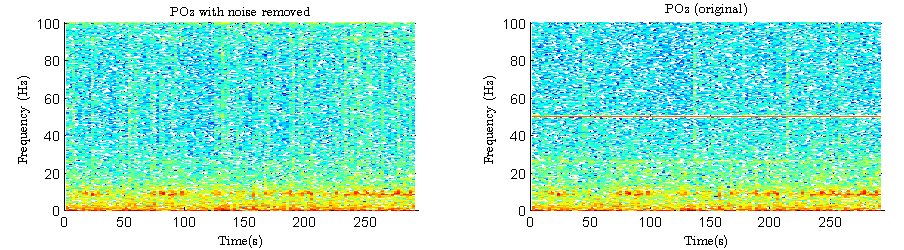
\includegraphics[width=\textwidth]{cw3im/3d_spectro.png}
M = 10 with a $\mu$ = 0.01 was found to produce best results
\caption{Comparison ANC denoised EEG data (right untouched, left denoised)}
\label{fig:3_3d}
\end{figure}

\begin{figure}[h]
\centering
\resizebox{\textwidth}{!}{% This file was created by matlab2tikz v0.4.7 running on MATLAB 8.1.
% Copyright (c) 2008--2014, Nico Schlömer <nico.schloemer@gmail.com>
% All rights reserved.
% Minimal pgfplots version: 1.3
% 
% The latest updates can be retrieved from
%   http://www.mathworks.com/matlabcentral/fileexchange/22022-matlab2tikz
% where you can also make suggestions and rate matlab2tikz.
% 
\begin{tikzpicture}

\begin{axis}[%
width=3.24554649758454in,
height=1.73958333333333in,
scale only axis,
xmin=0,
xmax=600,
xlabel={Frequency(Hz)},
xmajorgrids,
ymin=0,
ymax=1,
ylabel={$C_{xy}$(f)},
ymajorgrids,
name=plot2,
title={Noise removed  - amplitude ajusted}
]
\addplot [color=blue,solid,forget plot]
  table[row sep=crcr]{0	0.999870311538779\\
0.146484375	0.999867291865736\\
0.29296875	0.999857773293834\\
0.439453125	0.999840250788754\\
0.5859375	0.999811745543486\\
0.732421875	0.999766905911297\\
0.87890625	0.999696281736452\\
1.025390625	0.999583128607097\\
1.171875	0.99939783930103\\
1.318359375	0.999089869265463\\
1.46484375	0.998582927649896\\
1.611328125	0.997798819385824\\
1.7578125	0.996752704777046\\
1.904296875	0.995656235494765\\
2.05078125	0.994779083447695\\
2.197265625	0.994178615974187\\
2.34375	0.99373133364831\\
2.490234375	0.993315217481113\\
2.63671875	0.992874939066372\\
2.783203125	0.9924025217238\\
2.9296875	0.99190680582303\\
3.076171875	0.991395086335059\\
3.22265625	0.990869232922966\\
3.369140625	0.990330937515916\\
3.515625	0.989787499629527\\
3.662109375	0.989251782286705\\
3.80859375	0.988735978137824\\
3.955078125	0.988244555897721\\
4.1015625	0.987772857518083\\
4.248046875	0.987312967902228\\
4.39453125	0.986862049595413\\
4.541015625	0.98642602087699\\
4.6875	0.986014689068996\\
4.833984375	0.985630974566918\\
4.98046875	0.985262475864659\\
5.126953125	0.984883226186158\\
5.2734375	0.984466265816801\\
5.419921875	0.983999964229355\\
5.56640625	0.98349889459441\\
5.712890625	0.983003001910158\\
5.859375	0.982564410272958\\
6.005859375	0.98222858057842\\
6.15234375	0.982021771851267\\
6.298828125	0.981953330945965\\
6.4453125	0.98203009435286\\
6.591796875	0.982271130133366\\
6.73828125	0.98271092993894\\
6.884765625	0.983386152946627\\
7.03125	0.984311377283595\\
7.177734375	0.985458755479894\\
7.32421875	0.986756671048061\\
7.470703125	0.988109237713857\\
7.6171875	0.989423212816357\\
7.763671875	0.99062697576528\\
7.91015625	0.991676266647076\\
8.056640625	0.992550543258355\\
8.203125	0.993245879585431\\
8.349609375	0.993768156410912\\
8.49609375	0.994127908226663\\
8.642578125	0.994336946563649\\
8.7890625	0.994406467798343\\
8.935546875	0.994346262895354\\
9.08203125	0.994164620141027\\
9.228515625	0.993868480035065\\
9.375	0.993463385398972\\
9.521484375	0.99295284302608\\
9.66796875	0.992336949061914\\
9.814453125	0.991610501600362\\
9.9609375	0.990761142695025\\
10.107421875	0.989768098730936\\
10.25390625	0.988601769363857\\
10.400390625	0.987223992730409\\
10.546875	0.985588663495852\\
10.693359375	0.983642765597361\\
10.83984375	0.981328860366159\\
10.986328125	0.978591459376268\\
11.1328125	0.975390825319691\\
11.279296875	0.97172678633963\\
11.42578125	0.967668988207709\\
11.572265625	0.963377018973519\\
11.71875	0.959082295829741\\
11.865234375	0.955015780210845\\
12.01171875	0.951311629857933\\
12.158203125	0.947954584172802\\
12.3046875	0.9448112551062\\
12.451171875	0.941716468345128\\
12.59765625	0.93855269239899\\
12.744140625	0.935280984473689\\
12.890625	0.931917605896133\\
13.037109375	0.928478783111701\\
13.18359375	0.924933614877841\\
13.330078125	0.921201855987945\\
13.4765625	0.917204841610428\\
13.623046875	0.912943342806705\\
13.76953125	0.908557055769575\\
13.916015625	0.904319975708393\\
14.0625	0.900547980356933\\
14.208984375	0.897450224211203\\
14.35546875	0.895016922583307\\
14.501953125	0.893029178058121\\
14.6484375	0.891185452375633\\
14.794921875	0.889256833967604\\
14.94140625	0.887183129874615\\
15.087890625	0.885072632654736\\
15.234375	0.883117925257903\\
15.380859375	0.881479307338713\\
15.52734375	0.880208941886049\\
15.673828125	0.879264223525645\\
15.8203125	0.878592628067802\\
15.966796875	0.878219081925987\\
16.11328125	0.878270616358532\\
16.259765625	0.878917025680562\\
16.40625	0.880259874374866\\
16.552734375	0.882240726201284\\
16.69921875	0.884634096134758\\
16.845703125	0.887133740784787\\
16.9921875	0.889477110942873\\
17.138671875	0.891535700256053\\
17.28515625	0.893329273444239\\
17.431640625	0.894965402400124\\
17.578125	0.896542208061296\\
17.724609375	0.898072003548977\\
17.87109375	0.899469516749842\\
18.017578125	0.900601780157493\\
18.1640625	0.901356405590089\\
18.310546875	0.901683412148937\\
18.45703125	0.901591887549678\\
18.603515625	0.901109138948003\\
18.75	0.900226351195771\\
18.896484375	0.898861388194925\\
19.04296875	0.89686283352975\\
19.189453125	0.894059370165668\\
19.3359375	0.890337025070285\\
19.482421875	0.885715903109842\\
19.62890625	0.880395962044098\\
19.775390625	0.874742462433236\\
19.921875	0.869195700503083\\
20.068359375	0.864131110605311\\
20.21484375	0.859744638224363\\
20.361328125	0.856037705073658\\
20.5078125	0.852907271573532\\
20.654296875	0.850271114585378\\
20.80078125	0.8481420220564\\
20.947265625	0.84660550459393\\
21.09375	0.845717675939742\\
21.240234375	0.845393537982118\\
21.38671875	0.845369380355012\\
21.533203125	0.84527516559525\\
21.6796875	0.844775994206051\\
21.826171875	0.843700825085366\\
21.97265625	0.842092558503265\\
22.119140625	0.840156357299453\\
22.265625	0.838129254198918\\
22.412109375	0.836137731071721\\
22.55859375	0.834126807444325\\
22.705078125	0.831904219107322\\
22.8515625	0.829268594326926\\
22.998046875	0.826144187481832\\
23.14453125	0.822652424295296\\
23.291015625	0.819086565649795\\
23.4375	0.815798678378375\\
23.583984375	0.813055727750528\\
23.73046875	0.810953513697166\\
23.876953125	0.809453007449588\\
24.0234375	0.808523541166616\\
24.169921875	0.808301418117692\\
24.31640625	0.809152872893127\\
24.462890625	0.811570974018805\\
24.609375	0.815928134914216\\
24.755859375	0.822221593011282\\
24.90234375	0.829990231465521\\
25.048828125	0.838462413799813\\
25.1953125	0.846814292778181\\
25.341796875	0.854367151016173\\
25.48828125	0.860649864041109\\
25.634765625	0.865360345143218\\
25.78125	0.868292696701084\\
25.927734375	0.869275818720338\\
26.07421875	0.868140447856215\\
26.220703125	0.864716227528859\\
26.3671875	0.858857913366186\\
26.513671875	0.850501492947627\\
26.66015625	0.839746630740105\\
26.806640625	0.82694345856705\\
26.953125	0.812732771299\\
27.099609375	0.797977447144874\\
27.24609375	0.783571392967194\\
27.392578125	0.770212659498605\\
27.5390625	0.758280179794136\\
27.685546875	0.747875136135438\\
27.83203125	0.738950397949841\\
27.978515625	0.731401149211482\\
28.125	0.725060483761138\\
28.271484375	0.719647750022547\\
28.41796875	0.714762579181829\\
28.564453125	0.709978597536979\\
28.7109375	0.705009867297756\\
28.857421875	0.699861575095959\\
29.00390625	0.69486468181615\\
29.150390625	0.690535693592319\\
29.296875	0.68729839095573\\
29.443359375	0.685218089025581\\
29.58984375	0.6839260300383\\
29.736328125	0.68278752768581\\
29.8828125	0.681196035320086\\
30.029296875	0.678814502647429\\
30.17578125	0.675650199379031\\
30.322265625	0.67194826109498\\
30.46875	0.667971168291736\\
30.615234375	0.663789242157837\\
30.76171875	0.659209860571291\\
30.908203125	0.653892836789778\\
31.0546875	0.647585198406455\\
31.201171875	0.640345374439421\\
31.34765625	0.632636371804313\\
31.494140625	0.62521879821553\\
31.640625	0.618858510519504\\
31.787109375	0.613978923738364\\
31.93359375	0.610462461206822\\
32.080078125	0.607734718668077\\
32.2265625	0.605074861252367\\
32.373046875	0.601954324466851\\
32.51953125	0.598216728335929\\
32.666015625	0.594023931903309\\
32.8125	0.589622468947538\\
32.958984375	0.585085650481993\\
33.10546875	0.580205874585591\\
33.251953125	0.574610564964935\\
33.3984375	0.568020995479493\\
33.544921875	0.560491092980581\\
33.69140625	0.552489270143068\\
33.837890625	0.544765071221548\\
33.984375	0.538036076072961\\
34.130859375	0.532632838235766\\
34.27734375	0.528301605241689\\
34.423828125	0.524303348294428\\
34.5703125	0.519770784284781\\
34.716796875	0.514128676957937\\
34.86328125	0.507360896349119\\
35.009765625	0.500001118403424\\
35.15625	0.492859584542586\\
35.302734375	0.486631352751285\\
35.44921875	0.481605228863437\\
35.595703125	0.477633199310503\\
35.7421875	0.474345733007707\\
35.888671875	0.471445117731746\\
36.03515625	0.46888654122523\\
36.181640625	0.466849811378436\\
36.328125	0.465537758830083\\
36.474609375	0.46494475514777\\
36.62109375	0.46476174037845\\
36.767578125	0.464492800069423\\
36.9140625	0.463709719033723\\
37.060546875	0.462278461483943\\
37.20703125	0.460413386444881\\
37.353515625	0.458520167962384\\
37.5	0.456914195284827\\
37.646484375	0.455583477380798\\
37.79296875	0.454144468482342\\
37.939453125	0.452016265063208\\
38.0859375	0.448704450739499\\
38.232421875	0.444037002296616\\
38.37890625	0.438239246296814\\
38.525390625	0.43181957804031\\
38.671875	0.425322837305482\\
38.818359375	0.419073817414307\\
38.96484375	0.413046281242233\\
39.111328125	0.406925815230514\\
39.2578125	0.4003191547341\\
39.404296875	0.392978049165307\\
39.55078125	0.384907124512964\\
39.697265625	0.376303971637925\\
39.84375	0.367386247793029\\
39.990234375	0.358232132129929\\
40.13671875	0.348748239796924\\
40.283203125	0.338790402769952\\
40.4296875	0.328363890779642\\
40.576171875	0.317783080329686\\
40.72265625	0.307688560065101\\
40.869140625	0.298884640798321\\
41.015625	0.292051554819878\\
41.162109375	0.28746811879342\\
41.30859375	0.284894509666713\\
41.455078125	0.283679622273083\\
41.6015625	0.283021667475335\\
41.748046875	0.282224981506951\\
41.89453125	0.280819516761139\\
42.041015625	0.278511861518016\\
42.1875	0.275042802288896\\
42.333984375	0.27007629416799\\
42.48046875	0.263214969318355\\
42.626953125	0.254148872479427\\
42.7734375	0.242854786887087\\
42.919921875	0.229727149440586\\
43.06640625	0.215551002622721\\
43.212890625	0.201302951946913\\
43.359375	0.187857037589757\\
43.505859375	0.175735053667541\\
43.65234375	0.165027205940338\\
43.798828125	0.15551425880829\\
43.9453125	0.146907627138369\\
44.091796875	0.139065936293192\\
44.23828125	0.13207579271259\\
44.384765625	0.126173738274807\\
44.53125	0.121575134541108\\
44.677734375	0.118309484660007\\
44.82421875	0.116135164700946\\
44.970703125	0.114560655578063\\
45.1171875	0.112960818191645\\
45.263671875	0.110739170521373\\
45.41015625	0.107460884250961\\
45.556640625	0.102898626326304\\
45.703125	0.0969942722387731\\
45.849609375	0.0897968054683943\\
45.99609375	0.0814422678177663\\
46.142578125	0.0721921146191423\\
46.2890625	0.0624838735046721\\
46.435546875	0.0529224114156486\\
46.58203125	0.0441728825023027\\
46.728515625	0.0367882572798123\\
46.875	0.0310613922140244\\
47.021484375	0.0269800602344483\\
47.16796875	0.0242892745651797\\
47.314453125	0.0226028131261353\\
47.4609375	0.021508931261058\\
47.607421875	0.0206538608129977\\
47.75390625	0.0198070491918738\\
47.900390625	0.0189076971750518\\
48.046875	0.0180862435296363\\
48.193359375	0.0176601088910166\\
48.33984375	0.0181198925042993\\
48.486328125	0.0201362238248951\\
48.6328125	0.0245868815951099\\
48.779296875	0.0325032660093655\\
48.92578125	0.0447768107723524\\
49.072265625	0.0616373680913694\\
49.21875	0.0822166844975826\\
49.365234375	0.104543536511077\\
49.51171875	0.125993769831336\\
49.658203125	0.14391532113532\\
49.8046875	0.156138643841234\\
49.951171875	0.161261539335528\\
50.09765625	0.15875063009134\\
50.244140625	0.148944881064501\\
50.390625	0.133010388106868\\
50.537109375	0.112836309101111\\
50.68359375	0.0908203270857516\\
50.830078125	0.069496932958317\\
50.9765625	0.0510333672061142\\
51.123046875	0.0367449269084327\\
51.26953125	0.0268742111885548\\
51.416015625	0.0207893980514616\\
51.5625	0.0174707304902417\\
51.708984375	0.0159490089728136\\
51.85546875	0.0154895342700013\\
52.001953125	0.0155913920230993\\
52.1484375	0.0159544753882038\\
52.294921875	0.0164635031589499\\
52.44140625	0.0171596913095907\\
52.587890625	0.018182737519693\\
52.734375	0.0197004835664976\\
52.880859375	0.021851175238721\\
53.02734375	0.0247115542410036\\
53.173828125	0.0282944959889649\\
53.3203125	0.0325733753036691\\
53.466796875	0.0375177712900855\\
53.61328125	0.0431115664663974\\
53.759765625	0.0493263742933388\\
53.90625	0.0560483182912397\\
54.052734375	0.0629947139379488\\
54.19921875	0.0696849927404812\\
54.345703125	0.0755187890964391\\
54.4921875	0.0799555262925788\\
54.638671875	0.08271818216261\\
54.78515625	0.0839144072236253\\
54.931640625	0.084007136386912\\
55.078125	0.0836493993580751\\
55.224609375	0.0834693080260792\\
55.37109375	0.0839059254480752\\
55.517578125	0.0851522563149461\\
55.6640625	0.0871970190242796\\
55.810546875	0.0899145881720906\\
55.95703125	0.0931467550266126\\
56.103515625	0.096741356852536\\
56.25	0.100545365004938\\
56.396484375	0.104377899598781\\
56.54296875	0.108018866838486\\
56.689453125	0.111236398471006\\
56.8359375	0.11384815547318\\
56.982421875	0.115785555006625\\
57.12890625	0.117123722738964\\
57.275390625	0.118057918895579\\
57.421875	0.11883769138968\\
57.568359375	0.119693965321137\\
57.71484375	0.120796672363581\\
57.861328125	0.122259122936596\\
58.0078125	0.124172939418369\\
58.154296875	0.126635256800986\\
58.30078125	0.129734709505513\\
58.447265625	0.133493873460106\\
58.59375	0.137803525865265\\
58.740234375	0.142402543003324\\
58.88671875	0.146941771134845\\
59.033203125	0.151125069107914\\
59.1796875	0.15486877376787\\
59.326171875	0.158394541839241\\
59.47265625	0.162191230974351\\
59.619140625	0.166841986357024\\
59.765625	0.172781489117565\\
59.912109375	0.180089535526435\\
60.05859375	0.188419054151927\\
60.205078125	0.197099836507592\\
60.3515625	0.205376782933904\\
60.498046875	0.212675090683318\\
60.64453125	0.218773874703397\\
60.791015625	0.223819817490985\\
60.9375	0.228192283900933\\
61.083984375	0.232299270949711\\
61.23046875	0.236408485110129\\
61.376953125	0.240588231389131\\
61.5234375	0.244765213587444\\
61.669921875	0.248841358721248\\
61.81640625	0.252787674393382\\
61.962890625	0.256659638867988\\
62.109375	0.260534815714312\\
62.255859375	0.264424174603193\\
62.40234375	0.26822354448927\\
62.548828125	0.271742078078081\\
62.6953125	0.27479178851626\\
62.841796875	0.277282949362092\\
62.98828125	0.279268658656994\\
63.134765625	0.280915339575725\\
63.28125	0.282422235496067\\
63.427734375	0.283944844300301\\
63.57421875	0.28557446789438\\
63.720703125	0.287387598159935\\
63.8671875	0.289527991818035\\
64.013671875	0.292254693431948\\
64.16015625	0.295901475279558\\
64.306640625	0.300742918285011\\
64.453125	0.306824340239981\\
64.599609375	0.313850096898562\\
64.74609375	0.32120688334953\\
64.892578125	0.328128497695967\\
65.0390625	0.333930984093111\\
65.185546875	0.338214243494266\\
65.33203125	0.34095215699055\\
65.478515625	0.342451456204605\\
65.625	0.343215538383899\\
65.771484375	0.343781962954495\\
65.91796875	0.344602806514242\\
66.064453125	0.346007013310404\\
66.2109375	0.348236864038596\\
66.357421875	0.351509686021673\\
66.50390625	0.356043624554342\\
66.650390625	0.362011666293544\\
66.796875	0.369439365220545\\
66.943359375	0.378109782330414\\
67.08984375	0.387549659761432\\
67.236328125	0.397127867362139\\
67.3828125	0.406226097470891\\
67.529296875	0.414395903977979\\
67.67578125	0.421427443844127\\
67.822265625	0.427308248460467\\
67.96875	0.43210711876202\\
68.115234375	0.435851208853434\\
68.26171875	0.438462616120075\\
68.408203125	0.43978632112268\\
68.5546875	0.439691033723363\\
68.701171875	0.43818531441364\\
68.84765625	0.435483092951333\\
68.994140625	0.431978147925572\\
69.140625	0.428136098910639\\
69.287109375	0.424363735689185\\
69.43359375	0.420935830900651\\
69.580078125	0.418024221168338\\
69.7265625	0.415800186568329\\
69.873046875	0.41452415981397\\
70.01953125	0.414540449427151\\
70.166015625	0.416156820678411\\
70.3125	0.419469648562707\\
70.458984375	0.424241925403906\\
70.60546875	0.429917031832329\\
70.751953125	0.435769230106362\\
70.8984375	0.441113412264881\\
71.044921875	0.445474872721233\\
71.19140625	0.448654791133402\\
71.337890625	0.450683232301732\\
71.484375	0.451699439543845\\
71.630859375	0.4518264593595\\
71.77734375	0.451105128479014\\
71.923828125	0.449517037185005\\
72.0703125	0.447072734716245\\
72.216796875	0.443903239724213\\
72.36328125	0.440293759559642\\
72.509765625	0.436634771869165\\
72.65625	0.433314711496467\\
72.802734375	0.430614682227586\\
72.94921875	0.42866822371797\\
73.095703125	0.427512123670487\\
73.2421875	0.427196148345157\\
73.388671875	0.427876808907174\\
73.53515625	0.429822709586495\\
73.681640625	0.433309905787731\\
73.828125	0.438458143881494\\
73.974609375	0.445105787524091\\
74.12109375	0.452804228691629\\
74.267578125	0.460939605882768\\
74.4140625	0.468915372718946\\
74.560546875	0.476304243187461\\
74.70703125	0.482907332772712\\
74.853515625	0.488712745389456\\
75	0.49379428561702\\
75.146484375	0.498213881172201\\
75.29296875	0.501980452912921\\
75.439453125	0.505079794577396\\
75.5859375	0.507546703811307\\
75.732421875	0.509526863907138\\
75.87890625	0.51128235007506\\
76.025390625	0.513125027225626\\
76.171875	0.515301763014674\\
76.318359375	0.517885760755696\\
76.46484375	0.520731171331095\\
76.611328125	0.523517533797517\\
76.7578125	0.525863273694462\\
76.904296875	0.527453266273277\\
77.05078125	0.528123295546191\\
77.197265625	0.527870674142028\\
77.34375	0.52679887645305\\
77.490234375	0.525037011011251\\
77.63671875	0.522686334706554\\
77.783203125	0.519826853882004\\
77.9296875	0.516576395651568\\
78.076171875	0.513158301347803\\
78.22265625	0.509925356475221\\
78.369140625	0.50731078871167\\
78.515625	0.505718555003348\\
78.662109375	0.505402464767475\\
78.80859375	0.506394274790828\\
78.955078125	0.508514837544952\\
79.1015625	0.511454845760248\\
79.248046875	0.514874977341438\\
79.39453125	0.518472653373305\\
79.541015625	0.521991935067259\\
79.6875	0.525192691231582\\
79.833984375	0.527819936457048\\
79.98046875	0.529609153096555\\
80.126953125	0.530333297862672\\
80.2734375	0.529864939955998\\
80.419921875	0.528215204725013\\
80.56640625	0.525524746361995\\
80.712890625	0.522009621408284\\
80.859375	0.517891613680257\\
81.005859375	0.513355212677184\\
81.15234375	0.508562643047655\\
81.298828125	0.503724649418121\\
81.4453125	0.499184230003913\\
81.591796875	0.495448165902475\\
81.73828125	0.493115677225805\\
81.884765625	0.492705217635038\\
82.03125	0.494445961848005\\
82.177734375	0.498137912043426\\
82.32421875	0.503159655795624\\
82.470703125	0.508625570429707\\
82.6171875	0.513619188738661\\
82.763671875	0.517406461018307\\
82.91015625	0.519563211083805\\
83.056640625	0.519999969888974\\
83.203125	0.518904678505717\\
83.349609375	0.516642834148033\\
83.49609375	0.513658880136056\\
83.642578125	0.510411917493749\\
83.7890625	0.507353666160959\\
83.935546875	0.504927801957334\\
84.08203125	0.5035555400354\\
84.228515625	0.503584262831506\\
84.375	0.505208612042593\\
84.521484375	0.508405020187632\\
84.66796875	0.512925584075222\\
84.814453125	0.518366461584961\\
84.9609375	0.524279715984956\\
85.107421875	0.530271216970871\\
85.25390625	0.536040498896652\\
85.400390625	0.54135943986468\\
85.546875	0.546024938066463\\
85.693359375	0.549832013019627\\
85.83984375	0.55259456845526\\
85.986328125	0.554207803769003\\
86.1328125	0.554720158841544\\
86.279296875	0.55437440865998\\
86.42578125	0.553585900058254\\
86.572265625	0.552847427961792\\
86.71875	0.552582588683197\\
86.865234375	0.553002824401659\\
87.01171875	0.554035372659717\\
87.158203125	0.555361588900361\\
87.3046875	0.556549070014285\\
87.451171875	0.557215385454961\\
87.59765625	0.557155716218136\\
87.744140625	0.556396474162334\\
87.890625	0.555176014202504\\
88.037109375	0.553880491046731\\
88.18359375	0.552969335219989\\
88.330078125	0.55291175853287\\
88.4765625	0.5541328369464\\
88.623046875	0.556952037908659\\
88.76953125	0.561502923105562\\
88.916015625	0.567648875795674\\
89.0625	0.574935828632869\\
89.208984375	0.582623482169694\\
89.35546875	0.58980429036052\\
89.501953125	0.595576878696518\\
89.6484375	0.599219261417792\\
89.794921875	0.600317073514129\\
89.94140625	0.598826336041933\\
90.087890625	0.595069075296904\\
90.234375	0.589668966866918\\
90.380859375	0.583440558434946\\
90.52734375	0.577254436659339\\
90.673828125	0.571907109811949\\
90.8203125	0.56802044943101\\
90.966796875	0.565981509816628\\
91.11328125	0.565919482281179\\
91.259765625	0.567712039154598\\
91.40625	0.571017793940922\\
91.552734375	0.575335993917\\
91.69921875	0.580091178403203\\
91.845703125	0.584730203552584\\
91.9921875	0.58880983868902\\
92.138671875	0.592053034050249\\
92.28515625	0.594362220268387\\
92.431640625	0.59579332465419\\
92.578125	0.596507429068532\\
92.724609375	0.596722413288368\\
92.87109375	0.596681494257407\\
93.017578125	0.596641144907235\\
93.1640625	0.596865262242386\\
93.310546875	0.597605561003929\\
93.45703125	0.599055742151117\\
93.603515625	0.601287033234595\\
93.75	0.604195044362022\\
93.896484375	0.607496672653513\\
94.04296875	0.610798759288283\\
94.189453125	0.613722317337413\\
94.3359375	0.616031434233805\\
94.482421875	0.617708619423492\\
94.62890625	0.618942550975822\\
94.775390625	0.620034872645972\\
94.921875	0.621269753648316\\
95.068359375	0.622806037935715\\
95.21484375	0.624637152824539\\
95.361328125	0.62662527137721\\
95.5078125	0.628577802974806\\
95.654296875	0.630319853173016\\
95.80078125	0.631729993247043\\
95.947265625	0.632734506231047\\
96.09375	0.633279836614386\\
96.240234375	0.633313014910374\\
96.38671875	0.632791945319876\\
96.533203125	0.631726551211286\\
96.6796875	0.63022971026197\\
96.826171875	0.628545818335342\\
96.97265625	0.627030257196667\\
97.119140625	0.626073299757005\\
97.265625	0.625990241904226\\
97.412109375	0.626923125178885\\
97.55859375	0.628801604199237\\
97.705078125	0.631383384408512\\
97.8515625	0.634352744787734\\
97.998046875	0.637428790819538\\
98.14453125	0.640442708923543\\
98.291015625	0.643377858739428\\
98.4375	0.646396491141953\\
98.583984375	0.649862564792663\\
98.73046875	0.654307838409873\\
98.876953125	0.66026249942153\\
99.0234375	0.667975786635709\\
99.169921875	0.677197838444368\\
99.31640625	0.687180856562923\\
99.462890625	0.69688751635248\\
99.609375	0.705263609242532\\
99.755859375	0.711442195931193\\
99.90234375	0.714834641750408\\
100.048828125	0.715138234246498\\
100.1953125	0.71231633601262\\
100.341796875	0.706595463233523\\
100.48828125	0.698492778250363\\
100.634765625	0.688847465899123\\
100.78125	0.678789682764539\\
100.927734375	0.66956838706254\\
101.07421875	0.662220708115865\\
101.220703125	0.657210880085727\\
101.3671875	0.654282934583277\\
101.513671875	0.652672769435787\\
101.66015625	0.651533400257884\\
101.806640625	0.65026639616344\\
101.953125	0.648607136775171\\
102.099609375	0.646543593021416\\
102.24609375	0.644206391220654\\
102.392578125	0.641795519023785\\
102.5390625	0.639541559280104\\
102.685546875	0.637677730006356\\
102.83203125	0.636404418816736\\
102.978515625	0.63584327045525\\
103.125	0.635994936252766\\
103.271484375	0.63672421482102\\
103.41796875	0.637789874155597\\
103.564453125	0.63891484735032\\
103.7109375	0.639869232541169\\
103.857421875	0.640530064082316\\
104.00390625	0.640894017455816\\
104.150390625	0.641043695194779\\
104.296875	0.641090219825814\\
104.443359375	0.641123318147284\\
104.58984375	0.641192112565943\\
104.736328125	0.641320944283213\\
104.8828125	0.641544808607671\\
105.029296875	0.641937746769055\\
105.17578125	0.642610089457643\\
105.322265625	0.643667204647492\\
105.46875	0.645147536219611\\
105.615234375	0.646977262548448\\
105.76171875	0.648976290062307\\
105.908203125	0.650922029020413\\
106.0546875	0.652641791271248\\
106.201171875	0.654086971677819\\
106.34765625	0.655351868880871\\
106.494140625	0.656627616610215\\
106.640625	0.658112138337235\\
106.787109375	0.659917369759088\\
106.93359375	0.662015071119105\\
107.080078125	0.664240599265057\\
107.2265625	0.666343086477149\\
107.373046875	0.668050814544481\\
107.51953125	0.669122262151829\\
107.666015625	0.669370052903223\\
107.8125	0.668663683978424\\
107.958984375	0.666927849233785\\
108.10546875	0.664152575387999\\
108.251953125	0.660420089690104\\
108.3984375	0.655936993919721\\
108.544921875	0.65104857484089\\
108.69140625	0.646213679068093\\
108.837890625	0.641935240627331\\
108.984375	0.638665407613768\\
109.130859375	0.636720961641379\\
109.27734375	0.636242242420292\\
109.423828125	0.637206999059114\\
109.5703125	0.639483218417527\\
109.716796875	0.642889184526343\\
109.86328125	0.647232564979946\\
110.009765625	0.652318413317984\\
110.15625	0.657937018441797\\
110.302734375	0.663854482617486\\
110.44921875	0.669824297317104\\
110.595703125	0.675619587526382\\
110.7421875	0.681066656846742\\
110.888671875	0.686055824695911\\
111.03515625	0.690518801724764\\
111.181640625	0.694383266561791\\
111.328125	0.697530706406203\\
111.474609375	0.699783652641847\\
111.62109375	0.700933603739436\\
111.767578125	0.700800855030438\\
111.9140625	0.699303966232564\\
112.060546875	0.696514607399078\\
112.20703125	0.692679533500589\\
112.353515625	0.68820047204891\\
112.5	0.683573882014432\\
112.646484375	0.679306228103215\\
112.79296875	0.675831687572526\\
112.939453125	0.673458412735854\\
113.0859375	0.672352858407305\\
113.232421875	0.67254970498063\\
113.37890625	0.673964927466907\\
113.525390625	0.676399224654765\\
113.671875	0.679538916743448\\
113.818359375	0.682973827743216\\
113.96484375	0.686246009197809\\
114.111328125	0.688924622394106\\
114.2578125	0.69068607468672\\
114.404296875	0.691375265541154\\
114.55078125	0.69103189731327\\
114.697265625	0.689877162909662\\
114.84375	0.68826567879156\\
114.990234375	0.686614919851722\\
115.13671875	0.685329164672716\\
115.283203125	0.684734299536405\\
115.4296875	0.685032791012243\\
115.576171875	0.686279594033725\\
115.72265625	0.688376834296161\\
115.869140625	0.691089016129791\\
116.015625	0.694084325902501\\
116.162109375	0.697003379016438\\
116.30859375	0.699544229340454\\
116.455078125	0.701539753057052\\
116.6015625	0.702999639570271\\
116.748046875	0.704097201572766\\
116.89453125	0.70509844925523\\
117.041015625	0.706252681840977\\
117.1875	0.707683382805376\\
117.333984375	0.70932488726727\\
117.48046875	0.710935226323555\\
117.626953125	0.712182557614128\\
117.7734375	0.712769988116201\\
117.919921875	0.712549783271039\\
118.06640625	0.711586544884373\\
118.212890625	0.710150546033694\\
118.359375	0.708646721752851\\
118.505859375	0.707505814925779\\
118.65234375	0.70707636725614\\
118.798828125	0.707553363116827\\
118.9453125	0.708960644261008\\
119.091796875	0.711179323018788\\
119.23828125	0.713997774062488\\
119.384765625	0.71715866934858\\
119.53125	0.720391665738647\\
119.677734375	0.723435502811082\\
119.82421875	0.726059565462716\\
119.970703125	0.728089618779627\\
120.1171875	0.729432070113945\\
120.263671875	0.730085215598222\\
120.41015625	0.730128920403661\\
120.556640625	0.729693907145948\\
120.703125	0.728922692947871\\
120.849609375	0.727939867356045\\
120.99609375	0.726845133858926\\
121.142578125	0.725729093915172\\
121.2890625	0.724696754145404\\
121.435546875	0.723877000904116\\
121.58203125	0.723403092287541\\
121.728515625	0.723367310086519\\
121.875	0.723772756934574\\
122.021484375	0.724512925115674\\
122.16796875	0.725396105226072\\
122.314453125	0.726204361610172\\
122.4609375	0.726756359652455\\
122.607421875	0.726944037756922\\
122.75390625	0.726730652572317\\
122.900390625	0.726118214551287\\
123.046875	0.725105898755772\\
123.193359375	0.723664162423783\\
123.33984375	0.721741565362352\\
123.486328125	0.719305398334075\\
123.6328125	0.716400300542483\\
123.779296875	0.713199089746143\\
123.92578125	0.710020590804543\\
124.072265625	0.707299155374537\\
124.21875	0.705507338811697\\
124.365234375	0.705052995339464\\
124.51171875	0.706186216911269\\
124.658203125	0.708949113901694\\
124.8046875	0.713180545530756\\
124.951171875	0.718562247557698\\
125.09765625	0.724680494707426\\
125.244140625	0.731083574063594\\
125.390625	0.737329381113508\\
125.537109375	0.743026184630819\\
125.68359375	0.747868889712572\\
125.830078125	0.751667757963686\\
125.9765625	0.75436286862371\\
126.123046875	0.756018294014936\\
126.26953125	0.756794422404632\\
126.416015625	0.756903617980233\\
126.5625	0.756561451964293\\
126.708984375	0.755949556594142\\
126.85546875	0.75520283034207\\
127.001953125	0.754422656836046\\
127.1484375	0.753704015961714\\
127.294921875	0.753155931433186\\
127.44140625	0.752897343517926\\
127.587890625	0.753024072343013\\
127.734375	0.753560647523699\\
127.880859375	0.754422945421592\\
128.02734375	0.755415011473587\\
128.173828125	0.756266680768524\\
128.3203125	0.756698738540554\\
128.466796875	0.756491772643601\\
128.61328125	0.75553703696316\\
128.759765625	0.753857245233353\\
128.90625	0.751595777289642\\
129.052734375	0.748981290104016\\
129.19921875	0.746280053495935\\
129.345703125	0.743748959861435\\
129.4921875	0.741597567487364\\
129.638671875	0.739960759802928\\
129.78515625	0.738880043403716\\
129.931640625	0.738294047996608\\
130.078125	0.738044343326567\\
130.224609375	0.737904316357429\\
130.37109375	0.737632229778482\\
130.517578125	0.73703777396503\\
130.6640625	0.736042490913427\\
130.810546875	0.734714018431717\\
130.95703125	0.733261462664164\\
131.103515625	0.731990544824556\\
131.25	0.73122982032377\\
131.396484375	0.731250797475133\\
131.54296875	0.732209785118594\\
131.689453125	0.734131523220121\\
131.8359375	0.736934836772209\\
131.982421875	0.740479985113505\\
132.12890625	0.744609838673235\\
132.275390625	0.749166794721527\\
132.421875	0.753986338689374\\
132.568359375	0.758883311576069\\
132.71484375	0.763649424835521\\
132.861328125	0.76807048476704\\
133.0078125	0.771957137355486\\
133.154296875	0.775173602219438\\
133.30078125	0.777649829763526\\
133.447265625	0.779371751444419\\
133.59375	0.780355729864488\\
133.740234375	0.780620888450531\\
133.88671875	0.780173167658989\\
134.033203125	0.779008070829455\\
134.1796875	0.777129281831229\\
134.326171875	0.77457306678336\\
134.47265625	0.771426827335016\\
134.619140625	0.767834018844004\\
134.765625	0.763984221633947\\
134.912109375	0.76009326398211\\
135.05859375	0.756381336621914\\
135.205078125	0.753055760932117\\
135.3515625	0.750300285631746\\
135.498046875	0.748267497123628\\
135.64453125	0.747069046397468\\
135.791015625	0.746761922797649\\
135.9375	0.747335759506962\\
136.083984375	0.748710744230431\\
136.23046875	0.75075360747175\\
136.376953125	0.753310447639596\\
136.5234375	0.756244673289682\\
136.669921875	0.759462591129407\\
136.81640625	0.762912740187468\\
136.962890625	0.76655817634358\\
137.109375	0.77033748615098\\
137.255859375	0.774139102457977\\
137.40234375	0.777806210007681\\
137.548828125	0.781170611747904\\
137.6953125	0.784097983064481\\
137.841796875	0.786524026929912\\
137.98828125	0.788468593921656\\
138.134765625	0.790024687410584\\
138.28125	0.791327129612978\\
138.427734375	0.792511658536105\\
138.57421875	0.793678949488958\\
138.720703125	0.79487658650995\\
138.8671875	0.796103785188639\\
139.013671875	0.797332650486124\\
139.16015625	0.798533134829607\\
139.306640625	0.799690237254232\\
139.453125	0.800808520377415\\
139.599609375	0.80190545618197\\
139.74609375	0.802998620991771\\
139.892578125	0.804092476113399\\
140.0390625	0.805169283664562\\
140.185546875	0.806186348085519\\
140.33203125	0.8070793589894\\
140.478515625	0.807770379661674\\
140.625	0.80817920357385\\
140.771484375	0.808237336390137\\
140.91796875	0.807903406032443\\
141.064453125	0.807176874991351\\
141.2109375	0.806104507772874\\
141.357421875	0.804773484147939\\
141.50390625	0.803288881772771\\
141.650390625	0.801741580413782\\
141.796875	0.800180861559281\\
141.943359375	0.798606892148972\\
142.08984375	0.796989046248116\\
142.236328125	0.795302349097667\\
142.3828125	0.793565343229596\\
142.529296875	0.791862410237046\\
142.67578125	0.790339712188725\\
142.822265625	0.789173082216271\\
142.96875	0.788516999667232\\
143.115234375	0.788454020474181\\
143.26171875	0.788967712569631\\
143.408203125	0.789953240867741\\
143.5546875	0.791260532383547\\
143.701171875	0.792747653595064\\
143.84765625	0.794318621650835\\
143.994140625	0.79593129230136\\
144.140625	0.797578061593416\\
144.287109375	0.799254603628191\\
144.43359375	0.800934599279531\\
144.580078125	0.802562037843282\\
144.7265625	0.80406182732924\\
144.873046875	0.805360123120535\\
145.01953125	0.806402305504612\\
145.166015625	0.80715970011326\\
145.3125	0.807623489328074\\
145.458984375	0.807791576756752\\
145.60546875	0.807657298941054\\
145.751953125	0.807206163574758\\
145.8984375	0.806420625308947\\
146.044921875	0.805288137237369\\
146.19140625	0.803807637263664\\
146.337890625	0.801993561966574\\
146.484375	0.799880835309489\\
146.630859375	0.797535341073261\\
146.77734375	0.795070624592738\\
146.923828125	0.792664544082536\\
147.0703125	0.790563226142143\\
147.216796875	0.789058513066662\\
147.36328125	0.78843257837878\\
147.509765625	0.788879710896236\\
147.65625	0.79043398474707\\
147.802734375	0.792939343802835\\
147.94921875	0.796084672634432\\
148.095703125	0.79949575502861\\
148.2421875	0.802848990996086\\
148.388671875	0.805964968622315\\
148.53515625	0.808851787860838\\
148.681640625	0.811686029696024\\
148.828125	0.814736429979942\\
148.974609375	0.818252619031304\\
149.12109375	0.822356767741007\\
149.267578125	0.826978755455013\\
149.4140625	0.831856987319961\\
149.560546875	0.836596225329934\\
149.70703125	0.840752271496629\\
149.853515625	0.843913214002274\\
150	0.8457611019292\\
150.146484375	0.846111648722873\\
150.29296875	0.844934988978687\\
150.439453125	0.842359077028904\\
150.5859375	0.838654313397943\\
150.732421875	0.834197585971085\\
150.87890625	0.82941755362517\\
151.025390625	0.824729633636859\\
151.171875	0.820475638723199\\
151.318359375	0.816884865327514\\
151.46484375	0.814067329518947\\
151.611328125	0.812037073118057\\
151.7578125	0.810750608005564\\
151.904296875	0.810140294923837\\
152.05078125	0.810127990922393\\
152.197265625	0.810617593244745\\
152.34375	0.811478911136759\\
152.490234375	0.812541644940526\\
152.63671875	0.813612628063835\\
152.783203125	0.814514748428265\\
152.9296875	0.815131637060263\\
153.076171875	0.815437349095043\\
153.22265625	0.815496656354858\\
153.369140625	0.815434392769745\\
153.515625	0.815385289755333\\
153.662109375	0.815443908123333\\
153.80859375	0.815633878211313\\
153.955078125	0.815905917911579\\
154.1015625	0.816159838109811\\
154.248046875	0.816275596091993\\
154.39453125	0.81613825225785\\
154.541015625	0.815650015189511\\
154.6875	0.814732902502313\\
154.833984375	0.813331579126844\\
154.98046875	0.811424978319648\\
155.126953125	0.809048630702202\\
155.2734375	0.806320838299881\\
155.419921875	0.80345888258181\\
155.56640625	0.800769634153557\\
155.712890625	0.798604929834933\\
155.859375	0.79728676535233\\
156.005859375	0.797025908175652\\
156.15234375	0.797867930748364\\
156.298828125	0.799691646691411\\
156.4453125	0.802259150841405\\
156.591796875	0.805291735923036\\
156.73828125	0.80853829832451\\
156.884765625	0.811813402560983\\
157.03125	0.815000055773511\\
157.177734375	0.818027108777189\\
157.32421875	0.82083864616919\\
157.470703125	0.823372005662144\\
157.6171875	0.825553406421886\\
157.763671875	0.827309669380418\\
157.91015625	0.828586999149649\\
158.056640625	0.829366731453811\\
158.203125	0.829672172233156\\
158.349609375	0.829566260067399\\
158.49609375	0.829143363044898\\
158.642578125	0.82851889773021\\
158.7890625	0.827818661774845\\
158.935546875	0.827167915020484\\
159.08203125	0.826679928503217\\
159.228515625	0.826444952216078\\
159.375	0.826521922561274\\
159.521484375	0.826935159628234\\
159.66796875	0.827676417846711\\
159.814453125	0.828710232026712\\
159.9609375	0.829979484503951\\
160.107421875	0.831409395978647\\
160.25390625	0.832910686063392\\
160.400390625	0.834384331292604\\
160.546875	0.835729728785011\\
160.693359375	0.836855624374131\\
160.83984375	0.837690780488922\\
160.986328125	0.838190615991705\\
161.1328125	0.838337080706601\\
161.279296875	0.838131108750425\\
161.42578125	0.837579667782283\\
161.572265625	0.836682481146174\\
161.71875	0.835426003064122\\
161.865234375	0.833792149110926\\
162.01171875	0.831784855224607\\
162.158203125	0.829469195416102\\
162.3046875	0.82700859332851\\
162.451171875	0.824679928676769\\
162.59765625	0.822848433858752\\
162.744140625	0.821897513485746\\
162.890625	0.822131148382806\\
163.037109375	0.823686355301022\\
163.18359375	0.826493187104667\\
163.330078125	0.830295458110662\\
163.4765625	0.834714190845296\\
163.623046875	0.839320997048737\\
163.76953125	0.843696498968886\\
163.916015625	0.847467156936122\\
164.0625	0.850327552996524\\
164.208984375	0.852058144790127\\
164.35546875	0.852543078338893\\
164.501953125	0.851784752323359\\
164.6484375	0.849907106142907\\
164.794921875	0.847140913196314\\
164.94140625	0.84379059453127\\
165.087890625	0.840189322954455\\
165.234375	0.836653595639016\\
165.380859375	0.833448291044585\\
165.52734375	0.830769043566954\\
165.673828125	0.828742438053784\\
165.8203125	0.82743840228552\\
165.966796875	0.826885520952805\\
166.11328125	0.827080339504892\\
166.259765625	0.827986229817785\\
166.40625	0.829524443726908\\
166.552734375	0.831566225613283\\
166.69921875	0.833936294415578\\
166.845703125	0.83643281852689\\
166.9921875	0.838860038376688\\
167.138671875	0.84106287657109\\
167.28515625	0.84295220900773\\
167.431640625	0.844514142866911\\
167.578125	0.845803012269874\\
167.724609375	0.846922672924213\\
167.87109375	0.84800250475885\\
168.017578125	0.849173154711982\\
168.1640625	0.850543792365126\\
168.310546875	0.852180295240567\\
168.45703125	0.854084939089962\\
168.603515625	0.856182518622579\\
168.75	0.858321181498845\\
168.896484375	0.860293827252724\\
169.04296875	0.861877593054993\\
169.189453125	0.862880482354812\\
169.3359375	0.86318168784311\\
169.482421875	0.86275605827366\\
169.62890625	0.861679054386939\\
169.775390625	0.860112757929304\\
169.921875	0.858276103220274\\
170.068359375	0.856405274825517\\
170.21484375	0.854713215317256\\
170.361328125	0.853358058283671\\
170.5078125	0.852427025849973\\
170.654296875	0.851936176099033\\
170.80078125	0.851841331141661\\
170.947265625	0.852054546868474\\
171.09375	0.852462923038409\\
171.240234375	0.85294907438487\\
171.38671875	0.853412475473109\\
171.533203125	0.853788363422212\\
171.6796875	0.854058626039706\\
171.826171875	0.854249787914641\\
171.97265625	0.854417299784939\\
172.119140625	0.854620951362505\\
172.265625	0.854900489633044\\
172.412109375	0.855261076350513\\
172.55859375	0.855674393413906\\
172.705078125	0.856094629423077\\
172.8515625	0.856482444072033\\
172.998046875	0.856827062608514\\
173.14453125	0.857157676083585\\
173.291015625	0.857539376590227\\
173.4375	0.858054453218789\\
173.583984375	0.858775359869425\\
173.73046875	0.859738940487117\\
173.876953125	0.860930668782305\\
174.0234375	0.862282824467571\\
174.169921875	0.8636845215946\\
174.31640625	0.864998000090765\\
174.462890625	0.866076110465513\\
174.609375	0.866778846975616\\
174.755859375	0.866989218302153\\
174.90234375	0.866629000321687\\
175.048828125	0.865673331900516\\
175.1953125	0.864161135451723\\
175.341796875	0.862197306109737\\
175.48828125	0.859943272171353\\
175.634765625	0.857595132797137\\
175.78125	0.855352724384809\\
175.927734375	0.853387118617688\\
176.07421875	0.851815707574034\\
176.220703125	0.850691379540811\\
176.3671875	0.850006297901629\\
176.513671875	0.849705135796589\\
176.66015625	0.849700827619212\\
176.806640625	0.849888464853136\\
176.953125	0.850157240346595\\
177.099609375	0.850402991429396\\
177.24609375	0.850543316160996\\
177.392578125	0.850534206940593\\
177.5390625	0.850383727296479\\
177.685546875	0.850156440010197\\
177.83203125	0.849963374799571\\
177.978515625	0.849936770559823\\
178.125	0.850195637949133\\
178.271484375	0.850814056997125\\
178.41796875	0.851804570171974\\
178.564453125	0.853122258897156\\
178.7109375	0.85468488540451\\
178.857421875	0.856397721381219\\
179.00390625	0.858172396468005\\
179.150390625	0.859935542143868\\
179.296875	0.861630086983526\\
179.443359375	0.863215451319435\\
179.58984375	0.864671317989284\\
179.736328125	0.866004842034685\\
179.8828125	0.867256258887404\\
180.029296875	0.868495585368457\\
180.17578125	0.869804963227523\\
180.322265625	0.871247490183949\\
180.46875	0.872832477983244\\
180.615234375	0.874493751272648\\
180.76171875	0.876094822055937\\
180.908203125	0.877461169245044\\
181.0546875	0.878424673894354\\
181.201171875	0.878860623264346\\
181.34765625	0.878705693933812\\
181.494140625	0.877957411081469\\
181.640625	0.876663228116479\\
181.787109375	0.87490852910988\\
181.93359375	0.872809674632897\\
182.080078125	0.870513215788754\\
182.2265625	0.868197485412989\\
182.373046875	0.866069560526854\\
182.51953125	0.864350437438047\\
182.666015625	0.863244960449348\\
182.8125	0.862900286241101\\
182.958984375	0.863365080183818\\
183.10546875	0.864566428571858\\
183.251953125	0.866317723276296\\
183.3984375	0.868358328658589\\
183.544921875	0.870411449107007\\
183.69140625	0.872239505317341\\
183.837890625	0.873680402113567\\
183.984375	0.874659189782363\\
184.130859375	0.875180148218901\\
184.27734375	0.87530914849497\\
184.423828125	0.875154825146342\\
184.5703125	0.874852268895356\\
184.716796875	0.874547975957741\\
184.86328125	0.874382351339351\\
185.009765625	0.874467654308092\\
185.15625	0.874864515970893\\
185.302734375	0.875565899338142\\
185.44921875	0.876498517344586\\
185.595703125	0.877545321440686\\
185.7421875	0.878581950235299\\
185.888671875	0.879512539095299\\
186.03515625	0.880291040939166\\
186.181640625	0.880921803052687\\
186.328125	0.881442536290187\\
186.474609375	0.881899581268715\\
186.62109375	0.882327121231366\\
186.767578125	0.882738226847191\\
186.9140625	0.883128290828406\\
187.060546875	0.883484734844858\\
187.20703125	0.883794845350819\\
187.353515625	0.884046976733013\\
187.5	0.88422620757631\\
187.646484375	0.884309664908381\\
187.79296875	0.884266754834536\\
187.939453125	0.884066134694812\\
188.0859375	0.883687043680727\\
188.232421875	0.883129932709705\\
188.37890625	0.882421113650868\\
188.525390625	0.881608258504963\\
188.671875	0.88074749906241\\
188.818359375	0.879887308580003\\
188.96484375	0.879056717214548\\
189.111328125	0.878263314283385\\
189.2578125	0.877500568372292\\
189.404296875	0.876758452856418\\
189.55078125	0.876030345111859\\
189.697265625	0.875313009301659\\
189.84375	0.874601949717986\\
189.990234375	0.873887800355725\\
190.13671875	0.873158864489113\\
190.283203125	0.872411027148566\\
190.4296875	0.871661235460554\\
190.576171875	0.870957053245553\\
190.72265625	0.870374272682474\\
190.869140625	0.869998257922317\\
191.015625	0.869892505765868\\
191.162109375	0.870066984099747\\
191.30859375	0.870462858352915\\
191.455078125	0.870963756507158\\
191.6015625	0.871429235015743\\
191.748046875	0.871734215264448\\
191.89453125	0.871797566561791\\
192.041015625	0.87159221312116\\
192.1875	0.87113983419486\\
192.333984375	0.87049890328211\\
192.48046875	0.869754303889946\\
192.626953125	0.869012239890877\\
192.7734375	0.868398476594418\\
192.919921875	0.868053602796458\\
193.06640625	0.868118162836526\\
193.212890625	0.86870476149662\\
193.359375	0.869863101158747\\
193.505859375	0.871552769096523\\
193.65234375	0.873639826244236\\
193.798828125	0.875922907610399\\
193.9453125	0.87817874387859\\
194.091796875	0.880207902619613\\
194.23828125	0.881865242866961\\
194.384765625	0.883070953053509\\
194.53125	0.883807701729524\\
194.677734375	0.884112327854724\\
194.82421875	0.884067545825975\\
194.970703125	0.883793953733355\\
195.1171875	0.8834385887078\\
195.263671875	0.8831555648242\\
195.41015625	0.883077843575525\\
195.556640625	0.883285791090097\\
195.703125	0.883783895632758\\
195.849609375	0.884496716676344\\
195.99609375	0.885287372439632\\
196.142578125	0.885991763367141\\
196.2890625	0.886456586471985\\
196.435546875	0.886571284271337\\
196.58203125	0.886289459450124\\
196.728515625	0.885639069441227\\
196.875	0.884721407592976\\
197.021484375	0.883698280828564\\
197.16796875	0.882767374745757\\
197.314453125	0.882128375112621\\
197.4609375	0.881945619205038\\
197.607421875	0.882314821386015\\
197.75390625	0.883241004896975\\
197.900390625	0.884632880118239\\
198.046875	0.886316082227915\\
198.193359375	0.888063688380558\\
198.33984375	0.889637740004595\\
198.486328125	0.890832213748457\\
198.6328125	0.891508059463429\\
198.779296875	0.891614148709231\\
198.92578125	0.89119172817788\\
199.072265625	0.890362400300935\\
199.21875	0.889301408214187\\
199.365234375	0.88820092042979\\
199.51171875	0.887232036221509\\
199.658203125	0.886516218932314\\
199.8046875	0.886113565406193\\
199.951171875	0.886027759295546\\
200.09765625	0.886220927882909\\
200.244140625	0.886630144485871\\
200.390625	0.887180442148775\\
200.537109375	0.887793314764575\\
200.68359375	0.888392037351852\\
200.830078125	0.888905417063979\\
200.9765625	0.889270799578488\\
201.123046875	0.88943629491895\\
201.26953125	0.889361830928404\\
201.416015625	0.889019022869066\\
201.5625	0.888390818707977\\
201.708984375	0.8874728305068\\
201.85546875	0.886278233395552\\
202.001953125	0.884846315141874\\
202.1484375	0.883251401335967\\
202.294921875	0.881605711504132\\
202.44140625	0.88004944515494\\
202.587890625	0.878725918924664\\
202.734375	0.877747728715647\\
202.880859375	0.877166980282842\\
203.02734375	0.8769630714843\\
203.173828125	0.877053829915596\\
203.3203125	0.877324795359678\\
203.466796875	0.877664303778276\\
203.61328125	0.877992234700184\\
203.759765625	0.878275648700677\\
203.90625	0.878530571334382\\
204.052734375	0.87881285800061\\
204.19921875	0.879201915394684\\
204.345703125	0.879780223768208\\
204.4921875	0.880610844845878\\
204.638671875	0.881715810933988\\
204.78515625	0.883060417726974\\
204.931640625	0.884549852064483\\
205.078125	0.886042406429435\\
205.224609375	0.887377337591298\\
205.37109375	0.888408834612203\\
205.517578125	0.889035272824862\\
205.6640625	0.889216042947803\\
205.810546875	0.888973608539691\\
205.95703125	0.88838247465338\\
206.103515625	0.887548645486825\\
206.25	0.886584399658262\\
206.396484375	0.885584909992369\\
206.54296875	0.884614213222575\\
206.689453125	0.883705727784766\\
206.8359375	0.882876122109356\\
206.982421875	0.882144055069257\\
207.12890625	0.881542430030461\\
207.275390625	0.881116952215324\\
207.421875	0.880912364761025\\
207.568359375	0.880954996420032\\
207.71484375	0.881241633426285\\
207.861328125	0.881740028035612\\
208.0078125	0.882399418728681\\
208.154296875	0.883164834742509\\
208.30078125	0.883988700627825\\
208.447265625	0.884836256770002\\
208.59375	0.885685173655084\\
208.740234375	0.886522528113117\\
208.88671875	0.887343078418431\\
209.033203125	0.888151350041382\\
209.1796875	0.888966935730128\\
209.326171875	0.889828930150055\\
209.47265625	0.89079355390319\\
209.619140625	0.891920703400892\\
209.765625	0.893250776101449\\
209.912109375	0.894780038973804\\
210.05859375	0.896445993420253\\
210.205078125	0.898130186600083\\
210.3515625	0.899677026614934\\
210.498046875	0.900920047523714\\
210.64453125	0.901706355703037\\
210.791015625	0.901914421587758\\
210.9375	0.901465477564388\\
211.083984375	0.900331342614007\\
211.23046875	0.898541055529531\\
211.376953125	0.896186291510811\\
211.5234375	0.893422435117065\\
211.669921875	0.890459858982505\\
211.81640625	0.88754048440694\\
211.962890625	0.88489997405035\\
212.109375	0.882724984233255\\
212.255859375	0.881121933872218\\
212.40234375	0.880111282278672\\
212.548828125	0.879648466079624\\
212.6953125	0.879658317513601\\
212.841796875	0.880064578880718\\
212.98828125	0.880802345256929\\
213.134765625	0.881812772005301\\
213.28125	0.883028674705094\\
213.427734375	0.884362702388243\\
213.57421875	0.885706425931442\\
213.720703125	0.886941677814049\\
213.8671875	0.887959010508337\\
214.013671875	0.888675519393447\\
214.16015625	0.889045952975213\\
214.306640625	0.889064964543434\\
214.453125	0.888762077313349\\
214.599609375	0.888193025744816\\
214.74609375	0.887431215416934\\
214.892578125	0.88656125496255\\
215.0390625	0.885673620642121\\
215.185546875	0.884857300130851\\
215.33203125	0.884187938912287\\
215.478515625	0.883713165335194\\
215.625	0.883441643711692\\
215.771484375	0.883343387327761\\
215.91796875	0.88336395927009\\
216.064453125	0.883447615837761\\
216.2109375	0.883559659470628\\
216.357421875	0.883698851496052\\
216.50390625	0.883895177580125\\
216.650390625	0.884193766359506\\
216.796875	0.884630617629384\\
216.943359375	0.885209078233306\\
217.08984375	0.885886508731418\\
217.236328125	0.886577227177903\\
217.3828125	0.887171230760392\\
217.529296875	0.887561314348147\\
217.67578125	0.887667640242518\\
217.822265625	0.887450487385098\\
217.96875	0.886907971351063\\
218.115234375	0.886062857890075\\
218.26171875	0.884947265529088\\
218.408203125	0.88359352280645\\
218.5546875	0.882034411230765\\
218.701171875	0.880309977340941\\
218.84765625	0.878474613799409\\
218.994140625	0.87659859240049\\
219.140625	0.874761803214367\\
219.287109375	0.87304199796197\\
219.43359375	0.871502943947099\\
219.580078125	0.870187864014773\\
219.7265625	0.869120457619958\\
219.873046875	0.868311677951357\\
220.01953125	0.867767828769057\\
220.166015625	0.867495783033798\\
220.3125	0.867503687963912\\
220.458984375	0.86779860882397\\
220.60546875	0.868384207493194\\
220.751953125	0.869260689312955\\
220.8984375	0.870426471482696\\
221.044921875	0.871878422074345\\
221.19140625	0.873607326603944\\
221.337890625	0.875588058060753\\
221.484375	0.877768023987913\\
221.630859375	0.880059919109749\\
221.77734375	0.882343743448405\\
221.923828125	0.884479137187273\\
222.0703125	0.886324951502816\\
222.216796875	0.887760906717387\\
222.36328125	0.888706510286655\\
222.509765625	0.88913392326658\\
222.65625	0.889073025177178\\
222.802734375	0.888608241680932\\
222.94921875	0.88786785869774\\
223.095703125	0.887007324474605\\
223.2421875	0.886188103694632\\
223.388671875	0.885553424048805\\
223.53515625	0.885203069232726\\
223.681640625	0.885172036599039\\
223.828125	0.885420880857776\\
223.974609375	0.885845260242855\\
224.12109375	0.886306138570592\\
224.267578125	0.886672648893769\\
224.4140625	0.886862936389479\\
224.560546875	0.88686861943685\\
224.70703125	0.886754702105681\\
224.853515625	0.886634991268922\\
225	0.886630865506443\\
225.146484375	0.886827455444525\\
225.29296875	0.887243509402207\\
225.439453125	0.887826411510096\\
225.5859375	0.888472738663952\\
225.732421875	0.889063592674777\\
225.87890625	0.889499464271887\\
226.025390625	0.889722868451175\\
226.171875	0.88972436646836\\
226.318359375	0.889534158452163\\
226.46484375	0.889205071982466\\
226.611328125	0.88879360016349\\
226.7578125	0.888344493448954\\
226.904296875	0.887882142688442\\
227.05078125	0.887409464227153\\
227.197265625	0.886912977255873\\
227.34375	0.886371647223951\\
227.490234375	0.885766745047837\\
227.63671875	0.885090042681115\\
227.783203125	0.884347913889691\\
227.9296875	0.883559584424137\\
228.076171875	0.882749362196466\\
228.22265625	0.88193523166215\\
228.369140625	0.88111880278109\\
228.515625	0.880282596056796\\
228.662109375	0.879398693507782\\
228.80859375	0.878448082096287\\
228.955078125	0.877444410938225\\
229.1015625	0.876451834527777\\
229.248046875	0.875586117722237\\
229.39453125	0.874992538369147\\
229.541015625	0.874803549540126\\
229.6875	0.87509089140425\\
229.833984375	0.875833834350513\\
229.98046875	0.876920160298511\\
230.126953125	0.878180038127178\\
230.2734375	0.87943609491963\\
230.419921875	0.88054732063605\\
230.56640625	0.881431490019258\\
230.712890625	0.882063046992179\\
230.859375	0.882453250699477\\
231.005859375	0.882624087097529\\
231.15234375	0.882587593840909\\
231.298828125	0.882338857341093\\
231.4453125	0.881864858974937\\
231.591796875	0.881164128000013\\
231.73828125	0.880266532502016\\
231.884765625	0.879241614742784\\
232.03125	0.878189273981581\\
232.177734375	0.877216326208529\\
232.32421875	0.876410709817595\\
232.470703125	0.875826022739926\\
232.6171875	0.875482168217095\\
232.763671875	0.87537864940155\\
232.91015625	0.875511669512554\\
233.056640625	0.875886542405048\\
233.203125	0.876520758003133\\
233.349609375	0.877437280922573\\
233.49609375	0.878650585933429\\
233.642578125	0.880149431602206\\
233.7890625	0.881881120867918\\
233.935546875	0.883742501407466\\
234.08203125	0.885582711455856\\
234.228515625	0.887220230396333\\
234.375	0.888471567292832\\
234.521484375	0.889183301882824\\
234.66796875	0.889257455756606\\
234.814453125	0.88866404438695\\
234.9609375	0.887440989266635\\
235.107421875	0.88568554525311\\
235.25390625	0.883541175467662\\
235.400390625	0.881181292925648\\
235.546875	0.878789624410542\\
235.693359375	0.876537935369551\\
235.83984375	0.874564778179093\\
235.986328125	0.872960990783551\\
236.1328125	0.871766179466203\\
236.279296875	0.870975625492868\\
236.42578125	0.870552625221321\\
236.572265625	0.870440912958144\\
236.71875	0.87057538062615\\
236.865234375	0.870892847997434\\
237.01171875	0.871344393046035\\
237.158203125	0.871906854794083\\
237.3046875	0.872587379514483\\
237.451171875	0.873415211569148\\
237.59765625	0.874420081399755\\
237.744140625	0.875603749375077\\
237.890625	0.876916272051863\\
238.037109375	0.878248183139139\\
238.18359375	0.879443814111378\\
238.330078125	0.880332458369271\\
238.4765625	0.880767314445039\\
238.623046875	0.880659819439581\\
238.76953125	0.879999083238577\\
238.916015625	0.878851217216034\\
239.0625	0.877339948377056\\
239.208984375	0.875616257761847\\
239.35546875	0.873828241374373\\
239.501953125	0.872100747998819\\
239.6484375	0.870528209550254\\
239.794921875	0.869177178437287\\
239.94140625	0.868091541651914\\
240.087890625	0.867294727399003\\
240.234375	0.866787811004684\\
240.380859375	0.866546917590655\\
240.52734375	0.866524763746985\\
240.673828125	0.866658818173782\\
240.8203125	0.866884314798499\\
240.966796875	0.86714729857044\\
241.11328125	0.867412832252159\\
241.259765625	0.867665975244595\\
241.40625	0.867906427026241\\
241.552734375	0.868140228113087\\
241.69921875	0.868372736165989\\
241.845703125	0.86860597388183\\
241.9921875	0.868840818195259\\
242.138671875	0.869081632593897\\
242.28515625	0.869339477415655\\
242.431640625	0.869630992620765\\
242.578125	0.869973035389798\\
242.724609375	0.870376330185169\\
242.87109375	0.870842425639815\\
243.017578125	0.871366055730884\\
243.1640625	0.871941013410158\\
243.310546875	0.872565017950291\\
243.45703125	0.873239892599702\\
243.603515625	0.87396683170038\\
243.75	0.874739871691586\\
243.896484375	0.875541695803027\\
244.04296875	0.87634434670552\\
244.189453125	0.877114590424226\\
244.3359375	0.877821245138246\\
244.482421875	0.878440910757485\\
244.62890625	0.878959527355113\\
244.775390625	0.879369619456097\\
244.921875	0.879665876681704\\
245.068359375	0.879843313308472\\
245.21484375	0.879901195155188\\
245.361328125	0.879852075387152\\
245.5078125	0.879730563448094\\
245.654296875	0.879594052877088\\
245.80078125	0.879509932007863\\
245.947265625	0.879530563967581\\
246.09375	0.879665313964223\\
246.240234375	0.879863253794671\\
246.38671875	0.880017427139056\\
246.533203125	0.879992620618877\\
246.6796875	0.879668375676915\\
246.826171875	0.87898244943804\\
246.97265625	0.877958937978168\\
247.119140625	0.876709706078376\\
247.265625	0.875407972141807\\
247.412109375	0.874247978960394\\
247.55859375	0.873417965995637\\
247.705078125	0.873113819131937\\
247.8515625	0.873600814847029\\
247.998046875	0.875293009488422\\
248.14453125	0.878772298287465\\
248.291015625	0.884640156205136\\
248.4375	0.893165325629528\\
248.583984375	0.9039201791164\\
248.73046875	0.915774093634193\\
248.876953125	0.927352072511892\\
249.0234375	0.937582434584648\\
249.169921875	0.945930653429263\\
249.31640625	0.952305658032409\\
249.462890625	0.956851726928036\\
249.609375	0.959779668208849\\
249.755859375	0.961272414678648\\
249.90234375	0.961444615643664\\
250.048828125	0.960330389933325\\
250.1953125	0.957884109579375\\
250.341796875	0.953990771720247\\
250.48828125	0.948492968059587\\
250.634765625	0.941250967310253\\
250.78125	0.932255647775263\\
250.927734375	0.921792573882815\\
251.07421875	0.910585319766294\\
251.220703125	0.899754962215543\\
251.3671875	0.890470659395452\\
251.513671875	0.88344779547878\\
251.66015625	0.878690308237145\\
251.806640625	0.875664442159362\\
251.953125	0.873680906940103\\
252.099609375	0.87218367514277\\
252.24609375	0.870850289032938\\
252.392578125	0.869566624885908\\
252.5390625	0.868358459038677\\
252.685546875	0.867324962680536\\
252.83203125	0.866587159931675\\
252.978515625	0.866250198005936\\
253.125	0.866376568153417\\
253.271484375	0.866970513281933\\
253.41796875	0.867975594902658\\
253.564453125	0.869285249829939\\
253.7109375	0.870762028104581\\
253.857421875	0.872258752042542\\
254.00390625	0.873635889792933\\
254.150390625	0.874772869140861\\
254.296875	0.875574490982292\\
254.443359375	0.875975337059805\\
254.58984375	0.87594469665081\\
254.736328125	0.875492601986875\\
254.8828125	0.874675027591869\\
255.029296875	0.873594243542133\\
255.17578125	0.872389819542\\
255.322265625	0.871217872520716\\
255.46875	0.870221025118302\\
255.615234375	0.869497347638528\\
255.76171875	0.869079447703311\\
255.908203125	0.868931812625164\\
256.0546875	0.868966733205301\\
256.201171875	0.86907175708874\\
256.34765625	0.869138996552958\\
256.494140625	0.869088802022\\
256.640625	0.868884216808688\\
256.787109375	0.868535469608172\\
256.93359375	0.868094879322555\\
257.080078125	0.867642871862096\\
257.2265625	0.867266580295995\\
257.373046875	0.867034357571899\\
257.51953125	0.866972003704237\\
257.666015625	0.867047977133995\\
257.8125	0.867173545631146\\
257.958984375	0.867219522715489\\
258.10546875	0.867045930724061\\
258.251953125	0.866537293881636\\
258.3984375	0.865635394785731\\
258.544921875	0.864362274703915\\
258.69140625	0.862827603319497\\
258.837890625	0.861216242188942\\
258.984375	0.859755395521447\\
259.130859375	0.858667280202889\\
259.27734375	0.858120770177076\\
259.423828125	0.858198754741975\\
259.5703125	0.858892730033054\\
259.716796875	0.860124167327857\\
259.86328125	0.861780840830663\\
260.009765625	0.863752291992714\\
260.15625	0.865952850458773\\
260.302734375	0.868328773954484\\
260.44921875	0.870852692499236\\
260.595703125	0.873510775153487\\
260.7421875	0.876286755417062\\
260.888671875	0.87914522561905\\
261.03515625	0.882016633019562\\
261.181640625	0.884787712411116\\
261.328125	0.887301576111162\\
261.474609375	0.889369966844865\\
261.62109375	0.890796835681067\\
261.767578125	0.891409272781512\\
261.9140625	0.891090275424529\\
262.060546875	0.88980772972822\\
262.20703125	0.887634156360088\\
262.353515625	0.884751676510602\\
262.5	0.881437379375464\\
262.646484375	0.878027712899697\\
262.79296875	0.87486701979421\\
262.939453125	0.872252088959713\\
263.0859375	0.87038721577799\\
263.232421875	0.869360742916939\\
263.37890625	0.86914659685773\\
263.525390625	0.869626974360697\\
263.671875	0.870627545381521\\
263.818359375	0.871954813148275\\
263.96484375	0.873426531965556\\
264.111328125	0.874889877076709\\
264.2578125	0.876226830668735\\
264.404296875	0.877349943181751\\
264.55078125	0.878193300457433\\
264.697265625	0.878703685395144\\
264.84375	0.878836364876627\\
264.990234375	0.878558718216507\\
265.13671875	0.87786256251039\\
265.283203125	0.876782409689583\\
265.4296875	0.875412881287756\\
265.576171875	0.873915788445581\\
265.72265625	0.872507902596868\\
265.869140625	0.87142579440786\\
266.015625	0.870874140453207\\
266.162109375	0.870974518638851\\
266.30859375	0.871735376857846\\
266.455078125	0.873055536289442\\
266.6015625	0.874757522341181\\
266.748046875	0.87663446505301\\
266.89453125	0.878492954210683\\
267.041015625	0.880181863245769\\
267.1875	0.881606076257041\\
267.333984375	0.882728743341552\\
267.48046875	0.883565558060362\\
267.626953125	0.88417207077273\\
267.7734375	0.884623261528106\\
267.919921875	0.884985664596149\\
268.06640625	0.885286626158325\\
268.212890625	0.885490601744701\\
268.359375	0.885494560145242\\
268.505859375	0.885150154353415\\
268.65234375	0.884310147507624\\
268.798828125	0.882885766498267\\
268.9453125	0.880895582660726\\
269.091796875	0.878487145685403\\
269.23828125	0.875919224694255\\
269.384765625	0.87350444142416\\
269.53125	0.87152777123596\\
269.677734375	0.870169756164825\\
269.82421875	0.869464653300829\\
269.970703125	0.869308775986032\\
270.1171875	0.869511110971916\\
270.263671875	0.869861677071642\\
270.41015625	0.870191140289435\\
270.556640625	0.870404635721498\\
270.703125	0.870485676736138\\
270.849609375	0.870476917466946\\
270.99609375	0.870450598971838\\
271.142578125	0.870481213474158\\
271.2890625	0.870627272163911\\
271.435546875	0.870922534247055\\
271.58203125	0.871374056031153\\
271.728515625	0.871965163040322\\
271.875	0.87266284753397\\
272.021484375	0.873428762836817\\
272.16796875	0.874231161943731\\
272.314453125	0.875053589102655\\
272.4609375	0.875896393697201\\
272.607421875	0.876769491216911\\
272.75390625	0.87767835745288\\
272.900390625	0.8786084898792\\
273.046875	0.87951499820556\\
273.193359375	0.880322724198242\\
273.33984375	0.880938620119857\\
273.486328125	0.881273471503553\\
273.6328125	0.881266277546232\\
273.779296875	0.880903042339724\\
273.92578125	0.880222990059838\\
274.072265625	0.879309407516239\\
274.21875	0.878268635604768\\
274.365234375	0.877206470584665\\
274.51171875	0.876212416107088\\
274.658203125	0.875356962765003\\
274.8046875	0.874698342906795\\
274.951171875	0.874288955059532\\
275.09765625	0.874171979890685\\
275.244140625	0.874365397840457\\
275.390625	0.87483998803979\\
275.537109375	0.875504535868658\\
275.68359375	0.876210569430321\\
275.830078125	0.876779892015483\\
275.9765625	0.877046535164622\\
276.123046875	0.8768982346324\\
276.26953125	0.876304232592985\\
276.416015625	0.875322951351254\\
276.5625	0.874089917771395\\
276.708984375	0.872790802508192\\
276.85546875	0.871626631300679\\
277.001953125	0.870778622076943\\
277.1484375	0.870378875296331\\
277.294921875	0.870490870931313\\
277.44140625	0.871101626761042\\
277.587890625	0.872126257079723\\
277.734375	0.873424964342539\\
277.880859375	0.87483090171226\\
278.02734375	0.876184511977209\\
278.173828125	0.877367128226184\\
278.3203125	0.878325531957746\\
278.466796875	0.879080514052502\\
278.61328125	0.879715857511629\\
278.759765625	0.880349001251886\\
278.90625	0.881090500143968\\
279.052734375	0.882004707987668\\
279.19921875	0.883085561896334\\
279.345703125	0.884256212742324\\
279.4921875	0.885391136549895\\
279.638671875	0.88635027988288\\
279.78515625	0.887012145696912\\
279.931640625	0.887296788895501\\
280.078125	0.887176396221079\\
280.224609375	0.886676134362974\\
280.37109375	0.88586930752799\\
280.517578125	0.884869043779385\\
280.6640625	0.883815730417255\\
280.810546875	0.882857915542566\\
280.95703125	0.882126422891048\\
281.103515625	0.881706512757456\\
281.25	0.88161736453008\\
281.396484375	0.881807612642656\\
281.54296875	0.88216951992963\\
281.689453125	0.88256675068115\\
281.8359375	0.882866390563127\\
281.982421875	0.882966116536033\\
282.12890625	0.882810321981532\\
282.275390625	0.88239247368148\\
282.421875	0.881744492056201\\
282.568359375	0.880917680723411\\
282.71484375	0.879962804480032\\
282.861328125	0.878917148431028\\
283.0078125	0.877802479476455\\
283.154296875	0.876631647353702\\
283.30078125	0.875417360029207\\
283.447265625	0.874177425793842\\
283.59375	0.872935435408586\\
283.740234375	0.871720259545996\\
283.88671875	0.870568048551633\\
284.033203125	0.869526544900094\\
284.1796875	0.868657243378252\\
284.326171875	0.868030448162948\\
284.47265625	0.86771229534283\\
284.619140625	0.867748211248413\\
284.765625	0.868150074779465\\
284.912109375	0.868892701163322\\
285.05859375	0.869920346827756\\
285.205078125	0.871158871363921\\
285.3515625	0.872527003981429\\
285.498046875	0.873941990316352\\
285.64453125	0.875319479445033\\
285.791015625	0.876571996906672\\
285.9375	0.877611886671777\\
286.083984375	0.878362142345525\\
286.23046875	0.878773747052698\\
286.376953125	0.878844115973486\\
286.5234375	0.878629889421122\\
286.669921875	0.878248218064582\\
286.81640625	0.877862656864805\\
286.962890625	0.877653013836941\\
287.109375	0.877774133983268\\
287.255859375	0.878315932497027\\
287.40234375	0.879281306295671\\
287.548828125	0.880593779292107\\
287.6953125	0.882132522576073\\
287.841796875	0.883777476526389\\
287.98828125	0.885442660553765\\
288.134765625	0.887084269020791\\
288.28125	0.888684911792931\\
288.427734375	0.890226841925758\\
288.57421875	0.89166987103068\\
288.720703125	0.892944379360595\\
288.8671875	0.893960867324268\\
289.013671875	0.894630170828146\\
289.16015625	0.894885789371461\\
289.306640625	0.89470136096632\\
289.453125	0.894099776058523\\
289.599609375	0.893153528857495\\
289.74609375	0.891977606211546\\
289.892578125	0.890716450484929\\
290.0390625	0.889525892149669\\
290.185546875	0.888550601617569\\
290.33203125	0.887898910864582\\
290.478515625	0.887620003662004\\
290.625	0.887691219850361\\
290.771484375	0.888021959192682\\
290.91796875	0.888474299837312\\
291.064453125	0.888892789313222\\
291.2109375	0.889132565161369\\
291.357421875	0.889077901435832\\
291.50390625	0.88864936570451\\
291.650390625	0.887802774921726\\
291.796875	0.886525155362543\\
291.943359375	0.884832365360285\\
292.08984375	0.882770936827148\\
292.236328125	0.880423651330015\\
292.3828125	0.877914918102494\\
292.529296875	0.875409337549487\\
292.67578125	0.873096993259274\\
292.822265625	0.871164045503653\\
292.96875	0.869756541085362\\
293.115234375	0.868953501445577\\
293.26171875	0.86876414436636\\
293.408203125	0.869151000392238\\
293.5546875	0.870064350012702\\
293.701171875	0.871466812468998\\
293.84765625	0.873334649544685\\
293.994140625	0.875637505405331\\
294.140625	0.878310431566823\\
294.287109375	0.881234923028481\\
294.43359375	0.884239423933682\\
294.580078125	0.887119304132143\\
294.7265625	0.889668081901215\\
294.873046875	0.891709417424204\\
295.01953125	0.89312228877484\\
295.166015625	0.893856259026815\\
295.3125	0.893936942760185\\
295.458984375	0.893462946415669\\
295.60546875	0.892595405066978\\
295.751953125	0.891540611080221\\
295.8984375	0.890525660879956\\
296.044921875	0.889767225570313\\
296.19140625	0.889435508929089\\
296.337890625	0.88961948057267\\
296.484375	0.890303572557411\\
296.630859375	0.891366318685888\\
296.77734375	0.892605482845562\\
296.923828125	0.893784453412597\\
297.0703125	0.894687004473211\\
297.216796875	0.895166075778308\\
297.36328125	0.895176039469108\\
297.509765625	0.894783194554961\\
297.65625	0.894153548640488\\
297.802734375	0.89352053146221\\
297.94921875	0.893138909920387\\
298.095703125	0.893234171034412\\
298.2421875	0.893957464288526\\
298.388671875	0.895354460225646\\
298.53515625	0.8973534439269\\
298.681640625	0.899774736333828\\
298.828125	0.902359810843937\\
298.974609375	0.904813898008556\\
299.12109375	0.90685207131502\\
299.267578125	0.908238507196362\\
299.4140625	0.90881250397738\\
299.560546875	0.908500365402159\\
299.70703125	0.907315911985183\\
299.853515625	0.905352725279153\\
300	0.902769509547012\\
300.146484375	0.899768635961615\\
300.29296875	0.896568741381063\\
300.439453125	0.893374967936507\\
300.5859375	0.890353003122198\\
300.732421875	0.887613167889058\\
300.87890625	0.885207751911761\\
301.025390625	0.883140335252567\\
301.171875	0.881382615787076\\
301.318359375	0.879893628076331\\
301.46484375	0.878637394635959\\
301.611328125	0.877596231014837\\
301.7578125	0.876777237058811\\
301.904296875	0.876209762294678\\
302.05078125	0.87593353808234\\
302.197265625	0.875981263346175\\
302.34375	0.876363416032604\\
302.490234375	0.877062932540385\\
302.63671875	0.87804161818172\\
302.783203125	0.879252443840796\\
302.9296875	0.880648277203995\\
303.076171875	0.882180742780342\\
303.22265625	0.883790272360931\\
303.369140625	0.885395146701166\\
303.515625	0.886889528109366\\
303.662109375	0.888156767588313\\
303.80859375	0.889096432510057\\
303.955078125	0.889655784992614\\
304.1015625	0.889852856718398\\
304.248046875	0.889780087870184\\
304.39453125	0.889583610513205\\
304.541015625	0.889422034909408\\
304.6875	0.889417857627881\\
304.833984375	0.889620067534959\\
304.98046875	0.88999329221736\\
305.126953125	0.890436810710488\\
305.2734375	0.890823066283396\\
305.419921875	0.891038525786167\\
305.56640625	0.891012284460657\\
305.712890625	0.890725598451775\\
305.859375	0.890203432476627\\
306.005859375	0.889494723549\\
306.15234375	0.888650825574648\\
306.298828125	0.887711002619465\\
306.4453125	0.886699746373983\\
306.591796875	0.885634753061856\\
306.73828125	0.884539724409101\\
306.884765625	0.883455097731389\\
307.03125	0.8824422542759\\
307.177734375	0.881580600672066\\
307.32421875	0.880959707643671\\
307.470703125	0.880669038151771\\
307.6171875	0.88078614066612\\
307.763671875	0.881362602588023\\
307.91015625	0.882407868763222\\
308.056640625	0.883874633985004\\
308.203125	0.885653209112066\\
308.349609375	0.887581821632123\\
308.49609375	0.889473622877532\\
308.642578125	0.891152854255206\\
308.7890625	0.892488227015272\\
308.935546875	0.893413750959035\\
309.08203125	0.893933313780713\\
309.228515625	0.894110858997179\\
309.375	0.894050899052435\\
309.521484375	0.893874776805411\\
309.66796875	0.893697616319847\\
309.814453125	0.893609718243337\\
309.9609375	0.893664395647884\\
310.107421875	0.893872495195169\\
310.25390625	0.894203010900048\\
310.400390625	0.894589555330593\\
310.546875	0.89494307768759\\
310.693359375	0.895170678712943\\
310.83984375	0.895198200157086\\
310.986328125	0.894991578099407\\
311.1328125	0.894570461860052\\
311.279296875	0.894008268457644\\
311.42578125	0.893415723905245\\
311.572265625	0.89290986584139\\
311.71875	0.892576735484989\\
311.865234375	0.892441027366249\\
312.01171875	0.892455791543408\\
312.158203125	0.892517981163013\\
312.3046875	0.892504612587461\\
312.451171875	0.892316188640944\\
312.59765625	0.891912724817428\\
312.744140625	0.891331664821787\\
312.890625	0.890682455931907\\
313.037109375	0.890117959198084\\
313.18359375	0.889788895272682\\
313.330078125	0.889794044161614\\
313.4765625	0.890142856652962\\
313.623046875	0.890744517844871\\
313.76953125	0.891427931525929\\
313.916015625	0.891985405024338\\
314.0625	0.892225353981015\\
314.208984375	0.89201890987306\\
314.35546875	0.891330030002445\\
314.501953125	0.89022477236396\\
314.6484375	0.888859942759193\\
314.794921875	0.88745358559645\\
314.94140625	0.886241038094253\\
315.087890625	0.885422797684812\\
315.234375	0.885115273509066\\
315.380859375	0.885319728744047\\
315.52734375	0.885922449515467\\
315.673828125	0.886727696867507\\
315.8203125	0.887510289079271\\
315.966796875	0.888067185966557\\
316.11328125	0.888251801884707\\
316.259765625	0.887986146232209\\
316.40625	0.887256213565601\\
316.552734375	0.886100528830537\\
316.69921875	0.884599906598378\\
316.845703125	0.882870424822372\\
316.9921875	0.881055089808325\\
317.138671875	0.879307190176893\\
317.28515625	0.877762786027682\\
317.431640625	0.876509417210978\\
317.578125	0.875566131870124\\
317.724609375	0.874888743063299\\
317.87109375	0.874402347654256\\
318.017578125	0.874047999741196\\
318.1640625	0.873822402992443\\
318.310546875	0.873792906177074\\
318.45703125	0.874081208866469\\
318.603515625	0.874821742256823\\
318.75	0.876110363478677\\
318.896484375	0.877962807698214\\
319.04296875	0.880297970425165\\
319.189453125	0.882949751315286\\
319.3359375	0.885699231836493\\
319.482421875	0.888313391135054\\
319.62890625	0.89057888837205\\
319.775390625	0.892325461001607\\
319.921875	0.893438492391803\\
320.068359375	0.893862803247754\\
320.21484375	0.893600680603662\\
320.361328125	0.892707387213806\\
320.5078125	0.89128657333614\\
320.654296875	0.889485761412054\\
320.80078125	0.887489230026669\\
320.947265625	0.885504222591534\\
321.09375	0.883738348118432\\
321.240234375	0.88237126141183\\
321.38671875	0.881529145113948\\
321.533203125	0.881271581796854\\
321.6796875	0.881595042197408\\
321.826171875	0.882448751356818\\
321.97265625	0.883753422704738\\
322.119140625	0.885414756439645\\
322.265625	0.887329553401385\\
322.412109375	0.889387750333418\\
322.55859375	0.891475228967459\\
322.705078125	0.893480145738131\\
322.8515625	0.895302331043803\\
322.998046875	0.896863301250681\\
323.14453125	0.898114202466027\\
323.291015625	0.899039808214426\\
323.4375	0.899657590534811\\
323.583984375	0.900011576160614\\
323.73046875	0.900161469043509\\
323.876953125	0.900168586014088\\
324.0234375	0.90008119627452\\
324.169921875	0.899922295444802\\
324.31640625	0.899682499365732\\
324.462890625	0.899319957572925\\
324.609375	0.898768215949449\\
324.755859375	0.897951544556658\\
324.90234375	0.896805149908495\\
325.048828125	0.895295499287139\\
325.1953125	0.893434956506534\\
325.341796875	0.891285911142815\\
325.48828125	0.888952344220768\\
325.634765625	0.886560383660459\\
325.78125	0.884232848626123\\
325.927734375	0.88206505181767\\
326.07421875	0.880109191042611\\
326.220703125	0.8783719681127\\
326.3671875	0.876825277199382\\
326.513671875	0.875424823236487\\
326.66015625	0.874128676449785\\
326.806640625	0.87290854025757\\
326.953125	0.871750776600608\\
327.099609375	0.870650075935528\\
327.24609375	0.869602945123939\\
327.392578125	0.868608153195557\\
327.5390625	0.867676619967675\\
327.685546875	0.866846738696774\\
327.83203125	0.866196681051727\\
327.978515625	0.865845148704944\\
328.125	0.865936169722161\\
328.271484375	0.866610030779018\\
328.41796875	0.867968449550553\\
328.564453125	0.870044672069501\\
328.7109375	0.872787035768794\\
328.857421875	0.876059331990132\\
329.00390625	0.879656328476864\\
329.150390625	0.883330127033898\\
329.296875	0.886822309773507\\
329.443359375	0.889896819186659\\
329.58984375	0.892368736457641\\
329.736328125	0.894124886303298\\
329.8828125	0.895133656384844\\
330.029296875	0.895443157916921\\
330.17578125	0.895168426248819\\
330.322265625	0.894469847993563\\
330.46875	0.893526744945673\\
330.615234375	0.892511782098157\\
330.76171875	0.891572332732026\\
330.908203125	0.890822716989329\\
331.0546875	0.890346404920124\\
331.201171875	0.89020219754928\\
331.34765625	0.890426541085058\\
331.494140625	0.891027536150355\\
331.640625	0.891973383901399\\
331.787109375	0.893184094058939\\
331.93359375	0.894535341077805\\
332.080078125	0.895876907732862\\
332.2265625	0.897060046086576\\
332.373046875	0.89796398595556\\
332.51953125	0.898513309203768\\
332.666015625	0.898682472057059\\
332.8125	0.898488318466174\\
332.958984375	0.897974616645076\\
333.10546875	0.897194339876289\\
333.251953125	0.896195502804265\\
333.3984375	0.895014642573239\\
333.544921875	0.893678868166843\\
333.69140625	0.89221401740275\\
333.837890625	0.890654293873554\\
333.984375	0.889048571239054\\
334.130859375	0.887460155724411\\
334.27734375	0.885959345255127\\
334.423828125	0.884610596211349\\
334.5703125	0.883457735283122\\
334.716796875	0.882511197645226\\
334.86328125	0.881740954112425\\
335.009765625	0.881077829179721\\
335.15625	0.880424243896619\\
335.302734375	0.879673071553651\\
335.44921875	0.878730950694928\\
335.595703125	0.877541123689218\\
335.7421875	0.876101074647411\\
335.888671875	0.874471254377233\\
336.03515625	0.872772164702609\\
336.181640625	0.87116822566799\\
336.328125	0.869839298319151\\
336.474609375	0.868945003390522\\
336.62109375	0.868591429834016\\
336.767578125	0.868811065871515\\
336.9140625	0.869562462840456\\
337.060546875	0.870747856194858\\
337.20703125	0.872239759910437\\
337.353515625	0.873905844783952\\
337.5	0.875625378022154\\
337.646484375	0.877296410810949\\
337.79296875	0.878836713886612\\
337.939453125	0.88018190390579\\
338.0859375	0.881282755320245\\
338.232421875	0.882102416558786\\
338.37890625	0.882614061527264\\
338.525390625	0.882800043015448\\
338.671875	0.882653951606529\\
338.818359375	0.882186344688518\\
338.96484375	0.881433148611707\\
339.111328125	0.880463509454081\\
339.2578125	0.879382309373962\\
339.404296875	0.878322742935231\\
339.55078125	0.877426963831779\\
339.697265625	0.876817875743939\\
339.84375	0.876571045427965\\
339.990234375	0.876698747200983\\
340.13671875	0.877154613635103\\
340.283203125	0.877857734556969\\
340.4296875	0.87872512646083\\
340.576171875	0.879697819584666\\
340.72265625	0.880750086660519\\
340.869140625	0.88188015484474\\
341.015625	0.883089283698868\\
341.162109375	0.884360736631132\\
341.30859375	0.885649048354416\\
341.455078125	0.886883695665916\\
341.6015625	0.887983447632321\\
341.748046875	0.888873037234691\\
341.89453125	0.889494608885305\\
342.041015625	0.88981103437415\\
342.1875	0.889803170271264\\
342.333984375	0.889465788410947\\
342.48046875	0.888806463815841\\
342.626953125	0.887848964258341\\
342.7734375	0.886639371684448\\
342.919921875	0.885251014507716\\
343.06640625	0.883784175679161\\
343.212890625	0.882358213730197\\
343.359375	0.881096327105199\\
343.505859375	0.88010585119846\\
343.65234375	0.879459001390062\\
343.798828125	0.879179648876399\\
343.9453125	0.879240415574534\\
344.091796875	0.879571140446887\\
344.23828125	0.880075803307761\\
344.384765625	0.880652307231153\\
344.53125	0.881209671158104\\
344.677734375	0.881679938611032\\
344.82421875	0.882025303024744\\
344.970703125	0.882242086249771\\
345.1171875	0.882361646114689\\
345.263671875	0.882445843742564\\
345.41015625	0.88257400446568\\
345.556640625	0.882820748242685\\
345.703125	0.883228918609075\\
345.849609375	0.883786528778425\\
345.99609375	0.884417905951178\\
346.142578125	0.884995217015712\\
346.2890625	0.885368797655628\\
346.435546875	0.885407421883456\\
346.58203125	0.885036612783292\\
346.728515625	0.884264896427204\\
346.875	0.883192313357011\\
347.021484375	0.881999914990475\\
347.16796875	0.880922214146801\\
347.314453125	0.880206996426376\\
347.4609375	0.880069393446386\\
347.607421875	0.880649732785575\\
347.75390625	0.88198599448401\\
347.900390625	0.884009587980732\\
348.046875	0.886566846247241\\
348.193359375	0.889460199035447\\
348.33984375	0.892496300423897\\
348.486328125	0.895526240505698\\
348.6328125	0.898465611379927\\
348.779296875	0.901288589293097\\
348.92578125	0.903999374023694\\
349.072265625	0.906593957822678\\
349.21875	0.90902986783942\\
349.365234375	0.911216424592506\\
349.51171875	0.913025827486089\\
349.658203125	0.914315424551807\\
349.8046875	0.914950369871443\\
349.951171875	0.914821414397655\\
350.09765625	0.913858570068439\\
350.244140625	0.912043902135708\\
350.390625	0.909425394339109\\
350.537109375	0.906129913943156\\
350.68359375	0.902368339227929\\
350.830078125	0.898422376552768\\
350.9765625	0.894604556483639\\
351.123046875	0.891193997024326\\
351.26953125	0.888368174659667\\
351.416015625	0.886162543040295\\
351.5625	0.884481250013589\\
351.708984375	0.883155283747693\\
351.85546875	0.882019766908669\\
352.001953125	0.880977745792579\\
352.1484375	0.880030954376342\\
352.294921875	0.879273670058819\\
352.44140625	0.878855084327659\\
352.587890625	0.878920834726085\\
352.734375	0.879550348477965\\
352.880859375	0.88071203959406\\
353.02734375	0.88225560447953\\
353.173828125	0.883945534010201\\
353.3203125	0.88552026292131\\
353.466796875	0.886751315697259\\
353.61328125	0.887482439793114\\
353.759765625	0.88764290481549\\
353.90625	0.887240881435508\\
354.052734375	0.886347028907559\\
354.19921875	0.885076612560396\\
354.345703125	0.883574200281149\\
354.4921875	0.882000900519431\\
354.638671875	0.880521706181343\\
354.78515625	0.879290582441951\\
354.931640625	0.878433350978113\\
355.078125	0.878031731408154\\
355.224609375	0.878113772792267\\
355.37109375	0.878654664507832\\
355.517578125	0.879588008565465\\
355.6640625	0.880823471548148\\
355.810546875	0.882264782775475\\
355.95703125	0.883823069969751\\
356.103515625	0.885423485166807\\
356.25	0.887006239487657\\
356.396484375	0.888525076148468\\
356.54296875	0.889946093624869\\
356.689453125	0.891247900931324\\
356.8359375	0.892421689288632\\
356.982421875	0.893468737963174\\
357.12890625	0.894394027591187\\
357.275390625	0.895197208904836\\
357.421875	0.895864289915922\\
357.568359375	0.896363536579162\\
357.71484375	0.896647152523345\\
357.861328125	0.896657692062893\\
358.0078125	0.896336618192765\\
358.154296875	0.895632719181478\\
358.30078125	0.894509596303511\\
358.447265625	0.892952792085678\\
358.59375	0.890977379095493\\
358.740234375	0.888635885699195\\
358.88671875	0.886024865404066\\
359.033203125	0.883286941961642\\
359.1796875	0.880604425334806\\
359.326171875	0.878181327081807\\
359.47265625	0.876213593212909\\
359.619140625	0.874852546697727\\
359.765625	0.874171804491923\\
359.912109375	0.87414960953022\\
360.05859375	0.874674047570021\\
360.205078125	0.875569549580983\\
360.3515625	0.876634693476122\\
360.498046875	0.877678539190494\\
360.64453125	0.87854631214232\\
360.791015625	0.879131916067085\\
360.9375	0.879380355869053\\
361.083984375	0.879285320100492\\
361.23046875	0.878885827796162\\
361.376953125	0.878262381858278\\
361.5234375	0.877529559119301\\
361.669921875	0.876820639053163\\
361.81640625	0.876262385123254\\
361.962890625	0.875944105245819\\
362.109375	0.875891166894555\\
362.255859375	0.876054196538506\\
362.40234375	0.876319232652621\\
362.548828125	0.876534954347071\\
362.6953125	0.876547045921865\\
362.841796875	0.876229541304086\\
362.98828125	0.875506587846123\\
363.134765625	0.874362248269915\\
363.28125	0.872839299600635\\
363.427734375	0.871030481427052\\
363.57421875	0.869066845307413\\
363.720703125	0.867106619917913\\
363.8671875	0.865324405273451\\
364.013671875	0.863897155851885\\
364.16015625	0.862983684286255\\
364.306640625	0.86269910071895\\
364.453125	0.863091609321083\\
364.599609375	0.864131615466275\\
364.74609375	0.865719505888137\\
364.892578125	0.867710619746507\\
365.0390625	0.869948762312281\\
365.185546875	0.872297041051518\\
365.33203125	0.874657159384665\\
365.478515625	0.876973345906575\\
365.625	0.879222440493584\\
365.771484375	0.881395835187366\\
365.91796875	0.883480975225795\\
366.064453125	0.885449151470996\\
366.2109375	0.887252560902086\\
366.357421875	0.888829054519659\\
366.50390625	0.890110383972975\\
366.650390625	0.891030385989851\\
366.796875	0.891532210939859\\
366.943359375	0.891575988146596\\
367.08984375	0.891148554750688\\
367.236328125	0.890274987593266\\
367.3828125	0.889028764746621\\
367.529296875	0.887534959879052\\
367.67578125	0.885960519013316\\
367.822265625	0.884488768205058\\
367.96875	0.883282016284657\\
368.115234375	0.882443803252597\\
368.26171875	0.881995684825289\\
368.408203125	0.881878360207612\\
368.5546875	0.881975494034282\\
368.701171875	0.882148439025583\\
368.84765625	0.882267782037415\\
368.994140625	0.882233071013972\\
369.140625	0.881979883575127\\
369.287109375	0.881478448353971\\
369.43359375	0.880728752116905\\
369.580078125	0.879754948894684\\
369.7265625	0.878599341420832\\
369.873046875	0.877314919231237\\
370.01953125	0.87595593437165\\
370.166015625	0.874567909728832\\
370.3125	0.873180761219496\\
370.458984375	0.871809661280393\\
370.60546875	0.870466152492381\\
370.751953125	0.869176773982208\\
370.8984375	0.868000764675068\\
371.044921875	0.867036191054071\\
371.19140625	0.866407326105375\\
371.337890625	0.866234257442076\\
371.484375	0.866594889103319\\
371.630859375	0.867494916670722\\
371.77734375	0.868859219009672\\
371.923828125	0.870548630533726\\
372.0703125	0.872394437865428\\
372.216796875	0.874235972289404\\
372.36328125	0.87594761112684\\
372.509765625	0.877448455065094\\
372.65625	0.878696406682997\\
372.802734375	0.879674364473969\\
372.94921875	0.88037767012161\\
373.095703125	0.880808819038025\\
373.2421875	0.880979817396262\\
373.388671875	0.880917636172566\\
373.53515625	0.880666528451034\\
373.681640625	0.880283075415409\\
373.828125	0.879824222607942\\
373.974609375	0.879332754969019\\
374.12109375	0.878826384274828\\
374.267578125	0.878295056914702\\
374.4140625	0.877707341430632\\
374.560546875	0.877023101356575\\
374.70703125	0.876207924687085\\
374.853515625	0.875245285115846\\
375	0.874144245022559\\
375.146484375	0.872942472277358\\
375.29296875	0.871705515741558\\
375.439453125	0.870523193571473\\
375.5859375	0.869502749787885\\
375.732421875	0.868757128874624\\
375.87890625	0.868386882620567\\
376.025390625	0.868456992129028\\
376.171875	0.868974578070618\\
376.318359375	0.869876982956992\\
376.46484375	0.871038153830501\\
376.611328125	0.872293671642288\\
376.7578125	0.873475398057913\\
376.904296875	0.87444213069904\\
377.05078125	0.875096020334284\\
377.197265625	0.875383066552373\\
377.34375	0.875284064255362\\
377.490234375	0.874805565303983\\
377.63671875	0.873977876520309\\
377.783203125	0.872861114828835\\
377.9296875	0.871554404279585\\
378.076171875	0.87020003148999\\
378.22265625	0.868974708179071\\
378.369140625	0.868064089951678\\
378.515625	0.867623986427405\\
378.662109375	0.867740153275884\\
378.80859375	0.868403289886517\\
378.955078125	0.869511820676614\\
379.1015625	0.870902540778143\\
379.248046875	0.872395846531982\\
379.39453125	0.873836941880971\\
379.541015625	0.875119519741297\\
379.6875	0.876188940492105\\
379.833984375	0.877030903059955\\
379.98046875	0.877655122422584\\
380.126953125	0.878081756720037\\
380.2734375	0.878333930243411\\
380.419921875	0.878435687533967\\
380.56640625	0.878412787501118\\
380.712890625	0.878293829445606\\
380.859375	0.878110246521826\\
381.005859375	0.877894795456688\\
381.15234375	0.877678926252379\\
381.298828125	0.877489646092427\\
381.4453125	0.877346070328413\\
381.591796875	0.877255114913149\\
381.73828125	0.877205690671056\\
381.884765625	0.87716211498638\\
382.03125	0.877059788351538\\
382.177734375	0.876807620302434\\
382.32421875	0.876300374330602\\
382.470703125	0.875440056385338\\
382.6171875	0.874160932003925\\
382.763671875	0.872450366231701\\
382.91015625	0.870358503836184\\
383.056640625	0.867993241902218\\
383.203125	0.865501840306164\\
383.349609375	0.863045448758198\\
383.49609375	0.860775599314535\\
383.642578125	0.858820049933189\\
383.7890625	0.857279271483969\\
383.935546875	0.856227875155922\\
384.08203125	0.855712369660868\\
384.228515625	0.855740456216156\\
384.375	0.856265527798092\\
384.521484375	0.857177069727247\\
384.66796875	0.858307259105406\\
384.814453125	0.859455670968243\\
384.9609375	0.860423926075401\\
385.107421875	0.861047946614003\\
385.25390625	0.861219119823818\\
385.400390625	0.860892831049089\\
385.546875	0.860088221452615\\
385.693359375	0.858884293286592\\
385.83984375	0.85741513460807\\
385.986328125	0.855862814132074\\
386.1328125	0.854442727517076\\
386.279296875	0.853375832947416\\
386.42578125	0.852847845652426\\
386.572265625	0.852965990767758\\
386.71875	0.853732231169816\\
386.865234375	0.855048913789689\\
387.01171875	0.856757358144692\\
387.158203125	0.858692646681879\\
387.3046875	0.860731221776859\\
387.451171875	0.862814157247612\\
387.59765625	0.864941066578501\\
387.744140625	0.867140498594708\\
387.890625	0.869430059761245\\
388.037109375	0.871782924768189\\
388.18359375	0.874115094080321\\
388.330078125	0.876298673104919\\
388.4765625	0.878194172385802\\
388.623046875	0.879686621205969\\
388.76953125	0.880710898179248\\
388.916015625	0.881259373438859\\
389.0625	0.881373991963121\\
389.208984375	0.88113048747728\\
389.35546875	0.880622908505981\\
389.501953125	0.879953165362607\\
389.6484375	0.87922533224962\\
389.794921875	0.878540642874548\\
389.94140625	0.877988492806667\\
390.087890625	0.877631829198597\\
390.234375	0.87749048051948\\
390.380859375	0.877529799333042\\
390.52734375	0.877661321322065\\
390.673828125	0.877757189380912\\
390.8203125	0.877674671114161\\
390.966796875	0.877284977483221\\
391.11328125	0.876501904065229\\
391.259765625	0.875307477424878\\
391.40625	0.873770855402069\\
391.552734375	0.87205340763812\\
391.69921875	0.870391142669273\\
391.845703125	0.869050381256478\\
391.9921875	0.868264381313513\\
392.138671875	0.868170722664851\\
392.28515625	0.868772161913405\\
392.431640625	0.869934196940617\\
392.578125	0.871417094876791\\
392.724609375	0.872928338689581\\
392.87109375	0.874178437711847\\
393.017578125	0.874927240880838\\
393.1640625	0.875014420730474\\
393.310546875	0.874372755966708\\
393.45703125	0.873025242751105\\
393.603515625	0.871068281213509\\
393.75	0.868645053149554\\
393.896484375	0.865916075665718\\
394.04296875	0.863035865854557\\
394.189453125	0.860142906007247\\
394.3359375	0.857363888976047\\
394.482421875	0.854825369937584\\
394.62890625	0.85266123260652\\
394.775390625	0.8510061540851\\
394.921875	0.849973202496351\\
395.068359375	0.849623751727297\\
395.21484375	0.849944113899117\\
395.361328125	0.850841473369654\\
395.5078125	0.852162774292867\\
395.654296875	0.853729841959757\\
395.80078125	0.85537810824698\\
395.947265625	0.856986829066673\\
396.09375	0.858493638015884\\
396.240234375	0.859892385788273\\
396.38671875	0.861217874170837\\
396.533203125	0.862523050790784\\
396.6796875	0.863853808119156\\
396.826171875	0.865225365880183\\
396.97265625	0.866603967388135\\
397.119140625	0.867898406847126\\
397.265625	0.868966047364077\\
397.412109375	0.869635583348138\\
397.55859375	0.869743815368925\\
397.705078125	0.869178394496464\\
397.8515625	0.86791545208824\\
397.998046875	0.866041131857895\\
398.14453125	0.863748724007403\\
398.291015625	0.861308200833792\\
398.4375	0.859012903175073\\
398.583984375	0.857117503078208\\
398.73046875	0.855787147462797\\
398.876953125	0.855074406871618\\
399.0234375	0.854928573714571\\
399.169921875	0.855228341656515\\
399.31640625	0.855822058986914\\
399.462890625	0.856561661357397\\
399.609375	0.857323256675953\\
399.755859375	0.858014355047096\\
399.90234375	0.858572249183437\\
400.048828125	0.858959296965745\\
400.1953125	0.859159148012264\\
400.341796875	0.859174744381329\\
400.48828125	0.859026436843324\\
400.634765625	0.858748305860159\\
400.78125	0.858382505821743\\
400.927734375	0.857973565752081\\
401.07421875	0.857565330831608\\
401.220703125	0.857201797121088\\
401.3671875	0.85693024247943\\
401.513671875	0.856802879419576\\
401.66015625	0.856873693057301\\
401.806640625	0.857190273657075\\
401.953125	0.857784229780112\\
402.099609375	0.858665396967048\\
402.24609375	0.859823148234561\\
402.392578125	0.861233736089926\\
402.5390625	0.862868544034837\\
402.685546875	0.86469701432131\\
402.83203125	0.866680739492932\\
402.978515625	0.868760602462996\\
403.125	0.870844249736229\\
403.271484375	0.872803345519903\\
403.41796875	0.874486837154575\\
403.564453125	0.875748777441334\\
403.7109375	0.876481277975848\\
403.857421875	0.876639667887003\\
404.00390625	0.876249903684811\\
404.150390625	0.875396011979352\\
404.296875	0.874193846373861\\
404.443359375	0.872762430333994\\
404.58984375	0.871203196077498\\
404.736328125	0.869591527612564\\
404.8828125	0.867978034376562\\
405.029296875	0.866392795230002\\
405.17578125	0.864846084338775\\
405.322265625	0.863323267202451\\
405.46875	0.86177764885015\\
405.615234375	0.860129970646508\\
405.76171875	0.858283562780484\\
405.908203125	0.856158217790528\\
406.0546875	0.853735673665142\\
406.201171875	0.851100208518823\\
406.34765625	0.848454545419269\\
406.494140625	0.846097287683742\\
406.640625	0.844363002705284\\
406.787109375	0.843543767800198\\
406.93359375	0.843820728510502\\
407.080078125	0.845228328884417\\
407.2265625	0.847656315703781\\
407.373046875	0.850878508926639\\
407.51953125	0.854592554108975\\
407.666015625	0.858460296279036\\
407.8125	0.862145879317503\\
407.958984375	0.86535159071162\\
408.10546875	0.867849296055339\\
408.251953125	0.869502104284549\\
408.3984375	0.870270832741886\\
408.544921875	0.870203633858147\\
408.69140625	0.869412305264447\\
408.837890625	0.868042486853272\\
408.984375	0.866246015374858\\
409.130859375	0.86416238313595\\
409.27734375	0.861912986137502\\
409.423828125	0.859607230995017\\
409.5703125	0.857354909052846\\
409.716796875	0.855276505983866\\
409.86328125	0.853503885691233\\
410.009765625	0.852168226828658\\
410.15625	0.851378560101591\\
410.302734375	0.851199676243301\\
410.44921875	0.851639285086682\\
410.595703125	0.852649874295652\\
410.7421875	0.854143196872456\\
410.888671875	0.856009580085577\\
411.03515625	0.858133742085259\\
411.181640625	0.860402900968859\\
411.328125	0.862708101617456\\
411.474609375	0.86494264200529\\
411.62109375	0.867001476470511\\
411.767578125	0.868783764284765\\
411.9140625	0.870198848043898\\
412.060546875	0.87117460539759\\
412.20703125	0.871666446129014\\
412.353515625	0.871665297229278\\
412.5	0.87120369562119\\
412.646484375	0.870359989576315\\
412.79296875	0.86926042575076\\
412.939453125	0.868076749228558\\
413.0859375	0.867013980748912\\
413.232421875	0.866282625411584\\
413.37890625	0.866055038493491\\
413.525390625	0.866416345699115\\
413.671875	0.867329493783493\\
413.818359375	0.868632941582843\\
413.96484375	0.870076009643711\\
414.111328125	0.871379491325731\\
414.2578125	0.872299685640639\\
414.404296875	0.872676696204202\\
414.55078125	0.872457258278916\\
414.697265625	0.871691287348093\\
414.84375	0.870507125903677\\
414.990234375	0.869074206467157\\
415.13671875	0.867564252134738\\
415.283203125	0.866121793662\\
415.4296875	0.864850359044331\\
415.576171875	0.863813658813077\\
415.72265625	0.863045300250665\\
415.869140625	0.862559099527763\\
416.015625	0.86235491888979\\
416.162109375	0.862419522405131\\
416.30859375	0.862725153077799\\
416.455078125	0.863228834345383\\
416.6015625	0.863873447879359\\
416.748046875	0.864589504581861\\
416.89453125	0.865296041224729\\
417.041015625	0.865900565214288\\
417.1875	0.866300160705107\\
417.333984375	0.866386909969895\\
417.48046875	0.866059603848239\\
417.626953125	0.865240778004375\\
417.7734375	0.863895044237572\\
417.919921875	0.862043145760833\\
418.06640625	0.859766950376854\\
418.212890625	0.857203509787969\\
418.359375	0.854530283580375\\
418.505859375	0.851946704816736\\
418.65234375	0.849657306637131\\
418.798828125	0.847858161266529\\
418.9453125	0.846723911220866\\
419.091796875	0.846391165400786\\
419.23828125	0.846937455604881\\
419.384765625	0.848361230453588\\
419.53125	0.850572580610753\\
419.677734375	0.853402354795573\\
419.82421875	0.856629322568401\\
419.970703125	0.860016359335471\\
420.1171875	0.86334333151484\\
420.263671875	0.866428040993637\\
420.41015625	0.869133695954943\\
420.556640625	0.8713670859658\\
420.703125	0.873073521306365\\
420.849609375	0.874233150791618\\
420.99609375	0.87486035975243\\
421.142578125	0.875005152273776\\
421.2890625	0.874753400831848\\
421.435546875	0.874221809298039\\
421.58203125	0.873544031046623\\
421.728515625	0.872847726169027\\
421.875	0.872228305815596\\
422.021484375	0.871730305886728\\
422.16796875	0.871346380904231\\
422.314453125	0.871035089110285\\
422.4609375	0.870747661968072\\
422.607421875	0.870449329480276\\
422.75390625	0.870125488299723\\
422.900390625	0.86977270153584\\
423.046875	0.869382725688388\\
423.193359375	0.868930530290917\\
423.33984375	0.868374116659202\\
423.486328125	0.867667066778749\\
423.6328125	0.866777913952993\\
423.779296875	0.865706990941125\\
423.92578125	0.864492623162217\\
424.072265625	0.86320342857813\\
424.21875	0.861919946979512\\
424.365234375	0.860714208889088\\
424.51171875	0.859637290334637\\
424.658203125	0.858720661548293\\
424.8046875	0.857988774856286\\
424.951171875	0.857472772403091\\
425.09765625	0.857213603322758\\
425.244140625	0.857248909968081\\
425.390625	0.857588640797648\\
425.537109375	0.858193035644949\\
425.68359375	0.858967380179242\\
425.830078125	0.859779678748196\\
425.9765625	0.860495559446419\\
426.123046875	0.861016814215979\\
426.26953125	0.861309454262445\\
426.416015625	0.861412282961322\\
426.5625	0.861424453436931\\
426.708984375	0.861477930979028\\
426.85546875	0.861705875204007\\
427.001953125	0.862217862403889\\
427.1484375	0.863086996769754\\
427.294921875	0.864346208456025\\
427.44140625	0.865987055878352\\
427.587890625	0.86795645411997\\
427.734375	0.870152434497211\\
427.880859375	0.872424762833931\\
428.02734375	0.874586778773\\
428.173828125	0.876440840586421\\
428.3203125	0.877813616638502\\
428.466796875	0.878592493753047\\
428.61328125	0.878752751146351\\
428.759765625	0.878367019350152\\
428.90625	0.877592973695617\\
429.052734375	0.876641252449809\\
429.19921875	0.875731804709489\\
429.345703125	0.875050561694302\\
429.4921875	0.874716976987222\\
429.638671875	0.874767291098842\\
429.78515625	0.875152623596091\\
429.931640625	0.875749128368979\\
430.078125	0.87637909989324\\
430.224609375	0.876843154696831\\
430.37109375	0.87696138306402\\
430.517578125	0.876616493707877\\
430.6640625	0.87578782680905\\
430.810546875	0.874564432842951\\
430.95703125	0.873129194760322\\
431.103515625	0.871714271517298\\
431.25	0.870539571494758\\
431.396484375	0.869755481895738\\
431.54296875	0.869411157446903\\
431.689453125	0.869457460377859\\
431.8359375	0.869776436630783\\
431.982421875	0.870219028415138\\
432.12890625	0.870635084756242\\
432.275390625	0.870890058346918\\
432.421875	0.870872621835146\\
432.568359375	0.870501410503251\\
432.71484375	0.869736622681735\\
432.861328125	0.868595797260884\\
433.0078125	0.86716630605834\\
433.154296875	0.865603433504709\\
433.30078125	0.864105277142472\\
433.447265625	0.862865225891812\\
433.59375	0.862016191586476\\
433.740234375	0.861589504565423\\
433.88671875	0.861507199402374\\
434.033203125	0.861610475915217\\
434.1796875	0.861710668116845\\
434.326171875	0.861642595577054\\
434.47265625	0.861304325766343\\
434.619140625	0.860675626563525\\
434.765625	0.859814394932786\\
434.912109375	0.858835300226664\\
435.05859375	0.85787868639751\\
435.205078125	0.857079696920149\\
435.3515625	0.856545692687635\\
435.498046875	0.856344558407778\\
435.64453125	0.85650122192306\\
435.791015625	0.856998669846434\\
435.9375	0.857782663378934\\
436.083984375	0.858771737415967\\
436.23046875	0.859872381632196\\
436.376953125	0.860995172486557\\
436.5234375	0.862065633507238\\
436.669921875	0.863025914277427\\
436.81640625	0.863828107276076\\
436.962890625	0.864424071030299\\
437.109375	0.864758281560729\\
437.255859375	0.864769180750897\\
437.40234375	0.864401017167237\\
437.548828125	0.863623133453221\\
437.6953125	0.862448792165457\\
437.841796875	0.860943350231645\\
437.98828125	0.859214028883754\\
438.134765625	0.857381234524995\\
438.28125	0.855541778349755\\
438.427734375	0.853741302196452\\
438.57421875	0.851970541312208\\
438.720703125	0.850187667234519\\
438.8671875	0.84835472931886\\
439.013671875	0.846469427192958\\
439.16015625	0.844577131417531\\
439.306640625	0.842758687943213\\
439.453125	0.841101491411529\\
439.599609375	0.83966943751871\\
439.74609375	0.838487502523067\\
439.892578125	0.837548004397849\\
440.0390625	0.836832991640145\\
440.185546875	0.836338784198001\\
440.33203125	0.836089266694391\\
440.478515625	0.836132328423788\\
440.625	0.836523116736499\\
440.771484375	0.837303265470833\\
440.91796875	0.838484753548279\\
441.064453125	0.840041892758537\\
441.2109375	0.841909183081595\\
441.357421875	0.843980775540918\\
441.50390625	0.846110671075188\\
441.650390625	0.848118599570786\\
441.796875	0.849808651609105\\
441.943359375	0.85100222007806\\
442.08984375	0.851577008089017\\
442.236328125	0.851498152453223\\
442.3828125	0.850830236981891\\
442.529296875	0.849726290994169\\
442.67578125	0.848395923714038\\
442.822265625	0.847058507674228\\
442.96875	0.845891477649036\\
443.115234375	0.844988807570473\\
443.26171875	0.844345964393725\\
443.408203125	0.843879646859729\\
443.5546875	0.843474651480599\\
443.701171875	0.843036133112065\\
443.84765625	0.8425237706518\\
443.994140625	0.841956169892189\\
444.140625	0.841390683447158\\
444.287109375	0.840895041172303\\
444.43359375	0.840527410062259\\
444.580078125	0.840332771913883\\
444.7265625	0.840352468250908\\
444.873046875	0.840636841368321\\
445.01953125	0.841250818257638\\
445.166015625	0.842267743216547\\
445.3125	0.843754053705591\\
445.458984375	0.845752135400919\\
445.60546875	0.848267945932661\\
445.751953125	0.851264750693075\\
445.8984375	0.854659655102989\\
446.044921875	0.858320437010777\\
446.19140625	0.862065798134917\\
446.337890625	0.865676143246687\\
446.484375	0.868918620168062\\
446.630859375	0.871580954637166\\
446.77734375	0.873501385360044\\
446.923828125	0.874583100817803\\
447.0703125	0.874791274964464\\
447.216796875	0.87414631453509\\
447.36328125	0.872746249431716\\
447.509765625	0.870870341049992\\
447.65625	0.869216732381764\\
447.802734375	0.869244174424966\\
447.94921875	0.873283125711619\\
448.095703125	0.883631085610954\\
448.2421875	0.900414715612333\\
448.388671875	0.920473814461917\\
448.53515625	0.939496421641527\\
448.681640625	0.954867792039417\\
448.828125	0.966144588962118\\
448.974609375	0.974002411165701\\
449.12109375	0.979334447459106\\
449.267578125	0.982881689653279\\
449.4140625	0.985166831588881\\
449.560546875	0.986528679242901\\
449.70703125	0.987169829549633\\
449.853515625	0.987192344389882\\
450	0.986617736437892\\
450.146484375	0.985392525005026\\
450.29296875	0.983380380951839\\
450.439453125	0.980340979010958\\
450.5859375	0.975897148672151\\
450.732421875	0.96950159860316\\
450.87890625	0.960445570934254\\
451.025390625	0.948021958885888\\
451.171875	0.93203319119783\\
451.318359375	0.913667634060254\\
451.46484375	0.895944261123406\\
451.611328125	0.882324978658833\\
451.7578125	0.874214230217801\\
451.904296875	0.870386219230523\\
452.05078125	0.868643891177668\\
452.197265625	0.867302004072363\\
452.34375	0.865533103806837\\
452.490234375	0.863125683600367\\
452.63671875	0.860178639142696\\
452.783203125	0.856899625091434\\
452.9296875	0.853510012968702\\
453.076171875	0.850216740555101\\
453.22265625	0.847207997694003\\
453.369140625	0.844643720942494\\
453.515625	0.84263517236515\\
453.662109375	0.84122741614231\\
453.80859375	0.840401976410601\\
453.955078125	0.840103278511445\\
454.1015625	0.840274433424273\\
454.248046875	0.840881063632631\\
454.39453125	0.841910464252705\\
454.541015625	0.843349201772753\\
454.6875	0.845154091556514\\
454.833984375	0.847233200976983\\
454.98046875	0.849445860972552\\
455.126953125	0.851619578632829\\
455.2734375	0.853574281837893\\
455.419921875	0.855143950405864\\
455.56640625	0.856190554306875\\
455.712890625	0.856610830318067\\
455.859375	0.856339631871103\\
456.005859375	0.855354213157103\\
456.15234375	0.853682996079672\\
456.298828125	0.851420004782836\\
456.4453125	0.848741006971924\\
456.591796875	0.8459102825976\\
456.73828125	0.843262848730766\\
456.884765625	0.841152604900804\\
457.03125	0.839873983175781\\
457.177734375	0.839584366355741\\
457.32421875	0.840260769466873\\
457.470703125	0.841708917537988\\
457.6171875	0.843616553528542\\
457.763671875	0.845625477178478\\
457.91015625	0.847397759796104\\
458.056640625	0.848663796338009\\
458.203125	0.849251266651206\\
458.349609375	0.849098671764891\\
458.49609375	0.848256166038798\\
458.642578125	0.846873937841311\\
458.7890625	0.845177370798913\\
458.935546875	0.843429634086013\\
459.08203125	0.841885857227579\\
459.228515625	0.840747359701111\\
459.375	0.840127168908536\\
459.521484375	0.840036592458758\\
459.66796875	0.840396220451145\\
459.814453125	0.841066329784938\\
459.9609375	0.841885996782617\\
460.107421875	0.842709988473275\\
460.25390625	0.843436452193833\\
460.400390625	0.844023177178035\\
460.546875	0.844493191206106\\
460.693359375	0.844931128075533\\
460.83984375	0.845470935735219\\
460.986328125	0.846274320125611\\
461.1328125	0.847499415769343\\
461.279296875	0.849262168099259\\
461.42578125	0.851598725617238\\
461.572265625	0.854442143501205\\
461.71875	0.857625313576141\\
461.865234375	0.860912297814782\\
462.01171875	0.864047529924808\\
462.158203125	0.866805350200402\\
462.3046875	0.869024902750292\\
462.451171875	0.870623861552352\\
462.59765625	0.871592509302872\\
462.744140625	0.871974217765145\\
462.890625	0.871840079183016\\
463.037109375	0.871265954647077\\
463.18359375	0.870319518500662\\
463.330078125	0.869061535526288\\
463.4765625	0.867559260123208\\
463.623046875	0.865903085907841\\
463.76953125	0.864214638603025\\
463.916015625	0.862638086108952\\
464.0625	0.86131549419801\\
464.208984375	0.860356686335991\\
464.35546875	0.859817766655993\\
464.501953125	0.859696975863281\\
464.6484375	0.859945817666337\\
464.794921875	0.860485942356748\\
464.94140625	0.861223262899021\\
465.087890625	0.862057577633285\\
465.234375	0.862891725852785\\
465.380859375	0.863644485872234\\
465.52734375	0.864266892633533\\
465.673828125	0.864756692600497\\
465.8203125	0.865163930253563\\
465.966796875	0.865582838135562\\
466.11328125	0.866129719800024\\
466.259765625	0.866911516357502\\
466.40625	0.867993717236885\\
466.552734375	0.869377593121727\\
466.69921875	0.870994059727782\\
466.845703125	0.872715347640759\\
466.9921875	0.874379076626761\\
467.138671875	0.87581592319003\\
467.28515625	0.876873151096528\\
467.431640625	0.877430083775267\\
467.578125	0.877405225930914\\
467.724609375	0.876756624932921\\
467.87109375	0.875477726339812\\
468.017578125	0.873591638125553\\
468.1640625	0.871147380291531\\
468.310546875	0.868220952843518\\
468.45703125	0.864920848585599\\
468.603515625	0.861393024906565\\
468.75	0.857817544165248\\
468.896484375	0.8543914179434\\
469.04296875	0.851299632294203\\
469.189453125	0.848683805255057\\
469.3359375	0.84661916077255\\
469.482421875	0.845104902809248\\
469.62890625	0.844066680231465\\
469.775390625	0.843368215942612\\
469.921875	0.842831452598931\\
470.068359375	0.842265729504951\\
470.21484375	0.841503890886599\\
470.361328125	0.840438958218871\\
470.5078125	0.839052594293404\\
470.654296875	0.837427125534007\\
470.80078125	0.83573539373406\\
470.947265625	0.83420700722064\\
471.09375	0.833076756162086\\
471.240234375	0.832530010550497\\
471.38671875	0.832664876259648\\
471.533203125	0.833484885528245\\
471.6796875	0.834920231625564\\
471.826171875	0.836861230511219\\
471.97265625	0.83918547188324\\
472.119140625	0.8417695542592\\
472.265625	0.844488110499356\\
472.412109375	0.847208957420358\\
472.55859375	0.849792282124769\\
472.705078125	0.852097240485333\\
472.8515625	0.853994986250202\\
472.998046875	0.855384557175729\\
473.14453125	0.856207003730813\\
473.291015625	0.856453488630232\\
473.4375	0.856165308193069\\
473.583984375	0.855427472675577\\
473.73046875	0.854360007907907\\
473.876953125	0.853109725649092\\
474.0234375	0.851840638585919\\
474.169921875	0.850717967289996\\
474.31640625	0.849882734470312\\
474.462890625	0.849420831473496\\
474.609375	0.849337581801308\\
474.755859375	0.849550750516145\\
474.90234375	0.849909225291767\\
475.048828125	0.850233863251998\\
475.1953125	0.850367174350503\\
475.341796875	0.850214480677488\\
475.48828125	0.849762237341361\\
475.634765625	0.849067923702078\\
475.78125	0.848227557553525\\
475.927734375	0.84733680558847\\
476.07421875	0.846463944425827\\
476.220703125	0.845645030905864\\
476.3671875	0.844898374586938\\
476.513671875	0.844245531277598\\
476.66015625	0.84372473431849\\
476.806640625	0.843388833374571\\
476.953125	0.843289207516245\\
477.099609375	0.843455404074494\\
477.24609375	0.843883245110347\\
477.392578125	0.844539062384874\\
477.5390625	0.845376707950483\\
477.685546875	0.846354786783648\\
477.83203125	0.847441563004094\\
477.978515625	0.848604237601404\\
478.125	0.849790575089291\\
478.271484375	0.850916197502547\\
478.41796875	0.851867352965743\\
478.564453125	0.852519818988195\\
478.7109375	0.852766040422107\\
478.857421875	0.852539332445382\\
479.00390625	0.85182665538763\\
479.150390625	0.850667602439605\\
479.296875	0.849143604655567\\
479.443359375	0.847365287969102\\
479.58984375	0.845465437972284\\
479.736328125	0.843599454587241\\
479.8828125	0.841946661914663\\
480.029296875	0.840700005323889\\
480.17578125	0.840034988653663\\
480.322265625	0.840062527456519\\
480.46875	0.840786250476046\\
480.615234375	0.842088681137842\\
480.76171875	0.843756803688051\\
480.908203125	0.845536163800547\\
481.0546875	0.847190395187915\\
481.201171875	0.84854590766623\\
481.34765625	0.849512449116108\\
481.494140625	0.850080232827911\\
481.640625	0.850299975985554\\
481.787109375	0.850254635280002\\
481.93359375	0.850031826100109\\
482.080078125	0.849703452001184\\
482.2265625	0.849314361722831\\
482.373046875	0.84887760208242\\
482.51953125	0.848373092958702\\
482.666015625	0.84774951632322\\
482.8125	0.846932649431543\\
482.958984375	0.845843392894584\\
483.10546875	0.844424401996742\\
483.251953125	0.842668495186673\\
483.3984375	0.840638985846358\\
483.544921875	0.8384734746327\\
483.69140625	0.836367341410271\\
483.837890625	0.834539331137244\\
483.984375	0.833187698253387\\
484.130859375	0.832449368580126\\
484.27734375	0.832374018607112\\
484.423828125	0.832919039466914\\
484.5703125	0.833962870127633\\
484.716796875	0.835328290722605\\
484.86328125	0.836807367660339\\
485.009765625	0.838184692855167\\
485.15625	0.839260733314491\\
485.302734375	0.839878217835991\\
485.44921875	0.83995091677578\\
485.595703125	0.839489022827454\\
485.7421875	0.83861225526856\\
485.888671875	0.83754209057602\\
486.03515625	0.836567745088002\\
486.181640625	0.835986901007929\\
486.328125	0.836032185702687\\
486.474609375	0.83680527314407\\
486.62109375	0.838244340441484\\
486.767578125	0.840140323574602\\
486.9140625	0.842195894065174\\
487.060546875	0.844102078030276\\
487.20703125	0.845603541836151\\
487.353515625	0.846534863806863\\
487.5	0.846826441178925\\
487.646484375	0.846490122870152\\
487.79296875	0.845597632631218\\
487.939453125	0.844260986995672\\
488.0859375	0.842617082481654\\
488.232421875	0.840812432389588\\
488.37890625	0.838982278222745\\
488.525390625	0.837222816089035\\
488.671875	0.835564068880047\\
488.818359375	0.83395769288314\\
488.96484375	0.83229198236076\\
489.111328125	0.830434836432664\\
489.2578125	0.828291657750741\\
489.404296875	0.825857722696785\\
489.55078125	0.8232463922613\\
489.697265625	0.820682812298855\\
489.84375	0.818463690883078\\
489.990234375	0.816894496066608\\
490.13671875	0.816222654355115\\
490.283203125	0.816585528531064\\
490.4296875	0.817984809906482\\
490.576171875	0.820288976566183\\
490.72265625	0.823258357086722\\
490.869140625	0.826585096253645\\
491.015625	0.82994067617685\\
491.162109375	0.833023771817817\\
491.30859375	0.835600803874749\\
491.455078125	0.837532165568512\\
491.6015625	0.838779632025266\\
491.748046875	0.839394220598018\\
491.89453125	0.839487852390082\\
492.041015625	0.839196386594004\\
492.1875	0.838645294770047\\
492.333984375	0.837929908765364\\
492.48046875	0.837117026032207\\
492.626953125	0.836264343739301\\
492.7734375	0.835444050719224\\
492.919921875	0.834753450955196\\
493.06640625	0.834301837336914\\
493.212890625	0.834176755912642\\
493.359375	0.834406976735315\\
493.505859375	0.834944117738277\\
493.65234375	0.83567493196829\\
493.798828125	0.836458422011478\\
493.9453125	0.837169926264383\\
494.091796875	0.83773523170404\\
494.23828125	0.838146656542233\\
494.384765625	0.838461229956776\\
494.53125	0.838784887136268\\
494.677734375	0.839247436872985\\
494.82421875	0.839973313285036\\
494.970703125	0.841053496540668\\
495.1171875	0.842523728301024\\
495.263671875	0.844352715335848\\
495.41015625	0.846442108409651\\
495.556640625	0.848638631494791\\
495.703125	0.850757503289014\\
495.849609375	0.852614046154194\\
495.99609375	0.854057090801322\\
496.142578125	0.854995381506306\\
496.2890625	0.855408854191184\\
496.435546875	0.855340845831756\\
496.58203125	0.85487363010077\\
496.728515625	0.854096116440048\\
496.875	0.853076792799903\\
497.021484375	0.851854458919771\\
497.16796875	0.850452524202445\\
497.314453125	0.848911518040114\\
497.4609375	0.847324163622155\\
497.607421875	0.845853245407783\\
497.75390625	0.844717198019847\\
497.900390625	0.844141276367044\\
498.046875	0.84428918514439\\
498.193359375	0.845202687333597\\
498.33984375	0.846775629482082\\
498.486328125	0.84877252372755\\
498.6328125	0.850880889805037\\
498.779296875	0.852774989861538\\
498.92578125	0.854171149056755\\
499.072265625	0.854865178525812\\
499.21875	0.854751583104829\\
499.365234375	0.853828133436485\\
499.51171875	0.852189058484334\\
499.658203125	0.850008400092103\\
499.8046875	0.8475140156811\\
499.951171875	0.844953171473318\\
500.09765625	0.842552880311902\\
500.244140625	0.840481715792986\\
500.390625	0.838822952765707\\
500.537109375	0.837568471720938\\
500.68359375	0.836637032286621\\
500.830078125	0.835911170008231\\
500.9765625	0.835279096606751\\
501.123046875	0.834665902865465\\
501.26953125	0.834043019031047\\
501.416015625	0.833414392223241\\
501.5625	0.832788783274429\\
501.708984375	0.832155104055378\\
501.85546875	0.831476699980702\\
502.001953125	0.830709863180575\\
502.1484375	0.829837511037638\\
502.294921875	0.82889975442106\\
502.44140625	0.828003789769866\\
502.587890625	0.827304826558454\\
502.734375	0.826963174033821\\
502.880859375	0.827094656020444\\
503.02734375	0.827735921671848\\
503.173828125	0.82883904474102\\
503.3203125	0.830294459566428\\
503.466796875	0.831967736200402\\
503.61328125	0.833732286237363\\
503.759765625	0.835486874448085\\
503.90625	0.837157303326995\\
504.052734375	0.83868908575761\\
504.19921875	0.840039412475891\\
504.345703125	0.841173420523888\\
504.4921875	0.842064974106135\\
504.638671875	0.842698927118432\\
504.78515625	0.843071461841283\\
504.931640625	0.843187149486568\\
505.078125	0.843054363888801\\
505.224609375	0.842682626915455\\
505.37109375	0.842084643265877\\
505.517578125	0.841282071788758\\
505.6640625	0.840309844575988\\
505.810546875	0.839212642148219\\
505.95703125	0.838030946798033\\
506.103515625	0.836781578045517\\
506.25	0.835444422803396\\
506.396484375	0.833968011272378\\
506.54296875	0.832299178980521\\
506.689453125	0.830429310938535\\
506.8359375	0.828438420062619\\
506.982421875	0.826514159335468\\
507.12890625	0.824927934024279\\
507.275390625	0.823965183823264\\
507.421875	0.823829798572921\\
507.568359375	0.824563039813185\\
507.71484375	0.826017313797478\\
507.861328125	0.827897405085355\\
508.0078125	0.829844952929218\\
508.154296875	0.831524912777911\\
508.30078125	0.83268403564783\\
508.447265625	0.833174717694895\\
508.59375	0.832953859687588\\
508.740234375	0.832069844575529\\
508.88671875	0.830646274845665\\
509.033203125	0.828865222855506\\
509.1796875	0.826948708538273\\
509.326171875	0.825135217356764\\
509.47265625	0.823648218179702\\
509.619140625	0.822656955836492\\
509.765625	0.822236820038437\\
509.912109375	0.822343914212186\\
510.05859375	0.822819158733969\\
510.205078125	0.823427462289591\\
510.3515625	0.823922065487578\\
510.498046875	0.824113314792161\\
510.64453125	0.823920762482747\\
510.791015625	0.823395160237886\\
510.9375	0.822706815959481\\
511.083984375	0.822105445647451\\
511.23046875	0.821863018133398\\
511.376953125	0.822214017679159\\
511.5234375	0.823305980864968\\
511.669921875	0.825168363319856\\
511.81640625	0.82770304296299\\
511.962890625	0.830696912455586\\
512.109375	0.833854691060135\\
512.255859375	0.836846427214825\\
512.40234375	0.839360134583381\\
512.548828125	0.841148614160288\\
512.6953125	0.842062052131483\\
512.841796875	0.842062386633851\\
512.98828125	0.841218685720297\\
513.134765625	0.839684217582451\\
513.28125	0.837657893743609\\
513.427734375	0.835337912815033\\
513.57421875	0.832882279417324\\
513.720703125	0.830392801762916\\
513.8671875	0.827930114716532\\
514.013671875	0.825549975665621\\
514.16015625	0.823337212223424\\
514.306640625	0.821413976706807\\
514.453125	0.819914153549112\\
514.599609375	0.818936500259862\\
514.74609375	0.818502180476096\\
514.892578125	0.818539410544356\\
515.0390625	0.818901918846935\\
515.185546875	0.819410723181156\\
515.33203125	0.819900828796369\\
515.478515625	0.82025722461068\\
515.625	0.820432560573853\\
515.771484375	0.82044654863963\\
515.91796875	0.820371893366242\\
516.064453125	0.820312929203949\\
516.2109375	0.820381673472198\\
516.357421875	0.820673648963871\\
516.50390625	0.82124527682238\\
516.650390625	0.822096737137939\\
516.796875	0.823166422215215\\
516.943359375	0.824341739862734\\
517.08984375	0.825485198520183\\
517.236328125	0.826467846254911\\
517.3828125	0.827198832142951\\
517.529296875	0.827641761530088\\
517.67578125	0.827813823775342\\
517.822265625	0.827769765036408\\
517.96875	0.827577987131164\\
518.115234375	0.82729897855774\\
518.26171875	0.826975093894279\\
518.408203125	0.826634633894511\\
518.5546875	0.826304733630813\\
518.701171875	0.826021796627346\\
518.84765625	0.825829022148445\\
518.994140625	0.825757886016527\\
519.140625	0.825800614179185\\
519.287109375	0.825888511730272\\
519.43359375	0.825891673671477\\
519.580078125	0.825647271525718\\
519.7265625	0.825009671376357\\
519.873046875	0.823903588138525\\
520.01953125	0.822358127109806\\
520.166015625	0.820506890355185\\
520.3125	0.818554002069861\\
520.458984375	0.816720920648134\\
520.60546875	0.815196185642345\\
520.751953125	0.81410539370213\\
520.8984375	0.813505278545197\\
521.044921875	0.813393340020007\\
521.19140625	0.813720768697872\\
521.337890625	0.814401794993895\\
521.484375	0.815321300426769\\
521.630859375	0.816347702870624\\
521.77734375	0.81735609284095\\
521.923828125	0.81825878913335\\
522.0703125	0.819032345291564\\
522.216796875	0.819727251936237\\
522.36328125	0.82045144962306\\
522.509765625	0.821329489328774\\
522.65625	0.822451104035889\\
522.802734375	0.823829992324194\\
522.94921875	0.825390703239104\\
523.095703125	0.826988796979404\\
523.2421875	0.828454009605513\\
523.388671875	0.829637194374645\\
523.53515625	0.83044342523601\\
523.681640625	0.830842754171441\\
523.828125	0.830860611757226\\
523.974609375	0.830557034381466\\
524.12109375	0.830005763175468\\
524.267578125	0.829281028180596\\
524.4140625	0.828453708264825\\
524.560546875	0.827592968275863\\
524.70703125	0.826767356376786\\
524.853515625	0.826041528462154\\
525	0.82546963372359\\
525.146484375	0.825090722460549\\
525.29296875	0.824932053226794\\
525.439453125	0.825021612640295\\
525.5859375	0.825403796759211\\
525.732421875	0.826146978165805\\
525.87890625	0.827332814201595\\
526.025390625	0.829025232185713\\
526.171875	0.831228685747559\\
526.318359375	0.833854407892578\\
526.46484375	0.836713565957646\\
526.611328125	0.839545184075781\\
526.7578125	0.842069976884459\\
526.904296875	0.844049247772699\\
527.05078125	0.845327574089465\\
527.197265625	0.845847525341434\\
527.34375	0.845637479562039\\
527.490234375	0.844783730832627\\
527.63671875	0.843402137666225\\
527.783203125	0.841621356308762\\
527.9296875	0.83958081406255\\
528.076171875	0.83743671437316\\
528.22265625	0.835364039183708\\
528.369140625	0.833544593264124\\
528.515625	0.832139428920453\\
528.662109375	0.831254090116196\\
528.80859375	0.830911282113381\\
528.955078125	0.831043684870391\\
529.1015625	0.831510415311015\\
529.248046875	0.832129935500539\\
529.39453125	0.832716657796153\\
529.541015625	0.833110550460036\\
529.6875	0.833195864816409\\
529.833984375	0.83291158111576\\
529.98046875	0.832258524762775\\
530.126953125	0.831305642799515\\
530.2734375	0.830192728728112\\
530.419921875	0.829122359963284\\
530.56640625	0.828333398870797\\
530.712890625	0.828054469175918\\
530.859375	0.828447601419326\\
531.005859375	0.829563411566871\\
531.15234375	0.831329714894079\\
531.298828125	0.833580766057306\\
531.4453125	0.836112883307399\\
531.591796875	0.838739750876444\\
531.73828125	0.841324998805651\\
531.884765625	0.84378484270726\\
532.03125	0.846068337534596\\
532.177734375	0.848130072470868\\
532.32421875	0.849909111020538\\
532.470703125	0.851321662937784\\
532.6171875	0.852267571569588\\
532.763671875	0.852645619636598\\
532.91015625	0.852371156101202\\
533.056640625	0.851390897916864\\
533.203125	0.84969259410271\\
533.349609375	0.847310398484954\\
533.49609375	0.844328986455001\\
533.642578125	0.840888996237387\\
533.7890625	0.837192458955162\\
533.935546875	0.83350130399944\\
534.08203125	0.830119103636299\\
534.228515625	0.827350098061557\\
534.375	0.825440566837867\\
534.521484375	0.824520288148779\\
534.66796875	0.824567020956713\\
534.814453125	0.825408973389537\\
534.9609375	0.826763238816107\\
535.107421875	0.828293714008415\\
535.25390625	0.829668720645254\\
535.400390625	0.830605488505219\\
535.546875	0.830898519975277\\
535.693359375	0.83043539099821\\
535.83984375	0.829205004250499\\
535.986328125	0.827300925136229\\
536.1328125	0.824917999394992\\
536.279296875	0.822335985920846\\
536.42578125	0.819882702260357\\
536.572265625	0.817875202619895\\
536.71875	0.816551380600251\\
536.865234375	0.816018076509082\\
537.01171875	0.816241329025415\\
537.158203125	0.817084276027947\\
537.3046875	0.81837164724119\\
537.451171875	0.819947627017715\\
537.59765625	0.821703249287397\\
537.744140625	0.823569903687259\\
537.890625	0.825492587905846\\
538.037109375	0.827402864281759\\
538.18359375	0.829207013242448\\
538.330078125	0.830793862997711\\
538.4765625	0.832055645173386\\
538.623046875	0.832909726959466\\
538.76953125	0.833311067204135\\
538.916015625	0.833252265447203\\
539.0625	0.832755715544033\\
539.208984375	0.831866685161243\\
539.35546875	0.830654750187598\\
539.501953125	0.829224092191081\\
539.6484375	0.827724202654004\\
539.794921875	0.826347284718473\\
539.94140625	0.825301959945456\\
540.087890625	0.82476515820773\\
540.234375	0.824829182653147\\
540.380859375	0.825468308988291\\
540.52734375	0.826541596739082\\
540.673828125	0.827829967749699\\
540.8203125	0.829089438518794\\
540.966796875	0.830099049021005\\
541.11328125	0.830690542216083\\
541.259765625	0.830758869899362\\
541.40625	0.830260880295616\\
541.552734375	0.829211425326647\\
541.69921875	0.827682335951954\\
541.845703125	0.825802902923158\\
541.9921875	0.823754584600519\\
542.138671875	0.821751452657286\\
542.28515625	0.820003078562276\\
542.431640625	0.818666539269573\\
542.578125	0.817804025287946\\
542.724609375	0.817365468663424\\
542.87109375	0.817207527560437\\
543.017578125	0.817144282322149\\
543.1640625	0.817010547733822\\
543.310546875	0.816714002589049\\
543.45703125	0.816258306269341\\
543.603515625	0.815731354537541\\
543.75	0.815265822121544\\
543.896484375	0.814989395202744\\
544.04296875	0.814985636480623\\
544.189453125	0.815280235834395\\
544.3359375	0.815853643108103\\
544.482421875	0.816667763533663\\
544.62890625	0.817689504508828\\
544.775390625	0.818899258998713\\
544.921875	0.820283255098582\\
545.068359375	0.8218182678603\\
545.21484375	0.823460411926022\\
545.361328125	0.825145501507583\\
545.5078125	0.826800108662402\\
545.654296875	0.828355676149365\\
545.80078125	0.829756989728645\\
545.947265625	0.83096096886822\\
546.09375	0.831928605174518\\
546.240234375	0.8326175944598\\
546.38671875	0.832982949772156\\
546.533203125	0.832987819636998\\
546.6796875	0.832619921240776\\
546.826171875	0.831904446368334\\
546.97265625	0.830904646437521\\
547.119140625	0.829706859244887\\
547.265625	0.828395581058087\\
547.412109375	0.827032131481167\\
547.55859375	0.82565209816297\\
547.705078125	0.824289301160494\\
547.8515625	0.823020975525436\\
547.998046875	0.822017799792442\\
548.14453125	0.821578082488591\\
548.291015625	0.822126732704564\\
548.4375	0.824163908860677\\
548.583984375	0.828157409742885\\
548.73046875	0.834393412665215\\
548.876953125	0.842832599387943\\
549.0234375	0.853043160124943\\
549.169921875	0.864263889553986\\
549.31640625	0.875581551221384\\
549.462890625	0.886136999457745\\
549.609375	0.895267068235902\\
549.755859375	0.902544034277759\\
549.90234375	0.907734995966987\\
550.048828125	0.910727636934627\\
550.1953125	0.911460048670997\\
550.341796875	0.909873999616193\\
550.48828125	0.905898682897552\\
550.634765625	0.899468012496923\\
550.78125	0.890574560929923\\
550.927734375	0.879360446249121\\
551.07421875	0.866232334751491\\
551.220703125	0.851959845552107\\
551.3671875	0.837683866735542\\
551.513671875	0.824759091544982\\
551.66015625	0.814426800832544\\
551.806640625	0.807444548500806\\
551.953125	0.803875624170088\\
552.099609375	0.803157345183903\\
552.24609375	0.804383326306477\\
552.392578125	0.806623978353498\\
552.5390625	0.809145386009959\\
552.685546875	0.811490325071665\\
552.83203125	0.813458070352008\\
552.978515625	0.81503627438756\\
553.125	0.816323461726846\\
553.271484375	0.817461448996897\\
553.41796875	0.818584408384635\\
553.564453125	0.819785451367443\\
553.7109375	0.821099369839749\\
553.857421875	0.822499097345228\\
554.00390625	0.823902703159397\\
554.150390625	0.82518753889164\\
554.296875	0.82620882836925\\
554.443359375	0.826821151306453\\
554.58984375	0.826901954295478\\
554.736328125	0.826375647165875\\
554.8828125	0.825235037641283\\
555.029296875	0.823554730099522\\
555.17578125	0.821490252259437\\
555.322265625	0.819258910879002\\
555.46875	0.817104496215719\\
555.615234375	0.815255734592419\\
555.76171875	0.813892503674867\\
555.908203125	0.813129846383902\\
556.0546875	0.813019373947171\\
556.201171875	0.813558222545562\\
556.34765625	0.814694200212838\\
556.494140625	0.816322663495467\\
556.640625	0.818280542933712\\
556.787109375	0.820348884244888\\
556.93359375	0.822273370106905\\
557.080078125	0.823803726909679\\
557.2265625	0.824742846201449\\
557.373046875	0.824990218038173\\
557.51953125	0.824564444946358\\
557.666015625	0.823596118094777\\
557.8125	0.822293617905154\\
557.958984375	0.820896317365306\\
558.10546875	0.819634948851496\\
558.251953125	0.818712068324225\\
558.3984375	0.818299967403811\\
558.544921875	0.81854036385017\\
558.69140625	0.819529566171858\\
558.837890625	0.821285350558654\\
558.984375	0.823709478926224\\
559.130859375	0.826570547770926\\
559.27734375	0.829526619544622\\
559.423828125	0.832187523317972\\
559.5703125	0.8341960311019\\
559.716796875	0.835299179437365\\
559.86328125	0.835388346754253\\
560.009765625	0.834501210444707\\
560.15625	0.832791680309833\\
560.302734375	0.830481873852573\\
560.44921875	0.827812860409458\\
560.595703125	0.825008057770631\\
560.7421875	0.822255464253825\\
560.888671875	0.819705658155246\\
561.03515625	0.817476541955228\\
561.181640625	0.815656139160428\\
561.328125	0.814300315529294\\
561.474609375	0.813428770693481\\
561.62109375	0.813025393688522\\
561.767578125	0.813046419215823\\
561.9140625	0.813434236065796\\
562.060546875	0.81413064200814\\
562.20703125	0.8150836478525\\
562.353515625	0.816246144910412\\
562.5	0.817570080812555\\
562.646484375	0.819002909884837\\
562.79296875	0.820491612303495\\
562.939453125	0.821993650319613\\
563.0859375	0.82348746590411\\
563.232421875	0.824972868166729\\
563.37890625	0.826456770692938\\
563.525390625	0.827929651698451\\
563.671875	0.829346112022386\\
563.818359375	0.830622797963752\\
563.96484375	0.831657910025734\\
564.111328125	0.832364301026685\\
564.2578125	0.832700751328886\\
564.404296875	0.832687254168972\\
564.55078125	0.832397969957208\\
564.697265625	0.831935303700907\\
564.84375	0.831396517402798\\
564.990234375	0.830847686870876\\
565.13671875	0.830316715495218\\
565.283203125	0.829807868872554\\
565.4296875	0.829328879040957\\
565.576171875	0.828914146093036\\
565.72265625	0.828628587515826\\
565.869140625	0.828546995004654\\
566.015625	0.828719044695593\\
566.162109375	0.829141196281966\\
566.30859375	0.82975435266888\\
566.455078125	0.8304700763819\\
566.6015625	0.831209973631629\\
566.748046875	0.831935737050571\\
566.89453125	0.83265417624642\\
567.041015625	0.833395492972849\\
567.1875	0.834175910327616\\
567.333984375	0.834962622858939\\
567.48046875	0.83565771084961\\
567.626953125	0.836108709241951\\
567.7734375	0.83614127130309\\
567.919921875	0.83560022476874\\
568.06640625	0.834383439367232\\
568.212890625	0.832457973891969\\
568.359375	0.82985684256618\\
568.505859375	0.826663869429645\\
568.65234375	0.822999761023588\\
568.798828125	0.819021087427564\\
568.9453125	0.814934269437503\\
569.091796875	0.811013067068817\\
569.23828125	0.807598774604464\\
569.384765625	0.805065265860044\\
569.53125	0.803748168980238\\
569.677734375	0.803860679832883\\
569.82421875	0.805431693369001\\
569.970703125	0.808293118008819\\
570.1171875	0.812117999240847\\
570.263671875	0.816488814120882\\
570.41015625	0.820970088290955\\
570.556640625	0.825168635326872\\
570.703125	0.82877627910501\\
570.849609375	0.831595840357893\\
570.99609375	0.833551567007165\\
571.142578125	0.834684048773944\\
571.2890625	0.835129728667192\\
571.435546875	0.835086751719734\\
571.58203125	0.834771699418428\\
571.728515625	0.834375504061283\\
571.875	0.834030079779637\\
572.021484375	0.833796534093053\\
572.16796875	0.833678626123188\\
572.314453125	0.833653758630333\\
572.4609375	0.833705151934897\\
572.607421875	0.83383868433607\\
572.75390625	0.83407623451005\\
572.900390625	0.834429734233675\\
573.046875	0.834870917761445\\
573.193359375	0.835315865015083\\
573.33984375	0.835637673945324\\
573.486328125	0.835706381397372\\
573.6328125	0.835439697722835\\
573.779296875	0.834840121134949\\
573.92578125	0.833998438343964\\
574.072265625	0.833059028591192\\
574.21875	0.83216178411169\\
574.365234375	0.831388304430717\\
574.51171875	0.830737563833905\\
574.658203125	0.830139505483626\\
574.8046875	0.829495728127226\\
574.951171875	0.828726703103549\\
575.09765625	0.827807239798623\\
575.244140625	0.826780482466594\\
575.390625	0.825749603184495\\
575.537109375	0.82485314653137\\
575.68359375	0.824233888240883\\
575.830078125	0.824010820922711\\
575.9765625	0.824259113119451\\
576.123046875	0.824996621345799\\
576.26953125	0.826173116587599\\
576.416015625	0.827662637628856\\
576.5625	0.829266761616262\\
576.708984375	0.830739001747834\\
576.85546875	0.831832672454328\\
577.001953125	0.832360376269761\\
577.1484375	0.832243654750923\\
577.294921875	0.831533587971552\\
577.44140625	0.830394581089773\\
577.587890625	0.829056711034159\\
577.734375	0.827751975137245\\
577.880859375	0.826654851977156\\
578.02734375	0.825845898301146\\
578.173828125	0.825307652487302\\
578.3203125	0.824948583285451\\
578.466796875	0.824640846342725\\
578.61328125	0.824256481186815\\
578.759765625	0.823693061224636\\
578.90625	0.822888051991062\\
579.052734375	0.821826314961023\\
579.19921875	0.820545569449415\\
579.345703125	0.819141016477202\\
579.4921875	0.817764918973653\\
579.638671875	0.816612892066264\\
579.78515625	0.815889867182318\\
579.931640625	0.815757752864994\\
580.078125	0.816280983412113\\
580.224609375	0.817395410608529\\
580.37109375	0.818919625390423\\
580.517578125	0.820606652335495\\
580.6640625	0.822213056224478\\
580.810546875	0.823556776276211\\
580.95703125	0.824545238465209\\
581.103515625	0.825171109114972\\
581.25	0.825485190198004\\
581.396484375	0.825561608267485\\
581.54296875	0.825470063110896\\
581.689453125	0.825264080867693\\
581.8359375	0.824984663600495\\
581.982421875	0.824669823966082\\
582.12890625	0.824357697911028\\
582.275390625	0.824076868458073\\
582.421875	0.823829152062438\\
582.568359375	0.823579279860056\\
582.71484375	0.823264692332344\\
582.861328125	0.822826570267848\\
583.0078125	0.82224894745603\\
583.154296875	0.821586494388711\\
583.30078125	0.820966385941044\\
583.447265625	0.820561399748027\\
583.59375	0.820544026646563\\
583.740234375	0.821039816586237\\
583.88671875	0.82209833260019\\
584.033203125	0.823690833978565\\
584.1796875	0.825729875875412\\
584.326171875	0.828096070279577\\
584.47265625	0.830657306513108\\
584.619140625	0.833274523117781\\
584.765625	0.835798851594885\\
584.912109375	0.838070600303992\\
585.05859375	0.839928370483082\\
585.205078125	0.841229287846542\\
585.3515625	0.841874315469037\\
585.498046875	0.84182962667387\\
585.64453125	0.841136120815153\\
585.791015625	0.83990258326048\\
585.9375	0.838282663227096\\
};
\addplot [color=blue,solid,forget plot]
  table[row sep=crcr]{585.9375	0.838282663227096\\
586.083984375	0.836441405998957\\
586.23046875	0.834521944948513\\
586.376953125	0.832623934225598\\
586.5234375	0.830800354547067\\
586.669921875	0.829070686488992\\
586.81640625	0.827441621453713\\
586.962890625	0.825925453044325\\
587.109375	0.824550336390672\\
587.255859375	0.823361883461383\\
587.40234375	0.822418732846874\\
587.548828125	0.821784783094207\\
587.6953125	0.821518763353447\\
587.841796875	0.821659937008331\\
587.98828125	0.822209352987536\\
588.134765625	0.823110201234804\\
588.28125	0.824236430397679\\
588.427734375	0.825400723444865\\
588.57421875	0.826386917338658\\
588.720703125	0.826999819525072\\
588.8671875	0.827114910181114\\
589.013671875	0.826708604143215\\
589.16015625	0.825857419546969\\
589.306640625	0.824707608120794\\
589.453125	0.823429920057232\\
589.599609375	0.822180685811118\\
589.74609375	0.821085265368311\\
589.892578125	0.820245110550643\\
590.0390625	0.819754866052442\\
590.185546875	0.819710523389036\\
590.33203125	0.820195932116673\\
590.478515625	0.82124914637236\\
590.625	0.822825141712034\\
590.771484375	0.824778247494404\\
590.91796875	0.826879653767143\\
591.064453125	0.828866514576972\\
591.2109375	0.830503074845277\\
591.357421875	0.831631324091713\\
591.50390625	0.83219700062483\\
591.650390625	0.832247476727995\\
591.796875	0.831905725387635\\
591.943359375	0.831329561526769\\
592.08984375	0.830668800189215\\
592.236328125	0.830033137808178\\
592.3828125	0.829478223300659\\
592.529296875	0.829008483401635\\
592.67578125	0.828588692660793\\
592.822265625	0.828156312575419\\
592.96875	0.827631895831867\\
593.115234375	0.826930202700637\\
593.26171875	0.825975939951305\\
593.408203125	0.824724852175582\\
593.5546875	0.823185980952651\\
593.701171875	0.821437348839484\\
593.84765625	0.819626711778018\\
593.994140625	0.817951689217165\\
594.140625	0.816619551989281\\
594.287109375	0.815795351514411\\
594.43359375	0.815554414059463\\
594.580078125	0.815856028996835\\
594.7265625	0.81654684962884\\
594.873046875	0.817389717782472\\
595.01953125	0.8181051475817\\
595.166015625	0.81841340979378\\
595.3125	0.818072068851348\\
595.458984375	0.816910160620166\\
595.60546875	0.814861355955927\\
595.751953125	0.81199422738637\\
595.8984375	0.808530949200697\\
596.044921875	0.804840385804091\\
596.19140625	0.801392082895531\\
596.337890625	0.798668449809859\\
596.484375	0.797053294867289\\
596.630859375	0.796735630536437\\
596.77734375	0.797670619067172\\
596.923828125	0.799615655961533\\
597.0703125	0.802222224944315\\
597.216796875	0.805139307575937\\
597.36328125	0.808086205163469\\
597.509765625	0.810875007057231\\
597.65625	0.813389476439674\\
597.802734375	0.815544963931425\\
597.94921875	0.817256893297702\\
598.095703125	0.818434161728975\\
598.2421875	0.818996530245057\\
598.388671875	0.818902449653295\\
598.53515625	0.81817116742112\\
598.681640625	0.81688827153344\\
598.828125	0.815192242849352\\
598.974609375	0.81324776750164\\
599.12109375	0.811217135266465\\
599.267578125	0.809241329961624\\
599.4140625	0.80743624111239\\
599.560546875	0.805899941529976\\
599.70703125	0.804720542137777\\
599.853515625	0.803975366308929\\
600	0.803720113720199\\
};
\end{axis}

\begin{axis}[%
width=3.24554649758454in,
height=1.73958333333333in,
scale only axis,
xmin=0,
xmax=600,
xlabel={Frequency(Hz)},
xmajorgrids,
ymin=0,
ymax=1,
ylabel={$C_{xy}$(f)},
ymajorgrids,
at=(plot2.left of south west),
anchor=right of south east,
title={Normal Coherence}
]
\addplot [color=blue,solid,forget plot]
  table[row sep=crcr]{0	0.0709604126409004\\
0.146484375	0.0712643315051424\\
0.29296875	0.0722196096532892\\
0.439453125	0.0739682749185278\\
0.5859375	0.0767895454434073\\
0.732421875	0.0811804319109299\\
0.87890625	0.0880090399294757\\
1.025390625	0.0987957514968928\\
1.171875	0.116197992035405\\
1.318359375	0.144699666126247\\
1.46484375	0.190963301156244\\
1.611328125	0.261517998959786\\
1.7578125	0.353920599025347\\
1.904296875	0.447396230777824\\
2.05078125	0.516082300934138\\
2.197265625	0.55435946440903\\
2.34375	0.573538909258901\\
2.490234375	0.584572494306241\\
2.63671875	0.592247978074146\\
2.783203125	0.597346767927376\\
2.9296875	0.599528088823234\\
3.076171875	0.598807866672147\\
3.22265625	0.595708290791162\\
3.369140625	0.590789695590886\\
3.515625	0.584283052651929\\
3.662109375	0.576138966638829\\
3.80859375	0.566355035583149\\
3.955078125	0.55523081336894\\
4.1015625	0.543317667994681\\
4.248046875	0.531135535119864\\
4.39453125	0.518928626112985\\
4.541015625	0.506676736247035\\
4.6875	0.49436523760834\\
4.833984375	0.48231281932367\\
4.98046875	0.471290214687685\\
5.126953125	0.462300858553752\\
5.2734375	0.45613973581001\\
5.419921875	0.452985447404803\\
5.56640625	0.452233894725909\\
5.712890625	0.452656415143208\\
5.859375	0.452835011759866\\
6.005859375	0.451682412494515\\
6.15234375	0.448769321791854\\
6.298828125	0.444296112157271\\
6.4453125	0.438806197130519\\
6.591796875	0.432888069112093\\
6.73828125	0.427031165108051\\
6.884765625	0.421614531923234\\
7.03125	0.416891553723155\\
7.177734375	0.412871984466641\\
7.32421875	0.409157649860524\\
7.470703125	0.404902391874059\\
7.6171875	0.399001874019523\\
7.763671875	0.390439881120601\\
7.91015625	0.378609167828756\\
8.056640625	0.363463194011801\\
8.203125	0.345471384684787\\
8.349609375	0.325446511161615\\
8.49609375	0.304341892060041\\
8.642578125	0.283089690080432\\
8.7890625	0.262507063878377\\
8.935546875	0.243264310426448\\
9.08203125	0.225897157855997\\
9.228515625	0.210846755068108\\
9.375	0.198513254475444\\
9.521484375	0.189303614641674\\
9.66796875	0.183643262615181\\
9.814453125	0.181918854913972\\
9.9609375	0.184342266553189\\
10.107421875	0.190773241690939\\
10.25390625	0.200582330902925\\
10.400390625	0.212641735732925\\
10.546875	0.225487240491495\\
10.693359375	0.237619667432502\\
10.83984375	0.247846818028919\\
10.986328125	0.255541668120614\\
11.1328125	0.260724921067516\\
11.279296875	0.263952916887588\\
11.42578125	0.266063800258826\\
11.572265625	0.267872715411954\\
11.71875	0.269913401338212\\
11.865234375	0.272319240387674\\
12.01171875	0.274901718308145\\
12.158203125	0.277366791132083\\
12.3046875	0.279482717478909\\
12.451171875	0.281071384314235\\
12.59765625	0.281908348134056\\
12.744140625	0.281716830412855\\
12.890625	0.280335149175412\\
13.037109375	0.277961942968151\\
13.18359375	0.275292366880214\\
13.330078125	0.273425307354383\\
13.4765625	0.273581280052541\\
13.623046875	0.27676177454856\\
13.76953125	0.283446140728291\\
13.916015625	0.293374166782753\\
14.0625	0.30550525122862\\
14.208984375	0.318297214114366\\
14.35546875	0.330299309480093\\
14.501953125	0.340718678132598\\
14.6484375	0.349523345649703\\
14.794921875	0.357038949007667\\
14.94140625	0.363441111283127\\
15.087890625	0.3685560113685\\
15.234375	0.372060945447308\\
15.380859375	0.373861427376192\\
15.52734375	0.374308251609061\\
15.673828125	0.374068355705069\\
15.8203125	0.373753550503271\\
15.966796875	0.373583194638534\\
16.11328125	0.373303212641276\\
16.259765625	0.372412164953703\\
16.40625	0.370567830671966\\
16.552734375	0.367923451782887\\
16.69921875	0.365160896593872\\
16.845703125	0.363184469920373\\
16.9921875	0.362662513051221\\
17.138671875	0.363669328729248\\
17.28515625	0.365594463820576\\
17.431640625	0.367362150407965\\
17.578125	0.367873049526385\\
17.724609375	0.366449089009288\\
17.87109375	0.363034259390173\\
18.017578125	0.358066353507135\\
18.1640625	0.352163290096631\\
18.310546875	0.345852192399549\\
18.45703125	0.339476141855886\\
18.603515625	0.333267945615632\\
18.75	0.327485675464683\\
18.896484375	0.322491332819759\\
19.04296875	0.318713413560748\\
19.189453125	0.316520820487165\\
19.3359375	0.316084194105549\\
19.482421875	0.317291053787183\\
19.62890625	0.319751612369944\\
19.775390625	0.322912408568968\\
19.921875	0.326263885121904\\
20.068359375	0.329562134727494\\
20.21484375	0.332931477014378\\
20.361328125	0.33676096986956\\
20.5078125	0.341446074707068\\
20.654296875	0.347131193132151\\
20.80078125	0.353600576324194\\
20.947265625	0.36038270217394\\
21.09375	0.367027300310448\\
21.240234375	0.373406315220917\\
21.38671875	0.379843377156013\\
21.533203125	0.386966668752679\\
21.6796875	0.395357917547846\\
21.826171875	0.405185768132028\\
21.97265625	0.41600497167182\\
22.119140625	0.426830329501993\\
22.265625	0.436485324390407\\
22.412109375	0.444069608871247\\
22.55859375	0.449273821975442\\
22.705078125	0.452349185323581\\
22.8515625	0.453788246165927\\
22.998046875	0.453959146189549\\
23.14453125	0.45291882389187\\
23.291015625	0.450489619531838\\
23.4375	0.446534957601734\\
23.583984375	0.44126120446625\\
23.73046875	0.435352059014674\\
23.876953125	0.429852903016102\\
24.0234375	0.425896579605712\\
24.169921875	0.424447939043514\\
24.31640625	0.426188285281869\\
24.462890625	0.431542075199648\\
24.609375	0.440752699438068\\
24.755859375	0.453885144029215\\
24.90234375	0.470701976696177\\
25.048828125	0.490492603640972\\
25.1953125	0.512005945853256\\
25.341796875	0.533573670162096\\
25.48828125	0.553396236519684\\
25.634765625	0.569891083519499\\
25.78125	0.581982992706724\\
25.927734375	0.589238133223386\\
26.07421875	0.59180238600937\\
26.220703125	0.59018148407845\\
26.3671875	0.584957746838149\\
26.513671875	0.576555325842415\\
26.66015625	0.565152845122546\\
26.806640625	0.550809026269718\\
26.953125	0.533790461941103\\
27.099609375	0.514945195890479\\
27.24609375	0.495828734167152\\
27.392578125	0.478363731208557\\
27.5390625	0.464160448016035\\
27.685546875	0.453923059789734\\
27.83203125	0.447291385506838\\
27.978515625	0.443150222686288\\
28.125	0.44019905410397\\
28.271484375	0.437499946383617\\
28.41796875	0.434760236331111\\
28.564453125	0.432248976817959\\
28.7109375	0.430443871248414\\
28.857421875	0.429633757319447\\
29.00390625	0.429692795025162\\
29.150390625	0.430135017800324\\
29.296875	0.430404119952752\\
29.443359375	0.430203318305712\\
29.58984375	0.429631483615804\\
29.736328125	0.429035613216431\\
29.8828125	0.428697928793469\\
30.029296875	0.428565647574225\\
30.17578125	0.428183721411931\\
30.322265625	0.426892761077925\\
30.46875	0.42422930887726\\
30.615234375	0.420315660038185\\
30.76171875	0.415966945108137\\
30.908203125	0.412403357191452\\
31.0546875	0.410728511847785\\
31.201171875	0.411462120447884\\
31.34765625	0.414335602018618\\
31.494140625	0.418421685084272\\
31.640625	0.422552199415788\\
31.787109375	0.425846969451119\\
31.93359375	0.428077205735889\\
32.080078125	0.429660877987996\\
32.2265625	0.431327209150052\\
32.373046875	0.433680203135719\\
32.51953125	0.436900277147654\\
32.666015625	0.440715168158058\\
32.8125	0.444636401545803\\
32.958984375	0.448314424831111\\
33.10546875	0.451773391486697\\
33.251953125	0.455358013760498\\
33.3984375	0.459436170413303\\
33.544921875	0.464064042084879\\
33.69140625	0.468823827533988\\
33.837890625	0.47294112338127\\
33.984375	0.47564528653344\\
34.130859375	0.476581961747858\\
34.27734375	0.476016198011647\\
34.423828125	0.474684887236695\\
34.5703125	0.47339752879626\\
34.716796875	0.472632995995938\\
34.86328125	0.472349116437915\\
35.009765625	0.472096177918389\\
35.15625	0.471379413393896\\
35.302734375	0.470067375451939\\
35.44921875	0.468573144797077\\
35.595703125	0.467658772884232\\
35.7421875	0.467973518213067\\
35.888671875	0.469609834467417\\
36.03515625	0.471935872638856\\
36.181640625	0.473816915333862\\
36.328125	0.474150235077199\\
36.474609375	0.472449680601424\\
36.62109375	0.469146066458306\\
36.767578125	0.465429665867997\\
36.9140625	0.46274522864629\\
37.060546875	0.462218670832175\\
37.20703125	0.464270390385787\\
37.353515625	0.468554661126001\\
37.5	0.474226877374894\\
37.646484375	0.480381509849691\\
37.79296875	0.486398444103897\\
37.939453125	0.492008946279067\\
38.0859375	0.497110115077196\\
38.232421875	0.501524679376432\\
38.37890625	0.504907339864786\\
38.525390625	0.506881699823848\\
38.671875	0.507335593334863\\
38.818359375	0.506681890712074\\
38.96484375	0.505887084069513\\
39.111328125	0.506201699498946\\
39.2578125	0.508697005403017\\
39.404296875	0.513804806361761\\
39.55078125	0.521059453159546\\
39.697265625	0.529192738935749\\
39.84375	0.536609187379772\\
39.990234375	0.542049838207612\\
40.13671875	0.545079039508435\\
40.283203125	0.546112142982628\\
40.4296875	0.546010751155724\\
40.576171875	0.545531518132144\\
40.72265625	0.544950708376519\\
40.869140625	0.544051712348148\\
41.015625	0.542457630396754\\
41.162109375	0.540087316020456\\
41.30859375	0.537422652530213\\
41.455078125	0.535393797368185\\
41.6015625	0.53494239954549\\
41.748046875	0.53651613274646\\
41.89453125	0.53977818505627\\
42.041015625	0.543705350251308\\
42.1875	0.547046220954452\\
42.333984375	0.548898877305433\\
42.48046875	0.549092164244875\\
42.626953125	0.548189136073123\\
42.7734375	0.547155693323138\\
42.919921875	0.546881845934281\\
43.06640625	0.547773392399315\\
43.212890625	0.549601545083534\\
43.359375	0.551704260692464\\
43.505859375	0.553442382085508\\
43.65234375	0.554619906339985\\
43.798828125	0.555575782727928\\
43.9453125	0.556882057889849\\
44.091796875	0.558852144900596\\
44.23828125	0.561190932290664\\
44.384765625	0.563048738731819\\
44.53125	0.563493236225851\\
44.677734375	0.562116364110237\\
44.82421875	0.55937958707673\\
44.970703125	0.556471749008173\\
45.1171875	0.554747909942779\\
45.263671875	0.555033646371344\\
45.41015625	0.557158019125337\\
45.556640625	0.559999801809676\\
45.703125	0.56206410895048\\
45.849609375	0.562269479018428\\
45.99609375	0.560488064762835\\
46.142578125	0.557552365435568\\
46.2890625	0.554752002837051\\
46.435546875	0.553106981744345\\
46.58203125	0.552844637991816\\
46.728515625	0.553432216254863\\
46.875	0.554152780366914\\
47.021484375	0.554741788957519\\
47.16796875	0.555445651020993\\
47.314453125	0.556361895809594\\
47.4609375	0.556968073766341\\
47.607421875	0.557642821668275\\
47.75390625	0.564958971309797\\
47.900390625	0.598402150720182\\
48.046875	0.678224202446517\\
48.193359375	0.784451714695646\\
48.33984375	0.871877705216214\\
48.486328125	0.925996505756032\\
48.6328125	0.955999518019439\\
48.779296875	0.972394065449837\\
48.92578125	0.981566911856484\\
49.072265625	0.986875489033938\\
49.21875	0.990048112386898\\
49.365234375	0.991991860222743\\
49.51171875	0.993196235087384\\
49.658203125	0.993930304606249\\
49.8046875	0.994340223196571\\
49.951171875	0.994498116231085\\
50.09765625	0.994425839497165\\
50.244140625	0.99410395612171\\
50.390625	0.993469286592117\\
50.537109375	0.992399299778081\\
50.68359375	0.990675400044644\\
50.830078125	0.987906010640258\\
50.9765625	0.983367187387078\\
51.123046875	0.975670039303632\\
51.26953125	0.962076536658352\\
51.416015625	0.937227155771551\\
51.5625	0.891677782410607\\
51.708984375	0.81473200739793\\
51.85546875	0.713292088727105\\
52.001953125	0.629563314490853\\
52.1484375	0.594272583380271\\
52.294921875	0.59161179975277\\
52.44140625	0.598414505161656\\
52.587890625	0.604879056727743\\
52.734375	0.609385109749418\\
52.880859375	0.6125921618633\\
53.02734375	0.615162614250871\\
53.173828125	0.61746648463701\\
53.3203125	0.619811096040679\\
53.466796875	0.62246480042144\\
53.61328125	0.625421237392458\\
53.759765625	0.628229178890247\\
53.90625	0.630172258072857\\
54.052734375	0.630738122990162\\
54.19921875	0.630025417840828\\
54.345703125	0.628783318445128\\
54.4921875	0.62804790757179\\
54.638671875	0.628574649863829\\
54.78515625	0.630381385924636\\
54.931640625	0.632691894642042\\
55.078125	0.63435591076669\\
55.224609375	0.634504959858123\\
55.37109375	0.633042334175813\\
55.517578125	0.630694007599007\\
55.6640625	0.628622805267775\\
55.810546875	0.627834630886344\\
55.95703125	0.628706193875086\\
56.103515625	0.630904951201929\\
56.25	0.633738200324182\\
56.396484375	0.636680874335044\\
56.54296875	0.639717662258755\\
56.689453125	0.643282990957829\\
56.8359375	0.647854479318795\\
56.982421875	0.653468260893738\\
57.12890625	0.659477599736169\\
57.275390625	0.664736073630788\\
57.421875	0.668114078736609\\
57.568359375	0.669039073335627\\
57.71484375	0.667751946851243\\
57.861328125	0.665161150736367\\
58.0078125	0.662387612224088\\
58.154296875	0.660225307203682\\
58.30078125	0.658786527890877\\
58.447265625	0.657537258051399\\
58.59375	0.655723354332891\\
58.740234375	0.652929123820697\\
58.88671875	0.649408416331161\\
59.033203125	0.645986677267787\\
59.1796875	0.643609757006609\\
59.326171875	0.642811482018714\\
59.47265625	0.643407769607921\\
59.619140625	0.644603283998895\\
59.765625	0.645454703986395\\
59.912109375	0.645402055052794\\
60.05859375	0.644539722805503\\
60.205078125	0.64349089221049\\
60.3515625	0.643003340387137\\
60.498046875	0.643518644624203\\
60.64453125	0.644945603616042\\
60.791015625	0.646746381030077\\
60.9375	0.648275206094581\\
61.083984375	0.649163085103356\\
61.23046875	0.649512214174294\\
61.376953125	0.64978763577398\\
61.5234375	0.650485894822343\\
61.669921875	0.651787737792133\\
61.81640625	0.653399614871835\\
61.962890625	0.654678225653487\\
62.109375	0.654974212295494\\
62.255859375	0.654003128526029\\
62.40234375	0.652030332850517\\
62.548828125	0.649762070770466\\
62.6953125	0.648001890767257\\
62.841796875	0.647258546183377\\
62.98828125	0.647515551096939\\
63.134765625	0.648286834571632\\
63.28125	0.648924837243484\\
63.427734375	0.648998791668712\\
63.57421875	0.648520695033672\\
63.720703125	0.647897300762875\\
63.8671875	0.647653175518122\\
64.013671875	0.64809399091304\\
64.16015625	0.649107445431956\\
64.306640625	0.65022953291381\\
64.453125	0.650953965191935\\
64.599609375	0.651097654756719\\
64.74609375	0.650978493406854\\
64.892578125	0.651282826778832\\
65.0390625	0.652708008352875\\
65.185546875	0.655596690197468\\
65.33203125	0.659765165923585\\
65.478515625	0.664611045827444\\
65.625	0.669434624759206\\
65.771484375	0.673789621203058\\
65.91796875	0.6776624538043\\
66.064453125	0.681387897973908\\
66.2109375	0.685370503812353\\
66.357421875	0.689786192725284\\
66.50390625	0.694436746202673\\
66.650390625	0.698839512600184\\
66.796875	0.702498877604502\\
66.943359375	0.705188793378736\\
67.08984375	0.707059424710068\\
67.236328125	0.708496885588732\\
67.3828125	0.709832477097767\\
67.529296875	0.711090969433857\\
67.67578125	0.711933836420793\\
67.822265625	0.711833240085148\\
67.96875	0.710379678498119\\
68.115234375	0.707549381929881\\
68.26171875	0.703780912075425\\
68.408203125	0.699820499169318\\
68.5546875	0.696420062704354\\
68.701171875	0.694039172778543\\
68.84765625	0.692693473829475\\
68.994140625	0.692025256234545\\
69.140625	0.691567038393026\\
69.287109375	0.691058928674569\\
69.43359375	0.690632056696971\\
69.580078125	0.690739521776291\\
69.7265625	0.691870783890175\\
69.873046875	0.694218108582722\\
70.01953125	0.697492395060059\\
70.166015625	0.701003095716936\\
70.3125	0.703964798789785\\
70.458984375	0.70584980039735\\
70.60546875	0.706573763277654\\
70.751953125	0.706419378648089\\
70.8984375	0.705778217435505\\
71.044921875	0.704887411813196\\
71.19140625	0.703711594868699\\
71.337890625	0.702021573641024\\
71.484375	0.699610564015286\\
71.630859375	0.696510046086609\\
71.77734375	0.693061526781119\\
71.923828125	0.689784990514478\\
72.0703125	0.687113217896923\\
72.216796875	0.685146861063325\\
72.36328125	0.683575938965111\\
72.509765625	0.681823311524647\\
72.65625	0.679346003597224\\
72.802734375	0.675939976137141\\
72.94921875	0.671884139196679\\
73.095703125	0.667842759738365\\
73.2421875	0.664574396877781\\
73.388671875	0.662595953280604\\
73.53515625	0.661976848039655\\
73.681640625	0.662380525294091\\
73.828125	0.663336503336243\\
73.974609375	0.664571527644666\\
74.12109375	0.666173832092284\\
74.267578125	0.668483906152426\\
74.4140625	0.67180343329252\\
74.560546875	0.67612226356863\\
74.70703125	0.681026502361994\\
74.853515625	0.685834480447495\\
75	0.689885363948899\\
75.146484375	0.692824514714755\\
75.29296875	0.694730765133413\\
75.439453125	0.696022641848896\\
75.5859375	0.697207226486714\\
75.732421875	0.698614575808485\\
75.87890625	0.700255563677198\\
76.025390625	0.70187022196231\\
76.171875	0.703133155569202\\
76.318359375	0.703893105107628\\
76.46484375	0.704297582046012\\
76.611328125	0.704722249331593\\
76.7578125	0.705549327453489\\
76.904296875	0.706931681891898\\
77.05078125	0.708683508634079\\
77.197265625	0.710364080705474\\
77.34375	0.711510086141558\\
77.490234375	0.711878362383207\\
77.63671875	0.711545610006313\\
77.783203125	0.710801028172261\\
77.9296875	0.709904380856479\\
78.076171875	0.708865701030786\\
78.22265625	0.707385506756401\\
78.369140625	0.705002402277264\\
78.515625	0.701379506078071\\
78.662109375	0.696572874991996\\
78.80859375	0.691118153278741\\
78.955078125	0.685870430309404\\
79.1015625	0.681680932346197\\
79.248046875	0.679086806311218\\
79.39453125	0.678169450176533\\
79.541015625	0.678633312761089\\
79.6875	0.680038972359329\\
79.833984375	0.682048635007889\\
79.98046875	0.684545347497279\\
80.126953125	0.687570328695533\\
80.2734375	0.691135706012733\\
80.419921875	0.69504165189973\\
80.56640625	0.698821286049807\\
80.712890625	0.701866247217254\\
80.859375	0.703686590075085\\
81.005859375	0.704175320072424\\
81.15234375	0.703728328147777\\
81.298828125	0.70313741860208\\
81.4453125	0.703293795187824\\
81.591796875	0.704840075423344\\
81.73828125	0.70793610104307\\
81.884765625	0.712246674553037\\
82.03125	0.717142052818875\\
82.177734375	0.72198271503573\\
82.32421875	0.726319224196227\\
82.470703125	0.729912960617529\\
82.6171875	0.732614416074803\\
82.763671875	0.734221705891838\\
82.91015625	0.734437595713794\\
83.056640625	0.732972133111255\\
83.203125	0.729744177588351\\
83.349609375	0.72506178994362\\
83.49609375	0.719652682954401\\
83.642578125	0.714491934725884\\
83.7890625	0.710494406842997\\
83.935546875	0.708221974791059\\
84.08203125	0.707748562054491\\
84.228515625	0.70874189283786\\
84.375	0.710708838651939\\
84.521484375	0.713264548757194\\
84.66796875	0.716273103463644\\
84.814453125	0.719788565591755\\
84.9609375	0.723854776486702\\
85.107421875	0.728311214772244\\
85.25390625	0.732741901758546\\
85.400390625	0.736607638876416\\
85.546875	0.739483498202619\\
85.693359375	0.741257798895123\\
85.83984375	0.742176030691666\\
85.986328125	0.742708652035234\\
86.1328125	0.743316255402229\\
86.279296875	0.744227760838519\\
86.42578125	0.745334295883579\\
86.572265625	0.746251627140966\\
86.71875	0.746527409884913\\
86.865234375	0.745885001062617\\
87.01171875	0.744358227461658\\
87.158203125	0.742233641758717\\
87.3046875	0.73984713698251\\
87.451171875	0.737374881021916\\
87.59765625	0.734747559044069\\
87.744140625	0.731730464129551\\
87.890625	0.728116664008552\\
88.037109375	0.723921213617621\\
88.18359375	0.719462410356177\\
88.330078125	0.715275404094519\\
88.4765625	0.711898093928008\\
88.623046875	0.7096454327002\\
88.76953125	0.708498652786337\\
88.916015625	0.708171407955477\\
89.0625	0.708309218378747\\
89.208984375	0.708695493277768\\
89.35546875	0.709336837822764\\
89.501953125	0.710386315498027\\
89.6484375	0.711969420956315\\
89.794921875	0.714028673030234\\
89.94140625	0.71628046834395\\
90.087890625	0.718312643924194\\
90.234375	0.71977858124363\\
90.380859375	0.720589582027564\\
90.52734375	0.720996786543817\\
90.673828125	0.721502794267087\\
90.8203125	0.722633604667685\\
90.966796875	0.72468272464622\\
91.11328125	0.727562031023391\\
91.259765625	0.730841754989236\\
91.40625	0.733957567515624\\
91.552734375	0.736463489306586\\
91.69921875	0.738184087836918\\
91.845703125	0.739192751282262\\
91.9921875	0.739659533801852\\
92.138671875	0.739685234502055\\
92.28515625	0.739228735176044\\
92.431640625	0.738165619381861\\
92.578125	0.736434272105525\\
92.724609375	0.734172640803932\\
92.87109375	0.731752727206797\\
93.017578125	0.729680196111474\\
93.1640625	0.728405898707429\\
93.310546875	0.728145830954607\\
93.45703125	0.728802469097341\\
93.603515625	0.730031076329081\\
93.75	0.731421326775782\\
93.896484375	0.732698754014331\\
94.04296875	0.733832857007769\\
94.189453125	0.734992130572914\\
94.3359375	0.736381317559208\\
94.482421875	0.738066841123177\\
94.62890625	0.739898394109377\\
94.775390625	0.741574113478283\\
94.921875	0.742811250973955\\
95.068359375	0.743519934127344\\
95.21484375	0.743873887853086\\
95.361328125	0.744235123692963\\
95.5078125	0.744977267005999\\
95.654296875	0.746305459308051\\
95.80078125	0.74816411098626\\
95.947265625	0.750273423684463\\
96.09375	0.752271272518284\\
96.240234375	0.753884781388742\\
96.38671875	0.755039919694633\\
96.533203125	0.755851815847426\\
96.6796875	0.756507641088138\\
96.826171875	0.757115339874036\\
96.97265625	0.757608323629325\\
97.119140625	0.757762245980908\\
97.265625	0.757315155901825\\
97.412109375	0.756120017616675\\
97.55859375	0.754236161026172\\
97.705078125	0.751904246549445\\
97.8515625	0.749425955242099\\
97.998046875	0.747029656887072\\
98.14453125	0.744804999674528\\
98.291015625	0.742736892377106\\
98.4375	0.740802001528451\\
98.583984375	0.739052792224477\\
98.73046875	0.737628270871564\\
98.876953125	0.736684065981965\\
99.0234375	0.736288157907016\\
99.169921875	0.736349314493705\\
99.31640625	0.73662764078688\\
99.462890625	0.736834240634547\\
99.609375	0.736777180755288\\
99.755859375	0.736475371359817\\
99.90234375	0.736167190428049\\
100.048828125	0.736196126043851\\
100.1953125	0.736830286740253\\
100.341796875	0.73811338719548\\
100.48828125	0.739825503239738\\
100.634765625	0.741570982952476\\
100.78125	0.742945928196858\\
100.927734375	0.743699105207126\\
101.07421875	0.743805152356082\\
101.220703125	0.743417080101943\\
101.3671875	0.742732033580758\\
101.513671875	0.741851903957231\\
101.66015625	0.740721762618208\\
101.806640625	0.739184340761896\\
101.953125	0.737120865565111\\
102.099609375	0.734593086151202\\
102.24609375	0.731893725898673\\
102.392578125	0.729464639866196\\
102.5390625	0.727723156438152\\
102.685546875	0.726892851621649\\
102.83203125	0.726931051565585\\
102.978515625	0.72758941766471\\
103.125	0.728570232700133\\
103.271484375	0.729687986872936\\
103.41796875	0.730943148825511\\
103.564453125	0.732467798318585\\
103.7109375	0.734380882215828\\
103.857421875	0.736645080615732\\
104.00390625	0.739015144874979\\
104.150390625	0.741112755969601\\
104.296875	0.742588090880648\\
104.443359375	0.74327689690394\\
104.58984375	0.743265669307263\\
104.736328125	0.742833543329178\\
104.8828125	0.742309631049694\\
105.029296875	0.741926075412214\\
105.17578125	0.741742704617878\\
105.322265625	0.741677365901319\\
105.46875	0.741617113893044\\
105.615234375	0.741537279273573\\
105.76171875	0.741549166031698\\
105.908203125	0.741843582805721\\
106.0546875	0.742566933571386\\
106.201171875	0.743709974871854\\
106.34765625	0.745081032723982\\
106.494140625	0.746386122068553\\
106.640625	0.747375744382528\\
106.787109375	0.747973399300422\\
106.93359375	0.748303554784625\\
107.080078125	0.748594741070665\\
107.2265625	0.749012564664548\\
107.373046875	0.749522348316275\\
107.51953125	0.749863330362162\\
107.666015625	0.749653040897261\\
107.8125	0.748570585343847\\
107.958984375	0.746525657458428\\
108.10546875	0.743726308399147\\
108.251953125	0.740611164357613\\
108.3984375	0.737683006084809\\
108.544921875	0.735330377205053\\
108.69140625	0.733726171509202\\
108.837890625	0.732847841622854\\
108.984375	0.73259550972511\\
109.130859375	0.732927341645939\\
109.27734375	0.733921829568944\\
109.423828125	0.735724998830128\\
109.5703125	0.738416358082723\\
109.716796875	0.741879824998088\\
109.86328125	0.745764601919534\\
110.009765625	0.749571338488946\\
110.15625	0.752828447355306\\
110.302734375	0.755268683088756\\
110.44921875	0.756911240268657\\
110.595703125	0.758008173080814\\
110.7421875	0.758892667026774\\
110.888671875	0.759818024167744\\
111.03515625	0.760870921381138\\
111.181640625	0.761990964894662\\
111.328125	0.763064686616049\\
111.474609375	0.764022405963941\\
111.62109375	0.764873487172349\\
111.767578125	0.765663250159272\\
111.9140625	0.766389230897431\\
112.060546875	0.766940317262679\\
112.20703125	0.767108293514067\\
112.353515625	0.766679777271235\\
112.5	0.76556844426601\\
112.646484375	0.763915472723799\\
112.79296875	0.762091130299304\\
112.939453125	0.760577787043527\\
113.0859375	0.75978089405706\\
113.232421875	0.759858426617121\\
113.37890625	0.760653586124901\\
113.525390625	0.761764586552302\\
113.671875	0.76271641866192\\
113.818359375	0.763147052833147\\
113.96484375	0.762913991726178\\
114.111328125	0.762073797002151\\
114.2578125	0.760760509809594\\
114.404296875	0.759043724226238\\
114.55078125	0.756853717310679\\
114.697265625	0.754020622648573\\
114.84375	0.750409157474104\\
114.990234375	0.746071191311673\\
115.13671875	0.741319909396419\\
115.283203125	0.736670816102299\\
115.4296875	0.732675642964209\\
115.576171875	0.729740519890279\\
115.72265625	0.728025059546522\\
115.869140625	0.727465666013927\\
116.015625	0.727893011114323\\
116.162109375	0.729164023839835\\
116.30859375	0.731227798858406\\
116.455078125	0.734089210813653\\
116.6015625	0.737696545443526\\
116.748046875	0.74182573964589\\
116.89453125	0.746039839074153\\
117.041015625	0.749762984583641\\
117.1875	0.752441330000048\\
117.333984375	0.753708128717247\\
117.48046875	0.753466810718774\\
117.626953125	0.751858790227114\\
117.7734375	0.749151843241413\\
117.919921875	0.745622212808755\\
118.06640625	0.74149326509119\\
118.212890625	0.736951903260801\\
118.359375	0.732216295844808\\
118.505859375	0.727596757579294\\
118.65234375	0.72349335752748\\
118.798828125	0.720312830380846\\
118.9453125	0.718341825752207\\
119.091796875	0.717646546121497\\
119.23828125	0.71805854038022\\
119.384765625	0.719261330848079\\
119.53125	0.720939220168867\\
119.677734375	0.722915082278549\\
119.82421875	0.72520643750255\\
119.970703125	0.727970039455785\\
120.1171875	0.731363873295866\\
120.263671875	0.735399364929547\\
120.41015625	0.739862483076221\\
120.556640625	0.744348086980795\\
120.703125	0.748393603476313\\
120.849609375	0.751644525271934\\
120.99609375	0.753966640670349\\
121.142578125	0.755452145557092\\
121.2890625	0.756329043286771\\
121.435546875	0.756834821151224\\
121.58203125	0.757126942569304\\
121.728515625	0.757272887973582\\
121.875	0.75731083022057\\
122.021484375	0.757327432804987\\
122.16796875	0.757489437150134\\
122.314453125	0.757998908100132\\
122.4609375	0.758994930062885\\
122.607421875	0.760459845629728\\
122.75390625	0.762185997184867\\
122.900390625	0.76382610801971\\
123.046875	0.765006350950256\\
123.193359375	0.765447163608702\\
123.33984375	0.765032248207571\\
123.486328125	0.763796977198632\\
123.6328125	0.761855333166815\\
123.779296875	0.759317606404439\\
123.92578125	0.756250134564558\\
124.072265625	0.752698513902479\\
124.21875	0.748755578708904\\
124.365234375	0.744624727833445\\
124.51171875	0.740624909589093\\
124.658203125	0.737114060149898\\
124.8046875	0.734360529725495\\
124.951171875	0.732433525080632\\
125.09765625	0.731182053713512\\
125.244140625	0.730323494894089\\
125.390625	0.729596680113146\\
125.537109375	0.728893323807461\\
125.68359375	0.728294292928531\\
125.830078125	0.727995349300127\\
125.9765625	0.728170654963992\\
126.123046875	0.728852289624703\\
126.26953125	0.729889656089416\\
126.416015625	0.731009220006543\\
126.5625	0.731945052410221\\
126.708984375	0.732574388074481\\
126.85546875	0.732986813740432\\
127.001953125	0.733447328731662\\
127.1484375	0.734268730869421\\
127.294921875	0.735657692144101\\
127.44140625	0.737613972553525\\
127.587890625	0.739934009863449\\
127.734375	0.742311681163118\\
127.880859375	0.744473242434204\\
128.02734375	0.746267854834775\\
128.173828125	0.747671756162197\\
128.3203125	0.748723941834888\\
128.466796875	0.749449949078139\\
128.61328125	0.749827944054324\\
128.759765625	0.749819156890339\\
128.90625	0.749444940667\\
129.052734375	0.748863152442746\\
129.19921875	0.748389721361453\\
129.345703125	0.748433298561117\\
129.4921875	0.749354724662369\\
129.638671875	0.75130740124532\\
129.78515625	0.754134896266331\\
129.931640625	0.75738380820129\\
130.078125	0.760436572885971\\
130.224609375	0.762705730876393\\
130.37109375	0.763798169730178\\
130.517578125	0.763581197715441\\
130.6640625	0.762145561039075\\
130.810546875	0.75971604037282\\
130.95703125	0.756573072707789\\
131.103515625	0.75302104960444\\
131.25	0.749396147873501\\
131.396484375	0.74607543516119\\
131.54296875	0.743446898416233\\
131.689453125	0.741829099703876\\
131.8359375	0.741371113188413\\
131.982421875	0.741988116016704\\
132.12890625	0.743376816549047\\
132.275390625	0.745114970670684\\
132.421875	0.746804983283605\\
132.568359375	0.748197593695224\\
132.71484375	0.749241412642016\\
132.861328125	0.750043379779337\\
133.0078125	0.750771534511378\\
133.154296875	0.751557163242261\\
133.30078125	0.752445206584384\\
133.447265625	0.753408439037792\\
133.59375	0.754403544674915\\
133.740234375	0.755425999471827\\
133.88671875	0.756525877411879\\
134.033203125	0.757774108416377\\
134.1796875	0.759201483182483\\
134.326171875	0.760751426013058\\
134.47265625	0.762281795839896\\
134.619140625	0.763623341948527\\
134.765625	0.764666336807923\\
134.912109375	0.765422683402939\\
135.05859375	0.766017382203918\\
135.205078125	0.766602932215211\\
135.3515625	0.767240147377284\\
135.498046875	0.767815177100806\\
135.64453125	0.768047206665694\\
135.791015625	0.767593940696616\\
135.9375	0.766209467071654\\
136.083984375	0.763879215838897\\
136.23046875	0.760865370061586\\
136.376953125	0.757638863250563\\
136.5234375	0.754727518933871\\
136.669921875	0.752546336858322\\
136.81640625	0.75128058942776\\
136.962890625	0.750866707956178\\
137.109375	0.751071079607347\\
137.255859375	0.751621016073261\\
137.40234375	0.752319400101323\\
137.548828125	0.753091291236359\\
137.6953125	0.753956929087426\\
137.841796875	0.754968313297167\\
137.98828125	0.756158891840328\\
138.134765625	0.757536348376577\\
138.28125	0.759114407638552\\
138.427734375	0.760951606741433\\
138.57421875	0.76315831981417\\
138.720703125	0.765852703625095\\
138.8671875	0.769081374763519\\
139.013671875	0.772749597760385\\
139.16015625	0.776608572418301\\
139.306640625	0.780319164789906\\
139.453125	0.783566047718894\\
139.599609375	0.786161172708512\\
139.74609375	0.788077086425228\\
139.892578125	0.789392314863829\\
140.0390625	0.790185012817343\\
140.185546875	0.790439862427559\\
140.33203125	0.790021637919057\\
140.478515625	0.788730882022268\\
140.625	0.786416863783953\\
140.771484375	0.78309718873363\\
140.91796875	0.779028829620182\\
141.064453125	0.774692224875767\\
141.2109375	0.770683819869138\\
141.357421875	0.767552878461188\\
141.50390625	0.765649152622741\\
141.650390625	0.765048772295181\\
141.796875	0.765585877554167\\
141.943359375	0.766956276113971\\
142.08984375	0.76882202552523\\
142.236328125	0.770862025171719\\
142.3828125	0.77276529160418\\
142.529296875	0.774206537571687\\
142.67578125	0.774851703495634\\
142.822265625	0.774417158490788\\
142.96875	0.772766873975429\\
143.115234375	0.769997147515976\\
143.26171875	0.76645082437635\\
143.408203125	0.762635107933387\\
143.5546875	0.7590732752773\\
143.701171875	0.756161339014442\\
143.84765625	0.754096209979631\\
143.994140625	0.752897939679238\\
144.140625	0.752496546299466\\
144.287109375	0.75282436233097\\
144.43359375	0.753861019002527\\
144.580078125	0.755612629228597\\
144.7265625	0.758047237484417\\
144.873046875	0.761032275104429\\
145.01953125	0.764316543009406\\
145.166015625	0.767574057538307\\
145.3125	0.77049305546456\\
145.458984375	0.772866470428113\\
145.60546875	0.774635343745699\\
145.751953125	0.775859957631508\\
145.8984375	0.776633654154478\\
146.044921875	0.776987300525453\\
146.19140625	0.776838486887347\\
146.337890625	0.776016007368739\\
146.484375	0.774349956014617\\
146.630859375	0.771781573181168\\
146.77734375	0.768434411072382\\
146.923828125	0.764607712398628\\
147.0703125	0.760694003205329\\
147.216796875	0.757062456410848\\
147.36328125	0.753965581853335\\
147.509765625	0.751509789276571\\
147.65625	0.749687794763772\\
147.802734375	0.748428081472377\\
147.94921875	0.747606531974025\\
148.095703125	0.74700032657696\\
148.2421875	0.74621891116559\\
148.388671875	0.744680854174755\\
148.53515625	0.74169799586705\\
148.681640625	0.736681633549157\\
148.828125	0.729411859092866\\
148.974609375	0.720241568014225\\
149.12109375	0.710100006497247\\
149.267578125	0.700257901140359\\
149.4140625	0.691965373729352\\
149.560546875	0.686149845332368\\
149.70703125	0.683298914244014\\
149.853515625	0.68352038771753\\
150	0.686680354232453\\
150.146484375	0.692514601670778\\
150.29296875	0.700659777500663\\
150.439453125	0.710613244839864\\
150.5859375	0.72167622519999\\
150.732421875	0.732950144499546\\
150.87890625	0.743435357562614\\
151.025390625	0.752228645527348\\
151.171875	0.758752084513201\\
151.318359375	0.762908178512291\\
151.46484375	0.765077060217869\\
151.611328125	0.765947600636308\\
151.7578125	0.766258599109301\\
151.904296875	0.766564748213226\\
152.05078125	0.767117626770077\\
152.197265625	0.767888831451792\\
152.34375	0.768697052666781\\
152.490234375	0.769360569219429\\
152.63671875	0.76979646139086\\
152.783203125	0.770027988196534\\
152.9296875	0.770119800507494\\
153.076171875	0.770100585278675\\
153.22265625	0.769930441929268\\
153.369140625	0.769532161556742\\
153.515625	0.76885996699822\\
153.662109375	0.76795492644809\\
153.80859375	0.766945787852985\\
153.955078125	0.765988680206112\\
154.1015625	0.765176042866485\\
154.248046875	0.764462943244399\\
154.39453125	0.763650637500395\\
154.541015625	0.762440207404121\\
154.6875	0.760536918258983\\
154.833984375	0.757762097788819\\
154.98046875	0.754124687623457\\
155.126953125	0.749823175319777\\
155.2734375	0.745182479635429\\
155.419921875	0.740561495528626\\
155.56640625	0.736277895435133\\
155.712890625	0.732581347384379\\
155.859375	0.729673025447643\\
156.005859375	0.727737438338741\\
156.15234375	0.726943707145121\\
156.298828125	0.727396961333848\\
156.4453125	0.729062105312049\\
156.591796875	0.731711072249623\\
156.73828125	0.734938951428027\\
156.884765625	0.738257913199393\\
157.03125	0.741233843325962\\
157.177734375	0.743604737367656\\
157.32421875	0.745327242431948\\
157.470703125	0.746534730240113\\
157.6171875	0.747435347719374\\
157.763671875	0.748205489902936\\
157.91015625	0.748929994877357\\
158.056640625	0.749610897020826\\
158.203125	0.750228964655458\\
158.349609375	0.750815209723855\\
158.49609375	0.751486723940169\\
158.642578125	0.752424670873918\\
158.7890625	0.753808521522949\\
158.935546875	0.755746987551741\\
159.08203125	0.758246440988473\\
159.228515625	0.761233167840949\\
159.375	0.764612485311138\\
159.521484375	0.768325304302371\\
159.66796875	0.772364282628571\\
159.814453125	0.77673681426567\\
159.9609375	0.781395849074997\\
160.107421875	0.786181047881546\\
160.25390625	0.790808609333933\\
160.400390625	0.794920794732542\\
160.546875	0.798172393295299\\
160.693359375	0.800311725118864\\
160.83984375	0.801219853159734\\
160.986328125	0.80089825373987\\
161.1328125	0.799424516208054\\
161.279296875	0.796910508948662\\
161.42578125	0.793491429283657\\
161.572265625	0.789352229148445\\
161.71875	0.784771726540797\\
161.865234375	0.780148005074947\\
162.01171875	0.775972202523142\\
162.158203125	0.772742396918157\\
162.3046875	0.770842974246776\\
162.451171875	0.77043912976617\\
162.59765625	0.771437103126508\\
162.744140625	0.773534596688525\\
162.890625	0.776340675763423\\
163.037109375	0.779503627648243\\
163.18359375	0.782780017145898\\
163.330078125	0.786018849966641\\
163.4765625	0.789091246615349\\
163.623046875	0.79182453609071\\
163.76953125	0.793986028386429\\
163.916015625	0.795325672364187\\
164.0625	0.795653647151426\\
164.208984375	0.794911681548853\\
164.35546875	0.793199350023704\\
164.501953125	0.790738342862415\\
164.6484375	0.787791144420555\\
164.794921875	0.784578378908933\\
164.94140625	0.78124228746046\\
165.087890625	0.777876501458937\\
165.234375	0.7745994660943\\
165.380859375	0.7716182897029\\
165.52734375	0.769232831916584\\
165.673828125	0.76776551456734\\
165.8203125	0.767447562514757\\
165.966796875	0.768319088189854\\
166.11328125	0.770194564161804\\
166.259765625	0.772712420853498\\
166.40625	0.775446043158758\\
166.552734375	0.778024416431865\\
166.69921875	0.780209222364068\\
166.845703125	0.781902039747465\\
166.9921875	0.783094262865959\\
167.138671875	0.783800152087713\\
167.28515625	0.7840155530021\\
167.431640625	0.783723178682993\\
167.578125	0.782934200988617\\
167.724609375	0.78173309736144\\
167.87109375	0.780291244678949\\
168.017578125	0.778835409710738\\
168.1640625	0.777586672158913\\
168.310546875	0.776704170695035\\
168.45703125	0.776264571822224\\
168.603515625	0.77628505280973\\
168.75	0.776769303251393\\
168.896484375	0.777740413983106\\
169.04296875	0.779232483700232\\
169.189453125	0.781240139396408\\
169.3359375	0.783654340015742\\
169.482421875	0.786225848794658\\
169.62890625	0.788588161545478\\
169.775390625	0.790344811878562\\
169.921875	0.791193153774899\\
170.068359375	0.791032474527744\\
170.21484375	0.79000384412516\\
170.361328125	0.788438617767638\\
170.5078125	0.786738331964523\\
170.654296875	0.785242631958279\\
170.80078125	0.784142947746271\\
170.947265625	0.783470386910339\\
171.09375	0.783146929356374\\
171.240234375	0.783060841549177\\
171.38671875	0.783122288169302\\
171.533203125	0.783273625147098\\
171.6796875	0.783459812256323\\
171.826171875	0.783589837958755\\
171.97265625	0.783524741032186\\
172.119140625	0.783108973834017\\
172.265625	0.782231543472361\\
172.412109375	0.780881281411108\\
172.55859375	0.779161434630031\\
172.705078125	0.777252089413801\\
172.8515625	0.775339515408739\\
172.998046875	0.773550733345645\\
173.14453125	0.771929404597554\\
173.291015625	0.770467050630764\\
173.4375	0.769171429711217\\
173.583984375	0.7681273744339\\
173.73046875	0.767502855529316\\
173.876953125	0.767483098411056\\
174.0234375	0.768162843496042\\
174.169921875	0.769457758618288\\
174.31640625	0.771087490588181\\
174.462890625	0.7726426117632\\
174.609375	0.77370414827642\\
174.755859375	0.773962156907925\\
174.90234375	0.77328660414928\\
175.048828125	0.771731474673853\\
175.1953125	0.769485209077095\\
175.341796875	0.766801252228558\\
175.48828125	0.763943216120605\\
175.634765625	0.761161795442386\\
175.78125	0.758695578503764\\
175.927734375	0.75676982697965\\
176.07421875	0.755568160651049\\
176.220703125	0.755173437655563\\
176.3671875	0.755503410198021\\
176.513671875	0.756283833188225\\
176.66015625	0.757092606059278\\
176.806640625	0.757475343872329\\
176.953125	0.75709315612841\\
177.099609375	0.755840739399824\\
177.24609375	0.753882083174472\\
177.392578125	0.751588089205444\\
177.5390625	0.749404533816163\\
177.685546875	0.747707296153044\\
177.83203125	0.746703113086165\\
177.978515625	0.746410079909254\\
178.125	0.746713297712767\\
178.271484375	0.747454450036995\\
178.41796875	0.748499887010309\\
178.564453125	0.749751806408009\\
178.7109375	0.751110854591819\\
178.857421875	0.752435537020847\\
179.00390625	0.753546331721211\\
179.150390625	0.754287479098167\\
179.296875	0.754612577644434\\
179.443359375	0.754636897070895\\
179.58984375	0.754617244709426\\
179.736328125	0.754863991490764\\
179.8828125	0.755626804464019\\
180.029296875	0.75700545158907\\
180.17578125	0.758922660114397\\
180.322265625	0.761169756152436\\
180.46875	0.763505714169301\\
180.615234375	0.76576323632254\\
180.76171875	0.767906282074757\\
180.908203125	0.770007030942016\\
181.0546875	0.772159261796488\\
181.201171875	0.774385405806243\\
181.34765625	0.776595234235187\\
181.494140625	0.778617654694667\\
181.640625	0.780282377418807\\
181.787109375	0.781502937061243\\
181.93359375	0.782316757524385\\
182.080078125	0.782864767488023\\
182.2265625	0.783325995912644\\
182.373046875	0.783844308329321\\
182.51953125	0.784485243938399\\
182.666015625	0.785242045184636\\
182.8125	0.786081411371262\\
182.958984375	0.786995713124756\\
183.10546875	0.788023464952489\\
183.251953125	0.789219605557598\\
183.3984375	0.790591398408807\\
183.544921875	0.792041498856253\\
183.69140625	0.793358040500128\\
183.837890625	0.794263585892679\\
183.984375	0.794500160941316\\
184.130859375	0.793908477232254\\
184.27734375	0.792465280110026\\
184.423828125	0.790266975464856\\
184.5703125	0.787475129784168\\
184.716796875	0.784256414462591\\
184.86328125	0.780749321792669\\
185.009765625	0.777072960760308\\
185.15625	0.773366648636759\\
185.302734375	0.769826999079582\\
185.44921875	0.766707716372052\\
185.595703125	0.76427091741329\\
185.7421875	0.762712315616602\\
185.888671875	0.762101915930472\\
186.03515625	0.762374714720265\\
186.181640625	0.763378977936832\\
186.328125	0.764958930989541\\
186.474609375	0.767028875196842\\
186.62109375	0.769596765114245\\
186.767578125	0.772719266640403\\
186.9140625	0.776407324817126\\
187.060546875	0.780531206395939\\
187.20703125	0.78477819445565\\
187.353515625	0.78869042599851\\
187.5	0.791768996330838\\
187.646484375	0.793597862088026\\
187.79296875	0.793936272509333\\
187.939453125	0.792751843994642\\
188.0859375	0.79020007503701\\
188.232421875	0.786578202529697\\
188.37890625	0.78228112186661\\
188.525390625	0.777769276431485\\
188.671875	0.773537330986459\\
188.818359375	0.770063568784401\\
188.96484375	0.767731074347931\\
189.111328125	0.7667364095165\\
189.2578125	0.767021801360636\\
189.404296875	0.768267220542504\\
189.55078125	0.769957556296494\\
189.697265625	0.771508683963709\\
189.84375	0.77241000950874\\
189.990234375	0.772332940985059\\
190.13671875	0.771170064131233\\
190.283203125	0.769001941416458\\
190.4296875	0.766020554521732\\
190.576171875	0.762453903500881\\
190.72265625	0.758528728865051\\
190.869140625	0.754482226558462\\
191.015625	0.750600483086769\\
191.162109375	0.747238223297689\\
191.30859375	0.744779741108088\\
191.455078125	0.743538672861953\\
191.6015625	0.743640683121464\\
191.748046875	0.744951656324163\\
191.89453125	0.747091110860403\\
192.041015625	0.749526757587851\\
192.1875	0.751710977539939\\
192.333984375	0.75320810874872\\
192.48046875	0.753771736254834\\
192.626953125	0.75335577883104\\
192.7734375	0.752071547581097\\
192.919921875	0.750123576925376\\
193.06640625	0.747760851233254\\
193.212890625	0.745264411391698\\
193.359375	0.742963247754216\\
193.505859375	0.741243426464575\\
193.65234375	0.740511208410908\\
193.798828125	0.741099811130433\\
193.9453125	0.743154887932646\\
194.091796875	0.746559868071293\\
194.23828125	0.750946668719737\\
194.384765625	0.755792202649359\\
194.53125	0.760558622096639\\
194.677734375	0.764819084021498\\
194.82421875	0.768324339525341\\
194.970703125	0.770996858103583\\
195.1171875	0.772871681227509\\
195.263671875	0.774022921545765\\
195.41015625	0.774514992267414\\
195.556640625	0.774399111959836\\
195.703125	0.77374677659503\\
195.849609375	0.772688119384967\\
195.99609375	0.771420299596383\\
196.142578125	0.770172549379335\\
196.2890625	0.769144782396272\\
196.435546875	0.768453937076634\\
196.58203125	0.768117051621174\\
196.728515625	0.768079414253937\\
196.875	0.768273103284727\\
197.021484375	0.76867610814002\\
197.16796875	0.769340938370217\\
197.314453125	0.770375642924741\\
197.4609375	0.771884234248195\\
197.607421875	0.773895693093993\\
197.75390625	0.776318184736915\\
197.900390625	0.778942222120638\\
198.046875	0.781489324273711\\
198.193359375	0.783677107528758\\
198.33984375	0.785264650679968\\
198.486328125	0.786058962278883\\
198.6328125	0.785892894889138\\
198.779296875	0.784606890729342\\
198.92578125	0.782067877743671\\
199.072265625	0.778237662701838\\
199.21875	0.773269440122343\\
199.365234375	0.767580723343429\\
199.51171875	0.761844767591953\\
199.658203125	0.756874083147426\\
199.8046875	0.753427661820773\\
199.951171875	0.752020587290955\\
200.09765625	0.752815799725033\\
200.244140625	0.755632313985481\\
200.390625	0.760044802309469\\
200.537109375	0.765512806270602\\
200.68359375	0.771479888868589\\
200.830078125	0.777415038977858\\
200.9765625	0.782807870476332\\
201.123046875	0.787154060573151\\
201.26953125	0.789968520281275\\
201.416015625	0.790844596629803\\
201.5625	0.789549055106152\\
201.708984375	0.786117247798826\\
201.85546875	0.780902121530845\\
202.001953125	0.774541562339282\\
202.1484375	0.767838979537344\\
202.294921875	0.761589233498691\\
202.44140625	0.756407836680102\\
202.587890625	0.752621986908156\\
202.734375	0.750255579100572\\
202.880859375	0.749099165884483\\
203.02734375	0.748821929669396\\
203.173828125	0.749075415727259\\
203.3203125	0.749559693339934\\
203.466796875	0.750053308076921\\
203.61328125	0.750426102991768\\
203.759765625	0.750649839944334\\
203.90625	0.750804174947583\\
204.052734375	0.751061478901864\\
204.19921875	0.751635890623278\\
204.345703125	0.752701044987308\\
204.4921875	0.754305682753076\\
204.638671875	0.756328902507555\\
204.78515625	0.758504400501232\\
204.931640625	0.760508656411447\\
205.078125	0.762071845132174\\
205.224609375	0.763057249329035\\
205.37109375	0.763474929899218\\
205.517578125	0.76343383922995\\
205.6640625	0.763067430579283\\
205.810546875	0.762475154615671\\
205.95703125	0.761707753561045\\
206.103515625	0.760798880052309\\
206.25	0.759820298168333\\
206.396484375	0.75892277827714\\
206.54296875	0.758328871036014\\
206.689453125	0.758268847242579\\
206.8359375	0.758885040382558\\
206.982421875	0.760152013462927\\
207.12890625	0.761856675370117\\
207.275390625	0.763655238985329\\
207.421875	0.765185642940418\\
207.568359375	0.76618329318084\\
207.71484375	0.766543766446987\\
207.861328125	0.766305718194629\\
208.0078125	0.765574141694004\\
208.154296875	0.764436643069871\\
208.30078125	0.762922973426094\\
208.447265625	0.761026382106126\\
208.59375	0.758766841331722\\
208.740234375	0.756252329584902\\
208.88671875	0.753696226109862\\
209.033203125	0.751374770222892\\
209.1796875	0.749544361951338\\
209.326171875	0.748363388422979\\
209.47265625	0.747861689569378\\
209.619140625	0.74797274639624\\
209.765625	0.748605328381017\\
209.912109375	0.749706331478844\\
210.05859375	0.751272593596706\\
210.205078125	0.753304670397402\\
210.3515625	0.755735581618129\\
210.498046875	0.758383481602258\\
210.64453125	0.760960280408017\\
210.791015625	0.763134669412\\
210.9375	0.76462097662688\\
211.083984375	0.765256878672791\\
211.23046875	0.765041611894333\\
211.376953125	0.76412405358537\\
211.5234375	0.762749244184284\\
211.669921875	0.761186949991828\\
211.81640625	0.759671941365224\\
211.962890625	0.758378632470969\\
212.109375	0.757432747223263\\
212.255859375	0.756939420949224\\
212.40234375	0.756997287239693\\
212.548828125	0.757680973496205\\
212.6953125	0.759000571354122\\
212.841796875	0.76086579272962\\
212.98828125	0.76308197666652\\
213.134765625	0.765387018487192\\
213.28125	0.767513991349674\\
213.427734375	0.769247613531451\\
213.57421875	0.770444881324854\\
213.720703125	0.771012037017697\\
213.8671875	0.77085863638727\\
214.013671875	0.769866175032284\\
214.16015625	0.767903015796031\\
214.306640625	0.76489252801568\\
214.453125	0.760909653013313\\
214.599609375	0.756257262232012\\
214.74609375	0.751470982845988\\
214.892578125	0.747226324507512\\
215.0390625	0.744167725844851\\
215.185546875	0.742722966224348\\
215.33203125	0.74298141222578\\
215.478515625	0.744687846124677\\
215.625	0.747347671873177\\
215.771484375	0.750386980206219\\
215.91796875	0.753294076712825\\
216.064453125	0.755694615177628\\
216.2109375	0.757358035447352\\
216.357421875	0.758167167542495\\
216.50390625	0.758089279859551\\
216.650390625	0.757169921640794\\
216.796875	0.755545547424689\\
216.943359375	0.753451872904395\\
217.08984375	0.751202030185332\\
217.236328125	0.74912407913603\\
217.3828125	0.747473602306322\\
217.529296875	0.746358501247732\\
217.67578125	0.745714990845325\\
217.822265625	0.745352024620166\\
217.96875	0.745046616871967\\
218.115234375	0.744645228651759\\
218.26171875	0.744123993903174\\
218.408203125	0.743584334474395\\
218.5546875	0.743194276157802\\
218.701171875	0.743109452503626\\
218.84765625	0.743411767087463\\
218.994140625	0.744090568973051\\
219.140625	0.745068717656025\\
219.287109375	0.746253038850913\\
219.43359375	0.747576164533046\\
219.580078125	0.749003665232106\\
219.7265625	0.750504798993895\\
219.873046875	0.752011077007336\\
220.01953125	0.753395507935658\\
220.166015625	0.754491097548847\\
220.3125	0.755140639212017\\
220.458984375	0.755248828546016\\
220.60546875	0.754805499233547\\
220.751953125	0.753866700046864\\
220.8984375	0.752507171127087\\
221.044921875	0.750776404959155\\
221.19140625	0.748688949950448\\
221.337890625	0.746258585515299\\
221.484375	0.743557791198491\\
221.630859375	0.740765370043251\\
221.77734375	0.738168033569068\\
221.923828125	0.736105297902774\\
222.0703125	0.734877123186793\\
222.216796875	0.734652818449313\\
222.36328125	0.735418771434278\\
222.509765625	0.736984545489935\\
222.65625	0.739041840909611\\
222.802734375	0.741249943205488\\
222.94921875	0.743313591373399\\
223.095703125	0.745028162213178\\
223.2421875	0.746287455398974\\
223.388671875	0.747068866358041\\
223.53515625	0.747417443962643\\
223.681640625	0.747440859280592\\
223.828125	0.747309594566464\\
223.974609375	0.747245074702308\\
224.12109375	0.747482957985229\\
224.267578125	0.748215957921431\\
224.4140625	0.749536616837563\\
224.560546875	0.751404293561587\\
224.70703125	0.753651821406437\\
224.853515625	0.756031867730004\\
225	0.758286677635176\\
225.146484375	0.760212915020645\\
225.29296875	0.761693030051277\\
225.439453125	0.762680925701643\\
225.5859375	0.763156321890654\\
225.732421875	0.76308172187377\\
225.87890625	0.762393805940638\\
226.025390625	0.761038579323483\\
226.171875	0.759031216247361\\
226.318359375	0.756503925077112\\
226.46484375	0.753708593884926\\
226.611328125	0.750964936146927\\
226.7578125	0.748576248370709\\
226.904296875	0.746753811707892\\
227.05078125	0.745584820039048\\
227.197265625	0.745052475286711\\
227.34375	0.745088290307115\\
227.490234375	0.745622143192323\\
227.63671875	0.746601152374847\\
227.783203125	0.747969165983071\\
227.9296875	0.749623115154596\\
228.076171875	0.751377670791544\\
228.22265625	0.752967054270604\\
228.369140625	0.754093460265492\\
228.515625	0.754505926651221\\
228.662109375	0.754076004103447\\
228.80859375	0.752837026156583\\
228.955078125	0.750971391334353\\
229.1015625	0.748754396160595\\
229.248046875	0.746480686661642\\
229.39453125	0.744402664395684\\
229.541015625	0.742699291576081\\
229.6875	0.741474684038761\\
229.833984375	0.740768912352076\\
229.98046875	0.740559857543037\\
230.126953125	0.740748698580236\\
230.2734375	0.741142556954476\\
230.419921875	0.741458905699401\\
230.56640625	0.741368897111106\\
230.712890625	0.740576406054986\\
230.859375	0.738908818668578\\
231.005859375	0.736385012159044\\
231.15234375	0.733230870141942\\
231.298828125	0.729831937804321\\
231.4453125	0.726638361180495\\
231.591796875	0.724056777100057\\
231.73828125	0.722367193540285\\
231.884765625	0.721688062013774\\
232.03125	0.721987491048522\\
232.177734375	0.723117402525188\\
232.32421875	0.724843515942636\\
232.470703125	0.726859099365448\\
232.6171875	0.728792195623318\\
232.763671875	0.730228276373862\\
232.91015625	0.730765623134495\\
233.056640625	0.730103347988052\\
233.203125	0.728141191990818\\
233.349609375	0.725055043730351\\
233.49609375	0.721309674806431\\
233.642578125	0.717584857857516\\
233.7890625	0.71462142391144\\
233.935546875	0.713029958441454\\
234.08203125	0.71312920780657\\
234.228515625	0.714876357309773\\
234.375	0.717912813062845\\
234.521484375	0.721695583279113\\
234.66796875	0.725649303725084\\
234.814453125	0.729279280006518\\
234.9609375	0.732222350129709\\
235.107421875	0.734249968903043\\
235.25390625	0.735253684537803\\
235.400390625	0.735235222397678\\
235.546875	0.73430421334006\\
235.693359375	0.73267067778334\\
235.83984375	0.73061612716865\\
235.986328125	0.728438399260198\\
236.1328125	0.726384488680665\\
236.279296875	0.72459998774441\\
236.42578125	0.723121683177898\\
236.572265625	0.721919196589632\\
236.71875	0.720963023403026\\
236.865234375	0.720278268444875\\
237.01171875	0.719949697787697\\
237.158203125	0.720072632701593\\
237.3046875	0.720677887729116\\
237.451171875	0.721676234676786\\
237.59765625	0.722858869168884\\
237.744140625	0.723960917003623\\
237.890625	0.724761097662925\\
238.037109375	0.725169904111129\\
238.18359375	0.7252625177151\\
238.330078125	0.725239893650934\\
238.4765625	0.725337338686016\\
238.623046875	0.725724806404927\\
238.76953125	0.726444440904117\\
238.916015625	0.727409264071563\\
239.0625	0.728454489238665\\
239.208984375	0.729407350972798\\
239.35546875	0.73013694853021\\
239.501953125	0.730564271567394\\
239.6484375	0.730641129457966\\
239.794921875	0.730326202214373\\
239.94140625	0.729585587265958\\
240.087890625	0.728426006944503\\
240.234375	0.726943006200683\\
240.380859375	0.725349283158232\\
240.52734375	0.723951799000409\\
240.673828125	0.723071399561078\\
240.8203125	0.72293157961927\\
240.966796875	0.723563469075911\\
241.11328125	0.724770162321196\\
241.259765625	0.726168532500584\\
241.40625	0.727294091036731\\
241.552734375	0.7277291394118\\
241.69921875	0.727207543570531\\
241.845703125	0.725664307812495\\
241.9921875	0.723226797931832\\
242.138671875	0.720170192503875\\
242.28515625	0.716867367202061\\
242.431640625	0.713750114338508\\
242.578125	0.711275953364362\\
242.724609375	0.709881034632623\\
242.87109375	0.709906986511983\\
243.017578125	0.711514061044907\\
243.1640625	0.714615776044341\\
243.310546875	0.71887249320863\\
243.45703125	0.723759546901862\\
243.603515625	0.728692862704857\\
243.75	0.733169611041456\\
243.896484375	0.736875078926651\\
244.04296875	0.739721177029791\\
244.189453125	0.741809655585408\\
244.3359375	0.743342151487546\\
244.482421875	0.744517854587619\\
244.62890625	0.745460654893048\\
244.775390625	0.746200584436921\\
244.921875	0.746706116430551\\
245.068359375	0.746938081380331\\
245.21484375	0.746887578592921\\
245.361328125	0.746575292825909\\
245.5078125	0.746018404276904\\
245.654296875	0.745194317580976\\
245.80078125	0.744032711315547\\
245.947265625	0.742448215274286\\
246.09375	0.740398246188945\\
246.240234375	0.737932457316086\\
246.38671875	0.735204065999872\\
246.533203125	0.732436003560664\\
246.6796875	0.729860169870697\\
246.826171875	0.727660085514859\\
246.97265625	0.725941613279846\\
247.119140625	0.724739568362276\\
247.265625	0.724049429596818\\
247.412109375	0.723861543541589\\
247.55859375	0.724176697977547\\
247.705078125	0.724997132150036\\
247.8515625	0.726307859084326\\
247.998046875	0.728081689751368\\
248.14453125	0.73035599850645\\
248.291015625	0.733415300446208\\
248.4375	0.737988875676567\\
248.583984375	0.745149231255261\\
248.73046875	0.755675500138786\\
248.876953125	0.769301815303006\\
249.0234375	0.784627105413288\\
249.169921875	0.79976145588662\\
249.31640625	0.813056406800291\\
249.462890625	0.823437707547356\\
249.609375	0.830364577130823\\
249.755859375	0.83363971951077\\
249.90234375	0.833230049429484\\
250.048828125	0.829156569065674\\
250.1953125	0.821461738772706\\
250.341796875	0.81025364319982\\
250.48828125	0.795828253922552\\
250.634765625	0.778856053275469\\
250.78125	0.760561648627722\\
250.927734375	0.742728615523569\\
251.07421875	0.727329966112659\\
251.220703125	0.715811088528511\\
251.3671875	0.708488902409855\\
251.513671875	0.704594628322427\\
251.66015625	0.702870492592737\\
251.806640625	0.702155443579381\\
251.953125	0.701657080519547\\
252.099609375	0.700991508693395\\
252.24609375	0.700117155536946\\
252.392578125	0.699209199695163\\
252.5390625	0.698504328918802\\
252.685546875	0.698163830787818\\
252.83203125	0.698203696907087\\
252.978515625	0.698511750765891\\
253.125	0.698929182828511\\
253.271484375	0.699342611810881\\
253.41796875	0.699732325298252\\
253.564453125	0.700153132353518\\
253.7109375	0.700666483053262\\
253.857421875	0.701269964845375\\
254.00390625	0.701868588616587\\
254.150390625	0.702306167628042\\
254.296875	0.702441654757067\\
254.443359375	0.70223233797374\\
254.58984375	0.701783302162604\\
254.736328125	0.701339334973357\\
254.8828125	0.701221352407205\\
255.029296875	0.701732199605606\\
255.17578125	0.703068011740764\\
255.322265625	0.705267964764061\\
255.46875	0.708217976700425\\
255.615234375	0.711698745679063\\
255.76171875	0.715448210576498\\
255.908203125	0.71920686954543\\
256.0546875	0.722733517057407\\
256.201171875	0.725804351733546\\
256.34765625	0.728220894613812\\
256.494140625	0.729843914455061\\
256.640625	0.730648149634094\\
256.787109375	0.730769386541839\\
256.93359375	0.730505075987232\\
257.080078125	0.730242451544114\\
257.2265625	0.730324220693402\\
257.373046875	0.730904014796054\\
257.51953125	0.731862189974803\\
257.666015625	0.732827725848607\\
257.8125	0.733296127068987\\
257.958984375	0.732784733067393\\
258.10546875	0.730957755233232\\
258.251953125	0.727683258827367\\
258.3984375	0.723026021145256\\
258.544921875	0.717206322596638\\
258.69140625	0.710555872481475\\
258.837890625	0.703485642079395\\
258.984375	0.696460355765439\\
259.130859375	0.68996355972715\\
259.27734375	0.68444258194136\\
259.423828125	0.68024135777913\\
259.5703125	0.677547439471292\\
259.716796875	0.676381929950304\\
259.86328125	0.676642879224233\\
260.009765625	0.678184093729786\\
260.15625	0.680889555452567\\
260.302734375	0.684702533717767\\
260.44921875	0.689591346087729\\
260.595703125	0.695469574108274\\
260.7421875	0.702115922466857\\
260.888671875	0.709140526143767\\
261.03515625	0.716020477781183\\
261.181640625	0.722193400470624\\
261.328125	0.7271724177081\\
261.474609375	0.730639494596233\\
261.62109375	0.732487070342365\\
261.767578125	0.732802078144168\\
261.9140625	0.731809784557071\\
262.060546875	0.729807015892739\\
262.20703125	0.727111203368206\\
262.353515625	0.724036520987194\\
262.5	0.720889639032264\\
262.646484375	0.717965391430301\\
262.79296875	0.715524413785205\\
262.939453125	0.713750525834093\\
263.0859375	0.712705883377277\\
263.232421875	0.712312721526524\\
263.37890625	0.712382807753103\\
263.525390625	0.712692064431341\\
263.671875	0.713071274245227\\
263.818359375	0.713470490059253\\
263.96484375	0.713964210275044\\
264.111328125	0.714692700548474\\
264.2578125	0.715766736981197\\
264.404296875	0.717181617371136\\
264.55078125	0.718782758309368\\
264.697265625	0.720301772334709\\
264.84375	0.721449191486937\\
264.990234375	0.722022983447496\\
265.13671875	0.721984609971098\\
265.283203125	0.72147130975315\\
265.4296875	0.720744891892162\\
265.576171875	0.720105104861742\\
265.72265625	0.719805455070141\\
265.869140625	0.719999691136971\\
266.015625	0.720726724938526\\
266.162109375	0.721922443484773\\
266.30859375	0.723438663606429\\
266.455078125	0.725056133308437\\
266.6015625	0.726494023208901\\
266.748046875	0.727430055102423\\
266.89453125	0.727543761139938\\
267.041015625	0.726581388601112\\
267.1875	0.724424050893291\\
267.333984375	0.721131356761264\\
267.48046875	0.716937114777749\\
267.626953125	0.712191420925383\\
267.7734375	0.707267212062887\\
267.919921875	0.702467356547716\\
268.06640625	0.697969799718208\\
268.212890625	0.693830399393046\\
268.359375	0.690034539234675\\
268.505859375	0.686565545465037\\
268.65234375	0.683453446894869\\
268.798828125	0.680782524889124\\
268.9453125	0.678659606093491\\
269.091796875	0.67716406156848\\
269.23828125	0.676307463186188\\
269.384765625	0.676024499660378\\
269.53125	0.676199845573048\\
269.677734375	0.676715484789889\\
269.82421875	0.677491056053162\\
269.970703125	0.678494977254647\\
270.1171875	0.679723401893888\\
270.263671875	0.681163564540911\\
270.41015625	0.682765202116788\\
270.556640625	0.684436530316502\\
270.703125	0.686066221338996\\
270.849609375	0.68755837507667\\
270.99609375	0.688860803600898\\
271.142578125	0.689972431674382\\
271.2890625	0.690930877955118\\
271.435546875	0.691795575659885\\
271.58203125	0.692643169396989\\
271.728515625	0.693578296146187\\
271.875	0.694744745496264\\
272.021484375	0.696314042530118\\
272.16796875	0.698438343173025\\
272.314453125	0.701177534946648\\
272.4609375	0.704432566249102\\
272.607421875	0.707923520633262\\
272.75390625	0.711235547063159\\
272.900390625	0.713925008236413\\
273.046875	0.715648236288674\\
273.193359375	0.716262525118682\\
273.33984375	0.715860274827157\\
273.486328125	0.714725849189697\\
273.6328125	0.713235585111298\\
273.779296875	0.711740697582027\\
273.92578125	0.710474601243067\\
274.072265625	0.709512328999424\\
274.21875	0.708786974640542\\
274.365234375	0.708145706433136\\
274.51171875	0.707415749237977\\
274.658203125	0.706454789479469\\
274.8046875	0.705177196922443\\
274.951171875	0.703564873824751\\
275.09765625	0.70167668371568\\
275.244140625	0.69966012268318\\
275.390625	0.697752173682189\\
275.537109375	0.696248548940205\\
275.68359375	0.695432438101846\\
275.830078125	0.69548033247127\\
275.9765625	0.69638356979711\\
276.123046875	0.697922727300543\\
276.26953125	0.699709566301975\\
276.416015625	0.701283749304678\\
276.5625	0.702232210453728\\
276.708984375	0.702291723909466\\
276.85546875	0.701400194861816\\
277.001953125	0.69968019623843\\
277.1484375	0.697366059719092\\
277.294921875	0.694711722076488\\
277.44140625	0.691924899685339\\
277.587890625	0.68915622394712\\
277.734375	0.686538150553075\\
277.880859375	0.684238769196515\\
278.02734375	0.682489090448481\\
278.173828125	0.681561484872542\\
278.3203125	0.681706614357489\\
278.466796875	0.683077363062982\\
278.61328125	0.685671930986372\\
278.759765625	0.689317184496938\\
278.90625	0.69369521569822\\
279.052734375	0.698398579628533\\
279.19921875	0.702990260671504\\
279.345703125	0.707048222454171\\
279.4921875	0.710189424452147\\
279.638671875	0.712084317979393\\
279.78515625	0.712478911299861\\
279.931640625	0.711233905952263\\
280.078125	0.7083746396376\\
280.224609375	0.704131223801402\\
280.37109375	0.698943445082598\\
280.517578125	0.693413203601381\\
280.6640625	0.688206332120816\\
280.810546875	0.68392819594727\\
280.95703125	0.681012854053275\\
281.103515625	0.679663841059755\\
281.25	0.67986303320861\\
281.396484375	0.681432547061291\\
281.54296875	0.684112608469074\\
281.689453125	0.687620067239306\\
281.8359375	0.691673907093199\\
281.982421875	0.695997943381126\\
282.12890625	0.700321364210358\\
282.275390625	0.704391759256433\\
282.421875	0.708000034005345\\
282.568359375	0.711002893198504\\
282.71484375	0.71332534965633\\
282.861328125	0.71493593368802\\
283.0078125	0.715805334533035\\
283.154296875	0.715873336736701\\
283.30078125	0.715048727264686\\
283.447265625	0.713250419250828\\
283.59375	0.710473626816023\\
283.740234375	0.706846960771547\\
283.88671875	0.70264722488498\\
284.033203125	0.698259746202717\\
284.1796875	0.694100488467281\\
284.326171875	0.690533887113532\\
284.47265625	0.687817759361241\\
284.619140625	0.686088439117414\\
284.765625	0.685378142449571\\
284.912109375	0.685643657445126\\
285.05859375	0.6867854569173\\
285.205078125	0.688647400169165\\
285.3515625	0.691003061679748\\
285.498046875	0.69354737318618\\
285.64453125	0.695914465072602\\
285.791015625	0.697730910347345\\
285.9375	0.698692199059834\\
286.083984375	0.698632129621502\\
286.23046875	0.697554082218037\\
286.376953125	0.695612241792267\\
286.5234375	0.693056288230506\\
286.669921875	0.690167413868038\\
286.81640625	0.687210100035631\\
286.962890625	0.68440925508319\\
287.109375	0.681947159076497\\
287.255859375	0.679967249190085\\
287.40234375	0.678574399746035\\
287.548828125	0.677830441677792\\
287.6953125	0.677751961671823\\
287.841796875	0.678318703637136\\
287.98828125	0.679494172508472\\
288.134765625	0.681249701238203\\
288.28125	0.683576227699727\\
288.427734375	0.686470238873383\\
288.57421875	0.689892825695555\\
288.720703125	0.693717680431368\\
288.8671875	0.697695221075358\\
289.013671875	0.701458579503842\\
289.16015625	0.704582916211927\\
289.306640625	0.706688324175499\\
289.453125	0.70755623799781\\
289.599609375	0.707217230628727\\
289.74609375	0.705970800587816\\
289.892578125	0.704318318840695\\
290.0390625	0.702824410919003\\
290.185546875	0.701956049150693\\
290.33203125	0.701963539287747\\
290.478515625	0.702849962821988\\
290.625	0.704430587077245\\
290.771484375	0.70643775187277\\
290.91796875	0.708610434540608\\
291.064453125	0.710730009387208\\
291.2109375	0.712604410835584\\
291.357421875	0.714032378512867\\
291.50390625	0.714782946150094\\
291.650390625	0.714608199179204\\
291.796875	0.713284244644293\\
291.943359375	0.710659320952533\\
292.08984375	0.706685942280006\\
292.236328125	0.701425737062203\\
292.3828125	0.695034035112532\\
292.529296875	0.687744830776456\\
292.67578125	0.679875471059482\\
292.822265625	0.671852023437584\\
292.96875	0.664230354698695\\
293.115234375	0.657674006932538\\
293.26171875	0.652864821768592\\
293.408203125	0.650361937735036\\
293.5546875	0.650461762334473\\
293.701171875	0.653118313990185\\
293.84765625	0.657956932734726\\
293.994140625	0.664373404515934\\
294.140625	0.671676268009804\\
294.287109375	0.679216394453933\\
294.43359375	0.686460396163039\\
294.580078125	0.692996942009888\\
294.7265625	0.69849944658379\\
294.873046875	0.702685570007931\\
295.01953125	0.705306932406639\\
295.166015625	0.706179462253191\\
295.3125	0.705239625602217\\
295.458984375	0.702595758210877\\
295.60546875	0.6985431455425\\
295.751953125	0.693526804983392\\
295.8984375	0.688060463666404\\
296.044921875	0.682631573334568\\
296.19140625	0.677628306433687\\
296.337890625	0.673311332708159\\
296.484375	0.669828295641394\\
296.630859375	0.667247557965905\\
296.77734375	0.665583348232954\\
296.923828125	0.664798688315259\\
297.0703125	0.664794070249561\\
297.216796875	0.66540350446653\\
297.36328125	0.666417201284539\\
297.509765625	0.667634104601589\\
297.65625	0.668926636424854\\
297.802734375	0.670285372302266\\
297.94921875	0.671812812628458\\
298.095703125	0.673656572223269\\
298.2421875	0.675905212360368\\
298.388671875	0.678495951096322\\
298.53515625	0.68118395382605\\
298.681640625	0.683593418791366\\
298.828125	0.685327345940331\\
298.974609375	0.686083121827895\\
299.12109375	0.685723428359032\\
299.267578125	0.684281838276227\\
299.4140625	0.681917445592205\\
299.560546875	0.678852264909108\\
299.70703125	0.675323046896946\\
299.853515625	0.671562409086026\\
300	0.66780333271967\\
300.146484375	0.664285657034771\\
300.29296875	0.661241250403699\\
300.439453125	0.658849784398363\\
300.5859375	0.657182649492184\\
300.732421875	0.656170749036841\\
300.87890625	0.655626502397101\\
301.025390625	0.655322070263712\\
301.171875	0.655092728928573\\
301.318359375	0.654917208058577\\
301.46484375	0.654934769213748\\
301.611328125	0.655386745981426\\
301.7578125	0.656504902125784\\
301.904296875	0.658395379511518\\
302.05078125	0.660972656318458\\
302.197265625	0.663976715922936\\
302.34375	0.667065241785419\\
302.490234375	0.669933111759295\\
302.63671875	0.672399389757903\\
302.783203125	0.67442532043822\\
302.9296875	0.67606771694498\\
303.076171875	0.677403471382478\\
303.22265625	0.678467904415978\\
303.369140625	0.679234866846767\\
303.515625	0.679641328587329\\
303.662109375	0.679636276908242\\
303.80859375	0.67922366768588\\
303.955078125	0.678476476936353\\
304.1015625	0.677518185359077\\
304.248046875	0.676486482201561\\
304.39453125	0.675500420494927\\
304.541015625	0.674644502148891\\
304.6875	0.673968188737394\\
304.833984375	0.673488159916042\\
304.98046875	0.673181354357297\\
305.126953125	0.672968582698599\\
305.2734375	0.672701746701047\\
305.419921875	0.672172164063716\\
305.56640625	0.671150093908586\\
305.712890625	0.669450408724771\\
305.859375	0.667003320732079\\
306.005859375	0.663899680298787\\
306.15234375	0.660384877304373\\
306.298828125	0.656795801104063\\
306.4453125	0.653462734097827\\
306.591796875	0.65061598167256\\
306.73828125	0.648334172434417\\
306.884765625	0.646550347210274\\
307.03125	0.645106229734623\\
307.177734375	0.643827328219131\\
307.32421875	0.642588284576106\\
307.470703125	0.641348533155178\\
307.6171875	0.640156065851116\\
307.763671875	0.639131576038707\\
307.91015625	0.638448071430831\\
308.056640625	0.638311750063724\\
308.203125	0.638937300954202\\
308.349609375	0.640506724121606\\
308.49609375	0.643110270376409\\
308.642578125	0.646684324177713\\
308.7890625	0.650971467098337\\
308.935546875	0.655525481978294\\
309.08203125	0.659770832905412\\
309.228515625	0.663108332273751\\
309.375	0.665041599611523\\
309.521484375	0.665287746194428\\
309.66796875	0.663836821635927\\
309.814453125	0.660941333328189\\
309.9609375	0.657043940503123\\
310.107421875	0.652674227148241\\
310.25390625	0.648351644929315\\
310.400390625	0.644519745696763\\
310.546875	0.641516441332362\\
310.693359375	0.639568944419561\\
310.83984375	0.638797364272472\\
310.986328125	0.639216521010152\\
311.1328125	0.64073531539644\\
311.279296875	0.643160992951026\\
311.42578125	0.646218459244396\\
311.572265625	0.649590839672785\\
311.71875	0.652976635854731\\
311.865234375	0.656145261753327\\
312.01171875	0.658966465636164\\
312.158203125	0.661399245431783\\
312.3046875	0.663448824069387\\
312.451171875	0.665119491927626\\
312.59765625	0.666392235547165\\
312.744140625	0.667239328907967\\
312.890625	0.667664799435364\\
313.037109375	0.667742251860296\\
313.18359375	0.667619021928916\\
313.330078125	0.667472265435336\\
313.4765625	0.667432608611055\\
313.623046875	0.667516214757427\\
313.76953125	0.667606950348864\\
313.916015625	0.667503842356499\\
314.0625	0.667013167014237\\
314.208984375	0.666042218525671\\
314.35546875	0.66465323772994\\
314.501953125	0.663055720792905\\
314.6484375	0.661541248822552\\
314.794921875	0.660386710753056\\
314.94140625	0.659763021180687\\
315.087890625	0.65968348490888\\
315.234375	0.660008130016017\\
315.380859375	0.660493970791009\\
315.52734375	0.660861060968123\\
315.673828125	0.660844199121159\\
315.8203125	0.660219275408374\\
315.966796875	0.658815078492204\\
316.11328125	0.656529333088841\\
316.259765625	0.653358291923397\\
316.40625	0.649431096878288\\
316.552734375	0.645026002336666\\
316.69921875	0.64054515899613\\
316.845703125	0.63644053302912\\
316.9921875	0.633108682780035\\
317.138671875	0.630792449445902\\
317.28515625	0.629530227385025\\
317.431640625	0.629175059879245\\
317.578125	0.629474712938991\\
317.724609375	0.630175634503775\\
317.87109375	0.631103653083151\\
318.017578125	0.632189375541772\\
318.1640625	0.633438929503357\\
318.310546875	0.634881098897322\\
318.45703125	0.63653053115854\\
318.603515625	0.638388528639613\\
318.75	0.640471360298935\\
318.896484375	0.642833640054465\\
319.04296875	0.645556894655794\\
319.189453125	0.648698301879178\\
319.3359375	0.652223231782465\\
319.482421875	0.655958583857374\\
319.62890625	0.659595548366167\\
319.775390625	0.662747210092518\\
319.921875	0.665040979680652\\
320.068359375	0.666209889897281\\
320.21484375	0.666147404430738\\
320.361328125	0.664907270319029\\
320.5078125	0.662654858899296\\
320.654296875	0.659597073972438\\
320.80078125	0.655924546496712\\
320.947265625	0.65179008122396\\
321.09375	0.647326567958312\\
321.240234375	0.642686463565002\\
321.38671875	0.638074764716014\\
321.533203125	0.633753663366111\\
321.6796875	0.630015113975755\\
321.826171875	0.627135207778355\\
321.97265625	0.625330993721241\\
322.119140625	0.624734216607777\\
322.265625	0.62538355849473\\
322.412109375	0.627226618656647\\
322.55859375	0.630121701994182\\
322.705078125	0.633837532582823\\
322.8515625	0.638059586177888\\
322.998046875	0.642416317189669\\
323.14453125	0.646532627117604\\
323.291015625	0.650103151389764\\
323.4375	0.652961222085048\\
323.583984375	0.655110880526602\\
323.73046875	0.656698111510456\\
323.876953125	0.657923791893148\\
324.0234375	0.658931837462168\\
324.169921875	0.659722626434476\\
324.31640625	0.660132784828755\\
324.462890625	0.659892325820338\\
324.609375	0.658734764508539\\
324.755859375	0.656512662524753\\
324.90234375	0.653271055420531\\
325.048828125	0.649253405019424\\
325.1953125	0.644846014449518\\
325.341796875	0.640490080858427\\
325.48828125	0.636595758272489\\
325.634765625	0.63348167047873\\
325.78125	0.63134572218023\\
325.927734375	0.630258752253172\\
326.07421875	0.630167664637486\\
326.220703125	0.630899987495575\\
326.3671875	0.632172932015125\\
326.513671875	0.633619109997669\\
326.66015625	0.634840670806595\\
326.806640625	0.635490992132857\\
326.953125	0.635363198270938\\
327.099609375	0.634450075173441\\
327.24609375	0.632943732600027\\
327.392578125	0.631168596893922\\
327.5390625	0.629474551036788\\
327.685546875	0.628137053750355\\
327.83203125	0.62730552503311\\
327.978515625	0.627014402329503\\
328.125	0.627238038922003\\
328.271484375	0.627947979826275\\
328.41796875	0.629132151565183\\
328.564453125	0.630762253072336\\
328.7109375	0.632733004554565\\
328.857421875	0.63481913655382\\
329.00390625	0.636687131752993\\
329.150390625	0.637966419200475\\
329.296875	0.638351930989339\\
329.443359375	0.637695542393835\\
329.58984375	0.636051842163928\\
329.736328125	0.633665418929973\\
329.8828125	0.630909935637098\\
330.029296875	0.628204261400233\\
330.17578125	0.62593415783049\\
330.322265625	0.624400589440967\\
330.46875	0.623801526858952\\
330.615234375	0.624238917594997\\
330.76171875	0.625733459345905\\
330.908203125	0.628232407811073\\
331.0546875	0.631608594231525\\
331.201171875	0.635662570709227\\
331.34765625	0.640142810762435\\
331.494140625	0.64478731646985\\
331.640625	0.649371885554432\\
331.787109375	0.653740112040691\\
331.93359375	0.657797107382242\\
332.080078125	0.661468822107984\\
332.2265625	0.664648060273549\\
332.373046875	0.667155453616355\\
332.51953125	0.668737038626332\\
332.666015625	0.669104739468223\\
332.8125	0.66800819268282\\
332.958984375	0.66531178877579\\
333.10546875	0.661046008556651\\
333.251953125	0.655411873209098\\
333.3984375	0.648739078370803\\
333.544921875	0.641420423358111\\
333.69140625	0.633853515657032\\
333.837890625	0.626410090686183\\
333.984375	0.619431460901577\\
334.130859375	0.613230756178408\\
334.27734375	0.60808032052735\\
334.423828125	0.604176261533251\\
334.5703125	0.601591674206717\\
334.716796875	0.600242885734558\\
334.86328125	0.599891999295985\\
335.009765625	0.600194735459023\\
335.15625	0.600781738973759\\
335.302734375	0.601344241865674\\
335.44921875	0.601691366668896\\
335.595703125	0.601760426551108\\
335.7421875	0.60158623993873\\
335.888671875	0.601255626202952\\
336.03515625	0.600876357151361\\
336.181640625	0.600574525103799\\
336.328125	0.600510291044265\\
336.474609375	0.600884104288877\\
336.62109375	0.601906272347553\\
336.767578125	0.603725181635806\\
336.9140625	0.606342127556181\\
337.060546875	0.609561613379253\\
337.20703125	0.613016898639904\\
337.353515625	0.616272617354482\\
337.5	0.618962294961464\\
337.646484375	0.62089762871018\\
337.79296875	0.622101691268791\\
337.939453125	0.622757950123405\\
338.0859375	0.62310584946363\\
338.232421875	0.62333244065048\\
338.37890625	0.623504233366853\\
338.525390625	0.623561105681757\\
338.671875	0.6233655425656\\
338.818359375	0.622777235178678\\
338.96484375	0.621715348978303\\
339.111328125	0.620181956152568\\
339.2578125	0.618242956838052\\
339.404296875	0.615983792639621\\
339.55078125	0.613466340902627\\
339.697265625	0.610709130181103\\
339.84375	0.607700153235042\\
339.990234375	0.604436374442895\\
340.13671875	0.600972289385739\\
340.283203125	0.597455945443129\\
340.4296875	0.594135820781398\\
340.576171875	0.591332736685144\\
340.72265625	0.5893823584747\\
340.869140625	0.588562306489154\\
341.015625	0.589022380863954\\
341.162109375	0.590736244783609\\
341.30859375	0.593487415155458\\
341.455078125	0.596893111910079\\
341.6015625	0.600460708834691\\
341.748046875	0.603666531500217\\
341.89453125	0.606044587710575\\
342.041015625	0.607270311347224\\
342.1875	0.607221199887228\\
342.333984375	0.605996451152924\\
342.48046875	0.603885992882378\\
342.626953125	0.601295092800875\\
342.7734375	0.598646823173993\\
342.919921875	0.596292142861565\\
343.06640625	0.594452501045906\\
343.212890625	0.593206053607557\\
343.359375	0.592512670917564\\
343.505859375	0.592260843801833\\
343.65234375	0.592315009585905\\
343.798828125	0.592546331468189\\
343.9453125	0.592842262109618\\
344.091796875	0.59310458490063\\
344.23828125	0.593253141538108\\
344.384765625	0.593246566832933\\
344.53125	0.593114386749412\\
344.677734375	0.592978829284198\\
344.82421875	0.593043116745835\\
344.970703125	0.593539234611644\\
345.1171875	0.594651994012364\\
345.263671875	0.596452046894983\\
345.41015625	0.598868740931147\\
345.556640625	0.601715230953968\\
345.703125	0.604752349152199\\
345.849609375	0.607757808531441\\
345.99609375	0.610565590492536\\
346.142578125	0.613060053886207\\
346.2890625	0.615139412760726\\
346.435546875	0.6166840717714\\
346.58203125	0.617562775382307\\
346.728515625	0.617685256477975\\
346.875	0.617078960592978\\
347.021484375	0.615947218269201\\
347.16796875	0.614668171346091\\
347.314453125	0.613718016078153\\
347.4609375	0.613537914653481\\
347.607421875	0.614393778476837\\
347.75390625	0.616285880749292\\
347.900390625	0.618945224486633\\
348.046875	0.621915671345135\\
348.193359375	0.624685959092698\\
348.33984375	0.626822152820094\\
348.486328125	0.628061525906717\\
348.6328125	0.628350339823059\\
348.779296875	0.627824871890111\\
348.92578125	0.626743527078015\\
349.072265625	0.625386774678967\\
349.21875	0.623956233966458\\
349.365234375	0.62251234224442\\
349.51171875	0.620975312703582\\
349.658203125	0.619182313618001\\
349.8046875	0.616970256436939\\
349.951171875	0.614253079925375\\
350.09765625	0.611076115967334\\
350.244140625	0.607641349472899\\
350.390625	0.60429919432677\\
350.537109375	0.601499774880275\\
350.68359375	0.599699387814512\\
350.830078125	0.59923253142138\\
350.9765625	0.600183956505994\\
351.123046875	0.60231387713063\\
351.26953125	0.605082853733982\\
351.416015625	0.607783665271465\\
351.5625	0.609735256504275\\
351.708984375	0.610463949652645\\
351.85546875	0.609809061759738\\
352.001953125	0.607930311068988\\
352.1484375	0.605233226020609\\
352.294921875	0.602248050557164\\
352.44140625	0.599498954291384\\
352.587890625	0.597393230506749\\
352.734375	0.59614975968986\\
352.880859375	0.595773222478742\\
353.02734375	0.596069243139401\\
353.173828125	0.596691956974352\\
353.3203125	0.597218107741118\\
353.466796875	0.597241545201343\\
353.61328125	0.596474386559846\\
353.759765625	0.594831525034183\\
353.90625	0.592471360426087\\
354.052734375	0.589771779224456\\
354.19921875	0.587237400063787\\
354.345703125	0.585358807526837\\
354.4921875	0.584467731957153\\
354.638671875	0.584641095415024\\
354.78515625	0.585692930793853\\
354.931640625	0.587258940275255\\
355.078125	0.588938496238652\\
355.224609375	0.59043387268515\\
355.37109375	0.591631326666902\\
355.517578125	0.592600734081036\\
355.6640625	0.593529823509961\\
355.810546875	0.59463325722696\\
355.95703125	0.596076894458604\\
356.103515625	0.597939998757623\\
356.25	0.600215688155818\\
356.396484375	0.602833304944715\\
356.54296875	0.60568166553496\\
356.689453125	0.608620156514934\\
356.8359375	0.61147987817567\\
356.982421875	0.614069118510695\\
357.12890625	0.616197333722667\\
357.275390625	0.617718782745448\\
357.421875	0.618579741866606\\
357.568359375	0.618844006206401\\
357.71484375	0.618677338560679\\
357.861328125	0.618290004577629\\
358.0078125	0.61785729905006\\
358.154296875	0.617450217774029\\
358.30078125	0.617006467586878\\
358.447265625	0.616356143061057\\
358.59375	0.615291857164025\\
358.740234375	0.61365027063972\\
358.88671875	0.61136476166086\\
359.033203125	0.608466113884286\\
359.1796875	0.605041678841775\\
359.326171875	0.601189957748368\\
359.47265625	0.597006243381083\\
359.619140625	0.592606957929563\\
359.765625	0.588167873837313\\
359.912109375	0.583938892958509\\
360.05859375	0.580213026901042\\
360.205078125	0.57725670167087\\
360.3515625	0.575231555981799\\
360.498046875	0.57414209932996\\
360.64453125	0.57383102219996\\
360.791015625	0.574024356724792\\
360.9375	0.574410635572105\\
361.083984375	0.574726746353865\\
361.23046875	0.574821629528116\\
361.376953125	0.574678621516309\\
361.5234375	0.574394876739833\\
361.669921875	0.574133740409595\\
361.81640625	0.57407391875167\\
361.962890625	0.574373246403071\\
362.109375	0.575148992436392\\
362.255859375	0.576462882698089\\
362.40234375	0.578298779228305\\
362.548828125	0.580534674215734\\
362.6953125	0.582926282960859\\
362.841796875	0.585123643016195\\
362.98828125	0.586731187505397\\
363.134765625	0.58740210820715\\
363.28125	0.586939062875815\\
363.427734375	0.585364114154847\\
363.57421875	0.582927310885277\\
363.720703125	0.580045376264911\\
363.8671875	0.577190054382085\\
364.013671875	0.574765408133456\\
364.16015625	0.573015708234228\\
364.306640625	0.57199173869706\\
364.453125	0.571580497973276\\
364.599609375	0.57157922763493\\
364.74609375	0.571778163837209\\
364.892578125	0.572016486556525\\
365.0390625	0.572194857969219\\
365.185546875	0.572254735080644\\
365.33203125	0.57215149287627\\
365.478515625	0.571845129098847\\
365.625	0.571313653558287\\
365.771484375	0.570574575615783\\
365.91796875	0.569692813370265\\
366.064453125	0.568763103961068\\
366.2109375	0.567873712491783\\
366.357421875	0.567071906787103\\
366.50390625	0.566351247037042\\
366.650390625	0.565668122234182\\
366.796875	0.564979197458265\\
366.943359375	0.564281339254182\\
367.08984375	0.56363554422554\\
367.236328125	0.563165597097525\\
367.3828125	0.563035332807273\\
367.529296875	0.563418019939445\\
367.67578125	0.564471951102767\\
367.822265625	0.566327635204781\\
367.96875	0.569079827553745\\
368.115234375	0.572770982937656\\
368.26171875	0.57735812106742\\
368.408203125	0.582670636719737\\
368.5546875	0.588381302067451\\
368.701171875	0.594014815525629\\
368.84765625	0.599005136956648\\
368.994140625	0.602792174926157\\
369.140625	0.604930779855696\\
369.287109375	0.605177722361051\\
369.43359375	0.603528216122114\\
369.580078125	0.600191405675081\\
369.7265625	0.595518272492302\\
369.873046875	0.589915299436933\\
370.01953125	0.583781606805155\\
370.166015625	0.577490592535097\\
370.3125	0.571406743885458\\
370.458984375	0.565904375616574\\
370.60546875	0.561356645532607\\
370.751953125	0.558089240697171\\
370.8984375	0.55632105019033\\
371.044921875	0.556122347112342\\
371.19140625	0.55740873837975\\
371.337890625	0.559970718508358\\
371.484375	0.563525196897855\\
371.630859375	0.567768919957209\\
371.77734375	0.572414424675088\\
371.923828125	0.577198767564276\\
372.0703125	0.58187175264821\\
372.216796875	0.58618453999372\\
372.36328125	0.589900713215011\\
372.509765625	0.592836943413959\\
372.65625	0.594917164874585\\
372.802734375	0.596207814755647\\
372.94921875	0.596905337135203\\
373.095703125	0.597271481212206\\
373.2421875	0.59754218753349\\
373.388671875	0.597852166205034\\
373.53515625	0.59820981886358\\
373.681640625	0.598531664733893\\
373.828125	0.598716216850243\\
373.974609375	0.598718014320785\\
374.12109375	0.598581661029544\\
374.267578125	0.598414325846093\\
374.4140625	0.598305824055379\\
374.560546875	0.598234322583985\\
374.70703125	0.598008459079594\\
374.853515625	0.597284684793513\\
375	0.595664604478696\\
375.146484375	0.592836960954409\\
375.29296875	0.588705375623457\\
375.439453125	0.583449992288624\\
375.5859375	0.577502891033702\\
375.732421875	0.571453348473185\\
375.87890625	0.565921411643199\\
376.025390625	0.56144056276043\\
376.171875	0.558376733310458\\
376.318359375	0.55689072527866\\
376.46484375	0.556934592642858\\
376.611328125	0.558267659020254\\
376.7578125	0.56048504128309\\
376.904296875	0.563062517012635\\
377.05078125	0.565425359210493\\
377.197265625	0.567040187744793\\
377.34375	0.567512590631244\\
377.490234375	0.566661229384609\\
377.63671875	0.564542404807443\\
377.783203125	0.561418081686492\\
377.9296875	0.557683245776848\\
378.076171875	0.553780789770628\\
378.22265625	0.550128785439244\\
378.369140625	0.547072022789845\\
378.515625	0.544856803029849\\
378.662109375	0.543621268452863\\
378.80859375	0.543393871898945\\
378.955078125	0.544097554742478\\
379.1015625	0.545563075257276\\
379.248046875	0.547557406682082\\
379.39453125	0.549829051847784\\
379.541015625	0.552162242313497\\
379.6875	0.554421873637323\\
379.833984375	0.556568322515582\\
379.98046875	0.558630583068752\\
380.126953125	0.560644796848666\\
380.2734375	0.562583862394073\\
380.419921875	0.564312029556964\\
380.56640625	0.565591068384134\\
380.712890625	0.566143779602494\\
380.859375	0.565754005004214\\
381.005859375	0.564361367403236\\
381.15234375	0.562105453587296\\
381.298828125	0.559293154962663\\
381.4453125	0.556297112193331\\
381.591796875	0.553425757609159\\
381.73828125	0.550819953289962\\
381.884765625	0.548420277882924\\
382.03125	0.546016606313517\\
382.177734375	0.543352869244197\\
382.32421875	0.540236611292236\\
382.470703125	0.53660990074242\\
382.6171875	0.532568396486329\\
382.763671875	0.528344548777191\\
382.91015625	0.524278954431997\\
383.056640625	0.520791004800769\\
383.203125	0.518342368651263\\
383.349609375	0.517381225286334\\
383.49609375	0.518265939585621\\
383.642578125	0.521184183216844\\
383.7890625	0.526093068262726\\
383.935546875	0.53270187573494\\
384.08203125	0.54050615232672\\
384.228515625	0.54886650009021\\
384.375	0.557109897944408\\
384.521484375	0.564620297065192\\
384.66796875	0.570887977204129\\
384.814453125	0.575508711066627\\
384.9609375	0.578153677618578\\
385.107421875	0.578548834816724\\
385.25390625	0.57649554650239\\
385.400390625	0.571937400717879\\
385.546875	0.565047095967504\\
385.693359375	0.556287949691034\\
385.83984375	0.546406740010726\\
385.986328125	0.536338712739578\\
386.1328125	0.527042055716789\\
386.279296875	0.519311886878719\\
386.42578125	0.513637592469364\\
386.572265625	0.510154056972589\\
386.71875	0.508699748966242\\
386.865234375	0.508948943280169\\
387.01171875	0.510556460299779\\
387.158203125	0.5132580154528\\
387.3046875	0.516901266586453\\
387.451171875	0.521418502948433\\
387.59765625	0.526771899656244\\
387.744140625	0.532901988455204\\
387.890625	0.53969622091988\\
388.037109375	0.546977200934237\\
388.18359375	0.55449888668733\\
388.330078125	0.561940072750313\\
388.4765625	0.568896386456595\\
388.623046875	0.574885324471315\\
388.76953125	0.579382455853956\\
388.916015625	0.581896390534324\\
389.0625	0.582070394128518\\
389.208984375	0.579780828183703\\
389.35546875	0.575197883803638\\
389.501953125	0.568785800730446\\
389.6484375	0.561240760594502\\
389.794921875	0.553382578631038\\
389.94140625	0.546023760574599\\
390.087890625	0.539838744595199\\
390.234375	0.535254404622218\\
390.380859375	0.532383457054543\\
390.52734375	0.53102105452568\\
390.673828125	0.53071481166372\\
390.8203125	0.530898966670386\\
390.966796875	0.531061950338071\\
391.11328125	0.53090298308421\\
391.259765625	0.530431960262892\\
391.40625	0.529977370852383\\
391.552734375	0.530088596945126\\
391.69921875	0.531350706232305\\
391.845703125	0.534164782144029\\
391.9921875	0.538569457429555\\
392.138671875	0.544173674226031\\
392.28515625	0.550232962850546\\
392.431640625	0.555845388750668\\
392.578125	0.56019428067884\\
392.724609375	0.562747689264699\\
392.87109375	0.563348805456289\\
393.017578125	0.562183641538258\\
393.1640625	0.559663062093138\\
393.310546875	0.556281154115801\\
393.45703125	0.552505114129179\\
393.603515625	0.548723926809945\\
393.75	0.545249938648987\\
393.896484375	0.542342680197434\\
394.04296875	0.540218015998449\\
394.189453125	0.539021864657677\\
394.3359375	0.538778892372109\\
394.482421875	0.539353556026561\\
394.62890625	0.540463518945596\\
394.775390625	0.541758197654476\\
394.921875	0.542933919341191\\
395.068359375	0.543830212367553\\
395.21484375	0.544459151785128\\
395.361328125	0.544956581056666\\
395.5078125	0.545484788219718\\
395.654296875	0.54613609891846\\
395.80078125	0.54687888150868\\
395.947265625	0.547561139363435\\
396.09375	0.547957848275345\\
396.240234375	0.547830739680164\\
396.38671875	0.546971259180763\\
396.533203125	0.545216037702315\\
396.6796875	0.542446310786239\\
396.826171875	0.538593601766046\\
396.97265625	0.533667002877954\\
397.119140625	0.527797192018285\\
397.265625	0.52127183616257\\
397.412109375	0.514530969059799\\
397.55859375	0.508106381370299\\
397.705078125	0.502517951802158\\
397.8515625	0.498163223916159\\
397.998046875	0.495240218093245\\
398.14453125	0.493728476953596\\
398.291015625	0.49343034875351\\
398.4375	0.494052965181599\\
398.583984375	0.49529717427411\\
398.73046875	0.49691854768678\\
398.876953125	0.498740838222537\\
399.0234375	0.500628022737238\\
399.169921875	0.502442628666241\\
399.31640625	0.504022696873925\\
399.462890625	0.505195921636315\\
399.609375	0.505825947626154\\
399.755859375	0.505865465464814\\
399.90234375	0.505385219059604\\
400.048828125	0.50456126386742\\
400.1953125	0.503626416404392\\
400.341796875	0.502809688119609\\
400.48828125	0.502288660731642\\
400.634765625	0.502166619650368\\
400.78125	0.502470106385713\\
400.927734375	0.503153781403147\\
401.07421875	0.504102060851\\
401.220703125	0.505128102796157\\
401.3671875	0.505982712144396\\
401.513671875	0.506389575504161\\
401.66015625	0.506113632997938\\
401.806640625	0.505049073829713\\
401.953125	0.503293384879783\\
402.099609375	0.501168108722866\\
402.24609375	0.499163368947019\\
402.392578125	0.497816025348361\\
402.5390625	0.497562931674751\\
402.685546875	0.498623651853319\\
402.83203125	0.500955152962045\\
402.978515625	0.504291215708823\\
403.125	0.508244965567257\\
403.271484375	0.512428540491416\\
403.41796875	0.516540765975226\\
403.564453125	0.520393661101567\\
403.7109375	0.523880666100021\\
403.857421875	0.526915999237863\\
404.00390625	0.529382861654176\\
404.150390625	0.531117099238955\\
404.296875	0.531930527191673\\
404.443359375	0.531656583703574\\
404.58984375	0.530191566397298\\
404.736328125	0.527512236588948\\
404.8828125	0.523669171637353\\
405.029296875	0.518771405316584\\
405.17578125	0.512980696733199\\
405.322265625	0.506522711274766\\
405.46875	0.499706258783343\\
405.615234375	0.492931472024412\\
405.76171875	0.486669599755752\\
405.908203125	0.48140921923818\\
406.0546875	0.477578973735791\\
406.201171875	0.475468494668543\\
406.34765625	0.475173170369868\\
406.494140625	0.476582650207925\\
406.640625	0.479417020251686\\
406.787109375	0.483294299066704\\
406.93359375	0.48780076337147\\
407.080078125	0.492540968348481\\
407.2265625	0.497162876007238\\
407.373046875	0.50137022740244\\
407.51953125	0.504937168386298\\
407.666015625	0.507728988422247\\
407.8125	0.509717144914845\\
407.958984375	0.510968831199405\\
408.10546875	0.511599422837039\\
408.251953125	0.51169799145994\\
408.3984375	0.511258029661103\\
408.544921875	0.510151515229086\\
408.69140625	0.508168668495201\\
408.837890625	0.505116350037523\\
408.984375	0.500939804524784\\
409.130859375	0.495818058020866\\
409.27734375	0.490189013242302\\
409.423828125	0.484684773332851\\
409.5703125	0.479992064438544\\
409.716796875	0.476683400418643\\
409.86328125	0.475079191417199\\
410.009765625	0.475191849848439\\
410.15625	0.47677059504498\\
410.302734375	0.479421811255615\\
410.44921875	0.482746924714293\\
410.595703125	0.486438496641375\\
410.7421875	0.490305926772672\\
410.888671875	0.494242384661082\\
411.03515625	0.498168849233913\\
411.181640625	0.501990403668535\\
411.328125	0.505582376344573\\
411.474609375	0.508803860172072\\
411.62109375	0.511524698669267\\
411.767578125	0.513652568107834\\
411.9140625	0.515154303074806\\
412.060546875	0.516071368147901\\
412.20703125	0.516528588629357\\
412.353515625	0.516730570907098\\
412.5	0.516937943052819\\
412.646484375	0.517419479129107\\
412.79296875	0.518385416818545\\
412.939453125	0.51991795085132\\
413.0859375	0.521922623859739\\
413.232421875	0.52412499946281\\
413.37890625	0.526126672500255\\
413.525390625	0.527512338376837\\
413.671875	0.527972790526771\\
413.818359375	0.527394261700483\\
413.96484375	0.525876987611276\\
414.111328125	0.523680818342352\\
414.2578125	0.521129916648945\\
414.404296875	0.518520738251941\\
414.55078125	0.516065445594251\\
414.697265625	0.513879818177868\\
414.84375	0.512004481992197\\
414.990234375	0.510437890989465\\
415.13671875	0.50916038574053\\
415.283203125	0.508138949582008\\
415.4296875	0.507316689689072\\
415.576171875	0.506601809634095\\
415.72265625	0.505871651501286\\
415.869140625	0.504997569029699\\
416.015625	0.503881548122657\\
416.162109375	0.502484970623458\\
416.30859375	0.500831796150394\\
416.455078125	0.498983171992167\\
416.6015625	0.496998409654515\\
416.748046875	0.494905235649425\\
416.89453125	0.492694717956679\\
417.041015625	0.490339452807684\\
417.1875	0.487819142672159\\
417.333984375	0.485134321666387\\
417.48046875	0.482298246133664\\
417.626953125	0.479313351684696\\
417.7734375	0.476152602621248\\
417.919921875	0.472768822000055\\
418.06640625	0.469143249029879\\
418.212890625	0.46536170973797\\
418.359375	0.461683268488139\\
418.505859375	0.458556684247944\\
418.65234375	0.456555563662175\\
418.798828125	0.456240356445094\\
418.9453125	0.457993876996032\\
419.091796875	0.461893462747124\\
419.23828125	0.467668605944099\\
419.384765625	0.4747572588264\\
419.53125	0.482434447243455\\
419.677734375	0.489960672594632\\
419.82421875	0.496697323173994\\
419.970703125	0.502161923305303\\
420.1171875	0.506031089289678\\
420.263671875	0.508121411783675\\
420.41015625	0.508377429565666\\
420.556640625	0.506877621132018\\
420.703125	0.503848614518386\\
420.849609375	0.499666900280361\\
420.99609375	0.494830643132858\\
421.142578125	0.489898129008959\\
421.2890625	0.485405787316174\\
421.435546875	0.481789668129596\\
421.58203125	0.479334948581497\\
421.728515625	0.478167146519199\\
421.875	0.478279507102712\\
422.021484375	0.47957365774867\\
422.16796875	0.481888029124252\\
422.314453125	0.485004007852635\\
422.4609375	0.488640903576721\\
422.607421875	0.492460913747072\\
422.75390625	0.496098732794487\\
422.900390625	0.499213881353307\\
423.046875	0.501547466502374\\
423.193359375	0.502957444299222\\
423.33984375	0.503412729462912\\
423.486328125	0.502945590703203\\
423.6328125	0.501584489919604\\
423.779296875	0.499303060267792\\
423.92578125	0.496016832554892\\
424.072265625	0.491637816212499\\
424.21875	0.486166538664366\\
424.365234375	0.479776478520537\\
424.51171875	0.472843158836375\\
424.658203125	0.465895342513863\\
424.8046875	0.45950511034188\\
424.951171875	0.454162095467087\\
425.09765625	0.450179401256705\\
425.244140625	0.447659153179268\\
425.390625	0.446519101454817\\
425.537109375	0.446560507923199\\
425.68359375	0.447547916635446\\
425.830078125	0.449274852322402\\
425.9765625	0.451602327600931\\
426.123046875	0.454470662480098\\
426.26953125	0.457891291137867\\
426.416015625	0.461922446428653\\
426.5625	0.466627117300569\\
426.708984375	0.472012228920987\\
426.85546875	0.477958133883842\\
427.001953125	0.484161083294683\\
427.1484375	0.490116874486159\\
427.294921875	0.495165023542128\\
427.44140625	0.498593472135137\\
427.587890625	0.499782651585735\\
427.734375	0.498351572806474\\
427.880859375	0.49426272438754\\
428.02734375	0.487851841788751\\
428.173828125	0.479773276024858\\
428.3203125	0.470881902440915\\
428.466796875	0.46209197774607\\
428.61328125	0.454251721370472\\
428.759765625	0.448053864257657\\
428.90625	0.443981285877381\\
429.052734375	0.442275571825074\\
429.19921875	0.442917967741174\\
429.345703125	0.445622092594293\\
429.4921875	0.449848762987813\\
429.638671875	0.454858982988545\\
429.78515625	0.45981673875805\\
429.931640625	0.463936993940375\\
430.078125	0.46665082170743\\
430.224609375	0.467740923151872\\
430.37109375	0.467400568075482\\
430.517578125	0.466191902437245\\
430.6640625	0.464915062319103\\
430.810546875	0.464428547501949\\
430.95703125	0.465470666772913\\
431.103515625	0.468522269706768\\
431.25	0.473732007838249\\
431.396484375	0.48090595700925\\
431.54296875	0.489548719388351\\
431.689453125	0.498936893508258\\
431.8359375	0.50820991120551\\
431.982421875	0.516473161868888\\
432.12890625	0.522913691983903\\
432.275390625	0.526922224424486\\
432.421875	0.528200512546181\\
432.568359375	0.526822832093451\\
432.71484375	0.523225513722907\\
432.861328125	0.518118257760574\\
433.0078125	0.512334764033464\\
433.154296875	0.506657342586569\\
433.30078125	0.501657928349092\\
433.447265625	0.497597466346068\\
433.59375	0.494413385621896\\
433.740234375	0.491796010051061\\
433.88671875	0.489318660233525\\
434.033203125	0.486567800040476\\
434.1796875	0.483233940289509\\
434.326171875	0.479156736642683\\
434.47265625	0.474340546305885\\
434.619140625	0.468956107272866\\
434.765625	0.463328464140683\\
434.912109375	0.457898377679255\\
435.05859375	0.453146762882829\\
435.205078125	0.449489721515921\\
435.3515625	0.44717430948711\\
435.498046875	0.446216599933447\\
435.64453125	0.446413543359084\\
435.791015625	0.44742986758005\\
435.9375	0.448924308032717\\
436.083984375	0.450657075972739\\
436.23046875	0.452529551835755\\
436.376953125	0.454544759501646\\
436.5234375	0.456719075681083\\
436.669921875	0.458996273893346\\
436.81640625	0.461207186818585\\
436.962890625	0.463092417239918\\
437.109375	0.464376201523871\\
437.255859375	0.464857650105636\\
437.40234375	0.464478795873855\\
437.548828125	0.463340782784347\\
437.6953125	0.461665298226241\\
437.841796875	0.4597241233399\\
437.98828125	0.457770510784633\\
438.134765625	0.455996687461689\\
438.28125	0.454520461557042\\
438.427734375	0.45338683459842\\
438.57421875	0.452569577654796\\
438.720703125	0.451970905237568\\
438.8671875	0.451430939059671\\
439.013671875	0.450760155976426\\
439.16015625	0.449796092754284\\
439.306640625	0.448468031915031\\
439.453125	0.446840584188198\\
439.599609375	0.445107967908207\\
439.74609375	0.443529032739582\\
439.892578125	0.442322055925924\\
440.0390625	0.441562294771084\\
440.185546875	0.44112997444016\\
440.33203125	0.440738917094775\\
440.478515625	0.440044043902022\\
440.625	0.438791670845003\\
440.771484375	0.436953529747792\\
440.91796875	0.434786060170636\\
441.064453125	0.43278408343202\\
441.2109375	0.431541260348239\\
441.357421875	0.431568312363992\\
441.50390625	0.433136470883169\\
441.650390625	0.436201414521965\\
441.796875	0.440427324501114\\
441.943359375	0.445288107212283\\
442.08984375	0.45019583804483\\
442.236328125	0.454609088775319\\
442.3828125	0.458099024234248\\
442.529296875	0.460377748441497\\
442.67578125	0.461305219202987\\
442.822265625	0.460887083288698\\
442.96875	0.459264916127516\\
443.115234375	0.456692573284803\\
443.26171875	0.453493738096807\\
443.408203125	0.450005987613289\\
443.5546875	0.44652841161886\\
443.701171875	0.443292555901102\\
443.84765625	0.440465386494718\\
443.994140625	0.438174352397077\\
444.140625	0.43653152004922\\
444.287109375	0.435635816763182\\
444.43359375	0.43554893081685\\
444.580078125	0.436261285590521\\
444.7265625	0.437677235196997\\
444.873046875	0.439645108038423\\
445.01953125	0.442036767892605\\
445.166015625	0.444849424053621\\
445.3125	0.44827517236764\\
445.458984375	0.452682272182689\\
445.60546875	0.4584872039116\\
445.751953125	0.465953216363675\\
445.8984375	0.474996250963382\\
446.044921875	0.485086963444689\\
446.19140625	0.495303411966951\\
446.337890625	0.504525597445472\\
446.484375	0.511698546638352\\
446.630859375	0.516063272127328\\
446.77734375	0.517284426680426\\
446.923828125	0.51546419560379\\
447.0703125	0.511072581901695\\
447.216796875	0.504816115125235\\
447.36328125	0.497425741143596\\
447.509765625	0.489311292492007\\
447.65625	0.480055420534502\\
447.802734375	0.467916497902718\\
447.94921875	0.450087171157195\\
448.095703125	0.425027646857751\\
448.2421875	0.396290713423664\\
448.388671875	0.372678144948102\\
448.53515625	0.362341948102136\\
448.681640625	0.367742234199777\\
448.828125	0.386013225616401\\
448.974609375	0.41180970288926\\
449.12109375	0.43967228828681\\
449.267578125	0.465274694206633\\
449.4140625	0.485763924343874\\
449.560546875	0.499556348561569\\
449.70703125	0.505939982867783\\
449.853515625	0.504717572734727\\
450	0.495992471318027\\
450.146484375	0.480117235813978\\
450.29296875	0.457793714581221\\
450.439453125	0.430300873061287\\
450.5859375	0.399799807616872\\
450.732421875	0.369605391558869\\
450.87890625	0.344227788769629\\
451.025390625	0.328903089519677\\
451.171875	0.328268805715248\\
451.318359375	0.343966706922128\\
451.46484375	0.372133534880363\\
451.611328125	0.404040752402443\\
451.7578125	0.431401920001983\\
451.904296875	0.450845211884421\\
452.05078125	0.463066442189725\\
452.197265625	0.469876008499\\
452.34375	0.472654037080474\\
452.490234375	0.472236127921722\\
452.63671875	0.46924818731615\\
452.783203125	0.464363234448411\\
452.9296875	0.458364085926947\\
453.076171875	0.45206845721473\\
453.22265625	0.446210061304374\\
453.369140625	0.441342251014681\\
453.515625	0.437789183016561\\
453.662109375	0.435641491996995\\
453.80859375	0.434783633679114\\
453.955078125	0.434941792036715\\
454.1015625	0.435746594262335\\
454.248046875	0.43680704076695\\
454.39453125	0.437787466227011\\
454.541015625	0.438470399474551\\
454.6875	0.438783121704655\\
454.833984375	0.438773323929538\\
454.98046875	0.438540120140195\\
455.126953125	0.438149206308558\\
455.2734375	0.437569796670837\\
455.419921875	0.436660627248996\\
455.56640625	0.435210462305102\\
455.712890625	0.433016760746696\\
455.859375	0.429971781435506\\
456.005859375	0.426122151134878\\
456.15234375	0.421678147022083\\
456.298828125	0.416970427828605\\
456.4453125	0.412374778942522\\
456.591796875	0.408237107743764\\
456.73828125	0.404825514116215\\
456.884765625	0.40231791612062\\
457.03125	0.400813216622326\\
457.177734375	0.400343326507737\\
457.32421875	0.400869291095284\\
457.470703125	0.40226283287537\\
457.6171875	0.404290947841103\\
457.763671875	0.406624160535952\\
457.91015625	0.408878423028121\\
458.056640625	0.410684527932444\\
458.203125	0.411765494143416\\
458.349609375	0.411996556184373\\
458.49609375	0.411426358370077\\
458.642578125	0.410251065598261\\
458.7890625	0.408750736252727\\
458.935546875	0.407211850470223\\
459.08203125	0.405864139194788\\
459.228515625	0.404850758878015\\
459.375	0.404232158715393\\
459.521484375	0.40400630472481\\
459.66796875	0.404123381740527\\
459.814453125	0.404485648881491\\
459.9609375	0.404943348735411\\
460.107421875	0.405309079132714\\
460.25390625	0.405405233282986\\
460.400390625	0.405135130217975\\
460.546875	0.404543927293742\\
460.693359375	0.40382932324811\\
460.83984375	0.403282804193326\\
460.986328125	0.403178623788949\\
461.1328125	0.403656827642519\\
461.279296875	0.404651985103916\\
461.42578125	0.405900392622663\\
461.572265625	0.407025382696451\\
461.71875	0.407666731858946\\
461.865234375	0.407601375488905\\
462.01171875	0.406809560826481\\
462.158203125	0.405469285022684\\
462.3046875	0.403894135011269\\
462.451171875	0.40244765589115\\
462.59765625	0.401466321354627\\
462.744140625	0.401209809358623\\
462.890625	0.401841009601548\\
463.037109375	0.403425797417905\\
463.18359375	0.405938120903389\\
463.330078125	0.409260748050925\\
463.4765625	0.413183402331017\\
463.623046875	0.417411153356371\\
463.76953125	0.421599157864513\\
463.916015625	0.425420899178664\\
464.0625	0.428657987165818\\
464.208984375	0.431279835661388\\
464.35546875	0.433474969566033\\
464.501953125	0.435610856586952\\
464.6484375	0.438129759110272\\
464.794921875	0.441416111657891\\
464.94140625	0.445681043040691\\
465.087890625	0.450899433087462\\
465.234375	0.456812027528707\\
465.380859375	0.46298048952055\\
465.52734375	0.468867404580369\\
465.673828125	0.473913342767082\\
465.8203125	0.477597631673274\\
465.966796875	0.479487119923995\\
466.11328125	0.479284156058152\\
466.259765625	0.476875980922148\\
466.40625	0.472370616802971\\
466.552734375	0.466094722067496\\
466.69921875	0.458537791458786\\
466.845703125	0.450251174336445\\
466.9921875	0.44173402647998\\
467.138671875	0.433346429132861\\
467.28515625	0.425278740016309\\
467.431640625	0.417582908363507\\
467.578125	0.410247056112009\\
467.724609375	0.403279130686085\\
467.87109375	0.396765388302733\\
468.017578125	0.390884657413478\\
468.1640625	0.385881158237388\\
468.310546875	0.3820149030107\\
468.45703125	0.37951216310727\\
468.603515625	0.37853079389626\\
468.75	0.379143043083087\\
468.896484375	0.381328108691631\\
469.04296875	0.384962334492456\\
469.189453125	0.389799315601307\\
469.3359375	0.395445556526452\\
469.482421875	0.40135402796611\\
469.62890625	0.406865673423922\\
469.775390625	0.411315044146723\\
469.921875	0.414180718520258\\
470.068359375	0.415224553687597\\
470.21484375	0.414555969472877\\
470.361328125	0.412589989229206\\
470.5078125	0.409919674385092\\
470.654296875	0.40715986429051\\
470.80078125	0.404820964535218\\
470.947265625	0.403245375308589\\
471.09375	0.402603788742666\\
471.240234375	0.402922109246623\\
471.38671875	0.404104936123798\\
471.533203125	0.405940587637345\\
471.6796875	0.408101329557671\\
471.826171875	0.410167733205071\\
471.97265625	0.411695793617144\\
472.119140625	0.412318020781398\\
472.265625	0.411844466345647\\
472.412109375	0.410322205002438\\
472.55859375	0.408026538306401\\
472.705078125	0.405386021532471\\
472.8515625	0.402870300090972\\
472.998046875	0.400880941993874\\
473.14453125	0.399678198756375\\
473.291015625	0.399358170324636\\
473.4375	0.399874613569782\\
473.583984375	0.401084383271777\\
473.73046875	0.40279030330439\\
473.876953125	0.404763414095653\\
474.0234375	0.406744988685328\\
474.169921875	0.408446306931264\\
474.31640625	0.409568458914434\\
474.462890625	0.409851234350208\\
474.609375	0.409137179774785\\
474.755859375	0.407419531812687\\
474.90234375	0.404844336505419\\
475.048828125	0.40165899609924\\
475.1953125	0.398128716808089\\
475.341796875	0.394460442124423\\
475.48828125	0.390769525509763\\
475.634765625	0.387099525049437\\
475.78125	0.383474259223925\\
475.927734375	0.379943823394064\\
476.07421875	0.376595473805926\\
476.220703125	0.373528550039766\\
476.3671875	0.370816806430107\\
476.513671875	0.368485241712055\\
476.66015625	0.366515045618317\\
476.806640625	0.364872960897756\\
476.953125	0.363549128885391\\
477.099609375	0.362582949662155\\
477.24609375	0.362061120126947\\
477.392578125	0.36208610764419\\
477.5390625	0.362730903057823\\
477.685546875	0.364005254947094\\
477.83203125	0.365851770668788\\
477.978515625	0.368171101567614\\
478.125	0.370856731897788\\
478.271484375	0.373813874706032\\
478.41796875	0.376947346412679\\
478.564453125	0.380123253674963\\
478.7109375	0.383126501627728\\
478.857421875	0.385641298880155\\
479.00390625	0.387273959343631\\
479.150390625	0.387621190680723\\
479.296875	0.386368740827017\\
479.443359375	0.383390747533074\\
479.58984375	0.378815751646264\\
479.736328125	0.373035083738479\\
479.8828125	0.366650131683637\\
480.029296875	0.360376452047147\\
480.17578125	0.354933808427185\\
480.322265625	0.350948084013239\\
480.46875	0.348878499913411\\
480.615234375	0.348970807498937\\
480.76171875	0.351231143240999\\
480.908203125	0.355417358327681\\
481.0546875	0.361051462098847\\
481.201171875	0.367463258523267\\
481.34765625	0.373875902784714\\
481.494140625	0.379533899143214\\
481.640625	0.383852186021298\\
481.787109375	0.386541006823612\\
481.93359375	0.387654649831051\\
482.080078125	0.387537259043016\\
482.2265625	0.386686608319146\\
482.373046875	0.385596069090972\\
482.51953125	0.38463954082488\\
482.666015625	0.384033865247941\\
482.8125	0.383870119459307\\
482.958984375	0.384174046826967\\
483.10546875	0.384951203025683\\
483.251953125	0.386193179266828\\
483.3984375	0.387852282652993\\
483.544921875	0.389813525580091\\
483.69140625	0.391893522864625\\
483.837890625	0.393878385864283\\
483.984375	0.395588117400309\\
484.130859375	0.396936469047359\\
484.27734375	0.397953039243753\\
484.423828125	0.398751079268999\\
484.5703125	0.399451526059482\\
484.716796875	0.400096245608382\\
484.86328125	0.400590162155286\\
485.009765625	0.400701072665904\\
485.15625	0.400122884452143\\
485.302734375	0.398581987202856\\
485.44921875	0.395948884909955\\
485.595703125	0.392316640970858\\
485.7421875	0.388022536602507\\
485.888671875	0.383608744666606\\
486.03515625	0.379732413429267\\
486.181640625	0.377044424163187\\
486.328125	0.376061924479144\\
486.474609375	0.377061648334101\\
486.62109375	0.38001566937409\\
486.767578125	0.384579352317766\\
486.9140625	0.390129426993648\\
487.060546875	0.395844286902766\\
487.20703125	0.400817592533984\\
487.353515625	0.404193548739278\\
487.5	0.405304516840327\\
487.646484375	0.403783770888347\\
487.79296875	0.399627019943351\\
487.939453125	0.393189445347938\\
488.0859375	0.385124276798336\\
488.232421875	0.37628315721122\\
488.37890625	0.36760103176979\\
488.525390625	0.359981665455715\\
488.671875	0.35419227186958\\
488.818359375	0.350773121880126\\
488.96484375	0.349970089054382\\
489.111328125	0.351700424399028\\
489.2578125	0.355561249809671\\
489.404296875	0.36088636871852\\
489.55078125	0.366850891791928\\
489.697265625	0.372613569409033\\
489.84375	0.377472319985935\\
489.990234375	0.380993899430335\\
490.13671875	0.383075888704807\\
490.283203125	0.383918151518555\\
490.4296875	0.383916757047587\\
490.576171875	0.383525528775519\\
490.72265625	0.383138536885993\\
490.869140625	0.383027565716418\\
491.015625	0.383336145332751\\
491.162109375	0.384105697649295\\
491.30859375	0.38530225463864\\
491.455078125	0.386824465344419\\
491.6015625	0.388495211010163\\
491.748046875	0.390056223022989\\
491.89453125	0.391187757409843\\
492.041015625	0.391562486504909\\
492.1875	0.390922045062705\\
492.333984375	0.389148807167837\\
492.48046875	0.386304799400282\\
492.626953125	0.382624478122286\\
492.7734375	0.378467881561179\\
492.919921875	0.374252862075028\\
493.06640625	0.370385301762525\\
493.212890625	0.367199481360796\\
493.359375	0.364914643458656\\
493.505859375	0.363611478951874\\
493.65234375	0.363231884098076\\
493.798828125	0.363603843172635\\
493.9453125	0.364489896064012\\
494.091796875	0.365653226558582\\
494.23828125	0.366930060486799\\
494.384765625	0.368290424695953\\
494.53125	0.369863908278913\\
494.677734375	0.371909643609054\\
494.82421875	0.374726216529687\\
494.970703125	0.378524406408973\\
495.1171875	0.383309424547699\\
495.263671875	0.388824066276566\\
495.41015625	0.394584524817593\\
495.556640625	0.400004061543167\\
495.703125	0.404561738882999\\
495.849609375	0.407951480983601\\
495.99609375	0.410153296486652\\
496.142578125	0.411402184921041\\
496.2890625	0.412073697685128\\
496.435546875	0.412536123909944\\
496.58203125	0.413025796865533\\
496.728515625	0.413586502371537\\
496.875	0.414086154250013\\
497.021484375	0.414294065279798\\
497.16796875	0.41398064666097\\
497.314453125	0.412997744111673\\
497.4609375	0.411314069098364\\
497.607421875	0.409005981130966\\
497.75390625	0.406222899295066\\
497.900390625	0.40314908970595\\
498.046875	0.399972590032138\\
498.193359375	0.396859514478414\\
498.33984375	0.393928844823891\\
498.486328125	0.391230305358022\\
498.6328125	0.388737095326614\\
498.779296875	0.386365730616525\\
498.92578125	0.384024313427316\\
499.072265625	0.381674105106965\\
499.21875	0.379377011492276\\
499.365234375	0.377302037628596\\
499.51171875	0.375679680160297\\
499.658203125	0.374718003577113\\
499.8046875	0.37451432660914\\
499.951171875	0.375000718973356\\
500.09765625	0.375947868184374\\
500.244140625	0.377026802751568\\
500.390625	0.377902054292065\\
500.537109375	0.378315088183737\\
500.68359375	0.378122572208318\\
500.830078125	0.377279556013625\\
500.9765625	0.375788932530454\\
501.123046875	0.373656586719908\\
501.26953125	0.370885318572894\\
501.416015625	0.367513416398593\\
501.5625	0.363671650814221\\
501.708984375	0.359616424667287\\
501.85546875	0.355709696519875\\
502.001953125	0.352350016616194\\
502.1484375	0.349888022778988\\
502.294921875	0.348563664231611\\
502.44140625	0.348483724720657\\
502.587890625	0.349635064025482\\
502.734375	0.351915928520019\\
502.880859375	0.355166947095631\\
503.02734375	0.359189930285809\\
503.173828125	0.363751260427364\\
503.3203125	0.3685751897682\\
503.466796875	0.373339623382331\\
503.61328125	0.377690165298844\\
503.759765625	0.381282658331357\\
503.90625	0.383848442098981\\
504.052734375	0.385257498685929\\
504.19921875	0.385547102379912\\
504.345703125	0.384896734934019\\
504.4921875	0.383557316798697\\
504.638671875	0.381766683540282\\
504.78515625	0.379689482837802\\
504.931640625	0.377405807049658\\
505.078125	0.374946905498587\\
505.224609375	0.372352206845547\\
505.37109375	0.369713426993721\\
505.517578125	0.367183366764123\\
505.6640625	0.364949797195465\\
505.810546875	0.363192817883418\\
505.95703125	0.362048080181885\\
506.103515625	0.361590280369496\\
506.25	0.361838858544488\\
506.396484375	0.362777554082938\\
506.54296875	0.364375180394084\\
506.689453125	0.366597448130212\\
506.8359375	0.369406486902767\\
506.982421875	0.372751776506317\\
507.12890625	0.37656011119668\\
507.275390625	0.380731175506911\\
507.421875	0.385139109089194\\
507.568359375	0.389632401405635\\
507.71484375	0.394022253212796\\
507.861328125	0.39805877784019\\
508.0078125	0.401409834067779\\
508.154296875	0.403665661534457\\
508.30078125	0.404386031978925\\
508.447265625	0.403188899257559\\
508.59375	0.399859155862097\\
508.740234375	0.394440997354592\\
508.88671875	0.387274827881936\\
509.033203125	0.378954836564607\\
509.1796875	0.370213499106243\\
509.326171875	0.36177047716174\\
509.47265625	0.35419804375141\\
509.619140625	0.347844290025988\\
509.765625	0.34282541552188\\
509.912109375	0.339067271019931\\
510.05859375	0.336361941803703\\
510.205078125	0.334413469683923\\
510.3515625	0.332868094994189\\
510.498046875	0.331342292443294\\
510.64453125	0.329466140443935\\
510.791015625	0.326950030570075\\
510.9375	0.323665128833833\\
511.083984375	0.319710932497453\\
511.23046875	0.315437268790291\\
511.376953125	0.311400509260696\\
511.5234375	0.308260431228214\\
511.669921875	0.306649081149366\\
511.81640625	0.307050996585297\\
511.962890625	0.309723341241257\\
512.109375	0.314665103005535\\
512.255859375	0.321627960815966\\
512.40234375	0.330153428579137\\
512.548828125	0.339621947897685\\
512.6953125	0.349307467855251\\
512.841796875	0.358441041221409\\
512.98828125	0.366292086621604\\
513.134765625	0.372269597786186\\
513.28125	0.376027260670631\\
513.427734375	0.37753704706032\\
513.57421875	0.377093919414817\\
513.720703125	0.375239517027419\\
513.8671875	0.372631153685595\\
514.013671875	0.369905533024824\\
514.16015625	0.367578904115006\\
514.306640625	0.365998479981512\\
514.453125	0.365336744018487\\
514.599609375	0.365612472104235\\
514.74609375	0.366725284121115\\
514.892578125	0.368494703199516\\
515.0390625	0.370696429788149\\
515.185546875	0.373090388654846\\
515.33203125	0.375439516928284\\
515.478515625	0.377524017966435\\
515.625	0.379159235782301\\
515.771484375	0.380222800832163\\
515.91796875	0.380687581555692\\
516.064453125	0.380646161298084\\
516.2109375	0.380308684226816\\
516.357421875	0.379963772816653\\
516.50390625	0.379907945924818\\
516.650390625	0.380364137133441\\
516.796875	0.381417622371972\\
516.943359375	0.382993507141574\\
517.08984375	0.384882874471884\\
517.236328125	0.386801775654248\\
517.3828125	0.388453036427156\\
517.529296875	0.389565750757317\\
517.67578125	0.389906720977639\\
517.822265625	0.38927661856797\\
517.96875	0.387509283891273\\
518.115234375	0.384484991717687\\
518.26171875	0.380156131543756\\
518.408203125	0.374575784099114\\
518.5546875	0.367919565765147\\
518.701171875	0.360495485494223\\
518.84765625	0.352739738741678\\
518.994140625	0.345196061461122\\
519.140625	0.338475049042196\\
519.287109375	0.333191637031282\\
519.43359375	0.32988461332001\\
519.580078125	0.328928549302917\\
519.7265625	0.3304526244521\\
519.873046875	0.334282849728011\\
520.01953125	0.33992639830663\\
520.166015625	0.346616488004268\\
520.3125	0.353424325506671\\
520.458984375	0.359416508788209\\
520.60546875	0.363806664363505\\
520.751953125	0.366046962057871\\
520.8984375	0.365839787253833\\
521.044921875	0.363097904132391\\
521.19140625	0.357904509046263\\
521.337890625	0.350507555432572\\
521.484375	0.341343723066183\\
521.630859375	0.331057180831455\\
521.77734375	0.320476147723171\\
521.923828125	0.310533593314113\\
522.0703125	0.30214823397567\\
522.216796875	0.296098681887966\\
522.36328125	0.292920758521971\\
522.509765625	0.292843217406308\\
522.65625	0.295762602573967\\
522.802734375	0.301251445518796\\
522.94921875	0.308596077842622\\
523.095703125	0.316866038476189\\
523.2421875	0.325019213532405\\
523.388671875	0.332040551663007\\
523.53515625	0.33709822635444\\
523.681640625	0.339685889151385\\
523.828125	0.339712339233104\\
523.974609375	0.337508136781048\\
524.12109375	0.333742897927738\\
524.267578125	0.329277119109254\\
524.4140625	0.324992653900895\\
524.560546875	0.321646857246261\\
524.70703125	0.319780193836245\\
524.853515625	0.319686304753214\\
525	0.321435149641855\\
525.146484375	0.324926913261334\\
525.29296875	0.329949338277154\\
525.439453125	0.336217283316028\\
525.5859375	0.343389551944123\\
525.732421875	0.351076010247896\\
525.87890625	0.358857076859612\\
526.025390625	0.366331890301089\\
526.171875	0.373192166495159\\
526.318359375	0.379294898317222\\
526.46484375	0.384693819986125\\
526.611328125	0.389600185407917\\
526.7578125	0.394276215533887\\
526.904296875	0.398900241764788\\
527.05078125	0.403459029762335\\
527.197265625	0.407712198812243\\
527.34375	0.411243991884457\\
527.490234375	0.413583036024061\\
527.63671875	0.414345117963492\\
527.783203125	0.413348384747871\\
527.9296875	0.410666921443105\\
528.076171875	0.40661651297274\\
528.22265625	0.401688795017648\\
528.369140625	0.396457643399568\\
528.515625	0.391478037038492\\
528.662109375	0.387192322980447\\
528.80859375	0.383857644693039\\
528.955078125	0.381509408048161\\
529.1015625	0.379972979862344\\
529.248046875	0.378925604263578\\
529.39453125	0.37799498502426\\
529.541015625	0.37686659829447\\
529.6875	0.375365534592163\\
529.833984375	0.373485168705844\\
529.98046875	0.371354018293068\\
530.126953125	0.369156615503746\\
530.2734375	0.36704231172774\\
530.419921875	0.365058900015733\\
530.56640625	0.363135828382993\\
530.712890625	0.361121480759993\\
530.859375	0.358858390146563\\
531.005859375	0.356265815546402\\
531.15234375	0.353396627136149\\
531.298828125	0.350447421293607\\
531.4453125	0.34772155707472\\
531.591796875	0.345562129768732\\
531.73828125	0.344276950331312\\
531.884765625	0.344071971052776\\
532.03125	0.345001387960544\\
532.177734375	0.346937985694261\\
532.32421875	0.349566680599983\\
532.470703125	0.352404822107947\\
532.6171875	0.354851919021275\\
532.763671875	0.356267794682253\\
532.91015625	0.356071521796988\\
533.056640625	0.353844821458468\\
533.203125	0.349416306300568\\
533.349609375	0.342902628536259\\
533.49609375	0.334693369742395\\
533.642578125	0.32538575301341\\
533.7890625	0.315692924883652\\
533.935546875	0.306354832728689\\
534.08203125	0.298070606452596\\
534.228515625	0.291453096244241\\
534.375	0.286992071809672\\
534.521484375	0.285011608784588\\
534.66796875	0.28561933477209\\
534.814453125	0.288661425828393\\
534.9609375	0.29370653161485\\
535.107421875	0.300079274037708\\
535.25390625	0.306951369304997\\
535.400390625	0.313479333507374\\
535.546875	0.31895718066136\\
535.693359375	0.322940262325815\\
535.83984375	0.325302737790642\\
535.986328125	0.326215935861322\\
536.1328125	0.326064490643839\\
536.279296875	0.325335455631535\\
536.42578125	0.324515710232307\\
536.572265625	0.324018910640015\\
536.71875	0.324145252486929\\
536.865234375	0.325066096573519\\
537.01171875	0.326824917305443\\
537.158203125	0.329349679733446\\
537.3046875	0.332471833301883\\
537.451171875	0.335945332040852\\
537.59765625	0.339462383886493\\
537.744140625	0.342670917289471\\
537.890625	0.345203677009895\\
538.037109375	0.346723652479123\\
538.18359375	0.346978015256545\\
538.330078125	0.345843499046126\\
538.4765625	0.343348608621326\\
538.623046875	0.339669881769656\\
538.76953125	0.33510993602649\\
538.916015625	0.330065751164747\\
539.0625	0.324988017930638\\
539.208984375	0.320326192469777\\
539.35546875	0.316458629772559\\
539.501953125	0.313622406064771\\
539.6484375	0.311870754639778\\
539.794921875	0.311083300493879\\
539.94140625	0.311032991211984\\
540.087890625	0.311485197171973\\
540.234375	0.312285642983371\\
540.380859375	0.313396833466524\\
540.52734375	0.314867673127845\\
540.673828125	0.316754129244092\\
540.8203125	0.319030919334994\\
540.966796875	0.321535649095658\\
541.11328125	0.323971800466334\\
541.259765625	0.325974649039579\\
541.40625	0.327220815820327\\
541.552734375	0.327543005810614\\
541.69921875	0.327004964116\\
541.845703125	0.325904975347266\\
541.9921875	0.324705468748659\\
542.138671875	0.32391535894379\\
542.28515625	0.323964977352756\\
542.431640625	0.325108318790322\\
542.578125	0.327372784656799\\
542.724609375	0.330561541208545\\
542.87109375	0.334300920362565\\
543.017578125	0.338116032989249\\
543.1640625	0.341515125647933\\
543.310546875	0.344068404825915\\
543.45703125	0.34547459652698\\
543.603515625	0.345610643786872\\
543.75	0.344555647773004\\
543.896484375	0.342577097653043\\
544.04296875	0.340074035497924\\
544.189453125	0.33748771715611\\
544.3359375	0.335205663565406\\
544.482421875	0.33348941253733\\
544.62890625	0.332447489328397\\
544.775390625	0.332058064908305\\
544.921875	0.332227038321135\\
545.068359375	0.332853149578041\\
545.21484375	0.333868931103403\\
545.361328125	0.335238920252771\\
545.5078125	0.336920170398427\\
545.654296875	0.338811732392332\\
545.80078125	0.340726371311346\\
545.947265625	0.342405367726728\\
546.09375	0.343573191981069\\
546.240234375	0.344007396942439\\
546.38671875	0.343593221412975\\
546.533203125	0.342344855844726\\
546.6796875	0.340395741447312\\
546.826171875	0.337973574250176\\
546.97265625	0.335374455369725\\
547.119140625	0.332939372748788\\
547.265625	0.331025706861472\\
547.412109375	0.329965725160384\\
547.55859375	0.330015083774463\\
547.705078125	0.331311163306433\\
547.8515625	0.333873090040013\\
547.998046875	0.337673048521567\\
548.14453125	0.342785756023713\\
548.291015625	0.349576787183343\\
548.4375	0.35882951895175\\
548.583984375	0.371673755917639\\
548.73046875	0.38923351113746\\
548.876953125	0.412085080352633\\
549.0234375	0.439806063463965\\
549.169921875	0.470905959293305\\
549.31640625	0.503194276773007\\
549.462890625	0.53435814744503\\
549.609375	0.562438290861994\\
549.755859375	0.586033343467013\\
549.90234375	0.604252942196489\\
550.048828125	0.616537381125159\\
550.1953125	0.622459338684415\\
550.341796875	0.621581751208672\\
550.48828125	0.613412237265086\\
550.634765625	0.597480266735677\\
550.78125	0.573555970315798\\
550.927734375	0.542003071393859\\
551.07421875	0.504183951682281\\
551.220703125	0.46271267197614\\
551.3671875	0.421270649108857\\
551.513671875	0.383835811994615\\
551.66015625	0.353581345337887\\
551.806640625	0.332042806840076\\
551.953125	0.318996875791118\\
552.099609375	0.312967732156421\\
552.24609375	0.31194074826631\\
552.392578125	0.313930909734026\\
552.5390625	0.317286432485038\\
552.685546875	0.32077625411035\\
552.83203125	0.323564693164105\\
552.978515625	0.32515666152553\\
553.125	0.32535101747408\\
553.271484375	0.324200852855467\\
553.41796875	0.321961980844397\\
553.564453125	0.319015612759196\\
553.7109375	0.315770541862829\\
553.857421875	0.312570425581806\\
554.00390625	0.309638343336599\\
554.150390625	0.307076813390654\\
554.296875	0.304914152739445\\
554.443359375	0.303165495248329\\
554.58984375	0.301874331002697\\
554.736328125	0.301118161375706\\
554.8828125	0.300985232352459\\
555.029296875	0.30154258845646\\
555.17578125	0.302813943598409\\
555.322265625	0.304775053326187\\
555.46875	0.307363272965839\\
555.615234375	0.310492042692856\\
555.76171875	0.314060865824942\\
555.908203125	0.317955553057525\\
556.0546875	0.322040266424992\\
556.201171875	0.326149470630477\\
556.34765625	0.330090289535818\\
556.494140625	0.333660842573766\\
556.640625	0.336679160646989\\
556.787109375	0.339007226927345\\
556.93359375	0.340554426051297\\
557.080078125	0.341257387359063\\
557.2265625	0.34105177306582\\
557.373046875	0.339862777849953\\
557.51953125	0.337635149077195\\
557.666015625	0.334400647040022\\
557.8125	0.330352366867769\\
557.958984375	0.32587965268352\\
558.10546875	0.321529013669113\\
558.251953125	0.317892087364394\\
558.3984375	0.315458671760742\\
558.544921875	0.314488462749858\\
558.69140625	0.314945565111813\\
558.837890625	0.316516508550476\\
558.984375	0.318705455822875\\
559.130859375	0.320973867004346\\
559.27734375	0.322874096767866\\
559.423828125	0.324130226786018\\
559.5703125	0.324647731770978\\
559.716796875	0.324469420641555\\
559.86328125	0.323715109921123\\
560.009765625	0.32253733363134\\
560.15625	0.321103935000022\\
560.302734375	0.31959680475329\\
560.44921875	0.318206700218906\\
560.595703125	0.317110365821046\\
560.7421875	0.316432066912923\\
560.888671875	0.316206035265942\\
561.03515625	0.316360374320041\\
561.181640625	0.316735074897678\\
561.328125	0.317131756923152\\
561.474609375	0.317378063583277\\
561.62109375	0.317382250062384\\
561.767578125	0.317157251235244\\
561.9140625	0.316806854958136\\
562.060546875	0.316482818833591\\
562.20703125	0.316332468655093\\
562.353515625	0.316456335525005\\
562.5	0.31688583125996\\
562.646484375	0.317578814884503\\
562.79296875	0.31842479092822\\
562.939453125	0.319255077246533\\
563.0859375	0.31986159900895\\
563.232421875	0.320031497062782\\
563.37890625	0.319598195515746\\
563.525390625	0.318496399842702\\
563.671875	0.316798063142879\\
563.818359375	0.314707660875508\\
563.96484375	0.312510534472482\\
564.111328125	0.310490273143015\\
564.2578125	0.308847140711703\\
564.404296875	0.307650330526966\\
564.55078125	0.306842828649395\\
564.697265625	0.306296129412656\\
564.84375	0.30589169478079\\
564.990234375	0.305595062775224\\
565.13671875	0.305492840671238\\
565.283203125	0.305781394604497\\
565.4296875	0.306718359590227\\
565.576171875	0.308560725851131\\
565.72265625	0.311510506858941\\
565.869140625	0.315676541310209\\
566.015625	0.321049956981318\\
566.162109375	0.327488797916733\\
566.30859375	0.334713010563365\\
566.455078125	0.342316490896732\\
566.6015625	0.349801943735035\\
566.748046875	0.356637859068881\\
566.89453125	0.362329823383071\\
567.041015625	0.366493316127335\\
567.1875	0.368912212947049\\
567.333984375	0.369567430014216\\
567.48046875	0.368625759064622\\
567.626953125	0.366389991802888\\
567.7734375	0.363223620004407\\
567.919921875	0.359471018274255\\
568.06640625	0.355394566379274\\
568.212890625	0.351144773916\\
568.359375	0.346769502180176\\
568.505859375	0.342254663824749\\
568.65234375	0.337575564368426\\
568.798828125	0.332734311934147\\
568.9453125	0.327770397661844\\
569.091796875	0.322752147128559\\
569.23828125	0.317769982167655\\
569.384765625	0.312946363080797\\
569.53125	0.308455724542775\\
569.677734375	0.304528905804064\\
569.82421875	0.30141896769354\\
569.970703125	0.29932988469481\\
570.1171875	0.298336857717196\\
570.263671875	0.298335678892601\\
570.41015625	0.299045311754069\\
570.556640625	0.300064884023669\\
570.703125	0.300966417236514\\
570.849609375	0.30139395951747\\
570.99609375	0.301140080296483\\
571.142578125	0.30018091426611\\
571.2890625	0.298666444667802\\
571.435546875	0.296876538382933\\
571.58203125	0.295160034904357\\
571.728515625	0.293872683897931\\
571.875	0.293322541558035\\
572.021484375	0.293723722769637\\
572.16796875	0.295156543054755\\
572.314453125	0.297536171186893\\
572.4609375	0.300599703037722\\
572.607421875	0.303926595158308\\
572.75390625	0.307004110569097\\
572.900390625	0.309335725998915\\
573.046875	0.310569445716654\\
573.193359375	0.310604761886842\\
573.33984375	0.309635432594833\\
573.486328125	0.308106805764954\\
573.6328125	0.306601254782426\\
573.779296875	0.3056932734488\\
573.92578125	0.305822729431689\\
574.072265625	0.307220801210927\\
574.21875	0.309897672190142\\
574.365234375	0.313676010365842\\
574.51171875	0.318240941810196\\
574.658203125	0.323181978428039\\
574.8046875	0.3280210587448\\
574.951171875	0.33224065709282\\
575.09765625	0.335333976659015\\
575.244140625	0.336889201046309\\
575.390625	0.336693878217015\\
575.537109375	0.334817014633613\\
575.68359375	0.331618032045772\\
575.830078125	0.327659276229785\\
575.9765625	0.323549789977189\\
576.123046875	0.319785657453595\\
576.26953125	0.316649763116258\\
576.416015625	0.314198862394742\\
576.5625	0.312325496661128\\
576.708984375	0.310856393399173\\
576.85546875	0.309643254591133\\
577.001953125	0.308614097133705\\
577.1484375	0.307776222076661\\
577.294921875	0.307183528653112\\
577.44140625	0.306891026793609\\
577.587890625	0.306916516672292\\
577.734375	0.307219697942615\\
577.880859375	0.307699579476067\\
578.02734375	0.308205676562446\\
578.173828125	0.308557759989876\\
578.3203125	0.308571778862104\\
578.466796875	0.308093062762914\\
578.61328125	0.307037845253992\\
578.759765625	0.305438286024278\\
578.90625	0.303477008434093\\
579.052734375	0.301491071551883\\
579.19921875	0.299928296337704\\
579.345703125	0.299252676953727\\
579.4921875	0.29981677737219\\
579.638671875	0.301740659860964\\
579.78515625	0.304849153448683\\
579.931640625	0.308708957549406\\
580.078125	0.312766256296712\\
580.224609375	0.316530147070398\\
580.37109375	0.319718165448209\\
580.517578125	0.322305686927528\\
580.6640625	0.324480376675492\\
580.810546875	0.326547061081562\\
580.95703125	0.328831487043984\\
581.103515625	0.331606802687907\\
581.25	0.335041389602231\\
581.396484375	0.339156836041451\\
581.54296875	0.343791025911675\\
581.689453125	0.348575668150203\\
581.8359375	0.35294983935059\\
581.982421875	0.356232007486378\\
582.12890625	0.357756926093321\\
582.275390625	0.357052675138826\\
582.421875	0.354000968804867\\
582.568359375	0.348914139762288\\
582.71484375	0.342490783052241\\
582.861328125	0.335666613766565\\
583.0078125	0.329421018231983\\
583.154296875	0.3246046601595\\
583.30078125	0.321824820161493\\
583.447265625	0.32139158687156\\
583.59375	0.323311379894503\\
583.740234375	0.32731432388959\\
583.88671875	0.332905905799682\\
584.033203125	0.339433688740687\\
584.1796875	0.346160504468024\\
584.326171875	0.352341369569414\\
584.47265625	0.357307624887585\\
584.619140625	0.360558505362241\\
584.765625	0.361845800080646\\
584.912109375	0.361223227111814\\
585.05859375	0.359033696701013\\
585.205078125	0.355827977862191\\
585.3515625	0.352235160525708\\
585.498046875	0.348822624864117\\
585.64453125	0.345984038221472\\
585.791015625	0.343881763355992\\
585.9375	0.342451812837639\\
};
\addplot [color=blue,solid,forget plot]
  table[row sep=crcr]{585.9375	0.342451812837639\\
586.083984375	0.341460357857488\\
586.23046875	0.340586029452478\\
586.376953125	0.339498702690585\\
586.5234375	0.337916391173425\\
586.669921875	0.335640124001039\\
586.81640625	0.332578234121579\\
586.962890625	0.328768217686495\\
587.109375	0.324390987201931\\
587.255859375	0.319761530488408\\
587.40234375	0.315282099380221\\
587.548828125	0.31136021314999\\
587.6953125	0.308314870619871\\
587.841796875	0.306306584730206\\
587.98828125	0.305320503164079\\
588.134765625	0.305207956140326\\
588.28125	0.305762355731076\\
588.427734375	0.306787897183773\\
588.57421875	0.308126265866489\\
588.720703125	0.309634478572201\\
588.8671875	0.311138353830346\\
589.013671875	0.312402222579179\\
589.16015625	0.313148824230539\\
589.306640625	0.31313703176563\\
589.453125	0.312268712903021\\
589.599609375	0.310667216699419\\
589.74609375	0.308671328169351\\
589.892578125	0.306728814438096\\
590.0390625	0.30523053191553\\
590.185546875	0.304360717250316\\
590.33203125	0.304031436817675\\
590.478515625	0.303929324292886\\
590.625	0.303653005928466\\
590.771484375	0.302880643034685\\
590.91796875	0.301496959877841\\
591.064453125	0.299634958782454\\
591.2109375	0.297632331040726\\
591.357421875	0.295936083922204\\
591.50390625	0.294995540643819\\
591.650390625	0.295172038920632\\
591.796875	0.296678883364764\\
591.943359375	0.299554081257598\\
592.08984375	0.303660380229279\\
592.236328125	0.308702738143591\\
592.3828125	0.314255682560911\\
592.529296875	0.319801128370723\\
592.67578125	0.324783421631232\\
592.822265625	0.328684649413964\\
592.96875	0.331109680449867\\
593.115234375	0.331856573948323\\
593.26171875	0.330946060049682\\
593.408203125	0.328598368207146\\
593.5546875	0.325168876006576\\
593.701171875	0.321071028471117\\
593.84765625	0.316715469997675\\
593.994140625	0.312479391095508\\
594.140625	0.30869971126612\\
594.287109375	0.305670178569483\\
594.43359375	0.303623956913026\\
594.580078125	0.302698688789366\\
594.7265625	0.302899318387649\\
594.873046875	0.304081964897021\\
595.01953125	0.305975025462113\\
595.166015625	0.308237065411165\\
595.3125	0.31053447042142\\
595.458984375	0.31261295725426\\
595.60546875	0.314339609375167\\
595.751953125	0.315704514344188\\
595.8984375	0.3167864287048\\
596.044921875	0.317697424548723\\
596.19140625	0.318524168101015\\
596.337890625	0.319280949981229\\
596.484375	0.319885897774159\\
596.630859375	0.320167998144204\\
596.77734375	0.319906293560909\\
596.923828125	0.318892866292818\\
597.0703125	0.317002460732192\\
597.216796875	0.31424979232629\\
597.36328125	0.310820161800792\\
597.509765625	0.307064035987683\\
597.65625	0.303450128168185\\
597.802734375	0.300479224629358\\
597.94921875	0.298575095296078\\
598.095703125	0.297982320232588\\
598.2421875	0.298703261690893\\
598.388671875	0.300494974723411\\
598.53515625	0.302928326160356\\
598.681640625	0.30549399026794\\
598.828125	0.307726790069333\\
598.974609375	0.30931257260145\\
599.12109375	0.310144357047281\\
599.267578125	0.310310970833316\\
599.4140625	0.310028302412605\\
599.560546875	0.309547051060668\\
599.70703125	0.309076949141115\\
599.853515625	0.308752426836644\\
600	0.308638332018721\\
};
\end{axis}

\begin{axis}[%
width=3.24554649758454in,
height=1.73958333333333in,
scale only axis,
xmin=0,
xmax=600,
xlabel={Frequency(Hz)},
xmajorgrids,
ymin=0,
ymax=1,
ylabel={$C_{xy}$(f)},
ymajorgrids,
at=(plot2.right of south east),
anchor=left of south west,
title={Noise removed coherence}
]
\addplot [color=blue,solid,forget plot]
  table[row sep=crcr]{0	0.999458639855788\\
0.146484375	0.999444829961331\\
0.29296875	0.999401135112875\\
0.439453125	0.999320125057887\\
0.5859375	0.999187053961693\\
0.732421875	0.998975354664139\\
0.87890625	0.998638043746264\\
1.025390625	0.998092059085819\\
1.171875	0.997192052908277\\
1.318359375	0.995696837579074\\
1.46484375	0.993268389631485\\
1.611328125	0.989642623908625\\
1.7578125	0.985118151258\\
1.904296875	0.980821928723979\\
2.05078125	0.977742977554346\\
2.197265625	0.975797738389226\\
2.34375	0.974369344998843\\
2.490234375	0.972991911496736\\
2.63671875	0.971456358401384\\
2.783203125	0.969699547729755\\
2.9296875	0.96771311299998\\
3.076171875	0.965505621137108\\
3.22265625	0.96309782106632\\
3.369140625	0.960528325137868\\
3.515625	0.957854041052309\\
3.662109375	0.955137134178188\\
3.80859375	0.952421671249268\\
3.955078125	0.949715485781901\\
4.1015625	0.946993629340006\\
4.248046875	0.944224873495557\\
4.39453125	0.941405134766273\\
4.541015625	0.938576135535843\\
4.6875	0.935816610114825\\
4.833984375	0.933210692995994\\
4.98046875	0.930814078592632\\
5.126953125	0.928641299808499\\
5.2734375	0.926681633297145\\
5.419921875	0.924927966092027\\
5.56640625	0.923393265631308\\
5.712890625	0.922102672820035\\
5.859375	0.921073483538193\\
6.005859375	0.920306242491251\\
6.15234375	0.919797182524505\\
6.298828125	0.919563270719247\\
6.4453125	0.919665920731541\\
6.591796875	0.920222237933753\\
6.73828125	0.921393864472239\\
6.884765625	0.92334861476033\\
7.03125	0.926203155444748\\
7.177734375	0.929967930273371\\
7.32421875	0.93451847759027\\
7.470703125	0.939606849596653\\
7.6171875	0.944907582537653\\
7.763671875	0.950078649251522\\
7.91015625	0.95481880695383\\
8.056640625	0.958909810183905\\
8.203125	0.962235437250204\\
8.349609375	0.964773656538819\\
8.49609375	0.966567315460993\\
8.642578125	0.967686293517456\\
8.7890625	0.968194306492319\\
8.935546875	0.968128312133738\\
9.08203125	0.967492765606723\\
9.228515625	0.966267162753643\\
9.375	0.964422538683851\\
9.521484375	0.961939621006344\\
9.66796875	0.958819067647098\\
9.814453125	0.955075555353095\\
9.9609375	0.950714179591695\\
10.107421875	0.94569711581399\\
10.25390625	0.939915108321977\\
10.400390625	0.933178018868211\\
10.546875	0.925231250204321\\
10.693359375	0.915793214091635\\
10.83984375	0.904599337285422\\
10.986328125	0.891439781685337\\
11.1328125	0.876195117927979\\
11.279296875	0.858892987050413\\
11.42578125	0.839801031592814\\
11.572265625	0.819520597443019\\
11.71875	0.798982688405529\\
11.865234375	0.779257213436873\\
12.01171875	0.761222889011615\\
12.158203125	0.745298009922103\\
12.3046875	0.731401968520213\\
12.451171875	0.719115633325823\\
12.59765625	0.707877588365023\\
12.744140625	0.697113649847245\\
12.890625	0.6863171088795\\
13.037109375	0.675117062233812\\
13.18359375	0.66331060700165\\
13.330078125	0.650839392811461\\
13.4765625	0.637779232464123\\
13.623046875	0.624415090365782\\
13.76953125	0.611340633616412\\
13.916015625	0.59941886641208\\
14.0625	0.5895109544266\\
14.208984375	0.582082242024663\\
14.35546875	0.576941702200468\\
14.501953125	0.57330143079991\\
14.6484375	0.57010708946134\\
14.794921875	0.566414132738881\\
14.94140625	0.561612291779626\\
15.087890625	0.555459971973978\\
15.234375	0.548017298020056\\
15.380859375	0.539571312169454\\
15.52734375	0.530572006554026\\
15.673828125	0.521563217981591\\
15.8203125	0.513123712396563\\
15.966796875	0.505830947275726\\
16.11328125	0.500207317067402\\
16.259765625	0.496610983477524\\
16.40625	0.495111718673612\\
16.552734375	0.495441251579344\\
16.69921875	0.497065310606948\\
16.845703125	0.499349849665596\\
16.9921875	0.501749268747643\\
17.138671875	0.503931880823877\\
17.28515625	0.505785431504547\\
17.431640625	0.507318287768819\\
17.578125	0.508536397288715\\
17.724609375	0.509370590864806\\
17.87109375	0.509674864270008\\
18.017578125	0.509281393260817\\
18.1640625	0.508082072404507\\
18.310546875	0.506079257164552\\
18.45703125	0.503347395762784\\
18.603515625	0.499913366682527\\
18.75	0.495646413419583\\
18.896484375	0.490251816410144\\
19.04296875	0.483371511067487\\
19.189453125	0.474715681190048\\
19.3359375	0.46416184131737\\
19.482421875	0.451808350203622\\
19.62890625	0.437985487382738\\
19.775390625	0.42322011241146\\
19.921875	0.40814762199004\\
20.068359375	0.393368973936284\\
20.21484375	0.379284157879437\\
20.361328125	0.366001585915941\\
20.5078125	0.353421924562465\\
20.654296875	0.341458615180266\\
20.80078125	0.33022576582425\\
20.947265625	0.320053419059123\\
21.09375	0.311335508287807\\
21.240234375	0.304324230538526\\
21.38671875	0.298986492334927\\
21.533203125	0.294985364470725\\
21.6796875	0.291792212914264\\
21.826171875	0.288868828170597\\
21.97265625	0.285815971015535\\
22.119140625	0.282418473437637\\
22.265625	0.278596626559735\\
22.412109375	0.274323960420604\\
22.55859375	0.269578321933191\\
22.705078125	0.264376605776951\\
22.8515625	0.258881986165488\\
22.998046875	0.253474735312082\\
23.14453125	0.248657223189622\\
23.291015625	0.244799708759872\\
23.4375	0.241914403778788\\
23.583984375	0.239651734959977\\
23.73046875	0.237507957643856\\
23.876953125	0.235073879426308\\
24.0234375	0.232215644691753\\
24.169921875	0.229185427127027\\
24.31640625	0.226639095477447\\
24.462890625	0.225488775759212\\
24.609375	0.226583251444853\\
24.755859375	0.23035409866069\\
24.90234375	0.236632108093176\\
25.048828125	0.244727945158467\\
25.1953125	0.253674554578955\\
25.341796875	0.262442258273373\\
25.48828125	0.270031308463214\\
25.634765625	0.275494759368128\\
25.78125	0.277991220655455\\
25.927734375	0.276893901189483\\
26.07421875	0.271899518803142\\
26.220703125	0.263084220456012\\
26.3671875	0.250914028599293\\
26.513671875	0.236236569553713\\
26.66015625	0.22023263343444\\
26.806640625	0.204264124066216\\
26.953125	0.189597901065476\\
27.099609375	0.177098725242453\\
27.24609375	0.167055265363734\\
27.392578125	0.159239626842681\\
27.5390625	0.153154308623084\\
27.685546875	0.148318182745603\\
27.83203125	0.144447744453743\\
27.978515625	0.141474548011936\\
28.125	0.139432702387836\\
28.271484375	0.138296364985579\\
28.41796875	0.13785329774688\\
28.564453125	0.137689828533707\\
28.7109375	0.137313312432602\\
28.857421875	0.136343754911439\\
29.00390625	0.134641525308505\\
29.150390625	0.132280577619731\\
29.296875	0.129400507404941\\
29.443359375	0.126062481767875\\
29.58984375	0.122211899507338\\
29.736328125	0.117756822232223\\
29.8828125	0.112698626307454\\
30.029296875	0.107227593894937\\
30.17578125	0.101714519059546\\
30.322265625	0.0965901188079301\\
30.46875	0.0921712010989141\\
30.615234375	0.0885125295676888\\
30.76171875	0.0853482205593375\\
30.908203125	0.0821774663672425\\
31.0546875	0.0785027708017556\\
31.201171875	0.0741074723671536\\
31.34765625	0.0691824013243995\\
31.494140625	0.0642062852632787\\
31.640625	0.0596782237440555\\
31.787109375	0.0558984352107471\\
31.93359375	0.0529123617126457\\
32.080078125	0.0505899115168833\\
32.2265625	0.0487506552745812\\
32.373046875	0.0472657354185257\\
32.51953125	0.0460989445216798\\
32.666015625	0.0452767650578899\\
32.8125	0.0448055918008224\\
32.958984375	0.0445762024491823\\
33.10546875	0.0443154535382261\\
33.251953125	0.0436504799697851\\
33.3984375	0.0422896263290798\\
33.544921875	0.0402135016031489\\
33.69140625	0.0377293915343764\\
33.837890625	0.0353369839775131\\
33.984375	0.0334961209040839\\
34.130859375	0.0324418182136431\\
34.27734375	0.0321251742793979\\
34.423828125	0.0322683648500728\\
34.5703125	0.0324877573486728\\
34.716796875	0.0324350160841586\\
34.86328125	0.0319036712231634\\
35.009765625	0.0308684657520885\\
35.15625	0.0294595192329765\\
35.302734375	0.0278855635709906\\
35.44921875	0.0263214983716294\\
35.595703125	0.0248088970876847\\
35.7421875	0.0232473360295144\\
35.888671875	0.0214955222948544\\
36.03515625	0.0194950149461935\\
36.181640625	0.0173093842125312\\
36.328125	0.0150613682819096\\
36.474609375	0.0128427835576892\\
36.62109375	0.0106804344353232\\
36.767578125	0.00857964822044618\\
36.9140625	0.00659746304592053\\
37.060546875	0.00486975224054663\\
37.20703125	0.00355641547070476\\
37.353515625	0.00275293657376514\\
37.5	0.00245685525520439\\
37.646484375	0.00261311484284356\\
37.79296875	0.00317051699929778\\
37.939453125	0.00408776869252099\\
38.0859375	0.00530700341233976\\
38.232421875	0.00674099092275838\\
38.37890625	0.00828367743629285\\
38.525390625	0.00983193630528801\\
38.671875	0.0113131698026111\\
38.818359375	0.0127045351754511\\
38.96484375	0.0140186773734292\\
39.111328125	0.0152634057628112\\
39.2578125	0.0164200189922022\\
39.404296875	0.0174576675616432\\
39.55078125	0.0183462795628841\\
39.697265625	0.0190349119517501\\
39.84375	0.0194203117754954\\
39.990234375	0.0193584131493328\\
40.13671875	0.0187305609945964\\
40.283203125	0.0175194071418259\\
40.4296875	0.0158404477208226\\
40.576171875	0.0139108451610858\\
40.72265625	0.0119783623502078\\
40.869140625	0.0102548948004478\\
41.015625	0.00888564123906601\\
41.162109375	0.0079429503308564\\
41.30859375	0.0074165533201215\\
41.455078125	0.00721011806048087\\
41.6015625	0.00718192801038267\\
41.748046875	0.00722315940953732\\
41.89453125	0.00731090167996013\\
42.041015625	0.00749147481036283\\
42.1875	0.00781853050363723\\
42.333984375	0.00829999562950928\\
42.48046875	0.00887534217718182\\
42.626953125	0.00941325789819846\\
42.7734375	0.00972915580263112\\
42.919921875	0.00963345424442781\\
43.06640625	0.00900052240370489\\
43.212890625	0.00782266167875246\\
43.359375	0.00622071423925744\\
43.505859375	0.00441463477739\\
43.65234375	0.00267678830294191\\
43.798828125	0.00127858480566112\\
43.9453125	0.000419640798974635\\
44.091796875	0.000140514082127579\\
44.23828125	0.000271566657045925\\
44.384765625	0.000498086891630536\\
44.53125	0.000548264694467804\\
44.677734375	0.000371849689144921\\
44.82421875	0.00014355991897386\\
44.970703125	8.50718891774481e-05\\
45.1171875	0.000279978345706047\\
45.263671875	0.000638316381103108\\
45.41015625	0.000996653094702728\\
45.556640625	0.00123109384440632\\
45.703125	0.0012990712054982\\
45.849609375	0.00121798485212162\\
45.99609375	0.00103044650596232\\
46.142578125	0.000787206427448634\\
46.2890625	0.000545513583975382\\
46.435546875	0.000364819306937508\\
46.58203125	0.000288986026406231\\
46.728515625	0.000325673669062185\\
46.875	0.000446536024665084\\
47.021484375	0.000614550990183286\\
47.16796875	0.000812395162109568\\
47.314453125	0.00104208017661575\\
47.4609375	0.00129760911008464\\
47.607421875	0.0015372453549498\\
47.75390625	0.00167965290007921\\
47.900390625	0.00163618722546138\\
48.046875	0.00137495071644607\\
48.193359375	0.000984034119180255\\
48.33984375	0.000685861629558588\\
48.486328125	0.000786635971234815\\
48.6328125	0.00160023829425547\\
48.779296875	0.00339302130293808\\
48.92578125	0.00634303975663226\\
49.072265625	0.010473963113795\\
49.21875	0.0155665370739706\\
49.365234375	0.0211140458851694\\
49.51171875	0.0263839844059337\\
49.658203125	0.0305770584884456\\
49.8046875	0.0330147652503721\\
49.951171875	0.0332858955244619\\
50.09765625	0.0313194564072037\\
50.244140625	0.0273865539598401\\
50.390625	0.0220492727257319\\
50.537109375	0.0160734621010415\\
50.68359375	0.0103121183757485\\
50.830078125	0.00555610411382816\\
50.9765625	0.00235598832559991\\
51.123046875	0.000857735027385676\\
51.26953125	0.00074563643988062\\
51.416015625	0.0013781793308289\\
51.5625	0.00208705016541331\\
51.708984375	0.00246562254964548\\
51.85546875	0.00246400579086587\\
52.001953125	0.00226544204068148\\
52.1484375	0.00207923029911197\\
52.294921875	0.0020012899445331\\
52.44140625	0.00199700529435587\\
52.587890625	0.00196818607194465\\
52.734375	0.00183461566002806\\
52.880859375	0.00157894958713613\\
53.02734375	0.0012418015905392\\
53.173828125	0.000886618530267631\\
53.3203125	0.000565175395279572\\
53.466796875	0.000305373035600652\\
53.61328125	0.00012661029839907\\
53.759765625	7.01260240848711e-05\\
53.90625	0.000213238478124325\\
54.052734375	0.000634762077626292\\
54.19921875	0.00133642940855365\\
54.345703125	0.00218110152609079\\
54.4921875	0.00291824582228897\\
54.638671875	0.00330189243865065\\
54.78515625	0.00322339729719278\\
54.931640625	0.00276294954251478\\
55.078125	0.00212776782810018\\
55.224609375	0.00153217567006619\\
55.37109375	0.00110882992316217\\
55.517578125	0.000899207130316044\\
55.6640625	0.00090396426501457\\
55.810546875	0.00114032578907226\\
55.95703125	0.00166446033110727\\
56.103515625	0.00254388704291965\\
56.25	0.00379000228070609\\
56.396484375	0.00528559894451391\\
56.54296875	0.00676074565649516\\
56.689453125	0.00785734886646215\\
56.8359375	0.00826748642400989\\
56.982421875	0.00787037556050215\\
57.12890625	0.00678391841829494\\
57.275390625	0.00530235544878511\\
57.421875	0.00376623803909077\\
57.568359375	0.00244498891615325\\
57.71484375	0.00148488221955045\\
57.861328125	0.000919101727474194\\
58.0078125	0.00070189639641211\\
58.154296875	0.000735303481737535\\
58.30078125	0.000885709665918982\\
58.447265625	0.00100830871932511\\
58.59375	0.000990866365915216\\
58.740234375	0.000799668558105109\\
58.88671875	0.000493090297562784\\
59.033203125	0.000189106605930859\\
59.1796875	1.26714988245883e-05\\
59.326171875	6.12619394738999e-05\\
59.47265625	0.000400638755084921\\
59.619140625	0.00107052418443112\\
59.765625	0.00207345555952693\\
59.912109375	0.00334336203497081\\
60.05859375	0.0047228989529765\\
60.205078125	0.00598818672443595\\
60.3515625	0.00692820296664015\\
60.498046875	0.00743644860024052\\
60.64453125	0.00755317927276414\\
60.791015625	0.00742985592550837\\
60.9375	0.00724439229676357\\
61.083984375	0.00712549161938964\\
61.23046875	0.00712509438349572\\
61.376953125	0.00723573175122171\\
61.5234375	0.00742473903559498\\
61.669921875	0.00766149338707378\\
61.81640625	0.00793073721645097\\
61.962890625	0.00823744194809479\\
62.109375	0.00860948384384903\\
62.255859375	0.00909639419504245\\
62.40234375	0.00975828413782741\\
62.548828125	0.0106476402648099\\
62.6953125	0.011797047003558\\
62.841796875	0.0132210596086179\\
62.98828125	0.0149240411736446\\
63.134765625	0.0168972325267112\\
63.28125	0.0190971910809364\\
63.427734375	0.021416104814996\\
63.57421875	0.023668319022185\\
63.720703125	0.0256152266285151\\
63.8671875	0.0270290960821059\\
64.013671875	0.0277677037082566\\
64.16015625	0.027818967122904\\
64.306640625	0.0272906690614973\\
64.453125	0.0263530051868467\\
64.599609375	0.0251666075410584\\
64.74609375	0.0238315897546424\\
64.892578125	0.0223778312814602\\
65.0390625	0.0207938591170127\\
65.185546875	0.019071298209399\\
65.33203125	0.0172353932702467\\
65.478515625	0.0153455987371536\\
65.625	0.0134738543684853\\
65.771484375	0.0116830700231616\\
65.91796875	0.0100241918013965\\
66.064453125	0.00855244769461233\\
66.2109375	0.00734606330203925\\
66.357421875	0.0065060403100233\\
66.50390625	0.00612742238344102\\
66.650390625	0.00625351167500083\\
66.796875	0.00683868911525624\\
66.943359375	0.00774161099755881\\
67.08984375	0.00875472683667981\\
67.236328125	0.0096615730392485\\
67.3828125	0.0103024100312427\\
67.529296875	0.0106211504082725\\
67.67578125	0.010672780667413\\
67.822265625	0.0105935252001819\\
67.96875	0.0105557287417388\\
68.115234375	0.0107277088033259\\
68.26171875	0.0112444820965104\\
68.408203125	0.0121880581429665\\
68.5546875	0.013578026072937\\
68.701171875	0.0153721526509435\\
68.84765625	0.0174704316105593\\
68.994140625	0.0197162782733764\\
69.140625	0.0219003347983442\\
69.287109375	0.0237826142875281\\
69.43359375	0.0251422693672034\\
69.580078125	0.02584321212232\\
69.7265625	0.0258849242313696\\
69.873046875	0.0254065595209286\\
70.01953125	0.0246332563205625\\
70.166015625	0.0237866705122508\\
70.3125	0.0230047208444041\\
70.458984375	0.0223086106888631\\
70.60546875	0.0216240543384553\\
70.751953125	0.0208369576215283\\
70.8984375	0.0198583217901196\\
71.044921875	0.0186776705813989\\
71.19140625	0.0173865780539634\\
71.337890625	0.0161594336205469\\
71.484375	0.0151943450664481\\
71.630859375	0.0146367010172184\\
71.77734375	0.0145194698704892\\
71.923828125	0.0147498926537367\\
72.0703125	0.0151502255048101\\
72.216796875	0.0155301538266665\\
72.36328125	0.0157511040768609\\
72.509765625	0.0157524543102718\\
72.65625	0.0155384506985499\\
72.802734375	0.0151488940399238\\
72.94921875	0.0146396269679508\\
73.095703125	0.0140830673174749\\
73.2421875	0.0135793387554087\\
73.388671875	0.013258279404491\\
73.53515625	0.0132577406614989\\
73.681640625	0.013681961234047\\
73.828125	0.0145626102894534\\
73.974609375	0.0158465672012384\\
74.12109375	0.0174154678243063\\
74.267578125	0.019121928296786\\
74.4140625	0.020824717700821\\
74.560546875	0.0224153077716229\\
74.70703125	0.0238351489525454\\
74.853515625	0.0250807696013575\\
75	0.0261892479768965\\
75.146484375	0.027201126189094\\
75.29296875	0.0281148678858886\\
75.439453125	0.0288617775843118\\
75.5859375	0.0293223297713428\\
75.732421875	0.0293762655882665\\
75.87890625	0.0289567356226691\\
76.025390625	0.0280823782596279\\
76.171875	0.0268598659620313\\
76.318359375	0.0254615003368229\\
76.46484375	0.0240851089561878\\
76.611328125	0.0229088687502547\\
76.7578125	0.0220602227962504\\
76.904296875	0.0216105001391448\\
77.05078125	0.0215864967574421\\
77.197265625	0.0219793366505149\\
77.34375	0.0227417152537249\\
77.490234375	0.0237836588383642\\
77.63671875	0.0249834442619664\\
77.783203125	0.0262191771610286\\
77.9296875	0.0274094261896086\\
78.076171875	0.0285421104500141\\
78.22265625	0.0296747338740341\\
78.369140625	0.030902977299759\\
78.515625	0.0323120530554229\\
78.662109375	0.0339380574951314\\
78.80859375	0.0357647133500801\\
78.955078125	0.0377574965691138\\
79.1015625	0.0399028120225483\\
79.248046875	0.0422062761985706\\
79.39453125	0.0446360175087929\\
79.541015625	0.0470549911067895\\
79.6875	0.0492125773082551\\
79.833984375	0.0508231665473348\\
79.98046875	0.0516850565122962\\
80.126953125	0.0517642235038226\\
80.2734375	0.0512075834516109\\
80.419921875	0.050304013934136\\
80.56640625	0.04942498035303\\
80.712890625	0.0489573173379431\\
80.859375	0.0492266965299894\\
81.005859375	0.0504200279010013\\
81.15234375	0.0525353331140744\\
81.298828125	0.0553905943172821\\
81.4453125	0.0586932950422226\\
81.591796875	0.0621285547835016\\
81.73828125	0.065407897657232\\
81.884765625	0.0682555148041162\\
82.03125	0.0703688235864488\\
82.177734375	0.0714204534513732\\
82.32421875	0.0711375540089373\\
82.470703125	0.0694263986604385\\
82.6171875	0.0664643817040639\\
82.763671875	0.062694465531652\\
82.91015625	0.0587160428791589\\
83.056640625	0.0551257639539924\\
83.203125	0.0523798061900089\\
83.349609375	0.0507186801448434\\
83.49609375	0.0501537717577902\\
83.642578125	0.0505013659539345\\
83.7890625	0.0514589619742595\\
83.935546875	0.052714891256639\\
84.08203125	0.0540592248212922\\
84.228515625	0.0554519471684119\\
84.375	0.0570240684485823\\
84.521484375	0.0590239357909623\\
84.66796875	0.0617429294899454\\
84.814453125	0.0654453382010787\\
84.9609375	0.0703002995198921\\
85.107421875	0.0763020023459056\\
85.25390625	0.0831873102726486\\
85.400390625	0.090398131731721\\
85.546875	0.0971431516976252\\
85.693359375	0.102566384503315\\
85.83984375	0.105962448848121\\
85.986328125	0.106950767373725\\
86.1328125	0.105551963121946\\
86.279296875	0.102161924180349\\
86.42578125	0.0974502688070356\\
86.572265625	0.0922158850644458\\
86.71875	0.0872322414056215\\
86.865234375	0.083117942128576\\
87.01171875	0.0802635653971666\\
87.158203125	0.0788259654626421\\
87.3046875	0.0787747775355751\\
87.451171875	0.0799588519411675\\
87.59765625	0.0821600971628802\\
87.744140625	0.085116507880136\\
87.890625	0.0885191714724059\\
88.037109375	0.0920107530013599\\
88.18359375	0.0952210030229159\\
88.330078125	0.0978538275948465\\
88.4765625	0.0997932233386088\\
88.623046875	0.101155600352416\\
88.76953125	0.102229578448864\\
88.916015625	0.103319677477942\\
89.0625	0.104589696660948\\
89.208984375	0.106006010780644\\
89.35546875	0.107400559002238\\
89.501953125	0.108588411064954\\
89.6484375	0.109461396913754\\
89.794921875	0.110024967281469\\
89.94140625	0.11038844004114\\
90.087890625	0.110729160434049\\
90.234375	0.111243363508312\\
90.380859375	0.112092389158068\\
90.52734375	0.113357082400804\\
90.673828125	0.115016075760558\\
90.8203125	0.1169559998954\\
90.966796875	0.119006638090837\\
91.11328125	0.120983931564585\\
91.259765625	0.122725394595214\\
91.40625	0.124111262957654\\
91.552734375	0.125073420055104\\
91.69921875	0.125600095000041\\
91.845703125	0.125744987753636\\
91.9921875	0.125640784333507\\
92.138671875	0.125502364833392\\
92.28515625	0.125599160824197\\
92.431640625	0.126190698837176\\
92.578125	0.127445777493852\\
92.724609375	0.129380966576577\\
92.87109375	0.131845374664257\\
93.017578125	0.134555530161775\\
93.1640625	0.137164416612092\\
93.310546875	0.139340039349263\\
93.45703125	0.140830256352992\\
93.603515625	0.141499988225099\\
93.75	0.141340455061369\\
93.896484375	0.140459690187044\\
94.04296875	0.139063589130127\\
94.189453125	0.137430630297609\\
94.3359375	0.135879226730943\\
94.482421875	0.13472771164056\\
94.62890625	0.134250254385243\\
94.775390625	0.134634047017025\\
94.921875	0.135943771617324\\
95.068359375	0.138101086267104\\
95.21484375	0.140890246091242\\
95.361328125	0.144000378742876\\
95.5078125	0.147102615777443\\
95.654296875	0.149939096117278\\
95.80078125	0.152387614119032\\
95.947265625	0.15447480718283\\
96.09375	0.156337771027865\\
96.240234375	0.158159675552491\\
96.38671875	0.160112599750763\\
96.533203125	0.162327534552306\\
96.6796875	0.164888525161089\\
96.826171875	0.167832012242687\\
96.97265625	0.17113355522795\\
97.119140625	0.174679401233371\\
97.265625	0.178239387663874\\
97.412109375	0.181471071462075\\
97.55859375	0.183987754693485\\
97.705078125	0.185513563169235\\
97.8515625	0.186132491916801\\
97.998046875	0.186644672996666\\
98.14453125	0.189086175570609\\
98.291015625	0.197253601243449\\
98.4375	0.216196185305421\\
98.583984375	0.249819063456989\\
98.73046875	0.298330262600362\\
98.876953125	0.357793383170938\\
99.0234375	0.421789509757413\\
99.169921875	0.483798517105482\\
99.31640625	0.538904345680209\\
99.462890625	0.584288063717183\\
99.609375	0.618845553922023\\
99.755859375	0.642507159959869\\
99.90234375	0.655628272817367\\
100.048828125	0.658570062595977\\
100.1953125	0.651463222827303\\
100.341796875	0.63412618240543\\
100.48828125	0.60613944290171\\
100.634765625	0.567121433547102\\
100.78125	0.517269557166975\\
100.927734375	0.458153033003735\\
101.07421875	0.393488333118592\\
101.220703125	0.329256808289063\\
101.3671875	0.272479801795718\\
101.513671875	0.22878868645821\\
101.66015625	0.200203326974543\\
101.806640625	0.184851034246969\\
101.953125	0.178931911006143\\
102.099609375	0.178994250224493\\
102.24609375	0.182674562355778\\
102.392578125	0.188412760114359\\
102.5390625	0.195109550276058\\
102.685546875	0.201914271079648\\
102.83203125	0.208123445725371\\
102.978515625	0.213181691447134\\
103.125	0.216738018699811\\
103.271484375	0.218692225417708\\
103.41796875	0.219191963543509\\
103.564453125	0.218577258298954\\
103.7109375	0.217290381528072\\
103.857421875	0.215774071179813\\
104.00390625	0.214379921595476\\
104.150390625	0.213307570766815\\
104.296875	0.212591651922778\\
104.443359375	0.212142327925724\\
104.58984375	0.211827087613066\\
104.736328125	0.211563405055378\\
104.8828125	0.211383815137433\\
105.029296875	0.211444200363983\\
105.17578125	0.211970074303819\\
105.322265625	0.213161545197458\\
105.46875	0.215093045814133\\
105.615234375	0.217646240814268\\
105.76171875	0.220506322396128\\
105.908203125	0.223231704335645\\
106.0546875	0.22537506284228\\
106.201171875	0.226605601334896\\
106.34765625	0.226781862014633\\
106.494140625	0.225953962145953\\
106.640625	0.22431018499496\\
106.787109375	0.222102854899067\\
106.93359375	0.21958800131389\\
107.080078125	0.216996878993297\\
107.2265625	0.21453161306154\\
107.373046875	0.212358419465766\\
107.51953125	0.210579699531589\\
107.666015625	0.209197165873192\\
107.8125	0.208100078770758\\
107.958984375	0.207101136845869\\
108.10546875	0.206009506502338\\
108.251953125	0.204707070774418\\
108.3984375	0.203195487319552\\
108.544921875	0.201599361132358\\
108.69140625	0.200129645354326\\
108.837890625	0.199023432977553\\
108.984375	0.198480751035229\\
109.130859375	0.198617716227341\\
109.27734375	0.199450720114962\\
109.423828125	0.200918724266096\\
109.5703125	0.202938387835949\\
109.716796875	0.205469886255796\\
109.86328125	0.208558456811505\\
110.009765625	0.212321528980625\\
110.15625	0.216878331646166\\
110.302734375	0.222253943760755\\
110.44921875	0.228308584053559\\
110.595703125	0.234731473322998\\
110.7421875	0.241104551916402\\
110.888671875	0.247006465064491\\
111.03515625	0.252110758133905\\
111.181640625	0.256240485759634\\
111.328125	0.259367640275065\\
111.474609375	0.261574830338551\\
111.62109375	0.263011580139143\\
111.767578125	0.263869298876575\\
111.9140625	0.264374905142327\\
112.060546875	0.264783566497386\\
112.20703125	0.265350919237525\\
112.353515625	0.266281461698296\\
112.5	0.267668636822139\\
112.646484375	0.26945278109979\\
112.79296875	0.27142225972412\\
112.939453125	0.273269696069631\\
113.0859375	0.274690387596771\\
113.232421875	0.275484435410807\\
113.37890625	0.275616486707861\\
113.525390625	0.275206700059515\\
113.671875	0.274461623333783\\
113.818359375	0.273581239349248\\
113.96484375	0.272684112808347\\
114.111328125	0.271777893038229\\
114.2578125	0.270778698064556\\
114.404296875	0.269562745342383\\
114.55078125	0.268025671758113\\
114.697265625	0.266130249674844\\
114.84375	0.26393433313458\\
114.990234375	0.261598627945838\\
115.13671875	0.259375218805767\\
115.283203125	0.257576320146823\\
115.4296875	0.256522723169053\\
115.576171875	0.25647474094932\\
115.72265625	0.257556202183325\\
115.869140625	0.259693581786585\\
116.015625	0.262600606253597\\
116.162109375	0.265831231609492\\
116.30859375	0.268895253515072\\
116.455078125	0.271394711810843\\
116.6015625	0.273122677589021\\
116.748046875	0.274084374702288\\
116.89453125	0.27444120042123\\
117.041015625	0.274412722666324\\
117.1875	0.274181723757601\\
117.333984375	0.273835223468985\\
117.48046875	0.273354220716225\\
117.626953125	0.272647491580846\\
117.7734375	0.271612238325018\\
117.919921875	0.2701966331218\\
118.06640625	0.26844031558809\\
118.212890625	0.266481024196202\\
118.359375	0.26453091937259\\
118.505859375	0.262832902351005\\
118.65234375	0.261605635143216\\
118.798828125	0.26098777398695\\
118.9453125	0.260999043106512\\
119.091796875	0.261534589311232\\
119.23828125	0.26239345156274\\
119.384765625	0.26332567996266\\
119.53125	0.264080636851349\\
119.677734375	0.264448906266439\\
119.82421875	0.2642980100252\\
119.970703125	0.263600014069659\\
120.1171875	0.262443114279337\\
120.263671875	0.261019933149879\\
120.41015625	0.259594262430189\\
120.556640625	0.258456735357202\\
120.703125	0.257879901251175\\
120.849609375	0.258075739996591\\
120.99609375	0.259153712945387\\
121.142578125	0.261082042015332\\
121.2890625	0.263664121972995\\
121.435546875	0.26654467635512\\
121.58203125	0.26925284716312\\
121.728515625	0.271278249051777\\
121.875	0.272167092957649\\
122.021484375	0.271618719496308\\
122.16796875	0.269558497464531\\
122.314453125	0.266165835878815\\
122.4609375	0.261848143740906\\
122.607421875	0.257166494482245\\
122.75390625	0.252728861156579\\
122.900390625	0.249071947917425\\
123.046875	0.246556489508331\\
123.193359375	0.24530228487197\\
123.33984375	0.245182296194075\\
123.486328125	0.24587732519561\\
123.6328125	0.246970862512314\\
123.779296875	0.248050592476239\\
123.92578125	0.248787044002319\\
124.072265625	0.24897679081285\\
124.21875	0.248554277404081\\
124.365234375	0.247582416147617\\
124.51171875	0.246227944547156\\
124.658203125	0.244721755671667\\
124.8046875	0.243304719825253\\
124.951171875	0.242166315192174\\
125.09765625	0.241391259266445\\
125.244140625	0.240932262278507\\
125.390625	0.24062172497691\\
125.537109375	0.240222639329589\\
125.68359375	0.23950463106106\\
125.830078125	0.238321876059461\\
125.9765625	0.236668880580346\\
126.123046875	0.234696732974999\\
126.26953125	0.23268380843019\\
126.416015625	0.230968659624961\\
126.5625	0.229865720329816\\
126.708984375	0.229591358598068\\
126.85546875	0.230223456882404\\
127.001953125	0.231701474422591\\
127.1484375	0.233854271693823\\
127.294921875	0.236434029338396\\
127.44140625	0.239143884218088\\
127.587890625	0.24166510245604\\
127.734375	0.243697168727499\\
127.880859375	0.245011975682015\\
128.02734375	0.245504373136911\\
128.173828125	0.245216255498441\\
128.3203125	0.244323913157929\\
128.466796875	0.243094309854908\\
128.61328125	0.241823731880196\\
128.759765625	0.240773789207019\\
128.90625	0.24012086197931\\
129.052734375	0.239935067748637\\
129.19921875	0.240198025337821\\
129.345703125	0.240852735482656\\
129.4921875	0.241859893458058\\
129.638671875	0.243225175882321\\
129.78515625	0.244971725578407\\
129.931640625	0.24706128313166\\
130.078125	0.249303254106194\\
130.224609375	0.251311209367924\\
130.37109375	0.252551454832961\\
130.517578125	0.252480122555238\\
130.6640625	0.250713506847688\\
130.810546875	0.247156989230842\\
130.95703125	0.242040533731281\\
131.103515625	0.235852458274773\\
131.25	0.229201585596672\\
131.396484375	0.222658758533603\\
131.54296875	0.216631338816874\\
131.689453125	0.211309844974403\\
131.8359375	0.206697071678054\\
131.982421875	0.20269664597721\\
132.12890625	0.199215638005411\\
132.275390625	0.196235966583988\\
132.421875	0.193830402817965\\
132.568359375	0.192127902205923\\
132.71484375	0.191254401090703\\
132.861328125	0.191280247924029\\
133.0078125	0.192194995420902\\
133.154296875	0.193912722335198\\
133.30078125	0.196296828218175\\
133.447265625	0.199188898533946\\
133.59375	0.202431191126635\\
133.740234375	0.205880496474149\\
133.88671875	0.209416016893805\\
134.033203125	0.212943055118322\\
134.1796875	0.216390605512545\\
134.326171875	0.219699419661065\\
134.47265625	0.222799898347845\\
134.619140625	0.225584151065348\\
134.765625	0.227881297868621\\
134.912109375	0.22944934009415\\
135.05859375	0.229998702295101\\
135.205078125	0.229254884636292\\
135.3515625	0.227047179170208\\
135.498046875	0.223388726898428\\
135.64453125	0.218510043063841\\
135.791015625	0.212829658589883\\
135.9375	0.206876305784967\\
136.083984375	0.201195789999303\\
136.23046875	0.1962736727034\\
136.376953125	0.192488794374208\\
136.5234375	0.190094653322723\\
136.669921875	0.189214778272209\\
136.81640625	0.189838359948208\\
136.962890625	0.191812540110759\\
137.109375	0.19484164446009\\
137.255859375	0.198511414154741\\
137.40234375	0.202350311007613\\
137.548828125	0.205921367635688\\
137.6953125	0.208917548458196\\
137.841796875	0.211224786219802\\
137.98828125	0.212926814670406\\
138.134765625	0.214250072728286\\
138.28125	0.215472037278587\\
138.427734375	0.216829122955806\\
138.57421875	0.218455729412794\\
138.720703125	0.220368574387154\\
138.8671875	0.222489209417354\\
139.013671875	0.224681922768953\\
139.16015625	0.226781804237143\\
139.306640625	0.228600781956465\\
139.453125	0.229919903934385\\
139.599609375	0.230488772852532\\
139.74609375	0.230047949626349\\
139.892578125	0.228372642136201\\
140.0390625	0.225321282282963\\
140.185546875	0.220870590720579\\
140.33203125	0.215127012892468\\
140.478515625	0.20831478962809\\
140.625	0.200748009190789\\
140.771484375	0.192796588524187\\
140.91796875	0.184854520073006\\
141.064453125	0.177313512249241\\
141.2109375	0.170538426043401\\
141.357421875	0.164836796938697\\
141.50390625	0.160417549618682\\
141.650390625	0.157344539805331\\
141.796875	0.155503263513988\\
141.943359375	0.154603986899931\\
142.08984375	0.154234545535079\\
142.236328125	0.153954270823358\\
142.3828125	0.153399843468494\\
142.529296875	0.152367338208155\\
142.67578125	0.150845351789852\\
142.822265625	0.148994447150553\\
142.96875	0.147087715701504\\
143.115234375	0.145438522215487\\
143.26171875	0.144340662352972\\
143.408203125	0.144033655356565\\
143.5546875	0.144688797434571\\
143.701171875	0.146401824718545\\
143.84765625	0.149182604369364\\
143.994140625	0.152945455791391\\
144.140625	0.157512181718449\\
144.287109375	0.162636218677778\\
144.43359375	0.168045376402261\\
144.580078125	0.173492497581913\\
144.7265625	0.178802144317207\\
144.873046875	0.183903425122231\\
145.01953125	0.188840437943489\\
145.166015625	0.193753731722028\\
145.3125	0.198831892617113\\
145.458984375	0.204241508052076\\
145.60546875	0.210051750098422\\
145.751953125	0.216172118832863\\
145.8984375	0.222318413273962\\
146.044921875	0.228016741860408\\
146.19140625	0.232651413283954\\
146.337890625	0.23555794697232\\
146.484375	0.236152580793416\\
146.630859375	0.234074274917643\\
146.77734375	0.229302040328946\\
146.923828125	0.222209403164122\\
147.0703125	0.213531679117206\\
147.216796875	0.204244546464901\\
147.36328125	0.195376921666771\\
147.509765625	0.187802875973257\\
147.65625	0.182070272295198\\
147.802734375	0.178318741787825\\
147.94921875	0.176312711950167\\
148.095703125	0.175575368766158\\
148.2421875	0.17557375305969\\
148.388671875	0.175889306384971\\
148.53515625	0.176319309681012\\
148.681640625	0.176886917965795\\
148.828125	0.177774474794427\\
148.974609375	0.179220206171448\\
149.12109375	0.181424109254547\\
149.267578125	0.184495183280061\\
149.4140625	0.188446235201252\\
149.560546875	0.193217230875736\\
149.70703125	0.198697104136667\\
149.853515625	0.204722135166213\\
150	0.211049286086697\\
150.146484375	0.217322615020072\\
150.29296875	0.22306102348435\\
150.439453125	0.227692720598973\\
150.5859375	0.230645701258032\\
150.732421875	0.231477431168323\\
150.87890625	0.230000788227608\\
151.025390625	0.226353520088828\\
151.171875	0.220977664141865\\
151.318359375	0.214517204931768\\
151.46484375	0.207679271372554\\
151.611328125	0.201110255809115\\
151.7578125	0.195314545501551\\
151.904296875	0.190614840432511\\
152.05078125	0.187139819445222\\
152.197265625	0.184828345427288\\
152.34375	0.18344932436218\\
152.490234375	0.182643138429311\\
152.63671875	0.181989209576499\\
152.783203125	0.181094599560812\\
152.9296875	0.179685350408292\\
153.076171875	0.177673314464286\\
153.22265625	0.175173700488069\\
153.369140625	0.17246466151131\\
153.515625	0.169903508178699\\
153.662109375	0.167830626760713\\
153.80859375	0.166490603239509\\
153.955078125	0.165983722461623\\
154.1015625	0.166245977554978\\
154.248046875	0.167053575656606\\
154.39453125	0.168054102806088\\
154.541015625	0.168828078444635\\
154.6875	0.168975370236997\\
154.833984375	0.168206615557709\\
154.98046875	0.166411941056451\\
155.126953125	0.163685336121707\\
155.2734375	0.160300266325819\\
155.419921875	0.156649740167447\\
155.56640625	0.153172085997767\\
155.712890625	0.15028021304564\\
155.859375	0.148303069429487\\
156.005859375	0.14744167011278\\
156.15234375	0.147742649155332\\
156.298828125	0.149095858588489\\
156.4453125	0.151260283824978\\
156.591796875	0.153911838682996\\
156.73828125	0.156696644743832\\
156.884765625	0.159274631056398\\
157.03125	0.161348986245961\\
157.177734375	0.162686210367861\\
157.32421875	0.163132530818725\\
157.470703125	0.162627831268445\\
157.6171875	0.161213589632717\\
157.763671875	0.159029362176341\\
157.91015625	0.156293486252772\\
158.056640625	0.153268085090038\\
158.203125	0.150215280484018\\
158.349609375	0.147357412836731\\
158.49609375	0.144854781935608\\
158.642578125	0.14280834135851\\
158.7890625	0.141284665071287\\
158.935546875	0.140351719126759\\
159.08203125	0.140110794569549\\
159.228515625	0.140712811467306\\
159.375	0.142352967125296\\
159.521484375	0.145243094825403\\
159.66796875	0.149565604435636\\
159.814453125	0.155417379687869\\
159.9609375	0.162755385844183\\
160.107421875	0.171355524312879\\
160.25390625	0.180792938305485\\
160.400390625	0.190449315559515\\
160.546875	0.199552312008079\\
160.693359375	0.20725015373965\\
160.83984375	0.212716521913961\\
160.986328125	0.215269342381033\\
161.1328125	0.21447962798529\\
161.279296875	0.21024743729429\\
161.42578125	0.202828740198565\\
161.572265625	0.192805257376691\\
161.71875	0.18099924849521\\
161.865234375	0.168349107864023\\
162.01171875	0.155776308918861\\
162.158203125	0.144078948429577\\
162.3046875	0.133873616812401\\
162.451171875	0.125581986225672\\
162.59765625	0.119439714589816\\
162.744140625	0.11550594949873\\
162.890625	0.113667423539301\\
163.037109375	0.113646445689792\\
163.18359375	0.115025989721222\\
163.330078125	0.117298102458788\\
163.4765625	0.119931159874752\\
163.623046875	0.122443307488141\\
163.76953125	0.124466409082758\\
163.916015625	0.125787042821914\\
164.0625	0.126357150207418\\
164.208984375	0.126274929795761\\
164.35546875	0.12574425151344\\
164.501953125	0.125025526505718\\
164.6484375	0.124390348249699\\
164.794921875	0.124086904425693\\
164.94140625	0.124317077563862\\
165.087890625	0.125223222929562\\
165.234375	0.126883111808256\\
165.380859375	0.129312691341587\\
165.52734375	0.132475822225438\\
165.673828125	0.136298049577715\\
165.8203125	0.140679356321115\\
165.966796875	0.145500710547308\\
166.11328125	0.150622542454802\\
166.259765625	0.155879453349313\\
166.40625	0.16108025962284\\
166.552734375	0.166020735895373\\
166.69921875	0.170508201673355\\
166.845703125	0.174389169913306\\
166.9921875	0.177570054970984\\
167.138671875	0.180025874636484\\
167.28515625	0.181797698831299\\
167.431640625	0.182982587485031\\
167.578125	0.183719951100578\\
167.724609375	0.184177216439073\\
167.87109375	0.184536249227065\\
168.017578125	0.184980224059573\\
168.1640625	0.185678854416029\\
168.310546875	0.186769265319735\\
168.45703125	0.18833154982275\\
168.603515625	0.190362117606348\\
168.75	0.192752382052977\\
168.896484375	0.195282336280094\\
169.04296875	0.197636283249352\\
169.189453125	0.199441921654852\\
169.3359375	0.200326983799346\\
169.482421875	0.199982991154526\\
169.62890625	0.198224753400888\\
169.775390625	0.195035463141273\\
169.921875	0.190588306141173\\
170.068359375	0.185236524308557\\
170.21484375	0.179467957513602\\
170.361328125	0.173829296947941\\
170.5078125	0.168835978457694\\
170.654296875	0.164888587641255\\
170.80078125	0.162212878954724\\
170.947265625	0.160832732364399\\
171.09375	0.160579866505065\\
171.240234375	0.161141331181337\\
171.38671875	0.162140671121979\\
171.533203125	0.163237798689807\\
171.6796875	0.164220100534954\\
171.826171875	0.165052737785896\\
171.97265625	0.165866297995444\\
172.119140625	0.166882284832411\\
172.265625	0.168300850823107\\
172.412109375	0.170190055471906\\
172.55859375	0.172417330179314\\
172.705078125	0.174653025341329\\
172.8515625	0.176455144306096\\
172.998046875	0.177415415535279\\
173.14453125	0.177316093111817\\
173.291015625	0.176229954201369\\
173.4375	0.174511489444294\\
173.583984375	0.172678015775177\\
173.73046875	0.171237882700428\\
173.876953125	0.170546477717968\\
174.0234375	0.170742265311523\\
174.169921875	0.171762363469468\\
174.31640625	0.173402279153584\\
174.462890625	0.175382791179269\\
174.609375	0.177404119275008\\
174.755859375	0.179184089123572\\
174.90234375	0.180485024371422\\
175.048828125	0.181134777046694\\
175.1953125	0.181043871402472\\
175.341796875	0.18021611268943\\
175.48828125	0.1787476368057\\
175.634765625	0.176811884895866\\
175.78125	0.174633944215207\\
175.927734375	0.172461800252458\\
176.07421875	0.170540488299341\\
176.220703125	0.169089812317855\\
176.3671875	0.168282512969717\\
176.513671875	0.168220776843499\\
176.66015625	0.168913766221033\\
176.806640625	0.17026395013106\\
176.953125	0.172072010995199\\
177.099609375	0.174066780469107\\
177.24609375	0.175957886423002\\
177.392578125	0.177497752675486\\
177.5390625	0.178532595724974\\
177.685546875	0.179024949485999\\
177.83203125	0.179043198843342\\
177.978515625	0.178729273719636\\
178.125	0.178263683262377\\
178.271484375	0.177842325536544\\
178.41796875	0.177666725360667\\
178.564453125	0.177938579385984\\
178.7109375	0.178846789455266\\
178.857421875	0.180539337366323\\
179.00390625	0.183079810989223\\
179.150390625	0.186397352664521\\
179.296875	0.190247557699833\\
179.443359375	0.194206114629856\\
179.58984375	0.197711859419777\\
179.736328125	0.200160863645597\\
179.8828125	0.201033985531455\\
180.029296875	0.200025403195571\\
180.17578125	0.197134609515452\\
180.322265625	0.192690673688958\\
180.46875	0.187295063333881\\
180.615234375	0.181695510213775\\
180.76171875	0.176628881839333\\
180.908203125	0.172680602436633\\
181.0546875	0.170194227256889\\
181.201171875	0.169238536792625\\
181.34765625	0.169621695105408\\
181.494140625	0.170941464370482\\
181.640625	0.172667287988066\\
181.787109375	0.174249510761494\\
181.93359375	0.175239622059949\\
182.080078125	0.175392766905565\\
182.2265625	0.174721666844427\\
182.373046875	0.173483143307738\\
182.51953125	0.172099230723198\\
182.666015625	0.171035822988957\\
182.8125	0.170675728643706\\
182.958984375	0.171225164532186\\
183.10546875	0.172681536673633\\
183.251953125	0.17486897468835\\
183.3984375	0.177524161454874\\
183.544921875	0.180397892477967\\
183.69140625	0.183334305971592\\
183.837890625	0.186300380355278\\
183.984375	0.18935740146862\\
184.130859375	0.192586274474641\\
184.27734375	0.195994877907812\\
184.423828125	0.199444919501484\\
184.5703125	0.202633622771113\\
184.716796875	0.205147782407435\\
184.86328125	0.20657618346408\\
185.009765625	0.206634402987073\\
185.15625	0.205244759044992\\
185.302734375	0.202537033733489\\
185.44921875	0.19878117948306\\
185.595703125	0.194298922519104\\
185.7421875	0.189402007210599\\
185.888671875	0.184376529441187\\
186.03515625	0.179501536277691\\
186.181640625	0.175075165508312\\
186.328125	0.171424519044859\\
186.474609375	0.168888127821013\\
186.62109375	0.167774070766295\\
186.767578125	0.168306359649725\\
186.9140625	0.170573538489948\\
187.060546875	0.174488465646898\\
187.20703125	0.179764055318592\\
187.353515625	0.185911788096138\\
187.5	0.192275108162532\\
187.646484375	0.19810927451311\\
187.79296875	0.202706768365509\\
187.939453125	0.205546399049872\\
188.0859375	0.206425583315163\\
188.232421875	0.205530000757274\\
188.37890625	0.203408740118311\\
188.525390625	0.20085399573074\\
188.671875	0.198720664574436\\
188.818359375	0.19774335315047\\
188.96484375	0.198400773303097\\
189.111328125	0.200845967852869\\
189.2578125	0.204892531386365\\
189.404296875	0.21004369355788\\
189.55078125	0.215564645359887\\
189.697265625	0.220602932240217\\
189.84375	0.224345725469684\\
189.990234375	0.226180202183\\
190.13671875	0.225814876875169\\
190.283203125	0.223331956695614\\
190.4296875	0.219163216330985\\
190.576171875	0.214000792904018\\
190.72265625	0.208664990068358\\
190.869140625	0.203956952951779\\
191.015625	0.200526801712904\\
191.162109375	0.198784310318626\\
191.30859375	0.198867506923541\\
191.455078125	0.200668405356181\\
191.6015625	0.203899894458709\\
191.748046875	0.208177588746048\\
191.89453125	0.213089504731397\\
192.041015625	0.218237213804507\\
192.1875	0.223250041529464\\
192.333984375	0.22778919448091\\
192.48046875	0.231563427839207\\
192.626953125	0.234369363980857\\
192.7734375	0.236150512167611\\
192.919921875	0.237047850974907\\
193.06640625	0.237404913049474\\
193.212890625	0.23770294178712\\
193.359375	0.238434619205814\\
193.505859375	0.239958788385972\\
193.65234375	0.24239038048745\\
193.798828125	0.245562221759349\\
193.9453125	0.249062782214827\\
194.091796875	0.252327480539185\\
194.23828125	0.254751704314753\\
194.384765625	0.255798281452887\\
194.53125	0.255082517183777\\
194.677734375	0.252428008792889\\
194.82421875	0.247893191718503\\
194.970703125	0.241770553382158\\
195.1171875	0.234558513460852\\
195.263671875	0.226904077860184\\
195.41015625	0.21951755316766\\
195.556640625	0.213070288636882\\
195.703125	0.208097425403875\\
195.849609375	0.204930984442529\\
195.99609375	0.203679259497893\\
196.142578125	0.20425086699542\\
196.2890625	0.206406729040009\\
196.435546875	0.209818869555258\\
196.58203125	0.214121139315272\\
196.728515625	0.218947292193917\\
196.875	0.223958779500931\\
197.021484375	0.228865147236438\\
197.16796875	0.233436796889942\\
197.314453125	0.237508069466002\\
197.4609375	0.240969916826581\\
197.607421875	0.243753561890259\\
197.75390625	0.245807711515182\\
197.900390625	0.247073955383249\\
198.046875	0.247470121545763\\
198.193359375	0.2468961225788\\
198.33984375	0.245273073222672\\
198.486328125	0.242610665124354\\
198.6328125	0.239077903056112\\
198.779296875	0.235042159003539\\
198.92578125	0.231048854723286\\
199.072265625	0.22773613973114\\
199.21875	0.225706376330079\\
199.365234375	0.225397340314939\\
199.51171875	0.226999417417737\\
199.658203125	0.230445946905524\\
199.8046875	0.235470679305481\\
199.951171875	0.24169768568522\\
200.09765625	0.248720316089232\\
200.244140625	0.256138509844964\\
200.390625	0.263548465360754\\
200.537109375	0.270504630035492\\
200.68359375	0.276493042762612\\
200.830078125	0.280958485783161\\
200.9765625	0.28340623919842\\
201.123046875	0.283553454920267\\
201.26953125	0.281459759913203\\
201.416015625	0.277560446932378\\
201.5625	0.272573740573234\\
201.708984375	0.26732257263233\\
201.85546875	0.262548186939952\\
202.001953125	0.258778318126703\\
202.1484375	0.256271421980011\\
202.294921875	0.255025578347152\\
202.44140625	0.254831218991886\\
202.587890625	0.2553523254898\\
202.734375	0.256223810855371\\
202.880859375	0.257145542292139\\
203.02734375	0.257946057629743\\
203.173828125	0.258597089196146\\
203.3203125	0.259182932476423\\
203.466796875	0.259848250255996\\
203.61328125	0.260749622636099\\
203.759765625	0.26202369179928\\
203.90625	0.263771497455917\\
204.052734375	0.266052674211091\\
204.19921875	0.268883326377793\\
204.345703125	0.27223294783253\\
204.4921875	0.276016962555265\\
204.638671875	0.280084113245288\\
204.78515625	0.284203309121541\\
204.931640625	0.288060101371333\\
205.078125	0.291273784814417\\
205.224609375	0.293439858920318\\
205.37109375	0.294192125656935\\
205.517578125	0.293269806878942\\
205.6640625	0.290571768957632\\
205.810546875	0.286182901882353\\
205.95703125	0.280366007264598\\
206.103515625	0.273524917107814\\
206.25	0.266156921499876\\
206.396484375	0.258815941735172\\
206.54296875	0.252094545716211\\
206.689453125	0.246609345953056\\
206.8359375	0.242961964186211\\
206.982421875	0.241661047450366\\
207.12890625	0.243018739752258\\
207.275390625	0.247054447293093\\
207.421875	0.253440348692057\\
207.568359375	0.261513396318474\\
207.71484375	0.270363595227884\\
207.861328125	0.278987946629925\\
208.0078125	0.286476231124931\\
208.154296875	0.292179639951607\\
208.30078125	0.295816981658456\\
208.447265625	0.297495316163278\\
208.59375	0.297650452244699\\
208.740234375	0.296934342534285\\
208.88671875	0.296084322062038\\
209.033203125	0.295804130916375\\
209.1796875	0.296673905840165\\
209.326171875	0.299092659458253\\
209.47265625	0.303248251407317\\
209.619140625	0.309108930781324\\
209.765625	0.316434482494047\\
209.912109375	0.324807992488605\\
210.05859375	0.333687216026748\\
210.205078125	0.342468969935404\\
210.3515625	0.350556158444894\\
210.498046875	0.357418237884166\\
210.64453125	0.362640150972837\\
210.791015625	0.365957898165653\\
210.9375	0.367279541493887\\
211.083984375	0.366690431721497\\
211.23046875	0.364442682904955\\
211.376953125	0.360930812307076\\
211.5234375	0.356656125525287\\
211.669921875	0.352181564428277\\
211.81640625	0.348078617022608\\
211.962890625	0.344870761747682\\
212.109375	0.342982426822746\\
212.255859375	0.342703563534344\\
212.40234375	0.34417393110048\\
212.548828125	0.347381128414853\\
212.6953125	0.352161515440011\\
212.841796875	0.358200770481107\\
212.98828125	0.365046991845489\\
213.134765625	0.37215765694376\\
213.28125	0.378986943095194\\
213.427734375	0.385087366504459\\
213.57421875	0.39017850925522\\
213.720703125	0.394150268331658\\
213.8671875	0.397008580712819\\
214.013671875	0.398803071995848\\
214.16015625	0.399576538041964\\
214.306640625	0.399353918102988\\
214.453125	0.398165510089064\\
214.599609375	0.396089132352999\\
214.74609375	0.393297137613761\\
214.892578125	0.390096488776098\\
215.0390625	0.386945969480532\\
215.185546875	0.384427811146395\\
215.33203125	0.383155376656506\\
215.478515625	0.383624335527829\\
215.625	0.386053527491058\\
215.771484375	0.390285793079465\\
215.91796875	0.395802716624606\\
216.064453125	0.401853844259295\\
216.2109375	0.407646008437079\\
216.357421875	0.412518706453498\\
216.50390625	0.416052790891137\\
216.650390625	0.418098375335502\\
216.796875	0.418737810343533\\
216.943359375	0.418211348033601\\
217.08984375	0.416831751415264\\
217.236328125	0.41490802814694\\
217.3828125	0.412691861950556\\
217.529296875	0.410352896260537\\
217.67578125	0.407980365812619\\
217.822265625	0.405601404830594\\
217.96875	0.403204872147984\\
218.115234375	0.400764458468599\\
218.26171875	0.398261392497981\\
218.408203125	0.395708949876353\\
218.5546875	0.39317650093035\\
218.701171875	0.390804346425245\\
218.84765625	0.388798218210741\\
218.994140625	0.387397343029644\\
219.140625	0.386821245845533\\
219.287109375	0.387212785510486\\
219.43359375	0.388600475747581\\
219.580078125	0.390896051493636\\
219.7265625	0.39392567206654\\
219.873046875	0.397476227669473\\
220.01953125	0.401333550759578\\
220.166015625	0.405298897452489\\
220.3125	0.409185429335593\\
220.458984375	0.412807240067772\\
220.60546875	0.415975200580728\\
220.751953125	0.418508551390065\\
220.8984375	0.420263217247463\\
221.044921875	0.421170428027305\\
221.19140625	0.421273690717349\\
221.337890625	0.420749781241675\\
221.484375	0.419902659242713\\
221.630859375	0.419129071194317\\
221.77734375	0.418866406906292\\
221.923828125	0.419537881043911\\
222.0703125	0.421502888774328\\
222.216796875	0.425009088985144\\
222.36328125	0.430140637845948\\
222.509765625	0.4367681560589\\
222.65625	0.444520230019621\\
222.802734375	0.452799317483988\\
222.94921875	0.460852621198948\\
223.095703125	0.467889294248548\\
223.2421875	0.473220642022688\\
223.388671875	0.476393731272445\\
223.53515625	0.477287684043281\\
223.681640625	0.476144154850872\\
223.828125	0.473514375533373\\
223.974609375	0.470130459344411\\
224.12109375	0.466741223433733\\
224.267578125	0.463970778483785\\
224.4140625	0.462244262989755\\
224.560546875	0.461787155771093\\
224.70703125	0.462669976402316\\
224.853515625	0.464860044309419\\
225	0.468255533774089\\
225.146484375	0.47269858413655\\
225.29296875	0.477978660105501\\
225.439453125	0.483839321656079\\
225.5859375	0.489994625249339\\
225.732421875	0.496152519052815\\
225.87890625	0.502037274080621\\
226.025390625	0.507403274472262\\
226.171875	0.512037441564151\\
226.318359375	0.515754282864073\\
226.46484375	0.518392236536124\\
226.611328125	0.519819539395923\\
226.7578125	0.519952060751478\\
226.904296875	0.51877788688222\\
227.05078125	0.516378722993\\
227.197265625	0.512938733123297\\
227.34375	0.508735863987584\\
227.490234375	0.504116079209748\\
227.63671875	0.499455331903191\\
227.783203125	0.495116839084071\\
227.9296875	0.49141180236737\\
228.076171875	0.488569741797803\\
228.22265625	0.486720969969222\\
228.369140625	0.485891074475818\\
228.515625	0.486007778793174\\
228.662109375	0.486922878066432\\
228.80859375	0.48845170318385\\
228.955078125	0.490426928292333\\
229.1015625	0.49275473028814\\
229.248046875	0.495454830938317\\
229.39453125	0.498666343849808\\
229.541015625	0.502610109001117\\
229.6875	0.507513529076747\\
229.833984375	0.513520128720457\\
229.98046875	0.520614531592817\\
230.126953125	0.528588259527437\\
230.2734375	0.53705531217801\\
230.419921875	0.545508851745061\\
230.56640625	0.553400369397364\\
230.712890625	0.560221961398772\\
230.859375	0.565576686885595\\
231.005859375	0.56922733086096\\
231.15234375	0.571118966128377\\
231.298828125	0.571375515723683\\
231.4453125	0.570274236985225\\
231.591796875	0.568203281910281\\
231.73828125	0.56560627669447\\
231.884765625	0.562916690282977\\
232.03125	0.560487021458859\\
232.177734375	0.558524454581494\\
232.32421875	0.557051450245555\\
232.470703125	0.555909247940749\\
232.6171875	0.55481039224124\\
232.763671875	0.553427933669413\\
232.91015625	0.551494422713027\\
233.056640625	0.548880729052821\\
233.203125	0.545633029040767\\
233.349609375	0.541961027487124\\
233.49609375	0.53818578542051\\
233.642578125	0.53466621482374\\
233.7890625	0.531725681686024\\
233.935546875	0.52959439864881\\
234.08203125	0.528374544474612\\
234.228515625	0.528029732458069\\
234.375	0.528399945075271\\
234.521484375	0.529242366104532\\
234.66796875	0.530292783406433\\
234.814453125	0.531333208955103\\
234.9609375	0.532245697423476\\
235.107421875	0.533034286248171\\
235.25390625	0.533805413297855\\
235.400390625	0.534708768448036\\
235.546875	0.535852925979914\\
235.693359375	0.537221202225819\\
235.83984375	0.538619079205816\\
235.986328125	0.539679909486792\\
236.1328125	0.539937799939166\\
236.279296875	0.538950291007793\\
236.42578125	0.536430847970533\\
236.572265625	0.53234475630739\\
236.71875	0.526935810026735\\
236.865234375	0.520678110921653\\
237.01171875	0.51417396638751\\
237.158203125	0.508033472700947\\
237.3046875	0.502769906041401\\
237.451171875	0.498732437996607\\
237.59765625	0.496082802272613\\
237.744140625	0.494811324705522\\
237.890625	0.494780853667895\\
238.037109375	0.495783096518101\\
238.18359375	0.497590604080065\\
238.330078125	0.499990220299154\\
238.4765625	0.502790090924082\\
238.623046875	0.505800656539448\\
238.76953125	0.508798960036614\\
238.916015625	0.511494008538745\\
239.0625	0.513516285049697\\
239.208984375	0.514451958388601\\
239.35546875	0.513927928287709\\
239.501953125	0.511729989176288\\
239.6484375	0.507913976175387\\
239.794921875	0.502862500565277\\
239.94140625	0.497254551759405\\
240.087890625	0.491946300599685\\
240.234375	0.487794436598558\\
240.380859375	0.485473234252446\\
240.52734375	0.485335220444553\\
240.673828125	0.487345711602466\\
240.8203125	0.491095447909477\\
240.966796875	0.495876056111586\\
241.11328125	0.500796067282399\\
241.259765625	0.504917439565854\\
241.40625	0.507396267371271\\
241.552734375	0.507611450611266\\
241.69921875	0.505262679845016\\
241.845703125	0.500419340290258\\
241.9921875	0.493508399279928\\
242.138671875	0.485240767194684\\
242.28515625	0.476488312529216\\
242.431640625	0.468135302167373\\
242.578125	0.460936900264956\\
242.724609375	0.455419097150313\\
242.87109375	0.451843114814517\\
243.017578125	0.450233470328589\\
243.1640625	0.450444409629232\\
243.310546875	0.452229796868853\\
243.45703125	0.455291504875368\\
243.603515625	0.459301124607315\\
243.75	0.463905435456685\\
243.896484375	0.468730687959412\\
244.04296875	0.473396124439689\\
244.189453125	0.477538556326276\\
244.3359375	0.48084185334793\\
244.482421875	0.483061165825869\\
244.62890625	0.484033658569123\\
244.775390625	0.48367515099038\\
244.921875	0.48197123953159\\
245.068359375	0.478975682088647\\
245.21484375	0.474823755031486\\
245.361328125	0.469756034608229\\
245.5078125	0.464135965665074\\
245.654296875	0.458440185199171\\
245.80078125	0.453207714425076\\
245.947265625	0.448951808904335\\
246.09375	0.446059655602547\\
246.240234375	0.444718154656455\\
246.38671875	0.444897739097046\\
246.533203125	0.446400694427284\\
246.6796875	0.448949921478415\\
246.826171875	0.452276842643244\\
246.97265625	0.456172182061974\\
247.119140625	0.460486571524443\\
247.265625	0.465097962486744\\
247.412109375	0.469886738212091\\
247.55859375	0.474765412876865\\
247.705078125	0.47979114940104\\
247.8515625	0.485348280133438\\
247.998046875	0.492332247551722\\
248.14453125	0.502204609697708\\
248.291015625	0.516750581848728\\
248.4375	0.53744385828401\\
248.583984375	0.564601402146194\\
248.73046875	0.596855728857252\\
248.876953125	0.631431123513827\\
249.0234375	0.66510646649221\\
249.169921875	0.695199557038088\\
249.31640625	0.720033074189135\\
249.462890625	0.738859052858325\\
249.609375	0.751523530522714\\
249.755859375	0.758123925120657\\
249.90234375	0.758768423144908\\
250.048828125	0.753450041444877\\
250.1953125	0.742020340273161\\
250.341796875	0.724258186285771\\
250.48828125	0.700047074852569\\
250.634765625	0.669672977729119\\
250.78125	0.634199881591778\\
250.927734375	0.595752015958875\\
251.07421875	0.557402361766665\\
251.220703125	0.522456319015297\\
251.3671875	0.493369628283267\\
251.513671875	0.470983931842069\\
251.66015625	0.454583663829425\\
251.806640625	0.442598299488878\\
251.953125	0.433382484679315\\
252.099609375	0.425683363925895\\
252.24609375	0.418753612281485\\
252.392578125	0.412252660875789\\
252.5390625	0.40608539733856\\
252.685546875	0.400266065229209\\
252.83203125	0.394836932686783\\
252.978515625	0.389836980438718\\
253.125	0.385302520060579\\
253.271484375	0.38128113488907\\
253.41796875	0.377845410772072\\
253.564453125	0.375098721557888\\
253.7109375	0.373169391743757\\
253.857421875	0.372191765490068\\
254.00390625	0.372274835599953\\
254.150390625	0.373463024717452\\
254.296875	0.375699231307353\\
254.443359375	0.378804298991362\\
254.58984375	0.382485643568959\\
254.736328125	0.386379268205508\\
254.8828125	0.390116685496641\\
255.029296875	0.393397344696404\\
255.17578125	0.396043271639856\\
255.322265625	0.398017522099632\\
255.46875	0.399400357022614\\
255.615234375	0.400333302710807\\
255.76171875	0.400955259249987\\
255.908203125	0.401358287193291\\
256.0546875	0.401579240271961\\
256.201171875	0.401623115991559\\
256.34765625	0.40149845191404\\
256.494140625	0.401243483323225\\
256.640625	0.400931685502446\\
256.787109375	0.400657516797728\\
256.93359375	0.400510611042983\\
257.080078125	0.400548138982462\\
257.2265625	0.400772888131099\\
257.373046875	0.401121364062331\\
257.51953125	0.401463650832324\\
257.666015625	0.401615832806591\\
257.8125	0.401365789142979\\
257.958984375	0.400511566478273\\
258.10546875	0.398906474575773\\
258.251953125	0.39649868811039\\
258.3984375	0.393350817249533\\
258.544921875	0.389630145705128\\
258.69140625	0.385571062175473\\
258.837890625	0.381421787533017\\
258.984375	0.377392653528127\\
259.130859375	0.373621458277358\\
259.27734375	0.370164977713747\\
259.423828125	0.367018034826907\\
259.5703125	0.364154639667693\\
259.716796875	0.361579387924895\\
259.86328125	0.35937150402606\\
260.009765625	0.35770166323624\\
260.15625	0.356807989973052\\
260.302734375	0.356933660461319\\
260.44921875	0.358247227444977\\
260.595703125	0.360775892017668\\
260.7421875	0.364374689436195\\
260.888671875	0.368736787266388\\
261.03515625	0.373434963902799\\
261.181640625	0.37797993515118\\
261.328125	0.381884913166415\\
261.474609375	0.384729934413796\\
261.62109375	0.386219932814447\\
261.767578125	0.386228964548675\\
261.9140625	0.384822850001841\\
262.060546875	0.382254834039541\\
262.20703125	0.378932478037193\\
262.353515625	0.375358111959448\\
262.5	0.372050451747506\\
262.646484375	0.369461305968562\\
262.79296875	0.367905255470486\\
262.939453125	0.367517083399235\\
263.0859375	0.368241951973167\\
263.232421875	0.36985472210859\\
263.37890625	0.372004093231888\\
263.525390625	0.37427961345862\\
263.671875	0.376294009456021\\
263.818359375	0.377759984071707\\
263.96484375	0.378535086920103\\
264.111328125	0.378621286184997\\
264.2578125	0.378127575270981\\
264.404296875	0.377215507048951\\
264.55078125	0.376043211429653\\
264.697265625	0.37471387829325\\
264.84375	0.373232475970341\\
264.990234375	0.371481386836464\\
265.13671875	0.36923184502726\\
265.283203125	0.366201756511798\\
265.4296875	0.362150173834515\\
265.576171875	0.356976525397775\\
265.72265625	0.350784167664278\\
265.869140625	0.343879203923963\\
266.015625	0.336701488411741\\
266.162109375	0.329713538009051\\
266.30859375	0.323290962929499\\
266.455078125	0.317654726548336\\
266.6015625	0.312862459369954\\
266.748046875	0.308847934495721\\
266.89453125	0.305481399427242\\
267.041015625	0.3026242822158\\
267.1875	0.300163251523357\\
267.333984375	0.2980210705922\\
267.48046875	0.296149804046741\\
267.626953125	0.29451519983024\\
267.7734375	0.293080872249802\\
267.919921875	0.291798535748916\\
268.06640625	0.290607063395355\\
268.212890625	0.289439830888549\\
268.359375	0.28823757302792\\
268.505859375	0.286962617839338\\
268.65234375	0.285609121170171\\
268.798828125	0.28420310313446\\
268.9453125	0.282787458501557\\
269.091796875	0.28139231105445\\
269.23828125	0.279999393534977\\
269.384765625	0.278516463720858\\
269.53125	0.276778303348928\\
269.677734375	0.274581814636088\\
269.82421875	0.271748403157223\\
269.970703125	0.268195731926563\\
270.1171875	0.263997723505742\\
270.263671875	0.259414357384136\\
270.41015625	0.254878568766352\\
270.556640625	0.250937277726008\\
270.703125	0.248157709894951\\
270.849609375	0.247023233224654\\
270.99609375	0.247846075434452\\
271.142578125	0.250714271193435\\
271.2890625	0.255474280477037\\
271.435546875	0.261740857392152\\
271.58203125	0.268927959906931\\
271.728515625	0.276304144385471\\
271.875	0.283081487434464\\
272.021484375	0.288538653962138\\
272.16796875	0.292157006365144\\
272.314453125	0.293728656600922\\
272.4609375	0.293396187482646\\
272.607421875	0.291609406540958\\
272.75390625	0.289017709786816\\
272.900390625	0.286335692749127\\
273.046875	0.284217641692482\\
273.193359375	0.283161941456395\\
273.33984375	0.283450757904645\\
273.486328125	0.285120228252059\\
273.6328125	0.287954183821313\\
273.779296875	0.291499976830903\\
273.92578125	0.295114070330084\\
274.072265625	0.298048321236093\\
274.21875	0.29957644340133\\
274.365234375	0.299136588862197\\
274.51171875	0.296447871089323\\
274.658203125	0.291563642708917\\
274.8046875	0.284850469285862\\
274.951171875	0.27690855303905\\
275.09765625	0.268459742699052\\
275.244140625	0.260224473090756\\
275.390625	0.252802312387842\\
275.537109375	0.246572166524852\\
275.68359375	0.241635037042893\\
275.830078125	0.237821822965631\\
275.9765625	0.234770551261469\\
276.123046875	0.232047480772897\\
276.26953125	0.229266281544962\\
276.416015625	0.226165955638392\\
276.5625	0.222635685641921\\
276.708984375	0.218701437253712\\
276.85546875	0.214498317995497\\
277.001953125	0.210244468960576\\
277.1484375	0.206217590465218\\
277.294921875	0.202725384460296\\
277.44140625	0.200062054908038\\
277.587890625	0.198453410754973\\
277.734375	0.198005817079196\\
277.880859375	0.198679726924608\\
278.02734375	0.200301578771496\\
278.173828125	0.202611883503794\\
278.3203125	0.205331835478254\\
278.466796875	0.208224119157951\\
278.61328125	0.211128066276095\\
278.759765625	0.213961738966009\\
278.90625	0.216698106717493\\
279.052734375	0.219332961303578\\
279.19921875	0.221863406251469\\
279.345703125	0.224286641531023\\
279.4921875	0.226614684214866\\
279.638671875	0.228890515879047\\
279.78515625	0.231190662553002\\
279.931640625	0.233607167936082\\
280.078125	0.236212659276804\\
280.224609375	0.239020562733983\\
280.37109375	0.241956154395388\\
280.517578125	0.24485271016217\\
280.6640625	0.247480719719733\\
280.810546875	0.249607352530985\\
280.95703125	0.251070122939806\\
281.103515625	0.251838396477758\\
281.25	0.252036668591199\\
281.396484375	0.251918131466461\\
281.54296875	0.251799104429829\\
281.689453125	0.251980052203817\\
281.8359375	0.252678107550993\\
281.982421875	0.253983875620402\\
282.12890625	0.255843749349889\\
282.275390625	0.258065105790715\\
282.421875	0.260343512508616\\
282.568359375	0.262311866456698\\
282.71484375	0.26360680429975\\
282.861328125	0.263939190072761\\
283.0078125	0.263149307490482\\
283.154296875	0.261229734752664\\
283.30078125	0.258310329352684\\
283.447265625	0.254614361105499\\
283.59375	0.250404854008648\\
283.740234375	0.245941445559854\\
283.88671875	0.241460993964574\\
284.033203125	0.237182535745139\\
284.1796875	0.23332301290169\\
284.326171875	0.230100979747869\\
284.47265625	0.227709552392706\\
284.619140625	0.226260145492011\\
284.765625	0.225724540335302\\
284.912109375	0.225914192958608\\
285.05859375	0.226519950775904\\
285.205078125	0.22720146189281\\
285.3515625	0.227686498357326\\
285.498046875	0.227833686718331\\
285.64453125	0.227629503471695\\
285.791015625	0.227121820363922\\
285.9375	0.22632339230571\\
286.083984375	0.225135173261234\\
286.23046875	0.223332085960112\\
286.376953125	0.220625319759025\\
286.5234375	0.216779660993194\\
286.669921875	0.21173874246589\\
286.81640625	0.205705596457956\\
286.962890625	0.199142110695356\\
287.109375	0.192683888869941\\
287.255859375	0.187003861005933\\
287.40234375	0.182679124774467\\
287.548828125	0.180106424904321\\
287.6953125	0.179478610123524\\
287.841796875	0.180801922385725\\
287.98828125	0.183923064499012\\
288.134765625	0.188546871687794\\
288.28125	0.194246358103661\\
288.427734375	0.200481821715983\\
288.57421875	0.206645909890926\\
288.720703125	0.21213738929334\\
288.8671875	0.216447482527906\\
289.013671875	0.219232677620104\\
289.16015625	0.220353549593964\\
289.306640625	0.219874227467063\\
289.453125	0.21802985747449\\
289.599609375	0.215174019257943\\
289.74609375	0.21171809235794\\
289.892578125	0.208075493739455\\
290.0390625	0.204624305860322\\
290.185546875	0.201694517446813\\
290.33203125	0.199568079494421\\
290.478515625	0.198464308007741\\
290.625	0.198491702855041\\
290.771484375	0.199583091758199\\
290.91796875	0.201463024058837\\
291.064453125	0.203687936535346\\
291.2109375	0.205753336093948\\
291.357421875	0.207218988304635\\
291.50390625	0.207796685122401\\
291.650390625	0.207372954687179\\
291.796875	0.205975375581534\\
291.943359375	0.203713653455507\\
292.08984375	0.200728025661416\\
292.236328125	0.197163468486036\\
292.3828125	0.193170348587935\\
292.529296875	0.188920863697189\\
292.67578125	0.184628875504259\\
292.822265625	0.180564388382502\\
292.96875	0.177057264420864\\
293.115234375	0.174485995219292\\
293.26171875	0.173248708765574\\
293.408203125	0.173716921600645\\
293.5546875	0.176176504123103\\
293.701171875	0.180763148627898\\
293.84765625	0.187402786894077\\
293.994140625	0.195773076049182\\
294.140625	0.205306964429601\\
294.287109375	0.215254529230041\\
294.43359375	0.22479936100169\\
294.580078125	0.233198609715716\\
294.7265625	0.23989999103279\\
294.873046875	0.244598191951517\\
295.01953125	0.24722247376816\\
295.166015625	0.247877654531447\\
295.3125	0.246774840700157\\
295.458984375	0.244182414901966\\
295.60546875	0.240409480470089\\
295.751953125	0.235813905068145\\
295.8984375	0.230813452454247\\
296.044921875	0.225875903619614\\
296.19140625	0.22147400607579\\
296.337890625	0.218010624999086\\
296.484375	0.215739800699897\\
296.630859375	0.214718315170046\\
296.77734375	0.214812284287336\\
296.923828125	0.215758922602088\\
297.0703125	0.217259698153798\\
297.216796875	0.219070718911945\\
297.36328125	0.221061672503739\\
297.509765625	0.223229167314081\\
297.65625	0.225665909834302\\
297.802734375	0.228499456308046\\
297.94921875	0.231821711601358\\
298.095703125	0.235631567430066\\
298.2421875	0.23980686849544\\
298.388671875	0.244109724728524\\
298.53515625	0.248216998734866\\
298.681640625	0.251763332890957\\
298.828125	0.254389873795765\\
298.974609375	0.255800636588101\\
299.12109375	0.255828591147105\\
299.267578125	0.254501554498421\\
299.4140625	0.252083871628915\\
299.560546875	0.249067579039323\\
299.70703125	0.246100330336976\\
299.853515625	0.243858709211662\\
300	0.242893667131941\\
300.146484375	0.243484501394229\\
300.29296875	0.245539731488916\\
300.439453125	0.248578114004701\\
300.5859375	0.251807669020524\\
300.732421875	0.254292619165609\\
300.87890625	0.255165630579892\\
301.025390625	0.253824101192268\\
301.171875	0.250057525632056\\
301.318359375	0.24408196198707\\
301.46484375	0.236487943658221\\
301.611328125	0.228125300544584\\
301.7578125	0.219951708943458\\
301.904296875	0.212869311208527\\
302.05078125	0.20757221751922\\
302.197265625	0.204428379061694\\
302.34375	0.203419489573382\\
302.490234375	0.204158149927528\\
302.63671875	0.20598798488652\\
302.783203125	0.208147977609753\\
302.9296875	0.2099552556237\\
303.076171875	0.210949116864142\\
303.22265625	0.210955668047162\\
303.369140625	0.210068692463313\\
303.515625	0.20857519507396\\
303.662109375	0.206866031261271\\
303.80859375	0.205362777306512\\
303.955078125	0.204472958028925\\
304.1015625	0.204568539752557\\
304.248046875	0.205973070394788\\
304.39453125	0.208941986702024\\
304.541015625	0.213627182409812\\
304.6875	0.220028347576567\\
304.833984375	0.22794555844652\\
304.98046875	0.236954624190636\\
305.126953125	0.246424358050715\\
305.2734375	0.25558294820484\\
305.419921875	0.263623828680196\\
305.56640625	0.269827118438413\\
305.712890625	0.273666339602861\\
305.859375	0.274874174321739\\
306.005859375	0.273455139901839\\
306.15234375	0.269652790040503\\
306.298828125	0.263894619385586\\
306.4453125	0.256739015499737\\
306.591796875	0.248834074582774\\
306.73828125	0.240879029880592\\
306.884765625	0.233570760548827\\
307.03125	0.227527382752317\\
307.177734375	0.223201595264544\\
307.32421875	0.220812823458256\\
307.470703125	0.220326227711417\\
307.6171875	0.221487667570129\\
307.763671875	0.223899551742173\\
307.91015625	0.227109124801213\\
308.056640625	0.230683992552599\\
308.203125	0.234262011511213\\
308.349609375	0.237573035932515\\
308.49609375	0.240435172421328\\
308.642578125	0.242732068467065\\
308.7890625	0.244382500897291\\
308.935546875	0.245316126847491\\
309.08203125	0.245466608390417\\
309.228515625	0.24478617936714\\
309.375	0.243277150284938\\
309.521484375	0.241028613129971\\
309.66796875	0.23824280292729\\
309.814453125	0.235236811075665\\
309.9609375	0.232411887606198\\
310.107421875	0.230192522396939\\
310.25390625	0.228947640729138\\
310.400390625	0.228913654791694\\
310.546875	0.230141611271265\\
310.693359375	0.232486421933223\\
310.83984375	0.235644424413769\\
310.986328125	0.239229001969337\\
311.1328125	0.242859581986389\\
311.279296875	0.246234521665961\\
311.42578125	0.249165818775727\\
311.572265625	0.251569284977241\\
311.71875	0.253420613493483\\
311.865234375	0.254699684771446\\
312.01171875	0.255349236429729\\
312.158203125	0.255268577106138\\
312.3046875	0.254349335789285\\
312.451171875	0.252542069137723\\
312.59765625	0.249926212051102\\
312.744140625	0.246748715179796\\
312.890625	0.243404776338603\\
313.037109375	0.240357818371852\\
313.18359375	0.238025629200218\\
313.330078125	0.236677667763843\\
313.4765625	0.2363821766698\\
313.623046875	0.237015675083428\\
313.76953125	0.238320187322273\\
313.916015625	0.239980678285758\\
314.0625	0.24169820230474\\
314.208984375	0.243244826788465\\
314.35546875	0.244495776648108\\
314.501953125	0.245438863033149\\
314.6484375	0.246162393568745\\
314.794921875	0.246823726261744\\
314.94140625	0.247603507476107\\
315.087890625	0.248654530914048\\
315.234375	0.250056548435014\\
315.380859375	0.251788003768546\\
315.52734375	0.253723135490082\\
315.673828125	0.255658407183563\\
315.8203125	0.257364799087995\\
315.966796875	0.258652747030717\\
316.11328125	0.259428950349884\\
316.259765625	0.259724943911253\\
316.40625	0.259688262818929\\
316.552734375	0.259542851022344\\
316.69921875	0.25953629974697\\
316.845703125	0.259891217573588\\
316.9921875	0.260769097250085\\
317.138671875	0.262246113811438\\
317.28515625	0.26429803026107\\
317.431640625	0.266795382305635\\
317.578125	0.269514604813955\\
317.724609375	0.272170192170339\\
317.87109375	0.274466416278243\\
318.017578125	0.276158589876125\\
318.1640625	0.277108678761324\\
318.310546875	0.27732056542721\\
318.45703125	0.276945099131946\\
318.603515625	0.276252100074759\\
318.75	0.275574853295125\\
318.896484375	0.27524116537247\\
319.04296875	0.275510124038241\\
319.189453125	0.276531126534378\\
319.3359375	0.278331801308054\\
319.482421875	0.28083019914384\\
319.62890625	0.283860816270355\\
319.775390625	0.287205239012224\\
319.921875	0.290622739748196\\
320.068359375	0.293879355880048\\
320.21484375	0.296773937834636\\
320.361328125	0.299157505711293\\
320.5078125	0.3009406221026\\
320.654296875	0.30208495997668\\
320.80078125	0.302581115741657\\
320.947265625	0.302423355914947\\
321.09375	0.301597939322364\\
321.240234375	0.300098204753555\\
321.38671875	0.297965018586531\\
321.533203125	0.295333124583511\\
321.6796875	0.292455332966754\\
321.826171875	0.28968448582713\\
321.97265625	0.287412779374836\\
322.119140625	0.285987271365992\\
322.265625	0.285629887848681\\
322.412109375	0.286387714566156\\
322.55859375	0.288127778372575\\
322.705078125	0.290574940198102\\
322.8515625	0.293377504168474\\
322.998046875	0.296177909045155\\
323.14453125	0.298668512198154\\
323.291015625	0.30062364808655\\
323.4375	0.301912481467226\\
323.583984375	0.302504418588405\\
323.73046875	0.302475248410105\\
323.876953125	0.302010601080741\\
324.0234375	0.301393246423231\\
324.169921875	0.300961675856917\\
324.31640625	0.301040648229891\\
324.462890625	0.3018612616227\\
324.609375	0.303496992949262\\
324.755859375	0.305837868662472\\
324.90234375	0.308611678100563\\
325.048828125	0.311446954938085\\
325.1953125	0.313962235461166\\
325.341796875	0.315860093929873\\
325.48828125	0.317001858500985\\
325.634765625	0.317441120634318\\
325.78125	0.317403718017931\\
325.927734375	0.31721836453479\\
326.07421875	0.317219447903064\\
326.220703125	0.317652797573781\\
326.3671875	0.318611590541169\\
326.513671875	0.32001642199197\\
326.66015625	0.321639250051368\\
326.806640625	0.323161409470271\\
326.953125	0.324251368966839\\
327.099609375	0.324645780454364\\
327.24609375	0.324216880445106\\
327.392578125	0.32301196198245\\
327.5390625	0.321256698570597\\
327.685546875	0.319320994147634\\
327.83203125	0.317651560803152\\
327.978515625	0.316681058493156\\
328.125	0.316732128662859\\
328.271484375	0.317943684825253\\
328.41796875	0.320246995424758\\
328.564453125	0.323402436724808\\
328.7109375	0.327079938344302\\
328.857421875	0.330945797978151\\
329.00390625	0.334720427564457\\
329.150390625	0.338192254499899\\
329.296875	0.341196277004658\\
329.443359375	0.343578654596531\\
329.58984375	0.345169005749101\\
329.736328125	0.345774667690388\\
329.8828125	0.345201648862205\\
330.029296875	0.343298519129389\\
330.17578125	0.340012658936889\\
330.322265625	0.335442954611157\\
330.46875	0.329870575569123\\
330.615234375	0.323753275530713\\
330.76171875	0.317680331698858\\
330.908203125	0.312299786863362\\
331.0546875	0.308237199869338\\
331.201171875	0.306020486450902\\
331.34765625	0.306015154402034\\
331.494140625	0.308370455735299\\
331.640625	0.312983942543239\\
331.787109375	0.319500495403179\\
331.93359375	0.327359035247028\\
332.080078125	0.335883155838119\\
332.2265625	0.344391939232523\\
332.373046875	0.352298372013742\\
332.51953125	0.359169935113352\\
332.666015625	0.364743021004251\\
332.8125	0.368899991813472\\
332.958984375	0.371628100337261\\
333.10546875	0.372981105166011\\
333.251953125	0.373058462713628\\
333.3984375	0.372006305963738\\
333.544921875	0.370032723231681\\
333.69140625	0.367421493943919\\
333.837890625	0.364527599400166\\
333.984375	0.361746115806628\\
334.130859375	0.359459833636242\\
334.27734375	0.357981790158463\\
334.423828125	0.357509736280219\\
334.5703125	0.358100862787812\\
334.716796875	0.359664622733376\\
334.86328125	0.361967298724874\\
335.009765625	0.364646218613203\\
335.15625	0.367239466748081\\
335.302734375	0.369240390762068\\
335.44921875	0.370179234890605\\
335.595703125	0.369718775485579\\
335.7421875	0.367737402266035\\
335.888671875	0.364372794930772\\
336.03515625	0.360013164986781\\
336.181640625	0.35524062907125\\
336.328125	0.350741661653305\\
336.474609375	0.347201126144495\\
336.62109375	0.345195476308036\\
336.767578125	0.345102408177825\\
336.9140625	0.347046109996703\\
337.060546875	0.350892483919181\\
337.20703125	0.356294767286512\\
337.353515625	0.362773530304025\\
337.5	0.369806709207036\\
337.646484375	0.376909101835848\\
337.79296875	0.383690240331517\\
337.939453125	0.389886104633098\\
338.0859375	0.395362044641406\\
338.232421875	0.40008632281188\\
338.37890625	0.404079838625153\\
338.525390625	0.407356418494303\\
338.671875	0.409874206187933\\
338.818359375	0.411517347333763\\
338.96484375	0.412117604768699\\
339.111328125	0.41151161461118\\
339.2578125	0.409616856420544\\
339.404296875	0.406502193852926\\
339.55078125	0.40242871627599\\
339.697265625	0.397844019495863\\
339.84375	0.393327393586359\\
339.990234375	0.389500699575398\\
340.13671875	0.386931724723185\\
340.283203125	0.386055718583374\\
340.4296875	0.387127255501233\\
340.576171875	0.390199028658823\\
340.72265625	0.395118438285811\\
340.869140625	0.401539697929218\\
341.015625	0.408959975603678\\
341.162109375	0.416789440223348\\
341.30859375	0.424450625816569\\
341.455078125	0.431481073140981\\
341.6015625	0.43760324369245\\
341.748046875	0.44273769239103\\
341.89453125	0.44696118001068\\
342.041015625	0.450433052969227\\
342.1875	0.453319984298601\\
342.333984375	0.45574223308103\\
342.48046875	0.457750961797417\\
342.626953125	0.459332473705675\\
342.7734375	0.46042616748505\\
342.919921875	0.460941489212951\\
343.06640625	0.46076568458257\\
343.212890625	0.459765809641688\\
343.359375	0.457799205326262\\
343.505859375	0.454749105274663\\
343.65234375	0.450590914634111\\
343.798828125	0.445471688123421\\
343.9453125	0.439762790505578\\
344.091796875	0.434042307065115\\
344.23828125	0.428990081338619\\
344.384765625	0.425223358143705\\
344.53125	0.42313643812152\\
344.677734375	0.42280944998846\\
344.82421875	0.42401891590951\\
344.970703125	0.426337654278204\\
345.1171875	0.429278726050717\\
345.263671875	0.432430029171136\\
345.41015625	0.435539606496572\\
345.556640625	0.438535133194424\\
345.703125	0.441483455883495\\
345.849609375	0.444511929143326\\
345.99609375	0.447721404603342\\
346.142578125	0.451120859250476\\
346.2890625	0.454605514196956\\
346.435546875	0.457985250457195\\
346.58203125	0.461052640967621\\
346.728515625	0.463666230678471\\
346.875	0.465819565907195\\
347.021484375	0.46767092057681\\
347.16796875	0.469520479072138\\
347.314453125	0.471737584048366\\
347.4609375	0.474657189559647\\
347.607421875	0.478477691077781\\
347.75390625	0.483196365340919\\
347.900390625	0.488609483363019\\
348.046875	0.494382884422186\\
348.193359375	0.500172981916009\\
348.33984375	0.505757471707346\\
348.486328125	0.511125986245826\\
348.6328125	0.516487087916761\\
348.779296875	0.522172912764242\\
348.92578125	0.528466280281539\\
349.072265625	0.535420782720764\\
349.21875	0.542758909940171\\
349.365234375	0.549895689220848\\
349.51171875	0.556068658312182\\
349.658203125	0.560509945503205\\
349.8046875	0.562599379940429\\
349.951171875	0.561970953288774\\
350.09765625	0.558574888507916\\
350.244140625	0.5527064546635\\
350.390625	0.545003511725817\\
350.537109375	0.536400188522307\\
350.68359375	0.52801771744574\\
350.830078125	0.520985454625973\\
350.9765625	0.516216348902025\\
351.123046875	0.514197074686004\\
351.26953125	0.514867795491501\\
351.416015625	0.517641764716269\\
351.5625	0.521559836795022\\
351.708984375	0.525523365687211\\
351.85546875	0.528531723122165\\
352.001953125	0.529869768120044\\
352.1484375	0.529222221619628\\
352.294921875	0.526711631649694\\
352.44140625	0.522859097315357\\
352.587890625	0.518465553429571\\
352.734375	0.514423764898619\\
352.880859375	0.511500697087705\\
353.02734375	0.510156769422695\\
353.173828125	0.510463836844492\\
353.3203125	0.512141333309375\\
353.466796875	0.514678373799002\\
353.61328125	0.517484441034885\\
353.759765625	0.520021366323484\\
353.90625	0.521895702288938\\
354.052734375	0.52291090727414\\
354.19921875	0.523084671994664\\
354.345703125	0.522633239967768\\
354.4921875	0.521921069637363\\
354.638671875	0.5213770798407\\
354.78515625	0.521388686585609\\
354.931640625	0.522197277974261\\
355.078125	0.523826148095736\\
355.224609375	0.526067494364844\\
355.37109375	0.528537403284676\\
355.517578125	0.530783100683502\\
355.6640625	0.532406734480915\\
355.810546875	0.533164711211883\\
355.95703125	0.533013566765035\\
356.103515625	0.532096198141556\\
356.25	0.530684813747989\\
356.396484375	0.529108938396037\\
356.54296875	0.52769406359459\\
356.689453125	0.526722913548118\\
356.8359375	0.526415898449004\\
356.982421875	0.526918700668585\\
357.12890625	0.528286570680616\\
357.275390625	0.530464376054642\\
357.421875	0.533272390612813\\
357.568359375	0.536413189603062\\
357.71484375	0.539510734815588\\
357.861328125	0.542180133450825\\
358.0078125	0.544111804525745\\
358.154296875	0.545144262702603\\
358.30078125	0.54530023178746\\
358.447265625	0.544771963559006\\
358.59375	0.543859927957553\\
358.740234375	0.542887153265679\\
358.88671875	0.542120455053698\\
359.033203125	0.541724083984223\\
359.1796875	0.541753822271717\\
359.326171875	0.542180663103346\\
359.47265625	0.542923620980265\\
359.619140625	0.543874626963489\\
359.765625	0.54491005817587\\
359.912109375	0.545894379669481\\
360.05859375	0.546684941673952\\
360.205078125	0.547142571118053\\
360.3515625	0.547145190492588\\
360.498046875	0.546597511209211\\
360.64453125	0.545431825612722\\
360.791015625	0.543601414542622\\
360.9375	0.541074725362432\\
361.083984375	0.537840746627195\\
361.23046875	0.533931028468937\\
361.376953125	0.529451660042878\\
361.5234375	0.524603888425866\\
361.669921875	0.519665134583186\\
361.81640625	0.514914976086788\\
361.962890625	0.510525233324617\\
362.109375	0.506469232419575\\
362.255859375	0.502508968632412\\
362.40234375	0.498278571249549\\
362.548828125	0.493428516830617\\
362.6953125	0.487769100632576\\
362.841796875	0.481363054543186\\
362.98828125	0.474543740977578\\
363.134765625	0.467856903832892\\
363.28125	0.461939393813553\\
363.427734375	0.457364383628988\\
363.57421875	0.454497681027205\\
363.720703125	0.453411836727923\\
363.8671875	0.453885009587874\\
364.013671875	0.455477647067897\\
364.16015625	0.457652241694183\\
364.306640625	0.459894701689369\\
364.453125	0.461808447045203\\
364.599609375	0.463171171817736\\
364.74609375	0.463957229327871\\
364.892578125	0.464331263091959\\
365.0390625	0.464613850928792\\
365.185546875	0.465215047996022\\
365.33203125	0.466535060501792\\
365.478515625	0.468846232438093\\
365.625	0.472190386649695\\
365.771484375	0.476334566992914\\
365.91796875	0.480812809970883\\
366.064453125	0.485045119996222\\
366.2109375	0.488489398345308\\
366.357421875	0.490770716020001\\
366.50390625	0.491749421979838\\
366.650390625	0.49152033711961\\
366.796875	0.490361201460298\\
366.943359375	0.488660048493052\\
367.08984375	0.486848474551685\\
367.236328125	0.485355745225626\\
367.3828125	0.484583272457804\\
367.529296875	0.484886188881873\\
367.67578125	0.486544031816494\\
367.822265625	0.489709249769804\\
367.96875	0.494338920174715\\
368.115234375	0.500133961206537\\
368.26171875	0.506519551674053\\
368.408203125	0.5126921056711\\
368.5546875	0.517734364117648\\
368.701171875	0.520773691613523\\
368.84765625	0.521143268218919\\
368.994140625	0.518506872848034\\
369.140625	0.512921126015268\\
369.287109375	0.504826399545352\\
369.43359375	0.494972940931529\\
369.580078125	0.484299327945045\\
369.7265625	0.473785866751223\\
369.873046875	0.464307077581401\\
370.01953125	0.456506547610109\\
370.166015625	0.45071495008406\\
370.3125	0.446927086560351\\
370.458984375	0.444844792271446\\
370.60546875	0.443979147329282\\
370.751953125	0.443789926654227\\
370.8984375	0.443826962022632\\
371.044921875	0.443832304560809\\
371.19140625	0.443768801237161\\
371.337890625	0.443763086534884\\
371.484375	0.44398600555498\\
371.630859375	0.444526536131867\\
371.77734375	0.445323105148941\\
371.923828125	0.446185257857519\\
372.0703125	0.446884800577466\\
372.216796875	0.447257202708858\\
372.36328125	0.447258045680371\\
372.509765625	0.44695656664702\\
372.65625	0.446486281389994\\
372.802734375	0.445986742722365\\
372.94921875	0.445560759998726\\
373.095703125	0.445253898077477\\
373.2421875	0.445051751415954\\
373.388671875	0.444888205823115\\
373.53515625	0.444660041072338\\
373.681640625	0.444245174594908\\
373.828125	0.44352221949851\\
373.974609375	0.442388548192288\\
374.12109375	0.440773660055512\\
374.267578125	0.438644798909665\\
374.4140625	0.436002641626286\\
374.560546875	0.432866876778448\\
374.70703125	0.429255050450704\\
374.853515625	0.42516247491094\\
375	0.420553616938591\\
375.146484375	0.415373130659858\\
375.29296875	0.409577187580594\\
375.439453125	0.403176408252202\\
375.5859375	0.396275287732358\\
375.732421875	0.389092350923038\\
375.87890625	0.381950377096855\\
376.025390625	0.375235279629406\\
376.171875	0.369333075551189\\
376.318359375	0.364562989286028\\
376.46484375	0.36112668803293\\
376.611328125	0.359086924027424\\
376.7578125	0.358376462727438\\
376.904296875	0.358826935826469\\
377.05078125	0.360203260091982\\
377.197265625	0.362233684721081\\
377.34375	0.364633940920447\\
377.490234375	0.367129562669635\\
377.63671875	0.369479197255024\\
377.783203125	0.371495536913862\\
377.9296875	0.37305543923759\\
378.076171875	0.3740919585784\\
378.22265625	0.374568929996721\\
378.369140625	0.37444966376009\\
378.515625	0.373679176994184\\
378.662109375	0.372198008487888\\
378.80859375	0.369991981411081\\
378.955078125	0.367160714755715\\
379.1015625	0.363970557794148\\
379.248046875	0.360857566553749\\
379.39453125	0.358365572128345\\
379.541015625	0.357032729161006\\
379.6875	0.357261612030123\\
379.833984375	0.359213132797671\\
379.98046875	0.362753863816658\\
380.126953125	0.367467690123899\\
380.2734375	0.372724993378039\\
380.419921875	0.377790905701549\\
380.56640625	0.381949023075757\\
380.712890625	0.384616341785212\\
380.859375	0.385427758335392\\
381.005859375	0.384274856086559\\
381.15234375	0.381294317250479\\
381.298828125	0.3768134518758\\
381.4453125	0.37126904023405\\
381.591796875	0.365118200879406\\
381.73828125	0.358758168127459\\
381.884765625	0.35246903697991\\
382.03125	0.346390367799886\\
382.177734375	0.34053697783387\\
382.32421875	0.334849974181283\\
382.470703125	0.329268042857012\\
382.6171875	0.323795604799703\\
382.763671875	0.318543065306755\\
382.91015625	0.313722451408493\\
383.056640625	0.309598292486653\\
383.203125	0.306412765267717\\
383.349609375	0.304315961071655\\
383.49609375	0.303328819535976\\
383.642578125	0.303349387562903\\
383.7890625	0.304193175610133\\
383.935546875	0.305646322179211\\
384.08203125	0.307509687115163\\
384.228515625	0.309619665609439\\
384.375	0.311842191553062\\
384.521484375	0.314046273197451\\
384.66796875	0.316070395305761\\
384.814453125	0.317697662210017\\
384.9609375	0.318652505204017\\
385.107421875	0.318623994047829\\
385.25390625	0.317311860590712\\
385.400390625	0.314485394196533\\
385.546875	0.310043816311686\\
385.693359375	0.304067434387031\\
385.83984375	0.296848522701616\\
385.986328125	0.288888623059027\\
386.1328125	0.280848507385209\\
386.279296875	0.273445247667488\\
386.42578125	0.26731149776191\\
386.572265625	0.262857924455717\\
386.71875	0.260192097654019\\
386.865234375	0.259130500249292\\
387.01171875	0.259299840315833\\
387.158203125	0.260284378181642\\
387.3046875	0.261760629391727\\
387.451171875	0.263573333225798\\
387.59765625	0.265734270839324\\
387.744140625	0.268353624726001\\
387.890625	0.271534039976014\\
388.037109375	0.275267467559688\\
388.18359375	0.279372510865219\\
388.330078125	0.28349525608538\\
388.4765625	0.2871738682847\\
388.623046875	0.289945259020698\\
388.76953125	0.291459346383133\\
388.916015625	0.291566525879463\\
389.0625	0.290354918165081\\
389.208984375	0.288130393798511\\
389.35546875	0.285348493236288\\
389.501953125	0.282518563604892\\
389.6484375	0.280104294112618\\
389.794921875	0.278441841688068\\
389.94140625	0.277689759575435\\
390.087890625	0.277817042293228\\
390.234375	0.278628280964178\\
390.380859375	0.279818394770836\\
390.52734375	0.281043956245634\\
390.673828125	0.281994850959058\\
390.8203125	0.282450390247376\\
390.966796875	0.282308653023814\\
391.11328125	0.281585494185739\\
391.259765625	0.280387741422132\\
391.40625	0.278871337924738\\
391.552734375	0.277198140117966\\
391.69921875	0.275503613071605\\
391.845703125	0.273881486128139\\
391.9921875	0.2723828630739\\
392.138671875	0.271021302235567\\
392.28515625	0.269776111992775\\
392.431640625	0.26859286133776\\
392.578125	0.267387481109094\\
392.724609375	0.266062332796153\\
392.87109375	0.264536992818246\\
393.017578125	0.262786349054262\\
393.1640625	0.260870674519737\\
393.310546875	0.258942603058108\\
393.45703125	0.257225031596148\\
393.603515625	0.255966440247702\\
393.75	0.255388638035228\\
393.896484375	0.255642792014025\\
394.04296875	0.256784160686394\\
394.189453125	0.258767912380979\\
394.3359375	0.26146084858716\\
394.482421875	0.264659012213745\\
394.62890625	0.268101144077302\\
394.775390625	0.271473686052184\\
394.921875	0.274412193591066\\
395.068359375	0.27651105597112\\
395.21484375	0.27735297691238\\
395.361328125	0.276560939300404\\
395.5078125	0.27386323312945\\
395.654296875	0.269153666932843\\
395.80078125	0.262528848953972\\
395.947265625	0.254292216211881\\
396.09375	0.244926253156834\\
396.240234375	0.235044193956868\\
396.38671875	0.225335329655664\\
396.533203125	0.216512721838948\\
396.6796875	0.209262987635804\\
396.826171875	0.204191616448499\\
396.97265625	0.20175790016074\\
397.119140625	0.202200266983195\\
397.265625	0.205463093778506\\
397.412109375	0.211147375038654\\
397.55859375	0.218514594387745\\
397.705078125	0.226567094320192\\
397.8515625	0.234205145285484\\
397.998046875	0.240429380619019\\
398.14453125	0.244534057203579\\
398.291015625	0.24623431728025\\
398.4375	0.245691148893424\\
398.583984375	0.243433094446201\\
398.73046875	0.240208361065412\\
398.876953125	0.236817424194109\\
399.0234375	0.233967412773046\\
399.169921875	0.232166566203125\\
399.31640625	0.231659799687796\\
399.462890625	0.232404970302951\\
399.609375	0.234095823007119\\
399.755859375	0.236236096438481\\
399.90234375	0.238253916201439\\
400.048828125	0.239627095745899\\
400.1953125	0.239984544316203\\
400.341796875	0.239161319380942\\
400.48828125	0.237204313291787\\
400.634765625	0.234338455932652\\
400.78125	0.230905674672116\\
400.927734375	0.227287415691866\\
401.07421875	0.22382454622674\\
401.220703125	0.220755219987284\\
401.3671875	0.218191441447972\\
401.513671875	0.216141193764299\\
401.66015625	0.214561885221223\\
401.806640625	0.213417573952894\\
401.953125	0.212715110891883\\
402.099609375	0.212508615278511\\
402.24609375	0.212877165461341\\
402.392578125	0.213889286450015\\
402.5390625	0.215568003964898\\
402.685546875	0.217865439096867\\
402.83203125	0.220651185195991\\
402.978515625	0.22371664062714\\
403.125	0.226796774804309\\
403.271484375	0.229608347422652\\
403.41796875	0.231898074851386\\
403.564453125	0.23348807826881\\
403.7109375	0.234303683371828\\
403.857421875	0.234373248570625\\
404.00390625	0.233800193969993\\
404.150390625	0.232719197176681\\
404.296875	0.231255754556891\\
404.443359375	0.229506868977369\\
404.58984375	0.227550572123689\\
404.736328125	0.22547782069569\\
404.8828125	0.223428710613124\\
405.029296875	0.221611543626733\\
405.17578125	0.220290005283539\\
405.322265625	0.219737711535627\\
405.46875	0.220173942196999\\
405.615234375	0.221702288944374\\
405.76171875	0.224271703461044\\
405.908203125	0.227669436396474\\
406.0546875	0.231544147531543\\
406.201171875	0.235451028667303\\
406.34765625	0.238910445995161\\
406.494140625	0.241473738719527\\
406.640625	0.242789555111888\\
406.787109375	0.242660372593251\\
406.93359375	0.241075894348701\\
407.080078125	0.238213033663295\\
407.2265625	0.234401018736319\\
407.373046875	0.230059196345333\\
407.51953125	0.225619995576011\\
407.666015625	0.221451070940951\\
407.8125	0.217791513088703\\
407.958984375	0.214716834536132\\
408.10546875	0.212143379887162\\
408.251953125	0.209873810854641\\
408.3984375	0.207674013106897\\
408.544921875	0.205362072379117\\
408.69140625	0.202884070882078\\
408.837890625	0.200350449700797\\
408.984375	0.198013264038206\\
409.130859375	0.196182181018564\\
409.27734375	0.195102919366331\\
409.423828125	0.194842936932432\\
409.5703125	0.195229925214451\\
409.716796875	0.195866624695877\\
409.86328125	0.196215420870969\\
410.009765625	0.195725385951371\\
410.15625	0.193967546582481\\
410.302734375	0.190745493236986\\
410.44921875	0.186154070383091\\
410.595703125	0.180570427046271\\
410.7421875	0.174579432794439\\
410.888671875	0.168853415103191\\
411.03515625	0.164016620881935\\
411.181640625	0.160525094814388\\
411.328125	0.15858587546931\\
411.474609375	0.15812983571878\\
411.62109375	0.158842143934894\\
411.767578125	0.16024322046615\\
411.9140625	0.161801918798957\\
412.060546875	0.163054690567903\\
412.20703125	0.163703769143513\\
412.353515625	0.163674754035021\\
412.5	0.163125295039298\\
412.646484375	0.16240639046645\\
412.79296875	0.161984389489905\\
412.939453125	0.162337595047098\\
413.0859375	0.163848314183797\\
413.232421875	0.166716657075932\\
413.37890625	0.170920661130771\\
413.525390625	0.176234785752741\\
413.671875	0.182298257840543\\
413.818359375	0.188706032141857\\
413.96484375	0.195089705677051\\
414.111328125	0.201166536093653\\
414.2578125	0.206752417228622\\
414.404296875	0.211746957634209\\
414.55078125	0.216102123542618\\
414.697265625	0.219785279431811\\
414.84375	0.222747351610033\\
414.990234375	0.224906133772113\\
415.13671875	0.226150411818675\\
415.283203125	0.22636304009802\\
415.4296875	0.225454399545194\\
415.576171875	0.223395335935898\\
415.72265625	0.220240769487806\\
415.869140625	0.216139125824373\\
416.015625	0.211326084709562\\
416.162109375	0.206103174719969\\
416.30859375	0.200803258837925\\
416.455078125	0.195746732998512\\
416.6015625	0.191193925800466\\
416.748046875	0.187299951334898\\
416.89453125	0.184078569087416\\
417.041015625	0.18138294092207\\
417.1875	0.178913616410856\\
417.333984375	0.176264423088616\\
417.48046875	0.173010227151982\\
417.626953125	0.168824842901998\\
417.7734375	0.163598399532221\\
417.919921875	0.157513196480604\\
418.06640625	0.151045261851354\\
418.212890625	0.144884639884493\\
418.359375	0.13979872179821\\
418.505859375	0.136483131822426\\
418.65234375	0.135443072876411\\
418.798828125	0.13692791019509\\
418.9453125	0.140918742688354\\
419.091796875	0.147157336842673\\
419.23828125	0.155205766789162\\
419.384765625	0.164528344644641\\
419.53125	0.174582316691292\\
419.677734375	0.18489507833767\\
419.82421875	0.19510471062493\\
419.970703125	0.204953183680668\\
420.1171875	0.214240902017089\\
420.263671875	0.222765372557894\\
420.41015625	0.230269754903665\\
420.556640625	0.23642155251015\\
420.703125	0.240832739020246\\
420.849609375	0.24312247842873\\
420.99609375	0.243012346644125\\
421.142578125	0.240432224110583\\
421.2890625	0.235605508096743\\
421.435546875	0.2290796782544\\
421.58203125	0.221677822549644\\
421.728515625	0.21437038294951\\
421.875	0.208097010523662\\
422.021484375	0.203589814809015\\
422.16796875	0.201247268339095\\
422.314453125	0.201084325594957\\
422.4609375	0.202756115874432\\
422.607421875	0.205636255521717\\
422.75390625	0.208928828139015\\
422.900390625	0.211796687650193\\
423.046875	0.213489576246349\\
423.193359375	0.213452966624594\\
423.33984375	0.211398290263681\\
423.486328125	0.207322391753185\\
423.6328125	0.201477111037627\\
423.779296875	0.194301920849145\\
423.92578125	0.186338155911151\\
424.072265625	0.178142935370008\\
424.21875	0.17021771694606\\
424.365234375	0.162962001431688\\
424.51171875	0.156656346835191\\
424.658203125	0.151471019130942\\
424.8046875	0.147490065479053\\
424.951171875	0.144737836669988\\
425.09765625	0.143196361025014\\
425.244140625	0.142807083170535\\
425.390625	0.143459295273585\\
425.537109375	0.144977980250684\\
425.68359375	0.147129129285975\\
425.830078125	0.149653922643822\\
425.9765625	0.152325795165511\\
426.123046875	0.155007743666706\\
426.26953125	0.157683485842319\\
426.416015625	0.160448141214019\\
426.5625	0.163464046165489\\
426.708984375	0.166902310873008\\
426.85546875	0.170891828364632\\
427.001953125	0.175486500033193\\
427.1484375	0.180649052122964\\
427.294921875	0.186244740481789\\
427.44140625	0.192040720193561\\
427.587890625	0.197712306316931\\
427.734375	0.202862022249944\\
427.880859375	0.207059123718006\\
428.02734375	0.209904398937595\\
428.173828125	0.211116129545102\\
428.3203125	0.210619128837209\\
428.466796875	0.208605448302178\\
428.61328125	0.205533232368346\\
428.759765625	0.202048422579427\\
428.90625	0.198848518748182\\
429.052734375	0.196537251548981\\
429.19921875	0.195521488926572\\
429.345703125	0.195975824766126\\
429.4921875	0.197866693270255\\
429.638671875	0.201007434918857\\
429.78515625	0.205114258123707\\
429.931640625	0.209844514860916\\
430.078125	0.214814778774759\\
430.224609375	0.219609847966472\\
430.37109375	0.223799249209438\\
430.517578125	0.226972084626342\\
430.6640625	0.228786993216874\\
430.810546875	0.22902072254976\\
430.95703125	0.227595979373165\\
431.103515625	0.224578911129487\\
431.25	0.220151363927193\\
431.396484375	0.214573088446859\\
431.54296875	0.208149824230184\\
431.689453125	0.201216604395118\\
431.8359375	0.194136250849332\\
431.982421875	0.187305228732782\\
432.12890625	0.181155860861065\\
432.275390625	0.176146046370668\\
432.421875	0.172732899281953\\
432.568359375	0.171331716101552\\
432.71484375	0.172264515612593\\
432.861328125	0.175703899314\\
433.0078125	0.18162023371354\\
433.154296875	0.189743896266214\\
433.30078125	0.199557392534179\\
433.447265625	0.210330134587795\\
433.59375	0.221198423078796\\
433.740234375	0.231277516453488\\
433.88671875	0.239780505352376\\
434.033203125	0.246117452480229\\
434.1796875	0.249956600967748\\
434.326171875	0.25124030939269\\
434.47265625	0.250157389954616\\
434.619140625	0.247081331431752\\
434.765625	0.242491223215226\\
434.912109375	0.236896468412967\\
435.05859375	0.230783742139731\\
435.205078125	0.224594331718152\\
435.3515625	0.218726062056049\\
435.498046875	0.213543269828168\\
435.64453125	0.2093762819965\\
435.791015625	0.206499800595175\\
435.9375	0.205093635149595\\
436.083984375	0.205201919167652\\
436.23046875	0.206710946300025\\
436.376953125	0.209358542988586\\
436.5234375	0.212774146173985\\
436.669921875	0.216537190552863\\
436.81640625	0.220238057504919\\
436.962890625	0.223530044933214\\
437.109375	0.226167196547413\\
437.255859375	0.228026359114235\\
437.40234375	0.229111589866853\\
437.548828125	0.229538208195401\\
437.6953125	0.22949631808687\\
437.841796875	0.229200125452934\\
437.98828125	0.228836076590842\\
438.134765625	0.228524762109858\\
438.28125	0.228306597413685\\
438.427734375	0.228151807521342\\
438.57421875	0.227986058370206\\
438.720703125	0.227718428680164\\
438.8671875	0.227259785106847\\
439.013671875	0.2265258284927\\
439.16015625	0.225427676676216\\
439.306640625	0.223860782302309\\
439.453125	0.221706432143318\\
439.599609375	0.218855635226932\\
439.74609375	0.215253035753249\\
439.892578125	0.210944308197834\\
440.0390625	0.206102992993332\\
440.185546875	0.201017603468126\\
440.33203125	0.196035811074044\\
440.478515625	0.191482402548966\\
440.625	0.187582318376498\\
440.771484375	0.184422008834502\\
440.91796875	0.181968738037146\\
441.064453125	0.18014211456309\\
441.2109375	0.178905683768897\\
441.357421875	0.178332790519081\\
441.50390625	0.178609651983496\\
441.650390625	0.179967485988746\\
441.796875	0.182570067166805\\
441.943359375	0.186404780805054\\
442.08984375	0.191223907503346\\
442.236328125	0.196562135982184\\
442.3828125	0.201828187975425\\
442.529296875	0.20644401836652\\
442.67578125	0.209990328986115\\
442.822265625	0.212314488184188\\
442.96875	0.213567258793476\\
443.115234375	0.214156890923244\\
443.26171875	0.214637059775268\\
443.408203125	0.215566823609846\\
443.5546875	0.217384835677636\\
443.701171875	0.220326093740322\\
443.84765625	0.22438963311039\\
443.994140625	0.229352490865878\\
444.140625	0.234821120362973\\
444.287109375	0.240309880782016\\
444.43359375	0.245332627714649\\
444.580078125	0.249489737625977\\
444.7265625	0.25253355459982\\
444.873046875	0.254401286379097\\
445.01953125	0.25521267639383\\
445.166015625	0.255236717028133\\
445.3125	0.254836007713492\\
445.458984375	0.254399791300636\\
445.60546875	0.254277811347939\\
445.751953125	0.254726516409332\\
445.8984375	0.255876293725648\\
446.044921875	0.257723859531107\\
446.19140625	0.260149014034432\\
446.337890625	0.262950791320251\\
446.484375	0.265894774816317\\
446.630859375	0.268760460345323\\
446.77734375	0.271375219119953\\
446.923828125	0.273622866608572\\
447.0703125	0.275426337382571\\
447.216796875	0.276729886421794\\
447.36328125	0.277541946907759\\
447.509765625	0.278127598460923\\
447.65625	0.279428432450116\\
447.802734375	0.283686684827247\\
447.94921875	0.294981365349196\\
448.095703125	0.31893318816197\\
448.2421875	0.360633593171515\\
448.388671875	0.421021373842726\\
448.53515625	0.494545860337274\\
448.681640625	0.571255106980955\\
448.828125	0.641835142848418\\
448.974609375	0.700971362702329\\
449.12109375	0.747331729843594\\
449.267578125	0.781896712788788\\
449.4140625	0.806424081513461\\
449.560546875	0.82258313209106\\
449.70703125	0.831600301479075\\
449.853515625	0.834158257635342\\
450	0.830382043908993\\
450.146484375	0.819837661277821\\
450.29296875	0.801531390827939\\
450.439453125	0.773953582889498\\
450.5859375	0.735284078788171\\
450.732421875	0.683967306060023\\
450.87890625	0.619877441323089\\
451.025390625	0.545949561059622\\
451.171875	0.469209245505168\\
451.318359375	0.399371674318121\\
451.46484375	0.344683352861606\\
451.611328125	0.308077171143485\\
451.7578125	0.286994158480997\\
451.904296875	0.276232841572061\\
452.05078125	0.2708256834625\\
452.197265625	0.267366879330035\\
452.34375	0.264073434660247\\
452.490234375	0.260337999379636\\
452.63671875	0.256253122003846\\
452.783203125	0.252272017098023\\
452.9296875	0.249001985262841\\
453.076171875	0.247068782863857\\
453.22265625	0.246996306938403\\
453.369140625	0.249083462055136\\
453.515625	0.253301541529419\\
453.662109375	0.259257057528131\\
453.80859375	0.266253167666088\\
453.955078125	0.273443234205507\\
454.1015625	0.280027279444838\\
454.248046875	0.285423661771256\\
454.39453125	0.289363668978489\\
454.541015625	0.291892843362168\\
454.6875	0.293297966250413\\
454.833984375	0.293997316817349\\
454.98046875	0.294430236703569\\
455.126953125	0.294966519082285\\
455.2734375	0.295839076618187\\
455.419921875	0.2970961562921\\
455.56640625	0.298575139425365\\
455.712890625	0.299911107489705\\
455.859375	0.300597004336491\\
456.005859375	0.300100255136894\\
456.15234375	0.298017056653133\\
456.298828125	0.294223860201008\\
456.4453125	0.288978175059394\\
456.591796875	0.282930484002801\\
456.73828125	0.277031439313185\\
456.884765625	0.272348541867971\\
457.03125	0.269837553415969\\
457.177734375	0.270133290510913\\
457.32421875	0.273419125972709\\
457.470703125	0.279404770821761\\
457.6171875	0.287404152605954\\
457.763671875	0.29647847152463\\
457.91015625	0.305602484118152\\
458.056640625	0.313821330962296\\
458.203125	0.320380340919497\\
458.349609375	0.324820826467537\\
458.49609375	0.327036699210776\\
458.642578125	0.327282945234788\\
458.7890625	0.32612471877623\\
458.935546875	0.324321671644665\\
459.08203125	0.32265875384883\\
459.228515625	0.321757772455067\\
459.375	0.321921700360176\\
459.521484375	0.323062607371779\\
459.66796875	0.324739710469526\\
459.814453125	0.326296976373595\\
459.9609375	0.327058549853745\\
460.107421875	0.326527446401626\\
460.25390625	0.324537790512519\\
460.400390625	0.321325670617926\\
460.546875	0.317503075762855\\
460.693359375	0.313941993063269\\
460.83984375	0.311598289968833\\
460.986328125	0.31131948078389\\
461.1328125	0.313680394440555\\
461.279296875	0.318878587642626\\
461.42578125	0.326705850688298\\
461.572265625	0.336598303813987\\
461.71875	0.3477532016501\\
461.865234375	0.359284342099991\\
462.01171875	0.370376265042024\\
462.158203125	0.380398863237181\\
462.3046875	0.388959434119258\\
462.451171875	0.395890539854055\\
462.59765625	0.401190227509627\\
462.744140625	0.404941860233614\\
462.890625	0.407243428327604\\
463.037109375	0.408170650572775\\
463.18359375	0.40778451007282\\
463.330078125	0.406174710361469\\
463.4765625	0.403512600478767\\
463.623046875	0.400079414623088\\
463.76953125	0.396244725046275\\
463.916015625	0.392394558741105\\
464.0625	0.388837483384719\\
464.208984375	0.385733437704758\\
464.35546875	0.38308259153235\\
464.501953125	0.380782904144931\\
464.6484375	0.378731479492201\\
464.794921875	0.376924545620823\\
464.94140625	0.375512850007449\\
465.087890625	0.374790027700549\\
465.234375	0.375119741042061\\
465.380859375	0.376830298395014\\
465.52734375	0.3801140062217\\
465.673828125	0.384961196274402\\
465.8203125	0.391142282610419\\
465.966796875	0.398235426687179\\
466.11328125	0.405688776941212\\
466.259765625	0.412903856990664\\
466.40625	0.419325750344167\\
466.552734375	0.424524238168238\\
466.69921875	0.4282506881837\\
466.845703125	0.430460994675635\\
466.9921875	0.431303179286788\\
467.138671875	0.431074544815958\\
467.28515625	0.430155977123457\\
467.431640625	0.428933371157792\\
467.578125	0.427721001076229\\
467.724609375	0.426705965678098\\
467.87109375	0.425929675421036\\
468.017578125	0.425308853853724\\
468.1640625	0.424681323716759\\
468.310546875	0.423852739060684\\
468.45703125	0.422626354414088\\
468.603515625	0.420815186420355\\
468.75	0.418252681855292\\
468.896484375	0.414821758222401\\
469.04296875	0.410508034115808\\
469.189453125	0.405459143943461\\
469.3359375	0.400015009804611\\
469.482421875	0.394677275118863\\
469.62890625	0.390009963443368\\
469.775390625	0.386495379144148\\
469.921875	0.384392713775192\\
470.068359375	0.383650243643218\\
470.21484375	0.383904692214819\\
470.361328125	0.384572551757834\\
470.5078125	0.385010064578654\\
470.654296875	0.384698993320628\\
470.80078125	0.383406460266719\\
470.947265625	0.38126983583056\\
471.09375	0.378775187623626\\
471.240234375	0.376631992065049\\
471.38671875	0.375587541231502\\
471.533203125	0.376248241839418\\
471.6796875	0.378964029665646\\
471.826171875	0.383795092607825\\
471.97265625	0.390545007679842\\
472.119140625	0.398830892508699\\
472.265625	0.408166603586391\\
472.412109375	0.418044877979278\\
472.55859375	0.428008463206253\\
472.705078125	0.437699080382998\\
472.8515625	0.446873223598938\\
472.998046875	0.455380709832103\\
473.14453125	0.463114866881622\\
473.291015625	0.46995607467721\\
473.4375	0.475735492236023\\
473.583984375	0.480238890138602\\
473.73046875	0.483253474663272\\
473.876953125	0.484641289300247\\
474.0234375	0.484410638535822\\
474.169921875	0.482757181148766\\
474.31640625	0.480057517021596\\
474.462890625	0.476814777388301\\
474.609375	0.473571762356068\\
474.755859375	0.470817057943903\\
474.90234375	0.468909305900977\\
475.048828125	0.468034236368875\\
475.1953125	0.468193904749812\\
475.341796875	0.469217196878051\\
475.48828125	0.470781536664662\\
475.634765625	0.47244519003186\\
475.78125	0.473696829445252\\
475.927734375	0.474025113486889\\
476.07421875	0.472998787966916\\
476.220703125	0.470339272966865\\
476.3671875	0.465970263139143\\
476.513671875	0.460037861024783\\
476.66015625	0.452901198611958\\
476.806640625	0.445094841145376\\
476.953125	0.43726513398875\\
477.099609375	0.430087517935709\\
477.24609375	0.424179014350717\\
477.392578125	0.420022899864823\\
477.5390625	0.417916753056341\\
477.685546875	0.417944527337986\\
477.83203125	0.419967150386124\\
477.978515625	0.423628981567512\\
478.125	0.428384473145913\\
478.271484375	0.433551510346133\\
478.41796875	0.438391030303824\\
478.564453125	0.442201217329217\\
478.7109375	0.444407385962142\\
478.857421875	0.444630451875369\\
479.00390625	0.442725711583877\\
479.150390625	0.438793655113902\\
479.296875	0.433170389130046\\
479.443359375	0.426404369810342\\
479.58984375	0.419219172320311\\
479.736328125	0.412453123110924\\
479.8828125	0.406963070214937\\
480.029296875	0.403488577740279\\
480.17578125	0.402495368726902\\
480.322265625	0.404042529869009\\
480.46875	0.407728108661961\\
480.615234375	0.412748581421745\\
480.76171875	0.418064864367761\\
480.908203125	0.422625723917282\\
481.0546875	0.425583271768272\\
481.201171875	0.426448718215298\\
481.34765625	0.425163088770092\\
481.494140625	0.422079435794492\\
481.640625	0.417866697832942\\
481.787109375	0.413357717976143\\
481.93359375	0.409377708975828\\
482.080078125	0.406595895062304\\
482.2265625	0.405431722959399\\
482.373046875	0.406021703042681\\
482.51953125	0.40823231388467\\
482.666015625	0.411702980914157\\
482.8125	0.415914540845494\\
482.958984375	0.420283076053481\\
483.10546875	0.424267319545779\\
483.251953125	0.427462271576377\\
483.3984375	0.429650626206235\\
483.544921875	0.430800566708122\\
483.69140625	0.431020946039615\\
483.837890625	0.430499124163918\\
483.984375	0.42944764205179\\
484.130859375	0.428075558413605\\
484.27734375	0.426584491069788\\
484.423828125	0.425176157678422\\
484.5703125	0.424054169582452\\
484.716796875	0.423408696031513\\
484.86328125	0.42338327078178\\
485.009765625	0.424032839559355\\
485.15625	0.425288577611867\\
485.302734375	0.426947021517182\\
485.44921875	0.428696708984705\\
485.595703125	0.430183278275715\\
485.7421875	0.431097038111546\\
485.888671875	0.431254104259276\\
486.03515625	0.430641442333791\\
486.181640625	0.429408447175974\\
486.328125	0.427807192887105\\
486.474609375	0.426102748046633\\
486.62109375	0.424487269478979\\
486.767578125	0.423030832882296\\
486.9140625	0.421685657377158\\
487.060546875	0.42033532360117\\
487.20703125	0.41886145970057\\
487.353515625	0.417198370689366\\
487.5	0.415359295368317\\
487.646484375	0.413434565590729\\
487.79296875	0.411571329514032\\
487.939453125	0.409944291541783\\
488.0859375	0.408721636910205\\
488.232421875	0.408026433615973\\
488.37890625	0.40789576100378\\
488.525390625	0.408247542887457\\
488.671875	0.408872939374036\\
488.818359375	0.409471248216341\\
488.96484375	0.409729559210478\\
489.111328125	0.409426740838903\\
489.2578125	0.408524727327804\\
489.404296875	0.407209909089696\\
489.55078125	0.405863213930309\\
489.697265625	0.404962106985721\\
489.84375	0.404943619269689\\
489.990234375	0.406075649239457\\
490.13671875	0.408383102730318\\
490.283203125	0.41165142946997\\
490.4296875	0.415494566621104\\
490.576171875	0.419449528644887\\
490.72265625	0.423059748155349\\
490.869140625	0.42592836360096\\
491.015625	0.427744195114183\\
491.162109375	0.428293938843863\\
491.30859375	0.427471889079001\\
491.455078125	0.425289416801514\\
491.6015625	0.421878338181254\\
491.748046875	0.417479872439595\\
491.89453125	0.412414822414552\\
492.041015625	0.407038924424799\\
492.1875	0.401695983760007\\
492.333984375	0.396684998109227\\
492.48046875	0.392251946209168\\
492.626953125	0.388603623899389\\
492.7734375	0.385927102020149\\
492.919921875	0.384392669336188\\
493.06640625	0.384124933496325\\
493.212890625	0.38514421771954\\
493.359375	0.387301230371457\\
493.505859375	0.390241394705022\\
493.65234375	0.393430991186808\\
493.798828125	0.396253174481087\\
493.9453125	0.398149005280244\\
494.091796875	0.398755826788154\\
494.23828125	0.397995382796938\\
494.384765625	0.396084507163114\\
494.53125	0.393469000191007\\
494.677734375	0.390704213032471\\
494.82421875	0.388318081265767\\
494.970703125	0.38669286146157\\
495.1171875	0.385992124876714\\
495.263671875	0.386143879974311\\
495.41015625	0.386875298432775\\
495.556640625	0.387784230772983\\
495.703125	0.388428365260283\\
495.849609375	0.388412777846513\\
495.99609375	0.387459241370044\\
496.142578125	0.385445458680186\\
496.2890625	0.382408809285153\\
496.435546875	0.37851638408688\\
496.58203125	0.374010340486133\\
496.728515625	0.369144228420633\\
496.875	0.364130008822336\\
497.021484375	0.359113675885972\\
497.16796875	0.354187324611507\\
497.314453125	0.349429313283768\\
497.4609375	0.344949283575231\\
497.607421875	0.340909906556229\\
497.75390625	0.337506432257796\\
497.900390625	0.334905159453321\\
498.046875	0.33316383572144\\
498.193359375	0.332170121911932\\
498.33984375	0.331630915993717\\
498.486328125	0.33112539655573\\
498.6328125	0.330207626238921\\
498.779296875	0.328524638436608\\
498.92578125	0.325911985830844\\
499.072265625	0.322439275265314\\
499.21875	0.318395853510806\\
499.365234375	0.314224760805619\\
499.51171875	0.310426622250057\\
499.658203125	0.307460408242206\\
499.8046875	0.305663194144896\\
499.951171875	0.305199318562651\\
500.09765625	0.306037835727777\\
500.244140625	0.307952014384313\\
500.390625	0.310536762091163\\
500.537109375	0.313245080135547\\
500.68359375	0.31544717142666\\
500.830078125	0.316512287383387\\
500.9765625	0.31590511697995\\
501.123046875	0.313279917391842\\
501.26953125	0.308550744631756\\
501.416015625	0.301917541283685\\
501.5625	0.293837180074043\\
501.708984375	0.28494521639689\\
501.85546875	0.275951401034205\\
502.001953125	0.267539145988761\\
502.1484375	0.260291066961657\\
502.294921875	0.254646289075116\\
502.44140625	0.250882158257541\\
502.587890625	0.249109148352788\\
502.734375	0.249271383484048\\
502.880859375	0.251152502510659\\
503.02734375	0.254394054896598\\
503.173828125	0.25853633998619\\
503.3203125	0.263084625277304\\
503.466796875	0.267588203122362\\
503.61328125	0.271706397310771\\
503.759765625	0.275237434939425\\
503.90625	0.278105350227094\\
504.052734375	0.280322732858555\\
504.19921875	0.281954187760536\\
504.345703125	0.283092480147972\\
504.4921875	0.283841689090166\\
504.638671875	0.28429691924132\\
504.78515625	0.284520305982516\\
504.931640625	0.284525694819875\\
505.078125	0.284286338866674\\
505.224609375	0.2837681900792\\
505.37109375	0.282973984905777\\
505.517578125	0.281972726261289\\
505.6640625	0.280892479822729\\
505.810546875	0.279869577573353\\
505.95703125	0.278967397076105\\
506.103515625	0.278096077483582\\
506.25	0.276973886975555\\
506.396484375	0.275163602086387\\
506.54296875	0.272190360328228\\
506.689453125	0.267710631532161\\
506.8359375	0.261673912347979\\
506.982421875	0.254413900119722\\
507.12890625	0.246626517154787\\
507.275390625	0.239231527977495\\
507.421875	0.233159752231629\\
507.568359375	0.2291387983328\\
507.71484375	0.227547435720776\\
507.861328125	0.228372411431092\\
508.0078125	0.231256113414783\\
508.154296875	0.235596296107381\\
508.30078125	0.240658649674831\\
508.447265625	0.245679415762023\\
508.59375	0.249953196736119\\
508.740234375	0.252909605829897\\
508.88671875	0.254178770662798\\
509.033203125	0.253635594111521\\
509.1796875	0.251406238701651\\
509.326171875	0.247825233321999\\
509.47265625	0.24334751663546\\
509.619140625	0.238438187222281\\
509.765625	0.233472902174752\\
509.912109375	0.228677681173512\\
510.05859375	0.224120749394536\\
510.205078125	0.219749736562092\\
510.3515625	0.215453933445333\\
510.498046875	0.211127458285329\\
510.64453125	0.206714053348276\\
510.791015625	0.202224376405179\\
510.9375	0.19772825220988\\
511.083984375	0.193333435973136\\
511.23046875	0.189165321495452\\
511.376953125	0.185357295559616\\
511.5234375	0.182051900606346\\
511.669921875	0.179404614440953\\
511.81640625	0.177580106060148\\
511.962890625	0.176736137837868\\
512.109375	0.176999055570119\\
512.255859375	0.178441220370256\\
512.40234375	0.181070353038155\\
512.548828125	0.184833198686337\\
512.6953125	0.189625740440997\\
512.841796875	0.195296638405346\\
512.98828125	0.201634760599556\\
513.134765625	0.208344801105611\\
513.28125	0.215029927509992\\
513.427734375	0.221206458853085\\
513.57421875	0.226364574602079\\
513.720703125	0.230063695773724\\
513.8671875	0.232027317888185\\
514.013671875	0.23219739055738\\
514.16015625	0.230726455099775\\
514.306640625	0.227913892456871\\
514.453125	0.224114186383389\\
514.599609375	0.219651454704982\\
514.74609375	0.21476668649464\\
514.892578125	0.209608441152432\\
515.0390625	0.204261421660985\\
515.185546875	0.198795772132071\\
515.33203125	0.193315634208651\\
515.478515625	0.187988229433584\\
515.625	0.183042963139101\\
515.771484375	0.178741660057826\\
515.91796875	0.175332706596893\\
516.064453125	0.173008364158298\\
516.2109375	0.171881176122557\\
516.357421875	0.171983308013851\\
516.50390625	0.173280048960058\\
516.650390625	0.175684396257286\\
516.796875	0.179065157811005\\
516.943359375	0.183249928032676\\
517.08984375	0.188028719191725\\
517.236328125	0.193161237394118\\
517.3828125	0.198384851849584\\
517.529296875	0.203417956288154\\
517.67578125	0.207957870031374\\
517.822265625	0.211680412579096\\
517.96875	0.214252685377907\\
518.115234375	0.21536627436654\\
518.26171875	0.214786584882943\\
518.408203125	0.212403045096545\\
518.5546875	0.208262088153203\\
518.701171875	0.202571199358132\\
518.84765625	0.195672593863107\\
518.994140625	0.187993698550076\\
519.140625	0.179986894223309\\
519.287109375	0.172073489017035\\
519.43359375	0.164605879501101\\
519.580078125	0.157855548538639\\
519.7265625	0.152024094805493\\
519.873046875	0.147265425791058\\
520.01953125	0.143705059805979\\
520.166015625	0.141447259410825\\
520.3125	0.140567733496607\\
520.458984375	0.14109454992056\\
520.60546875	0.142981872879744\\
520.751953125	0.146081747767906\\
520.8984375	0.150120088805468\\
521.044921875	0.154685131901111\\
521.19140625	0.159239484953743\\
521.337890625	0.163167881488747\\
521.484375	0.165866906564325\\
521.630859375	0.166866874169763\\
521.77734375	0.165954147908264\\
521.923828125	0.163248546900008\\
522.0703125	0.159199161359836\\
522.216796875	0.154492874494419\\
522.36328125	0.149906033807302\\
522.509765625	0.146149974442075\\
522.65625	0.143756156976299\\
522.802734375	0.143023242140423\\
522.94921875	0.144021835793226\\
523.095703125	0.146636082458853\\
523.2421875	0.150618848540127\\
523.388671875	0.155644384188335\\
523.53515625	0.161351814108289\\
523.681640625	0.167379625559842\\
523.828125	0.173393668994634\\
523.974609375	0.179109386964694\\
524.12109375	0.184305405066394\\
524.267578125	0.188824065265042\\
524.4140625	0.192557528761657\\
524.560546875	0.195424539270367\\
524.70703125	0.197348639210769\\
524.853515625	0.198249700157003\\
525	0.198056086151618\\
525.146484375	0.196736574521783\\
525.29296875	0.194342348915297\\
525.439453125	0.191042511125546\\
525.5859375	0.18713417443212\\
525.732421875	0.183013328989533\\
525.87890625	0.17910617401948\\
526.025390625	0.175777888770473\\
526.171875	0.173248411492962\\
526.318359375	0.171546087689826\\
526.46484375	0.170518850420763\\
526.611328125	0.169902648618377\\
526.7578125	0.169425106549578\\
526.904296875	0.168907524234318\\
527.05078125	0.16832774028433\\
527.197265625	0.167822036369503\\
527.34375	0.167629940220933\\
527.490234375	0.168008845090783\\
527.63671875	0.169153735199848\\
527.783203125	0.171147830001015\\
527.9296875	0.173950713943706\\
528.076171875	0.177414124870757\\
528.22265625	0.18130989967088\\
528.369140625	0.185359038679758\\
528.515625	0.189259299063936\\
528.662109375	0.192714452152434\\
528.80859375	0.195467747367752\\
528.955078125	0.197336178738472\\
529.1015625	0.198235534945467\\
529.248046875	0.198184486351588\\
529.39453125	0.197281879339466\\
529.541015625	0.195662684146629\\
529.6875	0.193448489901771\\
529.833984375	0.190712084146304\\
529.98046875	0.18747061626716\\
530.126953125	0.183710877273963\\
530.2734375	0.179438083039439\\
530.419921875	0.174730188645665\\
530.56640625	0.169775690796078\\
530.712890625	0.164875846935656\\
530.859375	0.160402997595162\\
531.005859375	0.156722914972812\\
531.15234375	0.154104209942152\\
531.298828125	0.152644073848969\\
531.4453125	0.152234360530635\\
531.591796875	0.152579617329608\\
531.73828125	0.153265060995835\\
531.884765625	0.153859632851996\\
532.03125	0.154027347260046\\
532.177734375	0.153613239406502\\
532.32421875	0.152675555758982\\
532.470703125	0.15145535900129\\
532.6171875	0.150299273991249\\
532.763671875	0.14956623520342\\
532.91015625	0.149547279322455\\
533.056640625	0.150413529485247\\
533.203125	0.152193221614831\\
533.349609375	0.154772554115768\\
533.49609375	0.157916837142768\\
533.642578125	0.161310230898488\\
533.7890625	0.164608199750159\\
533.935546875	0.167489571817456\\
534.08203125	0.169693753668677\\
534.228515625	0.171037369754404\\
534.375	0.171416850132724\\
534.521484375	0.170808343382263\\
534.66796875	0.169269732659271\\
534.814453125	0.166938358793513\\
534.9609375	0.164013090062531\\
535.107421875	0.160715286645741\\
535.25390625	0.157235667352539\\
535.400390625	0.153684914572783\\
535.546875	0.150069054945022\\
535.693359375	0.146304537402089\\
535.83984375	0.142274238110316\\
535.986328125	0.137908434787875\\
536.1328125	0.133260336683997\\
536.279296875	0.128541731399562\\
536.42578125	0.124096352867628\\
536.572265625	0.120314364997059\\
536.71875	0.117518302863321\\
536.865234375	0.115863492267026\\
537.01171875	0.11528877940602\\
537.158203125	0.115533877705871\\
537.3046875	0.116218167654392\\
537.451171875	0.116957093803375\\
537.59765625	0.117479002206207\\
537.744140625	0.117702961240126\\
537.890625	0.117751665322344\\
538.037109375	0.117899487604898\\
538.18359375	0.118481071630934\\
538.330078125	0.119796274114822\\
538.4765625	0.122038951983458\\
538.623046875	0.125259518728425\\
538.76953125	0.129357766804292\\
538.916015625	0.134099114944152\\
539.0625	0.139150364866671\\
539.208984375	0.14413264891799\\
539.35546875	0.148685347157887\\
539.501953125	0.152527720052008\\
539.6484375	0.155501235603778\\
539.794921875	0.157579601267488\\
539.94140625	0.158844213396254\\
540.087890625	0.159434898029028\\
540.234375	0.159494312439186\\
540.380859375	0.159126368533148\\
540.52734375	0.158383799540032\\
540.673828125	0.157288918508182\\
540.8203125	0.155878741528217\\
540.966796875	0.154256322075961\\
541.11328125	0.152627822698983\\
541.259765625	0.151309303002903\\
541.40625	0.150695837661156\\
541.552734375	0.151195608624558\\
541.69921875	0.153140736744274\\
541.845703125	0.156692973031761\\
541.9921875	0.161765223059803\\
542.138671875	0.167979892737262\\
542.28515625	0.17468245887591\\
542.431640625	0.1810211809863\\
542.578125	0.186088436524817\\
542.724609375	0.189097851459561\\
542.87109375	0.18955411485238\\
543.017578125	0.187369835972556\\
543.1640625	0.182897344952365\\
543.310546875	0.176865368865159\\
543.45703125	0.170234500747545\\
543.603515625	0.164008389577685\\
543.75	0.159052217586065\\
543.896484375	0.155964281964078\\
544.04296875	0.155019085524667\\
544.189453125	0.15616933205002\\
544.3359375	0.159081243052698\\
544.482421875	0.163186856227153\\
544.62890625	0.167754846077277\\
544.775390625	0.171991085515697\\
544.921875	0.175172032235877\\
545.068359375	0.176789924648975\\
545.21484375	0.176664237626562\\
545.361328125	0.174971371444749\\
545.5078125	0.172173830555272\\
545.654296875	0.168874170913036\\
545.80078125	0.165647766427545\\
545.947265625	0.162907535788176\\
546.09375	0.160833326638068\\
546.240234375	0.159376288606945\\
546.38671875	0.158331362593843\\
546.533203125	0.157455399244386\\
546.6796875	0.156592352815695\\
546.826171875	0.155758176965059\\
546.97265625	0.155148528040527\\
547.119140625	0.15506436210736\\
547.265625	0.15578846444635\\
547.412109375	0.157466015320163\\
547.55859375	0.160032660158549\\
547.705078125	0.163205609263208\\
547.8515625	0.16653047716572\\
547.998046875	0.169471770351622\\
548.14453125	0.17154013771778\\
548.291015625	0.172446609692954\\
548.4375	0.172254238791259\\
548.583984375	0.171472395213941\\
548.73046875	0.171034523410711\\
548.876953125	0.172134778750572\\
549.0234375	0.175959649771206\\
549.169921875	0.183395691772225\\
549.31640625	0.194793510598878\\
549.462890625	0.209836894444246\\
549.609375	0.227539829988554\\
549.755859375	0.246376377774055\\
549.90234375	0.264518986162986\\
550.048828125	0.280124428814744\\
550.1953125	0.291593558692068\\
550.341796875	0.297755469750118\\
550.48828125	0.297968548066484\\
550.634765625	0.292159755185523\\
550.78125	0.280824622601766\\
550.927734375	0.264990418360466\\
551.07421875	0.24612321738588\\
551.220703125	0.225957501547981\\
551.3671875	0.206254569887058\\
551.513671875	0.188539903796427\\
551.66015625	0.173896285073471\\
551.806640625	0.162873343766038\\
551.953125	0.155523517704993\\
552.099609375	0.151523818432354\\
552.24609375	0.150322271257156\\
552.392578125	0.151261426284198\\
552.5390625	0.153660976264377\\
552.685546875	0.156866403486336\\
552.83203125	0.160281134545257\\
552.978515625	0.163397365396984\\
553.125	0.165830908702999\\
553.271484375	0.167353603092565\\
553.41796875	0.167908753257192\\
553.564453125	0.167595866184093\\
553.7109375	0.166621438216927\\
553.857421875	0.165226973047442\\
554.00390625	0.163615095246896\\
554.150390625	0.161894943984741\\
554.296875	0.1600610558047\\
554.443359375	0.15801043419271\\
554.58984375	0.155593137363207\\
554.736328125	0.152682867302431\\
554.8828125	0.149246704866759\\
555.029296875	0.145390601329984\\
555.17578125	0.141363383370598\\
555.322265625	0.137517150180432\\
555.46875	0.134239697643667\\
555.615234375	0.131884621122431\\
555.76171875	0.130720760258586\\
555.908203125	0.130908414561361\\
556.0546875	0.13249576440604\\
556.201171875	0.135423534816389\\
556.34765625	0.139530160777406\\
556.494140625	0.144558672157295\\
556.640625	0.150173579430043\\
556.787109375	0.155996210219451\\
556.93359375	0.161659056936296\\
557.080078125	0.166867401856927\\
557.2265625	0.171447024755438\\
557.373046875	0.175357196847921\\
557.51953125	0.17866074865634\\
557.666015625	0.181462982423539\\
557.8125	0.183848052359635\\
557.958984375	0.185844350340563\\
558.10546875	0.187435896004684\\
558.251953125	0.188612392643408\\
558.3984375	0.189430395291764\\
558.544921875	0.190052089370416\\
558.69140625	0.190737392418966\\
558.837890625	0.19178379379939\\
558.984375	0.193429405065435\\
559.130859375	0.195751569895007\\
559.27734375	0.198600115076001\\
559.423828125	0.201596720931995\\
559.5703125	0.20421030719461\\
559.716796875	0.20588975791534\\
559.86328125	0.206211946994219\\
560.009765625	0.20499631703\\
560.15625	0.202350856139428\\
560.302734375	0.198641508467854\\
560.44921875	0.194404386502586\\
560.595703125	0.190234804477844\\
560.7421875	0.186684454585397\\
560.888671875	0.184184124756901\\
561.03515625	0.18299571819219\\
561.181640625	0.183191572615366\\
561.328125	0.184660023072963\\
561.474609375	0.187137068602583\\
561.62109375	0.190259925573027\\
561.767578125	0.193630767295327\\
561.9140625	0.196874411141265\\
562.060546875	0.199676903400078\\
562.20703125	0.201801590827493\\
562.353515625	0.203089331543707\\
562.5	0.203454116811237\\
562.646484375	0.202882715092862\\
562.79296875	0.201439742128178\\
562.939453125	0.199272641747733\\
563.0859375	0.1966079839229\\
563.232421875	0.193731934790041\\
563.37890625	0.190952637818844\\
563.525390625	0.188549308857042\\
563.671875	0.186720548872065\\
563.818359375	0.1855496624036\\
563.96484375	0.1850032598377\\
564.111328125	0.184968403410608\\
564.2578125	0.185315952820495\\
564.404296875	0.185962794047569\\
564.55078125	0.186903425192648\\
564.697265625	0.188194972614124\\
564.84375	0.189902119023059\\
564.990234375	0.192027670539536\\
565.13671875	0.194461395464103\\
565.283203125	0.196972043581833\\
565.4296875	0.199249326204787\\
565.576171875	0.200982304064237\\
565.72265625	0.201946670071168\\
565.869140625	0.202070933383798\\
566.015625	0.201460309855427\\
566.162109375	0.200372907531225\\
566.30859375	0.199159132231401\\
566.455078125	0.198185115565717\\
566.6015625	0.197760316883079\\
566.748046875	0.198081252572794\\
566.89453125	0.199195744558188\\
567.041015625	0.200990634622983\\
567.1875	0.203208268209672\\
567.333984375	0.205496236448317\\
567.48046875	0.20748658782156\\
567.626953125	0.208887706302982\\
567.7734375	0.209561890210676\\
567.919921875	0.209560973999122\\
568.06640625	0.209103040268543\\
568.212890625	0.208492724274456\\
568.359375	0.208009371479861\\
568.505859375	0.2078018275482\\
568.65234375	0.207827472543177\\
568.798828125	0.207855860028576\\
568.9453125	0.207533476325143\\
569.091796875	0.206487738451034\\
569.23828125	0.204440732581219\\
569.384765625	0.201303565780433\\
569.53125	0.197226594560859\\
569.677734375	0.192590193385583\\
569.82421875	0.18793774253276\\
569.970703125	0.183872349378373\\
570.1171875	0.180949072580296\\
570.263671875	0.179587892846203\\
570.41015625	0.180016583612167\\
570.556640625	0.18224110620469\\
570.703125	0.186041082084316\\
570.849609375	0.190994175702343\\
570.99609375	0.196535172786579\\
571.142578125	0.202046854846331\\
571.2890625	0.206964582793598\\
571.435546875	0.210866563012578\\
571.58203125	0.213525964367351\\
571.728515625	0.214917030121275\\
571.875	0.215184193203955\\
572.021484375	0.214591843691808\\
572.16796875	0.213471623130271\\
572.314453125	0.212177748313691\\
572.4609375	0.211052620786505\\
572.607421875	0.210398065396002\\
572.75390625	0.210445984244804\\
572.900390625	0.211328357193043\\
573.046875	0.213056926943176\\
573.193359375	0.21552897293506\\
573.33984375	0.218569797480345\\
573.486328125	0.222004998939596\\
573.6328125	0.225735229103164\\
573.779296875	0.229775814853153\\
573.92578125	0.234232505955565\\
574.072265625	0.239212188839052\\
574.21875	0.244702025920296\\
574.365234375	0.250473302865725\\
574.51171875	0.256061490953836\\
574.658203125	0.260841172307632\\
574.8046875	0.264171590251514\\
574.951171875	0.265559947222991\\
575.09765625	0.264787732582904\\
575.244140625	0.2619651104313\\
575.390625	0.257506003488074\\
575.537109375	0.252040855236791\\
575.68359375	0.246299150339762\\
575.830078125	0.240996357920834\\
575.9765625	0.236749832901447\\
576.123046875	0.234030837442642\\
576.26953125	0.233145001555391\\
576.416015625	0.23422867041153\\
576.5625	0.237253322765644\\
576.708984375	0.242037801923039\\
576.85546875	0.248271640679396\\
577.001953125	0.255550466060067\\
577.1484375	0.263419514402891\\
577.294921875	0.271418123023067\\
577.44140625	0.279118742506777\\
577.587890625	0.286157066845749\\
577.734375	0.292252179349988\\
577.880859375	0.297215669703293\\
578.02734375	0.300948181835892\\
578.173828125	0.30342340409376\\
578.3203125	0.304663145739177\\
578.466796875	0.3047104301495\\
578.61328125	0.303608898037309\\
578.759765625	0.30139664459424\\
578.90625	0.298120846188532\\
579.052734375	0.293874460616253\\
579.19921875	0.288847144736234\\
579.345703125	0.283372178768009\\
579.4921875	0.277945101523749\\
579.638671875	0.273192687458308\\
579.78515625	0.269784490523899\\
579.931640625	0.268301078161079\\
580.078125	0.26909588734606\\
580.224609375	0.272199393384848\\
580.37109375	0.277304053853642\\
580.517578125	0.283836114550694\\
580.6640625	0.291081990798264\\
580.810546875	0.298316667322527\\
580.95703125	0.304891968270838\\
581.103515625	0.310273564783542\\
581.25	0.314044600439019\\
581.396484375	0.315904389405773\\
581.54296875	0.315681283704534\\
581.689453125	0.313359532525563\\
581.8359375	0.309104075970327\\
581.982421875	0.303263505708429\\
582.12890625	0.296340028077613\\
582.275390625	0.288929543275356\\
582.421875	0.281647175674087\\
582.568359375	0.275059109278839\\
582.71484375	0.269638985688736\\
582.861328125	0.265756857486256\\
583.0078125	0.263693518752129\\
583.154296875	0.263659513920249\\
583.30078125	0.265794902621227\\
583.447265625	0.270137473371684\\
583.59375	0.276568658234572\\
583.740234375	0.284765492523806\\
583.88671875	0.294191989302391\\
584.033203125	0.304150920120615\\
584.1796875	0.313893270868\\
584.326171875	0.322758545792526\\
584.47265625	0.330304718394396\\
584.619140625	0.336387815864939\\
584.765625	0.341168299247623\\
584.912109375	0.345048172839833\\
585.05859375	0.34856601991415\\
585.205078125	0.35228382910853\\
585.3515625	0.356687372934207\\
585.498046875	0.362103322842981\\
585.64453125	0.368628626863258\\
585.791015625	0.376078929872998\\
585.9375	0.383982768274472\\
};
\addplot [color=blue,solid,forget plot]
  table[row sep=crcr]{585.9375	0.383982768274472\\
586.083984375	0.391652510124365\\
586.23046875	0.39833370682938\\
586.376953125	0.403385678211854\\
586.5234375	0.406419582481481\\
586.669921875	0.407342842267853\\
586.81640625	0.406311793136733\\
586.962890625	0.403636371953023\\
587.109375	0.399689336210171\\
587.255859375	0.394853987208641\\
587.40234375	0.389515464089703\\
587.548828125	0.384075598418019\\
587.6953125	0.37895960700497\\
587.841796875	0.374589092487488\\
587.98828125	0.371317378035886\\
588.134765625	0.369349754897952\\
588.28125	0.368687840191561\\
588.427734375	0.369132308722823\\
588.57421875	0.370352421051155\\
588.720703125	0.371998548306806\\
588.8671875	0.373813650862805\\
589.013671875	0.375700515444154\\
589.16015625	0.377720102537148\\
589.306640625	0.380023632627594\\
589.453125	0.382748357309532\\
589.599609375	0.38592487958093\\
589.74609375	0.38944158218844\\
589.892578125	0.393084664280567\\
590.0390625	0.396631703382362\\
590.185546875	0.399946173659204\\
590.33203125	0.403019299968821\\
590.478515625	0.405935608902099\\
590.625	0.408783527441185\\
590.771484375	0.411567036011501\\
590.91796875	0.414176168727219\\
591.064453125	0.41643922005581\\
591.2109375	0.418230079694112\\
591.357421875	0.4195726561739\\
591.50390625	0.420687418780986\\
591.650390625	0.421954892362215\\
591.796875	0.423808212861746\\
591.943359375	0.426595022765985\\
592.08984375	0.430458604388475\\
592.236328125	0.435277292803418\\
592.3828125	0.44067653554828\\
592.529296875	0.446102306046263\\
592.67578125	0.450929091729346\\
592.822265625	0.454573261129892\\
592.96875	0.456588902810237\\
593.115234375	0.456732506831957\\
593.26171875	0.454991810384717\\
593.408203125	0.451581112902674\\
593.5546875	0.446908921921263\\
593.701171875	0.441523765528523\\
593.84765625	0.436043352829273\\
593.994140625	0.431075172168189\\
594.140625	0.427143223306146\\
594.287109375	0.424639381417322\\
594.43359375	0.423811045174856\\
594.580078125	0.424779462409959\\
594.7265625	0.427566421809389\\
594.873046875	0.432103755475911\\
595.01953125	0.438213988851391\\
595.166015625	0.445573496935042\\
595.3125	0.453688025982715\\
595.458984375	0.461912878524836\\
595.60546875	0.469533286845047\\
595.751953125	0.475892658150228\\
595.8984375	0.480532365825994\\
596.044921875	0.483297706093355\\
596.19140625	0.48437197512416\\
596.337890625	0.484220744401025\\
596.484375	0.483458176360454\\
596.630859375	0.482679387488756\\
596.77734375	0.48231987849003\\
596.923828125	0.48258776902621\\
597.0703125	0.483472610685179\\
597.216796875	0.484796367471025\\
597.36328125	0.486265256983436\\
597.509765625	0.487505032796779\\
597.65625	0.488092509313053\\
597.802734375	0.487606890464407\\
597.94921875	0.485708328188165\\
598.095703125	0.482223644887598\\
598.2421875	0.477204294941784\\
598.388671875	0.47093002866652\\
598.53515625	0.463854414419499\\
598.681640625	0.45651018350799\\
598.828125	0.449404620525972\\
598.974609375	0.442935907109043\\
599.12109375	0.437351235189114\\
599.267578125	0.432750780894047\\
599.4140625	0.429125840974954\\
599.560546875	0.426410901596211\\
599.70703125	0.424529745604575\\
599.853515625	0.423423258485848\\
600	0.423057889508205\\
};
\end{axis}
\end{tikzpicture}%}
\caption{Coherence Spectrum comparison for noisy and de-noised left and right EEG channels}
\label{fig:3_3d_2}
\end{figure}

\clearpage
\newpage

\chapter{Complex-valued statistical processing}

\section{Adaptive Step Sizes}
\subsection{LMS variations with adaptive step size}
Here we are comparing the coefficient convergence for a MA(1) process. Originally LMS uses a fixed $\mu$ (step-size) however as seen this can impact convergence time as well as steady state stability. The idea now is to use gradient adaptive step-size (GASS)  that relates the amplitude of the error in some way to the step size - \latinabbrev{i.e} the larger the error the bigger the step size. Here me minimise $\nabla_\mu J$ such that $\mu \to 0$ for steady state coefficients. This gives a general update equation of the form $\mu(n+1)=\mu(n)+\rho e(n) \mathbf{x}^T(n)\bm{\psi}(n)$ where $\bm{\psi}(n)$ is varied for each algorithm type.

The first used GASS algorithm is the Benveniste one which $\bm{\psi}(n) = [\mathbf{I}-\mu(n-1)\mathbf{x}(n)\mathbf{x}^T(n)]\psi(n-1)+e(n-1)\mathbf{x}(n-1)$. This is essentially correlates the step size to a low pass filtered version of $\nabla e(n-1)\mathbf{x}(n-1)$ (i.e. the gradient). This allows it to ignore small local variations (random noise) of the gradient. The Ang \& Farhang algorithm is $\bm{\psi}(n) = \alpha\psi(n-1)+e(n-1)\mathbf{x}(n-1)$, effectively replacing the adaptive low pass filter coefficient calculation by a fixed $\alpha$ making it computationally lighter. The Matthews \& Xie simply sets $\alpha$ to zero.

These results can be seen experimentally in figure \ref{fig:4_1a}, where the Benveniste algorithm is the first to converge and have a non existing steady state error. 

Note that since we are now estimating a MA(1) process it is possible to have a near 0 steady state error, as seen in the accompanying figure.




\begin{figure}[h]
\centering
\resizebox{\textwidth}{!}{% This file was created by matlab2tikz v0.4.7 running on MATLAB 8.1.
% Copyright (c) 2008--2014, Nico Schlömer <nico.schloemer@gmail.com>
% All rights reserved.
% Minimal pgfplots version: 1.3
% 
% The latest updates can be retrieved from
%   http://www.mathworks.com/matlabcentral/fileexchange/22022-matlab2tikz
% where you can also make suggestions and rate matlab2tikz.
% 
\begin{tikzpicture}

\begin{axis}[%
width=1.14583333333333in,
height=1.26452464788732in,
scale only axis,
xmin=0,
xmax=1,
xlabel={Freq},
ymin=0,
ymax=1,
name=plot2,
title={$\rho$ = 0.2},
axis x line*=bottom,
axis y line*=left
]
\addplot [color=blue,solid,forget plot]
  table[row sep=crcr]{0.00775193798449612	0.220502234896843\\
0.0155038759689922	0.306515165135207\\
0.0232558139534884	0.44104728120272\\
0.0310077519379845	0.564184979689995\\
0.0387596899224806	0.629017802604363\\
0.0465116279069767	0.590362848628859\\
0.0542635658914729	0.446895778615477\\
0.062015503875969	0.269803965389123\\
0.0697674418604651	0.257415131406812\\
0.0775193798449612	0.27206714743036\\
0.0852713178294574	0.186681476227938\\
0.0930232558139535	0.156988669712712\\
0.10077519379845	0.21734492284425\\
0.108527131782946	0.219758408396436\\
0.116279069767442	0.176718957963265\\
0.124031007751938	0.172174196335156\\
0.131782945736434	0.252091680222149\\
0.13953488372093	0.345781827646836\\
0.147286821705426	0.310239276271002\\
0.155038759689922	0.142095500387021\\
0.162790697674419	0.0661154959980519\\
0.170542635658915	0.0754132809357778\\
0.178294573643411	0.0691904987889799\\
0.186046511627907	0.057173093052767\\
0.193798449612403	0.140495859742674\\
0.201550387596899	0.46154657598069\\
0.209302325581395	0.430398218281127\\
0.217054263565891	0.22365368352203\\
0.224806201550388	0.078561399795915\\
0.232558139534884	0.0953056420432593\\
0.24031007751938	0.147884551823197\\
0.248062015503876	0.170423127583456\\
0.255813953488372	0.160187390399693\\
0.263565891472868	0.137708569743277\\
0.271317829457364	0.172851281418621\\
0.27906976744186	0.251008982410362\\
0.286821705426357	0.21812954864151\\
0.294573643410853	0.110748424714198\\
0.302325581395349	0.0950799198780726\\
0.310077519379845	0.101996678884959\\
0.317829457364341	0.0867327132150931\\
0.325581395348837	0.102663384357734\\
0.333333333333333	0.20203574138765\\
0.341085271317829	0.426219995287023\\
0.348837209302326	0.612511901283248\\
0.356589147286822	0.59728869406329\\
0.364341085271318	0.45636193984555\\
0.372093023255814	0.322984439917522\\
0.37984496124031	0.362447516890196\\
0.387596899224806	0.355400087044547\\
0.395348837209302	0.192016027792446\\
0.403100775193798	0.0429256932596605\\
0.410852713178295	0.0630485625537198\\
0.418604651162791	0.192389458474258\\
0.426356589147287	0.240227716807469\\
0.434108527131783	0.0995719435184929\\
0.441860465116279	0.0263780372052649\\
0.449612403100775	0.0351151068203807\\
0.457364341085271	0.0713552485167407\\
0.465116279069767	0.231415990723553\\
0.472868217054264	0.301409308525454\\
0.48062015503876	0.367779382739422\\
0.488372093023256	0.213657674947212\\
0.496124031007752	0.0652701704240951\\
0.503875968992248	0.0542478364187367\\
0.511627906976744	0.0653959972999108\\
0.51937984496124	0.0133791698954541\\
0.527131782945736	0.0251633704745024\\
0.534883720930233	0.076295394154768\\
0.542635658914729	0.0966530198986727\\
0.550387596899225	0.102279675821332\\
0.558139534883721	0.212580942141339\\
0.565891472868217	0.274522021422916\\
0.573643410852713	0.212275116302694\\
0.581395348837209	0.134939069415704\\
0.589147286821705	0.196826436685055\\
0.596899224806202	0.360541231365205\\
0.604651162790698	0.392141773064441\\
0.612403100775194	0.27128682608335\\
0.62015503875969	0.183766229071669\\
0.627906976744186	0.133690186394755\\
0.635658914728682	0.151972438328803\\
0.643410852713178	0.141283065022664\\
0.651162790697674	0.0991827935334993\\
0.65891472868217	0.0675056470377667\\
0.666666666666667	0.0516825328594492\\
0.674418604651163	0.0970925421649653\\
0.682170542635659	0.144032810181311\\
0.689922480620155	0.124955748440713\\
0.697674418604651	0.109824315350903\\
0.705426356589147	0.0774196304628554\\
0.713178294573643	0.0264161799478387\\
0.720930232558139	0.0315677198031761\\
0.728682170542636	0.073603672516936\\
0.736434108527132	0.1761274511699\\
0.744186046511628	0.38369891423613\\
0.751937984496124	0.406752800092147\\
0.75968992248062	0.259967685730681\\
0.767441860465116	0.116017032979312\\
0.775193798449612	0.0558914439161718\\
0.782945736434108	0.086787287073962\\
0.790697674418605	0.215637676442742\\
0.798449612403101	0.413480409502265\\
0.806201550387597	0.499358546955602\\
0.813953488372093	0.490817920253037\\
0.821705426356589	0.444862425025123\\
0.829457364341085	0.278807252214366\\
0.837209302325581	0.143208547345232\\
0.844961240310077	0.135035147964434\\
0.852713178294574	0.0934286748046095\\
0.86046511627907	0.0528316247209236\\
0.868217054263566	0.0702706794702705\\
0.875968992248062	0.107383907218243\\
0.883720930232558	0.146078841951471\\
0.891472868217054	0.185706837278458\\
0.89922480620155	0.165988388222965\\
0.906976744186046	0.0649073834169883\\
0.914728682170543	0.00889773852000111\\
0.922480620155039	0.028024401805455\\
0.930232558139535	0.0500200678501728\\
0.937984496124031	0.142237897455433\\
0.945736434108527	0.203593183895101\\
0.953488372093023	0.0724550332352811\\
0.961240310077519	0.00329382604710641\\
0.968992248062015	0.00701717375558731\\
0.976744186046512	0.0862785171065198\\
0.984496124031008	0.182103469546186\\
0.992248062015504	0.164413964264768\\
1	0.14611165032704\\
};
\addplot [color=red,dashed,line width=3.0pt,forget plot]
  table[row sep=crcr]{0.00775193798449612	0.195339406229459\\
0.0155038759689922	0.195339406229459\\
0.0232558139534884	0.195339406229459\\
0.0310077519379845	0.195339406229459\\
0.0387596899224806	0.195339406229459\\
0.0465116279069767	0.195339406229459\\
0.0542635658914729	0.195339406229459\\
0.062015503875969	0.195339406229459\\
0.0697674418604651	0.195339406229459\\
0.0775193798449612	0.195339406229459\\
0.0852713178294574	0.195339406229459\\
0.0930232558139535	0.195339406229459\\
0.10077519379845	0.195339406229459\\
0.108527131782946	0.195339406229459\\
0.116279069767442	0.195339406229459\\
0.124031007751938	0.195339406229459\\
0.131782945736434	0.195339406229459\\
0.13953488372093	0.195339406229459\\
0.147286821705426	0.195339406229459\\
0.155038759689922	0.195339406229459\\
0.162790697674419	0.195339406229459\\
0.170542635658915	0.195339406229459\\
0.178294573643411	0.195339406229459\\
0.186046511627907	0.195339406229459\\
0.193798449612403	0.195339406229459\\
0.201550387596899	0.195339406229459\\
0.209302325581395	0.195339406229459\\
0.217054263565891	0.195339406229459\\
0.224806201550388	0.195339406229459\\
0.232558139534884	0.195339406229459\\
0.24031007751938	0.195339406229459\\
0.248062015503876	0.195339406229459\\
0.255813953488372	0.195339406229459\\
0.263565891472868	0.195339406229459\\
0.271317829457364	0.195339406229459\\
0.27906976744186	0.195339406229459\\
0.286821705426357	0.195339406229459\\
0.294573643410853	0.195339406229459\\
0.302325581395349	0.195339406229459\\
0.310077519379845	0.195339406229459\\
0.317829457364341	0.195339406229459\\
0.325581395348837	0.195339406229459\\
0.333333333333333	0.195339406229459\\
0.341085271317829	0.195339406229459\\
0.348837209302326	0.195339406229459\\
0.356589147286822	0.195339406229459\\
0.364341085271318	0.195339406229459\\
0.372093023255814	0.195339406229459\\
0.37984496124031	0.195339406229459\\
0.387596899224806	0.195339406229459\\
0.395348837209302	0.195339406229459\\
0.403100775193798	0.195339406229459\\
0.410852713178295	0.195339406229459\\
0.418604651162791	0.195339406229459\\
0.426356589147287	0.195339406229459\\
0.434108527131783	0.195339406229459\\
0.441860465116279	0.195339406229459\\
0.449612403100775	0.195339406229459\\
0.457364341085271	0.195339406229459\\
0.465116279069767	0.195339406229459\\
0.472868217054264	0.195339406229459\\
0.48062015503876	0.195339406229459\\
0.488372093023256	0.195339406229459\\
0.496124031007752	0.195339406229459\\
0.503875968992248	0.195339406229459\\
0.511627906976744	0.195339406229459\\
0.51937984496124	0.195339406229459\\
0.527131782945736	0.195339406229459\\
0.534883720930233	0.195339406229459\\
0.542635658914729	0.195339406229459\\
0.550387596899225	0.195339406229459\\
0.558139534883721	0.195339406229459\\
0.565891472868217	0.195339406229459\\
0.573643410852713	0.195339406229459\\
0.581395348837209	0.195339406229459\\
0.589147286821705	0.195339406229459\\
0.596899224806202	0.195339406229459\\
0.604651162790698	0.195339406229459\\
0.612403100775194	0.195339406229459\\
0.62015503875969	0.195339406229459\\
0.627906976744186	0.195339406229459\\
0.635658914728682	0.195339406229459\\
0.643410852713178	0.195339406229459\\
0.651162790697674	0.195339406229459\\
0.65891472868217	0.195339406229459\\
0.666666666666667	0.195339406229459\\
0.674418604651163	0.195339406229459\\
0.682170542635659	0.195339406229459\\
0.689922480620155	0.195339406229459\\
0.697674418604651	0.195339406229459\\
0.705426356589147	0.195339406229459\\
0.713178294573643	0.195339406229459\\
0.720930232558139	0.195339406229459\\
0.728682170542636	0.195339406229459\\
0.736434108527132	0.195339406229459\\
0.744186046511628	0.195339406229459\\
0.751937984496124	0.195339406229459\\
0.75968992248062	0.195339406229459\\
0.767441860465116	0.195339406229459\\
0.775193798449612	0.195339406229459\\
0.782945736434108	0.195339406229459\\
0.790697674418605	0.195339406229459\\
0.798449612403101	0.195339406229459\\
0.806201550387597	0.195339406229459\\
0.813953488372093	0.195339406229459\\
0.821705426356589	0.195339406229459\\
0.829457364341085	0.195339406229459\\
0.837209302325581	0.195339406229459\\
0.844961240310077	0.195339406229459\\
0.852713178294574	0.195339406229459\\
0.86046511627907	0.195339406229459\\
0.868217054263566	0.195339406229459\\
0.875968992248062	0.195339406229459\\
0.883720930232558	0.195339406229459\\
0.891472868217054	0.195339406229459\\
0.89922480620155	0.195339406229459\\
0.906976744186046	0.195339406229459\\
0.914728682170543	0.195339406229459\\
0.922480620155039	0.195339406229459\\
0.930232558139535	0.195339406229459\\
0.937984496124031	0.195339406229459\\
0.945736434108527	0.195339406229459\\
0.953488372093023	0.195339406229459\\
0.961240310077519	0.195339406229459\\
0.968992248062015	0.195339406229459\\
0.976744186046512	0.195339406229459\\
0.984496124031008	0.195339406229459\\
0.992248062015504	0.195339406229459\\
1	0.195339406229459\\
};
\end{axis}

\begin{axis}[%
width=1.27757233796296in,
height=1.26452464788732in,
scale only axis,
xmin=0,
xmax=1,
xlabel={Freq},
ymin=0,
ymax=1,
ylabel={$C_{xy}(f)$},
at=(plot2.left of south west),
anchor=right of south east,
title={$\rho$ = 0},
axis x line*=bottom,
axis y line*=left
]
\addplot [color=blue,solid,forget plot]
  table[row sep=crcr]{0.00775193798449612	0.0925000698194741\\
0.0155038759689922	0.163925923615314\\
0.0232558139534884	0.287530987820103\\
0.0310077519379845	0.430289450951476\\
0.0387596899224806	0.525876901840942\\
0.0465116279069767	0.502196863371448\\
0.0542635658914729	0.341651522664875\\
0.062015503875969	0.14258865937264\\
0.0697674418604651	0.166083278883205\\
0.0775193798449612	0.199096199780006\\
0.0852713178294574	0.0945794776442949\\
0.0930232558139535	0.0327152604609571\\
0.10077519379845	0.0609958572245206\\
0.108527131782946	0.0754648777747539\\
0.116279069767442	0.080996831611494\\
0.124031007751938	0.0893731734032046\\
0.131782945736434	0.147217276847787\\
0.13953488372093	0.22987814199664\\
0.147286821705426	0.194913223879794\\
0.155038759689922	0.0490891216198838\\
0.162790697674419	0.00247332361951944\\
0.170542635658915	0.00528207612609258\\
0.178294573643411	0.0268450360456923\\
0.186046511627907	0.0327317187580083\\
0.193798449612403	0.00473875674358233\\
0.201550387596899	0.144038258614864\\
0.209302325581395	0.144541236048832\\
0.217054263565891	0.0407194593120671\\
0.224806201550388	0.0496804843878\\
0.232558139534884	0.176782870465188\\
0.24031007751938	0.259380945561801\\
0.248062015503876	0.290531772244494\\
0.255813953488372	0.286909999443971\\
0.263565891472868	0.256927258842424\\
0.271317829457364	0.289347112438101\\
0.27906976744186	0.36202982802211\\
0.286821705426357	0.31168843606022\\
0.294573643410853	0.15808773644328\\
0.302325581395349	0.0940760852128444\\
0.310077519379845	0.083838246247955\\
0.317829457364341	0.0610305704293348\\
0.325581395348837	0.0497855006792153\\
0.333333333333333	0.09935857715812\\
0.341085271317829	0.280974934579951\\
0.348837209302326	0.470742115308331\\
0.356589147286822	0.456457895618123\\
0.364341085271318	0.321612286606809\\
0.372093023255814	0.215574352297941\\
0.37984496124031	0.276387361694534\\
0.387596899224806	0.27847056553008\\
0.395348837209302	0.126502647125689\\
0.403100775193798	0.00486233565922284\\
0.410852713178295	0.0172652576056506\\
0.418604651162791	0.0570507694439571\\
0.426356589147287	0.0666568201861999\\
0.434108527131783	0.0152820164175307\\
0.441860465116279	0.105529602847802\\
0.449612403100775	0.149473423493993\\
0.457364341085271	0.045662719010933\\
0.465116279069767	0.105367000647872\\
0.472868217054264	0.158736758982735\\
0.48062015503876	0.246954131802286\\
0.488372093023256	0.125219359251048\\
0.496124031007752	0.0463573913807768\\
0.503875968992248	0.0337423422385065\\
0.511627906976744	0.0128525724842974\\
0.51937984496124	0.00423376587271142\\
0.527131782945736	0.0306071354431855\\
0.534883720930233	0.0628966045547819\\
0.542635658914729	0.0626868897392506\\
0.550387596899225	0.0231140307397277\\
0.558139534883721	0.0722943212859907\\
0.565891472868217	0.116961547939764\\
0.573643410852713	0.0833750274971154\\
0.581395348837209	0.0585064824090255\\
0.589147286821705	0.133609645180041\\
0.596899224806202	0.281457906774645\\
0.604651162790698	0.291991036700334\\
0.612403100775194	0.139791212311724\\
0.62015503875969	0.0601977457647076\\
0.627906976744186	0.0451584870971304\\
0.635658914728682	0.0792649122437955\\
0.643410852713178	0.0621892890156916\\
0.651162790697674	0.0174744950137591\\
0.65891472868217	0.00197843907717584\\
0.666666666666667	0.0249876007258009\\
0.674418604651163	0.119280259584126\\
0.682170542635659	0.185654175203157\\
0.689922480620155	0.124379767718787\\
0.697674418604651	0.0333363100146991\\
0.705426356589147	0.00844391168334763\\
0.713178294573643	0.00141066041236137\\
0.720930232558139	0.014257150243928\\
0.728682170542636	0.027145063131311\\
0.736434108527132	0.0708627815668805\\
0.744186046511628	0.26527040734096\\
0.751937984496124	0.290931481385357\\
0.75968992248062	0.144995229775215\\
0.767441860465116	0.0300753661935758\\
0.775193798449612	0.00357245896469274\\
0.782945736434108	0.0181584533802267\\
0.790697674418605	0.057963199692706\\
0.798449612403101	0.20974040337527\\
0.806201550387597	0.32469481613325\\
0.813953488372093	0.346785184170626\\
0.821705426356589	0.313542716382111\\
0.829457364341085	0.159425721600931\\
0.837209302325581	0.0716488193537531\\
0.844961240310077	0.0801071442913215\\
0.852713178294574	0.0259524460277181\\
0.86046511627907	0.0290911937238422\\
0.868217054263566	0.0562457942952181\\
0.875968992248062	0.0860508304584929\\
0.883720930232558	0.126660224724533\\
0.891472868217054	0.178432778009931\\
0.89922480620155	0.19113531438789\\
0.906976744186046	0.136164747167026\\
0.914728682170543	0.0528646194188603\\
0.922480620155039	0.00851107227888956\\
0.930232558139535	0.00696224492653346\\
0.937984496124031	0.123136686606645\\
0.945736434108527	0.216026270337076\\
0.953488372093023	0.0955088026914915\\
0.961240310077519	0.0102627808015247\\
0.968992248062015	0.00431917571020606\\
0.976744186046512	0.0699122720909229\\
0.984496124031008	0.141255166193067\\
0.992248062015504	0.0824760254197566\\
1	0.0434864657338938\\
};
\addplot [color=red,dashed,line width=3.0pt,forget plot]
  table[row sep=crcr]{0.00775193798449612	0.131739814090628\\
0.0155038759689922	0.131739814090628\\
0.0232558139534884	0.131739814090628\\
0.0310077519379845	0.131739814090628\\
0.0387596899224806	0.131739814090628\\
0.0465116279069767	0.131739814090628\\
0.0542635658914729	0.131739814090628\\
0.062015503875969	0.131739814090628\\
0.0697674418604651	0.131739814090628\\
0.0775193798449612	0.131739814090628\\
0.0852713178294574	0.131739814090628\\
0.0930232558139535	0.131739814090628\\
0.10077519379845	0.131739814090628\\
0.108527131782946	0.131739814090628\\
0.116279069767442	0.131739814090628\\
0.124031007751938	0.131739814090628\\
0.131782945736434	0.131739814090628\\
0.13953488372093	0.131739814090628\\
0.147286821705426	0.131739814090628\\
0.155038759689922	0.131739814090628\\
0.162790697674419	0.131739814090628\\
0.170542635658915	0.131739814090628\\
0.178294573643411	0.131739814090628\\
0.186046511627907	0.131739814090628\\
0.193798449612403	0.131739814090628\\
0.201550387596899	0.131739814090628\\
0.209302325581395	0.131739814090628\\
0.217054263565891	0.131739814090628\\
0.224806201550388	0.131739814090628\\
0.232558139534884	0.131739814090628\\
0.24031007751938	0.131739814090628\\
0.248062015503876	0.131739814090628\\
0.255813953488372	0.131739814090628\\
0.263565891472868	0.131739814090628\\
0.271317829457364	0.131739814090628\\
0.27906976744186	0.131739814090628\\
0.286821705426357	0.131739814090628\\
0.294573643410853	0.131739814090628\\
0.302325581395349	0.131739814090628\\
0.310077519379845	0.131739814090628\\
0.317829457364341	0.131739814090628\\
0.325581395348837	0.131739814090628\\
0.333333333333333	0.131739814090628\\
0.341085271317829	0.131739814090628\\
0.348837209302326	0.131739814090628\\
0.356589147286822	0.131739814090628\\
0.364341085271318	0.131739814090628\\
0.372093023255814	0.131739814090628\\
0.37984496124031	0.131739814090628\\
0.387596899224806	0.131739814090628\\
0.395348837209302	0.131739814090628\\
0.403100775193798	0.131739814090628\\
0.410852713178295	0.131739814090628\\
0.418604651162791	0.131739814090628\\
0.426356589147287	0.131739814090628\\
0.434108527131783	0.131739814090628\\
0.441860465116279	0.131739814090628\\
0.449612403100775	0.131739814090628\\
0.457364341085271	0.131739814090628\\
0.465116279069767	0.131739814090628\\
0.472868217054264	0.131739814090628\\
0.48062015503876	0.131739814090628\\
0.488372093023256	0.131739814090628\\
0.496124031007752	0.131739814090628\\
0.503875968992248	0.131739814090628\\
0.511627906976744	0.131739814090628\\
0.51937984496124	0.131739814090628\\
0.527131782945736	0.131739814090628\\
0.534883720930233	0.131739814090628\\
0.542635658914729	0.131739814090628\\
0.550387596899225	0.131739814090628\\
0.558139534883721	0.131739814090628\\
0.565891472868217	0.131739814090628\\
0.573643410852713	0.131739814090628\\
0.581395348837209	0.131739814090628\\
0.589147286821705	0.131739814090628\\
0.596899224806202	0.131739814090628\\
0.604651162790698	0.131739814090628\\
0.612403100775194	0.131739814090628\\
0.62015503875969	0.131739814090628\\
0.627906976744186	0.131739814090628\\
0.635658914728682	0.131739814090628\\
0.643410852713178	0.131739814090628\\
0.651162790697674	0.131739814090628\\
0.65891472868217	0.131739814090628\\
0.666666666666667	0.131739814090628\\
0.674418604651163	0.131739814090628\\
0.682170542635659	0.131739814090628\\
0.689922480620155	0.131739814090628\\
0.697674418604651	0.131739814090628\\
0.705426356589147	0.131739814090628\\
0.713178294573643	0.131739814090628\\
0.720930232558139	0.131739814090628\\
0.728682170542636	0.131739814090628\\
0.736434108527132	0.131739814090628\\
0.744186046511628	0.131739814090628\\
0.751937984496124	0.131739814090628\\
0.75968992248062	0.131739814090628\\
0.767441860465116	0.131739814090628\\
0.775193798449612	0.131739814090628\\
0.782945736434108	0.131739814090628\\
0.790697674418605	0.131739814090628\\
0.798449612403101	0.131739814090628\\
0.806201550387597	0.131739814090628\\
0.813953488372093	0.131739814090628\\
0.821705426356589	0.131739814090628\\
0.829457364341085	0.131739814090628\\
0.837209302325581	0.131739814090628\\
0.844961240310077	0.131739814090628\\
0.852713178294574	0.131739814090628\\
0.86046511627907	0.131739814090628\\
0.868217054263566	0.131739814090628\\
0.875968992248062	0.131739814090628\\
0.883720930232558	0.131739814090628\\
0.891472868217054	0.131739814090628\\
0.89922480620155	0.131739814090628\\
0.906976744186046	0.131739814090628\\
0.914728682170543	0.131739814090628\\
0.922480620155039	0.131739814090628\\
0.930232558139535	0.131739814090628\\
0.937984496124031	0.131739814090628\\
0.945736434108527	0.131739814090628\\
0.953488372093023	0.131739814090628\\
0.961240310077519	0.131739814090628\\
0.968992248062015	0.131739814090628\\
0.976744186046512	0.131739814090628\\
0.984496124031008	0.131739814090628\\
0.992248062015504	0.131739814090628\\
1	0.131739814090628\\
};
\end{axis}

\begin{axis}[%
width=1.10416666666667in,
height=1.26452464788732in,
scale only axis,
xmin=0,
xmax=1,
xlabel={Freq},
ymin=0,
ymax=1,
name=plot3,
at=(plot2.right of south east),
anchor=left of south west,
title={$\rho$ = 0.4},
axis x line*=bottom,
axis y line*=left
]
\addplot [color=blue,solid,forget plot]
  table[row sep=crcr]{0.00775193798449612	0.374529732192725\\
0.0155038759689922	0.460222576359991\\
0.0232558139534884	0.58149056993628\\
0.0310077519379845	0.675797964302615\\
0.0387596899224806	0.715403665113431\\
0.0465116279069767	0.66970684996518\\
0.0542635658914729	0.548827472364842\\
0.062015503875969	0.413423252790044\\
0.0697674418604651	0.402961586618873\\
0.0775193798449612	0.417466983505987\\
0.0852713178294574	0.352870245744107\\
0.0930232558139535	0.34194009981035\\
0.10077519379845	0.411773986745396\\
0.108527131782946	0.400490023251441\\
0.116279069767442	0.31953395626774\\
0.124031007751938	0.300170435656643\\
0.131782945736434	0.38614351626945\\
0.13953488372093	0.474670801468604\\
0.147286821705426	0.441481661325485\\
0.155038759689922	0.282330235371023\\
0.162790697674419	0.213978428283994\\
0.170542635658915	0.244812698836862\\
0.178294573643411	0.230890593365675\\
0.186046511627907	0.224299388142457\\
0.193798449612403	0.392503283886024\\
0.201550387596899	0.695877258681635\\
0.209302325581395	0.659387532402255\\
0.217054263565891	0.457505928352099\\
0.224806201550388	0.228526063735623\\
0.232558139534884	0.0998403871639013\\
0.24031007751938	0.0675809118752301\\
0.248062015503876	0.0576882709615414\\
0.255813953488372	0.0430885670598963\\
0.263565891472868	0.0332906522297416\\
0.271317829457364	0.0700848313478138\\
0.27906976744186	0.161416521278844\\
0.286821705426357	0.167893014644678\\
0.294573643410853	0.126126755918244\\
0.302325581395349	0.16024509384081\\
0.310077519379845	0.191181850426807\\
0.317829457364341	0.197198802192785\\
0.325581395348837	0.23409399697254\\
0.333333333333333	0.352671881483284\\
0.341085271317829	0.573213685800912\\
0.348837209302326	0.728509999134825\\
0.356589147286822	0.711239902718528\\
0.364341085271318	0.580906024027075\\
0.372093023255814	0.44036231557364\\
0.37984496124031	0.462264900713918\\
0.387596899224806	0.44948188574095\\
0.395348837209302	0.28850963900088\\
0.403100775193798	0.136267306373807\\
0.410852713178295	0.195327879432264\\
0.418604651162791	0.392298758700489\\
0.426356589147287	0.457843117807988\\
0.434108527131783	0.29507368705991\\
0.441860465116279	0.0690612449184627\\
0.449612403100775	0.00680190953753917\\
0.457364341085271	0.198652124679671\\
0.465116279069767	0.400633551864224\\
0.472868217054264	0.457718925144942\\
0.48062015503876	0.490673121436774\\
0.488372093023256	0.326377813176922\\
0.496124031007752	0.170685949749794\\
0.503875968992248	0.192317206715063\\
0.511627906976744	0.20870541880385\\
0.51937984496124	0.0941553513089528\\
0.527131782945736	0.0748257027438665\\
0.534883720930233	0.136865169544461\\
0.542635658914729	0.1787919917363\\
0.550387596899225	0.237184475239463\\
0.558139534883721	0.388776886496129\\
0.565891472868217	0.452557541731314\\
0.573643410852713	0.377661852564062\\
0.581395348837209	0.263976363650189\\
0.589147286821705	0.300938608610624\\
0.596899224806202	0.461010218652605\\
0.604651162790698	0.506905694941661\\
0.612403100775194	0.425855628976346\\
0.62015503875969	0.345491730671539\\
0.627906976744186	0.262451090649468\\
0.635658914728682	0.261225606570581\\
0.643410852713178	0.263718412504803\\
0.651162790697674	0.247138889824465\\
0.65891472868217	0.229428010792794\\
0.666666666666667	0.188330236245216\\
0.674418604651163	0.184327205313639\\
0.682170542635659	0.215865710971967\\
0.689922480620155	0.239420852175253\\
0.697674418604651	0.266196107452205\\
0.705426356589147	0.212364516758072\\
0.713178294573643	0.111541945206997\\
0.720930232558139	0.100765889787239\\
0.728682170542636	0.170501815647609\\
0.736434108527132	0.313643435571025\\
0.744186046511628	0.509831416964613\\
0.751937984496124	0.531081916588674\\
0.75968992248062	0.405380957377049\\
0.767441860465116	0.262044501754759\\
0.775193798449612	0.181991074676749\\
0.782945736434108	0.238136442420553\\
0.790697674418605	0.416937337385178\\
0.798449612403101	0.594100946723911\\
0.806201550387597	0.644774379063397\\
0.813953488372093	0.617396768085779\\
0.821705426356589	0.567243130087268\\
0.829457364341085	0.410125377509193\\
0.837209302325581	0.255002463333177\\
0.844961240310077	0.257011270667929\\
0.852713178294574	0.277005242991804\\
0.86046511627907	0.195830085268076\\
0.868217054263566	0.14443010306096\\
0.875968992248062	0.161901826885859\\
0.883720930232558	0.198226788225751\\
0.891472868217054	0.240652975235233\\
0.89922480620155	0.207435387425503\\
0.906976744186046	0.0536229916977106\\
0.914728682170543	0.0215354773796879\\
0.922480620155039	0.107908501599987\\
0.930232558139535	0.153225004448469\\
0.937984496124031	0.221240500700303\\
0.945736434108527	0.250361604602292\\
0.953488372093023	0.114533175980107\\
0.961240310077519	0.0471007425700049\\
0.968992248062015	0.0533058469185717\\
0.976744186046512	0.156769451617784\\
0.984496124031008	0.288159819074336\\
0.992248062015504	0.303037466205536\\
1	0.29172104707605\\
};
\addplot [color=red,dashed,line width=3.0pt,forget plot]
  table[row sep=crcr]{0.00775193798449612	0.305467625272841\\
0.0155038759689922	0.305467625272841\\
0.0232558139534884	0.305467625272841\\
0.0310077519379845	0.305467625272841\\
0.0387596899224806	0.305467625272841\\
0.0465116279069767	0.305467625272841\\
0.0542635658914729	0.305467625272841\\
0.062015503875969	0.305467625272841\\
0.0697674418604651	0.305467625272841\\
0.0775193798449612	0.305467625272841\\
0.0852713178294574	0.305467625272841\\
0.0930232558139535	0.305467625272841\\
0.10077519379845	0.305467625272841\\
0.108527131782946	0.305467625272841\\
0.116279069767442	0.305467625272841\\
0.124031007751938	0.305467625272841\\
0.131782945736434	0.305467625272841\\
0.13953488372093	0.305467625272841\\
0.147286821705426	0.305467625272841\\
0.155038759689922	0.305467625272841\\
0.162790697674419	0.305467625272841\\
0.170542635658915	0.305467625272841\\
0.178294573643411	0.305467625272841\\
0.186046511627907	0.305467625272841\\
0.193798449612403	0.305467625272841\\
0.201550387596899	0.305467625272841\\
0.209302325581395	0.305467625272841\\
0.217054263565891	0.305467625272841\\
0.224806201550388	0.305467625272841\\
0.232558139534884	0.305467625272841\\
0.24031007751938	0.305467625272841\\
0.248062015503876	0.305467625272841\\
0.255813953488372	0.305467625272841\\
0.263565891472868	0.305467625272841\\
0.271317829457364	0.305467625272841\\
0.27906976744186	0.305467625272841\\
0.286821705426357	0.305467625272841\\
0.294573643410853	0.305467625272841\\
0.302325581395349	0.305467625272841\\
0.310077519379845	0.305467625272841\\
0.317829457364341	0.305467625272841\\
0.325581395348837	0.305467625272841\\
0.333333333333333	0.305467625272841\\
0.341085271317829	0.305467625272841\\
0.348837209302326	0.305467625272841\\
0.356589147286822	0.305467625272841\\
0.364341085271318	0.305467625272841\\
0.372093023255814	0.305467625272841\\
0.37984496124031	0.305467625272841\\
0.387596899224806	0.305467625272841\\
0.395348837209302	0.305467625272841\\
0.403100775193798	0.305467625272841\\
0.410852713178295	0.305467625272841\\
0.418604651162791	0.305467625272841\\
0.426356589147287	0.305467625272841\\
0.434108527131783	0.305467625272841\\
0.441860465116279	0.305467625272841\\
0.449612403100775	0.305467625272841\\
0.457364341085271	0.305467625272841\\
0.465116279069767	0.305467625272841\\
0.472868217054264	0.305467625272841\\
0.48062015503876	0.305467625272841\\
0.488372093023256	0.305467625272841\\
0.496124031007752	0.305467625272841\\
0.503875968992248	0.305467625272841\\
0.511627906976744	0.305467625272841\\
0.51937984496124	0.305467625272841\\
0.527131782945736	0.305467625272841\\
0.534883720930233	0.305467625272841\\
0.542635658914729	0.305467625272841\\
0.550387596899225	0.305467625272841\\
0.558139534883721	0.305467625272841\\
0.565891472868217	0.305467625272841\\
0.573643410852713	0.305467625272841\\
0.581395348837209	0.305467625272841\\
0.589147286821705	0.305467625272841\\
0.596899224806202	0.305467625272841\\
0.604651162790698	0.305467625272841\\
0.612403100775194	0.305467625272841\\
0.62015503875969	0.305467625272841\\
0.627906976744186	0.305467625272841\\
0.635658914728682	0.305467625272841\\
0.643410852713178	0.305467625272841\\
0.651162790697674	0.305467625272841\\
0.65891472868217	0.305467625272841\\
0.666666666666667	0.305467625272841\\
0.674418604651163	0.305467625272841\\
0.682170542635659	0.305467625272841\\
0.689922480620155	0.305467625272841\\
0.697674418604651	0.305467625272841\\
0.705426356589147	0.305467625272841\\
0.713178294573643	0.305467625272841\\
0.720930232558139	0.305467625272841\\
0.728682170542636	0.305467625272841\\
0.736434108527132	0.305467625272841\\
0.744186046511628	0.305467625272841\\
0.751937984496124	0.305467625272841\\
0.75968992248062	0.305467625272841\\
0.767441860465116	0.305467625272841\\
0.775193798449612	0.305467625272841\\
0.782945736434108	0.305467625272841\\
0.790697674418605	0.305467625272841\\
0.798449612403101	0.305467625272841\\
0.806201550387597	0.305467625272841\\
0.813953488372093	0.305467625272841\\
0.821705426356589	0.305467625272841\\
0.829457364341085	0.305467625272841\\
0.837209302325581	0.305467625272841\\
0.844961240310077	0.305467625272841\\
0.852713178294574	0.305467625272841\\
0.86046511627907	0.305467625272841\\
0.868217054263566	0.305467625272841\\
0.875968992248062	0.305467625272841\\
0.883720930232558	0.305467625272841\\
0.891472868217054	0.305467625272841\\
0.89922480620155	0.305467625272841\\
0.906976744186046	0.305467625272841\\
0.914728682170543	0.305467625272841\\
0.922480620155039	0.305467625272841\\
0.930232558139535	0.305467625272841\\
0.937984496124031	0.305467625272841\\
0.945736434108527	0.305467625272841\\
0.953488372093023	0.305467625272841\\
0.961240310077519	0.305467625272841\\
0.968992248062015	0.305467625272841\\
0.976744186046512	0.305467625272841\\
0.984496124031008	0.305467625272841\\
0.992248062015504	0.305467625272841\\
1	0.305467625272841\\
};
\end{axis}

\begin{axis}[%
width=1.15674985532406in,
height=1.26452464788732in,
scale only axis,
xmin=0,
xmax=1,
xlabel={Freq},
ymin=0,
ymax=1,
name=plot4,
at=(plot3.right of south east),
anchor=left of south west,
title={$\rho$ = 0.6},
axis x line*=bottom,
axis y line*=left
]
\addplot [color=blue,solid,forget plot]
  table[row sep=crcr]{0.00775193798449612	0.547693132681463\\
0.0155038759689922	0.619420021437795\\
0.0232558139534884	0.712038745777417\\
0.0310077519379845	0.775189877291358\\
0.0387596899224806	0.794777810856919\\
0.0465116279069767	0.748646441405835\\
0.0542635658914729	0.655416064055037\\
0.062015503875969	0.571380110687973\\
0.0697674418604651	0.581395199758789\\
0.0775193798449612	0.602834713386185\\
0.0852713178294574	0.558349681153211\\
0.0930232558139535	0.553501148121054\\
0.10077519379845	0.611542590135521\\
0.108527131782946	0.593082402893397\\
0.116279069767442	0.50024174430619\\
0.124031007751938	0.470641341341189\\
0.131782945736434	0.545486499495733\\
0.13953488372093	0.615516333707273\\
0.147286821705426	0.587865429589414\\
0.155038759689922	0.46418137732923\\
0.162790697674419	0.429523261754292\\
0.170542635658915	0.477727479577079\\
0.178294573643411	0.472734603198312\\
0.186046511627907	0.482373075364533\\
0.193798449612403	0.643801604595085\\
0.201550387596899	0.841566873310014\\
0.209302325581395	0.814621923016286\\
0.217054263565891	0.673013547020633\\
0.224806201550388	0.466309127061369\\
0.232558139534884	0.25263113535241\\
0.24031007751938	0.09492132557447\\
0.248062015503876	0.014968248317991\\
0.255813953488372	0.00884486880242935\\
0.263565891472868	0.0112515601936704\\
0.271317829457364	0.0478521742343906\\
0.27906976744186	0.170504568086849\\
0.286821705426357	0.231483196372728\\
0.294573643410853	0.245817897656387\\
0.302325581395349	0.309863477146343\\
0.310077519379845	0.361837545776193\\
0.317829457364341	0.3923851189779\\
0.325581395348837	0.434215089627187\\
0.333333333333333	0.53623261508574\\
0.341085271317829	0.713488513863697\\
0.348837209302326	0.824715447239097\\
0.356589147286822	0.807835462441442\\
0.364341085271318	0.701025556347823\\
0.372093023255814	0.572546584862873\\
0.37984496124031	0.580845374287848\\
0.387596899224806	0.565991264814658\\
0.395348837209302	0.424321931884107\\
0.403100775193798	0.297758414897631\\
0.410852713178295	0.404841277539716\\
0.418604651162791	0.6065363572919\\
0.426356589147287	0.664335887461481\\
0.434108527131783	0.539520648833334\\
0.441860465116279	0.281544363781333\\
0.449612403100775	0.155997631925321\\
0.457364341085271	0.415843964491347\\
0.465116279069767	0.588843894804326\\
0.472868217054264	0.61993412478779\\
0.48062015503876	0.620523139584373\\
0.488372093023256	0.469207146218077\\
0.496124031007752	0.366358306291287\\
0.503875968992248	0.426642495069243\\
0.511627906976744	0.426285269708372\\
0.51937984496124	0.265048138173543\\
0.527131782945736	0.205864031791392\\
0.534883720930233	0.26450205322582\\
0.542635658914729	0.32296119733496\\
0.550387596899225	0.423953823343127\\
0.558139534883721	0.579701303025015\\
0.565891472868217	0.631807678109702\\
0.573643410852713	0.563080471324918\\
0.581395348837209	0.442595932758299\\
0.589147286821705	0.450328779586911\\
0.596899224806202	0.585096707404925\\
0.604651162790698	0.635582278912377\\
0.612403100775194	0.593665281074037\\
0.62015503875969	0.532281042254948\\
0.627906976744186	0.432598867480573\\
0.635658914728682	0.413304694905854\\
0.643410852713178	0.43109711409725\\
0.651162790697674	0.448630628452678\\
0.65891472868217	0.458595266495163\\
0.666666666666667	0.417210521084315\\
0.674418604651163	0.390033694288409\\
0.682170542635659	0.416960161988191\\
0.689922480620155	0.45529005630425\\
0.697674418604651	0.478958625489596\\
0.705426356589147	0.407907068474101\\
0.713178294573643	0.272781868231143\\
0.720930232558139	0.24162959915073\\
0.728682170542636	0.328671101499219\\
0.736434108527132	0.4822839607825\\
0.744186046511628	0.643628106051467\\
0.751937984496124	0.662312294899964\\
0.75968992248062	0.57201755133936\\
0.767441860465116	0.457278145984116\\
0.775193798449612	0.379524350014844\\
0.782945736434108	0.452468348112872\\
0.790697674418605	0.621539026801791\\
0.798449612403101	0.745158187045207\\
0.806201550387597	0.767796801940282\\
0.813953488372093	0.733726728539083\\
0.821705426356589	0.687133226055137\\
0.829457364341085	0.556478172295114\\
0.837209302325581	0.41228470658187\\
0.844961240310077	0.441304576283654\\
0.852713178294574	0.520887461309229\\
0.86046511627907	0.4331922687597\\
0.868217054263566	0.296433916045576\\
0.875968992248062	0.26703849957471\\
0.883720930232558	0.300014246100945\\
0.891472868217054	0.36142659802107\\
0.89922480620155	0.34376206586157\\
0.906976744186046	0.157834459748431\\
0.914728682170543	0.131636336404035\\
0.922480620155039	0.265754649757203\\
0.930232558139535	0.325700445613272\\
0.937984496124031	0.372882714661095\\
0.945736434108527	0.378967704482429\\
0.953488372093023	0.252498060172379\\
0.961240310077519	0.168832112477918\\
0.968992248062015	0.16712203429406\\
0.976744186046512	0.299159494338934\\
0.984496124031008	0.458425774875651\\
0.992248062015504	0.487859865210352\\
1	0.474204217919578\\
};
\addplot [color=red,dashed,line width=3.0pt,forget plot]
  table[row sep=crcr]{0.00775193798449612	0.463312628950056\\
0.0155038759689922	0.463312628950056\\
0.0232558139534884	0.463312628950056\\
0.0310077519379845	0.463312628950056\\
0.0387596899224806	0.463312628950056\\
0.0465116279069767	0.463312628950056\\
0.0542635658914729	0.463312628950056\\
0.062015503875969	0.463312628950056\\
0.0697674418604651	0.463312628950056\\
0.0775193798449612	0.463312628950056\\
0.0852713178294574	0.463312628950056\\
0.0930232558139535	0.463312628950056\\
0.10077519379845	0.463312628950056\\
0.108527131782946	0.463312628950056\\
0.116279069767442	0.463312628950056\\
0.124031007751938	0.463312628950056\\
0.131782945736434	0.463312628950056\\
0.13953488372093	0.463312628950056\\
0.147286821705426	0.463312628950056\\
0.155038759689922	0.463312628950056\\
0.162790697674419	0.463312628950056\\
0.170542635658915	0.463312628950056\\
0.178294573643411	0.463312628950056\\
0.186046511627907	0.463312628950056\\
0.193798449612403	0.463312628950056\\
0.201550387596899	0.463312628950056\\
0.209302325581395	0.463312628950056\\
0.217054263565891	0.463312628950056\\
0.224806201550388	0.463312628950056\\
0.232558139534884	0.463312628950056\\
0.24031007751938	0.463312628950056\\
0.248062015503876	0.463312628950056\\
0.255813953488372	0.463312628950056\\
0.263565891472868	0.463312628950056\\
0.271317829457364	0.463312628950056\\
0.27906976744186	0.463312628950056\\
0.286821705426357	0.463312628950056\\
0.294573643410853	0.463312628950056\\
0.302325581395349	0.463312628950056\\
0.310077519379845	0.463312628950056\\
0.317829457364341	0.463312628950056\\
0.325581395348837	0.463312628950056\\
0.333333333333333	0.463312628950056\\
0.341085271317829	0.463312628950056\\
0.348837209302326	0.463312628950056\\
0.356589147286822	0.463312628950056\\
0.364341085271318	0.463312628950056\\
0.372093023255814	0.463312628950056\\
0.37984496124031	0.463312628950056\\
0.387596899224806	0.463312628950056\\
0.395348837209302	0.463312628950056\\
0.403100775193798	0.463312628950056\\
0.410852713178295	0.463312628950056\\
0.418604651162791	0.463312628950056\\
0.426356589147287	0.463312628950056\\
0.434108527131783	0.463312628950056\\
0.441860465116279	0.463312628950056\\
0.449612403100775	0.463312628950056\\
0.457364341085271	0.463312628950056\\
0.465116279069767	0.463312628950056\\
0.472868217054264	0.463312628950056\\
0.48062015503876	0.463312628950056\\
0.488372093023256	0.463312628950056\\
0.496124031007752	0.463312628950056\\
0.503875968992248	0.463312628950056\\
0.511627906976744	0.463312628950056\\
0.51937984496124	0.463312628950056\\
0.527131782945736	0.463312628950056\\
0.534883720930233	0.463312628950056\\
0.542635658914729	0.463312628950056\\
0.550387596899225	0.463312628950056\\
0.558139534883721	0.463312628950056\\
0.565891472868217	0.463312628950056\\
0.573643410852713	0.463312628950056\\
0.581395348837209	0.463312628950056\\
0.589147286821705	0.463312628950056\\
0.596899224806202	0.463312628950056\\
0.604651162790698	0.463312628950056\\
0.612403100775194	0.463312628950056\\
0.62015503875969	0.463312628950056\\
0.627906976744186	0.463312628950056\\
0.635658914728682	0.463312628950056\\
0.643410852713178	0.463312628950056\\
0.651162790697674	0.463312628950056\\
0.65891472868217	0.463312628950056\\
0.666666666666667	0.463312628950056\\
0.674418604651163	0.463312628950056\\
0.682170542635659	0.463312628950056\\
0.689922480620155	0.463312628950056\\
0.697674418604651	0.463312628950056\\
0.705426356589147	0.463312628950056\\
0.713178294573643	0.463312628950056\\
0.720930232558139	0.463312628950056\\
0.728682170542636	0.463312628950056\\
0.736434108527132	0.463312628950056\\
0.744186046511628	0.463312628950056\\
0.751937984496124	0.463312628950056\\
0.75968992248062	0.463312628950056\\
0.767441860465116	0.463312628950056\\
0.775193798449612	0.463312628950056\\
0.782945736434108	0.463312628950056\\
0.790697674418605	0.463312628950056\\
0.798449612403101	0.463312628950056\\
0.806201550387597	0.463312628950056\\
0.813953488372093	0.463312628950056\\
0.821705426356589	0.463312628950056\\
0.829457364341085	0.463312628950056\\
0.837209302325581	0.463312628950056\\
0.844961240310077	0.463312628950056\\
0.852713178294574	0.463312628950056\\
0.86046511627907	0.463312628950056\\
0.868217054263566	0.463312628950056\\
0.875968992248062	0.463312628950056\\
0.883720930232558	0.463312628950056\\
0.891472868217054	0.463312628950056\\
0.89922480620155	0.463312628950056\\
0.906976744186046	0.463312628950056\\
0.914728682170543	0.463312628950056\\
0.922480620155039	0.463312628950056\\
0.930232558139535	0.463312628950056\\
0.937984496124031	0.463312628950056\\
0.945736434108527	0.463312628950056\\
0.953488372093023	0.463312628950056\\
0.961240310077519	0.463312628950056\\
0.968992248062015	0.463312628950056\\
0.976744186046512	0.463312628950056\\
0.984496124031008	0.463312628950056\\
0.992248062015504	0.463312628950056\\
1	0.463312628950056\\
};
\end{axis}

\begin{axis}[%
width=1.12689236111111in,
height=1.26452464788732in,
scale only axis,
xmin=0,
xmax=1,
xlabel={Freq},
ymin=0,
ymax=1,
name=plot5,
at=(plot4.right of south east),
anchor=left of south west,
title={$\rho$ = 0.8},
axis x line*=bottom,
axis y line*=left
]
\addplot [color=blue,solid,forget plot]
  table[row sep=crcr]{0.00775193798449612	0.74471046447493\\
0.0155038759689922	0.789201547180812\\
0.0232558139534884	0.841823576945946\\
0.0310077519379845	0.873327589785995\\
0.0387596899224806	0.877740797505284\\
0.0465116279069767	0.839596978079015\\
0.0542635658914729	0.782035717575398\\
0.062015503875969	0.752402417734204\\
0.0697674418604651	0.779975589691726\\
0.0775193798449612	0.801692034680706\\
0.0852713178294574	0.777607956486473\\
0.0930232558139535	0.772959750914387\\
0.10077519379845	0.805090309890276\\
0.108527131782946	0.78926175468522\\
0.116279069767442	0.719259363299296\\
0.124031007751938	0.691371579914721\\
0.131782945736434	0.737093708378712\\
0.13953488372093	0.77690248850751\\
0.147286821705426	0.758906202149109\\
0.155038759689922	0.692482762642718\\
0.162790697674419	0.69562247756749\\
0.170542635658915	0.738041418071894\\
0.178294573643411	0.743394586541276\\
0.186046511627907	0.759001244341963\\
0.193798449612403	0.846775642509841\\
0.201550387596899	0.934534594825792\\
0.209302325581395	0.920718008604468\\
0.217054263565891	0.851653758853181\\
0.224806201550388	0.73978913217894\\
0.232558139534884	0.588774421499549\\
0.24031007751938	0.405171313895865\\
0.248062015503876	0.277392238456229\\
0.255813953488372	0.301950010372053\\
0.263565891472868	0.29318842812793\\
0.271317829457364	0.323412936802764\\
0.27906976744186	0.461870223835435\\
0.286821705426357	0.525776549188916\\
0.294573643410853	0.532109941288712\\
0.302325581395349	0.577091530511224\\
0.310077519379845	0.627710236900453\\
0.317829457364341	0.665734811071315\\
0.325581395348837	0.692231025706484\\
0.333333333333333	0.747445007211271\\
0.341085271317829	0.849721678347397\\
0.348837209302326	0.909877940557279\\
0.356589147286822	0.897123883770214\\
0.364341085271318	0.827681742570313\\
0.372093023255814	0.735326206502794\\
0.37984496124031	0.734843943675586\\
0.387596899224806	0.722834070994576\\
0.395348837209302	0.626160450660319\\
0.403100775193798	0.558942060908505\\
0.410852713178295	0.678191768841783\\
0.418604651162791	0.810122189260666\\
0.426356589147287	0.843229263762513\\
0.434108527131783	0.782782448472682\\
0.441860465116279	0.637635153938171\\
0.449612403100775	0.541673259097602\\
0.457364341085271	0.695814339894484\\
0.465116279069767	0.785954985394457\\
0.472868217054264	0.791612872110374\\
0.48062015503876	0.7708522724988\\
0.488372093023256	0.663317619733626\\
0.496124031007752	0.648879220460923\\
0.503875968992248	0.713169404088977\\
0.511627906976744	0.696980397957555\\
0.51937984496124	0.555532555969765\\
0.527131782945736	0.47616589789298\\
0.534883720930233	0.508544327256513\\
0.542635658914729	0.56430442220627\\
0.550387596899225	0.668116197829178\\
0.558139534883721	0.778914357280591\\
0.565891472868217	0.809129314126834\\
0.573643410852713	0.76469424451684\\
0.581395348837209	0.677277140528736\\
0.589147286821705	0.662829313566499\\
0.596899224806202	0.745926073420339\\
0.604651162790698	0.786571801792896\\
0.612403100775194	0.776466522265835\\
0.62015503875969	0.742881962945585\\
0.627906976744186	0.658719007393403\\
0.635658914728682	0.63102384017668\\
0.643410852713178	0.657957758503123\\
0.651162790697674	0.696995135706542\\
0.65891472868217	0.723624757545448\\
0.666666666666667	0.702607043578473\\
0.674418604651163	0.68589775207536\\
0.682170542635659	0.708994081973521\\
0.689922480620155	0.728868780616722\\
0.697674418604651	0.727351840234366\\
0.705426356589147	0.664928457200481\\
0.713178294573643	0.544656478644791\\
0.720930232558139	0.501601653049438\\
0.728682170542636	0.577333231216829\\
0.736434108527132	0.693419203052451\\
0.744186046511628	0.793795476122192\\
0.751937984496124	0.807408001734679\\
0.75968992248062	0.761494480128217\\
0.767441860465116	0.698420944468424\\
0.775193798449612	0.649323293931427\\
0.782945736434108	0.710585750825897\\
0.790697674418605	0.81430929797987\\
0.798449612403101	0.874596499605564\\
0.806201550387597	0.879030265192358\\
0.813953488372093	0.85051002359095\\
0.821705426356589	0.816461395276981\\
0.829457364341085	0.732026409344869\\
0.837209302325581	0.635725156731528\\
0.844961240310077	0.686500716556714\\
0.852713178294574	0.772389956643258\\
0.86046511627907	0.718325738572896\\
0.868217054263566	0.561079153798253\\
0.875968992248062	0.47512209630047\\
0.883720930232558	0.501525277470724\\
0.891472868217054	0.587464716044152\\
0.89922480620155	0.608446350128936\\
0.906976744186046	0.468912997348772\\
0.914728682170543	0.423621651771687\\
0.922480620155039	0.538476909265472\\
0.930232558139535	0.589989463031039\\
0.937984496124031	0.620261272156489\\
0.945736434108527	0.62197284679852\\
0.953488372093023	0.535167313007416\\
0.961240310077519	0.434566257711944\\
0.968992248062015	0.414265768739417\\
0.976744186046512	0.552392759481054\\
0.984496124031008	0.693865846453609\\
0.992248062015504	0.715626524595468\\
1	0.698605526907846\\
};
\addplot [color=red,dashed,line width=3.0pt,forget plot]
  table[row sep=crcr]{0.00775193798449612	0.685574872811385\\
0.0155038759689922	0.685574872811385\\
0.0232558139534884	0.685574872811385\\
0.0310077519379845	0.685574872811385\\
0.0387596899224806	0.685574872811385\\
0.0465116279069767	0.685574872811385\\
0.0542635658914729	0.685574872811385\\
0.062015503875969	0.685574872811385\\
0.0697674418604651	0.685574872811385\\
0.0775193798449612	0.685574872811385\\
0.0852713178294574	0.685574872811385\\
0.0930232558139535	0.685574872811385\\
0.10077519379845	0.685574872811385\\
0.108527131782946	0.685574872811385\\
0.116279069767442	0.685574872811385\\
0.124031007751938	0.685574872811385\\
0.131782945736434	0.685574872811385\\
0.13953488372093	0.685574872811385\\
0.147286821705426	0.685574872811385\\
0.155038759689922	0.685574872811385\\
0.162790697674419	0.685574872811385\\
0.170542635658915	0.685574872811385\\
0.178294573643411	0.685574872811385\\
0.186046511627907	0.685574872811385\\
0.193798449612403	0.685574872811385\\
0.201550387596899	0.685574872811385\\
0.209302325581395	0.685574872811385\\
0.217054263565891	0.685574872811385\\
0.224806201550388	0.685574872811385\\
0.232558139534884	0.685574872811385\\
0.24031007751938	0.685574872811385\\
0.248062015503876	0.685574872811385\\
0.255813953488372	0.685574872811385\\
0.263565891472868	0.685574872811385\\
0.271317829457364	0.685574872811385\\
0.27906976744186	0.685574872811385\\
0.286821705426357	0.685574872811385\\
0.294573643410853	0.685574872811385\\
0.302325581395349	0.685574872811385\\
0.310077519379845	0.685574872811385\\
0.317829457364341	0.685574872811385\\
0.325581395348837	0.685574872811385\\
0.333333333333333	0.685574872811385\\
0.341085271317829	0.685574872811385\\
0.348837209302326	0.685574872811385\\
0.356589147286822	0.685574872811385\\
0.364341085271318	0.685574872811385\\
0.372093023255814	0.685574872811385\\
0.37984496124031	0.685574872811385\\
0.387596899224806	0.685574872811385\\
0.395348837209302	0.685574872811385\\
0.403100775193798	0.685574872811385\\
0.410852713178295	0.685574872811385\\
0.418604651162791	0.685574872811385\\
0.426356589147287	0.685574872811385\\
0.434108527131783	0.685574872811385\\
0.441860465116279	0.685574872811385\\
0.449612403100775	0.685574872811385\\
0.457364341085271	0.685574872811385\\
0.465116279069767	0.685574872811385\\
0.472868217054264	0.685574872811385\\
0.48062015503876	0.685574872811385\\
0.488372093023256	0.685574872811385\\
0.496124031007752	0.685574872811385\\
0.503875968992248	0.685574872811385\\
0.511627906976744	0.685574872811385\\
0.51937984496124	0.685574872811385\\
0.527131782945736	0.685574872811385\\
0.534883720930233	0.685574872811385\\
0.542635658914729	0.685574872811385\\
0.550387596899225	0.685574872811385\\
0.558139534883721	0.685574872811385\\
0.565891472868217	0.685574872811385\\
0.573643410852713	0.685574872811385\\
0.581395348837209	0.685574872811385\\
0.589147286821705	0.685574872811385\\
0.596899224806202	0.685574872811385\\
0.604651162790698	0.685574872811385\\
0.612403100775194	0.685574872811385\\
0.62015503875969	0.685574872811385\\
0.627906976744186	0.685574872811385\\
0.635658914728682	0.685574872811385\\
0.643410852713178	0.685574872811385\\
0.651162790697674	0.685574872811385\\
0.65891472868217	0.685574872811385\\
0.666666666666667	0.685574872811385\\
0.674418604651163	0.685574872811385\\
0.682170542635659	0.685574872811385\\
0.689922480620155	0.685574872811385\\
0.697674418604651	0.685574872811385\\
0.705426356589147	0.685574872811385\\
0.713178294573643	0.685574872811385\\
0.720930232558139	0.685574872811385\\
0.728682170542636	0.685574872811385\\
0.736434108527132	0.685574872811385\\
0.744186046511628	0.685574872811385\\
0.751937984496124	0.685574872811385\\
0.75968992248062	0.685574872811385\\
0.767441860465116	0.685574872811385\\
0.775193798449612	0.685574872811385\\
0.782945736434108	0.685574872811385\\
0.790697674418605	0.685574872811385\\
0.798449612403101	0.685574872811385\\
0.806201550387597	0.685574872811385\\
0.813953488372093	0.685574872811385\\
0.821705426356589	0.685574872811385\\
0.829457364341085	0.685574872811385\\
0.837209302325581	0.685574872811385\\
0.844961240310077	0.685574872811385\\
0.852713178294574	0.685574872811385\\
0.86046511627907	0.685574872811385\\
0.868217054263566	0.685574872811385\\
0.875968992248062	0.685574872811385\\
0.883720930232558	0.685574872811385\\
0.891472868217054	0.685574872811385\\
0.89922480620155	0.685574872811385\\
0.906976744186046	0.685574872811385\\
0.914728682170543	0.685574872811385\\
0.922480620155039	0.685574872811385\\
0.930232558139535	0.685574872811385\\
0.937984496124031	0.685574872811385\\
0.945736434108527	0.685574872811385\\
0.953488372093023	0.685574872811385\\
0.961240310077519	0.685574872811385\\
0.968992248062015	0.685574872811385\\
0.976744186046512	0.685574872811385\\
0.984496124031008	0.685574872811385\\
0.992248062015504	0.685574872811385\\
1	0.685574872811385\\
};
\end{axis}

\begin{axis}[%
width=0.92847583912037in,
height=1.26452464788732in,
scale only axis,
xmin=0,
xmax=1,
xlabel={Freq},
ymin=0,
ymax=1.1,
at=(plot5.right of south east),
anchor=left of south west,
title={$\rho$ = 1},
axis x line*=bottom,
axis y line*=left
]
\addplot [color=blue,solid,forget plot]
  table[row sep=crcr]{0.00775193798449612	1\\
0.0155038759689922	1\\
0.0232558139534884	1\\
0.0310077519379845	1\\
0.0387596899224806	1\\
0.0465116279069767	1\\
0.0542635658914729	1\\
0.062015503875969	1\\
0.0697674418604651	1\\
0.0775193798449612	1\\
0.0852713178294574	1\\
0.0930232558139535	1\\
0.10077519379845	1\\
0.108527131782946	1\\
0.116279069767442	1\\
0.124031007751938	1\\
0.131782945736434	1\\
0.13953488372093	1\\
0.147286821705426	1\\
0.155038759689922	1\\
0.162790697674419	1\\
0.170542635658915	1\\
0.178294573643411	1\\
0.186046511627907	1\\
0.193798449612403	1\\
0.201550387596899	1\\
0.209302325581395	1\\
0.217054263565891	1\\
0.224806201550388	1\\
0.232558139534884	1\\
0.24031007751938	1\\
0.248062015503876	1\\
0.255813953488372	1\\
0.263565891472868	1\\
0.271317829457364	1\\
0.27906976744186	1\\
0.286821705426357	1\\
0.294573643410853	1\\
0.302325581395349	1\\
0.310077519379845	1\\
0.317829457364341	1\\
0.325581395348837	1\\
0.333333333333333	1\\
0.341085271317829	1\\
0.348837209302326	1\\
0.356589147286822	1\\
0.364341085271318	1\\
0.372093023255814	1\\
0.37984496124031	1\\
0.387596899224806	1\\
0.395348837209302	1\\
0.403100775193798	1\\
0.410852713178295	1\\
0.418604651162791	1\\
0.426356589147287	1\\
0.434108527131783	1\\
0.441860465116279	1\\
0.449612403100775	1\\
0.457364341085271	1\\
0.465116279069767	1\\
0.472868217054264	1\\
0.48062015503876	1\\
0.488372093023256	1\\
0.496124031007752	1\\
0.503875968992248	1\\
0.511627906976744	1\\
0.51937984496124	1\\
0.527131782945736	1\\
0.534883720930233	1\\
0.542635658914729	1\\
0.550387596899225	1\\
0.558139534883721	1\\
0.565891472868217	1\\
0.573643410852713	1\\
0.581395348837209	1\\
0.589147286821705	1\\
0.596899224806202	1\\
0.604651162790698	1\\
0.612403100775194	1\\
0.62015503875969	1\\
0.627906976744186	1\\
0.635658914728682	1\\
0.643410852713178	1\\
0.651162790697674	1\\
0.65891472868217	1\\
0.666666666666667	1\\
0.674418604651163	1\\
0.682170542635659	1\\
0.689922480620155	1\\
0.697674418604651	1\\
0.705426356589147	1\\
0.713178294573643	1\\
0.720930232558139	1\\
0.728682170542636	1\\
0.736434108527132	1\\
0.744186046511628	1\\
0.751937984496124	1\\
0.75968992248062	1\\
0.767441860465116	1\\
0.775193798449612	1\\
0.782945736434108	1\\
0.790697674418605	1\\
0.798449612403101	1\\
0.806201550387597	1\\
0.813953488372093	1\\
0.821705426356589	1\\
0.829457364341085	1\\
0.837209302325581	1\\
0.844961240310077	1\\
0.852713178294574	1\\
0.86046511627907	1\\
0.868217054263566	1\\
0.875968992248062	1\\
0.883720930232558	1\\
0.891472868217054	1\\
0.89922480620155	1\\
0.906976744186046	1\\
0.914728682170543	1\\
0.922480620155039	1\\
0.930232558139535	1\\
0.937984496124031	1\\
0.945736434108527	1\\
0.953488372093023	1\\
0.961240310077519	1\\
0.968992248062015	1\\
0.976744186046512	1\\
0.984496124031008	1\\
0.992248062015504	1\\
1	1\\
};
\end{axis}
\end{tikzpicture}%}
Coefficients are modelled for a MA(1) process with $x[n]=0.9\eta[n-1]+\eta[n]$ and $\eta[n] \sim \mathcal{N}(0,0.5)$
\caption{Weight error curves for LMS variations}
\label{fig:4_1a}
\end{figure}



\subsection{NLMS update equation}

The NLMS is a variant of the LMS equation that normalises the step size using $\mathbf{x}(n)$, resulting in:
\begin{equation}
\mathbf{w}(n+1) = \mathbf{w}(n) + \frac{\beta}{\epsilon+\Vert \mathbf{x}(n)\Vert^2}e(n)\mathbf{x}(n)
\label{eq:nlms}
\end{equation}

We are interested in showing that using the \textit{a posteriori} error $e_p(n)=d(n)-\mathbf{x}^T(n)\mathbf{w}(n+1)$ in the equation 
\begin{equation}
\mathbf{w}(n+1) = \mathbf{w}(n) + \mu e_p(n)\mathbf{x}(n)
\label{eq:nlms_up}
\end{equation}
is equivalent to the NLMS, equation \ref{eq:nlms}. We can do this by rearranging \ref{eq:nlms_up}.
\begin{align*}
\mathbf{w}(n+1) &= \mathbf{w}(n) + \mu e_p(n)\mathbf{x}(n)& \\
\mathbf{x}^T\mathbf{w}(n+1) &= \mathbf{x}^T\mathbf{w}(n) + \mathbf{x}^T(n)\mu e_p(n)\mathbf{x}(n)& \text{Multiply by }\mathbf{x}^T\\
-\mathbf{x}^T\mathbf{w}(n) &= -\mathbf{x}^T\mathbf{w}(n+1) + \mathbf{x}^T(n)\mu e_p(n)\mathbf{x}(n)& \text{Swap two leading terms}\\
d(n)-\mathbf{x}^T\mathbf{w}(n) &= d(n)-\mathbf{x}^T\mathbf{w}(n+1) + \mathbf{x}^T(n)\mu e_p(n)\mathbf{x}(n)& \text{Add }d(n)\text{both sides}\\
e(n) &= e_p(n) + \mathbf{x}^T(n)\mu e_p(n)\mathbf{x}(n)& \text{Substitute for error terms}\\
e(n) &= e_p(n)\left(1 + \mu \Vert \mathbf{x}(n)\Vert^2\right)& \text{Factor}\\
e_p(n) &= \frac{e(n)}{1 + \mu \Vert \mathbf{x}(n)\Vert^2}  & \text{Rearrange}\\
\end{align*}

From the expression for $e_p(n)$ we can substitute it back into \ref{eq:nlms_up}.
 \begin{align*}
 \mathbf{w}(n+1) &= \mathbf{w}(n) + \mu e_p(n)\mathbf{x}(n) & \\
   &= \mathbf{w}(n) + \mu \frac{e(n)}{1 + \mu \Vert \mathbf{x}(n)\Vert^2}\mathbf{x}(n) & \text{Substitute in }e_p(n)\\
 &= \mathbf{w}(n) +  \frac{1}{\frac{1}{\mu} + \Vert \mathbf{x}(n)\Vert^2}e(n)\mathbf{x}(n) & \text{Multiply nominator and denominator by }\frac{1}{\mu}\\
 \end{align*}
 
 Thus it is equivalent to \ref{eq:nlms} for $\epsilon = \frac{1}{\mu}$ and $\beta = 1$. Note that we also have a non-zero $\epsilon$ regulator due to its inverse relation to $\mu$.

\subsection{Generalized Normalized Gradient Descent (GNGD)}
For a NLMS-GNGD we see from figure \ref{fig:4_1c} that it provides a faster descent than the GASS Benveniste estimate. Parameters that optimise both functions were used for fair comparison.
\begin{figure}[h]
\centering
\resizebox{\textwidth}{!}{% This file was created by matlab2tikz v0.4.7 running on MATLAB 8.1.
% Copyright (c) 2008--2014, Nico Schlömer <nico.schloemer@gmail.com>
% All rights reserved.
% Minimal pgfplots version: 1.3
% 
% The latest updates can be retrieved from
%   http://www.mathworks.com/matlabcentral/fileexchange/22022-matlab2tikz
% where you can also make suggestions and rate matlab2tikz.
% 
\begin{tikzpicture}

\begin{axis}[%
width=3.97407670454545in,
height=1.70833333333333in,
scale only axis,
xmin=0,
xmax=100,
xlabel={N},
ymin=0,
ymax=1.1,
ylabel={$\tilde{\mathbf{w}}(n)$},
ymajorgrids,
name=plot1,
title={Coefficient Estimates for M=2},
axis x line*=bottom,
axis y line*=left,
legend style={at={(0.264327485380117,0.219541572904044)},anchor=south west,draw=black,fill=white,legend cell align=left}
]
\addplot [color=red,solid]
  table[row sep=crcr]{1	0\\
2	0\\
3	0.683197306439134\\
4	0.699916188028988\\
5	0.793754988295699\\
6	0.79679013588335\\
7	0.803956367718498\\
8	0.809995744640462\\
9	0.834615839630453\\
10	0.850699550872911\\
11	0.914209266766925\\
12	0.927099289186593\\
13	0.931089283137633\\
14	0.931242186265032\\
15	0.931860656100438\\
16	0.939888698259571\\
17	0.9680640789152\\
18	0.967657136886207\\
19	0.972973570296322\\
20	0.981336820644137\\
21	0.986666733687734\\
22	0.985896427127948\\
23	0.995465340025945\\
24	0.996010294415311\\
25	0.996651518631899\\
26	0.996872252936077\\
27	0.99874365357793\\
28	0.999277899757328\\
29	0.999290659189036\\
30	0.999314933599253\\
31	0.999373587101807\\
32	0.999383969939223\\
33	0.999470478229318\\
34	0.999476284570353\\
35	0.999513583688088\\
36	0.999529046788095\\
37	0.999528980788119\\
38	0.999751835855869\\
39	0.999795229382226\\
40	0.999833620040473\\
41	0.999835343021578\\
42	0.999875319749832\\
43	0.999906017664855\\
44	0.999906027767454\\
45	0.999944127512053\\
46	0.999971877810437\\
47	0.999969692177997\\
48	0.999976669268468\\
49	0.999976614592884\\
50	0.999978456055472\\
51	0.999978445612728\\
52	0.999978463736452\\
53	0.99998382981088\\
54	0.99999126016514\\
55	0.999991860349257\\
56	0.999991900520938\\
57	0.999996495478916\\
58	0.999996649852897\\
59	0.999998581264197\\
60	0.999998683371223\\
61	0.999999435954475\\
62	0.999999396228369\\
63	0.999999547759617\\
64	0.999999708542148\\
65	0.999999712280484\\
66	0.999999724183011\\
67	0.99999980538374\\
68	0.999999869399021\\
69	0.999999928297102\\
70	0.999999948360255\\
71	0.999999946716223\\
72	0.999999955059277\\
73	0.999999964244687\\
74	0.999999964282829\\
75	0.999999964318084\\
76	0.999999964555748\\
77	0.99999997448297\\
78	0.999999974750455\\
79	0.999999979209078\\
80	0.999999992188523\\
81	0.999999991738638\\
82	0.999999990711121\\
83	0.99999999111666\\
84	0.999999993571384\\
85	0.999999995227189\\
86	0.999999995207814\\
87	0.999999997590491\\
88	0.999999997931074\\
89	0.999999998996844\\
90	0.999999999064178\\
91	0.999999999113575\\
92	0.99999999920447\\
93	0.999999999622095\\
94	0.999999999626456\\
95	0.999999999735901\\
96	0.99999999971448\\
97	0.999999999751161\\
98	0.999999999776533\\
99	0.999999999793419\\
100	0.99999999990442\\
101	0.999999999907927\\
102	0.999999999932409\\
103	0.999999999933981\\
104	0.999999999939815\\
105	0.999999999939449\\
106	0.999999999944999\\
107	0.999999999979112\\
108	0.999999999986119\\
109	0.99999999999186\\
110	0.999999999991598\\
111	0.999999999992528\\
112	0.999999999994213\\
113	0.999999999994995\\
114	0.999999999994982\\
115	0.999999999997368\\
116	0.999999999997372\\
117	0.999999999997316\\
118	0.999999999998183\\
119	0.99999999999825\\
120	0.999999999998396\\
121	0.999999999998392\\
122	0.999999999998727\\
123	0.999999999999313\\
124	0.999999999999282\\
125	0.999999999999346\\
126	0.999999999999539\\
127	0.999999999999503\\
128	0.999999999999785\\
129	0.999999999999774\\
130	0.999999999999795\\
131	0.999999999999874\\
132	0.999999999999868\\
133	0.999999999999882\\
134	0.999999999999944\\
135	0.999999999999934\\
136	0.999999999999948\\
137	0.999999999999946\\
138	0.999999999999967\\
139	0.999999999999967\\
140	0.999999999999983\\
141	0.999999999999984\\
142	0.999999999999983\\
143	0.99999999999999\\
144	0.999999999999992\\
145	0.999999999999994\\
146	0.999999999999998\\
147	0.999999999999997\\
148	0.999999999999998\\
149	0.999999999999998\\
150	0.999999999999999\\
151	0.999999999999999\\
152	1\\
153	1\\
154	1\\
155	1\\
156	1\\
157	1\\
158	1\\
159	1\\
160	1\\
161	1\\
162	1\\
163	1\\
164	1\\
165	1\\
166	1\\
167	1\\
168	1\\
169	1\\
170	1\\
171	1\\
172	1\\
173	1\\
174	1\\
175	1\\
176	1\\
177	1\\
178	1\\
179	1\\
180	1\\
181	1\\
182	1\\
183	1\\
184	1\\
185	1\\
186	1\\
187	1\\
188	1\\
189	1\\
190	1\\
191	1\\
192	1\\
193	1\\
194	1\\
195	1\\
196	1\\
197	1\\
198	1\\
199	1\\
200	1\\
201	1\\
202	1\\
203	1\\
204	1\\
205	1\\
206	1\\
207	1\\
208	1\\
209	1\\
210	1\\
211	1\\
212	1\\
213	1\\
214	1\\
215	1\\
216	1\\
217	1\\
218	1\\
219	1\\
220	1\\
221	1\\
222	1\\
223	1\\
224	1\\
225	1\\
226	1\\
227	1\\
228	1\\
229	1\\
230	1\\
231	1\\
232	1\\
233	1\\
234	1\\
235	1\\
236	1\\
237	1\\
238	1\\
239	1\\
240	1\\
241	1\\
242	1\\
243	1\\
244	1\\
245	1\\
246	1\\
247	1\\
248	1\\
249	1\\
250	1\\
251	1\\
252	1\\
253	1\\
254	1\\
255	1\\
256	1\\
257	1\\
258	1\\
259	1\\
260	1\\
261	1\\
262	1\\
263	1\\
264	1\\
265	1\\
266	1\\
267	1\\
268	1\\
269	1\\
270	1\\
271	1\\
272	1\\
273	1\\
274	1\\
275	1\\
276	1\\
277	1\\
278	1\\
279	1\\
280	1\\
281	1\\
282	1\\
283	1\\
284	1\\
285	1\\
286	1\\
287	1\\
288	1\\
289	1\\
290	1\\
291	1\\
292	1\\
293	1\\
294	1\\
295	1\\
296	1\\
297	1\\
298	1\\
299	1\\
300	1\\
301	1\\
302	1\\
303	1\\
304	1\\
305	1\\
306	1\\
307	1\\
308	1\\
309	1\\
310	1\\
311	1\\
312	1\\
313	1\\
314	1\\
315	1\\
316	1\\
317	1\\
318	1\\
319	1\\
320	1\\
321	1\\
322	1\\
323	1\\
324	1\\
325	1\\
326	1\\
327	1\\
328	1\\
329	1\\
330	1\\
331	1\\
332	1\\
333	1\\
334	1\\
335	1\\
336	1\\
337	1\\
338	1\\
339	1\\
340	1\\
341	1\\
342	1\\
343	1\\
344	1\\
345	1\\
346	1\\
347	1\\
348	1\\
349	1\\
350	1\\
351	1\\
352	1\\
353	1\\
354	1\\
355	1\\
356	1\\
357	1\\
358	1\\
359	1\\
360	1\\
361	1\\
362	1\\
363	1\\
364	1\\
365	1\\
366	1\\
367	1\\
368	1\\
369	1\\
370	1\\
371	1\\
372	1\\
373	1\\
374	1\\
375	1\\
376	1\\
377	1\\
378	1\\
379	1\\
380	1\\
381	1\\
382	1\\
383	1\\
384	1\\
385	1\\
386	1\\
387	1\\
388	1\\
389	1\\
390	1\\
391	1\\
392	1\\
393	1\\
394	1\\
395	1\\
396	1\\
397	1\\
398	1\\
399	1\\
400	1\\
401	1\\
402	1\\
403	1\\
404	1\\
405	1\\
406	1\\
407	1\\
408	1\\
409	1\\
410	1\\
411	1\\
412	1\\
413	1\\
414	1\\
415	1\\
416	1\\
417	1\\
418	1\\
419	1\\
420	1\\
421	1\\
422	1\\
423	1\\
424	1\\
425	1\\
426	1\\
427	1\\
428	1\\
429	1\\
430	1\\
431	1\\
432	1\\
433	1\\
434	1\\
435	1\\
436	1\\
437	1\\
438	1\\
439	1\\
440	1\\
441	1\\
442	1\\
443	1\\
444	1\\
445	1\\
446	1\\
447	1\\
448	1\\
449	1\\
450	1\\
451	1\\
452	1\\
453	1\\
454	1\\
455	1\\
456	1\\
457	1\\
458	1\\
459	1\\
460	1\\
461	1\\
462	1\\
463	1\\
464	1\\
465	1\\
466	1\\
467	1\\
468	1\\
469	1\\
470	1\\
471	1\\
472	1\\
473	1\\
474	1\\
475	1\\
476	1\\
477	1\\
478	1\\
479	1\\
480	1\\
481	1\\
482	1\\
483	1\\
484	1\\
485	1\\
486	1\\
487	1\\
488	1\\
489	1\\
490	1\\
491	1\\
492	1\\
493	1\\
494	1\\
495	1\\
496	1\\
497	1\\
498	1\\
499	1\\
500	1\\
};
\addlegendentry{$\text{NLMS-GNGD }\mu\text{ =1 }\rho\text{=1}$};
\addplot [color=blue,solid]
  table[row sep=crcr]{1	0\\
2	0\\
3	0\\
4	0\\
5	0\\
6	-6.94281653442253e-05\\
7	-9.50708408454465e-07\\
8	1.69274769576342e-05\\
9	0.000337325217536185\\
10	0.000447843340889417\\
11	0.00270616197890045\\
12	0.00625187228014126\\
13	0.00924587476461086\\
14	0.00958017856795761\\
15	0.0099407544973046\\
16	0.0144914576494139\\
17	0.0549954762158654\\
18	0.0776559199113722\\
19	0.115553806774536\\
20	0.119260211256304\\
21	0.231269548346708\\
22	0.25400200527863\\
23	0.443284166929649\\
24	0.418622179328933\\
25	0.431445906429834\\
26	0.466242659095806\\
27	0.559502773491129\\
28	0.530754121329721\\
29	0.525881497825927\\
30	0.528146350446683\\
31	0.532944893421969\\
32	0.539654211282079\\
33	0.564724765634319\\
34	0.562657356119309\\
35	0.572804993156472\\
36	0.571651756546685\\
37	0.571748060724609\\
38	0.662911148554158\\
39	0.643864172914882\\
40	0.650458536011559\\
41	0.65363469091788\\
42	0.683603593229098\\
43	0.735185114739032\\
44	0.736916917578202\\
45	0.781783780380678\\
46	0.950604324907081\\
47	0.982755008415558\\
48	0.980441743234903\\
49	0.980563384693022\\
50	0.980953048971273\\
51	0.980973884483728\\
52	0.980976188705632\\
53	0.982951101874373\\
54	0.997818035018444\\
55	0.996627513833703\\
56	0.996603655876828\\
57	0.997586373567722\\
58	1.00292304801785\\
59	0.999961150677161\\
60	0.999687761413259\\
61	1.00009513588371\\
62	1.00070059328272\\
63	1.00050451432443\\
64	1.00022065029984\\
65	1.00018358708315\\
66	1.00019061195797\\
67	1.00023137705634\\
68	1.00046662458161\\
69	1.00007003323304\\
70	1.00025459602384\\
71	1.00034569779265\\
72	1.00030411161241\\
73	1.00030358979991\\
74	1.00030323702472\\
75	1.00030314131627\\
76	1.0003028404165\\
77	1.00026462643216\\
78	1.00028646228304\\
79	1.00028530456442\\
80	1.00012865416017\\
81	1.0001852011715\\
82	1.00021390799912\\
83	1.00020910787659\\
84	1.00018521418728\\
85	1.00015820445889\\
86	1.00015870234288\\
87	1.00011432871734\\
88	1.00009998731145\\
89	1.00006582843283\\
90	1.00007714787799\\
91	1.00007422896416\\
92	1.00007234100772\\
93	1.00004642061682\\
94	1.00005221429492\\
95	1.00004573647454\\
96	1.00005138713275\\
97	1.00004754172723\\
98	1.00004570290656\\
99	1.00004499827689\\
100	1.0000296850966\\
101	1.00003095848667\\
102	1.00002616763731\\
103	1.00002630576382\\
104	1.0000257518049\\
105	1.00002594397316\\
106	1.00002526316315\\
107	1.00001470595304\\
108	1.00001156113947\\
109	1.00000904048519\\
110	1.0000092645296\\
111	1.00000888701809\\
112	1.00000816572575\\
113	1.00000766410969\\
114	1.00000767418184\\
115	1.00000569536414\\
116	1.00000562761163\\
117	1.00000569949888\\
118	1.0000049278155\\
119	1.00000489034687\\
120	1.00000472035688\\
121	1.00000472594087\\
122	1.00000437437946\\
123	1.00000327826881\\
124	1.00000336112272\\
125	1.00000327381064\\
126	1.00000277965584\\
127	1.0000028638314\\
128	1.00000182587223\\
129	1.00000186803212\\
130	1.00000181018516\\
131	1.00000148914173\\
132	1.00000152698659\\
133	1.00000146747359\\
134	1.00000089933196\\
135	1.00000102278787\\
136	1.00000092790873\\
137	1.00000094553804\\
138	1.00000077157601\\
139	1.0000007749454\\
140	1.00000057855521\\
141	1.00000047781027\\
142	1.00000050581497\\
143	1.00000041900084\\
144	1.00000036018031\\
145	1.00000030761195\\
146	1.00000017593075\\
147	1.00000018797975\\
148	1.00000018283302\\
149	1.00000016616819\\
150	1.0000001208048\\
151	1.00000011974114\\
152	1.00000006585856\\
153	1.00000006708094\\
154	1.00000003541916\\
155	1.00000003265711\\
156	1.0000000299855\\
157	1.00000003005774\\
158	1.00000002791879\\
159	1.00000002596797\\
160	1.00000002629374\\
161	1.00000002666047\\
162	1.00000000118157\\
163	1.00000000204627\\
164	1.00000000202997\\
165	1.00000000142056\\
166	0.999999998766618\\
167	0.999999998603647\\
168	0.999999998685445\\
169	0.999999999063493\\
170	0.999999999411037\\
171	0.999999999496446\\
172	0.999999999495326\\
173	0.999999999505266\\
174	0.999999999593844\\
175	0.999999999610035\\
176	0.999999999762362\\
177	0.999999999766906\\
178	0.999999999818844\\
179	0.999999999848802\\
180	0.999999999841909\\
181	0.99999999984846\\
182	0.999999999852958\\
183	0.999999999888588\\
184	0.999999999885807\\
185	0.999999999914092\\
186	0.999999999929458\\
187	0.999999999933975\\
188	0.999999999933855\\
189	0.999999999933888\\
190	0.999999999971969\\
191	0.999999999971778\\
192	0.999999999982126\\
193	0.999999999988031\\
194	0.999999999993961\\
195	0.999999999997844\\
196	0.999999999997842\\
197	0.9999999999979\\
198	0.999999999998102\\
199	0.999999999998449\\
200	0.999999999998449\\
201	0.99999999999858\\
202	0.999999999998712\\
203	0.999999999998711\\
204	0.999999999998759\\
205	0.999999999998867\\
206	0.999999999998921\\
207	0.999999999999086\\
208	0.999999999999208\\
209	0.999999999999514\\
210	0.999999999999527\\
211	0.999999999999569\\
212	0.999999999999578\\
213	0.999999999999578\\
214	0.999999999999608\\
215	0.999999999999609\\
216	0.999999999999616\\
217	0.999999999999807\\
218	0.99999999999981\\
219	0.99999999999981\\
220	0.999999999999811\\
221	0.999999999999827\\
222	0.999999999999833\\
223	0.999999999999858\\
224	0.999999999999896\\
225	0.999999999999896\\
226	0.999999999999934\\
227	0.999999999999951\\
228	0.999999999999955\\
229	0.999999999999955\\
230	0.999999999999956\\
231	0.999999999999957\\
232	0.999999999999957\\
233	0.999999999999975\\
234	0.999999999999976\\
235	0.999999999999977\\
236	0.999999999999979\\
237	0.999999999999979\\
238	0.999999999999982\\
239	0.999999999999982\\
240	0.999999999999984\\
241	0.999999999999984\\
242	0.999999999999987\\
243	0.999999999999993\\
244	0.999999999999993\\
245	0.999999999999994\\
246	0.999999999999994\\
247	0.999999999999997\\
248	0.999999999999997\\
249	0.999999999999997\\
250	0.999999999999998\\
251	0.999999999999998\\
252	0.999999999999999\\
253	0.999999999999999\\
254	0.999999999999999\\
255	0.999999999999999\\
256	0.999999999999999\\
257	0.999999999999999\\
258	0.999999999999999\\
259	0.999999999999999\\
260	0.999999999999999\\
261	0.999999999999999\\
262	0.999999999999999\\
263	0.999999999999999\\
264	0.999999999999999\\
265	0.999999999999999\\
266	0.999999999999999\\
267	0.999999999999999\\
268	0.999999999999999\\
269	0.999999999999999\\
270	0.999999999999999\\
271	0.999999999999999\\
272	0.999999999999999\\
273	0.999999999999999\\
274	0.999999999999999\\
275	1\\
276	1\\
277	1\\
278	1\\
279	1\\
280	1\\
281	1\\
282	1\\
283	1\\
284	1\\
285	1\\
286	1\\
287	1\\
288	1\\
289	1\\
290	1\\
291	1\\
292	1\\
293	1\\
294	1\\
295	1\\
296	1\\
297	1\\
298	1\\
299	1\\
300	1\\
301	1\\
302	1\\
303	1\\
304	1\\
305	1\\
306	1\\
307	1\\
308	1\\
309	1\\
310	1\\
311	1\\
312	1\\
313	1\\
314	1\\
315	1\\
316	1\\
317	1\\
318	1\\
319	1\\
320	1\\
321	1\\
322	1\\
323	1\\
324	1\\
325	1\\
326	1\\
327	1\\
328	1\\
329	1\\
330	1\\
331	1\\
332	1\\
333	1\\
334	1\\
335	1\\
336	1\\
337	1\\
338	1\\
339	1\\
340	1\\
341	1\\
342	1\\
343	1\\
344	1\\
345	1\\
346	1\\
347	1\\
348	1\\
349	1\\
350	1\\
351	1\\
352	1\\
353	1\\
354	1\\
355	1\\
356	1\\
357	1\\
358	1\\
359	1\\
360	1\\
361	1\\
362	1\\
363	1\\
364	1\\
365	1\\
366	1\\
367	1\\
368	1\\
369	1\\
370	1\\
371	1\\
372	1\\
373	1\\
374	1\\
375	1\\
376	1\\
377	1\\
378	1\\
379	1\\
380	1\\
381	1\\
382	1\\
383	1\\
384	1\\
385	1\\
386	1\\
387	1\\
388	1\\
389	1\\
390	1\\
391	1\\
392	1\\
393	1\\
394	1\\
395	1\\
396	1\\
397	1\\
398	1\\
399	1\\
400	1\\
401	1\\
402	1\\
403	1\\
404	1\\
405	1\\
406	1\\
407	1\\
408	1\\
409	1\\
410	1\\
411	1\\
412	1\\
413	1\\
414	1\\
415	1\\
416	1\\
417	1\\
418	1\\
419	1\\
420	1\\
421	1\\
422	1\\
423	1\\
424	1\\
425	1\\
426	1\\
427	1\\
428	1\\
429	1\\
430	1\\
431	1\\
432	1\\
433	1\\
434	1\\
435	1\\
436	1\\
437	1\\
438	1\\
439	1\\
440	1\\
441	1\\
442	1\\
443	1\\
444	1\\
445	1\\
446	1\\
447	1\\
448	1\\
449	1\\
450	1\\
451	1\\
452	1\\
453	1\\
454	1\\
455	1\\
456	1\\
457	1\\
458	1\\
459	1\\
460	1\\
461	1\\
462	1\\
463	1\\
464	1\\
465	1\\
466	1\\
467	1\\
468	1\\
469	1\\
470	1\\
471	1\\
472	1\\
473	1\\
474	1\\
475	1\\
476	1\\
477	1\\
478	1\\
479	1\\
480	1\\
481	1\\
482	1\\
483	1\\
484	1\\
485	1\\
486	1\\
487	1\\
488	1\\
489	1\\
490	1\\
491	1\\
492	1\\
493	1\\
494	1\\
495	1\\
496	1\\
497	1\\
498	1\\
499	1\\
500	1\\
501	1\\
};
\addplot [color=red,solid]
  table[row sep=crcr]{1	0\\
2	0\\
3	0.893015288526447\\
4	0.837051070985155\\
5	0.786925065914998\\
6	0.836171688736617\\
7	0.838102367959425\\
8	0.832912842761046\\
9	0.847786852790949\\
10	0.834096437696629\\
11	0.867678779046987\\
12	0.893772952191761\\
13	0.900201167896179\\
14	0.900955961403944\\
15	0.901271656165806\\
16	0.90335923589805\\
17	0.91352366466101\\
18	0.912351219068743\\
19	0.915724150964021\\
20	0.90748420403031\\
21	0.910829423398214\\
22	0.907379748539125\\
23	0.905925575482035\\
24	0.901809631693009\\
25	0.901527559897185\\
26	0.90174808253607\\
27	0.901045899834687\\
28	0.90023649707869\\
29	0.900130099877146\\
30	0.9001187945021\\
31	0.90008270497641\\
32	0.900102226303717\\
33	0.900134122840577\\
34	0.900100026841356\\
35	0.900109482071927\\
36	0.900081603394747\\
37	0.900080124842747\\
38	0.900078462477856\\
39	0.899992525116489\\
40	0.899958749391932\\
41	0.899972762326585\\
42	0.899977528441452\\
43	0.900006602993514\\
44	0.900006736376837\\
45	0.900004664522351\\
46	0.900021510234896\\
47	0.900016918209114\\
48	0.900007070058107\\
49	0.900006066228355\\
50	0.900005907372492\\
51	0.900005494094891\\
52	0.900005489384548\\
53	0.900005748820932\\
54	0.900009136498419\\
55	0.900002989488532\\
56	0.900002892658931\\
57	0.900002681882221\\
58	0.900002854777135\\
59	0.900000762397968\\
60	0.900000280713245\\
61	0.900000401301398\\
62	0.900000291930069\\
63	0.900000158448867\\
64	0.900000043235813\\
65	0.900000015803815\\
66	0.900000021220175\\
67	0.900000046778603\\
68	0.900000091012132\\
69	0.900000018485998\\
70	0.900000035196806\\
71	0.900000032151142\\
72	0.900000019384292\\
73	0.90000002423907\\
74	0.900000017253701\\
75	0.900000017249722\\
76	0.900000017330813\\
77	0.900000015837844\\
78	0.900000016227715\\
79	0.90000001889172\\
80	0.900000009434986\\
81	0.900000008997905\\
82	0.900000007165263\\
83	0.900000005132736\\
84	0.900000004674459\\
85	0.900000002558553\\
86	0.90000000216166\\
87	0.900000002214192\\
88	0.900000000843698\\
89	0.900000000567262\\
90	0.900000000652015\\
91	0.9000000003567\\
92	0.900000000388068\\
93	0.900000000224585\\
94	0.900000000231401\\
95	0.900000000293746\\
96	0.900000000268997\\
97	0.900000000117914\\
98	0.90000000009845\\
99	0.900000000111561\\
100	0.900000000067847\\
101	0.900000000072058\\
102	0.900000000029269\\
103	0.900000000031666\\
104	0.900000000035878\\
105	0.900000000035162\\
106	0.900000000038096\\
107	0.900000000025248\\
108	0.900000000008775\\
109	0.90000000000513\\
110	0.900000000004247\\
111	0.900000000003606\\
112	0.900000000004378\\
113	0.900000000004992\\
114	0.900000000002912\\
115	0.900000000002926\\
116	0.900000000002929\\
117	0.900000000001424\\
118	0.900000000001373\\
119	0.900000000001446\\
120	0.90000000000092\\
121	0.900000000000908\\
122	0.90000000000094\\
123	0.900000000000521\\
124	0.900000000000403\\
125	0.900000000000435\\
126	0.900000000000518\\
127	0.900000000000477\\
128	0.900000000000214\\
129	0.900000000000141\\
130	0.900000000000132\\
131	0.900000000000099\\
132	0.900000000000086\\
133	0.90000000000007\\
134	0.900000000000083\\
135	0.900000000000042\\
136	0.900000000000049\\
137	0.900000000000045\\
138	0.900000000000028\\
139	0.900000000000021\\
140	0.90000000000002\\
141	0.900000000000022\\
142	0.900000000000008\\
143	0.900000000000007\\
144	0.900000000000009\\
145	0.900000000000003\\
146	0.900000000000002\\
147	0.900000000000001\\
148	0.900000000000002\\
149	0.900000000000001\\
150	0.900000000000001\\
151	0.900000000000001\\
152	0.9\\
153	0.9\\
154	0.9\\
155	0.9\\
156	0.9\\
157	0.9\\
158	0.9\\
159	0.9\\
160	0.9\\
161	0.9\\
162	0.9\\
163	0.9\\
164	0.9\\
165	0.9\\
166	0.9\\
167	0.9\\
168	0.9\\
169	0.9\\
170	0.9\\
171	0.9\\
172	0.9\\
173	0.9\\
174	0.9\\
175	0.9\\
176	0.9\\
177	0.9\\
178	0.9\\
179	0.9\\
180	0.9\\
181	0.9\\
182	0.9\\
183	0.9\\
184	0.9\\
185	0.9\\
186	0.9\\
187	0.9\\
188	0.9\\
189	0.9\\
190	0.9\\
191	0.9\\
192	0.9\\
193	0.9\\
194	0.9\\
195	0.9\\
196	0.9\\
197	0.9\\
198	0.9\\
199	0.9\\
200	0.9\\
201	0.9\\
202	0.9\\
203	0.9\\
204	0.9\\
205	0.9\\
206	0.9\\
207	0.9\\
208	0.9\\
209	0.9\\
210	0.9\\
211	0.9\\
212	0.9\\
213	0.9\\
214	0.9\\
215	0.9\\
216	0.9\\
217	0.9\\
218	0.9\\
219	0.9\\
220	0.9\\
221	0.9\\
222	0.9\\
223	0.9\\
224	0.9\\
225	0.9\\
226	0.9\\
227	0.9\\
228	0.9\\
229	0.9\\
230	0.9\\
231	0.9\\
232	0.9\\
233	0.9\\
234	0.9\\
235	0.9\\
236	0.9\\
237	0.9\\
238	0.9\\
239	0.9\\
240	0.9\\
241	0.9\\
242	0.9\\
243	0.9\\
244	0.9\\
245	0.9\\
246	0.9\\
247	0.9\\
248	0.9\\
249	0.9\\
250	0.9\\
251	0.9\\
252	0.9\\
253	0.9\\
254	0.9\\
255	0.9\\
256	0.9\\
257	0.9\\
258	0.9\\
259	0.9\\
260	0.9\\
261	0.9\\
262	0.9\\
263	0.9\\
264	0.9\\
265	0.9\\
266	0.9\\
267	0.9\\
268	0.9\\
269	0.9\\
270	0.9\\
271	0.9\\
272	0.9\\
273	0.9\\
274	0.9\\
275	0.9\\
276	0.9\\
277	0.9\\
278	0.9\\
279	0.9\\
280	0.9\\
281	0.9\\
282	0.9\\
283	0.9\\
284	0.9\\
285	0.9\\
286	0.9\\
287	0.9\\
288	0.9\\
289	0.9\\
290	0.9\\
291	0.9\\
292	0.9\\
293	0.9\\
294	0.9\\
295	0.9\\
296	0.9\\
297	0.9\\
298	0.9\\
299	0.9\\
300	0.9\\
301	0.9\\
302	0.9\\
303	0.9\\
304	0.9\\
305	0.9\\
306	0.9\\
307	0.9\\
308	0.9\\
309	0.9\\
310	0.9\\
311	0.9\\
312	0.9\\
313	0.9\\
314	0.9\\
315	0.9\\
316	0.9\\
317	0.9\\
318	0.9\\
319	0.9\\
320	0.9\\
321	0.9\\
322	0.9\\
323	0.9\\
324	0.9\\
325	0.9\\
326	0.9\\
327	0.9\\
328	0.9\\
329	0.9\\
330	0.9\\
331	0.9\\
332	0.9\\
333	0.9\\
334	0.9\\
335	0.9\\
336	0.9\\
337	0.9\\
338	0.9\\
339	0.9\\
340	0.9\\
341	0.9\\
342	0.9\\
343	0.9\\
344	0.9\\
345	0.9\\
346	0.9\\
347	0.9\\
348	0.9\\
349	0.9\\
350	0.9\\
351	0.9\\
352	0.9\\
353	0.9\\
354	0.9\\
355	0.9\\
356	0.9\\
357	0.9\\
358	0.9\\
359	0.9\\
360	0.9\\
361	0.9\\
362	0.9\\
363	0.9\\
364	0.9\\
365	0.9\\
366	0.9\\
367	0.9\\
368	0.9\\
369	0.9\\
370	0.9\\
371	0.9\\
372	0.9\\
373	0.9\\
374	0.9\\
375	0.9\\
376	0.9\\
377	0.9\\
378	0.9\\
379	0.9\\
380	0.9\\
381	0.9\\
382	0.9\\
383	0.9\\
384	0.9\\
385	0.9\\
386	0.9\\
387	0.9\\
388	0.9\\
389	0.9\\
390	0.9\\
391	0.9\\
392	0.9\\
393	0.9\\
394	0.9\\
395	0.9\\
396	0.9\\
397	0.9\\
398	0.9\\
399	0.9\\
400	0.9\\
401	0.9\\
402	0.9\\
403	0.9\\
404	0.9\\
405	0.9\\
406	0.9\\
407	0.9\\
408	0.9\\
409	0.9\\
410	0.9\\
411	0.9\\
412	0.9\\
413	0.9\\
414	0.9\\
415	0.9\\
416	0.9\\
417	0.9\\
418	0.9\\
419	0.9\\
420	0.9\\
421	0.9\\
422	0.9\\
423	0.9\\
424	0.9\\
425	0.9\\
426	0.9\\
427	0.9\\
428	0.9\\
429	0.9\\
430	0.9\\
431	0.9\\
432	0.9\\
433	0.9\\
434	0.9\\
435	0.9\\
436	0.9\\
437	0.9\\
438	0.9\\
439	0.9\\
440	0.9\\
441	0.9\\
442	0.9\\
443	0.9\\
444	0.9\\
445	0.9\\
446	0.9\\
447	0.9\\
448	0.9\\
449	0.9\\
450	0.9\\
451	0.9\\
452	0.9\\
453	0.9\\
454	0.9\\
455	0.9\\
456	0.9\\
457	0.9\\
458	0.9\\
459	0.9\\
460	0.9\\
461	0.9\\
462	0.9\\
463	0.9\\
464	0.9\\
465	0.9\\
466	0.9\\
467	0.9\\
468	0.9\\
469	0.9\\
470	0.9\\
471	0.9\\
472	0.9\\
473	0.9\\
474	0.9\\
475	0.9\\
476	0.9\\
477	0.9\\
478	0.9\\
479	0.9\\
480	0.9\\
481	0.9\\
482	0.9\\
483	0.9\\
484	0.9\\
485	0.9\\
486	0.9\\
487	0.9\\
488	0.9\\
489	0.9\\
490	0.9\\
491	0.9\\
492	0.9\\
493	0.9\\
494	0.9\\
495	0.9\\
496	0.9\\
497	0.9\\
498	0.9\\
499	0.9\\
500	0.9\\
};
%\addlegendentry{$\text{NLMS-GNGD }\mu\text{ =1 }\rho\text{=1}$};
\addlegendentry{$\text{GASS Benveniste }\mu\text{ =0.1 }\rho\text{=1}$};
\addplot [color=blue,solid,forget plot]
  table[row sep=crcr]{1	0\\
2	0\\
3	0\\
4	0\\
5	0\\
6	-0.00112650293706124\\
7	-0.00110805418932632\\
8	-0.00112341658426498\\
9	-0.000929851156964198\\
10	-0.00102392390928749\\
11	0.00017021822018015\\
12	0.00734804735883325\\
13	0.0121716370749827\\
14	0.0138218998569128\\
15	0.0140059539944498\\
16	0.0151893005040337\\
17	0.0298013554879333\\
18	0.0950886333721766\\
19	0.119132382537024\\
20	0.115480623355545\\
21	0.185781170617006\\
22	0.28758425689118\\
23	0.258819336299388\\
24	0.445086951848504\\
25	0.439445849034638\\
26	0.474209234594921\\
27	0.439216386140784\\
28	0.48277165932379\\
29	0.523403053954908\\
30	0.522348239107867\\
31	0.519395693523373\\
32	0.532010240462621\\
33	0.541254023458791\\
34	0.553394266822258\\
35	0.555966666754578\\
36	0.55804585599492\\
37	0.560203292152541\\
38	0.559523270297806\\
39	0.597244261558104\\
40	0.591442605588932\\
41	0.617274143148146\\
42	0.620847102644556\\
43	0.669700897159695\\
44	0.692565668829409\\
45	0.690125820165355\\
46	0.792607686323532\\
47	0.860156449271059\\
48	0.863421619030597\\
49	0.865654925111155\\
50	0.86562131027927\\
51	0.866445887676497\\
52	0.86644528881088\\
53	0.866540770962139\\
54	0.873318963892595\\
55	0.885512131435975\\
56	0.885569638525199\\
57	0.885524559984267\\
58	0.891501498998718\\
59	0.894710247075464\\
60	0.895999947071913\\
61	0.896065221624165\\
62	0.89773212752486\\
63	0.897904850019035\\
64	0.898108260432036\\
65	0.898380231223728\\
66	0.89838342796063\\
67	0.898396259025625\\
68	0.898558811282488\\
69	0.899047167382948\\
70	0.899200891643879\\
71	0.899369662915071\\
72	0.899433299625162\\
73	0.899433023830875\\
74	0.899497631156393\\
75	0.899497641959056\\
76	0.899497539292938\\
77	0.89950328634709\\
78	0.899535112996158\\
79	0.899534421264994\\
80	0.899648555669467\\
81	0.899703493374055\\
82	0.899754693821425\\
83	0.899778751652058\\
84	0.899783212408853\\
85	0.899817727363291\\
86	0.899827926686537\\
87	0.899826948361982\\
88	0.899884657693038\\
89	0.899893517701736\\
90	0.89990776536989\\
91	0.899925215816869\\
92	0.899924564269319\\
93	0.899934711040979\\
94	0.899943766139685\\
95	0.899940076040052\\
96	0.899946604923537\\
97	0.899962443338092\\
98	0.899963853997387\\
99	0.899963306903199\\
100	0.899969337460661\\
101	0.899970866120638\\
102	0.8999792395674\\
103	0.899979450190075\\
104	0.899979050301202\\
105	0.89997942615367\\
106	0.899979066282299\\
107	0.899983042541085\\
108	0.899990435648851\\
109	0.899992036119656\\
110	0.89999279092243\\
111	0.899993051045804\\
112	0.899992720683809\\
113	0.899992326659126\\
114	0.899993889029684\\
115	0.89999387768308\\
116	0.899993816979017\\
117	0.899995744407924\\
118	0.899995789805688\\
119	0.899995748999944\\
120	0.899996362120746\\
121	0.89999638090474\\
122	0.899996347092122\\
123	0.899997131382092\\
124	0.899997445858853\\
125	0.899997401552035\\
126	0.899997189241018\\
127	0.899997287473482\\
128	0.899998258531881\\
129	0.899998540760971\\
130	0.899998565641722\\
131	0.899998699511596\\
132	0.899998787255893\\
133	0.899998852090088\\
134	0.899998731550541\\
135	0.89999921339866\\
136	0.899999169699505\\
137	0.899999194599682\\
138	0.899999336223213\\
139	0.899999404182121\\
140	0.899999410637493\\
141	0.899999343074582\\
142	0.89999968244493\\
143	0.899999695872309\\
144	0.899999653166638\\
145	0.899999795563162\\
146	0.899999840385167\\
147	0.899999874263708\\
148	0.899999869938514\\
149	0.89999988839354\\
150	0.89999991104785\\
151	0.899999909702796\\
152	0.899999944768516\\
153	0.899999959826638\\
154	0.899999957810783\\
155	0.899999980618031\\
156	0.899999979892313\\
157	0.899999980006708\\
158	0.89999997876714\\
159	0.899999977200393\\
160	0.899999977613023\\
161	0.899999978165673\\
162	0.899999984513944\\
163	0.899999996739186\\
164	0.899999996758862\\
165	0.899999996705072\\
166	0.899999998564888\\
167	0.899999999418555\\
168	0.899999999481041\\
169	0.899999999641636\\
170	0.899999999972309\\
171	0.899999999859032\\
172	0.899999999875551\\
173	0.899999999873705\\
174	0.899999999844905\\
175	0.899999999821146\\
176	0.899999999903091\\
177	0.899999999894425\\
178	0.899999999866366\\
179	0.899999999841473\\
180	0.899999999901829\\
181	0.89999999990452\\
182	0.899999999911095\\
183	0.899999999920804\\
184	0.899999999927201\\
185	0.899999999939996\\
186	0.899999999962707\\
187	0.899999999969892\\
188	0.89999999997042\\
189	0.899999999970379\\
190	0.899999999972073\\
191	0.899999999987652\\
192	0.899999999987809\\
193	0.899999999996615\\
194	0.899999999993472\\
195	0.899999999999531\\
196	0.899999999999538\\
197	0.899999999999576\\
198	0.899999999999481\\
199	0.899999999999775\\
200	0.899999999999775\\
201	0.8999999999998\\
202	0.899999999999685\\
203	0.899999999999687\\
204	0.89999999999967\\
205	0.899999999999751\\
206	0.899999999999827\\
207	0.89999999999975\\
208	0.899999999999908\\
209	0.900000000000066\\
210	0.900000000000003\\
211	0.899999999999985\\
212	0.899999999999967\\
213	0.899999999999967\\
214	0.899999999999966\\
215	0.899999999999961\\
216	0.899999999999965\\
217	0.899999999999931\\
218	0.899999999999972\\
219	0.899999999999973\\
220	0.899999999999972\\
221	0.899999999999969\\
222	0.89999999999998\\
223	0.899999999999969\\
224	0.900000000000001\\
225	0.900000000000002\\
226	0.900000000000003\\
227	0.900000000000023\\
228	0.900000000000012\\
229	0.900000000000012\\
230	0.900000000000012\\
231	0.900000000000011\\
232	0.900000000000011\\
233	0.900000000000012\\
234	0.900000000000005\\
235	0.900000000000005\\
236	0.900000000000004\\
237	0.900000000000003\\
238	0.900000000000003\\
239	0.900000000000003\\
240	0.900000000000003\\
241	0.900000000000003\\
242	0.900000000000002\\
243	0.899999999999998\\
244	0.899999999999999\\
245	0.899999999999999\\
246	0.899999999999999\\
247	0.899999999999999\\
248	0.899999999999999\\
249	0.899999999999999\\
250	0.899999999999999\\
251	0.899999999999999\\
252	0.9\\
253	0.9\\
254	0.9\\
255	0.9\\
256	0.9\\
257	0.9\\
258	0.9\\
259	0.9\\
260	0.9\\
261	0.9\\
262	0.9\\
263	0.9\\
264	0.9\\
265	0.9\\
266	0.9\\
267	0.9\\
268	0.9\\
269	0.9\\
270	0.9\\
271	0.9\\
272	0.9\\
273	0.9\\
274	0.9\\
275	0.9\\
276	0.9\\
277	0.9\\
278	0.9\\
279	0.9\\
280	0.9\\
281	0.9\\
282	0.9\\
283	0.9\\
284	0.9\\
285	0.9\\
286	0.9\\
287	0.9\\
288	0.9\\
289	0.9\\
290	0.9\\
291	0.9\\
292	0.9\\
293	0.9\\
294	0.9\\
295	0.9\\
296	0.9\\
297	0.9\\
298	0.9\\
299	0.9\\
300	0.9\\
301	0.9\\
302	0.9\\
303	0.9\\
304	0.9\\
305	0.9\\
306	0.9\\
307	0.9\\
308	0.9\\
309	0.9\\
310	0.9\\
311	0.9\\
312	0.9\\
313	0.9\\
314	0.9\\
315	0.9\\
316	0.9\\
317	0.9\\
318	0.9\\
319	0.9\\
320	0.9\\
321	0.9\\
322	0.9\\
323	0.9\\
324	0.9\\
325	0.9\\
326	0.9\\
327	0.9\\
328	0.9\\
329	0.9\\
330	0.9\\
331	0.9\\
332	0.9\\
333	0.9\\
334	0.9\\
335	0.9\\
336	0.9\\
337	0.9\\
338	0.9\\
339	0.9\\
340	0.9\\
341	0.9\\
342	0.9\\
343	0.9\\
344	0.9\\
345	0.9\\
346	0.9\\
347	0.9\\
348	0.9\\
349	0.9\\
350	0.9\\
351	0.9\\
352	0.9\\
353	0.9\\
354	0.9\\
355	0.9\\
356	0.9\\
357	0.9\\
358	0.9\\
359	0.9\\
360	0.9\\
361	0.9\\
362	0.9\\
363	0.9\\
364	0.9\\
365	0.9\\
366	0.9\\
367	0.9\\
368	0.9\\
369	0.9\\
370	0.9\\
371	0.9\\
372	0.9\\
373	0.9\\
374	0.9\\
375	0.9\\
376	0.9\\
377	0.9\\
378	0.9\\
379	0.9\\
380	0.9\\
381	0.9\\
382	0.9\\
383	0.9\\
384	0.9\\
385	0.9\\
386	0.9\\
387	0.9\\
388	0.9\\
389	0.9\\
390	0.9\\
391	0.9\\
392	0.9\\
393	0.9\\
394	0.9\\
395	0.9\\
396	0.9\\
397	0.9\\
398	0.9\\
399	0.9\\
400	0.9\\
401	0.9\\
402	0.9\\
403	0.9\\
404	0.9\\
405	0.9\\
406	0.9\\
407	0.9\\
408	0.9\\
409	0.9\\
410	0.9\\
411	0.9\\
412	0.9\\
413	0.9\\
414	0.9\\
415	0.9\\
416	0.9\\
417	0.9\\
418	0.9\\
419	0.9\\
420	0.9\\
421	0.9\\
422	0.9\\
423	0.9\\
424	0.9\\
425	0.9\\
426	0.9\\
427	0.9\\
428	0.9\\
429	0.9\\
430	0.9\\
431	0.9\\
432	0.9\\
433	0.9\\
434	0.9\\
435	0.9\\
436	0.9\\
437	0.9\\
438	0.9\\
439	0.9\\
440	0.9\\
441	0.9\\
442	0.9\\
443	0.9\\
444	0.9\\
445	0.9\\
446	0.9\\
447	0.9\\
448	0.9\\
449	0.9\\
450	0.9\\
451	0.9\\
452	0.9\\
453	0.9\\
454	0.9\\
455	0.9\\
456	0.9\\
457	0.9\\
458	0.9\\
459	0.9\\
460	0.9\\
461	0.9\\
462	0.9\\
463	0.9\\
464	0.9\\
465	0.9\\
466	0.9\\
467	0.9\\
468	0.9\\
469	0.9\\
470	0.9\\
471	0.9\\
472	0.9\\
473	0.9\\
474	0.9\\
475	0.9\\
476	0.9\\
477	0.9\\
478	0.9\\
479	0.9\\
480	0.9\\
481	0.9\\
482	0.9\\
483	0.9\\
484	0.9\\
485	0.9\\
486	0.9\\
487	0.9\\
488	0.9\\
489	0.9\\
490	0.9\\
491	0.9\\
492	0.9\\
493	0.9\\
494	0.9\\
495	0.9\\
496	0.9\\
497	0.9\\
498	0.9\\
499	0.9\\
500	0.9\\
501	0.9\\
};
\end{axis}

\begin{axis}[%
width=3.97407670454546in,
height=1.70833333333333in,
unbounded coords=jump,
scale only axis,
xmin=0,
xmax=200,
xlabel={N},
ymin=-300,
ymax=10,
ylabel={Error (dB)},
ymajorgrids,
at=(plot1.right of south east),
anchor=left of south west,
axis x line*=bottom,
axis y line*=left
]
\addplot [color=red,solid,forget plot]
  table[row sep=crcr]{1	-inf\\
2	9.9689618383567\\
3	-17.9300168578192\\
4	-13.3209075138412\\
5	-19.8408364255338\\
6	-27.7813395177586\\
7	-30.2305421676714\\
8	-21.6965739144405\\
9	-25.9004619510175\\
10	-16.7139419863486\\
11	-24.550874690929\\
12	-33.9109232748259\\
13	-49.5140520585412\\
14	-43.6281057493116\\
15	-31.9876488180648\\
16	-24.3553936539071\\
17	-52.0130839557422\\
18	-37.2108256999966\\
19	-32.2959398137564\\
20	-37.9202859421742\\
21	-42.9218926032287\\
22	-33.8278193738337\\
23	-41.1861016318579\\
24	-54.3091723635877\\
25	-62.6870395967961\\
26	-47.8272764142124\\
27	-53.9247898598638\\
28	-72.8074231051368\\
29	-77.0496304019521\\
30	-72.9652026002084\\
31	-82.5854460905359\\
32	-72.1343735398644\\
33	-80.3615339495632\\
34	-76.8826548369258\\
35	-79.2543865221067\\
36	-100.306301204606\\
37	-66.9411571326701\\
38	-74.2300800368054\\
39	-79.2938452496608\\
40	-89.4288241680334\\
41	-80.466547595304\\
42	-81.2109841490236\\
43	-130.254134935761\\
44	-82.1241955290937\\
45	-82.7901955772472\\
46	-99.0858134865554\\
47	-92.0465276512147\\
48	-111.457048572696\\
49	-103.147579284329\\
50	-116.130552524214\\
51	-123.735481896719\\
52	-98.0951317435566\\
53	-95.1904362319201\\
54	-97.8375135020459\\
55	-121.958417185102\\
56	-100.598572576192\\
57	-125.898320196618\\
58	-104.406776062024\\
59	-120.056522846393\\
60	-116.070131486906\\
61	-132.293434559375\\
62	-127.153054270371\\
63	-127.904674136176\\
64	-144.580828734625\\
65	-144.471074116168\\
66	-134.790583380442\\
67	-135.973440769554\\
68	-134.286916732784\\
69	-145.388219178932\\
70	-163.106714871478\\
71	-149.236870952687\\
72	-153.105826111005\\
73	-156.151293604191\\
74	-178.699909496018\\
75	-171.395418797109\\
76	-152.815899847764\\
77	-179.973709113642\\
78	-159.385646379696\\
79	-149.701653488972\\
80	-177.582421236909\\
81	-167.419562956938\\
82	-166.144132773664\\
83	-164.808227634846\\
84	-164.929450042415\\
85	-179.468690010959\\
86	-166.371432945938\\
87	-170.911953362818\\
88	-173.078772021185\\
89	-193.042916887674\\
90	-184.111239263095\\
91	-190.901958497997\\
92	-180.878813270098\\
93	-215.695486323343\\
94	-191.734349526193\\
95	-203.119666318793\\
96	-190.069132973711\\
97	-200.037089243494\\
98	-205.102724621621\\
99	-192.379861558511\\
100	-218.93905852725\\
101	-200.023613979641\\
102	-223.238359620989\\
103	-214.925602390961\\
104	-233.465672668984\\
105	-215.458753137709\\
106	-202.613981056834\\
107	-208.77127370568\\
108	-217.134715181763\\
109	-234.242954683069\\
110	-229.145460514363\\
111	-228.147627400323\\
112	-233.934385687356\\
113	-227.440529213393\\
114	-226.35041058312\\
115	-279.446370743029\\
116	-230.338052253063\\
117	-234.493553237217\\
118	-253.928631537004\\
119	-238.3604150823\\
120	-262.277130711584\\
121	-241.779057649828\\
122	-236.730140059597\\
123	-251.887503137913\\
124	-253.986345301754\\
125	-247.4824197248\\
126	-259.074440973196\\
127	-242.141576099755\\
128	-256.453009499612\\
129	-261.657418537445\\
130	-254.917595005692\\
131	-270.210899485459\\
132	-264.213764394116\\
133	-257.551708867953\\
134	-261.029995663981\\
135	-269.491656544677\\
136	-281.029995663981\\
137	-264.914882642856\\
138	-275.628070035575\\
139	-269.99489820365\\
140	-285.466970656308\\
141	-270.926996097583\\
142	-277.436087997491\\
143	-285.466970656308\\
144	-278.423320294081\\
145	-281.825338201411\\
146	-301.029995663981\\
147	-303.528770396147\\
148	-294.742116519542\\
149	-293.74836083576\\
150	-inf\\
151	-297.508170482868\\
152	-313.07119549054\\
153	-307.050595577261\\
154	-307.050595577261\\
155	-313.07119549054\\
156	-inf\\
157	-inf\\
158	-inf\\
159	-inf\\
160	-inf\\
161	-inf\\
162	-inf\\
163	-inf\\
164	-inf\\
165	-inf\\
166	-inf\\
167	-inf\\
168	-inf\\
169	-inf\\
170	-inf\\
171	-inf\\
172	-inf\\
173	-inf\\
174	-inf\\
175	-inf\\
176	-inf\\
177	-inf\\
178	-inf\\
179	-inf\\
180	-inf\\
181	-inf\\
182	-inf\\
183	-inf\\
184	-inf\\
185	-inf\\
186	-inf\\
187	-inf\\
188	-inf\\
189	-inf\\
190	-inf\\
191	-inf\\
192	-inf\\
193	-inf\\
194	-inf\\
195	-inf\\
196	-inf\\
197	-inf\\
198	-inf\\
199	-inf\\
200	-inf\\
201	-inf\\
202	-inf\\
203	-inf\\
204	-inf\\
205	-inf\\
206	-inf\\
207	-inf\\
208	-inf\\
209	-inf\\
210	-inf\\
211	-inf\\
212	-inf\\
213	-inf\\
214	-inf\\
215	-inf\\
216	-inf\\
217	-inf\\
218	-inf\\
219	-inf\\
220	-inf\\
221	-inf\\
222	-inf\\
223	-inf\\
224	-inf\\
225	-inf\\
226	-inf\\
227	-inf\\
228	-inf\\
229	-inf\\
230	-inf\\
231	-inf\\
232	-inf\\
233	-inf\\
234	-inf\\
235	-inf\\
236	-inf\\
237	-inf\\
238	-inf\\
239	-inf\\
240	-inf\\
241	-inf\\
242	-inf\\
243	-inf\\
244	-inf\\
245	-inf\\
246	-inf\\
247	-inf\\
248	-inf\\
249	-inf\\
250	-inf\\
251	-inf\\
252	-inf\\
253	-inf\\
254	-inf\\
255	-inf\\
256	-inf\\
257	-inf\\
258	-inf\\
259	-inf\\
260	-inf\\
261	-inf\\
262	-inf\\
263	-inf\\
264	-inf\\
265	-inf\\
266	-inf\\
267	-inf\\
268	-inf\\
269	-inf\\
270	-inf\\
271	-inf\\
272	-inf\\
273	-inf\\
274	-inf\\
275	-inf\\
276	-inf\\
277	-inf\\
278	-inf\\
279	-inf\\
280	-inf\\
281	-inf\\
282	-inf\\
283	-inf\\
284	-inf\\
285	-inf\\
286	-inf\\
287	-inf\\
288	-inf\\
289	-inf\\
290	-inf\\
291	-inf\\
292	-inf\\
293	-inf\\
294	-inf\\
295	-inf\\
296	-inf\\
297	-inf\\
298	-inf\\
299	-inf\\
300	-inf\\
301	-inf\\
302	-inf\\
303	-inf\\
304	-inf\\
305	-inf\\
306	-inf\\
307	-inf\\
308	-inf\\
309	-inf\\
310	-inf\\
311	-inf\\
312	-inf\\
313	-inf\\
314	-inf\\
315	-inf\\
316	-inf\\
317	-inf\\
318	-inf\\
319	-inf\\
320	-inf\\
321	-inf\\
322	-inf\\
323	-inf\\
324	-inf\\
325	-inf\\
326	-inf\\
327	-inf\\
328	-inf\\
329	-inf\\
330	-inf\\
331	-inf\\
332	-inf\\
333	-inf\\
334	-inf\\
335	-inf\\
336	-inf\\
337	-inf\\
338	-inf\\
339	-inf\\
340	-inf\\
341	-inf\\
342	-inf\\
343	-inf\\
344	-inf\\
345	-inf\\
346	-inf\\
347	-inf\\
348	-inf\\
349	-inf\\
350	-inf\\
351	-inf\\
352	-inf\\
353	-inf\\
354	-inf\\
355	-inf\\
356	-inf\\
357	-inf\\
358	-inf\\
359	-inf\\
360	-inf\\
361	-inf\\
362	-inf\\
363	-inf\\
364	-inf\\
365	-inf\\
366	-inf\\
367	-inf\\
368	-inf\\
369	-inf\\
370	-inf\\
371	-inf\\
372	-inf\\
373	-inf\\
374	-inf\\
375	-inf\\
376	-inf\\
377	-inf\\
378	-inf\\
379	-inf\\
380	-inf\\
381	-inf\\
382	-inf\\
383	-inf\\
384	-inf\\
385	-inf\\
386	-inf\\
387	-inf\\
388	-inf\\
389	-inf\\
390	-inf\\
391	-inf\\
392	-inf\\
393	-inf\\
394	-inf\\
395	-inf\\
396	-inf\\
397	-inf\\
398	-inf\\
399	-inf\\
400	-inf\\
401	-inf\\
402	-inf\\
403	-inf\\
404	-inf\\
405	-inf\\
406	-inf\\
407	-inf\\
408	-inf\\
409	-inf\\
410	-inf\\
411	-inf\\
412	-inf\\
413	-inf\\
414	-inf\\
415	-inf\\
416	-inf\\
417	-inf\\
418	-inf\\
419	-inf\\
420	-inf\\
421	-inf\\
422	-inf\\
423	-inf\\
424	-inf\\
425	-inf\\
426	-inf\\
427	-inf\\
428	-inf\\
429	-inf\\
430	-inf\\
431	-inf\\
432	-inf\\
433	-inf\\
434	-inf\\
435	-inf\\
436	-inf\\
437	-inf\\
438	-inf\\
439	-inf\\
440	-inf\\
441	-inf\\
442	-inf\\
443	-inf\\
444	-inf\\
445	-inf\\
446	-inf\\
447	-inf\\
448	-inf\\
449	-inf\\
450	-inf\\
451	-inf\\
452	-inf\\
453	-inf\\
454	-inf\\
455	-inf\\
456	-inf\\
457	-inf\\
458	-inf\\
459	-inf\\
460	-inf\\
461	-inf\\
462	-inf\\
463	-inf\\
464	-inf\\
465	-inf\\
466	-inf\\
467	-inf\\
468	-inf\\
469	-inf\\
470	-inf\\
471	-inf\\
472	-inf\\
473	-inf\\
474	-inf\\
475	-inf\\
476	-inf\\
477	-inf\\
478	-inf\\
479	-inf\\
480	-inf\\
481	-inf\\
482	-inf\\
483	-inf\\
484	-inf\\
485	-inf\\
486	-inf\\
487	-inf\\
488	-inf\\
489	-inf\\
490	-inf\\
491	-inf\\
492	-inf\\
493	-inf\\
494	-inf\\
495	-inf\\
496	-inf\\
497	-inf\\
498	-inf\\
499	-inf\\
500	-inf\\
};
\addplot [color=blue,solid,forget plot]
  table[row sep=crcr]{1	-inf\\
2	-inf\\
3	-1.20460275295037\\
4	-7.52603378769584\\
5	-2.1733179308585\\
6	-12.7574709449515\\
7	-26.2580653981317\\
8	-5.17615481523795\\
9	-20.2124801422033\\
10	1.36436370529911\\
11	0.858430796875097\\
12	-4.56660930277671\\
13	-11.5486518587799\\
14	-17.1287731408185\\
15	-6.88295627664768\\
16	2.55265666732853\\
17	1.81295917080447\\
18	-1.87159076605498\\
19	-23.6467014382714\\
20	1.93258453917632\\
21	-1.87419026424686\\
22	-1.18166680829269\\
23	-2.40012695263652\\
24	-16.2836764178734\\
25	-7.65435540854716\\
26	-7.92824362469684\\
27	-14.7748265061399\\
28	-11.8449157237633\\
29	-25.2732473141238\\
30	-22.9748850874175\\
31	-14.5871721199206\\
32	-11.8726829804325\\
33	-18.2926633872426\\
34	-16.4269002395893\\
35	-30.2387893988858\\
36	-24.8010658184909\\
37	-7.83051906129138\\
38	-15.7903932598603\\
39	-26.1726275872518\\
40	-14.3162772017672\\
41	-13.3704553761718\\
42	-9.21552737670595\\
43	-16.5246913204454\\
44	-13.5967668968849\\
45	-6.51044878463968\\
46	-14.943435330167\\
47	-34.9045847936699\\
48	-35.2107282646157\\
49	-46.3828298562475\\
50	-39.8721645615814\\
51	-70.7020323069235\\
52	-38.3540751192835\\
53	-27.643622422655\\
54	-29.3742656163214\\
55	-55.6983265956887\\
56	-50.1716025829398\\
57	-34.4907454205097\\
58	-38.9112372426965\\
59	-46.1331581317584\\
60	-58.5740148497976\\
61	-46.3356910493754\\
62	-57.2305117788132\\
63	-56.9116730544274\\
64	-57.28343968055\\
65	-78.5681736030095\\
66	-73.3356915018173\\
67	-61.3216022558133\\
68	-54.9773786287307\\
69	-63.2094070839891\\
70	-63.9863239403675\\
71	-67.1027084688385\\
72	-110.669984593559\\
73	-68.814638827898\\
74	-99.0939840121923\\
75	-98.4844472307826\\
76	-72.8639785612177\\
77	-74.452606783474\\
78	-104.437262622614\\
79	-64.5609914072945\\
80	-73.6622129305513\\
81	-74.5249313178339\\
82	-76.0595063127208\\
83	-76.6963819741511\\
84	-73.5019002111569\\
85	-81.9608776335235\\
86	-76.0937818209215\\
87	-73.811359382741\\
88	-77.9945111868035\\
89	-85.5897075273689\\
90	-81.8300792411335\\
91	-94.85558245124\\
92	-80.2488640931755\\
93	-89.3838312980936\\
94	-93.3021566934064\\
95	-93.2339563536928\\
96	-84.2817030136512\\
97	-92.9921032507713\\
98	-103.521648739708\\
99	-84.8737180770091\\
100	-104.888808103099\\
101	-88.5299520031367\\
102	-115.668099816721\\
103	-106.43485413768\\
104	-109.804057183835\\
105	-104.354744479013\\
106	-89.0257703170039\\
107	-92.120212888241\\
108	-97.9871558578355\\
109	-108.460751806736\\
110	-107.163846641927\\
111	-108.322649057194\\
112	-113.574406876443\\
113	-103.70615470051\\
114	-102.671282323414\\
115	-132.935042830056\\
116	-103.853983625155\\
117	-107.846331557755\\
118	-133.380688449771\\
119	-109.103122837541\\
120	-128.23583089711\\
121	-112.593152954172\\
122	-105.623643662804\\
123	-116.468960529229\\
124	-121.905810367026\\
125	-114.187846370243\\
126	-128.220006099938\\
127	-106.978819561607\\
128	-118.290389447651\\
129	-122.871108288939\\
130	-115.583061373648\\
131	-126.849959272084\\
132	-122.174015734054\\
133	-116.043661797908\\
134	-117.474590632655\\
135	-126.495367317913\\
136	-138.114733542869\\
137	-120.016732992781\\
138	-128.180894132301\\
139	-122.533484688696\\
140	-131.801713368317\\
141	-121.252700177873\\
142	-127.637494286143\\
143	-133.799592311\\
144	-126.120182881589\\
145	-127.504845904442\\
146	-139.296827169719\\
147	-148.19573616524\\
148	-137.104076517417\\
149	-134.437078728522\\
150	-164.996397457921\\
151	-134.634803414864\\
152	-145.708354675629\\
153	-141.363275713328\\
154	-144.212524303647\\
155	-155.821797399126\\
156	-183.189105886031\\
157	-158.498823316171\\
158	-161.202864565293\\
159	-174.695966185371\\
160	-170.105014140007\\
161	-145.338838105191\\
162	-151.717303914517\\
163	-184.575744504516\\
164	-174.201499073714\\
165	-164.510283965713\\
166	-174.362355170808\\
167	-182.688943685308\\
168	-176.82921027544\\
169	-177.992162860805\\
170	-187.729512362204\\
171	-201.999796877806\\
172	-197.66529763835\\
173	-188.425118241066\\
174	-199.855109247787\\
175	-185.7700210942\\
176	-210.668440035997\\
177	-194.854290876579\\
178	-201.242590237867\\
179	-195.158397187696\\
180	-203.326872016364\\
181	-203.295360137906\\
182	-196.610766688382\\
183	-211.527763276468\\
184	-198.273454008454\\
185	-200.179883302282\\
186	-206.782137250814\\
187	-225.428151981871\\
188	-234.790020770333\\
189	-200.370190663394\\
190	-208.133791854795\\
191	-209.782948608445\\
192	-211.183589947094\\
193	-216.660795481252\\
194	-216.471747628946\\
195	-271.670438158385\\
196	-242.972268389469\\
197	-238.604134723753\\
198	-235.373023607288\\
199	-296.169234690255\\
200	-241.267738858614\\
201	-242.331193744114\\
202	-276.076666606614\\
203	-246.976001007769\\
204	-242.389403595329\\
205	-245.450699862344\\
206	-242.29092879175\\
207	-242.703549179634\\
208	-240.361520554242\\
209	-254.122521052799\\
210	-251.467688179048\\
211	-259.031205992748\\
212	-309.549370309427\\
213	-253.4847815429\\
214	-269.434323731645\\
215	-260.094241323083\\
216	-245.874485843743\\
217	-259.09179540382\\
218	-274.268339668419\\
219	-273.114733875626\\
220	-259.84440869042\\
221	-263.077453838172\\
222	-258.536651310009\\
223	-256.446601613199\\
224	-291.132995230379\\
225	-258.455549977213\\
226	-264.128034863696\\
227	-268.062795444363\\
228	-286.222741874096\\
229	-280.452473109257\\
230	-275.369627807556\\
231	-315.569970222706\\
232	-265.761435792722\\
233	-273.74836083576\\
234	-282.570299349804\\
235	-277.118920887479\\
236	-287.72776092248\\
237	-277.153595143659\\
238	-319.09179540382\\
239	-279.179091511869\\
240	-288.087228342718\\
241	-277.015720984701\\
242	-275.285161440414\\
243	-289.549370309427\\
244	-283.823235532561\\
245	-307.050595577261\\
246	-283.243961613855\\
247	-294.482816976255\\
248	-293.986345301754\\
249	-298.263941700656\\
250	-300.503416889534\\
251	-289.549370309427\\
252	-307.050595577261\\
253	-313.07119549054\\
254	-302.189834603535\\
255	-307.050595577261\\
256	-325.1123953171\\
257	-317.153595143659\\
258	-319.09179540382\\
259	-307.050595577261\\
260	-307.050595577261\\
261	-313.07119549054\\
262	-305.1123953171\\
263	-307.050595577261\\
264	-313.07119549054\\
265	-321.590570135986\\
266	-319.09179540382\\
267	-311.132995230379\\
268	-319.09179540382\\
269	-311.132995230379\\
270	-313.07119549054\\
271	-319.09179540382\\
272	-313.07119549054\\
273	-321.590570135986\\
274	-307.050595577261\\
275	-325.1123953171\\
276	-331.132995230379\\
277	-313.07119549054\\
278	-307.050595577261\\
279	-313.07119549054\\
280	-325.1123953171\\
281	-319.09179540382\\
282	-319.09179540382\\
283	-315.569970222706\\
284	-309.549370309427\\
285	-319.09179540382\\
286	-inf\\
287	-313.07119549054\\
288	-inf\\
289	-319.09179540382\\
290	-inf\\
291	-319.09179540382\\
292	-325.1123953171\\
293	-325.1123953171\\
294	-325.1123953171\\
295	-inf\\
296	-313.07119549054\\
297	-inf\\
298	-inf\\
299	-319.09179540382\\
300	-319.09179540382\\
301	-319.09179540382\\
302	-325.1123953171\\
303	-331.132995230379\\
304	-331.132995230379\\
305	-313.07119549054\\
306	-313.07119549054\\
307	-319.09179540382\\
308	-319.09179540382\\
309	-325.1123953171\\
310	-325.1123953171\\
311	-inf\\
312	-325.1123953171\\
313	-319.09179540382\\
314	-inf\\
315	-319.09179540382\\
316	-313.07119549054\\
317	-inf\\
318	-319.09179540382\\
319	-325.1123953171\\
320	-325.1123953171\\
321	-325.1123953171\\
322	-319.09179540382\\
323	-325.1123953171\\
324	-inf\\
325	-313.07119549054\\
326	-inf\\
327	-inf\\
328	-inf\\
329	-inf\\
330	-inf\\
331	-inf\\
332	-inf\\
333	-inf\\
334	-inf\\
335	-inf\\
336	-inf\\
337	-inf\\
338	-inf\\
339	-inf\\
340	-inf\\
341	-inf\\
342	-inf\\
343	-inf\\
344	-inf\\
345	-inf\\
346	-inf\\
347	-inf\\
348	-inf\\
349	-inf\\
350	-inf\\
351	-inf\\
352	-inf\\
353	-inf\\
354	-inf\\
355	-inf\\
356	-inf\\
357	-inf\\
358	-inf\\
359	-inf\\
360	-inf\\
361	-inf\\
362	-inf\\
363	-inf\\
364	-inf\\
365	-inf\\
366	-inf\\
367	-inf\\
368	-inf\\
369	-inf\\
370	-inf\\
371	-inf\\
372	-inf\\
373	-inf\\
374	-inf\\
375	-inf\\
376	-inf\\
377	-inf\\
378	-inf\\
379	-inf\\
380	-inf\\
381	-inf\\
382	-inf\\
383	-inf\\
384	-inf\\
385	-inf\\
386	-inf\\
387	-inf\\
388	-inf\\
389	-inf\\
390	-inf\\
391	-inf\\
392	-inf\\
393	-inf\\
394	-inf\\
395	-inf\\
396	-inf\\
397	-inf\\
398	-inf\\
399	-inf\\
400	-inf\\
401	-inf\\
402	-inf\\
403	-inf\\
404	-inf\\
405	-inf\\
406	-inf\\
407	-inf\\
408	-inf\\
409	-inf\\
410	-inf\\
411	-inf\\
412	-inf\\
413	-inf\\
414	-inf\\
415	-inf\\
416	-inf\\
417	-inf\\
418	-inf\\
419	-inf\\
420	-inf\\
421	-inf\\
422	-inf\\
423	-inf\\
424	-inf\\
425	-inf\\
426	-inf\\
427	-inf\\
428	-inf\\
429	-inf\\
430	-inf\\
431	-inf\\
432	-inf\\
433	-inf\\
434	-inf\\
435	-inf\\
436	-inf\\
437	-inf\\
438	-inf\\
439	-inf\\
440	-inf\\
441	-inf\\
442	-inf\\
443	-inf\\
444	-inf\\
445	-inf\\
446	-inf\\
447	-inf\\
448	-inf\\
449	-inf\\
450	-inf\\
451	-inf\\
452	-inf\\
453	-inf\\
454	-inf\\
455	-inf\\
456	-inf\\
457	-inf\\
458	-inf\\
459	-inf\\
460	-inf\\
461	-inf\\
462	-inf\\
463	-inf\\
464	-inf\\
465	-inf\\
466	-inf\\
467	-inf\\
468	-inf\\
469	-inf\\
470	-inf\\
471	-inf\\
472	-inf\\
473	-inf\\
474	-inf\\
475	-inf\\
476	-inf\\
477	-inf\\
478	-inf\\
479	-inf\\
480	-inf\\
481	-inf\\
482	-inf\\
483	-inf\\
484	-inf\\
485	-inf\\
486	-inf\\
487	-inf\\
488	-inf\\
489	-inf\\
490	-inf\\
491	-inf\\
492	-inf\\
493	-inf\\
494	-inf\\
495	-inf\\
496	-inf\\
497	-inf\\
498	-inf\\
499	-inf\\
500	-inf\\
};
\end{axis}
\end{tikzpicture}%}
Coefficients are modelled for a MA(1) process with $x[n]=0.9\eta[n-1]+\eta[n]$ and $\eta[n] \sim \mathcal{N}(0,0.5)$

Convergence is expected around 1 and 0.9
\caption{Comparison of NLMS-GNGD to GASS algorithm}
\label{fig:4_1c}
\end{figure}
 
 To compare complexities an analysis of a single loop of each algorithm is done.
 
 
Complexity for GNGD
\begin{lstlisting}
x_prev(:,i) = x(i:-1:i-M+1); %O(1)
x_e(i)= w_e(i,:)*x_prev(:,i); %O(2M-1)
coef(i) = mu/(epsi(i) + (x_prev(:,i)'*x_prev(:,i))); %O(2M-1+1+1)
e(i) = d(i) - x_e(i); %O(1)
w_e(i+1,:) =  w_e(i,:) + coef(i)*e(i)*x_prev(:,i)'; %O(2M+2)
a = (e(i)*e(i-1)*(x_prev(:,i)')*x_prev(:,i-1)); %O(2*M+1)
b = (epsi(i-1) + (x_prev(:,i-1)')*x_prev(:,i-1)) %O(2M)
epsi(i+1) = epsi(i) - p*mu*(a/b^2); %O(5)
\end{lstlisting}
Total complexity = $O(10M+10)=O(10M)$ 
Complexity for GASS Benveniste
\begin{lstlisting}
x_c = x(i:-1:i-M+1); %O(1)
x_prev = x(i-1:-1:i-M);%O(1)
x_e(i)= w_e(i,:)*x_c; %O(2M-1)
e(i) = d(i) - x_e(i); %O(1)
w_e(i+1,:) =  w_e(i,:) + mu(i)*e(i)*x_c'; %O(2M+1)
phi(i,:) = (eye(M) - mu(i-1)*(x_prev*x_prev'))*phi(i-1,:)'+e(i-1)*x_prev; %O(2M+2)
mu(i+1) = mu(i) + p*e(i)*x_c'*phi(i,:)'; %O(3M^2)+O((2M-1)*M)+O(1+M)
\end{lstlisting}
Total complexity = $O(4M^2) = O(4M^2+8M+6)$ 

\textit{Note:} M is the order and is what the speed mainly scales with.

The advantage of GNCD over GASS Benveniste is that it does not use any matrix multiplication which introduces a term of complexity $O(M^2)$. Thus not only does NLMS GNGD converge better but it is also more efficient.

\section{Complex Random Variables and Adaptive Filters}
\subsection{Complex valued signals}
Complex random variables can only be processed as generic real valued if they are considered circular. This is the case if $\rho=\frac{\mathbb{E}(zz^*)}{\mathbb{E}(z^2)}=\frac{p}{c}=0$, or more specifically $p=0$. 

 Further inspection of \ref{fig:4_2a} shows that a clear visual difference between circular and non circular r.v.'s exists, where the top left graph, for same power uncorrelated, is the only circular r.v. displayed. It is called circular because it is invariant to a rotation of any degrees around the point $(0,0)$.
 
 For $p=0$ we have $\sigma_x^2 - \sigma_y^2 +2j\sigma_{xy}=0$, where $z=x+iy$. Thus we need the real part to have the same power of the imaginary part and also be uncorrelated to be circular. 
\FloatBarrier
\begin{figure}[h]
\centering
\resizebox{\textwidth}{!}{% This file was created by matlab2tikz v0.4.7 running on MATLAB 8.1.
% Copyright (c) 2008--2014, Nico Schlömer <nico.schloemer@gmail.com>
% All rights reserved.
% Minimal pgfplots version: 1.3
% 
% The latest updates can be retrieved from
%   http://www.mathworks.com/matlabcentral/fileexchange/22022-matlab2tikz
% where you can also make suggestions and rate matlab2tikz.
% 
\begin{tikzpicture}

\begin{axis}[%
width=9in,
height=2in,
scale only axis,
xmin=0,
xmax=500,
xlabel={N},
ymin=0,
ymax=0.9,
ytick={  0, 0.1, 0.2, 0.3, 0.4, 0.5, 0.6, 0.7, 0.8, 0.9},
ylabel={$\mathbf{w}$},
ymajorgrids,
axis x line*=bottom,
axis y line*=left,
legend style={draw=black,fill=white,legend cell align=left}
]
\addplot [color=blue,solid,line width=1.5pt]
  table[row sep=crcr]{1	0\\
2	0\\
3	0\\
4	0.107481625276883\\
5	0.151117215879567\\
6	0.184607918943192\\
7	0.158808669175219\\
8	0.130589160347188\\
9	0.102445614000511\\
10	0.0727253755321904\\
11	0.105517587824122\\
12	0.117869926383468\\
13	0.0943549765491179\\
14	0.114799143299659\\
15	0.169130556729111\\
16	0.253185943277103\\
17	0.261528531522109\\
18	0.320476302677739\\
19	0.370133067554097\\
20	0.378968882164466\\
21	0.411377459936591\\
22	0.471443773662881\\
23	0.486298738439004\\
24	0.488532974690762\\
25	0.46695141729624\\
26	0.443933014881171\\
27	0.431286901171509\\
28	0.410689479963764\\
29	0.36621932937453\\
30	0.338496091895148\\
31	0.319216068307371\\
32	0.322118527458717\\
33	0.325348736138015\\
34	0.325205687944878\\
35	0.338331515326303\\
36	0.328778373765779\\
37	0.328077051510368\\
38	0.325869852944042\\
39	0.332171356895957\\
40	0.334425348067488\\
41	0.328138495880552\\
42	0.326822660745149\\
43	0.336820160676159\\
44	0.352263038689688\\
45	0.347236474804159\\
46	0.344649713403923\\
47	0.366737851479619\\
48	0.331170314472553\\
49	0.333717018208323\\
50	0.352990767894272\\
51	0.358617700602768\\
52	0.349396556010037\\
53	0.355241095288849\\
54	0.353357677900679\\
55	0.340742469413745\\
56	0.342881675374118\\
57	0.326280429463351\\
58	0.291865631812511\\
59	0.289490285085066\\
60	0.292786425825968\\
61	0.289001493525171\\
62	0.282778121289019\\
63	0.283811228022517\\
64	0.275935000793204\\
65	0.287974509275883\\
66	0.290975765212636\\
67	0.286551210680739\\
68	0.286908683403933\\
69	0.28091795387482\\
70	0.269410323899666\\
71	0.255114356507377\\
72	0.257198744672935\\
73	0.250122078833238\\
74	0.276596680979198\\
75	0.267652795195293\\
76	0.261313923194216\\
77	0.274273353093331\\
78	0.274016580974589\\
79	0.272324142718885\\
80	0.271851635128671\\
81	0.267656594063619\\
82	0.267894515367518\\
83	0.257803936840836\\
84	0.24092449797653\\
85	0.237499638130571\\
86	0.248189313676415\\
87	0.247652651709214\\
88	0.248010875623843\\
89	0.24835775383694\\
90	0.249524604028739\\
91	0.251944446850435\\
92	0.25371058601073\\
93	0.253506362416394\\
94	0.251912629695504\\
95	0.250848548778835\\
96	0.250467555493379\\
97	0.25395459779177\\
98	0.255938221779413\\
99	0.253529056057359\\
100	0.253504071922135\\
101	0.255313095252668\\
102	0.252001719097368\\
103	0.260578784232891\\
104	0.261942030469654\\
105	0.257378560249457\\
106	0.251925983969097\\
107	0.241461237924671\\
108	0.23785619909008\\
109	0.248309529767353\\
110	0.248000455878452\\
111	0.255548688433226\\
112	0.244450945260598\\
113	0.234711534334865\\
114	0.223363023993448\\
115	0.226092453520878\\
116	0.212885950594235\\
117	0.181798057360949\\
118	0.196725705556582\\
119	0.189679117401375\\
120	0.19706752934354\\
121	0.199055467039746\\
122	0.198478491070599\\
123	0.1980156611972\\
124	0.193399912659845\\
125	0.177139014077976\\
126	0.186211483583293\\
127	0.190086560845234\\
128	0.191436677376961\\
129	0.19606828525687\\
130	0.199235562716306\\
131	0.199457609017846\\
132	0.195518058799994\\
133	0.195920774209872\\
134	0.194967326779103\\
135	0.193902500741249\\
136	0.184697958499899\\
137	0.168682189814019\\
138	0.151459892868152\\
139	0.141516493759623\\
140	0.142566624510209\\
141	0.132396547455474\\
142	0.140983064873528\\
143	0.139035903617931\\
144	0.124274354893904\\
145	0.11570631135869\\
146	0.126059532789545\\
147	0.126780213799491\\
148	0.127682748127556\\
149	0.127722657567236\\
150	0.128930813262412\\
151	0.127039431155481\\
152	0.127359572373821\\
153	0.126775786883062\\
154	0.126981910886641\\
155	0.12752148719188\\
156	0.127629909119948\\
157	0.127159071305131\\
158	0.127370272455095\\
159	0.127248549109431\\
160	0.126652930538528\\
161	0.129162290005306\\
162	0.127519296832955\\
163	0.130410854616025\\
164	0.131053369425951\\
165	0.131434046441414\\
166	0.127708417779681\\
167	0.125422930035261\\
168	0.130718029081615\\
169	0.131425058594785\\
170	0.131396287826601\\
171	0.131556353128819\\
172	0.135067057440055\\
173	0.136282136599364\\
174	0.13394454258377\\
175	0.133728779718523\\
176	0.129528269809959\\
177	0.130964833969425\\
178	0.132771099302322\\
179	0.133637553930311\\
180	0.131290256640647\\
181	0.130094943282519\\
182	0.121928198902207\\
183	0.119138773650581\\
184	0.131059482337841\\
185	0.132519415232149\\
186	0.132941788539172\\
187	0.1315817933549\\
188	0.131592948538644\\
189	0.130698666001154\\
190	0.131986244009099\\
191	0.133731314953366\\
192	0.133958793922645\\
193	0.133703644335049\\
194	0.137536115271112\\
195	0.136066910233327\\
196	0.135955571545327\\
197	0.138162253040155\\
198	0.138274614761402\\
199	0.144904902223309\\
200	0.138393372932216\\
201	0.136172424247237\\
202	0.13000975123325\\
203	0.121828490169127\\
204	0.120730238760888\\
205	0.121455032252198\\
206	0.118971399716026\\
207	0.12000022177102\\
208	0.121718593333467\\
209	0.121655143607841\\
210	0.122382566359868\\
211	0.122641846510612\\
212	0.122870321262885\\
213	0.122367965000367\\
214	0.122440859646925\\
215	0.124629509775343\\
216	0.12450168694961\\
217	0.125184708795362\\
218	0.121621096017252\\
219	0.121289746196114\\
220	0.123853370134062\\
221	0.123799384208237\\
222	0.123480152495935\\
223	0.122339444399377\\
224	0.114088768176165\\
225	0.112557375800883\\
226	0.109413622231206\\
227	0.117993547334899\\
228	0.117951218570411\\
229	0.118574301518215\\
230	0.118159360126508\\
231	0.118387927817621\\
232	0.121454396198577\\
233	0.120741864406686\\
234	0.120726255569508\\
235	0.118634043917241\\
236	0.11869231447877\\
237	0.120227095522929\\
238	0.119979544884989\\
239	0.120506953345249\\
240	0.12340585973697\\
241	0.122383709969325\\
242	0.122671161623338\\
243	0.122264717986818\\
244	0.123226430805927\\
245	0.123226271025203\\
246	0.124664032962417\\
247	0.125972818874435\\
248	0.126533775856503\\
249	0.124321651585293\\
250	0.124572390657547\\
251	0.126413556576109\\
252	0.126464789253988\\
253	0.126667174060825\\
254	0.125527561687951\\
255	0.12590948616922\\
256	0.126678208747974\\
257	0.127580026611438\\
258	0.130746527421908\\
259	0.127691662785691\\
260	0.126816593708971\\
261	0.125490665312741\\
262	0.128283781790579\\
263	0.128259414030232\\
264	0.128172174101872\\
265	0.12840489659164\\
266	0.128020109582076\\
267	0.130311043544605\\
268	0.1294130914395\\
269	0.128863435841757\\
270	0.131010931892334\\
271	0.13027452540495\\
272	0.130521491507641\\
273	0.131047142876117\\
274	0.131098755600963\\
275	0.130998639665834\\
276	0.130318217484253\\
277	0.130067175560855\\
278	0.130277855302934\\
279	0.129976209781391\\
280	0.129029089418821\\
281	0.119380172286244\\
282	0.118909202331393\\
283	0.119051756802996\\
284	0.122121110797491\\
285	0.121689823622659\\
286	0.120016353129908\\
287	0.118466608296443\\
288	0.114006234049531\\
289	0.110385262185359\\
290	0.102989397221185\\
291	0.0967137257317271\\
292	0.0999742234916596\\
293	0.103081727398122\\
294	0.103946071859054\\
295	0.104263780612049\\
296	0.103918561506367\\
297	0.10360093736863\\
298	0.104020204540875\\
299	0.104017275523514\\
300	0.105153871170388\\
301	0.110714362197672\\
302	0.107191064049568\\
303	0.107814616392257\\
304	0.108969755809491\\
305	0.109307478413295\\
306	0.109639349500544\\
307	0.109613308913524\\
308	0.109210263135067\\
309	0.109090990234815\\
310	0.109059567360236\\
311	0.108294071331497\\
312	0.10736962288852\\
313	0.108853024926849\\
314	0.108845614629082\\
315	0.106613388299855\\
316	0.105411840650829\\
317	0.104491090585022\\
318	0.103738244638027\\
319	0.101518496557096\\
320	0.102719276050377\\
321	0.102078655191651\\
322	0.0995797696449646\\
323	0.0975768718580226\\
324	0.0957560311397691\\
325	0.0955210090413964\\
326	0.094666431315581\\
327	0.0965288462376668\\
328	0.0962468773963998\\
329	0.0974755866539039\\
330	0.0968626500165377\\
331	0.0974577078973939\\
332	0.0970809896558442\\
333	0.099569498502097\\
334	0.0991638989021225\\
335	0.0996741784098819\\
336	0.104666331912419\\
337	0.106653148448667\\
338	0.10602904936312\\
339	0.105346256685428\\
340	0.106771673893584\\
341	0.106013193597783\\
342	0.106044625593351\\
343	0.102142131138313\\
344	0.103241544430044\\
345	0.102910429501584\\
346	0.101835987635616\\
347	0.101681483475919\\
348	0.101422867601956\\
349	0.0990889557602576\\
350	0.0970784964603265\\
351	0.0936163118259675\\
352	0.0947241700486566\\
353	0.0948146287963579\\
354	0.0966135418732866\\
355	0.0966362083438703\\
356	0.0961135653589125\\
357	0.0959891647877564\\
358	0.097472225773171\\
359	0.0982145994766424\\
360	0.0967056011157618\\
361	0.0961612842325899\\
362	0.0980438362696468\\
363	0.0987579421153714\\
364	0.106290659485908\\
365	0.106527349191192\\
366	0.10859461540795\\
367	0.11006974784723\\
368	0.114108296542887\\
369	0.114406479156161\\
370	0.113318898552507\\
371	0.111461469781369\\
372	0.112456607537169\\
373	0.111824949641531\\
374	0.111856661715823\\
375	0.112078870332246\\
376	0.112626445386252\\
377	0.107187457253143\\
378	0.110415389524689\\
379	0.110614080918673\\
380	0.109957757831463\\
381	0.110001353501448\\
382	0.109042361616747\\
383	0.111288811628723\\
384	0.111302136321379\\
385	0.110810621225738\\
386	0.110631680825721\\
387	0.10757276091607\\
388	0.10598042825154\\
389	0.104851939483167\\
390	0.104637367329445\\
391	0.104776474398711\\
392	0.103725289774316\\
393	0.102876730728345\\
394	0.10270307085438\\
395	0.102926213062449\\
396	0.102637470597692\\
397	0.100937910003559\\
398	0.0997029134854323\\
399	0.0994158346016498\\
400	0.0999279996554774\\
401	0.0989262635153613\\
402	0.0992124941689766\\
403	0.0980518181577389\\
404	0.0988531975022091\\
405	0.0986906314798646\\
406	0.0987406085450355\\
407	0.0990247373225248\\
408	0.0990667733857653\\
409	0.0975640341928361\\
410	0.0999655118641019\\
411	0.0999439927228556\\
412	0.0974424256119411\\
413	0.0970961281042265\\
414	0.0948281141080296\\
415	0.0988844513309362\\
416	0.0988767263456662\\
417	0.0988547835576308\\
418	0.0989493036113133\\
419	0.0980628163060068\\
420	0.0974061742979589\\
421	0.0923229854056231\\
422	0.0904295584226751\\
423	0.091090049568103\\
424	0.0906676412715696\\
425	0.0922491171294568\\
426	0.0925139056064582\\
427	0.0925492330859358\\
428	0.092534457501626\\
429	0.0936509593381435\\
430	0.0941761762268673\\
431	0.0934901133524583\\
432	0.0933494505979074\\
433	0.0921571839475932\\
434	0.0922769465293479\\
435	0.0936205429830971\\
436	0.0937843439805376\\
437	0.093365173182372\\
438	0.0933602475942168\\
439	0.0943010304231181\\
440	0.0945748868658716\\
441	0.0951550416005997\\
442	0.0975258893709795\\
443	0.0970487795014436\\
444	0.097322368081769\\
445	0.0978128077359374\\
446	0.0991596999280895\\
447	0.102848947733796\\
448	0.103391781831223\\
449	0.104620178323461\\
450	0.10423540079216\\
451	0.103644306857674\\
452	0.1049951875438\\
453	0.104580352437201\\
454	0.104848888015578\\
455	0.105518558637694\\
456	0.105521377203762\\
457	0.109244875784241\\
458	0.107323668406618\\
459	0.107152816027659\\
460	0.105864314105424\\
461	0.105808958336036\\
462	0.108858382951186\\
463	0.10934390224859\\
464	0.109704832736825\\
465	0.10964875295268\\
466	0.110165511434061\\
467	0.111949777108907\\
468	0.112105833073312\\
469	0.114414820460705\\
470	0.114750289244401\\
471	0.114796999759059\\
472	0.115244269063854\\
473	0.115216264900484\\
474	0.115148753646618\\
475	0.113985731701738\\
476	0.113953970960899\\
477	0.111600374450773\\
478	0.108815593462562\\
479	0.111465696948513\\
480	0.111961718923693\\
481	0.110787694632549\\
482	0.110532126683189\\
483	0.111671037287387\\
484	0.111764096688624\\
485	0.113718950665032\\
486	0.113613977152411\\
487	0.113799194504277\\
488	0.113419472690757\\
489	0.113054381020268\\
490	0.11333389129636\\
491	0.112201918552029\\
492	0.112045922372829\\
493	0.1113939044519\\
494	0.112579241024509\\
495	0.112567391220816\\
496	0.111889023419494\\
497	0.111038727755029\\
498	0.111498556315487\\
499	0.110751633691582\\
500	0.111538755444068\\
};
\addlegendentry{$\mathbf{w}[1]$ RLS};

\addplot [color=black!50!green,solid,line width=1.5pt]
  table[row sep=crcr]{1	0\\
2	0\\
3	0\\
4	0.085000359221853\\
5	0.181747612514322\\
6	0.203422764780103\\
7	0.154312362458563\\
8	0.193206937019569\\
9	0.213365410414909\\
10	0.246065395714866\\
11	0.2210003020222\\
12	0.241161818039283\\
13	0.230845892032734\\
14	0.200838531670442\\
15	0.235088430561532\\
16	0.226634425475485\\
17	0.277106489832715\\
18	0.325020891916784\\
19	0.341754251176834\\
20	0.356392531882078\\
21	0.411017914429009\\
22	0.419595382876505\\
23	0.435584669047001\\
24	0.438745466619938\\
25	0.387498844402755\\
26	0.435036414631663\\
27	0.440271695707047\\
28	0.495379929752883\\
29	0.516485465712176\\
30	0.565938646732504\\
31	0.576389634297798\\
32	0.57058801100924\\
33	0.569725226888061\\
34	0.575815643988166\\
35	0.575545447291967\\
36	0.572807152958404\\
37	0.574612637846231\\
38	0.574974410924535\\
39	0.550329982194922\\
40	0.547529202902754\\
41	0.552769180577681\\
42	0.55405804374389\\
43	0.542647286746695\\
44	0.532701430422096\\
45	0.535215339829178\\
46	0.540557753411737\\
47	0.531794821865492\\
48	0.541422690085886\\
49	0.538094532456664\\
50	0.52328715266412\\
51	0.524996640697134\\
52	0.524998043669631\\
53	0.514382134477998\\
54	0.513224169002374\\
55	0.529137745119315\\
56	0.527511237008673\\
57	0.559930867761281\\
58	0.581061544526169\\
59	0.584579676998119\\
60	0.582460892932406\\
61	0.592357509538358\\
62	0.594908725143463\\
63	0.592761102097424\\
64	0.594818031137174\\
65	0.57888182018041\\
66	0.577502711796344\\
67	0.579899563899751\\
68	0.579335939088071\\
69	0.582739384795066\\
70	0.594630430615036\\
71	0.607204752611734\\
72	0.604978626426707\\
73	0.613041508966439\\
74	0.591011923640336\\
75	0.592424146876838\\
76	0.604283123577311\\
77	0.597323082770757\\
78	0.596215613761567\\
79	0.59403846990634\\
80	0.598827356571025\\
81	0.599766841261153\\
82	0.599211101362789\\
83	0.601543428190714\\
84	0.619673486083697\\
85	0.622642520249426\\
86	0.608201085585723\\
87	0.608889588173342\\
88	0.608626617381105\\
89	0.607684675485781\\
90	0.606337989187658\\
91	0.604911967471212\\
92	0.607399280646177\\
93	0.607471565956522\\
94	0.613674817497685\\
95	0.61401361624914\\
96	0.615371208821143\\
97	0.614923514525808\\
98	0.617979148087137\\
99	0.617719151808732\\
100	0.617845657236161\\
101	0.617991221825561\\
102	0.612125082946175\\
103	0.599658724687809\\
104	0.59882064613305\\
105	0.598806235592082\\
106	0.603433513777165\\
107	0.616604950604502\\
108	0.619355240465537\\
109	0.603567843742023\\
110	0.603639787432637\\
111	0.598222344427254\\
112	0.601845105746703\\
113	0.613990352735345\\
114	0.622911193661469\\
115	0.619608075250344\\
116	0.632918891404137\\
117	0.657396517615917\\
118	0.642236694422682\\
119	0.653245743353278\\
120	0.648580179730173\\
121	0.639499807062947\\
122	0.636517653981038\\
123	0.637044148820381\\
124	0.641445728875405\\
125	0.653341879279828\\
126	0.644651482406399\\
127	0.637431845563306\\
128	0.636768240744479\\
129	0.635563086309602\\
130	0.635882134839202\\
131	0.636124243209625\\
132	0.630286049252956\\
133	0.629694850326922\\
134	0.630428809113144\\
135	0.631836629069142\\
136	0.638717465993011\\
137	0.650687091613693\\
138	0.670408233670827\\
139	0.67858146938158\\
140	0.677217864748862\\
141	0.686591741054304\\
142	0.678413842252231\\
143	0.682812580474773\\
144	0.68932109939359\\
145	0.698037827545707\\
146	0.687948806284264\\
147	0.686217604318305\\
148	0.685850420376555\\
149	0.685360923507835\\
150	0.685634098255243\\
151	0.685131203624419\\
152	0.684502724975585\\
153	0.684840005285205\\
154	0.684576916623764\\
155	0.683977913531839\\
156	0.684038282489298\\
157	0.683786010716596\\
158	0.683569800384142\\
159	0.683774707454866\\
160	0.684114575331851\\
161	0.681709761204139\\
162	0.681750754558276\\
163	0.676188982174525\\
164	0.676011944860666\\
165	0.677956103343856\\
166	0.678521915645443\\
167	0.682535251285357\\
168	0.679612657412766\\
169	0.686146867361118\\
170	0.686150206342815\\
171	0.684298850087302\\
172	0.68483918468122\\
173	0.686197117502077\\
174	0.684306570187473\\
175	0.690890060484437\\
176	0.691652778655312\\
177	0.687332845062797\\
178	0.686929590322034\\
179	0.690239675012345\\
180	0.690316716862354\\
181	0.695105796856793\\
182	0.697292267914241\\
183	0.701707275452961\\
184	0.693990120613412\\
185	0.697690852129218\\
186	0.697784497149022\\
187	0.690529498708195\\
188	0.689345723279068\\
189	0.688772659781434\\
190	0.686532677061948\\
191	0.686214551250102\\
192	0.686179306839214\\
193	0.689736960584559\\
194	0.689059061022966\\
195	0.684643270998169\\
196	0.688414473965036\\
197	0.687980638033927\\
198	0.689434701304259\\
199	0.690479701401516\\
200	0.687566704206774\\
201	0.694416845033348\\
202	0.696479557445415\\
203	0.713062273652618\\
204	0.713587586805961\\
205	0.711664184832966\\
206	0.712526716381937\\
207	0.70983352779372\\
208	0.709241845127993\\
209	0.708245853102406\\
210	0.708721945467135\\
211	0.708852859097829\\
212	0.709280746952161\\
213	0.709014361287683\\
214	0.712345985998333\\
215	0.711837246278757\\
216	0.708221919062819\\
217	0.709050245004092\\
218	0.707664501762843\\
219	0.708119509063343\\
220	0.706045786251827\\
221	0.705299998375467\\
222	0.704779627225662\\
223	0.706180203954811\\
224	0.710873524274201\\
225	0.712116634285306\\
226	0.716613969770369\\
227	0.710570820957591\\
228	0.709225846567982\\
229	0.70947930429784\\
230	0.708778037390933\\
231	0.709321786328632\\
232	0.710422414892395\\
233	0.710321081895273\\
234	0.715555124539073\\
235	0.715798957855774\\
236	0.715530264823106\\
237	0.715333596040498\\
238	0.71313940663257\\
239	0.713690209547971\\
240	0.715504250693617\\
241	0.715377343352151\\
242	0.707708921953909\\
243	0.709313919885633\\
244	0.709006786653939\\
245	0.709013487316396\\
246	0.709217241940039\\
247	0.710157106646405\\
248	0.710439947695827\\
249	0.706512707137503\\
250	0.706064176903453\\
251	0.704901036213463\\
252	0.704942538607114\\
253	0.705272459735178\\
254	0.704767642901006\\
255	0.704082382971184\\
256	0.703531565156619\\
257	0.703601366605728\\
258	0.704760521051528\\
259	0.704880908322328\\
260	0.707823592123264\\
261	0.708204536146919\\
262	0.699461739599186\\
263	0.699519543470933\\
264	0.699556080375472\\
265	0.699182995404033\\
266	0.699246931696962\\
267	0.697596238154162\\
268	0.697497674416031\\
269	0.699283269819844\\
270	0.698557555039782\\
271	0.695577726869866\\
272	0.694937893599914\\
273	0.694783423980696\\
274	0.694788085463794\\
275	0.694015379401721\\
276	0.695394221345778\\
277	0.695507791476733\\
278	0.694937558517379\\
279	0.695035016498095\\
280	0.697720523591171\\
281	0.701488192450986\\
282	0.701955368877916\\
283	0.701780839096385\\
284	0.698736797793906\\
285	0.700091006952548\\
286	0.700646767252096\\
287	0.703310787312974\\
288	0.705759191415767\\
289	0.710129072461069\\
290	0.715892834856359\\
291	0.72227214630268\\
292	0.719238572001797\\
293	0.714080137963775\\
294	0.713189618246857\\
295	0.712113327692317\\
296	0.712282213361936\\
297	0.712603888642667\\
298	0.712239368672694\\
299	0.712251399967585\\
300	0.712028569413469\\
301	0.711266793180891\\
302	0.709808220956913\\
303	0.707043150152054\\
304	0.707021449187575\\
305	0.707413183689506\\
306	0.707658815116313\\
307	0.70762704953873\\
308	0.707067025197457\\
309	0.706199075342688\\
310	0.706390379443274\\
311	0.706552413860025\\
312	0.707452528322546\\
313	0.70622063467876\\
314	0.70675636094304\\
315	0.706897481282132\\
316	0.708163759533225\\
317	0.70900934791721\\
318	0.709851368007539\\
319	0.711922389038064\\
320	0.710886357153715\\
321	0.712178898006288\\
322	0.713403873957121\\
323	0.715898814411304\\
324	0.717254297574856\\
325	0.717560507360687\\
326	0.718325462742551\\
327	0.716154521726589\\
328	0.716952693511361\\
329	0.716519951017815\\
330	0.714783524816947\\
331	0.713777040472608\\
332	0.713445714519913\\
333	0.712188648988341\\
334	0.711620457376174\\
335	0.713469637322972\\
336	0.713103735296485\\
337	0.714915924591758\\
338	0.714453361806067\\
339	0.712548096148997\\
340	0.714522386660383\\
341	0.71430477489418\\
342	0.714802398153531\\
343	0.714104493711718\\
344	0.712271984734935\\
345	0.712551694350489\\
346	0.713877731354424\\
347	0.713979972358754\\
348	0.714453576373664\\
349	0.715793484485659\\
350	0.717698189426701\\
351	0.720971019460154\\
352	0.720005844306667\\
353	0.7198516548933\\
354	0.718620552835868\\
355	0.719284010499129\\
356	0.719278279608481\\
357	0.719852963516665\\
358	0.719544414771313\\
359	0.720663827734062\\
360	0.720236336720261\\
361	0.722689403582607\\
362	0.722221305502769\\
363	0.73023054553119\\
364	0.729101430106941\\
365	0.730250884357561\\
366	0.730996622148651\\
367	0.734334362761259\\
368	0.736026803047674\\
369	0.736444996489958\\
370	0.735316600292214\\
371	0.731360104450543\\
372	0.734866251250911\\
373	0.734826728254323\\
374	0.733078959757403\\
375	0.733141112457519\\
376	0.735214234190978\\
377	0.73468643060027\\
378	0.72921523436561\\
379	0.729005468719194\\
380	0.729965402694174\\
381	0.729942818531405\\
382	0.732384006188691\\
383	0.731484119486201\\
384	0.732032775745961\\
385	0.731981364646946\\
386	0.734766719722044\\
387	0.735295459855133\\
388	0.73889430205052\\
389	0.739390403044262\\
390	0.739900065076765\\
391	0.739841337654789\\
392	0.743224636343109\\
393	0.743505659941475\\
394	0.744033119014737\\
395	0.743964357512759\\
396	0.745369092027532\\
397	0.745713035040621\\
398	0.748716838771642\\
399	0.748834461472641\\
400	0.747359861807521\\
401	0.747666224554347\\
402	0.747101204980899\\
403	0.747768471578665\\
404	0.746978636741226\\
405	0.747297864465093\\
406	0.747272437937709\\
407	0.746501624213721\\
408	0.746508839364779\\
409	0.74697423501544\\
410	0.745365074801745\\
411	0.74574030366517\\
412	0.745760902446627\\
413	0.746204848957415\\
414	0.748132006949143\\
415	0.744497857207923\\
416	0.744355074763725\\
417	0.744349337813451\\
418	0.744917416638229\\
419	0.744866806788976\\
420	0.746573332204563\\
421	0.748539942144066\\
422	0.750531960854534\\
423	0.749890729992035\\
424	0.750459512445212\\
425	0.74917689492891\\
426	0.748382014572699\\
427	0.748372028928796\\
428	0.748460750654695\\
429	0.748300406146944\\
430	0.748321473919426\\
431	0.74575401229423\\
432	0.745983869790667\\
433	0.746740084197379\\
434	0.746633667369905\\
435	0.744687543711563\\
436	0.744905495434059\\
437	0.744873267981402\\
438	0.744885508739256\\
439	0.744499831605532\\
440	0.744599200725378\\
441	0.745494372161446\\
442	0.745805808351745\\
443	0.74544607832587\\
444	0.74630989393107\\
445	0.746459706649001\\
446	0.749954830015784\\
447	0.750045490825349\\
448	0.751372222792366\\
449	0.751970100318234\\
450	0.751280574567433\\
451	0.750630331332314\\
452	0.753393930945477\\
453	0.753315611149942\\
454	0.756464640111912\\
455	0.756488235449726\\
456	0.756520190483614\\
457	0.757448698728195\\
458	0.755678146827965\\
459	0.754569661032663\\
460	0.753842930872535\\
461	0.754355196680422\\
462	0.754152837711424\\
463	0.754436860355287\\
464	0.755015187359641\\
465	0.754978446903107\\
466	0.756170172696005\\
467	0.756719157271293\\
468	0.756908096285036\\
469	0.759442484427856\\
470	0.759528976356259\\
471	0.759730360216242\\
472	0.759919501156099\\
473	0.759850653420233\\
474	0.759802940882856\\
475	0.757304061029332\\
476	0.75854896711539\\
477	0.758779335136287\\
478	0.764152148267833\\
479	0.762826248006524\\
480	0.760843199769633\\
481	0.76096572587413\\
482	0.761779376908323\\
483	0.761438944516416\\
484	0.764542545577294\\
485	0.76418897781327\\
486	0.762771907027622\\
487	0.762861149843634\\
488	0.76198562034169\\
489	0.761350079370145\\
490	0.762353172228048\\
491	0.762386058669655\\
492	0.762853491526384\\
493	0.763057227564648\\
494	0.760212108332658\\
495	0.760247728089782\\
496	0.760534018358936\\
497	0.761063698051872\\
498	0.76037696093293\\
499	0.760973970917749\\
500	0.760161962206479\\
};
\addlegendentry{$\mathbf{w}[2]$ RLS};

\addplot [color=red,dotted,line width=1.25pt]
  table[row sep=crcr]{1	0\\
2	0\\
3	0.00587579186744614\\
4	0.0107039887619899\\
5	0.0139215822225341\\
6	0.016750540436615\\
7	0.0196634094481879\\
8	0.0210299297880774\\
9	0.0223642898941246\\
10	0.0238094540381022\\
11	0.02440519358162\\
12	0.0261166519994088\\
13	0.0266578645873418\\
14	0.0272652426679784\\
15	0.0287395021200283\\
16	0.0305089857845448\\
17	0.0319507787993581\\
18	0.0338766927450754\\
19	0.035747569372511\\
20	0.0374479252181822\\
21	0.0418721940524036\\
22	0.0449300245437246\\
23	0.0478577275111614\\
24	0.0526712941591594\\
25	0.0571423099333894\\
26	0.0628651266445094\\
27	0.0687524112723102\\
28	0.0764254107450212\\
29	0.0849407308065467\\
30	0.0939037840154841\\
31	0.101282437432994\\
32	0.106510508563139\\
33	0.112414910315802\\
34	0.116234278637783\\
35	0.119599493231058\\
36	0.124207174893216\\
37	0.127780256478668\\
38	0.132264034497132\\
39	0.134067807720103\\
40	0.136705596845662\\
41	0.140662942648502\\
42	0.143096855690586\\
43	0.143974481398844\\
44	0.145287004399285\\
45	0.147256029813413\\
46	0.149059681120295\\
47	0.149812794546666\\
48	0.149394543631329\\
49	0.149390639498384\\
50	0.149516569246158\\
51	0.149427869959333\\
52	0.14935970526402\\
53	0.149887250582114\\
54	0.150590620945315\\
55	0.151160807851065\\
56	0.151715545992602\\
57	0.152537677264469\\
58	0.153563832014237\\
59	0.154318763021301\\
60	0.155227494267787\\
61	0.155165616608569\\
62	0.155329240409879\\
63	0.15568625113004\\
64	0.156209321848859\\
65	0.155900198028465\\
66	0.155877654169393\\
67	0.155971208142561\\
68	0.15627978777134\\
69	0.155983605179176\\
70	0.156032195052914\\
71	0.15508963241001\\
72	0.154760262517921\\
73	0.154713488817648\\
74	0.154718148599216\\
75	0.154725363498097\\
76	0.154622423875904\\
77	0.154164781499692\\
78	0.153652444819943\\
79	0.153688430656258\\
80	0.153705774836128\\
81	0.156169437425789\\
82	0.15660437452805\\
83	0.156651518184928\\
84	0.156344166072889\\
85	0.156525943060859\\
86	0.156875656751997\\
87	0.156405281426962\\
88	0.156250382318735\\
89	0.156446512954145\\
90	0.157014628290891\\
91	0.153105999241763\\
92	0.151035939564114\\
93	0.150349075651181\\
94	0.150636395337223\\
95	0.150608005418582\\
96	0.150657918458732\\
97	0.149468720512975\\
98	0.149201526048244\\
99	0.149180292346046\\
100	0.14843673655514\\
101	0.145876375726956\\
102	0.143060307441211\\
103	0.138189622368166\\
104	0.133328893167171\\
105	0.131004451398705\\
106	0.130000833226442\\
107	0.131123844540678\\
108	0.13237765211425\\
109	0.13247432776264\\
110	0.133081991603765\\
111	0.131584797100176\\
112	0.131042780631485\\
113	0.130626359601952\\
114	0.130564145282963\\
115	0.130390064383713\\
116	0.130315539925902\\
117	0.130096614132328\\
118	0.130037114366622\\
119	0.130024309308833\\
120	0.129914905090895\\
121	0.129621376479509\\
122	0.129473922543956\\
123	0.128845616346187\\
124	0.127960298240841\\
125	0.126754290814773\\
126	0.126033679245349\\
127	0.125082960768482\\
128	0.124080488274211\\
129	0.124095362967183\\
130	0.124221144550456\\
131	0.123622555654064\\
132	0.123298737862505\\
133	0.123025166900892\\
134	0.123010723214815\\
135	0.123715808839797\\
136	0.124719583918617\\
137	0.126669272186765\\
138	0.128233930732464\\
139	0.130401796398605\\
140	0.132061039559994\\
141	0.134851784671901\\
142	0.139341835316136\\
143	0.146977317130221\\
144	0.154806464468207\\
145	0.160299603515362\\
146	0.160210535213939\\
147	0.163775924368644\\
148	0.161717990096649\\
149	0.162206048232847\\
150	0.163472706094863\\
151	0.162984151917988\\
152	0.162821357067374\\
153	0.162705056387024\\
154	0.162138223353275\\
155	0.161755555133565\\
156	0.161745238650045\\
157	0.161558305029422\\
158	0.161496309352533\\
159	0.161528007751644\\
160	0.161502451833577\\
161	0.161511583601929\\
162	0.161501986736555\\
163	0.161403645374883\\
164	0.161779180737039\\
165	0.161741112437175\\
166	0.161590127723581\\
167	0.160594558051331\\
168	0.158450271089124\\
169	0.156941367762837\\
170	0.156304602948735\\
171	0.155812225957091\\
172	0.14935556816558\\
173	0.144649850345417\\
174	0.142037022792632\\
175	0.141098430302399\\
176	0.13952742867074\\
177	0.138713568860857\\
178	0.137356102821889\\
179	0.137253523827462\\
180	0.13676461647203\\
181	0.1356302864392\\
182	0.135400035030565\\
183	0.135272831179847\\
184	0.135275932663838\\
185	0.134971625352958\\
186	0.134940763285288\\
187	0.135182662275885\\
188	0.135639434825969\\
189	0.135533163424234\\
190	0.135430985863427\\
191	0.135787697874188\\
192	0.135203211510781\\
193	0.134986910547982\\
194	0.133832335571224\\
195	0.133645632738298\\
196	0.133006558141855\\
197	0.134232842893575\\
198	0.13426864046661\\
199	0.134852655136392\\
200	0.135093035817762\\
201	0.13570041744928\\
202	0.138114524351059\\
203	0.139388759687359\\
204	0.139856258963526\\
205	0.140904875338666\\
206	0.141332960940942\\
207	0.141592501644447\\
208	0.141961000242099\\
209	0.142292454869309\\
210	0.141920175510117\\
211	0.141802359028394\\
212	0.142823384009267\\
213	0.144058302406617\\
214	0.143244845753428\\
215	0.143237865579332\\
216	0.143510153442441\\
217	0.143567903529489\\
218	0.144012746655568\\
219	0.142918359685274\\
220	0.142395684905133\\
221	0.143403109467728\\
222	0.143293024944731\\
223	0.142777891569348\\
224	0.142973231560503\\
225	0.14311955284207\\
226	0.1427839753757\\
227	0.142659147172999\\
228	0.141914229105645\\
229	0.142128922966968\\
230	0.142214019796237\\
231	0.141951663753845\\
232	0.141867890276\\
233	0.140905481938671\\
234	0.139685261089439\\
235	0.138480340032262\\
236	0.137393797771269\\
237	0.13560168529557\\
238	0.13461784041223\\
239	0.135159765721971\\
240	0.135299784853159\\
241	0.133812665564463\\
242	0.131889898399675\\
243	0.132978719862492\\
244	0.133049017177402\\
245	0.133314963247133\\
246	0.133264239307056\\
247	0.133232663892469\\
248	0.133286219833293\\
249	0.133012727757023\\
250	0.132850630704848\\
251	0.131842953722204\\
252	0.130929609397076\\
253	0.129750097418776\\
254	0.124918018284101\\
255	0.124850778172362\\
256	0.124453199675977\\
257	0.125440322115378\\
258	0.126654188600842\\
259	0.131792741353218\\
260	0.133982013186456\\
261	0.136197656636119\\
262	0.138286065911316\\
263	0.141884862937801\\
264	0.141319000758264\\
265	0.142575749416257\\
266	0.141473381787387\\
267	0.141566863342274\\
268	0.141061400216257\\
269	0.140874657052308\\
270	0.137791326362322\\
271	0.13851544431347\\
272	0.138484669090625\\
273	0.137921835274096\\
274	0.137270889956826\\
275	0.136984685625728\\
276	0.134457849649448\\
277	0.133292051702791\\
278	0.133469498009435\\
279	0.133066729421971\\
280	0.13423157133234\\
281	0.135563268729063\\
282	0.133673601639881\\
283	0.133227567167296\\
284	0.131535400192538\\
285	0.131562619094523\\
286	0.131218406931389\\
287	0.130836544721224\\
288	0.130513942356909\\
289	0.130419028369682\\
290	0.131674284792557\\
291	0.133723359991847\\
292	0.134337127261694\\
293	0.135455726690998\\
294	0.136573403110879\\
295	0.137526229578825\\
296	0.138350460126743\\
297	0.141149630613486\\
298	0.140263133152682\\
299	0.140400375794458\\
300	0.139420710699457\\
301	0.139680093281024\\
302	0.139922043447973\\
303	0.139760244794215\\
304	0.139765911269288\\
305	0.139853993951734\\
306	0.140147057267096\\
307	0.139789606300232\\
308	0.139809376966199\\
309	0.140126033050768\\
310	0.13912832738664\\
311	0.138441054766404\\
312	0.138266596119509\\
313	0.138093478980487\\
314	0.138291993929627\\
315	0.138279649042015\\
316	0.138111611150043\\
317	0.138026422166864\\
318	0.138030224707371\\
319	0.138096150728576\\
320	0.137691065352336\\
321	0.136817847185938\\
322	0.136272272000719\\
323	0.13568683648803\\
324	0.135852310179801\\
325	0.135845664195602\\
326	0.135410392403649\\
327	0.136306666947882\\
328	0.136529924308136\\
329	0.137043101470255\\
330	0.13716621500153\\
331	0.137899446566741\\
332	0.139367158059835\\
333	0.139538912082289\\
334	0.141094760657561\\
335	0.142326620036231\\
336	0.142224200098314\\
337	0.143326780426243\\
338	0.144645088772001\\
339	0.147130293657849\\
340	0.149211783754471\\
341	0.150986489232005\\
342	0.155184194349548\\
343	0.156842889847648\\
344	0.158677457729504\\
345	0.160521204155885\\
346	0.163404740158938\\
347	0.165735202253151\\
348	0.166794103185905\\
349	0.169710612405267\\
350	0.173686279164664\\
351	0.173867225735574\\
352	0.174710687138974\\
353	0.174031743996056\\
354	0.174544508737904\\
355	0.175028589922055\\
356	0.176613468057874\\
357	0.175791737683186\\
358	0.176365845400081\\
359	0.173549343710625\\
360	0.173767245937544\\
361	0.17414797679242\\
362	0.173921441168083\\
363	0.173874687632542\\
364	0.174307987031129\\
365	0.1739483670498\\
366	0.173926297337894\\
367	0.173496428966991\\
368	0.174278968332363\\
369	0.174212451290695\\
370	0.173988965439507\\
371	0.173960436321928\\
372	0.173683678557587\\
373	0.173096681057455\\
374	0.172710612993631\\
375	0.172225008932783\\
376	0.169709100953601\\
377	0.168851251896027\\
378	0.169047841659916\\
379	0.168972506132321\\
380	0.169117112979182\\
381	0.16934385403017\\
382	0.169125470010802\\
383	0.169207410136101\\
384	0.169778894687423\\
385	0.170859127240554\\
386	0.170311818267775\\
387	0.170261651448788\\
388	0.170751731636349\\
389	0.169991594214089\\
390	0.169446764725618\\
391	0.169365961963568\\
392	0.169532171479024\\
393	0.166724587937282\\
394	0.165650848112272\\
395	0.162785427104583\\
396	0.162452266517668\\
397	0.162185039352887\\
398	0.16367166739517\\
399	0.164992548249269\\
400	0.169288180533459\\
401	0.168711501527648\\
402	0.169672707537101\\
403	0.16997832342969\\
404	0.170137414389087\\
405	0.170014415029583\\
406	0.170153172396275\\
407	0.170633781128721\\
408	0.170028550986044\\
409	0.169955016341699\\
410	0.169506516757661\\
411	0.169069586159518\\
412	0.169627169879648\\
413	0.170373679332668\\
414	0.171095959838988\\
415	0.172831157077506\\
416	0.176051396668322\\
417	0.17890565830748\\
418	0.18423515555383\\
419	0.194326884592382\\
420	0.20273578764484\\
421	0.200061576043339\\
422	0.20391457848683\\
423	0.201983868642653\\
424	0.203426785464156\\
425	0.202410351092768\\
426	0.202840220892151\\
427	0.203748408293009\\
428	0.203672722670591\\
429	0.203452944543837\\
430	0.20360731486277\\
431	0.205250000680097\\
432	0.205690583437615\\
433	0.206444500059552\\
434	0.207518794622516\\
435	0.209561890823156\\
436	0.20775811590184\\
437	0.208113280989923\\
438	0.20820109712976\\
439	0.207591303503019\\
440	0.207467985080065\\
441	0.207411503682986\\
442	0.207473712812737\\
443	0.207827072755107\\
444	0.206866489115977\\
445	0.206854570189722\\
446	0.206443710310133\\
447	0.206305945371322\\
448	0.206362857586297\\
449	0.206354793915628\\
450	0.206582055807744\\
451	0.205314144946436\\
452	0.204367340485254\\
453	0.199656085839918\\
454	0.198480217061145\\
455	0.199249948756056\\
456	0.199233229431644\\
457	0.199211627359317\\
458	0.19902776339825\\
459	0.199249913733756\\
460	0.198260009492987\\
461	0.198249660189117\\
462	0.198269247548314\\
463	0.201429165691638\\
464	0.201422536934539\\
465	0.201545617128516\\
466	0.201657150843882\\
467	0.201152555877225\\
468	0.201370244234068\\
469	0.201786569957138\\
470	0.202240882406893\\
471	0.204726467540754\\
472	0.205532022786101\\
473	0.207794190407463\\
474	0.207332684854408\\
475	0.209355939108833\\
476	0.209992513432088\\
477	0.211490069910022\\
478	0.208711300947244\\
479	0.209145089091547\\
480	0.20854553990634\\
481	0.208117368182416\\
482	0.20783291826588\\
483	0.207685158827526\\
484	0.209428870335048\\
485	0.213616638435019\\
486	0.215024860765279\\
487	0.216299782013809\\
488	0.217312840558091\\
489	0.216716101997025\\
490	0.217201860627803\\
491	0.21660729816347\\
492	0.216503294150764\\
493	0.217423510576625\\
494	0.219722555702594\\
495	0.221040738998709\\
496	0.219889619830969\\
497	0.221566936742307\\
498	0.222635580079952\\
499	0.223522913504446\\
500	0.222218040449426\\
};

\addplot [color=black,dashed]
  table[row sep=crcr]{1	0\\
2	0\\
3	0.00331399064520115\\
4	0.00907481911345152\\
5	0.0235414368964775\\
6	0.0376257401866622\\
7	0.0459065308320484\\
8	0.0556431072013356\\
9	0.0671670048646509\\
10	0.0739972331378187\\
11	0.0850889153199586\\
12	0.095642245670374\\
13	0.0999426430296109\\
14	0.108195593884758\\
15	0.123698461498656\\
16	0.130444976461319\\
17	0.136364087854416\\
18	0.145921796773572\\
19	0.150869896276447\\
20	0.157318642093498\\
21	0.161117957080949\\
22	0.169375542329077\\
23	0.174823717220662\\
24	0.180782230931477\\
25	0.194006365490445\\
26	0.210643963072166\\
27	0.215599145792968\\
28	0.228756624450757\\
29	0.230693781476092\\
30	0.233157694002082\\
31	0.237505935016973\\
32	0.239255139354489\\
33	0.242402890100296\\
34	0.235731854276627\\
35	0.23377511843987\\
36	0.230563623076572\\
37	0.226016219043373\\
38	0.224075583514436\\
39	0.223686156949882\\
40	0.223590654776883\\
41	0.224161322795929\\
42	0.225289825319227\\
43	0.226151732653554\\
44	0.229431202862013\\
45	0.22295876846361\\
46	0.219159508618627\\
47	0.213364916087638\\
48	0.211490122426467\\
49	0.207842068673334\\
50	0.200163834260577\\
51	0.196404889476758\\
52	0.193528494850209\\
53	0.190232357331649\\
54	0.187388180360804\\
55	0.186911758391589\\
56	0.186674433878571\\
57	0.189185317326448\\
58	0.190281894793728\\
59	0.192953420769806\\
60	0.189431140584498\\
61	0.190049737048841\\
62	0.194251115779662\\
63	0.199696722128651\\
64	0.207540465918048\\
65	0.214163397503385\\
66	0.227154946990829\\
67	0.243233936563531\\
68	0.267660729362329\\
69	0.275605487508799\\
70	0.278675589979786\\
71	0.281604344702908\\
72	0.276108655406355\\
73	0.280258917392955\\
74	0.262146568161287\\
75	0.250784643379903\\
76	0.227596716385187\\
77	0.227414521689608\\
78	0.217434903713601\\
79	0.19512036679215\\
80	0.185534298699011\\
81	0.165700852769475\\
82	0.146297865992295\\
83	0.138198071567042\\
84	0.138251127907053\\
85	0.135388837396715\\
86	0.149068418797276\\
87	0.157737908128212\\
88	0.164854303119089\\
89	0.166803597707893\\
90	0.166402233019124\\
91	0.162295545370469\\
92	0.163057666384961\\
93	0.171386917440155\\
94	0.176443072453108\\
95	0.183256826769429\\
96	0.177047957415492\\
97	0.179885168522921\\
98	0.169925316861263\\
99	0.169844813769133\\
100	0.163270993372557\\
101	0.159601811424325\\
102	0.154891992955958\\
103	0.159163732353646\\
104	0.160568534321457\\
105	0.167913042888522\\
106	0.162420370310214\\
107	0.162549934790741\\
108	0.163189092670377\\
109	0.165005096065444\\
110	0.164477714990326\\
111	0.163840132950193\\
112	0.164374538071642\\
113	0.167335280664827\\
114	0.168803136349874\\
115	0.169060341377883\\
116	0.17016853378258\\
117	0.17336008316914\\
118	0.162112344329357\\
119	0.156542859889301\\
120	0.149742046345303\\
121	0.148171098258597\\
122	0.155384818288301\\
123	0.156541196995918\\
124	0.159632979886265\\
125	0.163374745290212\\
126	0.15294988456512\\
127	0.149679374712231\\
128	0.147917065420947\\
129	0.147700445478983\\
130	0.151437570821602\\
131	0.154238028845868\\
132	0.154915716848509\\
133	0.155247316403375\\
134	0.154618440096927\\
135	0.154500495128183\\
136	0.158371445505982\\
137	0.165852746529548\\
138	0.170551793716814\\
139	0.174210024611641\\
140	0.166524393570498\\
141	0.165644779129148\\
142	0.162226812065465\\
143	0.161092061421191\\
144	0.155272878850253\\
145	0.148373832941233\\
146	0.142381639725186\\
147	0.140595448582418\\
148	0.138526117411316\\
149	0.142963239526236\\
150	0.146956970985878\\
151	0.142966588951549\\
152	0.143028020366366\\
153	0.141568268291791\\
154	0.141045738597195\\
155	0.123072108261038\\
156	0.120309172628199\\
157	0.112120733634766\\
158	0.101164374355228\\
159	0.0915153405533916\\
160	0.103131221621682\\
161	0.102696447494603\\
162	0.104205073048826\\
163	0.107517566685881\\
164	0.110282516447236\\
165	0.115570870767663\\
166	0.118358918573136\\
167	0.118637685545065\\
168	0.121581527563991\\
169	0.122795681358811\\
170	0.124426582659312\\
171	0.132851347125235\\
172	0.140281415707567\\
173	0.140321043492542\\
174	0.148122456487814\\
175	0.148378788581912\\
176	0.149704685759518\\
177	0.144606417798396\\
178	0.148134358520207\\
179	0.150210400833783\\
180	0.15329481138624\\
181	0.163489258543767\\
182	0.17086683100753\\
183	0.167510023084452\\
184	0.170711851949561\\
185	0.152469091863921\\
186	0.152529581718987\\
187	0.139454221937931\\
188	0.142136964299076\\
189	0.141015477194554\\
190	0.14265646923873\\
191	0.142588542799\\
192	0.142727506493571\\
193	0.141925216419772\\
194	0.144407323923454\\
195	0.146608402675784\\
196	0.138971108725324\\
197	0.140079816011067\\
198	0.140274196858034\\
199	0.140412895648194\\
200	0.140013014016137\\
201	0.149624305046647\\
202	0.147486823968695\\
203	0.145139980684192\\
204	0.147572162174716\\
205	0.146449370849907\\
206	0.150168186953628\\
207	0.151130395737552\\
208	0.153026737614854\\
209	0.149298431521668\\
210	0.149435731665333\\
211	0.151178887669725\\
212	0.156896237853149\\
213	0.139258518178432\\
214	0.135630003976169\\
215	0.153112846167338\\
216	0.149252154225734\\
217	0.135450144498881\\
218	0.132955717487373\\
219	0.141165148724482\\
220	0.141438340896107\\
221	0.151572486664908\\
222	0.144274355442827\\
223	0.148784556597661\\
224	0.150876083722852\\
225	0.141446544111671\\
226	0.142024224718067\\
227	0.138337608093332\\
228	0.137150327002658\\
229	0.13548819221765\\
230	0.135201599869489\\
231	0.13757707889628\\
232	0.138381102541205\\
233	0.130392223642457\\
234	0.130601566987119\\
235	0.127884179461469\\
236	0.126909175438567\\
237	0.129057494554226\\
238	0.131558990357419\\
239	0.13282869189002\\
240	0.132512285402109\\
241	0.14084592083309\\
242	0.146479552117441\\
243	0.149366315158644\\
244	0.154432704798385\\
245	0.152452233160266\\
246	0.1432080542296\\
247	0.142626327547118\\
248	0.140122382610679\\
249	0.138687097273685\\
250	0.141404946655936\\
251	0.140800490870057\\
252	0.14065907449748\\
253	0.140738310824012\\
254	0.137745106609828\\
255	0.137465280032158\\
256	0.127941930297767\\
257	0.136023724438062\\
258	0.137833180161202\\
259	0.138586988915338\\
260	0.138103274973067\\
261	0.13681314085265\\
262	0.139859244760183\\
263	0.14942288365527\\
264	0.144744807731464\\
265	0.144331630019392\\
266	0.13850224843861\\
267	0.138650377201337\\
268	0.14403677388829\\
269	0.153164267313402\\
270	0.157939541707779\\
271	0.159828423818251\\
272	0.1594120080181\\
273	0.15467812533771\\
274	0.156495217343449\\
275	0.154061609061803\\
276	0.155249660937646\\
277	0.156662389755739\\
278	0.154465879584158\\
279	0.151272477719842\\
280	0.151402753931081\\
281	0.153228649266636\\
282	0.150058410515176\\
283	0.147871399355651\\
284	0.151778111509186\\
285	0.150614309225863\\
286	0.149225461041431\\
287	0.150693947830901\\
288	0.142834330207177\\
289	0.141468945277843\\
290	0.130360139136004\\
291	0.125320076868722\\
292	0.130213309751251\\
293	0.129994147276799\\
294	0.129771573636442\\
295	0.13048358311083\\
296	0.115484879001477\\
297	0.111585872694215\\
298	0.12162923567654\\
299	0.117711614453342\\
300	0.116909748840389\\
301	0.114103318910043\\
302	0.112402930723415\\
303	0.110685190452677\\
304	0.108602615953583\\
305	0.112900270671709\\
306	0.113159663661302\\
307	0.124092834426471\\
308	0.128120335445268\\
309	0.135994035870577\\
310	0.13753047119261\\
311	0.130368506787044\\
312	0.126991468006694\\
313	0.129572583513394\\
314	0.144593782645137\\
315	0.130800447220894\\
316	0.13015255525107\\
317	0.123814344748147\\
318	0.123617136007601\\
319	0.127561547360429\\
320	0.129358200618405\\
321	0.132047168922319\\
322	0.131864962260622\\
323	0.126857295864439\\
324	0.128065621638065\\
325	0.122344781325268\\
326	0.122134778565654\\
327	0.124862978255516\\
328	0.127590483720972\\
329	0.118097334092533\\
330	0.118458562906888\\
331	0.127268824491291\\
332	0.132980182062058\\
333	0.139594996706149\\
334	0.131268705833014\\
335	0.134502508145619\\
336	0.129019276920856\\
337	0.131128289252318\\
338	0.132224516548668\\
339	0.130077405165507\\
340	0.130562313185927\\
341	0.134148722078081\\
342	0.127497820712637\\
343	0.128094194343641\\
344	0.126216364394966\\
345	0.12678284137309\\
346	0.110018877336536\\
347	0.102830738253043\\
348	0.103306941688053\\
349	0.101723275707883\\
350	0.113996800774994\\
351	0.114006339275087\\
352	0.114050535035356\\
353	0.110457523140457\\
354	0.108588662710334\\
355	0.108057405185106\\
356	0.107315476519183\\
357	0.108511728649195\\
358	0.109152027969404\\
359	0.109777239276614\\
360	0.109689512182322\\
361	0.10835846062195\\
362	0.108219277844847\\
363	0.107413145579568\\
364	0.107379421113725\\
365	0.107206534532608\\
366	0.107730636473734\\
367	0.108541478650166\\
368	0.103830527756382\\
369	0.103964374035191\\
370	0.108920760797768\\
371	0.111296774444079\\
372	0.109880697696517\\
373	0.110150354670978\\
374	0.109357047040529\\
375	0.107012279614909\\
376	0.106615183938738\\
377	0.107057439723359\\
378	0.114585587723228\\
379	0.119369093011869\\
380	0.114918728708256\\
381	0.117379267797545\\
382	0.104180983977315\\
383	0.104394525923001\\
384	0.112095492782485\\
385	0.114715238034824\\
386	0.103711186811262\\
387	0.103504620246599\\
388	0.105693114825341\\
389	0.10612617193533\\
390	0.0951217118315047\\
391	0.0973171057302005\\
392	0.0972504718558381\\
393	0.100120051695573\\
394	0.100832125612476\\
395	0.103355148847543\\
396	0.100361397188842\\
397	0.100343923113485\\
398	0.0944387970848906\\
399	0.0926187351821723\\
400	0.0923372001957604\\
401	0.0828395548001021\\
402	0.0778423507641365\\
403	0.081259550709072\\
404	0.0819200158757184\\
405	0.0814289529158733\\
406	0.0811386398120566\\
407	0.0791105068424476\\
408	0.0779009760441008\\
409	0.0749066378750033\\
410	0.0825207149778586\\
411	0.079089433594289\\
412	0.0789829070176468\\
413	0.0789169574515032\\
414	0.079835476058228\\
415	0.0810295970683826\\
416	0.0873844881124404\\
417	0.0792699885060201\\
418	0.0792151713910762\\
419	0.0716034404930234\\
420	0.0784788252692806\\
421	0.0768713235644325\\
422	0.0769509760568389\\
423	0.0766336587738621\\
424	0.0766334651795455\\
425	0.0784329442254144\\
426	0.0804211142828803\\
427	0.0841530888704538\\
428	0.0826620786192651\\
429	0.0742929178748756\\
430	0.0855674078377076\\
431	0.0827262364554808\\
432	0.0847977981472214\\
433	0.0877173075954198\\
434	0.100892583493718\\
435	0.111232042111825\\
436	0.123524609534851\\
437	0.159718931230808\\
438	0.14540769092151\\
439	0.14145120007155\\
440	0.135541851454341\\
441	0.138725316533799\\
442	0.14259032050832\\
443	0.149808541044987\\
444	0.157949391407763\\
445	0.145160504006508\\
446	0.151386670295816\\
447	0.166408241659824\\
448	0.152189318020388\\
449	0.152111687148248\\
450	0.156134718134064\\
451	0.161678484215705\\
452	0.153169896624637\\
453	0.156803059055393\\
454	0.161516571419454\\
455	0.158136648943073\\
456	0.15086220494451\\
457	0.156313182895121\\
458	0.141114794601742\\
459	0.13941815956179\\
460	0.141792605057103\\
461	0.142745764346931\\
462	0.141053689466281\\
463	0.143550629620708\\
464	0.138138201515125\\
465	0.138722313963706\\
466	0.124459199592188\\
467	0.122313824764404\\
468	0.137983192004193\\
469	0.132341305973469\\
470	0.132410815254034\\
471	0.132349895494578\\
472	0.135312276437959\\
473	0.141181619158378\\
474	0.151979179801599\\
475	0.150620619947632\\
476	0.156481500028262\\
477	0.178116229373668\\
478	0.189264955618567\\
479	0.178207243171386\\
480	0.173364375238815\\
481	0.179356105618757\\
482	0.17895322735754\\
483	0.185713062468019\\
484	0.17492920557523\\
485	0.182193481370993\\
486	0.148280694266219\\
487	0.146894415804298\\
488	0.148405385439338\\
489	0.145525287115933\\
490	0.153815373181403\\
491	0.152953615879809\\
492	0.147081496439624\\
493	0.147104578479578\\
494	0.139208485031265\\
495	0.139240110040864\\
496	0.13577190473086\\
497	0.134715182445196\\
498	0.131772673527504\\
499	0.131411223074103\\
500	0.128946966881535\\
};
\addlegendentry{$\mathbf{w}$ LMS $\mu=0.01$};
\addplot [color=red,dotted,line width=1.25pt]
  table[row sep=crcr]{1	0\\
2	0\\
3	0\\
4	0.00211206582117885\\
5	0.0109194779826346\\
6	0.0124813097195148\\
7	0.0182961627304201\\
8	0.0189742420387698\\
9	0.0241720361741397\\
10	0.0245881800239816\\
11	0.0263789817829416\\
12	0.0277730672615922\\
13	0.0280191051279709\\
14	0.0314027823633918\\
15	0.0316926832991811\\
16	0.0352776321513927\\
17	0.035888588157194\\
18	0.0409953221415961\\
19	0.0415723761445982\\
20	0.0466571719225358\\
21	0.0484270008357307\\
22	0.0513948384404373\\
23	0.0554433808264237\\
24	0.0592119995723953\\
25	0.0627559587627169\\
26	0.0700686337974743\\
27	0.0738311150137484\\
28	0.084677956033498\\
29	0.0895854167132749\\
30	0.102371704844175\\
31	0.107474296443316\\
32	0.115514553492023\\
33	0.120980414731274\\
34	0.12479620967707\\
35	0.129333177141629\\
36	0.133526679899355\\
37	0.13660479788584\\
38	0.142422541979291\\
39	0.143685844868835\\
40	0.149501442645346\\
41	0.151454945018529\\
42	0.154550485306452\\
43	0.155519069851061\\
44	0.157841137345362\\
45	0.159074309750736\\
46	0.160999090429019\\
47	0.161723334891412\\
48	0.161005942575603\\
49	0.161141248151696\\
50	0.161129304616047\\
51	0.161074472771178\\
52	0.161528310389669\\
53	0.161491993608414\\
54	0.162595896492354\\
55	0.162875143593014\\
56	0.163885944467522\\
57	0.164442552695156\\
58	0.165509517306047\\
59	0.16610541972249\\
60	0.167373489524548\\
61	0.167329280477792\\
62	0.168012241399722\\
63	0.168156397003067\\
64	0.168809802862557\\
65	0.168626426347815\\
66	0.169867496882517\\
67	0.169866156577187\\
68	0.171370519856605\\
69	0.171311699224003\\
70	0.172626736992839\\
71	0.172586146113342\\
72	0.173245537936174\\
73	0.173287339824392\\
74	0.173243123545391\\
75	0.173229882799376\\
76	0.173208270806062\\
77	0.173365697523854\\
78	0.173699510450064\\
79	0.173650441858067\\
80	0.174616174183161\\
81	0.174631478701937\\
82	0.175073781027836\\
83	0.175170978765974\\
84	0.174647610173216\\
85	0.17443688511295\\
86	0.174786220620611\\
87	0.174585298618194\\
88	0.175176921962641\\
89	0.175108831934922\\
90	0.176351646524215\\
91	0.175647801434164\\
92	0.177874206129698\\
93	0.178826770623305\\
94	0.178287665751469\\
95	0.178225791803815\\
96	0.178436450496544\\
97	0.178321760942305\\
98	0.178460214229666\\
99	0.178765796670996\\
100	0.178930956971737\\
101	0.179664742948475\\
102	0.182723470461233\\
103	0.186278752150052\\
104	0.19030450100499\\
105	0.193041568182641\\
106	0.194601950974192\\
107	0.193095964710514\\
108	0.19431413191083\\
109	0.194376847716189\\
110	0.196415225134112\\
111	0.195998272972127\\
112	0.197553706298596\\
113	0.197758878786566\\
114	0.197994122437734\\
115	0.198132936932115\\
116	0.198197152652332\\
117	0.198743733992219\\
118	0.198752282591678\\
119	0.198553875349202\\
120	0.198469571711135\\
121	0.198500744841578\\
122	0.199299249254091\\
123	0.199418494685619\\
124	0.200966365695384\\
125	0.201358164461825\\
126	0.203427244115445\\
127	0.203811252723526\\
128	0.206369461167488\\
129	0.206365069539478\\
130	0.2082418038894\\
131	0.208184731927957\\
132	0.210077419220604\\
133	0.21011696518648\\
134	0.21157678660613\\
135	0.211567578200667\\
136	0.213292306755043\\
137	0.214095321198019\\
138	0.215931730763907\\
139	0.217930027962655\\
140	0.219361049278947\\
141	0.222884090951579\\
142	0.225558441592249\\
143	0.233251927050997\\
144	0.238090548008625\\
145	0.245121739264828\\
146	0.245034671073674\\
147	0.254148949965645\\
148	0.253478650225194\\
149	0.258051845463245\\
150	0.258284319961817\\
151	0.257231664257498\\
152	0.256615447091039\\
153	0.256727332108412\\
154	0.257099545574755\\
155	0.257225852186823\\
156	0.257296942210218\\
157	0.257395563534623\\
158	0.25743953637704\\
159	0.25731789094743\\
160	0.257291747007304\\
161	0.257283425140474\\
162	0.257258084504653\\
163	0.257297918057409\\
164	0.257229726939822\\
165	0.257183035101428\\
166	0.256775445949218\\
167	0.257221456167827\\
168	0.257752182213551\\
169	0.261163674436788\\
170	0.261433041018758\\
171	0.266356178383558\\
172	0.266824697564402\\
173	0.27411627628184\\
174	0.275717041211248\\
175	0.278760230484977\\
176	0.279619320476813\\
177	0.281098302522498\\
178	0.282150083364755\\
179	0.282252424268452\\
180	0.28454151162994\\
181	0.284675914952521\\
182	0.286403483846883\\
183	0.286430543800797\\
184	0.286876248249954\\
185	0.286872206612506\\
186	0.286940896798784\\
187	0.286638193082597\\
188	0.286772378871039\\
189	0.286641281571142\\
190	0.286276455499164\\
191	0.286022908857317\\
192	0.285891786753994\\
193	0.287140322474799\\
194	0.287329083108643\\
195	0.287657507829681\\
196	0.288570326244221\\
197	0.288093421230844\\
198	0.288145561110899\\
199	0.289126969225956\\
200	0.289222432603115\\
201	0.290850862221072\\
202	0.291617205491913\\
203	0.292749797223549\\
204	0.293355851353752\\
205	0.294754854360941\\
206	0.295049665528039\\
207	0.29554669631074\\
208	0.295880850133767\\
209	0.29626078251059\\
210	0.295898670240158\\
211	0.29668010411846\\
212	0.296577102664556\\
213	0.298072971589311\\
214	0.297613027910461\\
215	0.297460876199196\\
216	0.297509998294977\\
217	0.297546607126466\\
218	0.298535643404476\\
219	0.298328590776759\\
220	0.301021992674377\\
221	0.300864539450326\\
222	0.300531898864434\\
223	0.299901737633087\\
224	0.29972964328222\\
225	0.300132709261813\\
226	0.300042555337334\\
227	0.300580488379288\\
228	0.300753769852162\\
229	0.300526340771541\\
230	0.301085626025817\\
231	0.30105176179508\\
232	0.301826618939358\\
233	0.301917905666376\\
234	0.303652877910682\\
235	0.304158855112288\\
236	0.30724323370436\\
237	0.307774510624737\\
238	0.310689021286363\\
239	0.310482616742109\\
240	0.311336072190052\\
241	0.310904544530794\\
242	0.312748116986891\\
243	0.312096980451474\\
244	0.312377905391422\\
245	0.312534800746715\\
246	0.312465497692179\\
247	0.312388991766567\\
248	0.312541603933907\\
249	0.31250924880075\\
250	0.312958605753392\\
251	0.313278316702277\\
252	0.313895483230827\\
253	0.315565711124574\\
254	0.318062276304491\\
255	0.318099487178424\\
256	0.324877452907088\\
257	0.324823476670123\\
258	0.330799575676358\\
259	0.331916949272779\\
260	0.334745867313703\\
261	0.337030164822134\\
262	0.339301769129232\\
263	0.342923163373088\\
264	0.34249974834475\\
265	0.346389880530206\\
266	0.345997083646345\\
267	0.347068388113918\\
268	0.346985488582778\\
269	0.34903673992633\\
270	0.349222747357758\\
271	0.348118393737884\\
272	0.347050189090065\\
273	0.347109628373938\\
274	0.347260225894898\\
275	0.348583673629102\\
276	0.349208616353165\\
277	0.350078792056826\\
278	0.349711881809399\\
279	0.350837019807492\\
280	0.350602338579258\\
281	0.353041166977358\\
282	0.352322884609744\\
283	0.356361054987935\\
284	0.356523574518075\\
285	0.356351757170096\\
286	0.356527914670199\\
287	0.357167251541856\\
288	0.357316253031979\\
289	0.357595086304376\\
290	0.356855331653819\\
291	0.357442185938565\\
292	0.358304037456361\\
293	0.359522399629473\\
294	0.360506848816297\\
295	0.361536324490947\\
296	0.362362851066816\\
297	0.365439206667891\\
298	0.365039471174993\\
299	0.365733738279508\\
300	0.365328205647269\\
301	0.364213917421976\\
302	0.364427426735357\\
303	0.364357774735093\\
304	0.364443544865045\\
305	0.364455279464731\\
306	0.364874481061691\\
307	0.364788106142767\\
308	0.363765151700375\\
309	0.36378280804554\\
310	0.363280453804024\\
311	0.363885840990611\\
312	0.364067484760676\\
313	0.364447998580642\\
314	0.364330562920725\\
315	0.364293735999186\\
316	0.364125150057134\\
317	0.36415759599155\\
318	0.364141113866486\\
319	0.364088263928745\\
320	0.363885362233121\\
321	0.364176971262962\\
322	0.364875766309252\\
323	0.365386410712636\\
324	0.36519147196563\\
325	0.365391827828244\\
326	0.365413141566163\\
327	0.364764380999383\\
328	0.364914355266954\\
329	0.365825568345551\\
330	0.365884129361614\\
331	0.367800640565672\\
332	0.36816719404753\\
333	0.368456759122644\\
334	0.370222881656508\\
335	0.370848618829053\\
336	0.370682725391859\\
337	0.372303850326743\\
338	0.372916904466763\\
339	0.376493866376003\\
340	0.377458042898517\\
341	0.380481178192276\\
342	0.383377947895169\\
343	0.384815938741568\\
344	0.387409707788668\\
345	0.388963330061852\\
346	0.392429880252424\\
347	0.394080631827674\\
348	0.395475495368274\\
349	0.398593470982611\\
350	0.401478011791038\\
351	0.401654568748814\\
352	0.40308428875267\\
353	0.402510445995467\\
354	0.404080802903291\\
355	0.404257179786934\\
356	0.407495306746966\\
357	0.407245732577784\\
358	0.410255014199679\\
359	0.409616965870322\\
360	0.408780072649165\\
361	0.408301277183201\\
362	0.408130951272049\\
363	0.408710359755441\\
364	0.408691265228013\\
365	0.407936351009991\\
366	0.408094026173011\\
367	0.408161063232751\\
368	0.407680701488197\\
369	0.407621101586421\\
370	0.407133294911852\\
371	0.407252478959296\\
372	0.407314945303898\\
373	0.407748811351936\\
374	0.407964478632963\\
375	0.409190916057314\\
376	0.409890623274113\\
377	0.410716437670242\\
378	0.410372492381551\\
379	0.410618265830414\\
380	0.410551369115403\\
381	0.41113805322288\\
382	0.411098410343034\\
383	0.411855561387407\\
384	0.41192427462437\\
385	0.413567857819106\\
386	0.41336630022359\\
387	0.413104071608483\\
388	0.413349012427253\\
389	0.412706223478054\\
390	0.414165042617152\\
391	0.414179660146119\\
392	0.416480725676531\\
393	0.416289627042162\\
394	0.418481479418522\\
395	0.420092082719479\\
396	0.420427367641858\\
397	0.421151946121887\\
398	0.420233840257712\\
399	0.421279117337051\\
400	0.424705153368183\\
401	0.424426323870226\\
402	0.427379788903033\\
403	0.427515807605901\\
404	0.427905132281829\\
405	0.427815231061042\\
406	0.428145505925977\\
407	0.428447871113953\\
408	0.42783622297905\\
409	0.428544990354614\\
410	0.428582559000371\\
411	0.430686833699917\\
412	0.430628845909952\\
413	0.433862646815694\\
414	0.434015918888819\\
415	0.438593154154534\\
416	0.439579142426002\\
417	0.443994819469494\\
418	0.44737687891486\\
419	0.45745005634461\\
420	0.462540859193288\\
421	0.459125869740456\\
422	0.465225335207237\\
423	0.463947359355588\\
424	0.467708213469586\\
425	0.467215290715626\\
426	0.468548542081725\\
427	0.468983053899673\\
428	0.468864636343075\\
429	0.468618866155044\\
430	0.468889292436685\\
431	0.47009439208498\\
432	0.470271510159835\\
433	0.471847690918541\\
434	0.472438684742332\\
435	0.475210000605108\\
436	0.474206426317847\\
437	0.475861425833561\\
438	0.475886328812843\\
439	0.474216150245011\\
440	0.473876506067607\\
441	0.474104047556718\\
442	0.474099843823402\\
443	0.475564589161697\\
444	0.475452913710023\\
445	0.475009931952515\\
446	0.474980222253683\\
447	0.475262223517271\\
448	0.475230448191493\\
449	0.475119964314176\\
450	0.475190852328439\\
451	0.475063861328252\\
452	0.478388692848414\\
453	0.479121868984498\\
454	0.481633590316919\\
455	0.481122092880916\\
456	0.480900064221331\\
457	0.480896361623319\\
458	0.480169725283755\\
459	0.480039476657846\\
460	0.479378657869406\\
461	0.479382609845836\\
462	0.481262337937828\\
463	0.481286720225226\\
464	0.481280111304554\\
465	0.481461216700293\\
466	0.481575405624518\\
467	0.480909932320826\\
468	0.481559968081921\\
469	0.481676656970576\\
470	0.482401926111268\\
471	0.483800348568493\\
472	0.484230978878047\\
473	0.488047448159473\\
474	0.487823048296536\\
475	0.492942365551935\\
476	0.493166382997923\\
477	0.496590332758503\\
478	0.495206741453015\\
479	0.498095699455121\\
480	0.497989460514904\\
481	0.495897545833746\\
482	0.495629413295515\\
483	0.496203165188789\\
484	0.496009955847553\\
485	0.499466431099521\\
486	0.500065359801786\\
487	0.502464437780531\\
488	0.503142595939057\\
489	0.5022558415185\\
490	0.50285664155287\\
491	0.50228093709964\\
492	0.502064496611606\\
493	0.502906795127087\\
494	0.504096952133391\\
495	0.50509673527823\\
496	0.503787671998522\\
497	0.507265501233967\\
498	0.507596741329463\\
499	0.509375385621428\\
500	0.50858008321678\\
};
%\addlegendentry{$\mathbf{w}$ LMS $\mu=0.05$-del};
%\addlegendentry{$\mathbf{w}$ LMS $\mu=0.01$-del};

\addplot [color=black,dashed]
  table[row sep=crcr]{1	0\\
2	0\\
3	0\\
4	0.00769106015865901\\
5	0.013915673279327\\
6	0.0268210692593946\\
7	0.0358390774485836\\
8	0.0501194318673709\\
9	0.0570869668232316\\
10	0.0660865971011774\\
11	0.079371623049638\\
12	0.085345851183151\\
13	0.0922602815583007\\
14	0.103248323730177\\
15	0.111055535808527\\
16	0.117801712710561\\
17	0.12766360538061\\
18	0.13551861263614\\
19	0.139601160247679\\
20	0.150351822550213\\
21	0.152693103712341\\
22	0.16835595917725\\
23	0.170436509853676\\
24	0.18390955578956\\
25	0.191568805070731\\
26	0.205965488981536\\
27	0.210172664310491\\
28	0.2336201547758\\
29	0.23455546340442\\
30	0.240834782910938\\
31	0.244317893993454\\
32	0.246258038231143\\
33	0.250489906750871\\
34	0.24549564553917\\
35	0.24957866212854\\
36	0.251812492298846\\
37	0.257088822764104\\
38	0.258155530157813\\
39	0.260899356849536\\
40	0.260924146377739\\
41	0.265733416090585\\
42	0.265795238294078\\
43	0.268386078083277\\
44	0.270346717765389\\
45	0.265243943588678\\
46	0.271188159673567\\
47	0.27450628538399\\
48	0.277134061531391\\
49	0.282615916683\\
50	0.285847678972385\\
51	0.291064257844794\\
52	0.294061323538185\\
53	0.298510054467782\\
54	0.300372758910333\\
55	0.301334994331342\\
56	0.301649749627057\\
57	0.296687769044325\\
58	0.296781424806401\\
59	0.307335438485816\\
60	0.306091058813939\\
61	0.316403007751704\\
62	0.316648989143746\\
63	0.327923161779081\\
64	0.331226477447676\\
65	0.340332639261501\\
66	0.350445167654735\\
67	0.363645990080267\\
68	0.385237360958389\\
69	0.391365820546114\\
70	0.395711727140633\\
71	0.398829883291315\\
72	0.392115938631924\\
73	0.401617969245747\\
74	0.394339154252935\\
75	0.417774600650085\\
76	0.42544300351707\\
77	0.425857777629347\\
78	0.438930089880859\\
79	0.448065678320347\\
80	0.460781727605686\\
81	0.480662377486386\\
82	0.493425098406752\\
83	0.505389503471035\\
84	0.505339550732758\\
85	0.513887698226918\\
86	0.508841357257747\\
87	0.519449665606062\\
88	0.523901294936277\\
89	0.526506319044421\\
90	0.526102907636098\\
91	0.519964062744708\\
92	0.522239701859069\\
93	0.525282564621642\\
94	0.528022783853468\\
95	0.537460564655427\\
96	0.533568521895266\\
97	0.543922836079146\\
98	0.541173316752909\\
99	0.542311251846044\\
100	0.543120139885501\\
101	0.548383338250862\\
102	0.551451920619883\\
103	0.545335986412818\\
104	0.550075728243443\\
105	0.551414873916768\\
106	0.545077138430719\\
107	0.545721793440764\\
108	0.545919876496263\\
109	0.549562319836014\\
110	0.549395732794892\\
111	0.547145359103922\\
112	0.547565788640821\\
113	0.55045101327613\\
114	0.550945206753564\\
115	0.551480658803862\\
116	0.55226508804749\\
117	0.556416619914137\\
118	0.550523662010376\\
119	0.561193671453056\\
120	0.563725538236865\\
121	0.568139326713836\\
122	0.564509981737673\\
123	0.566796777316945\\
124	0.568642571801071\\
125	0.57289823945609\\
126	0.565494371013508\\
127	0.577376159193947\\
128	0.577702360217099\\
129	0.587626618099433\\
130	0.587539697564302\\
131	0.597207686357668\\
132	0.597397528641099\\
133	0.598350591488264\\
134	0.598032753886951\\
135	0.597742229734816\\
136	0.600209547618976\\
137	0.605878479932664\\
138	0.609046203384122\\
139	0.613492906495721\\
140	0.607069949499549\\
141	0.603783822963151\\
142	0.601847074890166\\
143	0.605309630649447\\
144	0.606676631110912\\
145	0.616366620180572\\
146	0.618856927634447\\
147	0.623761172438715\\
148	0.624731316651272\\
149	0.609869811393818\\
150	0.612404645940259\\
151	0.610199779071397\\
152	0.610846778610263\\
153	0.610645051889471\\
154	0.617604598945625\\
155	0.61826535194373\\
156	0.621831896661546\\
157	0.630892284174674\\
158	0.638730972670576\\
159	0.649361186965694\\
160	0.639762308471727\\
161	0.631770940756695\\
162	0.632042958279621\\
163	0.635608057348702\\
164	0.636672861353485\\
165	0.645843891045535\\
166	0.646956956142085\\
167	0.647535500784493\\
168	0.64948799861662\\
169	0.651075039101171\\
170	0.652526791783517\\
171	0.662265811370767\\
172	0.665977348371924\\
173	0.666033096258206\\
174	0.673258104351985\\
175	0.673472132404088\\
176	0.675312737428215\\
177	0.671006311742662\\
178	0.678948919818551\\
179	0.679740354477326\\
180	0.686038437798894\\
181	0.691009116500239\\
182	0.699292074942752\\
183	0.696723398075783\\
184	0.701989073876024\\
185	0.69033934472606\\
186	0.69222600018715\\
187	0.691671421820133\\
188	0.686831592942246\\
189	0.688649965235188\\
190	0.687564480492777\\
191	0.685400780272962\\
192	0.685419269394211\\
193	0.684363513472064\\
194	0.68377469709497\\
195	0.686232955540912\\
196	0.682257387252768\\
197	0.679785832417817\\
198	0.67950608728749\\
199	0.679270503388368\\
200	0.680069815358982\\
201	0.678722517824464\\
202	0.67796961010661\\
203	0.670437902582481\\
204	0.672113672719168\\
205	0.671029932693988\\
206	0.67710823277213\\
207	0.67744283700303\\
208	0.681785206311109\\
209	0.680113478529079\\
210	0.680662476227224\\
211	0.681245161453108\\
212	0.691617194664279\\
213	0.68622033265898\\
214	0.706978358965354\\
215	0.704629962616603\\
216	0.693866589624087\\
217	0.685085129216721\\
218	0.697604980018953\\
219	0.696415148906577\\
220	0.697389124656739\\
221	0.701102392919877\\
222	0.693176099986815\\
223	0.702811400169965\\
224	0.703537614222319\\
225	0.683170190981155\\
226	0.686136028498677\\
227	0.685524835482853\\
228	0.692844407213757\\
229	0.693024993078797\\
230	0.705665965233541\\
231	0.705625561575943\\
232	0.709830576250628\\
233	0.708038373909784\\
234	0.69587778277811\\
235	0.696084268150359\\
236	0.696569640242205\\
237	0.691254197761789\\
238	0.694015263539087\\
239	0.694301095560556\\
240	0.69346649772821\\
241	0.698081213320297\\
242	0.701219307735585\\
243	0.704837196167429\\
244	0.708919151033893\\
245	0.706862982126437\\
246	0.695114211094387\\
247	0.692955865704444\\
248	0.691731696628343\\
249	0.698409928362159\\
250	0.698178023011302\\
251	0.695128715379015\\
252	0.695081406698375\\
253	0.695304174412461\\
254	0.693926736680151\\
255	0.695624819630419\\
256	0.697154279314944\\
257	0.692819693341207\\
258	0.701217434493906\\
259	0.701352605726414\\
260	0.699703857509215\\
261	0.699144614961821\\
262	0.70837423608246\\
263	0.710422401463855\\
264	0.703103819681131\\
265	0.702614647815527\\
266	0.696316995225021\\
267	0.699011702112912\\
268	0.699281828669106\\
269	0.710329579700797\\
270	0.712159012551571\\
271	0.715595376711856\\
272	0.715337753286596\\
273	0.707297939846193\\
274	0.709264971340066\\
275	0.707097901125303\\
276	0.709171789056473\\
277	0.709998651572449\\
278	0.706864096366001\\
279	0.702645203191416\\
280	0.705864682588202\\
281	0.705906539365508\\
282	0.697097120988226\\
283	0.701819194109752\\
284	0.701414179257428\\
285	0.696446770867626\\
286	0.695838089885197\\
287	0.701533644666671\\
288	0.700223164424177\\
289	0.707017452149286\\
290	0.709091000476774\\
291	0.71806017388906\\
292	0.71555411592672\\
293	0.722125399763806\\
294	0.722132882852898\\
295	0.729545683030732\\
296	0.728182042233612\\
297	0.738265118005128\\
298	0.734655076714673\\
299	0.713343516632812\\
300	0.709715426675113\\
301	0.709931569115539\\
302	0.716075760917965\\
303	0.716410410866284\\
304	0.732439101825052\\
305	0.732103032286997\\
306	0.733897943399412\\
307	0.735904722716327\\
308	0.74229455496402\\
309	0.747077356187341\\
310	0.748917794402953\\
311	0.742421756331304\\
312	0.736192773459634\\
313	0.738629743017549\\
314	0.75201428142071\\
315	0.745672108850238\\
316	0.74274152041051\\
317	0.740788223215037\\
318	0.739125393210573\\
319	0.739801024375727\\
320	0.742995903590331\\
321	0.744416623347811\\
322	0.744159904947053\\
323	0.73982659024179\\
324	0.744549417699548\\
325	0.743390237023626\\
326	0.745632682054798\\
327	0.745341679360556\\
328	0.755328840079139\\
329	0.753731663482037\\
330	0.746467405574626\\
331	0.745616598334331\\
332	0.75075365309699\\
333	0.75562943688562\\
334	0.747607697250773\\
335	0.754687052642531\\
336	0.752521933022221\\
337	0.761677348374075\\
338	0.761902863480148\\
339	0.755194204863686\\
340	0.75544989047982\\
341	0.761775359918074\\
342	0.758949165096051\\
343	0.762683122495844\\
344	0.762366314468629\\
345	0.765844984851058\\
346	0.762992169447069\\
347	0.773906752926611\\
348	0.773663017845064\\
349	0.77936854516434\\
350	0.775718053424452\\
351	0.775746538154603\\
352	0.7757646977723\\
353	0.767510099200296\\
354	0.76521604542889\\
355	0.762622810426175\\
356	0.763013697471283\\
357	0.762538911715216\\
358	0.764270339104241\\
359	0.764412980530569\\
360	0.764191434429181\\
361	0.763505180488075\\
362	0.762082158692728\\
363	0.761850381823265\\
364	0.761869150738024\\
365	0.762371568899579\\
366	0.762212667079198\\
367	0.766108596494351\\
368	0.765807194199081\\
369	0.764732127894654\\
370	0.763835888659091\\
371	0.767851639711324\\
372	0.767224254218863\\
373	0.767992053059123\\
374	0.767668151957349\\
375	0.760926236471781\\
376	0.760065479449707\\
377	0.761644408198264\\
378	0.761961015309148\\
379	0.768172783979831\\
380	0.765672799662158\\
381	0.772655121646186\\
382	0.768493481831597\\
383	0.766557356280297\\
384	0.765322570163642\\
385	0.769978413065977\\
386	0.764730167518248\\
387	0.766530796478829\\
388	0.766235591387433\\
389	0.768873447499449\\
390	0.767032485408558\\
391	0.763502253709342\\
392	0.763597939505893\\
393	0.760803051041851\\
394	0.762276138892579\\
395	0.76315404871081\\
396	0.75975521942977\\
397	0.759659480242432\\
398	0.758227957827849\\
399	0.758969355908749\\
400	0.759763473597448\\
401	0.764040521983207\\
402	0.767536522178931\\
403	0.763013063468739\\
404	0.761862807255423\\
405	0.762337624121716\\
406	0.762699131750102\\
407	0.764719527123077\\
408	0.765465548907232\\
409	0.770403241001143\\
410	0.767501605695262\\
411	0.75653847488781\\
412	0.755339411573176\\
413	0.755403689224886\\
414	0.755258241837535\\
415	0.755875289897149\\
416	0.761372498825904\\
417	0.759031578136058\\
418	0.75576087958759\\
419	0.755562588138836\\
420	0.743261529426017\\
421	0.74067639489993\\
422	0.741320475494404\\
423	0.741288070627105\\
424	0.741378023656466\\
425	0.741373090220328\\
426	0.742699229611472\\
427	0.745630345824771\\
428	0.744619223159487\\
429	0.725633608972245\\
430	0.721180251023397\\
431	0.717075686599569\\
432	0.720254357841768\\
433	0.72171431720266\\
434	0.739693632351137\\
435	0.742655016216804\\
436	0.768894797945486\\
437	0.783144116340417\\
438	0.765502013343609\\
439	0.761075510323843\\
440	0.754664857201575\\
441	0.758517112726027\\
442	0.761849761515568\\
443	0.76993328838634\\
444	0.776549562040886\\
445	0.763092702368735\\
446	0.772371561351077\\
447	0.781694997449912\\
448	0.766509316023263\\
449	0.766393681612799\\
450	0.769512454184504\\
451	0.775879434822605\\
452	0.769159357139847\\
453	0.775671809513369\\
454	0.778248845475689\\
455	0.773393516339443\\
456	0.766833850914968\\
457	0.776618203715486\\
458	0.769856736581577\\
459	0.753578150931984\\
460	0.754268046537391\\
461	0.75540128251943\\
462	0.75411205759612\\
463	0.75983875249763\\
464	0.758506204631938\\
465	0.772175605539815\\
466	0.77176696780222\\
467	0.783672734678346\\
468	0.780942058118826\\
469	0.764158993644767\\
470	0.764210689690467\\
471	0.764124678467159\\
472	0.766597265207778\\
473	0.771406419733466\\
474	0.779331611873204\\
475	0.778287390623328\\
476	0.786578769598705\\
477	0.799829985112261\\
478	0.809392515103573\\
479	0.799001649583881\\
480	0.792750042199625\\
481	0.798288834969889\\
482	0.797901958297592\\
483	0.805112010090799\\
484	0.796049802011855\\
485	0.806700372563895\\
486	0.785545178773951\\
487	0.778984394792114\\
488	0.779424667089054\\
489	0.772468752568599\\
490	0.777701765007593\\
491	0.776949413757937\\
492	0.769536934147677\\
493	0.769570241587075\\
494	0.763309127442545\\
495	0.761602900477356\\
496	0.761711290079461\\
497	0.762949529252723\\
498	0.765481588568343\\
499	0.765747842027644\\
500	0.770799567703045\\
};
\addlegendentry{$\mathbf{w}$ LMS $\mu=0.05$};

\end{axis}
\end{tikzpicture}%}
Plots of real and imaginary components of $z[n]=r[n]*e^{j\theta [n]}$ for 1000 different trials.

D.P. stands for different power

S.P. stands for same power
\caption{Comparison of scatter plots for various complex variables}
\label{fig:4_2a}
\end{figure}

\subsection{Complex Gaussian Noise}
Here we generate complex-valued white Gaussian noise $z[n]=x[n]+jy[n]$ with $x[n]=\alpha x_1[n]$, $y[n]= \gamma x_1[n] + \theta x_2[n]$ where $x_1,x_2 \sim \mathcal{N}(0,1)$. We express the covariance and autocovariance in terms of $\alpha$, $\gamma$ and $\theta$:
\begin{align*}
\mathbb{E}(zz^*) &= \mathbb{E}\left((x+jy)(x-jy)\right) & \text{Covariance}\\
&= \mathbb{E}\left(x^2+y^2\right)= \mathbb{E}\left((\alpha x_1)^2+(\gamma x_1 + \theta x_2)^2\right) & \\
&= \mathbb{E}\left((\alpha^2 +\gamma^2)x_1^2 + 2\gamma \theta x_1 x_2 + \theta^2 x_2^2\right)\\
&=(\alpha^2 + \gamma^2)\sigma_{x_1}^2 + 2\gamma \theta \sigma_{x_1 x_2} + \theta^2 \sigma_{x_2}^2 & \\
&=\alpha^2 +\gamma^2  + \theta^2  =c&\text{As }x_1, x_2\text{ independant} \\
\mathbb{E}(z^2) &= \mathbb{E}\left((x+jy)^2\right) & \text{Pseudo-Covariance}\\
&= \alpha^2-\gamma^2-\theta^2+2j\alpha\gamma=p&
\end{align*}
From this we get:
\begin{align*}
\rho &= \frac{p}{c} & \text{Circularity Coefficient}\\
&= \frac{\alpha^2-\gamma^2-\theta^2+2j\alpha\gamma}{\alpha^2 +\gamma^2  + \theta^2}&
\end{align*}

For given $c$ and $p$ we can solve the values in table \ref{tab:complex_gaus}. This is possible due to have 3 equations and 3 unknowns.

\begin{table}[h]
\centering
\renewcommand{\arraystretch}{1.5}
\begin{tabular}{|l|l|l|l|}
\hline
\textbf{p}        & $\bm{\alpha}$ & $\bm{\gamma}$ & $\bm{\theta}$ \\ \hline
$\bm{0}$        & $\pm\frac{1}{\sqrt{2}}$ & $0$        & $\pm\frac{1}{\sqrt{2}}$        \\ \hline
$\bm{0.5+0.5j}$ & $\frac{\sqrt{3}}{2}$  & $\frac{1}{2\sqrt{3}}$ & $\pm\frac{1}{\sqrt{6}}$       \\ \hline
$\bm{0.5+0.5j}$ & $-\frac{\sqrt{3}}{2}$  & $-\frac{1}{2\sqrt{3}}$ & $\pm\frac{1}{\sqrt{6}}$       \\ \hline
$\bm{0.7}$      & $\pm\frac{\sqrt{17}}{2\sqrt{5}}$        & $0$        &    $\pm\frac{\sqrt{3}}{2\sqrt{5}}$      \\ \hline
\end{tabular}
\caption{Values satisfying the requirements of $p$ with $c=1$}
\label{tab:complex_gaus}
\end{table}

We can make a circularity plot of each in \ref{fig:4_2b}. As we see a non-zero value of $\gamma$ creates a correlation between $x$ and $y$ leading to a non-circular variable. Having a different $\alpha$ and $\theta$ causes them to have different powers and also being non-circular. This demonstrates how $p=0$ makes a random variable circular.

\begin{figure}[h]
\centering
\resizebox{\textwidth}{!}{% This file was created by matlab2tikz v0.4.7 running on MATLAB 8.1.
% Copyright (c) 2008--2014, Nico Schlömer <nico.schloemer@gmail.com>
% All rights reserved.
% Minimal pgfplots version: 1.3
% 
% The latest updates can be retrieved from
%   http://www.mathworks.com/matlabcentral/fileexchange/22022-matlab2tikz
% where you can also make suggestions and rate matlab2tikz.
% 
\begin{tikzpicture}

\begin{axis}[%
width=4in,
height=1.75in,
scale only axis,
xmin=0,
xmax=500,
xlabel={N},
ymin=0.2,
ymax=1,
ylabel={Mean-Square Error},
name=plot1,
title={MSE=0.25145 EMSE:0.0014491 $\mathcal{M}$ = 0.0057966},
legend style={draw=black,fill=white,legend cell align=left}
]
\addplot [color=blue,solid]
  table[row sep=crcr]{1	0.947277156941119\\
2	0.899369151051143\\
3	0.95393258739061\\
4	0.53255700339775\\
5	0.35858017184821\\
6	0.346999422911767\\
7	0.331946042218755\\
8	0.313856035045123\\
9	0.319299415839538\\
10	0.312559632178605\\
11	0.320478463511499\\
12	0.316265074241637\\
13	0.298015010525989\\
14	0.292675270833317\\
15	0.299896200006982\\
16	0.295613651705026\\
17	0.279946543274137\\
18	0.294146210531765\\
19	0.289183606489246\\
20	0.29218732302965\\
21	0.280617286605362\\
22	0.283807864778673\\
23	0.294554842558126\\
24	0.284193736978155\\
25	0.277584303252809\\
26	0.278668257936758\\
27	0.276168029512439\\
28	0.279157644171622\\
29	0.274562169482988\\
30	0.275466626802251\\
31	0.277077041421454\\
32	0.272504482923518\\
33	0.267707604131545\\
34	0.272329358540855\\
35	0.270665970940646\\
36	0.261478164345913\\
37	0.261396776632269\\
38	0.267193622398813\\
39	0.268405162730551\\
40	0.264868831611877\\
41	0.263344788087792\\
42	0.268531996472552\\
43	0.255304738875744\\
44	0.262284022749693\\
45	0.267274953292261\\
46	0.262507667577098\\
47	0.267908506219093\\
48	0.265020845239854\\
49	0.270855079144253\\
50	0.266594340914899\\
51	0.261425647812908\\
52	0.261420704810708\\
53	0.263788580117103\\
54	0.261847592847133\\
55	0.256140641024684\\
56	0.267643588052308\\
57	0.262561756166403\\
58	0.249172568891077\\
59	0.253716079008715\\
60	0.256550949522007\\
61	0.256512433736451\\
62	0.256082414064279\\
63	0.263426821593897\\
64	0.255680475022914\\
65	0.264268286727773\\
66	0.256422009059701\\
67	0.257864461951071\\
68	0.268002716486329\\
69	0.255834425536231\\
70	0.260743050329641\\
71	0.265446802999654\\
72	0.264096379477207\\
73	0.263819327389649\\
74	0.256068262298271\\
75	0.269106678648668\\
76	0.256598537697016\\
77	0.25564054589317\\
78	0.256857376652238\\
79	0.254779853011668\\
80	0.249083609487014\\
81	0.241536436236657\\
82	0.253766970359653\\
83	0.260184628473756\\
84	0.256654736743876\\
85	0.242599199066432\\
86	0.258259000210498\\
87	0.25609065820308\\
88	0.26408843478334\\
89	0.258567674136004\\
90	0.255850553920768\\
91	0.258877546513915\\
92	0.258482268140463\\
93	0.262379112358807\\
94	0.255172130217769\\
95	0.260052066252155\\
96	0.255118902483298\\
97	0.250452092171056\\
98	0.254673908993869\\
99	0.253827754674332\\
100	0.252047632310655\\
101	0.258427899580943\\
102	0.244899302236364\\
103	0.254331001911292\\
104	0.254070014241862\\
105	0.252301606780837\\
106	0.253901101096958\\
107	0.262244146609302\\
108	0.251641733162164\\
109	0.257921220912319\\
110	0.250602141054802\\
111	0.252089771382654\\
112	0.250809842880294\\
113	0.253927873292535\\
114	0.245027269490703\\
115	0.247873806685162\\
116	0.258159244616626\\
117	0.254903177749682\\
118	0.253264081242992\\
119	0.256041495556055\\
120	0.257373083014879\\
121	0.247286180536354\\
122	0.262544622821486\\
123	0.25514832113315\\
124	0.259871015123448\\
125	0.258946693951151\\
126	0.256472163187883\\
127	0.260584564310054\\
128	0.248436421191346\\
129	0.253149226347593\\
130	0.259686233465832\\
131	0.258932634310256\\
132	0.251077458526397\\
133	0.259423774147409\\
134	0.255351240024736\\
135	0.248692678738607\\
136	0.261481289580743\\
137	0.253772475641824\\
138	0.255601926683577\\
139	0.259439476706132\\
140	0.263279737263262\\
141	0.256400251081793\\
142	0.254956747065952\\
143	0.247662511049498\\
144	0.252119832415176\\
145	0.243926170497193\\
146	0.255979523357511\\
147	0.249136500777096\\
148	0.248600835197468\\
149	0.24798508431995\\
150	0.248205904454231\\
151	0.263104767542499\\
152	0.253790055018984\\
153	0.247973136575275\\
154	0.263418658022011\\
155	0.250815876412289\\
156	0.259475645712071\\
157	0.260902455224022\\
158	0.248360344017618\\
159	0.245605509837895\\
160	0.243943984331588\\
161	0.261351950718864\\
162	0.245736809456469\\
163	0.260667724567402\\
164	0.251595335711626\\
165	0.251162210686612\\
166	0.2595761501085\\
167	0.256241220375181\\
168	0.248224790910163\\
169	0.257119805531673\\
170	0.248860605296379\\
171	0.242192139756675\\
172	0.253093963535491\\
173	0.251986654557057\\
174	0.247357287973179\\
175	0.260540235130867\\
176	0.251943920460033\\
177	0.247630405994321\\
178	0.260146095698559\\
179	0.246443890060521\\
180	0.252013170810782\\
181	0.247704526869158\\
182	0.251650135680692\\
183	0.250766112814424\\
184	0.254893318110059\\
185	0.246557004860073\\
186	0.250510339253095\\
187	0.254118679631797\\
188	0.254633307876632\\
189	0.247122263817974\\
190	0.248678571687426\\
191	0.258812583715787\\
192	0.248321875023263\\
193	0.250589474069284\\
194	0.253775391214881\\
195	0.257663945764258\\
196	0.245635294974983\\
197	0.264919245248424\\
198	0.247637129937972\\
199	0.255678366112477\\
200	0.24172522835466\\
201	0.248941715520356\\
202	0.254141802321378\\
203	0.251292746801252\\
204	0.254068933163726\\
205	0.25346203696583\\
206	0.252921196642973\\
207	0.252864473501171\\
208	0.247388543450037\\
209	0.254608600067157\\
210	0.245567434021645\\
211	0.251245227718257\\
212	0.262166575287973\\
213	0.246072034943309\\
214	0.259346965018306\\
215	0.250300534610843\\
216	0.249665218760861\\
217	0.245624467839119\\
218	0.252449848052339\\
219	0.253264754024075\\
220	0.259828463533547\\
221	0.254231084920305\\
222	0.248792247098506\\
223	0.250569538229254\\
224	0.246084052900694\\
225	0.251912201205914\\
226	0.248408833869509\\
227	0.251322467891934\\
228	0.252882499816137\\
229	0.254023695687607\\
230	0.25241956995375\\
231	0.255712226942911\\
232	0.2464037568231\\
233	0.255774817132083\\
234	0.252962329026347\\
235	0.26219698784901\\
236	0.243838152547096\\
237	0.25311743608601\\
238	0.249812570947472\\
239	0.253389282873645\\
240	0.248463858519605\\
241	0.261203854709611\\
242	0.254681224387241\\
243	0.252983753758428\\
244	0.249175268587692\\
245	0.250620508627279\\
246	0.260908841414771\\
247	0.250894579153925\\
248	0.260402537170344\\
249	0.253197449884198\\
250	0.251463945822149\\
251	0.256203129777017\\
252	0.249000553657737\\
253	0.255984066138286\\
254	0.250509889125426\\
255	0.249211676904515\\
256	0.250095191955007\\
257	0.2493754974816\\
258	0.261400515358925\\
259	0.258890994116766\\
260	0.259594304584859\\
261	0.252147640454325\\
262	0.251560674319547\\
263	0.252361765035352\\
264	0.253251392296816\\
265	0.249498040539907\\
266	0.248602439221553\\
267	0.257542595344917\\
268	0.260293963380168\\
269	0.251993861610525\\
270	0.25710512325145\\
271	0.253072325426568\\
272	0.250047557127948\\
273	0.254119567881456\\
274	0.248864844806067\\
275	0.253419412264219\\
276	0.249763993000984\\
277	0.257274234393034\\
278	0.249537518382742\\
279	0.251141107182094\\
280	0.252315263667783\\
281	0.254408176501395\\
282	0.253520541681287\\
283	0.258871731786576\\
284	0.259661468357447\\
285	0.242607624753974\\
286	0.25114580695758\\
287	0.258233081279745\\
288	0.244532516588247\\
289	0.251185451260621\\
290	0.246873000224838\\
291	0.254170830131734\\
292	0.253861150556705\\
293	0.255755765373793\\
294	0.254440681607889\\
295	0.2528139370398\\
296	0.241279568925766\\
297	0.243384100913908\\
298	0.254751580795479\\
299	0.246292438794877\\
300	0.250350577232194\\
301	0.25659219998363\\
302	0.246462221460127\\
303	0.253292275581673\\
304	0.246308634927685\\
305	0.249464569637492\\
306	0.24392304202245\\
307	0.255278742572044\\
308	0.251748178224212\\
309	0.249374953949322\\
310	0.240245785342952\\
311	0.242588884270987\\
312	0.246209491826927\\
313	0.244655464568402\\
314	0.249515078746922\\
315	0.25002510314248\\
316	0.253295280211457\\
317	0.251036345710758\\
318	0.258196624744792\\
319	0.251317367630428\\
320	0.254530312087973\\
321	0.249415001564385\\
322	0.253254040262721\\
323	0.2579655225642\\
324	0.244164798181502\\
325	0.245244583072929\\
326	0.24856517572604\\
327	0.258788041280244\\
328	0.253475885565368\\
329	0.254158829445222\\
330	0.248880068732855\\
331	0.248747864656114\\
332	0.249577736777858\\
333	0.259994538365688\\
334	0.25335597164108\\
335	0.246467853006862\\
336	0.250759210892149\\
337	0.253813148374045\\
338	0.256414926656011\\
339	0.25361232246808\\
340	0.25001331467094\\
341	0.255514995531283\\
342	0.261406685446402\\
343	0.252457368667272\\
344	0.248564433261272\\
345	0.251911525524578\\
346	0.251899048059298\\
347	0.239978364995994\\
348	0.246179414518142\\
349	0.25494377105328\\
350	0.252035050212917\\
351	0.238592408046122\\
352	0.254520633773827\\
353	0.252321948859125\\
354	0.248523564151125\\
355	0.249579263811278\\
356	0.245028866727155\\
357	0.246162128234752\\
358	0.240449053114306\\
359	0.255003869365826\\
360	0.241648477497839\\
361	0.251854865641783\\
362	0.255777332387024\\
363	0.263796523684851\\
364	0.253666075065217\\
365	0.246356431149747\\
366	0.249621505719137\\
367	0.253878642449688\\
368	0.247612392430296\\
369	0.257630109553586\\
370	0.253541793051469\\
371	0.253127856888252\\
372	0.253073703515854\\
373	0.246279490822274\\
374	0.237590115570742\\
375	0.255859891429936\\
376	0.251653819485295\\
377	0.249389144624066\\
378	0.258830878777701\\
379	0.258632816295446\\
380	0.246624359003746\\
381	0.249243650820973\\
382	0.243996479284737\\
383	0.256522355982496\\
384	0.241068353449714\\
385	0.246219689060732\\
386	0.251256158260369\\
387	0.25123160039905\\
388	0.247563006252817\\
389	0.250087527231526\\
390	0.248512292441731\\
391	0.250894128700158\\
392	0.25952521674922\\
393	0.251831735808317\\
394	0.250610175837522\\
395	0.247001968769285\\
396	0.246916127638394\\
397	0.246159213298553\\
398	0.25473742362591\\
399	0.250353671283447\\
400	0.248382330417022\\
401	0.247677170922953\\
402	0.257471929594729\\
403	0.247478486715598\\
404	0.251649529107165\\
405	0.245206878029294\\
406	0.255022507776592\\
407	0.258704431425171\\
408	0.246039248257753\\
409	0.255220735798875\\
410	0.247913229996931\\
411	0.247607744179612\\
412	0.232620086727992\\
413	0.253995332987473\\
414	0.258760680562927\\
415	0.254511919603318\\
416	0.251521121654664\\
417	0.248255526161333\\
418	0.250618408146451\\
419	0.253650150541185\\
420	0.251113891971683\\
421	0.249736888786859\\
422	0.249306974480339\\
423	0.254479605720508\\
424	0.258074583411426\\
425	0.248312265203633\\
426	0.256575992075721\\
427	0.252293468503052\\
428	0.254563363494552\\
429	0.246863221442768\\
430	0.246233486863722\\
431	0.252308905296443\\
432	0.249426358946845\\
433	0.257157152519356\\
434	0.252225844737262\\
435	0.250874729292439\\
436	0.252328409754725\\
437	0.253962487964799\\
438	0.260062882067719\\
439	0.255861743857223\\
440	0.253011055870234\\
441	0.25112935318311\\
442	0.255496635080952\\
443	0.2495921193087\\
444	0.25732177142565\\
445	0.256860825091054\\
446	0.249389973537708\\
447	0.253038581323488\\
448	0.256527398358723\\
449	0.251418445962649\\
450	0.251295030962943\\
451	0.252333074173284\\
452	0.246949444349151\\
453	0.256497171281345\\
454	0.238850455452955\\
455	0.24686044618357\\
456	0.254334156051431\\
457	0.260746948578955\\
458	0.250534021164666\\
459	0.25332179301181\\
460	0.247921776176395\\
461	0.243329393096486\\
462	0.2401084102241\\
463	0.256285544380371\\
464	0.257391706153641\\
465	0.244676358593531\\
466	0.246257171602724\\
467	0.249576443069746\\
468	0.258198457946638\\
469	0.250469473563715\\
470	0.247950753618939\\
471	0.252281537556721\\
472	0.246820314847464\\
473	0.254494151919577\\
474	0.261443410333224\\
475	0.25002352973923\\
476	0.248671953153242\\
477	0.245074767441573\\
478	0.249201477183556\\
479	0.25312629001189\\
480	0.25040035075591\\
481	0.256898095465248\\
482	0.256304918901088\\
483	0.253121405481374\\
484	0.25713538234411\\
485	0.252504250381806\\
486	0.248537184619955\\
487	0.248281216161194\\
488	0.242575592338607\\
489	0.252009900978163\\
490	0.246673839860967\\
491	0.245785877817867\\
492	0.25149397542478\\
493	0.261719241747289\\
494	0.252956244907381\\
495	0.245021028911906\\
496	0.238416709763497\\
497	0.247199606988331\\
498	0.257727642164977\\
499	0.257727642164977\\
500	0.257727642164977\\
};
\addlegendentry{MSE RLS};

\addplot [color=black!50!green,solid]
  table[row sep=crcr]{1	0.959503207756157\\
2	0.942911456884385\\
3	0.926588396120051\\
4	0.871368757932725\\
5	0.835274194312256\\
6	0.790640814475394\\
7	0.776118379871765\\
8	0.751332402157488\\
9	0.734183656954703\\
10	0.711057429996685\\
11	0.691499537722361\\
12	0.67623222934448\\
13	0.667004329141522\\
14	0.653737039468922\\
15	0.662456148688457\\
16	0.630666077050718\\
17	0.648867211551416\\
18	0.61031930731408\\
19	0.622960846487526\\
20	0.588438883759311\\
21	0.593663260844344\\
22	0.572932938501002\\
23	0.578008406085903\\
24	0.57082858427629\\
25	0.585121031102448\\
26	0.551585673413432\\
27	0.57806814521269\\
28	0.543960201420463\\
29	0.571382431303474\\
30	0.550923361044513\\
31	0.550596858538722\\
32	0.5570194652127\\
33	0.539383142379001\\
34	0.515579713056395\\
35	0.539957386346648\\
36	0.516231310974394\\
37	0.537020781869855\\
38	0.525965352039881\\
39	0.519301011644498\\
40	0.501442123173928\\
41	0.506228949895787\\
42	0.501955647349166\\
43	0.480352324901336\\
44	0.494442451473144\\
45	0.482864438401232\\
46	0.484833442796098\\
47	0.466514031032904\\
48	0.506737706920918\\
49	0.466392862594817\\
50	0.47850874617388\\
51	0.462348722570369\\
52	0.464915683182169\\
53	0.453934724920686\\
54	0.463697921424\\
55	0.435032314290777\\
56	0.456025301073916\\
57	0.439126257731406\\
58	0.45579037614207\\
59	0.430694055877706\\
60	0.438319524855541\\
61	0.429764220171415\\
62	0.438628596454342\\
63	0.418863703944854\\
64	0.434371017538949\\
65	0.420181712882505\\
66	0.420560826075192\\
67	0.405152880183682\\
68	0.421917868687636\\
69	0.413966537753859\\
70	0.403753100180905\\
71	0.423337367623567\\
72	0.4042940498562\\
73	0.402101553295194\\
74	0.400997417791153\\
75	0.396418953215042\\
76	0.388561953173577\\
77	0.396436897092302\\
78	0.393617302274676\\
79	0.383466650004325\\
80	0.393148689200205\\
81	0.375838578481255\\
82	0.376059165617921\\
83	0.37308960518854\\
84	0.374449252539604\\
85	0.387606135684036\\
86	0.374352813479869\\
87	0.377239063106929\\
88	0.372734876933573\\
89	0.380153746870288\\
90	0.372910431260804\\
91	0.380224562641382\\
92	0.372433216693156\\
93	0.363121927182606\\
94	0.364763268049634\\
95	0.365833636504522\\
96	0.368509168816915\\
97	0.372616675818246\\
98	0.352293789087067\\
99	0.353886861948401\\
100	0.357829012767372\\
101	0.359016054637775\\
102	0.356714227731261\\
103	0.354223113111477\\
104	0.360998508101324\\
105	0.357440859898307\\
106	0.353855027765081\\
107	0.345566469816921\\
108	0.333885694457327\\
109	0.347520060750912\\
110	0.345720168138805\\
111	0.344528160771869\\
112	0.336211662843974\\
113	0.341136335851588\\
114	0.342592245588368\\
115	0.333225077737183\\
116	0.335173495250628\\
117	0.328549651087803\\
118	0.327157902491529\\
119	0.316054384006435\\
120	0.322641820997676\\
121	0.323385215356573\\
122	0.320100803453678\\
123	0.321641109447083\\
124	0.303859857507796\\
125	0.3184287629111\\
126	0.316144126355684\\
127	0.322662739813907\\
128	0.309690470239449\\
129	0.31415408105963\\
130	0.317592271327023\\
131	0.30927067275258\\
132	0.334526970161861\\
133	0.312749374514952\\
134	0.307976936363039\\
135	0.321587755990765\\
136	0.313580023868151\\
137	0.319461717496472\\
138	0.315319490532622\\
139	0.309047989824957\\
140	0.319447780763459\\
141	0.308376231231904\\
142	0.31244507601023\\
143	0.314090008425936\\
144	0.309228565982076\\
145	0.306502538065391\\
146	0.302861563404409\\
147	0.316264321665796\\
148	0.303861743427228\\
149	0.319854387071797\\
150	0.30430517796878\\
151	0.306346936896667\\
152	0.304598856400179\\
153	0.301808956709431\\
154	0.298762500377898\\
155	0.310207356804056\\
156	0.310307895996444\\
157	0.303196851232531\\
158	0.298630001511909\\
159	0.301351650298574\\
160	0.305576400516089\\
161	0.302331716731283\\
162	0.290521764200615\\
163	0.298193466791647\\
164	0.311960360995093\\
165	0.292028910420201\\
166	0.301191276588862\\
167	0.294540393721216\\
168	0.294972758710102\\
169	0.286148174457391\\
170	0.296613087563625\\
171	0.290724771814367\\
172	0.298104480478077\\
173	0.283971663682541\\
174	0.291997385717885\\
175	0.294799435701765\\
176	0.288377202586891\\
177	0.297869331448222\\
178	0.290147484641572\\
179	0.289812464043579\\
180	0.284108234045153\\
181	0.277939449725865\\
182	0.29050296780836\\
183	0.285821965061301\\
184	0.294626388477521\\
185	0.283845216722356\\
186	0.284074110626234\\
187	0.289571242124888\\
188	0.288063637136462\\
189	0.290194882315943\\
190	0.280322343976361\\
191	0.279389223967116\\
192	0.282493176718444\\
193	0.280456147015737\\
194	0.283952985863478\\
195	0.281659440802965\\
196	0.26347723099416\\
197	0.287938048115964\\
198	0.290090627135152\\
199	0.290459170710455\\
200	0.279485714940295\\
201	0.286097729538106\\
202	0.285028809133643\\
203	0.279117237864116\\
204	0.279542966865364\\
205	0.274778003004017\\
206	0.281266473307224\\
207	0.276807531273382\\
208	0.278195472767787\\
209	0.275311073521444\\
210	0.272925398120822\\
211	0.277496292217662\\
212	0.278236787094884\\
213	0.279864130190948\\
214	0.285496474061528\\
215	0.275232717731997\\
216	0.277407910356914\\
217	0.27698388806315\\
218	0.26681683041122\\
219	0.268295808338742\\
220	0.274371075908888\\
221	0.272231754061705\\
222	0.281083041166273\\
223	0.28291121492757\\
224	0.273725506602894\\
225	0.271533333862994\\
226	0.276429385083352\\
227	0.271303820287196\\
228	0.280816900341058\\
229	0.276179160366642\\
230	0.273258500413258\\
231	0.266566973495341\\
232	0.271388496360003\\
233	0.274163150672568\\
234	0.269583266844168\\
235	0.273807237694208\\
236	0.273571463325264\\
237	0.270269816826597\\
238	0.272635523038522\\
239	0.280249463239351\\
240	0.273691195969751\\
241	0.267629751490913\\
242	0.268218549128625\\
243	0.278344735524365\\
244	0.270380034366751\\
245	0.27050047274751\\
246	0.262228782446983\\
247	0.260665989489828\\
248	0.268359036251406\\
249	0.273259699927317\\
250	0.267914127156317\\
251	0.269199861069519\\
252	0.278131857452959\\
253	0.267243922241907\\
254	0.265703497668438\\
255	0.261271029757079\\
256	0.266717908722912\\
257	0.262314130242971\\
258	0.271195454013512\\
259	0.262386841433871\\
260	0.260861522683248\\
261	0.254727002253494\\
262	0.273573211129753\\
263	0.269341546624762\\
264	0.269234848500335\\
265	0.272490610999176\\
266	0.268927649850846\\
267	0.272290802234097\\
268	0.269310808478512\\
269	0.273785060716009\\
270	0.263224920728602\\
271	0.258765977980702\\
272	0.270996796763711\\
273	0.265609714224769\\
274	0.264706171064739\\
275	0.26421743129971\\
276	0.265548935065583\\
277	0.26106896981879\\
278	0.271789565382925\\
279	0.259497907855339\\
280	0.27549137853354\\
281	0.256787329627251\\
282	0.257924475658416\\
283	0.256322135839802\\
284	0.260017213547414\\
285	0.263585153853469\\
286	0.26028659579228\\
287	0.262952218561435\\
288	0.256799188304289\\
289	0.261254233489838\\
290	0.259515837732469\\
291	0.262455759110342\\
292	0.256744455406279\\
293	0.257264951272917\\
294	0.268303873462888\\
295	0.275424399397998\\
296	0.264661878126465\\
297	0.261221170396375\\
298	0.259587029603014\\
299	0.26679333048267\\
300	0.26634958801917\\
301	0.263669942144848\\
302	0.264110852933595\\
303	0.259885191878656\\
304	0.260957983297726\\
305	0.254289863775081\\
306	0.251865449622769\\
307	0.254294108430909\\
308	0.272373597987535\\
309	0.258443465799447\\
310	0.26022375443035\\
311	0.260144068301676\\
312	0.258382965100865\\
313	0.260724951934837\\
314	0.259502671871238\\
315	0.266831023523649\\
316	0.268357469305589\\
317	0.258118196525327\\
318	0.257821306005865\\
319	0.262983892284714\\
320	0.258327843564655\\
321	0.265851568831579\\
322	0.253482969028543\\
323	0.258855759043426\\
324	0.262756188314986\\
325	0.258694621451269\\
326	0.266409886375515\\
327	0.266300043218981\\
328	0.260733551916379\\
329	0.26757278234634\\
330	0.271903317643677\\
331	0.265636677530365\\
332	0.263846173858775\\
333	0.248296694140027\\
334	0.257048943231621\\
335	0.265717205725255\\
336	0.255007179430292\\
337	0.256447824365523\\
338	0.258154422760111\\
339	0.256687063469984\\
340	0.265927232908468\\
341	0.259136140285545\\
342	0.268542343693871\\
343	0.26562248463316\\
344	0.257850477309072\\
345	0.256986793976721\\
346	0.261347722619355\\
347	0.263552286990392\\
348	0.259734073983082\\
349	0.256650141057513\\
350	0.251353650936248\\
351	0.266590296094314\\
352	0.255020289525684\\
353	0.261266353988362\\
354	0.258276115888252\\
355	0.258674718376262\\
356	0.251645099545893\\
357	0.263566819673006\\
358	0.260500287248248\\
359	0.257342743357407\\
360	0.25828488685323\\
361	0.256101208773138\\
362	0.270723541348487\\
363	0.264223110639998\\
364	0.254168881186708\\
365	0.25396830340208\\
366	0.256643418828551\\
367	0.244671755182227\\
368	0.252090871222934\\
369	0.256212282509556\\
370	0.255327000945068\\
371	0.25701348253781\\
372	0.266001362070835\\
373	0.260538984797387\\
374	0.257389202713617\\
375	0.257594607433018\\
376	0.259773508674813\\
377	0.25789820226818\\
378	0.258252046717521\\
379	0.255715073629538\\
380	0.251662355359036\\
381	0.253859520244468\\
382	0.257780732840858\\
383	0.255357963630433\\
384	0.253819256146855\\
385	0.261161321129184\\
386	0.257247005943291\\
387	0.263130898319945\\
388	0.263336133258818\\
389	0.255894782657417\\
390	0.254056669796492\\
391	0.248736380533439\\
392	0.261078942450014\\
393	0.249243903192737\\
394	0.243663406389956\\
395	0.260603144936373\\
396	0.254471809510059\\
397	0.263956841139455\\
398	0.245508013132924\\
399	0.257926340061111\\
400	0.256483948095252\\
401	0.250299611081508\\
402	0.255923327392309\\
403	0.252898131019955\\
404	0.255058216542168\\
405	0.251820407731877\\
406	0.254999574576861\\
407	0.251404461666361\\
408	0.253949196148218\\
409	0.256302644433298\\
410	0.253433850053034\\
411	0.263567643580742\\
412	0.262620611628307\\
413	0.255421587450227\\
414	0.248027940295794\\
415	0.251255127126585\\
416	0.255171504491958\\
417	0.24681897513455\\
418	0.264990213102343\\
419	0.266995243610994\\
420	0.259378912320785\\
421	0.255527203276984\\
422	0.255354447575108\\
423	0.249948896134578\\
424	0.256218154108928\\
425	0.261128007228811\\
426	0.257554703850809\\
427	0.262401638169567\\
428	0.24523282475856\\
429	0.263386176133599\\
430	0.258200817865983\\
431	0.257279155002065\\
432	0.257517966296268\\
433	0.256469170399251\\
434	0.252691596104491\\
435	0.252721176195329\\
436	0.25949991422973\\
437	0.255945651123184\\
438	0.262124147206812\\
439	0.259362333446211\\
440	0.258724203987751\\
441	0.247823858601248\\
442	0.256732022018767\\
443	0.259126823639407\\
444	0.252681258001582\\
445	0.258720037885867\\
446	0.261597243226856\\
447	0.254448963917316\\
448	0.260779995790013\\
449	0.268557286224316\\
450	0.260604589203467\\
451	0.255205182091214\\
452	0.257814597606474\\
453	0.254331786777922\\
454	0.247568901571994\\
455	0.255493482416951\\
456	0.250684972299456\\
457	0.249038860569704\\
458	0.262781843832784\\
459	0.255987344167405\\
460	0.24884456328936\\
461	0.248711779608955\\
462	0.261196428927925\\
463	0.252628609845763\\
464	0.25815683560614\\
465	0.258185787431758\\
466	0.255362340785066\\
467	0.248545004738688\\
468	0.245437536737184\\
469	0.256770059906075\\
470	0.247984230197118\\
471	0.258089125366373\\
472	0.257349722365277\\
473	0.24845486686018\\
474	0.253607801693171\\
475	0.250826129959892\\
476	0.247426203514225\\
477	0.257047140200194\\
478	0.254105703435522\\
479	0.259956035813653\\
480	0.252028866173157\\
481	0.252317390994644\\
482	0.261468662790698\\
483	0.254844735117909\\
484	0.25139222991243\\
485	0.252718987982287\\
486	0.262574963648262\\
487	0.263870881235868\\
488	0.262163828127692\\
489	0.267558501397526\\
490	0.259860238661972\\
491	0.253701589413764\\
492	0.255174327305495\\
493	0.261768177165636\\
494	0.261299331036409\\
495	0.25234966797605\\
496	0.251702410571898\\
497	0.254217430798316\\
498	0.259925838071745\\
499	0.247233747060912\\
500	0.247233747060912\\
};
\addlegendentry{MSE LMS $\mu=0.01$};

\addplot [color=red,solid]
  table[row sep=crcr]{1	0.949800506525731\\
2	0.926504283879594\\
3	0.840911924315019\\
4	0.71124425555368\\
5	0.593258698522369\\
6	0.564785117218843\\
7	0.5102221301336\\
8	0.49844799104976\\
9	0.469863164242722\\
10	0.468942244667412\\
11	0.433122945331064\\
12	0.428057016184619\\
13	0.418657846217468\\
14	0.430805107749582\\
15	0.410228741408787\\
16	0.416190009274913\\
17	0.394761893342457\\
18	0.391739555891419\\
19	0.391469657283579\\
20	0.39170892827338\\
21	0.382488336420916\\
22	0.382835788663075\\
23	0.362807668916411\\
24	0.359076116016545\\
25	0.361730866441058\\
26	0.356056448279514\\
27	0.348896627407694\\
28	0.350517096598571\\
29	0.335870334501187\\
30	0.336986243524843\\
31	0.327361818548392\\
32	0.323209980119507\\
33	0.318309134337894\\
34	0.322014745266457\\
35	0.324222446316365\\
36	0.324737236143074\\
37	0.329889892169481\\
38	0.314239311374525\\
39	0.312154131170744\\
40	0.306320002429582\\
41	0.309253731191208\\
42	0.298075329950352\\
43	0.308402418025867\\
44	0.299533130906394\\
45	0.291152284060728\\
46	0.299689296779949\\
47	0.294563169160201\\
48	0.296136467227469\\
49	0.299108769076997\\
50	0.291293509465692\\
51	0.29570259812467\\
52	0.289722928376326\\
53	0.283050171517013\\
54	0.289721397692325\\
55	0.282804826091748\\
56	0.281812013551287\\
57	0.290923102595573\\
58	0.283173024561419\\
59	0.291442697815143\\
60	0.280263508728441\\
61	0.284100703179242\\
62	0.278628094406381\\
63	0.276327007474951\\
64	0.284723718573853\\
65	0.268077587879251\\
66	0.273012968327213\\
67	0.276823564123765\\
68	0.276881149962087\\
69	0.278952273751108\\
70	0.284855475553209\\
71	0.28181178369411\\
72	0.272005243646165\\
73	0.281692236640271\\
74	0.271121753734752\\
75	0.263484660974073\\
76	0.284049141826196\\
77	0.275482248190722\\
78	0.280825637722473\\
79	0.279104537556374\\
80	0.262196586327432\\
81	0.266875872501557\\
82	0.282236018255708\\
83	0.268647620606633\\
84	0.265419798099669\\
85	0.276077023057667\\
86	0.257568673453864\\
87	0.268573456100296\\
88	0.262846203952935\\
89	0.271723163494793\\
90	0.260392726608565\\
91	0.265569248282105\\
92	0.262314464867404\\
93	0.264193427614208\\
94	0.26549057315043\\
95	0.282958701976027\\
96	0.266162065016799\\
97	0.271053524528294\\
98	0.267011713273598\\
99	0.266516042582187\\
100	0.277768615355656\\
101	0.258919901851123\\
102	0.274219981248709\\
103	0.269205901389901\\
104	0.265838575537698\\
105	0.267586592215399\\
106	0.264560351900407\\
107	0.260650030182204\\
108	0.265682003432134\\
109	0.263967935412016\\
110	0.268786121618643\\
111	0.277155192218284\\
112	0.268598201844968\\
113	0.275519502717841\\
114	0.273668560679438\\
115	0.266723944234196\\
116	0.268171949292992\\
117	0.267181179194747\\
118	0.256754928198477\\
119	0.267677046597527\\
120	0.270098166537616\\
121	0.268800152187711\\
122	0.264105432357832\\
123	0.257830258607476\\
124	0.260107607947441\\
125	0.263591381572091\\
126	0.271431206217082\\
127	0.257810576008253\\
128	0.262700966001701\\
129	0.276573879184016\\
130	0.271428262923125\\
131	0.269279280631552\\
132	0.265893985354156\\
133	0.266302250659433\\
134	0.267581045039956\\
135	0.264535738163499\\
136	0.266755296615515\\
137	0.266287304972611\\
138	0.264712349324592\\
139	0.263982977827153\\
140	0.253509345867479\\
141	0.256715451669319\\
142	0.26587137202985\\
143	0.268362479300064\\
144	0.26386943865043\\
145	0.266838479899948\\
146	0.264017957634483\\
147	0.262450683625051\\
148	0.258500497136579\\
149	0.26141923994839\\
150	0.266064631154863\\
151	0.266915255318388\\
152	0.266309824246375\\
153	0.261745551233452\\
154	0.255305216290776\\
155	0.260593350098822\\
156	0.272058655776667\\
157	0.261772725795917\\
158	0.255421701956333\\
159	0.264445329338971\\
160	0.270058957091409\\
161	0.25950069948155\\
162	0.262204970771304\\
163	0.275547484574752\\
164	0.260005593446806\\
165	0.267260038869098\\
166	0.265008837523707\\
167	0.261240315210617\\
168	0.256683545841686\\
169	0.268279358626086\\
170	0.271730458546315\\
171	0.270362450425277\\
172	0.264257898369502\\
173	0.26293965981702\\
174	0.26522226268258\\
175	0.264184697123449\\
176	0.259421980748728\\
177	0.259811138928401\\
178	0.267827667130776\\
179	0.26410354625853\\
180	0.264313671876718\\
181	0.269415492895152\\
182	0.2651917329094\\
183	0.266261327024409\\
184	0.268220999049928\\
185	0.266966799341943\\
186	0.261911236823575\\
187	0.265492851711936\\
188	0.267344550160919\\
189	0.255441008363119\\
190	0.273453767063466\\
191	0.261299562682706\\
192	0.257293004371\\
193	0.269242973350025\\
194	0.253859144025088\\
195	0.259351936792099\\
196	0.26066501583359\\
197	0.264241226389145\\
198	0.261106448380171\\
199	0.252142024943439\\
200	0.256430050058173\\
201	0.26441461183095\\
202	0.267602607380889\\
203	0.257874536824726\\
204	0.270253167676931\\
205	0.264575753510786\\
206	0.263263396012804\\
207	0.273675114994409\\
208	0.262188959305738\\
209	0.256432238027537\\
210	0.265284871901133\\
211	0.273741703563573\\
212	0.265532143042055\\
213	0.260460106901323\\
214	0.265719664281829\\
215	0.265001184349053\\
216	0.26221636675549\\
217	0.271954347699787\\
218	0.260844754319032\\
219	0.266692326274479\\
220	0.263367892474375\\
221	0.260766970684598\\
222	0.261047376555958\\
223	0.262796239598412\\
224	0.26928090231836\\
225	0.258633972856447\\
226	0.257090104978172\\
227	0.266509561834317\\
228	0.261559413215775\\
229	0.254131567186959\\
230	0.262051422976371\\
231	0.260543035215346\\
232	0.261245235231281\\
233	0.267476614535786\\
234	0.262693909938886\\
235	0.263408780234701\\
236	0.264156120748561\\
237	0.259709764143483\\
238	0.265616061888738\\
239	0.272692295915394\\
240	0.265645665461216\\
241	0.261763680597704\\
242	0.273293318117549\\
243	0.262814265819731\\
244	0.258545402610204\\
245	0.265422792407922\\
246	0.276780711215206\\
247	0.268451244833137\\
248	0.255211409971712\\
249	0.260905818782332\\
250	0.267983363033389\\
251	0.269227948307622\\
252	0.253715452967834\\
253	0.268954725647724\\
254	0.265237986558028\\
255	0.262340289082433\\
256	0.266135258602134\\
257	0.265821646958569\\
258	0.256915132669339\\
259	0.255885156399284\\
260	0.264957733137784\\
261	0.263802504984708\\
262	0.271288936423511\\
263	0.260221252964672\\
264	0.267198274997277\\
265	0.27191395053271\\
266	0.264676158180547\\
267	0.256923436305451\\
268	0.25006137392055\\
269	0.259185135903743\\
270	0.271337117268011\\
271	0.268273014064724\\
272	0.263656546818477\\
273	0.264553206031615\\
274	0.262240275878202\\
275	0.26150826898137\\
276	0.270333921561487\\
277	0.269554205257882\\
278	0.260380026087017\\
279	0.266914846954795\\
280	0.267923000493419\\
281	0.256877542907303\\
282	0.26641318245165\\
283	0.264517740030376\\
284	0.255788878537466\\
285	0.259921576774294\\
286	0.258906314902097\\
287	0.262959800752563\\
288	0.262711677197468\\
289	0.25566705871423\\
290	0.252040452601726\\
291	0.264162332356744\\
292	0.262022484636544\\
293	0.25266774861463\\
294	0.262097125874794\\
295	0.259243346610667\\
296	0.267544336238416\\
297	0.262094524474771\\
298	0.257943373468441\\
299	0.256193140603512\\
300	0.265774309766388\\
301	0.270643124977012\\
302	0.264752338777813\\
303	0.264037828695376\\
304	0.263789495327839\\
305	0.264374351323758\\
306	0.262804361918752\\
307	0.26869087521027\\
308	0.26200269940911\\
309	0.264420615129106\\
310	0.259348032958423\\
311	0.260632434840164\\
312	0.264256157692984\\
313	0.263918678777832\\
314	0.259411391336199\\
315	0.260546037679783\\
316	0.267168615035181\\
317	0.268725025708269\\
318	0.275083986326331\\
319	0.270590802406673\\
320	0.266374780564224\\
321	0.26843214823755\\
322	0.271219483098094\\
323	0.259668221150451\\
324	0.269884214204174\\
325	0.263730799866963\\
326	0.272421514722418\\
327	0.262373868693433\\
328	0.263885541431913\\
329	0.269190737977798\\
330	0.259354922426127\\
331	0.272651661048843\\
332	0.269389614095229\\
333	0.261466417418168\\
334	0.258823714150001\\
335	0.264425091968875\\
336	0.2633910304184\\
337	0.26415505084111\\
338	0.249345775615974\\
339	0.26297616920383\\
340	0.269704386831337\\
341	0.26659674290902\\
342	0.270851150122766\\
343	0.260915924209403\\
344	0.260629327250676\\
345	0.261946458671881\\
346	0.258114034565471\\
347	0.26628111952728\\
348	0.264217928782612\\
349	0.264326821827836\\
350	0.27024543791653\\
351	0.257505509057084\\
352	0.259686249688577\\
353	0.267105637588815\\
354	0.267421973046682\\
355	0.25201880913384\\
356	0.253612967572191\\
357	0.263035713825811\\
358	0.254644037987946\\
359	0.265809530936488\\
360	0.261031665516288\\
361	0.256982739086526\\
362	0.267227845288377\\
363	0.25644506948241\\
364	0.267028861112618\\
365	0.261414022841982\\
366	0.26822471804701\\
367	0.259696704412079\\
368	0.264329112952622\\
369	0.266951166760991\\
370	0.265071004349092\\
371	0.261221307239519\\
372	0.260824269649136\\
373	0.265971417314725\\
374	0.263941867050864\\
375	0.266760794318967\\
376	0.262518321705307\\
377	0.261963819338096\\
378	0.265033473817965\\
379	0.264578451800417\\
380	0.257824861508285\\
381	0.260800988897289\\
382	0.264488426082281\\
383	0.264996727421838\\
384	0.275687278689728\\
385	0.258798340984579\\
386	0.263878300034647\\
387	0.267887443302661\\
388	0.269296164126821\\
389	0.260630021519845\\
390	0.266609351184298\\
391	0.261110208572759\\
392	0.265750592605536\\
393	0.265505787700416\\
394	0.270490730276932\\
395	0.261797683935344\\
396	0.255212411186252\\
397	0.2610987573574\\
398	0.264481461106564\\
399	0.257691593197801\\
400	0.273715368125549\\
401	0.260876221167399\\
402	0.250054162842675\\
403	0.263069491019895\\
404	0.269511982904205\\
405	0.248479086564332\\
406	0.264318642068665\\
407	0.259457001155454\\
408	0.251726894440571\\
409	0.267696563167721\\
410	0.259473225099381\\
411	0.268357951869338\\
412	0.2608334504069\\
413	0.269871735220905\\
414	0.273839189044573\\
415	0.255146899331866\\
416	0.257752334181869\\
417	0.258280019334531\\
418	0.263743494945741\\
419	0.258456074549348\\
420	0.261184858616076\\
421	0.261401104026308\\
422	0.268543559852625\\
423	0.26089025460004\\
424	0.254736708466896\\
425	0.273045125965559\\
426	0.260194450709006\\
427	0.261700125429349\\
428	0.266178743560548\\
429	0.257257541643597\\
430	0.259802825128613\\
431	0.258393912567133\\
432	0.272354403448373\\
433	0.260358672658224\\
434	0.266795750599157\\
435	0.271877943638837\\
436	0.269851093232899\\
437	0.262780472993091\\
438	0.266014619613398\\
439	0.261892528570817\\
440	0.275333592403133\\
441	0.266578483624726\\
442	0.257684481684972\\
443	0.266431306147366\\
444	0.263407183353644\\
445	0.268945153273159\\
446	0.263908673022721\\
447	0.265635191821041\\
448	0.270476948019341\\
449	0.266895500588574\\
450	0.268443410675596\\
451	0.260442850028256\\
452	0.257838039489531\\
453	0.26275759108317\\
454	0.263960928372496\\
455	0.262213381835275\\
456	0.272440486943808\\
457	0.256536217882743\\
458	0.267105706070415\\
459	0.265818477950961\\
460	0.269192173241918\\
461	0.265509437309094\\
462	0.264291881634341\\
463	0.265206884271798\\
464	0.253350064314135\\
465	0.256335639142967\\
466	0.257487699272098\\
467	0.260497660078383\\
468	0.27149282193879\\
469	0.270926592025215\\
470	0.274378963222231\\
471	0.258679536755114\\
472	0.255776064724835\\
473	0.265228330723489\\
474	0.265154469493793\\
475	0.259624252726942\\
476	0.262188222760227\\
477	0.255583295341989\\
478	0.255688967672445\\
479	0.25298739065848\\
480	0.266940069724612\\
481	0.265063541097011\\
482	0.267262532208463\\
483	0.264620287404667\\
484	0.260331373984615\\
485	0.270472052989811\\
486	0.267343952983205\\
487	0.262272495987005\\
488	0.267746041488781\\
489	0.269261360196128\\
490	0.269390854390468\\
491	0.263911978491639\\
492	0.269413283189868\\
493	0.263435699992336\\
494	0.25415109249535\\
495	0.271196870522268\\
496	0.265837122850052\\
497	0.263534488230809\\
498	0.267634702917971\\
499	0.268213887261882\\
500	0.268213887261882\\
};
\addlegendentry{MSE LMS $\mu=0.05$};

\end{axis}

\begin{axis}[%
width=4in,
height=1.75in,
scale only axis,
xmin=0,
xmax=500,
xlabel={N},
ymin=-7,
ymax=0,
ylabel={MSE (dB)},
at=(plot1.right of south east),
anchor=left of south west,
legend style={draw=black,fill=white,legend cell align=left}
]
\addplot [color=blue,solid]
  table[row sep=crcr]{1	-0.235229353370942\\
2	-0.460620130967742\\
3	-0.204823149800942\\
4	-2.73633899746267\\
5	-4.45413728981838\\
6	-4.59671247475534\\
7	-4.78932505064363\\
8	-5.03269516012487\\
9	-4.95801876004549\\
10	-5.05067112862413\\
11	-4.94201150208752\\
12	-4.99948765408406\\
13	-5.25761860673983\\
14	-5.33613971089744\\
15	-5.23029037162962\\
16	-5.29275513703262\\
17	-5.52924890720297\\
18	-5.31436742230621\\
19	-5.3882633037148\\
20	-5.34338630488312\\
21	-5.5188557904509\\
22	-5.46975573703589\\
23	-5.30833832955201\\
24	-5.46385497224167\\
25	-5.56605095866421\\
26	-5.5491249733622\\
27	-5.58826598784084\\
28	-5.54150475368271\\
29	-5.61359302192519\\
30	-5.59931009057433\\
31	-5.57399458328388\\
32	-5.64626348826118\\
33	-5.7233929267012\\
34	-5.64905536900972\\
35	-5.67566341797551\\
36	-5.82564572571191\\
37	-5.82699772147402\\
38	-5.7317391217725\\
39	-5.71209134837524\\
40	-5.76969144214579\\
41	-5.79475272435077\\
42	-5.71003959262131\\
43	-5.92941123901251\\
44	-5.81228164014994\\
45	-5.73041737676777\\
46	-5.80858006780729\\
47	-5.72013497122037\\
48	-5.76719965245826\\
49	-5.67263015998361\\
50	-5.74149073735052\\
51	-5.82651807125766\\
52	-5.82660018787065\\
53	-5.78744009773275\\
54	-5.81951414193324\\
55	-5.91521507933614\\
56	-5.72443156565462\\
57	-5.80768531466076\\
58	-6.03499770339383\\
59	-5.95652008917474\\
60	-5.90826373636134\\
61	-5.9089157880848\\
62	-5.9162024479233\\
63	-5.79340008124451\\
64	-5.92302435499555\\
65	-5.77954950850508\\
66	-5.91044701450559\\
67	-5.88608506803626\\
68	-5.7186080392254\\
69	-5.92041016485699\\
70	-5.83787258140972\\
71	-5.7602250086707\\
72	-5.78237552537296\\
73	-5.78693391233919\\
74	-5.91644245673993\\
75	-5.70075523848022\\
76	-5.90745822910141\\
77	-5.92370263732861\\
78	-5.90307957316094\\
79	-5.93834917277807\\
80	-6.03654849515057\\
81	-6.17017345811364\\
82	-5.95564905188629\\
83	-5.84718364831397\\
84	-5.90650716118807\\
85	-6.15110637276548\\
86	-5.87944534576414\\
87	-5.91606263643444\\
88	-5.78250617421458\\
89	-5.87425771110253\\
90	-5.92013638435962\\
91	-5.86905616030883\\
92	-5.87569244109241\\
93	-5.81070741508195\\
94	-5.93166760803504\\
95	-5.84939691174502\\
96	-5.93257362087741\\
97	-6.01275336046538\\
98	-5.94015545654376\\
99	-5.9546089192263\\
100	-5.98517377889575\\
101	-5.87660602209544\\
102	-6.11012452259232\\
103	-5.94600697872391\\
104	-5.95046588069434\\
105	-5.9807998367256\\
106	-5.95335415710382\\
107	-5.81294196646895\\
108	-5.99217332308474\\
109	-5.88512924066116\\
110	-6.01015222869747\\
111	-5.98444775593654\\
112	-6.00655423883119\\
113	-5.95289624637384\\
114	-6.10785579593429\\
115	-6.05769363563431\\
116	-5.88112318363801\\
117	-5.9362475036616\\
118	-5.96426398934626\\
119	-5.91689644724783\\
120	-5.89436875105959\\
121	-6.06800153288935\\
122	-5.80796872074586\\
123	-5.93207284964544\\
124	-5.85242157105077\\
125	-5.8678962937649\\
126	-5.90959765171841\\
127	-5.8405131323398\\
128	-6.04784735536795\\
129	-5.96623395527721\\
130	-5.85551072659083\\
131	-5.86813210253835\\
132	-6.00192276044698\\
133	-5.85990226756505\\
134	-5.92862028802792\\
135	-6.04336999732979\\
136	-5.82559381835155\\
137	-5.95555483601057\\
138	-5.92435876863825\\
139	-5.85963940313608\\
140	-5.79582564112241\\
141	-5.91081553867012\\
142	-5.9353349056162\\
143	-6.06139728079194\\
144	-5.98392990223197\\
145	-6.12741602339845\\
146	-5.91794773940171\\
147	-6.03562639686361\\
148	-6.04497416639497\\
149	-6.05574440110669\\
150	-6.05187891485997\\
151	-5.79871282288146\\
152	-5.95525400109713\\
153	-6.05595364613442\\
154	-5.79353467077256\\
155	-6.00644976533426\\
156	-5.85903398621751\\
157	-5.83521833949885\\
158	-6.04917747260385\\
159	-6.09761894593765\\
160	-6.12709887138962\\
161	-5.82774254000221\\
162	-6.09529784722741\\
163	-5.83912739104114\\
164	-5.99297414472713\\
165	-6.00045703011477\\
166	-5.85735213073901\\
167	-5.91351005967147\\
168	-6.05154846456047\\
169	-5.8986446905208\\
170	-6.04043846888793\\
171	-6.15839955807733\\
172	-5.96718212939295\\
173	-5.98622459241087\\
174	-6.06675289343027\\
175	-5.84125199251208\\
176	-5.98696116937171\\
177	-6.06196030311042\\
178	-5.8478268765876\\
179	-6.08281944585312\\
180	-5.98576761357457\\
181	-6.06066056489128\\
182	-5.99202831110831\\
183	-6.00731152099883\\
184	-5.93641549175556\\
185	-6.08082654342089\\
186	-6.01174344894933\\
187	-5.94963409869572\\
188	-5.94084788110122\\
189	-6.07088126238045\\
190	-6.04361635714573\\
191	-5.87014611676179\\
192	-6.04985021148459\\
193	-6.01037175359565\\
194	-5.95550494052789\\
195	-5.8894634687821\\
196	-6.09709229910501\\
197	-5.76886490922868\\
198	-6.06184238011275\\
199	-5.92306017673528\\
200	-6.16678020823458\\
201	-6.03902321943899\\
202	-5.94923894475969\\
203	-5.99820046503534\\
204	-5.95048436013865\\
205	-5.96087079213879\\
206	-5.97014772081774\\
207	-5.97112183096114\\
208	-6.06620416395002\\
209	-5.94126931009816\\
210	-6.09829227768896\\
211	-5.9990217870702\\
212	-5.81422679134556\\
213	-6.08937739242743\\
214	-5.86118829928019\\
215	-6.01538222791733\\
216	-6.02641955655678\\
217	-6.09728373205829\\
218	-5.97824886366992\\
219	-5.96425245258502\\
220	-5.85313274824029\\
221	-5.9477134920294\\
222	-6.04163157320444\\
223	-6.01071727368445\\
224	-6.08916529172581\\
225	-5.98750797217749\\
226	-6.04832963919916\\
227	-5.99768684326993\\
228	-5.97081224021577\\
229	-5.95125769890366\\
230	-5.97876977504567\\
231	-5.9224850557991\\
232	-6.08352674936574\\
233	-5.92142217163696\\
234	-5.96944148840415\\
235	-5.81372301845277\\
236	-6.12898340783576\\
237	-5.96677937279041\\
238	-6.02385711054949\\
239	-5.96211757594903\\
240	-6.04736774685253\\
241	-5.83020418259289\\
242	-5.94003070920084\\
243	-5.96907367676408\\
244	-6.03495064937836\\
245	-6.00983392961894\\
246	-5.83511203718533\\
247	-6.00508721981406\\
248	-5.84354788637978\\
249	-5.96540672694169\\
250	-5.99524274039249\\
251	-5.91415569218242\\
252	-6.03799687240678\\
253	-5.91787066733395\\
254	-6.01175125254494\\
255	-6.03431612508904\\
256	-6.01894657439753\\
257	-6.03146220590036\\
258	-5.82693560530085\\
259	-5.86883056839832\\
260	-5.85704840047713\\
261	-5.98345091524126\\
262	-5.99357249796305\\
263	-5.97976443770282\\
264	-5.96448158346113\\
265	-6.02932860806312\\
266	-6.04494614490578\\
267	-5.89150932085369\\
268	-5.84535903735107\\
269	-5.98610038191256\\
270	-5.89889269223862\\
271	-5.96755344259633\\
272	-6.01977383991877\\
273	-5.94961891833781\\
274	-6.04036448449902\\
275	-5.9616012064309\\
276	-6.02470171118494\\
277	-5.89603705516171\\
278	-6.02864148230505\\
279	-6.00082195446388\\
280	-5.98056476291061\\
281	-5.94468934877504\\
282	-5.95986845887247\\
283	-5.86915370960936\\
284	-5.8559249134597\\
285	-6.15095554102008\\
286	-6.00074068272446\\
287	-5.87988122654588\\
288	-6.11663382610354\\
289	-6.00005518677717\\
290	-6.07526404983228\\
291	-5.94874292648007\\
292	-5.95403755958835\\
293	-5.92174567423026\\
294	-5.94413449685081\\
295	-5.97198988092823\\
296	-6.17479451727628\\
297	-6.13707795501531\\
298	-5.93883112410355\\
299	-6.0854892084489\\
300	-6.01451402913095\\
301	-5.907565496585\\
302	-6.08249641371731\\
303	-5.9637805428133\\
304	-6.08520362680953\\
305	-6.02991126607992\\
306	-6.12747172418809\\
307	-5.9298534801608\\
308	-5.99033663535157\\
309	-6.03147167167901\\
310	-6.19344222466303\\
311	-6.15129102935118\\
312	-6.08695208234124\\
313	-6.11445079493665\\
314	-6.02903203873438\\
315	-6.02016384892214\\
316	-5.96372902579043\\
317	-6.00263395654861\\
318	-5.88049439313181\\
319	-5.99777497856172\\
320	-5.942604899927\\
321	-6.03077428561179\\
322	-5.96443617439316\\
323	-5.88438334194437\\
324	-6.12316949144307\\
325	-6.10400576476115\\
326	-6.04559716601099\\
327	-5.87055796496375\\
328	-5.960633509817\\
329	-5.9489479836446\\
330	-6.04009881960846\\
331	-6.0424063871107\\
332	-6.02794157874862\\
333	-5.85035775039018\\
334	-5.96268854861746\\
335	-6.08239718058877\\
336	-6.00743105501306\\
337	-5.95485883744917\\
338	-5.91056696876891\\
339	-5.95829648858611\\
340	-6.02036861991406\\
341	-5.92583607132456\\
342	-5.82683309581208\\
343	-5.97811948696632\\
344	-6.04561013841683\\
345	-5.9875196208816\\
346	-5.98773473722114\\
347	-6.1982790989833\\
348	-6.08748265519062\\
349	-5.93555594523085\\
350	-5.98539058204369\\
351	-6.22343379593308\\
352	-5.94277004011433\\
353	-5.98044969641776\\
354	-6.04632426666573\\
355	-6.02791500666061\\
356	-6.10782748607646\\
357	-6.08778761980726\\
358	-6.1897692883364\\
359	-5.93453229638683\\
360	-6.16815936781547\\
361	-5.98849654490744\\
362	-5.92137946391527\\
363	-5.78730931892133\\
364	-5.95737610811946\\
365	-6.08436095956999\\
366	-6.02718001470338\\
367	-5.95373832629176\\
368	-6.0622762366882\\
369	-5.89003381805949\\
370	-5.95950442659572\\
371	-5.96660057816361\\
372	-5.96752979343035\\
373	-6.08571752974439\\
374	-6.24171631209269\\
375	-5.91997788735243\\
376	-5.99196473696013\\
377	-6.03122454355753\\
378	-5.86983913154845\\
379	-5.87316371057244\\
380	-6.07964030504062\\
381	-6.03375895999402\\
382	-6.12616440211445\\
383	-5.90874780038524\\
384	-6.17859798433191\\
385	-6.08677221475642\\
386	-5.99883284931772\\
387	-5.99925735094918\\
388	-6.06314252142245\\
389	-6.01907967564175\\
390	-6.04652124405186\\
391	-6.00509501710333\\
392	-5.85820437572864\\
393	-5.98889541035352\\
394	-6.01001298783362\\
395	-6.07299585111876\\
396	-6.07450542649625\\
397	-6.08783904722263\\
398	-5.93907247889516\\
399	-6.01446035555458\\
400	-6.04879302518526\\
401	-6.0611402167052\\
402	-5.89270112201939\\
403	-6.06462548272995\\
404	-5.99203877928678\\
405	-6.10467352064411\\
406	-5.93421487911928\\
407	-5.87196132060358\\
408	-6.08995608578904\\
409	-5.93084043598254\\
410	-6.05700296300558\\
411	-6.06235776445631\\
412	-6.33352786690646\\
413	-5.95174263208441\\
414	-5.87101715298069\\
415	-5.94291873457962\\
416	-5.9942553890665\\
417	-6.05101075341499\\
418	-6.00987032851786\\
419	-5.95764875593032\\
420	-6.0012926084439\\
421	-6.02517303009835\\
422	-6.03265571733063\\
423	-5.94347016776912\\
424	-5.88254765032667\\
425	-6.05001828255743\\
426	-5.90783983178657\\
427	-5.98093992565264\\
428	-5.94204099413892\\
429	-6.07543607979108\\
430	-6.08652884909263\\
431	-5.98067420695855\\
432	-6.03057652941422\\
433	-5.89801391792089\\
434	-5.98210414782346\\
435	-6.00543083131717\\
436	-5.98033849343299\\
437	-5.95230426974553\\
438	-5.8492162882489\\
439	-5.91994644451737\\
440	-5.96860500964389\\
441	-6.00102521933022\\
442	-5.92614815198145\\
443	-6.02769131308431\\
444	-5.89523467540063\\
445	-5.90302126734487\\
446	-6.03121010860595\\
447	-5.96813255984477\\
448	-5.9086624333754\\
449	-5.99602862346515\\
450	-5.998160989391\\
451	-5.98025821263858\\
452	-6.07391946689592\\
453	-5.90917420040184\\
454	-6.21873926243653\\
455	-6.07548490385337\\
456	-5.94595311910187\\
457	-5.83780765252634\\
458	-6.01133290951065\\
459	-5.96327446697224\\
460	-6.05685325358464\\
461	-6.13805427079925\\
462	-6.19592627739935\\
463	-5.91275889223041\\
464	-5.89405451331164\\
465	-6.11407991532515\\
466	-6.08611112943501\\
467	-6.02796409084277\\
468	-5.88046355823533\\
469	-6.01245197025027\\
470	-6.05634567380738\\
471	-5.98114530816641\\
472	-6.0761909802994\\
473	-5.94322192966667\\
474	-5.82622300064904\\
475	-6.02019117907781\\
476	-6.0437319453569\\
477	-6.10701400804221\\
478	-6.03449387651851\\
479	-5.96662746133136\\
480	-6.01365067109972\\
481	-5.90239115398891\\
482	-5.91243058930463\\
483	-5.96671126713113\\
484	-5.89838159453854\\
485	-5.9773130704303\\
486	-6.0460862557397\\
487	-6.05056135967477\\
488	-6.15152899454304\\
489	-5.98582396298962\\
490	-6.07876905664067\\
491	-6.09443074101996\\
492	-5.99472414071721\\
493	-5.82164346609366\\
494	-5.96954594392052\\
495	-6.10796640743707\\
496	-6.22663309738144\\
497	-6.06952224048169\\
498	-5.88838999392772\\
499	-5.88838999392772\\
500	-5.88838999392772\\
};
\addlegendentry{MSE RLS};

\addplot [color=black!50!green,solid]
  table[row sep=crcr]{1	-0.1795356901765\\
2	-0.255290873177585\\
3	-0.331131428686568\\
4	-0.59798015321376\\
5	-0.781709358584913\\
6	-1.02020770256235\\
7	-1.10072031571696\\
8	-1.24167881259062\\
9	-1.34195287188865\\
10	-1.48095321178247\\
11	-1.6020810588684\\
12	-1.69904134527204\\
13	-1.75871347318574\\
14	-1.84596908056485\\
15	-1.78842864580491\\
16	-2.00200528679902\\
17	-1.87844170982357\\
18	-2.1444289101779\\
19	-2.0553924818636\\
20	-2.3029863702515\\
21	-2.264598267793\\
22	-2.41896208998398\\
23	-2.38065845506503\\
24	-2.43494287690115\\
25	-2.32754291690012\\
26	-2.5838702247859\\
27	-2.38020962020005\\
28	-2.64432874080798\\
29	-2.43073117305142\\
30	-2.58908811657144\\
31	-2.59166270827161\\
32	-2.54129628009834\\
33	-2.68102630901635\\
34	-2.87704179528482\\
35	-2.67640513519199\\
36	-2.87155657732853\\
37	-2.70008907453585\\
38	-2.79042864046836\\
39	-2.84580831359892\\
40	-2.99779186345899\\
41	-2.9565302231391\\
42	-2.99334655290214\\
43	-3.18440102975481\\
44	-3.05884248985055\\
45	-3.16174777980912\\
46	-3.1440743108419\\
47	-3.31135289734141\\
48	-2.95216778167599\\
49	-3.31248104388417\\
50	-3.20110119788204\\
51	-3.35030337951724\\
52	-3.3262580334457\\
53	-3.43006593497293\\
54	-3.3376485087174\\
55	-3.61478482362749\\
56	-3.410110612567\\
57	-3.57410593305749\\
58	-3.41234849038308\\
59	-3.65831122008763\\
60	-3.58209183354348\\
61	-3.66769744333048\\
62	-3.5790305784437\\
63	-3.77927271196225\\
64	-3.62139159806904\\
65	-3.76562852851154\\
66	-3.7617118293764\\
67	-3.92381069398029\\
68	-3.74772081377757\\
69	-3.83034762879556\\
70	-3.93884129957953\\
71	-3.73313395035426\\
72	-3.93302650290452\\
73	-3.95664249239221\\
74	-3.9685842399494\\
75	-4.01845589605706\\
76	-4.10539726473524\\
77	-4.01825931740089\\
78	-4.04925819495623\\
79	-4.1627240055176\\
80	-4.05443167979575\\
81	-4.24998643177459\\
82	-4.24743821880991\\
83	-4.28186850857712\\
84	-4.26607031997627\\
85	-4.11609356820888\\
86	-4.26718898547187\\
87	-4.23383342410325\\
88	-4.2859996825736\\
89	-4.20040724664085\\
90	-4.28395468138707\\
91	-4.19959830987025\\
92	-4.28951591967768\\
93	-4.39947525345207\\
94	-4.37988901940497\\
95	-4.36716365899755\\
96	-4.33551702059871\\
97	-4.28737712902506\\
98	-4.53095013330229\\
99	-4.51135560248116\\
100	-4.46324449755361\\
101	-4.44886130015849\\
102	-4.47679568256408\\
103	-4.50723104441032\\
104	-4.42494592899609\\
105	-4.46795803777554\\
106	-4.51174629322201\\
107	-4.61468403577221\\
108	-4.76402188167365\\
109	-4.59020120507078\\
110	-4.61275284455551\\
111	-4.62775274284688\\
112	-4.73387225397058\\
113	-4.67072019615209\\
114	-4.65222471307155\\
115	-4.77262322052024\\
116	-4.74730331693047\\
117	-4.83398989684003\\
118	-4.85242584865805\\
119	-5.00238181173591\\
120	-4.91279339825722\\
121	-4.90279839209554\\
122	-4.94713235774452\\
123	-4.92628448527364\\
124	-5.17326670154909\\
125	-4.96987710377239\\
126	-5.0011488253655\\
127	-4.91251182806503\\
128	-5.09072158498875\\
129	-5.02857294152195\\
130	-4.98130074761525\\
131	-5.09661260939579\\
132	-4.75568862887793\\
133	-5.04803550203612\\
134	-5.11481805529776\\
135	-4.92700494770832\\
136	-5.0365161116667\\
137	-4.95581177806589\\
138	-5.01249183806\\
139	-5.09974076892632\\
140	-4.9560012460973\\
141	-5.10919103521975\\
142	-5.05226315222646\\
143	-5.02945878802067\\
144	-5.0972039355273\\
145	-5.13565924854439\\
146	-5.18755840105827\\
147	-4.99949798845071\\
148	-5.17323974695668\\
149	-4.95047688191669\\
150	-5.1669065774983\\
151	-5.13786457736224\\
152	-5.16271731531901\\
153	-5.20267875919732\\
154	-5.24673914557384\\
155	-5.08347906775413\\
156	-5.08207173355392\\
157	-5.18275313262402\\
158	-5.24866563534796\\
159	-5.20926425853273\\
160	-5.14880189106148\\
161	-5.19516289875313\\
162	-5.36821327238627\\
163	-5.25501875864308\\
164	-5.0590058577245\\
165	-5.34574151926761\\
166	-5.21157610772079\\
167	-5.30855136981288\\
168	-5.30218090083402\\
169	-5.43409020419965\\
170	-5.27809690356636\\
171	-5.36517961680095\\
172	-5.25631496519258\\
173	-5.46724994179322\\
174	-5.34621036816579\\
175	-5.30473352128604\\
176	-5.40039075374432\\
177	-5.25974209334307\\
178	-5.37381190086597\\
179	-5.37882940642117\\
180	-5.46516179340939\\
181	-5.56049806650788\\
182	-5.36849426453649\\
183	-5.43904399273648\\
184	-5.30728357775368\\
185	-5.46918419982128\\
186	-5.46568344328805\\
187	-5.38244570950804\\
188	-5.40511560142632\\
189	-5.37310250759565\\
190	-5.52342284048888\\
191	-5.53790348622232\\
192	-5.48992037576633\\
193	-5.52135036717904\\
194	-5.46753560200404\\
195	-5.50275687283531\\
196	-5.79256909411014\\
197	-5.40700943683863\\
198	-5.37466303080283\\
199	-5.36914906927224\\
200	-5.53640384847855\\
201	-5.43485588727365\\
202	-5.45111241691686\\
203	-5.54213341303956\\
204	-5.53551429858489\\
205	-5.61018037101378\\
206	-5.50882032233771\\
207	-5.57822097936466\\
208	-5.55649941806109\\
209	-5.60176320126683\\
210	-5.63956047509012\\
211	-5.56742815352718\\
212	-5.55585450274583\\
213	-5.53052760906489\\
214	-5.44399251008598\\
215	-5.60299941490696\\
216	-5.56881159068876\\
217	-5.57545492772292\\
218	-5.73786779237556\\
219	-5.71386112380521\\
220	-5.61661673706025\\
221	-5.65061218554239\\
222	-5.51165356278316\\
223	-5.48349836266517\\
224	-5.62684731779644\\
225	-5.66176848122537\\
226	-5.58415792335384\\
227	-5.66544090801739\\
228	-5.51576758707486\\
229	-5.58809095052198\\
230	-5.6342631931366\\
231	-5.74193658812729\\
232	-5.664085651997\\
233	-5.61990917653736\\
234	-5.69307068155911\\
235	-5.62555076110313\\
236	-5.62929206537925\\
237	-5.68202452701521\\
238	-5.64417558426118\\
239	-5.52455210534634\\
240	-5.62739172641949\\
241	-5.72465609177313\\
242	-5.7151119104205\\
243	-5.55416988311918\\
244	-5.68025381090181\\
245	-5.67831971550182\\
246	-5.81319641509904\\
247	-5.83915629899762\\
248	-5.71283776460231\\
249	-5.63424412909312\\
250	-5.72004385368007\\
251	-5.6992516858163\\
252	-5.55749263837633\\
253	-5.73092162889312\\
254	-5.75602728585191\\
255	-5.8290874302488\\
256	-5.73947822711256\\
257	-5.81178314360989\\
258	-5.66717594721618\\
259	-5.81057948396803\\
260	-5.83589975015108\\
261	-5.9392501535003\\
262	-5.62926431908543\\
263	-5.6969665038285\\
264	-5.69868727762007\\
265	-5.6464845728274\\
266	-5.70364543405872\\
267	-5.64967028533127\\
268	-5.69746216330863\\
269	-5.62590253154586\\
270	-5.79672996431289\\
271	-5.87092824396432\\
272	-5.67035842542814\\
273	-5.75756045429533\\
274	-5.77235933922968\\
275	-5.78038533929851\\
276	-5.75855435898274\\
277	-5.8324474455898\\
278	-5.65767220832393\\
279	-5.85866139204904\\
280	-5.59891987788228\\
281	-5.9042640898606\\
282	-5.8850744367429\\
283	-5.91213886761681\\
284	-5.849979001015\\
285	-5.7907905455257\\
286	-5.84548196559757\\
287	-5.80123160637082\\
288	-5.90406353327194\\
289	-5.82936663306232\\
290	-5.8583613288323\\
291	-5.80943892995286\\
292	-5.90498926552334\\
293	-5.8961937626761\\
294	-5.7137305743833\\
295	-5.59997588935544\\
296	-5.77308609932614\\
297	-5.8299162902886\\
298	-5.85717011072607\\
299	-5.7382503146755\\
300	-5.74547970631131\\
301	-5.78939376102148\\
302	-5.78213752248852\\
303	-5.85218465664834\\
304	-5.83429412550173\\
305	-5.94670950851756\\
306	-5.9883140402754\\
307	-5.94663701584362\\
308	-5.6483499222194\\
309	-5.87634443581867\\
310	-5.84653061551749\\
311	-5.84786072259661\\
312	-5.87736122281307\\
313	-5.83817403933096\\
314	-5.85858166243418\\
315	-5.73763677896982\\
316	-5.71286312308914\\
317	-5.88181377974626\\
318	-5.88681195987902\\
319	-5.80070851153195\\
320	-5.87828781380747\\
321	-5.75360772502756\\
322	-5.96051214655677\\
323	-5.86942168356616\\
324	-5.80447046871927\\
325	-5.87212600654608\\
326	-5.74449662689933\\
327	-5.74628763077531\\
328	-5.83803079017496\\
329	-5.7255806533608\\
330	-5.65585493311539\\
331	-5.7571196036834\\
332	-5.78649199323012\\
333	-6.05029062669769\\
334	-5.89984177245766\\
335	-5.75580323235167\\
336	-5.93447592338331\\
337	-5.91000981020361\\
338	-5.88120430121476\\
339	-5.90596018376368\\
340	-5.75237185435405\\
341	-5.86472014138639\\
342	-5.70987225112735\\
343	-5.75735165227207\\
344	-5.88632060330549\\
345	-5.90089193596325\\
346	-5.8278127998619\\
347	-5.79133210816894\\
348	-5.85471072426463\\
349	-5.90658492710513\\
350	-5.99714802220466\\
351	-5.74155662984398\\
352	-5.93425265532684\\
353	-5.82916515332148\\
354	-5.87915753399011\\
355	-5.8724601506473\\
356	-5.99211522492749\\
357	-5.79109263804583\\
358	-5.84191793476702\\
359	-5.89488073632069\\
360	-5.87901005163388\\
361	-5.9158837169844\\
362	-5.67473977575589\\
363	-5.78029198892312\\
364	-5.94877622767812\\
365	-5.95220482264116\\
366	-5.90669867982572\\
367	-6.11416162550532\\
368	-5.98442880818154\\
369	-5.91400054535658\\
370	-5.92903255930598\\
371	-5.90044093640738\\
372	-5.75116139540613\\
373	-5.84127283436914\\
374	-5.89409675381316\\
375	-5.89063232875103\\
376	-5.85405139725503\\
377	-5.8855168518944\\
378	-5.87956227893131\\
379	-5.9224367087401\\
380	-5.99181743063263\\
381	-5.95406545034204\\
382	-5.88749545995795\\
383	-5.9285059362664\\
384	-5.95475432985648\\
385	-5.83091143109145\\
386	-5.89649671220045\\
387	-5.79828151602797\\
388	-5.79489545761918\\
389	-5.91938568689574\\
390	-5.95069398991087\\
391	-6.04260689561549\\
392	-5.83228155165021\\
393	-6.03375456254564\\
394	-6.13209688690629\\
395	-5.84020347563298\\
396	-5.94360321980815\\
397	-5.7846707762736\\
398	-6.09934328377599\\
399	-5.88504304395344\\
400	-5.90939809779446\\
401	-6.01539825203147\\
402	-5.91890126398766\\
403	-5.97054380187898\\
404	-5.93360681380211\\
405	-5.98909077221796\\
406	-5.93460544111441\\
407	-5.99627019172389\\
408	-5.95253157550665\\
409	-5.91246912907194\\
410	-5.96135378760256\\
411	-5.79107906205684\\
412	-5.80671191555183\\
413	-5.92742400282023\\
414	-6.0549939323509\\
415	-5.99885067242839\\
416	-5.93167825769335\\
417	-6.07621455337948\\
418	-5.76770165588235\\
419	-5.73496475309202\\
420	-5.86065335248838\\
421	-5.9256285833086\\
422	-5.92856573522145\\
423	-6.02148776909871\\
424	-5.91390101952731\\
425	-5.83146545516725\\
426	-5.89130513972899\\
427	-5.81033457993853\\
428	-6.10421399335503\\
429	-5.79407022792779\\
430	-5.880423864146\\
431	-5.89595399309686\\
432	-5.89192466074681\\
433	-5.90964833009051\\
434	-5.9740920139681\\
435	-5.97358365838455\\
436	-5.85862781359111\\
437	-5.91852245325494\\
438	-5.81492969455463\\
439	-5.86093095191988\\
440	-5.87162940565964\\
441	-6.0585688536883\\
442	-5.90519958680683\\
443	-5.86487628482281\\
444	-5.97426969589189\\
445	-5.87169933841425\\
446	-5.82366837020831\\
447	-5.94399313177044\\
448	-5.83725726019939\\
449	-5.70963060290576\\
450	-5.84017940702509\\
451	-5.93110511256638\\
452	-5.88692496290375\\
453	-5.9459935763971\\
454	-6.06303910233161\\
455	-5.92620174145537\\
456	-6.00871699719633\\
457	-6.03732879353417\\
458	-5.80404644422867\\
459	-5.91781505368329\\
460	-6.04071843202954\\
461	-6.0430364497527\\
462	-5.83032765021383\\
463	-5.97517467737325\\
464	-5.88116370997453\\
465	-5.88067668381945\\
466	-5.92843149340258\\
467	-6.04594960894419\\
468	-6.10059016380139\\
469	-5.90455617579944\\
470	-6.05575935932373\\
471	-5.88230294149944\\
472	-5.89476295940306\\
473	-6.04752491654134\\
474	-5.95837390458376\\
475	-6.00627222600988\\
476	-6.06554308591235\\
477	-5.89987223550241\\
478	-5.94985587044172\\
479	-5.85100094406083\\
480	-5.98549714370211\\
481	-5.98052814671828\\
482	-5.82580354187163\\
483	-5.93724334148487\\
484	-5.99648149714123\\
485	-5.97362126239455\\
486	-5.80746685968413\\
487	-5.78608532539787\\
488	-5.81427229992349\\
489	-5.72581245207846\\
490	-5.85260167019701\\
491	-5.95676811960513\\
492	-5.93163021449338\\
493	-5.82083151220703\\
494	-5.82861702127125\\
495	-5.97997262344063\\
496	-5.99112625162561\\
497	-5.94794674710452\\
498	-5.85150547069853\\
499	-6.06892248947234\\
500	-6.06892248947234\\
};
\addlegendentry{MSE LMS $\mu=0.01$};

\addplot [color=red,solid]
  table[row sep=crcr]{1	-0.223676031460079\\
2	-0.331525682922314\\
3	-0.752494890856412\\
4	-1.47981228212216\\
5	-2.2675588531868\\
6	-2.481167559982\\
7	-2.92240708434046\\
8	-3.02380150047315\\
9	-3.28028600929772\\
10	-3.28880642075516\\
11	-3.63388808265758\\
12	-3.68498380133607\\
13	-3.78140765110127\\
14	-3.65719156222923\\
15	-3.86973915401188\\
16	-3.80708349325866\\
17	-4.0366477674667\\
18	-4.07002573364003\\
19	-4.07301894359534\\
20	-4.07036529407786\\
21	-4.17381803661389\\
22	-4.16987469817947\\
23	-4.40323541532343\\
24	-4.44813481053773\\
25	-4.41614431373623\\
26	-4.48481144631292\\
27	-4.57303228618118\\
28	-4.55290794309767\\
29	-4.73828353203248\\
30	-4.72387827565434\\
31	-4.84971975384424\\
32	-4.90515237489308\\
33	-4.97150898496109\\
34	-4.92124241219581\\
35	-4.89156921708711\\
36	-4.88467909944139\\
37	-4.81630991039286\\
38	-5.0273948560703\\
39	-5.05630913070396\\
40	-5.13824643215755\\
41	-5.09685051841195\\
42	-5.2567396663691\\
43	-5.10882225526481\\
44	-5.23555133962319\\
45	-5.3587979854555\\
46	-5.23328767339348\\
47	-5.30821556306846\\
48	-5.28508108853599\\
49	-5.24170854417945\\
50	-5.35669192113281\\
51	-5.29144859625893\\
52	-5.38017133814923\\
53	-5.4813657761433\\
54	-5.38019428315309\\
55	-5.48513183534503\\
56	-5.5004049700444\\
57	-5.36221789473517\\
58	-5.4794812048125\\
59	-5.35446821587693\\
60	-5.52433445192122\\
61	-5.46527691351029\\
62	-5.54975095268445\\
63	-5.58576666208598\\
64	-5.45576352956027\\
65	-5.71739492869904\\
66	-5.6381672314539\\
67	-5.57796944080367\\
68	-5.57706609968076\\
69	-5.54470094287543\\
70	-5.4537542802514\\
71	-5.50040851232577\\
72	-5.65422723669316\\
73	-5.50225121884481\\
74	-5.66835634953865\\
75	-5.79244662607873\\
76	-5.46606518482165\\
77	-5.59906381426369\\
78	-5.51563246210557\\
79	-5.54233102889099\\
80	-5.81372966912945\\
81	-5.73690687782687\\
82	-5.49387563467818\\
83	-5.70817001594397\\
84	-5.76066685523002\\
85	-5.58969736694687\\
86	-5.89106958755684\\
87	-5.70936912139446\\
88	-5.80298290717833\\
89	-5.6587333784572\\
90	-5.84371150817674\\
91	-5.75822215729482\\
92	-5.81177760347937\\
93	-5.78077990606376\\
94	-5.75950894926892\\
95	-5.48276945439353\\
96	-5.74853842655006\\
97	-5.66944941184576\\
98	-5.73469686581086\\
99	-5.74276644066211\\
100	-5.56316826085273\\
101	-5.8683456628227\\
102	-5.6190090319387\\
103	-5.69915423968946\\
104	-5.75381998835029\\
105	-5.72535651265751\\
106	-5.77475240424626\\
107	-5.8394222044744\\
108	-5.7563786250663\\
109	-5.78448824339888\\
110	-5.70593159204685\\
111	-5.5727698093359\\
112	-5.70896899081384\\
113	-5.59847654079127\\
114	-5.62775091912833\\
115	-5.73937995251217\\
116	-5.71586651183807\\
117	-5.73194137737466\\
118	-5.9048121172732\\
119	-5.72388868123584\\
120	-5.68478363851419\\
121	-5.70570489731812\\
122	-5.78222665742086\\
123	-5.88666115783573\\
124	-5.84846944838841\\
125	-5.79068793610929\\
126	-5.66340223335163\\
127	-5.88699270815768\\
128	-5.80538330227113\\
129	-5.58188838911892\\
130	-5.66344932680388\\
131	-5.69797061566426\\
132	-5.75291486500867\\
133	-5.74625163096013\\
134	-5.72544654454723\\
135	-5.77515647489907\\
136	-5.73886948593075\\
137	-5.74649537698361\\
138	-5.77225797578815\\
139	-5.78424076441074\\
140	-5.96006025348961\\
141	-5.90547990414014\\
142	-5.75328423250632\\
143	-5.71278204494175\\
144	-5.78610906839692\\
145	-5.73751542059871\\
146	-5.7836653284104\\
147	-5.80952291654839\\
148	-5.87538617353538\\
149	-5.82662452348723\\
150	-5.75012853803325\\
151	-5.73626603764907\\
152	-5.74612812016596\\
153	-5.82120691086302\\
154	-5.92940311779546\\
155	-5.84036670942065\\
156	-5.65337452091317\\
157	-5.82075604742405\\
158	-5.92742205586816\\
159	-5.77664099131762\\
160	-5.68541413824884\\
161	-5.85861467177496\\
162	-5.81359079396181\\
163	-5.59803549219498\\
164	-5.85017309040901\\
165	-5.73065972766255\\
166	-5.76739642954578\\
167	-5.82959800894481\\
168	-5.90601969969746\\
169	-5.71412740595455\\
170	-5.65861678338845\\
171	-5.68053625990367\\
172	-5.77972023256005\\
173	-5.80143903278772\\
174	-5.76390024179794\\
175	-5.78092342464576\\
176	-5.85993229048202\\
177	-5.85342233280557\\
178	-5.7214456152273\\
179	-5.78225767251347\\
180	-5.77880371991072\\
181	-5.69577433537283\\
182	-5.76440018758181\\
183	-5.74691907836547\\
184	-5.71507224193198\\
185	-5.73542745223947\\
186	-5.81845868562986\\
187	-5.75947167629044\\
188	-5.72928664599601\\
189	-5.92709380071204\\
190	-5.63116089463936\\
191	-5.82861317117858\\
192	-5.89572021812874\\
193	-5.69855622013752\\
194	-5.95407188658368\\
195	-5.8611050442775\\
196	-5.83917252107254\\
197	-5.77999423676306\\
198	-5.83182402549541\\
199	-5.98354763685022\\
200	-5.91031082859375\\
201	-5.7771454895111\\
202	-5.72509659343617\\
203	-5.88591539065893\\
204	-5.68229206915635\\
205	-5.77449958330535\\
206	-5.7960952074487\\
207	-5.62764690759221\\
208	-5.81385600264352\\
209	-5.91027377291453\\
210	-5.76287515329346\\
211	-5.62659034347843\\
212	-5.75882899438065\\
213	-5.84258785529\\
214	-5.75576304930778\\
215	-5.76752185100516\\
216	-5.81340204446997\\
217	-5.65503993782316\\
218	-5.83617892670591\\
219	-5.73989480390346\\
220	-5.79437171557778\\
221	-5.83747418146527\\
222	-5.83280666954304\\
223	-5.80380853470489\\
224	-5.69794446112651\\
225	-5.87314428972149\\
226	-5.89914638394388\\
227	-5.74287204733523\\
228	-5.82429645607471\\
229	-5.94941385309315\\
230	-5.81613477674389\\
231	-5.84120531815858\\
232	-5.82951621767522\\
233	-5.72714182323235\\
234	-5.8054999539282\\
235	-5.79369752745812\\
236	-5.78139321844244\\
237	-5.85511722169233\\
238	-5.75745666582877\\
239	-5.64327131543868\\
240	-5.75697266076974\\
241	-5.82090611453013\\
242	-5.63370986456451\\
243	-5.8035106453602\\
244	-5.87463180339296\\
245	-5.76061786098673\\
246	-5.57864179044355\\
247	-5.71134577832578\\
248	-5.93099913113174\\
249	-5.83516235055094\\
250	-5.71892167042376\\
251	-5.69879858394011\\
252	-5.95653080534365\\
253	-5.70320820578271\\
254	-5.76364277510356\\
255	-5.81135007226912\\
256	-5.74897584667082\\
257	-5.75409655553337\\
258	-5.90210314413158\\
259	-5.91954906300606\\
260	-5.76823400512525\\
261	-5.78721084847763\\
262	-5.66567917068453\\
263	-5.84657236335733\\
264	-5.73166349944928\\
265	-5.65568510382512\\
266	-5.77285177840963\\
267	-5.90196278007325\\
268	-6.01953386992768\\
269	-5.86389908588812\\
270	-5.66490793329877\\
271	-5.71423011384032\\
272	-5.78961440293684\\
273	-5.774869710308\\
274	-5.81300606893169\\
275	-5.82514574038763\\
276	-5.68099455512341\\
277	-5.6935388844656\\
278	-5.8439233382465\\
279	-5.73627268208724\\
280	-5.71990001738576\\
281	-5.90273861548154\\
282	-5.74444289545409\\
283	-5.77545196449418\\
284	-5.92118342167019\\
285	-5.85157667074362\\
286	-5.86857356696499\\
287	-5.80110637995854\\
288	-5.80520622951595\\
289	-5.92325224809941\\
290	-5.98529749171752\\
291	-5.78129109567381\\
292	-5.81661439464253\\
293	-5.97450189392263\\
294	-5.81537741447757\\
295	-5.86292380811061\\
296	-5.72604238359838\\
297	-5.81542051984464\\
298	-5.88475624615856\\
299	-5.91432502374018\\
300	-5.75487001067905\\
301	-5.67603000616037\\
302	-5.77160194718826\\
303	-5.78333847309234\\
304	-5.78742502997346\\
305	-5.77780680876564\\
306	-5.80367430811178\\
307	-5.70747082033959\\
308	-5.81694234128951\\
309	-5.77704688793807\\
310	-5.86117041591901\\
311	-5.83971538755539\\
312	-5.77974883979188\\
313	-5.78529871609929\\
314	-5.86010956988138\\
315	-5.84115527090929\\
316	-5.73214560858161\\
317	-5.70691886894291\\
318	-5.6053469079001\\
319	-5.67686969497137\\
320	-5.74506895043245\\
321	-5.71165472981124\\
322	-5.6667911606577\\
323	-5.85581197168886\\
324	-5.68822517016338\\
325	-5.78839148055778\\
326	-5.6475859662617\\
327	-5.81079421001287\\
328	-5.78584404582366\\
329	-5.69939886923294\\
330	-5.86105504901099\\
331	-5.64391852159631\\
332	-5.69619151850149\\
333	-5.82584083724296\\
334	-5.86995934909574\\
335	-5.77697335924032\\
336	-5.79399018691325\\
337	-5.78141080864031\\
338	-6.03197985144486\\
339	-5.80083605320887\\
340	-5.69111989545816\\
341	-5.74145160793429\\
342	-5.67269315916135\\
343	-5.83499414248857\\
344	-5.83976716994439\\
345	-5.81787468526044\\
346	-5.88188380699718\\
347	-5.74659625809679\\
348	-5.78037716217429\\
349	-5.77858765809642\\
350	-5.68241628750786\\
351	-5.89213475253863\\
352	-5.85551045528464\\
353	-5.7331694556951\\
354	-5.72802911281712\\
355	-5.98567044939895\\
356	-5.95828544161501\\
357	-5.79985280922909\\
358	-5.94066487558674\\
359	-5.75429450936874\\
360	-5.83306805593422\\
361	-5.90096046206541\\
362	-5.73118290114847\\
363	-5.91005646440953\\
364	-5.73441796520957\\
365	-5.82671119588112\\
366	-5.715012025591\\
367	-5.85533561594147\\
368	-5.77855001460142\\
369	-5.73568176635056\\
370	-5.76637776378213\\
371	-5.82991401519709\\
372	-5.83652000040187\\
373	-5.75165032427085\\
374	-5.78491715551065\\
375	-5.73877998076632\\
376	-5.80840380875781\\
377	-5.81758686340015\\
378	-5.76699271058112\\
379	-5.77445529178179\\
380	-5.88675206861332\\
381	-5.83690766192335\\
382	-5.77593327782204\\
383	-5.76759489351545\\
384	-5.59583273510911\\
385	-5.87038512020154\\
386	-5.78596322408586\\
387	-5.72047642614896\\
388	-5.69769832665056\\
389	-5.83975560114395\\
390	-5.7412462200199\\
391	-5.83176148322027\\
392	-5.75525758356774\\
393	-5.75926007392467\\
394	-5.67847613583506\\
395	-5.82034199872923\\
396	-5.93098209344926\\
397	-5.8319519510202\\
398	-5.77604764541058\\
399	-5.8889974942488\\
400	-5.62700817844714\\
401	-5.83565504979594\\
402	-6.01965911024116\\
403	-5.79929515464253\\
404	-5.69421920668409\\
405	-6.04710158125494\\
406	-5.77872205532535\\
407	-5.85934605862648\\
408	-5.99070382055286\\
409	-5.72357204483128\\
410	-5.85907450114272\\
411	-5.7128553135586\\
412	-5.83636713570597\\
413	-5.68842598512727\\
414	-5.62504400000725\\
415	-5.93209705055611\\
416	-5.88797393095017\\
417	-5.87909189755435\\
418	-5.7881824314073\\
419	-5.87613256058646\\
420	-5.83052003545851\\
421	-5.82692582510942\\
422	-5.70985258309912\\
423	-5.83542143408306\\
424	-5.93908467145192\\
425	-5.63765571500366\\
426	-5.84701970080954\\
427	-5.82196069208567\\
428	-5.74826629263128\\
429	-5.89631884801915\\
430	-5.85356130664468\\
431	-5.87717721983627\\
432	-5.64865598625218\\
433	-5.84427951213264\\
434	-5.73821091944524\\
435	-5.65626023543373\\
436	-5.68875818161845\\
437	-5.80406909989082\\
438	-5.75094494786402\\
439	-5.81876891214899\\
440	-5.60140798758124\\
441	-5.74174906760687\\
442	-5.88911734811591\\
443	-5.74414746137482\\
444	-5.79372385606921\\
445	-5.70336277839428\\
446	-5.78546337009902\\
447	-5.75714389389708\\
448	-5.67869742663158\\
449	-5.73658747628847\\
450	-5.71147251944178\\
451	-5.8428756081104\\
452	-5.88653009706843\\
453	-5.8044472832385\\
454	-5.78460352857486\\
455	-5.81345148233582\\
456	-5.64728352156791\\
457	-5.90851312360196\\
458	-5.73316834223386\\
459	-5.75414833050116\\
460	-5.69937571369533\\
461	-5.75920037676965\\
462	-5.77916177070932\\
463	-5.76415206653205\\
464	-5.96278981125549\\
465	-5.91191008302251\\
466	-5.89243513286293\\
467	-5.8419617339943\\
468	-5.66241648335115\\
469	-5.67148365941263\\
470	-5.61649189272612\\
471	-5.87237925461422\\
472	-5.92140098810792\\
473	-5.76380088036011\\
474	-5.76501047933947\\
475	-5.85654740479117\\
476	-5.81386820293225\\
477	-5.9246753462112\\
478	-5.92288010269887\\
479	-5.96901124294187\\
480	-5.73586230430796\\
481	-5.76650004403056\\
482	-5.73061921137432\\
483	-5.77376863209178\\
484	-5.84473489488478\\
485	-5.67877602495821\\
486	-5.72929634700827\\
487	-5.8124725065009\\
488	-5.72276941307638\\
489	-5.69825964663541\\
490	-5.69617152321919\\
491	-5.78540897484537\\
492	-5.69580995569803\\
493	-5.79325371139307\\
494	-5.94908019096504\\
495	-5.66715326319546\\
496	-5.75384372064539\\
497	-5.79162541482879\\
498	-5.72457574354784\\
499	-5.715187395155\\
500	-5.715187395155\\
};
\addlegendentry{MSE LMS $\mu=0.05$};

\end{axis}
\end{tikzpicture}%}
Plots of real and imaginary components of $z[n]=x[n]+iy[n]$ for 1000 different trials.
\caption{Comparison of scatter plots for various complex variables}
\label{fig:4_2b}
\end{figure}

\subsection{Circularity coefficient estimate}
\FloatBarrier
\begin{figure}[h]
\centering
\resizebox{\textwidth}{!}{% This file was created by matlab2tikz v0.4.7 running on MATLAB 8.1.
% Copyright (c) 2008--2014, Nico Schlömer <nico.schloemer@gmail.com>
% All rights reserved.
% Minimal pgfplots version: 1.3
% 
% The latest updates can be retrieved from
%   http://www.mathworks.com/matlabcentral/fileexchange/22022-matlab2tikz
% where you can also make suggestions and rate matlab2tikz.
% 
\begin{tikzpicture}

\begin{axis}[%
width=4.5in,
height=1.75in,
scale only axis,
xmin=1,
xmax=3000,
xlabel={N},
xmajorgrids,
xtick={0,500,1000,1500,2000,2500,3000},
ymin=-0.11938284522132,
ymax=0.770666208550022,
ylabel={$\mathcal{R}e(\rho)$},
ymajorgrids,
name=plot1,
axis x line*=bottom,
axis y line*=left
]
\addplot [color=blue,solid,forget plot]
  table[row sep=crcr]{1	0\\
2	-0.00132367922209445\\
3	-0.00596876858729404\\
4	-0.0120574458345914\\
5	-0.0153493482339769\\
6	-0.0172969307960808\\
7	-0.0145256634445896\\
8	-0.00963930710803294\\
9	-0.0216487531917093\\
10	-0.0237895309533925\\
11	-0.0315351856717199\\
12	-0.0515831066668969\\
13	-0.0535247960497456\\
14	-0.0578894723905447\\
15	-0.0601576060690642\\
16	-0.0585671323056563\\
17	-0.0625040913465369\\
18	-0.0613817150497534\\
19	-0.0636638692544641\\
20	-0.0637456118444356\\
21	-0.0650725978133845\\
22	-0.0621148599033864\\
23	-0.0703871421326686\\
24	-0.0596816111144372\\
25	-0.0580952236680475\\
26	-0.0812437935681243\\
27	-0.081466905974833\\
28	-0.0768047368909408\\
29	-0.0404760600505067\\
30	-0.0445811760666554\\
31	-0.0461566554604412\\
32	-0.0466645603564179\\
33	-0.0329840750837541\\
34	-0.0326446855184651\\
35	-0.0243221167406013\\
36	-0.0244291188607065\\
37	-0.0338845467945291\\
38	-0.0276885243022246\\
39	-0.024374145107411\\
40	-0.0109509049379326\\
41	-0.016415989397716\\
42	0.00369905779618271\\
43	0.0136374217200321\\
44	-0.00518771951856848\\
45	-9.66389419014297e-05\\
46	0.0411466532460037\\
47	0.0346005717140916\\
48	0.0289523950052072\\
49	0.0314197676827525\\
50	0.0384099569209947\\
51	0.0378330718832421\\
52	0.0350605027300058\\
53	0.0357311873694736\\
54	0.0300352436870439\\
55	0.0288868720357268\\
56	0.0331737967874201\\
57	0.0325183288720125\\
58	0.0354432055822649\\
59	0.0278164787996814\\
60	0.0313590847707225\\
61	0.0399572863502821\\
62	0.0451103226405087\\
63	0.0509508941736061\\
64	0.0510560151530082\\
65	0.0512847479198024\\
66	0.0544866094538205\\
67	0.0466068438274361\\
68	0.0407162655629861\\
69	0.0408754225044821\\
70	0.0595379880758476\\
71	0.0811898373122246\\
72	0.102225562886544\\
73	0.103511413801434\\
74	0.10021627633241\\
75	0.100204836362601\\
76	0.107093481366849\\
77	0.120962979723202\\
78	0.118378879493197\\
79	0.118371003602712\\
80	0.117167042683554\\
81	0.118458426098834\\
82	0.120253276583462\\
83	0.106197085262967\\
84	0.109273339189305\\
85	0.104823719791518\\
86	0.103217923506959\\
87	0.103534052087088\\
88	0.106895478199429\\
89	0.105370805793769\\
90	0.103153796801166\\
91	0.104093074115928\\
92	0.107508322147186\\
93	0.0988381482133074\\
94	0.0957770414407381\\
95	0.11409400965991\\
96	0.141588389396585\\
97	0.134613970166262\\
98	0.132155343222782\\
99	0.133369473734881\\
100	0.138437600922756\\
101	0.141883664010672\\
102	0.144903652408451\\
103	0.146044344854131\\
104	0.149212431104969\\
105	0.145780669011211\\
106	0.144169361567278\\
107	0.143607808888426\\
108	0.145087403419154\\
109	0.144827353069489\\
110	0.144710926292617\\
111	0.143658712999106\\
112	0.139819435428217\\
113	0.13980339312404\\
114	0.135234135067526\\
115	0.137383490129253\\
116	0.12504056315956\\
117	0.128653692713009\\
118	0.132381026852375\\
119	0.117708119495551\\
120	0.119025558164198\\
121	0.116470337207559\\
122	0.116773785594967\\
123	0.132044362459908\\
124	0.127936976338701\\
125	0.123679010887617\\
126	0.116341372056118\\
127	0.121380762576338\\
128	0.136589520159061\\
129	0.131373781993612\\
130	0.129942167366475\\
131	0.129949699518082\\
132	0.11114898811455\\
133	0.113669252812845\\
134	0.11394178861658\\
135	0.102158210897102\\
136	0.108416532898729\\
137	0.102829110209553\\
138	0.10267566157212\\
139	0.102732061674474\\
140	0.102831531042529\\
141	0.110081238215464\\
142	0.109960540879176\\
143	0.11110553520476\\
144	0.111176554198753\\
145	0.114345326605767\\
146	0.126454230010837\\
147	0.120798111841211\\
148	0.120884815499996\\
149	0.131541366684917\\
150	0.134836533432025\\
151	0.134940156837658\\
152	0.1663715658752\\
153	0.183219923950849\\
154	0.203806099744968\\
155	0.201409461517888\\
156	0.195970977326741\\
157	0.189248049302948\\
158	0.180075386742379\\
159	0.163551112963958\\
160	0.163945630735455\\
161	0.164137951069509\\
162	0.169442228048168\\
163	0.164549333616326\\
164	0.160043416984064\\
165	0.157343202707365\\
166	0.156679588498862\\
167	0.157358655749123\\
168	0.157199731367062\\
169	0.165014175541287\\
170	0.134647157662264\\
171	0.143776591096671\\
172	0.156595677474037\\
173	0.158288482085226\\
174	0.157707941419937\\
175	0.157381377860383\\
176	0.153679086674374\\
177	0.141011148340506\\
178	0.139744979630659\\
179	0.13820638411174\\
180	0.141782328554611\\
181	0.142435550713097\\
182	0.153917022348693\\
183	0.150776987206855\\
184	0.152937468058933\\
185	0.153054502619526\\
186	0.152163891523749\\
187	0.153373896717777\\
188	0.151874949696632\\
189	0.150845187626865\\
190	0.11999497716712\\
191	0.122878910479417\\
192	0.10268483684232\\
193	0.0902857155238757\\
194	0.0984370982903172\\
195	0.0948315477971732\\
196	0.0908616816812153\\
197	0.0942704872922965\\
198	0.0951252181197365\\
199	0.0946949030084985\\
200	0.0953089154645122\\
201	0.106593725977324\\
202	0.105499521111195\\
203	0.107278026063877\\
204	0.113712065338872\\
205	0.114255236282649\\
206	0.116192830769416\\
207	0.116151337169672\\
208	0.0996591056984097\\
209	0.101420563926482\\
210	0.0951317468366829\\
211	0.0960545643719277\\
212	0.0961722511614522\\
213	0.0979585528971999\\
214	0.0797909827651922\\
215	0.0794162118062438\\
216	0.0883542681597829\\
217	0.0875636190752811\\
218	0.0859081615175962\\
219	0.0853689796942565\\
220	0.0820583902587421\\
221	0.07786309012563\\
222	0.0752623916967607\\
223	0.0755617412828987\\
224	0.0769908754026449\\
225	0.0777767257075905\\
226	0.0827511765139953\\
227	0.0765041831319809\\
228	0.0776962854802026\\
229	0.0776023207105902\\
230	0.0686921732549687\\
231	0.0631807534048227\\
232	0.0576711959787475\\
233	0.0547069894668009\\
234	0.0563457321349851\\
235	0.0563220771821654\\
236	0.0471802592302672\\
237	0.0394133873214026\\
238	0.0375023427025465\\
239	0.0299494547161006\\
240	0.0246062103692825\\
241	0.0297956067983293\\
242	0.019653045236907\\
243	0.0199030715715192\\
244	0.00392092442449505\\
245	-0.00517059684389728\\
246	0.00497424252765069\\
247	0.00456562497153818\\
248	0.00357511659211083\\
249	0.00265949318192934\\
250	-0.00134292461332539\\
251	0.000381224360118083\\
252	-0.00213557220721337\\
253	-0.0150299768392053\\
254	-0.0157634308218825\\
255	-0.0247188237211999\\
256	-0.0268550832792429\\
257	-0.0314888177556314\\
258	-0.021039557481687\\
259	-0.011160478795067\\
260	-0.00218549822223201\\
261	-0.00934197791235376\\
262	-0.0308368655200623\\
263	0.00171360940224354\\
264	0.0115086622123447\\
265	0.0119029077897\\
266	0.0236890646591608\\
267	0.0397459770215147\\
268	0.0436475636628311\\
269	0.041805844807533\\
270	0.0356780377235393\\
271	0.0351487937472761\\
272	0.0205279176917165\\
273	0.0186614605317747\\
274	0.0139719497910855\\
275	0.0313386582807143\\
276	0.0121515986326602\\
277	-0.0227967908431232\\
278	-0.0208472578928762\\
279	-0.036344828790256\\
280	-0.0339834685180127\\
281	-0.0260083719042035\\
282	-0.0279893169252395\\
283	-0.0268381005276941\\
284	-0.0345032647718301\\
285	-0.0552142620062664\\
286	-0.052730297149704\\
287	-0.0548868349881328\\
288	-0.0504920311230798\\
289	-0.069188422317826\\
290	-0.0547197247006114\\
291	-0.0619482147895879\\
292	-0.0627876659396784\\
293	-0.062848936334525\\
294	-0.0632803954032628\\
295	-0.063432829947957\\
296	-0.065782610223668\\
297	-0.056085356150395\\
298	-0.0457151147733288\\
299	-0.0437831139568185\\
300	-0.0592221694925475\\
301	-0.0567587127998774\\
302	-0.0559968935689964\\
303	-0.0582870056263885\\
304	-0.0583355150823743\\
305	-0.0571342709247207\\
306	-0.0600633522106977\\
307	-0.0670251284415997\\
308	-0.0856043022398998\\
309	-0.0942685543002069\\
310	-0.0942055565510974\\
311	-0.0930648072773946\\
312	-0.0950185127358638\\
313	-0.0915713673612565\\
314	-0.0915591689126356\\
315	-0.0766549288200717\\
316	-0.0781722634485505\\
317	-0.0787361964940575\\
318	-0.0801414853225792\\
319	-0.0812493867828794\\
320	-0.0808818424317912\\
321	-0.0790411117836117\\
322	-0.0774991696680321\\
323	-0.0842861605448708\\
324	-0.0910545639456679\\
325	-0.0920608980471125\\
326	-0.107576125672882\\
327	-0.114509627467783\\
328	-0.11938284522132\\
329	-0.0954446558713043\\
330	-0.0862923746973661\\
331	-0.0767269433198183\\
332	-0.0786719044301471\\
333	-0.0801369149220075\\
334	-0.0801842659187405\\
335	-0.0829662020205297\\
336	-0.0741523411567187\\
337	-0.0744877629751353\\
338	-0.078482511246181\\
339	-0.0717380533241859\\
340	-0.0755157887577421\\
341	-0.0735619782035225\\
342	-0.0417789291478345\\
343	-0.0442707819934728\\
344	-0.063696812666775\\
345	-0.0512790348836716\\
346	-0.0540386733385586\\
347	-0.0510079372952476\\
348	-0.0475248399891183\\
349	-0.0314372197969289\\
350	-0.0379595881122678\\
351	-0.0385503441034535\\
352	-0.041567704086021\\
353	-0.0451978341211392\\
354	-0.0384366679456549\\
355	-0.0286516572164585\\
356	-0.025873641832844\\
357	-0.0310395429582134\\
358	-0.0247884297522411\\
359	-0.0229968570607915\\
360	-0.00630825637866015\\
361	-0.013066299822835\\
362	-0.0109127882073748\\
363	-0.00822983718542188\\
364	-0.0135399141162486\\
365	-0.0123075260435722\\
366	-0.0141878223734278\\
367	-0.0274627218204423\\
368	-0.0271772139494095\\
369	-0.0274089659905101\\
370	-0.0269737517352691\\
371	-0.0284319810826056\\
372	-0.0342878251842862\\
373	-0.0328078120326695\\
374	-0.0341326608340938\\
375	-0.0319696531361408\\
376	-0.0284477762565006\\
377	-0.0287071120613869\\
378	-0.0247913404143217\\
379	-0.0230210066898065\\
380	-0.0519064257029876\\
381	-0.0507485447470699\\
382	-0.0472423022822379\\
383	-0.0415487810377637\\
384	-0.0355858536322314\\
385	-0.043595982371015\\
386	-0.0408798497346833\\
387	-0.0287008164137541\\
388	-0.0283601284867226\\
389	-0.0393971841418876\\
390	-0.0428050329700056\\
391	-0.049041805596991\\
392	-0.0507981569854408\\
393	-0.0598137994923752\\
394	-0.0605587216620242\\
395	-0.0549277075479345\\
396	-0.0231921840093322\\
397	-0.0234823800338388\\
398	-0.0246118229881135\\
399	-0.0243641563948276\\
400	-0.0411000377813923\\
401	-0.0177166499389502\\
402	-0.0205141314166825\\
403	-0.0228517869416237\\
404	-0.0247373303176869\\
405	-0.0258121177394025\\
406	-0.0228904915256147\\
407	-0.0176121642713879\\
408	-0.0448055445586703\\
409	-0.0448417173098526\\
410	-0.06799589265798\\
411	-0.0559423324965638\\
412	-0.0813885726866635\\
413	-0.0824379880965803\\
414	-0.081243883719923\\
415	-0.080422552948412\\
416	-0.091641150176167\\
417	-0.0746714962035772\\
418	-0.0735957244436865\\
419	-0.0697433165146071\\
420	-0.0388685722540217\\
421	-0.0378878445389426\\
422	-0.0364497520063352\\
423	-0.0450677779169625\\
424	-0.0444555813324618\\
425	-0.0294055748201621\\
426	-0.0284284582901266\\
427	-0.0236472984637689\\
428	-0.023541301761533\\
429	-0.0609415004106033\\
430	-0.0537650377865991\\
431	-0.0463776600640832\\
432	-0.0568097126392657\\
433	-0.058603790465462\\
434	-0.0568934159564631\\
435	-0.0511856058696391\\
436	-0.0518759345794148\\
437	-0.0459873407592919\\
438	-0.0254840761323227\\
439	-0.0225490180381442\\
440	-0.0378443133889782\\
441	-0.0410929979370262\\
442	-0.0355168328219924\\
443	-0.0403214038146149\\
444	-0.036788148477713\\
445	-0.0369859867214709\\
446	-0.021273522166964\\
447	-0.00633992025293534\\
448	-0.00632590333604709\\
449	0.0173702418047478\\
450	0.00551255743205077\\
451	-0.00453974575883515\\
452	-0.00879507473237462\\
453	-0.0321732062617292\\
454	-0.0357296738873064\\
455	-0.0267490638295519\\
456	-0.0257725022907471\\
457	-0.0110645350880073\\
458	0.0124331169905111\\
459	0.0133148398836109\\
460	0.0148436226288168\\
461	0.0143832938305069\\
462	0.0150482139951285\\
463	0.0192046507474294\\
464	0.0212526515623247\\
465	0.018366262164631\\
466	0.0177083540615684\\
467	0.0189842626275371\\
468	0.03576390262196\\
469	0.0457975921503118\\
470	0.0468808973164807\\
471	0.0634603036985983\\
472	0.0636656709580704\\
473	0.0665695813850906\\
474	0.060960024783711\\
475	0.0611092391543306\\
476	0.0613873228899401\\
477	0.0630788341358423\\
478	0.0650572611151677\\
479	0.0664953486387924\\
480	0.0676261995673797\\
481	0.0645361212930845\\
482	0.0639640281744317\\
483	0.0679508647406821\\
484	0.0686435841052585\\
485	0.0790738495622711\\
486	0.0660373909391897\\
487	0.0701031194731776\\
488	0.0724749243002832\\
489	0.072936692299571\\
490	0.0763964797207759\\
491	0.076733169842084\\
492	0.0684301567547523\\
493	0.0656267780502488\\
494	0.0588507661711388\\
495	0.0574869183293271\\
496	0.0469084961428366\\
497	0.0432872389594506\\
498	0.0414778577620735\\
499	0.0401324725734395\\
500	0.0428166448871339\\
501	0.0336765630241745\\
502	0.0248548441876833\\
503	0.026283448646801\\
504	0.0304411096810278\\
505	0.0289776920614629\\
506	0.02089503492777\\
507	0.0308966708240783\\
508	0.0320924852125712\\
509	0.0190134964116819\\
510	0.0160728276988041\\
511	0.0166172494941191\\
512	0.0141515513735989\\
513	0.0126622625152942\\
514	0.00880021777291251\\
515	0.00849071426168357\\
516	0.0183585982862323\\
517	0.0191624023850131\\
518	0.0186575118807131\\
519	0.00269590562414301\\
520	-0.00484523463481467\\
521	0.00966151827043812\\
522	0.00611708021880701\\
523	0.00487204987738642\\
524	-0.00846906470141041\\
525	-0.00542702740053838\\
526	-0.0208829194359587\\
527	-0.0188472233907285\\
528	-0.0148577806201022\\
529	-0.00302134847220281\\
530	-0.0303042395896804\\
531	-0.0483477481022504\\
532	-0.0271119220509657\\
533	-0.0217775492245615\\
534	-0.0224815907555279\\
535	-0.0206783072588594\\
536	-0.0201895960209537\\
537	-0.0166440031846914\\
538	-0.0162668755860851\\
539	-0.00912669221057703\\
540	-0.0231993050715716\\
541	-0.0100862875416184\\
542	-0.00809351043026524\\
543	0.0236269603692324\\
544	0.00622343501555104\\
545	0.00180958492005742\\
546	0.0186190146739346\\
547	0.0139901492360456\\
548	0.0151777540889618\\
549	0.0179431562894337\\
550	0.0200545707469578\\
551	0.0179537079265508\\
552	0.0192452597467773\\
553	0.0433651056646868\\
554	0.0439550072338758\\
555	0.0371350972395435\\
556	0.0352100146612683\\
557	0.0331355092766456\\
558	0.0324485608176592\\
559	0.032224269593884\\
560	0.0350656762729738\\
561	0.12391219202663\\
562	0.129259041279148\\
563	0.130047662218951\\
564	0.138897499699586\\
565	0.130096831472916\\
566	0.117444831004928\\
567	0.117192100336764\\
568	0.108460221069436\\
569	0.108272443776496\\
570	0.136792570872071\\
571	0.134578102623875\\
572	0.1386090031548\\
573	0.136082772667877\\
574	0.144303898575957\\
575	0.144293777011147\\
576	0.14657912736603\\
577	0.152071044555294\\
578	0.144622844092371\\
579	0.145388735232464\\
580	0.119989064872967\\
581	0.124281515164266\\
582	0.122716425050487\\
583	0.124114891990226\\
584	0.145507904484681\\
585	0.145719286243701\\
586	0.145700220503206\\
587	0.166531390011153\\
588	0.171900881864381\\
589	0.175206801037617\\
590	0.200867309114194\\
591	0.209196265634786\\
592	0.203613434133555\\
593	0.215668650697765\\
594	0.214536633308964\\
595	0.215271137930507\\
596	0.212858067266074\\
597	0.220628026322733\\
598	0.213660058786028\\
599	0.215719654409868\\
600	0.213874454817816\\
601	0.222625997903462\\
602	0.234988217693923\\
603	0.234957327352794\\
604	0.237686685086503\\
605	0.236864942267042\\
606	0.234464113057413\\
607	0.229828486416482\\
608	0.226431363236721\\
609	0.218062150177436\\
610	0.220343323594672\\
611	0.211695514854451\\
612	0.194909363277122\\
613	0.165916873575387\\
614	0.154149363266688\\
615	0.153004940927505\\
616	0.148490080784106\\
617	0.150113956027797\\
618	0.161514616304337\\
619	0.158003439389855\\
620	0.156878207864309\\
621	0.159336460024619\\
622	0.148853222722421\\
623	0.145080935028906\\
624	0.151428657743675\\
625	0.149703725106244\\
626	0.146522391574315\\
627	0.145731102332242\\
628	0.108573751584052\\
629	0.104639489327009\\
630	0.0992094160567936\\
631	0.0901917028579764\\
632	0.0878967417122205\\
633	0.085453708415063\\
634	0.0849312773303243\\
635	0.0683054058111458\\
636	0.0605482134899314\\
637	0.0465355753466381\\
638	0.0418305648473562\\
639	0.045934249458282\\
640	0.0373073381781634\\
641	0.0416469814318452\\
642	0.0415669456835423\\
643	0.0211714929045112\\
644	0.0210043094583005\\
645	0.0611956382333266\\
646	0.0745409825813599\\
647	0.0870279722747616\\
648	0.091979050662389\\
649	0.0876160361316933\\
650	0.0884223428751743\\
651	0.0799927935113223\\
652	0.0780693278413545\\
653	0.0798386531929886\\
654	0.0631093797313641\\
655	0.0496414775821567\\
656	0.0374346239413326\\
657	0.0398642750861222\\
658	0.0483704899841854\\
659	0.0456835975397194\\
660	0.0441504006176711\\
661	0.039131643065095\\
662	0.0389008901319335\\
663	0.0433318488839306\\
664	0.0416142945030375\\
665	0.0389191133911891\\
666	0.043845118779613\\
667	0.0275574368254055\\
668	0.0252555034572248\\
669	0.0247714776553471\\
670	0.0382128376284335\\
671	0.0387462311350539\\
672	0.0387529639867036\\
673	0.0345164346923924\\
674	0.0492033136624304\\
675	0.051895173282558\\
676	0.0452376501004586\\
677	0.0452773659973324\\
678	0.0465825772158408\\
679	0.0481236990662233\\
680	0.0473168619221444\\
681	0.0842856647180205\\
682	0.0592148928179171\\
683	0.0587380187079049\\
684	0.0582949520100908\\
685	0.0634651766018058\\
686	0.0603765384923226\\
687	0.0602849607814755\\
688	0.0526119917286129\\
689	0.0550213939460442\\
690	0.0521601979586586\\
691	0.0358976544871524\\
692	0.0477524511083029\\
693	0.0472829724712566\\
694	0.0538583901712282\\
695	0.0817554986343541\\
696	0.0832061942812111\\
697	0.0747626312032168\\
698	0.0726186530629196\\
699	0.0852075327619271\\
700	0.0824681460224531\\
701	0.105820869979001\\
702	0.106222001178987\\
703	0.106317157419605\\
704	0.104481202292061\\
705	0.105366336444251\\
706	0.105895874411333\\
707	0.114448736013304\\
708	0.126434198591189\\
709	0.127430549970695\\
710	0.122990730788587\\
711	0.134234380666888\\
712	0.140610048489265\\
713	0.146455985870847\\
714	0.146249441247399\\
715	0.0969577743962394\\
716	0.0971414437100091\\
717	0.0968030226639846\\
718	0.0965416942120037\\
719	0.105918346764474\\
720	0.107460857232654\\
721	0.107158498678156\\
722	0.106275635976585\\
723	0.137641031702641\\
724	0.143066811416873\\
725	0.14412014983947\\
726	0.141922334259024\\
727	0.142133346663301\\
728	0.141806161670911\\
729	0.155607896827533\\
730	0.15446251928897\\
731	0.171427638471727\\
732	0.171749579980105\\
733	0.175672385911325\\
734	0.181073035036295\\
735	0.148192556614557\\
736	0.139437439541597\\
737	0.131899559694271\\
738	0.133414929912292\\
739	0.129501251398527\\
740	0.130074459844772\\
741	0.125915177952841\\
742	0.127535708521442\\
743	0.118452663039228\\
744	0.11309785949986\\
745	0.11310775583908\\
746	0.106714332536237\\
747	0.109884776616781\\
748	0.117953707201147\\
749	0.117505247396181\\
750	0.120069466188951\\
751	0.114218542666636\\
752	0.0997164402378676\\
753	0.107272160941777\\
754	0.0898668493507603\\
755	0.0844026956299125\\
756	0.0843595000454631\\
757	0.08792566730554\\
758	0.0876658988813078\\
759	0.0966855040511983\\
760	0.0957394195519108\\
761	0.0925830506666749\\
762	0.0902765152661319\\
763	0.0921308160079805\\
764	0.108021229725733\\
765	0.109494990590956\\
766	0.108363796830261\\
767	0.0955626010111058\\
768	0.0770878816793945\\
769	0.0809052808839727\\
770	0.0791080184020308\\
771	0.0785428140409826\\
772	0.0601916552711136\\
773	0.0676730435461243\\
774	0.067912324579971\\
775	0.0776025250226927\\
776	0.0759515415046745\\
777	0.08020764060637\\
778	0.0869895466075703\\
779	0.0794276646179639\\
780	0.0490898258583062\\
781	0.0509074945671894\\
782	0.0509964765659796\\
783	0.0513051999605082\\
784	0.054890043720815\\
785	0.0597848757260716\\
786	0.0869214884170433\\
787	0.0954264929550702\\
788	0.101794322006584\\
789	0.099800670562705\\
790	0.0869732957646578\\
791	0.0931261375648127\\
792	0.0956843907419882\\
793	0.0957646123316957\\
794	0.0882418781072764\\
795	0.0645505215597179\\
796	0.0653123590613509\\
797	0.0527530928018295\\
798	0.0574088144920351\\
799	0.0546057228323587\\
800	0.0575559512586261\\
801	0.0661556711450479\\
802	0.0665991906145905\\
803	0.00767926928055283\\
804	0.00733477630850254\\
805	0.00636852279563579\\
806	0.00686830945045639\\
807	0.00432446882056359\\
808	-0.00144882472730219\\
809	-0.0226794115189623\\
810	-0.0281232093136174\\
811	-0.0253479004185968\\
812	-0.0257010579691075\\
813	-0.0175078224307169\\
814	-0.0144021367314804\\
815	-0.0190799614487152\\
816	-0.0184760424012415\\
817	-0.012894022074188\\
818	0.0191445628594135\\
819	0.0463381649695679\\
820	0.0463297078875728\\
821	0.0438463680315111\\
822	0.0243936562673071\\
823	-0.00629055463066996\\
824	-0.00426263366708076\\
825	-0.00323261852527238\\
826	-0.00874998300394444\\
827	-0.0101586097185551\\
828	-0.00722181325262462\\
829	-0.0180128605346318\\
830	-0.0149991577898397\\
831	-0.0208052831123434\\
832	-0.0186293123039804\\
833	-0.0182995960215509\\
834	-0.0212871631080677\\
835	-0.0260613073955095\\
836	-0.0344001373320021\\
837	-0.0350306353375339\\
838	-0.0195389126040136\\
839	-0.0202377976137587\\
840	-0.0257336532106411\\
841	-0.0256988980546511\\
842	-0.0379508481472944\\
843	-0.0370824113293169\\
844	-0.0444546512718031\\
845	-0.0421993878431126\\
846	-0.0284782262710166\\
847	-0.0221875135280308\\
848	-0.0218250478871392\\
849	-0.0189138535350504\\
850	-0.0277095545079253\\
851	-0.0264329266521535\\
852	-0.0330329815131165\\
853	-0.0331162758508408\\
854	-0.0585671072023733\\
855	-0.0603427194552172\\
856	-0.0624320629955614\\
857	-0.0565186560030899\\
858	-0.0563742439540121\\
859	-0.0491951543016953\\
860	-0.0337157839034121\\
861	-0.0329810322702215\\
862	-0.0026206412636592\\
863	0.0173838582694957\\
864	0.0176870842655531\\
865	0.019357993009654\\
866	0.0207684243425417\\
867	0.0234812408405706\\
868	0.0222784315434983\\
869	0.0254054937257941\\
870	0.0280190467422851\\
871	0.0264915967797032\\
872	0.0229997546067355\\
873	0.0159082831328658\\
874	0.0166993464308199\\
875	0.00186222992489528\\
876	0.00188944303438078\\
877	0.00258561977338526\\
878	0.00200200590532213\\
879	-0.00200497206815984\\
880	-0.0142735089986804\\
881	-0.0279546136741133\\
882	-0.0304034331673703\\
883	-0.0301244191816798\\
884	-0.0380639314827647\\
885	-0.0511506826010889\\
886	-0.0455820032411353\\
887	-0.0455850856882945\\
888	-0.0528591002874185\\
889	-0.0553992389970662\\
890	-0.0552288948704615\\
891	-0.0596939030264268\\
892	-0.0464256961629009\\
893	-0.030460016253928\\
894	-0.0504395187582193\\
895	-0.0503921632492782\\
896	-0.0527515020088269\\
897	-0.0568158110367106\\
898	-0.0563149149254961\\
899	-0.0079811290345776\\
900	0.00741368581197751\\
901	0.00734298633492015\\
902	0.00742248634200344\\
903	0.00664712314752265\\
904	0.00708707299403814\\
905	-0.0171693682072796\\
906	-0.00453483907009475\\
907	-0.00388030989911354\\
908	-0.000939423254974355\\
909	-0.0003045556846199\\
910	-0.00620825167711693\\
911	0.00387833141510913\\
912	0.00257247843810164\\
913	0.00913880850210037\\
914	0.00727072904805995\\
915	-0.000715741503822113\\
916	0.00827729457304402\\
917	0.00989916440383837\\
918	0.013429218409073\\
919	0.0270966214636762\\
920	0.0440446361300138\\
921	0.0588365610179501\\
922	0.0517709957623498\\
923	0.0529591008744964\\
924	0.0570321971230308\\
925	0.0480951938998635\\
926	0.0468312255510926\\
927	0.0444474932267055\\
928	0.0243708718442926\\
929	0.0254803154424019\\
930	0.0256645556301957\\
931	0.0232593922189415\\
932	0.0232301570839519\\
933	0.015031295184508\\
934	0.0109607537410515\\
935	0.0103244068948105\\
936	0.0150855362063439\\
937	0.0143267704602987\\
938	0.0170453389270544\\
939	0.0402887917804255\\
940	0.0442539004518601\\
941	0.0440221771943458\\
942	0.0553210305506657\\
943	0.0553522523033371\\
944	0.0509018715945312\\
945	0.0452613978255048\\
946	0.0607176317618046\\
947	0.0749271980953704\\
948	0.0799283142512535\\
949	0.0805620443135511\\
950	0.0799600582239809\\
951	0.0595770712641352\\
952	0.0580859488739447\\
953	0.0723528114296526\\
954	0.048563081796439\\
955	0.0512982178250039\\
956	0.0507080417532928\\
957	0.0511701713229238\\
958	0.0597066087978753\\
959	0.0649163188563796\\
960	0.0485245021429499\\
961	0.0384195317291412\\
962	0.0689849216495332\\
963	0.0703563395193387\\
964	0.0854783379288298\\
965	0.0963801742624338\\
966	0.0970012865794331\\
967	0.0911459584419452\\
968	0.0955035763519936\\
969	0.0935770076630274\\
970	0.1029785509342\\
971	0.102091045288145\\
972	0.109193182480622\\
973	0.0866460660564332\\
974	0.100679952565026\\
975	0.102151755964512\\
976	0.0947044408068637\\
977	0.0934271505106146\\
978	0.0904330133886839\\
979	0.0892883662150991\\
980	0.088834586718951\\
981	0.0848027961320114\\
982	0.069439310554277\\
983	0.0719010464428949\\
984	0.0661859191794474\\
985	0.0633418602830354\\
986	0.0777588079452471\\
987	0.0788690773512424\\
988	0.0848532070079022\\
989	0.077611498399419\\
990	0.0911149470599631\\
991	0.102799177566567\\
992	0.0977543044497968\\
993	0.0920161821138974\\
994	0.0805172226485685\\
995	0.0812866728099822\\
996	0.0805003800640754\\
997	0.0784237885507717\\
998	0.0721303872963432\\
999	0.0736568880943705\\
1000	0.0674804339137079\\
1001	0.0680439986641384\\
1002	0.0694080479357527\\
1003	0.0717219663642767\\
1004	0.078383983947183\\
1005	0.0772870621633489\\
1006	0.0747743126618127\\
1007	0.0715078792303681\\
1008	0.0739612219362391\\
1009	0.0763720893712987\\
1010	0.0806321423860273\\
1011	0.0734164265917571\\
1012	0.073825563500675\\
1013	0.0602618052376087\\
1014	0.0521359791190571\\
1015	0.0732234512558425\\
1016	0.0848397608140877\\
1017	0.0860549310870284\\
1018	0.0811450922605137\\
1019	0.0822502360711922\\
1020	0.0821369120854065\\
1021	0.0828060388322671\\
1022	0.0831606423428801\\
1023	0.0828917663066415\\
1024	0.0845749143486757\\
1025	0.100741345520569\\
1026	0.0997511843177439\\
1027	0.0989209590411943\\
1028	0.0983257129698789\\
1029	0.112865058653328\\
1030	0.114904270601323\\
1031	0.116465561509241\\
1032	0.124482399036943\\
1033	0.152873516589473\\
1034	0.155753198095272\\
1035	0.151674926779644\\
1036	0.161328731493922\\
1037	0.183306055634039\\
1038	0.183327753758088\\
1039	0.182899976924978\\
1040	0.184853283218648\\
1041	0.202020945904622\\
1042	0.196001001772449\\
1043	0.195816446955384\\
1044	0.197392377144206\\
1045	0.199087770627996\\
1046	0.196475823752859\\
1047	0.207395676242613\\
1048	0.208230231709222\\
1049	0.225065040351399\\
1050	0.223757365483089\\
1051	0.223491751037311\\
1052	0.223638556488058\\
1053	0.219475978806349\\
1054	0.219469132266461\\
1055	0.236430454277836\\
1056	0.240669998862695\\
1057	0.243787814123468\\
1058	0.24755312554626\\
1059	0.244402325405176\\
1060	0.245902504911825\\
1061	0.273484913640927\\
1062	0.273290757360609\\
1063	0.28349890636357\\
1064	0.286759263731732\\
1065	0.287519534382824\\
1066	0.28766107182462\\
1067	0.288870954027141\\
1068	0.283689050114452\\
1069	0.285149998386924\\
1070	0.287313057856895\\
1071	0.287409882786056\\
1072	0.283194473451873\\
1073	0.288449469463123\\
1074	0.288426949449743\\
1075	0.289060838275121\\
1076	0.28734979268816\\
1077	0.284029801031066\\
1078	0.285180781438842\\
1079	0.288063869132391\\
1080	0.284246056357662\\
1081	0.283213892811704\\
1082	0.282225236061538\\
1083	0.28147362553848\\
1084	0.28247779257413\\
1085	0.281541547450368\\
1086	0.277550334086791\\
1087	0.293366710101852\\
1088	0.296638088215684\\
1089	0.30384738374415\\
1090	0.306137434655919\\
1091	0.30351195684492\\
1092	0.318558960366433\\
1093	0.322255123420048\\
1094	0.314332141316881\\
1095	0.313228850939023\\
1096	0.309345961564932\\
1097	0.309314857956263\\
1098	0.314206405293576\\
1099	0.315034408454398\\
1100	0.311973083551648\\
1101	0.311353965083667\\
1102	0.311396432216225\\
1103	0.312569297544458\\
1104	0.309391493512884\\
1105	0.316588653229153\\
1106	0.3181562138658\\
1107	0.317985112316073\\
1108	0.321788839906676\\
1109	0.320282585055052\\
1110	0.32365322713367\\
1111	0.323630084923944\\
1112	0.326949981354701\\
1113	0.326912564868731\\
1114	0.32783542887652\\
1115	0.328805940178385\\
1116	0.334906556815595\\
1117	0.335666645736522\\
1118	0.338129644010533\\
1119	0.35501957202361\\
1120	0.357891602103928\\
1121	0.349477198643385\\
1122	0.353033307611134\\
1123	0.353106525221742\\
1124	0.352869070877655\\
1125	0.355416703725379\\
1126	0.356047643943496\\
1127	0.356333022633998\\
1128	0.350672469890345\\
1129	0.355489308457927\\
1130	0.35457825034595\\
1131	0.35203536061777\\
1132	0.356006460674674\\
1133	0.355636662268945\\
1134	0.356730162586988\\
1135	0.368352308035363\\
1136	0.348371152454734\\
1137	0.348180018671439\\
1138	0.383829720695771\\
1139	0.386855047777431\\
1140	0.40020691048009\\
1141	0.400047970594634\\
1142	0.39901378146289\\
1143	0.400680809216457\\
1144	0.399320127320817\\
1145	0.399295857262571\\
1146	0.405597548253483\\
1147	0.405791319102147\\
1148	0.4144900767173\\
1149	0.424543162137254\\
1150	0.421195000122839\\
1151	0.4203199344534\\
1152	0.426935082579948\\
1153	0.41742817430735\\
1154	0.413544149443053\\
1155	0.413537122073614\\
1156	0.418008220305937\\
1157	0.416508910472753\\
1158	0.421702078215728\\
1159	0.430112766513933\\
1160	0.435026148391972\\
1161	0.435776145595602\\
1162	0.429757646585446\\
1163	0.429771980893722\\
1164	0.429341443588626\\
1165	0.424710222218863\\
1166	0.424811127833977\\
1167	0.417490068067309\\
1168	0.41531138047217\\
1169	0.406806859026028\\
1170	0.40598825932408\\
1171	0.400501195261586\\
1172	0.412404948165052\\
1173	0.416858580015359\\
1174	0.416238104286734\\
1175	0.417542693878846\\
1176	0.425097262050269\\
1177	0.442220445345387\\
1178	0.441005226920959\\
1179	0.4378682931933\\
1180	0.453988340124046\\
1181	0.457354119927213\\
1182	0.450637991540054\\
1183	0.452505956051754\\
1184	0.447160941705649\\
1185	0.452802541772067\\
1186	0.457434703756377\\
1187	0.464670423329145\\
1188	0.459467258100009\\
1189	0.458238797165484\\
1190	0.457512962578554\\
1191	0.459804710558539\\
1192	0.45910645799469\\
1193	0.460808420266223\\
1194	0.465504309688921\\
1195	0.46609742313268\\
1196	0.46562536076271\\
1197	0.467589860752657\\
1198	0.49307933557322\\
1199	0.492390100858616\\
1200	0.491805634228449\\
1201	0.494690450372373\\
1202	0.49512727570165\\
1203	0.494620029477678\\
1204	0.499611869158471\\
1205	0.502704066151923\\
1206	0.521616843171498\\
1207	0.519748858996718\\
1208	0.520021035445773\\
1209	0.514912588150988\\
1210	0.513149149701538\\
1211	0.521014883010408\\
1212	0.523826681459001\\
1213	0.522569057267227\\
1214	0.527004181400918\\
1215	0.525352898797338\\
1216	0.508337178730871\\
1217	0.492021020298753\\
1218	0.488792882200897\\
1219	0.48778878916641\\
1220	0.493075153166169\\
1221	0.493536819692451\\
1222	0.495237600960667\\
1223	0.493412466302453\\
1224	0.488225320063738\\
1225	0.507413308116233\\
1226	0.498115632657368\\
1227	0.494014910737372\\
1228	0.502286782795114\\
1229	0.507163044658288\\
1230	0.507138640933636\\
1231	0.50743197265416\\
1232	0.50720650384136\\
1233	0.510023976419488\\
1234	0.504565954632322\\
1235	0.501286665383698\\
1236	0.501256886376082\\
1237	0.502719549802178\\
1238	0.496881310476742\\
1239	0.486785287593533\\
1240	0.493647264560491\\
1241	0.488430944190065\\
1242	0.492361933895311\\
1243	0.494508391131199\\
1244	0.493924122448845\\
1245	0.491672734865825\\
1246	0.48532442704593\\
1247	0.485442224677866\\
1248	0.485580262430746\\
1249	0.484133644335316\\
1250	0.483996217663984\\
1251	0.483323607754007\\
1252	0.484037574052666\\
1253	0.496291550062686\\
1254	0.502440512163168\\
1255	0.500592254230078\\
1256	0.499001619689744\\
1257	0.500559421409451\\
1258	0.506228193619908\\
1259	0.49723625787205\\
1260	0.493046678074667\\
1261	0.494560765540096\\
1262	0.492303540294366\\
1263	0.494940235365545\\
1264	0.495943605617445\\
1265	0.491456928442362\\
1266	0.496052441514008\\
1267	0.49721232054167\\
1268	0.498850460165439\\
1269	0.498366170651\\
1270	0.49112941758118\\
1271	0.493764800095217\\
1272	0.493427975876326\\
1273	0.49181773446972\\
1274	0.486110644613672\\
1275	0.484967034504182\\
1276	0.479065203016831\\
1277	0.488804852868727\\
1278	0.488884113953076\\
1279	0.479905570982639\\
1280	0.482048771071709\\
1281	0.485085738681931\\
1282	0.485208399938483\\
1283	0.485269873116683\\
1284	0.492621063520954\\
1285	0.491130208264202\\
1286	0.49434922745964\\
1287	0.492691257669933\\
1288	0.494161564059158\\
1289	0.492853262894617\\
1290	0.490421916709381\\
1291	0.473878798084329\\
1292	0.484532047389966\\
1293	0.466463916692002\\
1294	0.467259796511454\\
1295	0.467368546270624\\
1296	0.470905160288254\\
1297	0.472462321415742\\
1298	0.480305709026358\\
1299	0.47315509699573\\
1300	0.4708676169391\\
1301	0.461219730281634\\
1302	0.463152052503126\\
1303	0.463471325094766\\
1304	0.49179461958392\\
1305	0.491601763941722\\
1306	0.491332784012936\\
1307	0.485375471813369\\
1308	0.482351163733569\\
1309	0.480552276364974\\
1310	0.492550836078669\\
1311	0.492422874315932\\
1312	0.492332607894601\\
1313	0.492007945405652\\
1314	0.496202343404471\\
1315	0.49084715962837\\
1316	0.496490643016218\\
1317	0.497152257532324\\
1318	0.517241829700154\\
1319	0.517333236548956\\
1320	0.517472161173017\\
1321	0.519487731647143\\
1322	0.519685577631777\\
1323	0.514764826330129\\
1324	0.513546363948574\\
1325	0.514193519688755\\
1326	0.514368132126579\\
1327	0.515312711848156\\
1328	0.517007297768519\\
1329	0.518411065710478\\
1330	0.517391241183785\\
1331	0.51762864223493\\
1332	0.508692414611818\\
1333	0.501575775862439\\
1334	0.513440973710535\\
1335	0.512583315958611\\
1336	0.512001282845369\\
1337	0.518041781701164\\
1338	0.516630735628905\\
1339	0.517969655383832\\
1340	0.516496068132422\\
1341	0.505096808683293\\
1342	0.502462715228668\\
1343	0.511387664297353\\
1344	0.510331243808187\\
1345	0.516954420298628\\
1346	0.518572625536922\\
1347	0.52152662277096\\
1348	0.519338402961226\\
1349	0.511572874213817\\
1350	0.496165674725559\\
1351	0.514211532635368\\
1352	0.512770551012936\\
1353	0.518492389232877\\
1354	0.519491784634764\\
1355	0.518637267678306\\
1356	0.521753583881016\\
1357	0.519724937311868\\
1358	0.524079795263752\\
1359	0.531525150486933\\
1360	0.531313170819638\\
1361	0.530119066994826\\
1362	0.52617403871992\\
1363	0.519092427636763\\
1364	0.508151006226322\\
1365	0.505817472380288\\
1366	0.491679647777679\\
1367	0.480611483086172\\
1368	0.479543300963909\\
1369	0.487387238025765\\
1370	0.487307014582467\\
1371	0.487528426338827\\
1372	0.487803377754511\\
1373	0.483332614141113\\
1374	0.483538275858567\\
1375	0.477519851021367\\
1376	0.479008411977005\\
1377	0.471150595796417\\
1378	0.474740019017944\\
1379	0.4745491109827\\
1380	0.470618172136722\\
1381	0.471019884853539\\
1382	0.466145937839025\\
1383	0.473525645472622\\
1384	0.473744370909386\\
1385	0.469939239867203\\
1386	0.458496260620533\\
1387	0.452292577648194\\
1388	0.452016261033861\\
1389	0.449821857874627\\
1390	0.449665825792757\\
1391	0.454389184808311\\
1392	0.454000639400395\\
1393	0.458940223941563\\
1394	0.464502201437296\\
1395	0.460112493800771\\
1396	0.449187253455684\\
1397	0.449671708858131\\
1398	0.440774572846831\\
1399	0.441784825389699\\
1400	0.439179332267397\\
1401	0.434493648819062\\
1402	0.432280716984763\\
1403	0.431975317374653\\
1404	0.440838878401631\\
1405	0.434626091643488\\
1406	0.433839575541982\\
1407	0.445145492695034\\
1408	0.447462063304907\\
1409	0.450811115087735\\
1410	0.451747972188806\\
1411	0.449229852404515\\
1412	0.451286776227028\\
1413	0.440371761990889\\
1414	0.443322357605742\\
1415	0.443444091891131\\
1416	0.446423168072642\\
1417	0.445535601510371\\
1418	0.445946258576925\\
1419	0.438831477788959\\
1420	0.43596181700057\\
1421	0.434933593909404\\
1422	0.435220063010706\\
1423	0.434449250418401\\
1424	0.434188422261015\\
1425	0.431127827249186\\
1426	0.431085198818071\\
1427	0.432790184364502\\
1428	0.435316098600826\\
1429	0.437895773499514\\
1430	0.439700906411663\\
1431	0.438740243139912\\
1432	0.435544427541297\\
1433	0.435832447384731\\
1434	0.437624077228086\\
1435	0.43107988795367\\
1436	0.423572570259877\\
1437	0.421973056577176\\
1438	0.416119419298132\\
1439	0.416644002118711\\
1440	0.415937778594774\\
1441	0.415480320186501\\
1442	0.421266847098268\\
1443	0.420605617748763\\
1444	0.423200750464262\\
1445	0.412584089006955\\
1446	0.4137925435456\\
1447	0.413258803524164\\
1448	0.414518017314497\\
1449	0.414158752878393\\
1450	0.415765591207665\\
1451	0.414762373846501\\
1452	0.43048285324895\\
1453	0.430629411331642\\
1454	0.430406887886722\\
1455	0.431594663266412\\
1456	0.430457980098787\\
1457	0.430420711670741\\
1458	0.430888032733729\\
1459	0.434461926095993\\
1460	0.434610665723273\\
1461	0.433410531284024\\
1462	0.437546385150597\\
1463	0.437186277892337\\
1464	0.4425843109026\\
1465	0.440508573494418\\
1466	0.439823510725354\\
1467	0.435324119729149\\
1468	0.433316167093083\\
1469	0.453932358426233\\
1470	0.472662625518269\\
1471	0.472630985800901\\
1472	0.482621137738685\\
1473	0.483029581640733\\
1474	0.483060897314047\\
1475	0.47820630472267\\
1476	0.477593966155903\\
1477	0.478069415310198\\
1478	0.478800560877601\\
1479	0.482079088832067\\
1480	0.495031982375793\\
1481	0.496430548310777\\
1482	0.488703875458923\\
1483	0.490803288292868\\
1484	0.490596146997827\\
1485	0.488808638582426\\
1486	0.496905898404758\\
1487	0.495990344211715\\
1488	0.496206687955216\\
1489	0.496946956672165\\
1490	0.491443890063491\\
1491	0.490718402493893\\
1492	0.488985155046142\\
1493	0.490965737733727\\
1494	0.497010666823511\\
1495	0.50243098770029\\
1496	0.498472164270269\\
1497	0.500381465138287\\
1498	0.497460440655896\\
1499	0.497274579614685\\
1500	0.494973266755398\\
1501	0.499989967992754\\
1502	0.500107776168277\\
1503	0.496066896293473\\
1504	0.496025985903278\\
1505	0.49630442014284\\
1506	0.496113607880517\\
1507	0.486141649238411\\
1508	0.492105018578777\\
1509	0.489544543400548\\
1510	0.487261202259293\\
1511	0.496695960729015\\
1512	0.494742239710543\\
1513	0.497311719955273\\
1514	0.49454160375067\\
1515	0.493435928646\\
1516	0.499493586223549\\
1517	0.497735778404597\\
1518	0.498484992277076\\
1519	0.497029454911738\\
1520	0.487692567825454\\
1521	0.485193230783126\\
1522	0.483833655193269\\
1523	0.49072217936001\\
1524	0.485425815378695\\
1525	0.489279944858389\\
1526	0.484990834505172\\
1527	0.483106492102985\\
1528	0.486003273269789\\
1529	0.483600049090094\\
1530	0.48137222574532\\
1531	0.482977706907669\\
1532	0.478882821106389\\
1533	0.482058103350433\\
1534	0.485289795871535\\
1535	0.504844663845547\\
1536	0.507924644599294\\
1537	0.506377943986631\\
1538	0.512596575501414\\
1539	0.516576249955388\\
1540	0.515144490720362\\
1541	0.511643500724326\\
1542	0.51046711832893\\
1543	0.511066782844665\\
1544	0.508908856560452\\
1545	0.50791045768356\\
1546	0.517042597807106\\
1547	0.5251256683372\\
1548	0.525893459294168\\
1549	0.523934259277647\\
1550	0.524851514308093\\
1551	0.536797599448484\\
1552	0.536419351968151\\
1553	0.534594261667696\\
1554	0.52817855058512\\
1555	0.53164185926449\\
1556	0.532608369526613\\
1557	0.531901125011079\\
1558	0.532144553208428\\
1559	0.530391766446625\\
1560	0.530242172887079\\
1561	0.539774428240869\\
1562	0.539353815382074\\
1563	0.535494160735271\\
1564	0.531375290243139\\
1565	0.5253627614316\\
1566	0.526669021173738\\
1567	0.526296265729409\\
1568	0.525970242565687\\
1569	0.541855347538236\\
1570	0.539410483057011\\
1571	0.535672994897869\\
1572	0.535367027002685\\
1573	0.53063307832395\\
1574	0.53635935698727\\
1575	0.544778989854142\\
1576	0.527431934960686\\
1577	0.525848616370501\\
1578	0.52667458473651\\
1579	0.534793999545464\\
1580	0.540659058397452\\
1581	0.548418366129001\\
1582	0.549982979090232\\
1583	0.549046194409435\\
1584	0.543180563192408\\
1585	0.540819388007392\\
1586	0.540820804986206\\
1587	0.543327872151531\\
1588	0.541417327253538\\
1589	0.550940524920128\\
1590	0.54095511967824\\
1591	0.542185851326557\\
1592	0.541717090043739\\
1593	0.540938553184913\\
1594	0.540382206301146\\
1595	0.540333285657907\\
1596	0.524559565253167\\
1597	0.523330802007651\\
1598	0.522935490594631\\
1599	0.516877467751087\\
1600	0.5147256143517\\
1601	0.516912320223073\\
1602	0.525193701948758\\
1603	0.535117207224371\\
1604	0.539157697218905\\
1605	0.53750229432247\\
1606	0.548636660958787\\
1607	0.54696099054211\\
1608	0.546904922353385\\
1609	0.529994145252321\\
1610	0.531152164418052\\
1611	0.52880646626573\\
1612	0.528699653617303\\
1613	0.529410538199626\\
1614	0.528934041690073\\
1615	0.529893424443292\\
1616	0.530320450642006\\
1617	0.527608665761495\\
1618	0.533258738980213\\
1619	0.532066483164284\\
1620	0.531250162038333\\
1621	0.540567012982264\\
1622	0.541144737802546\\
1623	0.531482881220514\\
1624	0.533922496043257\\
1625	0.534109552017724\\
1626	0.535435836889883\\
1627	0.532372881686032\\
1628	0.530300476418829\\
1629	0.530639219643653\\
1630	0.533769785489692\\
1631	0.533707934986432\\
1632	0.537578144115023\\
1633	0.538697597427116\\
1634	0.541571907352796\\
1635	0.53754089728546\\
1636	0.537734803076919\\
1637	0.541803572196873\\
1638	0.542490365785235\\
1639	0.542316088963177\\
1640	0.544544274046635\\
1641	0.544002636180224\\
1642	0.54213599447926\\
1643	0.542238390437024\\
1644	0.539721884566166\\
1645	0.540408115109\\
1646	0.515011120535724\\
1647	0.522986043293104\\
1648	0.5224996707136\\
1649	0.519779699111089\\
1650	0.519912320881616\\
1651	0.519572655850338\\
1652	0.520130950127161\\
1653	0.523796397305913\\
1654	0.526158841487316\\
1655	0.527761831891806\\
1656	0.523922842883398\\
1657	0.529934481502654\\
1658	0.529312144703809\\
1659	0.53253232352937\\
1660	0.532959009823455\\
1661	0.533024332397451\\
1662	0.532191600966481\\
1663	0.528809556344156\\
1664	0.528420696576474\\
1665	0.528280617890728\\
1666	0.522245324710101\\
1667	0.519335112906453\\
1668	0.524198929051632\\
1669	0.535863065047179\\
1670	0.5369073786534\\
1671	0.533904681812768\\
1672	0.53383173205213\\
1673	0.538248054662183\\
1674	0.549961544571638\\
1675	0.553495219800135\\
1676	0.550552583535811\\
1677	0.552174104688559\\
1678	0.545764050264143\\
1679	0.544963923444246\\
1680	0.539975345838069\\
1681	0.540354990104195\\
1682	0.541325799024713\\
1683	0.542156607193537\\
1684	0.545808119742078\\
1685	0.544795858258395\\
1686	0.545022890617139\\
1687	0.545259902423778\\
1688	0.545408316980914\\
1689	0.545626747845537\\
1690	0.536294420443854\\
1691	0.541088734600948\\
1692	0.538250671269997\\
1693	0.539107736866688\\
1694	0.523454337381466\\
1695	0.518643848033905\\
1696	0.516406323547552\\
1697	0.51612303818894\\
1698	0.512417435342014\\
1699	0.519123396613333\\
1700	0.517045617481338\\
1701	0.507701821764568\\
1702	0.501672027699955\\
1703	0.504560237500642\\
1704	0.503123178811952\\
1705	0.498201283855891\\
1706	0.50237511886136\\
1707	0.498931603250847\\
1708	0.49598086250641\\
1709	0.495407053240714\\
1710	0.489543151331282\\
1711	0.486717281871759\\
1712	0.491189505112012\\
1713	0.498912392546547\\
1714	0.499073058667679\\
1715	0.499742081064238\\
1716	0.503272357856913\\
1717	0.498054602054106\\
1718	0.49775497569614\\
1719	0.493832778135925\\
1720	0.49744788582057\\
1721	0.512767288395443\\
1722	0.528825300963725\\
1723	0.535168207377762\\
1724	0.536374231655139\\
1725	0.535080925310317\\
1726	0.531261490647452\\
1727	0.526188431578233\\
1728	0.526025815062346\\
1729	0.526775610411732\\
1730	0.524774393131162\\
1731	0.511796467193907\\
1732	0.512236138074319\\
1733	0.512139362764744\\
1734	0.502956938233792\\
1735	0.505801741592395\\
1736	0.512214292595303\\
1737	0.506744267786744\\
1738	0.507818154024783\\
1739	0.507121418159079\\
1740	0.50733173363311\\
1741	0.509464022875935\\
1742	0.504714104214215\\
1743	0.501235345017869\\
1744	0.495808185799559\\
1745	0.480160501457752\\
1746	0.479237064518952\\
1747	0.482146960245775\\
1748	0.492800256007616\\
1749	0.492511433766455\\
1750	0.492826350112508\\
1751	0.49979606715389\\
1752	0.498134675277482\\
1753	0.497364742583006\\
1754	0.494485866062448\\
1755	0.502852787429507\\
1756	0.508726749469459\\
1757	0.510597466572464\\
1758	0.495804184738525\\
1759	0.493608582889668\\
1760	0.492616711289386\\
1761	0.490834680428359\\
1762	0.477195920516078\\
1763	0.488830922439656\\
1764	0.488801838070951\\
1765	0.486523006491167\\
1766	0.489510481004457\\
1767	0.488809302690633\\
1768	0.491126308634315\\
1769	0.500125158531483\\
1770	0.501809768145262\\
1771	0.500503252070069\\
1772	0.493577222917819\\
1773	0.497554514077147\\
1774	0.496839092467365\\
1775	0.493511923992353\\
1776	0.495025977698701\\
1777	0.491600053730448\\
1778	0.491450680233579\\
1779	0.457026180615715\\
1780	0.45732182290993\\
1781	0.463285905718931\\
1782	0.462660631484548\\
1783	0.458169346495085\\
1784	0.459396061289789\\
1785	0.458851311514101\\
1786	0.459452255062948\\
1787	0.464248564618517\\
1788	0.459699805277549\\
1789	0.45472878954763\\
1790	0.455295561813998\\
1791	0.451107292382835\\
1792	0.450880749273295\\
1793	0.45679195275488\\
1794	0.455166897620584\\
1795	0.453589828462108\\
1796	0.456057576527123\\
1797	0.454559499873132\\
1798	0.457401186674193\\
1799	0.457496244994508\\
1800	0.456701610889731\\
1801	0.457353540125723\\
1802	0.456727807223566\\
1803	0.456708963906078\\
1804	0.458452069766775\\
1805	0.462155284729013\\
1806	0.464060242172873\\
1807	0.465470983666632\\
1808	0.467552700276813\\
1809	0.461920003238365\\
1810	0.481923206625809\\
1811	0.481842718837769\\
1812	0.483967072852687\\
1813	0.48443525116413\\
1814	0.483914026405068\\
1815	0.481160491406391\\
1816	0.479150657490659\\
1817	0.481680507658645\\
1818	0.46044524883954\\
1819	0.456842323653732\\
1820	0.457096495160067\\
1821	0.457022750824593\\
1822	0.454530198278516\\
1823	0.451980180783201\\
1824	0.472934536714243\\
1825	0.479665175092778\\
1826	0.476659019741073\\
1827	0.468766382736452\\
1828	0.465142381182229\\
1829	0.462915810896691\\
1830	0.461802245645514\\
1831	0.447209516058209\\
1832	0.448064619324409\\
1833	0.449446327529225\\
1834	0.460936909950705\\
1835	0.460940531321975\\
1836	0.46066787399695\\
1837	0.45360537504787\\
1838	0.452339464496655\\
1839	0.450983853483611\\
1840	0.452772018096345\\
1841	0.453534816163349\\
1842	0.45468729856625\\
1843	0.455332324092494\\
1844	0.454941264894965\\
1845	0.455646739842217\\
1846	0.445606057211068\\
1847	0.443896757692506\\
1848	0.443485173128544\\
1849	0.443720117243269\\
1850	0.447656113454264\\
1851	0.447206226412402\\
1852	0.452989944963979\\
1853	0.452917267349721\\
1854	0.457174539782162\\
1855	0.456160499786247\\
1856	0.460843677764671\\
1857	0.461174360455881\\
1858	0.466154922521256\\
1859	0.461440341426642\\
1860	0.461537915277673\\
1861	0.462587771245346\\
1862	0.441173911015725\\
1863	0.448818861318749\\
1864	0.459157039427632\\
1865	0.466222101704405\\
1866	0.466849047981288\\
1867	0.465105197189966\\
1868	0.471074138009609\\
1869	0.470617594766733\\
1870	0.470782063211723\\
1871	0.461598318515529\\
1872	0.458856142037787\\
1873	0.452718714011702\\
1874	0.447327819130952\\
1875	0.445560621691669\\
1876	0.448960092743729\\
1877	0.446718523055265\\
1878	0.451471836247566\\
1879	0.449114398895373\\
1880	0.448406132466741\\
1881	0.447887561943354\\
1882	0.451474624937902\\
1883	0.458172725518167\\
1884	0.448875587180908\\
1885	0.473688088821661\\
1886	0.477315198286594\\
1887	0.473319683127787\\
1888	0.473455362057741\\
1889	0.472667136526705\\
1890	0.476816179014621\\
1891	0.471094335822352\\
1892	0.485294169780665\\
1893	0.501667266565232\\
1894	0.496529692049545\\
1895	0.494800370493761\\
1896	0.49638261153917\\
1897	0.487957988622714\\
1898	0.486753655336257\\
1899	0.487605084305006\\
1900	0.484236236469085\\
1901	0.490956105349893\\
1902	0.493594045441487\\
1903	0.500374345299717\\
1904	0.499330413017628\\
1905	0.495355012976315\\
1906	0.495105061114074\\
1907	0.496277101148847\\
1908	0.501039583125677\\
1909	0.499423244007835\\
1910	0.499915250626096\\
1911	0.499897125798907\\
1912	0.500218536398268\\
1913	0.485336833248776\\
1914	0.491440302260464\\
1915	0.491776784374608\\
1916	0.48762171116556\\
1917	0.49518650488586\\
1918	0.494615431254538\\
1919	0.489183771831796\\
1920	0.490166282283621\\
1921	0.490126280057804\\
1922	0.498264250670751\\
1923	0.497945820409298\\
1924	0.497878131695141\\
1925	0.498826293819432\\
1926	0.491456237513041\\
1927	0.491254604159162\\
1928	0.49440265008971\\
1929	0.494035940594255\\
1930	0.499005728756664\\
1931	0.499104576929404\\
1932	0.505605879864617\\
1933	0.486161701670364\\
1934	0.480297646310543\\
1935	0.477650457925601\\
1936	0.474607489069223\\
1937	0.472598060244995\\
1938	0.473266797761291\\
1939	0.481617273674033\\
1940	0.482478968308989\\
1941	0.479071337631819\\
1942	0.478068406783547\\
1943	0.47330024258655\\
1944	0.475956667661187\\
1945	0.475591480447915\\
1946	0.486978714034848\\
1947	0.486285419652908\\
1948	0.499863851742969\\
1949	0.503315297439881\\
1950	0.509425088210254\\
1951	0.514078118672003\\
1952	0.512636299261451\\
1953	0.514216756527623\\
1954	0.51457168556383\\
1955	0.515844165594058\\
1956	0.509358408132174\\
1957	0.513256510397138\\
1958	0.51764522684419\\
1959	0.519239395217158\\
1960	0.522626063655919\\
1961	0.518025846047527\\
1962	0.519362054097536\\
1963	0.521242675413231\\
1964	0.531853753019786\\
1965	0.531415897315054\\
1966	0.530595020831271\\
1967	0.527858381849684\\
1968	0.528804673227966\\
1969	0.523844608258974\\
1970	0.521235627476205\\
1971	0.532075684476702\\
1972	0.554722292080176\\
1973	0.560140460334448\\
1974	0.552817218794948\\
1975	0.55553312516706\\
1976	0.552927480899845\\
1977	0.541523572181959\\
1978	0.542518444611945\\
1979	0.543654782841178\\
1980	0.541281774283425\\
1981	0.536337011346943\\
1982	0.538044990507906\\
1983	0.545949261795059\\
1984	0.542898992070266\\
1985	0.535566347722762\\
1986	0.545938855666304\\
1987	0.546547674832401\\
1988	0.546755312164867\\
1989	0.555150625701845\\
1990	0.55011073123627\\
1991	0.55003834946322\\
1992	0.548174617291586\\
1993	0.548017342978664\\
1994	0.539053929482489\\
1995	0.540296555951591\\
1996	0.544817909615637\\
1997	0.543637511128666\\
1998	0.54484186554652\\
1999	0.539984041497128\\
2000	0.539202148576528\\
2001	0.539489220891154\\
2002	0.545949341306986\\
2003	0.545483111189538\\
2004	0.538164347058992\\
2005	0.537837762626971\\
2006	0.543114231959689\\
2007	0.544801323341575\\
2008	0.546561151267155\\
2009	0.550585910110534\\
2010	0.551704701619447\\
2011	0.553294785146771\\
2012	0.551688389139148\\
2013	0.552002043415268\\
2014	0.55173891702876\\
2015	0.549148370193308\\
2016	0.546930159285562\\
2017	0.542113157206233\\
2018	0.554711080278555\\
2019	0.56442960475583\\
2020	0.563641219399558\\
2021	0.552989776969499\\
2022	0.553267885549391\\
2023	0.563052322787355\\
2024	0.560134950019355\\
2025	0.564586177257721\\
2026	0.566507632219379\\
2027	0.566199910025274\\
2028	0.564755269223627\\
2029	0.556284745243811\\
2030	0.562349502112343\\
2031	0.566752009329468\\
2032	0.567816394759466\\
2033	0.561521966571586\\
2034	0.56142620531839\\
2035	0.56484762953208\\
2036	0.570282158163349\\
2037	0.568059766096313\\
2038	0.572471378937872\\
2039	0.57294447456264\\
2040	0.570180566508898\\
2041	0.57267924221303\\
2042	0.58039253803901\\
2043	0.579155210601481\\
2044	0.578881618192167\\
2045	0.581893851098923\\
2046	0.585133505693178\\
2047	0.595523534689284\\
2048	0.595284360409488\\
2049	0.600284622376501\\
2050	0.604348175594393\\
2051	0.603501587844297\\
2052	0.602305610972915\\
2053	0.610529936012194\\
2054	0.612619110836908\\
2055	0.607870712108022\\
2056	0.607089124809137\\
2057	0.617245352518255\\
2058	0.61833803072962\\
2059	0.635001153880015\\
2060	0.635269295112833\\
2061	0.635691600942699\\
2062	0.637585898840467\\
2063	0.649001260275826\\
2064	0.654502779151811\\
2065	0.656420099034248\\
2066	0.65761713709545\\
2067	0.660090168589585\\
2068	0.660026351295872\\
2069	0.662040961900241\\
2070	0.660493038220724\\
2071	0.658346624581737\\
2072	0.650691013525775\\
2073	0.660414806550399\\
2074	0.659884725053721\\
2075	0.657906601183536\\
2076	0.652113712319341\\
2077	0.654362758234557\\
2078	0.647069162072038\\
2079	0.644556974216158\\
2080	0.645001889559099\\
2081	0.645896849113234\\
2082	0.645319287438157\\
2083	0.641607115318475\\
2084	0.648739894375516\\
2085	0.649593807753034\\
2086	0.648883111041218\\
2087	0.648885992826578\\
2088	0.647339704553106\\
2089	0.641782020235859\\
2090	0.641795649890824\\
2091	0.643904961111593\\
2092	0.646598333015086\\
2093	0.648369125053728\\
2094	0.648303081836674\\
2095	0.655063436556229\\
2096	0.659609159693347\\
2097	0.661148975213804\\
2098	0.670921454552151\\
2099	0.670732676323179\\
2100	0.671352749631083\\
2101	0.670824071793317\\
2102	0.668138230097547\\
2103	0.667269006469832\\
2104	0.667490414491153\\
2105	0.674462168946942\\
2106	0.67289961177356\\
2107	0.672642553464274\\
2108	0.679993014380008\\
2109	0.672966031459525\\
2110	0.675490833117006\\
2111	0.676087801016126\\
2112	0.666203191014468\\
2113	0.667278483940634\\
2114	0.659732242714882\\
2115	0.664150968215084\\
2116	0.667213198445015\\
2117	0.669304559835119\\
2118	0.669053833086141\\
2119	0.666624681054354\\
2120	0.67029111621829\\
2121	0.672668825831953\\
2122	0.675514070697694\\
2123	0.687729698085155\\
2124	0.677258403459641\\
2125	0.681262377427743\\
2126	0.664852160409857\\
2127	0.667129040864756\\
2128	0.667793547581845\\
2129	0.671955705441465\\
2130	0.680081768922957\\
2131	0.668555304326705\\
2132	0.669112223741461\\
2133	0.672446609033416\\
2134	0.673221046899406\\
2135	0.672089648729684\\
2136	0.672166144028327\\
2137	0.670146320179996\\
2138	0.672296216449875\\
2139	0.671883378250649\\
2140	0.670201970238562\\
2141	0.671108188552354\\
2142	0.683262345683853\\
2143	0.683179147763974\\
2144	0.681512778473055\\
2145	0.690544756130605\\
2146	0.694483187355158\\
2147	0.711011159188933\\
2148	0.709882081125381\\
2149	0.715411822484275\\
2150	0.715901216751802\\
2151	0.716616013083259\\
2152	0.716322430950084\\
2153	0.715304799269148\\
2154	0.718866381266194\\
2155	0.719687843661477\\
2156	0.717124989455728\\
2157	0.718929514047157\\
2158	0.715479184410615\\
2159	0.716045005405464\\
2160	0.719771060540291\\
2161	0.720939816175426\\
2162	0.715931104867117\\
2163	0.715466768196124\\
2164	0.713861825464053\\
2165	0.71038039377754\\
2166	0.710950163169634\\
2167	0.716298567868226\\
2168	0.711999949371814\\
2169	0.708062781022671\\
2170	0.708613577332695\\
2171	0.701587857403968\\
2172	0.693910163787901\\
2173	0.694074520639788\\
2174	0.698637486971522\\
2175	0.698465170950528\\
2176	0.700244636312948\\
2177	0.707476434870076\\
2178	0.707748468475322\\
2179	0.708701776304212\\
2180	0.724537471117638\\
2181	0.723690500570034\\
2182	0.721873337620776\\
2183	0.72367077259139\\
2184	0.72598097312249\\
2185	0.727053881353827\\
2186	0.725889963719667\\
2187	0.726064079864002\\
2188	0.725519458472384\\
2189	0.73323190280868\\
2190	0.734829364087404\\
2191	0.742699956633463\\
2192	0.741736884375576\\
2193	0.734596274444902\\
2194	0.734091622632258\\
2195	0.729666545379823\\
2196	0.726991286091974\\
2197	0.730255306210117\\
2198	0.743939516591799\\
2199	0.739994003120632\\
2200	0.739107766165796\\
2201	0.738233275515835\\
2202	0.745167820601491\\
2203	0.733157090951617\\
2204	0.732876776653589\\
2205	0.733392105600208\\
2206	0.74178844049105\\
2207	0.745652606928624\\
2208	0.749156264695544\\
2209	0.748423843740573\\
2210	0.748151951333652\\
2211	0.74767159757023\\
2212	0.743714230131901\\
2213	0.741415850685431\\
2214	0.744089984421395\\
2215	0.743216119238488\\
2216	0.743001728948632\\
2217	0.745617699791945\\
2218	0.745429476228864\\
2219	0.738552063620878\\
2220	0.738344600142372\\
2221	0.736272761846735\\
2222	0.738850522341607\\
2223	0.723652683948523\\
2224	0.723411911505664\\
2225	0.722995646756338\\
2226	0.717579095590509\\
2227	0.718317390497246\\
2228	0.728608928904114\\
2229	0.735835141968867\\
2230	0.735882932208512\\
2231	0.731009277317912\\
2232	0.731031124959505\\
2233	0.730693919980257\\
2234	0.731729713719567\\
2235	0.731205020890683\\
2236	0.730082875737158\\
2237	0.736582335589346\\
2238	0.735666040082203\\
2239	0.743835519167912\\
2240	0.745030195752927\\
2241	0.745091162788424\\
2242	0.742152542667675\\
2243	0.742783639130062\\
2244	0.740107930918903\\
2245	0.733230106121269\\
2246	0.732546757020792\\
2247	0.738002683091005\\
2248	0.738435924285619\\
2249	0.738737083203561\\
2250	0.736540633217479\\
2251	0.733813138773716\\
2252	0.733292836953256\\
2253	0.74760781556481\\
2254	0.749428856749625\\
2255	0.74919391374253\\
2256	0.749554742113382\\
2257	0.746946636000362\\
2258	0.743068358376663\\
2259	0.744530507425508\\
2260	0.743366491430714\\
2261	0.743154644241054\\
2262	0.744191421852988\\
2263	0.745593817154449\\
2264	0.744410061784947\\
2265	0.744456325279632\\
2266	0.744156863511768\\
2267	0.744087415760877\\
2268	0.735168485792069\\
2269	0.735657300745503\\
2270	0.736738839010069\\
2271	0.738429754016537\\
2272	0.743048863868095\\
2273	0.742255649016597\\
2274	0.741120212318032\\
2275	0.741722099639549\\
2276	0.740029050986963\\
2277	0.731761517747251\\
2278	0.729560095791694\\
2279	0.729011160198803\\
2280	0.729746660792093\\
2281	0.72450142058374\\
2282	0.722755667616546\\
2283	0.719948897067394\\
2284	0.723312589361469\\
2285	0.719075704820646\\
2286	0.719689356135882\\
2287	0.720709207937665\\
2288	0.719881918370035\\
2289	0.715173318987666\\
2290	0.713183713334408\\
2291	0.711758181609157\\
2292	0.712220594530445\\
2293	0.712262322208569\\
2294	0.717429197215741\\
2295	0.720007285651919\\
2296	0.72321804650369\\
2297	0.725998149095744\\
2298	0.726617716459045\\
2299	0.728549010358426\\
2300	0.729656057067615\\
2301	0.721771942472161\\
2302	0.715890872017707\\
2303	0.715031272696588\\
2304	0.722928365437651\\
2305	0.726764939299013\\
2306	0.735660001885434\\
2307	0.720489229580414\\
2308	0.722287838219149\\
2309	0.724135067568519\\
2310	0.723936835564876\\
2311	0.7235176050865\\
2312	0.720636840291603\\
2313	0.725050764740784\\
2314	0.724381457736339\\
2315	0.725079766446614\\
2316	0.723648384327574\\
2317	0.721345933752064\\
2318	0.718487008596233\\
2319	0.710880073166454\\
2320	0.724736114135264\\
2321	0.725021760550475\\
2322	0.725480804872719\\
2323	0.727075446730196\\
2324	0.732188293015189\\
2325	0.735254258557269\\
2326	0.737661205741097\\
2327	0.733783758266735\\
2328	0.731325865993226\\
2329	0.739446963198693\\
2330	0.737149531860527\\
2331	0.733812166824918\\
2332	0.735259343746547\\
2333	0.734306041349028\\
2334	0.734440309317046\\
2335	0.732615123615001\\
2336	0.726188679756625\\
2337	0.722633986534182\\
2338	0.722507402342648\\
2339	0.722636555946051\\
2340	0.722729957188932\\
2341	0.72597949383765\\
2342	0.728158138566306\\
2343	0.73060005351841\\
2344	0.732153522520361\\
2345	0.73634161171362\\
2346	0.73975094585865\\
2347	0.740651397467392\\
2348	0.741039171401161\\
2349	0.744513303721957\\
2350	0.745099071116243\\
2351	0.75859408534584\\
2352	0.756070475153557\\
2353	0.757868367199552\\
2354	0.755639093883377\\
2355	0.75672889061817\\
2356	0.756358758036228\\
2357	0.762204035762967\\
2358	0.762484231503671\\
2359	0.761014701163532\\
2360	0.76319359580704\\
2361	0.761925447429125\\
2362	0.762084544463297\\
2363	0.75501579734271\\
2364	0.757384216179243\\
2365	0.75618060297386\\
2366	0.756230859320106\\
2367	0.756363247504532\\
2368	0.75785187760456\\
2369	0.757689932423494\\
2370	0.756133364208252\\
2371	0.757088197830944\\
2372	0.760661385665969\\
2373	0.760155344475743\\
2374	0.754826638882781\\
2375	0.75603075662028\\
2376	0.755866792629595\\
2377	0.752822221395467\\
2378	0.755235970459941\\
2379	0.760408520325623\\
2380	0.760400223289114\\
2381	0.760749805411405\\
2382	0.761500492349836\\
2383	0.75924651242902\\
2384	0.760176836920217\\
2385	0.767223813546838\\
2386	0.767166101014302\\
2387	0.770666208550022\\
2388	0.767337793774605\\
2389	0.761987465479844\\
2390	0.761998313516193\\
2391	0.760506480201497\\
2392	0.763917879167906\\
2393	0.760072022275806\\
2394	0.756226991991598\\
2395	0.756710523688514\\
2396	0.756033410417185\\
2397	0.755749530698367\\
2398	0.756421606361168\\
2399	0.741302834077004\\
2400	0.740763204403515\\
2401	0.740412304915318\\
2402	0.740007817762575\\
2403	0.743165311959195\\
2404	0.74339446913435\\
2405	0.743647637683371\\
2406	0.74896489609394\\
2407	0.752059731197445\\
2408	0.750330344047064\\
2409	0.750319421845483\\
2410	0.756737988137431\\
2411	0.755858852825902\\
2412	0.761027355260324\\
2413	0.76054094479905\\
2414	0.760514289697548\\
2415	0.757273011565234\\
2416	0.750729416297132\\
2417	0.748497527884567\\
2418	0.748373135145072\\
2419	0.747236549301769\\
2420	0.747508765732293\\
2421	0.742623115390189\\
2422	0.746084717297117\\
2423	0.740340559712192\\
2424	0.740687793897464\\
2425	0.73979361260586\\
2426	0.736367987516785\\
2427	0.736961393629121\\
2428	0.738246422034624\\
2429	0.733515676869069\\
2430	0.734780076352171\\
2431	0.737358457391106\\
2432	0.737689353974722\\
2433	0.730919487753075\\
2434	0.728789843348166\\
2435	0.721999164759947\\
2436	0.722816880109378\\
2437	0.723361780706722\\
2438	0.724515243070408\\
2439	0.724881517749121\\
2440	0.727183811621546\\
2441	0.727052132353162\\
2442	0.729860785321213\\
2443	0.730648401548761\\
2444	0.734417361540429\\
2445	0.736130707204763\\
2446	0.728866935722873\\
2447	0.716598161544476\\
2448	0.71593906494174\\
2449	0.708623621084455\\
2450	0.710249172119908\\
2451	0.715562087377948\\
2452	0.71006753016697\\
2453	0.708054246469977\\
2454	0.708582197829715\\
2455	0.70864618975118\\
2456	0.710755852128067\\
2457	0.72245102732545\\
2458	0.724678876754283\\
2459	0.722862306480073\\
2460	0.725151697578336\\
2461	0.723822203122454\\
2462	0.728365183992607\\
2463	0.729238988971048\\
2464	0.729665518086643\\
2465	0.731626129819253\\
2466	0.734484887667424\\
2467	0.736154227541584\\
2468	0.736136719041365\\
2469	0.734947631425018\\
2470	0.728548386955164\\
2471	0.724360460957468\\
2472	0.729112473279951\\
2473	0.728987153092576\\
2474	0.715337002498839\\
2475	0.716089546864105\\
2476	0.71617816887018\\
2477	0.736607609501561\\
2478	0.73678432010966\\
2479	0.735347233139394\\
2480	0.735711669355534\\
2481	0.74702957427151\\
2482	0.747112950557968\\
2483	0.748258349876325\\
2484	0.744858848407275\\
2485	0.739939339246864\\
2486	0.739644007840526\\
2487	0.737812946845427\\
2488	0.737473042884442\\
2489	0.739155725987912\\
2490	0.72580043334237\\
2491	0.725803828042152\\
2492	0.721942105303365\\
2493	0.722852233832653\\
2494	0.725322537395999\\
2495	0.727551225244445\\
2496	0.728040356892979\\
2497	0.726599090818725\\
2498	0.724843365450891\\
2499	0.724345244711595\\
2500	0.726025073615522\\
2501	0.724558596907573\\
2502	0.725210173786951\\
2503	0.715257428077747\\
2504	0.71294750158582\\
2505	0.723627900474838\\
2506	0.723362467799924\\
2507	0.706872821104102\\
2508	0.703211883617698\\
2509	0.703199796803603\\
2510	0.715784440488526\\
2511	0.724370178718257\\
2512	0.728539960528269\\
2513	0.726268923285089\\
2514	0.725362265322401\\
2515	0.725372806108273\\
2516	0.725225360653591\\
2517	0.725146831257622\\
2518	0.724184956660523\\
2519	0.720847192393248\\
2520	0.721916793069883\\
2521	0.730556370283187\\
2522	0.730620900926557\\
2523	0.72622736572375\\
2524	0.727755418358617\\
2525	0.727325585462329\\
2526	0.727909877009148\\
2527	0.726682546010405\\
2528	0.727215580987973\\
2529	0.724523042927571\\
2530	0.72332242996681\\
2531	0.721483202759681\\
2532	0.713088121005027\\
2533	0.713780518837518\\
2534	0.713646876808811\\
2535	0.709699449631706\\
2536	0.7097402651677\\
2537	0.706477979842244\\
2538	0.696416575951695\\
2539	0.695316793442475\\
2540	0.700410350353457\\
2541	0.70695151750481\\
2542	0.704712540341779\\
2543	0.703677348991734\\
2544	0.710415312762324\\
2545	0.711226217871505\\
2546	0.71150539851842\\
2547	0.710938544174654\\
2548	0.712011449813284\\
2549	0.7152025446515\\
2550	0.718996738510386\\
2551	0.723981389513519\\
2552	0.723939125597818\\
2553	0.720180613914646\\
2554	0.710909269736711\\
2555	0.711246615512711\\
2556	0.707919088609018\\
2557	0.706761105858098\\
2558	0.705605356734619\\
2559	0.70237425370763\\
2560	0.702661790945606\\
2561	0.708096783053783\\
2562	0.713033585060542\\
2563	0.714802406785904\\
2564	0.721892824749469\\
2565	0.722803050400339\\
2566	0.722620010043516\\
2567	0.723771817118766\\
2568	0.724623220229867\\
2569	0.722344984943747\\
2570	0.720229018639685\\
2571	0.720677083417389\\
2572	0.716014920448573\\
2573	0.715305926207875\\
2574	0.713808542719108\\
2575	0.714814262312229\\
2576	0.719687738656199\\
2577	0.720088631428865\\
2578	0.719681082098401\\
2579	0.71933894991167\\
2580	0.728471907540293\\
2581	0.728436820948655\\
2582	0.726117520920066\\
2583	0.72854616665462\\
2584	0.731515908094919\\
2585	0.716351499493539\\
2586	0.7135916649714\\
2587	0.721241285268572\\
2588	0.718355849385542\\
2589	0.715208383626018\\
2590	0.715730126168098\\
2591	0.717222079381695\\
2592	0.723905021089387\\
2593	0.722160381973139\\
2594	0.72183578206767\\
2595	0.721578943406865\\
2596	0.713577157820731\\
2597	0.716597731490125\\
2598	0.712411617862178\\
2599	0.710452017638207\\
2600	0.712030764883826\\
2601	0.71173540371322\\
2602	0.708525949110253\\
2603	0.699935762025147\\
2604	0.694786777776351\\
2605	0.694339216746963\\
2606	0.702577311375107\\
2607	0.703655818544295\\
2608	0.702233864309886\\
2609	0.703704325223681\\
2610	0.704109731611071\\
2611	0.706649139093217\\
2612	0.707268798457722\\
2613	0.710836486186841\\
2614	0.709662296795623\\
2615	0.709844502655283\\
2616	0.710835407186453\\
2617	0.711250071308162\\
2618	0.711100865757778\\
2619	0.707328283607843\\
2620	0.707880727838362\\
2621	0.70785511223101\\
2622	0.708168067428864\\
2623	0.708376464298809\\
2624	0.701251497278193\\
2625	0.700831936923852\\
2626	0.700927719666955\\
2627	0.700917676343531\\
2628	0.703362335117144\\
2629	0.705961254500881\\
2630	0.706573906053623\\
2631	0.707734581989724\\
2632	0.708684083946526\\
2633	0.708323680391857\\
2634	0.719433768257095\\
2635	0.716715601767288\\
2636	0.716542523017366\\
2637	0.710089922586172\\
2638	0.712163698429722\\
2639	0.692142578148732\\
2640	0.690699336104442\\
2641	0.693891218516547\\
2642	0.694784141252096\\
2643	0.694192503300375\\
2644	0.697894163698869\\
2645	0.694331371667748\\
2646	0.693728125360879\\
2647	0.696364843613843\\
2648	0.696195390688136\\
2649	0.700612286874143\\
2650	0.699495061114201\\
2651	0.699987907117402\\
2652	0.70389068914403\\
2653	0.708532787271072\\
2654	0.70831580690808\\
2655	0.70452917561142\\
2656	0.706137093584644\\
2657	0.709946326034364\\
2658	0.710073246599551\\
2659	0.716086313870908\\
2660	0.715743875954982\\
2661	0.720950406220946\\
2662	0.717062793857971\\
2663	0.71013941896566\\
2664	0.715387388496139\\
2665	0.715425058860671\\
2666	0.715324009002318\\
2667	0.713692113004529\\
2668	0.71360011938725\\
2669	0.724807780290454\\
2670	0.723760849547019\\
2671	0.707969754086785\\
2672	0.706508251295476\\
2673	0.7087075853215\\
2674	0.712145302122954\\
2675	0.717008263409651\\
2676	0.719603714891857\\
2677	0.723199674575\\
2678	0.723503644171625\\
2679	0.727055432567099\\
2680	0.720548122259262\\
2681	0.711724780454972\\
2682	0.712212811763545\\
2683	0.711667930747204\\
2684	0.713431276767809\\
2685	0.712557446035363\\
2686	0.707350185244203\\
2687	0.707969350791065\\
2688	0.71108354873992\\
2689	0.721977225671593\\
2690	0.725296815598746\\
2691	0.734756560698379\\
2692	0.737713955783813\\
2693	0.736060926445989\\
2694	0.734979625471245\\
2695	0.732497855961684\\
2696	0.726447108352731\\
2697	0.723781872670233\\
2698	0.722562492009307\\
2699	0.725046919317201\\
2700	0.719450639113818\\
2701	0.720462918607149\\
2702	0.720461039264095\\
2703	0.719501663624325\\
2704	0.719299691304816\\
2705	0.720411461372584\\
2706	0.714451666208233\\
2707	0.707108051899304\\
2708	0.709718331521271\\
2709	0.746606983769124\\
2710	0.738881075043801\\
2711	0.738838749725538\\
2712	0.741669299540931\\
2713	0.741719780351434\\
2714	0.747540302397208\\
2715	0.74718482763518\\
2716	0.752422123884805\\
2717	0.754356342591435\\
2718	0.75451931385027\\
2719	0.753137717318806\\
2720	0.755449649066738\\
2721	0.754923158688887\\
2722	0.755135121015288\\
2723	0.750284160613546\\
2724	0.750115570838505\\
2725	0.751130671268348\\
2726	0.75321477976177\\
2727	0.754149283689367\\
2728	0.757425348622404\\
2729	0.758019658424953\\
2730	0.757919747410629\\
2731	0.756413590109119\\
2732	0.756325454007907\\
2733	0.760653834776373\\
2734	0.762606838620287\\
2735	0.760733070344865\\
2736	0.760497243323487\\
2737	0.760238016665085\\
2738	0.754042815192827\\
2739	0.751849212943171\\
2740	0.751842683752841\\
2741	0.753867661680122\\
2742	0.755066986481646\\
2743	0.768018266158584\\
2744	0.76798837975855\\
2745	0.768877537270669\\
2746	0.762862472944003\\
2747	0.763196473894168\\
2748	0.763043778625986\\
2749	0.748707156112185\\
2750	0.749279862388027\\
2751	0.751848490908784\\
2752	0.752481540632187\\
2753	0.753633106144389\\
2754	0.747834923195794\\
2755	0.747911891434604\\
2756	0.744538942503395\\
2757	0.74309257952806\\
2758	0.745163278465094\\
2759	0.746126275697048\\
2760	0.737979517031679\\
2761	0.739055961361634\\
2762	0.738720268655744\\
2763	0.741359634767318\\
2764	0.745060389196444\\
2765	0.744957131017911\\
2766	0.745132005909861\\
2767	0.743459065657959\\
2768	0.745105135364073\\
2769	0.743568325602798\\
2770	0.735321423743416\\
2771	0.738167032856218\\
2772	0.740614480573441\\
2773	0.712677339335042\\
2774	0.709514707133025\\
2775	0.711409037509476\\
2776	0.711132365749692\\
2777	0.710976518689619\\
2778	0.698880413185588\\
2779	0.698112959261037\\
2780	0.693711146248201\\
2781	0.696803712993768\\
2782	0.69510945439116\\
2783	0.696170614763635\\
2784	0.691424025129643\\
2785	0.692452349981507\\
2786	0.69748899460572\\
2787	0.694790512721118\\
2788	0.693564157309045\\
2789	0.693471243047106\\
2790	0.687860089636772\\
2791	0.68808063485389\\
2792	0.688025238494492\\
2793	0.693621911628746\\
2794	0.694026761258251\\
2795	0.698782967999582\\
2796	0.696943651462539\\
2797	0.696491598273092\\
2798	0.69082734289129\\
2799	0.688303622319071\\
2800	0.681920865319145\\
2801	0.680398375157593\\
2802	0.684134275384795\\
2803	0.688674420694908\\
2804	0.690507227714192\\
2805	0.685370704563924\\
2806	0.684316860761706\\
2807	0.675488469778283\\
2808	0.675432166253442\\
2809	0.675188509730371\\
2810	0.675123705657974\\
2811	0.667215331910747\\
2812	0.669899532478482\\
2813	0.67003492167898\\
2814	0.670308898782687\\
2815	0.664229801821825\\
2816	0.667585513600075\\
2817	0.667523184173301\\
2818	0.66861141003673\\
2819	0.672245503796509\\
2820	0.672565375838158\\
2821	0.674088307813393\\
2822	0.671999144824211\\
2823	0.67300937458602\\
2824	0.673910395733231\\
2825	0.675082760792065\\
2826	0.67889508289802\\
2827	0.676629048866916\\
2828	0.671331533362326\\
2829	0.673151860493133\\
2830	0.676502372041337\\
2831	0.676675760729249\\
2832	0.676022216299136\\
2833	0.67516028380074\\
2834	0.675475724291905\\
2835	0.669361012951347\\
2836	0.668207145964509\\
2837	0.666586435318107\\
2838	0.667998173166617\\
2839	0.668920795168919\\
2840	0.672394431474209\\
2841	0.644895283036623\\
2842	0.63916558090041\\
2843	0.637265624408666\\
2844	0.637295781829664\\
2845	0.633082387130344\\
2846	0.642013347510059\\
2847	0.651464912444694\\
2848	0.651116655955528\\
2849	0.65063347850883\\
2850	0.654874418259281\\
2851	0.655810647200613\\
2852	0.649037843255327\\
2853	0.647779480557218\\
2854	0.656509795339323\\
2855	0.658775311053392\\
2856	0.657278333377925\\
2857	0.657647882483093\\
2858	0.654066539123568\\
2859	0.654510422433095\\
2860	0.652186884926768\\
2861	0.660011083361671\\
2862	0.658624508624645\\
2863	0.659638301260263\\
2864	0.660163382631837\\
2865	0.661507572767904\\
2866	0.654031720357302\\
2867	0.653981660624803\\
2868	0.648067728889755\\
2869	0.642830493695116\\
2870	0.647942678897103\\
2871	0.632648650798788\\
2872	0.619775751996257\\
2873	0.623374466965934\\
2874	0.622516941102625\\
2875	0.62603726688929\\
2876	0.626150979889256\\
2877	0.625015384933834\\
2878	0.624255213379979\\
2879	0.627305306964503\\
2880	0.641791651997865\\
2881	0.636985934592071\\
2882	0.637741183154213\\
2883	0.640744078116403\\
2884	0.6394281046058\\
2885	0.639355386955057\\
2886	0.638185799310115\\
2887	0.638133365710233\\
2888	0.638278966143525\\
2889	0.652845557680636\\
2890	0.656098283637639\\
2891	0.656704484132393\\
2892	0.660706536960534\\
2893	0.660949603916443\\
2894	0.651392069410376\\
2895	0.655956067704734\\
2896	0.65305444284744\\
2897	0.647129133386344\\
2898	0.649702140647285\\
2899	0.649287939267229\\
2900	0.649614569409928\\
2901	0.64587577053874\\
2902	0.644953942759321\\
2903	0.648116804833771\\
2904	0.649916129960563\\
2905	0.64982756109542\\
2906	0.64595748641469\\
2907	0.655370832332108\\
2908	0.652683175717934\\
2909	0.651802830555393\\
2910	0.647185707854525\\
2911	0.655210675427996\\
2912	0.670213305689512\\
2913	0.666147713776197\\
2914	0.666699619838781\\
2915	0.677486413344678\\
2916	0.671327515042993\\
2917	0.6682540214605\\
2918	0.658156367264826\\
2919	0.657448110754009\\
2920	0.660424562431966\\
2921	0.655524290690142\\
2922	0.655760056402995\\
2923	0.670789509686749\\
2924	0.677399238802664\\
2925	0.677097640204004\\
2926	0.678781886074361\\
2927	0.681082975988255\\
2928	0.680830010588358\\
2929	0.679813193616367\\
2930	0.686219523603314\\
2931	0.681226108830179\\
2932	0.691117537389417\\
2933	0.687604463578969\\
2934	0.674786735750318\\
2935	0.673574253416764\\
2936	0.676907685425903\\
2937	0.677941360440989\\
2938	0.676532891334499\\
2939	0.67219523227851\\
2940	0.676061486856054\\
2941	0.677050294873509\\
2942	0.66686135485182\\
2943	0.662251786131527\\
2944	0.664027578005337\\
2945	0.664287488836941\\
2946	0.663804730917585\\
2947	0.674187070049944\\
2948	0.674126815443973\\
2949	0.673724906282312\\
2950	0.673600458384252\\
2951	0.670990794503839\\
2952	0.670109310410415\\
2953	0.653364851296551\\
2954	0.65610305971189\\
2955	0.656642447634586\\
2956	0.659152270537608\\
2957	0.66310243358765\\
2958	0.663723368578895\\
2959	0.66409158996047\\
2960	0.656570115347131\\
2961	0.650677949996781\\
2962	0.648861468216355\\
2963	0.660847694020044\\
2964	0.660067802725151\\
2965	0.660363595528\\
2966	0.659523561168604\\
2967	0.661690840305185\\
2968	0.667705407406327\\
2969	0.666583815401681\\
2970	0.669119566155053\\
2971	0.669672041004353\\
2972	0.673046513628125\\
2973	0.675472117216066\\
2974	0.675131050198207\\
2975	0.668955930648675\\
2976	0.66696656371126\\
2977	0.669866055904945\\
2978	0.673917569680451\\
2979	0.675827044737378\\
2980	0.676716168831996\\
2981	0.676038247351928\\
2982	0.673926618099318\\
2983	0.678933940072875\\
2984	0.678157517769333\\
2985	0.679698660907622\\
2986	0.679891771943669\\
2987	0.680261633087649\\
2988	0.676216473758896\\
2989	0.673916431079824\\
2990	0.664059551565984\\
2991	0.663566144489921\\
2992	0.667675903670855\\
2993	0.658044827108533\\
2994	0.652470102437518\\
2995	0.655791320467231\\
2996	0.651033871881348\\
2997	0.650548223317314\\
2998	0.662850558795725\\
2999	0.661391680792024\\
3000	0.665639166487282\\
3001	0.665213420869094\\
};
\addplot [color=black,dashed,line width=1.5pt,forget plot]
  table[row sep=crcr]{1	0\\
2	0\\
3	0\\
4	0\\
5	0\\
6	0\\
7	0\\
8	0\\
9	0\\
10	0\\
11	0\\
12	0\\
13	0\\
14	0\\
15	0\\
16	0\\
17	0\\
18	0\\
19	0\\
20	0\\
21	0\\
22	0\\
23	0\\
24	0\\
25	0\\
26	0\\
27	0\\
28	0\\
29	0\\
30	0\\
31	0\\
32	0\\
33	0\\
34	0\\
35	0\\
36	0\\
37	0\\
38	0\\
39	0\\
40	0\\
41	0\\
42	0\\
43	0\\
44	0\\
45	0\\
46	0\\
47	0\\
48	0\\
49	0\\
50	0\\
51	0\\
52	0\\
53	0\\
54	0\\
55	0\\
56	0\\
57	0\\
58	0\\
59	0\\
60	0\\
61	0\\
62	0\\
63	0\\
64	0\\
65	0\\
66	0\\
67	0\\
68	0\\
69	0\\
70	0\\
71	0\\
72	0\\
73	0\\
74	0\\
75	0\\
76	0\\
77	0\\
78	0\\
79	0\\
80	0\\
81	0\\
82	0\\
83	0\\
84	0\\
85	0\\
86	0\\
87	0\\
88	0\\
89	0\\
90	0\\
91	0\\
92	0\\
93	0\\
94	0\\
95	0\\
96	0\\
97	0\\
98	0\\
99	0\\
100	0\\
101	0\\
102	0\\
103	0\\
104	0\\
105	0\\
106	0\\
107	0\\
108	0\\
109	0\\
110	0\\
111	0\\
112	0\\
113	0\\
114	0\\
115	0\\
116	0\\
117	0\\
118	0\\
119	0\\
120	0\\
121	0\\
122	0\\
123	0\\
124	0\\
125	0\\
126	0\\
127	0\\
128	0\\
129	0\\
130	0\\
131	0\\
132	0\\
133	0\\
134	0\\
135	0\\
136	0\\
137	0\\
138	0\\
139	0\\
140	0\\
141	0\\
142	0\\
143	0\\
144	0\\
145	0\\
146	0\\
147	0\\
148	0\\
149	0\\
150	0\\
151	0\\
152	0\\
153	0\\
154	0\\
155	0\\
156	0\\
157	0\\
158	0\\
159	0\\
160	0\\
161	0\\
162	0\\
163	0\\
164	0\\
165	0\\
166	0\\
167	0\\
168	0\\
169	0\\
170	0\\
171	0\\
172	0\\
173	0\\
174	0\\
175	0\\
176	0\\
177	0\\
178	0\\
179	0\\
180	0\\
181	0\\
182	0\\
183	0\\
184	0\\
185	0\\
186	0\\
187	0\\
188	0\\
189	0\\
190	0\\
191	0\\
192	0\\
193	0\\
194	0\\
195	0\\
196	0\\
197	0\\
198	0\\
199	0\\
200	0\\
201	0\\
202	0\\
203	0\\
204	0\\
205	0\\
206	0\\
207	0\\
208	0\\
209	0\\
210	0\\
211	0\\
212	0\\
213	0\\
214	0\\
215	0\\
216	0\\
217	0\\
218	0\\
219	0\\
220	0\\
221	0\\
222	0\\
223	0\\
224	0\\
225	0\\
226	0\\
227	0\\
228	0\\
229	0\\
230	0\\
231	0\\
232	0\\
233	0\\
234	0\\
235	0\\
236	0\\
237	0\\
238	0\\
239	0\\
240	0\\
241	0\\
242	0\\
243	0\\
244	0\\
245	0\\
246	0\\
247	0\\
248	0\\
249	0\\
250	0\\
251	0\\
252	0\\
253	0\\
254	0\\
255	0\\
256	0\\
257	0\\
258	0\\
259	0\\
260	0\\
261	0\\
262	0\\
263	0\\
264	0\\
265	0\\
266	0\\
267	0\\
268	0\\
269	0\\
270	0\\
271	0\\
272	0\\
273	0\\
274	0\\
275	0\\
276	0\\
277	0\\
278	0\\
279	0\\
280	0\\
281	0\\
282	0\\
283	0\\
284	0\\
285	0\\
286	0\\
287	0\\
288	0\\
289	0\\
290	0\\
291	0\\
292	0\\
293	0\\
294	0\\
295	0\\
296	0\\
297	0\\
298	0\\
299	0\\
300	0\\
301	0\\
302	0\\
303	0\\
304	0\\
305	0\\
306	0\\
307	0\\
308	0\\
309	0\\
310	0\\
311	0\\
312	0\\
313	0\\
314	0\\
315	0\\
316	0\\
317	0\\
318	0\\
319	0\\
320	0\\
321	0\\
322	0\\
323	0\\
324	0\\
325	0\\
326	0\\
327	0\\
328	0\\
329	0\\
330	0\\
331	0\\
332	0\\
333	0\\
334	0\\
335	0\\
336	0\\
337	0\\
338	0\\
339	0\\
340	0\\
341	0\\
342	0\\
343	0\\
344	0\\
345	0\\
346	0\\
347	0\\
348	0\\
349	0\\
350	0\\
351	0\\
352	0\\
353	0\\
354	0\\
355	0\\
356	0\\
357	0\\
358	0\\
359	0\\
360	0\\
361	0\\
362	0\\
363	0\\
364	0\\
365	0\\
366	0\\
367	0\\
368	0\\
369	0\\
370	0\\
371	0\\
372	0\\
373	0\\
374	0\\
375	0\\
376	0\\
377	0\\
378	0\\
379	0\\
380	0\\
381	0\\
382	0\\
383	0\\
384	0\\
385	0\\
386	0\\
387	0\\
388	0\\
389	0\\
390	0\\
391	0\\
392	0\\
393	0\\
394	0\\
395	0\\
396	0\\
397	0\\
398	0\\
399	0\\
400	0\\
401	0\\
402	0\\
403	0\\
404	0\\
405	0\\
406	0\\
407	0\\
408	0\\
409	0\\
410	0\\
411	0\\
412	0\\
413	0\\
414	0\\
415	0\\
416	0\\
417	0\\
418	0\\
419	0\\
420	0\\
421	0\\
422	0\\
423	0\\
424	0\\
425	0\\
426	0\\
427	0\\
428	0\\
429	0\\
430	0\\
431	0\\
432	0\\
433	0\\
434	0\\
435	0\\
436	0\\
437	0\\
438	0\\
439	0\\
440	0\\
441	0\\
442	0\\
443	0\\
444	0\\
445	0\\
446	0\\
447	0\\
448	0\\
449	0\\
450	0\\
451	0\\
452	0\\
453	0\\
454	0\\
455	0\\
456	0\\
457	0\\
458	0\\
459	0\\
460	0\\
461	0\\
462	0\\
463	0\\
464	0\\
465	0\\
466	0\\
467	0\\
468	0\\
469	0\\
470	0\\
471	0\\
472	0\\
473	0\\
474	0\\
475	0\\
476	0\\
477	0\\
478	0\\
479	0\\
480	0\\
481	0\\
482	0\\
483	0\\
484	0\\
485	0\\
486	0\\
487	0\\
488	0\\
489	0\\
490	0\\
491	0\\
492	0\\
493	0\\
494	0\\
495	0\\
496	0\\
497	0\\
498	0\\
499	0\\
500	0\\
501	0\\
502	0\\
503	0\\
504	0\\
505	0\\
506	0\\
507	0\\
508	0\\
509	0\\
510	0\\
511	0\\
512	0\\
513	0\\
514	0\\
515	0\\
516	0\\
517	0\\
518	0\\
519	0\\
520	0\\
521	0\\
522	0\\
523	0\\
524	0\\
525	0\\
526	0\\
527	0\\
528	0\\
529	0\\
530	0\\
531	0\\
532	0\\
533	0\\
534	0\\
535	0\\
536	0\\
537	0\\
538	0\\
539	0\\
540	0\\
541	0\\
542	0\\
543	0\\
544	0\\
545	0\\
546	0\\
547	0\\
548	0\\
549	0\\
550	0\\
551	0\\
552	0\\
553	0\\
554	0\\
555	0\\
556	0\\
557	0\\
558	0\\
559	0\\
560	0\\
561	0\\
562	0\\
563	0\\
564	0\\
565	0\\
566	0\\
567	0\\
568	0\\
569	0\\
570	0\\
571	0\\
572	0\\
573	0\\
574	0\\
575	0\\
576	0\\
577	0\\
578	0\\
579	0\\
580	0\\
581	0\\
582	0\\
583	0\\
584	0\\
585	0\\
586	0\\
587	0\\
588	0\\
589	0\\
590	0\\
591	0\\
592	0\\
593	0\\
594	0\\
595	0\\
596	0\\
597	0\\
598	0\\
599	0\\
600	0\\
601	0\\
602	0\\
603	0\\
604	0\\
605	0\\
606	0\\
607	0\\
608	0\\
609	0\\
610	0\\
611	0\\
612	0\\
613	0\\
614	0\\
615	0\\
616	0\\
617	0\\
618	0\\
619	0\\
620	0\\
621	0\\
622	0\\
623	0\\
624	0\\
625	0\\
626	0\\
627	0\\
628	0\\
629	0\\
630	0\\
631	0\\
632	0\\
633	0\\
634	0\\
635	0\\
636	0\\
637	0\\
638	0\\
639	0\\
640	0\\
641	0\\
642	0\\
643	0\\
644	0\\
645	0\\
646	0\\
647	0\\
648	0\\
649	0\\
650	0\\
651	0\\
652	0\\
653	0\\
654	0\\
655	0\\
656	0\\
657	0\\
658	0\\
659	0\\
660	0\\
661	0\\
662	0\\
663	0\\
664	0\\
665	0\\
666	0\\
667	0\\
668	0\\
669	0\\
670	0\\
671	0\\
672	0\\
673	0\\
674	0\\
675	0\\
676	0\\
677	0\\
678	0\\
679	0\\
680	0\\
681	0\\
682	0\\
683	0\\
684	0\\
685	0\\
686	0\\
687	0\\
688	0\\
689	0\\
690	0\\
691	0\\
692	0\\
693	0\\
694	0\\
695	0\\
696	0\\
697	0\\
698	0\\
699	0\\
700	0\\
701	0\\
702	0\\
703	0\\
704	0\\
705	0\\
706	0\\
707	0\\
708	0\\
709	0\\
710	0\\
711	0\\
712	0\\
713	0\\
714	0\\
715	0\\
716	0\\
717	0\\
718	0\\
719	0\\
720	0\\
721	0\\
722	0\\
723	0\\
724	0\\
725	0\\
726	0\\
727	0\\
728	0\\
729	0\\
730	0\\
731	0\\
732	0\\
733	0\\
734	0\\
735	0\\
736	0\\
737	0\\
738	0\\
739	0\\
740	0\\
741	0\\
742	0\\
743	0\\
744	0\\
745	0\\
746	0\\
747	0\\
748	0\\
749	0\\
750	0\\
751	0\\
752	0\\
753	0\\
754	0\\
755	0\\
756	0\\
757	0\\
758	0\\
759	0\\
760	0\\
761	0\\
762	0\\
763	0\\
764	0\\
765	0\\
766	0\\
767	0\\
768	0\\
769	0\\
770	0\\
771	0\\
772	0\\
773	0\\
774	0\\
775	0\\
776	0\\
777	0\\
778	0\\
779	0\\
780	0\\
781	0\\
782	0\\
783	0\\
784	0\\
785	0\\
786	0\\
787	0\\
788	0\\
789	0\\
790	0\\
791	0\\
792	0\\
793	0\\
794	0\\
795	0\\
796	0\\
797	0\\
798	0\\
799	0\\
800	0\\
801	0\\
802	0\\
803	0\\
804	0\\
805	0\\
806	0\\
807	0\\
808	0\\
809	0\\
810	0\\
811	0\\
812	0\\
813	0\\
814	0\\
815	0\\
816	0\\
817	0\\
818	0\\
819	0\\
820	0\\
821	0\\
822	0\\
823	0\\
824	0\\
825	0\\
826	0\\
827	0\\
828	0\\
829	0\\
830	0\\
831	0\\
832	0\\
833	0\\
834	0\\
835	0\\
836	0\\
837	0\\
838	0\\
839	0\\
840	0\\
841	0\\
842	0\\
843	0\\
844	0\\
845	0\\
846	0\\
847	0\\
848	0\\
849	0\\
850	0\\
851	0\\
852	0\\
853	0\\
854	0\\
855	0\\
856	0\\
857	0\\
858	0\\
859	0\\
860	0\\
861	0\\
862	0\\
863	0\\
864	0\\
865	0\\
866	0\\
867	0\\
868	0\\
869	0\\
870	0\\
871	0\\
872	0\\
873	0\\
874	0\\
875	0\\
876	0\\
877	0\\
878	0\\
879	0\\
880	0\\
881	0\\
882	0\\
883	0\\
884	0\\
885	0\\
886	0\\
887	0\\
888	0\\
889	0\\
890	0\\
891	0\\
892	0\\
893	0\\
894	0\\
895	0\\
896	0\\
897	0\\
898	0\\
899	0\\
900	0\\
901	0\\
902	0\\
903	0\\
904	0\\
905	0\\
906	0\\
907	0\\
908	0\\
909	0\\
910	0\\
911	0\\
912	0\\
913	0\\
914	0\\
915	0\\
916	0\\
917	0\\
918	0\\
919	0\\
920	0\\
921	0\\
922	0\\
923	0\\
924	0\\
925	0\\
926	0\\
927	0\\
928	0\\
929	0\\
930	0\\
931	0\\
932	0\\
933	0\\
934	0\\
935	0\\
936	0\\
937	0\\
938	0\\
939	0\\
940	0\\
941	0\\
942	0\\
943	0\\
944	0\\
945	0\\
946	0\\
947	0\\
948	0\\
949	0\\
950	0\\
951	0\\
952	0\\
953	0\\
954	0\\
955	0\\
956	0\\
957	0\\
958	0\\
959	0\\
960	0\\
961	0\\
962	0\\
963	0\\
964	0\\
965	0\\
966	0\\
967	0\\
968	0\\
969	0\\
970	0\\
971	0\\
972	0\\
973	0\\
974	0\\
975	0\\
976	0\\
977	0\\
978	0\\
979	0\\
980	0\\
981	0\\
982	0\\
983	0\\
984	0\\
985	0\\
986	0\\
987	0\\
988	0\\
989	0\\
990	0\\
991	0\\
992	0\\
993	0\\
994	0\\
995	0\\
996	0\\
997	0\\
998	0\\
999	0\\
1000	0.5\\
1001	0.5\\
1002	0.5\\
1003	0.5\\
1004	0.5\\
1005	0.5\\
1006	0.5\\
1007	0.5\\
1008	0.5\\
1009	0.5\\
1010	0.5\\
1011	0.5\\
1012	0.5\\
1013	0.5\\
1014	0.5\\
1015	0.5\\
1016	0.5\\
1017	0.5\\
1018	0.5\\
1019	0.5\\
1020	0.5\\
1021	0.5\\
1022	0.5\\
1023	0.5\\
1024	0.5\\
1025	0.5\\
1026	0.5\\
1027	0.5\\
1028	0.5\\
1029	0.5\\
1030	0.5\\
1031	0.5\\
1032	0.5\\
1033	0.5\\
1034	0.5\\
1035	0.5\\
1036	0.5\\
1037	0.5\\
1038	0.5\\
1039	0.5\\
1040	0.5\\
1041	0.5\\
1042	0.5\\
1043	0.5\\
1044	0.5\\
1045	0.5\\
1046	0.5\\
1047	0.5\\
1048	0.5\\
1049	0.5\\
1050	0.5\\
1051	0.5\\
1052	0.5\\
1053	0.5\\
1054	0.5\\
1055	0.5\\
1056	0.5\\
1057	0.5\\
1058	0.5\\
1059	0.5\\
1060	0.5\\
1061	0.5\\
1062	0.5\\
1063	0.5\\
1064	0.5\\
1065	0.5\\
1066	0.5\\
1067	0.5\\
1068	0.5\\
1069	0.5\\
1070	0.5\\
1071	0.5\\
1072	0.5\\
1073	0.5\\
1074	0.5\\
1075	0.5\\
1076	0.5\\
1077	0.5\\
1078	0.5\\
1079	0.5\\
1080	0.5\\
1081	0.5\\
1082	0.5\\
1083	0.5\\
1084	0.5\\
1085	0.5\\
1086	0.5\\
1087	0.5\\
1088	0.5\\
1089	0.5\\
1090	0.5\\
1091	0.5\\
1092	0.5\\
1093	0.5\\
1094	0.5\\
1095	0.5\\
1096	0.5\\
1097	0.5\\
1098	0.5\\
1099	0.5\\
1100	0.5\\
1101	0.5\\
1102	0.5\\
1103	0.5\\
1104	0.5\\
1105	0.5\\
1106	0.5\\
1107	0.5\\
1108	0.5\\
1109	0.5\\
1110	0.5\\
1111	0.5\\
1112	0.5\\
1113	0.5\\
1114	0.5\\
1115	0.5\\
1116	0.5\\
1117	0.5\\
1118	0.5\\
1119	0.5\\
1120	0.5\\
1121	0.5\\
1122	0.5\\
1123	0.5\\
1124	0.5\\
1125	0.5\\
1126	0.5\\
1127	0.5\\
1128	0.5\\
1129	0.5\\
1130	0.5\\
1131	0.5\\
1132	0.5\\
1133	0.5\\
1134	0.5\\
1135	0.5\\
1136	0.5\\
1137	0.5\\
1138	0.5\\
1139	0.5\\
1140	0.5\\
1141	0.5\\
1142	0.5\\
1143	0.5\\
1144	0.5\\
1145	0.5\\
1146	0.5\\
1147	0.5\\
1148	0.5\\
1149	0.5\\
1150	0.5\\
1151	0.5\\
1152	0.5\\
1153	0.5\\
1154	0.5\\
1155	0.5\\
1156	0.5\\
1157	0.5\\
1158	0.5\\
1159	0.5\\
1160	0.5\\
1161	0.5\\
1162	0.5\\
1163	0.5\\
1164	0.5\\
1165	0.5\\
1166	0.5\\
1167	0.5\\
1168	0.5\\
1169	0.5\\
1170	0.5\\
1171	0.5\\
1172	0.5\\
1173	0.5\\
1174	0.5\\
1175	0.5\\
1176	0.5\\
1177	0.5\\
1178	0.5\\
1179	0.5\\
1180	0.5\\
1181	0.5\\
1182	0.5\\
1183	0.5\\
1184	0.5\\
1185	0.5\\
1186	0.5\\
1187	0.5\\
1188	0.5\\
1189	0.5\\
1190	0.5\\
1191	0.5\\
1192	0.5\\
1193	0.5\\
1194	0.5\\
1195	0.5\\
1196	0.5\\
1197	0.5\\
1198	0.5\\
1199	0.5\\
1200	0.5\\
1201	0.5\\
1202	0.5\\
1203	0.5\\
1204	0.5\\
1205	0.5\\
1206	0.5\\
1207	0.5\\
1208	0.5\\
1209	0.5\\
1210	0.5\\
1211	0.5\\
1212	0.5\\
1213	0.5\\
1214	0.5\\
1215	0.5\\
1216	0.5\\
1217	0.5\\
1218	0.5\\
1219	0.5\\
1220	0.5\\
1221	0.5\\
1222	0.5\\
1223	0.5\\
1224	0.5\\
1225	0.5\\
1226	0.5\\
1227	0.5\\
1228	0.5\\
1229	0.5\\
1230	0.5\\
1231	0.5\\
1232	0.5\\
1233	0.5\\
1234	0.5\\
1235	0.5\\
1236	0.5\\
1237	0.5\\
1238	0.5\\
1239	0.5\\
1240	0.5\\
1241	0.5\\
1242	0.5\\
1243	0.5\\
1244	0.5\\
1245	0.5\\
1246	0.5\\
1247	0.5\\
1248	0.5\\
1249	0.5\\
1250	0.5\\
1251	0.5\\
1252	0.5\\
1253	0.5\\
1254	0.5\\
1255	0.5\\
1256	0.5\\
1257	0.5\\
1258	0.5\\
1259	0.5\\
1260	0.5\\
1261	0.5\\
1262	0.5\\
1263	0.5\\
1264	0.5\\
1265	0.5\\
1266	0.5\\
1267	0.5\\
1268	0.5\\
1269	0.5\\
1270	0.5\\
1271	0.5\\
1272	0.5\\
1273	0.5\\
1274	0.5\\
1275	0.5\\
1276	0.5\\
1277	0.5\\
1278	0.5\\
1279	0.5\\
1280	0.5\\
1281	0.5\\
1282	0.5\\
1283	0.5\\
1284	0.5\\
1285	0.5\\
1286	0.5\\
1287	0.5\\
1288	0.5\\
1289	0.5\\
1290	0.5\\
1291	0.5\\
1292	0.5\\
1293	0.5\\
1294	0.5\\
1295	0.5\\
1296	0.5\\
1297	0.5\\
1298	0.5\\
1299	0.5\\
1300	0.5\\
1301	0.5\\
1302	0.5\\
1303	0.5\\
1304	0.5\\
1305	0.5\\
1306	0.5\\
1307	0.5\\
1308	0.5\\
1309	0.5\\
1310	0.5\\
1311	0.5\\
1312	0.5\\
1313	0.5\\
1314	0.5\\
1315	0.5\\
1316	0.5\\
1317	0.5\\
1318	0.5\\
1319	0.5\\
1320	0.5\\
1321	0.5\\
1322	0.5\\
1323	0.5\\
1324	0.5\\
1325	0.5\\
1326	0.5\\
1327	0.5\\
1328	0.5\\
1329	0.5\\
1330	0.5\\
1331	0.5\\
1332	0.5\\
1333	0.5\\
1334	0.5\\
1335	0.5\\
1336	0.5\\
1337	0.5\\
1338	0.5\\
1339	0.5\\
1340	0.5\\
1341	0.5\\
1342	0.5\\
1343	0.5\\
1344	0.5\\
1345	0.5\\
1346	0.5\\
1347	0.5\\
1348	0.5\\
1349	0.5\\
1350	0.5\\
1351	0.5\\
1352	0.5\\
1353	0.5\\
1354	0.5\\
1355	0.5\\
1356	0.5\\
1357	0.5\\
1358	0.5\\
1359	0.5\\
1360	0.5\\
1361	0.5\\
1362	0.5\\
1363	0.5\\
1364	0.5\\
1365	0.5\\
1366	0.5\\
1367	0.5\\
1368	0.5\\
1369	0.5\\
1370	0.5\\
1371	0.5\\
1372	0.5\\
1373	0.5\\
1374	0.5\\
1375	0.5\\
1376	0.5\\
1377	0.5\\
1378	0.5\\
1379	0.5\\
1380	0.5\\
1381	0.5\\
1382	0.5\\
1383	0.5\\
1384	0.5\\
1385	0.5\\
1386	0.5\\
1387	0.5\\
1388	0.5\\
1389	0.5\\
1390	0.5\\
1391	0.5\\
1392	0.5\\
1393	0.5\\
1394	0.5\\
1395	0.5\\
1396	0.5\\
1397	0.5\\
1398	0.5\\
1399	0.5\\
1400	0.5\\
1401	0.5\\
1402	0.5\\
1403	0.5\\
1404	0.5\\
1405	0.5\\
1406	0.5\\
1407	0.5\\
1408	0.5\\
1409	0.5\\
1410	0.5\\
1411	0.5\\
1412	0.5\\
1413	0.5\\
1414	0.5\\
1415	0.5\\
1416	0.5\\
1417	0.5\\
1418	0.5\\
1419	0.5\\
1420	0.5\\
1421	0.5\\
1422	0.5\\
1423	0.5\\
1424	0.5\\
1425	0.5\\
1426	0.5\\
1427	0.5\\
1428	0.5\\
1429	0.5\\
1430	0.5\\
1431	0.5\\
1432	0.5\\
1433	0.5\\
1434	0.5\\
1435	0.5\\
1436	0.5\\
1437	0.5\\
1438	0.5\\
1439	0.5\\
1440	0.5\\
1441	0.5\\
1442	0.5\\
1443	0.5\\
1444	0.5\\
1445	0.5\\
1446	0.5\\
1447	0.5\\
1448	0.5\\
1449	0.5\\
1450	0.5\\
1451	0.5\\
1452	0.5\\
1453	0.5\\
1454	0.5\\
1455	0.5\\
1456	0.5\\
1457	0.5\\
1458	0.5\\
1459	0.5\\
1460	0.5\\
1461	0.5\\
1462	0.5\\
1463	0.5\\
1464	0.5\\
1465	0.5\\
1466	0.5\\
1467	0.5\\
1468	0.5\\
1469	0.5\\
1470	0.5\\
1471	0.5\\
1472	0.5\\
1473	0.5\\
1474	0.5\\
1475	0.5\\
1476	0.5\\
1477	0.5\\
1478	0.5\\
1479	0.5\\
1480	0.5\\
1481	0.5\\
1482	0.5\\
1483	0.5\\
1484	0.5\\
1485	0.5\\
1486	0.5\\
1487	0.5\\
1488	0.5\\
1489	0.5\\
1490	0.5\\
1491	0.5\\
1492	0.5\\
1493	0.5\\
1494	0.5\\
1495	0.5\\
1496	0.5\\
1497	0.5\\
1498	0.5\\
1499	0.5\\
1500	0.5\\
1501	0.5\\
1502	0.5\\
1503	0.5\\
1504	0.5\\
1505	0.5\\
1506	0.5\\
1507	0.5\\
1508	0.5\\
1509	0.5\\
1510	0.5\\
1511	0.5\\
1512	0.5\\
1513	0.5\\
1514	0.5\\
1515	0.5\\
1516	0.5\\
1517	0.5\\
1518	0.5\\
1519	0.5\\
1520	0.5\\
1521	0.5\\
1522	0.5\\
1523	0.5\\
1524	0.5\\
1525	0.5\\
1526	0.5\\
1527	0.5\\
1528	0.5\\
1529	0.5\\
1530	0.5\\
1531	0.5\\
1532	0.5\\
1533	0.5\\
1534	0.5\\
1535	0.5\\
1536	0.5\\
1537	0.5\\
1538	0.5\\
1539	0.5\\
1540	0.5\\
1541	0.5\\
1542	0.5\\
1543	0.5\\
1544	0.5\\
1545	0.5\\
1546	0.5\\
1547	0.5\\
1548	0.5\\
1549	0.5\\
1550	0.5\\
1551	0.5\\
1552	0.5\\
1553	0.5\\
1554	0.5\\
1555	0.5\\
1556	0.5\\
1557	0.5\\
1558	0.5\\
1559	0.5\\
1560	0.5\\
1561	0.5\\
1562	0.5\\
1563	0.5\\
1564	0.5\\
1565	0.5\\
1566	0.5\\
1567	0.5\\
1568	0.5\\
1569	0.5\\
1570	0.5\\
1571	0.5\\
1572	0.5\\
1573	0.5\\
1574	0.5\\
1575	0.5\\
1576	0.5\\
1577	0.5\\
1578	0.5\\
1579	0.5\\
1580	0.5\\
1581	0.5\\
1582	0.5\\
1583	0.5\\
1584	0.5\\
1585	0.5\\
1586	0.5\\
1587	0.5\\
1588	0.5\\
1589	0.5\\
1590	0.5\\
1591	0.5\\
1592	0.5\\
1593	0.5\\
1594	0.5\\
1595	0.5\\
1596	0.5\\
1597	0.5\\
1598	0.5\\
1599	0.5\\
1600	0.5\\
1601	0.5\\
1602	0.5\\
1603	0.5\\
1604	0.5\\
1605	0.5\\
1606	0.5\\
1607	0.5\\
1608	0.5\\
1609	0.5\\
1610	0.5\\
1611	0.5\\
1612	0.5\\
1613	0.5\\
1614	0.5\\
1615	0.5\\
1616	0.5\\
1617	0.5\\
1618	0.5\\
1619	0.5\\
1620	0.5\\
1621	0.5\\
1622	0.5\\
1623	0.5\\
1624	0.5\\
1625	0.5\\
1626	0.5\\
1627	0.5\\
1628	0.5\\
1629	0.5\\
1630	0.5\\
1631	0.5\\
1632	0.5\\
1633	0.5\\
1634	0.5\\
1635	0.5\\
1636	0.5\\
1637	0.5\\
1638	0.5\\
1639	0.5\\
1640	0.5\\
1641	0.5\\
1642	0.5\\
1643	0.5\\
1644	0.5\\
1645	0.5\\
1646	0.5\\
1647	0.5\\
1648	0.5\\
1649	0.5\\
1650	0.5\\
1651	0.5\\
1652	0.5\\
1653	0.5\\
1654	0.5\\
1655	0.5\\
1656	0.5\\
1657	0.5\\
1658	0.5\\
1659	0.5\\
1660	0.5\\
1661	0.5\\
1662	0.5\\
1663	0.5\\
1664	0.5\\
1665	0.5\\
1666	0.5\\
1667	0.5\\
1668	0.5\\
1669	0.5\\
1670	0.5\\
1671	0.5\\
1672	0.5\\
1673	0.5\\
1674	0.5\\
1675	0.5\\
1676	0.5\\
1677	0.5\\
1678	0.5\\
1679	0.5\\
1680	0.5\\
1681	0.5\\
1682	0.5\\
1683	0.5\\
1684	0.5\\
1685	0.5\\
1686	0.5\\
1687	0.5\\
1688	0.5\\
1689	0.5\\
1690	0.5\\
1691	0.5\\
1692	0.5\\
1693	0.5\\
1694	0.5\\
1695	0.5\\
1696	0.5\\
1697	0.5\\
1698	0.5\\
1699	0.5\\
1700	0.5\\
1701	0.5\\
1702	0.5\\
1703	0.5\\
1704	0.5\\
1705	0.5\\
1706	0.5\\
1707	0.5\\
1708	0.5\\
1709	0.5\\
1710	0.5\\
1711	0.5\\
1712	0.5\\
1713	0.5\\
1714	0.5\\
1715	0.5\\
1716	0.5\\
1717	0.5\\
1718	0.5\\
1719	0.5\\
1720	0.5\\
1721	0.5\\
1722	0.5\\
1723	0.5\\
1724	0.5\\
1725	0.5\\
1726	0.5\\
1727	0.5\\
1728	0.5\\
1729	0.5\\
1730	0.5\\
1731	0.5\\
1732	0.5\\
1733	0.5\\
1734	0.5\\
1735	0.5\\
1736	0.5\\
1737	0.5\\
1738	0.5\\
1739	0.5\\
1740	0.5\\
1741	0.5\\
1742	0.5\\
1743	0.5\\
1744	0.5\\
1745	0.5\\
1746	0.5\\
1747	0.5\\
1748	0.5\\
1749	0.5\\
1750	0.5\\
1751	0.5\\
1752	0.5\\
1753	0.5\\
1754	0.5\\
1755	0.5\\
1756	0.5\\
1757	0.5\\
1758	0.5\\
1759	0.5\\
1760	0.5\\
1761	0.5\\
1762	0.5\\
1763	0.5\\
1764	0.5\\
1765	0.5\\
1766	0.5\\
1767	0.5\\
1768	0.5\\
1769	0.5\\
1770	0.5\\
1771	0.5\\
1772	0.5\\
1773	0.5\\
1774	0.5\\
1775	0.5\\
1776	0.5\\
1777	0.5\\
1778	0.5\\
1779	0.5\\
1780	0.5\\
1781	0.5\\
1782	0.5\\
1783	0.5\\
1784	0.5\\
1785	0.5\\
1786	0.5\\
1787	0.5\\
1788	0.5\\
1789	0.5\\
1790	0.5\\
1791	0.5\\
1792	0.5\\
1793	0.5\\
1794	0.5\\
1795	0.5\\
1796	0.5\\
1797	0.5\\
1798	0.5\\
1799	0.5\\
1800	0.5\\
1801	0.5\\
1802	0.5\\
1803	0.5\\
1804	0.5\\
1805	0.5\\
1806	0.5\\
1807	0.5\\
1808	0.5\\
1809	0.5\\
1810	0.5\\
1811	0.5\\
1812	0.5\\
1813	0.5\\
1814	0.5\\
1815	0.5\\
1816	0.5\\
1817	0.5\\
1818	0.5\\
1819	0.5\\
1820	0.5\\
1821	0.5\\
1822	0.5\\
1823	0.5\\
1824	0.5\\
1825	0.5\\
1826	0.5\\
1827	0.5\\
1828	0.5\\
1829	0.5\\
1830	0.5\\
1831	0.5\\
1832	0.5\\
1833	0.5\\
1834	0.5\\
1835	0.5\\
1836	0.5\\
1837	0.5\\
1838	0.5\\
1839	0.5\\
1840	0.5\\
1841	0.5\\
1842	0.5\\
1843	0.5\\
1844	0.5\\
1845	0.5\\
1846	0.5\\
1847	0.5\\
1848	0.5\\
1849	0.5\\
1850	0.5\\
1851	0.5\\
1852	0.5\\
1853	0.5\\
1854	0.5\\
1855	0.5\\
1856	0.5\\
1857	0.5\\
1858	0.5\\
1859	0.5\\
1860	0.5\\
1861	0.5\\
1862	0.5\\
1863	0.5\\
1864	0.5\\
1865	0.5\\
1866	0.5\\
1867	0.5\\
1868	0.5\\
1869	0.5\\
1870	0.5\\
1871	0.5\\
1872	0.5\\
1873	0.5\\
1874	0.5\\
1875	0.5\\
1876	0.5\\
1877	0.5\\
1878	0.5\\
1879	0.5\\
1880	0.5\\
1881	0.5\\
1882	0.5\\
1883	0.5\\
1884	0.5\\
1885	0.5\\
1886	0.5\\
1887	0.5\\
1888	0.5\\
1889	0.5\\
1890	0.5\\
1891	0.5\\
1892	0.5\\
1893	0.5\\
1894	0.5\\
1895	0.5\\
1896	0.5\\
1897	0.5\\
1898	0.5\\
1899	0.5\\
1900	0.5\\
1901	0.5\\
1902	0.5\\
1903	0.5\\
1904	0.5\\
1905	0.5\\
1906	0.5\\
1907	0.5\\
1908	0.5\\
1909	0.5\\
1910	0.5\\
1911	0.5\\
1912	0.5\\
1913	0.5\\
1914	0.5\\
1915	0.5\\
1916	0.5\\
1917	0.5\\
1918	0.5\\
1919	0.5\\
1920	0.5\\
1921	0.5\\
1922	0.5\\
1923	0.5\\
1924	0.5\\
1925	0.5\\
1926	0.5\\
1927	0.5\\
1928	0.5\\
1929	0.5\\
1930	0.5\\
1931	0.5\\
1932	0.5\\
1933	0.5\\
1934	0.5\\
1935	0.5\\
1936	0.5\\
1937	0.5\\
1938	0.5\\
1939	0.5\\
1940	0.5\\
1941	0.5\\
1942	0.5\\
1943	0.5\\
1944	0.5\\
1945	0.5\\
1946	0.5\\
1947	0.5\\
1948	0.5\\
1949	0.5\\
1950	0.5\\
1951	0.5\\
1952	0.5\\
1953	0.5\\
1954	0.5\\
1955	0.5\\
1956	0.5\\
1957	0.5\\
1958	0.5\\
1959	0.5\\
1960	0.5\\
1961	0.5\\
1962	0.5\\
1963	0.5\\
1964	0.5\\
1965	0.5\\
1966	0.5\\
1967	0.5\\
1968	0.5\\
1969	0.5\\
1970	0.5\\
1971	0.5\\
1972	0.5\\
1973	0.5\\
1974	0.5\\
1975	0.5\\
1976	0.5\\
1977	0.5\\
1978	0.5\\
1979	0.5\\
1980	0.5\\
1981	0.5\\
1982	0.5\\
1983	0.5\\
1984	0.5\\
1985	0.5\\
1986	0.5\\
1987	0.5\\
1988	0.5\\
1989	0.5\\
1990	0.5\\
1991	0.5\\
1992	0.5\\
1993	0.5\\
1994	0.5\\
1995	0.5\\
1996	0.5\\
1997	0.5\\
1998	0.5\\
1999	0.5\\
2000	0.7\\
2001	0.7\\
2002	0.7\\
2003	0.7\\
2004	0.7\\
2005	0.7\\
2006	0.7\\
2007	0.7\\
2008	0.7\\
2009	0.7\\
2010	0.7\\
2011	0.7\\
2012	0.7\\
2013	0.7\\
2014	0.7\\
2015	0.7\\
2016	0.7\\
2017	0.7\\
2018	0.7\\
2019	0.7\\
2020	0.7\\
2021	0.7\\
2022	0.7\\
2023	0.7\\
2024	0.7\\
2025	0.7\\
2026	0.7\\
2027	0.7\\
2028	0.7\\
2029	0.7\\
2030	0.7\\
2031	0.7\\
2032	0.7\\
2033	0.7\\
2034	0.7\\
2035	0.7\\
2036	0.7\\
2037	0.7\\
2038	0.7\\
2039	0.7\\
2040	0.7\\
2041	0.7\\
2042	0.7\\
2043	0.7\\
2044	0.7\\
2045	0.7\\
2046	0.7\\
2047	0.7\\
2048	0.7\\
2049	0.7\\
2050	0.7\\
2051	0.7\\
2052	0.7\\
2053	0.7\\
2054	0.7\\
2055	0.7\\
2056	0.7\\
2057	0.7\\
2058	0.7\\
2059	0.7\\
2060	0.7\\
2061	0.7\\
2062	0.7\\
2063	0.7\\
2064	0.7\\
2065	0.7\\
2066	0.7\\
2067	0.7\\
2068	0.7\\
2069	0.7\\
2070	0.7\\
2071	0.7\\
2072	0.7\\
2073	0.7\\
2074	0.7\\
2075	0.7\\
2076	0.7\\
2077	0.7\\
2078	0.7\\
2079	0.7\\
2080	0.7\\
2081	0.7\\
2082	0.7\\
2083	0.7\\
2084	0.7\\
2085	0.7\\
2086	0.7\\
2087	0.7\\
2088	0.7\\
2089	0.7\\
2090	0.7\\
2091	0.7\\
2092	0.7\\
2093	0.7\\
2094	0.7\\
2095	0.7\\
2096	0.7\\
2097	0.7\\
2098	0.7\\
2099	0.7\\
2100	0.7\\
2101	0.7\\
2102	0.7\\
2103	0.7\\
2104	0.7\\
2105	0.7\\
2106	0.7\\
2107	0.7\\
2108	0.7\\
2109	0.7\\
2110	0.7\\
2111	0.7\\
2112	0.7\\
2113	0.7\\
2114	0.7\\
2115	0.7\\
2116	0.7\\
2117	0.7\\
2118	0.7\\
2119	0.7\\
2120	0.7\\
2121	0.7\\
2122	0.7\\
2123	0.7\\
2124	0.7\\
2125	0.7\\
2126	0.7\\
2127	0.7\\
2128	0.7\\
2129	0.7\\
2130	0.7\\
2131	0.7\\
2132	0.7\\
2133	0.7\\
2134	0.7\\
2135	0.7\\
2136	0.7\\
2137	0.7\\
2138	0.7\\
2139	0.7\\
2140	0.7\\
2141	0.7\\
2142	0.7\\
2143	0.7\\
2144	0.7\\
2145	0.7\\
2146	0.7\\
2147	0.7\\
2148	0.7\\
2149	0.7\\
2150	0.7\\
2151	0.7\\
2152	0.7\\
2153	0.7\\
2154	0.7\\
2155	0.7\\
2156	0.7\\
2157	0.7\\
2158	0.7\\
2159	0.7\\
2160	0.7\\
2161	0.7\\
2162	0.7\\
2163	0.7\\
2164	0.7\\
2165	0.7\\
2166	0.7\\
2167	0.7\\
2168	0.7\\
2169	0.7\\
2170	0.7\\
2171	0.7\\
2172	0.7\\
2173	0.7\\
2174	0.7\\
2175	0.7\\
2176	0.7\\
2177	0.7\\
2178	0.7\\
2179	0.7\\
2180	0.7\\
2181	0.7\\
2182	0.7\\
2183	0.7\\
2184	0.7\\
2185	0.7\\
2186	0.7\\
2187	0.7\\
2188	0.7\\
2189	0.7\\
2190	0.7\\
2191	0.7\\
2192	0.7\\
2193	0.7\\
2194	0.7\\
2195	0.7\\
2196	0.7\\
2197	0.7\\
2198	0.7\\
2199	0.7\\
2200	0.7\\
2201	0.7\\
2202	0.7\\
2203	0.7\\
2204	0.7\\
2205	0.7\\
2206	0.7\\
2207	0.7\\
2208	0.7\\
2209	0.7\\
2210	0.7\\
2211	0.7\\
2212	0.7\\
2213	0.7\\
2214	0.7\\
2215	0.7\\
2216	0.7\\
2217	0.7\\
2218	0.7\\
2219	0.7\\
2220	0.7\\
2221	0.7\\
2222	0.7\\
2223	0.7\\
2224	0.7\\
2225	0.7\\
2226	0.7\\
2227	0.7\\
2228	0.7\\
2229	0.7\\
2230	0.7\\
2231	0.7\\
2232	0.7\\
2233	0.7\\
2234	0.7\\
2235	0.7\\
2236	0.7\\
2237	0.7\\
2238	0.7\\
2239	0.7\\
2240	0.7\\
2241	0.7\\
2242	0.7\\
2243	0.7\\
2244	0.7\\
2245	0.7\\
2246	0.7\\
2247	0.7\\
2248	0.7\\
2249	0.7\\
2250	0.7\\
2251	0.7\\
2252	0.7\\
2253	0.7\\
2254	0.7\\
2255	0.7\\
2256	0.7\\
2257	0.7\\
2258	0.7\\
2259	0.7\\
2260	0.7\\
2261	0.7\\
2262	0.7\\
2263	0.7\\
2264	0.7\\
2265	0.7\\
2266	0.7\\
2267	0.7\\
2268	0.7\\
2269	0.7\\
2270	0.7\\
2271	0.7\\
2272	0.7\\
2273	0.7\\
2274	0.7\\
2275	0.7\\
2276	0.7\\
2277	0.7\\
2278	0.7\\
2279	0.7\\
2280	0.7\\
2281	0.7\\
2282	0.7\\
2283	0.7\\
2284	0.7\\
2285	0.7\\
2286	0.7\\
2287	0.7\\
2288	0.7\\
2289	0.7\\
2290	0.7\\
2291	0.7\\
2292	0.7\\
2293	0.7\\
2294	0.7\\
2295	0.7\\
2296	0.7\\
2297	0.7\\
2298	0.7\\
2299	0.7\\
2300	0.7\\
2301	0.7\\
2302	0.7\\
2303	0.7\\
2304	0.7\\
2305	0.7\\
2306	0.7\\
2307	0.7\\
2308	0.7\\
2309	0.7\\
2310	0.7\\
2311	0.7\\
2312	0.7\\
2313	0.7\\
2314	0.7\\
2315	0.7\\
2316	0.7\\
2317	0.7\\
2318	0.7\\
2319	0.7\\
2320	0.7\\
2321	0.7\\
2322	0.7\\
2323	0.7\\
2324	0.7\\
2325	0.7\\
2326	0.7\\
2327	0.7\\
2328	0.7\\
2329	0.7\\
2330	0.7\\
2331	0.7\\
2332	0.7\\
2333	0.7\\
2334	0.7\\
2335	0.7\\
2336	0.7\\
2337	0.7\\
2338	0.7\\
2339	0.7\\
2340	0.7\\
2341	0.7\\
2342	0.7\\
2343	0.7\\
2344	0.7\\
2345	0.7\\
2346	0.7\\
2347	0.7\\
2348	0.7\\
2349	0.7\\
2350	0.7\\
2351	0.7\\
2352	0.7\\
2353	0.7\\
2354	0.7\\
2355	0.7\\
2356	0.7\\
2357	0.7\\
2358	0.7\\
2359	0.7\\
2360	0.7\\
2361	0.7\\
2362	0.7\\
2363	0.7\\
2364	0.7\\
2365	0.7\\
2366	0.7\\
2367	0.7\\
2368	0.7\\
2369	0.7\\
2370	0.7\\
2371	0.7\\
2372	0.7\\
2373	0.7\\
2374	0.7\\
2375	0.7\\
2376	0.7\\
2377	0.7\\
2378	0.7\\
2379	0.7\\
2380	0.7\\
2381	0.7\\
2382	0.7\\
2383	0.7\\
2384	0.7\\
2385	0.7\\
2386	0.7\\
2387	0.7\\
2388	0.7\\
2389	0.7\\
2390	0.7\\
2391	0.7\\
2392	0.7\\
2393	0.7\\
2394	0.7\\
2395	0.7\\
2396	0.7\\
2397	0.7\\
2398	0.7\\
2399	0.7\\
2400	0.7\\
2401	0.7\\
2402	0.7\\
2403	0.7\\
2404	0.7\\
2405	0.7\\
2406	0.7\\
2407	0.7\\
2408	0.7\\
2409	0.7\\
2410	0.7\\
2411	0.7\\
2412	0.7\\
2413	0.7\\
2414	0.7\\
2415	0.7\\
2416	0.7\\
2417	0.7\\
2418	0.7\\
2419	0.7\\
2420	0.7\\
2421	0.7\\
2422	0.7\\
2423	0.7\\
2424	0.7\\
2425	0.7\\
2426	0.7\\
2427	0.7\\
2428	0.7\\
2429	0.7\\
2430	0.7\\
2431	0.7\\
2432	0.7\\
2433	0.7\\
2434	0.7\\
2435	0.7\\
2436	0.7\\
2437	0.7\\
2438	0.7\\
2439	0.7\\
2440	0.7\\
2441	0.7\\
2442	0.7\\
2443	0.7\\
2444	0.7\\
2445	0.7\\
2446	0.7\\
2447	0.7\\
2448	0.7\\
2449	0.7\\
2450	0.7\\
2451	0.7\\
2452	0.7\\
2453	0.7\\
2454	0.7\\
2455	0.7\\
2456	0.7\\
2457	0.7\\
2458	0.7\\
2459	0.7\\
2460	0.7\\
2461	0.7\\
2462	0.7\\
2463	0.7\\
2464	0.7\\
2465	0.7\\
2466	0.7\\
2467	0.7\\
2468	0.7\\
2469	0.7\\
2470	0.7\\
2471	0.7\\
2472	0.7\\
2473	0.7\\
2474	0.7\\
2475	0.7\\
2476	0.7\\
2477	0.7\\
2478	0.7\\
2479	0.7\\
2480	0.7\\
2481	0.7\\
2482	0.7\\
2483	0.7\\
2484	0.7\\
2485	0.7\\
2486	0.7\\
2487	0.7\\
2488	0.7\\
2489	0.7\\
2490	0.7\\
2491	0.7\\
2492	0.7\\
2493	0.7\\
2494	0.7\\
2495	0.7\\
2496	0.7\\
2497	0.7\\
2498	0.7\\
2499	0.7\\
2500	0.7\\
2501	0.7\\
2502	0.7\\
2503	0.7\\
2504	0.7\\
2505	0.7\\
2506	0.7\\
2507	0.7\\
2508	0.7\\
2509	0.7\\
2510	0.7\\
2511	0.7\\
2512	0.7\\
2513	0.7\\
2514	0.7\\
2515	0.7\\
2516	0.7\\
2517	0.7\\
2518	0.7\\
2519	0.7\\
2520	0.7\\
2521	0.7\\
2522	0.7\\
2523	0.7\\
2524	0.7\\
2525	0.7\\
2526	0.7\\
2527	0.7\\
2528	0.7\\
2529	0.7\\
2530	0.7\\
2531	0.7\\
2532	0.7\\
2533	0.7\\
2534	0.7\\
2535	0.7\\
2536	0.7\\
2537	0.7\\
2538	0.7\\
2539	0.7\\
2540	0.7\\
2541	0.7\\
2542	0.7\\
2543	0.7\\
2544	0.7\\
2545	0.7\\
2546	0.7\\
2547	0.7\\
2548	0.7\\
2549	0.7\\
2550	0.7\\
2551	0.7\\
2552	0.7\\
2553	0.7\\
2554	0.7\\
2555	0.7\\
2556	0.7\\
2557	0.7\\
2558	0.7\\
2559	0.7\\
2560	0.7\\
2561	0.7\\
2562	0.7\\
2563	0.7\\
2564	0.7\\
2565	0.7\\
2566	0.7\\
2567	0.7\\
2568	0.7\\
2569	0.7\\
2570	0.7\\
2571	0.7\\
2572	0.7\\
2573	0.7\\
2574	0.7\\
2575	0.7\\
2576	0.7\\
2577	0.7\\
2578	0.7\\
2579	0.7\\
2580	0.7\\
2581	0.7\\
2582	0.7\\
2583	0.7\\
2584	0.7\\
2585	0.7\\
2586	0.7\\
2587	0.7\\
2588	0.7\\
2589	0.7\\
2590	0.7\\
2591	0.7\\
2592	0.7\\
2593	0.7\\
2594	0.7\\
2595	0.7\\
2596	0.7\\
2597	0.7\\
2598	0.7\\
2599	0.7\\
2600	0.7\\
2601	0.7\\
2602	0.7\\
2603	0.7\\
2604	0.7\\
2605	0.7\\
2606	0.7\\
2607	0.7\\
2608	0.7\\
2609	0.7\\
2610	0.7\\
2611	0.7\\
2612	0.7\\
2613	0.7\\
2614	0.7\\
2615	0.7\\
2616	0.7\\
2617	0.7\\
2618	0.7\\
2619	0.7\\
2620	0.7\\
2621	0.7\\
2622	0.7\\
2623	0.7\\
2624	0.7\\
2625	0.7\\
2626	0.7\\
2627	0.7\\
2628	0.7\\
2629	0.7\\
2630	0.7\\
2631	0.7\\
2632	0.7\\
2633	0.7\\
2634	0.7\\
2635	0.7\\
2636	0.7\\
2637	0.7\\
2638	0.7\\
2639	0.7\\
2640	0.7\\
2641	0.7\\
2642	0.7\\
2643	0.7\\
2644	0.7\\
2645	0.7\\
2646	0.7\\
2647	0.7\\
2648	0.7\\
2649	0.7\\
2650	0.7\\
2651	0.7\\
2652	0.7\\
2653	0.7\\
2654	0.7\\
2655	0.7\\
2656	0.7\\
2657	0.7\\
2658	0.7\\
2659	0.7\\
2660	0.7\\
2661	0.7\\
2662	0.7\\
2663	0.7\\
2664	0.7\\
2665	0.7\\
2666	0.7\\
2667	0.7\\
2668	0.7\\
2669	0.7\\
2670	0.7\\
2671	0.7\\
2672	0.7\\
2673	0.7\\
2674	0.7\\
2675	0.7\\
2676	0.7\\
2677	0.7\\
2678	0.7\\
2679	0.7\\
2680	0.7\\
2681	0.7\\
2682	0.7\\
2683	0.7\\
2684	0.7\\
2685	0.7\\
2686	0.7\\
2687	0.7\\
2688	0.7\\
2689	0.7\\
2690	0.7\\
2691	0.7\\
2692	0.7\\
2693	0.7\\
2694	0.7\\
2695	0.7\\
2696	0.7\\
2697	0.7\\
2698	0.7\\
2699	0.7\\
2700	0.7\\
2701	0.7\\
2702	0.7\\
2703	0.7\\
2704	0.7\\
2705	0.7\\
2706	0.7\\
2707	0.7\\
2708	0.7\\
2709	0.7\\
2710	0.7\\
2711	0.7\\
2712	0.7\\
2713	0.7\\
2714	0.7\\
2715	0.7\\
2716	0.7\\
2717	0.7\\
2718	0.7\\
2719	0.7\\
2720	0.7\\
2721	0.7\\
2722	0.7\\
2723	0.7\\
2724	0.7\\
2725	0.7\\
2726	0.7\\
2727	0.7\\
2728	0.7\\
2729	0.7\\
2730	0.7\\
2731	0.7\\
2732	0.7\\
2733	0.7\\
2734	0.7\\
2735	0.7\\
2736	0.7\\
2737	0.7\\
2738	0.7\\
2739	0.7\\
2740	0.7\\
2741	0.7\\
2742	0.7\\
2743	0.7\\
2744	0.7\\
2745	0.7\\
2746	0.7\\
2747	0.7\\
2748	0.7\\
2749	0.7\\
2750	0.7\\
2751	0.7\\
2752	0.7\\
2753	0.7\\
2754	0.7\\
2755	0.7\\
2756	0.7\\
2757	0.7\\
2758	0.7\\
2759	0.7\\
2760	0.7\\
2761	0.7\\
2762	0.7\\
2763	0.7\\
2764	0.7\\
2765	0.7\\
2766	0.7\\
2767	0.7\\
2768	0.7\\
2769	0.7\\
2770	0.7\\
2771	0.7\\
2772	0.7\\
2773	0.7\\
2774	0.7\\
2775	0.7\\
2776	0.7\\
2777	0.7\\
2778	0.7\\
2779	0.7\\
2780	0.7\\
2781	0.7\\
2782	0.7\\
2783	0.7\\
2784	0.7\\
2785	0.7\\
2786	0.7\\
2787	0.7\\
2788	0.7\\
2789	0.7\\
2790	0.7\\
2791	0.7\\
2792	0.7\\
2793	0.7\\
2794	0.7\\
2795	0.7\\
2796	0.7\\
2797	0.7\\
2798	0.7\\
2799	0.7\\
2800	0.7\\
2801	0.7\\
2802	0.7\\
2803	0.7\\
2804	0.7\\
2805	0.7\\
2806	0.7\\
2807	0.7\\
2808	0.7\\
2809	0.7\\
2810	0.7\\
2811	0.7\\
2812	0.7\\
2813	0.7\\
2814	0.7\\
2815	0.7\\
2816	0.7\\
2817	0.7\\
2818	0.7\\
2819	0.7\\
2820	0.7\\
2821	0.7\\
2822	0.7\\
2823	0.7\\
2824	0.7\\
2825	0.7\\
2826	0.7\\
2827	0.7\\
2828	0.7\\
2829	0.7\\
2830	0.7\\
2831	0.7\\
2832	0.7\\
2833	0.7\\
2834	0.7\\
2835	0.7\\
2836	0.7\\
2837	0.7\\
2838	0.7\\
2839	0.7\\
2840	0.7\\
2841	0.7\\
2842	0.7\\
2843	0.7\\
2844	0.7\\
2845	0.7\\
2846	0.7\\
2847	0.7\\
2848	0.7\\
2849	0.7\\
2850	0.7\\
2851	0.7\\
2852	0.7\\
2853	0.7\\
2854	0.7\\
2855	0.7\\
2856	0.7\\
2857	0.7\\
2858	0.7\\
2859	0.7\\
2860	0.7\\
2861	0.7\\
2862	0.7\\
2863	0.7\\
2864	0.7\\
2865	0.7\\
2866	0.7\\
2867	0.7\\
2868	0.7\\
2869	0.7\\
2870	0.7\\
2871	0.7\\
2872	0.7\\
2873	0.7\\
2874	0.7\\
2875	0.7\\
2876	0.7\\
2877	0.7\\
2878	0.7\\
2879	0.7\\
2880	0.7\\
2881	0.7\\
2882	0.7\\
2883	0.7\\
2884	0.7\\
2885	0.7\\
2886	0.7\\
2887	0.7\\
2888	0.7\\
2889	0.7\\
2890	0.7\\
2891	0.7\\
2892	0.7\\
2893	0.7\\
2894	0.7\\
2895	0.7\\
2896	0.7\\
2897	0.7\\
2898	0.7\\
2899	0.7\\
2900	0.7\\
2901	0.7\\
2902	0.7\\
2903	0.7\\
2904	0.7\\
2905	0.7\\
2906	0.7\\
2907	0.7\\
2908	0.7\\
2909	0.7\\
2910	0.7\\
2911	0.7\\
2912	0.7\\
2913	0.7\\
2914	0.7\\
2915	0.7\\
2916	0.7\\
2917	0.7\\
2918	0.7\\
2919	0.7\\
2920	0.7\\
2921	0.7\\
2922	0.7\\
2923	0.7\\
2924	0.7\\
2925	0.7\\
2926	0.7\\
2927	0.7\\
2928	0.7\\
2929	0.7\\
2930	0.7\\
2931	0.7\\
2932	0.7\\
2933	0.7\\
2934	0.7\\
2935	0.7\\
2936	0.7\\
2937	0.7\\
2938	0.7\\
2939	0.7\\
2940	0.7\\
2941	0.7\\
2942	0.7\\
2943	0.7\\
2944	0.7\\
2945	0.7\\
2946	0.7\\
2947	0.7\\
2948	0.7\\
2949	0.7\\
2950	0.7\\
2951	0.7\\
2952	0.7\\
2953	0.7\\
2954	0.7\\
2955	0.7\\
2956	0.7\\
2957	0.7\\
2958	0.7\\
2959	0.7\\
2960	0.7\\
2961	0.7\\
2962	0.7\\
2963	0.7\\
2964	0.7\\
2965	0.7\\
2966	0.7\\
2967	0.7\\
2968	0.7\\
2969	0.7\\
2970	0.7\\
2971	0.7\\
2972	0.7\\
2973	0.7\\
2974	0.7\\
2975	0.7\\
2976	0.7\\
2977	0.7\\
2978	0.7\\
2979	0.7\\
2980	0.7\\
2981	0.7\\
2982	0.7\\
2983	0.7\\
2984	0.7\\
2985	0.7\\
2986	0.7\\
2987	0.7\\
2988	0.7\\
2989	0.7\\
2990	0.7\\
2991	0.7\\
2992	0.7\\
2993	0.7\\
2994	0.7\\
2995	0.7\\
2996	0.7\\
2997	0.7\\
2998	0.7\\
2999	0.7\\
3000	0.7\\
};
\end{axis}

\begin{axis}[%
width=4.5in,
height=1.75in,
scale only axis,
xmin=1,
xmax=3000,
xlabel={N},
xmajorgrids,
ymin=-0.106128628351953,
ymax=0.568353836066431,
xtick={0,500,1000,1500,2000,2500,3000},
ylabel={$\mathcal{I}m(\rho)$},
ymajorgrids,
at=(plot1.right of south east),
anchor=left of south west,
axis x line*=bottom,
axis y line*=left,
legend style={draw=black,fill=white,legend cell align=left}
]
\addplot [color=blue,solid]
  table[row sep=crcr]{1	0\\
2	-0.00294338239741728\\
3	-0.00468827822832585\\
4	-0.0087224095186386\\
5	-0.00564710782843444\\
6	-0.00293506468534446\\
7	-0.00525307589709286\\
8	-0.000248147293351241\\
9	0.00315540819068513\\
10	-0.00430822432728637\\
11	-0.00934676908103352\\
12	0.00322509699637608\\
13	0.0221849321032407\\
14	0.0232520121978769\\
15	0.0184746800065777\\
16	0.0264664604946116\\
17	0.0249839398076735\\
18	0.0186929957089203\\
19	0.0200307028611337\\
20	0.0200006316035223\\
21	0.0208410143631632\\
22	0.0265728588485201\\
23	0.0284607496611832\\
24	0.0296697648783963\\
25	0.0280476000165707\\
26	0.029893628039063\\
27	0.0305480035285738\\
28	0.0291057858395136\\
29	0.0302932128603063\\
30	0.031636071370342\\
31	0.0315767911114971\\
32	0.0283931162900586\\
33	0.0287662011797406\\
34	0.0270494384815657\\
35	0.00768044309964904\\
36	0.00698694807305147\\
37	0.0162643053845714\\
38	0.0153165235237429\\
39	0.0231400780946624\\
40	0.0310284008476757\\
41	0.032510383726237\\
42	0.0236047522273695\\
43	0.0230333773730398\\
44	-0.0156770556625178\\
45	-0.0108816103008713\\
46	-0.0643852462710875\\
47	-0.0683584852638003\\
48	-0.0596544207079572\\
49	-0.051186151801696\\
50	-0.0487471789234525\\
51	-0.0492533501454603\\
52	-0.0523738402802015\\
53	-0.0531694433569474\\
54	-0.0558073686708363\\
55	-0.0514154074178641\\
56	-0.0525732770766441\\
57	-0.0448172709820263\\
58	-0.0422610020155877\\
59	-0.0393118547903034\\
60	-0.0397875256250583\\
61	-0.0472957226181407\\
62	-0.0419218099999471\\
63	-0.0404195305577503\\
64	-0.0402379555737136\\
65	-0.0410007488590998\\
66	-0.0401164730560557\\
67	-0.03629069476948\\
68	-0.0445791775975741\\
69	-0.0436239612635109\\
70	-0.024527832509112\\
71	0.00340261751473361\\
72	0.0293557425241695\\
73	0.0311409528804915\\
74	0.0318648537485976\\
75	0.0315681240460087\\
76	0.0353148854627559\\
77	0.0291512905123932\\
78	0.0262770355634688\\
79	0.0259750674902188\\
80	0.0356917434096167\\
81	0.0405029852131624\\
82	0.0394664351073749\\
83	0.0390843464077765\\
84	0.0437798401257741\\
85	0.0492156180840775\\
86	0.0479314512026251\\
87	0.0476766910165032\\
88	0.0454488059570004\\
89	0.051617933425479\\
90	0.0525938592146969\\
91	0.0473711785026585\\
92	0.0549726106779593\\
93	0.0487016895950441\\
94	0.0570319468780541\\
95	0.0758585672956974\\
96	0.0494532924381217\\
97	0.0642326103168187\\
98	0.0669653734013037\\
99	0.0664105662241846\\
100	0.0635448365195231\\
101	0.0596963754359515\\
102	0.0660224743247548\\
103	0.0739713154295365\\
104	0.0698806491212813\\
105	0.0655974372570674\\
106	0.0677650060149755\\
107	0.0807613081091565\\
108	0.0827082211036766\\
109	0.0833094899291711\\
110	0.0836486688375809\\
111	0.083239271069887\\
112	0.0682529828164037\\
113	0.0693931646046192\\
114	0.0753469853927856\\
115	0.0925329861591349\\
116	0.0942298231739038\\
117	0.111418936813517\\
118	0.109859506973264\\
119	0.088413001945789\\
120	0.088965015160578\\
121	0.100540576961861\\
122	0.0993925663175343\\
123	0.103776837686232\\
124	0.0746196546266029\\
125	0.0680446936348613\\
126	0.0664888464709356\\
127	0.0678059395016381\\
128	0.0628308218220834\\
129	0.0598189503035203\\
130	0.0672766518983301\\
131	0.0672029806705273\\
132	0.0740827551823453\\
133	0.0719113152494028\\
134	0.0679476016692302\\
135	0.0615337429404072\\
136	0.0624659921726406\\
137	0.0657725504776208\\
138	0.0577812161897961\\
139	0.057197128538106\\
140	0.0558958756767539\\
141	0.0453693874683303\\
142	0.0456572393992243\\
143	0.0506406780558466\\
144	0.0506090374338469\\
145	0.06202736459133\\
146	0.0694773786452797\\
147	0.0878535274889083\\
148	0.0895222836520241\\
149	0.0901919626246065\\
150	0.0881082140062197\\
151	0.0881639637149841\\
152	0.0551584909903312\\
153	0.0627278727014505\\
154	0.0480517900985764\\
155	0.0506258725797886\\
156	0.0548907487032592\\
157	0.0505004046593668\\
158	0.0567328891352224\\
159	0.0260982804109019\\
160	0.0193032115989149\\
161	0.0194068849948603\\
162	0.0214597994608317\\
163	0.0114090439217344\\
164	0.0215192273509461\\
165	0.0248879063796553\\
166	0.0236057862513113\\
167	0.0240370506903624\\
168	0.0350299568831519\\
169	0.0238489596391639\\
170	-0.0116476967948334\\
171	-0.0278209082492267\\
172	-0.0337863502349484\\
173	-0.0329957566562394\\
174	-0.0285215965773087\\
175	-0.0264012948319799\\
176	-0.0293099990846959\\
177	-0.0239589643482127\\
178	-0.0299519218627316\\
179	-0.031899184493007\\
180	-0.0303635817970148\\
181	-0.0251210926497908\\
182	-0.00660193080694559\\
183	-0.00444593454733039\\
184	0.00349543645769085\\
185	0.00339210918070274\\
186	0.00686993916185349\\
187	0.0127219619891731\\
188	0.00838672394383515\\
189	0.00977082454319499\\
190	0.00720199232258232\\
191	0.0132659285637206\\
192	0.0132316086501518\\
193	0.0187093310213549\\
194	-0.00954931767045271\\
195	-0.00259254149998145\\
196	0.0020081249538016\\
197	-0.000479637531697611\\
198	-0.026077294134234\\
199	-0.0286658150556984\\
200	-0.0241399661775856\\
201	0.00437915275771684\\
202	0.0064942669317865\\
203	0.0103098718220818\\
204	0.0152625624493936\\
205	0.0149114176091651\\
206	-0.00913091001466217\\
207	-0.0105418666021028\\
208	-0.0074646518317934\\
209	-0.00426033036646986\\
210	-0.0076074822004265\\
211	-0.00956899792596339\\
212	-0.00928305015979121\\
213	-0.00317473266204068\\
214	-0.0227379400991618\\
215	-0.0231763027791684\\
216	-0.0163410101300579\\
217	-0.00221332527060866\\
218	-0.00431950153067369\\
219	-0.00477561216833854\\
220	-0.00927216694974654\\
221	-0.00826013307650664\\
222	-0.00201893232176419\\
223	-0.0102838593852093\\
224	-0.0133452519673714\\
225	-0.00996815306128162\\
226	-0.0072384754467521\\
227	-0.000977788433541125\\
228	0.00455409826399469\\
229	0.00500468240363562\\
230	0.00219749679142091\\
231	0.00420146914026384\\
232	0.00100848320507829\\
233	-0.00782242457078346\\
234	-0.00736314615956786\\
235	-0.00492725395946817\\
236	-0.00811808151444932\\
237	-0.00979868019025011\\
238	-0.0125834060687915\\
239	-0.0174477235635224\\
240	-0.00836858154783155\\
241	-0.0103824488789388\\
242	-0.0105004760486265\\
243	0.000519511632120728\\
244	0.00928195988348223\\
245	0.0166986393711998\\
246	0.0195251051850701\\
247	0.0207081910818262\\
248	0.0227706163249818\\
249	0.0128316520829563\\
250	0.0177842556444829\\
251	0.0140924454077889\\
252	-0.00188949522790864\\
253	-0.00846834118768147\\
254	-0.0091292483205432\\
255	-0.018970928871683\\
256	-0.03812604810083\\
257	-0.0366718942659618\\
258	-0.0289007865544178\\
259	-0.0336571240085435\\
260	-0.0099967262069409\\
261	-0.00298151088382149\\
262	0.0021843415351945\\
263	0.0127024634046925\\
264	0.0212009601421769\\
265	0.0211135907527876\\
266	0.0195023283293812\\
267	0.0374245912785967\\
268	0.0355995612842262\\
269	0.0363003388481506\\
270	0.0269670135902287\\
271	0.032043945075905\\
272	0.0452878608900609\\
273	0.0449926770205949\\
274	0.040033253652283\\
275	0.0493167122728555\\
276	0.0176054604885301\\
277	0.0171126577395699\\
278	0.013663681811631\\
279	0.00697162512517129\\
280	0.00522665717295604\\
281	0.00177360358736473\\
282	0.0137022555436136\\
283	0.0066016746261077\\
284	0.0068723206273819\\
285	0.00703122562421545\\
286	0.00808916343186713\\
287	0.0102189833146996\\
288	0.0020584248681934\\
289	0.00653103948173138\\
290	0.022358595158752\\
291	0.0271677430699033\\
292	0.0304785939454995\\
293	0.029772173363197\\
294	0.0211891324110111\\
295	0.0281637521295754\\
296	0.0252568009369898\\
297	0.0192730154346877\\
298	0.0223061242079945\\
299	0.0219095006723699\\
300	0.0228849769263679\\
301	0.0188172768280722\\
302	0.0179671413551527\\
303	0.0195866011248446\\
304	0.0194062405669958\\
305	0.0276641742946586\\
306	0.0218014336600792\\
307	0.0175733843247219\\
308	0.00788112665632653\\
309	0.00398888867992826\\
310	0.0042132649663628\\
311	0.00270710063104922\\
312	0.00318714127823535\\
313	0.00649097123462078\\
314	0.00644380456166592\\
315	0.0164980605593896\\
316	0.019415243179104\\
317	0.0196572994807397\\
318	0.0183535982445869\\
319	0.0176602228709667\\
320	0.0172980016207127\\
321	0.0179599666544766\\
322	0.0119436319511802\\
323	0.0144161735794802\\
324	0.0211438693098818\\
325	0.022677651754441\\
326	0.00945574571162306\\
327	0.0158910181848359\\
328	-0.000873381688354786\\
329	0.00757456574171527\\
330	0.00750855395664978\\
331	0.00608133851311944\\
332	0.0116674270398689\\
333	0.0129257520763066\\
334	0.0124621721262954\\
335	-0.0055303947552055\\
336	-0.0024888247060573\\
337	-0.0207440503018473\\
338	-0.0209924119598805\\
339	-0.0142426538660579\\
340	-0.0128981514955916\\
341	-0.0135161340564513\\
342	-0.0041363210527679\\
343	-0.00546265273347811\\
344	-0.0367819209020139\\
345	-0.0160670690495545\\
346	0.00150962541609517\\
347	0.00312061472040158\\
348	0.00843745908174804\\
349	-0.00154429779222393\\
350	0.00816297461079185\\
351	0.012349978625582\\
352	0.0119507348890147\\
353	0.0121274693789248\\
354	0.0187531846033966\\
355	0.0236669621121481\\
356	0.0242812645171956\\
357	0.023464024639287\\
358	0.0229262041032494\\
359	0.020391517671675\\
360	0.0308186885364064\\
361	0.0424621644063264\\
362	0.0437456275836663\\
363	0.0681974064998039\\
364	0.0725588077385527\\
365	0.0716484105569512\\
366	0.0703618058206604\\
367	0.0681628513977487\\
368	0.0685889172114897\\
369	0.0690316570519389\\
370	0.0699296417928801\\
371	0.0703119807441721\\
372	0.0739648877089442\\
373	0.0760638853891536\\
374	0.0616232849054913\\
375	0.0661169586479392\\
376	0.0728429341448033\\
377	0.0743580845957334\\
378	0.0837784419127844\\
379	0.0962029710663235\\
380	0.095429925041635\\
381	0.0949567943637526\\
382	0.0999130987668797\\
383	0.101749821141534\\
384	0.102007605028051\\
385	0.109218727885606\\
386	0.104577851909334\\
387	0.129419174208042\\
388	0.129592052444148\\
389	0.142723236017331\\
390	0.139986802273081\\
391	0.146548498831459\\
392	0.148298606103323\\
393	0.15542941079394\\
394	0.156487402918813\\
395	0.169054473724968\\
396	0.147322249010007\\
397	0.146786414807622\\
398	0.148189988130114\\
399	0.148218675684891\\
400	0.161945541467868\\
401	0.159879227986191\\
402	0.157324678507498\\
403	0.157363982802302\\
404	0.157294657595096\\
405	0.155879380772095\\
406	0.152953928579555\\
407	0.157977476245987\\
408	0.170688713068972\\
409	0.167676635843142\\
410	0.16863343100199\\
411	0.150745388697074\\
412	0.185036026535271\\
413	0.18429087772705\\
414	0.190733399468102\\
415	0.170966080196218\\
416	0.176006280435339\\
417	0.189402509710112\\
418	0.18843578901853\\
419	0.188820957061269\\
420	0.176191860835004\\
421	0.177559727311683\\
422	0.17169802734403\\
423	0.174769465918484\\
424	0.176072848137949\\
425	0.149643809281549\\
426	0.140831203416404\\
427	0.138081999029543\\
428	0.137755753657306\\
429	0.10816429142144\\
430	0.10549016680475\\
431	0.103290239168394\\
432	0.11322515807861\\
433	0.120954672294976\\
434	0.121314426060125\\
435	0.123997022477461\\
436	0.12426702183391\\
437	0.127890842717318\\
438	0.121379373931644\\
439	0.117733150149743\\
440	0.10963902308901\\
441	0.11412099148704\\
442	0.109006333682264\\
443	0.10904652689503\\
444	0.0956706487374007\\
445	0.0954837875634553\\
446	0.106354602052427\\
447	0.122725896015783\\
448	0.123015809738171\\
449	0.141876213805833\\
450	0.125440384961716\\
451	0.139196612834059\\
452	0.145697243244596\\
453	0.112304272749621\\
454	0.121090280787163\\
455	0.119105389434204\\
456	0.10631486786844\\
457	0.108672969661496\\
458	0.101364415328459\\
459	0.0982175690205013\\
460	0.0965175444680678\\
461	0.0967497685664146\\
462	0.0978645407145155\\
463	0.089424923891852\\
464	0.0876859177544623\\
465	0.0750034376570846\\
466	0.0737970342361726\\
467	0.0750004070442349\\
468	0.0507021430498704\\
469	0.0307400216507814\\
470	0.0342119602322199\\
471	0.0261602644974668\\
472	0.0319290905802852\\
473	0.0333108386635837\\
474	0.0343708332762749\\
475	0.0404359843029403\\
476	0.040994978127556\\
477	0.0439633874114548\\
478	0.0465832923934384\\
479	0.0461530262477039\\
480	0.0486383159997432\\
481	0.0520157983782875\\
482	0.0573171756585012\\
483	0.0644183661991297\\
484	0.0647916151506809\\
485	0.0649000826637009\\
486	0.0614958006402266\\
487	0.0549560727748112\\
488	0.0551820129734339\\
489	0.0646288489307833\\
490	0.0563744593584922\\
491	0.056474422648878\\
492	0.0567787229729405\\
493	0.053735270310379\\
494	0.0546469492520286\\
495	0.0584205410657005\\
496	0.0711383320200286\\
497	0.0708339720726566\\
498	0.0727395594639618\\
499	0.0754180040379587\\
500	0.0665546446655831\\
501	0.0668983586959777\\
502	0.0838295100190672\\
503	0.0831394973195968\\
504	0.09018279118618\\
505	0.0801961825082888\\
506	0.0834538982966688\\
507	0.0685809009456766\\
508	0.0796164647633252\\
509	0.0824109306072244\\
510	0.0827233618685454\\
511	0.0832060813028111\\
512	0.086354499199229\\
513	0.0815927870555378\\
514	0.0807718021521675\\
515	0.0807758857699576\\
516	0.0938031576211186\\
517	0.0930417147577572\\
518	0.0926594451966924\\
519	0.0774825452683613\\
520	0.0764864629253504\\
521	0.0436108080120206\\
522	0.0508365685498586\\
523	0.0504698975772689\\
524	0.050025993006355\\
525	0.0495994122252653\\
526	0.0366475039418001\\
527	0.0442678680984277\\
528	0.0443947432538033\\
529	0.0254818313239357\\
530	0.0319524275120805\\
531	0.0417044298290297\\
532	0.0384708639430006\\
533	0.0347708691898255\\
534	0.0380654781979711\\
535	0.0477118612660702\\
536	-0.0099722416454861\\
537	0.00597142013873988\\
538	0.0100759670677757\\
539	0.00632322474846261\\
540	-0.00910270356497671\\
541	-0.00170711706408537\\
542	-0.00779576565866179\\
543	0.00113219041734943\\
544	-0.00164699077368128\\
545	-0.0181276823577745\\
546	-0.0238911886372209\\
547	-0.014746706982463\\
548	-0.0119138174736472\\
549	-0.00924972331790002\\
550	-0.00954105186939594\\
551	-0.0147140459905429\\
552	-0.0148842741761788\\
553	-0.010665809876279\\
554	-0.00519640136644425\\
555	0.00949639230618722\\
556	0.0105132122502377\\
557	0.0119123035532227\\
558	0.0142455688972666\\
559	0.015399113678503\\
560	-0.0267515508024825\\
561	-0.00223119385652747\\
562	-0.00689671709212785\\
563	-0.00665103775433894\\
564	0.0131710313482053\\
565	0.00441630844087429\\
566	-0.00556420400366828\\
567	-0.0093885994600496\\
568	-0.0065955942913896\\
569	-0.00575549733633903\\
570	0.0148235413393282\\
571	0.0119839428017029\\
572	0.0200950615906284\\
573	0.0198650871617732\\
574	0.0195981632151211\\
575	0.0200142932762275\\
576	0.00724668148717432\\
577	0.00840001541820834\\
578	0.00492020610748071\\
579	0.00617730638545835\\
580	-0.00319590443022096\\
581	-0.00514234427906665\\
582	-0.00487328834186377\\
583	0.000785383177657189\\
584	-0.0412992275841202\\
585	-0.0417851702783899\\
586	-0.0383746629557419\\
587	-0.0498860140313461\\
588	-0.0470808726003268\\
589	-0.0506475744034803\\
590	-0.0642928804602235\\
591	-0.0587726102621826\\
592	-0.058980556478864\\
593	-0.0711828348946229\\
594	-0.0726438963822613\\
595	-0.0725243418288132\\
596	-0.0743580657678162\\
597	-0.0778997227789942\\
598	-0.0700613246651338\\
599	-0.0630206711573679\\
600	-0.0657390253515744\\
601	-0.0602878958038841\\
602	-0.0792353490691046\\
603	-0.0799892454817429\\
604	-0.0811881245299881\\
605	-0.0834358732871512\\
606	-0.0804059266346143\\
607	-0.0745769042138109\\
608	-0.0655996221037565\\
609	-0.0605245625959105\\
610	-0.064676579672341\\
611	-0.0651409698665611\\
612	-0.0695553357333489\\
613	-0.0477196619823957\\
614	-0.0352928022703678\\
615	-0.0347370151281007\\
616	-0.023991457949187\\
617	-0.0167825560309675\\
618	-0.0176038260355843\\
619	-0.0186677293216811\\
620	-0.0211585685082248\\
621	-0.0279261976982428\\
622	-0.0387840603773375\\
623	-0.0427821476998714\\
624	-0.0457957092026697\\
625	-0.0419144069911398\\
626	-0.0446489431114403\\
627	-0.0427988457329611\\
628	-0.0349919856053222\\
629	-0.0317417802159178\\
630	-0.037463920858027\\
631	-0.0516310709376835\\
632	-0.0511987644839325\\
633	-0.0557459479736702\\
634	-0.056246520613951\\
635	-0.0324555214087375\\
636	-0.0114567535506933\\
637	-0.00946115358943771\\
638	-0.00973163358757929\\
639	-0.000465975578968091\\
640	-0.00466285004131441\\
641	0.00160785382821799\\
642	0.0020675904472616\\
643	-0.00290485498790834\\
644	-0.00381496491657924\\
645	-0.033835357977304\\
646	-0.0345270195963532\\
647	-0.0283923651695248\\
648	-0.032077546933098\\
649	-0.0293430513947955\\
650	-0.0315944981075331\\
651	-0.0304573079517206\\
652	-0.0363027545692375\\
653	-0.041271379209106\\
654	-0.0332355665831698\\
655	-0.0487687411109832\\
656	-0.0531615766477802\\
657	-0.0489896091508604\\
658	-0.0440334654100571\\
659	-0.0460177797338698\\
660	-0.0453849119336122\\
661	-0.0448989338118491\\
662	-0.041937498270089\\
663	-0.0397087848768331\\
664	-0.0400222961551473\\
665	-0.0352714705854898\\
666	-0.0345243283492476\\
667	-0.0275308100779286\\
668	-0.0255907528749311\\
669	-0.0210307130294338\\
670	-0.00772258469557634\\
671	-0.0077624624514528\\
672	-0.00767353145278826\\
673	-0.017249670176287\\
674	-0.0112542524293585\\
675	-0.0158079580091797\\
676	-0.0204309241063455\\
677	-0.0203509064378321\\
678	-0.0211626526148916\\
679	-0.0212428784137902\\
680	-0.023177252766063\\
681	-0.0180605331113432\\
682	-0.00597415182213414\\
683	-0.00421111835496957\\
684	-0.00440079187548335\\
685	-0.0105117052560413\\
686	-0.0182722094659365\\
687	-0.0170858140720957\\
688	-0.0147409213040246\\
689	-0.0166573264117306\\
690	-0.0168964191065512\\
691	-0.0244704882554563\\
692	-0.00296712108914418\\
693	-0.00446837766638429\\
694	-0.00114627594890533\\
695	-0.0108377643600254\\
696	-0.0167075213427223\\
697	0.0092141802777573\\
698	0.00697407262370626\\
699	0.0157075046300894\\
700	0.0174398982308058\\
701	0.0266263623733871\\
702	0.0276759510042235\\
703	0.0276678004828284\\
704	0.0277665663677059\\
705	0.0275145676038368\\
706	0.0273416342938425\\
707	0.0232507969783918\\
708	0.00492552775443122\\
709	0.00790393083876082\\
710	0.000446663241264435\\
711	-0.00488281669771312\\
712	-0.012109402887718\\
713	-0.0126550899137886\\
714	-0.0315854505159012\\
715	-0.0560741234479582\\
716	-0.0565522049040738\\
717	-0.0644917770321866\\
718	-0.0643826681449654\\
719	-0.0588598903928383\\
720	-0.0772284563738799\\
721	-0.0774777341714466\\
722	-0.0433025904132607\\
723	-0.0345873814531207\\
724	-0.0369038446113635\\
725	-0.0378287564683512\\
726	-0.0411936295543109\\
727	-0.0410826810312618\\
728	-0.0416566692545701\\
729	-0.0474592750178849\\
730	-0.0447340583653845\\
731	-0.0527177301947952\\
732	-0.0536052413726755\\
733	-0.0533420073028707\\
734	-0.0481108564031058\\
735	-0.051494024571064\\
736	-0.0519530987288905\\
737	-0.0350030386598939\\
738	-0.0343243590426791\\
739	-0.0304874238964929\\
740	-0.0303489284349283\\
741	-0.0367029465480484\\
742	-0.0407816334876231\\
743	-0.0736361397512139\\
744	-0.0772389795476136\\
745	-0.07533237790181\\
746	-0.07063815583287\\
747	-0.0703500700416736\\
748	-0.0818996178659875\\
749	-0.0842098777607158\\
750	-0.0819097808131216\\
751	-0.0878721101256288\\
752	-0.0873097118767332\\
753	-0.0780607626344934\\
754	-0.0942549745393728\\
755	-0.09403286562336\\
756	-0.0944938743431973\\
757	-0.0953279005274571\\
758	-0.0852762320240123\\
759	-0.0996896227162069\\
760	-0.0991516709580516\\
761	-0.0976675293763396\\
762	-0.094481721978957\\
763	-0.098090654150899\\
764	-0.100358189647567\\
765	-0.10000690196639\\
766	-0.0980914363145156\\
767	-0.0923427098546055\\
768	-0.0988899772727987\\
769	-0.07724586200443\\
770	-0.0740671181800502\\
771	-0.0713083273492083\\
772	-0.0713274042295126\\
773	-0.0755694922510762\\
774	-0.0770993415898409\\
775	-0.0677998561841832\\
776	-0.0670627912834686\\
777	-0.0632239910337951\\
778	-0.0679051319133258\\
779	-0.0741960111715489\\
780	-0.0850739223204187\\
781	-0.0839138860980136\\
782	-0.0798897184485383\\
783	-0.0754145178071255\\
784	-0.0720064778343654\\
785	-0.0625960452707406\\
786	-0.0868130797752449\\
787	-0.0877623229896505\\
788	-0.0898769553921392\\
789	-0.089856552926287\\
790	-0.0801817653045126\\
791	-0.0797912515936253\\
792	-0.0783105283302096\\
793	-0.0789389093139833\\
794	-0.0798459802093991\\
795	-0.0463552581293531\\
796	-0.0486689103467416\\
797	-0.0488128240968039\\
798	-0.0521763198497376\\
799	-0.0578453708212872\\
800	-0.0572337863298563\\
801	-0.0589776898858009\\
802	-0.0604539468523016\\
803	-0.0593293388411878\\
804	-0.0590051689057951\\
805	-0.0594648785452516\\
806	-0.0596525714838505\\
807	-0.0586591112833593\\
808	-0.0540379199969042\\
809	-0.0419409164153071\\
810	-0.0314313346168375\\
811	-0.0288474825072045\\
812	-0.0290143803513769\\
813	-0.028028712954249\\
814	-0.0323951319145283\\
815	-0.0097351772826771\\
816	-0.00791152768563073\\
817	-0.00131881757932867\\
818	0.00789172900855106\\
819	0.0344384941045251\\
820	0.0402880705422719\\
821	0.0179282363848575\\
822	0.0191574989877015\\
823	0.0169731867549945\\
824	0.0162679737688518\\
825	0.00861070779597043\\
826	0.0131633969515617\\
827	0.015420344719388\\
828	0.0172958267868907\\
829	0.0199186565518683\\
830	0.0166821752352239\\
831	0.0272318422109026\\
832	0.0276507200107556\\
833	0.0273935299806431\\
834	0.0312162527726165\\
835	0.00244454689222183\\
836	0.00561810745671547\\
837	-0.0014654773320777\\
838	0.00149704323348648\\
839	-0.00807279847564993\\
840	-0.00912442320940427\\
841	-0.00675170104811227\\
842	-0.0161855475793066\\
843	-0.0171722725094445\\
844	-0.0118573626041221\\
845	-0.0115762961319866\\
846	0.0137380239654936\\
847	0.0166111481069432\\
848	0.0164874028146864\\
849	0.0213509706893192\\
850	0.0153287458821511\\
851	0.0153953168752422\\
852	0.0158421485306993\\
853	0.0154313471544262\\
854	0.0168067915353507\\
855	0.017322418480211\\
856	0.00953243730628113\\
857	0.0146285414204647\\
858	0.0148705903419261\\
859	0.0107034573547394\\
860	0.0195279063973506\\
861	0.0218066469970454\\
862	0.0235708498931943\\
863	0.0276942646470074\\
864	0.0217429368260772\\
865	0.0174914267984358\\
866	0.0308894666738512\\
867	0.029279588317646\\
868	0.0320149190788821\\
869	0.0344099227824085\\
870	0.0399097735268561\\
871	0.040517344612821\\
872	0.0362243983625257\\
873	0.0630351477858158\\
874	0.0631470391741983\\
875	0.0432311582337424\\
876	0.0431264249792086\\
877	0.0413966443493078\\
878	0.0408328731708217\\
879	0.0431937861917999\\
880	0.0421166360270345\\
881	0.0266201232214013\\
882	0.00964762259127959\\
883	0.00421557242608174\\
884	0.00935579687906879\\
885	0.013673685420483\\
886	-0.0039627385361088\\
887	-0.00380492141381391\\
888	-0.00120862587986035\\
889	-0.00922959203703244\\
890	-0.00900857248590534\\
891	-0.00135003923580477\\
892	-0.0131456482771878\\
893	-0.0149508156445386\\
894	-0.0201723756081905\\
895	-0.0201941311842474\\
896	-0.0193567816451664\\
897	-0.0223499855233966\\
898	-0.0104954458275734\\
899	-0.0748870638894131\\
900	-0.0632155389907766\\
901	-0.0629630317397213\\
902	-0.085540910473863\\
903	-0.0876828730096451\\
904	-0.087470300257099\\
905	-0.0898961479560499\\
906	-0.0823430428657116\\
907	-0.0759648477491772\\
908	-0.0760921183397497\\
909	-0.0739189022647486\\
910	-0.0799330685001426\\
911	-0.0712813140499318\\
912	-0.0528173119594125\\
913	-0.055637867993439\\
914	-0.060662029624592\\
915	-0.0576288873390434\\
916	-0.0518899371482449\\
917	-0.0497864933149652\\
918	-0.038456386781494\\
919	-0.0444236639001089\\
920	-0.101410673524385\\
921	-0.0921390723753303\\
922	-0.0870595310844453\\
923	-0.0842385753918188\\
924	-0.0900041806766645\\
925	-0.106128628351953\\
926	-0.0998881372103128\\
927	-0.0983441360315614\\
928	-0.0898627450068084\\
929	-0.080517571554836\\
930	-0.0801884735853998\\
931	-0.0823246566786797\\
932	-0.082707362147919\\
933	-0.0813099902673461\\
934	-0.0881248483366059\\
935	-0.0889427488481548\\
936	-0.0898917836905948\\
937	-0.0895794203043248\\
938	-0.0798043318387028\\
939	-0.0723035326892272\\
940	-0.0767043727821048\\
941	-0.0752675969030492\\
942	-0.049232519960413\\
943	-0.0494443154838021\\
944	-0.0535215421564716\\
945	-0.0554550833607952\\
946	-0.0559150868194965\\
947	-0.0504490705292557\\
948	-0.0504073458737518\\
949	-0.048791383978207\\
950	-0.0476820015342912\\
951	-0.030285991093924\\
952	-0.0302898178981236\\
953	-0.0247480171008647\\
954	0.00697603640645117\\
955	0.00371200587131563\\
956	0.00431529667801762\\
957	0.00243475390800177\\
958	-0.00569767602348058\\
959	-0.0143129348526062\\
960	-0.00882190030629153\\
961	0.0118749798863765\\
962	0.0237767601517928\\
963	0.0255828590852596\\
964	0.0206317551787139\\
965	0.0198932419066722\\
966	0.0200770632087718\\
967	0.0262068572530282\\
968	0.0279240350306983\\
969	0.0272464700905675\\
970	0.0162050248428938\\
971	0.015071563675178\\
972	0.0177941258857389\\
973	0.0389304033947961\\
974	0.0470918376752579\\
975	0.048119241345974\\
976	0.0659974880040529\\
977	0.0609500191203295\\
978	0.0694279903863504\\
979	0.0704443340323574\\
980	0.0662782191780503\\
981	0.0688339062127316\\
982	0.0769647549233053\\
983	0.0725210366975524\\
984	0.0643275728006568\\
985	0.0639199984526724\\
986	0.038628736576169\\
987	0.0397905143424696\\
988	0.0317271635326642\\
989	0.0255531950424638\\
990	0.0295298483852744\\
991	0.0650571968769727\\
992	0.0638795390654974\\
993	0.0673853727706294\\
994	0.0648618034133827\\
995	0.0648583929533446\\
996	0.0659513117806191\\
997	0.0654789723196666\\
998	0.0698755621248097\\
999	0.082398698391264\\
1000	0.0869440546316685\\
1001	0.0878062815499736\\
1002	0.0897747805375672\\
1003	0.0947656775269435\\
1004	0.108060248677204\\
1005	0.109052704776879\\
1006	0.105845223095066\\
1007	0.105121897382903\\
1008	0.109214629754332\\
1009	0.102529704734761\\
1010	0.0998491029041526\\
1011	0.0980981209659906\\
1012	0.0968663041205691\\
1013	0.0957098851346927\\
1014	0.10520321778323\\
1015	0.109296396453111\\
1016	0.113093778460718\\
1017	0.110370114629058\\
1018	0.107424272436077\\
1019	0.110452916553445\\
1020	0.109398532399276\\
1021	0.109666401791379\\
1022	0.109743537773604\\
1023	0.109610705036392\\
1024	0.112957882387226\\
1025	0.113578725228118\\
1026	0.112968841320153\\
1027	0.114293646630307\\
1028	0.113516376922259\\
1029	0.128175998626379\\
1030	0.130125043579139\\
1031	0.129630995403912\\
1032	0.140935296108979\\
1033	0.145715594467483\\
1034	0.129978049135847\\
1035	0.142593324557931\\
1036	0.175436414643945\\
1037	0.190845409731569\\
1038	0.190854445703867\\
1039	0.188644674371118\\
1040	0.188363175379122\\
1041	0.190410796548406\\
1042	0.189112283225631\\
1043	0.193788063214725\\
1044	0.19844600287403\\
1045	0.200336093769648\\
1046	0.209069163662847\\
1047	0.199771222339174\\
1048	0.201617380498336\\
1049	0.197044092348345\\
1050	0.212640197780462\\
1051	0.214455212257446\\
1052	0.214903973261478\\
1053	0.213213651581899\\
1054	0.213203952111053\\
1055	0.219042348661884\\
1056	0.219498569314959\\
1057	0.221049496750585\\
1058	0.230704511004568\\
1059	0.226152322406832\\
1060	0.226184403607159\\
1061	0.241479636443947\\
1062	0.242051572644495\\
1063	0.249031665259314\\
1064	0.252895620525364\\
1065	0.253759888662258\\
1066	0.253429833827545\\
1067	0.278214700982795\\
1068	0.275426753332605\\
1069	0.279893905955361\\
1070	0.278208527582169\\
1071	0.275374380926183\\
1072	0.27109372385739\\
1073	0.286398202082904\\
1074	0.286749522584294\\
1075	0.28609181814116\\
1076	0.283810516677787\\
1077	0.282666710391723\\
1078	0.286450816898376\\
1079	0.285043836961589\\
1080	0.275120236549658\\
1081	0.275392313661084\\
1082	0.282882635992916\\
1083	0.283132220466196\\
1084	0.283791318473095\\
1085	0.28315221831137\\
1086	0.289981629112537\\
1087	0.297278713580573\\
1088	0.303184423707361\\
1089	0.316935498399422\\
1090	0.31782629367567\\
1091	0.313768780976062\\
1092	0.331047289831587\\
1093	0.330395852640191\\
1094	0.333221461548718\\
1095	0.332875181906989\\
1096	0.338852754171726\\
1097	0.339987678548109\\
1098	0.340310575092378\\
1099	0.339095824223088\\
1100	0.342405533291106\\
1101	0.341675979486729\\
1102	0.335215510415381\\
1103	0.33663839971414\\
1104	0.332160597499904\\
1105	0.331831272277866\\
1106	0.332423962817477\\
1107	0.332785435212677\\
1108	0.342858296225641\\
1109	0.345885099482462\\
1110	0.347133860015819\\
1111	0.347849137747071\\
1112	0.349215147877454\\
1113	0.34986603077127\\
1114	0.349445865179653\\
1115	0.347210668370555\\
1116	0.346835737850261\\
1117	0.349466360110241\\
1118	0.343658612207677\\
1119	0.325796814322939\\
1120	0.323728085939056\\
1121	0.334537069818462\\
1122	0.324613808831388\\
1123	0.324695553449093\\
1124	0.324647507463698\\
1125	0.352016031491784\\
1126	0.34809956656941\\
1127	0.346106994925714\\
1128	0.356606508159894\\
1129	0.352476990889581\\
1130	0.362413628878065\\
1131	0.356922169065614\\
1132	0.35444485611751\\
1133	0.360562181654851\\
1134	0.357633164913928\\
1135	0.351686412150659\\
1136	0.369507805258717\\
1137	0.369506904875871\\
1138	0.355295173271255\\
1139	0.362323711389714\\
1140	0.358013890143743\\
1141	0.358438569234386\\
1142	0.359372790481776\\
1143	0.361154367660522\\
1144	0.36203397404774\\
1145	0.36201774494957\\
1146	0.36031728015633\\
1147	0.360277280256048\\
1148	0.349935457125301\\
1149	0.36004022720545\\
1150	0.368281685140415\\
1151	0.368912984759735\\
1152	0.380431117086046\\
1153	0.359208365327138\\
1154	0.358319489895145\\
1155	0.358232790635049\\
1156	0.357469943308541\\
1157	0.359718972867302\\
1158	0.362329939384205\\
1159	0.357939116452387\\
1160	0.354214680425958\\
1161	0.354491853119354\\
1162	0.352841122558222\\
1163	0.352832752566188\\
1164	0.351882564436534\\
1165	0.34877744528995\\
1166	0.348562053983614\\
1167	0.35748328960654\\
1168	0.361916807845552\\
1169	0.354257165628228\\
1170	0.340563113165088\\
1171	0.355980923414298\\
1172	0.354638854288754\\
1173	0.363670316198684\\
1174	0.373291408590509\\
1175	0.36660581452355\\
1176	0.363111124767326\\
1177	0.386149574257598\\
1178	0.38640575995463\\
1179	0.393667385329144\\
1180	0.377141057071964\\
1181	0.377424502777908\\
1182	0.384682644684302\\
1183	0.384046025478508\\
1184	0.38981994079376\\
1185	0.385942630576578\\
1186	0.406190549180666\\
1187	0.430665547678196\\
1188	0.426673565140793\\
1189	0.427140503246803\\
1190	0.425878835434945\\
1191	0.431963970223833\\
1192	0.43004874819954\\
1193	0.420698360983083\\
1194	0.422317396957265\\
1195	0.420996371183339\\
1196	0.419571621351335\\
1197	0.416428762355714\\
1198	0.402022708999279\\
1199	0.401316108910709\\
1200	0.40015588843114\\
1201	0.396002697754168\\
1202	0.388418338539753\\
1203	0.386342353729198\\
1204	0.386091108498905\\
1205	0.384510032648837\\
1206	0.391414938231242\\
1207	0.388801943400165\\
1208	0.388594534174247\\
1209	0.392281074579581\\
1210	0.393548698070853\\
1211	0.393916783384922\\
1212	0.396987741033848\\
1213	0.397060093277218\\
1214	0.395901495160588\\
1215	0.40073351045268\\
1216	0.389544800040157\\
1217	0.398628981090032\\
1218	0.404891387143055\\
1219	0.40527523245873\\
1220	0.408683053166183\\
1221	0.408199438785788\\
1222	0.411612069986205\\
1223	0.41066888972215\\
1224	0.413011772894883\\
1225	0.428140180053189\\
1226	0.430992602312121\\
1227	0.433073646620228\\
1228	0.405145467025732\\
1229	0.41242485550513\\
1230	0.412218521131279\\
1231	0.414672364219723\\
1232	0.414795432869862\\
1233	0.415490842746758\\
1234	0.40912100128388\\
1235	0.412021169631262\\
1236	0.412662724822075\\
1237	0.416265228987959\\
1238	0.419567329432893\\
1239	0.428851792661966\\
1240	0.441852534391158\\
1241	0.445106001767358\\
1242	0.444001663282818\\
1243	0.439885142942658\\
1244	0.440071209430238\\
1245	0.444417331192618\\
1246	0.434883129152496\\
1247	0.434799517824272\\
1248	0.431430231582977\\
1249	0.429986251493034\\
1250	0.429972873648992\\
1251	0.426346865056658\\
1252	0.425155554091051\\
1253	0.419897241655835\\
1254	0.41970397512681\\
1255	0.421441319077772\\
1256	0.423560232537329\\
1257	0.421704717435323\\
1258	0.421321273281404\\
1259	0.416384526701633\\
1260	0.413541324890247\\
1261	0.413687482719996\\
1262	0.407498689277439\\
1263	0.40115976993356\\
1264	0.401138682457045\\
1265	0.409451871422244\\
1266	0.407094024098096\\
1267	0.409286107183283\\
1268	0.410650317613175\\
1269	0.411580134470961\\
1270	0.415407621800015\\
1271	0.409780275984657\\
1272	0.410220241714651\\
1273	0.40876540823081\\
1274	0.416044964871349\\
1275	0.401723936786571\\
1276	0.363470421381612\\
1277	0.35674967805322\\
1278	0.355396787079134\\
1279	0.361185118140121\\
1280	0.363761224235695\\
1281	0.369509956700631\\
1282	0.369477638160362\\
1283	0.369835413108244\\
1284	0.371462033703951\\
1285	0.36137541028016\\
1286	0.352280944026022\\
1287	0.356582803895702\\
1288	0.356911368333815\\
1289	0.34957674439598\\
1290	0.350424100589203\\
1291	0.359013291674613\\
1292	0.357929886893669\\
1293	0.375240886865524\\
1294	0.376707824286798\\
1295	0.375714566364127\\
1296	0.374900367135726\\
1297	0.370442594295754\\
1298	0.377150867932722\\
1299	0.375763903959365\\
1300	0.377505111091662\\
1301	0.372229643581814\\
1302	0.387880021687008\\
1303	0.389476384039072\\
1304	0.382468344056542\\
1305	0.382412150996131\\
1306	0.384073900225265\\
1307	0.385085200826238\\
1308	0.388949766405786\\
1309	0.3891838366541\\
1310	0.38922057660419\\
1311	0.388851479645961\\
1312	0.387285979555266\\
1313	0.387497243898406\\
1314	0.381201169576811\\
1315	0.381146063078077\\
1316	0.382277821885229\\
1317	0.380961688372327\\
1318	0.394136257918609\\
1319	0.390752336342702\\
1320	0.389015287947832\\
1321	0.393762675367634\\
1322	0.394575817944001\\
1323	0.396240790094215\\
1324	0.391620675741998\\
1325	0.391481003382028\\
1326	0.389403391286959\\
1327	0.389736158762252\\
1328	0.395064643987972\\
1329	0.395342595506939\\
1330	0.392851373324102\\
1331	0.395553651347604\\
1332	0.401288494522206\\
1333	0.431337946044191\\
1334	0.421239253187647\\
1335	0.42164563736998\\
1336	0.418835222439709\\
1337	0.430820301505341\\
1338	0.424050477856909\\
1339	0.419421114407429\\
1340	0.422462715743404\\
1341	0.415393366205592\\
1342	0.413428116949292\\
1343	0.40816352317965\\
1344	0.40978228439387\\
1345	0.400531354451852\\
1346	0.401456549296564\\
1347	0.411106857764032\\
1348	0.412169742281987\\
1349	0.425998444156569\\
1350	0.454127507184128\\
1351	0.459235262613149\\
1352	0.459175573696131\\
1353	0.452558279431417\\
1354	0.45046132216282\\
1355	0.451435251618145\\
1356	0.450325554014784\\
1357	0.446518309751173\\
1358	0.440508488903433\\
1359	0.443608847685107\\
1360	0.42928346756757\\
1361	0.428103412679605\\
1362	0.436970273562684\\
1363	0.437703368872735\\
1364	0.450174986449292\\
1365	0.450564629482076\\
1366	0.470440577013147\\
1367	0.458479598547815\\
1368	0.451965523141709\\
1369	0.440131185664584\\
1370	0.440492199926361\\
1371	0.442289987422426\\
1372	0.445986104255901\\
1373	0.449887068104987\\
1374	0.446270540722019\\
1375	0.449158591596696\\
1376	0.448993860520025\\
1377	0.454842232307057\\
1378	0.457270431079035\\
1379	0.457158528711426\\
1380	0.459236103953636\\
1381	0.457525790284755\\
1382	0.46484315056125\\
1383	0.462016721689013\\
1384	0.449583419958184\\
1385	0.456915997217307\\
1386	0.461812187420175\\
1387	0.465356183016949\\
1388	0.469412146989483\\
1389	0.466477707173122\\
1390	0.466476086559501\\
1391	0.468007508920604\\
1392	0.468643226698011\\
1393	0.469748428463217\\
1394	0.463524619472951\\
1395	0.464812702607256\\
1396	0.495241338896312\\
1397	0.494769300958827\\
1398	0.497003309500322\\
1399	0.493858775035886\\
1400	0.4880157290086\\
1401	0.471325174330036\\
1402	0.473713071006805\\
1403	0.47226439866451\\
1404	0.471057918375978\\
1405	0.477881613376547\\
1406	0.476340517383993\\
1407	0.464703356871365\\
1408	0.465218836749918\\
1409	0.468242149450397\\
1410	0.467262722553624\\
1411	0.467042364062771\\
1412	0.467202713879757\\
1413	0.462254980313721\\
1414	0.465257976312417\\
1415	0.465775260751064\\
1416	0.466494152963615\\
1417	0.466566967559357\\
1418	0.464976810337012\\
1419	0.465452123983121\\
1420	0.460261941454173\\
1421	0.45872102961172\\
1422	0.456807883607389\\
1423	0.456020441581561\\
1424	0.455177858392836\\
1425	0.47107687853806\\
1426	0.470805750581492\\
1427	0.469490799612966\\
1428	0.465813073465431\\
1429	0.464304152827626\\
1430	0.475527448922096\\
1431	0.476567109020639\\
1432	0.483927344921434\\
1433	0.484032302698143\\
1434	0.485503982791161\\
1435	0.484017179833943\\
1436	0.480298875254164\\
1437	0.479879234729827\\
1438	0.472550157479697\\
1439	0.471561684024623\\
1440	0.470227734464356\\
1441	0.470610552318775\\
1442	0.470436062462072\\
1443	0.467521768238426\\
1444	0.464127872800591\\
1445	0.466778420759838\\
1446	0.473177584046569\\
1447	0.466360150421262\\
1448	0.468436979677192\\
1449	0.469115920087824\\
1450	0.463063485539798\\
1451	0.458335599545744\\
1452	0.457808215680186\\
1453	0.458252569547762\\
1454	0.458344139535782\\
1455	0.460210578158799\\
1456	0.46199522805267\\
1457	0.462058290006031\\
1458	0.46170836120128\\
1459	0.456399934026324\\
1460	0.456155023866988\\
1461	0.45497238372238\\
1462	0.456612398853121\\
1463	0.459455666512483\\
1464	0.45736375670637\\
1465	0.457389094141682\\
1466	0.457539476992864\\
1467	0.458841052218878\\
1468	0.459033402041284\\
1469	0.453023487308511\\
1470	0.468987323991683\\
1471	0.469007193901921\\
1472	0.458715862478884\\
1473	0.45862651385494\\
1474	0.458604702578373\\
1475	0.458080007265814\\
1476	0.458877134223434\\
1477	0.460417841966452\\
1478	0.462693815214896\\
1479	0.464723861368527\\
1480	0.461635101093421\\
1481	0.459782258187504\\
1482	0.460739503776124\\
1483	0.458619539834176\\
1484	0.458712486224502\\
1485	0.461584450263369\\
1486	0.470877985793533\\
1487	0.470643070664556\\
1488	0.469729274994663\\
1489	0.468903402259347\\
1490	0.471367399573559\\
1491	0.470951898375224\\
1492	0.482296474273165\\
1493	0.480388368420889\\
1494	0.468235763545442\\
1495	0.471582203089924\\
1496	0.470591245200019\\
1497	0.469283521126622\\
1498	0.470100030190976\\
1499	0.464222165032848\\
1500	0.465551202604169\\
1501	0.45808244284678\\
1502	0.457850468353319\\
1503	0.458157417440874\\
1504	0.457997649539773\\
1505	0.457449144258921\\
1506	0.453041302670034\\
1507	0.449247686302108\\
1508	0.458256211326275\\
1509	0.459528586440513\\
1510	0.461430391541274\\
1511	0.434442712585115\\
1512	0.43567742899604\\
1513	0.434894883217465\\
1514	0.438238488651866\\
1515	0.438731699975724\\
1516	0.428090301140688\\
1517	0.422267102602533\\
1518	0.417589305818081\\
1519	0.416135978892557\\
1520	0.42323386903354\\
1521	0.419600283384054\\
1522	0.423494930819439\\
1523	0.423081528274931\\
1524	0.422974715649264\\
1525	0.424230428340329\\
1526	0.421839534071418\\
1527	0.421384516485291\\
1528	0.422244187238413\\
1529	0.424087185399276\\
1530	0.430853574529426\\
1531	0.439295365536696\\
1532	0.435625067951608\\
1533	0.436423394958959\\
1534	0.418934315110561\\
1535	0.40735267123549\\
1536	0.399569290501053\\
1537	0.39548285314468\\
1538	0.405919494018144\\
1539	0.415709895050643\\
1540	0.418195929092444\\
1541	0.42491572439095\\
1542	0.427209807504099\\
1543	0.43043472300522\\
1544	0.437990417119566\\
1545	0.438299097959695\\
1546	0.439463048536487\\
1547	0.449526489418601\\
1548	0.448094155205692\\
1549	0.447389233704952\\
1550	0.444788608985956\\
1551	0.440449974091104\\
1552	0.438601681404082\\
1553	0.439277112297299\\
1554	0.440064054756618\\
1555	0.42715057673863\\
1556	0.427063453037927\\
1557	0.423330368338394\\
1558	0.422564899491437\\
1559	0.434777724949481\\
1560	0.44556423571072\\
1561	0.437470647832965\\
1562	0.438610834072537\\
1563	0.433134134071536\\
1564	0.438883556788118\\
1565	0.434698619465077\\
1566	0.434636449179932\\
1567	0.430797137325997\\
1568	0.431420370037754\\
1569	0.427750907364578\\
1570	0.429508938939207\\
1571	0.430597917205126\\
1572	0.431049476676561\\
1573	0.429251168004177\\
1574	0.431129740923069\\
1575	0.423943799446136\\
1576	0.422477669110901\\
1577	0.409965535971837\\
1578	0.409616700867942\\
1579	0.403331711122437\\
1580	0.407974734351354\\
1581	0.403403626957474\\
1582	0.403327311876546\\
1583	0.39499260617527\\
1584	0.3959092954685\\
1585	0.396674467216074\\
1586	0.396817431675058\\
1587	0.398688867709079\\
1588	0.400842800713183\\
1589	0.388236929330387\\
1590	0.382250713604718\\
1591	0.379267445746196\\
1592	0.380935567726574\\
1593	0.38060557599948\\
1594	0.378380193050753\\
1595	0.379371276270987\\
1596	0.372532764911602\\
1597	0.373269853893102\\
1598	0.373345489840983\\
1599	0.405948838440305\\
1600	0.408661401009064\\
1601	0.408289646451644\\
1602	0.419351938971981\\
1603	0.411388759671316\\
1604	0.408469021531164\\
1605	0.418018907556868\\
1606	0.420458379122364\\
1607	0.420844189161086\\
1608	0.420998535775075\\
1609	0.448882759810142\\
1610	0.450980941141273\\
1611	0.455631688201678\\
1612	0.455683442034157\\
1613	0.456852735856089\\
1614	0.460242577481535\\
1615	0.458447034894342\\
1616	0.458386342214169\\
1617	0.456687976792201\\
1618	0.454198881328455\\
1619	0.457759525897146\\
1620	0.456104566837982\\
1621	0.459781277778421\\
1622	0.463366535110245\\
1623	0.463116979291692\\
1624	0.460406156474647\\
1625	0.460862993046159\\
1626	0.459761075434659\\
1627	0.457955695582574\\
1628	0.455180123762604\\
1629	0.455186959149556\\
1630	0.458643784957596\\
1631	0.457187917577319\\
1632	0.452171848727956\\
1633	0.454177372169133\\
1634	0.450375002061954\\
1635	0.45130665839374\\
1636	0.456410509022759\\
1637	0.453795479465769\\
1638	0.453419917567933\\
1639	0.455230325638512\\
1640	0.46259945085486\\
1641	0.464470163417088\\
1642	0.465722945988931\\
1643	0.466475704766718\\
1644	0.469922934969199\\
1645	0.4703839591273\\
1646	0.472114282564085\\
1647	0.46353064987117\\
1648	0.463433040224842\\
1649	0.462665848363141\\
1650	0.462287184664995\\
1651	0.466714887362734\\
1652	0.475559435078773\\
1653	0.47521132252276\\
1654	0.477407224336235\\
1655	0.476059602322434\\
1656	0.470102501946402\\
1657	0.466870071277373\\
1658	0.469029846340045\\
1659	0.46787506602214\\
1660	0.468322513599733\\
1661	0.46832434970893\\
1662	0.470465816766863\\
1663	0.468834276192602\\
1664	0.470198974242228\\
1665	0.470054210524871\\
1666	0.468682374945676\\
1667	0.465623731198073\\
1668	0.494476088522965\\
1669	0.485414781542403\\
1670	0.484839806502801\\
1671	0.484045997039187\\
1672	0.484166903887672\\
1673	0.484108940389977\\
1674	0.490580758687853\\
1675	0.490050061242552\\
1676	0.489752103240238\\
1677	0.49314142200981\\
1678	0.492614681783116\\
1679	0.497027659342775\\
1680	0.501250607378597\\
1681	0.504835556623869\\
1682	0.510465366633958\\
1683	0.508995937602292\\
1684	0.505179323611285\\
1685	0.517759311811986\\
1686	0.517286655123454\\
1687	0.51723512439245\\
1688	0.523871944471861\\
1689	0.527971125211449\\
1690	0.531266876579614\\
1691	0.529332259557216\\
1692	0.52947948969551\\
1693	0.528616504305572\\
1694	0.540436052370944\\
1695	0.541669250263869\\
1696	0.545982845181914\\
1697	0.545270322065581\\
1698	0.547915453602006\\
1699	0.548174316221167\\
1700	0.542685704853216\\
1701	0.545029881993276\\
1702	0.543377184009486\\
1703	0.542017867978991\\
1704	0.54464349454149\\
1705	0.549756897540267\\
1706	0.548329545648242\\
1707	0.549183780728429\\
1708	0.551380101748644\\
1709	0.551362162841403\\
1710	0.554403752210301\\
1711	0.55532466710025\\
1712	0.553744120722909\\
1713	0.552066844483596\\
1714	0.551929120104808\\
1715	0.554692878527158\\
1716	0.555453909462897\\
1717	0.557273283638138\\
1718	0.544100597041505\\
1719	0.541204834582385\\
1720	0.537482635087028\\
1721	0.535996180886299\\
1722	0.539483790646733\\
1723	0.536164859347143\\
1724	0.535136771562604\\
1725	0.542480048652103\\
1726	0.546378891179984\\
1727	0.546860802943577\\
1728	0.546924642485027\\
1729	0.542745628781853\\
1730	0.543787430318429\\
1731	0.542573340126234\\
1732	0.548545291269874\\
1733	0.549012872675371\\
1734	0.566296224970823\\
1735	0.559747267913846\\
1736	0.552974909461515\\
1737	0.556773209129859\\
1738	0.541528453971672\\
1739	0.542070483254233\\
1740	0.542130511370934\\
1741	0.541991256724623\\
1742	0.546797627556776\\
1743	0.548223845817866\\
1744	0.551096262857494\\
1745	0.556684722709575\\
1746	0.556930953408526\\
1747	0.556168922299386\\
1748	0.546494506504678\\
1749	0.548629482839782\\
1750	0.548584556823864\\
1751	0.543558247226525\\
1752	0.543949574914581\\
1753	0.545314128985684\\
1754	0.544523379700304\\
1755	0.546819801531818\\
1756	0.546350392544261\\
1757	0.535380661155144\\
1758	0.542141828230611\\
1759	0.541424680890535\\
1760	0.54176293159815\\
1761	0.539497544682366\\
1762	0.55362918733694\\
1763	0.55733266561833\\
1764	0.557470534265077\\
1765	0.568326475378427\\
1766	0.56418345905994\\
1767	0.568353836066431\\
1768	0.560625723350457\\
1769	0.558036345719103\\
1770	0.545486801926716\\
1771	0.544705761158685\\
1772	0.548872386090532\\
1773	0.543873495309983\\
1774	0.529378630211726\\
1775	0.532158367411858\\
1776	0.532545920186497\\
1777	0.537199856375273\\
1778	0.537346931762267\\
1779	0.531635297913957\\
1780	0.529425525724595\\
1781	0.52911698637476\\
1782	0.528736785345031\\
1783	0.533444896761833\\
1784	0.52922343102909\\
1785	0.529462990148795\\
1786	0.535664835163371\\
1787	0.547219195437518\\
1788	0.549637022574263\\
1789	0.534879698687989\\
1790	0.535132992770159\\
1791	0.538265888403316\\
1792	0.536475706056369\\
1793	0.531839891496691\\
1794	0.533551356271057\\
1795	0.539925970713219\\
1796	0.538445114285409\\
1797	0.541718706547741\\
1798	0.531805796100514\\
1799	0.531030501615655\\
1800	0.530505390464728\\
1801	0.531705658353029\\
1802	0.520850294186073\\
1803	0.52096266594948\\
1804	0.515088016371928\\
1805	0.5204723944274\\
1806	0.518881478863604\\
1807	0.518035011318323\\
1808	0.520404449817404\\
1809	0.542868590645417\\
1810	0.538456462589931\\
1811	0.538506243321394\\
1812	0.538352369542741\\
1813	0.538168737735652\\
1814	0.534027741986734\\
1815	0.541575505726971\\
1816	0.541590788337871\\
1817	0.539680081817906\\
1818	0.547661378562452\\
1819	0.545889585023844\\
1820	0.546050766451015\\
1821	0.549211313671504\\
1822	0.549996208065936\\
1823	0.55137554992013\\
1824	0.558207839018119\\
1825	0.554213767877799\\
1826	0.555033702194368\\
1827	0.564459642184982\\
1828	0.565329899173269\\
1829	0.562461160185205\\
1830	0.563611698261638\\
1831	0.562428247641535\\
1832	0.563111201594232\\
1833	0.562499912646623\\
1834	0.545959235662215\\
1835	0.545986217365311\\
1836	0.547898981196161\\
1837	0.553086429514609\\
1838	0.55080910974712\\
1839	0.55344824558555\\
1840	0.553299394269824\\
1841	0.549073992645764\\
1842	0.549422025490884\\
1843	0.549448431999269\\
1844	0.537599642220468\\
1845	0.537721141563504\\
1846	0.534954046654637\\
1847	0.535389004343438\\
1848	0.534802269014909\\
1849	0.534967308442119\\
1850	0.533194174522691\\
1851	0.533638788491534\\
1852	0.529151724473532\\
1853	0.529560696907669\\
1854	0.526206835949647\\
1855	0.527620508054086\\
1856	0.526443873219871\\
1857	0.526089360016978\\
1858	0.522376110845937\\
1859	0.51981153033162\\
1860	0.519538760592513\\
1861	0.513941825124127\\
1862	0.52937253860108\\
1863	0.531732378350427\\
1864	0.537967292343478\\
1865	0.520337756873507\\
1866	0.520078295215243\\
1867	0.521016239399323\\
1868	0.524013270914121\\
1869	0.522969307839356\\
1870	0.522798171453099\\
1871	0.524100759066512\\
1872	0.526029989665936\\
1873	0.523638653344916\\
1874	0.53330560978341\\
1875	0.533997267407153\\
1876	0.524063006387704\\
1877	0.52268135734934\\
1878	0.522711788706176\\
1879	0.524865942869709\\
1880	0.536886668802194\\
1881	0.536718190540675\\
1882	0.532172766468747\\
1883	0.541185947057181\\
1884	0.544572528311165\\
1885	0.516444702712218\\
1886	0.51068605750662\\
1887	0.498706338208341\\
1888	0.495913863078111\\
1889	0.496291817697543\\
1890	0.492581375546661\\
1891	0.496240646180012\\
1892	0.516173736555375\\
1893	0.501202648377634\\
1894	0.497857668845302\\
1895	0.498123708607935\\
1896	0.496855517377008\\
1897	0.501467727783314\\
1898	0.502592590686714\\
1899	0.504875328648887\\
1900	0.503897322131816\\
1901	0.498946716298031\\
1902	0.499006581083156\\
1903	0.496622375768441\\
1904	0.492865050907581\\
1905	0.507886107935339\\
1906	0.506439699303255\\
1907	0.504532819807262\\
1908	0.518255611584674\\
1909	0.518317483305492\\
1910	0.517488288804165\\
1911	0.517328078332835\\
1912	0.517445514363925\\
1913	0.515084661575786\\
1914	0.517102895685119\\
1915	0.514007239435838\\
1916	0.514647267148819\\
1917	0.510721339591235\\
1918	0.506220363017916\\
1919	0.502051970670678\\
1920	0.501826840812029\\
1921	0.501776622342523\\
1922	0.505365628595771\\
1923	0.505487429659891\\
1924	0.505515378581795\\
1925	0.505547569992673\\
1926	0.498574260434494\\
1927	0.498854413646349\\
1928	0.503283766391777\\
1929	0.503383015271797\\
1930	0.505555043158211\\
1931	0.500086749116477\\
1932	0.499233111847527\\
1933	0.503876370257553\\
1934	0.498975669178515\\
1935	0.509252240101469\\
1936	0.512167043391807\\
1937	0.511458498450764\\
1938	0.510645483222509\\
1939	0.50686759625877\\
1940	0.505832914649889\\
1941	0.515179237932323\\
1942	0.515856158311251\\
1943	0.518459139049693\\
1944	0.514815787221345\\
1945	0.513949869369468\\
1946	0.512750885229735\\
1947	0.513982522761666\\
1948	0.517099518323367\\
1949	0.513774731646081\\
1950	0.489118301953209\\
1951	0.486880712877324\\
1952	0.486333616152135\\
1953	0.485659752298529\\
1954	0.485091925308206\\
1955	0.485016980776974\\
1956	0.484374615195361\\
1957	0.485810067475546\\
1958	0.486443843970772\\
1959	0.487342822595235\\
1960	0.486855343744327\\
1961	0.489161585022993\\
1962	0.488651230541099\\
1963	0.49052814492219\\
1964	0.47304346376022\\
1965	0.472884721597278\\
1966	0.473144537302284\\
1967	0.470183316194494\\
1968	0.470699130036933\\
1969	0.488838779177584\\
1970	0.474178285622176\\
1971	0.476540247094144\\
1972	0.465973920763628\\
1973	0.469686601930111\\
1974	0.473076387262698\\
1975	0.476332130827267\\
1976	0.477734318971727\\
1977	0.489787507937997\\
1978	0.490688141480363\\
1979	0.495376452321466\\
1980	0.49734389295819\\
1981	0.502180615135109\\
1982	0.506803809297929\\
1983	0.499241152880963\\
1984	0.507940418370956\\
1985	0.512438432252632\\
1986	0.508726441572946\\
1987	0.504387408553188\\
1988	0.506214460596188\\
1989	0.50488244903781\\
1990	0.49863061382891\\
1991	0.498614955486574\\
1992	0.497025248995847\\
1993	0.496720284848821\\
1994	0.500297173407497\\
1995	0.497031001806284\\
1996	0.49136863341507\\
1997	0.492693341712542\\
1998	0.482542416757526\\
1999	0.484113898878244\\
2000	0.492901603797545\\
2001	0.491756996479556\\
2002	0.488675271785677\\
2003	0.48724002291017\\
2004	0.484011974476075\\
2005	0.483530885323323\\
2006	0.481254529304387\\
2007	0.47711628960136\\
2008	0.476027001061332\\
2009	0.474067195796351\\
2010	0.473805308177674\\
2011	0.472103143330938\\
2012	0.46426600761142\\
2013	0.464609721731052\\
2014	0.465436479038349\\
2015	0.466053790288179\\
2016	0.458795772622166\\
2017	0.45582197207801\\
2018	0.45183794526708\\
2019	0.440737315671525\\
2020	0.439815919663403\\
2021	0.44722144063548\\
2022	0.430926986284086\\
2023	0.419497773529835\\
2024	0.420605066536988\\
2025	0.422028450802501\\
2026	0.41930859808213\\
2027	0.419417848796313\\
2028	0.419693751234225\\
2029	0.412847678553065\\
2030	0.409632618155535\\
2031	0.406682301969618\\
2032	0.408132530733708\\
2033	0.411426637197642\\
2034	0.41264609917364\\
2035	0.41365462859327\\
2036	0.408855782780269\\
2037	0.408903473464517\\
2038	0.402044353556725\\
2039	0.382869143814975\\
2040	0.384756998157124\\
2041	0.383042523257239\\
2042	0.3875164624809\\
2043	0.3875864844314\\
2044	0.385959083918763\\
2045	0.382344648973684\\
2046	0.383004985250343\\
2047	0.372659163998061\\
2048	0.372854474105782\\
2049	0.36744373655929\\
2050	0.366396843340812\\
2051	0.3687971009619\\
2052	0.357124976592218\\
2053	0.359808604276357\\
2054	0.355957971697241\\
2055	0.355712882322534\\
2056	0.341837560175076\\
2057	0.324237653024582\\
2058	0.321917542876402\\
2059	0.314450244620549\\
2060	0.314547325850445\\
2061	0.310922132596723\\
2062	0.300376446124759\\
2063	0.28589867882323\\
2064	0.278968314124034\\
2065	0.2786668408997\\
2066	0.277692200013248\\
2067	0.275532568241771\\
2068	0.278150646406688\\
2069	0.275539223123035\\
2070	0.281190644708317\\
2071	0.287232656422013\\
2072	0.282451601746892\\
2073	0.267387786418208\\
2074	0.26773131887713\\
2075	0.269657199090354\\
2076	0.275246172001186\\
2077	0.269906120510468\\
2078	0.272378621942586\\
2079	0.263867845026186\\
2080	0.265637674165497\\
2081	0.268784511988396\\
2082	0.265524004855889\\
2083	0.268188030212958\\
2084	0.263292012833151\\
2085	0.26214218372553\\
2086	0.250805186608341\\
2087	0.250803984291216\\
2088	0.249786039401838\\
2089	0.251736006440399\\
2090	0.251673688615004\\
2091	0.252111072406209\\
2092	0.232068947806208\\
2093	0.231886930411453\\
2094	0.232117962595595\\
2095	0.227649169899622\\
2096	0.228583689501379\\
2097	0.228699343325791\\
2098	0.227721529573767\\
2099	0.230757701926797\\
2100	0.216216648363005\\
2101	0.216272117979259\\
2102	0.217075258498842\\
2103	0.219158973896478\\
2104	0.220245462485859\\
2105	0.223711632313474\\
2106	0.226574404079646\\
2107	0.226537617758827\\
2108	0.225417357610099\\
2109	0.219014104237045\\
2110	0.21393883722409\\
2111	0.213523805157358\\
2112	0.204600142762315\\
2113	0.203903548407737\\
2114	0.203284258525159\\
2115	0.20027538700584\\
2116	0.191606002116018\\
2117	0.192359578834367\\
2118	0.194327219723686\\
2119	0.187258255065364\\
2120	0.185397850757975\\
2121	0.190075917272508\\
2122	0.190100341579699\\
2123	0.185325771933522\\
2124	0.162274922783082\\
2125	0.175222767708089\\
2126	0.178323024289063\\
2127	0.177435105575304\\
2128	0.176910500605237\\
2129	0.166436495602451\\
2130	0.16687938528664\\
2131	0.182187989420132\\
2132	0.179552770774117\\
2133	0.18137671417868\\
2134	0.181673628754207\\
2135	0.181964873231473\\
2136	0.180750877902061\\
2137	0.186561717936835\\
2138	0.18541580446851\\
2139	0.182754324321125\\
2140	0.171995599845793\\
2141	0.172217576211082\\
2142	0.169082909881837\\
2143	0.16925494167573\\
2144	0.179854245161465\\
2145	0.186485051698696\\
2146	0.162569440226752\\
2147	0.151103734217897\\
2148	0.145352436502238\\
2149	0.152029298190716\\
2150	0.155535327941704\\
2151	0.1558952944032\\
2152	0.156365339460524\\
2153	0.157783574276553\\
2154	0.146084197068472\\
2155	0.156165039659447\\
2156	0.15051323787571\\
2157	0.139864427813544\\
2158	0.138635970871502\\
2159	0.138751053686133\\
2160	0.14721218950891\\
2161	0.142535236579682\\
2162	0.125117891956537\\
2163	0.120432919572877\\
2164	0.113454514520781\\
2165	0.11557448702139\\
2166	0.112598394955737\\
2167	0.112772578462775\\
2168	0.102475273592158\\
2169	0.0859550500776114\\
2170	0.0849637496847294\\
2171	0.0870516397561994\\
2172	0.0695780977740386\\
2173	0.0735361618070185\\
2174	0.0776118382677839\\
2175	0.0780159388514956\\
2176	0.078422864353933\\
2177	0.0527840354657102\\
2178	0.0522701622237944\\
2179	0.0586057907359263\\
2180	0.0622072007449482\\
2181	0.0657043622265991\\
2182	0.0498815603167141\\
2183	0.0477832614397244\\
2184	0.0439885988410188\\
2185	0.042810128733569\\
2186	0.0433911863793183\\
2187	0.0419039861289962\\
2188	0.0400724926122091\\
2189	0.0388616890589275\\
2190	0.0416362028441303\\
2191	0.0538053102045195\\
2192	0.0544312303668614\\
2193	0.0671336405561532\\
2194	0.0678641386175875\\
2195	0.071030281900037\\
2196	0.0577262658708808\\
2197	0.060148695316362\\
2198	0.0730796610480993\\
2199	0.0753710327541877\\
2200	0.0828920485510285\\
2201	0.0780115757830741\\
2202	0.05911247309113\\
2203	0.0450485565523932\\
2204	0.0453118410057594\\
2205	0.0462985717145523\\
2206	0.0497821970367641\\
2207	0.0588948782587329\\
2208	0.0581745873445957\\
2209	0.0594674590533097\\
2210	0.0610407821709461\\
2211	0.0647214285894053\\
2212	0.0691181832690917\\
2213	0.0664853555509509\\
2214	0.0586186305628166\\
2215	0.0593388969758819\\
2216	0.0591420053855503\\
2217	0.0594274937240385\\
2218	0.0589257249077041\\
2219	0.0566765405789968\\
2220	0.0573819838167573\\
2221	0.0575263036203147\\
2222	0.0587755512986116\\
2223	0.0726293443235038\\
2224	0.0729090909600864\\
2225	0.0853864615861126\\
2226	0.0925834519636178\\
2227	0.0887203039290872\\
2228	0.056802095192391\\
2229	0.0469761466931762\\
2230	0.0502197736423269\\
2231	0.0475882718129929\\
2232	0.0508980900971462\\
2233	0.0505651075775208\\
2234	0.0399423326223585\\
2235	0.0320642202324694\\
2236	0.0341093749128052\\
2237	0.0212897815210975\\
2238	0.018536452681414\\
2239	0.0126013032831279\\
2240	0.0131219754604849\\
2241	0.0123660425505546\\
2242	0.0206947868797845\\
2243	0.0205377701922225\\
2244	0.0182203664388879\\
2245	0.0261775528815597\\
2246	0.0168591611302452\\
2247	0.0594558165384768\\
2248	0.0683294058879535\\
2249	0.0682991228597608\\
2250	0.0642883302259792\\
2251	0.0644709242002933\\
2252	0.0629992384927548\\
2253	0.0556813650624691\\
2254	0.0590655109050087\\
2255	0.0582339590210841\\
2256	0.0603179832726912\\
2257	0.0573805488760071\\
2258	0.0613945692998097\\
2259	0.0667514756947537\\
2260	0.0716252510528889\\
2261	0.0719971117889769\\
2262	0.0644267578740291\\
2263	0.0700583341013003\\
2264	0.0643297642042164\\
2265	0.063393392845135\\
2266	0.0624870737859791\\
2267	0.0622692838667583\\
2268	0.0496149366038791\\
2269	0.0488392149000352\\
2270	0.0488559777936979\\
2271	0.0559935714494639\\
2272	0.0412106595940773\\
2273	0.0421910345072477\\
2274	0.0417550376559175\\
2275	0.0416428306121984\\
2276	0.043625451180954\\
2277	0.029345143507703\\
2278	0.0387180966652266\\
2279	0.0300291813762329\\
2280	0.0206431896869286\\
2281	0.0102483231815352\\
2282	0.0140535740640381\\
2283	-0.00188622510835099\\
2284	-0.00317374711799756\\
2285	-0.00634776046529052\\
2286	-0.00651790199070791\\
2287	-0.0126335501388121\\
2288	-0.0171045106476021\\
2289	-0.0218648047951525\\
2290	-0.0256758809745601\\
2291	-0.0257730921875584\\
2292	-0.0233621929788943\\
2293	-0.0234132475668159\\
2294	-0.0161784565962614\\
2295	-0.0153761414414183\\
2296	-0.0144013265953868\\
2297	-0.0220721823965784\\
2298	-0.0240772238955442\\
2299	-0.0309592135035083\\
2300	-0.0307452902188106\\
2301	-0.016798595491475\\
2302	-0.0243544413908963\\
2303	-0.0234150369870813\\
2304	-0.0321663186611699\\
2305	-0.0313495164807004\\
2306	-0.0376092765108461\\
2307	-0.0301827364930428\\
2308	-0.0315644293742413\\
2309	-0.0333304739132333\\
2310	-0.0335543241477537\\
2311	-0.0342339766603185\\
2312	-0.0201563291898525\\
2313	-0.0199800437495072\\
2314	-0.0212090999890641\\
2315	-0.0198873104797263\\
2316	-0.0207705652733268\\
2317	-0.0238743309447347\\
2318	-0.0198126000545257\\
2319	-0.0326011922775383\\
2320	-0.0353925919103732\\
2321	-0.0361876928531699\\
2322	-0.0372512635559021\\
2323	-0.0412695058978995\\
2324	-0.0419578666803503\\
2325	-0.0451924596330463\\
2326	-0.0457326868281111\\
2327	-0.0390822249197447\\
2328	-0.0267394524536747\\
2329	-0.0125886355863563\\
2330	-0.0118240365869487\\
2331	-0.0211802806020279\\
2332	-0.0221631086240394\\
2333	-0.0194467352339297\\
2334	-0.01986838214762\\
2335	-0.021790786268683\\
2336	-0.0260445285975534\\
2337	-0.0167140325582518\\
2338	-0.0172982801695621\\
2339	-0.0172123954412393\\
2340	-0.0186100187592672\\
2341	-0.0199460710173643\\
2342	-0.0170672207111242\\
2343	-0.0164105557566681\\
2344	-0.0175507879784539\\
2345	-0.0173319772255317\\
2346	-0.0127785702268125\\
2347	-0.0127718297178001\\
2348	-0.0241347643959794\\
2349	-0.027506568263972\\
2350	-0.0279907308056714\\
2351	-0.0502725265395969\\
2352	-0.0569985430996066\\
2353	-0.0545934348436181\\
2354	-0.0321238612314636\\
2355	-0.0280393028107329\\
2356	-0.0285799270107328\\
2357	-0.0318997566818293\\
2358	-0.0323949437273166\\
2359	-0.048551976844962\\
2360	-0.0494265154682865\\
2361	-0.0466654361067891\\
2362	-0.046360535159784\\
2363	-0.0377318696430827\\
2364	-0.0370225439421372\\
2365	-0.0349488755226619\\
2366	-0.0349360451316355\\
2367	-0.028672681304641\\
2368	-0.0283085765320525\\
2369	-0.0292230313452561\\
2370	-0.0235055644587105\\
2371	-0.0366273863632029\\
2372	-0.0332460448109868\\
2373	-0.0321070404537302\\
2374	-0.0349660131194595\\
2375	-0.0296706215281283\\
2376	-0.0301426341651693\\
2377	-0.0268922619852675\\
2378	-0.0276881693277099\\
2379	-0.027632826588049\\
2380	-0.0282466666889105\\
2381	-0.025533176412761\\
2382	-0.0193307660284528\\
2383	-0.0171800824951512\\
2384	-0.0158259130286625\\
2385	-0.0128651102515476\\
2386	-0.0126386555960486\\
2387	-0.019007483419104\\
2388	-0.0135511194125454\\
2389	-0.0210673385237603\\
2390	-0.0213995881129309\\
2391	-0.0291466616862874\\
2392	-0.0261665419703374\\
2393	-0.0284390943995874\\
2394	-0.0278871217178076\\
2395	-0.0281558793032242\\
2396	-0.0302892153043575\\
2397	-0.0313849514920556\\
2398	-0.0317962946957074\\
2399	-0.0148083450397345\\
2400	-0.0138948378458734\\
2401	-0.0156527540473499\\
2402	-0.0157930881039751\\
2403	-0.0118385440044706\\
2404	-0.0108660155838263\\
2405	0.0011069060831175\\
2406	-0.00386633229291672\\
2407	-0.00447119398508608\\
2408	0.00160829070205593\\
2409	0.00159067336115488\\
2410	0.00996132895213773\\
2411	0.0130986624812166\\
2412	0.0184822366906076\\
2413	0.0191758334813142\\
2414	0.022101998235357\\
2415	0.018216515787664\\
2416	0.0193611279240191\\
2417	0.0163756697737458\\
2418	0.0164220965741191\\
2419	0.0163943571905569\\
2420	0.019748914860647\\
2421	0.00184498855410708\\
2422	-0.0134186542212893\\
2423	0.0218462193747842\\
2424	0.0215065255826261\\
2425	0.0158069548389735\\
2426	0.017856827960176\\
2427	0.00849478703013246\\
2428	0.0033351537370735\\
2429	0.00906328269798484\\
2430	0.00931898623977614\\
2431	0.00719611531721136\\
2432	0.00685082374578457\\
2433	0.0073509048117531\\
2434	0.00768649591605689\\
2435	0.00291192739520411\\
2436	0.00907024106513369\\
2437	0.0061324323192546\\
2438	0.00375490274107164\\
2439	0.0112051723151759\\
2440	0.0090796136121112\\
2441	0.00881191489787999\\
2442	-0.00950362604145096\\
2443	-0.00909144388248042\\
2444	-0.00976439970134652\\
2445	-0.00444912288648138\\
2446	-0.0150485593025018\\
2447	-0.0075878403127187\\
2448	-0.0103291930239595\\
2449	-0.00660560614508525\\
2450	-0.0212768647006773\\
2451	-0.000550559340281219\\
2452	-0.00221553385014081\\
2453	0.000929314763013344\\
2454	0.0020894758612593\\
2455	0.00152206223325459\\
2456	-0.00129627925900962\\
2457	0.0039010598688392\\
2458	0.00109385265060204\\
2459	0.00307491516132551\\
2460	-0.00294135397252817\\
2461	0.00144062950257651\\
2462	0.00400304777232655\\
2463	-0.000958122275207477\\
2464	0.00152679903421093\\
2465	0.00433602422403416\\
2466	0.00709023726456921\\
2467	0.00647811009443356\\
2468	0.00646412918903471\\
2469	0.00523863921369876\\
2470	0.00592479669407237\\
2471	0.00923621911422442\\
2472	0.00645704924350193\\
2473	0.00622161539939119\\
2474	0.0248013124391028\\
2475	0.0251342874248721\\
2476	0.0265592581542506\\
2477	0.0193122780550119\\
2478	0.0195582648948891\\
2479	0.0195977266969997\\
2480	0.0145324301249578\\
2481	0.0235420487040854\\
2482	0.0213162991535927\\
2483	0.0201564888374376\\
2484	0.0215217372676038\\
2485	0.0261831170345006\\
2486	0.0248165561936437\\
2487	0.0230661904079563\\
2488	0.0231849048110222\\
2489	0.0264427038348513\\
2490	0.0106817483593974\\
2491	0.0106790447816597\\
2492	0.0187749137330788\\
2493	0.0187037828159537\\
2494	0.0186002264905989\\
2495	0.0157890833265654\\
2496	0.014739700803559\\
2497	0.00992895395994106\\
2498	0.0244514084832908\\
2499	0.0254337810304252\\
2500	0.0340307590408792\\
2501	0.0347538121010363\\
2502	0.0282618269217595\\
2503	0.0214353556083865\\
2504	0.0188716973338212\\
2505	0.0144686671643348\\
2506	0.0142498303863622\\
2507	0.0155393363932718\\
2508	0.016732887394759\\
2509	0.017774848367742\\
2510	0.0217209262096375\\
2511	0.0165283435613498\\
2512	0.0212720113457468\\
2513	0.028454536420286\\
2514	0.0254857569262543\\
2515	0.0255105012329065\\
2516	0.0272005463103512\\
2517	0.0271029627798958\\
2518	0.0269554470414066\\
2519	0.0249293813577726\\
2520	0.0263335467951696\\
2521	0.0290574938240126\\
2522	0.0289658311701995\\
2523	0.0342934628451092\\
2524	0.036120802908199\\
2525	0.0325619021476299\\
2526	0.0324457807453926\\
2527	0.0359564789843651\\
2528	0.0352735280554985\\
2529	0.0338193308466495\\
2530	0.0375725408951057\\
2531	0.0414198578639044\\
2532	0.0289437016670856\\
2533	0.0289051410919293\\
2534	0.0283591445495428\\
2535	0.0274507122812831\\
2536	0.0273535298141081\\
2537	0.0229291201393175\\
2538	0.0327730070921467\\
2539	0.0315572772293539\\
2540	0.0361045109154871\\
2541	0.0390666921827021\\
2542	0.0385610249863586\\
2543	0.0311094310303622\\
2544	0.0481003594684177\\
2545	0.0412383406455277\\
2546	0.0407203700861121\\
2547	0.0408081743024538\\
2548	0.0410266875816282\\
2549	0.0390941706544028\\
2550	0.0414104429622486\\
2551	0.040632738160144\\
2552	0.0400064719833211\\
2553	0.0377003145935791\\
2554	0.0468944900682025\\
2555	0.0468779726017489\\
2556	0.0456183344410506\\
2557	0.0341949193865577\\
2558	0.0355755966544959\\
2559	0.0438815704201104\\
2560	0.0414966295347825\\
2561	0.0435429062615001\\
2562	0.0435443669153027\\
2563	0.0428441747186719\\
2564	0.0497152804959664\\
2565	0.0484734246922071\\
2566	0.0491975747694469\\
2567	0.0482716459220441\\
2568	0.0497853617596251\\
2569	0.044252771034118\\
2570	0.0735367680768152\\
2571	0.0730367997934203\\
2572	0.0618282466018724\\
2573	0.0615620657369903\\
2574	0.0607103905786114\\
2575	0.0617720250344909\\
2576	0.052536979498381\\
2577	0.052272074967506\\
2578	0.0518663443169272\\
2579	0.051642984054029\\
2580	0.0497250928858842\\
2581	0.0497033480593722\\
2582	0.0488506261280266\\
2583	0.0559334926557218\\
2584	0.0650951053640096\\
2585	0.0685703477358838\\
2586	0.0681598727079805\\
2587	0.0697669253387675\\
2588	0.0666728188647457\\
2589	0.0690566641241875\\
2590	0.0679122179921188\\
2591	0.0703802757537741\\
2592	0.0847787732666522\\
2593	0.0851819076862042\\
2594	0.0830433225574743\\
2595	0.0838350607088432\\
2596	0.083961777511962\\
2597	0.0888006606750688\\
2598	0.0784692546037045\\
2599	0.0793415575880902\\
2600	0.0779212185043562\\
2601	0.0849421012024597\\
2602	0.087600661085288\\
2603	0.076293939950579\\
2604	0.0835701639799947\\
2605	0.0842825021684231\\
2606	0.0789743710804565\\
2607	0.0751956182482565\\
2608	0.0743452919429591\\
2609	0.0731007839183545\\
2610	0.0675709871791677\\
2611	0.0644696361857552\\
2612	0.0650993928566386\\
2613	0.061467172759289\\
2614	0.0596772263307243\\
2615	0.0571973709517858\\
2616	0.0549549262463832\\
2617	0.0556352518576143\\
2618	0.0560751674905044\\
2619	0.0508066484858635\\
2620	0.0499787549109871\\
2621	0.0491429926004682\\
2622	0.0495058037399392\\
2623	0.0387200325231312\\
2624	0.0233425716965286\\
2625	0.0213228650928685\\
2626	0.0217625562407148\\
2627	0.0196938375479295\\
2628	0.0192322970615534\\
2629	0.0205135883709527\\
2630	0.0214979611414286\\
2631	0.0240496147208495\\
2632	0.0210320802136714\\
2633	0.0211414424055857\\
2634	0.0150716733638413\\
2635	0.015030143577041\\
2636	0.0154401395710319\\
2637	0.0195748773362299\\
2638	0.0203451283104903\\
2639	0.0148010710891344\\
2640	0.00967145293695385\\
2641	0.0131267500504162\\
2642	0.0138691081153655\\
2643	0.0146976546691321\\
2644	0.0549009853255948\\
2645	0.0420559362707574\\
2646	0.0404184447429943\\
2647	0.0332393603816251\\
2648	0.0345946482650759\\
2649	0.0343430428953939\\
2650	0.0346548737406845\\
2651	0.0443848111282431\\
2652	0.0127606517997758\\
2653	0.0201477198195987\\
2654	0.0224087254114824\\
2655	0.019057482193686\\
2656	0.00891339538398379\\
2657	0.00655298844360021\\
2658	0.00634978389818256\\
2659	0.0032515277617931\\
2660	0.00360396537196274\\
2661	0.0111384240497059\\
2662	0.0134108346987477\\
2663	0.0208609456417717\\
2664	0.0215092155251725\\
2665	0.025634934743879\\
2666	0.0259286128927752\\
2667	0.0283705847906401\\
2668	0.0286317564166488\\
2669	0.0225134706237111\\
2670	0.0227250811339836\\
2671	0.0100295578228141\\
2672	0.00938745590892224\\
2673	0.00658477699885\\
2674	-0.0016550279317621\\
2675	-0.0138573589023835\\
2676	-0.0152653323539651\\
2677	-0.0132180863171872\\
2678	-0.0201072931941867\\
2679	-0.0185965138115\\
2680	-0.017726564176134\\
2681	-0.00663048288486585\\
2682	-0.0103224230129404\\
2683	-0.0109896050475207\\
2684	-0.0125961714677595\\
2685	-0.00866938661687795\\
2686	-0.0332327732898952\\
2687	-0.0448543421966404\\
2688	-0.0557902485240447\\
2689	-0.048489336883937\\
2690	-0.0457528847425587\\
2691	-0.0378981118813077\\
2692	-0.037896315791089\\
2693	-0.0362679766086622\\
2694	-0.0416432293553176\\
2695	-0.0531732102972309\\
2696	-0.0557106670474662\\
2697	-0.0627484660285779\\
2698	-0.0645676176878334\\
2699	-0.0633076513189356\\
2700	-0.0573798642786645\\
2701	-0.0589478016842881\\
2702	-0.0599972268132971\\
2703	-0.0598384504077171\\
2704	-0.0600372009145828\\
2705	-0.05666463631272\\
2706	-0.0561436909959912\\
2707	-0.0523472581632639\\
2708	-0.0559589978546238\\
2709	-0.0618775513106957\\
2710	-0.0428198932525562\\
2711	-0.0420814835049243\\
2712	-0.0375267924524391\\
2713	-0.0379302856352859\\
2714	-0.0297231226875423\\
2715	-0.0302280318991968\\
2716	-0.0161959353087269\\
2717	-0.0299152621420989\\
2718	-0.0305511666427742\\
2719	-0.0217957240595381\\
2720	-0.0227652720210319\\
2721	-0.0137548235449226\\
2722	-0.0137895023154772\\
2723	-0.0299335662451899\\
2724	-0.0294056148994947\\
2725	-0.0390106282516913\\
2726	-0.0391714932915651\\
2727	-0.0414810104961326\\
2728	-0.0371680390326586\\
2729	-0.0371688881503221\\
2730	-0.0373091681740983\\
2731	-0.0356824718946167\\
2732	-0.0355955451513996\\
2733	-0.0337446093855684\\
2734	-0.0351166339347219\\
2735	-0.0341005390889492\\
2736	-0.0343580920719952\\
2737	-0.0273676049839934\\
2738	-0.0355639309805452\\
2739	-0.0360129014148284\\
2740	-0.0336943668292106\\
2741	-0.0263576505652539\\
2742	-0.0260824652857224\\
2743	-0.0253048624928414\\
2744	-0.0255566593659433\\
2745	-0.0261246100923018\\
2746	-0.0319012976734196\\
2747	-0.0317928658878253\\
2748	-0.0313962395108779\\
2749	-0.0345353397769548\\
2750	-0.0342387605934996\\
2751	-0.0304634601350809\\
2752	-0.0307331218743511\\
2753	-0.0260694532345659\\
2754	-0.0391561650720544\\
2755	-0.0300628813182626\\
2756	-0.0342435007990002\\
2757	-0.0341786114315127\\
2758	-0.0356005338841884\\
2759	-0.0362363798212772\\
2760	-0.0447871967828998\\
2761	-0.0455011419071184\\
2762	-0.046563682057005\\
2763	-0.0507172433075434\\
2764	-0.0616854643390482\\
2765	-0.0624252827456746\\
2766	-0.0601495838178947\\
2767	-0.0577918022698088\\
2768	-0.0645687597051058\\
2769	-0.064664737486171\\
2770	-0.0607656450758728\\
2771	-0.0619552804837299\\
2772	-0.0610126999937925\\
2773	-0.0373884718921502\\
2774	-0.0376070384923389\\
2775	-0.0367688905436834\\
2776	-0.0346640593316237\\
2777	-0.0342727805182168\\
2778	-0.0400943052708823\\
2779	-0.0408437606899479\\
2780	-0.0482250460985054\\
2781	-0.0464678251999265\\
2782	-0.0475060643725687\\
2783	-0.0466339240483131\\
2784	-0.0330058527286372\\
2785	-0.0371966022300512\\
2786	-0.039594089691504\\
2787	-0.0372738399271827\\
2788	-0.040645175562212\\
2789	-0.0406639474184475\\
2790	-0.0380923781902303\\
2791	-0.038155353066215\\
2792	-0.039550944354504\\
2793	-0.0290975443992879\\
2794	-0.0338418942217404\\
2795	-0.0318259870109865\\
2796	-0.0197310093750235\\
2797	-0.0199889335530565\\
2798	-0.0196859657219231\\
2799	-0.0161796905137293\\
2800	-0.0129463809124044\\
2801	-0.0112759492846826\\
2802	-0.00961341923786754\\
2803	-0.00308119153824105\\
2804	-0.00458042681653875\\
2805	-0.00225287429454638\\
2806	0.00394367621448198\\
2807	0.0119345209520268\\
2808	0.0101900832018738\\
2809	0.0117602175797845\\
2810	0.012076794306063\\
2811	0.0172393486850979\\
2812	0.00985636172881103\\
2813	0.00988274573871684\\
2814	0.0101369323271546\\
2815	0.0156562726169631\\
2816	0.0108719261983954\\
2817	0.0105063216401927\\
2818	0.000467797483300704\\
2819	-0.00184896774231838\\
2820	-0.00189407111345364\\
2821	0.00201719626536322\\
2822	0.000389627443939634\\
2823	-0.00667282693914632\\
2824	-0.00424616200012881\\
2825	-0.0043643237232762\\
2826	0.00599125564795285\\
2827	0.013379159633114\\
2828	0.0205126271534018\\
2829	0.0218082044079166\\
2830	0.0185189931103204\\
2831	0.0187531497682139\\
2832	0.0252493456495868\\
2833	0.021171507406607\\
2834	0.0108953811359015\\
2835	0.0144822465272225\\
2836	0.0134816248384014\\
2837	0.000663324535348024\\
2838	-0.00617670845575869\\
2839	-0.00192889007200839\\
2840	0.0120766771627879\\
2841	0.0115587005546116\\
2842	0.00899492260785738\\
2843	0.0121260700155156\\
2844	0.00820235251751127\\
2845	0.00125314751497876\\
2846	-0.00649641716872522\\
2847	-0.0129785801278646\\
2848	-0.0135458880962551\\
2849	-0.00909525011342371\\
2850	-0.0104202923571007\\
2851	-0.0166875964578904\\
2852	-0.0155843887831953\\
2853	-0.0151436194768824\\
2854	-0.0195954164964107\\
2855	-0.0195221716384616\\
2856	-0.0207795838937193\\
2857	-0.0214611025785447\\
2858	-0.0160618671727215\\
2859	-0.0158842160815375\\
2860	-0.0164666338291539\\
2861	-0.028540013071288\\
2862	-0.026728179963455\\
2863	-0.0243322363382236\\
2864	-0.0251003968276754\\
2865	-0.0223112400801633\\
2866	-0.0207427020967397\\
2867	-0.02022082169237\\
2868	-0.0278025428977712\\
2869	-0.0309775453319706\\
2870	-0.0149034597257201\\
2871	-0.0167969430721193\\
2872	-0.0137662309460822\\
2873	-0.00748874186229165\\
2874	-0.0114471698129356\\
2875	0.000106702474525227\\
2876	1.57785326355134e-05\\
2877	-0.00135037411980175\\
2878	-0.00132161250159461\\
2879	0.00231295831698681\\
2880	0.00505578967290223\\
2881	-0.00343580228196446\\
2882	-0.00431640702358308\\
2883	-0.00578351030686168\\
2884	-0.00280116012249161\\
2885	-0.00297760512611469\\
2886	-0.00282109655596777\\
2887	-0.00185021116397997\\
2888	-0.0019649125302808\\
2889	-0.0229194776195102\\
2890	-0.0206352122071424\\
2891	-0.0218511773155567\\
2892	-0.0274439710242169\\
2893	-0.0272536583211907\\
2894	-0.0404753747584051\\
2895	-0.0385757960990853\\
2896	-0.0388238318613467\\
2897	-0.0374622287483799\\
2898	-0.031871383281595\\
2899	-0.0317086163730557\\
2900	-0.0398656713064559\\
2901	-0.0371420746874374\\
2902	-0.0364400215662258\\
2903	-0.0263451069841707\\
2904	-0.0263383958359012\\
2905	-0.0261104939650145\\
2906	-0.0276122162966287\\
2907	-7.32050264845574e-05\\
2908	0.00473683338856553\\
2909	0.00556507601786155\\
2910	-0.00521352150570286\\
2911	0.00608830739622089\\
2912	-0.00382553642570671\\
2913	-0.00065696810053416\\
2914	7.77762678068955e-05\\
2915	0.00717120963971645\\
2916	0.00312380084794995\\
2917	0.001943170459201\\
2918	-0.0166977193483325\\
2919	-0.0151687810112966\\
2920	-0.018727032294382\\
2921	-0.0155846078902592\\
2922	-0.0158219486205214\\
2923	-0.0169248529631912\\
2924	-0.0165591817606811\\
2925	-0.0167352216479374\\
2926	-0.0207536355852294\\
2927	-0.0284451325682989\\
2928	-0.0291278768071916\\
2929	-0.0275317192816433\\
2930	-0.0121160848502604\\
2931	-0.00840132571144372\\
2932	-0.00978098813176351\\
2933	-0.0110932907193155\\
2934	-0.00840081305085641\\
2935	0.00203589033660447\\
2936	0.00542229475441517\\
2937	-0.000959968600141008\\
2938	-0.000312281770393281\\
2939	0.00692880335408388\\
2940	0.00665724945069584\\
2941	0.00571295051791154\\
2942	0.000168468733076006\\
2943	-0.00387112504956367\\
2944	-0.0211940623914504\\
2945	-0.0183839973516375\\
2946	-0.0186002390478838\\
2947	0.000555590029158805\\
2948	0.00459504647113393\\
2949	0.00561020134436468\\
2950	-0.00425423373872941\\
2951	0.00063431203500168\\
2952	0.00295207700572223\\
2953	-0.00807915345463907\\
2954	-0.0103823183042462\\
2955	-0.0133072734314136\\
2956	-0.0139604546303838\\
2957	-0.0104940244825864\\
2958	-0.0115418418378427\\
2959	-0.0130607049509278\\
2960	-0.033121574989592\\
2961	-0.0284816604115123\\
2962	-0.0260015084810683\\
2963	-0.0130172898052767\\
2964	-0.0126455298582431\\
2965	-0.0097591600692173\\
2966	-0.0223329561798894\\
2967	-0.023010851231902\\
2968	-0.0533351854073615\\
2969	-0.0525470742781493\\
2970	-0.0471822611877389\\
2971	-0.0482325343802083\\
2972	-0.0461060091138868\\
2973	-0.0356823396786815\\
2974	-0.0411306229058475\\
2975	-0.042112795193063\\
2976	-0.0395698872531435\\
2977	-0.0439009577285046\\
2978	-0.0405942847870608\\
2979	-0.0438503786162357\\
2980	-0.0534052266069145\\
2981	-0.0506863238125128\\
2982	-0.0470993227287655\\
2983	-0.0427995337145027\\
2984	-0.0334565355731649\\
2985	-0.0346565652211157\\
2986	-0.034326368899643\\
2987	-0.0374023131806421\\
2988	-0.0301212297330514\\
2989	-0.0307966781779146\\
2990	-0.0226010316239637\\
2991	-0.0241956617566078\\
2992	-0.0178251031693193\\
2993	-0.0175081738747149\\
2994	-0.0223203297972653\\
2995	-0.021838907833898\\
2996	-0.0387214586809075\\
2997	-0.0393286496432843\\
2998	-0.0451280764024391\\
2999	-0.0467620672315289\\
3000	-0.0473362822006883\\
3001	-0.0422811559253704\\
};
\addlegendentry{Estimate};

\addplot [color=black,dashed,line width=1.5pt]
  table[row sep=crcr]{1	0\\
2	0\\
3	0\\
4	0\\
5	0\\
6	0\\
7	0\\
8	0\\
9	0\\
10	0\\
11	0\\
12	0\\
13	0\\
14	0\\
15	0\\
16	0\\
17	0\\
18	0\\
19	0\\
20	0\\
21	0\\
22	0\\
23	0\\
24	0\\
25	0\\
26	0\\
27	0\\
28	0\\
29	0\\
30	0\\
31	0\\
32	0\\
33	0\\
34	0\\
35	0\\
36	0\\
37	0\\
38	0\\
39	0\\
40	0\\
41	0\\
42	0\\
43	0\\
44	0\\
45	0\\
46	0\\
47	0\\
48	0\\
49	0\\
50	0\\
51	0\\
52	0\\
53	0\\
54	0\\
55	0\\
56	0\\
57	0\\
58	0\\
59	0\\
60	0\\
61	0\\
62	0\\
63	0\\
64	0\\
65	0\\
66	0\\
67	0\\
68	0\\
69	0\\
70	0\\
71	0\\
72	0\\
73	0\\
74	0\\
75	0\\
76	0\\
77	0\\
78	0\\
79	0\\
80	0\\
81	0\\
82	0\\
83	0\\
84	0\\
85	0\\
86	0\\
87	0\\
88	0\\
89	0\\
90	0\\
91	0\\
92	0\\
93	0\\
94	0\\
95	0\\
96	0\\
97	0\\
98	0\\
99	0\\
100	0\\
101	0\\
102	0\\
103	0\\
104	0\\
105	0\\
106	0\\
107	0\\
108	0\\
109	0\\
110	0\\
111	0\\
112	0\\
113	0\\
114	0\\
115	0\\
116	0\\
117	0\\
118	0\\
119	0\\
120	0\\
121	0\\
122	0\\
123	0\\
124	0\\
125	0\\
126	0\\
127	0\\
128	0\\
129	0\\
130	0\\
131	0\\
132	0\\
133	0\\
134	0\\
135	0\\
136	0\\
137	0\\
138	0\\
139	0\\
140	0\\
141	0\\
142	0\\
143	0\\
144	0\\
145	0\\
146	0\\
147	0\\
148	0\\
149	0\\
150	0\\
151	0\\
152	0\\
153	0\\
154	0\\
155	0\\
156	0\\
157	0\\
158	0\\
159	0\\
160	0\\
161	0\\
162	0\\
163	0\\
164	0\\
165	0\\
166	0\\
167	0\\
168	0\\
169	0\\
170	0\\
171	0\\
172	0\\
173	0\\
174	0\\
175	0\\
176	0\\
177	0\\
178	0\\
179	0\\
180	0\\
181	0\\
182	0\\
183	0\\
184	0\\
185	0\\
186	0\\
187	0\\
188	0\\
189	0\\
190	0\\
191	0\\
192	0\\
193	0\\
194	0\\
195	0\\
196	0\\
197	0\\
198	0\\
199	0\\
200	0\\
201	0\\
202	0\\
203	0\\
204	0\\
205	0\\
206	0\\
207	0\\
208	0\\
209	0\\
210	0\\
211	0\\
212	0\\
213	0\\
214	0\\
215	0\\
216	0\\
217	0\\
218	0\\
219	0\\
220	0\\
221	0\\
222	0\\
223	0\\
224	0\\
225	0\\
226	0\\
227	0\\
228	0\\
229	0\\
230	0\\
231	0\\
232	0\\
233	0\\
234	0\\
235	0\\
236	0\\
237	0\\
238	0\\
239	0\\
240	0\\
241	0\\
242	0\\
243	0\\
244	0\\
245	0\\
246	0\\
247	0\\
248	0\\
249	0\\
250	0\\
251	0\\
252	0\\
253	0\\
254	0\\
255	0\\
256	0\\
257	0\\
258	0\\
259	0\\
260	0\\
261	0\\
262	0\\
263	0\\
264	0\\
265	0\\
266	0\\
267	0\\
268	0\\
269	0\\
270	0\\
271	0\\
272	0\\
273	0\\
274	0\\
275	0\\
276	0\\
277	0\\
278	0\\
279	0\\
280	0\\
281	0\\
282	0\\
283	0\\
284	0\\
285	0\\
286	0\\
287	0\\
288	0\\
289	0\\
290	0\\
291	0\\
292	0\\
293	0\\
294	0\\
295	0\\
296	0\\
297	0\\
298	0\\
299	0\\
300	0\\
301	0\\
302	0\\
303	0\\
304	0\\
305	0\\
306	0\\
307	0\\
308	0\\
309	0\\
310	0\\
311	0\\
312	0\\
313	0\\
314	0\\
315	0\\
316	0\\
317	0\\
318	0\\
319	0\\
320	0\\
321	0\\
322	0\\
323	0\\
324	0\\
325	0\\
326	0\\
327	0\\
328	0\\
329	0\\
330	0\\
331	0\\
332	0\\
333	0\\
334	0\\
335	0\\
336	0\\
337	0\\
338	0\\
339	0\\
340	0\\
341	0\\
342	0\\
343	0\\
344	0\\
345	0\\
346	0\\
347	0\\
348	0\\
349	0\\
350	0\\
351	0\\
352	0\\
353	0\\
354	0\\
355	0\\
356	0\\
357	0\\
358	0\\
359	0\\
360	0\\
361	0\\
362	0\\
363	0\\
364	0\\
365	0\\
366	0\\
367	0\\
368	0\\
369	0\\
370	0\\
371	0\\
372	0\\
373	0\\
374	0\\
375	0\\
376	0\\
377	0\\
378	0\\
379	0\\
380	0\\
381	0\\
382	0\\
383	0\\
384	0\\
385	0\\
386	0\\
387	0\\
388	0\\
389	0\\
390	0\\
391	0\\
392	0\\
393	0\\
394	0\\
395	0\\
396	0\\
397	0\\
398	0\\
399	0\\
400	0\\
401	0\\
402	0\\
403	0\\
404	0\\
405	0\\
406	0\\
407	0\\
408	0\\
409	0\\
410	0\\
411	0\\
412	0\\
413	0\\
414	0\\
415	0\\
416	0\\
417	0\\
418	0\\
419	0\\
420	0\\
421	0\\
422	0\\
423	0\\
424	0\\
425	0\\
426	0\\
427	0\\
428	0\\
429	0\\
430	0\\
431	0\\
432	0\\
433	0\\
434	0\\
435	0\\
436	0\\
437	0\\
438	0\\
439	0\\
440	0\\
441	0\\
442	0\\
443	0\\
444	0\\
445	0\\
446	0\\
447	0\\
448	0\\
449	0\\
450	0\\
451	0\\
452	0\\
453	0\\
454	0\\
455	0\\
456	0\\
457	0\\
458	0\\
459	0\\
460	0\\
461	0\\
462	0\\
463	0\\
464	0\\
465	0\\
466	0\\
467	0\\
468	0\\
469	0\\
470	0\\
471	0\\
472	0\\
473	0\\
474	0\\
475	0\\
476	0\\
477	0\\
478	0\\
479	0\\
480	0\\
481	0\\
482	0\\
483	0\\
484	0\\
485	0\\
486	0\\
487	0\\
488	0\\
489	0\\
490	0\\
491	0\\
492	0\\
493	0\\
494	0\\
495	0\\
496	0\\
497	0\\
498	0\\
499	0\\
500	0\\
501	0\\
502	0\\
503	0\\
504	0\\
505	0\\
506	0\\
507	0\\
508	0\\
509	0\\
510	0\\
511	0\\
512	0\\
513	0\\
514	0\\
515	0\\
516	0\\
517	0\\
518	0\\
519	0\\
520	0\\
521	0\\
522	0\\
523	0\\
524	0\\
525	0\\
526	0\\
527	0\\
528	0\\
529	0\\
530	0\\
531	0\\
532	0\\
533	0\\
534	0\\
535	0\\
536	0\\
537	0\\
538	0\\
539	0\\
540	0\\
541	0\\
542	0\\
543	0\\
544	0\\
545	0\\
546	0\\
547	0\\
548	0\\
549	0\\
550	0\\
551	0\\
552	0\\
553	0\\
554	0\\
555	0\\
556	0\\
557	0\\
558	0\\
559	0\\
560	0\\
561	0\\
562	0\\
563	0\\
564	0\\
565	0\\
566	0\\
567	0\\
568	0\\
569	0\\
570	0\\
571	0\\
572	0\\
573	0\\
574	0\\
575	0\\
576	0\\
577	0\\
578	0\\
579	0\\
580	0\\
581	0\\
582	0\\
583	0\\
584	0\\
585	0\\
586	0\\
587	0\\
588	0\\
589	0\\
590	0\\
591	0\\
592	0\\
593	0\\
594	0\\
595	0\\
596	0\\
597	0\\
598	0\\
599	0\\
600	0\\
601	0\\
602	0\\
603	0\\
604	0\\
605	0\\
606	0\\
607	0\\
608	0\\
609	0\\
610	0\\
611	0\\
612	0\\
613	0\\
614	0\\
615	0\\
616	0\\
617	0\\
618	0\\
619	0\\
620	0\\
621	0\\
622	0\\
623	0\\
624	0\\
625	0\\
626	0\\
627	0\\
628	0\\
629	0\\
630	0\\
631	0\\
632	0\\
633	0\\
634	0\\
635	0\\
636	0\\
637	0\\
638	0\\
639	0\\
640	0\\
641	0\\
642	0\\
643	0\\
644	0\\
645	0\\
646	0\\
647	0\\
648	0\\
649	0\\
650	0\\
651	0\\
652	0\\
653	0\\
654	0\\
655	0\\
656	0\\
657	0\\
658	0\\
659	0\\
660	0\\
661	0\\
662	0\\
663	0\\
664	0\\
665	0\\
666	0\\
667	0\\
668	0\\
669	0\\
670	0\\
671	0\\
672	0\\
673	0\\
674	0\\
675	0\\
676	0\\
677	0\\
678	0\\
679	0\\
680	0\\
681	0\\
682	0\\
683	0\\
684	0\\
685	0\\
686	0\\
687	0\\
688	0\\
689	0\\
690	0\\
691	0\\
692	0\\
693	0\\
694	0\\
695	0\\
696	0\\
697	0\\
698	0\\
699	0\\
700	0\\
701	0\\
702	0\\
703	0\\
704	0\\
705	0\\
706	0\\
707	0\\
708	0\\
709	0\\
710	0\\
711	0\\
712	0\\
713	0\\
714	0\\
715	0\\
716	0\\
717	0\\
718	0\\
719	0\\
720	0\\
721	0\\
722	0\\
723	0\\
724	0\\
725	0\\
726	0\\
727	0\\
728	0\\
729	0\\
730	0\\
731	0\\
732	0\\
733	0\\
734	0\\
735	0\\
736	0\\
737	0\\
738	0\\
739	0\\
740	0\\
741	0\\
742	0\\
743	0\\
744	0\\
745	0\\
746	0\\
747	0\\
748	0\\
749	0\\
750	0\\
751	0\\
752	0\\
753	0\\
754	0\\
755	0\\
756	0\\
757	0\\
758	0\\
759	0\\
760	0\\
761	0\\
762	0\\
763	0\\
764	0\\
765	0\\
766	0\\
767	0\\
768	0\\
769	0\\
770	0\\
771	0\\
772	0\\
773	0\\
774	0\\
775	0\\
776	0\\
777	0\\
778	0\\
779	0\\
780	0\\
781	0\\
782	0\\
783	0\\
784	0\\
785	0\\
786	0\\
787	0\\
788	0\\
789	0\\
790	0\\
791	0\\
792	0\\
793	0\\
794	0\\
795	0\\
796	0\\
797	0\\
798	0\\
799	0\\
800	0\\
801	0\\
802	0\\
803	0\\
804	0\\
805	0\\
806	0\\
807	0\\
808	0\\
809	0\\
810	0\\
811	0\\
812	0\\
813	0\\
814	0\\
815	0\\
816	0\\
817	0\\
818	0\\
819	0\\
820	0\\
821	0\\
822	0\\
823	0\\
824	0\\
825	0\\
826	0\\
827	0\\
828	0\\
829	0\\
830	0\\
831	0\\
832	0\\
833	0\\
834	0\\
835	0\\
836	0\\
837	0\\
838	0\\
839	0\\
840	0\\
841	0\\
842	0\\
843	0\\
844	0\\
845	0\\
846	0\\
847	0\\
848	0\\
849	0\\
850	0\\
851	0\\
852	0\\
853	0\\
854	0\\
855	0\\
856	0\\
857	0\\
858	0\\
859	0\\
860	0\\
861	0\\
862	0\\
863	0\\
864	0\\
865	0\\
866	0\\
867	0\\
868	0\\
869	0\\
870	0\\
871	0\\
872	0\\
873	0\\
874	0\\
875	0\\
876	0\\
877	0\\
878	0\\
879	0\\
880	0\\
881	0\\
882	0\\
883	0\\
884	0\\
885	0\\
886	0\\
887	0\\
888	0\\
889	0\\
890	0\\
891	0\\
892	0\\
893	0\\
894	0\\
895	0\\
896	0\\
897	0\\
898	0\\
899	0\\
900	0\\
901	0\\
902	0\\
903	0\\
904	0\\
905	0\\
906	0\\
907	0\\
908	0\\
909	0\\
910	0\\
911	0\\
912	0\\
913	0\\
914	0\\
915	0\\
916	0\\
917	0\\
918	0\\
919	0\\
920	0\\
921	0\\
922	0\\
923	0\\
924	0\\
925	0\\
926	0\\
927	0\\
928	0\\
929	0\\
930	0\\
931	0\\
932	0\\
933	0\\
934	0\\
935	0\\
936	0\\
937	0\\
938	0\\
939	0\\
940	0\\
941	0\\
942	0\\
943	0\\
944	0\\
945	0\\
946	0\\
947	0\\
948	0\\
949	0\\
950	0\\
951	0\\
952	0\\
953	0\\
954	0\\
955	0\\
956	0\\
957	0\\
958	0\\
959	0\\
960	0\\
961	0\\
962	0\\
963	0\\
964	0\\
965	0\\
966	0\\
967	0\\
968	0\\
969	0\\
970	0\\
971	0\\
972	0\\
973	0\\
974	0\\
975	0\\
976	0\\
977	0\\
978	0\\
979	0\\
980	0\\
981	0\\
982	0\\
983	0\\
984	0\\
985	0\\
986	0\\
987	0\\
988	0\\
989	0\\
990	0\\
991	0\\
992	0\\
993	0\\
994	0\\
995	0\\
996	0\\
997	0\\
998	0\\
999	0\\
1000	0.5\\
1001	0.5\\
1002	0.5\\
1003	0.5\\
1004	0.5\\
1005	0.5\\
1006	0.5\\
1007	0.5\\
1008	0.5\\
1009	0.5\\
1010	0.5\\
1011	0.5\\
1012	0.5\\
1013	0.5\\
1014	0.5\\
1015	0.5\\
1016	0.5\\
1017	0.5\\
1018	0.5\\
1019	0.5\\
1020	0.5\\
1021	0.5\\
1022	0.5\\
1023	0.5\\
1024	0.5\\
1025	0.5\\
1026	0.5\\
1027	0.5\\
1028	0.5\\
1029	0.5\\
1030	0.5\\
1031	0.5\\
1032	0.5\\
1033	0.5\\
1034	0.5\\
1035	0.5\\
1036	0.5\\
1037	0.5\\
1038	0.5\\
1039	0.5\\
1040	0.5\\
1041	0.5\\
1042	0.5\\
1043	0.5\\
1044	0.5\\
1045	0.5\\
1046	0.5\\
1047	0.5\\
1048	0.5\\
1049	0.5\\
1050	0.5\\
1051	0.5\\
1052	0.5\\
1053	0.5\\
1054	0.5\\
1055	0.5\\
1056	0.5\\
1057	0.5\\
1058	0.5\\
1059	0.5\\
1060	0.5\\
1061	0.5\\
1062	0.5\\
1063	0.5\\
1064	0.5\\
1065	0.5\\
1066	0.5\\
1067	0.5\\
1068	0.5\\
1069	0.5\\
1070	0.5\\
1071	0.5\\
1072	0.5\\
1073	0.5\\
1074	0.5\\
1075	0.5\\
1076	0.5\\
1077	0.5\\
1078	0.5\\
1079	0.5\\
1080	0.5\\
1081	0.5\\
1082	0.5\\
1083	0.5\\
1084	0.5\\
1085	0.5\\
1086	0.5\\
1087	0.5\\
1088	0.5\\
1089	0.5\\
1090	0.5\\
1091	0.5\\
1092	0.5\\
1093	0.5\\
1094	0.5\\
1095	0.5\\
1096	0.5\\
1097	0.5\\
1098	0.5\\
1099	0.5\\
1100	0.5\\
1101	0.5\\
1102	0.5\\
1103	0.5\\
1104	0.5\\
1105	0.5\\
1106	0.5\\
1107	0.5\\
1108	0.5\\
1109	0.5\\
1110	0.5\\
1111	0.5\\
1112	0.5\\
1113	0.5\\
1114	0.5\\
1115	0.5\\
1116	0.5\\
1117	0.5\\
1118	0.5\\
1119	0.5\\
1120	0.5\\
1121	0.5\\
1122	0.5\\
1123	0.5\\
1124	0.5\\
1125	0.5\\
1126	0.5\\
1127	0.5\\
1128	0.5\\
1129	0.5\\
1130	0.5\\
1131	0.5\\
1132	0.5\\
1133	0.5\\
1134	0.5\\
1135	0.5\\
1136	0.5\\
1137	0.5\\
1138	0.5\\
1139	0.5\\
1140	0.5\\
1141	0.5\\
1142	0.5\\
1143	0.5\\
1144	0.5\\
1145	0.5\\
1146	0.5\\
1147	0.5\\
1148	0.5\\
1149	0.5\\
1150	0.5\\
1151	0.5\\
1152	0.5\\
1153	0.5\\
1154	0.5\\
1155	0.5\\
1156	0.5\\
1157	0.5\\
1158	0.5\\
1159	0.5\\
1160	0.5\\
1161	0.5\\
1162	0.5\\
1163	0.5\\
1164	0.5\\
1165	0.5\\
1166	0.5\\
1167	0.5\\
1168	0.5\\
1169	0.5\\
1170	0.5\\
1171	0.5\\
1172	0.5\\
1173	0.5\\
1174	0.5\\
1175	0.5\\
1176	0.5\\
1177	0.5\\
1178	0.5\\
1179	0.5\\
1180	0.5\\
1181	0.5\\
1182	0.5\\
1183	0.5\\
1184	0.5\\
1185	0.5\\
1186	0.5\\
1187	0.5\\
1188	0.5\\
1189	0.5\\
1190	0.5\\
1191	0.5\\
1192	0.5\\
1193	0.5\\
1194	0.5\\
1195	0.5\\
1196	0.5\\
1197	0.5\\
1198	0.5\\
1199	0.5\\
1200	0.5\\
1201	0.5\\
1202	0.5\\
1203	0.5\\
1204	0.5\\
1205	0.5\\
1206	0.5\\
1207	0.5\\
1208	0.5\\
1209	0.5\\
1210	0.5\\
1211	0.5\\
1212	0.5\\
1213	0.5\\
1214	0.5\\
1215	0.5\\
1216	0.5\\
1217	0.5\\
1218	0.5\\
1219	0.5\\
1220	0.5\\
1221	0.5\\
1222	0.5\\
1223	0.5\\
1224	0.5\\
1225	0.5\\
1226	0.5\\
1227	0.5\\
1228	0.5\\
1229	0.5\\
1230	0.5\\
1231	0.5\\
1232	0.5\\
1233	0.5\\
1234	0.5\\
1235	0.5\\
1236	0.5\\
1237	0.5\\
1238	0.5\\
1239	0.5\\
1240	0.5\\
1241	0.5\\
1242	0.5\\
1243	0.5\\
1244	0.5\\
1245	0.5\\
1246	0.5\\
1247	0.5\\
1248	0.5\\
1249	0.5\\
1250	0.5\\
1251	0.5\\
1252	0.5\\
1253	0.5\\
1254	0.5\\
1255	0.5\\
1256	0.5\\
1257	0.5\\
1258	0.5\\
1259	0.5\\
1260	0.5\\
1261	0.5\\
1262	0.5\\
1263	0.5\\
1264	0.5\\
1265	0.5\\
1266	0.5\\
1267	0.5\\
1268	0.5\\
1269	0.5\\
1270	0.5\\
1271	0.5\\
1272	0.5\\
1273	0.5\\
1274	0.5\\
1275	0.5\\
1276	0.5\\
1277	0.5\\
1278	0.5\\
1279	0.5\\
1280	0.5\\
1281	0.5\\
1282	0.5\\
1283	0.5\\
1284	0.5\\
1285	0.5\\
1286	0.5\\
1287	0.5\\
1288	0.5\\
1289	0.5\\
1290	0.5\\
1291	0.5\\
1292	0.5\\
1293	0.5\\
1294	0.5\\
1295	0.5\\
1296	0.5\\
1297	0.5\\
1298	0.5\\
1299	0.5\\
1300	0.5\\
1301	0.5\\
1302	0.5\\
1303	0.5\\
1304	0.5\\
1305	0.5\\
1306	0.5\\
1307	0.5\\
1308	0.5\\
1309	0.5\\
1310	0.5\\
1311	0.5\\
1312	0.5\\
1313	0.5\\
1314	0.5\\
1315	0.5\\
1316	0.5\\
1317	0.5\\
1318	0.5\\
1319	0.5\\
1320	0.5\\
1321	0.5\\
1322	0.5\\
1323	0.5\\
1324	0.5\\
1325	0.5\\
1326	0.5\\
1327	0.5\\
1328	0.5\\
1329	0.5\\
1330	0.5\\
1331	0.5\\
1332	0.5\\
1333	0.5\\
1334	0.5\\
1335	0.5\\
1336	0.5\\
1337	0.5\\
1338	0.5\\
1339	0.5\\
1340	0.5\\
1341	0.5\\
1342	0.5\\
1343	0.5\\
1344	0.5\\
1345	0.5\\
1346	0.5\\
1347	0.5\\
1348	0.5\\
1349	0.5\\
1350	0.5\\
1351	0.5\\
1352	0.5\\
1353	0.5\\
1354	0.5\\
1355	0.5\\
1356	0.5\\
1357	0.5\\
1358	0.5\\
1359	0.5\\
1360	0.5\\
1361	0.5\\
1362	0.5\\
1363	0.5\\
1364	0.5\\
1365	0.5\\
1366	0.5\\
1367	0.5\\
1368	0.5\\
1369	0.5\\
1370	0.5\\
1371	0.5\\
1372	0.5\\
1373	0.5\\
1374	0.5\\
1375	0.5\\
1376	0.5\\
1377	0.5\\
1378	0.5\\
1379	0.5\\
1380	0.5\\
1381	0.5\\
1382	0.5\\
1383	0.5\\
1384	0.5\\
1385	0.5\\
1386	0.5\\
1387	0.5\\
1388	0.5\\
1389	0.5\\
1390	0.5\\
1391	0.5\\
1392	0.5\\
1393	0.5\\
1394	0.5\\
1395	0.5\\
1396	0.5\\
1397	0.5\\
1398	0.5\\
1399	0.5\\
1400	0.5\\
1401	0.5\\
1402	0.5\\
1403	0.5\\
1404	0.5\\
1405	0.5\\
1406	0.5\\
1407	0.5\\
1408	0.5\\
1409	0.5\\
1410	0.5\\
1411	0.5\\
1412	0.5\\
1413	0.5\\
1414	0.5\\
1415	0.5\\
1416	0.5\\
1417	0.5\\
1418	0.5\\
1419	0.5\\
1420	0.5\\
1421	0.5\\
1422	0.5\\
1423	0.5\\
1424	0.5\\
1425	0.5\\
1426	0.5\\
1427	0.5\\
1428	0.5\\
1429	0.5\\
1430	0.5\\
1431	0.5\\
1432	0.5\\
1433	0.5\\
1434	0.5\\
1435	0.5\\
1436	0.5\\
1437	0.5\\
1438	0.5\\
1439	0.5\\
1440	0.5\\
1441	0.5\\
1442	0.5\\
1443	0.5\\
1444	0.5\\
1445	0.5\\
1446	0.5\\
1447	0.5\\
1448	0.5\\
1449	0.5\\
1450	0.5\\
1451	0.5\\
1452	0.5\\
1453	0.5\\
1454	0.5\\
1455	0.5\\
1456	0.5\\
1457	0.5\\
1458	0.5\\
1459	0.5\\
1460	0.5\\
1461	0.5\\
1462	0.5\\
1463	0.5\\
1464	0.5\\
1465	0.5\\
1466	0.5\\
1467	0.5\\
1468	0.5\\
1469	0.5\\
1470	0.5\\
1471	0.5\\
1472	0.5\\
1473	0.5\\
1474	0.5\\
1475	0.5\\
1476	0.5\\
1477	0.5\\
1478	0.5\\
1479	0.5\\
1480	0.5\\
1481	0.5\\
1482	0.5\\
1483	0.5\\
1484	0.5\\
1485	0.5\\
1486	0.5\\
1487	0.5\\
1488	0.5\\
1489	0.5\\
1490	0.5\\
1491	0.5\\
1492	0.5\\
1493	0.5\\
1494	0.5\\
1495	0.5\\
1496	0.5\\
1497	0.5\\
1498	0.5\\
1499	0.5\\
1500	0.5\\
1501	0.5\\
1502	0.5\\
1503	0.5\\
1504	0.5\\
1505	0.5\\
1506	0.5\\
1507	0.5\\
1508	0.5\\
1509	0.5\\
1510	0.5\\
1511	0.5\\
1512	0.5\\
1513	0.5\\
1514	0.5\\
1515	0.5\\
1516	0.5\\
1517	0.5\\
1518	0.5\\
1519	0.5\\
1520	0.5\\
1521	0.5\\
1522	0.5\\
1523	0.5\\
1524	0.5\\
1525	0.5\\
1526	0.5\\
1527	0.5\\
1528	0.5\\
1529	0.5\\
1530	0.5\\
1531	0.5\\
1532	0.5\\
1533	0.5\\
1534	0.5\\
1535	0.5\\
1536	0.5\\
1537	0.5\\
1538	0.5\\
1539	0.5\\
1540	0.5\\
1541	0.5\\
1542	0.5\\
1543	0.5\\
1544	0.5\\
1545	0.5\\
1546	0.5\\
1547	0.5\\
1548	0.5\\
1549	0.5\\
1550	0.5\\
1551	0.5\\
1552	0.5\\
1553	0.5\\
1554	0.5\\
1555	0.5\\
1556	0.5\\
1557	0.5\\
1558	0.5\\
1559	0.5\\
1560	0.5\\
1561	0.5\\
1562	0.5\\
1563	0.5\\
1564	0.5\\
1565	0.5\\
1566	0.5\\
1567	0.5\\
1568	0.5\\
1569	0.5\\
1570	0.5\\
1571	0.5\\
1572	0.5\\
1573	0.5\\
1574	0.5\\
1575	0.5\\
1576	0.5\\
1577	0.5\\
1578	0.5\\
1579	0.5\\
1580	0.5\\
1581	0.5\\
1582	0.5\\
1583	0.5\\
1584	0.5\\
1585	0.5\\
1586	0.5\\
1587	0.5\\
1588	0.5\\
1589	0.5\\
1590	0.5\\
1591	0.5\\
1592	0.5\\
1593	0.5\\
1594	0.5\\
1595	0.5\\
1596	0.5\\
1597	0.5\\
1598	0.5\\
1599	0.5\\
1600	0.5\\
1601	0.5\\
1602	0.5\\
1603	0.5\\
1604	0.5\\
1605	0.5\\
1606	0.5\\
1607	0.5\\
1608	0.5\\
1609	0.5\\
1610	0.5\\
1611	0.5\\
1612	0.5\\
1613	0.5\\
1614	0.5\\
1615	0.5\\
1616	0.5\\
1617	0.5\\
1618	0.5\\
1619	0.5\\
1620	0.5\\
1621	0.5\\
1622	0.5\\
1623	0.5\\
1624	0.5\\
1625	0.5\\
1626	0.5\\
1627	0.5\\
1628	0.5\\
1629	0.5\\
1630	0.5\\
1631	0.5\\
1632	0.5\\
1633	0.5\\
1634	0.5\\
1635	0.5\\
1636	0.5\\
1637	0.5\\
1638	0.5\\
1639	0.5\\
1640	0.5\\
1641	0.5\\
1642	0.5\\
1643	0.5\\
1644	0.5\\
1645	0.5\\
1646	0.5\\
1647	0.5\\
1648	0.5\\
1649	0.5\\
1650	0.5\\
1651	0.5\\
1652	0.5\\
1653	0.5\\
1654	0.5\\
1655	0.5\\
1656	0.5\\
1657	0.5\\
1658	0.5\\
1659	0.5\\
1660	0.5\\
1661	0.5\\
1662	0.5\\
1663	0.5\\
1664	0.5\\
1665	0.5\\
1666	0.5\\
1667	0.5\\
1668	0.5\\
1669	0.5\\
1670	0.5\\
1671	0.5\\
1672	0.5\\
1673	0.5\\
1674	0.5\\
1675	0.5\\
1676	0.5\\
1677	0.5\\
1678	0.5\\
1679	0.5\\
1680	0.5\\
1681	0.5\\
1682	0.5\\
1683	0.5\\
1684	0.5\\
1685	0.5\\
1686	0.5\\
1687	0.5\\
1688	0.5\\
1689	0.5\\
1690	0.5\\
1691	0.5\\
1692	0.5\\
1693	0.5\\
1694	0.5\\
1695	0.5\\
1696	0.5\\
1697	0.5\\
1698	0.5\\
1699	0.5\\
1700	0.5\\
1701	0.5\\
1702	0.5\\
1703	0.5\\
1704	0.5\\
1705	0.5\\
1706	0.5\\
1707	0.5\\
1708	0.5\\
1709	0.5\\
1710	0.5\\
1711	0.5\\
1712	0.5\\
1713	0.5\\
1714	0.5\\
1715	0.5\\
1716	0.5\\
1717	0.5\\
1718	0.5\\
1719	0.5\\
1720	0.5\\
1721	0.5\\
1722	0.5\\
1723	0.5\\
1724	0.5\\
1725	0.5\\
1726	0.5\\
1727	0.5\\
1728	0.5\\
1729	0.5\\
1730	0.5\\
1731	0.5\\
1732	0.5\\
1733	0.5\\
1734	0.5\\
1735	0.5\\
1736	0.5\\
1737	0.5\\
1738	0.5\\
1739	0.5\\
1740	0.5\\
1741	0.5\\
1742	0.5\\
1743	0.5\\
1744	0.5\\
1745	0.5\\
1746	0.5\\
1747	0.5\\
1748	0.5\\
1749	0.5\\
1750	0.5\\
1751	0.5\\
1752	0.5\\
1753	0.5\\
1754	0.5\\
1755	0.5\\
1756	0.5\\
1757	0.5\\
1758	0.5\\
1759	0.5\\
1760	0.5\\
1761	0.5\\
1762	0.5\\
1763	0.5\\
1764	0.5\\
1765	0.5\\
1766	0.5\\
1767	0.5\\
1768	0.5\\
1769	0.5\\
1770	0.5\\
1771	0.5\\
1772	0.5\\
1773	0.5\\
1774	0.5\\
1775	0.5\\
1776	0.5\\
1777	0.5\\
1778	0.5\\
1779	0.5\\
1780	0.5\\
1781	0.5\\
1782	0.5\\
1783	0.5\\
1784	0.5\\
1785	0.5\\
1786	0.5\\
1787	0.5\\
1788	0.5\\
1789	0.5\\
1790	0.5\\
1791	0.5\\
1792	0.5\\
1793	0.5\\
1794	0.5\\
1795	0.5\\
1796	0.5\\
1797	0.5\\
1798	0.5\\
1799	0.5\\
1800	0.5\\
1801	0.5\\
1802	0.5\\
1803	0.5\\
1804	0.5\\
1805	0.5\\
1806	0.5\\
1807	0.5\\
1808	0.5\\
1809	0.5\\
1810	0.5\\
1811	0.5\\
1812	0.5\\
1813	0.5\\
1814	0.5\\
1815	0.5\\
1816	0.5\\
1817	0.5\\
1818	0.5\\
1819	0.5\\
1820	0.5\\
1821	0.5\\
1822	0.5\\
1823	0.5\\
1824	0.5\\
1825	0.5\\
1826	0.5\\
1827	0.5\\
1828	0.5\\
1829	0.5\\
1830	0.5\\
1831	0.5\\
1832	0.5\\
1833	0.5\\
1834	0.5\\
1835	0.5\\
1836	0.5\\
1837	0.5\\
1838	0.5\\
1839	0.5\\
1840	0.5\\
1841	0.5\\
1842	0.5\\
1843	0.5\\
1844	0.5\\
1845	0.5\\
1846	0.5\\
1847	0.5\\
1848	0.5\\
1849	0.5\\
1850	0.5\\
1851	0.5\\
1852	0.5\\
1853	0.5\\
1854	0.5\\
1855	0.5\\
1856	0.5\\
1857	0.5\\
1858	0.5\\
1859	0.5\\
1860	0.5\\
1861	0.5\\
1862	0.5\\
1863	0.5\\
1864	0.5\\
1865	0.5\\
1866	0.5\\
1867	0.5\\
1868	0.5\\
1869	0.5\\
1870	0.5\\
1871	0.5\\
1872	0.5\\
1873	0.5\\
1874	0.5\\
1875	0.5\\
1876	0.5\\
1877	0.5\\
1878	0.5\\
1879	0.5\\
1880	0.5\\
1881	0.5\\
1882	0.5\\
1883	0.5\\
1884	0.5\\
1885	0.5\\
1886	0.5\\
1887	0.5\\
1888	0.5\\
1889	0.5\\
1890	0.5\\
1891	0.5\\
1892	0.5\\
1893	0.5\\
1894	0.5\\
1895	0.5\\
1896	0.5\\
1897	0.5\\
1898	0.5\\
1899	0.5\\
1900	0.5\\
1901	0.5\\
1902	0.5\\
1903	0.5\\
1904	0.5\\
1905	0.5\\
1906	0.5\\
1907	0.5\\
1908	0.5\\
1909	0.5\\
1910	0.5\\
1911	0.5\\
1912	0.5\\
1913	0.5\\
1914	0.5\\
1915	0.5\\
1916	0.5\\
1917	0.5\\
1918	0.5\\
1919	0.5\\
1920	0.5\\
1921	0.5\\
1922	0.5\\
1923	0.5\\
1924	0.5\\
1925	0.5\\
1926	0.5\\
1927	0.5\\
1928	0.5\\
1929	0.5\\
1930	0.5\\
1931	0.5\\
1932	0.5\\
1933	0.5\\
1934	0.5\\
1935	0.5\\
1936	0.5\\
1937	0.5\\
1938	0.5\\
1939	0.5\\
1940	0.5\\
1941	0.5\\
1942	0.5\\
1943	0.5\\
1944	0.5\\
1945	0.5\\
1946	0.5\\
1947	0.5\\
1948	0.5\\
1949	0.5\\
1950	0.5\\
1951	0.5\\
1952	0.5\\
1953	0.5\\
1954	0.5\\
1955	0.5\\
1956	0.5\\
1957	0.5\\
1958	0.5\\
1959	0.5\\
1960	0.5\\
1961	0.5\\
1962	0.5\\
1963	0.5\\
1964	0.5\\
1965	0.5\\
1966	0.5\\
1967	0.5\\
1968	0.5\\
1969	0.5\\
1970	0.5\\
1971	0.5\\
1972	0.5\\
1973	0.5\\
1974	0.5\\
1975	0.5\\
1976	0.5\\
1977	0.5\\
1978	0.5\\
1979	0.5\\
1980	0.5\\
1981	0.5\\
1982	0.5\\
1983	0.5\\
1984	0.5\\
1985	0.5\\
1986	0.5\\
1987	0.5\\
1988	0.5\\
1989	0.5\\
1990	0.5\\
1991	0.5\\
1992	0.5\\
1993	0.5\\
1994	0.5\\
1995	0.5\\
1996	0.5\\
1997	0.5\\
1998	0.5\\
1999	0.5\\
2000	0.5\\
2001	0\\
2002	0\\
2003	0\\
2004	0\\
2005	0\\
2006	0\\
2007	0\\
2008	0\\
2009	0\\
2010	0\\
2011	0\\
2012	0\\
2013	0\\
2014	0\\
2015	0\\
2016	0\\
2017	0\\
2018	0\\
2019	0\\
2020	0\\
2021	0\\
2022	0\\
2023	0\\
2024	0\\
2025	0\\
2026	0\\
2027	0\\
2028	0\\
2029	0\\
2030	0\\
2031	0\\
2032	0\\
2033	0\\
2034	0\\
2035	0\\
2036	0\\
2037	0\\
2038	0\\
2039	0\\
2040	0\\
2041	0\\
2042	0\\
2043	0\\
2044	0\\
2045	0\\
2046	0\\
2047	0\\
2048	0\\
2049	0\\
2050	0\\
2051	0\\
2052	0\\
2053	0\\
2054	0\\
2055	0\\
2056	0\\
2057	0\\
2058	0\\
2059	0\\
2060	0\\
2061	0\\
2062	0\\
2063	0\\
2064	0\\
2065	0\\
2066	0\\
2067	0\\
2068	0\\
2069	0\\
2070	0\\
2071	0\\
2072	0\\
2073	0\\
2074	0\\
2075	0\\
2076	0\\
2077	0\\
2078	0\\
2079	0\\
2080	0\\
2081	0\\
2082	0\\
2083	0\\
2084	0\\
2085	0\\
2086	0\\
2087	0\\
2088	0\\
2089	0\\
2090	0\\
2091	0\\
2092	0\\
2093	0\\
2094	0\\
2095	0\\
2096	0\\
2097	0\\
2098	0\\
2099	0\\
2100	0\\
2101	0\\
2102	0\\
2103	0\\
2104	0\\
2105	0\\
2106	0\\
2107	0\\
2108	0\\
2109	0\\
2110	0\\
2111	0\\
2112	0\\
2113	0\\
2114	0\\
2115	0\\
2116	0\\
2117	0\\
2118	0\\
2119	0\\
2120	0\\
2121	0\\
2122	0\\
2123	0\\
2124	0\\
2125	0\\
2126	0\\
2127	0\\
2128	0\\
2129	0\\
2130	0\\
2131	0\\
2132	0\\
2133	0\\
2134	0\\
2135	0\\
2136	0\\
2137	0\\
2138	0\\
2139	0\\
2140	0\\
2141	0\\
2142	0\\
2143	0\\
2144	0\\
2145	0\\
2146	0\\
2147	0\\
2148	0\\
2149	0\\
2150	0\\
2151	0\\
2152	0\\
2153	0\\
2154	0\\
2155	0\\
2156	0\\
2157	0\\
2158	0\\
2159	0\\
2160	0\\
2161	0\\
2162	0\\
2163	0\\
2164	0\\
2165	0\\
2166	0\\
2167	0\\
2168	0\\
2169	0\\
2170	0\\
2171	0\\
2172	0\\
2173	0\\
2174	0\\
2175	0\\
2176	0\\
2177	0\\
2178	0\\
2179	0\\
2180	0\\
2181	0\\
2182	0\\
2183	0\\
2184	0\\
2185	0\\
2186	0\\
2187	0\\
2188	0\\
2189	0\\
2190	0\\
2191	0\\
2192	0\\
2193	0\\
2194	0\\
2195	0\\
2196	0\\
2197	0\\
2198	0\\
2199	0\\
2200	0\\
2201	0\\
2202	0\\
2203	0\\
2204	0\\
2205	0\\
2206	0\\
2207	0\\
2208	0\\
2209	0\\
2210	0\\
2211	0\\
2212	0\\
2213	0\\
2214	0\\
2215	0\\
2216	0\\
2217	0\\
2218	0\\
2219	0\\
2220	0\\
2221	0\\
2222	0\\
2223	0\\
2224	0\\
2225	0\\
2226	0\\
2227	0\\
2228	0\\
2229	0\\
2230	0\\
2231	0\\
2232	0\\
2233	0\\
2234	0\\
2235	0\\
2236	0\\
2237	0\\
2238	0\\
2239	0\\
2240	0\\
2241	0\\
2242	0\\
2243	0\\
2244	0\\
2245	0\\
2246	0\\
2247	0\\
2248	0\\
2249	0\\
2250	0\\
2251	0\\
2252	0\\
2253	0\\
2254	0\\
2255	0\\
2256	0\\
2257	0\\
2258	0\\
2259	0\\
2260	0\\
2261	0\\
2262	0\\
2263	0\\
2264	0\\
2265	0\\
2266	0\\
2267	0\\
2268	0\\
2269	0\\
2270	0\\
2271	0\\
2272	0\\
2273	0\\
2274	0\\
2275	0\\
2276	0\\
2277	0\\
2278	0\\
2279	0\\
2280	0\\
2281	0\\
2282	0\\
2283	0\\
2284	0\\
2285	0\\
2286	0\\
2287	0\\
2288	0\\
2289	0\\
2290	0\\
2291	0\\
2292	0\\
2293	0\\
2294	0\\
2295	0\\
2296	0\\
2297	0\\
2298	0\\
2299	0\\
2300	0\\
2301	0\\
2302	0\\
2303	0\\
2304	0\\
2305	0\\
2306	0\\
2307	0\\
2308	0\\
2309	0\\
2310	0\\
2311	0\\
2312	0\\
2313	0\\
2314	0\\
2315	0\\
2316	0\\
2317	0\\
2318	0\\
2319	0\\
2320	0\\
2321	0\\
2322	0\\
2323	0\\
2324	0\\
2325	0\\
2326	0\\
2327	0\\
2328	0\\
2329	0\\
2330	0\\
2331	0\\
2332	0\\
2333	0\\
2334	0\\
2335	0\\
2336	0\\
2337	0\\
2338	0\\
2339	0\\
2340	0\\
2341	0\\
2342	0\\
2343	0\\
2344	0\\
2345	0\\
2346	0\\
2347	0\\
2348	0\\
2349	0\\
2350	0\\
2351	0\\
2352	0\\
2353	0\\
2354	0\\
2355	0\\
2356	0\\
2357	0\\
2358	0\\
2359	0\\
2360	0\\
2361	0\\
2362	0\\
2363	0\\
2364	0\\
2365	0\\
2366	0\\
2367	0\\
2368	0\\
2369	0\\
2370	0\\
2371	0\\
2372	0\\
2373	0\\
2374	0\\
2375	0\\
2376	0\\
2377	0\\
2378	0\\
2379	0\\
2380	0\\
2381	0\\
2382	0\\
2383	0\\
2384	0\\
2385	0\\
2386	0\\
2387	0\\
2388	0\\
2389	0\\
2390	0\\
2391	0\\
2392	0\\
2393	0\\
2394	0\\
2395	0\\
2396	0\\
2397	0\\
2398	0\\
2399	0\\
2400	0\\
2401	0\\
2402	0\\
2403	0\\
2404	0\\
2405	0\\
2406	0\\
2407	0\\
2408	0\\
2409	0\\
2410	0\\
2411	0\\
2412	0\\
2413	0\\
2414	0\\
2415	0\\
2416	0\\
2417	0\\
2418	0\\
2419	0\\
2420	0\\
2421	0\\
2422	0\\
2423	0\\
2424	0\\
2425	0\\
2426	0\\
2427	0\\
2428	0\\
2429	0\\
2430	0\\
2431	0\\
2432	0\\
2433	0\\
2434	0\\
2435	0\\
2436	0\\
2437	0\\
2438	0\\
2439	0\\
2440	0\\
2441	0\\
2442	0\\
2443	0\\
2444	0\\
2445	0\\
2446	0\\
2447	0\\
2448	0\\
2449	0\\
2450	0\\
2451	0\\
2452	0\\
2453	0\\
2454	0\\
2455	0\\
2456	0\\
2457	0\\
2458	0\\
2459	0\\
2460	0\\
2461	0\\
2462	0\\
2463	0\\
2464	0\\
2465	0\\
2466	0\\
2467	0\\
2468	0\\
2469	0\\
2470	0\\
2471	0\\
2472	0\\
2473	0\\
2474	0\\
2475	0\\
2476	0\\
2477	0\\
2478	0\\
2479	0\\
2480	0\\
2481	0\\
2482	0\\
2483	0\\
2484	0\\
2485	0\\
2486	0\\
2487	0\\
2488	0\\
2489	0\\
2490	0\\
2491	0\\
2492	0\\
2493	0\\
2494	0\\
2495	0\\
2496	0\\
2497	0\\
2498	0\\
2499	0\\
2500	0\\
2501	0\\
2502	0\\
2503	0\\
2504	0\\
2505	0\\
2506	0\\
2507	0\\
2508	0\\
2509	0\\
2510	0\\
2511	0\\
2512	0\\
2513	0\\
2514	0\\
2515	0\\
2516	0\\
2517	0\\
2518	0\\
2519	0\\
2520	0\\
2521	0\\
2522	0\\
2523	0\\
2524	0\\
2525	0\\
2526	0\\
2527	0\\
2528	0\\
2529	0\\
2530	0\\
2531	0\\
2532	0\\
2533	0\\
2534	0\\
2535	0\\
2536	0\\
2537	0\\
2538	0\\
2539	0\\
2540	0\\
2541	0\\
2542	0\\
2543	0\\
2544	0\\
2545	0\\
2546	0\\
2547	0\\
2548	0\\
2549	0\\
2550	0\\
2551	0\\
2552	0\\
2553	0\\
2554	0\\
2555	0\\
2556	0\\
2557	0\\
2558	0\\
2559	0\\
2560	0\\
2561	0\\
2562	0\\
2563	0\\
2564	0\\
2565	0\\
2566	0\\
2567	0\\
2568	0\\
2569	0\\
2570	0\\
2571	0\\
2572	0\\
2573	0\\
2574	0\\
2575	0\\
2576	0\\
2577	0\\
2578	0\\
2579	0\\
2580	0\\
2581	0\\
2582	0\\
2583	0\\
2584	0\\
2585	0\\
2586	0\\
2587	0\\
2588	0\\
2589	0\\
2590	0\\
2591	0\\
2592	0\\
2593	0\\
2594	0\\
2595	0\\
2596	0\\
2597	0\\
2598	0\\
2599	0\\
2600	0\\
2601	0\\
2602	0\\
2603	0\\
2604	0\\
2605	0\\
2606	0\\
2607	0\\
2608	0\\
2609	0\\
2610	0\\
2611	0\\
2612	0\\
2613	0\\
2614	0\\
2615	0\\
2616	0\\
2617	0\\
2618	0\\
2619	0\\
2620	0\\
2621	0\\
2622	0\\
2623	0\\
2624	0\\
2625	0\\
2626	0\\
2627	0\\
2628	0\\
2629	0\\
2630	0\\
2631	0\\
2632	0\\
2633	0\\
2634	0\\
2635	0\\
2636	0\\
2637	0\\
2638	0\\
2639	0\\
2640	0\\
2641	0\\
2642	0\\
2643	0\\
2644	0\\
2645	0\\
2646	0\\
2647	0\\
2648	0\\
2649	0\\
2650	0\\
2651	0\\
2652	0\\
2653	0\\
2654	0\\
2655	0\\
2656	0\\
2657	0\\
2658	0\\
2659	0\\
2660	0\\
2661	0\\
2662	0\\
2663	0\\
2664	0\\
2665	0\\
2666	0\\
2667	0\\
2668	0\\
2669	0\\
2670	0\\
2671	0\\
2672	0\\
2673	0\\
2674	0\\
2675	0\\
2676	0\\
2677	0\\
2678	0\\
2679	0\\
2680	0\\
2681	0\\
2682	0\\
2683	0\\
2684	0\\
2685	0\\
2686	0\\
2687	0\\
2688	0\\
2689	0\\
2690	0\\
2691	0\\
2692	0\\
2693	0\\
2694	0\\
2695	0\\
2696	0\\
2697	0\\
2698	0\\
2699	0\\
2700	0\\
2701	0\\
2702	0\\
2703	0\\
2704	0\\
2705	0\\
2706	0\\
2707	0\\
2708	0\\
2709	0\\
2710	0\\
2711	0\\
2712	0\\
2713	0\\
2714	0\\
2715	0\\
2716	0\\
2717	0\\
2718	0\\
2719	0\\
2720	0\\
2721	0\\
2722	0\\
2723	0\\
2724	0\\
2725	0\\
2726	0\\
2727	0\\
2728	0\\
2729	0\\
2730	0\\
2731	0\\
2732	0\\
2733	0\\
2734	0\\
2735	0\\
2736	0\\
2737	0\\
2738	0\\
2739	0\\
2740	0\\
2741	0\\
2742	0\\
2743	0\\
2744	0\\
2745	0\\
2746	0\\
2747	0\\
2748	0\\
2749	0\\
2750	0\\
2751	0\\
2752	0\\
2753	0\\
2754	0\\
2755	0\\
2756	0\\
2757	0\\
2758	0\\
2759	0\\
2760	0\\
2761	0\\
2762	0\\
2763	0\\
2764	0\\
2765	0\\
2766	0\\
2767	0\\
2768	0\\
2769	0\\
2770	0\\
2771	0\\
2772	0\\
2773	0\\
2774	0\\
2775	0\\
2776	0\\
2777	0\\
2778	0\\
2779	0\\
2780	0\\
2781	0\\
2782	0\\
2783	0\\
2784	0\\
2785	0\\
2786	0\\
2787	0\\
2788	0\\
2789	0\\
2790	0\\
2791	0\\
2792	0\\
2793	0\\
2794	0\\
2795	0\\
2796	0\\
2797	0\\
2798	0\\
2799	0\\
2800	0\\
2801	0\\
2802	0\\
2803	0\\
2804	0\\
2805	0\\
2806	0\\
2807	0\\
2808	0\\
2809	0\\
2810	0\\
2811	0\\
2812	0\\
2813	0\\
2814	0\\
2815	0\\
2816	0\\
2817	0\\
2818	0\\
2819	0\\
2820	0\\
2821	0\\
2822	0\\
2823	0\\
2824	0\\
2825	0\\
2826	0\\
2827	0\\
2828	0\\
2829	0\\
2830	0\\
2831	0\\
2832	0\\
2833	0\\
2834	0\\
2835	0\\
2836	0\\
2837	0\\
2838	0\\
2839	0\\
2840	0\\
2841	0\\
2842	0\\
2843	0\\
2844	0\\
2845	0\\
2846	0\\
2847	0\\
2848	0\\
2849	0\\
2850	0\\
2851	0\\
2852	0\\
2853	0\\
2854	0\\
2855	0\\
2856	0\\
2857	0\\
2858	0\\
2859	0\\
2860	0\\
2861	0\\
2862	0\\
2863	0\\
2864	0\\
2865	0\\
2866	0\\
2867	0\\
2868	0\\
2869	0\\
2870	0\\
2871	0\\
2872	0\\
2873	0\\
2874	0\\
2875	0\\
2876	0\\
2877	0\\
2878	0\\
2879	0\\
2880	0\\
2881	0\\
2882	0\\
2883	0\\
2884	0\\
2885	0\\
2886	0\\
2887	0\\
2888	0\\
2889	0\\
2890	0\\
2891	0\\
2892	0\\
2893	0\\
2894	0\\
2895	0\\
2896	0\\
2897	0\\
2898	0\\
2899	0\\
2900	0\\
2901	0\\
2902	0\\
2903	0\\
2904	0\\
2905	0\\
2906	0\\
2907	0\\
2908	0\\
2909	0\\
2910	0\\
2911	0\\
2912	0\\
2913	0\\
2914	0\\
2915	0\\
2916	0\\
2917	0\\
2918	0\\
2919	0\\
2920	0\\
2921	0\\
2922	0\\
2923	0\\
2924	0\\
2925	0\\
2926	0\\
2927	0\\
2928	0\\
2929	0\\
2930	0\\
2931	0\\
2932	0\\
2933	0\\
2934	0\\
2935	0\\
2936	0\\
2937	0\\
2938	0\\
2939	0\\
2940	0\\
2941	0\\
2942	0\\
2943	0\\
2944	0\\
2945	0\\
2946	0\\
2947	0\\
2948	0\\
2949	0\\
2950	0\\
2951	0\\
2952	0\\
2953	0\\
2954	0\\
2955	0\\
2956	0\\
2957	0\\
2958	0\\
2959	0\\
2960	0\\
2961	0\\
2962	0\\
2963	0\\
2964	0\\
2965	0\\
2966	0\\
2967	0\\
2968	0\\
2969	0\\
2970	0\\
2971	0\\
2972	0\\
2973	0\\
2974	0\\
2975	0\\
2976	0\\
2977	0\\
2978	0\\
2979	0\\
2980	0\\
2981	0\\
2982	0\\
2983	0\\
2984	0\\
2985	0\\
2986	0\\
2987	0\\
2988	0\\
2989	0\\
2990	0\\
2991	0\\
2992	0\\
2993	0\\
2994	0\\
2995	0\\
2996	0\\
2997	0\\
2998	0\\
2999	0\\
3000	0\\
};
\addlegendentry{True value};

\end{axis}
\end{tikzpicture}%}
$z[n]$ is a vector of 100 samples each from the r.v.'s found in table \ref{tab:complex_gaus} and figure \ref{fig:4_2b}. First 1000 for $\rho=0$, then $\rho=0.5+0.5j$ and $\rho=0.7$.
\caption{Circularity estimate function for $\mu=0.01$}
\label{fig:4_2c}
\end{figure}

It is of interest to be able to track the circularity of a signal to see whether processing on it is sensible. Thus an estimate that updates over each new value of a signal is useful. This is done by a simple update mechanism $\hat{\rho}(n+1)=\hat{\rho}(n) + \mu e^*(n)z(n)$. In figure \ref{fig:4_2c} we see that this estimate is able to provide a fair estimate in realtime.
\FloatBarrier
\subsection{CLMS for $MA(1)$ process}

In this part we implement a complex LMS function by changing the weight update equation to $\mathbf{w}[n+1] =   \mathbf{w}[n] + \mu e^*(n)\mathbf{x}[n]$. A CLMS was implemented and its performance is found in figure \ref{fig:4_2d}. The $MA(1)$ process coefficient is $b=1.5+1j$ and is correctly found for complex white Gaussian noise passed through this process.

\begin{figure}[h]
\centering
\resizebox{\textwidth}{!}{% This file was created by matlab2tikz v0.4.7 running on MATLAB 8.1.
% Copyright (c) 2008--2014, Nico Schlömer <nico.schloemer@gmail.com>
% All rights reserved.
% Minimal pgfplots version: 1.3
% 
% The latest updates can be retrieved from
%   http://www.mathworks.com/matlabcentral/fileexchange/22022-matlab2tikz
% where you can also make suggestions and rate matlab2tikz.
% 
\begin{tikzpicture}

\begin{axis}[%
width=4in,
height=1.75in,
scale only axis,
xmin=1,
xmax=1001,
xlabel={n},
xmajorgrids,
ymin=0,
ymax=1.49991209207176,
ylabel={$\mathcal{R}e(\mathbf{w})$},
ymajorgrids,
name=plot1
]
\addplot [color=blue,solid,forget plot]
  table[row sep=crcr]{1	0\\
2	0.0278529418125365\\
3	0.0370264374726023\\
4	0.0474854434541754\\
5	0.0469849244351434\\
6	0.0517085014541308\\
7	0.0561625544266479\\
8	0.0510612199916996\\
9	0.101828809319156\\
10	0.117660554339044\\
11	0.118505860946359\\
12	0.122977283901452\\
13	0.156190922798478\\
14	0.161635832779169\\
15	0.164193276529228\\
16	0.160567979472326\\
17	0.183267893563813\\
18	0.173125430165338\\
19	0.192982852972131\\
20	0.217964129272188\\
21	0.210090544708944\\
22	0.244790420974967\\
23	0.266681773963798\\
24	0.275075843107388\\
25	0.288485225680476\\
26	0.287161631264352\\
27	0.297896247927578\\
28	0.297446269992353\\
29	0.299649354946526\\
30	0.3239440600201\\
31	0.346808858669459\\
32	0.341883033530633\\
33	0.354160779945582\\
34	0.35047103499084\\
35	0.375244141309193\\
36	0.369245182179223\\
37	0.378134081662692\\
38	0.376609317420743\\
39	0.385085596120986\\
40	0.426569512256273\\
41	0.460987619013247\\
42	0.457202501143072\\
43	0.456684282992277\\
44	0.473274780543588\\
45	0.476951261738181\\
46	0.483701883322757\\
47	0.494047969997\\
48	0.506481518486183\\
49	0.509951972565001\\
50	0.507432451816612\\
51	0.507173194191142\\
52	0.506867477110514\\
53	0.508821906057855\\
54	0.508304454352884\\
55	0.519803238610366\\
56	0.515682466008469\\
57	0.520579901436311\\
58	0.527122908151617\\
59	0.529363399722123\\
60	0.529180354704852\\
61	0.529496344030866\\
62	0.524824675967336\\
63	0.539713015956714\\
64	0.53954493712848\\
65	0.54013639813806\\
66	0.538098582661568\\
67	0.541089864253207\\
68	0.548234101564759\\
69	0.541642694117386\\
70	0.541320338627763\\
71	0.544392523564285\\
72	0.548146201841164\\
73	0.550806196323013\\
74	0.551156668435641\\
75	0.552274548869149\\
76	0.553148807378316\\
77	0.555187478443053\\
78	0.556173097316662\\
79	0.553819137790057\\
80	0.557524031668235\\
81	0.561100157448895\\
82	0.560243684717911\\
83	0.561877429676377\\
84	0.562081444584101\\
85	0.567606872133073\\
86	0.569863948471535\\
87	0.569297474897797\\
88	0.587735919118101\\
89	0.590427176251937\\
90	0.58957867072821\\
91	0.5964418286953\\
92	0.60551505857587\\
93	0.607641015950015\\
94	0.609028040148843\\
95	0.622179739591813\\
96	0.663355880814555\\
97	0.660924022680496\\
98	0.662066131129892\\
99	0.662732193688907\\
100	0.685876339470114\\
101	0.690852245425435\\
102	0.694392265492661\\
103	0.702769068169897\\
104	0.705916550222001\\
105	0.707278989089331\\
106	0.70658947736238\\
107	0.707610544513908\\
108	0.714283828494511\\
109	0.714969827875136\\
110	0.715845405893893\\
111	0.714732573688874\\
112	0.71798080421392\\
113	0.715315344315976\\
114	0.71534819406079\\
115	0.715380222301513\\
116	0.713457605463588\\
117	0.716034845293048\\
118	0.718727690066816\\
119	0.715095670467376\\
120	0.713823705949521\\
121	0.723890376265095\\
122	0.72410157487148\\
123	0.72260358048845\\
124	0.726942405946562\\
125	0.725646189157288\\
126	0.73271370063964\\
127	0.724714469735158\\
128	0.728835265135252\\
129	0.734703520166972\\
130	0.72869848243609\\
131	0.726510836513335\\
132	0.729593899981947\\
133	0.733249941611292\\
134	0.739538230845412\\
135	0.743053266621014\\
136	0.752681221928454\\
137	0.750853077591234\\
138	0.751447251995648\\
139	0.757549872331125\\
140	0.766602608918367\\
141	0.766664159922629\\
142	0.770620217859278\\
143	0.771898591366927\\
144	0.775984900616412\\
145	0.776911272406989\\
146	0.781900942887808\\
147	0.780320078606998\\
148	0.779359082281494\\
149	0.784982143155465\\
150	0.78306246048223\\
151	0.785109284531451\\
152	0.78499912438158\\
153	0.787196503321267\\
154	0.795991545829052\\
155	0.798971007976802\\
156	0.80013712225792\\
157	0.803116733064645\\
158	0.805484458765102\\
159	0.808961025786563\\
160	0.810279858017957\\
161	0.813412049518742\\
162	0.820583499916097\\
163	0.821234139944438\\
164	0.823745325264799\\
165	0.83514641600082\\
166	0.839553808437375\\
167	0.842089358074361\\
168	0.841760027225507\\
169	0.842120505989414\\
170	0.842776793995635\\
171	0.84385149403967\\
172	0.846129980537432\\
173	0.845827968876306\\
174	0.848545654608882\\
175	0.849911709149887\\
176	0.851713557228778\\
177	0.851146408085966\\
178	0.852132224358538\\
179	0.853213458911924\\
180	0.859389881999388\\
181	0.863593291913299\\
182	0.865461351801578\\
183	0.871866205819988\\
184	0.869750098224567\\
185	0.868671090181075\\
186	0.867648887876638\\
187	0.867235465988451\\
188	0.86849753176339\\
189	0.868567412529421\\
190	0.870758197770785\\
191	0.872176675677627\\
192	0.873017078586431\\
193	0.872791213522276\\
194	0.874842911021725\\
195	0.873719405303773\\
196	0.873711161328908\\
197	0.874354381493626\\
198	0.877215711735177\\
199	0.879516424819988\\
200	0.879916041816625\\
201	0.8801623561644\\
202	0.884236223012666\\
203	0.885376492625685\\
204	0.887839791229488\\
205	0.887818022650066\\
206	0.888222262364063\\
207	0.887995340546054\\
208	0.888248686355873\\
209	0.890387295131441\\
210	0.890644133636832\\
211	0.890419812533685\\
212	0.89022731257266\\
213	0.890439501218256\\
214	0.891407486961063\\
215	0.891303530469778\\
216	0.895135134877255\\
217	0.89723278258811\\
218	0.896748642541743\\
219	0.895515548377742\\
220	0.895184464254588\\
221	0.895216178767576\\
222	0.896875816400962\\
223	0.899141713255669\\
224	0.898931079103741\\
225	0.899200691327525\\
226	0.898561548711708\\
227	0.899539058282701\\
228	0.899458399422706\\
229	0.899640887241643\\
230	0.899923205786367\\
231	0.899956511204994\\
232	0.900508553575695\\
233	0.900691280675885\\
234	0.901287202765613\\
235	0.902185861379428\\
236	0.90478586005516\\
237	0.904515298417335\\
238	0.90492065038846\\
239	0.904031418660636\\
240	0.904487069562272\\
241	0.905350363231625\\
242	0.90540597210692\\
243	0.906375075956683\\
244	0.90691322255192\\
245	0.907666913307679\\
246	0.908518038914816\\
247	0.909061453012939\\
248	0.909052678556191\\
249	0.911126058656077\\
250	0.915699755841371\\
251	0.9152963291632\\
252	0.916046981095169\\
253	0.915721264257764\\
254	0.915836461656622\\
255	0.915757649569165\\
256	0.916230984598443\\
257	0.918488412283019\\
258	0.917755093204083\\
259	0.918392789083338\\
260	0.918518196291988\\
261	0.918964849073636\\
262	0.918844699393564\\
263	0.919150855421622\\
264	0.919763220560033\\
265	0.920361034550805\\
266	0.919942574885689\\
267	0.922352458827461\\
268	0.921573875613736\\
269	0.921346478252446\\
270	0.920709220801324\\
271	0.920652138090921\\
272	0.920552602202617\\
273	0.92069549460668\\
274	0.923126854723159\\
275	0.925224488072251\\
276	0.926338254403563\\
277	0.928477718305966\\
278	0.928435077262239\\
279	0.929356783628356\\
280	0.929724461643594\\
281	0.931542627398809\\
282	0.931076163520994\\
283	0.932412518475609\\
284	0.931845178682238\\
285	0.931907472873425\\
286	0.932734639535388\\
287	0.935983092801857\\
288	0.937743127019592\\
289	0.938074767939425\\
290	0.93946470924826\\
291	0.942076092015754\\
292	0.942195387152663\\
293	0.942295253567937\\
294	0.943069556132579\\
295	0.944075476722072\\
296	0.944053672305218\\
297	0.944176565207492\\
298	0.945019542079717\\
299	0.946880508264494\\
300	0.948108797388308\\
301	0.947357577616993\\
302	0.947308031785488\\
303	0.947775067573908\\
304	0.949225139108739\\
305	0.95157779316249\\
306	0.952929810745405\\
307	0.952476938647756\\
308	0.953962384257863\\
309	0.953578131670633\\
310	0.953402072109625\\
311	0.95404497716921\\
312	0.953556548017008\\
313	0.953857604113214\\
314	0.954288293628441\\
315	0.954889864996205\\
316	0.954938495468448\\
317	0.955767387994576\\
318	0.955349291791727\\
319	0.955653657048692\\
320	0.956716854907663\\
321	0.956648056979885\\
322	0.956993251923905\\
323	0.957299278960082\\
324	0.957468030427676\\
325	0.957956414497479\\
326	0.958154089915225\\
327	0.958147911356087\\
328	0.958917082002569\\
329	0.959213723477172\\
330	0.958901943515137\\
331	0.958681696347241\\
332	0.95868879640602\\
333	0.959339977369994\\
334	0.959273048713755\\
335	0.959605282262544\\
336	0.9595683478439\\
337	0.960173852135762\\
338	0.959766259651642\\
339	0.959327978540985\\
340	0.959275946814953\\
341	0.959384511982724\\
342	0.959414043948597\\
343	0.959032115716007\\
344	0.961235000383703\\
345	0.961738945168091\\
346	0.96139658569077\\
347	0.962037085512213\\
348	0.963223586931741\\
349	0.964332817412667\\
350	0.965111588069206\\
351	0.96498338770497\\
352	0.965301533859506\\
353	0.965175519419197\\
354	0.965377316876036\\
355	0.966282516352231\\
356	0.969444681367898\\
357	0.968427819415043\\
358	0.968967691590254\\
359	0.968766024581431\\
360	0.969406049260608\\
361	0.970740198998538\\
362	0.971281674275185\\
363	0.971622405086651\\
364	0.971570455908636\\
365	0.971602481653364\\
366	0.971682672721007\\
367	0.973030351184877\\
368	0.97291700003359\\
369	0.973001527417711\\
370	0.972958556479796\\
371	0.97328580179129\\
372	0.973298031681849\\
373	0.973354320861418\\
374	0.97338854452656\\
375	0.973127751699273\\
376	0.972956927350932\\
377	0.973146493299937\\
378	0.973552396255486\\
379	0.975805937063859\\
380	0.975592143100858\\
381	0.97599126696016\\
382	0.976393329353161\\
383	0.97706203943618\\
384	0.977187081657935\\
385	0.977378949909935\\
386	0.977684700089017\\
387	0.977935987298935\\
388	0.978083447573029\\
389	0.978261062593485\\
390	0.978409338638303\\
391	0.978985702583978\\
392	0.978941205906257\\
393	0.979239245159879\\
394	0.979289904625394\\
395	0.979357125887894\\
396	0.98002607562444\\
397	0.980451602589403\\
398	0.98030690461662\\
399	0.980198342533552\\
400	0.980099457317841\\
401	0.980059176892987\\
402	0.980154414521911\\
403	0.980247537306134\\
404	0.980695244156868\\
405	0.980286986676391\\
406	0.980717347745864\\
407	0.98093198971167\\
408	0.980958617924465\\
409	0.980956024242783\\
410	0.981090711408692\\
411	0.982121707477126\\
412	0.981648413381557\\
413	0.981570386936531\\
414	0.981678428176448\\
415	0.982470354388797\\
416	0.982923891705443\\
417	0.983003771328027\\
418	0.983304746457038\\
419	0.983083873979941\\
420	0.98330533079772\\
421	0.983357651582437\\
422	0.983524875102195\\
423	0.983629465609491\\
424	0.984141682250113\\
425	0.984014706972199\\
426	0.984788503967905\\
427	0.984951101586133\\
428	0.98503394485012\\
429	0.985217433827531\\
430	0.985248644522845\\
431	0.985412629891291\\
432	0.985251251777795\\
433	0.985223050256911\\
434	0.985567844027281\\
435	0.985568859057889\\
436	0.986150780603914\\
437	0.986377925005647\\
438	0.986686280916326\\
439	0.986684840924939\\
440	0.986824400978241\\
441	0.986725793856745\\
442	0.98673690021244\\
443	0.987006020916525\\
444	0.987199090191071\\
445	0.98713680079667\\
446	0.987349827352633\\
447	0.987784379708851\\
448	0.987748048347616\\
449	0.987727275206116\\
450	0.987830183740675\\
451	0.988141362706945\\
452	0.988048504483917\\
453	0.98819675264905\\
454	0.988125276540999\\
455	0.988392672323076\\
456	0.988339936050849\\
457	0.988487662420766\\
458	0.988856913996653\\
459	0.989780850861557\\
460	0.98948230875412\\
461	0.989424719520754\\
462	0.989492214939025\\
463	0.9895569794981\\
464	0.989567062965678\\
465	0.989603902979032\\
466	0.989651491162501\\
467	0.990236510035195\\
468	0.991414603357611\\
469	0.991854203573565\\
470	0.99177487513207\\
471	0.991777694354844\\
472	0.991844372237216\\
473	0.9919046156663\\
474	0.992095364242856\\
475	0.992287103881604\\
476	0.992519793724503\\
477	0.992447727339234\\
478	0.992493331223168\\
479	0.992976191055223\\
480	0.99306536049544\\
481	0.99304936779445\\
482	0.993053587226876\\
483	0.993101241756554\\
484	0.993318111195462\\
485	0.993781526035666\\
486	0.993604422470688\\
487	0.99358598055868\\
488	0.993673446912087\\
489	0.993602886674224\\
490	0.993769205380461\\
491	0.993603482331172\\
492	0.993431809577148\\
493	0.993455256880769\\
494	0.993549849290437\\
495	0.993416096795625\\
496	0.993635917577563\\
497	0.993675631114702\\
498	0.993681299225423\\
499	0.993703314242551\\
500	0.993689791203608\\
501	0.993834752236845\\
502	0.99433225544352\\
503	0.994286296128743\\
504	0.994302690265371\\
505	0.994329206290664\\
506	0.994567526718875\\
507	0.99492300949868\\
508	0.995003809527293\\
509	0.995059793142703\\
510	0.995076125743748\\
511	0.995080125043615\\
512	0.995101784934442\\
513	0.995128517500479\\
514	0.995208623447724\\
515	0.995545943334522\\
516	0.995593084163212\\
517	0.99560175715059\\
518	0.99566922886724\\
519	0.995642104217426\\
520	0.995750266414238\\
521	0.99562517539683\\
522	0.995622384151863\\
523	0.995608210819217\\
524	0.995582879559178\\
525	0.995572841929229\\
526	0.995606094766589\\
527	0.995597137208548\\
528	0.99562684572899\\
529	0.995607169013747\\
530	0.995631722636691\\
531	0.995569453959789\\
532	0.995546524959627\\
533	0.995540553109055\\
534	0.995538727132756\\
535	0.995555085386258\\
536	0.995543354877796\\
537	0.995688376585024\\
538	0.995674719901358\\
539	0.995650739629813\\
540	0.995965217471913\\
541	0.996052707014526\\
542	0.996037580333226\\
543	0.996088798557552\\
544	0.996016979757957\\
545	0.996061111148788\\
546	0.996103206790938\\
547	0.99629772762286\\
548	0.996276686319631\\
549	0.996239850221921\\
550	0.996475863396822\\
551	0.996416350727045\\
552	0.996542745466717\\
553	0.996485462819501\\
554	0.996475234791174\\
555	0.996511036829052\\
556	0.996517839399153\\
557	0.996648244336186\\
558	0.996609909151306\\
559	0.996557773826135\\
560	0.996657007634714\\
561	0.996697289040179\\
562	0.996736592863371\\
563	0.996744843811036\\
564	0.996771137249912\\
565	0.99680160901711\\
566	0.996807416690791\\
567	0.996820284750454\\
568	0.99681519001809\\
569	0.996816832913888\\
570	0.996835499718158\\
571	0.996878577052357\\
572	0.996872615930545\\
573	0.996923186253397\\
574	0.996870331404363\\
575	0.996889225514647\\
576	0.996990747159364\\
577	0.997006058475504\\
578	0.997057200322476\\
579	0.99717767832033\\
580	0.997212471208392\\
581	0.997217161706231\\
582	0.997222761127268\\
583	0.997214764482624\\
584	0.99719517223694\\
585	0.997210044931799\\
586	0.99721340828104\\
587	0.997287592637287\\
588	0.997377112776747\\
589	0.997338942854778\\
590	0.997352155971386\\
591	0.997363349034468\\
592	0.997358173538627\\
593	0.997346332891242\\
594	0.997375381657791\\
595	0.997389753751383\\
596	0.997403358540837\\
597	0.997385251068758\\
598	0.997391221600024\\
599	0.997429942114684\\
600	0.997445147023694\\
601	0.997483060631327\\
602	0.997485576516984\\
603	0.997565386662743\\
604	0.997586827730026\\
605	0.997685899774446\\
606	0.997710620260936\\
607	0.997708319222739\\
608	0.997739677716296\\
609	0.997737131006912\\
610	0.997776645928586\\
611	0.997770108334131\\
612	0.997823541471286\\
613	0.99782161284666\\
614	0.997787919896215\\
615	0.997808379625446\\
616	0.997936614291335\\
617	0.99798086840995\\
618	0.99806515433939\\
619	0.998059765812131\\
620	0.998065016598653\\
621	0.998065698578012\\
622	0.998112705661754\\
623	0.998153837218514\\
624	0.998145539307617\\
625	0.998150444774121\\
626	0.99814717397276\\
627	0.998147184957848\\
628	0.9981534061288\\
629	0.998171872343654\\
630	0.998199500668015\\
631	0.998192142455096\\
632	0.998209054840001\\
633	0.998236822696953\\
634	0.998258922607571\\
635	0.998293593912575\\
636	0.998314914064332\\
637	0.998310807229667\\
638	0.998336260747859\\
639	0.998359029974507\\
640	0.998371305089732\\
641	0.998362059371048\\
642	0.998353320345594\\
643	0.998409547005484\\
644	0.998508340397832\\
645	0.998596308450943\\
646	0.998576284963091\\
647	0.998554109851284\\
648	0.998553088494417\\
649	0.998588086372728\\
650	0.998592544795588\\
651	0.998603060889323\\
652	0.998623728481156\\
653	0.99862622645691\\
654	0.998669567070744\\
655	0.998688902849667\\
656	0.998776931989825\\
657	0.998893104702625\\
658	0.998896611020924\\
659	0.998928318095072\\
660	0.998917757376105\\
661	0.998925682509433\\
662	0.998940144018538\\
663	0.999000104930619\\
664	0.999001197936638\\
665	0.999003248014009\\
666	0.999042196087725\\
667	0.999019030014386\\
668	0.999053782162009\\
669	0.999115267899682\\
670	0.999088380698336\\
671	0.999090028143047\\
672	0.999156040922025\\
673	0.999171503846597\\
674	0.999160201388014\\
675	0.999157221519498\\
676	0.999152348950267\\
677	0.999151535443356\\
678	0.999185878147428\\
679	0.999244546410038\\
680	0.999263616593513\\
681	0.999258398136093\\
682	0.999262567327064\\
683	0.999276283021534\\
684	0.999269749978112\\
685	0.999282680996769\\
686	0.999288071229849\\
687	0.999288469796493\\
688	0.999280944248649\\
689	0.999281456043496\\
690	0.999292090787067\\
691	0.999294040540901\\
692	0.99929491369947\\
693	0.999290600304842\\
694	0.999292894471339\\
695	0.999299589009333\\
696	0.999297363200368\\
697	0.999312458624714\\
698	0.999345653864472\\
699	0.999338999799652\\
700	0.999334952961194\\
701	0.999343644991061\\
702	0.99934054301252\\
703	0.999337323859958\\
704	0.999338003277887\\
705	0.999340349748726\\
706	0.999362260607753\\
707	0.999378951108609\\
708	0.999376071637907\\
709	0.999378609462136\\
710	0.999375991916754\\
711	0.999377558990922\\
712	0.999382660985755\\
713	0.999380971404179\\
714	0.999380126047069\\
715	0.999381012584405\\
716	0.999386109984552\\
717	0.999387228663438\\
718	0.999386534406644\\
719	0.999388422780258\\
720	0.999399591830987\\
721	0.999410619382762\\
722	0.999405381282119\\
723	0.999432064061545\\
724	0.999435731000942\\
725	0.999414801668814\\
726	0.999420311285597\\
727	0.999424621490859\\
728	0.999428457568195\\
729	0.999443348246808\\
730	0.999444211728435\\
731	0.999465162916118\\
732	0.999477017529042\\
733	0.999486559347385\\
734	0.999480876127658\\
735	0.999485020666771\\
736	0.999485080529366\\
737	0.999492424589829\\
738	0.999494559569535\\
739	0.999494620472871\\
740	0.999493222154068\\
741	0.999492143578518\\
742	0.999492394102181\\
743	0.99949080910753\\
744	0.999490983477627\\
745	0.999497601817988\\
746	0.999494034065418\\
747	0.999496872120428\\
748	0.999504607066559\\
749	0.999507884127621\\
750	0.999507806288005\\
751	0.999526000082378\\
752	0.999524186852134\\
753	0.999539768233171\\
754	0.999564148983112\\
755	0.999562245057693\\
756	0.99956400684894\\
757	0.99956602417446\\
758	0.999563282807679\\
759	0.999564884472354\\
760	0.999568660558961\\
761	0.999575355301748\\
762	0.999581566059894\\
763	0.999591115722553\\
764	0.999603310560458\\
765	0.999614272997461\\
766	0.999626644067978\\
767	0.999620814754135\\
768	0.999609687941574\\
769	0.999620745583019\\
770	0.999649098239914\\
771	0.999643049127507\\
772	0.999656764903713\\
773	0.999657951045309\\
774	0.999656093371652\\
775	0.999657366748977\\
776	0.999658257606623\\
777	0.999658844139136\\
778	0.999663420682026\\
779	0.999685722240254\\
780	0.999689697362134\\
781	0.999707568919366\\
782	0.999709869028609\\
783	0.999726182385313\\
784	0.999753739577669\\
785	0.999754669187456\\
786	0.999754043887414\\
787	0.999756529376473\\
788	0.999757449648062\\
789	0.999760733319176\\
790	0.999762243155313\\
791	0.999762938392991\\
792	0.999763454299968\\
793	0.999757634026775\\
794	0.999756581096783\\
795	0.999757813313932\\
796	0.999759452746879\\
797	0.999759832428211\\
798	0.999759507750148\\
799	0.999759450779113\\
800	0.99975918192185\\
801	0.999757591597222\\
802	0.999762125075692\\
803	0.999761652122669\\
804	0.999762179263162\\
805	0.999760703614546\\
806	0.999768942488695\\
807	0.999774030197733\\
808	0.999771511207446\\
809	0.999781071752085\\
810	0.999776447510671\\
811	0.999780518680579\\
812	0.999784323703501\\
813	0.999780988828807\\
814	0.999777470170719\\
815	0.999786300796102\\
816	0.999784059253407\\
817	0.999785650135046\\
818	0.999786153744454\\
819	0.999796248203587\\
820	0.999792352879772\\
821	0.999793855315946\\
822	0.999791512215366\\
823	0.999794966038111\\
824	0.999808080404652\\
825	0.999808280602189\\
826	0.999817268953781\\
827	0.999810430101798\\
828	0.999808885567183\\
829	0.999809138509126\\
830	0.99981113500397\\
831	0.999815580149671\\
832	0.99981837871527\\
833	0.999817887633099\\
834	0.999820350673906\\
835	0.99982258004417\\
836	0.999822947247531\\
837	0.999824227282265\\
838	0.999827171462108\\
839	0.99982952394802\\
840	0.999833868556111\\
841	0.999843115210552\\
842	0.999838927011804\\
843	0.999839167930004\\
844	0.999841017854738\\
845	0.999840087530482\\
846	0.999839673266114\\
847	0.999841983612934\\
848	0.999844779328323\\
849	0.999844525109015\\
850	0.999844316378224\\
851	0.999842208779258\\
852	0.99984420434652\\
853	0.999845334838941\\
854	0.999847462227415\\
855	0.999845892391182\\
856	0.999842752263178\\
857	0.999843111208992\\
858	0.999841990616706\\
859	0.999842118211003\\
860	0.999843025722172\\
861	0.999843411642491\\
862	0.99984269949587\\
863	0.999844314609302\\
864	0.999844846636984\\
865	0.999847780593001\\
866	0.999846887640856\\
867	0.999850285389303\\
868	0.999848972680558\\
869	0.999848912445108\\
870	0.999849281667348\\
871	0.999852005410854\\
872	0.999852246318393\\
873	0.999853041344634\\
874	0.999852634382636\\
875	0.999848060411511\\
876	0.999846885035012\\
877	0.999846137212278\\
878	0.999847525109339\\
879	0.999848218602717\\
880	0.999849619608887\\
881	0.999855094446735\\
882	0.999856153849067\\
883	0.999855722047697\\
884	0.999857807267489\\
885	0.999858628252009\\
886	0.999859315096512\\
887	0.999858457632362\\
888	0.999857893753132\\
889	0.999858281909514\\
890	0.999858929226426\\
891	0.999859809431017\\
892	0.999857989289688\\
893	0.999857579058577\\
894	0.999857664019575\\
895	0.999859981153834\\
896	0.99985915090712\\
897	0.999866561071819\\
898	0.999872157836849\\
899	0.99987363219739\\
900	0.999874567337253\\
901	0.999874341779804\\
902	0.999875103530044\\
903	0.999875655822446\\
904	0.999879784772166\\
905	0.999882293743487\\
906	0.999883366492739\\
907	0.999882754993645\\
908	0.999883319128649\\
909	0.999882576400438\\
910	0.999882646171042\\
911	0.999883775383175\\
912	0.999891139176302\\
913	0.999893059161334\\
914	0.999895801084408\\
915	0.999898526968334\\
916	0.99990070525418\\
917	0.999900984249896\\
918	0.999902828439462\\
919	0.999902176995335\\
920	0.999905529644066\\
921	0.999903722365075\\
922	0.99990714195175\\
923	0.999909021950386\\
924	0.999911960846021\\
925	0.999911992673354\\
926	0.999911776223761\\
927	0.999912201084737\\
928	0.999912127546504\\
929	0.999912138852545\\
930	0.999914856061995\\
931	0.999913203761917\\
932	0.999913274702304\\
933	0.999913397713354\\
934	0.999914106312434\\
935	0.999914660684109\\
936	0.999914588650041\\
937	0.999916775977332\\
938	0.999915483913176\\
939	0.99991514751485\\
940	0.999915774551643\\
941	0.999915347440279\\
942	0.999914686439715\\
943	0.99991453031971\\
944	0.999916436095811\\
945	0.999916023607065\\
946	0.999916836962364\\
947	0.999916860865435\\
948	0.999918553674615\\
949	0.999918622659733\\
950	0.999919790193161\\
951	0.999920032846638\\
952	0.999922361584135\\
953	0.999922411255413\\
954	0.999921015330859\\
955	0.999922392750884\\
956	0.99992482565134\\
957	0.999926843321291\\
958	0.999927587699302\\
959	0.99992750072749\\
960	0.999929238799415\\
961	0.999928791239977\\
962	0.999929651571675\\
963	0.999930239755202\\
964	0.999931439840223\\
965	0.999930337037319\\
966	0.999931491391589\\
967	0.999934647014102\\
968	0.999935870296714\\
969	0.999935159512601\\
970	0.999935220502979\\
971	0.999935022124021\\
972	0.99993560720626\\
973	0.999936883566174\\
974	0.999937775827162\\
975	0.999939764246813\\
976	0.999941191862457\\
977	0.999940780925335\\
978	0.999940760978172\\
979	0.999940745485409\\
980	0.999941525798922\\
981	0.999942244363907\\
982	0.999942182511327\\
983	0.999943597064031\\
984	0.999942193341947\\
985	0.999941786394306\\
986	0.999941674864487\\
987	0.999942807197827\\
988	0.999943191284317\\
989	0.999944659909793\\
990	0.999944932808493\\
991	0.999944971939949\\
992	0.999945679494515\\
993	0.99994587009006\\
994	0.999946155775894\\
995	0.999946207186779\\
996	0.999946388178277\\
997	0.999947055949406\\
998	0.999946893181175\\
999	0.999949355672038\\
1000	0.999948413642841\\
1001	0.999949810558178\\
};
\addplot [color=black!50!green,solid,forget plot]
  table[row sep=crcr]{1	0\\
2	0\\
3	0.0432578223862649\\
4	0.0405607840065818\\
5	0.0700872775504108\\
6	0.0718618823978806\\
7	0.0705021052925038\\
8	0.0831388551414514\\
9	0.102193578086467\\
10	0.149327128532454\\
11	0.152033562797375\\
12	0.151017479494528\\
13	0.1653166500222\\
14	0.189054176622729\\
15	0.192211606955053\\
16	0.19436132256348\\
17	0.220105806961297\\
18	0.24838991147712\\
19	0.252183898615433\\
20	0.27291403476505\\
21	0.281054066930187\\
22	0.310496401654342\\
23	0.34296843440406\\
24	0.372403117683483\\
25	0.375467992817301\\
26	0.386577307744597\\
27	0.39125143800547\\
28	0.400581564697532\\
29	0.4039559042595\\
30	0.413936245215708\\
31	0.436769127585609\\
32	0.445070328126509\\
33	0.451587216843296\\
34	0.461055523503081\\
35	0.471512802796679\\
36	0.490261277877137\\
37	0.494152788372494\\
38	0.498347717917299\\
39	0.504803407250449\\
40	0.522298607118041\\
41	0.567347983749525\\
42	0.578156703165409\\
43	0.578513090575914\\
44	0.584026915493436\\
45	0.601695117621369\\
46	0.604967875027306\\
47	0.613372015770631\\
48	0.624001124882227\\
49	0.63421405846266\\
50	0.637743213701631\\
51	0.642602360392926\\
52	0.643061005888929\\
53	0.643565438811353\\
54	0.644001383927601\\
55	0.651367381923096\\
56	0.658861286695779\\
57	0.666922809117239\\
58	0.669952262086677\\
59	0.672173436859686\\
60	0.694306920075108\\
61	0.695811135799645\\
62	0.701498899086744\\
63	0.713929022033426\\
64	0.725522701992804\\
65	0.725329475896445\\
66	0.728096647406441\\
67	0.731575766484828\\
68	0.737651731793871\\
69	0.749871313773336\\
70	0.753230921178409\\
71	0.756280420175278\\
72	0.762725116749815\\
73	0.763589972499567\\
74	0.767458430592496\\
75	0.770204334864819\\
76	0.770241156777419\\
77	0.770999500872366\\
78	0.773056307577946\\
79	0.77571992982404\\
80	0.778906446635805\\
81	0.778118040474168\\
82	0.796425323265587\\
83	0.799325628308893\\
84	0.800169354120246\\
85	0.803119311626461\\
86	0.805897327316978\\
87	0.808307551760493\\
88	0.811486756364407\\
89	0.838958451121807\\
90	0.840755098797209\\
91	0.843954256679858\\
92	0.852724244353208\\
93	0.856977516640495\\
94	0.859797070462704\\
95	0.870990605584359\\
96	0.899113347654619\\
97	0.923089219889072\\
98	0.923603936801495\\
99	0.924334105658078\\
100	0.932315415411884\\
101	0.957295971270602\\
102	0.964311008540298\\
103	0.969503320946161\\
104	0.976302749983954\\
105	0.977685849243427\\
106	0.978592788697167\\
107	0.978311756030098\\
108	0.984785495679909\\
109	0.989127905301361\\
110	0.989097034345447\\
111	0.992663516711618\\
112	0.992659901522166\\
113	0.998962870727716\\
114	0.999089989480001\\
115	1.00467583611629\\
116	1.00597497233168\\
117	1.00961153842539\\
118	1.00991071072377\\
119	1.01336652858658\\
120	1.01706681864097\\
121	1.02214775362956\\
122	1.03039679495995\\
123	1.03200243870487\\
124	1.04085592892828\\
125	1.04601871305314\\
126	1.04559840941367\\
127	1.0559649448212\\
128	1.06281192051336\\
129	1.06135056433963\\
130	1.07476697725298\\
131	1.08029641566929\\
132	1.08198557834852\\
133	1.08463710371253\\
134	1.08913252740428\\
135	1.09525759738409\\
136	1.09886843444315\\
137	1.10587443975421\\
138	1.10784455497574\\
139	1.11083047104102\\
140	1.1203871454115\\
141	1.1269831040824\\
142	1.12804860676808\\
143	1.1325612046106\\
144	1.13250758184239\\
145	1.13809732342541\\
146	1.14942593608571\\
147	1.1512168977235\\
148	1.15234673477455\\
149	1.15563349665646\\
150	1.16015015772192\\
151	1.16665957923619\\
152	1.16693839298528\\
153	1.16725622821347\\
154	1.17285937241044\\
155	1.18059181706048\\
156	1.1811149356574\\
157	1.18027414637855\\
158	1.18995837222713\\
159	1.19354408922724\\
160	1.19579177251499\\
161	1.19695228044493\\
162	1.19746697112746\\
163	1.21141037447353\\
164	1.21164215619664\\
165	1.2180698417432\\
166	1.2283961468518\\
167	1.23034732198475\\
168	1.23352880862176\\
169	1.23385736396951\\
170	1.23422201026439\\
171	1.23509309253609\\
172	1.23661436071422\\
173	1.23682079212285\\
174	1.24176781712813\\
175	1.2425265537326\\
176	1.24472668267042\\
177	1.2462783055135\\
178	1.24729547553881\\
179	1.24816999759079\\
180	1.2500288126468\\
181	1.25777494067913\\
182	1.2598832337642\\
183	1.26581553967102\\
184	1.26891159140197\\
185	1.27082912966931\\
186	1.27231038866937\\
187	1.27291101111227\\
188	1.27321407159377\\
189	1.27473822633391\\
190	1.27615294843583\\
191	1.2783670038519\\
192	1.27908267979743\\
193	1.28134990865374\\
194	1.28401783879869\\
195	1.28893927586493\\
196	1.28956449847142\\
197	1.28953419043059\\
198	1.29170873002109\\
199	1.295071072305\\
200	1.29650740121879\\
201	1.29636930904621\\
202	1.2993050306824\\
203	1.30116899151672\\
204	1.30420234325488\\
205	1.30526250004555\\
206	1.30528027416977\\
207	1.30533896413894\\
208	1.30641128935159\\
209	1.30787341900356\\
210	1.30941458743468\\
211	1.30969970651514\\
212	1.31013149784132\\
213	1.3100562957645\\
214	1.31135695410113\\
215	1.31203385715208\\
216	1.31483724570676\\
217	1.31774071051923\\
218	1.31788836871723\\
219	1.31946119009903\\
220	1.32030088544216\\
221	1.32046717353256\\
222	1.32057095947198\\
223	1.32395581795022\\
224	1.32499437751396\\
225	1.3272804300669\\
226	1.32975909962515\\
227	1.33075934631724\\
228	1.33106831306328\\
229	1.33237728693149\\
230	1.33237433648156\\
231	1.33327563490864\\
232	1.33380465656078\\
233	1.33432188857103\\
234	1.33448172001226\\
235	1.33564107555091\\
236	1.33496738677142\\
237	1.34216883218969\\
238	1.3419960148397\\
239	1.34360808232773\\
240	1.34420110143763\\
241	1.34496548311714\\
242	1.34547500119382\\
243	1.34603882653021\\
244	1.34704111539393\\
245	1.34789352840584\\
246	1.34891503428384\\
247	1.34965248371109\\
248	1.34961067445834\\
249	1.34882688454469\\
250	1.35903011328275\\
251	1.36013562588131\\
252	1.36037442936916\\
253	1.36063451277877\\
254	1.36121164071065\\
255	1.36323054592476\\
256	1.36321416295826\\
257	1.36471372865149\\
258	1.36593508748895\\
259	1.36643248200063\\
260	1.36664257726716\\
261	1.36740836249389\\
262	1.36748569014803\\
263	1.36780716641877\\
264	1.36814649539958\\
265	1.36833092863309\\
266	1.36874556782628\\
267	1.37130014646757\\
268	1.37291917860982\\
269	1.37297414964575\\
270	1.37340063959593\\
271	1.37448736284168\\
272	1.37451228435211\\
273	1.3750361711297\\
274	1.37515506022848\\
275	1.3790978220058\\
276	1.37970565833633\\
277	1.38143141334119\\
278	1.38249494194409\\
279	1.38273432561997\\
280	1.38311505402417\\
281	1.38575668703683\\
282	1.3869769365935\\
283	1.38750311476007\\
284	1.38869943280579\\
285	1.38926119125626\\
286	1.38965190619727\\
287	1.39120014972215\\
288	1.39478406402126\\
289	1.39536026955112\\
290	1.3956829294574\\
291	1.39855071640785\\
292	1.39987006719757\\
293	1.39995709402117\\
294	1.40026515849512\\
295	1.40177555733066\\
296	1.40251134212545\\
297	1.40245621418811\\
298	1.4033524437859\\
299	1.40389217236011\\
300	1.40560672754093\\
301	1.40699014506561\\
302	1.4071382333511\\
303	1.40822337139069\\
304	1.40901397612799\\
305	1.41149758770419\\
306	1.41326435211383\\
307	1.41368855303166\\
308	1.41494071726969\\
309	1.41563447303419\\
310	1.41601688841596\\
311	1.41619067849819\\
312	1.41678017552119\\
313	1.41736332532155\\
314	1.41753921764163\\
315	1.41793400638384\\
316	1.41853515710533\\
317	1.41847267118019\\
318	1.41995075360404\\
319	1.41990547610792\\
320	1.42232927010148\\
321	1.42315499335958\\
322	1.42322254195456\\
323	1.42372862909675\\
324	1.42388077109817\\
325	1.42404832929173\\
326	1.42446350719944\\
327	1.42467818223525\\
328	1.42513223423606\\
329	1.42578635260309\\
330	1.42602278371099\\
331	1.42658669384007\\
332	1.42680266120635\\
333	1.42706151351315\\
334	1.42758424955415\\
335	1.42759786498027\\
336	1.42807894895985\\
337	1.42811500900329\\
338	1.42822055075822\\
339	1.43014523594931\\
340	1.43105066054142\\
341	1.43133878702164\\
342	1.43136261354352\\
343	1.4323781881105\\
344	1.43374257172412\\
345	1.43552522018189\\
346	1.43694451807936\\
347	1.43715796683112\\
348	1.43840836523542\\
349	1.43912662204753\\
350	1.440523857067\\
351	1.44068585507235\\
352	1.44086039464436\\
353	1.44131754917783\\
354	1.44128204246823\\
355	1.44179991491279\\
356	1.44354891613689\\
357	1.4462986176139\\
358	1.4465182249694\\
359	1.446856953172\\
360	1.44770592677754\\
361	1.44902960224946\\
362	1.45006101036635\\
363	1.45019460184426\\
364	1.45069718547675\\
365	1.45109341984274\\
366	1.45111135256204\\
367	1.45144933384564\\
368	1.45288189298657\\
369	1.4529188327631\\
370	1.45289376118012\\
371	1.45382937446671\\
372	1.45391406687426\\
373	1.45394622633311\\
374	1.45394124152618\\
375	1.45416818612827\\
376	1.45431598208506\\
377	1.45470452225999\\
378	1.45505479022001\\
379	1.45582121723093\\
380	1.45785504519777\\
381	1.45842156314981\\
382	1.45867999724173\\
383	1.45918283322183\\
384	1.45951298947391\\
385	1.46002951714286\\
386	1.46013489183648\\
387	1.46059351867713\\
388	1.4607156125759\\
389	1.46107017731217\\
390	1.46120276866167\\
391	1.46131659924457\\
392	1.46206063383883\\
393	1.46226104125993\\
394	1.46241626403121\\
395	1.46249857994935\\
396	1.46309849189612\\
397	1.46357975078577\\
398	1.46384162531058\\
399	1.46395726001911\\
400	1.4640119224535\\
401	1.46414991962404\\
402	1.46420412152215\\
403	1.46434752667075\\
404	1.46424381294166\\
405	1.46541438827848\\
406	1.46560850466338\\
407	1.4661735732718\\
408	1.46625567292506\\
409	1.46626455959268\\
410	1.46628103854081\\
411	1.46678758367518\\
412	1.46751578912899\\
413	1.4677213350363\\
414	1.4676792724161\\
415	1.46846611007716\\
416	1.46888705072252\\
417	1.46937766468768\\
418	1.46942574433251\\
419	1.46996402125177\\
420	1.47044922079289\\
421	1.4704415278972\\
422	1.47081739637861\\
423	1.47080516648149\\
424	1.47135106757273\\
425	1.47136321392053\\
426	1.47232524184981\\
427	1.47273406528989\\
428	1.47309427815277\\
429	1.47315865549196\\
430	1.47345839457494\\
431	1.47347292884211\\
432	1.47360242968311\\
433	1.47372852340464\\
434	1.47394350991949\\
435	1.47421830589213\\
436	1.47415414501644\\
437	1.47548047315794\\
438	1.47565763810034\\
439	1.47571753457931\\
440	1.47625507476614\\
441	1.47645862288056\\
442	1.47655488277038\\
443	1.47654160386014\\
444	1.47703754997015\\
445	1.47715926393577\\
446	1.47709747010645\\
447	1.47800677292312\\
448	1.47808385286988\\
449	1.47811140931591\\
450	1.47808997788575\\
451	1.47849519625011\\
452	1.47855182813685\\
453	1.47872431138894\\
454	1.47878993693745\\
455	1.47893785177561\\
456	1.479144635009\\
457	1.47939027531456\\
458	1.47955066130726\\
459	1.48027660439179\\
460	1.48101768591198\\
461	1.48106754801439\\
462	1.4811462339445\\
463	1.48116129249473\\
464	1.48120693738913\\
465	1.48170288189161\\
466	1.48175468065736\\
467	1.48185257981166\\
468	1.48290260537831\\
469	1.48345810726001\\
470	1.48408056241002\\
471	1.48409007296877\\
472	1.48411542127065\\
473	1.48421838506338\\
474	1.48446019964969\\
475	1.48470019971576\\
476	1.48509862300546\\
477	1.48521015797835\\
478	1.48539508535922\\
479	1.48563057618964\\
480	1.4860847147683\\
481	1.48617761844969\\
482	1.4861833549889\\
483	1.48619609283739\\
484	1.48631970730715\\
485	1.48661749484138\\
486	1.48689857131127\\
487	1.48700752004867\\
488	1.48699106883081\\
489	1.48728906271112\\
490	1.4873255700435\\
491	1.48743374524407\\
492	1.48759589950505\\
493	1.48774156874671\\
494	1.48773531544578\\
495	1.4877667473613\\
496	1.48828123084957\\
497	1.48837046356513\\
498	1.48839129546774\\
499	1.48839236136246\\
500	1.48841173206131\\
501	1.48849097487637\\
502	1.48896646518713\\
503	1.4892835435601\\
504	1.48929386575657\\
505	1.48934709623125\\
506	1.48935720807629\\
507	1.48986956563302\\
508	1.49003105505261\\
509	1.49013845147157\\
510	1.49016090495588\\
511	1.49021495759416\\
512	1.49023498959807\\
513	1.49033114573367\\
514	1.49037494131013\\
515	1.49053183539487\\
516	1.49082929504086\\
517	1.49082526353787\\
518	1.49091531255163\\
519	1.49092142185327\\
520	1.49096971145483\\
521	1.49135762573003\\
522	1.4913953043883\\
523	1.49140139514771\\
524	1.49141612601436\\
525	1.4914378312193\\
526	1.4915562776576\\
527	1.49156537672871\\
528	1.49157625088727\\
529	1.49157850391731\\
530	1.49172107518192\\
531	1.49185421406068\\
532	1.49190003477661\\
533	1.4919080763826\\
534	1.49195815577215\\
535	1.49195808057144\\
536	1.49197958664191\\
537	1.49209637471913\\
538	1.49222904318696\\
539	1.49227572025648\\
540	1.49233816225249\\
541	1.49275340027195\\
542	1.49277929731961\\
543	1.49276880621121\\
544	1.49291778748951\\
545	1.49302771501912\\
546	1.49309062418991\\
547	1.49321904510437\\
548	1.49334212961942\\
549	1.49344309009623\\
550	1.49353749186513\\
551	1.49371544179775\\
552	1.49376660873172\\
553	1.4938527667479\\
554	1.49387743806069\\
555	1.49390310608362\\
556	1.49389326832262\\
557	1.4940802653681\\
558	1.49410347145282\\
559	1.49413245751489\\
560	1.49424786425873\\
561	1.49432460943246\\
562	1.49434678297149\\
563	1.49438787988014\\
564	1.49438700395215\\
565	1.49445451683642\\
566	1.49446291941146\\
567	1.49446302564084\\
568	1.49450890810934\\
569	1.49452012971413\\
570	1.49454231128001\\
571	1.49455135889021\\
572	1.49463801396057\\
573	1.49464012850065\\
574	1.49471243618142\\
575	1.49474457066836\\
576	1.49477101685966\\
577	1.49489044439281\\
578	1.49489884216268\\
579	1.49498603868304\\
580	1.49526120205143\\
581	1.49526537934202\\
582	1.49526579945971\\
583	1.49527752162893\\
584	1.49530836625216\\
585	1.49532293157844\\
586	1.49531836415747\\
587	1.49536378249915\\
588	1.49547064348522\\
589	1.49553952622299\\
590	1.49555909003189\\
591	1.49557060317108\\
592	1.49557293323199\\
593	1.49557358481493\\
594	1.49563767828074\\
595	1.49566802764319\\
596	1.49567030915708\\
597	1.49569135808851\\
598	1.49568611287335\\
599	1.49576304809303\\
600	1.49577383092698\\
601	1.49582430402552\\
602	1.49583786604226\\
603	1.49588726560243\\
604	1.49601481410006\\
605	1.49613923662996\\
606	1.49621449512836\\
607	1.49622636476747\\
608	1.49622835560657\\
609	1.49627965152861\\
610	1.4962768189163\\
611	1.49632972905683\\
612	1.49638642664279\\
613	1.49639032120888\\
614	1.49640865070857\\
615	1.49645411473914\\
616	1.49657885659327\\
617	1.49665045951571\\
618	1.49676781637307\\
619	1.49679878934718\\
620	1.49679799941523\\
621	1.49682000617019\\
622	1.49682564105631\\
623	1.49688312943195\\
624	1.49692675667751\\
625	1.49692978957669\\
626	1.49693192825304\\
627	1.49693084753075\\
628	1.49694443582694\\
629	1.49694907322293\\
630	1.49703667940042\\
631	1.49708298208155\\
632	1.49708221211531\\
633	1.49712488347998\\
634	1.49714196878477\\
635	1.49719717824386\\
636	1.49722479767363\\
637	1.49723006451752\\
638	1.49723818200277\\
639	1.49726995338239\\
640	1.49728481271971\\
641	1.49728988533194\\
642	1.49729588038924\\
643	1.49731768651532\\
644	1.4973758532302\\
645	1.49750374958681\\
646	1.49751722358811\\
647	1.49753292603358\\
648	1.49755592461002\\
649	1.49757541932518\\
650	1.49760011624399\\
651	1.49760699298446\\
652	1.49762171730728\\
653	1.49762004462968\\
654	1.49768260045304\\
655	1.49770845690906\\
656	1.49772165256641\\
657	1.49794379117429\\
658	1.49797985941044\\
659	1.49798542842182\\
660	1.49802112133293\\
661	1.49802639187359\\
662	1.49802514623073\\
663	1.49809179565213\\
664	1.49813031814592\\
665	1.49813007906457\\
666	1.49814309750532\\
667	1.49816605240595\\
668	1.49821075479007\\
669	1.49824336205172\\
670	1.49827597098153\\
671	1.49829278784588\\
672	1.49830414672041\\
673	1.49839674592415\\
674	1.49841571920167\\
675	1.49841724374115\\
676	1.49842752085624\\
677	1.49842925737987\\
678	1.49843518132374\\
679	1.49849936687815\\
680	1.49853290774933\\
681	1.49853784090528\\
682	1.49854392349494\\
683	1.49855216149787\\
684	1.49855426900077\\
685	1.49858522905616\\
686	1.4985895313298\\
687	1.49859162945068\\
688	1.49860159524658\\
689	1.49861049410418\\
690	1.4986225059733\\
691	1.49862737376687\\
692	1.49862642132829\\
693	1.49863805425001\\
694	1.49864028223074\\
695	1.49864746732352\\
696	1.49864883323851\\
697	1.49865281939866\\
698	1.49869955374303\\
699	1.4987090293284\\
700	1.49871109807302\\
701	1.49872327056882\\
702	1.49872519297907\\
703	1.49872617469903\\
704	1.49873447162537\\
705	1.4987343481192\\
706	1.49874556154821\\
707	1.49876565597857\\
708	1.49880844529369\\
709	1.49881085019451\\
710	1.4988122891424\\
711	1.49881669984221\\
712	1.49881803910039\\
713	1.49882189282638\\
714	1.49882376237279\\
715	1.49883376277087\\
716	1.49884187021039\\
717	1.49884362523386\\
718	1.49884578909241\\
719	1.49884810680814\\
720	1.49885991749632\\
721	1.49886706755954\\
722	1.49887245966678\\
723	1.49890277865257\\
724	1.49890953404464\\
725	1.49893106150273\\
726	1.4989522747804\\
727	1.49896697906725\\
728	1.49896609653571\\
729	1.49898606573619\\
730	1.49899125021062\\
731	1.49900301300752\\
732	1.4990218110449\\
733	1.49902890260337\\
734	1.49903101497751\\
735	1.49904252034411\\
736	1.49904326440997\\
737	1.49904739159255\\
738	1.49905759783879\\
739	1.49905754292059\\
740	1.49905993758674\\
741	1.49906083323255\\
742	1.49906240136572\\
743	1.4990681736993\\
744	1.4990680650846\\
745	1.49907037806395\\
746	1.49908008946399\\
747	1.49908049386139\\
748	1.49908693612398\\
749	1.49909670049444\\
750	1.4990965223026\\
751	1.4991103055953\\
752	1.49912712550938\\
753	1.49912777274934\\
754	1.49916271415918\\
755	1.49917047366589\\
756	1.49916990413683\\
757	1.49917630161523\\
758	1.499184410967\\
759	1.49918889923636\\
760	1.49918976087035\\
761	1.49919530527223\\
762	1.49920634138403\\
763	1.49921994576165\\
764	1.49922714364815\\
765	1.49924244797139\\
766	1.49925024657208\\
767	1.49925229874858\\
768	1.49926173401343\\
769	1.49927275552252\\
770	1.4992915368118\\
771	1.4993072082072\\
772	1.49931228059573\\
773	1.49932553503048\\
774	1.49933030848932\\
775	1.49932996760884\\
776	1.49933567215068\\
777	1.49933630302069\\
778	1.49933703119308\\
779	1.49934923397197\\
780	1.49937233759907\\
781	1.49937577048987\\
782	1.49939975175304\\
783	1.49939990919112\\
784	1.49944208450493\\
785	1.49945592487613\\
786	1.49945584475924\\
787	1.49946340826328\\
788	1.49946343738443\\
789	1.49946953755121\\
790	1.49947830354721\\
791	1.49947863076147\\
792	1.4994784494199\\
793	1.49948076204947\\
794	1.49948847650279\\
795	1.49949457321403\\
796	1.49949454756435\\
797	1.49949927833146\\
798	1.49949946515154\\
799	1.49949984112709\\
800	1.49949987643371\\
801	1.49950106596809\\
802	1.49950576229817\\
803	1.49950834146395\\
804	1.49950867338178\\
805	1.4995095533589\\
806	1.49951469245429\\
807	1.49952231343178\\
808	1.49952408677537\\
809	1.49952993145276\\
810	1.49953467211543\\
811	1.49953917981749\\
812	1.49954327161049\\
813	1.49954514025443\\
814	1.49954733725168\\
815	1.4995534353166\\
816	1.49955837355587\\
817	1.49955989397712\\
818	1.49956600882995\\
819	1.49956779148026\\
820	1.49957959630784\\
821	1.49957969956498\\
822	1.49958894654357\\
823	1.49959001114391\\
824	1.49960636502868\\
825	1.49961100721664\\
826	1.49961321146518\\
827	1.49962273153379\\
828	1.49962569646673\\
829	1.49962598109302\\
830	1.49963195042834\\
831	1.49963300472037\\
832	1.49963976447677\\
833	1.49964039861114\\
834	1.49964268604855\\
835	1.49964473868182\\
836	1.49964674353911\\
837	1.49964665775908\\
838	1.49965063933692\\
839	1.49965575719387\\
840	1.49965913818262\\
841	1.49966433254665\\
842	1.49966991814992\\
843	1.49967226591673\\
844	1.49967237733235\\
845	1.49967448172142\\
846	1.49967804241872\\
847	1.49967847477334\\
848	1.49968255178075\\
849	1.49968465751308\\
850	1.49968951872621\\
851	1.4996912850897\\
852	1.49969345031694\\
853	1.49969515668415\\
854	1.49969608605018\\
855	1.49969616509132\\
856	1.49970138376252\\
857	1.49970138342236\\
858	1.49970767701565\\
859	1.49970774170887\\
860	1.49970868979471\\
861	1.49970884002367\\
862	1.4997100374919\\
863	1.49971071151659\\
864	1.49971238100575\\
865	1.49971309010058\\
866	1.4997160305122\\
867	1.49971798177719\\
868	1.49972080910176\\
869	1.49972100835261\\
870	1.499721203464\\
871	1.49972302940362\\
872	1.49972514111045\\
873	1.49972515301395\\
874	1.49972489684985\\
875	1.49973105713047\\
876	1.49973269929864\\
877	1.49973335246757\\
878	1.49973716911807\\
879	1.49973933996374\\
880	1.49974018249876\\
881	1.49974334480304\\
882	1.49974822145904\\
883	1.4997480856761\\
884	1.49975277734537\\
885	1.49975374080776\\
886	1.49975387160116\\
887	1.49975476881275\\
888	1.4997553687388\\
889	1.49975584063257\\
890	1.49975793087475\\
891	1.49975770163819\\
892	1.49975904515486\\
893	1.49976067144606\\
894	1.49976058261396\\
895	1.49976225877097\\
896	1.49976314187991\\
897	1.49976772254329\\
898	1.49977482714307\\
899	1.49977731845466\\
900	1.49977852992366\\
901	1.49977864326895\\
902	1.49977901022728\\
903	1.49978172030196\\
904	1.49978268610622\\
905	1.49978963104486\\
906	1.49979048046309\\
907	1.49979167847269\\
908	1.49979183113151\\
909	1.49979279415369\\
910	1.49979329551703\\
911	1.49979343728198\\
912	1.499796202439\\
913	1.4998028519303\\
914	1.49980578516904\\
915	1.49980782096488\\
916	1.49981141438894\\
917	1.4998122064041\\
918	1.49981240434598\\
919	1.49981467014345\\
920	1.4998177505631\\
921	1.49982163045347\\
922	1.49982302547511\\
923	1.49982645092957\\
924	1.49982697071898\\
925	1.49983277805029\\
926	1.49983320091673\\
927	1.49983372605916\\
928	1.4998338721367\\
929	1.49983392426499\\
930	1.49983397757881\\
931	1.49983833880659\\
932	1.49983902975861\\
933	1.49983902075649\\
934	1.49983952188915\\
935	1.49984059774511\\
936	1.49984056218834\\
937	1.49984247106475\\
938	1.49984397779843\\
939	1.49984457277976\\
940	1.49984485778185\\
941	1.49984500164512\\
942	1.49984550909509\\
943	1.49984588657102\\
944	1.49984774634828\\
945	1.49984831036248\\
946	1.49984943761016\\
947	1.49984978733942\\
948	1.49985000282744\\
949	1.49985252157571\\
950	1.49985487236217\\
951	1.49985488250737\\
952	1.49985746237869\\
953	1.49985771316276\\
954	1.49985961496515\\
955	1.49986001980744\\
956	1.49986363466302\\
957	1.49986640206983\\
958	1.49986776187687\\
959	1.4998677160498\\
960	1.49986918870803\\
961	1.49987005179881\\
962	1.49987082591213\\
963	1.49987373791227\\
964	1.49987345487217\\
965	1.49987600057814\\
966	1.49987779918404\\
967	1.49987883854244\\
968	1.49988187085487\\
969	1.49988198408572\\
970	1.49988463715894\\
971	1.49988591530452\\
972	1.49988745917485\\
973	1.49988787725878\\
974	1.49988948612732\\
975	1.49989043795251\\
976	1.49989222971808\\
977	1.49989528481148\\
978	1.49989527682109\\
979	1.49989531043059\\
980	1.49989518655812\\
981	1.49989808428374\\
982	1.49989821015173\\
983	1.49989850803776\\
984	1.49989980063826\\
985	1.49990053868704\\
986	1.49990048280573\\
987	1.49990232266646\\
988	1.49990284094621\\
989	1.49990374122123\\
990	1.49990451252099\\
991	1.49990573434931\\
992	1.49990573556787\\
993	1.4999070851125\\
994	1.49990732250137\\
995	1.49990756171887\\
996	1.49990755665594\\
997	1.49990778758217\\
998	1.49990877198121\\
999	1.49991013731017\\
1000	1.49991129233393\\
1001	1.49991209207176\\
};
\end{axis}

\begin{axis}[%
width=4in,
height=1.75in,
scale only axis,
xmin=1,
xmax=1001,
xlabel={n},
xmajorgrids,
ymin=-0.0781040930771709,
ymax=0.999931574491989,
ylabel={$\mathcal{I}m(\mathbf{w})$},
ymajorgrids,
at=(plot1.right of south east),
anchor=left of south west,
legend style={draw=black,fill=white,legend cell align=left}
]
\addplot [color=blue,solid]
  table[row sep=crcr]{1	0\\
2	2.16840434497101e-19\\
3	-0.00700521865267494\\
4	-0.00927724199450515\\
5	-0.00398624239263952\\
6	-0.00338976288036068\\
7	-0.00291862900895145\\
8	-0.0210535553352013\\
9	-0.0414177999402915\\
10	-0.0438978398717002\\
11	-0.0457556045129667\\
12	-0.048027740789102\\
13	-0.0571564769108212\\
14	-0.0671798159513207\\
15	-0.0612511104634187\\
16	-0.0665724671133643\\
17	-0.0358068849707502\\
18	-0.0411529373771436\\
19	-0.0486291852821694\\
20	-0.0659906536204557\\
21	-0.0595358834595951\\
22	-0.0781040930771709\\
23	-0.0503188875620722\\
24	-0.0416228239586747\\
25	-0.047785410347974\\
26	-0.0532317227845226\\
27	-0.0476310799723511\\
28	-0.0542007963053489\\
29	-0.049091885091868\\
30	-0.0551939580430198\\
31	-0.0635720940573799\\
32	-0.0651177910504965\\
33	-0.0608904455490115\\
34	-0.0552876664424702\\
35	-0.0528461614735784\\
36	-0.0474479997401961\\
37	-0.0505496112532406\\
38	-0.0549333259617895\\
39	-0.0492281648026253\\
40	-0.0443129642865705\\
41	-0.0430638574145559\\
42	-0.0458275459541131\\
43	-0.0469194748415041\\
44	-0.0470988484055842\\
45	-0.0421856891955975\\
46	-0.039576663675109\\
47	-0.0424025905560119\\
48	-0.0328489724686657\\
49	-0.0419380226356402\\
50	-0.0395100780115062\\
51	-0.0376065647141722\\
52	-0.037326187099369\\
53	-0.0381219997924144\\
54	-0.0398870098762341\\
55	-0.0359389279535883\\
56	-0.0307907050084968\\
57	-0.0313570765051152\\
58	-0.0312029349694655\\
59	-0.0241392400556768\\
60	-0.03353163414239\\
61	-0.0303029465831599\\
62	-0.0274128911416521\\
63	-0.0207448703269876\\
64	-0.0164530803552407\\
65	-0.0181852024168186\\
66	-0.0200160171935952\\
67	-0.0162470606846713\\
68	-0.00643700049061182\\
69	-0.00570633082448229\\
70	-0.00301799403485106\\
71	0.00105485475537255\\
72	-0.000379412748840647\\
73	-0.00285146953960166\\
74	0.000253026126831692\\
75	0.00112394219624057\\
76	2.91466899040923e-05\\
77	-0.0032865254131429\\
78	-0.00804385329048047\\
79	-0.00828988767800473\\
80	-0.0088115606826986\\
81	-0.0080073010134707\\
82	0.000169211213767265\\
83	-0.00153405917439321\\
84	-0.000261828624382546\\
85	-0.00170350351414105\\
86	-0.00599069383244904\\
87	-0.00749682061821579\\
88	-0.003432089983038\\
89	0.00577122401134092\\
90	0.00740912860354139\\
91	0.00461440789132934\\
92	0.00763296046316597\\
93	0.00298823618661668\\
94	0.00736556329472443\\
95	0.0204434735194296\\
96	0.0157165784289679\\
97	0.0179049444610927\\
98	0.0176677856246312\\
99	0.0192002939546773\\
100	0.0186662215435339\\
101	0.0313845708206278\\
102	0.035986238746496\\
103	0.0346691542998146\\
104	0.0352098290886852\\
105	0.0362495145488309\\
106	0.0367572521476646\\
107	0.0344659259597604\\
108	0.0308882905439867\\
109	0.0322513134076798\\
110	0.0326352767752007\\
111	0.0331393167882099\\
112	0.0339247940433063\\
113	0.0305640364972516\\
114	0.0277753237704046\\
115	0.0322537600398851\\
116	0.0310348453249302\\
117	0.0285967345570035\\
118	0.0245005430769959\\
119	0.0225776675516937\\
120	0.0253776628434822\\
121	0.025143744076096\\
122	0.0309534806821939\\
123	0.0326604734468527\\
124	0.0398505931763686\\
125	0.0401081650461306\\
126	0.0399074878331537\\
127	0.039708582473336\\
128	0.0392437096162081\\
129	0.0339359722076171\\
130	0.0421200304113255\\
131	0.0386236966193511\\
132	0.0356013158519454\\
133	0.0312569353471057\\
134	0.027329954351948\\
135	0.0315176809515436\\
136	0.0251953151724221\\
137	0.0212956366904788\\
138	0.0229733089703564\\
139	0.0250513814998257\\
140	0.0314716851709568\\
141	0.0286301983029318\\
142	0.0270025987715389\\
143	0.0274798649033188\\
144	0.0254565341530135\\
145	0.033136016247817\\
146	0.0255443871482575\\
147	0.024067602676041\\
148	0.0246851431990645\\
149	0.0275944516557664\\
150	0.0316906843370387\\
151	0.0314323826833643\\
152	0.0313167971866137\\
153	0.0314145433320377\\
154	0.0330513194847757\\
155	0.0345093850528864\\
156	0.0327837369184245\\
157	0.0277900413860671\\
158	0.0211479823513224\\
159	0.02093688868337\\
160	0.021890507376437\\
161	0.0207874142513637\\
162	0.0126791248662243\\
163	0.0148929922372846\\
164	0.0137429680484952\\
165	0.0154098196817178\\
166	0.0164239296309982\\
167	0.0184642639124176\\
168	0.0193783465876877\\
169	0.0193389894336028\\
170	0.0194023638742624\\
171	0.0198445437730424\\
172	0.020538211706731\\
173	0.018298471782927\\
174	0.0177956129524385\\
175	0.0164521960750656\\
176	0.0181351104537635\\
177	0.0189775389278037\\
178	0.0196055396906211\\
179	0.0187877927422342\\
180	0.0179908500125879\\
181	0.0197908685138949\\
182	0.0224333717692952\\
183	0.0259846752865046\\
184	0.0230008020617441\\
185	0.0244677763086905\\
186	0.0249395596646825\\
187	0.0249114436412792\\
188	0.0241712943717269\\
189	0.0253243872852993\\
190	0.0256666874000529\\
191	0.0267410555470038\\
192	0.028149119951215\\
193	0.0245569466781191\\
194	0.0283411211375381\\
195	0.0262999377831702\\
196	0.0262078806715563\\
197	0.026110899213857\\
198	0.0279095464942028\\
199	0.0259811318223698\\
200	0.0266177805026506\\
201	0.0263229968386903\\
202	0.025111809954184\\
203	0.0219586606706953\\
204	0.0221795715516089\\
205	0.0222721797873385\\
206	0.0221500486982432\\
207	0.0215067066700075\\
208	0.0200279421417944\\
209	0.0198794326057409\\
210	0.0209256896790442\\
211	0.0204244442612122\\
212	0.0205367850021796\\
213	0.0202395935941268\\
214	0.0211762246175752\\
215	0.0220809329355182\\
216	0.0223152149642791\\
217	0.0212922985806744\\
218	0.0210223476915499\\
219	0.0213268414922349\\
220	0.0216466043702624\\
221	0.0214335635564385\\
222	0.0205238231826552\\
223	0.0229237534619662\\
224	0.020334448190585\\
225	0.0228165389053973\\
226	0.0240081331665673\\
227	0.0246733101645751\\
228	0.0235307295588701\\
229	0.0238480851534885\\
230	0.0239136497031603\\
231	0.0246104695448558\\
232	0.0240736919046868\\
233	0.0242547690336881\\
234	0.0244678407517085\\
235	0.0238969591528359\\
236	0.0216209125832426\\
237	0.0199430227212366\\
238	0.0196127559717242\\
239	0.0197250480204147\\
240	0.0201842834157986\\
241	0.0202533281293412\\
242	0.0206511053875453\\
243	0.0208113275545448\\
244	0.0215401856244162\\
245	0.0223042393141568\\
246	0.0215137205396679\\
247	0.0215061320253459\\
248	0.0212685237137199\\
249	0.0187502204432461\\
250	0.0203478196353759\\
251	0.0205512196089177\\
252	0.0201868484479119\\
253	0.0204127380822843\\
254	0.0182877721230322\\
255	0.0183769280454513\\
256	0.0181970377369973\\
257	0.0186118976542494\\
258	0.0188448965662551\\
259	0.0183375469430665\\
260	0.017600084394933\\
261	0.0172515226837036\\
262	0.0172532681741737\\
263	0.0170721983008638\\
264	0.0171106553726069\\
265	0.0160084383533556\\
266	0.0147025793134933\\
267	0.0166299366267898\\
268	0.0157533234838906\\
269	0.0153663196775871\\
270	0.0149503342556607\\
271	0.0154992450700459\\
272	0.0154140406951996\\
273	0.015220630088507\\
274	0.0143853943332027\\
275	0.0136306561821286\\
276	0.0125165757330006\\
277	0.012079456535289\\
278	0.011724710536633\\
279	0.0117979021438543\\
280	0.0100832175329889\\
281	0.0117080272334918\\
282	0.0120075934213955\\
283	0.0123753838829371\\
284	0.012932072885958\\
285	0.0133534211114378\\
286	0.0129217132292391\\
287	0.0135196910990528\\
288	0.01369167134475\\
289	0.0135519026141224\\
290	0.0138386000500347\\
291	0.0140685864163236\\
292	0.01465658047305\\
293	0.0142744782643434\\
294	0.0133262171772886\\
295	0.0141557017074191\\
296	0.0144125265767336\\
297	0.0142309718521328\\
298	0.0141163010387892\\
299	0.0129563108451099\\
300	0.0103563087246891\\
301	0.0103648266656931\\
302	0.0106142798728293\\
303	0.0116699365143242\\
304	0.00967570711839242\\
305	0.00843577311319099\\
306	0.00910767524413642\\
307	0.00938365376027816\\
308	0.00876257918079475\\
309	0.00922603525899477\\
310	0.00891241980733887\\
311	0.00834830206115791\\
312	0.00853263553698714\\
313	0.00854739331235503\\
314	0.00848473469259786\\
315	0.00793527629972366\\
316	0.00801913244620278\\
317	0.00782184856896017\\
318	0.00724176787303115\\
319	0.00730440860695044\\
320	0.00877233523769307\\
321	0.00849941925939442\\
322	0.00828582437530886\\
323	0.00813572688628438\\
324	0.00806460303130383\\
325	0.00789308711974523\\
326	0.00747442819481149\\
327	0.00771095271447851\\
328	0.00759287222777179\\
329	0.00825085441177573\\
330	0.00769207802867211\\
331	0.00719011473047266\\
332	0.00693126809549309\\
333	0.00675634521525331\\
334	0.00669550513797007\\
335	0.00657181184609366\\
336	0.00651365570495231\\
337	0.00651714475753334\\
338	0.00548867387408132\\
339	0.00379156752807562\\
340	0.00429942265736421\\
341	0.00458868834830754\\
342	0.00467987207105683\\
343	0.00541967849890599\\
344	0.00570175613342663\\
345	0.00744592007802468\\
346	0.00765552313336475\\
347	0.00783909285682319\\
348	0.00833684545780524\\
349	0.00715847526449356\\
350	0.00719113511792056\\
351	0.00723019748342594\\
352	0.00746225662623296\\
353	0.00746900068322191\\
354	0.00730264344920775\\
355	0.00647966703953449\\
356	0.00780450127691125\\
357	0.00784917921213879\\
358	0.00723261499557368\\
359	0.00655743470032228\\
360	0.00733319304458513\\
361	0.00779539366663958\\
362	0.00799643993403232\\
363	0.00751623793696438\\
364	0.00795199564098856\\
365	0.00800586294639415\\
366	0.00801843916235273\\
367	0.00775015260152086\\
368	0.00812320181505682\\
369	0.00794099255631357\\
370	0.00779359985608796\\
371	0.00801514638050451\\
372	0.00792863514899245\\
373	0.00784485881004122\\
374	0.00785259231569796\\
375	0.00767188153379818\\
376	0.00774134754740214\\
377	0.008018755129704\\
378	0.00824913305300745\\
379	0.00746574781453512\\
380	0.00854596898613798\\
381	0.00830008721104935\\
382	0.00808470295882614\\
383	0.00823978276302673\\
384	0.00757745142108213\\
385	0.00753134616517069\\
386	0.00757466773009033\\
387	0.00767879152762178\\
388	0.00782969234880283\\
389	0.00795988513777593\\
390	0.00794487662063683\\
391	0.00753388924229434\\
392	0.00786977859696717\\
393	0.0078295363194165\\
394	0.0076009533901797\\
395	0.00775603938175335\\
396	0.00726866984847244\\
397	0.00677458478783613\\
398	0.00694075090641814\\
399	0.00699756043344644\\
400	0.00694139266105617\\
401	0.00702069506666661\\
402	0.0069151797465308\\
403	0.00697031921901583\\
404	0.00658814639726932\\
405	0.00652096535976318\\
406	0.00666642016858331\\
407	0.00649084398855681\\
408	0.00652500189541019\\
409	0.00653776163520879\\
410	0.00637964559792285\\
411	0.0065724185613951\\
412	0.00665688812777275\\
413	0.00672160490339839\\
414	0.006616285850969\\
415	0.00679553103058965\\
416	0.00607556107320048\\
417	0.00570901619933292\\
418	0.00521927658232313\\
419	0.00563965783165533\\
420	0.00547578575986633\\
421	0.00526395326722774\\
422	0.00513165061642735\\
423	0.00491031960378585\\
424	0.0049181977422658\\
425	0.0047208126117281\\
426	0.00517231789243538\\
427	0.00461513468488741\\
428	0.00480457594204448\\
429	0.00455592660789253\\
430	0.00454513668297543\\
431	0.00452266297026101\\
432	0.00440283440815642\\
433	0.00422161047737067\\
434	0.00427924711144885\\
435	0.00435182901337723\\
436	0.00407726854272381\\
437	0.00361476033510861\\
438	0.00355466080775189\\
439	0.00318121240300331\\
440	0.00357423960097575\\
441	0.00367812829014871\\
442	0.00366637551315485\\
443	0.00355807131108354\\
444	0.00316626461031325\\
445	0.00309017019716497\\
446	0.00288404050449055\\
447	0.00287300078164012\\
448	0.00280847356399491\\
449	0.00282537279834698\\
450	0.0026898037654531\\
451	0.0025600990256775\\
452	0.00254463421928611\\
453	0.0023731643972753\\
454	0.00233078057399358\\
455	0.0024699802354162\\
456	0.0021898294160787\\
457	0.00227786819925968\\
458	0.00240975604630049\\
459	0.00294455638095459\\
460	0.00300610607119493\\
461	0.0029964804869781\\
462	0.00298588057469328\\
463	0.0028915635225662\\
464	0.00298860636680088\\
465	0.00314791772382672\\
466	0.00313950731505615\\
467	0.00307132167577405\\
468	0.00257489567524196\\
469	0.00166888519764605\\
470	0.00174673392398893\\
471	0.00173052410821567\\
472	0.00175383691588121\\
473	0.00188509720090509\\
474	0.00206749252639899\\
475	0.00235197465250919\\
476	0.00206418396687271\\
477	0.00216599910905456\\
478	0.00232379704811718\\
479	0.00231671477707056\\
480	0.00255253920687156\\
481	0.0025705126754562\\
482	0.0025750979847891\\
483	0.00258051682104979\\
484	0.0025802087555344\\
485	0.00269261258520422\\
486	0.00251295753082281\\
487	0.00247257900208278\\
488	0.00242551228724643\\
489	0.00249050816597336\\
490	0.00238264059168413\\
491	0.00240374743887607\\
492	0.00236913895415162\\
493	0.00235974903782366\\
494	0.00229543658855026\\
495	0.00212918684794927\\
496	0.00196731391247145\\
497	0.00199817569981756\\
498	0.00200372792668309\\
499	0.00198668665349607\\
500	0.00201184314074805\\
501	0.00215300918646787\\
502	0.0017159919461697\\
503	0.00166407788475698\\
504	0.00168139886908638\\
505	0.00169135475352355\\
506	0.0015601182743118\\
507	0.00157970718561581\\
508	0.00169361866630394\\
509	0.00172325747144696\\
510	0.00175752062900891\\
511	0.00170456461688515\\
512	0.00174187309816654\\
513	0.00167908498780575\\
514	0.00170505908478774\\
515	0.00162943184582358\\
516	0.00160915579963404\\
517	0.00159590613503648\\
518	0.00163046653002866\\
519	0.00161946121203616\\
520	0.00125257875807342\\
521	0.00112576877548535\\
522	0.00108759969976352\\
523	0.00108013199485629\\
524	0.00108273357090199\\
525	0.000996923250470256\\
526	0.0010397894460511\\
527	0.00102995138328695\\
528	0.00100035523380419\\
529	0.000977659651706783\\
530	0.00114308722414947\\
531	0.00104661578917133\\
532	0.00106745100573802\\
533	0.00107934132927135\\
534	0.00107262758814016\\
535	0.00107238428367463\\
536	0.00110018885430923\\
537	0.0011820096860889\\
538	0.00127499568505425\\
539	0.00129217027301015\\
540	0.00128302182313042\\
541	0.00114348250864512\\
542	0.00114953052917009\\
543	0.00113009010120711\\
544	0.00122366029052374\\
545	0.00129846786241757\\
546	0.00136018884156039\\
547	0.00139465731166234\\
548	0.00151931094863983\\
549	0.00142974030220891\\
550	0.00136179963332006\\
551	0.00142233955894958\\
552	0.00134717628220788\\
553	0.00137144418527913\\
554	0.00134306997205552\\
555	0.00132971505714092\\
556	0.00129858177310262\\
557	0.00136316676333465\\
558	0.00130661554225223\\
559	0.00127921885083364\\
560	0.00132814553295297\\
561	0.00132166107698455\\
562	0.00133282811099864\\
563	0.00133102453048597\\
564	0.0013250474258826\\
565	0.00131944037683584\\
566	0.00132890173377073\\
567	0.00128673755332556\\
568	0.00125240649529695\\
569	0.00126490845222743\\
570	0.00126528858107665\\
571	0.00127795258648051\\
572	0.00129907814870713\\
573	0.00129710086772365\\
574	0.00129004724191388\\
575	0.00127633978190052\\
576	0.0012604451866704\\
577	0.00128014699057241\\
578	0.00128026083634594\\
579	0.00139606644294556\\
580	0.00140549091092504\\
581	0.00140778458703651\\
582	0.00140940496011479\\
583	0.00142358457307944\\
584	0.0014134771791836\\
585	0.00141671433271461\\
586	0.00140453587942612\\
587	0.00127870930633614\\
588	0.00113205644411184\\
589	0.00114357361032767\\
590	0.00112895531270634\\
591	0.00113808760034416\\
592	0.00112162071820946\\
593	0.00110821121480854\\
594	0.00114548866802151\\
595	0.0011432038465378\\
596	0.00114716548056698\\
597	0.00115037594717247\\
598	0.00111515899727625\\
599	0.00110099372783135\\
600	0.00111616871452545\\
601	0.00115219549062905\\
602	0.00108256632729872\\
603	0.000936608144697455\\
604	0.00104579614062275\\
605	0.00111273322727359\\
606	0.00107306734336983\\
607	0.00107677433774413\\
608	0.00107178347891563\\
609	0.00106728090766396\\
610	0.00104532124337621\\
611	0.000972406423762262\\
612	0.000969146493673439\\
613	0.000924420672715453\\
614	0.000903176343723719\\
615	0.000957272474710272\\
616	0.00101381967178838\\
617	0.000876761457811549\\
618	0.000893319401153797\\
619	0.000901893419615174\\
620	0.000901005733127729\\
621	0.000908222721567207\\
622	0.000882560805398668\\
623	0.00079831147423994\\
624	0.000790834713848934\\
625	0.000792684686096958\\
626	0.000791368995433483\\
627	0.000783773217028736\\
628	0.000800529037481633\\
629	0.000730425164715881\\
630	0.000799637758396516\\
631	0.000791771496718833\\
632	0.000775207429667688\\
633	0.000793522732449965\\
634	0.000815385573795256\\
635	0.000777499857977957\\
636	0.00077830017117911\\
637	0.000775412090768163\\
638	0.000772405659318943\\
639	0.000754879989074143\\
640	0.000766220565253415\\
641	0.000764062441102386\\
642	0.000760720099005445\\
643	0.000740302408599778\\
644	0.000634288957301369\\
645	0.000624042688569466\\
646	0.000627624115103547\\
647	0.000622066129582386\\
648	0.000637805467055659\\
649	0.000635541162857879\\
650	0.000619852764843383\\
651	0.000612144040679915\\
652	0.000613373415607333\\
653	0.000579653608195567\\
654	0.000552622984638533\\
655	0.000566549224952026\\
656	0.000583145838377776\\
657	0.00051416415920875\\
658	0.00050470048092202\\
659	0.000492410605669123\\
660	0.000498919966742019\\
661	0.000498204169952836\\
662	0.000469659728711388\\
663	0.000498463384365947\\
664	0.000497024824910508\\
665	0.000495675528316308\\
666	0.000484174564236362\\
667	0.000499740773206111\\
668	0.000469285467638868\\
669	0.000435945201096904\\
670	0.000416761526086622\\
671	0.000406265691185492\\
672	0.000380243744607235\\
673	0.000436737632517237\\
674	0.000426095492406464\\
675	0.000415921334480181\\
676	0.000419512401635967\\
677	0.000416856252024481\\
678	0.000400825103703929\\
679	0.000400119311545221\\
680	0.000410903252872276\\
681	0.000405964790926925\\
682	0.000411012422972059\\
683	0.000401210837722003\\
684	0.00038276188326141\\
685	0.000383354351630594\\
686	0.000386941416978834\\
687	0.000371135896623847\\
688	0.000355304996220365\\
689	0.000340372624615341\\
690	0.000336881096142885\\
691	0.000332808192701148\\
692	0.000329783863259736\\
693	0.000325060097705899\\
694	0.00032784791881962\\
695	0.000327278159230492\\
696	0.000327783412080688\\
697	0.000334287713905648\\
698	0.000313508801630612\\
699	0.000304213200259607\\
700	0.000296877132212393\\
701	0.000290378158363341\\
702	0.000288066507459016\\
703	0.000286314662899767\\
704	0.00028679335145729\\
705	0.000285973517795211\\
706	0.000286197920293889\\
707	0.000312439459428581\\
708	0.000323030178871807\\
709	0.000325329949461287\\
710	0.000322669291063206\\
711	0.000321566199307667\\
712	0.00032086000807439\\
713	0.000314123571132452\\
714	0.000317121335111058\\
715	0.000304235972886999\\
716	0.000303347358952382\\
717	0.000305440749588528\\
718	0.000307949877211621\\
719	0.000298875804129916\\
720	0.000301096098173432\\
721	0.000288742364227276\\
722	0.000295047582578211\\
723	0.000290717925090063\\
724	0.000302660570913933\\
725	0.000280476124816719\\
726	0.000297659899523955\\
727	0.00029945898215907\\
728	0.000297272854167894\\
729	0.000297296592160874\\
730	0.000302764074638233\\
731	0.000295683605836628\\
732	0.000287270000532047\\
733	0.000279934662185774\\
734	0.000277748177412228\\
735	0.000273638525387671\\
736	0.000274847791877562\\
737	0.000264980578440842\\
738	0.000268350191197461\\
739	0.000265633937689092\\
740	0.00026220163157671\\
741	0.000259544372224657\\
742	0.000262013000417236\\
743	0.000262068517807857\\
744	0.00026112732694493\\
745	0.000263519244251093\\
746	0.000262101115558648\\
747	0.000257486028343386\\
748	0.000246620852098894\\
749	0.000251368732461654\\
750	0.000245618726536303\\
751	0.000254569746390273\\
752	0.000252194380888449\\
753	0.000241428509635085\\
754	0.000241852348620174\\
755	0.000242597869265663\\
756	0.000239877942875822\\
757	0.000247321801252459\\
758	0.000252655670952468\\
759	0.000252102954274983\\
760	0.000249722977016944\\
761	0.000255760757072022\\
762	0.000237510469079884\\
763	0.000232456071499958\\
764	0.00023505211483958\\
765	0.000236161108541092\\
766	0.000234464404440782\\
767	0.000222176779148219\\
768	0.000223121198601528\\
769	0.000207570185853451\\
770	0.000200805903116172\\
771	0.000206161588199632\\
772	0.000195233227667854\\
773	0.000181416232311249\\
774	0.00018063640057096\\
775	0.000177661688816171\\
776	0.000175561031457046\\
777	0.000175344256410429\\
778	0.000172490232124842\\
779	0.000177167094085207\\
780	0.000181680701907955\\
781	0.000173489528923202\\
782	0.000166178670187169\\
783	0.000147764027520863\\
784	0.0001236825063771\\
785	0.000129178614884469\\
786	0.000125686623572848\\
787	0.000124662493556788\\
788	0.000124870592634971\\
789	0.000131741277826846\\
790	0.000132170646739028\\
791	0.000132129468919712\\
792	0.000131730799906294\\
793	0.000129923792059596\\
794	0.000119320905960727\\
795	0.000118867237690044\\
796	0.000118636888113603\\
797	0.000116752671276791\\
798	0.00011673026682342\\
799	0.000117159172657299\\
800	0.000117076945507559\\
801	0.000117925322265249\\
802	0.000119941427620302\\
803	0.000118043304694117\\
804	0.000115995692039341\\
805	0.000113712778931494\\
806	0.000112714640100855\\
807	0.000116782261070589\\
808	0.000114194223826366\\
809	0.000113819403423892\\
810	0.000114047987062065\\
811	0.000116377611222299\\
812	0.000119605517955647\\
813	0.000116838784466298\\
814	0.000115130521521729\\
815	0.000111390597473065\\
816	0.000113772576867451\\
817	0.000116173176473962\\
818	0.00011842879580388\\
819	0.000112737806947264\\
820	0.000109049300033955\\
821	0.000109560421745993\\
822	0.000113593785742291\\
823	0.00011561571817136\\
824	0.000113935783527538\\
825	0.000109899258707011\\
826	0.0001012008540968\\
827	0.000103787245837107\\
828	0.000101577907580933\\
829	0.000102239267416991\\
830	0.000100755793522023\\
831	9.76463616915687e-05\\
832	9.96662073543739e-05\\
833	0.000100345214535772\\
834	0.000100509654919075\\
835	0.000101597641879706\\
836	0.000102121371919505\\
837	0.000100408550428093\\
838	0.00010405309544307\\
839	0.000107378696143991\\
840	0.000104088097643533\\
841	9.76983074339351e-05\\
842	9.50059786488694e-05\\
843	9.46715370655868e-05\\
844	9.4116041210192e-05\\
845	8.89535681095296e-05\\
846	8.77438637506195e-05\\
847	8.58812720834496e-05\\
848	8.94871872907594e-05\\
849	8.22370343411489e-05\\
850	7.60997214796826e-05\\
851	7.58724087426836e-05\\
852	7.39648896262303e-05\\
853	7.34599788102828e-05\\
854	7.37149602312702e-05\\
855	7.11498853413302e-05\\
856	7.26370527533535e-05\\
857	6.78964844774929e-05\\
858	6.78900525753034e-05\\
859	6.80310653344301e-05\\
860	6.82176318251163e-05\\
861	6.68166635100636e-05\\
862	6.66464218134093e-05\\
863	6.67335536070003e-05\\
864	6.59111123975964e-05\\
865	6.46829842745671e-05\\
866	6.63777779337253e-05\\
867	6.75294442973409e-05\\
868	6.73911355220599e-05\\
869	6.68199940576845e-05\\
870	6.55408128281246e-05\\
871	6.34779647173969e-05\\
872	6.26148918301417e-05\\
873	6.14544606909277e-05\\
874	6.03510015065407e-05\\
875	5.87787104013776e-05\\
876	5.98438902399741e-05\\
877	6.05230416766265e-05\\
878	6.32258974531394e-05\\
879	6.44435651518651e-05\\
880	6.54687519814805e-05\\
881	6.02394880586137e-05\\
882	5.69188184365679e-05\\
883	5.56240142585065e-05\\
884	5.65678463938613e-05\\
885	5.67499667839376e-05\\
886	5.53619049955103e-05\\
887	5.43321285306295e-05\\
888	5.45597023883589e-05\\
889	5.53260845198254e-05\\
890	5.52621521662306e-05\\
891	5.45305599429944e-05\\
892	5.4056670315527e-05\\
893	5.35064006441813e-05\\
894	5.31590528787393e-05\\
895	5.42622372516361e-05\\
896	5.17826543713472e-05\\
897	5.15156473864735e-05\\
898	5.20760965626675e-05\\
899	5.02915720382656e-05\\
900	5.01013871563778e-05\\
901	4.97947186997213e-05\\
902	5.04753318690735e-05\\
903	5.15519915856596e-05\\
904	5.18764747344052e-05\\
905	5.29841601170378e-05\\
906	5.38743164378336e-05\\
907	5.31257233024974e-05\\
908	5.17901488580889e-05\\
909	5.1229008510446e-05\\
910	5.10813188052748e-05\\
911	5.0656383708876e-05\\
912	4.64240229989914e-05\\
913	4.09983862327492e-05\\
914	4.04129094696157e-05\\
915	4.19350904962382e-05\\
916	4.15782970879809e-05\\
917	4.15493911553204e-05\\
918	4.06786754875776e-05\\
919	4.2802177690568e-05\\
920	4.58435404114405e-05\\
921	4.63083746574697e-05\\
922	4.55699132411857e-05\\
923	4.33947097705243e-05\\
924	3.85524209191057e-05\\
925	3.57473633664493e-05\\
926	3.517450432302e-05\\
927	3.51951970311935e-05\\
928	3.52494674783296e-05\\
929	3.52647799810944e-05\\
930	3.43820334145321e-05\\
931	3.55097598000447e-05\\
932	3.55539751194764e-05\\
933	3.55187137506568e-05\\
934	3.59416368973286e-05\\
935	3.64377400032041e-05\\
936	3.57754604097133e-05\\
937	3.72210376824292e-05\\
938	3.67836181836125e-05\\
939	3.67553877870349e-05\\
940	3.67534727856345e-05\\
941	3.65489034679066e-05\\
942	3.62626925747483e-05\\
943	3.67621022160265e-05\\
944	3.71256983896664e-05\\
945	3.60908927515296e-05\\
946	3.62488858515936e-05\\
947	3.64085232870532e-05\\
948	3.61952959370252e-05\\
949	3.84746207994422e-05\\
950	3.82611192727747e-05\\
951	3.83481163080227e-05\\
952	3.72988991350734e-05\\
953	3.4872339608722e-05\\
954	3.46080319892624e-05\\
955	3.21959988444384e-05\\
956	3.44253818016089e-05\\
957	3.53813146529282e-05\\
958	3.57415691754042e-05\\
959	3.51628366919531e-05\\
960	3.38661405164287e-05\\
961	3.45634951954449e-05\\
962	3.56999676995154e-05\\
963	3.61755528825942e-05\\
964	3.48417511196945e-05\\
965	3.22308093429524e-05\\
966	3.24823433094509e-05\\
967	3.12687431750175e-05\\
968	2.85248226478354e-05\\
969	2.81708936013356e-05\\
970	2.49877710023078e-05\\
971	2.6252401310508e-05\\
972	2.58390850810169e-05\\
973	2.54831219117861e-05\\
974	2.60967299340811e-05\\
975	2.57876928167973e-05\\
976	2.79332953757273e-05\\
977	2.81884399975065e-05\\
978	2.81314435817359e-05\\
979	2.77981558311073e-05\\
980	2.59994671736618e-05\\
981	2.48459249396235e-05\\
982	2.44039152357306e-05\\
983	2.26490936202929e-05\\
984	2.20747491185176e-05\\
985	2.13371329936598e-05\\
986	2.06429160675774e-05\\
987	2.02115017890809e-05\\
988	2.0640842061611e-05\\
989	2.09695503457501e-05\\
990	1.91650361403561e-05\\
991	1.88112040267764e-05\\
992	1.82357192455872e-05\\
993	1.87275377302679e-05\\
994	1.88570641277306e-05\\
995	1.87746707817969e-05\\
996	1.86002073586922e-05\\
997	1.75904555340338e-05\\
998	1.84723776374637e-05\\
999	1.7409751821514e-05\\
1000	1.68968295420227e-05\\
1001	1.5805503259598e-05\\
};
\addlegendentry{$\mathbf{w}[0]$};

\addplot [color=black!50!green,solid]
  table[row sep=crcr]{1	0\\
2	0\\
3	0.0333786167276152\\
4	0.0331412041372443\\
5	0.0492457134314665\\
6	0.0500412784357691\\
7	0.0488345280795566\\
8	0.0692061381939848\\
9	0.0961172289359973\\
10	0.128658516442034\\
11	0.13164555696873\\
12	0.132628628196468\\
13	0.148940163601405\\
14	0.17064647457282\\
15	0.16898356858361\\
16	0.173580658771108\\
17	0.171253303038971\\
18	0.192695294858307\\
19	0.200734551099495\\
20	0.226214830846224\\
21	0.226810707086172\\
22	0.259213776844825\\
23	0.263233088275851\\
24	0.276829864242407\\
25	0.283252345887178\\
26	0.29372288705416\\
27	0.293615380962956\\
28	0.303700487654103\\
29	0.302681471924511\\
30	0.314018370057423\\
31	0.334817356415881\\
32	0.34066585578333\\
33	0.342859574696262\\
34	0.345128568742283\\
35	0.351511963284969\\
36	0.359746005174268\\
37	0.364568710235597\\
38	0.369852411341458\\
39	0.370827922459876\\
40	0.380903560565569\\
41	0.410256900197588\\
42	0.418514029462083\\
43	0.419356018425756\\
44	0.423780870391813\\
45	0.432259317357782\\
46	0.433125626398838\\
47	0.440536060229767\\
48	0.442385929046874\\
49	0.454137645687003\\
50	0.454866416813045\\
51	0.456839183983193\\
52	0.456955167144071\\
53	0.45781791489946\\
54	0.45908312496476\\
55	0.462005782076925\\
56	0.46366895324488\\
57	0.469314566530481\\
58	0.471401957222753\\
59	0.468876510959442\\
60	0.488411519140959\\
61	0.487493062132986\\
62	0.489250946691637\\
63	0.493744775210551\\
64	0.498693971055813\\
65	0.499611274020091\\
66	0.502437673565435\\
67	0.502502533722898\\
68	0.500728662217673\\
69	0.508242769286292\\
70	0.508800077607134\\
71	0.508316732209279\\
72	0.513450727586052\\
73	0.515537889995532\\
74	0.516190516244315\\
75	0.517470043365391\\
76	0.51816469379434\\
77	0.520695597790129\\
78	0.524955121319485\\
79	0.526819917583573\\
80	0.529265477009662\\
81	0.528300991442176\\
82	0.535282741174905\\
83	0.538262622828792\\
84	0.538023567125807\\
85	0.54087510521977\\
86	0.545370928942316\\
87	0.547878056529156\\
88	0.547624949999129\\
89	0.560177432062571\\
90	0.560365411019536\\
91	0.564161607889472\\
92	0.568067232174109\\
93	0.573711154528805\\
94	0.572902965013306\\
95	0.572232489786298\\
96	0.592858777489222\\
97	0.60794163185231\\
98	0.608395366741075\\
99	0.607972538016497\\
100	0.612948764092131\\
101	0.622779468283387\\
102	0.624829423162854\\
103	0.628654524006672\\
104	0.632905467489128\\
105	0.63319953557828\\
106	0.633599744561132\\
107	0.63461967128836\\
108	0.640718024313519\\
109	0.64294917750491\\
110	0.642658102326654\\
111	0.644943361870911\\
112	0.64428699509395\\
113	0.650752621296604\\
114	0.652423746136953\\
115	0.653752973079646\\
116	0.655486708221403\\
117	0.659274943855255\\
118	0.661697726345852\\
119	0.665368382230514\\
120	0.666332601268868\\
121	0.669452734363181\\
122	0.6717908285175\\
123	0.672008881816199\\
124	0.67364915659368\\
125	0.67727808727434\\
126	0.676476182958475\\
127	0.684676451331821\\
128	0.689458403736508\\
129	0.6911857317842\\
130	0.696145876538498\\
131	0.702544361355391\\
132	0.705427253206794\\
133	0.709794696317849\\
134	0.71498429215471\\
135	0.716344664408579\\
136	0.722139198396551\\
137	0.729511389706021\\
138	0.729770833728725\\
139	0.730153777764141\\
140	0.732197733968875\\
141	0.738592857730715\\
142	0.740054037100471\\
143	0.742820627041627\\
144	0.743733548329339\\
145	0.742886078005648\\
146	0.755157369138203\\
147	0.75744211108515\\
148	0.757905202654229\\
149	0.757948318604863\\
150	0.758719226405318\\
151	0.763314692210194\\
152	0.763597562088031\\
153	0.763553446061618\\
154	0.765657888769239\\
155	0.769986622123859\\
156	0.771323430999239\\
157	0.773543988982336\\
158	0.784287449992103\\
159	0.786677525105827\\
160	0.787557556365486\\
161	0.788830549100926\\
162	0.793689586281819\\
163	0.801858001613682\\
164	0.802599926044016\\
165	0.805437894220341\\
166	0.811730271365797\\
167	0.811724158267755\\
168	0.813432780439122\\
169	0.81365997216651\\
170	0.813829996518752\\
171	0.814100134489915\\
172	0.814588127854975\\
173	0.816065453802201\\
174	0.81962852429896\\
175	0.820852271793828\\
176	0.821286949629376\\
177	0.821924148392085\\
178	0.822195882674281\\
179	0.823205812581245\\
180	0.824514500204281\\
181	0.828637413044651\\
182	0.828488199991358\\
183	0.830137357709986\\
184	0.834250461084622\\
185	0.834906382701126\\
186	0.835812251015415\\
187	0.836306988535693\\
188	0.836819715180386\\
189	0.837240324750248\\
190	0.837816498967827\\
191	0.838637695195267\\
192	0.838245273419991\\
193	0.841998883785224\\
194	0.84149475536098\\
195	0.846436754082442\\
196	0.846947758942027\\
197	0.846903809726417\\
198	0.847056849649635\\
199	0.85035422445405\\
200	0.850978110718811\\
201	0.851018720016293\\
202	0.85335273441817\\
203	0.856390832474244\\
204	0.858182327686629\\
205	0.858899623436668\\
206	0.858936624749234\\
207	0.859374262233284\\
208	0.860971789987907\\
209	0.861886313725615\\
210	0.862370721354994\\
211	0.862888856152212\\
212	0.863155932923212\\
213	0.863250603016982\\
214	0.863543610059757\\
215	0.863524126716954\\
216	0.864973982886081\\
217	0.867417788716237\\
218	0.867733972361551\\
219	0.868846004420802\\
220	0.869310060481776\\
221	0.86955143983473\\
222	0.869959681891644\\
223	0.870774334612787\\
224	0.873047570597682\\
225	0.873241137403978\\
226	0.874449248787372\\
227	0.874652719393151\\
228	0.875571547007779\\
229	0.876321389057991\\
230	0.876239791140697\\
231	0.876484460904879\\
232	0.877116986813001\\
233	0.8773645538368\\
234	0.8772679035802\\
235	0.878335188833703\\
236	0.878813004411017\\
237	0.885104670909399\\
238	0.885127452038121\\
239	0.886342269054067\\
240	0.886433970091702\\
241	0.886836977855178\\
242	0.886958775684278\\
243	0.887143641438555\\
244	0.88736237090217\\
245	0.887418960266939\\
246	0.888530086712621\\
247	0.889001389575212\\
248	0.889115496483673\\
249	0.889767305030735\\
250	0.895700811336572\\
251	0.896455343069668\\
252	0.896742504025821\\
253	0.896846114283195\\
254	0.898541447494098\\
255	0.899973648445883\\
256	0.900008869835739\\
257	0.900550682982934\\
258	0.901409008439403\\
259	0.901996397236484\\
260	0.902583910543248\\
261	0.903297332492211\\
262	0.903368295559355\\
263	0.90367375229054\\
264	0.903818409504649\\
265	0.904546099198794\\
266	0.905687408054134\\
267	0.906077476096588\\
268	0.907888497813331\\
269	0.908195365026753\\
270	0.908838263886392\\
271	0.909283743365868\\
272	0.909367912597515\\
273	0.909851181991486\\
274	0.910170865195876\\
275	0.91323081053715\\
276	0.914230511598905\\
277	0.915506027329115\\
278	0.916482247792305\\
279	0.916515847149915\\
280	0.917782865787777\\
281	0.918507254698457\\
282	0.919245988036784\\
283	0.919255676867839\\
284	0.919842286272541\\
285	0.91998160961479\\
286	0.920429645467393\\
287	0.920801156258873\\
288	0.923090103399376\\
289	0.923550839246101\\
290	0.923436895188607\\
291	0.925061811405418\\
292	0.925684117729201\\
293	0.925954676637105\\
294	0.926619162873192\\
295	0.927122560597291\\
296	0.927525392714833\\
297	0.927570431259658\\
298	0.928178552641223\\
299	0.92896771817745\\
300	0.931506381970483\\
301	0.93258795406265\\
302	0.932559619937875\\
303	0.932695308149463\\
304	0.9342255197408\\
305	0.93646270010083\\
306	0.937234601576062\\
307	0.937439354651178\\
308	0.938527421925833\\
309	0.938817544126315\\
310	0.939286693796376\\
311	0.93965710456304\\
312	0.940029121203533\\
313	0.940410253971107\\
314	0.940527530287905\\
315	0.941054951536338\\
316	0.941435940039758\\
317	0.941418551924365\\
318	0.942835463038431\\
319	0.942740654366098\\
320	0.943563702502634\\
321	0.944323537563987\\
322	0.94445479740689\\
323	0.944871980161823\\
324	0.945003765013628\\
325	0.945168918495216\\
326	0.945679852703086\\
327	0.945703811678579\\
328	0.946017985846943\\
329	0.946098480275515\\
330	0.946611955310276\\
331	0.947320686135607\\
332	0.947620646285214\\
333	0.947842939632011\\
334	0.948256854544785\\
335	0.948305430775679\\
336	0.948684720088539\\
337	0.948653648748644\\
338	0.949335787760414\\
339	0.951679065382947\\
340	0.952012510780968\\
341	0.952035420752999\\
342	0.951996153236851\\
343	0.952295015286388\\
344	0.952910095653354\\
345	0.953113225488036\\
346	0.954060508254553\\
347	0.954025871264184\\
348	0.954491940573273\\
349	0.955576101106188\\
350	0.956485052336758\\
351	0.956596162718851\\
352	0.956548105086396\\
353	0.956895935855354\\
354	0.956942893598185\\
355	0.957695327661466\\
356	0.957847064046936\\
357	0.960016711354506\\
358	0.960463801290551\\
359	0.961133244451189\\
360	0.96121923712137\\
361	0.961743369633414\\
362	0.962319284549962\\
363	0.962641673658783\\
364	0.962778212877132\\
365	0.963041128084522\\
366	0.963034250503962\\
367	0.963224163960874\\
368	0.964120156662295\\
369	0.964238445237459\\
370	0.964311170938356\\
371	0.964838693118768\\
372	0.964951122818279\\
373	0.965014436057405\\
374	0.96500034512498\\
375	0.965321670751565\\
376	0.965421364668577\\
377	0.965519117447962\\
378	0.965577318774203\\
379	0.96621167730133\\
380	0.967211723606128\\
381	0.96771393542128\\
382	0.967958720233755\\
383	0.968129201056512\\
384	0.968733960155115\\
385	0.969122916947753\\
386	0.969122190747817\\
387	0.969371391657363\\
388	0.969353064009025\\
389	0.969521636695517\\
390	0.969603506481463\\
391	0.96980337639951\\
392	0.970210374918896\\
393	0.97032824754799\\
394	0.970565526105018\\
395	0.970530940250726\\
396	0.971132281437101\\
397	0.971692384529382\\
398	0.971833652939778\\
399	0.971913627615065\\
400	0.972006279831625\\
401	0.97207753941782\\
402	0.972159795254211\\
403	0.972222768783247\\
404	0.972266168703651\\
405	0.973285603813642\\
406	0.973271493315843\\
407	0.973767491550406\\
408	0.973806795641383\\
409	0.973806995111896\\
410	0.973882946056444\\
411	0.973972120732673\\
412	0.974590990456405\\
413	0.974731196285644\\
414	0.97473590238991\\
415	0.975087227396958\\
416	0.975722277177404\\
417	0.976290684760265\\
418	0.97654361746478\\
419	0.976764733308345\\
420	0.977190785037331\\
421	0.977294826526382\\
422	0.977628258141432\\
423	0.977725443782279\\
424	0.978051377745608\\
425	0.978191741832614\\
426	0.978544775814363\\
427	0.979137589744332\\
428	0.979294624282669\\
429	0.979449709135649\\
430	0.979679840471975\\
431	0.979675376553573\\
432	0.97986800612063\\
433	0.98007012740374\\
434	0.980145394403107\\
435	0.980314415969197\\
436	0.980320883871227\\
437	0.981542751534626\\
438	0.98166404363517\\
439	0.981913623568455\\
440	0.982080203207781\\
441	0.982191013858441\\
442	0.982268725931866\\
443	0.982277866422867\\
444	0.982840283263206\\
445	0.982982248932968\\
446	0.983023473829428\\
447	0.983648871588281\\
448	0.983746763731088\\
449	0.983760414563179\\
450	0.983807243019649\\
451	0.984140564225612\\
452	0.984201911799948\\
453	0.98440691710821\\
454	0.984486500709641\\
455	0.984487371916732\\
456	0.984800246521563\\
457	0.984914540311078\\
458	0.984917454109713\\
459	0.985052582260184\\
460	0.985626892277076\\
461	0.985679100434183\\
462	0.98573385835169\\
463	0.98578756175928\\
464	0.985766655221177\\
465	0.986047969850372\\
466	0.986084059122838\\
467	0.986096736758089\\
468	0.986968889847443\\
469	0.987781021820474\\
470	0.988210477880446\\
471	0.988225586973857\\
472	0.988225045718252\\
473	0.98822732634389\\
474	0.988291366959864\\
475	0.988301980020717\\
476	0.988715918930723\\
477	0.988759252488945\\
478	0.988812546564845\\
479	0.988919746007553\\
480	0.989140284071005\\
481	0.989206764207362\\
482	0.98920815318053\\
483	0.989206496363911\\
484	0.989262764727221\\
485	0.989354183670158\\
486	0.989696895291408\\
487	0.989805822190601\\
488	0.989799504129291\\
489	0.990014712447014\\
490	0.990065091046004\\
491	0.990170662405635\\
492	0.990347954744814\\
493	0.990461798626633\\
494	0.990473060171102\\
495	0.990609941491869\\
496	0.991053711144753\\
497	0.991098405744462\\
498	0.991110357805787\\
499	0.991116649810541\\
500	0.991120142359596\\
501	0.99107882806054\\
502	0.991588438678624\\
503	0.991863982797758\\
504	0.991860038720943\\
505	0.991891047881016\\
506	0.99193076729349\\
507	0.992257121596089\\
508	0.992310863126654\\
509	0.992369333682589\\
510	0.992366689339642\\
511	0.992434411063014\\
512	0.99242736767616\\
513	0.992528661986179\\
514	0.992535506075577\\
515	0.992635073591496\\
516	0.992867881784559\\
517	0.992869591665423\\
518	0.99291127163118\\
519	0.992926153213811\\
520	0.993120596025316\\
521	0.993493143810809\\
522	0.993541197147284\\
523	0.993551359583454\\
524	0.993564260466203\\
525	0.99362595657751\\
526	0.993688097000589\\
527	0.993701121344536\\
528	0.993721063486997\\
529	0.993736861870552\\
530	0.99375375234577\\
531	0.993913701971219\\
532	0.993939551533428\\
533	0.993939817847846\\
534	0.993981266663023\\
535	0.993979163478863\\
536	0.993981460841479\\
537	0.994003740982323\\
538	0.994055709060759\\
539	0.994085789258901\\
540	0.994086142067842\\
541	0.994465479055455\\
542	0.994484350187331\\
543	0.994478850575974\\
544	0.994553214196928\\
545	0.994588060624313\\
546	0.99459418325176\\
547	0.99463692493684\\
548	0.99467054191075\\
549	0.994809855186108\\
550	0.994872077848961\\
551	0.99499280601657\\
552	0.995047827441554\\
553	0.995115196687465\\
554	0.995153305524103\\
555	0.995173459401455\\
556	0.995182003924182\\
557	0.995264980264935\\
558	0.995324389075707\\
559	0.995374677248681\\
560	0.995415313507241\\
561	0.995470950316574\\
562	0.995472993742636\\
563	0.995504999357175\\
564	0.995501528636741\\
565	0.995551668104016\\
566	0.995551569545379\\
567	0.995572877674101\\
568	0.995630462530409\\
569	0.995631766331579\\
570	0.995644918549973\\
571	0.995634808514165\\
572	0.995693528144473\\
573	0.995684127732641\\
574	0.995759191375044\\
575	0.995788467943038\\
576	0.995794413674178\\
577	0.995875438226158\\
578	0.995869337341688\\
579	0.995842900882008\\
580	0.99605604758672\\
581	0.996056783827229\\
582	0.996054516401645\\
583	0.996058348086537\\
584	0.996095960002442\\
585	0.996101664144099\\
586	0.996104103084574\\
587	0.996194536832106\\
588	0.996343358067144\\
589	0.996401839174679\\
590	0.996422954349742\\
591	0.996423937410231\\
592	0.996436950475937\\
593	0.99644847682539\\
594	0.996470281221226\\
595	0.996492438786579\\
596	0.996488308719051\\
597	0.996508253141945\\
598	0.996523780114104\\
599	0.996584332987084\\
600	0.996579869747038\\
601	0.996588923684953\\
602	0.996641277751372\\
603	0.996748559331409\\
604	0.996779877654099\\
605	0.99681388256359\\
606	0.996892640547187\\
607	0.99690079419841\\
608	0.996896512240874\\
609	0.996942143013918\\
610	0.996941835676747\\
611	0.997030672948987\\
612	0.997064366439945\\
613	0.997094986001869\\
614	0.997131186532173\\
615	0.997129038065213\\
616	0.997160467060088\\
617	0.997289446488411\\
618	0.997352371752927\\
619	0.997374099848483\\
620	0.997372510570822\\
621	0.997386015657637\\
622	0.997392831546175\\
623	0.997478702132996\\
624	0.997520546961823\\
625	0.997520615234026\\
626	0.997523979419806\\
627	0.997527691546825\\
628	0.997526933368844\\
629	0.997568215182199\\
630	0.997589955950548\\
631	0.997634378617789\\
632	0.997639429420045\\
633	0.997655332295092\\
634	0.997649758439353\\
635	0.997708346689117\\
636	0.997724527555166\\
637	0.997731751378726\\
638	0.997733106627341\\
639	0.997763374152563\\
640	0.997765337120321\\
641	0.997773415665781\\
642	0.997782824942812\\
643	0.997797320101904\\
644	0.99788067914239\\
645	0.997968532535078\\
646	0.99798248958366\\
647	0.998004042257319\\
648	0.998013682092026\\
649	0.998021733034964\\
650	0.998049850989964\\
651	0.998057243815862\\
652	0.998063193177499\\
653	0.998080699828574\\
654	0.998136194488874\\
655	0.998144383875415\\
656	0.998123809730719\\
657	0.998314034425692\\
658	0.998347825877909\\
659	0.99835117164199\\
660	0.998379503089817\\
661	0.998382212479476\\
662	0.998393078781952\\
663	0.99841759270685\\
664	0.998450006352805\\
665	0.998449983978039\\
666	0.998456581472772\\
667	0.99847367233598\\
668	0.998517697127817\\
669	0.998546215650091\\
670	0.998589537104791\\
671	0.998608446982143\\
672	0.998615866673873\\
673	0.998659863070779\\
674	0.998684300851173\\
675	0.998691761515692\\
676	0.998699624412314\\
677	0.998702709284503\\
678	0.998707147292072\\
679	0.998745516821469\\
680	0.9987630423195\\
681	0.998771142006273\\
682	0.99877253635581\\
683	0.998780573390574\\
684	0.998793380685372\\
685	0.9988154974206\\
686	0.998815820168803\\
687	0.998825450113398\\
688	0.998843742521736\\
689	0.99885864860312\\
690	0.998867715714489\\
691	0.998873333261046\\
692	0.998873895233974\\
693	0.998886892697666\\
694	0.998886713953529\\
695	0.998891278984217\\
696	0.998892675617882\\
697	0.998888897979668\\
698	0.998929810256392\\
699	0.998943889517954\\
700	0.998950291729236\\
701	0.998961556533512\\
702	0.998965014059219\\
703	0.99896744475067\\
704	0.998973768453015\\
705	0.998973565398724\\
706	0.998977591702495\\
707	0.99897682057058\\
708	0.999007689965226\\
709	0.99900780051098\\
710	0.999011107577252\\
711	0.999014933760242\\
712	0.999015033643028\\
713	0.999022222184508\\
714	0.999022424072739\\
715	0.999037286978438\\
716	0.999043121439716\\
717	0.999043168830284\\
718	0.999043813067919\\
719	0.999050052202076\\
720	0.99905571548492\\
721	0.999065231133048\\
722	0.99906773495583\\
723	0.999088104192983\\
724	0.999086565315641\\
725	0.999121886368539\\
726	0.999128459652279\\
727	0.999138471338467\\
728	0.999137840932104\\
729	0.999150198435406\\
730	0.999151288822298\\
731	0.999158798307655\\
732	0.999175656736515\\
733	0.999182752557448\\
734	0.999187324593933\\
735	0.999197987719287\\
736	0.999197943459338\\
737	0.999204604187095\\
738	0.999210736764487\\
739	0.999212130241776\\
740	0.999216366767019\\
741	0.99921884671115\\
742	0.999218746858482\\
743	0.999223969521798\\
744	0.999224344334773\\
745	0.999223108540944\\
746	0.99923300217633\\
747	0.999235069107173\\
748	0.999244207510763\\
749	0.999248828852157\\
750	0.999251834923836\\
751	0.999253426336596\\
752	0.999269324853449\\
753	0.999271233407911\\
754	0.999293455666921\\
755	0.999300165404656\\
756	0.999300605026953\\
757	0.999301502490852\\
758	0.999306392134138\\
759	0.999310008919093\\
760	0.999310844970877\\
761	0.999310283147437\\
762	0.999327399218483\\
763	0.999338735454837\\
764	0.999339842380077\\
765	0.999349011736708\\
766	0.999352720652092\\
767	0.999362434186686\\
768	0.999373306994173\\
769	0.999387542590063\\
770	0.999398794593875\\
771	0.999411155300738\\
772	0.999417015749373\\
773	0.999434810841554\\
774	0.999439706069804\\
775	0.999440605008376\\
776	0.999446205597196\\
777	0.999446688011488\\
778	0.999447553019367\\
779	0.999449544745641\\
780	0.999465825136945\\
781	0.999467623220581\\
782	0.999490861380376\\
783	0.999495379317846\\
784	0.999535047511761\\
785	0.999543949692471\\
786	0.9995456055872\\
787	0.999551810272983\\
788	0.999551526374532\\
789	0.999552755015558\\
790	0.999559577188047\\
791	0.999559696055872\\
792	0.999559593436068\\
793	0.99956383587488\\
794	0.99957552867823\\
795	0.999580516291233\\
796	0.999580219815276\\
797	0.999584956326762\\
798	0.999585197631173\\
799	0.999585316418628\\
800	0.999585448216444\\
801	0.999586398000697\\
802	0.999588240085351\\
803	0.999591417179255\\
804	0.999592559099117\\
805	0.999594742232678\\
806	0.999597565463476\\
807	0.999600766796087\\
808	0.999604088993938\\
809	0.999606837090281\\
810	0.999611815380631\\
811	0.999613458777942\\
812	0.999614392682268\\
813	0.999618150169348\\
814	0.99962172086877\\
815	0.99962640943849\\
816	0.999629959963911\\
817	0.999629650269506\\
818	0.999633564409293\\
819	0.999635119161052\\
820	0.999647839978241\\
821	0.999647284299182\\
822	0.999653676890884\\
823	0.999652593855802\\
824	0.999663593317701\\
825	0.999669470695893\\
826	0.999673091350345\\
827	0.999681705039911\\
828	0.999685741556\\
829	0.999685574198489\\
830	0.999690803695919\\
831	0.999692068123001\\
832	0.999695980367035\\
833	0.999696309072651\\
834	0.999697470283407\\
835	0.999698034082282\\
836	0.999699371608742\\
837	0.999699787037646\\
838	0.999700520289534\\
839	0.999702561595971\\
840	0.999705757264171\\
841	0.999710531874301\\
842	0.99971782605623\\
843	0.99971992692744\\
844	0.999719760362052\\
845	0.99972433279511\\
846	0.999728055672302\\
847	0.999728718743715\\
848	0.99972963973648\\
849	0.999735049845036\\
850	0.999742214571372\\
851	0.999744311700542\\
852	0.999746589544993\\
853	0.999747983959921\\
854	0.999748110255922\\
855	0.999749843973239\\
856	0.999754121684424\\
857	0.999756530418901\\
858	0.999761919911693\\
859	0.999761866746001\\
860	0.999762327216638\\
861	0.999763114332057\\
862	0.999764343567595\\
863	0.999764472863097\\
864	0.999766151975862\\
865	0.999766718657241\\
866	0.999768411598114\\
867	0.999768587747305\\
868	0.999771295483264\\
869	0.99977178219995\\
870	0.999772546111098\\
871	0.999774510661089\\
872	0.999776635815096\\
873	0.999777088179248\\
874	0.999777561426206\\
875	0.999784388063496\\
876	0.999785359701783\\
877	0.999785662584442\\
878	0.999786855853786\\
879	0.999787743088021\\
880	0.999787485832481\\
881	0.999791719505765\\
882	0.999797303175812\\
883	0.999798031226145\\
884	0.999800791721129\\
885	0.999801275463861\\
886	0.999802019582987\\
887	0.99980352276254\\
888	0.999803996997613\\
889	0.999803843326367\\
890	0.999805413046254\\
891	0.999805454182592\\
892	0.999807216735704\\
893	0.999808934242734\\
894	0.999809051031415\\
895	0.99980921752292\\
896	0.999811576058249\\
897	0.999813758784109\\
898	0.999817892041828\\
899	0.999820579071732\\
900	0.99982145191678\\
901	0.999821768007189\\
902	0.999821505751489\\
903	0.999822960047767\\
904	0.999822583387762\\
905	0.999827041594423\\
906	0.999826971709282\\
907	0.999828535022648\\
908	0.999829268480184\\
909	0.999830557619107\\
910	0.999831034054382\\
911	0.999831112134769\\
912	0.999833948478335\\
913	0.999841827198764\\
914	0.99984392793221\\
915	0.999844180026001\\
916	0.999846806668074\\
917	0.99984740375223\\
918	0.999847615659351\\
919	0.99984849749169\\
920	0.999848636030606\\
921	0.999852072061079\\
922	0.99985273980115\\
923	0.999856247350492\\
924	0.999858481476995\\
925	0.999864651373884\\
926	0.999865341401041\\
927	0.999865664814573\\
928	0.99986576974178\\
929	0.999865801362691\\
930	0.999865734477393\\
931	0.999869025315426\\
932	0.99986954578927\\
933	0.999869530321548\\
934	0.999869552609998\\
935	0.999870037445284\\
936	0.999870379486854\\
937	0.999870666170367\\
938	0.999872439605934\\
939	0.999873020650955\\
940	0.999873106253024\\
941	0.999873436163986\\
942	0.999874162701665\\
943	0.999874231025871\\
944	0.999875092504943\\
945	0.999876223748299\\
946	0.999876862579567\\
947	0.999877054675117\\
948	0.999876938760118\\
949	0.999877750913519\\
950	0.999879512766342\\
951	0.999879409134513\\
952	0.999881515766346\\
953	0.999883032948337\\
954	0.999885082573417\\
955	0.999886431486977\\
956	0.999887568703835\\
957	0.999888814052911\\
958	0.999889551334818\\
959	0.999889853474022\\
960	0.999891328348166\\
961	0.99989178400422\\
962	0.999891577064654\\
963	0.999893599705608\\
964	0.999893754281286\\
965	0.999897609827041\\
966	0.999898653631868\\
967	0.999899357188885\\
968	0.999903040318374\\
969	0.999903497031936\\
970	0.99990740079788\\
971	0.999907759580602\\
972	0.999909108612067\\
973	0.999909356892799\\
974	0.999910109340495\\
975	0.999910588000065\\
976	0.999910534591453\\
977	0.999913038059217\\
978	0.99991306902602\\
979	0.999913289618838\\
980	0.999913997885361\\
981	0.999916840847861\\
982	0.999917209116982\\
983	0.999918109020106\\
984	0.999919784424415\\
985	0.99992089047335\\
986	0.999921276270117\\
987	0.999922749667094\\
988	0.999922828694082\\
989	0.999923039567248\\
990	0.999924634216391\\
991	0.999925794773091\\
992	0.999925990478329\\
993	0.999926729756919\\
994	0.999926783915046\\
995	0.999927010307816\\
996	0.999927071075725\\
997	0.999927704492394\\
998	0.999928000962956\\
999	0.999929198478666\\
1000	0.999930580081404\\
1001	0.999931574491989\\
};
\addlegendentry{$\mathbf{w}[1]$};

\end{axis}
\end{tikzpicture}%}
White Complex circular Gaussian noise $z[n]$ was implemented using the coefficients from table \ref{tab:complex_gaus}. From this a process defined by $d[n] = b_1z[n-1] + z[n]$ with $b=1.5+1j$.

The convergence of the coefficients is reflected in the $\mathbf{w}[1]$ vector.
\caption{CLMS for $\mu=0.01$}
\label{fig:4_2d}
\end{figure}

\subsection{Bivariate wind data circularity}

\begin{figure}[h]
\centering
%\resizebox{\textwidth}{!}{% This file was created by matlab2tikz v0.4.7 running on MATLAB 8.1.
% Copyright (c) 2008--2014, Nico Schlömer <nico.schloemer@gmail.com>
% All rights reserved.
% Minimal pgfplots version: 1.3
% 
% The latest updates can be retrieved from
%   http://www.mathworks.com/matlabcentral/fileexchange/22022-matlab2tikz
% where you can also make suggestions and rate matlab2tikz.
% 
\begin{tikzpicture}

\begin{axis}[%
width=4.66431107954545in,
height=2.03125in,
scale only axis,
xmin=0,
xmax=0.999166666666667,
xlabel={Normalised Frequency($\times \pi$rad/sample)},
xmajorgrids,
ymin=-3.77981534582409,
ymax=4.38226017436957,
ylabel={Amplitude},
ymajorgrids,
name=plot1,
title={Frequency Response for AR(2) estimate}
]
\addplot [color=black,solid,forget plot]
  table[row sep=crcr]{0	1.30548344512724\\
0.000833333333333333	1.30550972537885\\
0.00166666666666667	1.30558856660232\\
0.0025	1.30571997020357\\
0.00333333333333333	1.30590393852576\\
0.00416666666666667	1.30614047484917\\
0.005	1.30642958339114\\
0.00583333333333333	1.30677126930587\\
0.00666666666666667	1.30716553868426\\
0.0075	1.3076123985537\\
0.00833333333333333	1.30811185687782\\
0.00916666666666667	1.3086639225562\\
0.01	1.30926860542403\\
0.0108333333333333	1.30992591625181\\
0.0116666666666667	1.31063586674491\\
0.0125	1.31139846954316\\
0.0133333333333333	1.31221373822041\\
0.0141666666666667	1.313081687284\\
0.015	1.31400233217421\\
0.0158333333333333	1.31497568926375\\
0.0166666666666667	1.31600177585706\\
0.0175	1.3170806101897\\
0.0183333333333333	1.31821221142764\\
0.0191666666666667	1.31939659966653\\
0.02	1.32063379593087\\
0.0208333333333333	1.32192382217325\\
0.0216666666666667	1.32326670127342\\
0.0225	1.32466245703736\\
0.0233333333333333	1.32611111419636\\
0.0241666666666667	1.32761269840596\\
0.025	1.32916723624489\\
0.0258333333333333	1.33077475521393\\
0.0266666666666667	1.33243528373477\\
0.0275	1.33414885114873\\
0.0283333333333333	1.33591548771551\\
0.0291666666666667	1.33773522461179\\
0.03	1.33960809392988\\
0.0308333333333333	1.34153412867622\\
0.0316666666666667	1.34351336276984\\
0.0325	1.34554583104075\\
0.0333333333333333	1.34763156922829\\
0.0341666666666667	1.34977061397939\\
0.035	1.35196300284673\\
0.0358333333333333	1.35420877428689\\
0.0366666666666667	1.35650796765834\\
0.0375	1.35886062321946\\
0.0383333333333333	1.36126678212634\\
0.0391666666666667	1.36372648643063\\
0.04	1.36623977907721\\
0.0408333333333333	1.36880670390181\\
0.0416666666666667	1.37142730562855\\
0.0425	1.37410162986732\\
0.0433333333333333	1.37682972311116\\
0.0441666666666667	1.37961163273346\\
0.045	1.38244740698507\\
0.0458333333333333	1.38533709499132\\
0.0466666666666667	1.38828074674894\\
0.0475	1.39127841312281\\
0.0483333333333333	1.39433014584266\\
0.0491666666666667	1.39743599749961\\
0.05	1.40059602154256\\
0.0508333333333333	1.40381027227451\\
0.0516666666666667	1.40707880484872\\
0.0525	1.41040167526469\\
0.0533333333333333	1.41377894036407\\
0.0541666666666667	1.41721065782637\\
0.055	1.42069688616454\\
0.0558333333333333	1.42423768472039\\
0.0566666666666667	1.42783311365986\\
0.0575	1.43148323396808\\
0.0583333333333333	1.43518810744434\\
0.0591666666666667	1.43894779669679\\
0.06	1.44276236513706\\
0.0608333333333333	1.44663187697455\\
0.0616666666666667	1.45055639721072\\
0.0625	1.45453599163301\\
0.0633333333333333	1.45857072680861\\
0.0641666666666667	1.46266067007809\\
0.065	1.46680588954872\\
0.0658333333333333	1.47100645408758\\
0.0666666666666667	1.4752624333145\\
0.0675	1.47957389759469\\
0.0683333333333333	1.48394091803119\\
0.0691666666666667	1.48836356645702\\
0.07	1.49284191542705\\
0.0708333333333333	1.49737603820972\\
0.0716666666666667	1.50196600877835\\
0.0725	1.50661190180222\\
0.0733333333333333	1.51131379263739\\
0.0741666666666667	1.51607175731719\\
0.075	1.52088587254237\\
0.0758333333333333	1.525756215671\\
0.0766666666666667	1.530682864708\\
0.0775	1.53566589829434\\
0.0783333333333334	1.54070539569588\\
0.0791666666666667	1.5458014367919\\
0.08	1.5509541020632\\
0.0808333333333333	1.55616347257989\\
0.0816666666666667	1.56142962998871\\
0.0825	1.56675265650006\\
0.0833333333333333	1.57213263487448\\
0.0841666666666667	1.57756964840886\\
0.085	1.58306378092204\\
0.0858333333333333	1.58861511674018\\
0.0866666666666667	1.59422374068145\\
0.0875	1.59988973804037\\
0.0883333333333333	1.60561319457167\\
0.0891666666666667	1.61139419647358\\
0.09	1.61723283037064\\
0.0908333333333333	1.623129183296\\
0.0916666666666667	1.62908334267314\\
0.0925	1.63509539629704\\
0.0933333333333333	1.64116543231478\\
0.0941666666666667	1.64729353920554\\
0.095	1.65347980576001\\
0.0958333333333333	1.65972432105911\\
0.0966666666666667	1.66602717445216\\
0.0975	1.67238845553429\\
0.0983333333333333	1.67880825412325\\
0.0991666666666667	1.68528666023548\\
0.1	1.69182376406141\\
0.100833333333333	1.69841965594015\\
0.101666666666667	1.70507442633329\\
0.1025	1.71178816579795\\
0.103333333333333	1.71856096495909\\
0.104166666666667	1.7253929144809\\
0.105	1.73228410503741\\
0.105833333333333	1.73923462728216\\
0.106666666666667	1.74624457181707\\
0.1075	1.75331402916025\\
0.108333333333333	1.760443089713\\
0.109166666666667	1.7676318437257\\
0.11	1.77488038126287\\
0.110833333333333	1.78218879216697\\
0.111666666666667	1.78955716602137\\
0.1125	1.79698559211207\\
0.113333333333333	1.80447415938838\\
0.114166666666667	1.81202295642244\\
0.115	1.81963207136753\\
0.115833333333333	1.8273015919152\\
0.116666666666667	1.83503160525114\\
0.1175	1.84282219800977\\
0.118333333333333	1.85067345622751\\
0.119166666666667	1.85858546529471\\
0.12	1.86655830990617\\
0.120833333333333	1.87459207401029\\
0.121666666666667	1.88268684075665\\
0.1225	1.8908426924422\\
0.123333333333333	1.89905971045584\\
0.124166666666667	1.9073379752214\\
0.125	1.91567756613905\\
0.125833333333333	1.92407856152497\\
0.126666666666667	1.93254103854934\\
0.1275	1.94106507317257\\
0.128333333333333	1.94965074007965\\
0.129166666666667	1.95829811261274\\
0.13	1.96700726270175\\
0.130833333333333	1.97577826079302\\
0.131666666666667	1.98461117577597\\
0.1325	1.99350607490763\\
0.133333333333333	2.00246302373514\\
0.134166666666667	2.01148208601595\\
0.135	2.0205633236359\\
0.135833333333333	2.02970679652492\\
0.136666666666667	2.03891256257037\\
0.1375	2.04818067752801\\
0.138333333333333	2.05751119493044\\
0.139166666666667	2.066904165993\\
0.14	2.07635963951704\\
0.140833333333333	2.08587766179053\\
0.141666666666667	2.0954582764859\\
0.1425	2.10510152455501\\
0.143333333333333	2.11480744412128\\
0.144166666666667	2.12457607036883\\
0.145	2.1344074354285\\
0.145833333333333	2.14430156826082\\
0.146666666666667	2.15425849453572\\
0.1475	2.16427823650893\\
0.148333333333333	2.17436081289505\\
0.149166666666667	2.18450623873712\\
0.15	2.19471452527261\\
0.150833333333333	2.2049856797958\\
0.151666666666667	2.21531970551645\\
0.1525	2.22571660141452\\
0.153333333333333	2.23617636209113\\
0.154166666666667	2.24669897761537\\
0.155	2.25728443336701\\
0.155833333333333	2.26793270987501\\
0.156666666666667	2.2786437826517\\
0.1575	2.28941762202249\\
0.158333333333333	2.30025419295106\\
0.159166666666667	2.31115345485988\\
0.16	2.32211536144599\\
0.160833333333333	2.33313986049184\\
0.161666666666667	2.34422689367122\\
0.1625	2.35537639634997\\
0.163333333333333	2.36658829738154\\
0.164166666666667	2.37786251889715\\
0.165	2.38919897609043\\
0.165833333333333	2.40059757699654\\
0.166666666666667	2.41205822226546\\
0.1675	2.42358080492947\\
0.168333333333333	2.43516521016455\\
0.169166666666667	2.44681131504576\\
0.17	2.45851898829621\\
0.170833333333333	2.47028809002973\\
0.171666666666667	2.48211847148693\\
0.1725	2.49400997476453\\
0.173333333333333	2.50596243253798\\
0.174166666666667	2.51797566777696\\
0.175	2.5300494934538\\
0.175833333333333	2.5421837122447\\
0.176666666666667	2.55437811622338\\
0.1775	2.56663248654731\\
0.178333333333333	2.5789465931361\\
0.179166666666667	2.59132019434209\\
0.18	2.6037530366129\\
0.180833333333333	2.61624485414577\\
0.181666666666667	2.62879536853363\\
0.1825	2.64140428840265\\
0.183333333333333	2.65407130904116\\
0.184166666666667	2.66679611201983\\
0.185	2.67957836480287\\
0.185833333333333	2.69241772035018\\
0.186666666666667	2.70531381671028\\
0.1875	2.71826627660383\\
0.188333333333333	2.73127470699769\\
0.189166666666667	2.74433869866929\\
0.19	2.75745782576119\\
0.190833333333333	2.77063164532576\\
0.191666666666667	2.78385969685976\\
0.1925	2.79714150182878\\
0.193333333333333	2.81047656318131\\
0.194166666666667	2.82386436485242\\
0.195	2.83730437125696\\
0.195833333333333	2.85079602677201\\
0.196666666666667	2.86433875520872\\
0.1975	2.87793195927322\\
0.198333333333333	2.8915750200167\\
0.199166666666667	2.90526729627452\\
0.2	2.91900812409424\\
0.200833333333333	2.9327968161526\\
0.201666666666667	2.94663266116141\\
0.2025	2.96051492326226\\
0.203333333333333	2.97444284141007\\
0.204166666666667	2.98841562874558\\
0.205	3.0024324719566\\
0.205833333333333	3.01649253062829\\
0.206666666666667	3.03059493658231\\
0.2075	3.04473879320511\\
0.208333333333333	3.05892317476532\\
0.209166666666667	3.07314712572044\\
0.21	3.08740966001289\\
0.210833333333333	3.10170976035574\\
0.211666666666667	3.11604637750813\\
0.2125	3.13041842954075\\
0.213333333333333	3.14482480109159\\
0.214166666666667	3.15926434261222\\
0.215	3.17373586960493\\
0.215833333333333	3.1882381618512\\
0.216666666666667	3.20276996263163\\
0.2175	3.21732997793813\\
0.218333333333333	3.23191687567849\\
0.219166666666667	3.24652928487411\\
0.22	3.2611657948513\\
0.220833333333333	3.27582495442686\\
0.221666666666667	3.29050527108858\\
0.2225	3.30520521017127\\
0.223333333333333	3.31992319402934\\
0.224166666666667	3.33465760120644\\
0.225	3.34940676560337\\
0.225833333333333	3.36416897564493\\
0.226666666666667	3.37894247344694\\
0.2275	3.39372545398438\\
0.228333333333333	3.40851606426185\\
0.229166666666667	3.42331240248762\\
0.23	3.43811251725248\\
0.230833333333333	3.45291440671479\\
0.231666666666667	3.46771601779323\\
0.2325	3.4825152453688\\
0.233333333333333	3.49730993149752\\
0.234166666666667	3.51209786463582\\
0.235	3.52687677888013\\
0.235833333333333	3.54164435322269\\
0.236666666666667	3.55639821082564\\
0.2375	3.5711359183152\\
0.238333333333333	3.58585498509836\\
0.239166666666667	3.60055286270418\\
0.24	3.61522694415211\\
0.240833333333333	3.62987456334979\\
0.241666666666667	3.64449299452276\\
0.2425	3.65907945167891\\
0.243333333333333	3.67363108811025\\
0.244166666666667	3.68814499593491\\
0.245	3.70261820568227\\
0.245833333333333	3.71704768592424\\
0.246666666666667	3.73143034295587\\
0.2475	3.74576302052835\\
0.248333333333333	3.76004249963783\\
0.249166666666667	3.77426549837335\\
0.25	3.78842867182735\\
0.250833333333333	3.80252861207225\\
0.251666666666667	3.81656184820672\\
0.2525	3.83052484647528\\
0.253333333333333	3.84441401046483\\
0.254166666666667	3.85822568138201\\
0.255	3.87195613841503\\
0.255833333333333	3.88560159918381\\
0.256666666666667	3.89915822028226\\
0.2575	3.9126220979165\\
0.258333333333333	3.92598926864275\\
0.259166666666667	3.93925571020889\\
0.26	3.95241734250309\\
0.260833333333333	3.96547002861355\\
0.261666666666667	3.97840957600272\\
0.2625	3.9912317377996\\
0.263333333333333	4.00393221421369\\
0.264166666666667	4.01650665407356\\
0.265	4.02895065649358\\
0.265833333333333	4.04125977267151\\
0.266666666666667	4.05342950781985\\
0.2675	4.06545532323363\\
0.268333333333333	4.07733263849678\\
0.269166666666667	4.08905683382944\\
0.27	4.1006232525778\\
0.270833333333333	4.11202720384817\\
0.271666666666667	4.12326396528631\\
0.2725	4.13432878600295\\
0.273333333333333	4.14521688964596\\
0.274166666666667	4.15592347761913\\
0.275	4.16644373244727\\
0.275833333333333	4.17677282128676\\
0.276666666666667	4.18690589958029\\
0.2775	4.19683811485389\\
0.278333333333333	4.20656461065414\\
0.279166666666667	4.21608053062245\\
0.28	4.22538102270325\\
0.280833333333333	4.23446124348204\\
0.281666666666667	4.24331636264869\\
0.2825	4.25194156758093\\
0.283333333333333	4.26033206804237\\
0.284166666666667	4.26848310098847\\
0.285	4.2763899354738\\
0.285833333333333	4.28404787765279\\
0.286666666666667	4.29145227586594\\
0.2875	4.29859852580269\\
0.288333333333333	4.30548207573155\\
0.289166666666667	4.31209843178764\\
0.29	4.31844316330707\\
0.290833333333333	4.32451190819725\\
0.291666666666667	4.3303003783314\\
0.2925	4.33580436495559\\
0.293333333333333	4.34101974409548\\
0.294166666666667	4.34594248195019\\
0.295	4.35056864025999\\
0.295833333333333	4.35489438163429\\
0.296666666666667	4.35891597482606\\
0.2975	4.36262979993887\\
0.298333333333333	4.3660323535522\\
0.299166666666667	4.36912025375082\\
0.3	4.37189024504402\\
0.300833333333333	4.37433920316032\\
0.301666666666667	4.37646413970359\\
0.3025	4.37826220665652\\
0.303333333333333	4.37973070071765\\
0.304166666666667	4.3808670674586\\
0.305	4.38166890528828\\
0.305833333333333	4.38213396921145\\
0.306666666666667	4.38226017436957\\
0.3075	4.38204559935218\\
0.308333333333333	4.38148848926799\\
0.309166666666667	4.38058725856544\\
0.31	4.37934049359307\\
0.310833333333333	4.37774695489121\\
0.311666666666667	4.375805579207\\
0.3125	4.37351548122587\\
0.313333333333333	4.37087595501348\\
0.314166666666667	4.36788647516312\\
0.315	4.36454669764453\\
0.315833333333333	4.36085646035123\\
0.316666666666667	4.35681578334439\\
0.3175	4.35242486879241\\
0.318333333333333	4.34768410060638\\
0.319166666666667	4.34259404377283\\
0.32	4.33715544338584\\
0.320833333333333	4.33136922338224\\
0.321666666666667	4.32523648498397\\
0.3225	4.31875850485327\\
0.323333333333333	4.31193673296684\\
0.324166666666667	4.30477279021642\\
0.325	4.29726846574398\\
0.325833333333333	4.28942571402042\\
0.326666666666667	4.28124665167764\\
0.3275	4.27273355410459\\
0.328333333333333	4.26388885181839\\
0.329166666666667	4.25471512662248\\
0.33	4.24521510756396\\
0.330833333333333	4.23539166670322\\
0.331666666666667	4.22524781470887\\
0.3325	4.21478669629174\\
0.333333333333333	4.20401158549172\\
0.334166666666667	4.19292588083157\\
0.335	4.18153310035186\\
0.335833333333333	4.1698368765414\\
0.336666666666667	4.15784095117734\\
0.3375	4.14554917008926\\
0.338333333333333	4.13296547786127\\
0.339166666666667	4.12009391248617\\
0.34	4.10693859998518\\
0.340833333333333	4.09350374900685\\
0.341666666666667	4.07979364541808\\
0.3425	4.06581264689999\\
0.343333333333333	4.05156517756096\\
0.344166666666667	4.03705572257854\\
0.345	4.02228882288176\\
0.345833333333333	4.00726906988436\\
0.346666666666667	3.99200110027955\\
0.3475	3.97648959090573\\
0.348333333333333	3.96073925369241\\
0.349166666666667	3.94475483069484\\
0.35	3.92854108922538\\
0.350833333333333	3.91210281708865\\
0.351666666666667	3.89544481792756\\
0.3525	3.87857190668598\\
0.353333333333333	3.86148890519373\\
0.354166666666667	3.84420063787878\\
0.355	3.82671192761085\\
0.355833333333333	3.80902759168036\\
0.356666666666667	3.79115243791564\\
0.3575	3.77309126094128\\
0.358333333333333	3.75484883857958\\
0.359166666666667	3.73642992839669\\
0.36	3.71783926439464\\
0.360833333333333	3.69908155384987\\
0.361666666666667	3.68016147429841\\
0.3625	3.66108367066754\\
0.363333333333333	3.64185275255339\\
0.364166666666667	3.62247329164341\\
0.365	3.60294981928235\\
0.365833333333333	3.58328682418033\\
0.366666666666667	3.5634887502608\\
0.3675	3.54355999464638\\
0.368333333333333	3.52350490577999\\
0.369166666666667	3.50332778167874\\
0.37	3.48303286831753\\
0.370833333333333	3.4626243581395\\
0.371666666666667	3.4421063886899\\
0.3725	3.42148304137022\\
0.373333333333333	3.400758340309\\
0.374166666666667	3.3799362513458\\
0.375	3.35902068112464\\
0.375833333333333	3.33801547629325\\
0.376666666666667	3.31692442280435\\
0.3775	3.29575124531515\\
0.378333333333333	3.2744996066813\\
0.379166666666667	3.25317310754141\\
0.38	3.23177528598845\\
0.380833333333333	3.2103096173241\\
0.381666666666667	3.18877951389237\\
0.3825	3.16718832498882\\
0.383333333333333	3.14553933684158\\
0.384166666666667	3.1238357726606\\
0.385	3.1020807927517\\
0.385833333333333	3.08027749469167\\
0.386666666666667	3.05842891356126\\
0.3875	3.03653802223263\\
0.388333333333333	3.01460773170789\\
0.389166666666667	2.99264089150582\\
0.39	2.97064029009338\\
0.390833333333333	2.94860865535935\\
0.391666666666667	2.92654865512692\\
0.3925	2.90446289770266\\
0.393333333333333	2.88235393245896\\
0.394166666666667	2.86022425044759\\
0.395	2.83807628504158\\
0.395833333333333	2.81591241260331\\
0.396666666666667	2.79373495317623\\
0.3975	2.77154617119819\\
0.398333333333333	2.74934827623414\\
0.399166666666667	2.72714342372628\\
0.4	2.70493371575952\\
0.400833333333333	2.68272120184073\\
0.401666666666667	2.66050787968966\\
0.4025	2.63829569604015\\
0.403333333333333	2.61608654744987\\
0.404166666666667	2.59388228111718\\
0.405	2.5716846957036\\
0.405833333333333	2.54949554216066\\
0.406666666666667	2.52731652455975\\
0.4075	2.50514930092385\\
0.408333333333333	2.48299548405998\\
0.409166666666667	2.46085664239133\\
0.41	2.43873430078803\\
0.410833333333333	2.41662994139573\\
0.411666666666667	2.39454500446103\\
0.4125	2.37248088915303\\
0.413333333333333	2.35043895438017\\
0.414166666666667	2.32842051960171\\
0.415	2.30642686563325\\
0.415833333333333	2.2844592354456\\
0.416666666666667	2.26251883495646\\
0.4175	2.24060683381458\\
0.418333333333333	2.21872436617564\\
0.419166666666667	2.19687253146973\\
0.42	2.1750523951598\\
0.420833333333333	2.15326498949099\\
0.421666666666667	2.13151131423022\\
0.4225	2.10979233739611\\
0.423333333333333	2.08810899597869\\
0.424166666666667	2.06646219664888\\
0.425	2.04485281645743\\
0.425833333333333	2.02328170352326\\
0.426666666666667	2.001749677711\\
0.4275	1.98025753129761\\
0.428333333333333	1.95880602962805\\
0.429166666666667	1.93739591175988\\
0.43	1.91602789109677\\
0.430833333333333	1.89470265601086\\
0.431666666666667	1.87342087045396\\
0.4325	1.85218317455761\\
0.433333333333333	1.83099018522204\\
0.434166666666667	1.80984249669396\\
0.435	1.7887406811333\\
0.435833333333333	1.76768528916901\\
0.436666666666667	1.74667685044382\\
0.4375	1.72571587414814\\
0.438333333333333	1.70480284954324\\
0.439166666666667	1.68393824647366\\
0.44	1.66312251586905\\
0.440833333333333	1.64235609023549\\
0.441666666666667	1.62163938413647\\
0.4425	1.60097279466358\\
0.443333333333333	1.58035670189707\\
0.444166666666667	1.55979146935638\\
0.445	1.53927744444083\\
0.445833333333333	1.5188149588605\\
0.446666666666667	1.49840432905762\\
0.4475	1.47804585661834\\
0.448333333333333	1.45773982867533\\
0.449166666666667	1.43748651830112\\
0.45	1.41728618489246\\
0.450833333333333	1.39713907454574\\
0.451666666666667	1.37704542042381\\
0.4525	1.35700544311405\\
0.453333333333333	1.33701935097819\\
0.454166666666667	1.31708734049375\\
0.455	1.2972095965874\\
0.455833333333333	1.27738629296036\\
0.456666666666667	1.25761759240591\\
0.4575	1.23790364711937\\
0.458333333333333	1.21824459900043\\
0.459166666666667	1.19864057994818\\
0.46	1.17909171214892\\
0.460833333333333	1.15959810835685\\
0.461666666666667	1.14015987216788\\
0.4625	1.12077709828663\\
0.463333333333333	1.10144987278679\\
0.464166666666667	1.08217827336501\\
0.465	1.06296236958834\\
0.465833333333333	1.04380222313556\\
0.466666666666667	1.02469788803231\\
0.4675	1.00564941088037\\
0.468333333333333	0.986656831081024\\
0.469166666666667	0.967720181052763\\
0.47	0.948839486443444\\
0.470833333333333	0.930014766336984\\
0.471666666666667	0.911246033454733\\
0.4725	0.892533294351671\\
0.473333333333333	0.873876549607509\\
0.474166666666667	0.855275794012853\\
0.475	0.836731016750506\\
0.475833333333333	0.818242201572059\\
0.476666666666667	0.799809326969855\\
0.4775	0.781432366344444\\
0.478333333333333	0.763111288167649\\
0.479166666666667	0.744846056141321\\
0.48	0.726636629351914\\
0.480833333333333	0.708482962420969\\
0.481666666666667	0.690385005651598\\
0.4825	0.672342705171077\\
0.483333333333333	0.654356003069644\\
0.484166666666667	0.636424837535584\\
0.485	0.618549142986702\\
0.485833333333333	0.600728850198268\\
0.486666666666667	0.58296388642752\\
0.4875	0.565254175534823\\
0.488333333333333	0.547599638101544\\
0.489166666666667	0.530000191544754\\
0.49	0.512455750228798\\
0.490833333333333	0.494966225573867\\
0.491666666666667	0.477531526161578\\
0.4925	0.460151557837711\\
0.493333333333333	0.442826223812101\\
0.494166666666667	0.425555424755832\\
0.495	0.408339058895734\\
0.495833333333333	0.391177022106296\\
0.496666666666667	0.374069207999047\\
0.4975	0.357015508009459\\
0.498333333333333	0.340015811481463\\
0.499166666666667	0.323070005749605\\
0.5	0.306177976218926\\
0.500833333333333	0.289339606442622\\
0.501666666666667	0.272554778197537\\
0.5025	0.255823371557536\\
0.503333333333333	0.239145264964835\\
0.504166666666667	0.222520335299325\\
0.505	0.205948457945941\\
0.505833333333333	0.189429506860133\\
0.506666666666667	0.172963354631495\\
0.5075	0.156549872545575\\
0.508333333333333	0.140188930643954\\
0.509166666666667	0.123880397782589\\
0.51	0.107624141688515\\
0.510833333333333	0.0914200290149193\\
0.511666666666667	0.0752679253946202\\
0.5125	0.0591676954920462\\
0.513333333333333	0.0431192030536778\\
0.514166666666667	0.0271223109570678\\
0.515	0.011176881258417\\
0.515833333333333	-0.00471722476121324\\
0.516666666666667	-0.0205601465510442\\
0.5175	-0.0363520242470204\\
0.518333333333333	-0.0520929986295389\\
0.519166666666667	-0.0677832110824063\\
0.52	-0.0834228035530052\\
0.520833333333333	-0.0990119185136439\\
0.521666666666667	-0.114550698924041\\
0.5225	-0.130039288194928\\
0.523333333333333	-0.145477830152735\\
0.524166666666667	-0.160866469005332\\
0.525	-0.176205349308795\\
0.525833333333333	-0.191494615935174\\
0.526666666666667	-0.20673441404123\\
0.5275	-0.22192488903813\\
0.528333333333333	-0.237066186562041\\
0.529166666666667	-0.252158452445645\\
0.53	-0.267201832690514\\
0.530833333333333	-0.28219647344033\\
0.531666666666667	-0.297142520954943\\
0.5325	-0.312040121585226\\
0.533333333333333	-0.326889421748711\\
0.534166666666667	-0.341690567905993\\
0.535	-0.356443706537867\\
0.535833333333333	-0.371148984123189\\
0.536666666666667	-0.385806547117442\\
0.5375	-0.400416541931979\\
0.538333333333333	-0.414979114913932\\
0.539166666666667	-0.429494412326764\\
0.54	-0.44396258033146\\
0.540833333333333	-0.458383764968307\\
0.541666666666667	-0.4727581121393\\
0.5425	-0.487085767591093\\
0.543333333333333	-0.501366876898542\\
0.544166666666667	-0.515601585448774\\
0.545	-0.5297900384258\\
0.545833333333333	-0.543932380795645\\
0.546666666666667	-0.558028757291971\\
0.5475	-0.572079312402208\\
0.548333333333333	-0.586084190354148\\
0.549166666666667	-0.600043535103004\\
0.55	-0.613957490318927\\
0.550833333333333	-0.62782619937495\\
0.551666666666667	-0.641649805335369\\
0.5525	-0.655428450944536\\
0.553333333333333	-0.669162278616047\\
0.554166666666667	-0.682851430422334\\
0.555	-0.696496048084625\\
0.555833333333333	-0.710096272963292\\
0.556666666666667	-0.723652246048542\\
0.5575	-0.737164107951461\\
0.558333333333333	-0.750631998895417\\
0.559166666666667	-0.764056058707766\\
0.56	-0.777436426811898\\
0.560833333333333	-0.790773242219595\\
0.561666666666667	-0.804066643523684\\
0.5625	-0.817316768890996\\
0.563333333333333	-0.830523756055603\\
0.564166666666667	-0.843687742312341\\
0.565	-0.856808864510598\\
0.565833333333333	-0.869887259048377\\
0.566666666666667	-0.8829230618666\\
0.5675	-0.895916408443671\\
0.568333333333333	-0.908867433790276\\
0.569166666666667	-0.92177627244443\\
0.57	-0.934643058466728\\
0.570833333333333	-0.947467925435846\\
0.571666666666667	-0.960251006444234\\
0.5725	-0.972992434094034\\
0.573333333333333	-0.985692340493194\\
0.574166666666667	-0.998350857251782\\
0.575	-1.01096811547848\\
0.575833333333333	-1.02354424577731\\
0.576666666666667	-1.03607937824445\\
0.5775	-1.04857364246532\\
0.578333333333333	-1.06102716751181\\
0.579166666666667	-1.07344008193963\\
0.58	-1.08581251378585\\
0.580833333333333	-1.09814459056665\\
0.581666666666667	-1.11043643927513\\
0.5825	-1.1226881863793\\
0.583333333333333	-1.13489995782025\\
0.584166666666667	-1.14707187901041\\
0.585	-1.15920407483198\\
0.585833333333333	-1.17129666963546\\
0.586666666666667	-1.18334978723829\\
0.5875	-1.1953635509237\\
0.588333333333333	-1.20733808343959\\
0.589166666666667	-1.21927350699756\\
0.59	-1.23116994327201\\
0.590833333333333	-1.24302751339946\\
0.591666666666667	-1.25484633797784\\
0.5925	-1.26662653706595\\
0.593333333333333	-1.27836823018305\\
0.594166666666667	-1.29007153630844\\
0.595	-1.30173657388125\\
0.595833333333333	-1.31336346080026\\
0.596666666666667	-1.3249523144238\\
0.5975	-1.33650325156974\\
0.598333333333333	-1.34801638851561\\
0.599166666666667	-1.3594918409987\\
0.6	-1.37092972421636\\
0.600833333333333	-1.38233015282625\\
0.601666666666667	-1.39369324094676\\
0.6025	-1.40501910215743\\
0.603333333333333	-1.41630784949949\\
0.604166666666667	-1.42755959547644\\
0.605	-1.43877445205465\\
0.605833333333333	-1.44995253066413\\
0.606666666666667	-1.46109394219923\\
0.6075	-1.47219879701949\\
0.608333333333333	-1.48326720495052\\
0.609166666666667	-1.49429927528489\\
0.61	-1.50529511678313\\
0.610833333333333	-1.51625483767476\\
0.611666666666667	-1.52717854565932\\
0.6125	-1.53806634790756\\
0.613333333333333	-1.54891835106251\\
0.614166666666667	-1.55973466124076\\
0.615	-1.57051538403367\\
0.615833333333333	-1.58126062450864\\
0.616666666666667	-1.59197048721046\\
0.6175	-1.60264507616265\\
0.618333333333333	-1.61328449486885\\
0.619166666666667	-1.62388884631426\\
0.62	-1.63445823296708\\
0.620833333333333	-1.64499275678002\\
0.621666666666667	-1.65549251919179\\
0.6225	-1.66595762112868\\
0.623333333333333	-1.67638816300612\\
0.624166666666667	-1.68678424473025\\
0.625	-1.69714596569963\\
0.625833333333333	-1.7074734248068\\
0.626666666666667	-1.71776672044\\
0.6275	-1.72802595048486\\
0.628333333333333	-1.73825121232613\\
0.629166666666667	-1.74844260284938\\
0.63	-1.7586002184428\\
0.630833333333333	-1.76872415499893\\
0.631666666666667	-1.77881450791651\\
0.6325	-1.78887137210223\\
0.633333333333333	-1.7988948419726\\
0.634166666666667	-1.80888501145574\\
0.635	-1.81884197399331\\
0.635833333333333	-1.82876582254228\\
0.636666666666667	-1.83865664957692\\
0.6375	-1.84851454709058\\
0.638333333333333	-1.85833960659768\\
0.639166666666667	-1.86813191913558\\
0.64	-1.87789157526653\\
0.640833333333333	-1.88761866507956\\
0.641666666666667	-1.89731327819247\\
0.6425	-1.90697550375376\\
0.643333333333333	-1.91660543044459\\
0.644166666666667	-1.92620314648073\\
0.645	-1.93576873961454\\
0.645833333333333	-1.94530229713698\\
0.646666666666667	-1.95480390587951\\
0.6475	-1.96427365221617\\
0.648333333333333	-1.97371162206552\\
0.649166666666667	-1.98311790089263\\
0.65	-1.9924925737111\\
0.650833333333333	-2.00183572508506\\
0.651666666666667	-2.01114743913114\\
0.6525	-2.02042779952054\\
0.653333333333333	-2.02967688948097\\
0.654166666666667	-2.03889479179871\\
0.655	-2.04808158882058\\
0.655833333333333	-2.05723736245597\\
0.656666666666667	-2.06636219417888\\
0.6575	-2.07545616502986\\
0.658333333333333	-2.08451935561808\\
0.659166666666667	-2.09355184612332\\
0.66	-2.10255371629796\\
0.660833333333333	-2.11152504546903\\
0.661666666666667	-2.12046591254017\\
0.6625	-2.12937639599364\\
0.663333333333333	-2.13825657389236\\
0.664166666666667	-2.14710652388186\\
0.665	-2.1559263231923\\
0.665833333333334	-2.16471604864045\\
0.666666666666667	-2.17347577663169\\
0.6675	-2.182205583162\\
0.668333333333333	-2.19090554381992\\
0.669166666666667	-2.19957573378853\\
0.67	-2.20821622784746\\
0.670833333333334	-2.21682710037481\\
0.671666666666667	-2.22540842534914\\
0.6725	-2.23396027635143\\
0.673333333333333	-2.24248272656701\\
0.674166666666667	-2.25097584878757\\
0.675	-2.25943971541303\\
0.675833333333333	-2.26787439845351\\
0.676666666666667	-2.27627996953129\\
0.6775	-2.2846564998827\\
0.678333333333333	-2.29300406036003\\
0.679166666666667	-2.30132272143351\\
0.68	-2.30961255319316\\
0.680833333333333	-2.31787362535069\\
0.681666666666667	-2.32610600724145\\
0.6825	-2.33430976782626\\
0.683333333333333	-2.34248497569334\\
0.684166666666667	-2.35063169906015\\
0.685	-2.35875000577528\\
0.685833333333333	-2.36683996332031\\
0.686666666666667	-2.37490163881166\\
0.6875	-2.38293509900243\\
0.688333333333333	-2.39094041028427\\
0.689166666666667	-2.39891763868918\\
0.69	-2.40686684989135\\
0.690833333333333	-2.41478810920899\\
0.691666666666667	-2.42268148160612\\
0.6925	-2.43054703169437\\
0.693333333333333	-2.43838482373481\\
0.694166666666667	-2.4461949216397\\
0.695	-2.45397738897429\\
0.695833333333333	-2.46173228895858\\
0.696666666666667	-2.4694596844691\\
0.6975	-2.47715963804065\\
0.698333333333333	-2.48483221186805\\
0.699166666666667	-2.49247746780788\\
0.7	-2.50009546738022\\
0.700833333333333	-2.50768627177038\\
0.701666666666667	-2.51524994183057\\
0.7025	-2.52278653808168\\
0.703333333333333	-2.53029612071489\\
0.704166666666667	-2.53777874959344\\
0.705	-2.54523448425428\\
0.705833333333333	-2.55266338390973\\
0.706666666666667	-2.56006550744916\\
0.7075	-2.56744091344063\\
0.708333333333333	-2.57478966013258\\
0.709166666666667	-2.58211180545543\\
0.71	-2.58940740702321\\
0.710833333333333	-2.59667652213521\\
0.711666666666667	-2.60391920777757\\
0.7125	-2.6111355206249\\
0.713333333333333	-2.61832551704187\\
0.714166666666667	-2.6254892530848\\
0.715	-2.63262678450324\\
0.715833333333333	-2.63973816674154\\
0.716666666666667	-2.64682345494042\\
0.7175	-2.65388270393851\\
0.718333333333333	-2.66091596827392\\
0.719166666666667	-2.66792330218575\\
0.72	-2.67490475961564\\
0.720833333333333	-2.68186039420926\\
0.721666666666667	-2.68879025931787\\
0.7225	-2.69569440799978\\
0.723333333333333	-2.70257289302187\\
0.724166666666667	-2.70942576686107\\
0.725	-2.71625308170583\\
0.725833333333333	-2.72305488945758\\
0.726666666666667	-2.72983124173224\\
0.7275	-2.73658218986159\\
0.728333333333333	-2.74330778489482\\
0.729166666666667	-2.75000807759986\\
0.73	-2.75668311846488\\
0.730833333333333	-2.76333295769966\\
0.731666666666667	-2.76995764523706\\
0.7325	-2.77655723073435\\
0.733333333333333	-2.78313176357467\\
0.734166666666667	-2.78968129286836\\
0.735	-2.79620586745438\\
0.735833333333333	-2.80270553590165\\
0.736666666666667	-2.80918034651043\\
0.7375	-2.81563034731366\\
0.738333333333333	-2.82205558607832\\
0.739166666666667	-2.82845611030675\\
0.74	-2.83483196723796\\
0.740833333333333	-2.84118320384902\\
0.741666666666667	-2.84750986685628\\
0.7425	-2.85381200271675\\
0.743333333333334	-2.86008965762935\\
0.744166666666667	-2.86634287753622\\
0.745	-2.87257170812398\\
0.745833333333333	-2.87877619482503\\
0.746666666666667	-2.88495638281879\\
0.7475	-2.89111231703296\\
0.748333333333333	-2.89724404214478\\
0.749166666666667	-2.90335160258226\\
0.75	-2.90943504252542\\
0.750833333333333	-2.91549440590749\\
0.751666666666667	-2.92152973641617\\
0.7525	-2.92754107749481\\
0.753333333333333	-2.93352847234361\\
0.754166666666667	-2.93949196392082\\
0.755	-2.94543159494395\\
0.755833333333333	-2.95134740789089\\
0.756666666666667	-2.95723944500117\\
0.7575	-2.96310774827701\\
0.758333333333333	-2.96895235948459\\
0.759166666666667	-2.97477332015511\\
0.76	-2.98057067158599\\
0.760833333333333	-2.98634445484198\\
0.761666666666667	-2.99209471075628\\
0.7625	-2.99782147993167\\
0.763333333333333	-3.00352480274163\\
0.764166666666667	-3.00920471933141\\
0.765	-3.01486126961918\\
0.765833333333333	-3.02049449329708\\
0.766666666666667	-3.02610442983231\\
0.7675	-3.03169111846823\\
0.768333333333333	-3.03725459822538\\
0.769166666666667	-3.0427949079026\\
0.77	-3.04831208607804\\
0.770833333333333	-3.05380617111024\\
0.771666666666667	-3.05927720113915\\
0.7725	-3.06472521408717\\
0.773333333333333	-3.07015024766017\\
0.774166666666667	-3.07555233934853\\
0.775	-3.08093152642813\\
0.775833333333333	-3.08628784596137\\
0.776666666666667	-3.09162133479819\\
0.7775	-3.096932029577\\
0.778333333333333	-3.10221996672574\\
0.779166666666667	-3.10748518246281\\
0.78	-3.11272771279808\\
0.780833333333333	-3.11794759353383\\
0.781666666666667	-3.1231448602657\\
0.7825	-3.12831954838368\\
0.783333333333333	-3.13347169307303\\
0.784166666666667	-3.13860132931525\\
0.785	-3.14370849188898\\
0.785833333333333	-3.14879321537092\\
0.786666666666667	-3.15385553413681\\
0.7875	-3.1588954823623\\
0.788333333333333	-3.16391309402386\\
0.789166666666667	-3.16890840289969\\
0.79	-3.17388144257062\\
0.790833333333333	-3.17883224642101\\
0.791666666666667	-3.18376084763961\\
0.7925	-3.18866727922046\\
0.793333333333333	-3.19355157396374\\
0.794166666666667	-3.19841376447667\\
0.795	-3.20325388317434\\
0.795833333333333	-3.20807196228056\\
0.796666666666667	-3.21286803382874\\
0.7975	-3.21764212966271\\
0.798333333333333	-3.22239428143757\\
0.799166666666667	-3.22712452062049\\
0.8	-3.23183287849158\\
0.800833333333333	-3.23651938614467\\
0.801666666666667	-3.24118407448814\\
0.8025	-3.24582697424573\\
0.803333333333333	-3.25044811595734\\
0.804166666666667	-3.25504752997982\\
0.805	-3.25962524648777\\
0.805833333333333	-3.26418129547433\\
0.806666666666667	-3.26871570675192\\
0.8075	-3.27322850995307\\
0.808333333333333	-3.27771973453115\\
0.809166666666667	-3.28218940976115\\
0.81	-3.28663756474043\\
0.810833333333333	-3.29106422838948\\
0.811666666666667	-3.29546942945265\\
0.8125	-3.29985319649891\\
0.813333333333333	-3.30421555792259\\
0.814166666666667	-3.30855654194408\\
0.815	-3.31287617661058\\
0.815833333333334	-3.31717448979682\\
0.816666666666667	-3.32145150920577\\
0.8175	-3.32570726236936\\
0.818333333333333	-3.32994177664915\\
0.819166666666667	-3.33415507923708\\
0.82	-3.33834719715613\\
0.820833333333333	-3.34251815726102\\
0.821666666666667	-3.34666798623888\\
0.8225	-3.35079671060997\\
0.823333333333333	-3.35490435672831\\
0.824166666666667	-3.35899095078237\\
0.825	-3.36305651879573\\
0.825833333333333	-3.36710108662776\\
0.826666666666667	-3.37112467997421\\
0.8275	-3.37512732436797\\
0.828333333333333	-3.37910904517961\\
0.829166666666667	-3.38306986761806\\
0.83	-3.38700981673127\\
0.830833333333333	-3.39092891740682\\
0.831666666666667	-3.39482719437252\\
0.8325	-3.39870467219708\\
0.833333333333333	-3.4025613752907\\
0.834166666666667	-3.40639732790568\\
0.835	-3.41021255413704\\
0.835833333333333	-3.41400707792311\\
0.836666666666667	-3.41778092304614\\
0.8375	-3.42153411313291\\
0.838333333333333	-3.42526667165526\\
0.839166666666667	-3.42897862193075\\
0.84	-3.43266998712319\\
0.840833333333333	-3.43634079024323\\
0.841666666666667	-3.43999105414894\\
0.8425	-3.44362080154637\\
0.843333333333333	-3.44723005499011\\
0.844166666666667	-3.45081883688387\\
0.845	-3.45438716948099\\
0.845833333333333	-3.45793507488504\\
0.846666666666667	-3.46146257505033\\
0.8475	-3.46496969178249\\
0.848333333333333	-3.46845644673894\\
0.849166666666667	-3.47192286142951\\
0.85	-3.4753689572169\\
0.850833333333333	-3.47879475531724\\
0.851666666666667	-3.4822002768006\\
0.8525	-3.48558554259151\\
0.853333333333333	-3.48895057346946\\
0.854166666666667	-3.49229539006943\\
0.855	-3.49562001288239\\
0.855833333333333	-3.49892446225578\\
0.856666666666667	-3.50220875839403\\
0.8575	-3.50547292135905\\
0.858333333333333	-3.50871697107069\\
0.859166666666667	-3.51194092730728\\
0.86	-3.51514480970604\\
0.860833333333333	-3.51832863776364\\
0.861666666666667	-3.52149243083658\\
0.8625	-3.52463620814175\\
0.863333333333333	-3.52775998875683\\
0.864166666666667	-3.53086379162078\\
0.865	-3.53394763553429\\
0.865833333333333	-3.53701153916024\\
0.866666666666667	-3.54005552102414\\
0.8675	-3.54307959951459\\
0.868333333333333	-3.54608379288371\\
0.869166666666667	-3.5490681192476\\
0.87	-3.55203259658674\\
0.870833333333333	-3.55497724274646\\
0.871666666666667	-3.55790207543734\\
0.8725	-3.56080711223565\\
0.873333333333333	-3.56369237058376\\
0.874166666666667	-3.56655786779057\\
0.875	-3.56940362103191\\
0.875833333333333	-3.57222964735098\\
0.876666666666667	-3.5750359636587\\
0.8775	-3.57782258673417\\
0.878333333333333	-3.58058953322505\\
0.879166666666667	-3.58333681964794\\
0.88	-3.58606446238879\\
0.880833333333333	-3.58877247770329\\
0.881666666666667	-3.59146088171726\\
0.8825	-3.594129690427\\
0.883333333333333	-3.59677891969971\\
0.884166666666667	-3.59940858527386\\
0.885	-3.60201870275953\\
0.885833333333333	-3.6046092876388\\
0.886666666666667	-3.60718035526613\\
0.8875	-3.60973192086872\\
0.888333333333333	-3.61226399954681\\
0.889166666666667	-3.61477660627414\\
0.89	-3.61726975589821\\
0.890833333333333	-3.61974346314067\\
0.891666666666667	-3.62219774259768\\
0.8925	-3.62463260874021\\
0.893333333333333	-3.62704807591442\\
0.894166666666667	-3.62944415834197\\
0.895	-3.63182087012037\\
0.895833333333333	-3.6341782252233\\
0.896666666666667	-3.63651623750095\\
0.8975	-3.63883492068032\\
0.898333333333333	-3.64113428836555\\
0.899166666666667	-3.64341435403826\\
0.9	-3.64567513105784\\
0.900833333333333	-3.64791663266177\\
0.901666666666667	-3.65013887196592\\
0.9025	-3.65234186196487\\
0.903333333333333	-3.65452561553219\\
0.904166666666667	-3.65669014542076\\
0.905	-3.65883546426306\\
0.905833333333333	-3.66096158457148\\
0.906666666666667	-3.66306851873855\\
0.9075	-3.66515627903731\\
0.908333333333333	-3.66722487762154\\
0.909166666666667	-3.66927432652603\\
0.91	-3.67130463766693\\
0.910833333333333	-3.67331582284194\\
0.911666666666667	-3.67530789373064\\
0.9125	-3.67728086189473\\
0.913333333333333	-3.67923473877832\\
0.914166666666667	-3.68116953570817\\
0.915	-3.68308526389395\\
0.915833333333333	-3.68498193442854\\
0.916666666666667	-3.68685955828823\\
0.9175	-3.68871814633301\\
0.918333333333333	-3.6905577093068\\
0.919166666666667	-3.6923782578377\\
0.92	-3.69417980243825\\
0.920833333333334	-3.69596235350563\\
0.921666666666667	-3.69772592132197\\
0.9225	-3.69947051605451\\
0.923333333333333	-3.70119614775586\\
0.924166666666667	-3.70290282636425\\
0.925	-3.70459056170375\\
0.925833333333333	-3.70625936348445\\
0.926666666666667	-3.70790924130276\\
0.9275	-3.70954020464155\\
0.928333333333333	-3.71115226287044\\
0.929166666666667	-3.71274542524594\\
0.93	-3.71431970091171\\
0.930833333333333	-3.71587509889877\\
0.931666666666667	-3.71741162812568\\
0.9325	-3.71892929739874\\
0.933333333333333	-3.72042811541223\\
0.934166666666667	-3.72190809074856\\
0.935	-3.7233692318785\\
0.935833333333333	-3.72481154716136\\
0.936666666666667	-3.72623504484516\\
0.9375	-3.72763973306685\\
0.938333333333333	-3.72902561985247\\
0.939166666666667	-3.73039271311737\\
0.94	-3.73174102066632\\
0.940833333333333	-3.73307055019375\\
0.941666666666667	-3.7343813092839\\
0.9425	-3.735673305411\\
0.943333333333333	-3.73694654593941\\
0.944166666666667	-3.73820103812382\\
0.945	-3.73943678910941\\
0.945833333333333	-3.74065380593199\\
0.946666666666667	-3.74185209551818\\
0.9475	-3.74303166468555\\
0.948333333333333	-3.7441925201428\\
0.949166666666667	-3.74533466848987\\
0.95	-3.74645811621813\\
0.950833333333333	-3.74756286971049\\
0.951666666666667	-3.74864893524157\\
0.9525	-3.74971631897785\\
0.953333333333333	-3.75076502697775\\
0.954166666666667	-3.75179506519185\\
0.955	-3.75280643946295\\
0.955833333333333	-3.75379915552626\\
0.956666666666667	-3.75477321900947\\
0.9575	-3.75572863543293\\
0.958333333333333	-3.75666541020975\\
0.959166666666667	-3.7575835486459\\
0.96	-3.75848305594038\\
0.960833333333333	-3.7593639371853\\
0.961666666666667	-3.76022619736599\\
0.9625	-3.76106984136114\\
0.963333333333333	-3.76189487394287\\
0.964166666666667	-3.7627012997769\\
0.965	-3.76348912342257\\
0.965833333333333	-3.76425834933301\\
0.966666666666667	-3.76500898185521\\
0.9675	-3.76574102523013\\
0.968333333333333	-3.76645448359279\\
0.969166666666667	-3.76714936097234\\
0.97	-3.76782566129219\\
0.970833333333333	-3.76848338837008\\
0.971666666666667	-3.76912254591814\\
0.9725	-3.76974313754302\\
0.973333333333333	-3.77034516674593\\
0.974166666666667	-3.77092863692276\\
0.975	-3.77149355136411\\
0.975833333333333	-3.77203991325537\\
0.976666666666667	-3.77256772567685\\
0.9775	-3.77307699160375\\
0.978333333333333	-3.77356771390632\\
0.979166666666667	-3.77403989534988\\
0.98	-3.77449353859486\\
0.980833333333333	-3.77492864619692\\
0.981666666666667	-3.77534522060693\\
0.9825	-3.77574326417111\\
0.983333333333333	-3.77612277913101\\
0.984166666666667	-3.7764837676236\\
0.985	-3.77682623168131\\
0.985833333333333	-3.77715017323206\\
0.986666666666667	-3.77745559409932\\
0.9875	-3.77774249600214\\
0.988333333333333	-3.77801088055521\\
0.989166666666667	-3.77826074926886\\
0.99	-3.77849210354912\\
0.990833333333333	-3.77870494469775\\
0.991666666666667	-3.77889927391226\\
0.9925	-3.77907509228592\\
0.993333333333334	-3.77923240080785\\
0.994166666666667	-3.77937120036294\\
0.995	-3.77949149173197\\
0.995833333333333	-3.77959327559157\\
0.996666666666667	-3.77967655251423\\
0.9975	-3.77974132296835\\
0.998333333333333	-3.77978758731824\\
0.999166666666667	-3.77981534582409\\
};
\end{axis}

\begin{axis}[%
width=4.66431107954546in,
height=2.03125in,
scale only axis,
xmin=0,
xmax=1,
xlabel={Normalised Frequency($\times \pi$rad/sample)},
xmajorgrids,
ymin=-42.7665117647504,
ymax=8.29116992706878,
ylabel={Amplitude},
ymajorgrids,
at=(plot1.right of south east),
anchor=left of south west,
title={Frequency Response for AR(4) estimate},
legend style={at={(0.751535406513869,0.294006546847014)},anchor=south west,draw=black,fill=white,legend cell align=left}
]
\addplot [color=black,solid,line width=1.5pt]
  table[row sep=crcr]{0	0.938626841391009\\
0.000833333333333333	0.938685470714867\\
0.00166666666666667	0.938861360492539\\
0.0025	0.939154516142284\\
0.00333333333333333	0.939564946694416\\
0.00416666666666667	0.940092664791134\\
0.005	0.940737686686278\\
0.00583333333333333	0.941500032245019\\
0.00666666666666667	0.942379724943461\\
0.0075	0.943376791868177\\
0.00833333333333333	0.944491263715669\\
0.00916666666666667	0.945723174791731\\
0.01	0.947072563010742\\
0.0108333333333333	0.948539469894849\\
0.0116666666666667	0.950123940573068\\
0.0125	0.951826023780282\\
0.0133333333333333	0.953645771856124\\
0.0141666666666667	0.95558324074375\\
0.015	0.957638489988491\\
0.0158333333333333	0.959811582736388\\
0.0166666666666667	0.962102585732562\\
0.0175	0.96451156931948\\
0.0183333333333333	0.967038607435023\\
0.0191666666666667	0.969683777610439\\
0.02	0.972447160968072\\
0.0208333333333333	0.975328842218946\\
0.0216666666666667	0.978328909660145\\
0.0225	0.981447455171969\\
0.0233333333333333	0.984684574214884\\
0.0241666666666667	0.988040365826233\\
0.025	0.991514932616723\\
0.0258333333333333	0.995108380766601\\
0.0266666666666667	0.998820820021589\\
0.0275	1.00265236368853\\
0.0283333333333333	1.00660312863071\\
0.0291666666666667	1.01067323526282\\
0.03	1.01486280754565\\
0.0308333333333333	1.01917197298034\\
0.0316666666666667	1.02360086260228\\
0.0325	1.02814961097459\\
0.0333333333333333	1.03281835618122\\
0.0341666666666667	1.03760723981949\\
0.035	1.04251640699227\\
0.0358333333333333	1.04754600629958\\
0.0366666666666667	1.05269618982972\\
0.0375	1.05796711314976\\
0.0383333333333333	1.06335893529557\\
0.0391666666666667	1.06887181876112\\
0.04	1.07450592948722\\
0.0408333333333333	1.08026143684952\\
0.0416666666666667	1.08613851364588\\
0.0425	1.0921373360829\\
0.0433333333333333	1.09825808376177\\
0.0441666666666667	1.10450093966323\\
0.045	1.11086609013172\\
0.0458333333333333	1.11735372485862\\
0.0466666666666667	1.12396403686454\\
0.0475	1.13069722248065\\
0.0483333333333333	1.13755348132901\\
0.0491666666666667	1.14453301630171\\
0.05	1.15163603353909\\
0.0508333333333333	1.15886274240656\\
0.0516666666666667	1.16621335547038\\
0.0525	1.17368808847206\\
0.0533333333333333	1.18128716030145\\
0.0541666666666667	1.18901079296841\\
0.055	1.19685921157311\\
0.0558333333333333	1.20483264427464\\
0.0566666666666667	1.21293132225822\\
0.0575	1.22115547970064\\
0.0583333333333333	1.22950535373396\\
0.0591666666666667	1.2379811844075\\
0.06	1.24658321464784\\
0.0608333333333333	1.25531169021694\\
0.0616666666666667	1.26416685966819\\
0.0625	1.27314897430028\\
0.0633333333333333	1.28225828810894\\
0.0641666666666667	1.29149505773629\\
0.065	1.30085954241782\\
0.0658333333333333	1.31035200392684\\
0.0666666666666667	1.31997270651629\\
0.0675	1.3297219168579\\
0.0683333333333333	1.33959990397841\\
0.0691666666666667	1.34960693919292\\
0.07	1.35974329603513\\
0.0708333333333333	1.37000925018434\\
0.0716666666666667	1.3804050793892\\
0.0725	1.39093106338792\\
0.0733333333333333	1.40158748382487\\
0.0741666666666667	1.41237462416347\\
0.075	1.42329276959514\\
0.0758333333333333	1.43434220694417\\
0.0766666666666667	1.44552322456839\\
0.0775	1.4568361122554\\
0.0783333333333334	1.46828116111424\\
0.0791666666666667	1.47985866346232\\
0.08	1.49156891270734\\
0.0808333333333333	1.50341220322414\\
0.0816666666666667	1.51538883022609\\
0.0825	1.52749908963102\\
0.0833333333333333	1.53974327792126\\
0.0841666666666667	1.55212169199776\\
0.085	1.56463462902788\\
0.0858333333333333	1.57728238628668\\
0.0866666666666667	1.59006526099149\\
0.0875	1.60298355012944\\
0.0883333333333333	1.61603755027767\\
0.0891666666666667	1.62922755741593\\
0.09	1.6425538667314\\
0.0908333333333333	1.65601677241518\\
0.0916666666666667	1.66961656745037\\
0.0925	1.68335354339123\\
0.0933333333333333	1.69722799013325\\
0.0941666666666667	1.71124019567354\\
0.095	1.72539044586147\\
0.0958333333333333	1.73967902413884\\
0.0966666666666667	1.75410621126951\\
0.0975	1.76867228505782\\
0.0983333333333333	1.78337752005552\\
0.0991666666666667	1.79822218725673\\
0.1	1.81320655378044\\
0.100833333333333	1.82833088254012\\
0.101666666666667	1.84359543189992\\
0.1025	1.85900045531696\\
0.103333333333333	1.87454620096919\\
0.104166666666667	1.89023291136823\\
0.105	1.90606082295672\\
0.105833333333333	1.92203016568944\\
0.106666666666667	1.93814116259776\\
0.1075	1.95439402933667\\
0.108333333333333	1.97078897371383\\
0.109166666666667	1.98732619519984\\
0.11	2.00400588441919\\
0.110833333333333	2.02082822262109\\
0.111666666666667	2.0377933811294\\
0.1125	2.05490152077094\\
0.113333333333333	2.07215279128146\\
0.114166666666667	2.08954733068822\\
0.115	2.10708526466866\\
0.115833333333333	2.12476670588396\\
0.116666666666667	2.14259175328682\\
0.1175	2.16056049140241\\
0.118333333333333	2.17867298958161\\
0.119166666666667	2.19692930122544\\
0.12	2.2153294629798\\
0.120833333333333	2.23387349389933\\
0.121666666666667	2.25256139457948\\
0.1225	2.27139314625545\\
0.123333333333333	2.2903687098671\\
0.124166666666667	2.30948802508847\\
0.125	2.32875100932083\\
0.125833333333333	2.34815755664795\\
0.126666666666667	2.36770753675228\\
0.1275	2.38740079379094\\
0.128333333333333	2.40723714522991\\
0.129166666666667	2.42721638063527\\
0.13	2.44733826042003\\
0.130833333333333	2.46760251454506\\
0.131666666666667	2.48800884117281\\
0.1325	2.50855690527219\\
0.133333333333333	2.5292463371732\\
0.134166666666667	2.55007673106983\\
0.135	2.57104764346943\\
0.135833333333333	2.59215859158734\\
0.136666666666667	2.61340905168487\\
0.1375	2.63479845734916\\
0.138333333333333	2.65632619771334\\
0.139166666666667	2.67799161561526\\
0.14	2.69979400569316\\
0.140833333333333	2.72173261241674\\
0.141666666666667	2.74380662805189\\
0.1425	2.76601519055748\\
0.143333333333333	2.78835738141262\\
0.144166666666667	2.81083222337276\\
0.145	2.83343867815314\\
0.145833333333333	2.8561756440379\\
0.146666666666667	2.8790419534136\\
0.1475	2.90203637022548\\
0.148333333333333	2.92515758735525\\
0.149166666666667	2.94840422391904\\
0.15	2.97177482248438\\
0.150833333333333	2.99526784620499\\
0.151666666666667	3.01888167587244\\
0.1525	3.04261460688392\\
0.153333333333333	3.06646484612522\\
0.154166666666667	3.09043050876846\\
0.155	3.11450961498427\\
0.155833333333333	3.13870008656808\\
0.156666666666667	3.16299974348075\\
0.1575	3.18740630030377\\
0.158333333333333	3.21191736260956\\
0.159166666666667	3.23653042324794\\
0.16	3.2612428585497\\
0.160833333333333	3.28605192444916\\
0.161666666666667	3.3109547525274\\
0.1625	3.3359483459788\\
0.163333333333333	3.36102957550352\\
0.164166666666667	3.38619517512946\\
0.165	3.41144173796745\\
0.165833333333333	3.43676571190427\\
0.166666666666667	3.46216339523842\\
0.1675	3.48763093226464\\
0.168333333333333	3.51316430881335\\
0.169166666666667	3.53875934775255\\
0.17	3.56441170446\\
0.170833333333333	3.59011686227463\\
0.171666666666667	3.61587012793714\\
0.1725	3.64166662703028\\
0.173333333333333	3.66750129943091\\
0.174166666666667	3.69336889478641\\
0.175	3.71926396802967\\
0.175833333333333	3.74518087494759\\
0.176666666666667	3.77111376781955\\
0.1775	3.79705659114349\\
0.178333333333333	3.82300307746845\\
0.179166666666667	3.84894674335398\\
0.18	3.87488088547792\\
0.180833333333333	3.90079857691581\\
0.181666666666667	3.92669266361635\\
0.1825	3.95255576109898\\
0.183333333333333	3.97838025140095\\
0.184166666666667	4.00415828030297\\
0.185	4.02988175486374\\
0.185833333333333	4.05554234129515\\
0.186666666666667	4.08113146321158\\
0.1875	4.10664030028768\\
0.188333333333333	4.1320597873607\\
0.189166666666667	4.15738061401425\\
0.19	4.18259322468185\\
0.190833333333333	4.20768781930918\\
0.191666666666667	4.23265435461516\\
0.1925	4.25748254599224\\
0.193333333333333	4.28216187008705\\
0.194166666666667	4.3066815681025\\
0.195	4.33103064986259\\
0.195833333333333	4.35519789868069\\
0.196666666666667	4.37917187707151\\
0.1975	4.40294093334598\\
0.198333333333333	4.42649320912696\\
0.199166666666667	4.44981664782174\\
0.2	4.47289900408558\\
0.200833333333333	4.49572785430734\\
0.201666666666667	4.51829060814573\\
0.2025	4.54057452114068\\
0.203333333333333	4.56256670842068\\
0.204166666666667	4.58425415952185\\
0.205	4.60562375433\\
0.205833333333333	4.6266622801507\\
0.206666666666667	4.64735644990662\\
0.2075	4.66769292145454\\
0.208333333333333	4.68765831800747\\
0.209166666666667	4.70723924963942\\
0.21	4.72642233584267\\
0.210833333333333	4.74519422909859\\
0.211666666666667	4.76354163941491\\
0.2125	4.78145135977265\\
0.213333333333333	4.79891029241741\\
0.214166666666667	4.81590547592004\\
0.215	4.8324241129228\\
0.215833333333333	4.84845359847763\\
0.216666666666667	4.8639815488745\\
0.2175	4.87899583084905\\
0.218333333333333	4.89348459105058\\
0.219166666666667	4.90743628564386\\
0.22	4.92083970991118\\
0.220833333333333	4.93368402771519\\
0.221666666666667	4.9459588006775\\
0.2225	4.95765401692418\\
0.223333333333333	4.96876011924597\\
0.224166666666667	4.97926803251939\\
0.225	4.98916919023443\\
0.225833333333333	4.99845555997513\\
0.226666666666667	5.00711966770196\\
0.2275	5.01515462068864\\
0.228333333333333	5.02255412897087\\
0.229166666666667	5.02931252517177\\
0.23	5.03542478257632\\
0.230833333333333	5.04088653133701\\
0.231666666666667	5.04569407270344\\
0.2325	5.0498443911807\\
0.233333333333333	5.05333516453437\\
0.234166666666667	5.05616477157404\\
0.235	5.05833229766186\\
0.235833333333333	5.05983753790836\\
0.236666666666667	5.06068099803339\\
0.2375	5.06086389288611\\
0.238333333333333	5.0603881426345\\
0.239166666666667	5.0592563666505\\
0.24	5.05747187513298\\
0.240833333333333	5.05503865852578\\
0.241666666666667	5.05196137480297\\
0.2425	5.04824533470669\\
0.243333333333333	5.04389648503641\\
0.244166666666667	5.03892139009951\\
0.245	5.03332721144399\\
0.245833333333333	5.02712168600278\\
0.246666666666667	5.02031310278737\\
0.2475	5.0129102782743\\
0.248333333333333	5.00492253063331\\
0.249166666666667	4.99635965294888\\
0.25	4.98723188558925\\
0.250833333333333	4.97754988787714\\
0.251666666666667	4.96732470921586\\
0.2525	4.95656775982188\\
0.253333333333333	4.94529078121236\\
0.254166666666667	4.93350581659057\\
0.255	4.92122518126788\\
0.255833333333333	4.90846143325359\\
0.256666666666667	4.89522734413744\\
0.2575	4.88153587038156\\
0.258333333333333	4.86740012513028\\
0.259166666666667	4.85283335063771\\
0.26	4.83784889140388\\
0.260833333333333	4.82246016810087\\
0.261666666666667	4.80668065236159\\
0.2625	4.79052384249404\\
0.263333333333333	4.77400324017521\\
0.264166666666667	4.75713232816969\\
0.265	4.73992454910952\\
0.265833333333333	4.72239328536325\\
0.266666666666667	4.70455184001463\\
0.2675	4.68641341896353\\
0.268333333333333	4.66799111415494\\
0.269166666666667	4.64929788793499\\
0.27	4.63034655852753\\
0.270833333333333	4.61114978661848\\
0.271666666666667	4.59172006303103\\
0.2725	4.5720696974697\\
0.273333333333333	4.55221080830757\\
0.274166666666667	4.53215531338766\\
0.275	4.51191492180618\\
0.275833333333333	4.49150112664327\\
0.276666666666667	4.47092519860438\\
0.2775	4.4501981805342\\
0.278333333333333	4.42933088276352\\
0.279166666666667	4.40833387924858\\
0.28	4.38721750446217\\
0.280833333333333	4.36599185099498\\
0.281666666666667	4.3446667678262\\
0.2825	4.32325185922252\\
0.283333333333333	4.30175648422486\\
0.284166666666667	4.2801897566834\\
0.285	4.25856054580174\\
0.285833333333333	4.23687747715255\\
0.286666666666667	4.21514893412777\\
0.2875	4.1933830597879\\
0.288333333333333	4.17158775907607\\
0.289166666666667	4.1497707013641\\
0.29	4.12793932329889\\
0.290833333333333	4.10610083191945\\
0.291666666666667	4.08426220801555\\
0.2925	4.06243020970142\\
0.293333333333333	4.0406113761784\\
0.294166666666667	4.01881203166273\\
0.295	3.99703828945565\\
0.295833333333333	3.97529605613437\\
0.296666666666667	3.95359103584425\\
0.2975	3.93192873467331\\
0.298333333333333	3.91031446509202\\
0.299166666666667	3.88875335044218\\
0.3	3.8672503294601\\
0.300833333333333	3.84581016082039\\
0.301666666666667	3.82443742768788\\
0.3025	3.80313654226591\\
0.303333333333333	3.78191175033075\\
0.304166666666667	3.7607671357424\\
0.305	3.73970662492308\\
0.305833333333333	3.71873399129574\\
0.306666666666667	3.69785285967532\\
0.3075	3.67706671060667\\
0.308333333333333	3.65637888464344\\
0.309166666666667	3.63579258656303\\
0.31	3.61531088951326\\
0.310833333333333	3.59493673908699\\
0.311666666666667	3.57467295732157\\
0.3125	3.55452224662018\\
0.313333333333333	3.53448719359295\\
0.314166666666667	3.51457027281589\\
0.315	3.49477385050619\\
0.315833333333333	3.47510018811267\\
0.316666666666667	3.45555144582072\\
0.3175	3.43612968597095\\
0.318333333333333	3.4168368763916\\
0.319166666666667	3.39767489364443\\
0.32	3.37864552618446\\
0.320833333333333	3.35975047743388\\
0.321666666666667	3.34099136877074\\
0.3225	3.32236974243316\\
0.323333333333333	3.30388706433994\\
0.324166666666667	3.2855447268285\\
0.325	3.26734405131141\\
0.325833333333333	3.24928629085262\\
0.326666666666667	3.23137263266461\\
0.3275	3.21360420052809\\
0.328333333333333	3.19598205713524\\
0.329166666666667	3.17850720635851\\
0.33	3.16118059544595\\
0.330833333333333	3.14400311714501\\
0.331666666666667	3.12697561175625\\
0.3325	3.11009886911844\\
0.333333333333333	3.09337363052686\\
0.334166666666667	3.07680059058626\\
0.335	3.06038039900014\\
0.335833333333333	3.04411366229796\\
0.336666666666667	3.02800094550187\\
0.3375	3.01204277373453\\
0.338333333333333	2.99623963376964\\
0.339166666666667	2.98059197552669\\
0.34	2.96510021351147\\
0.340833333333333	2.94976472820388\\
0.341666666666667	2.93458586739446\\
0.3425	2.91956394747126\\
0.343333333333333	2.90469925465821\\
0.344166666666667	2.88999204620669\\
0.345	2.87544255154144\\
0.345833333333333	2.86105097336238\\
0.346666666666667	2.84681748870333\\
0.3475	2.83274224994927\\
0.348333333333333	2.81882538581315\\
0.349166666666667	2.80506700227351\\
0.35	2.79146718347414\\
0.350833333333333	2.7780259925869\\
0.351666666666667	2.76474347263879\\
0.3525	2.75161964730437\\
0.353333333333333	2.73865452166464\\
0.354166666666667	2.72584808293324\\
0.355	2.71320030115115\\
0.355833333333333	2.7007111298507\\
0.356666666666667	2.68838050668983\\
0.3575	2.6762083540576\\
0.358333333333333	2.66419457965161\\
0.359166666666667	2.6523390770284\\
0.36	2.64064172612745\\
0.360833333333333	2.62910239376957\\
0.361666666666667	2.61772093413053\\
0.3625	2.60649718919055\\
0.363333333333333	2.59543098916036\\
0.364166666666667	2.58452215288453\\
0.365	2.57377048822262\\
0.365833333333333	2.56317579240887\\
0.366666666666667	2.55273785239092\\
0.3675	2.54245644514817\\
0.368333333333333	2.53233133799036\\
0.369166666666667	2.5223622888367\\
0.37	2.51254904647634\\
0.370833333333333	2.50289135081036\\
0.371666666666667	2.49338893307588\\
0.3725	2.48404151605274\\
0.373333333333333	2.47484881425303\\
0.374166666666667	2.46581053409396\\
0.375	2.45692637405443\\
0.375833333333333	2.44819602481559\\
0.376666666666667	2.43961916938578\\
0.3775	2.43119548321011\\
0.378333333333333	2.42292463426503\\
0.379166666666667	2.41480628313812\\
0.38	2.40684008309339\\
0.380833333333333	2.3990256801223\\
0.381666666666667	2.39136271298079\\
0.3825	2.38385081321244\\
0.383333333333333	2.37648960515806\\
0.384166666666667	2.36927870595185\\
0.385	2.36221772550422\\
0.385833333333333	2.3553062664716\\
0.386666666666667	2.34854392421324\\
0.3875	2.34193028673511\\
0.388333333333333	2.33546493462122\\
0.389166666666667	2.32914744095217\\
0.39	2.32297737121126\\
0.390833333333333	2.31695428317817\\
0.391666666666667	2.31107772681018\\
0.3925	2.30534724411112\\
0.393333333333333	2.29976236898807\\
0.394166666666667	2.29432262709575\\
0.395	2.2890275356688\\
0.395833333333333	2.28387660334173\\
0.396666666666667	2.27886932995679\\
0.3975	2.27400520635962\\
0.398333333333333	2.26928371418266\\
0.399166666666667	2.26470432561635\\
0.4	2.26026650316812\\
0.400833333333333	2.25596969940903\\
0.401666666666667	2.25181335670809\\
0.4025	2.24779690695421\\
0.403333333333333	2.24391977126569\\
0.404166666666667	2.24018135968721\\
0.405	2.23658107087423\\
0.405833333333333	2.23311829176469\\
0.406666666666667	2.22979239723807\\
0.4075	2.22660274976146\\
0.408333333333333	2.22354869902289\\
0.409166666666667	2.22062958155145\\
0.41	2.21784472032442\\
0.410833333333333	2.21519342436112\\
0.411666666666667	2.2126749883034\\
0.4125	2.21028869198271\\
0.413333333333333	2.20803379997361\\
0.414166666666667	2.20590956113358\\
0.415	2.20391520812904\\
0.415833333333333	2.20204995694754\\
0.416666666666667	2.20031300639576\\
0.4175	2.19870353758359\\
0.418333333333333	2.1972207133938\\
0.419166666666667	2.19586367793742\\
0.42	2.19463155599468\\
0.420833333333333	2.19352345244133\\
0.421666666666667	2.19253845166038\\
0.4225	2.191675616939\\
0.423333333333333	2.19093398985069\\
0.424166666666667	2.19031258962244\\
0.425	2.18981041248702\\
0.425833333333333	2.18942643102017\\
0.426666666666667	2.18915959346272\\
0.4275	2.18900882302765\\
0.428333333333333	2.18897301719199\\
0.429166666666667	2.18905104697359\\
0.43	2.18924175619277\\
0.430833333333333	2.18954396071898\\
0.431666666666667	2.18995644770224\\
0.4325	2.19047797478986\\
0.433333333333333	2.19110726932809\\
0.434166666666667	2.19184302754918\\
0.435	2.19268391374375\\
0.435833333333333	2.19362855941884\\
0.436666666666667	2.19467556244169\\
0.4375	2.19582348616958\\
0.438333333333333	2.19707085856602\\
0.439166666666667	2.1984161713035\\
0.44	2.19985787885333\\
0.440833333333333	2.20139439756278\\
0.441666666666667	2.20302410472009\\
0.4425	2.20474533760783\\
0.443333333333333	2.20655639254505\\
0.444166666666667	2.208455523919\\
0.445	2.21044094320686\\
0.445833333333333	2.21251081798837\\
0.446666666666667	2.21466327095007\\
0.4475	2.21689637888193\\
0.448333333333333	2.21920817166737\\
0.449166666666667	2.22159663126768\\
0.45	2.22405969070171\\
0.450833333333333	2.22659523302228\\
0.451666666666667	2.22920109029016\\
0.4525	2.23187504254729\\
0.453333333333333	2.23461481679041\\
0.454166666666667	2.2374180859466\\
0.455	2.24028246785246\\
0.455833333333333	2.2432055242385\\
0.456666666666667	2.24618475972058\\
0.4575	2.24921762080024\\
0.458333333333333	2.25230149487607\\
0.459166666666667	2.25543370926806\\
0.46	2.25861153025736\\
0.460833333333333	2.26183216214368\\
0.461666666666667	2.2650927463228\\
0.4625	2.268390360387\\
0.463333333333333	2.27172201725089\\
0.464166666666667	2.27508466430564\\
0.465	2.27847518260465\\
0.465833333333333	2.28189038608368\\
0.466666666666667	2.28532702081875\\
0.4675	2.28878176432528\\
0.468333333333333	2.29225122490187\\
0.469166666666667	2.29573194102246\\
0.47	2.29922038078071\\
0.470833333333333	2.30271294139039\\
0.471666666666667	2.30620594874601\\
0.4725	2.30969565704766\\
0.473333333333333	2.3131782484946\\
0.474166666666667	2.3166498330518\\
0.475	2.32010644829405\\
0.475833333333333	2.32354405933226\\
0.476666666666667	2.3269585588267\\
0.4775	2.33034576709189\\
0.478333333333333	2.3337014322981\\
0.479166666666667	2.33702123077439\\
0.48	2.34030076741814\\
0.480833333333333	2.34353557621623\\
0.481666666666667	2.34672112088272\\
0.4825	2.34985279561826\\
0.483333333333333	2.35292592599627\\
0.484166666666667	2.35593576998078\\
0.485	2.35887751908104\\
0.485833333333333	2.36174629964772\\
0.486666666666667	2.36453717431545\\
0.4875	2.36724514359652\\
0.488333333333333	2.36986514763005\\
0.489166666666667	2.37239206809119\\
0.49	2.37482073026429\\
0.490833333333333	2.37714590528409\\
0.491666666666667	2.37936231254844\\
0.4925	2.38146462230598\\
0.493333333333333	2.38344745842172\\
0.494166666666667	2.38530540132313\\
0.495	2.38703299112901\\
0.495833333333333	2.3886247309629\\
0.496666666666667	2.39007509045233\\
0.4975	2.39137850941473\\
0.498333333333333	2.39252940173029\\
0.499166666666667	2.3935221594013\\
0.5	2.3943511567973\\
0.500833333333333	2.39501075508417\\
0.501666666666667	2.39549530683515\\
0.5025	2.39579916082058\\
0.503333333333333	2.39591666697301\\
0.504166666666667	2.39584218152276\\
0.505	2.39557007229918\\
0.505833333333333	2.39509472419116\\
0.506666666666667	2.39441054476031\\
0.5075	2.39351196999897\\
0.508333333333333	2.39239347022461\\
0.509166666666667	2.39104955610113\\
0.51	2.38947478477704\\
0.510833333333333	2.38766376612927\\
0.511666666666667	2.3856111691009\\
0.5125	2.38331172812004\\
0.513333333333333	2.38076024958643\\
0.514166666666667	2.37795161841156\\
0.515	2.37488080459733\\
0.515833333333333	2.3715428698377\\
0.516666666666667	2.36793297412697\\
0.5175	2.36404638235803\\
0.518333333333333	2.35987847089301\\
0.519166666666667	2.35542473408868\\
0.52	2.35068079075837\\
0.520833333333333	2.34564239055187\\
0.521666666666667	2.3403054202345\\
0.5225	2.33466590984664\\
0.523333333333333	2.32872003872459\\
0.524166666666667	2.32246414136393\\
0.525	2.31589471310655\\
0.525833333333333	2.30900841563286\\
0.526666666666667	2.3018020822408\\
0.5275	2.29427272289397\\
0.528333333333333	2.28641752902149\\
0.529166666666667	2.27823387805292\\
0.53	2.26971933767233\\
0.530833333333333	2.26087166977628\\
0.531666666666667	2.25168883412151\\
0.5325	2.24216899164905\\
0.533333333333333	2.23231050747251\\
0.534166666666667	2.22211195351959\\
0.535	2.21157211081683\\
0.535833333333333	2.20068997140912\\
0.536666666666667	2.1894647399067\\
0.5375	2.17789583465379\\
0.538333333333333	2.16598288851432\\
0.539166666666667	2.15372574927193\\
0.54	2.14112447964244\\
0.540833333333333	2.12817935689898\\
0.541666666666667	2.11489087211095\\
0.5425	2.10125972899983\\
0.543333333333333	2.08728684241604\\
0.544166666666667	2.07297333644266\\
0.545	2.05832054213303\\
0.545833333333333	2.04332999489078\\
0.546666666666667	2.02800343150184\\
0.5475	2.01234278682958\\
0.548333333333333	1.99635019018498\\
0.549166666666667	1.98002796138513\\
0.55	1.96337860651414\\
0.550833333333333	1.94640481340157\\
0.551666666666667	1.92910944683423\\
0.5525	1.91149554351803\\
0.553333333333333	1.89356630680708\\
0.554166666666667	1.87532510121773\\
0.555	1.85677544674595\\
0.555833333333333	1.83792101300638\\
0.556666666666667	1.818765613212\\
0.5575	1.79931319801318\\
0.558333333333333	1.77956784921514\\
0.559166666666667	1.75953377339275\\
0.56	1.73921529542132\\
0.560833333333333	1.7186168519421\\
0.561666666666667	1.69774298478047\\
0.5625	1.67659833433497\\
0.563333333333333	1.65518763295434\\
0.564166666666667	1.63351569831957\\
0.565	1.61158742684719\\
0.565833333333333	1.5894077871297\\
0.566666666666667	1.56698181342779\\
0.5675	1.54431459922896\\
0.568333333333333	1.52141129088596\\
0.569166666666667	1.49827708134779\\
0.57	1.47491720399519\\
0.570833333333333	1.45133692659185\\
0.571666666666667	1.42754154536158\\
0.5725	1.40353637920084\\
0.573333333333333	1.37932676403533\\
0.574166666666667	1.35491804732841\\
0.575	1.33031558274821\\
0.575833333333333	1.30552472499966\\
0.576666666666667	1.28055082482663\\
0.5775	1.25539922418892\\
0.578333333333333	1.23007525161765\\
0.579166666666667	1.2045842177522\\
0.58	1.17893141106108\\
0.580833333333333	1.15312209374822\\
0.581666666666667	1.12716149784583\\
0.5825	1.10105482149419\\
0.583333333333333	1.07480722540804\\
0.584166666666667	1.048423829529\\
0.585	1.02190970986264\\
0.585833333333333	0.995269895498542\\
0.586666666666667	0.968509365811107\\
0.5875	0.941633047838559\\
0.588333333333333	0.914645813837192\\
0.589166666666667	0.887552479007558\\
0.59	0.860357799388992\\
0.590833333333333	0.833066469918603\\
0.591666666666667	0.805683122650638\\
0.5925	0.778212325131884\\
0.593333333333333	0.750658578928594\\
0.594166666666667	0.723026318300324\\
0.595	0.695319909015858\\
0.595833333333333	0.667543647306375\\
0.596666666666667	0.63970175895088\\
0.5975	0.611798398488891\\
0.598333333333333	0.583837648555361\\
0.599166666666667	0.555823519332739\\
0.6	0.527759948115155\\
0.600833333333333	0.499650798979649\\
0.601666666666667	0.471499862559509\\
0.6025	0.443310855914707\\
0.603333333333333	0.415087422494605\\
0.604166666666667	0.386833132188075\\
0.605	0.358551481456343\\
0.605833333333333	0.33024589354391\\
0.606666666666667	0.301919718763022\\
0.6075	0.273576234847279\\
0.608333333333333	0.24521864737006\\
0.609166666666667	0.216850090223599\\
0.61	0.188473626154624\\
0.610833333333333	0.160092247352668\\
0.611666666666667	0.131708876087205\\
0.6125	0.10332636538994\\
0.613333333333333	0.0749474997787703\\
0.614166666666667	0.0465749960199379\\
0.615	0.0182115039251531\\
0.615833333333333	-0.0101403928194674\\
0.616666666666667	-0.0384781757956393\\
0.6175	-0.0667993909692351\\
0.618333333333333	-0.0951016477833649\\
0.619166666666667	-0.123382618230931\\
0.62	-0.151640035909026\\
0.620833333333333	-0.179871695057661\\
0.621666666666667	-0.208075449584971\\
0.6225	-0.236249212081082\\
0.623333333333333	-0.264390952822634\\
0.624166666666667	-0.292498698769854\\
0.625	-0.320570532558003\\
0.625833333333333	-0.348604591484836\\
0.626666666666667	-0.376599066495721\\
0.6275	-0.404552201167845\\
0.628333333333333	-0.432462290694958\\
0.629166666666667	-0.460327680873919\\
0.63	-0.488146767094276\\
0.630833333333333	-0.515917993332031\\
0.631666666666667	-0.543639851148586\\
0.6325	-0.571310878695924\\
0.633333333333333	-0.598929659728854\\
0.634166666666667	-0.626494822625199\\
0.635	-0.654005039414674\\
0.635833333333333	-0.681459024817142\\
0.636666666666667	-0.708855535290923\\
0.6375	-0.736193368091685\\
0.638333333333333	-0.763471360342512\\
0.639166666666667	-0.790688388115543\\
0.64	-0.817843365525689\\
0.640833333333333	-0.844935243836744\\
0.641666666666667	-0.871963010580259\\
0.6425	-0.898925688687452\\
0.643333333333333	-0.925822335634443\\
0.644166666666667	-0.952652042600973\\
0.645	-0.979413933642866\\
0.645833333333333	-1.00610716487829\\
0.646666666666667	-1.03273092368806\\
0.6475	-1.05928442792992\\
0.648333333333333	-1.08576692516703\\
0.649166666666667	-1.11217769191061\\
0.65	-1.13851603287671\\
0.650833333333333	-1.1647812802572\\
0.651666666666667	-1.190972793005\\
0.6525	-1.21708995613325\\
0.653333333333333	-1.24313218002869\\
0.654166666666667	-1.26909889977898\\
0.655	-1.29498957451384\\
0.655833333333333	-1.32080368676008\\
0.656666666666667	-1.34654074181021\\
0.6575	-1.37220026710468\\
0.658333333333333	-1.39778181162748\\
0.659166666666667	-1.42328494531498\\
0.66	-1.44870925847793\\
0.660833333333333	-1.47405436123639\\
0.661666666666667	-1.49931988296742\\
0.6625	-1.52450547176538\\
0.663333333333333	-1.54961079391472\\
0.664166666666667	-1.57463553337488\\
0.665	-1.59957939127739\\
0.665833333333334	-1.62444208543471\\
0.666666666666667	-1.64922334986086\\
0.6675	-1.67392293430339\\
0.668333333333333	-1.69854060378679\\
0.669166666666667	-1.72307613816677\\
0.67	-1.74752933169565\\
0.670833333333334	-1.77189999259824\\
0.671666666666667	-1.79618794265828\\
0.6725	-1.82039301681517\\
0.673333333333333	-1.84451506277072\\
0.674166666666667	-1.86855394060579\\
0.675	-1.89250952240666\\
0.675833333333333	-1.9163816919008\\
0.676666666666667	-1.940170344102\\
0.6775	-1.96387538496446\\
0.678333333333333	-1.98749673104596\\
0.679166666666667	-2.01103430917956\\
0.68	-2.03448805615389\\
0.680833333333333	-2.05785791840178\\
0.681666666666667	-2.08114385169698\\
0.6825	-2.10434582085889\\
0.683333333333333	-2.12746379946502\\
0.684166666666667	-2.15049776957106\\
0.685	-2.17344772143842\\
0.685833333333333	-2.19631365326895\\
0.686666666666667	-2.21909557094681\\
0.6875	-2.24179348778718\\
0.688333333333333	-2.26440742429182\\
0.689166666666667	-2.28693740791114\\
0.69	-2.30938347281269\\
0.690833333333333	-2.33174565965604\\
0.691666666666667	-2.35402401537364\\
0.6925	-2.37621859295776\\
0.693333333333333	-2.39832945125318\\
0.694166666666667	-2.42035665475563\\
0.695	-2.44230027341572\\
0.695833333333333	-2.46416038244833\\
0.696666666666667	-2.48593706214718\\
0.6975	-2.5076303977046\\
0.698333333333333	-2.52924047903631\\
0.699166666666667	-2.55076740061105\\
0.7	-2.57221126128496\\
0.700833333333333	-2.59357216414061\\
0.701666666666667	-2.61485021633056\\
0.7025	-2.63604552892524\\
0.703333333333333	-2.65715821676522\\
0.704166666666667	-2.67818839831757\\
0.705	-2.69913619553631\\
0.705833333333333	-2.72000173372684\\
0.706666666666667	-2.7407851414142\\
0.7075	-2.76148655021503\\
0.708333333333333	-2.78210609471335\\
0.709166666666667	-2.80264391233966\\
0.71	-2.82310014325375\\
0.710833333333333	-2.84347493023066\\
0.711666666666667	-2.8637684185501\\
0.7125	-2.88398075588895\\
0.713333333333333	-2.90411209221692\\
0.714166666666667	-2.92416257969524\\
0.715	-2.94413237257825\\
0.715833333333333	-2.9640216271179\\
0.716666666666667	-2.98383050147106\\
0.7175	-3.00355915560945\\
0.718333333333333	-3.02320775123232\\
0.719166666666667	-3.04277645168164\\
0.72	-3.06226542185977\\
0.720833333333333	-3.08167482814965\\
0.721666666666667	-3.10100483833725\\
0.7225	-3.12025562153638\\
0.723333333333333	-3.13942734811574\\
0.724166666666667	-3.15852018962814\\
0.725	-3.17753431874184\\
0.725833333333333	-3.19646990917389\\
0.726666666666667	-3.21532713562561\\
0.7275	-3.2341061737199\\
0.728333333333333	-3.25280719994045\\
0.729166666666667	-3.2714303915729\\
0.73	-3.28997592664764\\
0.730833333333333	-3.30844398388451\\
0.731666666666667	-3.32683474263904\\
0.7325	-3.34514838285047\\
0.733333333333333	-3.36338508499129\\
0.734166666666667	-3.38154503001836\\
0.735	-3.3996283993256\\
0.735833333333333	-3.417635374698\\
0.736666666666667	-3.43556613826729\\
0.7375	-3.45342087246877\\
0.738333333333333	-3.47119975999964\\
0.739166666666667	-3.48890298377864\\
0.74	-3.50653072690686\\
0.740833333333333	-3.52408317262991\\
0.741666666666667	-3.54156050430125\\
0.7425	-3.5589629053467\\
0.743333333333334	-3.57629055923008\\
0.744166666666667	-3.59354364941997\\
0.745	-3.61072235935753\\
0.745833333333333	-3.62782687242543\\
0.746666666666667	-3.64485737191771\\
0.7475	-3.6618140410107\\
0.748333333333333	-3.67869706273484\\
0.749166666666667	-3.69550661994753\\
0.75	-3.71224289530676\\
0.750833333333333	-3.72890607124572\\
0.751666666666667	-3.74549632994824\\
0.7525	-3.76201385332505\\
0.753333333333333	-3.77845882299088\\
0.754166666666667	-3.7948314202423\\
0.755	-3.81113182603635\\
0.755833333333333	-3.82736022096993\\
0.756666666666667	-3.84351678525991\\
0.7575	-3.85960169872386\\
0.758333333333333	-3.87561514076158\\
0.759166666666667	-3.89155729033723\\
0.76	-3.90742832596209\\
0.760833333333333	-3.92322842567795\\
0.761666666666667	-3.93895776704115\\
0.7625	-3.95461652710717\\
0.763333333333333	-3.97020488241575\\
0.764166666666667	-3.98572300897666\\
0.765	-4.00117108225597\\
0.765833333333333	-4.01654927716277\\
0.766666666666667	-4.0318577680365\\
0.7675	-4.04709672863476\\
0.768333333333333	-4.06226633212152\\
0.769166666666667	-4.07736675105586\\
0.77	-4.09239815738119\\
0.770833333333333	-4.10736072241481\\
0.771666666666667	-4.12225461683799\\
0.7725	-4.13708001068643\\
0.773333333333333	-4.15183707334105\\
0.774166666666667	-4.16652597351934\\
0.775	-4.1811468792669\\
0.775833333333333	-4.19569995794944\\
0.776666666666667	-4.21018537624516\\
0.7775	-4.22460330013742\\
0.778333333333333	-4.23895389490775\\
0.779166666666667	-4.25323732512919\\
0.78	-4.26745375466001\\
0.780833333333333	-4.28160334663761\\
0.781666666666667	-4.29568626347281\\
0.7825	-4.30970266684443\\
0.783333333333333	-4.32365271769407\\
0.784166666666667	-4.33753657622126\\
0.785	-4.35135440187878\\
0.785833333333333	-4.36510635336831\\
0.786666666666667	-4.37879258863627\\
0.7875	-4.39241326486994\\
0.788333333333333	-4.40596853849378\\
0.789166666666667	-4.41945856516601\\
0.79	-4.43288349977535\\
0.790833333333333	-4.44624349643804\\
0.791666666666667	-4.45953870849502\\
0.7925	-4.47276928850931\\
0.793333333333333	-4.48593538826358\\
0.794166666666667	-4.49903715875795\\
0.795	-4.51207475020792\\
0.795833333333333	-4.52504831204247\\
0.796666666666667	-4.53795799290237\\
0.7975	-4.55080394063863\\
0.798333333333333	-4.56358630231107\\
0.799166666666667	-4.57630522418716\\
0.8	-4.58896085174085\\
0.800833333333333	-4.60155332965167\\
0.801666666666667	-4.61408280180389\\
0.8025	-4.62654941128588\\
0.803333333333333	-4.63895330038953\\
0.804166666666667	-4.65129461060985\\
0.805	-4.66357348264465\\
0.805833333333333	-4.67579005639439\\
0.806666666666667	-4.68794447096208\\
0.8075	-4.70003686465333\\
0.808333333333333	-4.71206737497648\\
0.809166666666667	-4.72403613864289\\
0.81	-4.73594329156722\\
0.810833333333333	-4.74778896886792\\
0.811666666666667	-4.75957330486775\\
0.8125	-4.77129643309438\\
0.813333333333333	-4.7829584862811\\
0.814166666666667	-4.79455959636764\\
0.815	-4.80609989450099\\
0.815833333333334	-4.81757951103637\\
0.816666666666667	-4.82899857553821\\
0.8175	-4.8403572167813\\
0.818333333333333	-4.85165556275187\\
0.819166666666667	-4.86289374064886\\
0.82	-4.87407187688519\\
0.820833333333333	-4.88519009708909\\
0.821666666666667	-4.89624852610553\\
0.8225	-4.90724728799762\\
0.823333333333333	-4.91818650604819\\
0.824166666666667	-4.9290663027613\\
0.825	-4.93988679986389\\
0.825833333333333	-4.95064811830741\\
0.826666666666667	-4.96135037826954\\
0.8275	-4.97199369915592\\
0.828333333333333	-4.98257819960196\\
0.829166666666667	-4.99310399747466\\
0.83	-5.00357120987448\\
0.830833333333333	-5.01397995313725\\
0.831666666666667	-5.02433034283607\\
0.8325	-5.03462249378334\\
0.833333333333333	-5.04485652003272\\
0.834166666666667	-5.05503253488118\\
0.835	-5.06515065087105\\
0.835833333333333	-5.07521097979211\\
0.836666666666667	-5.08521363268371\\
0.8375	-5.0951587198369\\
0.838333333333333	-5.10504635079662\\
0.839166666666667	-5.1148766343638\\
0.84	-5.12464967859768\\
0.840833333333333	-5.13436559081793\\
0.841666666666667	-5.14402447760693\\
0.8425	-5.15362644481205\\
0.843333333333333	-5.16317159754787\\
0.844166666666667	-5.1726600401985\\
0.845	-5.18209187641988\\
0.845833333333333	-5.19146720914208\\
0.846666666666667	-5.20078614057164\\
0.8475	-5.21004877219389\\
0.848333333333333	-5.21925520477529\\
0.849166666666667	-5.22840553836582\\
0.85	-5.23749987230128\\
0.850833333333333	-5.24653830520574\\
0.851666666666667	-5.25552093499385\\
0.8525	-5.26444785887321\\
0.853333333333333	-5.27331917334685\\
0.854166666666667	-5.28213497421551\\
0.855	-5.2908953565801\\
0.855833333333333	-5.29960041484408\\
0.856666666666667	-5.30825024271583\\
0.8575	-5.31684493321109\\
0.858333333333333	-5.32538457865535\\
0.859166666666667	-5.33386927068624\\
0.86	-5.34229910025591\\
0.860833333333333	-5.35067415763347\\
0.861666666666667	-5.35899453240737\\
0.8625	-5.36726031348776\\
0.863333333333333	-5.37547158910894\\
0.864166666666667	-5.38362844683172\\
0.865	-5.39173097354578\\
0.865833333333333	-5.39977925547209\\
0.866666666666667	-5.40777337816526\\
0.8675	-5.41571342651592\\
0.868333333333333	-5.4235994847531\\
0.869166666666667	-5.43143163644655\\
0.87	-5.43920996450912\\
0.870833333333333	-5.44693455119909\\
0.871666666666667	-5.45460547812254\\
0.8725	-5.46222282623564\\
0.873333333333333	-5.46978667584699\\
0.874166666666667	-5.47729710661995\\
0.875	-5.48475419757489\\
0.875833333333333	-5.49215802709159\\
0.876666666666667	-5.49950867291141\\
0.8775	-5.50680621213964\\
0.878333333333333	-5.51405072124775\\
0.879166666666667	-5.52124227607567\\
0.88	-5.52838095183398\\
0.880833333333333	-5.53546682310622\\
0.881666666666667	-5.54249996385104\\
0.8825	-5.54948044740449\\
0.883333333333333	-5.55640834648219\\
0.884166666666667	-5.56328373318149\\
0.885	-5.57010667898371\\
0.885833333333333	-5.57687725475627\\
0.886666666666667	-5.58359553075486\\
0.8875	-5.59026157662559\\
0.888333333333333	-5.5968754614071\\
0.889166666666667	-5.60343725353268\\
0.89	-5.60994702083242\\
0.890833333333333	-5.61640483053525\\
0.891666666666667	-5.62281074927102\\
0.8925	-5.62916484307263\\
0.893333333333333	-5.635467177378\\
0.894166666666667	-5.64171781703215\\
0.895	-5.64791682628923\\
0.895833333333333	-5.65406426881453\\
0.896666666666667	-5.66016020768644\\
0.8975	-5.6662047053985\\
0.898333333333333	-5.67219782386128\\
0.899166666666667	-5.67813962440443\\
0.9	-5.68403016777853\\
0.900833333333333	-5.6898695141571\\
0.901666666666667	-5.69565772313842\\
0.9025	-5.70139485374751\\
0.903333333333333	-5.70708096443795\\
0.904166666666667	-5.71271611309378\\
0.905	-5.71830035703132\\
0.905833333333333	-5.72383375300103\\
0.906666666666667	-5.72931635718932\\
0.9075	-5.73474822522036\\
0.908333333333333	-5.74012941215785\\
0.909166666666667	-5.74545997250683\\
0.91	-5.7507399602154\\
0.910833333333333	-5.75596942867647\\
0.911666666666667	-5.76114843072951\\
0.9125	-5.76627701866223\\
0.913333333333333	-5.77135524421233\\
0.914166666666667	-5.77638315856908\\
0.915	-5.7813608123751\\
0.915833333333333	-5.78628825572792\\
0.916666666666667	-5.79116553818165\\
0.9175	-5.79599270874861\\
0.918333333333333	-5.80076981590089\\
0.919166666666667	-5.80549690757196\\
0.92	-5.81017403115825\\
0.920833333333334	-5.81480123352067\\
0.921666666666667	-5.81937856098617\\
0.9225	-5.82390605934926\\
0.923333333333333	-5.82838377387349\\
0.924166666666667	-5.83281174929297\\
0.925	-5.83719002981382\\
0.925833333333333	-5.84151865911565\\
0.926666666666667	-5.84579768035297\\
0.9275	-5.85002713615662\\
0.928333333333333	-5.8542070686352\\
0.929166666666667	-5.85833751937644\\
0.93	-5.86241852944857\\
0.930833333333333	-5.8664501394017\\
0.931666666666667	-5.87043238926915\\
0.9325	-5.87436531856877\\
0.933333333333333	-5.87824896630427\\
0.934166666666667	-5.88208337096651\\
0.935	-5.88586857053473\\
0.935833333333333	-5.88960460247789\\
0.936666666666667	-5.89329150375586\\
0.9375	-5.89692931082067\\
0.938333333333333	-5.90051805961772\\
0.939166666666667	-5.90405778558696\\
0.94	-5.90754852366409\\
0.940833333333333	-5.91099030828174\\
0.941666666666667	-5.91438317337056\\
0.9425	-5.91772715236043\\
0.943333333333333	-5.9210222781815\\
0.944166666666667	-5.92426858326533\\
0.945	-5.92746609954599\\
0.945833333333333	-5.93061485846108\\
0.946666666666667	-5.93371489095281\\
0.9475	-5.93676622746902\\
0.948333333333333	-5.93976889796423\\
0.949166666666667	-5.94272293190061\\
0.95	-5.94562835824898\\
0.950833333333333	-5.94848520548975\\
0.951666666666667	-5.95129350161394\\
0.9525	-5.95405327412406\\
0.953333333333333	-5.95676455003506\\
0.954166666666667	-5.9594273558752\\
0.955	-5.962041717687\\
0.955833333333333	-5.96460766102807\\
0.956666666666667	-5.96712521097197\\
0.9575	-5.96959439210906\\
0.958333333333333	-5.97201522854735\\
0.959166666666667	-5.97438774391325\\
0.96	-5.97671196135241\\
0.960833333333333	-5.97898790353051\\
0.961666666666667	-5.98121559263398\\
0.9625	-5.98339505037075\\
0.963333333333333	-5.98552629797103\\
0.964166666666667	-5.98760935618797\\
0.965	-5.98964424529836\\
0.965833333333333	-5.99163098510337\\
0.966666666666667	-5.99356959492913\\
0.9675	-5.99546009362746\\
0.968333333333333	-5.99730249957646\\
0.969166666666667	-5.99909683068113\\
0.97	-6.00084310437401\\
0.970833333333333	-6.00254133761569\\
0.971666666666667	-6.00419154689549\\
0.9725	-6.00579374823192\\
0.973333333333333	-6.00734795717326\\
0.974166666666667	-6.0088541887981\\
0.975	-6.01031245771579\\
0.975833333333333	-6.01172277806701\\
0.976666666666667	-6.01308516352419\\
0.9775	-6.01439962729199\\
0.978333333333333	-6.01566618210775\\
0.979166666666667	-6.0168848402419\\
0.98	-6.0180556134984\\
0.980833333333333	-6.01917851321512\\
0.981666666666667	-6.02025355026424\\
0.9825	-6.02128073505257\\
0.983333333333333	-6.02226007752198\\
0.984166666666667	-6.02319158714966\\
0.985	-6.02407527294849\\
0.985833333333333	-6.02491114346732\\
0.986666666666667	-6.02569920679124\\
0.9875	-6.02643947054192\\
0.988333333333333	-6.02713194187779\\
0.989166666666667	-6.02777662749434\\
0.99	-6.02837353362428\\
0.990833333333333	-6.02892266603785\\
0.991666666666667	-6.0294240300429\\
0.9925	-6.02987763048517\\
0.993333333333334	-6.03028347174839\\
0.994166666666667	-6.03064155775444\\
0.995	-6.03095189196351\\
0.995833333333333	-6.03121447737417\\
0.996666666666667	-6.03142931652353\\
0.9975	-6.03159641148727\\
0.998333333333333	-6.03171576387973\\
0.999166666666667	-6.031787374854\\
};
\addlegendentry{AR Yule Estimate};

\addplot [color=blue,solid]
  table[row sep=crcr]{0	-6.43908394124333\\
0.0009765625	0.353716580814762\\
0.001953125	-3.07986497997655\\
0.0029296875	-4.91370806310493\\
0.00390625	-5.25120615071148\\
0.0048828125	-1.44376976575779\\
0.005859375	-7.83531780353468\\
0.0068359375	0.749140981484061\\
0.0078125	-1.63705422777906\\
0.0087890625	-4.70767559345188\\
0.009765625	-1.34680065508081\\
0.0107421875	-6.99000189454227\\
0.01171875	-14.1024707770133\\
0.0126953125	-3.92775780759166\\
0.013671875	-5.19790065583732\\
0.0146484375	-9.63449461042683\\
0.015625	-5.46425479820829\\
0.0166015625	-12.0050327229044\\
0.017578125	-13.818416069765\\
0.0185546875	-10.7444116530421\\
0.01953125	-4.90513041359884\\
0.0205078125	-3.27357509165108\\
0.021484375	-10.4500670129189\\
0.0224609375	-4.11763013838907\\
0.0234375	-10.5087467244391\\
0.0244140625	-4.94055675895578\\
0.025390625	-18.3245780870226\\
0.0263671875	-7.27945853589011\\
0.02734375	-20.9440028056805\\
0.0283203125	-7.12854789895385\\
0.029296875	-12.9337421116805\\
0.0302734375	-17.1457653015254\\
0.03125	-17.0283691671492\\
0.0322265625	-7.24931884029877\\
0.033203125	-10.6238203029588\\
0.0341796875	-3.322142457246\\
0.03515625	-3.48080158157006\\
0.0361328125	-14.7179958531787\\
0.037109375	-8.60309072699522\\
0.0380859375	-6.55522786940151\\
0.0390625	-9.04534442671951\\
0.0400390625	-8.86557484797146\\
0.041015625	-7.30465826234769\\
0.0419921875	-14.2156611648578\\
0.04296875	-3.75569094787051\\
0.0439453125	-8.32033350758098\\
0.044921875	-5.90209814389249\\
0.0458984375	-6.86157710918479\\
0.046875	-16.4098101746055\\
0.0478515625	-7.63050262097431\\
0.048828125	-7.19885132344984\\
0.0498046875	-9.96927086684218\\
0.05078125	-2.66339856026866\\
0.0517578125	-7.19587759540826\\
0.052734375	-3.31319988836827\\
0.0537109375	-7.17980763080806\\
0.0546875	-5.21998191645184\\
0.0556640625	-7.93160502846791\\
0.056640625	-5.26178517555252\\
0.0576171875	-20.9790955870994\\
0.05859375	-9.4173175709696\\
0.0595703125	-12.6381259271341\\
0.060546875	-5.96717161210984\\
0.0615234375	-7.63166120592234\\
0.0625	-16.2429503337546\\
0.0634765625	-4.05768828375579\\
0.064453125	-4.82189334466966\\
0.0654296875	-8.67569490515859\\
0.06640625	-23.9862444520255\\
0.0673828125	-8.24184193288323\\
0.068359375	-4.05028708001055\\
0.0693359375	-2.57776538417176\\
0.0703125	-9.7858559882784\\
0.0712890625	-2.08058958716214\\
0.072265625	-3.09821187818733\\
0.0732421875	-15.9643725635196\\
0.07421875	-6.77029821861265\\
0.0751953125	-3.10003748587962\\
0.076171875	-3.4980593742016\\
0.0771484375	-2.83650367542486\\
0.078125	-4.25656614930512\\
0.0791015625	-13.2447780959584\\
0.080078125	-3.41788600977554\\
0.0810546875	-6.47079225055938\\
0.08203125	-5.72469748708681\\
0.0830078125	-4.51009293958009\\
0.083984375	-5.6375428701906\\
0.0849609375	-5.65755780611482\\
0.0859375	-5.88891052470842\\
0.0869140625	-12.0483435103083\\
0.087890625	-5.30333417834851\\
0.0888671875	-31.8783935618829\\
0.08984375	-1.55337486234993\\
0.0908203125	-6.98570648431593\\
0.091796875	-2.51401541649113\\
0.0927734375	-1.90573738744467\\
0.09375	-12.7561328656429\\
0.0947265625	-8.49296080737292\\
0.095703125	-7.41187044353001\\
0.0966796875	-3.81739393916399\\
0.09765625	-9.52119671327557\\
0.0986328125	-5.36894478258148\\
0.099609375	-11.5063376679366\\
0.1005859375	-8.77480573024451\\
0.1015625	-8.79357892142986\\
0.1025390625	-5.5361198259809\\
0.103515625	-10.7981700779596\\
0.1044921875	-2.11969983032617\\
0.10546875	-22.7693637748766\\
0.1064453125	-2.08508102033346\\
0.107421875	-8.25142174781263\\
0.1083984375	-6.07083664646802\\
0.109375	-5.37778515385941\\
0.1103515625	-3.21191623965012\\
0.111328125	-7.89340803431236\\
0.1123046875	-1.2826496716059\\
0.11328125	-11.3649568692583\\
0.1142578125	-1.34324035769009\\
0.115234375	-10.3605293093893\\
0.1162109375	-0.460206494165391\\
0.1171875	-3.11120366934165\\
0.1181640625	-7.76293562035664\\
0.119140625	-4.16930564948166\\
0.1201171875	-8.25909325351404\\
0.12109375	-3.07206391016729\\
0.1220703125	-7.97171276245882\\
0.123046875	-2.41757979146638\\
0.1240234375	-8.43815637501081\\
0.125	-2.70990369591618\\
0.1259765625	-2.56510477431624\\
0.126953125	-9.55616302516114\\
0.1279296875	-2.33501095169805\\
0.12890625	-13.7216991494049\\
0.1298828125	-5.02528888388861\\
0.130859375	-5.46016737874254\\
0.1318359375	-7.46864816520036\\
0.1328125	-5.39626250758022\\
0.1337890625	-4.01503775708079\\
0.134765625	-7.6827665950334\\
0.1357421875	-8.37843315270976\\
0.13671875	-4.46709219496381\\
0.1376953125	-2.133453950476\\
0.138671875	-14.1100407759284\\
0.1396484375	-5.34109032867383\\
0.140625	-4.80323629217662\\
0.1416015625	-13.8165854301858\\
0.142578125	-11.560092298161\\
0.1435546875	-5.65822845344582\\
0.14453125	-3.93429691478389\\
0.1455078125	-9.51111439745949\\
0.146484375	-9.71677832347353\\
0.1474609375	-7.02613931992761\\
0.1484375	-12.0211849148625\\
0.1494140625	-15.9100956695003\\
0.150390625	-12.8439220244644\\
0.1513671875	-10.3363139352589\\
0.15234375	-21.9323276285854\\
0.1533203125	-13.6629782140698\\
0.154296875	-32.6681903132913\\
0.1552734375	-12.9720435042074\\
0.15625	-8.41622912626525\\
0.1572265625	-6.28146382915293\\
0.158203125	-2.96399865969784\\
0.1591796875	3.24460441452629\\
0.16015625	-1.69353484521656\\
0.1611328125	1.96590426799293\\
0.162109375	2.78755294460274\\
0.1630859375	-7.55537152592569\\
0.1640625	0.696917006817159\\
0.1650390625	-8.12629703187162\\
0.166015625	-1.7794321678349\\
0.1669921875	-10.8005474088236\\
0.16796875	-0.179270977246404\\
0.1689453125	-1.65664887056369\\
0.169921875	-15.3276351459078\\
0.1708984375	-2.26570597120065\\
0.171875	-3.62860757489904\\
0.1728515625	-2.31237469876771\\
0.173828125	-8.93067708021596\\
0.1748046875	-5.63274428478394\\
0.17578125	-1.40618157466838\\
0.1767578125	2.64468256687445\\
0.177734375	1.16773024989783\\
0.1787109375	-2.10829115244206\\
0.1796875	-0.95452479839571\\
0.1806640625	2.76674115055334\\
0.181640625	-4.23482044632527\\
0.1826171875	-0.278711491381841\\
0.18359375	-1.44350194970644\\
0.1845703125	-4.95350983594892\\
0.185546875	-10.7709622185251\\
0.1865234375	-1.19425578596992\\
0.1875	-5.63518032920837\\
0.1884765625	-1.27530472796985\\
0.189453125	-1.65846821774369\\
0.1904296875	-1.65852926439459\\
0.19140625	-8.92250360645835\\
0.1923828125	-6.88519205917288\\
0.193359375	0.155478579235364\\
0.1943359375	-6.73192614042352\\
0.1953125	-2.03871791946955\\
0.1962890625	-2.17059500039448\\
0.197265625	-7.48738703801558\\
0.1982421875	-1.44708088787144\\
0.19921875	-3.97559833054123\\
0.2001953125	0.315686314802178\\
0.201171875	1.51363506035568\\
0.2021484375	-19.1189937207135\\
0.203125	1.29250648134268\\
0.2041015625	1.56389053881907\\
0.205078125	-5.94423886115158\\
0.2060546875	0.272874568152815\\
0.20703125	-3.8578278119777\\
0.2080078125	-2.49273092669006\\
0.208984375	-14.0921345655044\\
0.2099609375	0.69179368736684\\
0.2109375	-14.4942320927903\\
0.2119140625	5.77199980199998\\
0.212890625	2.53822189856487\\
0.2138671875	4.49708911404991\\
0.21484375	6.04957643527075\\
0.2158203125	-3.54758028929245\\
0.216796875	3.1837185860137\\
0.2177734375	-0.665600946927441\\
0.21875	0.473217205224728\\
0.2197265625	2.9150466244451\\
0.220703125	1.39992524847361\\
0.2216796875	6.17660023401146\\
0.22265625	5.24193623302614\\
0.2236328125	5.8559828801761\\
0.224609375	7.20530938142281\\
0.2255859375	4.21818243416982\\
0.2265625	7.29295354413557\\
0.2275390625	1.96572937981716\\
0.228515625	2.47011987969188\\
0.2294921875	-2.66612939976295\\
0.23046875	-3.38479449218232\\
0.2314453125	-1.42996168207657\\
0.232421875	-9.42733099150826\\
0.2333984375	-0.580916224591135\\
0.234375	1.22742561373946\\
0.2353515625	1.91870966717659\\
0.236328125	6.39270686979182\\
0.2373046875	-4.55648357317648\\
0.23828125	6.49531935916406\\
0.2392578125	6.07827109675804\\
0.240234375	-8.26924773666491\\
0.2412109375	3.10625012407075\\
0.2421875	4.48418989849449\\
0.2431640625	5.77634871481143\\
0.244140625	-5.93055534492834\\
0.2451171875	2.67779779520686\\
0.24609375	5.13381308552346\\
0.2470703125	8.29116992706878\\
0.248046875	-2.13354158902678\\
0.2490234375	7.09757512803429\\
0.25	6.74423577405054\\
0.2509765625	-7.6321152622952\\
0.251953125	3.46672880699265\\
0.2529296875	-9.10697173604422\\
0.25390625	-5.09168811321837\\
0.2548828125	-8.79272699288839\\
0.255859375	1.72439220904801\\
0.2568359375	-2.91996409779824\\
0.2578125	-0.457036058831591\\
0.2587890625	4.86508091078514\\
0.259765625	-1.03017445039609\\
0.2607421875	0.986443831612235\\
0.26171875	0.419316627575711\\
0.2626953125	2.57582663947613\\
0.263671875	-3.38255309090493\\
0.2646484375	2.53554176042121\\
0.265625	-2.47968541915139\\
0.2666015625	-1.08637354886906\\
0.267578125	0.297862111332051\\
0.2685546875	2.6129737463022\\
0.26953125	-12.2980006414421\\
0.2705078125	3.59496657406754\\
0.271484375	-8.57047289598734\\
0.2724609375	4.16180552855644\\
0.2734375	0.395470383849215\\
0.2744140625	2.35421110148934\\
0.275390625	4.36580669883847\\
0.2763671875	-0.810428187903653\\
0.27734375	-5.82426891682769\\
0.2783203125	-4.86984339381115\\
0.279296875	-8.0144540449632\\
0.2802734375	-2.59315173701509\\
0.28125	1.23051755422273\\
0.2822265625	-5.78161594436102\\
0.283203125	3.37407048108474\\
0.2841796875	-1.4081411628369\\
0.28515625	2.80174029606121\\
0.2861328125	1.85861214644905\\
0.287109375	-3.93253819342556\\
0.2880859375	-4.67597312788786\\
0.2890625	1.67082176071176\\
0.2900390625	3.26594793738923\\
0.291015625	-8.46781229969906\\
0.2919921875	3.11952519772461\\
0.29296875	-3.84178307378517\\
0.2939453125	-2.07260286741553\\
0.294921875	-11.346463245958\\
0.2958984375	0.28695234279644\\
0.296875	-2.61187757014477\\
0.2978515625	-2.81187732575859\\
0.298828125	-0.30948722084878\\
0.2998046875	-0.389211505600201\\
0.30078125	-2.88611717131164\\
0.3017578125	-3.24607593309673\\
0.302734375	-3.52141296176057\\
0.3037109375	-3.05777557670081\\
0.3046875	-14.0257786064366\\
0.3056640625	1.14883690320744\\
0.306640625	-0.352454204788728\\
0.3076171875	-3.05926109554963\\
0.30859375	1.46676966991419\\
0.3095703125	-1.57473035071769\\
0.310546875	-6.39105327696166\\
0.3115234375	-6.65097048266682\\
0.3125	-3.41189152059991\\
0.3134765625	-0.0737448202978044\\
0.314453125	-12.0870586614729\\
0.3154296875	-0.333703822423615\\
0.31640625	-5.58714553115857\\
0.3173828125	-4.8260633617507\\
0.318359375	-4.53860370402771\\
0.3193359375	0.798939452736761\\
0.3203125	-2.90468188399984\\
0.3212890625	-6.00373031744488\\
0.322265625	-4.50435414119454\\
0.3232421875	-14.3371640450447\\
0.32421875	-13.7007539646289\\
0.3251953125	-3.61289581492548\\
0.326171875	-10.5938167781123\\
0.3271484375	-6.38185444886608\\
0.328125	-4.38667352997896\\
0.3291015625	-7.07741689806397\\
0.330078125	-2.6103665908891\\
0.3310546875	-15.6114103451266\\
0.33203125	1.2740615284028\\
0.3330078125	-3.59964254673787\\
0.333984375	-4.9225610031732\\
0.3349609375	1.58582496691423\\
0.3359375	-3.63888143102679\\
0.3369140625	-5.2640802076582\\
0.337890625	-8.02311860714872\\
0.3388671875	-5.02459262186278\\
0.33984375	-5.39535994849484\\
0.3408203125	-2.94056774293483\\
0.341796875	-12.6960026007291\\
0.3427734375	-1.04465438984249\\
0.34375	1.09446552231606\\
0.3447265625	-2.96833141619061\\
0.345703125	-5.87772936551363\\
0.3466796875	-1.20098212284148\\
0.34765625	-10.6388006814122\\
0.3486328125	-16.6374483609184\\
0.349609375	-18.4079238917378\\
0.3505859375	-15.6700684165729\\
0.3515625	-4.49833986462528\\
0.3525390625	-5.91065308221312\\
0.353515625	-5.56138686859583\\
0.3544921875	-3.1999069291349\\
0.35546875	-2.55072498442411\\
0.3564453125	-15.6939314542752\\
0.357421875	-1.26871989016456\\
0.3583984375	-2.38592231064496\\
0.359375	-15.6776514184641\\
0.3603515625	-7.84596809653488\\
0.361328125	-2.16785729788194\\
0.3623046875	1.311857140661\\
0.36328125	-4.26320380920112\\
0.3642578125	-1.37781511978989\\
0.365234375	-2.68671679277571\\
0.3662109375	-8.50328102493336\\
0.3671875	-13.5929523370364\\
0.3681640625	-11.6572297479378\\
0.369140625	-3.27862144419964\\
0.3701171875	-2.04399615315378\\
0.37109375	-3.0508637469938\\
0.3720703125	-9.78178931351005\\
0.373046875	-7.90458898572899\\
0.3740234375	-12.6937846840014\\
0.375	-9.13004210635387\\
0.3759765625	-8.52640072278251\\
0.376953125	-15.5213990001971\\
0.3779296875	-3.58822212877141\\
0.37890625	-4.13631555569037\\
0.3798828125	-14.6256123467499\\
0.380859375	-11.4076980698493\\
0.3818359375	-3.99140979501203\\
0.3828125	-8.25445474612792\\
0.3837890625	-11.8044844789716\\
0.384765625	-9.24050513436924\\
0.3857421875	-9.91548494700896\\
0.38671875	-23.4039823744304\\
0.3876953125	-4.04429944992324\\
0.388671875	-3.52960714363661\\
0.3896484375	-12.3798436858365\\
0.390625	-0.467938613190313\\
0.3916015625	-3.9568945831146\\
0.392578125	-15.4088784341801\\
0.3935546875	-8.56930488352111\\
0.39453125	-3.49517215770254\\
0.3955078125	-16.8533446260866\\
0.396484375	-8.10257107841352\\
0.3974609375	-8.64418107132434\\
0.3984375	-12.7026546872988\\
0.3994140625	-9.298141562414\\
0.400390625	-4.5688892461211\\
0.4013671875	-4.07507128908026\\
0.40234375	-8.81896010204946\\
0.4033203125	-13.1143926313337\\
0.404296875	-10.5758611252627\\
0.4052734375	-12.9275211758481\\
0.40625	-10.9059375212258\\
0.4072265625	-15.5775749374661\\
0.408203125	-23.7851653849352\\
0.4091796875	-12.6498881710373\\
0.41015625	-5.6468742933651\\
0.4111328125	-8.89633398911718\\
0.412109375	-9.59971563016734\\
0.4130859375	-4.22007330921559\\
0.4140625	-9.66821854393265\\
0.4150390625	-24.5819919908175\\
0.416015625	-11.6994450258591\\
0.4169921875	-4.03715208588198\\
0.41796875	-7.08443597221549\\
0.4189453125	-12.9105355514926\\
0.419921875	-9.80110330562661\\
0.4208984375	-5.59312957425959\\
0.421875	-4.53489287777768\\
0.4228515625	-10.550187581895\\
0.423828125	-15.7818013393165\\
0.4248046875	-15.4243991049656\\
0.42578125	-11.227069381069\\
0.4267578125	-14.3997293899257\\
0.427734375	-8.16944582879353\\
0.4287109375	-10.720094442791\\
0.4296875	-10.3768757195681\\
0.4306640625	-18.6778411512864\\
0.431640625	-11.5533853202052\\
0.4326171875	-7.79775587585812\\
0.43359375	-5.90722662995518\\
0.4345703125	-3.30997942631183\\
0.435546875	-4.91309491453217\\
0.4365234375	-8.48614742447751\\
0.4375	-11.0429483495083\\
0.4384765625	-8.58424615533266\\
0.439453125	-9.65382744228401\\
0.4404296875	-9.89441676059789\\
0.44140625	-5.91632386800507\\
0.4423828125	-2.49916587625557\\
0.443359375	-3.21072558312574\\
0.4443359375	-3.53139510146133\\
0.4453125	-5.33812833292433\\
0.4462890625	-3.75341458425322\\
0.447265625	-3.91535759734728\\
0.4482421875	-4.60237089435054\\
0.44921875	-2.27604784913518\\
0.4501953125	-3.24778001627249\\
0.451171875	-1.70041565150643\\
0.4521484375	0.71968244636389\\
0.453125	-1.87693724876368\\
0.4541015625	-1.03746529527092\\
0.455078125	2.07151883481464\\
0.4560546875	-0.632220123210743\\
0.45703125	-6.22955282433719\\
0.4580078125	-6.23243933485713\\
0.458984375	-6.3171745477145\\
0.4599609375	-7.75147760105864\\
0.4609375	-9.39668738999927\\
0.4619140625	-12.1380474770918\\
0.462890625	-10.5805279882541\\
0.4638671875	-14.1799917733296\\
0.46484375	-7.17446442777026\\
0.4658203125	-3.45488514816333\\
0.466796875	-4.22080431067923\\
0.4677734375	-7.48681303731775\\
0.46875	-7.77583640784957\\
0.4697265625	-9.1081726635656\\
0.470703125	-21.8191436163459\\
0.4716796875	-8.96315106905348\\
0.47265625	-4.29619796318104\\
0.4736328125	-2.73011672917255\\
0.474609375	-0.226865392218656\\
0.4755859375	1.10825308020924\\
0.4765625	-0.583433211614533\\
0.4775390625	-4.93176235057871\\
0.478515625	-6.29530951912994\\
0.4794921875	-5.85920653362791\\
0.48046875	-13.0721692561486\\
0.4814453125	-13.2710814507656\\
0.482421875	-9.30926809200975\\
0.4833984375	-6.82213104854588\\
0.484375	-2.5272426711058\\
0.4853515625	-0.502724060577236\\
0.486328125	-0.474431661815061\\
0.4873046875	0.155170598138511\\
0.48828125	-0.251753106367801\\
0.4892578125	-8.81109891544185\\
0.490234375	-9.2094063935848\\
0.4912109375	-3.19926433243671\\
0.4921875	-1.38755389911847\\
0.4931640625	0.966515414106311\\
0.494140625	2.52498132368009\\
0.4951171875	2.39705942529145\\
0.49609375	2.86293052058312\\
0.4970703125	4.38563831869925\\
0.498046875	5.97191259395561\\
0.4990234375	6.66861144165523\\
0.5	5.3396854954604\\
0.5009765625	1.50678607054681\\
0.501953125	-2.94708631497747\\
0.5029296875	-4.93637912661029\\
0.50390625	-3.41198135751648\\
0.5048828125	-2.26350590518274\\
0.505859375	-6.51752435856281\\
0.5068359375	-15.8457652824015\\
0.5078125	-13.7355831052765\\
0.5087890625	-10.2101554043239\\
0.509765625	-6.06485278372446\\
0.5107421875	-4.56067214022079\\
0.51171875	-7.57424545501203\\
0.5126953125	-5.70393554534803\\
0.513671875	-2.749676834051\\
0.5146484375	-1.33314444428544\\
0.515625	-0.165376539868532\\
0.5166015625	0.214431299488012\\
0.517578125	-0.717569058124013\\
0.5185546875	-3.67557653711339\\
0.51953125	-7.27115446016359\\
0.5205078125	-8.20173599735818\\
0.521484375	-7.79908690327193\\
0.5224609375	-9.4257624798538\\
0.5234375	-3.05603523767769\\
0.5244140625	1.27262202127605\\
0.525390625	2.14545790227828\\
0.5263671875	0.452190765996647\\
0.52734375	-1.8892076753753\\
0.5283203125	-6.39366000676665\\
0.529296875	-12.4799974494805\\
0.5302734375	-4.07093173015909\\
0.53125	-1.62150118641802\\
0.5322265625	-1.81352474708513\\
0.533203125	-4.74084062346896\\
0.5341796875	-9.96545317567268\\
0.53515625	-14.4314925815103\\
0.5361328125	-7.99387971211536\\
0.537109375	-3.13462379238274\\
0.5380859375	-2.15507878217949\\
0.5390625	-4.63183670630821\\
0.5400390625	-11.0496038803376\\
0.541015625	-16.3283492672469\\
0.5419921875	-9.61944554618958\\
0.54296875	-8.1908766501964\\
0.5439453125	-7.74695037376489\\
0.544921875	-4.21196642997131\\
0.5458984375	-5.08683262460295\\
0.546875	-14.2179598879022\\
0.5478515625	-8.46790025392067\\
0.548828125	-3.30205001318438\\
0.5498046875	-0.608625794045167\\
0.55078125	-1.71594410321825\\
0.5517578125	-10.3654481616167\\
0.552734375	-15.9042435837973\\
0.5537109375	-16.8450948017245\\
0.5546875	-5.17491575608926\\
0.5556640625	-0.849088787060509\\
0.556640625	-2.45713798076036\\
0.5576171875	-4.34590178344325\\
0.55859375	-2.78274999988741\\
0.5595703125	-4.07345604759769\\
0.560546875	-12.6320406974494\\
0.5615234375	-9.72090235442101\\
0.5625	-14.0483767616485\\
0.5634765625	-18.2632554183932\\
0.564453125	-14.5518680327924\\
0.5654296875	-10.0031051964198\\
0.56640625	-6.05695263780916\\
0.5673828125	-4.17100681558992\\
0.568359375	-2.53020838417831\\
0.5693359375	-1.44319659156838\\
0.5703125	-2.23805502051044\\
0.5712890625	-4.60951889746724\\
0.572265625	-8.56638613082936\\
0.5732421875	-9.51362710265573\\
0.57421875	-8.727731191055\\
0.5751953125	-10.0064226276946\\
0.576171875	-16.378071426369\\
0.5771484375	-12.8270280699086\\
0.578125	-9.18992408152707\\
0.5791015625	-9.50432792879991\\
0.580078125	-10.813517283623\\
0.5810546875	-9.19796395910629\\
0.58203125	-9.57888687678832\\
0.5830078125	-9.7199663678773\\
0.583984375	-12.1860011808863\\
0.5849609375	-19.8407429317512\\
0.5859375	-18.6691553387609\\
0.5869140625	-13.3901615196631\\
0.587890625	-19.0869115507746\\
0.5888671875	-13.9945877848918\\
0.58984375	-8.18817517585563\\
0.5908203125	-9.80401635218408\\
0.591796875	-13.3287505569399\\
0.5927734375	-10.842748289982\\
0.59375	-8.7883209409469\\
0.5947265625	-15.2108549023176\\
0.595703125	-14.7187120542427\\
0.5966796875	-8.27507845407519\\
0.59765625	-6.33542801281578\\
0.5986328125	-6.28354952135868\\
0.599609375	-8.56170624826291\\
0.6005859375	-10.4144957119454\\
0.6015625	-9.7817056563477\\
0.6025390625	-15.5276420814873\\
0.603515625	-20.7977534405371\\
0.6044921875	-17.5335797029546\\
0.60546875	-11.0844540005292\\
0.6064453125	-6.07401810032763\\
0.607421875	-7.14189804957999\\
0.6083984375	-9.65577116496576\\
0.609375	-7.39082927794425\\
0.6103515625	-6.70326599307208\\
0.611328125	-14.1719112155346\\
0.6123046875	-20.6461247526053\\
0.61328125	-14.5522380956405\\
0.6142578125	-14.5515596227115\\
0.615234375	-15.0319748542083\\
0.6162109375	-13.2495537829415\\
0.6171875	-10.1360506706462\\
0.6181640625	-7.49707763315479\\
0.619140625	-9.57657822916394\\
0.6201171875	-13.1576437191309\\
0.62109375	-13.8135670340813\\
0.6220703125	-29.7005597886146\\
0.623046875	-25.0168179317341\\
0.6240234375	-20.5834966831579\\
0.625	-26.408896071521\\
0.6259765625	-12.9748841726089\\
0.626953125	-8.31383466104887\\
0.6279296875	-12.2739779892943\\
0.62890625	-15.865057647477\\
0.6298828125	-13.1833258319864\\
0.630859375	-10.2560242923501\\
0.6318359375	-10.0802755367448\\
0.6328125	-9.40075194863232\\
0.6337890625	-6.69672449865806\\
0.634765625	-7.08859163928184\\
0.6357421875	-12.8073608649931\\
0.63671875	-14.8785639097728\\
0.6376953125	-12.0444079744223\\
0.638671875	-11.8701390186069\\
0.6396484375	-13.659861569239\\
0.640625	-15.6720285365693\\
0.6416015625	-17.3694086585173\\
0.642578125	-11.5177485140629\\
0.6435546875	-10.4476085781906\\
0.64453125	-13.1148561419393\\
0.6455078125	-18.2037075225091\\
0.646484375	-19.6908327062827\\
0.6474609375	-15.3163830896332\\
0.6484375	-11.7430132626812\\
0.6494140625	-11.1429038482445\\
0.650390625	-13.1597160508989\\
0.6513671875	-26.3369526194923\\
0.65234375	-14.0311809312212\\
0.6533203125	-8.31287397359955\\
0.654296875	-6.65405362306285\\
0.6552734375	-9.02593096149019\\
0.65625	-19.0297508311215\\
0.6572265625	-18.0320515409776\\
0.658203125	-22.4828454362516\\
0.6591796875	-25.7320109681923\\
0.66015625	-12.2943852301757\\
0.6611328125	-7.64311079613958\\
0.662109375	-8.12644214589812\\
0.6630859375	-10.2740942956469\\
0.6640625	-10.8012939407786\\
0.6650390625	-12.7779981008381\\
0.666015625	-21.8903618340764\\
0.6669921875	-22.2065338429774\\
0.66796875	-21.8883005560502\\
0.6689453125	-23.1234164368497\\
0.669921875	-40.8273913035313\\
0.6708984375	-23.5860169466276\\
0.671875	-26.5088183864319\\
0.6728515625	-18.259741382057\\
0.673828125	-11.4175200961143\\
0.6748046875	-12.8229325829184\\
0.67578125	-16.1848951207268\\
0.6767578125	-18.1556501727411\\
0.677734375	-19.0212339681448\\
0.6787109375	-21.5347209423171\\
0.6796875	-15.7518419029345\\
0.6806640625	-17.5098077536932\\
0.681640625	-22.9355469289602\\
0.6826171875	-27.2230712976071\\
0.68359375	-31.5757612491032\\
0.6845703125	-24.0243850303392\\
0.685546875	-16.324930994793\\
0.6865234375	-13.0460551056053\\
0.6875	-9.36881040257651\\
0.6884765625	-9.10121970926991\\
0.689453125	-9.2887721972881\\
0.6904296875	-7.68127777418403\\
0.69140625	-8.38710826706642\\
0.6923828125	-17.5294655444043\\
0.693359375	-15.9870181525914\\
0.6943359375	-15.4219104006116\\
0.6953125	-17.3776763919926\\
0.6962890625	-11.0462442968238\\
0.697265625	-7.80231343024099\\
0.6982421875	-10.3228699435502\\
0.69921875	-16.925395432021\\
0.7001953125	-14.7981220766951\\
0.701171875	-20.8655145555526\\
0.7021484375	-24.3765720735138\\
0.703125	-18.2071258321199\\
0.7041015625	-7.92982010576259\\
0.705078125	-7.65701321128398\\
0.7060546875	-11.1133230007181\\
0.70703125	-18.3384589825945\\
0.7080078125	-12.1059029631217\\
0.708984375	-13.2234140329742\\
0.7099609375	-17.8522865218879\\
0.7109375	-14.6713799512727\\
0.7119140625	-15.5278855229643\\
0.712890625	-14.5600209009677\\
0.7138671875	-10.667414854872\\
0.71484375	-12.7342851567103\\
0.7158203125	-13.5176139140881\\
0.716796875	-16.4736548366395\\
0.7177734375	-15.9315172534992\\
0.71875	-17.4584811656135\\
0.7197265625	-29.7632475081495\\
0.720703125	-26.5343340173872\\
0.7216796875	-21.2575839857678\\
0.72265625	-15.5214445271316\\
0.7236328125	-14.6141210866017\\
0.724609375	-17.8162120313485\\
0.7255859375	-18.4836626646239\\
0.7265625	-17.4202719296222\\
0.7275390625	-16.1855804493488\\
0.728515625	-14.6266464497253\\
0.7294921875	-13.4616754058341\\
0.73046875	-14.0564812061443\\
0.7314453125	-17.1405055727899\\
0.732421875	-19.2083375950042\\
0.7333984375	-17.3631863103799\\
0.734375	-21.3938583580649\\
0.7353515625	-19.5891107001444\\
0.736328125	-18.1100361253686\\
0.7373046875	-24.4843219441964\\
0.73828125	-17.868095146756\\
0.7392578125	-15.1944194150593\\
0.740234375	-20.6082151768956\\
0.7412109375	-21.8397880793172\\
0.7421875	-17.1349561222165\\
0.7431640625	-15.3527874698154\\
0.744140625	-19.462676101396\\
0.7451171875	-21.5005083103347\\
0.74609375	-14.7796969382147\\
0.7470703125	-8.7561666942172\\
0.748046875	-9.27761449119481\\
0.7490234375	-15.2118079568136\\
0.75	-19.0834368137614\\
0.7509765625	-18.3246292048566\\
0.751953125	-15.8763401743062\\
0.7529296875	-15.2160207250267\\
0.75390625	-27.1786709055682\\
0.7548828125	-23.1309778720845\\
0.755859375	-25.9276247482916\\
0.7568359375	-38.8645589618563\\
0.7578125	-19.7568292804843\\
0.7587890625	-14.482492164473\\
0.759765625	-16.6954587208344\\
0.7607421875	-37.5683832324274\\
0.76171875	-20.055242277325\\
0.7626953125	-15.2099314965361\\
0.763671875	-15.4497428680848\\
0.7646484375	-25.1682563195909\\
0.765625	-21.03959754866\\
0.7666015625	-16.1648025759997\\
0.767578125	-20.3711345652304\\
0.7685546875	-14.6032806193213\\
0.76953125	-19.6084145631539\\
0.7705078125	-23.1873759976668\\
0.771484375	-17.7762827529866\\
0.7724609375	-14.5354423360295\\
0.7734375	-14.9105650741589\\
0.7744140625	-18.2388545503715\\
0.775390625	-20.9539847087586\\
0.7763671875	-14.3533568747507\\
0.77734375	-14.1744709525408\\
0.7783203125	-18.5187992555474\\
0.779296875	-18.83258776701\\
0.7802734375	-19.9256682920004\\
0.78125	-18.7759827232005\\
0.7822265625	-14.21750661148\\
0.783203125	-14.9745188607375\\
0.7841796875	-29.596767465419\\
0.78515625	-20.6978405312368\\
0.7861328125	-18.5785434228142\\
0.787109375	-23.1608111287294\\
0.7880859375	-19.5207953632279\\
0.7890625	-27.3828114836346\\
0.7900390625	-16.1545163927892\\
0.791015625	-20.7749495046109\\
0.7919921875	-19.1746036615037\\
0.79296875	-22.2934793630504\\
0.7939453125	-22.4261918017207\\
0.794921875	-26.6636625644675\\
0.7958984375	-32.2031990326246\\
0.796875	-25.1114046736773\\
0.7978515625	-20.8420468563003\\
0.798828125	-19.9223352677972\\
0.7998046875	-28.0192570432657\\
0.80078125	-28.2992525001509\\
0.8017578125	-20.2438564679255\\
0.802734375	-15.2327500128275\\
0.8037109375	-15.9827174397577\\
0.8046875	-27.0058670371007\\
0.8056640625	-17.4465440873001\\
0.806640625	-17.8793921217705\\
0.8076171875	-22.0536390445513\\
0.80859375	-17.2900009091398\\
0.8095703125	-25.5871355198672\\
0.810546875	-15.7944976203957\\
0.8115234375	-24.6594911159609\\
0.8125	-18.8300610924187\\
0.8134765625	-20.8523049700461\\
0.814453125	-27.1520634261095\\
0.8154296875	-30.44468560801\\
0.81640625	-25.8379013729695\\
0.8173828125	-26.7607656009621\\
0.818359375	-23.0293888917598\\
0.8193359375	-25.846016725602\\
0.8203125	-19.1222537253311\\
0.8212890625	-27.4794697640693\\
0.822265625	-18.5843236965705\\
0.8232421875	-15.9685890417735\\
0.82421875	-16.2094348581252\\
0.8251953125	-17.5247691339403\\
0.826171875	-18.3894508204729\\
0.8271484375	-17.6744430502173\\
0.828125	-18.5858527471449\\
0.8291015625	-24.082701132605\\
0.830078125	-33.6860218204756\\
0.8310546875	-21.3544991354824\\
0.83203125	-15.5918196046582\\
0.8330078125	-15.019489395698\\
0.833984375	-31.7356984139072\\
0.8349609375	-17.0878248216695\\
0.8359375	-22.5078517290572\\
0.8369140625	-22.5440911295553\\
0.837890625	-21.4462375667614\\
0.8388671875	-21.2264206391991\\
0.83984375	-24.4603252436255\\
0.8408203125	-42.7665117647504\\
0.841796875	-28.6749537623636\\
0.8427734375	-20.4937922021771\\
0.84375	-14.9396732707569\\
0.8447265625	-18.2753502011154\\
0.845703125	-25.8287703493751\\
0.8466796875	-24.0770630762058\\
0.84765625	-23.5211692756316\\
0.8486328125	-38.498877765067\\
0.849609375	-17.4398771403119\\
0.8505859375	-15.3317342520768\\
0.8515625	-16.4583054250824\\
0.8525390625	-15.8467642204355\\
0.853515625	-18.1331055038743\\
0.8544921875	-31.939068880013\\
0.85546875	-24.3984847824099\\
0.8564453125	-21.9667977127178\\
0.857421875	-19.7161833052463\\
0.8583984375	-16.9756158039305\\
0.859375	-20.1651679593151\\
0.8603515625	-17.8521541771513\\
0.861328125	-22.6551118561068\\
0.8623046875	-13.7387503241601\\
0.86328125	-17.3367430957853\\
0.8642578125	-23.3132100981637\\
0.865234375	-19.1541735101232\\
0.8662109375	-25.3998762038417\\
0.8671875	-23.8137556065845\\
0.8681640625	-19.6151497883602\\
0.869140625	-16.0404104881104\\
0.8701171875	-23.1757415106335\\
0.87109375	-17.7181188987958\\
0.8720703125	-20.6712442726668\\
0.873046875	-15.0083903638291\\
0.8740234375	-18.5895830404239\\
0.875	-18.2653762067819\\
0.8759765625	-14.6049050550773\\
0.876953125	-16.6595845912125\\
0.8779296875	-20.4899735250934\\
0.87890625	-13.8071286367428\\
0.8798828125	-14.7723004365087\\
0.880859375	-20.3768176742319\\
0.8818359375	-21.5674501296668\\
0.8828125	-23.382953414071\\
0.8837890625	-33.2663218700304\\
0.884765625	-29.7769779055548\\
0.8857421875	-29.3952412508283\\
0.88671875	-23.0876170046632\\
0.8876953125	-21.5368544052578\\
0.888671875	-19.2244515133651\\
0.8896484375	-24.1921224569293\\
0.890625	-19.521075245293\\
0.8916015625	-18.8978205157478\\
0.892578125	-12.3614743561785\\
0.8935546875	-12.2143940143607\\
0.89453125	-16.4140983176751\\
0.8955078125	-20.9569296247348\\
0.896484375	-19.9620545235666\\
0.8974609375	-20.8822867483275\\
0.8984375	-23.23759563293\\
0.8994140625	-16.8941953505537\\
0.900390625	-17.9385765162241\\
0.9013671875	-24.090463303174\\
0.90234375	-14.8603696721859\\
0.9033203125	-12.521465000247\\
0.904296875	-16.3389889412418\\
0.9052734375	-20.4744052881931\\
0.90625	-16.6571480988927\\
0.9072265625	-17.4216753073985\\
0.908203125	-24.5139725312583\\
0.9091796875	-29.3030585099157\\
0.91015625	-25.5234812040571\\
0.9111328125	-27.3026042094828\\
0.912109375	-32.0077697996717\\
0.9130859375	-40.6037170343245\\
0.9140625	-24.6141569615748\\
0.9150390625	-19.8146508573408\\
0.916015625	-22.7848446027341\\
0.9169921875	-23.7999098012841\\
0.91796875	-16.2134852873573\\
0.9189453125	-19.4194397133065\\
0.919921875	-23.9680656398006\\
0.9208984375	-23.1467374930103\\
0.921875	-15.9715774702803\\
0.9228515625	-17.9639283079247\\
0.923828125	-23.1312223465279\\
0.9248046875	-14.9801608939498\\
0.92578125	-20.5696206029424\\
0.9267578125	-32.0613315072283\\
0.927734375	-30.3523274423487\\
0.9287109375	-30.7777533036652\\
0.9296875	-23.8359624159129\\
0.9306640625	-22.7858490689389\\
0.931640625	-24.3465001784157\\
0.9326171875	-27.3997822684116\\
0.93359375	-32.4600801844444\\
0.9345703125	-20.2771390582353\\
0.935546875	-18.5643448897101\\
0.9365234375	-21.7215627751949\\
0.9375	-18.6129070161783\\
0.9384765625	-25.1268648117205\\
0.939453125	-22.5175122429996\\
0.9404296875	-22.1275904787668\\
0.94140625	-15.7029652740454\\
0.9423828125	-16.6163347469687\\
0.943359375	-28.2749781788004\\
0.9443359375	-21.2839700249806\\
0.9453125	-21.9301893698013\\
0.9462890625	-13.4351235681341\\
0.947265625	-14.3381309027092\\
0.9482421875	-18.8404247144294\\
0.94921875	-22.992057586713\\
0.9501953125	-21.7223710913383\\
0.951171875	-16.8733716263512\\
0.9521484375	-16.7663109877479\\
0.953125	-21.7361102106883\\
0.9541015625	-18.3148418725671\\
0.955078125	-12.2387927745232\\
0.9560546875	-12.8665233695727\\
0.95703125	-16.0036762500458\\
0.9580078125	-13.0896796987049\\
0.958984375	-13.857850199949\\
0.9599609375	-13.0935266748049\\
0.9609375	-11.5649178494069\\
0.9619140625	-14.9836515771063\\
0.962890625	-31.2906646626105\\
0.9638671875	-27.9345454245169\\
0.96484375	-19.9875284609616\\
0.9658203125	-14.3925104306441\\
0.966796875	-17.9588200420595\\
0.9677734375	-18.7411166669399\\
0.96875	-18.1360973668083\\
0.9697265625	-14.5989569861318\\
0.970703125	-16.3286061050882\\
0.9716796875	-12.3312293224867\\
0.97265625	-10.8644930556252\\
0.9736328125	-16.4768361392708\\
0.974609375	-18.8278798546621\\
0.9755859375	-18.5060469225713\\
0.9765625	-30.506740792178\\
0.9775390625	-20.2219944544012\\
0.978515625	-20.4977662978639\\
0.9794921875	-15.9571674265474\\
0.98046875	-16.5725082914453\\
0.9814453125	-29.3074368036449\\
0.982421875	-22.0808310176888\\
0.9833984375	-17.5498955915172\\
0.984375	-21.1096328835062\\
0.9853515625	-22.9167680598468\\
0.986328125	-18.7337349448692\\
0.9873046875	-42.5480201208176\\
0.98828125	-17.0299557867636\\
0.9892578125	-18.6440930926662\\
0.990234375	-32.098664648234\\
0.9912109375	-23.981871525886\\
0.9921875	-16.3996222196139\\
0.9931640625	-18.1019128786817\\
0.994140625	-28.1783498171534\\
0.9951171875	-33.6249788322401\\
0.99609375	-40.3284362498421\\
0.9970703125	-40.1472923511396\\
0.998046875	-32.162928275619\\
0.9990234375	-28.0513428370253\\
1	-30.79299528006\\
};
\addlegendentry{Periodogram};

\end{axis}
\end{tikzpicture}%}
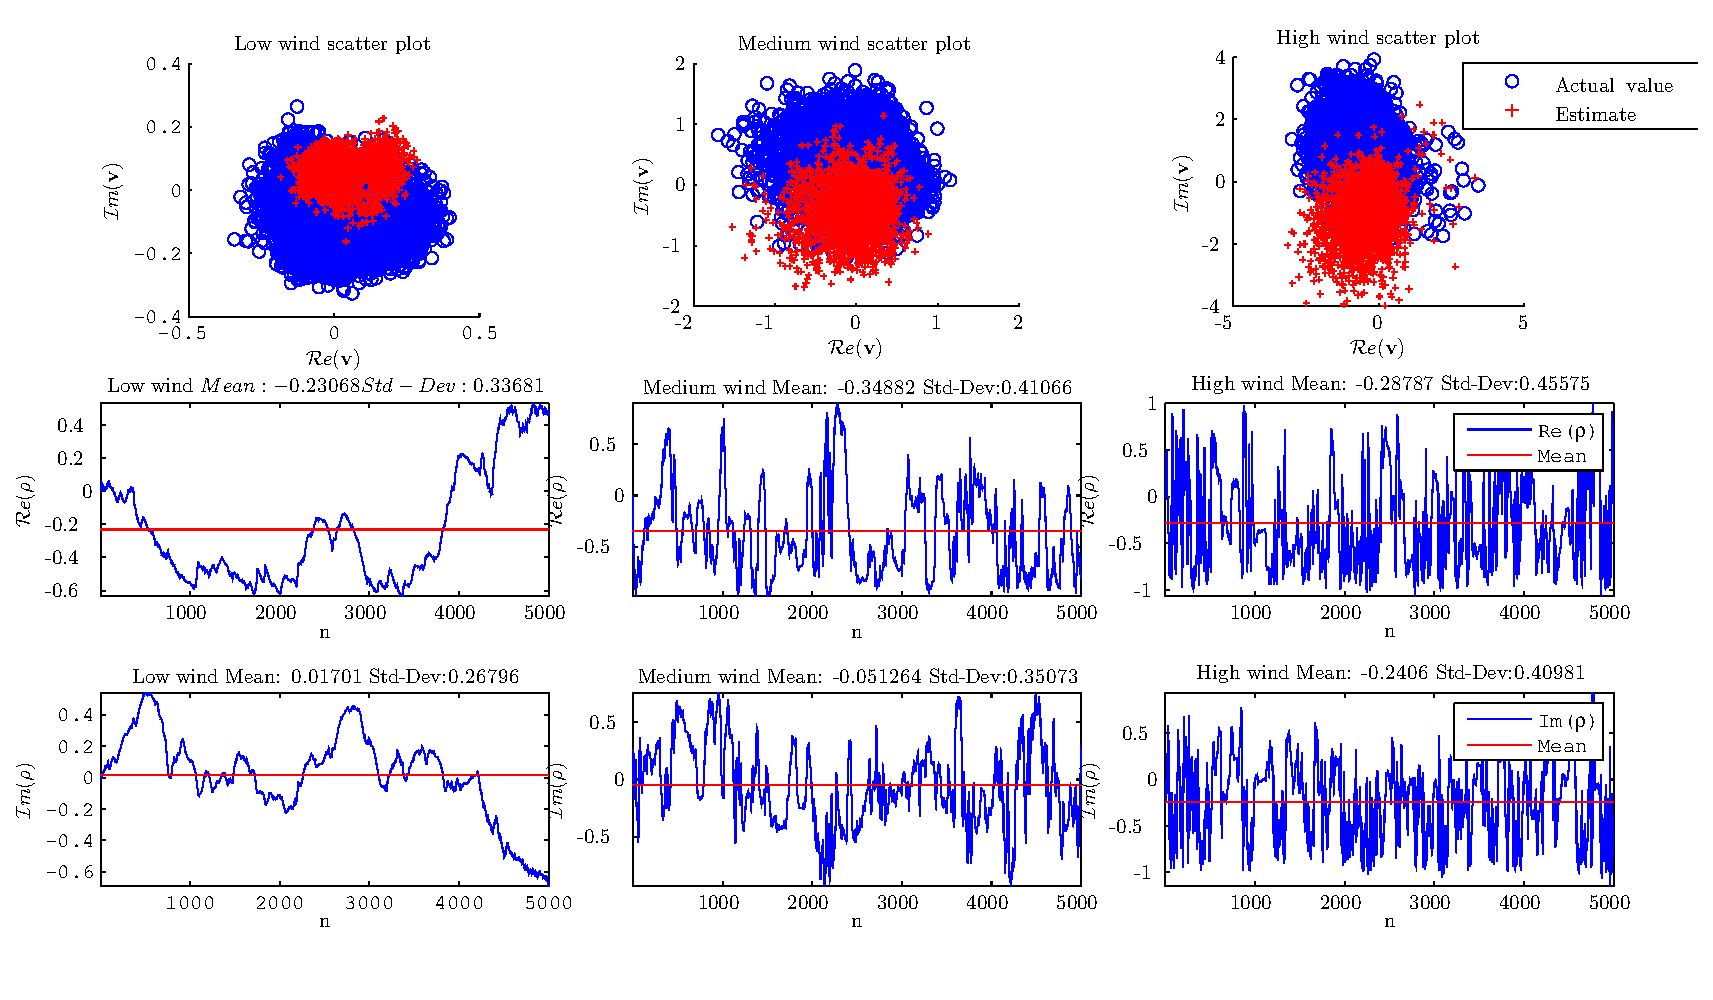
\includegraphics[width=1.0\textwidth]{cw4im/2e.eps}
Done for $\mu$ = 0.1 circularity
\caption{Wind scatter plot and circularity estimate ($\rho$)}
\label{fig:4_2e}
\end{figure}

Here wind data for three different type of regimes was investigated for circularity. Before being processed a complex was generated by taking the east and north wind intensities into one variable: $v[n] = v_{east}[n]+jv_{north}$.This get all wind data into a single variable(south wind is simply negative that of north wind). All findings have been compiled to figure \ref{fig:4_2e}.

For the low wind regime data it can be seen the data looks mostly circular, as the scatter graph would look mostly the same for any rotation of the plot. This is reflected in the circularity estimate which lays mostly around -0.3 and .3 (with a max/min of -0.5/.5). 

For the medium wind regime data the variations in the circularity estimate are higher ,the standard deviation is hgiher than before for both complex and real parts and the mean is further away from 0 - where it should be for perfect circularity. This can be seen from the scatter plot which exhibits a certain bias.

The high wind regime scatter plot is heavily biased and any rotation will be noticed. The high frequency of change in the circularity estimate and its high standard deviation values are two other indicators of noncircularity.


Thus overall the circularity tracker seems to reflect the circularity of the variables mainly in relation to is fast change in values and high amplitudes. Additionally we can comment that for low wind there seems to be the trend that it is simply rustling around and that for high regime wind the wind is more headed for just one direction, explaining the non-circular nature of it.
\FloatBarrier
\subsection{Comparison of CLMS to ACLMS}
Here the Augmented Complex Least Mean Square and CLMS algortihm is used to model the coefficients of a Widely Linear Moving Average process (WLMA). For CLMS we have one weight vector, $\mathbf{w}$, which means we have a strictly linear extension but for ACLMS we have two weight vectors allowing us to take advantage of the second order statistics of the data, $\mathbf{g}$ and $\mathbf{h}$. The convergence of these is found in figure \ref{fig:4_2f_2}. We can see that the CLMS struggles to converge to correct values for non-circular data, though it seems to perform similarly to the ACLMS for circular data.

Another way of seeing this is to look at the error curves in figure \ref{fig:4_2f_1} that show the ACLMS (in green) consistently outperforming the CLMS for both circular and non-circular data. For circular data we see that the errors are somewhat similar (steady state error of $-2.14dB$ vs $-9.34dB$, CLMS vs ACLMS)but do not agree for non-circular data (steady state error of $4.51dB$ vs $-3.37dB$, CLMS vs ACLMS).

\begin{figure}[h]
\centering
\resizebox{\textwidth}{!}{% This file was created by matlab2tikz v0.4.7 running on MATLAB 8.1.
% Copyright (c) 2008--2014, Nico Schlömer <nico.schloemer@gmail.com>
% All rights reserved.
% Minimal pgfplots version: 1.3
% 
% The latest updates can be retrieved from
%   http://www.mathworks.com/matlabcentral/fileexchange/22022-matlab2tikz
% where you can also make suggestions and rate matlab2tikz.
% 
\begin{tikzpicture}

\begin{axis}[%
width=3.25in,
height=1.75in,
scale only axis,
xmin=0,
xmax=1000,
xlabel={n},
ymin=-0.5,
ymax=2,
ylabel={$\mathbf{g}$},
name=plot2,
title={ACLMS coefficients convegence},
axis x line*=bottom,
axis y line*=left
]
\addplot [color=blue,solid,forget plot]
  table[row sep=crcr]{1	0\\
6	0.0542756672743055\\
11	0.12138528634016\\
16	0.192614786749279\\
21	0.255270244177622\\
26	0.316162543918574\\
31	0.375293923876688\\
36	0.433702726635469\\
41	0.490790775680259\\
46	0.537903826009192\\
51	0.582723065871384\\
56	0.618822573002616\\
61	0.662771202648319\\
66	0.702657846748347\\
71	0.74512172345249\\
76	0.773085837147234\\
81	0.803628978525392\\
86	0.834256763628867\\
91	0.860620411283994\\
96	0.893900274152661\\
101	0.918989897095266\\
106	0.943262106852653\\
111	0.968689484613424\\
116	0.996997577079293\\
121	1.01808212326768\\
126	1.03636925523455\\
131	1.05854250546514\\
136	1.07771094876894\\
141	1.09553869767798\\
146	1.11865059014233\\
151	1.14290327097551\\
156	1.16148368739458\\
161	1.17601943292575\\
166	1.19219603364325\\
171	1.20923286572846\\
176	1.22428187273022\\
181	1.23623868929492\\
186	1.24715820972548\\
191	1.26106867358341\\
196	1.27222685596274\\
201	1.28194585859166\\
206	1.29430618856062\\
211	1.30443278813138\\
216	1.31879984926413\\
221	1.32805583268093\\
226	1.33837796199792\\
231	1.34761949381918\\
236	1.35496057683454\\
241	1.35978469761002\\
246	1.36832881298105\\
251	1.37550865696248\\
256	1.38389769951487\\
261	1.39222016956291\\
266	1.39597738480625\\
271	1.4020459254743\\
276	1.40692782901802\\
281	1.4094013216769\\
286	1.41264212792332\\
291	1.4166768225057\\
296	1.42071236697883\\
301	1.42470286836636\\
306	1.42544570273296\\
311	1.42533482998274\\
316	1.42936792130039\\
321	1.42944133853691\\
326	1.43134486039307\\
331	1.43208568234125\\
336	1.43137236368966\\
341	1.4327590205105\\
346	1.4345889351824\\
351	1.43471790151905\\
356	1.43697190330543\\
361	1.43664478530685\\
366	1.44041267362631\\
371	1.44395467000435\\
376	1.4467622920008\\
381	1.4468665941719\\
386	1.44867702995232\\
391	1.45119023327734\\
396	1.45494145912526\\
401	1.45744542809735\\
406	1.46063669854092\\
411	1.46108130484258\\
416	1.46172524525417\\
421	1.46281433280272\\
426	1.46183745813205\\
431	1.4668111508841\\
436	1.46615826326813\\
441	1.46907762512239\\
446	1.46831293299199\\
451	1.46927005527226\\
456	1.46851082440296\\
461	1.47190136543121\\
466	1.47049433238879\\
471	1.47204443500418\\
476	1.47675547975031\\
481	1.47744976900111\\
486	1.4791646648482\\
491	1.48329423870517\\
496	1.48421974277577\\
501	1.48575296907525\\
506	1.48830498858908\\
511	1.49010985948337\\
516	1.49160355238228\\
521	1.49069794786269\\
526	1.49184449943359\\
531	1.49038581012172\\
536	1.49208072943648\\
541	1.49414576028119\\
546	1.49643416000524\\
551	1.49912457795358\\
556	1.49774600891301\\
561	1.49656854803332\\
566	1.49760305346369\\
571	1.49751268649214\\
576	1.49602079859258\\
581	1.49825278931047\\
586	1.50041673618645\\
591	1.49900299176701\\
596	1.49856503801219\\
601	1.49520552145439\\
606	1.49575476621419\\
611	1.49490544050857\\
616	1.4959337529231\\
621	1.49674034525482\\
626	1.49843950075074\\
631	1.50083404056152\\
636	1.50157490491056\\
641	1.5038863264959\\
646	1.50396437923829\\
651	1.50187689812441\\
656	1.50185645514669\\
661	1.50385660132538\\
666	1.50425164065307\\
671	1.50224767703233\\
676	1.50232025824451\\
681	1.50179349996164\\
686	1.5017426872552\\
691	1.5011601425392\\
696	1.50338818899959\\
701	1.50358659503938\\
706	1.50435765154697\\
711	1.50368764290191\\
716	1.50290733871085\\
721	1.50075957274596\\
726	1.50277725491373\\
731	1.50271333118058\\
736	1.50258716762149\\
741	1.50403199660056\\
746	1.50148953586492\\
751	1.50103191607497\\
756	1.50253715985293\\
761	1.5014511934986\\
766	1.49897170799169\\
771	1.5004440030898\\
776	1.49959932936416\\
781	1.49992997582682\\
786	1.50061578104283\\
791	1.50100048784334\\
796	1.50090291037088\\
801	1.50087917341113\\
806	1.50053226518873\\
811	1.5010148490604\\
816	1.5022804751261\\
821	1.50272775750626\\
826	1.50200417435946\\
831	1.50294955039734\\
836	1.50318608164946\\
841	1.50324535054157\\
846	1.50196910511177\\
851	1.50085196475489\\
856	1.5013485590782\\
861	1.50083694320695\\
866	1.5012630823779\\
871	1.50232410188929\\
876	1.50204649284066\\
881	1.50201241194812\\
886	1.50332335022885\\
891	1.50207282807797\\
896	1.50303192107901\\
901	1.50378983452472\\
906	1.50194531110473\\
911	1.4974633818606\\
916	1.49686905698458\\
921	1.49889950993387\\
926	1.49995938766655\\
931	1.5009206323027\\
936	1.5010341416886\\
941	1.50140213131166\\
946	1.49954052003507\\
951	1.50132506234272\\
956	1.50190527277678\\
961	1.50004876652294\\
966	1.49989478572937\\
971	1.50165879836401\\
976	1.50063826081796\\
981	1.5015649749939\\
986	1.50110148784665\\
991	1.50337229243475\\
996	1.50695457703274\\
};
\addplot [color=blue,solid,forget plot]
  table[row sep=crcr]{1	0\\
6	0.000238764038809792\\
11	-0.00545137301164898\\
16	-0.00426020554781486\\
21	-0.0103598036655311\\
26	-0.00972648138853979\\
31	-0.0104173387843941\\
36	-0.0119788714439104\\
41	-0.010327167246548\\
46	-0.00976440869895141\\
51	-0.0112749380418848\\
56	-0.0122268324995151\\
61	-0.00502197766010123\\
66	-0.00509242828743517\\
71	-0.0089374421672798\\
76	-0.0061689334121893\\
81	-0.00674882860559086\\
86	-0.0109603691446406\\
91	-0.010638723789097\\
96	-0.00904386961951076\\
101	-0.00940059288397838\\
106	-0.0104770046335372\\
111	-0.00773139968978214\\
116	-0.00649933244992998\\
121	-0.0103825929774941\\
126	-0.011232187935591\\
131	-0.00705323867652378\\
136	-0.00991312893340516\\
141	-0.00986445361814797\\
146	-0.00780589129390469\\
151	-0.00787948052620563\\
156	-0.00853366309246177\\
161	-0.0133866502640897\\
166	-0.0155568520744871\\
171	-0.0148662530558832\\
176	-0.0149925586744958\\
181	-0.0157387730718544\\
186	-0.0139471171381137\\
191	-0.015945324998398\\
196	-0.0157471010961106\\
201	-0.0158452510737357\\
206	-0.0161028270380636\\
211	-0.0144976610808432\\
216	-0.0107218313248476\\
221	-0.0106640935866577\\
226	-0.0108094639873061\\
231	-0.0109608774729335\\
236	-0.0099516171415273\\
241	-0.00910672778997527\\
246	-0.00943805666699729\\
251	-0.0124527352250036\\
256	-0.013194650453775\\
261	-0.0128035333698415\\
266	-0.0158904014307682\\
271	-0.0136417363934915\\
276	-0.0134483598015556\\
281	-0.0146323343557872\\
286	-0.0138514251851553\\
291	-0.0166312810575784\\
296	-0.0180928237522263\\
301	-0.018262469277512\\
306	-0.0190982087653726\\
311	-0.0189594496383659\\
316	-0.0154403005150786\\
321	-0.0161623261646405\\
326	-0.0167690268916156\\
331	-0.0161488842570353\\
336	-0.0145133430501675\\
341	-0.0147496811328348\\
346	-0.0146549923205797\\
351	-0.0152060878531243\\
356	-0.0142433720402422\\
361	-0.0166091567479159\\
366	-0.0150772278320522\\
371	-0.0143924891661761\\
376	-0.0113405538706512\\
381	-0.0131112016919741\\
386	-0.0146001040180764\\
391	-0.0130566030128447\\
396	-0.0154308759849033\\
401	-0.0137570163896402\\
406	-0.0114477685922473\\
411	-0.0146173985971968\\
416	-0.0147186132188399\\
421	-0.0146200676916714\\
426	-0.0139702627643948\\
431	-0.0118489448156095\\
436	-0.0132527005889325\\
441	-0.0138675367188072\\
446	-0.0141126769778402\\
451	-0.0133660564599401\\
456	-0.0136822273915671\\
461	-0.0138628472570406\\
466	-0.0121682451925134\\
471	-0.0135993999419825\\
476	-0.0132749531015795\\
481	-0.00994115649332706\\
486	-0.0103728486350475\\
491	-0.00834275525566902\\
496	-0.00951761811413633\\
501	-0.00901692734796549\\
506	-0.0111669891997569\\
511	-0.00942400527491906\\
516	-0.00950752285593493\\
521	-0.0104119831767663\\
526	-0.00883279479235128\\
531	-0.00823422214753928\\
536	-0.0075287063483497\\
541	-0.00879105957154437\\
546	-0.00997000038000008\\
551	-0.0117299561064207\\
556	-0.0111004225770719\\
561	-0.0102720052943754\\
566	-0.0107685849674751\\
571	-0.00869629989424642\\
576	-0.00709873540850353\\
581	-0.00953391226441811\\
586	-0.00816879581567757\\
591	-0.00642113080420902\\
596	-0.00550767859503523\\
601	-0.00561918848886591\\
606	-0.00604619532690066\\
611	-0.00335377565997532\\
616	-0.0060545483653865\\
621	-0.00751250952659387\\
626	-0.00962491403759468\\
631	-0.00739761766735579\\
636	-0.00598708349484487\\
641	-0.00605562705897577\\
646	-0.00612814741675227\\
651	-0.00813944322454322\\
656	-0.0106679306121941\\
661	-0.0116764639927022\\
666	-0.0101594836392845\\
671	-0.00929917077967971\\
676	-0.00747562534049277\\
681	-0.0050633692149855\\
686	-0.0059356116868914\\
691	-0.00861768651549199\\
696	-0.00941903715616608\\
701	-0.0099303181879141\\
706	-0.0101152441753436\\
711	-0.00734565597221213\\
716	-0.00836909632885393\\
721	-0.010107662891293\\
726	-0.011460831987381\\
731	-0.0122370389803389\\
736	-0.0132039231519663\\
741	-0.0139165404902893\\
746	-0.0167998892355059\\
751	-0.0155122275042279\\
756	-0.014658774474613\\
761	-0.0132687358476689\\
766	-0.0128115335919162\\
771	-0.0146006143292709\\
776	-0.013201336852352\\
781	-0.0122925895684317\\
786	-0.0140554598191612\\
791	-0.0154234989404083\\
796	-0.0157472548853538\\
801	-0.0185785200853249\\
806	-0.0192302500006972\\
811	-0.0203904627828053\\
816	-0.0193129541253994\\
821	-0.0205133399051982\\
826	-0.0173706866156798\\
831	-0.0184396005358438\\
836	-0.0170704267284176\\
841	-0.0191604630794153\\
846	-0.0196130621374826\\
851	-0.0174710981913479\\
856	-0.0176003231866773\\
861	-0.0182516046055071\\
866	-0.0171259753113998\\
871	-0.0154419501817852\\
876	-0.0143762654824955\\
881	-0.0144602514641704\\
886	-0.0144824434852321\\
891	-0.0151188369131541\\
896	-0.0140786910857007\\
901	-0.0147358982956211\\
906	-0.0125342907070475\\
911	-0.0126871604199478\\
916	-0.0106034334140988\\
921	-0.00850394858438022\\
926	-0.00596281904645914\\
931	-0.00625763402338832\\
936	-0.0052386860134225\\
941	-0.00589425109703644\\
946	-0.00470596123780661\\
951	-0.00582945564743455\\
956	-0.00699928790022813\\
961	-0.00440264987833037\\
966	-0.00496004282106991\\
971	-0.00404616983822345\\
976	-0.0014969749781102\\
981	-0.00414550771477201\\
986	-0.00710316463997059\\
991	-0.00912985965169296\\
996	-0.00864324984253595\\
};
\addplot [color=green,solid,forget plot]
  table[row sep=crcr]{1	0\\
6	0.0361763220976177\\
11	0.075644347437178\\
16	0.120900349944743\\
21	0.170894223051468\\
26	0.203854151036497\\
31	0.238093327253625\\
36	0.277995499863498\\
41	0.316407275386017\\
46	0.354214827104219\\
51	0.389841764325893\\
56	0.419323341347848\\
61	0.450761038839392\\
66	0.487322453951804\\
71	0.51094498857067\\
76	0.53224132923799\\
81	0.546206813032327\\
86	0.571594808343416\\
91	0.595241010006458\\
96	0.616241602733159\\
101	0.634286535116808\\
106	0.653436817043109\\
111	0.674990888947485\\
116	0.690234419838381\\
121	0.704955517265632\\
126	0.722971844042686\\
131	0.734047564166746\\
136	0.747898969199255\\
141	0.759249678544771\\
146	0.770313140385043\\
151	0.775198323587385\\
156	0.794506308526511\\
161	0.803735580605413\\
166	0.816303227693958\\
171	0.826913876223911\\
176	0.837299489074872\\
181	0.84422044945777\\
186	0.853621714762418\\
191	0.8666734120553\\
196	0.871429768516138\\
201	0.877252585124526\\
206	0.883391768763221\\
211	0.886687157022027\\
216	0.893342191586126\\
221	0.897951860255712\\
226	0.902248576137591\\
231	0.903079308223435\\
236	0.907464500540832\\
241	0.912983863288555\\
246	0.91826066628139\\
251	0.919647666130461\\
256	0.924956722921268\\
261	0.925324226143541\\
266	0.927958053123495\\
271	0.931212876493071\\
276	0.935842938267721\\
281	0.938098855847812\\
286	0.941696589689079\\
291	0.94523337046531\\
296	0.946304090531614\\
301	0.949002781390174\\
306	0.950374268455847\\
311	0.953661307090413\\
316	0.954662961447573\\
321	0.95859194938789\\
326	0.958505890966345\\
331	0.961703621132039\\
336	0.962788546794389\\
341	0.96309997511481\\
346	0.964651655905786\\
351	0.967311603475436\\
356	0.969318585432223\\
361	0.971375191554785\\
366	0.971916559482447\\
371	0.972775032980334\\
376	0.975107183992849\\
381	0.977091978654099\\
386	0.977166177491383\\
391	0.981077485091556\\
396	0.980488408256411\\
401	0.980702047982202\\
406	0.981724976898072\\
411	0.983534513102046\\
416	0.98590798573948\\
421	0.98866547964575\\
426	0.9896764406384\\
431	0.988930539604092\\
436	0.992666595895669\\
441	0.993049637164216\\
446	0.993423755577847\\
451	0.992149185759072\\
456	0.994019041456878\\
461	0.995858708944287\\
466	0.996286220911593\\
471	0.992831916157442\\
476	0.992423586154251\\
481	0.993316451069336\\
486	0.99417892397272\\
491	0.995288981691324\\
496	0.995284325547896\\
501	0.995808032913015\\
506	0.993253935916216\\
511	0.993987724846288\\
516	0.995213349425195\\
521	0.9952728178181\\
526	0.994203341388928\\
531	0.995239163729186\\
536	0.994333254568924\\
541	0.996202350469543\\
546	0.997772679145915\\
551	0.997890031020994\\
556	1.00001296336218\\
561	1.00232489926067\\
566	1.00197955020143\\
571	1.0033746690515\\
576	1.00344973763773\\
581	1.00057191494899\\
586	1.00320648795806\\
591	1.00449513763029\\
596	1.0047034871322\\
601	1.00345789922359\\
606	1.0027811982481\\
611	1.00355005359892\\
616	1.00237361105837\\
621	1.00295115785854\\
626	1.00229510749047\\
631	1.00384158190635\\
636	1.0045990646968\\
641	1.00594208239604\\
646	1.0046557147406\\
651	1.00328315249502\\
656	1.00299087309983\\
661	1.00211418501395\\
666	1.00380292863455\\
671	1.00317075420994\\
676	1.00102547648951\\
681	0.998656311392854\\
686	0.997741013159891\\
691	0.997527511863299\\
696	1.00014430329599\\
701	0.995724320580982\\
706	0.994201710332908\\
711	0.993240531116092\\
716	0.994405189263598\\
721	0.99748320048889\\
726	0.998295556283329\\
731	1.00124047947841\\
736	0.999470018604395\\
741	0.9982002949087\\
746	0.997647813699007\\
751	0.997171630250449\\
756	0.996047047979286\\
761	0.994862117446127\\
766	0.994439867143807\\
771	0.995554170486972\\
776	0.996356535341554\\
781	0.996633446374396\\
786	0.996395451987127\\
791	0.997755099399177\\
796	0.997576319068549\\
801	0.998373421737891\\
806	1.00068398033128\\
811	0.997947679487516\\
816	0.998297393039314\\
821	0.99553573666895\\
826	0.995846818000953\\
831	0.992380351632154\\
836	0.990544775063261\\
841	0.988326336614307\\
846	0.98844571706128\\
851	0.987054299705859\\
856	0.99130444426333\\
861	0.991424163310657\\
866	0.992532974183504\\
871	0.993585614183688\\
876	0.99354898169699\\
881	0.992978518792631\\
886	0.990571020902763\\
891	0.992047959174446\\
896	0.991019687297797\\
901	0.991057555630613\\
906	0.991726046544547\\
911	0.990436531312631\\
916	0.993291237453978\\
921	0.993424832764385\\
926	0.992213374832879\\
931	0.994392210218456\\
936	0.99612031567819\\
941	0.995802765868424\\
946	0.99481006325882\\
951	0.995564872784206\\
956	0.995408743796328\\
961	0.99406321878865\\
966	0.993958584051056\\
971	0.994882681554113\\
976	0.997221204629392\\
981	0.996903709736381\\
986	0.998103378085367\\
991	0.997196491259726\\
996	0.997059253342765\\
};
\addplot [color=green,solid,forget plot]
  table[row sep=crcr]{1	0\\
6	0.00074816913017213\\
11	0.00310614849853272\\
16	0.00419544852607538\\
21	0.00673753939021877\\
26	0.0143703411683762\\
31	0.0162493386920446\\
36	0.0148686604513347\\
41	0.0114420366415295\\
46	0.00865207548307882\\
51	0.00868458205815933\\
56	0.0104636765240228\\
61	0.00354376718997427\\
66	0.000568341005385226\\
71	0.00508861856671551\\
76	0.00388890438804085\\
81	0.00549834227712107\\
86	0.0073275501767614\\
91	0.00792594993363095\\
96	0.00884280641959393\\
101	0.00979613677600095\\
106	0.0117734239554566\\
111	0.0093530280356596\\
116	0.0090924296569674\\
121	0.0109998901353052\\
126	0.0103395936267021\\
131	0.0087098256718131\\
136	0.0111230715832762\\
141	0.00923037524265124\\
146	0.00732881571821291\\
151	0.00879758585304187\\
156	0.0129914729562312\\
161	0.014134603816976\\
166	0.0134237168799581\\
171	0.0135311478552909\\
176	0.0135485137767796\\
181	0.0148379060470115\\
186	0.0140832101437544\\
191	0.0125305457789761\\
196	0.0105907409480543\\
201	0.00898515430124213\\
206	0.00835103641251171\\
211	0.00825560368469962\\
216	0.0112901936606405\\
221	0.0106495607261091\\
226	0.0107370817950413\\
231	0.00761037395877971\\
236	0.00411236892314016\\
241	0.0053705225470959\\
246	0.00448633885676338\\
251	0.00430815576234239\\
256	0.00238742042927017\\
261	0.00230735239953757\\
266	0.0045775423814034\\
271	0.00614986859409453\\
276	0.00658819587456007\\
281	0.00733739624709993\\
286	0.00638829977428206\\
291	0.00462240126181477\\
296	0.00536013963336101\\
301	0.00370115782474694\\
306	0.003798238047432\\
311	0.00415883883688622\\
316	0.003159513270895\\
321	0.00421645713185967\\
326	0.00254889771563184\\
331	0.00100486478986603\\
336	0.00244579464853394\\
341	0.00348253588296958\\
346	0.0034570028275356\\
351	0.0029267933994141\\
356	0.00426375552053148\\
361	0.00306563168933146\\
366	0.00224724478439772\\
371	0.000593113078283991\\
376	-0.00204059931970088\\
381	-0.00243530734283307\\
386	-0.00227559286229522\\
391	-0.00177195423447792\\
396	-0.00135114750971726\\
401	-0.00249424086715271\\
406	-0.000977219376126684\\
411	-0.00100772984545321\\
416	-0.00208947268900993\\
421	-0.00341027207930806\\
426	-0.00341385080899192\\
431	-0.00310953871011703\\
436	-0.00255478984084883\\
441	-0.000271577316475872\\
446	-0.00121926059645256\\
451	-0.000800471895026511\\
456	-0.000273957984934091\\
461	0.0029514421535007\\
466	0.00374098074405236\\
471	0.00379402843661387\\
476	0.00133174398463697\\
481	-0.00168911523258332\\
486	-0.00112548780648272\\
491	-0.00377312634623773\\
496	-0.00327501387712356\\
501	-0.0032396881592634\\
506	-0.00423714335654532\\
511	-0.00632925867252904\\
516	-0.00955159676936285\\
521	-0.00906112205419748\\
526	-0.00648680056701768\\
531	-0.00788761362459506\\
536	-0.00828721898841255\\
541	-0.00655134443532651\\
546	-0.00619064195146315\\
551	-0.00674709522585194\\
556	-0.00731972795212966\\
561	-0.00889131868724905\\
566	-0.00718768782348598\\
571	-0.009084700310462\\
576	-0.00614590276548916\\
581	-0.00570872165422991\\
586	-0.0068183578238145\\
591	-0.00877941085362173\\
596	-0.00759108287472847\\
601	-0.00488268212807972\\
606	-0.00499789248617725\\
611	-0.00428445020108139\\
616	-0.00382509229411287\\
621	-0.00188194575181308\\
626	-0.00279189451189812\\
631	-0.00298083309253258\\
636	-0.00241573834196318\\
641	-0.00256922570400781\\
646	-0.000966453728467516\\
651	-0.000909730280983627\\
656	-0.00118039493973395\\
661	0.00265130582237911\\
666	0.00133781393258551\\
671	0.00160021381321732\\
676	0.00237599409869983\\
681	0.00248947044745869\\
686	0.00217394782794864\\
691	0.00349685818641144\\
696	0.00583769356981015\\
701	0.00780822922732739\\
706	0.0089804478753526\\
711	0.00789700053511959\\
716	0.00711159031053819\\
721	0.00576111674782739\\
726	0.00559948352447362\\
731	0.0052539185227542\\
736	0.00604369371210081\\
741	0.00701767082887033\\
746	0.00397787999653736\\
751	0.00625856379220824\\
756	0.00478464823908128\\
761	0.00743549312040082\\
766	0.0069085477721075\\
771	0.00785427428080611\\
776	0.00883551528243048\\
781	0.00843173756009005\\
786	0.00837643626244235\\
791	0.00787250322473706\\
796	0.00914250046035706\\
801	0.010810608035104\\
806	0.0114477331953739\\
811	0.00895846543049543\\
816	0.00770417574636767\\
821	0.00593070530705718\\
826	0.00726844964864178\\
831	0.00939857562093548\\
836	0.00971875637870959\\
841	0.00867961293765622\\
846	0.0101116977676086\\
851	0.0112696509225584\\
856	0.0131288902960622\\
861	0.0152050264911088\\
866	0.0162380558151308\\
871	0.0145957451856335\\
876	0.0156285448932337\\
881	0.0179104757017668\\
886	0.0163483645210342\\
891	0.0151185475251451\\
896	0.0162964193674258\\
901	0.0145635866668585\\
906	0.0144915426523405\\
911	0.0139929855429506\\
916	0.0151900495225955\\
921	0.0131283050089547\\
926	0.0112931015199144\\
931	0.0117725259661211\\
936	0.0106314267765287\\
941	0.0121007440234872\\
946	0.0121738859616721\\
951	0.0122813557569471\\
956	0.0118251904134436\\
961	0.0124608019145739\\
966	0.0111088796444145\\
971	0.00858030832443825\\
976	0.00858167684027487\\
981	0.00989824106667536\\
986	0.00853731052090842\\
991	0.00790361852897759\\
996	0.00528329210293639\\
};
\end{axis}

\begin{axis}[%
width=3.25in,
height=1.75in,
scale only axis,
xmin=0,
xmax=1000,
xlabel={n},
ymin=-0.5,
ymax=2,
ylabel={$\mathbf{w}$},
at=(plot2.left of south west),
anchor=right of south east,
title={CLMS coefficients convegence - Circular},
axis x line*=bottom,
axis y line*=left
]
\addplot [color=blue,solid,forget plot]
  table[row sep=crcr]{1	0\\
6	0.0544546586992245\\
11	0.0893436203395286\\
16	0.13894954513241\\
21	0.18530791637255\\
26	0.226576891519233\\
31	0.260269155705554\\
36	0.294517468605976\\
41	0.326967191476583\\
46	0.358432360668528\\
51	0.387972074875872\\
56	0.416126175307126\\
61	0.44856631316254\\
66	0.472644819094223\\
71	0.493740186166543\\
76	0.518741933953602\\
81	0.535828951527783\\
86	0.554688675804241\\
91	0.579718159340167\\
96	0.59960278636714\\
101	0.620197739249631\\
106	0.642478215693378\\
111	0.660984898289664\\
116	0.687640509741456\\
121	0.699197095600327\\
126	0.717428827230082\\
131	0.737821498825058\\
136	0.746573946243886\\
141	0.757892791026966\\
146	0.772736253058653\\
151	0.787336972989364\\
156	0.805318987057959\\
161	0.810440245561379\\
166	0.814977196422311\\
171	0.827149313122732\\
176	0.839197567249009\\
181	0.849858641107676\\
186	0.860895747683663\\
191	0.874074184820791\\
196	0.882452147238315\\
201	0.879557456854199\\
206	0.878623314762906\\
211	0.885276705347484\\
216	0.897373944950317\\
221	0.901797649768457\\
226	0.9043620098134\\
231	0.908574213523321\\
236	0.918970937829637\\
241	0.917196770536574\\
246	0.914360624318806\\
251	0.918165517630119\\
256	0.922249725791096\\
261	0.923893010231883\\
266	0.93301646933993\\
271	0.934630014752266\\
276	0.933957659524885\\
281	0.940985810316508\\
286	0.946522641291769\\
291	0.943570594519575\\
296	0.943173598688549\\
301	0.946140184300427\\
306	0.950342008233644\\
311	0.958864384512601\\
316	0.959986656839092\\
321	0.963030973812867\\
326	0.965212521984227\\
331	0.965979698782399\\
336	0.969416206156071\\
341	0.973551361686853\\
346	0.975461851444283\\
351	0.985180639024242\\
356	0.987985768696256\\
361	0.986938117042538\\
366	0.98831085933767\\
371	0.995895027484196\\
376	0.996313583282105\\
381	0.995154223472751\\
386	0.993163062002586\\
391	0.994700031169154\\
396	0.996329615977018\\
401	1.00010419678391\\
406	1.00613851086516\\
411	1.00974988487394\\
416	1.00430046957529\\
421	0.997557937804192\\
426	0.996831206260161\\
431	0.995565630745336\\
436	0.992822060750205\\
441	0.9958349647658\\
446	0.997850239336698\\
451	0.995667714770403\\
456	0.999358539397063\\
461	0.995548808326413\\
466	0.996338666374642\\
471	0.994499161477332\\
476	0.998383460670402\\
481	1.00223890568514\\
486	0.998284334005056\\
491	0.997985347552106\\
496	0.995545059409299\\
501	0.99888492124983\\
506	0.993356390466018\\
511	0.988751984705313\\
516	0.986381673347821\\
521	0.982446052229335\\
526	0.981582202164972\\
531	0.984906697149534\\
536	0.984531259997434\\
541	0.986823829192488\\
546	0.990486976977274\\
551	0.989741370651548\\
556	0.997902320339354\\
561	0.998522760368162\\
566	0.999025169660778\\
571	1.0053828917757\\
576	1.00783340594441\\
581	1.01380018608897\\
586	1.01508567473124\\
591	1.01361966832663\\
596	1.02000621826932\\
601	1.02577896038478\\
606	1.02218201653434\\
611	1.02095760025984\\
616	1.0149366664805\\
621	1.0201447763597\\
626	1.01866960666498\\
631	1.02221505394786\\
636	1.02154885215979\\
641	1.01330231713384\\
646	1.01440373837316\\
651	1.01925207877995\\
656	1.01559807869934\\
661	1.01391653479387\\
666	1.0132444142411\\
671	1.02276182167327\\
676	1.01933298258441\\
681	1.02077287208442\\
686	1.02286062793166\\
691	1.02157045533403\\
696	1.02244697885712\\
701	1.02417500543751\\
706	1.0169540471035\\
711	1.02191307535278\\
716	1.02259626588279\\
721	1.01977427001634\\
726	1.01987930718672\\
731	1.01678761733666\\
736	1.01249098465017\\
741	1.0153818918318\\
746	1.01344119741049\\
751	1.00964603525841\\
756	1.00882393449102\\
761	1.0067857833361\\
766	0.998711189153983\\
771	0.996000718122182\\
776	0.991849346435073\\
781	0.998045230984644\\
786	0.997412312585255\\
791	0.999773944735884\\
796	0.999862887814329\\
801	1.0031249627114\\
806	1.00288737697742\\
811	0.999307303916776\\
816	0.995405034896996\\
821	0.9938955682698\\
826	0.99102302363163\\
831	0.998439004891887\\
836	0.999469198960678\\
841	1.00357844885647\\
846	1.0028680890091\\
851	1.00267422085203\\
856	1.00666685963168\\
861	1.00119359652391\\
866	1.00478186151137\\
871	1.01444930477966\\
876	1.01418191181511\\
881	1.012440588919\\
886	1.01019710254978\\
891	1.0116247117475\\
896	1.01259402729243\\
901	1.01200519097152\\
906	1.00401501255058\\
911	1.00212628591258\\
916	1.00297317944979\\
921	1.00607802759905\\
926	1.00530059444382\\
931	1.00726916948442\\
936	1.00956518734723\\
941	1.01026324253305\\
946	1.00935809481369\\
951	1.0025874026482\\
956	1.00049904705112\\
961	0.99043019502254\\
966	0.991093771948637\\
971	0.99339966337525\\
976	0.994106382668886\\
981	0.996361844381967\\
986	0.994934438317386\\
991	0.992751849729494\\
996	0.986417741201955\\
};
\addplot [color=blue,solid,forget plot]
  table[row sep=crcr]{1	0\\
6	0.0666311796936323\\
11	0.133645758874472\\
16	0.204203085987441\\
21	0.266382943562583\\
26	0.326256874627365\\
31	0.386656171801353\\
36	0.445756055927012\\
41	0.500161763756646\\
46	0.548458911525031\\
51	0.593789593291377\\
56	0.623440931368089\\
61	0.666354584535895\\
66	0.704255795982262\\
71	0.747212823944847\\
76	0.768305657012182\\
81	0.796152258700418\\
86	0.827132486850961\\
91	0.847792861077026\\
96	0.874724784992401\\
101	0.898294918296825\\
106	0.921882773270593\\
111	0.946420947107863\\
116	0.972280734893935\\
121	0.990585627020143\\
126	1.0040187428499\\
131	1.03057212303733\\
136	1.05034938172312\\
141	1.07095697775214\\
146	1.09935825170015\\
151	1.12537255343857\\
156	1.13567933775681\\
161	1.15372259827714\\
166	1.17284333315251\\
171	1.19303002414715\\
176	1.21341728916095\\
181	1.22574583170994\\
186	1.23714359451617\\
191	1.25621443978957\\
196	1.26160147719861\\
201	1.27268185900159\\
206	1.29964513088413\\
211	1.31290601275765\\
216	1.33294693459829\\
221	1.35133420988309\\
226	1.36358469128237\\
231	1.37053133889426\\
236	1.36882456444531\\
241	1.37695610347863\\
246	1.39099783122122\\
251	1.39488998894253\\
256	1.40820187666509\\
261	1.4206649561236\\
266	1.41974621044851\\
271	1.42257028702307\\
276	1.42958659260822\\
281	1.42994950518897\\
286	1.43336475170893\\
291	1.43693783755192\\
296	1.44182786795246\\
301	1.44059154918534\\
306	1.4394473242501\\
311	1.43616254898719\\
316	1.43695483318066\\
321	1.44257752391252\\
326	1.43598137256057\\
331	1.42578059333045\\
336	1.42647022948669\\
341	1.42956386473621\\
346	1.43403455556564\\
351	1.43731857394573\\
356	1.45701496526952\\
361	1.46478089972347\\
366	1.45551029269742\\
371	1.44815439989999\\
376	1.44866794705568\\
381	1.4546010875605\\
386	1.45544866092362\\
391	1.4502714112984\\
396	1.46152630947834\\
401	1.46566847398998\\
406	1.47285844493536\\
411	1.47030772829282\\
416	1.48117088377564\\
421	1.47932827260209\\
426	1.47511525063742\\
431	1.47192456792282\\
436	1.47038038744739\\
441	1.47576985560219\\
446	1.4754385507402\\
451	1.47569443931772\\
456	1.47791410876685\\
461	1.47756062227243\\
466	1.49167517486057\\
471	1.48852387855048\\
476	1.48969904167169\\
481	1.48889897694516\\
486	1.48750111573749\\
491	1.48559206461274\\
496	1.48835811518762\\
501	1.47973287096706\\
506	1.47305124551875\\
511	1.47786618733111\\
516	1.46810167170859\\
521	1.47463985289154\\
526	1.47824214113568\\
531	1.48327879457538\\
536	1.48511328689374\\
541	1.48393231255372\\
546	1.47778173984772\\
551	1.48619801442063\\
556	1.48278171548784\\
561	1.49238368378981\\
566	1.49360741568079\\
571	1.4959635202244\\
576	1.49566913544494\\
581	1.49864124099334\\
586	1.48631718711089\\
591	1.48256395210891\\
596	1.48189097733641\\
601	1.48325551722185\\
606	1.4879156823364\\
611	1.48467787375601\\
616	1.47737804439809\\
621	1.47503020870369\\
626	1.48683498334111\\
631	1.49136235568033\\
636	1.4911460807519\\
641	1.49343274263225\\
646	1.48793739917426\\
651	1.49339749741191\\
656	1.4907641583773\\
661	1.49145672559431\\
666	1.48002371334581\\
671	1.47973574207051\\
676	1.48155908160605\\
681	1.47916902108095\\
686	1.48451509805439\\
691	1.48439427583924\\
696	1.48171202126839\\
701	1.48868394446926\\
706	1.48732866788626\\
711	1.47613267662361\\
716	1.47751470371944\\
721	1.48236993123328\\
726	1.47382549956997\\
731	1.46590063615175\\
736	1.46887699662277\\
741	1.45879041526896\\
746	1.46582121319699\\
751	1.46937942038005\\
756	1.46909308475286\\
761	1.4661231058393\\
766	1.4658814940711\\
771	1.46313530088816\\
776	1.46491338969709\\
781	1.46845827798231\\
786	1.47394188686747\\
791	1.47571168433034\\
796	1.47462504398261\\
801	1.47642406054673\\
806	1.48548010255118\\
811	1.48183995358929\\
816	1.48092419745055\\
821	1.47314714800915\\
826	1.4859847966871\\
831	1.48359428043789\\
836	1.49189932360511\\
841	1.49429028159037\\
846	1.4996326818364\\
851	1.50156530687206\\
856	1.50047492135733\\
861	1.49988641399245\\
866	1.49843997182373\\
871	1.4920794040845\\
876	1.48776283269633\\
881	1.48460969790398\\
886	1.47594858091683\\
891	1.46678673469707\\
896	1.47123446162668\\
901	1.47269008288304\\
906	1.4802200690476\\
911	1.48471160239495\\
916	1.48197588981621\\
921	1.48896507505363\\
926	1.49311430134342\\
931	1.48898008589837\\
936	1.49342139382963\\
941	1.4986215942784\\
946	1.49067043296848\\
951	1.48769368555487\\
956	1.48306979412742\\
961	1.49048973743167\\
966	1.4832161674386\\
971	1.48324031176457\\
976	1.48646894045276\\
981	1.49587987052723\\
986	1.49335793856838\\
991	1.48551533942226\\
996	1.47173686310739\\
};
\addplot [color=green,solid,forget plot]
  table[row sep=crcr]{1	0\\
6	0.00323760333287449\\
11	0.00231753527912146\\
16	0.00719884226264383\\
21	0.00153915287399668\\
26	0.00981600681994633\\
31	0.0135948259363505\\
36	0.017756030954872\\
41	0.016158409669057\\
46	0.00564866622250276\\
51	0.00548502102372705\\
56	0.0052163373022649\\
61	-0.00166065444847882\\
66	-0.00349844067807106\\
71	0.000364469748949832\\
76	0.00638966914483083\\
81	0.0129000699727654\\
86	0.012791965146533\\
91	0.0160651121494581\\
96	0.0205252940716104\\
101	0.0199189210205646\\
106	0.0186651080678565\\
111	0.0179771092457504\\
116	0.00919314189011026\\
121	0.013118187208046\\
126	0.0152588180173706\\
131	0.012861098294178\\
136	0.0102213676435655\\
141	0.00678384669877812\\
146	0.00658885850289789\\
151	0.0178238821244173\\
156	0.0206672760920734\\
161	0.0188270926515597\\
166	0.0167647393186884\\
171	0.011161465153176\\
176	0.00876400369776724\\
181	0.00675189810255932\\
186	0.0123688185386828\\
191	0.00778042847652806\\
196	0.00995451775907552\\
201	0.00815658194743619\\
206	0.00323692404204697\\
211	0.000781443216789747\\
216	-0.00187165937888071\\
221	-0.0109159613261312\\
226	-0.00677670936275535\\
231	-0.00621592739640854\\
236	-0.00826892497764963\\
241	-0.00592414012565358\\
246	-0.0126439261687513\\
251	-0.0116766936848127\\
256	-0.00898113220822957\\
261	-0.0138737796974113\\
266	-0.0125687157096556\\
271	-0.0061181426951614\\
276	-0.00734573470061389\\
281	0.000441666135317409\\
286	0.00569295567445902\\
291	0.00572651097276112\\
296	0.0159747707213566\\
301	0.0142116979800599\\
306	0.0159842624138128\\
311	0.0121122239588521\\
316	0.00767493128699372\\
321	0.00942023865489407\\
326	0.00208351956464592\\
331	0.0040141711536446\\
336	0.00691651031442447\\
341	0.00773911858217059\\
346	0.000305789269771351\\
351	0.00194400645987941\\
356	0.00486444101843339\\
361	0.00337458817428365\\
366	0.00186611239325499\\
371	0.00364554169432212\\
376	0.0111467000574788\\
381	0.00424185493333424\\
386	0.000287890671489317\\
391	-0.00370774499831544\\
396	-0.00360833020627908\\
401	-0.0119291251543463\\
406	-0.014129578699523\\
411	-0.00471268680673102\\
416	-0.00771915942093737\\
421	-0.00708439355276342\\
426	-0.0093209330644805\\
431	-0.0138098414548462\\
436	-0.0157895598080676\\
441	-0.01708055795067\\
446	-0.0138387603971653\\
451	-0.0134448946322934\\
456	-0.00531550999300775\\
461	-0.00792496758609774\\
466	-0.0033293007125833\\
471	-0.00167189224676327\\
476	-0.00428894543479441\\
481	-0.00329177205671993\\
486	-0.000964973662367753\\
491	-0.00196323696437764\\
496	0.00596953465832481\\
501	0.00440653927361998\\
506	0.00184876488284677\\
511	0.00625845794949264\\
516	0.00781576974652016\\
521	0.0109573394879468\\
526	0.0189042284362874\\
531	0.0172463533904407\\
536	0.0179295765789876\\
541	0.0133460054182681\\
546	0.0165552252471483\\
551	0.0162305207960789\\
556	0.0180185218019592\\
561	0.0230125907589499\\
566	0.0161450801596496\\
571	0.0122350459828601\\
576	0.0074333140445147\\
581	0.0100179618567721\\
586	0.0142042484062956\\
591	0.014398812713941\\
596	0.00729546864342543\\
601	0.00272085914205874\\
606	0.00692489580632407\\
611	0.0162025802310299\\
616	0.021667351206331\\
621	0.0211482985520681\\
626	0.0162545085839007\\
631	0.0220515710959203\\
636	0.0235052877745655\\
641	0.0213773579069664\\
646	0.0190290763953226\\
651	0.0174500093668582\\
656	0.0186215326034836\\
661	0.0159324732028356\\
666	0.0151351835179656\\
671	0.0147696538354419\\
676	0.0176216294639841\\
681	0.015579407007003\\
686	0.0200971172265151\\
691	0.0205677407144933\\
696	0.0112842757682728\\
701	0.00716786125644531\\
706	0.000472190023551119\\
711	-0.00401281382841447\\
716	-0.00888652671429194\\
721	-0.00549154597922112\\
726	-0.00350840991336133\\
731	0.000224036347025442\\
736	-0.0014671730126528\\
741	0.000333258007469953\\
746	0.00119055485706991\\
751	0.00469621383883775\\
756	0.00471414757922994\\
761	0.00290949898733807\\
766	0.00896627121358549\\
771	0.00745035642674026\\
776	0.00311751118533772\\
781	0.0106658654553726\\
786	0.00491464156742766\\
791	0.00199668108536044\\
796	-0.000960554044195251\\
801	0.0098117467810635\\
806	0.0110206710400694\\
811	0.00246495698805509\\
816	0.00638558460269375\\
821	0.0140592792844127\\
826	0.0211535697218096\\
831	0.021810334402714\\
836	0.0213972831555098\\
841	0.0205887311377221\\
846	0.0270452013237014\\
851	0.0242406208826152\\
856	0.0200072169705781\\
861	0.0181936754066639\\
866	0.0169252631398051\\
871	0.0136304787443196\\
876	0.0124962832921539\\
881	0.0114550563159127\\
886	0.0103250622076361\\
891	0.00685958526709307\\
896	0.0133007436034946\\
901	0.0152208497121965\\
906	0.0133755029071316\\
911	0.0173124860255765\\
916	0.00903025839434623\\
921	0.0123815633880007\\
926	0.0109435001522002\\
931	0.0115016811891965\\
936	0.0112109220363458\\
941	0.0117629813265732\\
946	0.011682990537208\\
951	0.0131368626669557\\
956	0.00466622517200775\\
961	0.00727862849811658\\
966	0.00454047860782544\\
971	0.000306443423404151\\
976	-0.00025884592290667\\
981	-0.00539365788653447\\
986	2.00235636822693e-05\\
991	0.00155154582932965\\
996	0.00369631476529258\\
};
\addplot [color=green,solid,forget plot]
  table[row sep=crcr]{1	0\\
6	0.0488614845286547\\
11	0.0876584419943392\\
16	0.13283145055572\\
21	0.181676752557925\\
26	0.212372869557136\\
31	0.244215940948173\\
36	0.286744430383237\\
41	0.325821757821495\\
46	0.36470152317756\\
51	0.404109941131367\\
56	0.429975767750728\\
61	0.466240197609562\\
66	0.508056049406426\\
71	0.528706306789361\\
76	0.54849678976331\\
81	0.558024055743922\\
86	0.585631674311218\\
91	0.613431944705243\\
96	0.638449593008984\\
101	0.653586736140607\\
106	0.672573838065093\\
111	0.702344041299932\\
116	0.708201745831484\\
121	0.71420198885908\\
126	0.734972334089092\\
131	0.745949910234605\\
136	0.755848682482228\\
141	0.771839228650493\\
146	0.784464379116987\\
151	0.786661922147899\\
156	0.808497464797775\\
161	0.818207396961863\\
166	0.828225948280298\\
171	0.840208980656922\\
176	0.847511714899679\\
181	0.85062157756683\\
186	0.861623228996941\\
191	0.871716716167832\\
196	0.874409923355212\\
201	0.877858885811618\\
206	0.888504420833103\\
211	0.888690269376997\\
216	0.895493006727473\\
221	0.892512123808311\\
226	0.897152109700103\\
231	0.902257167360162\\
236	0.910829768091671\\
241	0.925121042918702\\
246	0.930670090022962\\
251	0.922646350896786\\
256	0.939991054454658\\
261	0.9431535291408\\
266	0.947245032214797\\
271	0.952766427096357\\
276	0.954674119238947\\
281	0.962597141160519\\
286	0.962463885640794\\
291	0.966836131515021\\
296	0.971143577583495\\
301	0.980045035140114\\
306	0.981479152816299\\
311	0.98270473186264\\
316	0.98315000071145\\
321	0.986031946057831\\
326	0.982973484154372\\
331	0.977583453470461\\
336	0.987548633376663\\
341	0.99451142593644\\
346	0.999174500925335\\
351	1.00301231707929\\
356	0.994582879268816\\
361	0.987669072477537\\
366	0.986432830257041\\
371	0.976737058331838\\
376	0.979387524621627\\
381	0.986693285542135\\
386	0.992740332099566\\
391	0.990842836418749\\
396	0.981031407929654\\
401	0.971114409726043\\
406	0.972262544093645\\
411	0.979381490622085\\
416	0.983690605100084\\
421	0.989245024053984\\
426	0.988062713965582\\
431	0.988955333188132\\
436	0.986178902508672\\
441	0.990412643830267\\
446	0.986404942167375\\
451	0.994177172153809\\
456	0.992791147949789\\
461	0.993458112845246\\
466	0.992980727570357\\
471	0.98587077665827\\
476	0.985879241561861\\
481	0.988513933952394\\
486	0.996308306811661\\
491	0.983582808459852\\
496	0.987886426930452\\
501	0.984960259943777\\
506	0.991443097594275\\
511	0.988366522188178\\
516	0.994204448920213\\
521	0.995471335415481\\
526	1.00332776875618\\
531	1.0103233905891\\
536	1.01298143676463\\
541	1.01039851971996\\
546	1.00867610107766\\
551	1.00815853844093\\
556	1.01172312061828\\
561	1.01491756516818\\
566	1.01035573233246\\
571	1.00680613657933\\
576	1.01047269895461\\
581	1.01875492530223\\
586	1.02275674994439\\
591	1.01668653150421\\
596	1.01077816660716\\
601	1.00919511634719\\
606	1.00059535546008\\
611	0.991663859177835\\
616	0.9933946229234\\
621	0.985915096183181\\
626	0.985619337714784\\
631	0.994480641953972\\
636	1.00243955199901\\
641	0.998334544384971\\
646	1.00097583856611\\
651	1.01314915888008\\
656	1.01714966876425\\
661	1.01654583711491\\
666	1.02534062053059\\
671	1.02230847681717\\
676	1.03141630678707\\
681	1.03040856138143\\
686	1.03114246884101\\
691	1.02095796718371\\
696	1.02202043802207\\
701	1.02527747987845\\
706	1.03734542755446\\
711	1.03963567424396\\
716	1.04829373173762\\
721	1.04072578617798\\
726	1.04215090109043\\
731	1.04020773352461\\
736	1.03109580887885\\
741	1.03063173393884\\
746	1.02639235903167\\
751	1.03129183166607\\
756	1.01942009463076\\
761	1.02389643859675\\
766	1.01956531331778\\
771	1.0242783479803\\
776	1.02199702719599\\
781	1.01534423818902\\
786	1.01540973250533\\
791	1.01205151164531\\
796	1.00751831993154\\
801	1.01477117233793\\
806	1.00735397560612\\
811	0.999165864559651\\
816	0.99792730924653\\
821	1.00322783697504\\
826	1.00120879168804\\
831	0.994718589783827\\
836	0.999280923061911\\
841	0.996631164004168\\
846	0.993473428576782\\
851	0.988363572957024\\
856	0.988461383156008\\
861	0.996422717202819\\
866	0.99443173073458\\
871	0.997715662642262\\
876	1.00002087167518\\
881	1.00729756920077\\
886	1.00413351454282\\
891	1.00995239210503\\
896	1.00952766879711\\
901	1.00207489949769\\
906	1.00717545210599\\
911	1.00364579387222\\
916	1.00778570704104\\
921	1.02101241681412\\
926	1.02075139563597\\
931	1.02044123960715\\
936	1.02816085202574\\
941	1.02444087950284\\
946	1.0275436750084\\
951	1.02834976162119\\
956	1.02219302065284\\
961	1.02027906220258\\
966	1.02750510646002\\
971	1.02573695373245\\
976	1.02237770101157\\
981	1.01810577257944\\
986	1.01389431939985\\
991	1.00930703442733\\
996	1.00404134009136\\
};
\end{axis}

\begin{axis}[%
width=3.25in,
height=1.75in,
scale only axis,
xmin=0,
xmax=1000,
xlabel={n},
ymin=-1,
ymax=3,
ylabel={$\mathbf{h}$},
at=(plot2.right of south east),
anchor=left of south west,
title={ACLMS coefficients convegence},
axis x line*=bottom,
axis y line*=left
]
\addplot [color=blue,solid,forget plot]
  table[row sep=crcr]{1	0\\
6	0.0869461906101859\\
11	0.197363738220034\\
16	0.317012952391942\\
21	0.426392099478237\\
26	0.527159743766378\\
31	0.621548874811199\\
36	0.715964305885371\\
41	0.804992318183787\\
46	0.887557660595381\\
51	0.968091256595479\\
56	1.03474479078891\\
61	1.10851588649024\\
66	1.18035184665434\\
71	1.24352876467204\\
76	1.29763999211168\\
81	1.3497222637625\\
86	1.40470413193081\\
91	1.45509752489029\\
96	1.50714057512482\\
101	1.5524867452548\\
106	1.59505838582214\\
111	1.64029838618247\\
116	1.68631153514795\\
121	1.7225300047774\\
126	1.76039897668386\\
131	1.79908064329534\\
136	1.82906969763935\\
141	1.85866467841518\\
146	1.89304106300623\\
151	1.92250343487029\\
156	1.95422332167069\\
161	1.97912866764971\\
166	2.00430203513973\\
171	2.03185305051982\\
176	2.05843771607392\\
181	2.08150639062647\\
186	2.10247452238003\\
191	2.12500630227154\\
196	2.14312864761569\\
201	2.15733227833294\\
206	2.17451871173493\\
211	2.19086221519072\\
216	2.21063314153227\\
221	2.22591085237874\\
226	2.2393548564813\\
231	2.2516019764609\\
236	2.26665721257896\\
241	2.27649312437256\\
246	2.2857318042588\\
251	2.29645719659406\\
256	2.30732948048019\\
261	2.31724823294169\\
266	2.32810386000535\\
271	2.33514053307987\\
276	2.34201773248796\\
281	2.35039521777435\\
286	2.35855445926002\\
291	2.36263735783218\\
296	2.36747148667449\\
301	2.374104151615\\
306	2.38029196731802\\
311	2.38897697669449\\
316	2.39457639530163\\
321	2.40002520966219\\
326	2.40569298733905\\
331	2.40979586169381\\
336	2.41485264967765\\
341	2.41940195365284\\
346	2.42490352736907\\
351	2.43184160667526\\
356	2.43564663312211\\
361	2.43837997492012\\
366	2.44122451037132\\
371	2.44672211330006\\
376	2.44892915459903\\
381	2.45129988460064\\
386	2.45277302125109\\
391	2.45596630771153\\
396	2.45885571031529\\
401	2.46323194426364\\
406	2.467169863182\\
411	2.46973956131994\\
416	2.46999851473119\\
421	2.46904758414591\\
426	2.47009537981994\\
431	2.47184299201713\\
436	2.47231032752212\\
441	2.47477553636302\\
446	2.47664774679782\\
451	2.47696975926444\\
456	2.47889004033496\\
461	2.47876126117051\\
466	2.47984210432612\\
471	2.48014768582812\\
476	2.48319309793456\\
481	2.48552514166667\\
486	2.48493144238455\\
491	2.4852772353567\\
496	2.48419634132055\\
501	2.48577768554294\\
506	2.48452175410367\\
511	2.48259241537614\\
516	2.48222166785749\\
521	2.48092901626625\\
526	2.48038834216157\\
531	2.48269627249179\\
536	2.48305573874128\\
541	2.48469658020763\\
546	2.48571478529738\\
551	2.48632807671499\\
556	2.48964272269989\\
561	2.48969170503314\\
566	2.49035571931293\\
571	2.4934986015934\\
576	2.49525418833865\\
581	2.49697465632984\\
586	2.49760649266751\\
591	2.49778645616645\\
596	2.50146103839815\\
601	2.50391634983773\\
606	2.50269347197833\\
611	2.50155633676211\\
616	2.49904949639016\\
621	2.50155617446371\\
626	2.5013571258047\\
631	2.50259669737827\\
636	2.50258190605184\\
641	2.49949794466761\\
646	2.50043303996522\\
651	2.50262721391169\\
656	2.50167133698013\\
661	2.50131943588797\\
666	2.50125935652596\\
671	2.50494327475972\\
676	2.50323558672009\\
681	2.50418101859735\\
686	2.5049862687789\\
691	2.50489094037513\\
696	2.50547819604094\\
701	2.50577839188395\\
706	2.50405582348206\\
711	2.50691736402689\\
716	2.50713446295223\\
721	2.50528384719876\\
726	2.50549544078995\\
731	2.50431989424722\\
736	2.50257788060865\\
741	2.50344429893716\\
746	2.50307037993924\\
751	2.50129424905463\\
756	2.50084579229458\\
761	2.50032182411885\\
766	2.49723070359352\\
771	2.49627655403663\\
776	2.49506302298046\\
781	2.49705998093378\\
786	2.49760550491906\\
791	2.49896259701131\\
796	2.49940261171241\\
801	2.50008350864025\\
806	2.49952802537817\\
811	2.49881479617786\\
816	2.49721595329405\\
821	2.49579113731757\\
826	2.49455095575124\\
831	2.49743737364703\\
836	2.49816625093999\\
841	2.49979141484272\\
846	2.49899020532743\\
851	2.49941529643508\\
856	2.50073995186433\\
861	2.4990525271726\\
866	2.50090819701177\\
871	2.5045674449795\\
876	2.50458594706752\\
881	2.50479072459981\\
886	2.50426731703434\\
891	2.50481047591148\\
896	2.50466700292829\\
901	2.50386487410895\\
906	2.50082325237975\\
911	2.50004818858126\\
916	2.50092298843074\\
921	2.50128246801872\\
926	2.50119438870759\\
931	2.50192299706659\\
936	2.50282269530486\\
941	2.50349131371239\\
946	2.50301790611309\\
951	2.50052402606164\\
956	2.50023026763009\\
961	2.49624467234709\\
966	2.49660287608602\\
971	2.49773263887961\\
976	2.49757403350546\\
981	2.49862728219205\\
986	2.4980514977085\\
991	2.49684691017083\\
996	2.49435003747351\\
};
\addplot [color=blue,solid,forget plot]
  table[row sep=crcr]{1	0\\
6	0.00301023216866551\\
11	-0.000587070941339144\\
16	0.00395190098046115\\
21	-0.00341943602532341\\
26	-0.00179223992688019\\
31	-0.00406915335075804\\
36	-0.00236064958919784\\
41	-0.00124725133255528\\
46	-0.00329388020806691\\
51	-0.00626056112895477\\
56	-0.0044667734168674\\
61	-0.00217638884155181\\
66	-0.00258541120901108\\
71	-0.00658267733819075\\
76	-0.00639755242461082\\
81	-0.0065780936070992\\
86	-0.00965961621944656\\
91	-0.00969971084015342\\
96	-0.00329026587179422\\
101	-0.00366721465165446\\
106	-0.00513419461502751\\
111	-0.00338572330584118\\
116	-0.00330386040686833\\
121	0.000554727658746385\\
126	-0.00423582602829493\\
131	-0.00300737378634363\\
136	-0.00525629744678092\\
141	-0.00530415629456829\\
146	-0.00582391892115404\\
151	-0.00154616898344352\\
156	0.00127725565668038\\
161	-0.00220070354576832\\
166	-0.00391913440876124\\
171	-0.0042328775624043\\
176	-0.00424765271475928\\
181	-0.00418979776772117\\
186	-0.00364504927652535\\
191	-0.00295167526133597\\
196	-0.0025701557899175\\
201	-0.0045707961115233\\
206	-0.00615379477665966\\
211	-0.00631266859858\\
216	-0.00524661971224503\\
221	-0.00762305201753678\\
226	-0.00664283600734112\\
231	-0.00453425823054146\\
236	-0.00434609287074753\\
241	-0.0049522407457197\\
246	-0.00299322974423079\\
251	-0.00364275432799804\\
256	-0.00263539502791133\\
261	-0.00194748588915672\\
266	-0.00339614595817053\\
271	-0.00309356634260962\\
276	-0.0053021147493307\\
281	-0.00459434509193303\\
286	-0.00125181863204614\\
291	0.00109516549813128\\
296	0.0025726461536075\\
301	0.00249007272111012\\
306	0.00309369708191729\\
311	0.00387737599688639\\
316	0.00609050655835771\\
321	0.00753766180396153\\
326	0.00756120954024683\\
331	0.00633586913249087\\
336	0.00669937421598794\\
341	0.00657565092030673\\
346	0.00636624718441468\\
351	0.00575901606822267\\
356	0.0033662045717516\\
361	-0.0006786195672748\\
366	0.000737842502522975\\
371	-0.000848854547468425\\
376	-0.00202799135691845\\
381	0.000590193134597205\\
386	0.00155864980957596\\
391	0.00115042297334592\\
396	0.00165296307053479\\
401	-1.74497346317037e-05\\
406	-0.00105839191335847\\
411	-0.00113425572741436\\
416	-0.000994275630791765\\
421	-0.0011727905900733\\
426	-0.00231181918985352\\
431	6.89465501444717e-05\\
436	0.00253774302611941\\
441	0.0020375507816307\\
446	0.000359453668813213\\
451	0.00211082489293233\\
456	0.00342652885354459\\
461	0.00439894414846137\\
466	0.00556286215035021\\
471	0.00651318737998249\\
476	0.00513690329435986\\
481	0.00394734402125393\\
486	0.0030011919685853\\
491	0.00304840545464265\\
496	0.00338560245917449\\
501	0.00345318336547582\\
506	0.00313933226912522\\
511	0.00170410155720917\\
516	0.000696533116972844\\
521	0.00459173214227083\\
526	0.00693882122796236\\
531	0.00529195901510135\\
536	0.00528715492833217\\
541	0.00506923435006583\\
546	0.0025789255735832\\
551	0.000542315628304641\\
556	4.93783600372132e-05\\
561	-0.00304522052239056\\
566	-0.000456802179885129\\
571	-0.00158356781871904\\
576	0.000829134052601841\\
581	0.000166898170773109\\
586	0.00122992406179479\\
591	-0.00178549957709599\\
596	-0.00195867270342813\\
601	-0.00185929210272444\\
606	-0.000655418732334736\\
611	0.0011745186990005\\
616	0.0011265473860778\\
621	0.00145124783393385\\
626	-0.000688691831263827\\
631	0.0027187925793509\\
636	0.00157254882886301\\
641	0.000248909521457062\\
646	-0.000424777145484081\\
651	0.00226547328277769\\
656	0.0003030113046833\\
661	0.00206843866585279\\
666	-0.000464362603101249\\
671	-0.00226982388523326\\
676	-0.00422192701714439\\
681	-0.00224371950634218\\
686	-0.00348551121236104\\
691	-0.00200148540205215\\
696	-0.00127624350701269\\
701	0.00047129680510444\\
706	0.00110599976141426\\
711	0.00110766733499423\\
716	0.0010574832433702\\
721	0.000248715500330494\\
726	-0.000301436150716587\\
731	0.00201620894918635\\
736	0.00159820078565952\\
741	0.000759999712016881\\
746	0.000859653489096569\\
751	-0.000397171460155738\\
756	-0.00135623495355429\\
761	-0.00102656627144408\\
766	-0.00060270049373509\\
771	0.00046688190624401\\
776	0.000988387008756367\\
781	0.00159800525909711\\
786	0.000471557798537205\\
791	-5.66786306470033e-05\\
796	-0.00208058799048445\\
801	-0.00135067093640372\\
806	-0.000846627049901606\\
811	-0.00340207733429167\\
816	-0.00601836351211142\\
821	-0.00660437639983443\\
826	-0.00630753309812451\\
831	-0.00607956446494191\\
836	-0.00509913052929595\\
841	-0.0052231600030542\\
846	-0.00553597253762561\\
851	-0.0023891220809638\\
856	-0.00443345596159941\\
861	-0.00485130421099918\\
866	-0.00350998319937884\\
871	-0.00360058430108564\\
876	-0.00511982540864216\\
881	-0.00468868554327398\\
886	-0.000764956397870582\\
891	-0.000822581905354751\\
896	-0.00030211375789684\\
901	8.0196563474331e-05\\
906	0.000806410012893715\\
911	0.00494757454166306\\
916	0.00505369865979644\\
921	0.00434624210272096\\
926	0.00594347434763771\\
931	0.00743393475593995\\
936	0.00635042099526761\\
941	0.00726532446585633\\
946	0.00791291845788147\\
951	0.00706247673835551\\
956	0.00573914914417162\\
961	0.00694186025704432\\
966	0.00339428661569375\\
971	0.00469979294153818\\
976	0.00144312983579358\\
981	-0.00260793176820213\\
986	0.00148673833591014\\
991	0.00306667620475399\\
996	0.00394004073889664\\
};
\addplot [color=green,solid,forget plot]
  table[row sep=crcr]{1	0\\
6	-0.0184915574760724\\
11	-0.0369916233111083\\
16	-0.0614545946363964\\
21	-0.0860628997609048\\
26	-0.105549588532088\\
31	-0.122718548676406\\
36	-0.144815944009959\\
41	-0.162404204851376\\
46	-0.178083923900411\\
51	-0.197077831756397\\
56	-0.213592710697317\\
61	-0.227228101026865\\
66	-0.246518808972861\\
71	-0.2582290525432\\
76	-0.27246808125952\\
81	-0.282299487491917\\
86	-0.295858343447642\\
91	-0.310981437401118\\
96	-0.323609353847884\\
101	-0.332250104019468\\
106	-0.341862403298221\\
111	-0.353093449335063\\
116	-0.357157561913035\\
121	-0.365573370731374\\
126	-0.376086956768343\\
131	-0.381385642704484\\
136	-0.385335987642131\\
141	-0.390221091102164\\
146	-0.395597569724136\\
151	-0.40297831897573\\
156	-0.412851015829341\\
161	-0.416487727508168\\
166	-0.420695967171819\\
171	-0.42283757761112\\
176	-0.42639705443106\\
181	-0.429446354468892\\
186	-0.436061691167847\\
191	-0.438714740162735\\
196	-0.442553645427743\\
201	-0.44394460151982\\
206	-0.444402040379876\\
211	-0.445765547003235\\
216	-0.448014982389726\\
221	-0.446421711993613\\
226	-0.449600033017501\\
231	-0.451731134384522\\
236	-0.454369938477444\\
241	-0.457963093122746\\
246	-0.457164922727006\\
251	-0.458463425118386\\
256	-0.462627872799636\\
261	-0.461930396364729\\
266	-0.464598209687985\\
271	-0.468417632920699\\
276	-0.468759936665751\\
281	-0.473861553890494\\
286	-0.476979535083345\\
291	-0.47812769505086\\
296	-0.482898494756254\\
301	-0.483859903151306\\
306	-0.485651798421741\\
311	-0.48624870094815\\
316	-0.485566681877773\\
321	-0.486766587619826\\
326	-0.484726152924107\\
331	-0.486498581775783\\
336	-0.489048407382615\\
341	-0.490272582971839\\
346	-0.487937224958109\\
351	-0.490114432532392\\
356	-0.491707896291484\\
361	-0.491406191628797\\
366	-0.491311020707014\\
371	-0.492737891353439\\
376	-0.496085358894892\\
381	-0.494468425328988\\
386	-0.493328991410625\\
391	-0.492289342056799\\
396	-0.492272205920407\\
401	-0.489549304084143\\
406	-0.48981235425021\\
411	-0.494394927490353\\
416	-0.493028084941059\\
421	-0.492908613968899\\
426	-0.492265999249562\\
431	-0.49070626912536\\
436	-0.490309003915518\\
441	-0.490220432089012\\
446	-0.491784750947689\\
451	-0.492284676426733\\
456	-0.495715422773855\\
461	-0.494606267397366\\
466	-0.496515070488468\\
471	-0.497178925321532\\
476	-0.496193413519634\\
481	-0.497513074119959\\
486	-0.498301616844948\\
491	-0.497492353534907\\
496	-0.501016090909642\\
501	-0.501196099212584\\
506	-0.499854549414519\\
511	-0.501091851520857\\
516	-0.501421218266199\\
521	-0.501946898709856\\
526	-0.504916252401578\\
531	-0.504769012444765\\
536	-0.505189190523848\\
541	-0.50356422867624\\
546	-0.50507079528642\\
551	-0.504405564416148\\
556	-0.50569255669351\\
561	-0.507823457152934\\
566	-0.50538716982458\\
571	-0.504298322587475\\
576	-0.502486846742773\\
581	-0.50421913231183\\
586	-0.50570313535179\\
591	-0.505991804942379\\
596	-0.503763955522315\\
601	-0.502871785394211\\
606	-0.504523818461184\\
611	-0.508201340459963\\
616	-0.509530635503559\\
621	-0.509831629797686\\
626	-0.507443680140897\\
631	-0.51001123131965\\
636	-0.510510989364297\\
641	-0.509012091465973\\
646	-0.507855550291786\\
651	-0.507579113054138\\
656	-0.507897948182291\\
661	-0.506257545337839\\
666	-0.505829735848702\\
671	-0.506826344350648\\
676	-0.507336141889527\\
681	-0.506986564094234\\
686	-0.508855612888456\\
691	-0.50864336866544\\
696	-0.505597086496421\\
701	-0.504295601665932\\
706	-0.500974714059627\\
711	-0.499206279137888\\
716	-0.497174631065901\\
721	-0.498654867135059\\
726	-0.498916733379219\\
731	-0.500383847234594\\
736	-0.498969238191489\\
741	-0.500328524961485\\
746	-0.500748559355985\\
751	-0.501608225650082\\
756	-0.501569944946446\\
761	-0.500661762195363\\
766	-0.50264281257627\\
771	-0.502546686750283\\
776	-0.500682684177011\\
781	-0.50405962797082\\
786	-0.50144722152917\\
791	-0.500426097477924\\
796	-0.499190076446311\\
801	-0.503622224246844\\
806	-0.503932107424966\\
811	-0.500436147654663\\
816	-0.50188769818747\\
821	-0.504773754257952\\
826	-0.50755658577384\\
831	-0.508328517678887\\
836	-0.508641829056501\\
841	-0.508572351880479\\
846	-0.510688923231699\\
851	-0.509573801288579\\
856	-0.508193605192219\\
861	-0.507185842502532\\
866	-0.507190428590395\\
871	-0.506282050840953\\
876	-0.50587069209366\\
881	-0.505389192920564\\
886	-0.504169292768286\\
891	-0.502999921845338\\
896	-0.505680991585176\\
901	-0.506123484479202\\
906	-0.505012285346808\\
911	-0.506198349938952\\
916	-0.502903615100975\\
921	-0.50440551087423\\
926	-0.503443502422253\\
931	-0.503698342158169\\
936	-0.50353147282467\\
941	-0.503954398123868\\
946	-0.503827742836236\\
951	-0.504198807338863\\
956	-0.501489838768886\\
961	-0.501497974891987\\
966	-0.500519107482246\\
971	-0.499000965058562\\
976	-0.498636753626998\\
981	-0.496751841208444\\
986	-0.499177242218021\\
991	-0.499500692900183\\
996	-0.500046949605053\\
};
\addplot [color=green,solid,forget plot]
  table[row sep=crcr]{1	0\\
6	0.00162569098854554\\
11	8.76275934125162e-05\\
16	0.0035219060176878\\
21	-0.00326797929776228\\
26	-0.0112965984979181\\
31	-0.0156368409473505\\
36	-0.0127816072899137\\
41	-0.0110676051778984\\
46	-0.00974980658025665\\
51	-0.0085376874297012\\
56	-0.0130583210663423\\
61	-0.00592872029778117\\
66	-0.00503635324338467\\
71	-0.00864584822237792\\
76	-0.0093406249305473\\
81	-0.00763715077508952\\
86	-0.0070204696830357\\
91	-0.0097110897106985\\
96	-0.0104432933835907\\
101	-0.0106591049559383\\
106	-0.0133086187862365\\
111	-0.0124021768130174\\
116	-0.0115442409428667\\
121	-0.0133330962645288\\
126	-0.013342430348493\\
131	-0.0118265648610472\\
136	-0.0130432557050598\\
141	-0.00929979392937483\\
146	-0.00732000929132048\\
151	-0.00645339507002362\\
156	-0.00936210761568741\\
161	-0.00931928553591556\\
166	-0.011732903708394\\
171	-0.00713915737107903\\
176	-0.00774093839710357\\
181	-0.00580212493797764\\
186	-0.00823268987770805\\
191	-0.0085484065234704\\
196	-0.00900904998812331\\
201	-0.00708316846385475\\
206	-0.00475898438552\\
211	-0.00365988671590021\\
216	-0.00658648793205844\\
221	-0.0063011107359386\\
226	-0.00488626302058884\\
231	-0.00480834085365704\\
236	-0.00378033572065632\\
241	-0.00299559380637612\\
246	-0.00312915082321597\\
251	-0.00395188932605413\\
256	-0.00660099669221524\\
261	-0.006575253589432\\
266	-0.00207331728832269\\
271	-0.00285591106753291\\
276	-0.00520522308242595\\
281	-0.00210585465049041\\
286	-0.00156529980033366\\
291	-0.000652413153952027\\
296	0.000193180826974857\\
301	0.00187571807601397\\
306	0.00278828905416311\\
311	0.00308222582107952\\
316	0.00251103959317683\\
321	0.00304776415337924\\
326	0.00274903590355913\\
331	0.00194899759853247\\
336	0.00308676501834112\\
341	0.00173956132732697\\
346	0.00328719834288121\\
351	0.00273658594721339\\
356	0.00372789172389077\\
361	0.00330581497101982\\
366	0.00372472648439861\\
371	0.00557532867230253\\
376	0.0044381345184808\\
381	0.00606017227853176\\
386	0.00432509500016602\\
391	0.00287211315013937\\
396	0.00231435675534398\\
401	0.000477241424335946\\
406	0.000152837174034001\\
411	-9.47873115503962e-05\\
416	0.00116585598173185\\
421	0.0017506087633137\\
426	0.00279088022607372\\
431	0.00212181286645046\\
436	0.00282128237999843\\
441	0.00326185980474472\\
446	0.000757421671788414\\
451	-0.00222029500523318\\
456	0.000100344295014516\\
461	0.000273097004939026\\
466	0.00102745194937757\\
471	-0.00235412922841391\\
476	-0.000941711323285389\\
481	-0.00265937123995234\\
486	-0.00231288249508799\\
491	-0.0041673423021398\\
496	-0.00474234491239987\\
501	-0.00301135183890981\\
506	-0.00302980616908831\\
511	-0.00429028728924449\\
516	-0.0045730305557361\\
521	-0.00483005038821781\\
526	-0.00584095786181369\\
531	-0.00753058280770619\\
536	-0.00861552105206491\\
541	-0.00692002582367858\\
546	-0.0087976652372263\\
551	-0.00792048833093696\\
556	-0.00653772804678859\\
561	-0.00571753090972281\\
566	-0.00642041327126019\\
571	-0.00555905021262479\\
576	-0.00702442723350789\\
581	-0.00560611621661671\\
586	-0.00564825091802515\\
591	-0.00515059203383175\\
596	-0.00475655785639195\\
601	-0.00457023896165216\\
606	-0.00350782379068129\\
611	-0.0050850387978837\\
616	-0.00336776274107587\\
621	-0.00276816030074788\\
626	-0.00276446422692777\\
631	-0.00418169728364069\\
636	-0.00163242299065527\\
641	-8.41264279126815e-05\\
646	-0.00263886988972522\\
651	-0.000644447588667017\\
656	0.00178513445601362\\
661	0.00106061406962924\\
666	-0.000707543795975383\\
671	-0.00062311441294842\\
676	-0.00268670881458074\\
681	-0.00145223264312289\\
686	-0.00131564001663969\\
691	0.00232869196825022\\
696	0.00437588457554944\\
701	0.00440744290966102\\
706	0.00424403775229397\\
711	0.00592131271579144\\
716	0.00347637134389615\\
721	0.00375267766618216\\
726	0.00467120248243118\\
731	0.0040724594144424\\
736	0.00246379692271744\\
741	0.00213891576563946\\
746	0.00125390432751158\\
751	0.00508551881018748\\
756	0.00457225697284057\\
761	0.00535947525260619\\
766	0.00517952788492291\\
771	0.00567544276639958\\
776	0.00768594946445136\\
781	0.00478494811597743\\
786	0.00138090849472382\\
791	-0.002661977547979\\
796	-0.00305499092093693\\
801	0.000536186890037313\\
806	0.00201704150494228\\
811	0.00243999530981291\\
816	0.00272438334851558\\
821	0.00269737190148691\\
826	0.00372237623748894\\
831	0.00295916507127616\\
836	0.00113462585475059\\
841	-0.00032911433614917\\
846	-0.000861658242614879\\
851	-0.00195928191991716\\
856	-0.00237275562728954\\
861	-0.00307311004476438\\
866	-0.0010878009837727\\
871	-0.00223986854768002\\
876	-0.00151454151928648\\
881	-0.000655273198965213\\
886	-0.000113519539286632\\
891	-0.00213332031745703\\
896	-0.00173726865987872\\
901	-0.00191034484607737\\
906	-0.00255460435346118\\
911	-0.00266271074943817\\
916	-0.00307450136017445\\
921	-0.00148337441398844\\
926	-0.00159033687752658\\
931	-0.000954067873311577\\
936	-0.00337669499680141\\
941	-0.00262853197769716\\
946	-0.00429100353191162\\
951	-0.0065307662622736\\
956	-0.00396038327880729\\
961	-0.00327787501512723\\
966	-0.00336480334564355\\
971	-0.00591018925928157\\
976	-0.00378200198733687\\
981	-0.00344991373912987\\
986	-0.00265838287756203\\
991	-0.00222515493789732\\
996	-0.0028226567216491\\
};
\end{axis}
\end{tikzpicture}%}
\resizebox{\textwidth}{!}{% This file was created by matlab2tikz v0.4.7 running on MATLAB 8.1.
% Copyright (c) 2008--2014, Nico Schlömer <nico.schloemer@gmail.com>
% All rights reserved.
% Minimal pgfplots version: 1.3
% 
% The latest updates can be retrieved from
%   http://www.mathworks.com/matlabcentral/fileexchange/22022-matlab2tikz
% where you can also make suggestions and rate matlab2tikz.
% 
\begin{tikzpicture}

\begin{axis}[%
width=3.25in,
height=1.75in,
scale only axis,
xmin=0,
xmax=1000,
xlabel={n},
ymin=-0.5,
ymax=2,
ylabel={$\mathbf{g}$},
name=plot2,
title={ACLMS coefficients convegence},
axis x line*=bottom,
axis y line*=left
]
\addplot [color=blue,solid,forget plot]
  table[row sep=crcr]{1	0\\
6	0.0778939261352263\\
11	0.189152028443843\\
16	0.304254954740969\\
21	0.410695521926656\\
26	0.493882147978377\\
31	0.592179567733163\\
36	0.671425441939201\\
41	0.753450341224474\\
46	0.82084170681573\\
51	0.893019782006338\\
56	0.957192983621409\\
61	1.01011766143735\\
66	1.06624446721548\\
71	1.10507799235094\\
76	1.15088753740022\\
81	1.20370339472233\\
86	1.24304162549384\\
91	1.2809345484551\\
96	1.31098752226653\\
101	1.34428378583928\\
106	1.36973983133445\\
111	1.3931429380773\\
116	1.4128170142193\\
121	1.43595928964846\\
126	1.45577217885362\\
131	1.47205419496518\\
136	1.48902212422578\\
141	1.50274848864078\\
146	1.51191200586832\\
151	1.51944244743283\\
156	1.53137820078161\\
161	1.53793259696633\\
166	1.54843555878002\\
171	1.55485936857913\\
176	1.56080808704857\\
181	1.56804008748841\\
186	1.57272634055172\\
191	1.57574953198236\\
196	1.58050722545161\\
201	1.58631826399221\\
206	1.59002774809774\\
211	1.59347173181293\\
216	1.60035780660465\\
221	1.5991416218877\\
226	1.59864542089899\\
231	1.59963788809471\\
236	1.59735992098362\\
241	1.5980313509543\\
246	1.60013391357047\\
251	1.60094950621635\\
256	1.60062363015549\\
261	1.59801203942975\\
266	1.59857513207446\\
271	1.59535348570348\\
276	1.59563117169167\\
281	1.59537230219442\\
286	1.59719410296991\\
291	1.599227731318\\
296	1.59776547914479\\
301	1.59752423171539\\
306	1.59309322666589\\
311	1.59123213035587\\
316	1.59086193179585\\
321	1.59115192699279\\
326	1.58778743113014\\
331	1.58670262038523\\
336	1.58788994523077\\
341	1.5852058429397\\
346	1.58404058440106\\
351	1.58376543391929\\
356	1.58332730044074\\
361	1.58340238310484\\
366	1.58110139752322\\
371	1.57725778915767\\
376	1.57317881078698\\
381	1.57178476257065\\
386	1.57198823796597\\
391	1.57078067830832\\
396	1.56953901991703\\
401	1.56800483644888\\
406	1.56667753615326\\
411	1.56595813683217\\
416	1.56467557712487\\
421	1.56341071011532\\
426	1.56262825614113\\
431	1.55857022272511\\
436	1.5602040946601\\
441	1.5571567839642\\
446	1.55380682674442\\
451	1.55386024406525\\
456	1.55322266060404\\
461	1.55306923534334\\
466	1.55079216189576\\
471	1.55003317159758\\
476	1.55139179306829\\
481	1.54861387409102\\
486	1.54713480645955\\
491	1.54257673340244\\
496	1.54596861000162\\
501	1.54903341750245\\
506	1.5464471982252\\
511	1.54530258398781\\
516	1.54019437573902\\
521	1.53621057185806\\
526	1.53609845212166\\
531	1.53642601494983\\
536	1.53714870182395\\
541	1.53830711827678\\
546	1.53679026473071\\
551	1.53562472094103\\
556	1.53647974212497\\
561	1.53593572644427\\
566	1.5355603162901\\
571	1.53530523475692\\
576	1.53282549008394\\
581	1.53112098023963\\
586	1.53126891099456\\
591	1.52708513812256\\
596	1.52824020766462\\
601	1.52533075570668\\
606	1.52623629839197\\
611	1.52659371656408\\
616	1.52789415094938\\
621	1.52711574048347\\
626	1.52894098679693\\
631	1.52764812541682\\
636	1.5272091140817\\
641	1.52615057518545\\
646	1.52323986288714\\
651	1.52426104640639\\
656	1.52739702368823\\
661	1.52245000307461\\
666	1.52156664315067\\
671	1.52014401006354\\
676	1.5178573966574\\
681	1.51846329581925\\
686	1.51589870848527\\
691	1.51634892084682\\
696	1.51535986288301\\
701	1.51670149425417\\
706	1.51363544685472\\
711	1.51384170820942\\
716	1.51143086268617\\
721	1.50972561998325\\
726	1.51146643354239\\
731	1.5152499140431\\
736	1.51536658877732\\
741	1.51873187234353\\
746	1.51747483578931\\
751	1.51527597039816\\
756	1.51208179530823\\
761	1.51279597360444\\
766	1.51138363697509\\
771	1.51149238184328\\
776	1.50888568460324\\
781	1.50648523029157\\
786	1.5054461658356\\
791	1.50804701747255\\
796	1.50691095006038\\
801	1.50741786819422\\
806	1.50730480232304\\
811	1.50693493912455\\
816	1.50515423580502\\
821	1.50688475334185\\
826	1.50668858085883\\
831	1.50777997509736\\
836	1.5069502216568\\
841	1.50624050464978\\
846	1.50906218375821\\
851	1.50795058190831\\
856	1.50836074066846\\
861	1.50639946039364\\
866	1.50697455614915\\
871	1.50456226264013\\
876	1.50740062575647\\
881	1.51018357435334\\
886	1.51000209784838\\
891	1.51078198777165\\
896	1.51092843133974\\
901	1.51215066766878\\
906	1.51066563665305\\
911	1.5113515739239\\
916	1.50756889301029\\
921	1.51036407971059\\
926	1.50712937835268\\
931	1.50673087046761\\
936	1.50695764528629\\
941	1.50631776789871\\
946	1.50793114671937\\
951	1.50927959643013\\
956	1.51007166400211\\
961	1.50814949023654\\
966	1.5063456934114\\
971	1.50644679427712\\
976	1.50899984792528\\
981	1.50855012153008\\
986	1.50499140329872\\
991	1.50629609715568\\
996	1.50730584435565\\
};
\addplot [color=blue,solid,forget plot]
  table[row sep=crcr]{1	0\\
6	0.00184223417999659\\
11	0.00778066961188279\\
16	0.00268658618276434\\
21	-0.00786008888987162\\
26	-0.00800204889904163\\
31	-0.0088621450890452\\
36	-0.0107999340550099\\
41	-0.0174451037879914\\
46	-0.0124025266426071\\
51	-0.0113519651892971\\
56	-0.0060201006687353\\
61	-0.0110911431434831\\
66	-0.0115280443241582\\
71	-0.00998754257878978\\
76	-0.0151962464472143\\
81	-0.0124386767170371\\
86	-0.0112980101961231\\
91	-0.0124047225326339\\
96	-0.0124307088275336\\
101	-0.0108243466816951\\
106	-0.0140545329867506\\
111	-0.0106981285063924\\
116	-0.00966721581593555\\
121	-0.00790494471415364\\
126	-0.00647848086326982\\
131	-0.00591109483631758\\
136	-0.00507669997155896\\
141	-0.00542037718866443\\
146	-0.00536665601345613\\
151	-0.00792292340632012\\
156	-0.00492203572771132\\
161	-0.00360746761246217\\
166	-0.000283442970485397\\
171	0.00138807377792062\\
176	0.00248653434842865\\
181	0.00216517542667848\\
186	0.00251297654623173\\
191	0.00119475282334013\\
196	0.000769484351335785\\
201	-0.000422778370769128\\
206	-0.000395929259533334\\
211	-0.000717577164683832\\
216	-0.00135586860313327\\
221	-0.00192397565275627\\
226	-0.000599001181754164\\
231	-0.00296471941321758\\
236	-0.00142843081483929\\
241	-0.00446083845943842\\
246	-0.00449325932849928\\
251	-0.00884521293184076\\
256	-0.00671279125688303\\
261	-0.0059693448422978\\
266	-0.00746274723589203\\
271	-0.00916286056730716\\
276	-0.00992159649675303\\
281	-0.00948430511992438\\
286	-0.0054098687515102\\
291	-0.00456089189664102\\
296	-0.0054913826618114\\
301	-0.00519201237577122\\
306	-0.00385969359739582\\
311	-0.00345332320299454\\
316	-0.00561503063632297\\
321	-0.00691914270064494\\
326	-0.00426180696966233\\
331	-0.00329295894296044\\
336	-0.00248566442261962\\
341	-0.00185819461418372\\
346	-0.000257073794136338\\
351	-0.000399800326504269\\
356	-0.00182940560382654\\
361	-0.000746261690941226\\
366	-0.00151760281662549\\
371	0.000521423739211627\\
376	0.00048747120465608\\
381	-0.00179315590942314\\
386	-0.00239926803876563\\
391	-0.00339120423866895\\
396	-0.00250781793912499\\
401	-0.00369118903907319\\
406	-0.00795810314992684\\
411	-0.00762375778531393\\
416	-0.00930595361771569\\
421	-0.0111175196913365\\
426	-0.0108412690359644\\
431	-0.0123257862728605\\
436	-0.011282536873087\\
441	-0.0124651062272263\\
446	-0.0120163739868998\\
451	-0.0116773436114011\\
456	-0.00992535412691992\\
461	-0.012110238964549\\
466	-0.012969051450761\\
471	-0.011057923345975\\
476	-0.0124189914741204\\
481	-0.0148646078093835\\
486	-0.0108261609286267\\
491	-0.0100429616458172\\
496	-0.0117278062883764\\
501	-0.0102733435629182\\
506	-0.011634097139181\\
511	-0.0145651359739259\\
516	-0.0150428279530973\\
521	-0.0125602053337613\\
526	-0.0132302330725633\\
531	-0.0135305245238466\\
536	-0.0158211557014422\\
541	-0.0147363946048958\\
546	-0.0157188472768127\\
551	-0.0154513027658668\\
556	-0.0146833724935684\\
561	-0.0124325378872992\\
566	-0.01401205148164\\
571	-0.0105968208701833\\
576	-0.0139721565540879\\
581	-0.0127967803571285\\
586	-0.0123713862315323\\
591	-0.0141511884133206\\
596	-0.0136539585180123\\
601	-0.0134676774542086\\
606	-0.0116805502837284\\
611	-0.0138345389290021\\
616	-0.0134055296221136\\
621	-0.0121304119859792\\
626	-0.0129489446357942\\
631	-0.014648267795399\\
636	-0.0136932234382395\\
641	-0.0132774371437558\\
646	-0.0117335814096792\\
651	-0.011028358968585\\
656	-0.0116018917441986\\
661	-0.0107159568927453\\
666	-0.00980381203140449\\
671	-0.00769188597176815\\
676	-0.00680153734911722\\
681	-0.00901871684608971\\
686	-0.00869218341108809\\
691	-0.00832753801525933\\
696	-0.00997078180546465\\
701	-0.0105164838574307\\
706	-0.0096596573537557\\
711	-0.0101542147603774\\
716	-0.0104430028738936\\
721	-0.0103730324034217\\
726	-0.00640537408281022\\
731	-0.00842529387890857\\
736	-0.0111301066006801\\
741	-0.00749927784372953\\
746	-0.00771298829461094\\
751	-0.00736338744787176\\
756	-0.00519580093500879\\
761	-0.00493859492557533\\
766	-0.00647627828967923\\
771	-0.00588247999387408\\
776	-0.00378851576220737\\
781	-0.00408958988879902\\
786	-0.00635970851189754\\
791	-0.011045721212665\\
796	-0.0105642010970984\\
801	-0.0130266336268504\\
806	-0.0115718886101184\\
811	-0.0105545787490208\\
816	-0.00995430606829113\\
821	-0.00886786361918952\\
826	-0.00693458442242902\\
831	-0.00618849217686699\\
836	-0.00574615727815939\\
841	-0.00692948833860583\\
846	-0.00737231962247179\\
851	-0.00670844468036421\\
856	-0.00720388509604738\\
861	-0.00924256650154885\\
866	-0.00792230296297426\\
871	-0.0094770513881767\\
876	-0.0100186523663007\\
881	-0.00981961826211933\\
886	-0.0121161647050636\\
891	-0.0131961318328992\\
896	-0.015944826674153\\
901	-0.0144921841090229\\
906	-0.0107314127705836\\
911	-0.0103832849645786\\
916	-0.0117132336294366\\
921	-0.0135181387364359\\
926	-0.0135279881755244\\
931	-0.0135734115831388\\
936	-0.0103562116689705\\
941	-0.01208908769922\\
946	-0.00959175617081373\\
951	-0.00884819641248878\\
956	-0.0118111880950198\\
961	-0.012826898410132\\
966	-0.0145706967691388\\
971	-0.0125323709161341\\
976	-0.0117999223120103\\
981	-0.0114410019796564\\
986	-0.0124004844901504\\
991	-0.0116226452982944\\
996	-0.0128650421858087\\
};
\addplot [color=green,solid,forget plot]
  table[row sep=crcr]{1	0\\
6	0.023625011803665\\
11	0.0563710018890463\\
16	0.0914149818261441\\
21	0.121967655994439\\
26	0.151643884497543\\
31	0.183096465279102\\
36	0.207942430185364\\
41	0.233809412988682\\
46	0.255972170844648\\
51	0.279970640202161\\
56	0.300622817118238\\
61	0.32818224484839\\
66	0.35383686371708\\
71	0.371038493191214\\
76	0.393626354778744\\
81	0.411975412404642\\
86	0.433494857197721\\
91	0.452869034888493\\
96	0.471041233610511\\
101	0.48872804334296\\
106	0.502070020022795\\
111	0.519186601877865\\
116	0.530962388670225\\
121	0.544490857855395\\
126	0.554346909338647\\
131	0.570540142571465\\
136	0.583123442464057\\
141	0.592851386351181\\
146	0.603982305078127\\
151	0.615508804235918\\
156	0.626253253598992\\
161	0.634746938014814\\
166	0.645407205108423\\
171	0.654016280369149\\
176	0.664823700007461\\
181	0.672175613372496\\
186	0.679069449190476\\
191	0.687129043442592\\
196	0.697621569026846\\
201	0.705071446179306\\
206	0.711783741034226\\
211	0.717856290179133\\
216	0.725683276252121\\
221	0.73238046102635\\
226	0.741313904509805\\
231	0.752050125044751\\
236	0.756558364898477\\
241	0.764168363583892\\
246	0.769466789494808\\
251	0.775626342896449\\
256	0.781237797242806\\
261	0.785045957582403\\
266	0.788168190602061\\
271	0.793043693086916\\
276	0.800531481688809\\
281	0.806029616768547\\
286	0.811435929643034\\
291	0.814324872013668\\
296	0.819414273902677\\
301	0.827556330187539\\
306	0.829652645317419\\
311	0.833158701908244\\
316	0.837366274325079\\
321	0.840784031769721\\
326	0.843768504116626\\
331	0.848843962316405\\
336	0.852346713336442\\
341	0.856843973938626\\
346	0.861232184844827\\
351	0.86321449403053\\
356	0.867880696225019\\
361	0.871063143709676\\
366	0.874288413620148\\
371	0.878785767936637\\
376	0.881979056359185\\
381	0.883396998715678\\
386	0.88467443141859\\
391	0.888926579975395\\
396	0.892004286536587\\
401	0.892488756486824\\
406	0.89651083731184\\
411	0.898584589293722\\
416	0.900216604123372\\
421	0.901479799263773\\
426	0.906471587033404\\
431	0.910002893453102\\
436	0.915125917705683\\
441	0.91908848225384\\
446	0.921190512793636\\
451	0.925060382858008\\
456	0.92634808109688\\
461	0.929125679291838\\
466	0.93119707910282\\
471	0.929682397916165\\
476	0.930729827854839\\
481	0.933927184922935\\
486	0.935270141673032\\
491	0.936462117508262\\
496	0.938058896057658\\
501	0.937239471193378\\
506	0.936485432624628\\
511	0.937324138052629\\
516	0.938741703266585\\
521	0.942708447977685\\
526	0.946124147085966\\
531	0.948612775058289\\
536	0.948388862942181\\
541	0.948094472328621\\
546	0.948169511647197\\
551	0.950920671726125\\
556	0.950276007297443\\
561	0.952255612002466\\
566	0.95391385962573\\
571	0.95453110927385\\
576	0.955722127609467\\
581	0.95373128320849\\
586	0.956167382784918\\
591	0.95904929515285\\
596	0.957177753547766\\
601	0.958804880052159\\
606	0.960243373936142\\
611	0.961655233566274\\
616	0.964172396048597\\
621	0.966620760708145\\
626	0.969257389493682\\
631	0.970888865481735\\
636	0.972601878439346\\
641	0.974070039301055\\
646	0.975234141147761\\
651	0.974852607986252\\
656	0.974661694436589\\
661	0.976725896757258\\
666	0.977592980036862\\
671	0.975988309843783\\
676	0.97754380935446\\
681	0.97871465040876\\
686	0.980358359564341\\
691	0.98192815944565\\
696	0.983556518852057\\
701	0.985308339378762\\
706	0.985265209033312\\
711	0.985842180844578\\
716	0.986158656939968\\
721	0.988410948130751\\
726	0.989942692556174\\
731	0.989239645261209\\
736	0.989831926585616\\
741	0.989491656707573\\
746	0.991038540295468\\
751	0.99244991589214\\
756	0.991418832956238\\
761	0.990536534942302\\
766	0.991527413032784\\
771	0.990165939984417\\
776	0.990128627804151\\
781	0.989307754968855\\
786	0.99267385353662\\
791	0.992577539311694\\
796	0.995452848508805\\
801	0.994999469080727\\
806	0.993133524346224\\
811	0.994384312817029\\
816	0.99204323984052\\
821	0.990536128629279\\
826	0.991753125245744\\
831	0.991375026930085\\
836	0.994231272622162\\
841	0.993106684178045\\
846	0.991409274432521\\
851	0.99163497163613\\
856	0.990555376484777\\
861	0.990501585854002\\
866	0.991575190499725\\
871	0.99220650445108\\
876	0.990893760453777\\
881	0.990643392389837\\
886	0.992316962442635\\
891	0.992553088811844\\
896	0.993588906822341\\
901	0.996053703438185\\
906	0.994056119076173\\
911	0.992751724593122\\
916	0.993208459700442\\
921	0.990686680459263\\
926	0.990403982569673\\
931	0.991252166704937\\
936	0.991733045338412\\
941	0.990326876873433\\
946	0.994212523955554\\
951	0.991894555634924\\
956	0.990036488743883\\
961	0.991267126078657\\
966	0.988090546949154\\
971	0.989124853085296\\
976	0.987316055666319\\
981	0.990649938238175\\
986	0.991688334284997\\
991	0.994345955718035\\
996	0.995826735518341\\
};
\addplot [color=green,solid,forget plot]
  table[row sep=crcr]{1	0\\
6	0.000778015550703933\\
11	-0.00325507782417129\\
16	-0.00405377533908052\\
21	-0.00341191635909879\\
26	-0.00568505680793958\\
31	-0.00123061367914535\\
36	0.00082128149083515\\
41	-0.00899635000488407\\
46	-0.00726031604936486\\
51	-0.00680568803009398\\
56	-0.00403986504551729\\
61	-0.00311582857373378\\
66	-0.00237158289678969\\
71	-0.00326822216961969\\
76	-0.0018842368476865\\
81	-0.00412263071443586\\
86	-0.00541898090558278\\
91	-0.00335232273230867\\
96	-0.00340063313916339\\
101	-0.000784876411784514\\
106	-0.00107442890377659\\
111	-0.00154194873455745\\
116	-0.000813776346506589\\
121	0.0028401919805146\\
126	0.00297713818114911\\
131	0.0011625340122752\\
136	-0.00019098426812761\\
141	-0.00122064793384652\\
146	-0.00323852257078643\\
151	-0.00281516488793242\\
156	-0.00199484017428346\\
161	-0.0037447252426091\\
166	-0.00227719638784516\\
171	-0.00310056651138084\\
176	-0.00669588506905713\\
181	-0.00512519222559619\\
186	-0.00408883791034502\\
191	-0.00469083882125692\\
196	-0.00458040737739424\\
201	-0.00539822529701085\\
206	-0.00389232814315308\\
211	-0.00450455899845796\\
216	-0.00719914324620733\\
221	-0.00468634693766623\\
226	-0.00304954563064756\\
231	-0.00309223995518197\\
236	-0.00636109253644775\\
241	-0.00708091098679413\\
246	-0.00555663699980338\\
251	-0.00517061265411321\\
256	-0.00579898689125933\\
261	-0.00580076498724149\\
266	-0.00548748750627334\\
271	-0.00520613432618531\\
276	-0.0076331990564104\\
281	-0.00721187412672644\\
286	-0.00668357312834573\\
291	-0.00742756863081305\\
296	-0.00436167062310485\\
301	-0.00484924635513394\\
306	-0.00610743096165073\\
311	-0.00647780443522104\\
316	-0.00816031936679171\\
321	-0.00765782152879538\\
326	-0.00889850840762567\\
331	-0.00719060392989505\\
336	-0.00464907979715671\\
341	-0.00180034029785282\\
346	-0.00456401975833408\\
351	-0.00452600643634941\\
356	3.00417470553027e-05\\
361	0.00138688221847775\\
366	-7.95602714117487e-05\\
371	0.00146106074248747\\
376	0.00297717366462958\\
381	0.0048745271249146\\
386	0.00589780945031857\\
391	0.0069047766345887\\
396	0.00690097460637367\\
401	0.0073895693162152\\
406	0.00807606773593716\\
411	0.0088933264995006\\
416	0.00748428367756522\\
421	0.00990891647158568\\
426	0.0081332728150486\\
431	0.00866303956156748\\
436	0.009445533735735\\
441	0.00952591011364188\\
446	0.00799973657866489\\
451	0.00590424773516193\\
456	0.00689078636007007\\
461	0.00484590824903254\\
466	0.00560824021401089\\
471	0.0069676628370177\\
476	0.00801713719569765\\
481	0.00725988755236885\\
486	0.0058167053251245\\
491	0.00468898617031543\\
496	0.00458556281583743\\
501	0.00186126518333436\\
506	0.00139296028587959\\
511	0.00126899965058817\\
516	0.00142710448375554\\
521	0.00270305214001653\\
526	0.00660256887895206\\
531	0.00681622880561568\\
536	0.00674043230110387\\
541	0.00585962914028446\\
546	0.00590124143501067\\
551	0.00470380401197212\\
556	0.00261280778343783\\
561	0.00268548533870734\\
566	0.000381375340538135\\
571	0.00103276922682682\\
576	0.00033174310752283\\
581	0.00176095566756353\\
586	0.000893111400361743\\
591	0.00178457852843848\\
596	0.00382240638145275\\
601	0.00318323797108014\\
606	0.00238481602639985\\
611	0.000619502807659789\\
616	0.000694844989915532\\
621	0.000135621731878054\\
626	0.000329381210693759\\
631	0.000564362219636596\\
636	0.00301991897242405\\
641	0.00205102439945122\\
646	0.00216295245037365\\
651	0.00227211085741265\\
656	0.00155958747427601\\
661	0.00247285681539651\\
666	0.000972090554183773\\
671	0.00128467800662296\\
676	0.00148215529248638\\
681	0.00321281582526105\\
686	0.00308684811173658\\
691	0.00454183370878037\\
696	0.00336713560844276\\
701	0.00407710390116977\\
706	0.00251252169628907\\
711	0.000883780675444912\\
716	0.00193056188117824\\
721	0.00124772571373868\\
726	0.0021834859989076\\
731	0.0017200175105539\\
736	0.00362209057358668\\
741	0.00357946388640595\\
746	0.00275605434195185\\
751	0.0028448232074818\\
756	0.00135471062453697\\
761	0.00219013242790016\\
766	-0.000286531585483561\\
771	-0.00226918205952862\\
776	-0.00362663545852144\\
781	-0.00380856868144206\\
786	-0.00283646931485923\\
791	-0.00191841386563021\\
796	-0.00322702769773427\\
801	-0.00098703299737749\\
806	-0.00218236230317884\\
811	-0.00205853049556595\\
816	-0.00162503884791973\\
821	-0.00164456120043071\\
826	-0.00249806692056596\\
831	-0.0020351576779892\\
836	-0.00273559729088648\\
841	-0.00497052061028675\\
846	-0.00118352695980855\\
851	-0.00194084867310839\\
856	-0.000934564195296245\\
861	-0.00234426382165387\\
866	-0.00112903322432734\\
871	0.000653396360262455\\
876	-0.00145881713207875\\
881	-0.00160436697301041\\
886	-0.00120384968127203\\
891	-0.00312996763013764\\
896	-0.00374189132038979\\
901	-0.0038873820679096\\
906	-0.00363789767501956\\
911	-0.00165667172817996\\
916	-0.00141175090721625\\
921	0.00250427067527551\\
926	0.00344445219679365\\
931	0.00215460300474907\\
936	0.0018622799206904\\
941	0.0023355882202162\\
946	0.00552080388084667\\
951	0.00642284909606707\\
956	0.00666319638444721\\
961	0.00691596509331749\\
966	0.00868286663103748\\
971	0.00858634414719916\\
976	0.00903884364950418\\
981	0.0111977013660056\\
986	0.0113657125946426\\
991	0.00848798481526415\\
996	0.00864247158372421\\
};
\end{axis}

\begin{axis}[%
width=3.25in,
height=1.75in,
scale only axis,
xmin=0,
xmax=1000,
xlabel={n},
ymin=-1,
ymax=3,
ylabel={$\mathbf{w}$},
at=(plot2.left of south west),
anchor=right of south east,
title={CLMS coefficients convegence - Non-Circular},
axis x line*=bottom,
axis y line*=left
]
\addplot [color=blue,solid,forget plot]
  table[row sep=crcr]{1	0\\
6	0.0483826305737204\\
11	0.0867179002745288\\
16	0.129946207429804\\
21	0.170571232591529\\
26	0.204912564914936\\
31	0.239308168606106\\
36	0.269248404330493\\
41	0.301824563951393\\
46	0.334294441128968\\
51	0.373828869809922\\
56	0.401796326573533\\
61	0.430122632679195\\
66	0.462148070610772\\
71	0.477921149776625\\
76	0.506474025127575\\
81	0.536094996157897\\
86	0.564679740313378\\
91	0.591897380173183\\
96	0.611529834214616\\
101	0.63171481418502\\
106	0.651459850118528\\
111	0.672285877054528\\
116	0.688663607352106\\
121	0.708549679768593\\
126	0.724137843270328\\
131	0.737734926309468\\
136	0.758654658458203\\
141	0.768900524729077\\
146	0.778078654625352\\
151	0.784586179857733\\
156	0.793666157697383\\
161	0.802032493537914\\
166	0.812029157641286\\
171	0.817521993959044\\
176	0.828949186309577\\
181	0.836344780581226\\
186	0.842777873071961\\
191	0.846441357846207\\
196	0.848233205040961\\
201	0.855336682620842\\
206	0.861394014864254\\
211	0.870815704393006\\
216	0.881135200418512\\
221	0.886581634986593\\
226	0.892257039558348\\
231	0.901687812450574\\
236	0.907397661897199\\
241	0.912555113638404\\
246	0.921846101240357\\
251	0.922992743109529\\
256	0.928064805666264\\
261	0.927986261414074\\
266	0.93159615993024\\
271	0.937386185150583\\
276	0.940465676602572\\
281	0.944774362745797\\
286	0.952332622281712\\
291	0.956327423449375\\
296	0.958609712540198\\
301	0.959580275714231\\
306	0.962254296864962\\
311	0.957640173695381\\
316	0.960439144068557\\
321	0.968377630884284\\
326	0.968934877269005\\
331	0.970587917453188\\
336	0.975250556129249\\
341	0.978396315907057\\
346	0.981746462656427\\
351	0.980323126333866\\
356	0.982340902512116\\
361	0.985277032043762\\
366	0.985823800809765\\
371	0.989742611624274\\
376	0.98581169173594\\
381	0.986031632389792\\
386	0.988388564090066\\
391	0.987688804559081\\
396	0.988404274426454\\
401	0.988120941463091\\
406	0.987728487542561\\
411	0.990021829910463\\
416	0.990408866678698\\
421	0.987999298205349\\
426	0.987899013671819\\
431	0.990781007685512\\
436	0.995910134366168\\
441	0.999309759599305\\
446	0.999253451241392\\
451	1.00262357605968\\
456	1.0019678257633\\
461	1.00851118358443\\
466	1.00227573118654\\
471	0.999057544317858\\
476	1.00055328226789\\
481	1.00037214530011\\
486	1.00289953402652\\
491	1.00325646341345\\
496	1.00727649214402\\
501	1.01189128084778\\
506	1.01112305614163\\
511	1.0044728716998\\
516	1.0007936260624\\
521	1.00289398090372\\
526	1.00236235610559\\
531	1.00553974676821\\
536	1.00212977478131\\
541	1.0017272000964\\
546	1.00238869898508\\
551	1.0023935576189\\
556	1.00551237048603\\
561	1.01142045485553\\
566	1.00683391100474\\
571	1.00473572258016\\
576	1.00902541852405\\
581	1.00606470161726\\
586	1.0054544711875\\
591	1.00185799464225\\
596	1.00533910229136\\
601	1.00958954983626\\
606	1.017785412859\\
611	1.01553444521803\\
616	1.01667890483245\\
621	1.01564534826645\\
626	1.01918530126309\\
631	1.02042932801228\\
636	1.01714712368596\\
641	1.00956483586785\\
646	1.00660959199318\\
651	1.00706222063424\\
656	1.00866156653214\\
661	1.00783855661974\\
666	1.00424790487082\\
671	1.00219562201444\\
676	1.001940984214\\
681	1.00069754989122\\
686	0.996283879383174\\
691	0.995840254156385\\
696	0.998834464050491\\
701	0.99833548066245\\
706	0.990182703913622\\
711	0.990067816632645\\
716	0.98989867828295\\
721	0.992669969939018\\
726	0.991680894003422\\
731	0.996486023213867\\
736	0.993006600278937\\
741	0.99703361585939\\
746	1.00192060446095\\
751	1.00068065059242\\
756	0.998015994061979\\
761	0.995835279850368\\
766	0.995030083039394\\
771	0.999114415554837\\
776	0.997041604583868\\
781	0.99703952665617\\
786	0.994062596237386\\
791	0.991389664932413\\
796	0.987321394108478\\
801	0.988360376953569\\
806	0.986042277714038\\
811	0.985414016614337\\
816	0.984173753567792\\
821	0.988196662548153\\
826	0.988952643798654\\
831	0.993642716729331\\
836	0.992173863392332\\
841	0.9917834820437\\
846	0.999325947759233\\
851	0.996298426589916\\
856	0.997837490160309\\
861	0.994345300372294\\
866	0.99535516017997\\
871	0.997566022633087\\
876	0.995801624095678\\
881	1.00257372278086\\
886	1.00060548438501\\
891	1.00543530010226\\
896	1.00650145378853\\
901	1.01222455044544\\
906	1.0114377431002\\
911	1.01091268708456\\
916	1.00875666858146\\
921	1.00246636718323\\
926	0.995994769316654\\
931	0.993363300883567\\
936	0.987028562388863\\
941	0.987985420184601\\
946	0.985721603549796\\
951	0.986111787871854\\
956	0.982108549248057\\
961	0.982463612720071\\
966	0.983731162770949\\
971	0.97983916304941\\
976	0.982485454629322\\
981	0.985091613444046\\
986	0.983174751153427\\
991	0.985238922384425\\
996	0.98429992910927\\
};
\addplot [color=blue,solid,forget plot]
  table[row sep=crcr]{1	0\\
6	0.104865418768561\\
11	0.217969628271291\\
16	0.338041331677276\\
21	0.453695424626557\\
26	0.54530622533629\\
31	0.658635111935006\\
36	0.752759249042791\\
41	0.853606341074399\\
46	0.937567416918911\\
51	1.0290695043533\\
56	1.11664392959635\\
61	1.18875723859165\\
66	1.26784964386666\\
71	1.32810034631214\\
76	1.39608989197569\\
81	1.48134600999885\\
86	1.54326163899749\\
91	1.60874286040143\\
96	1.66321655807199\\
101	1.72212192806752\\
106	1.77163567022706\\
111	1.81720348752356\\
116	1.85689270278696\\
121	1.90159582594515\\
126	1.94797300931203\\
131	1.98625580151508\\
136	2.02609775396397\\
141	2.0626485548771\\
146	2.09174113419083\\
151	2.11466420314301\\
156	2.1487116946401\\
161	2.17204809529838\\
166	2.20091933385568\\
171	2.22969911566559\\
176	2.25014903074117\\
181	2.27635983602619\\
186	2.30195566844449\\
191	2.32225498527578\\
196	2.3510776486029\\
201	2.3836610033316\\
206	2.39939926898801\\
211	2.41696427210269\\
216	2.43678633789878\\
221	2.44916182179855\\
226	2.45221935868922\\
231	2.47186626918575\\
236	2.48474201196403\\
241	2.49669242788663\\
246	2.50560229153031\\
251	2.52000024934494\\
256	2.53379600231798\\
261	2.55066085844214\\
266	2.55639874265404\\
271	2.56093060552336\\
276	2.56833738425306\\
281	2.56976843616232\\
286	2.57912379474841\\
291	2.60015000632691\\
296	2.61407132879236\\
301	2.62422958150319\\
306	2.63505998296578\\
311	2.6461041799495\\
316	2.64440149886725\\
321	2.65378547355398\\
326	2.65687876655973\\
331	2.65382883308573\\
336	2.66589463222669\\
341	2.67192225291619\\
346	2.67096465750952\\
351	2.67482384783071\\
356	2.68172613766926\\
361	2.68769998959005\\
366	2.69176585534114\\
371	2.69294495882135\\
376	2.68964997665326\\
381	2.69275044720638\\
386	2.7008749438828\\
391	2.70046944346847\\
396	2.70515626353982\\
401	2.70410172831295\\
406	2.70128134327669\\
411	2.70609059391571\\
416	2.71271482644583\\
421	2.72215491932344\\
426	2.72273155635362\\
431	2.72886711440354\\
436	2.72625234737873\\
441	2.73252525602921\\
446	2.74203636819025\\
451	2.74099567678472\\
456	2.74959845932269\\
461	2.74133156818813\\
466	2.74746230542015\\
471	2.75335534956227\\
476	2.75952458264418\\
481	2.75525899170727\\
486	2.75394345794156\\
491	2.75184008945035\\
496	2.74870705633267\\
501	2.74714986664079\\
506	2.7486856585253\\
511	2.74194488489729\\
516	2.74144675782693\\
521	2.74361196902061\\
526	2.74721941956742\\
531	2.74570307298531\\
536	2.74983697205497\\
541	2.74570909367657\\
546	2.74791697457256\\
551	2.74772643376844\\
556	2.75240649694614\\
561	2.7488933075577\\
566	2.74973036222086\\
571	2.75160743264035\\
576	2.74724794858245\\
581	2.74300702592072\\
586	2.74230275977312\\
591	2.74463735682408\\
596	2.74606983022905\\
601	2.7401600369021\\
606	2.75194717723434\\
611	2.75890274764419\\
616	2.75708462051149\\
621	2.76017168479572\\
626	2.76503817985815\\
631	2.76132246206298\\
636	2.76720403997972\\
641	2.76673435144816\\
646	2.76928718545764\\
651	2.76595015257611\\
656	2.7667090954507\\
661	2.76582000641544\\
666	2.7624710032533\\
671	2.75998745348325\\
676	2.75769758246231\\
681	2.75895103146227\\
686	2.75753542247298\\
691	2.76274891686257\\
696	2.75771944932531\\
701	2.75916937067855\\
706	2.76178617658842\\
711	2.7579576340475\\
716	2.75823765952035\\
721	2.75180531287413\\
726	2.74728422446687\\
731	2.74381540211991\\
736	2.74478228765547\\
741	2.7459854116957\\
746	2.75408000808846\\
751	2.76011252321468\\
756	2.76543724335718\\
761	2.76854021290558\\
766	2.76546978927778\\
771	2.77318420211334\\
776	2.77571633006803\\
781	2.77320693310534\\
786	2.77632890079401\\
791	2.77895863323684\\
796	2.77769474896312\\
801	2.7750907879735\\
806	2.77827569103587\\
811	2.7777552126458\\
816	2.7808180691537\\
821	2.7776862492495\\
826	2.77452061987538\\
831	2.77693771210553\\
836	2.77845240717207\\
841	2.77291683743316\\
846	2.77356711595347\\
851	2.77141307755868\\
856	2.76074753284235\\
861	2.76085410877468\\
866	2.75785930643078\\
871	2.7543163760108\\
876	2.75126032201689\\
881	2.75096264471121\\
886	2.74697469704962\\
891	2.74456228458274\\
896	2.74818811712768\\
901	2.75281935012988\\
906	2.75519281293523\\
911	2.75525677212444\\
916	2.76319927094866\\
921	2.76533905076355\\
926	2.76892726211773\\
931	2.76579174349168\\
936	2.76141620594764\\
941	2.7586751518042\\
946	2.75289143591892\\
951	2.75425278826223\\
956	2.75519727101109\\
961	2.75787075370604\\
966	2.75463610926963\\
971	2.74542899610142\\
976	2.73903251658474\\
981	2.74818438460702\\
986	2.75169949206948\\
991	2.74872008160593\\
996	2.74343553528891\\
};
\addplot [color=green,solid,forget plot]
  table[row sep=crcr]{1	0\\
6	0.00468932520617064\\
11	0.00532244447625846\\
16	0.00549832229431628\\
21	0.00118929095884317\\
26	0.00389950962665959\\
31	0.00717776348359147\\
36	0.0114084604399448\\
41	0.000116855613068124\\
46	0.00139761642384296\\
51	0.00579501826064079\\
56	0.0100861580876502\\
61	0.00823497678513931\\
66	0.00724533106497611\\
71	0.00814086327213461\\
76	0.00950319205003862\\
81	0.00174591896633921\\
86	0.00426205566862286\\
91	0.00940406685317635\\
96	0.00967899517408207\\
101	0.0140479884641233\\
106	0.0137543482955633\\
111	0.0132460430433243\\
116	0.0142535391515004\\
121	0.0105357978468597\\
126	0.0133587953564159\\
131	0.0154710230417516\\
136	0.0128602370404888\\
141	0.0102944377224877\\
146	0.0126131218914869\\
151	0.00841565957560056\\
156	0.009350939416008\\
161	0.00543824941938295\\
166	0.00716190916166715\\
171	0.00428546832304814\\
176	0.00792142142464005\\
181	0.00651753370644093\\
186	0.00478496117672334\\
191	0.00249599327821457\\
196	0.00568083002314077\\
201	0.000693065727431516\\
206	0.0020569469083105\\
211	0.00396553274545643\\
216	0.00488676881142117\\
221	0.00659066207610551\\
226	0.00649193922235241\\
231	0.0144012067167892\\
236	0.0120154389531998\\
241	0.0113244527561102\\
246	0.00646316366380306\\
251	0.00260751419707428\\
256	0.00429350108751892\\
261	0.00408439194082227\\
266	-0.00120340535428089\\
271	0.00431686634485451\\
276	-0.00385076441492008\\
281	-0.00158649340741748\\
286	0.000449905348363238\\
291	-0.00561783752701518\\
296	0.000277982083546907\\
301	-0.000367634874284787\\
306	0.00221052515696325\\
311	0.00790103840027868\\
316	0.00955825453337303\\
321	0.00803317291623647\\
326	0.00702549953921509\\
331	0.0118989533197846\\
336	0.0131594953635647\\
341	0.00838912749037931\\
346	0.00723769339869777\\
351	0.00794287223351569\\
356	0.00495591641702754\\
361	0.00579775569820237\\
366	0.0056469389064581\\
371	0.00800263881194569\\
376	0.00363266272420124\\
381	-0.00142075919699918\\
386	-0.000202020525787752\\
391	0.0063887974966716\\
396	0.00618115973368529\\
401	-0.000207428606701727\\
406	0.00158819969043611\\
411	-0.00167106634164632\\
416	0.00309349169285001\\
421	-0.000867827362848503\\
426	0.00571628153727258\\
431	0.00752475354605382\\
436	0.00983721666048301\\
441	0.00747984537376631\\
446	0.0056966378892776\\
451	0.0135797836175184\\
456	0.0105437603780476\\
461	0.00539682799137849\\
466	0.00428912831251449\\
471	-0.00394434822924608\\
476	-0.00165912667231513\\
481	0.00407986185320111\\
486	0.00916214262657523\\
491	0.0126670879149211\\
496	0.0151352071639747\\
501	0.00844082615037015\\
506	-0.0038862407997195\\
511	-0.00441405719382949\\
516	-0.0031825096721311\\
521	-0.00196110716995821\\
526	0.00669199001766883\\
531	0.00606488588292043\\
536	0.00114265660682054\\
541	-0.00165286699864338\\
546	-6.98420981560465e-05\\
551	0.00280134872375837\\
556	0.00579520914066349\\
561	0.00662116748028415\\
566	0.0118815056142247\\
571	0.0170546838569998\\
576	0.0103195601001311\\
581	0.003971437871269\\
586	-0.00128712531239776\\
591	-0.00292054672044043\\
596	-0.00565467542778852\\
601	-0.0104128308276956\\
606	-0.00762901166541753\\
611	-0.00750861927110412\\
616	-0.00274491002230149\\
621	-0.0016256713985333\\
626	-0.000247909728206848\\
631	0.00290606862397673\\
636	0.00350084523376906\\
641	-0.000780404081808806\\
646	-0.00536389159423699\\
651	-0.00759257658688536\\
656	-0.00753391849569091\\
661	-0.00755523783599008\\
666	-0.0125356034501235\\
671	-0.0138811150525376\\
676	-0.0130162241405455\\
681	-0.00996018268754695\\
686	-0.00860382173656816\\
691	-0.00751816508730016\\
696	-0.00259555166894871\\
701	-0.000970417397592252\\
706	-0.00723156728313327\\
711	-0.0076967961513166\\
716	-0.000764893285519827\\
721	0.00631214723325357\\
726	0.00930561545604071\\
731	0.0118635577690843\\
736	0.0135000634766968\\
741	0.0139308274542874\\
746	0.00520689590925128\\
751	0.00828942673290396\\
756	0.00979254617718446\\
761	0.0117785792176205\\
766	0.0140449398571558\\
771	0.00755985258012301\\
776	0.00655733201555901\\
781	0.00538866759994318\\
786	0.00442215468274075\\
791	0.00754270087676624\\
796	0.00650751764379642\\
801	0.00073030088043254\\
806	0.000500723338821056\\
811	0.00517377235480981\\
816	0.00271226504079891\\
821	-0.00378990974447754\\
826	-0.00137449307915965\\
831	-0.00144380541098119\\
836	0.0123838292071254\\
841	0.00932306693895954\\
846	0.00751075736597138\\
851	0.00811288068991931\\
856	0.000448939950943061\\
861	0.00396627028531706\\
866	0.00669573103335318\\
871	0.0033429186330282\\
876	0.00152502965063164\\
881	0.0014817323018515\\
886	-0.00319595183109412\\
891	0.00216977528770557\\
896	0.00144795753506177\\
901	0.00214933148979122\\
906	-0.0051516814946678\\
911	-0.00831650052592832\\
916	-0.00824749519593056\\
921	-0.00715471142386234\\
926	-0.0116067974322338\\
931	-0.0115707874954726\\
936	-0.0126029609477922\\
941	-0.0126283424001818\\
946	-0.00838522094081469\\
951	-0.00797040526798369\\
956	-0.0123952327437632\\
961	-0.0101981453064433\\
966	-0.0139251316878866\\
971	-0.0137034275364091\\
976	-0.00917985330880026\\
981	-0.00192115586617073\\
986	0.00106886664606347\\
991	0.00426454412628427\\
996	0.00654321245562691\\
};
\addplot [color=green,solid,forget plot]
  table[row sep=crcr]{1	0\\
6	0.028766033936404\\
11	0.0615335425860678\\
16	0.0967382013060836\\
21	0.126385656145261\\
26	0.156468174578661\\
31	0.187728069949675\\
36	0.211834954680709\\
41	0.235306326420905\\
46	0.253903847820424\\
51	0.277330307142875\\
56	0.29673574198496\\
61	0.32796824285836\\
66	0.351383293297818\\
71	0.364528739210393\\
76	0.386004531334\\
81	0.402583345327438\\
86	0.424136938960898\\
91	0.438263323838207\\
96	0.456009558614603\\
101	0.480334873661345\\
106	0.488975891081683\\
111	0.50135418007701\\
116	0.511638515762052\\
121	0.526841131213898\\
126	0.529602007274593\\
131	0.545195405940484\\
136	0.549354181449661\\
141	0.555372304261603\\
146	0.560320466311391\\
151	0.568773084626074\\
156	0.58120084578731\\
161	0.585434122377056\\
166	0.596483811944395\\
171	0.603012200839405\\
176	0.609072806725481\\
181	0.617317240056492\\
186	0.615031842389507\\
191	0.616560627153085\\
196	0.626060760420495\\
201	0.636603042378724\\
206	0.643063535937565\\
211	0.653227950042556\\
216	0.654654240622413\\
221	0.66165547193048\\
226	0.663898799464085\\
231	0.669749091111924\\
236	0.669200493421769\\
241	0.668342987358265\\
246	0.667119339153492\\
251	0.66696092855637\\
256	0.660950283630018\\
261	0.665305271602339\\
266	0.671527021232528\\
271	0.678433750795959\\
276	0.684083711598638\\
281	0.683440258662405\\
286	0.686764606638099\\
291	0.692568207346832\\
296	0.696518828811298\\
301	0.698275603773622\\
306	0.696628550806943\\
311	0.692283473129406\\
316	0.701892076627613\\
321	0.7012989041203\\
326	0.70063532683176\\
331	0.707426022693781\\
336	0.700980422267807\\
341	0.708521439338623\\
346	0.712875638465523\\
351	0.716509993507442\\
356	0.720927717031811\\
361	0.720167906200347\\
366	0.714755883717864\\
371	0.717622683422181\\
376	0.719698889203273\\
381	0.714809296347502\\
386	0.715248360731167\\
391	0.722554454253871\\
396	0.713825388395349\\
401	0.713271515605934\\
406	0.713548013653565\\
411	0.716436571360298\\
416	0.723805221531805\\
421	0.720646297051248\\
426	0.718090445896294\\
431	0.711319246600663\\
436	0.71991180310657\\
441	0.720335762828528\\
446	0.721590553185306\\
451	0.730332416388692\\
456	0.726210585509778\\
461	0.725817890308555\\
466	0.728045151954765\\
471	0.725073846960897\\
476	0.71837749231438\\
481	0.716119550998907\\
486	0.714281316977544\\
491	0.720452640134821\\
496	0.720560447064239\\
501	0.723270504472778\\
506	0.723371455276994\\
511	0.72648445297359\\
516	0.723937728294211\\
521	0.722890177209638\\
526	0.718823322123714\\
531	0.723087645850291\\
536	0.722116092628906\\
541	0.725961415758839\\
546	0.725319951596597\\
551	0.723985163103764\\
556	0.723275299008834\\
561	0.724658400510909\\
566	0.72199734556358\\
571	0.730114153755986\\
576	0.733813407573653\\
581	0.74209194618305\\
586	0.738501954244069\\
591	0.741240642962038\\
596	0.736792757827122\\
601	0.731601510908242\\
606	0.735556138660885\\
611	0.735191049674293\\
616	0.742117762899883\\
621	0.747178282547292\\
626	0.750348567650675\\
631	0.750400756685638\\
636	0.754703734790263\\
641	0.746012816609816\\
646	0.748108822416992\\
651	0.739716357738113\\
656	0.737487321509788\\
661	0.738784349144916\\
666	0.73416331661337\\
671	0.739159225023869\\
676	0.739169505810649\\
681	0.735376021426425\\
686	0.740195397071941\\
691	0.738997911486516\\
696	0.730280501735634\\
701	0.732753008497002\\
706	0.732524314448849\\
711	0.738475359360009\\
716	0.743630039160208\\
721	0.739956790919305\\
726	0.736585916013941\\
731	0.738700117827186\\
736	0.748200304567582\\
741	0.746226612161663\\
746	0.753333716649191\\
751	0.755118543319728\\
756	0.753277814976672\\
761	0.754788743213728\\
766	0.751019522162838\\
771	0.745120070311253\\
776	0.74913342892278\\
781	0.753584743975364\\
786	0.751178142139428\\
791	0.749531129148529\\
796	0.747848276236448\\
801	0.746329142436079\\
806	0.751977061568487\\
811	0.753692623734597\\
816	0.74339994266745\\
821	0.746730840700751\\
826	0.739955993108541\\
831	0.741037604378923\\
836	0.745952945210527\\
841	0.745477781132443\\
846	0.748717131987899\\
851	0.745244640189127\\
856	0.739447440355629\\
861	0.742187437129486\\
866	0.750409159475262\\
871	0.741581888992172\\
876	0.74842999470149\\
881	0.749021840240112\\
886	0.749069961324242\\
891	0.74506913211222\\
896	0.739987707533162\\
901	0.734438764846637\\
906	0.742571430056238\\
911	0.738074429535113\\
916	0.734023360072321\\
921	0.735594730065567\\
926	0.739519930723365\\
931	0.731454717557256\\
936	0.728798933006868\\
941	0.734215831353723\\
946	0.737129522896197\\
951	0.735315144169886\\
956	0.736247913738754\\
961	0.738821831782614\\
966	0.734169176994368\\
971	0.73679227320406\\
976	0.746289807985332\\
981	0.748154853860086\\
986	0.755759425935291\\
991	0.759931063654206\\
996	0.759521178577131\\
};
\end{axis}

\begin{axis}[%
width=3.25in,
height=1.75in,
scale only axis,
xmin=0,
xmax=1000,
xlabel={n},
ymin=-1,
ymax=3,
ylabel={$\mathbf{h}$},
at=(plot2.right of south east),
anchor=left of south west,
title={ACLMS coefficients convegence},
axis x line*=bottom,
axis y line*=left
]
\addplot [color=blue,solid,forget plot]
  table[row sep=crcr]{1	0\\
6	0.0926533914636782\\
11	0.228270583689537\\
16	0.369512478426648\\
21	0.500759833835789\\
26	0.606281331386839\\
31	0.724929024158487\\
36	0.828970963252705\\
41	0.932859850027551\\
46	1.01780893745961\\
51	1.10933906406741\\
56	1.19008217777663\\
61	1.26700253566858\\
66	1.34171125167345\\
71	1.39755995499125\\
76	1.46013649093263\\
81	1.5298254063915\\
86	1.58935302660822\\
91	1.6436790779813\\
96	1.69005293777531\\
101	1.73804055730864\\
106	1.77805671603313\\
111	1.81823894707314\\
116	1.85289382022332\\
121	1.88983773030481\\
126	1.92095294119669\\
131	1.94971484390125\\
136	1.98023013654533\\
141	2.00656152473913\\
146	2.02865806931862\\
151	2.04919154043164\\
156	2.07186885392783\\
161	2.09035861646792\\
166	2.10971115201763\\
171	2.12547292107643\\
176	2.14315964927171\\
181	2.15914705091746\\
186	2.17320283707103\\
191	2.18500836900596\\
196	2.19699439661688\\
201	2.21125207979833\\
206	2.2236071778975\\
211	2.23605459153194\\
216	2.25003110606195\\
221	2.25842736914123\\
226	2.26749544889712\\
231	2.27800169021247\\
236	2.2858449657078\\
241	2.29360806676079\\
246	2.30439063295127\\
251	2.31087575185834\\
256	2.3168296181319\\
261	2.32106083405212\\
266	2.32830454002189\\
271	2.33447669537999\\
276	2.34149946281706\\
281	2.34715029064401\\
286	2.35520361381016\\
291	2.36268438273546\\
296	2.36629582926696\\
301	2.37091415331942\\
306	2.37380938324342\\
311	2.37451576442166\\
316	2.38020722295444\\
321	2.38684135654977\\
326	2.38915589310222\\
331	2.3932033366894\\
336	2.398560462806\\
341	2.40252987027783\\
346	2.40716244560418\\
351	2.40968781853413\\
356	2.41334167276301\\
361	2.41695630925042\\
366	2.41827777525291\\
371	2.4212248022953\\
376	2.42121005287939\\
381	2.42337157290298\\
386	2.42662513337025\\
391	2.42804728963512\\
396	2.42992083039278\\
401	2.43160758553282\\
406	2.43281381832528\\
411	2.43588999000082\\
416	2.43784432356043\\
421	2.43793733832493\\
426	2.43928963403857\\
431	2.44008780188876\\
436	2.44511305987975\\
441	2.44661055246784\\
446	2.44687053364446\\
451	2.44975620548605\\
456	2.4507902488981\\
461	2.45575537916974\\
466	2.45415156434836\\
471	2.4548012184444\\
476	2.45724905163471\\
481	2.45682128040678\\
486	2.45815534856391\\
491	2.45777065441239\\
496	2.46200369181098\\
501	2.46736596807993\\
506	2.46773990836374\\
511	2.46634151459161\\
516	2.46360406723171\\
521	2.46342021354515\\
526	2.46368227969893\\
531	2.46650208971796\\
536	2.46728791281836\\
541	2.4695672261454\\
546	2.46998248220749\\
551	2.46998753158646\\
556	2.47253964928637\\
561	2.47564906567809\\
566	2.47433781047013\\
571	2.47421739320717\\
576	2.4760978925801\\
581	2.47591788457809\\
586	2.47714110806824\\
591	2.47496994167529\\
596	2.47790402395801\\
601	2.47920873164781\\
606	2.48349954171704\\
611	2.48367891083103\\
616	2.48538274804431\\
621	2.48532529410234\\
626	2.48899661562788\\
631	2.48933947117234\\
636	2.48876009598794\\
641	2.48672829054466\\
646	2.48521845532975\\
651	2.48697963855996\\
656	2.49008185575298\\
661	2.4883196820496\\
666	2.48781372549079\\
671	2.4865431192422\\
676	2.48579071195449\\
681	2.48563932308064\\
686	2.48310441909244\\
691	2.48307528161503\\
696	2.48359130807733\\
701	2.48440623218744\\
706	2.48070625271276\\
711	2.48098129976114\\
716	2.47985032146961\\
721	2.48030634112795\\
726	2.48109998790952\\
731	2.48552788658099\\
736	2.48451928528545\\
741	2.48811765744666\\
746	2.4900303668049\\
751	2.48842332221432\\
756	2.48625076957536\\
761	2.4859275809852\\
766	2.48533031463517\\
771	2.48756861254351\\
776	2.48598245878216\\
781	2.48514005041517\\
786	2.48483702042151\\
791	2.48508033425287\\
796	2.48339870876129\\
801	2.48514331463613\\
806	2.48417251329958\\
811	2.48405362615972\\
816	2.48289542367674\\
821	2.48626895829964\\
826	2.48633096183959\\
831	2.48867070689279\\
836	2.48680499692562\\
841	2.48684809306043\\
846	2.49183264060819\\
851	2.49036754060951\\
856	2.4918361028466\\
861	2.48974825219081\\
866	2.49100231282182\\
871	2.49104424038488\\
876	2.49222627954367\\
881	2.4966044224511\\
886	2.49627857396335\\
891	2.49806498650212\\
896	2.49866257514906\\
901	2.5015232735231\\
906	2.501179611257\\
911	2.50209604687244\\
916	2.49938666055179\\
921	2.49849519222962\\
926	2.49483793945028\\
931	2.49341381236484\\
936	2.49125850821435\\
941	2.49157023932252\\
946	2.49142103763193\\
951	2.49223859502877\\
956	2.49120019252522\\
961	2.490249907362\\
966	2.49043793885489\\
971	2.48897404755136\\
976	2.49144039735023\\
981	2.49153228063614\\
986	2.48896964276051\\
991	2.49034066611532\\
996	2.49014107886521\\
};
\addplot [color=blue,solid,forget plot]
  table[row sep=crcr]{1	0\\
6	0.00210904173228393\\
11	0.00784038016446906\\
16	0.00236048903833255\\
21	-0.00959021337659212\\
26	-0.0105622806422986\\
31	-0.0104033839032396\\
36	-0.0133941078644146\\
41	-0.0244626777013272\\
46	-0.0169856949924491\\
51	-0.0131050856146933\\
56	-0.00724627996447638\\
61	-0.0123958037779647\\
66	-0.0128264142589054\\
71	-0.0119755438799351\\
76	-0.0150322197905101\\
81	-0.0112266689338816\\
86	-0.0114965237913721\\
91	-0.0122566867313219\\
96	-0.0121146632222343\\
101	-0.00988300603827214\\
106	-0.0128963716275963\\
111	-0.00990160673158468\\
116	-0.0091599274488012\\
121	-0.00672043547704507\\
126	-0.0051312390392978\\
131	-0.00478249698101916\\
136	-0.00404303304464053\\
141	-0.00449028684700762\\
146	-0.00486558808389431\\
151	-0.00611924956397021\\
156	-0.00444952955024018\\
161	-0.00335494954107229\\
166	-0.000115300453851498\\
171	0.00162343778665892\\
176	0.00373283603337379\\
181	0.00319070315902918\\
186	0.00467181777400628\\
191	0.00465453047112398\\
196	0.00350861796343346\\
201	0.00254709908999967\\
206	0.0040863176731734\\
211	0.00397111627805796\\
216	0.00334288316293355\\
221	0.00516844853453078\\
226	0.00535282030629476\\
231	0.0024711884443584\\
236	0.00304675402015791\\
241	0.00045449408098\\
246	0.000547040468611846\\
251	-0.00501259074115901\\
256	-0.003186881330882\\
261	-0.00263352935578384\\
266	-0.00482570951291609\\
271	-0.00405281910931693\\
276	-0.00331125451530896\\
281	-0.00292748569169153\\
286	0.000318773694360175\\
291	0.00162495380730341\\
296	0.000586603452348448\\
301	0.000560595288444018\\
306	0.00210059786665815\\
311	0.00344376501094552\\
316	0.000950634626117074\\
321	-0.00128912731020507\\
326	0.000390225724079154\\
331	0.00118509157769841\\
336	0.00196077156928325\\
341	0.00169524419547012\\
346	0.00130869755774753\\
351	0.0024493300946374\\
356	-0.000732958615574051\\
361	-0.000241339747791135\\
366	-0.000664456734075807\\
371	0.000157802189027748\\
376	0.000669262072555257\\
381	0.000740170431993973\\
386	0.000436453066422855\\
391	0.000977743424718845\\
396	0.00310597450556994\\
401	0.00291849092483094\\
406	-0.00153942938694255\\
411	0.000677041775335915\\
416	-0.00519196492540154\\
421	-0.00699367311650395\\
426	-0.00707175687170355\\
431	-0.0086464053423012\\
436	-0.00582852217493714\\
441	-0.00782466309308859\\
446	-0.00658302529442834\\
451	-0.00559881117659238\\
456	-0.00400104269300782\\
461	-0.00536293100912702\\
466	-0.00567621574005471\\
471	-0.00397372019423311\\
476	-0.00623899186370812\\
481	-0.00607566204696611\\
486	-0.0027049288283497\\
491	-0.00309870349170704\\
496	-0.00476566283472278\\
501	-0.00228086469692876\\
506	-0.00425499200913276\\
511	-0.00629970652178524\\
516	-0.00589960308702906\\
521	-0.00201623838159498\\
526	-0.00205078803591014\\
531	-0.00347730741184499\\
536	-0.00437122934892068\\
541	-0.00379230520828095\\
546	-0.00472981949320636\\
551	-0.00713334637786467\\
556	-0.00645169265339849\\
561	-0.00486950593536578\\
566	-0.00552375825557446\\
571	-0.00422560199844878\\
576	-0.00822136658978908\\
581	-0.0072545284732998\\
586	-0.00432611989573466\\
591	-0.00533742062963924\\
596	-0.00656643851415648\\
601	-0.00607688956800856\\
606	-0.00398428919778217\\
611	-0.00408443388212065\\
616	-0.0023268948124948\\
621	-0.00198130576427663\\
626	-0.000459982472542988\\
631	-0.00230906969862225\\
636	-0.00165003442320695\\
641	-0.00197598945084529\\
646	-0.0017986819337329\\
651	-0.001061101489733\\
656	-0.00193949062867908\\
661	0.00327651374114141\\
666	0.0032925762913976\\
671	0.00269897993103392\\
676	0.00161609630934158\\
681	-0.0017196196648732\\
686	-0.00240522180146797\\
691	-0.00200535033707806\\
696	-0.00312667882813954\\
701	-0.00424494061109928\\
706	-0.00429680834696513\\
711	-0.0045445220993572\\
716	-0.00387478930170082\\
721	-0.00362021376757315\\
726	-0.000662483583147957\\
731	-0.00127153615042727\\
736	-0.00197765365041336\\
741	2.4269458098278e-05\\
746	-0.000645973394584325\\
751	-0.0015356201671192\\
756	0.000902877229896542\\
761	-0.000672937419396534\\
766	-0.00137149155836689\\
771	-0.00134456493035289\\
776	0.00171588073503794\\
781	0.00123430563731064\\
786	-1.09677783376187e-05\\
791	-0.00463626809989161\\
796	-0.00312050312099863\\
801	-0.00277458653490793\\
806	-0.000927529018457407\\
811	0.000166256291119146\\
816	0.00117428982478987\\
821	0.00120455261993689\\
826	0.00330639333590603\\
831	0.0031467617448185\\
836	0.00370237418901458\\
841	0.0035874133394062\\
846	0.00205689286569108\\
851	0.000662422710448755\\
856	0.000886511019633995\\
861	0.00116648433539747\\
866	0.00226135554427946\\
871	-0.000243524637146466\\
876	0.000413868606331201\\
881	0.000886802664141484\\
886	-0.00158392876169046\\
891	-0.00276049440978607\\
896	-0.00628216972431508\\
901	-0.00440037918389684\\
906	0.00166717653721608\\
911	0.00214000392644213\\
916	0.00167557328540687\\
921	-0.000710758400379349\\
926	-0.00158612250877455\\
931	-0.00058191725372639\\
936	0.0011353290943303\\
941	2.94192336464673e-05\\
946	0.00177369182790239\\
951	0.00198122234359413\\
956	-0.000675809740572044\\
961	-0.00180471306645881\\
966	-0.00160257116980875\\
971	-0.00137896192482927\\
976	7.08445706136548e-05\\
981	-0.000435953897628723\\
986	-0.00153989780240576\\
991	3.93504372409515e-05\\
996	-0.00213927815309453\\
};
\addplot [color=green,solid,forget plot]
  table[row sep=crcr]{1	0\\
6	-0.00336691568722238\\
11	-0.00610966085386911\\
16	-0.009859281698209\\
21	-0.00955024387177843\\
26	-0.0162375355982843\\
31	-0.0206479992285046\\
36	-0.027217785006352\\
41	-0.0262159478666073\\
46	-0.0301513350734781\\
51	-0.0359719710775993\\
56	-0.0409927505249686\\
61	-0.0499232621453673\\
66	-0.0558342199127623\\
71	-0.0617227295545731\\
76	-0.0693700609879577\\
81	-0.0712588326658376\\
86	-0.0805722711544752\\
91	-0.0891933513415972\\
96	-0.0956011588854562\\
101	-0.104256141619549\\
106	-0.111385175250084\\
111	-0.119272752109881\\
116	-0.127815021421566\\
121	-0.134568802631393\\
126	-0.141957889640851\\
131	-0.149367442768483\\
136	-0.154921911128522\\
141	-0.160849187136112\\
146	-0.168690739766306\\
151	-0.174494635811645\\
156	-0.182107311190127\\
161	-0.187870295020262\\
166	-0.194551032989789\\
171	-0.198664606496314\\
176	-0.207177083001326\\
181	-0.213190213070386\\
186	-0.218856011972522\\
191	-0.224374453001869\\
196	-0.230081776395315\\
201	-0.233418400642522\\
206	-0.240246201262733\\
211	-0.247258541642524\\
216	-0.253225335366404\\
221	-0.260091238440681\\
226	-0.265414713871568\\
231	-0.272732996884415\\
236	-0.277914571374674\\
241	-0.282647817546194\\
246	-0.286970187090738\\
251	-0.289900595283075\\
256	-0.295294778510533\\
261	-0.300409721402593\\
266	-0.304267575063079\\
271	-0.311905981319502\\
276	-0.312613024825021\\
281	-0.318373811116268\\
286	-0.322634687892631\\
291	-0.325018574973665\\
296	-0.330320955582673\\
301	-0.332242716349866\\
306	-0.337377497788237\\
311	-0.343607574441548\\
316	-0.348855625854056\\
321	-0.352226147476052\\
326	-0.356099280144667\\
331	-0.361454656977155\\
336	-0.365421942112858\\
341	-0.367294799281791\\
346	-0.371137803951975\\
351	-0.374701780893921\\
356	-0.375867798950609\\
361	-0.379282677422586\\
366	-0.381884339703412\\
371	-0.385922862772576\\
376	-0.386246907553036\\
381	-0.388035620146127\\
386	-0.391232519738723\\
391	-0.395357873097035\\
396	-0.39791375424598\\
401	-0.398417275916216\\
406	-0.400926001018096\\
411	-0.402516406102365\\
416	-0.407757799595244\\
421	-0.408837465295002\\
426	-0.412072470463286\\
431	-0.414989363144648\\
436	-0.417268513397314\\
441	-0.418043877403606\\
446	-0.419342614602979\\
451	-0.423559488659821\\
456	-0.425185464952711\\
461	-0.425648934251861\\
466	-0.426209488506302\\
471	-0.425817915571417\\
476	-0.428756586299648\\
481	-0.432329584265494\\
486	-0.436803511032637\\
491	-0.440292422236202\\
496	-0.442981104218382\\
501	-0.443966772646944\\
506	-0.44137141417121\\
511	-0.442822312673057\\
516	-0.44451157345442\\
521	-0.445179716244902\\
526	-0.448808289353828\\
531	-0.449882665666375\\
536	-0.449491946409579\\
541	-0.450948156755095\\
546	-0.453685163232404\\
551	-0.454868117431706\\
556	-0.458527696736536\\
561	-0.459908589305097\\
566	-0.462252040673659\\
571	-0.465185183707249\\
576	-0.464018071572645\\
581	-0.463749577711134\\
586	-0.462166315697224\\
591	-0.461549882217133\\
596	-0.463330101229715\\
601	-0.462568710361456\\
606	-0.464186856006713\\
611	-0.464531771178228\\
616	-0.466192969430048\\
621	-0.466431408081177\\
626	-0.467383382616921\\
631	-0.468644750708768\\
636	-0.469196537669136\\
641	-0.467611376809089\\
646	-0.466827712794254\\
651	-0.467285697045204\\
656	-0.468240139567215\\
661	-0.468196298661059\\
666	-0.467058374516422\\
671	-0.467459285812054\\
676	-0.468003668111975\\
681	-0.4690067533417\\
686	-0.469501379463468\\
691	-0.470091158200682\\
696	-0.472158785320067\\
701	-0.472911621215741\\
706	-0.471008816301205\\
711	-0.471131026575286\\
716	-0.474358256070292\\
721	-0.476880892526937\\
726	-0.478107305178855\\
731	-0.48118916487386\\
736	-0.482475275203009\\
741	-0.484168938375407\\
746	-0.48073411249057\\
751	-0.481598547684998\\
756	-0.483672386394102\\
761	-0.485552623476366\\
766	-0.486484337050153\\
771	-0.485590135865905\\
776	-0.485952161782745\\
781	-0.486691260550962\\
786	-0.484679328936188\\
791	-0.486318855054546\\
796	-0.484997155986254\\
801	-0.483667410350724\\
806	-0.484646455266768\\
811	-0.486582038458938\\
816	-0.486898884943227\\
821	-0.485508522772997\\
826	-0.486161664832573\\
831	-0.487632086687349\\
836	-0.491550106967921\\
841	-0.491571873317991\\
846	-0.492409912813764\\
851	-0.492884435906854\\
856	-0.490661901159735\\
861	-0.492148349033974\\
866	-0.493402949940723\\
871	-0.492133528934983\\
876	-0.492288288979572\\
881	-0.492887220203375\\
886	-0.490184779824338\\
891	-0.492906579005256\\
896	-0.492414102978242\\
901	-0.491775575305419\\
906	-0.490413382796999\\
911	-0.490207735415218\\
916	-0.490136971762663\\
921	-0.491790450619843\\
926	-0.490043975485061\\
931	-0.489472985056837\\
936	-0.488782107673885\\
941	-0.490083515572115\\
946	-0.48982898642346\\
951	-0.491373052407996\\
956	-0.490548414264556\\
961	-0.490632654961301\\
966	-0.490769423931\\
971	-0.489620697135581\\
976	-0.492498931675845\\
981	-0.493784153460517\\
986	-0.49410509088989\\
991	-0.494435559384317\\
996	-0.49474851438469\\
};
\addplot [color=green,solid,forget plot]
  table[row sep=crcr]{1	0\\
6	0.000447498483667708\\
11	0.00597293920153704\\
16	0.00717333118627668\\
21	0.00489533366179271\\
26	0.00548489528369866\\
31	0.00376571937764462\\
36	0.00522900911724447\\
41	0.0128352279575376\\
46	0.00924003412610746\\
51	0.0075509362115761\\
56	0.0121917499859836\\
61	0.0119741478212952\\
66	0.00750443363560894\\
71	0.0077437246093888\\
76	0.00379505597195409\\
81	0.00576824080066568\\
86	0.00669298998704692\\
91	0.00215313052641887\\
96	0.00106958646243975\\
101	0.00195758752789037\\
106	0.00018622721925164\\
111	0.00171361276697052\\
116	0.0043875992252534\\
121	0.00704253286248583\\
126	0.00813529831459019\\
131	0.00400591305777006\\
136	0.00354758681699536\\
141	0.00487210233320064\\
146	0.00596902779917519\\
151	0.00561259678990855\\
156	0.00379024022266355\\
161	0.00356361067244786\\
166	0.00268040806744064\\
171	0.00223552844975782\\
176	0.00244533983383147\\
181	0.00426384158863923\\
186	0.00516854608000695\\
191	0.00516449045698843\\
196	0.00536848058252238\\
201	0.00386988002986372\\
206	0.00493043227919897\\
211	0.00450885521274174\\
216	0.00487320128031274\\
221	0.00440337895786502\\
226	0.00453324692371599\\
231	0.00157061392168832\\
236	0.00216405254697169\\
241	0.000455016753264141\\
246	-0.000813836190615095\\
251	-0.000971480230043987\\
256	-0.00229837661834127\\
261	0.000237419675865713\\
266	0.00200528353282076\\
271	0.00292197686658104\\
276	-0.000236251496208848\\
281	-0.00218792445268063\\
286	-0.000978116395694263\\
291	-0.000128291981712159\\
296	0.00213961980099804\\
301	0.00101363994668825\\
306	0.00276308256205557\\
311	0.00248478702299782\\
316	0.00140603322170221\\
321	0.00329809050061366\\
326	0.00402701639981261\\
331	0.0039631529187151\\
336	0.00192088491592558\\
341	0.00442399667201962\\
346	0.00511303792449118\\
351	0.00496838434679505\\
356	0.00495382005078862\\
361	0.00457878797817656\\
366	0.00406788943726254\\
371	0.00674828875084756\\
376	0.00497092280362524\\
381	0.00409765079752432\\
386	0.00402352978989471\\
391	0.00333246564367452\\
396	0.00104842461320468\\
401	0.00109267098169474\\
406	-0.000946363269681173\\
411	0.00136486608343066\\
416	-5.35623912626069e-05\\
421	-0.000257493125066867\\
426	-0.00175543632906899\\
431	-0.0019136896509653\\
436	-0.00273765491711249\\
441	-0.00201364851561863\\
446	-0.000958926678074455\\
451	-0.00222670023636604\\
456	-0.00452252347265753\\
461	-0.00251566007873784\\
466	-0.00422747549391938\\
471	-0.00550997287510052\\
476	-0.0034065950166937\\
481	-0.00116918011772829\\
486	0.000112923336216777\\
491	-0.00109112438624849\\
496	-0.00187637006291336\\
501	-0.00349005579153437\\
506	-0.00349168668439613\\
511	-0.00280726156705377\\
516	-0.00162570136136231\\
521	0.00101086609407234\\
526	0.000328502963084581\\
531	0.000879453850009465\\
536	0.00405798775472894\\
541	0.00588998972719217\\
546	0.00628733750106956\\
551	0.00730168127260088\\
556	0.00592828034633154\\
561	0.00361194393528897\\
566	0.00497350477383128\\
571	0.0057608432848181\\
576	0.00653788150920715\\
581	0.00674668838872353\\
586	0.00685104749100523\\
591	0.00506576268911286\\
596	0.00388708320701656\\
601	0.00118710362009709\\
606	0.00332991643607436\\
611	0.00543739959499453\\
616	0.00551756136974981\\
621	0.00660395744125709\\
626	0.00566396564161591\\
631	0.00636880239667943\\
636	0.0096938416231507\\
641	0.0084578889837326\\
646	0.00666684507073669\\
651	0.00439593196589271\\
656	0.00495233501705556\\
661	0.00366259121825382\\
666	0.00358363322092714\\
671	0.00405717265042923\\
676	0.00464216073262858\\
681	0.00482456339534337\\
686	0.0041619372767384\\
691	0.00383836452128009\\
696	0.0012641339171032\\
701	0.00212696170093641\\
706	0.00203557731828613\\
711	0.000269798962759293\\
716	0.000264041579713348\\
721	-0.000109864504038731\\
726	0.000914168755557006\\
731	-0.000934946717882761\\
736	0.000450134255155899\\
741	0.000725678540864171\\
746	0.000129210347082365\\
751	0.000872306151647304\\
756	0.000406998478376538\\
761	0.000207670840829436\\
766	0.000858683881841851\\
771	-0.00034559085430047\\
776	0.00143385869609403\\
781	0.000266583627952565\\
786	0.00083709979031194\\
791	0.00277526673252359\\
796	0.00224518356082553\\
801	0.00154911371728931\\
806	0.00245010886569058\\
811	0.000943630467406933\\
816	0.00177525489463474\\
821	0.00207369375006752\\
826	0.00402325046285322\\
831	0.0033476028050086\\
836	0.00217133857641422\\
841	0.0019318311314855\\
846	-0.000684615196702277\\
851	0.00188451049402207\\
856	0.00355436763209385\\
861	0.00135175106711013\\
866	-0.000267419580777028\\
871	-0.00165914606828082\\
876	-0.000315224035502383\\
881	0.000984494327865289\\
886	0.00241146368088544\\
891	0.00388706563113705\\
896	0.00482098208830888\\
901	0.00525138023176821\\
906	0.00481498588340503\\
911	0.00664228165619222\\
916	0.00444393432469945\\
921	0.00185461770919018\\
926	0.00224420104298151\\
931	0.00126971935958781\\
936	-0.000222876079956721\\
941	0.00207962239698734\\
946	0.00130826003307446\\
951	-0.000171692526546199\\
956	-0.00152337466136193\\
961	-0.0010754039242697\\
966	0.000176385294671691\\
971	-0.00206154845831194\\
976	-0.00267531054160339\\
981	-0.00348518033560827\\
986	-0.00368495413833416\\
991	-0.00454200667555392\\
996	-0.00356762871281921\\
};
\end{axis}
\end{tikzpicture}%}
Done for $\mu$ = 0.01  over 100 different trials

\justifying

\textit{Note}: The \textcolor{NavyBlue}{blue} line denotes the real values and the \textcolor{ForestGreen}{green} line the imaginary values.

In these graphs both circular and non circular white gaussian noise was generated and created the WLMA(1) using $y[n]=x[n]+b_1x[n-1]+b_2x^*[n-1]$ with $b_1=1.5+1j$ and $b_2 = 2.5-0.5j$

Circular noise was generated for $x\sim \mathcal{N}(0,c,p)$ with $c=1$, $p=0$

Non-circular noise was generated for $x\sim \mathcal{N}(0,c,p)$ with $c=1$, $p=0.5$
\caption{Coefficient Convergence comparing CMLS to ACLMS for circular and non-circular variables}
\label{fig:4_2f_2}
\end{figure}
\begin{figure}[h]
\centering
\resizebox{\textwidth}{!}{% This file was created by matlab2tikz v0.4.7 running on MATLAB 8.1.
% Copyright (c) 2008--2014, Nico Schlömer <nico.schloemer@gmail.com>
% All rights reserved.
% Minimal pgfplots version: 1.3
% 
% The latest updates can be retrieved from
%   http://www.mathworks.com/matlabcentral/fileexchange/22022-matlab2tikz
% where you can also make suggestions and rate matlab2tikz.
% 
\begin{tikzpicture}

\begin{axis}[%
width=4.16232244318182in,
height=1.97916666666667in,
unbounded coords=jump,
scale only axis,
xmin=0,
xmax=1000,
xlabel={n},
xmajorgrids,
ymin=-30,
ymax=20,
ylabel={Error(dB)},
ymajorgrids,
name=plot1,
title={Error curve for CLMS vs ACLMS - Circular p=0.0 c=1.0},
axis x line*=bottom,
axis y line*=left
]
\addplot [color=blue,solid,forget plot]
  table[row sep=crcr]{1	-9.13581431720841\\
2	9.83296448131848\\
3	10.0329456238446\\
4	9.5967355934266\\
5	9.09665743013495\\
6	9.70279658586769\\
7	8.95296097171004\\
8	10.2527277617897\\
9	10.0747068569048\\
10	9.43339179686324\\
11	10.2413626620551\\
12	9.83082876553468\\
13	10.2933173986401\\
14	9.63820559641536\\
15	9.20076741167366\\
16	8.81432786058346\\
17	8.17172825021854\\
18	9.14205062502431\\
19	8.91634247837567\\
20	7.67302504256999\\
21	9.52574992286555\\
22	9.03663052718985\\
23	8.42478063901437\\
24	7.21581003562341\\
25	8.19767608642668\\
26	9.66788958172468\\
27	9.64971329670738\\
28	8.90497185832114\\
29	8.72628927492568\\
30	7.12898501760085\\
31	8.30520601385155\\
32	6.36163502909543\\
33	7.32357456488982\\
34	7.96745878310408\\
35	8.04468921506283\\
36	8.33741790295194\\
37	8.99266381189066\\
38	9.84969416838258\\
39	8.66643138201118\\
40	7.78011178285802\\
41	8.06681640716558\\
42	9.5372993725629\\
43	7.58095740607434\\
44	7.42139969592127\\
45	7.8262387027032\\
46	8.09692404760156\\
47	7.86832106383935\\
48	6.19924039319472\\
49	8.0867635517144\\
50	7.11599343891804\\
51	5.46105858475082\\
52	7.48198654111855\\
53	6.32855471755904\\
54	7.56207709751722\\
55	7.68132632548498\\
56	7.0178171264126\\
57	5.12502660742657\\
58	6.14146782302491\\
59	6.87268537675736\\
60	5.05893400344454\\
61	7.87627003059276\\
62	7.74832799341998\\
63	7.32747894054007\\
64	8.18135966761316\\
65	7.74187707842811\\
66	6.6855829975426\\
67	7.42477017811881\\
68	7.24226859084387\\
69	5.3052535556032\\
70	5.82082988965959\\
71	8.66721510250068\\
72	5.93135139475264\\
73	5.93312802160947\\
74	6.18858549352522\\
75	6.82004523419314\\
76	5.75617408015435\\
77	5.27592268800449\\
78	6.03142776182866\\
79	6.93223400634347\\
80	5.72747028051579\\
81	6.82907799588674\\
82	6.65386242211452\\
83	5.1593227625946\\
84	5.46081349280489\\
85	6.30929700581583\\
86	6.04403329011161\\
87	5.82366317442719\\
88	5.65973835994188\\
89	4.73781040839746\\
90	5.91949704074083\\
91	6.42467660560802\\
92	4.24917578111845\\
93	6.649651162387\\
94	4.2022993361908\\
95	3.09985285658488\\
96	5.90171317196056\\
97	5.45246160242808\\
98	5.68195897446621\\
99	3.12209907995131\\
100	4.70378365797386\\
101	5.49962809198376\\
102	3.86232793520746\\
103	3.456561549295\\
104	5.89343801480341\\
105	4.15003446447163\\
106	4.24946684100207\\
107	4.88091440939927\\
108	6.45967697862209\\
109	4.13678567961313\\
110	5.24685379601442\\
111	4.27616463372445\\
112	4.58232533144957\\
113	5.82388833815058\\
114	4.9753419620351\\
115	4.04012485032959\\
116	3.23117146632089\\
117	4.89311719090009\\
118	5.78570761173788\\
119	4.35830221807823\\
120	3.73113812484711\\
121	1.30311372613733\\
122	5.12952435040889\\
123	4.69267120781405\\
124	4.44861543824709\\
125	3.61302120858028\\
126	2.49003524427342\\
127	4.70580654881724\\
128	2.19711366756883\\
129	4.82279291064407\\
130	5.90810580716055\\
131	5.02627294287216\\
132	3.3133650021227\\
133	3.38404737971414\\
134	4.3563511516532\\
135	5.20939137708914\\
136	5.28694978940729\\
137	5.78996512782163\\
138	5.37646771537873\\
139	7.07376047942727\\
140	3.77204491509155\\
141	2.40961588052932\\
142	3.73212640197813\\
143	4.40715151294644\\
144	3.91244638710363\\
145	5.1609548741454\\
146	5.09764699679541\\
147	2.14266826052816\\
148	3.90075759015168\\
149	4.25167582983559\\
150	2.56211719620573\\
151	2.5145319712018\\
152	2.45775309822664\\
153	4.55287396454506\\
154	5.55849209763384\\
155	3.06332341830058\\
156	1.62559763062001\\
157	1.60382555239833\\
158	4.41384018506639\\
159	2.8393656224934\\
160	3.29406005221884\\
161	3.52441821770999\\
162	1.57303835326255\\
163	2.83955435681526\\
164	-1.01817321671518\\
165	3.31408843337819\\
166	0.431782258100739\\
167	1.64689951787375\\
168	2.81721293219401\\
169	2.91505533152411\\
170	0.381020216517292\\
171	1.65007969672999\\
172	3.42118773552139\\
173	1.83196170932944\\
174	2.8485838062986\\
175	-0.945071308087869\\
176	4.06634489234017\\
177	0.891631213963297\\
178	3.08171803512583\\
179	3.44013132710534\\
180	2.10764723155561\\
181	3.47981260432692\\
182	-0.661573601965325\\
183	-0.395348167699013\\
184	3.10673104682131\\
185	3.54528763879465\\
186	-5.66352782912309\\
187	4.13766433074367\\
188	1.00231996189697\\
189	-0.364192419599592\\
190	2.20447220372796\\
191	0.953478178363382\\
192	2.12938268029502\\
193	1.4788852558576\\
194	1.82649059388093\\
195	4.0138208178545\\
196	0.554025217504549\\
197	2.78112449910933\\
198	-1.64031719671685\\
199	4.46896443974875\\
200	1.71041834311343\\
201	2.73616787348252\\
202	-0.785192225146878\\
203	-4.2354717081381\\
204	-0.266897421108253\\
205	-1.41452134731385\\
206	4.46690158741282\\
207	2.20126317560136\\
208	2.37733019459222\\
209	2.11275412488873\\
210	2.01832868878827\\
211	1.75135396738453\\
212	-0.724384296784388\\
213	-3.17085275590947\\
214	0.206586079356861\\
215	-4.58566155605182\\
216	0.9203200309497\\
217	-1.86841481073709\\
218	-2.04784949977645\\
219	0.669954412538011\\
220	-7.18745843584332\\
221	0.271439396588457\\
222	-2.44460268608066\\
223	4.59682203597232\\
224	0.193921916729861\\
225	-2.24804588471002\\
226	-1.45810322081878\\
227	2.30694924086725\\
228	0.783326319795089\\
229	4.86267586442312\\
230	0.436747173062107\\
231	-0.53966229425391\\
232	0.460150256910607\\
233	1.17239211021685\\
234	-1.04847155922454\\
235	0.879032452540828\\
236	1.96974224699031\\
237	0.377935218047357\\
238	1.40546679171537\\
239	1.62057253411482\\
240	3.09167825237258\\
241	0.413968091359856\\
242	-2.19479315661838\\
243	0.492987225507438\\
244	-3.46386163065716\\
245	3.12122909528992\\
246	-4.48103705016471\\
247	2.0910013814991\\
248	2.23191446142214\\
249	-2.83660348954261\\
250	3.1118328401024\\
251	-1.26041350397822\\
252	2.88429710140367\\
253	-1.94743480767297\\
254	1.01283608284591\\
255	-0.546484219201156\\
256	-0.693128465392769\\
257	0.472936505580129\\
258	2.53672151296676\\
259	0.288622700738648\\
260	2.6153476698144\\
261	-0.0645260231576784\\
262	-0.971326390211173\\
263	1.32427643965547\\
264	2.23279460054229\\
265	0.0992505695155214\\
266	-3.31911157939446\\
267	2.68936569320855\\
268	-0.815113076786386\\
269	0.811089853149217\\
270	-4.1206988382705\\
271	-0.186433242033773\\
272	0.602943777152676\\
273	-4.05437751736087\\
274	-1.50356594645922\\
275	-4.05183927101923\\
276	-8.82030187018391\\
277	-1.53806895746634\\
278	1.67190890316692\\
279	2.79011315222448\\
280	2.24493927965947\\
281	1.30760309376694\\
282	0.689817187562213\\
283	2.59015719856901\\
284	-3.14797285664212\\
285	-4.47000251205372\\
286	-5.48956038348829\\
287	1.19250241526132\\
288	-0.712417998901381\\
289	-4.16878320333216\\
290	-0.314088200482343\\
291	-2.11494640162509\\
292	0.507341205919321\\
293	1.87225675935427\\
294	-3.27698489501777\\
295	-6.95540632186289\\
296	1.73401429960422\\
297	-10.1397029775026\\
298	-0.163472608936468\\
299	-0.287438520250475\\
300	2.1121709198799\\
301	-0.0326355357605654\\
302	-2.78252955437565\\
303	-4.14469902923874\\
304	-1.23980469622845\\
305	-8.17348842691761\\
306	-2.72294207263562\\
307	-4.15602444153349\\
308	0.626766287580088\\
309	1.46854774606125\\
310	0.501217583313829\\
311	-4.64764968407324\\
312	-1.02879793879954\\
313	0.849352702305522\\
314	0.348951538022507\\
315	-2.11424005425387\\
316	-5.35549800289517\\
317	-2.27193867444446\\
318	0.660391580250842\\
319	-0.000815986634481367\\
320	0.138669106642513\\
321	1.25496089261684\\
322	0.792436959826997\\
323	-3.35721475933531\\
324	-0.00903266147735654\\
325	-1.58642808213322\\
326	-1.97642297450942\\
327	0.130874279965828\\
328	1.41607915022768\\
329	-4.23926685741789\\
330	1.19214214092834\\
331	1.15416816790819\\
332	-7.32574629437728\\
333	-2.0731620709235\\
334	1.13313951684635\\
335	-1.63216601243944\\
336	-3.40276806347163\\
337	2.9228886712872\\
338	2.49524101524003\\
339	-0.284311788788895\\
340	1.31876582054049\\
341	-7.11896769355462\\
342	-3.57819459831877\\
343	2.40670015656939\\
344	-1.95940338665586\\
345	-0.796925091353084\\
346	-2.5159377338271\\
347	4.63156150513086\\
348	2.6617198645026\\
349	-0.0661535613097452\\
350	-0.783560381290219\\
351	-3.75948655091161\\
352	-4.42839182569416\\
353	-1.74177749455513\\
354	-3.41639703312615\\
355	-4.2107357644031\\
356	3.08787054183164\\
357	0.530932980759268\\
358	0.202593151531484\\
359	-1.32158845428836\\
360	0.535596454455556\\
361	-5.39018864386682\\
362	-3.68658278041503\\
363	-0.0104156482129038\\
364	-4.73095669670987\\
365	-3.57652857892552\\
366	-2.39267698498482\\
367	-6.55950445669905\\
368	-0.904521533614289\\
369	-0.317133120330956\\
370	-0.922428432768066\\
371	0.603575831361332\\
372	-7.14153629094753\\
373	0.284463611365654\\
374	-2.7449384809442\\
375	-1.8579383830509\\
376	-2.22338030413473\\
377	-0.931601241572732\\
378	-2.40906860827508\\
379	-3.80042312716036\\
380	-2.06657427154758\\
381	2.42768330320546\\
382	0.795627809546845\\
383	-6.69728009587484\\
384	-2.2405701545424\\
385	0.857411367046567\\
386	-0.760996108626818\\
387	0.7638044793304\\
388	-2.92303424550071\\
389	-7.92280928620356\\
390	-3.75224369790477\\
391	0.059944132311292\\
392	-4.25291886383977\\
393	-1.68100554654322\\
394	-1.45180286270994\\
395	-3.1139387176552\\
396	-1.50062500423674\\
397	-4.95854395545962\\
398	0.963781939782411\\
399	2.41731360717534\\
400	-1.68674847343879\\
401	-2.66470606192731\\
402	0.311686386665817\\
403	-1.24202416242086\\
404	-0.424108589730169\\
405	-2.68798977188428\\
406	-5.00314505079423\\
407	-0.177492645925037\\
408	-2.38185674877209\\
409	-0.818851479316378\\
410	-3.16274678701015\\
411	-2.85200078527993\\
412	-10.2322313961984\\
413	1.89530655804408\\
414	-5.23783856785134\\
415	2.70392477687395\\
416	-0.926362150847108\\
417	-5.75300442771551\\
418	-3.99473540169893\\
419	-0.827716765811772\\
420	-2.54958724942696\\
421	-1.65990341767535\\
422	-5.51480633184782\\
423	-0.599755117820293\\
424	-3.5889424898139\\
425	-1.41598352626508\\
426	-3.08357070333369\\
427	-2.23749305086992\\
428	1.96462558370256\\
429	-0.601757074765386\\
430	-4.4551486454998\\
431	-1.89104970347914\\
432	0.63107640057056\\
433	-3.35606043357738\\
434	-1.27264741551411\\
435	1.41633817982811\\
436	0.411094021805106\\
437	-0.283980793617827\\
438	0.96365964126409\\
439	-3.3999667495182\\
440	-2.77751260434441\\
441	-2.15354047462921\\
442	2.52742725170468\\
443	-2.08699121650607\\
444	0.532370517651807\\
445	-0.326372688902783\\
446	-12.5684582194267\\
447	-11.2100315325676\\
448	0.987520366772149\\
449	-4.76571913712203\\
450	1.39652246258804\\
451	-0.778330294052573\\
452	-8.18927206807332\\
453	-4.71582931903695\\
454	-4.28762887477477\\
455	0.276700670390776\\
456	3.54188631845059\\
457	-0.532001766962065\\
458	-3.39746254729154\\
459	0.456754536648301\\
460	-0.490731949862374\\
461	-9.18787576705042\\
462	0.424497293485339\\
463	-4.00791348779397\\
464	-7.52301262623221\\
465	-3.87093414628779\\
466	1.40075749740548\\
467	2.56975260676554\\
468	0.680593285835683\\
469	-9.06919482409447\\
470	0.650374542584916\\
471	-2.17450655305685\\
472	-2.17015751908253\\
473	-3.67430607646995\\
474	-2.8580512383565\\
475	-0.129575385585514\\
476	-4.90172619653472\\
477	0.753771825091392\\
478	-3.44203108699354\\
479	0.567457824088269\\
480	0.805968981720299\\
481	-1.0569272707804\\
482	-3.9364250997816\\
483	-3.03937812103739\\
484	0.82198951435557\\
485	-6.47253877354937\\
486	-3.82723513015047\\
487	0.954324171063166\\
488	-9.49143177161007\\
489	-4.94164931139061\\
490	-7.93372440418434\\
491	1.24776265556051\\
492	-2.92911216319974\\
493	-2.71765993647006\\
494	-0.57685037726567\\
495	1.08400366938614\\
496	0.840920901679192\\
497	2.4887818390802\\
498	-1.94184245166127\\
499	-3.02458461679821\\
500	0.594295861106473\\
501	-3.6874841591451\\
502	0.905056256790912\\
503	-1.39386099387649\\
504	-2.25411725821137\\
505	-3.94037026135449\\
506	-3.28742483140045\\
507	-5.161001018417\\
508	0.952001679190364\\
509	1.20576337086117\\
510	0.834377207039711\\
511	-0.946965658347894\\
512	-3.50213153031781\\
513	-4.17263776540913\\
514	-3.51458711246506\\
515	-2.83709191151447\\
516	-6.84872528050606\\
517	0.53487149482038\\
518	2.62033374799807\\
519	-1.98109446630652\\
520	-0.289134820760092\\
521	1.49626178559826\\
522	1.36040008288559\\
523	-4.78365615342026\\
524	0.205879252596582\\
525	-3.47583230172691\\
526	-1.65294956351307\\
527	-3.87971794864637\\
528	-1.38652328195043\\
529	0.383543815768377\\
530	0.375218361373388\\
531	-1.5659231360126\\
532	0.995605952665976\\
533	2.3352134226976\\
534	-0.966650310164525\\
535	-5.21132081693577\\
536	0.141305849663131\\
537	-0.995079432370052\\
538	-0.0388973657681055\\
539	-2.1583731215054\\
540	0.692885682746993\\
541	-1.61233229676216\\
542	0.454409184782127\\
543	-4.15572011080726\\
544	-2.80951573250587\\
545	-0.546759111527948\\
546	-3.66342744016093\\
547	-1.09320767059236\\
548	0.861747213811709\\
549	-3.03267856156093\\
550	1.30181325479186\\
551	-8.84911214673978\\
552	-0.164356431247147\\
553	-1.63183936426992\\
554	1.42274109651855\\
555	0.163039204929653\\
556	-1.75961443156561\\
557	0.750365939757503\\
558	-2.11608883400285\\
559	0.198713155233126\\
560	-2.23518993750828\\
561	-0.0240915942141888\\
562	1.55009411746267\\
563	-7.96332313847805\\
564	-0.116669309466413\\
565	0.298077015971298\\
566	1.14548659528457\\
567	-3.73410959501376\\
568	-3.43789362317459\\
569	-0.18464444912108\\
570	-3.30442357435153\\
571	-5.28810184253339\\
572	2.15168517979423\\
573	-1.16307795007328\\
574	1.03628108997823\\
575	0.549709169269897\\
576	0.962152139366217\\
577	1.60984542531671\\
578	0.541766276715924\\
579	1.07210192927292\\
580	-1.78588648693999\\
581	1.05547473333179\\
582	2.03676731004439\\
583	-0.314494810896637\\
584	-3.19010781530556\\
585	-9.46844982262145\\
586	-2.71366268683116\\
587	-1.63182489601008\\
588	0.134112826960712\\
589	-4.73852183468502\\
590	-7.12450668665231\\
591	-0.125958804952354\\
592	-2.11309758576709\\
593	1.68078141248404\\
594	-1.21113691507719\\
595	-0.553696306620456\\
596	-5.72591968131858\\
597	0.374351453412737\\
598	0.972146943387049\\
599	-3.09448754121542\\
600	-2.89627847115575\\
601	-3.92922022272054\\
602	0.0424667979612581\\
603	-2.36676702118571\\
604	-0.440307775149892\\
605	-1.3837103908574\\
606	-0.845541159254665\\
607	1.30316661444666\\
608	1.24458532154273\\
609	-1.01233548867204\\
610	-2.244719128294\\
611	-1.29878778732195\\
612	-1.77063173448355\\
613	-2.0568024013087\\
614	-1.76703691279757\\
615	-1.27739647323855\\
616	-1.37334216281027\\
617	-3.27361105897253\\
618	0.728615217793441\\
619	0.991656244040054\\
620	-0.520335822535131\\
621	0.307963983617983\\
622	1.98454764708777\\
623	1.26261866532778\\
624	-2.36380010493865\\
625	0.919408539227219\\
626	-6.71377919822424\\
627	0.575731985295278\\
628	-2.96695814397843\\
629	1.39805070208542\\
630	-3.25612749241011\\
631	1.10175748803983\\
632	-3.67434658365876\\
633	-1.20405016610238\\
634	-4.42539274078056\\
635	-0.0863049869177344\\
636	-7.0779511589831\\
637	0.897692323157494\\
638	0.578257476192227\\
639	-1.73870201121497\\
640	-1.600980271688\\
641	-1.12962906746852\\
642	-5.17836664654849\\
643	0.153112452721246\\
644	-2.56604231029922\\
645	-2.25702277361037\\
646	1.00233812182313\\
647	0.966970101657398\\
648	-2.13668203492792\\
649	-0.146676668922637\\
650	-3.34984764966222\\
651	-1.15950147102387\\
652	-0.923908666975997\\
653	-0.445700489373881\\
654	1.13360412652435\\
655	1.86972180975414\\
656	-2.21455387987752\\
657	-4.0388277436228\\
658	-0.276624967538539\\
659	-5.23975690066026\\
660	-8.644155160931\\
661	-1.6920739608539\\
662	-3.22772935051973\\
663	-0.398681276925222\\
664	-4.52794680103459\\
665	-0.737966796148082\\
666	-1.17440352196447\\
667	-5.78742494119308\\
668	-1.0795599610296\\
669	-1.97656440462999\\
670	-4.18040138189125\\
671	0.959142700665822\\
672	-2.17662001909038\\
673	0.552246147968821\\
674	1.02399546435203\\
675	-3.03282925206382\\
676	-3.78483823559631\\
677	1.08876679902778\\
678	-3.75668464346974\\
679	-0.387775484194436\\
680	-1.38137589115325\\
681	-0.286889087139486\\
682	0.106572632460147\\
683	-0.614724954156091\\
684	-2.24090870907071\\
685	2.32709062626617\\
686	-0.200852625223307\\
687	1.42692277354766\\
688	-7.3727798133046\\
689	-6.93961472764476\\
690	-3.01159555341798\\
691	-1.23637120012046\\
692	1.10748374138235\\
693	-1.64709960140433\\
694	1.68055832159247\\
695	-3.27926146377721\\
696	-3.25530146395184\\
697	-2.16157211662627\\
698	-0.786480079227582\\
699	0.518548991096056\\
700	-3.16102687774469\\
701	-2.07532821865889\\
702	1.0239108589171\\
703	0.872921744271514\\
704	-2.4096659181012\\
705	1.54213928128432\\
706	1.37123895963705\\
707	0.669101256853415\\
708	-0.436675871399108\\
709	0.97876946046269\\
710	-0.855642100657096\\
711	-2.88970504166351\\
712	-5.76607395960754\\
713	0.510858512377278\\
714	-1.04832074455183\\
715	-6.99518222371349\\
716	-0.555463896931274\\
717	1.75506609366246\\
718	0.27723934666753\\
719	-1.20858699048546\\
720	-0.803545826856714\\
721	0.85619374440437\\
722	0.734829251323122\\
723	-1.9124637685408\\
724	0.38525215407351\\
725	-4.90820509845705\\
726	1.84027760200243\\
727	0.0492777696858298\\
728	-3.8071296344273\\
729	-1.48692003150407\\
730	-7.10210977762369\\
731	0.881547071963105\\
732	-1.51612232472406\\
733	-1.68807478788741\\
734	1.16153334575529\\
735	-1.43531498617922\\
736	-1.55980643352406\\
737	-1.65946664995826\\
738	-0.434455661005397\\
739	-0.225260567834986\\
740	-1.03648695302459\\
741	-3.49732693454352\\
742	-2.92774133461855\\
743	-3.4432198545402\\
744	-2.30870899697413\\
745	-0.384055209077211\\
746	-1.78751353042279\\
747	-4.18742588172185\\
748	-2.87159818851953\\
749	1.37266033580235\\
750	-0.349293316498871\\
751	0.897270432987867\\
752	-5.83365707976181\\
753	1.98716344541301\\
754	0.76630176745099\\
755	-0.916507609758525\\
756	-13.2246987766706\\
757	0.341227587638397\\
758	-2.70633664356752\\
759	0.0659848921032297\\
760	-6.15412397056786\\
761	-7.83919443674702\\
762	-7.20515674544919\\
763	0.16443234847619\\
764	-1.49382627993186\\
765	0.630607321924851\\
766	-2.81972565683473\\
767	0.0361584588049052\\
768	-0.0867564239576785\\
769	-1.98561511492082\\
770	-1.07618911988541\\
771	0.386672059038217\\
772	-3.15718737304616\\
773	-5.53880854821967\\
774	0.88216785755199\\
775	-1.28668101858196\\
776	0.0366585659134238\\
777	-0.790045537577284\\
778	-5.02448383335622\\
779	-0.392623687970711\\
780	-0.504399746098955\\
781	-4.23290229188978\\
782	-2.95715551798326\\
783	-2.02447792235648\\
784	-0.147650953465374\\
785	-4.10609059979454\\
786	-3.57055895064028\\
787	-4.20078637682259\\
788	-0.466405507135628\\
789	-0.746567712745378\\
790	-2.24786585174401\\
791	2.57800370482543\\
792	-2.47340664492881\\
793	3.02387174634157\\
794	-3.11570543478933\\
795	-0.802644714709067\\
796	-0.883649092984325\\
797	-5.19437179349382\\
798	-5.73435498369662\\
799	-5.72955775709013\\
800	-1.59678512002128\\
801	-2.96916370397885\\
802	2.03274374733796\\
803	-0.642612502673243\\
804	-0.340639617825606\\
805	0.403691920642065\\
806	-0.889559978914261\\
807	-3.22963474290093\\
808	0.156826749455012\\
809	-3.57554434631493\\
810	-3.09480982182508\\
811	-5.44657495309151\\
812	0.906093114379301\\
813	-7.00149969207412\\
814	0.555609159404664\\
815	-3.16099025168913\\
816	-2.14335075953201\\
817	-2.6757157268808\\
818	-8.23447385884933\\
819	1.50670468334024\\
820	0.969051457089353\\
821	-3.90400139503033\\
822	-4.15348749807074\\
823	1.56665514519418\\
824	-2.88182313346474\\
825	-6.17407885376267\\
826	1.05198798054217\\
827	0.288047828224736\\
828	-0.374351943042211\\
829	-0.0203592641145977\\
830	2.21322321418585\\
831	-3.23211218592553\\
832	-2.49947593070232\\
833	0.305076030032003\\
834	-4.38069643875826\\
835	-0.497015210710696\\
836	-8.60086798907837\\
837	-5.45579601667764\\
838	0.283374367545404\\
839	-1.45555737035634\\
840	-0.0900906675867665\\
841	-2.15875378635714\\
842	-7.01397847921925\\
843	-0.927478879704625\\
844	-0.594746603461582\\
845	-2.40655567021328\\
846	-11.2278645699653\\
847	-3.72052666506719\\
848	0.0379054156983877\\
849	-0.440595524130584\\
850	-2.54731066693187\\
851	0.428166892017971\\
852	-0.0634011867980839\\
853	-16.8671688815472\\
854	-0.108943780699716\\
855	0.834745692901003\\
856	-1.74591427760363\\
857	-1.16377496067621\\
858	2.1904490624615\\
859	-7.50903075746094\\
860	-0.895848149422812\\
861	-5.16504433582421\\
862	-1.58599949913494\\
863	-0.139510894199637\\
864	-2.83590576135238\\
865	2.67558944172503\\
866	0.67591224823889\\
867	-2.38832453984771\\
868	0.71247064439412\\
869	-2.82575326342038\\
870	0.74481749030602\\
871	2.72082642063053\\
872	-2.71127913000564\\
873	-2.60440772650616\\
874	-2.1011087986746\\
875	-1.19593989386484\\
876	-3.33896165702942\\
877	-0.750276450379867\\
878	1.21937692829581\\
879	-8.5465777335486\\
880	0.832490540300752\\
881	0.77198378708672\\
882	-2.57796087027183\\
883	1.31522832291359\\
884	0.816385654984202\\
885	1.80283601922542\\
886	1.94588244550038\\
887	-2.04348623880663\\
888	-10.8548028429418\\
889	-3.55250489964385\\
890	0.0720416834937966\\
891	0.196283526706008\\
892	-3.10323904446414\\
893	-0.5211348688375\\
894	0.251330972150333\\
895	-0.488153546487914\\
896	-1.78710901730694\\
897	0.677298423363149\\
898	-1.14480657917957\\
899	1.24186555038082\\
900	-0.081978355580995\\
901	-5.12811527444006\\
902	1.75105124130685\\
903	1.43051159000557\\
904	-0.636050728848815\\
905	-2.99884336759002\\
906	-1.55940748101522\\
907	-5.68041869957824\\
908	-0.854785488014008\\
909	1.85892119808589\\
910	0.434759873975763\\
911	-3.94262729263957\\
912	-3.05216022734506\\
913	0.904066829789577\\
914	-1.76922095173937\\
915	-1.9667582615664\\
916	0.497895979137632\\
917	1.45586142655684\\
918	2.8272497128781\\
919	-1.88547884977845\\
920	0.316565674007823\\
921	-5.61685635685415\\
922	-3.79052794126918\\
923	-4.43397109094416\\
924	1.9775494732594\\
925	-3.13246157746864\\
926	-0.568067146009081\\
927	-1.52067237403061\\
928	-2.8016798473587\\
929	-0.0575833108745984\\
930	-1.38193642110134\\
931	-1.84623601847544\\
932	1.14417347069552\\
933	-4.36646135802969\\
934	2.23059581430556\\
935	1.54317452253636\\
936	-3.2400516858797\\
937	-0.126778207587115\\
938	-2.52572255106704\\
939	-2.01714533812364\\
940	-0.249312680123389\\
941	0.869024091254895\\
942	-2.39514157146105\\
943	-3.09765750809457\\
944	0.768017564046868\\
945	-8.56495675035078\\
946	0.986390129399736\\
947	0.487709430367434\\
948	1.24570914177808\\
949	-5.94384370221228\\
950	-2.5623841654608\\
951	-1.57611902015366\\
952	-3.98438913200633\\
953	-1.78848302727046\\
954	-2.60633819708745\\
955	2.19367092595838\\
956	1.75721548606676\\
957	-5.47624456434635\\
958	1.99570794096718\\
959	1.82772942244203\\
960	-2.23113985001991\\
961	-2.01075562893933\\
962	-8.52121373990873\\
963	-1.55411054207981\\
964	-4.99113112168455\\
965	-3.50413341756939\\
966	-3.83044891610793\\
967	-2.13667188993489\\
968	-0.289128515247831\\
969	-3.6044977404827\\
970	-1.38921729142742\\
971	-1.55228427772565\\
972	-1.73401220739711\\
973	-1.70132187213057\\
974	-7.03492748267824\\
975	-0.656943172911442\\
976	-3.8545338577519\\
977	0.81090392410747\\
978	-1.92896955708315\\
979	-4.78265394087315\\
980	1.62123317399923\\
981	1.1890959150244\\
982	1.4797376615123\\
983	-1.05383645040365\\
984	-4.90345211662905\\
985	-5.4713875052881\\
986	0.200284000470823\\
987	-3.31534480607295\\
988	0.834689479584698\\
989	-6.22038729891864\\
990	-3.83836946260389\\
991	-3.93392202002235\\
992	-5.85506803349774\\
993	0.160822093056282\\
994	-1.86937734767093\\
995	-2.75258020989225\\
996	-3.44828267542921\\
997	-1.09468377186247\\
998	2.7145139282749\\
999	0.0175856381577325\\
1000	0.674248907427175\\
};
\addplot [color=green,solid,forget plot]
  table[row sep=crcr]{1	-9.13581431720841\\
2	9.8370306554397\\
3	10.0825529091064\\
4	9.6050787589583\\
5	9.05665927668276\\
6	9.52177995499683\\
7	8.93871283558927\\
8	10.1262998697892\\
9	9.87106337773026\\
10	9.2170015177349\\
11	10.0205987625694\\
12	9.48722618070901\\
13	9.83221242008795\\
14	9.20216104250764\\
15	8.72625723689272\\
16	8.30375954934224\\
17	7.4960676240653\\
18	8.58134524893617\\
19	8.18683866788501\\
20	7.14020875081682\\
21	8.81849375203847\\
22	8.11792838741196\\
23	7.58743714192786\\
24	6.53188438433506\\
25	7.26822960105976\\
26	8.74835367017324\\
27	8.61383882118224\\
28	7.85905374465785\\
29	7.69204771576413\\
30	6.0281797095009\\
31	7.15515890739504\\
32	5.36757486658003\\
33	6.10901496310262\\
34	6.88981753358847\\
35	6.27541153885929\\
36	6.84391516097456\\
37	7.55186136137523\\
38	8.56669238603629\\
39	7.17546027901981\\
40	6.40447510248853\\
41	6.47435181138342\\
42	7.74570737104631\\
43	6.2817532770928\\
44	5.68359653493465\\
45	6.05876043447908\\
46	6.05148418703378\\
47	5.7374509926043\\
48	4.53195072817823\\
49	5.81133835328615\\
50	5.34688462553732\\
51	3.3054677623444\\
52	5.43136783954825\\
53	4.42848160558964\\
54	5.08293336290018\\
55	5.67702875051371\\
56	4.73623157780085\\
57	3.24102238303765\\
58	4.08644863739503\\
59	4.52413540901025\\
60	3.44867399204428\\
61	5.23842354808192\\
62	5.63409281203655\\
63	4.92214030703218\\
64	5.90549976547485\\
65	4.81954039868825\\
66	3.68948946124575\\
67	4.91807293786328\\
68	4.72859020341213\\
69	3.25304684452108\\
70	3.02181001527936\\
71	5.75629029378152\\
72	3.30873164725044\\
73	3.57903879347087\\
74	3.38581408430857\\
75	4.32109724716376\\
76	2.08816535192218\\
77	3.21064996825178\\
78	2.9102035259913\\
79	3.54490360666602\\
80	1.63555552249914\\
81	3.66307131071192\\
82	3.41439897521977\\
83	1.7123824454236\\
84	2.45257253295024\\
85	3.32213246856811\\
86	2.05074891184786\\
87	1.59374418288379\\
88	2.53321446883798\\
89	1.10163470942507\\
90	2.04610166707014\\
91	2.35726675510721\\
92	0.656344141773343\\
93	2.46679090844844\\
94	-0.576477299760549\\
95	0.701714376280589\\
96	2.15977074360925\\
97	1.78586701789165\\
98	1.3198195330932\\
99	0.99600469987189\\
100	-2.14559697984413\\
101	1.38400918115056\\
102	0.370053040801999\\
103	0.542475352649702\\
104	0.323476878318211\\
105	0.164528004874442\\
106	-0.197272706210018\\
107	0.84050342936437\\
108	0.989036440555912\\
109	-0.46464539519986\\
110	0.225895975357699\\
111	-1.04888313518027\\
112	0.672164381447299\\
113	0.976512110521442\\
114	0.809489091968115\\
115	-0.593944402867117\\
116	-1.01816988000043\\
117	0.877199277034411\\
118	2.01740950548801\\
119	-1.92062068017026\\
120	-1.48245171462457\\
121	-3.13588870422601\\
122	-0.0877009324198911\\
123	-0.948149115815064\\
124	-0.450488634887642\\
125	-3.1466925088763\\
126	-1.63926552515339\\
127	-1.60529871998439\\
128	-1.9502712497083\\
129	0.401621156705082\\
130	0.0339448194205895\\
131	-0.8751116358114\\
132	-1.81308702413347\\
133	-2.61757442280181\\
134	-1.57587810644515\\
135	0.109428816377121\\
136	-0.735765827456118\\
137	-1.22590293185596\\
138	0.0242403204190429\\
139	-0.280622170232499\\
140	-1.69437812015317\\
141	-6.70834661960888\\
142	-2.57446056276568\\
143	-3.43439115086413\\
144	-0.674792952023657\\
145	-0.305614604586771\\
146	-2.83001320151183\\
147	-2.47617076952163\\
148	-1.44628842366139\\
149	-3.27302488659251\\
150	-4.44354712365319\\
151	-4.55254593208256\\
152	-4.4821399321674\\
153	-5.59028102787406\\
154	-1.16382629537578\\
155	-3.67372834954523\\
156	-3.37643008988702\\
157	-2.34535820449367\\
158	-2.09766506166449\\
159	-2.75123810007068\\
160	-1.72114482612356\\
161	-3.74769945548179\\
162	-3.0184095373964\\
163	-7.09513519863611\\
164	-5.4258404677807\\
165	-3.64614020290523\\
166	-4.53081922806969\\
167	-6.83400836089563\\
168	-4.75877573587179\\
169	-5.88380081566215\\
170	-7.9104006569998\\
171	-1.96793111832786\\
172	-6.04717507083465\\
173	-3.90213004133816\\
174	-5.55807670632412\\
175	-7.98055468279582\\
176	-4.11021996687661\\
177	-5.09060764310364\\
178	-1.91505673412118\\
179	-5.3739716558701\\
180	-3.08736994476229\\
181	-9.75229226038613\\
182	-14.3781046259479\\
183	-4.71066873268113\\
184	-6.20110323480029\\
185	-5.89879193607312\\
186	-7.1198678091254\\
187	-5.67798563107872\\
188	-4.68001592621612\\
189	-6.46049586488339\\
190	-5.33221599160727\\
191	-9.85141020689023\\
192	-5.60851826969504\\
193	-7.53334081529332\\
194	-3.61591598209988\\
195	-5.79563813051777\\
196	-6.0484042163252\\
197	-6.58433105538943\\
198	-4.62867470790872\\
199	-7.36294034586924\\
200	-7.92299278517754\\
201	-8.08450698780898\\
202	-5.24998298559772\\
203	-10.3073248280904\\
204	-7.4016286160272\\
205	-3.84675931273607\\
206	-4.91856598464622\\
207	-5.49934619969146\\
208	-4.63645542342497\\
209	-7.67472202023344\\
210	-5.59031885651947\\
211	-8.47343875334074\\
212	-10.7662371564429\\
213	-4.7425589195633\\
214	-5.90027318948669\\
215	-7.23739744975169\\
216	-8.17393831497479\\
217	-9.12270578306404\\
218	-7.66211435740855\\
219	-7.2295161351277\\
220	-11.2365203189619\\
221	-6.47815111248342\\
222	-3.92621780790506\\
223	-9.08454420473029\\
224	-6.70523218768697\\
225	-12.471724374268\\
226	-7.73870910467423\\
227	-6.92074462783102\\
228	-5.43068262724448\\
229	-8.86871004235648\\
230	-7.59822363736941\\
231	-9.94451720696688\\
232	-7.34128330412731\\
233	-11.885016217906\\
234	-5.7170079167721\\
235	-6.73237828386548\\
236	-9.85535486583528\\
237	-7.40454713037919\\
238	-7.20110102957802\\
239	-6.13830494250013\\
240	-7.25247138152797\\
241	-8.43177526479594\\
242	-7.01862494357228\\
243	-11.5380474819461\\
244	-6.16562161080297\\
245	-9.46420179350385\\
246	-7.53984228688283\\
247	-10.6902381114875\\
248	-8.26213055940041\\
249	-4.27993802296235\\
250	-7.60922105711589\\
251	-6.89812862231068\\
252	-10.6430971008808\\
253	-7.96364307667108\\
254	-11.7505645689406\\
255	-6.37822930939578\\
256	-19.3048469557393\\
257	-8.28246825820194\\
258	-5.26288332734773\\
259	-6.22084385839911\\
260	-13.0315500921681\\
261	-13.1185768798022\\
262	-5.53088097147432\\
263	-5.56198637897376\\
264	-5.87041919981118\\
265	-14.9617579306267\\
266	-8.77205319797704\\
267	-7.79857249116564\\
268	-11.1083110426541\\
269	-13.4998908133358\\
270	-15.0229786643799\\
271	-7.44124422201334\\
272	-8.15038388830338\\
273	-10.877953416326\\
274	-12.5331428754375\\
275	-7.57328458774792\\
276	-16.1950803590996\\
277	-7.00001658769099\\
278	-5.23245185919873\\
279	-6.47321233759219\\
280	-7.79182154638396\\
281	-7.41360469230857\\
282	-6.5180212971086\\
283	-16.2867785230738\\
284	-9.89874062555164\\
285	-8.4614438552513\\
286	-6.93986083665238\\
287	-7.8401352098911\\
288	-11.3392077128473\\
289	-6.79040760186558\\
290	-11.6399968608409\\
291	-10.0345392509153\\
292	-6.93022184222793\\
293	-12.4201674850495\\
294	-12.7679554238524\\
295	-8.08318434504155\\
296	-10.9318160315331\\
297	-7.17761164954586\\
298	-8.70773294067791\\
299	-6.63100951202175\\
300	-10.1149899576352\\
301	-8.55635843559626\\
302	-9.92505922129392\\
303	-10.2678755315469\\
304	-12.0696811607049\\
305	-12.8231673105241\\
306	-11.9056746277728\\
307	-4.83879914301763\\
308	-5.65721885875611\\
309	-10.152888620187\\
310	-12.264268710183\\
311	-13.009793473374\\
312	-8.33547597176478\\
313	-8.49882931538254\\
314	-12.0657867250432\\
315	-12.8500010469285\\
316	-12.7036700928781\\
317	-7.24789516221041\\
318	-9.03114058109982\\
319	-9.66451015931059\\
320	-6.44680440565742\\
321	-11.857473411696\\
322	-10.8557085873152\\
323	-6.84829487246869\\
324	-8.86827491435042\\
325	-13.6858371181389\\
326	-8.62244798060894\\
327	-6.15670223725478\\
328	-15.5732576030568\\
329	-9.19434548203385\\
330	-7.45744010198988\\
331	-13.4590315076581\\
332	-9.83341307685945\\
333	-7.77415314448239\\
334	-8.07310191759074\\
335	-8.44104408291467\\
336	-5.51676905344264\\
337	-5.91085677299875\\
338	-7.6529918405359\\
339	-6.91036029215663\\
340	-13.1789218166552\\
341	-8.03047726044027\\
342	-6.08391113666813\\
343	-16.1945787691556\\
344	-9.90662349712994\\
345	-12.2237553583641\\
346	-3.64750026064548\\
347	-6.78159839178127\\
348	-9.66380164778306\\
349	-9.5163809331957\\
350	-15.2117920228841\\
351	-13.2271823082871\\
352	-9.30664155412453\\
353	-11.4373827269395\\
354	-11.0974805626177\\
355	-4.35700046340128\\
356	-8.19834230459011\\
357	-8.1047652880596\\
358	-9.05547343886617\\
359	-7.92162429106082\\
360	-11.8423196407347\\
361	-9.6276735360485\\
362	-8.47585487580792\\
363	-14.4524009331698\\
364	-11.6565342204639\\
365	-11.2513331599424\\
366	-14.6507957179545\\
367	-8.7293691110607\\
368	-9.46654957775417\\
369	-8.90783364847221\\
370	-6.39879779010501\\
371	-14.3889602497754\\
372	-7.80952656693727\\
373	-15.2392882812616\\
374	-9.65165855498231\\
375	-8.31819616852298\\
376	-9.49048740358336\\
377	-10.0648128918399\\
378	-13.4952753855328\\
379	-11.2852603797793\\
380	-5.60849507347675\\
381	-6.93111386623041\\
382	-12.8733076591868\\
383	-10.3007179113662\\
384	-6.32587602439743\\
385	-8.62675873070761\\
386	-8.59836888478528\\
387	-10.6251172268768\\
388	-13.4707781899409\\
389	-10.957216822876\\
390	-6.95854020904627\\
391	-11.4665017944908\\
392	-8.69880303139916\\
393	-11.2933563911966\\
394	-12.2938575928178\\
395	-10.1096478556473\\
396	-11.6074789509523\\
397	-8.46092098563734\\
398	-6.54215776661309\\
399	-11.0635846901771\\
400	-8.4765692725972\\
401	-6.15909532928859\\
402	-11.347680570151\\
403	-8.11308370394132\\
404	-11.4192819212118\\
405	-15.6114622890997\\
406	-8.6409464138668\\
407	-9.60308326281691\\
408	-7.42235136410171\\
409	-10.5389864637885\\
410	-23.8502271010511\\
411	-17.9154071383468\\
412	-7.34404343078176\\
413	-10.1304028974111\\
414	-4.7393700042892\\
415	-9.58523648732192\\
416	-10.9691681964065\\
417	-10.432136016515\\
418	-10.3051156818829\\
419	-9.86553868715519\\
420	-10.4528854305353\\
421	-14.3677622227021\\
422	-8.23876041143917\\
423	-14.5308926297624\\
424	-10.0025567315787\\
425	-9.33982959774334\\
426	-11.1858640405871\\
427	-5.80093464999065\\
428	-8.68794489435368\\
429	-19.2188049808556\\
430	-9.56051208958331\\
431	-9.25991458272631\\
432	-10.7737321404306\\
433	-9.31750461493512\\
434	-6.33263567404107\\
435	-8.9158228735227\\
436	-8.00879211734708\\
437	-6.78161206867379\\
438	-22.4734711039188\\
439	-11.7941552390476\\
440	-9.93804808634983\\
441	-5.94456004413248\\
442	-11.4823368296748\\
443	-7.10396110044734\\
444	-7.90063540086453\\
445	-14.7725696843192\\
446	-14.2553616583131\\
447	-6.23377316689436\\
448	-12.7001436390155\\
449	-7.10053466812173\\
450	-8.47705854815787\\
451	-11.2174218469604\\
452	-10.4531422702292\\
453	-12.9278252390619\\
454	-7.59562576461733\\
455	-5.28001612989009\\
456	-7.58049835020824\\
457	-11.2953756775809\\
458	-8.44900934713011\\
459	-10.4963874282202\\
460	-14.7518269479277\\
461	-6.89667178962264\\
462	-9.9626709039405\\
463	-10.1651841888789\\
464	-9.3775313472055\\
465	-8.9900953188597\\
466	-5.03981021936935\\
467	-7.74582035878741\\
468	-15.5481005422674\\
469	-7.69726191618375\\
470	-12.4265880580283\\
471	-11.5696448444837\\
472	-10.8662306989418\\
473	-9.46353391745093\\
474	-7.06276266917144\\
475	-10.4570267818152\\
476	-8.26900635323159\\
477	-12.9473690993796\\
478	-9.68693190695121\\
479	-7.84659721776053\\
480	-13.2953868210853\\
481	-14.9228156410765\\
482	-9.94823499177331\\
483	-8.29678563367508\\
484	-15.5204636008125\\
485	-12.4139973793872\\
486	-7.87539758763419\\
487	-14.7411743817589\\
488	-11.6353632289\\
489	-14.2367650289938\\
490	-6.36310827559022\\
491	-10.8505379318137\\
492	-10.2344757052826\\
493	-9.83106124119184\\
494	-6.76354777765469\\
495	-6.91864493336734\\
496	-5.80620644715607\\
497	-13.3058082874648\\
498	-12.0313503116175\\
499	-8.83081737880954\\
500	-13.2856305810921\\
501	-9.58463889082104\\
502	-8.44772134875948\\
503	-11.599626717382\\
504	-11.7827130730918\\
505	-9.16415813498277\\
506	-13.3736886727253\\
507	-7.5693361156846\\
508	-6.30616059790222\\
509	-6.32424365660719\\
510	-9.79621298555367\\
511	-10.3130574391937\\
512	-15.6183196241869\\
513	-10.9594383558068\\
514	-10.6976973737987\\
515	-12.2723232780062\\
516	-7.29504101280683\\
517	-6.0230048832393\\
518	-10.5956246233911\\
519	-9.28585790714959\\
520	-6.45870970977392\\
521	-7.1821205706935\\
522	-11.0301720806892\\
523	-7.38510715083018\\
524	-9.65770111699548\\
525	-9.84004667684252\\
526	-16.0614119256572\\
527	-7.71975489720408\\
528	-8.5054215033155\\
529	-7.11144562446996\\
530	-13.0134240220424\\
531	-7.67165074389896\\
532	-5.46953734859959\\
533	-9.57782764389328\\
534	-10.6512332051808\\
535	-8.07340139263668\\
536	-10.4808807268509\\
537	-8.5801878469502\\
538	-9.88667060311077\\
539	-6.47197638751704\\
540	-8.39777922472634\\
541	-6.82787821980573\\
542	-13.3155390467008\\
543	-11.4109506255045\\
544	-9.41393697500685\\
545	-9.68487281639533\\
546	-10.3282968733755\\
547	-8.07990985704387\\
548	-10.9485856879562\\
549	-7.57346354630895\\
550	-14.572228014533\\
551	-7.69844700973078\\
552	-11.9886144245651\\
553	-7.29496889617069\\
554	-7.75779990620823\\
555	-10.1814389451958\\
556	-7.5680643535357\\
557	-10.8385955433572\\
558	-8.41693699057651\\
559	-10.2912853447115\\
560	-7.04269081042789\\
561	-7.32978808816219\\
562	-15.3678707126957\\
563	-8.40412536653803\\
564	-7.68480646339508\\
565	-6.54311476576001\\
566	-9.10694669054443\\
567	-12.1598863356534\\
568	-7.3400469457754\\
569	-13.012381625035\\
570	-13.1117442500894\\
571	-6.81897550147209\\
572	-8.01849362846898\\
573	-8.28663243492796\\
574	-7.76859359962946\\
575	-7.19370127660841\\
576	-6.36693965614449\\
577	-8.17365420918464\\
578	-7.19380649291586\\
579	-12.3891950505566\\
580	-7.92416490895417\\
581	-6.03694228502506\\
582	-8.10746569458851\\
583	-10.2487238922715\\
584	-14.7807166087965\\
585	-9.52463735816294\\
586	-11.6465098802316\\
587	-7.93349503981975\\
588	-11.9875266107624\\
589	-12.0355401956339\\
590	-8.19513012307835\\
591	-9.362970885745\\
592	-6.17550866968287\\
593	-8.29396594054735\\
594	-8.02105097008475\\
595	-16.1146939410336\\
596	-8.06101599013642\\
597	-7.67480483390422\\
598	-12.9228887690736\\
599	-10.3787690974186\\
600	-11.113225966238\\
601	-7.45163128283832\\
602	-11.6734227510873\\
603	-8.30721502239055\\
604	-9.67445555966935\\
605	-11.0517429153324\\
606	-6.88908392748696\\
607	-7.02493008676374\\
608	-7.94699508801726\\
609	-11.475140934971\\
610	-10.8951632766745\\
611	-10.333068287177\\
612	-11.9305160879997\\
613	-10.5557688304925\\
614	-9.25492287211785\\
615	-10.1446895233882\\
616	-11.0267765092997\\
617	-6.62925500146915\\
618	-8.1291122513134\\
619	-8.6898181491592\\
620	-8.81291022575054\\
621	-6.83088522416292\\
622	-7.20847873119084\\
623	-11.1497931622021\\
624	-7.30406133432643\\
625	-13.2666477252351\\
626	-7.8371013126909\\
627	-10.5543858987118\\
628	-7.33187690382053\\
629	-10.2956176229178\\
630	-7.45857274152618\\
631	-10.8616669286231\\
632	-9.42657271050421\\
633	-11.6828178877703\\
634	-10.6914382133644\\
635	-16.2289229205103\\
636	-6.5057547799089\\
637	-6.4767644977105\\
638	-10.4220621810468\\
639	-10.3671976717521\\
640	-9.82308287105847\\
641	-8.42437206019926\\
642	-10.6023312643263\\
643	-8.23476880851342\\
644	-10.5390498070492\\
645	-8.09836891702599\\
646	-7.1938581204948\\
647	-9.291225185177\\
648	-9.43786916886762\\
649	-10.2353733750727\\
650	-7.96727365388078\\
651	-7.98495365651295\\
652	-9.01309705983199\\
653	-7.12720449347\\
654	-6.69725930766253\\
655	-9.55443776602984\\
656	-12.5769987531552\\
657	-7.96364460141276\\
658	-9.1416855851556\\
659	-14.3061373698028\\
660	-12.1187553778268\\
661	-11.079646775355\\
662	-8.57391195835309\\
663	-11.7209448826406\\
664	-9.58854448413232\\
665	-8.84196956546958\\
666	-15.7589832893458\\
667	-9.06299082484681\\
668	-9.07102947159241\\
669	-14.8442865363651\\
670	-6.53583959758361\\
671	-10.0322989120283\\
672	-9.05081706692517\\
673	-7.06280517297886\\
674	-9.43805792028356\\
675	-11.2826833955167\\
676	-6.00738620192803\\
677	-12.5944590313787\\
678	-8.89134450529556\\
679	-12.9754207813782\\
680	-9.48819413472003\\
681	-8.6144527712537\\
682	-8.25771504585549\\
683	-12.8103679115333\\
684	-5.51994991278497\\
685	-9.80456597376923\\
686	-6.76060281386283\\
687	-15.8748307752438\\
688	-14.4346819257203\\
689	-9.71921299516982\\
690	-10.8632855523947\\
691	-7.51123693154195\\
692	-10.9163805194106\\
693	-5.52104335704499\\
694	-11.2513339391617\\
695	-11.0259641594452\\
696	-8.86576185947416\\
697	-7.7857784641644\\
698	-7.48029015133496\\
699	-16.2417055236215\\
700	-11.7628257346433\\
701	-7.21159732839968\\
702	-6.9454033878003\\
703	-9.67023464600571\\
704	-6.56569242383487\\
705	-6.74746725940397\\
706	-7.25947190779993\\
707	-7.70553956555912\\
708	-6.63527201985803\\
709	-8.15265150934696\\
710	-10.4213719801346\\
711	-12.8458057248676\\
712	-7.66882771818345\\
713	-11.6096661846576\\
714	-14.6547813906765\\
715	-8.86197405063235\\
716	-6.98032583711742\\
717	-8.26463451273499\\
718	-11.4686612101043\\
719	-9.18565082765988\\
720	-6.50044565238195\\
721	-8.56500212130314\\
722	-11.0207834291724\\
723	-9.11196560168347\\
724	-12.997848173136\\
725	-6.4795536678589\\
726	-7.87321930063073\\
727	-10.9552531934403\\
728	-9.55332618612621\\
729	-12.2484016987189\\
730	-6.76601370441992\\
731	-9.37304993511611\\
732	-11.2692622689728\\
733	-7.4896975271602\\
734	-11.3232273604338\\
735	-9.35057736640401\\
736	-11.6424396673329\\
737	-8.08446883910421\\
738	-8.10333999419121\\
739	-10.5245119444276\\
740	-13.2082494237269\\
741	-9.6115702713686\\
742	-9.59865256573257\\
743	-11.190047978556\\
744	-7.46960755052105\\
745	-9.82828601332376\\
746	-12.2226212027192\\
747	-8.98240811718258\\
748	-6.46504029732262\\
749	-8.11305405724941\\
750	-7.1576261124305\\
751	-18.784095233981\\
752	-6.35883465098696\\
753	-8.7325505197059\\
754	-8.60725697928786\\
755	-13.2447577419277\\
756	-7.33459292612977\\
757	-11.2283364113817\\
758	-10.796727758664\\
759	-11.1282725336155\\
760	-13.9868699833695\\
761	-27.1400348142903\\
762	-7.05907436595075\\
763	-11.3794702318909\\
764	-6.77977586883322\\
765	-9.29993115864586\\
766	-9.54337524886553\\
767	-8.37980294449869\\
768	-12.4737449815525\\
769	-11.1829664941049\\
770	-8.37359680374416\\
771	-12.2681444074867\\
772	-16.8935791930602\\
773	-7.96261471419368\\
774	-9.24331403296428\\
775	-7.73917949599536\\
776	-13.4633936319466\\
777	-10.170952763666\\
778	-9.78109569243777\\
779	-7.78009260650175\\
780	-14.125564085439\\
781	-10.9430102076659\\
782	-8.5242408913953\\
783	-7.46218495916352\\
784	-11.0842056837342\\
785	-12.7112332427031\\
786	-8.223484520668\\
787	-10.8402016428141\\
788	-10.4785521119352\\
789	-11.956329394087\\
790	-6.16343729621658\\
791	-10.5255403011026\\
792	-4.93652736323948\\
793	-11.4929173472286\\
794	-9.92599529021138\\
795	-7.88871158015138\\
796	-10.6382270251913\\
797	-12.2367007813517\\
798	-11.8357046276436\\
799	-10.4657428694841\\
800	-10.0237003700603\\
801	-5.63757973424238\\
802	-9.46303627203567\\
803	-8.05441277862168\\
804	-7.41337808950986\\
805	-8.93692927406141\\
806	-12.8431464879903\\
807	-6.83688945630724\\
808	-10.5164288933097\\
809	-11.009109441934\\
810	-17.5957458039431\\
811	-6.18609802238399\\
812	-14.2673951055481\\
813	-7.74408434068318\\
814	-12.9226982497041\\
815	-11.1138017796815\\
816	-9.73175161178355\\
817	-16.0926822973166\\
818	-7.71664938333196\\
819	-8.42216134758854\\
820	-13.5901950382421\\
821	-12.1184403260497\\
822	-6.217659465799\\
823	-12.6986832280985\\
824	-16.4610152171137\\
825	-8.08999074908085\\
826	-9.44269495807991\\
827	-8.76908283809348\\
828	-7.18843562655162\\
829	-6.48120597201225\\
830	-10.7346645471659\\
831	-10.9282183159097\\
832	-8.01020921229611\\
833	-9.87654143220724\\
834	-7.51032207228367\\
835	-13.6369636064396\\
836	-11.6789968991227\\
837	-7.48896158686133\\
838	-10.5426693983151\\
839	-9.48223505272698\\
840	-12.4590857427053\\
841	-17.9223187463455\\
842	-8.50755604322279\\
843	-8.54814486085408\\
844	-10.6671932350761\\
845	-17.1443204073749\\
846	-9.32532029270184\\
847	-10.1177147608802\\
848	-7.97238461562013\\
849	-13.0774177090888\\
850	-8.00759687818228\\
851	-8.70307624138606\\
852	-13.3034684209223\\
853	-7.40796479285108\\
854	-7.22573458125348\\
855	-9.53829937225376\\
856	-8.50084030393012\\
857	-6.06698924570579\\
858	-11.0453687005132\\
859	-8.40780121872519\\
860	-21.3251585277444\\
861	-8.71930504202845\\
862	-11.6495861254731\\
863	-10.1580134092344\\
864	-4.99697875518132\\
865	-6.38900348969762\\
866	-9.16667717190389\\
867	-6.90715942314448\\
868	-12.5613433788398\\
869	-10.1210905321671\\
870	-6.67869057027514\\
871	-10.8568804006093\\
872	-8.89748784508026\\
873	-10.668145316322\\
874	-8.9237535442898\\
875	-7.85474224889512\\
876	-10.8968240619814\\
877	-6.39328896484186\\
878	-12.8925737529307\\
879	-6.75816542889129\\
880	-10.9054531356679\\
881	-11.2234935624086\\
882	-9.3714405225251\\
883	-6.2258062973132\\
884	-7.99011672517107\\
885	-7.00498362636551\\
886	-9.08149139759195\\
887	-11.0726963491484\\
888	-9.40751095721529\\
889	-6.98068836809958\\
890	-10.7076249728242\\
891	-9.70849893785194\\
892	-7.90768384389608\\
893	-8.1771968856302\\
894	-10.9513035233948\\
895	-11.8682125150545\\
896	-8.05749869568924\\
897	-8.2403922673376\\
898	-6.64516892884892\\
899	-8.64133963426279\\
900	-12.223007777913\\
901	-6.02785185850529\\
902	-7.76588113004985\\
903	-8.00523702383775\\
904	-12.2508280520325\\
905	-11.4397050103101\\
906	-9.65476129705766\\
907	-6.95078826565713\\
908	-6.74218178618199\\
909	-8.55891364962764\\
910	-9.38295098767694\\
911	-8.40521482203414\\
912	-6.54329395120312\\
913	-16.0906976683911\\
914	-10.9127738455542\\
915	-8.47796187918186\\
916	-7.03943721255028\\
917	-5.87927382744802\\
918	-13.0830366463973\\
919	-6.3894949991289\\
920	-10.7062560294268\\
921	-15.9259917523079\\
922	-9.2453049895487\\
923	-7.77262385345987\\
924	-13.1738815513779\\
925	-7.54939072384639\\
926	-9.26962544438762\\
927	-7.74461128161529\\
928	-7.89305795258888\\
929	-7.76619267810713\\
930	-12.6499309886843\\
931	-8.32773777556037\\
932	-9.49052406602435\\
933	-6.44139910727544\\
934	-9.00990943082525\\
935	-9.35252369562999\\
936	-10.1194915745721\\
937	-9.66610091589955\\
938	-9.74377396738842\\
939	-7.82418066479969\\
940	-9.03574681321299\\
941	-9.89953239732017\\
942	-9.49266957105157\\
943	-8.06103897528186\\
944	-11.377306261392\\
945	-7.73822697875706\\
946	-7.37896859434985\\
947	-7.47838664632337\\
948	-14.1397259647269\\
949	-11.3668749003349\\
950	-10.8079433141395\\
951	-9.86153212264791\\
952	-10.4941255508622\\
953	-10.1007269076556\\
954	-6.02379555820846\\
955	-5.89544500348084\\
956	-13.1032383219689\\
957	-7.0414051737971\\
958	-6.28007696907658\\
959	-8.15936874216445\\
960	-9.55177996010955\\
961	-12.7862080684103\\
962	-11.1893965451839\\
963	-15.6726422486389\\
964	-12.6067556117093\\
965	-10.9981735910161\\
966	-12.0383840874045\\
967	-8.87236226058093\\
968	-8.89822387509502\\
969	-10.1601766241423\\
970	-10.1244027504863\\
971	-8.85741631911568\\
972	-7.76082017906431\\
973	-14.7955074164965\\
974	-10.3093555336416\\
975	-11.2646799060898\\
976	-7.60766741044936\\
977	-9.85622705913596\\
978	-13.2986089575097\\
979	-7.12393539757793\\
980	-7.45674434946878\\
981	-6.72355302875339\\
982	-8.72928404665369\\
983	-9.9034913528011\\
984	-14.7077021002786\\
985	-9.30499035666975\\
986	-11.9690379822006\\
987	-8.03755781781991\\
988	-11.7183697974895\\
989	-13.8909762034779\\
990	-13.0820803679197\\
991	-11.296919566645\\
992	-7.80079162584502\\
993	-10.6356728923452\\
994	-11.4210228082216\\
995	-17.9986250766024\\
996	-9.75153396249666\\
997	-6.32769110953688\\
998	-6.45331696721721\\
999	-8.26669370181871\\
1000	-inf\\
};
\end{axis}

\begin{axis}[%
width=4.16232244318182in,
height=1.97916666666667in,
unbounded coords=jump,
scale only axis,
xmin=0,
xmax=1000,
xlabel={n},
xmajorgrids,
ymin=-10,
ymax=15,
ylabel={Error(dB)},
ymajorgrids,
at=(plot1.right of south east),
anchor=left of south west,
title={Error curve for CLMS vs ACLMS - Non-Circular p=0.5 c=1.0},
axis x line*=bottom,
axis y line*=left
]
\addplot [color=blue,solid,forget plot]
  table[row sep=crcr]{1	-2.18171654340629\\
2	11.1175208994024\\
3	11.3261002192476\\
4	11.5792830141837\\
5	10.2942056296859\\
6	10.796015362365\\
7	10.9025375950289\\
8	9.87317242892198\\
9	10.3210934000528\\
10	10.5478233725965\\
11	10.5499408122688\\
12	11.517962598045\\
13	11.1025958379366\\
14	10.7645996639768\\
15	9.81146509431152\\
16	9.75078763478639\\
17	11.4218342625326\\
18	10.3299695039123\\
19	8.92005354272587\\
20	9.65559236316722\\
21	9.93107531277866\\
22	10.0657670002748\\
23	9.83652676782738\\
24	10.7623725542401\\
25	10.4035162641307\\
26	9.72492698810923\\
27	8.69000967273625\\
28	10.590462376342\\
29	10.542760693118\\
30	9.71169370191066\\
31	9.47854834635885\\
32	8.13872576619721\\
33	9.05185950531509\\
34	8.67007046604602\\
35	9.59274180132893\\
36	9.86051052883855\\
37	8.56658780723923\\
38	7.28906401310203\\
39	8.55453156491952\\
40	8.41200347276373\\
41	8.85582817007887\\
42	8.71382033756104\\
43	7.6926146932703\\
44	8.441583944947\\
45	8.71632506271222\\
46	7.13127883661088\\
47	7.83663982909537\\
48	6.66257425330868\\
49	7.85600176893053\\
50	7.8157453055118\\
51	7.50632551728937\\
52	6.45482708209171\\
53	7.46939089690937\\
54	8.13805509767226\\
55	8.28234450200641\\
56	7.32145537425448\\
57	8.49266108796223\\
58	7.87658937459088\\
59	9.17947906031404\\
60	7.35722194172476\\
61	8.17975144385143\\
62	7.24238718236228\\
63	7.10822394128035\\
64	7.00669386138419\\
65	7.15155903861787\\
66	7.2340900621161\\
67	6.99848075172127\\
68	7.22601475547596\\
69	7.60880230464124\\
70	6.29430643675188\\
71	7.20315949110247\\
72	6.02660778360825\\
73	7.14135764122484\\
74	7.54070797440952\\
75	7.15814692610448\\
76	7.24145048790049\\
77	4.73218380870855\\
78	6.8649162347184\\
79	5.33928994444011\\
80	5.42716806480662\\
81	6.03486282378495\\
82	5.09900219713952\\
83	6.73644140788853\\
84	6.41536019670491\\
85	3.85175844543646\\
86	4.63155780282058\\
87	4.74079458385502\\
88	6.82117619097226\\
89	5.1720021850112\\
90	6.07181522454849\\
91	2.56691213088754\\
92	6.13337836927683\\
93	5.80852087080616\\
94	6.52662349919081\\
95	4.02589378100808\\
96	2.30864471666378\\
97	3.68151326734326\\
98	3.30825744883936\\
99	4.43506247206761\\
100	3.05264846312576\\
101	5.60735673607898\\
102	4.75937848058143\\
103	6.28807308828575\\
104	2.386022387075\\
105	2.98493724891637\\
106	5.20535821712175\\
107	3.78120837471933\\
108	3.95974646747127\\
109	1.78549379975878\\
110	4.20136570005488\\
111	4.47430156054848\\
112	3.71277830469084\\
113	3.18499117732222\\
114	2.26629478627891\\
115	2.56804216240866\\
116	2.04359971452337\\
117	4.39019684795558\\
118	2.80058821336604\\
119	3.4598023033265\\
120	4.42389382362685\\
121	5.05591212968284\\
122	1.4776023981778\\
123	2.21371740878297\\
124	3.85433609160737\\
125	2.6803412692697\\
126	2.91846958680405\\
127	-2.90451480845054\\
128	0.99347808587849\\
129	4.04314697447465\\
130	2.94453522152984\\
131	-0.14206744167981\\
132	1.87381704899345\\
133	1.83817275842316\\
134	2.94816735806782\\
135	1.31405155076315\\
136	2.69393961589888\\
137	0.769937624379832\\
138	-0.624424019384675\\
139	2.87025892979027\\
140	2.69109569935245\\
141	-0.38167432543053\\
142	2.87539479277984\\
143	0.267397734576092\\
144	0.680954258951188\\
145	4.01294901536174\\
146	2.95896864588215\\
147	-0.100997694752095\\
148	-1.26741338793742\\
149	-0.220129081501243\\
150	2.03501104383548\\
151	3.05263742240421\\
152	0.589780365628918\\
153	-0.407545893845908\\
154	2.38803846706262\\
155	0.897552042431574\\
156	1.59254986779801\\
157	-1.17554205314346\\
158	-0.382268490529108\\
159	0.81688931460201\\
160	1.70744291596182\\
161	2.56783447866318\\
162	-3.81164556424304\\
163	-4.74703404356975\\
164	-1.54604520573305\\
165	1.94461056910672\\
166	-0.121056367112159\\
167	1.19492974543382\\
168	-1.26589384354214\\
169	0.33121753690152\\
170	3.88897287060138\\
171	1.02672097085936\\
172	1.91753402515729\\
173	2.4436277789529\\
174	-0.953763867489962\\
175	0.853909026786396\\
176	0.635862989139229\\
177	3.18877534967356\\
178	1.84247928664352\\
179	-0.189103843815338\\
180	1.68146162254192\\
181	1.59170815160889\\
182	-0.236989255744235\\
183	-1.13863525066306\\
184	-2.77457678504829\\
185	2.33798490847288\\
186	2.76341490965696\\
187	1.47792444427505\\
188	1.52020649387248\\
189	2.08370643617736\\
190	2.77399917548891\\
191	-3.26566520993665\\
192	-2.00995819259161\\
193	0.219151717653131\\
194	-1.08407499738362\\
195	2.7830825572606\\
196	0.606732275376971\\
197	4.37808785512141\\
198	0.417995445101321\\
199	0.626016966840421\\
200	-0.50418886903107\\
201	3.69938952981567\\
202	-0.562964840323164\\
203	3.41045613114412\\
204	0.516442186076091\\
205	2.64331877289641\\
206	2.51934442085572\\
207	1.62189192452397\\
208	3.11599870843831\\
209	2.38714511049582\\
210	-1.30907190434046\\
211	-2.10025925445291\\
212	0.90213407208801\\
213	3.32373279839473\\
214	1.60814578091998\\
215	0.672926187919102\\
216	0.992998687717815\\
217	1.92010799006497\\
218	2.74768381970884\\
219	1.99713764717417\\
220	0.841957427710185\\
221	1.73711050726941\\
222	0.356871127479636\\
223	4.04552227387201\\
224	-1.02851142213664\\
225	2.39963096148197\\
226	-0.0977211659222704\\
227	0.539637493627645\\
228	0.00942570675832431\\
229	1.90967346218715\\
230	1.89920574110651\\
231	-0.359273349291274\\
232	3.1660109735769\\
233	0.356327415522446\\
234	2.79648589297474\\
235	0.0525238960070385\\
236	3.52898095150867\\
237	1.02621890353375\\
238	1.27809245250217\\
239	3.16602518251744\\
240	3.01193715980045\\
241	3.72845290726479\\
242	5.50579204668345\\
243	1.45244022068716\\
244	2.78456818562784\\
245	1.45194940642137\\
246	2.12545005975846\\
247	0.182004646090387\\
248	3.27529303379284\\
249	2.2719041320998\\
250	2.66268949030613\\
251	0.35221928832425\\
252	3.18443809296688\\
253	3.78938980057228\\
254	3.50363518068837\\
255	3.28457613792572\\
256	0.726847480819655\\
257	4.17650831393429\\
258	1.43228507390022\\
259	2.76310426928639\\
260	4.22079154944059\\
261	1.99244173559117\\
262	3.88626400840247\\
263	2.64254887487334\\
264	3.19677381439725\\
265	4.06974436098559\\
266	3.31033758655688\\
267	2.69558669814354\\
268	2.92470336383922\\
269	3.72859640760342\\
270	-1.23786714162161\\
271	1.81690185166483\\
272	2.05351891115027\\
273	4.28054415968692\\
274	2.72254620294487\\
275	4.21120964837358\\
276	2.20890402457155\\
277	3.45370655173574\\
278	3.91019562425373\\
279	2.01320165113757\\
280	2.71108789398863\\
281	4.50445273103965\\
282	2.63489186336362\\
283	-0.18826675695684\\
284	3.1193295262593\\
285	3.48426634496933\\
286	4.49819733123296\\
287	1.6210812985374\\
288	5.23078838219142\\
289	3.54559536078076\\
290	3.4198398092832\\
291	1.28204612602666\\
292	3.24642609225842\\
293	1.92753342161083\\
294	4.71318493933607\\
295	0.834963649703352\\
296	3.3534076646176\\
297	2.71420823586714\\
298	1.81873471284351\\
299	2.84134910829345\\
300	3.8484887292291\\
301	4.10810569390256\\
302	2.0259526315818\\
303	2.17830562811438\\
304	4.71709780674593\\
305	3.75414506154468\\
306	2.64824140610193\\
307	4.97747418891875\\
308	3.46250102603001\\
309	4.1900944723293\\
310	-1.22540464883347\\
311	5.08396246588235\\
312	1.79964380862509\\
313	3.12771944104806\\
314	2.98191301552423\\
315	3.73716104584652\\
316	3.08197574601121\\
317	-0.177794174101801\\
318	3.91574944321231\\
319	0.847830642495603\\
320	3.38783355248872\\
321	4.09698544488866\\
322	0.305636280921354\\
323	2.78563023175853\\
324	2.42765132910719\\
325	2.98493462804105\\
326	3.0999802401688\\
327	2.3718312953907\\
328	4.87892199948842\\
329	4.01688295612361\\
330	1.47713145526418\\
331	4.06285009648963\\
332	4.61981996881121\\
333	4.17679701928931\\
334	3.0398410952423\\
335	2.93874142263161\\
336	2.47048617086488\\
337	2.39024953003733\\
338	6.25896901797475\\
339	3.78379728791022\\
340	3.21750600290171\\
341	3.1503641685929\\
342	4.1787297803779\\
343	3.36326541679379\\
344	2.28870597728902\\
345	4.50100463186363\\
346	1.54735098208635\\
347	3.88468505371034\\
348	3.70945633241459\\
349	3.17062206456655\\
350	3.6804473063556\\
351	3.35194913264365\\
352	0.329396591148902\\
353	4.225333678081\\
354	3.695073069343\\
355	2.46688634354223\\
356	3.1192032423836\\
357	5.84287670767724\\
358	3.58054622634362\\
359	3.06406611558276\\
360	2.45140207650047\\
361	4.02171225105008\\
362	3.74345818220854\\
363	4.53870262847282\\
364	3.71860826379497\\
365	3.50339567502859\\
366	5.27653204666675\\
367	1.49165677151992\\
368	3.20791359181428\\
369	2.73972331040675\\
370	4.22614630775314\\
371	4.81289411615103\\
372	2.798055257557\\
373	1.95433722554829\\
374	3.67982427585869\\
375	3.94539309477374\\
376	-1.44748877241298\\
377	1.97054266386558\\
378	3.98645874691136\\
379	4.5861847673256\\
380	3.34229498065566\\
381	4.20513073953269\\
382	2.8400619594721\\
383	3.94603228843391\\
384	1.63803436882381\\
385	3.59383786812961\\
386	5.44530936815172\\
387	5.1208433532574\\
388	4.3642120951537\\
389	5.44047974844531\\
390	3.12738948764851\\
391	2.29411612197249\\
392	2.07366064049173\\
393	4.16158522082976\\
394	4.7990203200489\\
395	3.28489181139303\\
396	3.30823908595252\\
397	4.27785117688738\\
398	3.50036580228638\\
399	2.26725846110417\\
400	3.5772916383504\\
401	1.10324346518608\\
402	3.67755241335823\\
403	2.56890725568631\\
404	4.06958197006566\\
405	4.71785013319207\\
406	3.2520785540863\\
407	2.74895108153059\\
408	3.90469107995471\\
409	4.42177505308864\\
410	3.13866550416939\\
411	2.90142589509018\\
412	4.62130551233968\\
413	3.66579230294618\\
414	1.28063748510441\\
415	2.61458520324346\\
416	4.46490680028985\\
417	4.77610026495639\\
418	3.16266053362436\\
419	3.06927704635188\\
420	5.40579401038861\\
421	5.03533652707426\\
422	5.22646050221739\\
423	5.24495040693876\\
424	5.46226044672952\\
425	2.83600139826417\\
426	3.92733954519593\\
427	2.32605246806977\\
428	0.186365360786385\\
429	4.21710142097374\\
430	4.2288180292344\\
431	3.74508306466269\\
432	4.56551743050088\\
433	4.41678344745595\\
434	3.11323553807149\\
435	2.53866934815083\\
436	1.47562707305027\\
437	5.03647219530407\\
438	2.59979179645439\\
439	4.13043461200101\\
440	2.7989306964288\\
441	2.32445492524484\\
442	5.05248463767456\\
443	5.94482894376384\\
444	3.73796396753276\\
445	3.3564981033948\\
446	3.81304961940892\\
447	3.63582179474363\\
448	3.06811255089001\\
449	5.50904795675712\\
450	4.4940320802441\\
451	4.44010408722442\\
452	4.86931606513839\\
453	4.15237596491262\\
454	4.54628214314944\\
455	4.17326097163876\\
456	1.48584470583278\\
457	3.27503850051176\\
458	4.12611771179382\\
459	4.141043113944\\
460	2.87569501337973\\
461	4.54568584265635\\
462	3.06319305715198\\
463	3.80826175941366\\
464	1.6655432814381\\
465	3.86771926137193\\
466	4.22840649872038\\
467	4.40562644380617\\
468	3.5091061623596\\
469	4.07413203046461\\
470	5.88338325914405\\
471	3.04887019327779\\
472	4.24115710908013\\
473	4.56179903517527\\
474	3.58613208577135\\
475	4.6612259328443\\
476	4.5549787415307\\
477	4.48397641140817\\
478	3.29946262639365\\
479	3.09267601196206\\
480	3.43756186683326\\
481	4.59933990808935\\
482	4.96912357653628\\
483	3.49517651276169\\
484	2.66549818610695\\
485	3.20911266919434\\
486	2.46442679041391\\
487	4.0723046108853\\
488	4.27881493259267\\
489	2.9444164688125\\
490	4.51655880101064\\
491	4.08279254711094\\
492	4.9877579249663\\
493	4.20586004269061\\
494	4.30909298349696\\
495	2.14090968748205\\
496	3.52105754587614\\
497	2.39021865365552\\
498	4.44423805997791\\
499	3.26375352789208\\
500	2.41831196601218\\
501	4.68619539619001\\
502	3.29182970737484\\
503	3.32586189053209\\
504	4.89847519468607\\
505	2.53741779530002\\
506	2.84457571361888\\
507	3.0630148744977\\
508	5.05332689931154\\
509	4.206956246628\\
510	4.04728761548908\\
511	2.13190501188683\\
512	5.07225034278458\\
513	3.74268866495338\\
514	4.15250861982039\\
515	3.35059807237529\\
516	4.0507895050087\\
517	4.57684061989854\\
518	4.15299657730054\\
519	4.16187427137611\\
520	4.16578458485815\\
521	3.05032520747396\\
522	4.10583441627091\\
523	3.70506038270942\\
524	3.79859978508784\\
525	3.45052028819725\\
526	3.94510418352374\\
527	5.10372439046178\\
528	3.68695255433663\\
529	3.01897847896281\\
530	5.44551178624802\\
531	3.38885478676997\\
532	3.86158502469324\\
533	2.94760260059968\\
534	3.86912348444094\\
535	0.800798053889944\\
536	3.24600925573855\\
537	3.0855011015817\\
538	4.67259279736347\\
539	3.78520651468699\\
540	3.76516723076465\\
541	3.07834818950887\\
542	4.16810817079914\\
543	2.99591112133945\\
544	2.10477615437101\\
545	4.24033936258669\\
546	3.47816027050833\\
547	4.06291995347036\\
548	3.51310802843186\\
549	4.33981344463139\\
550	3.06460440437293\\
551	4.02210921287427\\
552	3.93229660872522\\
553	3.56759184731103\\
554	4.71722539511802\\
555	3.75227847568263\\
556	2.31953779291416\\
557	3.79229002638226\\
558	4.7258895285869\\
559	4.79062223782472\\
560	4.21151378649762\\
561	4.04702850050642\\
562	3.54108501821072\\
563	2.37582831375653\\
564	4.3302353768034\\
565	4.15051522338216\\
566	5.27096160961317\\
567	4.1579499278677\\
568	3.93898621137898\\
569	5.22362221796357\\
570	5.34851114345187\\
571	2.41036527017922\\
572	5.03473374113269\\
573	2.83942844806222\\
574	3.08284408900728\\
575	4.20874387747271\\
576	3.15094481460225\\
577	1.69415665388297\\
578	4.28840904825931\\
579	2.79668602673333\\
580	6.06377877410573\\
581	3.48537229084955\\
582	2.459198374589\\
583	4.60443598332703\\
584	3.9530669964892\\
585	2.12419654244599\\
586	2.08136141328735\\
587	-0.267819265669993\\
588	4.72815369460956\\
589	4.48326006525547\\
590	0.229706031808948\\
591	4.839787030767\\
592	1.38903170680536\\
593	3.63900276416801\\
594	2.86130464040096\\
595	4.15448346359718\\
596	5.37900459420183\\
597	3.66113137437273\\
598	3.11669504071942\\
599	3.54261927373376\\
600	4.33236682559169\\
601	3.53189992916276\\
602	1.6523092751988\\
603	2.50389539077882\\
604	3.32701939894452\\
605	5.33822002193197\\
606	5.54943010528307\\
607	4.90090206389313\\
608	3.65512835695241\\
609	3.24538641555054\\
610	3.84962599139499\\
611	3.8697434693207\\
612	1.92559606973691\\
613	3.14807036683606\\
614	3.9227665166049\\
615	4.85517292623759\\
616	3.1835837283649\\
617	4.25049536171932\\
618	4.22007419663881\\
619	3.96534264600622\\
620	3.69440633040812\\
621	3.5592720649957\\
622	2.80914092520487\\
623	3.11682528557639\\
624	3.57194681573391\\
625	2.75157770154193\\
626	2.72000050818441\\
627	3.95821173317169\\
628	4.0837732869358\\
629	5.74154430286905\\
630	4.70253414092999\\
631	2.64031607525428\\
632	3.80215568496542\\
633	2.16905884009095\\
634	4.84627676615317\\
635	5.29535377504132\\
636	3.95036698391405\\
637	3.58522601646665\\
638	4.59285487531505\\
639	2.50641226477696\\
640	4.39906534043613\\
641	4.02754993441813\\
642	3.58078631897122\\
643	2.61167397186688\\
644	3.33443607061541\\
645	4.54125357102426\\
646	5.18196141456093\\
647	2.86725079714726\\
648	3.54270300879173\\
649	4.48894417329\\
650	1.96240396911787\\
651	3.32948355214289\\
652	4.330075290926\\
653	5.83575955215275\\
654	2.86967597356871\\
655	3.50068035776035\\
656	6.01176436600737\\
657	3.93104755225545\\
658	3.05542527618445\\
659	4.25553412379112\\
660	4.51534761446435\\
661	2.67676473243762\\
662	3.61618588117665\\
663	2.42077971212682\\
664	3.79268380248427\\
665	4.12680994971855\\
666	3.07609210966205\\
667	5.15977502434544\\
668	2.9182392864937\\
669	1.81178465771174\\
670	4.55256603167764\\
671	1.7308029665744\\
672	3.12556854519007\\
673	2.15282474780848\\
674	3.21715205831288\\
675	4.0380040305974\\
676	4.08356128411602\\
677	2.89156558409108\\
678	4.21961058889108\\
679	3.86765563041738\\
680	4.78204680854298\\
681	4.34896166109099\\
682	3.6783571370448\\
683	5.29935705200874\\
684	3.98318930303647\\
685	3.66215670408375\\
686	4.19066580894457\\
687	2.46770670160802\\
688	4.10106796952333\\
689	2.0023397142817\\
690	4.85814455224291\\
691	3.98561861056327\\
692	3.58398031217684\\
693	5.65369186858602\\
694	1.6825834705415\\
695	4.93401567133307\\
696	3.0865586840008\\
697	4.195743616824\\
698	3.43596102389516\\
699	3.48826335335247\\
700	2.85960982865239\\
701	2.74302804916295\\
702	4.63821005177366\\
703	5.40322779878278\\
704	3.17692962011526\\
705	3.82572083960491\\
706	4.56445692125215\\
707	2.12408022852454\\
708	5.29082082022225\\
709	2.04225959979409\\
710	3.93216271847387\\
711	3.31115921315351\\
712	1.84541665340236\\
713	3.9278754867823\\
714	1.75283686975348\\
715	3.02213973021483\\
716	3.53447946915153\\
717	2.92434633389273\\
718	2.82790720263732\\
719	3.96633507823378\\
720	3.64784701411004\\
721	4.35881105927321\\
722	4.66345150211933\\
723	4.43039043601621\\
724	3.23871269217442\\
725	1.96103900845569\\
726	4.11084700584979\\
727	3.38990632526996\\
728	3.99460212385504\\
729	4.41833384553628\\
730	2.30837672144151\\
731	3.45500834204466\\
732	3.83930130572624\\
733	3.84330209556932\\
734	5.08897965492215\\
735	2.95453578338925\\
736	4.66177732030972\\
737	3.69060456832562\\
738	3.3071439600294\\
739	2.77834892988521\\
740	3.67966467768297\\
741	3.19313524938316\\
742	5.42523655176451\\
743	3.263483628392\\
744	3.36616780844653\\
745	4.38916357018622\\
746	3.26472145721588\\
747	2.91758678781403\\
748	4.35513041855224\\
749	2.43453678928539\\
750	2.87638612857915\\
751	2.57093619784988\\
752	4.0905681645697\\
753	3.13054962904692\\
754	4.82634997377723\\
755	2.20738222228637\\
756	3.57268030943236\\
757	2.04202255630958\\
758	3.46291281387373\\
759	4.33838970780176\\
760	4.31632096515639\\
761	3.37142188919946\\
762	4.39204291757913\\
763	4.88272784600162\\
764	4.39613021288362\\
765	4.65173884636742\\
766	2.98538772171939\\
767	4.09356472451473\\
768	3.96659720940334\\
769	3.04613389810105\\
770	4.52071097961944\\
771	2.92862087960075\\
772	3.0714736200848\\
773	3.25257629192888\\
774	3.29367028049701\\
775	3.85335230379457\\
776	4.18779629558209\\
777	2.40163471784513\\
778	4.92773866064022\\
779	4.8796783689531\\
780	4.45102537605498\\
781	4.58394883117903\\
782	3.66153683200626\\
783	3.29375522191579\\
784	4.23901586695207\\
785	2.76091965233887\\
786	4.96582083600806\\
787	4.10987009011147\\
788	3.48928864852063\\
789	4.31584765514952\\
790	4.47622871808724\\
791	4.99643398550979\\
792	4.66090170611654\\
793	3.3740002154871\\
794	3.51266177145726\\
795	4.02670244824095\\
796	4.3459644493131\\
797	2.48900073354085\\
798	3.55513798051744\\
799	3.01881184725137\\
800	3.32311900130399\\
801	3.7816066829323\\
802	4.28216075963182\\
803	4.0553598550073\\
804	5.20157009890574\\
805	5.44469420344774\\
806	3.64171379210679\\
807	3.34887488088398\\
808	4.83787396334834\\
809	3.59699752016371\\
810	2.83877577770992\\
811	5.18339329073736\\
812	3.81724868954646\\
813	4.22891764929135\\
814	3.02574528644572\\
815	3.9043249837391\\
816	3.12617068908293\\
817	3.61419268127896\\
818	3.87496849718171\\
819	4.12883075349583\\
820	3.83050702278979\\
821	4.43878562903009\\
822	3.41047130084309\\
823	4.63574207725455\\
824	2.90104973351091\\
825	3.96808024498853\\
826	3.04752552162275\\
827	4.40929128989285\\
828	3.05180950246017\\
829	4.50849539298949\\
830	3.89044046004544\\
831	4.51460578587173\\
832	2.33469425446894\\
833	2.89999533225851\\
834	0.596140259705286\\
835	5.08683883415164\\
836	3.68252739438253\\
837	4.64237053837681\\
838	5.34477024070066\\
839	4.06578879071376\\
840	3.24589021202361\\
841	2.8823256841961\\
842	3.00365055918814\\
843	3.25360209810586\\
844	1.87745649749596\\
845	3.30122358067842\\
846	2.96770518451684\\
847	4.15156876049532\\
848	3.96277551508802\\
849	3.71588786487869\\
850	2.95423218605413\\
851	2.03458963343971\\
852	3.82943613270981\\
853	4.06312113579905\\
854	3.67430403554483\\
855	3.26555192023232\\
856	4.70484340473971\\
857	3.18664160695634\\
858	2.94063076601812\\
859	3.93720108031339\\
860	3.62184628054325\\
861	3.2846621522241\\
862	3.22757601067897\\
863	3.50712412676623\\
864	5.09259855065083\\
865	5.26311824917566\\
866	3.94383081912441\\
867	4.10955557550894\\
868	2.34838979998965\\
869	5.81575346227096\\
870	3.17962363610128\\
871	3.20660236030987\\
872	4.18348001633577\\
873	2.7823956719116\\
874	2.56865635331052\\
875	2.3740284888037\\
876	5.09794358490337\\
877	4.4195480161458\\
878	3.04325565360298\\
879	4.52783453223954\\
880	6.05932024236285\\
881	3.90196771310272\\
882	3.00370349916932\\
883	4.30122945588122\\
884	5.61628806507431\\
885	4.79750771110348\\
886	3.72780585744904\\
887	4.72204371844006\\
888	3.39817804148407\\
889	4.29245821470261\\
890	3.51234094866054\\
891	3.56078002921056\\
892	3.53066497683147\\
893	5.1619101649785\\
894	3.77527651020076\\
895	3.93980684190025\\
896	3.93454103610669\\
897	3.75007083668812\\
898	4.04990730204109\\
899	3.81245812553682\\
900	3.77248517757673\\
901	2.93673089456182\\
902	3.03729831198704\\
903	3.56751504228088\\
904	2.18544997438506\\
905	4.50433078233373\\
906	3.0602243406941\\
907	4.33872002623955\\
908	4.70756039395409\\
909	4.07803041397881\\
910	3.00952748427439\\
911	3.2603459782731\\
912	4.87857532475136\\
913	2.36002669397536\\
914	3.24543089422442\\
915	3.88596785129335\\
916	2.46079009220901\\
917	1.88208597393589\\
918	4.3878478115474\\
919	4.5709904809499\\
920	4.95809763597487\\
921	3.95083160491276\\
922	3.94559316336075\\
923	3.98509567106183\\
924	4.63289236127535\\
925	4.66954117164459\\
926	3.23209848159869\\
927	5.70440132691579\\
928	3.86469366159335\\
929	4.98777210065007\\
930	4.08904681980031\\
931	5.12776875063058\\
932	4.76131591795598\\
933	2.47150374412465\\
934	3.61492500100468\\
935	3.1534952806447\\
936	3.44637614129186\\
937	2.96201549228463\\
938	4.13188769713748\\
939	4.78989073423152\\
940	3.36517152113422\\
941	3.74958692344331\\
942	3.39000832726437\\
943	4.91463432451066\\
944	5.50510397042267\\
945	4.74834343008707\\
946	4.31916892475845\\
947	3.48476885709142\\
948	3.09246428757706\\
949	4.90403269812038\\
950	3.08649947211931\\
951	3.43979696446263\\
952	3.97695147969318\\
953	3.67500703960686\\
954	3.32903752905884\\
955	2.5692829163808\\
956	4.48589793470687\\
957	5.23607809421729\\
958	4.80256837296231\\
959	4.59121139504609\\
960	1.97509521371605\\
961	3.08962727981367\\
962	2.91427080745955\\
963	4.73048488791805\\
964	4.12277091271168\\
965	4.85520076756914\\
966	4.26987445644376\\
967	5.1809267639832\\
968	3.85800605297526\\
969	2.90380401395582\\
970	3.70368222727545\\
971	3.23973934894674\\
972	3.97823726377912\\
973	2.06328729800327\\
974	3.32420662894251\\
975	4.43664835955525\\
976	3.59363804131379\\
977	2.98684160894141\\
978	4.86684315590252\\
979	5.39596518089556\\
980	3.94011708485479\\
981	4.09782062539594\\
982	4.02686000734172\\
983	4.22593837971739\\
984	3.90796815457509\\
985	5.56781532315662\\
986	3.72282717403744\\
987	3.73271299355537\\
988	4.70616380782011\\
989	2.30257892516254\\
990	4.51120412317273\\
991	3.66615063386267\\
992	3.56748778004164\\
993	4.25192928654376\\
994	4.0930049487977\\
995	4.1950945636838\\
996	4.43174871005186\\
997	4.59726598767902\\
998	3.93761145993052\\
999	4.9612749192633\\
1000	5.58840543247394\\
};
\addplot [color=green,solid,forget plot]
  table[row sep=crcr]{1	-2.18171654340629\\
2	11.1059207367472\\
3	11.4051421546576\\
4	11.5881207873527\\
5	10.3013713608712\\
6	10.6918519296452\\
7	10.7447346338002\\
8	9.66520285038006\\
9	10.0810065652311\\
10	10.2774405126419\\
11	10.2041468552651\\
12	11.0545700939961\\
13	10.5999335490787\\
14	10.3444003486626\\
15	9.25588666380848\\
16	9.12290377062221\\
17	10.7722745673046\\
18	9.43784715507713\\
19	8.29684843248446\\
20	8.87940553545604\\
21	8.98342021247331\\
22	9.2169515331582\\
23	9.19166004070852\\
24	9.85405927218747\\
25	9.40411722948044\\
26	8.55156300381729\\
27	7.22359663628987\\
28	9.32941369266558\\
29	9.03864837730276\\
30	8.3704682913406\\
31	8.30664095321608\\
32	6.14662432837073\\
33	7.56569042946298\\
34	7.21562735598595\\
35	7.90914882272399\\
36	8.45212059563589\\
37	6.91173816010453\\
38	5.48268315493806\\
39	6.78440450490202\\
40	6.73480780866295\\
41	7.13617750301938\\
42	6.91009794194025\\
43	5.91836130179168\\
44	6.36479677694967\\
45	6.07842779595485\\
46	5.30927345090379\\
47	5.86328322892859\\
48	4.41781255089508\\
49	5.35427556320503\\
50	5.7671153837476\\
51	4.58980309656341\\
52	4.6344752105225\\
53	5.54116243515789\\
54	6.30790773637977\\
55	5.54654633730091\\
56	4.52361491636902\\
57	6.01695267086256\\
58	5.29423166606789\\
59	6.91352123869344\\
60	4.77126152981604\\
61	5.39532695345051\\
62	4.43082624431764\\
63	4.72612013612173\\
64	3.78879853068758\\
65	4.14815975797321\\
66	4.09229842706871\\
67	3.62490645182761\\
68	4.29930306280468\\
69	3.96934272480565\\
70	3.21349621350771\\
71	4.43041591493233\\
72	2.39212820915176\\
73	4.4840523541164\\
74	3.51636030136343\\
75	4.37535212260482\\
76	3.83712968413966\\
77	3.19731286499416\\
78	2.64632724215168\\
79	3.03518688439735\\
80	3.34243215204563\\
81	2.76248803684186\\
82	2.97248607008576\\
83	2.89672828868954\\
84	2.57092821787861\\
85	1.62417300075923\\
86	1.34496719027776\\
87	1.09905254197771\\
88	2.93370788143289\\
89	2.01388694748344\\
90	3.31781589187569\\
91	2.120956751492\\
92	1.6092892898916\\
93	2.22512872759884\\
94	2.69516418256754\\
95	1.24949781425962\\
96	-0.030816038575861\\
97	1.2023912872723\\
98	1.58818418048467\\
99	1.28542875035087\\
100	-0.0189850272445937\\
101	1.85724130318298\\
102	2.02653836431658\\
103	2.56319602803203\\
104	0.368130125348108\\
105	-0.392906768709296\\
106	1.56545360587479\\
107	1.51611374450029\\
108	0.926576729359373\\
109	1.82471600879541\\
110	0.243506882328263\\
111	0.403939605617076\\
112	0.888795622008969\\
113	0.373023985933234\\
114	-0.284860103151146\\
115	0.545167911792247\\
116	0.407490226367117\\
117	-0.549833039600579\\
118	1.3219909143414\\
119	-0.126612881215586\\
120	1.29011274880748\\
121	0.588883941378258\\
122	-0.143440472492987\\
123	-0.373644805835129\\
124	1.16099841323586\\
125	0.205826901100803\\
126	1.03760315407684\\
127	-2.57346038261579\\
128	-1.60728639571505\\
129	-0.510158302615923\\
130	-0.390281609475588\\
131	-1.68353608621031\\
132	-0.867546225510494\\
133	-0.573040298551006\\
134	-0.370216287465467\\
135	0.586849017346262\\
136	-0.20794734358166\\
137	-1.30593953267507\\
138	-1.27575824938397\\
139	-0.149238501730156\\
140	-0.928498878150616\\
141	-1.42886249080663\\
142	0.70144951596769\\
143	-1.02174129176782\\
144	-1.78288338277046\\
145	0.647430117066886\\
146	-1.18794184247923\\
147	0.32742103138819\\
148	-1.39448026461969\\
149	-1.93269700707256\\
150	-0.19943429116303\\
151	-0.498321931834627\\
152	-2.66351630412961\\
153	-0.67531439453123\\
154	-0.667858334349507\\
155	-0.76003410373945\\
156	0.203535596087771\\
157	-1.08907095390325\\
158	-1.75664247928279\\
159	-2.54863249243287\\
160	-2.46442495017392\\
161	-0.917798258253196\\
162	-0.635395149732481\\
163	-3.40965937257321\\
164	-2.48890091728363\\
165	-1.33317246018317\\
166	-1.1118518552578\\
167	-2.17556274545258\\
168	-1.54472953798729\\
169	-2.14114703374162\\
170	-1.32504179581493\\
171	-0.152779749051766\\
172	-1.7859419294943\\
173	-2.71413833229243\\
174	-2.74297306492351\\
175	-1.3254641863438\\
176	-2.27294329965339\\
177	-1.46901516131935\\
178	-0.517431350692386\\
179	-2.45410125700359\\
180	-0.938648725489351\\
181	-1.47208644410576\\
182	-1.85717995589708\\
183	-0.769285682834291\\
184	-2.52457661726485\\
185	-2.32267489904576\\
186	-1.54598070819723\\
187	-1.04131520201893\\
188	-2.31902028864421\\
189	-1.69041913580985\\
190	-0.653103190987722\\
191	-2.76924935615242\\
192	-1.33125778579652\\
193	-2.51467959248656\\
194	-3.75406032414266\\
195	-2.03529134831746\\
196	-3.91969203428392\\
197	-1.81878215441492\\
198	-1.11239442846442\\
199	-1.69877543082651\\
200	-2.35993272812681\\
201	-1.43006298219221\\
202	-2.97175467230053\\
203	-1.31127570353309\\
204	-3.30964436875007\\
205	-2.01332637970527\\
206	-1.42957410569249\\
207	-2.41559607717844\\
208	-2.18311409501532\\
209	-1.13712562626103\\
210	-1.10936908148274\\
211	-2.04658574568697\\
212	-3.38728738949436\\
213	-1.92203665421319\\
214	-1.21986312387686\\
215	-2.40703624685766\\
216	-2.23482553972437\\
217	-2.49489500756946\\
218	-2.18893130124317\\
219	-1.49267708843661\\
220	-3.43184508963725\\
221	-3.44078912893625\\
222	-3.52082423890838\\
223	-0.5782852177241\\
224	-3.1709895978232\\
225	-0.890355224984429\\
226	-3.04441096169855\\
227	-2.76925431701424\\
228	-2.71526917885404\\
229	-2.65805197972314\\
230	-1.8333700897372\\
231	-3.34911227266054\\
232	-1.22276665485639\\
233	-2.31945072327246\\
234	-2.71216901222518\\
235	-5.14627744137571\\
236	-1.09436895263314\\
237	-2.65572396429142\\
238	-2.07735998388928\\
239	-1.68649241441316\\
240	-4.02395416452098\\
241	-3.52752096375415\\
242	-3.29568145659405\\
243	-2.15316672576121\\
244	-2.26494658851202\\
245	-2.71839386029319\\
246	-2.18621422336343\\
247	-2.67162885228514\\
248	-3.43466404231049\\
249	-2.12132710264937\\
250	-1.83996706342836\\
251	-4.34193116310203\\
252	-2.63336152258619\\
253	-5.01223047701127\\
254	-2.50312107720208\\
255	-1.46237064623171\\
256	-3.85781714851466\\
257	-1.45855562478924\\
258	-3.72822759099023\\
259	-3.64941592560831\\
260	-1.49655171938253\\
261	-2.08509796608011\\
262	-2.25872426349739\\
263	-2.77381423640204\\
264	-2.6591373792672\\
265	-2.16872568444544\\
266	-1.41301851285975\\
267	-3.75291979415293\\
268	-3.64331026847342\\
269	-2.12481923825765\\
270	-1.41170845675012\\
271	-3.32288929421997\\
272	-4.86806971429824\\
273	-2.53785000356083\\
274	-1.92088361850803\\
275	-1.78332093464393\\
276	-2.45957487564845\\
277	-2.94950248830671\\
278	-2.10454448794386\\
279	-2.67871314361049\\
280	-4.60788981578028\\
281	-3.21686831076736\\
282	-1.20660337840236\\
283	-1.1259946634042\\
284	-4.00177354295133\\
285	-3.44412222583292\\
286	-1.40790077185287\\
287	-4.30416251862432\\
288	-3.72316670983593\\
289	-3.65276732176021\\
290	-1.37159726503679\\
291	-4.32917453225183\\
292	-0.408357491330964\\
293	-3.80084200285042\\
294	-1.68556354146945\\
295	-3.81946479922745\\
296	-2.64430090028192\\
297	-0.688955482893885\\
298	-2.74837243896933\\
299	-3.04169500891036\\
300	-2.93160001866709\\
301	-2.97983385552577\\
302	-0.861941637510711\\
303	-4.68620707518884\\
304	-3.06471192969037\\
305	-2.64115724612082\\
306	-2.67047443169996\\
307	-4.43606669680855\\
308	-3.87733918847195\\
309	-2.63130149898104\\
310	-3.95661425164377\\
311	-3.35572028237955\\
312	-4.33782682557818\\
313	-1.2442295847681\\
314	-2.03776099137209\\
315	-1.08867690595658\\
316	-1.74279651875121\\
317	-3.59593385644915\\
318	-1.07475728029264\\
319	-3.71253923578781\\
320	-1.14364242210701\\
321	-2.07721035983366\\
322	-2.33247823621398\\
323	-1.83396190069519\\
324	-2.12058046898309\\
325	-3.93386564186661\\
326	-2.89371458664878\\
327	-3.53730892482448\\
328	-4.57297992601328\\
329	-1.83661971676305\\
330	-3.01059142251011\\
331	-3.38807595548513\\
332	-3.86558335289578\\
333	-2.89498005535999\\
334	-1.34136399432742\\
335	-2.93428581182441\\
336	-1.68821579388973\\
337	-3.47342337173708\\
338	-3.99177253576179\\
339	-1.64148608887432\\
340	-2.98051761247946\\
341	-2.56044570997661\\
342	-2.3113103218338\\
343	-3.36221901238294\\
344	-4.67094187202595\\
345	-2.15201868981668\\
346	-2.24109433860484\\
347	-2.93107357433639\\
348	-3.74352284783976\\
349	-2.68907807364604\\
350	-2.81944890769557\\
351	-1.23249916606128\\
352	-2.73880412594289\\
353	-2.52209142289107\\
354	-1.454922291675\\
355	-3.14232714073714\\
356	-3.63212961407655\\
357	-2.85996391965081\\
358	-1.88522089181426\\
359	-3.14351188627773\\
360	-4.06665992228286\\
361	-3.81997584343745\\
362	-3.74365260025402\\
363	-2.15481772626722\\
364	-3.14213557514243\\
365	-2.45264661692842\\
366	-2.42200176765372\\
367	-4.43543606465571\\
368	-4.44263139649628\\
369	-5.66918981807027\\
370	-4.09217368718423\\
371	-3.1646649500641\\
372	-1.86799355218623\\
373	-2.84411056903403\\
374	-4.46460617160522\\
375	-1.37805796455279\\
376	-1.73140120290183\\
377	-2.35617136886405\\
378	-4.65964531019066\\
379	-1.97735111601575\\
380	-2.37308705362002\\
381	-2.21722084464514\\
382	-3.57280448936659\\
383	-2.70699702562259\\
384	-3.20341489541666\\
385	-4.23385931914122\\
386	-3.27256403656332\\
387	-3.23824118529295\\
388	-2.89679476561464\\
389	-1.05126079166599\\
390	-2.17705256422506\\
391	-1.89800437092625\\
392	-4.35476897128886\\
393	-2.71630526265073\\
394	-1.76712263649447\\
395	-2.02003537197009\\
396	-1.56517449496001\\
397	-2.4190529055387\\
398	-0.940027142506709\\
399	-4.05814850616555\\
400	-1.70980562291225\\
401	-2.43444517034844\\
402	-2.819359192573\\
403	-3.41287183485859\\
404	-3.97450963542344\\
405	-2.97099761509343\\
406	-1.27275027411027\\
407	-2.29514684545289\\
408	-3.0784934308939\\
409	-3.15722488109759\\
410	-2.00870483091308\\
411	-2.26654417634585\\
412	-2.95366494594495\\
413	-2.97244266576085\\
414	-1.4209158845915\\
415	-3.60321763156617\\
416	-4.74460718172553\\
417	-3.64255608028237\\
418	-2.80022450941567\\
419	-3.67638563223754\\
420	-2.55002287418579\\
421	-3.95003159817254\\
422	-2.88918932742168\\
423	-3.51797214371442\\
424	-2.41387556450929\\
425	-3.17856604690517\\
426	-3.1301324950259\\
427	-0.895110858737041\\
428	-3.28262956354928\\
429	-2.28338461024062\\
430	-3.08528002552289\\
431	-4.64152035052129\\
432	-4.28418872523416\\
433	-3.4705867541456\\
434	-3.5252247679939\\
435	-0.958210673588525\\
436	-4.03458214954939\\
437	-2.69159840989947\\
438	-3.75880338367172\\
439	-3.334310062048\\
440	-1.22958215883512\\
441	-2.75899019416679\\
442	-4.33802962180239\\
443	-3.00126848657733\\
444	-3.67539388720657\\
445	-2.75731206284604\\
446	-3.05563875536264\\
447	-1.82985105549417\\
448	-3.51534571730396\\
449	-4.01432506685155\\
450	-3.01342495424902\\
451	-4.0575438558374\\
452	-2.71960111025774\\
453	-4.44783008521386\\
454	-4.10043679298854\\
455	-3.4492080266952\\
456	-1.99874857831217\\
457	-2.79079370309259\\
458	-3.2451419589428\\
459	-2.92225123218117\\
460	-5.3901186994007\\
461	-2.46561686118676\\
462	-3.58250760005773\\
463	-1.75142027834251\\
464	-3.05855294060659\\
465	-1.49297392961973\\
466	-2.80534162385709\\
467	-2.21055907371803\\
468	-4.15106501674802\\
469	-4.90286525908198\\
470	-3.49158335237638\\
471	-1.84305251244696\\
472	-3.77870802843943\\
473	-3.56943907278558\\
474	-4.08369589483466\\
475	-1.93054748860254\\
476	-3.35874912591977\\
477	-2.43130441743216\\
478	-2.23602369554378\\
479	-2.83818044294497\\
480	-2.86097691222314\\
481	-3.81220431069029\\
482	-3.19798314159405\\
483	-1.62650782591054\\
484	-1.78379887925428\\
485	-1.82928965595532\\
486	-2.70657250021804\\
487	-3.65567268927415\\
488	-2.83027380130695\\
489	-2.62131105511437\\
490	-3.24617993140759\\
491	-3.19802822721254\\
492	-1.68938431023142\\
493	-3.67198109224505\\
494	-1.63881522398538\\
495	-3.78785546211124\\
496	-2.2619455168366\\
497	-5.34188520383988\\
498	-1.38071167940462\\
499	-1.15655948994367\\
500	-2.47245103360217\\
501	-3.14100507634174\\
502	-4.81512697665521\\
503	-2.78362362826268\\
504	-3.26251868787538\\
505	-3.04486510194056\\
506	-1.92027046589539\\
507	-2.75130007575759\\
508	-1.77891079432213\\
509	-3.04591121752611\\
510	-2.54056106476186\\
511	-2.56029897546588\\
512	-2.51427872999601\\
513	-4.38253234154963\\
514	-1.26081495175647\\
515	-5.9412303098353\\
516	-3.97679403171077\\
517	-3.62495731335913\\
518	-2.26852283622734\\
519	-3.43531133838212\\
520	-4.10069132081958\\
521	-3.98232709024277\\
522	-1.98718788722256\\
523	-4.42645168883433\\
524	-2.91395870982027\\
525	-3.36575592338532\\
526	-3.29701284013365\\
527	-3.45228276669188\\
528	-3.29950050267379\\
529	-4.42987786373983\\
530	-3.38584359961835\\
531	-2.48287238428244\\
532	-4.17513996952306\\
533	-4.80866504771428\\
534	-1.92758672166582\\
535	-3.68261630459424\\
536	-2.49049884017625\\
537	-4.15291139965251\\
538	-2.50514246620664\\
539	-3.17756958089575\\
540	-2.72840512021149\\
541	-3.37212446745612\\
542	-1.94252358717465\\
543	-2.45208474643948\\
544	-2.66486305579338\\
545	-2.39783698713015\\
546	-4.67681378187141\\
547	-2.06800918512647\\
548	-4.26433792821749\\
549	-3.19301981628316\\
550	-3.13189354607595\\
551	-4.98981167594479\\
552	-2.78253492772521\\
553	-3.88203433442006\\
554	-3.39243368095051\\
555	-2.58277994956988\\
556	-2.86547181814992\\
557	-1.62675586701176\\
558	-3.62797727645234\\
559	-3.92036667422943\\
560	-4.83785654607845\\
561	-1.21483479373362\\
562	-1.6496225195694\\
563	-3.69986414057186\\
564	-3.09388291117318\\
565	-3.24070319004583\\
566	-4.15208047486142\\
567	-4.10812958332532\\
568	-1.45840213472549\\
569	-4.45544147306646\\
570	-1.50832794940683\\
571	-2.9563141716429\\
572	-2.56658396380657\\
573	-3.89767872023433\\
574	-2.57069530208725\\
575	-3.71642174656669\\
576	-1.61539099978925\\
577	-2.81886851337248\\
578	-2.56033637284284\\
579	-3.77597596461754\\
580	-3.82680730135738\\
581	-1.69981236274706\\
582	-2.67458269269088\\
583	-4.29165720415567\\
584	-2.10921747514621\\
585	-5.05346526875512\\
586	-2.14782042166749\\
587	-2.85517168139514\\
588	-3.473445470452\\
589	-1.02745001975843\\
590	-4.22705292248736\\
591	-1.80189971689018\\
592	-3.08438713899506\\
593	-2.13018532526533\\
594	-2.88363418261284\\
595	-4.9449094541646\\
596	-1.76390494437419\\
597	-2.32650386471593\\
598	-4.09126590096893\\
599	-2.61894428270737\\
600	-2.01673489920417\\
601	-1.58910069548592\\
602	-1.9656422527179\\
603	-3.11590439612136\\
604	-2.57370873925679\\
605	-8.00574388930912\\
606	-4.27522324728027\\
607	-2.2779896591732\\
608	-3.30944236716148\\
609	-3.56829588599462\\
610	-2.34269038840333\\
611	-1.77166900354169\\
612	-3.54539123760989\\
613	-4.57723127494714\\
614	-3.57627441401708\\
615	-1.80872765461958\\
616	-4.11897341194714\\
617	-4.36978766333096\\
618	-5.26140337291961\\
619	-2.03544609954225\\
620	-2.51931125790771\\
621	-3.0415359322739\\
622	-2.78319485362331\\
623	-2.55667514394863\\
624	-3.07433972455064\\
625	-2.95278675253209\\
626	-2.92805161440367\\
627	-3.53304907474588\\
628	-2.937539051382\\
629	-1.55696343998366\\
630	-1.76944861733612\\
631	-3.73978606122014\\
632	-3.1827580004281\\
633	-2.74644212299363\\
634	-5.50801276750787\\
635	-3.26023968667124\\
636	-2.43522601470843\\
637	-3.23864594748078\\
638	-2.25829463465101\\
639	-1.42974754391566\\
640	-4.45071016652342\\
641	-2.00884969586064\\
642	-1.93550413375033\\
643	-2.63056254758275\\
644	-1.83553727782668\\
645	-5.08874509508902\\
646	-3.24179959546201\\
647	-2.63529494001321\\
648	-3.07930364398018\\
649	-1.96300688423464\\
650	-4.41241770963098\\
651	-1.829059478208\\
652	-4.63386035114567\\
653	-2.35855412148391\\
654	-2.25015737000974\\
655	-3.76558247926378\\
656	-2.89745937363657\\
657	-2.47650192339583\\
658	-1.87287580247809\\
659	-2.81555731558886\\
660	-2.75241466523654\\
661	-2.17483183060909\\
662	-2.00509294982497\\
663	-2.39508543095782\\
664	-2.341292498444\\
665	-3.86621303865638\\
666	-5.79067777501695\\
667	-1.18247591701228\\
668	-2.92496170825961\\
669	-3.60246470446735\\
670	-2.65195805687115\\
671	-1.77116456680276\\
672	-2.46309260774682\\
673	-3.97256808764666\\
674	-4.09252068716182\\
675	-3.52614362065966\\
676	-2.77340324506774\\
677	-2.99601275044426\\
678	-3.28044554444418\\
679	-3.57802893792323\\
680	-2.62338224652585\\
681	-3.16085054628484\\
682	-2.78674888330671\\
683	-4.01915698402172\\
684	-4.52174145219302\\
685	-2.80050932469779\\
686	-3.21703136732332\\
687	-3.27231595628353\\
688	-2.11136868330574\\
689	-3.585359312955\\
690	-3.91702993449527\\
691	-3.42486998867817\\
692	-5.09267529804985\\
693	-2.43199850280275\\
694	-3.77307822805248\\
695	-3.53581829717213\\
696	-4.53913021032588\\
697	-4.21037553190736\\
698	-2.4696564855289\\
699	-2.13497091874452\\
700	-2.91324646709272\\
701	-4.09466166714809\\
702	-3.00607944368678\\
703	-2.32919873366484\\
704	-2.59122505768116\\
705	-3.50965668744736\\
706	-3.15736001289565\\
707	-3.67030082723009\\
708	-1.46465965210932\\
709	-3.8965505799831\\
710	-2.4386885554469\\
711	-1.06137537473185\\
712	-2.02940631664181\\
713	-2.46275526258625\\
714	-2.72632739932373\\
715	-3.60985466727694\\
716	-2.34334197046591\\
717	-1.75582597979599\\
718	-2.03375248641562\\
719	-2.79280197330054\\
720	-2.95953436399213\\
721	-3.7626184667706\\
722	-3.10002523463612\\
723	-3.92036424022782\\
724	-1.42041220467919\\
725	-2.61179525727398\\
726	-3.18114284048821\\
727	-2.43916094106065\\
728	-2.77299861983087\\
729	-3.60274755949261\\
730	-2.64515930575496\\
731	-3.861577514208\\
732	-2.36428264267991\\
733	-2.00004691772628\\
734	-2.50430901573449\\
735	-4.72511557373061\\
736	-3.05874295680847\\
737	-2.1241789401849\\
738	-3.44714770724716\\
739	-2.57489623080561\\
740	-2.10993973579323\\
741	-3.81461391667443\\
742	-1.5612519623058\\
743	-2.02880166766352\\
744	-3.97311781659048\\
745	-2.60471439666222\\
746	-2.76431680623984\\
747	-3.12016031326729\\
748	-1.90363529761157\\
749	-3.31433596071463\\
750	-4.60955303848933\\
751	-3.24458790886796\\
752	-1.9644788824231\\
753	-3.77569436574417\\
754	-3.24064776636348\\
755	-2.7664196247292\\
756	-1.70854856568525\\
757	-2.96412044625979\\
758	-5.3281393541958\\
759	-2.38041065423392\\
760	-3.95554654887171\\
761	-3.50239220945488\\
762	-2.46949061780464\\
763	-4.33347742111101\\
764	-3.15341453387914\\
765	-2.80283290951687\\
766	-3.34076221496666\\
767	-1.42655346107061\\
768	-3.82180127965043\\
769	-3.58914597686686\\
770	-3.25894730112211\\
771	-1.38198069178466\\
772	-3.24757952366121\\
773	-1.03474149758089\\
774	-3.79438726997856\\
775	-2.79059200760443\\
776	-1.78850308337159\\
777	-4.08056576987342\\
778	-4.47950856911206\\
779	-2.86776986436573\\
780	-2.20233245447544\\
781	-3.60524871237921\\
782	-2.34090023223109\\
783	-4.53627913034075\\
784	-1.19935362933543\\
785	-5.0227953824891\\
786	-2.0968319946138\\
787	-2.11878784336094\\
788	-2.1406197424696\\
789	-3.09558214896815\\
790	-4.80995170326053\\
791	-3.2570435501382\\
792	-2.39570717958647\\
793	-2.18303754123705\\
794	-3.08167086693751\\
795	-3.17606827444772\\
796	-1.8598239486822\\
797	-2.41297589628588\\
798	-2.26047583282778\\
799	-3.94767290126254\\
800	-3.94693449970185\\
801	-3.82309578691664\\
802	-2.60435381060233\\
803	-6.33827861218773\\
804	-3.32963366774914\\
805	-2.95303598943049\\
806	-2.65726233181901\\
807	-2.55511463741981\\
808	-2.34348328150627\\
809	-3.73769738395715\\
810	-5.43113659417983\\
811	-3.70849488290997\\
812	-2.40677403656796\\
813	-1.38915566149767\\
814	-3.43256482902652\\
815	-2.90201165015898\\
816	-1.79023738512744\\
817	-2.30080365120215\\
818	-4.60139706167086\\
819	-4.18915434520864\\
820	-2.45906211312228\\
821	-2.66402615967155\\
822	-1.4321285128148\\
823	-2.44203198601101\\
824	-3.58041320399396\\
825	-1.88444612911671\\
826	-3.09627885218362\\
827	-2.36073717941566\\
828	-3.54697637495497\\
829	-4.39306450739496\\
830	-3.2868891788044\\
831	-3.22162347679494\\
832	-2.98442017503206\\
833	-1.23184919610483\\
834	-3.74257086663784\\
835	-2.40520639780168\\
836	-4.11478152130604\\
837	-3.68156161422695\\
838	-2.99061066977349\\
839	-1.01509872148356\\
840	-1.5361303897874\\
841	-2.104526764395\\
842	-4.40150864509265\\
843	-1.53801943174777\\
844	-3.06372486556625\\
845	-2.6667871733826\\
846	-1.72695343697742\\
847	-2.50296624719417\\
848	-3.13258769398504\\
849	-2.58805872768405\\
850	-1.16925674087877\\
851	-2.61768935440523\\
852	-2.018507109654\\
853	-3.37264679941866\\
854	-2.79250024322302\\
855	-3.16362326359798\\
856	-3.09084580437954\\
857	-1.90697713116932\\
858	-2.35111788622353\\
859	-3.62206245983884\\
860	-3.46421093825601\\
861	-2.03214340562824\\
862	-3.17014546351998\\
863	-4.04622174337754\\
864	-4.4003827645576\\
865	-2.81406950196574\\
866	-2.78361756551988\\
867	-1.8315242920554\\
868	-6.35486224615754\\
869	-1.097334046941\\
870	-3.69071885608283\\
871	-2.68905461903348\\
872	-1.76275100315413\\
873	-2.4325428698487\\
874	-2.72699827166153\\
875	-3.12935108910783\\
876	-2.55224809376276\\
877	-2.60798255479812\\
878	-2.01465551247295\\
879	-4.33383058200036\\
880	-2.13997433900955\\
881	-2.02873941144034\\
882	-3.00504129217285\\
883	-4.1898103889627\\
884	-3.01737876548587\\
885	-3.36931107023468\\
886	-2.17542587696256\\
887	-2.74447015788825\\
888	-4.14932023801043\\
889	-1.55993431483677\\
890	-2.19282511014469\\
891	-3.01125556530642\\
892	-4.34281377501515\\
893	-2.67521049688192\\
894	-4.53187774191974\\
895	-4.50556926722404\\
896	-1.9602806879546\\
897	-3.68079937754667\\
898	-3.32194068426587\\
899	-3.19599216427477\\
900	-2.35067523874397\\
901	-3.09607143152826\\
902	-1.51976479168615\\
903	-1.26929658682311\\
904	-2.51267096200414\\
905	-3.27336428708913\\
906	-3.31855207826105\\
907	-1.90385532054539\\
908	-2.37002896299616\\
909	-1.49588761465222\\
910	-3.77373763014368\\
911	-2.88395358718153\\
912	-2.54742446442106\\
913	-3.38185915307645\\
914	-2.80548164062878\\
915	-2.60006612495916\\
916	-2.2597392872808\\
917	-3.64624756443671\\
918	-3.08978304721737\\
919	-2.69898995494559\\
920	-0.986331107539467\\
921	-2.47559023904768\\
922	-2.68957431106158\\
923	-1.68034047830866\\
924	-2.98170102767323\\
925	-2.2496889083073\\
926	-5.06172649806042\\
927	-1.92085223985699\\
928	-2.64840278836452\\
929	-4.6180684109606\\
930	-3.9485092126073\\
931	-2.97185636296816\\
932	-1.98832309883878\\
933	-3.58321364274587\\
934	-1.90462027320902\\
935	-2.41916301920056\\
936	-2.40366482361767\\
937	-3.47071925018653\\
938	-3.02412298346152\\
939	-3.97347187457525\\
940	-3.42065896331404\\
941	-1.24068459218461\\
942	-3.82527830670982\\
943	-3.54809681906184\\
944	-2.89517541627732\\
945	-4.2021239911915\\
946	-0.592558986163752\\
947	-2.62346710331498\\
948	-3.98022687139399\\
949	-2.62672501470789\\
950	-2.54479833988123\\
951	-2.13628919728803\\
952	-3.02185815718787\\
953	-2.84766901765953\\
954	-2.15239069770688\\
955	-3.75495522159917\\
956	-4.86834969436707\\
957	-2.45670695513873\\
958	-3.67369811362245\\
959	-2.66862191830194\\
960	-2.19118791423765\\
961	-1.47966354074184\\
962	-4.17365595664112\\
963	-1.70557245678125\\
964	-2.91249424370424\\
965	-4.21268401967072\\
966	-3.08159107442795\\
967	-2.58696247630891\\
968	-2.51557913520393\\
969	-3.36991745260056\\
970	-2.62498689147684\\
971	-2.50006837037681\\
972	-1.96730093233507\\
973	-2.83344676299838\\
974	-1.91645905525944\\
975	-2.63715760651291\\
976	-1.6579744589627\\
977	-4.45846979802537\\
978	-3.67070387945115\\
979	-3.68643594435747\\
980	-2.0658380186912\\
981	-2.41428436876274\\
982	-3.03611476063833\\
983	-2.63684437586827\\
984	-3.62347173929394\\
985	-1.5323763106721\\
986	-2.1779457516649\\
987	-3.42943314181858\\
988	-2.84536282534997\\
989	-3.55782609083431\\
990	-3.01619218711033\\
991	-1.4393162474858\\
992	-2.79723132179164\\
993	-1.84579443178699\\
994	-3.02689802788006\\
995	-3.2920542960973\\
996	-4.02727084285255\\
997	-3.56428804815562\\
998	-4.091070373988\\
999	-4.53782310457481\\
1000	-inf\\
};
\end{axis}
\end{tikzpicture}%}
Done for $\mu$ = 0.01 

\justifying

\textit{Note}: The \textcolor{NavyBlue}{blue} line denotes the CLMS and the \textcolor{ForestGreen}{green} line the ACLMS.


\caption{Error curves comparing CMLS to ACLMS for circular and non-circular variables}
\label{fig:4_2f_1}
\end{figure}
\clearpage
\FloatBarrier
\section{Adaptive Spectral Estimation}
\subsection{Time varying coefficients}

Here have a coefficient changing $AR(2)$ process of the form $x[n]=a_1[n]x[n-1]-0.81x[n-2]+\eta[n]$ with $\eta[n]\sim \mathcal{N}(0,0.25^2)$ and
\begin{equation}
a_1(n) = \begin{dcases*}
        1.2728  & 0 $\leq$ n $<$ 400,\\
        0  & 400 $\leq$ n $<$ 800,\\
        1.2728  & 800 $\leq$ n $<$ 1200\\
        \end{dcases*}
        \label{eq:chang_a}
\end{equation} 

The Yule-Walker equations are usually used to estimate the coefficients for a stationary process and it is of interest to try them on a process with changing coefficients. For this we use the matlab \mcode{aryule} command. We estimate the coefficients for $AR(2)$ and $AR(4)$. The choice of $AR(2)$ is natural however it was felt that maybe a $AR(4)$ representation could provide more insight considering the changing coefficient. Figure \ref{fig:4_3a1} shows the estimate PSD from the Yule-Walker equations coefficient estimates. As seen from the periodogram the $AR(4)$ estimate seems to better match the periodogram, however this is because the signal contains those two frequencies at different times (see \ref{eq:chang_a}) and is not a correct model for predicting future values. Thus we see the weakness of trying to estimate changing coefficients with Yule-Walker equations.

\begin{figure}[h]
\centering
\resizebox{\textwidth}{!}{% This file was created by matlab2tikz v0.4.7 running on MATLAB 8.1.
% Copyright (c) 2008--2014, Nico Schlömer <nico.schloemer@gmail.com>
% All rights reserved.
% Minimal pgfplots version: 1.3
% 
% The latest updates can be retrieved from
%   http://www.mathworks.com/matlabcentral/fileexchange/22022-matlab2tikz
% where you can also make suggestions and rate matlab2tikz.
% 
\begin{tikzpicture}

\begin{axis}[%
width=4.66431107954545in,
height=2.03125in,
scale only axis,
xmin=0,
xmax=0.999166666666667,
xlabel={Normalised Frequency($\times \pi$rad/sample)},
xmajorgrids,
ymin=-3.77981534582409,
ymax=4.38226017436957,
ylabel={Amplitude},
ymajorgrids,
name=plot1,
title={Frequency Response for AR(2) estimate}
]
\addplot [color=black,solid,forget plot]
  table[row sep=crcr]{0	1.30548344512724\\
0.000833333333333333	1.30550972537885\\
0.00166666666666667	1.30558856660232\\
0.0025	1.30571997020357\\
0.00333333333333333	1.30590393852576\\
0.00416666666666667	1.30614047484917\\
0.005	1.30642958339114\\
0.00583333333333333	1.30677126930587\\
0.00666666666666667	1.30716553868426\\
0.0075	1.3076123985537\\
0.00833333333333333	1.30811185687782\\
0.00916666666666667	1.3086639225562\\
0.01	1.30926860542403\\
0.0108333333333333	1.30992591625181\\
0.0116666666666667	1.31063586674491\\
0.0125	1.31139846954316\\
0.0133333333333333	1.31221373822041\\
0.0141666666666667	1.313081687284\\
0.015	1.31400233217421\\
0.0158333333333333	1.31497568926375\\
0.0166666666666667	1.31600177585706\\
0.0175	1.3170806101897\\
0.0183333333333333	1.31821221142764\\
0.0191666666666667	1.31939659966653\\
0.02	1.32063379593087\\
0.0208333333333333	1.32192382217325\\
0.0216666666666667	1.32326670127342\\
0.0225	1.32466245703736\\
0.0233333333333333	1.32611111419636\\
0.0241666666666667	1.32761269840596\\
0.025	1.32916723624489\\
0.0258333333333333	1.33077475521393\\
0.0266666666666667	1.33243528373477\\
0.0275	1.33414885114873\\
0.0283333333333333	1.33591548771551\\
0.0291666666666667	1.33773522461179\\
0.03	1.33960809392988\\
0.0308333333333333	1.34153412867622\\
0.0316666666666667	1.34351336276984\\
0.0325	1.34554583104075\\
0.0333333333333333	1.34763156922829\\
0.0341666666666667	1.34977061397939\\
0.035	1.35196300284673\\
0.0358333333333333	1.35420877428689\\
0.0366666666666667	1.35650796765834\\
0.0375	1.35886062321946\\
0.0383333333333333	1.36126678212634\\
0.0391666666666667	1.36372648643063\\
0.04	1.36623977907721\\
0.0408333333333333	1.36880670390181\\
0.0416666666666667	1.37142730562855\\
0.0425	1.37410162986732\\
0.0433333333333333	1.37682972311116\\
0.0441666666666667	1.37961163273346\\
0.045	1.38244740698507\\
0.0458333333333333	1.38533709499132\\
0.0466666666666667	1.38828074674894\\
0.0475	1.39127841312281\\
0.0483333333333333	1.39433014584266\\
0.0491666666666667	1.39743599749961\\
0.05	1.40059602154256\\
0.0508333333333333	1.40381027227451\\
0.0516666666666667	1.40707880484872\\
0.0525	1.41040167526469\\
0.0533333333333333	1.41377894036407\\
0.0541666666666667	1.41721065782637\\
0.055	1.42069688616454\\
0.0558333333333333	1.42423768472039\\
0.0566666666666667	1.42783311365986\\
0.0575	1.43148323396808\\
0.0583333333333333	1.43518810744434\\
0.0591666666666667	1.43894779669679\\
0.06	1.44276236513706\\
0.0608333333333333	1.44663187697455\\
0.0616666666666667	1.45055639721072\\
0.0625	1.45453599163301\\
0.0633333333333333	1.45857072680861\\
0.0641666666666667	1.46266067007809\\
0.065	1.46680588954872\\
0.0658333333333333	1.47100645408758\\
0.0666666666666667	1.4752624333145\\
0.0675	1.47957389759469\\
0.0683333333333333	1.48394091803119\\
0.0691666666666667	1.48836356645702\\
0.07	1.49284191542705\\
0.0708333333333333	1.49737603820972\\
0.0716666666666667	1.50196600877835\\
0.0725	1.50661190180222\\
0.0733333333333333	1.51131379263739\\
0.0741666666666667	1.51607175731719\\
0.075	1.52088587254237\\
0.0758333333333333	1.525756215671\\
0.0766666666666667	1.530682864708\\
0.0775	1.53566589829434\\
0.0783333333333334	1.54070539569588\\
0.0791666666666667	1.5458014367919\\
0.08	1.5509541020632\\
0.0808333333333333	1.55616347257989\\
0.0816666666666667	1.56142962998871\\
0.0825	1.56675265650006\\
0.0833333333333333	1.57213263487448\\
0.0841666666666667	1.57756964840886\\
0.085	1.58306378092204\\
0.0858333333333333	1.58861511674018\\
0.0866666666666667	1.59422374068145\\
0.0875	1.59988973804037\\
0.0883333333333333	1.60561319457167\\
0.0891666666666667	1.61139419647358\\
0.09	1.61723283037064\\
0.0908333333333333	1.623129183296\\
0.0916666666666667	1.62908334267314\\
0.0925	1.63509539629704\\
0.0933333333333333	1.64116543231478\\
0.0941666666666667	1.64729353920554\\
0.095	1.65347980576001\\
0.0958333333333333	1.65972432105911\\
0.0966666666666667	1.66602717445216\\
0.0975	1.67238845553429\\
0.0983333333333333	1.67880825412325\\
0.0991666666666667	1.68528666023548\\
0.1	1.69182376406141\\
0.100833333333333	1.69841965594015\\
0.101666666666667	1.70507442633329\\
0.1025	1.71178816579795\\
0.103333333333333	1.71856096495909\\
0.104166666666667	1.7253929144809\\
0.105	1.73228410503741\\
0.105833333333333	1.73923462728216\\
0.106666666666667	1.74624457181707\\
0.1075	1.75331402916025\\
0.108333333333333	1.760443089713\\
0.109166666666667	1.7676318437257\\
0.11	1.77488038126287\\
0.110833333333333	1.78218879216697\\
0.111666666666667	1.78955716602137\\
0.1125	1.79698559211207\\
0.113333333333333	1.80447415938838\\
0.114166666666667	1.81202295642244\\
0.115	1.81963207136753\\
0.115833333333333	1.8273015919152\\
0.116666666666667	1.83503160525114\\
0.1175	1.84282219800977\\
0.118333333333333	1.85067345622751\\
0.119166666666667	1.85858546529471\\
0.12	1.86655830990617\\
0.120833333333333	1.87459207401029\\
0.121666666666667	1.88268684075665\\
0.1225	1.8908426924422\\
0.123333333333333	1.89905971045584\\
0.124166666666667	1.9073379752214\\
0.125	1.91567756613905\\
0.125833333333333	1.92407856152497\\
0.126666666666667	1.93254103854934\\
0.1275	1.94106507317257\\
0.128333333333333	1.94965074007965\\
0.129166666666667	1.95829811261274\\
0.13	1.96700726270175\\
0.130833333333333	1.97577826079302\\
0.131666666666667	1.98461117577597\\
0.1325	1.99350607490763\\
0.133333333333333	2.00246302373514\\
0.134166666666667	2.01148208601595\\
0.135	2.0205633236359\\
0.135833333333333	2.02970679652492\\
0.136666666666667	2.03891256257037\\
0.1375	2.04818067752801\\
0.138333333333333	2.05751119493044\\
0.139166666666667	2.066904165993\\
0.14	2.07635963951704\\
0.140833333333333	2.08587766179053\\
0.141666666666667	2.0954582764859\\
0.1425	2.10510152455501\\
0.143333333333333	2.11480744412128\\
0.144166666666667	2.12457607036883\\
0.145	2.1344074354285\\
0.145833333333333	2.14430156826082\\
0.146666666666667	2.15425849453572\\
0.1475	2.16427823650893\\
0.148333333333333	2.17436081289505\\
0.149166666666667	2.18450623873712\\
0.15	2.19471452527261\\
0.150833333333333	2.2049856797958\\
0.151666666666667	2.21531970551645\\
0.1525	2.22571660141452\\
0.153333333333333	2.23617636209113\\
0.154166666666667	2.24669897761537\\
0.155	2.25728443336701\\
0.155833333333333	2.26793270987501\\
0.156666666666667	2.2786437826517\\
0.1575	2.28941762202249\\
0.158333333333333	2.30025419295106\\
0.159166666666667	2.31115345485988\\
0.16	2.32211536144599\\
0.160833333333333	2.33313986049184\\
0.161666666666667	2.34422689367122\\
0.1625	2.35537639634997\\
0.163333333333333	2.36658829738154\\
0.164166666666667	2.37786251889715\\
0.165	2.38919897609043\\
0.165833333333333	2.40059757699654\\
0.166666666666667	2.41205822226546\\
0.1675	2.42358080492947\\
0.168333333333333	2.43516521016455\\
0.169166666666667	2.44681131504576\\
0.17	2.45851898829621\\
0.170833333333333	2.47028809002973\\
0.171666666666667	2.48211847148693\\
0.1725	2.49400997476453\\
0.173333333333333	2.50596243253798\\
0.174166666666667	2.51797566777696\\
0.175	2.5300494934538\\
0.175833333333333	2.5421837122447\\
0.176666666666667	2.55437811622338\\
0.1775	2.56663248654731\\
0.178333333333333	2.5789465931361\\
0.179166666666667	2.59132019434209\\
0.18	2.6037530366129\\
0.180833333333333	2.61624485414577\\
0.181666666666667	2.62879536853363\\
0.1825	2.64140428840265\\
0.183333333333333	2.65407130904116\\
0.184166666666667	2.66679611201983\\
0.185	2.67957836480287\\
0.185833333333333	2.69241772035018\\
0.186666666666667	2.70531381671028\\
0.1875	2.71826627660383\\
0.188333333333333	2.73127470699769\\
0.189166666666667	2.74433869866929\\
0.19	2.75745782576119\\
0.190833333333333	2.77063164532576\\
0.191666666666667	2.78385969685976\\
0.1925	2.79714150182878\\
0.193333333333333	2.81047656318131\\
0.194166666666667	2.82386436485242\\
0.195	2.83730437125696\\
0.195833333333333	2.85079602677201\\
0.196666666666667	2.86433875520872\\
0.1975	2.87793195927322\\
0.198333333333333	2.8915750200167\\
0.199166666666667	2.90526729627452\\
0.2	2.91900812409424\\
0.200833333333333	2.9327968161526\\
0.201666666666667	2.94663266116141\\
0.2025	2.96051492326226\\
0.203333333333333	2.97444284141007\\
0.204166666666667	2.98841562874558\\
0.205	3.0024324719566\\
0.205833333333333	3.01649253062829\\
0.206666666666667	3.03059493658231\\
0.2075	3.04473879320511\\
0.208333333333333	3.05892317476532\\
0.209166666666667	3.07314712572044\\
0.21	3.08740966001289\\
0.210833333333333	3.10170976035574\\
0.211666666666667	3.11604637750813\\
0.2125	3.13041842954075\\
0.213333333333333	3.14482480109159\\
0.214166666666667	3.15926434261222\\
0.215	3.17373586960493\\
0.215833333333333	3.1882381618512\\
0.216666666666667	3.20276996263163\\
0.2175	3.21732997793813\\
0.218333333333333	3.23191687567849\\
0.219166666666667	3.24652928487411\\
0.22	3.2611657948513\\
0.220833333333333	3.27582495442686\\
0.221666666666667	3.29050527108858\\
0.2225	3.30520521017127\\
0.223333333333333	3.31992319402934\\
0.224166666666667	3.33465760120644\\
0.225	3.34940676560337\\
0.225833333333333	3.36416897564493\\
0.226666666666667	3.37894247344694\\
0.2275	3.39372545398438\\
0.228333333333333	3.40851606426185\\
0.229166666666667	3.42331240248762\\
0.23	3.43811251725248\\
0.230833333333333	3.45291440671479\\
0.231666666666667	3.46771601779323\\
0.2325	3.4825152453688\\
0.233333333333333	3.49730993149752\\
0.234166666666667	3.51209786463582\\
0.235	3.52687677888013\\
0.235833333333333	3.54164435322269\\
0.236666666666667	3.55639821082564\\
0.2375	3.5711359183152\\
0.238333333333333	3.58585498509836\\
0.239166666666667	3.60055286270418\\
0.24	3.61522694415211\\
0.240833333333333	3.62987456334979\\
0.241666666666667	3.64449299452276\\
0.2425	3.65907945167891\\
0.243333333333333	3.67363108811025\\
0.244166666666667	3.68814499593491\\
0.245	3.70261820568227\\
0.245833333333333	3.71704768592424\\
0.246666666666667	3.73143034295587\\
0.2475	3.74576302052835\\
0.248333333333333	3.76004249963783\\
0.249166666666667	3.77426549837335\\
0.25	3.78842867182735\\
0.250833333333333	3.80252861207225\\
0.251666666666667	3.81656184820672\\
0.2525	3.83052484647528\\
0.253333333333333	3.84441401046483\\
0.254166666666667	3.85822568138201\\
0.255	3.87195613841503\\
0.255833333333333	3.88560159918381\\
0.256666666666667	3.89915822028226\\
0.2575	3.9126220979165\\
0.258333333333333	3.92598926864275\\
0.259166666666667	3.93925571020889\\
0.26	3.95241734250309\\
0.260833333333333	3.96547002861355\\
0.261666666666667	3.97840957600272\\
0.2625	3.9912317377996\\
0.263333333333333	4.00393221421369\\
0.264166666666667	4.01650665407356\\
0.265	4.02895065649358\\
0.265833333333333	4.04125977267151\\
0.266666666666667	4.05342950781985\\
0.2675	4.06545532323363\\
0.268333333333333	4.07733263849678\\
0.269166666666667	4.08905683382944\\
0.27	4.1006232525778\\
0.270833333333333	4.11202720384817\\
0.271666666666667	4.12326396528631\\
0.2725	4.13432878600295\\
0.273333333333333	4.14521688964596\\
0.274166666666667	4.15592347761913\\
0.275	4.16644373244727\\
0.275833333333333	4.17677282128676\\
0.276666666666667	4.18690589958029\\
0.2775	4.19683811485389\\
0.278333333333333	4.20656461065414\\
0.279166666666667	4.21608053062245\\
0.28	4.22538102270325\\
0.280833333333333	4.23446124348204\\
0.281666666666667	4.24331636264869\\
0.2825	4.25194156758093\\
0.283333333333333	4.26033206804237\\
0.284166666666667	4.26848310098847\\
0.285	4.2763899354738\\
0.285833333333333	4.28404787765279\\
0.286666666666667	4.29145227586594\\
0.2875	4.29859852580269\\
0.288333333333333	4.30548207573155\\
0.289166666666667	4.31209843178764\\
0.29	4.31844316330707\\
0.290833333333333	4.32451190819725\\
0.291666666666667	4.3303003783314\\
0.2925	4.33580436495559\\
0.293333333333333	4.34101974409548\\
0.294166666666667	4.34594248195019\\
0.295	4.35056864025999\\
0.295833333333333	4.35489438163429\\
0.296666666666667	4.35891597482606\\
0.2975	4.36262979993887\\
0.298333333333333	4.3660323535522\\
0.299166666666667	4.36912025375082\\
0.3	4.37189024504402\\
0.300833333333333	4.37433920316032\\
0.301666666666667	4.37646413970359\\
0.3025	4.37826220665652\\
0.303333333333333	4.37973070071765\\
0.304166666666667	4.3808670674586\\
0.305	4.38166890528828\\
0.305833333333333	4.38213396921145\\
0.306666666666667	4.38226017436957\\
0.3075	4.38204559935218\\
0.308333333333333	4.38148848926799\\
0.309166666666667	4.38058725856544\\
0.31	4.37934049359307\\
0.310833333333333	4.37774695489121\\
0.311666666666667	4.375805579207\\
0.3125	4.37351548122587\\
0.313333333333333	4.37087595501348\\
0.314166666666667	4.36788647516312\\
0.315	4.36454669764453\\
0.315833333333333	4.36085646035123\\
0.316666666666667	4.35681578334439\\
0.3175	4.35242486879241\\
0.318333333333333	4.34768410060638\\
0.319166666666667	4.34259404377283\\
0.32	4.33715544338584\\
0.320833333333333	4.33136922338224\\
0.321666666666667	4.32523648498397\\
0.3225	4.31875850485327\\
0.323333333333333	4.31193673296684\\
0.324166666666667	4.30477279021642\\
0.325	4.29726846574398\\
0.325833333333333	4.28942571402042\\
0.326666666666667	4.28124665167764\\
0.3275	4.27273355410459\\
0.328333333333333	4.26388885181839\\
0.329166666666667	4.25471512662248\\
0.33	4.24521510756396\\
0.330833333333333	4.23539166670322\\
0.331666666666667	4.22524781470887\\
0.3325	4.21478669629174\\
0.333333333333333	4.20401158549172\\
0.334166666666667	4.19292588083157\\
0.335	4.18153310035186\\
0.335833333333333	4.1698368765414\\
0.336666666666667	4.15784095117734\\
0.3375	4.14554917008926\\
0.338333333333333	4.13296547786127\\
0.339166666666667	4.12009391248617\\
0.34	4.10693859998518\\
0.340833333333333	4.09350374900685\\
0.341666666666667	4.07979364541808\\
0.3425	4.06581264689999\\
0.343333333333333	4.05156517756096\\
0.344166666666667	4.03705572257854\\
0.345	4.02228882288176\\
0.345833333333333	4.00726906988436\\
0.346666666666667	3.99200110027955\\
0.3475	3.97648959090573\\
0.348333333333333	3.96073925369241\\
0.349166666666667	3.94475483069484\\
0.35	3.92854108922538\\
0.350833333333333	3.91210281708865\\
0.351666666666667	3.89544481792756\\
0.3525	3.87857190668598\\
0.353333333333333	3.86148890519373\\
0.354166666666667	3.84420063787878\\
0.355	3.82671192761085\\
0.355833333333333	3.80902759168036\\
0.356666666666667	3.79115243791564\\
0.3575	3.77309126094128\\
0.358333333333333	3.75484883857958\\
0.359166666666667	3.73642992839669\\
0.36	3.71783926439464\\
0.360833333333333	3.69908155384987\\
0.361666666666667	3.68016147429841\\
0.3625	3.66108367066754\\
0.363333333333333	3.64185275255339\\
0.364166666666667	3.62247329164341\\
0.365	3.60294981928235\\
0.365833333333333	3.58328682418033\\
0.366666666666667	3.5634887502608\\
0.3675	3.54355999464638\\
0.368333333333333	3.52350490577999\\
0.369166666666667	3.50332778167874\\
0.37	3.48303286831753\\
0.370833333333333	3.4626243581395\\
0.371666666666667	3.4421063886899\\
0.3725	3.42148304137022\\
0.373333333333333	3.400758340309\\
0.374166666666667	3.3799362513458\\
0.375	3.35902068112464\\
0.375833333333333	3.33801547629325\\
0.376666666666667	3.31692442280435\\
0.3775	3.29575124531515\\
0.378333333333333	3.2744996066813\\
0.379166666666667	3.25317310754141\\
0.38	3.23177528598845\\
0.380833333333333	3.2103096173241\\
0.381666666666667	3.18877951389237\\
0.3825	3.16718832498882\\
0.383333333333333	3.14553933684158\\
0.384166666666667	3.1238357726606\\
0.385	3.1020807927517\\
0.385833333333333	3.08027749469167\\
0.386666666666667	3.05842891356126\\
0.3875	3.03653802223263\\
0.388333333333333	3.01460773170789\\
0.389166666666667	2.99264089150582\\
0.39	2.97064029009338\\
0.390833333333333	2.94860865535935\\
0.391666666666667	2.92654865512692\\
0.3925	2.90446289770266\\
0.393333333333333	2.88235393245896\\
0.394166666666667	2.86022425044759\\
0.395	2.83807628504158\\
0.395833333333333	2.81591241260331\\
0.396666666666667	2.79373495317623\\
0.3975	2.77154617119819\\
0.398333333333333	2.74934827623414\\
0.399166666666667	2.72714342372628\\
0.4	2.70493371575952\\
0.400833333333333	2.68272120184073\\
0.401666666666667	2.66050787968966\\
0.4025	2.63829569604015\\
0.403333333333333	2.61608654744987\\
0.404166666666667	2.59388228111718\\
0.405	2.5716846957036\\
0.405833333333333	2.54949554216066\\
0.406666666666667	2.52731652455975\\
0.4075	2.50514930092385\\
0.408333333333333	2.48299548405998\\
0.409166666666667	2.46085664239133\\
0.41	2.43873430078803\\
0.410833333333333	2.41662994139573\\
0.411666666666667	2.39454500446103\\
0.4125	2.37248088915303\\
0.413333333333333	2.35043895438017\\
0.414166666666667	2.32842051960171\\
0.415	2.30642686563325\\
0.415833333333333	2.2844592354456\\
0.416666666666667	2.26251883495646\\
0.4175	2.24060683381458\\
0.418333333333333	2.21872436617564\\
0.419166666666667	2.19687253146973\\
0.42	2.1750523951598\\
0.420833333333333	2.15326498949099\\
0.421666666666667	2.13151131423022\\
0.4225	2.10979233739611\\
0.423333333333333	2.08810899597869\\
0.424166666666667	2.06646219664888\\
0.425	2.04485281645743\\
0.425833333333333	2.02328170352326\\
0.426666666666667	2.001749677711\\
0.4275	1.98025753129761\\
0.428333333333333	1.95880602962805\\
0.429166666666667	1.93739591175988\\
0.43	1.91602789109677\\
0.430833333333333	1.89470265601086\\
0.431666666666667	1.87342087045396\\
0.4325	1.85218317455761\\
0.433333333333333	1.83099018522204\\
0.434166666666667	1.80984249669396\\
0.435	1.7887406811333\\
0.435833333333333	1.76768528916901\\
0.436666666666667	1.74667685044382\\
0.4375	1.72571587414814\\
0.438333333333333	1.70480284954324\\
0.439166666666667	1.68393824647366\\
0.44	1.66312251586905\\
0.440833333333333	1.64235609023549\\
0.441666666666667	1.62163938413647\\
0.4425	1.60097279466358\\
0.443333333333333	1.58035670189707\\
0.444166666666667	1.55979146935638\\
0.445	1.53927744444083\\
0.445833333333333	1.5188149588605\\
0.446666666666667	1.49840432905762\\
0.4475	1.47804585661834\\
0.448333333333333	1.45773982867533\\
0.449166666666667	1.43748651830112\\
0.45	1.41728618489246\\
0.450833333333333	1.39713907454574\\
0.451666666666667	1.37704542042381\\
0.4525	1.35700544311405\\
0.453333333333333	1.33701935097819\\
0.454166666666667	1.31708734049375\\
0.455	1.2972095965874\\
0.455833333333333	1.27738629296036\\
0.456666666666667	1.25761759240591\\
0.4575	1.23790364711937\\
0.458333333333333	1.21824459900043\\
0.459166666666667	1.19864057994818\\
0.46	1.17909171214892\\
0.460833333333333	1.15959810835685\\
0.461666666666667	1.14015987216788\\
0.4625	1.12077709828663\\
0.463333333333333	1.10144987278679\\
0.464166666666667	1.08217827336501\\
0.465	1.06296236958834\\
0.465833333333333	1.04380222313556\\
0.466666666666667	1.02469788803231\\
0.4675	1.00564941088037\\
0.468333333333333	0.986656831081024\\
0.469166666666667	0.967720181052763\\
0.47	0.948839486443444\\
0.470833333333333	0.930014766336984\\
0.471666666666667	0.911246033454733\\
0.4725	0.892533294351671\\
0.473333333333333	0.873876549607509\\
0.474166666666667	0.855275794012853\\
0.475	0.836731016750506\\
0.475833333333333	0.818242201572059\\
0.476666666666667	0.799809326969855\\
0.4775	0.781432366344444\\
0.478333333333333	0.763111288167649\\
0.479166666666667	0.744846056141321\\
0.48	0.726636629351914\\
0.480833333333333	0.708482962420969\\
0.481666666666667	0.690385005651598\\
0.4825	0.672342705171077\\
0.483333333333333	0.654356003069644\\
0.484166666666667	0.636424837535584\\
0.485	0.618549142986702\\
0.485833333333333	0.600728850198268\\
0.486666666666667	0.58296388642752\\
0.4875	0.565254175534823\\
0.488333333333333	0.547599638101544\\
0.489166666666667	0.530000191544754\\
0.49	0.512455750228798\\
0.490833333333333	0.494966225573867\\
0.491666666666667	0.477531526161578\\
0.4925	0.460151557837711\\
0.493333333333333	0.442826223812101\\
0.494166666666667	0.425555424755832\\
0.495	0.408339058895734\\
0.495833333333333	0.391177022106296\\
0.496666666666667	0.374069207999047\\
0.4975	0.357015508009459\\
0.498333333333333	0.340015811481463\\
0.499166666666667	0.323070005749605\\
0.5	0.306177976218926\\
0.500833333333333	0.289339606442622\\
0.501666666666667	0.272554778197537\\
0.5025	0.255823371557536\\
0.503333333333333	0.239145264964835\\
0.504166666666667	0.222520335299325\\
0.505	0.205948457945941\\
0.505833333333333	0.189429506860133\\
0.506666666666667	0.172963354631495\\
0.5075	0.156549872545575\\
0.508333333333333	0.140188930643954\\
0.509166666666667	0.123880397782589\\
0.51	0.107624141688515\\
0.510833333333333	0.0914200290149193\\
0.511666666666667	0.0752679253946202\\
0.5125	0.0591676954920462\\
0.513333333333333	0.0431192030536778\\
0.514166666666667	0.0271223109570678\\
0.515	0.011176881258417\\
0.515833333333333	-0.00471722476121324\\
0.516666666666667	-0.0205601465510442\\
0.5175	-0.0363520242470204\\
0.518333333333333	-0.0520929986295389\\
0.519166666666667	-0.0677832110824063\\
0.52	-0.0834228035530052\\
0.520833333333333	-0.0990119185136439\\
0.521666666666667	-0.114550698924041\\
0.5225	-0.130039288194928\\
0.523333333333333	-0.145477830152735\\
0.524166666666667	-0.160866469005332\\
0.525	-0.176205349308795\\
0.525833333333333	-0.191494615935174\\
0.526666666666667	-0.20673441404123\\
0.5275	-0.22192488903813\\
0.528333333333333	-0.237066186562041\\
0.529166666666667	-0.252158452445645\\
0.53	-0.267201832690514\\
0.530833333333333	-0.28219647344033\\
0.531666666666667	-0.297142520954943\\
0.5325	-0.312040121585226\\
0.533333333333333	-0.326889421748711\\
0.534166666666667	-0.341690567905993\\
0.535	-0.356443706537867\\
0.535833333333333	-0.371148984123189\\
0.536666666666667	-0.385806547117442\\
0.5375	-0.400416541931979\\
0.538333333333333	-0.414979114913932\\
0.539166666666667	-0.429494412326764\\
0.54	-0.44396258033146\\
0.540833333333333	-0.458383764968307\\
0.541666666666667	-0.4727581121393\\
0.5425	-0.487085767591093\\
0.543333333333333	-0.501366876898542\\
0.544166666666667	-0.515601585448774\\
0.545	-0.5297900384258\\
0.545833333333333	-0.543932380795645\\
0.546666666666667	-0.558028757291971\\
0.5475	-0.572079312402208\\
0.548333333333333	-0.586084190354148\\
0.549166666666667	-0.600043535103004\\
0.55	-0.613957490318927\\
0.550833333333333	-0.62782619937495\\
0.551666666666667	-0.641649805335369\\
0.5525	-0.655428450944536\\
0.553333333333333	-0.669162278616047\\
0.554166666666667	-0.682851430422334\\
0.555	-0.696496048084625\\
0.555833333333333	-0.710096272963292\\
0.556666666666667	-0.723652246048542\\
0.5575	-0.737164107951461\\
0.558333333333333	-0.750631998895417\\
0.559166666666667	-0.764056058707766\\
0.56	-0.777436426811898\\
0.560833333333333	-0.790773242219595\\
0.561666666666667	-0.804066643523684\\
0.5625	-0.817316768890996\\
0.563333333333333	-0.830523756055603\\
0.564166666666667	-0.843687742312341\\
0.565	-0.856808864510598\\
0.565833333333333	-0.869887259048377\\
0.566666666666667	-0.8829230618666\\
0.5675	-0.895916408443671\\
0.568333333333333	-0.908867433790276\\
0.569166666666667	-0.92177627244443\\
0.57	-0.934643058466728\\
0.570833333333333	-0.947467925435846\\
0.571666666666667	-0.960251006444234\\
0.5725	-0.972992434094034\\
0.573333333333333	-0.985692340493194\\
0.574166666666667	-0.998350857251782\\
0.575	-1.01096811547848\\
0.575833333333333	-1.02354424577731\\
0.576666666666667	-1.03607937824445\\
0.5775	-1.04857364246532\\
0.578333333333333	-1.06102716751181\\
0.579166666666667	-1.07344008193963\\
0.58	-1.08581251378585\\
0.580833333333333	-1.09814459056665\\
0.581666666666667	-1.11043643927513\\
0.5825	-1.1226881863793\\
0.583333333333333	-1.13489995782025\\
0.584166666666667	-1.14707187901041\\
0.585	-1.15920407483198\\
0.585833333333333	-1.17129666963546\\
0.586666666666667	-1.18334978723829\\
0.5875	-1.1953635509237\\
0.588333333333333	-1.20733808343959\\
0.589166666666667	-1.21927350699756\\
0.59	-1.23116994327201\\
0.590833333333333	-1.24302751339946\\
0.591666666666667	-1.25484633797784\\
0.5925	-1.26662653706595\\
0.593333333333333	-1.27836823018305\\
0.594166666666667	-1.29007153630844\\
0.595	-1.30173657388125\\
0.595833333333333	-1.31336346080026\\
0.596666666666667	-1.3249523144238\\
0.5975	-1.33650325156974\\
0.598333333333333	-1.34801638851561\\
0.599166666666667	-1.3594918409987\\
0.6	-1.37092972421636\\
0.600833333333333	-1.38233015282625\\
0.601666666666667	-1.39369324094676\\
0.6025	-1.40501910215743\\
0.603333333333333	-1.41630784949949\\
0.604166666666667	-1.42755959547644\\
0.605	-1.43877445205465\\
0.605833333333333	-1.44995253066413\\
0.606666666666667	-1.46109394219923\\
0.6075	-1.47219879701949\\
0.608333333333333	-1.48326720495052\\
0.609166666666667	-1.49429927528489\\
0.61	-1.50529511678313\\
0.610833333333333	-1.51625483767476\\
0.611666666666667	-1.52717854565932\\
0.6125	-1.53806634790756\\
0.613333333333333	-1.54891835106251\\
0.614166666666667	-1.55973466124076\\
0.615	-1.57051538403367\\
0.615833333333333	-1.58126062450864\\
0.616666666666667	-1.59197048721046\\
0.6175	-1.60264507616265\\
0.618333333333333	-1.61328449486885\\
0.619166666666667	-1.62388884631426\\
0.62	-1.63445823296708\\
0.620833333333333	-1.64499275678002\\
0.621666666666667	-1.65549251919179\\
0.6225	-1.66595762112868\\
0.623333333333333	-1.67638816300612\\
0.624166666666667	-1.68678424473025\\
0.625	-1.69714596569963\\
0.625833333333333	-1.7074734248068\\
0.626666666666667	-1.71776672044\\
0.6275	-1.72802595048486\\
0.628333333333333	-1.73825121232613\\
0.629166666666667	-1.74844260284938\\
0.63	-1.7586002184428\\
0.630833333333333	-1.76872415499893\\
0.631666666666667	-1.77881450791651\\
0.6325	-1.78887137210223\\
0.633333333333333	-1.7988948419726\\
0.634166666666667	-1.80888501145574\\
0.635	-1.81884197399331\\
0.635833333333333	-1.82876582254228\\
0.636666666666667	-1.83865664957692\\
0.6375	-1.84851454709058\\
0.638333333333333	-1.85833960659768\\
0.639166666666667	-1.86813191913558\\
0.64	-1.87789157526653\\
0.640833333333333	-1.88761866507956\\
0.641666666666667	-1.89731327819247\\
0.6425	-1.90697550375376\\
0.643333333333333	-1.91660543044459\\
0.644166666666667	-1.92620314648073\\
0.645	-1.93576873961454\\
0.645833333333333	-1.94530229713698\\
0.646666666666667	-1.95480390587951\\
0.6475	-1.96427365221617\\
0.648333333333333	-1.97371162206552\\
0.649166666666667	-1.98311790089263\\
0.65	-1.9924925737111\\
0.650833333333333	-2.00183572508506\\
0.651666666666667	-2.01114743913114\\
0.6525	-2.02042779952054\\
0.653333333333333	-2.02967688948097\\
0.654166666666667	-2.03889479179871\\
0.655	-2.04808158882058\\
0.655833333333333	-2.05723736245597\\
0.656666666666667	-2.06636219417888\\
0.6575	-2.07545616502986\\
0.658333333333333	-2.08451935561808\\
0.659166666666667	-2.09355184612332\\
0.66	-2.10255371629796\\
0.660833333333333	-2.11152504546903\\
0.661666666666667	-2.12046591254017\\
0.6625	-2.12937639599364\\
0.663333333333333	-2.13825657389236\\
0.664166666666667	-2.14710652388186\\
0.665	-2.1559263231923\\
0.665833333333334	-2.16471604864045\\
0.666666666666667	-2.17347577663169\\
0.6675	-2.182205583162\\
0.668333333333333	-2.19090554381992\\
0.669166666666667	-2.19957573378853\\
0.67	-2.20821622784746\\
0.670833333333334	-2.21682710037481\\
0.671666666666667	-2.22540842534914\\
0.6725	-2.23396027635143\\
0.673333333333333	-2.24248272656701\\
0.674166666666667	-2.25097584878757\\
0.675	-2.25943971541303\\
0.675833333333333	-2.26787439845351\\
0.676666666666667	-2.27627996953129\\
0.6775	-2.2846564998827\\
0.678333333333333	-2.29300406036003\\
0.679166666666667	-2.30132272143351\\
0.68	-2.30961255319316\\
0.680833333333333	-2.31787362535069\\
0.681666666666667	-2.32610600724145\\
0.6825	-2.33430976782626\\
0.683333333333333	-2.34248497569334\\
0.684166666666667	-2.35063169906015\\
0.685	-2.35875000577528\\
0.685833333333333	-2.36683996332031\\
0.686666666666667	-2.37490163881166\\
0.6875	-2.38293509900243\\
0.688333333333333	-2.39094041028427\\
0.689166666666667	-2.39891763868918\\
0.69	-2.40686684989135\\
0.690833333333333	-2.41478810920899\\
0.691666666666667	-2.42268148160612\\
0.6925	-2.43054703169437\\
0.693333333333333	-2.43838482373481\\
0.694166666666667	-2.4461949216397\\
0.695	-2.45397738897429\\
0.695833333333333	-2.46173228895858\\
0.696666666666667	-2.4694596844691\\
0.6975	-2.47715963804065\\
0.698333333333333	-2.48483221186805\\
0.699166666666667	-2.49247746780788\\
0.7	-2.50009546738022\\
0.700833333333333	-2.50768627177038\\
0.701666666666667	-2.51524994183057\\
0.7025	-2.52278653808168\\
0.703333333333333	-2.53029612071489\\
0.704166666666667	-2.53777874959344\\
0.705	-2.54523448425428\\
0.705833333333333	-2.55266338390973\\
0.706666666666667	-2.56006550744916\\
0.7075	-2.56744091344063\\
0.708333333333333	-2.57478966013258\\
0.709166666666667	-2.58211180545543\\
0.71	-2.58940740702321\\
0.710833333333333	-2.59667652213521\\
0.711666666666667	-2.60391920777757\\
0.7125	-2.6111355206249\\
0.713333333333333	-2.61832551704187\\
0.714166666666667	-2.6254892530848\\
0.715	-2.63262678450324\\
0.715833333333333	-2.63973816674154\\
0.716666666666667	-2.64682345494042\\
0.7175	-2.65388270393851\\
0.718333333333333	-2.66091596827392\\
0.719166666666667	-2.66792330218575\\
0.72	-2.67490475961564\\
0.720833333333333	-2.68186039420926\\
0.721666666666667	-2.68879025931787\\
0.7225	-2.69569440799978\\
0.723333333333333	-2.70257289302187\\
0.724166666666667	-2.70942576686107\\
0.725	-2.71625308170583\\
0.725833333333333	-2.72305488945758\\
0.726666666666667	-2.72983124173224\\
0.7275	-2.73658218986159\\
0.728333333333333	-2.74330778489482\\
0.729166666666667	-2.75000807759986\\
0.73	-2.75668311846488\\
0.730833333333333	-2.76333295769966\\
0.731666666666667	-2.76995764523706\\
0.7325	-2.77655723073435\\
0.733333333333333	-2.78313176357467\\
0.734166666666667	-2.78968129286836\\
0.735	-2.79620586745438\\
0.735833333333333	-2.80270553590165\\
0.736666666666667	-2.80918034651043\\
0.7375	-2.81563034731366\\
0.738333333333333	-2.82205558607832\\
0.739166666666667	-2.82845611030675\\
0.74	-2.83483196723796\\
0.740833333333333	-2.84118320384902\\
0.741666666666667	-2.84750986685628\\
0.7425	-2.85381200271675\\
0.743333333333334	-2.86008965762935\\
0.744166666666667	-2.86634287753622\\
0.745	-2.87257170812398\\
0.745833333333333	-2.87877619482503\\
0.746666666666667	-2.88495638281879\\
0.7475	-2.89111231703296\\
0.748333333333333	-2.89724404214478\\
0.749166666666667	-2.90335160258226\\
0.75	-2.90943504252542\\
0.750833333333333	-2.91549440590749\\
0.751666666666667	-2.92152973641617\\
0.7525	-2.92754107749481\\
0.753333333333333	-2.93352847234361\\
0.754166666666667	-2.93949196392082\\
0.755	-2.94543159494395\\
0.755833333333333	-2.95134740789089\\
0.756666666666667	-2.95723944500117\\
0.7575	-2.96310774827701\\
0.758333333333333	-2.96895235948459\\
0.759166666666667	-2.97477332015511\\
0.76	-2.98057067158599\\
0.760833333333333	-2.98634445484198\\
0.761666666666667	-2.99209471075628\\
0.7625	-2.99782147993167\\
0.763333333333333	-3.00352480274163\\
0.764166666666667	-3.00920471933141\\
0.765	-3.01486126961918\\
0.765833333333333	-3.02049449329708\\
0.766666666666667	-3.02610442983231\\
0.7675	-3.03169111846823\\
0.768333333333333	-3.03725459822538\\
0.769166666666667	-3.0427949079026\\
0.77	-3.04831208607804\\
0.770833333333333	-3.05380617111024\\
0.771666666666667	-3.05927720113915\\
0.7725	-3.06472521408717\\
0.773333333333333	-3.07015024766017\\
0.774166666666667	-3.07555233934853\\
0.775	-3.08093152642813\\
0.775833333333333	-3.08628784596137\\
0.776666666666667	-3.09162133479819\\
0.7775	-3.096932029577\\
0.778333333333333	-3.10221996672574\\
0.779166666666667	-3.10748518246281\\
0.78	-3.11272771279808\\
0.780833333333333	-3.11794759353383\\
0.781666666666667	-3.1231448602657\\
0.7825	-3.12831954838368\\
0.783333333333333	-3.13347169307303\\
0.784166666666667	-3.13860132931525\\
0.785	-3.14370849188898\\
0.785833333333333	-3.14879321537092\\
0.786666666666667	-3.15385553413681\\
0.7875	-3.1588954823623\\
0.788333333333333	-3.16391309402386\\
0.789166666666667	-3.16890840289969\\
0.79	-3.17388144257062\\
0.790833333333333	-3.17883224642101\\
0.791666666666667	-3.18376084763961\\
0.7925	-3.18866727922046\\
0.793333333333333	-3.19355157396374\\
0.794166666666667	-3.19841376447667\\
0.795	-3.20325388317434\\
0.795833333333333	-3.20807196228056\\
0.796666666666667	-3.21286803382874\\
0.7975	-3.21764212966271\\
0.798333333333333	-3.22239428143757\\
0.799166666666667	-3.22712452062049\\
0.8	-3.23183287849158\\
0.800833333333333	-3.23651938614467\\
0.801666666666667	-3.24118407448814\\
0.8025	-3.24582697424573\\
0.803333333333333	-3.25044811595734\\
0.804166666666667	-3.25504752997982\\
0.805	-3.25962524648777\\
0.805833333333333	-3.26418129547433\\
0.806666666666667	-3.26871570675192\\
0.8075	-3.27322850995307\\
0.808333333333333	-3.27771973453115\\
0.809166666666667	-3.28218940976115\\
0.81	-3.28663756474043\\
0.810833333333333	-3.29106422838948\\
0.811666666666667	-3.29546942945265\\
0.8125	-3.29985319649891\\
0.813333333333333	-3.30421555792259\\
0.814166666666667	-3.30855654194408\\
0.815	-3.31287617661058\\
0.815833333333334	-3.31717448979682\\
0.816666666666667	-3.32145150920577\\
0.8175	-3.32570726236936\\
0.818333333333333	-3.32994177664915\\
0.819166666666667	-3.33415507923708\\
0.82	-3.33834719715613\\
0.820833333333333	-3.34251815726102\\
0.821666666666667	-3.34666798623888\\
0.8225	-3.35079671060997\\
0.823333333333333	-3.35490435672831\\
0.824166666666667	-3.35899095078237\\
0.825	-3.36305651879573\\
0.825833333333333	-3.36710108662776\\
0.826666666666667	-3.37112467997421\\
0.8275	-3.37512732436797\\
0.828333333333333	-3.37910904517961\\
0.829166666666667	-3.38306986761806\\
0.83	-3.38700981673127\\
0.830833333333333	-3.39092891740682\\
0.831666666666667	-3.39482719437252\\
0.8325	-3.39870467219708\\
0.833333333333333	-3.4025613752907\\
0.834166666666667	-3.40639732790568\\
0.835	-3.41021255413704\\
0.835833333333333	-3.41400707792311\\
0.836666666666667	-3.41778092304614\\
0.8375	-3.42153411313291\\
0.838333333333333	-3.42526667165526\\
0.839166666666667	-3.42897862193075\\
0.84	-3.43266998712319\\
0.840833333333333	-3.43634079024323\\
0.841666666666667	-3.43999105414894\\
0.8425	-3.44362080154637\\
0.843333333333333	-3.44723005499011\\
0.844166666666667	-3.45081883688387\\
0.845	-3.45438716948099\\
0.845833333333333	-3.45793507488504\\
0.846666666666667	-3.46146257505033\\
0.8475	-3.46496969178249\\
0.848333333333333	-3.46845644673894\\
0.849166666666667	-3.47192286142951\\
0.85	-3.4753689572169\\
0.850833333333333	-3.47879475531724\\
0.851666666666667	-3.4822002768006\\
0.8525	-3.48558554259151\\
0.853333333333333	-3.48895057346946\\
0.854166666666667	-3.49229539006943\\
0.855	-3.49562001288239\\
0.855833333333333	-3.49892446225578\\
0.856666666666667	-3.50220875839403\\
0.8575	-3.50547292135905\\
0.858333333333333	-3.50871697107069\\
0.859166666666667	-3.51194092730728\\
0.86	-3.51514480970604\\
0.860833333333333	-3.51832863776364\\
0.861666666666667	-3.52149243083658\\
0.8625	-3.52463620814175\\
0.863333333333333	-3.52775998875683\\
0.864166666666667	-3.53086379162078\\
0.865	-3.53394763553429\\
0.865833333333333	-3.53701153916024\\
0.866666666666667	-3.54005552102414\\
0.8675	-3.54307959951459\\
0.868333333333333	-3.54608379288371\\
0.869166666666667	-3.5490681192476\\
0.87	-3.55203259658674\\
0.870833333333333	-3.55497724274646\\
0.871666666666667	-3.55790207543734\\
0.8725	-3.56080711223565\\
0.873333333333333	-3.56369237058376\\
0.874166666666667	-3.56655786779057\\
0.875	-3.56940362103191\\
0.875833333333333	-3.57222964735098\\
0.876666666666667	-3.5750359636587\\
0.8775	-3.57782258673417\\
0.878333333333333	-3.58058953322505\\
0.879166666666667	-3.58333681964794\\
0.88	-3.58606446238879\\
0.880833333333333	-3.58877247770329\\
0.881666666666667	-3.59146088171726\\
0.8825	-3.594129690427\\
0.883333333333333	-3.59677891969971\\
0.884166666666667	-3.59940858527386\\
0.885	-3.60201870275953\\
0.885833333333333	-3.6046092876388\\
0.886666666666667	-3.60718035526613\\
0.8875	-3.60973192086872\\
0.888333333333333	-3.61226399954681\\
0.889166666666667	-3.61477660627414\\
0.89	-3.61726975589821\\
0.890833333333333	-3.61974346314067\\
0.891666666666667	-3.62219774259768\\
0.8925	-3.62463260874021\\
0.893333333333333	-3.62704807591442\\
0.894166666666667	-3.62944415834197\\
0.895	-3.63182087012037\\
0.895833333333333	-3.6341782252233\\
0.896666666666667	-3.63651623750095\\
0.8975	-3.63883492068032\\
0.898333333333333	-3.64113428836555\\
0.899166666666667	-3.64341435403826\\
0.9	-3.64567513105784\\
0.900833333333333	-3.64791663266177\\
0.901666666666667	-3.65013887196592\\
0.9025	-3.65234186196487\\
0.903333333333333	-3.65452561553219\\
0.904166666666667	-3.65669014542076\\
0.905	-3.65883546426306\\
0.905833333333333	-3.66096158457148\\
0.906666666666667	-3.66306851873855\\
0.9075	-3.66515627903731\\
0.908333333333333	-3.66722487762154\\
0.909166666666667	-3.66927432652603\\
0.91	-3.67130463766693\\
0.910833333333333	-3.67331582284194\\
0.911666666666667	-3.67530789373064\\
0.9125	-3.67728086189473\\
0.913333333333333	-3.67923473877832\\
0.914166666666667	-3.68116953570817\\
0.915	-3.68308526389395\\
0.915833333333333	-3.68498193442854\\
0.916666666666667	-3.68685955828823\\
0.9175	-3.68871814633301\\
0.918333333333333	-3.6905577093068\\
0.919166666666667	-3.6923782578377\\
0.92	-3.69417980243825\\
0.920833333333334	-3.69596235350563\\
0.921666666666667	-3.69772592132197\\
0.9225	-3.69947051605451\\
0.923333333333333	-3.70119614775586\\
0.924166666666667	-3.70290282636425\\
0.925	-3.70459056170375\\
0.925833333333333	-3.70625936348445\\
0.926666666666667	-3.70790924130276\\
0.9275	-3.70954020464155\\
0.928333333333333	-3.71115226287044\\
0.929166666666667	-3.71274542524594\\
0.93	-3.71431970091171\\
0.930833333333333	-3.71587509889877\\
0.931666666666667	-3.71741162812568\\
0.9325	-3.71892929739874\\
0.933333333333333	-3.72042811541223\\
0.934166666666667	-3.72190809074856\\
0.935	-3.7233692318785\\
0.935833333333333	-3.72481154716136\\
0.936666666666667	-3.72623504484516\\
0.9375	-3.72763973306685\\
0.938333333333333	-3.72902561985247\\
0.939166666666667	-3.73039271311737\\
0.94	-3.73174102066632\\
0.940833333333333	-3.73307055019375\\
0.941666666666667	-3.7343813092839\\
0.9425	-3.735673305411\\
0.943333333333333	-3.73694654593941\\
0.944166666666667	-3.73820103812382\\
0.945	-3.73943678910941\\
0.945833333333333	-3.74065380593199\\
0.946666666666667	-3.74185209551818\\
0.9475	-3.74303166468555\\
0.948333333333333	-3.7441925201428\\
0.949166666666667	-3.74533466848987\\
0.95	-3.74645811621813\\
0.950833333333333	-3.74756286971049\\
0.951666666666667	-3.74864893524157\\
0.9525	-3.74971631897785\\
0.953333333333333	-3.75076502697775\\
0.954166666666667	-3.75179506519185\\
0.955	-3.75280643946295\\
0.955833333333333	-3.75379915552626\\
0.956666666666667	-3.75477321900947\\
0.9575	-3.75572863543293\\
0.958333333333333	-3.75666541020975\\
0.959166666666667	-3.7575835486459\\
0.96	-3.75848305594038\\
0.960833333333333	-3.7593639371853\\
0.961666666666667	-3.76022619736599\\
0.9625	-3.76106984136114\\
0.963333333333333	-3.76189487394287\\
0.964166666666667	-3.7627012997769\\
0.965	-3.76348912342257\\
0.965833333333333	-3.76425834933301\\
0.966666666666667	-3.76500898185521\\
0.9675	-3.76574102523013\\
0.968333333333333	-3.76645448359279\\
0.969166666666667	-3.76714936097234\\
0.97	-3.76782566129219\\
0.970833333333333	-3.76848338837008\\
0.971666666666667	-3.76912254591814\\
0.9725	-3.76974313754302\\
0.973333333333333	-3.77034516674593\\
0.974166666666667	-3.77092863692276\\
0.975	-3.77149355136411\\
0.975833333333333	-3.77203991325537\\
0.976666666666667	-3.77256772567685\\
0.9775	-3.77307699160375\\
0.978333333333333	-3.77356771390632\\
0.979166666666667	-3.77403989534988\\
0.98	-3.77449353859486\\
0.980833333333333	-3.77492864619692\\
0.981666666666667	-3.77534522060693\\
0.9825	-3.77574326417111\\
0.983333333333333	-3.77612277913101\\
0.984166666666667	-3.7764837676236\\
0.985	-3.77682623168131\\
0.985833333333333	-3.77715017323206\\
0.986666666666667	-3.77745559409932\\
0.9875	-3.77774249600214\\
0.988333333333333	-3.77801088055521\\
0.989166666666667	-3.77826074926886\\
0.99	-3.77849210354912\\
0.990833333333333	-3.77870494469775\\
0.991666666666667	-3.77889927391226\\
0.9925	-3.77907509228592\\
0.993333333333334	-3.77923240080785\\
0.994166666666667	-3.77937120036294\\
0.995	-3.77949149173197\\
0.995833333333333	-3.77959327559157\\
0.996666666666667	-3.77967655251423\\
0.9975	-3.77974132296835\\
0.998333333333333	-3.77978758731824\\
0.999166666666667	-3.77981534582409\\
};
\end{axis}

\begin{axis}[%
width=4.66431107954546in,
height=2.03125in,
scale only axis,
xmin=0,
xmax=1,
xlabel={Normalised Frequency($\times \pi$rad/sample)},
xmajorgrids,
ymin=-42.7665117647504,
ymax=8.29116992706878,
ylabel={Amplitude},
ymajorgrids,
at=(plot1.right of south east),
anchor=left of south west,
title={Frequency Response for AR(4) estimate},
legend style={at={(0.751535406513869,0.294006546847014)},anchor=south west,draw=black,fill=white,legend cell align=left}
]
\addplot [color=black,solid,line width=1.5pt]
  table[row sep=crcr]{0	0.938626841391009\\
0.000833333333333333	0.938685470714867\\
0.00166666666666667	0.938861360492539\\
0.0025	0.939154516142284\\
0.00333333333333333	0.939564946694416\\
0.00416666666666667	0.940092664791134\\
0.005	0.940737686686278\\
0.00583333333333333	0.941500032245019\\
0.00666666666666667	0.942379724943461\\
0.0075	0.943376791868177\\
0.00833333333333333	0.944491263715669\\
0.00916666666666667	0.945723174791731\\
0.01	0.947072563010742\\
0.0108333333333333	0.948539469894849\\
0.0116666666666667	0.950123940573068\\
0.0125	0.951826023780282\\
0.0133333333333333	0.953645771856124\\
0.0141666666666667	0.95558324074375\\
0.015	0.957638489988491\\
0.0158333333333333	0.959811582736388\\
0.0166666666666667	0.962102585732562\\
0.0175	0.96451156931948\\
0.0183333333333333	0.967038607435023\\
0.0191666666666667	0.969683777610439\\
0.02	0.972447160968072\\
0.0208333333333333	0.975328842218946\\
0.0216666666666667	0.978328909660145\\
0.0225	0.981447455171969\\
0.0233333333333333	0.984684574214884\\
0.0241666666666667	0.988040365826233\\
0.025	0.991514932616723\\
0.0258333333333333	0.995108380766601\\
0.0266666666666667	0.998820820021589\\
0.0275	1.00265236368853\\
0.0283333333333333	1.00660312863071\\
0.0291666666666667	1.01067323526282\\
0.03	1.01486280754565\\
0.0308333333333333	1.01917197298034\\
0.0316666666666667	1.02360086260228\\
0.0325	1.02814961097459\\
0.0333333333333333	1.03281835618122\\
0.0341666666666667	1.03760723981949\\
0.035	1.04251640699227\\
0.0358333333333333	1.04754600629958\\
0.0366666666666667	1.05269618982972\\
0.0375	1.05796711314976\\
0.0383333333333333	1.06335893529557\\
0.0391666666666667	1.06887181876112\\
0.04	1.07450592948722\\
0.0408333333333333	1.08026143684952\\
0.0416666666666667	1.08613851364588\\
0.0425	1.0921373360829\\
0.0433333333333333	1.09825808376177\\
0.0441666666666667	1.10450093966323\\
0.045	1.11086609013172\\
0.0458333333333333	1.11735372485862\\
0.0466666666666667	1.12396403686454\\
0.0475	1.13069722248065\\
0.0483333333333333	1.13755348132901\\
0.0491666666666667	1.14453301630171\\
0.05	1.15163603353909\\
0.0508333333333333	1.15886274240656\\
0.0516666666666667	1.16621335547038\\
0.0525	1.17368808847206\\
0.0533333333333333	1.18128716030145\\
0.0541666666666667	1.18901079296841\\
0.055	1.19685921157311\\
0.0558333333333333	1.20483264427464\\
0.0566666666666667	1.21293132225822\\
0.0575	1.22115547970064\\
0.0583333333333333	1.22950535373396\\
0.0591666666666667	1.2379811844075\\
0.06	1.24658321464784\\
0.0608333333333333	1.25531169021694\\
0.0616666666666667	1.26416685966819\\
0.0625	1.27314897430028\\
0.0633333333333333	1.28225828810894\\
0.0641666666666667	1.29149505773629\\
0.065	1.30085954241782\\
0.0658333333333333	1.31035200392684\\
0.0666666666666667	1.31997270651629\\
0.0675	1.3297219168579\\
0.0683333333333333	1.33959990397841\\
0.0691666666666667	1.34960693919292\\
0.07	1.35974329603513\\
0.0708333333333333	1.37000925018434\\
0.0716666666666667	1.3804050793892\\
0.0725	1.39093106338792\\
0.0733333333333333	1.40158748382487\\
0.0741666666666667	1.41237462416347\\
0.075	1.42329276959514\\
0.0758333333333333	1.43434220694417\\
0.0766666666666667	1.44552322456839\\
0.0775	1.4568361122554\\
0.0783333333333334	1.46828116111424\\
0.0791666666666667	1.47985866346232\\
0.08	1.49156891270734\\
0.0808333333333333	1.50341220322414\\
0.0816666666666667	1.51538883022609\\
0.0825	1.52749908963102\\
0.0833333333333333	1.53974327792126\\
0.0841666666666667	1.55212169199776\\
0.085	1.56463462902788\\
0.0858333333333333	1.57728238628668\\
0.0866666666666667	1.59006526099149\\
0.0875	1.60298355012944\\
0.0883333333333333	1.61603755027767\\
0.0891666666666667	1.62922755741593\\
0.09	1.6425538667314\\
0.0908333333333333	1.65601677241518\\
0.0916666666666667	1.66961656745037\\
0.0925	1.68335354339123\\
0.0933333333333333	1.69722799013325\\
0.0941666666666667	1.71124019567354\\
0.095	1.72539044586147\\
0.0958333333333333	1.73967902413884\\
0.0966666666666667	1.75410621126951\\
0.0975	1.76867228505782\\
0.0983333333333333	1.78337752005552\\
0.0991666666666667	1.79822218725673\\
0.1	1.81320655378044\\
0.100833333333333	1.82833088254012\\
0.101666666666667	1.84359543189992\\
0.1025	1.85900045531696\\
0.103333333333333	1.87454620096919\\
0.104166666666667	1.89023291136823\\
0.105	1.90606082295672\\
0.105833333333333	1.92203016568944\\
0.106666666666667	1.93814116259776\\
0.1075	1.95439402933667\\
0.108333333333333	1.97078897371383\\
0.109166666666667	1.98732619519984\\
0.11	2.00400588441919\\
0.110833333333333	2.02082822262109\\
0.111666666666667	2.0377933811294\\
0.1125	2.05490152077094\\
0.113333333333333	2.07215279128146\\
0.114166666666667	2.08954733068822\\
0.115	2.10708526466866\\
0.115833333333333	2.12476670588396\\
0.116666666666667	2.14259175328682\\
0.1175	2.16056049140241\\
0.118333333333333	2.17867298958161\\
0.119166666666667	2.19692930122544\\
0.12	2.2153294629798\\
0.120833333333333	2.23387349389933\\
0.121666666666667	2.25256139457948\\
0.1225	2.27139314625545\\
0.123333333333333	2.2903687098671\\
0.124166666666667	2.30948802508847\\
0.125	2.32875100932083\\
0.125833333333333	2.34815755664795\\
0.126666666666667	2.36770753675228\\
0.1275	2.38740079379094\\
0.128333333333333	2.40723714522991\\
0.129166666666667	2.42721638063527\\
0.13	2.44733826042003\\
0.130833333333333	2.46760251454506\\
0.131666666666667	2.48800884117281\\
0.1325	2.50855690527219\\
0.133333333333333	2.5292463371732\\
0.134166666666667	2.55007673106983\\
0.135	2.57104764346943\\
0.135833333333333	2.59215859158734\\
0.136666666666667	2.61340905168487\\
0.1375	2.63479845734916\\
0.138333333333333	2.65632619771334\\
0.139166666666667	2.67799161561526\\
0.14	2.69979400569316\\
0.140833333333333	2.72173261241674\\
0.141666666666667	2.74380662805189\\
0.1425	2.76601519055748\\
0.143333333333333	2.78835738141262\\
0.144166666666667	2.81083222337276\\
0.145	2.83343867815314\\
0.145833333333333	2.8561756440379\\
0.146666666666667	2.8790419534136\\
0.1475	2.90203637022548\\
0.148333333333333	2.92515758735525\\
0.149166666666667	2.94840422391904\\
0.15	2.97177482248438\\
0.150833333333333	2.99526784620499\\
0.151666666666667	3.01888167587244\\
0.1525	3.04261460688392\\
0.153333333333333	3.06646484612522\\
0.154166666666667	3.09043050876846\\
0.155	3.11450961498427\\
0.155833333333333	3.13870008656808\\
0.156666666666667	3.16299974348075\\
0.1575	3.18740630030377\\
0.158333333333333	3.21191736260956\\
0.159166666666667	3.23653042324794\\
0.16	3.2612428585497\\
0.160833333333333	3.28605192444916\\
0.161666666666667	3.3109547525274\\
0.1625	3.3359483459788\\
0.163333333333333	3.36102957550352\\
0.164166666666667	3.38619517512946\\
0.165	3.41144173796745\\
0.165833333333333	3.43676571190427\\
0.166666666666667	3.46216339523842\\
0.1675	3.48763093226464\\
0.168333333333333	3.51316430881335\\
0.169166666666667	3.53875934775255\\
0.17	3.56441170446\\
0.170833333333333	3.59011686227463\\
0.171666666666667	3.61587012793714\\
0.1725	3.64166662703028\\
0.173333333333333	3.66750129943091\\
0.174166666666667	3.69336889478641\\
0.175	3.71926396802967\\
0.175833333333333	3.74518087494759\\
0.176666666666667	3.77111376781955\\
0.1775	3.79705659114349\\
0.178333333333333	3.82300307746845\\
0.179166666666667	3.84894674335398\\
0.18	3.87488088547792\\
0.180833333333333	3.90079857691581\\
0.181666666666667	3.92669266361635\\
0.1825	3.95255576109898\\
0.183333333333333	3.97838025140095\\
0.184166666666667	4.00415828030297\\
0.185	4.02988175486374\\
0.185833333333333	4.05554234129515\\
0.186666666666667	4.08113146321158\\
0.1875	4.10664030028768\\
0.188333333333333	4.1320597873607\\
0.189166666666667	4.15738061401425\\
0.19	4.18259322468185\\
0.190833333333333	4.20768781930918\\
0.191666666666667	4.23265435461516\\
0.1925	4.25748254599224\\
0.193333333333333	4.28216187008705\\
0.194166666666667	4.3066815681025\\
0.195	4.33103064986259\\
0.195833333333333	4.35519789868069\\
0.196666666666667	4.37917187707151\\
0.1975	4.40294093334598\\
0.198333333333333	4.42649320912696\\
0.199166666666667	4.44981664782174\\
0.2	4.47289900408558\\
0.200833333333333	4.49572785430734\\
0.201666666666667	4.51829060814573\\
0.2025	4.54057452114068\\
0.203333333333333	4.56256670842068\\
0.204166666666667	4.58425415952185\\
0.205	4.60562375433\\
0.205833333333333	4.6266622801507\\
0.206666666666667	4.64735644990662\\
0.2075	4.66769292145454\\
0.208333333333333	4.68765831800747\\
0.209166666666667	4.70723924963942\\
0.21	4.72642233584267\\
0.210833333333333	4.74519422909859\\
0.211666666666667	4.76354163941491\\
0.2125	4.78145135977265\\
0.213333333333333	4.79891029241741\\
0.214166666666667	4.81590547592004\\
0.215	4.8324241129228\\
0.215833333333333	4.84845359847763\\
0.216666666666667	4.8639815488745\\
0.2175	4.87899583084905\\
0.218333333333333	4.89348459105058\\
0.219166666666667	4.90743628564386\\
0.22	4.92083970991118\\
0.220833333333333	4.93368402771519\\
0.221666666666667	4.9459588006775\\
0.2225	4.95765401692418\\
0.223333333333333	4.96876011924597\\
0.224166666666667	4.97926803251939\\
0.225	4.98916919023443\\
0.225833333333333	4.99845555997513\\
0.226666666666667	5.00711966770196\\
0.2275	5.01515462068864\\
0.228333333333333	5.02255412897087\\
0.229166666666667	5.02931252517177\\
0.23	5.03542478257632\\
0.230833333333333	5.04088653133701\\
0.231666666666667	5.04569407270344\\
0.2325	5.0498443911807\\
0.233333333333333	5.05333516453437\\
0.234166666666667	5.05616477157404\\
0.235	5.05833229766186\\
0.235833333333333	5.05983753790836\\
0.236666666666667	5.06068099803339\\
0.2375	5.06086389288611\\
0.238333333333333	5.0603881426345\\
0.239166666666667	5.0592563666505\\
0.24	5.05747187513298\\
0.240833333333333	5.05503865852578\\
0.241666666666667	5.05196137480297\\
0.2425	5.04824533470669\\
0.243333333333333	5.04389648503641\\
0.244166666666667	5.03892139009951\\
0.245	5.03332721144399\\
0.245833333333333	5.02712168600278\\
0.246666666666667	5.02031310278737\\
0.2475	5.0129102782743\\
0.248333333333333	5.00492253063331\\
0.249166666666667	4.99635965294888\\
0.25	4.98723188558925\\
0.250833333333333	4.97754988787714\\
0.251666666666667	4.96732470921586\\
0.2525	4.95656775982188\\
0.253333333333333	4.94529078121236\\
0.254166666666667	4.93350581659057\\
0.255	4.92122518126788\\
0.255833333333333	4.90846143325359\\
0.256666666666667	4.89522734413744\\
0.2575	4.88153587038156\\
0.258333333333333	4.86740012513028\\
0.259166666666667	4.85283335063771\\
0.26	4.83784889140388\\
0.260833333333333	4.82246016810087\\
0.261666666666667	4.80668065236159\\
0.2625	4.79052384249404\\
0.263333333333333	4.77400324017521\\
0.264166666666667	4.75713232816969\\
0.265	4.73992454910952\\
0.265833333333333	4.72239328536325\\
0.266666666666667	4.70455184001463\\
0.2675	4.68641341896353\\
0.268333333333333	4.66799111415494\\
0.269166666666667	4.64929788793499\\
0.27	4.63034655852753\\
0.270833333333333	4.61114978661848\\
0.271666666666667	4.59172006303103\\
0.2725	4.5720696974697\\
0.273333333333333	4.55221080830757\\
0.274166666666667	4.53215531338766\\
0.275	4.51191492180618\\
0.275833333333333	4.49150112664327\\
0.276666666666667	4.47092519860438\\
0.2775	4.4501981805342\\
0.278333333333333	4.42933088276352\\
0.279166666666667	4.40833387924858\\
0.28	4.38721750446217\\
0.280833333333333	4.36599185099498\\
0.281666666666667	4.3446667678262\\
0.2825	4.32325185922252\\
0.283333333333333	4.30175648422486\\
0.284166666666667	4.2801897566834\\
0.285	4.25856054580174\\
0.285833333333333	4.23687747715255\\
0.286666666666667	4.21514893412777\\
0.2875	4.1933830597879\\
0.288333333333333	4.17158775907607\\
0.289166666666667	4.1497707013641\\
0.29	4.12793932329889\\
0.290833333333333	4.10610083191945\\
0.291666666666667	4.08426220801555\\
0.2925	4.06243020970142\\
0.293333333333333	4.0406113761784\\
0.294166666666667	4.01881203166273\\
0.295	3.99703828945565\\
0.295833333333333	3.97529605613437\\
0.296666666666667	3.95359103584425\\
0.2975	3.93192873467331\\
0.298333333333333	3.91031446509202\\
0.299166666666667	3.88875335044218\\
0.3	3.8672503294601\\
0.300833333333333	3.84581016082039\\
0.301666666666667	3.82443742768788\\
0.3025	3.80313654226591\\
0.303333333333333	3.78191175033075\\
0.304166666666667	3.7607671357424\\
0.305	3.73970662492308\\
0.305833333333333	3.71873399129574\\
0.306666666666667	3.69785285967532\\
0.3075	3.67706671060667\\
0.308333333333333	3.65637888464344\\
0.309166666666667	3.63579258656303\\
0.31	3.61531088951326\\
0.310833333333333	3.59493673908699\\
0.311666666666667	3.57467295732157\\
0.3125	3.55452224662018\\
0.313333333333333	3.53448719359295\\
0.314166666666667	3.51457027281589\\
0.315	3.49477385050619\\
0.315833333333333	3.47510018811267\\
0.316666666666667	3.45555144582072\\
0.3175	3.43612968597095\\
0.318333333333333	3.4168368763916\\
0.319166666666667	3.39767489364443\\
0.32	3.37864552618446\\
0.320833333333333	3.35975047743388\\
0.321666666666667	3.34099136877074\\
0.3225	3.32236974243316\\
0.323333333333333	3.30388706433994\\
0.324166666666667	3.2855447268285\\
0.325	3.26734405131141\\
0.325833333333333	3.24928629085262\\
0.326666666666667	3.23137263266461\\
0.3275	3.21360420052809\\
0.328333333333333	3.19598205713524\\
0.329166666666667	3.17850720635851\\
0.33	3.16118059544595\\
0.330833333333333	3.14400311714501\\
0.331666666666667	3.12697561175625\\
0.3325	3.11009886911844\\
0.333333333333333	3.09337363052686\\
0.334166666666667	3.07680059058626\\
0.335	3.06038039900014\\
0.335833333333333	3.04411366229796\\
0.336666666666667	3.02800094550187\\
0.3375	3.01204277373453\\
0.338333333333333	2.99623963376964\\
0.339166666666667	2.98059197552669\\
0.34	2.96510021351147\\
0.340833333333333	2.94976472820388\\
0.341666666666667	2.93458586739446\\
0.3425	2.91956394747126\\
0.343333333333333	2.90469925465821\\
0.344166666666667	2.88999204620669\\
0.345	2.87544255154144\\
0.345833333333333	2.86105097336238\\
0.346666666666667	2.84681748870333\\
0.3475	2.83274224994927\\
0.348333333333333	2.81882538581315\\
0.349166666666667	2.80506700227351\\
0.35	2.79146718347414\\
0.350833333333333	2.7780259925869\\
0.351666666666667	2.76474347263879\\
0.3525	2.75161964730437\\
0.353333333333333	2.73865452166464\\
0.354166666666667	2.72584808293324\\
0.355	2.71320030115115\\
0.355833333333333	2.7007111298507\\
0.356666666666667	2.68838050668983\\
0.3575	2.6762083540576\\
0.358333333333333	2.66419457965161\\
0.359166666666667	2.6523390770284\\
0.36	2.64064172612745\\
0.360833333333333	2.62910239376957\\
0.361666666666667	2.61772093413053\\
0.3625	2.60649718919055\\
0.363333333333333	2.59543098916036\\
0.364166666666667	2.58452215288453\\
0.365	2.57377048822262\\
0.365833333333333	2.56317579240887\\
0.366666666666667	2.55273785239092\\
0.3675	2.54245644514817\\
0.368333333333333	2.53233133799036\\
0.369166666666667	2.5223622888367\\
0.37	2.51254904647634\\
0.370833333333333	2.50289135081036\\
0.371666666666667	2.49338893307588\\
0.3725	2.48404151605274\\
0.373333333333333	2.47484881425303\\
0.374166666666667	2.46581053409396\\
0.375	2.45692637405443\\
0.375833333333333	2.44819602481559\\
0.376666666666667	2.43961916938578\\
0.3775	2.43119548321011\\
0.378333333333333	2.42292463426503\\
0.379166666666667	2.41480628313812\\
0.38	2.40684008309339\\
0.380833333333333	2.3990256801223\\
0.381666666666667	2.39136271298079\\
0.3825	2.38385081321244\\
0.383333333333333	2.37648960515806\\
0.384166666666667	2.36927870595185\\
0.385	2.36221772550422\\
0.385833333333333	2.3553062664716\\
0.386666666666667	2.34854392421324\\
0.3875	2.34193028673511\\
0.388333333333333	2.33546493462122\\
0.389166666666667	2.32914744095217\\
0.39	2.32297737121126\\
0.390833333333333	2.31695428317817\\
0.391666666666667	2.31107772681018\\
0.3925	2.30534724411112\\
0.393333333333333	2.29976236898807\\
0.394166666666667	2.29432262709575\\
0.395	2.2890275356688\\
0.395833333333333	2.28387660334173\\
0.396666666666667	2.27886932995679\\
0.3975	2.27400520635962\\
0.398333333333333	2.26928371418266\\
0.399166666666667	2.26470432561635\\
0.4	2.26026650316812\\
0.400833333333333	2.25596969940903\\
0.401666666666667	2.25181335670809\\
0.4025	2.24779690695421\\
0.403333333333333	2.24391977126569\\
0.404166666666667	2.24018135968721\\
0.405	2.23658107087423\\
0.405833333333333	2.23311829176469\\
0.406666666666667	2.22979239723807\\
0.4075	2.22660274976146\\
0.408333333333333	2.22354869902289\\
0.409166666666667	2.22062958155145\\
0.41	2.21784472032442\\
0.410833333333333	2.21519342436112\\
0.411666666666667	2.2126749883034\\
0.4125	2.21028869198271\\
0.413333333333333	2.20803379997361\\
0.414166666666667	2.20590956113358\\
0.415	2.20391520812904\\
0.415833333333333	2.20204995694754\\
0.416666666666667	2.20031300639576\\
0.4175	2.19870353758359\\
0.418333333333333	2.1972207133938\\
0.419166666666667	2.19586367793742\\
0.42	2.19463155599468\\
0.420833333333333	2.19352345244133\\
0.421666666666667	2.19253845166038\\
0.4225	2.191675616939\\
0.423333333333333	2.19093398985069\\
0.424166666666667	2.19031258962244\\
0.425	2.18981041248702\\
0.425833333333333	2.18942643102017\\
0.426666666666667	2.18915959346272\\
0.4275	2.18900882302765\\
0.428333333333333	2.18897301719199\\
0.429166666666667	2.18905104697359\\
0.43	2.18924175619277\\
0.430833333333333	2.18954396071898\\
0.431666666666667	2.18995644770224\\
0.4325	2.19047797478986\\
0.433333333333333	2.19110726932809\\
0.434166666666667	2.19184302754918\\
0.435	2.19268391374375\\
0.435833333333333	2.19362855941884\\
0.436666666666667	2.19467556244169\\
0.4375	2.19582348616958\\
0.438333333333333	2.19707085856602\\
0.439166666666667	2.1984161713035\\
0.44	2.19985787885333\\
0.440833333333333	2.20139439756278\\
0.441666666666667	2.20302410472009\\
0.4425	2.20474533760783\\
0.443333333333333	2.20655639254505\\
0.444166666666667	2.208455523919\\
0.445	2.21044094320686\\
0.445833333333333	2.21251081798837\\
0.446666666666667	2.21466327095007\\
0.4475	2.21689637888193\\
0.448333333333333	2.21920817166737\\
0.449166666666667	2.22159663126768\\
0.45	2.22405969070171\\
0.450833333333333	2.22659523302228\\
0.451666666666667	2.22920109029016\\
0.4525	2.23187504254729\\
0.453333333333333	2.23461481679041\\
0.454166666666667	2.2374180859466\\
0.455	2.24028246785246\\
0.455833333333333	2.2432055242385\\
0.456666666666667	2.24618475972058\\
0.4575	2.24921762080024\\
0.458333333333333	2.25230149487607\\
0.459166666666667	2.25543370926806\\
0.46	2.25861153025736\\
0.460833333333333	2.26183216214368\\
0.461666666666667	2.2650927463228\\
0.4625	2.268390360387\\
0.463333333333333	2.27172201725089\\
0.464166666666667	2.27508466430564\\
0.465	2.27847518260465\\
0.465833333333333	2.28189038608368\\
0.466666666666667	2.28532702081875\\
0.4675	2.28878176432528\\
0.468333333333333	2.29225122490187\\
0.469166666666667	2.29573194102246\\
0.47	2.29922038078071\\
0.470833333333333	2.30271294139039\\
0.471666666666667	2.30620594874601\\
0.4725	2.30969565704766\\
0.473333333333333	2.3131782484946\\
0.474166666666667	2.3166498330518\\
0.475	2.32010644829405\\
0.475833333333333	2.32354405933226\\
0.476666666666667	2.3269585588267\\
0.4775	2.33034576709189\\
0.478333333333333	2.3337014322981\\
0.479166666666667	2.33702123077439\\
0.48	2.34030076741814\\
0.480833333333333	2.34353557621623\\
0.481666666666667	2.34672112088272\\
0.4825	2.34985279561826\\
0.483333333333333	2.35292592599627\\
0.484166666666667	2.35593576998078\\
0.485	2.35887751908104\\
0.485833333333333	2.36174629964772\\
0.486666666666667	2.36453717431545\\
0.4875	2.36724514359652\\
0.488333333333333	2.36986514763005\\
0.489166666666667	2.37239206809119\\
0.49	2.37482073026429\\
0.490833333333333	2.37714590528409\\
0.491666666666667	2.37936231254844\\
0.4925	2.38146462230598\\
0.493333333333333	2.38344745842172\\
0.494166666666667	2.38530540132313\\
0.495	2.38703299112901\\
0.495833333333333	2.3886247309629\\
0.496666666666667	2.39007509045233\\
0.4975	2.39137850941473\\
0.498333333333333	2.39252940173029\\
0.499166666666667	2.3935221594013\\
0.5	2.3943511567973\\
0.500833333333333	2.39501075508417\\
0.501666666666667	2.39549530683515\\
0.5025	2.39579916082058\\
0.503333333333333	2.39591666697301\\
0.504166666666667	2.39584218152276\\
0.505	2.39557007229918\\
0.505833333333333	2.39509472419116\\
0.506666666666667	2.39441054476031\\
0.5075	2.39351196999897\\
0.508333333333333	2.39239347022461\\
0.509166666666667	2.39104955610113\\
0.51	2.38947478477704\\
0.510833333333333	2.38766376612927\\
0.511666666666667	2.3856111691009\\
0.5125	2.38331172812004\\
0.513333333333333	2.38076024958643\\
0.514166666666667	2.37795161841156\\
0.515	2.37488080459733\\
0.515833333333333	2.3715428698377\\
0.516666666666667	2.36793297412697\\
0.5175	2.36404638235803\\
0.518333333333333	2.35987847089301\\
0.519166666666667	2.35542473408868\\
0.52	2.35068079075837\\
0.520833333333333	2.34564239055187\\
0.521666666666667	2.3403054202345\\
0.5225	2.33466590984664\\
0.523333333333333	2.32872003872459\\
0.524166666666667	2.32246414136393\\
0.525	2.31589471310655\\
0.525833333333333	2.30900841563286\\
0.526666666666667	2.3018020822408\\
0.5275	2.29427272289397\\
0.528333333333333	2.28641752902149\\
0.529166666666667	2.27823387805292\\
0.53	2.26971933767233\\
0.530833333333333	2.26087166977628\\
0.531666666666667	2.25168883412151\\
0.5325	2.24216899164905\\
0.533333333333333	2.23231050747251\\
0.534166666666667	2.22211195351959\\
0.535	2.21157211081683\\
0.535833333333333	2.20068997140912\\
0.536666666666667	2.1894647399067\\
0.5375	2.17789583465379\\
0.538333333333333	2.16598288851432\\
0.539166666666667	2.15372574927193\\
0.54	2.14112447964244\\
0.540833333333333	2.12817935689898\\
0.541666666666667	2.11489087211095\\
0.5425	2.10125972899983\\
0.543333333333333	2.08728684241604\\
0.544166666666667	2.07297333644266\\
0.545	2.05832054213303\\
0.545833333333333	2.04332999489078\\
0.546666666666667	2.02800343150184\\
0.5475	2.01234278682958\\
0.548333333333333	1.99635019018498\\
0.549166666666667	1.98002796138513\\
0.55	1.96337860651414\\
0.550833333333333	1.94640481340157\\
0.551666666666667	1.92910944683423\\
0.5525	1.91149554351803\\
0.553333333333333	1.89356630680708\\
0.554166666666667	1.87532510121773\\
0.555	1.85677544674595\\
0.555833333333333	1.83792101300638\\
0.556666666666667	1.818765613212\\
0.5575	1.79931319801318\\
0.558333333333333	1.77956784921514\\
0.559166666666667	1.75953377339275\\
0.56	1.73921529542132\\
0.560833333333333	1.7186168519421\\
0.561666666666667	1.69774298478047\\
0.5625	1.67659833433497\\
0.563333333333333	1.65518763295434\\
0.564166666666667	1.63351569831957\\
0.565	1.61158742684719\\
0.565833333333333	1.5894077871297\\
0.566666666666667	1.56698181342779\\
0.5675	1.54431459922896\\
0.568333333333333	1.52141129088596\\
0.569166666666667	1.49827708134779\\
0.57	1.47491720399519\\
0.570833333333333	1.45133692659185\\
0.571666666666667	1.42754154536158\\
0.5725	1.40353637920084\\
0.573333333333333	1.37932676403533\\
0.574166666666667	1.35491804732841\\
0.575	1.33031558274821\\
0.575833333333333	1.30552472499966\\
0.576666666666667	1.28055082482663\\
0.5775	1.25539922418892\\
0.578333333333333	1.23007525161765\\
0.579166666666667	1.2045842177522\\
0.58	1.17893141106108\\
0.580833333333333	1.15312209374822\\
0.581666666666667	1.12716149784583\\
0.5825	1.10105482149419\\
0.583333333333333	1.07480722540804\\
0.584166666666667	1.048423829529\\
0.585	1.02190970986264\\
0.585833333333333	0.995269895498542\\
0.586666666666667	0.968509365811107\\
0.5875	0.941633047838559\\
0.588333333333333	0.914645813837192\\
0.589166666666667	0.887552479007558\\
0.59	0.860357799388992\\
0.590833333333333	0.833066469918603\\
0.591666666666667	0.805683122650638\\
0.5925	0.778212325131884\\
0.593333333333333	0.750658578928594\\
0.594166666666667	0.723026318300324\\
0.595	0.695319909015858\\
0.595833333333333	0.667543647306375\\
0.596666666666667	0.63970175895088\\
0.5975	0.611798398488891\\
0.598333333333333	0.583837648555361\\
0.599166666666667	0.555823519332739\\
0.6	0.527759948115155\\
0.600833333333333	0.499650798979649\\
0.601666666666667	0.471499862559509\\
0.6025	0.443310855914707\\
0.603333333333333	0.415087422494605\\
0.604166666666667	0.386833132188075\\
0.605	0.358551481456343\\
0.605833333333333	0.33024589354391\\
0.606666666666667	0.301919718763022\\
0.6075	0.273576234847279\\
0.608333333333333	0.24521864737006\\
0.609166666666667	0.216850090223599\\
0.61	0.188473626154624\\
0.610833333333333	0.160092247352668\\
0.611666666666667	0.131708876087205\\
0.6125	0.10332636538994\\
0.613333333333333	0.0749474997787703\\
0.614166666666667	0.0465749960199379\\
0.615	0.0182115039251531\\
0.615833333333333	-0.0101403928194674\\
0.616666666666667	-0.0384781757956393\\
0.6175	-0.0667993909692351\\
0.618333333333333	-0.0951016477833649\\
0.619166666666667	-0.123382618230931\\
0.62	-0.151640035909026\\
0.620833333333333	-0.179871695057661\\
0.621666666666667	-0.208075449584971\\
0.6225	-0.236249212081082\\
0.623333333333333	-0.264390952822634\\
0.624166666666667	-0.292498698769854\\
0.625	-0.320570532558003\\
0.625833333333333	-0.348604591484836\\
0.626666666666667	-0.376599066495721\\
0.6275	-0.404552201167845\\
0.628333333333333	-0.432462290694958\\
0.629166666666667	-0.460327680873919\\
0.63	-0.488146767094276\\
0.630833333333333	-0.515917993332031\\
0.631666666666667	-0.543639851148586\\
0.6325	-0.571310878695924\\
0.633333333333333	-0.598929659728854\\
0.634166666666667	-0.626494822625199\\
0.635	-0.654005039414674\\
0.635833333333333	-0.681459024817142\\
0.636666666666667	-0.708855535290923\\
0.6375	-0.736193368091685\\
0.638333333333333	-0.763471360342512\\
0.639166666666667	-0.790688388115543\\
0.64	-0.817843365525689\\
0.640833333333333	-0.844935243836744\\
0.641666666666667	-0.871963010580259\\
0.6425	-0.898925688687452\\
0.643333333333333	-0.925822335634443\\
0.644166666666667	-0.952652042600973\\
0.645	-0.979413933642866\\
0.645833333333333	-1.00610716487829\\
0.646666666666667	-1.03273092368806\\
0.6475	-1.05928442792992\\
0.648333333333333	-1.08576692516703\\
0.649166666666667	-1.11217769191061\\
0.65	-1.13851603287671\\
0.650833333333333	-1.1647812802572\\
0.651666666666667	-1.190972793005\\
0.6525	-1.21708995613325\\
0.653333333333333	-1.24313218002869\\
0.654166666666667	-1.26909889977898\\
0.655	-1.29498957451384\\
0.655833333333333	-1.32080368676008\\
0.656666666666667	-1.34654074181021\\
0.6575	-1.37220026710468\\
0.658333333333333	-1.39778181162748\\
0.659166666666667	-1.42328494531498\\
0.66	-1.44870925847793\\
0.660833333333333	-1.47405436123639\\
0.661666666666667	-1.49931988296742\\
0.6625	-1.52450547176538\\
0.663333333333333	-1.54961079391472\\
0.664166666666667	-1.57463553337488\\
0.665	-1.59957939127739\\
0.665833333333334	-1.62444208543471\\
0.666666666666667	-1.64922334986086\\
0.6675	-1.67392293430339\\
0.668333333333333	-1.69854060378679\\
0.669166666666667	-1.72307613816677\\
0.67	-1.74752933169565\\
0.670833333333334	-1.77189999259824\\
0.671666666666667	-1.79618794265828\\
0.6725	-1.82039301681517\\
0.673333333333333	-1.84451506277072\\
0.674166666666667	-1.86855394060579\\
0.675	-1.89250952240666\\
0.675833333333333	-1.9163816919008\\
0.676666666666667	-1.940170344102\\
0.6775	-1.96387538496446\\
0.678333333333333	-1.98749673104596\\
0.679166666666667	-2.01103430917956\\
0.68	-2.03448805615389\\
0.680833333333333	-2.05785791840178\\
0.681666666666667	-2.08114385169698\\
0.6825	-2.10434582085889\\
0.683333333333333	-2.12746379946502\\
0.684166666666667	-2.15049776957106\\
0.685	-2.17344772143842\\
0.685833333333333	-2.19631365326895\\
0.686666666666667	-2.21909557094681\\
0.6875	-2.24179348778718\\
0.688333333333333	-2.26440742429182\\
0.689166666666667	-2.28693740791114\\
0.69	-2.30938347281269\\
0.690833333333333	-2.33174565965604\\
0.691666666666667	-2.35402401537364\\
0.6925	-2.37621859295776\\
0.693333333333333	-2.39832945125318\\
0.694166666666667	-2.42035665475563\\
0.695	-2.44230027341572\\
0.695833333333333	-2.46416038244833\\
0.696666666666667	-2.48593706214718\\
0.6975	-2.5076303977046\\
0.698333333333333	-2.52924047903631\\
0.699166666666667	-2.55076740061105\\
0.7	-2.57221126128496\\
0.700833333333333	-2.59357216414061\\
0.701666666666667	-2.61485021633056\\
0.7025	-2.63604552892524\\
0.703333333333333	-2.65715821676522\\
0.704166666666667	-2.67818839831757\\
0.705	-2.69913619553631\\
0.705833333333333	-2.72000173372684\\
0.706666666666667	-2.7407851414142\\
0.7075	-2.76148655021503\\
0.708333333333333	-2.78210609471335\\
0.709166666666667	-2.80264391233966\\
0.71	-2.82310014325375\\
0.710833333333333	-2.84347493023066\\
0.711666666666667	-2.8637684185501\\
0.7125	-2.88398075588895\\
0.713333333333333	-2.90411209221692\\
0.714166666666667	-2.92416257969524\\
0.715	-2.94413237257825\\
0.715833333333333	-2.9640216271179\\
0.716666666666667	-2.98383050147106\\
0.7175	-3.00355915560945\\
0.718333333333333	-3.02320775123232\\
0.719166666666667	-3.04277645168164\\
0.72	-3.06226542185977\\
0.720833333333333	-3.08167482814965\\
0.721666666666667	-3.10100483833725\\
0.7225	-3.12025562153638\\
0.723333333333333	-3.13942734811574\\
0.724166666666667	-3.15852018962814\\
0.725	-3.17753431874184\\
0.725833333333333	-3.19646990917389\\
0.726666666666667	-3.21532713562561\\
0.7275	-3.2341061737199\\
0.728333333333333	-3.25280719994045\\
0.729166666666667	-3.2714303915729\\
0.73	-3.28997592664764\\
0.730833333333333	-3.30844398388451\\
0.731666666666667	-3.32683474263904\\
0.7325	-3.34514838285047\\
0.733333333333333	-3.36338508499129\\
0.734166666666667	-3.38154503001836\\
0.735	-3.3996283993256\\
0.735833333333333	-3.417635374698\\
0.736666666666667	-3.43556613826729\\
0.7375	-3.45342087246877\\
0.738333333333333	-3.47119975999964\\
0.739166666666667	-3.48890298377864\\
0.74	-3.50653072690686\\
0.740833333333333	-3.52408317262991\\
0.741666666666667	-3.54156050430125\\
0.7425	-3.5589629053467\\
0.743333333333334	-3.57629055923008\\
0.744166666666667	-3.59354364941997\\
0.745	-3.61072235935753\\
0.745833333333333	-3.62782687242543\\
0.746666666666667	-3.64485737191771\\
0.7475	-3.6618140410107\\
0.748333333333333	-3.67869706273484\\
0.749166666666667	-3.69550661994753\\
0.75	-3.71224289530676\\
0.750833333333333	-3.72890607124572\\
0.751666666666667	-3.74549632994824\\
0.7525	-3.76201385332505\\
0.753333333333333	-3.77845882299088\\
0.754166666666667	-3.7948314202423\\
0.755	-3.81113182603635\\
0.755833333333333	-3.82736022096993\\
0.756666666666667	-3.84351678525991\\
0.7575	-3.85960169872386\\
0.758333333333333	-3.87561514076158\\
0.759166666666667	-3.89155729033723\\
0.76	-3.90742832596209\\
0.760833333333333	-3.92322842567795\\
0.761666666666667	-3.93895776704115\\
0.7625	-3.95461652710717\\
0.763333333333333	-3.97020488241575\\
0.764166666666667	-3.98572300897666\\
0.765	-4.00117108225597\\
0.765833333333333	-4.01654927716277\\
0.766666666666667	-4.0318577680365\\
0.7675	-4.04709672863476\\
0.768333333333333	-4.06226633212152\\
0.769166666666667	-4.07736675105586\\
0.77	-4.09239815738119\\
0.770833333333333	-4.10736072241481\\
0.771666666666667	-4.12225461683799\\
0.7725	-4.13708001068643\\
0.773333333333333	-4.15183707334105\\
0.774166666666667	-4.16652597351934\\
0.775	-4.1811468792669\\
0.775833333333333	-4.19569995794944\\
0.776666666666667	-4.21018537624516\\
0.7775	-4.22460330013742\\
0.778333333333333	-4.23895389490775\\
0.779166666666667	-4.25323732512919\\
0.78	-4.26745375466001\\
0.780833333333333	-4.28160334663761\\
0.781666666666667	-4.29568626347281\\
0.7825	-4.30970266684443\\
0.783333333333333	-4.32365271769407\\
0.784166666666667	-4.33753657622126\\
0.785	-4.35135440187878\\
0.785833333333333	-4.36510635336831\\
0.786666666666667	-4.37879258863627\\
0.7875	-4.39241326486994\\
0.788333333333333	-4.40596853849378\\
0.789166666666667	-4.41945856516601\\
0.79	-4.43288349977535\\
0.790833333333333	-4.44624349643804\\
0.791666666666667	-4.45953870849502\\
0.7925	-4.47276928850931\\
0.793333333333333	-4.48593538826358\\
0.794166666666667	-4.49903715875795\\
0.795	-4.51207475020792\\
0.795833333333333	-4.52504831204247\\
0.796666666666667	-4.53795799290237\\
0.7975	-4.55080394063863\\
0.798333333333333	-4.56358630231107\\
0.799166666666667	-4.57630522418716\\
0.8	-4.58896085174085\\
0.800833333333333	-4.60155332965167\\
0.801666666666667	-4.61408280180389\\
0.8025	-4.62654941128588\\
0.803333333333333	-4.63895330038953\\
0.804166666666667	-4.65129461060985\\
0.805	-4.66357348264465\\
0.805833333333333	-4.67579005639439\\
0.806666666666667	-4.68794447096208\\
0.8075	-4.70003686465333\\
0.808333333333333	-4.71206737497648\\
0.809166666666667	-4.72403613864289\\
0.81	-4.73594329156722\\
0.810833333333333	-4.74778896886792\\
0.811666666666667	-4.75957330486775\\
0.8125	-4.77129643309438\\
0.813333333333333	-4.7829584862811\\
0.814166666666667	-4.79455959636764\\
0.815	-4.80609989450099\\
0.815833333333334	-4.81757951103637\\
0.816666666666667	-4.82899857553821\\
0.8175	-4.8403572167813\\
0.818333333333333	-4.85165556275187\\
0.819166666666667	-4.86289374064886\\
0.82	-4.87407187688519\\
0.820833333333333	-4.88519009708909\\
0.821666666666667	-4.89624852610553\\
0.8225	-4.90724728799762\\
0.823333333333333	-4.91818650604819\\
0.824166666666667	-4.9290663027613\\
0.825	-4.93988679986389\\
0.825833333333333	-4.95064811830741\\
0.826666666666667	-4.96135037826954\\
0.8275	-4.97199369915592\\
0.828333333333333	-4.98257819960196\\
0.829166666666667	-4.99310399747466\\
0.83	-5.00357120987448\\
0.830833333333333	-5.01397995313725\\
0.831666666666667	-5.02433034283607\\
0.8325	-5.03462249378334\\
0.833333333333333	-5.04485652003272\\
0.834166666666667	-5.05503253488118\\
0.835	-5.06515065087105\\
0.835833333333333	-5.07521097979211\\
0.836666666666667	-5.08521363268371\\
0.8375	-5.0951587198369\\
0.838333333333333	-5.10504635079662\\
0.839166666666667	-5.1148766343638\\
0.84	-5.12464967859768\\
0.840833333333333	-5.13436559081793\\
0.841666666666667	-5.14402447760693\\
0.8425	-5.15362644481205\\
0.843333333333333	-5.16317159754787\\
0.844166666666667	-5.1726600401985\\
0.845	-5.18209187641988\\
0.845833333333333	-5.19146720914208\\
0.846666666666667	-5.20078614057164\\
0.8475	-5.21004877219389\\
0.848333333333333	-5.21925520477529\\
0.849166666666667	-5.22840553836582\\
0.85	-5.23749987230128\\
0.850833333333333	-5.24653830520574\\
0.851666666666667	-5.25552093499385\\
0.8525	-5.26444785887321\\
0.853333333333333	-5.27331917334685\\
0.854166666666667	-5.28213497421551\\
0.855	-5.2908953565801\\
0.855833333333333	-5.29960041484408\\
0.856666666666667	-5.30825024271583\\
0.8575	-5.31684493321109\\
0.858333333333333	-5.32538457865535\\
0.859166666666667	-5.33386927068624\\
0.86	-5.34229910025591\\
0.860833333333333	-5.35067415763347\\
0.861666666666667	-5.35899453240737\\
0.8625	-5.36726031348776\\
0.863333333333333	-5.37547158910894\\
0.864166666666667	-5.38362844683172\\
0.865	-5.39173097354578\\
0.865833333333333	-5.39977925547209\\
0.866666666666667	-5.40777337816526\\
0.8675	-5.41571342651592\\
0.868333333333333	-5.4235994847531\\
0.869166666666667	-5.43143163644655\\
0.87	-5.43920996450912\\
0.870833333333333	-5.44693455119909\\
0.871666666666667	-5.45460547812254\\
0.8725	-5.46222282623564\\
0.873333333333333	-5.46978667584699\\
0.874166666666667	-5.47729710661995\\
0.875	-5.48475419757489\\
0.875833333333333	-5.49215802709159\\
0.876666666666667	-5.49950867291141\\
0.8775	-5.50680621213964\\
0.878333333333333	-5.51405072124775\\
0.879166666666667	-5.52124227607567\\
0.88	-5.52838095183398\\
0.880833333333333	-5.53546682310622\\
0.881666666666667	-5.54249996385104\\
0.8825	-5.54948044740449\\
0.883333333333333	-5.55640834648219\\
0.884166666666667	-5.56328373318149\\
0.885	-5.57010667898371\\
0.885833333333333	-5.57687725475627\\
0.886666666666667	-5.58359553075486\\
0.8875	-5.59026157662559\\
0.888333333333333	-5.5968754614071\\
0.889166666666667	-5.60343725353268\\
0.89	-5.60994702083242\\
0.890833333333333	-5.61640483053525\\
0.891666666666667	-5.62281074927102\\
0.8925	-5.62916484307263\\
0.893333333333333	-5.635467177378\\
0.894166666666667	-5.64171781703215\\
0.895	-5.64791682628923\\
0.895833333333333	-5.65406426881453\\
0.896666666666667	-5.66016020768644\\
0.8975	-5.6662047053985\\
0.898333333333333	-5.67219782386128\\
0.899166666666667	-5.67813962440443\\
0.9	-5.68403016777853\\
0.900833333333333	-5.6898695141571\\
0.901666666666667	-5.69565772313842\\
0.9025	-5.70139485374751\\
0.903333333333333	-5.70708096443795\\
0.904166666666667	-5.71271611309378\\
0.905	-5.71830035703132\\
0.905833333333333	-5.72383375300103\\
0.906666666666667	-5.72931635718932\\
0.9075	-5.73474822522036\\
0.908333333333333	-5.74012941215785\\
0.909166666666667	-5.74545997250683\\
0.91	-5.7507399602154\\
0.910833333333333	-5.75596942867647\\
0.911666666666667	-5.76114843072951\\
0.9125	-5.76627701866223\\
0.913333333333333	-5.77135524421233\\
0.914166666666667	-5.77638315856908\\
0.915	-5.7813608123751\\
0.915833333333333	-5.78628825572792\\
0.916666666666667	-5.79116553818165\\
0.9175	-5.79599270874861\\
0.918333333333333	-5.80076981590089\\
0.919166666666667	-5.80549690757196\\
0.92	-5.81017403115825\\
0.920833333333334	-5.81480123352067\\
0.921666666666667	-5.81937856098617\\
0.9225	-5.82390605934926\\
0.923333333333333	-5.82838377387349\\
0.924166666666667	-5.83281174929297\\
0.925	-5.83719002981382\\
0.925833333333333	-5.84151865911565\\
0.926666666666667	-5.84579768035297\\
0.9275	-5.85002713615662\\
0.928333333333333	-5.8542070686352\\
0.929166666666667	-5.85833751937644\\
0.93	-5.86241852944857\\
0.930833333333333	-5.8664501394017\\
0.931666666666667	-5.87043238926915\\
0.9325	-5.87436531856877\\
0.933333333333333	-5.87824896630427\\
0.934166666666667	-5.88208337096651\\
0.935	-5.88586857053473\\
0.935833333333333	-5.88960460247789\\
0.936666666666667	-5.89329150375586\\
0.9375	-5.89692931082067\\
0.938333333333333	-5.90051805961772\\
0.939166666666667	-5.90405778558696\\
0.94	-5.90754852366409\\
0.940833333333333	-5.91099030828174\\
0.941666666666667	-5.91438317337056\\
0.9425	-5.91772715236043\\
0.943333333333333	-5.9210222781815\\
0.944166666666667	-5.92426858326533\\
0.945	-5.92746609954599\\
0.945833333333333	-5.93061485846108\\
0.946666666666667	-5.93371489095281\\
0.9475	-5.93676622746902\\
0.948333333333333	-5.93976889796423\\
0.949166666666667	-5.94272293190061\\
0.95	-5.94562835824898\\
0.950833333333333	-5.94848520548975\\
0.951666666666667	-5.95129350161394\\
0.9525	-5.95405327412406\\
0.953333333333333	-5.95676455003506\\
0.954166666666667	-5.9594273558752\\
0.955	-5.962041717687\\
0.955833333333333	-5.96460766102807\\
0.956666666666667	-5.96712521097197\\
0.9575	-5.96959439210906\\
0.958333333333333	-5.97201522854735\\
0.959166666666667	-5.97438774391325\\
0.96	-5.97671196135241\\
0.960833333333333	-5.97898790353051\\
0.961666666666667	-5.98121559263398\\
0.9625	-5.98339505037075\\
0.963333333333333	-5.98552629797103\\
0.964166666666667	-5.98760935618797\\
0.965	-5.98964424529836\\
0.965833333333333	-5.99163098510337\\
0.966666666666667	-5.99356959492913\\
0.9675	-5.99546009362746\\
0.968333333333333	-5.99730249957646\\
0.969166666666667	-5.99909683068113\\
0.97	-6.00084310437401\\
0.970833333333333	-6.00254133761569\\
0.971666666666667	-6.00419154689549\\
0.9725	-6.00579374823192\\
0.973333333333333	-6.00734795717326\\
0.974166666666667	-6.0088541887981\\
0.975	-6.01031245771579\\
0.975833333333333	-6.01172277806701\\
0.976666666666667	-6.01308516352419\\
0.9775	-6.01439962729199\\
0.978333333333333	-6.01566618210775\\
0.979166666666667	-6.0168848402419\\
0.98	-6.0180556134984\\
0.980833333333333	-6.01917851321512\\
0.981666666666667	-6.02025355026424\\
0.9825	-6.02128073505257\\
0.983333333333333	-6.02226007752198\\
0.984166666666667	-6.02319158714966\\
0.985	-6.02407527294849\\
0.985833333333333	-6.02491114346732\\
0.986666666666667	-6.02569920679124\\
0.9875	-6.02643947054192\\
0.988333333333333	-6.02713194187779\\
0.989166666666667	-6.02777662749434\\
0.99	-6.02837353362428\\
0.990833333333333	-6.02892266603785\\
0.991666666666667	-6.0294240300429\\
0.9925	-6.02987763048517\\
0.993333333333334	-6.03028347174839\\
0.994166666666667	-6.03064155775444\\
0.995	-6.03095189196351\\
0.995833333333333	-6.03121447737417\\
0.996666666666667	-6.03142931652353\\
0.9975	-6.03159641148727\\
0.998333333333333	-6.03171576387973\\
0.999166666666667	-6.031787374854\\
};
\addlegendentry{AR Yule Estimate};

\addplot [color=blue,solid]
  table[row sep=crcr]{0	-6.43908394124333\\
0.0009765625	0.353716580814762\\
0.001953125	-3.07986497997655\\
0.0029296875	-4.91370806310493\\
0.00390625	-5.25120615071148\\
0.0048828125	-1.44376976575779\\
0.005859375	-7.83531780353468\\
0.0068359375	0.749140981484061\\
0.0078125	-1.63705422777906\\
0.0087890625	-4.70767559345188\\
0.009765625	-1.34680065508081\\
0.0107421875	-6.99000189454227\\
0.01171875	-14.1024707770133\\
0.0126953125	-3.92775780759166\\
0.013671875	-5.19790065583732\\
0.0146484375	-9.63449461042683\\
0.015625	-5.46425479820829\\
0.0166015625	-12.0050327229044\\
0.017578125	-13.818416069765\\
0.0185546875	-10.7444116530421\\
0.01953125	-4.90513041359884\\
0.0205078125	-3.27357509165108\\
0.021484375	-10.4500670129189\\
0.0224609375	-4.11763013838907\\
0.0234375	-10.5087467244391\\
0.0244140625	-4.94055675895578\\
0.025390625	-18.3245780870226\\
0.0263671875	-7.27945853589011\\
0.02734375	-20.9440028056805\\
0.0283203125	-7.12854789895385\\
0.029296875	-12.9337421116805\\
0.0302734375	-17.1457653015254\\
0.03125	-17.0283691671492\\
0.0322265625	-7.24931884029877\\
0.033203125	-10.6238203029588\\
0.0341796875	-3.322142457246\\
0.03515625	-3.48080158157006\\
0.0361328125	-14.7179958531787\\
0.037109375	-8.60309072699522\\
0.0380859375	-6.55522786940151\\
0.0390625	-9.04534442671951\\
0.0400390625	-8.86557484797146\\
0.041015625	-7.30465826234769\\
0.0419921875	-14.2156611648578\\
0.04296875	-3.75569094787051\\
0.0439453125	-8.32033350758098\\
0.044921875	-5.90209814389249\\
0.0458984375	-6.86157710918479\\
0.046875	-16.4098101746055\\
0.0478515625	-7.63050262097431\\
0.048828125	-7.19885132344984\\
0.0498046875	-9.96927086684218\\
0.05078125	-2.66339856026866\\
0.0517578125	-7.19587759540826\\
0.052734375	-3.31319988836827\\
0.0537109375	-7.17980763080806\\
0.0546875	-5.21998191645184\\
0.0556640625	-7.93160502846791\\
0.056640625	-5.26178517555252\\
0.0576171875	-20.9790955870994\\
0.05859375	-9.4173175709696\\
0.0595703125	-12.6381259271341\\
0.060546875	-5.96717161210984\\
0.0615234375	-7.63166120592234\\
0.0625	-16.2429503337546\\
0.0634765625	-4.05768828375579\\
0.064453125	-4.82189334466966\\
0.0654296875	-8.67569490515859\\
0.06640625	-23.9862444520255\\
0.0673828125	-8.24184193288323\\
0.068359375	-4.05028708001055\\
0.0693359375	-2.57776538417176\\
0.0703125	-9.7858559882784\\
0.0712890625	-2.08058958716214\\
0.072265625	-3.09821187818733\\
0.0732421875	-15.9643725635196\\
0.07421875	-6.77029821861265\\
0.0751953125	-3.10003748587962\\
0.076171875	-3.4980593742016\\
0.0771484375	-2.83650367542486\\
0.078125	-4.25656614930512\\
0.0791015625	-13.2447780959584\\
0.080078125	-3.41788600977554\\
0.0810546875	-6.47079225055938\\
0.08203125	-5.72469748708681\\
0.0830078125	-4.51009293958009\\
0.083984375	-5.6375428701906\\
0.0849609375	-5.65755780611482\\
0.0859375	-5.88891052470842\\
0.0869140625	-12.0483435103083\\
0.087890625	-5.30333417834851\\
0.0888671875	-31.8783935618829\\
0.08984375	-1.55337486234993\\
0.0908203125	-6.98570648431593\\
0.091796875	-2.51401541649113\\
0.0927734375	-1.90573738744467\\
0.09375	-12.7561328656429\\
0.0947265625	-8.49296080737292\\
0.095703125	-7.41187044353001\\
0.0966796875	-3.81739393916399\\
0.09765625	-9.52119671327557\\
0.0986328125	-5.36894478258148\\
0.099609375	-11.5063376679366\\
0.1005859375	-8.77480573024451\\
0.1015625	-8.79357892142986\\
0.1025390625	-5.5361198259809\\
0.103515625	-10.7981700779596\\
0.1044921875	-2.11969983032617\\
0.10546875	-22.7693637748766\\
0.1064453125	-2.08508102033346\\
0.107421875	-8.25142174781263\\
0.1083984375	-6.07083664646802\\
0.109375	-5.37778515385941\\
0.1103515625	-3.21191623965012\\
0.111328125	-7.89340803431236\\
0.1123046875	-1.2826496716059\\
0.11328125	-11.3649568692583\\
0.1142578125	-1.34324035769009\\
0.115234375	-10.3605293093893\\
0.1162109375	-0.460206494165391\\
0.1171875	-3.11120366934165\\
0.1181640625	-7.76293562035664\\
0.119140625	-4.16930564948166\\
0.1201171875	-8.25909325351404\\
0.12109375	-3.07206391016729\\
0.1220703125	-7.97171276245882\\
0.123046875	-2.41757979146638\\
0.1240234375	-8.43815637501081\\
0.125	-2.70990369591618\\
0.1259765625	-2.56510477431624\\
0.126953125	-9.55616302516114\\
0.1279296875	-2.33501095169805\\
0.12890625	-13.7216991494049\\
0.1298828125	-5.02528888388861\\
0.130859375	-5.46016737874254\\
0.1318359375	-7.46864816520036\\
0.1328125	-5.39626250758022\\
0.1337890625	-4.01503775708079\\
0.134765625	-7.6827665950334\\
0.1357421875	-8.37843315270976\\
0.13671875	-4.46709219496381\\
0.1376953125	-2.133453950476\\
0.138671875	-14.1100407759284\\
0.1396484375	-5.34109032867383\\
0.140625	-4.80323629217662\\
0.1416015625	-13.8165854301858\\
0.142578125	-11.560092298161\\
0.1435546875	-5.65822845344582\\
0.14453125	-3.93429691478389\\
0.1455078125	-9.51111439745949\\
0.146484375	-9.71677832347353\\
0.1474609375	-7.02613931992761\\
0.1484375	-12.0211849148625\\
0.1494140625	-15.9100956695003\\
0.150390625	-12.8439220244644\\
0.1513671875	-10.3363139352589\\
0.15234375	-21.9323276285854\\
0.1533203125	-13.6629782140698\\
0.154296875	-32.6681903132913\\
0.1552734375	-12.9720435042074\\
0.15625	-8.41622912626525\\
0.1572265625	-6.28146382915293\\
0.158203125	-2.96399865969784\\
0.1591796875	3.24460441452629\\
0.16015625	-1.69353484521656\\
0.1611328125	1.96590426799293\\
0.162109375	2.78755294460274\\
0.1630859375	-7.55537152592569\\
0.1640625	0.696917006817159\\
0.1650390625	-8.12629703187162\\
0.166015625	-1.7794321678349\\
0.1669921875	-10.8005474088236\\
0.16796875	-0.179270977246404\\
0.1689453125	-1.65664887056369\\
0.169921875	-15.3276351459078\\
0.1708984375	-2.26570597120065\\
0.171875	-3.62860757489904\\
0.1728515625	-2.31237469876771\\
0.173828125	-8.93067708021596\\
0.1748046875	-5.63274428478394\\
0.17578125	-1.40618157466838\\
0.1767578125	2.64468256687445\\
0.177734375	1.16773024989783\\
0.1787109375	-2.10829115244206\\
0.1796875	-0.95452479839571\\
0.1806640625	2.76674115055334\\
0.181640625	-4.23482044632527\\
0.1826171875	-0.278711491381841\\
0.18359375	-1.44350194970644\\
0.1845703125	-4.95350983594892\\
0.185546875	-10.7709622185251\\
0.1865234375	-1.19425578596992\\
0.1875	-5.63518032920837\\
0.1884765625	-1.27530472796985\\
0.189453125	-1.65846821774369\\
0.1904296875	-1.65852926439459\\
0.19140625	-8.92250360645835\\
0.1923828125	-6.88519205917288\\
0.193359375	0.155478579235364\\
0.1943359375	-6.73192614042352\\
0.1953125	-2.03871791946955\\
0.1962890625	-2.17059500039448\\
0.197265625	-7.48738703801558\\
0.1982421875	-1.44708088787144\\
0.19921875	-3.97559833054123\\
0.2001953125	0.315686314802178\\
0.201171875	1.51363506035568\\
0.2021484375	-19.1189937207135\\
0.203125	1.29250648134268\\
0.2041015625	1.56389053881907\\
0.205078125	-5.94423886115158\\
0.2060546875	0.272874568152815\\
0.20703125	-3.8578278119777\\
0.2080078125	-2.49273092669006\\
0.208984375	-14.0921345655044\\
0.2099609375	0.69179368736684\\
0.2109375	-14.4942320927903\\
0.2119140625	5.77199980199998\\
0.212890625	2.53822189856487\\
0.2138671875	4.49708911404991\\
0.21484375	6.04957643527075\\
0.2158203125	-3.54758028929245\\
0.216796875	3.1837185860137\\
0.2177734375	-0.665600946927441\\
0.21875	0.473217205224728\\
0.2197265625	2.9150466244451\\
0.220703125	1.39992524847361\\
0.2216796875	6.17660023401146\\
0.22265625	5.24193623302614\\
0.2236328125	5.8559828801761\\
0.224609375	7.20530938142281\\
0.2255859375	4.21818243416982\\
0.2265625	7.29295354413557\\
0.2275390625	1.96572937981716\\
0.228515625	2.47011987969188\\
0.2294921875	-2.66612939976295\\
0.23046875	-3.38479449218232\\
0.2314453125	-1.42996168207657\\
0.232421875	-9.42733099150826\\
0.2333984375	-0.580916224591135\\
0.234375	1.22742561373946\\
0.2353515625	1.91870966717659\\
0.236328125	6.39270686979182\\
0.2373046875	-4.55648357317648\\
0.23828125	6.49531935916406\\
0.2392578125	6.07827109675804\\
0.240234375	-8.26924773666491\\
0.2412109375	3.10625012407075\\
0.2421875	4.48418989849449\\
0.2431640625	5.77634871481143\\
0.244140625	-5.93055534492834\\
0.2451171875	2.67779779520686\\
0.24609375	5.13381308552346\\
0.2470703125	8.29116992706878\\
0.248046875	-2.13354158902678\\
0.2490234375	7.09757512803429\\
0.25	6.74423577405054\\
0.2509765625	-7.6321152622952\\
0.251953125	3.46672880699265\\
0.2529296875	-9.10697173604422\\
0.25390625	-5.09168811321837\\
0.2548828125	-8.79272699288839\\
0.255859375	1.72439220904801\\
0.2568359375	-2.91996409779824\\
0.2578125	-0.457036058831591\\
0.2587890625	4.86508091078514\\
0.259765625	-1.03017445039609\\
0.2607421875	0.986443831612235\\
0.26171875	0.419316627575711\\
0.2626953125	2.57582663947613\\
0.263671875	-3.38255309090493\\
0.2646484375	2.53554176042121\\
0.265625	-2.47968541915139\\
0.2666015625	-1.08637354886906\\
0.267578125	0.297862111332051\\
0.2685546875	2.6129737463022\\
0.26953125	-12.2980006414421\\
0.2705078125	3.59496657406754\\
0.271484375	-8.57047289598734\\
0.2724609375	4.16180552855644\\
0.2734375	0.395470383849215\\
0.2744140625	2.35421110148934\\
0.275390625	4.36580669883847\\
0.2763671875	-0.810428187903653\\
0.27734375	-5.82426891682769\\
0.2783203125	-4.86984339381115\\
0.279296875	-8.0144540449632\\
0.2802734375	-2.59315173701509\\
0.28125	1.23051755422273\\
0.2822265625	-5.78161594436102\\
0.283203125	3.37407048108474\\
0.2841796875	-1.4081411628369\\
0.28515625	2.80174029606121\\
0.2861328125	1.85861214644905\\
0.287109375	-3.93253819342556\\
0.2880859375	-4.67597312788786\\
0.2890625	1.67082176071176\\
0.2900390625	3.26594793738923\\
0.291015625	-8.46781229969906\\
0.2919921875	3.11952519772461\\
0.29296875	-3.84178307378517\\
0.2939453125	-2.07260286741553\\
0.294921875	-11.346463245958\\
0.2958984375	0.28695234279644\\
0.296875	-2.61187757014477\\
0.2978515625	-2.81187732575859\\
0.298828125	-0.30948722084878\\
0.2998046875	-0.389211505600201\\
0.30078125	-2.88611717131164\\
0.3017578125	-3.24607593309673\\
0.302734375	-3.52141296176057\\
0.3037109375	-3.05777557670081\\
0.3046875	-14.0257786064366\\
0.3056640625	1.14883690320744\\
0.306640625	-0.352454204788728\\
0.3076171875	-3.05926109554963\\
0.30859375	1.46676966991419\\
0.3095703125	-1.57473035071769\\
0.310546875	-6.39105327696166\\
0.3115234375	-6.65097048266682\\
0.3125	-3.41189152059991\\
0.3134765625	-0.0737448202978044\\
0.314453125	-12.0870586614729\\
0.3154296875	-0.333703822423615\\
0.31640625	-5.58714553115857\\
0.3173828125	-4.8260633617507\\
0.318359375	-4.53860370402771\\
0.3193359375	0.798939452736761\\
0.3203125	-2.90468188399984\\
0.3212890625	-6.00373031744488\\
0.322265625	-4.50435414119454\\
0.3232421875	-14.3371640450447\\
0.32421875	-13.7007539646289\\
0.3251953125	-3.61289581492548\\
0.326171875	-10.5938167781123\\
0.3271484375	-6.38185444886608\\
0.328125	-4.38667352997896\\
0.3291015625	-7.07741689806397\\
0.330078125	-2.6103665908891\\
0.3310546875	-15.6114103451266\\
0.33203125	1.2740615284028\\
0.3330078125	-3.59964254673787\\
0.333984375	-4.9225610031732\\
0.3349609375	1.58582496691423\\
0.3359375	-3.63888143102679\\
0.3369140625	-5.2640802076582\\
0.337890625	-8.02311860714872\\
0.3388671875	-5.02459262186278\\
0.33984375	-5.39535994849484\\
0.3408203125	-2.94056774293483\\
0.341796875	-12.6960026007291\\
0.3427734375	-1.04465438984249\\
0.34375	1.09446552231606\\
0.3447265625	-2.96833141619061\\
0.345703125	-5.87772936551363\\
0.3466796875	-1.20098212284148\\
0.34765625	-10.6388006814122\\
0.3486328125	-16.6374483609184\\
0.349609375	-18.4079238917378\\
0.3505859375	-15.6700684165729\\
0.3515625	-4.49833986462528\\
0.3525390625	-5.91065308221312\\
0.353515625	-5.56138686859583\\
0.3544921875	-3.1999069291349\\
0.35546875	-2.55072498442411\\
0.3564453125	-15.6939314542752\\
0.357421875	-1.26871989016456\\
0.3583984375	-2.38592231064496\\
0.359375	-15.6776514184641\\
0.3603515625	-7.84596809653488\\
0.361328125	-2.16785729788194\\
0.3623046875	1.311857140661\\
0.36328125	-4.26320380920112\\
0.3642578125	-1.37781511978989\\
0.365234375	-2.68671679277571\\
0.3662109375	-8.50328102493336\\
0.3671875	-13.5929523370364\\
0.3681640625	-11.6572297479378\\
0.369140625	-3.27862144419964\\
0.3701171875	-2.04399615315378\\
0.37109375	-3.0508637469938\\
0.3720703125	-9.78178931351005\\
0.373046875	-7.90458898572899\\
0.3740234375	-12.6937846840014\\
0.375	-9.13004210635387\\
0.3759765625	-8.52640072278251\\
0.376953125	-15.5213990001971\\
0.3779296875	-3.58822212877141\\
0.37890625	-4.13631555569037\\
0.3798828125	-14.6256123467499\\
0.380859375	-11.4076980698493\\
0.3818359375	-3.99140979501203\\
0.3828125	-8.25445474612792\\
0.3837890625	-11.8044844789716\\
0.384765625	-9.24050513436924\\
0.3857421875	-9.91548494700896\\
0.38671875	-23.4039823744304\\
0.3876953125	-4.04429944992324\\
0.388671875	-3.52960714363661\\
0.3896484375	-12.3798436858365\\
0.390625	-0.467938613190313\\
0.3916015625	-3.9568945831146\\
0.392578125	-15.4088784341801\\
0.3935546875	-8.56930488352111\\
0.39453125	-3.49517215770254\\
0.3955078125	-16.8533446260866\\
0.396484375	-8.10257107841352\\
0.3974609375	-8.64418107132434\\
0.3984375	-12.7026546872988\\
0.3994140625	-9.298141562414\\
0.400390625	-4.5688892461211\\
0.4013671875	-4.07507128908026\\
0.40234375	-8.81896010204946\\
0.4033203125	-13.1143926313337\\
0.404296875	-10.5758611252627\\
0.4052734375	-12.9275211758481\\
0.40625	-10.9059375212258\\
0.4072265625	-15.5775749374661\\
0.408203125	-23.7851653849352\\
0.4091796875	-12.6498881710373\\
0.41015625	-5.6468742933651\\
0.4111328125	-8.89633398911718\\
0.412109375	-9.59971563016734\\
0.4130859375	-4.22007330921559\\
0.4140625	-9.66821854393265\\
0.4150390625	-24.5819919908175\\
0.416015625	-11.6994450258591\\
0.4169921875	-4.03715208588198\\
0.41796875	-7.08443597221549\\
0.4189453125	-12.9105355514926\\
0.419921875	-9.80110330562661\\
0.4208984375	-5.59312957425959\\
0.421875	-4.53489287777768\\
0.4228515625	-10.550187581895\\
0.423828125	-15.7818013393165\\
0.4248046875	-15.4243991049656\\
0.42578125	-11.227069381069\\
0.4267578125	-14.3997293899257\\
0.427734375	-8.16944582879353\\
0.4287109375	-10.720094442791\\
0.4296875	-10.3768757195681\\
0.4306640625	-18.6778411512864\\
0.431640625	-11.5533853202052\\
0.4326171875	-7.79775587585812\\
0.43359375	-5.90722662995518\\
0.4345703125	-3.30997942631183\\
0.435546875	-4.91309491453217\\
0.4365234375	-8.48614742447751\\
0.4375	-11.0429483495083\\
0.4384765625	-8.58424615533266\\
0.439453125	-9.65382744228401\\
0.4404296875	-9.89441676059789\\
0.44140625	-5.91632386800507\\
0.4423828125	-2.49916587625557\\
0.443359375	-3.21072558312574\\
0.4443359375	-3.53139510146133\\
0.4453125	-5.33812833292433\\
0.4462890625	-3.75341458425322\\
0.447265625	-3.91535759734728\\
0.4482421875	-4.60237089435054\\
0.44921875	-2.27604784913518\\
0.4501953125	-3.24778001627249\\
0.451171875	-1.70041565150643\\
0.4521484375	0.71968244636389\\
0.453125	-1.87693724876368\\
0.4541015625	-1.03746529527092\\
0.455078125	2.07151883481464\\
0.4560546875	-0.632220123210743\\
0.45703125	-6.22955282433719\\
0.4580078125	-6.23243933485713\\
0.458984375	-6.3171745477145\\
0.4599609375	-7.75147760105864\\
0.4609375	-9.39668738999927\\
0.4619140625	-12.1380474770918\\
0.462890625	-10.5805279882541\\
0.4638671875	-14.1799917733296\\
0.46484375	-7.17446442777026\\
0.4658203125	-3.45488514816333\\
0.466796875	-4.22080431067923\\
0.4677734375	-7.48681303731775\\
0.46875	-7.77583640784957\\
0.4697265625	-9.1081726635656\\
0.470703125	-21.8191436163459\\
0.4716796875	-8.96315106905348\\
0.47265625	-4.29619796318104\\
0.4736328125	-2.73011672917255\\
0.474609375	-0.226865392218656\\
0.4755859375	1.10825308020924\\
0.4765625	-0.583433211614533\\
0.4775390625	-4.93176235057871\\
0.478515625	-6.29530951912994\\
0.4794921875	-5.85920653362791\\
0.48046875	-13.0721692561486\\
0.4814453125	-13.2710814507656\\
0.482421875	-9.30926809200975\\
0.4833984375	-6.82213104854588\\
0.484375	-2.5272426711058\\
0.4853515625	-0.502724060577236\\
0.486328125	-0.474431661815061\\
0.4873046875	0.155170598138511\\
0.48828125	-0.251753106367801\\
0.4892578125	-8.81109891544185\\
0.490234375	-9.2094063935848\\
0.4912109375	-3.19926433243671\\
0.4921875	-1.38755389911847\\
0.4931640625	0.966515414106311\\
0.494140625	2.52498132368009\\
0.4951171875	2.39705942529145\\
0.49609375	2.86293052058312\\
0.4970703125	4.38563831869925\\
0.498046875	5.97191259395561\\
0.4990234375	6.66861144165523\\
0.5	5.3396854954604\\
0.5009765625	1.50678607054681\\
0.501953125	-2.94708631497747\\
0.5029296875	-4.93637912661029\\
0.50390625	-3.41198135751648\\
0.5048828125	-2.26350590518274\\
0.505859375	-6.51752435856281\\
0.5068359375	-15.8457652824015\\
0.5078125	-13.7355831052765\\
0.5087890625	-10.2101554043239\\
0.509765625	-6.06485278372446\\
0.5107421875	-4.56067214022079\\
0.51171875	-7.57424545501203\\
0.5126953125	-5.70393554534803\\
0.513671875	-2.749676834051\\
0.5146484375	-1.33314444428544\\
0.515625	-0.165376539868532\\
0.5166015625	0.214431299488012\\
0.517578125	-0.717569058124013\\
0.5185546875	-3.67557653711339\\
0.51953125	-7.27115446016359\\
0.5205078125	-8.20173599735818\\
0.521484375	-7.79908690327193\\
0.5224609375	-9.4257624798538\\
0.5234375	-3.05603523767769\\
0.5244140625	1.27262202127605\\
0.525390625	2.14545790227828\\
0.5263671875	0.452190765996647\\
0.52734375	-1.8892076753753\\
0.5283203125	-6.39366000676665\\
0.529296875	-12.4799974494805\\
0.5302734375	-4.07093173015909\\
0.53125	-1.62150118641802\\
0.5322265625	-1.81352474708513\\
0.533203125	-4.74084062346896\\
0.5341796875	-9.96545317567268\\
0.53515625	-14.4314925815103\\
0.5361328125	-7.99387971211536\\
0.537109375	-3.13462379238274\\
0.5380859375	-2.15507878217949\\
0.5390625	-4.63183670630821\\
0.5400390625	-11.0496038803376\\
0.541015625	-16.3283492672469\\
0.5419921875	-9.61944554618958\\
0.54296875	-8.1908766501964\\
0.5439453125	-7.74695037376489\\
0.544921875	-4.21196642997131\\
0.5458984375	-5.08683262460295\\
0.546875	-14.2179598879022\\
0.5478515625	-8.46790025392067\\
0.548828125	-3.30205001318438\\
0.5498046875	-0.608625794045167\\
0.55078125	-1.71594410321825\\
0.5517578125	-10.3654481616167\\
0.552734375	-15.9042435837973\\
0.5537109375	-16.8450948017245\\
0.5546875	-5.17491575608926\\
0.5556640625	-0.849088787060509\\
0.556640625	-2.45713798076036\\
0.5576171875	-4.34590178344325\\
0.55859375	-2.78274999988741\\
0.5595703125	-4.07345604759769\\
0.560546875	-12.6320406974494\\
0.5615234375	-9.72090235442101\\
0.5625	-14.0483767616485\\
0.5634765625	-18.2632554183932\\
0.564453125	-14.5518680327924\\
0.5654296875	-10.0031051964198\\
0.56640625	-6.05695263780916\\
0.5673828125	-4.17100681558992\\
0.568359375	-2.53020838417831\\
0.5693359375	-1.44319659156838\\
0.5703125	-2.23805502051044\\
0.5712890625	-4.60951889746724\\
0.572265625	-8.56638613082936\\
0.5732421875	-9.51362710265573\\
0.57421875	-8.727731191055\\
0.5751953125	-10.0064226276946\\
0.576171875	-16.378071426369\\
0.5771484375	-12.8270280699086\\
0.578125	-9.18992408152707\\
0.5791015625	-9.50432792879991\\
0.580078125	-10.813517283623\\
0.5810546875	-9.19796395910629\\
0.58203125	-9.57888687678832\\
0.5830078125	-9.7199663678773\\
0.583984375	-12.1860011808863\\
0.5849609375	-19.8407429317512\\
0.5859375	-18.6691553387609\\
0.5869140625	-13.3901615196631\\
0.587890625	-19.0869115507746\\
0.5888671875	-13.9945877848918\\
0.58984375	-8.18817517585563\\
0.5908203125	-9.80401635218408\\
0.591796875	-13.3287505569399\\
0.5927734375	-10.842748289982\\
0.59375	-8.7883209409469\\
0.5947265625	-15.2108549023176\\
0.595703125	-14.7187120542427\\
0.5966796875	-8.27507845407519\\
0.59765625	-6.33542801281578\\
0.5986328125	-6.28354952135868\\
0.599609375	-8.56170624826291\\
0.6005859375	-10.4144957119454\\
0.6015625	-9.7817056563477\\
0.6025390625	-15.5276420814873\\
0.603515625	-20.7977534405371\\
0.6044921875	-17.5335797029546\\
0.60546875	-11.0844540005292\\
0.6064453125	-6.07401810032763\\
0.607421875	-7.14189804957999\\
0.6083984375	-9.65577116496576\\
0.609375	-7.39082927794425\\
0.6103515625	-6.70326599307208\\
0.611328125	-14.1719112155346\\
0.6123046875	-20.6461247526053\\
0.61328125	-14.5522380956405\\
0.6142578125	-14.5515596227115\\
0.615234375	-15.0319748542083\\
0.6162109375	-13.2495537829415\\
0.6171875	-10.1360506706462\\
0.6181640625	-7.49707763315479\\
0.619140625	-9.57657822916394\\
0.6201171875	-13.1576437191309\\
0.62109375	-13.8135670340813\\
0.6220703125	-29.7005597886146\\
0.623046875	-25.0168179317341\\
0.6240234375	-20.5834966831579\\
0.625	-26.408896071521\\
0.6259765625	-12.9748841726089\\
0.626953125	-8.31383466104887\\
0.6279296875	-12.2739779892943\\
0.62890625	-15.865057647477\\
0.6298828125	-13.1833258319864\\
0.630859375	-10.2560242923501\\
0.6318359375	-10.0802755367448\\
0.6328125	-9.40075194863232\\
0.6337890625	-6.69672449865806\\
0.634765625	-7.08859163928184\\
0.6357421875	-12.8073608649931\\
0.63671875	-14.8785639097728\\
0.6376953125	-12.0444079744223\\
0.638671875	-11.8701390186069\\
0.6396484375	-13.659861569239\\
0.640625	-15.6720285365693\\
0.6416015625	-17.3694086585173\\
0.642578125	-11.5177485140629\\
0.6435546875	-10.4476085781906\\
0.64453125	-13.1148561419393\\
0.6455078125	-18.2037075225091\\
0.646484375	-19.6908327062827\\
0.6474609375	-15.3163830896332\\
0.6484375	-11.7430132626812\\
0.6494140625	-11.1429038482445\\
0.650390625	-13.1597160508989\\
0.6513671875	-26.3369526194923\\
0.65234375	-14.0311809312212\\
0.6533203125	-8.31287397359955\\
0.654296875	-6.65405362306285\\
0.6552734375	-9.02593096149019\\
0.65625	-19.0297508311215\\
0.6572265625	-18.0320515409776\\
0.658203125	-22.4828454362516\\
0.6591796875	-25.7320109681923\\
0.66015625	-12.2943852301757\\
0.6611328125	-7.64311079613958\\
0.662109375	-8.12644214589812\\
0.6630859375	-10.2740942956469\\
0.6640625	-10.8012939407786\\
0.6650390625	-12.7779981008381\\
0.666015625	-21.8903618340764\\
0.6669921875	-22.2065338429774\\
0.66796875	-21.8883005560502\\
0.6689453125	-23.1234164368497\\
0.669921875	-40.8273913035313\\
0.6708984375	-23.5860169466276\\
0.671875	-26.5088183864319\\
0.6728515625	-18.259741382057\\
0.673828125	-11.4175200961143\\
0.6748046875	-12.8229325829184\\
0.67578125	-16.1848951207268\\
0.6767578125	-18.1556501727411\\
0.677734375	-19.0212339681448\\
0.6787109375	-21.5347209423171\\
0.6796875	-15.7518419029345\\
0.6806640625	-17.5098077536932\\
0.681640625	-22.9355469289602\\
0.6826171875	-27.2230712976071\\
0.68359375	-31.5757612491032\\
0.6845703125	-24.0243850303392\\
0.685546875	-16.324930994793\\
0.6865234375	-13.0460551056053\\
0.6875	-9.36881040257651\\
0.6884765625	-9.10121970926991\\
0.689453125	-9.2887721972881\\
0.6904296875	-7.68127777418403\\
0.69140625	-8.38710826706642\\
0.6923828125	-17.5294655444043\\
0.693359375	-15.9870181525914\\
0.6943359375	-15.4219104006116\\
0.6953125	-17.3776763919926\\
0.6962890625	-11.0462442968238\\
0.697265625	-7.80231343024099\\
0.6982421875	-10.3228699435502\\
0.69921875	-16.925395432021\\
0.7001953125	-14.7981220766951\\
0.701171875	-20.8655145555526\\
0.7021484375	-24.3765720735138\\
0.703125	-18.2071258321199\\
0.7041015625	-7.92982010576259\\
0.705078125	-7.65701321128398\\
0.7060546875	-11.1133230007181\\
0.70703125	-18.3384589825945\\
0.7080078125	-12.1059029631217\\
0.708984375	-13.2234140329742\\
0.7099609375	-17.8522865218879\\
0.7109375	-14.6713799512727\\
0.7119140625	-15.5278855229643\\
0.712890625	-14.5600209009677\\
0.7138671875	-10.667414854872\\
0.71484375	-12.7342851567103\\
0.7158203125	-13.5176139140881\\
0.716796875	-16.4736548366395\\
0.7177734375	-15.9315172534992\\
0.71875	-17.4584811656135\\
0.7197265625	-29.7632475081495\\
0.720703125	-26.5343340173872\\
0.7216796875	-21.2575839857678\\
0.72265625	-15.5214445271316\\
0.7236328125	-14.6141210866017\\
0.724609375	-17.8162120313485\\
0.7255859375	-18.4836626646239\\
0.7265625	-17.4202719296222\\
0.7275390625	-16.1855804493488\\
0.728515625	-14.6266464497253\\
0.7294921875	-13.4616754058341\\
0.73046875	-14.0564812061443\\
0.7314453125	-17.1405055727899\\
0.732421875	-19.2083375950042\\
0.7333984375	-17.3631863103799\\
0.734375	-21.3938583580649\\
0.7353515625	-19.5891107001444\\
0.736328125	-18.1100361253686\\
0.7373046875	-24.4843219441964\\
0.73828125	-17.868095146756\\
0.7392578125	-15.1944194150593\\
0.740234375	-20.6082151768956\\
0.7412109375	-21.8397880793172\\
0.7421875	-17.1349561222165\\
0.7431640625	-15.3527874698154\\
0.744140625	-19.462676101396\\
0.7451171875	-21.5005083103347\\
0.74609375	-14.7796969382147\\
0.7470703125	-8.7561666942172\\
0.748046875	-9.27761449119481\\
0.7490234375	-15.2118079568136\\
0.75	-19.0834368137614\\
0.7509765625	-18.3246292048566\\
0.751953125	-15.8763401743062\\
0.7529296875	-15.2160207250267\\
0.75390625	-27.1786709055682\\
0.7548828125	-23.1309778720845\\
0.755859375	-25.9276247482916\\
0.7568359375	-38.8645589618563\\
0.7578125	-19.7568292804843\\
0.7587890625	-14.482492164473\\
0.759765625	-16.6954587208344\\
0.7607421875	-37.5683832324274\\
0.76171875	-20.055242277325\\
0.7626953125	-15.2099314965361\\
0.763671875	-15.4497428680848\\
0.7646484375	-25.1682563195909\\
0.765625	-21.03959754866\\
0.7666015625	-16.1648025759997\\
0.767578125	-20.3711345652304\\
0.7685546875	-14.6032806193213\\
0.76953125	-19.6084145631539\\
0.7705078125	-23.1873759976668\\
0.771484375	-17.7762827529866\\
0.7724609375	-14.5354423360295\\
0.7734375	-14.9105650741589\\
0.7744140625	-18.2388545503715\\
0.775390625	-20.9539847087586\\
0.7763671875	-14.3533568747507\\
0.77734375	-14.1744709525408\\
0.7783203125	-18.5187992555474\\
0.779296875	-18.83258776701\\
0.7802734375	-19.9256682920004\\
0.78125	-18.7759827232005\\
0.7822265625	-14.21750661148\\
0.783203125	-14.9745188607375\\
0.7841796875	-29.596767465419\\
0.78515625	-20.6978405312368\\
0.7861328125	-18.5785434228142\\
0.787109375	-23.1608111287294\\
0.7880859375	-19.5207953632279\\
0.7890625	-27.3828114836346\\
0.7900390625	-16.1545163927892\\
0.791015625	-20.7749495046109\\
0.7919921875	-19.1746036615037\\
0.79296875	-22.2934793630504\\
0.7939453125	-22.4261918017207\\
0.794921875	-26.6636625644675\\
0.7958984375	-32.2031990326246\\
0.796875	-25.1114046736773\\
0.7978515625	-20.8420468563003\\
0.798828125	-19.9223352677972\\
0.7998046875	-28.0192570432657\\
0.80078125	-28.2992525001509\\
0.8017578125	-20.2438564679255\\
0.802734375	-15.2327500128275\\
0.8037109375	-15.9827174397577\\
0.8046875	-27.0058670371007\\
0.8056640625	-17.4465440873001\\
0.806640625	-17.8793921217705\\
0.8076171875	-22.0536390445513\\
0.80859375	-17.2900009091398\\
0.8095703125	-25.5871355198672\\
0.810546875	-15.7944976203957\\
0.8115234375	-24.6594911159609\\
0.8125	-18.8300610924187\\
0.8134765625	-20.8523049700461\\
0.814453125	-27.1520634261095\\
0.8154296875	-30.44468560801\\
0.81640625	-25.8379013729695\\
0.8173828125	-26.7607656009621\\
0.818359375	-23.0293888917598\\
0.8193359375	-25.846016725602\\
0.8203125	-19.1222537253311\\
0.8212890625	-27.4794697640693\\
0.822265625	-18.5843236965705\\
0.8232421875	-15.9685890417735\\
0.82421875	-16.2094348581252\\
0.8251953125	-17.5247691339403\\
0.826171875	-18.3894508204729\\
0.8271484375	-17.6744430502173\\
0.828125	-18.5858527471449\\
0.8291015625	-24.082701132605\\
0.830078125	-33.6860218204756\\
0.8310546875	-21.3544991354824\\
0.83203125	-15.5918196046582\\
0.8330078125	-15.019489395698\\
0.833984375	-31.7356984139072\\
0.8349609375	-17.0878248216695\\
0.8359375	-22.5078517290572\\
0.8369140625	-22.5440911295553\\
0.837890625	-21.4462375667614\\
0.8388671875	-21.2264206391991\\
0.83984375	-24.4603252436255\\
0.8408203125	-42.7665117647504\\
0.841796875	-28.6749537623636\\
0.8427734375	-20.4937922021771\\
0.84375	-14.9396732707569\\
0.8447265625	-18.2753502011154\\
0.845703125	-25.8287703493751\\
0.8466796875	-24.0770630762058\\
0.84765625	-23.5211692756316\\
0.8486328125	-38.498877765067\\
0.849609375	-17.4398771403119\\
0.8505859375	-15.3317342520768\\
0.8515625	-16.4583054250824\\
0.8525390625	-15.8467642204355\\
0.853515625	-18.1331055038743\\
0.8544921875	-31.939068880013\\
0.85546875	-24.3984847824099\\
0.8564453125	-21.9667977127178\\
0.857421875	-19.7161833052463\\
0.8583984375	-16.9756158039305\\
0.859375	-20.1651679593151\\
0.8603515625	-17.8521541771513\\
0.861328125	-22.6551118561068\\
0.8623046875	-13.7387503241601\\
0.86328125	-17.3367430957853\\
0.8642578125	-23.3132100981637\\
0.865234375	-19.1541735101232\\
0.8662109375	-25.3998762038417\\
0.8671875	-23.8137556065845\\
0.8681640625	-19.6151497883602\\
0.869140625	-16.0404104881104\\
0.8701171875	-23.1757415106335\\
0.87109375	-17.7181188987958\\
0.8720703125	-20.6712442726668\\
0.873046875	-15.0083903638291\\
0.8740234375	-18.5895830404239\\
0.875	-18.2653762067819\\
0.8759765625	-14.6049050550773\\
0.876953125	-16.6595845912125\\
0.8779296875	-20.4899735250934\\
0.87890625	-13.8071286367428\\
0.8798828125	-14.7723004365087\\
0.880859375	-20.3768176742319\\
0.8818359375	-21.5674501296668\\
0.8828125	-23.382953414071\\
0.8837890625	-33.2663218700304\\
0.884765625	-29.7769779055548\\
0.8857421875	-29.3952412508283\\
0.88671875	-23.0876170046632\\
0.8876953125	-21.5368544052578\\
0.888671875	-19.2244515133651\\
0.8896484375	-24.1921224569293\\
0.890625	-19.521075245293\\
0.8916015625	-18.8978205157478\\
0.892578125	-12.3614743561785\\
0.8935546875	-12.2143940143607\\
0.89453125	-16.4140983176751\\
0.8955078125	-20.9569296247348\\
0.896484375	-19.9620545235666\\
0.8974609375	-20.8822867483275\\
0.8984375	-23.23759563293\\
0.8994140625	-16.8941953505537\\
0.900390625	-17.9385765162241\\
0.9013671875	-24.090463303174\\
0.90234375	-14.8603696721859\\
0.9033203125	-12.521465000247\\
0.904296875	-16.3389889412418\\
0.9052734375	-20.4744052881931\\
0.90625	-16.6571480988927\\
0.9072265625	-17.4216753073985\\
0.908203125	-24.5139725312583\\
0.9091796875	-29.3030585099157\\
0.91015625	-25.5234812040571\\
0.9111328125	-27.3026042094828\\
0.912109375	-32.0077697996717\\
0.9130859375	-40.6037170343245\\
0.9140625	-24.6141569615748\\
0.9150390625	-19.8146508573408\\
0.916015625	-22.7848446027341\\
0.9169921875	-23.7999098012841\\
0.91796875	-16.2134852873573\\
0.9189453125	-19.4194397133065\\
0.919921875	-23.9680656398006\\
0.9208984375	-23.1467374930103\\
0.921875	-15.9715774702803\\
0.9228515625	-17.9639283079247\\
0.923828125	-23.1312223465279\\
0.9248046875	-14.9801608939498\\
0.92578125	-20.5696206029424\\
0.9267578125	-32.0613315072283\\
0.927734375	-30.3523274423487\\
0.9287109375	-30.7777533036652\\
0.9296875	-23.8359624159129\\
0.9306640625	-22.7858490689389\\
0.931640625	-24.3465001784157\\
0.9326171875	-27.3997822684116\\
0.93359375	-32.4600801844444\\
0.9345703125	-20.2771390582353\\
0.935546875	-18.5643448897101\\
0.9365234375	-21.7215627751949\\
0.9375	-18.6129070161783\\
0.9384765625	-25.1268648117205\\
0.939453125	-22.5175122429996\\
0.9404296875	-22.1275904787668\\
0.94140625	-15.7029652740454\\
0.9423828125	-16.6163347469687\\
0.943359375	-28.2749781788004\\
0.9443359375	-21.2839700249806\\
0.9453125	-21.9301893698013\\
0.9462890625	-13.4351235681341\\
0.947265625	-14.3381309027092\\
0.9482421875	-18.8404247144294\\
0.94921875	-22.992057586713\\
0.9501953125	-21.7223710913383\\
0.951171875	-16.8733716263512\\
0.9521484375	-16.7663109877479\\
0.953125	-21.7361102106883\\
0.9541015625	-18.3148418725671\\
0.955078125	-12.2387927745232\\
0.9560546875	-12.8665233695727\\
0.95703125	-16.0036762500458\\
0.9580078125	-13.0896796987049\\
0.958984375	-13.857850199949\\
0.9599609375	-13.0935266748049\\
0.9609375	-11.5649178494069\\
0.9619140625	-14.9836515771063\\
0.962890625	-31.2906646626105\\
0.9638671875	-27.9345454245169\\
0.96484375	-19.9875284609616\\
0.9658203125	-14.3925104306441\\
0.966796875	-17.9588200420595\\
0.9677734375	-18.7411166669399\\
0.96875	-18.1360973668083\\
0.9697265625	-14.5989569861318\\
0.970703125	-16.3286061050882\\
0.9716796875	-12.3312293224867\\
0.97265625	-10.8644930556252\\
0.9736328125	-16.4768361392708\\
0.974609375	-18.8278798546621\\
0.9755859375	-18.5060469225713\\
0.9765625	-30.506740792178\\
0.9775390625	-20.2219944544012\\
0.978515625	-20.4977662978639\\
0.9794921875	-15.9571674265474\\
0.98046875	-16.5725082914453\\
0.9814453125	-29.3074368036449\\
0.982421875	-22.0808310176888\\
0.9833984375	-17.5498955915172\\
0.984375	-21.1096328835062\\
0.9853515625	-22.9167680598468\\
0.986328125	-18.7337349448692\\
0.9873046875	-42.5480201208176\\
0.98828125	-17.0299557867636\\
0.9892578125	-18.6440930926662\\
0.990234375	-32.098664648234\\
0.9912109375	-23.981871525886\\
0.9921875	-16.3996222196139\\
0.9931640625	-18.1019128786817\\
0.994140625	-28.1783498171534\\
0.9951171875	-33.6249788322401\\
0.99609375	-40.3284362498421\\
0.9970703125	-40.1472923511396\\
0.998046875	-32.162928275619\\
0.9990234375	-28.0513428370253\\
1	-30.79299528006\\
};
\addlegendentry{Periodogram};

\end{axis}
\end{tikzpicture}%}
For $AR(2)$ we have as coefficients: \mcode{1.0000   0.8641    -0.5867}

For $AR(4)$ we have as coefficients: \mcode{1.0000   1.0344    -1.0425   0.5765    -0.4237}

Notice that neither are accurate.
\caption{\texttt{aryule} PSD of $AR(2)$ process}
\label{fig:4_3a1}
\end{figure}

The spectrogram in figure \ref{fig:4_3a2} shows the effect of a changing coefficient, from the peak of the signal (in red) over time. This shows why the traditional Yule-Walker equations fail due to the changing nature of the signal, which is not consistent with Yule-Walker equations assuming a single nature.
\begin{figure}[h]
\centering
%\resizebox{\textwidth}{!}{% This file was created by matlab2tikz v0.4.7 running on MATLAB 8.1.
% Copyright (c) 2008--2014, Nico Schlömer <nico.schloemer@gmail.com>
% All rights reserved.
% Minimal pgfplots version: 1.3
% 
% The latest updates can be retrieved from
%   http://www.mathworks.com/matlabcentral/fileexchange/22022-matlab2tikz
% where you can also make suggestions and rate matlab2tikz.
% 
\begin{tikzpicture}

\begin{axis}[%
width=4.66431107954545in,
height=2.03125in,
scale only axis,
xmin=0,
xmax=0.999166666666667,
xlabel={Normalised Frequency($\times \pi$rad/sample)},
xmajorgrids,
ymin=-3.77981534582409,
ymax=4.38226017436957,
ylabel={Amplitude},
ymajorgrids,
name=plot1,
title={Frequency Response for AR(2) estimate}
]
\addplot [color=black,solid,forget plot]
  table[row sep=crcr]{0	1.30548344512724\\
0.000833333333333333	1.30550972537885\\
0.00166666666666667	1.30558856660232\\
0.0025	1.30571997020357\\
0.00333333333333333	1.30590393852576\\
0.00416666666666667	1.30614047484917\\
0.005	1.30642958339114\\
0.00583333333333333	1.30677126930587\\
0.00666666666666667	1.30716553868426\\
0.0075	1.3076123985537\\
0.00833333333333333	1.30811185687782\\
0.00916666666666667	1.3086639225562\\
0.01	1.30926860542403\\
0.0108333333333333	1.30992591625181\\
0.0116666666666667	1.31063586674491\\
0.0125	1.31139846954316\\
0.0133333333333333	1.31221373822041\\
0.0141666666666667	1.313081687284\\
0.015	1.31400233217421\\
0.0158333333333333	1.31497568926375\\
0.0166666666666667	1.31600177585706\\
0.0175	1.3170806101897\\
0.0183333333333333	1.31821221142764\\
0.0191666666666667	1.31939659966653\\
0.02	1.32063379593087\\
0.0208333333333333	1.32192382217325\\
0.0216666666666667	1.32326670127342\\
0.0225	1.32466245703736\\
0.0233333333333333	1.32611111419636\\
0.0241666666666667	1.32761269840596\\
0.025	1.32916723624489\\
0.0258333333333333	1.33077475521393\\
0.0266666666666667	1.33243528373477\\
0.0275	1.33414885114873\\
0.0283333333333333	1.33591548771551\\
0.0291666666666667	1.33773522461179\\
0.03	1.33960809392988\\
0.0308333333333333	1.34153412867622\\
0.0316666666666667	1.34351336276984\\
0.0325	1.34554583104075\\
0.0333333333333333	1.34763156922829\\
0.0341666666666667	1.34977061397939\\
0.035	1.35196300284673\\
0.0358333333333333	1.35420877428689\\
0.0366666666666667	1.35650796765834\\
0.0375	1.35886062321946\\
0.0383333333333333	1.36126678212634\\
0.0391666666666667	1.36372648643063\\
0.04	1.36623977907721\\
0.0408333333333333	1.36880670390181\\
0.0416666666666667	1.37142730562855\\
0.0425	1.37410162986732\\
0.0433333333333333	1.37682972311116\\
0.0441666666666667	1.37961163273346\\
0.045	1.38244740698507\\
0.0458333333333333	1.38533709499132\\
0.0466666666666667	1.38828074674894\\
0.0475	1.39127841312281\\
0.0483333333333333	1.39433014584266\\
0.0491666666666667	1.39743599749961\\
0.05	1.40059602154256\\
0.0508333333333333	1.40381027227451\\
0.0516666666666667	1.40707880484872\\
0.0525	1.41040167526469\\
0.0533333333333333	1.41377894036407\\
0.0541666666666667	1.41721065782637\\
0.055	1.42069688616454\\
0.0558333333333333	1.42423768472039\\
0.0566666666666667	1.42783311365986\\
0.0575	1.43148323396808\\
0.0583333333333333	1.43518810744434\\
0.0591666666666667	1.43894779669679\\
0.06	1.44276236513706\\
0.0608333333333333	1.44663187697455\\
0.0616666666666667	1.45055639721072\\
0.0625	1.45453599163301\\
0.0633333333333333	1.45857072680861\\
0.0641666666666667	1.46266067007809\\
0.065	1.46680588954872\\
0.0658333333333333	1.47100645408758\\
0.0666666666666667	1.4752624333145\\
0.0675	1.47957389759469\\
0.0683333333333333	1.48394091803119\\
0.0691666666666667	1.48836356645702\\
0.07	1.49284191542705\\
0.0708333333333333	1.49737603820972\\
0.0716666666666667	1.50196600877835\\
0.0725	1.50661190180222\\
0.0733333333333333	1.51131379263739\\
0.0741666666666667	1.51607175731719\\
0.075	1.52088587254237\\
0.0758333333333333	1.525756215671\\
0.0766666666666667	1.530682864708\\
0.0775	1.53566589829434\\
0.0783333333333334	1.54070539569588\\
0.0791666666666667	1.5458014367919\\
0.08	1.5509541020632\\
0.0808333333333333	1.55616347257989\\
0.0816666666666667	1.56142962998871\\
0.0825	1.56675265650006\\
0.0833333333333333	1.57213263487448\\
0.0841666666666667	1.57756964840886\\
0.085	1.58306378092204\\
0.0858333333333333	1.58861511674018\\
0.0866666666666667	1.59422374068145\\
0.0875	1.59988973804037\\
0.0883333333333333	1.60561319457167\\
0.0891666666666667	1.61139419647358\\
0.09	1.61723283037064\\
0.0908333333333333	1.623129183296\\
0.0916666666666667	1.62908334267314\\
0.0925	1.63509539629704\\
0.0933333333333333	1.64116543231478\\
0.0941666666666667	1.64729353920554\\
0.095	1.65347980576001\\
0.0958333333333333	1.65972432105911\\
0.0966666666666667	1.66602717445216\\
0.0975	1.67238845553429\\
0.0983333333333333	1.67880825412325\\
0.0991666666666667	1.68528666023548\\
0.1	1.69182376406141\\
0.100833333333333	1.69841965594015\\
0.101666666666667	1.70507442633329\\
0.1025	1.71178816579795\\
0.103333333333333	1.71856096495909\\
0.104166666666667	1.7253929144809\\
0.105	1.73228410503741\\
0.105833333333333	1.73923462728216\\
0.106666666666667	1.74624457181707\\
0.1075	1.75331402916025\\
0.108333333333333	1.760443089713\\
0.109166666666667	1.7676318437257\\
0.11	1.77488038126287\\
0.110833333333333	1.78218879216697\\
0.111666666666667	1.78955716602137\\
0.1125	1.79698559211207\\
0.113333333333333	1.80447415938838\\
0.114166666666667	1.81202295642244\\
0.115	1.81963207136753\\
0.115833333333333	1.8273015919152\\
0.116666666666667	1.83503160525114\\
0.1175	1.84282219800977\\
0.118333333333333	1.85067345622751\\
0.119166666666667	1.85858546529471\\
0.12	1.86655830990617\\
0.120833333333333	1.87459207401029\\
0.121666666666667	1.88268684075665\\
0.1225	1.8908426924422\\
0.123333333333333	1.89905971045584\\
0.124166666666667	1.9073379752214\\
0.125	1.91567756613905\\
0.125833333333333	1.92407856152497\\
0.126666666666667	1.93254103854934\\
0.1275	1.94106507317257\\
0.128333333333333	1.94965074007965\\
0.129166666666667	1.95829811261274\\
0.13	1.96700726270175\\
0.130833333333333	1.97577826079302\\
0.131666666666667	1.98461117577597\\
0.1325	1.99350607490763\\
0.133333333333333	2.00246302373514\\
0.134166666666667	2.01148208601595\\
0.135	2.0205633236359\\
0.135833333333333	2.02970679652492\\
0.136666666666667	2.03891256257037\\
0.1375	2.04818067752801\\
0.138333333333333	2.05751119493044\\
0.139166666666667	2.066904165993\\
0.14	2.07635963951704\\
0.140833333333333	2.08587766179053\\
0.141666666666667	2.0954582764859\\
0.1425	2.10510152455501\\
0.143333333333333	2.11480744412128\\
0.144166666666667	2.12457607036883\\
0.145	2.1344074354285\\
0.145833333333333	2.14430156826082\\
0.146666666666667	2.15425849453572\\
0.1475	2.16427823650893\\
0.148333333333333	2.17436081289505\\
0.149166666666667	2.18450623873712\\
0.15	2.19471452527261\\
0.150833333333333	2.2049856797958\\
0.151666666666667	2.21531970551645\\
0.1525	2.22571660141452\\
0.153333333333333	2.23617636209113\\
0.154166666666667	2.24669897761537\\
0.155	2.25728443336701\\
0.155833333333333	2.26793270987501\\
0.156666666666667	2.2786437826517\\
0.1575	2.28941762202249\\
0.158333333333333	2.30025419295106\\
0.159166666666667	2.31115345485988\\
0.16	2.32211536144599\\
0.160833333333333	2.33313986049184\\
0.161666666666667	2.34422689367122\\
0.1625	2.35537639634997\\
0.163333333333333	2.36658829738154\\
0.164166666666667	2.37786251889715\\
0.165	2.38919897609043\\
0.165833333333333	2.40059757699654\\
0.166666666666667	2.41205822226546\\
0.1675	2.42358080492947\\
0.168333333333333	2.43516521016455\\
0.169166666666667	2.44681131504576\\
0.17	2.45851898829621\\
0.170833333333333	2.47028809002973\\
0.171666666666667	2.48211847148693\\
0.1725	2.49400997476453\\
0.173333333333333	2.50596243253798\\
0.174166666666667	2.51797566777696\\
0.175	2.5300494934538\\
0.175833333333333	2.5421837122447\\
0.176666666666667	2.55437811622338\\
0.1775	2.56663248654731\\
0.178333333333333	2.5789465931361\\
0.179166666666667	2.59132019434209\\
0.18	2.6037530366129\\
0.180833333333333	2.61624485414577\\
0.181666666666667	2.62879536853363\\
0.1825	2.64140428840265\\
0.183333333333333	2.65407130904116\\
0.184166666666667	2.66679611201983\\
0.185	2.67957836480287\\
0.185833333333333	2.69241772035018\\
0.186666666666667	2.70531381671028\\
0.1875	2.71826627660383\\
0.188333333333333	2.73127470699769\\
0.189166666666667	2.74433869866929\\
0.19	2.75745782576119\\
0.190833333333333	2.77063164532576\\
0.191666666666667	2.78385969685976\\
0.1925	2.79714150182878\\
0.193333333333333	2.81047656318131\\
0.194166666666667	2.82386436485242\\
0.195	2.83730437125696\\
0.195833333333333	2.85079602677201\\
0.196666666666667	2.86433875520872\\
0.1975	2.87793195927322\\
0.198333333333333	2.8915750200167\\
0.199166666666667	2.90526729627452\\
0.2	2.91900812409424\\
0.200833333333333	2.9327968161526\\
0.201666666666667	2.94663266116141\\
0.2025	2.96051492326226\\
0.203333333333333	2.97444284141007\\
0.204166666666667	2.98841562874558\\
0.205	3.0024324719566\\
0.205833333333333	3.01649253062829\\
0.206666666666667	3.03059493658231\\
0.2075	3.04473879320511\\
0.208333333333333	3.05892317476532\\
0.209166666666667	3.07314712572044\\
0.21	3.08740966001289\\
0.210833333333333	3.10170976035574\\
0.211666666666667	3.11604637750813\\
0.2125	3.13041842954075\\
0.213333333333333	3.14482480109159\\
0.214166666666667	3.15926434261222\\
0.215	3.17373586960493\\
0.215833333333333	3.1882381618512\\
0.216666666666667	3.20276996263163\\
0.2175	3.21732997793813\\
0.218333333333333	3.23191687567849\\
0.219166666666667	3.24652928487411\\
0.22	3.2611657948513\\
0.220833333333333	3.27582495442686\\
0.221666666666667	3.29050527108858\\
0.2225	3.30520521017127\\
0.223333333333333	3.31992319402934\\
0.224166666666667	3.33465760120644\\
0.225	3.34940676560337\\
0.225833333333333	3.36416897564493\\
0.226666666666667	3.37894247344694\\
0.2275	3.39372545398438\\
0.228333333333333	3.40851606426185\\
0.229166666666667	3.42331240248762\\
0.23	3.43811251725248\\
0.230833333333333	3.45291440671479\\
0.231666666666667	3.46771601779323\\
0.2325	3.4825152453688\\
0.233333333333333	3.49730993149752\\
0.234166666666667	3.51209786463582\\
0.235	3.52687677888013\\
0.235833333333333	3.54164435322269\\
0.236666666666667	3.55639821082564\\
0.2375	3.5711359183152\\
0.238333333333333	3.58585498509836\\
0.239166666666667	3.60055286270418\\
0.24	3.61522694415211\\
0.240833333333333	3.62987456334979\\
0.241666666666667	3.64449299452276\\
0.2425	3.65907945167891\\
0.243333333333333	3.67363108811025\\
0.244166666666667	3.68814499593491\\
0.245	3.70261820568227\\
0.245833333333333	3.71704768592424\\
0.246666666666667	3.73143034295587\\
0.2475	3.74576302052835\\
0.248333333333333	3.76004249963783\\
0.249166666666667	3.77426549837335\\
0.25	3.78842867182735\\
0.250833333333333	3.80252861207225\\
0.251666666666667	3.81656184820672\\
0.2525	3.83052484647528\\
0.253333333333333	3.84441401046483\\
0.254166666666667	3.85822568138201\\
0.255	3.87195613841503\\
0.255833333333333	3.88560159918381\\
0.256666666666667	3.89915822028226\\
0.2575	3.9126220979165\\
0.258333333333333	3.92598926864275\\
0.259166666666667	3.93925571020889\\
0.26	3.95241734250309\\
0.260833333333333	3.96547002861355\\
0.261666666666667	3.97840957600272\\
0.2625	3.9912317377996\\
0.263333333333333	4.00393221421369\\
0.264166666666667	4.01650665407356\\
0.265	4.02895065649358\\
0.265833333333333	4.04125977267151\\
0.266666666666667	4.05342950781985\\
0.2675	4.06545532323363\\
0.268333333333333	4.07733263849678\\
0.269166666666667	4.08905683382944\\
0.27	4.1006232525778\\
0.270833333333333	4.11202720384817\\
0.271666666666667	4.12326396528631\\
0.2725	4.13432878600295\\
0.273333333333333	4.14521688964596\\
0.274166666666667	4.15592347761913\\
0.275	4.16644373244727\\
0.275833333333333	4.17677282128676\\
0.276666666666667	4.18690589958029\\
0.2775	4.19683811485389\\
0.278333333333333	4.20656461065414\\
0.279166666666667	4.21608053062245\\
0.28	4.22538102270325\\
0.280833333333333	4.23446124348204\\
0.281666666666667	4.24331636264869\\
0.2825	4.25194156758093\\
0.283333333333333	4.26033206804237\\
0.284166666666667	4.26848310098847\\
0.285	4.2763899354738\\
0.285833333333333	4.28404787765279\\
0.286666666666667	4.29145227586594\\
0.2875	4.29859852580269\\
0.288333333333333	4.30548207573155\\
0.289166666666667	4.31209843178764\\
0.29	4.31844316330707\\
0.290833333333333	4.32451190819725\\
0.291666666666667	4.3303003783314\\
0.2925	4.33580436495559\\
0.293333333333333	4.34101974409548\\
0.294166666666667	4.34594248195019\\
0.295	4.35056864025999\\
0.295833333333333	4.35489438163429\\
0.296666666666667	4.35891597482606\\
0.2975	4.36262979993887\\
0.298333333333333	4.3660323535522\\
0.299166666666667	4.36912025375082\\
0.3	4.37189024504402\\
0.300833333333333	4.37433920316032\\
0.301666666666667	4.37646413970359\\
0.3025	4.37826220665652\\
0.303333333333333	4.37973070071765\\
0.304166666666667	4.3808670674586\\
0.305	4.38166890528828\\
0.305833333333333	4.38213396921145\\
0.306666666666667	4.38226017436957\\
0.3075	4.38204559935218\\
0.308333333333333	4.38148848926799\\
0.309166666666667	4.38058725856544\\
0.31	4.37934049359307\\
0.310833333333333	4.37774695489121\\
0.311666666666667	4.375805579207\\
0.3125	4.37351548122587\\
0.313333333333333	4.37087595501348\\
0.314166666666667	4.36788647516312\\
0.315	4.36454669764453\\
0.315833333333333	4.36085646035123\\
0.316666666666667	4.35681578334439\\
0.3175	4.35242486879241\\
0.318333333333333	4.34768410060638\\
0.319166666666667	4.34259404377283\\
0.32	4.33715544338584\\
0.320833333333333	4.33136922338224\\
0.321666666666667	4.32523648498397\\
0.3225	4.31875850485327\\
0.323333333333333	4.31193673296684\\
0.324166666666667	4.30477279021642\\
0.325	4.29726846574398\\
0.325833333333333	4.28942571402042\\
0.326666666666667	4.28124665167764\\
0.3275	4.27273355410459\\
0.328333333333333	4.26388885181839\\
0.329166666666667	4.25471512662248\\
0.33	4.24521510756396\\
0.330833333333333	4.23539166670322\\
0.331666666666667	4.22524781470887\\
0.3325	4.21478669629174\\
0.333333333333333	4.20401158549172\\
0.334166666666667	4.19292588083157\\
0.335	4.18153310035186\\
0.335833333333333	4.1698368765414\\
0.336666666666667	4.15784095117734\\
0.3375	4.14554917008926\\
0.338333333333333	4.13296547786127\\
0.339166666666667	4.12009391248617\\
0.34	4.10693859998518\\
0.340833333333333	4.09350374900685\\
0.341666666666667	4.07979364541808\\
0.3425	4.06581264689999\\
0.343333333333333	4.05156517756096\\
0.344166666666667	4.03705572257854\\
0.345	4.02228882288176\\
0.345833333333333	4.00726906988436\\
0.346666666666667	3.99200110027955\\
0.3475	3.97648959090573\\
0.348333333333333	3.96073925369241\\
0.349166666666667	3.94475483069484\\
0.35	3.92854108922538\\
0.350833333333333	3.91210281708865\\
0.351666666666667	3.89544481792756\\
0.3525	3.87857190668598\\
0.353333333333333	3.86148890519373\\
0.354166666666667	3.84420063787878\\
0.355	3.82671192761085\\
0.355833333333333	3.80902759168036\\
0.356666666666667	3.79115243791564\\
0.3575	3.77309126094128\\
0.358333333333333	3.75484883857958\\
0.359166666666667	3.73642992839669\\
0.36	3.71783926439464\\
0.360833333333333	3.69908155384987\\
0.361666666666667	3.68016147429841\\
0.3625	3.66108367066754\\
0.363333333333333	3.64185275255339\\
0.364166666666667	3.62247329164341\\
0.365	3.60294981928235\\
0.365833333333333	3.58328682418033\\
0.366666666666667	3.5634887502608\\
0.3675	3.54355999464638\\
0.368333333333333	3.52350490577999\\
0.369166666666667	3.50332778167874\\
0.37	3.48303286831753\\
0.370833333333333	3.4626243581395\\
0.371666666666667	3.4421063886899\\
0.3725	3.42148304137022\\
0.373333333333333	3.400758340309\\
0.374166666666667	3.3799362513458\\
0.375	3.35902068112464\\
0.375833333333333	3.33801547629325\\
0.376666666666667	3.31692442280435\\
0.3775	3.29575124531515\\
0.378333333333333	3.2744996066813\\
0.379166666666667	3.25317310754141\\
0.38	3.23177528598845\\
0.380833333333333	3.2103096173241\\
0.381666666666667	3.18877951389237\\
0.3825	3.16718832498882\\
0.383333333333333	3.14553933684158\\
0.384166666666667	3.1238357726606\\
0.385	3.1020807927517\\
0.385833333333333	3.08027749469167\\
0.386666666666667	3.05842891356126\\
0.3875	3.03653802223263\\
0.388333333333333	3.01460773170789\\
0.389166666666667	2.99264089150582\\
0.39	2.97064029009338\\
0.390833333333333	2.94860865535935\\
0.391666666666667	2.92654865512692\\
0.3925	2.90446289770266\\
0.393333333333333	2.88235393245896\\
0.394166666666667	2.86022425044759\\
0.395	2.83807628504158\\
0.395833333333333	2.81591241260331\\
0.396666666666667	2.79373495317623\\
0.3975	2.77154617119819\\
0.398333333333333	2.74934827623414\\
0.399166666666667	2.72714342372628\\
0.4	2.70493371575952\\
0.400833333333333	2.68272120184073\\
0.401666666666667	2.66050787968966\\
0.4025	2.63829569604015\\
0.403333333333333	2.61608654744987\\
0.404166666666667	2.59388228111718\\
0.405	2.5716846957036\\
0.405833333333333	2.54949554216066\\
0.406666666666667	2.52731652455975\\
0.4075	2.50514930092385\\
0.408333333333333	2.48299548405998\\
0.409166666666667	2.46085664239133\\
0.41	2.43873430078803\\
0.410833333333333	2.41662994139573\\
0.411666666666667	2.39454500446103\\
0.4125	2.37248088915303\\
0.413333333333333	2.35043895438017\\
0.414166666666667	2.32842051960171\\
0.415	2.30642686563325\\
0.415833333333333	2.2844592354456\\
0.416666666666667	2.26251883495646\\
0.4175	2.24060683381458\\
0.418333333333333	2.21872436617564\\
0.419166666666667	2.19687253146973\\
0.42	2.1750523951598\\
0.420833333333333	2.15326498949099\\
0.421666666666667	2.13151131423022\\
0.4225	2.10979233739611\\
0.423333333333333	2.08810899597869\\
0.424166666666667	2.06646219664888\\
0.425	2.04485281645743\\
0.425833333333333	2.02328170352326\\
0.426666666666667	2.001749677711\\
0.4275	1.98025753129761\\
0.428333333333333	1.95880602962805\\
0.429166666666667	1.93739591175988\\
0.43	1.91602789109677\\
0.430833333333333	1.89470265601086\\
0.431666666666667	1.87342087045396\\
0.4325	1.85218317455761\\
0.433333333333333	1.83099018522204\\
0.434166666666667	1.80984249669396\\
0.435	1.7887406811333\\
0.435833333333333	1.76768528916901\\
0.436666666666667	1.74667685044382\\
0.4375	1.72571587414814\\
0.438333333333333	1.70480284954324\\
0.439166666666667	1.68393824647366\\
0.44	1.66312251586905\\
0.440833333333333	1.64235609023549\\
0.441666666666667	1.62163938413647\\
0.4425	1.60097279466358\\
0.443333333333333	1.58035670189707\\
0.444166666666667	1.55979146935638\\
0.445	1.53927744444083\\
0.445833333333333	1.5188149588605\\
0.446666666666667	1.49840432905762\\
0.4475	1.47804585661834\\
0.448333333333333	1.45773982867533\\
0.449166666666667	1.43748651830112\\
0.45	1.41728618489246\\
0.450833333333333	1.39713907454574\\
0.451666666666667	1.37704542042381\\
0.4525	1.35700544311405\\
0.453333333333333	1.33701935097819\\
0.454166666666667	1.31708734049375\\
0.455	1.2972095965874\\
0.455833333333333	1.27738629296036\\
0.456666666666667	1.25761759240591\\
0.4575	1.23790364711937\\
0.458333333333333	1.21824459900043\\
0.459166666666667	1.19864057994818\\
0.46	1.17909171214892\\
0.460833333333333	1.15959810835685\\
0.461666666666667	1.14015987216788\\
0.4625	1.12077709828663\\
0.463333333333333	1.10144987278679\\
0.464166666666667	1.08217827336501\\
0.465	1.06296236958834\\
0.465833333333333	1.04380222313556\\
0.466666666666667	1.02469788803231\\
0.4675	1.00564941088037\\
0.468333333333333	0.986656831081024\\
0.469166666666667	0.967720181052763\\
0.47	0.948839486443444\\
0.470833333333333	0.930014766336984\\
0.471666666666667	0.911246033454733\\
0.4725	0.892533294351671\\
0.473333333333333	0.873876549607509\\
0.474166666666667	0.855275794012853\\
0.475	0.836731016750506\\
0.475833333333333	0.818242201572059\\
0.476666666666667	0.799809326969855\\
0.4775	0.781432366344444\\
0.478333333333333	0.763111288167649\\
0.479166666666667	0.744846056141321\\
0.48	0.726636629351914\\
0.480833333333333	0.708482962420969\\
0.481666666666667	0.690385005651598\\
0.4825	0.672342705171077\\
0.483333333333333	0.654356003069644\\
0.484166666666667	0.636424837535584\\
0.485	0.618549142986702\\
0.485833333333333	0.600728850198268\\
0.486666666666667	0.58296388642752\\
0.4875	0.565254175534823\\
0.488333333333333	0.547599638101544\\
0.489166666666667	0.530000191544754\\
0.49	0.512455750228798\\
0.490833333333333	0.494966225573867\\
0.491666666666667	0.477531526161578\\
0.4925	0.460151557837711\\
0.493333333333333	0.442826223812101\\
0.494166666666667	0.425555424755832\\
0.495	0.408339058895734\\
0.495833333333333	0.391177022106296\\
0.496666666666667	0.374069207999047\\
0.4975	0.357015508009459\\
0.498333333333333	0.340015811481463\\
0.499166666666667	0.323070005749605\\
0.5	0.306177976218926\\
0.500833333333333	0.289339606442622\\
0.501666666666667	0.272554778197537\\
0.5025	0.255823371557536\\
0.503333333333333	0.239145264964835\\
0.504166666666667	0.222520335299325\\
0.505	0.205948457945941\\
0.505833333333333	0.189429506860133\\
0.506666666666667	0.172963354631495\\
0.5075	0.156549872545575\\
0.508333333333333	0.140188930643954\\
0.509166666666667	0.123880397782589\\
0.51	0.107624141688515\\
0.510833333333333	0.0914200290149193\\
0.511666666666667	0.0752679253946202\\
0.5125	0.0591676954920462\\
0.513333333333333	0.0431192030536778\\
0.514166666666667	0.0271223109570678\\
0.515	0.011176881258417\\
0.515833333333333	-0.00471722476121324\\
0.516666666666667	-0.0205601465510442\\
0.5175	-0.0363520242470204\\
0.518333333333333	-0.0520929986295389\\
0.519166666666667	-0.0677832110824063\\
0.52	-0.0834228035530052\\
0.520833333333333	-0.0990119185136439\\
0.521666666666667	-0.114550698924041\\
0.5225	-0.130039288194928\\
0.523333333333333	-0.145477830152735\\
0.524166666666667	-0.160866469005332\\
0.525	-0.176205349308795\\
0.525833333333333	-0.191494615935174\\
0.526666666666667	-0.20673441404123\\
0.5275	-0.22192488903813\\
0.528333333333333	-0.237066186562041\\
0.529166666666667	-0.252158452445645\\
0.53	-0.267201832690514\\
0.530833333333333	-0.28219647344033\\
0.531666666666667	-0.297142520954943\\
0.5325	-0.312040121585226\\
0.533333333333333	-0.326889421748711\\
0.534166666666667	-0.341690567905993\\
0.535	-0.356443706537867\\
0.535833333333333	-0.371148984123189\\
0.536666666666667	-0.385806547117442\\
0.5375	-0.400416541931979\\
0.538333333333333	-0.414979114913932\\
0.539166666666667	-0.429494412326764\\
0.54	-0.44396258033146\\
0.540833333333333	-0.458383764968307\\
0.541666666666667	-0.4727581121393\\
0.5425	-0.487085767591093\\
0.543333333333333	-0.501366876898542\\
0.544166666666667	-0.515601585448774\\
0.545	-0.5297900384258\\
0.545833333333333	-0.543932380795645\\
0.546666666666667	-0.558028757291971\\
0.5475	-0.572079312402208\\
0.548333333333333	-0.586084190354148\\
0.549166666666667	-0.600043535103004\\
0.55	-0.613957490318927\\
0.550833333333333	-0.62782619937495\\
0.551666666666667	-0.641649805335369\\
0.5525	-0.655428450944536\\
0.553333333333333	-0.669162278616047\\
0.554166666666667	-0.682851430422334\\
0.555	-0.696496048084625\\
0.555833333333333	-0.710096272963292\\
0.556666666666667	-0.723652246048542\\
0.5575	-0.737164107951461\\
0.558333333333333	-0.750631998895417\\
0.559166666666667	-0.764056058707766\\
0.56	-0.777436426811898\\
0.560833333333333	-0.790773242219595\\
0.561666666666667	-0.804066643523684\\
0.5625	-0.817316768890996\\
0.563333333333333	-0.830523756055603\\
0.564166666666667	-0.843687742312341\\
0.565	-0.856808864510598\\
0.565833333333333	-0.869887259048377\\
0.566666666666667	-0.8829230618666\\
0.5675	-0.895916408443671\\
0.568333333333333	-0.908867433790276\\
0.569166666666667	-0.92177627244443\\
0.57	-0.934643058466728\\
0.570833333333333	-0.947467925435846\\
0.571666666666667	-0.960251006444234\\
0.5725	-0.972992434094034\\
0.573333333333333	-0.985692340493194\\
0.574166666666667	-0.998350857251782\\
0.575	-1.01096811547848\\
0.575833333333333	-1.02354424577731\\
0.576666666666667	-1.03607937824445\\
0.5775	-1.04857364246532\\
0.578333333333333	-1.06102716751181\\
0.579166666666667	-1.07344008193963\\
0.58	-1.08581251378585\\
0.580833333333333	-1.09814459056665\\
0.581666666666667	-1.11043643927513\\
0.5825	-1.1226881863793\\
0.583333333333333	-1.13489995782025\\
0.584166666666667	-1.14707187901041\\
0.585	-1.15920407483198\\
0.585833333333333	-1.17129666963546\\
0.586666666666667	-1.18334978723829\\
0.5875	-1.1953635509237\\
0.588333333333333	-1.20733808343959\\
0.589166666666667	-1.21927350699756\\
0.59	-1.23116994327201\\
0.590833333333333	-1.24302751339946\\
0.591666666666667	-1.25484633797784\\
0.5925	-1.26662653706595\\
0.593333333333333	-1.27836823018305\\
0.594166666666667	-1.29007153630844\\
0.595	-1.30173657388125\\
0.595833333333333	-1.31336346080026\\
0.596666666666667	-1.3249523144238\\
0.5975	-1.33650325156974\\
0.598333333333333	-1.34801638851561\\
0.599166666666667	-1.3594918409987\\
0.6	-1.37092972421636\\
0.600833333333333	-1.38233015282625\\
0.601666666666667	-1.39369324094676\\
0.6025	-1.40501910215743\\
0.603333333333333	-1.41630784949949\\
0.604166666666667	-1.42755959547644\\
0.605	-1.43877445205465\\
0.605833333333333	-1.44995253066413\\
0.606666666666667	-1.46109394219923\\
0.6075	-1.47219879701949\\
0.608333333333333	-1.48326720495052\\
0.609166666666667	-1.49429927528489\\
0.61	-1.50529511678313\\
0.610833333333333	-1.51625483767476\\
0.611666666666667	-1.52717854565932\\
0.6125	-1.53806634790756\\
0.613333333333333	-1.54891835106251\\
0.614166666666667	-1.55973466124076\\
0.615	-1.57051538403367\\
0.615833333333333	-1.58126062450864\\
0.616666666666667	-1.59197048721046\\
0.6175	-1.60264507616265\\
0.618333333333333	-1.61328449486885\\
0.619166666666667	-1.62388884631426\\
0.62	-1.63445823296708\\
0.620833333333333	-1.64499275678002\\
0.621666666666667	-1.65549251919179\\
0.6225	-1.66595762112868\\
0.623333333333333	-1.67638816300612\\
0.624166666666667	-1.68678424473025\\
0.625	-1.69714596569963\\
0.625833333333333	-1.7074734248068\\
0.626666666666667	-1.71776672044\\
0.6275	-1.72802595048486\\
0.628333333333333	-1.73825121232613\\
0.629166666666667	-1.74844260284938\\
0.63	-1.7586002184428\\
0.630833333333333	-1.76872415499893\\
0.631666666666667	-1.77881450791651\\
0.6325	-1.78887137210223\\
0.633333333333333	-1.7988948419726\\
0.634166666666667	-1.80888501145574\\
0.635	-1.81884197399331\\
0.635833333333333	-1.82876582254228\\
0.636666666666667	-1.83865664957692\\
0.6375	-1.84851454709058\\
0.638333333333333	-1.85833960659768\\
0.639166666666667	-1.86813191913558\\
0.64	-1.87789157526653\\
0.640833333333333	-1.88761866507956\\
0.641666666666667	-1.89731327819247\\
0.6425	-1.90697550375376\\
0.643333333333333	-1.91660543044459\\
0.644166666666667	-1.92620314648073\\
0.645	-1.93576873961454\\
0.645833333333333	-1.94530229713698\\
0.646666666666667	-1.95480390587951\\
0.6475	-1.96427365221617\\
0.648333333333333	-1.97371162206552\\
0.649166666666667	-1.98311790089263\\
0.65	-1.9924925737111\\
0.650833333333333	-2.00183572508506\\
0.651666666666667	-2.01114743913114\\
0.6525	-2.02042779952054\\
0.653333333333333	-2.02967688948097\\
0.654166666666667	-2.03889479179871\\
0.655	-2.04808158882058\\
0.655833333333333	-2.05723736245597\\
0.656666666666667	-2.06636219417888\\
0.6575	-2.07545616502986\\
0.658333333333333	-2.08451935561808\\
0.659166666666667	-2.09355184612332\\
0.66	-2.10255371629796\\
0.660833333333333	-2.11152504546903\\
0.661666666666667	-2.12046591254017\\
0.6625	-2.12937639599364\\
0.663333333333333	-2.13825657389236\\
0.664166666666667	-2.14710652388186\\
0.665	-2.1559263231923\\
0.665833333333334	-2.16471604864045\\
0.666666666666667	-2.17347577663169\\
0.6675	-2.182205583162\\
0.668333333333333	-2.19090554381992\\
0.669166666666667	-2.19957573378853\\
0.67	-2.20821622784746\\
0.670833333333334	-2.21682710037481\\
0.671666666666667	-2.22540842534914\\
0.6725	-2.23396027635143\\
0.673333333333333	-2.24248272656701\\
0.674166666666667	-2.25097584878757\\
0.675	-2.25943971541303\\
0.675833333333333	-2.26787439845351\\
0.676666666666667	-2.27627996953129\\
0.6775	-2.2846564998827\\
0.678333333333333	-2.29300406036003\\
0.679166666666667	-2.30132272143351\\
0.68	-2.30961255319316\\
0.680833333333333	-2.31787362535069\\
0.681666666666667	-2.32610600724145\\
0.6825	-2.33430976782626\\
0.683333333333333	-2.34248497569334\\
0.684166666666667	-2.35063169906015\\
0.685	-2.35875000577528\\
0.685833333333333	-2.36683996332031\\
0.686666666666667	-2.37490163881166\\
0.6875	-2.38293509900243\\
0.688333333333333	-2.39094041028427\\
0.689166666666667	-2.39891763868918\\
0.69	-2.40686684989135\\
0.690833333333333	-2.41478810920899\\
0.691666666666667	-2.42268148160612\\
0.6925	-2.43054703169437\\
0.693333333333333	-2.43838482373481\\
0.694166666666667	-2.4461949216397\\
0.695	-2.45397738897429\\
0.695833333333333	-2.46173228895858\\
0.696666666666667	-2.4694596844691\\
0.6975	-2.47715963804065\\
0.698333333333333	-2.48483221186805\\
0.699166666666667	-2.49247746780788\\
0.7	-2.50009546738022\\
0.700833333333333	-2.50768627177038\\
0.701666666666667	-2.51524994183057\\
0.7025	-2.52278653808168\\
0.703333333333333	-2.53029612071489\\
0.704166666666667	-2.53777874959344\\
0.705	-2.54523448425428\\
0.705833333333333	-2.55266338390973\\
0.706666666666667	-2.56006550744916\\
0.7075	-2.56744091344063\\
0.708333333333333	-2.57478966013258\\
0.709166666666667	-2.58211180545543\\
0.71	-2.58940740702321\\
0.710833333333333	-2.59667652213521\\
0.711666666666667	-2.60391920777757\\
0.7125	-2.6111355206249\\
0.713333333333333	-2.61832551704187\\
0.714166666666667	-2.6254892530848\\
0.715	-2.63262678450324\\
0.715833333333333	-2.63973816674154\\
0.716666666666667	-2.64682345494042\\
0.7175	-2.65388270393851\\
0.718333333333333	-2.66091596827392\\
0.719166666666667	-2.66792330218575\\
0.72	-2.67490475961564\\
0.720833333333333	-2.68186039420926\\
0.721666666666667	-2.68879025931787\\
0.7225	-2.69569440799978\\
0.723333333333333	-2.70257289302187\\
0.724166666666667	-2.70942576686107\\
0.725	-2.71625308170583\\
0.725833333333333	-2.72305488945758\\
0.726666666666667	-2.72983124173224\\
0.7275	-2.73658218986159\\
0.728333333333333	-2.74330778489482\\
0.729166666666667	-2.75000807759986\\
0.73	-2.75668311846488\\
0.730833333333333	-2.76333295769966\\
0.731666666666667	-2.76995764523706\\
0.7325	-2.77655723073435\\
0.733333333333333	-2.78313176357467\\
0.734166666666667	-2.78968129286836\\
0.735	-2.79620586745438\\
0.735833333333333	-2.80270553590165\\
0.736666666666667	-2.80918034651043\\
0.7375	-2.81563034731366\\
0.738333333333333	-2.82205558607832\\
0.739166666666667	-2.82845611030675\\
0.74	-2.83483196723796\\
0.740833333333333	-2.84118320384902\\
0.741666666666667	-2.84750986685628\\
0.7425	-2.85381200271675\\
0.743333333333334	-2.86008965762935\\
0.744166666666667	-2.86634287753622\\
0.745	-2.87257170812398\\
0.745833333333333	-2.87877619482503\\
0.746666666666667	-2.88495638281879\\
0.7475	-2.89111231703296\\
0.748333333333333	-2.89724404214478\\
0.749166666666667	-2.90335160258226\\
0.75	-2.90943504252542\\
0.750833333333333	-2.91549440590749\\
0.751666666666667	-2.92152973641617\\
0.7525	-2.92754107749481\\
0.753333333333333	-2.93352847234361\\
0.754166666666667	-2.93949196392082\\
0.755	-2.94543159494395\\
0.755833333333333	-2.95134740789089\\
0.756666666666667	-2.95723944500117\\
0.7575	-2.96310774827701\\
0.758333333333333	-2.96895235948459\\
0.759166666666667	-2.97477332015511\\
0.76	-2.98057067158599\\
0.760833333333333	-2.98634445484198\\
0.761666666666667	-2.99209471075628\\
0.7625	-2.99782147993167\\
0.763333333333333	-3.00352480274163\\
0.764166666666667	-3.00920471933141\\
0.765	-3.01486126961918\\
0.765833333333333	-3.02049449329708\\
0.766666666666667	-3.02610442983231\\
0.7675	-3.03169111846823\\
0.768333333333333	-3.03725459822538\\
0.769166666666667	-3.0427949079026\\
0.77	-3.04831208607804\\
0.770833333333333	-3.05380617111024\\
0.771666666666667	-3.05927720113915\\
0.7725	-3.06472521408717\\
0.773333333333333	-3.07015024766017\\
0.774166666666667	-3.07555233934853\\
0.775	-3.08093152642813\\
0.775833333333333	-3.08628784596137\\
0.776666666666667	-3.09162133479819\\
0.7775	-3.096932029577\\
0.778333333333333	-3.10221996672574\\
0.779166666666667	-3.10748518246281\\
0.78	-3.11272771279808\\
0.780833333333333	-3.11794759353383\\
0.781666666666667	-3.1231448602657\\
0.7825	-3.12831954838368\\
0.783333333333333	-3.13347169307303\\
0.784166666666667	-3.13860132931525\\
0.785	-3.14370849188898\\
0.785833333333333	-3.14879321537092\\
0.786666666666667	-3.15385553413681\\
0.7875	-3.1588954823623\\
0.788333333333333	-3.16391309402386\\
0.789166666666667	-3.16890840289969\\
0.79	-3.17388144257062\\
0.790833333333333	-3.17883224642101\\
0.791666666666667	-3.18376084763961\\
0.7925	-3.18866727922046\\
0.793333333333333	-3.19355157396374\\
0.794166666666667	-3.19841376447667\\
0.795	-3.20325388317434\\
0.795833333333333	-3.20807196228056\\
0.796666666666667	-3.21286803382874\\
0.7975	-3.21764212966271\\
0.798333333333333	-3.22239428143757\\
0.799166666666667	-3.22712452062049\\
0.8	-3.23183287849158\\
0.800833333333333	-3.23651938614467\\
0.801666666666667	-3.24118407448814\\
0.8025	-3.24582697424573\\
0.803333333333333	-3.25044811595734\\
0.804166666666667	-3.25504752997982\\
0.805	-3.25962524648777\\
0.805833333333333	-3.26418129547433\\
0.806666666666667	-3.26871570675192\\
0.8075	-3.27322850995307\\
0.808333333333333	-3.27771973453115\\
0.809166666666667	-3.28218940976115\\
0.81	-3.28663756474043\\
0.810833333333333	-3.29106422838948\\
0.811666666666667	-3.29546942945265\\
0.8125	-3.29985319649891\\
0.813333333333333	-3.30421555792259\\
0.814166666666667	-3.30855654194408\\
0.815	-3.31287617661058\\
0.815833333333334	-3.31717448979682\\
0.816666666666667	-3.32145150920577\\
0.8175	-3.32570726236936\\
0.818333333333333	-3.32994177664915\\
0.819166666666667	-3.33415507923708\\
0.82	-3.33834719715613\\
0.820833333333333	-3.34251815726102\\
0.821666666666667	-3.34666798623888\\
0.8225	-3.35079671060997\\
0.823333333333333	-3.35490435672831\\
0.824166666666667	-3.35899095078237\\
0.825	-3.36305651879573\\
0.825833333333333	-3.36710108662776\\
0.826666666666667	-3.37112467997421\\
0.8275	-3.37512732436797\\
0.828333333333333	-3.37910904517961\\
0.829166666666667	-3.38306986761806\\
0.83	-3.38700981673127\\
0.830833333333333	-3.39092891740682\\
0.831666666666667	-3.39482719437252\\
0.8325	-3.39870467219708\\
0.833333333333333	-3.4025613752907\\
0.834166666666667	-3.40639732790568\\
0.835	-3.41021255413704\\
0.835833333333333	-3.41400707792311\\
0.836666666666667	-3.41778092304614\\
0.8375	-3.42153411313291\\
0.838333333333333	-3.42526667165526\\
0.839166666666667	-3.42897862193075\\
0.84	-3.43266998712319\\
0.840833333333333	-3.43634079024323\\
0.841666666666667	-3.43999105414894\\
0.8425	-3.44362080154637\\
0.843333333333333	-3.44723005499011\\
0.844166666666667	-3.45081883688387\\
0.845	-3.45438716948099\\
0.845833333333333	-3.45793507488504\\
0.846666666666667	-3.46146257505033\\
0.8475	-3.46496969178249\\
0.848333333333333	-3.46845644673894\\
0.849166666666667	-3.47192286142951\\
0.85	-3.4753689572169\\
0.850833333333333	-3.47879475531724\\
0.851666666666667	-3.4822002768006\\
0.8525	-3.48558554259151\\
0.853333333333333	-3.48895057346946\\
0.854166666666667	-3.49229539006943\\
0.855	-3.49562001288239\\
0.855833333333333	-3.49892446225578\\
0.856666666666667	-3.50220875839403\\
0.8575	-3.50547292135905\\
0.858333333333333	-3.50871697107069\\
0.859166666666667	-3.51194092730728\\
0.86	-3.51514480970604\\
0.860833333333333	-3.51832863776364\\
0.861666666666667	-3.52149243083658\\
0.8625	-3.52463620814175\\
0.863333333333333	-3.52775998875683\\
0.864166666666667	-3.53086379162078\\
0.865	-3.53394763553429\\
0.865833333333333	-3.53701153916024\\
0.866666666666667	-3.54005552102414\\
0.8675	-3.54307959951459\\
0.868333333333333	-3.54608379288371\\
0.869166666666667	-3.5490681192476\\
0.87	-3.55203259658674\\
0.870833333333333	-3.55497724274646\\
0.871666666666667	-3.55790207543734\\
0.8725	-3.56080711223565\\
0.873333333333333	-3.56369237058376\\
0.874166666666667	-3.56655786779057\\
0.875	-3.56940362103191\\
0.875833333333333	-3.57222964735098\\
0.876666666666667	-3.5750359636587\\
0.8775	-3.57782258673417\\
0.878333333333333	-3.58058953322505\\
0.879166666666667	-3.58333681964794\\
0.88	-3.58606446238879\\
0.880833333333333	-3.58877247770329\\
0.881666666666667	-3.59146088171726\\
0.8825	-3.594129690427\\
0.883333333333333	-3.59677891969971\\
0.884166666666667	-3.59940858527386\\
0.885	-3.60201870275953\\
0.885833333333333	-3.6046092876388\\
0.886666666666667	-3.60718035526613\\
0.8875	-3.60973192086872\\
0.888333333333333	-3.61226399954681\\
0.889166666666667	-3.61477660627414\\
0.89	-3.61726975589821\\
0.890833333333333	-3.61974346314067\\
0.891666666666667	-3.62219774259768\\
0.8925	-3.62463260874021\\
0.893333333333333	-3.62704807591442\\
0.894166666666667	-3.62944415834197\\
0.895	-3.63182087012037\\
0.895833333333333	-3.6341782252233\\
0.896666666666667	-3.63651623750095\\
0.8975	-3.63883492068032\\
0.898333333333333	-3.64113428836555\\
0.899166666666667	-3.64341435403826\\
0.9	-3.64567513105784\\
0.900833333333333	-3.64791663266177\\
0.901666666666667	-3.65013887196592\\
0.9025	-3.65234186196487\\
0.903333333333333	-3.65452561553219\\
0.904166666666667	-3.65669014542076\\
0.905	-3.65883546426306\\
0.905833333333333	-3.66096158457148\\
0.906666666666667	-3.66306851873855\\
0.9075	-3.66515627903731\\
0.908333333333333	-3.66722487762154\\
0.909166666666667	-3.66927432652603\\
0.91	-3.67130463766693\\
0.910833333333333	-3.67331582284194\\
0.911666666666667	-3.67530789373064\\
0.9125	-3.67728086189473\\
0.913333333333333	-3.67923473877832\\
0.914166666666667	-3.68116953570817\\
0.915	-3.68308526389395\\
0.915833333333333	-3.68498193442854\\
0.916666666666667	-3.68685955828823\\
0.9175	-3.68871814633301\\
0.918333333333333	-3.6905577093068\\
0.919166666666667	-3.6923782578377\\
0.92	-3.69417980243825\\
0.920833333333334	-3.69596235350563\\
0.921666666666667	-3.69772592132197\\
0.9225	-3.69947051605451\\
0.923333333333333	-3.70119614775586\\
0.924166666666667	-3.70290282636425\\
0.925	-3.70459056170375\\
0.925833333333333	-3.70625936348445\\
0.926666666666667	-3.70790924130276\\
0.9275	-3.70954020464155\\
0.928333333333333	-3.71115226287044\\
0.929166666666667	-3.71274542524594\\
0.93	-3.71431970091171\\
0.930833333333333	-3.71587509889877\\
0.931666666666667	-3.71741162812568\\
0.9325	-3.71892929739874\\
0.933333333333333	-3.72042811541223\\
0.934166666666667	-3.72190809074856\\
0.935	-3.7233692318785\\
0.935833333333333	-3.72481154716136\\
0.936666666666667	-3.72623504484516\\
0.9375	-3.72763973306685\\
0.938333333333333	-3.72902561985247\\
0.939166666666667	-3.73039271311737\\
0.94	-3.73174102066632\\
0.940833333333333	-3.73307055019375\\
0.941666666666667	-3.7343813092839\\
0.9425	-3.735673305411\\
0.943333333333333	-3.73694654593941\\
0.944166666666667	-3.73820103812382\\
0.945	-3.73943678910941\\
0.945833333333333	-3.74065380593199\\
0.946666666666667	-3.74185209551818\\
0.9475	-3.74303166468555\\
0.948333333333333	-3.7441925201428\\
0.949166666666667	-3.74533466848987\\
0.95	-3.74645811621813\\
0.950833333333333	-3.74756286971049\\
0.951666666666667	-3.74864893524157\\
0.9525	-3.74971631897785\\
0.953333333333333	-3.75076502697775\\
0.954166666666667	-3.75179506519185\\
0.955	-3.75280643946295\\
0.955833333333333	-3.75379915552626\\
0.956666666666667	-3.75477321900947\\
0.9575	-3.75572863543293\\
0.958333333333333	-3.75666541020975\\
0.959166666666667	-3.7575835486459\\
0.96	-3.75848305594038\\
0.960833333333333	-3.7593639371853\\
0.961666666666667	-3.76022619736599\\
0.9625	-3.76106984136114\\
0.963333333333333	-3.76189487394287\\
0.964166666666667	-3.7627012997769\\
0.965	-3.76348912342257\\
0.965833333333333	-3.76425834933301\\
0.966666666666667	-3.76500898185521\\
0.9675	-3.76574102523013\\
0.968333333333333	-3.76645448359279\\
0.969166666666667	-3.76714936097234\\
0.97	-3.76782566129219\\
0.970833333333333	-3.76848338837008\\
0.971666666666667	-3.76912254591814\\
0.9725	-3.76974313754302\\
0.973333333333333	-3.77034516674593\\
0.974166666666667	-3.77092863692276\\
0.975	-3.77149355136411\\
0.975833333333333	-3.77203991325537\\
0.976666666666667	-3.77256772567685\\
0.9775	-3.77307699160375\\
0.978333333333333	-3.77356771390632\\
0.979166666666667	-3.77403989534988\\
0.98	-3.77449353859486\\
0.980833333333333	-3.77492864619692\\
0.981666666666667	-3.77534522060693\\
0.9825	-3.77574326417111\\
0.983333333333333	-3.77612277913101\\
0.984166666666667	-3.7764837676236\\
0.985	-3.77682623168131\\
0.985833333333333	-3.77715017323206\\
0.986666666666667	-3.77745559409932\\
0.9875	-3.77774249600214\\
0.988333333333333	-3.77801088055521\\
0.989166666666667	-3.77826074926886\\
0.99	-3.77849210354912\\
0.990833333333333	-3.77870494469775\\
0.991666666666667	-3.77889927391226\\
0.9925	-3.77907509228592\\
0.993333333333334	-3.77923240080785\\
0.994166666666667	-3.77937120036294\\
0.995	-3.77949149173197\\
0.995833333333333	-3.77959327559157\\
0.996666666666667	-3.77967655251423\\
0.9975	-3.77974132296835\\
0.998333333333333	-3.77978758731824\\
0.999166666666667	-3.77981534582409\\
};
\end{axis}

\begin{axis}[%
width=4.66431107954546in,
height=2.03125in,
scale only axis,
xmin=0,
xmax=1,
xlabel={Normalised Frequency($\times \pi$rad/sample)},
xmajorgrids,
ymin=-42.7665117647504,
ymax=8.29116992706878,
ylabel={Amplitude},
ymajorgrids,
at=(plot1.right of south east),
anchor=left of south west,
title={Frequency Response for AR(4) estimate},
legend style={at={(0.751535406513869,0.294006546847014)},anchor=south west,draw=black,fill=white,legend cell align=left}
]
\addplot [color=black,solid,line width=1.5pt]
  table[row sep=crcr]{0	0.938626841391009\\
0.000833333333333333	0.938685470714867\\
0.00166666666666667	0.938861360492539\\
0.0025	0.939154516142284\\
0.00333333333333333	0.939564946694416\\
0.00416666666666667	0.940092664791134\\
0.005	0.940737686686278\\
0.00583333333333333	0.941500032245019\\
0.00666666666666667	0.942379724943461\\
0.0075	0.943376791868177\\
0.00833333333333333	0.944491263715669\\
0.00916666666666667	0.945723174791731\\
0.01	0.947072563010742\\
0.0108333333333333	0.948539469894849\\
0.0116666666666667	0.950123940573068\\
0.0125	0.951826023780282\\
0.0133333333333333	0.953645771856124\\
0.0141666666666667	0.95558324074375\\
0.015	0.957638489988491\\
0.0158333333333333	0.959811582736388\\
0.0166666666666667	0.962102585732562\\
0.0175	0.96451156931948\\
0.0183333333333333	0.967038607435023\\
0.0191666666666667	0.969683777610439\\
0.02	0.972447160968072\\
0.0208333333333333	0.975328842218946\\
0.0216666666666667	0.978328909660145\\
0.0225	0.981447455171969\\
0.0233333333333333	0.984684574214884\\
0.0241666666666667	0.988040365826233\\
0.025	0.991514932616723\\
0.0258333333333333	0.995108380766601\\
0.0266666666666667	0.998820820021589\\
0.0275	1.00265236368853\\
0.0283333333333333	1.00660312863071\\
0.0291666666666667	1.01067323526282\\
0.03	1.01486280754565\\
0.0308333333333333	1.01917197298034\\
0.0316666666666667	1.02360086260228\\
0.0325	1.02814961097459\\
0.0333333333333333	1.03281835618122\\
0.0341666666666667	1.03760723981949\\
0.035	1.04251640699227\\
0.0358333333333333	1.04754600629958\\
0.0366666666666667	1.05269618982972\\
0.0375	1.05796711314976\\
0.0383333333333333	1.06335893529557\\
0.0391666666666667	1.06887181876112\\
0.04	1.07450592948722\\
0.0408333333333333	1.08026143684952\\
0.0416666666666667	1.08613851364588\\
0.0425	1.0921373360829\\
0.0433333333333333	1.09825808376177\\
0.0441666666666667	1.10450093966323\\
0.045	1.11086609013172\\
0.0458333333333333	1.11735372485862\\
0.0466666666666667	1.12396403686454\\
0.0475	1.13069722248065\\
0.0483333333333333	1.13755348132901\\
0.0491666666666667	1.14453301630171\\
0.05	1.15163603353909\\
0.0508333333333333	1.15886274240656\\
0.0516666666666667	1.16621335547038\\
0.0525	1.17368808847206\\
0.0533333333333333	1.18128716030145\\
0.0541666666666667	1.18901079296841\\
0.055	1.19685921157311\\
0.0558333333333333	1.20483264427464\\
0.0566666666666667	1.21293132225822\\
0.0575	1.22115547970064\\
0.0583333333333333	1.22950535373396\\
0.0591666666666667	1.2379811844075\\
0.06	1.24658321464784\\
0.0608333333333333	1.25531169021694\\
0.0616666666666667	1.26416685966819\\
0.0625	1.27314897430028\\
0.0633333333333333	1.28225828810894\\
0.0641666666666667	1.29149505773629\\
0.065	1.30085954241782\\
0.0658333333333333	1.31035200392684\\
0.0666666666666667	1.31997270651629\\
0.0675	1.3297219168579\\
0.0683333333333333	1.33959990397841\\
0.0691666666666667	1.34960693919292\\
0.07	1.35974329603513\\
0.0708333333333333	1.37000925018434\\
0.0716666666666667	1.3804050793892\\
0.0725	1.39093106338792\\
0.0733333333333333	1.40158748382487\\
0.0741666666666667	1.41237462416347\\
0.075	1.42329276959514\\
0.0758333333333333	1.43434220694417\\
0.0766666666666667	1.44552322456839\\
0.0775	1.4568361122554\\
0.0783333333333334	1.46828116111424\\
0.0791666666666667	1.47985866346232\\
0.08	1.49156891270734\\
0.0808333333333333	1.50341220322414\\
0.0816666666666667	1.51538883022609\\
0.0825	1.52749908963102\\
0.0833333333333333	1.53974327792126\\
0.0841666666666667	1.55212169199776\\
0.085	1.56463462902788\\
0.0858333333333333	1.57728238628668\\
0.0866666666666667	1.59006526099149\\
0.0875	1.60298355012944\\
0.0883333333333333	1.61603755027767\\
0.0891666666666667	1.62922755741593\\
0.09	1.6425538667314\\
0.0908333333333333	1.65601677241518\\
0.0916666666666667	1.66961656745037\\
0.0925	1.68335354339123\\
0.0933333333333333	1.69722799013325\\
0.0941666666666667	1.71124019567354\\
0.095	1.72539044586147\\
0.0958333333333333	1.73967902413884\\
0.0966666666666667	1.75410621126951\\
0.0975	1.76867228505782\\
0.0983333333333333	1.78337752005552\\
0.0991666666666667	1.79822218725673\\
0.1	1.81320655378044\\
0.100833333333333	1.82833088254012\\
0.101666666666667	1.84359543189992\\
0.1025	1.85900045531696\\
0.103333333333333	1.87454620096919\\
0.104166666666667	1.89023291136823\\
0.105	1.90606082295672\\
0.105833333333333	1.92203016568944\\
0.106666666666667	1.93814116259776\\
0.1075	1.95439402933667\\
0.108333333333333	1.97078897371383\\
0.109166666666667	1.98732619519984\\
0.11	2.00400588441919\\
0.110833333333333	2.02082822262109\\
0.111666666666667	2.0377933811294\\
0.1125	2.05490152077094\\
0.113333333333333	2.07215279128146\\
0.114166666666667	2.08954733068822\\
0.115	2.10708526466866\\
0.115833333333333	2.12476670588396\\
0.116666666666667	2.14259175328682\\
0.1175	2.16056049140241\\
0.118333333333333	2.17867298958161\\
0.119166666666667	2.19692930122544\\
0.12	2.2153294629798\\
0.120833333333333	2.23387349389933\\
0.121666666666667	2.25256139457948\\
0.1225	2.27139314625545\\
0.123333333333333	2.2903687098671\\
0.124166666666667	2.30948802508847\\
0.125	2.32875100932083\\
0.125833333333333	2.34815755664795\\
0.126666666666667	2.36770753675228\\
0.1275	2.38740079379094\\
0.128333333333333	2.40723714522991\\
0.129166666666667	2.42721638063527\\
0.13	2.44733826042003\\
0.130833333333333	2.46760251454506\\
0.131666666666667	2.48800884117281\\
0.1325	2.50855690527219\\
0.133333333333333	2.5292463371732\\
0.134166666666667	2.55007673106983\\
0.135	2.57104764346943\\
0.135833333333333	2.59215859158734\\
0.136666666666667	2.61340905168487\\
0.1375	2.63479845734916\\
0.138333333333333	2.65632619771334\\
0.139166666666667	2.67799161561526\\
0.14	2.69979400569316\\
0.140833333333333	2.72173261241674\\
0.141666666666667	2.74380662805189\\
0.1425	2.76601519055748\\
0.143333333333333	2.78835738141262\\
0.144166666666667	2.81083222337276\\
0.145	2.83343867815314\\
0.145833333333333	2.8561756440379\\
0.146666666666667	2.8790419534136\\
0.1475	2.90203637022548\\
0.148333333333333	2.92515758735525\\
0.149166666666667	2.94840422391904\\
0.15	2.97177482248438\\
0.150833333333333	2.99526784620499\\
0.151666666666667	3.01888167587244\\
0.1525	3.04261460688392\\
0.153333333333333	3.06646484612522\\
0.154166666666667	3.09043050876846\\
0.155	3.11450961498427\\
0.155833333333333	3.13870008656808\\
0.156666666666667	3.16299974348075\\
0.1575	3.18740630030377\\
0.158333333333333	3.21191736260956\\
0.159166666666667	3.23653042324794\\
0.16	3.2612428585497\\
0.160833333333333	3.28605192444916\\
0.161666666666667	3.3109547525274\\
0.1625	3.3359483459788\\
0.163333333333333	3.36102957550352\\
0.164166666666667	3.38619517512946\\
0.165	3.41144173796745\\
0.165833333333333	3.43676571190427\\
0.166666666666667	3.46216339523842\\
0.1675	3.48763093226464\\
0.168333333333333	3.51316430881335\\
0.169166666666667	3.53875934775255\\
0.17	3.56441170446\\
0.170833333333333	3.59011686227463\\
0.171666666666667	3.61587012793714\\
0.1725	3.64166662703028\\
0.173333333333333	3.66750129943091\\
0.174166666666667	3.69336889478641\\
0.175	3.71926396802967\\
0.175833333333333	3.74518087494759\\
0.176666666666667	3.77111376781955\\
0.1775	3.79705659114349\\
0.178333333333333	3.82300307746845\\
0.179166666666667	3.84894674335398\\
0.18	3.87488088547792\\
0.180833333333333	3.90079857691581\\
0.181666666666667	3.92669266361635\\
0.1825	3.95255576109898\\
0.183333333333333	3.97838025140095\\
0.184166666666667	4.00415828030297\\
0.185	4.02988175486374\\
0.185833333333333	4.05554234129515\\
0.186666666666667	4.08113146321158\\
0.1875	4.10664030028768\\
0.188333333333333	4.1320597873607\\
0.189166666666667	4.15738061401425\\
0.19	4.18259322468185\\
0.190833333333333	4.20768781930918\\
0.191666666666667	4.23265435461516\\
0.1925	4.25748254599224\\
0.193333333333333	4.28216187008705\\
0.194166666666667	4.3066815681025\\
0.195	4.33103064986259\\
0.195833333333333	4.35519789868069\\
0.196666666666667	4.37917187707151\\
0.1975	4.40294093334598\\
0.198333333333333	4.42649320912696\\
0.199166666666667	4.44981664782174\\
0.2	4.47289900408558\\
0.200833333333333	4.49572785430734\\
0.201666666666667	4.51829060814573\\
0.2025	4.54057452114068\\
0.203333333333333	4.56256670842068\\
0.204166666666667	4.58425415952185\\
0.205	4.60562375433\\
0.205833333333333	4.6266622801507\\
0.206666666666667	4.64735644990662\\
0.2075	4.66769292145454\\
0.208333333333333	4.68765831800747\\
0.209166666666667	4.70723924963942\\
0.21	4.72642233584267\\
0.210833333333333	4.74519422909859\\
0.211666666666667	4.76354163941491\\
0.2125	4.78145135977265\\
0.213333333333333	4.79891029241741\\
0.214166666666667	4.81590547592004\\
0.215	4.8324241129228\\
0.215833333333333	4.84845359847763\\
0.216666666666667	4.8639815488745\\
0.2175	4.87899583084905\\
0.218333333333333	4.89348459105058\\
0.219166666666667	4.90743628564386\\
0.22	4.92083970991118\\
0.220833333333333	4.93368402771519\\
0.221666666666667	4.9459588006775\\
0.2225	4.95765401692418\\
0.223333333333333	4.96876011924597\\
0.224166666666667	4.97926803251939\\
0.225	4.98916919023443\\
0.225833333333333	4.99845555997513\\
0.226666666666667	5.00711966770196\\
0.2275	5.01515462068864\\
0.228333333333333	5.02255412897087\\
0.229166666666667	5.02931252517177\\
0.23	5.03542478257632\\
0.230833333333333	5.04088653133701\\
0.231666666666667	5.04569407270344\\
0.2325	5.0498443911807\\
0.233333333333333	5.05333516453437\\
0.234166666666667	5.05616477157404\\
0.235	5.05833229766186\\
0.235833333333333	5.05983753790836\\
0.236666666666667	5.06068099803339\\
0.2375	5.06086389288611\\
0.238333333333333	5.0603881426345\\
0.239166666666667	5.0592563666505\\
0.24	5.05747187513298\\
0.240833333333333	5.05503865852578\\
0.241666666666667	5.05196137480297\\
0.2425	5.04824533470669\\
0.243333333333333	5.04389648503641\\
0.244166666666667	5.03892139009951\\
0.245	5.03332721144399\\
0.245833333333333	5.02712168600278\\
0.246666666666667	5.02031310278737\\
0.2475	5.0129102782743\\
0.248333333333333	5.00492253063331\\
0.249166666666667	4.99635965294888\\
0.25	4.98723188558925\\
0.250833333333333	4.97754988787714\\
0.251666666666667	4.96732470921586\\
0.2525	4.95656775982188\\
0.253333333333333	4.94529078121236\\
0.254166666666667	4.93350581659057\\
0.255	4.92122518126788\\
0.255833333333333	4.90846143325359\\
0.256666666666667	4.89522734413744\\
0.2575	4.88153587038156\\
0.258333333333333	4.86740012513028\\
0.259166666666667	4.85283335063771\\
0.26	4.83784889140388\\
0.260833333333333	4.82246016810087\\
0.261666666666667	4.80668065236159\\
0.2625	4.79052384249404\\
0.263333333333333	4.77400324017521\\
0.264166666666667	4.75713232816969\\
0.265	4.73992454910952\\
0.265833333333333	4.72239328536325\\
0.266666666666667	4.70455184001463\\
0.2675	4.68641341896353\\
0.268333333333333	4.66799111415494\\
0.269166666666667	4.64929788793499\\
0.27	4.63034655852753\\
0.270833333333333	4.61114978661848\\
0.271666666666667	4.59172006303103\\
0.2725	4.5720696974697\\
0.273333333333333	4.55221080830757\\
0.274166666666667	4.53215531338766\\
0.275	4.51191492180618\\
0.275833333333333	4.49150112664327\\
0.276666666666667	4.47092519860438\\
0.2775	4.4501981805342\\
0.278333333333333	4.42933088276352\\
0.279166666666667	4.40833387924858\\
0.28	4.38721750446217\\
0.280833333333333	4.36599185099498\\
0.281666666666667	4.3446667678262\\
0.2825	4.32325185922252\\
0.283333333333333	4.30175648422486\\
0.284166666666667	4.2801897566834\\
0.285	4.25856054580174\\
0.285833333333333	4.23687747715255\\
0.286666666666667	4.21514893412777\\
0.2875	4.1933830597879\\
0.288333333333333	4.17158775907607\\
0.289166666666667	4.1497707013641\\
0.29	4.12793932329889\\
0.290833333333333	4.10610083191945\\
0.291666666666667	4.08426220801555\\
0.2925	4.06243020970142\\
0.293333333333333	4.0406113761784\\
0.294166666666667	4.01881203166273\\
0.295	3.99703828945565\\
0.295833333333333	3.97529605613437\\
0.296666666666667	3.95359103584425\\
0.2975	3.93192873467331\\
0.298333333333333	3.91031446509202\\
0.299166666666667	3.88875335044218\\
0.3	3.8672503294601\\
0.300833333333333	3.84581016082039\\
0.301666666666667	3.82443742768788\\
0.3025	3.80313654226591\\
0.303333333333333	3.78191175033075\\
0.304166666666667	3.7607671357424\\
0.305	3.73970662492308\\
0.305833333333333	3.71873399129574\\
0.306666666666667	3.69785285967532\\
0.3075	3.67706671060667\\
0.308333333333333	3.65637888464344\\
0.309166666666667	3.63579258656303\\
0.31	3.61531088951326\\
0.310833333333333	3.59493673908699\\
0.311666666666667	3.57467295732157\\
0.3125	3.55452224662018\\
0.313333333333333	3.53448719359295\\
0.314166666666667	3.51457027281589\\
0.315	3.49477385050619\\
0.315833333333333	3.47510018811267\\
0.316666666666667	3.45555144582072\\
0.3175	3.43612968597095\\
0.318333333333333	3.4168368763916\\
0.319166666666667	3.39767489364443\\
0.32	3.37864552618446\\
0.320833333333333	3.35975047743388\\
0.321666666666667	3.34099136877074\\
0.3225	3.32236974243316\\
0.323333333333333	3.30388706433994\\
0.324166666666667	3.2855447268285\\
0.325	3.26734405131141\\
0.325833333333333	3.24928629085262\\
0.326666666666667	3.23137263266461\\
0.3275	3.21360420052809\\
0.328333333333333	3.19598205713524\\
0.329166666666667	3.17850720635851\\
0.33	3.16118059544595\\
0.330833333333333	3.14400311714501\\
0.331666666666667	3.12697561175625\\
0.3325	3.11009886911844\\
0.333333333333333	3.09337363052686\\
0.334166666666667	3.07680059058626\\
0.335	3.06038039900014\\
0.335833333333333	3.04411366229796\\
0.336666666666667	3.02800094550187\\
0.3375	3.01204277373453\\
0.338333333333333	2.99623963376964\\
0.339166666666667	2.98059197552669\\
0.34	2.96510021351147\\
0.340833333333333	2.94976472820388\\
0.341666666666667	2.93458586739446\\
0.3425	2.91956394747126\\
0.343333333333333	2.90469925465821\\
0.344166666666667	2.88999204620669\\
0.345	2.87544255154144\\
0.345833333333333	2.86105097336238\\
0.346666666666667	2.84681748870333\\
0.3475	2.83274224994927\\
0.348333333333333	2.81882538581315\\
0.349166666666667	2.80506700227351\\
0.35	2.79146718347414\\
0.350833333333333	2.7780259925869\\
0.351666666666667	2.76474347263879\\
0.3525	2.75161964730437\\
0.353333333333333	2.73865452166464\\
0.354166666666667	2.72584808293324\\
0.355	2.71320030115115\\
0.355833333333333	2.7007111298507\\
0.356666666666667	2.68838050668983\\
0.3575	2.6762083540576\\
0.358333333333333	2.66419457965161\\
0.359166666666667	2.6523390770284\\
0.36	2.64064172612745\\
0.360833333333333	2.62910239376957\\
0.361666666666667	2.61772093413053\\
0.3625	2.60649718919055\\
0.363333333333333	2.59543098916036\\
0.364166666666667	2.58452215288453\\
0.365	2.57377048822262\\
0.365833333333333	2.56317579240887\\
0.366666666666667	2.55273785239092\\
0.3675	2.54245644514817\\
0.368333333333333	2.53233133799036\\
0.369166666666667	2.5223622888367\\
0.37	2.51254904647634\\
0.370833333333333	2.50289135081036\\
0.371666666666667	2.49338893307588\\
0.3725	2.48404151605274\\
0.373333333333333	2.47484881425303\\
0.374166666666667	2.46581053409396\\
0.375	2.45692637405443\\
0.375833333333333	2.44819602481559\\
0.376666666666667	2.43961916938578\\
0.3775	2.43119548321011\\
0.378333333333333	2.42292463426503\\
0.379166666666667	2.41480628313812\\
0.38	2.40684008309339\\
0.380833333333333	2.3990256801223\\
0.381666666666667	2.39136271298079\\
0.3825	2.38385081321244\\
0.383333333333333	2.37648960515806\\
0.384166666666667	2.36927870595185\\
0.385	2.36221772550422\\
0.385833333333333	2.3553062664716\\
0.386666666666667	2.34854392421324\\
0.3875	2.34193028673511\\
0.388333333333333	2.33546493462122\\
0.389166666666667	2.32914744095217\\
0.39	2.32297737121126\\
0.390833333333333	2.31695428317817\\
0.391666666666667	2.31107772681018\\
0.3925	2.30534724411112\\
0.393333333333333	2.29976236898807\\
0.394166666666667	2.29432262709575\\
0.395	2.2890275356688\\
0.395833333333333	2.28387660334173\\
0.396666666666667	2.27886932995679\\
0.3975	2.27400520635962\\
0.398333333333333	2.26928371418266\\
0.399166666666667	2.26470432561635\\
0.4	2.26026650316812\\
0.400833333333333	2.25596969940903\\
0.401666666666667	2.25181335670809\\
0.4025	2.24779690695421\\
0.403333333333333	2.24391977126569\\
0.404166666666667	2.24018135968721\\
0.405	2.23658107087423\\
0.405833333333333	2.23311829176469\\
0.406666666666667	2.22979239723807\\
0.4075	2.22660274976146\\
0.408333333333333	2.22354869902289\\
0.409166666666667	2.22062958155145\\
0.41	2.21784472032442\\
0.410833333333333	2.21519342436112\\
0.411666666666667	2.2126749883034\\
0.4125	2.21028869198271\\
0.413333333333333	2.20803379997361\\
0.414166666666667	2.20590956113358\\
0.415	2.20391520812904\\
0.415833333333333	2.20204995694754\\
0.416666666666667	2.20031300639576\\
0.4175	2.19870353758359\\
0.418333333333333	2.1972207133938\\
0.419166666666667	2.19586367793742\\
0.42	2.19463155599468\\
0.420833333333333	2.19352345244133\\
0.421666666666667	2.19253845166038\\
0.4225	2.191675616939\\
0.423333333333333	2.19093398985069\\
0.424166666666667	2.19031258962244\\
0.425	2.18981041248702\\
0.425833333333333	2.18942643102017\\
0.426666666666667	2.18915959346272\\
0.4275	2.18900882302765\\
0.428333333333333	2.18897301719199\\
0.429166666666667	2.18905104697359\\
0.43	2.18924175619277\\
0.430833333333333	2.18954396071898\\
0.431666666666667	2.18995644770224\\
0.4325	2.19047797478986\\
0.433333333333333	2.19110726932809\\
0.434166666666667	2.19184302754918\\
0.435	2.19268391374375\\
0.435833333333333	2.19362855941884\\
0.436666666666667	2.19467556244169\\
0.4375	2.19582348616958\\
0.438333333333333	2.19707085856602\\
0.439166666666667	2.1984161713035\\
0.44	2.19985787885333\\
0.440833333333333	2.20139439756278\\
0.441666666666667	2.20302410472009\\
0.4425	2.20474533760783\\
0.443333333333333	2.20655639254505\\
0.444166666666667	2.208455523919\\
0.445	2.21044094320686\\
0.445833333333333	2.21251081798837\\
0.446666666666667	2.21466327095007\\
0.4475	2.21689637888193\\
0.448333333333333	2.21920817166737\\
0.449166666666667	2.22159663126768\\
0.45	2.22405969070171\\
0.450833333333333	2.22659523302228\\
0.451666666666667	2.22920109029016\\
0.4525	2.23187504254729\\
0.453333333333333	2.23461481679041\\
0.454166666666667	2.2374180859466\\
0.455	2.24028246785246\\
0.455833333333333	2.2432055242385\\
0.456666666666667	2.24618475972058\\
0.4575	2.24921762080024\\
0.458333333333333	2.25230149487607\\
0.459166666666667	2.25543370926806\\
0.46	2.25861153025736\\
0.460833333333333	2.26183216214368\\
0.461666666666667	2.2650927463228\\
0.4625	2.268390360387\\
0.463333333333333	2.27172201725089\\
0.464166666666667	2.27508466430564\\
0.465	2.27847518260465\\
0.465833333333333	2.28189038608368\\
0.466666666666667	2.28532702081875\\
0.4675	2.28878176432528\\
0.468333333333333	2.29225122490187\\
0.469166666666667	2.29573194102246\\
0.47	2.29922038078071\\
0.470833333333333	2.30271294139039\\
0.471666666666667	2.30620594874601\\
0.4725	2.30969565704766\\
0.473333333333333	2.3131782484946\\
0.474166666666667	2.3166498330518\\
0.475	2.32010644829405\\
0.475833333333333	2.32354405933226\\
0.476666666666667	2.3269585588267\\
0.4775	2.33034576709189\\
0.478333333333333	2.3337014322981\\
0.479166666666667	2.33702123077439\\
0.48	2.34030076741814\\
0.480833333333333	2.34353557621623\\
0.481666666666667	2.34672112088272\\
0.4825	2.34985279561826\\
0.483333333333333	2.35292592599627\\
0.484166666666667	2.35593576998078\\
0.485	2.35887751908104\\
0.485833333333333	2.36174629964772\\
0.486666666666667	2.36453717431545\\
0.4875	2.36724514359652\\
0.488333333333333	2.36986514763005\\
0.489166666666667	2.37239206809119\\
0.49	2.37482073026429\\
0.490833333333333	2.37714590528409\\
0.491666666666667	2.37936231254844\\
0.4925	2.38146462230598\\
0.493333333333333	2.38344745842172\\
0.494166666666667	2.38530540132313\\
0.495	2.38703299112901\\
0.495833333333333	2.3886247309629\\
0.496666666666667	2.39007509045233\\
0.4975	2.39137850941473\\
0.498333333333333	2.39252940173029\\
0.499166666666667	2.3935221594013\\
0.5	2.3943511567973\\
0.500833333333333	2.39501075508417\\
0.501666666666667	2.39549530683515\\
0.5025	2.39579916082058\\
0.503333333333333	2.39591666697301\\
0.504166666666667	2.39584218152276\\
0.505	2.39557007229918\\
0.505833333333333	2.39509472419116\\
0.506666666666667	2.39441054476031\\
0.5075	2.39351196999897\\
0.508333333333333	2.39239347022461\\
0.509166666666667	2.39104955610113\\
0.51	2.38947478477704\\
0.510833333333333	2.38766376612927\\
0.511666666666667	2.3856111691009\\
0.5125	2.38331172812004\\
0.513333333333333	2.38076024958643\\
0.514166666666667	2.37795161841156\\
0.515	2.37488080459733\\
0.515833333333333	2.3715428698377\\
0.516666666666667	2.36793297412697\\
0.5175	2.36404638235803\\
0.518333333333333	2.35987847089301\\
0.519166666666667	2.35542473408868\\
0.52	2.35068079075837\\
0.520833333333333	2.34564239055187\\
0.521666666666667	2.3403054202345\\
0.5225	2.33466590984664\\
0.523333333333333	2.32872003872459\\
0.524166666666667	2.32246414136393\\
0.525	2.31589471310655\\
0.525833333333333	2.30900841563286\\
0.526666666666667	2.3018020822408\\
0.5275	2.29427272289397\\
0.528333333333333	2.28641752902149\\
0.529166666666667	2.27823387805292\\
0.53	2.26971933767233\\
0.530833333333333	2.26087166977628\\
0.531666666666667	2.25168883412151\\
0.5325	2.24216899164905\\
0.533333333333333	2.23231050747251\\
0.534166666666667	2.22211195351959\\
0.535	2.21157211081683\\
0.535833333333333	2.20068997140912\\
0.536666666666667	2.1894647399067\\
0.5375	2.17789583465379\\
0.538333333333333	2.16598288851432\\
0.539166666666667	2.15372574927193\\
0.54	2.14112447964244\\
0.540833333333333	2.12817935689898\\
0.541666666666667	2.11489087211095\\
0.5425	2.10125972899983\\
0.543333333333333	2.08728684241604\\
0.544166666666667	2.07297333644266\\
0.545	2.05832054213303\\
0.545833333333333	2.04332999489078\\
0.546666666666667	2.02800343150184\\
0.5475	2.01234278682958\\
0.548333333333333	1.99635019018498\\
0.549166666666667	1.98002796138513\\
0.55	1.96337860651414\\
0.550833333333333	1.94640481340157\\
0.551666666666667	1.92910944683423\\
0.5525	1.91149554351803\\
0.553333333333333	1.89356630680708\\
0.554166666666667	1.87532510121773\\
0.555	1.85677544674595\\
0.555833333333333	1.83792101300638\\
0.556666666666667	1.818765613212\\
0.5575	1.79931319801318\\
0.558333333333333	1.77956784921514\\
0.559166666666667	1.75953377339275\\
0.56	1.73921529542132\\
0.560833333333333	1.7186168519421\\
0.561666666666667	1.69774298478047\\
0.5625	1.67659833433497\\
0.563333333333333	1.65518763295434\\
0.564166666666667	1.63351569831957\\
0.565	1.61158742684719\\
0.565833333333333	1.5894077871297\\
0.566666666666667	1.56698181342779\\
0.5675	1.54431459922896\\
0.568333333333333	1.52141129088596\\
0.569166666666667	1.49827708134779\\
0.57	1.47491720399519\\
0.570833333333333	1.45133692659185\\
0.571666666666667	1.42754154536158\\
0.5725	1.40353637920084\\
0.573333333333333	1.37932676403533\\
0.574166666666667	1.35491804732841\\
0.575	1.33031558274821\\
0.575833333333333	1.30552472499966\\
0.576666666666667	1.28055082482663\\
0.5775	1.25539922418892\\
0.578333333333333	1.23007525161765\\
0.579166666666667	1.2045842177522\\
0.58	1.17893141106108\\
0.580833333333333	1.15312209374822\\
0.581666666666667	1.12716149784583\\
0.5825	1.10105482149419\\
0.583333333333333	1.07480722540804\\
0.584166666666667	1.048423829529\\
0.585	1.02190970986264\\
0.585833333333333	0.995269895498542\\
0.586666666666667	0.968509365811107\\
0.5875	0.941633047838559\\
0.588333333333333	0.914645813837192\\
0.589166666666667	0.887552479007558\\
0.59	0.860357799388992\\
0.590833333333333	0.833066469918603\\
0.591666666666667	0.805683122650638\\
0.5925	0.778212325131884\\
0.593333333333333	0.750658578928594\\
0.594166666666667	0.723026318300324\\
0.595	0.695319909015858\\
0.595833333333333	0.667543647306375\\
0.596666666666667	0.63970175895088\\
0.5975	0.611798398488891\\
0.598333333333333	0.583837648555361\\
0.599166666666667	0.555823519332739\\
0.6	0.527759948115155\\
0.600833333333333	0.499650798979649\\
0.601666666666667	0.471499862559509\\
0.6025	0.443310855914707\\
0.603333333333333	0.415087422494605\\
0.604166666666667	0.386833132188075\\
0.605	0.358551481456343\\
0.605833333333333	0.33024589354391\\
0.606666666666667	0.301919718763022\\
0.6075	0.273576234847279\\
0.608333333333333	0.24521864737006\\
0.609166666666667	0.216850090223599\\
0.61	0.188473626154624\\
0.610833333333333	0.160092247352668\\
0.611666666666667	0.131708876087205\\
0.6125	0.10332636538994\\
0.613333333333333	0.0749474997787703\\
0.614166666666667	0.0465749960199379\\
0.615	0.0182115039251531\\
0.615833333333333	-0.0101403928194674\\
0.616666666666667	-0.0384781757956393\\
0.6175	-0.0667993909692351\\
0.618333333333333	-0.0951016477833649\\
0.619166666666667	-0.123382618230931\\
0.62	-0.151640035909026\\
0.620833333333333	-0.179871695057661\\
0.621666666666667	-0.208075449584971\\
0.6225	-0.236249212081082\\
0.623333333333333	-0.264390952822634\\
0.624166666666667	-0.292498698769854\\
0.625	-0.320570532558003\\
0.625833333333333	-0.348604591484836\\
0.626666666666667	-0.376599066495721\\
0.6275	-0.404552201167845\\
0.628333333333333	-0.432462290694958\\
0.629166666666667	-0.460327680873919\\
0.63	-0.488146767094276\\
0.630833333333333	-0.515917993332031\\
0.631666666666667	-0.543639851148586\\
0.6325	-0.571310878695924\\
0.633333333333333	-0.598929659728854\\
0.634166666666667	-0.626494822625199\\
0.635	-0.654005039414674\\
0.635833333333333	-0.681459024817142\\
0.636666666666667	-0.708855535290923\\
0.6375	-0.736193368091685\\
0.638333333333333	-0.763471360342512\\
0.639166666666667	-0.790688388115543\\
0.64	-0.817843365525689\\
0.640833333333333	-0.844935243836744\\
0.641666666666667	-0.871963010580259\\
0.6425	-0.898925688687452\\
0.643333333333333	-0.925822335634443\\
0.644166666666667	-0.952652042600973\\
0.645	-0.979413933642866\\
0.645833333333333	-1.00610716487829\\
0.646666666666667	-1.03273092368806\\
0.6475	-1.05928442792992\\
0.648333333333333	-1.08576692516703\\
0.649166666666667	-1.11217769191061\\
0.65	-1.13851603287671\\
0.650833333333333	-1.1647812802572\\
0.651666666666667	-1.190972793005\\
0.6525	-1.21708995613325\\
0.653333333333333	-1.24313218002869\\
0.654166666666667	-1.26909889977898\\
0.655	-1.29498957451384\\
0.655833333333333	-1.32080368676008\\
0.656666666666667	-1.34654074181021\\
0.6575	-1.37220026710468\\
0.658333333333333	-1.39778181162748\\
0.659166666666667	-1.42328494531498\\
0.66	-1.44870925847793\\
0.660833333333333	-1.47405436123639\\
0.661666666666667	-1.49931988296742\\
0.6625	-1.52450547176538\\
0.663333333333333	-1.54961079391472\\
0.664166666666667	-1.57463553337488\\
0.665	-1.59957939127739\\
0.665833333333334	-1.62444208543471\\
0.666666666666667	-1.64922334986086\\
0.6675	-1.67392293430339\\
0.668333333333333	-1.69854060378679\\
0.669166666666667	-1.72307613816677\\
0.67	-1.74752933169565\\
0.670833333333334	-1.77189999259824\\
0.671666666666667	-1.79618794265828\\
0.6725	-1.82039301681517\\
0.673333333333333	-1.84451506277072\\
0.674166666666667	-1.86855394060579\\
0.675	-1.89250952240666\\
0.675833333333333	-1.9163816919008\\
0.676666666666667	-1.940170344102\\
0.6775	-1.96387538496446\\
0.678333333333333	-1.98749673104596\\
0.679166666666667	-2.01103430917956\\
0.68	-2.03448805615389\\
0.680833333333333	-2.05785791840178\\
0.681666666666667	-2.08114385169698\\
0.6825	-2.10434582085889\\
0.683333333333333	-2.12746379946502\\
0.684166666666667	-2.15049776957106\\
0.685	-2.17344772143842\\
0.685833333333333	-2.19631365326895\\
0.686666666666667	-2.21909557094681\\
0.6875	-2.24179348778718\\
0.688333333333333	-2.26440742429182\\
0.689166666666667	-2.28693740791114\\
0.69	-2.30938347281269\\
0.690833333333333	-2.33174565965604\\
0.691666666666667	-2.35402401537364\\
0.6925	-2.37621859295776\\
0.693333333333333	-2.39832945125318\\
0.694166666666667	-2.42035665475563\\
0.695	-2.44230027341572\\
0.695833333333333	-2.46416038244833\\
0.696666666666667	-2.48593706214718\\
0.6975	-2.5076303977046\\
0.698333333333333	-2.52924047903631\\
0.699166666666667	-2.55076740061105\\
0.7	-2.57221126128496\\
0.700833333333333	-2.59357216414061\\
0.701666666666667	-2.61485021633056\\
0.7025	-2.63604552892524\\
0.703333333333333	-2.65715821676522\\
0.704166666666667	-2.67818839831757\\
0.705	-2.69913619553631\\
0.705833333333333	-2.72000173372684\\
0.706666666666667	-2.7407851414142\\
0.7075	-2.76148655021503\\
0.708333333333333	-2.78210609471335\\
0.709166666666667	-2.80264391233966\\
0.71	-2.82310014325375\\
0.710833333333333	-2.84347493023066\\
0.711666666666667	-2.8637684185501\\
0.7125	-2.88398075588895\\
0.713333333333333	-2.90411209221692\\
0.714166666666667	-2.92416257969524\\
0.715	-2.94413237257825\\
0.715833333333333	-2.9640216271179\\
0.716666666666667	-2.98383050147106\\
0.7175	-3.00355915560945\\
0.718333333333333	-3.02320775123232\\
0.719166666666667	-3.04277645168164\\
0.72	-3.06226542185977\\
0.720833333333333	-3.08167482814965\\
0.721666666666667	-3.10100483833725\\
0.7225	-3.12025562153638\\
0.723333333333333	-3.13942734811574\\
0.724166666666667	-3.15852018962814\\
0.725	-3.17753431874184\\
0.725833333333333	-3.19646990917389\\
0.726666666666667	-3.21532713562561\\
0.7275	-3.2341061737199\\
0.728333333333333	-3.25280719994045\\
0.729166666666667	-3.2714303915729\\
0.73	-3.28997592664764\\
0.730833333333333	-3.30844398388451\\
0.731666666666667	-3.32683474263904\\
0.7325	-3.34514838285047\\
0.733333333333333	-3.36338508499129\\
0.734166666666667	-3.38154503001836\\
0.735	-3.3996283993256\\
0.735833333333333	-3.417635374698\\
0.736666666666667	-3.43556613826729\\
0.7375	-3.45342087246877\\
0.738333333333333	-3.47119975999964\\
0.739166666666667	-3.48890298377864\\
0.74	-3.50653072690686\\
0.740833333333333	-3.52408317262991\\
0.741666666666667	-3.54156050430125\\
0.7425	-3.5589629053467\\
0.743333333333334	-3.57629055923008\\
0.744166666666667	-3.59354364941997\\
0.745	-3.61072235935753\\
0.745833333333333	-3.62782687242543\\
0.746666666666667	-3.64485737191771\\
0.7475	-3.6618140410107\\
0.748333333333333	-3.67869706273484\\
0.749166666666667	-3.69550661994753\\
0.75	-3.71224289530676\\
0.750833333333333	-3.72890607124572\\
0.751666666666667	-3.74549632994824\\
0.7525	-3.76201385332505\\
0.753333333333333	-3.77845882299088\\
0.754166666666667	-3.7948314202423\\
0.755	-3.81113182603635\\
0.755833333333333	-3.82736022096993\\
0.756666666666667	-3.84351678525991\\
0.7575	-3.85960169872386\\
0.758333333333333	-3.87561514076158\\
0.759166666666667	-3.89155729033723\\
0.76	-3.90742832596209\\
0.760833333333333	-3.92322842567795\\
0.761666666666667	-3.93895776704115\\
0.7625	-3.95461652710717\\
0.763333333333333	-3.97020488241575\\
0.764166666666667	-3.98572300897666\\
0.765	-4.00117108225597\\
0.765833333333333	-4.01654927716277\\
0.766666666666667	-4.0318577680365\\
0.7675	-4.04709672863476\\
0.768333333333333	-4.06226633212152\\
0.769166666666667	-4.07736675105586\\
0.77	-4.09239815738119\\
0.770833333333333	-4.10736072241481\\
0.771666666666667	-4.12225461683799\\
0.7725	-4.13708001068643\\
0.773333333333333	-4.15183707334105\\
0.774166666666667	-4.16652597351934\\
0.775	-4.1811468792669\\
0.775833333333333	-4.19569995794944\\
0.776666666666667	-4.21018537624516\\
0.7775	-4.22460330013742\\
0.778333333333333	-4.23895389490775\\
0.779166666666667	-4.25323732512919\\
0.78	-4.26745375466001\\
0.780833333333333	-4.28160334663761\\
0.781666666666667	-4.29568626347281\\
0.7825	-4.30970266684443\\
0.783333333333333	-4.32365271769407\\
0.784166666666667	-4.33753657622126\\
0.785	-4.35135440187878\\
0.785833333333333	-4.36510635336831\\
0.786666666666667	-4.37879258863627\\
0.7875	-4.39241326486994\\
0.788333333333333	-4.40596853849378\\
0.789166666666667	-4.41945856516601\\
0.79	-4.43288349977535\\
0.790833333333333	-4.44624349643804\\
0.791666666666667	-4.45953870849502\\
0.7925	-4.47276928850931\\
0.793333333333333	-4.48593538826358\\
0.794166666666667	-4.49903715875795\\
0.795	-4.51207475020792\\
0.795833333333333	-4.52504831204247\\
0.796666666666667	-4.53795799290237\\
0.7975	-4.55080394063863\\
0.798333333333333	-4.56358630231107\\
0.799166666666667	-4.57630522418716\\
0.8	-4.58896085174085\\
0.800833333333333	-4.60155332965167\\
0.801666666666667	-4.61408280180389\\
0.8025	-4.62654941128588\\
0.803333333333333	-4.63895330038953\\
0.804166666666667	-4.65129461060985\\
0.805	-4.66357348264465\\
0.805833333333333	-4.67579005639439\\
0.806666666666667	-4.68794447096208\\
0.8075	-4.70003686465333\\
0.808333333333333	-4.71206737497648\\
0.809166666666667	-4.72403613864289\\
0.81	-4.73594329156722\\
0.810833333333333	-4.74778896886792\\
0.811666666666667	-4.75957330486775\\
0.8125	-4.77129643309438\\
0.813333333333333	-4.7829584862811\\
0.814166666666667	-4.79455959636764\\
0.815	-4.80609989450099\\
0.815833333333334	-4.81757951103637\\
0.816666666666667	-4.82899857553821\\
0.8175	-4.8403572167813\\
0.818333333333333	-4.85165556275187\\
0.819166666666667	-4.86289374064886\\
0.82	-4.87407187688519\\
0.820833333333333	-4.88519009708909\\
0.821666666666667	-4.89624852610553\\
0.8225	-4.90724728799762\\
0.823333333333333	-4.91818650604819\\
0.824166666666667	-4.9290663027613\\
0.825	-4.93988679986389\\
0.825833333333333	-4.95064811830741\\
0.826666666666667	-4.96135037826954\\
0.8275	-4.97199369915592\\
0.828333333333333	-4.98257819960196\\
0.829166666666667	-4.99310399747466\\
0.83	-5.00357120987448\\
0.830833333333333	-5.01397995313725\\
0.831666666666667	-5.02433034283607\\
0.8325	-5.03462249378334\\
0.833333333333333	-5.04485652003272\\
0.834166666666667	-5.05503253488118\\
0.835	-5.06515065087105\\
0.835833333333333	-5.07521097979211\\
0.836666666666667	-5.08521363268371\\
0.8375	-5.0951587198369\\
0.838333333333333	-5.10504635079662\\
0.839166666666667	-5.1148766343638\\
0.84	-5.12464967859768\\
0.840833333333333	-5.13436559081793\\
0.841666666666667	-5.14402447760693\\
0.8425	-5.15362644481205\\
0.843333333333333	-5.16317159754787\\
0.844166666666667	-5.1726600401985\\
0.845	-5.18209187641988\\
0.845833333333333	-5.19146720914208\\
0.846666666666667	-5.20078614057164\\
0.8475	-5.21004877219389\\
0.848333333333333	-5.21925520477529\\
0.849166666666667	-5.22840553836582\\
0.85	-5.23749987230128\\
0.850833333333333	-5.24653830520574\\
0.851666666666667	-5.25552093499385\\
0.8525	-5.26444785887321\\
0.853333333333333	-5.27331917334685\\
0.854166666666667	-5.28213497421551\\
0.855	-5.2908953565801\\
0.855833333333333	-5.29960041484408\\
0.856666666666667	-5.30825024271583\\
0.8575	-5.31684493321109\\
0.858333333333333	-5.32538457865535\\
0.859166666666667	-5.33386927068624\\
0.86	-5.34229910025591\\
0.860833333333333	-5.35067415763347\\
0.861666666666667	-5.35899453240737\\
0.8625	-5.36726031348776\\
0.863333333333333	-5.37547158910894\\
0.864166666666667	-5.38362844683172\\
0.865	-5.39173097354578\\
0.865833333333333	-5.39977925547209\\
0.866666666666667	-5.40777337816526\\
0.8675	-5.41571342651592\\
0.868333333333333	-5.4235994847531\\
0.869166666666667	-5.43143163644655\\
0.87	-5.43920996450912\\
0.870833333333333	-5.44693455119909\\
0.871666666666667	-5.45460547812254\\
0.8725	-5.46222282623564\\
0.873333333333333	-5.46978667584699\\
0.874166666666667	-5.47729710661995\\
0.875	-5.48475419757489\\
0.875833333333333	-5.49215802709159\\
0.876666666666667	-5.49950867291141\\
0.8775	-5.50680621213964\\
0.878333333333333	-5.51405072124775\\
0.879166666666667	-5.52124227607567\\
0.88	-5.52838095183398\\
0.880833333333333	-5.53546682310622\\
0.881666666666667	-5.54249996385104\\
0.8825	-5.54948044740449\\
0.883333333333333	-5.55640834648219\\
0.884166666666667	-5.56328373318149\\
0.885	-5.57010667898371\\
0.885833333333333	-5.57687725475627\\
0.886666666666667	-5.58359553075486\\
0.8875	-5.59026157662559\\
0.888333333333333	-5.5968754614071\\
0.889166666666667	-5.60343725353268\\
0.89	-5.60994702083242\\
0.890833333333333	-5.61640483053525\\
0.891666666666667	-5.62281074927102\\
0.8925	-5.62916484307263\\
0.893333333333333	-5.635467177378\\
0.894166666666667	-5.64171781703215\\
0.895	-5.64791682628923\\
0.895833333333333	-5.65406426881453\\
0.896666666666667	-5.66016020768644\\
0.8975	-5.6662047053985\\
0.898333333333333	-5.67219782386128\\
0.899166666666667	-5.67813962440443\\
0.9	-5.68403016777853\\
0.900833333333333	-5.6898695141571\\
0.901666666666667	-5.69565772313842\\
0.9025	-5.70139485374751\\
0.903333333333333	-5.70708096443795\\
0.904166666666667	-5.71271611309378\\
0.905	-5.71830035703132\\
0.905833333333333	-5.72383375300103\\
0.906666666666667	-5.72931635718932\\
0.9075	-5.73474822522036\\
0.908333333333333	-5.74012941215785\\
0.909166666666667	-5.74545997250683\\
0.91	-5.7507399602154\\
0.910833333333333	-5.75596942867647\\
0.911666666666667	-5.76114843072951\\
0.9125	-5.76627701866223\\
0.913333333333333	-5.77135524421233\\
0.914166666666667	-5.77638315856908\\
0.915	-5.7813608123751\\
0.915833333333333	-5.78628825572792\\
0.916666666666667	-5.79116553818165\\
0.9175	-5.79599270874861\\
0.918333333333333	-5.80076981590089\\
0.919166666666667	-5.80549690757196\\
0.92	-5.81017403115825\\
0.920833333333334	-5.81480123352067\\
0.921666666666667	-5.81937856098617\\
0.9225	-5.82390605934926\\
0.923333333333333	-5.82838377387349\\
0.924166666666667	-5.83281174929297\\
0.925	-5.83719002981382\\
0.925833333333333	-5.84151865911565\\
0.926666666666667	-5.84579768035297\\
0.9275	-5.85002713615662\\
0.928333333333333	-5.8542070686352\\
0.929166666666667	-5.85833751937644\\
0.93	-5.86241852944857\\
0.930833333333333	-5.8664501394017\\
0.931666666666667	-5.87043238926915\\
0.9325	-5.87436531856877\\
0.933333333333333	-5.87824896630427\\
0.934166666666667	-5.88208337096651\\
0.935	-5.88586857053473\\
0.935833333333333	-5.88960460247789\\
0.936666666666667	-5.89329150375586\\
0.9375	-5.89692931082067\\
0.938333333333333	-5.90051805961772\\
0.939166666666667	-5.90405778558696\\
0.94	-5.90754852366409\\
0.940833333333333	-5.91099030828174\\
0.941666666666667	-5.91438317337056\\
0.9425	-5.91772715236043\\
0.943333333333333	-5.9210222781815\\
0.944166666666667	-5.92426858326533\\
0.945	-5.92746609954599\\
0.945833333333333	-5.93061485846108\\
0.946666666666667	-5.93371489095281\\
0.9475	-5.93676622746902\\
0.948333333333333	-5.93976889796423\\
0.949166666666667	-5.94272293190061\\
0.95	-5.94562835824898\\
0.950833333333333	-5.94848520548975\\
0.951666666666667	-5.95129350161394\\
0.9525	-5.95405327412406\\
0.953333333333333	-5.95676455003506\\
0.954166666666667	-5.9594273558752\\
0.955	-5.962041717687\\
0.955833333333333	-5.96460766102807\\
0.956666666666667	-5.96712521097197\\
0.9575	-5.96959439210906\\
0.958333333333333	-5.97201522854735\\
0.959166666666667	-5.97438774391325\\
0.96	-5.97671196135241\\
0.960833333333333	-5.97898790353051\\
0.961666666666667	-5.98121559263398\\
0.9625	-5.98339505037075\\
0.963333333333333	-5.98552629797103\\
0.964166666666667	-5.98760935618797\\
0.965	-5.98964424529836\\
0.965833333333333	-5.99163098510337\\
0.966666666666667	-5.99356959492913\\
0.9675	-5.99546009362746\\
0.968333333333333	-5.99730249957646\\
0.969166666666667	-5.99909683068113\\
0.97	-6.00084310437401\\
0.970833333333333	-6.00254133761569\\
0.971666666666667	-6.00419154689549\\
0.9725	-6.00579374823192\\
0.973333333333333	-6.00734795717326\\
0.974166666666667	-6.0088541887981\\
0.975	-6.01031245771579\\
0.975833333333333	-6.01172277806701\\
0.976666666666667	-6.01308516352419\\
0.9775	-6.01439962729199\\
0.978333333333333	-6.01566618210775\\
0.979166666666667	-6.0168848402419\\
0.98	-6.0180556134984\\
0.980833333333333	-6.01917851321512\\
0.981666666666667	-6.02025355026424\\
0.9825	-6.02128073505257\\
0.983333333333333	-6.02226007752198\\
0.984166666666667	-6.02319158714966\\
0.985	-6.02407527294849\\
0.985833333333333	-6.02491114346732\\
0.986666666666667	-6.02569920679124\\
0.9875	-6.02643947054192\\
0.988333333333333	-6.02713194187779\\
0.989166666666667	-6.02777662749434\\
0.99	-6.02837353362428\\
0.990833333333333	-6.02892266603785\\
0.991666666666667	-6.0294240300429\\
0.9925	-6.02987763048517\\
0.993333333333334	-6.03028347174839\\
0.994166666666667	-6.03064155775444\\
0.995	-6.03095189196351\\
0.995833333333333	-6.03121447737417\\
0.996666666666667	-6.03142931652353\\
0.9975	-6.03159641148727\\
0.998333333333333	-6.03171576387973\\
0.999166666666667	-6.031787374854\\
};
\addlegendentry{AR Yule Estimate};

\addplot [color=blue,solid]
  table[row sep=crcr]{0	-6.43908394124333\\
0.0009765625	0.353716580814762\\
0.001953125	-3.07986497997655\\
0.0029296875	-4.91370806310493\\
0.00390625	-5.25120615071148\\
0.0048828125	-1.44376976575779\\
0.005859375	-7.83531780353468\\
0.0068359375	0.749140981484061\\
0.0078125	-1.63705422777906\\
0.0087890625	-4.70767559345188\\
0.009765625	-1.34680065508081\\
0.0107421875	-6.99000189454227\\
0.01171875	-14.1024707770133\\
0.0126953125	-3.92775780759166\\
0.013671875	-5.19790065583732\\
0.0146484375	-9.63449461042683\\
0.015625	-5.46425479820829\\
0.0166015625	-12.0050327229044\\
0.017578125	-13.818416069765\\
0.0185546875	-10.7444116530421\\
0.01953125	-4.90513041359884\\
0.0205078125	-3.27357509165108\\
0.021484375	-10.4500670129189\\
0.0224609375	-4.11763013838907\\
0.0234375	-10.5087467244391\\
0.0244140625	-4.94055675895578\\
0.025390625	-18.3245780870226\\
0.0263671875	-7.27945853589011\\
0.02734375	-20.9440028056805\\
0.0283203125	-7.12854789895385\\
0.029296875	-12.9337421116805\\
0.0302734375	-17.1457653015254\\
0.03125	-17.0283691671492\\
0.0322265625	-7.24931884029877\\
0.033203125	-10.6238203029588\\
0.0341796875	-3.322142457246\\
0.03515625	-3.48080158157006\\
0.0361328125	-14.7179958531787\\
0.037109375	-8.60309072699522\\
0.0380859375	-6.55522786940151\\
0.0390625	-9.04534442671951\\
0.0400390625	-8.86557484797146\\
0.041015625	-7.30465826234769\\
0.0419921875	-14.2156611648578\\
0.04296875	-3.75569094787051\\
0.0439453125	-8.32033350758098\\
0.044921875	-5.90209814389249\\
0.0458984375	-6.86157710918479\\
0.046875	-16.4098101746055\\
0.0478515625	-7.63050262097431\\
0.048828125	-7.19885132344984\\
0.0498046875	-9.96927086684218\\
0.05078125	-2.66339856026866\\
0.0517578125	-7.19587759540826\\
0.052734375	-3.31319988836827\\
0.0537109375	-7.17980763080806\\
0.0546875	-5.21998191645184\\
0.0556640625	-7.93160502846791\\
0.056640625	-5.26178517555252\\
0.0576171875	-20.9790955870994\\
0.05859375	-9.4173175709696\\
0.0595703125	-12.6381259271341\\
0.060546875	-5.96717161210984\\
0.0615234375	-7.63166120592234\\
0.0625	-16.2429503337546\\
0.0634765625	-4.05768828375579\\
0.064453125	-4.82189334466966\\
0.0654296875	-8.67569490515859\\
0.06640625	-23.9862444520255\\
0.0673828125	-8.24184193288323\\
0.068359375	-4.05028708001055\\
0.0693359375	-2.57776538417176\\
0.0703125	-9.7858559882784\\
0.0712890625	-2.08058958716214\\
0.072265625	-3.09821187818733\\
0.0732421875	-15.9643725635196\\
0.07421875	-6.77029821861265\\
0.0751953125	-3.10003748587962\\
0.076171875	-3.4980593742016\\
0.0771484375	-2.83650367542486\\
0.078125	-4.25656614930512\\
0.0791015625	-13.2447780959584\\
0.080078125	-3.41788600977554\\
0.0810546875	-6.47079225055938\\
0.08203125	-5.72469748708681\\
0.0830078125	-4.51009293958009\\
0.083984375	-5.6375428701906\\
0.0849609375	-5.65755780611482\\
0.0859375	-5.88891052470842\\
0.0869140625	-12.0483435103083\\
0.087890625	-5.30333417834851\\
0.0888671875	-31.8783935618829\\
0.08984375	-1.55337486234993\\
0.0908203125	-6.98570648431593\\
0.091796875	-2.51401541649113\\
0.0927734375	-1.90573738744467\\
0.09375	-12.7561328656429\\
0.0947265625	-8.49296080737292\\
0.095703125	-7.41187044353001\\
0.0966796875	-3.81739393916399\\
0.09765625	-9.52119671327557\\
0.0986328125	-5.36894478258148\\
0.099609375	-11.5063376679366\\
0.1005859375	-8.77480573024451\\
0.1015625	-8.79357892142986\\
0.1025390625	-5.5361198259809\\
0.103515625	-10.7981700779596\\
0.1044921875	-2.11969983032617\\
0.10546875	-22.7693637748766\\
0.1064453125	-2.08508102033346\\
0.107421875	-8.25142174781263\\
0.1083984375	-6.07083664646802\\
0.109375	-5.37778515385941\\
0.1103515625	-3.21191623965012\\
0.111328125	-7.89340803431236\\
0.1123046875	-1.2826496716059\\
0.11328125	-11.3649568692583\\
0.1142578125	-1.34324035769009\\
0.115234375	-10.3605293093893\\
0.1162109375	-0.460206494165391\\
0.1171875	-3.11120366934165\\
0.1181640625	-7.76293562035664\\
0.119140625	-4.16930564948166\\
0.1201171875	-8.25909325351404\\
0.12109375	-3.07206391016729\\
0.1220703125	-7.97171276245882\\
0.123046875	-2.41757979146638\\
0.1240234375	-8.43815637501081\\
0.125	-2.70990369591618\\
0.1259765625	-2.56510477431624\\
0.126953125	-9.55616302516114\\
0.1279296875	-2.33501095169805\\
0.12890625	-13.7216991494049\\
0.1298828125	-5.02528888388861\\
0.130859375	-5.46016737874254\\
0.1318359375	-7.46864816520036\\
0.1328125	-5.39626250758022\\
0.1337890625	-4.01503775708079\\
0.134765625	-7.6827665950334\\
0.1357421875	-8.37843315270976\\
0.13671875	-4.46709219496381\\
0.1376953125	-2.133453950476\\
0.138671875	-14.1100407759284\\
0.1396484375	-5.34109032867383\\
0.140625	-4.80323629217662\\
0.1416015625	-13.8165854301858\\
0.142578125	-11.560092298161\\
0.1435546875	-5.65822845344582\\
0.14453125	-3.93429691478389\\
0.1455078125	-9.51111439745949\\
0.146484375	-9.71677832347353\\
0.1474609375	-7.02613931992761\\
0.1484375	-12.0211849148625\\
0.1494140625	-15.9100956695003\\
0.150390625	-12.8439220244644\\
0.1513671875	-10.3363139352589\\
0.15234375	-21.9323276285854\\
0.1533203125	-13.6629782140698\\
0.154296875	-32.6681903132913\\
0.1552734375	-12.9720435042074\\
0.15625	-8.41622912626525\\
0.1572265625	-6.28146382915293\\
0.158203125	-2.96399865969784\\
0.1591796875	3.24460441452629\\
0.16015625	-1.69353484521656\\
0.1611328125	1.96590426799293\\
0.162109375	2.78755294460274\\
0.1630859375	-7.55537152592569\\
0.1640625	0.696917006817159\\
0.1650390625	-8.12629703187162\\
0.166015625	-1.7794321678349\\
0.1669921875	-10.8005474088236\\
0.16796875	-0.179270977246404\\
0.1689453125	-1.65664887056369\\
0.169921875	-15.3276351459078\\
0.1708984375	-2.26570597120065\\
0.171875	-3.62860757489904\\
0.1728515625	-2.31237469876771\\
0.173828125	-8.93067708021596\\
0.1748046875	-5.63274428478394\\
0.17578125	-1.40618157466838\\
0.1767578125	2.64468256687445\\
0.177734375	1.16773024989783\\
0.1787109375	-2.10829115244206\\
0.1796875	-0.95452479839571\\
0.1806640625	2.76674115055334\\
0.181640625	-4.23482044632527\\
0.1826171875	-0.278711491381841\\
0.18359375	-1.44350194970644\\
0.1845703125	-4.95350983594892\\
0.185546875	-10.7709622185251\\
0.1865234375	-1.19425578596992\\
0.1875	-5.63518032920837\\
0.1884765625	-1.27530472796985\\
0.189453125	-1.65846821774369\\
0.1904296875	-1.65852926439459\\
0.19140625	-8.92250360645835\\
0.1923828125	-6.88519205917288\\
0.193359375	0.155478579235364\\
0.1943359375	-6.73192614042352\\
0.1953125	-2.03871791946955\\
0.1962890625	-2.17059500039448\\
0.197265625	-7.48738703801558\\
0.1982421875	-1.44708088787144\\
0.19921875	-3.97559833054123\\
0.2001953125	0.315686314802178\\
0.201171875	1.51363506035568\\
0.2021484375	-19.1189937207135\\
0.203125	1.29250648134268\\
0.2041015625	1.56389053881907\\
0.205078125	-5.94423886115158\\
0.2060546875	0.272874568152815\\
0.20703125	-3.8578278119777\\
0.2080078125	-2.49273092669006\\
0.208984375	-14.0921345655044\\
0.2099609375	0.69179368736684\\
0.2109375	-14.4942320927903\\
0.2119140625	5.77199980199998\\
0.212890625	2.53822189856487\\
0.2138671875	4.49708911404991\\
0.21484375	6.04957643527075\\
0.2158203125	-3.54758028929245\\
0.216796875	3.1837185860137\\
0.2177734375	-0.665600946927441\\
0.21875	0.473217205224728\\
0.2197265625	2.9150466244451\\
0.220703125	1.39992524847361\\
0.2216796875	6.17660023401146\\
0.22265625	5.24193623302614\\
0.2236328125	5.8559828801761\\
0.224609375	7.20530938142281\\
0.2255859375	4.21818243416982\\
0.2265625	7.29295354413557\\
0.2275390625	1.96572937981716\\
0.228515625	2.47011987969188\\
0.2294921875	-2.66612939976295\\
0.23046875	-3.38479449218232\\
0.2314453125	-1.42996168207657\\
0.232421875	-9.42733099150826\\
0.2333984375	-0.580916224591135\\
0.234375	1.22742561373946\\
0.2353515625	1.91870966717659\\
0.236328125	6.39270686979182\\
0.2373046875	-4.55648357317648\\
0.23828125	6.49531935916406\\
0.2392578125	6.07827109675804\\
0.240234375	-8.26924773666491\\
0.2412109375	3.10625012407075\\
0.2421875	4.48418989849449\\
0.2431640625	5.77634871481143\\
0.244140625	-5.93055534492834\\
0.2451171875	2.67779779520686\\
0.24609375	5.13381308552346\\
0.2470703125	8.29116992706878\\
0.248046875	-2.13354158902678\\
0.2490234375	7.09757512803429\\
0.25	6.74423577405054\\
0.2509765625	-7.6321152622952\\
0.251953125	3.46672880699265\\
0.2529296875	-9.10697173604422\\
0.25390625	-5.09168811321837\\
0.2548828125	-8.79272699288839\\
0.255859375	1.72439220904801\\
0.2568359375	-2.91996409779824\\
0.2578125	-0.457036058831591\\
0.2587890625	4.86508091078514\\
0.259765625	-1.03017445039609\\
0.2607421875	0.986443831612235\\
0.26171875	0.419316627575711\\
0.2626953125	2.57582663947613\\
0.263671875	-3.38255309090493\\
0.2646484375	2.53554176042121\\
0.265625	-2.47968541915139\\
0.2666015625	-1.08637354886906\\
0.267578125	0.297862111332051\\
0.2685546875	2.6129737463022\\
0.26953125	-12.2980006414421\\
0.2705078125	3.59496657406754\\
0.271484375	-8.57047289598734\\
0.2724609375	4.16180552855644\\
0.2734375	0.395470383849215\\
0.2744140625	2.35421110148934\\
0.275390625	4.36580669883847\\
0.2763671875	-0.810428187903653\\
0.27734375	-5.82426891682769\\
0.2783203125	-4.86984339381115\\
0.279296875	-8.0144540449632\\
0.2802734375	-2.59315173701509\\
0.28125	1.23051755422273\\
0.2822265625	-5.78161594436102\\
0.283203125	3.37407048108474\\
0.2841796875	-1.4081411628369\\
0.28515625	2.80174029606121\\
0.2861328125	1.85861214644905\\
0.287109375	-3.93253819342556\\
0.2880859375	-4.67597312788786\\
0.2890625	1.67082176071176\\
0.2900390625	3.26594793738923\\
0.291015625	-8.46781229969906\\
0.2919921875	3.11952519772461\\
0.29296875	-3.84178307378517\\
0.2939453125	-2.07260286741553\\
0.294921875	-11.346463245958\\
0.2958984375	0.28695234279644\\
0.296875	-2.61187757014477\\
0.2978515625	-2.81187732575859\\
0.298828125	-0.30948722084878\\
0.2998046875	-0.389211505600201\\
0.30078125	-2.88611717131164\\
0.3017578125	-3.24607593309673\\
0.302734375	-3.52141296176057\\
0.3037109375	-3.05777557670081\\
0.3046875	-14.0257786064366\\
0.3056640625	1.14883690320744\\
0.306640625	-0.352454204788728\\
0.3076171875	-3.05926109554963\\
0.30859375	1.46676966991419\\
0.3095703125	-1.57473035071769\\
0.310546875	-6.39105327696166\\
0.3115234375	-6.65097048266682\\
0.3125	-3.41189152059991\\
0.3134765625	-0.0737448202978044\\
0.314453125	-12.0870586614729\\
0.3154296875	-0.333703822423615\\
0.31640625	-5.58714553115857\\
0.3173828125	-4.8260633617507\\
0.318359375	-4.53860370402771\\
0.3193359375	0.798939452736761\\
0.3203125	-2.90468188399984\\
0.3212890625	-6.00373031744488\\
0.322265625	-4.50435414119454\\
0.3232421875	-14.3371640450447\\
0.32421875	-13.7007539646289\\
0.3251953125	-3.61289581492548\\
0.326171875	-10.5938167781123\\
0.3271484375	-6.38185444886608\\
0.328125	-4.38667352997896\\
0.3291015625	-7.07741689806397\\
0.330078125	-2.6103665908891\\
0.3310546875	-15.6114103451266\\
0.33203125	1.2740615284028\\
0.3330078125	-3.59964254673787\\
0.333984375	-4.9225610031732\\
0.3349609375	1.58582496691423\\
0.3359375	-3.63888143102679\\
0.3369140625	-5.2640802076582\\
0.337890625	-8.02311860714872\\
0.3388671875	-5.02459262186278\\
0.33984375	-5.39535994849484\\
0.3408203125	-2.94056774293483\\
0.341796875	-12.6960026007291\\
0.3427734375	-1.04465438984249\\
0.34375	1.09446552231606\\
0.3447265625	-2.96833141619061\\
0.345703125	-5.87772936551363\\
0.3466796875	-1.20098212284148\\
0.34765625	-10.6388006814122\\
0.3486328125	-16.6374483609184\\
0.349609375	-18.4079238917378\\
0.3505859375	-15.6700684165729\\
0.3515625	-4.49833986462528\\
0.3525390625	-5.91065308221312\\
0.353515625	-5.56138686859583\\
0.3544921875	-3.1999069291349\\
0.35546875	-2.55072498442411\\
0.3564453125	-15.6939314542752\\
0.357421875	-1.26871989016456\\
0.3583984375	-2.38592231064496\\
0.359375	-15.6776514184641\\
0.3603515625	-7.84596809653488\\
0.361328125	-2.16785729788194\\
0.3623046875	1.311857140661\\
0.36328125	-4.26320380920112\\
0.3642578125	-1.37781511978989\\
0.365234375	-2.68671679277571\\
0.3662109375	-8.50328102493336\\
0.3671875	-13.5929523370364\\
0.3681640625	-11.6572297479378\\
0.369140625	-3.27862144419964\\
0.3701171875	-2.04399615315378\\
0.37109375	-3.0508637469938\\
0.3720703125	-9.78178931351005\\
0.373046875	-7.90458898572899\\
0.3740234375	-12.6937846840014\\
0.375	-9.13004210635387\\
0.3759765625	-8.52640072278251\\
0.376953125	-15.5213990001971\\
0.3779296875	-3.58822212877141\\
0.37890625	-4.13631555569037\\
0.3798828125	-14.6256123467499\\
0.380859375	-11.4076980698493\\
0.3818359375	-3.99140979501203\\
0.3828125	-8.25445474612792\\
0.3837890625	-11.8044844789716\\
0.384765625	-9.24050513436924\\
0.3857421875	-9.91548494700896\\
0.38671875	-23.4039823744304\\
0.3876953125	-4.04429944992324\\
0.388671875	-3.52960714363661\\
0.3896484375	-12.3798436858365\\
0.390625	-0.467938613190313\\
0.3916015625	-3.9568945831146\\
0.392578125	-15.4088784341801\\
0.3935546875	-8.56930488352111\\
0.39453125	-3.49517215770254\\
0.3955078125	-16.8533446260866\\
0.396484375	-8.10257107841352\\
0.3974609375	-8.64418107132434\\
0.3984375	-12.7026546872988\\
0.3994140625	-9.298141562414\\
0.400390625	-4.5688892461211\\
0.4013671875	-4.07507128908026\\
0.40234375	-8.81896010204946\\
0.4033203125	-13.1143926313337\\
0.404296875	-10.5758611252627\\
0.4052734375	-12.9275211758481\\
0.40625	-10.9059375212258\\
0.4072265625	-15.5775749374661\\
0.408203125	-23.7851653849352\\
0.4091796875	-12.6498881710373\\
0.41015625	-5.6468742933651\\
0.4111328125	-8.89633398911718\\
0.412109375	-9.59971563016734\\
0.4130859375	-4.22007330921559\\
0.4140625	-9.66821854393265\\
0.4150390625	-24.5819919908175\\
0.416015625	-11.6994450258591\\
0.4169921875	-4.03715208588198\\
0.41796875	-7.08443597221549\\
0.4189453125	-12.9105355514926\\
0.419921875	-9.80110330562661\\
0.4208984375	-5.59312957425959\\
0.421875	-4.53489287777768\\
0.4228515625	-10.550187581895\\
0.423828125	-15.7818013393165\\
0.4248046875	-15.4243991049656\\
0.42578125	-11.227069381069\\
0.4267578125	-14.3997293899257\\
0.427734375	-8.16944582879353\\
0.4287109375	-10.720094442791\\
0.4296875	-10.3768757195681\\
0.4306640625	-18.6778411512864\\
0.431640625	-11.5533853202052\\
0.4326171875	-7.79775587585812\\
0.43359375	-5.90722662995518\\
0.4345703125	-3.30997942631183\\
0.435546875	-4.91309491453217\\
0.4365234375	-8.48614742447751\\
0.4375	-11.0429483495083\\
0.4384765625	-8.58424615533266\\
0.439453125	-9.65382744228401\\
0.4404296875	-9.89441676059789\\
0.44140625	-5.91632386800507\\
0.4423828125	-2.49916587625557\\
0.443359375	-3.21072558312574\\
0.4443359375	-3.53139510146133\\
0.4453125	-5.33812833292433\\
0.4462890625	-3.75341458425322\\
0.447265625	-3.91535759734728\\
0.4482421875	-4.60237089435054\\
0.44921875	-2.27604784913518\\
0.4501953125	-3.24778001627249\\
0.451171875	-1.70041565150643\\
0.4521484375	0.71968244636389\\
0.453125	-1.87693724876368\\
0.4541015625	-1.03746529527092\\
0.455078125	2.07151883481464\\
0.4560546875	-0.632220123210743\\
0.45703125	-6.22955282433719\\
0.4580078125	-6.23243933485713\\
0.458984375	-6.3171745477145\\
0.4599609375	-7.75147760105864\\
0.4609375	-9.39668738999927\\
0.4619140625	-12.1380474770918\\
0.462890625	-10.5805279882541\\
0.4638671875	-14.1799917733296\\
0.46484375	-7.17446442777026\\
0.4658203125	-3.45488514816333\\
0.466796875	-4.22080431067923\\
0.4677734375	-7.48681303731775\\
0.46875	-7.77583640784957\\
0.4697265625	-9.1081726635656\\
0.470703125	-21.8191436163459\\
0.4716796875	-8.96315106905348\\
0.47265625	-4.29619796318104\\
0.4736328125	-2.73011672917255\\
0.474609375	-0.226865392218656\\
0.4755859375	1.10825308020924\\
0.4765625	-0.583433211614533\\
0.4775390625	-4.93176235057871\\
0.478515625	-6.29530951912994\\
0.4794921875	-5.85920653362791\\
0.48046875	-13.0721692561486\\
0.4814453125	-13.2710814507656\\
0.482421875	-9.30926809200975\\
0.4833984375	-6.82213104854588\\
0.484375	-2.5272426711058\\
0.4853515625	-0.502724060577236\\
0.486328125	-0.474431661815061\\
0.4873046875	0.155170598138511\\
0.48828125	-0.251753106367801\\
0.4892578125	-8.81109891544185\\
0.490234375	-9.2094063935848\\
0.4912109375	-3.19926433243671\\
0.4921875	-1.38755389911847\\
0.4931640625	0.966515414106311\\
0.494140625	2.52498132368009\\
0.4951171875	2.39705942529145\\
0.49609375	2.86293052058312\\
0.4970703125	4.38563831869925\\
0.498046875	5.97191259395561\\
0.4990234375	6.66861144165523\\
0.5	5.3396854954604\\
0.5009765625	1.50678607054681\\
0.501953125	-2.94708631497747\\
0.5029296875	-4.93637912661029\\
0.50390625	-3.41198135751648\\
0.5048828125	-2.26350590518274\\
0.505859375	-6.51752435856281\\
0.5068359375	-15.8457652824015\\
0.5078125	-13.7355831052765\\
0.5087890625	-10.2101554043239\\
0.509765625	-6.06485278372446\\
0.5107421875	-4.56067214022079\\
0.51171875	-7.57424545501203\\
0.5126953125	-5.70393554534803\\
0.513671875	-2.749676834051\\
0.5146484375	-1.33314444428544\\
0.515625	-0.165376539868532\\
0.5166015625	0.214431299488012\\
0.517578125	-0.717569058124013\\
0.5185546875	-3.67557653711339\\
0.51953125	-7.27115446016359\\
0.5205078125	-8.20173599735818\\
0.521484375	-7.79908690327193\\
0.5224609375	-9.4257624798538\\
0.5234375	-3.05603523767769\\
0.5244140625	1.27262202127605\\
0.525390625	2.14545790227828\\
0.5263671875	0.452190765996647\\
0.52734375	-1.8892076753753\\
0.5283203125	-6.39366000676665\\
0.529296875	-12.4799974494805\\
0.5302734375	-4.07093173015909\\
0.53125	-1.62150118641802\\
0.5322265625	-1.81352474708513\\
0.533203125	-4.74084062346896\\
0.5341796875	-9.96545317567268\\
0.53515625	-14.4314925815103\\
0.5361328125	-7.99387971211536\\
0.537109375	-3.13462379238274\\
0.5380859375	-2.15507878217949\\
0.5390625	-4.63183670630821\\
0.5400390625	-11.0496038803376\\
0.541015625	-16.3283492672469\\
0.5419921875	-9.61944554618958\\
0.54296875	-8.1908766501964\\
0.5439453125	-7.74695037376489\\
0.544921875	-4.21196642997131\\
0.5458984375	-5.08683262460295\\
0.546875	-14.2179598879022\\
0.5478515625	-8.46790025392067\\
0.548828125	-3.30205001318438\\
0.5498046875	-0.608625794045167\\
0.55078125	-1.71594410321825\\
0.5517578125	-10.3654481616167\\
0.552734375	-15.9042435837973\\
0.5537109375	-16.8450948017245\\
0.5546875	-5.17491575608926\\
0.5556640625	-0.849088787060509\\
0.556640625	-2.45713798076036\\
0.5576171875	-4.34590178344325\\
0.55859375	-2.78274999988741\\
0.5595703125	-4.07345604759769\\
0.560546875	-12.6320406974494\\
0.5615234375	-9.72090235442101\\
0.5625	-14.0483767616485\\
0.5634765625	-18.2632554183932\\
0.564453125	-14.5518680327924\\
0.5654296875	-10.0031051964198\\
0.56640625	-6.05695263780916\\
0.5673828125	-4.17100681558992\\
0.568359375	-2.53020838417831\\
0.5693359375	-1.44319659156838\\
0.5703125	-2.23805502051044\\
0.5712890625	-4.60951889746724\\
0.572265625	-8.56638613082936\\
0.5732421875	-9.51362710265573\\
0.57421875	-8.727731191055\\
0.5751953125	-10.0064226276946\\
0.576171875	-16.378071426369\\
0.5771484375	-12.8270280699086\\
0.578125	-9.18992408152707\\
0.5791015625	-9.50432792879991\\
0.580078125	-10.813517283623\\
0.5810546875	-9.19796395910629\\
0.58203125	-9.57888687678832\\
0.5830078125	-9.7199663678773\\
0.583984375	-12.1860011808863\\
0.5849609375	-19.8407429317512\\
0.5859375	-18.6691553387609\\
0.5869140625	-13.3901615196631\\
0.587890625	-19.0869115507746\\
0.5888671875	-13.9945877848918\\
0.58984375	-8.18817517585563\\
0.5908203125	-9.80401635218408\\
0.591796875	-13.3287505569399\\
0.5927734375	-10.842748289982\\
0.59375	-8.7883209409469\\
0.5947265625	-15.2108549023176\\
0.595703125	-14.7187120542427\\
0.5966796875	-8.27507845407519\\
0.59765625	-6.33542801281578\\
0.5986328125	-6.28354952135868\\
0.599609375	-8.56170624826291\\
0.6005859375	-10.4144957119454\\
0.6015625	-9.7817056563477\\
0.6025390625	-15.5276420814873\\
0.603515625	-20.7977534405371\\
0.6044921875	-17.5335797029546\\
0.60546875	-11.0844540005292\\
0.6064453125	-6.07401810032763\\
0.607421875	-7.14189804957999\\
0.6083984375	-9.65577116496576\\
0.609375	-7.39082927794425\\
0.6103515625	-6.70326599307208\\
0.611328125	-14.1719112155346\\
0.6123046875	-20.6461247526053\\
0.61328125	-14.5522380956405\\
0.6142578125	-14.5515596227115\\
0.615234375	-15.0319748542083\\
0.6162109375	-13.2495537829415\\
0.6171875	-10.1360506706462\\
0.6181640625	-7.49707763315479\\
0.619140625	-9.57657822916394\\
0.6201171875	-13.1576437191309\\
0.62109375	-13.8135670340813\\
0.6220703125	-29.7005597886146\\
0.623046875	-25.0168179317341\\
0.6240234375	-20.5834966831579\\
0.625	-26.408896071521\\
0.6259765625	-12.9748841726089\\
0.626953125	-8.31383466104887\\
0.6279296875	-12.2739779892943\\
0.62890625	-15.865057647477\\
0.6298828125	-13.1833258319864\\
0.630859375	-10.2560242923501\\
0.6318359375	-10.0802755367448\\
0.6328125	-9.40075194863232\\
0.6337890625	-6.69672449865806\\
0.634765625	-7.08859163928184\\
0.6357421875	-12.8073608649931\\
0.63671875	-14.8785639097728\\
0.6376953125	-12.0444079744223\\
0.638671875	-11.8701390186069\\
0.6396484375	-13.659861569239\\
0.640625	-15.6720285365693\\
0.6416015625	-17.3694086585173\\
0.642578125	-11.5177485140629\\
0.6435546875	-10.4476085781906\\
0.64453125	-13.1148561419393\\
0.6455078125	-18.2037075225091\\
0.646484375	-19.6908327062827\\
0.6474609375	-15.3163830896332\\
0.6484375	-11.7430132626812\\
0.6494140625	-11.1429038482445\\
0.650390625	-13.1597160508989\\
0.6513671875	-26.3369526194923\\
0.65234375	-14.0311809312212\\
0.6533203125	-8.31287397359955\\
0.654296875	-6.65405362306285\\
0.6552734375	-9.02593096149019\\
0.65625	-19.0297508311215\\
0.6572265625	-18.0320515409776\\
0.658203125	-22.4828454362516\\
0.6591796875	-25.7320109681923\\
0.66015625	-12.2943852301757\\
0.6611328125	-7.64311079613958\\
0.662109375	-8.12644214589812\\
0.6630859375	-10.2740942956469\\
0.6640625	-10.8012939407786\\
0.6650390625	-12.7779981008381\\
0.666015625	-21.8903618340764\\
0.6669921875	-22.2065338429774\\
0.66796875	-21.8883005560502\\
0.6689453125	-23.1234164368497\\
0.669921875	-40.8273913035313\\
0.6708984375	-23.5860169466276\\
0.671875	-26.5088183864319\\
0.6728515625	-18.259741382057\\
0.673828125	-11.4175200961143\\
0.6748046875	-12.8229325829184\\
0.67578125	-16.1848951207268\\
0.6767578125	-18.1556501727411\\
0.677734375	-19.0212339681448\\
0.6787109375	-21.5347209423171\\
0.6796875	-15.7518419029345\\
0.6806640625	-17.5098077536932\\
0.681640625	-22.9355469289602\\
0.6826171875	-27.2230712976071\\
0.68359375	-31.5757612491032\\
0.6845703125	-24.0243850303392\\
0.685546875	-16.324930994793\\
0.6865234375	-13.0460551056053\\
0.6875	-9.36881040257651\\
0.6884765625	-9.10121970926991\\
0.689453125	-9.2887721972881\\
0.6904296875	-7.68127777418403\\
0.69140625	-8.38710826706642\\
0.6923828125	-17.5294655444043\\
0.693359375	-15.9870181525914\\
0.6943359375	-15.4219104006116\\
0.6953125	-17.3776763919926\\
0.6962890625	-11.0462442968238\\
0.697265625	-7.80231343024099\\
0.6982421875	-10.3228699435502\\
0.69921875	-16.925395432021\\
0.7001953125	-14.7981220766951\\
0.701171875	-20.8655145555526\\
0.7021484375	-24.3765720735138\\
0.703125	-18.2071258321199\\
0.7041015625	-7.92982010576259\\
0.705078125	-7.65701321128398\\
0.7060546875	-11.1133230007181\\
0.70703125	-18.3384589825945\\
0.7080078125	-12.1059029631217\\
0.708984375	-13.2234140329742\\
0.7099609375	-17.8522865218879\\
0.7109375	-14.6713799512727\\
0.7119140625	-15.5278855229643\\
0.712890625	-14.5600209009677\\
0.7138671875	-10.667414854872\\
0.71484375	-12.7342851567103\\
0.7158203125	-13.5176139140881\\
0.716796875	-16.4736548366395\\
0.7177734375	-15.9315172534992\\
0.71875	-17.4584811656135\\
0.7197265625	-29.7632475081495\\
0.720703125	-26.5343340173872\\
0.7216796875	-21.2575839857678\\
0.72265625	-15.5214445271316\\
0.7236328125	-14.6141210866017\\
0.724609375	-17.8162120313485\\
0.7255859375	-18.4836626646239\\
0.7265625	-17.4202719296222\\
0.7275390625	-16.1855804493488\\
0.728515625	-14.6266464497253\\
0.7294921875	-13.4616754058341\\
0.73046875	-14.0564812061443\\
0.7314453125	-17.1405055727899\\
0.732421875	-19.2083375950042\\
0.7333984375	-17.3631863103799\\
0.734375	-21.3938583580649\\
0.7353515625	-19.5891107001444\\
0.736328125	-18.1100361253686\\
0.7373046875	-24.4843219441964\\
0.73828125	-17.868095146756\\
0.7392578125	-15.1944194150593\\
0.740234375	-20.6082151768956\\
0.7412109375	-21.8397880793172\\
0.7421875	-17.1349561222165\\
0.7431640625	-15.3527874698154\\
0.744140625	-19.462676101396\\
0.7451171875	-21.5005083103347\\
0.74609375	-14.7796969382147\\
0.7470703125	-8.7561666942172\\
0.748046875	-9.27761449119481\\
0.7490234375	-15.2118079568136\\
0.75	-19.0834368137614\\
0.7509765625	-18.3246292048566\\
0.751953125	-15.8763401743062\\
0.7529296875	-15.2160207250267\\
0.75390625	-27.1786709055682\\
0.7548828125	-23.1309778720845\\
0.755859375	-25.9276247482916\\
0.7568359375	-38.8645589618563\\
0.7578125	-19.7568292804843\\
0.7587890625	-14.482492164473\\
0.759765625	-16.6954587208344\\
0.7607421875	-37.5683832324274\\
0.76171875	-20.055242277325\\
0.7626953125	-15.2099314965361\\
0.763671875	-15.4497428680848\\
0.7646484375	-25.1682563195909\\
0.765625	-21.03959754866\\
0.7666015625	-16.1648025759997\\
0.767578125	-20.3711345652304\\
0.7685546875	-14.6032806193213\\
0.76953125	-19.6084145631539\\
0.7705078125	-23.1873759976668\\
0.771484375	-17.7762827529866\\
0.7724609375	-14.5354423360295\\
0.7734375	-14.9105650741589\\
0.7744140625	-18.2388545503715\\
0.775390625	-20.9539847087586\\
0.7763671875	-14.3533568747507\\
0.77734375	-14.1744709525408\\
0.7783203125	-18.5187992555474\\
0.779296875	-18.83258776701\\
0.7802734375	-19.9256682920004\\
0.78125	-18.7759827232005\\
0.7822265625	-14.21750661148\\
0.783203125	-14.9745188607375\\
0.7841796875	-29.596767465419\\
0.78515625	-20.6978405312368\\
0.7861328125	-18.5785434228142\\
0.787109375	-23.1608111287294\\
0.7880859375	-19.5207953632279\\
0.7890625	-27.3828114836346\\
0.7900390625	-16.1545163927892\\
0.791015625	-20.7749495046109\\
0.7919921875	-19.1746036615037\\
0.79296875	-22.2934793630504\\
0.7939453125	-22.4261918017207\\
0.794921875	-26.6636625644675\\
0.7958984375	-32.2031990326246\\
0.796875	-25.1114046736773\\
0.7978515625	-20.8420468563003\\
0.798828125	-19.9223352677972\\
0.7998046875	-28.0192570432657\\
0.80078125	-28.2992525001509\\
0.8017578125	-20.2438564679255\\
0.802734375	-15.2327500128275\\
0.8037109375	-15.9827174397577\\
0.8046875	-27.0058670371007\\
0.8056640625	-17.4465440873001\\
0.806640625	-17.8793921217705\\
0.8076171875	-22.0536390445513\\
0.80859375	-17.2900009091398\\
0.8095703125	-25.5871355198672\\
0.810546875	-15.7944976203957\\
0.8115234375	-24.6594911159609\\
0.8125	-18.8300610924187\\
0.8134765625	-20.8523049700461\\
0.814453125	-27.1520634261095\\
0.8154296875	-30.44468560801\\
0.81640625	-25.8379013729695\\
0.8173828125	-26.7607656009621\\
0.818359375	-23.0293888917598\\
0.8193359375	-25.846016725602\\
0.8203125	-19.1222537253311\\
0.8212890625	-27.4794697640693\\
0.822265625	-18.5843236965705\\
0.8232421875	-15.9685890417735\\
0.82421875	-16.2094348581252\\
0.8251953125	-17.5247691339403\\
0.826171875	-18.3894508204729\\
0.8271484375	-17.6744430502173\\
0.828125	-18.5858527471449\\
0.8291015625	-24.082701132605\\
0.830078125	-33.6860218204756\\
0.8310546875	-21.3544991354824\\
0.83203125	-15.5918196046582\\
0.8330078125	-15.019489395698\\
0.833984375	-31.7356984139072\\
0.8349609375	-17.0878248216695\\
0.8359375	-22.5078517290572\\
0.8369140625	-22.5440911295553\\
0.837890625	-21.4462375667614\\
0.8388671875	-21.2264206391991\\
0.83984375	-24.4603252436255\\
0.8408203125	-42.7665117647504\\
0.841796875	-28.6749537623636\\
0.8427734375	-20.4937922021771\\
0.84375	-14.9396732707569\\
0.8447265625	-18.2753502011154\\
0.845703125	-25.8287703493751\\
0.8466796875	-24.0770630762058\\
0.84765625	-23.5211692756316\\
0.8486328125	-38.498877765067\\
0.849609375	-17.4398771403119\\
0.8505859375	-15.3317342520768\\
0.8515625	-16.4583054250824\\
0.8525390625	-15.8467642204355\\
0.853515625	-18.1331055038743\\
0.8544921875	-31.939068880013\\
0.85546875	-24.3984847824099\\
0.8564453125	-21.9667977127178\\
0.857421875	-19.7161833052463\\
0.8583984375	-16.9756158039305\\
0.859375	-20.1651679593151\\
0.8603515625	-17.8521541771513\\
0.861328125	-22.6551118561068\\
0.8623046875	-13.7387503241601\\
0.86328125	-17.3367430957853\\
0.8642578125	-23.3132100981637\\
0.865234375	-19.1541735101232\\
0.8662109375	-25.3998762038417\\
0.8671875	-23.8137556065845\\
0.8681640625	-19.6151497883602\\
0.869140625	-16.0404104881104\\
0.8701171875	-23.1757415106335\\
0.87109375	-17.7181188987958\\
0.8720703125	-20.6712442726668\\
0.873046875	-15.0083903638291\\
0.8740234375	-18.5895830404239\\
0.875	-18.2653762067819\\
0.8759765625	-14.6049050550773\\
0.876953125	-16.6595845912125\\
0.8779296875	-20.4899735250934\\
0.87890625	-13.8071286367428\\
0.8798828125	-14.7723004365087\\
0.880859375	-20.3768176742319\\
0.8818359375	-21.5674501296668\\
0.8828125	-23.382953414071\\
0.8837890625	-33.2663218700304\\
0.884765625	-29.7769779055548\\
0.8857421875	-29.3952412508283\\
0.88671875	-23.0876170046632\\
0.8876953125	-21.5368544052578\\
0.888671875	-19.2244515133651\\
0.8896484375	-24.1921224569293\\
0.890625	-19.521075245293\\
0.8916015625	-18.8978205157478\\
0.892578125	-12.3614743561785\\
0.8935546875	-12.2143940143607\\
0.89453125	-16.4140983176751\\
0.8955078125	-20.9569296247348\\
0.896484375	-19.9620545235666\\
0.8974609375	-20.8822867483275\\
0.8984375	-23.23759563293\\
0.8994140625	-16.8941953505537\\
0.900390625	-17.9385765162241\\
0.9013671875	-24.090463303174\\
0.90234375	-14.8603696721859\\
0.9033203125	-12.521465000247\\
0.904296875	-16.3389889412418\\
0.9052734375	-20.4744052881931\\
0.90625	-16.6571480988927\\
0.9072265625	-17.4216753073985\\
0.908203125	-24.5139725312583\\
0.9091796875	-29.3030585099157\\
0.91015625	-25.5234812040571\\
0.9111328125	-27.3026042094828\\
0.912109375	-32.0077697996717\\
0.9130859375	-40.6037170343245\\
0.9140625	-24.6141569615748\\
0.9150390625	-19.8146508573408\\
0.916015625	-22.7848446027341\\
0.9169921875	-23.7999098012841\\
0.91796875	-16.2134852873573\\
0.9189453125	-19.4194397133065\\
0.919921875	-23.9680656398006\\
0.9208984375	-23.1467374930103\\
0.921875	-15.9715774702803\\
0.9228515625	-17.9639283079247\\
0.923828125	-23.1312223465279\\
0.9248046875	-14.9801608939498\\
0.92578125	-20.5696206029424\\
0.9267578125	-32.0613315072283\\
0.927734375	-30.3523274423487\\
0.9287109375	-30.7777533036652\\
0.9296875	-23.8359624159129\\
0.9306640625	-22.7858490689389\\
0.931640625	-24.3465001784157\\
0.9326171875	-27.3997822684116\\
0.93359375	-32.4600801844444\\
0.9345703125	-20.2771390582353\\
0.935546875	-18.5643448897101\\
0.9365234375	-21.7215627751949\\
0.9375	-18.6129070161783\\
0.9384765625	-25.1268648117205\\
0.939453125	-22.5175122429996\\
0.9404296875	-22.1275904787668\\
0.94140625	-15.7029652740454\\
0.9423828125	-16.6163347469687\\
0.943359375	-28.2749781788004\\
0.9443359375	-21.2839700249806\\
0.9453125	-21.9301893698013\\
0.9462890625	-13.4351235681341\\
0.947265625	-14.3381309027092\\
0.9482421875	-18.8404247144294\\
0.94921875	-22.992057586713\\
0.9501953125	-21.7223710913383\\
0.951171875	-16.8733716263512\\
0.9521484375	-16.7663109877479\\
0.953125	-21.7361102106883\\
0.9541015625	-18.3148418725671\\
0.955078125	-12.2387927745232\\
0.9560546875	-12.8665233695727\\
0.95703125	-16.0036762500458\\
0.9580078125	-13.0896796987049\\
0.958984375	-13.857850199949\\
0.9599609375	-13.0935266748049\\
0.9609375	-11.5649178494069\\
0.9619140625	-14.9836515771063\\
0.962890625	-31.2906646626105\\
0.9638671875	-27.9345454245169\\
0.96484375	-19.9875284609616\\
0.9658203125	-14.3925104306441\\
0.966796875	-17.9588200420595\\
0.9677734375	-18.7411166669399\\
0.96875	-18.1360973668083\\
0.9697265625	-14.5989569861318\\
0.970703125	-16.3286061050882\\
0.9716796875	-12.3312293224867\\
0.97265625	-10.8644930556252\\
0.9736328125	-16.4768361392708\\
0.974609375	-18.8278798546621\\
0.9755859375	-18.5060469225713\\
0.9765625	-30.506740792178\\
0.9775390625	-20.2219944544012\\
0.978515625	-20.4977662978639\\
0.9794921875	-15.9571674265474\\
0.98046875	-16.5725082914453\\
0.9814453125	-29.3074368036449\\
0.982421875	-22.0808310176888\\
0.9833984375	-17.5498955915172\\
0.984375	-21.1096328835062\\
0.9853515625	-22.9167680598468\\
0.986328125	-18.7337349448692\\
0.9873046875	-42.5480201208176\\
0.98828125	-17.0299557867636\\
0.9892578125	-18.6440930926662\\
0.990234375	-32.098664648234\\
0.9912109375	-23.981871525886\\
0.9921875	-16.3996222196139\\
0.9931640625	-18.1019128786817\\
0.994140625	-28.1783498171534\\
0.9951171875	-33.6249788322401\\
0.99609375	-40.3284362498421\\
0.9970703125	-40.1472923511396\\
0.998046875	-32.162928275619\\
0.9990234375	-28.0513428370253\\
1	-30.79299528006\\
};
\addlegendentry{Periodogram};

\end{axis}
\end{tikzpicture}%}
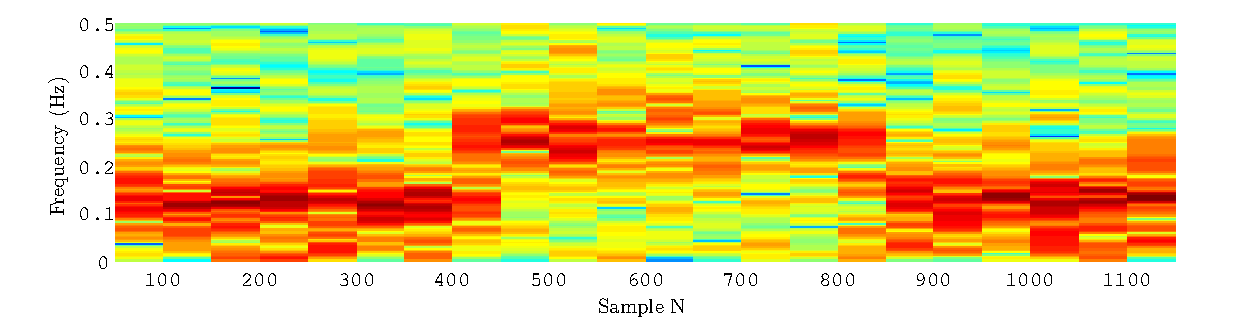
\includegraphics[width=1.0\textwidth]{cw4im/3a_2.pdf}
\caption{Spectrogram}
\label{fig:4_3a2}
\end{figure}

\FloatBarrier

\subsection{RLS estimation}
As seen earlier Yule Walker is not a good option when faced with changing estimates. Here  the aim is to use a recursive least squares (RLS) algorithm with $\lambda = 0.9$ and for each estimate in time the spectrum is estimated using \mcode{freqz}. This gives figure \ref{fig:4_3b} which is very similar to the spectrogram in figure \ref{fig:4_3a2}. In fact the RLS spectrogram estimate provides more contrast than the spectrogram and reacts faster to the change in coefficient - though this is also due to the small overlap in the spectrogram. The fast adaptation to changing coefficients is made possible by the low $\lambda$ value.
\begin{figure}[h]
\centering
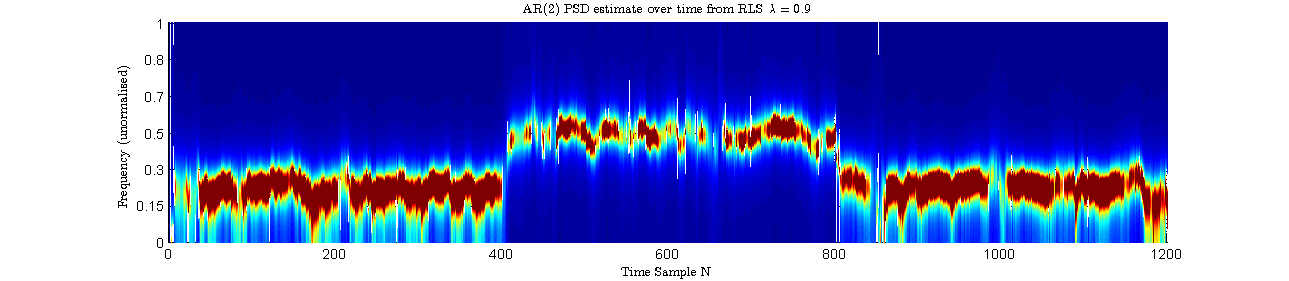
\includegraphics[width=1.0\textwidth]{cw4im/4b_RLS.png}
\caption{Spectrogram estimate using RLS coefficients}
\label{fig:4_3b}
\end{figure}


\newpage



\begin{thebibliography}{3}
\bibitem{lofi} Lectures on Fourier Integrals, \textit{Salomon Bochner}, 1959, Princeton University Press
\bibitem{rayleigh} The Rayleigh Quotient Nuno Vasconcelos, ECE Department, UCSD \url{http://www.svcl.ucsd.edu/courses/ece271B-F09/handouts/Dimensionality3.pdf}
\end{thebibliography}
\endgroup
\end{document}